% book example for classicthesis.sty
\documentclass[oneside,hidelinks,12pt,letterpaper]{scrbook} %KOMA-Script book
%\documentclass[oneside,hidelinks,12pt,letterpaper,footinclude=true,headinclude=true]{scrbook} % KOMA-Script book
\usepackage[T1]{fontenc}                
\usepackage{lipsum}
%\usepackage[utf8x]{inputenc} 
\usepackage[makeindex]{imakeidx}
\usepackage{titletoc}

\usepackage[linedheaders,parts,pdfspacing,manychapters]{classicthesis}
%http://ctan.mackichan.com/macros/latex/contrib/classicthesis/ClassicThesis.pdf here for the classicthesis manual
\usepackage[letterpaper,inner=2.5cm,outer=2.5cm,top=3cm,bottom=3cm,bindingoffset=0cm]{geometry}


\usepackage{graphicx} % graphics https://www.sharelatex.com/learn/Inserting_Images
\usepackage[export]{adjustbox}%https://tex.stackexchange.com/questions/57418/crop-an-inserted-image

\graphicspath{ {../figures/}{../}{figures/} }
\usepackage{chngcntr}
% https://texblog.org/2014/12/04/continuous-figuretable-numbering-in-latex/
% number figure and table by chapter
\counterwithin{figure}{section}
\counterwithin{table}{section}


\usepackage{sgame, tikz} % Game theory packages http://people.tamu.edu/~nsthiago/GameTheory(TNSilva).tex
\usepackage{caption}
\captionsetup[figure]{position=top} 

\usepackage{subcaption}%https://tex.stackexchange.com/questions/37581/latex-figures-side-by-side

\setlength{\parindent}{1cm}
\setlength{\parskip}{0.5em}

\usepackage{savesym}
%%savesym – Redefine symbols where names conflict
%% http://tex.stackexchange.com/questions/18541/two-conflicting-packages-in-one-document-doable

\savesymbol{cfoot}
\savesymbol{chead}
% this is solve the name conflict problem in fancyhr
%\usepackage{tocbibind}
\usepackage[linesnumbered,ruled]{algorithm2e}
% http://ctan.sharelatex.com/tex-archive/macros/latex/contrib/algorithm2e/doc/algorithm2e.pdf for the algorithm manual
%\newcommand{\listofalgorithmes}{\tocfile{\listalgorithmcfname}{loa}}
% http://tex.stackexchange.com/questions/45538/list-of-algorithms-using-algorithm2e

\title{\huge \textbf{Essential Mathematical Modeling Methods: Principles and Algorithms}}
\author{Yuguang Yang \\
Johns Hopkins University \\yangyutu123@gmail.com }
\date{September 2015}

\usepackage{mdframed}


\usepackage{pgfplots} % https://www.sharelatex.com/learn/Pgfplots_package
%examples http://pgfplots.sourceforge.net/gallery.html
\pgfplotsset{width=8cm,compat=1.9}

%https://tex.stackexchange.com/questions/300669/how-can-i-change-font-size-on-x-y-labels
% https://tex.stackexchange.com/questions/303213/how-to-set-plot-box-aspect-ratio/303273
\def\axisdefaultwidth{6cm}
\def\axisdefaultheight{6cm}
\pgfplotsset{every axis/.append style={
		label style={font=\Large},
		tick label style={font=\large} ,
		axis line style = thick,
		minor x tick num=4,
		minor y tick num=4,
	}
	%          every axis plot/.append style={very thick}
}
\pgfplotsset{every axis plot/.append style={very thick}}
\pgfplotsset{tick style={thick,black}} % modifies the style ‘every tick’
\pgfplotsset{minor tick style={thin,black}}

\usepackage{mathtools}
\usepackage{graphicx}

\usepackage{amssymb}
\usepackage{amsmath,esint}
\usepackage{yfonts}
\usepackage{mathrsfs}
\usepackage{multirow}
%\usepackage{biblatex}
\usepackage[backend=biber,style=nature,sorting=none,refsection=chapter]{biblatex}
\usepackage{hyperref}
\hypersetup{
	colorlinks = true,
	citecolor=blue,
	urlcolor=blue
}
\makeindex[columns=2, title=Alphabetical Index, intoc]
\usepackage{marginnote}
\addbibresource{../references.bib}
%\bibliography{references.bib}
%\bibliographystyle{apalike}

\usepackage{nomencl}% for Nomenclatures
\makenomenclature

\usepackage{shorttoc} % for short table of contents

\usepackage{enumitem}
%\usepackage{physics}
%
\usepackage{float}
%\restylefloat{table}
\usepackage[section]{placeins}

\usepackage{rotating}% for vertical table
\renewcommand{\arraystretch}{1.5} % for table row spacing
% https://en.wikibooks.org/wiki/LaTeX/Tables
\setlist{nosep} % or \setlist{noitemsep} to leave space around whole list

\renewcommand*\contentsname{Contents (detailed)}
\setcounter{tocdepth}{3}
\setcounter{secnumdepth}{4}
\usepackage{indentfirst}
\usepackage{commath}
\usepackage{bm}  %this is bold and italic
%\usepackage{lmodern,bm} % this is bold but not italic
\usepackage{accents}
\usepackage{xcolor}

% this is for making mini table of contents for each chaper
\usepackage{minitoc}      
\setcounter{tocdepth}{5}
\setcounter{minitocdepth}{4}   

% resize fonts in the verbatim
\usepackage{fancyvrb}

\usepackage{tabto}
%\newcommand\cpart[1]{\part[\\sffamily\bfserieshfill#1\hfill]{#1}}
% this is to change fonts in table of contents
\renewcommand\cftpartfont{\sffamily\bfseries\large\color{red}}
\renewcommand\cftpartpagefont{\normalfont\color{blue}}





\newcommand{\ubar}[1]{\underaccent{\bar}{#1}}
\newcommand{\field}[1]  {\mathbb{#1}}
\newcommand{\R}{\mathbb{R}}
\newcommand{\RE}{\bar{\mathbb{R}}}
\newcommand{\F}{\mathbb{F}}
\newcommand{\PP}{\mathbb{P}}
\newcommand{\E}{\mathbb{E}}
\newcommand{\N}         {\field N}
\newcommand{\Z}         {\field Z}
\newcommand{\C}         {\field C}
\newcommand{\Q}         {\field Q}
\newcommand{\cF}{\mathcal{F}}
\newcommand{\cG}{\mathcal{G}}
\newcommand{\cE}{\mathcal{E}}
\newcommand{\cJ}{\mathcal{J}}
\newcommand{\cV}{\mathcal{V}}
\newcommand{\cL}{\mathcal{L}}
\newcommand{\cH}{\mathcal{H}}
\newcommand{\cA}{\mathcal{A}}
\newcommand{\cB}{\mathcal{B}}
\newcommand{\cC}{\mathcal{C}}
\newcommand{\cP}{\mathcal{P}}
\newcommand{\cR}{\mathcal{R}}
\newcommand{\cN}{\mathcal{N}}
\newcommand{\cM}{\mathcal{M}}
\newcommand{\cD}{\mathcal{D}}
\newcommand{\cX}{\mathcal{X}}
\newcommand{\cQ}{\mathcal{Q}}
\newcommand{\cY}{\mathcal{Y}}
\newcommand{\cW}{\mathcal{W}}
\newcommand{\cT}{\mathcal{T}}
\newcommand{\cS}{\mathcal{S}}
\newcommand{\cI}{\mathcal{I}}
\newcommand{\cZ}{\mathcal{Z}}
\newcommand{\cK}{\mathcal{K}}
\newcommand{\pArrow}{\xrightarrow[ ]{P}}

\newcommand{\sV}{\mathscr{F}}
\newcommand{\sL}{\mathscr{L}}
\newcommand*\conj[1]{\overline{#1}}
\newcommand*\mean[1]{\overline{#1}}




\newcommand{\Pa}{\partial}
\newcommand{\ip}[1]             {{\left< \, #1 \, \right>}}
%\newcommand{\norm}[1]{\left\lVert#1\right\rVert}
\usepackage{amsthm}

%\usepackage{amsthm}
\makeatletter
\def\th@plain{%
  \thm@notefont{}% same as heading font
  \itshape % body font
}
\def\th@definition{%
  \thm@notefont{}% same as heading font
  \normalfont % body font
}
\makeatother


%\newtheorem{theorem}{Theorem}[section]
%\newtheorem{mdtheorem}{Theorem}[section]


% for these highlighted env using mdframed, search fro The mdframed package handbook for references
\newmdtheoremenv[%
linecolor=black,leftmargin=3,%
linewidth=1pt,%
rightmargin=3,
backgroundcolor=gray!40,%
innertopmargin=0pt,%
ntheorem]{theorem}{Theorem}[section]

\newmdtheoremenv[%
linecolor=black,leftmargin=3,%
linewidth=1pt,%
rightmargin=3,
backgroundcolor=gray!40,%
innertopmargin=0pt,%
ntheorem]{assumption}{Assumption}[chapter]

\newmdtheoremenv[%
linecolor=black,leftmargin=3,%
linewidth=1pt,%
rightmargin=3,
backgroundcolor=gray!40,%
innertopmargin=0pt,%
ntheorem]{fact}{Fact}[section]

\newmdtheoremenv[%
linecolor=gray!10,leftmargin=3,%
rightmargin=3,
backgroundcolor=gray!5,%
innertopmargin=0pt,%
ntheorem]{corollary}{Corollary}[theorem]

\newmdtheoremenv[%
linecolor=gray!20,leftmargin=3,%
rightmargin=3,
backgroundcolor=gray!10,%
innertopmargin=0pt,%
ntheorem]{lemma}{Lemma}[section]

\newmdtheoremenv[%
linecolor=gray!20,leftmargin=3,%
rightmargin=3,
backgroundcolor=gray!10,%
innertopmargin=0pt,%
ntheorem]{method}{Methodology}[section]

%\newtheorem{lemma}[theorem]{Lemma}
\newmdtheoremenv[%
linecolor=green!20,leftmargin=3,%
rightmargin=3,
backgroundcolor=green!20,%
innertopmargin=0pt,%
ntheorem]{definition}{Definition}[section]

\newmdtheoremenv[%
linecolor=green!20,leftmargin=3,%
rightmargin=3,
backgroundcolor=green!20,%
innertopmargin=0pt,%
ntheorem]{problem}{Problem}[section]

\theoremstyle{remark}
\newmdtheoremenv[%
linecolor=red!15,leftmargin=3,%
rightmargin=3,
backgroundcolor=red!15,%
innertopmargin=4pt,%
ntheorem]{example}{Example}[section]





% declare a new theorem style https://tex.stackexchange.com/questions/283578/how-to-produce-theorems-in-which-the-color-of-heading-and-body-of-the-theorem-my
\newtheoremstyle{coloredRemark}%
{3pt}% Space above
{3pt}% Space below 
{\color{black}}% Body font
{}% Indent amount
{\bfseries\color{BurntOrange}}% Theorem head font
{.}% Punctuation after theorem head
{.5em}% Space after theorem head
{}% Theorem head spec (can be left empty, meaning ‘normal’)

\theoremstyle{coloredRemark}
\newtheorem{remark}{Remark}[section]

\newtheoremstyle{coloredNote}%
{3pt}% Space above
{3pt}% Space below 
{\color{black}}% Body font
{}% Indent amount
{\bfseries\color{RubineRed}}% Theorem head font
{.}% Punctuation after theorem head
{.5em}% Space after theorem head
{}% Theorem head spec (can be left empty, meaning ‘normal’)
%\theoremstyle{remark}
%\newtheorem{example}{Example}[section]
\theoremstyle{coloredNote}
\newmdtheoremenv[%
linecolor=black,leftmargin=3,%
linewidth=1pt,%
rightmargin=3,
backgroundcolor=gray!5,%
innertopmargin=4pt,%
ntheorem]{note}{Note}[section]


\DeclareMathOperator*{\argmax}{arg\,max}
\DeclareMathOperator*{\argmin}{arg\,min}
\newcommand{\lemmaautorefname}{Lemma}
\newcommand{\corollaryautorefname}{Corollary}
\newcommand{\definitionautorefname}{Definition}
\newcommand{\remarkautorefname}{Remark}
\newcommand{\assumptionautorefname}{Assumption}
\newcommand{\exampleautorefname}{Example}
\DeclareMathOperator*{\plim}{plim}

% for header and footer https://www.sharelatex.com/learn/Headers_and_footers
\usepackage{fancyhdr}
 \fancypagestyle{plain}{%
 \fancyhf{}
\fancyfoot[LO, RE]{\slshape Yuguang Yang  }
\fancyfoot[RO, LE]{\slshape Essential Mathematical Methods}}
\pagestyle{fancy}
\fancyhf{}
%\fancyhead[LE,RO]{Essential Mathematical Methods}
%\fancyhead[RE,LO]{Yuguang Yang}
\fancyfoot[CE,CO]{\leftmark}
\fancyfoot[LE,RO]{\thepage}
\renewcommand{\headrulewidth}{2pt}
\renewcommand{\footrulewidth}{2pt}
%\renewcommand{\sectionmark}[1]{\markright{#1}}

\fancyhead[RE,CO]{\fontsize{11}{12}\selectfont\nouppercase\rightmark}

\def\layersep{2.5cm}%neural network http://www.texample.net/tikz/examples/neural-network/

% create a background image
%\usepackage[pages=some]{background}
%\backgroundsetup{
%	scale=1,
%	angle=0,
%	opacity=.4,  %% adjust
%	contents={\includegraphics[width=\paperwidth,height=\paperheight]{coverImg}}
%}


\newcommand{\sectionbreak}{\clearpage}% start a new page for each section
\titleformat{\section}
{\normalfont\large\bfseries}{\thesection}{1em}{}
\titleformat{\subsection}
{\normalfont\normalsize\mdseries}{\thesubsection}{1em}{}


%\renewcommand\qedsymbol{$\blacksquare$}

\begin{document}


\sloppy

% This declaration makes TeX less fussy about line breaking. This can prevent overfull boxes, but may leave too much space between words. Lasts until a \fussy command is issued. \fussy.

\begin{titlepage}
%\maketitle
%	\BgThispage
    \begin{center}
        \vspace*{1cm}
        
        {\huge \textbf{Essential Mathematical Modeling Methods: Principles and Algorithms}}
        
        
%        \textbf{An evolving online book at}\\
%        \href{      https://github.com/yangyutu/NotesOnMathMethods
%        }{https://github.com/yangyutu/NotesOnMathMethods}\\
        \vspace{1.8cm}
       {\Large\textbf{Yuguang Yang}}\\
       \vspace{0.5cm}
       
       version 2.0 \\
\vspace{2.8cm}
        	\includegraphics[width=0.7\linewidth]{800px-e8_graph-svg}
        
         
    
        
    \end{center}





\end{titlepage}



\newpage

\begin{center}
	\Large
	\textbf{\huge Notations}
	
	\vspace{0.4cm}
	\large
	
	\vspace{0.4cm}
\end{center}


\begin{itemize}
	\item $\R$: real numbers.
	\item $\R_+$: nonnegative real numbers.
	\item $\R_{++}$: positive real numbers.
	\item $\RE$: extended real numbers.
	\item $\C$: complex numbers.
	\item $\F$:real or complex numbers.
	\item $\Q$: rational numbers.
	\item $\Z$:integer numbers.
	\item $\PP$:positive numbers.
	\item $\cP(\PP)$:positive numbers.
	\item $\cP_n$: polynomial of degree of n.
	\item $\N$:natural numbers.
	\item $\cR(A)$: the range of matrix $A$.
	\item $\cN(A)$: the null space of matrix $A$. 
		\item $V$: vector space.
		\item $det(A)$:the determinant of matrix $A$.
		\item $rank(A)$:the rank of matrix $A$.
		\item $\rho(A)$:the spectral radius of matrix $A$.
		\item $Tr(A)$:the trace of matrix $A$.	
		\item $L^2[a,b]$:Lebesgue integrable function on $[a,b]$.
		\item $L^1[a,b]$:Lebesgue integrable function on $[a,b]$.
		\item $N(0,1)$: standard Gaussian distribution.
		\item $N(\mu,\sigma^2)$: Gaussian distribution with mean $\mu$ and variance $\sigma^2$.
		\item $MN(\mu,\Sigma)$: multivariate Gaussian distribution with mean vector $\mu$ and covariance matrix $\Sigma$.
\end{itemize}



\newpage

\hypersetup{colorlinks=false}
\shorttoc{Contents}{0}

\newpage

\listofalgorithms
\listoffigures
\listoftables

\dominitoc
\tableofcontents 



\hypersetup{
	colorlinks=true,
	linkcolor=blue}

\mainmatter

\printnomenclature





\part{Mathematical Foundations}
\startcontents[chapters]
\begin{refsection}
\chapter{Sets}\label{ch:sets}
%\minitoc

\printcontents[chapters]{}{1}{}
\section{Properties of sets}
\subsection{DeMorgan's Law}\index{DeMorgan's Law}
\begin{lemma}[Demorgan's law]\label{ch:sets:th:DemorganLaw}
\cite{johnsonbaugh2010foundations}Let $S$ and $T$ be sets, then
\begin{enumerate}
    \item $(S\cup T)^c = S^c \cap T^c$
    \item $(S\cap T)^c = S^c \cup T^c$
\end{enumerate}
Moreover, given a collection of sets indexed by $I$, we have
$$(\cup_{i\in I} A_i)^C = (\cap_{i\in I} A_i^C),$$ and $$(\cap_{i\in I} A_i)^C = (\cup_{i\in I} A_i^C).$$ 
\end{lemma}


\begin{lemma}[principle of inclusion exclusion]\index{principle of inclusion exclusion}
Let $A_1,A_2,...,A_n$ be sets, then
$$\abs{\cup_{i=1}^n A_i} = \sum_{i=1}^n (-1)^{i+1}S_i,$$
where
\begin{align*}
S_1 &= \sum_{i=1}^n \abs{A_i}\\
S_2 &= \sum_{1\leq i < j \leq n} \abs{A_i\cap A_j}\\
\cdots & = \cdots \\
S_m &= \sum_{1\leq i_i < i_2 < ... <i_m \leq n} \abs{A_{i_1}\cap A_{i_2}\cap ... \cap A_{i_m}}.
\end{align*}
More specifically, 
$$\abs{A\cup B} = \abs{A} + \abs{B} - \abs{A\cap B},$$
and
$$\abs{A\cup B\cup C} = \abs{A} + \abs{B} + \abs{C}- \abs{A\cap B}-\abs{C\cap B}-\abs{A\cap C}+\abs{A\cap B\cap C}.$$
\end{lemma}


\subsection{Algebra properties of sets}
\begin{lemma}
Sets have the following Algebraic properties:
\begin{itemize}
    \item Commutative: $A\cup B = B\cup A$, $A\cap B = B\cap A$
    \item Associative: $A \cup (B \cup C) = (A \cup B) \cup C$, $A \cap (B \cap C) = (A \cap B) \cap C$
    \item Distributive: $A\cup (B\cap C) = (A\cap B) \cup (A \cap C)$,$A\cap (B\cup C) = (A\cup B) \cap (A \cup C)$
\end{itemize}
\end{lemma}


\section{Functions}
\subsection{Basic concepts}
\begin{definition}[function]\index{function}
\cite{johnsonbaugh2010foundations}If $X$ and $Y$ are sets. A \emph{function} from $X$ to $Y$ is a subset $f$ of $X \times Y$ satisfying:
\begin{enumerate}
    \item Uniqueness of mapping: If $(x,y)$ and $(x,y')$ belong to $f$, then $y=y'$.
    \item Completenss: If $x\in X$, then $(x,y)\in f$ for some $y \in Y$. Every element $x$ in $X$ must have a $y \in Y$. 
\end{enumerate}
\end{definition}


\begin{definition}
\cite{johnsonbaugh2010foundations}.
For a function $f:X\to Y$, we have
\begin{itemize}
    \item $X$ is called the domain, $Y$ is called the codomain. $f(X)=\{f(x)|x\in X\}$ is called the range. 
    \item $f$ is \textbf{onto} $Y$ if $f(X) = Y$. Or equivalently, for any $y\in Y$, there exists $x \in X$(not necessarily unique) such that $f(x) = Y$.
    \item $f$ is \textbf{one-to-one} if $f(x) = f(x') \Rightarrow x = x'$
    \item If $f$ is one-to-one function, we can define $f^{-1}$ as a function from $f(X)$ to $X$. Note that it is not from $Y$, but from $f(X)$.  \emph{Onto} is not required for the existence of $f^{-1}$.
    \item If $f$ is one-to-one and onto, it is \textbf{bijective}.
    \item The \emph{inverse image} of $B \subseteq Y$ under $f$ is the set
    $$f^{-1}(B)=\{x|f(x)\in B\}$$
\end{itemize}
\end{definition}

\begin{definition}[inverse function]\index{inverse function}
Denote $f$ as a function $f:X\to Y$. 
\begin{itemize}
	\item If $f$ is one-to-one function, we can define $f^{-1}$ as a function from $f(X)$ to $X$. Note that it is $f^{-1}$ is not mapped from $Y$,
	\item If $f$ is one-to-one and onto function, we can define $f^{-1}$ as a function from $Y$ to $X$.
\end{itemize}
\end{definition}


\subsection{Inverse image vs. inverse function}\index{inverse image}\index{inverse function}
\begin{note}
Note that \emph{inverse image} and \emph{inverse function} are fundamentally different. Inverse image always exist whereas inverse function requires 1-1 to exist. 
\end{note}




\begin{example}
Take $X=Y=\R$, let $f(x) = cos(x)$. Then
\begin{itemize}
    \item inverse function $f^{-1}$ does not exist
    \item $f^{-1}(1)$ technically make no sense since inverse image will only take subset as input
    \item $f^{-1}(\{1\})=\{\text{all integer multiples of }2\pi \}$
    \item $f^{-1}(\{1\})=\emptyset$
    \item $f^{-1}([-1, 1])=\R$
    
\end{itemize}
\end{example}

\subsection{Set operations in function mapping}
\begin{lemma}[Preserving set operators in function mapping]\cite[7]{johnsonbaugh2010foundations}
Let $f$ be a function from $X$ into $Y$. Let $\mathcal{A}$ be a collection of subsets of $X$, and let $\mathcal{G}$ be a collection of subsets of $Y$. Let $C \subset Y$.
\begin{enumerate}
    \item $f(\cup \mathcal{A}) = \cup \{f(A)|A\in\mathcal{A}\}$
    \item $f^{-1}(\cup \mathcal{B}) = \{f^{-1}(C)|C \in \mathcal{G} \}$
    \item $f^{-1}(\cup \mathcal{B}) = \{f^{-1}(C)|C \in \mathcal{G} \}$
    \item $f^{-1}(C^C) = (f^{-1}(C))^C$
\end{enumerate}
\end{lemma}

\begin{remark}
It is in general not true that $f(A\cap B) = f(A)\cap f(B)$, because maybe $A\cap B = \emptyset$. However, if $f$ is a one-to-one function if and only if 
$$f(A\cap B) = f(A)\cap f(B)$$
because if $(A\cap B) = \emptyset$, then $f(A)\cap f(B) = \emptyset$.
\end{remark}

\subsection{Parameter change of function}
A function $f: A \rightarrow B$ is a rule to associate an element $a \in A$ to an element $b \in B$. The exact expression of $f$ depends on how we parameterize the set $A$. For example, consider $A=[0,1]$, and we want to map every element $x\in A$ to $5x$, then we have $f(x)=5x$. However, if we want to express/reparameterize $A$ as $x=5t,t\in [0,0.2]$, then we introduce a new local coordinate system on $A$ as $\phi(x)=x/5$. The functon on the new local coordinate system is given as $f\circ \phi^{-1}(t) = 25t$ 



\section{Set equivalence and partition}
\begin{definition}[relation]\index{relation}
A relation on a set $A$ is any statement which is either true or false for each ordered pair $(x,y)$ of elements in $A$. Examples are $x=y$,$x<y$
\end{definition}


\begin{definition}[equivalence relation]\cite{johnsonbaugh2010foundations}\index{equivalent relation}
Let $A$ and $B$ be two sets and let $f$ be a mapping of $A$ into $B$. If there exist a 1-1 mapping of $A$ \emph{onto} $B$, we say that $A$ and $B$ can be put in 1-1 correspondence, or that $A$ and $B$ have the same \emph{cardinal number}, or briefly, that $A$ and $B$ are \textbf{equivalent}, and we write $A\sim B$. The relation has the following properties:
\begin{enumerate}
\item It is reflective: $A \sim A$.
\item It is symmetric: if $A \sim B$, then $B \sim A$.
\item it is transitive: if $A \sim B$ and $B \sim C$, then $A \sim C$.
\end{enumerate}
\end{definition}

\begin{definition}[partitions of a set]\index{partition}
Let $S$ be a set. A collection of (finitely or infinitely many) nonempty subsets $A_1,A_2,...\subseteq S$ is called a partition of $S$ if:
\begin{itemize}
    \item These sets $A_i$ are pairwise disjoint.
    \item The union of all subsets $A_1\cup A_2 ... = S$. 
\end{itemize}
\end{definition}


\begin{theorem}[partition a set by equivalence]
Elements in a set $X$ equivalent to each other form an equivalent class. All the equivalent classes of a set partition the set.  
\end{theorem}
\begin{proof}
We can show that any element cannot belong to two distinct equivalent classes using transitivity.	
\end{proof}
 

\section{Countability}
\begin{definition}\cite{johnsonbaugh2010foundations}
For any positive integer $n$, let $P_n$ be the set whose elements are the integers 1,2,...,n; let $P$ be the set consisting of all positive integers. For any set $A$, we say:
\begin{enumerate}
\item $A$ is \emph{finite} if $A \sim P_n$ for some $n$.
\item $A$ is \emph{infinite} if $A$ is not finite.
\item $A$ is \emph{countable} if $A \sim P$ (countable infinite)or $A$ is finite.
\item $A$ is \emph{uncountable} if $A$ is not countable
\end{enumerate}
\end{definition}


\begin{example}\hfill
\begin{itemize}
    \item The integers $\mathbf{Z}$ form a countable set. The 1-1 mapping is given as $f(k)+2k $ if $k >= 0 $ and $f(k) = 2(-k) + 1$ if $k < 0$.
    \item The real number is uncountable set. 
\end{itemize}
\end{example}



\begin{lemma}
\cite{johnsonbaugh2010foundations}Properties of countable sets:
\begin{itemize}
    \item Any subset of a countable set is countable
    \item If $A, B$ are countable sets, then $A\cup B$ is a countable set.
    \item The Cartesian product of two countable sets is countable.
\end{itemize}
\end{lemma}
\begin{proof}
(3)	Let $S,T$ be the two countable sets. If they are finite, then $S\times T$ will be finite. Consider $S,T$ have infinite elements, we can list $S\times T$ as a table and count them diagonally from a corner. This counting can count all the element in $S\times T$.
\end{proof}



\begin{corollary}
Let k>1.
Then the cartesian product of k countable sets is countable.
\end{corollary}


\section{Real numbers}

\subsection{rational numbers}
\begin{definition}[rational number, irrational number]\index{rational number}\index{irrational number}\cite[21]{johnsonbaugh2010foundations} The set of \textbf{rational number}, denoted $\Q$, is the set 
	$$\{\frac{p}{q}|p,q\in \Z, ~and~ q\neq 0 \}.$$

A real number which is not rational is said to be \textbf{irrational}.
\end{definition}


\begin{lemma}[rational number and irrational number ] If $r$ is a rational number, which can be represented by $p/q$ and $x$ is an irrational number, then
\begin{itemize}
	\item $r+x$ is irrational.
	\item $rx$ is irrational, provided that $r\neq 0$.
\end{itemize}	
\end{lemma}
\begin{proof}
(1) Suppose $r+x$ is rational, then it can be represented by $m/n$. Then $x = r+x - r = m/n - p/q$ will still be rational, which contradicts that $x$ is a rational number.
(2)Suppose $rx$ is rational, then it can be represented by $m/n$. Then $x = rx/r= (m/n) /(p/q)$ will still be rational, which contradicts that $x$ is a rational number.
\end{proof}

\subsection{Dense subset}\index{dense subset}\cite[15]{fitzpatrick2006advanced}
\begin{definition}[dense subset in $\R$]\label{ch:sets:def:denseSubsetInRealNumbers}
Let $S$ be a subset of $\R$.
\begin{itemize}
	\item We say $S$ is a \textbf{dense subset} in $\R$ provided that every interval $I=(a,b), a < b$, contains a member of $S$.
	\item (alternative) We say $S$ is a \textbf{dense subset} in $\R$ provided that for every number $r\in \R$ and any $\epsilon > 0,$ there exists a member  $s\in S$ such that $\abs{s-r}<\epsilon$.
\end{itemize}	
\end{definition}

\begin{remark}[equivalence of the two definitions]\hfill
(1) implies (2): for $r \in \R$, there exists a number $s\in S, s\in (r-\epsilon,r+\epsilon)$ such that $\abs{r-s} < \epsilon$.
(2) implies (1): for any interval $(a,b)$, we let $\epsilon = d = \frac{b-a}{2}$, then there exists $s\in S$ such that $$\abs{s - \frac{a+b}{2}} < \frac{b-a}{2} \implies s \in (a,b).$$ 	
\end{remark}

\begin{theorem}[rational and irrational numbers are dense]\label{ch:sets:th:rationalIrrationalNumbersDense}\cite[23]{johnsonbaugh2010foundations}
If $a$ and $b$ are real numbers with $a < b$, then there exists both a rational number and an irrational number between $a$ and $b$.	
\end{theorem}
\begin{proof}
Let $k$ be an integer smaller than $a$, and let $n$ be an integer such that $n > \sqrt{2}/(b-a).$ Then
$$0<1/n< \frac{2}{n} < b-a.$$
So the sequence $k+1/n, k+2/n + ...$ will have at least one term falling into $(a,b)$.
Similarly, the sequence $k+\sqrt{2}/n, k+2\sqrt{2}/n + ...$ will have at least one term falling into $(a,b)$.
\end{proof}

\subsection{Axiom of completeness} \index{completeness axiom}
\begin{definition}[bounded above, bounded below]\hfill
	\begin{itemize}
		\item A nonempty subset $X$ of $\R$ is said to be \textbf{bounded above} if there exists a $a\in \R$ such that $a\geq x,\forall x\in X$.
		\item  A nonempty subset $X$ of $\R$ is said to be \textbf{bounded below} if there exists a $b\in \R$ such that $b\leq x,\forall x\in X$.
	\end{itemize}	
\end{definition}

\begin{definition}[Least upper bound, supremum]\cite[5]{johnsonbaugh2010foundations}
Let $S$ be a nonempty subset of $\mathbb{R}$. If $S$ is bounded above, then a number $u$ is said to be the \textbf{supremum} of $S$ if:
\begin{itemize}
\item u is an upper bound of $S$.
\item if $v$ is also an upper bound of $S$, then  $v \geq u$.
\end{itemize}
\end{definition}

\begin{definition}[greatest lower bound, infimum]\cite[5]{johnsonbaugh2010foundations}
	Let $S$ be a nonempty subset of $\mathbb{R}$. If $S$ is bounded above, then a number $u$ is said to be the \textbf{infimum} of $S$ if:
	\begin{itemize}
		\item $u$ is an lower bound of $S$.
		\item if $v$ is also an lower bound of $S$, then if $v \leq u$.
	\end{itemize}
\end{definition}

\begin{definition}[maximum of a set]
A real number $a_0$ is a maximum of the set $A$ if $a_0\in A$ and $a\leq a_0,\forall a\in A$, but it has a supremum of 1.
\end{definition}

\begin{remark}
The open interval $(0,1)$ does not have a maximum.
\end{remark}




\begin{theorem}[axiom of completeness, existence of least upper bound]\label{ch:sets:th:ExistenceOfLeastUpperBoundForBoundedRealSet}
	\textbf{Axiom of completeness:} Every nonempty subset of $\R$ that is bounded above has a least upper bound.
\end{theorem}

\begin{theorem}[existence of greatest lower bound]\cite[15]{johnsonbaugh2010foundations}
Every nonempty subset of $\R$ that is bounded below has a greatest lower bound.
\end{theorem}
\begin{proof}
Let $X$ be a nonempty subset of $\R$ that is bounded below. Let $Y$ be the set of lower bounds. Then $Y$ is bounded above, and therefore exists a least upper bound, denoted by $b$. We want to show that $b$ is the greatest lower bound of $X$. First $b\leq x,\forall x\in X$(if there exists $c\in X$, $c < b$, then $c\in Y$ contradicts that $b \geq y,\forall y\in Y$.) Second, for any other lower bound $d$, we have $d\leq b$, since $d\in Y$.
\end{proof}




\begin{lemma}[uniqueness of least upper bound]\cite[15]{johnsonbaugh2010foundations}
Let $X$ be a subset of $\R$. If $a$ and $b$ are least upper bounds of $X$, then $a = b$.	
\end{lemma}
\begin{proof}
Let $a$ be the least upper bound. Since $b$ is also a upper bound, then from the definition of least upper bound, we have $a\leq b$; Similarly, we have $a\geq b$. 
Therefore, $a = b$.
\end{proof}

\begin{lemma}[least upper bound is tight(has no hole)] \label{ch:sets:th:leastupperboundisTight}\cite[17]{johnsonbaugh2010foundations}\cite[17]{abbott2001understanding}\hfill
\begin{itemize}
	\item Let $X$ be a set of real numbers with least upper bound $a$. Then for any positive $\epsilon > 0$, there exists $x\in X$ such that $a-\epsilon<x\leq a.$
	\item Assume $s\in \R$ is an upper bound for a set $A\subseteq \R$. Then $s=\sup A$ if for any choice of $\epsilon > 0$, there exist an element $a\in A$ such that $s-a < \epsilon$.
\end{itemize}	
\end{lemma}
\begin{proof}
(1)	
$x\leq a$ is directly from the definition of least upper bound. Suppose there does not exist $x\in X$, such that $x > a-\epsilon$, then we conclude all $x\in X, x \leq a-\epsilon$. Let $b= a - \epsilon$ be another upper bound, then we have $b < a$, contradicting the fact that $a$ is the least upper bound.	
(2) Suppose $\sup A$ is the least upper bound, then we have $s\geq \sup A$. For contradiction purpose, assume $s > \sup A$. Let $\epsilon = 0.5*(s-\sup A)$, then $s-\epsilon > \sup A$, and there does not exist an element  $a\in A$ such that $s-\epsilon < a$, which is a contradiction.  Therefore, we must have $s = \sup A$.

\end{proof}

\begin{remark}
This lemma illustrates the idea of no-holes between an nonempty set and its least upper bound.
\end{remark}



\begin{lemma}[least upper bound of rational numbers]
Given a real number $a$, define $S = \{x|x\in \Q, x < a\}$. It follows that
$$\sup S = a.$$	
\end{lemma}
\begin{proof}
First any number greater than $a$ cannot be the least supper bound However, $a$ is smaller upper bound. Now suppose $\sup S < a$; however, there exists a rational number exists inside $(\sup S,a)$ since $\Q$ is dense subset(\autoref{ch:sets:th:rationalIrrationalNumbersDense}). therefore $\sup S = a$.
\end{proof}



\begin{theorem}[nested interval property]\index{nested interval property}
\cite[20]{abbott2001understanding}\label{ch:sets:NestedIntervalProperty}
For each $n\in \N$, assume we are given a closed interval $I_n=[a_n,b_n] = \{x\in \R: a_n \leq x \leq b_n\}$. And we also have $a_1 \leq a_2 \leq ....$ and $b_1 \geq b_2 \geq ...$, then,
$$I_1 \supseteq I_2 ...$$
has a nonempty intersection; that is $\cap^{\infty} I_n \neq \emptyset$.
\end{theorem}
\begin{proof}
 Let $A=\{a_1,a_2,...\}$, and let $x = \sup A$. Given any set $I_n=[a_n,b_n]$, we have $x\geq a_n$, because $x$ is the least upper bound. Also $x\leq b_n$, because $b_n$ is another upper bound for $A$. Since $n$ is arbitrary, we have $x\in \cap^{\infty} I_n$.	
\end{proof}

\section{Notes on bibliography}
The chapter mainly reference intermediate level real analysis textbooks\cite{johnsonbaugh2010foundations}\cite{abbott2001understanding}\cite{thomson2001elementary}.

\printbibliography

\end{refsection}
\begin{refsection}
	
\startcontents[chapters]
\chapter{Sequences \& Series}\label{ch:sequences-series}
%\minitoc

\printcontents[chapters]{}{1}{}
\index{sequence}\index{series}
\section{Sequence in $\R$}
\subsection{Basics}
\begin{definition}[sequence]
A \emph{sequence} in $\R$ a function $f$ maps from the set $P$ of all positive integers to $\R$. If $f(n)=x_n$, for $n\in P$, it is customary to denote the sequence $f$ by the symbol $\{x_n\}$. \cite{johnsonbaugh2010foundations}
\end{definition}


\begin{definition}[convergence of a sequence]
A sequence $\{p_n\}$ in $\R$ is said to \emph{converge} if there is a point $p \in \R$ with the following property. For every $\epsilon >0$ there is an integer $N$ such that $n > N$,$\abs{p_n - p} < \epsilon$.
\end{definition}


\begin{theorem}[uniqueness of limits]\cite{johnsonbaugh2010foundations}
A sequence in $\mathbb{R}$ can have at most one limit. 
\end{theorem}
\begin{proof}
	If a sequence has two different limits, then when $n$ is large enough, $a_n$ has to be increasingly closer to to both limit, which is contradiction. 
\end{proof}
 

\begin{theorem}[Boundedness of a convergent sequence]
Every convergent sequence in $\R$ is bounded.
\end{theorem}
\begin{proof}
	Because the sequence is convergent to a number $a$, then when given $\epsilon = 1$, there is an $N$, such that $n\geq N, \abs{x_n} \leq \abs{x_n-a} + \abs{a} < 1 + abs{a}$. Then $\abs{x_n} \leq \max(\abs{x_1}...\abs{x_N}, 1 + abs{a} )$.
\end{proof}




\begin{lemma}[algebra of limits]\cite[40]{johnsonbaugh2010foundations}\label{ch:sequences-series:th:algebraOfLimits}
Let $\{a_n\}$ and $\{b_n\}$ be two real-valued sequences and $\lim_{n\rightarrow \infty} a_n = M$, $\lim_{n\rightarrow \infty} b_n = L$, we have: \cite{johnsonbaugh2010foundations}
\begin{itemize}
    \item linearity: $\lim_{n \rightarrow \infty} \alpha a_n + \beta b_n = \alpha M + \beta L$
    \item product rule: $\lim_{n \rightarrow \infty} a_n b_n = ML$ 
    \item quotient rule: if $L\neq 0$,$ \lim_{n \rightarrow \infty} 1/a_n = 1/L $
    \item If $\{c_n\}$ is a bounded sequence, and $\lim_{n\to \infty} b_n = 0$, then
    $$\lim_{n\to \infty} c_n b_n = 0.$$
    \item (absolute value rule) $\lim_{n\to\infty} \abs{a_n} = \abs{M}.$
\end{itemize}
\end{lemma}
\begin{proof}
(1)linearity from triangle inequality;(2) $\abs{a_nb_n-LM} = \abs{a_nb_n +a_nM - a_nM-LM}$, then use triangle inequality and boundedness; (3) use boundedness. (4) Since $\{c_n\}$ is bounded. then there exists a number $S$ such that $\abs{c_n}\leq S, \forall n$. For any given $\epsilon > 0$, there exists a $N$ such that for all $n>N$, $\abs{b_n}\leq \epsilon/N$. Therefore, 
$$\abs{c_nb_n} \leq \abs{c_n}\abs{b_n} \leq S\epsilon/S = \epsilon, \forall n > N.$$
(5) Note that for any given $\epsilon > 0$, there exists a $N$ such that for all $n>N$, 
$$\abs{\abs{a_n}-\abs{M}} \leq \abs{a_n - M}\leq  S\epsilon/S = \epsilon.$$
\end{proof}

\begin{note}[the reverse of absolute value rule is not true]
Note that if $\{\abs{a_n}\}$ converges, $\{a_n\}$ not necessarily converges. For example $\{(-1)^n\}$.	
\end{note}


\begin{lemma}[sequence limit inequality]\cite[47]{johnsonbaugh2010foundations}\label{ch:sequences-series:th:SequenceLimitInequality} Let $\{a_n\}$ be a convergent sequence with limit $L$. It follows that
\begin{itemize}
	\item If $a_n \geq M$ for all $n\geq 0$, then $L\geq M$.
	\item If $a_n \geq b_n$ for all $n\geq 0$, and $\lim_{n\to \infty} b_n = K$then $L\geq K$.
\end{itemize}	
\end{lemma}
\begin{proof}
(1)	For contradiction purpose, we assume $L < M$. Denote $d = M - L, d > 0$. Since $a_n$ converges to $L$, then for $\epsilon = d/2$, there exist a $N$ such that
$$\abs{a_N - L} < \epsilon = d/2,$$
which implies $$a_N < d/2 + L = \frac{M-L}{2} + L = \frac{M+L}{2} < M.$$
This contradict the condition that $a_n \geq M$.
(2) Note that $(a_n - b_n) \geq 0$. Using (1) we have
$$\lim_{n \to \infty} (a_n - b_n) = L - K \geq 0,$$
where we have used the algebraic properties of limits(\autoref{ch:sequences-series:th:algebraOfLimits}).
\end{proof}



\begin{lemma}[squeeze theorem]\cite[47]{johnsonbaugh2010foundations}\label{ch:sequences-series:th:squeezeTheorem}
Let $\{a_n\},\{b_n\}$ and $\{c_n\}$ be sequences such that 
$$a_n\leq b_n\leq c_n, \forall n\in\cN.$$
	
If
$$\lim_{n\to\infty } a_n = L = \lim_{n\to \infty} c_n,$$
then
$$\lim_{n\to \infty} b_n = L.$$	
\end{lemma}
\begin{proof}
Note that for any $\epsilon > 0$ there exists $N_1$ such that for all $n > N_1$ such that
$$L-\epsilon < a_n < L + \epsilon.$$
Similarly, there exists $N_2$ such that for all $n > N_1$ such that
$$L-\epsilon < c_n < L + \epsilon.$$
	
Then for $n > \max(N_1,N_2)$, we have
	$$L-\epsilon < a_n \leq b_n \leq c_n < L + \epsilon.$$

That is, $b_n \to L$ as $n\to \infty.$	
\end{proof}



\begin{corollary}[applications of squeeze theorem]\hfill
\begin{itemize}
	\item If $\lim_{n\to \infty} \abs{a_n} = 0$, then $\lim_{n\to \infty} a_n = 0.$ 
	\item For any number $c$, 
	$$\lim_{n\to \infty} \frac{c^n}{n!} = 0.$$	
	\item $$\lim_{n\to\infty} \frac{n!}{n^n} = 0.$$
\end{itemize}
\end{corollary}
\begin{proof}
(1) Note that 
$$-\abs{a_n} \leq a_n \leq \abs{a_n},$$
and
$$\lim_{n\to \infty}-\abs{a_n} =\lim_{n\to \infty} \abs{a_n},$$
then use squeeze theorem to prove.	
(2)Choose $k$ to be an integer such that $k\geq 2\abs{c}$. Then if $n\geq K$
$$0\leq \abs{\frac{c^n}{n!}} \leq \abs{c}^k (\frac{1}{2})^{n-k} \to 0, as n\to \infty.$$
(3)
$$\frac{n!}{n^n}= \frac{1}{n}\frac{2}{n}\cdots \frac{n-1}{n}\frac{n}{n} \leq \frac{1}{n}\cdot 1 \cdot 1 \cdots 1 = 1/n \to 0, as~n\to \infty. $$
\end{proof}

\subsection{Cauchy criterion}
\begin{definition}[Cauchy sequence in $\R$]\index{Cauchy sequence}\cite[59]{johnsonbaugh2010foundations}
A sequence $\{a_n\}$ in $\R$ is called a Cauchy sequence, if for every $\epsilon > 0$, there exist an $N$ such that for all $n,m\geq N$, we have
$$\abs{x_n-x_m} < \epsilon.$$
\end{definition}

\begin{remark}[interpretation]
	Informally, a sequence $\{x_k\}$ satisfies the Cauchy criterion if, by choosing $k$ large enough, the distance between any two element $x_m$ and $x_l$ in the 'tail' of the sequence can be made as small as desired. A sequence satisfying Cauchy criterion is called a \textbf{Cauchy sequence}. 	
\end{remark}

\begin{lemma}[boundedness of Cauchy sequence]
	Every Cauchy sequence in $\R$ is bounded.
\end{lemma}
\begin{proof}
	Let $\epsilon = 1$, then there exists an $N$, such that for all $n,m \geq N$, we have
	$$\abs{x_n} \leq \abs{x_n - X_N} + \abs{X_N} < 1 + \abs{X_N} $$
Then the Cauchy sequence is bounded by the maximum of $1 + \abs{x_N}, \abs{x_1},...,\abs{x_{N-1}}$.
\end{proof}


\begin{theorem}[Cauchy sequence is a convergent sequence, vice versa]\index{Cauchy sequence}\label{ch:sequences-series:th:CauchySequenceIsConvergent}
	\cite[66]{abbott2001understanding}
	A sequence $\{x_k\}$ in $\mathbb{R}$ is Cauchy sequence if and only if it is a convergent sequence. 
\end{theorem}
\begin{proof}
	(1) the converse part that a convergent sequence is a Cauchy sequence can be proved triangle inequality; (2) the forward part: 
	Because Cauchy sequence is bounded, then there will be a subsequence $x_{n_i}$ converge to a limit $a$(\autoref{ch:sequences-series:th:Bolzano-Weierstrasstheorem}). 
	Let $\epsilon >0$, then there exist an $N$, such that for all $n,m,n_K > N$,$\abs{x_{n_K}-a} < \epsilon$.
	We have
	
	$$\abs{x_n - a} \leq \abs{x_n-x_{n_K}} + \abs{x_{n_K}-a} < 2\epsilon$$	
\end{proof}


\begin{remark}[Cauchy sequence might not be convergent in more general space]
\textbf{In incomplete normed space, a Cauchy sequence will not converge.} Since $\R$ is complete, therefore the Cauchy sequence will converge.
\end{remark}



\subsection{Sequence characterization of dense subset}\index{dense set}

\begin{theorem}\cite[36]{fitzpatrick2006advanced}
Let $S$ be a subset in $\R$. It follows that 
\begin{itemize}
	\item If for every number $x \in \R$ there exists a sequence $\{s_n\}, s_n\in S$ converging to $x$, then $S$ is a dense subset. 
	\item If $S$ is a dense subset, then  for every number $x \in \R$ there exists a sequence $\{s_n\}, s_n\in S$ converging to $x$.
\end{itemize}	
\end{theorem}
\begin{proof}
(1) If for every $x$ there exists a sequence converging to it, then that means for every interval $(a,b)$, there exists at least a number getting arbitrary closer to $(a+b)/2$, that is inside the interval $(a,b)$.
(2)  Based on the definition of dense subset (\autoref{ch:sets:def:denseSubsetInRealNumbers}), we can construct a sequence $s_n$ such that $s_n$ lying inside the interval $(x-1/2n,x+1/2n)$. Such sequence $\{s_n\}$ will converge to $x$.
\end{proof}

\begin{corollary}[sequential density of rations]\label{ch:sequences-series:th:SequentialDensityOfRationals}
For every $x\in \R$	there exists a sequence $\{s_n\}, s_n\in \Q$ converging to $x$.	
\end{corollary}
\begin{proof}
Use the fact that $\Q$ is a dense subset in $\R$(\autoref{ch:sets:def:denseSubsetInRealNumbers}).
\end{proof}

\begin{example}
Consider the irrational number $\sqrt{2}$, the above theorem ensures that there exists a sequence of rational numbers converging to $\sqrt{2}$, even though $\sqrt{2}$ is irrational.	
\end{example}



\section{Monotone sequence}
\subsection{Fundamentals}
\begin{definition}[monotone sequence] \index{monotone sequence}
A sequence if monotone is it is either increasing(i.e., $a_{n+1}\geq a_n$) or decreasing.
\end{definition}


\begin{theorem}[convergence of monotone sequence]\label{ch:sequences-series:th:monotoneSequenceConvergence}\cite[48]{johnsonbaugh2010foundations}
A monotone increasing sequence $\{a_n\}$ is convergent if and only if $\{a_n\}$ is bounded. 

If it is convergent, then its limit is $\sup_n a_n.$
\end{theorem}
\begin{proof}
(1)Suppose $\{a_n\}$ is bounded, then there exists a least upper bound(\autoref{ch:sets:th:ExistenceOfLeastUpperBoundForBoundedRealSet}). Let $A = \sup \{a_n\}$. Then given $\epsilon > 0$, there exists $a_k$ such that $A-\epsilon < a_k < A$(\autoref{ch:sets:th:leastupperboundisTight}); take $N=k$, then we prove $A$ is the limit.(2) The converse is the direct result of boundedness of any convergent sequence. 	
\end{proof}

\begin{note}[equivalence of $\sup$ and sequential limit for monotone sequence]\label{ch:sequences-series:Remark:EquivalenceSupAndSequentialLimitMonotoneSequence}
For a convergent monotone increasing sequence $\{a_n\}$, we have
$$\sup_n a_n = \lim_{n\to \infty} a_n.$$

Usually directly taking $\sup$ can be difficult and we can seek how to find a monotone increasing sequence.
\end{note}

\begin{remark}[application in $\limsup$]
	Let $\{a_n\}$ be a bounded real sequence(not necessarily convergent) and define
	$$\limsup_{n\to\infty} a_n = \lim_{n\to\infty}(\sup_{k\geq n} a_k).$$
	Then the sequence $\{\sup_{k\geq n} a_k\}_n^\infty$ is a monotone increasing sequence therefore $\limsup_{n\to\infty} a_n$ will have a limit.	
	
\end{remark}
 
\subsection{Applications}

\begin{lemma}[limit of exponent]\label{ch:sequences-series:th:limitOfExponent}\hfill
\begin{itemize}
	\item If $a > 1$, then $\lim_{n\to \infty} a^{1/n} = 1$.
	\item If $0<a<1$, then $\lim_{n\to \infty} a^{1/n} = 1$.
\end{itemize}	
That is, for all $a>0$, we have $\lim_{n\to \infty} a^{1/n} = 1$.
	
\end{lemma}
\begin{proof}
(1) When $a > 1$, $a^{1/n}$ is a decreasing sequence and bounded below by 1. Therefore $\{a^{1/n}\}$ is a convergent sequence. Let the limit be $L$. Then
$$\lim_{n\to \infty} a^{1/n} = L, \lim_{n\to \infty} a^{1/n}a^{1/n} = \lim_{n\to \infty} (a^2)^{1/n}= L^2.$$
Also note that $a^2>1$, then $\lim_{n\to \infty} (a^2)^{1/n}= L.$

So we have $L^2 = L \implies L=1.$

(2) When $0<a<1$, let $b = 1/a$, then 
$$\lim_{n\to \infty} a^{1/n} = \lim_{n\to \infty} (\frac{1}{b})^{1/n} = \lim_{n\to \infty} (\frac{1}{b^{1/n}})= L.$$
where we use the quotient rule(\autoref{ch:sequences-series:th:algebraOfLimits}). 
\end{proof}


\begin{lemma}[the limit to e]\label{ch:sequences-series:th:thelimitToE}\cite[53]{johnsonbaugh2010foundations}\hfill


\begin{itemize}
	\item The sequence $$\{a_n = (1 +\frac{1}{n})^{1/n}\}$$
	is increasing and convergent.\href{https://math.stackexchange.com/questions/167843/i-have-to-show-1-frac1nn-is-monotonically-increasing-sequence/704506#704506}{link}. And we denote 
	$$e\triangleq \lim_{n\to \infty } (1 +\frac{1}{n})^{1/n}.$$
	\item 
	$$\lim_{n\to \infty} (1 - \frac{1}{n})^n = \frac{1}{e}$$
	\item 
	$$\lim_{n\to \infty} (1 + \frac{1}{n^2})^{n^2} = e,\lim_{n\to \infty} (1 + \frac{1}{n^2})^n = 1, \lim_{n\to \infty} (1 + \frac{1}{n})^{n^2} = \infty $$
	
	\item Let $c\in \R$, then
	$$\lim_{n\to \infty} (1 + \frac{c}{n})^n = e^c$$
	\item Let $c\in \R$ and $\lim_{n\to\infty} q_n = 0$, then
	$$\lim_{n\to \infty} (1 + \frac{c}{n} + \frac{q_n}{n})^n = e^c$$
	
\end{itemize}


\end{lemma}
\begin{proof}
(1)  
Let $x_1 = 1, x_2=x_3=\cdots = x_{n+1} = 1 + \frac{1}{n}.$

Then
$$(x_1x_2\cdots x_{n+1})^{1/n+1} < \frac{x_1+x_2+...+x_{n+1}}{n+1},$$
where we have used the geometric average inequality(can be showed using convexity).
That is
$$(1+\frac{1}{n})^{n} < (\frac{1 + n(1+\frac{1}{n})}{n+1})^{n+1} = (1 + \frac{1}{n+1})^{n+1}.$$

To show it is bounded. We let $x_1 = 1, x_2=x_3=\cdots = x_{n+1} = 1 - \frac{1}{n}$ and use the geometric average inequality to show
$$b_n \geq b_{n+1},$$
where $b_n = (1 - \frac{1}{n})^{-n}$. 

Further, we can show 
$$b_n = a_{n-1}(1 + \frac{1}{n-1}) \geq a_{n-1},$$
where $a_n = (1 + \frac{1}{n})^n.$

Therefore, we have
$$a_1 \leq a_2  \leq a_3 \leq \cdots \leq b_3 \leq b_2 \leq b_1.$$


(2)	$$ (1 - \frac{1}{n})^n = \frac{1}{(\frac{n}{n-1})^n} = \frac{1}{(1 + \frac{1}{n-1})^n},$$
and note that $\lim_{n\to \infty}(1 + \frac{1}{n-1})^n = e$

(3) (a) this is a subsequence of (1). (b) note that 
$$\lim_{n\to \infty} (1 + \frac{1}{n^2})^n=\lim_{n\to \infty} \sqrt{1/n}{(1 + \frac{1}{n^2})^{n^2}} = 1$$
where we use the factor for $a > 0, \lim_{n\to \infty} a^{1/n} = 1$ in \autoref{ch:sequences-series:th:limitOfExponent},since $(1 + \frac{1}{n^2})^{n^2}$ will be bounded. 
	
(4)
Let $f(x) = x^a$. Then $f$ is a continuous function. Therefore
$$\lim_{n\to \infty} f(x_n) = f(\lim_{n\to \infty} x_n), $$
where $x_n = (1 + \frac{c}{n})^{n/c}.$
\end{proof}

\begin{lemma}
The sequence $\{n^{1/n}\},n\geq 3$ is decreasing and $\lim_{n\to \infty} n^{1/n} = 1.$
\end{lemma}
\begin{proof}
Consider $f(x) = x^{1/x}$ and $g(x) = \ln f(x) = \frac{\ln x}{x}$. $f(x)$ and $g(x)$ are decreasing for $x\geq e$. Also, $\lim_{x\to \infty} g(x) = 0 \implies  \lim_{x\to \infty} f(x) = 1$.
\end{proof}


\section{Subsequence and limits}



\subsection{Subsequence} \index{subsequence}
\begin{definition}[subsequence]\cite[39]{johnsonbaugh2010foundations}
Let $\{a_n\}$ be a sequence. Let $f$ be a strictly increasing function for the positive integer set $\PP$ to $\PP$. The sequence $\{a_{f(n)}\}$ is called a \emph{subsequence} of $\{a_n\}$. 
\end{definition}

\begin{remark}\hfill
\begin{itemize}
    \item Note that subsequence also have infinite number of terms.
    \item Usually, we denote $n_k = f(k)$ as the $k$th term in the subsequence $\{a_{n_k}\}$, where $n_1 < n_2 < n_3...$, and $n_k \geq k$.
\end{itemize}
\end{remark}
 

\begin{theorem}[subsequences of a convergent sequence have the same limit]\cite[39]{johnsonbaugh2010foundations}
If $\{a_n\}$ has a limit $L$, then every subsequence of $\{a_n\}$ has a limit $L$; If every subsequence of $\{a_n\}$ has a limit $L$ and $\{a_n\}$ has a limit $L$. 
\end{theorem}
\begin{proof}
(1) For any $\epsilon >0$, there exists a $N$ such that $\abs{a_k - L} < \epsilon,\forall k > N$.  We have the terms in subsequence with $n_k \geq k > N$ will have $\abs{a_{n_k} - L} < \epsilon$; (2) The converse is easy since the sequence itself is a subsequence.	
\end{proof}

\begin{example}\cite[39]{johnsonbaugh2010foundations}The sequence $\{1/2^n\}$ and $\{1/n!\}$ are subsequences of $\{1/n\}$ and $\lim_{n\to \infty }1/n = 0$. Therefore, 
	$$\lim_{n\to\infty} \frac{1}{2^n} = 0 =\lim_{n\to\infty} \frac{1}{n!}.$$
\end{example}



\subsection{Bolzano-Weierstrass theorem}
\begin{theorem}[Bolzano-Weierstrass theorem]\label{ch:sequences-series:th:Bolzano-Weierstrasstheorem}
\cite[62]{abbott2001understanding}
Every bounded sequence has at least one convergent subsequence.
\end{theorem}
\begin{proof}
 We use nested interval property(\autoref{ch:sets:NestedIntervalProperty}) to prove. Let $I_1$ be the interval bounding the sequence. Let $I_2$ be one-half of $I_1$ that bounding infinite terms(if both halves have infinite terms, pick either one; there must one half containing infinite terms since a sequence has infinite terms). As we continue to partition, $I_n$ becomes smaller. Note that the nested interval properties guarantee the existence a common element $a \in \cap^{\infty} I_n$ and the decreasing size of $I_n$ guarantee the subsequence are sufficiently close to $a$.	
\end{proof}


\subsection{Subsequence limits}

\begin{definition}[limit point]\cite[79]{strichartz2000way} \index{limit point}
	If $\{x_j\}$ is a sequence of real numbers and $x$ a real number, we say $x$ is a \textbf{limit point of the sequence} if for every $\epsilon > 0$, there are \textbf{infinite number of terms $x_j$} satisfying $\abs{x_j - x} < \epsilon$. 
\end{definition}

\begin{remark}[$+\infty$ as a limit point]
By convention, we say $+\infty$ is a limit point for $\{x_n\}$, if for any given $M > 0$, there exists infinitely many terms greater than $M$. If a sequence is unbounded above, then $+\infty$ is one limit point of the sequence.
	
\end{remark}

\begin{remark}[limit vs. limit point]\hfill
	\begin{itemize}
		\item For the definition of limit, we see a \textbf{stronger} statement "all terms beyond $N$"(therefore infinite many terms) should satisfy $\abs{x_i - x} < \epsilon$.
		\item For the definition of limit, we see a \textbf{weaker} statement "infinitely many terms" should satisfy $\abs{x_i - x} < \epsilon$.
	\end{itemize}
\end{remark}

\begin{lemma}[relation between subsequence and limit point]\cite[80]{strichartz2000way}
Let $\{x_n\}$ be a real sequence. A real number(even including $-\infty$ and $\infty$) is a limit point of $\{x_n\}$ if and only if there exists a subsequence $\{x_{n_k}\}$ such that $$\lim_{n_k\to \infty} x_{n_k} = x.$$
\end{lemma}
\begin{proof}
(1)(forward) If there exists a sequence, then for any given $\epsilon > 0$, there exists a $K > 0$, such that for all $n_k > K$(therefore infinitely many terms), $\abs{x_{n_k} - x} < \epsilon$. Therefore  $x$ is a limit point. 
(2)	(backward) Because $x$ is a limit point, then given any given $\epsilon > 0$, there exists infinitely many terms, denoted by index set $\cK$, in $\{x_n\}$, such that $\abs{x_m - x} < \epsilon,\forall m\in \cK$. Order the index in $\cK$, then $\{x_n\}_K$ is a subsequence converging to $x$.
\end{proof}

\begin{definition}[$\liminf$ and $\limsup$ for bounded sequences]\cite{johnsonbaugh2010foundations}
Let $\{a_n\}$ be a bounded real sequence and let $\mathcal{L}_a$ denote the set of all different limits $L_a$ of all the convergent subsequences, i.e. 
$$\lim_{k\rightarrow \infty} a_{n_k} = L_a$$
then we define
$$\limsup_{n\rightarrow \infty} a_n = \sup \mathcal{L}_a$$
$$\liminf_{n\rightarrow \infty}  a_n = \inf \mathcal{L}_a$$
\end{definition}



\begin{definition}[$\liminf$ and $\limsup$ for bounded and unbounded sequences,alternative]\cite[619]{hoggintroduction}\cite[69]{johnsonbaugh2010foundations}
Let $\{a_n\}$ be a bounded real sequence and let
$$b_n = \sup \{a_n,a_{n+1},a_{n+2},...\}$$
and
$$c_n = \inf \{a_n,a_{n+1},a_{n+2},...\}$$
then we define
$$\limsup_{n\rightarrow \infty} a_n = \liminf_{n\to\infty}b_n,$$
$$\lim_{n\rightarrow \infty} a_n = \lim_{n\to\infty}c_n.$$

If $\{a_n\}$ is not bounded above, then we define $\limsup_{n\to \infty} a_n = \infty$;
If $\{a_n\}$ is not bounded above, then we define $\liminf_{n\to \infty} a_n = -\infty$.
\end{definition}


\begin{remark}[interpretation]\hfill
\begin{itemize}
    \item $\{b_n\}$ and $\{c_n\}$ are nonincreasing and nondecreasing sequences. And since $\{a_n\}$ is bounded, both are monotone and bounded and therefore have limits.
    \item $c_n\leq a_n \leq b_n$.
    \item $\liminf$ and $\limsup$ for a sequence (no matter bounded or not) always exist. 
\end{itemize}
\end{remark}

\begin{example}\hfill
\begin{itemize}
	\item Let $\{a_n = n\}$. Then $$\limsup_{n\to \infty} = \infty,\liminf_{n\to \infty} = \infty. $$
	
	\item Let $\{a_n\}$ be defined by
	$$a_n = \begin{cases}
	-n, n ~is~odd \\
	0, n ~is~even
	\end{cases}.$$
	Then, 
	$$\limsup_{n\to \infty} = 0,\liminf_{n\to \infty} = -\infty. $$
\end{itemize}
\end{example}



\begin{theorem}\cite{johnsonbaugh2010foundations}
Let $\{a_n\}$ be a bounded sequence, and let $L = \lim_{n\rightarrow \infty} \sup a_n$ and $M = \lim_{n\rightarrow \infty} \inf a_n$ 
\begin{enumerate}
    \item If $\epsilon > 0$, there exist infinitely many positive integers $n$ such that $L-\epsilon  < a_n$ and there exist a positive interger $N_1$ such that if $n > N_1$, then $a_n < L + \epsilon$.
    \item If $\epsilon > 0$, there exist infinitely many positive integers $n$ such that $M+\epsilon  > a_n$ and there exist a positive interger $N_1$ such that if $n > N_1$, then $a_n > M - \epsilon$.
\end{enumerate}
\end{theorem}
\begin{proof}
We only prove the first part. Suppose there exist only finite $n$ such that $a_n > L -\epsilon$, then there will not exist a convergent subsequence approaching $L$; Suppose there are infinitely many $n$ such that $a_n > L + \epsilon$, because of the Bolzano-Weierstrass theorem, there exist a convergent subsequence converge to a limit greater than $L+\epsilon$.	
\end{proof}


\begin{theorem}[limit from $\liminf$ and $\limsup$]
Let $\{a_n\}$ be a bounded sequence, then $\lim_{n\to \infty} a_n = L$ if and only if 
$$\limsup_{n\rightarrow \infty}  a_n = L = \liminf_{n\rightarrow \infty} a_n.$$
Or equivalently, if and only $\{a_n\}$ has only one limit point.
\end{theorem}
\begin{proof}
(1) let
$$b_n = \sup \{a_n,a_{n+1},a_{n+2},...\}$$
and
$$c_n = \inf \{a_n,a_{n+1},a_{n+2},...\}$$
and use $c_n\leq a_n \leq b_n$ to squeeze. (2) If $\{a_n\}$ converges and every subsequence will converge to the same limit.	
\end{proof}



\section{Infinite series}
\subsection{Fundamental results}
\begin{definition}[convergence of series]\cite{johnsonbaugh2010foundations}
We denote $\sum_{n=1}^\infty a_n$ as infinite series, $s_n=\sum_{i=1}^n a_i$ as the partial sum. We say the infinite series $\sum_{n=1}^\infty a_n$ converges to $L$ if $\sum_{n=1}^\infty a_n$ has sum $L$.
\end{definition}
\begin{remark}
Note that the convergence properties/limit properties of infinite series usually can be deduced from $s_n$.
\end{remark}

\begin{definition}[absolute convergence]
	Let $\sum_{n=1}^\infty a_n$ be an infinite series. If $\sum_{n=1}^\infty \abs{a_n}$, we say $\sum_{n=1}^\infty a_n$ converge absolutely. If $\sum_{n=1}^\infty a_n$ converges and $\sum_{n=1}^\infty \abs{a_n}$ diverges, we say $\sum_{n=1}^\infty a_n$ converge conditionally.  
\end{definition}

\begin{example}
	$\sum_{n=1}^\infty (-1)^n/n$ converge conditionally.	
\end{example}

\begin{theorem}[important results of convergence]\cite[76]{johnsonbaugh2010foundations}\label{ch:sequences-series:th:importantseriesconvergenceresult}
\begin{itemize}
	\item If the $\sum_{n=1}^\infty a_n$ converges, then $\lim_{n\rightarrow \infty}a_n = 0$.
	\item \textbf{(absolute convergence implies convergence)}If $\sum_{n=1}^\infty a_n$ converges absolutely, then $\sum_{n=1}^\infty a_n$ converge.
	\item If $\sum_{n=1}^\infty a_n$ converges absolutely, then $\sum_{n=1}^\infty a_n^2$ converge absolutely.
		\item If $\sum_{n=1}^\infty a_n$ converges absolutely, then $\sum_{n=1}^\infty a_na_{n+k}$ converge absolutely, where $k$ is a fixed integer.
	\item (linearity)If $\sum_{n=1}^\infty a_n$ and $\sum_{n=1}^\infty b_n$ are convergent with limits $A$ and $B$, then
	$$\sum_{n=1}^\infty k a_n + m b_n = kA+mB $$
\end{itemize}

\textbf{Note:} If $\sum_{n=1}^\infty a_n$ only converge conditionally, then $\sum_{n=1}^\infty a_n^2$ might diverge. For example $\sum_{n=1}^\infty (-1)^n/\sqrt{n}$ converge conditionally and $\sum_{n=1}^\infty 1/n$ diverges.
\end{theorem}
\begin{proof}
(1)$s_{n+1}-s_n =a_n$, using the algebraic properties of limits of $s_n$ to prove.	(2)Construct $\{p_n = max(a_n,0)\}$ and $\{q_n = max(-a_n,0)\}$. Then the partial sum $\{p_n\}$ and $\{q_n\}$ is bounded monotone sequence, thus converges; since $\{a_n = p_n - q_n\}$, then using algebraic properties of limits to prove. (3)We know that $\lim_{n\to \infty} a_n =0$ from (1), then there exist an $N$ such that  for all $n \geq N$, $\abs{a_n} < 1$, therefore $a_n^2 < \abs{a_n}$. From comparison test, we know that $\sum_{n=N}^\infty \abs{a_n}$ will converge, therefore $\sum_{n=1}^\infty a_n^2$ converges absolutely(\autoref{ch:sequences-series:th:ConvergenceComparisonTestForSeries}).(4) use the fact that 
$$\abs{a_na_{n+k}} \leq \frac{1}{2}(a_n^2 + a_{n-k}^2).$$
Then the series $\sum \abs{a_na_{n+k}} $ is bounded above since $\sum a_n^2$ and $\sum a_{n+k}^2$ are finite due to (3).
 (5)Directly from algebraic property of sequences.
\end{proof}


\begin{remark}
Some theorems (e.g. in Fourier series, time series analysis)simply state the assumptions of absolute convergence. Then from this theorem, we know that squared convergence is implied.
\end{remark}

\begin{remark}[product of two series]\cite[76]{johnsonbaugh2010foundations}\hfill
\begin{itemize}
	\item It is possible that the series $\sum_{n=1}^\infty a_n$ and $\sum_{n=1}^\infty b_n$ both converge but the series $\sum_{n=1}^\infty a_nb_n$ diverges. For example, $\sum_{n=1}^\infty (-1)^n/\sqrt{n}$ converge conditionally and $\sum_{n=1}^\infty 1/n$ diverges.
	\item Even if $\sum_{n=1}^\infty a_n$  converges to $M$ and $\sum_{n=1}^\infty b_n$  converges to $N$, and $\sum_{n=1}^\infty a_nb_n$ converges, the sum limit in general will not be $MN$.
\end{itemize}	
\end{remark}

\begin{theorem}[Cauchy criterion analog]
The series $\sum_{n=1}^\infty a_n$  is convergent if and only for any $\epsilon > 0$, an $N$ can be found such that 
$$\abs{a_{n+1} + a_{n+2} + ... + a_m} < \epsilon, \forall m > n >N$$
\end{theorem}

\subsection{Tests for convergence}
For a comprehensive treatment, see \cite{kaplan1973advanced}. 

\begin{theorem}[comparison test for convergence]\label{ch:sequences-series:th:ConvergenceComparisonTestForSeries}
If $\abs{a_n} \leq b_n, \forall n=1,2,...$, and $\sum_{n=1}^\infty b_n$ converges, then $\sum_{n=1}^\infty a_n$ is absolutely converge.  
\end{theorem}
\begin{proof}
The partial sum sequence for $\sum_{n=1}^\infty \abs{a_n}$ is bounded (by $\sum_{n=1}^\infty b_n$) and monotone sequence. Then we use monotone convergence theorem(\autoref{ch:sequences-series:th:monotoneSequenceConvergence}). 	
\end{proof}


\begin{example}
$\sum_{n=1}^\infty 1/(n2^n)$ is convergent because $\sum_{n=1}^\infty 1/2^n$ is convergent. 
\end{example}

\begin{theorem}[geometric series]
The geometric series
$\sum_{i=0}^\infty ar^i$ converges for $-1<r<1$, and diverges for $\abs{r}\geq 1$.
\end{theorem}



\begin{theorem}[ratio test]\cite[86]{johnsonbaugh2010foundations}\label{ch:sequences-series:th:ratioTestForSeriesCnvergence}
For a series $\sum_{n=1}^\infty a_n$, if $a_n \neq 0, \forall n$, and $$\lim_{n\to \infty} \abs{\frac{a_{n+1}}{a_n}} = L$$
then we have: if $L<1$, absolutely converges; if $L=1$, the test not applicable; if $L>1$, divergent.
\end{theorem}
\begin{proof}
 To prove absolute convergence, we prove the $\sum_{n=1}^\infty \abs{a_n}$ is bounded first and then use monotone convergence property. To prove boundedness, let $L<r<1, b_n = \abs{a_{n+1}/a_n}$, then there exists $N$ such that $0<b_n < r, n>N$, then rewrite:
 $$\abs{a_{N+1}}+\abs{a_{N+2}} + ... = \abs{a_{N+1}}(1 + b_{N+1} + ...) < \abs{a_{N+1}}\sum_{i=0} r^i.$$
 The right hand side is a convergent series. Based on comparison test(\autoref{ch:sequences-series:th:ConvergenceComparisonTestForSeries}), $\sum_{n=1}^\infty a_n$ will converge absolutely.
\end{proof}

\begin{example}
The series $\sum_{n=1}^\infty 1/n!$ converges since the ratio
$$\frac{1/(n+1)!}{1/n!} = \frac{1}{n+1}$$
converges to 0 as $n\to \infty$.	
\end{example}


\begin{theorem}[root test]\cite[85]{johnsonbaugh2010foundations}
For a series $\sum_{n=1}^\infty a_n$, let 
$$\lim_{n\to\infty} \sqrt[n]{\abs{a_n}} = R$$
Then we have: if $R < 1$, absolutely converges; if $R>1$, diverges; if $R=1$, the test not applicable.
\end{theorem}
\begin{proof}
Suppose $L<1$. Choose a number $L<M<1$. Then there exists a $N$ such that for $n \geq N$ then
$$\abs{a_n}^{1/n} < M \Leftrightarrow \abs{a_n} < M^n.$$

Since the geometric series $\sum_{n=1}^\infty M^n$ converges, the series $\sum_{n=1}^\infty a_n$ converges absolutely based on comparison test(\autoref{ch:sequences-series:th:ConvergenceComparisonTestForSeries}).	
\end{proof}

\begin{lemma}[common applications of convergence test]\label{ch:sequences-series:th:commonSeriesConvergence}\hfill
\begin{itemize}
	\item The series $\sum_{n=1}^\infty n!/n^n$ converges.
	\item The series $\sum_{n=1}^\infty M^n/n!$ converges for all $M > 0$.
\end{itemize}	
\end{lemma}
\begin{proof}
(1) note that the ratio
$$\frac{(n+1)!/(n+1)^{n+1}}{n!/n^n} = \frac{n+1}{(n+1)^{n+1}}n^n = \frac{1}{(1 + 1/n)^n}$$
converges to $1/e < 1$. Then we use ratio test(\autoref{ch:sequences-series:th:ratioTestForSeriesCnvergence}).
(2) note that the ratio
$$\frac{M^{n+1}/(n+1)!}{M^n/n!} = \frac{M}{n+1}$$ converges to zero.
Then we use ratio test(\autoref{ch:sequences-series:th:ratioTestForSeriesCnvergence}).
\end{proof}


\subsection{Inequalities and $l_2$ series}
\subsubsection{Holder's and Minkowski's inequality}
\begin{lemma}[Holder's inequality and Minkowski's inequality for finite real-valued terms]
Consider any real-valued sequence $\{x_n\}$ and $\{y_n\}$. Then
\begin{itemize}
	\item (Holder's inequality) For any number $p,q\in (1,\infty)$ with $1/p + 1/q = 1$, we have
	$$\sum_{k=1}^n\abs{x_ky_k} \leq (\sum_{k=1}^n\abs{x_k}^p)^{1/p}(\sum_{k=1}^n\abs{y_k}^q)^{1/1}  $$
	\item (Minkowski's inequality) For any number $p\in [1,\infty)$
	$$(\sum_{k=1}^n\abs{x_k + y_k}^p)^{1/p} \leq (\sum_{k=1}^n\abs{x_k}^p)^{1/p}+(\sum_{k=1}^n\abs{y_k}^p)^{1/p}$$
\end{itemize}	
\end{lemma}


\begin{theorem}[Holder's inequality and Minkowski's inequality for series]
	Consider any real-valued sequence $\{x_n\}$ and $\{y_n\}$. Then
	\begin{itemize}
		\item (Holder's inequality) For any number $p,q\in (1,\infty)$ with $1/p + 1/q = 1$, we have
		$$\sum_{k=1}^\infty\abs{x_ky_k} \leq (\sum_{k=1}^\infty\abs{x_k}^p)^{1/p}(\sum_{k=1}^\infty\abs{y_k}^q)^{1/1}  $$
		\item (Minkowski's inequality) For any number $p\in [1,\infty)$
		$$(\sum_{k=1}^\infty\abs{x_k + y_k}^p)^{1/p} \leq (\sum_{k=1}^\infty\abs{x_k}^p)^{1/p}+(\sum_{k=1}^\infty\abs{y_k}^p)^{1/p}$$
	\end{itemize}	
\end{theorem}

\begin{remark}[application of Minkowski's inequality]
The Minkowski's inequality is mainly used to prove the triangle equality for the norm, that is, 
$$\norm{x + y} \leq \norm{x} + \norm{y},$$
where we define $\norm{x} = (\sum_{k=1}^\infty\abs{y_k}^p)^{1/p}.$
	
	
\end{remark}


\subsubsection{Cauchy-Schwarz inequality}

\begin{lemma}[Cauchy-Schwarz inequality for finite real-valued terms, recap]\cite[120]{johnsonbaugh2010foundations} Let $a_1,a_2,...,a_n \in \R$ and $b_1,b_2,...,b_n \in \R$. Then 
	$$\abs{\sum_{k=1}^n a_kb_k} \leq \sqrt{(\sum_{k=1}^n a_k^2)\sum_{k=1}^n b_k^2)}$$
\end{lemma}
\begin{proof}
See \autoref{ch:functional-analysis:th:Cauchy-SchwarzInequalityFiniteRealTerms} and simply use Holder's inequality with $p = q = 2$.
\end{proof}


\begin{lemma}[absolute convergence of product series]\cite[123]{johnsonbaugh2010foundations}
Let $l^2$ denote the set of all real sequence $\{c_k\}$ such that $\sum_{k=0}^\infty c_k^2$ converges. If $\{a_k\}$, $\{b_k\} \in l^2$, then $$\sum_{k=1}^\infty a_kb_k$$
converges absolutely. 	
\end{lemma}
\begin{proof}
For every positive integer $n$, therefore
\begin{align*}
\sum_{k=1}^n \abs{a_kb_k} &\leq \sqrt{(\sum_{k=1}^n a_k^2)(\sum_{k=1}^n b_k^2)} \\
&\leq \sqrt{(\sum_{k=1}^\infty a_k^2)(\sum_{k=1}^\infty b_k^2)}.
\end{align*}
Note that the right side is bounded because $\sum_{k=1}^\infty a_k^2,\sum_{k=1}^\infty b_k^2$ converge. Finally, the monotone convergence theorem(\autoref{ch:sequences-series:th:monotoneSequenceConvergence}) ensures that $\sum_{k=1}^\infty \abs{a_kb_k}$. Or we simply use comparison test(\autoref{ch:sequences-series:th:ConvergenceComparisonTestForSeries}).
\end{proof}



\begin{theorem}[Cauchy-Schwarz inequality for $l_2$ series]\cite[123]{johnsonbaugh2010foundations}
Let $l^2$ denote the set of all real sequence $\{c_k\}$ such that $\sum_{k=0}^\infty c_k^2$ converges. If $\{a_k\}$, $\{b_k\} \in l^2$, then $$\sum_{k=1}^\infty a_kb_k$$
converges absolutely and 
	$$\abs{\sum_{k=1}^\infty a_kb_k} \leq \sqrt{(\sum_{k=1}^\infty a_k^2)\sum_{k=1}^\infty b_k^2)} = M$$
\end{theorem}
\begin{proof}
Let $B_n =\sum_{k=1}^n a_kb_k$. We note that $B_n$ converges due to $\sum_{k=1}^\infty a_kb_k$ converges absolutely(\autoref{ch:sequences-series:th:importantseriesconvergenceresult}). Using the absolute-value rule(\autoref{ch:sequences-series:th:algebraOfLimits}), we have that $\abs{B_n}$ converges. Let $$\lim_{n \rightarrow \infty} \abs{B_n} = L.$$
Because $\abs{B_n} \leq M$ for every $n$(Cauchy inequality \autoref{ch:functional-analysis:th:Cauchy-SchwarzInequalityFiniteRealTerms}), the limit-inequality rule(\autoref{ch:sequences-series:th:SequenceLimitInequality}) gives that $L\leq M$. 
\end{proof}


\section{Alternating series}\index{alternating series}

\begin{theorem}[alternating series test]\cite[25]{johnsonbaugh2010foundations} Let $\{a_n\}$ be a \textbf{decreasing} sequence such that $\lim_{n\to \infty } a_n = 0$.Then 
\begin{itemize}
	\item $$\sum_{n=1}^{\infty}(-1)^{n+1} a_n$$
	converges.
	\item Let $L$ be the limit and $s_n$ be the partial sum, then
	$$\abs{s_n - L} \leq a_{n+1}$$
\end{itemize}	
\end{theorem}
\begin{proof}
(1)Note that 
$$s_{2n} = (a_1-a_2) + (a_3-a_4) + ... + (a_{2n-1}-a_{2n})$$
is a monotone sequence in terms of $n$. Moreover, 
$$s_{2n} = a_1 - (a_2-a_3) - ... - (a_{2n-2}-a_{2n-1}) - a_{2n} \leq a_1.$$
Therefore, $s_{2n}$ is monotone and bounded; therefore converges(\autoref{ch:sequences-series:th:monotoneSequenceConvergence}) .
Similarly, $s_{2n-1}$ will converge since $s_{2n-1} = s_{2n}+a_{2n}$ and algebraic property of limits(\autoref{ch:sequences-series:th:algebraOfLimits}).
Since $s_{2n}$ and $s_{2n-1}$ converge, $s_n$ must converge.

(2) 
\begin{align*}
s_n - L &= s_n - \sum_{i=1}^\infty (-1)^{i+1} a_i \\
&=(-1)^{n+2}a_{n+1} + (-1)^{n+3}a_{n+2} + ...\\
&\begin{cases}
\leq a_{n+1}, ~if~n~is~even\\
\geq -a_{n+1}, ~if~n~is~odd
\end{cases}
\end{align*}
where we use analog result from(1) that $\lim_{n\to \infty} s_{2n} \leq a_1,\lim_{n\to \infty} s_{2n-1} = \lim_{n\to \infty} s_{2n} \leq a_1$ and $\lim_{n\to \infty} s_{n} \leq a_1$.
\end{proof}



\begin{remark}[the oscillation mode]
Note that $s_n$ will oscillate as a function of $n$. 
\end{remark}

\begin{remark}[application in approximation]
Given an alternating series, we can approximate the limit using partial sum $s_n$, which contains finite terms and the error is bounded by $a_{n+1}$. 
\end{remark}


\begin{corollary}\cite[25]{johnsonbaugh2010foundations}
If $s>0$, then 
$$\sum_{n=1}^{\infty}(-1)^{n+1} \frac{1}{n^s}$$
converges.
\end{corollary}

\section{Notes on bibliography}
The chapter mainly refers to intermediate level real analysis textbooks\cite{johnsonbaugh2010foundations}\cite{abbott2001understanding}\cite{thomson2001elementary}\cite{strichartz2000way}.

\printbibliography



\end{refsection}
\begin{refsection}

\startcontents[chapters]
\chapter{Metric Space \& Topological Space}\label{ch:metric-space}
%\minitoc

\printcontents[chapters]{}{1}{}

\section{Metric space}

\subsection{Definitions}


\begin{definition}[metric, distance function] \cite[117]{johnsonbaugh2010foundations}
Let $M$ be a set $X$. A \textbf{metric} on $M$ is a function $d$ from $M\times M$ into $[0,\infty)$ which satisfies 
\begin{enumerate}
\item $d(p,q) > 0 ~\text{if}~ p \neq q;$
\item  $d(p,q)=0$ if and only if $p=q$;
\item $d(p,q) = d(q,p);$
\item (triangle inequality)$d(p,q) \leq d(p,r) + d(r,q) ~\text{for any} p,r,q \in M$
\end{enumerate}
\end{definition}

\begin{definition}[metric space]\cite[117]{johnsonbaugh2010foundations}
A \textbf{metric space} is an ordered pair $(M,d)$, where $M$ is a set and $d$ is a metric on $M$.	
\end{definition}

\begin{definition}[metric space subspace]\label{metric space subspace}
Let $(M,d)$ be a metric space. Let $A$ be a subset of $M$. Let $d_{X\times X}$ be the metric $d$ restricted to the domain $X\times X$. Then $(A,d_{X\times X})$ is called the \textbf{subspace} of metric space $(M,d)$.
\end{definition}



\begin{lemma}[the metric space $\R^n$ with Euclidean metric]\label{ch:metric-space:th:RnMetricSpaceWithEnclideanMetric}
The set $\R^n$ with the metric $d(x,y)$ defined by
$$d(x,y) = \sqrt{\sum_{k=1}^n(x_k - y_k)^2},$$
where $x=(x_1,...,x_n), y = (y_1,...,y_n)$.
\end{lemma}
\begin{proof}
We can verify $d(x,y)$ satisfies
\begin{enumerate}
	\item $d(p,q) > 0 ~\text{if}~ p \neq q;$
	\item  $d(p,q)=0$ if and only if $p=q$;
	\item $d(p,q) = d(q,p);$
	\item (triangle inequality) we have
	\begin{align*}
d(x,z) = \sqrt{\sum_{i=1}^n (x_i - z_i)^2} &= \sqrt{\sum_{i=1}^n (x_i - y_i + y_i- z_i)^2} \\	
&= \sqrt{\sum_{i=1}^n (x_i - y_i)^2 +2(x_i-y_i)(y_i-z_i) + (y_i- z_i)^2} \\
&= \sqrt{\sum_{i=1}^n (x_i - y_i)^2 +\sum_{i=1}^n2(x_i-y_i)(y_i-z_i) + \sum_{i=1}^n(y_i- z_i)^2} \\
&\leq \sqrt{\sum_{i=1}^n (x_i - y_i)^2 +2\sqrt{\sum_{i=1}^n (x_i-y_i)^2\sum_{i=1}^n(y_i-z_i)^2} + \sum_{i=1}^n(y_i- z_i)^2} \\
& = \sqrt{(\sqrt{\sum_{i=1}^n (x_i - y_i)^2}+\sqrt{\sum_{i=1}^n (y_i - z_i)^2})^2} \\
& = (\sqrt{\sum_{i=1}^n (x_i - y_i)^2}+\sqrt{\sum_{i=1}^n (y_i - z_i)^2}) \\
& = d(x,y) + d(y,z)
\end{align*}
\end{enumerate}
where we Cauchy inequality for finite terms(\autoref{ch:functional-analysis:th:Cauchy-SchwarzInequalityFiniteRealTerms}) such that
$$\abs{\sum_{i=1}^n(x_i-y_i)(y_i-z_i)}\leq \sqrt{\sum_{i=1}^n (x_i-y_i)^2\sum_{i=1}^n(y_i-z_i)^2}$$.	
\end{proof}


\begin{lemma}[the metric space $l^2(\N)$ with Euclidean metric]
	Let $l^2(\N)$ denote the set of all real sequence $\{c_k\}$ such that $\sum_{k=0}^\infty c_k^2$ converges.
	The set $l^2(\N)$ with the metric $d(x,y)$ defined by
	$$d(x,y) = \sqrt{\sum_{k=1}^\infty(x_k - y_k)^2},$$
	where $x=(x_1,...,x_n,...), y = (y_1,...,y_n,...)$.
\end{lemma}
\begin{proof}	
	First, we want to show that $d(x,y)$ actually exists(i.e. converges):
	$$\sum_{k=1}^\infty(x_k - y_k)^2 = \sum_{k=1}^\infty x_k^2 + \sum_{k=1}^\infty y_k^2 -2 \sum_{k=1}^\infty x_ky_k$$
	where the right side three series converge; therefore the left side converges.
	
	We can verify $d(x,y)$ satisfies
	\begin{enumerate}
		\item $d(p,q) > 0 ~\text{if}~ p \neq q;$
		\item  $d(p,q)=0$ if and only if $p=q$;
		\item $d(p,q) = d(q,p);$
		\item (triangle inequality)  we have, similar to $\R^n$ case, for finite terms
		\begin{align*}
		\sqrt{\sum_{i=1}^n (x_i - z_i)^2} &= \sqrt{\sum_{i=1}^n (x_i - y_i + y_i- z_i)^2} \\	
		& \leq (\sqrt{\sum_{i=1}^n (x_i - y_i)^2}+\sqrt{\sum_{i=1}^n (y_i - z_i)^2}) \\
		& = d(x,y) + d(y,z)
		\end{align*}
	\end{enumerate}
	
	Then take limit on both side and use the sequence-limit-inequity rule(\autoref{ch:sequences-series:th:SequenceLimitInequality}), we have
	$$d(x,y)\leq d(x,z) + d(z,y).$$
\end{proof}

\subsection{Metric space vs. normed (vector) space vs. Banach space}
\begin{note}[metric space, normed space and Banach space]\hfill
\begin{itemize}
	\item All normed spaces are metric spaces by defining $d(x,y)=\norm{x-y}$. However, metric space is not necessarily normed space because the two properties:
	\begin{enumerate}
		\item Translation invariance: $d(u+w,v+w) = d(u,v)$
		\item Scaling properties: $d(tu,tv)=\abs{t}d(u,v)$
	\end{enumerate}
	not necessarily satisfied by the metric. 
	\item Also, normed space requires the underlying space is vector space, but metric space does not require so.\cite{kreyszig1989introductory}
	\item A Banach space is a normed vector space which is also a complete metric space.(Complete with respect to the metric defined by the norm)
\end{itemize}	
\end{note}




\subsection{Isometry}
\begin{definition}[isometry]
Let $(X,d_X),(Y,d_Y)$ be two metric spaces. An isometry is a distance-preserving bijection $\phi: X\rightarrow Y$ such that:
$$d_Y(\phi(x_1),\phi(x_2)) = d_X(x_1,x_2)$$	
\end{definition}


\section{Sequences in metric space}
\begin{definition}\cite[125]{johnsonbaugh2010foundations}
Let $\{a_n\}$ be a sequence in a metric space $(M,d)$. We say that $\{a_n\}$ converges to $L$, where $L \in M$, and write $$\lim_{n\rightarrow \infty} a_n = L$$
if for every $\epsilon > 0$, there exists $N>0$ such that if $n > N$, then $d(a_n,L) < \epsilon$.
\end{definition}
\begin{remark}
Note that when $M$ is equipped with different metric $d$, a same sequence might have different convergent properties. For example, consider $M=\R$,and $d_1$ is the Euclidean norm, $d_2(x,y)=1-\delta(x,y)$. Then a sequence convergent using $d_1$ will not be convergent using $d_2$.
\end{remark}


\begin{theorem}[componentwise convergence condition for sequence in $\R^n$]\label{ch:metric-space:th:componentWiseConvergenceConditionForConvergenceInRn}\cite[126]{johnsonbaugh2010foundations}
Let $\{a^{(k)}\}_{k=1}^\infty,a^{(k)}\in \R^n$ be a sequence in $\R^n$ such that for each $k$, $a^{(k)}=(a^{(k)}_1,a^{(k)}_2,...,a^{(k)}_n)$. Then $a^{(k)}$ converges to $a\in \R^n$ if and only if 
$$\lim_{k\to\infty} a_j^{(k)} = a_j, for~ j=1,2,...,n.$$ 	
\end{theorem}
\begin{proof}
(1) First suppose $a^{(k)}$ converges to $a$, which means for every $\epsilon > 0$, there exists a N such that $\forall k > N$, 
$$\norm{a^{(k)} - a}_2 < \epsilon.$$
Note that for each component $a^{(k)}_i$, we have
$$\abs{a^{(k)}_i - a_i}\leq \norm{a^{(k)} - a}_2 < \epsilon;$$
that is $\{a^{(k)}_i\},i=1,2,...,n$ converges to $a_i$.
(2) Second suppose $\{a^{(k)}_i\},i=1,2,...,n$ converges to $a_i$, which means for every $\epsilon > 0$, there exists a $N_i$ such that $\forall k > N_i$, 
$$\abs{a^{(k)} - a}_2 < \epsilon/\sqrt{n}.$$
Let $N = \max (N_1,N_2,...,N_n)$, we have
\begin{align*}
\norm{a^{(k)} - a}_2 &= \sqrt{\sum_{i=1}^n (a^{(k)}_j - a_j)^2} \\
&< \sqrt{\sum_{i=1}^n \epsilon^2/n} \\
& = \epsilon;
\end{align*}
that is $\{a^{(k)}\}$ converges to $a$.
\end{proof}




\section{Closed sets \& open sets in metric space}
\subsection{Closed set}
\begin{definition}[closure point, closure, closed subset]\index{closure}\index{closure point}
\cite[25]{luenberger1969optimization}
\begin{itemize}
	\item A point $x\in X$ is said to be \textbf{a closure point} of a set $P$ if given $\epsilon >0$, there is a point $p \in P$ satisfying $d(x,p)<\epsilon$. The collection of all closure points of $P$ called the \textbf{closure} of $P$, denoted as $\bar{P}$. It is clear that $P\subseteq \bar{P}$ 
	\item A set $P$ is \textbf{closed} if $P = \bar{P}$.
\end{itemize}
\end{definition}

\begin{definition}[limit point, closed set, alternative]
	\cite[128-129]{johnsonbaugh2010foundations}\hfill
\begin{itemize}
	\item Let $(M,d)$ be a metric space, and let $X$ be a subset of $M$. We say that a point $x \in M$ is a limit point of $X$ if there is a sequence $\{x_n\}$ that $x_n\in X,\forall n$ and $\lim_{n \rightarrow \infty} x_n = x$.
	\item Let $M$ be a metric space, and let $X$ be a subset of $M$. If \textbf{every} convergent sequence in $X$ and its limit point belongs to $X$, we say that $X$ is closed in $M$.
\end{itemize}	
\end{definition}
	
\begin{remark}[equivalence of the two definitions]
	These definitions about closed sets consistent; all says that points in a closed set can be getting to arbitrarily close. 
\end{remark}



\begin{lemma}[closure is the smallest containing closed set]
The closure of a set $X$ is the smallest closed set containing $X$. 
\end{lemma}
\begin{proof}
Let $L$ be the set of all limits of every convergent sequences in $X$. Then $\bar{X} = X\cup L$ is a closed set containing $X$. To show it is the smallest closed set, we need to show that for any other closed set $Y$ containing $X$, $\bar{X}\subset Y$. For any convergent sequence in $\bar{X}$, which is also in $Y$, the limit point is also in both $\bar{X}$ and $Y$, and therefore $\bar{X}\subset Y$.
\end{proof}



\subsection{Open sets}
\begin{definition}[open ball]\index{open ball}\cite[132]{johnsonbaugh2010foundations}
Let $(M,d)$ be a metric space. Let $\epsilon > 0$ and let $x\in M$. We let
$$B(\epsilon,x)=\{y\in M| d(x,y) < \epsilon\}$$
\end{definition}

\begin{definition}[interior point,interior, open subset]\cite[24]{luenberger1969optimization}\index{interior}\index{interior point}
\begin{itemize}
	\item Let $P$ be a subset of a metric space $(X,d)$. The point $p\in P$ is said to be \textbf{an interior point} of $P$ if there is an $\delta > 0$ such that $B(x,\delta)$ is a subset of $P$. The collections of all interior points is called \textbf{interior} of $X$, denoted as $int(P)$.  It is clear that $int(P) \subseteq P$.
	\item A set $P$ is said to be open if $int(P)=P$.
\end{itemize}	
\end{definition}


\begin{lemma}[interior as the largest open set contained inside, characterization]
The interior of $X$ is the largest open set contained inside $X$.	
\end{lemma}
\begin{proof}

\end{proof}


\subsection{Further characterization and properties}



\begin{lemma}[empty set, entire set, and singleton set are closed sets]\label{ch:metric-space:th:EmptysetEntireSetSingletonSetAreClosedSet}\cite[130]{johnsonbaugh2010foundations}
	The empty set $\emptyset$ and the entire space are closed sets; A singleton subset is a closed set. 
\end{lemma}
\begin{proof}
	The closure of an empty set is still empty. From $P\subseteq \bar{P}$ we have the entire space must be closed. For a singleton subset, any element outside this subset, we can find a $\epsilon$ such that there is no point in the singleton set getting close.	
\end{proof}

\begin{theorem}[empty set and entire space are open]The empty set and the entire space $X$ are open sets.
\end{theorem}
\begin{proof}
	The interior points of an empty set is empty set. The entire set $X$: for every point in $X$ that is near $x_0 \in X$ will be in $X$, therefore every point in $X$ is interior point.	
\end{proof}

\begin{theorem}
	Let $M$ be a metric space and let $x\in M$. Then $M,\emptyset$ and $\{x\}$ (a singleton set) are closed subsets of $M$.
\end{theorem}
\begin{remark}\hfill
	\begin{itemize}
		\item The reason that a singleton set is closed because there exist a constant sequence converge to $x$.
		\item There maybe confusion on why $M$ is closed. Note that a limit point is defined for points in $M$. If $M=(0,1)$, then limits points does not include 0 and 1, therefore $M$ is closed. However, if $M=\R$,$(0,1)$ is not closed in $M$.
		\item Based on the theorem of complement of open set is closed. We know that $M$ is both open and closed. $\R$ is both open and closed. $\emptyset$ is both open and closed. 
	\end{itemize}
\end{remark}

\begin{theorem}[the complementary characterization of open and closed sets]\cite[285]{fitzpatrick2006advanced}\label{ch:metric-space:th:complementary characterizationOpenClosedSetsInMetricSpace}
	Let $A$ be a subset in metric space $(M,d)$. 
	\begin{itemize}
		\item If $A$ is a closed subset, then its complement is an open subset.
		\item If $A$ is an open subset, then its complement is closed set.
	\end{itemize}	 
\end{theorem}
\begin{proof}
	(1)	
	Let $A$ be a closed set.
	(2)
	Let $A$ be an open set. 	
\end{proof}


\begin{remark}[intuition on closed set and open set]
	Closed set means every point in it can be getting arbitrarily close to, which is useful in taking limits. Open set means every point in it can be surrounded by an open ball belong to the set.
\end{remark}


\begin{theorem}
	\cite[134]{johnsonbaugh2010foundations}Let $M$ be a metric space and let $X\subset M$. Then $X$ is open if and only if $X^C$ is closed. 
\end{theorem}
\begin{proof}
	see the closed set subsection.
\end{proof}

\begin{theorem}\cite[130]{johnsonbaugh2010foundations}
	Any finite union of closed sets is closed; Any arbitrary intersection of closed set is closed.
\end{theorem}
\begin{proof}
	(1) use induction from above lemma; (2) let $\cG$ be the collection of closed sets, then let $M = \cap \cG$. If $M=\emptyset$, then $M$ is a closed set. If $M\neq \emptyset$, then let $x\in M$, and $x$ is a limit point(since every element of a closed set is a limit point), then there exist a sequence in $M$ that converges to $x$
\end{proof}

\begin{remark}[Why finite union]
	consider the collection of sets like $[0,1-1/n]$, where the union is $[0,1)$
\end{remark}



\begin{theorem}\cite[134]{johnsonbaugh2010foundations}
	Let $M$ be a metric space, then any \textbf{finite} intersection of open subsets are open in $M$; And \textbf{arbitrary} union of open subsets is open in $M$.
\end{theorem}
\begin{proof}
	(1) Let $U_1,...U_n$ be open sets. Let $M = \cup_i U_i$. Consider $x\in M$, then there exist open balls in $U_1,...,U_n$ centered at $x$. Choose the smallest open ball $B$ and $B$ will be in $M$ and therefore $M$ is open. (2) Let  $M = \cap_i U_i^C = (\cup U_i)^C$, then $M$ will be closed since arbitrary intersection of closed set is closed, and then $\cup U_i$ will be open since its complement is open.
\end{proof}

\begin{remark}[Why finite intersection?]
	Consider the countable intersections of sets $(-1/n,1/n)$, which will produce the set $\{0 \}$, which is closed set.
\end{remark}


\begin{remark}
	Let $\mathcal{J}$ be the collection of subsets of $M$, such that
	\begin{enumerate}
		\item $M \in \mathcal{J}$ and $\emptyset \in \mathcal{M}$.
		\item if $O_1,O_2,...,O_n \in \mathcal{J}$, then $O_1\cap O_2 \cap ...O_n \in \mathcal{J}$(finite intersection).
		\item if for each $\alpha \in \mathcal{I}$, $O_a \in \mathcal{J}$, then $\cup_{\alpha \in \mathcal{I}} O_{\alpha} \in \mathcal{J}$(arbitrary union).
	\end{enumerate}
	$\mathcal{J}$ is called a topology on $M$.
\end{remark}


\subsection{Open and closed sets in $\R^n$}

\begin{note}[the metric space $\R^n$]
In this section, we discuss the metric space $(\R^n, d)$, where the validity of the metric is discussed in \autoref{ch:metric-space:th:RnMetricSpaceWithEnclideanMetric}.	
\end{note}




\begin{definition}[open ball in $\R^n$]\cite[282]{fitzpatrick2006advanced}
Let  $u\in \R^n$ be a point in metric space $(\R^n, d)$. Let $r$ be a positive number, we call the set
$$B_r(u) \triangleq \{v\in \R^n|d(u,v)<r\}$$
the \textbf{open ball} with radius $r$ about $u$.
\end{definition}

\begin{definition}[interior and open sets in $\R^n$]\cite[282]{fitzpatrick2006advanced}
Let $A$ be a subset of $\R^n$. 
\begin{itemize}
	\item The \textbf{interior} of $A$, denoted by $int~A$ is the set of points in $\R^n$ such that each element in $int A$, there is an open ball about it contained in $A$.
	\item $A$ is called an open subset if $int~A = A$.
\end{itemize}	
\end{definition}



\begin{definition}[closed sets in $\R^n$]\cite[284]{fitzpatrick2006advanced}
A subset $S \subset \mathbb{R}^n$ is closed provided that whenever $\{x_n\},x_n\in \R^n$ is a sequence of points in $S$ that converges to a point $x$ in $\R^n$, then $x$ belongs to $\R^n$. 
\end{definition}


\begin{lemma}[closed interval is closed subset in $\R$, open interval is not closed subset in $\R$]\cite[37]{fitzpatrick2006advanced}
\begin{itemize}
	\item Let $[c,d], c < d$ be a closed interval. Then it is closed.
	\item Let $(c,d),c < d$ be an open interval. Then it is not closed. 
\end{itemize}	
\end{lemma}
\begin{proof}
(1)	
Let $\{a_n\}$ be a convergent sequence such that every term lying in $[c,d]$. Based on the sequence-limit-inequality(\autoref{ch:sequences-series:th:SequenceLimitInequality}),  the limit must be in $[c,d]$. Therefore, $[c,d]$ is a closed set.
(2) We can construct a convergent sequence $\{a_n\}$ that $x_n \in (c,d)$ for all $k$, but it converges to $d$. Then we can see that its limit point $d$ does not belong to the set $(c,d)$.  
\end{proof}

\begin{note}[caution! closed set is a relative concept, specifying the metric space is critical]\hfill
\begin{itemize}
	\item In the space $\R$, the interval $(0,1)$ is open.
	\item However, if the space is $(c,d)$, then $(c,d)$ is closed set in $(c,d)$. This is because the entire set is always closed(\autoref{ch:metric-space:th:EmptysetEntireSetSingletonSetAreClosedSet}). 
\end{itemize}	
\end{note}

\begin{lemma}[rational number is not closed in $\R$ ]\cite[37]{fitzpatrick2006advanced}
The $\Q$ of rational number is not closed in $\R$.(However, it is not necessarily open)	
\end{lemma}
\begin{proof}
Because of the sequential density property of the rationals (\autoref{ch:sequences-series:th:SequentialDensityOfRationals}), there exists a rational number sequence converging to $\sqrt{2}$, which is not a rational number. Therefore, $\Q$ is not closed.	
\end{proof}

\begin{theorem}[the complementary characterization of open and closed sets]\cite[285]{fitzpatrick2006advanced}
A subset of $\R^n$ is open in $\R^n$ if and only if its complement in $\R^n$ is closed in $\R^n$.	
\end{theorem}
\begin{proof}
\autoref{ch:metric-space:th:complementary characterizationOpenClosedSetsInMetricSpace}.
\end{proof}

\begin{example}
For example, the interval $(0,1)$ is open is because we can pick 
Some examples are:
\begin{enumerate}
    \item some sets are neither open or closed, say $[0,1)$
    \item Half-interval $[1,+\infty)$ is closed.
    \item $\mathbb{R}^n$ and $\emptyset$ are both open and closed. 
\end{enumerate}
\end{example}






\section{Compact sets}
\subsection{Basic concepts}
\begin{definition}[open cover]\index{open cover}
\cite{spivak}\cite[98]{abbott2001understanding}\cite[144]{johnsonbaugh2010foundations}A collection $\mathcal{O}$ of opens sets is an \textbf{open cover} of $A$ if every point $x \in A$ is in some open set in the collection $\mathcal{O}$. A \textbf{finite subcover} of $A$ is a finite subcollection of open sets from the original open cover whose union still manages to completely contain $A$.
\end{definition}

\begin{definition}[compact via open set]\index{compact}
A set $A$ is called \textbf{compact} if \textbf{every open cover} $\mathbb{O}$ of $A$ contains a finite subcollection of open sets which also covers $\mathbb{A}$.
\end{definition}

\begin{remark}
The definition requires \textbf{every} open cover contains a finite subcover.  
\end{remark}

\begin{example}
\cite[98]{abbott2001understanding}The open interval $(0,1)$ has a open cover $\cup_{n=1}^\infty (1/n,1)$ that does not have a finite subcover: we can always select a $\epsilon >0$ which is small enough that cannot be covered.
\end{example}


\begin{definition}[compact set via sequence]
Metric space $M$ is compact if every sequence in $M$ has a convergent subsequence.
\end{definition}

\begin{remark}
The equivalence between the two definitions are discussed in \cite[150]{johnsonbaugh2010foundations}
\end{remark}


\begin{theorem}[necessary condition for compact set]\index{compact set}
Compact sets are closed and bounded.
\end{theorem}
\begin{proof}
(1) Suppose it is not bounded, then we can have a sequence $\{x_n\}$ with $x_n \geq n$ that does not have convergent sequence. (2) It is closed can be proved directly from definition of closed set that every convergent sequence has a limit in it. 	
\end{proof}
 


\begin{remark}\textbf{Not every closed and bounded set in metric space is compact.} But a closed and bounded subset in $\R^n$ is compact.
\end{remark}

\subsubsection{closed set vs. compact set}
\begin{itemize}\index{closed set}
    \item the definition of the closed set says "every convergent sequence in $E$ has a limit in $E$"
    \item the definition of compact set says "every sequence has a convergent subsequence that has a limit in $E$"
    \item compact set has more restrictive requirement and therefore compact sets are always closed. 
\end{itemize}




\subsection{Compact sets in $\R^N$}

\begin{definition}[compact sets in $\R$]
\cite[96]{abbott2001understanding} A set $K\subseteq \R$ is compact if \textbf{every} sequence in $K$ that has a subsequence that converges to a limit in $K$.
\end{definition}




\begin{example}
The basic example is a closed interval. For every convergent sequence(hence bounded), there is a convergent subsequence (due to Bolzano-Weierstrass theorem \autoref{ch:sequences-series:th:Bolzano-Weierstrasstheorem}). Because it is closed, the convergent subsequence will have a limit in it. Therefore, the closed interval is compact.
\end{example}

\begin{definition}[bounded sets in $\R$]
A set $A\subseteq \R$ is bounded if there exists $M>0$ such that $\abs{a} < M,\forall a\in A$.
\end{definition}

\begin{theorem}[compact set on $\R^n$]
\cite[96]{abbott2001understanding}A set $S \subset \mathbb{R}$ is compact if and only if it is closed and bounded. 
\end{theorem}
\begin{proof}
(1) Suppose $K$ is compact, and assume $K$ is not bounded, that is given a positive $M>0$, we can always find $x\in K, \abs{x} > M$. Construct a sequence which consists of $\{x_n,x_n > n\}$, every subsequence of this sequence will be convergent and therefore bounded because of the assumption that $K$ is compact. However, we can find a subsequence(the sequence itself) is not bounded, therefore we have contradiction,and we prove a compact set must be bounded. 
To show a compact set is closed(every Cauchy sequence has a limit contained in it), because of the compactness, every Cauchy(therefore convergent) sequence will have subsequence converge to a limit in $K$. The limit of the subsequence must be the same limit of its master sequence. 
(2) The converse is straightforward, every sequence has a convergent subsequence; and because of the close set, the convergent subsequence must converge to a limit in $K$.	
\end{proof}




\begin{lemma}[compactness of $\R$]
\cite[145]{johnsonbaugh2010foundations} The space $\R$ is not compact.
\end{lemma}
\begin{proof}
The open cover $\cup_{n=1}^{\infty} (-n,n)$ does not have a finite subcover.	
\end{proof}



\begin{lemma}
\cite[99]{abbott2001understanding}Let $K$ be a subset of $\R$. If $K$ is non-empty and compact, then $\sup K$ and $\inf K$ both exist and are elements of $K$ 
\end{lemma}
\begin{proof}
Because $K$ is closed and bounded, then $\sup K$ and $\inf K$ both exist due to the completeness of $\R$. Suppose $\sup K$ in $K^C$, which is an open set, then there exist an open neighborhood around $\sup K$ in which some points are upper bound but smaller then $\sup K$, which is a contradiction.	
\end{proof}


\subsection{The Hine-Borel Theorem and boundedness of continuous function}
\begin{theorem}\cite[113]{johnsonbaugh2010foundations}
Let $\mathcal{F}$ be a collection of open intervals such that $$[a,b] \subset \cup \cF $$
Then there exist a finite subset $\{I_1,I_2,...,I_n\}$ of $\cF$ such that 
$$[a,b] \subset \cup_{i=1}^n I_i$$
\end{theorem}



\section{Completeness of metric space}
\subsection{Sequence and completeness}
\begin{definition}[Cauchy sequence]
\cite[159]{johnsonbaugh2010foundations} Let $(M,d)$ be a metric space. A sequence $\{x_n\}$ in $M$ is Cauchy sequence if for every $\epsilon >0$, there exists a $N>0$ such that 
if $m,n > N$, then $d(x_m,d_n) < \epsilon$.
\end{definition}

\begin{theorem}[every convergent sequence in metric space is Cauchy sequences]
	Every convergent sequence in a metric space is Cauchy sequence.
\end{theorem}
\begin{proof}
Using triangle inequality, similar to  \autoref{ch:sequences-series:th:CauchySequenceIsConvergent}.
\end{proof}





\begin{definition}[completeness of metric space]\label{ch:metric-space:def:completeMetricSpace}
\cite[159]{johnsonbaugh2010foundations}Let $M$ be a metric space. If every Cauchy sequence in $M$ is convergent to a point in $M$, then $M$ is a \textbf{complete} metric space.
\end{definition}

\begin{example}
The metric space $(0,2)$ with the Euclidean metric is not complete metric space because we can construct a Cauchy sequence $\{2-\frac{1}{n}\}$, whose every term is in $(0,2)$, but converges to 2(outside of $(0,2)$).  	
\end{example}




\begin{remark}
Even if the Cauchy sequence converge in a complete metric space, the limit point might not lie in the metric space. If the space is \textbf{closed}, then the limit lie in the metric space.
\end{remark}





\begin{remark}[compared with Cauchy sequence in $\R$]
In real line, \textbf{every Cauchy sequence is convergent, since real line is complete.}\autoref{ch:sequences-series:th:CauchySequenceIsConvergent} For general metric space, this is not true. 
\end{remark}



\subsection{Completeness of $\R^n$}


\begin{theorem}[metric space $\R^n$ with Euclidean metric is complete]\cite[323]{fitzpatrick2006advanced}\label{ch:metric-space:th:CompletenessOfRnWithEuclideanMetric}\hfill
\begin{itemize}
	\item The metric space $\R^n$ with the Euclidean metric is a complete metric space.
	\item Every closed subset of $\R^n$ is a complete metric space.
\end{itemize}	
\end{theorem}
\begin{proof}
(1)	From the definition of complete metric space(\autoref{ch:metric-space:def:completeMetricSpace}), we want to show that every Cauchy sequence in $\R^n$ is convergent to a point in $\R^n$. Now consider a Cauchy sequence $\{a^{(k)}\},a^{(k)}\in \R^n$, because
$$\abs{a^{(m)}_i - a^{(n)}_i} \leq \norm{a^{(m)} - a^{(n)}},i=1,2,...,n,$$
therefore each component sequence $\{a^{(k)}_i\}$ is a Cauchy sequence and will converge to an element in $\R$. The componentwise convergence will further imply the convergence of $\{a^{(k)}\}$ in $\R^n$.(\autoref{ch:metric-space:th:componentWiseConvergenceConditionForConvergenceInRn}). 
(2) Note that based on the definition of closedness, every convergent sequence will have its limit point in the subset; therefore, any closed subset of $\R^n$ is also a complete metric space.
\end{proof}






\begin{remark}
	Closed subset of real line is complete metric space, however, open subset is not. For example, open interval $(0,1)$ is not complete, because the Cauchy sequence $\{1/n\}$ not converge to an element in $(0,1)$.
\end{remark}


\section{Topology space}
\subsection{Definitions}
\begin{definition}[topology space]\index{topology space}\cite[136]{johnsonbaugh2010foundations}
A topological space is a set $X$ together with a set $\mathcal{J}$ of subsets of $X$, such that
\begin{enumerate}
\item $X \in \mathcal{J}$
\item $\emptyset \in \mathcal{J}$
\item The intersection of any \textbf{finite} elements in $\mathcal{J}$ will be an element of $\mathcal{J}$; that is, if $O_1,O_2,...,O_n \in \mathcal{J}$, then $O_1\cap O_2 \cap ...O_n \in \mathcal{J}$
\item if for each $\alpha \in \mathcal{I}$, $O_a \in \mathcal{J}$, then $\cup_{\alpha \in \mathcal{I}} O_{\alpha} \in \mathcal{J}$.
\end{enumerate}
$\mathcal{J}$ is called a topology on $X$.
\end{definition}

\begin{remark}[Why finite intersection]
Note that \textbf{only finite intersection is allowed, countable intersection is not allowed}, since we can countably intersect a nested interval to create a singleton, which is not an open set.
\end{remark}


\begin{example}\hfill
\begin{itemize}
    \item The real line $\R$ with its topology consist of open sets given by $(a,b)=\{x\in \R,a<x<b\}$ for any real numbers $a$ and $b$
\end{itemize}
\end{example}


\begin{definition}[Open sets]\index{open set}
Let $(X,\mathcal{J})$ be any topological space. Then the member of $\mathcal{J}$ are called open sets. Then in a \textbf{topological space}, we have 
\begin{enumerate}
\item $X,\emptyset$ are open sets
\item the union of any(finite or infinite) number of open sets is an open set
\item the intersection of any finite number of open sets is an open set
\end{enumerate}
\end{definition}

\begin{remark}
Note that open set in topology is an abstract concept. Different specifications or definitions of open set will give different topology space. \cite{wiki:openset}The simplest example is in metric spaces, where open sets can be defined as those sets which contain an open ball around each of their points, for example  in $ \R,(a,b)$ is defined as open sets.
\end{remark}


\begin{definition}[Hausdorff, Hausdorff space]
For any distinct $x_1,x_2\in X$, there exist open sets $O_1$ and $O_2$ such that $x_1 \in O_1, x_2\in O_2$, and $O_1\cap O_2 = \emptyset$. Any topological space $X$ that satisfies this is call \emph{Hausdorff space}. Or we say it is \textbf{Hausdorff}.
\end{definition}

\begin{remark}
Note: The concept of Hausdorff implies that around any two distinct points on $X$, we can find two non-overlapping open sets. \cite{krim2015geometric} 
\end{remark}

\begin{definition}[Neighborhood]
Given a topological space $(X,\mathcal{J})$, a subset $N$ of $X$ is called a neighborhood of a point $a\in X$ if $N$ contains an open set that contains $a$.
\end{definition}

\begin{remark}
	Neighborhood aournd a point is not necessarily an open set, but it must contain an open set.
\end{remark}



\subsection{Continuous function, Homeomorphism in topological space}
\begin{definition}[continuous function]
A function $f: X\rightarrow Y$ between two topological space $X,Y$ is continuous if for every open set $V \in Y$, the pre-image $f^{-1}(V)$ is an open set in $X$.
\end{definition}

\begin{remark}
consider a function on real line with some 'jumps', this function is not continuous because at one end of the discontinuity, it is closed. 
\end{remark}
 
 \begin{definition}[homemorphism]
 Suppose $f: X\rightarrow Y$ is a bijective function between topological spaces $X,Y$. If both $f,f^{-1}$ are continuous, then $f$ is called a \emph{homeomorphism}. Two topological spaces $X,Y$ are said to be \emph{homeomorphic} if there exist a homeomorphism between them.
 \end{definition}



\subsection{Subspaces of topological space}\index{subspace}
\begin{definition}
\cite{Mendelson}Let $(X,\mathcal{J}), (Y,\mathcal{J}')$ be topological spaces. The topological space $Y$ is called a \emph{subspace} of $X$ if $Y\subset X$ and if all the open subsets of $Y$ are precisely the subsets $O'$ of the form
$$O' = O \cap Y$$ for some open subset $O$ of $X$. If $Y$ is the subspace $X$, we may say that each open subset $O'$ of $Y$ is the restriction to $Y$ of an open subset $O$ of $X$.Note that a subset $O'$ that is open in $Y$ is often called \emph{relatively open}. Relatively open subsets of $Y$ are in general not open in $X$, because it does not contain its neighborhood in $Y$.
\end{definition}

\begin{example}\hfill
\begin{itemize}
    \item Consider $\R$ as a subspace in $\R^2$, the subsets $\R$ is just relatively open in $\R^2$. It is not open in $\R^2$, because it does not contain its neighborhood in $\R$.
\end{itemize}
\end{example}


\section{Notes on bibliography}
The chapter mainly reference intermediate level real analysis textbooks\cite{johnsonbaugh2010foundations}\cite{abbott2001understanding}\cite{thomson2001elementary}\cite{strichartz2000way}.
\cite{duren2012invitation}
\printbibliography

\end{refsection}
\begin{refsection}
\startcontents[chapters]	
\chapter{Calculus}\label{ch:calculus}
%\minitoc

\printcontents[chapters]{}{1}{}
\section{Continuous functions}
\subsection{Continuous function on $\R$}\index{continuous function}
\subsubsection{Basics}
\begin{definition}[continuity]
\cite[122]{abbott2001understanding}\cite[53]{fitzpatrick2006advanced}

 A function $f:D\to \R$ is continuous at $c\in D$ if for all $\epsilon > 0$, there exists a $\delta > 0$, such that for all $\abs{x-c} < \delta, \abs{f(x)-f(c)} < \epsilon$, or equivalently, 
$$\lim_{x\to c}f(x) = f(c).$$

$f$ is said to be \textbf{continuous} on $D$ if $f$ is continuous on every point in $D$.
\end{definition}

\begin{example}
The function $f(x)=1/x$ is continuous on real line except at $x=0$. 
\end{example}

\begin{definition}[continuity, alternative definition]
\cite[123]{abbott2001understanding} Let $\{x_n\}$ be a real-valued sequence with limit $x$. Let $f$ be a function defined on $\R$, then $f$ is continous at $x$ if
$$\lim_{n\to \infty} f(x_n) = f(\lim_{n\to\infty} x_n) = f(x)$$
\end{definition}

\begin{corollary}[criterion for discontinuity]
\cite[123]{abbott2001understanding}Let $f:A\to \R$, and let $c\in A$ be a limit point of $A$. If there exists a sequence $\{x_n\} \subseteq A$, and $x_n \to c$ but $f(x_n)$ not converges to $f(c)$
\end{corollary}

\begin{remark}[exchange of limit and function evaluation]
From the perspective of exchange operations, continuity ensures that we can exchange the operation of taking limit and evaluation.	
\end{remark}

\begin{lemma}[algebraic properties of continuity]\cite[55]{fitzpatrick2006advanced}
Suppose that the function $f:D\to \R$ and $g:D\to \R$ are continuous at the point $x_0\in D$. Then
\begin{itemize}
	\item the sum $f+g:D\to \R$ is continuous at $x_0$.
	\item the product $fg:D \to \R$ is continuous at $x_0$.
	\item If $g(x)\neq 0$ for all $x\in D$, then
	$$f/g:D\to\R$$
	is continuous at $x_0$.
\end{itemize}
\end{lemma}
\begin{proof}
(1) Let $\{x_n\}$ be a sequence in $D$ convergent to $x_0$. By the definition of continuity, we have
$$\lim_{n\to \infty} f(x_n) = f(x_0), \lim_{n\to \infty} g(x_n) = g(x_0).$$
The algebraic property of limits \autoref{ch:sequences-series:th:algebraOfLimits} gives
$$\lim_{n\to \infty} f(x_n) + g(x_n) = f(x_0) + g(x_0).$$
(2)	 Let $\{x_n\}$ be a sequence in $D$ convergent to $x_0$. By the definition of continuity, we have
$$\lim_{n\to \infty} f(x_n) = f(x_0), \lim_{n\to \infty} g(x_n) = g(x_0).$$
The algebraic property of limits \autoref{ch:sequences-series:th:algebraOfLimits} gives
$$\lim_{n\to \infty} f(x_n)g(x_n) = f(x_0)g(x_0).$$
(3) similar to (1)(2).
\end{proof}



\begin{lemma}[continuity of composition]
For functions $f:D\to \R$ and $g:D\to \R$ such that $f(D)\subset U$, assume $f$ continuous at the point $x_0\in D$ and $g:U\to \R$ is continuous at the point $f(x_0)$. Then the composition 
$$g\circ f: D\to \R$$
is continuous at $x_0$.
\end{lemma}
\begin{proof}
Let $\{x_n\}$ be a sequence in $D$ convergent to $x_0$. By the definition of continuity of $f$, we have
$$\lim_{n\to \infty} f(x_n) = f(x_0)$$.
Then $\{f(x_n)\}$ is a sequence convergent to $f(x_0)$. By the definition of continuity of $g$, we have
$$\lim_{n\to \infty} g(f(x_n)) = g(f(x_0))$$.
Therefore $g\circ f$ is continuous at $x_0$.
\end{proof}




\begin{theorem}[continuous via open sets]
\cite[12]{spivak} If $A\subseteq \R^n$, a function $f:A\to \R^m$ is continuous if and only if for every open set $U\in \R^m$ there is some open set $V\subseteq \R^n$ such that $f^{-1}(U) = V\cap A$
\end{theorem}
\begin{proof}
(1) Suppose $f$ is continuous. If $a\in f^{-1}(U)$, then $f(a) \in U$. Since $U$ is open, then there exist an open ball $B$ in $U$ that $f(a)\in B$. Since $f$ is continuous at $a$, then there exist an open ball $C$ in $A$ such that $f(C) \subseteq B$. Do this for each $a\in A$, and let the union of all these $C$ be $V$. Then $V$ will be an open set, since union of open sets are open. And clearly $f^{-1}(U) = V\cap A$. (2) The converse is directly form the limit based definition of continuity. Given $\epsilon > 0$, let $B$ be an open set around $f(a)$ such that $\norm{f(x)-f(a)} < \epsilon$. From the assumption, there exist an open set $V\cap A = f^{-1}(B)$, such that every element $x\in V\cap A$ will have $\norm{f(x)-f(a)} < \epsilon$. Then there exist an open ball $C$ with radius $\delta$, such that $C\subseteq V\cap A$	
\end{proof}



\begin{remark}
The nature of continuity is that when select an open ball $B$ in the range, no matter how small the open ball is, we can always an open ball $C$ in the domain such that $f(C) \subseteq B$. Consider a discontinuous function having an isolated point $f(a)$, choose an small open ball $B$ containing $f(a)$, then $f^{-1}(B)$ is finite sized set, which is closed(see metric space chapter for details.).    
\end{remark}

\begin{theorem}[Intermediate value theorem]\index{Intermediate value theorem}\label{ch:calculus:th:intermediatevaluetheoremonrealline}\cite[63]{fitzpatrick2006advanced}
	If the real-valued function $f$ is continuous on the closed interval $[a, b]$ and $f(a) < f(b)$. Then for any $y$ in between, $f(a) < y < f(b)$, there exists $x\in (a,b)$ with $f(x) = y$.
\end{theorem}
\begin{proof}
	We use divide and conquer plus nested interval method to prove. We subset the interval $[a_n,b_n]$ half each time, such that the subset $[a_{n+1},b_{n+1}]$ has the property that $y$ is lying between $f(a_{n+1})$ and $f(b_{n+1})$. Continue this process, we know the intersection is not empty and the element within this interval can be made arbitrarily small to $y$.
\end{proof}


\begin{remark}[interpretation]
	The intermediate value theorem is an existence theorem, based on the real number property of completeness
\end{remark}

\begin{lemma}[map an interval to an interval]\label{ch:calculus:th:continuousFunctionMapIntervalToInterval}\cite[65]{fitzpatrick2006advanced}
Let $I$ be an interval and suppose that the function $f:I\to \R$ is continuous. Then its image $f(I)$ also is an interval.	
\end{lemma}
\begin{proof}
To show $f(I)$ is an interval, we want to show $f(I)$ is a convex set. Take $y_1,y_2\in f(I), y_1 < y_2$. From intermediate value theorem we have for any $c\in [y_1,y_2]$, there exists an $x_0$ between $x_1$ and $x_2$, where $f(x_1)=y_1,f(x_2)=y_2$. Therefore, $c \in f(I)$ since $x_0\in I$.
\end{proof}



\begin{lemma}[preservation on compactness ]
	\cite[129]{abbott2001understanding}\cite[12]{spivak} If $f:A\to \R^m$ is continuous, where $A\subseteq \R^n$, and $A$ is compact, then $f(A)\subseteq \R^m$ is compact.
\end{lemma}
\begin{proof}
	Let $\mathcal{O}$ be an open cover of $f(A)$. Because every element in $B\in \mathcal{O}$ has an open set $C \subseteq A$ and $C = f^{-1}(B)\cap A$. The pre-image of every element in $\mathcal{O}$ must be an open cover $\mathcal{O}_A$ for $A$. Because $A$ is compact, then there exist an finite subcover, the image of the subcover must be the finite subcover of $\mathcal{O}$, therefore, every open cover of $f(A)$ has a finite subcover, therefore $f(A)$ is compact.  	
\end{proof}


\subsubsection{Continuity and inverse}

\begin{lemma}[continuity and image topology] \cite[76]{fitzpatrick2006advanced}\label{ch:calculus:th:continuityAndImagetopogoly}
Let $f:I\to \R, I=(a,b)$ be monotone increasing and with range $f(I)$ being an interval. Then $f$ is continuous on $I$.

conversely, if $f$ is continuous on $I$, then its range $f(I)$ is also an interval.	
\end{lemma}
\begin{proof}
Suppose $f$ has a jump at $x_0$. Let $y_0^-$ and $y_0^+$ be the two side limit values at the jump. 
Then at least $(y_0^-, f(x_0))$ or $(f(x_0),y_0^+)$ must be nonempty(otherwise there cannot be jumps). Pick the nonempty one and denote it $J$. Note that
$$J\subset (y_0^-,y_0^+)\subset (f(a),f(b)),$$
so the range $(f(a),f(b))$ contains an interval.	

Therefore, $f$ cannot contain jumps and must be continuous.


The second part directly from the fact that continuous function maps an interval to an interval\autoref{ch:calculus:th:continuousFunctionMapIntervalToInterval}.
\end{proof}

\begin{remark}[geometric intuition]
Suppose a monotone increasing function has a jump. Then if standing on the $x=+\infty$ and look into the direction of $-x$, then we will see an jump projecting on the $y$ axis and make the range not an interval.	
\end{remark}


\begin{lemma}[continuity of inverse]\label{ch:calculus:th:continuityOfInversefunctions}
	If $f$ is continuous and strictly monotone on an interval, then $f^{-1}$ is also continuous.	
\end{lemma}
\begin{proof}
(1)first method.	Consider strictly increasing function. Let $x_0$ be any point in the interval and $f(x_0) = y$. For any given $\epsilon > 0$, we take
	$$\delta = \min(f(x_0) - f(x_0-\epsilon),f(x_0+\epsilon)-f(x_0)),$$
	then when $\abs{y - y_0} < \delta$, we have
	$$y_0 - \delta < y < y + \delta,$$
	Because $f^{-1}$ is also strictly increasing, we have
	$$f^{-1}(y_0 - \delta) < f^{-1}(y) < f^{-1}(y + \delta).$$
	Further use the fact that
	$$x_0 - \epsilon < f^{-1}(y_0 - \delta),$$
	we have
	$$x_0 - \epsilon < x < x_0 + \epsilon, $$
	
	That is
	$$\abs{x-x_0} = \abs{f^{-1}(y) - f^{-1}(y_0)} < \epsilon.$$
(2) second method. Use the fact that $f^{-1}$ is also strictly monotone and the image of $f^{-1}$ is an interval. Then use \autoref{ch:calculus:th:continuityAndImagetopogoly}. 	
\end{proof}

\subsection{Continuous function in metric space}
\begin{definition}[continuous in metric space]
	\cite[136]{johnsonbaugh2010foundations}
	Let $(M_1,d_1)$ and $(M_2,d_2)$ be metric spaces, let $f$ be a function from $M_1$ to $M_2$. We say function $f$ is continuous at some point $c$ if for every $\epsilon >0$, there exist a $\delta >0$, such that for all points with $d_1(x,c)<\delta$, we have $d_2(f(x),f(c)) < \epsilon$. \cite{johnsonbaugh2010foundations}
\end{definition}

\begin{definition}[continuous in metric space, alternative]
	\cite[136]{johnsonbaugh2010foundations}
	Let $f$ be a function from a metric space $M_1$ into a metric space $M_2$. Let $a\in M_1$. Then $f$ is continuous at $a$ if and only if whenever $\{x_n\}$ is a sequence in $M_1$ such that $\lim_{n\rightarrow \infty} x_n = a$, then $\lim_{n\rightarrow \infty} f(x_n) = f(a)$
\end{definition}

\begin{theorem}[Preserving topological property via continuity]\label{ch:calculus:th:continuitypreserveTopology}
	\cite[139]{johnsonbaugh2010foundations} Let $f$ be a function from a metric space $M_1$ into a metric space $M_2$. The following are equivalent:
	\begin{itemize}
		\item $f$ is continuous on $M_1$
		\item $f^{-1}(C)$ is closed whenever $C$ is a closed subset of $M_2$
		\item $f^{-1}(C)$ is open whenever $C$ is a open subset of $M_2$
	\end{itemize}
\end{theorem}
\begin{proof}
	We first prove (1)(3) are equivalent: (a) Suppose $f$ is continuous. If $a\in f^{-1}(U)$, then $f(a) \in U$. Since $U$ is open, then there exist an open ball $B$ in $U$ that $f(a)\in B$. Since $f$ is continuous at $a$, then there exist an open ball $C$ in $A$ such that $f(C) \subseteq B$. Do this for each $a\in A$, and let the union of all these $C$ be $V$. Then $V$ will be an open set, since union of open sets are open. And clearly $f^{-1}(U) = V\cap A$. (b) The converse is directly form the limit based definition of continuity. Given $\epsilon > 0$, let $B$ be an open set around $f(a)$ such that $\norm{f(x)-f(a)} < \epsilon$. From the assumption, there exist an open set $V\cap A = f^{-1}(B)$, such that every element $x\in V\cap A$ will have $\norm{f(x)-f(a)} < \epsilon$. Then there exist an open ball $C$ with radius $\delta$, such that $C\subseteq V\cap A$	
\end{proof}






\begin{lemma}[preservation on compactness]
	\cite[152]{johnsonbaugh2010foundations} If $f$ is a continuous function from a compact metric space to $M_1$ to a metric space $M_2$, then $f(M_1)$ is compact.
\end{lemma}
\begin{proof}
	For any sequence in $f(M_1)$, the inverse image of the sequence in $M_1$ will have a convergent subsequence $\{x_i\}$. Then then image of this subsequence will be a convergent subsequence in $f(M_1)$ since $f$ is continuous. Therefore, every sequence in $f(M_1)$ has a convergent subsequence and thus $f(M_1)$ is compact.
\end{proof}

\begin{corollary}
	If $f$ is a continuous function from a compact metric space to $M_1$ to a metric space $M_2$, then $f(M_1)$ is closed and bounded.
\end{corollary}
\begin{proof}
	Use the fact that compact set is closed and bounded.
\end{proof}



\subsection{Boundedness and extreme value theorems}
\begin{lemma}[Boundedness of continuous function]
	If $f$ is continuous at $c$ in real line, there exists $\delta > 0$ such that $f$ is bounded on $(c-\delta,c+\delta)$
\end{lemma}
\begin{proof}
	Because $f$ is continuous at $c$, then given $\epsilon = 1$, there exist a $\delta > 0$, such that $\abs{f(x)-f(c)} < 1$ on whenever $x\in (c-\delta,c+\delta)$.	
\end{proof}


\begin{theorem}[Boundedness of continuous function on closed interval]\label{ch:calculus:th:boundednesscontinuousfunctiononclosedinterval}
	\cite[114]{johnsonbaugh2010foundations}If $f$ is continuous at $[a,b]$, then $f$ is bounded on $[a,b]$.  
\end{theorem}
\begin{proof}
	Note that there exists an open interval $I_c$ around $c$ where $f$ is bounded. The collections of $I_c,c\in [a,b]$ is an open cover for $[a,b]$, then there exist a finite subcover. Since $f$ is bounded on each of the element in the subcover, $f$ is bounded on $[a,b]$.
\end{proof}


\begin{theorem}[Extreme value theorem in $\R$]
	\cite[114]{johnsonbaugh2010foundations}\cite[130]{abbott2001understanding}\label{ch:calculus:th:extremevaluetheoremfunctiononclosedinterval}
	If a function $f$ is defined on a closed interval $A=[a,b]$ (or any closed and bounded set) and is continuous there, then the function attains its maximum; The same is true of the minimum of $f$.
\end{theorem}
\begin{proof}
	Because $f(A)$ is compact, then it has a maximum and minimum contained in $f(A)$.	
\end{proof}


\begin{lemma}[boundedness at continuous point]
	\cite[146]{johnsonbaugh2010foundations} Let $f$ be a real-valued function on a metric space $M$. If $f$ is continuous at $a\in M$, then there exist an open set $U\subset M$ containing $a$ such that $f$ is bounded on $U$.
\end{lemma}
\begin{proof}
	Since $f$ is continuous at $a$, then for $\epsilon = 1$, there exists an open ball $B(a,\delta)(\delta > 0)$ such that 
	$$\abs{f(x) - f(a)} < 1,\forall x \in B(a,\delta)$$
	which implies 
	$$\abs{f(x)} < \abs{f(a)} + 1,\forall x \in B(a,\delta)$$
\end{proof}


\begin{theorem}[boundedness at compact set]
	\cite[146]{johnsonbaugh2010foundations} If $f$ is continuous on a compact metric space $M$ then $f$ is bounded on $M$.
\end{theorem}
\begin{proof}
	Since $f$ is continuous at every point $a\in M$, then the associated collection of open balls will cover $M$. Because $M$ is compact, then there is a finite subcover covers $M$. Since $f$ is bounded on each subset in the subcover, $f$ will be bounded on the subcover.
\end{proof}


\begin{corollary}[Weierstrass theorem]\index{Weierstrass theorem}
	\cite[146]{johnsonbaugh2010foundations}
	A continuous real-valued function on a compact set $M$ achieves a maximum and a minimum.
\end{corollary}
\begin{proof}
	Use the fact the $f$ is bounded on $M$ and the real line is complete.
\end{proof}


\begin{corollary}[non-empty compact lower set implies existence of global minimizer]
Let $f:\R^n\to \R$ be continuous on all of $\R^n$. If there exists a scalar $a\in \R$ such that the level set
$$S=\{x\in X: f(x) <a\}$$
is nonempty and compact, then there exists at least one global minimum.
\end{corollary}
\begin{proof}
 There exists at least one global solution $f(x^*)$ on $S$. And since $S\subset \R^n$ and $f(x) > \alpha,\forall x\in \R^n-S$, therefore $f(x^*)$ will be the global minimizer. 
\end{proof}

\subsection{More on extreme values}

\begin{definition}[coercive function]\index{coercive function}
A function $\R^D\to \R$ is said to be coercive if for every sequence $\{x_n\} \in \R^D$, $\norm{x_n}\to \infty$ implies $f(x_n)\to \infty$ as $n\to \infty$.
\end{definition}

\begin{remark}\hfill
\begin{itemize}
	\item Any monotonic function will not be coercive.
	\item Coercive functions have the general bowl shape that goes to positive infinite as $\norm{x}$ goes to infinite.
\end{itemize}
\end{remark}

\begin{lemma}[coercity and compactness]
Let $f:\R^n\to \R$ be continuous on all of $\R^n$. The function $f$ is coerice if and only if for every $\alpha \in\R$ the set $\{x|f(x)\leq \alpha\}$ is compact.
\end{lemma}
\begin{proof}
(1) First the interval $(-\infty,\alpha]$ is a closed set, therefore the preimage $f^{-1}((-\infty,\alpha])$ is a closed set due to continuity of $f$(\autoref{ch:calculus:th:continuitypreserveTopology}). The set $f^{-1}((-\infty,\alpha])$ must be bounded, otherwise as $\norm{x}\to \infty$, $f$ can not be bounded by $\alpha$ by the definition of coercity of $f$. Therefore, for every $\alpha \in\R$ the set $\{x|f(x)\leq \alpha\}$ is closed and bounded, and hence compact.
(2) Consider a sequence $\{x_n\}$ where $\norm{x_n}\to \infty$ as $n\to \infty$. Suppose there exists a subsequence $\{x_{n_k}\}$ such that $\{f(x_{n_k})\}$ is bounded, then there will a compact set $S=\{x|f(x)\leq \alpha\}$ such that $\{x_{n_k}\}\subset S$. Since $S$ is compact, then the subsequence $\{x_{n_k}\}$ must be bounded, which contradicts $\norm{x_n}\to \infty$ as $n\to \infty$. Therefore, for any sequence $\norm{x_n}\to \infty$ as $n\to \infty$, we have $f(x_n)\to \infty$.
\end{proof}


\begin{theorem}[existence of global minimizer for coercive function]\label{ch:calculus:th:WeierstrassCoerciveFunc}
Let $f:\R^n\to \R$ be continuous on all of $\R^n$. If $f$ is coercive, then $f$ has at least one global minimizer.
\end{theorem}
\begin{proof}
Choose $\alpha \in \R$ such that the set $S= \{x|f(x)\leq \alpha \}$ is non-empty. By coercivity, this set is compact, and therefore there exists at least one global solution $f(x^*)$. And since $S\subset \R^n$ and $f(x) > \alpha,\forall x\in \R^n-S$, therefore $f(x^*)$ will be the global minimizer. 
\end{proof}



\section{Uniform continuity}\index{uniform continuity}

\subsection{Uniform continuity on real line}
\subsubsection{Concepts}
\begin{definition}[uniformly continuous]\cite[67]{fitzpatrick2006advanced}
A function $f:D\to \R$ is said to be \textbf{uniformly continuous} provided that whenever $\{u_n\}$ and $\{v_n\}$ are sequences in $D$ such that
$$\lim_{n\to \infty} u_n - v_n = 0,$$
we have
$$\lim_{n\to \infty} f(u_n) - f(v_n) = 0.$$
\end{definition}

\begin{definition}[uniformly continuous, alternative]\cite[73]{fitzpatrick2006advanced}
A function $f:D\to \R$ is said to be \textbf{uniformly continuous} if given  any $\epsilon > 0$, there exists a positive number $\delta$ such that for \textbf{all} $u,v$ in $D$, 
$$\abs{f(u)-f(v)} < \epsilon, ~whenever~ \abs{u - v} < \delta.$$
\end{definition}




\begin{note}[uniform continuity vs. continuity]
Note that uniform continuity is a stronger continuity condition. If a function is uniformly continuous then it is continuous. It can be showed by replaced $v$ to be any fixed $x_0\in D$.	
\end{note}

\begin{example}
	Define $f(x) = x^2, x\in \R$. Then $f$ is continuous on $\R$ but not uniformly continuous on $\R$.	
	For example, set
	$$u_n = n, v_n = n + 1/n.$$
	Then $$\lim_{n\to \infty} u_n - v_n = \lim_{n\to \infty} 1/n =0,$$
	but
	$$\lim_{n\to \infty} f(u_n) - f(v_n) = \lim_{n\to \infty} 2 + 1/n^2 =2\neq 0.$$
\end{example}


\begin{example}
	Define $f(x) = 1/x, x\in (0,1)$. Then $f$ is continuous on $(0,1)$ but not uniformly continuous on $\R$.	
	For example, set
	$$u_n = 1/n, v_n = 1/2n.$$
	Then $$\lim_{n\to \infty} u_n - v_n = \lim_{n\to \infty} 1/2n =0,$$
	but
	$$\lim_{n\to \infty} f(u_n) - f(v_n) = \lim_{n\to \infty} -n \neq 0.$$	
\end{example}


\begin{lemma}[uniform continuity preserving Cauchy sequence]
	Suppose $D\subset R$ and $f:D\to R$ is uniformly continuous. If $\{x_n\}$ is a Cauchy sequence in $D$, then $\{f(x_n)\}$ is a Cauchy sequence in $f(D)$.
\end{lemma}	
\begin{proof}Given any $\epsilon_1 > 0$, there exists $N>0$, such that if $m,n>N$, then
	$$\abs{x_m-x_n} < \epsilon_1$$
	Given any $\epsilon_2 > 0$, there exist a $\delta$, such that
	if $\abs{x_m-x_n} < \delta$, we have
	$$\abs{f(x_m)-f(x_n)} < \epsilon_2$$
	Set $\epsilon_1 = \delta$, then we can find such $N>0$, such that if $m,n>N$, then
	$$\abs{f(x_m)-f(x_n)} < \epsilon_2$$
\end{proof}


\begin{remark}
	Notes:
	\begin{itemize}
		\item Continuity is insufficient to preserve Cauchy sequences, but uniform continuity will. 		
		\item The function $f(x)=x/(1-x)$ is continuous but not uniformly continuous. The sequence $x_n = 1-1/n$ is a Cauchy sequence, its image $f(x_n)=n-1$ is not. \cite{carter2001foundations}
	\end{itemize}
\end{remark}


\begin{lemma}[continuous function on a closed bounded interval is uniformly continuous]\cite[68]{fitzpatrick2006advanced}
Let $f:[a,b]\to \R$ be a continuous function on$[a,b]$, then $f$ is uniformly continuous.	
\end{lemma}
\begin{proof}
Let $\{u_n\}$ and $\{v_n\}$ be two sequences in $[a,b]$ such that $$\lim_{n\to \infty} u_n - v_n = 0.$$

For the purpose of contradiction, we assume there exist some $\epsilon > 0$ such that 
$$\abs{f(u_n) - f(v_n)} \geq \epsilon, \forall n.$$

From \autoref{ch:sequences-series:th:Bolzano-Weierstrasstheorem}, there exists subsequences $\{u_{n_k}\},\{v_{n_k}\}$ converge to the same limit $x_0$.



However, $f(x)$ is continuous, we have
$$\lim_{k\to\infty} f(u_{n_k}) = f(x_0),\lim_{k\to\infty} f(v_{n_k}) = f(x_0). f(x_0).$$
Therefore, $$\lim_{k\to\infty} f(u_{n_k}) - f(v_{n_k}) = 0,$$
contradicts the fact that 	there exist some $\epsilon > 0$ such that 
$$\abs{f(u_n) - f(v_n)} \geq \epsilon, \forall n.$$
\end{proof}


\begin{lemma}[uniform continuity on open interval implies boundedness]
Suppose that the function $f:(a,b)\to \R$ is uniformly continuous. Then $f$ is bounded on $A = (a,b)$.	
\end{lemma}
\begin{proof}
Assume that $f$ is unbounded, and $sup_{x\in A}f(x) = \infty.$ Then there exits a sequence $\{x_n\}\in A$ such that $\lim_{n\to \infty} f(x_A) = \infty.$
Pick a subsequence $\{y_n\}$ from $\{x_n\}$ such that $f(y_{n+1}) - f(y_n) > 1, \forall n\in \cN$. 

Since $f$ is uniformly continuous, we should have that there exists a $\delta$ such that
$$\abs{x-y}<\delta, x,y\in A \implies \abs{f(x)-f(y)} < 1.$$ 	


From \autoref{ch:sequences-series:th:Bolzano-Weierstrasstheorem}, the bounded sequence $\{y_n\}$ has a convergent subsequence $\{z_n\}$ such that for $\delta$, there exists $N$ such that for all  $m,n > N$
$$\abs{z_m - z_n} < \delta, \abs{f(z_m)-f(z_n)} > 1,$$
which is a contradiction.  	
\end{proof}


\begin{remark}[compare with continuous function]
Note that a continuous function on an open interval cannot ensure boundedness; for example $f(x)=1/x, x\in (0,1)$.	
\end{remark}

\subsubsection{Lipschitz continuity}
\begin{definition}[Lipschitz continuous]\index{Lipschitz continuous}\hfill
\begin{itemize}
	\item 	A function $f:X\rightarrow \R, X\subseteq \R$ is \textbf{locally Lipschitz continuous} at $x_0 \in X$ if there is a constant $\beta \geq 0$ and $\delta > 0$ such that for every $\abs{x-y} < \delta$
	$$\abs{f(x)-f(x_0)} \leq \beta \abs{x-x_0}.$$
	\item 
		A function $f:X\rightarrow \R, X\subseteq \R$ is \textbf{globally Lipschitz continuous} on $X$ if there is a constant $\beta \geq 0$ such that for every $x,x_0 \in X$
		$$\abs{f(x)-f(x_0)} \leq \beta \abs{x-x_0}$$
\end{itemize}	
\end{definition}

\begin{lemma}[Lipschitz continuity implies continuity]
Suppose a function $f:X\rightarrow \R$ is locally Lipschitz continuous at $x_0 \in X$ with a constant $\beta \geq 0$. Then $f$ is continuous at $x_0$.	
\end{lemma}
\begin{proof}
Let $\{x_n\}$ be a sequence with limit of $x_0$.	
From definition of Lipschitz continuity, we have that any given $\epsilon >0$, there exist a $N$ such that for all $n > N$, we have
$$\abs{x-x_n} < \epsilon/\beta,$$
and
$$ \abs{f(x_n) -f(x_0)}<\beta \abs{x-x_n} < \epsilon. $$
That is
$$\lim_{n\to \infty} f(x_n) = f(x_0).$$
\end{proof}


\begin{lemma}[globally Lipschitz continuity implies uniformly continuity]
	A globally Lipschitz function is uniformly continuous.
\end{lemma}
\begin{proof}
	Let $\beta$ be the Lipschitz constant. 
	Given any $\epsilon > 0$, we can find a $\delta = \epsilon/\beta$
	$$\abs{f(x)-f(y)} < \beta \norm{x-y} < \epsilon$$
	for $\norm{x-y}\leq \delta$
\end{proof}







\begin{lemma}[differentiability and local Lipschitz continuity]
	\cite[312]{johnsonbaugh2010foundations}\hfill
	\begin{itemize}
		\item If $f:D\to \R$ is differential at $x$, then it is locally Lipschitz continuous at $x$; 
		\item If $f$ is locally Lipschitz continuous at $x$ with constant $K$, then $f$ is differentiable at $x$ and with $\abs{f'(x)} \leq K$. 
		\item A function $f$ is differential and $\abs{f'(x)}\leq M, \forall x$, then $f$ is globally Lipschitz and uniformly continuous.
		\item A continuously differentiable function $f$ defined on a closed and bounded interval of $\R$ is globally Lipschitz continuous and uniformly continuously. 
	\end{itemize}
	
	
	
\end{lemma}
\begin{proof}
	(1)Because $f$ is differential at $x$, then given $\epsilon = 1$, there exist a $\delta > 0 ,\forall 0<\abs{y-x} < \delta$, we have
	$$\abs{\frac{f(y)-f(x)}{y-x} - f'(x)} < 1$$
	rearrange and we have
	$$\abs{f(y)-f(x)} \leq (1+f'(x))\abs{y-x}.$$(2) If it is locally Lipschitz, then there exists a neighborhood around $x$ such that $$\frac{f(y)-f(x)}{y-x}$$ is bounded. When take the limit $y\to x,y\neq x$, the limit is bounded.
	(3)
	from (1).
	(4) A continuously differentiable function on a closed and bounded interval has bounded derivatives. 
\end{proof}



\begin{example}\hfill
\begin{itemize}
	\item $f(x) = \abs{x}$ is \textbf{globally Lipschitz continuous and uniformly continuous but not differentiable at $x = 0$}.
	\item $f(x) = \sqrt{x}$ defined on $[0,1]$ is \textbf{continuous but not Lipschitz continuous at $x = 0$}.
	\item  A differentiable function $f$ on the real numbers need not be a continuously differentiable function, that is, $f'$ is not continuous.
	Consider the function:
	$$g(x) = 
	\begin{cases}
	x^{3/2}\sin(1/x),x\neq 0\\
	0,x=0
	\end{cases}$$
	Then
	$$g'(x) = 
	\begin{cases}
	\frac{3}{2}x^{1/2}\sin(1/x)-x^{-1/2}\cos(1/x),x\neq 0\\
	0,x=0
	\end{cases}.$$
	Note that $g$ has unbounded derivative when $x\to 0$, but $g'(0) = \lim_{x\to 0}\frac{	x^{3/2}\sin(1/x)}{x} = 0$. $g$ is not global Lipschitz continuous since $g'$ is unbounded near $x = 0$.
\end{itemize}	
\end{example}



\begin{remark}[continuity, Lipschitz continuity, uniform continuity, differentiability]
In general, for functions defined over a closed and bounded subset of real line, we have
$$continuously~differentiable\subseteq Lipschitz~continuous \subseteq uniformly~continuous~continuous$$	
\end{remark}










\subsection{Uniform continuity on metric space}
\begin{definition}
A function $f:X\rightarrow Y$ is \emph{uniformly continuous} if for every $\epsilon > 0$ there exist a $\delta > 0$ such that for every $x,x_0 \in X$,
$$d(x,x_0) \leq \delta \Rightarrow d(f(x),f(x_0)) < \epsilon $$
\end{definition}

\begin{remark}[criterion for absence of uniform convergence]
\cite[132]{abbott2001understanding}
A function $f:A\to B$ fails to be uniformly continuous on $A$ if there exists a particular $\epsilon > 0$ and two sequence $\{x_n\}$ and $\{y_n\}$ in $A$ satisfying
$$d(x_n,y_n)\to 0, n\to \infty$$
but
$$d(f(x_n)-f(y_n)) \geq \epsilon$$
\end{remark}


\begin{theorem}[continuity implies uniform continuity on compact set]
\cite[154]{johnsonbaugh2010foundations}If $f$ is continuous function from a compact metric space $M_1$ into a metric space $M_2$, then $f$ is uniformly continuous on $M_1$. 
\end{theorem}
\begin{proof}
Given a $\epsilon > 0$, for every $z\in M_1$, there exists a $delta(z) > 0$, such that for all $x \in B(z,\delta(z))$, $d(f(x),f(z)) < \epsilon$. These open balls will form an open cover on $M_1$, and since $M_1$ is compact, there exists a finite subcover consisting of a finite set $J$ of open balls. Let $\delta$ be the smallest radius of open balls in $J$, then for any point $x\in M$, there exists an open ball with center $z$ within $\delta$ distance to $x$. Then for any point $x,y$ satisfying $d(x,y)<\delta/2$, there will exist a $z$ such that $x,y\in B(z,\delta)$. Then we can use triangle inequality as
$$d(f(x),f(y)) \leq d(f(x),f(z)) + d(f(z),f(y)) =2\delta$$
\end{proof}

\begin{corollary}
If $f$ is a continuous real-valued function on a closed and bounded subset $X$ of $\R^n$, then $f$ is uniformly continuous on $X$.
\end{corollary}

\begin{remark}\hfill
\begin{itemize}
	\item uniform continuity implies continuity, but not converse. 
\end{itemize}
\end{remark}


\subsection{Locally and globally Lipschitz continuous}
\begin{definition}[locally Lipschitz continuous]\index{Lipschitz continuous}
A function $f:X\rightarrow Y$ is locally \emph{Lipschitz} continuous at $x_0 \in X$ if there is a constant $\beta \geq 0$ and $\delta > 0$ such that for every $\norm{x-y} < \delta$
$$\norm{f(x)-f(x_0)} \leq \beta \norm{x-x_0}$$
\end{definition}

\begin{lemma}[sufficient condition for local Lipschitz]
\cite[312]{johnsonbaugh2010foundations}
If $f$ is differential at $x$, then it is locally Lipschitz continuous at $x$.
\end{lemma}
\begin{proof}
Because $f$ is differential at $x$, then given $\epsilon = 1$, there exist a $\delta > 0 ,\forall 0<\abs{y-x} < \delta$, we have
$$\abs{\frac{f(y)-f(x)}{y-x} - f'(x)} < 1$$
rearrange and we have
$$\abs{f(y)-f(x)} \leq (1+f'(x))\norm{y-x}$$
\end{proof}

\begin{lemma}[necessary and sufficient condition for local Lipschitz]
A differentiable function $g: \R \to \R$ is locally Lipschitz continuous at $x$if and only if it has bounded first derivative at $x$
\end{lemma}
\begin{proof}
(1) The sufficient part is the same as above theorem. (2) If it is locally Lipschitz, then there exists a neighborhood around $x$ such that $$\frac{f(y)-f(x)}{y-x}$$ is bounded. When take the limit $y\to x,y\neq x$, the limit is bounded.
\end{proof}



\begin{example}
The function $f(x) = x^{1/3}$ has unbounded first derivative at $x=0$, and therefore it is not locally Lipschitz there.
\end{example}




\begin{definition}[globally Lipschitz continuous]
A function $f:X\rightarrow Y$ is globally \emph{Lipschitz} continuous if there is a constant $\beta \geq 0$ such that for every $x,x_0 \in X$
$$\abs{f(x)-f(x_0)} \leq \beta \norm{x-x_0}$$
\end{definition}

\begin{lemma}[globally Lipschitz continuous implies uniformly continuous]
A globally Lipschitz function is uniformly continuous.
\end{lemma}
\begin{proof}
	Let $\beta$ be the Lipschitz constant. 
Given any $\epsilon > 0$, we can find a $\delta = \epsilon/\beta$
$$\abs{f(x)-f(y)} < \beta \norm{x-y} < \epsilon$$
for $\norm{x-y}\leq \delta$
\end{proof}





\begin{lemma}[bounded differential implies global Lipschitz]
A function $f$ is differential and $\abs{f'(x)}\leq M, \forall x$, then $f$ is globally Lipschitz. 
\end{lemma}
\begin{proof}
from mean value theorem.	
\end{proof}





\section{Differentiation}
\subsection{Differential function concept}
\begin{definition}[differential function]\index{differential function}\hfill
\begin{itemize}
	\item (differentiability at a point)Let $f$ be a real-valued function define at $(a,b) \subset \R$. If the limit:
	$$f'(x)=\lim_{y\rightarrow x} \frac{f(y)-f(x)}{y-x}$$
	exists, then $f$ is differentiable at $x$.
	\item (differentiability for an open interval)Let $f$ be a real-valued function define at $(a,b) \subset \R$. We say $f$ is a differentiable function in this interval $(a,b)$ if $f$ is differentiable for $\forall x\in (a,b)$.
\end{itemize}	

\end{definition}

\begin{lemma}[differentiability implies continuity]\cite[91]{fitzpatrick2006advanced} If $f$ is differentiable at a point $c$, then $f$ is continuous at $c$.
\end{lemma}
\begin{proof}
$$\lim_{y\rightarrow c} f(y)-f(c) = f'(c)\lim_{y\rightarrow c}(y-c) = 0.$$	
\end{proof}
 

\begin{definition}[continuously differentiable function]\index{continuously differentiable function}
A function $f$ is continuously differentiable at $x$ if
$$\lim_{y\to x}\frac{f(y)-f(x)}{y-x} = f'(x) = \lim_{y\to x} f'(y)$$
that is, the derivative $f'$ is continuous at $x$.
\end{definition}


\begin{mdframed}
\textbf{Caution!}\\
A differentiable function $f$ on the real numbers need not be a continuously differentiable function, that is, $f'$ is not continuous.
Consider the function:
$$g(x) = 
\begin{cases}
x^2\sin(1/x),x\neq 0\\
0,x=0
\end{cases}$$
Then
$$g'(x) = 
\begin{cases}
2x\sin(1/x)-\cos(1/x),x\neq 0\\
0,x=0
\end{cases}$$
In particular, $g'(0) = 0$, but $\lim_{x\to 0}g'(x)$ does not exist. Note that the $g'(0)$ can be calculated using the definition of derivative.
\end{mdframed}




\subsection{Differential rules}

\begin{lemma}[algebraic rules of differentiation]\cite[91]{fitzpatrick2006advanced}
Let $I$ be a neighborhood of $x_0$ and suppose that the function $f:I\to \R$ and $g:I\to \R$ are differentiable at $x_0$. Then
\begin{itemize}
	\item the sum $f+g:I\to \R$ is differentiable at $x_0$ and
	$$(f+g)'(x_0) = f'(x_0) + g'(x_0).$$
	\item the product $fg:I\to \R$ is differentiable at $x_0$ and 
	$$(fg)'(x_0) = f(x_0)g'(x_0) + f'(x_0)g(x_0).$$
	\item If $g(x)\neq 0 \forall x\in I$, then the reciprocal $1/g:I\to \R$ is differentiable at $x_0$ and
	$$(\frac{1}{g})'(x_0) = \frac{-g'(x_0)}{(g(x_0))^2}.$$  
\end{itemize}	
\end{lemma}
\begin{proof}
(1)
$$\lim_{x\to x_0}\frac{(f+g)(x)-(f+g)(x_0)}{x-x_0}=\lim_{x\to x_0}\frac{f(x)-f(x_0)}{x-x_0} + \frac{g(x)-g(x_0)}{x-x_0} = f'(x_0) + g'(x_0).$$
(2)
\begin{align*}
& \frac{f(x)g(x) - f(x_0)g(x_0)}{x-x_0} \\
=& \frac{f(x)g(x) - f(x)g(x_0) + f(x)g(x_0) - f(x_0)g(x_0)}{x-x_0} \\
=& f(x)\frac{g(x) - g(x_0) }{x-x_0} + g(x_0)\frac{ f(x) - f(x_0)}{x-x_0} 
\end{align*}	
Take limits and use the algebraic properties of  limits\autoref{ch:sequences-series:th:algebraOfLimits}.
(3) Note that
\begin{align*}
& \frac{1/g(x) - 1/g(x_0)}{x-x_0} \\
=& -\frac{1}{g(x)g(x_0)}\frac{g(x) - g(x_0)}{x-x_0} 
\end{align*}
Take limits and use the algebraic properties of  limits \autoref{ch:sequences-series:th:algebraOfLimits}.
\end{proof}


\begin{lemma}[derivative of the composition, chain rule]\cite[99]{fitzpatrick2006advanced}
	Let $I$ be a neighborhood of $x_0$ and suppose that the function $f:I\to \R$ and $g:I\to \R$ are differentiable at $x_0$. Let $J$ be an open interval such that $f(I)\subseteq J$ and suppose that the function $g:J\to \R$ is differentiable at $f(x_0)$. Then
the composition $g\circ f:I\to \R$ is differentiable at $x_0$ and
		$$(g\circ f)'(x_0) = g'(f(x_0))f'(x_0).$$	
\end{lemma}
\begin{proof}(informal)
Define $y_0 = f(x_0), y = f(x)$. And we have

$$\frac{(g\circ f)(x) - (g\circ f)(x_0)}{x-x_0} = \frac{(g(y) - g(y_0)}{x-x_0} = \frac{(g(y) - g(y_0)}{y-y_0}\frac{f(x)-f(x_0)}{x-x_0},$$
where we use the fact that $$\frac{f(y)-f(y_0)}{x-x_0} = 1.$$
	
\end{proof}


\begin{lemma}[derivative of the inverse]\cite[97]{fitzpatrick2006advanced}
	Let $I$ be a neighborhood of $x_0$ and suppose that the function $f:I\to \R$ be strictly monotone and continuous. 
	Suppose that $f$ is differentiable at $x_0$ and that $f'(x_0)\neq 0$. 

	\begin{itemize}
		\item Define $J = f(I)$. The inverse $f^{-1}:J\to \R$ is differentiable at $y_0 = f(x_0)$. 
		\item
		$$(f^{-1})'(y_0) = \frac{1}{f'(x_0)}.$$
	\end{itemize}	
\end{lemma}
\begin{proof}
Take $y_0 = f(x_0)$. For $y\in J, y\neq y_0$, define $x = f^{-1}(y)$. 

Note that
$$\frac{f^{-1}(y) - f^{-1}(y_0)}{y-y_0} = \frac{x - x_0}{f(x)-f(x_0)} = \frac{1}{\frac{f(x)-f(x_0)}{x - x_0}}.$$

Use the fact that $f^{-1}$ is continuous(\autoref{ch:calculus:th:continuityOfInversefunctions}): when $y\to y_0$, $x\to x_0$. Then we can take the limits of the above and use the algebraic properties of limits(\autoref{ch:sequences-series:th:algebraOfLimits}).	
\end{proof}




\begin{lemma}[leibniz rule]
Let $u,v$ be n-times differentiable functions, then the product is also n-times differentiable and its nth derivative is given by
$$(uv)^{n} = \sum_{k=0}^n \binom{n}{k}u^{(k)}v^{(n-k)}$$
\end{lemma}
\begin{proof}
This can be proof directly using Pascal's triangle.
\end{proof}



\subsection{Mean value theorem}



\begin{lemma}[derivative characterization of extreme values]\cite[103]{fitzpatrick2006advanced}\label{ch:calculus:th:derivativeCharacterizationExtrameValues}
Let $I$ be a neighborhood of $x_0$ and suppose that the function $f:I\to \R$ is differentiable at $x_0$. If the point $x_0$ is either a maximizer or a minimizer of the function $f$, then $f'(x_0) = 0$.	
\end{lemma}
\begin{proof}
Let $x_0$ be the point $f(x_0)$ takes the maximum value。	
By the definitions of derivative and limits, we have
$$f'(x) = \lim_{x\to x_0} \frac{f(x)-f(x_0)}{x-x_0} = \lim_{x\to x_0, x<x_0} \frac{f(x)-f(x_0)}{x-x_0} = \lim_{x\to x_0,x>x_0} \frac{f(x)-f(x_0)}{x-x_0}.$$

From 
$$f(x_0) = \lim_{x\to x_0, x<x_0} \frac{f(x)-f(x_0)}{x-x_0} \geq 0,$$
and
$$f(x_0) = \lim_{x\to x_0, x>x_0} \frac{f(x)-f(x_0)}{x-x_0} \leq 0.$$

Therefore, $f(x_0)\leq 0, f(x_0)\geq 0 \implies f(x_0) = 0.$


\end{proof}

\begin{theorem}[mean-value theorem]\index{mean-value theorem}\cite{johnsonbaugh2010foundations}\cite[103]{fitzpatrick2006advanced}\label{ch:calculus:th:meanValueTheorem}\hfill
\begin{itemize}
	\item \textbf{(Rolle's Theorem)} Suppose that the function $f:[a,b]\to \R$ is continuous the that the restriction of $f$ to the open interval $(a,b)$ is differentiable. Assume that 
	$$f(a) = f(b),$$
	then there exists a point $x_0$ in the open interval $(a,b)$ at which $f'(x_0) = 0.$
	\item If $f$ and $g$ are continuous real functions on $[a,b]$, and differentiable on $(a,b)$, then there is a point $c\in(a,b)$ such that 
	$$[f(b)-f(a)]g'(c) = [g(b)-b(a)]f'(c);$$
	if $g'(x)\neq 0 \forall x\in (a,b)$, we can write as
	$$\frac{f(b)-f(a)}{g(b)-g(a)} = \frac{f'(c)}{g'(c)}.$$
	
	
	\item If $f$ is real-valued and continuous on $[a,b]$ and differentiable in $(a,b)$, then there exists a point $c\in (a,b)$ such that
	$$f(b)-f(a) = f(c)'(b-a)$$
\end{itemize}	
\end{theorem}
\begin{proof}
(1) If the maximum value and minimum value occur at the end point, then $f(x)$ is a constant and therefore $f'(x) = 0$. If maximum value or minimum value occur inside the interval, then $f'=0$ at which $f$ takes extreme values(\autoref{ch:calculus:th:derivativeCharacterizationExtrameValues}).	
(2)Construct $h(x) = [f(b)-f(a)]g(x) - [g(b)-b(a)]f(x)$ and $h(a)=h(b)$ implies the existence of extreme value at $(a,b)$ based on extreme value theorem, then $f' = 0$ at this extreme point.	
(3)using above theorem and set $g(x) = x$.	
\end{proof}


\begin{lemma}[The identity criterion for differentiable functions]\cite[104]{fitzpatrick2006advanced}\label{ch:calculus:th:IdentityCriterionForDifferentiableFunctions}\hfill
\begin{itemize}
	\item Let $I$ be an open interval and suppose that the function $f:I\to \R$ is differentiable. Then $f:I\to \R$ is constant if and only if
	$$f'(x) = 0, \forall x\in I.$$
	\item Let $I$ be an open interval and suppose that the function $g:I\to \R$ and $h:I\to \R$ are differentiable. 
	Then $g$ and $h$ differ by a constant if and only if 
	$$g'(x) = h'(x), \forall x\in I.$$
	In particular, $g= h, \forall x$ if and only if
	$$g'(x) = h'(x), \forall x\in I,$$
	and there exists some point $x_0\in I$ at which
	$$g(x_0) = h(x_0).$$
\end{itemize}	
\end{lemma}
\begin{proof}
(1)	
Let $c = f(x_0)$, where $x_0$ is an arbitrary number in $I$. Then any $x\neq x_0, x\in I$, we have(using mean value theorem \autoref{ch:calculus:th:meanValueTheorem})
$$f'(c) = \frac{f(x)-f(x_0)}{x-x_0} =0 \implies f(x)= f(x_0) =c,$$
where $c$ is a number between $x_0$ and $x$.
(2) Let $f = g - h$ and $f(x_0) = c.$ And then use (1).
\end{proof}


 
\subsection{L'Hospital's Rule}
\begin{theorem}[L'Hospital's Rule]\index{L'Hospital's Rule}
Assume $f$ and $g$ are differentiable on an open interval $I$ except possibly at a point $c\in I$. If 
$$\lim_{x\to c} f(x) = \lim_{x\to c} g(x) = 0 ~or~ \pm \infty$$
and
$$g'(x)\neq 0, \forall x\in I\\c$$
and
$$\lim_{x\to c} \frac{f'(x)}{g'(x)} ~exists,$$
then
$$\lim_{x\to c}\frac{f(x)}{g(x)} = \lim_{x\to c} \frac{f'(x)}{g'(x)}.$$		
\end{theorem}

\begin{example}
	$$\lim_{x\to \infty} \frac{x^n}{e^x} = \lim_{x\to \infty} \frac{nx^{n-1}}{e^x} = ... = \lim_{x\to \infty} \frac{n!}{e^x} = 0$$
\end{example}

\section{Implicit function theorem}
\begin{theorem}\index{implicit function theorem}
\cite[112]{kaplan1973advanced}\cite[514]{luenberger2015linear} For $i=1,..., m$, let the functions $F_i (y_1,...,y_m,x_1,...,x_n)$ all be defined in a neighborhood of the point $(y_1^0,...,y_m^0,x_1^0,...,x_n^0)$ and the $m\times m$ Jacobian matrix $J$ of the first $m$ variables, i.e. $J_{ij} = \Pa F_i / \Pa y_j$ is non-singular, then we have
\begin{itemize}
    \item There exist a neighborhood around $(x_1,...,x_n)$ such that there are differentiable functions $\phi_i(x_1,x_2,...,x_n),i=1,2...,m$ such that $y_i^0 = \phi_i(x_1^0,x_2^0,...,x_n^0),i=1,...,m$
    \item $$F_i(\phi_1,\phi_2,...,\phi_m,x_1,x_2,...,x_n) = 0$$ at $$(y_1^0,...,y_m^0,x_1^0,...,x_n^0)$$
\end{itemize}
\end{theorem}


\begin{remark}[interpretation]
The implicit function theorem gives the condition such that: given $m$ functions $h_i:\R^n\to \R$, we are able to 'solve' $m$ unknowns in terms of the rest of $n-m$ variables.
\end{remark}

\begin{example}
Consider $Ax=b,A\in\R^{m\times n},m>n,rank(A)=m$, suppose we can partition $A = [B,C]$, where $B$ is the $m \times m$ non-singular matrix, then we can solve $m$ variables via $x_{1:m} = B^{-1}(b-Cx_{m+1:n})$.
\end{example}


\section{Inverse function theorem}\index{inverse function theorem}
\begin{theorem}[inverse function theorem on $\R^n$]\cite{spivak}
Suppose that $f:\mathbb{R}^n\rightarrow \mathbb{R}^n$ is continuously differentiable in an open set containing $a$, and $\det f'(a) \neq 0$. Then there exist an open set $V$ containing $a$ and an open set $W$ containing $f(a)$ such that $f:V\rightarrow W$ has a continuous inverse $f^{-1}: W\rightarrow V$ which is differentiable and for all  $y \in W$ satisfies $$(f^{-1})'(y) = [f'(f^{-1}(y))]^{-1}$$
Note that $f'$ is the Jacobian. Here we can write more compactly
$$\frac{dy}{dx} \frac{dx}{dy} = I$$
where $y(x): \R^n\rightarrow\R^n$ and $x(y)$ is the inverse function.
\end{theorem}

\begin{remark}[relations between Jacobians]\cite[119]{kaplan1973advanced}\index{Jacobian}
	The Jacobian matrix of the inverse mapping is simply the inverse of the Jacobian matirx of the mapping. 
\end{remark}

\begin{corollary}[inverse function theorem on $\R$]\cite{spivak}
Suppose that $f:\mathbb{R} \rightarrow \mathbb{R}$ is continuously differentiable in an open set containing $a$ and $f'(a) \neq 0$. Then there is an open interval $V$ containing $a$ such that $f'(x) > or < 0$, i.e., $f$ is increasing or decreasing on $V$, and is therefore 1-1 with an inverse function $f^{-1}$ defined on some open interval $W$ containing $f(a)$. The derivative of the inverse function is\cite{spivak} $$(f^{-1})'(y)=\frac{1}{f'(x)}=\frac{1}{f'(f^{-1}(y))}$$
More more compactely
$$\frac{dx}{dy}|_y = (1/\frac{dy}{dx})|_{x = f^{-1}(y)} $$
\end{corollary}





\section{Riemann Integral}
\subsection{Construction of Riemann integral}\index{Riemann integral}
\begin{definition}[partition, upeer sums, and lower sums]\cite[218]{abbott2001understanding}\hfill
	\begin{itemize}
		\item Let $[a,b]$ be a closed interval. A \textbf{partition} $P$ of $[a,b]$ is a finite set $\{x_0,x_1,...,x_n\}$ such that 
		$$a=x_0 < x_1 ... < x_n =b.$$
		\item Let $f$ be a bounded function on $[a,b]$, let $\alpha$ be an \textbf{increasing} function on $[a,b]$, and let $P$ be the partition. The \textbf{upper sum} of $f$ with respect to $\alpha$ for the partition $P$ is
		$$U(f,P)=\sum_{i=1}^n M_i (x_i-x_{i-1}),M_i=\inf\{f(x)|x\in[x_{i-1},x_i]\}.$$
		\item  The \textbf{lower sum} is
		$$L(f,P)=\sum_{i=1}^n m_i (x_i-x_{i-1}),m_i=\sup\{f(x)|x\in[x_{i-1},x_i]\}.$$ 
	\end{itemize}	
\end{definition}

\begin{definition}
A partition $Q$ is a \textbf{refinement} of a partition $P$ if $Q$ contains all of the points $P$: that is $P\subseteq Q$.	
\end{definition}

\begin{definition}[upper integral, lower integral]\cite[220]{abbott2001understanding}
Let $\cP$ be the collection of all possible partitions of the interval $[a,b]$. The \textbf{upper integral} of $f$ is defined to be
$$U(f) = \inf\{U(f,\cP),P\in \cP\}.$$

Similarly, the \textbf{lower integral} of $f$ is defined to be
$$L(f) = \inf\{L(f,\cP),P\in \cP\}.$$


\end{definition}


\begin{lemma}[inequality of lower and upper sums]\cite[220]{abbott2001understanding}\hfill
\begin{itemize}
	\item 	If $P\subseteq Q$, then $L(f,P)\leq L(f,Q)$, and $U(f,P)\geq U(f,Q)$.
	\item For any bounded function $f$ on $[a,b]$, it is always the case that $U(f)\geq L(f)$.
\end{itemize}	
\end{lemma}
\begin{proof}

\end{proof}




\begin{definition}[Riemann integrability]
A bounded function $f$ defined on the interval $[a,b]$ is \textbf{Riemann integrable} if $U(f) = L(f)$ in this case we define $$\int_a^b f(x) = U(f) = L(f).$$	
\end{definition}


\begin{theorem}[integrability criterion]\cite[221]{abbott2001understanding}
A bounded function $f$ is integrable on $[a,b]$ if and only if for every $\epsilon > 0$, there exists a partition $P_\epsilon$ of $[a,b]$ such that
$$U(f,P_\epsilon) - L(f,P_\epsilon) < \epsilon.$$	
\end{theorem}



\subsection{Riemann integrability}
\subsubsection{Basics}

\begin{theorem}[sequential criterion for integrability]\cite[223]{abbott2001understanding}
A \textbf{bounded} function	$f$ is integrable on $[a,b]$ if and only if there exists a sequence of partitions $\{P_n\}_{n=1}^\infty$ satisfying
$$\lim_{n\to\infty} [U(f,P_n) - L(f,P_n)] = 0,$$
and in this case 
$$\int_a^b f dx = \lim_{n\to\infty} U(f,P_n)  = \lim_{n\to\infty}L(f,P_n).$$
\end{theorem}




\begin{remark}[how to use]\cite[223]{abbott2001understanding}
We can let $P_n$ be the partition of $[a,b]$ into $n$ equal subintervals.	
\end{remark}



\begin{lemma}[endpoints and integrability]\cite[224]{abbott2001understanding} If $f:[a,b]\to\R$ is \textbf{bounded} and $f$ is \textbf{integrable} on $[c,b]$ for all $c\in(a,b)$, then $f$ is integrable on $[a,b]$. An analogous result holds at the other endpoints.
\end{lemma}


\begin{lemma}[continuous function on closed interval implies integrability]\cite{johnsonbaugh2010foundations}\cite[156]{fitzpatrick2006advanced}\cite[222]{abbott2001understanding}
	If $f$ is continuous at interval $[a,b]$, then $f$ is Riemann integrable. 
\end{lemma}
\begin{proof}
	Because $f$ is continuous on a closed interval,then it is \textbf{uniformly continuous}, given a $\epsilon$, we can find fine enough partition such that the upper bound and lower upper in each partition component is small enough, such that $U(f,T)-L(f,T)<\epsilon$.	
\end{proof}


\begin{lemma}[Integrability implies boundedness, necessary condition]\cite{mathanalysischinese} If function $f$ is integrable at interval $[a,b]$, then $f$ is bounded.

In other words, \textbf{if a function is unbounded, then it is not integrable.}
\end{lemma}
\begin{proof}
	Note that this is not \textbf{Riemann-Stieltjes} integral. To prove: suppose it is not bounded, then not matter how finer the partition will be, then there exist a component in the partition,say $\Delta_k$, in which the function $f$ is unbounded. For any number $M$, there exist a $x^*\in \Delta_k$, such that $f(x^*)\Delta_k > M$, and this make the Riemann sum $\sum f(\eta_i)\Delta_i$ always greater than any given large number.	
\end{proof}


\subsubsection{Lebesgue characterization of integrability}

\begin{definition}[zero measure set]\cite{spivak}\index{zero measure set}
	A subset $A$ of $\mathbb{R}^n$ has \textbf{measure 0} if for every $\epsilon > 0 $ there is a cover $\{U_1,U_2,U_3,...\}$ of $A$ by closed rectangles such that $\sum_{i=0}^{\infty}v(U_i) < \epsilon$.	
\end{definition}

\begin{remark}\hfill
	\begin{itemize}
		\item A set with only finitely many points clearly has measure 0.
		\item  If $A$ has infinitely countable of points that arranged in sequence $a_1,a_2, a_3,...$, then $A$ also has measure 0, since we can use choose $U_i$ to be a closed rectangle containing $a_i$ with $v(U_i) < \epsilon/2^i$. Then $\sum_{i=0}^{\infty}\epsilon/2^i = \epsilon$.
		\item If $A = A_1\cup A_2 \cup A_3 ...$ and each $A_i$ has measure 0, then $A$ has measure 0.
	\end{itemize}
\end{remark}

\begin{theorem}[bounded function with zero-measure discontinuous points implies integrability, Lebesgue's theorem]\cite[242]{abbott2001understanding}
Let	$f$ be a \textbf{bounded} function defined on the interval $[a,b]$. Then $f$ is Riemann-integrable if and only if the sets of points where $f$ is not continuous has measure zero.
\end{theorem}
\begin{proof}
	by properly partition,i.e., let partition endpoint aligned with discontinuity. 
\end{proof}


\subsubsection{limits and integrability}





\begin{note}[limits and Riemann integrability]\cite[1]{cheng2008crash}
In general, the limit of Riemann integrable functions is not necessarily Riemann-integrable. 

For example, let $\{x_n\}$ be the sequence of ordered rational number between 0 and 1.  Then the function 
$$D_n = \sum_{k=1}^n E_n(x)dx, E_n(x) = \begin{cases*}
1, x = x_n\\
0, x \neq x_n
\end{cases*}$$ 
Consider the integral
$$\int_0^1 D_n(x)dx.$$
\begin{itemize}
	\item If $n$ is any finite number, then $\int_0^1 D_n(x)dx = 0$ is Riemann integrable.
	\item As $n\to \infty$, $\int_0^1 D_\infty(x)dx$ is not Riemann integrable. Note that $D_\infty(x)$ is equivalent to the Dirichlet function defined by
	$$D(x) = \begin{cases*}
	1, x\in \Q\\
	0, x \in \R / \Q
	\end{cases*}.$$
	  Because no matter how fine the partition is, in each interval there will be a rational number and an irrational number since they are dense(\autoref{ch:sets:th:rationalIrrationalNumbersDense}); therefore the upper sum will be 1 and the lower sum will be 0 for all possible partitions.
	\item That is, in general
	$$\lim_{n\to \infty} \int_X f_n(x)dx \neq \int_X \lim_{n\to \infty}f_n(x)dx.$$
\end{itemize}	
	
\end{note}

\subsubsection{Algebraic properties}

\begin{theorem}[algebraic properties of Riemann integral]\cite[229]{abbott2001understanding} Assume $f$ and $g$ are integrable functions on the interval $[a,b]$. It follows that
	\begin{itemize}
		\item The function $f + g$ are integrable on $[a,b]$ with 
		$$\int_a^b f+g = \int_a^b f + \int_a^b g.$$
		\item For $k\in \R$, the function $kf$ is integrable with 
		$$\int_a^b kf = k \int_a^b f.$$
		\item If $m\leq f(x)\leq M$ on $[a,b]$, then
		$$m(b-a) \leq \int_a^b f \leq M(b-a).$$
		\item If $ f(x)\leq g(x)$ on $[a,b]$, then
		$$\int_a^b f \leq \int_a^b g.$$
		\item The function $\abs{f}$ is integrable and
		$$\abs{\int_a^b f} \leq \int_a^b \abs{f}.$$
	\end{itemize}
\end{theorem}



\subsection{First Fundamental Theorem of Calculus}
\begin{theorem}[First Fundamental Theorem of Calculus, integrating derivatives]\index{First Fundamental Theorem of Calculus}\cite[161]{fitzpatrick2006advanced}\label{ch:calculus:th:FirstFundamentalTheoremOfCalculus}Let the function $F:[a,b]\to \R$ be continuous on the closed interval $[a,b]$ and be differentiable on the open interval $(a,b)$. Moreover, suppose that its derivative $F':(a,b)\to \R$ is both continuous and bounded. 
	Then
	$$\int_a^b F'(x)dx = F(b) - F(a).$$
\end{theorem}


\begin{remark}[When not to use]\cite[163]{fitzpatrick2006advanced}
Define
$$f(x)=\begin{cases*}
4, if~ 2\leq x\leq 3\\
0, if~ 3\leq x \leq 6
\end{cases*}.$$
The function $f$ is integrable; however, we cannot apply First Fundamental Theorem to calculate the integral $\int_2^4 f(x)dx$ because $f(x)$ is not continuous on $[2,4]$. Note that we can use it to calculate the integral on the continuous segment.
\end{remark}

\subsection{Second Fundamental Theorem of Calculus}
\subsubsection{Fundamentals}
\begin{lemma}[Continuity and differentiability of integral functions]\cite[169]{fitzpatrick2006advanced}\label{ch:calculus:th:conuityOfIntegralFunction}
Suppose that the function $f:[a,b]\to \R$ is integrable. Define
$$F(x) = \int_a^x f(t)dt, \forall x\in [a,b].$$
Then 
\begin{itemize}
	\item the function $F:[a,b]\to \R$ is continuous.
	\item $F$ is differentiable.
\end{itemize}

\end{lemma}
\begin{proof}
(1)Let $u,v\in [a,b], u<v$. Then
$$F(v) = F(u) + \int_u^v f(t) dt,$$
such that
$$F(v)-F(u) = \int_u^v f(t)dt.$$
Because $f(x)$ is continuous on $[a,b]$, then it has a minimum value $f(x_m) = m$ and a maximum value $f(x_M) = M$(\autoref{ch:calculus:th:boundednesscontinuousfunctiononclosedinterval},\autoref{ch:calculus:th:extremevaluetheoremfunctiononclosedinterval}). We have
$$m(v-u) \leq \int_u^v f(x) dx  \leq M(v-u),$$
Let $K = \max(\abs{m},\abs{M})$, then
$$-K(v-u) \leq \int_u^v f(x) dx  \leq K(v-u);$$
therefore
$$-K(v-u) \leq F(v) - F(u)  \leq K(v-u) \implies \abs{F(v)-F(u)}\leq K\abs{v-u}.$$
When $v\to u$, we have $F(v)\to F(u);$that is, $F(x)$ is continuous.
(2) Directly from second fundamental theorem of calculus.
\end{proof}


\begin{theorem}[second fundamental theorem of calculus, differentiate integral]\cite[168]{fitzpatrick2006advanced}\label{ch:calculus:th:SecondFundamentalTheoremOfCalculus}
Suppose that the function $f:[a,b]\to \R$ is continuous. Then
$$\frac{d}{dx}[\int_a^x f(t)dt] = f(x), \forall x\in (a,b).$$	
	If $F$ is defined as
	$$F(t) = \int_a^t f(x)dx$$
	where $f$ is continuous on an open interval $I$, and $a$ is a point inside the interval, 
	then
	$$F'(t) = f(t)$$
\end{theorem}
\begin{proof}
Define
$$F(x) \triangleq \int_a^x f(t)dt, \forall x\in [a,b].$$
Then from \autoref{ch:calculus:th:conuityOfIntegralFunction}, we know that $F(x)$ is continuous. 

Let $x_0\in (a,b)$, we have
$$\int_{x_0}^x f(t)dt = F(x) - F(x_0) = f(c(x))(x-x_0),$$
where $c(x)$ is between $x_0$ and $x$, and we use mean value theorem for integrals(\autoref{ch:calculus:th:meanValueTheoremForIntegral}).
Therefore,

$$F'(x_0) = \lim_{x\to x_0}\frac{F(x)-F(x_0)}{x - x_0} = \lim_{x\to x_0} f(c(x)) = f(x_0),$$
where we use the fact that $f(x)$ is continuous.
\end{proof}

\begin{lemma}[basic generalization of second fundamental theorem]\cite[170]{fitzpatrick2006advanced}\hfill
\begin{itemize}
	\item Suppose that the function $f:[a,b]\to \R$ is continuous. Then
	$$\frac{d}{dx}\int_x^b f(t)dt = -f(x), \forall x\in (a,b).$$
	\item Let $I$ be an open interval and suppose that the function $f:I\to \R$ is continuous. Fix a point $x_0$ in $I$. Then
	$$\frac{d}{dx}[\int_{x_0}^{x} f(t)dt] = f(x), \forall x\in I.$$
\end{itemize}	
\end{lemma}
\begin{proof}
(1) Note that
$$\int_a^b f(t)dt = \int_a^x f(t)dt + \int_x^b f(t)dt.$$
Differentiating both sides and we will get the result.
(2)	Let $[x_0,b]$ be the closed interval such that
$[x_0,b] \subset I, x\in [x_0,b]$. Then we use second fundamental theorem \autoref{ch:calculus:th:SecondFundamentalTheoremOfCalculus}.
\end{proof}
\subsubsection{Differentiating definite integrals}
\begin{lemma}\cite[171]{fitzpatrick2006advanced}
Let $I$ be an open interval on $\R$ and suppose that the function $f:I\to \R$	is continuous. Let $J$ be an open interval on $\R$ and suppose that the function $\psi:J\to \R$	is differentiable and that $\psi(J)\subseteq I$. Fix a point $x_0$ in $I$. Then	
\begin{itemize}
	\item 
	$$\frac{d}{dx}[\int_{x_0}^{\psi(x)} f(t)dt] = f(\psi(x))\psi'(x), \forall x\in J.$$ 
	\item
	$$\frac{d}{dx}[\int^{x_0}_{\psi(x)} f(t)dt] = -f(\psi(x))\psi'(x), \forall x\in J.$$ 
	\item  Let $K$ be an open interval on $\R$ and suppose that the function $\psi:K\to \R$	is differentiable and that $\phi(K)\subseteq I$. Further assume $\psi(x)$ Then
		$$\frac{d}{dx}[\int_{\phi(x)}^{\psi(x)} f(t)dt] = f(\psi(x))\psi'(x)-f(\phi(x))\phi'(x), \forall x\in J.$$ 
\end{itemize}	
\end{lemma}
\begin{proof}
(1)	
Define 
$$G(x) = \int_{x_0}^{\psi(x)} f(t)dt,$$
and
$$F(x) = \int_{x_0}^{x} f(t)dt.$$
Then
$$G = F\circ \psi,$$
and
$$G'(x) = F'(\psi(x))\psi'(x) = f(\psi(x))\psi'(x).$$
(2)
Define 
$$G(x) = \int^{x_0}_{\psi(x)} f(t)dt,$$
and
$$F(x) = \int^{x_0}_{x} f(t)dt.$$
Then
$$G = F\circ \psi,$$
and
$$G'(x) = F'(\psi(x))\psi'(x) = -f(\psi(x))\psi'(x).$$
(3)
Let $\phi(x) \leq x_0 \leq \psi(x)$. Then
	$$\int_{\phi(x)}^{\psi(x)} f(t)dt = \int_{\phi(x)}^{x_0} f(t)dt+\int_{\phi(x)}^{x_0} f(t)dt.$$
Then we use (1) and (2).	
\end{proof}

\begin{lemma}[exchange derivative and integral]
	Let $f:\mathbb{R}\times \mathbb{R}\rightarrow \mathbb{R}$ be a continuous function such that partial derivative $\frac{\partial f}{\partial t}(x,t)$ exists and is continuous in both $x,t$. Then 
	$$\frac{d}{dt}(\int_{a}^{b}f(x,t)dx) = (\int_{a}^{b}\frac{d}{dt}f(x,t)dx)$$
\end{lemma}
\begin{proof}
	see appendix for exchange of derivative and integral.
\end{proof}


\begin{corollary}
	Let $f:\mathbb{R}\rightarrow \mathbb{R}$ be a continuous function such that partial derivative $\frac{\partial f}{\partial t}(x,t)$ exists and is continuous in both $x,t$.	
	Then 
	$$\frac{d}{dt}(\int_{a(t)}^{b(t)}f(x,t)dx) = f(b(t),t)b'(t)-f(a(t),t)a'(t)+ (\int_{a}^{b}\frac{d}{dt}f(x,t)dx)$$
\end{corollary}




\subsubsection{Application to differential equation}
\begin{lemma}Let $I$ be an open interval containing the point $x_0$ and suppose that the function $f:I\to \R$ is continuous. For any number $y_0$, the differential equation
	$$F'(x) = f(x), \forall x\in I; F(x_0) = y_0;$$
has a unique solution $F:I\to \R$ given by the formula
$$F(x) = y_0 + \int_{x_0}^x f(t)dt, \forall x\in I.$$
\end{lemma}
\begin{proof}
From the definition of $F$, we have $F(x_0) = y$. From the second fundamental theorem\autoref{ch:calculus:th:SecondFundamentalTheoremOfCalculus}, we have
$$F'(x) = [y_0 + \int_{x_0}^x f(t)dt]' = f(x).$$

To prove uniqueness, suppose there is another function $G(x)$ satisfying $G'= F'$ and $G(x_0) = F(x_0)$. Then from the identity criterion \autoref{ch:calculus:th:IdentityCriterionForDifferentiableFunctions}, $F$ and $G$ must be the same function.
\end{proof}




\subsection{Essential theorems}
\begin{theorem}[The mean value theorem for integrals]\cite[166]{fitzpatrick2006advanced}\label{ch:calculus:th:meanValueTheoremForIntegral}
Suppose that the function $f:[a,b]\to \R$ is continuous. Then there is a point $x_0$ in the interval $[a,b]$ such that 
$$f(x_0) = \frac{1}{b-a}\int_a^b f(x) dx = f(x_0).$$	
\end{theorem}
\begin{proof}
Since $f$ is continuous on the closed interval, then it is integrable. Also, since $f(x)$ is continuous on $[a,b]$, then it has a minimum value $f(x_m) = m$ and a maximum value $f(x_M) = M$(\autoref{ch:calculus:th:boundednesscontinuousfunctiononclosedinterval},\autoref{ch:calculus:th:extremevaluetheoremfunctiononclosedinterval}). We have
$$f(x_m)(b-a) \leq \int_a^b f(x) dx  \leq f(x_M)(b-a),$$
or equivalently,
$$f(x_m) \leq \frac{1}{b-a}\int_a^b f(x) dx  \leq f(x_M),$$
From intermediate value theorem(\autoref{ch:calculus:th:intermediatevaluetheoremonrealline}), there exists an $x_0 \in[x_m,x_M]$ such that 
$$f(x_0) = \frac{1}{b-a}\int_a^b f(x) dx = f(x_0).$$




\end{proof}



\begin{lemma}[integral mean value theorem, generalization]
Let $w(x)$ be nonnegative and integrable on $[a,b]$, and let $f(x)$ be continuous on $[a,b]$, then 
$$\int_a^b w(x)f(x) dx = f(\xi)\int_a^b w(x)dx,$$
for some $\xi \in [a,b]$. 
\end{lemma}
\begin{proof}
Because $f(x)$ is continuous on a closed interval, then it has a minimum value $m$ and a maximum value $M$(\autoref{ch:calculus:th:boundednesscontinuousfunctiononclosedinterval},\autoref{ch:calculus:th:extremevaluetheoremfunctiononclosedinterval}). Then
$$m\int_a^b w(x)dx \leq \int_a^b w(x)f(x) dx \leq M \int_a^b w(x)dx. $$
Now let
$I = \int_a^b w(x)dx.$ If $I = 0$, then we are done since
$$\int_a^b f(x)w(x) dx = f(c)I = 0,$$
where $c$ is an arbitrary number in $[a,b]$.	
If $I \neq 0$, we have 

$$m \leq \frac{1}{I}\int_a^b f(x)w(x)dx \leq M.$$
From intermediate value theorem(\autoref{ch:calculus:th:intermediatevaluetheoremonrealline}), there exists an $\xi \in[a,b]$ such that 
$$f(\xi) = \frac{1}{I}\int_a^b f(x)w(x)dx.$$
\end{proof}

\subsection{Integration rules}
\begin{lemma}[integration by substitution]\cite[179]{fitzpatrick2006advanced}\label{ch:calculus:th:SingleVariableIntegralIntegrationBySubstitution}
Let the function $f:[d,c] \to \R$ be continuous. Suppose function $g$ has a bounded continuous derivative and has inverse $g^{-1}$. Then	
	$$\int_c^d f(x)dx = \int_{g^{-1}(c)}^{g^{-1}(d)} f(g(y)) g'(y) dy$$
\end{lemma}
\begin{proof}
Define $$H(t) = \int_c^t f(x)dx - \int_{g^{-1}(c)}^{g^{-1}(t)} f(g(y)) g'(y) dy.$$
Then
\begin{align*}
H'(t) &= f(t) - f(g(g^{-1}(t)))g'(g^{-1}(t))(g^{-1}(t))' \\
&= f(t) - f(t)g'(g^{-1}(t))(1/g'(g^{-1}(t))) \\
&= 0
\end{align*}
Note that $H(c) = 0$, therefore $H(d) = H(c) = 0$ based on the identity criterion(\autoref{ch:calculus:th:IdentityCriterionForDifferentiableFunctions}).
\end{proof}

\begin{remark}
When we substitute $x$ by $g(y)$(we can do the substitution since $x$ is dummy variable), the integral domain is changed from $[c,d]$ to $g^{-1}([c,d])$.	
\end{remark}

\subsection{Improper Riemann integrals}\index{improper integral}


\begin{remark}
	There are two types of improper integrals: infinite interval and discontinuous integrand.	
\end{remark}

\begin{definition}[improper integral with infinite integration limits]\cite[580]{larson2009calculus}\hfill
	\begin{itemize}
		\item Given a $f(x)$ defined on $[a,+\infty]$, and $f$ is integrable on any finite interval $[a,u]$. Then
		$$\int_{a}^{\infty}f(x)dx \triangleq \lim_{u\to \infty}\int_a^u f(x)dx =J$$
		if the limit exists.
		\item Given a $f(x)$ defined on $(-\infty,b]$, and $f(x)$ is integrable on any finite interval $[u,b]$. Then
		$$\int_{-\infty}^{b}f(x)dx \triangleq \lim_{u\to -\infty}\int_u^b f(x)dx =J$$
		if the limit exists.
		\item Given a $f(x)$ defined on $(-\infty,\infty]$, and $f(x)$ is integrable on any finite interval $[a,b]$. Then
		$$\int_{-\infty}^{\infty}f(x)dx \triangleq \lim_{u\to -\infty}\int_u^c f(x)dx + \lim_{u\to \infty}\int_c^u f(x)dx$$
		if the both limits exist.
	\end{itemize}	
	If the limits do not exist, we say the improper integral diverge. 
\end{definition}

\begin{example}\cite[581]{larson2009calculus}\hfill
	\begin{itemize}
		\item (diverging integral)$$\int_1^\infty \frac{dx}{x} = \lim_{b\to \infty} \int_1^b \frac{dx}{x} = \lim_{b\to \infty}  \ln b = \infty.$$
		\item (convergent integral)
		$$\int_0^\infty \exp(-x)dx = \lim_{b\to \infty} \int_0^b \exp(-x)dx = \lim_{b\to \infty}  1 - \exp(-b) = 1.$$
	\end{itemize}	
\end{example}

\begin{definition}[improper integral with infinite discontinuity]\cite[583]{larson2009calculus}\hfill
	\begin{itemize}
		\item Consider a $f(x)$ define on $[a,b)$, and $f$ is unbounded in the neighborhood of $b$. Assume $f(x)$ is bounded and integrable on any finite interval $[a,u] \subseteq [a,b)$. Then
		$$\int_{a}^{b}f(x)dx \triangleq \lim_{c\to b^-} \int_a^c f(x)dx,$$
		if the limit exists.
		\item Consider a $f(x)$ define on $(a,b]$, and $f$ is unbounded in the neighborhood of $a$. Assume $f(x)$ is bounded and integrable on any finite interval $[u,b] \subseteq (a,b]$. Then
		$$\int_{a}^{b}f(x)dx \triangleq \lim_{c\to a^+} \int_c^b f(x)dx,$$
		if the limit exists.
		\item Consider a $f(x)$ define on $(a,b)$, and $f$ is unbounded in the neighborhood of $a$ and $b$. Assume $f(x)$ is bounded and integrable on any finite interval $[u,v] \subseteq (a,b)$. Then
		$$\int_{a}^{b}f(x)dx \triangleq \lim_{u\to b^-} \int_c^u f(x)dx + \lim_{u\to a^+} \int_u^c f(x)dx, c\in (a,b)$$
		if both limits exist.
	\end{itemize}	
	If the limits do not exist, we say the improper integral diverge. 
\end{definition}

\begin{example}\cite[584]{larson2009calculus}\hfill
	\begin{itemize}
		\item (diverging integral)$$\int_0^2 \frac{dx}{x^3} = \lim_{b\to 0^+} \int_b^2 \frac{dx}{x^3} = \lim_{b\to 0^+}  (-\frac{1}{8} + \frac{1}{2b^2}) = \infty.$$
		\item (convergent integral)
		$$\int_0^1 \frac{1}{\sqrt[3]{x}}dx = \lim_{b\to 0^+} \int_0^b \frac{1}{\sqrt[3]{x}}dx = \lim_{b\to 0^+}  \frac{3}{2}(1 - b^{2/3}) = \frac{3}{2}.$$
	\end{itemize}	
\end{example}



\section{Riemann-Stieltjes integral}\index{Riemann-Stieltjes integral}
\begin{definition}[partition, upeer sums, and lower sums]\cite[192]{johnsonbaugh2010foundations}\hfill
\begin{itemize}
	\item Let $[a,b]$ be a closed interval. A \textbf{partition} $P$ of $[a,b]$ is a finite set $\{x_0,x_1,...,x_n\}$ such that 
	$$a=x_0 < x_1 ... < x_n =b.$$
	\item Let $f$ be a bounded function on $[a,b]$, let $\alpha$ be an \textbf{increasing} function on $[a,b]$, and let $P$ be the partition. The \textbf{upper sum} of $f$ with respect to $\alpha$ for the partition $P$ is
	$$U(f,P)=\sum_{i=1}^n M_i (\alpha(x_i)-\alpha(x_{i-1}),M_i=lub\{f(x)|x\in[x_{i-1},x_i]\}.$$
	\item  The \textbf{lower sum} is
	$$L(f,P)=\sum_{i=1}^n m_i (\alpha(x_i)-\alpha(x_{i-1}),m_i=glb\{f(x)|x\in[x_{i-1},x_i]\}.$$ 
\end{itemize}	
Note that the increasing nature of $\alpha$ guarantee that $\alpha(x_i)-\alpha(x_{i-1})$ is nonnegative. 
\end{definition}




\begin{definition}
(Riemann-Stieltjes integrable) Let $\mathcal{U},\mathcal{L}$ denotes the set of upper, lower sums for $f$ with respect to $\alpha$ for all possible partitions. The upper Riemann-Stieltjes integral of $f$ with respect to $\alpha$ is the number
$$\bar{\int_a^b} f d\alpha = glb (\mathcal{U})$$
The lower Riemann-Stieltjes integral of $f$ with respect to $\alpha$ is the number
$$\underline{\int_a^b} f d\alpha = lub (\mathcal{L})$$
We say $f$ is Riemann-Stieltjes integrable with respect to $\alpha$ if 
$$\bar{\int_a^b} f d\alpha=\underline{\int_a^b} f d\alpha = \int_a^b f d\alpha$$
We denote the set of functions that are Riemann-Stieltjes integrable with respect to $\alpha$ on $[a,b]$ as $\mathcal{R}_{\alpha}[a,b]$
\end{definition}



\subsection{Riemann integral}
\begin{definition}[Riemann integral]
The Riemann integral of a continuous function $f:[a,b] \rightarrow \mathbb{R}$ is obtained as a limit of the form:
$$\int_a^bf(x)dx = \lim_{n\rightarrow \infty} \sum_{i=1}^n f(y_i(x_i,x_{i-1}))(x_i-x_{i-1}),$$ where $x_{i-1}<=y_i(x_i,x_{i-1}) <=x_i.$	
\end{definition}

\subsection{Riemann condition for integrability}
\begin{theorem}[sufficient and necessary condition for integrability] A bounded function $f:A\rightarrow \mathbb{R}$ is Riemann-Stieltjes integrable iff for every $\epsilon >0$ there is a partition $P$ of $A$, such that $U(f,P)-L(f,P) < \epsilon$.\cite{johnsonbaugh2010foundations}
\end{theorem}
\begin{proof}
\begin{itemize}
	\item If it is integrable, then from least-upper-bound theorem, there exist partitions $S,T$ such that
	$$\underline{\int_a^b}f d\alpha -1/2\epsilon < L(f,T),U(f,S) < \bar{\int_a^b}f d\alpha + 1/2\epsilon$$
	Note that $\underline{\int_a^b}f d\alpha$ is the least uppper bound of $L$. Then consider partition $P=S\cup T$ and the squezzing effect of partition refinement, we can prove $U(f,P)-L(f,P) < \epsilon$.
	\item use inequality to prove the reverse. 
\end{itemize}	
\end{proof}


\subsection{Other conditions for integrability}
\begin{lemma}[continuous function on closed interval implies integrability]
If $f$ is continuous at interval $[a,b]$, and $\alpha$ an increasing function, then $f$ is integrable. \cite{johnsonbaugh2010foundations}
\end{lemma}
\begin{proof}
Because $f$ is continuous on a closed interval,then it is \textbf{uniformly continuous}, given a $\epsilon$, we can find fine enough partition such that the upper bound and lower upper in each partition component is small enough, such that $U(f,T)-L(f,T)<\epsilon$.	
\end{proof}


\begin{lemma}[Integrability implies boundedness, necessary condition]\cite{mathanalysischinese} If function $f$ is integrable at interval $[a,b]$, then $f$ is bounded.
\end{lemma}
\begin{proof}
Note that this is not \textbf{Riemann-Stieltjes} integral. To prove: suppose it is not bounded, then not matter how finer the partition will be, then there exist a component,say $\Delta_k$, in which the function $f$ is unbounded. For any number $M$, there exist a $x^*\in \Delta_k$, such that $f(x^*)\Delta_k > M$, and this make the Riemann sum $\sum f(\eta_i)\Delta_i$ always greater than any given large number.	
\end{proof}


\begin{lemma}[bounded function with finite discontinuous points on closed interval implies integrability ]
(Riemann integral)
$f$ is a bounded function with finite number of discontinous points at interval $[a,b]$, then $f$ is integrable
\end{lemma}
\begin{proof}
	by properly partition,i.e., let partition endpoint aligned with discontinuity. 
\end{proof}




\subsection{Properties of Riemann-Stieltjes integrability}
\begin{itemize}
    \item if $f$ is integrable on $[a,b]$, then $|f|$ is integrable on $[a,b]$.\cite{mathanalysischinese}\cite{johnsonbaugh2010foundations} (Proof: $U(\abs{f},T)-L(\abs{f},T)) \leq U(f,T)-L(f,T)$, where we use the inequality $\abs{a}+\abs{b} \geq \abs{a+b}$, let $a=M_i-m_i>=0$,$b=m_i$ for each component in the partition.)
    
    \item Linearity of definite integral \cite{mathanalysischinese}\cite{johnsonbaugh2010foundations}:
    $$\int_a^b \alpha f + \beta g dx = \alpha \int_a^b f dx+ \beta \int_a^b g dx$$
\end{itemize}





\section{Functions of bounded variations}
\begin{definition}\index{bounded variation}
Let $\alpha$ be a function on $[a,b]$. If the set of all sums$$\sum_{i=1}^n \abs{\alpha(x_i)-\alpha(x_{i-1}}$$
where $\{x_0,x_1,...,x_n\}$ is a partition, is bounded, we say function $\alpha$ is of bounded variation on $[a,b]$ and write $\alpha \in BV[a,b]$.
If $\alpha \in BV[a,b]$, let $V_a^b\alpha = lub\{\abs{\alpha(x_i)-\alpha(x_{i-1}}\}$ where the least upper bound is taken over all partitions. $V_a^b\alpha$ is called the total variations. 
\end{definition}




\section{Basic measure theory}
\subsection{Measurable space}
\subsubsection{$\sigma$ algebra}
\begin{definition}[$\sigma$ algebra]\index{$\sigma$-field}\index{$\sigma$-algebra}
	Given a set $\Omega$, a $\sigma$-field, or $\sigma$-algebra is a collection $\mathcal{F}$ of subsets of $\Omega$, with the following properties:
	\begin{enumerate}
		\item $\emptyset \in \cF$.
		\item if $A \in \cF$, then $A^c \in \cF$.
		\item if $A \in \cF$, then $\cup_{i=0}^{\infty}A_i \in \cF$.
	\end{enumerate}
\end{definition}

\begin{example}\hfill
	\begin{itemize}
		\item The trivial $\sigma$-field is $\cF_0 = \{ \emptyset, \Omega \}$.
		\item Let $\cP(\Omega)$ denote the collection of all subsets of $\Omega$, then $\cP(\Omega)$ is a $\sigma$-field.
		\item For any $\sigma$ algebra defined on $\Omega$, it is always between $\cF_0$ and  $\cP(\Omega)$.
		\item The collection $\cF=\{\emptyset, A, A^c,\Omega \}$, where $A$ is a fixed subset of $\Omega$.
		\item The set of all the subsets of finite set $\Omega$.
		\item For a finite sample space $\Omega$, the power set of $\Omega$ is the largest $\sigma$ field, $\{\emptyset,\Omega\}$ is the smallest $\sigma$ field.
	\end{itemize}
\end{example}

\begin{lemma}[$\sigma$ algebra is closed under countable intersection and relative complement]
Let $\cF$ be the $\sigma$ algebra be a $\sigma$ algebra defined on set $X$. Let $A_1,A_2,...$ be a countable sequence subsets in $\cF$. Then
\begin{itemize}
	\item $$\cap_{n=1}^\infty A_i \in \cF.$$	
	In particular, it is closed under finite intersection; that is
	$$\cap_{n=1}^N A_i \in \cF.$$
	\item Let $B,C\in \cF$ and $B\subseteq C$, then
	$$C - B \in \cF.$$
\end{itemize}
\end{lemma}
\begin{proof}
(1) Use DeMorgan's law(\autoref{ch:sets:th:DemorganLaw}), we have
$$\cup_{n=1}^\infty A_i \in \cF \implies \cap_{n=1}^\infty A_i = (\cup_{n=1}^\infty A_i)^C \in \cF\in \cF.$$
(2) Note that $C - B = C\cap(B^C)$. Since $B,C,B^C \in \cF$, from (1) 	$C - B$ is in $\cF$.
\end{proof}


\begin{definition}[generated $\sigma$ algebra from a collection of subsets]\cite[6]{cheng2008crash}
Let $X$ be a set. Let $\cG$ be a collection of the subsets of $X$, or equivalently we write $\cG \subseteq \cP(X)$. Then the \textbf{$\sigma$ algebra} generated by $\cG$ is the smallest $\sigma$ algebra defined on $X$ containing $\cG$; it is denoted by $\sigma(\cG)$.	
\end{definition}

\begin{remark}[how to generate the $\sigma$ algebra from subsets]
Given $\cG$ a collection of the subsets of $X$, we can do complement, countable union, and countable intersection until we get a $\sigma$ algebra.	
\end{remark}



\subsubsection{Measurable space and positive measure}\index{measure}\index{measurable space}\index{measure space}

\begin{definition}[measurable space, measurable sets]
Let $X$ be a set and $\Sigma$ be the $\sigma$ algebra defined on $X$. 	
The pair $(X,\Sigma)$ is called \textbf{measurable space}, the members  $A \in \Sigma$ are called \textbf{measurable sets} or $\Sigma-$measurable sets. A triple $(X,\Sigma,\mu)$ is called measure space.	
	
\end{definition}




\begin{definition}[positive measure, measure space]\cite[7]{cheng2008crash}
	Given a set $X$ with its $\sigma$ field $\Sigma$, a function $\mu: \Sigma \rightarrow \RE$ is called a positive measure if it satisfies:
	\begin{itemize}
		\item Non-negativity: For all $E \in \Sigma$, $\mu(E)>=0$
		\item $\mu(\emptyset) = 0$
		\item Countable additivity: For all countable collections $\{E_i\}$ of pairwise disjoint sets in $\Sigma$:
		$$\mu(\cup_{i=1}^\infty E_i) = \sum_{i=1}^\infty \mu(E_i)$$
	\end{itemize}
A triple $(X,\Sigma,\mu)$ is called \textbf{measure space}.	
\end{definition}

\begin{example}[counting measure]
Let $X$ be an arbitrary set. Let $\cF$ be its $\sigma$ algebra. Define $\mu:\cF\to [0,\infty]$ as
$$\mu(A) = \begin{cases*}
number~of~elements~in~ A, A\in \cF, A ~is~finite~set\\
\infty, A\in \cF, A ~is~infinite~set
\end{cases*}.$$

$\mu$ is called \textbf{counting measure}. 	
\end{example}

\begin{lemma}[basic properties of measure]
	
\end{lemma}



\subsubsection{Borel algebra and Lebesgue measure}\index{Lebesgue measure}





\begin{definition}[Borel subsets in $\R$]\index{Borel set}\index{Borel algebra}\cite{wiki:Borelset}\cite[7]{shreve2004stochastic2}\hfill
\begin{itemize}
	\item A Borel subset in $\R$ is a set  that can be formed from other open sets in $\R$ (or, equivalently, from closed sets) through the operations of countable union, countable intersection, and relative complement.
	\item Every open interval in $\R$ is a Borel subset of $\R$ because an open interval can be written as the countable union of a sequence of closed intervals.
	
\end{itemize}	
\end{definition}

\begin{note}[open interval close interval conversion]
	Using countable union and intersection properties, we can convert between open interval and close intervals, for example
	\begin{itemize}
		\item $(a,b)=\cup_{n=1}^{\infty}[a+1/n,b-1/n]$
		\item $[a,b]=\cap_{n=1}^{\infty}(a-1/n,b]$
		\item (countable union)$(a,\infty) = \cup_{n=1}^{\infty}[a,a+n]$
		\item singleton: $\{a\} = [a,a]$
	\end{itemize}	
\end{note}

\begin{definition}[Borel algebra]
The collection of all Borel subsets on $\R$ forms a $\sigma$-algebra, known as the Borel $\sigma$-algebra, denoted by $\cB(\R)$. The Borel $\sigma$ algebra on $\R$ is the smallest $\sigma$-algebra that containing all the closed and open intervals in $\R$.	
\end{definition}


\begin{definition}[Lebesgue measure on $\R$]\cite[20]{shreve2004stochastic2}\index{Lebesgue measure}
Let $\mathcal{B}(\R)$ be the $\sigma$ algebra of Borel subset of $\R$. The Lebesgue measure on $\R$, which we denote by $\mathcal{L}$, assigns to each set $B\in \mathcal{B}(\R)$ a number $[0,\infty)$ or the value $\infty$ such that 
\begin{itemize}
    \item $\mathcal{L}[a,b]=b-a, ~ \text{if} ~ a\leq b$
    \item (countable additivity) if $B_1,B_2,...$ are disjoint sets in $\mathcal{B}(\R)$, then
    $$\mathcal{L}(\cup_{n=1}^\infty B_n) = \sum_{n=1}^\infty \mathcal{L}(B_n)$$
\end{itemize}
\end{definition}

\begin{lemma}[Basic properties of Lebesgue measure on $\R$]
For the Lebesgue measure defined on $\R$, we have the following properties:
\begin{itemize}
	\item Singleton sets have measure of 0.
	\item Empty set has measure 0.
	\item (finite additivity)
	 If $B_1,B_2,...,B_n$ are disjoint sets in $\mathcal{B}(\R)$, then
	$$\mathcal{L}(\cup_{i=1}^n B_i) = \sum_{n=1}^n \mathcal{L}(B_i).$$
	\item Any countable set of real numbers has Lebesgue measure of 0.
\end{itemize}	
\end{lemma}
\begin{proof}
(1) From the definition $\{a\} = \cL[a,a] = a-a = 0$. (2) Use countable additivity $$\cL(\cup \emptyset) = \cL(\emptyset) = \sum \cL(\emptyset).$$
Note that $\cL(\emptyset) \geq 0$ then $\cL(\emptyset)$ must be zero.
(3) Straight forward from countable additivity. (4) Use the union of singleton sets.	
\end{proof}

\begin{definition}[Borel algebra, Lebesgue measure on $\R^n$]\cite{fries2007mathematical} \index{Lebesgue measure}\index{Borel algebra}\label{ch:calculus:def:BorelAlgebraLebesgueMeasureonR}
	\begin{itemize}
		\item In $\R^n$, let $a_i < b_i (i=1,2,...,n)$, the \textbf{Borel $\sigma$ algebra} $\mathcal{B}(\R^n)$ is the smallest $\sigma$-algebra generated(\autoref{ch:theory-of-probability:th:sigmafieldGeneration}) by
		\textbf{all} intervals like $$(a_1,b_1)\times (a_2,b_2)...(a_n,b_n)\in \mathcal{B}(\R^n)$$
		\item The measure $\lambda:\mathcal{B}(\R^n)\rightarrow \R$ defined as:
		$$\lambda((a_1,b_1)\times (a_2,b_2)...(a_n,b_n)) = \prod_{i=1}^n (b_i-a_i)$$ is called a \textbf{Lebesgue measure} on $\mathcal{B}(\R^n)$.
	\end{itemize}	
\end{definition}

\begin{remark}
	It can be easily showed that the Lebesgue measure satisfies the requirement for a measure: (1) non-negativity;(2) $\mu(\emptyset) = 0$; (3) countable additivity.
\end{remark}

\subsection{Measurable functions and properties}
\subsubsection{Measurable function and measurability}
\begin{definition}[measurable functions]\index{measurable function}
\cite[361]{johnsonbaugh2010foundations} A function $f$ from a set $X$, with a $\sigma$ algebra $\cF$, into $[-\infty,\infty]$ is called an extended real measurable function on $X$ with respect to $\cF$ if $f^{-1}(V)\in \cF$, for every open set $V\subset [-\infty,\infty]$
\end{definition}


\begin{example}[constant value function is measurable]
A constant value function map from a measurable space $(X,\cF)$ to a constant $c$ in $\R$ is always measurable, since 
$$f^{-1}(V) =\begin{cases*}
\emptyset, if ~ c\notin V\in \cB(\R)\\
X,if ~ c\in V\in \cB(\R)
\end{cases*} \emptyset.$$	
	
\end{example}

\begin{definition}[Borel measurable function]\cite[21]{shreve2004stochastic2}
Let $f:\R\to \R$ be a real-valued function defined on $\R$. If for every $B\in \cB(\R)$, the set $f^{-1}(B)$ is also in $\cB(\R)$, then $f$ is said to be \textbf{Borel measurable function}.	
\end{definition}

\begin{remark}\hfill
\begin{itemize}
	\item Every continuous and piecewise continuous function is Borel measurable.
	\item Many Borel measurable functions are not continuous. For example, step function.
	\item It is usually extremely difficult to find a function that is not Borel measurable.
\end{itemize}	
\end{remark}

\begin{theorem}[criteria for measurable function]
\cite[361]{johnsonbaugh2010foundations}Let $X$ be a set, let A function $f$ from a set $X$, with a $\sigma$ algebra $\cF$, into $[-\infty,\infty]$. Then the following are equivalent:
\begin{itemize}
    \item $f$ is measurable
    \item $\{x|f(x) > a\} \in \cF$ for every $a\in \R$
    \item $\{x|f(x) < a\} \in \cF$ for every $a\in \R$
    \item $\{x|f(x) \geq a\} \in \cF$ for every $a\in \R$
    \item $\{x|f(x) \leq a\} \in \cF$ for every $a\in \R$
\end{itemize}
\end{theorem}
\begin{proof}
(1) implies (2) by definition;\\
(2) implies (3): first the set $\{x|f(x) \geq a\} = \cap_{n=1}^\infty \{x|f(x) > a-1/n\}$, therefore $\{x|f(x) \geq a\} \in \cF$, and therefore $$\{x|f(x) < a\} = X-\{x|f(x) \geq a\} \in \cF$$
other cases can be prove using similar techniques. 	
\end{proof}



\begin{lemma}
	
\end{lemma}


\subsubsection{Properties}

\begin{lemma}[function composition and  measurability]
	\cite[362]{johnsonbaugh2010foundations}\label{ch:calculus:th:continuityPreservesBorelMeasurability} 
\begin{itemize}
	\item If $F:\R\to\R$ is Borel measurable and $f:X\to \R$ is Borel measurable, then $F\circ f$ is measurable.
	\item 	If $F:\R\to\R$ is continuous and $f:X\to \R$ is Borel measurable, then $F\circ f$ is measurable.
\end{itemize}	
\end{lemma}
\begin{proof}
(1) Let $B\in \cB(\R)$, then $F^{-1}(B)$ is in $\cB(\R)$ since $F$ is Borel measurable. Since $f$ is Borel measurable $(F\circ f)^{-1}(B) = f^{-1}(F^{-1}(U)) \in \cB(\R)$.
(2)	
	Let $U$ be an open set in $\R$, the $F^{-1}(U)$ is open since $F$ is continuous. Since $f$ is measurable $(F\circ f)^{-1}(U) = f^{-1}(F^{-1}(U)) \in \cF$. We can also use the fact every continuous function is Borel measurable.	
\end{proof}

\begin{corollary}
	\cite[362]{johnsonbaugh2010foundations} If $f:X\to \R$ is measurable, then the function $cf,f^2,\abs{f},1/f$(if $f\neq 0,\forall x\in X$) are measurable.
\end{corollary}
\begin{proof}
	use continuous function $F=cx,x^2...$ and function composition.	
\end{proof}

\begin{lemma}[algebraic properties of Borel measurable function]\cite[362-364]{johnsonbaugh2010foundations}\label{ch:calculus:th:AlgebraicPropertiesBorelMeasurableFunctions}
If $f,g: (X,\cF)\to (\R, \cB)$ are real-valued measurable functions and $k\in \R$, then
\begin{itemize}
	\item $kf$ is Borel measurable function.
	\item $f+g$ and $f-g$ are Borel measurable functions.
	\item $f^2$ is Borel measurable function.
	\item $fg$ is Borel measurable function.
	\item $1/g, g\neq 0$ is Borel measurable function.
	\item $f/g$ is Borel measurable function.
	\item $f^+(x) = \max(f(x),0)$ and $f^-(x) = -\min(f(x),0)$ are both measurable. Conversely, if $f^+,f^-$ are measurable, so is $f$.
\end{itemize}	
\end{lemma}
\begin{proof}
We will emphasize the proof $f+g$ and $fg$. Others directly from \autoref{ch:calculus:th:continuityPreservesBorelMeasurability}. (1) If $k>0$, then $$\{x:kf(x) < b\} = \{x:f<b/k\} = f^{-1}((-\infty,b/k)).$$
the set $f^{-1}((-\infty,b/k))$ is in $\cF$ because $f$ is Borel measurable. Similarly we can prove the case $k\leq 0$. (2) Note that
$$\{x:f(x)+g(x)<b \} = \cup_{q+r<b;q,r\in \Q} \{x:f(x)<q \}\cap \{x:g(x) < r\}.$$ 
Since 
$$\cup_{q+r<b;q,r\in \Q} (-\infty,q)\cap (-\infty,r)$$
are Borel subsets of $\R$, its inverse image is also in $\cF$. Therefore, $f+g$ is Borel measurable.
(3) The function $f^2$ is measurable since if $b > 0$,
$$\{x:f(x)^2 < b\} = \{x:-\sqrt{b} < f(x) < \sqrt{b}\}$$
and the set $(-\sqrt{b},\sqrt{b}) \in \cB$. 
(4) Note that
$$fg = \frac{1}{2}((f+g)^2 - f^2 - g^2),$$
and then use (1)(2)(3).
(5) Note that if $g\neq 0$,

$$\{x:1/g(x) < b\} = \begin{cases*}
\{x: 1/b < g(x) < 0\}, if b < 0 \\
\{x: -\infty < g(x) < 0\}, if b = 0 \\
\{x: -\infty < g(x) < 0\}\cup \{x: 1/b < g(x) < \infty\}, if b > 0 \\
\end{cases*}.$$


(6) Use (4)(5).
(7)(a) For $B \subset [0,\infty]$, if $B$ does not includes $\{0\}$, $(f^+)^{-1}(B) = f^{-1}(B)\in \cF$; if if $B$  includes $\{0\}$, $(f^+)^{-1}(B) = f^{-1}(B) \cup f^{-1}([-\infty,0]) \in \cF$. Therefore $f^+$ is measurable. Similarly we can prove the case of $f^-$. 
(b) conversely, note that $f = f^+-f^-$.
\end{proof}


\begin{lemma}[measurability and limits]\label{ch:calculus:th:measurabilityAndLimits}
Let $f_1,f_2,...$ be a sequence of measurable $\RE$-valued functions. Then the functions 
$$\sup_n f_n(x), \inf_n f_n(x), \limsup_n f_n(x), \liminf_n f_n(x),$$
are all measurable.	
\end{lemma}
\begin{proof}
(1)	Denote $g(x) =\sup_n f_n(x) $. Then if there exist an $n$ such that $f_n(x) > c$, we have $g(x) > c$. Therefore, $$\{x|g(x) > c\} = [\cap^\infty_{n=1} \{x:f(x)\leq c\}]^C =\cup_{n=1}^\infty \{x:f_n(x) > c\}.$$
Since each $\{x:f_n(x)>c\}$ is measurable, its countable union is also measurable. (2) Similar to (1).

	
\end{proof}


\subsection{Convergence of measurable functions}

\subsection{Almost everywhere convergence}
\begin{definition}[Almost everywhere convergence of Borel measurable function]\cite[24]{shreve2004stochastic2}\index{almost everywhere convergence}
	Let $f_1,f_2,f_3,...$ be a sequence of real-valued, Borel-measurable functions defined on $\R$. Let $f$ be another real-valued, Borel-measurable functions defined on $\R$. We say that $f_1,f_2,...$ converges to $f$ almost everywhere and write
	$$\lim_{n\rightarrow\infty} f_n = f ~ \text{almost everywhere} ~$$
	if the set of $x\in \R$ for which the sequence of numbers $f_1(x),f_2(x),...$ does not have limit $f(x)$ is a set with Lebesgue measure zero.
\end{definition}

\begin{remark}[interpretation]\hfill
\begin{itemize}
	\item For every fixed $x\in \R$, we can evaluate the limit of the sequence $f_1(x),f_2(x),...$. If $\lim_{n\to\infty} f_n(x) = f(x)$, then we say $f_1(x),f_2(x),...$ converges to $f(x)$ at $x$.
	\item When we say almost everywhere convergence, we mean the subset of $\R$ \textbf{where $\lim_{n\to \infty} f_n(x) \neq f(x)$ has measure of zero.}  
\end{itemize}	
\end{remark}

\begin{example}\cite[24]{shreve2004stochastic2}
Consider a sequence of normal density functions
$$f_n(x) = \sqrt{\frac{n}{2\pi}}\exp(-\frac{nx^2}{2}).$$
We have
\begin{itemize}
	\item If $x\neq 0$, then $\lim_{n\to \infty} f_n(x) = 0$.
	\item If $x = 0$, then $\lim_{n\to \infty} f_n(0) = \lim_{n\to \infty} \sqrt{\frac{n}{2\pi}} = \infty$.
\end{itemize}
Therefore, the sequence $f_1,f_2,...$ converge almost everywhere to the function $g(x) = 0,\forall x\in \R$. 
Only at $x = 0$, , which has zero Lebesgue measure, the sequence $f_1(0),f_2(0),...$ not converges to $g(0)$.
\end{example}



\section{Lebesgue integral}

\subsection{Simple function and its Lebesgue integral }



\begin{definition}[simple function]\cite[364]{johnsonbaugh2010foundations}\index{simple function}\hfill
\begin{itemize}
	\item A \textbf{simple function} is a function taking finite number of values.
	\item Let $(X,\Sigma)$ be a measurable space.  A \textbf{simple measurable function} is a function $f:X\rightarrow \R$:
	$$f(x) = \sum_{k=1}^n a_k I_{A_k}(x),$$
	where $A_1,A_2,...A_n$ are disjoint subsets in $\Sigma$ that \textbf{partitions} $X$.
\end{itemize}	
\end{definition}

\begin{remark}[representation of simple functions on $X$]\hfill
\begin{itemize}
	\item A simple function is a finite linear combination of indicator functions of measurable sets.
	\item When we represent a simple function by $f(x) = \sum_{k=1}^n a_k I_{A_k}(x),$ we require $A_1,A_2,...,A_n$ to partition $X$; otherwise for some $x\in X$, its mapping $f(x)$ is not defined.
\end{itemize}	
\end{remark}


\begin{lemma}[different representations of simple functions]\cite[16]{cheng2008crash}\label{ch:calculus:th:DifferentRepresentationSimpleFunctions}
Let $f$ be a simple function mapping from $X$ to $\R$. Let $A_1,A_2,...,A_N$ be a partition of $X$ such that
	$f(x) = \sum_{k=1}^N a_k I_{A_k}(x).$ It follows that
\begin{itemize}
	\item (coarsest representation) Suppose $f$ will take $Q$ different values $q_1,q_2,...,q_Q$. Then the collection of subsets $f^{-1}(q_1),f^{-1}(q_2),...,f^{-1}(q_Q)$ form the coarsest partition, denoted by $P_0$.
	\item Any partition $P$ used to represent $f$ must be obtained from subdividing subsets in $P_0$; that is, $P\subseteq P_0$. Any partition $P \subseteq P_0$ is called \textbf{compatible partition}.
	\item Let $B_1,B_2,...,B_M$ be an arbitrary partition(not necessarily compatible), then 
	$$f(x) = \sum_{i=1}^N\sum_{j=1}^M a_i I_{A_i \cap B_j}(x).$$
	Note that $\{A_i\cap B_j, i=1,...,N,j=1,...,M\}$ is also an compatible partition.
	\item Let $B_1,B_2,...,B_M$ be another compatible partition of $X$, then $f(x) = \sum_{k=1}^M b_k I_{B_k}(x).$
	where $a_i = b_j$ if $A_i \cap B_j \neq \emptyset$. That is,
	$f$ can also be represented by
	$$f(x) = \sum_{i=1}^N\sum_{j=1}^M a_i I_{A_i \cap B_j}(x) = \sum_{i=1}^N\sum_{j=1}^M b_j I_{A_i \cap B_j}(x).$$
	
\end{itemize}	
\end{lemma}
\begin{proof}
(1)(2) obviously. (3) Note that sets $A_i\cap B_j,j=1,...,M$ is obtained from subdividing $A_i$. (4)
$$f(x) = \sum_{i=1}^N a_i I_{A_i}(x) = \sum_{i=1}^N\sum_{j=1}^M a_i I_{A_i \cap B_j}(x) = \sum_{i=1}^N\sum_{j=1}^M b_j I_{A_i \cap B_j}(x) = \sum_{j=1}^M b_i I_{B_j}(x).$$
Note that we use the fact that $a_i=b_j$ must hold on the common set $A_i\cap B_j$;otherwise $f$ will map an element to different values.	
\end{proof}



\begin{definition}[Lebesgue integral of simple functions]\index{Lebesgue integral}\cite[368]{johnsonbaugh2010foundations}\cite[16]{cheng2008crash}
	Let $s$ be a non-negative simple measurable function in $X$, $s=\sum_{i=1}^n c_i I_{A_i}$, where $A_i \in \Sigma$, and partitions $X$. We define the integral of $s$ over $X$ with respect to a measure $\mu$ as:
	$$\int_X s d\mu = \sum_{i=1}^n c_i \mu(A_i)$$
\end{definition}

\begin{theorem}[algebraic properties of Lebesgue integral of simple functions]\hfill
\begin{itemize}
	\item If $f,g: X\to [0,\infty)$ are measurable simple functions and $\alpha in X$. Then $\alpha f, f+g$ are measurable simple functions and 
	$$\int_X \alpha f d\mu = \alpha \int_X f d\mu, \int_X  f+g d\mu = \int_X f d\mu + \int_X g d\mu.$$ 	
	\item If $f(x) \leq g(x)$ for each $x\in X$ we have $$\int_X fd\mu \leq \int_X g d\mu.$$
\end{itemize}		
\end{theorem}
\begin{proof}
(1) The scaling is straight forward. For the sum rule, we have
\begin{align*}
\int_X  f+g d\mu &= \int_X  \sum_{i=1}^N a_i I_{A_i} + \sum_{j=1}^M b_j I_{B_j} d\mu \\
& =\int_X  \sum_{i=1}^N\sum_{j=1}^M a_i I_{A_i\cap B_j} + \sum_{i=1}^N\sum_{j=1}^M b_j I_{A_i\cap B_j} d\mu \\
& =\int_X  \sum_{i=1}^N\sum_{j=1}^M a_i I_{A_i\cap B_j} +  b_j I_{A_i\cap B_j} d\mu \\
& = \sum_{i=1}^N\sum_{j=1}^M a_i \mu(A_i\cap B_j) +  b_j \mu(A_i\cap B_j) \\
& = \sum_{i=1}^N a_i \mu(A_i) + \sum_{j=1}^M b_j \mu(B_j) \\
& = \int_X fd\mu + \int_X gd\mu
\end{align*}
where we use results from \autoref{ch:calculus:th:DifferentRepresentationSimpleFunctions}.
(2) 
Note that $f-g$ is a simple function only takes non-positive values. Therefore 
$$\int_X f d\mu - \int_X g d\mu = \int_X (f-g) d\mu \leq 0.$$
\end{proof}

\subsection{Lebesgue integral of measurable functions}

\subsubsection{Integral of non-negative functions}

\begin{theorem}[any non-negative measurable functions as the limit of simple functions]
	If $f$ is any measurable function from $X$ into $[0,\infty]$, then there exists a sequence $\{s_n\}$ simple functions such that \cite{johnsonbaugh2010foundations}
	$$0\leq s_1 \leq s_2 \leq s_3 \leq ...$$
	and
	$$\lim_{n\rightarrow \infty} s_n(x) = f(x),\forall x\in X.$$
\end{theorem}

\begin{note}[notations of Lebesgue integral]
	The notation for Lebesgue integral is given by
	$$\int_{x\in X} f(x)d\mu, \int_{x\in X} f(x)d\mu, \int_{x\in X} f(x)d\mu(x), \int_X f(x)\mu(dx)$$	
\end{note}




\begin{definition}[Lebesgue integral of non-negative functions] Let $f$ be a non-negative extended real-valued function on $X$. We define the integral of $f$ over $X$ with respect to a measure $\mu$ to be
$$\int_X f d\mu =\sup\{ \int_X s d\mu | s~ \text{is a simple measurable function on} ~ X, 0 \leq s \leq f \} \}.$$

If the integral is a finite value, we say \textbf{$f$ is Lebesgue integrable}.
\end{definition}

\begin{remark}[Lebesgue integral of non-negative functions are well-defined]\hfill
\begin{itemize}
	\item Note that for any non-negative simple function, its Lebesgue integral is wells defined. 
	\item $\sup$ operation on a set of real numbers will produce a unique number.
\end{itemize}	
\end{remark}




\begin{theorem}[monotone convergence theorem]\cite[25]{cheng2008crash}\label{ch:calculus:th:LebesgueMonotoneConvergenceTheorem}Let $(X,\cF,\mu)$ be a measure space. Let $f_n: X\to [0,\infty]$ be non-negative measurable functions increasing pointwise to $f$. Then
	$$\int_X f(x) d\mu = \int_X(\lim_{n\to \infty} f_n(x)) d\mu = \lim_{n\to\infty} \int_X f_n(x)d\mu$$
\end{theorem}


\begin{remark}[limit of infinity value]
	note that for any $x$, $f_1(x) \leq f_2(x) \leq f_3(x) \leq ...$. If $\lim_{n\to\infty} f_n(x) = \infty$. If for a nonzero measure set $A$ we have $f(x) = \infty, \forall x\in A$, then $\int_X f d\mu = \infty$ 	
\end{remark}


\begin{remark}[interpretation of limits]
	Note that $f(x) = \lim_{n\to \infty} f_n(x) \in [0,\infty]$ is guaranteed to exist since the sequence $\{f_n(x)\}$ is monotone increasing sequence. Moreover, $f(x)$ is measurable via \autoref{ch:calculus:th:measurabilityAndLimits} since for monotone sequence, taking $\sup$ is equivalent to taking sequential limits(\autoref{ch:sequences-series:Remark:EquivalenceSupAndSequentialLimitMonotoneSequence}).	
\end{remark}




\begin{theorem}[algebraic properties of Lebesgue integral of non-negative measurable functions]\cite[374]{johnsonbaugh2010foundations}\hfill
	\begin{itemize}
		\item If $f,g: X\to [0,\infty)$ are measurable simple functions and $\alpha in X$. Then $\alpha f, f+g$ are measurable simple functions and 
		$$\int_X \alpha f d\mu = \alpha \int_X f d\mu, \int_X  f+g d\mu = \int_X f d\mu + \int_X g d\mu.$$ 	
		\item If $f(x) \leq g(x)$ for each $x\in X$ we have $$\int_X fd\mu \leq \int_X g d\mu.$$
	\end{itemize}		
\end{theorem}
\begin{proof}

\end{proof}


\subsubsection{Integral of general functions}

\begin{definition}[Lebesgue integral of general functions]\cite[369]{johnsonbaugh2010foundations}
Let $f$ be a measurable function on $(X,\cM)$. Define	$f^+(x) = \max(f(x),0)$ and $f^-(x) = -\min(f(x),0)$(both are non-negative and measurable(\autoref{ch:calculus:th:AlgebraicPropertiesBorelMeasurableFunctions})). It follows that
\begin{itemize}
	\item If \textbf{at least one} of the numbers $\int_X f^+ d\mu$ and $\int_X f^- d\mu$ is finite, then \textbf{the integral of $f$ over $X$ with respect to $\mu$} is given by
	$$\int_X fd\mu = \int_X f^+ d\mu - \int_X f^- d\mu.$$
	\item If \textbf{both} of the numbers $\int_X f^+ d\mu$ and $\int_X f^- d\mu$ are finite, then $f$ is said to be \textbf{Lebesgue integrable}. The set of Lebesgue integrable functions are denoted by $\cL(X,\cM,\mu)$. 
	\item If \textbf{both} of the numbers $\int_X f^+ d\mu$ and $\int_X f^- d\mu$ are $\infty$, then the integral of $f$ is \textbf{ not defined}.
\end{itemize}
\end{definition}



\begin{note}[existence of Lebesgue integral vs. Lebesgue integrability]\hfill
\begin{itemize}
	\item For a general measurable function, the Lebesgue integral might not exist.
	\item If the Lebesgue integral exists and it is finite, then it is Lebesgue integrable.
\end{itemize}	
\end{note}






\begin{theorem}[algebraic properties of Lebesgue integral of general measurable functions]\cite[376]{johnsonbaugh2010foundations}\hfill
	\begin{itemize}
		\item If $f,g: X\to [0,\infty)$ are measurable simple functions and $\alpha in X$. Then $\alpha f, f+g$ are measurable simple functions and 
		$$\int_X \alpha f d\mu = \alpha \int_X f d\mu, \int_X  f+g d\mu = \int_X f d\mu + \int_X g d\mu.$$ 	
		\item If $f(x) \leq g(x)$ for each $x\in X$ we have $$\int_X fd\mu \leq \int_X g d\mu.$$
	\end{itemize}		
\end{theorem}
\begin{proof}
	
\end{proof}






\subsection{Properties of Lebesgue integral}
\begin{definition}
(Almost equal everywhere) Functions $f$ and $g$ are said to be equal almost everywhere if \cite{wiki:lebesgueintegral}
$$\mu(\{x\in X:f(x)\neq g(x)\}) = 0$$
\end{definition}

\begin{theorem}
	
	
\end{theorem}



\subsection{Almost everywhere}
\begin{definition}\index{almost everywhere}
If the set of numbers in $\R$ that fails to have some property is a set with Lebesgue measure zero, we say that the property holds almost everywhere. \cite{shreve2004stochastic2}
\end{definition}



\subsection{Riemann vs. Lebesgue integrals}

\begin{lemma}
If a function is Riemann integrable then it is Lebesgue integrable.	
\end{lemma}





Let $f$ be a bounded function defined $\R$, let $a<b$ be numbers.\cite{shreve2004stochastic2}
\begin{enumerate}
    \item The Riemann integral $\int_a^b f(x)dx$ is defined (i.e. the lower sum and upper Riemann sums converge to the same limit) if and only if the set of points $x\in [a,b]$ where $f(x)$ is not continuous has Lebesgue measure zero.
    \item If the Riemann integral $\int_a^b f(x)dx$ is defined, then $f$ is Borel measurable (so the Lebesgue integral $\int_{[a,b]}f(x) d\mathcal{L}(x)$ is also defined), and the Rieman and Lebesgue integral agree. 
\end{enumerate}


\begin{example}[integration of Dirichlet function]\cite[1]{cheng2008crash}
Define Dirichlet function $D:[0,1]\to \{0,1\}$as
$$D(x) = \begin{cases*}
1, x\in \Q\\
0, x \in \R / \Q
\end{cases*}.$$
For the integral 
$$\int_0^1 D(x)dx,$$
we have
\begin{itemize}
	\item Riemann integral does not exists. Because no matter how fine the partition is, in each interval there will be a rational number and an irrational number since they are dense(\autoref{ch:sets:th:rationalIrrationalNumbersDense}); therefore the upper sum will be 1 and the lower sum will be 0 for all possible partitions.
	\item Lebesgue integral will give integral value of 1 since we can decompose as
	
	$$\int_0^1 D(x)d\mu(x) = \int_{[0,1]\cap Q} D(x)d\mu(x) + \int_{[0,1]- Q} D(x)d\mu(x) = 0 + 1 = 1.$$ 
\end{itemize}	
\end{example}

\subsection{Convergence theorems}


\begin{theorem}[Fatou's lemma]\cite[27]{cheng2008crash}\label{ch:calculus:th:LebesgueFatouTheorem}Let $(X,\cF,\mu)$ be a measure space. Let $f_n: X\to [0,\infty]$ be non-negative measurable functions increasing pointwise to $f$. Then
	$$\int_X f(x) d\mu = \int_X(\lim_{n\to \infty} f_n(x)) d\mu = \lim_{n\to\infty} \int_X f_n(x)d\mu$$
\end{theorem}




\begin{theorem}[dominated convergence theorem]\label{ch:calculus:th:LebesgueDominatedConvergenceTheorem}\cite[27]{cheng2008crash}Let $(X,\cF,\mu)$ be a measure space. Let $f_n: X\to [0,\infty]$ be non-negative measurable functions increasing pointwise to $f$. Then
	$$\int_X f(x) d\mu = \int_X(\lim_{n\to \infty} f_n(x)) d\mu = \lim_{n\to\infty} \int_X f_n(x)d\mu$$
\end{theorem}


\begin{example}[application of dominated convergence theorem]
Compute the following integral
$$\lim_{n\to\infty} \int_{\R} \frac{n\sin(x/n)}{x(x^2+1)}dx.$$
\textbf{Solution:}\\
Define $f_n(x)=\frac{n\sin(x/n)}{x(x^2+1)}$. Then
\begin{align*}
\abs{f_n(x)} &= \abs{\frac{n\sin(x/n)}{x(x^2+1)}}\\
& = \abs{\frac{\sin(x/n)}{x/n} \frac{1}{1+x^2}} \\
& \leq \frac{1}{1+x^2} = g(x).
\end{align*}	

Therefore, we have
$$\lim_{n\to\infty} \int_{\R} \frac{n\sin(x/n)}{x(x^2+1)}dx = \int_{\R} \lim_{n\to\infty} \frac{n\sin(x/n)}{x(x^2+1)}dx = \int_{\R} \frac{1}{1+x^2} = \pi.$$
\end{example}



\begin{example}[when dominated convergence condition is not satisfied]
Define a sequence of functions $\{f_n\}$ via
$$f_n(x) = nI_{(0,1/n]} = \begin{cases*}
n, if~ 0 < x \leq 1/n \\
0, else
\end{cases*}.$$
There exists no function $g$ such that $\abs{f_n(x)}\leq g(x)$; therefore the dominated convergence theorem condition is not satisfied.
Then it is easy to see that
$$1 = \lim_{n\to \infty} \int_0^1 f_n(x)dx.$$
However, 
$$\int_0^1 \lim_{n\to \infty} f_n(x)dx = \int_0^1 0 dx = 0.$$
where we use the fact that $f_n(x)$ converges to 0 pointwise.
\end{example}


\subsubsection{Applications}

\begin{theorem}[exchange summation and integral]\cite[30]{cheng2008crash}\label{ch:calculus:th:ExchangeSumAndLebesgueIntegral}\hfill
\begin{itemize}
	\item Let $f_n: X\to [0,\infty]$ be \textbf{non-negative} function. Then
	$$\int_X \sum_{n=1}^\infty f_n(x) dx = \sum_{n=1}^\infty \int_X  f_n(x) dx.$$
	\item Let $f_n:X\to\R$ be measurable function, with $\int_X \sum_{n=1}^\infty \abs{f_n(x) }dx = \sum_{n=1}^\infty \int_X  \abs{f_n(x)} dx$ being finite.
	Then
	$$\int_X \sum_{n=1}^\infty f_n(x) dx = \sum_{n=1}^\infty \int_X  f_n(x) dx.$$
\end{itemize}	
\end{theorem}
\begin{proof}
(1)Let $g_n(x) = \sum_{i=1}^n f_n(x)$. Then $g_n(x)$ is monotone increasing sequence, then it has limit (even though the limit is $\infty$). Then from monotone convergence theorem(\autoref{ch:calculus:th:LebesgueMonotoneConvergenceTheorem}), we have
$$\lim_{n\to\infty} \int g_n = \int \lim_{n\to\infty} g_n.$$ 	
(2)Let $g_n(x) = \sum_{i=1}^n f_n(x)$, then $\abs{g_n(x)} \leq H(x) = \sum_{n=1}^\infty \int_X  \abs{f_n(x)} dx$. Then from dominated convergence theorem(\autoref{ch:calculus:th:LebesgueDominatedConvergenceTheorem}), we have
$$\lim_{n\to\infty} \int g_n = \int \lim_{n\to\infty} g_n.$$
\end{proof}



\begin{theorem}[exchange summation in double series]\cite[373,94]{johnsonbaugh2010foundations}\hfill
	\begin{itemize}
		\item Let $f_n: X\to [0,\infty]$ be \textbf{non-negative} function. Then
		$$\int_X \sum_{n=1}^\infty f_n(x) dx = \sum_{n=1}^\infty \int_X  f_n(x) dx.$$
		\item Let $f_n:X\to\R$ be measurable function, with $\int_X \sum_{n=1}^\infty \abs{f_n(x) }dx = \sum_{n=1}^\infty \int_X  \abs{f_n(x)} dx$ being finite.
		Then
		$$\int_X \sum_{n=1}^\infty f_n(x) dx = \sum_{n=1}^\infty \int_X  f_n(x) dx.$$
	\end{itemize}	
\end{theorem}
\begin{proof}
	(1)Let $g_n(x) = \sum_{i=1}^n f_n(x)$. Then $g_n(x)$ is monotone increasing sequence, then it has limit (even though the limit is $\infty$). Then from monotone convergence theorem(\autoref{ch:calculus:th:LebesgueMonotoneConvergenceTheorem}), we have
	$$\lim_{n\to\infty} \int g_n = \int \lim_{n\to\infty} g_n.$$ 	
	(2)Let $g_n(x) = \sum_{i=1}^n f_n(x)$, then $\abs{g_n(x)} \leq H(x) = \sum_{n=1}^\infty \int_X  \abs{f_n(x)} dx$. Then from dominated convergence theorem(\autoref{ch:calculus:th:LebesgueDominatedConvergenceTheorem}), we have
	$$\lim_{n\to\infty} \int g_n = \int \lim_{n\to\infty} g_n.$$
\end{proof}


\begin{theorem}[differentiation under the integral sign]\cite[35]{cheng2008crash}
Let $(X,\cF,\mu)$ be a measurable space. Let $T$ be an open set of $\R^n$, and $f:X\times T\to \R$, with $f(\cdot,t)$ being measurable for each $t\in T$. 
Then
$$F(t) = \int_X f(x,t)dx,$$
is differentiable with the derivative
$$F'(t) = \frac{d}{dt}\int_X f(x,t) dx = \int_X \frac{\Pa}{\Pa t} f(x,t)dx$$
provided the following condition satisfied
\begin{itemize}
	\item for each $x\in X$, $\frac{\Pa}{\Pa t} f(x,t)$ exists for all $t\in T$.
	\item there is an integrable function $g$ such that $\abs{\frac{\Pa}{\Pa t} f(x,t)} \leq g(x)$ for all $t\in T$. 
\end{itemize}	
\end{theorem}
\begin{proof}
Let $\{h_n\}$ be a sequence converging to 0. We have 	
\begin{align*}
F'(t) &= \lim_{n\to\infty} \frac{F(t+h_n) - F(t)}{h_n} \\
&= \lim_{n\to\infty} \int_X \frac{f(x,t+h_n) - f(x,t)}{h_n} dx \\
&=  \int_X \lim_{n\to\infty}\frac{f(x,t+h_n) - f(x,t)}{h_n} dx \\
&=  \int_X \frac{\Pa}{\Pa t} f(x,t) dx 
\end{align*}
where we use \autoref{ch:calculus:th:LebesgueDominatedConvergenceTheorem} to justify the exchange of limit and integral in the following way:

$$\abs{\frac{f(x,t+h_n) - f(x,t)}{h_n}} = \abs{\frac{\Pa }{\Pa t}f(x,z)} \leq g(x)$$
\end{proof}


\section{Notes on bibliography}
The chapter mainly reference intermediate level real analysis textbooks\cite{johnsonbaugh2010foundations}\cite{abbott2001understanding}\cite{thomson2001elementary}.

\cite{duren2012invitation}

\printbibliography
\end{refsection}

\begin{refsection}
\startcontents[chapters]
\chapter{Linear Algebra \& Matrix Analysis}\label{ch:linearalgebra}
%\minitoc

\printcontents[chapters]{}{1}{}
\section{Linear equation theory}\label{ch:linearalgebra:sec:linearequation}
\subsection{Homogeneous equations}
\begin{lemma}[solutions to homogeneous equations]\index{linear equation}
Given a system of linear equations given by $Ax=0,A\in \R^{m\times n}$, there are exactly two possibilities:
\begin{enumerate}
    \item unique solution of zero.
    \item infinitely many solutions.
\end{enumerate}
Moreover, if $m<n$, there are exactly one possibilities:
\begin{enumerate}
    \item infinitely many solutions.
\end{enumerate}
\end{lemma}
\begin{proof}
(1) 0 vector is always one solution; (2) For the proof of infinitely many solutions, it can be showed using linear map theory(rank-nullity theorems) later. $A$ can be viewed as a linear map from larger space to smaller space, and the null space of $A$ has dimensionality greater than 0.
\end{proof}


\begin{lemma}[subspace nature of solutions]
Consider a system of linear equations given by $Ax=0,A\in \R^{m\times n}$. if it has more than one solutions, then it has infinitely many solutions and all the solutions form a subspace, called null space.
\end{lemma}
\begin{proof}
use linearity of $A$.
\end{proof}





\subsection{Non-homogeneous equations}
\begin{definition}[consistence]\index{consistence}
A system of $m$ linear equations in $n$ unknowns,i.e., $Ax=b$ is said to be a \textbf{consistent} system if it possesses at least one solution; If there are no solutions, the system is said to be \textbf{inconsistent} system. 
\end{definition}

\begin{lemma}[consistence criterion] The system of linear equations $Ax=b,A\in \R^{m\times n}$ is consistent if one of the following is satisfied:
\begin{itemize}
    \item $rank[A|b]=rank[A]$. 
    \item $A$ is full row rank, then $rank[A|b] = rank[A] = m$.
    \item $b$ can be constructed via a linear combination of basic columns in $A$.
\end{itemize}
\end{lemma}




\begin{theorem}[solutions to non-homogeneous equation]
Consider a system of linear equations given by $Ax=b,A\in \R^{m\times n}$, there are exactly three possibilities:\cite{meyer2000matrix}
\begin{enumerate}
    \item one unique solution if $Ax=0$ only has zero vector as the solution.
    \item no solutions if inconsistent.
    \item infinitely many solutions if $Ax = 0$ has infinitely many solutions; that is, the solution will form an \textbf{affine set/space}.
\end{enumerate}
\end{theorem}
\begin{proof}
directly from above theorems.
\end{proof}



\begin{corollary}[uniqueness criterion]
The system of linear equations $Ax=b,A\in \R^{m\times n}$ has a unique solution if  the following conditions are satisfied:
\begin{itemize}
    \item $rank[A|b]=rank[A] = n$. 
    \item the homogeneous system $Ax=0$ only have the trivial solution.
\end{itemize}
\end{corollary}

\subsection{Overdetermined vs. underdetermined}
\begin{definition}
In $Ax = b,A\in \R^{m\times n}$, it is \textbf{overdetermined} if $m > n$; it is underdetermined if $m < n$. 
Note that \textbf{overdetermined/underdetermined is not related to consistence}. Therefore, usually, there are six types of linear equation systems:
\begin{enumerate}
    \item underdetermined and consistent
    \item underdetermined and inconsistent
    \item exactly determined and consistent
    \item exactly determined and consistent
    \item overdetermined and consistent
    \item overdetermined and inconsistent
\end{enumerate}
\end{definition}

\begin{lemma}[solution properties of overdetermined system]
An overdetermined system $Ax = b$ will have three possibilities:
\begin{enumerate}
\item no solution if inconsistent;
\item unique solution if consistent $Ax = 0$ only has the trivial  solution;
\item infinitely many solutions if consistent $Ax = 0$ has infinitely many solutions.
\end{enumerate}
\end{lemma}

\begin{lemma}[solution properties of underdetermined system]\label{ch:linearalgebra:th:solutionunderterminedsystem}
An underdetermined system $Ax = b$ will have twe possibilities:
\begin{enumerate}
\item no solution if inconsistent;
\item infinitely many solutions if consistent 
\end{enumerate}
\end{lemma}
\begin{proof}
note that $Ax = 0, m < n$ has infinitely many solution.
\end{proof}

\subsection{Solution methods}\label{ch:linearalgebra:sec:linearEquationSolutionMethod}
\begin{lemma}[orthogonal projection and rank-nullity decomposition]
	Let $A\in \R^{m\times n},rank(A) = n\leq m$. Define
	$$P \triangleq  A(A^TA)^{-1}A^T.$$
It follows that 
\begin{itemize}
	\item $P\in \R^{m\times m}$ and $rank(P) = n$.
	\item $P$ is an orthogonal projection matrix and $Px \in \cR(A)$.
	\item $I- P$ is an orthogonal projection matrix, $rank(I-P) = m-n$, and $(I-P)x \in \cR(A)$.
	\item consider $b\in \R^m$, and let $b = b_\cR + b_\cN$ be the rank-nullity decomposition(\autoref{ch:linearalgebra:th:RangeNullVectorDecomposition}) such that $b_\R \perp b_{\cN}$. Then $$b_\cR = Pb, b_\cN = (I-P)b.$$
\end{itemize}
\end{lemma}
\begin{proof}
See \autoref{ch:linearalgebra:sec:OrthogonalComplementarySubspacesProjections},\autoref{ch:linearalgebra:th:ProjectorPropertyFromPseudoInverse}.
\end{proof}



\begin{lemma}[tall thin matrix, full column rank]\label{ch:linearalgebra:th:linearEquationSolutionMethodTallThinMatrixFullColumnRank}
Let $A\in \R^{m\times n},rank(A) = n\leq m$ and $b\in \R^m$. The minimum 2-norm error solution to $Ax = b$ is given by 
	$$x^* = (A^TA)^{-1}A^Tb.$$
\begin{itemize}
	\item If $b\in \cR(A)$, then $\min_{x\in\R^n} \norm{Ax - b}_2^2 = 0$;that is $Ax^* = b$.
	\item If $b\notin \cR(A)$, then $\min_{x\in\R^n} \norm{Ax - b}_2^2 = \norm{b_\cN}_2^2$;that is $Ax^* = b_\cR \neq b$.
\end{itemize}
\end{lemma}
\begin{proof}
(1) Note that $x^*$ can be obtained by using the first-order optimality condition of $\min_{x\in\R^n} \norm{Ax - b}_2^2$. Note that when $b\in\cR(A)$, $Pb = b$.
(2) When $b\notin\cR(A)$, we have
$$\norm{Ax - b}_2^2 = \norm{Ax - b_\cR - b_\cN}_2^2 = \norm{Ax - b_\cR}_2^2 + \norm{b_\cN}_2^2$$
where we have used the property that $b_\cN\in\cN(A^T)$, and
$\cN(A^T) \perp \cR(A)$.
\end{proof}


\begin{lemma}[fat short matrix, full row rank]\label{ch:linearalgebra:th:linearEquationSolutionMethodFatShortMatrixFullRowRank}
	Let $A\in \R^{m\times n},rank(A) = m\leq n$ and $b\in \R^m$. Further assumes that $A$ can be partitioned as $A = [A_1 A_2]$ such that $A_1$ contains $m$ linearly independent columns.
\begin{itemize}
	\item The solution set to $Ax = b$ is given by 
	$$x = x_p + Ny.$$
	where $N\in \R^{m\times (n-m)}$ with columns being the basis of $\cN(A)$ and $x_p$ a particular solution given by
	$$x_p = \begin{bmatrix}
	x_p^1 \\ 0
	\end{bmatrix},x_p^1 = (A_1^TA_1)^{-1}A_1^Tb.$$
	\item The solution with the minimum 2-norm length $x_m$ is given by
	$$x_m = (I - P_\cN)x_p = P_\cR x, $$
	where $x$ is an arbitrary element in the solution set, $P_\cN = N(N^TN)^{-1}N^Tx, P_\cR$ is the projection matrix onto $\cR(A^T)$. Note that $P_\cR \neq A_1(A_1^TA_1)^{-1}A_1^T.$
	This solution is equivalent to the unique minimizer of 
	$$\min_{x\in\R^n} \norm{x}_2^2, ~subject~to~ Ax = b.$$
	\item \textbf{(Psedudoinverse:)}The solution with the minimum 2-norm length $x_m$ is given by
	$$x_m = A^T(AA^T)^{-1}b.$$
\end{itemize}	
\end{lemma}
\begin{proof}
(1)Partition the original linear equation as
$$[A_1 ~ A_2] \begin{bmatrix}
x_1 \\
x_2
\end{bmatrix} = b.$$
Then $A_1x_1 = b - A_2x_2$. Set $x_2 = 0$ and we use the full column rank thin tall linear equation result to solve $x_1$.
(2) To calculate the minimum length element, we seek the solution to 
$$\min_{y} \frac{1}{2}\norm{x + Ny}_2^2.$$
The first order condition gives
$$y^* =-(N^TN)^{-1}N^Tx.$$
(3) It can be showed that $x_m$ is the solution by
$$Ax_m = AA^T(AA^T)^{-1}b = b.$$
To show $x_m$ is the solution with minimum length, we can solve
$$\min_{y\in\R^n} f(y) = \norm{A^T(AA^T)^{-1}b + Ny}^2.$$
The objective function given by (let $R = A^T(AA^T)^{-1}$)
\begin{align*}
f &= p^TR^TRp + y^TN^TNy + 2y^TN^TRp \\
&=p^TR^TRp + y^TN^TNy 
\end{align*}
which will achieve minimum value at $y = 0$. That is, $x_m$ is the minimum length solution.
\end{proof}



\begin{corollary}[tall thin matrix, not full column rank]
	Let $A\in \R^{m\times n},rank(A) = r < n \leq m$ and $b\in \R^m$. Further assumes that $A$ can be partitioned as $A = [A_1 ~ A_2]$ such that $A_1$ contains $r$ linearly independent columns. The minimum 2-norm error solution to $Ax = b$ has the following properties:
\begin{itemize}
	\item If $b\in \cR(A)$, the the solution to $Ax = b$ exists but always not unique.
	\item If $b\in \cR(A)$, then $\min_{x\in\R^n} \norm{Ax - b}_2^2 = 0$;there exists a set of minimizers $x^*$ such that $Ax^* = b$. The full set of solution/minimizers are $x = x_p + Ny,$ where $$x_p = \begin{bmatrix}
	x_p^1 \\ 0
	\end{bmatrix},x_p^1 = (A_1^TA_1)^{-1}A_1^Tb.$$ 
	where $N\in \R^{m\times (n-r)}$ with columns being the basis of $\cN(A)$.
\end{itemize}
\end{corollary}



\begin{corollary}[fat short matrix, not full row rank]
	Let $A\in \R^{m\times n},rank(A) =r < m\leq n$ and $b\in \R^m$. Further assumes that $A$ can be partitioned as $A = [A_1 ~ A_2]$ such that $A_1$ contains $r$ linearly independent columns. The minimum 2-norm error solution to $Ax = b$ has the following properties:
	\begin{itemize}
		\item If $b\in \cR(A)$, the the solution to $Ax = b$ exists but always not unique.
		\item If $b\in \cR(A)$, then $\min_{x\in\R^n} \norm{Ax - b}_2^2 = 0$;there exists a set of minimizers $x^*$ such that $Ax^* = b$. The full set of solution/minimizers are $x = x_p + Ny,$ where $$x_p = \begin{bmatrix}
		x_p^1 \\ 0
		\end{bmatrix},x_p^1 = (A_1^TA_1)^{-1}A_1^Tb.$$  

		\item If $b\notin \cR(A)$, then $\min_{x\in\R^n} \norm{Ax - b}_2^2 = \norm{b_\cN}_2^2$;there exists a set of minimizer $x^*$ such that $Ax^* = b_\cR \neq b$. The full set of minimizers are $x = x_p + Ny,$ where $$x_p = \begin{bmatrix}
		x_p^1 \\ 0
		\end{bmatrix},x_p^1 = (A_1^TA_1)^{-1}A_1^Tb_\cR.$$  
	\end{itemize}
\end{corollary}

\begin{lemma}[minimum error minimum length solution via SVD theory]\label{ch:linearalgebra:linearEquationSolutionSVDmethod}
Let $A\in \R^{m\times n}$  and $b\in \R^m$. Let $A$ have SVD decomposition \autoref{ch:linearalgebra:th:SVD} given by
$$
A = [U_1 ~ U_2]\begin{bmatrix}
\Sigma ~ 0\\
0 ~ 0
\end{bmatrix} \begin{bmatrix}
V_1^T\\
V_2^T
\end{bmatrix} 
.$$

Then the minimizers of 
$$\min_{x\in\R^n} \norm{Ax - b}_2^2$$	
is a set
$$x^* = V_1\Sigma^{-1}U_1^T b + V_2y.$$
Among the set, the element with the minimum 2-norm length is
$$x^*_m = V_1\Sigma^{-1}U_1^Tb.$$	
\end{lemma}
\begin{proof}
(1)
\begin{align*}
\norm{Ax - b}_2^2 &= \norm{[U_1~U_2]Ax - [U_1~U_2]b}_2^2 \\
&=\norm{\begin{bmatrix}
	\Sigma ~ 0\\
	0 ~ 0
	\end{bmatrix} \begin{bmatrix}
	V_1^T\\
	V_2^T\end{bmatrix} x - \begin{bmatrix}
	U_1^Tb\\
	U_2^Tb
	\end{bmatrix}}_2^2 \\
&= \norm{\begin{bmatrix}
	\Sigma V_1^T x - U_1^Tb \\
	-U_2^Tb
	\end{bmatrix}}_2^2
\end{align*}	
We can solve $x$ from 	$\Sigma V_1^T x = U_1^Tb$. 
Also note that $V_2y$ does not contribute the objective function.
(2) Use the minimum length result in \autoref{ch:linearalgebra:th:linearEquationSolutionMethodFatShortMatrixFullRowRank}, the minimum length is given by
$$x^*_m = V_1V_1^Tx^* = V_1V_1^TV_1\Sigma^{-1}U_1^Tb + V_1V_1^TV_2y = V_1\Sigma^{-1}U_1^Tb,$$
where we use the fact that $V_1V_1^T$ is the orthogonal projection matrix to $\cR(A^T)$, and $V_1^TV_2 = 0$.
\end{proof}


\begin{theorem}[solution for general linear system, recap]
	Let $A \in \R^{m\times n}$ with SVD $A = U\Lambda V^T$ and $rank(A) = r$. Let $A^+  = V \Lambda^+ U^T$ be its pseudoinverse. If the linear system $Ax = b$ has solution, then the solution is given by
	$$x = A^+b + (I_n - A^+A)z, z\in \R^n.$$
	where $I_n - A^+A$ being the $\cN(A)$ basis matrix.
	Among all solutions, the minimum norm/length solution is $A^+b$.
	
	If $Ax = b$ does not have a solution, then
	$$x = A^+b + (I_n - A^+A)z, z\in \R^n.$$
	is the solution set of minimum error, with $A^+b$ being the minimum norm/length solution.
\end{theorem}
\begin{proof}
\autoref{ch:linearalgebra:th:solutionForGeneralLinearSystemPseudoinverseMethod}.
\end{proof}


\subsection{Error bounds in numerical solutions}
\subsection{Condition number}
\begin{definition}\index{condition number}
(condition number) For a square matrix $A$, we define the condition number as
$$cond(A) = \begin{cases}
        \norm{A}\norm{A^{-1}}\\
        \infty, A ~\textbf{is singular}
\end{cases}$$
\end{definition}

\begin{lemma}[basic properties of condition number]\cite{Robinson2015nonlinear}
The condition number has the following properties:
\begin{itemize}
    \item $cond(I) = 1$
    \item $cond(A) \geq 1$
    \item $cond(\alpha A) = cond(A), \forall \alpha \neq 0$
    \item If $D$ is diagnoal, then
    $$cond(D)=\frac{\max{\abs{d_{ii}}}}{\min{\abs{d_{ii}}}}$$
\end{itemize}
\end{lemma}

\subsection{Error bounds}
\begin{theorem}
If $A$ is nonsingular, $Ax=b$, and $A\tilde{x}=\tilde{b}$, then \cite{Robinson2015nonlinear}
$$\frac{\norm{\tilde{x}-x}}{x} \leq cond(A)\frac{\norm{\tilde{b}-b}}{b}$$
\end{theorem}
\begin{proof}
 Let $\Delta x = \tilde{x}-x,\Delta b = \tilde{b}-b$, then 
$$\frac{\norm{\Delta x}}{\norm{x}} = \frac{A^{-1}\Delta b}{b} \leq \frac{\norm{\Delta b}\norm{A^{-1}}}{\norm{x}} \leq cond(A)\frac{\norm{\tilde{b}-b}}{b}$$
where we use $\norm{b}\leq \norm{A}\norm{x}$ in the last step.	
\end{proof}


\section{Vector space theory}\label{ch:linearalgebra:sec:vector-space-theory}
\subsection{Vector space}\index{vector space}
\begin{definition}[vector space]
Let $\F$ be a field. \textbf{A vector space over a field} $\F$ is a set $V$ together with two operation called addition and scalar multiplication  The addition is a function $+: V\times V\to V $ such that $x + y = x+y\in V, x,y\in V$; the scalar multiplication is a function $\times: \F\times V \to V$ such that $\lambda\times x = \lambda x, \lambda\in F, x\in V$. The addition and the scalar multiplication are required to satisfy the following axioms.
\begin{enumerate}
\item (addition associativity) $(u+v)+w = u + (v+w), \forall u,v,w\in V$
\item (addition community) $u+v = v + u, \forall u,v \in V$
\item (additive identity) there exist an element $0 \in V$ such that $0+v=v,\forall v\in V$
\item (additive inverse element) for each $v\in V$, there exists a $u\in V$, such that $u+v=0$
\item (scalar multiplication identity) $1 u = u,\forall u\in V$
\item (associativity of scalar multiplication) $r(su)=(rs)u, \forall r,s\in \F,u\in V$ 
\item (distributivity of scalar sums) $(r+s)u = ru+su, \forall r,s\in \F,u\in V$
\item (distributivity of vector sums) $r(u+v)=ru+rv,, \forall r\in \F,u,v\in V$
\end{enumerate}

Note that elements of $V$ are called vectors and elements of $\F$ are called scalars.
\end{definition}


\begin{example}[common vector space examples]\hfill
\begin{itemize}
	\item Let $F$ be a field, then $F$ is a vector space over $F$ with addition and multiplication defined in $F$. Therefore, $\R$ is a vector space over $R$; $\Q$ is a vector space over $\Q$.
	\item Let $F$ be a field, and $F'\subseteq F$ is a vector space over $F'$. Therefore, $\R$ is a vector space over $\Q$; $\C$ is a vector space over $\R$.
	\item $\R^n$ is vector space over $\R$.
	\item The set $$M_{m\times n} F = \{m\times n ~matrices~with~entries~in~F\}$$
is an $F$-vector space equipped with component-wise addition and common scalar multiplication between scalar and matrices.
  
\end{itemize}	
\end{example}




\begin{example}[function spaces as vector space]
Note that the first two are infinite dimensional vector space.\cite{krim2015geometric}
\begin{itemize}
    \item Let $p>=1$ be a real number. The function space $L^p([a,b])$ of all real or complex-valued measurable functions defined by
    $$L^p([a,b])=\{f:[a,b]\rightarrow \mathbb{F} | \int_a^b|f(t)|^p dt < \infty\}$$
    is a vector space with point-wise addition and scalar multiplication.
    \item The function space $\mathcal{C}([a,b])$ of all continuous, real- or complex-valued functions defined on the interval $[a,b]:$
    $$\mathcal{C}([a,b])=\{f:[a,b]\rightarrow \mathbb{F}|f is continuous\}$$
    is a vector space with point-wise addition and scalar multiplication.
    
    \item Let $p>=1$ be a real number. The function space $l^p(\mathbb{Z})$ of infinite, $p$th order summable sequences or discrete function $f[n]$ (i.e. $f$ only take discrete integer as argument) defined by 
    $$l^p(\mathcal{Z})=\{f([n])|\sum_{n=-\infty}^{n=+\infty}|f[n]^p<\infty\}$$
    $$L^p([a,b])=\{f:[a,b]\rightarrow \mathbb{F} | \int_a^b|f(t)|^p dt < \infty\}$$
    is a vector space with component-wise addition and scalar multiplication.
\end{itemize}
Other similar examples include:
    \begin{itemize}
        \item $\mathcal{C}^k(\Omega)$ of all $k$ times continuously differentiable functions
        \item $\mathcal{C}^\infty(\Omega)$ of all smooth functions
    \end{itemize}
\end{example}

\subsection{Subspace}\index{subspace}
\begin{definition}[closed]
A subset $U$ of a vector space $V$ is said to be \textbf{closed under addition and scalar multiplication} if \begin{enumerate}
\item $u_1+u_2 \in U, \forall u_1,u_2 \in U$
\item $\lambda u \in U, \forall u\in U, \lambda \in F$
\end{enumerate}
\end{definition}

\begin{definition}[subspace]
\cite[64]{Howlett2001@vector}A subset $U$ of a vector space $V$ is called a subspace of $V$ if $U$ is itself a vector space relative to addition and scalar multiplication inherited from $V$.
\end{definition}

\begin{theorem}[subspace]
If $V$ is a vector space and $U$ a subset of $V$ which is \textbf{nonempty, and closed} under addition and scalar multiplication, the $U$ is subspace of $V$.
\end{theorem}
\begin{proof}
The key is to prove the existence of additive identity and inverse. Since the set $U$ is nonempty and closed, then $0 u = 0 \Rightarrow 0$ exists. The additive inverse: $-1 u$. For other properties of the addition and multiplication operation, they will inherit from $V$.
\end{proof}


\begin{theorem}[subspace condition, alternative]
\cite[18]{axler2015linear}
If $V$ is a vector space and $U$ a subset of $V$, then $U$ is the subspace if and only if it is closed under addition and scalar multiplication and $U$ contains the additive identity $0$ of $V$.
\end{theorem}

\begin{example}\hfill
\begin{itemize}
	\item If $V$ is a vector space, then $V$ is a subspace of $V$. The set $\{0\}$ is called the \textbf{zero subspace} of $V$.
	\item $\R^2$ is vector space over $\R$. The set $L$ defined by
	$$L = \{(x,y)\in\R^2|y = mx\},m\in \R^{++}$$
	is a subspace of $\R^2$.
	\item $\R^2$ is vector space over $\R$. The set $L$ defined by
	$$L = \{(x,y)\in\R^2|y = x + 1\}$$
	is not a subspace of $\R^2$. Take $(x_1,y_1)\in L, (x_2,y_2)\in L$, then
	$$(x_1,y_1)+ (x_2,y_2) = (x_1+x_2,y_1+y_2) \notin L,$$
	since $y_1+y_2\neq x_1+x_2+1$.
\end{itemize}	
\end{example}


\subsection{Sum and direct sum}\index{sum}\index{direct sum}\label{ch:linearalgebra:sec:vectorspace:subsec:sumdirectsum}
\begin{definition}[sum of subsets]
\cite[20]{axler2015linear} Suppose $U_1,U_2,...,U_m$ are subsets of $V$. The \textbf{sum} of $U_1,U_2,...,U_m$ is the set
$$U_1+U_2++...+U_m = \{u_1+u_2+...+u_m:u_1\in U_1,u_2 \in U_2,...,u_m\in U_m\}$$
\end{definition}

\begin{lemma}[sum of subspace is the smallest containing subspace]
\cite[20]{axler2015linear} Suppose $U_1,U_2,...,U_m$ are subspaces of $V$.
Then sum $U_1+U_2+,...,U_m$ is the smallest subspace of $V$ containing  $U_1,U_2,...,U_m$.
\end{lemma}
Proof: First, $U_1+U_2+,...,U_m$ is a subspace; second, every subspace in $V$ containing $U_1,U_2,...,U_m$ will contain $U_1+U_2+,...,U_m$.


\begin{definition}[direct sum]
\cite[21]{axler2015linear}\index{direct sum}
Suppose $U_1,U_2,...,U_m$ are subspaces of $V$:
The sum $U_1+U_2+,...,U_m$ is called a direct sum if each element of $U_1+U_2+,...,U_m$ can be written \textbf{uniquely} as $u_1+u_2+...+u_m, u_i\in U_i,\forall i$. Then $U_1+U_2+,...,U_m$ will be written as $U_1\oplus U_2\oplus,...,U_m$.
\end{definition}

\begin{remark}[not every sum is direct sum]
Not every sum of subspaces are direct sum due to the possible linear dependence of basis of subspaces.
\end{remark}

\begin{lemma}[direct sum criterion for sum to be direct sum]\label{ch:linearalgebra:th:SubspaceDirectSumCriterion}
\cite[23]{axler2015linear}Suppose $U_1,U_2,...,U_m$ are subspaces of $V$.
Then sum $U_1+U_2+,...,U_m$ is a direct sum if and only if the only way to write $0$ as a sum $u_1+u_2+...+u_m, u_i\in U_i$ is to set each $u_j = 0$.

Or equivalently, sum $U_1+U_2+,...,U_m$ is a direct sum if and only if $u_1,u_2,...,u_m, u_i\in U_i$ are linearly independent.
\end{lemma}
\begin{proof}
(1) suppose $U_1+U_2+,...,U_m$ is a direct sum, then the definition of direct sum implies that there is an unique way to write 0 as a sum of $u_1+u_2+...+u_m$, since $u_i=0$ will satisfy, then this is the unique way.
(2) Let $u \in U_1+U_2+,...,U_m$ be expressed as $u=u_1+u_2+...+u_m = v_1+v_2+...+v_m$(i.e. two ways). Now we prove that if the only way to write $0$ as a sum $u_1+u_2+...+u_m$ is to set each $u_j = 0$ will imply that $u_i=v_i$ in the above expression. We have $0=\sum(u_i-v_i),(u_i-v_i)\in U_i$, because the only way is to set $u_i-v_i = 0$, then we have $u_i=v_i$.	
\end{proof}

\begin{corollary}
Suppose $U$ and $W$ are subspaces of $V$. Then $V$ and $W$ is a direct sum if and only if $U\cap W = \{0\}$.
\end{corollary}


\begin{theorem}[dimensions of a sum]\label{ch:linearalgebra:th:dimensionofsum}
\cite[47]{axler2015linear}\cite[214]{meyer2000matrix} If $U_1$ and $U_2$ are subspaces of a finite-dimensional vector space, then
$$dim(U_1+U_2) = dim(U_1)+dim(U_2)-dim(U_1\cap U_2)$$
Moreover, if it is a direct sum,
$$dim(U_1\oplus U_2) = dim(U_1)+dim(U_2)$$
\end{theorem}
\begin{proof}
Let $\{z_1,z_2,...,z_t\}$ be the basis of $U_1\cap U_2$, let $B_X = \{z_1,...,z_t,x_1,...,x_m\}$ be the basis of $U_1$, let $B_Y = \{z_1,...,z_t,y_1,...,y_m\}$ be the basis of $U_2$. Then $B_X\cup B_Y$ will span $U_1+U_2$. It can be shown that $B_X\cup B_Y$ are linearly independent
\end{proof}


\subsection{Basis and dimensions}\index{basis}\index{dimensionality}
\begin{definition}[linear independence]\index{linear independence}
We say that vectors $v_1,v_2,...,v_n \in V$ are linearly independent if the \textbf{only} solution of $\sum_{i=1}^n c_i v_i = 0$ is $c_i = 0, \forall i$.
\end{definition}

\begin{definition}[span]\index{span}
The set of all linear combinations of a list of vectors $v_1,v_2,...,v_n$ in $V$ is called the \textbf{span} of $v_1,v_2,...,v_n$, denoted as $span(v_1,v_2,...,v_n)$, given as
$$span(v_1,v_2,...,v_n) = \{a_1v_1+a_2v_2+...+a_nv_n:a_1,a_2,..a_n \in \F\}$$
\end{definition}

\begin{lemma}[polynomials are linear independent]\label{ch:linearalgebra:th:LinearIndependenceOfPolynomials}\hfill
\begin{itemize}
	\item The polynomials $1,t,t^2,...,t^n$ are linearly independent.
	\item The matrix 
	$$P = \begin{bmatrix}
	1 & x_1 & x_1^2 & \cdots & x_1^n\\ 
	1 & x_2 & x_2^2 & \cdots & x_2^n \\ 
	\vdots & \vdots & \ddots & \vdots\\ 
	1 & x_m & x_m^2 & \cdots & x_m^n
	\end{bmatrix}, m \geq (n+1).$$
	and the matrix $P$ has independent columns.
\end{itemize}	
\end{lemma}
\begin{proof}
(1)	
Suppose we have some weights $C_0,C_1,...,C_n\in \R$ such that
$$C_0 + C_1 t + C_2 t^2 + \cdots + C_n t^n = 0, \forall t$$
If some of the coefficients are non-zero, then this is a polynomial with degree $\leq n$, therefore has at most $n$ roots(based on the fundamental theorem of algebra(\autoref{ch:topics-in-abstract-algebra:th:fundamentalthalgebra})). However, here has $\infty$ roots(the above equation holds for all $t$). Therefore, all coefficients have to be 0. 
(2) Suppose we have some weights $C_0,C_1,...,C_n\in \R$ such that
$$C_0 + C_1 t + C_2 t^2 + \cdots + C_n t^n = 0, t=x_1,x_2,...,x_m.$$If some of the coefficients are non-zero, then this is a polynomial with degree $\leq n$, therefore has at most $n$ roots(based on the fundamental theorem of algebra(\autoref{ch:topics-in-abstract-algebra:th:fundamentalthalgebra})). However, here has $m\geq n+1$ roots(the above equation holds for $t=x_1,x_2,...,x_m$). Therefore, all coefficients have to be 0. 
\end{proof}


\begin{definition}[basis and dimension]\hfill
\begin{itemize}
	\item A linearly independent set of vectors that span the vector space $V$ is called the \textbf{basis} for $V$. 
	\item The cardinality of the basis is called the \textbf{dimension} of the vector space. 
\end{itemize}	
\end{definition}



\begin{definition}[finite and infinite dimensional vector space] If a vector space has a finite-sized basis, then it is a \textbf{finite dimensional vector space}; otherwise it is a infinite dimensional vector space,i.e., no finite-sized basis can be found to span the vector space. 
\end{definition}


\begin{example}\hfill
	\begin{itemize}
		\item $\R^n$ has dimension $n$ since it has standard basis $\{e_1,e_2,...,e_n\}.$
		\item When $\C$ is a vector space over $\R$, it has basis $\{1,i\}$ and dimension 2; When $\C$ is a vector space over $\C$, it has basis $\{1\}$ and dimension 1; When $\C$ is a vector space over $\Q$, it has dimension $\infty$(we can finite-sized basis to span $C$ when the scalars are taken from $\Q$).  
	\end{itemize}	
\end{example}
\begin{lemma}[Basis is maximum linearly independent set]
Suppose that $S=\{v_1,v_2,v_3,…,v_t\}$ is a finite set of vectors which spans the vector space $V$. Then any set of $t+1$ or more vectors from $V$ is linearly dependent.
\end{lemma}
\begin{proof}
Let $A$ be the basis of size $m$, let $B$ be the basis of size $n$. Suppose $m>n$, we have $A = BM, M \in \F^{n,m}$ since $A$ can be spanned by $B$. Consider the linear equation $Mx = 0$, it will has a non-trivial solution since there are more variables than equations. Then $Ax = BMx = 0$, that is a non-trival linear combination of $A$ columns leads to  0. Therefore, columns in $A$ are linearly dependent.	
\end{proof}
 

\begin{theorem}[All basis have the same length]
Let $V$ be a finite-dimensional vector space, then all its basis, that is, linearly independent set that span the space, will have the same length.
\end{theorem}
\begin{proof}
Let $A$ be the basis of size $m$, let $B$ be the basis of size $n$. Suppose $m>n$, then based on above lemma, $A$ cannot be an independent set.
\end{proof}
 

\begin{theorem}[extending linearly independent set]
Let $V$ be a vector space, let $S=\{v_1,v_2,...,v_m\}$ be a linearly independent set. Then if $v\in V$, but $v\notin span(S)$, then the set $S\cup v$ is linearly independent. 
\end{theorem}

\begin{proof}
Suppose linearly dependent, then $v$ can be expressed as linear combination, which contradicts $v \notin span(S)$.
\end{proof}


\begin{theorem}[proper subspace has smaller dimension]
If $U,W$ are subspaces of vector space $V$, and $U\subsetneq W$, then $dim(U) < dim(W)$.
\end{theorem}
\begin{proof}
First, we must have $dim(U)\leq dim(W)$ since basis of $W$ will span $U$. To show $dim(U)<dim(W)$, suppose $dim(U)=dim(W)=t$, then there exist $t$ linearly independent vectors in $U$ and therefore in $W$, therefore spanning $W$, therefore $U=W$, which is a contradiction.
\end{proof}



\begin{theorem}[\textbf{equal dimension implies equal subspace}]\label{ch:linearalgebra:th:equaldimensionimpliesequalsubspace}
If $U,W$ are subspaces of vector space $V$, and $U\subseteq W$, if $dim(U) = dim(W)$, then $U = W$.
\end{theorem}
\begin{proof}
suppose $U\neq W$, then there exists $w\in W$ such that $w\notin U$, let $B$ be the basis of $U$, then $B\cup w (\in W)$ will form a linear independent set(from above theorem), then $dim(W) > dim(U)$, which is contradiction. 
\end{proof}
\begin{corollary}
If $U$ is a subspace of vector space $V$, and $dim(U) = dim(V)$, then $U = V$.
\end{corollary}

\begin{remark}
The above two theorem will be important in proving 'onto' property of linear maps. 
\end{remark}


\subsection{Complex vector space vs. real vector space}

\begin{lemma}[same dimensionality of real and complex vector space]
The complex vector space $\C^n$ has a basis $\{v_i\}$ of size $n$ with all real entries. In other words, $\C^n$ and $\R^n$ have the same dimensionality.
\end{lemma}
\begin{proof}
Consider a standard basis $E=\{e_i\}$ that can span $\R^n$. For a complex number $c$, it can always be written as $c =a+b i, a,b\in \R^n$, then $c = Ev_a + Ev_b i = E(v_a+v_b i)$.	
\end{proof}

\begin{remark}
This lemma shows that for a complex vector space $\C^n$, it is always possible to choose a set of real-valued basis.	
\end{remark}

\begin{lemma}[convert complex-valued basis to real-valued basis]
Given a complex-valued basis $\{u_i\}$ for $\C^n$, then its conjugate $\{\conj{u_i}\}$ is also a basis. Moreover, a real-valued basis can be created by $\{u_i + \conj{u_i}\}$
\end{lemma}
\begin{proof}
Suppose $\{\conj{u_i}\}$ is not linearly independent, then there exist nonzero $a_1,a_2,...,a_n$ such that
$$a_1\conj{u_1}+a_2\conj{u_2}...+a_n\conj{u_n} = 0.$$
then this set of coefficients $\{\conj{a_1}, ...,\conj{a_n}\}$ will also make 
$$\conj{a_1}u_1+\conj{a_2}u_2...+\conj{a_n}u_n = 0.$$	
\end{proof}



\begin{mdframed}
\textbf{Caution!}
\begin{itemize}
    \item $\C^n$ over $\R$ is a vector space, but this vector space cannot have real-valued basis. (because complex-valued vectors cannot be spanned)
    \item Moreover, the dimensionality is $2n$, with basis $\{e_1,ie_1,...\}$
\end{itemize}

\end{mdframed}





\section{Linear maps \& linear operators} 
\subsection{Basic concepts of linear maps}\index{linear maps}
\begin{mdframed}
\textbf{Notations} in this section
\begin{itemize}
    \item $\F$ denotes $\R$ or $\C$
    \item $V$ and $W$ denote vector spaces over $\F$
    \item $\mathcal{L}(V,W)$ denotes all linear maps from $V$ to $W$.
\end{itemize}
\end{mdframed}

\begin{definition}[linear map]
\cite[54]{axler2015linear}A \textbf{linear map} from $V$ to $W$ is a function $T: V\to W$ with the following properties:
$$T(au+bv) = aT(u) + bT(v), \forall a,b \in \F,\forall u \in U, v\in W$$
\end{definition}

\begin{lemma}[linear map maps zero element to zero element]
Let $T\in \cL(V,W)$, then $T(0_V) = 0_W$.
\end{lemma}
\begin{proof}
	$T(0_V) = T(a+-a) = T(a) - T(a) = 0_W$.
\end{proof}

\begin{remark}
This lemma provides a necessary condition for us to judge whether a function is a linear map or not. 
\end{remark}

\begin{definition}[null space]\index{null space}
\cite[59]{axler2015linear} For $T\in \mathcal{L}(V,W)$, the null space of $T$ is
$$\cN(T) = \{x\in V: Tx  = 0\}$$
\end{definition}

\begin{lemma}[null space as a subspace]
The null space of a linear map $T\in \cL(V,W)$ is a subspace of $V$.
\end{lemma}
\begin{proof}
	directly from linearity of $T$.
\end{proof}


\begin{lemma}[zero null space is equivalent to 1-1 ]\label{ch:linearalgebra:th:linearMapsZeroNullSpaceEquivalentToOneOne}
Let $T\in \mathcal{L}(V,W)$, then $T$ is injective(1-1) if and only if $\cN(T) = \{0\}$
\end{lemma}
Proof: (1) Suppose $Tx = Ty \Rightarrow T(x-y) = 0$, if $\cN(T)=\{0\}$, then $x=y$, therefore 1-1; (2) The converse(1-1 implies nullity): let $v\in \cN(T)$, then $T(v) = 0 = T(0) \Rightarrow v = 0$ due to 1-1. (another proof, suppose $dim(\cN(T)) > 0$, then $T(x-y)$ cannot lead to $x = y$).

\begin{definition}[range]
For $T\in \cL(V,W)$, the range of $T$ is defined as
$$\cR(T) = \{Tv ,\forall v\in V\}$$
\end{definition}

\begin{definition}[surjective,onto]
A function $T:V\to W$ is called surjective/onto if its range equals $W$.
\end{definition}

\begin{lemma}\index{range}
The range of a linear map $T\in \cL(V,W)$ is a subspace of $W$.
\end{lemma}
\begin{proof}
	directly from linearity of $T$.
\end{proof}


\begin{lemma}[surjective criterion]
$T\in \cL(V,W)$ is surjective if $dim(\cR(T)) = dim(W)$
\end{lemma}
\begin{proof}
directly from theorems in subspace that equality in dimension leads to equality in subspaces\autoref{ch:linearalgebra:th:equaldimensionimpliesequalsubspace}.
\end{proof}
 

\begin{example}[Examples of linear maps/operators]
Examples are \cite{krim2015geometric}
\begin{itemize}
    \item Operator $T: L^2([a,b])\rightarrow L^2([a,b])$ defined as $T f(t)=t f(t)$
    \item The differentiation operator $D:\mathcal{C}^1(\R)\rightarrow \mathcal{C}(\R)$
     \item The integration operator $T:\mathcal{C}(\R) \rightarrow \mathcal{C}^1(\R)$
     \item The trace operator. 
     \item The convolution operator $H: L^1(\R)\rightarrow L^1(\R)$
     \item The Laplacian $\Delta: \mathcal{C}^\infty(\R^n)\rightarrow \mathcal{C}^\infty(\R^n)$
\end{itemize}

Counter-examples are:
\begin{itemize}
    \item The determinant operator.
\end{itemize}
\end{example}

\subsection{Fundamental theorem of linear maps}
\begin{theorem}[\textbf{fundamental theorem of linear maps,Rank-nullity theorem}]\index{fundamental theorem of linear maps}\index{Rank-nullity theorem}\label{ch:linearalgebra:th:ranknullitytheorem}
	\cite[62]{axler2015linear}Suppose $V$ is finite-dimensional and $T\in \cL(V,W)$, then $\cR(T)$ is finite dimensional and 
	$$dim(V) = dim(\cN(T)) + dim(\cR(T))$$
\end{theorem}
\begin{proof}
	Denote $dim(V)=m+n,dim(\cN(T))=m$. Let $u_1,u_2,..u_m$ be the basis of $\cN(T)$, let $u_1,u_2,..,u_m,v_1,v_2,...,v_n$ be the basis of $V$. Then for any $v\in V, v= \sum_{i=1}^m a_i u_i + \sum_{j=1}^n b_j v_j$, $Tv\in \cR(T), Tv = \sum_{i=1}^n b_j Tv_j$, therefore the $\cR(T) \subset span(Tv_1,Tv_2,...,Tv_n)$. Further, we need to prove $Tv_1,Tv_2,...,Tv_n$ are linearly independent set: suppose it is not, then there are nonzero coefficients $c_i$s such that  $$\sum_{i=1}^n c_i Tv_i = 0 = T(\sum_{i=1}^n c_i v_i) = 0$$
	which suggest $\sum_{i=1}^n c_i v_i \in \cN(T)$, however, by assumption $v_i$ is linearly independent of basis of $\cN(T)$, therefore $\sum_{i=1}^n c_i v_i = 0$, however contradict $v_i$ are linear independent.
\end{proof}


\begin{remark}[relation to fundamental theorem of linear algebra]
	For matrix, $dim(\cR(A)) = dim(\cR(A^T))$, therefore it is consistent with fundamental theorem of linear algebra.
\end{remark}


\begin{corollary}\cite[64]{axler2015linear}
\begin{itemize}
	\item \textbf{mapping into smaller space implies injective(non 1-1):} Suppose $V$ and $W$ are finite-dimensional vector space such that $dim(V) > dim(W)$, then no linear maps $T$ from $V$ to $W$ is injective, that is $dim(\cN(T)) > 0$.
	\item \textbf{mapping into larger space implies non-surjective(non onto):} Suppose $V$ and $W$ are finite-dimensional vector space such that $dim(V) < dim(W)$, then no linear maps $T$ from $V$ to $W$ is surjective, that is $dim(\cR(T)) < dim(W)$.
\end{itemize}	
\end{corollary}
\begin{proof}
(1)	
	\begin{align*}
	dim(\cN(T)) &=  dim(V) - dim(\cR(T)) \\
	&\geq dim(V) - dim(W) > 0
	\end{align*}
	where we use $dim(\cR(T)) \leq dim(W)$.
(2)
		\begin{align*}
	dim(\cR(T)) &=  dim(V) - dim(\cN(T)) \\
	&\leq dim(V) < dim(W) 
	\end{align*}
	where we use $dim(\cN(T)) \geq 0$.
\end{proof}


\begin{remark}[application in linear equation theory]
	A simple application is under-determined linear homogeneous system has infinitely many solutions.
\end{remark}

\begin{theorem}[existence of inverse linear map]\label{ch:linearalgebra:th:existenceOfInverseLinearMaps}\cite[80]{axler2015linear}
\begin{itemize}
	\item A linear map $T: V\to V$ has the following equivalent statement:
	\begin{itemize}
		\item $T$ has an inverse $T^{-1}: V\to V$
		\item $T$ is onto, i.e. $\cR(T) = V$(\autoref{ch:linearalgebra:th:linearMapsZeroNullSpaceEquivalentToOneOne}).
		\item $T$ is 1-1; or equivalently $\cN(T) = \{0\}$.
	\end{itemize}
	\item 	
	$T\in \cL(V,W)$ has an inverse $T^{-1}\in \cL(W,V)$ if  and only if $T$ is onto and 1-1. 
\end{itemize}	
\end{theorem}
\begin{proof}
(1) (a) implies (b)(c)	The existence of inverse requires that $T$ is 1-1 and onto. (b) implies (c)
use rank-nullity theorem(\autoref{ch:linearalgebra:th:ranknullitytheorem}) such that $dim(V) = dim(\cN(T)) + dim(\cR(T))$ to prove. If $T$ is 1-1, then $\cN(T) = \{0\}$(\autoref{ch:linearalgebra:th:linearMapsZeroNullSpaceEquivalentToOneOne}). Therefore $dim(\cR(T)) = dim(V) \Leftrightarrow \cR(T) = W$. (c) implies (a)(b) use rank-nullity again we get $\dim(\cN(T)) = 0$, implying 1-1. 1-1 and onto implies the existence of inverse.
(2) forward: if $T$ is onto and 1-1 then $T^{-1}$ exists be definition. converse: if $T^{-1}$ exists, then $T^{-1}$ is a linear map(\autoref{ch:linearalgebra:th:BasicPropertiesOfIsomorphism}), therefore $T^{-1}\in \cL(W,V)$.
\end{proof}



\subsection{Isomorphism}
\subsubsection{Homomorphism \& isomorphism}\index{isomorphism}
\begin{definition}[homomorphism]\index{homomorphism}
Suppose vector space $V, W$, a function $T:V\rightarrow W$ is called \emph{linear map}, also known as \textbf{homomorphism} if $$T(u+v) = T(u)+T(v), \forall u,v\in V.$$	
\end{definition}

\begin{remark}
	A homomorphism is a mapping that preserves selected structure between two algebraic structures, with the structure to be preserved being given by the naming of the homomorphism.\cite{wiki:homomorphism}
	For example,
	\begin{itemize}
		\item A group homomorphism is a homomorphism that preserves the group structure. It may equivalently be defined as a semigroup homomorphism between groups.
		\item A linear map is a homomorphism that preserves the vector space structure, namely the Abelian group structure and scalar multiplication.
	\end{itemize}	
\end{remark}


\begin{definition}[isomorphism]\hfill
\begin{itemize}
	\item 	An \textbf{isomorphism} between two vector spaces $V \text{and} ~W$ is a map $f:V \rightarrow W$ that
	\begin{enumerate}
		\item $f$ is one-to-one and onto (bijective)
		\item preserves structures: If $v_1,v_2 \in V$ then $$f(v_1+v_2) = f(v_1) + f(v_2)$$ and if $v \in V$ and $r \in \mathbb{F}$, then $$f(rv)=rf(v)$$
	\end{enumerate}
\item We say $V$ and $W$ are \textbf{isomorphic} to each other if there exists an isomorphism $T:V\to W$.
\end{itemize}	 
\end{definition}

\begin{remark}\hfill
	\begin{itemize}
		\item The isomorphism is further abstracted as bijective linear operators.
		\item Homomorphism differs from isomorphism in the bijection. 
	\end{itemize}
\end{remark}

\begin{lemma}[basic properties of isomorphisms]\label{ch:linearalgebra:th:BasicPropertiesOfIsomorphism}\hfill
Consider a linear transformation $T$ from $V$ to $W$. We assume $T$ is bijection such that $T^{-1}$ exists.
\begin{itemize}
	\item If $T$ is an isomorphism, then so is $T^{-1}$.
	\item A linear transformation $T$ from $V$ to $W$ is an isomorphism if and only if
	$$\cN(T) = \{0\}, \cR(T) = W.$$
	\item Consider an isomorphism $T$ from $V$ to $W$. If $f_1,f_2,...,f_n$ is a basis of $V$, then $T(f_1),T(f_2),...,T(f_n)$ is a basis of $W$.
	\item If $V$ and $W$ are isomorphic, then $dim(V) = dim(W)$. 
\end{itemize}	
\end{lemma}
\begin{proof}
(1) We first how that $T^{-1}$ is linear. Consider $f,g$ in $V$ and $k$ and $m$ in $\F$. Then
\begin{align*}
T^{-1}(kf + mg) &= T^{-1}(TT^{-1}(kf) + TT^{-1}(mg))\\
&=T^{-1}T(T^{-1}(kf) + T^{-1}(mg)) \\
&=T^{-1}(kf) + T^{-1}(mg)\\
&=kT^{-1}(f) + mT^{-1}(g)
\end{align*}	
From the definition of function map, we know that $\cR(T^{-1}) = V$. and $T^{-1}$ is 1-1.
(2) see \autoref{ch:linearalgebra:th:existenceOfInverseLinearMaps}.
(3) For any $g$ in $W$, there exists $T^{-1}(g)$ in $V$ such that
$$T^{-1}(g) = c_1f_1 + c_2f_2 + \cdots +c_nf_n,$$
because $f_i$s span $V$. Applying $T$ on both sides we get 
$$g = c_1T(f_1) + c_2T(f_2) + \cdots + c_nT(f_n),$$
that is, $T(f_1),T(f_2),...,T(f_n)$ span $W$. 
To show that $T(f_1),T(f_2),...,T(f_n)$ are linear independent, we consider a relation
$$b_1T(f_1) + b_2T(f_2) + \cdots + b_nT(f_n) = 0,$$
or
$$T(b_1f_1 + b_2f_2 + \cdots + b_nf_n) = 0.$$
Since $\cN(T) = \{0\}$, we have $$b_1f_1 + b_2f_2 + \cdots + b_nf_n = 0.$$
Further because $f_1,f_2,...f_n$ are linear independent, we have
$b_1=...=b_n = 0$. Therefore, $T(f_1),T(f_2),...,T(f_n)$ are linear independent.
(4) directly from (3). Note that dimension is the cardinality of the basis.
\end{proof}



\subsection{Coordinate}

\begin{definition}[coordinate vector, coordinate map]\index{coordinate vector}\index{coordinate map}\hfill
\begin{itemize}
	\item Let $B = \{b_1,b_2,...,b_n\} $ be a basis of a vector space $V$ such that any element $x\in V$ can be represented by
	$$x = x_1b_1 + x_2b_2+\cdots + x_nb_n.$$
	
	Then the \textbf{coordinate vector} of $x$ with respect to basis $B$ is defined be a vector in $\R^n$, denoted by $[x]_B$, such that $$[x]_B = \begin{bmatrix}
	x_1\\
	x_2\\
	\cdots \\
	x_n
	\end{bmatrix}.$$
	Note that we have
	$$x = B[x]_B,$$
	where here we use $B$ to denote the matrix with columns of $b_1,b_2,...,b_n$.
	\item The \textbf{coordinate map} associated with basis $B$ of vector space $V$ is a linear map $\phi_B: V\to \R^n$.
	\item The \textbf{inverse coordinate map} is such that
	$$\phi^{-1}([x]_B) = x_1b_1 + x_2b_2 + ... +x_nb_n: \R^n\to V.$$	
\end{itemize}	
\end{definition}

\begin{lemma}[]
\begin{itemize}
	\item Let $V$ be a finite dimensional vector space with basis $B$. Then the coordinate map $\phi_B$ is an isomorphism.
	\item Any finite dimensional vector space $V$ is isomorphic to the Euclidean space $\R^{dim(V)}$. 
\end{itemize}	
	
\end{lemma}


\begin{example}\hfill
\begin{itemize}
	\item The coordinate map associated with the basis $\{1,t,t^2,...,t^n\}$ of the polynomial vector space is the isomorphism
	$$a_0+a_1t+a_2t^2 + \cdots + a_nt^n \to (a_0,a_1,...,a_n)^T.$$	
	\item The coordinate map associated with the basis
	$$\{\begin{bmatrix}
	1&0\\
	0&0
	\end{bmatrix},\begin{bmatrix}
	0&1\\
	0&0
	\end{bmatrix},\begin{bmatrix}
	0&0\\
	1&0
	\end{bmatrix},\begin{bmatrix}
	0&0\\
	0&1
	\end{bmatrix}\},$$
	is the isomorphism
	$$\begin{bmatrix}
	a&b\\
	c&d
	\end{bmatrix} \to (a,b,c,d)^T$$
	
\end{itemize}	

\end{example}


\subsection{Linear maps and matrices}

\begin{lemma}[matrices for linear opeartors]
\cite[146]{axler2015linear} Suppose $T\in \cL(V)$ and $v_1,v_2,...,v_n$ is a basis of $V$. The matrix $M(T)$ of $T$ with respect to this basis is required to satisfied
$$T(v_j) = \sum_{i=1}^n m_{ij}v_i $$
\end{lemma}


\subsection{Change of basis and similarity}\index{change of basis}
\subsubsection{Change of basis for coordinate vector}
\begin{lemma}[change of basis for vector representation]
Given a basis $B_1$ and a basis $B_2$, a coefficient vector $v_1$ with respect to $B_1$ has the coefficient vector $v_2$ given as 
$$B_1v_1 = B_2v_2 \Leftrightarrow v_2 = B_2^{-1}B_1v_1$$
specifically, if $B_1 = E$,i.e., $B_1$ is the standard basis $I$, then
$$v_2 = B_2^{-1}v_1$$
\end{lemma}

\begin{mdframed}
\textbf{Note:}\\
When we write $v\in V$ as a tuple $(v_1,v_2,...,v_n)$, we are \textbf{implicitly use the standard basis as the basis}. 
\end{mdframed}

\subsubsection{Change of basis for linear maps}

\begin{theorem}[change of basis for linear operator, similarity transform]\label{ch:linearalgebra:th:changeofbasis}\index{similarity transform}
Suppose $T\in \cL(V)$ has a matrix representation $M_1$ with respect to $B_1$, then the matrix representation $M_2$ with respect to $B_2$ is given as
$$M_2 = (B_2^{-1}B_1)M_1(B_2^{-1}B_1)^{-1} = B_2^{-1}B_1M_1(B_1^{-1}B_2)$$
specifically, if $B_1 = E$,i.e., $B_1$ is the standard basis, then
$$M_2 = B_2^{-1}M_1B_2$$
and 
$$M_1 = B_2M_2B_2^{-1}$$
where $M_1$ is the matrix representation in standard basis.
\end{theorem}

\begin{proof}
Because $M_1$ will map a vector with respect to $B_1$ to a vector with respect to $B_1$, we need to first transform the input vector with respect to $B_2$ to be with respect to $B_1$ and transform the input vector with respect to $B_1$ to be with respect to $B_2$. 
\end{proof}




\begin{remark}[interpret matrix diagonalizing]
Consider a square matrix $A$ can be written as (via eigendecomposition) 
$$A = P\Lambda P^{-1} \Leftrightarrow P^{-1}\Lambda P$$
then we interpret $P$ as the new basis, and in this new basis representation, the linear operator has diagonal representation.
\end{remark}




\begin{remark}
Change of basis will not affect linear mapping, which is in nature an associative relationship between input space and output space. 
\end{remark}

\begin{lemma}[change of basis for subspace representation]\label{ch:linearalgebra:th:changeBasisSubspaceRepresentation}
Let $A$ and $B$ be two $n\times p$ matrices, both with full rank and $\cR(A) = \cR(B)$. Then there exists $A = BC$, with $C$ being the $p\times p$ nonsingular matrix.	
\end{lemma}
\begin{proof}
Because $\cR(A) = \cR(B)$, then for each column $b_i$ of $B$, it should be able to write as
$$b_i = Ac_i,c_i\in \R^p, i = 1,2,...,p.$$
Therefore, $B = AC$. To show $C \in \R^{p\times p}$ is nonsingular, we use the matrix product inequality
$$p = rank(A) = rank(AC)\leq \min(rank(A),rank(C)) \implies rank(C) = p.$$ 	
\end{proof}


\subsubsection{Similarity}

\begin{definition}[similarity of matrices]
Two square matrices $A,B\in \R^{n\times n}$ are said to be \textbf{similar}, denote by $A\sim B$, if there exists an invertible matrix $P\in \R^{n\times n}$ such that
$$A = PBP^{-1}.$$	
\end{definition}

\begin{lemma}[similarity is an equivalence relation]
Matrices similarity is an equivalence relation; that is, 	
\begin{itemize}
	\item (reflexivity) $A\sim A$.
	\item (symmetric) If $A\sim B$, then $B\sim A$.
	\item (transitivity) If $A\sim B, B\sim C$, then $A\sim C$.
\end{itemize}	
\end{lemma}
\begin{proof}
(1) $A = I^{-1}AI$.
(2) $A \sim B$ implies $A = PBP^{-1}$, which further implies $B = P^{-1}AP$. Since $P^{-1}$ is invertible, we have
$B\sim A$.
(3) Suppose
$A = PBP^{-1}, B = QCQ^{-1}, $
then $A = PQCQ^{-1}P^{-1} = GQG^{-1}$ where $G = PQ$. Therefore, $A\sim C$.
\end{proof}

\subsection{Eigenvalue,eigenvector and invariant subspaces}

\begin{definition}[invariant subspace]\index{invariant subspace}\cite[132]{axler2015linear}
Let $V$ be a vector space, let $T\in \cL(V)$and let $U$ be a subspace of $V$. $U$ is called an invariant subspace under $T$ if
$$Tu\in U,\forall u\in U$$
\end{definition}

\begin{definition}[eigenvector of linear operator]\index{eigenvector}\cite[134]{axler2015linear}
Suppose $T\in \cL(V)$ and $\lambda \in \F$ is an eigenvalue of $T$. A vector $v\in V$ is called an eigenvector of $T$ corresponding to $\lambda$ if $v\neq 0$ and $Tv = \lambda v$.
\end{definition}

\begin{remark}
eigenspace is 1-dimensional invariant subspace.
\end{remark}


\begin{theorem}[conditions for upper-triangular matrix]\cite[148]{axler2015linear}
Suppose $T\in \cL(V)$ and $v_1,v_2,...,v_n$ is a basis of $V$. Then the following are equivalent:
\begin{itemize}
    \item the matrix $T$ with respect to the basis $v_1,v_2,...,v_n$ is upper triangular
    \item $Tv_j \in span(v_1,...,v_j),\forall j$
    \item $span(v_1,...,v_j)$ is invariant under $T$ for each $j=1,...,n$
\end{itemize}
\end{theorem}

\begin{proof}
(1) equivalent to (2) Based on the definition of matrix of linear operator, we have $Tv_j = \sum_{i=1}^j m_{ij}v_j$; (2) to (3) $Tv_1 \subseteq span(v_1) \subseteq span(v_1,...,v_j), ..., Tv_j \subseteq span(v_1,...,v_j)$; (3) to (2) is directly from definition of invariant space. 
\end{proof}



\begin{theorem}[existence of upper triangle matrix]\label{ch:linearalgebra:th:existenceofupertrianglematrix}
\cite[149]{axler2015linear} Suppose $V$ is a finite dimensional \textbf{complex} vector space and $T\in \cL(V)$. Then $T$ has an upper-triangle matrix with respect to some basis of $V$. 
\end{theorem}



\begin{theorem}
Let $A\in \C^{n\times n}$. There exists a non-singular $S$ such that $T = S^{-1}AS$ is upper-triangular. $T$ has the same eigenvalues as $A$ with the same multiplicity, and the eigenvalues of $T$ will appear on the diagonal.
\end{theorem}







\begin{definition}
\cite[137]{axler2015linear} Suppose $T\in \cL(V)$ and $U$ is a subspace of $V$ invariant under $T$, \begin{itemize}
    \item The restriction operator $T|_U \in \cL(U)$ is defined by 
    $$T|_U(u) = Tu,\forall u \in U$$
    \item The quotient operator $T/U \in \cL(V/U)$ is defined by
    $$(T/U)(v+U) = Tv + U$$
\end{itemize}
\end{definition}

\section{Dual space}
\subsection{Dual space and its basis}
\begin{definition}[dual space]
Given any vector space $V$ over a field $F$, the \textbf{(algebraic) dual space} $V^*$ is defined as \textbf{the set of all linear maps} $\phi: V \to  \F$, where $\phi$ satisfies
$$\phi(\alpha v_1+\beta v_2) = \alpha \phi(v_1) + \beta \phi(v_2),$$ 
for all $\alpha,\beta\in \F$ and all $v_1,v_2\in V$.
\end{definition}

\begin{example}For a linear functional $f:\PP_3\to \R$, we have
	$$f(c_0+c_1t+c_2t^2+c_3t^3) = c_0f(1)+c_1f(t)+c_2f(t^2)+c_3f(t^3) = c_0a_0+c_1a_1+c_2a_2+c_3a_3,$$
	where $a_0 = f(1), a_1=f(t),a_2=f(t^2), a_3=f(t^3).$ Note that for different linear functional $f$, we will have different $a_0,a_1,a_2,a_3$ coefficients.
	
	Therefore, the dual space of $\PP_3$ is given by
	$$\PP_3^* = \{f(c_0+c_1t+c_2t^2+c_3t^3)=c_0a_0+c_1a_1+c_2a_2+c_3a_3,a_0,a_1,a_2,a_3\in \R\}.$$
\end{example}


\begin{lemma}[dual space is vector space]
The dual space $V^*$ itself becomes a vector space over $F$ 
\begin{itemize}
	\item the zero element in $V^*$ is a zero function 0 such that
	$$0(v) = 0 \forall v\in V.$$
	\item the associated addition and scalar multiplication 
	satisfying:
	\begin{align*}
	(\psi + \phi)(x) &= \psi(x) + \phi(x)\\
	(a\phi)(x) &= a\phi(x)
	\end{align*}
	for all $\psi,\phi \in V^*, x\in V, a\in F.$ 
\end{itemize}	
\end{lemma}


\begin{lemma}
Suppose that $V$ is finite-dimensional and let $(v_1,v_2,...,v_n)$ be a basis of $V$. For each $i,i=1,2,...,n$, define a linear functional $f_i: V\to \F$	by setting
$$f_i(v_j) = \begin{cases*}
1, ~if~i=j\\
0,~if~i\neq j
\end{cases*}.$$
Then 
\begin{itemize}
	\item $(f_1,f_2,...,f_n)$ is a basis of $V^*$, called the \textbf{dual basis} of $(v_1,v_2,...,v_n)$.
	\item $dim(V) = dim(V^*).$
\end{itemize}
\end{lemma}
\begin{proof}
(1)	
(a)First we check that $(f_1,...,f_n)$ is linearly independent. Suppose that $a_1,a_2,...,a_n\in \F$ such that
$$a_1f_1 + ... +a_nf_n = 0$$.
Note that the 0 on the right denotes the zero functional which sends
all $v\in V$ to  $0 \in F$; the left the summation of functionals. The above equality above is an equality of function maps, which should hold for all $v\in V$.

In particular, evaluating both sides on $v_i$ gives
$$(a_1f_1 +...+ a_nf_n)(v_i) = a_1f_1(v_i) +...+a_nf_n(v_i) = a_i.$$
on the left and on the right we have $$0(v_i) = 0.$$
Therefore, 
$$a_i = 0\forall i=1,2,...,n.$$

Therefore, $f_1,f_2,...,f_n$ are linearly independent.
(b) Now we show that $(f_1,...,fn)$ spans $V^*$. 
Let $f\in V^*$. We claim that there exists $b_1,...,b_n\in \F$ such that
$$f = b_1f_1+b_2f_2+...+b_nf_n.$$
Note that this the equality for maps; therefore both sides should give the same result for all $v\in V$.
By linearity, it suffices to check that this is true on the basis $v_1,v_2,...,v_n$. Indeed, for each $i$,
we have
$$(b_1f_1+...+b_nf_n)(v_i) = b_1f_1(v_i)+...+b_nf_n(v_i) = b_i, \forall i=1,2,...,n.$$
Therefore, if we select $b_i = f(v_i)$, then
for any $f\in V^*, $
$$f(v_i) = (b_1f_1+b_2f_2+...+b_nf_n)(v_i),\forall i=1,2,...,n.$$
Thus, $f$ and $b_1f_1 +...+b_nf_n$ agree on the basis, so
we conclude that they will agree on all elements in  $V$. Hence $(f_1,f_2,...,f_n)$ spans $V^*$.
(2) Note that the dimension of $V^*$ is the number of basis functions.
\end{proof}

\begin{example}
If $V$ is $\R^2$ with basis $e_1=(1,0)$ and $e_2=(0,1)$, then the associated dual basis $e^1$ and $e^2$ are one-forms such that $$e^1(e_1) = 1, e^1(e_2)=0,e^2(e_1)=0, e^2(e_2)=1.$$	
\end{example}

\begin{example}
If $V$ is $\R^3$ with standard basis $e_1,e_2,e_3$, then the linear functions
\begin{align*}
f_1(x_1e_1+x_2e_2+x_3e_3) &= x_1\\
f_2(x_1e_1+x_2e_2+x_3e_3) &= x_2\\
f_3(x_1e_1+x_2e_2+x_3e_3) &= x_3
\end{align*}	
is the basis of $(\R^3)^*.$
\end{example}

\begin{example}
	If $V$ is $\PP_3$ with standard basis $\{1,t,t^2,t^3\}$, then the linear functions
	\begin{align*}
	f_1(a + bt + ct^2 + dt^3) &= a\\
	f_2(a + bt + ct^2 + dt^3) &= b\\
	f_3(a + bt + ct^2 + dt^3) &= c\\
	f_3(a + bt + ct^2 + dt^3) &= d
	\end{align*}	
	is the basis of $(\PP_3)^*.$
\end{example}


\begin{definition}[transpose of a linear map]
If $f:V\to W$ is a linear map, then the transpose $f^*\to W^*\to V^*$ is defined by
$$f^*(\phi) = \phi\cdot f,$$
for every $\phi\in W^*.$

The resulting functional $f^*(\phi)$ in $V^*$ is called the pullback of $\psi$ along $f$.	
\end{definition}

\subsection{Dual transformation}

\begin{definition}[dual transformation]
A linear\textbf{ transformation} $T:V\to W$ induces a transformation
$$T^*(f)= f\circ T: W^*\to V^*, f\in V^*$$
between the dual spaces, called the \textbf{dual transformation}. 
Specifically, the formula means that $T^*(f)$ is a linear function on $V$, and the value of the function at $v\in V$ is
$$T^*(f)(v) = f\circ T(v).$$
\end{definition}

\begin{remark}
A linear transformation is mapping between vector spaces; its associated dual transformation is mapping between dual spaces(that is, it transforms a linear functional to another linear functional).	
\end{remark}

\begin{lemma}[dual transformation is linear]
Let $T:V\to W$ be a linear transformation. Let $T^*$ be its associated dual transformation. Then $T^*:V^*\to W^*$ is linear. 		
\end{lemma}
\begin{proof}
Let $f,g\in V^*$. Then we want to show $$T^*(f+g) = T^*(g) + T^*(f), T^*(\alpha f) = \alpha T^*(f),\forall \alpha\in \F.$$
We have
\begin{align*}
T^*(f+g)(v) &= (f+g)\circ T(v) \\
&= (f+g)(Tv) \\
&= f(Tv) + g(Tv) \\
&= (T^*f)(v) + (T^*g)(v) \\
&=(T^*f + T^*g)(v), \forall v\in V.
\end{align*}
and
\begin{align*}
T^*(\alpha f)(v) &= (\alpha f)\circ T(v) \\
&= (\alpha f)(Tv) \\
&= \alpha f(Tv) \\
&= (T^*f)(v) + (T^*g)(v) \\
&=\alpha(T^*f)(v), \forall v\in V.
\end{align*}
\end{proof}


\begin{definition}[matrix of dual transformation]
Consider a linear transformation $T:\R^n\to \R^m$ is represented by $T(x) = Ax, A\in \R^{m\times n}$. Then its dual transformation $T^*: R^{m}\to \R^n$.	
\end{definition}


\section{Fundamental theorem of linear algebra}
\subsection{Basics of ranks}
\begin{definition}[rank and nullity]\index{rank}\index{nullity}\index{null space}\cite[129]{banerjee2014linear}\hfill
	\begin{itemize}
		\item The \textbf{rank of a matrix} is the dimensionality of its column space/range, i.e., the number of linearly independent columns or the number of linearly independent rows(as we will see in \autoref{ch:linearalgebra:th:fundamentalTheoremOfRanks}).
		\item The \textbf{nullity of a matrix} is the dimensionality of its null space. 
	\end{itemize}	
\end{definition}

\begin{lemma}[rank of matrix products]\label{ch:linearalgebra:th:rankOfMatrixProducts}\hfill
\begin{itemize}
	\item Let $A$ and $B$ be square matrices of the same size, then 
	$$rank(AB) = dim(\cR(AB)) \leq dim(\cR(A)) = rank(A)$$
	$$dim(\cN(AB)) \geq dim(\cN(A))$$
	\item For any compatible matrix $A,B$, $$rank(AB)\leq \min(rank(A),rank(B)).$$
	\item Let $A\in \R^{m\times n}$ and $B\in \R^{n\times k}$. If $rank(B) = n$, then
	$$rank(AB) = rank(A).$$
	\item Let $A\in \R^{m\times n}$ and $C\in \R^{l\times m}$. If $rank(C) = m$, then
	$$rank(CA) = rank(A).$$
\end{itemize}	
\end{lemma}
\begin{proof}
	(1)Let $y\in \cR(AB)$, then there exists a $x$, such that $y = ABx = Az,z=Bx$. Then $y$ is also in $\cR(A)$, and therefore $\cR(AB)\subseteq \cR(A)$ and thus
	$dim(\cR(AB)) \leq dim(\cR(A))$. The inequality for null space dimensionality can be proved via \autoref{ch:linearalgebra:th:rankNullitytheorem}.
	(2) Note that similar to (1), we have $rank(AB) \leq rank(A)$. Take the transpose, we have
	$rank(AB) = rank(B^TA^T)\leq rank(B^T) = rank(A)$, where we use the fundamental theorem of ranks(\autoref{ch:linearalgebra:th:fundamentalTheoremOfRanks}) such that $rank(A) = rank(A^T)$.
	(3) If $y\in \cR(A)$, then there exists a $b\in \R$ such that $y = Ab$. Because $B$ is of full row rank, then there exists a $z \in \R$ such that $b = Bz$. Therefore, $y = ABz$. As a result, we have proved $\cR(A) \subseteq \cR(AB)$. In (1), we prove $\cR(AB)\subseteq \cR(A)$. Eventually, we have $rank(AB) = A$.
	(4)
	$$rank(CA) = rank(A^TC^T) = rank(A^T) = rank(A).$$
\end{proof}


\begin{theorem}[rank sum inequality]\cite[206]{meyer2000matrix}\label{ch:linearalgebra:th:ranksuminequality}
	Let $A, B \in \F^{n\times n}$, then 
	\begin{itemize}
		\item $\cR(A + B) \subset \cR(A) + \cR(B)$
		\item $rank(A + B) \leq rank(A) + rank(B)$
		\item $rank(A + B) \geq \abs{rank(A) - rank(B)}$
	\end{itemize}
\end{theorem}
\begin{proof}
	(1)	Let $x = (A + B)y$, for some $y\in \R^n$, then $x = Ay + By$, indicating that $x\in \cR(A) + \cR(B)$.
	(2) $dim(\cR(A+B)) = rank(A+B) = dim(\cR(A)) + dim(\cR(B)) - dim(\cR(A)\cap \cR(B)) \leq rank(A) + rank(B)$ from \autoref{ch:linearalgebra:th:dimensionofsum}.
	(3)	use the fact the $rank(B) = rank(-B)$ and (2).
\end{proof}

\subsection{Fundamental theorem of ranks}
\begin{theorem}[The rank-nullity theorem]\index{rank-nullity theorem}\label{ch:linearalgebra:th:rankNullitytheorem}
	Let $A \in \F^{m \times n}$, then
	$$dim(\cN(A)) + dim(\cR(A)) = n.$$
\end{theorem}
\begin{proof}
	see linear map theory part \autoref{ch:linearalgebra:th:ranknullitytheorem}.
\end{proof}


\begin{lemma}[orthogonality between row space and null space]
	\cite[102]{banerjee2014linear} 
	For any matrix $A$, the subspace $\cR(A^T)$ is orthogonal to $\cN(A)$ and $\cR(A^T)\cap \cN(A) = \{0\}.$.
\end{lemma}
\begin{proof}
	Let $x \in \cN(A)$ and  $y\in \cR(A^T)$, then 
	$$x^Ty = x^TA^Tz = (Ax)^Tz = 0;$$
	therefore the subspace $\cR(A^T)$ is orthogonal to $\cN(A)$. Let $x \in \cN(A)$, let $x\in \cR(A^T)$, then $x^Tx = 0 \Rightarrow x = 0$. 
\end{proof}


\begin{lemma}\label{ch:linearalgebra:rankPropertyofXTXmatrix}
	\cite[102]{banerjee2014linear} \hfill
\begin{itemize}
	\item For any matrix $A$, $\cN(A) = \cN(A^TA)$.
	\item $A^TA$ is of full rank if and only if $A$ of full column rank. 
	\item  $dim(\cR(A)) = dim(\cR(A^TA))$; or equivalently, $rank(A)=rank(A^TA)$.
\end{itemize}	
\end{lemma}
\begin{proof}
	(1)(a) $\cN(A) \subseteq \cN(A^TA)$ is easy; (b) Let $x \in \cN(A^TA)$, that is $$A^TAx = 0 \implies x^TA^TAx = 0 \implies (Ax)^T(Ax) = 0 \implies Ax = 0.$$
	Therefore $\cN(A^TA) \subseteq \cN(A)$
	(b) Note that $A^TA$ is a square matrix. If $\cN(A) = 0$ then $\cN(A^TA) = \cN(A) = 0$.
	(3) 	First, we have $dim(\cR(A)) = n - dim(\cN(A)) = n - dim(\cN(A^TA)) =\dim(\cR(A^TA)). $
\end{proof}


\begin{theorem}[\textbf{fundamental theorem of ranks}]\index{fundamental theorem of ranks}\label{ch:linearalgebra:th:fundamentalTheoremOfRanks}
	\cite[132]{banerjee2014linear} For any matrix $A$
	$$dim(\cR(A)) = dim(\cR(A^T));$$
	or equivalently, the column rank equals the row rank,
	$$rank(A) = rank(A^T).$$
\end{theorem}
\begin{proof}
	Note that for any matrix $A$, we have $\cR(AA^T) \subseteq \cR(A)$, which implies $rank(A^TA) \leq rank(A^T)$. From above theorem, we know that $rank(A) = rank(A^TA) \leq rank(A^T)$, which says the rank of any matrix is less or equal than its transpose. Then $dim(\cR(A^T)) \leq dim(\cR((A^T)^T)) = dim(\cR((A))$, contradiction. Therefore, we have to have $dim(\cR(A)) = dim(\cR(A^T))$.
\end{proof}



\begin{remark}
	Note that when we decompose a matrix, its sum of rank of the decomposed matrix will increase, i.e., 
	$$rank(A + B) \leq rank(A) + rank(B)$$
	(for example $rank(A+A) < rank(A) +rank(A) = 2rank(A)$)
	and the equality only holds when $\cR(A)\cap \cR(B) = \emptyset$. 
\end{remark}


\subsection{Fundamental theorem of linear algebra}
\begin{theorem}[\textbf{fundamental theorem of linear algebra}]\index{fundamental theorem of linear algebra}
	\cite{calafiore2014optimization}\cite[178]{meyer2000matrix}\label{ch:linearalgebra:th:fundamentalTheoremOfAlgebra}For any given matrix $A \in \R^{m\times n}$, it holds that $\mathcal{N}(A)\perp \mathcal{R}(A^T)$ and $\mathcal{N}(A^T)\perp \mathcal{R}(A)$, hence
	$$\mathcal{N}(A) \oplus \mathcal{R}(A^T) =\R^n, \mathcal{N}(A^T)\oplus \mathcal{R}(A) = \R^m$$
	and
	$$rank(A) = rank(A^T),$$
	$$dim(\mathcal{N}(A)) + rank(A) = n,$$
	$$dim(\mathcal{N}(A^T)) + rank(A^T) = m.$$
\end{theorem}

\begin{proof}
(1)	we can always decompose $R^n = \cN(A) \oplus \cN(A)^{\perp}$ due to orthogonal complement theorem(\autoref{ch:linearalgebra:th:OrthogonalDecompositionInFiniteLinearSpace}). Therefore, we want to show $\cN(A)^{\perp} = \cR(A^T)$.
(a) First $\cR(A^\perp) \perp \cN(A)$, therefore, $\cR(A^\perp) \subseteq \cN(A)^\perp$. Let $z \in \cR(A^\perp)$. Then there exists a $y\in \R^m$ such that $z = A^Ty$. Let $m\in \cN(A)$ such that $Am = 0$. We have $m^Tz = m^TA^Ty = 0$.
(b) Because of $dim(\cR(A^T)) =  r = n - dim(\cN(A))$ due to rank-nullity theorem(\autoref{ch:linearalgebra:th:rankNullitytheorem}), then 
	$\cR(A^T) = \cN(A)^{\perp}$(see theorem for subspaces that equal dimensionality implies equality \autoref{ch:linearalgebra:th:equaldimensionimpliesequalsubspace}). 

(2)	Others can be proved similarly.
\end{proof}


\begin{remark}[interpretation]\hfill
	\begin{itemize}
		\item we can always decompose $R^n = \cN(A) \oplus \cN(A)^{\perp}$ and $R^m = \cR(A) \oplus \cR(A)^{\perp}$ due to orthogonal complement theorem in Hilbert space(\autoref{ch:linearalgebra:th:OrthogonalDecompositionInFiniteLinearSpace}). 
		\item For $x=Ay$, if we transpose the equation, we have $x^T = y^TA^T$, where $x^T,y^T$ are still the same vector in the output/input space. By informal symmetric argument, we need to have $\cN(A)^{\perp} = \cR(A^T),\cR(A)^{\perp} = \cN(A^T)$.
	\end{itemize}
\end{remark}


\begin{remark}[How to calculate different subspace]\hfill
	\begin{itemize}
		\item $\cR(A)$ can be directly obtained from linear independent columns in $A$.
		\item $\cR(A^T) = \cN(A)^\perp$ can be directly obtained from linearly independent rows in $A$.
		\item $\cN(A)$ can be calculated from solution space $Ax = 0$.
		\item $\cN(A^T)$ can be calculated from solution space $A^Tx = 0$.
	\end{itemize}
\end{remark}


\begin{corollary}[range-null decomposition]\index{range-null decomposition}\label{ch:linearalgebra:th:RangeNullVectorDecomposition}
	Given matrix $A\in \R^{m\times n}$, we decompose \textbf{uniquely} any $p \in \R^m $ as
	$$p = p_N + p_{N^\perp}$$
	where $p_N\in \cN(A), p_{N^\perp} \in \cR(A^T)$ and $p_{N^\perp} = A^T y$ for some $y\in \R^m$
\end{corollary}
\begin{proof}
Note that $\cN(A)$ and $\cR(A^T)$ are orthogonal complementary.
\end{proof}


\section{Complementary subspaces and projections}
\subsection{General complementary subspaces}
\begin{definition}[complementary subspaces]\index{complementary subspace}
	\cite[392]{meyer2000matrix}Subspaces $X,Y$ of a vector space $V$ are said to be complementary if
	$$V = X + Y, X\cap Y = 0$$
	we can also denoted as
	$$V = X \oplus Y$$
\end{definition}

\begin{definition}[angle between complementary subspaces]\cite[389]{meyer2000matrix}
	The angle between two complementary subspaces $X$ and $Y$ such that $$\R^n = X\oplus Y$$ can be defined as
	$$\cos(\theta) = \max_{u\in X,v\in Y} \frac{v^Tu}{\norm{v}\norm{u}} = \max_{u\in X,v\in Y,\norm{v}=1,\norm{u}=1} v^Tu$$
\end{definition}

\begin{remark}
	It is easy to see 
	\begin{enumerate}
		\item as two complementary subspace between orthogonal complementary, the angle is 90, since $v^Tu = 0$.
		\item In 3D, for an origin-passing line and a hyperplane, the angle is given by the angle between the line director and a vector in the plane that maximize the dot product.
	\end{enumerate}
\end{remark}



\begin{theorem}\cite[383]{meyer2000matrix}
	For a vector space $V$ with subspaces $X$ and $Y$ having respective basis $B_X$ and $B_Y$, the following statement are equivalent:
	\begin{itemize}
		\item $V = X\oplus Y$
		\item $B_X\cap B_Y = \emptyset$ and $B_X\cup B_Y$ is a basis for $V$.
	\end{itemize}
\end{theorem}
\begin{proof}
	Straight forward from the property of direct sum, see \autoref{ch:linearalgebra:sec:vectorspace:subsec:sumdirectsum}.
\end{proof}


\begin{definition}[projection along subspace]\index{projection along subspace}
Suppose $V=X\oplus Y$ such that for every $v\in V$, $v$ can be decomposed uniquely as $v=x+y,x\in X,y\in Y$.
	\begin{itemize}
		\item The vector $x$ is called the projection of $v$ onto $X$ along $Y$.
		\item The vector $y$ is called the projection of $v$ onto $Y$ along $X$.
	\end{itemize}
\end{definition}

\begin{remark}
	Only for complementary subspaces we can define projection.
\end{remark}

\begin{definition}[projector]\index{projector}\cite[386]{meyer2000matrix}
	Given two complementary subspaces $X,Y$ of vector space $V$ such that for every $v\in V$, we have unique decomposition of $v=x + y$. Then a linear operator $P(v) = x$ is called the projector onto $X$ along $Y$.
\end{definition}


\begin{theorem}[basic properties of projector]\cite[386]{meyer2000matrix}\label{ch:linearalgebra:th:projectorproperty}
	Given a projector $P$ onto subspace $\cX$ along subspace $\cY$, then
	\begin{itemize}
		\item $P^2 = P$
		\item The range of $P$ si the fixed point set of $P$, that is $P(x) = x,\forall x\in \{x = P(v),v\in V\}$		
		\item $I-P$ is the complementary projector onto $Y$ along $X$
		
		\item The matrix representation for projectors in $V=\F^n$ is given as
		$$P = [X|0][X|Y]^{-1}  = [X|Y]\begin{bmatrix}
		I & 0 \\
		0 & 0 \\
		\end{bmatrix} [X|Y]^{-1}$$
		where $X,Y$ are basis of subspace $\cX$ and $\cY$.		
	\end{itemize}
\end{theorem}
\begin{proof}
	(1) $P(P(v)) = P(x) = x = P(v)$; (2) $P(P(v)) = P(x) = x = P(v), \forall v\in V$, that is, the range $P(v)$ is the fixed point set.(3) $(I-P)(v) = v-x=y$; \\
	(4)  In a vector space spanned by basis $X\cup Y$, the matrix representation of $P$ is
	$$\begin{bmatrix}
	I & 0 \\
	0 & 0 \\
	\end{bmatrix}$$
	then we can use change of basis theorem to prove it(see \autoref{ch:linearalgebra:th:symmetricdecomposition}).
\end{proof}

\begin{theorem}[projector and idempotent]\index{idemopotent}\cite[387]{meyer2000matrix}
	Let $P$ be a linear operator on $V$ such that $P^2 = P$, then we have
	\begin{itemize}
		\item $\cR(P)$ and $\cN(P)$ are complementary subspaces, that is
		$$V = \cR(P) \oplus \cN(P)$$
		\item $P$ is a projector onto $\cR(P)$ along $\cN(P)$.
	\end{itemize}
\end{theorem}
\begin{proof}
	(1) At first $V = \cR(P) +  \cN(P)$
	Let any $x\in V$, we have
	$$x = Px  + (I-P)x$$
	where $Px \in \cR(P), (I-P)\in \cN(P)$
	Then we can show that $\cR(P)\cap \cN(P) = 0$: let $x\in \cR(P)\cap \cN(P) = 0$, then $x = Pv, Px = 0$, which implies
	$$x = Pv = P^2 v = Px = 0$$
	Therefore 
	$$V = \cR(P) \oplus \cN(P)$$
	(2) $Pv = x$ where $x\in \cR(P)$ and $v=x+y,x\in \cR(P),y\in \cN(P)$. Therefore by definition $P$ is a projector onto $\cR(P)$ along $\cN(P)$.
\end{proof}


\begin{corollary}[The range and null space of a projection matrix]
	For a projection matrix $P$, the range space is the column space of $P$, and the null space is the column space of $I-P$.
\end{corollary}
\begin{proof}
$P(I-P)x = (P-P^2)x = 0,\forall x$.	
\end{proof}


\subsection{Orthogonal complementary spaces and projections}\label{ch:linearalgebra:sec:OrthogonalComplementarySubspacesProjections}
\begin{definition}[orthogonal complement]\index{orthogonal complement}\cite[404]{meyer2000matrix}
For a subset $M$ in an inner product space $V$, we define $M^\perp$ to be the set 
$$M^\perp = \{x\in V: \ip{x,m}=0,\forall m\in M\}$$	
$M^\perp$ is known as the orthogonal complement.
\end{definition}

\begin{lemma}[orthogonal complement forms a subspace]\cite[404]{meyer2000matrix}
For a \textbf{subset} $M$ in an inner product space $V$, $M^\perp$ is a subspace of $V$, \textbf{no matter $M$ is a subspace or not.}
\end{lemma}
\begin{proof}
	By the definition of $M^\perp$, it is easy to show that $M^\perp$ contains 0, and it is closed under addition and multiplication.
\end{proof}

\begin{theorem}[orthogonal decomposition in finite linear space]\cite[404]{meyer2000matrix}\label{ch:linearalgebra:th:OrthogonalDecompositionInFiniteLinearSpace}
For a \textbf{subspace} $M$ in an inner product space $V$, then we have
\begin{itemize}
	\item $V = M\oplus M^\perp$, that is, for any vector $v\in V$, we have a unique decomposition $v=m+n,m\in M,n\in M^\perp$
	\item $dim(M^\perp) = dim(V) - dim(M)$
	\item $M^{\perp^\perp} = M$
\end{itemize}
\end{theorem}
\begin{proof}
(1) First $M\cap M^\perp = 0$, let $x\in M\cap M^\perp$, then $\ip{x,x}=0\Rightarrow x = 0$. Second, $S=M\oplus M^\perp \subseteq V$. Suppose $S$ is a proper subset, and $V = span(B_M,B_{M^\perp},q)$. When we use Gram-Smith procedure to  $B_M\cup B_{M^\perp}\cup q$, we will yield $q' = 0$ because $q'$ has to be orthogonal to $M$, then $q\subset M^\perp$. Therefore $$V = M\oplus M^\perp.$$
(2) Note that $$dim(V) = dim(M) + dim(M^\perp) - dim(M\cap M^\perp),$$ then use $M\cap M^\perp = 0$ in (1). (3) Let $m\in M$, then $m\perp M^\perp$, that is $M \subset M^{\perp^\perp}$. Because $dim(M^{\perp^\perp}) = dim(M)$, we have $M^{\perp^\perp} = M$ via \autoref{ch:linearalgebra:th:equaldimensionimpliesequalsubspace}.  
\end{proof}


\begin{definition}[orthogonal projection]\cite[429]{meyer2000matrix}
For any inner product space $V$ and a subspace $M$, we have $V = M\oplus M^\perp$, therefore $v = m + n, m\in M,n\in M^\perp, \forall v\in V$.Therefore, we can define an linear operator $P$ such that $P(v)= m$, then $P$ is called the orthogonal projector onto $M$ (along $M^\perp$.)
\end{definition}

\begin{theorem}[orthogonal projector representation]\cite[430]{meyer2000matrix}
Let $\cM$ be an $r$ dimensional subspace of $\R^n$, let $M$ and $N$ be the basis of $\cM$ and $\cN = M^\perp$. Then we have
\begin{itemize}
	\item $P_M = M(M^TM)^{-1}M^T$
	\item If $M$ is \textbf{orthonormal basis} such that $M^TM = I$, then $P_M = MM^T$
\end{itemize}
\end{theorem}
\begin{proof}
(1) From \autoref{ch:linearalgebra:th:projectorproperty}, we know that $$P_M = [M | 0][M | N]^{-1}$$
we can verify that
$$\begin{bmatrix}
(M^TM)^{-1}M^T\\
N^T
\end{bmatrix}[M | N] = I$$
because $M^TN = 0,N^TM = 0$. Then we have
$$[M | N]^{-1} = \begin{bmatrix}
(M^TM)^{-1}M^T\\
N^T
\end{bmatrix}$$
then we have
$$P_M = [M | 0][M | N]^{-1} = M(M^TM)^{-1}M^T.$$
(2) use $M^TM = I$. 
\end{proof}




\begin{theorem}[characterization of orthogonal projector]\cite[433]{meyer2000matrix}\label{ch:linearalgebra:th:characterizationoforthogonalprojector}
Suppose $P\in \R^{n\times n}$ satisfying $P^2 = P$, that is, $P$ is a projector;  then $P$ is a orthogonal projector if
\begin{itemize}
	\item $P$ is symmetric matrix; moreover, if $P$ is an orthogonal projector, then $P$ is symmetric.	
	\item $\cR(P)\perp \cN(P)$
	\item $\norm{P}_2 = 1 $
\end{itemize}
\end{theorem}
\begin{proof}
(1) If $P$ is orthogonal projector, then $P$ has matrix representation $P_M = M(M^TM)^{-1}M^T$ with respect to some basis $M$, it is easy to show that $P_M$ is symmetric.
(2) First, let $x\in \cR(P)$, then $x = Py$. Let $z\in \cN(P)$, then $x^Tz = y^TPz = 0$. Therefore, $\cR(P)\perp \cN(P)$. 
(3) If $P$ satisfies $P^2=P, P^T = P$, we can use spectral decomposition of $P$ \autoref{ch:linearalgebra:th:spectralpropertyorthogonalprojector} to prove. For example, $\norm{P}_2 = \lambda_{max} = 1$(\autoref{ch:linearalgebra:th:matrix2normeigenvalue}). 
\end{proof}



\begin{theorem}[spectral properties of orthogonal projector]\index{orthogonal projector}\label{ch:linearalgebra:th:spectralpropertyorthogonalprojector}
Let real matrix $P$ be an orthogonal projector (that is, $P^2=P, P^T = P$), then we have
\begin{itemize}
	\item The only possible eigenvalues are 1 and 0. 
	\item $\cR(P)$ are the eigenspace associated with eigenvalue 1; that is, Columns of $P$ are and only are the eigenvectors associated with eigenvalue 1.(Note that $P$ is not necessarily full rank, and therefore some columns are the linear combination of the other columns.) 
	\item $\cR(I-P)$ are the eigenspace assciated with eigenvalue 0
	 
	\item The algebraic multiplicity of 1 equals $rank(P)$, the algebraic multiplicity of 0 is $rank(I-P) = dim(\cN(P))$.
	\item $Tr(P) = rank(P)$.
	\item The diagonal entries of $P$ are all between 0 and 1 inclusively.
\end{itemize}
\end{theorem}
\begin{proof}
(1)Let $\lambda$ be a eigenvalue of $P$ for the eigenvector $v$, then $Pv=\lambda v \Rightarrow P^2 v = \lambda^2 v = Pv = \lambda v$. Therefore, $\lambda$ satisfy $\lambda^2 = \lambda$, which yields $\lambda = 1$ or $\lambda =0$. 
(2)$P^2 = P$ suggests columns of $P$ are the eigenvectors of eigenvalue 1. Let $v$ be the eigenvector associated with eigenvalue 1, then $Pv = v$, suggesting $v\in \cR(P)$. Therefore $\cR(P) = \cN(I-P)$(the eigenspace associated with eigenvalue 1). Similarly we can prove (3).
(4) Since $P$ is real matrix, from \autoref{ch:linearalgebra:th:symmetricmatrixspectraldecomposition}, we know that the algebraic multiplicity equals the geometric multiplicity. Therefore, $\cN(P)$(the null space corresponds to eigenvalue 0) has dimensionality equaling the number of independent columns of $I-P$, i.e., $rank(P)$. Similarly, we can show algebraic multiplicity of 1 equals $rank(P)$.\\
(5) Directly from (2) since $Tr(P) = \sum_{i}\lambda_i$.
(6) First, all diagonal entries will be non-negative(\autoref{ch:linearalgebra:th:characterizeNonnegativeDefiniteMatrixbyEigenvalueAndEntries}). Second, 
\begin{align*}
P &= P^2\\
\implies P_{ii} &= \sum_{j=1}^{n} P_{ij}^2 \\
&= P_{ii}^2 + \sum_{j\neq i} P_{ij}^2 \\
&\geq P_{ii}^2
\end{align*}
which implies that $0\leq P_{ii} \leq 1, i=1,2,...,n.$
\end{proof}


\begin{remark}[orthogonal projector and positive semidefinite matrix]
Orthogonal projectors is a subset of positive semidefinite matrix; particularly, a positive semidefinite matrix with only 0 and 1 eigenvalue is orthogonal projector. 		
\end{remark}


\begin{example}[elementary orthogonal projector] Let $u\in \R^n$. Then the matrix $P_u = \frac{uu^T}{u^Tu}$ and $I-P_u$ are called \textbf{elementary orthogonal projectors} associated with $u$.
	
$P_u$ is an $n\times n$ matrix of rank one that is symmetric and idempotent, i.e., $P_u^T = P_u, P_u^2 = P_u$.	
\end{example}

\begin{lemma}[uniqueness of orthogonal projectors with the same column basis] Let $A$ and $B$ be two $n\times p$ matrices, both with the full column rank and such that $\cR(A)$ and $\cR(B)$. Then 
	$$P_A = A(A^TA)^{-1}A^T = B(B^TB)^{-1}B^T=P_B.$$
\end{lemma}
\begin{proof}
Since $\cR(A) = \cR(B)$, there exists a $p\times p$ nonsingular matrix $C$ such that $A = BC$(\autoref{ch:linearalgebra:th:changeBasisSubspaceRepresentation}). 
We have
\begin{align*}
P_A &= A(A^TA)^{-1}A^T \\
&=BC(C^TB^TBC)^{-1}C^TB^T \\
&=BCC^{-1}(B^TB)^{-1}C^{-T}C^TB^T \\
&=BCC^{-1}(B^TB)^{-1}C^{-T}C^TB^T \\
&=B (B^TB)^{-1} B^T \\
&=P_B
\end{align*}
\end{proof}



\subsection{Decomposition of orthogonal projectors}

\begin{lemma}[decomposition of orthogonal projector]\label{ch:linearalgebra:th:decompositionOfOrthogonalProjectorOrthogonalcolumns}\cite[222]{banerjee2014linear}
	Let $A\in \R^{m\times n}$ with full column rank. Let $X$ be partitioned as $A = [A_1~~ A_2]$. Let $P_A,P_{A_1},P_{A_2}$ be the orthogonal projectors associated with $A,A_1,A_2$.
It follows that the following statements are equivalent
	\begin{itemize}
		\item $A_1A_2^T = 0,$
		\item $P_A = P_{A_1} + P_{A_2},$ that is
		$$A(A^TA)^{-1}A^T =  A_1(A^T_1A_1)^{-1}A^T_1 + A_2(A^T_2A_2)^{-1}A^T_2.$$
		\item $$P_{A_1}P_{A_2} = P_{A_2}P_{A_1} = 0.$$
	\end{itemize}
\end{lemma}
\begin{proof}
	(1) to (2) 
	\begin{align*}
	P_A &= A(A^TA)^{-1}A^T \\
	&=
	[A_1 ~ A_2] \begin{bmatrix}
	A_1^TA_1 & A_1^TA_2 \\
	A_2^TA_1 & A_2^TA_2 \\
	\end{bmatrix} [A_1 ~ A_2]^T \\
	&=
	[A_1 ~ A_2] \begin{bmatrix}
	A_1^TA_1 & 0 \\
	0 & A_2^TA_2 \\
	\end{bmatrix} [A_1 ~ A_2]^T \\ 
	&= A_1(A^T_1A_1)^{-1}A^T_1 + A_2(A^T_2A_2)^{-1}A^T_2
	\end{align*}
	(2) to (3)
	Note that 
	\begin{align*}
	(P_{A_1} + P_{A_2})^2 &= P_{A_1}^2+ P_{A_2}^2+ P_{A_2}P_{A_1}+ P_{A_1}P_{A_2} \\
	&= P_{A_1} + P_{A_2}+ P_{A_2}P_{A_1}+ P_{A_1}P_{A_2}\\
	&= P_{A_1} + P_{A_2}\\
	\implies & P_{A_2}P_{A_1}+ P_{A_1}P_{A_2} = 0.
	\end{align*}
	Left multiply $P_{A_2}P_{A_1}+ P_{A_1}P_{A_2} = 0$ we get
	$P_{A_1}P_{A_2}P_{A_1}+ P_{A_1}P_{A_2} = 0$; right multiply 
	$P_{A_2}P_{A_1}+ P_{A_1}P_{A_2} = 0$ we get
	$P_{A_2}P_{A_1}+ P_{A_1}P_{A_2}P_{A_1} = 0$; from the two equations, we get
	$$P_{A_1}P_{A_2} = P_{A_2}P_{A_1}.$$
	Plus  $P_{A_2}P_{A_1}+ P_{A_1}P_{A_2} = 0$, we get
	$$P_{A_1}P_{A_2} = P_{A_2}P_{A_1} = 0.$$
	(3) to (1):
	$$A_1P_{A_1}P_{A_2}A_2 = A_1A_2 = 0.$$
\end{proof}

\begin{theorem}[decomposition of orthogonal projector]\label{ch:linearalgebra:th:decompositionOfOrthogonalProjector}\cite[224]{banerjee2014linear}
Let $X\in \R^{m\times n}$ with full column rank. Let $X$ be partitioned as $X = [X_1 ~ X_2]$. Let $Z = (I - P_{X_1})X_2$.
It follows that the following statements are equivalent
\begin{itemize}
	\item $X_1^TZ = 0,$
	\item $\cR(X) = \cR([X_1~Z])$
	\item $P_X = P_{X_1} + P_Z$; that is,
	$$  X(X^TX)^{-1}X^T  =  X_1(X^T_1X_1)^{-1}X_1 + (Z)(ZZ^T)^{-1}(Z)^T. $$ 
\end{itemize}
\end{theorem}
\begin{proof}
(1) $$X_1^T(I - P_{X_1})X_2 = (X_1^T-X_1^T)X_2 = 0.$$(2) (a) Let $u\in \cR(X)$, then exists vectors $\alpha, \beta $ such that
\begin{align*}
u &= X_1\alpha + X_2\beta \\
  &= X_1\alpha + (I - P_{X_1} + P_{X_1})X_2\beta \\
  &= X_1\alpha +P_{X_1}X_2\beta+ Z\beta \\
  &= X_1\alpha + X_1(X^T_1X_1)^{-1}X_1^TX_2\beta + Z\beta\\
  &= X_1(\alpha + (X^T_1X_1)^{-1}X_1^TX_2\beta) + Z\beta
\end{align*}
therefore, $u \in \cR([X_1~Z])$.
(b) Let $u \in \cR([X_1~Z])$. then exists vectors $\alpha, \beta $ such that 
\begin{align*}
u &= X_1\alpha + Z\beta \\
&= X_1\alpha + (I - P_{X_1})X_2\beta \\
&= X_1\alpha -P_{X_1}X_2\beta+ X_2\beta \\
&= X_1\alpha - X_1(X^T_1X_1)^{-1}X_1^TX_2\beta + X_2\beta\\
&= X_1(\alpha - (X^T_1X_1)^{-1}X_1^TX_2\beta) + X_2\beta
\end{align*}
(3) use \autoref{ch:linearalgebra:th:decompositionOfOrthogonalProjectorOrthogonalcolumns}.
\end{proof}




\begin{corollary}[low rank update of orthogonal projector]\label{ch:linearalgebra:th:lowRankUpdateOfOrthogonalProjector}\cite[173]{theil1971principles}
Let $X\in \R^{m\times n}$ with full column rank and $X=[X_1,X_2,...,X_n]$. Let $W = [X_2,X_3,...,X_n]$.
	
Define $$H = X(X^TX)^{-1}X^T, M = I - H,  G = W(W^TW)^{-1}W^T, N = I - G.$$
It follows that
\begin{itemize}
	\item $$H = G + \frac{(NX_1)(NX_1)^T}{X_1NX_1}$$
	\item $$M = N - \frac{(NX_1)(NX_1)^T}{X_1NX_1}$$
\end{itemize}
\end{corollary}
\begin{proof}
(1)(informal) Use the property $G^2 = G, G^T = G, N^2 = N, N^T = N, GN = 0$, we can show that
$$(G + \frac{(NX_1)(NX_1)^T}{X_1NX_1})^2 = G + \frac{(NX_1)(NX_1)^T}{X_1NX_1},$$ 
and it is also symmetric.
(formal proof using \autoref{ch:linearalgebra:th:decompositionOfOrthogonalProjector})
(2) $$I - H = I - G -  \frac{(NX_1)(NX_1)^T}{X_1NX_1}$$
\end{proof}

\begin{remark}[interpretation]
We are augmenting $G$ with a basis $X_1$ projected in the space of complementing $W$ via $NX_1$. 
The additional projector associated with $NX_1$ is given by 
$$\frac{(NX_1)(NX_1)^T}{(NX_1)^T(NX_1)} = \frac{(NX_1)(NX_1)^T}{X^T_1N^TNX_1} = \frac{(NX_1)(NX_1)^T}{X^T_1NX_1}$$	
\end{remark}


\section{Orthonormal basis and projections}
\begin{definition}[orthonormal basis]
For inner product space, a basis is orthonormal if each vector has unit length, and orthogonal to other vectors. 
\end{definition}
\begin{remark}
Only in inner product space, we define orthogonality by inner product; in ordinary vector space, we do not have the concept of orthogonality.
\end{remark}


\begin{lemma}[representing vectors using orthonormal basis]
Let $\{e_i\}$ be a orthonormal basis for $V$, then for all $v \in V$, it can be represented as
$$v = \ip{v,e_1}e_1 + ... +\ip{v,e_n}e_n$$
\end{lemma}
\begin{proof}
	Let $v=\sum_i a_i e_i$ and use inner product to determine $a_i$.
\end{proof}




\subsection{Gram-Schmidt Procedure}

\subsection{Orthogonal-triangular decomposition}
\cite{calafiore2014optimization} Any square $A \in \R^{n\times n}$ can be decomposed as
$$A = QR$$
where $Q$ is an orthogonal matrix, and $R$ is an upper triangle matrix. If $A$ is nonsingular, then the factors 

\begin{theorem}[QR decomposition]\index{QR decomposition}
	Suppose $A\in \R^{m\times n},m\geq n$. Then we have
	\begin{itemize}
		\item there exists a orthonormal matrix $Q\in \R^{m\times m}$ and upper triangular matrix $R\in \R^{m\times n}$ such that $$A = QR$$
		\item If $\hat{Q}\in \R^{n\times n}$ and $\hat{R}\in \R^{n\times n}$, then
		$$A = QR=[\hat{Q},N]\begin{bmatrix}
		\hat{R}\\
		0
		\end{bmatrix} = \hat{Q}\hat{R}$$
		where $\hat{Q}\in \R^{m\times n}$ consists of the basis of $\cR(A)$, $N$ consists of the basis of $\cN(A^T)$ and $\hat{R}\in \R^{n\times n}$.  
		\item We can choose $R$ to have nonnegative diagonal entries
		\item If $A$ is of full rank, we can choose $R$ with positive diagonal entries, in which case the economical form $\hat{Q}$ and $\hat{R}$ will be unique. 
		\item If $A$ is square nonsingular, then $A = QR$ is unique.
	\end{itemize}
\end{theorem}
\begin{proof}
	(1)(2) Consider the Gram-Smith process for the columns of matrix $A$ given as
	\begin{align*}
	q_1 &= a_1, p_1=q_1/\norm{1_1}\\
	q_i & =a_i - \sum_{j=1}^{i-1} \ip{a_i,p_j}p_j,p_i = p_i/\norm{q_i},i=2,...,n
	\end{align*}
	or
	\begin{align*}
	a_1 &= r_{11}p_1\\
	a_j &= \sum_{i=1}^j r_{ij}p_i,j=2,...,n\\
	r_{ii} &= \norm{q_i}, r_{ij} = \ip{a_j,p_i}
	\end{align*}
	in which orthonormal basis $p_1,...,p_n$ for the column space $span(a_1,...,a_n)$ will be produced. 
	We can see that $a_i \in span(p_1,...,p_i)$, and therefore in matrix form we have
	$$A = \hat{Q}\hat{R}$$
	where $\hat{Q} \in \R^{m\times n}$ will consist of $p_1,...,p_n$ as columns and $R\in \R^{n\times n}$ will an upper triangular matrix. 
	The complete form $Q$ can be augmented with basis of $\cN(A^T) = \cR(A)^\perp$, such that $Q\in \R^{m\times m}$ consist of the complete orthonormal basis of $\R^m$.
	(3)(4)(5) If $a_1,...,a_n$ are linearly independent, from GS process, the matrix $\hat{Q},\hat{R}$ are uniquely determined, and the diagonal entries of $R$ is always positive. If $a_1,...,a_n$ are linearly dependent, there will exist scenario that 
	$$a_k \in span(p_1,...,p_{k-1})$$ and we can set $r_{kk} = 0$. 
\end{proof}


\subsection{Orthonormal basis for linear operators}

\begin{lemma}[existence of orthonormal basis]
\cite[185]{axler2015linear}Every finite-dimensional inner product space has an orthonormal basis.
\end{lemma}
\begin{proof}
Because $V$ has a basis, then we can use Gram-Schmidt procedure to make it orthonormal.
\end{proof}



\begin{lemma}[existence of upper triangular matrix with respect to orthonormal basis]
\cite[186]{axler2015linear} Suppose $T\in \cL(V)$. If $T$ has an upper triangular matrix with respect to some basis, then $T$ has an upper-triangular matrix with respect to some orthonormal basis of $V$.
\end{lemma}

\begin{proof}
note that the Gram-Schmidt matrix is upper triangular.
\end{proof}
 

\begin{theorem}[Schur's theorem]
Suppose $V$ is a finite-dimensional complex vector space and $T\in \cL(V)$. Then $T$ has an upper-triangular matrix with respect to some orthonormal basis of $V$.
\end{theorem}

\begin{proof}
directly from above theorem and the existence of upper triangular matrix theorem\autoref{ch:linearalgebra:th:existenceofupertrianglematrix}.
\end{proof}



\subsection{Riesz representation theorem}
\begin{theorem}
\cite[188]{axler2015linear}\cite[345]{johnsonbaugh2010foundations} Suppose $V$ is \textbf{finite} dimensional and $\phi$ is a linear functional on $V$. Then there is a \textbf{unique} vector $u\in V$ such that 
$$\phi(v) = \ip{u,v},\forall v\in V$$
Moreover, $$\norm{\phi} = \norm{u}$$
\end{theorem}

\begin{proof}
(1)Let $e_1,e_2,...,e_n$ be the orthonormal basis of $V$. Then
\begin{align*}
    \phi(v) &= \phi(\ip{v,e_1}e_1 + \ip{v,e_2}e_2,...) \\
    & = \ip{v,e_1}\phi(e_1) + \ip{v,e_2}\phi(e_2) + ...\\
    & = \ip{v,\conj{\phi(e_1)}e_1 + \conj{\phi(e_2)}e_2+ ...} 
\end{align*}
Therefore, we can let $u = \conj{\phi(e_1)}e_1 + \conj{\phi(e_2)e_2} + ...$
Uniqueness is easy.
(2) $$\norm{\phi} = \sup_{\norm{v}=1}\ip{u,v} =\norm{u}\norm{v}$$
where we use the fact that $\ip{u,v}^2 \leq \norm{u}^2\norm{v}^2$, and the equality can be achieved.
\end{proof}






\section{Eigenvectors and eigenvalues of Matrices: general theory}

\subsection{Existence and properties of eigenvalues}
\begin{definition}[characteristic equation]
	For a square matrix $A$, the equation
	$$det[A-\lambda I] = 0$$
	is called the characteristic equation of $A$. The resulting polynomial in $\lambda$ is called characteristic polynomial.
\end{definition}

\begin{theorem}[existence of roots, Fundamental theorem of algebra, recap] Every non-constant single-variable polynomials with complex coefficients has at least one complex root, or equivalently, every non-zero single variable, degree $n$ polynomial with complex coefficients has, counted with multiplicity, exactly $n$ roots. 
\end{theorem}
\begin{proof}
See \autoref{ch:topics-in-abstract-algebra:th:fundamentalthalgebra}.
\end{proof}


\begin{theorem}[existence of solution to characteristic polynomial]\label{ch:linearalgebra:th:existenceOfEigenvalueAndEigenvectors}\hfill
\begin{itemize}
	\item Any square matrix $A\in \C^{n\times n}$ has $n$ eigenvalues in $\C$, counted with multiplicity.
	\item Every square matrix $A$ has at least one eigenvalue and a corresponding (nonzero) eigenvector.
\end{itemize}	
\end{theorem}
\begin{proof}
From the fundamental theorem of algebra(\autoref{ch:topics-in-abstract-algebra:th:fundamentalthalgebra}), we know there exist a $\lambda$ such that $det[A-\lambda I] = 0$. Then from linear equation solution theory, the linear equation $(A-\lambda I)x=0$ must have $dim(\mathcal{N(A-\lambda I)}) \geq 1$.	
\end{proof}

\begin{remark}\hfill
\begin{itemize}
    \item Each distinct eigenvalues $\lambda_i,i=1,2,...,k \leq n$, has an associated \emph{algebraic multiplicity} $\mu_i \geq 1$, and $\sum_{i=1}^k\mu_i = n$.
    \item To each distinct eigenvalues $\lambda_i,i=1,2,...,k$, there corresponds a whole subspace $\phi_i = \mathcal{N}(\lambda_i I - A)$ of eigenvalues associated with this eigenvalue, called eigenspace.
\end{itemize}
\end{remark}

\begin{mdframed}
\textbf{Caution! Possible nonexistence of eigenvalues on $\R^2$}\\
consider the linear map $T:\R^2\to \R^2$, 
$$T(x,y) = (-y,x)$$
with the matrix representation of
$$
\begin{vmatrix}
    0 &-1\\1 & 0
\end{vmatrix}
$$
which simply rotates a vector. \textbf{We cannot find a scalar in $\F$ such that rotating a vector in $\R^2$ equals its scalar multiplication}. However, if the linear map is from $\C^2$ to $\C^2$, we can find eigenvalue and its corresponding eigenvector. \cite[135]{axler2015linear}
\end{mdframed}

\begin{theorem}[properties of eigenvalues]\label{ch:linearalgebra:th:eigenvalueproperty}\hfill
\begin{itemize}
	\item (invariance under similar transformation)Let $A$ be a squared matrix, let $B$ be any invertible matrix. Then the eigenvalues
	of $A$ and $T = BAB^{-1}$ are the same. 
	\item (transformation under scalar multiplication) Let $\lambda$ be the eigenvalue of $A$, then $\alpha \lambda$ will be the eigenvalues of $\alpha A$, for $\alpha\in \R$.
	\item (transformation under matrix power)Let $\lambda$ be the eigenvalue of $A$, then $\lambda^k$ will be the eigenvalues of $A^k$, for $k\in \Z_+$.
	\item (transformation under matrix polynomial)Let $\lambda$ be the eigenvalue of $A$, then $P(\lambda)$ will be the eigenvalues of $P(A)$, where $P(A) = a_0 A^0 + a_1A + a_2 A^2 + ... + a_k A^k$.
	\item (eigenvalues of an inverse)If $A$ is invertible, then for an eigenvector $v$ associated with eigenvalue $\lambda$, $A^{-1}$ has a corresponding eigenvalue $1/\lambda$, with the same eigenvector.  
\end{itemize} 
\end{theorem}
\begin{proof}
	(1)
$0=det(BAB^{-1} - I) = det(B)det(A - \lambda I) det(B)^{-1} = det(A - \lambda I)$
(2) Let $v$ be the eigenvector, then $$Av = \lambda v \implies \alpha Av = \alpha \lambda v$$
therefore $\alpha\lambda$ is the eigenvalue of $\alpha A$.
(3)Let $v$ be the eigenvector, then $$Av = \lambda v \implies A^2v = \lambda^2 v \implies A^kv = \lambda^k v$$
therefore $\lambda^k$ is the eigenvalue of $A^k$.
(4) same as (3).
(5) Let $v$ be an eigenvector of $A$ associated with eigenvalue $\lambda$, then
\begin{align*}
A^{-1}v &= A^{-1}(\lambda \frac{1}{\lambda} v)\\
&=\frac{1}{\lambda} A^{-1}(\lambda v)\\
&=\frac{1}{\lambda} A^{-1}Av\\
&=\frac{1}{\lambda} v
\end{align*}
\end{proof}



\subsection{Properties of eigenvectors}
\begin{theorem}[existence of eigenvector in complex field]
In $\C^N$, any square matrix $A\in \C^{N\times N}$ must have \textbf{at least} one eigenvector $\C^N$ associated with each distinct eigenvalue in $\C$.
\end{theorem}
\begin{proof}
Because for any matrix $A$, we can always have at least one eigenvalues in $\C$, therefore we can always have at least one eigenvector $\C^N$.
For each distinct eigenvalue, $\cN(A - \lambda I)$ has dimensionality equal or greater than 1(From linear equation solution theory,$A - \lambda I$ is singular, then the linear equation $(A-\lambda I)x=0$ must have $dim(\mathcal{N(A-\lambda I)}) \geq 1$.). Therefore, $\cN(A - \lambda I)$ must have one eigenvector as its basis. 	Also see \autoref{ch:linearalgebra:th:existenceOfEigenvalueAndEigenvectors}.
\end{proof}


\begin{lemma}[linear independence of eigenvectors]\label{ch:linearalgebra:th:linearIndependenceOfEigenVectors}
Let $\lambda_1,\lambda_2,...,\lambda_k$ be distinct eigenvalues of $A \in \R^{n\times n}$ and $k\leq n$, then 
\begin{itemize}
	\item the corresponding eigenvectors $e_1,e_2,...,e_k$ are linearly independent. \footnote{in \autoref{ch:linearalgebra:th:existenceOfEigenvalueAndEigenvectors}, every distinct eigenvalue has at least one eigenvector associated with it}.
	\item let $\mu_i$ denote the corresponding algebraic multiplicities, and let $\phi_i = \mathcal{N}(\lambda_i I - A)$, and let $u^i$ be any nonzero vectors such that $u^i \in \phi_i,i=1,2,...k$. Then $u^1,u^2,...,u^k$s are linearly independent.  
\end{itemize}
\end{lemma}
\begin{proof}
(1)Assume they are linear dependent, without loss of generality, we have 
$$e_1+\sum_{i=2}^k a_i e_i = 0$$
where for some $a_i \neq 0$. Multiply $A$, we have
$$\lambda_1 e_1 + \sum_{i=2}^k a_i\lambda_i e_i = 0$$ From the two equations, we have 
$$\sum_{i=2}^k a_i (\lambda_i - \lambda_1)e_i =0$$
indicating that $e_2,e_3,...,e_k$ are linearly dependent. Continue the same argument will lead to the conclusion that $e_{k-1}$ and $e_k$ are linearly dependent(that is, there exists some $\alpha \in \R$ such that $e_{k-1} = \alpha e_k$), which is obvious not true.
(2) Directly from (1) because $Au^i = \lambda_i u^i.$	
\end{proof}



\subsection{Right and left eigenvectors}
\begin{definition}[Right and left eigenvectors]\index{right eigenvector}\index{left eigenvector}
\cite[82]{luenberger1979introduction}Given a square matrix $A$, an eigenvector $e_i$ is right eigenvector if there exists $\lambda_i \in \F$ such that
$$Ae_i = \lambda_i e_i$$
An eigenvector $f_i$ is left eigenvector if there exists $\lambda_i \in \F$ such that
$$f_i^TA = \lambda_i f_i$$
\end{definition}

\begin{lemma}[left/right eigenvectors and symmetry]\hfill
\begin{itemize}
	\item The left eigenvector of $A$ is the right eigenvector of $A^T$.
	\item For symmetric matrix $A$, the left eigenvector is the same as right eigenvector.
\end{itemize}	
\end{lemma}
\begin{proof}
(1)$$(f_i^TA)^T = (\lambda_i f_i^T)^T \implies A^Tf_i = \lambda_i f_i$$
(2) from (1).
\end{proof}


\begin{lemma}[left and right eigenvalues]\label{ch:linearalgebra:th:leftrighteigenvalue}
The left and right eigenvalues are identical.
\end{lemma}

\begin{proof}
$det(A-\lambda I) = det(A^T-\lambda I^T) = det(A^T-\lambda I)$.
\end{proof}


\begin{theorem}[orthogonality of left and right eigenvectors]\label{ch:linearalgebra:th:leftrighteigenvectororthogonality}
\cite[83]{luenberger1979introduction}\label{ch:linearalgebra:th:leftrightorthogonality} For any two distinct eigenvalues of a matrix, the left eigenvector of one eigenvalue is orthogonal to the right eigenvalues of the other.
\end{theorem}
\begin{proof}
Let $e_i,f_i$ be the left and eight eigenvectors of eigenvalue $\lambda_i$.
 Let $e_j,f_j$ be the left and eight eigenvectors of eigenvalue $\lambda_j$. 
 Then
 $$f_i^T (Ae_j) = \lambda_j f_i^Te_j $$
 $$(f_i^T A)e_j = (\lambda_i f_i^T)e_j $$
 then $(\lambda_i - \lambda_j)f_i^Te_j = 0 \Rightarrow f_i^Te_j = 0$
\end{proof}

 
 
\begin{theorem}[orthogonality of eigenvectors for symmetric matrix]\label{ch:linearalgebra:th:EigenvectororthogonalityRealSymmetricMatrix}
 For a real-valued symmetric matrix $A$, eigenvectors of distinct eigenvalues are orthogonal.
\end{theorem}
 
 
 
\subsection{Diagonalizable matrices}
\begin{definition}[algebraic multiplicity,geometric multiplicity]\index{algebraic multiplicity}\index{geometric multiplicity}\hfill
\begin{itemize}
	\item The algebraic multiplicity $\mu_i$ of eigenvalue  $\lambda_i$ is its multiplicity as a root of the characteristic polynomial. 
	\item The geometric multiplicity $\gamma_i$ of eigenvalue $\lambda_i$ is the dimensionality of the null space $\cN(A-\lambda_i I)$.
\end{itemize}	
\end{definition}

\begin{theorem}[boundedness of geometric multiplicity]\cite[323]{banerjee2014linear}\label{ch:linearalgebra:boundednessGeometricmultiplicity}
For a square matrix $A$ with eigenvalues $\lambda$, we have
$$1\leq \mu \leq \gamma \leq n$$
that is, the geometric multiplicity $\mu$ is bounded by the algebraic multiplicity $\gamma$.
\end{theorem}
\begin{proof}
The algebraic part can be obtained from fundamental theorem of algebra. For geometric multiplicity, it will always be greater than 1 because the null space $A - \lambda I$ with $det(A - \lambda I) = 0$ has non-zero dimensionality. 
Let $[x_1,...,x_\mu]$ be the basis of the eigenspace. We can extend this basis to $[x_1,...,x_\mu,...,x_n] = P$, then
\begin{align*}
P^{-1}AP &= P^{-1}[\lambda x_1,...,\lambda x_\mu, Ax_{\mu + 1},..., Ax_n]\\
&=[\lambda e_1,..,\lambda e_{\mu}, PAx_{\mu + 1},...,PAx_{n}]\\
&=\begin{Bmatrix}
\lambda I_\mu & B\\
0 & D
\end{Bmatrix}
\end{align*}
Then $Det[A - x I] = Det[P^{-1}AP - x I] = (x-\lambda)^\mu det[D-xI]$
which has least $\mu$ roots counting multiplicity.
\end{proof}
 


\begin{theorem}[diagonalizable matrices]\index{diagonalizable matrix}Let $\lambda_i,i=1,2,...,k \leq n$ be the distinct eigenvalues of $A\in \R^{n\times n}$, let $\mu_i$ denote the corresponding algebraic multiplicities, and let $\phi_i = \mathcal{N}(\lambda_i I - A)$. Let further $U^i $ be a matrix containing the basis of $\phi_i$.
\begin{itemize}
	\item  If $dim(U^i)=\nu_i=\mu_i, \forall i$, the matrix $A$ is said to be \textbf{diagonalizable}.
	\item Assume $A$ is diagonalizable. then
	$$U=[U^1 ~U^2~ ... ~U^k]$$
	is invertible, and $$A = U\Lambda U^{-1}$$
	where 
	\[\begin{bmatrix}
	\lambda_1 I_{\nu_{1}} &0&0&\dots\\
	0&\lambda_2 I_{\nu_{2}}&0&\dots\\
	0&0&\lambda_3 I_{\nu_{3}}&\dots\\
	&\dots&\dots&\dots\\
	\end{bmatrix}\]
	\item The space $\R^n$ can be decomposed as the direct sum of all eigenspaces. 
\end{itemize}
\end{theorem}
\begin{proof}
(2) From the linear independence of the eigenvectors associated with distinct eigenvalues(\autoref{ch:linearalgebra:th:linearIndependenceOfEigenVectors}), $U$ will contain $n$ linear independent columns, therefore invertible. For every column $u$ in $U$, we have
$Au = \lambda u$; therefore $AU = U\Lambda \Leftrightarrow A = U\Lambda U^{-1}$.	
(3) Use the criterion for direct sum(\autoref{ch:linearalgebra:th:SubspaceDirectSumCriterion})
\end{proof}

\begin{lemma}[enough distinct eigenvalues implies diagonalizability]
	A square matrix $A\in \F^{n\times n}$ can be diagonalized if it has $n$ \textbf{distinct} eigenvalues.
\end{lemma}
\begin{proof}
	use algebraic and geometric multiplicity inequality(\autoref{ch:linearalgebra:boundednessGeometricmultiplicity}).
\end{proof}



\begin{lemma}[zero eigenvalue and singularity]
A square matrix $A$ is invertible if and only if it has no zero eigenvalues.
\end{lemma}
\begin{proof}
use the fact of $Det(A) = \prod \lambda_i$ or $dim(\cN(A - 0I)) = dim(\cN(A)) 
\geq 1$.
\end{proof}
\begin{remark}
	If a square matrix has zero eigenvalue, that means the null space in non-trivial. Then the eigenvector corresponding to the zero-eigenvalue span the null space. Since $(A-\lambda I) x = 0 \Rightarrow Ax = 0$.
\end{remark}


\begin{remark}
	\textbf{A matrix is diagonalizable does not imply it is invertible}, since it might contain eigenvalue of 0.
\end{remark}

\section{Eigenvalue and eigenvectors of matrices: case studies}
\subsection{Real diagonalizable matrix}
\begin{theorem}
Let $A\in \R^{n\times n}$ has $n$ distinct eigenvalues, then the complex eigenvalues come as conjugate pairs, and corresponding eigenvectors are conjugate to each other.
\end{theorem}
\begin{proof}
Because the characteristic polynomial coefficients are real-valued, then its complex roots come as conjugate pairs(see polynomial theory section). Let $V_1$ be the eigenvector of eigenvalue $\lambda_1$, then
$$AV_1 = \lambda_1 V_1 \Rightarrow \conj{AV_1} = \conj{\lambda_1 V_1} \Rightarrow A\conj{V_1} = \conj{\lambda_1}\conj{V_1}$$
Therefore $V_2 = \conj{V_1}$ is the eigenvector associated with $\lambda_2 = \conj{\lambda_1}$. 
\end{proof}

\begin{remark}
Note that $V_1$ must have non-zero imaginary part, otherwise we cannot have $AV_1 = \lambda_1V_1$, where $\lambda_1$ has non-zero imaginary part.
\end{remark}

\begin{theorem}[convert complex eigenvector to real eigenvector]\index{complex eigenvector}
Let $A\in \R^{n\times n}$ has $n$ distinct eigenvalues. Suppose $A$ has a pair of complex conjugated eigenvalue $\lambda_1 = a+bi,\lambda_2=a-bi,a,b\in \R$, with a pair of corresponding complex conjugated eigenvectors $V_1=C+Di,V_2=C-Di,C,D \in \R^n$
then we can create the 2-D real-valued subspace as
$$A[C, D] = [C, D]\begin{pmatrix}
a & b\\
-b & a\\
\end{pmatrix} $$
\end{theorem}
\begin{proof}
We have 
$$A(C + Di) = (a+bi)(C+Di) = (aC-bD) + i(aD + bc)$$
$$A(C - Di) = (a-bi)(C-Di) = (aC-bD) - i(aD + bc)$$
Sum each other, and we get
$$AC = aC-bD$$
Subtract each other, and we get
$$AD = bC+aD$$
\end{proof}


\begin{remark}
\textbf{This conversion is only appealing when we want to make everything real in order to interpret its physical meaning.} It is not appealing in its mathematical structure since it makes two 1D subspace become one 2D subspace.
\end{remark}


\begin{corollary}
Let $A\in \R^{n\times n}$ has $n$ distinct eigenvalues. Then there exists an invertible matrix $T$ such that
$$T^{-1}AT = \begin{pmatrix}
\lambda_1 &  &  &  &  & \\ 
 & \ddots &  &  &  & \\ 
 &  &  \lambda_k&  &  & \\ 
 &  &  &  D_1 & & \\ 
 &  &  &  & \ddots & \\ 
 &  &  &  &  & D_l
\end{pmatrix}$$
where $D_j$ has the form of $$D_j = \begin{pmatrix}
a_j & b_j\\
-b_j & a_j\\
\end{pmatrix} $$
Moreover, \textbf{every item in this decomposition is real-valued}.
\end{corollary}


\subsection{Real symmetric matrix}\index{real symmetric matrix}
\subsubsection{Spectral properties}
\begin{theorem}
[Eigen-decomposition of a real symmetric matrix]\cite{calafiore2014optimization}\label{ch:linearalgebra:th:symmetricmatrixspectraldecomposition} Let $A\in \R^{n\times n}$ be symmetric, let $\lambda_i,i=1,...,k \leq n$, be the distinct eigenvalues of $A$,let further $\mu_i$ denote the algebraic multiplicity of $\lambda_i$, and let $\phi_i = \mathcal{N}(\lambda_i I - A)$, we have:
\begin{itemize}
    \item $\lambda_i \in \R$
    \item $\phi_i \perp \phi_j$
    \item The eigenvectors can be chosen to lie in $\R^n$
    \item $dim\phi_i = \mu_i$
\end{itemize}
\end{theorem}
\begin{proof}
(1) $$(Ae_i)^H e_i = \conj{\lambda_i} e_i^H e_i = e_i^H(Ae_i) = \lambda_i e_i^H e_i \Rightarrow \lambda_i = \conj{\lambda_i}$$ 
(2) See self-adjoint linear operator theory and left right eigenvector orthogonality theory(\autoref{ch:linearalgebra:th:EigenvectororthogonalityRealSymmetricMatrix}).\\
(3) Let $V$ be an eigenvector with $\lambda$, then $\conj{V}$ will be an eigenvector associated with with $\lambda$ since $$AV=\lambda V\Rightarrow \conj{AV} =  \conj{\lambda V} \Rightarrow A\conj{V} =  \lambda\conj{V}$$
then we can remove the imaginary part by $V+\conj{V}$,which is also an eigenvector.
(4) Consider $\lambda$ is a eigenvalue with algebraic multiplicity greater than 1. Let $P = [x_1,...,x_n] = [x_1 X_2]$ be the orthonormal basis, with $x_1$ being the normalized eigenvector associated with $\lambda$.
Then 
\begin{align*}
	P^TAP = \begin{Bmatrix}
	\lambda & \lambda x_1^TX_2\\
	\lambda X_2^Tx_1 & X_2^TAX_2
	\end{Bmatrix} = \begin{Bmatrix}
	\lambda & 0\\
	0 & X_2^TAX_2
	\end{Bmatrix}
\end{align*}
Let $B=X_2^TAX_2$. Note that $det(A-tI) = det(P^TAP-tI) = (t-\lambda)det(B-tI)$. Since $A$ has $\lambda$ with multiplicity of $\gamma$, $B$ will has $\lambda$ with multiplicity of $\gamma - 1$. 
We can continue the same operation on $B$, and when we reduce one algebraic multiplicity, we get out of one eigenvector. \textbf{The key is after the operation, $B$ is still real symmetric, and we can continue the process}.
\end{proof}




\begin{remark}
The important implications are:
\begin{enumerate}
\item symmetric matrix can always be \textbf{diagonalized}. More deeply, any quadratic function represented by symmetric matrix can always be completed to square forms.
\item The eigenspaces are orthogonal to each other, and there eigenvectors will be orthogonal to each other. 
\item \textbf{The eigenvalues are real.}
\end{enumerate}
\end{remark}





\begin{theorem}[Spectral theorem for symmetric matrix]
\cite{calafiore2014optimization}Let $A\in \R^{n\times n}$ be symmetric, let $\lambda_i,i=1,2,..,$ be the eigenvalues of $A$ (counting multiplicities). Then, there exists a set of orthonormal vectors $u_i,i=1,2...,n$ such that $Au_i = \lambda_i u_i$. Equivalently, there exists an orthogonal matrix $U=[u_1,...,u_n], U^TU = UU^T = I$, such that 
$$A = U\Lambda U^T$$
\end{theorem}
\begin{remark}
The implication is that any symmetric matrix can be decomposed as a weighted sum of simple rank-one matrix. 
\end{remark}


\begin{remark}[\textbf{zero eigenvalue issue}]
A symmetric matrix might contain zero eigenvalues, in this case, there are diagonal entries in $\Lambda$ that are zeros. Then the corresponding eigenvectors in $U$ will be the basis span the null space. 
\end{remark}




\subsubsection{Rayleigh quotients}

\begin{theorem}[Rayleigh quotients]\cite[126]{calafiore2014optimization}\index{Rayleigh quotient}\cite[235]{horn2012matrix}\label{ch:linearalgebra:th:Raylleighquotient}
	Given a symmetric matrix $A\in \R^{n\times n}$, it holds that 
	$$\lambda_{min}(A)\leq \frac{x^TAx}{x^Tx} \leq \lambda_{max}(A),\forall x\neq 0, x\in \R^n.$$
	Moreover, 
	$$\lambda_{max}(A) = \max_{\norm{x}_2 = 1} x^TAx$$
	$$\lambda_{min}(A) = \min_{\norm{x}_2 = 1} x^TAx$$
	and the maximum and minimum value are attained for $x$ is the unit eigenvector of $A$ associated with its largest/smallest eigenvalues of $A$.
\end{theorem}

\begin{proof}
	(1) Let $x\neq 0$, let $A = U\Lambda U^T$, then
	$$x^TAx = x^TU \Lambda U^Tx = y^T\Lambda y = \sum_{i=1}^n \lambda_i y_i^2 \leq \lambda_{max} \norm{y}_2^2 = \lambda_{max} \norm{U^Tx}_2^2 = \lambda_{max} \norm{x}_2^2.$$
	Similarly, we can prove another inequality.
	(2) (second method) Use maximization, we have
	$$\max_{x\in \R^n } x^T A x, ~st~ x^Tx = 1.$$
	The first order KKT condition gives
	$$Ax = \lambda x;$$
	that is, optimal $x$ should have the same direction of eigenvectors. It is easy to see optimal $x$ should be the eigenvector with the maximum eigenvalue. 
\end{proof}

\begin{corollary}[generalized Rayleigh quotients]\label{ch:linearalgebra:th:GeneralizedRaylleighquotient}
	Given a symmetric matrix $A\in \R^{n\times n}$ and positive symmetric matrix $\Sigma\in \R^{n\times n}$, it holds that 
	$$\lambda_{min}(\Sigma^{-1/2} A\Sigma^{-1/2})\leq \frac{x^TAx}{x^T\Sigma x} \leq \lambda_{max}(\Sigma^{-1/2} A\Sigma^{-1/2}),\forall x\neq 0, x\in \R^n,$$
	where $\Sigma = \Sigma^{1/2}\Sigma^{1/2}$, and $\Sigma^{1/2}$ is a positive semi-definite symmetric matrix and the matrix square root of $\Sigma$ (\autoref{ch:linearalgebra:th:matrixSquareRoot}). 
	
	The maximium/minimum value is achieved at $x^* = \Sigma^{-1/2}u^*$, where $u^*$ is the unit eigenvector associated with the maximum/minimum eigenvalue of matrix $\Sigma^{-1/2} A\Sigma^{-1/2}$.
	
	Moreover, $x^*$ is also the eigenvectors of $\Sigma^{-1}A$ associated with the maximum/minimum eigenvalue. In other words, the matrix $\Sigma^{-1}A$ and $\Sigma^{-1/2} A\Sigma^{-1/2}$ have the same eigenvalues, and their eigenvectors are connected by $x^* = \Sigma^{-1/2}u^*$.
\end{corollary}
\begin{proof}
	(1) Note that	
	\begin{align*}
	\frac{x^TAx}{x^TBx} &= \frac{x^TAx}{x^T\Sigma^{1/2}\Sigma^{1/2}x} \\
	&= \frac{x^TAx}{x^T\Sigma^{1/2}\Sigma^{1/2}x} \\
	&= \frac{u^T\Sigma^{-1/2}A\Sigma^{-1/2}u}{u^Tu} \quad(use~u = \Sigma^{1/2}x) 
	\end{align*}
	Then we use \autoref{ch:linearalgebra:th:Raylleighquotient}.
	(2) To show the connection of eigenvalue problem of $B^{-1}A$, we have
	\begin{align*}
	\Sigma^{-1/2}A\Sigma^{-1/2}u^* &= \lambda u^* \\
	\Sigma^{-1/2}A\Sigma^{-1/2}\Sigma^{1/2}x &= \lambda \Sigma^{1/2}x \\
	\Sigma^{-1/2}Ax &= \lambda \Sigma^{1/2}x \\
	\Sigma^{-1/2}\Sigma^{-1/2}Ax &= \lambda x \\
	B^{-1}Ax = \lambda x
	\end{align*}
\end{proof}


\begin{corollary}
Let $A$ be an $m\times m$ symmetric matrix with eigenvalues $\lambda_1\geq \lambda \geq \cdots \geq \lambda_m$, and denote the corresponding normalized eigenvectors as $P_1,P_2, ...,P_m$. Then the supremum of $$\sum_{i=1}^r x_i^TAx_i = Tr(X^TAX),$$
with $X= [x_1,...,x_r],$ over all sets of $r\leq m$ mutually orthonormal vectors $x_1,...,x_r$, is equal to $\sum_{i=1}^r \lambda_i$ and is attained when $x_i = P_i, i=1,2,..., r$. 	
\end{corollary}
\begin{proof}
Use the inequality technique similar in \autoref{ch:linearalgebra:th:Raylleighquotient}.
\end{proof}

\begin{corollary}[maximization lemma]
	Given symmetric positive definite matrix $A\in \R^{n\times n}$ and a vector $d\in \R^p$. It follows that
	$$\max_{x\in\R^p} \frac{(d^T x)^2 }{x^TAx}, ~st~ x^TAx = 1$$
	has maximum value of $d^TA^{-1}d$, which is attained at $x = \frac{A^{-1}d}{\norm{A^{-1}d}^2}.$	
\end{corollary}
\begin{proof}
	The Lagrange is given by
	$$L(x) = x^Tdd^Tx - \lambda (x^TAx - 1).$$
	Then first order KKT condition gives
	$$dd^T x = \lambda Ax \implies A^{-1}d (d^Tx) = \lambda x,$$
	that is, optimal $x$ should have the same direction of $A^{-1}d$. The rest is straight forward. 
\end{proof}

\begin{corollary}[\textbf{matrix 2-norm}]\index{matrix 2-norm}\label{ch:linearalgebra:th:matrix2normeigenvalue}
	For a matrix $A$, if we define its norm as
	$$\norm{A}_2 = \max_{x\neq 0} \frac{\norm{Ax}_2}{\norm{x}_2}$$
	then
	$$\norm{A}_2 = \sqrt{\lambda_{max}(A^TA)}$$
	Moreover, if $A$ is square, then $\norm{A}_2 = \lambda_{max}$
\end{corollary}

\begin{proof}
	$\norm{Ax} = \sqrt{x^TA^TAx}$ and $A^TA$  is a symmetric matrix. Then we can use \autoref{ch:linearalgebra:th:Raylleighquotient}.
\end{proof}


\begin{theorem}[connections of spectral properties of $XX^T$ and $X^TX$]\label{ch:linearalgebra:th:spectralpropertiesofXXTandXTX}
	Let $X$ be a real-valued matrix, then the eigen decomposition of $XX^T$ and $X^TX$ are related. If
	$$XX^T = U\Lambda U^T$$
	then
	$$X^TX = V\Lambda V^T$$
	That is they have the same \textbf{non-zero} eigenvalue.Moreover,
	$u_i = Xv_i/\sqrt{\lambda_i}, v_i = X^Tu_i/\sqrt{\lambda_i}$
\end{theorem}

\begin{proof}
	$XX^T$ is symmetric and therefore can have a eigen-decomposition. Let $u_i$ be an eigenvector $XX^T$, then $$XX^T u_i = \lambda u_i \Rightarrow X^TXX^Tu_i = \lambda_i X^Tu_i$$
	therefore $X^Tu_i$ is an eigenvector of $X^TX$ with length $$\norm{X^Tu} = \sqrt{u_i^TXX^Tu_i} = \sqrt{\lambda_i u_i^Tu_i}=\sqrt{\lambda_i}$$
	The rest is straight forward.
\end{proof}


\begin{remark}
	This theorem is important in proving SVD theorem.
\end{remark}

\subsubsection{Pointcare inequality}

\begin{theorem}[Pointcare inequality]\index{Pointcare inequality}\label{ch:linearalgebra:th:pointcareinequality}
	\cite[126]{calafiore2014optimization} Let $A\in \F^{n\times n}$ be a symmetric matrix, and let $V$ be any $k,1\leq k\leq n$ dimensional subspace of $\R^n$. Then there exist vectors $x,y\in V$, with $\norm{x}_2 = \norm{y}_2 = 1$, such that
	$$x^TAx \leq \lambda_k(A),$$
	$$ y^TAy \geq \lambda_{n-k+1}(A)$$
	where $\lambda_k$ is the $k$th largest eigenvalue(with $\lambda_n$ being the largest eigenvalue).( $\lambda_1,\lambda_2,..\lambda_n$ are sorted in increasing order.)
\end{theorem}
Proof: (1)Let $A = U\Lambda U^T$, let $Q = span(u_k,u_{k+1},...,u_n)$ and $dim(Q) = n-k+1$, then $V\cap Q$ is not nonempty (since $dim(Q) + dim(V) > n$). Let $x\in V\cap Q$, and $x$ must have representation of $x = \sum_{i=k}^n \eta_i u_i$, let $U_k = [u_k,u_{k+1},...,u_n]$then
$$x^TAx = (U_k \eta)^T U\Lambda U^T (U_k \eta) = \sum_{i=k}^n \eta_i^2 \lambda_i \leq \lambda_k \sum_{i=k}^n \eta_i^2 = \lambda_k$$
(2) Consider the matrix $-A$, where $\lambda_k(-A) = -\lambda_{n-k+1}(A)$


\begin{remark}[when the equality hold]
	When we take $V = span(u_1,...,u_k)$,the equality will hold.
\end{remark}

\begin{remark}[restatement of Rayleigh quotient]
	When $k=n$, we have 
	$$x^TAx \leq \lambda_{max}(A)\norm{x}^2$$
	and
	$$x^TAx \geq \lambda_{min}(A)\norm{x}^2$$
\end{remark}


\begin{corollary}[minimax principle,Courant-Fisher theorem]\index{minimax principle}\index{Courant-Fisher theorem}
	\cite{wiki:minmax}\cite[127]{calafiore2014optimization}\cite[237]{horn2012matrix} Let $A\in \F^{n\times n}$ be a symmetric matrix, and let $V$ be any subspace of $\R^n$. Then for $k\in \{1,2,...,n\}$ it holds that
	$$\lambda_k(A) = \min_{dim V = k} ~~ \max_{x\in V,\norm{x}_2 = 1} x^TAx $$
	and
	$$\lambda_k(A) = \max_{dim V = n-k+1} ~~ \min_{x\in V,\norm{x}_2 = 1} x^TAx$$
	where $\lambda_1,\lambda_2,..\lambda_n$ are sorted in increasing order.
\end{corollary}
\begin{proof}
	directly from Pointcare inequality.
\end{proof}


\begin{remark}[reduction to Reylergh quotient]\hfill
	\begin{itemize}
		\item If we let $dim V = n = k$ in the first equation, we have
		$$\lambda_n(A) = \min_{dim V = n} ~~ \max_{x\in V,\norm{x}_2 = 1} x^TAx = \max_{x\in V,\norm{x}_2 = 1} x^TAx $$
		the minimization operator can be drop because it is the whole ambient space.
		\item If we let $dim V = n, k = n$ in the second equation, we have
		$$\lambda_1(A) = \max_{dim V = n} ~~ \min_{x\in V,\norm{x}_2 = 1} x^TAx = \max_{x\in V,\norm{x}_2 = 1} x^TAx $$
		the maximization operator can be drop because it is the whole ambient space.
	\end{itemize}
\end{remark}


\subsection{Hermitian matrix}\index{Hermitian matrix}
\begin{definition}[conjugate transpose]\index{conjugate transpose}
Given a matrix $A\in \F^{m\times n}$, the conjugate transpose of $A$ is denoted as $A^H$ such that
$$(A^H)_{ij} = \conj{A_{ji}}$$
\end{definition}


\begin{lemma}[elementary property of conjugate transpose]\hfill
\begin{itemize}
    \item $(A+B)^H = A^H + B^H$
    \item $(A^H)^H = A$
    \item $(AB)^H=B^HA^H$
    \item $(rA)^H = \conj{r}A^H$
    \item $(A^{-1})^H = (A^H)^{-1}$ if $A$ is invertiable
\end{itemize}
\end{lemma}
\begin{proof}
We only prove (3) and (5). (3): $[(AB)^H]_{ij} = \sum_k \conj{A_{jk}B_{ki}} = \sum_{k} B^H_{ik}A^H_{kj}$; (5) $A^H (A^{-1})^H = (A^{-1}A)^H = I^H = I$, where we have used (3).
\end{proof}


\begin{lemma}[elementary property of transpose]\index{transpose}\hfill
\begin{itemize}
    \item $(A+B)^T = A^T + B^T$
    \item $(A^H)^T = A$
    \item $(AB)^T=B^TA^T$
    \item $(rA)^T = rA^T$
    \item $(A^{-1})^T = (A^T)^{-1}$ if $A$ is invertible
\end{itemize}
\end{lemma}
\begin{proof}
Similar to above lemma.
\end{proof}

\begin{definition}
A matrix $A$ is Hermitian if $A^H = A$.
\end{definition}


\begin{theorem}
If $A$ is Hermitian, then all eigenvalues of $A$ are real.
\end{theorem}
\begin{proof}
same as the real symmetric case.
\end{proof}


\begin{theorem}[spectral theorem for Hermitian matrix]
Let $A$ be a Hermittian matrix, then there exists a unitary matrix $U$ and real diagonal matrix $D$ such that
$$A = UDU^H$$
\end{theorem}
\begin{proof}
	same as the real symmetric case.
\end{proof}

\subsection{Matrix congruence}
\begin{definition}[congruence]\index{congruence}\cite[281]{horn2012matrix}
Let $A,B\in \F^{n\times n}$. If there exists a nonsingular matrix $S$ such that 
\begin{itemize}
    \item $B=SAS^T$, the $B$ is said to be \textbf{congruent} to $A$.
    \item $B=SAS^H$, the $B$ is said to be \textbf{*congruent} to $A$.
\end{itemize}
\end{definition}

\begin{lemma}
Both \textbf{congruence} and \textbf{*congruence} are equivalence relationship.
\end{lemma}
\begin{proof}
This can be easily showed that transitivity, reflectivity and symmetric are satisfied using the property of $(S^T)^{-1} = (S^{-1})^T$ and nonsingular matrix form a group.
\end{proof}



\begin{definition}[inertia]\index{inertia}\cite[280]{horn2012matrix}
Let $A,B\in \F^{n\times n}$ be \textbf{Hermitian}. The \textbf{inertial} of $A$ is the ordered triple
$$i(A) = (i_+(A),i_-(A),i_0(A))\in \mathbb{N}^3$$
\end{definition}

\begin{definition}[inertia matrix]\index{inertia matrix}\cite[282]{horn2012matrix}
The inertial matrix for a Hermitian matrix $A$ is defined as
$$I(A) = I_{i_+}\oplus I_{i_-} \oplus 0_{i_0}$$
\end{definition}


\begin{lemma}
Each Hermitian matrix $A$ is \textbf{*congruent} to its inertia matrix.
\end{lemma}
\begin{proof}
Since $A$ is Hermitian, based on spectral decomposed theorem, we have
$A = U\Lambda U^H$. 
We can rewrite $\Lambda$ as:
$$\Lambda = DI(A)D$$
where $$D=diag(\lambda_1^{1/2},...,\lambda_{i_+}^{1/2},\lambda_{i_+ + 1}^{1/2},...,-\lambda_{i_+ + i_-}^{1/2},1,...,1)$$
and 
$A = U\Lambda U^H = UDI(A)DU^H = SI(A)S^H$ where $S$ is non-singular. Therefore $A$ is *congruence to its inertia matrix.
\end{proof}


\begin{theorem}[Sylvester inertia theorem]\cite[282]{horn2012matrix}\index{Sylvester inertia theorem}\label{ch:linearalgebra:th:Sylvesterinertiatheorem}
Hermitian matrices $A,B$ are *congruence if and only if they have the same inertia.That is
$$i(A) = i(SAS^H)$$
\end{theorem}
\begin{proof}
(1) forward: If $A$ and $B$ have the same inertial, then both of them will *congruence to the same inertia matrix, and then $A$ and $B$ will be *congruence to each other since *congruence is equilvalence relation.(2) converse: 
\end{proof}

















\subsection{Complex symmetric matrix}
\begin{mdframed}
\textbf{Caution!}\\
\begin{itemize}
    \item Complex symmetric matrices are not Hermitian, and therefore do not admit spectral decomposition.
    \item Complex symmetric matrices are \textbf{fundamentally different from} real symmetric matrices, and therefore do not admit spectral decomposition.
\end{itemize}


\end{mdframed}

\subsection{Unitary, orthonormal \& rotation matrix}
\begin{definition}[unitary matrix]\index{unitary matrix}
A complex square matrix $U$ is unitary if
$$U^HU=UU^H = I$$
A real orthonormal matrix is also unitary. 
\end{definition}

\begin{theorem}
Any eigenvalue of an unitary matrix has absolute value 1 for real eigenvalue and modulus 1 for complex eigenvalue.
\end{theorem}
\begin{proof}
$$Rx = \lambda x \Rightarrow \norm{Rx} = \norm{\lambda x} = \abs{\lambda}\norm{x} = \norm{x} \Rightarrow \abs{\lambda} = 1$$
where we have used the preservation of length.
\end{proof}



\begin{definition}[orthonormal matrix]\index{orthonormal matrix}
A real square matrix $A$  is orthonormal matrix if
$$A^TA = AA^T = I$$
\end{definition}


\begin{lemma}
An orthonormal matrix has determinant value of 1 or -1.
\end{lemma}
\begin{proof}
$Det(AA^T) = 1 = det(A)det(A^T)=det(A)^2$, where we have use $det(A)=det(A^T)$.	
\end{proof}


\begin{definition}[rotation matrix]\index{rotation matrix}
An orthonormal matrix $A$ is called a rotation matrix if $det(A)=1$.
\end{definition}

\begin{lemma}[preservation of length]
Let $v\in \R^n$, and $A \in \R^{n\times n}$ is orthonormal matrix, then
$$\norm{v}_2 = \norm{Av}_2$$
\end{lemma}
\begin{proof}
$$\norm{Av}_2^2 = v^TA^TAv = v^Tv = \norm{v}^2_2$$
\end{proof}


\begin{theorem}
Any eigenvalue of an orthonormal has absolute value 1 for real eigenvalue and modulus 1 for complex eigenvalue.
\end{theorem}

\begin{proof}
$$Rx = \lambda x \Rightarrow \norm{Rx} = \norm{\lambda x} = \abs{\lambda}\norm{x} = \norm{x} \Rightarrow \abs{\lambda} = 1$$
where we have used the preservation of length.
\end{proof}


\begin{theorem}
Any rotation matrix $A$ in $\R^3$ has a real eigenvalue of 1. The eigenvector of this eigenvalue is called axis of rotation.
\end{theorem}

\begin{proof}
The characteristic polynomial of $A$ is a 3 degree polynomial with real coefficients, therefore it must have one real eigenvalue. If it has three real eigenvalues, then each of them is 1 or -1. Because the determinant is 1, which is the product the eigenvalues, therefore one eigenvalue must be 1. If it has one pair complex conjugated eigenvalue $a+bi,a-bi$, the real eigenvalue cannot be -1: $(a-bi)(a-bi)(-1) = -a^2-b^2 <0$.
\end{proof}





\section{Singular Value Decomposition theory}\index{SVD}\index{singular value decomposition}
\subsection{SVD fundamentals}
\begin{theorem}[complete form SVD]\label{ch:linearalgebra:th:SVD}
\cite[142]{calafiore2014optimization} Any matrix $A \in \R^{m\times n}$ can be factored as
$$A = U\Sigma V^T$$
where $U\in \R^{m\times m}, V\in \R^{n\times n}, \Sigma \in \R^{m\times n}$ and $\Sigma$ is rectangle diagonal matrix, and the diagonal entries  have first $r = rank(A)$ \textbf{non-zero/positive decreasing entries}$(\sigma_1,...,\sigma_r)$, all others are zeros. Moreover, $\sigma_i^2 = \lambda_i(AA^T) = \lambda_i(A^TA)$ and $u_i$ and $v_i$ are eigenvectors of $A^TA$ and $AA^T$.
\end{theorem}

\begin{proof}
(1) consider the matrix $AA^T$, which is symmetric and therefore diagonalizable. Let $AA^T = \sum_{i=1}^r \lambda_i u_iu_i^T$, where $u_i$s are orthonormal set. (2) consider the matrix $A^TA$, which is symmetric and therefore diagonalizable. Let $A^TA = \sum_{i=1}^r \lambda_i v_iv_i^T$, where $v_i$s are orthonormal set. (3) We claim that $$u_i = \frac{Av_i}{\sqrt{\lambda_i}},v_i = \frac{A^Tu_i}{\sqrt{\lambda_i}}$$
Because $A^TAv_i = \lambda_i v_i \Rightarrow AA^TAv_i = \lambda_i Av_i$, therefore $u_i$ and $Av_i$ only differ by a scalar multiplication $c$. Similarly, $A^Tu_i$ and $v_i$ only differ by a scalar multiplication. Then $u_i^T u_i = c^2 v_i^TA^TAv_i = c^2 \lambda_i = 1 \Rightarrow c = 1/\sqrt{\lambda_i}$
(3) $u_i^TAv_j = \delta_{ij} = \sqrt{\lambda_i} = \sigma_i \Rightarrow U^TAV = \Sigma$
\end{proof}


\begin{note}[interpretation of blocks]\hfill
\begin{itemize}
    \item The first $r$ columns of $U$ span the range space of $\cR(A)$, the last $n-r$ columns span $\cR(A)^\perp$, and by fundamental theorem of linear algebra, $\cR(A)^\perp = \cN(A^T)$.
    \item The first $r$ columns of $V$ span a subspace that will contribute to the final result (we denote as $\cN(A)^{\perp}$, and by fundamental theorem of linear algebra $\cN(A)^{\perp} = \cR(A^T)$), while the last $n-r$ columns span the null space $\cN(A)$, which will not contribute to the final result. 
    \item The working mechanism of SVD is: first map/decompose the vector into two subspace(one space will contribute, and one null space), then only scale the components in the contributing space, finally project to the range space span by the first $r$ columns in $U$. 
\end{itemize}
\end{note}

\begin{remark}[redundant information in full form SVD]\hfill
\begin{itemize}
    \item If we change the entries in the last $n-r$ columns of $V$, the resulting matrix from product $U\Sigma V^T$ will not change. 
    \item If we change the entries in the last $m-r$ columns of $U$, the resulting matrix from product $U\Sigma V^T$ will not change. 
    \item Therefore, the only equivalent information in $A$ is $\cR(A),\cN(A)^\perp$, and the relationship between the two subspace. 
\end{itemize}
\end{remark}

\begin{remark}[relationship between $U$ and $V$]
It is common mistake to think that $U$ and $V$ are orthogonal to each other, i.e. $U^TV = I$. Actually, $U$ and $V$ only have relations when $A$ is symmetric:
\begin{itemize}
	\item $U$ is the eigenvectors of $A^TA$, $V$ is the eigenvector of $AA^T$.  
	\item If $A$ is not square, $U$ and $V$ cannot even multiply together. 
	\item If $A$ is symmetric, $U$ and $V$ are both eigenvectors of $A^2$ and $A$.
\end{itemize}
\end{remark}



\begin{corollary}[compact form SVD]
\cite[146]{calafiore2014optimization}Any matrix $A \in \R^{m\times n}$ can be factored as
$$A = \sum_{i=1}^r \sigma_i u_i v_i^T = U_r\Sigma_r V^T_r$$
where $U_r\in \R^{m\times r}, V_r\in \R^{r\times n}, \Sigma_r \in \R^{r\times r}$ and $\Sigma = diag(\sigma_1,...,\sigma_r)$ is diagonal matrix, and the diagonal entries being non-zero/positive decreasing entries.Moreover, $\sigma_i^2 = \lambda_i(AA^T) = \lambda_i(A^TA)$ and $u_i$ and $v_i$ are eigenvectors of $A^TA$ and $AA^T$.
\end{corollary}


\begin{lemma}[SVD of inverse]
Let $A$ be a invertible matrix with SVD as
$$A = U\Sigma V^T$$
then
$$A^{-1} = V\Sigma^{-1}U^T$$
\end{lemma}
\begin{proof}
$A^{-1} = (U\Sigma V^T)^{-1} = V^{-T}\Sigma^{-1}U^{-1} = V\Sigma^{-1}U^T$.
\end{proof}






\subsection{SVD and matrix norm}
\begin{theorem}[Frobnius norm]\index{Frobnius norm}\label{ch:linearalgebra:th:matrixFrobniusnormsingularvalueeigenvalue}
For any matrix $A\in \R^{m\times n}$, then
$$\norm{A}_F^2 = \sum_{i=1}^r \sigma^2_i$$
where $\sigma_i$ are singular values of $A$.
\end{theorem}
\begin{proof}
$\norm{A}_F^2 = Tr(AA^T) = Tr(U\Sigma^2 U^T) = Tr(U^TU \Sigma^2) = Tr(\Sigma^2)$
\end{proof}


\begin{theorem}[matrix 2-norm]\index{matrix 2-norm}\label{ch:linearalgebra:th:matrix2normsingularvalueeigenvalue}
For any matrix $A\in \R^{m\times n}$, then
$$\norm{A}_2^2 =  \sigma^2_1$$
or $$\norm{A}_2 =  \sigma_1$$

where $\sigma_1$ is the largest singular value of $A$.

Particularly, if $A$ is symmetric, then 
$$\norm{A}_2 = \max_{i} \abs{\lambda_i}.$$
\end{theorem}

\begin{proof}
Because $\norm{Ax}_2^2 = x^TA^TAx$, from Rayleigh quotient theorem(\autoref{ch:linearalgebra:th:Raylleighquotient}), we know that for $\norm{x}=1$, the maximum value of $x^TA^TAx = \lambda_{max}(A^TA) = \sigma_1^2$.
\end{proof}



\begin{lemma}[condition number from SVD]\index{condition number}
Let $A$ be a square matrix, then the condition number $cond$ of $A$:
$$cond = \frac{\norm{A}_2}{\norm{A^{-1}}_2} = \frac{\sigma_{max}}{\sigma_{min}}$$
\end{lemma}



\subsection{SVD  vs. eigendecomposition}



\begin{lemma}
	If $A \in \R^{n\times n}$ and is symmetric positive semi-definite, then $\lambda_i = \sigma_i$ in sorted order. Moreover, if $A = U\Sigma V^T$ via SVD and $A = W\Lambda W^T$ via eigen-decomposition, then $U=V=W$. (If $A$ is real-symmetric, then $U=V=W$ up to the $\pm$ sign.)
\end{lemma}
\begin{proof}
	From SVD, then $U,V$ are both the eigenvectors of $AA$; From eigen-decomposition, we have $A = W\Lambda W^T$, and therefore $AA = W\Lambda^2W^T$, and therefore $W = U = V$.
\end{proof}


\begin{itemize}
	\item From the derivation of singular value, we know that $\sigma_i^2 = \lambda_i(A^TA) = \lambda_i (A^2) = \lambda_i^2(A)$.
\end{itemize}



\begin{corollary}
	If $A \in \R^{n\times n}$ and is symmetric, then $\abs{\lambda_i} = \sigma_i$ in sorted order.
\end{corollary}


\begin{mdframed}
	\textbf{Caution!}\\
	For general square matrix $A$, the eigenvalue of $A$ might not have simple relations to singular values. 
\end{mdframed}


\subsection{SVD low rank approximation}\index{low rank approximation}


\subsubsection{Frobenius norm low rank approximation}
\begin{lemma}[Unitary invariance of Frobenius norm]\index{Frobenius norm}
For all $A\in \R^{m\times n}$, $\norm{A}_F = \norm{QAR}_F$ for $Q,R$ are orthonormal matrices. 
\end{lemma}
\begin{proof}
Use the fact that $\norm{A}_F^2 = Tr(AA^T) = Tr(A^TA)$, then $\norm{QAR}_F^2 = \norm{QARR^TA^TQ^T} = \norm{Q^TQAA^T} = \norm{A^TA} = \norm{A}$.
\end{proof}

\begin{theorem}[Frobenius norm low rank approximation]\label{ch:linearalgebra:th:SVDFrobeniusnormlowrankapproximation}
\cite[153]{calafiore2014optimization}Let $A \in \R^{m\times n}$, with $rank(A)=r$, then minimization problem
$$\min_{A_k \in \R^{m\times n},rank(A_k)=k} \norm{A-A_k}^2_F$$
with $1\leq k\leq r$ has the solution
$$A_k^* = \sum_{i=1}^k \sigma_i u_i v_i^T$$
with the optimal value of $\sum_{i=k+1}^r \sigma^2_i$
\end{theorem}
\begin{proof}
Use orthonormal invariance of Frobnius norm, we have $$\norm{\Sigma - U^TA_kV}_F^2$$
Let $Z = U^TA_kV$, $Z$ is better to be diagonal(since off-diagonal terms only make things worst). Then best diagonal matrix $Z$ of rank $k$ can be is first $k$ entries equal $\sigma_i$.
\end{proof}

\begin{corollary}[rank approximation alternative formulation]
Let $S$ be a matrix of size $m\times n$. Let $S$ have SVD given by
$$S = U\Sigma V^T.$$

It follows that
\begin{itemize}
	\item the value of 
	$$\norm{S-P}_F^2 = Tr((S-P)(S-P)^T)$$
	is minimum among matrices $P$ of the same size but of rank $r \leq rank(S)$, when $P = U_rU^T_rS$, where $U_r$ is $m\times r$ and the columns of $U_r$ are the $r$ normalized eigenvectors of $SS^T$ with the $r$ largest eigenvalues (or the first $r$ columns of $U$).  
	\item Alternatively,  $P = SV_rV_r^T$, where $V_r$ is $r\times n$ and the columns of $V_r$ are the $r$ normalized eigenvectors of $S^TS$ with the $r$ largest eigenvalues (or the first $r$ columns of $V$).
\end{itemize}
\end{corollary}
\begin{proof}
Note that 	$$P = \sum_{i=1}^r \sigma_i u_i v_i^T$$
\end{proof}


\begin{lemma}
For any matrix $A\in \R^{n\times d}$, let $A_k = \sum_{i=1}^k \sigma_i u_iv_i^T, k\leq rank(A)=r$, then
$$\norm{A-A_k}_2 = \sigma_{k+1}$$
\end{lemma}
\begin{proof}
Let $A = \sum_{i=1}^r \sigma_i u_iv_i^T$ be the SVD of $A$, then we have
$$A-A_k = \sum_{i=1+k}^r \sigma_i u_iv_i^T$$
Based on the definition of 2-norm, we have
$$\norm{A-A_k}^2_2 = \max_{\norm{x}=1} \norm{(A-A_k)x}^2_2$$
In order to maximize the above, $x$ should lie in the subspace spanned by $v_{k+1},v_{k+2},...,v_r$, and we write $x=\sum_{i=k+1}^r a_i v_i$
then we have
$$\norm{(A-A_k)x}^2_2 = \sum_{i=1+k}^r a_i^2 \sigma_i^2 \leq \sigma^2_{k+1}\sum_{i=k+1}^r a_i^2 =\sigma^2_{k+1} $$
and the maximum is attained at $x=v_{k+1}$
\end{proof}




\subsubsection{Two-norm low rank approximation}
\begin{lemma}[Unitary invariance of 2-norm]
	For all $A\in \R^{m\times n}$, $\norm{A}_2 = \norm{QAR}_2$ for $Q,R$ are orthonormal matrices. 
\end{lemma}
\begin{proof}
	Use the fact that $\norm{Ax}_2^2 = xAA^Tx$ , then $\norm{QARx}_2^2 = x^tR^TA^TQ^TQARx = x^tR^TA^TARx $, and $\norm{x} = \norm{Rx}$, therefore
	$$\frac{\norm{Ax}}{\norm{x}} = \frac{\norm{ARx}}{\norm{Rx}} = \frac{\norm{Ay}}{\norm{y}}$$
\end{proof}


\begin{theorem}[matrix 2-norm low rank approximation]\index{matrix 2-norm}\label{ch:linearalgebra:th:SVD2normlowrankapproximation}
Let $A \in \R^{m\times n}$, with $rank(A)=r$, then minimization problem
$$\min_{A_k \in \R^{m\times n},rank(A_k)\leq k} \norm{A-A_k}^2_2$$
with $1\leq k\leq r$ has the solution
$$A_k^* = \sum_{i=1}^k \sigma_k u_i v_i^T$$
and 
$$\norm{A-A_k^*}_2 = \sigma^2_{k+1}$$
\end{theorem}
\begin{proof}
Since $A_k$ has at most rank $k$, then its null space has at least dimensionality of $n-k$ based on then rank-nullity theorem. Consider the subspace $S$ spanned by $ v_{1},v_{2},...,v_{k+1}$, then $S\cap \cN(A_k)\neq \emptyset$, based on dimensionality argument ($dim(S)+dim(\cN{A_k})>n$). Let $x\in S\cap \cN(A_k),\norm{x}=1$, then $x=\sum_{i=1}^{k+1}a_i v_i$. We have
$$\norm{(A-A_k)x} = \norm{Ax} \geq \sigma_{k+1}$$
where the minimum is attained when $x = v_{k+1}, B=A_k^*$. And therefore $$\norm{A-A_k}_2 \geq \norm{(A-A_k)x} \geq \sigma_{k+1}$$

\textbf{Note:}(1) one might wander why we do not let $S$ spanned by $ v_{1},v_{2},...,v_{k+2}$ and take $x=v_{k+2}$, we can do so and will obtain a looser bound of $$\norm{A-A_k}_2 \geq \sigma_{k+2}$$

(2) On the other hand, if $S$ spanned by $k$ singular vector, then $\norm{A-B} \geq \norm{(A-B)y} \geq \norm{(A-B)}x$, where $x$ is in the subspace spanned by $k$ singular vector, and $y$ is in the subspace spanned by $k+1$ singular vectors. Therefore, we can get tighter bound when use subspace spanned by $k+1$ singular vectors. 
(3) Therefore, we can get the tightest bound when use subspace spanned by $k+1$ singular vectors. Then it is easy to  prove that among all the subspaces span by the $k+1$ singular vectors, the maximum of the minimum in the $k+1$ singular values is $\sigma_{k+1}$. 

\end{proof}




\section{Generalized eigenvectors and Jordan normal forms}
\subsection{Generalized eigenvectors}
\begin{definition}[defective eigenvalue]
	An eigenvalue $\lambda_i$ of matrix $A$ is called \textbf{defective} if its geometric multiplicity ,$dim(\cN(A-\lambda_i I))$, is strictly less than its algebraic multiplicity.  
\end{definition}

\begin{example}
Consider the matrix 
$$A = \begin{bmatrix}
1 & 1\\
0 & 1
\end{bmatrix}.$$
This matrix has eigenvalue $\lambda = 1$ with multiplicity of 2. 
Note that
$$A - I = \begin{bmatrix}
0 & 1\\
0 & 0
\end{bmatrix},$$
which is clear that the range space dimension is 1 and therefore the null space dimension is 1. 

So the eigenvalue 1 is defective.	
\end{example}








\begin{definition}[generalized eigenvector of rank $r$]\index{generalized eigenvector}
For a given eigenvalue $\lambda$, the vector $x$ is a \textbf{generalized eigenvector of rank $r$} if
\begin{align*}
(A - \lambda I)^rx &= 0\\
(A - \lambda I)^{r-1}x &\neq 0.
\end{align*}
Particularly, the eigenvector $v$ is a generalized eigenvector of rank 1 since 
$$(A-\lambda I)v = 0, (A-\lambda I)^0 v = v \neq 0.$$
\end{definition}

\begin{remark}
If a vector $u$ is the generalized eigenvector of rank $s$, then it cannot be the generalized eigenvector of rank $m > s$, because $$(A - \lambda I)^{m}u = 0, (A - \lambda I)^{m-1}u = 0.$$
\end{remark}

\begin{definition}[a chain of generalized eigenvectors of length $r$]
Given an eigenvalue $\lambda$, we say that vectors $v_1,v_2,...,v_r$ form a \textbf{chain of generated eigenvectors of length r} if $v_1\neq 0$ and 
	\begin{align*}
v_{r-1} &= (A - \lambda I)v_r\\
v_{r-2} &= (A - \lambda I)v_{r-1}\\
&\vdots\\
v_{1} &= (A - \lambda I)v_{2}\\
0 &= (A - \lambda I)v_{1}.
\end{align*}	

We can write down the matrix form as
$$A\begin{bmatrix}
v_r\\
v_{r-1}\\
\vdots\\
v_1
\end{bmatrix} = \begin{bmatrix}
\lambda & 1 &  & \\ 
& \ddots & \ddots & \\ 
&  & \ddots & 1\\ 
&  &  & \lambda
\end{bmatrix}\begin{bmatrix}
v_r\\
v_{r-1}\\
\vdots\\
v_1
\end{bmatrix}.$$
\end{definition}




\begin{remark}[generate a chain of generalized eigenvectors of length $r$]
	Given an eigenvalue $\lambda$ and its generalized eigenvector $u$ of rank $r$, that is
	\begin{align*}
	(A - \lambda I)^ru &= 0\\
	(A - \lambda I)^{r-1}u &\neq 0.
	\end{align*}
	We can define vectors $v_1,v_2,...,v_r$ as follows
	\begin{align*}
	v_r &= (A - \lambda I)^0 u = u\\
	v_{r-1} &= (A - \lambda I)^1 u \\
	\vdots
	v_{1} &= (A - \lambda I)^{r-1} u 
	\end{align*}	
\end{remark}

\begin{theorem}[linear independence among a chain of generalized eigenvectors] \label{linearIndependenceChainofGeneralizedEigenvectors}
The vectors in a chain of generalized eigenvectors, $v_1,v_2,...,v_r$ given by, 
	\begin{align*}
v_{r-1} &= (A - \lambda I)v_r\\
v_{r-2} &= (A - \lambda I)v_{r-1}\\
&\vdots\\
v_{1} &= (A - \lambda I)v_{2}\\
0 &= (A - \lambda I)v_{1},
\end{align*}
 are linearly independent.	
\end{theorem}
\begin{proof}
We consider the linear combination
$$\sum_{i=1}^{r} a_iv_i = 0.(*)$$
Using the chain definition, we have
$$v_i = (A - \lambda I)^{r-i}v_r;$$
Equation (*) becomes 
$$\sum_{i=1}^{r} a_i(A - \lambda I)^{r-i}v_r = 0.(**)$$

We multiply $(A-\lambda I)^{r-1}$ to (**), we get
$$ a_r(A - \lambda I)^{r-1}v_r = a_rv_1 = 0 \implies a_r = 0.$$
Similarly, we multiply $(A-\lambda I)^{r-2}$ to (**), we get
$$ a_{r-1}(A - \lambda I)^{r-2}v_{r-1} = a_{r-1}v_1 = 0 \implies a_{r-1} = 0.$$
We can continue to prove $$a_1=a_2=...=a_r = 0.$$ 
Therefore, $$v_1,v_2,...,v_r$$ are linearly independent.
\end{proof}



\begin{definition}[generalized eigenvector]\index{generalized eigenvector}
	A generalized eigenvector $x$ for eigenvalue $\lambda$ is a solution to $(A-\lambda I)^k x = 0$.
\end{definition}

\begin{definition}[generalized eigenspace]\index{generalized eigenspace}
	The generalized eigenspace $G(\lambda,A)$ is the set of all generalized eigenvectors associated with the eigenvalue $\lambda$ of matrix $A$.
\end{definition}

\begin{lemma}
	If $x \in \cN(A-\lambda I)$ with k be any positive integer, then $$x \in \cN((A-\lambda I)^k)$$
	that is a eigenvector of $\lambda$ is also a generalized eigenvector of $\lambda$.
\end{lemma}
\begin{proof}
	$$(A-\lambda I )^k v = (A-\lambda I )^{k-1} (A-\lambda I )v = 0$$
\end{proof}


\begin{mdframed}
	\textbf{Caution! Possible linear dependence between different generalized eigenvectors.} Let $\lambda_i$ be a eigenvalue with multiplicity of $k>1$, then the generalized eigenvector solved from $(A-\lambda_i)^m v_1 = 0$ and $(A-\lambda_i)^n v_2 = 0$, where $m \neq n$, then $v_1$ might linearly depend on $v_2$. \\
	Suppose $m < n$, then $v_1$ is also the solution of $(A-\lambda_i)^n v_2 = 0$.
\end{mdframed}

\begin{lemma}[The dimensionality of generalized eigenspace]
	Let $\lambda_i$ be a eigenvalue with algebraic multiplicity of $k>1$, then the generalized eigenspace associated with $\lambda_i$ has dimensionality $k$.
\end{lemma}
\begin{proof}
	TODO
\end{proof}


\subsection{Upper triangle matrix and nilpotent matrix}
\begin{theorem}
	\cite[149]{axler2015linear}
	Let $A\in \C^{n\times n}$. There exists a nonsingular $S$ such that $$T = S^{-1}AS$$ is upper-triangular. Moreover, $T$ has the same eigenvalues as $A$ with the same multiplicity, showing \textbf{on the diagonal}. 
\end{theorem}
\begin{proof}
	for the existence proof, see ref.
\end{proof}

\begin{lemma}
	The finite powers of a upper-triangular matrix (all diagonal entries $a_{11},a_{22},...a_{nn}$ are nonzeros) $A\in \F^{n\times n}$, i.e., $A^k$, will still be upper triangular((all diagonal entries are nonzero). Moreover, the diagonal terms of $A^k$ is $a_{11}^k,a_{22}^k,...,a_{nn}^k$ 
\end{lemma}
\begin{proof}
	can be directly proved via matrix multiplication.
\end{proof}


\begin{definition}[nilpotent matrix]
	An nilpotent matrix $A$ is an $n\times n$ matrix such that there exists a finite power $k \leq n$ for which $A^k = 0$.
\end{definition}

\begin{lemma}
	If $A\in \F^{n\times n}$ is nilpotent, then $A^n = 0$. 
\end{lemma}
\begin{proof}
	by definition,  there exists $k \leq n$ for which $A^k = 0$.
\end{proof}


\begin{definition}[strictly upper-triangular matrix]
	A matrix $A\in \F^{n\times n}$ is strictly upper-tiangular if all entries on and below the diagonal are 0.
\end{definition}


\begin{lemma}
	For a strictly upper-triangular matrix $A\in \F^{n\times n}$, $A$ is nilpotent and $A^n = 0$.
\end{lemma}
Proof: consider how $A^k$ acts on standard basis $e_1,e_2,...,e_n$. 
\begin{align*}
Ae_1 &= 0\\
Ae_2 &\in span(e_1)\\
A^2 e_2 &= 0\\
Ae_3 &\in span(e_1,e_2)\\
A^2e_3 &\in span(e_1)\\
A^3e_3 & =0\\
\dots
\end{align*}


\begin{lemma}
	\cite[242]{axler2015linear}
	Let $A \in \F^{n\times n}$, then
	\begin{itemize}
		\item $$\{0\} = \cN(A^0) \subseteq \cN(A^1) \subseteq \cN(A^2) \subseteq \cN(A^3) \subseteq \dots $$
		\item If there is an nonnegative integer $m$ such that $\cN(A^m) = \cN(A^{m+1})$,
		then $\cN(A^m) = \cN(A^{m+1}) = \cN(A^{m+2}) = \cN(A^{m+3}) ...$
		\item If there is an nonnegative integer $m$ such that $\cN(A^m) \subsetneq \cN(A^{m+1})$, then for all $k \leq m$
		$$\cN(A^k) \subsetneq \cN(A^{k+1})$$
	\end{itemize}
\end{lemma}


\begin{proof}
	(1) $A^k x = 0 \Rightarrow A A^k x = A^{k+1}x = 0$;
	(2) Suppose there exist an integer $k > 0$ such that 
	$$\cN(A^m+k) \neq \cN(A^{m+1+k})$$
	or equivalently
	$$\cN(A^m+k) \subsetneq \cN(A^{m+1+k})$$
	then there exists a $v$ such that $A^{m+1+k}x = 0$ but $A^{m+k}x \neq 0$, then for
	$$A^{m+1}A^{k}x = 0, A^{m}A^k x \neq 0$$
	therefore, $\cN(A^{m+1}) \subsetneq \cN(A^m)$ because $A^k x$ is in the former but not the latter. 
	(3) directly from (2) by contradiction.
\end{proof}


\begin{remark}
	For similar inequality of range, see \cite[251]{axler2015linear}.
\end{remark}

\begin{lemma}[null space saturation]
	Let $A \in \R^{n\times n}$, then
	$$\cN(A^n) = \cN(A^{n+1}) = \cN(A^{n+2})...$$
\end{lemma}

\begin{proof}
	Suppose $\cN(A^n) \subsetneq \cN(A^{n+1})$, then from above theorem, we have
	for $k \leq n$, $\cN(A^k) \subsetneq \cN(A^{k+1})$, as a result, the dimensionality of $\cN{A^n}$ will be $n+1$, which is impossible for a n by n matrix.
\end{proof}


\subsection{Jordan normal forms}

\begin{definition}[Jordan basis, Jordan canonical form]\index{Jordan basis}
\cite[273]{axler2015linear}
Suppose $T\in \cL(V)$. A basis of $V$ is called a \textbf{Jordan basis} for $T$ if with respect to this basis $T$ has a block diagonal matrix
$$\begin{pmatrix}
A_1 & ~ & 0\\
~ & \ddots & ~ \\
0 & ~ & A_p
\end{pmatrix}$$
where each $A_j$ is an upper triangular matrix of the form
$$
\begin{pmatrix}
\lambda_j & 1 & ~ & 0\\
~ & \ddots & \ddots & 0 \\
~ & ~ & \ddots & 1 \\
0 & ~ & ~ & \lambda_j
\end{pmatrix}$$
which is known as \textbf{Jordan block}.
\end{definition}

\begin{example}
	The matrix $B$ is a Jordan basis(Jordan canonical form)
	$$B=\begin{pmatrix}
	2 & 1 & 0 & 0 & 0 & 0\\ 
	0 & 2 & 0 & 0 & 0 & 0\\ 
	0 & 0 & 3 & 0 & 0 & 0\\ 
	0 & 0 & 0 & 3 & 1 & 0\\ 
	0 & 0 & 0 & 0 & 3 & 1\\ 
	0 & 0 & 0 & 0 & 0 & 3
	\end{pmatrix}$$
	
\end{example}

\begin{lemma}[Jordan decomposition]\index{Jordan form}\index{Jordan form decomposition}
\cite[273]{axler2015linear}Suppose $V$ is a complex vector space. If $T\in \cL(V)$, then there is a basis of $V$ that is a Jordan basis for $T$. In matrix form, we have
$$M = PJP^{-1}$$
where $J$ is the Jordan basis and $P$ is the invertible matrix. 
\end{lemma}


\begin{remark}
If matrix $A$ is diagonalizable, then Jordan decomposition reduce to eigendecomposition.
\end{remark}

 

\begin{lemma}[matrix function of Jordan block]
\cite{wiki:matrixfunction}\cite[600]{meyer2000matrix} Let $f(z)$ be an analytical function of a complex argument. Applying the function on a Jordan block $A\in \R^{n\times n}$ given as
$$
\begin{pmatrix}
\lambda & 1 & ~ & 0\\
~ & \ddots & \ddots & 0 \\
~ & ~ & \ddots & 1 \\
0 & ~ & ~ & \lambda
\end{pmatrix}$$
then $f(z)$ is given as
$$
\begin{pmatrix}
f(\lambda) & f'(\lambda) & ~ & \frac{f^{n-1}(\lambda)}{(n-1)!}\\
~ & \ddots & \ddots & 0 \\
~ & ~ & \ddots & \frac{f^{n-1}(\lambda)}{(n-1)!} \\
0 & ~ & ~ & f(\lambda)
\end{pmatrix}$$
\end{lemma}
\begin{proof}
use Taylor expansion on $f(z)$, which is analytical and Taylor series exists. 
\end{proof}
 



\begin{lemma}[The power of Jordan block]
Let $A$ be a Jordan block given as
$$
\begin{pmatrix}
\lambda_j & 1 & ~ & 0\\
~ & \ddots & \ddots & 0 \\
~ & ~ & \ddots & 1 \\
0 & ~ & ~ & \lambda_j
\end{pmatrix}$$
then $A^m$ is given as
$$
\begin{pmatrix}
\lambda^m & \binom{m}{1}\lambda^{m-1} & \dots & \binom{m}{n-1}\lambda^{m-n+1}\\
~ & \ddots & \ddots & 0 \\
~ & ~ & \ddots & \binom{m}{1}\lambda^{m-1} \\
0 & ~ & ~ & \lambda^m
\end{pmatrix}$$
\end{lemma}
\begin{proof}
this can be directly verified.
\end{proof}


\begin{lemma}[The exponential of Jordan block]
Let $A\in \R^{n\times n}$ be a Jordan block given as
$$
\begin{pmatrix}
\lambda & 1 & ~ & 0\\
~ & \ddots & \ddots & 0 \\
~ & ~ & \ddots & 1 \\
0 & ~ & ~ & \lambda
\end{pmatrix}$$
then $\exp(At)$ is given as 
$$
\begin{pmatrix}
\exp(\lambda t) & \binom{m}{1 }\lambda t \exp(\lambda t) & \dots & \binom{m}{n-1}(\lambda t)^{m-n-1}\exp(\lambda t) \\
~ & \ddots & \ddots & 0 \\
~ & ~ & \ddots & \binom{m}{1 }\lambda t \exp(\lambda t) \\
0 & ~ & ~ & \exp(\lambda t)
\end{pmatrix}$$
\end{lemma}

\begin{lemma}[conditional boundedness of matrix exponential]\index{matrix exponential}
Given an arbitrary square matrix $A$, if all its eigenvalue has a negative real part, then $\exp(At) \to 0$ as $t \to \infty$.
\end{lemma}
\begin{proof}
directly from above.
\end{proof}



\begin{lemma}[conditional boundedness of matrix power]\index{matrix power}\label{ch:linearalgebra:th:boundedmatrixpower}
Given an arbitrary square matrix $A$, if all its eigenvalue $\abs{\lambda_i} < 1$(absolute sign is interpreted as modulus for complex number), then $\norm{A^m}_2$ is bounded for any positive number $m$.
Moreover, $A^m \to 0$ as $m \to \infty$.
\end{lemma}
\begin{proof}
From Jordan decomposition, $A = PJP^{-1}$, then
$A^m = P J^m P^{-1}$. Note that $J^m$ has diagonal entries of $\lambda^m_i$. Therefore, $J^m$ is a matrix with every entry finite(including the corner terms $\binom{m}{n} \lambda^m \to 0$), therefore $A^m$ is bounded for every $m$ and will go to 0.
\end{proof}




\section{Matrix factorization}
\subsection{Orthogonal-triangular decomposition}
\begin{theorem}[QR decomposition properties]\index{QR decomposition}\label{ch:linearalgebra:th:QRDecompositionProperties}
Suppose $A\in \R^{m\times n},m\geq n$. Then we have
\begin{itemize}
	\item there exists a orthonormal matrix $Q\in \R^{m\times m}$ and upper triangular matrix $R\in \R^{m\times n}$ such that $$A = QR$$
	\item If $\hat{Q}\in \R^{n\times n}$ and $\hat{R}\in \R^{n\times n}$, then
	$$A = QR=[\hat{Q},N]\begin{bmatrix}
	\hat{R}\\
	0
	\end{bmatrix} = \hat{Q}\hat{R}$$
	where $\hat{Q}\in \R^{m\times n}$ consists of the basis of $\cR(A)$, $N$ consists of the basis of $\cN(A^T)$ and $\hat{R}\in \R^{n\times n}$.  
	\item We can choose $R$ to have nonnegative diagonal entries
	\item If $A$ is of full rank, we can choose $R$ with positive diagonal entries, in which case the economical form $\hat{Q}$ and $\hat{R}$ will be unique. 
	\item If $A$ is square nonsingular, then $A = QR$ is unique.
\end{itemize}
\end{theorem}
\begin{proof}
(1)(2) Consider the Gram-Smith process for the columns of matrix $A$ given as
\begin{align*}
	q_1 &= a_1, p_1=q_1/\norm{1_1}\\
	q_i & =a_i - \sum_{j=1}^{i-1} \ip{a_i,p_j}p_j,p_i = p_i/\norm{q_i},i=2,...,n
\end{align*}
or
\begin{align*}
a_1 &= r_{11}p_1\\
a_j &= \sum_{i=1}^j r_{ij}p_i,j=2,...,n\\
r_{ii} &= \norm{q_i}, r_{ij} = \ip{a_j,p_i}
\end{align*}
in which orthonormal basis $p_1,...,p_n$ for the column space $span(a_1,...,a_n)$ will be produced. 
We can see that $a_i \in span(p_1,...,p_i)$, and therefore in matrix form we have
$$A = \hat{Q}\hat{R}$$
where $\hat{Q} \in \R^{m\times n}$ will consist of $p_1,...,p_n$ as columns and $R\in \R^{n\times n}$ will an upper triangular matrix. 
The complete form $Q$ can be augmented with basis of $\cN(A^T) = \cR(A)^\perp$, such that $Q\in \R^{m\times m}$ consist of the complete orthonormal basis of $\R^m$.
(3)(4)(5) If $a_1,...,a_n$ are linearly independent, from GS process, the matrix $\hat{Q},\hat{R}$ are uniquely determined, and the diagonal entries of $R$ is always positive. If $a_1,...,a_n$ are linearly dependent, there will exist scenario that 
$$a_k \in span(p_1,...,p_{k-1})$$ and we can set $r_{kk} = 0$. 
\end{proof}

\begin{remark}
\textbf{QR decomposition is the matrix form of Gram-Smith procedures.} 
\end{remark}


\subsection{LU decomposition}
\begin{definition}[LU decomposition with partial pivoting, LUP]\index{LU decomposition}
The LU decomposition with partial pivoting for a square matrix $A$ is given as
$$PA = LU$$
where $P$ is the permutation matrix (to reorder rows in $A$), $L$ and $U$ are the lower and upper triangle matrix. 
\end{definition}

\begin{remark}[existence and uniqueness]\hfill
	\begin{itemize}
		\item If $P$ is not used to reorder rows, then $LU$ decomposition might not exist.
		\item Any square matrix $A$ admits an $LUP$ decomposition.
		\item The $LUP$ decomposition is not unique(for example, set $L' = -L, U' = -U$).
	\end{itemize}
\end{remark}

\subsection{Cholesky decomposition}
\begin{definition}[Cholesky decomposition]\index{Cholesky decomposition}
The Cholesky decomposition of a Hermitian positive definite matrix $A$ is a decompsition of the form
$$A = LL^H$$
where $L$ is a lower triangular matrix with real and positive diagonal entries, and $L^H$ denotes the Hermitian.
\end{definition}

\begin{remark}[extension to positive semidefinite matrix]
If we allow the diagonal entries to be zero, then positive semi-definite matrix also has Cholesky decomposition(might not be unique).
\end{remark}

\begin{remark}[QR decomposition vs. Cholesky decomposition,existence and uniqueness]\hfill
	\begin{itemize}
		\item Note that any for real symmetric positive definite matrix $A$, we know that $A = BB^T$(\autoref{ch:linearalgebra:th:symmetricdecomposition}). If we do a unique QR decomposition on $B$ as $B^T = QL^T$, then $BB^T = LL^T$.
		\item The Cholesky decomposition for positive semidefinite matrices always exists. It is unique only for positive definite matrices. 
	\end{itemize}
\end{remark}


\section{Positive and non-negative matrix theory}\label{ch:linearalgebra:sec:positive-and-non-negative-matrix-theory}\index{positive matrix}\index{non-negative matrix}
\begin{definition}
If $A=[a_{ij}]$ is matrix, we write:
\begin{itemize}
    \item $A>0$ if all $a_{ij} > 0$, $A$ is called strictly positive.
    \item $A\geq 0$ if all $a_{ij} \geq 0$ and for at least one $a_{ij} > 0$, $A$ is called positive or strictly non-negative.
    \item $A \geqq 0$ if all $a_{ij} \geq 0$, $A$ is called non-negative.
\end{itemize}
\end{definition}

\begin{theorem}[Frobenius-Perron] \index{Frobenius-Perron}\label{ch:linearalgebra:th:Frobeniusperroneigenvalue}
\cite[191]{luenberger1979introduction}If $A > 0$, then there exists $\lambda_0 >0$ and $x_0 > 0$ such that \begin{itemize}
    \item $Ax_0 = \lambda_0 x_0$, $\lambda_0$ is known as the Frobenius-Perron eigenvalue.
    \item if $\lambda_i \neq \lambda_0$ is any eigenvalue of $A$, then $\abs{\lambda} < \lambda_0$;
    \item $\lambda_0$ is an eigenvalue with geometry and algebra multiplicity 1.
\end{itemize}
\end{theorem}

\begin{mdframed}
\textbf{Caution!}\\
Non-negative matrices are not necessarily positive semidefinite; that is, they might have negative eigenvalues.
For example,
$$A = \begin{pmatrix}
1 & 100\\
100 & 1
\end{pmatrix}$$
then $x^TAx <0, x=[1,-100]^T$.
\end{mdframed}



\begin{theorem}[extension to strictly non-negative]
\cite[193]{luenberger1979introduction}Let $A \geq 0$, and suppose there is an integer $m$ such that $A^m > 0$. Then there exists $\lambda_0 \geq 0$ and $x_0 \geq 0$ such that \begin{itemize}
    \item $Ax_0 = \lambda_0 x_0$;
    \item if $\lambda_i \neq \lambda_0$ is any eigenvalue of $A$, then $\abs{\lambda} < \lambda_0$;
    \item $\lambda_0$ is an eigenvalue with geometry and algebra multiplicity 1.
\end{itemize} 
\end{theorem}

\begin{remark}
In the situation that there does not exist a $m$, then the above will not hold. For example, the stochastic matrix for some reducible chains.
\end{remark}

\begin{theorem}[extension to non-negative]
\cite[193]{luenberger1979introduction}Let $A \geqq 0$. Then there exists $\lambda_0 \geq 0$ and $x_0 \geq 0$ such that \begin{itemize}
    \item $Ax_0 = \lambda_0 x_0$;
    \item if $\lambda_i \neq \lambda_0$ is any eigenvalue of $A$, then $\abs{\lambda} < \lambda_0$;
\end{itemize} 
\end{theorem}

\begin{remark}
In the non-negative case, the multiplicity property of the eigenvalue is lost. 
\end{remark}

\begin{theorem}[bounds on Frobenius-Perron eigenvalue]\label{ch:linearalgebra:th:boundednessFrobeniusperroneigenvalue}
Let $A \geqq 0$ with the largest eigenvalue $\lambda_0$, we have
$$\min_i \Delta_i \leq \lambda_0 \leq \max_i \Delta_i$$
and
$$\min_i \delta_i \leq \lambda_0 \leq \max_i \delta_i$$
where $\Delta_i$ is the sum for column $i$, $\delta_i$ is the sum of the row $i$. 
\end{theorem}
\begin{proof}
Let $x$ be the normalized eigenvector corresponds to $\lambda_0$, then $Ax = \lambda_0 x$
Sum up rows, we have $$\sum_{i=1}^n\Delta_1 x_1 = \lambda_0$$ i.e., $\lambda_0$ is the convex combination of $\Delta_i$s. 
Similarly, we have $A^Tx'=\lambda_0 x'$, where $x'$ is the eigenvector for $A^T$.	
\end{proof}



\begin{corollary}[eigenvalues of stochastic matrix]
The stochastic matrix $P$ of an irreducible and aperiodic Markov chain has Frobenius-Perron eigenvalue 1.		
\end{corollary}
\begin{proof}
Directly from \autoref{ch:linearalgebra:th:Frobeniusperroneigenvalue} and \autoref{ch:linearalgebra:th:boundednessFrobeniusperroneigenvalue}.
\end{proof}


\section{Positive definite matrices and quadratic forms}
\subsection{Quadratic forms}
\begin{definition}[quadratic forms]\index{quadratic forms}
For an $n\times n$ matrix $A$, the quadratic form associated with $A$ is defined as
$$x^TAx = \sum_{i,j}a_{ij}x_ix_j$$
\end{definition}

\begin{mdframed}
\textbf{caution!}\\
Note that given a quadratic form  $\sum_{i,j}a_{ij}x_ix_j$, the matrix $A$ satisfying
$$x^TAx = \sum_{i,j}a_{ij}x_ix_j$$
is not unique, unless we require $A$ to be symmetric.
\end{mdframed}


\begin{lemma}[every quadratic form is associated with an unique symmetric matrix]
Given a square matrix $A$ with its associated quadratic form $x^TAx$, there exist an unique symmetric matrix $B$ such that
$$x^TAx = x^TBx$$
where $$B = \frac{1}{2}(A+A^T)$$
That is, every quadratic form is associated with an unique symmetric matrix.
\end{lemma}
\begin{proof}
We have
$$x^TAx = (x^TAx)^T = x^TA^Tx$$
then $$\frac{1}{2}x^T(A+A^T)x = x^TAx$$ is proved.
To show uniqueness, note that by equaling the coefficients, we have $a_{ij} = B_{ij} + B_{ji}$, the symmetry requirement impose $B_{ij} = B_{ji}$ and then therefore given a quadratic form, its associated symmetric matrix is unique.
\end{proof}

\begin{lemma}
Let $A$ be symmetric square matrix. Then $x^TAx = 0$ for every $x\in\R^n$ if and only if $A = 0$.
\end{lemma}
\begin{proof}
(1) forward part is straight forword; (2) The converse part: (a)set $x=e_i$, and we get $e_iAe_i = a_{ii} = 0$; (b) set $x=e_j+e_k$, and we get $x^Ax = 2a_{jk} = 0$
\end{proof}





\subsection{Real symmetric non-negative definite matrix}
\subsubsection{Characterization}
\begin{definition}[non-negative definite, positive definite]\hfill
\begin{itemize}
	\item A square matrix $A \in \R^{n\times n}$ is \textbf{non-negative definite} if
	$$x^T A x \geq 0, \forall x\in \R^n.$$
	\item A square matrix $A \in \R^{n\times n}$ is \textbf{positive definite} if
	$$x^T A x > 0, \forall x\in \R^n, x\neq 0.$$
\end{itemize}	
	
\end{definition}


\begin{lemma}[characterization by eigenvalues and diagonal entries]\label{ch:linearalgebra:th:characterizeNonnegativeDefiniteMatrixbyEigenvalueAndEntries}\hfill
\begin{itemize}
	\item 	Let $A$ be a real symmetric matrix. If  $A$ is non-negative definite, then
	\begin{itemize}
		\item \textbf{non-negative real eigenvalues.}(necessary and sufficient)
		\item \textbf{non-negative diagonal entries}(necessary conditions)
	\end{itemize} 
\item 	Let $A$ be a real symmetric matrix. If  $A$ is positive definite, then
\begin{itemize}
	\item \textbf{positive real eigenvalues.}(necessary and sufficient)
	\item \textbf{positive diagonal entries}(necessary conditions)
\end{itemize} 
\end{itemize}	

\end{lemma}
\begin{proof}
	(1)(necessary)
	The proof of eigenvalues are real directly from the results in symmetric matrix. For the non-negativity, let $u_i$ be an unit eigenvector corresponding to eigenvalue $\lambda_i$, we have
	$$Au_i = \lambda_i u_i \Rightarrow u_i^T A u_i = \lambda_i \geq 0.$$
	(sufficient)
	Let $A$ have eigendecomposition of $A = P\Lambda P^T$. Then for any $x\in \R^n$
	\begin{align*}
	x^TAx &= xP\lambda Px\\
	&= y\lambda y \\
	&= \sum_{i=1}^n y_i^2 \lambda \geq 0
	\end{align*}
	(2) Let $e_i$ be the standard basis, then
	$$e_i^TAe_i = a_ii \geq 0$$
\end{proof}

\begin{lemma}[characterization by submatrix]\label{ch:linearalgebra:th:PositiveDefinitenessCharacterizedbySubmatrix}\hfill
Let $A$ be a $n\times n$ symmetric matrix and $Q = x^TAx,x\in \R^n$. Let $A_k$ be the $k\times k$ submatrix of  $A$ such that $A_k = (A)_{1\leq i\leq k,1\leq j\leq k}$.Then the following statements are equivalent:
	\begin{itemize}
		\item $Q > 0$ for all $x\in \R^n, x\neq 0$.
		\item All eigenvalues of $A$ are positive.
		\item For each $1\leq k\leq n$, $A_k$ is positive definite.
		\item $det(A_k) > 0,$ for $1\leq k\leq n$.
	\end{itemize}	
\end{lemma}
\begin{proof}
(1) is equivalent (2) is from \autoref{ch:linearalgebra:th:characterizeNonnegativeDefiniteMatrixbyEigenvalueAndEntries}. (1) implies (3): Assume $Q > 0$ for all $x\neq 0$. Then for any $1\leq k\leq n$, 
\begin{align*}
0 &< (x_1,...,x_k,0,...,0)A(x_1,...,x_k,0,...,0)^T \\
  &= (x_1,...,x_k)A_k (x_1,...,x_k)^T\\
  &= Q_k
\end{align*}
for all $(x_1,...,x_k)\neq 0$. Therefore, $A_k$ is positive definite.
(3) implies (4): $A_k$ has all positive eigenvalues. The determinant is the product of all eigenvalues. (4) implies (1)(2).  The determinant is the product of all eigenvalues. We can get that every eigenvalue is positive if $det(A_k) > 0,$ for $1\leq k\leq n$. 
\end{proof}

\subsubsection{Decomposition and transformation}

\begin{theorem}[preserving positive definiteness]
Let $A\in \R^{n\times n}$ be a symmetric positive definite matrix,let $P\in \R^{n\times k}$, if $P$ has full column rank, then
$$P^TAP$$ is still symmetric positive definite.
\end{theorem}
\begin{proof}
Since $dim(\cN(P)) = 0$, $Px \neq 0,\forall x\neq 0$, and therefore $y^TAy > 0,$ if $y=Px \neq 0$  
\end{proof}

\begin{corollary}
Let $A\in \R^{n\times n}$ be a symmetric positive definite matrix,and let $P\in \R^{n\times n}$. if $P$ is nonsingular, then
$$P^TAP$$ is still symmetric positive definite.	
\end{corollary}


\begin{theorem}[decomposition]\label{ch:linearalgebra:th:symmetricdecomposition}
	Let $A \in \R^{n\times n}$ be a symmetric matrix.
	\begin{itemize}
		\item $A$ is non-negative definite if and only if there exists $B\in \R^{n\times k}$ such that  $A = BB^T$
		\item $A$ is positive definite if and only if there exists nonsingular $B\in \R^{n\times n}$ such that  $A = BB^T$
	\end{itemize} 
Note that $B$ is usually not unique.
\end{theorem}
\begin{proof}
(1)(a)forward: If $A = BB^T$, then for any $x\in \R^n$, $x^TAx = (xB)^T(Bx) = \norm{Bx}^2 \geq 0$, and thus $A$ is non-negative definite. (b)converse: Because $A$ is symmetric, we know that it can be diagonalized as
	$$A = V\Lambda V^T$$
	because $A$ have non-negative eigenvalues, let $B = V
	\Lambda^{1/2}$ and complete the proof.\\
	(2) similar to (1).
\end{proof}


\begin{remark}[Compare with Cholesky decomposition]
	Cholesky decomposition is usually decompose a positive symmetric matrix into the product of a \textbf{lower triangular matrix} and its conjugate transpose. 
\end{remark}


\begin{corollary}\index{orthogonal projection}
Orthogonal projectors $P$ are nonnegative/semi-positive definite.	
\end{corollary}
\begin{proof}
	$P$ is orthogonal projector and therefore is symmetric and idempotent. That is
	$P^2 = P$ and $P^T=P$, therefore $P=P^TP$ and thus $P$ is nonnegative definite.
\end{proof}
\begin{lemma}
	Let $A$ be a matrix, then $AA^T$ and $A^TA$ has the same non-zero eigenvalues. 
\end{lemma}

\begin{proof}
	Let $\lambda \neq 0$ be an eigenvalue of $A^TA$, i.e.
	$$A^TAx = \lambda x$$
	for some x. then
	$$(AA^T)Ax = A\lambda x = \lambda Ax$$
	that is $Ax$ is the eigenvector of $AA^T$ associated with eigenvalue $\lambda$. Therefore, $\lambda$ is also the eigenvalue of $AA^T$.
\end{proof}



\begin{remark}
	Both $A^TA$ and $AA^T$ are symmetric, but might have different dimensions. 
\end{remark}


\begin{lemma}
	Given a semi-positive definite symmetric matrix $H$, $H+aI$ is positive definite for $a > 0$.
\end{lemma}
\begin{proof}
	for $H$ we can decompose as $H = RR^T$, therefore for any nonzero $x$, $x^T(H+aI)x = xRR^Tx + x^Tx > 0$.
\end{proof}

\subsubsection{Matrix square root}
\begin{theorem}[matrix square root]\index{square root of matrices}\index{matrix square root}\label{ch:linearalgebra:th:matrixSquareRoot}
	Let $A \in \R^{n\times n}$ be a symmetric matrix. If $A$ is positive definite or non-negative definite, then there exists a\textbf{ positive definite or non-negative definite symmetric matrix} $B$ such that $A = B^2$. Moreover, $B$ is uniquely (up to order of eigenvectors) given by
	$$B=U\Lambda^{1/2}U^T$$
	where $U$ and $\Lambda$ are matrices associated with the eigen-decomposition of $A=U\Lambda U^T$.
\end{theorem}
\begin{proof}
	It can be verified that $B^2 = A$. To prove the uniqueness, we have (1) $B$ has to be positive definite, because $rank(A) = rank(BB) = rank(B)$
	$$B_1 = WD_1W^T,B_2=VD_2V^T$$, $B_1^2=B^2$ implies $WD_1^2W^T = VD_2^2V^T,D_1=D_2$
	
	TODO
\end{proof}






\begin{remark}[different versions of square root]
	In engineering applications, there are many definitions of a square root for a matrix. For example, in Cholesky decomposition $A=LL^T$, the triangular matrix $L$ (which is not a symmetric matrix) is usually referred as square root of $A$. See \cite{rhudy2012evaluation} for summary and discussion.
\end{remark}


\begin{corollary}[inverse of matrix square root]
	$$(A^{-1})^{1/2} = (A^{1/2})^{-1}$$
\end{corollary}
\begin{proof}
	We have
	$B = A^{1/2}$, $BB=A$,$A^{-1} = B^{-1}B^{-1}$, and therefore $B^{-1} = (A^{-1})^{1/2}$.
\end{proof}




\subsubsection{Maximization of Quadratic forms}

\begin{theorem}[maximization of Quadratic forms on the unit sphere]\label{ch:linearalgebra:th:MaximizingQuadraticFormsOnUnitSpheres}
Let $B\in \R^{n\times n}$ be a positive semi-definite matrix with eigenvalues $\lambda_1\geq\lambda_2\geq \cdots\geq \lambda_n \geq 0$ and associated unit eigenvectors $e_1,e_2,...,e_n$. Then
\begin{itemize}
	\item $$\max_{x\neq 0} \frac{x^TBx}{x^Tx} = \lambda_1,$$
	where $x^*=e_1$.
	\item $$\min_{x\neq 0, x\perp e_1} \frac{x^TBx}{x^TAx} = \lambda_2,$$
	where $x^*=e_2$.
	\item Moreover, $$\max_{x\neq 0, x\perp e_1,...,e_k} \frac{x^TBx}{x^Tx} = \lambda_{k+1},$$
	where $x^*=e_{k+1}$.
\end{itemize}
\end{theorem}
\begin{proof}
(1) and (2) are results in Rayleigh quotients theorem (\autoref{ch:linearalgebra:th:Raylleighquotient}). (3)	Because $x\perp x_1,...,x_k$; therefore, $x\in span(e_{k+1}, e_{k+2},..., e_n)$. Let
$$x = y_{k+1}e_{k+1} + y_{k+2} e_{k+2} + ... + y_n e_n,$$
we have
$$\frac{x^TBx}{x^Tx} = \frac{\sum_{i=k+1}^n \lambda_i y_i^2}{\sum_{i=k+1}^n y_i^2}.$$
Taking $y_{k+1} = 1, y_{k+2} = ... = y_n = 0$ will give the maximum value of the ratio. 
Then $x = e_{k+1}$.
\end{proof}

\begin{corollary}[maximization of general Quadratic forms on the unit sphere]\label{ch:linearalgebra:th:MaximizingGeneralizedQuadraticFormsOnUnitSpheres}
	Let $B\in \R^{n\times n}$ be a positive semi-definite matrix. Let $A \in \R^{n\times n}$ be a positive definite matrix with decompostion $A = \Sigma^{1/2}\Sigma^{1/2}$, where $\Sigma^{1/2}$ is a positive semi-definite symmetric matrix and the matrix square root of $A$ (\autoref{ch:linearalgebra:th:matrixSquareRoot}).
	
	Let $\Sigma^{-1/2}B\Sigma^{1/2}$ have eigenvalues $\lambda_1\geq\lambda_2\geq \cdots\geq \lambda_n \geq 0$ and associated unit eigenvectors $e_1,e_2,...,e_n$. Then
	\begin{itemize}
		\item $$\max_{x\neq 0} \frac{x^TBx}{x^TAx} = \lambda_1,$$
		where $x^*= \Sigma^{-1/2}u_1, u_1 = e_1$.
		\item $$\min_{x\neq 0, x\perp e_1} \frac{x^TBx}{x^TAx} = \lambda_2,$$
		where $x^*= \Sigma^{-1/2}u_2, u_2 = e_2$.
		\item Moreover, $$\max_{x\neq 0, x\perp e_1,...,e_k} \frac{x^TBx}{x^TAx} = \lambda_{k+1},$$
		where $x^*= \Sigma^{-1/2} u_{k+1}, u_{k+1} = e_{k+1}$.
	\end{itemize}
\end{corollary}
\begin{proof}
 Note that	
\begin{align*}
\frac{x^TBx}{x^TAx} &= \frac{x^TBx}{x^T\Sigma^{1/2}\Sigma^{1/2}x} \\
&= \frac{x^TAx}{x^T\Sigma^{1/2}\Sigma^{1/2}x} \\
&= \frac{u^T\Sigma^{-1/2}B\Sigma^{-1/2}u}{u^Tu} \quad(use~u = \Sigma^{1/2}x) 
\end{align*}
Then we use \autoref{ch:linearalgebra:th:MaximizingQuadraticFormsOnUnitSpheres}.
\end{proof}


\subsubsection{Gramian matrix}

\begin{definition}[Gramian matrix]\index{Gramian matrix}
Let $B$ be a real-valued matrix. The matrix $A = B^TB$ is called a \textbf{Gramian matrix}.	
\end{definition}

\begin{lemma}[properties of Gramian matrix]
Consider a Gramian matrix denoted by $X^TX$. We have
\begin{itemize}
	\item $X^TX$ is symmetric and $(X^TX)^T = X^TX$.
	\item $X^TX$ is of full rank if and only if $X$ is of full column rank.
	\item 
	$$rank(X^TX) = rank(X)$$
	\item $X^TX$ is non-negative definite.
	\item $X^TX$ is positive definite if and only if $X$ is of full column rank.
	\item $$X^TX = \bm{0} \implies X = 0.$$
\end{itemize}	
\end{lemma}
\begin{proof}
(1)
straight forward.
(2)(3) \autoref{ch:linearalgebra:rankPropertyofXTXmatrix}.
(4) for any vector $a$, we have
$$a^TX^TXa = (Xa)^T(Xa) \geq 0.$$
(5) If $X$ is of full column rank, then for any $a\neq 0$, $Xa\neq 0$. Therefore
$$a^TX^TXa = (Xa)^T(Xa) > 0.$$
(6) Let $A = X^TX$. If $A_{ii} = 0$, then
$$A_{ii} = \sum_k X_{ki}^2 = 0 \implies X_{ki} = 0 \forall k.$$
For all $i$, we have $X = \bm{0}$.
\end{proof}



\subsection{Completing the square}

\begin{theorem}[completing the square]\index{completing square}\cite[407]{banerjee2014linear}
	Let $A\in \R^{n\times n}$ be a symmetric positive definite matrix,let $x,b\in \R^n$, then
	$$x^TAx - 2b^Tx + c = (x-A^{-1}b)^TA(x-A^{-1}b) + c -b^TA^{-1}b$$
\end{theorem}
\begin{proof}
	Direct verification.
\end{proof}



\begin{theorem}[completing the square in general cases]\index{completing square}
	Let $A\in \R^{n\times n}$ be a symmetric matrix,let $x,b\in \R^n$. For completing the squares for $x^TAx + bx$, we have the following situations:
	\begin{itemize}
		\item If $A$ is non-singular, then the completing square exists and is given as
		
		\item If $A$ is singular and $b\in \cR(A)$, then the completing square exists. 
		\item If $A$ is singular and $b\notin \cR(A)$, then the completing square does not exists. 
	\end{itemize}
\end{theorem}
\begin{proof}

\end{proof}

\begin{example}[non-existence of completing squares]
	Consider the case 
	$$x_1^2 + x_1 + 2x_2 +3.$$
	We cannot complete the squares. 
\end{example}


\section{Matrix norm and spectral estimation}
\subsection{Basics}
\begin{definition}[spectral radius]\index{spectral radius}\cite[8]{varga2009matrix}
Let $A \in \C^{n\times n}$ with eigenvalues $\lambda_i,i=1,2,...,n$. Then the spectral radius of the matrix $A$ is defined as
$$\rho(A) = \max_{1\leq i\leq n} \abs{\lambda_i}$$
\end{definition}

\begin{definition}[matrix norm]\index{matrix norm}
	Let $A\in \C^{n\times n}$, then the matrix norm induced by the vector norm is 
	$$\norm{A} = \sup_{x\neq 0} \frac{\norm{Ax}}{\norm{x}}$$
\end{definition}

\begin{theorem}[properties of matrix norm]\cite[9]{varga2009matrix}\label{ch:linearalgebra:th:propertiesMatrixNorm}
If $A$ and $B$ are two $n\times n$ complex matrices, then we have
\begin{itemize}
	\item $\norm{A}>0$ unless $A = 0$.
	\item $\norm{aA} = \abs{a}\norm{A}$ for all $a\in \C$.
	\item $\norm{A + B} \leq \norm{A}+ \norm{B} $
	\item $\norm{A\cdot B} \leq \norm{A}\norm{B}$
	\item $\norm{A^k} \leq \norm{A}^k$
	\item $\norm{Ax}\leq \norm{A}\norm{x}$ and there exists a nonzero vector such that the equality holds.
\end{itemize}
\end{theorem}
\begin{proof}
See \autoref{ch:functional-analysis:th:operatornormproperties} for details. For (6), because the set $\norm{x}=1$ is compact, therefore $\norm{A} = \sup_{\norm{x}=1} \norm{Ax}$ can be achieved.
\end{proof}

\begin{theorem}[relation between matrix norm and spectral radius]\label{ch:linearalgebra:th:spectralradiusandmatrixnorm}
	Let $A\in \C^{n\times n}$
	\begin{itemize}
		\item $\norm{A} \geq \rho(A)$
		\item $\norm{A}_2 = \rho(A^HA)^{0.5}$
		\item If $A$ is Hermitian, then $\norm{A}_2 = \rho(A)$
	\end{itemize}
\end{theorem}
\begin{proof}
	(1) $\norm{A} = \sup_{\norm{x}=1}\norm{Ax} \geq \norm{Au} = \abs{\lambda}$
	where $u$ is a unit vector associated with an eigenvalue of $A$. 
	(2) $\norm{A}_2^2 = \sup_{\norm{x}=1}\norm{Ax}^2 = \lambda_{max}(A^HA)$ where the equality will hold when $x$ is the unit eigenvector of $A^HA$ from \autoref{ch:linearalgebra:th:Raylleighquotient}.
	
	(3) use (2), $A^H=A$, and the eigenvalues of $A^2$ is the square of eigenvalues of $A$. 
\end{proof}

\begin{example}
	Consider the example 
	$$A = \begin{bmatrix}
	1 &100\\
	0 & 1
	\end{bmatrix}.$$
	$\rho(A) = 1$, $\norm{A} = \rho(A^TA)^{0.5} \approx 100 $
\end{example}

\begin{theorem}[Existence of a matrix norm that is arbitrarily close to the spectral radius]\cite[347]{horn2012matrix}\label{ch:linearalgebra:th:existencematrixnormclosetospectralradius}
Let $A\in \C^{n\times n}$ and $\epsilon >0$ be given. Then there exists a matrix norm $\norm{\cdot}$ such that 
$$\rho(A) \leq \norm{A} \leq \rho(A) + \epsilon$$ 	
\end{theorem}

\begin{remark}
The norm can not only be common $L^p, 1\leq p \leq \infty$ norm, it can also be weighted norm.
\end{remark}

\begin{theorem}[convergence]\label{ch:linearalgebra:th:convergenceofmatrixpower}
	Let $A\in \C^{n\times n}$. Then
	$$\lim_{n\to \infty} A^n = 0$$
	if and only if $\rho(A) < 1$. 
\end{theorem}
\begin{proof}
	Use Jordan block decomposition. Also see \autoref{ch:linearalgebra:th:boundedmatrixpower}.
\end{proof}





\subsection{Singularity from matrix norm and spectral radius}
\begin{theorem}[singularity from spectral radius]\index{singularity}\label{ch:linearalgebra:singularityfromspectralradius}
Let $G$ be a square matrix such that $\rho(G) < 1$. Then $I-G$ is nonsingular.
\end{theorem}
\begin{proof}
The eigenvalue of $G$ satisfying the polynomial of $det(\lambda I - G) = 0$, and the eigenvalue of $I-G$ satisfying $det((-\lambda' + 1)I - G) = 0$. Therefore, we have
$\lambda' = 1 - \lambda $. Since $\abs{\lambda} < 1$, we must have $\abs{\lambda'} > 0$. Therefore, $I-G$ is nonsingular.
\end{proof}

\begin{remark}[interpretation]
We have expansion of $(I-G)^{-1} = I + G + G^2 + ...$ when $G^k \to 0 ~as~ k\to \infty$. For $G^k \to 0 ~as~ k\to \infty$, the condition is $\rho(G) < 1$(\autoref{ch:linearalgebra:th:convergenceofmatrixpower}).
\end{remark}


\begin{corollary}
Let $G$ be a square matrix such that $\norm{G} < 1$. Then $I-G$ is nonsingular.	
\end{corollary}
\begin{proof}
Use $\rho(G) \leq \norm{G}$(\autoref{ch:linearalgebra:th:spectralradiusandmatrixnorm}). 
\end{proof}



\subsection{Gerschgorin theorem}
\begin{theorem}[Gerschgorin theorem]\cite[498]{meyer2000matrix}\cite[16]{varga2009matrix}\cite[120]{saad2003iterative}\index{Gerschgorin theorem}\label{ch:linearalgebra:th:Gerschgorintheorem}
The eigenvalues of $A\in \C^{n\times n}$ are contained in the union of the $n$ Gerschgorin circles defined by 
$$\abs{z - a_ii} \leq r_i, r_i = \sum_{j=1,j\neq i}^n \abs{a_{ij}}, for ~ i=1,2,...,n$$
Moreover, since $A$ and $A^T$ have the same eigenvalues, then
the eigenvalues of $A\in \C^{n\times n}$ are contained in the union of the $n$ Gerschgorin circles defined by 
$$\abs{z - a_{jj}} \leq r_j, r_j = \sum_{i=1,i\neq j}^n \abs{a_{ij}}, for ~ j=1,2,...,n$$
\end{theorem}
\begin{proof}
	Let $x$ be an eigenvector such that $\norm{x}_\infty = 1$. Assume the $i$th component $x_i$ satisfying $\abs{x_i} = 1$. Then
	$\lambda x = Ax$ and for the ith row we have $\lambda x_i = \sum_{j=1}^n a_{ij}x_j $
	Finally, we have
	$\abs{\lambda - a_{ii}}\abs{x_i} \leq \sum_{j=1,j\neq i}^n \abs{a_{ij}}$.
	Therefore, $\lambda$ is lying within some circle; in otherwise, all $\lambda$ are lying within the union of all circles.
\end{proof}


\begin{corollary}[diagonally dominant matrix property]\label{ch:linearalgebra:th:diagonallydominantmatrixproperty}\hfill
	\begin{itemize}
		\item 	Any strictly diagonally dominant matrix $A$($a_{ii} > \sum_{i=1}^n \abs{a_{ij}}$) is nonsingular.
		\item Any \textbf{symmetric} and strictly diagonally dominant matrix will be positive definite(and nonsingular). 
	\end{itemize}
\end{corollary}
\begin{proof}
	Its eigenvalues are strictly bounded away from and greater 0.
\end{proof}

\begin{corollary}[spectral properties of stochastic matrix]\label{ch:linearalgebra:th:spectralpropertystochasticmatrix}
For any stochastic matrix(matrices where row sum is 1), its eigenvalues $\lambda$ have $\abs{\lambda} \leq 1$.
\end{corollary}
\begin{proof}
	$$-1\leq a_{ii} - r_i \leq \lambda \leq a_{ii} + r_i \leq 1$$
	where $r_i = \sum_{j\neq i}\abs{a_{ij}}$
\end{proof}



\subsection{Irreducible matrix and stronger results}
\begin{definition}[irreducible matrix]\cite[18]{varga2009matrix}\index{irreducible matrix}
For $n\geq 2$, an $n\times n$ complex matrix $A$ is \textbf{reducible} if there exists an $n\times n$ permutation matrix $P$ such that
$$PAP^T = \begin{bmatrix}
A_{1,1} & A_{1,2}\\
0 & A_{2,2}
\end{bmatrix}$$
where $A_{i,j}$ are block matrices. 
If no such permutation matrix exists, then the matrix is called \textbf{irreducible}.
\end{definition}

\begin{remark}[interpretation]
If we view $A$ as the transition matrix of a Markov chain, then $A$ is reducible if there exists absorbing states(once trapped, cannot get out).
\end{remark}

\begin{theorem}[characterizing irreducibility using directed graph]
An $n\times n$ complex matrix $A$ is irreducible if and only if its directed graph $G$ is strongly connected; that is, for any other two ordered pair of two nodes $i,j$, there exists a directed path connecting them. 
\end{theorem}


\begin{theorem}[Gerschgorin Taussky theorem]\cite[20]{varga2009matrix}\index{Gerschgorin Taussky theorem}\label{ch:linearalgebra:th:GerschgorinTausskytheorem}
Let $A$ be an irreducible $n\times n$ complex matrix. If an eigenvalue $\lambda$ is the on the boundary of the union of all the circles $\abs{z-a_{ii}} \leq r_i$, then for all the $n$ circles, $\abs{\lambda - a_{ii}} = r_i,\forall i$.
\end{theorem}
\begin{proof}
	See reference.
\end{proof}


\begin{remark}
If an eigenvalue $A$ is on the boundary of the circle/interval, and if $A$ is irreducible, then the eigenvalue is on the boundary of all the intervals.	
\end{remark}



\begin{corollary}\cite[197]{holmes2007introduction}
A matrix $A$ is positive definite if the following \textbf{all} holds:
\begin{itemize}
	\item $a_{ii} \geq \sum_{j=1,j\neq i}^n \abs{a_{ij}}, \forall i$
	\item $0 < a_{ii},\forall i$
	\item There is at least one row where $a_{ii} > \sum_{j=1,j\neq i}^n \abs{a_{ij}}$
	\item $A$ is irreducible.
\end{itemize}
\end{corollary}
\begin{proof}
	(1)(2) make sure that all eigenvalues are at least non-negative. (4) makes sure that all eigenvalues must be bounded away from 0.
\end{proof}





\section{Pseudoinverse of matrix}

\subsection{Pseudoinverse for full rank system}
\begin{definition}[pseudoinverse for full rank system]\index{pseudoinverse}\label{ch:linearalgebra:def:psedudoinverseOfFullRankSystem}
Let $A\in \R^{m\times n}$. 
\begin{itemize}
	\item If $A$ has full column rank, then we define its pseudoinverse as
	$$A^+ = (A^TA)^{-1}A^T$$
	such that $A^+\in \R^{n\times m}, A^+A = I_n$.
	\item If $A$ has full row rank, then we define its pseudoinverse as
	$$A^+ = A^T(AA^T)^{-1}$$
	such that $A^+\in \R^{n\times m}, AA^+ = I_m$.
\end{itemize}	
\end{definition}

\begin{lemma}[basic properties of pseudoinverse]\label{ch:linearalgebra:th:BasicPropertyPseudoInverse}
Let $A\in \R^{m\times n}$ with either $rank(A) = m$ or $rank(A) = n$. It follows that
\begin{itemize}
	\item If $m=n$, then $A^+ = A^{-1}$.
	\item If $A$ has full column rank, then $A^+$ has full row rank; If $A$ has full row rank, then $A^+$ has full column rank;
	\item $(A^+)^+ = A.$
	\item Let $A$ has full column rank such that $A^T$ has full row rank, then
	$$(A^T)^+ = (A^+)^T.$$
	\item For matrix $A$ with either full column rank or full row rank, we have
	$$A^+AA^+ = A^+, AA^+A = A.$$
	\item 	$A^+A$ and $AA^+$ are symmetric.
	 
\end{itemize}	
\end{lemma}
\begin{proof}
(1) If $A$ has full column rank, then
$$(A^TA)^{-1}A^T = A^{-1}A^{-T}A^T = A^{-1}.$$
 If $A$ has full row rank, then
 $$A^T(AA^T)^{-1} = A^{T}A^{-T}A^{-1} = A^{-1}.$$
(2)	Let $A$ has full column rank, then $$rank(A^+) = rank((A^TA)^{-1}A^T) = rank((A^TA)^{-1})=rank(A^TA) = n, $$
where we use results in ranks of matrix products 
\autoref{ch:linearalgebra:th:rankOfMatrixProducts} and \autoref{ch:linearalgebra:ranklemmatwo}.

We can similarly prove the other case.
(3)
Let $A$ have full column rank, then $A^+ = (A^TA)^{-1}A^T$ has full row rank. Then
\begin{align*}
(A^+)^+ &= [(A^TA)^{-1}A^T]^T((A^TA)^{-1}A^T [(A^TA)^{-1}A^T)]^T)^{-1}\\
&=A(A^TA)^{-T} (A^TA)^T \\
&=A
\end{align*}
We can similarly prove the other case.
(4) straight forward.
(5) Let $A^+ =  A^T(AA^T)^{-1}$, we have
$$(A^+A)^T =  (A^T(AA^T)^{-1} A)^T = A^T(AA^T)^{-1} A = A^+A.$$
We can similarly prove the other case.
\end{proof}


\begin{lemma}[projector properties from pseudoinverse]\label{ch:linearalgebra:th:ProjectorPropertyFromPseudoInverse}\hfill
\begin{itemize}
	\item Let $A$ have full column rank, then $P = AA^+ = A(A^TA)^{-1}A^T$ has the following properties
	\begin{itemize}
		\item $P$ is an orthogonal projector such that $P^T = P, PP = P.$
		\item $P$ is the orthogonal projector into $\cR(A)$; or equivalently, $$PA = A, P^TN_{A^T} = 0,$$
		where $N_{A^T}$ is the basis matrix of $\cN(A^T)$.
	\end{itemize}
	\item Let $A$ have full row rank, then $Q = A^+A = A^T(AA^T)^{-1}A$ has the following properties
\begin{itemize}
	\item $Q$ is an orthogonal projector such that $Q^T = Q, QQ = Q.$
	\item $Q$ is the orthogonal projector into $\cR(A^T)$; or equivalently, $$QA^T = A^T, Q^TN_{A} = 0,$$
	where $N_{A}$ is the basis matrix of $\cN(A)$.
\end{itemize}
\end{itemize}	
\end{lemma}
\begin{proof}
(1) From \autoref{ch:linearalgebra:th:BasicPropertyPseudoInverse}, $P$ is symmetric and 
$$PP = AA^+AA^+ =(AA^+A)A^+= AA^+ = P.$$
(2) $PA = A(A^TA)^{-1}A^TA = A$. Let $y \in \cN(A^T)$ such that $A^Ty = 0$. Then
$$P^Ty = Py = A(A^TA)^{-1}A^Ty = 0.$$

(3)(4) Similar to (1)(2).
\end{proof}

\begin{lemma}[pseudoinverse for special matrices]\hfill
\begin{itemize}
	\item Let $A$ have full column rank and columns are orthonormal $A^TA = I$. Then
	$$A^+ = A^T.$$
	\item Let $A$ have full row rank and rows are orthonormal $AA^T = I$. Then
	$$A^+ = A^T.$$
	\item Let diagonal matrix $D\in \R^{m\times n}, m \geq n$ with nonzero diagonal elements $d_1,d_2,...,d_n$, then
			 $D^+ \in \R^{n\times m}$ is diagonal with diagonal elements $1/d_1,1/d_2,...,1/d_n$.
	\item Let diagonal matrix $D\in \R^{m\times n}, m \leq n$ with nonzero diagonal elements $d_1,d_2,...,d_m$, then
	$D^+ \in \R^{n\times m}$ is diagonal with diagonal elements $1/d_1,1/d_2,...,1/d_m$.		 
\end{itemize}	
\end{lemma}
\begin{proof}
(1)$A^+ = (A^TA)^{-1}A^T = A^T.$ (2)(3)(4) straight forward.
	
\end{proof}


\begin{theorem}[SVD and pseudoinverse]\label{ch:linearalgebra:th:SVDAndPseudoinverse}
Let $A \in \R^{m\times n}$ (full column rank and full row rank)have the SVD(\autoref{ch:linearalgebra:th:SVD}) given by $A = U\Lambda V^T$, then
$$A^+ = V\Lambda^+ U^T.$$	
\end{theorem}
\begin{proof}
Note that
\begin{align*}
A^+ &= (A^TA)^{-1}A^T = (V\Lambda^2 V^T)^{-1}   V\Lambda^T U\\
&= (A^TA)^{-1}A^T = (V\Lambda \Lambda^T V^T)^{-1}V\Lambda^T U^T \\
&= (V(\Lambda \Lambda^T)^{-1} V^T)V\Lambda^T U^T \\
&= V\lambda^+ U^T.
\end{align*}
where we use the that $V\Lambda \Lambda^T V^T$ can be viewed as an eigen-decomposition and its inverse is given by $(V(\Lambda \Lambda^T)^{-1} V^T)$
\end{proof}



\subsection{Pseudoinverse for general matrix}
\begin{definition}[pseudoinverse for general]\index{pseudoinverse}
	Let $A\in \R^{m\times n}$ and its SVD given by $A = U\Lambda V^T$, then
we define the pseudoinverse of $A$ by
$$A^+ = V\Lambda^+ U^T.$$
where we define $\Lambda^+$ as the transpose of $\Lambda$ and the diagonal elements in $\Lambda^+$ is the inverse of the diagonal elements in $\Lambda$  such that $\Lambda^+\Lambda = I_r\otimes 0_{n-r} , \Lambda\Lambda^+ = I_m\otimes 0_{n-r},$
where 
$$I_r\otimes 0_{n-r} = \triangleq\begin{bmatrix}
1 &  &  &  &  &  & \\ 
& 1 &  &  &  &  & \\ 
&  & \ddots &  &  &  & \\ 
&  &  & 1 &  &  & \\ 
&  &  &  & 0 &  & \\ 
&  &  &  &  & \ddots & \\ 
&  &  &  &  &  & 0
\end{bmatrix}.$$
where there are $r$ elements of 1 in the diagonal. 	
\end{definition}

\begin{note}[existence and uniqueness]
Because a unique SVD always exists for any matrix, a unique pseudoinverse always exists for any matrix. 	
\end{note}


\begin{lemma}[basic properties of pseudoinverse of general matrix]\label{ch:linearalgebra:th:BasicPropertyPseudoInverseGeneralMatrix}
Let $A\in \R^{m\times n}$ with rank $r\leq \min(m,n)$. Let its SVD be $A = U\Lambda V^T$. It follows that
\begin{itemize}
	\item $A^+$ has rank $r$.
	\item $(A^+)^+ = A.$
	\item 
	$$(A^T)^+ = (A^+)^T.$$
	\item 
	$$A^+AA^+ = A^+, AA^+A = A.$$
	\item 	$A^+A$ and $AA^+$ are symmetric.
	
\end{itemize}	
\end{lemma}
\begin{proof}
(1) Note that $V\Lambda^+ U^T$ is still SVD form, and it has $r$ non-zero elements in $\Lambda^+$. (2) $$(A^+)^+ = (V\Lambda^+ U^T)^+ = U(\Lambda^+)^+V^T = U\Lambda V^T = A.$$
(3) $$(A^T)^+ = (V\Lambda^T U^T)^+ = (V\Lambda^T U^T)^+ = U(\Lambda^T)^+V^T$$
and 
$$(A^+)^T = = (V\Lambda^+ U^T)^T = U(\Lambda^+)^TV^T.$$
Further note that $(\Lambda^+)^T = (\Lambda^T)^+$.
(4)
$$AA^+A = U\Lambda V^T V\Lambda^+ U^T U \Lambda V^T =U\Lambda(I_r\otimes 0_{m-r}) V^T  =U\Lambda V^T = A.$$
similarly for the other.
(5)
Note that $A^+A =  V\Lambda^+ U^T U \Lambda V^T = V(I_r\otimes 0_{n-r})V^T,$
a symmetric matrix.
\end{proof}


\begin{lemma}[projector properties from pseudoinverse]\label{ch:linearalgebra:th:ProjectorPropertyFromPseudoInverseGeneralSystem}\hfill
Let $A\in \R^{m\times n}$ and its SVD given by $A = U\Lambda V^T$	

		Then $P = AA^+ = U(I_r\otimes 0_{m-r})U^T = U_rU^T_r$ has the following properties:
		\begin{itemize}
			\item $P$ is an orthogonal projector such that $P^T = P, PP = P.$
			\item $P$ is the orthogonal projector into $\cR(A) = \cR(U_r)$; or equivalently, $$PA  = A, PU = U_r.$$
		\end{itemize}
\end{lemma}
\begin{proof}
	(1) 
	Note that $AA^+ =  U\Lambda V^T V \Lambda^+ U^T = U(I_r\otimes 0_{m-r})U^T,$
	a symmetric matrix.
	Also from \autoref{ch:linearalgebra:th:BasicPropertyPseudoInverseGeneralMatrix}, $P$ is symmetric and 
	$$PP = AA^+AA^+ =(AA^+A)A^+= AA^+ = P.$$
	(2) $$PA = U(I_r\otimes 0_{m-r})U^T U\Lambda V^T = U(I_r\otimes 0_{m-r})\Lambda V^T =U\Lambda V^T = A$$
	$$PU = U(I_r\otimes 0_{m-r})U^T U = U_r$$
\end{proof}

\subsection{Application in linear systems}

\begin{lemma}[solution for full rank system]
Let $A \in \R^{m\times n}$ have either full column rank or full row rank. If the linear system $Ax = b$ has solution, then the solution is given by
$$x = A^+b + (I_n - A^+A)z, z\in \R^n,$$
where $I_n - A^+A$ being the $\cN(A)$ basis matrix.
Among all solutions, the minimum norm/length solution is $A^+b$.

If $Ax = b$ does not have a solution, then
$$x = A^+b + (I_n - A^+A)z, z\in \R^n.$$
is the solution set of minimum error, with $A^+b$ being the minimum nomr/length solution.
\end{lemma}
\begin{proof}
See SVD approach to linear system \autoref{ch:linearalgebra:linearEquationSolutionSVDmethod} and the relationship between SVD and pseudoinverse(\autoref{ch:linearalgebra:th:ProjectorPropertyFromPseudoInverse}). Note that when $A$ has full column rank $A^+A =I_n$. 
To show  $I_n - A^+A$ is the null space basis matrix, we have
$$A(I_n - A^+A) = A - AA^+A = A - A = 0.$$

To show $A^+b$ is of the minimum length, we have
\begin{align*}
&\norm{A^+b + (I_n - A^+A)z}^2\\
=& \norm{A^+b}^2+\norm{(I_n - A^+A)z}^2+2z(I_n - A^+A)^T(A^+b)\\
=& \norm{A^+b}^2+\norm{(I_n - A^+A)z}^2+2z(A^+ - A^+AA^+)b\\
=& \norm{A^+b}^2+\norm{(I_n - A^+A)z}^2+2z(A^+ - A^+)b\\
=& \norm{A^+b}^2+\norm{(I_n - A^+A)z}^2
 \geq \norm{A^+b}^2
\end{align*}
where we use the basic property $A^+AA^+=A^+. $
\end{proof}


\begin{remark}[interpretation]\hfill
\begin{itemize}
	\item If $A$ has full column rank, then $A^+ = (A^TA)^{-1}A^T$, $AA^+b$ is the orthogonal projection(\autoref{ch:linearalgebra:th:ProjectorPropertyFromPseudoInverse}) of $b$ into $\cR(A)$. Also, $A^+A =I_n$ implies the null space is 0 dimensional.
	\item If $A$ is full row rank, then $A^+ = A^T(AA^T)^{-1}$, $AA^+b = I_mb = b$ is the solution. 
	
	 and also the orthogonal projection(\autoref{ch:linearalgebra:th:ProjectorPropertyFromPseudoInverse}) of $b$ into $\cR(A)$. Also, $A^+A =I_n$ implies the null space is 0 dimensional.	
\end{itemize}	
	
\end{remark}



\begin{theorem}[solution for general linear system]\label{ch:linearalgebra:th:solutionForGeneralLinearSystemPseudoinverseMethod}
	Let $A \in \R^{m\times n}$ with SVD $A = U\Lambda V^T$ and $rank(A) = r$. Let $A^+  = V \Lambda^+ U^T$ be its pseudoinverse. If the linear system $Ax = b$ has solution, then the solution is given by
	$$x = A^+b + (I_n - A^+A)z, z\in \R^n.$$
	where $I_n - A^+A$ being the $\cN(A)$ basis matrix.
	Among all solutions, the minimum norm/length solution is $A^+b$.
	
	If $Ax = b$ does not have a solution, then
	$$x = A^+b + (I_n - A^+A)z, z\in \R^n.$$
	is the solution set of minimum error, with $A^+b$ being the minimum norm/length solution.
\end{theorem}
\begin{proof}
	See SVD approach to linear system \autoref{ch:linearalgebra:linearEquationSolutionSVDmethod} and the relationship between SVD and pseudoinverse(\autoref{ch:linearalgebra:th:ProjectorPropertyFromPseudoInverseGeneralSystem}) and above proof.
	Note that $AA^+$ is orthogonal projector into $\cR(A)$. To show  $I_n - A^+A$ is the null space basis matrix, we have
	$$A(I_n - A^+A) = A - AA^+A = A - A = 0.$$
\end{proof}


\section{Multilinear form and Determinants}
\subsection{Bilinear forms}
\begin{definition}[bilinear form]\index{bilinear form}
	Let $V$ be a vector space over the filed $\F$. The map $$\phi: V\times V  \to \F$$
	is called \textbf{bilinear form} on $V$ if for any $u,v,w\in V$ and any scalar $\lambda\in \F$ we have
	\begin{itemize}
		\item $$\phi(u+v,w) = \phi(u,w) + \phi(v,w), \phi(\lambda v,w) = \lambda \phi(v,w).$$
		\item $$\phi(u,v+w) = \phi(u,w) + \phi(u,v), \phi(v,\lambda w) = \lambda \phi(v,w).$$
	\end{itemize}	
\end{definition}


\begin{lemma}[representation of bilinear form]
	For any bilinear form $\phi$ defined on $\R^n$, there exists a matrix $A\in\R^{n\times n}$ such that $\phi$ can be represented by 
	$$\phi(x,y) = x^TAy, \forall x,y\in \R^n.$$	
\end{lemma}
\begin{proof}
	Let $A_{ij} = \phi(e_i,e_j)$. Then any $x = \sum_{i=1}^n x_ie_i, y=\sum_{j=1}^n y_ie_i,$ we have
	$$\phi(x,y) = \sum_{i=1}^n\sum_{j=1}^n x_iy_j \phi(e_i,e_j) = \sum_{i=1}^n\sum_{j=1}^n x_iy_iA_{ij} = x^TAy.$$
\end{proof}




\begin{definition}[symmetric, skew symmetric, and alternating bilinear forms]
	Let $U$ be a $F$-vector space.
	\begin{itemize}
		\item A bilinear form $\phi$ is called \textbf{symmetric} if for any $u_1,u_2\in U$ 
		$$\phi(u_1,u_2) = \phi(u_2,u_1).$$
		\item A bilinear form $\phi$ is called \textbf{skew-symmetric} if for any $u_1,u_2\in U$,
		$$\phi(u_1,u_2) = -\phi(u_2,u_1).$$
		\item A bilinear form $\phi$ is called \textbf{alternating} if for any $u \in U$ we have
		$$\phi(u,u) = 0.$$	
	\end{itemize}	
\end{definition}




\subsection{Multilinear forms}\index{multilinear form}
\begin{definition}[$k$-linear form]
Let $V$ be a vector space over the filed $\F$. The map $$\phi: \underbrace{V\times V \cdots V}_{k}  \to \F$$
is called \textbf{$k$-linear form} on $V$ if for any $u_i,v_i\in V,i=1,2,...,k$ and any scalar $\lambda\in \F$ we have
\begin{itemize}
	\item $$\phi(u_1,...,u_i+v_i,...+u_k) = \phi(u_1,...,u_i,...,u_k) + \phi(u_1,...,v_i,...,u_k).$$
	\item $$\phi(u_1,...,\lambda u_i,...+u_k) = \lambda \phi(u_1,...,u_i,...,u_k) + \phi(u_1,...,v_i,...,u_k).$$
\end{itemize}	
\end{definition}

\begin{example}
Let $A\in \R^{n\times n}$. Define $\phi:\R^n\times \R^n\to \R$ such that
$$\phi(x,y) = x^TAy, \forall x,y\in \R^n.$$

We can see that
\begin{itemize}
	\item $$\phi(x+z,y) = (x+z)^TAy = x^TAy + z^TAy = \phi(x,y) + \phi(z,y)$$.
	\item $$\phi(\lambda x, y) = (\lambda x)^TAy = \lambda x^TAy = \lambda \phi(x,y).$$
\end{itemize}	

Therefore, $\phi$ is a bi-linear form on $\R^n$.
\end{example}


\begin{definition}[symmetric, skew symmetric, and alternating]
Let $U$ be a $F$-vector space.
\begin{itemize}
	\item A $k$-linear form $\phi$ is called \textbf{symmetric} if for any $u_1,u_2,...,u_k\in U$ and any permutation $\sigma\in S_k$ we have
	$$\phi(u_{\sigma(1)},u_{\sigma(2)},...,u_{\sigma(k)}) = \phi(u_{1},u_{2},...,u_{k}).$$
	\item A $k$-linear form $\phi$ is called \textbf{skew-symmetric} if for any $u_1,u_2,...,u_k\in U$ and any permutation $\sigma\in S_k$ we have
	$$\phi(u_{\sigma(1)},u_{\sigma(2)},...,u_{\sigma(k)}) = sign(\sigma)\phi(u_{1},u_{2},...,u_{k}).$$
	or equivalently(swap will change sign), 
	$$\phi(u_1,...,u_i,...,u_j,...,u_k) = -\phi(u_1,...,u_j,...,u_i,...,u_k).$$
	\item A $k$-linear form $\phi$ is called \textbf{alternating} if for any $u_1,u_2,...,u_k\in U$ we have
	$$\phi(u_{1},u_{2},...,u_{k}) = 0,$$
whenever $u_i=u_j,i\neq j.$	
\end{itemize}	
\end{definition}



\begin{remark}[simplified condition for checking skew-symmetric]
Note that the sufficient condition for checking a $k$-linear form is to examine all permutations $\sigma$. A simplified condition is to only check whether a simple swap will change sign.

To show that these two conditions are equivalently, we have
\begin{itemize}
	\item 
	\begin{align*}
	\phi(u_{\sigma(1)},u_{\sigma(2)},...,u_{\sigma(k)}) &= sign(\sigma)\phi(u_{1},u_{2},...,u_{k}) \\
	\implies \phi(u_1,...,u_i,...,u_j,...,u_k) &= -\phi(u_1,...,u_j,...,u_i,...,u_k)
	\end{align*}
	since a simple swap has sign -1.
	\item We note that any permutation can be decomposed as compositions of simple swap. And the sign of the permutation equals the number of simple swaps. 
	Define
	$$\sigma\circ \phi(u_1,u_2,...,u_k) = \phi(u_{\sigma(1)},u_{\sigma(2)},...,u_{\sigma(k)}),$$
	and suppose we have decomposition $\sigma = \sigma_1\circ \sigma_2 \cdots \sigma_m$, where $\sigma_i$s are simple swaps.
	Then
	\begin{align*}
	\phi(u_{\sigma(1)},...,u_{\sigma(k)}) &= \sigma_1\circ \sigma_2 \cdots \circ\sigma_m \phi(u_1,...,u_k)\\
	& = (-1)^m \phi(u_1,...,u_k) \\
	&= sign(\sigma) \phi(u_1,...,u_k)
	\end{align*}
\end{itemize}
\end{remark}

\begin{lemma}[skew symmetric and alternating are equivalent]\label{ch:linearalgebra:th:MultilinearFormSkewSymmetricisEquivalenttoAlternating} 
Let $U$ be a $F$-vector space. Let  $\phi$ be a $k$-linear form. Then $\phi$ is alternating if and only if $\phi$ is skew-symmetric.	
\end{lemma}
\begin{proof}
(1)(alternating implies skew-symmetric)
For all $x,y\in U$, we have 
\begin{align*}
0=\phi(...,x+y,...,x+y,...) &= \phi(...,x,...,x,...)+\phi(...,y,...,y,...)\\
&+\phi(...,y,...,x,...)+\phi(...,x,...,y,...) \\
&=0 + 0 + \phi(...,y,...,x,...)+\phi(...,x,...,y,...) \\
&=\phi(...,y,...,x,...)+\phi(...,x,...,y,...) \\
\implies \phi(...,y,...,x,...)&=-\phi(...,x,...,y,...)
\end{align*}
(2)(skew-symmetric implies alternating)
For any $x\in U$, the skew-symmetry properties implies that
$$\phi(...,x...,x,...) = -\phi(...,x...,x,...);$$
rearrange and we will get
$$2\phi(...,x...,x,...) = 0.$$
\end{proof}

\begin{example}
Consider the following bilinear forms on $\R^4$. Let $x,y\in \R^4$ 
\begin{itemize}
	\item $f(x,y) = x_1y_2 - x_2y_1 + x_1y_1$ is not alternating since
	$$f(x,x) = x_1x_2 - x_2x_2 + x_1^2 = x_1^2 \geq 0.$$
That is $f(x,x)$ does not equal 0 for all $x\in \R^4$.
\item $g(x,y) = x_1y_3 - x_3y1$ is alternating since
$$g(x,x) = x_1x_3 - x_3x_1 = 0 \forall x\in \R^4.$$	
\end{itemize}	
\end{example}

\subsection{Determinant}


\begin{definition}[determinant]\cite[279]{banerjee2014linear}
	The \textbf{determinant} of an $n\times n$ matrix $A = a_{ij}$ is defined by
	$$det(A) = \sum_{\sigma \in S_n} sign(\sigma)a_{1\sigma(1)}\cdots a_{n\sigma(n)} = \sum_{\sigma \in S_n} sign(\sigma)a_{\sigma(1)1}\cdots a_{\sigma(n)n},$$
where we are summing up all $n!$ permutation in the symmetric group $S_n$.	
\end{definition}



\begin{example}
Consider a $2\times 2$ matrices. Let 
$$A = \begin{pmatrix}
a_{11} & a_{12} \\
a_{21} & a_{22} \\
\end{pmatrix},$$
then 
$$\abs{A} = \sigma(1,2)a_{11}a_{22} + \sigma(2,1)a_{12}a_{21} = a_{11}a_{22}-a_{12}a_{21}.$$	
\end{example}

\begin{example}
	Consider a $3\times 3$ matrices. Let 
	$$A = \begin{pmatrix}
	a_{11} & a_{12} & a_{13}\\
	a_{21} & a_{22} & a_{23}\\
	a_{31} & a_{32} & a_{33}
	\end{pmatrix},$$
	then 
	\begin{align*}
	\abs{A} &= \sigma(1,2,3)a_{11}a_{22}a_{33} + \sigma(1,3,2)a_{11}a_{23}a_{32}+\sigma(2,1,3)a_{12}a_{21}a_{33}\\
	&+ \sigma(2,3,1)a_{12}a_{21}a_{33}+\sigma(3,1,2)a_{13}a_{21}a_{32}+\sigma(3,2,1)a_{13}a_{22}a_{31}\\
	&=a_{11}a_{22}a_{33} + -a_{11}a_{23}a_{32}+-a_{12}a_{21}a_{33}\\
	&+ a_{12}a_{21}a_{33}+a_{13}a_{21}a_{32}+-a_{13}a_{22}a_{31}
	\end{align*}	
\end{example}

\begin{theorem}[the equivalence of $det A$ and $det A^T$.]
	The \textbf{determinant} of an $n\times n$ matrix $A = a_{ij}$ is defined by
	
	where we are summing up all $n!$ permutation in the symmetric group $S_n$.
	\begin{itemize}
		\item $$det(A) = \sum_{\sigma \in S_n} sign(\sigma)a_{1\sigma(1)}\cdots a_{n\sigma(n)} = \sum_{\sigma \in S_n} sign(\sigma)a_{\sigma(1)1}\cdots a_{\sigma(n)n},$$
		\item $$det(A) = \sum_{\sigma \in S_n} sign(\sigma)a_{1\sigma(1)}\cdots a_{n\sigma(n)} = \sum_{\sigma \in S_n} sign(\sigma)a_{\sigma(1)1}\cdots a_{\sigma(n)n},$$
	\end{itemize}	
\end{theorem}

\begin{lemma}[determinant and multilinear forms]\hfill\label{ch:linearalgebra:th:DeterminantAndMultilinearForm}
\begin{itemize}
	\item For any matrix $A\in \R^{n\times n}, A = [a_1,a_2,...,a_n]$,the determinant of $A$ given by $$det(A) \triangleq det(a_1,a_2,...,a_n)$$
	is the $n$-linear form mapping from $\R^{n\times n}$ to $\R$.
	\item $det(A)$ is both alternating and skew-symmetric; Specifically, 
	\begin{itemize}
		\item (skew-symmetric) For any $a_1,a_2,...,a_k\in \R^n$ we have
		$$det(u_{\sigma(1)},u_{\sigma(2)},...,u_{\sigma(n)}) = sign(\sigma)\phi(u_{1},u_{2},...,u_{k}).$$
		\item (alternating) For any $a_1,a_2,...,a_k\in \R^n$ we have
		$$det(u_{1},u_{2},...,u_{n}) = 0,$$
		whenever $u_i=u_j,i\neq j.$	
	\end{itemize}
\end{itemize}	
\end{lemma}
\begin{proof}
(1)	
We can show that
(a)
\begin{align*}
det(a_1,...,a_i+b_i,...,a_n) &= \sum_{\sigma \in S_n} sign(\sigma)a_{1\sigma(1)}\cdots (a_{1\sigma(i)}+b_{1\sigma(i)})a_{n\sigma(n)} \\
&= \sum_{\sigma \in S_n} sign(\sigma)a_{1\sigma(1)}\cdots (a_{1\sigma(i)})a_{n\sigma(n)} + \sum_{\sigma \in S_n} sign(\sigma)a_{1\sigma(1)}\cdots (b_{1\sigma(i)})a_{n\sigma(n)} \\
&= det(a_1,...,a_i,...,a_n)+det(a_1,...,b_i,...,a_n)
\end{align*}
(b)\begin{align*}
det(a_1,...,\lambda a_i,...,a_n) &= \sum_{\sigma \in S_n} sign(\sigma)a_{1\sigma(1)}\cdots (\lambda a_{1\sigma(i)})a_{n\sigma(n)} \\
&= \lambda \sum_{\sigma \in S_n} sign(\sigma)a_{1\sigma(1)}\cdots (a_{1\sigma(i)})a_{n\sigma(n)}  \\
&= \lambda det(a_1,...,a_i,...,a_n)
\end{align*}
(2) We only need to show skew-symmetric since skew-symmetric and alternating are equivalent(\autoref{ch:linearalgebra:th:MultilinearFormSkewSymmetricisEquivalenttoAlternating}).
\end{proof}



\begin{theorem}[determinants for matrices after column(row) operation]\cite[282]{banerjee2014linear}
	Let $B$ be the matrix obtained from an $n\times n$ matrix $A=[a_1,a_2,...,a_n]$ by applying one of the three elementary column(row) operations:
	\begin{itemize}
		\item (type I) interchange two columns(rows) of $A$, then
		$$det{B} = -det{A}.$$
		\item (type II): multiply a column(row) of $A$ by a scalar $\alpha$, then
		$$det{B} = \alpha det{A}.$$
		\item (type III): add $\alpha$ times a given column(row) of $A$ to another column(row), then
		$$det{B} = det{A}.$$
	\end{itemize}
\end{theorem}
\begin{proof}
(1)(2) Since $det$ is skew-symmetric (\autoref{ch:linearalgebra:th:DeterminantAndMultilinearForm}),
$$det(B) = det(a_1,...,a_j,...,a_i,...a_n) = -det(a_1,...,a_i,...,a_j,...a_n) = det(A).$$
and
$$det(B) = det(a_1,...,\alpha a_i...a_n) = \alpha det(a_1,...,a_i,...a_n) = \alpha det(A).$$
(3)$$det(B) = det(a_1,...,a_j,...,a_i,...a_n) = -det(a_1,...,a_i,...,a_j,...a_n) = det(A).$$
and
$$det(B) = det(a_1,...,a_i + \alpha a_j,,...a_n) = det(a_1,...,a_i,...,a_n)+det(a_1,...,\alpha a_j,...,a_j,...a_n) = det(A) + 0 = det(A).$$
\end{proof}


\begin{lemma}[determinant of triangular matrix]\hfill\label{ch:linearalgebra:th:DeterminantOfTriangularMatrix}
\begin{itemize}
	\item If $A\in \R^{n\times n}$ is an upper(lower) triangular matrix, then $det(A)$ is the product of the diagonal entries.
	\item For the identity matrix $I_{m}$, $det(I_m) = 1$.
\end{itemize}	
\end{lemma}
\begin{proof}
From the definition
	$$det(A) = \sum_{\sigma \in S_n} sign(\sigma)a_{1\sigma(1)}\cdots a_{n\sigma(n)},$$
we know that the only nonzero terms in the summation is the permutation such that
$$\sigma(i) = i, i=1,2....,n.$$
Then
	$$det(A) = a_{11}\cdots a_{nn}.$$
\end{proof}



\begin{lemma}[determinant and invertibility of a matrix]\hfill
\begin{itemize}
	\item Consider a matrix $A\in \R^{n\times n}$. $A$ is invertible if and only if $det(A) \neq 0$.
	\item Consider a upper(or lower) triangular matrix $A\in \R^{n\times n}$. $A$ is invertible if and only if \textbf{all diagonal entries} in $A$ are nonzero.
\end{itemize}	
\end{lemma}
\begin{proof}
(1)A matrix $A$ is invertible if and only if by performing elementary row operations we can reduce to an upper triangular matrix $B$ whose diagonal entries are nonzero,i.e., $det B \neq 0$.
(2)Note that for a triangular matrix, its determinant is the product of its diagonal entries(\autoref{ch:linearalgebra:th:DeterminantOfTriangularMatrix}). 
\end{proof}

\begin{lemma}[determinant of matrix product]\hfill
\begin{itemize}
	\item If $A,B$ are $n\times n$ matrices, then
	$$det(AB) = det(A)det(B).$$	
	\item If $A$ is invertible, then
	$$det A^{-1} = \frac{1}{det A}.$$
\end{itemize}	
\end{lemma}
\begin{proof}
(1)	
Note that for the product $(AB)_{ij} = \sum_{k=1}^n A_{ik}B_{kj}.$
The column $j$ of $AB$ is given by
$$\sum_{k=1}^n a_kB_{kj}.$$
Therefore,
\begin{align*}
det(AB) &= det(\sum_{i_i=1}^n a_{i_1}B_{i_11},...,\sum_{i_n=1}^n a_{i_n}B_{i_nn}) \\
&=\sum_{i_1}^n...\sum_{i_n=1}^n B_{i_11}...B_{i_nn} det(a_1,a_2,...,a_n) \\
&=\sum_{i_1}^n...\sum_{i_n=1}^n B_{i_11}...B_{i_nn} det(a_{i_1},a_{i_2},...,a_{i_2}) \\
\end{align*}
Because of the alternating properties of determinant, the only non-zero terms in the above summation correspond to choices of pairwise distinct indices $i_1,...,i_n$. For such a choice, the sequence $i_1,...,i_n$ describes a permutation from $S_n$. We then have
\begin{align*}
det(AB) &= \sum_{i_1}^n...\sum_{i_n=1}^n B_{i_11}...B_{i_nn} det(a_{i_1},a_{i_2},...,a_{i_2}) \\
&=\sum_{\sigma\in S_n} B_{\sigma(1)1}...B_{\sigma(n)n} det(a_{\sigma(1)},...,a_{\sigma(n)}) \\
&=\sum_{\sigma\in S_n} B_{\sigma(1)1}...B_{\sigma(n)n} sign(\sigma)det(a_1,...,a_n) \\
&= det(B)det(A),
\end{align*}
where we use the skew-symmetry property of determinant(\autoref{ch:linearalgebra:th:DeterminantAndMultilinearForm}) such that
$$det(a_{\sigma(1)},...,a_{\sigma(n)}) =sign(\sigma)det(a_1,...,a_n). $$
(2) 
If 
$$det AA^{-1} = det A det A^{-1} = 1 \implies det A^{-1} = \frac{1}{det A}.$$
\end{proof}


\begin{lemma}[determinant of block matrix]\hfill
	\begin{itemize}
		\item Let $$M = \begin{bmatrix}
		A& 0\\
		0& I_m
		\end{bmatrix}, A\in\R^{n\times n}, .$$
		Then
		$$det(M) = det(A)$$
		\item Let $$M = \begin{bmatrix}
		A& 0\\
		C& D
		\end{bmatrix}.$$
		Then
		$$det(M) = det(A)det(D). $$
		\item Let $$M = \begin{bmatrix}
		A& B\\
		C& D
		\end{bmatrix}.$$
		Then
		$$det(M) = det(A)det(D - CA^{-1}B). $$
	\end{itemize}	
\end{lemma}
\begin{proof}
(1)	From the definition of determinant, we have
$$det(M) = \sum_{\sigma \in S_{m+n}} sign(\sigma)M_{1\sigma(1)}\cdots M_{n+m\sigma(n+m)}.$$
The non-zero terms in the above summation correspond to the choices where $\sigma(i) = i,i=n+1,...,n+m$. Then we can simplify
$$det(M) = \sum_{\sigma \in S_n} sign(\sigma)a_{1\sigma(1)}\cdots a_{n\sigma(n)} = det(A).$$
	(2) Note that
	$$\begin{bmatrix}
	A& 0\\
	C& D
	\end{bmatrix} = \begin{bmatrix}
	A& 0\\
	C& I_m
	\end{bmatrix} \begin{bmatrix}
	I_n& 0\\
	0& D
	\end{bmatrix};$$
	Then $$det \begin{bmatrix}
	A& 0\\
	C& I_m
	\end{bmatrix} \begin{bmatrix}
	I_n& 0\\
	0& D
	\end{bmatrix} = det  \begin{bmatrix}
	A& 0\\
	C& I_m
	\end{bmatrix} det \begin{bmatrix}
	I_n& 0\\
	0& D
	\end{bmatrix} = det(A)det(C) $$	
	(3) Note that
	$$\begin{bmatrix}
	A& B\\
	C& D
	\end{bmatrix} = \begin{bmatrix}
	A& 0\\
	C& I_m
	\end{bmatrix} \begin{bmatrix}
	I_n& A^{-1}B\\
	0& D-CA^{-1}B
	\end{bmatrix};$$
	then use (2).
\end{proof}

\subsection{Vandermonde matrix and determinant}\index{Vandermonde matrix}

\begin{definition}  For any list of complex numbers $(x_1,x_2,...,x_n)$, the associated following matrix
	$$V_n(x_1,x_2,...,x_n) = \begin{pmatrix}
	1 & 1 & \cdots & 1\\ 
	x_1 & x_2 & \cdots & x_n\\ 
	\vdots  & $\vdots$ & \ddots & \vdots\\ 
	x_1^{n-1} & x_2^{n-1} & \cdots & x_n^{n-1}
	\end{pmatrix},$$
is called \textbf{Vandermonde matrix}.	
\end{definition}

\begin{lemma}[determinant of Vandermonde matrix]\label{ch:linearalgebra:th:determinantOfVandermondeMatrix}
Consider a Vandermonde matrix associated with $n$ complex numbers $(x_1,x_2,...,x_n)$.
It follows that
\begin{itemize}
	\item 
	$$det V_n(x_1,x_2,...,x_n) = \prod_{1\leq i< j\leq n} (x_j-x_i).$$
	note that there are $n(n-1)/2$ terms in the product.
	\item 
	If $x_1,x_2,...,x_n$ are not pairwise distinct, then
	$$det V_n(x_1,x_2,...,x_n) = 0.$$
\end{itemize}
\end{lemma}

\begin{example}\hfill
\begin{itemize}
	\item 
	$$det V_2(x_1,x_2) = det \begin{pmatrix}
	1 & 1\\
	x_1 & x_2
	\end{pmatrix} = (x_2-x_1).$$
	\item 
	$$det V_3(x_1,x_2,x_3) = det \begin{pmatrix}
	1 & 1 & 1\\
	x_1 & x_2 & x_3\\
	x_1^2 & x_2^2 & x_3^2
	\end{pmatrix} = (x_2-x_1)(x_3-x_2)(x_3-x_1).$$
\end{itemize}	
\end{example}


\begin{lemma}[application example: existence of polynomial passing points]
If $(x_1,y_1),...,(x_n,y_n)$ are \textbf{distinct} complex number pairs. Then there exists a polynomial of degree $\leq n-1$ uniquely determined by the conditions
$$P(x_1)=y_1, P(x_2) = y_2,...,P(x_n) = y_n.$$ 	
\end{lemma}
\begin{proof}
Consider a polynomial with degree less than $n-1$ given by
$$P(x) = a_0 +a_1x + \cdots + a_{n-1} x^{n-1},$$
where the coefficients $a_0,a_1,...,a_{n-1}$ are to be determined. The conditions
$$P(x_1)=y_1, P(x_2) = y_2,...,P(x_n) = y_n,$$ 
gives the following linear systems
\begin{align*}
a_0 + a_1x_1 + a_2x_1^2 + ... + a_{n-1}x_{1}^{n-1} &= y_1\\
a_0 + a_1x_2 + a_2x_2^2 + ... + a_{n-1}x_{2}^{n-1} &= y_2\\
\cdots & \cdots \\
a_0 + a_1x_n + a_2x_n^2 + ... + a_{n-1}x_{n}^{n-1} &= y_n,
\end{align*}
which can be written as matrix form as
$$\underbrace{\begin{pmatrix}
1 & x_1 & \cdots & x_1^{n-1}\\ 
1 & x_2 & \cdots & x_2^{n-1}\\ 
\vdots  & \vdots & \ddots & \vdots\\ 
1 & x_n & \cdots & x_n^{n-1}
\end{pmatrix}}^{V_n(x_1,x_2,...,x_n)^T} \cdot \begin{pmatrix}
a_0\\
a_1\\
\vdots\\
a_{n-1}
\end{pmatrix} = \begin{pmatrix}
y_1\\
y_2\\
\vdots\\
y_n
\end{pmatrix}$$

Because $x_1,x_2,...,x_n$ are distinct, then from \autoref{ch:linearalgebra:th:determinantOfVandermondeMatrix}, $det V_n^T = det V_n \neq 0;$ that is we can uniquely solve for $a_0,a_1,...,a_{n-1}$.
\end{proof}


\section{Numerical iteration analysis}
\subsection{Numerical linear equation solution}
\subsubsection{Goals and general principles}
\begin{mdframed}
\begin{itemize}
	\item The \textbf{goal} is to solve linear system $Ax=b$, where $A$ is nonsingular,  using iterative method.
	\item The \textbf{general principle} is to decompose $A=M-N$ with $M$ being nonsingular, then 
	$$Mx = b + Nx \Rightarrow x = M^{-1}(b+Nx)$$
	We then use Banach fixed point theorems(\autoref{ch:functional-analysis:sec:contraction-mapping-and-fixed-point-theorems}) to obtain convergence condition for $M, N$ and $A$. 
\end{itemize}
\end{mdframed}


\begin{theorem}[general convergence condition]\cite[614]{golub2013matrix}
The iteration $x = M^{-1}(b+Nx)$ converges to $x^* = A^{-1}b$ for all initial starting vector $x^0$ if $\rho(G) < 1$, where $G=M^{-1}N$
\end{theorem}
\begin{proof}
	Let $T$ be the operator such that $x = M^{-1}(b+Nx)$. Then $Tx^* = x^*$ indicting that $x^*$ is the fixed point. 
	$Tx-Tx^* = G(x-x^*) \Rightarrow T^nx - T^n x^* \to 0$ as $n\to \infty$ as $\rho(G) < 1$ implies $G^n\to 0$.
	(We can also use \autoref{ch:linearalgebra:th:existencematrixnormclosetospectralradius} to show there is a matrix norm such that $\rho(G) < 1 \implies \norm{G} < 1$.)
\end{proof}




\subsubsection{Jacobi algorithm}
\begin{definition}[Jacobi algorithm]\index{Jacobi algorithm}
Let $A = D + L + U$. Then the Jacobi algorithm is using the following iteration:
$$x = D^{-1}(b - (L+U)x)$$
\end{definition}

\begin{lemma}[sufficient condition for convergence]\cite[615]{golub2013matrix}
	The Jacobi algorithm will converge for any initial $x^0$ if $A$ is strictly diagonally dominant.
\end{lemma}
\begin{proof}
	It can be showed that the row sum of the $M$ matrix ($M = D^{-1}(L + U)$)is less than 1 and the diagonal entry of $M$ is 0. Then we can use \autoref{ch:linearalgebra:th:Gerschgorintheorem} to show the $\rho(M)<1$.
\end{proof}

\subsubsection{Gauss seidel algorithm}
\begin{definition}[Gauss seidel algorithm]\index{Gauss seidel algorithm}
	Let $A = D + L + U$. Then the Gauss seidel algorithm is using the following iteration:
	$$x = (D + L)^{-1}(b - Ux)$$
\end{definition}

\begin{lemma}[sufficient condition for convergence]\cite[615]{golub2013matrix}
	The Gauss Seidel algorithm will converge for any initial $x^0$ if $A$ is symmetric positive definite.
\end{lemma}


\begin{lemma}\cite[122]{saad2003iterative}
	The Gauss Seidel algorithm will converge for any initial $x^0$ if $A$ is strictly diagonally dominant.
\end{lemma}
\begin{proof}
Let $M = (D+L)^{-1}U$. 
Let $x$ be an eigenvector of $M$ such that $\norm{x}_\infty = 1$. Assume the $i$th component $x_i$ satisfying $\abs{x_i} = 1$. Then
$Ux = \lambda(D+L)$ and for the $i$th row we have $$\sum_{j<i} a_{ij}x_j  = \lambda(a_{ii} + \sum_{j>i} a_{ij}x_j)$$
Further we have
$$\abs{\lambda} = \abs{\frac{\sum_{j<i} a_{ij}x_j}{(a_{ii} + \sum_{j>i} a_{ij}x_j)}} \leq \frac{\sum_{j<i} \abs{a_{ij}}}{a_{ii} - \sum_{j>i} \abs{a_{ij}}} <1.$$
Therefore, $\rho(M) < 1$.
\end{proof}


\subsection{Numerical eigen-decomposition}
\begin{theorem}[power method for top eigenvector]\cite[115]{ma2002generalized}\index{power method}\cite[451]{golub2013matrix}
Let $A\in \R^{N\times N}$ be a real symmetric positive definite matrix with eigenvector $\{u_1,...,u_N\}$ and eigenvalues $\{\lambda_1,...,\lambda_N\}$ sorted in descending order. Assume $\lambda_1 > \lambda_2$ and let $u^0\in \R^N$ be an arbitrary vector has nonzero projection $a_1$ on $u_1$. Consider the sequence of vectors
$$u^{k+1} = \frac{Au^k}{\norm{Au^k}}.$$
We have 
\begin{itemize}
	\item $u^k$ converges to $\frac{a_1}{\abs{a_1}}u_1$ with rate $\frac{\lambda_2}{\lambda_1}$. That is, there exist a constant $C > 0$ such that for all 
	$k\geq 0$, 
	$$\norm{u^k - \frac{a_1}{\abs{a_1}}u_1} \leq C(\frac{\lambda_2}{\lambda_1})^k.$$
\end{itemize}	
\end{theorem}
\begin{proof}
Note that The iterate $u^k$ is a multiple of $A^k u^0$ with length 1.Let $u^0 = sum_{i=1}^N a_1 u_1$. Let $A^k$ has eigendecomposition of $A^k = \sum_{i=1}^N \lambda_i^ku_iu_i^T$, then
\begin{align*}
u^k &= \frac{A^k u^0}{\norm{A^k u^0}} \\
&= \frac{\sum_{i=1}^N \lambda^k_i a_i u_i}{\sqrt{\lambda^{2k}_i a_i^2}}\\
&\leq \frac{ \lambda^k_1 a_1 }{\lambda^k_1 \abs{a_1}}+\frac{\sum_{i=2}^N \lambda^k_i a_i u_i}{\lambda^k_1 \abs{a_1}}
\end{align*}
Then $$\norm{u^k - \frac{a_1}{\abs{a_1}} u_1} \leq C\frac{\lambda_2^k}{\lambda_1^k}.$$
\end{proof}


\begin{remark}[not a contraction mapping]
	It can be showed that $\frac{a_1}{\abs{a_1}}u_1$ is a fixed point for the mapping $$T(u) = \frac{Au}{\norm{Au^k}}.$$
	However, for any vector on the subspace spanned by $u_1$, the mapping will not shrink it; therefore, the mapping is not a contraction. 
\end{remark}

\begin{corollary}[extension to real symmetric matrix]
Let $A\in \R^{N\times N}$ be a real symmetric positive definite matrix with eigenvector $\{u_1,...,u_N\}$ and eigenvalues $\{\lambda_1,...,\lambda_N\}$ sorted in descending order.Then  the sequence of vectors generated by
$$u^{k+1} = \frac{Au^k}{\norm{Au^k}}$$
will converge to the eigenvector(up to scale) associated with eigenvalue with largest absolute value. 
\end{corollary}


\begin{theorem}[power method for top d eigenvectors, orthogonal iteration]\cite[115]{ma2002generalized}\index{power method}\index{orthogonal iteration}\cite[454]{golub2013matrix}
	Let $A\in \R^{N\times N}$ be a real symmetric positive definite matrix with eigenvector $\{u_1,...,u_N\}$ and eigenvalues $\{\lambda_1,...,\lambda_N\}$ sorted in descending order. Assume that $\lambda_d > \lambda_{d+1}$ and let $U^0\in \R^{N\times d}$ be an arbitrary matrix whose column space is not orthogonal to the subspace $\{u_1,...,u_d\}$ spanned by the top $d$ eigenvectors of $A$. Consider the sequence of the matrices
	$$U^{k+1} = AU^k(R^k)^{-1}$$
	where $Q^kR^k = AU^k$ is the QR decomposition of $AU^k$.
	We have 
	\begin{itemize}
		\item  $U^k$ converges to a matrix $U$ whose columns are the top $d$ eigenvectors of $A$ with rate of convergence $\frac{\lambda_{d+1}}{\lambda_d}$.
	\end{itemize}	
\end{theorem}



\section{Graph Laplacian theory}
\begin{definition}[Laplacian matrix]\index{Laplacian matrix}\index{graph Laplacian}\label{ch:linearalgebra:def:graphLaplacian}
	Let $W\in \R^{N\times N}_+$ be a symmetric matrix, let $D\in \R^{N\times N}$ be a diagonal matrix with $d_{jj}=\sum_{i=1}^N w_{ij}$, then the symmetric matrix $L=D-W$ is called Laplacian matrix.
\end{definition}

\begin{theorem}[spectral property of Laplacian matrix]\label{ch:linearalgebra:def:spectrumgraphLaplacian}
	\cite[140]{vidal2016generalized}\cite{von2007tutorial}Let $L$ be a Laplacian matrix, then
	\begin{itemize}
		\item $L$ is positive semi-definite.
		\item The vector of all ones $\bm{1}$ is the eigenvector associated with zero eigenvalue, that is $L\bm{1} = 0$
		\item $L$ is diagonalizable but $L$ is singular matrix.
		\item $L$ has $n$ non-negative, real-valued eigenvalues $$0 = \lambda_1 \leq \lambda_2 \leq \dots \leq \lambda_n.$$
	\end{itemize}
\end{theorem}
\begin{proof}
	(1) Let $y\in \R^N$ be a nonzero vector, we have
	$$y^TDy = \sum_{i}y^i(y_i\sum_j w_{ji})=\sum_{i}\sum_{j}y^2_i w_{ji} = \sum_{i}\sum_{j}y^2_j w_{ij}$$
	$$y^TWy=\sum_{i}\sum_{j}y_iy_j w_{ij}$$
	where we use the fact that $W$ is symmetric. Then we have
	$$y^T(D-W)y=y^TLy = \frac{1}{2}\sum_{i}\sum_{j}w_{ij}(y_i-y_j)^2 \geq 0.$$
	We can also directly prove (1) using \autoref{ch:linearalgebra:th:GerschgorinTausskytheorem}\autoref{ch:linearalgebra:th:Gerschgorintheorem}.
	
	(2) Directly from the definition of $L$
	(3) $L$ is real symmetric and therefore diagonalzable. $L$ is singular since it has eigenvalue 0. (4) from (1)(3).
\end{proof}  


\begin{lemma}[number of connected components from spectrum of $L$]\cite{von2007tutorial}
	Let $G$ be an undirected graph with non-negative weights with Laplacian $L$. Then multiplicity $k$ of eigenvalue 0 of $L$ equals the number of connected components $A_1,...,A_k$ in the graph. The eigenspace associated eigenvalue 0 has dimensionality $k$ spanned by the indicator vectors $1_{A_1},...,1_{A_k}$ of these components.  
\end{lemma}
\begin{proof}
	It is easy to show that $1_{A_1},...,1_{A_k}$ satisfy $L1_{A_i} = 0$. Note that from  \autoref{ch:linearalgebra:th:symmetricdecomposition}, we note that the geometric multiplicity is the same as the algebraic multiplicity. Therefore,  $1_{A_1},...,1_{A_k}$ will span the eigenspace. 
\end{proof}

\begin{remark}[eigenvectors]
	The eigenvector calculated from software will usually be scaled version of the indicator vectors. 
\end{remark}


\begin{definition}[normalized graph Laplacian]\cite{von2007tutorial}\label{ch:linearalgebra:def:normalizedgraphLaplacian}
	Given a Laplacian $L$ associated with a graph $G$, we can defined normalized Laplacian as:
	\begin{itemize}
		\item $L_{sym} = D^{-1/2}LD^{-1/2} = I - D^{-1/2}WD^{-1/2}$
		\item $L_{rw} = D^{-1}L = I - D^{-1}W.$
	\end{itemize}
	where $D=diag(d_1,...,d_N), d_i = \sum_{ij}w_j$.
\end{definition}


\begin{remark}[connection to Markov chain transition matrix]
	The transition matrix $P$ of a Markov chain is given as
	$$P = D^{-1}W = I - L_{rw}.$$
\end{remark}


\begin{theorem}[spectrum properties of normalized Laplacian]\label{ch:linearalgebra:th:spectrumnormalizedgraphLaplacian}
	The normalized Laplacians satisfy the following properties:
	\begin{itemize}
		\item For every $v\in \R^N$, we have
		$$v^TL_{sym}v = \frac{1}{2}\sum_{i,j} w_{ij}(\frac{v_i}{\sqrt{d_i}}-\frac{v_j}{\sqrt{d_j}})^2.$$
		\item $\lambda$ is an eigenvalue of $L_{rw}$ with eigenvector $u$ if and only if $\lambda$ is an eigenvalue of $L_{sym}$ with eigenvector $w = D^{1/2}u$.
		\item $\lambda$ is an eigenvalue of $L_{rw}$ with eigenvector $u$ if and only if $\lambda$ and $u$ satisfy $$Lu = \lambda Du.$$
		\item 0 is an eigenvalue $L_{rw}$ with has the eigenvector of the constant one vector $1$. 0 is an eigenvalue of $L_{sym}$ with eigenvector $D^{1/2}1$.
		\item $L_{sym}$ and $L_{rw}$ are positive semi-definite and have $n$ non-negative real-valued eigenvalues $0\leq \lambda_1\leq...\leq \lambda_n.$
	\end{itemize}
\end{theorem}
\begin{proof}
	Straight forward from definitions of normalized graph Laplacian.
\end{proof}
\begin{remark}[short summary]\hfill
	\begin{itemize}
		\item $L_{sym}$ and $L_{rw}$ have exactly the same eigenvalues.
		\item $L$ has different nonzero eigenvalues from $L_{sym}$ and $L_{rw}$. However, they have the same number of zero eigenvalues.
	\end{itemize}	
\end{remark}


\begin{corollary}[number of connected components from spectrum of $L$]\cite{von2007tutorial}
	Let $G$ be an undirected graph with non-negative weights with Laplacian $L$. Then multiplicity $k$ of eigenvalue 0 of $L,L_{sym},L_{rw}$ equals the number of connected components $A_1,...,A_k$ in the graph. The eigenspace associated eigenvalue 0 of $L,L_{rw}$ has dimensionality $k$ spanned by the indicator vectors $1_{A_1},...,1_{A_k}$ of these components. The eigenspace associated eigenvalue 0 of $L_{sym}$ has dimensionality $k$ spanned by the indicator vectors $D^{1/2}1_{A_1},...,D^{1/2}1_{A_k}$ of these components.   
\end{corollary}



\section{Notes on bibliography}

For comprehensive treatment on both theory and applications of linear algebra and functional analysis on signal processing, see \cite{moon2000mathematical}.


For introductory level treatment in linear algebra, see \cite{meyer2000matrix}.
For intermediate to advanced treatment, see \cite{axler2015linear}\cite{banerjee2014linear}\cite{horn2012matrix}\cite{hom1991topics}.


For positive matrix theory, see \cite{luenberger1979introduction}\cite{horn2012matrix}.

For numerical linear algebra, see \cite{saad2003iterative}\cite{golub2013matrix}


\printbibliography

\stopcontents[chapters]
\end{refsection}

\begin{refsection}
	
\startcontents[chapters]	
\chapter{Function Sequences, Series \& Approximation}\label{ch:function-sequences-series--approximation}
%\minitoc

\printcontents[chapters]{}{1}{}
\section{Pointwise convergence, uniform convergence}
\begin{definition}[sequence and series of functions]\hfill
	\begin{itemize}
		\item A set of functions $\{f_n\}$ are called a sequence of functions if for each positive integer $n$, a function $f_n$ is given. 
		\item A series of functions is given by
		$$\sum_{i=1}^\infty f_i(x)$$ with its partial sum defined as $S_n(x) = \sum_{i=1}^n f_i(x)$.
	\end{itemize}	
	
\end{definition}

\begin{definition}[pointwise and uniformly convergence]\cite{johnsonbaugh2010foundations}
	Let $\{f_n\}$ be a sequence of function on a set $X$. Let $f$ be a function of $X$.
	\begin{itemize}
		\item  We say that $\{f_n\}$ \textbf{converges pointwise} to $f$ on $X$ if  
		$$\lim_{n\rightarrow \infty} f_n(x) = f(x) \forall x\in X.$$
		\item We say that $\{f_n\}$ \textbf{converges uniformly} to $f$ on $X$ if for every $\epsilon > 0$, there exists a positive integer $N$ such that if $n \geq N$, then
		$$\abs{f_n(x)-f(x)} < \epsilon, \forall x\in X.$$
	\end{itemize}
\end{definition}
\begin{remark}
	Note that the key difference between point-wise and uniform is in point-wise, $N$ depends on $x$ and $\epsilon$, whereas in uniform, $N$ only depends on $\epsilon$. \textbf{Note that $N$ cannot be $\infty$ (If $N$ is $\infty$, then no $n>N$ can be found based on the definition of infinity.), otherwise every pointwise convergence will be uniform convergence}
\end{remark}

\begin{example}
	The geometric series $\sum_{i=1}^\infty x^n$ converges pointwise for $-1 < x < 1$. It does not uniformly converge for $-1 < x < 1$, because as $x\to 1,N\to \infty$ to converge.
\end{example}

\begin{example}
	The sequence $f_n = x^n$ converge pointwise to 0 at $-1<x<1$. It is not uniform convergence because given $\epsilon > 0$, we require $N > \frac{\log \epsilon}{\log x} \to \infty$ as $x \to 1$.
\end{example}

\begin{definition}[Cauchy condition]
	Let $\{f_n\}$ be a sequence of function on a set $X$. Let $f$ be a function of $X$. We say that $\{f_n\}$ converges uniformly to $f$ on $X$ if and only if for every $\epsilon > 0$, there exists a $N$, such that if $m,n > N$, we have\cite{johnsonbaugh2010foundations}
	$$\abs{f_n(x)-f_m(x)} < \epsilon, \forall x\in X$$
\end{definition}

\begin{theorem}[Weierstrass M-test]
	\cite[416]{kaplan1973advanced} Let $\sum_{i=1}^\infty u_n(x),x\in E$ be given. If there is a convergent series of constants $\sum_{i=1}^n M_n$ such that
	$$\abs{u_n(x)} \leq M_n, \forall x\in E$$
	then the series $\sum_{n=1}^\infty u_n(x)$ converges absolutely for all $x \in E$ and is uniformly convergent in $E$.
\end{theorem}

Proof: First it is easy to show that $\sum_{n=1}^\infty u_n(x)$ converges absolutely pointwise using the comparison test. Let $S(x)$ be the limit, $R_n(x) = \abs{S_n(x)-S(x)}$, our goal is to show $R_n(x)$ will converge uniformly to zero. Note that $R_n(x) \leq M_{n+1} + M_{n+2} + ...$. Because $\sum_{i=1}^\infty M_i$ converge, then for any $\epsilon > 0$, there must exist an $N$(independent of $x$) such that the residue of $\sum_{i=1}^\infty M_i$ will be smaller than $\epsilon$(use the partial sum of $\sum_{i=1}^\infty M_i$ to prove). Then there exists an $N$, $R_n(x) < \epsilon, \forall n > N$.



\begin{example}
	$\sum_{n=1}^\infty cos(nx)/2^n$ will converge unfirmly by using the M series $\sum_{i=1}^\infty 1/2^n$
\end{example}

\section{Properties of uniform convergence}
\subsection{Uniform convergence preserve continuity}
\begin{theorem}
	Let $\{f_n\}$ a sequence of functions which converges uniformly to $f$ on a metric space $M$. If each $f_n$ is continuous at $a\in M$, then $f$ is continuous at $a$.\cite{johnsonbaugh2010foundations}
\end{theorem}
\begin{proof}
	Use triangle inequality $$\abs{f(x)-f(a)}\leq \abs{f(x)-f_N(x)}+\abs{f_N(x)-f_N(a)} + \abs{f_N(a)-f(a)}.$$	
\end{proof}


\begin{remark}
	The implication is exchange of limits:
	$$\lim_{x\to a} \lim_{n\to \infty} f_n(x) = \lim_{n\to \infty} \lim_{x\to a}  f_n(x)$$
\end{remark}


\subsection{exchange limits and integration}
\begin{theorem}[integration term by term]
	\cite[421]{kaplan1973advanced}A uniformly convergent series of continuous functions $\sum_{i=1}^\infty u_i(x)$ can be integrated term by term; that is, if each $u_i(x)$ is continuous for $a<x<b$, and $\sum_{i=1}^\infty u_i(x)$ converges uniformly to $f(x)$, then
	$$\int_a^b f(x) dx = \int_a^b u_1(x) dx + \int_a^b u_2(x) dx + ...$$
\end{theorem}
\begin{proof}
	Let $S_n$ be the partial sum. Because of uniform convergence, for any $\epsilon > 0$, we can find $N$, such that
	$$\abs{S_n(x) - f(x)} < \epsilon/(b-a),\forall x$$
	Then $\abs{\int_a^b f(x) - \int_a^b S_n(x) dx} < \epsilon/(b-a)\times(b-a) =\epsilon$, therefore
	$$\int_a^b f(x) dx\to \int_a^b S(x) dx.$$	
\end{proof}


\subsection{exchange limits and differential}
\begin{theorem}[differential term by term]
	A convergent series can be differentiated term by term, provided that the functions of the series have continuous derivatives and that the series of derivatives is uniformly convergent; that is, if $u'_n(x)$ is continuous, if the series $\sum_{i=1}^\infty u_i(x)$ converge to $f(x)$, and if the series $\sum_{i=1}^\infty u'_i(x)$ convergent uniformly for $a<x<b$, then
	$$f'(x) = \sum_{i=1}^\infty u'_i(x)$$
\end{theorem}

\subsection{linearity of uniform convergence}
\begin{theorem}
	If $\sum_{i=1}^\infty u_i(x)$  and $\sum_{i=1}^\infty v_i(x)$ are uniformly convergent for $x\in [a,b]$, and $g(x),h(x)$ are continuous for $x\in [a,b]$, then the series
	\begin{enumerate}
		\item $\sum_{i=1}^\infty u_i(x) + v_i(x)$
		\item $\sum_{i=1}^\infty h(x) u_i(x)$
		\item $\sum_{i=1}^\infty h(x)u_i(x)+g(x)v_i(x)$
	\end{enumerate}
	are uniformly convergent. 
\end{theorem}
\begin{proof}
	(1)Let $S_n,T_n$ be the partial sums, then
	$$\abs{S_n+T_n - S -T} \leq \abs{S_n-S} + \abs{T_n-T} \to 0$$
	(2) $h(x)$ is bounded. Let $h(x) \leq M$, then
	$$\abs{h(x)S_n(x) - h(x)S(x)} \leq M\abs{S_n(x)-S(x)} \to 0$$
	(3) directly from (1) and (2).	
\end{proof}


\section{Power series}\index{power series}
\subsection{Fundamentals}
\begin{definition}[power series]
	Let $t$ be a fixed real number. A power series expanded about $t$ is an infinite series of the form
	$$\sum_{n=0}^\infty a_n(x-t)^n.$$
	
	Most often, we refers to
	$$\sum_{n=0}^\infty a_nx^n$$
	as a power series.
\end{definition}

\begin{definition}[domain of convergence for a power series]\cite[255]{fitzpatrick2006advanced}
	Given a sequence of real numbers $\{c_k\}$ indexed by the nonnegative integers, we define the \textbf{domain of convergence} of the series $\sum_{k=0}^\infty c_kx^k$ be the set of all numbers $x$ such that the series
	$\sum_{k=0}^\infty c_kx^k$
	converges. 
	
	Denote the domain of convergence by $D$. We can define a function $f:D\to \R$ by
	$$f(x) \triangleq \lim_{n\to \infty} \sum_{k=1}^n c_k x^k = \sum_{k=1}^\infty c_k x^k.$$	
\end{definition}



\begin{theorem}[radius of convergence and uniform convergence]
	\cite[423]{kaplan1973advanced} \hfill
	\begin{itemize}
		\item Every power series $$\sum_{n=0}^\infty c_n(x-a)^n$$ has a radius of convergence of $r^*$ such that the series converges absolutely when $\abs{x-a} < r^*$ and diverges when $\abs{x-a} > r^*$.
		\item If $\sum_{n=0}^\infty c_n(x-a)^n$ converges absolutely at $x_0$, then $\sum_{n=0}^\infty c_n(x-a)^n$ converges.
		\item If $r^* = 0$, then the series only converge for $x=a$; If $r^* = \infty$, then the series converge everywhere. If $0<r^*<\infty$, for any $0<r_1<r^*$, then the series \textbf{converge uniformly} for $\abs{x-a}\leq r_1$. 
	\end{itemize} 
\end{theorem}
\begin{proof}
	(1)Let $M_n = \abs{c_n}r_1^n$, then based on definition of convergence radius
	the series
	$$\sum_{n=1}^\infty M_n = \sum_{n=1}^\infty \abs{c_n(x_1-a)^n},x_1 = a+r_1$$
	will converge. 
	Because $$c_n(x-a)^n \leq \abs{c_n}r_1^n,\forall (x-a)\leq r_1$$
	therefore the series $\sum_{n=0}^\infty c_n(x-a)^n$ converge uniformly based on M-test.
	(2) Directly from the property of absolute convergence implies convergence(\autoref{ch:sequences-series:th:importantseriesconvergenceresult}).
\end{proof}

\begin{remark}[Why we care about power series] We care about power series is because they usually have uniformly convergence, and therefore have many good properties, e.g., integration term-by-term,.... 
\end{remark}


\begin{lemma}[calculation of radius of convergence]\label{ch:function-sequences-series--approximation:th:calculatingConvergenceradiusForPowerSeries}
	\cite[423]{kaplan1973advanced} For the  power series $\sum_{n=0}^\infty c_n(x-a)^n$ the radius of convergence of $r^*$ can be calcuated as
	$$r^* = \lim_{n\to\infty} 1/ \abs{c_{n+1}/c_n}$$ 
	or
	$$r^* = \lim_{n\to\infty} 1/ \abs{c_{n}}^{1/n}$$
\end{lemma}
\begin{proof}
	use root test and ratio test. 
\end{proof}

\begin{corollary}\cite[256]{fitzpatrick2006advanced}\hfill
	\begin{itemize}
		\item The power series 
		$$\sum_{k=0}^\infty k!x^k$$
		has convergence of radius being 0; that is, the power series does not converge for any non-zero $x$.
		\item The power series 
		$$\sum_{k=0}^\infty \frac{x^k}{k!}$$
		has convergence of radius being $\infty$; that is, the power series converges for any non-zero $x$.
	\end{itemize}	
\end{corollary}




\subsection{Term-by-term operation}
\begin{theorem}[uniform convergent power series term-by-term operation properties]\label{ch:function-sequences-series--approximation:th:uniformconvergentpowerseriestermbytermproperties}
	\cite[424]{kaplan1973advanced}A power series with radius of convergence $r^*$ has the following properties:
	\begin{itemize}
		\item A power series represents a continuous function $f(x) = \sum_{n=0}^\infty c_n(x-a)^n$in $\abs{x-a} < r^*$.
		\item A power series can be integrated term by term, i.e.
		$$\int_{x_1}^{x_2} \sum_{n=0}^\infty c_n(x-a)^n$$
		for $a-r^*<x_1<x_2<a+r^*$.
		\item A power series can be differentiated term by term,i.e., 
		$f(x) = \sum_{n=0}^\infty c_n(x-a)^n, \abs{x-a}<r^*$
		then
		$f(x) = \sum_{n=0}^\infty nc_n(x-a)^{n-1},\abs{x-a}<r^*$
	\end{itemize}
\end{theorem}
\begin{proof}
	directly from the consequence of the uniformly convergence within radius of convergence. Note that when differentiated, the radius of convergence will not change.
\end{proof}


\begin{example}[application of term by term differentiation]
	From $$\frac{1}{1-x} = \sum_{n=0}^\infty x^n, \abs{x}<1$$
	we can differentiate both sides, and get
	$$\frac{1}{(1-x)^2} = \sum_{n=0}^\infty (n+1) x^n, \abs{x}<1.$$
\end{example}


\subsection{Power series and analytic function}\index{analytic function}
\begin{definition}[analytical function]\cite[285]{strichartz2000way}
	\textbf{Analytical functions} are \textbf{infinitely differentiable} functions such that the Taylor series at any point $x_0$ in its domain 
	$$T(x) = \sum_{n=0}^\infty \frac{f^{(n)}}{n!}(x-x_0)^n$$
	converges to $f(x)$ in a neighborhood of $x_0$ pointwise.
\end{definition}

\begin{example}
	Common analytical functions are:
	\begin{itemize}
		\item polynomials
		\item trigonometric functions
		\item exponential functions
		\item logarithm and power functions
	\end{itemize}
\end{example}


\begin{example}
	Common non-analytical functions are:
	\begin{itemize}
		\item absolute value function
		\item piecewise functions (due to the meeting point of different pieces)
	\end{itemize}
\end{example}

\begin{example}[A nonanalytic, infinitely differentiable function]\cite[221]{fitzpatrick2006advanced} 
	Define 
	$$f(x) = \begin{cases*}
	\exp(-1/x^2), if~ x\neq 0\\
	0, if~ x = 0.
	\end{cases*}$$	
	Then the function $f:\R\to \R$ has derivatives of all orders. However, the only at which 
	$$f(x) = \sum_{n=0}^\infty \frac{f^{(n)}}{n!}(x-x_0)^n$$
	is at $x = 0.$
\end{example}


\subsection{Approximation by polynomials}\index{polynomial}\index{Lagrange polynomial}
\begin{lemma}[Approximate finite set of data]\label{ch:functional-analysis:th:Lagrangepolynomialapproximation}
	\cite[297]{strichartz2000way}Given a set of data $\{(x_1,a_1),(x_2,a_2),...,(x_k,a_k)\}$(assuming the data are consistent, i.e., no same $x$ with different $a$), then there exist a polynomial of degree $k-1$ that passing all the points. This polynomial is given as
	$$P(x) = \sum_{i=1}^k a_i Q_i(x)$$
	where $$Q_i(x) = \frac{\prod_{j\neq i}(x-x_j)}{\prod_{j\neq i}(x_i-x_j)}$$
	This polynomial is known as Lagrange polynomial.
\end{lemma}
\begin{proof}
	Notice that $Q_i(x_j) = \delta_{ij}$
\end{proof}


\begin{remark}[implications]\hfill
	\begin{itemize}
		\item The fitting error is 0 at existing data points; However, the polynomial can have terriable prediction error at new $x$. For example, given a data set of size $m$ generated by linear functions. A $m-1$ polynomial can achieve perfect fit.
		\item If the degree number of polynomial chosen is smaller than the data number, then perfect fit might not be achieved, but might have better prediction. This is an example of bias-variance trade-off. 
	\end{itemize}
\end{remark}


\begin{lemma}[Approximation accuracy]\cite[135]{atkinson1989introduction}
	Let $x_0,x_1,...,x_n$ be distinct real numbers, and let $f$ be a given real-valued function with $n+1$ continuous derivatives on $H(t,x_0,...,x_n)$(denotes the smallest interval containing $t,x_0,...,x_n$). Then there exists $\xi \in I$ such that
	$$f(t) - \sum_{i=1}^{n} f(x_i) Q_i(t) = \frac{(t-x_0)\cdots (t-x_n)}{(n+1)!}f^{(n+1)}(\xi).$$ 
\end{lemma}


\begin{theorem}[Weierstrass Approximation Theorem]\index{Weierstrass Approximation Theorem}\index{approximation}
	\cite[301]{strichartz2000way}Let $f$ be any continuous function on a compact interval $[a,b]$. Then there exists a sequence of polynomials converging \textbf{uniformly} to $f$ on $[a,b]$.
\end{theorem}

\section{Taylor polynomial and Taylor series}
\subsection{Taylor polynomial and approximation}

\begin{definition}[order of contact of two functions]\cite[200]{fitzpatrick2006advanced}
	Let $I$ be a neighborhood of the point $x_0$. Two functions $f:I\to \R$ and $g:I\to \R$ are said to \textbf{have contact of order 0} at $x_0$ provided that $f(x_0) = g(x_0)$.
	
	In particular, the function $f$ and $g$ are said to \textbf{have contact of order $n$} at $x_0$ if	
	$$f^{(k)}(x_0) = g^{(k)}(x_0), \forall 0\leq k\leq n.$$
\end{definition}


\begin{definition}[Taylor polynomial]
	A nth degree \textbf{Taylor polynomial} $P_n$ for $f$ at $c$ is given as
	$$P_n(x) = f(c) + f^{(1)}(c)(x-c) + \frac{f^{(2)}}{2!}(x-c)^2+...+\frac{f^{(n)}}{n!}(x-c)^n.$$
\end{definition}

\begin{lemma}[existence of unique Taylor polynomial with contact]\cite[200]{fitzpatrick2006advanced}
	Let $I$ be an open interval and let $n$ be a nonnegative integer and suppose that the function $f:I\to \R$ has $n$ derivatives.
	
	Then there is a unique polynomial of degree at most $n$ that has contact of order $n$ with $f$. This polynomial is given by
	$$p_n(x) = f(x_0) + f'(x_0)(x-x_0)+\cdots + \frac{f^{(k)}}{k!}(x-x_0)^k+\cdots \frac{f^{(n)}}{n!}(x-x_0)^n.$$ 	
\end{lemma}


\begin{theorem}[Lagrange Remainder Theorem, Taylor's theorem]\index{Lagrange Remainder Theorem}\index{Taylor's theorem}\cite[186]{johnsonbaugh2010foundations}\cite[203]{fitzpatrick2006advanced}\label{ch:function-sequences-series--approximation:th:LagrangeRemainderTheorem}
	Let $I$ be an open interval and let $n$ be a nonnegative integer and suppose that the function $f:I\to \R$ has $n+1$ derivatives.
	\begin{itemize}
		\item consider a special $f$ such that at the point $x_0$ in $I$,
		$$f^{(k)}(x_0) = 0 , \forall 0\leq k\leq n. $$
		
		Then for each point $x\neq x_0$ in $I$, there is a point $c$ strictly between $x$ and $x_0$ which
		$$f(x) =\frac{f^{(n+1)}(c)}{(n+1)!}(x-x_0)^{n+1}. $$
		
		\item For general $f$, for each point $x\neq x_0$ in $I$, there is a point $c$ strictly between $x$ and $x_0$ such that
		$$f(x) = \sum_{k=0}^n \frac{f^{(k)}(x_0)}{k!}(x-x_0)^k + \frac{f^{(n+1)}(c)}{(n+1)!}(x-x_0)^{n+1}.$$ 
	\end{itemize}
\end{theorem}
\begin{proof}
	(1) Define $g(x) = (x-x_0)^{n+1}$ such that $g(x_0) = g^{(1)}(x_0) = g^{(2)}(x_0) ...= g^{(n)}(x_0) = 0$. 
	Based on Cauchy mean value theorem(\autoref{ch:calculus:th:meanValueTheorem}), we know that there exists a $x_1$ between $x_0$ and $x$ such that
	$$\frac{f(x)-f(x_0)}{g(x)-g(x_0)} = \frac{f(x)}{g(x)} =\frac{f^{(1)}(x_1)}{g^{(1)}(x_1)}.$$
	Similarly, use the mean value theorem again, there exists a $x_2$ between $x_0$ and $x_1$ such that
	$$\frac{f^{(1)}(x_1)-f^{(1)}(x_0)}{g^{(1)}(x_1)-g^{(1)}(x_0)} = \frac{f^{(1)}(x_1)}{g^{(1)}(x_1)} =\frac{f^{(2)}(x_2)}{g^{(2)}(x_2)}.$$
	Continue this process, we will get
	$$\frac{f(x)}{g(x)} =\frac{f^{(n+1)}(x_{n+1})}{g^{(n+1)}(x_{n+1})} =\frac{f^{(n+1)}(x_{n+1})}{(n+1)!}.$$
	and finally
	$$f(x) = g(x)\frac{f^{(n+1)}(x_{n+1})}{(n+1)!}$$
	(2) For general $f$, construct the function $F = f- p_n$ and use (1).
	
\end{proof}


\begin{theorem}[Cauchy integral Remainder Theorem]\index{Cauchy integral Remainder Theorem}\cite[216]{fitzpatrick2006advanced}
	Let $I$ be an open interval and let $n$ be a nonnegative integer and suppose that the function $f:I\to \R$ has $n+1$ derivatives. Then for each point $x\neq x_0$ in $I$, there is a point $c$ strictly between $x$ and $x_0$ such that
	$$f(x) = \sum_{k=0}^n \frac{f^{(k)}(x_0)}{k!}(x-x_0)^k + \frac{f^{(n+1)}}{(n+1)!}(x-x_0)^{n+1}.$$ 	
\end{theorem}
\begin{proof}
	By the first  fundamental theorem(\autoref{ch:calculus:th:FirstFundamentalTheoremOfCalculus}),we have
	$$f(x) = f(x_0) + \int_{x_0}^x f'(t)dt.$$
	Integrating by parts, we have
	\begin{align*}
	\int_{x_0}^x f'(t)dt &= - \int_{x_0}^x f'(t)\frac{d}{dt}(x-t)dt \\
	&= -f'(t)(x-t)|^{t=x}_{t=x_0} +  \int_{x_0}^x f''(t)(x-t)dt \\
	&= f'(x_0)(x-x_0) + \int_{x_0}^x f''(t)(x-t)dt.
	\end{align*}	
	More generally, we have
	\begin{align*}
	\frac{1}{k!}\int_{x_0}^x f^{(k+1)}(t)(x-t)^k dt &= -\frac{1}{(k+1)!} \int_{x_0}^x f^{(k+1)}(t)\frac{d}{dt}(x-t)^{k+1}dt \\
	&= \frac{1}{(k+1)!} f^{(k+1)}(x_0)(x-x_0)^{k+1} + \frac{1}{(k+1)!} \int_{x_0}^x f^{(k+2)}(t)\frac{d}{dt}(x-t)^{k+1}dt.
	\end{align*}	
	
\end{proof}

\subsection{Taylor series and Taylor's theorem}
\begin{definition}[Taylor series]\index{Taylor series}
	\cite[428]{kaplan1973advanced}
	We denote
	$$f(x) = \sum_{n=0}^\infty c_n(x-a)^n, \abs{x-a} < r^*$$
	as the \emph{Taylor series} of $f(x)$ at $x=a$ if the coefficients $x_n$ are given by the rule
	$$c_0 = f(a),c_1 = f'(a),c_2 = \frac{f''(a)}{2!} ...$$
\end{definition}


\begin{lemma}[convergent power series is its own Taylor series]
	Every power series with nonzero convergence radius is the Taylor series of its sum.
\end{lemma}
\begin{proof}
	Because we can differentiate term by term, we can verify
	$$c_0 = f(a),c_1 = f'(a),c_2 = \frac{f''(a)}{2!} ...$$
\end{proof}



\begin{lemma}[uniqueness of coefficients]
	\cite[429]{kaplan1973advanced}
	If two power series
	$$\sum_{n=0}^\infty c_n(x-a)^n,\sum_{n=0}^\infty C_n(x-a)^n$$
	have non-zero convergence radii and have equal sums wherever both series converge, then
	$$c_n = C_n, n=0,1,2,...$$
\end{lemma}
\begin{proof}
	By assumption
	$$\sum_{n=0}^\infty c_n(x-a)^n=\sum_{n=0}^\infty C_n(x-a)^n = f(x)$$
	then
	$$f^{(n)}(a)/n! = c_n = C_n$$
\end{proof}

\begin{theorem}[convergence of Taylor series]
	Let $I$ be a neighborhood of the point $x_0$ and suppose that the function $f:I\to \R$ has derivatives of all orders. Suppose also that there are positive numbers $r$ and $M$ such that the interval $[x_0-r,x_0+r]$ contained in $I$ and that
	$$\abs{f^{(n)}(x)}\leq M^n, \forall x\in [x_0-r,x_0+r].$$
	
	Then 
	\begin{itemize}
		\item The Taylor polynomial
		$$\lim_{n\to \infty}p_n(x) =\lim_{n\to \infty} \sum_{k=0}^n \frac{f^{(k)}(x_0)}{k!}(x-x_0)^k$$
		will converge absolutely.
		\item 
		$$\lim_{n\to\infty} p_n(x) =\sum_{k=0}^\infty \frac{f^{(k)}(x_0)}{k!}(x-x_0)^k = f(x),, \forall x\in [x_0-r,x_0+r].$$
	\end{itemize}
\end{theorem}
\begin{proof}
	(1)
	Note that
	$$\abs{\frac{f^{(k)}(x_0)}{k!}(x-x_0)^k} \leq \frac{M^kr^k}{k!},$$
	and the series $\sum_{k=1}^\infty (Mr)^k/k!$ converges(\autoref{ch:sequences-series:th:commonSeriesConvergence}).Then based on comparison test(\autoref{ch:sequences-series:th:ConvergenceComparisonTestForSeries}), the series $sum_{k=0}^\infty \frac{f^{(k)}(x_0)}{k!}(x-x_0)^k$	will converge absolutely.
	
	(2) To show that the limit is $f(x)$, from Lagrange Remainder Theorem(\autoref{ch:function-sequences-series--approximation:th:LagrangeRemainderTheorem}), we have
	$$\abs{f(x) - p_n(x)} = \abs{\frac{f^{(n+1)}(c)}{(n+1)!}(x-x_0)^{n+1}}\leq \frac{(Mr)^{n+1}}{(n+1)!} , $$
	where $c$ is between $x$ and $x_0$. Note that for all $ x\in [x_0-r,x_0+r]$, we can make the right hand side as small as we want when $n$ is sufficiently large. Therefore, $\lim_{n\to\infty} p_n(x) = f(x)$.
\end{proof}


\begin{example}
	The Taylor expansion of $e^x$ and $\cos(x)$ are given by
	$$e^x = \sum_{k=0}^\infty \frac{x^k}{k!}, \cos(x) = \sum_{k=0}^\infty \frac{(-1)^kx^k}{(2k)!}x^{2k},$$
	with convergence domain being the whole $\R$. This is because for $x\in \R$, $f^{(k)}(x_0 = 0) \leq 1$.	
\end{example}


\subsection{Common Taylor series}
\begin{lemma}[common Taylor series]\label{ch:functional-analysis:th:commonTaylorSeries}
	\begin{align*}
	\frac{1}{1-x} &= \sum_{n=0}^\infty x^n = 1 + x + x^2 + x^3 + ... && R=1 \\
	e^x &= \sum_{n=0}^\infty \frac{x^n}{n!} = 1 + \frac{x}{1!} + \frac{x^2}{2!} + \frac{x^3}{3!} + ... && R=\infty \\
	\sin x &=\sum_{n=0}^\infty (-1)^n \frac{x^{2n+1}}{(2n+1)!} = x - \frac{x^3}{3!} + \frac{x^5}{5!} + ... && R=\infty \\
	\cos x &=\sum_{n=0}^\infty (-1)^n \frac{x^{2n}}{(2n)!} = 1 - \frac{x^2}{2!} + \frac{x^4}{4!} + ... && R=\infty \\
	\tan^{-1} x &=\sum_{n=0}^\infty (-1)^n \frac{x^{2n+1}}{(2n+1)} = x - \frac{x^3}{3} + \frac{x^5}{5} + ... && R=\infty \\
	\ln (1 + x) &=\sum_{n=1}^\infty (-1)^{n-1} \frac{x^{n}}{n} = x - \frac{x^2}{2} + \frac{x^3}{3} - \frac{x^4}{4} + ... && R=1 \\
	[binomial~series](1 + x)^k &=\sum_{n=0}^\infty \binom{k}{n}x^n = 1 +kx + \frac{k(k-1)}{2!}x^2 + \frac{k(k-1)(k-2)}{3!} +... && R=1 \\
	\sqrt{1+x} &= 1 + \frac{1}{2}x + \frac{x^2}{2!}(-\frac{1}{4})+\frac{x^3}{3!}(-\frac{3}{8}) + ... && R=1
	\end{align*}
\end{lemma}

\begin{remark}[How convergent radius are determined?]Note that the Taylor series in nature is power series. The convergence radius can be determined using ratio test for power series on $$\frac{\abs{a_{n+1}}}{\abs{a_n}},$$
	as given by \autoref{ch:function-sequences-series--approximation:th:calculatingConvergenceradiusForPowerSeries}.
\end{remark}

\begin{remark}[binomial series vs binomial theorem]\hfill
	\begin{itemize}
		\item If $k$ is a positive integer, then binomial series reduce to binomial theorem, since all later terms $n > k$ are zero.
		\item If $k$ is a positive integer, then the convergence radius is $\infty$.
	\end{itemize}
\end{remark}


\begin{corollary}\hfill
	\begin{itemize}
		\item $$e = \sum_{n=0}^\infty \frac{1}{n!} = 1+ \frac{1}{1!} + \frac{1}{2!} + \frac{1}{3!} + ...$$
		\item $$\lim_{n\to \infty} \frac{x^n}{n!} = 0, \forall x\in \R$$
		\item 
		$$\ln x =  \sum_{n=1}^\infty (-1)^{n-1} \frac{(x-1)^{n}}{n} $$
	\end{itemize}
\end{corollary}
\begin{proof}
	(2) because $e^x$ is convergent for all $x\in \R$. From \autoref{ch:sequences-series:th:importantseriesconvergenceresult} , we know that 
	if the $\sum_{n=1}^\infty a_n$ converges, then $\lim_{n\rightarrow \infty}a_n = 0$.
\end{proof}

\begin{example}[some conversion techniques]\hfill
	\begin{itemize}
		\item $$\frac{1}{\sqrt{4-x}} = \frac{1}{\sqrt{4(1-\frac{x}{4})}} = \frac{1}{2}(1 - \frac{x}{4})^{-1/2}$$
		\item $$e^{-x^2} = \sum_{n=0}^\infty \frac{(-x^2)^n}{n!}$$
		\item Expand $\sqrt{x}$ at $x_0$ as
		$$\sqrt{x - x_0 + x_0} = \sqrt{x_0}\sqrt{1 + \frac{x-x_0}{x_0}}$$
	\end{itemize}
	
\end{example}



\subsection{Useful approximations}
\begin{theorem}
	Let $S\subset \R^n,s\in \R^n$, and suppose that $f:S\to \R$ is continuously differentiable and $g = \nabla f$ is Lipschitz continuous at $x$ with Lipschitz constant $\gamma(x)$ for some appropriate vector norm. It follows that if the segment $x+\theta s \in S$ for all $\theta \in [0,1]$, then
	$$\abs{f(x+s) - m^L(x+s)} \leq \frac{1}{2} \gamma (x)\norm{s}^2$$
	where $m^L(x+s) = f(x) + g(x)^Ts$
\end{theorem}
\begin{proof}
	\begin{align*}
	\abs{f(x+s) - m^L(x+s)} &= \abs{f(x+s)-f(x) - g(x)^Ts}\\
	&=\abs{g(x')^Ts - g(x)^Ts} \leq \gamma(x) \abs{x' - x} 
	\end{align*}
	
\end{proof}


\begin{theorem}
	Let $S\subset \R^n,s\in \R^n$, and suppose that $f:S\to \R$ is twice continuously differentiable and $H = \nabla^2 f$ is Lipschitz continuous at $x$ with Lipschitz constant $\gamma(x)$ for some appropriate vector norm. It follows that if the segment $x+\theta s \in S$ for all $\theta \in [0,1]$, then
	$$\abs{f(x+s) - m^Q(x+s)} \leq \frac{1}{6} \gamma (x)\norm{s}^3$$
	where $m^Q(x+s) = f(x) + g(x)^Ts + \frac{1}{2}s^THs$
\end{theorem}
\begin{proof}
	
\end{proof}






\section{Notes on bibliography}


For approximation theory in Hilbert space, see \cite{moon2000mathematical}. For comprehensive treatment of Fourier series, see\cite{kaplan1973advanced}\cite{stein2011fourier}
For other general orthogonal functions, see \cite{moon2000mathematical}\cite{kaplan1973advanced}.

For various convergence result for Fourier series, see \cite{wiki:fourierconvergence}.

A good book on general approximation theory and method, see \cite{powell1981approximation}.

For excellent treatment in orthogonal functions and expansions, see\cite{sansone2004orthogonal}, including special functions of Fourier series, Legendre poynomials, spherical harmonics, Laguerre and Hermite Series. 

An excellent treatment on Hibert space and its applications, see \cite{debnath2005hilbert}\cite{holland2007applied}\cite{duren2012invitation}

For treatment on Fourier transform, see \cite{holland2007applied}.

For treatment on interpolation theory, see \cite{atkinson1989introduction}.

\printbibliography

\end{refsection}
\begin{refsection}
\startcontents[chapters]	
\chapter{Functional Analysis}\label{ch:functional-analysis}
%\minitoc

\printcontents[chapters]{}{1}{}

\section{Normed vector space}\label{ch:functional-analysis:sec:normed-vector-space}
\subsection{Basic properties}
\begin{definition}[normed vector space]
A vector space equipped with a norm is a normed vector space. Let $V$ be a vector space over the field $\mathbb{F}$. A norm of $V$ is a function $\norm{\cdot}: V\rightarrow  \R^+$ that satisfies the following conditions:
\begin{enumerate}
    \item positive-definiteness: $\norm{v}\geq 0, \forall v \in V$ with equality iff $v=0$
    \item Homogeneity: $\norm{aV}=\abs{a}\norm{v},\forall v\in V,\forall a\in \mathbb{F}$
    \item Triangle inequality: $\norm{u+v} \leq \norm{v} + \norm{u},\forall u,v\in V$
\end{enumerate}
\end{definition}


\begin{lemma}[normed as a metric]\label{ch:functional-analysis:th:normAsmetric}
Let $\norm{\cdot}$ denote the norm of a normed vector space. Then we can define a metric $d$ via
$$d(x,y) = \norm{x-y}.$$	
\end{lemma}
\begin{proof}
We can verify $d(x,y)$ satisfies
\begin{enumerate}
	\item $d(p,q) > 0 ~\text{if}~ p \neq q;$
	\item  $d(p,q)=0$ if and only if $p=q$;
	\item $d(p,q) = d(q,p);$
	\item (triangle inequality) we have
	\begin{align*}
	d(x,z) &= \norm{x-z} \\
	 		&= \norm{x - y + y-z} \\
	 		&\leq \norm{x - y} + \norm{y-z} \\
	 		& = d(x,y) + d(y,z)
	\end{align*}
\end{enumerate}		
\end{proof}

\begin{note}[inner product, norm, and metric]\hfill
\begin{itemize}
	\item Let $\norm{\cdot}$ denote the norm, we can define a metric via
	$$d(x,y) = \norm{x-y}.$$
	Such metric will turn a normed vector space into more general metric space.
    \item Every inner product on a vector space induces a norm that can be used to measure the 'length' of the a vector(\autoref{ch:functional-analysis:th:innerProductAsInducedNorm}). 
    \item Note that a norm can be simply defined using the inner product; but it can also be defined as other mapping as long as it satisfies above conditions.    
\end{itemize}
\end{note}

\begin{example}\hfill
\begin{itemize}
    \item norm in $\R^n$ vector space includes 1-norm, $\infty$-norm, $p$-norm. They are given by 
    $$\norm{x}_p = (\sum_{i=1}^n \abs{x_i}^p)^{1/p}$$
    \item For vector space of matrix $M_{m\times n}(\R)$, Frobenius norm
    \item Let $p \geq 1$ be a real number. The space $L^p([a,b])$ is normed vector space with $L^p-$ norm given by
    $$\norm{f}_p = (\int_a^b \abs{f(t)}^p dt)^{1/p}$$
\end{itemize} 
\end{example}


\begin{lemma}[triangle inequality minus sign]
In a normed linear space $$\abs{\norm{x}-\norm{y}}\leq \norm{x-y},$$that is, 
$$\norm{x}-\norm{y}\leq \norm{x-y},\norm{y}-\norm{x}\leq \norm{x-y}$$
and
$$\norm{x}-\norm{y}\geq -\norm{x-y}$$
for any two vectors $x,y$.


\end{lemma}
\begin{proof}
use triangle inequality for vector $x-y$ and $y$.
\end{proof}

\begin{theorem}[continuity of norm ]
The norm as a function in a normed vector space $E$ is a continuous function; that is, let $\{x_n\}\in E$ and 
$$\norm{x_n-x}\to 0 $$
implies
$$\abs{\norm{x}-\norm{x_n}} = 0$$
\end{theorem}
\begin{proof}
$$\abs{\norm{x}-\norm{x_n}} \leq \norm{x-x_n} \to 0$$
\end{proof}

\begin{remark}[intuition]\hfill
\begin{itemize}
	\item 
	\item In other words, if $y$ and $x$ are sufficiently close, then $\norm{y}$ and $\norm{x}$ are also sufficiently close.
\end{itemize}	
	
\end{remark}


\subsection{Equivalence of norms}
\begin{definition}[equivalent norms]\cite[75]{kreyszig1989introductory}\index{equivalent norm}
	cA norm $\norm{\cdot}_p$ on a vector space $X$ is said to be \textbf{equivalent} to a norm $\norm{\cdot}_q$ on $X$ if there are positive numbers $a$ and $b$ such that for all $x\in X$, we have
	$$a\norm{x}_q \leq a\norm{x}_p \leq a\norm{x}_q.$$
\end{definition}

\begin{remark}[equivalent relation]
	It can be easily showed that equivalent norms satisfies three properties: reflective, transitive and symmetric relation(we can scale $p$ norm properly such that $q$ norm will be squeezed instead.).
\end{remark}


\begin{theorem}[equivalent norms]\cite[75]{kreyszig1989introductory}
On a \textbf{finite} dimension vector space $X$, any norm is equivalent to any other norm. 	
\end{theorem}

\begin{remark}[interpretations]\hfill
\begin{itemize}
	\item This theorem only holds for finite dimensional vector space, and might not hold for infinite dimensional space.
	\item This theorem implies that convergence or divergence of a sequence in a finite dimensional vector space does not depend on the particular choice of a norm on that space. 
\end{itemize}
\end{remark}



\begin{lemma}[useful norm inequalities]
Let $V$ be a $n$ dimensional normed space. Then, for different norms, we have
\begin{itemize}
	\item $$\frac{1}{\sqrt{n}} \norm{x}_1 \leq \norm{x}_2  \leq \norm{x}_1  $$
	\item $$\frac{1}{\sqrt{n}} \norm{x}_2  \leq \norm{A}_\infty  .$$
	\item More generally, for $0 < p < q$, 
	$$\norm{x}_p \geq \norm{x}_q.$$
\end{itemize}
\end{lemma}
\begin{proof}
(1) 
$$\sqrt{x_1^2 + x_2^2 + ... + x_n^2} \leq \sum_{i=1}^n \abs{x_i}$$
can be showed by squaring both sides. 
To show 
$$\frac{1}{n}\norm{x}_1^2 \leq \norm{x}_2^2, $$
we use the fact that
$\norm{x}_1^2 = x^TJx/n$, $\norm{x}_2^2 = x^TIx$, where $J$ is the all 1 matrix and $I$ is the identity matrix. It can be showed that 
$$\frac{1}{n}J, I, (\frac{1}{n}J - I),$$
are all symmetric and idempotent(i.e. they are orthogonal projection matrix.). Then $$x^T\frac{J}{n}x - x^TIx \geq 0$$
since an orthogonal projection matrix is semi-positive definite. \autoref{ch:linearalgebra:th:spectralpropertyorthogonalprojector}.

(2)(3) need to use Holder's inequality.

A good reference is \url{https://math.stackexchange.com/questions/218046/relations-between-p-norms}.
\end{proof}


\subsection{Sequence and series in normed space}

\begin{definition}[convergence in normed space]\cite[32]{christensen2010functions}
A sequence $\{v_k\}$ in a normed vector space $V$ converges to $p\in V$ if for any $\epsilon > 0$, there exists an $N$ such that for all $k > N$
$$\norm{v_k - p} < \epsilon.$$	
\end{definition}

\subsection{Topology in normed vector space}
\subsubsection{Closure and dense subset}
\begin{definition}[closure]\index{closure}
\cite[15]{debnath2005hilbert}
Let $S$ be a subset of a normed space $E$. By the closure of $S$,denoted as $cl(S)$ we mean the interactions of all closed sets containing $S$. In otherwise, $cl(S)$ is the smallest closed set containing $S$.
\end{definition}



\subsubsection{Dense subset and approximation}\label{ch:functional-analysis:sec:denseSubsetAndApproximation}

\begin{definition}[dense subset]\index{dense subset}
A subset $S$ of a normed space $E$ is called \textbf{dense} if $cl(S) = S$.
\end{definition}

\begin{theorem}[characterization by sequence]
\cite[15]{debnath2005hilbert}Let $S$ be a subset of a normed space $E$, then $S$ is dense in $E$ if and only if for every $x\in E$, there exists $x_1,x_2,...\in S$ such that $x_n\to x$. 
\end{theorem}
\begin{proof}
directly from the definition and closed sets.
\end{proof}

\begin{theorem}[characterization by neighborhood]
\cite[15]{debnath2005hilbert}Let $S$ be a subset of a normed space $E$, then $S$ is dense in $E$ if and only if every non-empty open subsets in $E$ contains an element in $S$ 
\end{theorem}
\begin{proof}
Because every element in $E$ can be approximated by sequence in $S$, therefore every neighborhood of $x\in E$ must contains at least one element in $S$.
\end{proof}

\begin{remark}
\textbf{dense subset is a critical concept in approximation theory}, for example, if we can have a subset $S$ for $E$, then we can approximate any element in $E$ using elements in $S$.
\end{remark}

\begin{example}
The set of all polynomials $\cP[a,b]$ is dense in $C[a,b]$(continuous function), which means any continuous function on $[a,b]$ can be approximate by polynomials.
\end{example}

\begin{theorem}[dense set from complete orthonormal sequence]
\cite[110]{debnath2005hilbert} If $\{x_n\}$ is a complete orthonormal sequence in an inner product space $E$, then the set
$$S=span\{x_1,...,x_n,...\} = =\{\sum_{k-1}^\infty a_k x_k,a_k \in \C\}$$
is dense in $E$.
\end{theorem}
\begin{proof}
Because every element in $E$ can be approximated by a element in $S$ based on the definition of completeness.
\end{proof}






\section{Banach space}
\subsection{Completeness}
\begin{definition}[complete]\cite[48]{christensen2010functions}
A normed vector space $V$ is \textbf{complete} if the following two requirements are satisfied:
\begin{itemize}
	\item Every Cauchy sequence of elements in $V$ must be convergent.
	\item The limit of the Cauchy sequence must belong to $V$.
\end{itemize}

A complete normed space is called \textbf{Banach space}. 
\end{definition}





\begin{note}[normed vector space vs. Banach space for sequences]\cite[48]{christensen2010functions}
\begin{itemize}
	\item In any normed vector space, a convergent sequence is automatically a Cauchy sequence.
	\item However, for some normed vector space, there exists nonconvergent Cauchy sequence.
	\item In a Banach space, a sequence is convergent if and only if it is Cauchy. 
\end{itemize}	
\end{note}




\begin{theorem}[closedness and completeness of finite dimensional normed space]\cite[74]{kreyszig1989introductory}\label{ch:functional-analysis:th:ClosednessAndCompletenessOfFiniteDimensionalNormedSpace}
	Consider any  finite dimensional subspace $Y$ of a normed space $X$. It follows that
\begin{itemize}
	\item If $X$ is finite dimensional, then $X$ is complete. 
	\item $Y$ is closed in $X$ .
\end{itemize}	
\end{theorem}
\begin{proof}
see \href{https://math.stackexchange.com/questions/168275/proof-that-every-finite-dimensional-normed-vector-space-is-complete}{link}
\end{proof}


\begin{lemma}
	In a Banach space, a subset is complete if and only if it is closed.
\end{lemma}

Proof: If a subset is closed, then a convergent sequence (hence Cauchy sequence) in it will have a limit point, therefore it is complete. If a subset if complete, then every Cauchy sequence in it will have a limit in it, i.e., every Cauchy sequence will converge to this limit, therefore every convergent sequence will have its limit in it, therefore the subset is closed.

\begin{remark}
	The Banach space itself is always closed by definition of closed set. See metric space for details.
\end{remark}


\subsection{Common Banach spaces}
\subsubsection{$\R^n$}

\begin{theorem}\label{ch:functional-analysis:th:RnisBanachSpace}\cite[48]{christensen2010functions}
	 The space $\R^n$ with Euclidean norm is a Banach spaces. 
\end{theorem}
\begin{proof}
Note we use the Euclidean norm as the metric(\autoref{ch:functional-analysis:th:normAsmetric}), we can use the result that $\R^n$ is a complete metric space(\autoref{ch:metric-space:th:CompletenessOfRnWithEuclideanMetric}), which implies that every Cauchy sequence in $\R^n$ converges to a limit in $\R^n$. Further $\R^n$ is a vector space and therefore, $\R^n$ is a Banach space.
\end{proof}

\begin{remark}
Note that any proper closed subsets of $\R^n$ are complete metric space; but they are not Banach space because these subsets are not vector space.	
\end{remark}


\subsubsection{$l^p$ spaces}

\begin{theorem}
\cite[50]{christensen2010functions} The space $l^p(\N),1\leq p < \infty$ are Banach spaces. 
\end{theorem}




\subsubsection{$L^p$ spaces}


\begin{theorem}\cite[95]{christensen2010functions}
	 The space $L^p,L^p[0,1],1\leq p \leq \infty$ are Banach spaces. 
\end{theorem}


\subsubsection{$C[a,b]$ spaces}

\begin{lemma}
	\cite[35]{luenberger1969optimization}
	The space $C[a,b]$ of continuous functions on $[a,b]$ is a Banach space.
\end{lemma}
\begin{proof}
We need to prove every Cauchy sequence converge to an element in $C[a,b]$. Let $\{x_n\}$ be a Cauchy sequence in $C[a,b]$. Let $t\in [a,b]$, then $\abs{x_n(t) - x_m(t)} \leq \norm{x_n-x_m} \to 0$, therefore, $\{x_n(t)\}$ converges pointwise to $x(t) \in \R$.(because $\R$ is complete, and every Cauchy sequence will converge) 

Now we show that the convergence is uniform: $$\abs{x_n(t) - x(t)} \leq \abs{x_n(t) - x_m(t)} + \abs{x_m(t) - x(t)} \leq \norm{x_n-x_m} + \abs{x_m(t) - x(t)} \to 0$$
since for a Cauchy sequence, any $m > N$, including $m=\infty$ is legitimate, therefore the first term is bounded and the second term can make to arbitrarily small.

\textbf{Because uniform convergence preserve continuity}, since $x_m(t)$ is continuous, therefore the limit $x(t)$ is continuous, therefore $x \in C[a,b]$.	
\end{proof}





\begin{remark}[motivations for Banach space]\cite[35]{luenberger1969optimization}
The principal advantage of Banach space in optimization problem is that when seeking an optimal vector, we often construct a sequence of vectors, the desired optimal vector is the limit of such sequence. If the underlying space is complete, then we can use Cauchy criterion to test the convergence of the sequence.	
\end{remark}
 





\subsection{Contraction mapping and fixed point theorems}\label{ch:functional-analysis:sec:contraction-mapping-and-fixed-point-theorems}
\subsubsection{Definitions}

\begin{definition}[Contraction mapping]\index{contraction mapping}
	\cite[121]{griffel2002applied}\cite[29]{debnath2005hilbert}
	An operator/mapping $f:X\rightarrow X$ is called a \emph{contraction mapping} if there exists a constant $\beta,0<\beta < 1$, such that
	$$\norm{f(x)-f(x_0)} \leq \beta \norm{x-x_0}$$
\end{definition}


\begin{lemma}[continuity of contraction mappings]
	Contraction mappings are continuous.
\end{lemma}
\begin{proof}
	$\norm{f(x)-f(x_0)} \leq \norm{x-x_0} \to 0$
\end{proof}


\begin{remark}\hfill
	\begin{itemize}
		\item \textbf{contraction mappings need not be linear mapping.}
		\item we can usually use bounds on first-order derivative and Lipschitz constant to check whether a mapping is contraction mapping.
	\end{itemize}
\end{remark}

\begin{lemma}
	For a continuous differentiable function $g$ defined on $[a,b]$, if $\abs{g'(x)} < 1$, then $g$ is a contraction mapping.
\end{lemma}
\begin{proof}
	$\abs{g(x)-g(y)} \leq \abs{g'(x')}\abs{x-y}$
\end{proof}




\begin{definition}[Fixed point]\index{fixed point}
	$x$ is a fixed point of $f:X\rightarrow X$ if  $f(x)=x$.
\end{definition}


\subsubsection{Banach fixed point theorem}
\begin{theorem}[Banach fixed point theorem]\label{ch:functional-analysis:th:BanachFixedPointTheorem}\index{fixed point theorem}
	\cite{carter2001foundations}\cite[122]{griffel2002applied}\cite[771]{bertsekas2016nonlinear}Let $f: X\rightarrow X$ be a contraction mapping with contraction parameter $\beta < 1$ defined on a closed subset $X$ of a Banach space. Then there exists a unique fixed point $x$; That is, for any $x_0 \in X$, the sequence $\{x_n\}$ generated by $x_{n+1} = f(x_n)$ converges to $x$.
\end{theorem}
\begin{proof}
	Select an arbitrary $x_0 \in X$. Define the sequence $\{x_n\}$ by $x_{n+1} = f(x_{n})$. Denote $\rho$ as the distance metric function. We have
	\begin{itemize}
		\item $\{x_n\}$ is the Cauchy sequence:
		\begin{itemize}
			\item $\rho(x_{n+1},x_n) = \rho(f(x_n),f(x_{n-1})) \leq \beta^n\rho(x_1,x_0))$
			\item Using triangle inequality, we have for any $m > 0$
			\begin{align*}
			\rho(x_n,x_{n+m}) \leq \rho(x_n,x_{n+1}) + \rho(x_{n+1},x_{n+2})... + \rho(x_{n+m-1},x_{n+m}) \leq \\ \beta^n/(1-\beta)\rho(x_0,x_1) \rightarrow 0, n\rightarrow \infty   
			\end{align*}
			
		\end{itemize}
		\item $\{x_n\}$ converges to $x \in X$: since $X$ is complete and closed.
		\item $x$ is a fixed point: since $f$ is a contraction, and thus uniformly continuous, therefore
		$$f(x) = \lim_{n\rightarrow \infty} f(x_{n}) = \lim_{n\rightarrow \infty }x_{n+1} = x$$
		\item $x$ is unique. Suppose that $f(z)=z,f(x)=z$.Then
		$$\rho(x,z) = \rho(f(x),f(z)) \leq \beta \rho(x,z)$$
		since $\beta < 1$, we can only have $\rho(x,z)=0,x=z$.
	\end{itemize}	
\end{proof}


\begin{remark}[global convergence property]
	The convergence is ensured from any starting point in $X$. And we use $\rho(x,y) = \norm{x-y}$.
\end{remark}



\begin{corollary}[The rate of convergence] Let $x$ be the fixed point of $T$. Then
	$\rho(x_n,x) \leq \beta^n \rho(x_0,x)$ 
\end{corollary}
\begin{proof}
	$\rho(x_n,x) = \rho(Tx_{n-1},Tx) \leq \beta \rho(x_{n-1},x) \leq \beta^2 \rho(x_{n-2},x) $	
\end{proof}



\subsubsection{Applications in root finding}

\begin{theorem}
	Let $g\in C^{1}[a,b]$ be such that $g(x)\in [a,b]$. In addition, suppose that $g$ is globally Lipshitz with a constant $0<k<1$. 
	Then for any initial number $p_0 \in [a,b]$, the sequence defined by 
	$$p_n = g(p_{n-1}),n \geq 1$$
	converges to an unique fixed point $p\in [a,b]$
\end{theorem}

\begin{corollary}
	Let $g\in C^{1}[a,b]$ be such that $g(x)\in [a,b]$. In addition, suppose that $g'$ exists on $(a,b)$ and that a constant $0<k<1$ exists with 
	$$\abs{g'(x)} \leq k, \forall x \in (a,b)$$
	Then for any initial number $p_0 \in [a,b]$, the sequence defined by 
	$$p_n = g(p_{n-1}),n \geq 1$$
	converges to an unique fixed point $p\in [a,b]$
\end{corollary}
proof: use mean value theorem to prove the magnitude is bounded.



\begin{example}
	Consider $f(x) = 0.5 x - \exp(-x)$ defined on $\R_{++}$, it can be showed that its derivative is bounded by 1.
\end{example}

\begin{remark}
	For nonlinear equations, if we can write the equation as $x = f(x)$ and show that $f(x)$ satisfies above conditions, then we can use fixed point iteration to solve the equation.
\end{remark}


\subsubsection{Applications to integral and differential equations}

\begin{theorem}
	\cite[225]{debnath2005hilbert}If $A$ is a bounded linear operator on a Banach space $E$, and $\phi$ is an arbitrary element of $E$, for the operator equation $x = \alpha A x + \phi = Tx$, fi $\norm{Af} \leq k\norm{f},\forall f\in E$(or $\norm{A} = k$) then $Tx=x$ has a unique solution whenever $\abs{\alpha} k < 1$. \\
	Moreover, the solution is given as
	$$x = \phi + \alpha A\phi + \alpha^2A^2\phi ...$$
\end{theorem}
Proof:(1) \textbf{We need to show the operator $Tx = \alpha A x + \phi$ is a contraction mapping}. 
$$\norm{Tx_1 - Tx_2} = \norm{\alpha A (x_1 - x_2)} \leq \abs{\alpha}\norm{A}\norm{x_1 - x_2} = \abs{x}k\norm{x_1-x_2}$$
(2) Since $T$ is a contraction mapping, we can generate the solution by iterating 
$$x_{n+1} = Tx_n$$
with $x_0$ be an arbitrary element in $E$.
We have
\begin{align*}
x_0 &= f\\
x_1 &= \alpha A x_0 + \phi\\
x_2 &= \alpha A x_1 + \phi = \alpha^2 A^2 x_0 + \alpha A \phi + \phi\\
\dots
\end{align*}

\begin{theorem}[Neumann series]\index{Neumann series}
	\cite[226]{debnath2005hilbert}If $A$ is a bounded linear operator in a Banach space $E$ and $\norm{A} < \lambda$, then
	$$A_\lambda = (A - \lambda I)^{-1} = -\sum_{i=0}^\infty \frac{A^n}{\lambda^{n+1}}$$
	and
	$A_\lambda$ is bounded as
	$$\norm{A_\lambda} \leq \frac{1}{\abs{\lambda} - \norm{A}}$$
\end{theorem}

\begin{corollary}
	If $A$ is a bounded linear operator in a Banach space $E$ and $\norm{A} < 1$, then
	$$B = (I - A)^{-1} = \sum_{i=0}^\infty A^i$$
	and $B$ is bounded by 
	$$\norm{B} \leq \frac{1}{1-\norm{A}}$$
\end{corollary}
Proof: (1) $(I - A)^{-1} (\sum_{i=0}^\infty A^i) = I-A^\infty = I$(since the infinite power of a contraction mapping is zero mapping in Banach space) (2) use the inequality 
$$\norm{B} = \norm{\sum_{i=0}^\infty A^i} \leq \sum_{i=0}^\infty \norm{A}^i = \frac{1}{1-\norm{A}} $$

\begin{corollary}
	If $A$ is a bounded linear operator in a Banach space $E$ and $\norm{A} < 1$, then the equation
	$$x = x_0 + Ax$$
	has a unique solution given by
	$$x = \sum_{n=0}^\infty A^n x_0$$
\end{corollary}
Proof: $x=x_0+Ax \Leftrightarrow (I-A)x = x_0$



\begin{theorem}[Picard's existence and uniqueness theorem]\index{Picard's existence and uniqueness theorem}\index{initial value problem}
	\cite[228]{debnath2005hilbert} Consider the initial value problem for the ordinary differential equation 
	$$\frac{dy}{dt} = f(t,y)$$
	with the initial condition $y(t_0) = y_0$, where $f$ is a continuous function in some closed domain
	$$R = \{(t,y): a\leq t \leq b,c\leq y\leq d\}$$
	containing the point $(t_0,y_0)$ in its interior. If $f$ satisfies the Lipschitz condition
	$$\abs{f(t,y_1) - f(t,y_2)} \leq K\abs{y_1-y_2}$$
	for $K>0$ and all $t,y_1,y_2 \in R$, then there exist a unique solution of $y=\phi(x)$ defined in \textbf{some neighborhood of $t_0$}
\end{theorem}
Proof: define $S = C[t_0-\epsilon,t_0+\epsilon]$ to be Banach space with the sup-norm
$$\norm{\phi} = \sup_x \abs{\phi(x)}$$
Define operator $T$ on $S$, such that $(Ty)(t) = y_0 + \int_{t_0}^t f(\tau,y) d\tau$

For any $\phi_1,\phi_2\in S$, we have
$$\norm{T\phi_1 - T\phi_2} = \sup_x \abs{\int_{x_0}^x(f(t,\phi_1) - f(t,\phi_2))dt} \leq K\epsilon \abs{\phi_1-\phi_2}$$
where $\epsilon$ is chosen such that $K\epsilon <1$, then $T$ is the contraction mapping, and therefore $Tx=x$ has a solution in $S$.


\begin{remark}\hfill
	\begin{itemize}
		\item The requirement on $f(t,y)$ can be summarized as continuous and 'slow'-changing(reflected by Lipschitz condition.)
		\item Other 'restrictive' condition could be $f(t,y)$ continuous and continuously differentiable on closed interval.
	\end{itemize}
\end{remark}





\section{Inner product space and Hilbert space}\label{ch:functional-analysis:sec:hilbert-space}\index{Hilbert space}
\subsection{Inner product space (pre-Hilbert space) and Hilbert space}\label{ch:functional-analysis:sec:inner-product-space-pre-hilbert-space}
\subsubsection{Foundations}
\begin{definition}\index{inner product}
	An inner product space is a vector space $V$ over $\F$ equipped with an additional structure called inner product that assigns each pair of vectors $v_1,v_2 \in V$ a number $\ip{v_1,v_2} \in \mathbb{F}$, and its assignment satisfies
	\begin{enumerate}
		\item conjugate symmetry: $\ip{v_1,v_2} = \conj{\ip{v_2,v_1}}$
		\item linearity in the first slot: $\ip{c_1v_1 + c_2v_2,v_3}=c_1\ip{v_1,v_2}+c_2 \ip{v_2,v_3}$, for all $c_1,c_2 \in \F$ (many physicists define linearity in the second slot)
		\item $\ip{v,v} \geq 0 ~\text{and} ~ \ip{v,v} = 0 ~\text{iff} ~ v=0$
	\end{enumerate}
\end{definition}


\begin{remark}
	Inner product space is sometimes called pre-Hilbert space. Compared with inner product space, the pre-Hilbert space is incomplete with respect to the metric defined by the induced norm. 
\end{remark}

\begin{remark}\textbf{The standard inner product on complex vector fields} is usually defined as $$\ip{u,v}=u^T\conj{v} $$ by mathematicians
	or
	$$\ip{u,v}=u^Hv = \conj{u}^T v$$
	by physicists. The result are conjugate to each other. The second is simplier in writing. We prefer the second. 
\end{remark}





\begin{theorem}[Cauchy-Schwarz inequality]\index{Cauchy-Schwarz inequality}\label{ch:functional-analysis:th:Cauchy-SchwarzInequalityInnerProductSpace}
	\cite{johnsonbaugh2010foundations}\cite[100]{moon2000mathematical}In an inner product space $S$ with induced norm, we have
	Cauchy-Schwarz inequality : for $x,y \in V$, we have
	$$\ip{x,y}^2 \leq \ip{x,x}\ip{y,y}$$
	with equality if and only if $x=\lambda y$. 
	
	If use the inner product as the induced norm(\autoref{ch:functional-analysis:th:innerProductAsInducedNorm}), we can write the inequality as
	$$\abs{\ip{x,y}} \leq \norm{x}\norm{y}.$$
\end{theorem}
\begin{proof}
	use the fact the $\ip{x-\lambda y,x-\lambda y} \geq 0$ is valid for all real $\lambda$,then require quadratic equation determinant to be less than 0.	Specifically, 
	$$\ip{x,x} - 2\lambda \ip{x,y} + \lambda^2 \ip{y,y} \geq 0, \forall \lambda.$$
	The left reaches minimum when $\lambda = \ip{x,y}/\ip{y,y}$ with minimum value
	$$\ip{x,x} - \frac{\ip{x,y}^2}{\ip{y,y}} \geq 0.$$
\end{proof}



\begin{corollary}[Cauchy-Schwarz inequality for finite real-valued terms]\cite[120]{johnsonbaugh2010foundations}\label{ch:functional-analysis:th:Cauchy-SchwarzInequalityFiniteRealTerms} Let $a_1,a_2,...,a_n \in \R$ and $b_1,b_2,...,b_n \in \R$. Then 
	$$\abs{\sum_{k=1}^n a_kb_k} \leq \sqrt{(\sum_{k=1}^n a_k^2)\sum_{k=1}^n a_k^2)}$$
\end{corollary}
\begin{proof}
	Consider inner product space $\R^n$ with inner product defined by 
	$$\ip{a,b} = \sum_{i=1}^n a_ib_i. $$	
\end{proof}

\begin{lemma}[inner product as induced norm]\index{induced norm}\label{ch:functional-analysis:th:innerProductAsInducedNorm}\cite[290]{johnsonbaugh2010foundations}
	\cite[172]{axler2015linear} When inner product is used as norm, we have
	$$\norm{u + v} \leq \norm{u} + \norm{v}$$
\end{lemma}
\begin{proof}
	\begin{align*}
	\norm{u+v}^2 & = \norm{u}^2 + \norm{v}^2 + \ip{u,v} + \ip{v,u} \\
	& = \norm{u}^2 + \norm{v}^2 + 2Re(\ip{u,v})\\
	& = \norm{u}^2 + \norm{v}^2 + 2\abs{\ip{u,v}}\\
	& \leq \norm{u}^2 + \norm{v}^2 + 2\norm{u}\norm{v}
	\end{align*}
	where Cauchy-Schwarz inequality (\autoref{ch:functional-analysis:th:Cauchy-SchwarzInequalityInnerProductSpace})is used. 	
\end{proof}

\begin{lemma}[parallelogram law]\cite[64]{christensen2010functions}\label{ch:functional-analysis:th:InnerProductSpaceParallelogramLaw}
	Let $V$ be an inner product space with induced norm. For all $v,w\in V$, we have
	$$\norm{v+w}^2 + \norm{v-w}^2 = 2(\norm{v}^2 + \norm{w}^2).$$
\end{lemma}
\begin{proof}
Note that
$$\norm{v+w}^2 = \ip{v+w,v+w} = \norm{v}^2 + \norm{w}^2 + 2\ip{v,w},$$
and
$$\norm{v-w}^2 = \norm{v}^2 + \norm{w}^2 - 2\ip{v,w}.$$	
\end{proof}

\begin{remark}[caution!]
For general normed vector spaces, we usually do not have such parallelogram law, since these norms do not have an associated inner product space inducing it. 	
\end{remark}


\begin{lemma}[basic properties of inner product]\hfill
	\begin{itemize}
		\item For fixed $u\in V$, $\ip{v,u}$ is linear map from $U$ to $\F$ (for the second slot, it is not)
		\item $\ip{u,\lambda v} = \bar{\lambda}\conj{\ip{u,v}},\forall \lambda $
		\item $\ip{u,v+w} = \ip{u,v} + \ip{u,w}$
	\end{itemize}
\end{lemma}
\begin{proof}
	Proof of (2): $\ip{u,\lambda v} = \conj{\ip{\lambda v,u}} = \conj{\lambda}\conj{\ip{v,u}} = \conj{\lambda}\ip{u, v}$
\end{proof}

\begin{lemma}[continuity of inner product]
	In an inner product space, if $x_n\to x$ and $y_n\to y$, then $\ip{x_n,y_n}\to \ip{x,y}$.
\end{lemma}
\begin{proof}
	\begin{align*}
	\abs{\ip{x_n,y_n}-\ip{x,y}}&=\abs{\ip{x_n,y_n}-\ip{x_n,y}+\ip{x_n,y}-\ip{x,y}}\\& \leq \abs{\ip{x_n,y_n}-\ip{x_n,y}}+\abs{\ip{x_n,y}-\ip{x,y}} \\
	& = \abs{\ip{x_n,y_n - y}}+\abs{\ip{x_n - x,y}} \\
	& \leq \norm{x_n}\norm{y_n-y}+\norm{y_n}\norm{y_n-y} \\
	&  \to 0   
	\end{align*}
	where we use Cauchy-Schwarz inequality (\autoref{ch:functional-analysis:th:Cauchy-SchwarzInequalityInnerProductSpace}) and the fact that convergent sequence is bounded.	
\end{proof}




\subsubsection{Strong and weak convergence}
\begin{definition}[strong convergence]\index{strong convergence}
	\cite[98]{debnath2005hilbert}
	A sequence $\{x_n\}$ in inner product space $E$ is called strongly convergent to $x$ if
	$$\norm{x_n-x}\to 0$$
	as $n\to \infty$
\end{definition}


\begin{definition}[weak convergence]\index{weak convergence}
	\cite[98]{debnath2005hilbert}A sequence $\{x_n\}$ in inner product space $E$ is called strongly convergent to $x$ if
	$$\ip{x_n,y} \to \ip{x,y}, \forall y \in E$$
\end{definition}


\begin{theorem}[strong convergence implies weak convergence]
	\cite[98]{debnath2005hilbert}A strongly convergent sequence weakly convergent.
\end{theorem}
\begin{proof}
	$\ip{x_n-x,y}\leq \norm{x_n-x}\norm{y} \to 0$
\end{proof}

\begin{theorem}
	\cite[98]{debnath2005hilbert}If $\{x_n\}$ converges to $x$ weakly and $\norm{x_n}\to \norm{x}$, then $$\norm{x_n - x} \to 0$$ that is strong convergence is implied.
\end{theorem}
\begin{proof}
	use the fact of weak convergence of 
	$$\ip{x_n,x}\to \ip{x,x} = \norm{x}^2$$
\end{proof}

\subsection{Common Hilbert spaces}
\subsubsection{Hilbert space}
\begin{definition}\cite[65]{christensen2010functions}A vector space $V$ with an inner product is called a \textbf{Hilbert space} if the vector space  $V$ equipped with the induced norm(\autoref{ch:functional-analysis:th:innerProductAsInducedNorm}) is a Banach space.
\end{definition}











\subsubsection{$\R^n$ space}
\begin{theorem}[$\R^n$ is Hilbert space]\cite[65]{christensen2010functions}
	The $\R^n$ with the inner product is Hilbert spaces. 
\end{theorem}
\begin{proof}
	Note that this inner product induces a norm(\autoref{ch:functional-analysis:th:innerProductAsInducedNorm}). Therefore, since $\R^n$ is a complete Banach space(\autoref{ch:functional-analysis:th:RnisBanachSpace}), this inner product will make it a Hilbert space.	
\end{proof}



\subsubsection{$l^p(\N)$ space}

\begin{theorem}\cite[65]{christensen2010functions}
	The $l^2(\N)$ is a Hilbert spaces. 
\end{theorem}


\begin{note}
	Suppose $l^p(\N)$ is an Hilbert space. So it must satisfy the parallelogram law(\autoref{ch:functional-analysis:th:InnerProductSpaceParallelogramLaw}). That is, for all $u,v \in l^p(\N)$:
	$$2\norm{u}_p^2 + 2\norm{v}_p^2 = 2\norm{u+v}_p^2 + 2\norm{u-v}_p^2.$$
	
	If we take $u = e_1 = (1,0,...,0,...)$ and $v = e_2 = (0,1,0,...,0,...)$, we have
	$$2 + 2 = 2^{2/p} + 2^{2/p},$$
	which only holds when $p=2$. 
	
	That is, only $l^p(\N),p=2$ is Hilbert space.	
\end{note}




\subsubsection{The $L^p$ space}
\begin{definition}[$L^p$ space] \index{$L^p$ space}
	\cite{wiki:Lpspace} Let $(X,\Sigma,\mu)$ be a positive measure space and define $$L^p(X,\Sigma,\mu)=\{f|f ~ \text{is measurable function on $X$ and } ~ \int_X \abs{f}^p d\mu < \infty\}$$
	and we denote the $p$-norm as
	$$\norm{f}_p = \norm{\int_X \abs{f}^p d\mu}^{1/p}$$
\end{definition}


\begin{lemma}[pointwise inequality]
	\cite{wiki:Lpspace}\cite[32]{sansone2004orthogonal} Let $f,g\in L^p(X)$, then
	$$\abs{c_1f+c_2g}_p^p \leq 2^{p}(\abs{c_1}\abs{f}^p + \abs{c_2}^p\abs{g}^p)$$
\end{lemma}
\begin{proof}
	$$\abs{c_1 f + c_2 g}/2 \leq \max{\abs{c_1}\abs{f},\abs{c_2}\abs{g}} $$
	$$\abs{c_1 f + c_2 g}^p \leq 2^p\max{\abs{c_1}^p\abs{f}^p,\abs{c_2}^p\abs{g}^p} $$
	$$\abs{c_1 f + c_2 g}^p \leq 2^p\abs{c_1}^p\abs{f}^p+\abs{c_2}^p\abs{g}^p $$
	
\end{proof}
\begin{lemma}
	If $f,g \in L^p(X)$, then $c_1f+c_2g \in L^p(X), \forall c_1,c_2 \in \F$	
\end{lemma}
\begin{proof}
	first measurable functions form a vector space (see previous sections). Then we need to show that (1) $c_1f + c_2g$ is integrable (can be showed by directly use the pointwise inequality above)	
\end{proof}


\begin{lemma}[absolute integrable implies integrable]\index{absolute integrable}
	If $\int_X \abs{f} d\mu < \infty$ then $$\int_X f d\mu < \infty$$
\end{lemma}

\begin{theorem}\cite[118]{christensen2010functions}
	The $L^2(R)$ and $L^2([a,b])$ are all Hilbert spaces. 
\end{theorem}

\begin{note}\cite[131]{christensen2010functions}
	Suppose $L^p(\R)$ is an Hilbert space. So it must satisfy the parallelogram law(\autoref{ch:functional-analysis:th:InnerProductSpaceParallelogramLaw}). That is, for all $u,v \in L^p(\R)$:
	$$2\norm{u}_p^2 + 2\norm{v}_p^2 = 2\norm{u+v}_p^2 + 2\norm{u-v}_p^2.$$
	
	If we take $u = \bm{1}_{[0,1]},v = \bm{1}_{[1,2]}$, we have
	$$2 + 2 = 2^{2/p} + 2^{2/p},$$
	which only holds when $p=2$. 
	
	That is, only $L^p(\R),L^p([a,b]),p=2$ are Hilbert spaces.	
\end{note}



\subsubsection{The Hilbert space $L^2(X,\Sigma,\mu)$}
\begin{definition}[$L^2$ space] \index{$L^2$ space}
	\cite[397]{johnsonbaugh2010foundations} Let $(X,\Sigma,\mu)$ be a positive measure space and define $$L^2(X,\Sigma,\mu)=\{f|f ~ \text{is measurable function on $X$ and } ~ \int_X \abs{f}^2 d\mu < \infty\}$$
\end{definition}

\begin{remark}\index{square integrable function}
	Every element in $L^2$ is also known as \textbf{square integrable function}.
\end{remark}

\begin{lemma}
	\cite[1]{sansone2004orthogonal}If $f_1,f_2 \in L^2(X)$, then $f_1f_2\in L^1(X)$.
\end{lemma}
\begin{proof}
	In the pointwise sense, we have
	$$\abs{f_1f_2} \leq \frac{1}{2}(f_1^2 + f_2^2).$$	
\end{proof}

\begin{lemma}
	\cite[1]{sansone2004orthogonal}If $f_1,f_2 \in L^2(X)$, then $c_1f_1 + c_2f_2\in L^2(X),\forall c_1,c_2 \in \F$.
\end{lemma}
\begin{proof}
	In the pointwise sense, we have
	$$\abs{c_1f_1 + c_2f_2}^2 = \abs{c_1f_1^2} + \abs{c_2f_2^2} +2\abs{c_1c_2f_1f_2}$$	
\end{proof}


\begin{theorem}\label{ch:functional-analysis:th:SquareLebegueIntegrableFunctionSpaceIsHilbertSpace}
	\cite[397]{johnsonbaugh2010foundations} The $L^2(X,\Sigma,\mu)$ is a Hilbert space, with the inner product defined as
	$$\ip{f,g} = \int_X f\conj{g} d\mu$$
\end{theorem}
\begin{proof}
	We must show it is a vector space(already showed in above lemma), and it is complete. 	
\end{proof}


\begin{remark}
	The completeness of this space has deep implications in convergence of random variables, since we can treat each random variable as an element in the $\mathcal{L}^2(X,\Sigma,\mu)$.
\end{remark}
\subsubsection{Linear independence of functions}
\begin{definition}[linear dependence]\index{linear dependence}
	\cite[2]{sansone2004orthogonal}  $n$ functions $\{f_i\}$ defined on a common domain set $g$ are called linearly dependent if there exist $n$ constants $c_i$, not all zeros, such that $\sum_{i=1}^n c_i f_i(x) = 0$ almost everywhere. If such constants do not exist, then they are called linearly independent.
\end{definition}


\begin{definition}[Gram matrix]\index{Gram matrix}
	The Gram matrix for $n$ functions from the $L^2(X)$ inner product space is defined with elements
	$$[G]_{ij} = \ip{f_i,f_j} = \int_X f_i\conj{f_j}d\mu$$
\end{definition}


\begin{lemma}
	The Gram matrix $G$ is positive semi-definite. 
\end{lemma}
\begin{proof}
	Let $f= \sum_{i=1}^n c_i f_i$, then $0\leq \ip{f,f} = c^T G c$	
\end{proof}



\begin{theorem}[linear dependence criterion from Gram matrix]
	$n$ functions from the $L^2(X)$ inner product space are linear dependent if and only the Gram matrix $G$ has $det(G) = 0$
\end{theorem}
\begin{proof}
	If $det(G) = 0$, then $Gc = 0$ has non-trivial solution $c_0$. Then $c_0^T G c_0 = 0 =\ip{f,f} = 0\Rightarrow f = 0 \Rightarrow 0 = \sum_{i=1}^n c_{0,i} f_i$ has non-trivial linear combination coefficients. 	
\end{proof}




\subsubsection{Inequalities}
\begin{lemma}[Cauchy Schwarz inequality]\index{Cauchy Schwarz inequality}
	let $f_1,f_2 \in L^2(X)$, then $\ip{f_1,f_2}^2 \leq \ip{f_1,f_1}\ip{f_2,f_2}$ 
\end{lemma}
\begin{proof}
	Because $det(G) = \prod \lambda_i \leq 0$, and
	$$det(G) = \ip{f_1,f_2}^2 - \ip{f_1,f_1}\ip{f_2,f_2}$$	
\end{proof}



\begin{corollary}[integral inequality]\index{integral inequality}
	\cite[5]{sansone2004orthogonal} Let $f\in L^2(X)$, then
	$$(\int_X f d\mu)^2 \leq \mu(X) \int_X f^2 d\mu$$
\end{corollary}
\begin{proof}
	use Cauchy inequity and set $f_2 = 1$.	
\end{proof}



\subsection{Orthogonal decomposition}

\subsubsection{Orthogonality}
\begin{definition}[complementary subspaces, orthogonal complementary subspaces]\index{complementary subspace}
\cite[392]{meyer2000matrix}\cite[108]{moon2000mathematical}\cite[403]{meyer2000matrix}
\begin{itemize}
	\item Subspaces $A,B$ of a Hilbert space $H$ are said to be \textbf{complementary subspaces} if
	$$H = A + B, A\cap B = 0.$$
	We can also denoted as
	$$H = A \oplus B.$$
	\item Let $x,y$ be vectors in a Hilbert space $H$, we say $x$ and $y$ are \textbf{orthogonal} if $\ip{x,y} = 0$. We say subspaces $A$ and $B$  are orthogonal to each other if for every vector $x\in A,y\in B$, we have $\ip{x,y} = 0$.
	\item 	The \textbf{orthogonal complement} of a subspace $A$, denoted by $A^\perp$, is the set of vectors orthogonal to $A$, i.e.,
	$$A^\perp = \{x\in H| \ip{x,y} = 0 \forall y\in A\}.$$
\end{itemize}
\end{definition}

\begin{remark}[orthogonality does not implies complementary]
\textbf{Caution! Two subspaces orthogonal to each other does not imply they are complementary to each other.} For example, any subspace is orthogonal to $\{0\}$, but they are not necessarily complementary to each other. 
\end{remark}

\begin{theorem}[Orthogonality relation in inner product space]\label{ch:functional-analysis:th:OrthogonalityRelationInInnerProductSpace}
\cite[108]{moon2000mathematical}
Let $V$ and $W$ be \textbf{subsets} of inner product space $S$ (not necessarily complete), then 
\begin{itemize}
    \item The orthogonal complementary subspace of $V$, denoted by $V^{\perp}$, is closed subspace of $S$.
    \item $V\subset V^{\perp\perp}$
    \item If $V\subset W$, then $W^{\perp} \subset V^{\perp}$
    \item $V^{\perp\perp\perp} = V^{\perp}$
    \item If $x\in V \cap V^{\perp}$, then $x = 0$
    \item $\{0\}^{\perp} = S,S^{\perp} = \{0\}$
\end{itemize}
\end{theorem}
\begin{proof}
(1) Let $\{x_n\}$ be a convergent sequence in $V^\perp$, then $\ip{x_n,v} = 0$, for any $v\in V$. Then we can show $$\lim_{n\to \infty} \ip{x_n,v} = \ip{\lim_{n\to \infty}x_n,v} = 0$$ which is due to the continuity of inner product. Therefore, $\lim_{n\to \infty}x_n$ is lying in $V^\perp$. And therefore $V^\perp$ is closed. (2) If $x\in V$, then $\ip{x,y} = 0, \forall y\in V^\perp$, therefore $x\in V^{\perp\perp}$. (3) Let $w' \in W^\perp$, then $w'\perp w,\forall w \in W \Rightarrow w'\perp v\in V$ since $V\subset W$, therefore $w'\in V^\perp$, therefore $W^\perp \subset V^\perp$. (4) From (2) $V^\perp \subset V^{\perp\perp\perp}$, from (3)  $  V^{\perp\perp\perp}\subset V^\perp$. (5) $\ip{x,x} = 0\Rightarrow x = 0$
\end{proof}



\subsubsection{Projection and orthogonal decomposition}

\begin{theorem}[projection theorem in inner product space]\label{ch:functional-analysis:th:ProjectionTheoremInInnerProductSpace}
	\cite[50]{luenberger1969optimization}
	Let $X$ be an inner product space in $X$, and let $M$ be a subspace of $X$. 
	It follows that
	\begin{itemize}
		\item \textbf{If there exists a vector} $m_0\in M$ such that $\norm{x-m_0} \leq \norm{x-m},\forall m\in M$, then $m_0$ is unique and $\ip{x,x-m_0} = 0.$ 
		\item Moreover, a necessary and sufficient condition for $m_0\in M$ being the unique minimizing vector in $M$ is that $$(x-m_0)\perp M$$
	\end{itemize}
\end{theorem}
\begin{proof}
 (1) \textbf{$m_0$ is minimazing vector implies $x-m_0$ is orthogonal to $M$}. We prove by \textbf{contraposition}. We suppose $x-m_0$ is not orthogonal to $M$, then there is $m\in M$ such that $\ip{x-m_0,m}=\delta \neq 0$. WLOG, we let $\norm{m} = 1$. Let $m_1\in M$ be $m_1 = m_0 + \delta m$, then

$$\norm{x-m_1}^2 = \norm{x-m_0}^2 - \delta^2 < \norm{x-m_0}^2$$

Therefore, if $x-m_0$ is not orthogonal to $M$, $m_0$ is not a minimizing vector.
(2) $x-m_0$ is orthogonal to $M$ implies $m_0$ is unique minimizer. For any $m\in M$,
\begin{align*}
\norm{x-m}^2 &= \norm{x-m_0 + m_0 - m}^2 \\
& = \norm{x-m_0}^2 + \norm{m_0 - m} \\
& < \norm{x-m_0}^2, \forall m\neq m_0
\end{align*}	
\end{proof}

\begin{theorem}[projection theorem in Hilbert space]\label{ch:functional-analysis:th:ProjectionTheoreInHilbertSpace}
	\cite[51]{luenberger1969optimization} \cite[67]{christensen2010functions}
	Let $X$ be a Hilbert space, let $x$ be a given element in $X$, and let $M$ be a closed subspace of $X$. 
	\begin{itemize}
		\item Then there exists a vector $m_0\in M$ such that $\norm{x-m_0} \leq \norm{x-m},\forall m\in M$, then $m_0$ is unique and $\ip{x,x-m_0} = 0.$
		\item 	Moreover, a necessary and sufficient condition for $m_0\in M$ being the unique minimizing vector in $M$ is that $$(x-m_0)\perp M.$$
	\end{itemize}
\end{theorem}
\begin{proof}
	\textbf{We only need to establish the existence of minimizing vector}, the rest has been proved in the above inner space projection theorem(\autoref{ch:functional-analysis:th:ProjectionTheoremInInnerProductSpace}).
	If $x \in M$, then $m_0=x$ and everything is settled. Let us assume $x\notin M$, and defined $\delta = \inf_{m\in M}\norm{x-m}$.
	
	Let $\{m_i\}$ be a sequence in $M$ that $\norm{x-m_i} \to \delta$. Then
	$$\norm{m_i-m_j}^2 = 2\norm{m_i-x}^2 + 2\norm{m_j-x}^2 - 4\norm{x-\frac{m_i+m_j}{2}}^2 \to 0$$ as $i,j\to 0$
	Because of $M$ is closed subspace, then the Cauchy sequence has a limit in $M$, and the limit is the unique minimizing vector.	
\end{proof}


\begin{theorem}[Orthogonal decomposition in Hilbert space]\cite[68]{christensen2010functions}
	\cite[53]{luenberger1969optimization}Let $S$ be an arbitrary closed subspace of an complete Hilbert space $V$, then $$V=S\oplus S^{\perp},S = S^{\perp\perp};$$
	that is, any element $x\in V$ can be uniquely written $x=a+b,a\in S,b\in S^{\perp}$. 
\end{theorem}
\begin{proof}
If $S = \{0\}$, then $S^\perp = H$ and the result holds. We therefore assume $S\neq \{0\}$.	
	(1)From projection theorem in Hilbert space(\autoref{ch:functional-analysis:th:ProjectionTheoreInHilbertSpace}), any element $x\in V$ has a unique element $u\in S$ satisfying $x \perp u \in S^{\perp}$.
	Then we can write $x = u + (x - u)$ uniquely.
	 Because the decomposition is unique, therefore it is direct sum.  
	(2) We have showed that $S\subset S^{\perp\perp}$(\autoref{ch:functional-analysis:th:OrthogonalityRelationInInnerProductSpace}). To show $S = S^{\perp\perp}$, let $x\in S^{\perp\perp} \subset V$, then $x = a+b,a\in S,b\in S^\perp$(using (1), every $x\in V$ can be written as the sum of components in $S$ and $S^\perp$). Since $a\in S, S\subseteq S^{\perp\perp}$, $a$ is also in $ S^{\perp\perp}$, then $x-a  = b \in S^{\perp\perp}$, therefore $b = 0$(using \autoref{ch:functional-analysis:th:OrthogonalityRelationInInnerProductSpace}, $b\in S^{\perp}\cap S^{\perp\perp} \implies b = 0$). Eventually, we have  $x=a\in S, S = S^{\perp\perp}$.
\end{proof}




\subsection{Separable Hilbert space}
\begin{definition}[separable Hilbert space]\index{separable Hilbert space}
\cite[127]{debnath2005hilbert} A Hilbert space is called \textbf{separable Hilbert space} if it contains a complete orthonormal sequence. Finite dimensional Hilbert spaces are separable.
\end{definition}

\begin{example}
\cite[127]{debnath2005hilbert}Space $L^2[-\pi,\pi]$ is separable since there exist the complete trigonometric Fourier series.
\end{example}


\begin{theorem}
\cite[128]{debnath2005hilbert} Every separable Hilbert space $H$ contains a countable dense subset.
\end{theorem}
\begin{proof}
Let $\{x_n\}$ be a complete orthonormal sequence. Let $C = \{c|a+bi,a,b\in \mathbb{Q}\}$ be the set of coefficients. Then subset $S$ of the linear combination of $\{x_n\}$ using coefficients of $C$ can approximate any element in $H$ in the norm sense(norm of $H$). Also, the set $S$ is countable.(the product of countable sets are countable sets) 
\end{proof}

\begin{theorem}
\cite[128]{debnath2005hilbert}Every orthogonal set in a separable Hilbert space is countable.
\end{theorem}


\begin{remark}
This theorem implies \textbf{the complete orthonormal set is countable}.
\end{remark}



\section{Approximations in Hilbert space}
\subsection{Projection theorem }


\subsection{Approximation via projection}
\begin{theorem}[Hilbert space subspace approximation theorem]\label{ch:functional-analysis:th:HilbertSpaceSubspaceApproximationTheorem}
Let $(S,\norm{\cdot})$ be a Hilbert space. Let $T=\{p_1,p_2,...,p_m\} \subset S$ be a set of linearly independent vectors in $S$. Let $V=span(T)$. 
	Given a vector $x\in S$, the element $\hat{x}$ in $T$ such that 
	$$\norm{x-\hat{x}}\leq \norm{x-y}, \forall y
	\in T$$
	can found via the following procedure. 
	
	\begin{itemize}
		\item Let
		$\tilde{x} = \sum_{i=1}^m c_i p_i $ with unknown parameters $c_1,c_2,...,c_m$.  The coefficients $c_1,c_2,...,c_n$ has to satisfy the orthogonality condition of 
		$$\ip{x-\hat{x},\hat{x}} = 0;$$
		or equivalently,
		$$\ip{x-\sum_{i=1}^m c_ip_i,p_j} = 0,\forall j\in\{1,2,...,m\}.$$
		\item The orthogonal condition gives a system of equation as
			$$G c=p, c,p\in \R^m, G\in \R^{m\times m},$$
		where
		$$G = \begin{bmatrix}
		\ip{p_1,p_1} & \ip{p_1,p_2} & \ip{p_1,p_2} & \cdots & \ip{p_1,p_m}\\ 
		\ip{p_2,p_1}	& \ip{p_2,p_2} & \ip{p_2,p_3} & \cdots & \ip{p_2,p_m} \\ 
		\ip{p_3,p_1}	& \ip{p_3,p_2} & \ip{p_3,p_3} & \cdots & \ip{p_3,p_m}\\ 
		\vdots	& \vdots & \vdots & \ddots & \vdots\\ 
		\ip{p_m,p_1}	& \ip{p_m,p_2} & \ip{p_m,p_3} & \cdots & \ip{p_m,p_m} 
		\end{bmatrix}, p = \begin{bmatrix}
		\ip{x,p_1} \\
		\ip{x,p_2} \\
		\ip{x,p_3} \\
		\vdots \\
		\ip{x,p_n} 
		\end{bmatrix}$$
		that is, $G_{i,j}=\ip{p_i,p_j}$, $c=[c_1,c_2,...,c_m]^T$ and $p=[\ip{x,p_1},\ip{x,p_2},...,\ip{x,p_m}]^T$. 
		
		The matrix $G$ is known as \textbf{Gram} matrix of the set $T$.
		\item  If the element $x$ is in $T$, then $\hat{x} = x$.
	\end{itemize}
\end{theorem}
\begin{proof}
 	
\end{proof}

\begin{remark}[existence of minimizer]
In a Hilbert space(also a normed linear space), any finite-dimensional subspace is closed(\autoref{ch:functional-analysis:th:ClosednessAndCompletenessOfFiniteDimensionalNormedSpace}).This theorem and the projection theorem(\autoref{ch:functional-analysis:th:ProjectionTheoreInHilbertSpace}) guarantees the existence of solution.	
\end{remark}



\begin{theorem}[invertible condition for Gram matrix]
The Gram matrix $G$ is always positive-semidefinite. It is positive-definite if and only if the vectors $p_1,p_2,...,p_m$ are linearly independent. 
\end{theorem}
\begin{proof}
$R$ can be written as $G = J^T J$, where $J$ is matrix formed by the columns of $p_i$s. Then, for any nonzero $x \in H$, 
$$x^TGx = x^TJ^TJx = \norm{Jx}^2 \geq 0.$$
If $J$ is nonsingular, then $Jx \neq 0$ and the equality sign will not hold. 
\end{proof}



\begin{theorem}[condition of finality]\label{ch:functional-analysis:th:conditionoffinality}
	\cite[54]{davis1989fourier}
	Suppose we are given a linearly independent element $u_1,u_2,u_3,...$ in a Hilbert space (a function space) $V$, and we want to minimize the value of $$\norm{f-\alpha_1 u_1 - \alpha_2 u_2 -...- \alpha_n u_n}^2$$ over the coefficients $\alpha$. Then a sequential optimization and all-at-once optimization will give the same result \textbf{if and only if the sequence is orthogonal}. 
\end{theorem}
\begin{proof}
directly from uniqueness of optimal coefficients(due to the full rank nature of Gram matrix)	
\end{proof}
.

\subsection{Application examples}
\subsubsection{Orthogonal projection and normal equations in $\R^n$}
\begin{theorem}\index{normal equation}\label{ch:functional-analysis:th:normalequation}
	Let $H$ be the finite dimension Hilbert space $\R^n$, let $y$ be a vector in $H$ and let $S$ be a closed subspace of $H$ and $dim(S)=k$. Further let $U$ be the matrix with columns consisting of the $k$ linearly independent basis of $S$. It follows that
	\begin{itemize}
		\item The unique solution to the minimization problem:
		$$\min_x \norm{y - Ux}^2_2,x \in \R^k, Ux\in S$$ should satisfy the orthogonality condition $$\ip{U_i, y - Ux^*} = 0, \forall i=1,2,...,k.$$
		The orthogonality condition can be summarized by
		$$U^TUx^* = U^Ty,$$
		which is known as \textbf{normal equation}, with solution
		$$x^* = (U^TU)^{-1}U^Ty.$$
		\item (single coefficient) the coefficient associated with the subspace spanned by column vector of $U_i$ is
		$$x^*_i = \frac{U_i^TN_{-i}}{U_i^TN_{-i}U_i}y,$$
		where $N_{-i} = (I - U_{-i}(U^T_{-i}U_{-i})^{-1}U^T_{-i})U_i$,$U_{-i}$is the matrix without column $i$.
		\item From the perspective of projection, we can view $Ux$ as the vector lying in the subspace $S$ and $Ux = Py = U(U^TU)^{-1}U^Ty$
		where $P = U(U^TU)^{-1}U^T$ is the projection matrix. Moreover, 
		\begin{itemize}
			\item if $U$ consists of orthonormal basis, then $P = UU^T$.
			\item $P$ is orthonormal projection operator since $P = P^T$.
		\end{itemize}
	\end{itemize} 
\end{theorem}
\begin{proof}
	(1)(optimization method) The solution to the minimization can be obtained by expanding the norm and take first derivative to be zero. Note that this optimization problem is strictly convex and therefore the solution is unique.
	$$\ip{Ux^*,y-x^*} = (U(U^TU)^{-1}U^Ty)^T(I-U(U^TU)^{-1}U^T)y = y^T(U(U^TU)^{-1}U^T- U(U^TU)^{-1}U^T)y.$$
	
	We can alternatively use Hilbert space subspace projection theorem(\autoref{ch:functional-analysis:th:HilbertSpaceSubspaceApproximationTheorem}) to prove.
	Note that the system equation is given by 
	$$Gc = Uy, x = Ux,$$
	where $G$ is the Gram matrix given by $G = U^TU$.
	
	(2) Note that we can decompose our orthogonal projector into two orthogonal projectors that are orthogonal to each other(\autoref{ch:linearalgebra:th:decompositionOfOrthogonalProjector})
	$$U(U^TU)^{-1}U^T = U_{-i}(U^T_{-i}U_{-i})^{-1}U^T_{-i} + \frac{N_{-i}U_iU_i^TN_{-i}^T}{U_i^TN_{-i}U_i}.$$
	The coefficient associated with vector $U_i$ must be the same as the coefficient associated with $N_{-i}U_i$, which is orthogonal to the rest of the subspace $U_{-i}$. Therefore, the coefficient can be calculated via projection of $y$ onto $N_{-i}U_i$,i.e., $$\frac{U_i^TN_{-i}}{U_i^TN_{-i}U_i}y$$
	
	Note that the best approximate $\hat{y}$ can be written by
	$$y = x_i U_i + x_{-i}U_{-i} = x_i N_{-i}U_i + x_i P_{-i}U_{i} + x_{-i}U_{-i},$$
	Note that the subspace $N_{-i}U_i$ is orthogonal to the subspace of $[U_{-i} , P_{-i}U_i]$. Therefore, the coefficient of $x_i$ is uniquely determined by  projecting onto $N_{-i}U_i$.   
	(3) since $P^2 = P$, $P$ is a projection.
	(4) notice that $U^TU = I$.
	(5) use the theorem above that every orthogonal projection is self-adjoint.
\end{proof}




\subsubsection{Approximation by continuous polynomials}

\begin{lemma}[approximation via polynomial]\label{ch:functional-analysis:th:ApproximationViaPolynomial}Consider we want to approximate a function $f(x)$ in $C[a,b]$ using basis function $\{1,t,t^2,...,t^{m-1}\}$. The Grammian matrix is given as
$$R_{i,j}=\int_a^b t^{i+j}dt$$
If $[a,b]=[0,1]$, $R$ is known as \textbf{Hilbert matrix}.
Let 
$p\in \R^m$, $$p_i = \int_a^b f(x)t^{i-1}dt,i=1,2,...,m,$$
and solve $c = R^{-1}p$. Then we get the approximation for $f(x)$ given by
$$\hat{f}(x) = \sum_{i=1}^{m}c_i t^{i-1}.$$
\end{lemma}
\begin{proof}

\end{proof}
\begin{remark}[the Hilbert matrix is ill-conditioned]
	Note that the Hilbert matrix is ill-conditioned for large $m$, therefore it is not a good choice for approximation.
\end{remark}

\begin{lemma}[approximate discrete points using polynomial]\cite{moon2000mathematical}
Consider we have $n$ training data $\{(x_i,y_i)\},x_i\in \R^n, y_i\in \R$, then we want to approximate the vector $y=[y_1,y_2,...,y_n]^T$ by using polynomial basis $\{1,t,t^2,...\}$ sampled at values $x_1,x_2,...x_n$ as our basis set $\{p_1,p_2,...\},p_i\in \R^n$.

It follows that
\begin{itemize}
	\item if we have $n$ polynomials given by $\{1,t,t^2,...,t^{n-1}\}$, then denote
	$P=[p_1,...p_n]$, and we have 
	$$y=Pc \implies c = P^{-1}y.$$
	That is, the n points $\{x_i,y_i\}$ can be exactly passed through by the function defined by
	$$f(x) = \sum_{i=1}^{n} c_i x^{n-1}.$$
	\item if we have $m<n$ polynomials given by  $\{1,t,t^2,...,t^{m-1}\}$, then denote
	$P=[p_1,...p_m]$, and we have the least-square best approximation for $y$ given by
	$$\hat{y}=Pc \implies c = (P^TP)^{-1}P^Ty.$$
\end{itemize}
\end{lemma}
\begin{proof}
Note that the columns in $P$ are linearly independent(\autoref{ch:linearalgebra:th:LinearIndependenceOfPolynomials}). In both cases, we have(\autoref{ch:functional-analysis:th:normalequation})
$$c = (P^TP)^{-1}P^Ty.$$
When $P\in \R^{n\times n}$, $$(P^TP)^{-1}P^T = P^{-1}P^{-T}P^T = P^{-1}.$$
\end{proof}


\begin{remark}[connection to Lagrange polynomial approximation finite data set]
This lemma achieve the same conclusion as in \autoref{ch:functional-analysis:th:Lagrangepolynomialapproximation} that there exists a polynomial of degree $k-1$ passing $k$ points.	
\end{remark}

\subsubsection{Legendre polynomial via Gram-Schmidt process}
The set of functions $\{1,t,t^2,...\}$ defined on $[-1,1]$ forms a linearly independent set. Let the inner product be $$\ip{f,g}=\int_{-1}^1 f g dt$$
By Gram-Schmidt process, we will get the Legendre polynomial.




\section{Orthonormal systems}

\subsection{Basic definitions}
\begin{definition}[Orthogonal/orthonormal set]\index{orthonormal system}\index{orthonormal set}
	\cite[101]{debnath2005hilbert}
	Let $V$ denotes an inner product space, a set $S$ of non-zero elements $p_1,p_2,...$ that are orthogonal/orthonormal to each other are called orthogonal/orthonormal system/set.
\end{definition}

\begin{theorem}
	Orthonormal/orthogonal systems in an inner product space are linearly independent.
\end{theorem}

\begin{definition}[orthonormal sequence]
	\cite[101]{debnath2005hilbert} A sequence of vectors in an inner product space that are also orthonormal system is call orthonormal sequence.
\end{definition}


\subsection{Gram-Schmidt process}\index{Gram-Schmidt process}

\begin{mdframed}
	Given a set of linear independent vectors $T=\{p_1,p_2,...,p_n\}$, we want to find a set of vectors $T'=\{q_1,q_2,...,q_n\}$ such that
	$$span\{q_1,q_2,...,q_n\}=span\{p_1,p_2,...p_n\}$$
	
	We can obtained $T'$ using the following process:
	\begin{enumerate}
		\item $q_1 = p_1/\norm{p_1}$
		\item $q_i = p_i - \sum_{j=1}^i \ip{p_i,q_j} p_i, q_i = q_i/\norm{q_i},i=2,3.,n $
	\end{enumerate}
\end{mdframed}


\subsection{Properties of orthonormal systems}
\begin{theorem}[Pythagorean formula]\index{Pythagorean formula}
	If $x_1,x_2,...,x_n$ are orthogonal vectors in an inner product space, then
	$$\norm{\sum_{i=1}^n x_k}^2 = \sum_{k=1}^n \norm{x_k}^2$$
\end{theorem}
Proof: directly expand the left hand side and use orthonormal properties. 


\begin{theorem}[Bessels' inequality]\index{Bessel's inequality}
	\cite[305]{johnsonbaugh2010foundations}\cite[106]{debnath2005hilbert} Given an orthonormal system and an element $x$ in an inner product space $S$, we have
	$$\norm{x}^2 \geq \sum_{i=1}^n \ip{x,x_i}^2$$
	$$\norm{x}^2 \geq \sum_{i=1}^\infty \ip{x,x_i}^2$$
	and the series $\sum_{i=1}^\infty \ip{x,x_i}^2$ converge. 
\end{theorem}
\begin{proof}
	Let $c_i = \ip{x, x_i}$. Expand 
	\begin{align*}
	0 \leq \norm{x-\sum_i^\infty c_i x_i}^2 &= \ip{x-\sum_i^\infty c_i x_i,x-\sum_i^\infty c_i x_i}\\
	&= \ip{x,x}-2\ip{x,\sum_i^\infty c_i x_i} + \ip{\sum_i^\infty c_i x_i,\sum_i^\infty c_i x_i}\\
	&= \ip{x,x}-2\sum_i^\infty c_i \ip{x, x_i} + \sum_i^\infty c_i^2 \\
	&=\ip{x,x} - \sum_i^\infty \ip{x, x_i}^2
	\end{align*}
	
	The convergence can directly from bounded monotone sequence. 
\end{proof}


\begin{remark}
	\textbf{$\sum_{i=1}^\infty \ip{x,x_i}^2$ might not converge to $\norm{x}^2$ unless the orthornomal system is complete}.   
\end{remark}


\begin{remark}
	One important application of Bessel's inequality is to prove weak convergence or orthonormal sequence and Riemann-Lebesgue lemma.
\end{remark}


\begin{corollary}
	\cite[185]{debnath2005hilbert} Orthonormal sequences $\{x_n\}$ in inner product space $E$ will weakly converge to 0. Moreover, \textbf{the convergence cannot be strong convergence}.
\end{corollary}
\begin{proof}
	Because of Bessel's inequality, we have 
	$$\sum_{i=1}^\infty \ip{x,x_i}^2 < \infty$$
	which implies that $\ip{x,x_i}^2 \to 0$ as $i\to \infty$.
	\textbf{The convergence is not strong since $\norm{x_i}$ = 1}.
\end{proof}


\begin{theorem}[Riemann-Lebesgue Lemma for Fourier series]\index{Riemann-Lebesgue Lemma}
	\cite[306]{johnsonbaugh2010foundations} Let $f\in \cR[a,a+2\pi]$(Riemann integrable), then
	$$\lim_{n\to \infty} \int_a^{a+2\pi} f(t) \sin nt dt = 0 \lim_{n\to \infty} =\int_a^{a+2\pi} f(t) \cos nt dt$$
\end{theorem}

\begin{theorem}[general cases]
	\cite[306]{johnsonbaugh2010foundations}
	For any orthonormal sequence $\phi_1,\phi_2, \phi_3, ...$ and any $f$ in a Hilbert space $V$, $$\lim_{k\rightarrow \infty} \ip{f,\phi_k} = 0$$
\end{theorem}
\begin{proof}
	directly from the convergence of $\sum_{k=1}^\infty \ip{f,\phi_k}^2$ due to Bessel's inequality. 	
\end{proof}




\subsection{Orthonormal expansion in Hilbert space}
\begin{mdframed}
	\textbf{Note:}\\
	\begin{itemize}
		\item In finite $n$ dimensional inner product space, given an orthonormal basis $\{e_1,...,e_n\}$,  every element can be written as
		$$v = \ip{v,e_1}e_1 + ... + \ip{v,e_n}e_n$$
		\item In infinite dimensional Hilbert space, given an \textbf{orthonormal sequence},
		we have a series $s = \ip{v,e_1}e_1 + ... $. We want to know (1) the condition for its convergence; and (2) whether it will converge to $v$(completeness property).
	\end{itemize}
\end{mdframed}


\begin{theorem}[convergence condition of orthonormal series]\index{orthonormal expansion}
	Let $\{x_n\}$ be an orthonormal sequence in a Hilbert space $H$ and let $\{a_i\}$ be a sequence of complex numbers. Then the series $\sum_{i=1}^\infty a_n x_n$ converges if and only if $\sum_{i=1}^\infty a_i x_i < \infty$, and in that case
	$$\sum_{i=1}^\infty \abs{a_n}^2  = \sum_{i=1}^\infty a_n x_n$$
\end{theorem}
\begin{proof}
	(1) (forward part)Define $s_m = \sum_{i=1}^m a_n x_n$, we know that $s_m$ will converge if $s_m$ is a Cauchy sequence(since the \textbf{Hilbert space is complete}). And 
	$$\norm{s_m-s_k}^2 = \norm{\sum_{i=k}^m a_i x_i}  = \sum_{i=k}^m \abs{a_n}^2$$
	from Pythagorean formula. Note that the right-hand side if the Cauchy sequence of a convergent series $\sum_{i=1}^\infty \abs{a_n}^2 $; that is $\norm{s_m-s_k}^2$ can be made arbitrarily small by choosing $N$ and requiring $k>m>N$. Therefore $s_m$ will converge.
	(2) (converse part) We define $p_m = \sum_{i=1}^m \abs{a_n}^2$, we know that $p_m$ will converge if $p_m$ is Cauchy sequence(since the real line is complete). And 
	$$\abs{s_m-s_k}^2 = \norm{\sum_{i=k}^m a_i x_i}  = \sum_{i=k}^m \abs{a_n}^2$$
	Note that the middle part can be made arbitrarily small by choosing $N$ and requiring $k>m>N$. Therefore $p_m$ will converge.	
\end{proof}


\begin{corollary}[convergence condition of orthonormal expansion]
	Let $\{x_n\}$ be an orthonormal sequence in a Hilbert space $H$, let $x \in H$, then
	the orthonormal expansion
	$$\sum_{i=1}^\infty \ip{x,x_n} x_n$$
	will converge.
\end{corollary}
Proof: directly from above theorem and Bessel's inequality.





\subsection{Complete orthonormal system}
\begin{definition}[completeness]
	\cite[187]{moon2000mathematical}\cite[109]{debnath2005hilbert}An orthonormal set $\{p_1,p_2,...\}$ in a Hilbert space $S$ is complete if
	$$x = \sum_{i=1}^\infty \ip{x,p_i}p_i$$
	for every $x\in S$
\end{definition}


\begin{remark}[\textbf{meaning of equality}]
	It is important to note that here the equality means
	$$\lim_{n\to \infty} \norm{x - \sum_{k=1}^n \ip{x,x_k}x_k}$$
	which \textbf{usually does not imply pointwise convergence in $L^p,1\leq p <\infty$ norm}.(unless $\infty$ norm is used)
\end{remark}


\begin{mdframed}
	\textbf{An 'incomplete' orthonormal system}\\
	Consider the orthonormal system of $\{\sin(nx)/\sqrt{\pi},n=1,2,...\}$. To approximate the function $\cos(x)$, we have the series 
	$$\sum_{n=1}^\infty \ip{\cos(x),\sin(nx)}\sin(nx)$$
	This series will converge(from above theorem), but will converge to 0, since $\ip{\cos(x),\sin(nx)} = 0$.
	
	\textbf{We can interpret an 'incomplete' orthonormal system as a linearly independent set that cannot span the vector space even if it has infinitely many terms.}
\end{mdframed}


\begin{definition}[orthonormal basis]\textbf{orthonormal basis}
	An orthonormal system $B$ in an inner product space $E$ is called an orthonormal basis if every $x\in E$ has a \textbf{unique} representation
	$$x = \sum_{n=1}^\infty a_n x_n,a_i\in \C, x_i\in B$$
\end{definition}

\begin{theorem}[uniqueness of representation]
	Every complete orthonormal sequence in an inner product space $E$ is an orthonormal basis; that is, it can uniquely represent elements in $E$.
\end{theorem}
\begin{proof}
	Let $x = \sum_{i} a_i x_i = \sum_i b_i x_i$, we have
	$$0 = \sum_i (a_i - b_i)x_i \Rightarrow 0 = \norm{\sum_i (a_i - b_i)x_i}^2 = \sum_i \abs{a_i-b_i}^2$$
	where we use Pythagorean formula.	
\end{proof}




\begin{theorem}[completeness criterion]
	\cite[187]{moon2000mathematical}\cite[109-111]{debnath2005hilbert}A set of orthonormal functions $\{p_i,i=1,2,...\}$ is complete in a Hilbert space $S$ with induced norm if any of the following equivalent statements holds:
	\begin{enumerate}
		\item $\forall x\in S$,
		$$x=\sum_{i=1}^\infty \ip{x,p_i}p_i$$
		\item for any $\epsilon > 0$, there is an $N < \infty$ such that $\forall n \geq N$:
		$$\norm{x-\sum_{i=1}^N\ip{x,p_i}p_i} < \epsilon$$
		\item Parseval's equality holds: $$\norm{x}^2=\sum_{i=1}^\infty \ip{x,p_i}^2$$
		\item if $\ip{x,p_i} = 0$ for all $i$, then $x=0$.
		\item There is no nonzero function $f\in S$ for which the set $\{p_i,i=1,2,...\}\cup f$ forms an orthogonal set.
	\end{enumerate}
\end{theorem}


\begin{remark}\hfill
	\begin{itemize}
		\item Note that in the infinite dimension Hilbert space, not every orthonormal function sequence is complete. \textbf{This is one fundamental difference compared to finite dimensional space:} every orthonormal basis set of size $n$ can span the space. In infinite dimensional space, however, even thought two orthonormal set are both of size $\infty$, they are not equal in their express power. 
		\item Note that if we want to use the completeness property to do approximation, then this approximating is in the mean square sense instead of pointwise.
	\end{itemize}
\end{remark}










\subsubsection{Weierstrass approximation theorem for polynomials}
\begin{theorem}\cite[321]{johnsonbaugh2010foundations}
	Let $f$ be continuous on $[a,b]$ and let $\epsilon > 0$. Then there exists a polynomial $p$ such that 
	$$\abs{f(x)-p(x)} < \epsilon$$
\end{theorem}

\begin{remark}
	This theorem also suggests that polynomials are complete on the Hilbert space of continuous functions on $[a,b]$.
\end{remark}

\subsubsection{Examples of complete orthonormal function set}
For complete description and other exotic function set(Chebyshev polynomials, wavelets...)\cite[187]{moon2000mathematical}\cite[112]{debnath2005hilbert}
\paragraph{Fourier Series}
$$p_n(x)=\frac{1}{\sqrt{2\pi}}e^{i n t}$$
\paragraph{Discrete Fourier transform}
In the vector space $\R^n$, each element is given by $x[i],i=0,1,...,N-1$
$$p_k[t]=\frac{1}{\sqrt{N}}e^{i 2\pi k/N}$$

\paragraph{Legendre polynomials}
For vector space $L^2[-1,1]$, 
$$p_0(t)=1,p_1(t)=1,p_2(t)=t^2-1/3...$$





\section{Theory for trigonometric Fourier Series}
\begin{definition}[Fourier series of a function]
	A trigonometric series 
	$$\frac{1}{2}a_0 + a_1 \cos(x) + b_1 \sin(x) + ...$$
	in which 
	$$a_n = \frac{1}{\pi}\int_{-\pi}^\pi f(x)\cos(nx) dx,n=0,1,2,...$$
	
	$$b_n = \frac{1}{\pi}\int_{-\pi}^\pi f(x)\cos(nx) dx,n=1,2,...$$
	is called the Fourier series of $f(x)$.
\end{definition}

\begin{remark}
	Here we define what a Fourier series of a function is; the existence of such Fourier series only require the existence of above definite integral to calculate $a_n,b_n$.
\end{remark}

\begin{remark}
	Given the existence of the Fourier series, another question we are concerned with is whether such Fourier series will converge to $f(x)$.
\end{remark}

\begin{theorem}
	\cite[470]{kaplan1973advanced}Every uniformly convergent trigonometric series is a Fourier series; Let $f(x)$ be the limit of the trigonometric series, then $f(x)$ is continuous for all $x$, with period of $2\pi$.
\end{theorem}
Proof: By the orthogonal property of trigonometric property, we can verify that $a_n,b_n$ are met by the definitions. Also because trigonometric function is continuous and has period $2\pi$, then the limit function $f(x)$ is continuous and has period $2\pi$ since uniform convergence will preserve continuity.

\begin{corollary}
	If two trigonometric series converge uniformly for all $x$ and have the same sum for all $x$, then the two series are equal in their coefficients. 
\end{corollary}
Proof: Let $f(x)$ be the limits, the coefficients are uniquely determined by the definite integral.

\begin{remark}
	This corollary answer the question of uniqueness of Fourier series. 
\end{remark}


\begin{theorem}[\textbf{fundamental theorem, local convergence}]
	\cite[472]{kaplan1973advanced}
	Let $f(x)$ be piece $C^2$ in the interval $-\pi\leq x \leq \pi$. Then the Fourier series of $f(x)$:
	$$\frac{1}{2}a_0 + a_1 \cos(x) + b_1 \sin(x) + ...$$
	in which 
	$$a_n = \frac{1}{\pi}\int_{-\pi}^\pi f(x)\cos(nx) dx,n=0,1,2,...$$
	
	$$b_n = \frac{1}{\pi}\int_{-\pi}^\pi f(x)\cos(nx) dx,n=1,2,...$$
	\textbf{converges uniformly} to $f(x)$ whenever $f(x)$ is continuous inside the interval. The series converge to 
	$$\frac{1}{2}[\lim_{x\to x_1-} f(x) + \lim_{x\to x_1+} f(x)]$$
	at the point of discontinuity $x_1$ inside the interval, and to 
	$$\frac{1}{2}[\lim_{x\to \pi-} f(x) + \lim_{x\to \pi+} f(x)]$$
	at $x=\pm \pi$
\end{theorem}

\begin{remark}
	The most important aspect of this theorem is that for a piece-wise $C^2$ function, its Fourier series will converge uniformly to it. 
\end{remark}




\begin{remark}[\textbf{uniform convergence vs mean-square convergence}]\hfill
	\begin{itemize}
		\item uniform convergence is a much stronger convergence than the mean-square convergence; We usualy call uniform convergence as local convergence, and mean-square convergence as global convergence; \cite[69]{stein2011fourier}
		\item For approximation applications, we usually only concerns mean-square error, i.e., mean-square convergence;
		\item The completeness concept is defined based on mean-square convergence rather than local convergence. 
	\end{itemize}
\end{remark}

\begin{remark}
	\cite[83]{stein2011fourier} \textbf{Continuity cannot guarantee the convergence of Fourier series}, except that other conditions are allowed 
\end{remark}


\begin{lemma}
	\cite[41]{stein2011fourier} Suppose that $f$ is continuous function on $[-\pi,\pi]$, and the Fourier coefficients satisfy $\sum_{i=1}^\infty a_i^2 + b_i^2 < \infty$, i.e., convergent. Then the Fourier series converges uniformly to $f$. 
\end{lemma}
\begin{proof}
	the continuity guarantees the integrability. And then use M-test for uniformly convergence.	
\end{proof}

\subsection{Sufficient condition for pointwise convergence: Dirichlet conditions}
In mathematics, the Dirichlet conditions are sufficient conditions for a real-valued, periodic function f(x) to be equal to the sum of its Fourier series at each point where f is continuous. Moreover, the behavior of the Fourier series at points of discontinuity is determined as well (it is the midpoint of the values of the discontinuity). These conditions are named after Peter Gustav Lejeune Dirichlet.
The conditions are:
\begin{enumerate}
	\item f(x) must be absolutely integrable over a period.
	\item f(x) must have a finite number of extrema in any given bounded interval, i.e. there must be a finite number of maxima and minima in the interval.
	\item f(x) must have a finite number of discontinuities in any given bounded interval, however the discontinuity cannot be infinite.
\end{enumerate}
These three conditions are satisfied if f is a function of bounded variation over a period.\cite{wiki:Dirichlet}

For a piece-wise smooth and periodic function $f$ defined on the interval $[-\pi, \pi]$, then the Fourier series converges to $(f(x+)+f(x-))/2$.

\subsection{Completeness of Fourier series}
\begin{remark}[completeness]
	The completeness theorem says that a continuous periodic function $f$ equals its Fourier series. This means that the set of function $cos(nt),sin(nt)$ form a complete set of basis function, and you do not need any more functions to express any periodic functions as a linear combination.To prove this, we need to show the fourier series $f_1$ of any function $f$ are equal at any point in the domain(we need to construct delta function to prove this).
\end{remark}



\begin{corollary}
	The trigonometric set is complete in $CP[a,a+2\pi]$ (the function space of continuous $2\pi$ periodic functions )\cite{johnsonbaugh2010foundations}
\end{corollary}

\begin{corollary}[Fourier cosine series and sine series]
	The Fourier cosine and sins series are complete for even and odd piecewise continuous functions defined on $[-\pi,\pi]$ respectively.
\end{corollary}

\begin{lemma}[best approximations]
	\cite[78]{stein2011fourier} Let $S_N$ be the partial sum of the Fourier series of $f(x)$(assuming that the Fourier coefficient in $S_N$ exists), then
	$$\int_{-\pi}^\pi \norm{f(x) - S_N(x)}dx \leq \int_{-\pi}^\pi \norm{f(x) - \sum_{k=0}^N c_k \cos(kx) + d_k \sin(kx)}dx$$
	for any $c_i$ and $d_i$.
\end{lemma}

\begin{remark}
	Note that we did not impose any condition on $f$ except that it is Riemann integrable when calculating the Fourier coefficients.  
\end{remark}

\subsection{Complex representation}

\begin{lemma}[complex representation of Fourier series]\cite[271]{prosperetti2013advanced}
	Consider a real-value Fourier series in the interval $[-\pi,\pi]$ given by
	$$f(x) = \frac{1}{2}a_0 + \sum_{k=1}^\infty a_k \cos(kx) + b_k \sin(kx).$$
	It can also be represented by the following complex form:
	$$f(x) = \sum_{k= -\infty}^\infty c_k \exp(ikx)  ,$$
	where 
	$$c_k = \frac{1}{2\pi} \int_{-\pi}^{\pi} f(x)\exp(-ikx)dx .$$
	\begin{itemize}
		\item $c_0 = \frac{1}{2}a_0$
		\item for $k\neq 0$,$$c_k = a_k + ib_k, c_{-k} = a_k - i b_k.$$
		\item $c_k = \conj{c_{-k}}$.
	\end{itemize}
	
\end{lemma}
\begin{proof}
	Use $$cos(kx) = \frac{e^{ikx} + e^{-ikx}}{2},sin(kx) = \frac{e^{ikx} - e^{-ikx}}{2i}.$$
	The match of $cos(kx)$ coefficients requires
	$$(\frac{c_k}{2} + \frac{c_{-k}}{2}) = a_k.$$
	The match of $sin(kx)$ coefficients requires
	$$(\frac{c_k}{2} - \frac{c_{-k}}{2}) = ib_k.$$
	We can solve
	$$c_k = a_k + ib_k, c_{-k} = a_k - i b_k.$$
	The rest is straight forward.
\end{proof}

\section{Fourier transform}
\subsection{Definitions and basic concepts}
\begin{definition}[Fourier transform]\index{Fourier transform}
	\cite[267]{prosperetti2013advanced} The Fourier transform of the function $f \in L^1(\R)$ is given as
	$$\cF[f] = \tilde{f}(k) = \frac{1}{\sqrt{2\pi}} \int_{-\infty}^\infty e^{ikx}f(x)dx$$
	and the inverse Fourier transform
	$$\cF^{-1}[\tilde{f}] = f(x) = \frac{1}{\sqrt{2\pi}} \int_{-\infty}^\infty e^{-ikx}\tilde{f}(k)dk.$$
	
	Usually we denote $\conj{f} = F$.
\end{definition}


\begin{remark}\hfill
	\begin{itemize}
		\item Because $\abs{e^{ikx}f(x)} \leq \abs{f(x)}$, limit the domain to $L^1(\R)$ guarantees the existence of Fourier transform.
		\item \cite[194]{debnath2005hilbert} Not all functions in $L^2(\R)$ has the existence of Fourier transform.
	\end{itemize}
\end{remark}



\begin{definition}[Fourier transform basis]
	The Fourier transform basis function with frequency $k \in  (-\infty,\infty)$ is defined as
	$$e_k(x) = 1/\sqrt{2\pi}\exp(ikx)$$
	where $x \in  (-\infty,\infty).$
	
	Define $\ip{f,g} = \int_{-\infty}^{\infty} f \conj{g} dx$, we can redefine Fourier transform as
	$$\cF[f](k) = \ip{e_k,f}, f(x) = \ip{e_k,\ip{e_k,f}}.$$
	
\end{definition}

\begin{lemma}[unitary property of basis function]\label{ch:function-sequences-series--approximation:th:unitaryPropertyFourierTransformBasis}
	\cite[268]{prosperetti2013advanced}The basis function of the Fourier transform satisfies:
	$$\ip{e_k,e_{k'}} = \int_{-\infty}^{+\infty} e^{ikx }\conj{e^{ik'x}}dx = 2\pi \delta(k-k')$$
	Some equivalent forms are:
	$$\int_{-\infty}^{+\infty} e^{i k x}dx = 2\pi\delta(k)$$
	or
	$$\int_{-\infty}^{+\infty} e^{i (k-k')x}dx = 2\pi\delta(k-d')$$
\end{lemma}
\begin{proof}
	$$\lim_{k\to \infty} \frac{1}{2\pi} \int_{-k}^k \exp[ik(\eta - x)] dk = \lim_{k\to \infty} \frac{\sin K(\eta - x)}{\pi (\eta - x)} = \delta(\eta - x)$$
	here we use the definition of $\delta$ function.
\end{proof}

\begin{remark}[real inner product vs unitary inner product]
	Note that the basis is unitary instead of orthonormal: $\int_{-\infty}^{+\infty}e^{ik_1 x}e^{i k_2 x} dx =2\pi \delta(k_1-(-k_2)) = 2\pi \delta(k_1 + k_2)  \neq 2\pi \delta(k_1-k_2)$,i.e., they are not orthogonal(in the sense of real inner product) for different $k$.
\end{remark}

\begin{remark}
	This property is the key of inverse Fourier transform to hold:
	\begin{align*}
	f(x) &= \frac{1}{\sqrt{2\pi}}\int_{-\infty}^{+\infty} e^{-i k x} F(k) dk \\
	&=\frac{1}{\sqrt{2\pi}}\int_{-\infty}^{+\infty} e^{-i k x}\frac{1}{\sqrt{2\pi}}\int_{-\infty}^{+\infty} f(x')  e^{i k x'}dx'dk \\
	&=\frac{1}{2\pi}\int_{-\infty}^{+\infty} e^{-i k (x-x')} dx'dk = f(x)
	\end{align*}
\end{remark}


\begin{corollary}[Fourier transform pair of 1 and $\delta$]
	We have
	$$\int_{-\infty}^{\infty} 1 e^{ikx}dx = 2\pi \delta(k)$$
	and
	$$\frac{1}{2\pi} \int_{-\infty}^{\infty} 2\pi \delta(k) e^{-ikx}dk = 1$$
\end{corollary}



\begin{lemma}[sufficient condition for the existence of Fourier transform]
	
\end{lemma}


\begin{lemma}[basic properties]\cite[269]{prosperetti2013advanced}
	Suppose the Fourier transform of $f$ exists, then we have
	\begin{itemize}
		\item $\cF^2[f] = \cF[\cF[f]] = f(-x)$
		\item $\cF^{-1}[f] = \tilde{f}(-k)$
		\item For a real function, $\conj{\tilde{f}}(k) = \tilde{f}(-k)$.
	\end{itemize}
\end{lemma}
\begin{proof}
	(3)
	
	$$\conj{ \tilde{f}(k)} = \frac{1}{\sqrt{2\pi}} \int_{-\infty}^\infty \conj{e^{ikx}f(x)}dx = \frac{1}{\sqrt{2\pi}} \int_{-\infty}^\infty e^{-ikx}f(x)dx = \tilde{f}(-k)$$
\end{proof}

\begin{lemma}[Parseval equality]\index{Parseval equality}\cite[269]{prosperetti2013advanced}
	\cite[269]{prosperetti2013advanced}Let $f$ be an integrable function, then
	$$\norm{f}_2^2 = \norm{\tilde{f}}_2^2$$
	more generally,
	$$\ip{f,g} = \ip{\tilde{f},\tilde{g}}$$
\end{lemma}
\begin{proof}(informal)
	\begin{align*}
	\norm{f}^2 &= \int_{-\infty}^{\infty} f(x)\conj{f}(x)dx \\ 
	\norm{f}^2 &= \frac{1}{2\pi}\int_{-\infty}^{\infty} \int_{-\infty}^\infty e^{-ikx}F(k)dk\int_{-\infty}^\infty e^{ikx}\conj{F}(k')dk'dx \\ 
	&=\frac{1}{2\pi} \int_{-\infty}^\infty F(k)dk\int_{-\infty}^\infty \conj{F}(k')2\pi(k-k')dk' \\
	&= \int_{-\infty}^\infty F(k)\conj{F}(k')dk = \norm{F}^2
	\end{align*}
\end{proof}



\subsection{Convolution theorem}
\begin{definition}
	The convolution of $f$ and $g$ is defined as
	$$f*g(z) = \int_{-\infty}^{\infty} f(x)g(z-x)dx = \int_{-\infty}^{\infty} f(z-x)g(x)dx.$$
\end{definition}

\begin{remark}[equivalence of two forms]
	\begin{align*}
	\int_{-\infty}^{\infty} f(x)g(z-x)dx &= \int_{\infty}^{-\infty} f(z-y)g(y)d(z-y) \\
	&= -\int_{\infty}^{-\infty} f(z-y)g(y)d(y) \\
	&= \int_{-\infty}^{\infty} f(z-y)g(y)dy\\
	& = \int_{-\infty}^{\infty} f(z-x)g(x)dx
	\end{align*}	
\end{remark}


\begin{lemma}[convolution theorem]\index{convolution theorem}\cite[271]{prosperetti2013advanced}
	$\cF[f*g] = \sqrt{2\pi} \tilde{f}\tilde{g}$
	and
	$\cF^{-1}[f*g] = 1/\sqrt{2\pi} (f*g)(x)$
\end{lemma}
\begin{proof}
	\begin{align*}
	f*g(z) &= \int_{-\infty}^{\infty} f(x)g(z-x) dx \\
	\implies \cF[f*g(z)] &= \int_{-\infty}^{\infty} e^{ikz}\int_{-\infty}^{\infty} f(x)g(z-x) dx dz \\
	&=\int_{-\infty}^{\infty} e^{ikx}\int_{-\infty}^{\infty} f(x)e^{ik(z-x)}g(z-x) dx dz \\
	&=\frac{1}{\sqrt{2\pi}}\int_{-\infty}^{\infty} e^{ikx}\int_{-\infty}^{\infty} f(x)e^{iky}g(y) dx dy \\
	&=\sqrt{2\pi} \cF[f]\cF[g]
	\end{align*}	
\end{proof}



\subsection{Fourier transform and Fourier series}

\begin{lemma}\cite[271]{prosperetti2013advanced}
	Consider a real-value function in $\R$ given by
	$$f(x) = \frac{1}{2}a_0 + \sum_{k=1}^\infty a_k \cos(kx) + b_k \sin(kx) = \sum_{k=-\infty}^{\infty} c_k e^{ikx}.$$	
	
	It follows that
	\begin{itemize}
		\item the Fourier series of $f(x)$ \textbf{on the interval} $[-\pi,\pi]$ is
		$$\sum_{k=-\infty}^{\infty} c_k e^{ikx},$$
		where 
		$$c_k = \frac{1}{2\pi} \int_{-\pi}^{\pi} f(x)\exp(-ikx)dx .$$
		\item the Fourier transform of $f(x)$ is given by
		$$\tilde{f}(k) \triangleq \frac{1}{\sqrt{2\pi}} \int_{-\infty}^{\infty} e^{ikx} f(x)dx = \sqrt{2\pi} \sum_{k'=-\infty}^\infty c_{k'}\delta(k+k').$$
	\end{itemize}
\end{lemma}
\begin{proof}
	(1) 
	$$\sum_{k'=-\infty}^\infty c_k e^{ikx} = \sum_{k'=-\infty}^\infty \frac{1}{2\pi} \int_{-\pi}^{\pi} f(x)\exp(-ik'x)\exp(ikx) dx  = f(x). $$
	
	(2)	
	$$\tilde{f}(k) \triangleq \frac{1}{\sqrt{2\pi}} \int_{-\infty}^{\infty} e^{ikx} f(x)dx  =  \frac{1}{\sqrt{2\pi}} \int_{-\infty}^{\infty} e^{ikx}  \sum_{k=-\infty}^{\infty} c_k e^{ikx} dx = \sqrt{2\pi} \sum_{k'=-\infty}^\infty c_{k'}\delta(k+k').$$
\end{proof}

\begin{remark}\hfill
	\begin{itemize}
		\item Note that Fourier series only applies to periodic function defined on finite intervals.
		\item Fourier transform can apply to function defined on $\R$ as long as the integral exists. 
		\item For a periodic function, the Fourier transform will generate spikes. 
	\end{itemize}
\end{remark}



\subsection{Discrete Fourier transform}
\subsubsection{Properties}\index{discrete Fourier transform matrix}
\begin{definition}
	Given an positive integer $N$, let $w = \exp(2\pi i/N)/\sqrt{N}$, a Fourier transform matrix $F$ is given by $$F_{jk} = w^{jk}, j =0,1,...,N-1; k=0,1,...,N-1$$
\end{definition}


\begin{lemma}
	Basic properties of Fourier transform matrix:
	\begin{itemize}
		\item $w^{jN} = 1/\sqrt{N} = w^0,j=0,1,...,N-1$
		\item $F$ is symmetric
		\item $\sum_{j=0}^{N-1} w^{mj} = \delta(m)\sqrt{N}$
		\item columns of $F$ form an orthonormal basis, i.e., each column has unit 1 and different columns are orthogonal.
		\item $F$ is symmetric.
		\item $w^{N+k} = w^k, w^{N/2 + k} = - w^{k}$.
	\end{itemize}
\end{lemma}
\begin{proof}
	(1) and (2) are easy. (3) use
	$$(w^0+w^1+...+w^{N-1})(1-w)=1-w^N = 1-1 = 0$$
	if $w\neq 1$, then $w^0+w^1+...+w^{N-1} = 0$
	We now prove (4). Unit length: $$1/\sqrt{N}^2\sum_{j=0}^{N-1} w^{mj} \conj{w^{mj}} = 1/\sqrt{N}^2 N = 1$$
	where we use $\abs{w^{jm}} = 1$.
	Orthonormal: $$1/\sqrt{N}^2\sum_{j=0}^{N-1} w^{mj} \conj{w^{nj}}=1/\sqrt{N}^2\sum_{j=0}^{N-1} \exp((m-n)ji2\pi/N) = \delta(m-n) $$
	where we have use the property in (3).	
\end{proof}


\begin{theorem}
	The columns of $F$ is a complete orthonormal set in space of complex vectors in $\C^N$.
\end{theorem}
\begin{proof}
	Because $\C^N$ has dimension of $N$ and columns in $F$ is linearly independent and have length $N$, therefore $F$ is a basis of $\C^N$.	
\end{proof}


\begin{lemma}
	The conjugate of matrix $F$ has the same property of $F$
\end{lemma}
\begin{proof}
	this can be directly verified.	
\end{proof}


\begin{mdframed}
	\textbf{Note: Because $F$ and $\conj{F}$ have the same property above, there is no essential differences in using $F$ or $\conj{F}$ in performing discrete Fourier transform.}
\end{mdframed}

\begin{lemma}
	Let $F$ be the Fourier transform matrix, let $\conj{F}$ be the conjugate matrix, then $$F\conj{F} = FF^H = I$$
	That is, $F$ is unitary.
\end{lemma}
\begin{proof}
	directly from the property of $F$ ($F$ is symmetric).	
\end{proof}



\subsubsection{Transform and inverse transform}

\begin{definition}\index{discrete Fourier transform}
	Given a vector $v\in \F^N$, the discrete Fourier transform is given as
	$$\hat{v} = Fv$$
	and the inverse discrete Fourier transform is given as
	$$v = \conj{F}\hat{v}$$
\end{definition}

\begin{remark}
	The inverse transform can recover the original vector is directly from the fact that $F$ is unitary,i.e., $v= \conj{F}Fv$.
\end{remark}





\section{Linear operators in functional analysis}
\subsection{Fundamentals}
\begin{definition}[linear operator]
A linear operator $T$ is an operator such that
\begin{itemize}
    \item the domain $\mathcal{D}(T)$ and the range $\mathcal{R}(T)$ are vector spaces over the same field.
    \item for all $x,y \in \mathcal{D}(T)$ and scalars $\alpha,\beta$, we have 
    $$T(\alpha x +  \beta y )= \alpha T(x) + \beta T(y) $$
\end{itemize}
\end{definition}

\begin{remark}\hfill
\begin{itemize}
    \item linear operator will map zero vector to zero vector $T 0 = 0$
    \item linear operator is a homomorphism from one vector space to another vector space; that is, the two operations of the vector spaces are preserved. 
\end{itemize}
\end{remark}

\begin{example}\hfill
\begin{itemize}
    \item Differentiation. Let $X$ be the vector space of all polynomials defined on $[a,b]$. We define $$Tx(t) =x'(t)$$
    \item Integration. A linear operator $T$ from $C[a,b]$ into itself can be defined as
    $$Tx(t) =\int_a^t x(t')dt'$$
\end{itemize}
\end{example}

\begin{theorem}[range and null space]
\cite[85]{kreyszig1989introductory}Let $T$ be a linear operator, then
\begin{enumerate}
\item The range $\cR(T)$ is a vector space
\item If $dim(\cD(T))=n < \infty$, then $dim(\cR(T)) \leq n$
\item The null space $\cN(T)$ is a vector space.
\end{enumerate}
\end{theorem}
\begin{proof}
(1) The key is to show $\cR(T)$ is nonempty and closed under addition and scalar multiplication based on the subspace theorem. $T(x+y) = Tx + Ty, Tx,Ty \in \cR(T), T(x+y)\in \cR(T)$ and $aT(x) = T(ax), Tx \in \cR(T), aTx \in \cR(T)$ show closeness. And $\cR(T)$ is nonempty, it will always contain zero element. Then $\cR(T)$ is a subspace hence a vector space. \\(2) Consider a set of $n$ basis $x_1,x_2,...,x_n$ in $\cD(T)$, then for any $y \in \cR(T)$, there is a $x \in \cD(T)$ with $Dx = y$ and $x = \sum_{i=1}^n c_i x_i$, hence $y = \sum_{i=1}^n Tx_i = \sum_{i=1}^n y$, hence the dimensionality of $\cR(T)$ must be less than $n+1$.\\(3) similar to the proof of (1).	
\end{proof}


\begin{remark}
(2) can also be understood as linear operators preserve linear dependence, not necessarily linear independence.
\end{remark}

\begin{theorem}[inverse operator]
\cite[88]{kreyszig1989introductory} Let $T$ be a linear operator, then:
\begin{enumerate}
\item the inverse $T^{-1}: \cR(T)\to \cD(T)$ exists if and only if $$Tx = 0 \Rightarrow x = 0$$
\item If $T^{-1}$ exists, it is a linear operator.
\item If $dim(\cD(T))=n < \infty$, then $dim(\cD(T))=dim(\cR(T)) = n$
\end{enumerate}
\end{theorem}
Proof: (1) Since $T$ is onto $\cR(T)$, we only need to prove the mapping is 1-1. Suppose $x_1\neq x_2$, but $T(x_1)=T(x_2) \Rightarrow T(x_1-x_2)=0 \Rightarrow x_1=x_2$, contradict. Therefore, it must be 1-1 and the inverse exists. \\
(2) $T^{-1}(a+b) = T^{-1}(a) + T^{-1}b$,because $T(T^{-1}a + T^{-1}b) = a + b$;  $T^{-1}(\lambda a) = \lambda T^{-1}(a)$ because $T(\lambda T^{-1}(a)) = \lambda TT^{-1}a = \lambda a$\\
(3) Use inequality in both directions.  

\begin{remark}\hfill
\begin{itemize}
    \item Bijective linear operators will preserve linear independence.
    \item Bijective linear operator is also called isomorphism. 
\end{itemize} 
\end{remark}

\begin{lemma}[Inverse of composition]
Let $T$ and $S$ be bi-jective linear operators, then $(ST)^{-1} = T^{-1}S^{-1}$.
\end{lemma}


\subsection{Bounded and continuous linear operator}
\subsubsection{Operator norm}
\begin{definition}[operator norm]\index{operator norm}
The \emph{operator norm} of $T$, denoted $\norm{T}$, is defined as:
$$\norm{T} = \sup_{\norm{v}=1}\norm{Tv},\forall v\in V$$
\end{definition}
Simple example is linear operator represented by matrix. For operator norm can be obtained based on the norm defined on the vector space. 


\begin{example}\hfill
\begin{itemize}
    \item unbounded differentiation operator: Let $Tx=x'$, for polynomials defined on $[0,1]$, we have $T(x^n) = nx^{n-1}$. Let $\norm{x}=1$, we have $\norm{T} = n$, which can be arbitrarily large.
    \item bounded integral operator $y(t)=Tx=\int_0^1 k(t,s) x(s)ds$ for $x \in C[0,1]$, when $k$ is continuous on $[0,1]\times[0,1]$. Because $k$ is continuous, then it is bounded, therefore $\sup_{\norm{x}}\norm{Tx}$ is bounded when we define $\norm{x} = \max{\abs{x}}$.
    \item bounded linear mapping via matrix. Let $y=Ax$, then $\norm{Ax}^2 = x^TA^TAx$, which is bounded by the largest eigenvalue of semi-positive definite matrix $A^TA$.
\end{itemize}
\end{example}

\begin{remark}
(3) shows that finite dimensional linear mapping is always bounded.
\end{remark}


\begin{lemma}[properties of operator norm]\label{ch:functional-analysis:th:operatornormproperties}
\cite[143]{debnath2005hilbert}Let $A,B$ be the linear operator on normed space $V$, then
\begin{itemize}
    \item $\norm{A+B} \leq \norm{A} + \norm{B}$
    \item If $A,B$ are bounded, then $\norm{AB}\leq \norm{A}\norm{B}$
    \item $\norm{A^n} \leq \norm{A}^n$
    \item $\norm{\lambda A} = \abs{\lambda}\norm{A},\lambda\in \F$
    \item $\norm{Ax} \leq \norm{A}\norm{x}$
\end{itemize}
\end{lemma}
\begin{proof}
 (1) 
\begin{align*}
\norm{A+B} &= \sup_{\norm{x}=1}\norm{(A+B)x} = \sup_{\norm{x}=1}\norm{Ax + Bx} \\
& \leq \sup_{\norm{x}=1}(\norm{Ax} + \norm{Bx}) \leq  \sup_{\norm{x}=1}\norm{Ax}\\
& + \sup_{\norm{x}=1}\norm{Bx}) = \norm{A} + \norm{B} 
\end{align*}
(2) 
$$\norm{AB} = \sup_{\norm{x}=1}\norm{ABx} \leq \sup_{\norm{x}=1}\norm{A}\norm{Bx} = \norm{A}\norm{B}$$
where we use the result of (5).
(3) from (2);\\
(4) use the norm definition in $V$ that $\norm{\lambda x} = \abs{\lambda}\norm{x}$
(5) $\norm{Ax} = \norm{Ax/\norm{x} \norm{x}} \leq \sup_{\norm{y}=1} \norm{Ay}\norm{x}=\norm{A}\norm{x}$ 
where $y = x/\norm{x}$	
\end{proof}



\begin{theorem}[linear operators form a normed vector space]
\cite[23]{debnath2005hilbert} If $E_1$ and $E_2$ are normed spaces, then the set of all bounded linear operators from $E_1$ to $E_2$, denoted by $\cB(E_1,E_2)$
, is a normed vector space with norm defined by
$$\norm{L} = \sup_{\norm{x}=1}\norm{L(x)},\forall L\in \cB(E_1,E_2)$$
\end{theorem}
Proof: (1) it is obviously a vector space; (2) the norm satisfies triangle inequality, and homogeneity; moreover, $\norm{L} = 0$ if and only if $L$ is a zero operator. Therefore $\cB(E_1,E_2)$ form a normed vector space.


\subsubsection{Bounded and continuous operators}
\begin{definition}[bounded linear operator]\index{bounded linear operator}
Let $V,W$ be two normed vector spaces. An operator $T: V\rightarrow W$ is called bounded operator if there is some positive constant $C$ such that:
$$\norm{Tv} \leq C\norm{v},\forall v\in V$$
\end{definition}


\begin{definition}[continuous operator]
Let $T$ be an operator between normed space $X$ and $Y$ (not necessarily linear operator), then $T$ is continuous at $x_0$ if for any $\epsilon > 0$, there exist a $\delta > 0$, such that 
$$\norm{Tx - Tx_0} < \epsilon, \forall \abs{x-x_0} <\delta$$
\end{definition}

\begin{theorem}[continuity and boundedness]
Let $T$ be a linear operator, then:
\begin{itemize}
    \item $T$ is continuous if and only if $T$ is bounded.
    \item If $T$ is continuous at a single point, it is continuous every where
\end{itemize}
\end{theorem}
\begin{proof}
(1)If $T$ is bounded, then for $x_0 \in x$, $$\norm{Tx-Tx_0} \leq M\norm{x-x_0}$$ Given $\epsilon > 0$, there exist a $\delta = \epsilon/M$, such that $\forall x, \norm{x-x_0} \leq \epsilon/M, \norm{Tx-Tx_0} \leq \epsilon$. If $T$ is continuous, assume continuous at $0$, then for $\epsilon = 1$, there exist $\delta > 0$, such that $\norm{Tx}\leq 1,\forall \norm{x}\leq \delta$. For any $x \in X$, $\norm{Tx} = \norm{T \delta x/\norm{x}} \norm{x}/\delta = \norm{x}/\delta$, therefore it is bounded by $1/\delta$.	
\end{proof}



\begin{theorem}[boundedness of linear operator on finite dimension vector space]\cite[96]{kreyszig1989introductory} If a normed space $X$ is finite dimensional, then every linear operator on $X$ is bounded, and thus continuous 
\end{theorem}
\begin{proof}
$\norm{Tx} = \norm{T(\sum_{i=1}^n c_i e_i)} = \norm{\sum_{i=1}^n c_i Te_i}\leq \sum_{i=1}^n\abs{c_i} \norm{Te_i} < \max_k \norm{Te_k} \sum_{i=1}^n \abs{c_i}$
And later it can be showed that $\sum_{i=1}^n \abs{c_i}$ is bounded. 	
\end{proof}

\begin{theorem}
\cite[141]{debnath2005hilbert}Any linear operator on $\C^n$ is bounded, and thus continuous.
\end{theorem}
\begin{proof}
Because any linear operator in $\C^n$ can be represented by a matrix $A$. Then for any $x = \sum_{i=1}^n \lambda_i e_i \in \C^n$, we have
$$Ax = \sum_{i=1}^n \lambda_i Ae_i = \sum_{i=1}^n\sum_{j=1}^n \lambda_i a_{ij} e_j$$
where $a_{ij} = \ip{Ae_i,e_j}$
Then 	
\end{proof}


\subsubsection{Linear functionals}
\begin{definition}[linear functional]
A linear functional $f$ is a linear operator with domain in a vector space $X$ and range in the scalar field $K$ of $X$: thus
$$f:\cD(f)\to K$$
where $K=\R$ or $K=\C$.
\end{definition}

\begin{example}\hfill
\begin{itemize}
    \item Norm as nonlinear operator. The norm on a normed vector space is not a linear functional.
    \item Dot product. The dot product $f(x)=\sum_{i=1}^n c_i x_i,x\in X$ is a linear functional.
\end{itemize}
\end{example}




\begin{definition}[algebraic dual space]
The set of all linear functionals on the vector space $X$ will form a vector space $V$ under the following addition and scalar multiplication:
$$(\alpha f_1 + \beta f_2 ) (x) = \alpha f_1(x) + \beta f_2(x),\forall \alpha,\beta \in \F, x\in X,f_1,f_2 \in V$$
This vector space $V$ is called algebraic dual space of $X$.
\end{definition}

\subsubsection{Dual space}
\begin{definition}\cite[106]{luenberger1969optimization}
Let $X$ be a normed linear space. The space of all \textbf{bounded} linear functionals on $X$ is called normed dual of $X$ and is denoted as $X^*$. The norm of an element $f\in X^*$ is
$$\norm{f} = \sup_{\norm{x}=  1} \abs{f(x)}$$
\end{definition}

\begin{theorem}
\cite[107]{luenberger1969optimization}$X^*$ is a Banach space.
\end{theorem}
\begin{proof}
 $X^*$ is known to be a normed linear space, thus we need to show $X^*$ is complete. 	
\end{proof}


\begin{mdframed}
Notation: Given $x\in X,x^* \in X^*$, $\ip{x,x^*}$ denotes $x^*(x)$. And we have
$$\ip{x,x^*} = x^*(x) \leq \norm{x^*}\norm{x}$$
by the definition of norm of $X^*$.
\end{mdframed}

\begin{definition}
\cite[116]A vector $x^* \in X^*$ is said to be \textbf{aligned} with a vector $x\in X$ if $$\ip{x,x^*} = \norm{x^*}\norm{x}$$
\end{definition}

\begin{remark}
Alignment is a relation between vectors in \textbf{two distinct vector spaces}: a normed space and its normed dual.
\end{remark}


\begin{definition}[hyperplanes in linear space]\index{hyperplane}
\cite[129]{luenberger1969optimization}A hyperplane $H$ in a linear vector space $X$ is a maximal \textbf{proper} linear variety, that is, a linear variety $H$ such that $H\neq X$, and if $V$ is any linear variety containing $H$, then either $V=X$ or $V=H$.
\end{definition}

\begin{theorem}
\cite[129]{luenberger1969optimization}Let $H$ be a hyperplane in a linear vector space $X$. Then, there is a linear functional $f$ on $X$ and a constant $c$ such that $H = \{f(x) = c\}$. Conversely, if $f$ is a nonzero linear functional on $X$, the set $x:f(x) = c$ is a hyperplane in $X$.
\end{theorem}



\section{Linear operators on Hilbert spaces}\label{ch:functional-analysis:sec:linear-operators-on-hilbert-spaces}
\begin{theorem}[Riesz representation theorem]\index{Riesz representation theorem}
\cite[126]{debnath2005hilbert} Let $f$ be a bounded linear functional on a Hilbert space $H$. There exists exactly one $x_0 \in H$ such that $f(x) = \ip{x,x_0}$ for all $x \in H$. Moreover, we have $\norm{f} = \norm{x_0}$
\end{theorem}




\subsection{Adjoint operators}
\begin{definition}[adjoint operator]
\cite[151]{debnath2005hilbert}
Let $V,W$ be Hilbert spaces. The adjoint (also called Hermitian conjugate) of a linear operator $T:V \rightarrow W$, denoted $T^H$ is the unique linear operator $T^H:W\rightarrow V$ that satisfies $$\ip{Tv,w}=\ip{v,T^Hw},\forall v\in V, w\in W$$
\end{definition}

\begin{remark}
Note that (1)  for linear operators on finite dimensional vector space, we  can also define the adjoint of a linear operators as its transpose complex conjugate of the representing matrix; (2) For general Hilbert space, when the linear operator cannot be explicitly represented by matrix, we define the adjoint using inner product, which is a \textbf{generalization}. 
\end{remark}

\begin{lemma}[elementary property of adjoint]
\cite[151]{debnath2005hilbert}
Let $A,B$ be the linear operator on Hilbert space $H$, let $\alpha \in \F$, then
$$(A + B)^* = A^* + B^*$$
$$(\alpha A)^* = \conj{\alpha} A^*$$
$$(A^*)^* = A$$
$$I^* = I$$
$$(AB)^* = B^*A^*$$
\end{lemma}



\begin{remark}[adjoint matrix]\index{adjoint matrix}
Consider $V=\mathbb{C}^n,W=\mathbb{C}^m$, a linear operator $T:V\rightarrow W$ can be represented as a matrix $A\in \mathbb{C}^{m\times n}$. The adjoint operator of $T$ is $T^H=A^*$(* is the complex conjugate)
\end{remark}

\subsection{Self-adjoint operator}
\begin{definition}[self-adjoint operator]\index{self-adjoint operator}
Let $V$ be a Hilbert space. A linear operator $T:V\rightarrow V$ is self-adjoint is $T^H=T$. Thus, a self-adjoint operator satisfies
$$\ip{Tv,w}=\ip{v,Tw},\forall v,w \in V$$
\end{definition}

\begin{theorem}[eigenvalues of self-adjoint operator]
\cite[182]{debnath2005hilbert}All eigenvalues of self-adjoint operator on a Hilbert space are real.
\end{theorem}
\begin{proof}
$$\lambda\ip{v,v}=\ip{\lambda v,v}=\ip{Tv,v} =\ip{v,Tv}=\lambda^*\ip{v,v}$$
therefore $\lambda = \lambda^*$.	
\end{proof}


\begin{definition}[self-adjoint and symmetric matrices]
A square matrix $A$ is called self-adjoint or Hermitian if it is equal to its own conjugate transpose, i.e., $A = A^H$.
In the real number matrix, the self-adjoint matrix is symmetric matrix. 
\end{definition}



\subsection{Projection theorem in Hilbert space}\index{projection}

\begin{definition}[orthogonal projections]\index{orthogonal projection}
	Let $P$ be a projection on the vector space $S$. $P$ is called a orthogonal projection if the null space and range space of $P$ are orthogonal complements. That is, for any $x,y\in P$, we have 
	$$\ip{Px,(y-Py}  = \ip{x-Px,Py} = 0$$
	or equivalently, 
	$$\ip{Px,y} = \ip{Px,Py} = \ip{x,Py}$$
\end{definition}

\begin{theorem}[self-adjoin operator, orthogonal projection]
	A projection $P$ is orthogonal projection if and only if it is self-adjoin.
\end{theorem}
\begin{proof}
	(1) (self-adjoin implies orthogonal)$$\ip{Px,y-Py} = \ip{P^2x,y-Py} = \ip{Px,Py-P^2y} = 0$$ where we use $P^2=P$ and $\ip{Px,y} = \ip{x,Py}$ for self-adjoin property.(2) (orthogonal projection implies self-adjoin) $\ip{Px,y} = \ip{Px,Py} = \ip{x,Py}$
\end{proof}



\begin{remark}
	Common self-adjoin operator can be real symmetric matrix, and Hermitian matrix.  
\end{remark}


\begin{theorem}[symmetric matrix as orthogonal projection]
	\cite[114]{moon2000mathematical}Any symmetric matrix $P$ such that $P^2=P$ is a orthogonal projection.
\end{theorem}
\begin{proof}
	$P$ is a projection by definition. Then an arbitrary element in range space is $Pc,c\in \F^n$, an arbitrary element in null space $(I-P)d,d\in \F^n$, $(Pc)^T(I-P)d = 0$.
\end{proof}




\subsection{Unitary and orthogonal operator}
\begin{definition}[unitary and orthogonal operator]
Let $V,W$ be two Hilbert spaces. A \textbf{unitary operator} is an isomorphism $T:V\rightarrow W$ that preserves inner product 
$$\ip{Tv,Tw}_W = \ip{v,w}_V,\forall v,w\in V.$$
When $V$ is a real inner product space, unitary operator are often referred to as \textbf{orthogonal operators}.
\end{definition}

\begin{definition}[unitary and orthogonal matrices]
For any square matrix $U$, we say $U$ is unitary if $U^HU=UU^H=I$. For a real square matrix, $U$ is said orthogonal if $U^TU=U^TU=I$.
\end{definition}

\begin{remark}
Geometrically, multiplying a orthogonal matrix can be interpreted as a rigid rotation.
\end{remark}

\begin{example}\hfill
\begin{itemize}
    \item the noramlized discrete Fourier transform matrix $U \in \mathbb{C}^N\times N$, with 
    $$U_{k,n}=\frac{1}{\sqrt{N}}e^{-i2\pi k n/N},k,n=0,1,...,N-1$$
    is a unitary matrix.
\end{itemize}
\end{example}


\begin{lemma}
An unitary operator an isometry(i.e., norm preserving operator)
$$\norm{Tv}=\ip{Tv,Tv}^{0.5}=\ip{v,v}^{0.5}=\norm{v},\forall v\in V$$
\end{lemma}




\subsection{Compact operators}
\begin{definition}[compact operator]\index{compact operator}\cite[173]{debnath2005hilbert}\cite[98]{krim2015geometric} Let $V$ be a Hilbert space. A linear operator $T:V\to V$ is \textbf{compact (or completely continuous operator)} if for every bounded sequence $\{v_n\}$ in $V$, the sequence $\{Tv_n\}$ has a convergent subsequence. 
\end{definition}



\begin{remark}[about compact set]
Recall that a metric space is compact if every sequence in the set has a convergent subsequence.
\end{remark}


\begin{definition}[finite dimensional operator]\index{finite dimensional operator}
\cite[175]{debnath2005hilbert} An linear operator is called finite dimensional operator if its range is of finite dimension.
\end{definition}



\begin{lemma}[boundedness of compact operator]
\cite[173]{debnath2005hilbert}A compact operator is bounded. 
\end{lemma}
\begin{proof}
If an operator $A$ is not bounded, then there exist a sequence $\{x_n\}$ in $H$ such that $\norm{Ax_n} \geq n$, then this sequence $\{Ax_n\}$ does not have a convergent sequence, which contradict that $A$ is compact operator.	
\end{proof}


\begin{remark}
\textbf{An operator is bounded might not be compact.}\cite[173]{debnath2005hilbert} For example, consider the identity operator $I$ on an infinite dimensional Hilbert space $H$ is not compact, it is bounded. Consider an orthonormal sequence $\{e_n\}$ in $H$. Then the sequence $Ie_n = e_n$ does not contain a convergent subsequence. 
\end{remark}


\begin{theorem}[compact operators form a vector space]
\cite[174]{debnath2005hilbert} If $A,B$ are both compact operators on $H$, then $aA+bB,a,b\in \F$ is compact operator on $H$. Moreover, compact operators on $H$ form a vector space
\end{theorem}


\begin{lemma}\cite[98]{krim2015geometric}
Every linear finite dimension operator is compact.
\end{lemma}


\begin{remark}
A direct consequence is \textbf{every matrix as a linear operator on $\C^n$ is compact}. 
\end{remark}

\section{Eigenvalues and eigenvectors of linear operators}
Let $V$ be a vector space over a field $\mathbb{F}$. An eigenvector and eigenvalue of a linear operator $T: V \rightarrow V$ are a scalar $\lambda \in \mathcal{F}$ and nonzero vector $v\in V$ such that
$$Tv=\lambda v$$
For a given eigenvalue $\lambda$, the set of all vectors such that $Tv = \lambda v$ is called the eigenspace of $T$, denoted $V_\lambda:$
$$V_\lambda = \{v\in V | Tv=\lambda v\} = ker(T-\lambda I)$$


\begin{theorem}
\cite[183]{debnath2005hilbert} For every eigenvalue $\lambda$ of a bounded operator $A$, we have $\abs{\lambda} \leq \norm{A}$
\end{theorem}
\begin{proof}
let $u$ be eigenvector, we have
$$\norm{Au} = \norm{\lambda u} = \abs{\lambda}\norm{u} \leq \norm{A}\norm{u}$$	
\end{proof}


\begin{theorem}\cite[183]{debnath2005hilbert}
If $A$ is a non-zero, compact, self-adjoint operator on a Hilbert space $H$, then it has an eigenvalue $\lambda$ equal to either $\norm{A}$ or $-\norm{A}$
\end{theorem}






\begin{theorem}
\cite[182]{debnath2005hilbert} Eigenvectors corresponding to distinct eigenvalues of self-adjoint operator on a Hilbert space are orthogonal.
\end{theorem}
\begin{proof}
Let $A$ be a self-adjoint operator, let $u_1,u_2 \in H$ be the eigenvectors associated with distinct eigenvalues, we have
\begin{align*}
\ip{Au_1,u_2} = \ip{\lambda_1 u_1,u_2} = \lambda \ip{u_1,u_2} = \ip{u_1, Au_2}= \conj{\lambda_2} \ip{u_1,u_2}\\
\Rightarrow (\lambda_1 - \lambda_2)\ip{u_1,u_2} = 0 
\end{align*}
where we use the fact all eigenvalues of a self-adjoint operator is real.	
\end{proof}




\begin{theorem}[eigenvalue property of unitary operator]
\cite[182]{debnath2005hilbert} All eigenvalues of a unitary operator on a Hilbert space are complex numbers with modulus 1
\end{theorem}
\begin{proof}
Let $A$ be an unitary operator on $H$, let $\lambda$ be the eigenvalue, let $u$ be the corresponding eigenvector, then
$$\ip{Au,Au} =\ip{\lambda u,\lambda u} = \abs{\lambda}^2 \ip{u,u}= \ip{u,A^HAu} = \ip{u,u}$$
then $\abs{\lambda}^2 =1$.	
\end{proof}



\begin{theorem}[eigenvalue property of unitary operator]
\cite[182]{debnath2005hilbert} Eigenvectors corresponding to distinct eigenvalues of a unitary operator on a Hilbert space are orthogonal.
\end{theorem}
\begin{proof}
Let $A$ be an unitary operator on $H$, let $\lambda_1,\lambda_2$ be the eigenvalue, let $u_1,u_2$ be the corresponding eigenvector, then
$$\ip{Au_1,Au_2} = \ip{u_1,u_2} = \ip{\lambda_1u_1,\lambda_2u_2} = \lambda_1\conj{\lambda_2}\ip{u_1,u_2}$$
then $(\lambda_1\conj{\lambda_2}-1)\ip{u_1,u_2} = 0$
note that $1 = \lambda_1\conj{\lambda_1}$,then $$(\lambda_1\conj{\lambda_2}-1) = \conj{\lambda_2}(\lambda_1-\lambda_2) \neq 0$$
note that we use the fact that all eigenvalues of unitary operator has modulus 1.
Therefore, $\ip{u_1,u_2} = 0$.	
\end{proof}



\begin{theorem}
\cite[185]{debnath2005hilbert} The set of distinct non-zero eigenvalues $\{\lambda_i\}$ of a self-adjoint compact operator is either finite \emph{or} infinite and $\lim_{i\to \infty} \lambda_i = 0$
\end{theorem}



\section{Spectral decomposition}\label{ch:functional-analysis:sec:spectral-decomposition}
\begin{theorem}[Hilbert-Schmidt Theorem]\index{Hilbert-Schmidt Theorem}
\cite[188]{debnath2005hilbert}
For every self-adjoint, compact operator $A$ on an infinite dimensional Hilbert space $H$, there exists an orthonormal system of eigenvectors $\{u_n\}$ corresponding to non-zero eigenvalues $\{\lambda_n\}$ such that every element $x\in H$ has a unique representation in the form
$$x = \sum_{n=1}^\infty a_nu_n + v$$
where $a_n \in \C$ and $v$ satisfies $Av = 0$. If $A$ has infinitely many distinct eigenvalues, then $\lambda_n\to 0$ as $n \to 0$.
\end{theorem}




\begin{theorem}[spectral theorem for self-adjoint compact operator]\index{spectral theorem for self-adjoint compact operator} \cite[190]{debnath2005hilbert}Let $T$ be a self-adjoint compact operator on a Hilbert space $V$. Then there exists an orthonormal basis $\{u_l\}$  of $V$ consisting of eigenvectors of $T$ such that
$$Tv = \sum_{l=1}^\infty \lambda_l \ip{v,u_l}u_l$$
for all $v\in V$, where $\lambda_l$ is the eigenvalue associated to $u_l$. Moreover, if the spectrum squence $\{\lambda_l\}$ is infinite, then $\abs{\lambda_l} \to 0$ as $l \to \infty$.
\end{theorem}





\section{Notes on bibliography}
For functional analysis, see \cite{kreyszig1989introductory}\cite{lax2014functional}\cite{duren2012invitation}.

For comprehensive treatment on both theory and applications of linear algebra and functional analysis on signal processing, see \cite{moon2000mathematical}.

For treatment on contraction mapping and fixed point theorem with applications, see \cite{griffel2002applied}\cite{ok2007real}\cite{debnath2005hilbert}.\\

For linear operator theory, see \cite{naylor2000linear}.

For treatment on Hilbert space and appliction, see \cite{debnath2005hilbert}.


\printbibliography


\end{refsection}

%
\begin{refsection}
\startcontents[chapters]	
\chapter{Differential Geometry \& Riemannian Manifolds}\label{ch:differential-geometry--riemannian-manifolds}
%\minitoc

\printcontents[chapters]{}{1}{}

\section{Basic theory of curves}
\begin{definition}[curve]\index{curve}
A parameterized smooth curve in $\R^n$ is a differentiable map $r: I\subset \R \to \R^n$ from an open interval of the real line to $\R^n$, such that
$$r(t) = (x_1(t),x_2(t),...,x_n(t))$$
where $x_1(t),x_2(t),...,x_n(t) \in C^{\infty}$ are the differentiable components or coordinate functions of $r(t)$.
\end{definition}


\begin{example}\hfill
\begin{itemize}
    \item $n=2:$ the curve $r(t)=(x(t),y(t))\in \R^2$ is called a plane curve.
    \item $n=3:$ the curve $r(t)=(x(t),y(t),z(t))\in \R^2$ is called a space curve.
\end{itemize}
\end{example}


\begin{definition}[regularity]
A parametrized smooth curve $r(t): I\to \R^n$ is called regular if $\dot{r}(t) \neq 0,\forall t\in I$.
\end{definition}


\begin{definition}[unit tangent vector, normal]
	Let $x(t)$ be a smooth curve, then its unit tangent vector at $x(t_0)$is defined as
	$$T(t_0) \triangleq \frac{\dot{x}(t_0)}{\norm{\dot{x}(t_0)}};$$
	it normal at $x(t_0)$is defined as
	$$N(t_0) \triangleq \frac{\dot{T}(t_0)}{\norm{\dot{T}(t_0)}}.$$
\end{definition}

\begin{lemma}[normal is perpendicular to tangent]
	$$N(t)\perp T(t)$$
or equivalently,
	$$N(t)\cdot T(t) = 0.$$
\end{lemma}
\begin{proof}
Note that
$$N(t)\cdot T(t) = \frac{dT}{dt}\cdot T/\norm{N} = \frac{1}{2\norm{N}}\frac{d\norm{T}^2}{dt} = 0.$$
where we use the fact that $\norm{T}^2 = 1$.
\end{proof}

\subsection{Length of a curve}



\begin{theorem}[length of a curve]\index{curve length}\cite[26]{kreyszig2013differential}\label{ch:differential-geometry--riemannian-manifolds:th:curvelength}
Let $c:[a,b]\to \R^3$ be a smooth, regular parametrized curve. Then length of $c$ is defined to be
$$l = \int_{a}^b \sqrt{(\frac{dc}{dt})^T\frac{dc}{dt}}dt,$$
where
$dc/dt \in \R^3.$
\end{theorem}
\begin{proof}
Can be proven by starting from the definition that the length of a curve is the sum of the tiny segments. 
\end{proof}

\begin{lemma}[curve length is independent of parameterization]\cite[27]{kreyszig2013differential}
Let $c:[a,b]\to \R^3,t\in [a,b]$ be a smooth, regular parametrized curve. Let $t':[a,b]\to [a',b']$, such that $c(t'):[a',b']\to \R^3$ is another smooth and regular parametrization of the same curve.  Then length of $c$ is defined to be
$$l = \int_{a}^b \sqrt{(\frac{dc}{dt})^T\frac{dc}{dt}}dt = \int_{a'}^{b'}\sqrt{(\frac{dc}{dt'})^T\frac{dc}{dt'}}dt'.$$
\end{lemma}
\begin{proof}
	$$l = \int_{a}^b \sqrt{(\frac{dc}{dt})^T\frac{dc}{dt}}dt = \int_{a'}^{b'}\sqrt{(\frac{dc}{dt'}\frac{dt'}{dt})^T\frac{dc}{dt'}\frac{dt'}{dt}}\abs{\frac{dt}{dt'}}dt' = \int_{a'}^{b'}\sqrt{(\frac{dc}{dt'})^T\frac{dc}{dt'}}dt'.$$
\end{proof}

\begin{definition}[arc length and its parameterization]\index{arc length}\cite[28]{kreyszig2013differential}
Let $x(t) \in \R^3, t\in [t_0,b]$ be a curve, then the function
$$s(t) = \int_{t_0}^t \norm{\frac{dx}{dt}} dt $$ 
is called the \textbf{ arc length of the curve}.

The parameterization of a curve by its arc length is known as \textbf{natural parameterization}. And we have
$$ds = \norm{\frac{dx}{dt}} dt$$
and 
$$\frac{dx(s)}{ds} = \frac{dx(s)}{dt}\frac{dt}{ds} = \frac{\frac{dx}{dt}}{\norm{\frac{dx}{dt}}}.$$
\end{definition}

\begin{definition}[unit tangent vector, alternative]\cite[29]{kreyszig2013differential}
	Let $x(s)$ be a curve with natural parameterization, then its unit tangent vector is defined as
	$$\frac{dx}{ds},$$
	which is of unit length via 
	$$\frac{dx(s)}{ds} = \frac{dx(s)}{dt}\frac{dt}{ds} = \frac{\frac{dx}{dt}}{\norm{\frac{dx}{dt}}}.$$
\end{definition}

\subsection{Curvature}
\begin{definition}[curvature of a curve]\index{curvature of a curve}\index{curvature}
The curvature of a curve $t(s)$ with natural parameterization is defined as
$$\kappa(s) = \norm{\frac{dt(s)}{ds}}_2 = \norm{\frac{d^2x}{ds^2}}_2$$
The radius of curvature is defined as
$$\rho(s) = \frac{1}{\kappa(s)}.$$
\end{definition}



\section{Basic theory of surfaces}
\begin{definition}[patch]\cite[134]{krim2015geometric}
A patch is smooth map $r:U\subset \R^2 \to \R^3$ from an open subset $U$ of real plane to $\R^3$, such that 
$$r(u,v) = (x(u,v),y(u,v),z(u,v))$$
where the differentiable coordinate functions $x(u,v),y(u,v),z(u,v)$, which are functions from $U\to \R$ and in $C^{\infty}$. 
\end{definition}

\begin{remark}
A patch is essentially a smooth map.
\end{remark}




\begin{lemma}[linear independence]
The vector $r_u$ and $r_v$ are linearly independent at a point $(u,v)$ if any one of the following holds:
\begin{itemize}
    \item 
    $$ 
    det\begin{pmatrix}
        r_u\cdot r_u ~ r_u\cdot r_v \\
        r_u \cdot r_v ~ r_v \cdot r_v
        \end{pmatrix}
    \neq 0 $$
    \item $r_u\times r_v \neq 0$
\end{itemize}
\end{lemma}
\begin{proof}
(1) Note that $det(*) = (r_u\cdot r_u)(r_v\cdot r_v) - (r_u\cdot r_v)^2 \geq 0$ is the Cauchy inequality and the equality only holds when $r_u=\lambda r_v$( which is linear independence); (2) note that $\norm{r_u\times r_v}^2 = det(*)$ 
\end{proof}





\begin{definition}[regular patch]\cite[135]{krim2015geometric}
A patch $r:U\subset \R^2 \to \R^3$(where $U$ is an open set) is called a \textbf{regular patch} if $r_u\times r_v \neq 0$
\end{definition}






\begin{definition}[regular surface]\cite[135]{krim2015geometric}
A subset $M$ of $\R^3$ is called a regular surface if, for \textbf{any point} $p$ in $M$ there is an open neighborhood set $V$ of $p$ in $\R^3$ and a map $r:U\to V\cap M$, where $U$ is an open set in $\R^2$, and $r(u,v)=(x(u,v),y(u,v),z(u,v))$, such that 
\begin{itemize}
    \item $r$ is smooth
    \item $r$ is a homeomorphism
    \item $r$ is regular
\end{itemize}
\end{definition}


\subsection{Tangent space}
\begin{definition}[tangent plane]
The tangent plane $T_pM$ at a point $p$ of a regular surface $M$ is the set of tangent vectors at $p$ of all curves in $M$ passing through $p$.
\end{definition}

\begin{remark}[tangent plane form a subspace]
The tangent plane $T_pM$ is a vector subspace and it can be spanned by $\{r_u,r_v\}$
\end{remark}




\subsection{Vector fields on surface}


\begin{definition}[vector fields and tangent vector fields on surfaces]
A vector field $F$ on a surface $M$ is a function that assigns to each point $p$ of $M$ a vector $F(p)\in \R^3$. 

The vector field $F$ is called a \textbf{tangent vector field} $F(p)\in T_pM$
\end{definition}





\begin{definition}[geodesic curve]\cite[147]{krim2015geometric}
A unit-speed curve $r(t)$ on a surface $M$ is called a geodesic if it has zero geodesic curvature at every point.
\end{definition}

\begin{definition}[first fundamental form]\index{first fundamental form}
Let $g_{11} = E, g_{12} = g_{21} = F, g_{22} = G$, then
$$ds^2 = E(du)^2 + 2Fdudv + G(dv)^2$$
\end{definition}

\begin{remark}[implications]\hfill
\begin{itemize}
    \item The first fundamental form enables us to measure arc length, angles and areas on a surface.
    \item We can view a surface as a two dimensional Riemannian manifold, with the metric $g$ being the Riemannian metric.
\end{itemize}
\end{remark}


\begin{definition}[second fundamental form]\index{second fundamental form}

\end{definition}


\section{Manifolds}
\subsection{Topological manifold}
 \begin{definition}[homemorphism]\index{homemorphism}
	Suppose $f: X\rightarrow Y$ is a bijective function between topological spaces $X,Y$. If both $f,f^{-1}$ are continuous, then $f$ is called a \emph{homeomorphism}. Two topological spaces $X,Y$ are said to be \emph{homeomorphic} if there exist a homeomorphism between them.
\end{definition}

\begin{definition}[topological manifold]
A topological space $M \subseteq \mathbb{R}^m$ is a manifold if for every $x \in M$, an open set $O \subset M$ exists such that:
\begin{enumerate}
	\item $x \in O$
	\item $O ~\text{is homeomorphic to}~ \mathbb{R}^n$
	\item $n$ is fixed for all $x \in M$
\end{enumerate}
The fixed $n$ is the dimension of the manifold.	
\end{definition}


\begin{remark}
A manifold is a topological space that locally resembles Euclidean space near each point.
\end{remark}


\subsection{Charts, Atlases \& smooth manifold}
\subsubsection{Charts}
\begin{definition}[chart]
A \emph{chart} on a manifold $M$ is a subset $U\subseteq M$ together with a bijective map $\phi:U\rightarrow \phi(U)\subseteq \mathbb{R}^n$. We usually denote $\phi(m)$ by $(x^1,x^2,...,x^n)$ and call $x^i$ the coordinates of the point $m \in U$. 	
\end{definition}

\begin{definition}[transition maps, overlap maps, compatibility]
Given two charts $(U_1,\phi_1),(U_2,\phi_2)$, then we get \emph{overlap} or \emph{transition} maps
$$\phi_2 \circ \phi_1^{-1}:\phi_1(U_1\cap U_2) \rightarrow \phi_2(U_1\cap U_2)$$ and 
$$\phi_1 \circ \phi_2^{-1}:\phi_2(U_1\cap U_2) \rightarrow \phi_1(U_1\cap U_2).$$	
Two charts $(U_1,\phi_1),(U_2,\phi_2)$ are called compatible if the overlap maps are smooth.
\end{definition}

\begin{remark}
(The inverse mapping is understood as: $\phi_1(U_1 \cap U_2) \subseteq \mathbb{R}^n$, then $\phi_1^{-1}$ will map the open set $\phi_1(U_1 \cap U_2)$ to $\phi_1(U_1 \cap U_2)$, then $\phi_2$ will act on this set. )(A smooth function is a function that has derivatives of all orders everywhere in its domain.) 	
\end{remark}


\subsubsection{Atlases}
\begin{definition}[Alases]
An Atlases for a manifold $M$ is a collection $\mathcal{A}=\{U,\phi \}$ of charts with the properties that $M = \cup_{a\in \mathcal{A}} U_a$ and that, whenever $U_a \cap U_b \neq \emptyset$, $\phi_a,\phi_b$ are compatible maps.	
\end{definition}


\begin{definition}[smooth atlas]
A \emph{smooth atlas} on topological manifold $M$ is a collection of continuous coordinate system on $M$ such that the following two conditions hold:
\begin{enumerate}
    \item every point of $M$ belongs to the coordinate patch of at least one of these coordinate systems
    \item the coordinate systems in the atlas are smoothly compatible with each other.
\end{enumerate}
\end{definition}

\subsubsection{smooth manifold}
\begin{definition}[smooth manifold]
A \emph{smooth manifold} $(M,\mathcal{A})$ consists of a topological manifold $M$ together with a maximal smooth atlas $\mathcal{A}$ of coordinate systems of $M$. A \emph{smooth} coordinate system $(x^1,x^2,...,x^n)$ on $M$ is a coordinate system belonging to the maximal smooth atlas $\mathcal{A}$. 
\begin{mdframed}
\textbf{Manifold with boundary is not a manifold}
A manifold with boundary is not a manifold any more, since subsets contains points on the boundary are not open. 
\end{mdframed}
\end{definition}


\section{sub-manifolds}
\begin{definition}
Let $M$ be a subset of a $k-$dimensional smooth manifold $N$. We say that $M$ is a smooth embedded sub-manifold of $N$ of dimension $n$ if, given any point $m$ of $M$, there exists a smooth coordinate system $(u^1,u^2,...,u^k)$ defined over some open set $U$ in $N$, where $m \in U$, with the property that $$M \cap U = \{p\in U: u^i(p)=0, i=n+1,n+2,...,k\} (k > n).$$
\end{definition}

\begin{remark}
A sub-manifold of a manifold is a manifold itself.	
\end{remark}


\subsection{ Sub-manifold of Euclidean space}

\begin{definition}\cite{walschap2015multivariable}
A subset $M \subset \mathbb{R}^{n+k}$ is said to be an $n-$dimensional submanifold of $\mathbb{R}^{n+k}$ if each $p\in M$ admits an open neighborhood $U \in \mathbb{R}^{n+k}$ and there exists a one-to-one differential map $h: V\rightarrow \mathbb{R}^{n+k}, V\subset \mathbb{R}^n $ defined on some open set $V$, such that
\begin{enumerate}
    \item $h$ has maximal rank(=n) everywhere;
    \item $h(V) = U\cap M$ and
    \item $h^{-1}: U\cap M \rightarrow V$ is continuous.
\end{enumerate}
A subset $M$ for which the first two conditions hold but not the third is called an \emph{immersed submanifold}. Note that any open set $U$ in $\mathbb{R}^n$ is a trivial example of sub-manifold of $\mathbb{R}^n$ with dimension $n$.
\end{definition}

\subsection{Smooth mapping between smooth manifold}
\begin{definition}
Let $M_1$ and $M_2$ be smooth manifolds of dimension $n_1$ and $n_2$. A continuous map $f:M_1\to M_2$ is said to be smooth if, for any coordinate charts $(U,\phi)$ on $M_1$ and $(V,\psi)$ on $M_2$, the composition function $\psi\circ f \circ \phi^{-1}: \phi(U)\to \psi(V)$ is a smooth map. 
\end{definition}


\begin{remark}[functions defined on a manifold]
Let $M$ be a smooth n-manifold. A function $f:M\to \R$ at a point $p\in M$ can be evaluated using local coordinate system, i.e. a coordinate chart $(U,\phi)$ as the composition $F_U=f\circ \phi^{-1}: \phi(U)\to \R,\phi(U)\subset \R^n$.\\
Note that a function $f$ in nature express the associative relationship between two sets, and usually does not have a parameteric form if $M$ is not parameterized. 	
\end{remark}
\begin{mdframed}
\end{mdframed}

\begin{example}
Let $M$ be a regular curve described by the mapping $r: I \to \R^3$. A function defined on $f:M\to \R$ evaluated at $p\in M$ can be evaluated at local coordinate as $f(r^{-1}(p)):I\to \R$.
\end{example}


\section{Tangent space on Manifold}
\subsection{Tangent space of $\mathbb{R}^n$}
\begin{definition}[tangent space of $\R$]
The tangent space of $\mathbb{R}^n$ at $p\in \mathbb{R}^n$ is the set
$$\{\mathbb{R}_p^n\}=\{p\}\times \mathbb{R}^n=\{(p,u)|u\in \mathbb{R}^n\}.$$	

An element of $\{\mathbb{R}_p^n\}$ is called a tangent vector at $p$. $\mathbb{R}_p^n$ is a vector space with the operations
$$(p,u)+(p,v)=(p,u+v),a(p,u)=(p,au),a\in \mathbb{R},u,v\in \mathbb{R}^n.$$
\end{definition}

\begin{definition}[isomorphism between tangent spaces]
There is a canonical isomorphism $\mathcal{I}_p:\mathcal{R}^n \rightarrow \mathcal{R}_p^n$ that maps $u$ to $(p,u),u\in \mathbb{R}^n$. For any $p,q\in \mathbb{R}^n$, the map
$$\mathcal{I}_q \circ \mathcal{I}_p^{-1}: \mathbb{R}_p^n \rightarrow \mathbb{R}_q^n$$
$$(p,u) \rightarrow (q,u)$$
is an isomorphism between tangent space $\mathbb{R}_p^n $ and $\mathbb{R}_q^n$, called \emph{parallel translation}.	
\end{definition}

\begin{definition}[vector field on $\mathbb{R}^n$]
	A vector field on an open set $U \subset \mathbb{R}^n$ is a map $X$ that assigns to each $p \in U$ a tangent vector $X(p) \in \mathbb{R}_p^n$ at $p$.
\end{definition}

\subsection{Tangent space on a submanifold $M$ in $\R^n$}
\begin{definition}[tangent space on submanifolds]\cite{walschap2015multivariable}
	Let $M$ be an $n-$dimensional submanifold of Euclidean space $\mathbb{R}^{n+k}$, the tangent space $M_p$ of $M$ is the collection of velocity vector $\dot{c}(0)$ of all curves $c: I \rightarrow M$ defined on some open interval $I$ containing 0 such that $p=c(0)$. 
\end{definition}

\begin{remark}
	Note that $M$ is a subset of  $\mathbb{R}^{n+k}$, but it is not a open subset. The tangent space $M_p$ is a subset and subspace of $\mathbb{R}_p^{n+k}$. The tangent space has dimension of $n$. Note that if we treat $\mathbb{R}^n$ as a manifold, and then for every $p$, the tangent space based on the above definition is $\mathbb{R}_p^{n}$, which is equilvalent to the defintion of the tangent space on $\mathbb{R}^n$.	
\end{remark}
\subsection{Derivatives in terms of tangent space}
If $f: U \rightarrow \mathbb{R}^m$ is a differential map on an open set $U \in \mathbb{R}^n$, the derivative of $f$ at $p \in U$ is the linear transformation
$$f_{*p}: \mathbb{R}_p^n \rightarrow \mathbb{R}_{f(p)}^m$$
$$(p,u) \rightarrow (f(p),Df(p)u)$$
where $Df(p)$ is the Jacobian matrix at $p\in U$, and the only difference between $f_*$ and $Df$ is that the former includes the base point of the vector, the latter does not.



\subsection{Integral curve of a vector field on $\mathbb{R}^n$}
An integral curve of a vector field $X$ is a curve $c$ satisfies $\dot{c}=X\circ c$, where $X$ is interpreted as an operator.



\subsection{Tangent vector on manifold}
A tangent vector $X_m$ at the point $m \in M$ can be regarded as an operator, associating a real number $X_m[f]$ to any smooth real-valued function $f: M\rightarrow \mathbb{R}$ defined around $m$. The quantity $X_m[f]$ is referred to as the directional derivative of the function along vector $X_m$. If $f$ and $g$ are smooth real-valued functions defined around $m$ and if $f=g$ on some open set $V$ containing the point $m$ then $X_m[f] = X_m[g]$.\\
All the tangent vectors at the point $m$ form a linear vector space, referred as tangent space to $M$ at the point $m$. Let $(x^1,x^2,...,x^n)$ be a smooth coordinate system around the point $m$ chosen such that $x^i(m) = 0, \forall i$. Let $X_m$ be a tangent vector at the point $m$. Then $$X_m = a^1 \frac{\partial}{\partial x^1}|_m + a^2 \frac{\partial}{\partial x^2}|_m + ... + a^n \frac{\partial}{\partial x^n}|_m,$$ where $a^i = X_m[x^i]$(note here that $x^i$ is a function that maps a point in $m$ to the $i$th coordinate in $\mathbb{R}^n$, and $\frac{\partial x^i}{\partial x^j} = \delta_{i,j}$).

\subsection{Interpretation of tangent vector in tangent space of $T_p(\mathbb{R}^n)$}
\begin{enumerate}
    \item a tangent vector $X_p$ can be interpreter as an operator acting on functions defined at $p$. The basis for the tangent vector is $\{\frac{\partial}{\partial x^1},\frac{\partial}{\partial x^2},... \}$
    \item The dual basis for the cotangent space $T_p^*{\mathbb{R}^n}$ is 1-forms $\{dx^1,dx^2....\}$, and relates to basis as $$dx^i(\frac{\partial}{\partial x^j}) = \delta_{ij}$$
    \item The differential of a function $f$ defined on $\mathbb{R}^n$ is given as in 1-form: 
    $$df = \sum \frac{\partial f}{\partial x^i} dx^i$$
    \item Consider a submanifold $M$ in $\mathbb{R}^m$ with the coordinate chart $\phi:M \rightarrow \mathbb{R}^n$, where $\phi(p) = (x^1,x^2,...,x^n), p\in M$. Then the basis for tangent space at $p$ can be express as $\{\frac{\partial \phi^{-1}}{\partial x^1},\frac{\partial \phi^{-1}}{\partial x^2},... \}$ (\textbf{recalled the tangent plane in 2d surface patch}), where each column is vector of $m$ dimension. For a function defined on $M$, more formaly we should write as $f\circ \phi^{-1}(x_1,x_2,...) = \tilde{f}(x_1,x_2,...)$ when we use local coordinate system. When we take a directional derivative at $p$ with direction $v= X^i \frac{\partial \phi^{-1}}{\partial x^1} \in T_pM$, we can write
    $$\frac{d (f\circ \phi^{-1}(\phi(p) + t v))}{dt} = v^i\frac{\partial f}{dx^i}$$
    
\end{enumerate}
\subsection{partial derivative respect to local coordinate system}
Let $m$ be a point of the coordinate patch $U$. Given any smooth real-valued function $f$ defined around $m$, we denote by $\partial f / \partial x^i$ the $i$th partial derivative of the function with respect to the coordinate system $(x^1,x^2,...,x^n)$, defined by 
$$\frac{\partial f}{\partial x^i}|_m = \frac{\partial (f\circ \phi^{-1})}{\partial t^i}|_{(t^1,...t^n) = \phi(m)},$$
where $(t^1,t^2,...,t^n)$ is the standard Cartesian coordinate system on $\mathbb{R}^n$, $\phi$ is a bijective mapping from $U$ to $\mathbb{R}^n$.


\section{Topic: variable transformation for function defined on manifolds}
Given a function defined on manifold $X$, how will the function and its derivatives' parameterizations change if we change the parameterization of the manifold $X$?
For example, consider $\mathbb{R}^2$, which can be parameterized by $(x,y)$ or $(r,\theta)$. The relationships between $(x,y)$ and $(r,\theta)$ can be thought as 1-1 differential maps. A infinitestimal tangent vector in $(x,y)$ space can be mapped to a infinitestimal tangent vector in $(r,\theta)$ space using Jacobian matrix, for example\cite{chirikjian2011stochastic}, $$(dx,dy)^T = \frac{(x,y)}{(r,\theta)}^T (dr,d\theta)^T$$ For a function defined on $(x,y)$, its derivative is obtained as $$(f_x,f_y)^T = \frac{(r,\theta)}{(x,y)}^T (f_r',f_{\theta}')^T$$ 



\section{Co-variant derivative }\cite{Shifrin2015}
Give a vector field $X$ and $V \in T_pM$, we define the covariant derivative
$$\nabla_V X = (D_V X)^{\parallel} = \text{the projection of} D_V X \text{onto} T_pM$$
$$\nabla_V X = D_V X - (D_V X \cdot n)n$$
The symbol $D_V X$ is defined as: if $V \in T_pM$, we choose a curve $\gamma$ with $\gamma(0) = p$ and $\gamma'(0) = V$, and we set $D_VX = (X\circ \gamma)'(0)$, where $(X\circ \gamma)(t)$ is the vector field along the curve $\gamma$.\\
Given a curve $\gamma \in M$, we say the vector field $X$ is covariant constant or parallel along $\gamma$ if $\nabla_{\gamma'(t)}X = 0$ for all $t$.
We say a curve $\gamma \in M$ is a geodesic if its tangent vector is parallel along the curve, $\nabla_{\gamma'}\gamma = 0$ 



\section{Basic Riemannian geometry}

\begin{definition}[Riemannian metric]\index{Riemannian metric}\cite[196]{mcinerney2013first}
Let $U\subset \R^n$ be a domain. A Riemannian metric on $U$ is a smooth rank 2 tensor field $g$ satisfying two properties:
\begin{itemize}
    \item $g$ is symmetric, and for all $p\in U$, and all tangent vectors $X_p,Y_p \in T_pU$, $$g_p(X_p,Y_p) = g_p(Y_p,X_p)$$
    \item $g$ is positive definite: for all $p\in U$, and all tangent vectors $X_p \in T_p U$, 
    $$g_p(X_p,X_p) \geq 0$$
    with $g_p(X_p,X_p) = 0$ if and only if $X_p = \bm{0}_p$(the zero vector at $T_pU$) 
\end{itemize}
In other words, $g$ is a family(parametrized by $p\in U$) of inner product function defined as $T_pU \times T_pU \to \R$.
\end{definition}

\begin{remark}[representing the metric by a matrix]
It is usually convenient to express the metric tensor $g$ by \textbf{a symmetric and positive semi-definite matrix} $G$ such that $$g(X,Y) = X^TGY$$
Note that $M$ is a function of $p\in U$.
\end{remark}


\begin{definition}[Riemannian space]\index{Riemannian space}
A Riemannian space is a domain $U\subset \R^n$ equipped with a Riemannian metric $g$, and is denoted by $(U,g)$.
\end{definition}

\begin{definition}[length of a curve in Riemannian space]\index{curve length}
Let $(U,g)$ be a Riemannian space and let $c:[a,b]\to U$ be a smooth, regular parametrized curve. The length of $c$ is defined to be 
$$l = \int_a^b [g_{c(t)}(\dot{c(t)},\dot{c(t)})] dt $$
\end{definition}


\begin{remark}
The definition of a curve in the Riemannian space is a straight forward generalization of the concept of curves in Euclidean space $\R^3$.\\
(\autoref{ch:differential-geometry--riemannian-manifolds:th:curvelength}):Let $c:[a,b]\to \R^3$ be a smooth, regular parametrized curve. Then length of $c$ is defined to be
$$l = \int_{a}^b \sqrt{(\frac{dc}{dt})^T\frac{dc}{dt}}dt,$$
where
$dc/dt \in \R^3.$
\end{remark}



\subsection{Pseudo-Riemannian manifold}
A pseudo-Riemannian manifold, also called semi-Riemannian manifold is a generalization of a Riemannian manifold in which the metric tensor is non-degenerate, smooth, symmetric. The positive symmetry of the metric tensor is not required.  

\subsection{Exponential map}\index{Exponential map}
Let $M$ be a differential manifold and $p$ a point of $M$. An affine connection on $M$ allows one to define the notion of a deodesic through point $p$. Let $v \in T_pM$ be a tangent vector to the manifold at $p$. Then there is a unique geodesic $\gamma_v$ satisfying $\gamma_v(0) = p$ with initial tangent vector $\gamma'_v(0) = v$. The correponding exponential map is defined by $\exp_p(v) = \gamma_v(1)$. In general, the exponetial map is only locally defined, that is, it is a local differeomorphism\cite{Pennec2006} that takes a small neighborhood of the origin at $T_pM$, to a neighborhood of $p$ in the manifold. This is because it relies on the theorem of existence and uniqueness for ordinary differential equations which is local in nature. An affine connection is called complete if the exponential map is well defined at every point of the tangent bundle. \\
In short, an exponential map maps an element in the tangent space onto the manifold, the logarithm map maps an element in the manifold onto the tangent space. 


\begin{remark}
	
\end{remark}


\subsubsection{Geodesics on the Riemannian manifold}
\begin{definition}
A geodesic on a manifold is curve with zero acceleration, where acceleration is measured by calculating the usual acceleration in the ambient Euclidean space and then project orthogonally onto the tangent space.	
In terms of the local coordinate system $(x_1,x_2,...x_n)$, a curve of geodesic is required to satisfy $$\ddot{\gamma}^i + \Gamma^i_{jk}\dot{\gamma}^j\dot{\gamma}^k = 0, $$ 
where $$\Gamma^i_{jk} = \frac{1}{2} g^{im}(\partial_k g_{mj} + \partial_j g_{mk} - \partial_m g_{jk}).$$
\end{definition}
 



\subsection{Local chart due to geodesic }
\cite{Pennec2006}From above, we know that the exponential map at $p \in M$ sets up a local diffeomorphism bewteen $M$ and $T_pM$. This sets up a chart that use 

\subsection{Cut locus }
\cite{Pennec2006}It is natural to search for the maximal domain where the exponential map is diffeomorphism. If we follow a geodesic $\gamma(t) = \exp_x(t v)$ from $t = 0$ to $\infty$, it is either always minimizing all along or it is minimizing upto a time $t_0 < \infty$. In the latter case, the point $z = \gamma(t_0)$ is called a cut point and the corresponding tangent vector $t_0v$ a tangential cut point. The set of all cut points of all geodesics starting from $x$ is the cut locus $C(x) \in M$ and the set of corresponding vectors the tangential cut locus $\mathcal{C}(x)\in T_xM$. 

\subsection{Simulating the Brownian motion on Riemannian manifold }

We can simulate the Brownian motion $B(t)$ on a Riemannian manifold $M$ using following procedures:\cite{Manton2013}
\begin{itemize}
	\item Choose a starting point $p$ on $M$; set $B(0)$ to this point. Fix a step size $\delta t$.
	\item For $k=0,1,...,$ recursively do the following. Generate a Gaussian random vector $W(k) \in T_{B(k\delta t)M} \subset \mathbb{R}^n$(one way to do this is to generate an $n$-dimensional $N(0,I)$ Gaussian random vector and projecting the vector orthogonally onto $T_{B(k\delta t)}M$). Then define
	$$B(k\delta t + t) = \exp_{B(k\delta t)}(\frac{t}{\delta t}\sqrt(\delta t)W(k))$$ for $t\in [0,\delta t]$.
	\item Note that If $M = \mathbb{R}^n$, then $\exp_p(v) = p + v$.
\end{itemize}



\section{Notes on bibliography}



For differential geometry, see \cite{kreyszig2013differential}.

For Riemann geometry, see \cite{mcinerney2013first}.

For Lie group, see \cite{chirikjian2011stochastic}\cite{chirikjian2011stochastic1}\cite{frankel2004geometry}.

\printbibliography
\end{refsection}

%\begin{refsection}


\startcontents[chapters]
\chapter{Basic Abstract Algebra}\label{ch:topics-in-abstract-algebra}
%\minitoc

\printcontents[chapters]{}{1}{}

\section{Groups}
\subsection{Definitions and examples}
\begin{definition}[binary operation and group]\cite[26]{pinter2012book}\index{group}
	\hfill
\begin{itemize}
	\item A \textbf{binary operation} on a set is a calculation that combines two elements of the set(called operands) to produce anther element in the set. We can view a binary operation as a function map $$f:V\times V \rightarrow V.$$
	\item  A \textbf{group} is a set $G$ with a binary operation $\circ$ which satisfies:
	\begin{itemize}
		\item $\circ$ is associative such that
		$$(a\circ b)\circ c = a(b\circ c), \forall a,b,c\in G.$$
		\item (existence of identity) There is an element $e\in G$ such that $a\circ e = e\circ c = a, \forall a\in G$;
		\item (existence of inverse) For every element $a \in G$, there is an element $a^{-1}\in G$, such that $a\circ a^{-1} = a^{-1}\circ a = e$.
	\end{itemize}
\end{itemize}	
\end{definition}


\begin{definition}[Abelian group]\index{Abelian group}
A group $G$ is called \textbf{Abelian} if
$$xy=yx,\forall x,y\in G$$
\end{definition}

\begin{example}[common groups]\hfill
\begin{enumerate}
\item $\mathbb{Z}_n = \{0,1,2,...,n-1\}$ is a group under addition mod $n$
\item $C_n = \{e,a,a^2,...a^n-1\}$ is called cyclic group with generator $a, a^n = e$. 
\item Symmetric group $S_n$ on a finite set of $n$ symbols is the group whose elements are all the permutations. The order of $S_n$ is $n!$.
\item Dihedral group $D_n$ is the group of symmetries of a regular $n$-polygon, which includes rotations and reflections. The order of $D_n$ is $2n$.
\item Alternating group $A_n$ is the set of all the even permutations in $S_n$. 
\item Isometry group of a metric space is the set of all bijective isometries (i.e. bijective, distance-preserving maps) from the metric space onto itself, with the function composition as group operation. Its identity element is the identity function. Examples are $C_n, O(n),E(n),D_n$.
\end{enumerate}
\end{example}

\subsection{Matrix groups}
\begin{example}[matrix groups]\hfill
	\begin{enumerate}
		\item $GL_n(\mathbb{R})$ generalized linear(invertible) matrix group
		\item $SO(2)$ special orthogonal group ($Det=1$)the group of rotations of $\mathbb{R}^2$ about origin.
		\item $O(2)$ special orthogonal group ($Det=\pm 1$)
		\item The set of n by n real-valued matrices \textbf{do not form a group since the inverse might not exist for some matrix}.
	\end{enumerate}
\end{example}


\subsection{Elementary properties of groups}

\begin{lemma}[basic algebraic properties of groups]
Let $G$ is a group and $a,b,c$ are elements of $G$, then
\begin{itemize}
    \item if $ab=ac$, then $b=c$.
    \item if $ba=ca$, then $b=c$.
\end{itemize}
\end{lemma}
\begin{proof}
(1)(2) multiply $a^{-1}$(which exists based on definition) on both sides of the equation.
\end{proof}

\begin{remark}[Important implications]
In general algebra equations, we cannot cancel $a$ in the equation of $ab=ca$. For example, in matrix equations; unless we are in the general invertible matrix group.
\end{remark}

\begin{lemma}
If $G$ is a group and $a,b$ are elements of $G$, then 
\begin{itemize}
    \item $(ab)^{-1} = b^{-1}a^{-1}$.
    \item $(a^{-1})^{-1} = a$.
    \item Let $e$ be the identity element in $G$, then $e^{-1} = e$.
\end{itemize}
\end{lemma}
\begin{proof}
(1)
$$e=ab(ab)^{-1} = abb^{-1}a^{-1}=aea^{-1} = e.$$
(2) $$a^{-1}(a^{-1})^{-1} = e = a^{-1}a = e.$$
(3) Because $ee=e$, therefore $e^{-1} = e$ based on definition.	
\end{proof}


\subsection{Homomorphism and isomorphism}
\begin{definition}[homomorphism]\index{homomorphism}
Let $G$ and $H$ be two groups. A function $\phi:G\to H$ is called a homomorphism if
$$\phi(xy)=\phi(x)\phi(y) \forall x,y\in G$$
\end{definition}


\begin{definition}[isomorphism]\index{isomorphism}
A bijective homomorphism is called isomorphism.
\end{definition}

\begin{theorem}
\cite[139]{pinter2012book} Let $G$ and $H$ be two groups. Let $f:G\to H$ be a homomorphism. Then
$f(e)=e$ and $f(a^{-1}) = (f(a))^{-1},\forall a\in G$
\end{theorem}
\begin{proof}
	(1)$f(e)f(e)=f(ee)=f(e) \Rightarrow f(e)=e$ by multiplying both sides of $f(e)^{-1}$. (2) $f(a)f(a^{-1}) = f(aa^{-1}) = f(e) = e$
\end{proof}


\subsection{Subgroup}
\begin{definition}
A \textbf{subgroup} is a subset $H$ of a group $G$($H \subseteq G$) which is itself a group that is closed under the group operation of $G$. We denote as $H < G$.
\end{definition}

\begin{remark}[identity element in the subgroup]
The identity element of $G$ will also be the identity element of its subgroups. 
\end{remark}

\begin{remark}[trivial subgroup]
Each group has at least two improper subgroups $\{e\}$ and itself.
\end{remark}


\begin{example}\hfill
\begin{itemize}
    \item Consider three group $\Z,\Q,\R$ with the addition as the binary operator. Then $\mathbb{Z} < \mathbb{Q} < \mathbb{R}$.
    \item $\{0,2,4\}$ forms a subgroup of $\mathbb{Z}_6$ under the binary operator addition and then module 6.
\end{itemize}
\end{example}

\subsection{Cyclic group}
\begin{definition}
	A group $G$ is called \textbf{cyclic group} if there is an element $x\in G$ such that
	$$G = \{x^n|n\in \Z \}$$
	Such an element $x$ is called\textbf{ generator} of group $G$.
\end{definition}

\begin{example}\hfill
	\begin{itemize}
		\item the set of integers is an infinite cyclic group generated by 1 under addition
		\item The set $U_n=\{\exp(j2\pi k/n)| k=0,1,...,n-1\}$ is a cyclic group under multiplication.
	\end{itemize}
\end{example}

\begin{lemma}
	Every cyclic group is Abelian.
\end{lemma}


\begin{theorem}[classification of cyclic group]
	Any infinite cyclic group is isomorphic to the additive group $\Z$. Any cyclic group of size $n$ is isomorphic to the additive group $\Z_n$.
\end{theorem}

\subsection{Permutation groups}

\begin{definition}[permutation]\cite[277]{banerjee2014linear}
	A \textbf{permutation} is \textbf{one-one map }from a finite non-empty set $S$ onto itself. Let $S=\{s_1,s_2,...,s_n\}$. A permutation $\sigma$ is often represented as 
	$$\sigma = \begin{pmatrix}
	s_1 & s_2 & \cdots s_n\\
	\sigma(s_1) & \sigma(s_2) &\cdots \sigma(s_n)
	\end{pmatrix},$$
	in which we map $s_i$ to $\sigma(s_i)$.	
\end{definition}

\begin{example}
A permutation $\sigma \in S_5$ is given by
	$$\sigma = \begin{pmatrix}
	s_1 & s_2 & s_3 & s_4 & s_5\\
	5 & 4 & 3 & 2 & 1
	\end{pmatrix}.$$
\end{example}

\begin{definition}[sign of a permutation]\cite[278]{banerjee2014linear}\hfill
	\begin{itemize}
		\item A \textbf{permutation} is \textbf{even permutation} if it requires even number of swap to restore its original order. 
		\item A \textbf{permutation} is \textbf{odd permutation} if it requires odd number of swap to restore its original order. 
		\item The \textbf{sign of a permutation} is defined by
		$$sign(\sigma) = \begin{cases*}
		+1, if~ \sigma~ is~ even\\
		-1, if~ \sigma~ is~ even
		\end{cases*}$$ 
	\end{itemize}		
\end{definition}


\begin{definition}[permutation groups]
	\cite[26]{krim2015geometric}Let $X$ be a non-empty set. A permutation group $S_X$ is set of all permutations $\sigma:X\to X$ with the binary operation of composition of functions.
\end{definition}


\begin{definition}[permutation matrices]
	A permutation $\sigma \in S_n$ can be represented by a permutation matrix $P_{\sigma} \in \R^{n\times n}$, where the $i$th column $\sigma(i)$ row is 1, others are 0. 
\end{definition}

\begin{remark}
	All the corresponding permutation matrix form a group; and this group is isomorphic to the $S_n$.
\end{remark}

\iffalse
\subsection{Coset}
\begin{definition}[coset]
Given a subgroup $H <= G$, and any element $g \in G$, the \emph{left coset} $gH$ is defined as $$gH=\{g\circ h | h \in H\}.$$ Similarly, the right coset $Hg$ is defined as $$Hg=\{h\circ g|h\in H\}.$$
\end{definition}






\subsection{Group action}
\begin{definition}
Let $M$ be a manifold and let $(G,\circ)$ be a group. A \textbf{left action of} $G$ on $M$ is a map $\Phi:G\times M \rightarrow M$ satisfying: $$\Phi(e,x)=x,\Phi(g_1,\Phi(g_2,x))=\Phi(g_1\circ g_2,x)$$ for all $x\in M$. Similarly we can define A \textbf{right action of} $G$ on $M$ is a map $\Phi:M\times G \rightarrow M$ satisfying: $$\Phi(x,e)=x,\Phi(\Phi(x,g_2),g_1)=\Phi(x,g_2\circ g_1)$$ for all $x\in M$.	
\end{definition}



\subsection{Direct product of groups}
\begin{definition}
If $G,H$ are any two groups, direct direct product is new group, denoted by $G\times H$, and defined as $$\{(x,y)|x\in G, y \in H\}.$$	
\end{definition}



\subsection{Conjugation}
\begin{definition}
We define
$$h_g = g \circ h \circ g^{-1} \text{and} h^g = g^{-1}\circ h \circ g$$
as the conjugation of the element $h$ by $g$. For groups that are Abelian, conjugation leaves an element unchanged. 	
\end{definition}


\subsection{Normal subgroup}
\begin{definition}
A subgroup $N$ of a group is called a normal subgroup if it is invariant under conjugation; that is, for each element $n$ in $N$ and each $g \in G$, the element $gng^{-1}$ is still in $N$. We write:
$$N \triangleleft G \Leftrightarrow \forall n \in N, \forall g \in G, gng^{-1} \in N$$	
\end{definition}

\begin{remark}
All subgroups $N$ of an abelian group $G$ are normal since $gN=Ng$.	
\end{remark}


\subsection{Transformation group}
A transformation group $(G,\circ)$ is a group that acts on a set $S$ in such a way that $g\cdot x \in S$ is defined for all $x \in S$ and $g \in G$ and has the properties
$$e\cdot x =x , (g_1 \circ g_2)\cdot x = g_1 \cdot (g_2 \cdot x) \in S$$ The operation $\cdot$ defines the action of $G$ on $S$.
If any two elements of $x_1,x_2 \in S$ can be related as $x_2 = g \cdot x_1$ for some $g\in G$, then $G$ is said to act transitively on $S$. An action is called free if whenever $g\cdot x =x$ for at least one $x \in X$, this means that $g$ must be $e$.

\subsection{Orbits}
\begin{definition}
If $S$ is a set and $G$ is a group that acts on it, the notation $S/G$ is used to denote the set of equivalence classes of $S$ under the action of $G$. In other words, if $G$ does not act transitively on $S$, then it divides it into disjoint equivalence classes.	
\end{definition}


\begin{remark}
The quintessential example of this is $SO(n)/\mathbb{R}^n$ in which rotations divide $\mathbb{R^n}$ into an infinite number of concentric spheres.	
\end{remark}

\begin{remark}[Equivalence class due to mapping]
The mapping $g:S\rightarrow G$ can be viewed as having establish equivalence classes where $s_i \sim s_j $ if $g(s_i) = g(s_j)$. Each equivalence class is a subset of the original set. 	
\end{remark}






\subsection{Class}
\begin{definition}
The class of element $x$ in group $G$ is the set of elements generated by $m \circ x \circ m^{-1}$ as $m$ runs over all the elements of group $G$. $$C[x] = \{m \circ x \circ m^{-1} \forall m \in G  \}$$	
\end{definition}


\begin{remark}[Some facts]\hfill
\begin{enumerate}
\item For an Abelian group, every element form a class itself.
\item In every group, the unit element $E$ forms a class itself.
\item Every elements belongs to the class it generates, and every element can only belong to one class.
\item Classes are invariant under similarity transforms.
\item Every matrix in a class has the same trace and same eigenvalues.
\end{enumerate}
\end{remark}


\subsection{Quotient group}
\begin{remark}
A quotient group is a group obtained by aggregating similar elements of a larger group using an equivalence relation that preserves the group structure. For example, the cyclic group of addition modulo $n$ can be obtained from the integers by identifying elements that differ by a multiple of $n$. Let $N$ be a normal subgroup of a group $G$. We define the set $G/N$ to be the set of all the left cosets of $N$ in $G$, i.e., $G/N=\{aN:a\in G\}$. Note that $G/N$ is a set of sets.  \\
For example, consider the group with addition modulo 6: $G = \{0, 1, 2, 3, 4, 5\}$. Consider the subgroup $N = \{0, 3\}$, which is normal because G is abelian. Then the set of (left) cosets is of size three:$$
G/N = \{ aN : a \in G \} = \{ \{0, 3\}, \{1, 4\}, \{2, 5\} \} = \{ 0+N , 1+N, 2+N \}.
$$	
\end{remark}




\section{Lie group}
\begin{definition}[Lie group]
A Lie group is a group that is also a finite-dimensional smooth manifold, in which the group operations of multiplication and inversion are smooth maps. 
\end{definition}

\begin{definition}[matrix Lie group]
A matrix lie group $(G,\circ)$ is a Lie group where $G$ is a set of square matrices and the group operation is matrix multiplication.
\end{definition}

Given a matrix Lie group, elements sufficiently close to the identity are written as $g(t) = e^{tX}$ for some $X \in \mathcal{G}$ , and $t$ is near 0. The set $\mathcal{G}$ is called the matrix \emph{Lie algebra} of $G$ can be obtained by taking the matrix logarithm of elements of $G$.For example, the Lie algebra of groups $SO(N),SE(N)$ are denoted as $\mathfrak{so}(N),\mathfrak{se}(N)$.

\begin{definition}[Lie algebra]
A Lie algebra is a vector space endowed with a bi-linear operation,called bracket, $[\cdot,\cdot]: V\times V \rightarrow V$ satisfies the properties $$[x,y] = -[y,x]$$, $$[x,[y,z]] + [y,[z,x]]$$
\end{definition}


\begin{definition}
a \textbf{Lie matrix algebra} is subspace of $\mathbf{R}^{n\times n}$ closed under the operation matrix commutator $[A,B]=AB-BA$.
\end{definition}
The set of the all matrices $X$ such that $e^(tX)$ is in Lie matrix group $G$ for all real number $t$ is the Lie algebra $\mathfrak{g}$ of $G$. 
Examples are 
\begin{enumerate}
\item $\mathcal{R}^3$ with the operation of vector cross-product is a Lie algebra
\item The matrix commutator satisfies the Jacobian identity, therefore every matrix Lie algebra is a Lie algebra.
\end{enumerate}

There exist a neighborhood $v$ about zeros in $\mathfrak{g}$ and a neighborhood $V$ of \textbf{I} in $G$ such that $exp:v \rightarrow V$ is smooth and one-to-one 
onto with smooth inverse.

\subsection{The exponential map on $(\mathbb{R}^n,+)$}
The integral curve of vector field $X(x) = v$ is given by $\phi_v(t) = vt.$ Thus, $\exp(vt)\circ x = vt+x$ and the $\exp: \mathbb{R}^n \rightarrow \mathbb{R}^n$ is the identity.


\begin{definition}[Unimodular Lie Group]
A Lie group is called a unimodular Lie group when it has a Haar measure that is both left and right invariant. For a unimodular Lie group, we have the following properties:
$$\int_G f(g)dg =  \int_G f(g_0 \circ g) dg = \int_G f(g\circ g_0)dg = \int_G f(g^{-1}) dg$$
\end{definition}



\begin{definition}[Left and right Lie derivative]
Let $X \in \mathcal{G}$, the Lie algebra of the group $G$, and let $f: G \rightarrow \mathbb{R}$ be an analytic function. Two kinds of directional derivatives can be defined:$$X^rf(g) = \frac{d}{dt}f(g\circ \exp(tX)) = \lim_{t\rightarrow 0}\frac{f(g\circ \exp(tX)) - f(g)}{t}$$ and $$X^lf(g) = \frac{d}{dt}f(\exp(-tX) \circ g) = \lim_{t\rightarrow 0}\frac{f(\exp(-tX) \circ g) - f(g)}{t}$$
\end{definition}


\subsection{Lie group parameterization}
Every element in the neighborhood of the identity of a connected matrix Lie group $G$ can be described with the exponential parameterization:
$$g=g(x_1,x_2,...,x_n) = \exp(\sum x_iE_i)$$
where $n$ is the dimension of the group and $\{E_i\}$ is a basis for $\mathcal{G}$ which is orthonormal with respect to given inner product. \textbf{For some Lie groups, the exponential parameterization extends over the whole group.}

\begin{mdframed}
\textbf{The $\vee$ operator}\\
For any Lie algebra, the $\vee$ operator is defined such that 
$$(\sum x_i E_i)^{\vee} = (x_1,x_2,...,x_n)^T$$
\end{mdframed}



\subsection{Left and right invariant vector field on Lie group }
A vector field $X$ on $G$ is called left-invariant if
$$\forall g, h \in G, D_hL_g X_h = X_{gh}$$
The main property of a left-invariant vector field $X$ is that the value of $X$ at any point $g\in G$ can be recovered from the the value $X_e$ of $X$ at $e$ by $D_eL_gX_e = X_g$. ($D_eL_g$ is a operator that locates at $e$, and left acts on $X$ with $g$.)This shows that the vector space of all left- or right-invariant vector fields on $G$ is isomorphic to the tangent space $T_eG = \mathfrak{g}$.
Consider the 1-parameter subgroup curve in $G$, $g:t\rightarrow g(t)$ starting at $e$ at time $t=0$, with initial tangent vector $X$, and $g(t+s) = g(t)g(s)$. 
This condition implies that the tangent vector $g'(t)$ at each time is the left- and right-tranlated of the initial vector $X = g'(0)$, that is
$$\forall t, g'(t) = D_eL_{g(t)}X = D_eR_{g(t)}X$$
Then such a curve exists and is unique. It is called the exponential map and it is denoted by $g(t)=\exp(tX)$.

\subsection{bi-invariant metric of Lie group}
$<A,B> = <XA,XB> = <AX,BX>$ for any $A,B \in so(n), X\in SO(n)$, where the inner product is defined as $<A,B>=Tr(B^T A)$. In words, the inner product between two velocity vectors at the identity element of the Lie group is equal to the inner product between the same two velocity vectors shifted by left or right multiplication. On a compact Lie group, a bi-invariant metric can always be found. Different bi-invariant metrics lead to the same geodesics(changing the inner product alters the distance between two points, but the shortest curve, hence a geodesic will not change).\cite{Manton2013}

\subsection{Topic: Geodesics on $SO(n)$}
Recall that a geodesic will have zero acceleration in the tangent space. A curve $\gamma(t) = \exp(tA)$ will be a geodesic in the Lie group if $A \in so(n)$. The acceleration in Euclidean space is $\gamma''(t)=\exp(tA)A^2$, which can be calculated by using the definition of exponential map. \\
Fix $t$ and let $Z=\gamma(t) = \exp(tA)$. The tangent space at $Z=SO(n)$ in the vector space $ZC, C\in so(n)$. This means that the group multiplication moves the tangent space at the identity element to any other point on the manifold. Then $$<\gamma''(t),ZC>=<ZA^2,ZC> = <A^2,C>=0$$ Note that we use the property of left-invariant metric, $A^2$ is symmetric, $A,C$ are skew-symmetric.\\
All geodesics starting at $X \in SO(n)$ are of the form $t\rightarrow X\exp(tA)$. If $\gamma(t) = X\exp(tA)$ then $\gamma'(0)=XA$, then the Riemannian expontial map is given by
$$\exp_X(XA) = X\exp(A),X\in SO(n), A\in so(n), XA\in T_XM,$$ which satisfies the definition of Riemannian expontial map $\exp_X(XA)=\gamma(1)$.  \cite{Manton2013}





\section{One parameter subgroup}
\begin{definition}
For every element $X$ in $\mathfrak{g}$, there is a unique homomorphism $\phi : \mathbb{R}\rightarrow G$, called one parameter subgroup of $G$ generated by $X$, such that $\dot{\phi}(0)=X$. Define the exponential map $exp:\mathfrak{g}\rightarrow G$ by setting $\exp(X)=\phi(1)$. The one-parameter subgroup $t\rightarrow \phi(t)$ generated by $X$ is denoted by $\exp(t X)$. 
\end{definition}



\subsection{Calculating Jacobian}
Let $q = (q_1,q_2,...,q_n)^T $ be a column vector of local coordinates. Then $g(t) = g(q(t))$ is a curve in $G$, where $g:\mathbb{R}^n \rightarrow G$ is local parameterization of the Lie group. The right Jacobian matrix relates rates of changing $\dot{\mathbf{q}}$ to $g^{-1}\dot{g}$ and likewise for left Jacobian matrix. Specifically, 
$$g^{-1}\dot{g} = \sum \omega_j^rE_j, w^r = J_r(q)\dot{q}$$
and
$$\dot{g}g^{-1} = \sum \omega_j^lE_j, w^l = J_l(q)\dot{q}$$
where $g^{-1}\dot{g}$ and $\dot{g}g^{-1}$ are in the Lie algebra, representing the 'velocity' vector of the curve. Using $vee$ operator, we have $((\dot{g}g^{-1})^{\vee} = w^l)$ and $((g^{-1})^{\vee}\dot{g} = w^r)$.
Moreover, we have
$$(g^{-1}\frac{\partial g}{\partial q_j})^{\vee} = J_r(q)e_j$$
and $$(\frac{\partial g}{\partial q_j})^{\vee} g^{-1} = J_l(q)e_j$$

\section{Topic: estimation geodesic distance between elements in matrix Lie group}
Given $M_1,M_2 \in G$ and $m_1,m_2 \in \mathcal{G}$ (Lie algebra), we have\cite{Xu2012}
\begin{align*}
 \rho(M_1,M_2) &= |log[M_1^{-1}M_2]|\\
                & = |log[exp(-m_1)exp(m2)]|\\
                & = log[exp(m_2-m_1+o(|(m_1,m_2)|))]\\
                & \approx |m_2 - m_1|
\end{align*}


\section{Topic: Gaussian Distribution on Lie matrix group}
\cite{long2012banana}\cite{Fletcher}

\section{Basic representation theory}
\begin{definition}[representation]
A representation of a group $G$ on a complex vector space $V$, denoted $(\rho, V)$, is a map that sends every element in $G$ to an invertible linear transformation on $V$, satisfying: $$\rho(g\circ h) = \rho(g)\cdot \rho(h),\forall g,h \in G.$$
\end{definition}


\begin{remark}
Note that here the representation preserves the group structure, therefore the representation is a homomorphism of the $G$ to the group of automorphism of $V$.
\end{remark}


\begin{definition}[character]
A character $\chi: G \rightarrow \mathbb{C}$ of a group $G$ is a continuous homomorphism from $(G,+)$ to $(\mathbb{C},\cdot)$, such that $\forall x,y \in G$
$$\chi(x+y)=\chi(x)\cdot \chi(y)$$
\end{definition}


\begin{theorem}
Properties of character
\begin{enumerate}
\item The range of $\chi$ is the unit circle on the complex plane. Hence $\chi$ maps elements to unit magnitude complex numbers, namely the points of the regular n-gon inscribed in the unit circle with 1 being one of its points.
\item (Trivial character) the neutral element for $(\mathbb{C},\circ)$, namely $\chi=1$, is a character, called trivial character.
\item If $\chi$ is a character, then $(\chi)^{-1}=\bar{\chi}$ is also a character.
\item (Closure) If $\chi,\phi$ are characters, then so is $\chi \cdot \phi$.
\item It is clear that the set of characters form a group under point-wise multiplication. This group $\hat{G}$ is called dual group of $G$
\end{enumerate}

\end{theorem}


\begin{definition}[Unitary Representation]
For a inner product space $V$, the presentation preserves that inner product $$<v,w>=<\rho(g)v,\rho(g)w>,\forall v,w\in W, g in G$$
Then the representation is called unitary. 
\end{definition}



\begin{definition}[G-linear map]
Let $$\rho_1:G \rightarrow GL(V)$$
$$\rho_2:G \rightarrow GL(W)$$ be two representations of $G$ on vector spaces $V$ and $W$. A G-linear map between $\rho_1$ and $\rho_2$ is linear map $f:V\rightarrow W$ such that
$$f\circ \rho_1(g)= \rho_2(g) \circ f, \forall g\in G$$
If $f$ is isomorphism and then the representation $\rho_1,\rho_2$ are isomorphic.
\end{definition}



\begin{definition}[regular representation]
Every group is isomorphic to a group $G^*$ of permutations of $G$. The regular representation is such a map that it maps $g\in G$ to a permutation matrix that will do the same permutation as $g\circ x, \forall x \in G$. Therefore, any group of size $n$ is automatically have a $n$-dimensional regular representation.
\end{definition}



\begin{definition}[Sub-representation]
A sub-representation of a representation $$\rho:G\rightarrow GL(V)$$ is a vector subspace $W\subset V$ such that $$\rho(g)(x)\in W, \forall g \in G, x \in W$$
This means that every $\rho(g)$ defines a linear map from $W$ to $W$, i.e., we have a representation $G$ on the subspace $W$.
\end{definition}

\begin{definition}[irreducible representation]
If $\rho: G \rightarrow GL(V)$ is a representation with no sub-representations(apart from the trivial sub-representations $0\subset V$ and $V \subseteq V$) and then we call it an irreducible representation.
\end{definition}


\begin{theorem}
Let $\rho: G\rightarrow GL_n(C)$ be a matrix representation. Then there exists a basis of $\mathbb{C}^n$ in which every matrix $\rho(g)$ is diagonal if and only if $\rho$ is a direct sum of 1-dimensional irreducible representation.
\end{theorem}

\fi

\section{Ring and field}
\subsection{Ring}
\begin{definition}[monoid]\index{monoid}
Let $S$ be a set and $\cdot$ is a binary operator $S\times S\to S$. Then $S$ with $\cdot$ is a monoid if it satisfies
\begin{itemize}
	\item For all $a,b,c\in S$, the equation 
	$$(a\cdot b)\cdot c = a\cdot (b\cdot c).$$
	\item There exists an \textbf{identity element} $e\in S$ such that for every $a\in S$, the equation
	$$e\cdot a = a\cdot e = a.$$
\end{itemize}	
\end{definition}


\begin{definition}[ring]
A \textbf{ring} is a set $R$ equipped with two binary operations $+$ and $\cdot$ satisfying the following \textbf{ring axioms}:
\begin{itemize}
	\item $R$ is an \textbf{abelian group} under addition, that is
	\begin{itemize}
		\item (addition is associative) $$(a+b)+c = a + (b+c),\forall a,b,c\in R.$$
		\item (addition is commutative) 
		$$a+b = b+a,\forall a,b\in R.$$
		\item (existence of additive identity) There exists an element 0, called additive identity, such that
		$$a+ 0=0+a = a \forall a\in R.$$
		\item (existence of additive inverse) For every element $a\in R$, there exists an element $-a \in R$,called additive inverse,  such that
		$$a + (-a) = 0.$$
	\end{itemize}
	\item $R$ is a monoid under multiplication, meaning that:
	\begin{itemize}
		\item (associative multiplication) $$(a\cdot b) \cdot c = a \cdot (b \cdot c) \forall a, b, c \in R.$$
		\item (existence of multiplicative identity) There exists an element $1 \in R$ such that a · 1 = a and 1 · a = a for all a in R   (that is, 1 is the multiplicative identity).
	\end{itemize}
\item Multiplication is distributive with respect to addition:
\begin{itemize}
	\item (left distributivity)
	$$a\cdot (b + c) = (a \cdot  b) + (a \cdot c) \forall a, b, c in R.$$
	\item (right distributivity)
	$$(b + c)\cdot a = (b \cdot a) + (c \cdot a) \forall a, b, c \in R.$$  
\end{itemize}
\end{itemize}	
\end{definition}

\subsection{Field}
\begin{definition}[field]\index{field}
A field is a set $F$ together with two operations called addition and multiplication.	These operations are required to satisfy the following properties, referred to as \textbf{field axioms}.Let $a,b,c \in F$.
\begin{itemize}
	\item \textbf{Closure under addition}: for all $x,y\in F$, $x+y\in F$.
	\item \textbf{Closure under multiplication}: for all $x,y\in F$, the product $x\cdot y\in F$.
	\item \textbf{Associativity of addition and multiplication}:
	$$a + (b+c) = (a+b) + c.$$
	\item \textbf{Commutativity of addition and multiplication}: 
	$$a+b = b+a, a\cdot b = b\cdot a.$$
	\item \textbf{Additive and multiplicative identity}: there exist two different elements 0 and 1 in $F$ such that 
	$$a + 0 = a, a\cdot 1 = a.$$
	\item \textbf{Additive inverses}: for every $a\in F$, there exists an element in $F$, denoted $−a$, called \textbf{additive inverse} of $a$, such that $a + (-a) = 0$.
	\item \textbf{Multiplicative inverses}: for every $a\neq 0 \in F$, there exists an element in $F$, denoted by $a^{-1}$, called the \textbf{multiplicative inverse} of $a$, such that $$a\cdot a^{-1} = 1.$$
	\item \textbf{Distributivity of multiplication over addition}: 
	$$a\cdot (b+c) = (a\cdot b)+(a\cdot c).$$
	\item \textbf{Distinct additive and multiplicative identities}: $$1\neq 0.$$
\end{itemize}
\end{definition}

\begin{example}
With the addition and multiplication be the usual addition and multiplication, we have 
\begin{itemize}
	\item Integers $\Z$ is a field.
	\item Rational numbers $\Q$ is a field.
	\item Real numbers $\R$ is a field.
	\item Complex numbers $\C$ is a field.
	\item Nonnegative reals $\R^+$ is not a field because for any $a$, there exists no additive inverse.
	\item The set of irrational number is not a field with the common addition and multiplication, since $\sqrt{2}\times \sqrt{2}$ is not irrational. 
\end{itemize}		
\end{example}




\begin{lemma}[basic properties of a field]
Let $F$ be a field.
\begin{itemize}
	\item (uniqueness of identity elements)
	\begin{itemize}
		\item If $0$ and $0'$ both satisfies 
		$$0+x=x+0 = x, 0'+x=x+0'=x,\forall x \in F,$$
		then
		$$0=0'.$$
		\item If $1$ and $1'$ both satisfies 
		$$1\cdot x=x\cdot 1 = x, 1'\cdot x=x\cdot 1' = x,\forall x \in F,$$
		then
		$$1=1'.$$
	\end{itemize}
	\item If $x\in F$, then $-(-x) = x$.
	\item If $x\in F$, then $(x^{-1})^{-1}=x.$
	\item (addition cancellation rule)Let $a,b,c\in F$. If $a+b = a+c$, then $b=c$.
	\item (multiplication cancellation rule)Let $a,b,c\in F$. If $a\cdot b = a\cdot c$ and $a\neq 0$, then 
	$b=c$.
	\item If $a\in F$, then $a\cdot 0 = 0.$
	\item If $a\cdot b = 0,$ then $a = 0$ or $b = 0$.
\end{itemize}	
\end{lemma}
\begin{proof}
(1)
$$x + (-x) = 0 \implies -(-x) = x .$$
(2) 
$$x\cdot x^{-1} = 1\implies (x^{-1})^{-1}=x. $$
(3)
Add $-a$ to both sides, we have
$$-a +a +b = -a + a + c\implies b = c.$$
(4)
For $a\neq 0$, there exists a multiplicative inverse $a^{-1}$. 
Multiply both sides by $a^{-1}$, we have
$$a^{-1}\cdot a\cdot b =a^{-1}\cdot a\cdot c \implies b = c.$$
(5)
$$a\cdot(b + (-b)) = a$$
\end{proof}


\begin{definition}[subfield]\index{subfield}
Let $F$ be a field. A subset $F'\subseteq F$ is called a \textbf{subfield} if whenever $a,b\in \F'$, we have $$a+b \in F', ab\in F', $$
and with respect to the addition and multiplication that $F$ is equipped with, $F'$ satisfies the axioms for a field.
\end{definition}

\begin{lemma}[criteria for subfield]\href{https://math.stackexchange.com/questions/95264/necessary-and-sufficient-condition-for-a-sub-field}{link}
Let  $F$ be a field and	$H\subseteq F$. Then $H$ is a subfield of $F$ if and only if
\begin{itemize}
	\item $H \neq \emptyset, H\neq \{0\}$.
	\item if $\forall a,b \in H$, then $a -b \in H$.
	\item if $a,b\in H, a\neq 0, b\neq 0$, then $ab^{-1} \in H$.
\end{itemize}
\end{lemma}


\section{Polynomials}
\subsection{Polynomials: Basics}\index{polynomial}
\begin{mdframed}
\textbf{Notation}
$\F$ denotes $\C$ or $\R$
\end{mdframed}
\begin{mdframed}
\cite[118]{axler2015linear}\textbf{useful properties of complex numbers}
\begin{itemize}
    \item $\abs{\Re z} \leq \abs{z}, \abs{\Im z} \leq \abs{z}$
    \item $\abs{\bar{z}} = \abs{z}$
    \item $\abs{ab} = \abs{a}\abs{b}$
    \item Triangle inequality $\abs{x+y}\leq \abs{x} + \abs{y}$
\end{itemize}
The triangle inequality needs (1) to prove. 
\end{mdframed}

\begin{definition}[polynomials]\index{polynomial}
\cite[31]{axler2015linear}
\begin{itemize}
    \item A function $p:\F\to\F$ is called a \textbf{polynomial} with coefficients in $\F$ if there exist $a_0,a_1,...,a_m \in \F$ such that 
    $$p(z) = a_0 + a_1 z + a_2 z^2 + ... + a_m z^m$$
    for all $z\in \F$.
    \item $\cP(\F)$ is the set of all polynomials with coefficients in $\cF$.
\end{itemize}
\end{definition}

\begin{definition}
$\cP(\R)$ is the set of all polynomials with coefficients in $\R$ and domains in $\R$.
$\cP(\C)$ is the set of all polynomials with coefficients in $\C$ and domains in $\C$.
\end{definition}

\begin{definition}[degrees of polynomial]\index{polynomial degree}
A polynomial $p\in \cP(\F)$ is said to have degree $m$ if it is written as
    $p(z) = a_0 + a_1 z + ... + a_m z^m$
    with $a_m \neq 0$.
    We use $\cP_m(\F)$ to denote the set of all polynomials with coefficients in $\F$ and degree \textbf{at most m}.
\end{definition}


\begin{lemma}[Polynomials as vector spaces]
$\cP_m(\F)$ is vector space that has dimensionality of $m+1$ since there are $1,z,z^2,z^3,...,z^m$ basis of length $m+1$.
\end{lemma}

\begin{theorem}[uniqueness for zero polynomial]
\cite[120]{axler2015linear}
Suppose $a_0,a_1,...,a_m \in \F$. If 
$$a_0 + a_1 z + a_2 z^2 + ... + a_m z^m = 0$$
for every $z\in \F$, then $a_0=a_1 = ... = a_m$.
\end{theorem}
Proof: directly from the linearly independence of polynomials basis $\{1,z,z^2,...,z^m\}$

\begin{theorem}[uniqueness]
If 
$$a_0 + a_1 z + ... + a_m z^m = b_0 + b_1 z + ... + b_m z^m$$
for every $z \in \F$, then $a_0=b_0,a_1=b_1,...,a_m = b_m$.
\end{theorem}
Proof: rearrange terms and use uniqueness of zero polynomials.


\begin{theorem}[division algorithm for polynomial]
Suppose $p,s\in \cP(\F)$, with $s\neq 0$, then there exist an \textbf{unique} $q,r \in \cP(\F)$, with $deg(r) < deg(s)$, such that 
$$p = qs + r$$
\end{theorem}
Proof: (1) Let $n=deg(p),m=deg(s)$, if $m > n$, then let $q=0, r = p$. This division is unique(suppose $q\neq 0$, then the degree of right handside is greater than left handside, and the equality cannot be estabilish. Therefore, $q=0$, and then $r$ has to uniquely equals $p$ by uniqueness property);(2)

\begin{definition}
A number $\lambda \in \F$ is called a root of a polynomial $p\in \cP(\F)$ if
$$p(\lambda) = 0$$
\end{definition}

\begin{definition}[factor]\index{polynomial factor}
A polynomial $s\in \cP(\F)$ is called a factor of $p\in \cP(\F)$ if there exists a polynomial $q\in \cP(\F)$ such that $p = sq$
\end{definition}

\begin{theorem}[existence of root is equivalent existence of factor]
\cite[122]{axler2015linear}Suppose $p\in \cP(\F)$ and $\lambda \in \F$. Then $p(\lambda) = 0$ if and only if there exist a polynomial $q\in \cP(\F)$ such that $$p(z) = (z-\lambda)q(z)$$
for every $z\in \F$
\end{theorem}
Proof:(1) the forward direction is easy; (2) Use the division algorithm, we have $$p(z)=(z-\lambda)q(z) + r(z)$$
plug in $p(\lambda) = 0 \Rightarrow r(z) = 0$.

\begin{theorem}[bounds on the number of roots]
\cite[123]{axler2015linear}Suppose $p\in \cP(\F)$ is a polynomial with degree $m \geq 0$. Then $p$ has at most $m$ roots.
\end{theorem}
Proof: use induction. $m=1$, $p$ has exactly one root. Now suppose $m>1$, assuming $p$ with degree $m-1$ has at most $m-1$ roots. Now consider $p$ with $m$ degree, if $p$ has no root, then we are done. If $p$ has a root $\lambda$, then we can factor it as
$$p(z)=(z-\lambda)q(z)$$ where $q(z)$ is of degree $m-1$ with at most $m-1$ roots by assumption. Therefore, $p(z)$ has at most $m$ roots. 

\begin{remark}
If a function is not a polynomial, such as $cos(x)$, can have infinitely many roots. 
\end{remark}

\subsection{Factorization of polynomial over $\C$}
\begin{theorem}[\textbf{fundamental theorem of algebra}]\index{fundamental theorem of algebra}\label{ch:topics-in-abstract-algebra:th:fundamentalthalgebra}
\cite[124]{axler2015linear}Every non-constant polynomial $p\in \cP(\C)$ with complex coefficients has a complex root. 
\end{theorem}

\begin{remark}
Every non-constant polynomial $p\in \cP(\C)$ with real coefficients will also have a root in $\C$, which is just a degenerate case of the above. 
\end{remark}

\begin{theorem}[polynomial factorization]\index{polynomial factorization}
\cite[125]{axler2015linear}
If $p\in \cP(\C)$ is  non-constant polynomial with degree $m$, then $p$ has a unique factorization of the form
$$p(z) = c(z-\lambda_1)...(z-\lambda_m)$$
where $c,\lambda_1,...,\lambda_m \in \C$. That is polynomial of degree $m$ over $\C$ has $m$ roots counting multiplicity.
\end{theorem}
Proof: From fundamental theorem, we always have one root, therefore, we can factor as
$$p(z) = (z-\lambda_1)q(z)$$
then $q(z)$ is also a polynomial and therefore will have at least one root,which enables us to continue the factorization. See ref for the uniqueness of the factorization.


\begin{theorem}[paired complex roots]\label{ch:topics-in-abstract-algebra:th:PairedComplexRootsForRealCoefficientPolynomials}
Suppose $p\in \cP(\C)$ is a polynomial with real coefficients. If $\lambda \in \C$ is a root of $p$, then so is $\bar{\lambda}$
\end{theorem}
\begin{proof}
Note that	
 $$p(\lambda) = 0 = \conj{p(\lambda)} = p(\conj{\lambda}).$$	
\end{proof}


\begin{corollary}
Suppose $p\in \cP(\C)$ is a polynomial with real coefficients.If the degree of $p$ is odd, then it at least has one real root.
\end{corollary}
Proof: from fundamental theorem, $p$ has odd roots counting multiplicity. If $p$ only has complex roots, then the number of roots will be even, which is a contradiction.


\subsection{Factorization of polynomial over $\R$}
\begin{theorem}
Suppose $p\in \cP(\R)$ is a non-constant polynomial with \textbf{real} coefficients. Then $p$ has a unique factorization of the form
$$p(x) = c(x-\lambda_1)...(x-\lambda_m)(x^2 + b_1 x + c_1)...(x^2 + b_M x + c_M)$$
where $c,\lambda_1,...,\lambda_m,b_1,...,b_M,c_1,...,c_M \in \R$, with $b_j^2 < 4c_j$ for each $j$.
\end{theorem}
Proof: Because $p\in \cP(\R) \subset \cP(\C)$, therefore, 
$$p(z) = c(z-\lambda_1)...(z-\lambda_m)$$
where $c\in \R$, and $\lambda_1,...,\lambda_m \in \C$. If all roots are real, then we are done. Suppose there exist a root $\lambda_i \in \C, \lambda_i \notin \R$, then we know it must has a conjugate root $\conj{\lambda}_i$. Then we can write $p$ as
$$p(x) = (x^2 - 2\Re \lambda_i x + \abs{\lambda_i}^2) q(x)$$
If $q(x)$ has real coefficients, we will be able to use this approach to continue eliminating complex root by expanding to quadratic forms. To show $q(x)$ has real coefficients, we know that
$$q(x) = p(x)/(x^2 - 2\Re \lambda_i x + \abs{\lambda_i}^2)$$
where the divisor will greater than 0 for $x\in \R$.


\section{Notes on bibliography}

For treatment in groups, see\cite{armstrong2013groups}

For introduction to polynomials, see \cite{axler2015linear}.

Abstract Algebra: Theory and Applications


\cite{Beachy2006abstract}.

\printbibliography
\end{refsection}


%
\begin{refsection}
\startcontents[chapters]	
\chapter{Convex analysis}\label{ch:convex-analysis}
\printcontents[chapters]{}{1}{}
\section{Affine sets}
\subsection{Basic concepts}
\begin{definition}[affine sets]\index{affine set}
A set $\subset \R^d$ is affine set if for all $x,y\in X$ and $\lambda, \gamma, \lambda + \gamma = 1$, then $\lambda x + \gamma y \in X$
\end{definition}


\begin{lemma}
Arbitrary intersection of affine sets is an affine set.
\end{lemma}


\begin{definition}[affine combination]\index{affine combination} 
	Given $x,y\in \R^d$, the affine combination $z$ of $x,y$ refers to
	$$z=ax+by,a+b=1$$
\end{definition}


\begin{definition}[affine hull]
The affine hull of $X$ is defined as 
		$$aff(X) = \{\lambda_1 x_1 + ... + \lambda_t x_t: x_1,...,x_t\in X, \sum_i \lambda_i = 1\} $$
		That is, the affine hull the the set of all affine combinations of points in $X$.
\end{definition}

\begin{lemma}[affine hull as the smallest containing affine set]
The affine hull of $X$, denoted as $aff(X)$, is the smallest affine hull containing $X$. Moreover, a set $X$ is affine if $X = aff(X)$.
\end{lemma}




\begin{lemma}[characterization via linear equations]\cite[5]{rockafellar1997convex}\label{ch:convex-analysis:th:affinesetcharacterizationoflinearequation}
\begin{itemize}
\item 	The solution to the linear equation $Ax = 0$ form a linear subspace $X$. Moreover, every linear subspace set can be represented as
	$$\{x: Ax = 0\}$$
\item 	The solution to the linear equation $Ax = b$ form an affine subspace $X$. Moreover, every affine set can be represented as
	$$\{x: Ax = b\}$$	
\end{itemize}
\end{lemma}
\begin{proof}
(1) (a) nullspace is subspace; (b) consider the orthogonal complement $X^\perp$, and let basis of $X^\perp$ be the rows of $A$.
(2) (a)
	Let $x_1,x_2$ be such that $Ax_1 = b,Ax_2 = b$, then
	$$A(ax_1+(1-a)x_2) = ab+(1-a)b = b$$
	therefore $ax_1+ax_2$ is also the solution. Thus the solution form an affine subspace.
	(b) Let $L$ be the associated linear subspace, then consider the orthogonal complement $L^\perp$, and let basis of $L^\perp$ be the rows of $A$. Since $X = L+a$, for some $a\in \R^d$, then $X=\{x:A(x-a)=0\} = \{x:Ax=Aa\}$.
\end{proof}


\begin{definition}[parallel relation in affine sets]\index{parallel affine sets}
An affine set $M$ is said to be \textbf{parallel} to an affine set $L$ if there exist some $a$ such that 
$$M = L + a$$
\end{definition}

\begin{lemma}[translational invariance in affine subspace]
	If $X\subset \R^d$ is an affine subspace, then for every $x_0\in \R^d$, $X-x_0$ is still an affine subspace. That is, affine subspace is translational invariant, and shifted affine subspaces are parallel to each other.
\end{lemma}
\begin{proof}
	Let $x,y \in X$, then $x-x_0,y-x_0 \in X-x_0$, and then we can verify $$a(x-x_0) + b(x-x_0),a+b=1$$ also belongs to $X-x_0$.
\end{proof}


\begin{lemma}[affine subspace to linear subspace]\cite[4]{rockafellar1997convex}
    If an affine subspace $X$ contains 0, then $X$ is also an linear space.
\end{lemma}
\begin{proof}
    (1) closedness under scalar multiplication: Let $x\in X$, then
    $$\lambda x + (1-\lambda) 0 = \lambda x \in X,\forall \lambda \in \F$$
    (2) closedness under addition:
    Let $x,y\in X$, then $x+y = 2(\frac{1}{2}(x+y)) \in X$, since $\frac{1}{2}(x+y)\in X$ and $X$ is closed under scalar multiplication.
    Other properties can be verified easily.
\end{proof}

\begin{lemma}[conversion from affine subspace to linear subspace]
	If $X\subset \R^d$ is an affine subspace, then for every $x_0\in X$, $X-x_0$ is a linear space. Moreover, 
	$$X-x_1 = X-x_2,\forall x_1\neq x_2, x_1,x_2\in X$$
\end{lemma}
\begin{proof}
(1) $X-x_0$ is an affine subspace containing 0.
(2) Let $L_1 = X - x_1$ and $L_2 = X-x_2$, then $L_1 = L_2 + a,a=x_1-x_2$. Then since $L_1$ contains $0$ then $-a \in L_2$, further implying $a\in L_2$, because $L_2 = a+L_2,a\in L_2$ due to closedness of vector space, therefore
$$L_1=L_2$$
\end{proof}


\begin{corollary}[associated unique linear subspace]
Every non-empty affine set $M$ is parallel to a unique linear subspace $L$, which is given as $L=M-x,x\in M$. 
\end{corollary}





\subsection{Affine independence and dimensions}
\begin{definition}[dimension of an affine set]\cite[4]{rockafellar1997convex}
The dimension of an affine set is defined as the dimension of its parallel linear subspace.
\end{definition}


\begin{definition}[affine independence]\index{affine independence}
A set $X$ is affinely independent if there is no $x\in X$ such that $x\in aff(X-\{x\})$. That is, for every element in $X$, it can not be written as affine combination of the others. 
\end{definition}

\begin{definition}[affine independence,alternative]\cite[7]{rockafellar1997convex}
A set $X$ of $m+1$ points $b_0,b_1,...,b_m$ are affinely independent if $aff(X)$ has dimension of $m$; that is the linear subspace 
$$X-b_i,i\in \{0,1,...,m\}$$
has dimension of $m$; or equivalently, the set
$$b_1-b_0,b_2-b_0,...,b_m-b_0$$ are linearly independent.
\end{definition}

\begin{lemma}[algebraic criterion for affine independence]\cite[23]{mordukhovich2013easy} 
	The elements $x_0,...,x_m$ in $\R^n,m \geq 1$, are affinely independent if	and only if
	$$\sum_{i=1}^m \lambda_i v_i = 0,\sum_{i=0}^m \lambda_i = 0 \Rightarrow \lambda_i = 0, \forall i=0,...,m$$
\end{lemma}
\begin{proof}
(1) Suppose 
	$$\sum_{i=0}^m \lambda_i v_i = 0,\sum_{i=0}^m \lambda_i = 0 \Rightarrow \lambda_i = 0, \forall i=0,...,m$$
	We can rewrite as
		$$\sum_{i=1}^m \lambda_i (v_i-v_0) = 0 \Rightarrow \lambda_i = 0, \forall i=1,...,m$$
		which implies $v_i-v_0,i=1,...,m$ are linearly independent. Therefore $v_0,...,v_m$ are affinely independent.
(2) Suppose affinely independent. WLOG, suppose $\lambda_0 \neq 0$, we have
$$\lambda_0 v_0 = -\sum_{i=1}^m \lambda_i v_i$$
add both sides with $\sum_{i=1}^m \lambda_i v_0$, we have
$$ 0 = \sum_{i=1}^m \lambda_i (v_i - v_0)$$
implies $\lambda_i = 0,i=1,...,m \Rightarrow \lambda_0 = 0$, contradicts $\lambda_0 \neq 0$.
\end{proof}



\begin{remark}[linear space analog]
	A set $X$ is linearly independent if every $x\in X$ cannot be written as the linear combination of the others. Or there is no $x\in X$ such that $x\in span(X-\{x\})$
\end{remark}

\begin{theorem}[Barycentric coordinate system]\index{Barycentric coordinate system}\label{ch:convex-analysis:th:affineBaricenteric}
Let $b_0,b_1,...,b_m$ be affinely independent, let $M=aff(b_0,...,b_m)$. Then for any $x\in M$, we have a \textbf{unique affine combination} representation for $x$, given as
$$x = \sum_{i=0}^m a_ib_i,\sum_{i=0}^m a_i = 1,a_i\in \R$$
We can view this as the Barycentric coordinate system.
\end{theorem}
\begin{proof}
Because $b_0,b_1,...,b_m$ be affinely independent, then the set
$$b_1-b_0,...,b_m-b_0$$ are linearly independent. Because $x\in M$, then $x$ has representation of
$$x = \sum_{i=0}^m a_ib_i,\sum_{i=0}^m a_i = 1$$
To show uniqueness, we subtract out $b_0$ on both side, we have
$$x-b_0 = \sum_{i=1}^m a_i(b_i-b_0)$$
Suppose we also have 
$$x-b_0 = \sum_{i=1}^m c_i(b_i-b_0)$$
Then we have 
$$\sum_{i=1}^m (c_i-a_i)(b_i-b_0) = 0$$
implies $c_i=a_i,i=1,2,...,m$ due to linear independence of $b_1-b_0,...,b_m-b_0$.
\end{proof}




\begin{theorem}
	Let $X\subset \R^d$. Then the following are equivalent:
	\begin{itemize}
		\item $X$ is an affinely independent
		\item For every $x\in X$, the set $\{v-x:v\in X-\{x\}\}$ is linearly independent. 
		\item There exists $x\in X$ such that the set $\{v-x:v\in X-\{x\}\}$ is linearly independent.
		\item The set of vectors $\{(x,1)\in \R^{d+1},x\in X \}$ is linearly independent.  
		\item $X$ is finite set with vectors $x_1,...,x_m$ such that $$\lambda_1 x_1 + ... + \lambda_m x_m = 0, \lambda_1+...+\lambda_m = 0$$ implies
		$\lambda_1 =... = \lambda_m = 0$
	\end{itemize}
\end{theorem}
\begin{proof}
\end{proof}
\begin{theorem}
	Let $X\subset \R^d$. The following are equivalent.
	\begin{itemize}
		\item $X$ is an affine subspace
		\item For every $x\in X$, the set $X-x$ is a linear subspace of dimension $0\leq m\leq d$
		\item There exist affinely independent vectors $x_1,...,x_{m+1}$ for some $0 \leq m \leq d$ such that every $x\in X$ can be written as $x = \sum_i\lambda_ix_i,\sum_i\lambda_i = 1$
		\item There exists a matrix $A\in \R^{(d-m)\times d}$ with full row rank and a vector $b\in \R^m$ for some $0\leq m\leq d$ such that $$X=\{x\in \R^d: Ax = b\}$$
	\end{itemize}
\end{theorem}
\begin{proof}
	
\end{proof}


\begin{corollary}
	If $X$ is a set of affine independent points, then $dim(aff(X)) = \abs{X}-1$.($aff(X)$ is the affine hull of $X$.)
\end{corollary}





\subsection{Affine transformations}
\begin{definition}[affine transformation]\cite[7]{rockafellar1997convex}\index{affine transformation}
A single-valued transformation from $T:x\to Tx$ is called affine transformation, if
$$T((1-\lambda)a + \lambda b) = (1-\lambda)Ta + \lambda Tb.$$
\end{definition}


\begin{theorem}[affine transformation vs. linear transformation]\cite[7]{rockafellar1997convex}
The transformations $T:\R^n\to \R^m$ are the affine mappings $T$ if and only if they are in the form $$Tx = Ax + a$$, where $A$ is a linear transformation and $a\in \R^m$
\end{theorem}
\begin{proof}
(1) It is easy to show that $Tx=Ax+a$ is affine. (2) If $T$ is an affine mapping, then let $a = T0$, and $Ax = Tx - a$, then we can show $$A(\lambda x) = T(\lambda x + (1-\lambda) 0) - a =\lambda (Tx - a)$$
and $$A(x + y) = 2A(\frac{1}{2}(x+y)) = 2(\frac{1}{2}(Tx + Ty -2a)) = Tx+Ty - 2a = Ax + Ay$$
therefore, there exists a linear mapping $A$ such that $Tx = Ax + a$.
\end{proof}

\section{Convex sets and cones}\label{ch:convex-optimization:sec:convex-set}
\subsection{Basic concepts}
\begin{definition}[convex set, strictly convex set]\index{convex set}\hfill
\begin{itemize}
	\item 	A set $S$ is said to be a convex set if and only if for any two points $x,y\in S$, we have
	$$\alpha x + (1-\alpha) y \in S,\forall \alpha\in [0,1].$$
	\item 	A set $S$ is said to be a strictly convex set if and only if for any two points $x,y\in S$, we have
	$$\alpha x + (1-\alpha) y \in int S,\forall \alpha\in (0,1),$$
	where $int S$ is the interior of $S$.
\end{itemize}
\end{definition}

\begin{remark}[topological property of convex sets] A convex set can be either open or closed. For example, $(a,b)$ and $[a,b]$ are both convex sets.
\end{remark}

\begin{remark}[strictly convex set vs. convex set]
Consider a set $S = \{(x,y)| x\geq 0, y\geq 0, x + y \leq 1\}$. This set is convex but not strictly convex. Consider $(0,0)$ and $(1,0)$, any point inside the line segment is not in the interior $S$.	
	
\end{remark}

\begin{definition}[hyperplane and halfspace ]\index{hyperplane}\index{halfspace}
Let $a\in \R^d,\delta\in \R$, then the set $H=\{x\in \R^d:\ip{a,x} = \delta\}$ is called hyperplane. The set $H^+=\{x\in \R^d:\ip{a,x} \geq \delta\}$ and $H^-=\{x\in \R^d:\ip{a,x} \leq \delta\}$ are halfspaces. 
\end{definition}

\begin{remark}
Hyperplanes and halfspaces are all convex sets. 
\end{remark}

\begin{definition}[dimensionality of a convex set]
	Let $X$ be a convex set, then $dim(X)$ equals to the maximum number of affinely independent points in $X$.
\end{definition}


\begin{lemma}[preservation of convexity]\label{ch:convex-analysis:th:preservationconvexity}\hfill
	\begin{itemize}
		\item The intersection of \textbf{arbitrary} collection of convex sets $\cap_{i\in I}C_i$ is a convex set.
		\item The image of any linear function $f$ defined on a convex set $X$ is convex.
		\item If $X$ is convex, then the set $aX=\{ax:x\in X\},a\in \R$ is also convex. Particularly, $-X$(the symmetric set with respect to origin) is convex.
		\item If $X,Y$ are convex, then $X+Y$ and $X-Y = X+(-Y)$ is also convex.
	\end{itemize}
\end{lemma}
\begin{proof}
(1)	Let $x,y \in \cap_{i\in I}C_i$, then its convex optimization belongs to any convex set $C_i$, and therefore in $\cap_{i\in I}C_i$.(2)$a f(x) + (1-a) f(y) = f(ax+(1-a)y) \in Im(f)$. (3)(4) directly follow from definition,(4) will use (3).
\end{proof}

\begin{remark}[Empty set is convex]
Note that intersection might result in empty set. Even so, it does not violate above lemma, since empty set is also convex.
\end{remark}


\begin{lemma}
\cite[44]{bertsimas1997introduction}
A convex combination of a finite number of elements of a convex set $X$ also belongs to that set. 
\end{lemma}
\begin{proof} 
Use induction to prove, starting from n=2. Suppose $n=k$ holds, then for $n=k+1$, we have
$$\lambda_0 a_0 + \lambda_1 a_1 + ... + \lambda_k a_k = \lambda_0 a_0 + (1-\lambda_0)(\frac{\lambda_1}{1-\lambda_0}a_1 + ... + \frac{\lambda_k}{1-\lambda_0}a_k) \in X,\sum_i\lambda_i=1$$
since $(\frac{\lambda_1}{1-\lambda_0}a_1 + ... + \frac{\lambda_k}{1-\lambda_0}a_k) \in X$ by assumption.
\end{proof}
 
\begin{theorem}[convex hull as the smallest containing affine set]
The convex hull of $X$, denoted as $conv(X)$,given as
$$conv(X) = \{\lambda_1 x_1 + ... + \lambda_t x_t: x_1,...,x_t\in X,\lambda_1,...,\lambda_t \geq 0, \sum_i \lambda_i = 1\} $$
is the smallest convex hull containing $X$. Moreover, a set $X$ is convex if $X = conv(X)$. 
\end{theorem}
\begin{proof}
It is easy to see $X\subseteq conv(X)$. To prove it is the smallest: let $C$ be any other convex set that containing $X$, then we have $conv(X) \subseteq C$ due to above lemma.
\end{proof}


\begin{lemma}[topological properties of convex set]\cite[94]{hiriart2013convex}
If $C$ is convex, so are its interior $int(C)$ and its closure $cl(C)$.		
\end{lemma} 
\begin{proof}
(1) (informal) let $x_1,x_2\in int(C)$, then there exist open balls  $B_1,B_2 \subset int(C)$ centering on $x_1,x_2$. Let $x_3$ be the convex combination of $x_1,x_2$, then we can always find an open ball centered on $x_3$ with intermediate size that is contained in $int(C)$.(note that every point in $B_2$ will be the convex combination of some pair of points in $B_1,B_2$). (2) Consider two convergent sequence $x^1_n,x^2_n$ in $C$, the convex combination of the two sequence will be in $C$ and $cl(C)$, since $C\subset cl(C)$. Note that the limit point of this new sequence will exist due to the algrabraic property of limits and the limit will be in $cl(C)$ since $cl(C)$ is closed.   
\end{proof}


\subsection{Polytope and simplex}
\begin{definition}[polytope]\index{polytope}\cite[12]{rockafellar1997convex}
A set which is the convex hull of finitely many points is called a polytope.
\end{definition}

\begin{definition}[simplex]\index{simplex}\cite[12]{rockafellar1997convex}
If the $m+1$ points $\{b_0,b_1,...,b_m\}$ are affinely independent, then its convex hull is called \textbf{m-dimensional simplex}.
\end{definition}


\begin{theorem}[Barycentric coordinate system in simplex]
Every point $x$ in a simplex constructed from affinely independent points $\{b_0,b_1,...,b_m\}$ can be \textbf{uniquely expressed as}
$$x = \sum_{i=0}^m \lambda_i b_i, \sum_{i=0}^m \lambda_i = 0,\lambda_i \geq 0$$
\end{theorem}
\begin{proof}
see \autoref{ch:convex-analysis:th:affineBaricenteric}.
\end{proof}


\subsection{Cones}

\begin{definition}[cone]\index{cone}
	A subset $K \subset \R^n$ is called a cone if for every $x\in K$ and all $a \geq 0$, $ax\in K$.
\end{definition}

\begin{mdframed}
	\textbf{Caution!}\\
	A cone is not necessarily a convex set. For example, the union of the first quadrant and third quadrant is a cone, but it is non-convex.
\end{mdframed}


\begin{definition}[convex cone]\index{convex cone}
	A subset $K \subset \R^n$ is called a convex cone if it is convex and it is a cone. A convex cone $X$ can also be defined as
	$\forall x,y\in X,\lambda,\gamma \geq 0, \lambda x + \gamma y \in X$.	
\end{definition}

\begin{example}[convex cones]
\begin{itemize}
\item The subspaces in $\R^n$ are trivial convex cones.
\item The non-negative orthant of $\R^m$:
$$\{x=(x_1,...,x_m):x_1 \geq 0,...,x_m \geq 0\}$$
\end{itemize}
\end{example}

\begin{definition}[convex cone]\index{convex cone}
\cite[lec 1]{Basu2016introduction}\cite[14]{rockafellar1997convex}
A set $\subset \R^d$ is convex cone if for all $x,y\in X$ and $\lambda, \gamma \geq 0$, then $\lambda x + \gamma y \in X$; that is a convex cone is set closed under addition and nonnegative scalar multiplication.
\end{definition}


\begin{definition}[conical hull]\cite[lec 1]{Basu2016introduction}\index{conical hull}
The conical hull of $X$ is defined as 
		$$cone(X) = \{\lambda_1 x_1 + ... + \lambda_t x_t: x_1,...,x_t\in X,\lambda_1,...,\lambda_t \geq 0\} $$
\end{definition}

\begin{lemma}\hfill
A set $X$ is a cone if $X = cone(X)$(i.e. the conic hull of $X$); that is $cone(X)$ is the smallest conic hull containing $X$.
\end{lemma}
\begin{proof}
See proofs in affine set and convex set sections.
\end{proof}




\subsection{An unified framework}

\begin{definition}[convex set, convex cone, affine set, linear set]\hfill \index{convex set}\index{convex cone}\index{affine set}\index{linear set}
\cite[lec 1]{Basu2016introduction}
\begin{itemize}
	\item A set $\subset \R^d$ is convex if for all $x,y\in X$ and $\lambda, \gamma \geq 0, \lambda + \gamma = 1$, then $\lambda x + \gamma y \in X$
	\item A set $\subset \R^d$ is convex cone if for all $x,y\in X$ and $\lambda, \gamma \geq 0$, then $\lambda x + \gamma y \in X$
	\item A set $\subset \R^d$ is affine set if for all $x,y\in X$ and $\lambda, \gamma, \lambda + \gamma = 1$, then $\lambda x + \gamma y \in X$
	\item A set $\subset \R^d$ is convex if for all $x,y\in X$ and $\lambda, \gamma \geq 0, \lambda + \gamma = 1$, then $\lambda x + \gamma y \in X$
\end{itemize}
\end{definition}	




\begin{lemma}
convex cone, affine set and linear set are all convex sets
\end{lemma}
\begin{proof}
	Since convex 
	sets have the most restrict requirement on $\lambda,\gamma$, therefore,convex cone, affine set and linear set are all convex sets. 
\end{proof}

\begin{lemma}
The arbitrary intersection of convex cones/affine sets/linear sets/convex sets are convex cones/affine sets/linear sets/convex sets.
\end{lemma}
\begin{proof}
	Straight forward.
\end{proof}




\begin{definition}[convex hull, conical hull, affine hull, linear hull]\cite[lec 1]{Basu2016introduction}\index{convex hull}\index{conical hull}\index{affine hull}\index{linear hull}\hfill
	\begin{itemize}
		\item The convex hull of $X$ is defined as 
		$$conv(X) = \{\lambda_1 x_1 + ... + \lambda_t x_t: x_1,...,x_t\in X,\lambda_1,...,\lambda_t \geq 0, \sum_i \lambda_i = 1\} $$
		\item The conical hull of $X$ is defined as 
		$$cone(X) = \{\lambda_1 x_1 + ... + \lambda_t x_t: x_1,...,x_t\in X,\lambda_1,...,\lambda_t \geq 0\} $$
		\item The affine hull of $X$ is defined as 
		$$aff(X) = \{\lambda_1 x_1 + ... + \lambda_t x_t: x_1,...,x_t\in X, \sum_i \lambda_i = 1\} $$
		\item The linear hull of $X$ is defined as 
		$$span(X) = \{\lambda_1 x_1 + ... + \lambda_t x_t: x_1,...,x_t\in X,\lambda_1,...,\lambda_t \in \R\} $$
	\end{itemize}
\end{definition}

\begin{lemma}
	Given a set $X$, then we have
	$$conv(X)\subset cone(X) \subset span(X)$$
	$$conv(X)\subset affine(X) \subset span(X)$$
\end{lemma}
\begin{proof}
	Directly from definitions.
\end{proof}

\begin{lemma}\hfill
	\begin{itemize}
		\item A set $X$ is convex  if $X = conv(X)$(i.e. the convex hull of $X$); that is $conv(X)$ is the smallest convex hull containing $X$.
		\item A set $X$ is a cone if $X = cone(X)$(i.e. the conic hull of $X$); that is $aff(X)$ is the smallest conic hull containing $X$.
		\item A set $X$ is affine if $X = aff(X)$(i.e. the affine hull of $X$); that is $aff(X)$ is the smallest affine hull containing $X$.
		\item A set $X$ is a linear space if $X = span(X)$(i.e. the linear hull of $X$); that is $span(X)$ is the smallest linear hull containing $X$.
	\end{itemize}
\end{lemma}
\begin{proof}
See proofs in affine set and convex set sections.
\end{proof}

\section{Projection theorems}
\begin{definition}[projection onto a convex set]\index{projection onto a convex set}
Let $\cX \subseteq \R^n$ be a nonempty closed convex set. The projection of a given vector $y\in \R^n$ onto $\cX$ is
$$Proj_\cX(y) = \arg\min_{x\in\cX} \norm{x-y}_2.$$ 
\end{definition}



\begin{theorem}[projection theorem for convex set]\cite[19]{bertsekas2016nonlinear}\label{ch:convex-analysis:th:projectionconvexset}
Let $\cX$ be a closed convex set in $\R^n$, let $\norm{.}$ be the Euclidean norm. Then, we have
\begin{itemize}
	\item For every $x\in \R^n$, the following optimalization problem
	$$\min_{y\in X}\norm{y-x}^2$$
	has an unique global minimum solution $x^*$.
	\item (obtuse angle theorem) $x^* = Proj_\cX(y), y\in\R^n$ is the unique global minimum if and 
	only if $$(y-x^*)^T(x-x^*) \leq 0,\forall x\in \cX$$
	\item The projection mapping $Proj_\cX(y):\R^n\to \cX$ is continuous and non-expansive mapping, i.e. 
	$$\norm{Proj_\cX(y_1)-Proj_\cX (y_2)} \leq \norm{y_1-y_2}.$$
\end{itemize}
\end{theorem}
\begin{proof}
(1) For every $x\in \cX$, it is easy to see that the function $f(y) = \norm{y-x}^2$ is coercive in the set $\cX$. Therefore, from \autoref{ch:calculus:th:WeierstrassCoerciveFunc}, we have at least one global minimizer in $\cX$. This minimizer will be unique (\autoref{ch:convex-optimization:th:uniqueglobalminimumUnderStrictConvexity}) since $f(y) = \norm{y-x}^2$ is strictly convex(The Hessian is positive definite matrix). \\
(2) Use the first order necessary and sufficient condition for $f(x)$ (\autoref{ch:convex-optimization:sec:optimality-conditions})gives
$$\nabla f^T(x-x^*) \geq 0,\forall x\in \cX \Leftrightarrow (x-x^*)^T(x^*-y) \geq 0,\forall x\in \cX$$
(3) 
From (2), we have
\begin{align*}
(y_1 - Proj_\cX(y_1))^T(x - Proj_\cX(y_1))&\leq 0,\forall x\in \cX \\
\implies
(y_1 - Proj_\cX(y_1))^T(Proj_\cX(y_2) - Proj_\cX(y_1))&\leq 0,\forall x\in \cX \\
(y_2 - Proj_\cX(y_2))^T(Proj_\cX(y_1) - Proj_\cX(y_2))&\leq 0,\forall x\in \cX
\end{align*}
Add together, we have
\begin{align*}
-(Proj_\cX(y_1) - Proj_\cX(y_2))^T(y_1 - y_2 - (Proj_\cX(y_1) - Proj_\cX(y_2)))&\leq 0 \\
\norm{Proj_\cX(y_1)-Proj_\cX (y_2)}^2 \leq (Proj_\cX(y_1) - Proj_\cX(y_2))^T(y_1-y_2) &\leq  \norm{Proj_\cX(y_1)-Proj_\cX (y_2)}\norm{y_1-y_2}
\end{align*}
where we use the Cauchy inequality.

Nonexpansiveness directly implies continuity: as $y_1\to y_2$, $Proj_\cX(y_1) \to Proj_\cX(y_2)$.
\end{proof}






\begin{theorem}[generalization to Hilbert space]\cite[69]{luenberger1969optimization}
	Let $x$ be a vector in a Hilbert space $H$ and let $K$ be a closed convex subset of $H$. Then there is an unique vector $k_0 \in K$ such that 
	$$\norm{x-k_0} \leq \norm{x - k} \forall x\in K $$
	Furthermore, a necessary and sufficient condition that $k_0$ be the unique minimizing vector is $\ip{x-k_0,k-k_0} \leq 0, \forall k\in K$.
\end{theorem}




\section{Separation theorems}


\subsection{separating hyperplane theorem}
\begin{theorem}[separating hyperplane theorem]\cite[170]{bertsimas1997introduction}\index{separating hyperplane theorem}\label{ch:convex-analysis:th:separatinghyperplane}
Let $C\subset \R^d$ be a closed convex set and let $x\in\R^d, \notin C$. Then there exists a halfspace that contain $C$ and does not contain $x$. More precisely, there exists $a\in \R^d, \delta \in \R$ such that $\ip{a,y} \leq \delta$ for all $y\in C$ and $\ip{a,x} > \delta$; that is 
$$\ip{a,x} > \ip{a,y},\forall y\in C;$$
or equivalently,
$$\ip{a,x} > \sup_{y\in C}\ip{a,y}.$$
\end{theorem}
\begin{proof}
(1) If $C$ is empty, then any halfspace that does not contain $x$ will suffice. (2) If $C$ is empty, consider a closed ball $B(x,r)$,where $r = \norm{x-\bar{x}},\bar{x}\in C$, then the set $B(x,r)\cap C$ is a closed and compact set, and therefore there exists $x^*$ as the minimizer of problem $\min_{y\in C\cap B}\norm{y-x}$. Let $a = x-x^*$, then from obtuse angle theorem(projection theorem)\autoref{ch:convex-analysis:th:projectionconvexset} for convex set, we have
$$\ip{y-x^*,x-x^*} \leq 0$$
which implies
$$\ip{y-x^*,a}\leq 0 \Leftrightarrow \ip{a,y} \leq \ip{a,x^*} < \ip{a,a + x^*} = \ip{a,x}$$
\end{proof}


\begin{corollary}[separating hyperplane theorem for convex bodies] Let $C_1$ and $C_2$ be two convex subsets in $\R^n$. If $C_1$ and $C_2$ are disjoint, then there exists $a\in \R^n$ such that
	$$\ip{a,x_1}\leq \ip{a,x_2},\forall x_1\in C_1,x_2\in C_2$$ 
\end{corollary}
\begin{proof}
	Consider the convex set $C = C_1 + (-C_2)$ (see \autoref{ch:convex-analysis:th:preservationconvexity}). Since $C$ does not contain origin, from \autoref{ch:convex-analysis:th:separatinghyperplane}, there exists $a\in \R^m,\delta \in \R^m$ such that $$\ip{a,x} \leq \ip{a,0} = 0 \Rightarrow \ip{a,x_1-x_2} \leq 0,\forall x_1\in C_1,x_2\in C_2$$ 
\end{proof}

\begin{figure}[H]
\centering
\includegraphics[width=0.5\linewidth]{figures/optimization/separingHyperplaneTheoremDemo}
\caption{An illustration of separating hyperplane theorem for two convex bodies.}
\label{fig:separingHyperplaneTheoremDemo}
\end{figure}


\begin{corollary}
	For every closed convex set $X\subseteq \R^d$ there exists a family of tuples $(a^i,\delta^i),a^i\in \R^d,\delta^i\in \R, i\in I$(where $I$ may be an uncountable index set) such that $X = \cap_{i\in I} H^{-}(a^i,\delta^i)$. In otherwise, every closed convex set can written as the intersection of some family of halfspaces.
\end{corollary}


\begin{corollary}
Every closed convex set $C$ can e written as the intersection of some family of halfspaces.
\end{corollary}
\begin{proof}
Consider all the points $x_i$ outside $C$, then based on separating hyperplane theorem, there exists an halfspaces $H^-(a_i,\delta_i)$, such that $C\subseteq H^-(a_i,\delta_i)$. The intersection of all such halfspaces will be $C$ since every point outside $C$ will not be included in the intersection.
\end{proof}

\begin{definition}[supporting hyperplane]
Given a set $C\subseteq \R^n$. If a vector $x_0$ belongs to $cl(C)$, a hyperplane with parameter $a\in \R^n,\delta\in R$ such that
$$\ip{a,x}\leq \delta, \ip{a,x_0}=\delta$$
is called a supporting hyperpalne for $C$.
\end{definition}

\begin{theorem}[supporting hyperplane theorem]\index{supporting hyperplane theorem}\cite[67]{bertsekas2009convex}
	Let $C\subseteq \R^d$ be a convex set and let $x\in bd(C)$ (the boundary of $C$). Then there exists $a\in\R^d, \delta\in \R$ such that 
	\begin{itemize}
		\item $\ip{a,y}\leq \delta$ for all $y\in C$; that is, $C\subseteq H^-(a,\delta)$
		\item $\ip{a,x} = \delta$
	\end{itemize}
	The hyperplane $\{y\in \R^d:\ip{a,y} = \delta\}$ is called a supporting hyperplane for $C$ at $x$.
\end{theorem}
\begin{proof}
	TODO	
\end{proof}


\subsection{Farka's lemma}
\begin{theorem}[Farkas's lemma, analog in linear equation theory]
	Let $A\in \R^{m\times d}$ and $b\in \R^m$. Exactly one of the following is true:
	\begin{itemize}
		\item $Ax = b$ has a solution
		\item There exists $u\in \R^m$ such that $A^Tu = 0$ and $u^Tb\neq 0$
	\end{itemize}
\end{theorem}
\begin{proof}
(1) If $Ax=b$ has a solution, then $b\in \cR(A)$. Suppose there exists a $u$ such that $A^Tu = 0$, which implies $u\in \cN(A^T)$. Since $b\in \cR(A),u\in \cN(A^T),\cR(A)\perp \cN(A^T)$, it is impossible to have $u^Tb\neq 0$; \\
(2) If $A^Tu = 0$ has a solution $u$ and $u^Tb \neq 0$. Then $b$ has nonzero component in $\cN(A^T)$, and therefore $b$ cannot lie in the $\cR(A)$.
\end{proof}



\begin{theorem}[Farkas' lemma]\index{Farkas' lemma}\label{ch:convex-analysis:th:Farkaslemma}
Let $A\in \R^{m\times d}$ and $b\in \R^m, b\neq 0$. Exactly one of the following is true:
\begin{itemize}
	\item $Ax = b,x\geq 0$ has a solution.
	\item There exists $u\in \R^m$ such that $A^Tu \leq 0$ and $u^Tb > 0$.
\end{itemize}

Or equivalently, exactly one of the following sets must be empty
\begin{itemize}
	\item $\{x|Ax = b, x\geq 0 \}$.
	\item $\{u|A^Ty\leq 0, b^Ty > 0\}$.
\end{itemize}

\end{theorem}
\begin{proof}
(1) Suppose $Ax=b,x\geq 0$ holds, then we suppose that there exists $u\in \R^m$ such that $A^Tu \leq 0$. Multiply $x^T$, we have $(Ax)^Tu \leq 0 \Rightarrow b^Tu \leq 0$, which contradicts $u^Tb > 0$. Therefore, when the first case holds, the second case cannot hold at the same time.
(2) We can view each column $a_i$ of $A$ is a point in $\R^m$, then the set $C = \{y=Ax,x\geq 0\}$ form a cone. $Ax=b,x\geq 0$ has a solution can be interpreted as $b$ is lying in the cone. Suppose $b$ lying outside the cone, then use \autoref{ch:convex-analysis:th:separatinghyperplane} we know that there exists $u\in \R^m,\delta \in \R$ such that
$$\ip{y,u}\leq \delta, \forall y\in C, \ip{u,b} > \delta$$

Also, $0$ is in the cone, we have $\delta \geq 0$, therefore $\ip{u,b} > 0$. To show $\ip{a_i,u}\leq 0,\forall i$, suppose there exist some  $\ip{a_i,u} > 0$, then there exists some scalar $\lambda > 0$ (we can always choose $\lambda$ large enough) such that $\lambda \ip{a_i,u} > \delta$, then $\ip{\lambda a_i,u} > \delta$, contradicting the fact that every point in $C$ satisfying $\ip{\lambda a_i,u} \leq \delta$. Therefore, $\ip{a_i,u}\leq 0,\forall i$
\end{proof}

\begin{figure}[H]
\centering
\includegraphics[width=0.7\linewidth]{figures/optimization/FarkasLemmaDemo}
\caption{An illustration of Farkas' lemma. (left) When $b$ lies outside the cone (that is, $Ax = b, x\geq 0$ has no solution), there exists a hyperplane, characterized by normal vector $y$, seperating $b$ and the cone. (right) When $b$ lies inside the cone (that is, $Ax = b, x\geq 0$ has a solution), there does not exist a hyperplane, characterized by normal vector $y$, seperating $b$ and the cone. }
\label{fig:FarkasLemmaDemo}
\end{figure}

\begin{corollary}[Farkas' lemma variant]\index{Farkas' lemma}\label{ch:convex-analysis:th:FarkaslemmaVariant}
	Let $A\in \R^{m\times d}$ and $b\in \R^m, b\neq 0$. Exactly one of the following is true:
	\begin{itemize}
		\item $Ax = b,x > 0$ has a solution.
		\item There exists $u\in \R^m$ such that $A^Tu \leq 0$ and $u^Tb > 0$ (or $A^Tu < 0$ and $u^Tb \geq 0$).
	\end{itemize}
\end{corollary}


\begin{figure}[H]
	\centering
	\includegraphics[width=0.7\linewidth]{figures/optimization/FarkasLemmaDemo2}
	\caption{An illustration of Farkas' lemma variant where the cone is open set. (left) When $b$ lies outside the cone (that is, $Ax = b, x> 0$ has no solution), there exists a hyperplane, characterized by normal vector $y$, seperating $b$ and the cone. (right) When $b$ lies inside the cone (that is, $Ax = b, x> 0$ has a solution), there does not exist a hyperplane, characterized by normal vector $y$, seperating $b$ and the cone. }
\end{figure}

\begin{remark}[financial application]
Farkas' lemma in no-arbitrage pricing can be found in \cite[168]{bertsimas1997introduction}.
\end{remark}


\section{Polar set}
\begin{definition}[Polar]\index{polar}
Let $X\in \R^d$ be any set. The set defined as
$$X^\circ = \{y\in \R^d: \ip{y,x}\leq 1,\forall x\in X\}$$
is called the polar of $X$.
\end{definition}

\begin{theorem}
	Let $X\in \R^d$ be any set. Then the following are all true:
	\begin{itemize}
		\item $X^\circ$ is closed, convex set for any $X\subseteq \R^d$(not necessarily convex)
		\item $(X^\circ)^\circ = cl(conv(X\cup \{0\}))$. In particular, if $X$ is a closed convex set containing the origin, then $(X^\circ)^\circ = X$
		\item If $X$ is a linear subspace, then $X^\circ = X^\perp$
		\item If $X$ is a convex cone, then $X^\circ = \{y\in \R^d: \ip{y,x}\leq 0, \forall x\in X\}$
	\end{itemize}
\end{theorem}
\begin{proof}
	(1);(2);(3) Let $z\in X^\perp$, then $\ip{z,x} = 0$ implies $X^\perp \subseteq X^\circ$. For any $y\in R^d$, we can decompose uniquely as $y = y_1 + y_2,y_1\in X,y_2\in X^\perp$. It can be showed that $y_1$ has to be 0 otherwise we can choose $x\in X$ to make $\ip{y,x} = \ip{y_1,x}$ to be arbitrarily large. Therefore, $X^\perp \subset X^\perp$. \\
	(4)
\end{proof}

\begin{remark}
	Polar is a generalization of the orthogonal complement in linear subspace.
\end{remark}


\begin{definition}[polyhedron]\index{polyhedron}
	A finite intersection of halfspaces is called a polyhedron. A polyhedron $P$ can usually be written as
	$$P=\{x\in \R^d, Ax \leq b, A\in \R^{m\times n},b\in \R^n\}$$
	representing the intersection of $m$ halfspaces.
\end{definition}

\begin{remark}
	The unit ball in standard Euclidean norm in $\R^d$ is not a polyhedron because it cannot be represented as finite intersection of halfspaces.
\end{remark}


\section{Extreme subsets}
\begin{definition}[face as an extreme subset]\index{face}\index{extreme subset}
Let $C$ be a convex set. A \textbf{convex subset} $F\subseteq C$ is called an \textbf{extreme subset or a face} of $C$, if for any $x\in F$ the following holds: $x_1,x_2 \in C, \frac{1}{2}(x_1+x_2) = x$ implies that $x_1,x_2\in F$. In otherwise, a convex subset $F$ of $C$ is a face if every point in $F$ cannot be expressed as a convex combination of points in $C-F$. 
\end{definition}

\begin{remark}
	For any convex set $C\in \R^d$, $C$ itself is the face of $C$. Moreover, \textbf{any empty set} is a face of $C$.
\end{remark}

\begin{definition}[proper face]\index{proper face}
Any face $F$ of a convex set $C$ is called proper face if $F\neq C,\emptyset$.
\end{definition}



\begin{definition}[extreme points]\index{extreme point}
	A face of dimension 0 is called an extreme point. More formally, a point $x\in C$ is called an extreme point if $x_1,x_2 \in C$ and $x = \frac{1}{2}(x_1+x_2)$ implies $x_1=x_2=x$. 
\end{definition}
\begin{remark}
	A face is a convex set, and therefore it has dimensionality equaling the affine hull of itself. The face of dimension 0 will simply be a point in $\R^d$.
\end{remark}

\begin{lemma}[extreme point/subsets inclusion principle]
	Let $C$ be a convex set and let $F$ be a face of $C$, then if $x\in F$ is an extreme point of $F$ then $x$ is also an extreme point of $C$.
	Moreover, a face $F'$ of $F$ is also an face of $C$.
\end{lemma}
\begin{proof}
(1)From definition, if $x$ is an extreme point of $F$, then it cannot be written as convex combination of points in $F-\{x\}$; Suppose $x$ can be written as the convex combination of point in $C-F$, then this contradict with the fact that every point in $F$, including $x$, cannot be written written as the convex combination of point in $C-F$.
(2) Same as (1).
\end{proof}

\begin{lemma}[characterize/construct face via halfspace]
Let $C \subseteq \R^d$ be convex. Let $a\in \R^d$ and $\delta \in \R$ be such that $C\subseteq \{x\in \R^d:\ip{a,x}\leq \delta \}$. Then, the set $F = C\cap \{x\in \R^d:\ip{a,x}=\delta\} $ is a face of $C$.
\end{lemma}
\begin{proof}
Let $F$ be nonempty(otherwise, it is trivial). Let $x\in F$, then suppose $x = \frac{1}{2}(x_1+x_2),x_1,x_2 \in C$, then
$$\ip{a,x}=0.5 \ip{a,x_1} + 0.5\ip{a,x_2} \leq \delta$$
to make the equality holds, we must have $\ip{a,x_1} = \ip{a,x_2} = \delta$, which implies $x_1,x_2\in F$.
Therefore, $F$ is a face. 
\end{proof}

\begin{remark}
	This lemma says \textbf{extremal subsets are results of intersection of supporting hyperplanes and convex sets.}
\end{remark}


\begin{definition}[exposed face]\index{exposed face}
A face $F$ of a convex set $C\subseteq \R^d$ is called an exposed face if there exists $a\in \R^d,\delta \in \R$ such that $C\subseteq H^-(a,\delta)$ and $F = C\cap H^-(a,\delta)$
\end{definition}

\begin{remark}
	Exposed face can be empty set.
\end{remark}

\begin{definition}[facets and edges]\index{facet}\index{edge}
Let $C\subseteq \R^d$ be a convex set. Let $F\subseteq C$ be a face, then 
\begin{itemize}
	\item If $F$ has dimension of 1, then $F$ is called an \textbf{edge}.
	\item If $F$ has dimension of $dim(C)-1$, then $F$ is called a \textbf{facet}.
\end{itemize} 
\end{definition}

\section{Relative interior}

\begin{definition}[relative interior]\index{relative interior}
	Let $C\subseteq \R^n$ be a convex set. The \textbf{relative interior} of $C$ as a subset $relint(C)$ of $C$ such that for all point in $relint(C)$, there exists an $\epsilon > 0$ such that for all $y \in aff(C)$, $x + \epsilon \frac{y-x}{\norm{y-x}} \in relint(C)$.
\end{definition}

\begin{definition}[relative interior, relative open, alternative]\cite[23]{bertsekas2009convex}
Let $C$ be a nonempty convex set, the relative interior $relint(C)$ of $C$ is a subset of $C$ such that for every point $x\in relint(C)$, there exists an open ball $B(x,\delta)$ with radius $\delta >0$, such that $B(x,\delta)\cap aff(C) \subseteq C$.
We say $relint(C)$ is relatively open in $aff(C)$. 
\end{definition}



\begin{definition}[relative boundary]\index{relative boundary}
Let $C\subseteq \R^n$ be a convex set. 	The relative boundary of a set $C$ is $$relbd(C) = cl(C) - relint(C)$$
\end{definition}

\begin{remark}[interpretation and implications]\hfill
	\begin{itemize}
		\item Relative interior provides convenient definition for interior when the convex set is the low dimensional embedding of the ambient space.  For example, consider $C=\R^2\subset \R^3$, a point is in the interior of the set $C$ if we can draw a small open ball centering on it and the open ball is still contained in $C$. Based on this definition, we have it has empty interior. However, we can have relative interior of $C = \R^2$.
		\item The relative interior of $C$ is equal to its interior if $dim(C) = dim(\R^n)$; that is, $C$ is not a low dimensional embedding.
	\end{itemize}
\end{remark}


\begin{lemma}[line segment principle]\cite[24]{bertsekas2009convex}
Let $C$ be a nonempty convex. If $x\in relint(C)$ and $\bar{x} \in cl(C)$, then all points on the line segment connecting $x$ and $\bar{x}$, except possibly $b\bar{x}$, belong to $relint(C)$.
\end{lemma}
\begin{proof}
(1) consider the case $\bar{x}\in C$. Because $x$ is in relative interior, then there exists an open ball $B(x,\epsilon)$ such that $B\cap aff(C)\subseteq C$. Let $y = ax + (1-a)\bar{x} = \bar{x} + a(x-\bar{x})$, and let the open ball be $B_a(y,a\epsilon)$, then $B_a(y,a\epsilon) \cap aff(C) \subseteq C$ because $C$ is convex. Therefore, for every point except $\bar{x}$ in the segment, there exists an open ball $B$ centering on it such that $B\cap aff(C) \subseteq C$.

(2) consider $\bar{x}\notin C$, then for every $a\in (0,1]$, the point $y = ax + (1-a)\bar{x}$ can be approached via a convergent sequence $\{x_n\} \to \bar{x}$ in $C$. Note that $y_n = ax + (1-a)x_n$ belongs to the relative interior because of (1) since $x_n\in C$.
\end{proof}



\begin{theorem}[nonemptiness and dimensionality of relative interior and closure]\cite[24]{bertsekas2009convex}
Let $C$ be nonempty convex set. Then
\begin{itemize}
    \item $relint(C)$ is a \textbf{nonempty convex} set, and has the same affine hull as $C$
    \item If $dim(C) = m > 0 $, then $dim(relint(C)) = m$ has the same dimensionality of $relint(C)$; that is, there exists $x_0,x_1,...,x_m \in relint(C)$ such that $x_1-x_0,...,x_m-x_0$ span the subspace associated with $aff(C)$.  
\end{itemize}
\end{theorem}
\begin{proof}
TODO
\end{proof}


\begin{remark}[interpretation]\hfill
\begin{itemize}
    \item when $dim(C)=0$, and $C$ is nonempty, then $C$ and $aff(C)$ are both a single point. In this case, $relint(C)$ is also this single point, since for any open all $B$, $B\cap aff(C) = C\subset C$.
    \item when $dim(C)=1$, (i.e., $C$ is a line), then $relint(C)$ is also a line.
\end{itemize}
\end{remark}









\begin{lemma}
	Let $C$ be a convex set of dimension $k$. The only $k$ dimensional face of $C$ is $C$ itself. In otherwise, all proper face of $C$ will have smaller dimensionality.
\end{lemma}
\begin{proof}
	TODO
\end{proof}


\begin{theorem}[supporting hyperplane theorem]\index{supporting hyperplane theorem}
	Let $C\subseteq \R^d$ be a convex set and let $x\in bd(C)$ (the boundary of $C$). Then there exists $a\in\R^d, \delta\in \R$ such that 
	\begin{itemize}
	\item $\ip{a,y}\leq \delta$ for all $y\in C$; that is, $C\subseteq H^-(a,\delta)$
	\item $\ip{a,x} = \delta$
	\item $C$ is not completely contained in $H^-(a,\delta)$; that is, there exist $y\in C$ such that $\ip{a,y}<\delta$.
	\end{itemize}
The hyperplane $\{y\in \R^d:\ip{a,y} = \delta\}$ is called a supporting hyperplane for $C$ at $x$.
\end{theorem}
\begin{proof}
TODO	
\end{proof}



\begin{theorem}[Krein-Milman Theorem] If $C$ is a compact convex set, then $C = conv(ext(C))$, where $ext(C)$ is all the extreme points of $C$. 
\end{theorem}



\section{Recession cone}
\begin{definition}[recession direction and recession cone]\index{recession direction}\index{recession cone}
	Given a nonempty convex set $C$, a vector $d$ is a recession direction if for any $x\in C$, $x+\lambda d \in C,\forall \lambda \geq 0$.
	\textbf{Recession cone} of $C$, denoted as $R_C$, is the set of all recession direction of $C$.
\end{definition}

\begin{lemma}[recession cone is a cone]\cite[43]{bertsekas2009convex}\cite{Basu2016introduction}
Given a nonempty closed convex set $C$, we have
\begin{itemize}
    \item its recession cone is a closed and convex cone containing the origin.
    \item a direction $d$ belongs to $R_C$ if and only if there exists a point $x\in C$ such that $x + \alpha d \in C, \forall \alpha \geq 0$.
\end{itemize}
\end{lemma}
\begin{proof}
(1) (convex cone)Let $d$ in $R_C$, then we have 
	$$x+\lambda d \in C,\forall x,\forall \lambda \geq 0.$$
	Consider $\beta d,\beta \geq 0$, then we also have
	$$x+\lambda \beta d \in C,\forall x,\forall \lambda \geq 0,$$
	which implies $\beta d\in R_C$
	Finally, consider $d_1 + d_2, d_1,d_2\in R_C$, then
	we have 
	$$x + \lambda d_1 + \lambda d_2 = \frac{1}{2}(x + 2\lambda d_1) + \frac{1}{2}(x + 2\lambda d_2) \in C$$
	since
	$$(x + 2\lambda d_1), (x + 2\lambda d_2) \in C$$
	and therefore its convex combination will be in $C$.
	(closed) we know that $d \in \frac{1}{\lambda} (C-x), \forall \lambda >0$, therefore
	$rec(C) = \cap_{\lambda > 0} \frac{1}{\lambda} (C-x)$, which is closed set since the intersection of arbitrary closed set is closed.
(2) We only prove forward direction. Suppose there is another $x'\in C$ such that there exists a $\lambda$ such that $y = x' + \lambda d \notin C$. Then there exists a hyperplane separating $y$ and $C$. Moreover, the ray $x'+td,t\geq 0$ will hit the hyperplane. Now consider another ray $x+td,t\geq 0$, which will hit the hyperplane at some $t'$, then $x+t'd$ will be outside of $C$, leading to contradiction.
\end{proof}

\begin{remark}
This lemma shows one remarkable property of recession direction. One point's recession direction will be the recession direction of all points.
\end{remark}

\begin{theorem}[recession cone of compact set]\cite{Basu2016introduction}
	A closed convex set $C$ is compact if and only if $rec(C) = \{0\}$
\end{theorem}
\begin{proof}
(1) (forward) Suppose $rec(C)=\{0\}$ and $C$ is not bounded. Then there exists a sequence $x_n$ diverging to infinity. Construct a sequence of unit direction $\lambda_n = \frac{x_n-x_0}{\norm{x_n-x_0}}$, which belongs to a compact set(unit sphere). Then there exists a converging subsequence in the unit direction, and the limiting nonzero unit direction will be a recession direction, which contradicts $rec(C)$ only contains $0$.
(2) (converse)If $C$ is bounded and suppose $R_C$ contains nonzero direction $d$, then $x + \lambda d,\lambda \to \infty$ cannot be contained in a bounded set $C$. Therefore $R_C$ cannot contain nonzero direction.
\end{proof}



\begin{theorem}[recession cone theorem]\cite[45]{bertsekas2009convex}
Let $C$ be a nonempty closed convex set.
\begin{itemize}
    \item The recession cone $R_C$ is a closed convex cone
    \item $R_C$ contains a nonzero direction if and only if $C$ is unbounded. In other words, if $C$ is bounded, then $R_C$ contains only zero direction(by contrapositive).
    \item The recession cone $R_C$ and the relative interior $R_{relint(C)}$ are equal
    \item If $D$ is another closed convex set such that $C\cap D \neq \emptyset$, we have
    $$R_{C\cap D} =R_C \cap R_D$$
    More generally, if $\cap_{i\in I} C_i \neq \emptyset$
    $$R_{\cap_{i\in I} C_i} = \cap_{i\in I}R_{C_i}$$
    \item Let $W$ be a compact and convex subset of $\R^m$, let $A$ be an $m\times n$ matrix. The recession cone of the set 
    $$V=\{x\in C| Ax \in W\}$$
    (assuming this set is nonempty) is $R_C \cap \cN(A)$.                   
\end{itemize}
\end{theorem}
\begin{proof}
(1)
(2) (forward) If $C$ is unbounded (converse) If $R_C$ contains nonzero direction $d$, then $C$ must be unbounded. Suppose it is bounded, then $x + \lambda d,\lambda \to \infty$ cannot be contained in a bounded set $C$. 
(3) 
(5) Since $W$ is bounded, then recession direction for $A^{-1}(W)$ must lie in th e null space of $A$. Since $V = C\cap A^{-1}(W)$, we can use (4) to finish proof.
\end{proof}




\subsection{Linearity space}\index{linearity space}
\begin{definition}[linearity space]\index{linearity space}
The \textbf{linearity space} $L_C$ of the convex set $C$ is a \textbf{subset} of $C$ given as 
$$L_C = R_C \cap -R_C$$
The linearity space is the set that the recession direction $d$, and its opposite direction $-d$, are both in $R_C$.
\end{definition}


\begin{theorem}[properties of the linearity space]\cite[47]{bertsekas2009convex}
Let $C$ be a nonempty closed convex subset of $\R^n$. We have
\begin{itemize}
    \item $L_C$ is a subspace of $\R^n$ (thus is also a convex set)
    \item $L_C = L_{relint(C)}$
    \item For any collection of closed convex sets $C_i,i\in I$, where $I$ is an arbitrary index set and $\cap_{i\in I} C_i \neq \emptyset$, we have
        $$L_C = R_C \cap -R_C$$
    \item Let $W$ be a compact and convex subset of $\R^m$, and let $A$ be an $m\times n$ matrix. The linearity space of the set
    $$V = \{x\in C| Ax \in W\}$$
    (assuming it is nonempty) is $L_C \cap \cN(A)$.
\end{itemize}
\end{theorem}
\begin{proof}
(1) It is easy to see $L_C$ is closed under scalar multiplication. consider $d_1 + d_2, d_1,d_2\in L_C$, then
	we have 
	$$x + \lambda d_1 + \lambda d_2 = \frac{1}{2}(x + 2\lambda d_1) + \frac{1}{2}(x + 2\lambda d_2) \in C$$
	since
	$$(x + 2\lambda d_1), (x + 2\lambda d_2) \in C$$
	and therefore its linear combination will be in $C$. Finally, $L_C$ contains zero. 
(2) 
\end{proof}







\section{Convex functions}
\subsection{Basic concepts}
\begin{definition}[convex function, concave function]\index{convex function}\index{concave function}
	(convex function) A function $f:\R^n \rightarrow \R$ is convex function is for $x_1,x_2 \in \R^n, \alpha \in [0,1]$, then
	$$f(\alpha x_1 + (1-\alpha) x_2) \leq \alpha f(x_1) + (1-\alpha) f(x_2).$$

A function $f$ is concave if $-f$ is convex.
\end{definition}

\begin{definition}[epigraph]\index{epigraph}
	Consider a function $f:\R^n \rightarrow \R$, the epigraph of $f$ is defined as the set of points in $\R^n\times \R$:
	$$\{(x,y)|x\in \R^n,y \in \R, y \geq f(x)\}$$
\end{definition}

\begin{definition}[convex function, epigraph definition]
A function $f:\R^n \rightarrow \R$ is convex if and only if its epigraph is convex set.
\end{definition}

\begin{definition}[convex function on general set]
	\cite[784]{bertsekas2016nonlinear}A function $f: C\to \R$ is convex if $C$ is convex and the epigraph of $f$ is convex.
\end{definition}




\begin{note}[the domain needs to convex]
	\textbf{Note that the domain $C$ here also has to be convex.} We emphasize that the domain have to convex to avoid the situation that when $x_1$ and $x_2$ are in $S$ but their convex combination is not in $S$. 

\end{note}





\begin{example}
	\textbf{Examples of convex and concave functions}
	\begin{itemize}
		\item affine functions $Ax+b$ are both convex and concave.
		\item power function $x^a$ is convex for $a \geq 1$. concave if $a\in (0,1]$.
		\item negative entropy $x\ln(x),x>0$ is convex
		\item $\log(x)$ is concave.
	\end{itemize}
\end{example}





\begin{definition}[proper and closed convex functions]\cite[8]{bertsekas2009convex}
Let $\cX \subseteq \R^n$($\cX$ is not necessarily a convex set) and $f:\cX\to \bar{\R}$ with
$$\bar{\R} \triangleq \R\cup \{-\infty,\infty\}.$$
We have the following definitions.
\begin{itemize}
	\item The \textbf{effective domain} of $f$ is
	$$dom(f) \triangleq \{x\in\cX: f(x) < \infty\}.$$
	\item The function $f$ is said to be \textbf{proper} if 
	$$f(x)>-\infty, \forall x\in \R^n, ~and~ f(x) < \infty ~for~some~ x\in\R^n .$$ 
	\item The function $f$ is said to closed if its epigraph is closed.
\end{itemize}
\end{definition}

\begin{remark}
A affine function with nonzero slope is not a proper function.
\end{remark}

\subsection{Strongly convex functions}\label{ch:convex-analysis:sec:stronglyConvexFunctions}
\begin{definition}[strongly convex function]
Let $\cX \subseteq \R^n$ be a convex set and $f:\cX \to \bar{\R}$ be a proper convex function. $f$ is \textbf{strongly convex} if and only if
$$f(\alpha x + (1 - \alpha)y) \leq \alpha f(x) + (1 - \alpha)f(y) - \gamma \frac{\alpha(1-\alpha)}{2}\norm{x - y}_2^2$$
for some strongly convexity parameter $\gamma > 0$ and all $\{x,y\}\subseteq \cX$ and $\alpha \in [0,1]$.
\end{definition}

\begin{lemma}[strongly convex is strictly convex]
	If $f$ is strongly convex, then $f$ is strictly convex.
\end{lemma}
\begin{proof}
	$$f(\alpha x + (1 - \alpha)y) \leq \alpha f(x) + (1 - \alpha)f(y) - \gamma \frac{\alpha(1-\alpha)}{2}\norm{x - y}_2^2 < \alpha f(x) + (1 - \alpha)f(y)$$
when $x\neq y, \alpha \in (0,1).$
\end{proof}


\begin{definition}[strongly convex function, differentiable function]\index{strongly convex functions}
	A differentiable function $f:X\to \R$ is said to be $\sigma$-strongly convex if there exist some $\sigma>0$ such that
	$$f(y) \geq f(x) + \nabla f(x)^T(y-x) + \frac{\sigma}{2}\norm{x-y}^2,\forall x,y \in X.$$
\end{definition}

\begin{lemma}[relation to convex function]
	A differentiable function $f:X\to \R$ is said to be $\sigma$-strongly convex if and only if the function $$f(x) - \frac{\sigma}{2}\norm{x}^2$$
	is convex. 
		A differentiable function $f:X\to \R$ with $\sigma$ convexity parameter satisfies 
	$$(\nabla f(x) - \nabla f(y))^T(x - y) \geq \sigma \norm{x - y}, \forall x,y \in \cX.$$
\end{lemma}
\begin{proof}
(1)
Let $f(x) - \frac{\sigma}{2}x^Tx$ be a convex function, then

$$f(y) - \frac{\sigma}{2}y^Ty \geq f(x) - \frac{\sigma}{2}x^Tx + (\nabla f)^T(y-x) - \sigma x^T(y-x)$$
that is
$$f(y) \geq f(x) + \nabla f(x)^T(y-x) + \frac{\sigma}{2}\norm{x-y}^2.$$

The other direction is similar.
(2) 
$$f(y) \geq f(x) + \nabla f(x)^T(y-x) + \frac{\sigma}{2}\norm{x-y}^2.$$
$$f(x) \geq f(y) + \nabla f(y)^T(x-y) + \frac{\sigma}{2}\norm{x-y}^2.$$
Add together, we get
$$(\nabla f(x) - \nabla f(y))^T(x - y) \geq \sigma \norm{x - y}.$$
\end{proof}

\begin{remark}[interpretation]
A strongly convex function means that the curvature of $f$ is not too close to zero. The shape is more bowl-like.
\end{remark}

\begin{example}
The function $f(x) = \frac{\lambda}{2}\norm{x}^2$ is $\lambda$-strongly convex. 
It can be showed that
$$\frac{\lambda}{2}\norm{x + y - x}_2^2 = \frac{\lambda}{2}\norm{x}_2^2 + \lambda x^T(y-x) + \frac{\lambda}{2}\norm{y-x}_2^2.$$
that is
$$f(y) = f(x) +  \nabla f(x)^T(y-x) + \frac{\lambda}{2}\norm{x-y}^2.$$
\end{example}





\begin{note}[convex, strictly convex, strongly convex]
If $f \in C^2$ and the domain is $\R$, then
\begin{itemize}
	\item $f$ is convex if and only if $f''(x) \geq 0, \forall x$.
	\item $f$ is strictly convex if and only if $f''(x) > 0, \forall x$.
	\item $f$ is strongly convex if and only if $f''(x) \geq m > 0, \forall x$. 
\end{itemize} 
Note that for strongly convex function, $f''(x)$ is uniformly bounded away from 0; however, for strictly convex function, $f''(x)$ might approach 0 infinitely closely.  
\end{note}



\begin{example}\hfill
\begin{itemize}
	\item $f(x) = x^4$ has $f''(x) = 12x^2 \geq 0$, so $f$ is a convex function and strictly convex function. It is not strongly convex because $\{f''(x_n)\} \to 0$ for the sequence $\{1/n\}$.
	  
\end{itemize}
\end{example}



\subsection{Operations preserve convexity}
\begin{lemma}\cite[12]{bertsekas2009convex}
	The following operations preserve convexity:
	
	\begin{itemize}
		\item (addition) If $f_1$ and $f_2$ are convex functions, then $f_1+f_2$ is convex. 
		\item (maximization) If $f_1,f_2,...,f_k$ are convex functions, then $\max(f_1,f_2,...,f_k)$ is convex function.
		\item (composition) If $g:\R\rightarrow \R$ is non-decreasing and convex, $h:\R^n\rightarrow \R$ is convex, then $g\circ h$ is convex. 
	\end{itemize}
\end{lemma}



\subsection{convexity and continuity}
\begin{theorem}
	(convexity implies continuity) If $f$ is convex, then it is continuous.
\end{theorem}
\begin{proof}
	(informal) consider the epigraph a discontinuous function, then we can find out near the discontinuous point, the convexity condition will be violated. 
\end{proof}


\subsection{Convexity and derivatives}
\begin{theorem}[first derivative and linear under-estimator]\label{ch:convex-analysis:th:firstderivativeaslinearunderEstimaor}\cite[14]{bertsekas2009convex}
Let $\cD$ be an open set and convex set in $\R^n$, and let $f:\cD \to \R$ be differentiable on $\cD$. Then, 
	\begin{itemize}
	    \item $f$ is convex on $\cD$ if and only if $$y - x \geq \nabla f (y-x),\forall x,y \in \cD $$ 
	    \item $f$ is strictly convex on $\cD$ if and only if above inequality is strict whenever $x\neq z$
	\end{itemize}
\end{theorem}
\begin{proof}
	
\end{proof}



\begin{lemma}[convexity and second derivative]

If $f$ is a $\sigma$-strongly convex function, then
$$\nabla^2 f \geq \sigma I.$$
\end{lemma}


\begin{remark}
If $f$ is a $\sigma$-strongly convex function, the smallest eigenvalue of the Hessian of $f$ is uniformly
lower bounded by $\sigma$ everywhere.
\end{remark}


\section{Quasiconcavity \& quasiconvexity}\index{quasiconcavity}\index{quasiconvexity} 
\subsection{Concepts and characterizations}
\begin{remark}[sources on the topic]\hfill
	\begin{itemize}
		\item 	\url{http://mjo.osborne.economics.utoronto.ca/index.php/tutorial/index/1/qcc/t}
		\item 
		\url{http://scottmccracken.weebly.com/uploads/9/0/6/6/9066859/convexity-print_version.pdf} 
		\item \cite{simon1994mathematics}
	\end{itemize}
	
\end{remark}


\begin{definition}[upper contour set, lower contour set]
	Let $\cD\subseteq \R^n$ and $\cD$ be convex. Let $f:\cD\to \R$ be a function.
	\begin{itemize}
		\item The \textbf{upper contour set} of $f$ at $a\in\R$, denoted $U_f(a)$, is the set
		$$U_f(a) = \{x\in\cD|f(x)\geq a\}.$$
		\item The \textbf{lower contour set} of $f$ at $a\in\R$, denoted $L_f(a)$, is the set
		$$L_f(a) = \{x\in\cD|f(x)\leq a\}.$$
	\end{itemize}
\end{definition}

\begin{definition}[quasiconvex function, quasiconcave function]\cite[523]{simon1994mathematics}
	Let $\cD\subseteq \R^n$ and $\cD$ be convex. Let $f:\cD\to \R$ be a function. 
	\begin{itemize}
		\item We say $f$ is quasiconcave on $\cD$ if $U_f(a)$ is convex set for all $a\in\R$. 
		\item We say $f$ is quasiconcave on $\cD$ if $L_f(a)$ is convex set for all $a\in\R$. 
		
	\end{itemize}
\end{definition}

\begin{lemma}[quasi-convexity characterization for single-variable function]
	A function $f:\cI \to \R$, where $\cI \subseteq \R$, is quasiconcave(quasiconvex) if and only if there exists a number $x^*$ such that $f$ is nondecreasing(nonincreasing) on $\{x\in \cI: x\leq x^* \}$ and nonincreasing(nondecreasing) on $\{x\in \cI: x\geq x^* \}$  
\end{lemma}
\begin{proof}
	(proof of quasiconcavity)It is easy to see that $x^*$ is a maximizer. Consider the lower contour set at all $a < f(x^*)$. They are all single intervals and thus convex sets.  
\end{proof}

\begin{remark}[geometric interpretation]
	The graph of $f(x)$ will have at most one bump/valley, which is also known as unimodal.
\end{remark}

\begin{example}\hfill
	\begin{itemize}
		\item Any single-variable monotonic function is both quasiconvex and quasiconcave. $x, x^3, x^(2n+1)$ are all quasiconvex and quasiconcave.
		\item $f(x) = x^2$ is quasiconvex since it is nonincreasing on the left of $x^* = 0$ and nondecreasing on the right of $x^* = 0$.
	\end{itemize}
\end{example}


\begin{lemma}[characterization of quasiconcavity, general case]\cite[523]{simon1994mathematics}
	Let $f$ be a function defined on a convex set $U\subseteq \R^n$. Then the following statements are equivalent each other:
	\begin{itemize}
		\item $f$ is a quasiconcave function on $U$.
		\item For all $x,y \in U$ and all $t \in [0,1]$, 
		$$f(x)\geq f(y) \implies f(tx + (1-t)y) \geq f(y).$$
		\item For all $x,y \in U$ and all $t \in [0,1]$, 
		$$ f(tx + (1-t)y) \geq \min\{f(x), f(y)\}.$$
	\end{itemize}
\end{lemma}
\begin{proof}
	(1) to (2): Let $f$ be quasiconcave, if $f(x) \geq f(y)$, then the lower contour sets $U_f(f(x))$ and $U_f(f(y))$ are both convex sets and $U_f(f(x)) \subset U_f(f(y))$. Note that $x,y \in U_f(f(y))$, and $tx + (1-t)y \in U_f(f(y))$, or $f(tx + (1-t)y) \geq f(y) $.
	(2) to (3): If $f(x)\geq f(y)$, then $f(x)\geq f(y) \implies f(tx + (1-t)y) \geq f(y) = \min\{f(x), f(y)\}$. Same for $f(x) < f(y)$ cases. (3)	Let $a = \min\{f(x),f(y)\}$. If $x,y \in U_f(a)$, then $$f(tx + (1-t)y) \geq \min\{f(x), f(y)\} = a$$
	indicates that $(tx + (1-t)y)$ is also in $U_f(a)$; that is, $f$ is quasiconcave.
\end{proof}

\begin{note}[local monotonicity nature]
	The bullet 2 shows an essential property of quasiconcave functions. If $f(x) \geq f(y)$, then as we move from the $y$ to $x$, the function must be no smaller than $f(y)$.  
\end{note}

\begin{lemma}
	A concave function is quasiconcave; a convex function is quasiconvex. The converse is not true.
\end{lemma}
\begin{proof}
	Let $f$ be a concave function. Consider $x,y$ in the domain and assume $f(x)\geq f(y)$. We have
	$$f(tx + (1-t)y) \geq tf(x) + (1-t)f(y) \geq tf(y) + (1-t)f(y) = f(y),$$
	that is $f$ is quasiconcave.	
\end{proof}

\begin{example}\hfill
	\begin{itemize}
		\item the function $f(x) = x^3$ is not convex or concave on $\R$; it is quasiconcave.
	\end{itemize}
	
\end{example}


\begin{definition}[strict quasiconvexity]\index{strict quasiconvexity}
	Let $\cD$ be a convex subset of $\R^n$ and let $f:\cD\to \R$ be a function.
	\begin{itemize}
		\item We say $f$ is \textbf{strictly quasiconcave} if for all $x, y\in \cD$ with $x\neq y$, and all $\lambda \in (0,1)$, we have
		$$f(\lambda x + (1-\lambda)y) > \min\{f(x), f(y)\}.$$
		\item We say $f$ is \textbf{strictly quasiconcave} if for all $x, y\in \cD$ with $x\neq y$, and all $\lambda \in (0,1)$, we have
		$$f(\lambda x + (1-\lambda)y) < \max\{f(x), f(y)\}.$$ 
	\end{itemize}		
\end{definition}

\begin{remark}
	Similar to quasiconvexity case, any strictly increasing function on $\R$ is both strictly quasiconvex and strictly quasiconcave. 
\end{remark}




\begin{lemma}[relationship between quasiconvexity and quasiconcavity]
	Let $\cD$ be a convex subset of $\R^n$ and let $f:\cD\to \R$ be a function. Then,
	\begin{itemize}
		\item $f$ is quasiconvex if and only if $-f$ is quasiconvex. 
		\item $f$ is strictly quasiconcave if and only if $-f$ is strictly quasiconvex. 
	\end{itemize}
\end{lemma}
\begin{proof}
	Straight forward.
\end{proof}


\subsection{Continuity and derivative properties}

\begin{note}[quasiconcavity/quasiconvexity does not implies continuity]
	We know that convexity/concavity implies continuity. However, it is not true for 	quasiconcavity/quasiconvexity.
\end{note}

\begin{example}
	Let $f:\R\to \R$ be given by
	$$f(x) = \begin{cases}
	x^3, x\leq 1 \\
	1, x\in (1,2] \\
	x^3, x > 2  
	\end{cases}$$
	since $f$ is non-decreasing, it is both quasiconcave and quasiconvex. However, it has a discontinuity at $x = 2$.
\end{example}


\begin{lemma}[first derivative characterization of quasiconcavity/quasiconvexity]\cite[526]{simon1994mathematics}
	Suppose that $F$ is a $C^1$ function on an open convex subset $U$ of $\R^n$. Then $F$ is quasiconcave on $U$ if and only if 
	$$F(y) \geq F(x) \implies \nabla F \cdot (y-x) \geq 0.$$
	$F$ is quasiconcave on $U$ if and only if 
	$$F(y) \leq F(x) \implies \nabla F \cdot (y-x) \leq 0.$$
\end{lemma}
\begin{proof}
	(1)(forward)
	Suppose $F$ is quasiconcave on $U$ and that $F(y)\geq F(x)$ for some $x,y\in U$. Then for all $t\in [0,1]$, we have
	$$F((1-t)x + ty) =F (x + t(y-x)) \geq  F(x) \implies \frac{F(x + t(y-x)) - F(x)}{t} \geq 0.$$
	Take $t\to 0^+$, we have $$\nabla F \cdot (y - x) \geq 0.$$
	(2)(backward) see reference.
\end{proof}

\begin{remark}[interpretation]
	It is a local version of the fact: if $f(y) \geq f(x)$, then as we move from the $x$ to $y$ the function must be no smaller than $f(x)$. 
\end{remark}


\subsection{Quasiconcavity and optimization}

\begin{theorem}[local optimality is global optimality for strict quasiconcavity]\cite[363]{jiang2000advanced}\label{ch:convex-analysis:th:localOptimalityIsGlobalOptimalityStrictQuasiconcavity}
	Let $\cD$ be a convex subset of $\R^n$ and let $f:\cD\to \R$ be \textbf{strictly} quasiconcave. Then any local maximizer is global maximizer.	
\end{theorem}
\begin{proof}
	For the purpose of contradiction, we assume there exists two local maximizers $x_1$ and $x_2$ such that $f(x_1) < f(x_2)$. Since $f$ is strictly quasiconcave, as we move from $x_1$ and $x_2$, $f$ has to be strictly increasing, which contradicts with the fact that $x_1$ is local maximizer. 
\end{proof}


\begin{note}
	Quasiconcavity alone is insufficient Consider an example of  a 'stair-like' function:
	$$f(x) = \begin{cases}
	-1, x < 0 \\
	0, 0\leq x < 1 \\
	1, 1\leq x
	\end{cases}.$$
	This is a quasiconcave function, but not concave or strictly quasiconcave. It has local maximizer at $x = 0$ and $x=1$.
\end{note}


\begin{theorem}[uniqueness of global optimizer]\cite[364]{jiang2000advanced}\label{ch:convex-analysis:th:uniqueGlobalOptimizerStrictQuasiconcavity}
	Let $\cD$ be a convex subset of $\R^n$ and let $f:\cD\to \R$ be quasiconcave.If one of the following condition holds, then if the maximizer exists, the maximizer is unique.
	\begin{itemize}
		\item $\cD$ is strictly convex. 
		\item $f$ is strictly quasiconcave. 
		\item (1) and (2) both hold.
	\end{itemize}		
\end{theorem}
\begin{proof}
	See reference. 
\end{proof}


\section{Conjugate functions}

\begin{definition}[conjugate function]\index{conjugate function}\cite[82]{bertsekas2009convex}
Consider an extended real-valued function $f:\R^n\to [-\infty,\infty]$. The conjugate function of $f$ is the function $f^*:\R^n \to [-\infty,\infty]$ defined by
$$f^*(y) = \sup_{x\in \R^n}\{x^Ty - f(x)\}, y\in \R^n$$
\end{definition}


\section{Notes on bibliography}

\cite{mordukhovich2013easy}

Convex Analysis and Optimization

For convex analysis, see \cite{bertsekas2009convex}.
For convex optimization algorithms, see \cite{bertsekas2015convex}.

For proximal algorithms, see \cite{parikh2014proximal}.

For finance optimization, see Optimization Methods in Finance


A great online  resource is the course page from Professor Stephen Boyd(\url{http://stanford.edu/class/ee364b/resources.html})(about financial application, see \url{http://web.stanford.edu/~boyd/cvxbook/bv_cvxbook_extra_exercises.pdf}). 

\printbibliography

\end{refsection}
\begin{refsection}
\startcontents[chapters]
\chapter{Convex Optimization}\label{ch:convex-optimization}
\printcontents[chapters]{}{1}{}
\section{Nonsmooth analysis}
\subsection{Subgradient}
\begin{definition}[subgradient, subdifferential] \index{subgradient}\index{subdifferential}Let $f:\R^n\to (-\infty,\infty]$ be a proper convex function and $x\in dom(f)$. Any $g\in \R^n$ satisfying 
	$$f(y) \geq f(x) + g^T(y-x), \forall y\in \R^n$$
	is called a \textbf{subgradient} of $f$ at $x$. 
	
	The set of all subgradients of $f$ at $x$ is called \textbf{subdifferential} of $f$ at $x$, denoted as $\Pa f(x)$.
\end{definition}

\begin{remark}\hfill
	\begin{itemize}
		\item If $g\in \Pa f(x)$, then the epigraph of $f$ lies above the linear underestimator
		$$l(y) \triangleq f(x) + g^T(y-x).$$
		\item By convention, if $x\notin dom(f)$, then $\Pa f(x) = \emptyset$.
	\end{itemize}
\end{remark}

\begin{example}
Consider $f(z) = \abs{z}$. For $x\neq 0$, $\Pa f(x) = \{1\}$; For $x = 0$, $\Pa f(0) = [-1, 1]$.
\end{example}

\begin{lemma}[basic properties of subgradient]\hfill
\begin{itemize}
	\item $g\in \R^n$ is a subgradient of $f:\R^n\to \R$ at $x_0\in \R^n$ if and only if a hyperplane with normal vector $(g,-1)\in \R^{n+1}$ supports $epi(f)$ at $(x_0,f(x_0))$.
	\item  If $f$ is convex and differentiable, then $\nabla f(x)$ is a subgradient of $f$ at $x$.
\end{itemize}
\end{lemma}
\begin{proof}
(1) The hyperplane supporting at $(x_0,f(x_0))$ is given by the set $\{(x,y)|(g,-1)(x,y)^T = (g,-1)(x_0,f(x_0))\}$. (forward) Let $(x,y)$ be a point in the $epi(f) = \{(x,y)|x\in \R^n,y \in \R, y \geq f(x)\}$, then we have $(g,-1)(x,y)^T \leq (g,-1)(x_0,f(x_0))$; this, the every point in $epi(f)$ is belonging to the half-space of $\{(x,y)|(g,-1)(x,y)^T \leq (g,-1)(x_0,f(x_0))\}$. Therefore, we have showed that 
$g$ is subgradient by definition.
since $(x,f(x))$ is in the epigraph. And $g$ is a subgradient by definition.
(backward) If $g$ is subgradient, then 
$$f(x) \geq f(x_0) + g^T(x-x_0)$$
and 
$$y\geq f(x) \geq f(x_0) + g^T(x-x_0)$$
where $(x,y)$ are in epigraph. Then, $epi(f)$ is supported by the hyperplane.
(2) From \autoref{ch:convex-analysis:th:firstderivativeaslinearunderEstimaor}.
\end{proof}



\subsection{Directional derivative}
\begin{definition}[directional derivative]
	The directional derivative of $f$ at $x$ along the direction $d$ is given by
	$$f'(d;x) \triangleq \lim_{\alpha\to 0}\frac{f(x+\alpha d) - f(x)}{\alpha},$$
	when \textbf{this limit exists}.
\end{definition}

\begin{remark}[interpretation]\hfill
	\begin{itemize}
		\item We do not require $f$ to be differentiable; we only require the limit exists.
		\item If $f$ is differentiable, then 
		$$f'(d;x) = \nabla f^T d.$$
	\end{itemize}
	
\end{remark}



\begin{definition}[steepest descent direction]
	For a convex function $f:\R^n\to (-\infty,\infty]$ satisfying $\Pa f(x) \neq \emptyset$, the direction of steepest descent at $x$ is a direction $d$ such that
	$$\hat{d} = \arg\min_{\norm{d}_2 \leq 1} f'(d;x)$$
	
\end{definition}

\begin{lemma}
	Let $f:\R^n\to (-\infty,\infty]$ be a convex function. If $0\notin \Pa f\neq \emptyset$ and we let $g$ denote the minimum norm element of $\Pa f(x)$, then the direction 
	$$\hat{d} \triangleq -\frac{g}{\norm{g}}$$
	satisfies
	$$\hat{d} = \arg\min_{\norm{d}_2\leq 1} f'(d;x),$$
	that is, $\hat{d}$ is the direction of steepest descent.
\end{lemma}





\section{Optimality conditions}\label{ch:convex-optimization:sec:optimality-conditions}
\subsection{Local optimality vs. global optimality}


\begin{lemma}[local minimum implies global minimum I]
If $X$ is a convex subset of $\R^n$ and $f:\R^n\to \R$ is convex over $X$, then a local minimum of $f$ over $X$ is also a global minimum. 
\end{lemma}
\begin{proof}
let $x^*$ be a local minimum, suppose there is a point $x' \neq x^*$ being a global minimum. Then
$$f(x^* + a(x'-x^*)) \leq a f(x^*) + (1-a) f(x') < af(x^*) + (1-a)f(x^*) <f(x^*)$$
for $a\in [0,1]$ which contradicts that $x^*$ is local minimum.
\end{proof}





\begin{lemma}[local minimum implies global minimum II]
\cite[187]{sundaram1996first}
Let $\cD\subseteq \R^n$ be an open convex, and $f: \cD\to \R$ be a convex and \textbf{differentiable} function on $\cD$. Then $x$ is an unconstrained global minimum of $f$ on $\cD$ if and only if $\nabla f = 0$.
\end{lemma}
\begin{proof}
(1) Because $f$ is differentiable, then for any $y\in \cD$, we have $f(y)-f(x) \geq \nabla f \cdot (y-x)$, when $\nabla f=0$, we have $y\geq x$; (2) The converse part: since $x$ is global minimum, then it must be local minimum, then the first order necessary condition will apply.
\end{proof}


\begin{remark}
This theorem requires the differentiable compared to its previous theorems.
\end{remark}

\begin{mdframed}
\textbf{Note: The domain of convex function has to be convex}, which is the definition of convex functions on a general set. Otherwise, for  $f(\lambda x + (1 - \lambda)y) \leq \lambda f(x) + (1-\lambda)f(y)$, the element $(\lambda x + (1-\lambda) y)$
\end{mdframed}

\begin{lemma}[uniqueness of global minimum under strict convexity]\label{ch:convex-optimization:th:uniqueglobalminimumUnderStrictConvexity}\cite[17]{bertsekas2016nonlinear}
If $X$ is a convex subset of $\R^n$ and $f:\R^n\to \R$ is \textbf{strictly convex} over $X$, then $f$ over $X$ has at most one global minimum. In other words, \textbf{the set of minimizers is either empty or a singleton.}
\end{lemma}
\begin{proof}
Suppose there are two global minimum at $x_1,x_2$, then the middle $(x_1+x_2)/2$ will have a smaller value based on the definition of \textbf{strict convexity}.
\end{proof}

\begin{remark}[global minimizer might not exist]
Consider $f(x) = e^{-x}$. It is strictly convex since $f''(x) = e^{-x}$. The global minimizer is $-\infty \notin \R$. However, for strongly convex function, the global minimizer will exist on closed convex set.
\end{remark}


\begin{lemma}[existence and uniqueness of global minimizer under strongly convexity]\label{ch:convex-optimization:th:existenceUniqueglobalminimumUnderStrongConvexity}\cite[17]{bertsekas2016nonlinear}
	If $X$ is a \textbf{ convex and closed} subset of $\R^n$ and $f:\R^n\to \R$ is \textbf{strongly convex} over $X$, then $f$ over $X$ has one and only one global minimum. 
\end{lemma}
\begin{proof}
Note that from the properties of strongly convex function(\autoref{ch:convex-analysis:sec:stronglyConvexFunctions}), it can be showed that it is a coercive function. A coercive function on a closed set has a global minimizer(\autoref{ch:calculus:th:WeierstrassCoerciveFunc}). Moreover, strongly convex function is also strictly convex function, therefore, the minimizer is unique.
\end{proof}



\subsection{Optimality condition: unconstrained optimization}
\begin{theorem}[necessary and sufficient optimality condition via subdifferential, nonsmooth function]\label{ch:convex-optimization:th:optimalityconditionnonsmoothfunctionuncontrainedoptimization}
	Let $f:\R^n\to \R$ be a convex function and consider the problem
	$$\min_{x\in \R^n} f(x).$$
	Then $x^*$ is a global minimizer if and only if $$0\in \Pa f(x^*)$$.
\end{theorem}
\begin{proof}
Let $g \in \Pa f(x^*)$, then
$$f(y) \geq f(x^*) + g^T(y-x^*),\forall y\in \cX.$$
Take $g = 0$, then
$$f(y) \geq f(x^*),\forall y\in \cX.$$
\end{proof}

\begin{corollary}[necessary and sufficient optimality condition, differentiable function]\label{ch:convex-optimization:th:optimalityconditiondifferentialfunctionuncontrainedoptimization}
	Let $f:\R^n\to \R$ be a convex function and consider the problem
	$$\min_{x\in \R^n} f(x).$$
	Then $x^*$ is a global minimizer if and only if $$0 = \nabla f(x^*)$$.
\end{corollary}






\subsection{Optimality condition: constrained optimization}
\begin{definition}[general constrained convex optimization]
The convex constrained optimization problem is given as
$$\min_{x\in \R^n} f(x), x\in \cX,$$
for some nonempty set $\cX \subseteq \R^n$ and function $f:\R^n \to (-\infty,\infty]$
\end{definition}


\begin{theorem}[necessary and sufficient condition]\label{ch:convex-optimization:th:FirstOrderNecessarySufficientConditionUnderConvexSet}
\cite[17]{bertsekas2016nonlinear}Let $X$ be a convex set and let $f:\R^n\to \R$ be a convex function over $X$.
\begin{enumerate}
    \item If $f$ is continuously differentiable, then
    $$\nabla f(x^*)^T(x-x^*) \geq 0, \forall x \in X$$
    is a necessary and sufficient condition for $x^*$ to be a global minimum of $f$ over $X$.
    \item If $X$ is open and $f$ is continuously differentiable, then
    $$\nabla f(x^*) = 0, \forall x \in X$$
    is a necessary and sufficient condition for $x^*$ to be a global minimum of $f$ over $X$
\end{enumerate}
\end{theorem}
\begin{proof}
(1) (a)From $f(x) - f(x^*) \geq f(x^*)(x-x^*)$ and $f(x^*)(x-x^*) \geq 0$, we have $f(x)\geq f(x^*),\forall x\in X$;(b) If $f(x^*)(x-x^*) < 0$, then $(f(x+a(x^*-x))-f(x)) = \nabla a f(x^*)^T(x-x^*) + o(a(x-x^*))<0$, as $a>0, a\to $, therefore, we can decrease the function, which is a contraction.
(2)(a) If $\nabla f(x^*) = 0$, from (1) we can prove the forward direction (b) suppose $\nabla f(x^*) > 0$, then we can decrease it by move in $-\nabla f(x^*)$ in sufficiently small steps.
\end{proof}



\begin{remark}\hfill
\begin{itemize}
\item If $X$ is not a open set, then we cannot guarantee there is a neighborhood around $x^*$, and therefore we have to use the first item, because $\nabla f(x^*)$ might not exist if $x^*$ is at the boundary of $X$.
\item No matter $X$ is open or not, as long as $X$ is convex, we can always use the first item. 
\item For unconstrained optimization on $\R^m$, we usually use the the second item because $\R^m$ is considered open.    
\end{itemize}
\end{remark}


\begin{remark}[Why we do not need second order condition]\hfill
\begin{itemize}
    \item We do not need second order necessary condition because if $f$ is twice differentiable, then $\nabla^f \geq 0$ as implies by convexity of $f$.
    \item We do not need second order sufficient condition like because $\nabla^f > 0$ if $f$ is twice differentiable because we rely on the condition $f(y) \geq f(x) +\nabla f(x)^T(y-x)$ in the proof, which is a much stronger condition.
    \item The second order sufficient condition $\nabla^f > 0$ in general nonlinear optimization is a 'strong' condition that directly guarantees the existence of 'strict' local minimum, which does not direct counterpart in convex optimization. In convex optimization, if we want 'strict' local minimum, we certainly need 'extra information/conditions'. 
\end{itemize}
\end{remark}


\begin{theorem}
Let $f:\R^n\to \R$ be a convex function and $\cX \subseteq \R^n$ be a nonempty convex set. A vector $x^*$ is the optimal solution if and only if
$$x^*\in \cX, g^T(x-x^*)\geq 0, ~for~some~g\in \Pa f(x^*), \forall x\in \cX.$$
Or equivalently, 
$$x^*\in \cX, -g \in \cN_{\cX}(x^*), for~some~ g\in \Pa f(x^*),$$
where $\cN_{cX}(x^*)$ is the normal cone defined as
\end{theorem}




\begin{remark}[interpretation]\hfill
\begin{itemize}
	\item This theorem is more of theoretical application than practical application. Therefore, we need more concrete condition for practical applicaiton, for example, the KKT condition under convexity.
\end{itemize}
\end{remark}


\subsection{KKT condition under convexity}
\begin{theorem}[KKT condition, inequality constraint]\label{ch:convex-optimization:KKTconditionunderconvexityinequalityconstraint}
\cite[187]{sundaram1996first} Let $f$ be a concave $C^1$ function mapping from $U$ into $\R$, where $U\subseteq \R^n$ is open and convex. For $i=1,...,l$, let $h_i: U\to \R$ also be concave $C^1$ functions. 
Then $x^*$ minimize $f$ over
$$\cD = \{x\in U| h_i(x) \leq 0,i=1,...,l\}$$
if and only if there is a pair of $(x^*,\lambda^*) $ the following conditions holds:
\begin{align*}
\nabla f(x^*) + \nabla h \lambda = 0\\
\lambda^*\geq 0~(dual feasibility)\\
h_i(x^*) \leq 0, \forall i, ~(primal feasibility)\\
\lambda^*_i h_i(x^*) = 0,\forall i, ~(complementary condition)
\end{align*}
\end{theorem}
\begin{proof}
See \autoref{ch:convex-optimization:th:optimalconditiondualitytheory}.
\end{proof}

\begin{remark}[compare with KKT conditions in nonlinear constrained optimization]\hfill
\begin{itemize}
	\item For convex optimization with inequality constraints, we only need first order condition, whereas general nonlinear optimization will require second order condition.
\end{itemize}
\end{remark}


\begin{corollary}[KKT condition, equality constraint]\label{ch:convex-optimization:KKTconditionunderconvexityequalityconstraint}
	\cite[187]{sundaram1996first} Let $f$ be a concave $C^1$ function mapping from $U$ into $\R$, where $U\subseteq \R^n$ is open and convex. For $i=1,...,l$, let $h_i: U\to \R$ also be concave $C^1$ functions. Then $x^*$ minimize $f$ over
	$$\cD = \{x\in U| h_i(x) = 0,i=1,...,l\}$$
	if and only if there is a pair of $(x^*,\lambda^*) $ the following conditions holds:
	\begin{align*}
	\nabla f(x^*) + \nabla h \lambda = 0\\
	h_i(x^*) \leq 0, \forall i, ~(primal feasibility)\\
	\lambda^*_i h_i(x^*) = 0,\forall i, ~(complementary condition)
	\end{align*}
\end{corollary}
\begin{proof}
Note that we .
\end{proof}

\section{Duality theory}\index{duality theory}
\begin{definition}[constrained convex optimization problem]\label{ch:convex-optimization:def:constrainedconvexoptimization}
Let $f:\cX \to \R$ and $c_i:\cX\to \R, i=1,...,m$ be convex functions, and let $\cX\subseteq \R^n$ be a nonempty convex set. We consider the following convex optimization problem.
$$\min_{x\in \R^n} f(x), ~\text{subject to}~ x\in \cX = \{x: c(x)\leq 0 \}$$
where
$$c(x) = \begin{bmatrix}
c_1(x)\\
c_2(x)\\
\dots\\
c_m(x)
\end{bmatrix}.$$
\end{definition}


\begin{definition}[primal function and dual function]\index{primal function}\index{dual function}
For convex optimization problem(\autoref{ch:convex-optimization:def:constrainedconvexoptimization}), define the Lagrangian $\cL:\cX\times \R^m \to \R$ as
$$\cL(x,y) = f(x) + c(x)^Ty = f(x) + \sum_{i=1}^m c_i(x)y_i $$
where $y\in\R^m , y\geq 0$ is called dual variables and $x\in \cX$ is called primal variables. 
The \textbf{primal} function $p(x)$ is defined as
$$p(x) = \begin{cases}
\sup_{y\in \cY} \cL(x,y), ~\text{if}~ x\in \cX\\
\infty, ~\text{if}~ x\notin \cX
\end{cases},$$
and the \textbf{dual function} is defined as
$$d(y) = \begin{cases}
\inf_{x\in \cC} \cL(x,y), ~\text{if}~ y\in \cY\\
-\infty, ~\text{if}~ y\notin \cY
\end{cases},$$
where $\cY =\{y:y_i\geq 0, \forall i=1,2,...,m\}$.
\end{definition}


\begin{definition}[primal problem and dual problem]\label{ch:convex-analysis:def:PrimalAndDualProblem}
The \textbf{primal problem} is defined as
$$\min_{x\in \R^n} p(x) = \min_{x\in \cX} \{\sup_{y\in \cY} \cL(x,y)\}.$$	
The \textbf{dual problem} is defined as
$$\max_{y\in \R^m} d(y) = \max_{y\in \cY} \{\inf_{x\in \cX} \cL(x,y)\}.$$	
\end{definition}


\begin{lemma}[primal function "is" original function]
The primal function is equivalent to
$$p(x) = \begin{cases}
f(x),\text{if}~ x\in \cX, c(x)\leq 0\\
\infty,\text{otherwise}
\end{cases}$$
\end{lemma}
\begin{proof}
When $c(x)\leq 0$, $y$ will take 0 to maximize $\cL(x,y)$ in $y$; that is $p(x) = \sup_{y\in \cY} \cL(x,y) = \cL(x,0) = f(x)$. When there exist one $c_i(x) > 0$, $p(x) = \sup_{y\in \cY} = \infty$.
\end{proof}



\begin{remark}[dual function is explicit only for simple cases]
Note that dual function has explicit form only for simple optimization problems, such as linear optimization(\autoref{ch:linear-optimization:ch:dualitytheorylinearprogramming}).
\end{remark}



\begin{lemma}[The dual function is a concave function]
	 The dual function defined as
	$$d(y) = \begin{cases}
	\inf_{x\in \cC} \cL(x,y), ~\text{if}~ y\in \cY\\
	-\infty, ~\text{if}~ y\notin \cY
	\end{cases},$$
	where $\cY =\{y:y_i\geq 0, \forall i=1,2,...,m\}$, is a concave function.
\end{lemma}
\begin{proof}
\begin{align*}
d(\lambda y_1 + (1-\lambda)y_2) &= \inf_{x} \cL(x,\lambda y + (1-\lambda)y) \\
&=\inf_{x} \cL(x,\lambda y)+\cL(x,(1-\lambda)y)\\
&\geq \inf_{x} \cL(x,\lambda y) + \inf_{x}\cL(x,(1-\lambda)y)\\
&\geq d(\lambda y_1) + d((1-\lambda) y_2)c.
\end{align*}
\end{proof}

\begin{example}[linear programming]\cite[lec 2]{Robinson2015convex}
Let $A \in \R^{m\times n}$ and $b\in \R^n$ and consider the linear program 
$$\min_{x\in \R^n} f(x) = g^Tx, ~subject~to~ Ax - b \leq 0$$
and assume that $Ax - b \leq 0$ is feasible. The Lagrangian and dual functions are given by
$$\cL(x,y) = g^Tx + (Ax - b)^Ty$$
and
$$d(y) = \begin{cases}
\inf_{x\in \R^n} g^Tx + (Ax - b)^Ty = \inf_{x\in \R^n} x^T(g + A^Ty) - b^Ty, if~ y\geq 0\\
-\infty, otherwise
\end{cases}$$ 
Note that for linear optimization $\inf_{x\in \R^n} x^T(g + A^Ty) - b^Ty$, if $g + A^Ty \neq 0$, then $\inf_{x\in \R^n} x^T(g + A^Ty) - b^Ty = -\infty$. Therefore, we can further simplify the dual function to
$$d(y) = \begin{cases}
 - b^Ty, if~ y\geq 0, g+A^Ty = 0\\
-\infty, otherwise
\end{cases}$$
Maximize the dual function can be written as
$$\max_{y\in \R^m} -b^Ty, subject~to~ g+A^Ty = 0, y\geq 0.$$
\end{example}



\begin{theorem}[weak duality I]
	For any $x\in \cX$ and $y\in \cY$, we have$$d(y)\leq p(x).$$
Moreover, if $x$ is a primal feasible point, then
$$d(y)\leq f(x)$$
\end{theorem}
\begin{proof}
(1)	$$d(y) = \inf_x L(x,y) \leq L(x,y) \leq \sup_y L(x,y) = p(x)$$
(2) When $x$ is primal feasible, then $p(x) = f(x)$.
\end{proof}

\begin{theorem}[weak duality II]
	Let $f_{opt} = \inf_{x\in \cX} f(x), \text{subject to} x\in \cX, c(x)\leq 0$.
	If it is feasible, then
	$$\sup_{d\in \R^m} d(y) \leq f_{opt} < \infty.$$
\end{theorem}
\begin{proof}
Take $\sup$ on the left side.
\end{proof}

\begin{lemma}[nonlinear Farkas' lemma]
	
	
	
\end{lemma}


\begin{definition}
	
\end{definition}

\begin{theorem}[optimality condition]\cite{bertsekas2009convex}\cite[lec 2]{Robinson2015convex}\label{ch:convex-optimization:th:optimalconditiondualitytheory}
Consider the optimization problem(\autoref{ch:convex-optimization:def:constrainedconvexoptimization}). There holds $p^*=f^*$, and $(x^*,y^*)$ is a primal and dual optimal solution pair if and only if
\begin{itemize}
	\item (primal feasibility)$x^*\in \cX, c(x^*)\leq 0$.
	\item (dual feasibility)$y^*\geq 0, x^* \in \arg\min_{x\in \cX} \cL(x,y^*)$.
	\item (complementary slackness) $y^*_i c_i(x^*) = 0,\forall i=1,...,m.$
\end{itemize}
\end{theorem}


\begin{remark}[interpretation, reduction to KKT condition]
Let $\cX = \R^n$, consider the following two cases:
\begin{itemize}
	\item If $c$ is differentiable but $f$ is not differentiable, then 
	$$x^* = \arg\min_{x\in \cX} \cL(x,y^*) \Leftrightarrow 0 \in \Pa f(x^*) + c^T(x^*)y^*,$$
	where $\cL(x,y) = f(x) + c^Ty$, and we use optimality condition \autoref{ch:convex-optimization:th:optimalityconditionnonsmoothfunctionuncontrainedoptimization}. 
	\item If both $f$ and $c$ are differentiable functions, then 
	$$x^* = \arg\min_{x\in \cX} \cL(x,y^*) \Leftrightarrow 0 \in \Pa f(x^*) + c^T(x^*)y^*,$$
	where $\cL(x,y) = f(x) + c^Ty$, and we use optimality condition \autoref{ch:convex-optimization:th:optimalityconditiondifferentialfunctionuncontrainedoptimization}. 
	
\end{itemize}
	
\end{remark}




\section{Subgradient method}
\begin{mdframed}
	\textbf{notation:}\\
	$$f^* = \inf_{x\in \cX} f(x)$$
	$$\cX^* = \{x\in \cX: f(x) = f^*\}$$
\end{mdframed}

\subsection{Algorithm and setup}
\begin{algorithm}[H]\label{ch:convex-optimization:alg:generalSubgradientAlgorithm}
	\SetAlgoLined
	\KwIn{Initial guess $x_0\in \R^n$}
	Set $k = 0$
	\Repeat{ termination condition}{
		Obtain a subgradient $g_k \in \Pa f(x_k)$\\
		\If{ $g_k = 0$ }{\textbf{return} a global minimizer $x_k$.}
		
		Choose $\alpha_k > 0$\\
		
		Set $x_{k+1} = Proj_{\cX}(x_k - \alpha_k g_k)$\\
		set $k = k+1$
	}
	\caption{General subgradient algorithm}
\end{algorithm}

\begin{remark}[choice of step size $\alpha_k$]\hfill
The choice of step size $\alpha_k$ is critical to the success of the algorithm. Common choices are constant step size(\autoref{ch:convex-optimization:sec:subgradientNonConstantstepsize}) and non-constant step size(\autoref{ch:convex-optimization:sec:subgradientNonConstantstepsize}).
\end{remark}


\begin{definition}[assumption on boundedness of subgradient]\label{}
The sequence of subgradients $\{g_k\}$ is uniformly bounded, i.e., they satisfy 
$$\norm{g_k}_2 \leq \kappa_g < \infty$$
for all $k$ and some positive scalar $\kappa_g$.
\end{definition}



\begin{lemma}[fundamental inequality in subgradient method]\label{ch:convex-optimization:th:fundamentalinequalitysubgradientmethod}
$$\norm{x_{k+1} - x}_2^2\leq \norm{x_k - x}_2^2 - 2\alpha_k (f(x_k) - f(x)) + \alpha_k^2 \norm{g_k}_2^2$$
for all $x\in \cX$ and for all $k$. Moreover, if $x\in \cX$ and $f(x) < f(x_k)$, then
$$\norm{x_{k+1} - x}_2 \leq \norm{x_k - x}_2$$
for all $\alpha_k$ satisfying
$$0< \alpha_k < \frac{2(f(x_k) - f(x))}{\norm{g_k}_2^2}$$ 
\end{lemma}
\begin{proof}
From the definition of $g_k$ being a subgradient to $f$ at $x_k$ that
$$f(x)\geq f(x_k) + g_k^T(x - x_k), \forall x\in \cX.$$

Then, we have
\begin{align*}
\norm{x_{k+1}-x}_2^2 &= \norm{Proj_{\cX}(x_k - \alpha_kg_k) - Proj_{\cX}(x)} \leq \norm{x_k - \alpha_k g_k - x}_2^2 \\
&= \norm{x_k - x}_2^2 - 2\alpha_kg_k^T(x_k-x) + \alpha_k^2\norm{g_k}_2^2\\
&\leq \norm{x_k - x}_2^2 - 2\alpha_k(f(x_k) - f(x)) + \alpha_k^2\norm{g_k}_2^2 \forall x\in \cX.
\end{align*}
where we have used the non-expansive property of convex set projection(\autoref{ch:convex-analysis:th:projectionconvexset}). 
\end{proof}


\begin{lemma}[fundamental inequality in subgradient method with bounded subgradient]\label{ch:convex-optimization:th:fundamentalinequalitysubgradientmethodboundedsubgradient}
$$\norm{x_{k+1} - x^*}_2^2\leq \norm{x_k - x^*}_2^2 - 2\alpha_k (f(x_k) - f^*) + \alpha_k^2 \kappa_g^2$$
for any solution $x^*\in \cX^*$. Moreover, it follows that
$$\norm{x_{k+1} - x^*} < \norm{x_k - x^*}_2$$
for all $\alpha_k$ satisfying
$$0 < \alpha_k < \frac{2(f(x_k) - f^*)}{\kappa_g^2}$$
\end{lemma}
\begin{proof}
	
\end{proof}

\begin{remark}[more theoretical importance than practical implications]
This theorem gives the guidance on how to choose the step size such that in every iteration, we can get to optimal solution $x^*$ closer. However, the calculation of $\alpha_k$ requires the unknown quantity $x^*$ and $f^*$.

However, this theorem can be used to prove that if we use constant step size, we can converge to the neighborhood of the solution set.

Suppose we know $f^*$, and if we choose $\alpha_k$ based on this inequality, we \textbf{do not necessarily have convergence} because we cannot guarantee sufficient decrement in every iteration.
\end{remark}

\subsection{Constant step size}\label{ch:convex-optimization:sec:subgradientConstantstepsize}
\begin{theorem}[convergence to a neighborhood of the solution set for constant step size]\cite[154]{bertsekas2015convex}
If the subgradient boundedness assumption holds and we choose $\alpha_k = \alpha > 0$ for all $k$, then \textbf{exactly} one of the following hold:
\begin{itemize}
	\item If $f^* = -\infty$, then $f^* = f_{\infty} = -\infty$.
	\item If $f^* > -\infty$, then
	$$f_\infty \leq f^* + \frac{\alpha \kappa_g^2}{2}.$$
\end{itemize}
\end{theorem}
\begin{proof}
If neither of the two holds, then there would exists a $\epsilon > 0$ such that
$$f_\infty > f^* + \frac{\alpha \kappa_g^2}{2} + 2\epsilon.$$

Because of $f^*$ is a limit value, then there exists a $\hat{x}\in \cX$, such that
$$f_\infty > f(\hat{x}) + \frac{\alpha \kappa_g^2}{2} + 2\epsilon.$$

From the definition of $f_{\infty}$, we know that there exists a constant $k_\infty$ such that
$$f(x_k) \geq f_\infty - \epsilon, \forall k > k_\infty.$$

Add above two inequality together, we have
$$f(x_k) - f(\hat{x}) > \frac{\alpha \kappa_g^2}{2} + \epsilon , \forall k > k_\infty.$$

Use the inequality (\autoref{ch:convex-optimization:th:fundamentalinequalitysubgradientmethodboundedsubgradient}), we have
\begin{align*}
\norm{x_{k+1} - \hat{x}}^2 &\leq \norm{x_{k} - \hat{x}}^2 - 2\alpha (f(x_k) - f(\hat{x})) + \alpha^2 \kappa_g^2 \\
& \leq \norm{x_{k} - \hat{x}}^2 - 2\alpha(\frac{\alpha \kappa_g^2}{2} + \epsilon) + \alpha^2 \kappa_g^2 \\
&=\norm{x_{k} - \hat{x}}^2 - 2\alpha \epsilon, \forall k > k_\infty
\end{align*}

Add above inequality from $k$ to $\infty$, the left is $\norm{x_\infty - \hat{x}}^2 \geq 0$, but the right is $-\infty$. This is a contradiction.
\end{proof}



\subsection{Non-constant step size}\label{ch:convex-optimization:sec:subgradientNonConstantstepsize}
\begin{theorem}[convergence in subsequence]\cite[157]{bertsekas2015convex}
Let the subgradient boundedness assumption hold. If the step lengths $\{\alpha_k\}$ in algorithm (\autoref{ch:convex-optimization:alg:generalSubgradientAlgorithm}) satisfy
	$$\lim_{k\to \infty}\alpha_k = 0, \sum_{k=1}^\infty \alpha_k = \infty$$
then 
$$f_\infty \triangleq \lim_{k\to \infty}\inf f(x_k) = f^*.$$
\end{theorem}
\begin{proof}
For a proof by contraction, we assume $f_\infty > f^*$ (note that we always have $f^* \leq f^\infty$, therefore we assume there exists a gap between $f_\infty$ and $f^*$).

It follows that there exists some $\epsilon > 0$ such that 
$$f_\infty - f^* > 2\epsilon.$$

Since $f^*$ is a inf value, there exists a point $\hat{x} \in \cX$ such that
$$f_\infty - f(\hat{x}) > 2\epsilon.$$

Based on the definition of $f_\infty$, there exists a constant $k_\infty$ such that
$$f(x_k) > f_\infty - \epsilon, \forall k > k_\infty.$$

Add above two together, we have
$$f(x_k) - f_\infty > \epsilon, \forall k > k_\infty.$$

Use the inequality in \autoref{ch:convex-optimization:th:fundamentalinequalitysubgradientmethod}, we have

$$\norm{x_{k+1} - \hat{x}}^2 \leq \norm{x_k - \hat{x}} - 2\alpha_k\epsilon + \alpha_k^2 c^2,\forall k > k_\infty.$$

Since $\lim_{k\to\infty} \alpha_k = 0$, we also assume the previous $k_\infty$ is large enough such that $$2\epsilon -\alpha_k c^2 \geq \epsilon.$$

Therefore, 
$$\norm{x_{k+1} - \hat{x}}^2 \leq \norm{x_k - \hat{x}} - \alpha_k\epsilon ,\forall k > k_\infty .$$

Add above inequality from $k$ to $\infty$, the left is $\norm{x_\infty - \hat{x}}^2 \geq 0$, the right is $-\infty$, thus contradiction.
\end{proof}


\begin{remark}[implication on step size and convergence]\hfill
\begin{itemize}
	\item Typical step size choices include $\alpha_k = c/k, \alpha_k = c/\sqrt{k}$, where $c>0$ is a preselected constant. Note that we cannot choose $\alpha_k = c/k^2$. 
	The idea is that \textbf{we choose diminishing step size but not diminishing too fast}.
	\item The convergence is $\liminf$ instead of $\lim$.
\end{itemize}
\end{remark}


\begin{theorem}[convergence, stronger version]\cite[157]{bertsekas2015convex}
If $\cX^* \neq \emptyset$ and the step length $\{\alpha_k\}$ in algorithm(\autoref{ch:convex-optimization:alg:generalSubgradientAlgorithm}) satisfy
$$\sum_{k=1}^\infty \alpha_k = \infty, \sum_{k=1}^\infty \alpha_k^2 < \infty $$
then the iterates $\{x_k\}$ generated converges to the optimal solution.	
Note that $\sum_{k=1}^\infty \alpha_k^2 < \infty$ already implies $\lim_{k\to \infty}\alpha_k = 0$, from \autoref{ch:sequences-series:th:importantseriesconvergenceresult}.
\end{theorem}
\begin{proof}
Let $x^*$ be any optimal solution. From \autoref{ch:convex-optimization:th:fundamentalinequalitysubgradientmethod}, we have 
$$\norm{x_{k+1} - x^*}^2 \leq \norm{x_k - x^*} - 2\alpha_k(f(x_k) - f^*) + \alpha_k^2 \kappa_g^2.$$
Since $f^*$ is the optimal value, we have
$$\norm{x_{k+1} - x^*}^2 \leq \norm{x_k - x^*} + \alpha_k^2 \kappa_g^2, \forall k \geq 0.$$

Summing this inequality over all $1\leq k \leq p$ for any $p \geq 1$ yields

$$\norm{x_{p+1} - x^*}^2 \leq \norm{x_1 - x^*} + \kappa_g^2 \sum_{k=1}^p \alpha_k^2 \leq \norm{x_1 - x^*} + \kappa_g^2 \sum_{k=1}^\infty \alpha_k^2.$$

Since $\sum_{k=1}^\infty \alpha_k^2$ is a finite value from assumption, the sequence $\{x_k\}$ is a bounded sequence.
 
Use the subsequence convergence result() that there exists a subsequence $\cK_1$ such that
$$\lim_{k\to \infty,k\in\cK_1} x_k = \bar{x}.$$

Consider the sequence $\{x_k\}_{\cK_1}$, which is bounded. 
Then from \autoref{ch:sequences-series:th:Bolzano-Weierstrasstheorem}, there exists a bounded convergent sequence $\cK_2 \subseteq \cK_1$ such that
$$\lim_{k\to \infty,k\in\cK_2} x_k = \bar{x}, f(\bar{x}) = f^*.$$
That is, the limit point of the subsequence is the minimizer.

We now show the \textbf{entire sequence} converges to $\bar{x}$. Note that we have

$$\norm{x_{p+1} - \bar{x}}^2 \leq \norm{x_m - \bar{x}} + \kappa_g^2 \sum_{k=m}^\infty \alpha_k^2 , 1\leq m \leq p,$$
where $m\in\cK_2$ is chosen to be sufficiently large such that for any $\epsilon > 0$,
$$\norm{x_m - \bar{x}}\leq 2\epsilon, \kappa_g^2 \sum_{k=m}^\infty \alpha_k^2 \leq 2\epsilon.$$

Therefore, 
$$\norm{x_{p+1} - \bar{x}}^2 < \epsilon, \forall p > m;$$
that is, $\{x_k\}$ is convergent to $\bar{x}$.
\end{proof}


\begin{remark}
	
\end{remark}


\section{Proximal methods}
\subsection{Fundamental framework}
\begin{definition}[problems to be solved]
The goal is to solve \textbf{unconstrained problem}
$$\min_{x\in \R^n} f(x)$$
where
\begin{itemize}
	\item $f:\R^n \to \bar{\R}$ is a \textbf{proper, closed, and convex} function.
	\item The optimal objective value and optimal solution set are defined as
	$$f^* = \inf_{x\in \R^n} f(x), \cX^* = \{x\in \R^n, f(x) = f^*\}$$
\end{itemize}
\end{definition}

\begin{remark}\hfill
\begin{itemize}
	\item $f$cannot be  $-\infty$ because it is a proper function. However, $f^*$ can be $-\infty$ because it is taking a limit.
	\item $\cX^*$ can be $\emptyset$. For example, consider $\cX = \R$, $f(x) = e^{-x}$. $f^* = 0$ but $\cX^* = \emptyset$.
\end{itemize}	
\end{remark}



\begin{algorithm}[H]
	\SetAlgoLined
	\KwIn{Initial guess $x_0\in \R^n$}
	\Repeat{ termination condition}{
		compute next iterate via:
			$$x_{k+1} = \arg\min_{x\in \R^n} f(x) + \frac{1}{2\rho_k}\norm{x-x_k}^2_2.$$
		choose $\rho_{k+1} > 0$.\\
		set $k = k+1$
	}
	\caption{General proximal point algorithm}
\end{algorithm}

\begin{definition}[new iterate from proximal method]\label{ch:convex-optimization:def:newiteratefromProximalMethod}
Given $x_k$ as the current $k$th iterate, the new iterate generated from proximal method is given by
$$x_{k+1} = \arg\min_{x\in \R^n} f(x) + \frac{1}{2\rho_k}\norm{x - x_k}_2^2.$$
\end{definition}


\begin{theorem}[fundamental results of proximal method]\cite[236]{bertsekas2015convex}
Let $f:\R^n \to \bar{\R}$ a closed proper convex function $f:\R^n\to (\infty,\infty]$ function, and let the iterates generated via
	$$x_{k+1} = \arg\min_{x\in \R^n} f(x) + \frac{1}{2\rho_k}\norm{x-x_k}^2_2.$$
Then, we have:
\begin{enumerate}
	\item $$\frac{x_k-x_{k+1}}{\rho_k} \in  \Pa f(x_{k+1})$$
	\item Objective values are monotonically decreasing, that is,  $$f(x_{k+1}) \leq f(x_k) -\frac{1}{2\rho_k}\norm{x_{k+1}-x_k}^2 $$
	\item $$\norm{x_{k+1}-x}_2^2 \leq \norm{x_{k+1}-x}_2^2 -2\rho_k(f(x_{k+1})-f(x)) - \norm{x_{k}-x_{k+1}}_2^2),\forall x\in \R^n$$
	\item The distance to optimal solution $x^*$ is \textbf{monotonically decreasing}.
	\begin{align*}
	\norm{x_{k+1}-x^*}_2^2 & \leq \norm{x_{k}-x^*}_2^2 -2\rho_k(f(x_{k+1}-f(x_k)) - \norm{x_{k}-x_{k+1}}_2^2),\\
	& \leq \norm{x_{k}-x^*}_2^2 -2\rho_k(f(x_{k+1}-f(x^*))
	\end{align*}

	\item (\textbf{convergence})If $\sum_{k=0}^\infty \rho_k = \infty$, then $$\lim_{k\to \infty } f(x_k) = f^*,$$
	where $f^*$ could be $-\infty$ or a finite number;
	and if $\cX^*$ is nonempty, then $x_k$ converges to some point in $\cX^*$.
\end{enumerate}
\end{theorem}
\begin{proof}
(1) From the optimality condition of unconstrained convex optimization(\autoref{ch:convex-optimization:th:optimalityconditionnonsmoothfunctionuncontrainedoptimization}), we have
$$0 \in \Pa(f(x_{k+1} + \frac{1}{2\rho_k}\norm{x_{k+1}-x_k}_2^2)) = \Pa f(x_{k+1}) + \frac{x_{k+1} - x_k}{\rho_k}.$$	
(2) 
\begin{align*}
f(x_{k+1}) + \frac{1}{2\rho_k}\norm{x_{k+1}-x_k}^2 &= \min_{x\in \R^n} f(x) + \frac{1}{2\rho_k}\norm{x-x_k}^2 \\
&\leq f(x_k) + \frac{1}{2\rho_k}\norm{x_k-x_k}^2 = f(x_k)
\end{align*}
(3)
\begin{align*}
\norm{x_k - x}_2^2 &= \norm{x_k - x_{k+1} + x_{k+1} - x}_2^2 \\
&= \norm{x_{k+1} - x}_2^2 + 2(x_k-x_{k+1})^T(x_{k+1}-x) + \norm{x_k - x_{k+1}}_2^2
\end{align*}
Note that $1/\rho_k (x_k - x_{k+1}) \in \Pa f $ is a subgradient, and we have
\begin{align*}
&f(x) \geq f(x_{k+1}) + \frac{1}{\rho_k}(x_k - x_{k+1})^T(x - x_{k+1}) \\
\implies &  2(x_k-x_{k+1})^T(x_{k+1}-x) \geq 2\rho_k(f(x_{k+1}) - f(x))
\end{align*}
Substitute and rearrange, and we will get the result.
(4) Replace $x$ with $x^*$ in (2). 	
(5) 
From (2) we known that the sequence
$\{f(x_k)\}$ is monotonically nonincreasing. Therefore, 
$f(x_k)\to f_{\infty}$, where $f_{\infty}$ is either a finite number or $-\infty$ such that $f_{\infty} \geq f^*$.

From (3), we have
$$\norm{x_{k+1}-x}_2^2 \leq \norm{x_{k+1}-x}_2^2 -2\rho_k(f(x_{k+1})-f(x)),\forall x\in \R^n.$$

By adding this inequality over $k=0,1,...,N$, we obtain
$$\norm{x_{N+1} - y}^2 + 2\sum_{k=0}^N \rho_k (f(x_{k+1}) - f(x) \leq \norm{x_0 - x}^2, \forall N\geq 0, x\in \cX.$$

Taking the limit as $N\to \infty$, we have
$$2\sum_{k=0}^\infty \rho_k (f(x_{k+1}) - f(x) \leq \norm{x_0 - x}^2, \forall x\in \cX$$

For purpose of contradiction, we assume $f_\infty > f^*$, and let $\hat{x}$ be such that
$$f_\infty > f(\hat{x}) > f^*.$$
Since $f(x_k)$ is monotonically decreasing in $k$, we have
$$f(x_{k+1}) - f(\hat{y}) \geq f_{\infty} - f(\hat{y}) > 0.$$

When $\sum_{k=0}^\infty c_k = \infty$, we have
$$2\sum_{k=0}^\infty \rho_k (f(x_{k+1}) - f(\hat{y}) \leq \norm{x_0 - \hat{y}}^2, $$
where left is $\infty$ and right is finite, thus a contradiction. Therefore, $f_\infty = f^*$.

Note that from (4), we have
$$
\norm{x_{k+1}-x^*}_2^2 
 \leq \norm{x_{k}-x^*}_2^2 -2\rho_k(f(x_{k+1}-f(x^*)),$$
there is, $\norm{x_k - x^*}^2$ is monotonically decreasing, and bounded(can be proved by adding a series inequality show for any $k$, $\norm{x_k - x^*} < \norm{x_0 - x^*}$). Therefore, from \autoref{ch:sequences-series:th:Bolzano-Weierstrasstheorem}, there exists a convergent subsequence $\cK$ such that 
$$x_m \to \bar{x}, m\to \infty, m\in \cK.$$
We have
$$f(\bar{x}) = \lim_{k\to \infty, k\in \cK} f(x_k) = f^*.$$ 
Since $f$ is closed, then the subsequence $\cK$ must converge to some point in $\cX^*$(if $\cX^*$ is nonempty).

Further, since  $\norm{x_k - x^*}$ is monotonically decreasing in $k$. If one subsequence converges, then all subsequences will converge.

\end{proof}


\begin{remark}[implication and convergence rate]\hfill
\begin{itemize}
	\item This theorem shows that once proper step sizes $\rho_k$ are chosen, then we are guaranteed to arrive $f^*$, even if $f^*$ is $-\infty$. 
	\item For convergence rate, see \cite[236]{bertsekas2015convex}.
\end{itemize}
	

\end{remark}


\subsection{Fixed-point iteration interpretation}
\begin{definition}[nonexpansive operator]\index{nonexpansive operator}
A function map $P:\R^n\to \R^n$ is called nonexpansive operator is
$$\norm{P(x) - P(x')} \leq \norm{x-x'},$$
for all $x,x'\in\R^n$. 
\end{definition}


\begin{theorem}[Krasnosel'skii-Mann Theorem for nonexpansive operators]
Consider any mapping $T:\R^n\to \R^n$ that is nonexpansive and has at least one fixed point. Then, it holds that the iterates $\{x_k\}$ defined by
$$x_{k+1} = (1-\alpha_k)x_k + \alpha_k T(x_k)$$
with $\alpha_k \in [0,1]$ satisfying
$$\sum_{k=1}^\infty \alpha_k(1-\alpha_k) = \infty$$
converges to a fixed point of $T$ from any starting point $x_0$.
\end{theorem}



\begin{lemma}[Nonexpansive properties]

\end{lemma}









\begin{definition}[Proximal operator and reflector operator]
The mapping $P_{\rho,f}(z): \R^n \to \R^n$ defined by
$$P_{\rho,f}(z) \triangleq \arg\min_{x\in \R^n} f(x) + \frac{1}{2\rho_k}\norm{x - z}_2^2,$$
is called the \textbf{proximal operator}.
A related mapping 
$$N_{\rho,f}(z) \triangleq 2P_{\rho,f}(z) - z,\forall z\in \R^n$$
is called the \textbf{reflector operator}.
\end{definition}


\begin{lemma}[Basic properties of Proximal and reflector operator]\hfill
\begin{itemize}
	\item The set of fixed points of $P_{\rho,f}$ are the minimizers of $f$.
	\item $N_{\rho,f}$ and $P_{\rho,f}$ have the same fixed points.
\end{itemize}
\end{lemma}
\begin{proof}
(1)From the definition 
$$x = \arg\min_{x\in \R^n} f(x) + \frac{1}{2\rho_k}\norm{x - x^*}_2^2$$	
holds when $x = x^*$. Moreover, if $x\neq x^*$, then the equality cannot hold since $$f(x) + \frac{1}{2\rho_k}\norm{x - x^*}_2^2 > f(x^*) + \frac{1}{2\rho_k}\norm{x^* - x^*}_2^2.$$
(2) Straightforward.
\end{proof}

\cite[246]{bertsekas2015convex}


\section{Gradient projection method}
\subsection{Foundations}
\begin{definition}[target problem]
The target problem is
$$\min_{x\in\cX} f(x),$$
where
\begin{itemize}
	\item $f:\R^n\to \R$ is \textbf{continuously differentiable.}
	\item $\cX \subseteq \R^n$ is a closed convex set.
\end{itemize}
\end{definition}

\begin{note}
Note that gradient projection method does not require $f$ to be convex; it only requires $\cX$ to be convex.
\end{note}



\begin{definition}[gradient projection arc]
For any $x_k \in \cX$, the \textbf{gradient projection arc} is defined as the set of vectors
$$\{x_k(\alpha):\alpha>0\},$$
where $x_k(\alpha) \triangleq Proj_\cX (x_k - \alpha \nabla f(x_k))$ and 
$$Proj_\cX(y) \triangleq \arg\min_{x\in\cX} \norm{x-y}_2.$$ 
\end{definition}



\begin{lemma}[descent properties of gradient projection arc]\cite[304]{bertsekas2015convex}\label{ch:convex-optimization:th:descentPropertyGradientProjectionArc}
If $f:\R^n\to \R$ is a continuously differentiable function and $\cX \subseteq \R^n$ is a closed and convex set, then the following properties hold:
\begin{itemize}
	\item If $x_k(\alpha) \neq x_k$ for any $\alpha > 0$, then $d_k(\alpha) \triangleq x_k(\alpha) - x_k$ is a feasible direction satisfying
	$$\nabla f(x_k)^T(x_k(\alpha) - x_k) \leq -\frac{1}{\alpha} \norm{x_k(\alpha) - x_k}_2^2 < 0, \forall \alpha > 0.$$
	That is, $\nabla f(x_k)^T d_k(\alpha) < 0$, \textbf{$d_k(\alpha)$ is descent direction for all $\alpha > 0$ such that $x_k(\alpha)\neq x_k$}
	\item If $x_k(\alpha) = x_k$ for some $\alpha > 0$, then $x_k$ is first-order minimizer for the target problem.
\end{itemize}
\end{lemma}
\begin{proof}
(1)
From the obtuse angle theorem(\autoref{ch:convex-analysis:th:projectionconvexset}),we have
$$(x_k - \alpha \nabla f(x_k) - x_k(\alpha))^T(x - x_k(\alpha)) \leq 0, \forall x\in \cX.$$
Choose $x = x_k$, we obtain
$$(x_k - - \alpha \nabla f(x_k) - x_k(\alpha))^T(x_k - x_k(\alpha)) \leq 0.$$
Rearrange, we have
$$\nabla f(x_k)^T(x_k(\alpha) - x_k) \leq -\frac{1}{\alpha} \norm{x_k(\alpha) - x_k}_2^2 < 0, \forall \alpha > 0.$$
(2)
From the obtuse angle theorem(\autoref{ch:convex-analysis:th:projectionconvexset}),we have
$$(x_k - \alpha \nabla f(x_k) - x_k(\alpha))^T(x - x_k(\alpha)) \leq 0, \forall x\in \cX.$$
If there exists $\alpha > 0$ such that $x_k(\alpha) = x_k$, then
$$\alpha \nabla f(x_k)^T(x - x_k(\alpha)) \geq 0, \forall \alpha > 0.$$
This is exactly the first-order optimality condition(\autoref{ch:convex-optimization:th:FirstOrderNecessarySufficientConditionUnderConvexSet}). 
\end{proof}

\begin{remark}
	Note that $f$ does not need be to convex. 
	
\end{remark}




\begin{definition}[Lipschitz continuous gradient assumption]
The objective function $f$ has a Lipschitz continuous gradient, i.e., there exists a constant $L\geq 0$ such that 
$$\norm{\nabla f(x) - \nabla f(y)}_2 \leq L\norm{x-y}_2, \forall x,y \in \cX .$$ 
\end{definition}


\begin{example}
Consider a quadratic function $$f(x) = \frac{1}{2}x^TBx + c^Tx, x\in \R^n.$$
We have (\autoref{ch:linearalgebra:th:propertiesMatrixNorm}) 
$$\nabla f(x) = Bx + c, \norm{\nabla f(x) - \nabla f(y)}_2 = \norm{B(x - y)} \leq \norm{B}_2\norm{x-y}.$$
Therefore, if the max magnitude of eigenvalues, i.e., $\max_{1\leq i\leq n} \abs{\lambda_i}$ equals $L$, then $f$ has a Lipschitz continuous gradient constant $L$.
\end{example}


\begin{remark}[interpretation]


\begin{align*}
\frac{\norm{\nabla f(y) - \nabla f(x)}_2}{\norm{x-y}_2} &= \frac{\norm{\nabla f(x+\alpha p) - \nabla f(x)}_2}{\norm{\alpha p}_2} \\
\frac{\norm{\nabla f(x)^T \alpha p - \nabla f(x)}_2}{\norm{\alpha p}_2} & \leq L
\end{align*}

	
\end{remark}

\begin{lemma}[boundedness of convex function with Lipschitz continuous gradient]\cite[305]{bertsekas2015convex}
If $f:\R^n\to \R$ is a continuously differentiable function satisfying the Lipschitz continuous gradient assumption and $\cX$ is a closed convex set, then
$$f(y) \leq l(y;x) + \frac{L}{2}\norm{y-x}_2^2, \forall x,y \in \cX,$$
where $l$ is the linear approximation of $f$ at $x$ given by
$$l(y;x) = f(x) + \nabla f(x)^T(y - x).$$  
\end{lemma}




\begin{theorem}[convergence with constant step size]
If 
\begin{itemize}
	\item $f:\R^n\to \R$ is a continuously differentiable function
	\item $\nabla f$ is Lipschitz continuous with constant $L$
	\item $\cX \subseteq \R^n$ be a closed and convex set
	\item $\alpha \in (0,2/L)$.
	\item The sequence $\{x_k\}$ is generated by
	$$x_{k+1} = Proj_\cX(x_k - \alpha\nabla f(x_k)).$$
\end{itemize}	
Then, 
\begin{itemize}
	\item \textbf{monotonically decreasing along $x_k$}:
	$$f(x_{k+1}) \leq f(x_k) - (\frac{1}{\alpha} - \frac{L}{2})\norm{x_{k+1}-x_k}_2^2.$$
	\item Every limit point of $\{x_k\}$ is a \textbf{first order solution}.
\end{itemize}
\end{theorem}
\begin{proof}
	$$f(x_{k+1}) \leq f(x_k) + \nabla f(x_k)^T(x_{k+1}-x_k) + \frac{L}{2}\norm{x_{k+1}-x_k}_2^2.$$
	
From the descent property lemma(\autoref{ch:convex-optimization:th:descentPropertyGradientProjectionArc}), we have
	$$\nabla f(x_k)^T(x_{k+1}) - x_k) \leq -\frac{1}{\alpha} \norm{x_{k+1} - x_k}_2^2 < 0, \forall \alpha > 0.$$
Then,
$$f(x_{k+1}) \leq f(x_k) + (\frac{L}{2} - \frac{1}{\alpha})\norm{x_{k+1}-x_k}_2^2 = f(x_k) - c\norm{x_{k+1}-x_k}_2^2,c > 0.$$
\end{proof}

\begin{remark}[interpretation]
	
\end{remark}

\begin{lemma}[connections between gradient projection and proximal method]\cite[307]{bertsekas2015convex}
If $f:\R^n\to \R$ is a continuously differentiable function and $\cX$ is a closed convex set, then, for all $x_k\in \cX$ and $\alpha > 0$, the gradient projection point
$$x_k(\alpha) \triangleq Proj_\cX (x_k - \alpha \nabla f(x_k))$$
is the unique minimizer to the problem
$$\min_{x\in \cX} [l(x;x_k) + \frac{1}{2\alpha} \norm{x - x_k}_2^2],$$
where $l(x;x_k)$ is the linear under-estimator of $f$ given by
$$l(x;x_k) = f(x_k) + \nabla f(x_k)^T (x - x_k).$$
\end{lemma}
\begin{proof}
We can write the LRS as
\begin{align*}
l(x;x_k) + \frac{1}{2\alpha} \norm{x - x_k}_2^2 &= f(x_k) + \nabla f(x_k)^T (x - x_k) + \frac{1}{2\alpha} \norm{x - x_k}_2^2 \\
& = f(x_k) + \frac{1}{2\alpha}\norm{x - (x_k - \alpha \nabla f(x_k))}_2^2 - \frac{\alpha}{2}\norm{\nabla f(x_k)}_2^2.
\end{align*}
where we rearrange terms by manipulating on squares. 

Note that when we optimize the LRS over $x$, the first and the third term are constant. The minimization of the middle term is the definition of Projection.
\end{proof}



\subsection{Algorithms}

\begin{algorithm}[H]
	\SetAlgoLined
	\KwIn{Input any $x_{in}\in \R^n$}
	Set $x_0 = Proj_\cX(x_{in})$ such that $x_0$ is feasible and set $k = 0$. \\
	Choose $\epsilon > 0$, $\alpha_0 > 0$, and $\eta_d\in (0,1)$.
	\Repeat{ termination condition}{
		compute next iterate via:
		$$x_{k+1} = Proj_\cX (x_k - \alpha_k \nabla f(x_k)).$$
		
		\While{ $f(x_{k+1}) > l(x_{k+1};x_k) + \frac{1}{2\alpha_k} \norm{x_{k+1} - x_k}^2$}{
		Set $\alpha_k = \eta_d \alpha_k$.\\
		Compute $x_{k+1} = Proj_\cX (x_k - \alpha_k \nabla f(x_k))$.	
		}
		Set $\alpha_{k+1} = \alpha_k$.\\
		set $k = k+1$.
	}
	\caption{Gradient projection algorithm}
\end{algorithm}

\begin{remark}\hfill
\begin{itemize}
	\item Reference \cite{Robinson2015convex}.
	\item Choose $\alpha_0 \approx 1/L$ if an estimate of the Lipschitz constant $L$ is available.
	\item Reasonable stopping condition 
	$$\norm{x_{k+1} - x_k}_\infty \leq \epsilon \max(1,\norm{x_0}_\infty)$$
	for some small $\epsilon \approx 10^{-6}$.
	\item We cannot use $\norm{\nabla f(x_k)} \approx 0$ as the termination condition, because we are doing constrained optimization.
\end{itemize}
	
\end{remark}


\begin{lemma}[properties of gradient projection algorithm]
Assume
\begin{itemize}
	\item $f:\R^n\to \R$ is a continuously differentiable function
	\item $\nabla f$ is Lipschitz continuous with constant $L$
	\item $\cX \subseteq \R^n$ be a closed and convex set
\end{itemize}
The gradient projection algorithm has the following properties:
\begin{enumerate}
	\item The inner loop searching for $\alpha_k$ will terminate in finite steps. And $\alpha_k = \alpha > 0$ for all sufficiently large $k$.
	\item The sequence $\{f(x_k)\}$ is monotonically decreasing. The decrease of objective function for all $k$ given by
		$$f(x_{k+1}) \leq f(x_k) - (\frac{1}{\alpha} - \frac{1}{2\alpha_k})\norm{x_{k+1}-x_k}_2^2.$$
	\item Every limit point of $\{x_k\}$ is a \textbf{first order solution}.

\end{enumerate} 
\end{lemma}

\subsection{Convergence analysis for convex function}
\begin{theorem}
Assume
\begin{itemize}
	\item $f:\R^n\to \R$ is a convex differentiable function
	\item $\nabla f$ is Lipschitz continuous with constant $L$
	\item $\cX \subseteq \R^n$ be a closed and convex set
	\item $\cX^*$ is nonempty.
\end{itemize}
The gradient projection algorithm has the following properties:
\begin{enumerate}
	\item The inner loop searching for $\alpha_k$ will terminate in finite steps. And $\alpha_k = \bar{\alpha} > 0$ for all sufficiently large $k$.
	\item $\{x_k\}$ converges to a \textbf{first order solution}.
	\item The sequence $\{f(x_k)\}$ is monotonically decreasing. The decrease of objective function for all $k$ given by
	$$f(x_{k+1}) \leq f(x_k) - (\frac{1}{\alpha} - \frac{1}{2\alpha_k})\norm{x_{k+1}-x_k}_2^2.$$
	\item 
	$$f(x_{k+1}) - f_{opt} \leq \frac{\min_{x^*\in \cX^*}\norm{x_0 - x^*}_2^2}{2(k+1)\bar{\alpha}}$$
	
\end{enumerate}
\end{theorem}


\subsection{Convergence analysis for strongly convex function}
\begin{lemma}[gradient projection operator for strongly convex function is a contraction]
Assume
\begin{itemize}
	\item $f:\R^n\to \R$ is a convex differentiable function.
	\item $\nabla f$ is Lipschitz continuous with constant $L$.
	\item $f$ is \textbf{strongly convex} with parameter $\gamma > 0$.
	\item $\cX$ is a closed convex subset of $\R^n$.
\end{itemize}	
Then, the gradient projection operator $G_\alpha(x) \triangleq Proj_\cX (x - \alpha \nabla f(x))$ satisfies
$$\norm{G_\alpha(x) - G_\alpha(y)}_2 \leq \max\{\abs{1-\alpha L},\abs{1-\alpha \gamma}\} \norm{x - y}_2,$$
and it therefore a contraction for all $\alpha \in (0,2/L)$.
\end{lemma}


\begin{lemma}[existence and uniqueness of global minimizer, convergence rate]
Assume
\begin{itemize}
	\item $f:\R^n\to \R$ is a convex differentiable function.
	\item $\nabla f$ is Lipschitz continuous with constant $L$.
	\item $f$ is \textbf{strongly convex} with parameter $\gamma > 0$.
	\item $\cX$ is a closed convex subset of $\R^n$.
	\item $\cX^*$ is nonempty.
\end{itemize}	
Then,
\begin{itemize}
	\item There exists a unique minimizer $x^*\in\cX$.
	\item The iterate $\{x_k\}$ generated by the gradient projection operator with $\alpha\in (0,2/L)$ satisfies
	$$\norm{x_k - x^*} \leq \beta^k \norm{x_0 - x^*},$$
	where $\beta= \max\{\abs{1-\alpha L},\abs{1-\alpha \gamma}\}.$
\end{itemize}
\end{lemma}
\begin{proof}
(1)\autoref{ch:convex-optimization:th:existenceUniqueglobalminimumUnderStrongConvexity}
(2)\autoref{ch:functional-analysis:th:BanachFixedPointTheorem}
\end{proof}


\begin{remark}[connection to ordinary gradient descent method]\hfill
\begin{itemize}
	\item If $\cX = \R^n$, then gradient projection method is the same as steepest gradient descent.
	\item However, steepest gradient descent for ordinary function is not necessarily a contraction operator on $\R^n$.
\end{itemize}
\end{remark}



\section{Proximal gradient method}
\subsection{Foundations}
\begin{definition}[target problem]
	The target problem is
	$$\min_{x\in\R^n} f(x) + r(x),$$
	where
	\begin{itemize}
		\item $f:\R^n\to \R$ is \textbf{differentiable convex function}.
		\item $\nabla f$ is Lipschitz continuous with constant $L$.
		\item $r: \R^n \to \bar{\R}$ is a closed proper convex function.
	\end{itemize}
\end{definition}

\begin{remark}[different cases of $r(x)$]\hfill
\begin{itemize}
	\item $r(x) = \delta_{\cX}(x)$ will give the constrained optimization on $f$, and the proximal gradient projection iteration is equivalent to project gradient iteration.
	\item $r(x) = \lambda \norm{x}_1$ gives the sparsity problem.See \autoref{ch:convex-optimization:sec:sparsityRegularization}.
	\item $r(x) = \lambda \norm{x}_2$ gives the following iteration:
	$$x_{k+1} = (\frac{1}{1+\alpha_k})z_k.$$
\end{itemize}
\end{remark}



\begin{definition}[proximal gradient method iteration]
	$$x_{k+1} = \arg\min_{x\in\R^n} f(x_k) + \nabla f(x_k)^T(x-x_k) + r(x) + \frac{1}{2\alpha_k}\norm{x-x_k}_2^2.$$
\end{definition}

\begin{lemma}[proximal gradient method iteration decomposition]
	The proximal gradient method iteration is equivalent to a two step iteration:
	\begin{align*}
	z_k &= x_k - \alpha \nabla f(x_k) \\
	x_{k+1} &= r(x) + \frac{1}{2\alpha_k}\norm{x - z_k}_2^2.
	\end{align*} 
\end{lemma}
\begin{proof}
\begin{align*}
\arg\min_{x\in\R^n} & r(x) + \frac{1}{2\alpha_k}\norm{x - z_k}_2^2 \\
=\arg\min_{x\in\R^n} & r(x) + \frac{1}{2\alpha_k}\norm{x - (x_k - \alpha \nabla f(x_k))}_2^2 \\
=\arg\min_{x\in\R^n} & r(x) + \frac{1}{2\alpha_k}\norm{x - x_k }_2^2 + \nabla f(x_k)^T(x - x_k) + \frac{1}{2}\norm{\nabla f(x_k))}_2^2 
\end{align*}	
\end{proof}


\subsection{Algorithms}

\begin{algorithm}[H]
	\SetAlgoLined
	\KwIn{Input any $x_0\in \R^n$}
	Set $k = 0$, and choose $\epsilon > 0, \alpha_0 > 0,$ and $\eta_d \in (0,1)$ \\
	\Repeat{ termination condition}{
		Set $z_k = x_k - \alpha_k \nabla f(x_k)$.\\
		Compute next iterate via:
		$$x_{k+1} = \arg\min_{x\in\R^n} r(x) + \frac{1}{2\alpha_k}\norm{x - x_k}_2^2.$$
		
		\While{ $f(x_{k+1}) > l(x_{k+1};x_k) + \frac{1}{2\alpha_k} \norm{x_{k+1} - x_k}^2$}{
			Set $\alpha_k = \eta_d \alpha_k$.\\
			Set $z_k = x_k - \alpha_k \nabla f(x_k)$.\\
	Compute
$$x_{k+1} = \arg\min_{x\in\R^n} r(x) + \frac{1}{2\alpha_k}\norm{x - x_k}_2^2.$$	
		}
		Set $\alpha_{k+1} = \alpha_k$.\\
		set $k = k+1$.
	}
	\caption{Proximal gradient algorithm}
\end{algorithm}	

\begin{remark}\hfill
	\begin{itemize}
		\item Reference \cite{Robinson2015convex}.
		\item Choose $\alpha_0 \approx 1/L$ if an estimate of the Lipschitz constant $L$ is available.
		\item Reasonable stopping condition 
		$$\norm{x_{k+1} - x_k}_\infty \leq \epsilon \max(1,\norm{x_0}_\infty)$$
		for some small $\epsilon \approx 10^{-6}$.
		\item We cannot use $\norm{\nabla f(x_k)} \approx 0$ as the termination condition, because we are doing constrained optimization.
	\end{itemize}
	
\end{remark}

\subsection{Convergence analysis for convex functions}
\begin{theorem}
	Assume
	\begin{itemize}
		\item $f:\R^n\to \R$ is a convex differentiable function
		\item $\nabla f$ is Lipschitz continuous with constant $L$
		\item $\cX \subseteq \R^n$ be a closed and convex set
		\item $\cX^*$ is nonempty.
	\end{itemize}
	The gradient projection algorithm has the following properties:
	\begin{enumerate}
		\item The inner loop searching for $\alpha_k$ will terminate in finite steps. And $\alpha_k = \bar{\alpha} > 0$ for all sufficiently large $k$.
		\item $\{x_k\}$ converges to a \textbf{first order solution}.
		\item The sequence $\{f(x_k)\}$ is monotonically decreasing. The decrease of objective function for all $k$ given by
		$$f(x_{k+1}) \leq f(x_k) - (\frac{1}{\alpha} - \frac{1}{2\alpha_k})\norm{x_{k+1}-x_k}_2^2.$$
		\item 
		$$f(x_{k+1}) - f_{opt} \leq \frac{\min_{x^*\in \cX^*}\norm{x_0 - x^*}_2^2}{2(k+1)\bar{\alpha}}$$	
	\end{enumerate}
\end{theorem}

\subsection{Convergence analysis under strong convexity}

\begin{lemma}
Assme $f$ is strongly convex. 
\begin{itemize}
	\item The proximal gradient operator is given by
	$$x_{k+1} \triangleq P_{\alpha,f}(G_\alpha(x_k)),$$
	where $$G_\alpha (x) = x - \alpha \nabla f(x), P_{\alpha,r}(z) = \arg\min_{x\in \R^n} r(x) + \frac{1}{2\alpha}\norm{x-z}_2^2.$$
	\item The fixed point of $P_{\alpha,f}\circ G_\alpha$ is the unique global minimizer.
	\item $P_{\alpha,f}\circ G_\alpha$ is a contraction.
\end{itemize}
\end{lemma}
\begin{proof}
	
\end{proof}


\begin{lemma}[existence and uniqueness of global minimizer, convergence rate]
	Assume
	\begin{itemize}
		\item $f:\R^n\to \R$ is a convex differentiable function.
		\item $\nabla f$ is Lipschitz continuous with constant $L$.
		\item $f$ is \textbf{strongly convex} with parameter $\gamma > 0$.
		\item $\cX$ is a closed convex subset of $\R^n$.
		\item $\cX^*$ is nonempty.
	\end{itemize}	
	Then,
	\begin{itemize}
		\item There exists a unique minimizer $x^*\in\cX$.
		\item The iterate $\{x_k\}$ generated by the gradient projection operator with $\alpha\in (0,2/L)$ satisfies
		$$\norm{x_k - x^*} \leq \beta^k \norm{x_0 - x^*},$$
		where $\beta= \max\{\abs{1-\alpha L},\abs{1-\alpha \gamma}\}.$
	\end{itemize}
\end{lemma}
\begin{proof}
	(1)\autoref{ch:convex-optimization:th:existenceUniqueglobalminimumUnderStrongConvexity}
	(2)\autoref{ch:functional-analysis:th:BanachFixedPointTheorem}
\end{proof}



\subsection{Case study: sparsity regularization problem}\index{sparsity regularization}\label{ch:convex-optimization:sec:sparsityRegularization}
\begin{definition}[target problem]
	The target problem is
	$$\min_{x\in\R^n} f(x) + \lambda \norm{x}_1,$$
	where
	\begin{itemize}
		\item $f:\R^n\to \R$ is \textbf{continuously differentiable convex function}.
		\item $\lambda > 0, \lambda\in \R$ is the regularization parameter. 
	\end{itemize}
\end{definition}

\begin{lemma}[solution to the subproblem for iteration generation]
The proximal gradient iteration $x_{k+1}$ is given by(component-wise):
$$[x_{k+1}]_i = \cS(x_k-\alpha\nabla f(x_k),\alpha_k\lambda) \triangleq \begin{cases}
[x_k - \alpha_k \nabla f(x_k)]_i - \alpha_k \lambda, ~if~ [x_k - \alpha_k \nabla f(x_k)]_i > \alpha_k \lambda \\
[x_k - \alpha_k \nabla f(x_k)]_i + \alpha_k \lambda, ~if~ [x_k - \alpha_k \nabla f(x_k)]_i <- \alpha_k \lambda \\
0, otherwise
\end{cases}.$$
That is, $x_{k+1}$ is the solution to
$$
\min_{x\in\R^n} f(x_k) + \nabla f(x_k)^T(x-x_k) + \lambda \norm{x}_1 + \frac{1}{2\alpha_k}\norm{x-x_k}_2^2$$
\end{lemma}
\begin{proof}
	
\end{proof}



\begin{algorithm}[H]
	\SetAlgoLined
	\KwIn{Input initial $x_0\in \R^n$ and Lipschitz constant $L$ for $\nabla f$}
	
	Set $k = 0$, and choose $\alpha \in (0,1/L]$ \\
	\Repeat{ termination condition}{
		Evaluate $\nabla f(x_k)$.\\
		Compute $x_{k+1} = \cS(x_k-\alpha \nabla f(x_k); \lambda \alpha)$.\\
		set $k = k+1$.
	}
	\caption{Iterative Shrinkage-Thresholding Algorithm with constant step size}
\end{algorithm}	



\begin{algorithm}[H]
	\SetAlgoLined
	\KwIn{Input initial $x_0\in \R^n$ and Lipschitz constant $L$ for $\nabla f$}
	
	Set $k = 0$, and choose $\alpha \in (0,1/L]$ \\
	\Repeat{ termination condition}{
		Evaluate $\nabla f(x_k)$.\\
		Compute $x_{k+1} = \cS(x_k-\alpha \nabla f(x_k); \lambda \alpha)$.\\
		set $k = k+1$.
	}
	\caption{Fast Iterative Shrinkage-Thresholding Algorithm with constant step size}
\end{algorithm}	

\begin{remark}
Reference \cite{beck2009fast}.	
\end{remark}


\section{Stochastic gradient descent}


\begin{theorem}\href{https://www.cs.rochester.edu/u/jliu/CSC-576/class-note-10.pdf}{link}
Assume that $E[\norm{g_k}^2]\leq G^2$ and $f(x)$ is strongly convex; that is, there exists a positive number $l>0$ satisfying 
$$f(x)-f(y) \geq \nabla f(y) \cdot(x-y) + \frac{l}{2}\norm{x-y}^2. $$
Choose the stepsize $\gamma_k = \frac{1}{lk}$. we have 
$$E[\norm{x_k - x^*}^2] \leq \frac{\max(\norm{x_1 - x^*}^2, G^2/l^2)}{k},$$
where $x^*$ is the optimizer.
\end{theorem}
\begin{proof}
From the strong convexity, we have
\begin{align*}
f(x^*) - f(x_k) &\geq \nabla f(x_k) \cdot(x^*-x_k) + \frac{l}{2}\norm{x_k-x^*}^2 \\
f(x_k) - f(x^*) &\geq \nabla f(x^*) \cdot(x_k-x^*) + \frac{l}{2}\norm{x^*-x_k}^2 .
\end{align*}
Sum them up and we have
$$(\nabla f(x_k)-\nabla f(x^*))\cdot (x_k - x^*) \geq l^2 \norm{x^*-x_k}^2.$$
Since $\nabla f(x^*) = 0$, we have
$$\nabla f(x_k)\cdot (x_k - x^*) \geq l^2 \norm{x^*-x_k}^2 ~~(*).$$

We have
\begin{align*}
E[\norm{x_{k+1} - x^*}^2] &= E[\norm{x_{k} - \gamma_k g_k - x^*}^2] \\
						  &= E[\norm{x_{k}- x^*}^2] - 2\gamma_k E[g_k\cdot {x_{k} - x^*}] + \gamma_k^2 E[\norm{g_k}^2]\\
						  &\leq E[\norm{x_{k}- x^*}^2] - 2\gamma_k E[g_k\cdot {x_{k} - x^*}] + \gamma_k^2 G^2 \\
						  &\leq E[\norm{x_{k}- x^*}^2] - 2l\gamma_k  E[\norm{x^* - x_k}^2] + \gamma_k^2 G^2 \\
						  &\leq (1 - l\gamma_k)E[\norm{x_{k}- x^*}^2] + \gamma_k^2 G^2.
\end{align*}

We prove the convergence rate by induction. First it is easy to see that
$$\norm{x_1 - x^*}^2 \leq \frac{\max(\norm{x_1 - x^*}^2, G^2/l^2)}{1}.$$

Then we assume that the convergence rate holds with $k$. Next we only need to show that it holds with $k+1$. Denote $L = \max(\norm{x_1 - x^*}^2, G^2/l^2)$. We have
\begin{align*}
E[\norm{x_{k+1} - x^*}^2] &\leq (1 - \frac{2}{k}) E[\norm{x_{k}-x^*}^2] + \frac{1}{l^2k^2}G^2 \\
						  &\leq  (1 - \frac{2}{k})\frac{L}{k} + \frac{1}{l^2k^2}G^2\\
						  &\leq (\frac{1}{k} - \frac{2}{k^2})L + \frac{L}{k^2} \\
						  &\leq (\frac{1}{k} - \frac{2}{k^2})L \\
							&\leq \frac{L}{k+1}.
\end{align*}

\end{proof}


\begin{example}
Consider the following least squares problem	
$$\min_{x\in \R^N} f(x) = \frac{1}{2M}\sum_{m=1}^M (a_m^Tx - b_m)^2 = \frac{1}{2M}\norm{Ax - b}^2.$$
\begin{itemize}
	\item The regular gradient descent algorithm gives an update 
	$$x_{k+1} = x_k - \gamma_k \nabla f(x_k),$$
where $\nabla f(x_k) = \frac{1}{M}\sum_{m=1}^M a_m(a_m^T x_k - b_m) = A^TAx_k - A^Tb$, and $a_m \in \R^N$ is the feature vector of $m$ example.
	\item A stochastic gradient desent algorithm gives an update
	$$x_{k+1} = x_k - \gamma_k a_m(a_m^T x - b_m),$$
	where $m$ is \textbf{uniformly randomly selected} from $\{1,2,...,M\}$. One can verify that
	$$E[a_m(a_m^T x_k - b_m)] = \frac{1}{M}\sum_{i=1}^M a_i(a_i^T x_k - b_m) = \nabla f(x).$$
\end{itemize}
\end{example}



\section{Notes on bibliography}

\cite{mordukhovich2013easy}

Convex Analysis and Optimization

For convex analysis, see \cite{bertsekas2009convex}.
For convex optimization algorithms, see \cite{bertsekas2015convex}.

For proximal algorithms, see \cite{parikh2014proximal}.

For finance optimization, see Optimization Methods in Finance


A great online  resource is the course page from Professor Stephen Boyd(\url{http://stanford.edu/class/ee364b/resources.html})(about financial application, see \url{http://web.stanford.edu/~boyd/cvxbook/bv_cvxbook_extra_exercises.pdf}). 

\printbibliography




\end{refsection}
\begin{refsection}
\startcontents[chapters]
\chapter{Linear optimization}\label{ch:linear-optimization}
	
\printcontents[chapters]{}{1}{}
\section{Basic concepts and applications}
\subsection{Formulation}
\begin{definition}[canonical form linear optimization]
	A linear programming canonical form is:
	\begin{align*}
	\text{minimize} ~ &c^Tx\\
	\text{subject to} ~ & Ax\geq b
	\end{align*}
	where $A\in \R^{m\times n},x\in \R^n$.
\end{definition}

\begin{remark}[generality of canonical form]
	Consider a linear programming with inequality constraints and equality constraint $\{a_i^T x = b_i,i=1,...,q\}$, we can only convert these equality constraints to inequality constraints as $\{a_i^T x \geq b_i, -a_i^T x \leq -b_i,i=1,...,q\}$
\end{remark}


\begin{definition}[standard form linear optimization]
\cite[4]{bertsimas1997introduction} A linear programming standard form is:
\begin{align*}
    \text{minimize} ~ &c^Tx\\
    \text{subject to} ~ & Ax=b\\
    & x\geq 0\\
\end{align*}
 where $A\in \R^{m\times n},x\in \R^n$

\end{definition}

\begin{mdframed}
	\textbf{Reductions to standard forms from canonical form in two steps:\cite[5]{bertsimas1997introduction}}\\
	\begin{itemize}
		\item For an unrestricted $x_i$, replaced with $x = x_i^+ - x_i^-$ and add constraint $x_i^+ \geq 0, x_i^- \geq 0$
		\item For an inequality constraint $a^Tx \geq b_i$, replaced with
		$$a^Tx - s =b$$
		$$s \geq 0$$
	\end{itemize}
\end{mdframed}

\begin{definition}[Affine subspace/set]\index{affine subspace}
\cite[30]{bertsimas1997introduction}
Let $S_0$ be a subspace of $\R^n$, and let $x_0$ be some vector. The set
$$S = \{x+x_0|x\in S_0\}$$
is called an affine subspace/set
\end{definition}

\begin{remark}\hfill
\begin{itemize}
    \item An affine subspace is not a subspace since it does not contain $0$.
    \item Consider the set $S=\{x\in \R^n | Ax=b\}$, which assume to be non-empty(i.e., the linear equation has solution). If $Ax=0$ has non-zero null space, and $x_0$ is the particular solution for $Ax_0 = b$, then the set $x_0 + \cN(A)$ is an affine set. 
\end{itemize}
\end{remark}


\subsection{Application examples}
\subsubsection{Optimization on linear piecewise functions}

\begin{lemma}
	The optimization problem
$$\min_{x}[\max_{1\leq j\leq k} \{l_j(x)\}]$$
where $x\in \R^n, l_j(x) = a^T_j x + b_j, a_j\in \R^n, b_j \in \R$
is equivalent to 
$$\min_{x,v} v, ~s.t.~ l_j(x) \leq v,  \forall 1\leq j\leq k.$$	
\end{lemma}
\begin{proof}
Note that the constraints	
$$l_j(x) \leq v,  \forall 1\leq j\leq k, \forall x, v,$$
implies
$$v \geq \max_{1\leq j\leq k} l_j(x), \forall v, x$$

Note that left side is a function of $v$ and right side is a function of $x$. We therefore minimize both sides on $v$ and $x$ simultaneously and we get
$$\min_{v,x} v = \min_{x}[\max_{1\leq j\leq k} \{l_j(x)\}]. $$

\end{proof}

\section{Equality constrained linear programming}

\begin{definition}\index{euality constrained linear programming}
	A equality constrained linear programming is given as:
	\begin{align*}
	\text{minimize} ~ &c^Tx\\
	\text{subject to} ~ & Ax=b
	\end{align*}
	where $x\in \R^n,c\in \R^n, A\in \R^{m\times n}$ and assuming $rank(A) = m<n$
\end{definition}


\begin{remark}
	\textbf{Assuming $rank(A) = m$ will not cause lose of generality}, since if we can always make $A$ full rank by removing linear dependent rows.
\end{remark}


\begin{remark}
	The situation $m\geq n$ is trivial: either we have only one feasible solution or we do not have any feasible solution.
\end{remark}




\begin{theorem}[solution properties]\label{ch:linear-optimization:th:EqualityConstraintSolutionProperty}
	\cite[lec 5]{Robinson2015nonlinear2}The solution to the equality constrained linear programming problem has exactly three possibilities:
	\begin{enumerate}
		\item If $Ax=b$ is inconsistent, then there is no solutions.
		\item If $Ax=b$ is consistent and $c \perp \cN(A)$, then every solution to $Ax=b$ is a minimizer; moreover, these minimizers are all equal and they are all global minimizers.
		\item If $Ax=b$ is consistent and $c \not\perp \cN(A)$, then the optimization problem is unbounded blow.      
	\end{enumerate}
	Moreover, check $c\perp \cN(A)$ is equivalent to whether $c \in \cR(A^T)$ or the consistence of linear equation $c=A^Tz$.
\end{theorem}
\begin{proof}
	we only prove (2)(3)(4). (2) We can decompose every feasible solution $x = x_0+y$ uniquely, where $y$ is a vector in the null space of $A(y\in \cN(A))$, $x_0$ is a solution to $Ax_0=b$ and $x_0 \perp \cN(A), x_0 \in \cR(A^T)$(note that $\cR(A^T)\perp \cN(A)$ by the fundamental theorem of linear algebra). Then we have minimum $c^Tx = c^Tx_0 + c^Ty = c^Tx_0$ because $c \perp \cN(A)$, with $x_0$ being the minimizer. Other feasible solution can be written as $x+w$, where $w\in \cN(A)$ and $c^Tw = 0$;
	
	(3) The objective function can be written as $c^Tx = c^Tx_0 + c^Ty$, which can be made to $-\infty$, since $y$ can be an arbitray vector in the null space of $A$;
	
	(4) Since $\cR(A^T)\perp \cN(A), \cN(A)^\perp = \cR(A^T)$, from fundamental theorem of linear algebra.
\end{proof}

\begin{remark}[more insights from dual form]
Check \autoref{ch:linear-optimization:th:dualFormEqualityConstraint} for the dual formulation of the problem.
\end{remark}

\section{Inequality constrained linear programming}
\begin{mdframed}
\textbf{Notations:}\\
	
\end{mdframed}



\begin{definition}[canonical form linear optimization, recap]\label{ch:linear-optimization:def:canonicallinearoptimization}
	A linear programming canonical form is:
\begin{align*}
\text{minimize} ~ &c^Tx\\
\text{subject to} ~ & Ax\geq b\\
\end{align*}
where $A\in \R^{m\times n},x\in \R^n$.
\textbf{And we require $rank(A) = n \leq m$ (tall and thin)}
\end{definition}


\begin{remark}[Why we require $rank(A) = n$ and $m\geq n$]\hfill
\begin{itemize}
	\item If $rank(A) < n$, then $Ax = b$ has the solution being an affine set. If $c$ is not perpendicular to the $\cN(A)$, then $c^Tx$ will be unbounded(then the minimizer might not exist).
	\item If $m < n$, then $rank(A)\leq m < n$, we end up with the situation of (1).
\end{itemize}
\end{remark}

\begin{note}[The geometry of feasible set when  $rank(A) = n$ and $m\geq n$]\label{ch:linear-optimization:remark:geometryofcanonicalconstraints}
The feasible set can be viewed the intersection of finite half spaces. Under the assumption $rank(A) = n$ and $m\geq n$, we have 
\begin{itemize}
	\item the feasible set cannot contain a line extends from $-\infty$ to $\infty$, since $dim(\cN(A)) = 0$.
	\item the feasible set has exactly two possibilities:
	\begin{itemize}
		\item it is a 'close' polyhedron. That is, starting with a feasible point, tracing down with any direction $p\in \R^n$ will move out the feasible region.
		\item it is a 'half-close-half-open' polyhedron. That is, starting with a feasible point, tracing down with some directions $p\in \R^n$ will still remain in feasible set. In this case, \textbf{the objective function might be unbounded}.
	\end{itemize}
\end{itemize}
\end{note}


\begin{theorem}[first-order KKT conditions are sufficient and necessary]\cite[lec 6]{Robinson2015nonlinear2}\label{ch:linear-optimization:th:KKTconditioninequalityCanonicalform}
If there exists a KKT point, i.e., a point $(x^*,\lambda_a), x^*\in \R^n$ that satisfies
$$Ax^* \geq b, c = A^T_ay_a, y_a \geq 0,$$
where $A_a$ is the active constraint matrix at $x^*$, then $(x^*,\lambda_a)$ is a minimizer. 

Moreover, the objective function is unbounded below on the feasible region if and only if there does not exists a $y_a \geq 0$ such that $c = A^T_a y_a$. 
\end{theorem}
\begin{proof}
(1)
	The first order KKT necessary condition directly from \autoref{ch:constrained-nonlinear-optimization:th:inequalityconstraintKKTcondition}\autoref{ch:constrained-nonlinear-optimization:firstordernecessaryconditionequalityconstraint}. We have the kkT condition on $(x^*,y^*)$ given by,
\begin{align*}
Ax^* &\geq b, x^*\in \R^n (primal feasibility)\\
A^Ty^* &= c, y^*\geq 0, y^* \in \R^m (dual feasibility)\\
[Ax^* - b]_i[y^*]_i &= 0, \forall i=1,...,m (complementarity)
\end{align*}
When a constraint $s$ is inactive, then $[y^*]_s = 0$, therefore $A^Ty^* = c$ can be simplified as $c = A^T_ay_a$. For active constraints, note that the complementarity conditions for these active index are automatically satisfied.  
(2)(sufficiency)
Note that since $y^*\geq 0, Ax^*\geq b$, the complementary condition is also equivalent to $$(Ax^* - b)^Ty^* = 0 \Leftrightarrow b^Ty^* = c^Tx^*.$$ Using this result, we can show the KKT condition is also sufficient:
	Let $\bar{x}$ be any other feasible point such that $A\bar{x} \geq b$. Then
	$$c^T\bar{x} = (A^Ty^*)^T\bar{x} = (A\bar{x})^Ty^* \geq b^Ty^* = c^Tx^*,$$
where we used the fact that $A\bar{x} \geq b, y^*\geq 0$.
\end{proof}


\begin{definition}[vertex, degeneracy]
Given a set of $m$ linear constraints in $n$ variables, a vertex is a feasible point for which the active-constraint matrix contains \textbf{at least one subset of $n$ linearly independent rows}, i.e., $rank(A_a) = n$.

If \textbf{exactly} $n$ constraints are active at a vertex, the vertex is said to be \textbf{non-degenerate}. If \text{more than} $n$ constraints are active at a vertex, then it is said to be \textbf{degenerate}.
\end{definition}
\begin{remark}[interpretation]\hfill
\begin{itemize}
	\item \textbf{Any vertex $x^*\in\R^n$ is a single point}, since $A_a x^* = b_a$ has an unique solution when $rank(A_a) = n$.
	\item A vertex can only exist when $m\geq n$. Algebraically, if $m < n$, and $rank(A_a) \leq m < n$. Geometrically, if $m< n$, then $Ax = 0$ has infinite solutions, and solution to $Ax*=b$ will a affine plane instead of a point.
\end{itemize}
\end{remark}





\begin{definition}[adjacent vertex]\label{ch:linear-optimization:def:adjacentvertex}
Let $x_1$ and $x_2$ be two vertices of the feasible region $\cF$ for the constraints $Ax \geq b$, and let $A_1$ and $A_2$ denote their associated active-constraint matrices. We say that $x_1$ and $x_2$ are \textbf{adjacent vertices} if the matrix $B$ formed from the rows  common to both $A_1$ and $A_2$ has $rank(B) = n-1$.

In particular, if $x_1$ and $x_2$ are both \textbf{non-degenerate adjacent vertices}, then $A_1$ and $A_2$ has rank $n-1$.
\end{definition}


\begin{lemma}[existence of a vertex]\label{ch:linear-optimization:th:vertexexistencetheorem}
Consider the constraints $Ax \geq b$, where $A \in \R^{m\times n}$. If
\begin{itemize}
	\item there exists at least one feasible point;
	\item $rank(A) = n$
\end{itemize}
then a vertex exists.
\end{lemma}
\begin{proof}
	Suppose $x_0$ is a feasible but not a vertex. Let $A_{a(x_0)}$ be the active constraint matrix at $x_0$. Since $x_0$ is not vertex, then $dim(\cN(A_{a(x_0)})) > 0$. Therefore, we can select $p\in \R^n, p\in \cN(A_{a(x_0)})$ such that $x_1 = x_0 + \alpha p, \alpha \in \R$ will still satisfy the original $A_{a(x_0)}x_1 = b_{a(x_0)}$ since $A_{a(x_0)}p = 0$. More importantly, we can select $\alpha$ such that we activate one more constraint. (such $\alpha$ must exist since our feasible region does not contain an affine set( see \autoref{ch:linear-optimization:remark:geometryofcanonicalconstraints})).
	
	Therefore, as we continue the process,  as long as $x_k$ is not a vertex such that  $dim(\cN(A_{a(x_k)})) = 0$, we can always move to activate more constraint until we hit a vertex.
\end{proof}

\begin{lemma}[uniqueness of minimizer, affine geometry of minimizers]
If the linear optimization problem has a minimizer, then there are \textbf{exactly} two possibilities:
\begin{itemize}
	\item it has an unique minimizer.
	\item it has an infinitely many minimizers forming an convex hull; or equivalently, if it has more than one minimizers, then it has infinitely many minimizers.
\end{itemize}
\end{lemma}
\begin{proof}
Given two minimizers $(x_1,y_1)$ and $(x_2,y_2)$, then it is easy to see that the convex combination of the two will still satisfy the KKT condition\autoref{ch:linear-optimization:th:KKTconditioninequality}. It can be generalized to multiple minimizers.
\end{proof}




\begin{theorem}[existence of a vertex minimizer]\cite[lec 6]{Robinson2015nonlinear2}\label{ch:linear-optimization:th:existenceofvertexminimizer}
Consider the linear programming (\autoref{ch:linear-optimization:def:canonicallinearoptimization}). If 
\begin{itemize}
	\item at least one feasible point exists
	\item $rank(A) = n$
	\item the objective function is bounded blow on the feasible region (or equivalently, the objective function has a minimizer on the feasible region) 
\end{itemize}
Then, there will \textbf{exist a vertex being the minimizer.} 
\end{theorem}
\begin{proof}
Suppose $x_0$ is a minimizer but not a vertex. Let $A_{a(x_0)}$ be the active constraint matrix at $x_0$. Since $x_0$ is not vertex, then $dim(\cN(A_{a(x_0)})) > 0$. Therefore, we can select $p\in \R^n, p\in \cN(A_{a(x_0)})$ such that $x_1 = x_0 + \alpha p, \alpha \in \R$ will still satisfy the KKT condition \autoref{ch:linear-optimization:th:KKTconditioninequality} and will not change of value of the objective function since $c^Tp = y_a^TA_a p = 0$. More importantly, we can select $\alpha$ such that we activate one more constraint. (such $\alpha$ must exist since our feasible region does not contain an affine set( see \autoref{ch:linear-optimization:remark:geometryofcanonicalconstraints})).

Therefore, as we continue the process,  as long as $x_k$ is not a vertex such that  $dim(\cN(A_{a(x_k)})) = 0$, we can always move to activate more constraint until we hit a vertex.
\end{proof}


\begin{remark}[implications on optimization algorithms]\hfill
\begin{itemize}
	\item If the feasible set is not empty, then the vertex existence lemma(\autoref{ch:linear-optimization:th:vertexexistencetheorem}) guarantees that there are vertices in the feasible set.
	\item Further, the vertex minimizer theorem(\autoref{ch:linear-optimization:th:existenceofvertexminimizer}) guarantees that among these feasible vertices, one of them must be a minimizer.
	\item Therefore, we can either enumerate all vertices either by brute force or by smarter vertices search(simplex algorithm).
\end{itemize}
\end{remark}



\begin{theorem}[uniqueness of minimizer and vertex minimizer, non-degenerate case]
Let $x^*$ be a minimizer with active constraints matrix $A_a\in \R^{n\times n}$, that is
$$Ax^* \geq b, c = A^T_ay_a^*, y_a^* \geq 0.$$
If 
$$c = A^T_a y_a^*$$
and
$$y^*_a > 0 ~(strict~ complementarity),$$
then $x^*$ is the unique minimizer, and it is also a vertex minimizer. 	
\end{theorem}
\begin{proof}
(1)
From the equivalence between search direction and feasible directions(\autoref{ch:linear-optimization:th:SearchDirectionEqualFeasibleDirectionAtVertex}), for a non-zero feasible direction $p$ such that $A_a p > 0$(note that since $A_a$ is nonsingular, $A_a p \neq 0$ if $p\neq 0$). Therefore, 
$$c^T(x^* + \alpha p) = c^Tx + \alpha y_a^* Ap > c^Tx^*.$$


(2) Because of the fact that if there exists minimizer, then there must exist vertex minimizer, the unique minimizer must be vertex minimizer.
\end{proof}


\begin{theorem}[non-uniquenss of a non-degenerate vertex minimizer]
Let $x^*$ be a \textbf{non-degenerate vertex} for the canonical linear programming problem. If 
$$c = A^T_a y_a^*, y_a^* \geq 0, ~ and ~ [y_a^*]_i = 0 ~\text{for at least one index}~ i,$$
then $x^*$ is a vertex minimizer, but it is not unique. 
\end{theorem}
\begin{proof}
Consider a search direction(\autoref{ch:linear-optimization:th:simplexAlgorithmSearchDirectionProperty}) $p$ at $x^*$ such that
$$A_a p = e_i.$$
For $\alpha > 0$ sufficiently small, we have
$$c^T(x^*+\alpha p) = c^Tx^* + \alpha c^Tp = c^Tx^* + \alpha p^TA^T_ay_a^a = c^Tx^* + [y_a^*]_i = c^Tx^*.$$
Since $x^*+\alpha p$ is feasible, therefore it is also a minimizer. Therefore, $x^*$ is not unique.
\end{proof}



\section{Duality theory}\label{ch:linear-optimization:ch:dualitytheorylinearprogramming}
\subsection{Concepts}


\begin{definition}[primal function and dual function]\index{primal function}\index{dual function}
	Consider the Lagrangian for linear programming problem $\cL:\cX\times \R^m \to \R$ as
	$$\cL(x,y) = c^Tx - (Ax-b)^Ty $$
	where $y\in\R^m , y\geq 0$ is called dual variables and $x\in \cX$ is called primal variables. 
	The \textbf{primal} function $p(x)$ is defined as
	$$p(x) = \begin{cases}
	\sup_{y\in \cY} \cL(x,y) = \sup_{y\in \cY} c^Tx - (Ax-b)^Ty = c^Tx, ~\text{if}~ Ax\geq b\\
	\infty, ~otherwise
	\end{cases},$$
	and the \textbf{dual function} is defined as
	$$d(y) = \begin{cases}
	\inf_{x} \cL(x,y) = \inf_{x}(c^T-y^TA)x + y^Tb = y^Tb, ~\text{if}~ c^T-y^TA = 0\\
	-\infty, ~\text{otherwise}~ 
	\end{cases},$$
	where $\cY =\{y:y_i\geq 0, \forall i=1,2,...,m\}$.
\end{definition}

\begin{lemma}[Primal form and dual form of canonical form]\label{ch:linear-optimization:th:dualformCanonicalLinearOptimization}
	A linear programming primal canonical form is:
	\begin{align*}
	\min_{x\in \R^n} &c^Tx\\
	\text{subject to} ~ & Ax\geq b\\
	\end{align*}
	where $A\in \R^{m\times n}$.
	And its dual form is
	\begin{align*}
	\max_{y\in \R^m} y^Tb\\
	\text{subject to} ~ & A^Ty = c\\
	& y \geq 0.
	\end{align*}
\end{lemma}
\begin{proof}
(1)(Primal form)The Lagrangian is given by
$$\cL(x,y) = c^Tx - (Ax-b)^Ty, y\geq 0.$$
From the definition of primal function, we have $\sup_{y} \cL(x,y) =  c^Tx, Ax - b \geq 0$.
(2)(dual form)  The Lagrangian is given by
$$\cL(x,y) = c^Tx - (Ax-b)^Ty = x^T(c - A^Ty) + b^Ty, y\geq 0.$$
From the definition of dual function, we have $$d(y) = \inf_{x} \cL(x,y) = b^Ty, c = A^Ty, y\geq 0.$$
\end{proof}


\begin{lemma}[Primal form and dual form of standard form]
	A linear programming primal canonical form is:
	\begin{align*}
	\min_{x\in \R^n}  &c^Tx\\
	\text{subject to} ~ & Ax = b\\
	& x\geq 0
	\end{align*}
	where $A\in \R^{m\times n}$.
	And its dual form is
	\begin{align*}
	\max_{y\in \R^m} ~ &y^Tb\\
	\text{subject to} ~ & A^Ty \leq c
	\end{align*}
\end{lemma}
\begin{proof}
	(1)(Primal form)The Lagrangian is given by
	$$\cL(x,y,z) = c^Tx - (Ax-b)^Ty - x^Tz, z\geq 0.$$
	From the definition of primal function, we have $\sup_{y,z} \cL(x,y,z) =  c^Tx, Ax - b = 0, x\geq 0$.
	(2)(dual form)  The Lagrangian is given by
	$$\cL(x,y,z) = c^Tx - (Ax-b)^Ty - x^Tz = x^T(c - A^Ty - z) + b^Ty, z\geq 0.$$
	From the definition of dual function, we have $$d(y) = \inf_{x} \cL(x,y,z) = b^Ty, c \geq A^Ty + z, y\geq 0, z\geq 0,$$
	or simply $d(y) =  b^Ty, c \geq A^Ty, y\geq 0$.
\end{proof}


\begin{lemma}[Dual form of equality constraint linear optimization]\label{ch:linear-optimization:th:dualFormEqualityConstraint}
	A equality constrained linear programming is given as:
\begin{align*}
\text{minimize} ~ &c^Tx\\
\text{subject to} ~ & Ax=b
\end{align*}
where $x\in \R^n,c\in \R^n, A\in \R^{m\times n}$ and assuming $rank(A) = m<n.$

	Its dual form is (if $A^Ty = c$ is consistent)
	\begin{align*}
	\max_{y\in \R^m} ~ &b^Ty\\
	\text{subject to} ~ & A^Ty = c
	\end{align*}
Moreover, let $y^*$ be the solution of $A^Ty = c$, the solution to the minimization problem is $b^Ty^*$. 
If $A^Ty = c$ is inconsistent, then the primal problem is unbounded before.  
\end{lemma}
\begin{proof}
The Lagrangian is given by
	$$\cL(x,y,z) = c^Tx - (Ax-b)^Ty= (c^T - y^TA)x + b^Ty.$$
	From the definition of dual function, we have $$d(y) = \inf_{x} \cL(x,y,z) = 
	\begin{cases}
	b^Ty, c = A^Ty \\
	-\infty
	\end{cases}
	$$
Assume consistence. If  $A^T$ has full column rank, if $c\in \cR(A^T) \perp \cN(A)$, then $y$ has an unique solution. 
\end{proof}

\begin{remark}[more insights more the primal form]
Our dual formulation not just gives the exact conclusion as the primal formulation\autoref{ch:linear-optimization:th:EqualityConstraintSolutionProperty}, but also the solution.
\end{remark}




\subsection{Duality theorems}

\begin{theorem}[weak duality]\cite[146]{bertsimas1997introduction}\index{weak duality}
If $x$ is a feasible point to the primal form and $y$ is the feasible point to the dual form, then
$$b^T y \leq c^T x,$$
for all $y \in \cY,x \in \cX$. 
\end{theorem}
\begin{proof}
(1)(first method)Use dual and primal function, it is easy to see that $d(y) = b^Ty$ and $p(x) = c^Tx$.Then
$$d(y) = \inf_x L(x,y) \leq L(x,y) \leq \sup_y L(x,y) = p(x).$$
(2)(second method) The Lagrangian is given by 
$$L(x,y) = c^Tx - y^T(Ax - b).$$
To make the prime function and the dual function well defined, we have $y^T(Ax - b)\geq 0$ and $(c^T - y^TA)x\geq 0$. Add together, we have $c^Tx - b^Ty \geq 0$.
\end{proof}

\begin{remark}[implication]
This theorem shows the dual function is lower bound of the primal function, and primal function is the upper bound of the dual function.
\end{remark}


\begin{corollary}[infeasibility and optimality]
\begin{itemize}
	\item If the maximum in the dual problem is $\infty$, then the primal problem is infeasible.
	\item If the minimum in the primal problem is $-\infty$, then the dual problem is infeasible.
\end{itemize}
\end{corollary}


\begin{corollary}[equality holds implies optimality]
Let $x$ and $y$ be feasible solutions to the primal and the dual respectively. If at $x_0$ and $y_0$ such that $$y_0^T b = c^T x_0,$$
then $x_0$ and $y_0$ are optimal solution to the primal and the dual problems.
\end{corollary}
\begin{proof}
For all $x\in \cX$, $c^Tx \geq b^Ty_0 = c^Tx_0$. Therefore $x_0$ is a minimizer for the primal problem. Similarly, we can prove $y_0$ is the maximizer for the dual problem.
\end{proof}




\begin{theorem}[strong duality theorem, optimality implies equality]\index{strong duality}\cite[148]{bertsimas1997introduction}
If the primal problem has a finite optimal solution, so does the dual, and their optimal value are equal.	
\end{theorem}
\begin{proof}
The KKT condition for primal problem gives
$$c^* = A^Ty^*, y^*\geq 0, (Ax - b)^Ty^* \geq 0. $$
Then, $$c^Tx^* - b^Ty^* = (Ax - b)^Ty^* = 0.$$

\end{proof}




\begin{note}[interpret dual variable as marginal cost for non-degenerate case]\cite[155]{bertsimas1997introduction}
Consider that we obtain the optimal solution at $x^*$ and $y^*$. Note that dual form is given as $$\max_{y} y^T b$$
subject to $ A^Ty = c,y \geq 0$(\autoref{ch:linear-optimization:th:dualformCanonicalLinearOptimization}), where we can change $b$ without changing the feasible set of the dual problem. We can see that how perturbation of $b$ will change the optimal values in both primal and dual form.
\begin{itemize}
	\item If $y^*_i = 0$, then perturbation of $b_i$ will not change optimal value(because the constraint is inactive).
	\item If $y_i^* > 0$, then increase $b_i$ will increase optimal value at a ratio of $y_i^*$.
\end{itemize}
Note that above argument only applies when $b$ is slightly changed(large change will affect the solution $y^*$. For example, change $b$ might even make the original primal problem infeasible).

If the linear optimization is degenerate, then the dual variable not necessarily presenting the marginal cost. This is because shift one active constraint might not change the minimizer $x^*$.
\end{note}

\section{Simplex algorithm}

\subsection{Geometry and setup}
\begin{definition}[working set, working matrix]
	At the $k$th iterate $x_k$(a vertex). The \textbf{working set} $\cW_k$ is a index set such that
	\begin{itemize}
		\item $\cW_k$ contains \textbf{exactly} $n$ indices, i.e., $\cW_k = \{w_1,w_2,...,w_n\}$.
		\item For every $j\in \cW_k$, constraint $j$ is active, i.e. $j\in \cA(x_k)$.
	\end{itemize}
	
	The \textbf{working matrix} $A_k$ is the $n \times n$ square \textbf{non-singular} matrix such that each row is active constraint matrix row.
\end{definition}

\begin{remark}[geometry of working matrix and optimality]\hfill
	\begin{itemize}
		\item Under non-degeneracy assumption, the working matrix $A_k$ consists of the normals of hyperplanes intersecting at $x_k$. 
		\item If $y_k \geq 0, y_k\in \R^n$, then $x_k$ is the vertex minimizer(see the following lemma).
	\end{itemize}
\end{remark}

\begin{lemma}
	Let non-degeneracy assumption hold. Let $x_k$ be the $k$th iterate(a vertex), and $A_k$ be the working set. It follows that if
	$$y_k \geq 0, y_k \in \R^n$$
	where $y_k$ is the solution of
	$$A_k y_k = c,$$
	then 
	$x_k$ is the minimizer and $(x_k,y_k)$ is the KKT point. 	
\end{lemma}
\begin{proof}
	From the optimality condition(\autoref{ch:linear-optimization:th:KKTconditioninequalityCanonicalform}), since $x_k$ is feasible, then $A_kx_k\geq b$ is satisfied. 
\end{proof}


\begin{definition}[search direction at a vertex]
	Let $s$ be the index such that $[y_k]_s < 0,$, then  $p_k$, solved from $A_kp_k = e_s$, is called \textbf{search direction}. 	
\end{definition}


\begin{lemma}[properties of search direction]\label{ch:linear-optimization:th:simplexAlgorithmSearchDirectionProperty}
	Let $x_k$ be the $k$th iterate, $A_k$ be the working matrix, and $p_k, A_kp_k = e_s$ be the search direction, where $s$ is the index $[y_k]_s < 0$. Then, given $\alpha > 0$, we have
	\begin{itemize}
		\item $x = x_k + \alpha p_k$, with $\alpha$ sufficiently small, will be still in the feasible region, and \textbf{inactivate} the $s$th constraint and maintain the rest $n-1$ active constraints active. 
		\item moving in $p_k$ direction will decrease the objective value; that is, $L(x) < L(x_k)$.
		\item If no such $s$ exists, then $x_k$ is optimal.
	\end{itemize}
\end{lemma}
\begin{proof}
	(1)From
	$$A_k x = A_k (x_k + \alpha p_k) = b + \alpha e_s \geq b$$
	we know $s$th constraint is inactivated and the rest are still active.
	(2) $c^Tx = c^T(x_k + \alpha p_k) = c^Tx_k + \alpha c^Tp_k = c^Tx_k + \alpha (A_k^Ty_k)^Tp_k = c^Tx_k + [y_k]_s <c^Tx_k$.	
\end{proof}


\begin{note}[search direction is equivalent to the set of all feasible directions at a non-degenerate vertex]\label{ch:linear-optimization:th:SearchDirectionEqualFeasibleDirectionAtVertex}\hfill
\begin{itemize}
	\item Given a \textbf{vertex} $x_k$ such that $Ax_k = b$,for $\alpha > 0$ sufficiently small and for all directions $p$ such that $A_kp \geq 0$(note that $A_k \neq A$), the new point
	$$x_0 + \alpha p$$
	will still be a feasible point($A_k(x_0 + \alpha p)\geq 0$ and $x_0 + \alpha p$ will not hit other inactive constraint for $\alpha$ sufficiently small)  
	. Therefore, the set $\{p: A_kp \geq 0\}$ is a subset of the set of all possible feasible directions. 
	\item The set of all possible feasible directions is also given by $\{p: A_kp \geq 0\}$(see \autoref{ch:constrained-nonlinear-optimization:def:linearFeasibleDirectionInequalityConstraint}). 
\end{itemize}

\end{note}



\begin{definition}[decreasing constraints in the search direction, blocking constraints ]
	The set of \textbf{decreasing constraints} $\cD_k$ at the point $x_k$ is given by
	$$\cD_k \triangleq \{j: a_j^Tp_k < 0\},$$
	where $a_j^T$ is the $j$th row of the constraint matrix.
\end{definition}

\begin{remark}[geometry of decreasing constraints]
	When we move along direction $p_k$, we might encounter hyperplanes(i.e. other constraints). The set of hyperplanes encountered are $\cD_k$. 
	
	Moreover, if we do not encounter any hyperplanes, then \textbf{moving along direction $p_k$ will decrease the objective function to -$\infty$ and remain feasibility}.
\end{remark}


\begin{definition}[maximum feasible step]
	The maximum feasible step $\alpha_k$ along a direction $p_k$ is given by
	$$\alpha_k = \min_{j\in \cD_k} \sigma_j,$$
	where
	$$\sigma_j = \frac{a^T_jx_k - b}{-a^T_jp_k}.$$
	
	\textbf{If $\cD_k$ is an empty set, then move along direction $p_k$ will decrease the objective function to -$\infty$ and remain feasibility}.
\end{definition}

\begin{remark}[geometric interpretation]\hfill
	\begin{itemize}
		\item The maximum feasible step is the maximum length we can move along direction $p_k$ such that we can still maintain the feasibility of $x_{k+1} = x_k + \alpha_k p_k$. 
		\item If we take the maximum feasible step along $p_k$, we are moving from one vertex to an adjacent vertex(\autoref{ch:linear-optimization:def:adjacentvertex}) in the feasible region.
		\item If we do not take a step $\alpha > \alpha_k$, then we lose the feasibility $x = x_k + \alpha_k p_k$ because we are violating the first constraint we encounter along $p_k$.
	\end{itemize}
\end{remark}


\subsection{Algorithms}
\begin{algorithm}[H]
	\SetAlgoLined
	\KwIn{Initial {\color{red}\textbf{vertex}} $x_0$ with associated working set $\cW_0$ and working matrix $\cA_0$}
	Set $k = 0$ \\
	\Repeat{ termination condition satisfied }{
		Compute the unique Lagrange multiplier estimate $y_k$ from $A_k^Ty_k = c$.\\
		\If{ $y_k \geq 0$}{ \textbf{return} $x_k$ as the minimizer}
		
		Choose an index $s$ so that $[y_k]_s < 0$, and compute a search direction $p_k$ such that
		$$A_kp_k = e_s$$
		
		Compute the residual vector $r(x) = A_k x_k - b$\\
		
		Compute the set of decreasing constraints $\cD_k \{j:a^T_jp_k<0\}$
		where $a^T_j$ is the $j$th row of $A$.
		
		Compute the step lengths to the constraints as
		$$\sigma_j = \begin{cases}
		\frac{r_j(x_k)}{-a^T_jp_k}, if~ j\in \cD_k\\
		+\infty, otherwise 
		\end{cases}$$
		
		Set the maximum feasible step length as
		$$\alpha_k = \min_{1\leq j \leq m} \sigma_j.$$
		
		\If{ $\alpha_k = +\infty$ }{\textbf{return} because the objective function can reach -$\infty$ on the feasible region}
		
		Choose $t$ as the index of a blocking constraint satisfying $\sigma_t = \alpha_k$.\\
		
		Set $x_{k+1} = x_k +\alpha_k p_k, \cW_{k+1} = \cW_k - \{w_s\} + \{t\}$, and $A_{k+1} = A_{k}$ with the $s$th row replaced by the $t$th row of $A$.\\
		
		Set $k = k+1$.
		
	}
	\KwOut{approximate minimizer $x_k$}
	\caption{The Simplex algorithm (non-degenerate system)}
\end{algorithm}

\begin{lemma}
	
\end{lemma}




\section{Revised simplex algorithm}

\begin{remark}[revised simplex algorithm vs. simplex algorithm]\hfill
\begin{itemize}
	\item Revised simplex algorithm is designed for standard form linear programming; simplex algorithm is designed for canonical form linear programming.
	\item Revised simplex algorithm is often more efficient, especially when $A$ is sparse. Therefore in practice, we often convert canonical form to standard form.
\end{itemize}	
\end{remark}

\begin{definition}[standard form linear optimization]
	\cite[4]{bertsimas1997introduction}\cite[lec 6]{Robinson2015nonlinear2} A linear programming standard form is:
	\begin{align*}
	\min_{x\in \R^n} ~ &c^Tx\\
	\text{subject to} ~ & Ax=b\\
	& x\geq 0
	\end{align*}
	where 
	\begin{itemize}
		\item $c\in \R^n$
		\item $A\in \R^{m\times n}, m\leq n, rank(A) = m$
		\item $b\in \R^m$ 
	\end{itemize}
\end{definition}


\begin{remark}[Why requires $m\leq n$ and $rank(A) = m$]\hfill
	\begin{itemize}
		\item Assume consistence of $Ax = b$. If $A$ is not full row rank, then we can always eliminate dependence row.
		\item If $m\geq n, rank(A) = n$, then there is at most one feasible point, thus making the optimization trivial.
	\end{itemize} 
\end{remark}

\begin{lemma}[standard form linear programming, optimality condition]\label{ch:linear-optimization:th:standardformlinearprogrammingOptimalityCondition}\cite[359]{nocedal2006numerical}
	The optimality conditions are given by
	\begin{align*}
	c &= A^Ty + z,\\
	Ax &= b,\\
	x_i\cdot z_i &= 0, i=1,...,n \\
	x &\geq 0,\\ 
	z &\geq 0
	\end{align*}
	where $A\in \R^{m\times n}, x\in \R^n, y\in \R^m, z\in \R^n, b\in \R^m$.
\end{lemma}
\begin{proof}
	The first order KKT necessary condition directly from \autoref{ch:constrained-nonlinear-optimization:th:inequalityconstraintKKTcondition}\autoref{ch:constrained-nonlinear-optimization:firstordernecessaryconditionequalityconstraint}. This condition is also sufficient:
	Let $\bar{x}$ be any other feasible point such that $A\bar{x} = b, \bar{x}\geq 0$. Then
	$$c^T\bar{x} = (A^Ty + z)^T\bar{x} = b^Ty + \bar{x}^Tz \geq b^Ty^* = c^Tx^*.$$
\end{proof}


\subsection{Geometry of constraints}

\begin{definition}[polyhedron]\index{polyhdron}
	\cite[42]{bertsimas1997introduction} A polyhedron is a set that can be described in the form $\{x\in\R^n | Ax \geq b\}$, where $A$ is an $m\times n$ matrix, $b\in \R^n$.
\end{definition}

\begin{definition}[polyhedron in standard form]
	\cite[53]{bertsimas1997introduction}
	A polyhedron in standard form is given as
	$\{x\in\R^n | Ax = b, x\geq 0\}$, where $A$ is an $m\times n$ matrix, $b\in \R^n$.
\end{definition}

\begin{remark}
	The standard polyhedron is exactly the constraint of linear optimization in standard form.
\end{remark}


\begin{lemma}
	Every nonempty polyhedron is convex.
\end{lemma}
\begin{proof}
	Can be proved directly from the definition of convex set. Assume $x,y\in P$, then the convex combination will also satisfy the constraint and thus in $P$.
\end{proof}

\begin{mdframed}
	\textbf{note:}\\
	Since the feasible region and the objective function are both convex, then theorems in convex optimization applies. 
\end{mdframed}


\begin{definition}[boundedness]
	\cite[42]{bertsimas1997introduction} A set $S\subset \R^n$ is bounded if there exists a constant $K$ such that every component of every vector in $S$ is less than or equal $K$.
\end{definition}

\begin{remark}
	A polyhedron can either \textbf{extend to infinity} or can be confined in a finite region.
\end{remark}

\begin{definition}
	\cite[42]{bertsimas1997introduction} Let $a \in \R^n,b\in \R$:
	\begin{itemize}
		\item The set $\{x\in \R^n| a^T x =b\}$ is called a \textbf{hyperplane}.
		\item The set $\{x \in \R^n | a^T x \geq b\}$ is called a \textbf{halfspace}.
	\end{itemize}
\end{definition}

\begin{remark}
	A hyperplane of an n-dimensional space $V$ is a subspace of dimension $n − 1$. For other subspace with smaller dimensions, we \textbf{cannot use this term!}.
\end{remark}

\begin{remark}
	hyperplanes and halfspaces are degenerate cases of polyhedron.
\end{remark}


\begin{definition}[vertex in the standard form polytope]
	\cite[47]{bertsimas1997introduction}
	Let $P$ be a polyhedron. A vector $x\in P$ is a vertex point of $P$ if there exists some $c\in \R^n$, such that $c^T x < c^T y, \forall y\in P$.
\end{definition}

\begin{remark}
	Given a linear optimization problem, the goal will be to check whether a vertex point exists or not.
\end{remark}


\begin{definition}[basic feasible solution]
	Consider a polyhedron $P$ defined by linear equality and inequality constraints, and let $x^* \in \R^n$:
	\begin{itemize}
		\item $x^*$ is a \textbf{basic solution} if
		\begin{itemize}
			\item all equality constraints are active
			\item Out of the constraints that are active at $x^*$, there are $n$ of them are linear independent.
		\end{itemize}
		\item If $x^*$ is a basic solution that satisfies all constraints, then we say that it is a \textbf{basic feasible solution}.
	\end{itemize}
\end{definition}






\begin{theorem}[equivalence of extreme point, vertex and basic feasible solution]
	\cite[50]{bertsimas1997introduction}
	Let $P$ be a nonempty polyhedron and let $x^* \in  P$. Then the following are equivalent:
	\begin{itemize}
		\item $x^*$ is a vertex
		\item $x^*$ is an extreme point
		\item $x^*$ is a basic feasible solution.
	\end{itemize}
\end{theorem}
Proof: TODO


\begin{remark}
	Note that here the extreme point is not referring to the extremal point in the linear optimization objective function.
\end{remark}

\begin{corollary}
	\cite[52]{bertsimas1997introduction} Given a finite number of linear inequality constraints, there can only be a finite number of basic or basic feasible solutions.
\end{corollary}
\begin{proof}
	Because a basic solution requires the active constraints have $n$ linearly independent constraints, and the solution there is unique. In addition, given finite number of constraints, there can only be only finite number of combinations. 
\end{proof}


\begin{remark}[combinatorial nature]
	This theorem points out the combinatorial nature of linear programming.
\end{remark}

\begin{remark}[possible exponential number of basic solutions]
	Consider the unit cube $\{x\in [0,1]^n \}$, which defines 2$n$ constraints, but has $2^n$ basic feasible solutions. Usually, we can estimated by $\binom{m}{n}$, where $m$ is the number of constraints. 
\end{remark}


\begin{theorem}
	Consider the constraints $Ax = b, A\in \R^{m \times n},x\geq 0,x\in \R^n$(there are totally m+n constraints). A vector $x$ is a basic solution if and only if we have $Ax = b$, and there exist indices $B(1),B(2),...,B(m)$ such that
	\begin{itemize}
		\item The columns $A_{B(1)},...A_{B(m)}$ are linearly independent
		\item If $i\neq B(1),B(2),...,B(m)$, then $x_i = 0$
	\end{itemize}
\end{theorem}
\begin{proof}
	(1) The converse. Because the basic solution requires that all equality constraints are satisfied, then $Ax = b$. Because of uniqueness, then there must be $m$ columns in $A$ to be linearly independent
	(2) The forward is easy, we have $m + n- m = n$ linearly independent constraints. 
\end{proof}



\begin{definition}
	A basic solution $x\in \R^n$ is said to be degenerate if more than $n$ constraints are active at $x$.
\end{definition}

\begin{remark}
	The basic solution is obtained from a overdetermined system.
\end{remark}


\begin{definition}
	A polyhedron $P\subset \R^n$ \textbf{contains a line} if there exists a vector $x \in P$ and a nonzero $d\in \R^n$ such that $x+\lambda d \in P, \forall \lambda \in \R$. 
\end{definition}

\begin{example}
	A typical example of line-containing polyhedron is a polyhedron being the nonempty intersection of two parallel half-spaces.
\end{example}

\begin{lemma}
	A bounded polyhedron can not contain a line; in the other way, every polyhedron containing a line is unbounded.
\end{lemma}

\begin{theorem}[existence of extreme points, sufficient and necessary conditions]
	Suppose that the polyhedron $P = \{x\in \R^n| a_i^T x \geq b_i, i=1,2,...,m\}$ is nonempty, then the following are equivalent:
	\begin{itemize}
		\item The polyhedron $P$ has at least one extreme point
		\item The polyhedron $P$ does not contain a line
		\item There exist $n$ vectors out of the family $a_1,a_2,...,a_m$ which are linearly independent.
	\end{itemize}
\end{theorem}
\begin{proof}
	(2) \textbf{(a) $\to $ (c) }: The extreme point will be the basic solution(from above theorem of equivalence of extreme point and basic solution), and there exist $n$ linearly independent constraints that are active at $x^*$ based on the defintion of basic solution.
\end{proof}


\begin{theorem}[optimality of extreme points]
	\cite[27]{bertsimas1997introduction}
	Consider the linear programming problem of minimizing $c^Tx$ over a polyhedron $P$. Suppose $P$ has at least one extreme point, then there are exactly two cases:
	\begin{itemize}
		\item There exists no optimal solution (i.e. the optimal cost is $-\infty$)
		\item There exists one extreme point which is optimal solution.
	\end{itemize}
\end{theorem}
\begin{proof}
	TODO
\end{proof}



\begin{theorem}[existence of optimal solution for bounded nonempty polyhedron]
	The linear programming problem of minimizing $c^Tx$ over a bounded nonempty polyhedron $P$ must have an optimal solution which is also an extreme point of $P$
\end{theorem}
\begin{proof}
	Since a bounded non-empty $P$ will not contain a line and therefore it has at least one extreme points(From above theorems). Also, since $P$ is bounded, the objective function cannot take $-\infty$. Then the conclusion directly follows from above theorem.
\end{proof}

\begin{remark}[Implications]
	These two theorems motivates algorithm that simply searches extreme points(which is finite for finite number of constraints), since there exist one extreme point being optimal.
\end{remark}




\subsection{Algorithms}
\begin{mdframed}
\textbf{notation}:\\
$$I_\cN$$
is a $n\times (n-m)$ matrix with $i$ column being $e_{v_i}$.
\end{mdframed}

\begin{definition}[basic set and basic matrix]
A \textbf{basic set}, denoted by $\cB$, is an index set of $m$ distinct values chosen from $\{1,2,...,n\}$, given by
$$\cB=\{\beta_1,\beta_2,...,\beta_m\}.$$
The \textbf{basic matrix} $B$ associated with basic set $\cB$ is given by
$$B = A_{\cB}$$
is a \textbf{nonsingular(square)} matrix, consisting of \textbf{columns} of $A$ with index $\cB$.  
\end{definition}

\begin{definition}[non-basic set and non-basic matrix]
A \textbf{non-basic} set $\cN$ is the complementary index in $\{1,2,...,n\}$ to $\cB$, given by
$$\cN = \{1,2,...,N\} / \cB = \{v_1,v_2,...,v_{n-m}\}.$$
The \textbf{non-basic matrix} $N$ associated with basic set $\cN$ is given by
$$N = A_{\cN}$$
is a matrix, consisting of \textbf{columns} of $A$ with index $\cN$.
\end{definition}


\begin{definition}[basic feasible point]
A vector $x\in\R^n$ is a \textbf{basic feasible point} associated with a basic set $\cB$ and a non-basic set $\cN$ if
\begin{itemize}
	\item $x$ is feasible (i.e. $Ax = b$ and $x \geq 0$)
	\item If $i\in \cN$, then $x_i = 0$.
\end{itemize} 

In other words, a basic feasible point $x$ satisfies
$$Ax = b, x\geq 0, x_{\cN} = 0.$$
\end{definition}

\begin{lemma}
	If $x$ is a basic feasible point and $A$ has full row-rank, then the matrix
	$$C \triangleq \begin{bmatrix}
	A\\
	I^T_\cN
	\end{bmatrix}$$
	is nonsingular.
\end{lemma}
\begin{proof}
From $$\begin{bmatrix}
A\\
I^T_\cN
\end{bmatrix} y = 0 \implies Ay = 0, I^T_\cN y = 0.$$
From $I^T_\cN y = 0$, we have $y_\cN = 0$. 
From $Ay = By_\cB + Ny_\cN = By_\cB = 0 $ and $B$ is nonsingular, we have $y_\cB = 0$. Therefore, $y = 0$ and prove the result.
\end{proof}


\begin{lemma}[basic feasible point is vertex and vice versa]
A point $x\in \R^n$ is a basic feasible point if and only if $x$ is a vertex for the polytope
$$\cF=\{x\in\R^n: Ax = b, x\geq 0\}.$$
\end{lemma}
\begin{proof}
(1)(forward)Suppose that $x$ is a basic feasible point associated with a basis $\cB$, which we assume(WLOG) is $\cB=\{1,2,...,m\}$. Then from the definition of basic feasible point we have
$$x_i = 0, \forall m+1 \leq i \leq n.$$
Suppose $x$ lies on a straight line between two \textbf{distinct} feasible point $y$ and $z$ such that
$$x = \alpha y + (1-\alpha) z$$
for some $\alpha \in (0,1)$.
Since $x_\cN = 0$, we have $y_\cN = z_\cN = 0$. 
Also, 
$$Ax = Ay = Az = b \implies Bx = By = Bz = 0 \implies x_\cB = y_\cB = z_\cB$$
due to the non-singularity of $B$.
(2) 
 Let $x$ be a vertex. Since there are $m$ equality constraints, we need any $n-m$ inequality constraints to be active. Denote these active constraints by $\cN$. From previous lemma, we know that that for any active constraint index set $\cN$,
 $$\begin{bmatrix}
 A\\
 I^T_\cN
 \end{bmatrix}$$
  is nonsingular, thus $x$ is both a valid vertex and a basic feasible point. Note that a vertex requires there are at least $n$ linear independent constraints active at $x$, 
\end{proof}







\begin{definition}[degeneracy]
	A basic solution $x\in \R^n$ is said to be degenerate if more than $n$ constraints are active at $x$. Or equivalently, more than $n-m$ components of $x$ are zero. Or there exists $i\in \cB$ such that $x_i = 0$.
\end{definition}

\begin{remark}
	The basic solution is obtained from a overdetermined system.
\end{remark}



\begin{lemma}[criterion for basic feasible point to be vertex minimizer]
Let $x$ be a basic feasible point with associated $\cB$ and $\cN$ such that
$$Ax = b, x\geq 0, x_{\cN} = 0.$$
If we solve $z$ and $y$ from 
$$c = A^Ty + z \Leftrightarrow 
\begin{bmatrix}
c_\cB\\
c_\cN
\end{bmatrix} = [B ~ N]^Ty + \begin{bmatrix}
z_\cB\\
z_\cN
\end{bmatrix}
,~with~ z_\cB = 0.$$ 
or equivalently
$$c_\cB = B^Ty, c_\cN = N^Ty + z_\cN$$

If $z_\cN = c_\cN  - N^Ty \geq 0$, then $x$ is a vertex minimizer. 
\end{lemma}
\begin{proof}
If $z_\cB = 0$ and $z_\cN \geq 0$, then the optimality condition is satisfied(\autoref{ch:linear-optimization:th:standardformlinearprogrammingOptimalityCondition}). 
\end{proof}

\begin{remark}[interpretation]
Here we want to examine whether KKT conditions are satisfied. If not satisfied, our next lemma provides a way to examine other vertex. 
\end{remark}


\begin{lemma}[search direction and its properties]\label{ch:linear-optimization:th:revisedSimplexAlgorithmSearchDirectionProperty}
Let $x$ be a basic feasible point with associated $\cB$ and $\cN$ such that 
$$Ax = b, x\geq 0, x_{\cN} = 0.$$

Assume there exists $1\leq s \leq (n-m)$ such that $[z_\cN]_s < 0$.
Let a search direction $p$ be the solution to 
$$\begin{bmatrix}
A\\
I^T_\cN
\end{bmatrix} p = \begin{bmatrix}
0\\
e_s
\end{bmatrix}$$
or equivalently
$$Ap = 0, p_\cN = e_s \implies Bp_\cB = -a_{v_s}.$$

Then, $p$ has the following properties:
\begin{itemize}
	\item Movement along the search direction $p$ always satisfies equality constraint $Ax = b$ since $Ap = 0$.
	\item Movement along the search direction $p$ keeps all non-basic component in $x$ equal to zero, except $x_{v_s}$.
	It will make $x_{v_s}$ change to 0 to positive.
	\item Movement along the search direction $p$ is heading towards an adjacent vertex to towards $-\infty$.
	\item The objective value $c^Tx$ decreases along $p$ 
\end{itemize}
\end{lemma}
\begin{proof}
(1) $Ap = 0$. (2) $x_\cN + \alpha p_\cN = x_\cN + \alpha e_s$.	(3)
(4) 	
$$c^T(x + p) = (A^Ty + z)^T p = y^TAp + z^Tp = 0 + z^T_\cN e_s = [z_\cN]_s < 0.$$
\end{proof}

\begin{lemma}[feasibility and blocking constraints in search direction]Given a search direction $p$ computed from
$$\begin{bmatrix}
	A\\
	I^T_N
	\end{bmatrix} p = \begin{bmatrix}
	0\\
	e_s
\end{bmatrix} \Leftrightarrow Bp_\cB = -a_{v_s},$$	
if $p_i < 0$, then the $i$th $x_i \geq 0$ constraint is a blocking constraint. 
The $\cN$ indexed $x\geq 0$ constraint are not blocking constraints.
The distance to the $i$th blocking constraint ($i\in \cB$)is

$$\sigma_i = \begin{cases}
\frac{[x_\cB]_i}{-[p_\cB]_i}, if~ [p_\cB]_i < 0\\
+\infty, otherwise 
\end{cases}$$

Moreover, \textbf{if there is no blocking constraints in the search direction, then the linear programming is unbounded below} 
\end{lemma}
\begin{proof}
From \autoref{ch:linear-optimization:th:revisedSimplexAlgorithmSearchDirectionProperty}, we know that $p$ is a decreasing direction.
\end{proof}




\begin{algorithm}[H]
	\SetAlgoLined
	\KwIn{Initial a basic feasible point with valie basis $\cB$ and complementary set $\cN$}
	\Repeat{ termination condition satisfied }{
		Compute the Lagrange multiplier estimate $y$ and $z_{\cN}$ from $B^Ty = c_\cB, z_\cN = c_\cN - N^Ty$.\\
		\If{ $z_\cN \geq 0$}{ \textbf{return} $x$ as the minimizer}
		
		Choose an index $s$ so that $[z_\cN]_s < 0$, and compute a search direction $p$ such that
		$$Bp_\cB = -a_{v_s}$$
		where $a_{v_s}$ is the $v_s$th column of $A$.\\
		
		Define the step length to the basic variable constraints as
		$$\sigma_i = \begin{cases}
		\frac{[x_\cB]_i}{-[p_\cB]_i}, if~ [p_\cB]_i < 0\\
		+\infty, otherwise 
		\end{cases}$$
		
		Set the maximum feasible step length as
		$$\alpha = \min_{1\leq j \leq m} \sigma_j.$$
		
		\If{ $\alpha = +\infty$ }{\textbf{return} because the objective function can reach -$\infty$ on the feasible region}
		
		Choose $t$ as the index of a blocking constraint satisfying $\sigma_t = \alpha$.\\
		
		Set $x_\cB = x_\cB +\alpha p_\cB, x_{v_s} = \alpha, \cB = \cB - \{\beta_t\} + \{v_s\}, \cN = \cN + \{\beta_t\} - \{v_s\}$.\\
		
	}
	\KwOut{approximate minimizer $x$}
	\caption{Revised simplex algorithm}
\end{algorithm}


\section{Interior point method}
\subsection{Optimality condition}
\begin{definition}[standard form linear optimization]
	\cite[4]{bertsimas1997introduction}\cite[lec 6]{Robinson2015nonlinear2} A linear programming standard form is:
	\begin{align*}
	\min_{x\in \R^n} ~ &c^Tx\\
	\text{subject to} ~ & Ax=b\\
	& x\geq 0
	\end{align*}
	where 
	\begin{itemize}
		\item $c\in \R^n$
		\item $A\in \R^{m\times n}, m\leq n, rank(A) = m$
		\item $b\in \R^m$ 
	\end{itemize}
\end{definition}


\begin{remark}[Why requires $m\leq n$ and $rank(A) = m$]\hfill
\begin{itemize}
	\item Assume consistence of $Ax = b$. If $A$ is not full row rank, then we can always eliminate dependence row.
	\item If $m\geq n, rank(A) = n$, then there is at most one feasible point, thus making the optimization trivial.
\end{itemize} 
\end{remark}

\begin{lemma}[standard form linear programming, optimality condition, recap]\cite[359]{nocedal2006numerical}
The optimality conditions are given by
\begin{align*}
c &= A^Ty + z,\\
Ax &= b,\\
x_i\cdot z_i &= 0, i=1,...,n \\
x &\geq 0,\\ 
z &\geq 0
\end{align*}
where $A\in \R^{m\times n}, x\in \R^n, y\in \R^m, z\in \R^n, b\in \R^m$.
\end{lemma}
\begin{proof}
See  \autoref{ch:linear-optimization:th:standardformlinearprogrammingOptimalityCondition}.
\end{proof}


\begin{note}
Find the optimality condition is equivalent to finding a zero of a \textbf{nonlinear} equation $F:\R^{m+n+n} \to \R^{m+n+n}$, given by
\begin{align*}
F(x,y,z) = 
\begin{bmatrix}
z + A^Ty - c \\
Ax -  b\\
XZ\bm{1} 
\end{bmatrix}
\text{subject to} ~ x \geq 0, z\geq 0
\end{align*}

The Jacobian of $F$ is given by
$$ J =  
\begin{bmatrix}
0 & A^T & I \\
A & 0 & 0 \\
Z & 0 & X
\end{bmatrix}
$$
\end{note}
\begin{remark}
Usually a full affine step will violate the bound $(x,z)\geq 0$, so we perform a line search along the Newton direction and define the new iterate as
$$(x,y,z) = (x,y,z) + \alpha(\Delta x, \Delta y, \Delta z)$$
for some $\alpha$ such that bounds not being violated. Often $\alpha \ll 1$ to ensure $(x,z)\geq 0$. Therefore affine step usually cannot make large progress.  
\end{remark}


\begin{lemma}[Jacobian matrix is non-singular if $A$ is full row rank]
If $A$ is full row rank and $x,z > 0$, the Jacobian matrix 
$$ 
\begin{bmatrix}
0 & A^T & I \\
A & 0 & 0 \\
Z & 0 & X
\end{bmatrix}
$$ is nonsingular.
\end{lemma}
\begin{proof}
We want to show that
$$\begin{bmatrix}
	0 & A^T & I \\
	A & 0 & 0 \\
	Z & 0 & X
\end{bmatrix} \begin{bmatrix}
\Delta x\\
\Delta y\\
\Delta z
\end{bmatrix} = 0,$$
only has solution $\Delta x = \Delta y = \Delta z = 0$.
From the 2nd row, we know that $\Delta x \in \cN(A)$, and from the first row we know that $\Delta z \in \cR(A^T)$. Therefore, $\Delta x^T \Delta z = 0$. From the third row, we have
$$Z\Delta x + X \Delta z = 0 \implies \Delta x = - Z^{-1}X\Delta z \implies 0 = \Delta z^T \Delta x = - \Delta z^TZ^{-1}X\Delta z. $$
Because $Z^{-1}X > 0$, we have $\Delta z = 0$. Then, $Z\Delta x + 0 = 0 \implies \Delta x = 0$. From the first row $A^T\Delta y = 0 \implies \Delta y = 0$ since $A^T$ is full column rank. 
\end{proof}


\subsection{Newton step and perturbed system}






\begin{definition}[perturbed optimality conditions]
	The perturbed optimality conditions with perturbation parameter $\tau > 0 $ are given by
	\begin{align*}
	c &= A^Ty + z,\\
	Ax &= b,\\
	x_i\cdot z_i &= \tau, i=1,...,n \\
	x &\geq 0,\\ 
	z &\geq 0
	\end{align*}
	where $A\in \R^{m\times n}, x\in \R^n, y\in \R^m, z\in \R^n, b\in \R^m$.
\end{definition}

\begin{remark}[existence and uniqueness of perturbed solutions]
	
\end{remark}

\begin{remark}[log-barrier interpretation]\cite[397]{nocedal2006numerical}
The perturbed optimality condition is equivalent to solve 
$$\min_{x} c^Tx - \tau \sum_{i=1}^n \ln x_i, ~subject~to~ Ax = b, x \geq 0.$$
As $\tau \to 0$, we are approach the original standard linear optimization.
\end{remark}


\begin{definition}[Primal-dual feasible region]
The primal-dual \textbf{feasible set} $\cF$ and \textbf{strictly feasible set} $\cF^0$ are defined as
\begin{align*}
\cF & = \{(x,y,z): Ax = b, c = A^Ty + z, (x,z)\geq 0\} \\
\cF^0 & = \{(x,y,z): Ax = b, c = A^Ty + z, (x,z)> 0\}
\end{align*}
\end{definition}

\begin{remark}[Primal-dual feasible region are almost the optimality condition]\hfill
\begin{itemize}
\item Note that the \textbf{Primal-dual feasible region} is much more restrict than the \textbf{primal feasible region}(i.e., $Ax = b, x\geq 0$). 
\item The Primal-dual feasible region satisfies almost all the optimality condition(\autoref{ch:linear-optimization:th:standardformlinearprogrammingOptimalityCondition}) except for the complementary condition.
\end{itemize}
\end{remark}

\begin{definition}[central path in the primal-dual feasible region]
	The central path $\cC$ associated with the standard LP is defined as
	$$\cC = \{(x_{\tau},y_{\tau},z_{\tau}): \tau > 0\},$$
	where $(x_{\tau},y_{\tau},z_{\tau})$ satisfies
	$$c = A^Ty + z, Ax = b, x_i\cdot z_i = \tau, x_i \geq 0, z_i \geq 0, i=1,...,n, $$
	for some value $\tau > 0$.
	\textbf{The central path is always in primal-dual feasible region and bounded away from the boundary of the feasible set.}
\end{definition}




\begin{definition}[neighborhood of the central path]
The  most common neighborhood are
\begin{align*}
N_2(\theta) &= \{(x,y,z) \in \cF^0: \norm{XZe - \mu e}_2 \leq \theta \mu \} (two-norm~ neighborhood)\\
N_{-\infty}(\gamma) &= \{(x,y,z) \in \cF^0: x_iz_i\geq \gamma \mu, \forall i=1,...,n \} (wide~ neighborhood)
\end{align*}
for some constants $\theta\in [0,1)$, and $\gamma\in (0,1)$. Typical values used in practice are
$\theta = 0.5, \gamma = 10^{-3}$.
\end{definition}

\begin{remark}
Those Central neighborhoods are all subsets of strictly feasible set.    
\end{remark}


\begin{definition}[Newton system for perturbed system ]
The Newton system for the perturbed optimality condition is given by
$$  
\begin{bmatrix}
0 & A^T & I \\
A & 0 & 0 \\
Z & 0 & X
\end{bmatrix} \begin{bmatrix}
\Delta x\\
\Delta y\\
\Delta z
\end{bmatrix} = -\begin{bmatrix}
A^Ty + z - c\\
Ax - b \\
XZ\bm{1} - \tau\bm{1} 
\end{bmatrix}
$$	
\end{definition}

\begin{remark}[Centering step vs. affine step]\cite[398]{nocedal2006numerical}
	\begin{itemize}
			\item When $\tau = 1$, the new value of $(x,y,z)$ is \textbf{ getting closer to the  central path, which is always in feasible region and bounded away from the boundary of the feasible set.} 
		\item Centering directions are usually biased strongly toward the interior of the non-negative orthant and make little progress in reducing the duality measure $\mu = x^Tz$. 
		\item However, make a centering step will probably set the scene for a substantial reduction in $\mu$ in the next iteration.
		\item When $\tau = 0$, we are taking an affine step, which usually lead to large reduction of $\mu$ but might hit the boundary ($x,z \geq 0$). Usually, if $\tau > 0$, it is possible to take a longer step $\alpha$ along the direction $(\Delta x, \Delta y, \Delta z)$ before violating the bounds $(x,z)\geq 0$.
	\end{itemize}
\end{remark}
















\subsection{Algorithms}
\begin{algorithm}[H]
	\SetAlgoLined
	\KwIn{Initial estimate $(x_0,y_0,z_0) \in N_{-\infty}(\gamma)$. Choose parameter $\gamma\in (0,1)$ and $0 < \sigma_{min} < \sigma$}
	Set $k = 0$ \\
	\Repeat{ termination condition satisfied }{
		Compute the duality measure $\mu_k \triangleq (x_k^Tz_k)/n$.
		Choose $\sigma_k \in [0,1]$ and compute a trial step $(\Delta x, \Delta y, \Delta z)$ satisfying
		$$  
		\begin{bmatrix}
		0 & A^T & I \\
		A & 0 & 0 \\
		Z_k & 0 & X_k
		\end{bmatrix} \begin{bmatrix}
		\Delta x\\
		\Delta y\\
		\Delta z
		\end{bmatrix} = -\begin{bmatrix}
		A^Ty_k + z_k - c\\
		Ax_k - b \\
		X_kZ_k\bm{1} - \sigma_k \mu_k\bm{1} 
		\end{bmatrix} = -\begin{bmatrix}
		0 \\
		0 \\
		X_kZ_k\bm{1} - \sigma_k \mu_k\bm{1} 
		\end{bmatrix}
		$$	
		
		Choose $\alpha_k$ as the largest value in $ (0,1]$ such that 
		$$(x_{k+1},y_{k+1},z_{k+1}) = (x_k,y_k,z_k) + \alpha_k(\Delta x, \Delta y, \Delta z).$$		
		such that  $(x_{k+1},y_{k+1}, z_{k+1})\in N_{-\infty}(\gamma) = \{(x,y,z) \in \cF^0: x_iz_i\geq \gamma \mu, \forall i=1,...,n \} $.\\
		Set $k = k+1$.	
	}
	\KwOut{approximate minimizer $x_k$}
	\caption{Primal-dual long-step path-following algorithm}
\end{algorithm}


\begin{remark}[interpretation]\hfill
\begin{itemize}
	\item Duality measure $\mu \triangleq x^Tz/n$ is not the duality gap, it simply measure how far we are away from optimality $\mu_{opt} = 0$.
	\item We can terminate the algorithm when $\mu$ is sufficiently small.
\end{itemize}
\end{remark}


\begin{remark}[convergence]\cite[406]{nocedal2006numerical}
\begin{itemize}
	\item It can be showed that the dual measure $\mu_k$ is decreasing "sufficiently" for each step therefore as $k\to \infty$, $\mu_k\to 0$ and $(x_k,y_k,z_k)$ converge to the optimal solution.
	\item The convergence speed is linear. 
\end{itemize}
\end{remark}

\begin{remark}[other algorithms]
See \cite[406]{nocedal2006numerical} for more algorithms.
\end{remark}


\section{Notes on bibliography}
The major references are \cite{Robinson2015nonlinear2}
\cite{luenberger2015linear}
\cite{bertsimas1997introduction}.

For interior method, see \cite{nocedal2006numerical}.
\printbibliography

\end{refsection}
\begin{refsection}
\startcontents[chapters]	
\chapter{Unconstrained Nonlinear Optimization}\label{ch:unconstrained-mathematical-optimization}
\printcontents[chapters]{}{1}{}
\section{Optimality conditions}\label{ch:unconstrained-mathematical-optimization:sec:optimality-conditions}
\begin{mdframed}
	\textbf{common notations}
	\begin{itemize}
		\item $x_k$: $k$th iteration point of $x$.
		\item $g_k$:  gradient $\nabla f(x_k)$ at $x_k$.
		\item $H_k$: Hessian $\nabla^2 f(x_k)$ at $x_k$.
	\end{itemize}
\end{mdframed}

\subsection{Optimality concepts}
\begin{definition}[unconstrained nonlinear optimization problem]\index{unconstrained nonlinear optimization}
An unconstrained nonlinear optimization problem is generally minimize( or maximize) an objective function $f(x):\R^N\to \R$ over $\R^N$. $f(x)$ is required to be in $C_1$(sometimes $C_2$ is required). 	
\end{definition}



\begin{definition}[local and global minimum]\index{local minimum}\index{global minimum}
\cite[5]{bertsekas2016nonlinear} A vector $x^*$ is an \textbf{unconstrained local minimum} of a function $f:\R^n \to \R$ if it is no worse than its neighbors; that is, if there exist an $\delta > 0$ such that 
$$f(x) \geq f(x^*), \forall \norm{x-x^*}<\delta$$
A vector $x^*$ is an \textbf{unconstrained global minimum} of $f$ if
$f(x^*) \geq f(x),\forall x\in \R^n$.
\end{definition}

\begin{remark}[possible non-existence of minimizer]
	For some $f(x)$, the minimizer might not exist. For example, $f(x) = x$ does not have a minimum. \textbf{In nature, this is because $\R^N$ is not a compact set.}
\end{remark}

\begin{definition}[types of local minimizer]\index{strict local minimizer}\index{isolated local minimizer}
Let a function $f(x)$ be defined in a region $D\subset \R^n$. We say that $x^*\in D$ is a 
\begin{itemize}
	\item \textbf{a global minimizer} of $f(x)$ in $D$ if $f(x^*)\leq f(x)$ for all $x\in D$.
	\item \textbf{a strict global minimizer} of $f(x)$ in $D$ if $f(x^*)< f(x)$ for all $x\in D,x\neq x^*$.
	\item \textbf{a local minimizer} of $f(x)$ in $D$ if $f(x^*)\leq f(x)$ for all $x$ in some open ball $B(x^*)$.
	\item 	\textbf{a strict local minimizer} of $f(x)$ in $D$ if $f(x^*)< f(x)$ for all $x$ in some open ball $B(x^*), x\neq x^*$.
	\item 	\textbf{an isolated local minimizer} of $f(x)$ in $D$ if there a open ball $B(x^*)$ where $x^*$ is the only local minimizer.	
\end{itemize}
\end{definition}

\begin{remark}
Isolated local minimizers are strict minimizers; but strict minimizers might not be isolated minimizer. Fro example, $x^* = 0$ is a strict local minimizer of 
$$f(x) = x^4\cos(1/x) + 2x^4,x\neq x,f(0) = 0.$$
But $x^*$ is an isolated minimizer since given any open Ball $B(x^*)$, we can find more than 1 local minimizer.
\end{remark}


\subsection{Necessary and sufficient conditions}
\begin{theorem} [first order necessary condition]
Suppose $f:\R^n\rightarrow \R$ is continuously differentiable, if $x^*$ is local minimizer, then $\nabla f = 0$. 
\end{theorem}
\begin{proof}
Use contradiction to prove, if $g = \nabla f \neq 0 $, and assume $\nabla f > 0$, then we can show $$f(x^* - a g(x^*)) = f(x^*) - a\norm{g(x^*)}^2 + O(a^2).$$ 
Then for sufficiently small $a$, we have
$$f(x^* - a g(x^*)) - f(x^*) < 0,$$
which contradicts with the fact that $f(x^*)$ is local minimum.
\end{proof}


\begin{remark}
This is not a sufficient condition. The counter example is $f(x)=x^3$.
\end{remark}

\begin{theorem}[second order necessary condition]\label{ch:unconstrained-mathematical-optimization:th:secondOrderNecessaryCondition} Suppose $f:\R^n\rightarrow \R$ is twice continuously differentiable, if $x^*$ is local minimizer, then $\nabla^2 f(x^*) = H(x^*)$ is \textbf{positive semidefinite}, i.e., 
$$s^TH(x^*)s \geq 0, \forall s\in \R^n.$$	
\end{theorem}
\begin{proof}
If $x^*$ is local minimizer, from the first order necessary condition above, we know $\nabla f(x^*) = 0$. 
Suppose there exist a direction $s$ such that $s^TH(x^*)s < 0$, then the Taylor expansion along $s$ will give
$$f(x^* + as) = f(x^*) + \frac{1}{2}a^2 s^T H(x^*) s + O(a^3).$$
We select a sufficiently small $a > 0$ such that
$$\frac{1}{2}a^2 s^T H(x^*) s + O(a^3) < 0$$
Then, we have
$$f(x^* + as) - f(x^*) < 0,$$
which contradicts with the fact that $f(x^*)$ is local minimum.
\end{proof}


\begin{theorem}[second order sufficient optimality condition, strict local minimizer]\label{ch:unconstrained-mathematical-optimization:th:secondOrderSufficientCondition}\cite{bertsekas2016nonlinear}
Suppose $f:\R^n\rightarrow \R$ is twice continuously differentiable, if $\nabla f(x^*) = 0$ and $H = \nabla^2 f(x^*)$ is \textbf{positive definite}, then $x^*$ is local minimizer. 

In fact, if the above conditions holds, it can be showed that there exists scalars $\gamma > 0$ and $\epsilon > 0$ such that
$$f(x) \geq f(x^*) + \frac{\gamma}{2}\norm{x - x^*},\forall x ~such~that~ \norm{x - x^*} < \epsilon.$$
\end{theorem}
\begin{proof}
Consider an open Ball $B(x^*,\epsilon)$ for some $\epsilon$. For any $s\neq 0,x^* + s\in B(x^*,\epsilon)$, we have
\begin{align*}
f(x^* + s) &= f(x^*) + g(x^*)^Ts + \frac{1}{2}s^TH(x^*)s + o(\norm{s}^2)\\
&\geq f(x^*) + \frac{1}{2}\lambda \norm{s}^2 + o(\norm{s}^2)
&=f(x^*) + \frac{1}{2}\norm{s}^2(\lambda + \frac{o(\norm{s}^2)}{\norm{s}^2})\\
&>f(x^*),
\end{align*}
for sufficiently small $\epsilon$. Note that $\lambda > 0$ is the smallest eigenvalue of $H(x^*)$, and we use Rayleigh quotient (\autoref{ch:linearalgebra:th:Raylleighquotient})that
$$s^THs \geq \lambda \norm{s}^2.$$
\end{proof}

\begin{remark}[lack of first-order sufficient condition]
Note that \textbf{there is no first-order sufficient condition}, i.e., any first-order condition cannot guarantee sufficiency unless we know the function is  convex(\autoref{ch:convex-optimization:th:FirstOrderNecessarySufficientConditionUnderConvexSet}).
\end{remark}
 



\section{Line search method}
\begin{mdframed}
\textbf{common notations}
\begin{itemize}
	\item $x_k$: $k$th iteration point of $x$.
	\item $g_k$:  gradient $\nabla f(x_k)$ at $x_k$.
	\item $H_k$: Hessian $\nabla^2 f(x_k)$ at $x_k$.
\end{itemize}
\end{mdframed}

\subsection{General framework}
\begin{mdframed}
\textbf{general principles}\\
\begin{itemize}
	\item Assume $f(x)\in C_1$(sometimes $C_2$ is required).
	\item \textbf{(find direction)}find a descent direction $p_k$ such that $g^T_k p_k < 0$ if $g_k \neq 0$.
	\item \textbf{(choose step length)} compute a scalar step length $\alpha_k$ such that $f(\alpha_k p_k + x_k) < f(x_k)$
	\item Generate the next iteration via
	$$x_{k+1} = x_k + \alpha p_k$$
\end{itemize}
\end{mdframed}

\begin{algorithm}[H]
	\SetAlgoLined
	\KwIn{Initial guess $x_0$}
	Set $k = 0$
	\Repeat{ terminal condition is satisfied}{
	 Find a decent direction $p_k$ at $x_k$.\\
	 Compute a suitable step length $\alpha_k$ such that $f(\alpha_k p_k + x_k) < f(x_k)$\\
	 Set $x_{k+1} = x_k + \alpha_k p_k$\\
	 Set $k = k + 1$\\
	 }
	\KwOut{approximate minimizer $x_k$}
	\caption{General line search algorithm}
\end{algorithm}


\subsection{Theory and computation of descent directions}
\subsubsection{Descent direction and properties}
\begin{definition}[descent direction]\index{descent direction}
A vector $p_k\in \R^N$ at $x_k$ is called a descent direction if $$g^T_k p_k < 0$$ if $g^T\neq 0$.  
\end{definition}

\begin{remark}
We are not considering the situation where $g_k = 0$, which suggesting local minimum has arrived(and the iteration process should be terminated.).	
\end{remark}

\begin{lemma}[generating decent directions]\index{steepest-descent direction}\hfill
\begin{itemize}
	\item Let $g_k$ be the gradient at $x_k$, then $p_k = -g_k$ is a descent direction, and is called \textbf{steepest-descent direction}.
	\item Let $B_k$ be a symmetric positive definite matrix, then the $p_k$ is a descent direction if $B_kp_k = -g_k$. 
\end{itemize}
\end{lemma}
\begin{proof}
(1) $g_k^Tp_k = -\norm{g_k}^2 < 0$ if $g_k\neq 0$. 
(2) $g_k^Tp_k = - g_k B_k^{-1} g_k <0$ if $g_k \neq 0$ since $B_k^{-1}$ is also symmetric positive definite(\autoref{ch:linearalgebra:th:eigenvalueproperty}).
\end{proof}


\begin{lemma}[descent directions as solutions to minimization problems]\hfill
Let $x_k$ be the current iterate. Let $g_k$ be the gradient at $x_k$.
\begin{itemize}
	\item The steepest descent direction $p_k = -g_k$ is the solution to a constrained minimization based on a linear model 
	$$\min_{p\in \R^n} m_k^L(x_k + p) = f_k + g_k^T p, ~subject~to~ \norm{p}_2 = \norm{g_k}.$$
	\item The steepest descent direction $p_k = -g_k$ is the solution to a strict convex quadratic programming
	$$\min_{p\in \R^n} f_k + g_k^T p + \frac{1}{2}p^TIp.$$
	\item The descent direction $p_k$ as the solution $B_kp_k = -g_k, B_k > 0$ is the solution to a strict convex quadratic programming
	$$\min_{p\in \R^n} f_k + g_k^T p + \frac{1}{2}p^TB_kp.$$
\end{itemize}
\end{lemma}
\begin{proof}
(1) The Lagrangian is $L(p,\lambda) = f_k + g_k^T p + \lambda(\frac{1}{2}p^Tp - g_k^Tg_k)$. The optimality conditions gives
$g_k + \lambda p = 0, \norm{p}_2 = \norm{g_k} $; that is, $p = -g_k$ or $g_k$. It is easy to see that minimizer is $-g_k$. 
(2)(3) The optimality condition gives $g_k + B_kp = 0 \implies B_kp_k = -g_k$.
\end{proof}


\begin{definition}[Newton direction]\index{Newton direction}
Let $g_k$ and $H_k$ be the gradient and the Hessian at $x_k$, then the $p_k$ satisfying $H_k p_k = -g_k$ is called \textbf{Newton direction}.
\end{definition}



\begin{lemma}[properties of Newton direction]\hfill
\begin{itemize}
	\item Newton's direction is a descent direction if $H_k > 0$.
	\item Let $p$ be the Newton direction, let $x_0$ be the current iterate, then 
	$$x^* = x_0 + p$$
	is the minimizer of a strict convex quadratic programming
	$$\min_{x\in\R^n} \frac{1}{2}x^THx + c^Tx,$$
	where $H\in\R^{n\times n}, H > 0$.
	\item Let $g$ be the gradient at $x_0$. It follows that $p$ is the minimizer of 
	  	$$\min_{p\in\R^n} \frac{1}{2}p^THp + g^Tx,$$
	  where $H\in\R^{n\times n}, H > 0$.
\end{itemize}
\end{lemma}
\begin{proof}
(1) $g^Tp = -g^TH^{-1}g < 0$.(2) Consider the objective function 
$$\frac{1}{2}(x_0 + p)^TH(x_0 + p) + c^T(x_0+p).$$
The optimality condition is $$H(x_0 + p) + c = Hp + Hx_0 + c = Hp + g = 0 \implies Hp = -g.$$
That is $p$ is also the Newton direction.
(3) The optimality condition is $Hp = -g$.
\end{proof}

\begin{remark}\textbf{Newton step can minimize convex quadratic programming in a single step.}
\end{remark}

\subsubsection{Hessian modification}

\begin{lemma}
Given a symmetric matrix $H$ with decomposition $H = V\Lambda V^T$, we can use the following procedures to make them positive definite:
\begin{itemize}
	\item Make all eigenvalue $\lambda'_i = \epsilon > 0$ if $\lambda_i < \epsilon$; otherwise $\lambda'_i = \lambda_i$. And the modified matrix is $H' = V\Lambda' V^T$.
	\item Make all eigenvalue $\lambda'_i = -\lambda_i$ if $\lambda_i < -\epsilon$; $\lambda'_i = \lambda_i$ if $\lambda'_i > \epsilon$; $\lambda'_i = \epsilon$ otherwise. And the modified matrix is $H' = V\Lambda' V^T$.And the modified matrix is $H' = V\Lambda' V^T$.
\end{itemize}
\end{lemma}
\begin{proof}
	Directly from the definition of positive definite matrix.
\end{proof}

\begin{remark}[implications for Hessian modification]
Given a Hessian $H$, which is symmetric but not necessary positive definite, we can use the above methods to modify to be positive definite without losing too much information of the original.
	
\end{remark}


\begin{lemma}
Given a semi-positive definite symmetric matrix $H$, $H+aI$ is positive definite for $a > 0$
\end{lemma}
\begin{proof}
for $H$(since it is symmetric) we can decompose as $H = RR^T$(see the chapter of matrix analysis), therefore for any nonzero $x$, $x^T(H+aI)x = xRR^Tx + x^Tx > 0$.
\end{proof}


\subsubsection{Subspace optimization in Quadratic forms}\index{subspace optimization}

\begin{lemma}
	Consider objective function $$f(x) = \frac{1}{2}x^THx$$
where $x\in \R^N$, and $H\in \R^{N\times N}$ is nonsingular. 
Let the spectral decomposition of $H$ be $H = V\Lambda V^T$
Therefore, if we want to increase $f(x)$ from an initial point $x_0$, 
\begin{itemize}
	\item we can move in the direction $p=V_i(V_i^Tx)$ where $\lambda_i > 0$; that is $f(x_0 + \alpha p) > f(x_0),$ if $ \alpha > 0$ is sufficiently small.
	\item we can move in the direction $p=-V_j(V_j^Tx)$ where $\lambda_j <0$;
	that is $f(x_0 + \alpha p) > f(x_0),$ if $ \alpha > 0$ is sufficiently small. 
\end{itemize}
Similarly, if we want to decrease $f(x)$,
\begin{itemize}
	\item we can move in the direction $p=-V_i(V_i^Tx)$ where $\lambda_i > 0$; that is $f(x_0 + \alpha p) < f(x_0),$ if $ \alpha > 0$ is sufficiently small..
	\item we can move in the direction $p=V_j(V_j^Tx)$ where $\lambda_j <0$;
	that is $f(x_0 + \alpha p) < f(x_0),$ if $ \alpha > 0$ is sufficiently small. 
\end{itemize}
\end{lemma}
\begin{proof}
	$f(x) =\frac{1}{2} x^THx = (V^Tx)^T\Lambda (V^Tx) = \sum_{i=1}^N \lambda_i \frac{1}{2}(V_i^Tx)^2$. Then, we can show $\nabla f = \sum_{i=1}^N \lambda_i (V_i^T x) V_i $. And for $\lambda_i > 0$,$(V_i^T x) V_i$ will be the ascent direction. Similar arguments for $\lambda_i < 0$ cases. 
\end{proof}

\begin{remark}[interpretation]
If we want to increase the objective function, we can move away from origin along the positive eigenvector direction. Or we can move closer to the origin along the negative eigenvector direction.
\end{remark}


\begin{remark}[implications for simple constrained optimization]
If we are maximize $f(x)=\frac{1}{2} x^THx$ under simple constraints like $x\in [x_{min},x_{max}]$. Then the optimal solution $x*$ will be that
\begin{itemize}
	\item If $\lambda_i < 0$, then $V^T_i x^* = 0.$ Because if not, then we can move in the direction of $p=-V_j(V_j^Tx)$.
\end{itemize}
\end{remark}


\subsubsection{Quasi Newton method}


\subsection{Theory and computation of step length}
\subsubsection{Theoretical method}

\begin{lemma}[theoretical optimal step size for unconstrained quadratic optimization]
Consider a unconstrained quadratic minimization problem
$$\min_{x\in \R^n} f(x) \triangleq \frac{1}{2}x^THx + b^Tx,$$
where $H\in \R^{n\times n}, b\in \R^n$.  
Let $\lambda_1\geq \lambda_2 ... \geq \lambda_n > 0$ be the eigenvalues of $H$. It follows that
\begin{itemize}
	\item $x_{k+1} = x_k - \alpha \nabla f(x_k)$ can be written as
	$(x_{k+1} - x^*) = (I - \alpha H)(x_k - x^*)$, where $x^*$ is the unique minimizer of $f(x)$.
	\item If step size $0 < \alpha < 2/\norm{H}_2$, then the operator
	$\norm{I - \alpha H}_2 < 1$; that is, $I - \alpha H$ is a contraction.
	\item If $\alpha = 2/(\lambda_1+\lambda_n)$, then $I - \alpha H$ has the minimum 2-norm.
\end{itemize}
\end{lemma}
\begin{proof}
(1) Note that $\nabla f(x_k) = Hx_k - b$ and $Hx^* = b$, therefore
$$x_{k+1} = x_k - \alpha(Hx_k - Hx^*) \Leftrightarrow (x_{k+1} - x^*) = (I - \alpha H)(x_k - x^*)$$.
(2) Note that 
$$(x_{k+1} - x^*) = (I - \alpha H)(x_k - x^*)$$
implies(\autoref{ch:functional-analysis:th:operatornormproperties})
$$\norm{x_{k+1} - x^*} \leq \norm{I - \alpha H}\norm{x_k - x^*}.$$
Moreover $\norm{I - \alpha H}_2$ equals the maximum \textbf{absolute} eigenvalue of $I - \alpha H$ (\autoref{ch:linearalgebra:th:matrix2normsingularvalueeigenvalue}), which is $\max \abs{1-\alpha \lambda_i}$. To let $\norm{I - \alpha H}_2 < 1$, we have $\alpha < 2/\lambda_1 = 2/\norm{H}_2$.
(3) To make $\max \abs{1-\alpha \lambda_i}$ minimal, we simplify to 
$$\min_{\alpha} \max(\abs{1-\alpha \lambda_1}, \abs{1-\alpha \lambda_n})$$
due to the factor that $\lambda_i$ are monotone. Then, the minimum value is reached at
$$1-\alpha \lambda_1 = -(1-\alpha \lambda_n).$$ 
\end{proof}

\begin{remark}[convergence rate]
At optimal choice of $\alpha$, we have
$$\norm{I - \alpha H}_2 = \frac{\lambda_1/\lambda_n - 1}{\lambda_1/\lambda_n + 1} = \frac{cond(H)-1}{cond(H)+1}.$$
We have the following statement about convergence rate (using contraction theory \autoref{ch:functional-analysis:sec:contraction-mapping-and-fixed-point-theorems}):
\begin{itemize}
	\item 'fast linear convergence' when $cond(H) \approx 1$.
	\item 'slow linear convergence' when $cond(H) \gg 1$.
	\item 'convergence in a single iteration' when $cond(H) = 1$, i.e., for diagonal matrices. 
\end{itemize}
\end{remark}

\begin{remark}[compare with conjugate gradient descent]
For this type of problem, conjugate gradient descent at most takes $n$ iteration; but using our steepest descent method can take much more longer.
\end{remark}

\subsubsection{Backtracking-Armijo step side search}\index{Armijo linesearch}
\begin{algorithm}[H]
	\SetAlgoLined
	\KwIn{Initial guess $x_k, p_k$}
	Choose $\alpha_{init} > 0, \eta \in (0,1)$, and $\tau\in (0,1)$\\
	Set $\alpha^0 = \alpha_{init}$ and $l = 0$
	
	
	Set $k = 0$
	\Repeat{ terminal condition $f(x_k + \alpha^l p_k) \leq f(x_k) + \eta \alpha^l g_k^T p_k$ is satisfied}{
		Set $\alpha_{l+1} = \tau \alpha_l$\\
		Set $l = l + 1$\\
	}
	\KwOut{approximate minimizer $x_k$}
	\caption{Backtracking-Armijo line search algorithm}
\end{algorithm}

\begin{lemma}[existence of step length satisfying Armijo condition will always satisfied in ]
Suppose that
\begin{itemize}
	\item $f\in C^1$ and $g(x)$ is Lipschitz continuous with Lipschitz constant $\gamma(x)$
	\item $p$ is a descent direction at $x$
\end{itemize}
Then for any given $\eta\in (0,1)$, the Armijo condition
$$f(x+\alpha p) \leq f(x) + \eta \alpha g(x)^T p$$
is satisfied for all $\alpha \in [0,\alpha_{max}]$, where
$$\alpha_{max} = \frac{2(\eta - 1)g(x)^T p}{\gamma(x)\norm{p}_2^2} > 0.$$
\end{lemma}
\begin{proof}

\begin{align*}
f(x+\alpha p) &\leq f(x) + \alpha g(x)^T + \frac{1}{2}\gamma(x)\alpha^2\norm{p}_2^2 \\
&\leq f(x) + \alpha g(x)^T p + \alpha(\eta - 1) g(x)^T p \\
&= f(x) + \alpha \eta g(x)^T p
\end{align*}
where we use the fact that
$$\alpha \leq \frac{2(\eta - 1) g(x)^T p}{\gamma(x)\norm{p}_2^2}.$$
\end{proof}


\begin{remark}[backtracking algorithm will terminate in finite steps]
Because the backtracking algorithm is always shrinking the step-length, it will eventually terminated with an $\alpha$ falling inside  $[0,\alpha_{max}]$.
\end{remark}

\subsection{Complete algorithms \& convergence analysis}

\begin{algorithm}[H]
	\SetAlgoLined
	\KwIn{Initial guess $x_0$}
	Set $k = 0$
	\Repeat{ $\norm{\nabla f(x_k)} \leq 10^{-8} \max(1,\norm{\nabla f(x_0)})$ }{
		Compute a steepest decent direction $p_k = - g_k$ at $x_k$.\\
		Compute a suitable step length $\alpha_k$ use Backtracking-Armijo line search algorithm\\
		Set $x_{k+1} = x_k + \alpha_k p_k$\\
		Set $k = k + 1$\\
	}
	\KwOut{approximate minimizer $x_k$}
	\caption{Steepest decent Backtracking-Armijo line search algorithm}
\end{algorithm}

\begin{algorithm}[H]
	\SetAlgoLined
	\KwIn{Initial guess $x_0$}
	Set $k = 0$
	\Repeat{ $\norm{\nabla f(x_k)} \leq 10^{-8} \max(1,\norm{\nabla f(x_0)})$ }{
		Set a decent direction $p_k = - B_k^{-1}g_k$ at $x_k$, where $B_k$ is a symmetric positive definite matrix modified from Hessian $H_k$.\\
		Compute a suitable step length $\alpha_k$ use Backtracking-Armijo line search algorithm\\
		Set $x_{k+1} = x_k + \alpha_k p_k$\\
		Set $k = k + 1$\\
	}
	\KwOut{approximate minimizer $x_k$}
	\caption{Modified Newton Backtracking-Armijo line search algorithm}
\end{algorithm}



\subsection{Convergence analysis}
\begin{theorem}[Global convergence of backtracking-Armijo line search]\cite{Robinson2015nonlinear}
	Suppose that
	\begin{itemize}
		\item $f\in C^1$
		\item $g$ is Lipschitz continuous on $\R^N$ with Lipschitz constant $\gamma(x)$
	\end{itemize}
	Then the Backtracking-Armijo line search algorithm must satisfy one of the following conditions:
	\begin{itemize}
		\item finite termination, i.e., there exists a positive integer $k$ such that
		$$g_k = 0$$
		\item objective function is unbounded below, i.e., 
		$$\lim_{k\to \infty} f_k = -\infty$$
		\item an angle condition between $g_k$ and $p_k$ exists, i.e., 
		$$\lim_{k\to\infty} \min(\abs{p_k^Tg_k},\abs{p^T_kg_k}/\norm{p_k}_2) = 0$$
	\end{itemize}
\end{theorem}
\begin{proof}
	Suppose situation 1 and 2 not occur, that is, $g_k \neq 0, k\geq 0$ and $\lim_{k\to \infty} f_k > -\infty$. 
	The Armijo condition implies that 
	$$f_{k+1}-f_k \leq \eta \alpha_k p_k^T g_k, \forall k$$
	Summing over the first $k$ inequalities, we have
	$$f_{k+1} - f_0 \leq \sum_{i=1}^k \eta \alpha_k p_k^T g_k$$
	Take the limit $k\to \infty$
\end{proof}



\begin{remark}[When will situation 1 and 2 occur]\hfill
	\begin{itemize}
		\item (situation 1)For simple optimization problem, such as $f = x^Tx$, minimizer might be able to be achieved in finite steps using steepest descent. 
		\item (situation 2)A function that is unbounded below, such as $f = x$.
	\end{itemize}
\end{remark}

\begin{corollary}[Global convergence of steepest descent with backtracking-Armijo line search]\cite{Robinson2015nonlinear}
	Suppose that
	\begin{itemize}
		\item $f\in C^1$
		\item $g$ is Lipschitz continuous on $\R^N$ with Lipschitz constant $\gamma$
	\end{itemize}
	Then the Backtracking-Armijo line search algorithm must satisfy one of the following conditions:
	\begin{itemize}
		\item finite termination, i.e., there exists a positive integer $k$ such that
		$$g_k = 0$$
		\item objective function is unbounded below, i.e., 
		$$\lim_{k\to \infty} f_k = -\infty$$
		\item \textbf{convergence of gradients}, i.e., 
		$$\lim_{k\to\infty} g_k = 0$$
	\end{itemize}
\end{corollary}
\begin{proof}
	Suppose situation 1 and 2 not occur, that is, $g_k \neq 0, k\geq 0$ and $\lim_{k\to \infty} f_k > -\infty$. 
	The Armijo condition implies that 
	$$f_{k+1}-f_k \leq \eta \alpha_k p_k^T g_k, \forall k$$
	Summing over the first $k$ inequalities, we have
	$$f_{k+1} - f_0 \leq \sum_{i=1}^k \eta \alpha_k p_k^T g_k$$
	Take the limit $k\to \infty$
\end{proof}


\begin{corollary}[Global convergence of modified-Newton backtracking-Armijo line search]\cite{Robinson2015nonlinear}
	Suppose that
	\begin{itemize}
		\item $f\in C^1$
		\item $g$ is Lipschitz continuous on $\R^N$ with Lipschitz constant $\gamma$
	\end{itemize}
	Then the Backtracking-Armijo line search algorithm must satisfy one of the following conditions:
	\begin{itemize}
		\item finite termination, i.e., there exists a positive integer $k$ such that
		$$g_k = 0$$
		\item objective function is unbounded below, i.e., 
		$$\lim_{k\to \infty} f_k = -\infty$$
		\item \textbf{convergence of gradients}, i.e., 
		$$\lim_{k\to\infty} g_k = 0$$
	\end{itemize}
\end{corollary}
\begin{proof}
	Suppose situation 1 and 2 not occur, that is, $g_k \neq 0, k\geq 0$ and $\lim_{k\to \infty} f_k > -\infty$. 
	The Armijo condition implies that 
	$$f_{k+1}-f_k \leq \eta \alpha_k p_k^T g_k, \forall k$$
	Summing over the first $k$ inequalities, we have
	$$f_{k+1} - f_0 \leq \sum_{i=1}^k \eta \alpha_k p_k^T g_k$$
	Take the limit $k\to \infty$
\end{proof}



\section{Trust region method}
\begin{definition}[trust-region subproblem]
The trust-region subproblem at $k$th iterate is
$$\min_{x\in \R^n} m_k(s) = f_k + g_k^T s + \frac{1}{2}s^TB_ks, ~\text{subject to}~ \norm{s}\leq \delta_k$$
where $B_k$ is a symmetric matrix and $\delta_k > 0$ is the trust region radius.
\end{definition}


\begin{definition}[Cauchy point of the trust-region subproblem]\index{Cauchy point}

\end{definition}


\begin{lemma}[achievable model decrease of Cauchy point]
Let $m_k(s)$ be a trust-region subproblem and let $s_k^C$ be the Cauchy point. Further denote $\Delta m_k(s) = m_k(0) - m_k(s)$, then
$$\Delta m_k(s) \geq \frac{1}{2}\norm{g_k} \min\{\frac{\norm{g_k}}{1 + \norm{B_k}},\delta_k\}$$
\end{lemma}




\begin{algorithm}[H]
	\SetAlgoLined
	\KwIn{Initial guess $x_0$}
	Choose $\delta_0 > 0, 0 < \gamma_d < 1 < \gamma_i,$ and $0 < \eta_s \leq \eta_{vs} < 1$ \\
	Set $k = 0$ \\
	\Repeat{ $\norm{\nabla f(x_k)} \leq 10^{-8} \max(1,\norm{\nabla f(x_0)})$ }{
		Compute a search direction $p_k$ as the solution to
		$$\min_{p\in \R^n} \frac{1}{2}\norm{F(x_k) - J(x_k)p}_2^2$$
		
		Set $\rho_k = \frac{f(x_k) - f(x_k + s_k)}{\Delta m_k(s_k)}$\\
		\uIf{$\rho_k \geq \eta_{vs}$}{
			set $x_{k+1} = x_k + s_k$ and $\delta_{k+1} = \gamma_i \delta_k$
		}
		\eIf{$\rho_k > \eta_s$}{
			set $x_{k+1} = x_k + s_k$ and $\delta_{k+1} =  \delta_k$
		}{
			set $x_{k+1} = x_k + s_k$ and $\delta_{k+1} = \gamma_d \delta_k$
		}
		
		Set $k = k + 1$\\
	}
	\KwOut{approximate minimizer $x_k$}
	\caption{General trust-region algorithm}
\end{algorithm}


\begin{theorem}[global convergence of trust-region algorithm]
	
\end{theorem}



\begin{theorem}[characterization of 2-norm trust-region solution]
A vector $s^*$ is a \textbf{global} minimizer of 
$$\min_{s\in \R^n} m(s) = f + s^T g + \frac{1}{2}s^TBs,~\text{subject to}~ \norm{s}_2 \leq \delta$$
if and only if $\norm{s^*} \leq \delta$ and there exists a scalar $\lambda_*$ such that
\begin{itemize}
	\item $\lambda_* \geq 0$
	\item $(B + \lambda_* I) s^* = -g$
	\item $B + \lambda_* I$ is positive definite
	\item (complementary slackness)$\lambda_*(\norm{s}_2 - \delta) = 0$
\end{itemize}
Moreover, if $B + \lambda_* I$ is positive definite, then $s^*$ is unique.
\end{theorem}
\begin{proof}
directly from KKT condition(\autoref{ch:constrained-nonlinear-optimization:th:secondorderKKTinequalitynecessary}\autoref{ch:constrained-nonlinear-optimization:th:secondorderKKTinequalitysufficient}).
\end{proof}


\section{Conjugate gradient method}
\subsection{Foundations}
\begin{definition}[Problem of interest]\cite[120]{bertsekas2016nonlinear}
Given a symmetric positive-definite matrix $A$, solve the linear system 
$$Ax = b$$
which is equivalent to finding the unique minimizer of
$$\min_{x\in \R^n} q(x) = \frac{1}{2}x^TAx - b^Tx,$$
which has necessary condition $\nabla q(x) = Ax - b = 0$ (due to strong convexity of $q$ and \autoref{ch:convex-optimization:th:optimalityconditionnonsmoothfunctionuncontrainedoptimization}).
\end{definition}

\begin{definition}[$A$ conjugate directions]\index{conjugate directions}
A set of nonzero vector $\{s_0,s_1,...,s_{n-1}\}$ is said to be conjugate with respect to the symmetric positive-definite matrix $A$ if
$$s_i^TAs_j = 0, \forall i\neq j$$
\end{definition}

\begin{remark}[eigenvectors are A conjugate directions, but not reverse]\hfill
\begin{itemize}
\item Let $A$ be symmetric positive-definite matrix, then we know that eigenvectors corresponding to distinct eigenvalues are orthogonal to each other. 
		$$v_i Av_j = v_i \lambda_j v_j = 0$$
\item For a set of vectors $v_1,v_2,...,v_n$ are $A$ conjugate directions, then these vectors are eigenvectors. 
\end{itemize}
\end{remark}

\begin{lemma}[conjugate directions are linearly independent]
Any set of vectors $\{p_1,...,p_n\}$ that are $A$ ($A$ is symmetric positive-definite) conjugate directions will be linearly independent set. 	
\end{lemma}
\begin{proof}
Suppose they are linear dependent. WLOG, we have $p_1 = \sum_{j=2}^n a_jp_j$. Multiply both sides by $(Ap_1)^T$, we get $p_1^TAp_1 > 0$ on the left side. Then the right hand side equals 0 due to the conjugacy. 
\end{proof}




\begin{algorithm}[H]
	\SetAlgoLined
	\KwIn{Initial guess $x_0$, $n$ $A$-conjugate direction $p_0,p_1,...,p_{n-1}$}
	Set $k = 0$.
	\Repeat{ $k > n-1$ }{
		
		$x_{k+1} = x_k + \alpha_k p_k$, where $$a_k = \arg\min_{\alpha \in \R} f(x_k + \alpha p_k).$$
		
		Set $k = k + 1$\\
	}
	\KwOut{ minimizer $x_{n}$}
	\caption{Conjugate gradient method framework}
\end{algorithm}

\begin{lemma}[expanding subspace minimization]\cite[103]{nocedal2006numerical}\cite[121]{bertsekas2016nonlinear}\index{subspace optimization}
	For any $x_0\in \R^n$ the sequence $\{x_k\}$ generated via conjugate gradient method are expanding subspace minimizers. That is
	$$x_{k+1} = \arg\min_{x\in \cM_k} f(x),$$
where $$\cM_k =\{x|x = x_0 + v, v\in span\{p_0,p_1,...,p_k\}.$$

Moreover, the iteration $x_k$ converges to the unique minimizer $x^*$ at most $n$ steps.
\end{lemma}
\begin{proof}
$$\frac{\Pa f(x_i + \alpha p_i)}{\Pa \alpha} = \nabla f(x_{i+1})^T p_i = 0.$$

For $i=0,...,k-1$, we have 
\begin{align*}
\nabla f(x_{k+1})^T p_i &= (Ax_{k+1} - b)^Tp_i \\ 
&=(x_i + \sum_{j=i+1}^k \alpha_j p_j)^TAp_i - b^Tp_i\\
&=x_i^TAp_i - b^Tp_i = \nabla f(x_i)^T p_i = 0.
\end{align*}

Therefore,
$$\frac{f(x_{k+1} + \beta_1p_1 + ... + \beta_k p_k)}{\Pa \beta_i}|_{\beta_1=\beta_2=... = 0} = \nabla f(x_{k+1})^T p_i = 0.--$$

\end{proof}




\begin{definition}[conjugate direction generation algorithms]
Given a starting point $x_0 \in \R^n$ and a set of conjugate directions $\{p_0,p_1,...,p_{n-1}\}$, let us generate the sequence $\{x_k\}$ by setting
$$x_{k+1} = x_k + \alpha_k p_k$$
where $\alpha_k$ is the one-dimensional minimizer of the quadratic function $\phi$ along $x_k + \alpha p_k$, given explicitly by
$$\alpha_k = -\frac{r_k^Tp_k}{p_k^TAp_k}, r_k = Ax_k - b.$$
\end{definition}

\begin{lemma}\cite[103]{nocedal2006numerical}
For any $x_0\in \R^n$ the sequence $\{x_k\}$ generated via conjugate direction algorithms converges to the solution $x^*$ of the linear system $Ax=b$ in at most $n$ steps.
\end{lemma}
\begin{proof}
Since the directions $\{p_i\}$ are linearly independent, they must span the whole space $\R^n$.
\end{proof}


\begin{remark}[special cases: conjugate directions are eigenvectors]
	If we use eigenvector as conjugate directions, then we can see that we are essentially doing sequential optimization on a set of orthonormal basis. The condition of finality (\autoref{ch:functional-analysis:th:conditionoffinality})guarantees we arrive at the optimum at n steps. 
\end{remark}


\begin{lemma}[expanding subspace minimization]\cite[103]{nocedal2006numerical}\index{subspace optimization}
	For any $x_0\in \R^n$ the sequence $\{x_k\}$ generated via conjugate direction algorithms converges to the solution $x^*$ of the linear system $Ax=b$ in at most $n$ steps.
\end{lemma}

\subsection{Linear conjugate gradient algorithm}




\subsection{Newton conjugate gradient algorithm}




\section{Linear least square problems}
\subsection{Basics}
\begin{definition}[linear least square problem]
	Given a $A\in \R^{m\times n}, b\in R^m$, find a $x$ that solves 
	$$\min_x f(x) = \frac{1}{2}\norm{Ax-b}^2$$
\end{definition}
\begin{remark}\hfill
	\begin{enumerate}
		\item We usually assume $m \geq n$, then this is a over-determined system(can be consistent or inconsistent); If $m < n$, there will be infinitely solutions(assuming consistence).
		\item $f(x) = \frac{1}{2}b^Tb - x^TA^Tb + \frac{1}{2}x^TA^TAx$
		\item $f(x)$ is convex, since for any matrix $A$, we always have $A^TA \geq 0$.
		\item If $A$ has full column rank, then $A^TA > 0$, indicating $f$ is strictly convex. Note that for any matrix $A$, we always have $A^TA \geq 0$, when $A$ has full column rank, then $Ax$ is 0 only when $x$ is 0, there fore $(Ax)^T(Ax) >0,\forall x\neq 0$.  
		\item $\nabla f = 0 \Rightarrow A^TAx - A^Tb = 0$
	\end{enumerate}
\end{remark}


\begin{remark}[extreme value property, existence and uniqueness, global vs. local]
\begin{itemize}
	\item (existence)The minimal value always exists, and $f_{min} \geq 0$.
	\begin{itemize}
		\item If $Ax = b$ is consistent, then $f_{min} = 0$.
		\item If $Ax = b$ is inconsistent, then $f_{min}$ will be the minimum distance of vector $b$ to the subspace spanned by columns of $A$.
	\end{itemize}
	\item (uniqueness) uniqueness of the minimizer depends on the rank of $A$ (no matter consistence).
	\begin{itemize}
		\item If $m < n$, there will be infinitely many minimizers.
		\item If $m\geq n$, there will be infinitely many minimizers(when $A$ has non-trivial null spaces) or unique minimizer(when $A$ has full column rank). 
	\end{itemize}
	\item Any local minimizer $x^*$ such that $\nabla f(x^*)$ will be a global minimizer due to convexity.
\end{itemize}
\end{remark}



\begin{remark}[solution methods]\hfill
	\begin{itemize}
		\item Direct methods involve directly solving $A^TAx = A^Tb$ using LU, Cholesky, QR, SVD, and linear CG methods under the assumption of $A^TA>0$. For details, see \cite{Robinson2015nonlinear}. 
		\item For recursive methods, see \autoref{ch:estimation-in-dynamical-systems:th:sec:recursiveleastsquare}.
	\end{itemize}	
\end{remark}


\subsection{SVD methods}

\begin{lemma}[minimum error solution via SVD theory, recap]
	Let $A\in \R^{m\times n}$  and $b\in \R^m$. Let $A$ have SVD decomposition \autoref{ch:linearalgebra:th:SVD} given by
	$$
	A = [U_1 ~ U_2]\begin{bmatrix}
	\Sigma ~ 0\\
	0 ~ 0
	\end{bmatrix} \begin{bmatrix}
	V_1^T\\
	V_2^T
	\end{bmatrix} 
	.$$
	
	Then the minimizers of 
	$$\min_{x\in\R^n} \norm{Ax - b}_2^2$$	
	is a set
	$$x^* = V_1\Sigma^{-1}U_1^T b + V_2y.$$
	Among the set, the element with the minimum 2-norm length is
	$$x^*_m = V_1\Sigma^{-1}U_1^Tb.$$	
\end{lemma}
\begin{proof}
	\autoref{ch:linearalgebra:linearEquationSolutionSVDmethod}.
\end{proof}



\begin{note}[steps]
The above method can be executed using the following procedures:
\begin{itemize}
	\item Compute economic SVD
	$$A = U\Sigma V^T = \sum_{i=1}^n \sigma_i u_i v_i^T$$
	\item Form $y = U^Tb$
	\item Form $z = \Sigma^{-1}y$
	\item $x^* = Vz$. Note that $x^*$ is unique.
\end{itemize}
\end{note}

\begin{remark}
See more discussions from the perspective of linear equations, see \autoref{ch:linearalgebra:sec:linearEquationSolutionMethod}.	
\end{remark}


\subsection{$L^p$ norm optimization}

\begin{definition}[$L^p$ norm linear least square problem]
Given a $A\in \R^{m\times n}, b\in R^m$, find a $x$ that solves 
	$$\min_x f(x) = \frac{1}{2}\norm{Ax-b}_p,$$
where $\norm{\cdot}_p$ is the $p-$norm for a vector.	
\end{definition}



\begin{algorithm}[H]
	\SetAlgoLined
	\KwIn{A small threshold number $\epsilon$, a large value $w_{big}$ for weighting zero residuals}
	Set $k=0$ \\
	Compute the diagonal matrix $W$ with diagonal element being $$W_{ii} = p(x_i;\beta)(1 - p(x_i;\beta)),i=1,2,...,N.$$
	
	\Repeat{stopping criteria $\norm{b^{(k+1)}-b^{(k)}}\leq \epsilon$ is met}{
		compute the diagnoal matrix $$W^{k}: w_i^{k}=\abs{y_i-x_i^Tb^{(k)}}^{2-p},$$
		if $\abs{y_i-x_i^Tb^{(k)}} < \epsilon,$ set $w_i^{(k)} = w_{big}$.\\
		
		Compute $b^{(k+1)}$ by solving the weighted least squares problem: minimize 
		$(y-Xb)^TW^{(k)}(y-Xb).$\\
		
		set $k = k+1$.		

	}
	
	\KwOut{the optimalized value $b$.}
	\caption{Iteratively reweighted least squares for p norm least square}
\end{algorithm}


\begin{remark}[interpretation the weight calculation]\hfill
\begin{itemize}
	\item The algorithm is in \cite[233]{gentle2017matrix}.
	\item We can formulate the $p$th power of the norm as
	$$\norm{y-Xb}_p^p = (y-Xb)^TW(y-Xb),$$
	where $W=diag(\abs{y_1-x_1^Tb}^{2-p},\abs{y_2-x_2^Tb}^{2-p},...,\abs{y_n-x_n^Tb}^{2-p}).$
\end{itemize}	
	
\end{remark}


\section{Nonlinear least square problem}
\subsection{Nonlinear least square problem}
\begin{definition}[Nonlinear least square problem]
Given a function $F:\R^n\rightarrow \R^m$, the nonlinear least square problem is to find a vector that solves the optimization problem
$$\min_{x\in \R^n} f(x) = \frac{1}{2}\norm{F(x)}^2$$
\end{definition}
\begin{remark}
\textbf{Notes:}
\begin{itemize}
	\item we will assume $m \geq n$
	\item $\nabla f = J^T(x)F(x), J(x)=\frac{\partial F_i}{\partial x_j}$
	\item $\nabla^2 f = J^TJ + \sum_{i=1}^m \nabla^2 F_i(x)F_i(x)$
	\item $f$ is typically nonconvex
	\item $x$ is the first-order solution if it satisfies
	$$\nabla f = J^T(x)F(x) = 0$$
\end{itemize}	
\end{remark}


\subsection{Line search Gauss-Newton method}\index{Gauss-Newton method}

\begin{definition}[Gauss-Newton subproblem]
The Gauss-Newton subproblem to compute $p$ as a minimizer of
$$\min_{p\in \R^n} \frac{1}{2}\norm{F(x) + J(x)p}_2^2 = \frac{1}{2}\norm{F(x)}^2_2 + p^TJ(x)^TF(x) + \frac{1}{2}p^TJ(x)^TJ(x)p,$$
where $x$ is given.
\end{definition}

\begin{lemma}[properties of Gauss-Newton subproblem]
For a Gauss-Newton subproblem, if $J$ is full column rank, then
\begin{itemize}
	\item $J^TJ$ is positive definite and the Gauss-Newton problem has a unique minimizer.
	\item If $\nabla f(x)=J(x)^TF(x)\neq 0$, then the minimizer $p_G$ satisfy $$p_G^T \nabla f(x) < 0;$$
	that is, $p_G$ is a descent direction to the original optimization problem.
\end{itemize}
\end{lemma}
\begin{proof}
(1) When $J^TJ$ is positive definite, the Gauss-Newton problem is a convex optimization problem.
(2) $p_G\nabla f(x) = p_G J(x)^TF(x) = -p_GJ(x)^TJ(x)p_G < 0 $, where we use $F(x) = Jp_G$.
\end{proof}





\begin{algorithm}[H]
	\SetAlgoLined
	\KwIn{Initial guess $x_0$}
	Set $k = 0$
	\Repeat{ $\norm{\nabla f(x_k)} \leq 10^{-8} \max(1,\norm{\nabla f(x_0)})$ }{
		Compute a search direction $p_k$ as the solution to
		$$\min_{p\in \R^n} \frac{1}{2}\norm{F(x_k) - J(x_k)p}_2^2$$
		
		Compute a suitable step length $\alpha_k$ use Backtracking-Armijo line search algorithm\\
		Set $x_{k+1} = x_k + \alpha_k p_k$\\
		Set $k = k + 1$\\
	}
	\KwOut{approximate minimizer $x_k$}
	\caption{Gauss-Newton method for nonlinear least-square algorithm}
\end{algorithm}

\begin{remark}[interpretation]\hfill
	\begin{itemize}
		\item We require $J(x_k)$ to be full column rank in the whole process such that $p_G$ can be guaranteed to be descent direction. 
		\item We can also use the steepest descent direction $p =-\nabla f(x) = -J(x)^TF(x)$ as the descent direction; however, the Gauss Newton direction $p_G$ is better because it contains curvature information.
	\end{itemize}	
\end{remark}



\subsection{Trust region method}

\begin{algorithm}[H]
	\SetAlgoLined
	\KwIn{Initial guess $x_0$}
	Choose $\delta_0 > 0, 0 < \gamma_d < 1 < \gamma_i,$ and $0 < \eta_s \leq \eta_{vs} < 1$
	Set $k = 0$
	\Repeat{ $\norm{\nabla f(x_k)} \leq 10^{-8} \max(1,\norm{\nabla f(x_0)})$ }{
		Compute a search direction $p_k$ as the solution to
		$$\min_{p\in \R^n} \frac{1}{2}\norm{F(x_k) - J(x_k)p}_2^2$$
		
		Set $\rho_k = \frac{f(x_k) - f(x_k + s_k)}{\Delta m_k(s_k)}$\\
		\uIf{$\rho_k \geq \eta_{vs}$}{
			set $x_{k+1} = x_k + s_k$ and $\delta_{k+1} = \gamma_i \delta_k$
		}
	\eIf{$\rho_k > \eta_s$}{
	set $x_{k+1} = x_k + s_k$ and $\delta_{k+1} =  \delta_k$
	}{
	set $x_{k+1} = x_k + s_k$ and $\delta_{k+1} = \gamma_d \delta_k$
}

		Set $k = k + 1$\\
	}
	\KwOut{approximate minimizer $x_k$}
	\caption{Levenberg-Marquardt method for nonlinear least-square algorithm}
\end{algorithm}


\begin{remark}[interpretation]\hfill
\begin{itemize}
	\item The trust region subproblem here is slightly different from general trust region subproblem which directly use Hessian as the quadratic term.
	\item The trust region Levenberg-Marquardt algorithm is better than the linear search Gauss-Newton algorithm in handling cases where $J(x_k)$ can have dependent columns.
\end{itemize}

 

\end{remark}



\section{Roots for nonlinear equation}
\begin{definition}[roots for nonlinear equation problem]\index{roots fro nonlinear equation}
Given a function $\bm{F}:\R^n\to \R^n$, and assume $\bm{F}$ is at least continuously differentiable, find a vector $x^*\in \R^n$ such that
$$\bm{F}(x^*) = 0$$
Such $x^*$ is called a root.
\end{definition}

\index{Newton method}
\begin{algorithm}[H]
	\SetAlgoLined
	\KwIn{Initial guess $x_0$}
	Set $k = 0$
	\Repeat{ $\norm{f(x_k)} \leq 10^{-8} \max(1,\norm{\nabla f(x_0)})$ }{
		$x_{k+1} = x_k - \frac{f(x_k)}{f'_{k}}$\\
		
		Set $k = k + 1$\\
	}
	\KwOut{approximate root $x_k$}
	\caption{Newton method for root finding}
\end{algorithm}


\begin{remark}[Interpretation of classic Newton's method]
	\begin{itemize}
		\item The new iterate $x_{k+1}$ is generated by setting the first moder $f(x_{k} + s) = f(x_k) + f'(x_k)s = 0, s = x_{k+1} - x_k$.
		\item If $\bm{F}$ is continuously differentiable, then use Newton's method can converge to the root if initial $x_0$ starts close enough.
	\end{itemize}
\end{remark}

\begin{definition}[degenerate solution]
$x^*\in \R^n$ is called degenerate if the Jacobian $J(x^*)$ is singular. 
\end{definition}


\begin{lemma}
Consider the optimization problem
$$\min_{x\in \R^n} f(x) = \frac{1}{2} \norm{F(x)}^2,$$
where $F:\R^n\to \R^n$
then
\begin{itemize}
	\item Let $x$ be the root of $F(x)$, then $x$ is the minimizer of the optimization problem.
	\item If $x$ satisfies $\nabla f(x) = 0$, and \textbf{$x^*$ is not degenerate}, then $x^*$ is the root of $F(x)$. 
\end{itemize}
\end{lemma}
\begin{proof}
(1) If $F(x^*) = 0$, then $x^*$ is a minimizer since $f(x)\geq 0,\forall x$; 
(2) At local minimizer, we must have $\nabla f = J(x)^T F(x) = 0$, if $J(x^*) \neq 0$, then we must have $F(x) = 0$.
\end{proof}


\begin{remark}[calculating root by minimizing nonlinear least square]\hfill
	\begin{itemize}
		\item This lemma enables us to convert nonlinear root problem to nonlinear least square problem.
		\item After converting to nonlinear least problem, we have two corresponding algorithms (Gauss-Newton algorithm and Levenberg-Marquardt algorithm) to solve the problem. 
	\end{itemize}
\end{remark}




\section{Notes on bibliography}

Good general references are \cite{bertsekas2016nonlinear}\cite{nocedal2006numerical}\cite{Robinson2015nonlinear}. 

A good reference on Least square problems are \cite{pighin2007practical}.
\printbibliography
\end{refsection}
\begin{refsection}
\startcontents[chapters]	
\chapter{Constrained Nonlinear Optimization}\label{ch:constrained-nonlinear-optimization}
\printcontents[chapters]{}{1}{}
\section{Optimality condition: equality-constraint}
\subsection{Feasible path and optimality}
\begin{definition}[Equality-constraint optimization]
\index{equality constrained nonlinear optimization}\label{ch:constrained-nonlinear-optimization:def:equalityconstraintoptimization}
A equality constrained linear programming is given as:
\begin{align*}
    \min_{x\in \R^n} ~ & f(x)\\
    \text{subject to} ~ & c(x) = 0
\end{align*}
where $f:\R^n \to \R,c:\R^m\to \R^n$ where $c=[c_1,...,c_m]^T,c_i:\R^n \to R$.
\end{definition}


\begin{mdframed}
\textbf{Notations}\\
\begin{itemize}
    \item Jacobian $J(x) = \nabla c \in \R^{m\times n}$, each row is $\nabla c_i^T$
\end{itemize}
\end{mdframed}

\iffalse



\begin{definition}[first order feasible variation]\index{first order feasible variation}
Given the constraint function $h(x) = 0, h:\R^n\to \R$, the \textbf{first order feasible variation at $x^*$} is defined as
$$V(x^*) = \{x | \nabla h(x^*)^Tx = 0 \}$$
\end{definition}

\begin{remark}[admissible variation of $x$]\hfill
\begin{itemize}
    \item Differentiate $ g_i = 0$ with respect certain direction $t\in \R^n$, we get
$$\nabla_t g_i = \nabla g_i \cdot t = 0$$
therefore any admissible direction must be perpendicular to the normal direction of the tangent surface given by $\nabla g_i$, i.e., the admissible direction must lie inside the tangent space. 
\end{itemize}
\end{remark}

\begin{theorem}[The theorem of Lagrange,first and second order necessary conditions]\cite[114]{sundaram1996first}\cite[347]{bertsekas2016nonlinear} Let $f:\R^n\to \R$, and $g_i: \R^n\to \R^k$ be $C^1$ functions, $i=1,2,...,k$. Suppose $x^*$ is a local maximum or minimum of $f$ on the set 
$$\cD = U\cap \{x|g_i(x)=0,i=1,2,...,k\}$$
where $U\subset \R^n$ is open. Suppose also that $rank(Dg(x^*)) = k$. Then there exists a vector $\lambda^*=(\lambda^*_1,\lambda^*_2,...,\lambda^*_k)^T$ such that 
$$Df(x^*) + \sum_{i=1}^k \lambda^*_i Dg_i(x^*) = 0$$ or
$$\nabla f + \nabla g \lambda = 0$$
which is a system of $n$ equations.

Moreover, if in addition $f,g$ are twice continuous differentiable, we have
$$y^T(\nabla^2 f + \sum_{i=1}^k\lambda_i \nabla^2 g_i )y \geq 0, \forall y \in V(x^*)$$
where $V(x^*)$ is the first order feasible variation at $x^*$ defined as
$$V(x^*) = \{x | \nabla h(x^*)_i^Tx = 0,i=1,2,...,k \}$$
\end{theorem}

\begin{remark}[admissible variation of $x$]\hfill
\begin{itemize}
    \item Differentiate $ g_i = 0$ with respect certain direction $t\in \R^n$, we get
$$\nabla_t g_i = \nabla g_i \cdot t = 0$$
therefore any admissible direction must be perpendicular to the normal direction of the tangent surface given by $\nabla g_i$, i.e., the admissible direction must lie inside the tangent space. 
\item When taking into account all the admissible directions, then the admissible variation must lie inside the tangent space determined by all the constraints. 
\item By rearrangement, we have 
$$\nabla f = -\nabla g \lambda$$
both sides multiplying addmissible variations, we have $$\nabla f \cdot \delta x = -\nabla g \lambda \cdot \delta x = 0$$
therefore, admissible variations cannot result in change. 
\end{itemize}
\end{remark}


\begin{remark}[intuition] \hfill
\begin{itemize}
 \item If $\nabla f \neq 0$: The tangent space(determined by the normal vectors $\nabla g$) determined by the constraints(which is also the admissible variation of $x$) is perpendicular to the $\nabla g$ such that $f$ have no chance to increase or decrease via admissible moves.
\item If $\nabla f = 0$, then $\lambda^* =0$ because $\nabla g$ is full rank.   
\item If $\lambda_i = 0$, then that means the tangent space of $f$ at optimal point $x^*$ is parallel to the tangent space of $g_i$ at $x^*$. For example, $f=x^2 + y^2$ with constraint ? TODO
\end{itemize}
\end{remark}

\begin{remark}[interpretation of $\lambda$]

\end{remark}


\begin{remark}\hfill
\begin{itemize}
    \item There are totally $n+k$ unknowns in $(x^*,\lambda^*)$, and we have $n+k$ equations for them.
    \item The $(x^*,\lambda^*)$ satisfies $g(x^*) = 0$ and $Df(x^*) + \sum_{i=1}^k \lambda^*_i Dg_i(x^*) = 0$ are said to meet the \textbf{first order necessary conditions}.
\end{itemize}
\end{remark}

\fi


\begin{definition}[feasible path, tangent vector]\index{feasible path}
\cite[lec 4]{Robinson2015nonlinear2}A feasible path is a curve for constraints $c(x) = 0$, represented by a twice continuously differentiable function $x(t)$, that emanates from a feasible point $x_0$ such that
$$x(0)=x_0,c(x(t)) = 0$$
for all $0\leq t <\sigma, \sigma > 0$, and such that 
$dx/dt|_{t=0}\neq 0$
The tangent vector of the feasible path is given as 
$$p= dx(t)/dt|_{t=0}.$$
\end{definition}


\begin{definition}[tangent cone]\index{tangent cone}
\cite[lec 4]{Robinson2015nonlinear2}Given constraints $c(x) = 0$, the set
$$\cT(x) = \{p:p ~\text{is a nonzero vector tangent to a feasible path emanating from } x\} \cup \{0\}\}$$
is called the tangent cone of $c$ at the point $x$.
\end{definition}

\begin{remark}[tangent cone is a cone]
The tangent cone of constraints $c(x)=0$ at $x$ is a cone; that is, given $p\in \cT(x), \alpha p\in \cT(x), \alpha > 0$.
Note that $p$ is vector tangent to some feasible path emanating from $x$, then $\alpha p$ will still be a vector tangent to the original path.
\end{remark}



\iffalse
\begin{lemma}[algebraic characterization of tangent cone]
$p \in \cT(x)$ if and only $(\nabla c_i)^T p = 0,i=1,...,m$.
\end{lemma}



\begin{lemma}
The tangent cone of constraints $c(x)=0$ at $x$ is a vector space.
\end{lemma}
\begin{proof}
$$c(x(t)) = 0 \Rightarrow dc/dt = 0 \Rightarrow (\nabla_x c)^T (\frac{dx}{dt})|_{t=0} = 0 \Rightarrow (\nabla_x c)^T p = 0$$
where $c:\R^n\to \R, x\in \R^n$
Therefore $p$ form a subspace/hyperplane passing through 0.
\end{proof}

\fi

\begin{theorem}[first  order necessary condition, geometric form]\label{ch:constrained-nonlinear-optimization:th:firstordernecessaryconditiongeoemtricformequalityconstraint}
\cite[lec 4]{Robinson2015nonlinear2}If $x^*$ is a local minimizer, then $c(x^*) = 0$ and $\nabla f(x^*)^T p \geq 0, \forall p\in \cT(x^*)$. 
\end{theorem}
\begin{proof}
Suppose for some $p$, we have $\nabla f(x^*)^T p < 0$, then in direction $p$, let $\gamma(t)$ be the feasible curve emanating from $x^*$ with tangent vector $p$, we have
$$f(\gamma(\alpha)) = f(x^*) + \alpha f(x^*)^T p + O(\alpha^2) < f(x^*)$$
as $\alpha \to 0,\alpha > 0$, which contradicts that fact that $f(x^*)$ is local minimum.
\end{proof}


\subsection{Constraint qualification and Lagrange theory}


\begin{lemma}[algebraic characterization of tangent cone]
$$\cT(x) \subseteq \cN(J(x)),$$
that is, if $p \in \cT(x)$, then $(\nabla c_i)^T p = 0, \forall i=1,...,m$, or equivalently, $p \in \cN(J(x)).$
\end{lemma}
\begin{proof}
Since $c(x(\alpha)) = 0$, for $\alpha\in [0,\sigma)$ along a feasible path $x(\alpha)$ emanating from $x$, we know that
$$ 0 = \frac{d}{d\alpha}c_i(x(\alpha))|_{\alpha = 0} = \nabla c_i(x)^T p$$
where $$p = \frac{d}{d\alpha}x(\alpha)|_{\alpha=0}=\lim_{\alpha\to 0^+}\frac{x(\alpha) - x(0)}{\alpha}.$$
Therefore, we know that $p$ satisfy $(\nabla c_i)^T p = 0,i=1,...,m$, which implies $$ \sum_{i=1}^m (\nabla c_i)^T p = 0 \Leftrightarrow Jp = 0$$
Note that $Jp = \sum_{i=1}^m (\nabla c_i)^T p = 0$ can not generally implies  $(\nabla c_i)^T p = 0, \forall i=1,...,m$ unless $J$ has linearly independent rows.
\end{proof}

\begin{example}\cite{Robinson2015nonlinear}
Consider constraints $c_1(x) = x_1^3 - x_2 = 0, c_2(x) = x_2 = 0.$ At a feasible point $x^* = 0$, we have
$$J = \begin{bmatrix}
0&-1\\
0& 1
\end{bmatrix},$$
and $$\cN(J(x^*)) = \{(\gamma,0)^T,\gamma\in \R\}.$$

However, $x^*$ is the only feasible point so that no feasible paths exist. 

Therefore, we have
$$\{0\} = \cT(x^*) \subset \cN(J(x^*)) = \{(\gamma,0)^T,\gamma\in \R\}.$$
\end{example}


\begin{definition}[constraint qualification]\index{constraint qualification}
We say that the constraint qualification of equality constraint $c(x) = 0$ holds at a feasible point $x$ if every nonzero vector $p$ satisfying $J(x)p = 0$ implies $p \in \cT(x)$.
\end{definition}

\begin{remark}[purpose of constraint qualifications]
\begin{itemize}\hfill
    \item constraint qualifications is simple the assumptions on constraint such that later KKT condition relies on
    \item There are different types of constraint qualifications, such as linear independence constraint qualification, Managasarian-Fromovitz constraint qualification.
\end{itemize}
\end{remark}



\begin{lemma}
If constraint qualifications of equality constraint $c(x) = 0$ holds, then
$$\cT(x) = \cN(J(x))$$
\end{lemma}
\begin{proof}
directly form above lemma and the definition and constraint qualification.
\end{proof}
 
\begin{lemma}[linear constraints always satisfy constraint qualification]
	The constraint qualification of equality constraint $c(x) = 0$ holds at $x$ if $c(x) = Ax - b = 0$( no matter $A$ has full row rank or not ).
\end{lemma}
\begin{remark}
Assume $Ax = b$ has infinitely many solution, which form a subspace. Consider a feasible point $x_0$, then from the definition, $\cT(x^*)$ is just $\cN(A)$ since $A(x + \alpha p) = b, \forall \alpha \geq 0, p\in \cN(A)$.
\end{remark}


\begin{lemma}[sufficient condition for constraint qualifications, nonlinear constraint case]\index{linear independence constraint qualification}\cite[324]{nocedal2006numerical}
The constraint qualification of equality constraint $c(x) = 0$ holds at $x$ if $J(x)$ has full row rank (i.e. each row, $\nabla c_i$, are linearly independent of each other). 
\end{lemma}

\iffalse
\begin{proof}
Because we already know $\cT(x) \subseteq \cN(J)$. We want to prove $\cN(J) \subseteq \cT(x)$. Consider a nonzero $p \in \cN(J)$ such that $$\sum_{i=1}^m \nabla c_i^T  p = 0.$$




If $\nabla c_i$ are linearly independent of each other, then we claim
$$\sum_{i=1}^m \nabla c_i^T p = 0 \implies \nabla c_i^T p = 0, \forall p\neq 0, \forall i.$$

Suppose there is a subset $\cI$ such that $$\nabla c_i^T p \neq 0,\forall i\in \cI, ~and~ \nabla c_i^T p = 0,\forall i\notin \cI.$$
Then from $$\sum_{i\in \cI} p^T\nabla c_i = \sum_{i = 1}^m p^T\nabla c_i = 0,$$
we multiply left by non-zero $p$, we have
$$\norm{p}^2 \sum_{i\in \cI} \nabla c_i = 0 \implies \sum_{i\in \cI} \nabla c_i = 0,$$
which contradicts that $\nabla c_i,\forall i$ are linearly independent of each other.
\end{proof}

\fi


\begin{lemma}[existence of Lagrange multipliers for equality constraints]\cite[lec 4]{Robinson2015nonlinear2}
Assume that $f$ and $c$ are differentiable at a feasible point $x^*$. Then
$$\nabla f(x^*)^T p \geq 0, \forall p \in \cN(J(x^*)) $$ if and only if $\nabla f(x^*) \in \cR(J(x^*))$;
that is there exist some $\lambda$ such that $$\nabla f(x^*) = J(x^*)^T\lambda$$
\end{lemma}
\begin{proof}
(1) forward. If $\nabla f(x^*) \in \cR(J(x^*))$, then $\nabla f(x^*)^T p = 0$, since $\cR(J(x^*)^T) \perp \cN(J(x^*))$;
(2) converse. Let $\nabla f(x^*) = g = g_N + g_R$ where $ g_R \in \cR(J(x^*)),g_N \in \cN(J^T)$. (This decomposition is guaranteed by rank-nullity decomposition theorem). Then suppose $g \notin \cR(J)$, which implies $g_N \neq 0$. Then $g^T p = -g_N^Tp < 0$ if $p=g_N \in \cN(J^T)$. That is, there exist some $p$ such that $\nabla f(x^*)^T p < 0$.
\end{proof}

\begin{remark}
This lemma enables us to formulate our first-order optimality condition more concisely.
\end{remark}

\begin{theorem}[first order necessary condition, KKT condition, equality constraints]\label{ch:constrained-nonlinear-optimization:firstordernecessaryconditionequalityconstraint}
Assume that the constraint qualification holds. It follows that if $x^*$ is a local minimizer, then 
$$c(x^*) = 0 ~and~ g(x^*) = J(x^*)^T\lambda,$$
for some vector $\lambda^*$, known as Lagrange multiplier. The pair $(x^*,\lambda^*)$ is also known as KKT points.
\end{theorem}
\begin{proof}
When constraint qualification holds and $x^*$ is a local minimizer, we know that
$$c(x^*) = 0, \nabla f(x^*)^T p \geq 0, \forall p \in \cN(J(x^*)).$$
Then follow the above lemma, we have
$$c(x^*) = 0 ~and~ g(x^*) = J(x^*)^T\lambda.$$ 
\end{proof}

\begin{note}[interpretation of Lagrange multipliers, equality constraint]\index{Lagrange multiplier}
\textbf{Assume linear independence qualification holds.}
Suppose that $(x^*,\lambda^*)$ is a KKT point such that
$$g(x^*) = J(x^*)^T\lambda^* \leftrightarrows g\perp \cN(J).$$
We have the following observations:
\begin{itemize}
	\item If $\lambda^*_i = 0$, then the constraint $i$ is redundant; that is solution will not change if we ignore this constraint.
	\item Consider an arbitrary direction $p\in \R^n$:
	\begin{itemize}
		\item If $J(x)p = 0$, then $p\in \cN(J(x^*))$, $g(x^*)^Tp = \lambda^TJp = 0$; that is, $p$ is in the feasible direction, however, since $x^*$ is the local minimizer, moving in $p$ will not change the value of objective function.
		\item If $p$ is such that $Jp = e_i$($e_i$ is the $i$th standard basis), then moving in direction $p$ will only step off the constraint $i$ but maintain within tangent space of other constraints. To see this, we have $c(x + \alpha p) \approx c(x) + e_i$. Moreover, if $y_i > 0$, then $g^Tp = y^TJp = y_i$, then moving in direction $p$ will increase the value of objective function; vice versa.
		\item If $p$ is such that $Jp \geq 0$, then $$g^Tp = [y^*]^TJp,$$
		whose value depends on specific signs of components in $y^*$.
	\end{itemize}
\item Note that when we want to examine the effect of a specific constraint on the optimal objective function value, we need to find a direction only step off this specific constraint.
\item If $J(x^*)$ has full row rank, then $y^*$ is \textbf{unique} since $g = J^Ty$.
\end{itemize}
\end{note}

\begin{remark}[how to calculate $(x^*,\lambda^*)$]
Let us assume $x\in \R^n$ and $\lambda^*\in\R^m$(i.e. there are $m$ constraints). The feasibility condition $c(x^*)$ provides $m$ equations, the condition $g(x^*) = J(x^*)^T\lambda$ provides $n$ equations. In principle, we can solve $(x^*, \lambda^*)$ by solving roots to nonlinear equations.
\end{remark}



\subsection{Second order condition}
\begin{theorem}[second order necessary condition, geometric form]\cite[lec 4]{Robinson2015nonlinear2}\label{ch:constrained-nonlinear-optimization:th:secondorderKKTequalitynecessaryGeometricform}
Assume that the first-order constraint qualification holds. Suppose $x^*$ is a constrained minimizer and consider a feasible path $x(\alpha)$ such that
$$x(0) = x^*, 0\neq p \triangleq \frac{d}{d\alpha}x(\alpha)|_{\alpha = 0}, v\triangleq \frac{d^2}{d\alpha^2}x(\alpha)|_{\alpha = 0}.$$
Then
$$\frac{d^2}{d\alpha^2}f(x(\alpha)) \geq 0,$$
for all such feasible paths. 
\end{theorem}
\begin{proof}
Use Taylor expansion along the path $x(\alpha)$, we have
\begin{align*}
f(x(\alpha)) &= f(x(0)) + \alpha \frac{d}{d\alpha} f(x(\alpha))|_{\alpha = 0} + \frac{\alpha^2}{2}\frac{d^2}{d\alpha^2}f(x(\alpha))|_{\alpha = 0} + O(\alpha^3)\\
&=f(x^*) + \alpha g(x^*)^Tp + \frac{\alpha^2}{2}\frac{d^2}{d\alpha^2}f(x(\alpha))|_{\alpha = 0} + O(\alpha^3)
\end{align*}
When the constraint qualification holds, we have 
$$g(x^*) = J^Ty*, Jp = 0 \implies \alpha g(x^*)^Tp = 0.$$
Therefore, 
$$f(x(\alpha)) = f(x^*) + \frac{\alpha^2}{2}\frac{d^2}{d\alpha^2}f(x(\alpha))|_{\alpha = 0} + O(\alpha^3).$$
Use contradiction argument, we can show that 
$$\frac{d^2}{d\alpha^2}f(x(\alpha))|_{\alpha = 0} \geq 0.$$
\end{proof}




\begin{theorem}[second order necessary conditions, algebraic form]\label{ch:constrained-nonlinear-optimization:th:secondorderKKTequalitynecessary}
Assume that the constraint qualification holds at $x^*$. It follows that if $x^*$ is a local minimizer, then
\begin{itemize}
\item (feasible) $c(x^*) = 0$.
\item There exists a Lagrange multiplier $y^*\in \R^m$ such that $\nabla f = J(x^*)^Ty^*$.
\item For $y^*$ in (2), we have
$$p^T[\sum_{i=1}^m -y_i^* \nabla^2 c_i(x^*) + H(x^*)]p \geq 0$$
holds for all $p\in \cN(J(x^*))$.   
\end{itemize}	
\end{theorem}
\begin{proof}
Use that fact that
$$\frac{d^2}{d\alpha^2}f(x(\alpha)) = \frac{d}{d\alpha}[g(x(\alpha)^Tx'(\alpha)] = g(x(\alpha))^Tx''(\alpha) + x'(\alpha)^TH(x(\alpha))x'(\alpha)$$
When the constraint qualification holds,  we have 
$$g(x^*) = J^Ty*.$$
Therefore, use \autoref{ch:constrained-nonlinear-optimization:th:secondorderKKTequalitynecessaryGeometricform}, we have
$$ 0 \leq \frac{d^2}{d\alpha^2}f(x(\alpha))|_{\alpha = 0} = [y^*]^TJ(x^*)v + p^TH(x^*)p = \sum_{i=1}^m y_i^*(\nabla c_i(x^*))^Tv + p^TH(x^*)p.$$

For a feasible path satisfying $c_i(x(\alpha)) = 0,\forall i$, we have
$$0 = \frac{d}{d\alpha}c_i(x(\alpha)) = \frac{d}{d\alpha}[\nabla c_i(x(\alpha))^Tx'(\alpha)] = \nabla c_i(x(\alpha))^Tx''(\alpha) + x'(\alpha)^T\nabla^2 c_i(x(\alpha)) x'(\alpha).$$
Simplify, we have
$$0 = \nabla c_i(x^*)^T v + p^T\nabla^2 c_i(x^*)p.$$

Then, $$ 0 \leq \frac{d^2}{d\alpha^2}f(x(\alpha))|_{\alpha = 0}  = \sum_{i=1}^m y_i^*(\nabla c_i(x^*))^Tv + p^TH(x^*)p$$
will reduce to 
$$ p^T[\sum_{i=1}^m -y_i^* \nabla^2 c_i(x^*) + H(x^*)]p \geq 0.$$
\end{proof}



\begin{remark}[interpretation, analog to unconstrained optimization using reduced Hessian]\hfill \index{reduced Hessian}
\begin{itemize}
	\item The Hessian condition in (3) says that the Hessian of the Lagrange is positive definite for vectors $p$ of linear feasible direction set(i.e. $p\in \cN(J(x^*))$).
	\item If we define $Z(x^*)$ to be the matrix whose columns form a basis of $cN(J(x^*))$, then condition (3) is equivalent to 
	$$Z^THZ > 0.$$
	\item The matrix $Z^THZ$ is called \textbf{reduced Hessian}, and plays the role analogous to $H(x^*)$ in unconstrained optimization.
\end{itemize}
\end{remark}


\begin{theorem}[second order sufficient optimality condition, strict local minimizer]
\label{ch:constrained-nonlinear-optimization:th:secondorderKKTequalitysufficient}\cite[lec 4]{Robinson2015nonlinear2}\cite[364]{bertsekas2016nonlinear}
The vector $x^*\in \R^n$ is a strict local minimizer of the optimization problem(\autoref{ch:constrained-nonlinear-optimization:def:equalityconstraintoptimization}) if
\begin{itemize}
	\item (feasible) $c(x^*) = 0$.
	\item There exists a Lagrange multiplier $y^*\in \R^m$ such that $\nabla f = J(x^*)\lambda^*$.
	\item For $y^*$ in (2), we have
	$$p^T[\sum_{i=1}^m -y^* \nabla^2 c_i(x^*) + H(x^*)]p > 0$$
	holds for all $p\neq 0$ and $J(x^*)p = 0.$  
\end{itemize}

In fact, if the above conditions holds, it can be showed that there exists scalars $\gamma > 0$ and $\epsilon > 0$ such that
$$f(x) \geq f(x^*) + \frac{\gamma}{2}\norm{x - x^*},\forall x ~such~that~ h(x) = 0, \norm{x - x^*} < \epsilon.$$
\end{theorem}
\begin{proof}
\textbf{Note that we do not require constraint qualification.} all feasible directions $\cT \subseteq \cN(J(x^*))$. We can use similar techniques used in proving necessary conditions. 
\end{proof}



\section{Optimality condition: inequality-constraint}
\subsection{Feasible path and optimality}
\begin{definition}[inequality-constraint optimization]\label{ch:constrained-nonlinear-optimization:def:inequalityconstraintoptimization}
\index{inequality constrained nonlinear programming}
A equality constrained linear programming is given as:
\begin{align*}
    \min_{x\in \R^n} ~ & f(x)\\
    \text{subject to} ~ & c(x) = 0
\end{align*}
where $f:\R^n \to \R,c:\R^m\to \R^n$ where $c=[c_1,...,c_m]^T,c_i:\R^n \to R$.
\end{definition}

\begin{definition}
A constraint $c_i(x) \geq 0$ is said to be
\begin{itemize}
    \item \textbf{satisfied} at $x_0$ if $c(x_0) \geq 0$;
    \item \textbf{active} at $x_0$ if $c(x_0) = 0$;
    \item \textbf{inactive} at $x_0$ if $c(x_0) > 0$;
    \item \textbf{violated} at $x_0$ if $c(x_0) < 0$;
\end{itemize}
\end{definition}

\begin{mdframed}
\textbf{Notations}\\
\begin{itemize}
    \item Jacobian $J(x) = \nabla c \in \R^{n\times m}$, each column is $\nabla c_i$
    \item Active set $\cA(x)=\{i: c_i(x) = 0\}$
\end{itemize}
\end{mdframed}



\begin{definition}[feasible path, tangent vector]\index{feasible path}
\cite[lec 4]{Robinson2015nonlinear2}A feasible path is a curve for constraints $c(x) = 0$, represented by a twice continuously differentiable function $x(t)$, that emanates from a feasible point $x_0$ such that
$$x(0)=x_0,c(x(t)) = 0$$
for all $0\leq t <\sigma, \sigma > 0$, and such that 
$dx/dt|_{t=0}\neq 0$
The tangent vector of the feasible path is given as 
$$p= dx(t)/dt|_{t=0}.$$
\end{definition}

\begin{definition}[tangent cone]\index{tangent cone}
\cite[lec 4]{Robinson2015nonlinear2}Given constraints $c(x) \geq 0$, the set
$$\cT(x) = \{p:p ~\text{is a nonzero vector tangent to a feasible path emanating from } x\} \cup \{0\}\}$$
is called the tangent cone of $c$ at the point $x$.
\end{definition}


\begin{theorem}[first  order necessary condition, geometric form]\label{ch:constrained-nonlinear-optimization:th:firstordernecessaryconditiongeoemtricforminequalityconstraint}
\cite[lec 4]{Robinson2015nonlinear2}If $x^*$ is a local minimizer for inequality constraint optimization problem, then $$c(x^*) \geq 0 ~and~  \nabla f(x^*)^T p \geq 0, \forall p\in \cT(x^*)$$. 
\end{theorem}
\begin{proof}
Suppose for some $p$, we have $\nabla f(x^*)^T p < 0$, then in direction $p$, let $\gamma(t)$ be the feasible curve emanating from $x^*$ with tangent vector $p$, we have
$$f(\gamma(\alpha)) = f(x^*) + \alpha f(x^*)^T p + O(\alpha^2) < f(x^*)$$
as $\alpha \to 0,\alpha > 0$, which contradicts that fact that $f(x^*)$ is local minimum.
\end{proof}

\begin{remark}[the need for algebraic condition]
Note that this theorem gives a necessary condition in geometric form, which is not easy to use in practice.(for example, the set $\cT(x^*)$ is not explicit.) We need to convert these geometric condition to algebraic conditions for the ease of use. These algebraic condition is known as \textbf{KKT} condition.
\end{remark}


\subsection{Constraint qualifications and KKT conditions }
\begin{definition}[linearly feasible direction]\index{linearly feasible direction}\label{ch:constrained-nonlinear-optimization:def:linearFeasibleDirectionInequalityConstraint}
Given a feasible point $x$ for the constraint $c(x) \geq 0$ and $\cA = \cA(x)$, we define the set of \textbf{linearly feasible directions} as
$$\cT_L(x) = \{p: J_{\cA}(x)p \geq 0\}$$
\end{definition}

\begin{remark}[interpretation on linearly feasible]
Let $x_0$ be a feasible point, and let $\cA$ denote the active constraint set. Then $c_i(x_0) = 0,\forall i\in \cA$. Let $p \in \cT_{L}$, then for sufficiently small $\alpha > 0$, we have
$$c_i(x_0 + \alpha p) \approx c_i(x_0) + \alpha\nabla c_i^T p \geq 0.$$
That is, $x_0 + \alpha p$ is still in feasible region, and $p$ is a feasible direction.
\end{remark}



\begin{lemma}
$$\cT(x) \subseteq \cT_L(x)$$
\end{lemma}
\begin{proof}
Let $r(t)$ be a feasible path for $c_i$, then $c_i(r(t))\geq 0$. Take the derivative repsect to $r$ at $t=0$, we have
$$\nabla c_i \cdot \frac{dr}{dt}|_{t=0} = \nabla c_i \cdot p \geq 0$$
Therefore, if $p\in\cT(x)$, we have $\nabla c_i \cdot p \geq 0,i\in \cA$
and implies $J^T_A p \geq 0$.
\end{proof}



\begin{definition}[constraint qualification]\index{constraint qualification}
We say that the constraint qualification of inequality constraint $c(x) \geq 0$ holds at a feasible point $x$ if every nonzero vector $p$ satisfying $J(x)^T_Ap = 0$ implies $p \in \cT_L(x)$.
\end{definition}

\begin{remark}[purpose of constraint qualifications]\hfill
\begin{itemize}
    \item constraint qualifications is simple the assumptions on constraint such that later KKT condition relies on
    \item There are different types of constraint qualifications, such as linear independence constraint qualification, Managasarian-Fromovitz constraint qualification.
\end{itemize}
\end{remark}



\begin{lemma}
If constraint qualifications of inequality constraint $c(x) \geq 0$ holds, then
$$\cT(x) = \cT_L(x)$$
\end{lemma}
\begin{proof}
Directly from above lemma $\cT(x) \subseteq \cT_L(x)$ and the definition and constraint qualification.
\end{proof}

\begin{lemma}[linear constraints always satisfy constraint qualifications]
	The constraint qualification of equality constraint $c(x) \geq 0$ holds at $x$ if $c(x) = Ax - b \geq 0$(no matter $A$ is full row rank or not.) 
\end{lemma}
\begin{proof}
Let $A_a$ denote the constraint matrix consists of active constraints. Denote $x_0$ as the feasible point. Then $A_a x_0 = b_a$. $A_a(x_0 + \alpha p) = b_a$ for sufficiently small $\alpha > 0$ and $p\in \cN(A_a)$. Based on the definition, it satisfies the constraint qualification.
\end{proof}


\begin{lemma}[sufficient condition: linear independence constraint qualifications, nonlinear constraint case]\index{linear independence constraint qualification}\cite[324]{nocedal2006numerical}
The constraint qualification of inequality constraint $c(x) \geq 0$ holds at $x$ if $J_A(x)$ has full row rank(i.e. $\nabla c_i, i\in \cA$ are linearly independent of each other). And this is called \textbf{linear independence constraint qualification}.
\end{lemma}




\begin{lemma}[Farkas's lemma, alternative]\index{Farkas' lemma}\label{ch:constrained-nonlinear-optimization:th:FarkasLemmaAlternative}
Let $g\in \R^n$ and $A\in \R^{r\times n}$. It follows that
$$g^Tp \geq 0, \forall p\in \{p: Ap\geq 0\}$$
if and only if there exists $\lambda \in \R^r,\lambda \geq 0$ such that
$$g = A^T\lambda.$$
\end{lemma}
\begin{proof}
(1) forward. If $g = A^T\lambda$, then $g^Tp = \lambda Ap \geq 0$; (2) converse. If $g \notin \cX = \{A^T\lambda, \lambda\geq 0\}$, then $g$ is the point lying outside the cone $\cX$. Based on \autoref{ch:convex-analysis:th:separatinghyperplane}, there exists $p$ such that $Ap \geq 0$(all the basis vectors of the cone lying on one halfspace of a hyperplane passing origin and having norm vector $p$) and $g^Tp <0$(the element $g$ lying on the other halfspace). This contradicts that for all $p$ such that $Ap\geq 0$, $g^Tp \geq 0$.
\end{proof}


\begin{theorem}[first order condition for inequality constraints, KKT condition]\index{KKT condition}\label{ch:constrained-nonlinear-optimization:th:inequalityconstraintKKTcondition}
Assume that the first-order constraint qualification holds. If $x^*$ is a local solution to nonlinear optimization with inequality constraint(\autoref{ch:constrained-nonlinear-optimization:def:inequalityconstraintoptimization}), then there exists a Lagrange multiplier vector $y^*$ such that
\begin{align*}
c(x^*) &\geq 0 ~(feasiblity)\\
g(x^*) &= \sum_{i\in \cA} [y^*]_i \nabla c_i(x^*),  [y^*]_i \geq 0 , \forall i\in \cA \\
[y^*]_i &= 0, \forall i \in \cI\\
\end{align*}	
Or equivalently,
\begin{align*}
c(x^*) &\geq 0 \\
g(x^*) &= J(x^*)^Ty^*, y^*\geq 0 \\
c_i(x^*)y_i^* &= 0, \forall i
\end{align*}	
\end{theorem}
\begin{proof}
When the constraint qualification holds, we have $\cT(x^*) = \cT_L(x^*) = \{p: J_{\cA}(x^*)p \geq 0 \}$. The optimality condition(\autoref{ch:constrained-nonlinear-optimization:th:firstordernecessaryconditiongeoemtricforminequalityconstraint}) says if $x^*$ is a local solution, then $c(x^*)\geq 0$ and $g^T(x^*)p\geq 0,\forall p\in \cT_L(x^*) = \{p: J_{\cA}(x^*)p \geq 0 \}$. The Farkas' lemma(\autoref{ch:constrained-nonlinear-optimization:th:FarkasLemmaAlternative}) says that the gradient at $x^*$ must satisfy
$$g(x^*) = J_{\cA}^T y^*, y^*_{\cA} \geq 0.$$
Further considering inactive constraints, we can view them as non-existence. So we directly set $y^*_{\cI} = 0$.
\end{proof}


\begin{remark}[comparison with equality-constraint optimization]\hfill
\begin{itemize}
	\item In equality constraint problem, there is no constraints on the multipliers' value; in inequality constraint problem, we require the the multipliers' value to be nonnegative.
	\item The equality constraint problem can be constructed from inequality constraint problems by pairing constraints, i.e. $c(x) = 0 \Leftrightarrow c(x) \geq 0, -c(x)\geq 0$. Then, \autoref{ch:constrained-nonlinear-optimization:th:inequalityconstraintKKTcondition} will reduce to 
\end{itemize}
\end{remark}


\begin{note}[interpretation of Lagrange multipliers in inequality constraints]\cite[lec 4]{Robinson2015nonlinear2}\index{Lagrange multiplier}\label{ch:constrained-nonlinear-optimization:remark:interpretationLagrangeMultipliersInequalityConstraint}
Assume $(x^*,y^*)$ is a first-order KKT point and $J_{\cA}(x^*)$ has full row rank. 
Let $p_i$ be a vector(such $p_i$ will always exists since $J_{\cA}$ is full row rank) such that $$J_{\cA}p_i = e_i,\forall i=1,...,\abs{\cA},$$
where $e_i$ is the $i$th coordinate basis vector. Then moving in the direction $p_i$ will step off the $i$th active constraint, but still tangent to the other active constraints.

Observe that
$$g(x^*)^Tp_i = (y_{\cA}^*)^TJ_{\cA}(x^*)p_i = (y_{\cA}^*)^Te_i = [y_{\cA}^*]_i.$$
Therefore,
if $[y_{\cA}^*]_i > 0$, then moving in the direction $p_i$ will result in initial increasing of the objective function; vice versa. If $[y_{\cA}^*]_i = 0$, then moving in the direction $p_i$ will not result in initial change. 
	
In summary, 
	\begin{itemize}
		\item A positive Lagrange multiplier associated with an active constraint implies that the objective function initially increases when stepping off of that constraint.
		\item A zero Lagrange multiplier associated with an active constraint implies that the objective function $f$ initially is 'flat' when stepping off of that constraint. This further implies the minimizer is not strict.
		\item  A negative Lagrange multiplier associated with an active constraint implies that the objective function $f$ initially is decreasing when stepping off of that constraint. This further implies this is not a minimizer.
		\item If a constraint is inactive, then its Lagrange multipliers must be zero. 
		\item We require $y^*\geq 0$ indicates any deviation of current point will result initial non-decreasing.
	\end{itemize}
\end{note}




\begin{note}[geometry of moving with inequality constraints]\hfill
Consider a direction vector $p\in \R^n$. Let $i$ denote an active inequality constraint at a feasible $x$. 
\begin{itemize}
	\item If $\nabla c_i(x)^T p = 0$, then $c_i(x + \alpha \alpha p) \approx c_i(x) + \alpha \nabla c_i(x)^T p = 0$. 
	\item If $\nabla c_i(x)^T p < 0$, then $c_i(x + \alpha \alpha p) \approx c_i(x) + \alpha \nabla c_i(x)^T p < 0$. 
	\item If $\nabla c_i(x)^T p > 0$, then $c_i(x + \alpha \alpha p) \approx c_i(x) + \alpha \nabla c_i(x)^T p > 0$. 
\end{itemize}
\end{note}



\subsection{Second order conditions}
\begin{mdframed}
Notations:\\
$$\cA_+(x^*) = \cA(x^*) \cap \{i:y_i^* > 0\}$$
$$\cA_0(x^*) = \cA(x^*) \cap \{i:y_i^* = 0\}$$
\end{mdframed}

\begin{remark}[general remarks on second order condition]\hfill
\begin{itemize}
	\item Second order condition will examine curvature effect along paths for which $f$ is initially 'flat'.
	\item Simple examples include $f(x) = x^3$ and $f(x) = x^4$. Only second order condition can help distinguish optimality at $x = 0$.
	\item If $y_i^* > 0$, then from  \autoref{ch:constrained-nonlinear-optimization:remark:interpretationLagrangeMultipliersInequalityConstraint} we know that stepping off $i$ constraint will increase objective function; however, move along the constraint surface will not.
	\item If $y_i^* = 0$ for an active constraint, stepping off $i$ constraint or move along $i$ will be flat.   
\end{itemize}
\end{remark}

\begin{definition}[initial flat linearized direction set]
		$$\cS=\{p:\nabla c_i(x^*)^Tp = 0, \forall i\in \cA_+(x^*) \cup \nabla c_i(x^*)^Tp \geq 0, \forall i\in \cA_0(x^*)\}$$ 
\end{definition}

\begin{remark}
If $\nabla c_i(x^*)^Tp = 0$, then move along $p$ will maintain the acitve constraint $i$ active; If $\nabla c_i(x^*)^Tp > 0$, then move along $p$ will step off the acitve constraint $i$ into feasible region; If $\nabla c_i(x^*)^Tp < 0$, then move along $p$ will step off the acitve constraint $i$ into infeasible region. 
\end{remark}

\begin{lemma}
For any $p\in \cS$, 
$$g^T p = 0.$$
\end{lemma}
\begin{proof}
Note that
		$$g(x^*)^Tp = \sum_{i\in \cA} y_i^* (\nabla c_i(x^*))^Tp.$$
If $y_i^* > 0$, we require $\nabla c_i(x^*)^T p = 0.$ If $y_i^* = 0$, we relax to $\nabla c_i(x^*)^T p \geq 0.$
\end{proof}


\begin{definition}[second order constraint qualification for inequality problems]
The second order constraint qualification for inequality constraint $c(x)\geq 0$ holds at a KKT poyint $(x^*,y^*)$ if for all $y$ in 
$$\cM(x^*) \triangleq \{y: g(x^*) = J(x^*)^Ty, y\geq 0 ~and~ c_i(x^*)*y_i = 0\}$$
It follows that every nonzero direction $p$ in the set
	$$\cS=\{p:\nabla c_i(x^*)^Tp = 0, \forall i\in \cA_+(x^*) \cup \nabla c_i(x^*)^Tp = 0, \forall i\in \cA_0(x^*)\}$$ 
is tangent to a twice-differentiable path $x(\alpha)$ such that $c_{\cA_+}(x(\alpha)) = 0$ and $c_{\cA_0}(x(\alpha)) \geq 0$ for all $0 < \alpha \leq \sigma$ and some $\sigma > 0$.
\end{definition}

\begin{remark}[interpretation]
The set of twice-differentiable path $x(\alpha)$ such that $c_{\cA_+}(x(\alpha)) = 0$ and $c_{\cA_0}(x(\alpha)) \geq 0$ for all $0 < \alpha \leq \sigma$ and some $\sigma > 0$ \textbf{is a set of path that initially flat and feasible}. Usually, the tangent vector set of this set of paths might be different from $\cS$. The constraint qualification says that they are equivalent.
\end{remark}



\begin{remark}[comparison with first order constraint qualification]\hfill
\begin{itemize}
	\item The first order constraint qualification does not imply the second order constraint qualification.
	\item The second order constraint qualification does not imply the first order constraint qualification.
	\item If active constraints are linear, then both first and second order constraint qualification hold.
	\item Linear independence qualification is sufficient for both first and second order constraint qualification.
\end{itemize}
\end{remark}





\begin{theorem}[second-order necessary conditions]\label{ch:constrained-nonlinear-optimization:th:secondorderKKTinequalitynecessary}\cite[lec 4]{Robinson2015nonlinear2}
Suppose that $f,c\in C^2$. If $x^*$ is local constrained minimizer of the inequality constrained problem at which the first and the second order constraint qualifications are satisfied, then there exists a vector of Lagrange multiplier $y^*$ such that
\begin{itemize}
	\item $c(x^*)\geq 0$
	\item $g(x^*) = J(x^*)^Ty^*, y^*\geq 0$
	\item $c(x^*)\cdot y^* = 0$(complementary slackness)
	\item $$p^T[\sum_{i=1}^m -\lambda_i^* \nabla^2 c_i(x^*) + H(x^*)]p \geq 0$$
	holds for all $p\in \cS $.
\end{itemize}
\end{theorem}



\begin{theorem}[second-order sufficient condition]\label{ch:constrained-nonlinear-optimization:th:secondorderKKTinequalitysufficient}\cite[lec 4]{Robinson2015nonlinear2}
Suppose that $f,c\in C^2$. If there exist $(x^*,y^*)$ such that
\begin{itemize}
	\item $c(x^*)\geq 0$
	\item $g(x^*) = J(x^*)^Ty^*, y^*\geq 0$
	\item $c(x^*)\cdot y^* = 0$(complementary slackness)
	\item $$p^T[\sum_{i=1}^m -\lambda_i^* \nabla^2 c_i(x^*) + H(x^*)]p \geq \omega \norm{p}$$
	for some $\omega > 0$ and for all $p\in \cS $.
\end{itemize}
Then, $x^*$ is local constrained minimizer.
\end{theorem}

\begin{definition}[strict complementarity]
We say that strict complementarity holds at the KKT point $x^*$ if there exists a Lagrange multiplier vector $y^*$ such that $y^* > 0$ for all $i\in \cA(x^*)$.
\end{definition}

\begin{remark}[why require strict complementarity]
If a Lagrange multiplier $y_i$ associated with an active constraint is zero, then it implies the minimizer is not strict. See \autoref{ch:constrained-nonlinear-optimization:remark:interpretationLagrangeMultipliersInequalityConstraint}. 
\end{remark}


\begin{corollary}[second-order sufficient condition]\cite[lec 4]{Robinson2015nonlinear2}
Suppose that $f,c\in C^2$. If there exist $(x^*,y^*)$ such that
\begin{itemize}
	\item $c(x^*)\geq 0$
	\item $g(x^*) = J(x^*)^Ty^*, y^*\geq 0$
	\item $c(x^*)\cdot y^* = 0$(complementary slackness)
	\item \textbf{strict complementarity is satisfied}.
	\item $$p^T[\sum_{i=1}^m -\lambda_i^* \nabla^2 c_i(x^*) + H(x^*)]p \geq \omega \norm{p}^2_2$$
	for some $\omega > 0$ and for all $p\in \cN(J(x^*)) $.
\end{itemize}
Then, $x^*$ is local constrained minimizer.
\end{corollary}
\begin{proof}
Based on the definition, strict complementarity means that $\cA_0 = \emptyset$ and $\cS = \cN(J_{\cA}(x^*))$.
\end{proof}

\section{Envelope theorem and sensitive analysis}

\begin{lemma}[sensitivity of unconstrained optimization]\cite[369]{jiang2000advanced}
Consider a maximization problem given by
$$M(a) = \max_{x\in \R^n} f(x,a)$$
where $a$ is an external parameter.  Denote the maximizers of $f$ as $x(a)$.Assume $M(a)$ and $x(a)$ are differentiable with respect to $a$. Then
$$\frac{dM(a)}{da} = \frac{\Pa f(x,a)}{\Pa a}|_{x=x(a)}.$$
\end{lemma}
\begin{proof}
	$$\frac{dM(a)}{da} = \sum_{i=1}^n \frac{\Pa f(x,a)}{\Pa x_i}\frac{dx_i(a)}{da} + \frac{\Pa f(x,a)}{\Pa a}.$$
Note that the first term of the right-hand-side is zero due to first order necessary condition of unconstrained optimization
$$\frac{\Pa f}{\Pa x_i} = 0, i=1,2,...,n.$$	
\end{proof}


\begin{lemma}[sensitivity of equality constrained optimization,envelope theorem]\cite[369]{jiang2000advanced}\cite[605]{jehle2011advanced}\index{envelope theorem}\label{ch:constrained-nonlinear-optimization:th:envelopeTheorem}
	Consider a maximization problem given by
$$M(a) = \max_{x\in \R^n} f(x,a), ~s.t.~ g_i(x,a) = 0, j=1,2,...,m$$
	where $a$ is an external parameter.  Denote the maximizers of $f$ as $(x(a),\lambda(a))$. Denote the Lagrange function as
	$$L(x,\lambda,a) = f(x,a) - \sum_{j=1}^m \lambda_j g_j(x,a).$$
	Assume $M(a), x(a), \lambda(a)$ are differentiable with respect to $a$.
	Then
	$$\frac{dM(a)}{da} = \frac{\Pa L(x,\lambda,a)}{\Pa a}|_{x=x(a), \lambda = \lambda(a)}.$$
\end{lemma}
\begin{proof}
	$$\frac{dM(a)}{da} = \nabla_x f(x,a) \cdot \frac{dx}{da} + \frac{\Pa f(x,a)}{\Pa a}.$$
	
	Use the first order condition on the gradient, we have
	$$ \nabla_x f(x,a)= \sum_{j=1}^m \lambda_j \nabla_x g_j(x(a),a).$$
	
	Use the feasibility condition $g_j(x(a),a) = 0, j=1,2,...,m$ and take derivative with respect to $a$, we have
	$$\nabla_x g_j \cdot \frac{dx}{da} + \frac{\Pa g_j}{\Pa a} = 0.$$
	
Therefore, we have
		$$\frac{dM(a)}{da} = -\sum_{j=1}^m \lambda_j \frac{\Pa g_j(x,a)}{\Pa a} +  \frac{\Pa f(x,a)}{\Pa a} = \frac{\Pa L(x,\lambda, a)}{\Pa a}.$$
\end{proof}

\begin{remark}[same conclusion for minimization problem]
For the minimization problem, the same conclusion will hold. Note in the proof we do not distinguish whether we are minimizing or maximizing. 
	
\end{remark}

\begin{corollary}[sensitivity of equality constrained optimization]\cite[369]{jiang2000advanced}\cite[605]{jehle2011advanced}
	Consider a maximization problem given by
	$$M(a) = \max_{x\in \R^n} f(x), ~s.t.~ g_i(x) = a_i, j=1,2,...,m$$
	where $a$ is an external parameter.  Denote the maximizers of $f$ as $(x(a),\lambda(a))$. Denote the Lagrange function as
	$$L(x,\lambda,a) = f(x,a) - \sum_{j=1}^m \lambda_j g_j(x,a).$$
	Assume $M(a), x(a), \lambda(a)$ are differentiable with respect to $a$.
	Then
	$$\frac{\Pa M(a)}{\Pa a} = \lambda_i.$$
\end{corollary}
\begin{proof}
Note that 
$$L(x,\lambda, a) = f(x) -\sum_{i=1}^{m} \lambda_i(g_i(x) - a_i) \implies \Pa L /\ Pa a_i = \lambda_i.$$
\end{proof}


\begin{lemma}[sensitivity of inequality constrained optimization]\cite[369]{jiang2000advanced}\cite[605]{jehle2011advanced}
	Consider a maximization problem given by
	$$M(a) = \max_{x\in \R^n} f(x,a), ~s.t.~ g_i(x,a) \geq 0, j=1,2,...,m$$
	where $a$ is an external parameter.  Denote the maximizers of $f$ as $(x(a),\lambda(a))$. Denote the Lagrange function as
	$$L(x,\lambda,a) = f(x,a) - \sum_{j=1}^m \lambda_j g_j(x,a).$$
	Assume $M(a), x(a), \lambda(a)$ are differentiable with respect to $a$.
	Then
	$$\frac{dM(a)}{da} = \frac{\Pa L(x,\lambda,a)}{\Pa a}|_{x=x(a), \lambda = \lambda(a)}.$$
\end{lemma}
\begin{proof}
Note that at optimality, $\lambda_i$ is 0 for inactive constraints. Therefore, we should only consider the problem as an equality constrained problem(\autoref{ch:constrained-nonlinear-optimization:th:envelopeTheorem}). 
\end{proof}

\section{Quadratic optimization I: equality constraints}
\subsection{Foundations}
\begin{definition}[Equality constraint quadratic optimization]\label{ch:constrained-nonlinear-optimization:def:equalityconstraintQuadraticOptimization}
The equality constrained quadratic optimization is given by
$$\min_{x\in \R^n} f(x) = c^Tx + \frac{1}{2}x^THx, ~subject~to~ Ax = b,$$
where 
\end{definition}

\begin{lemma}[first order necessary optimal condition, KKT condition]\cite[lec 6]{Robinson2015nonlinear2}\label{ch:constrained-nonlinear-optimization:th:KKTconditionQuadraticProgramming}
The first-order optimality conditions for a minimizer $x^*$ of the equality constrained quadratic optimization problem is that there exists a vector $y^*\in\R^m$ such that
$$Ax^* = b (feasible) ~and~ Hx^* + c = A^Ty^*,$$
which can be equivalently written as
$$\begin{pmatrix}
H &A^T\\
A &0
\end{pmatrix}\begin{pmatrix}
x^*\\
-y^*
\end{pmatrix} = \begin{pmatrix}
-c\\
b
\end{pmatrix}.$$
\end{lemma}
\begin{proof}
Directly from \autoref{ch:constrained-nonlinear-optimization:firstordernecessaryconditionequalityconstraint}.
\end{proof}


\begin{lemma}[condition for nonsingular KKT matrix]\cite[lec 6]{Robinson2015nonlinear2}
If $A$ has full row rank and $Z^THZ > 0$, where the columns of $Z$ form a basis for the null space of $A$, then the KKT matrix 
$$K = \begin{pmatrix}
H & A^T\\
A & 0
\end{pmatrix}$$
is nonsingular.
\end{lemma}
\begin{proof}
(a) Note that $A$ full row rank is critical. Otherwise, KKT matrix will directly be rank deficient since $$rank(KKT) = rank(H) + rank(A)$$.
(b)	
Suppose that
$$K\begin{bmatrix}
u \\
v
\end{bmatrix} = \begin{bmatrix}
H & A^T \\
A & 0 
\end{bmatrix} \begin{bmatrix}
u\\
v
\end{bmatrix} = \begin{bmatrix}
0\\
0
\end{bmatrix}.$$
We want to show we must have $u = v = 0$. From above, we have $$Au = 0, Hu + A^Tv = 0$$. Since $Z$ columns span $\cN(A)$, we have $u = Zw$. Multiply $Hu + A^Tv = 0$ by $u^T$, we have $$u^THu + u^TA^Tv = w^TZ^THZw = 0.$$
Since $Z^THZ > 0$, we have $w = 0, u = Zw = 0$. Then, 
$$Hu + A^Tv = A^Tv = 0 \implies v = 0,$$
since $A^T$ has full column rank.
 
\end{proof}


\begin{theorem}[Sufficiency of KKT condition in equality constrained quadratic optimization]\label{ch:constrained-nonlinear-optimization:th:SufficiencyKKTconditionEqualityConstraintQuadraticProgramming}\cite[lec 7]{Robinson2015nonlinear2}\hfill
For the equality constraint quadratic optimization\autoref{ch:constrained-nonlinear-optimization:def:equalityconstraintoptimization}, we have the following possibilities: 
\begin{itemize}
	\item $Z^THZ > 0$. There exists an unique minimizer from the unique solution of the KKT solution. Moreover, this unique minimizer must be an isolated/strict/global minimizer. Particularly, if $H$ is positive definite, then $Z^THZ > 0$.
	\item $Z^THZ \geq 0$, $Z^THZ$ is singular, KKT system is consistent but non-unique. Then, the quadratic programming has a unique minimum value but the minimizer is not unique. 
	\item $Z^THZ$ is not positive semidefinite. Then there exists a feasible ray upon which the objective function is unbounded blow.
\end{itemize}
\end{theorem}
\begin{proof}
We can turn the constrained optimization problem into a unconstrained quadratic optimization, given by
$$\min_{y\in \R^{n-m}} c^T(x_0 + Zy) + \frac{1}{2}(x_0 + Zy)^TH(x_0 + Zy)$$
where $x_0 + Zy$,$Z$ columns are basis of the $\cN(A)$, is the solution to $Ax = b$. Then, we can easily get to the conclusions.
\end{proof}


\subsection{Methods}
\subsubsection{Schur-Complement method}

\begin{lemma}[Schur-complement method for KKT matrix]\label{ch:constrained-nonlinear-optimization:th:Schur-complementMethodKKTMatrix}\cite[456]{nocedal2006numerical}
Let $A$ be full row rank and $G$ be positive definite. Then the KKT matrix inverse is given by
$$\begin{bmatrix}
G &~ A^T\\
A &~ 0
\end{bmatrix}^{-1} = \begin{bmatrix}
C &~ E\\
E^T &~ F
\end{bmatrix},$$
where 
\begin{align*}
C &= G^{-1} - G^{-1}A^T(AG^{-1}A^T)^{-1}AG^{-1}\\
E &= G^{-1}A^T(AG^{-1}A^T)^{-1}\\
F &= -(AG^{-1}A^T)^{-1}\\
\end{align*}
\end{lemma}


\subsection{Linear least square with linear constraints}
\subsubsection{Least norm problem}
\begin{lemma}[least norm with linear constraint]
The constrained minimizing problem
\begin{align*}
\min & \norm{x}^2 \\
subject~to~ & Cx = d
\end{align*}	
where
\begin{itemize}
	\item $C \in \R^{p\times n}, d\in \R^p$
	\item $C$ has full row rank. 
\end{itemize}
has solution given by
$$x^* = C^T(CC^T)^{-1}d.$$
Note that $C^T(CC^T)^{-1}$ is the pseudo-inverse of $C$(\autoref{ch:linearalgebra:def:psedudoinverseOfFullRankSystem}).
\end{lemma}
\begin{proof}
First $Cx^* = CC^T(CC^T)^{-1}d = d$ implies the constraint is satisfied. Second, for any $x\neq x^*, Cx = d$, we have 
\begin{align*}
\norm{x}^2 &=\norm{x - x^* + x^*}^2 \\
&=\norm{x^*}^2 +\norm{x - x^*}^2 + 2(x-x^*)^Tx^* \\
&=\norm{x^*}^2 +\norm{x - x^*}^2 \\
&\geq \norm{x^*}^2
\end{align*}
where we use the fact that $$(x-x^*)^Tx^* = (x-x^*)^TC^T(CC^T)^{-1}d =(Cx-Cx^*)^T(CC^T)^{-1}d = 0.$$
\end{proof}


\begin{lemma}[least norm with linear constraint]
	The constrained minimizing problem
	\begin{align*}
	\min & \norm{Ax - b}^2 \\
	subject~to~ & Cx = d
	\end{align*}	
	where
	\begin{itemize}
		\item $A\in \R^{m\times n}, b\in \R^m$
		\item $C \in \R^{p\times n}, d\in \R^p$
		\item $A,C$ has full row rank. 
	\end{itemize}
	has 
\begin{itemize}
	\item the solution pair $(x^*,y^*)$ satisfying
	$$Cx^* = d, A^TA x^* + A^Tb = C^Ty^*$$
	or equivalently,
	$$\begin{pmatrix}
	A^TA &C^T\\
	C &0
	\end{pmatrix}\begin{pmatrix}
	x^*\\
	-y^*
	\end{pmatrix} = \begin{pmatrix}
	-A^Tb\\
	d
	\end{pmatrix}.$$
	\item $x^*$ is given by
	$$x^* = x_0 + (A^TA)^{-1}C^T(C(A^TA)^{-1}C^T)^{-1}(d - Cx_0), x_0 = (A^TA)^{-1}A^Tb.$$
\end{itemize}	
\end{lemma}
\begin{proof}
(1) \autoref{ch:constrained-nonlinear-optimization:th:KKTconditionQuadraticProgramming}
(2) Use Schur-complement Method \autoref{ch:constrained-nonlinear-optimization:th:Schur-complementMethodKKTMatrix} to get solve the KKT equation.	
	
\end{proof}


\begin{remark}[interpretation]\hfill
\begin{itemize}
	\item Without the linear constraint, we get the normal equation solution $$x_0 = (A^TA)^{-1}A^Tb. $$	
	\item The additional linear constraint acts as adjusting the original solution.
\end{itemize}	

\end{remark}


\section{Quadratic optimization II: inequality constraints}
\subsection{Basic setup}
\begin{definition}[Inequality constraint quadratic programming]\label{ch:constrained-nonlinear-optimization:def:inequalityconstraintQuadraticProgramming}
$$\min_{x\in\R^n} q(x) = c^Tx + \frac{1}{2}x^THx$$
subject to:
$$A_\cE x = b_\cE, A_\cI x \geq b_\cI,$$
where
\begin{itemize}
	\item $c\in \R^n, H\in \R^{n\times n}$ and $H$ is symmetric and positive definite, $A\in \R^{m\times n}, b\in \R^m$.
	\item $\cE = \{1,2,...,m_\cE\}, \cI =\{m_\cE+1,...,m\}$, and $rank(A_\cE) = m_\cE \leq n$.
	\item We use $a_i^T$ to denote the $i$th row of $A$.  
\end{itemize}
\end{definition}


\begin{lemma}[KKT optimality condition]
If $x^*$ is a minimizer of quadratic programming(\autoref{ch:constrained-nonlinear-optimization:def:inequalityconstraintQuadraticProgramming}), then there exists $y\in \R^m$ such that
\begin{align*}
a_i^T x^* &= b_i, \forall i\in \cE\\
a_i^T x^* &\geq b_i, \forall i \in \cI\\
y_i^* &= 0, \forall i\in \cI / \cA(x^*)\\
y_i^* &\geq 0, \forall i \in \cA(x^*)\cap \cI\\
Hx^* + c & = A^Ty^* = \sum_{i\leq i \leq m} y_i^* a_i
\end{align*}
where $\cA(x^*)$ denotes the active set at $x^*$, defined as
$$\cA(x^*) = \cE \cup \{i:a_i^Tx^* = b_i, \forall i \in \cE \}$$

Moreover, if $H$ is semi-positive definite, then above condition for $x^*$ is sufficient for being global minimizer. 
\end{lemma}
\begin{proof}
(1) KKT condition. (2) Consider another feasible point $x' = x+p$ sucht that $p\neq 0, p^T a_i = 0,\forall i\in \cE, p^Ta_i \geq 0, \forall i\in \cA\cap \cI$.
Then
$$q(x^*+p) - q(x^*) = \frac{1}{2}p^THp + p^Tc + p^THx^* =\frac{1}{2}p^THp + p^T(A^Ty^*) =\frac{1}{2}p^THp + \sum_{i\in\cI} p^Ta_iy^*_i \geq 0$$
where we use the fact that $y_i^* = 0, \forall i\in \cI / \cA$(inactive constraint), and $ p^Ta_i \geq 0, \forall i\in \cA\cap \cI$.
\end{proof}

\subsection{Primal active-set method}
\begin{definition}[working set]
A working set $\cW_k$ is a set of index such that
$$\cE \subseteq \cW_k \subseteq \cA(x_k)$$
\end{definition}



\begin{definition}[subspace minimizer]
Given the working set $\cW_k$ associated with $x_k$, we say that the solution $x_k^*$ to
$$\min_{x\in \R^n} q(x) = c^Tx + \frac{1}{2}x^THx,~subject~to~ A_{\cW_k} x = b_{\cW_k}$$
is a subspace minimizer associated with $\cW_k$, where $A_{\cW_k}$ denotes the rows from $A$ correspond to $\cW_k$.
\end{definition}


\begin{lemma}[step to subspace minimizer]
Given current iterate $x_k$, the step $p_k$ to the subspace minimizer such that $x_k^* = x_k + p_k$ is also the minimizer of the following minimizer problem
$$\min_{p\in\R^n} \frac{1}{2}p^THp + g_k^T p, ~subject~to~ A_{\cW_k}p = 0,$$
where $g_k^T = \nabla q(x_k)$.
\end{lemma}
\begin{proof}
\begin{align*}
q(p+x_k) & = c^T(p +x_k) + \frac{1}{2}(p + x_k)^TH(p + x_k) \\
&= c^Tp + c^Tx + \frac{1}{2}p^THp + p^THx_k = p^Tg_k + \frac{1}{2}p^THp
\end{align*}
where $g_k = Hx_k + c$.	
\end{proof}


\begin{lemma}[subspace minimizer step as descend step]\label{ch:constrained-nonlinear-optimization:th:subspaceMinimizerStepAsDescentStep}
	Let $p_k$ be the subspace minimizer associated with constraint matrix $A_{\cW_k}$.
Assume that $p_k \neq 0$ and $H > 0$, then
\begin{itemize}
	\item $g_k^Tp_k = - p^T_kHp_k < 0$.
	\item $q(x_k + \alpha p_k) < q(x_k)$ for all $0< \alpha <2$.
\end{itemize}
\end{lemma}
\begin{proof}
(1) The KKT condition for $p_k$ to be a minimizer of
$$\min_{p\in\R^n} \frac{1}{2}p^THp + g_k^T p, ~subject~to~ A_{\cW_k}p = 0,$$
is given by
$$Hp_k - A^T_{\cW_k}y = -g_k, A_{\cW_k}p_k = 0.$$
Then, $$ p^T_kg_k = -p^T_kHp_k + p^T_kA^T_{\cW_k}y = -p_k^THp_k < 0.$$
(2) $$q(x_k + \alpha p_k) - q(x_k) = \frac{1}{2}\alpha^2 p^T_kHp_k + \alpha p^Tg_k = \frac{1}{2}\alpha^2 p^T_kHp_k - \alpha p^T_kHp_k = \frac{1}{2}\alpha(\alpha - 2)p^T_kHp_k, $$
when $2 > \alpha > 0$ , we have $q(x_k + \alpha p_k) < q(x_k)$.
\end{proof}

\begin{remark}[overshooting issue]
Note that when we take $1<\alpha < 2$, we are moving more than $p_k$, but we can still achieve decrease in the $q$ due to the quadratic nature of $q$.
\end{remark}








\begin{lemma}[decreasing and blocking constraints in the search and descent direction ]
	Let $p_k$ be the subspace minimizer associated with constraint matrix $A_{\cW_k}$.
Assume that $p_k \neq 0$ and $H > 0$.

	The set of \textbf{decreasing and blocking constraints} $\cD_k$ at the point $x_k$ is given by
	$$\cD_k \triangleq \{j\in[1:m]: j\notin \cW_k, a_j^Tp_k < 0\},$$
	where $a_j^T$ is the $j$th row of the constraint matrix.

The maximum step size $\alpha$ before hitting a blocking constraint $i$ is given by:
$$\alpha = \frac{b_i - a_i^T p_k}{a_i^Tp_k}.$$

Note that constraint $i\in \cW_k$ will not be a blocking constraint since $a_i^T p_i = 0$.
\end{lemma}
\begin{proof}
Note that
	$$a_i^T(x_k + \alpha p_k) = b_i \implies \alpha = \frac{b_i - a_i^T p_k}{a_i^Tp_k}.$$
\end{proof}



\begin{remark}[geometry of decreasing constraints]
	When we move along direction $p_k$, we might encounter hyperplanes(i.e. other constraints). The set of hyperplanes encountered are $\cD_k$. 
	
	Moreover, if we do not encounter any hyperplanes, then we can take the minimizer step $p_k$. 
\end{remark}



\begin{algorithm}[H]
	\SetAlgoLined
	\KwIn{Initial feasible $x_0$ with associated working set $\cW_0$ such that $\cE\subseteq \cW_0 \subseteq \cA(x_0)$ }
	Set $k = 0$ \\
	\Repeat{ termination condition satisfied }{
		Compute gradient $g_k = \nabla q(x_k) = Hx_k + c$.\\
		Compute $y_k$ as $[y_k]_{i\notin \cW_k} = 0$ and $[y_k]_{\cW_k} = \hat{y_k}$, where $(p_k,\hat{y}_k)$ as the solution to
	$$\min_{p} \frac{1}{2}p^THp + g_k^Tp, ~subject~to~ A_{\cW_k} p = 0.$$

		\If{ $p_k = 0$}{ 
			\If{ $[y_k]_i \geq 0$ for all $i\in \cW_k \cap \cI$}{
			\textbf{return} $x_k$ as the minimizer since KKT condition is satisfied
			}\Else{
				Set $s = \arg\min_{i\in \cW_k\cap I}[y_k]_i, x_{k+1} = x_k, \cW_{k+1} = \cW_k / \{s\}$, 
			}
			
		}\Else{
			Set $x_{k+1} = x_k + \alpha_k p_k$ and $\alpha_k$ is the minimum step length such that
			$$\alpha_k = \min(1, \min_{i\in \cD_k} \frac{b_i - a_i^T x_k}{a_i^Tp_k}),$$
			where $\cD_k = \{i\in [1:m]: i\notin\cW_k, a_i^Tp_k < 0 \}$.\\

			\If{ $\alpha_k < 1$}{
				set $\cW_{k+1} = \cW_k \cup \{t\}$ for some $t \in \cD_k$ satisfying $\frac{b_t - a_t^T x_k}{a_t^Tp_k} = \alpha_k$  
			}\Else{
				set $\cW_{k+1} = \cW_k$.
			}
		}
		
		Set $k = k+1$.
		
	}
	\KwOut{approximate minimizer $x_k$}
	\caption{Primal active-set method for strictly convex quadratic programming}
\end{algorithm}

\begin{remark}[interpretation]\hfill
\begin{itemize}
	\item We set $[y_k]_{i\notin \cW_k} = 0$ means that we assume inequality constraints not in the working set $\cW_k$ will be set as inactive.
	\item If $p_k = 0$ and $[y_k]_i \geq 0$ for all $i\in \cW_k \cap \cI$, then the KKT condition is satisfied; If $p_k = 0$, but not $[y_k]_i \geq 0$ for all $i\in \cW_k \cap \cI$, then that mean by stepping off some active constraint, we can get objective function to decrease(see the following lemma). 
	\item If $p_k > 0$, then we can show that $p_k$ is a descent direction(\autoref{ch:constrained-nonlinear-optimization:th:subspaceMinimizerStepAsDescentStep}), so we move along $p_k$ until a constraint is hit.
\end{itemize}
\end{remark}

\begin{lemma}[feasible direction when stepping off constraints]\cite[470]{nocedal2006numerical}
	Let $p_k$ be the subspace minimizer associated with constraint matrix $A_{\cW_k}$.
	Assume
	\begin{itemize}
		\item $p_k = 0$
		\item $\{a_i\}_{i\in\cW_k}$ is a linearly independent set
		\item there exists some $j\in \cW_k \cap \cI$ such that $[y_k]_j < 0$.
	\end{itemize}
	Then the direction $p_{k+1}$ computed as the solution to
	$$\min_{p\in\R^n} \frac{1}{2}p^THp + g_k^T p, ~subject~to~ a_i^T p = 0 , \forall i\in \cW_k / \{j\} $$
	satisfies $a_j^T p_{k} \geq 0$, i.e., it is a feasible direction for constraint $j$. 
	
	Moreover, if $H > 0$, then $$a_j^T p_{k} > 0,$$ satisfies s
\end{lemma}
\begin{proof}
	Note that $p_k = 0$, we have
	$$Hp_{k} = 0 = -g + \sum_{i\in\cW_k} y_i a_i.$$
	For $p_{k+1}$, we have
	$$Hp_{k+1} = 0 = -g + \sum_{i\in\cW_k -\{j\}} y_i' a_i.$$
	
	Subtract, we get
	$$-Hp_{k+1} = \sum_{i\in\cW_k -\{j\}} (y_i - y_i') a_i + a_j^Ty_j.$$
	
	Multiply both sides by $p_{k+1}$, we get
	$$0 > -p_{k+1}Hp_{k+1} = p_{k+1}^Ta_jy_j \implies p_{k+1}^Ta_j > 0.$$
\end{proof}

\begin{remark}
This lemma says if we encounter the situation $p_k = 0$ but there exists negative multiplier in the active constraint. Then we should remove the constraint and solve the subspace minimizer problem again. The new subspace minimizer will be descent direction\autoref{ch:constrained-nonlinear-optimization:th:subspaceMinimizerStepAsDescentStep} and step off the constraint to a feasible region. 
\end{remark}



\subsection{Gradient projection method}
\begin{definition}[bound-constrained quadratic optimization]\label{ch:constrained-nonlinear-optimization:def:bound-constrained quadratic optimization}
The bound-constrained quadratic optimization problem is given by
$$\min_{x\in \R^n } q(x) = c^Tx + \frac{1}{2}x^THx, ~subject~to~  l \leq x \leq u$$
where
\begin{itemize}
	\item $c\in \R^n$ and $H\in \R^{n\times n}$ is symmetric.
	\item $H$ may be indefinite, i.e., $q$ may be nonconvex.
	\item $l\in \R^n$(may contain $-\infty$) and $u\in \R^n$(may contain $\infty$). Assume $l < u$.
\end{itemize}
\end{definition}

\begin{definition}[projection operator]
The projection operator $P:\R^n\to \R^n$ associated with the constraints $l\leq x \leq u$ is defined component-wise as
$$[P(x;l,u)]_i = \begin{cases}
l_i, if~ x_i < l_i
x_i, if~ l_i \leq x_i \leq u_i
u_i, if~ x_i > u_i
\end{cases}$$
\end{definition}

\begin{remark}\textbf{the range of the projection operator is the feasible set}
\end{remark}


\begin{definition}[projected gradient path]
The projected gradient path is defined by the piece-wise linear path $\{x(t):t\geq 0\}$ such that
$$x(t) = P(x-t\nabla q(x);l,u), \forall t\geq 0.$$
\end{definition}


\begin{definition}[Cauchy step]
The Cauchy step $x^c$ is defined as
$$x^c = x(t^c),$$
where $t^c$ is the solution of 
$$\min_{t\ge 0} q(x(t)).$$
\end{definition}

\begin{note}[calculation of Cauchy step]
	
	\cite[486]{nocedal2006numerical}
\end{note}


\begin{algorithm}[H]
	\SetAlgoLined
	\KwIn{Initial $x_{in}\in\R^n$ }
	Set $x_0 = P(x_{in};l,u)$ to make $x_0$ feasible.
	Set $k = 0$ \\
	\Repeat{ termination condition satisfied }{
		
		\If{ $x_k $ is first order KKT point}{ \textbf{return} $x_k$ as the minimizer}
		
		With $x = x_k$, compute the Cauchy point $x^c$.\\
		Set $x_{k+1} = x^c$.\\
		Set $k = k+1$.
		
	}
	\KwOut{approximate minimizer $x_k$}
	\caption{First order gradient projection algorithm}
\end{algorithm}


\subsubsection{Second order algorithm}
\begin{algorithm}[H]
	\SetAlgoLined
	\KwIn{Initial $x_{in}\in\R^n$ }
	Set $x_0 = P(x_{in};l,u)$ to make $x_0$ feasible.
	Set $k = 0$ \\
	\Repeat{ termination condition satisfied }{
	
	\If{ $x_k $ is first order KKT point}{ \textbf{return} $x_k$ as the minimizer}
	
	With $x = x_k$, compute the Cauchy point $x^c$.\\‘
	Compute the active set estimate 
	$$\cA_E (x^c) = \{i: x_i^c = l_i,~or~, x_i^c = u_i\}$$
	Compute $x^s$ as an approximate solution to 
	$$\min_{x\in\R^n} q(x) = c^Tx + \frac{1}{2}x^THx, ~subject~to~ x_i = x_i^c, \forall i\in \cA_E(x^c).$$
	Compute any $x_{k+1}$ such that
	$$l \leq x_{k+1} \leq u, q(x_{k+1}) \leq q(x^c).$$
	Set $k = k+1$.
	
	}
	\KwOut{approximate minimizer $x_k$}
	\caption{Second order gradient projection algorithm}
\end{algorithm}
\subsection{Convex quadratic programming}


\begin{lemma}[dual form inequality constraint convex quadratic optimization]\cite[437]{bertsekas2016nonlinear}
The primal problem of
$$\min_{x\in\R^n} \frac{1}{2}x^THx + c^Tx, ~subject~to~ Ax \geq b$$
with $H>0$, $A\in \R^{m\times  n}$, and $rank(A) = n > m$ has the dual form given by
$$\max_{y\in \R^m} -\frac{1}{2}(A^Ty - c)^TH^{-1}(A^Ty - c) + b^Ty, ~subject~to~ y\geq 0$$
\end{lemma}
\begin{proof}
The Lagrange function is 
$$L(x,y) = \frac{1}{2}x^THx + c^Tx - y^T(Ax - b), y\geq 0.$$
To minimize over $x$, we set $$\nabla_x L(x,y) = 0 \implies Hx + c - A^Ty = 0.$$
Then, the dual function
$$d(y) = \min_x L(x,y) = -(A^Ty - c)^T H^{-1} (A^Ty - c) + b^Ty, y\geq 0. $$
\end{proof}
\begin{remark}[convert to easier bound-constrained optimization]
	Note that using the dual formulation we can convert the convex quadratic optimization to a simplier bound-constrained convex quadratic optimization(\autoref{ch:constrained-nonlinear-optimization:def:bound-constrained quadratic optimization}).
\end{remark}

\begin{lemma}[dual form equality constraint convex quadratic optimization]
	The primal problem of
	$$\min_{x\in\R^n} \frac{1}{2}x^THx + c^Tx, ~subject~to~ Ax = b$$
	with $H>0$, $A\in \R^{m\times  n}$, and $rank(A) = m \leq n$ has the dual form given by
	$$\max_{y\in \R^m} -\frac{1}{2}(A^Ty - c)^TH^{-1}(A^Ty - c) + b^Ty$$
\end{lemma}
\begin{proof}
Similar to inequality constraint case.
\end{proof}

\begin{remark}[convert to easier unconstrained problem]
	Note that using the dual formulation we can convert the convex quadratic optimization to a simplier unconstrained optimization.
\end{remark}



\section{General equality constrained optimization}
\subsection{Quadratic penalty method}\index{Quadratic penalty method}

\begin{definition}[The target problem]
	$$\min_{x\in\R^n} f(x), ~subject~to~c(x) = 0,$$
\begin{itemize}
	\item $f:\R^n\to \R$.
	\item $m$ constraints, given by $c: \R^n \to \R^m$.
	\item Assume that $f$ and $c$ are both in $C^1$(sometimes $C^2$) and Lipschitz continuous.
\end{itemize}
\end{definition}


\begin{definition}[Quadratic penalty function]
	The augmented Lagrangian function is defined by
	$$\Phi(x;\mu) = f(x) +  \frac{1}{2\mu}\norm{c(x)}_2^2,$$
	where $\mu > 0$ is a auxiliary parameter.
\end{definition}

\begin{lemma}[differentials of quadratic penalty function]
		$$\Phi(x;\mu) = f(x) +  \frac{1}{2\mu}\norm{c(x)}_2^2,$$
	has
	\begin{itemize}
		\item $\nabla_x \Phi(x;\mu) = g(x) - J(x)^T\pi(x)$
		\item $\nabla_{xx} \Phi(x;\mu) = H(x) - \sum_{i=1}^m \pi_i(x)\nabla_{xx}^2 c_i(x) + \frac{1}{\mu}J(x)^TJ(x) = H(x,\pi(x)) + \frac{1}{\mu}J(x)^TJ(x)$
	\end{itemize}
where $$\pi(x) \triangleq -\frac{c(x)}{\mu}.$$
\end{lemma}
\begin{proof}

\end{proof}

\begin{remark}[interpretation of $\pi$]
We will see that $\pi(x)$ plays a similar role to the Lagrange multiplier $y$.
\end{remark}


\begin{lemma}[Debreu's lemma]\index{Debreu's lemma}\label{ch:constrained-nonlinear-optimization:th:DebreuLemma}
Let $H$ be an $n\times n$ symmetric matrix and $J$ an $m\times n$ matrix with $m\leq n$. It follows that there exists $\bar{\mu} > 0$ such that if
 $$p^THp > 0, \forall 0\neq p \in \cN(J)$$, then $$H+\frac{1}{\mu}J^TJ > 0, \forall 0\leq \mu \leq \bar{\mu}.$$
\end{lemma}
\begin{proof}
Note that for any vector $x$, we can always do the range-null decomposition(\autoref{ch:linearalgebra:th:RangeNullVectorDecomposition}) such that 
$$x = x_R + x_N,$$
$x_R \in \cR(J^T), x_N\in \cN(J)$
Assume $x_N\neq 0$, then 
$$x_N^T(H + \frac{1}{\mu}J^TJ)x_N = x_N^THx_N > 0.$$

Let $\{v_1,v_2,...,v_k\}$ be the orthonormal basis of $\cR(J^T)$. Then for each $v_i$, we can find a $\mu_i > 0$ such that
$$v_i^T(H + \frac{1}{\mu_i}J^TJ)v_i > \epsilon > 0.$$
Then we select $\mu$ as the minimum value of $\mu_i$s.
\end{proof}

\begin{algorithm}[H]
	\SetAlgoLined
	\KwIn{Initial $\mu_0 > 0$ and $x_0$}
	Set $k = 0$ and $x_0^S = x_0$ \\
	\Repeat{ termination condition satisfied }{
		
		With initial guess $x_k^S$, compute the approximate minimizer $x_k$ as
		$$x_k = \arg\min \Phi(x;\mu) = f(x) + \frac{1}{2\mu_k} \norm{c(x)}_2^2.$$
		
		Compute $\mu_{k+1} > 0$ such that $\mu_{k+1} < \mu_k$ and $\lim_{k\to \infty} \mu_{k+1} = 0$.\\
		Set $x_{k+1}^S = x_k$.\\
		Set $k = k+1$.
	}
	\KwOut{approximate minimizer $x_k$}
	\caption{Basic quadratic penalty algorithm}
\end{algorithm}

\begin{lemma}[convergence of quadratic penalty algorithm]
	Suppose 
	\begin{itemize}
		\item $f$ and $c$ are both $C^2$.
		\item For each iteration $k$.
		$$\norm{\nabla_x \Phi(x_k;y_k,\mu_k)}_2 \leq \epsilon_k$$
		for some sequence $\{\epsilon_k\}$ such that $\lim_{k\to \infty} \epsilon_k = 0$.
		\item $\{x_k\}$ converges to a limit point $x^*$.
		\item $J(x^*)$ has full row rank.
	\end{itemize}
	Define
	$$\pi_k \triangleq - \frac{c(x_k)}{\mu_k}.$$
	
	Then, $x^*$ satisfies the \textbf{first-order necessary optimality conditions} for 
	$$\max_{x\in\R^n} f(x), ~subject~to~ c(x) = 0,$$
	and $\{\pi_k\}$ converges to the associated Lagrange multiplier $y^*$.
\end{lemma}
\begin{proof}
Let $J^+$ denote the generalized inverse
$$J^+ \triangleq (J(x)J^T(x))^{-1}J(x),$$
is bounded near $x^*$ since $J(x^*)$ is full row rank by assumption. We define 
$$\pi_k \triangleq -\frac{c(x_k)}{\mu_k}, y^* \triangleq J^+(x^*)g(x^*),$$
such that $J(x^*)^Ty^* = g(x^*)$	
\end{proof}

\subsection{Augmented Lagrangian method}\index{Augmented Lagrangian method}
\subsubsection{Foundations}
\begin{definition}[augmented Lagrangian]
The augmented Lagrangian function is defined by
$$\Phi(x;\mu,y) = f(x) - c(x)^Ty + \frac{1}{2\mu}\norm{c(x)}_2^2,$$
where $\mu > 0$ and $y\in \R^m$ are auxiliary parameters.
\end{definition}

\begin{lemma}[differentials of quadratic penalty function]
	$$\Phi(x;\mu) = f(x) -  \frac{1}{2\mu}\norm{c(x)}_2^2,$$
	has
	\begin{itemize}
		\item $\nabla_x \Phi(x;\mu) = g(x) + J(x)^T\frac{c(x)}{\mu}$
		\item $$\nabla_{xx} \Phi(x;\mu) = H(x) - \sum_{i=1}^m \pi_i(x)\nabla_{xx}^2 c_i(x) + \frac{1}{\mu}J(x)^TJ(x) = H(x,\pi(x)) + \frac{1}{\mu}J(x)^TJ(x)$$
	\end{itemize}
	where $$\pi(x) \triangleq -\frac{c(x)}{\mu}.$$
\end{lemma}
\begin{proof}
	
\end{proof}



\begin{theorem}\cite[517]{nocedal2006numerical}
Assume $(x^*,y^*)$ satisfies the first-order KKT condition and the linear independence constraint qualification is satisfied. It follows that if the second-order sufficient optimality condition (\autoref{ch:constrained-nonlinear-optimization:th:secondorderKKTequalitysufficient}) for the problem
	$$\min_{x\in\R^n} f(x), ~subject~to~c(x) = 0$$
is satisfied, then there exists a $\bar{\mu}$ such that for all $0<\mu <\bar{\mu}$ the point $x^*$ satisfies the second order sufficient optimality conditions(\autoref{ch:unconstrained-mathematical-optimization:th:secondOrderSufficientCondition})  for the unconstrained problem
$$\min_{x\in\R^n} \Phi(x;\mu,y^*) = f(x) -c(x)^Ty^* + \frac{1}{2\mu} \norm{c(x)}^2.$$

In other words, the minimizer of the original optimization problem is equivalent to the minimizer of the augmented Lagrange function with known $y^*$ and sufficiently small $\mu$.  
\end{theorem}
\begin{proof}
(1)
Since $x^*$ is a feasible point, then $c_i(x^*) = 0, \forall i$. Then the first derivative the augmented Lagrange is given by 
$$\nabla_x \Phi(x^*;\mu, y^*) = \nabla f(x^*) - \sum_{i=1}^m (y_i^* - \mu c_i(x^*))\nabla c_i(x^*) = \nabla f(x^*) - \sum_{i=1}^m y_i^*\nabla c_i(x^*) = \cL(x^*,y^*) = 0.$$ 
The Hessian of the augmented Lagrange(we must only use the condition $c_i(x^*)$ at the final step) is given by
$$\nabla_{xx}^2 \Phi(x^*;\mu, y^*) = \nabla^2 f(x^*) - \nabla f(x^*) - \sum_{i=1}^m y_i^*\nabla^2 c_i(x^*) + \frac{1}{\mu}J^TJ = H(x^*,y^*) + \frac{1}{\mu}J^TJ.$$

When $(x^*,y^*)$ satisfies the  second-order sufficient optimality condition, we have $ \nabla^2 f(x^*) - \nabla f(x^*) - \sum_{i=1}^m y_i^*\nabla^2 c_i(x^*)$ being positive definite in the $\cN(J)$. According to Debreu Lemma(\autoref{ch:constrained-nonlinear-optimization:th:DebreuLemma}), we know that  there exists a $\bar{\mu}$ such that for all $0<\mu <\bar{\mu}$ the point $\nabla_{xx}^2\Phi >0$; that is $x^*$ is the strict local minimizer of the $\Phi$. 
(2) (converse)
Assume $$H(x^*,y^*) + \frac{1}{\mu}J^TJ > 0,$$
then given any $p\neq 0,p\in \cN(J),$ we have $p^TH(x^*,y^*)p > 0$; that is, $x^*$ is the strictly local minimizer the equality constraint problem.
\end{proof}


\begin{remark}[significance and interpretation]\hfill
\begin{itemize}
	\item This theorem is of fundamental significance because it shows that solving the Augmented Lagrange function, which might be easier, is equivalent to solving the original function.
	\item In practice, $y^*$ is unknown, and we have to approximate it.
\end{itemize}

\end{remark}

\subsubsection{Algorithms}
\begin{algorithm}[H]
	\SetAlgoLined
	\KwIn{Initial $\mu_0 > 0$, $x_0$ and $y_0$}
	Set $k = 0$ and $x_0^S = x_0$ \\
	\Repeat{ termination condition satisfied }{
		
		Choose suitable $\epsilon_k > 0$ and $\eta_k > 0$ such that $\{\epsilon_k\}\to 0$ and $\{\eta_k\} \to 0$.\\
		
		With initial guess $x_k^S$, compute the approximate minimizer $x_k$ as
		$$x_k = \arg\min \Phi(x;\mu) = f(x) + \frac{1}{2\mu_k} \norm{c(x)}_2^2.$$
		
		Compute $\mu_{k+1} > 0$ such that $\mu_{k+1} < \mu_k$ and $\lim_{k\to \infty} \mu_{k+1} = 0$.\\
		\If{$\norm{c(x_k)} \leq \eta_k$}{
			Set $y_{k+1} = y_k^F$ and $\mu_{k+1} = \mu_k$.
		}\Else{
			Set $y_{k+1} = y_k$ and $\mu_{k+1} = \min(0.1\mu_k,\mu_k^{3/2})$
		}
		Set $x_{k+1}^S = x_k$.\\
		Set $k = k+1$.
	}
	\KwOut{approximate minimizer $x_k$}
	\caption{Basic augmented Lagrangian penalty algorithm}
\end{algorithm}

\begin{remark}[compared with quadratic penalty method]
It is suggested that the augmented Lagrangian method is generally preferred to the quadratic penalty method since there is little extra computational cost and the parameter $\mu$  need not go to infinity, thus avoiding ill-conditioning.
\end{remark}

\begin{lemma}[convergence of the algorithm]
Suppose 
\begin{itemize}
	\item $f$ and $c$ are both $C^2$.
	\item for each iteration $k$.
	$$\norm{\nabla_x \Phi(x_k;y_k,\mu_k)}_2 \leq \epsilon_k$$
	for some sequence $\{\epsilon_k\}$ such that $\lim_{k\to \infty} \epsilon_k = 0$.
	\item $\{x_k\}$ converges to a limit point $x^*$.
	\item $J(x^*)$ has full row rank.
\end{itemize}
Define
$$y_k^F \triangleq y_k - \frac{c(x_k)}{\mu_k}.$$

Then, there exists a $y^*$ such that
$$\lim_{k\to \infty} y_k^F = y^*, g(x^*) = J(x^*)^Ty^*.$$

In addition, if either $\mu_k\to 0$ with $\{y_k\}$ bounded, or $y_k \to y^*$ with $\mu_k$ bounded away from zero, then $(x^*,y^*)$ satisfies the \textbf{first-order necessary optimality conditions} for 
$$\max_{x\in\R^n} f(x), ~subject~to~ c(x) = 0.$$
\end{lemma}
\begin{proof}
	
\end{proof}

\subsection{Sequential quadratic programming}\index{sequential quadratic programming}

\begin{definition}[The target problem]
	$$\min_{x\in\R^n} f(x), ~subject~to~c(x) = 0,$$
	\begin{itemize}
		\item $f:\R^n\to \R$.
		\item $m$ constraints, given by $c: \R^n \to \R^m$.
		\item Assume that $f$ and $c$ are both in $C^1$(sometimes $C^2$) and Lipschitz continuous.
	\end{itemize}
\end{definition}


\begin{definition}[quadratic programming subproblem]
Given current iterate $x_k$, the quadratic programming subproblem is
	$$\min_{s\in\R^n} f(x_k) + g(x_k)^Ts + \frac{1}{2}s^TB_ks, ~subject~to~ J(x_k)s = -c(x_k).$$
\end{definition}


\begin{remark}[interpretation]\hfill
\begin{itemize}
	\item The constraints are first-order models of original constraints via $c(x+s) = 0 \implies c(x) + (\nabla c) s = 0.$
	\item The objective is the second order model of the original objective $f(x+s)$.
\end{itemize}
\end{remark}


\begin{remark}[feasibility and boundedness]\hfill
	\begin{itemize}
		\item If $J(x_k)$ has full row rank, then constraints will be consistent(feasible set will not be empty).
		\item From equality constraint quadratic optimization theory(\autoref{ch:constrained-nonlinear-optimization:th:SufficiencyKKTconditionEqualityConstraintQuadraticProgramming}), objective function is bounded below if the reduced Hessian satisfying
		$$Z^TB_kZ \geq 0 $$
		where columns of $Z$ form a basis of $\cN(J)$.
	\end{itemize}
\end{remark}


\begin{lemma}[optimality, Newton method, and subproblem]\hfill
\begin{itemize}
	\item Consider the original target problem. The first order necessary optimality conditions are zeros of the vector function
	$$F(x,y) = \begin{bmatrix}
	g(x) - J(x)^Ty\\
	c(x)
	\end{bmatrix} = 0,$$
	where $x\in \R^n,y\in\R^m$.
	\item  Consider the original target problem.  Given current iterate $(x_0,y_0)$, the new iterate $(x,y) = (x_0,y_0) + (s,w)$ using \textbf{Newton method} can be generated by
	$$\begin{bmatrix}
	H(x_0,y_0) & J(x_0)^T\\
	J(x_0) & 0
	\end{bmatrix}\begin{bmatrix}
	s\\
	-w
	\end{bmatrix} = -\begin{bmatrix}
	g(x_0) - J(x_0)^Ty\\
	c(x_0)
	\end{bmatrix}$$
	or equivalently
	$$\begin{bmatrix}
	H(x_0,y_0) & J(x_0)^T\\
	J(x_0) & 0
	\end{bmatrix}\begin{bmatrix}
	s\\
	-y
	\end{bmatrix} = -\begin{bmatrix}
	g(x_0)\\
	c(x_0)
	\end{bmatrix}$$
	\item Consider the quadratic programming subproblem. Given the current iterate $x_0$, the first order optimality condition is
	$$c(x_0) + J(x_0)s = 0, Bs + g(x_0) = J(x_0)^Ty,$$
	or equivalently,
	
	$$\begin{bmatrix}
	B & J(x_0)^T\\
	J(x_0) & 0
	\end{bmatrix}\begin{bmatrix}
	s\\
	-y
	\end{bmatrix} = \begin{bmatrix}
	g(x_0)\\
	c(x_0)
	\end{bmatrix}$$
\end{itemize}
\end{lemma}
\begin{proof}
The KKT conditions are directly from \autoref{ch:constrained-nonlinear-optimization:th:inequalityconstraintKKTcondition}.
\end{proof}


\begin{note}[implications]
In the subproblem, if we set $B \approx H(x_k,y_k)$, then the solution to the subproblem is the Newton step of the original target problem. \textbf{This connection is the foundation of the Naive sequential quadratic programming algorithm.}
\end{note}

\begin{algorithm}[H]
	\SetAlgoLined
	\KwIn{Initial  $(x_0,y_0)$}
	Set $k = 0$ \\
	\Repeat{ termination condition satisfied }{
		Compute $(s_k,y_{k+1})$ as a solution (when it exists) and multiplier vector for
		$$\min_{s\in\R^n} f(x_k) + g(x_k)^Ts + \frac{1}{2}s^TH(x_k,y_k)s, ~subject~to~ J(x_k)s + c(x_k) = 0.$$
		Set $x_{k+1} = x_k + s_k$.\\
		Set $k = k + 1.$
	}
	\KwOut{approximate minimizer $x_k$}
	\caption{Naive sequential quadratic programming algorithm}
\end{algorithm}

\begin{remark}[weakness]\hfill
\begin{itemize}
	\item Subproblems may be infeasible or unbounded below.
	\item Not global convergent since it is a Newton method.
\end{itemize}
\end{remark}







\section{General inequality constrained optimization}
\subsection{Penalty method}

\begin{definition}[the target problem]
	$$\min_{x\in\R^n} f(x), ~subject~to~c(x) \geq 0,$$
	\begin{itemize}
		\item $f:\R^n\to \R$.
		\item $m$ constraints, given by $c: \R^n \to \R^m$.
		\item Assume that $f$ and $c$ are both in $C^1$(sometimes $C^2$) and Lipschitz continuous.
	\end{itemize}
\end{definition}


\begin{definition}[logari1thmic barrier function]
The logarithmic barrier function associated with the target problem 
$$\min_{x\in\R^n} f(x), ~subject~to~c(x) \geq 0,$$
is defined as

	$$\Phi(x;\mu) \triangleq f(x) - \mu\sum_{i=1}^m \log c_i(x), $$
where $\mu > 0$ is called the barrier parameter.
\end{definition}


\subsection{Sequential quadratic method}



\subsection{Interior-point method}


\section{Notes on bibliography}
For introductory level of optimization theory, see \cite{sundaram1996first}.

For intermediate treatment, see \cite{Robinson2015nonlinear2}\cite{nocedal2006numerical}.
\printbibliography

\end{refsection}



\part{Classical Statistical Methods}

\begin{refsection}
\startcontents[chapters]	
\chapter{Theory of Probability}\label{ch:theory-of-probability}
%\minitoc

\printcontents[chapters]{}{1}{}
\section{Sigma algebra}
\subsection{sigma algebra concepts}
\begin{definition}[$\sigma$ algebra]\index{$\sigma$-field}\index{$\sigma$-algebra}
Given a set $\Omega$, a $\sigma$-field, or $\sigma$-algebra is a collection $\mathcal{F}$ of subsets of $\Omega$, with the following properties:
\begin{enumerate}
\item $\emptyset \in \cF$
\item if $A \in \cF$, then $A^c \in \cF$
\item (countable union)if $A \in \cF$, then $\cup_{i=0}^{\infty}A_i \in \cF$
\end{enumerate}
\end{definition}

\begin{example}\hfill
\begin{enumerate}
\item The trivial $\sigma$-field $\cF = \{ \emptyset, \Omega \}$
\item The collection $\cF=\{\emptyset, A, A^c,\Omega \}$, where $A$ is a fixed subset of $\Omega$
\item The set of all the subsets of finite set $\Omega$.
\item For a finite sample space $\Omega$, the power set of $\Omega$ is the largest $\sigma$ field, $\{\emptyset,\Omega\}$ is the smallest $\sigma$ field.
\end{enumerate}
\end{example}


\begin{remark}
The pair $(X,\cF)$ is called \textbf{measurable space}, the members  $e\in \cF$ are called \textbf{measurable sets} or $\Sigma-$measurable sets.
\end{remark}



\begin{lemma}[intersection theorem] \label{theorem:sigmafieldintersect}\cite{dineen2013probability} 
If $\{\mathcal{F}_{\alpha}\}_{\alpha \in T}$ is a collection of $\sigma$ fields on $\Omega$, then $\cap_{\alpha \in T} \mathcal{F}_{\alpha}$ is $\sigma$ field on $\Omega$
\end{lemma}
\begin{proof}
We consider the special case $T=\{1,2\}$. Let $A = \mathcal{F}_1 \cap \mathcal{F}_2$. It is easy to see $\emptyset \in A$; since $A \in \cF_1 \cap \cF_2$, then $A \in \cF_1,A\in \cF_2$, then $A^c \in \cF_1, A^c \in \cF_2$, then $A^c\in \cF_1\cap \cF_2$; Similarly, we can prove the union property.
\end{proof}


\subsection{Generation of sigma algebra}

\begin{lemma}[Existence of smallest $\sigma$ field, $\sigma$ algebra generation]\label{ch:theory-of-probability:th:sigmafieldGeneration}\index{$\sigma$ field generation}
 If $\mathcal{A}$ is a collection of subsets of $\Omega$, then there exist a unique smallest $\sigma$ field on $\Omega$, containing $\mathcal{A}$, which is contained by all the $\sigma$ fields that contains $\mathcal{A}$. We denote this by $\cF(\mathcal{A})$, and called the $\sigma$ field generated by $\mathcal{A}$.\cite{dineen2013probability}
\end{lemma}
\begin{proof}
Consider $\mathcal{B}$ as the set of all $\sigma$ fields that contains $\mathcal{A}$. The intersections of all these sets will lead to $\cF(\mathcal{A})$ due to theorem \ref{theorem:sigmafieldintersect}.
\end{proof}

\begin{definition}[sigma algebra generated by an event]
	Let $A$ be a subset of a sample space $\Omega$. The sigma algebra generated by $A$, denoted by $\sigma(A)$, is a set given by
	$$\sigma(A) = \{\emptyset, \Omega, A, A^c\}.$$	
\end{definition}

\begin{remark}[sigma algebra generated by random variable and stochastic process]
The generation of sigma algebra by random variables and stochastic processes are discussed in \autoref{ch:theory-of-probability:def:sigmaAlgebraGeneratedByRandomVariable}\autoref{ch:theory-of-stochastic-process:def:NaturalFiltrationGeneratedByStochasticProcesses}.	
\end{remark}



\begin{corollary}
(Properties of generated $\sigma$ algebra) If $\cA,\cA_1$ and $\cA_2$ are subsets of $2^\Omega$, then we have \cite{dineen2013probability}
\begin{itemize}
    \item If $\cA_1 \subset \cA_2$, then $\cF(\cA_1) \subset \cF(\cA_2)$
    \item If $\cA$ is a $\sigma$ field, then $\cF(\cA) = \cA$
    \item If $\cF(\cF(\cA)) = \cF(\cA)$
\end{itemize}
\end{corollary}


\subsection{Partition of sample space}
\begin{definition}
A collection of subsets of $\Omega$, $\{\cA_i \}_{i\in I}$ ($I$ can have size of uncountable infinite)is called a partition of $\Omega$ if
$$\cA_i \cap \cA_j = \emptyset, ~\text{if}~ i\neq j $$
and $$\cup A_i = \Omega.$$
\end{definition}

\begin{lemma}\cite{dineen2013probability}
If $\mathcal{P}=\{ A_i \}_{i\in 1}^\infty$ is a countable partition of $\Omega$, then the $\sigma$ field generated from $\mathcal{P}$, $\cF(\mathcal{P})$, consists of all sets of the form $\cup_{n\in M} A_n$ where $M$ ranges over all subsets of $\mathbb{N}$.
\end{lemma}

\begin{lemma}
Let $\cP_1,\cP_2$ be the partitions of the same sample space $\Omega$. If $\cP_2$ is obtained by subdividing sets in $\cP_1$ (i.e. $\cP_2$ is finer), then we have
$$\cF(\cP_1)\subseteq \cF(\cP_2) \Leftrightarrow \cP_1 \subseteq \cP_2$$
\end{lemma}

\subsection{Filtration \& information}


\begin{definition}[filtration]\index{filtration}
Let $(\Omega,\mathcal{F})$ denote a measurable space.
\begin{itemize}
    \item A \textbf{continuous filtration} is defined as:
A family of $\sigma$ algebras $\{\mathcal{F}_t|t>=0\}$ where 
$$ \mathcal{F}_s \subseteq \mathcal{F}_t \subseteq \mathcal{F}, 0 \leq s \leq t$$
\item A \textbf{discrete filtration} on $(\Omega,\cF)$ is an increasing sequence of $\sigma$ fields $\{\cF_n\}$ such that:
$$\cF_1 \subseteq \cF_2 ... \subseteq \cF$$
\end{itemize}
Note that as the time progresses, the finer the $\sigma$ algebra will be. We call $\cF_n$ the history up to time $n$.
\end{definition}


\begin{remark}
	Note that usually not all the subsets of $X$ can be defined a measure with above properties. For example, all irrational numbers in the real line, the root to polynomial equation, are not measurable sets.\cite{rosenthal2006first} 
\end{remark}

\begin{remark}[filtration and information]\hfill
\begin{itemize}
	\item Let $\cF_1, \cF_2$ be two $\sigma$ field on $\Omega$, then $\cF_1 \subseteq \cF_2$ mean $\cF_2$ contains more information than $\cF_1$; For any $A$ is measurable with respect to $\cF_1$ then $A$ is measurable with respect to $\cF_2$. That is, if $A\subset \cF_1$ then $A\subset \cF_2$.
\end{itemize}		
\end{remark}

\begin{example}
	For example, in a die toss example, $\cF_1$ is generated by the events of odd number or even number, while $\cF_2$ is generated by the event of all possible outcomes. Then, we have $\cF_1 \subset \cF_2$,i.e., knowing the probability measure on $\cF_2$ will enable us to calculate the probability measure on $\cF_1$.\cite{dineen2013probability} 
	
	Now consider a series of experiment: Let $\Omega$ denote the set of all outcomes resulting from tossing a coin three times, the $\Omega = \{(H,H,H),(T,H,H)...,(T,T,T)\}$. Let $\cF_i$ denote the events that have been determined by the end of the $i$ toss. Then $\cF_1=\cF(\{(H,\cdot,\cdot),(T,\cdot,\cdot)\})$, where $\cdot$ represent it will range over $H,T$,i.e., $\cF_1$ is generated from a partition of 2. Since we have more information later, we have
	$$\cF_1 \subset \cF_2 \subset \cF_3$$
	Note that if $\cF_2$ represents events determined by the $i$ toss instead of tosses upto $i$, the above will not hold.
\end{example}


\subsection{Borel $\sigma$ algebra}
\begin{definition}\index{Borel set}\index{Borel algebra}\cite{wiki:Borelset}
A Borel set  is any set in a topological space that can be formed from open sets (or, equivalently, from closed sets) through the operations of countable union, countable intersection, and relative complement. For a topological space $X$, the collection of all Borel sets on $X$ forms a $\sigma$-algebra, known as the Borel $\sigma$-algebra. The Borel $\sigma$ algebra on $X$ is the smallest $\sigma$-algebra generated by open sets.
\end{definition}

\begin{remark}
Note that the elements like low-dimensional manifold $S\subset \R^m, m<n$ in $\R^n$ will not be in the $\mathcal{B}(\R^n)$, i.e., they cannot be obtained from open set operation defined above. 
\end{remark}


\begin{note}[open interval close interval conversion]
Using countable union and intersection properties, we can convert between open interval and close intervals, for example
\begin{itemize}
	\item $(a,b)=\cup_{n=1}^{\infty}[a+1/n,b-1/n]$
	\item $[a,b]=\cap_{n=1}^{\infty}(a-1/n,b]$
	\item $(a,\infty) = \cup_{n=1}^{\infty}[a,a+n]$
	\item singleton: $\{a\} = [a,a]$
\end{itemize}	
\end{note}



\subsection{Measurable set and measurable space}\index{measurable set}\index{measurable space}\index{measure}


\begin{definition}
Given a set $X$ with its $\sigma$ field $\Sigma$, a function $\mu: \Sigma \rightarrow \R$ is called a \textbf{measure} if it satisfies: \cite{wiki:measure}:
\begin{itemize}
    \item Non-negativity: For all $E \in \Sigma$, $\mu(E)>=0$
    \item $\mu(\emptyset) = 0$
    \item Countable additivity: For all countable collections $\{E_i\}$ of pairwise disjoint sets in $\Sigma$:
    $$\mu(\cup_{i=1} E_i) = \sum_{i=1} \mu(E_i)$$
\end{itemize}

The pair $(X,\Sigma)$ is called \textbf{measurable space}, the members  $e\in \Sigma$ are called \textbf{measurable sets} or $\Sigma-$measurable sets. A triple $(X,\Sigma,\mu)$ is called measure space. A \textbf{probability measure} is a measure with total measure one $\mu(X) = 1$. A probability space (i.e. a triple) is a measure space with a probability measure.\cite{dineen2013probability}
\end{definition}

\begin{remark}
A \textbf{measure} on a set is a systematic way to assign a number of each suitable subset of set, as a generalization of the concepts of length, area, and volume. 	
\end{remark}


\begin{definition}[measurable function]\index{measurable function}
Let $(\Omega,\cF)$ be a measurable space. A function $f:\Omega \to \R$ is said to be $\cF$-measurable if $f^{-1}(B)\in \cF,B\in \mathcal{B}(R)$.
\end{definition}

\begin{theorem}[measurable function with coarse sigma field]
Let $\cF$ generated by a finite partitions $B_1,B_2,...,B_m$ of $\Omega$; let function $f:\Omega\to \R$ be $\cF$\textbf{-measurable}. Then $f$ takes constant value on each element of $B_i,1\leq i \leq m$. 
\end{theorem}
\begin{proof}
Suppose $f$ can take different values, say $a_1,a_2$, then the inverse image of the interval $[a_1,0.5(a_1+a_2)]$ is not a subset of $\cF$ (note that $\cF$ can only contain $\emptyset$ plus subsets due to unions of partition subset. See previous sections on partition of sample space), which contradicts the fact of $f$ is measurable. 
\end{proof}

\begin{figure}[H]
	\centering
	\begin{subfigure}[b]{0.4\textwidth}
		\includegraphics[width=\textwidth]{figures/mathFundamentals/measurableFunctionDemo1}
		\caption{A mesurable function measurable with respect to the $\sigma$ algebra generated by partition $B_1,B_2,B_3$.}
	\end{subfigure}\quad
	\begin{subfigure}[b]{0.4\textwidth}
		\includegraphics[width=\textwidth]{figures/mathFundamentals/measurableFunctionDemo2}
		\caption{A mesurable function measurable with respect to the $\sigma$ algebra generated by partition $B_1,B_2,B_3,B_4,B_5$.}
	\end{subfigure}\quad
	\begin{subfigure}[b]{0.4\textwidth}
		\includegraphics[width=\textwidth]{figures/mathFundamentals/measurableFunctionDemo3}
		\caption{A function not measurable with respect to the $\sigma$ algebra generated by partition $B_1,B_2$.}
	\end{subfigure}\quad
	\caption{An illustration of measurable functions.}
\end{figure}

\begin{note}[measurable functions vs. ordinary functions]\hfill
\begin{itemize}
	\item Ordinary functions from set $A$ to set $B$ simply establish a relationship between elements in $A$ and elements in $B$. A measurable function from set $A$ to set $B$ also establish a relationship between elements in $A$ and elements in $B$, however, under the constraint of measurability of $\sigma$ fields.
	\item The level of coarseness constrain the number of values a measurable function can take. For a trivial $\cF$, its measurable function can only take one value.
	\item For random variables, they are required to be measurable functions.
\end{itemize}	
\end{note}





\section{Probability space}\index{probability space}

\subsection{Event, sample point and sample space}\index{event}\index{sample space}
\begin{definition}[event,sample point and sample space]\index{event}
	Consider a random experiment. The collection of all outcomes is the sample space $\Omega$. 
	Given a sample space $\Omega$ with its $\sigma$ field $\mathcal{F}$, an event is simply an element in  $\mathcal{F}$.	
\end{definition}

\begin{remark}[interpretation]\hfill
	\begin{itemize}
		\item The results of experiments or observations are called events. For example, the result of a measurement will be called an event. We shall distinguish between \emph{compound}(or decomposable) and \emph{simple}(or indecomposable) \emph{events}. For example, saying that a throw with two dice resulted in "sum six" amounts to saying that it resulted in (1,5) or (2,4) ..., which can be decomposes to five simple events. 
		\item The simple events will be called sample points. Every dis-decomposable result of the experiment is represented by one and only one, sample point. The aggregate of \emph{all} sample points will be called sample space. 
	\end{itemize}	
\end{remark}




\subsection{Probability space}
\begin{definition}[probability space]\cite{rosenthal2006first}\label{ch:theory-of-probability:def:ProbabilitySpace}
A probabilistic model is defined formally by a triple $(\Omega, \mathcal{F}, P)$, called a probability space, where
\begin{enumerate}
\item $\Omega$ is the sample space, the set of possible outcomes of the experiment
\item $\mathcal{F}$ is a $\sigma$-field, a collection of subsets of $\Omega$, containing $\Omega$ itself and the empty set $\emptyset$, and closed under the formation of complements, countable unions, and countable intersections
\item $P$ is a \textbf{probability measure }defined on  $\sigma$-field $\mathcal{F}$, and has the property of: 
\begin{itemize}
\item $P(A)\geq 0, \forall A\in \cF$
\item if $A_1,A_2,... \in \cF$ are \textbf{disjoints} subsets of $\Omega$, we have \textbf{countable additivity} as:
$P(A_1\cup A_2 \cup A_3 ...) = P(A_1) + P(A_2) + P(A_3) + ...$
\item $P({\Omega}) = 1$.
\end{itemize}
\end{enumerate}
\end{definition}


\begin{remark}[interpretation]\hfill
\begin{itemize}
	\item Note that the $\sigma$-algebra is the collections of \emph{measurable sets}. These are the subsets $A \subseteq \Omega$ where $P(A)$ is defined. In general, $\sigma$-field might not contain \emph{all} subsets of $\Omega$(For example, let $\Omega$ be a interval on the real line, then the set of all rational number in the interval is not in $\sigma$-field)
	\item \textbf{Note that we cannot extend to \emph{uncountable unions};} in this case, $\mathbb{F}$ would contain every subset $A$, since every subset can be written as $A = \cup_{x\in A} \{x\} $ and since the singleton sets $\{x\}$ are all in $\mathbb{F}$.
\end{itemize}
\end{remark}


\begin{definition}[discrete probability space]
A discrete probability space is a triplet $(\Omega, \mathbb{F},\mathbb{P})$ such that
\begin{enumerate}
\item the sample space is finite or countable
\item the $\sigma$-field is the set of all subsets of $\Omega$
\item the probability measure (a function) assigns a number in the set [0,1] to every pairwise disjoint subset of $A\subseteq\Omega$, given as $$\mathbb{P}(A)=\sum_{\omega\in A} \mathbb{P}(\{\omega\})$$  and $$\sum_{\omega \in \Omega} \mathbb{P}(\{\omega\}) = 1$$
\end{enumerate}
\end{definition}

\begin{example}[Infinite coin toss process(infinite Bernoulli experiments)]\cite[4]{shreve2004stochastic2}\hfill
\begin{itemize}
	\item Consider the probability space for tossing a coin infinitely many time. We can define the sample space as $\Omega_\infty = \text{the set of infinite sequences of Hs and Ts}$. A generic element of $\Omega_\infty$ will be denoted as $\omega=\omega_1\omega_2....$, where $\omega_n$ indicates the result of the $n$th coin toss $\omega_n = H ~or~ T$.
	\item Example subsets in $\Omega$ are
	\begin{itemize}
		\item $A_H$: the set of all sequences beginning with $H$. $A_H = \{\omega: \omega_1= H\}$.
		\item $A_T$: the set of all sequences beginning with $H$. $A_T = \{\omega: \omega_1= H\}$.
		\item $A_{HT}$: the set of all sequences beginning with $HT$. $A_{HT} = \{\omega: \omega_1= H,\omega_1= T\}$.
		\item $A_{TH}$: the set of all sequences beginning with $TH$. $A_{TH} = \{\omega: \omega_1= T,\omega_2=H\}$.
	\end{itemize}
	\item Possible $\sigma$ algebra includes:
	\begin{itemize}
		\item $\cF_0 = \{0,\Omega_\infty\}$.
		\item $\cF_1 = \{0,\Omega_\infty, A_H,A_T\}$.
		\item 
		\begin{align*}
		\cF_2 &= \\
		&0,\Omega_\infty, A_H,A_T, A_{HH},A_{HT},A_{TH},A_{TT},A_{HH}^C,A_{HT}^C,A_{TH}^C,A_{TT}^C, \\
		&A_{HH}\cup A_{TH},A_{HH}\cup A_{TT},A_{HT}\cup A_{TH},A_{HT}\cup A_{TT} 
		\end{align*}
	
	\end{itemize}
\end{itemize}	





\end{example}




\subsection{Properties of probability measure}

\begin{lemma}[basic properties of probability measure]\cite[11]{hoggintroduction}
\begin{itemize}
	\item $P({\emptyset}) = 0$.
	\item (finite additivity)if $A_1,A_2,...,A_n \in \cF$ are \textbf{disjoints} subsets of $\Omega$, we have:
	$P(A_1\cup A_2 ... \cup A_n) = P(A_1) + P(A_2) + ... + P(A_n).$
	\item For each $A\in \cF$, $P(A^C) = 1 - P(A)$, where $A^C$ is the complement of $A$ with respect to $\Omega$.
	\item If $A_1,A_2 \in \cF$ and $A_1\subset A_2$, then $P(A_1)\leq P(A_2)$.
	\item For $B\subset A$, $P(A-B) = P(A) - P(B)$.
\end{itemize}	
\end{lemma}
\begin{proof}
(1) Directly from 
$$P(\cup \emptyset) = P(\emptyset) = \sum P(\emptyset)$$
and $P(\emptyset) \geq 0$, we have $P(\emptyset) = 0$.
(2) Set $A_{n+1},A_{n+2},... = \emptyset$ and use (1). (3) from (2). (4) note that $A_2 = A_1 + (A_2-A_1)$ and $P(A_2-A_1)\geq 0$.
(5) Note that $(A-B)\cup B = A$ such that
$$P(B) + P(A-B) = P(A).$$
\end{proof}





\begin{lemma}[union bound]\index{union bound}
For any sequence $A_1,A_2,... \in \mathcal{F}$
$P(A_1\cup A_2 \cup A_3 \cup ...) \leq P(A_1) + P(A_2) + ... $
\end{lemma}
\begin{proof}
 Based on countable additivity of probability function, we have:
\begin{align*}
P(A_1\cup A_2 \cup A_3 \cup ...) = P(A_1 \cup (A_2\backslash A_1) \cup (A_3\backslash A_2 \backslash A_1)...)\\
= P(A_1) + P(A_2 \backslash A_1) ... <= P(A_1) + P(A_2) + ...    
\end{align*}
\end{proof}



\subsection{Conditional probability}
\subsubsection{Basics}


\begin{remark}[general remarks]\hfill
	\begin{itemize}
		\item In some random experiments, we are interested only in those outcomes that are elements of a subset $C_1$ of the sample space $\Omega$. Then given the probability space $(\Omega,\mathcal{F},P)$, and  $C_1,C_2 \in \mathcal{F}$, the conditional probability of the event $C_2$, given $C_1$ is defined as 
		$$P(C_2 | C_1) = \frac{P(C_1\cap C_2)}{P(C_1)}.$$
		\item Note that usually, for two events $C_1,C_2$ both occur, we can define an new event $C_3 = C_1 \cap C_2$, then we write $P(C_1,C_2) = P(C_3) = P(C_1\cap C_2)$. $P(C_1\cap C_2)$ is quite formal since it is based on set theory.
	\end{itemize}	
\end{remark}

\begin{definition}[conditional probability measure]
	Given a probability space $(\Omega, \cF, P)$ and an event $A\in \cF, P(A)\neq 0$, we can define a conditional probability measure
	$$P_A(B) \triangleq P(B|A) = \frac{P(A\cap B)}{P(A)}.$$		
\end{definition}

\begin{lemma}[basic properties of conditional probability measure]\cite{hoggintroduction}
	Consider the conditional probability measure conditioned on event $A$. We have	
	\begin{itemize}
		\item $P(B|A) \geq 0, \forall B\in \cF$.
		\item $P(B|A) = 0, \forall B\in \cF, A\cap B$.
		\item $P(A|A) = 1$.
		\item $P(\cup_{j=1}^\infty B_i|A) = \sum_{j=1}^\infty P(B_i|A),$ provided that $B_1,B_2,...\in \cF$ are mutually exclusive event.
		
		\item $\sum_{i=1}^\infty P(C_i|A) = 1$, where $C_1,C_2,... \in \cF$ are the partition of $\Omega$.
	\end{itemize}	
\end{lemma}
\begin{proof}
	(4)Use countable additivity property of the definition of probability space
	\autoref{ch:theory-of-probability:def:ProbabilitySpace}, we have
	$$P(\cup_{j=1}^\infty B_i|A) = \frac{P(\cup_{j=1}^\infty  B_i\cap A)}{P(A)} = \sum_{j=1}^\infty \frac{P(B_i\cap A)}{P(A)} = \sum_{j=1}^\infty P(B_i|A).$$
	(5) Note that $\cup_{i=1}^\infty (C_i\cap A) = A$.
\end{proof}

\begin{lemma}[Law of total probability]\index{Law of total probability}\label{ch:theory-of-probability:th:lawoftotalprobability}
	Given a set of subsets $C_1,C_2,...,C_k$, which are mutual disjoint and partition the sample space $\Omega$, then we have 
	$$P(C) = P(C\cap C_1) + P(C\cap C_2)... + P(C\cap C_k) = \sum_{i=1}^k P(C_i)P(C|C_i)$$
\end{lemma}
\begin{proof}
	Note that we have $P(C\cap C_i) = P(C_i)P(C|C_i)$, then we get the law of total probability as:
	$$P(C) = P(C_1)P(C|C_1) + P(C_2)P(C|C_2)+.. +P(C_k)P(C|C_k) = \sum_{i=1}^k P(C_i)P(C|C_i)$$		
\end{proof}

\begin{theorem}[Bayes' theorem]\index{Bayes' theorem}
	From the definition of the conditional probability, we have Bayes' theorem as: 
	$$P(C_j|C) = \frac{P(C\cap C_j)}{P(C)} = \frac{P(C_i)P(C|C_i)}{\sum_{i=1}^k P(C_i)P(C|C_i)}$$	
\end{theorem}
\begin{proof}
	The law of total probability has been in the denominator.
\end{proof}

\begin{theorem}[Conditional Bayes' theorem]\index{conditional Bayes' theorem}
	From the definition of the conditional probability, we have Bayes' theorem as: 
	$$P(C_j|C) = \frac{P(C\cap C_j)}{P(C)} = \frac{P(C_i)P(C|C_i)}{\sum_{i=1}^k P(C_i)P(C|C_i)}$$	
\end{theorem}
\begin{proof}
	The law of total probability has been in the denominator.
\end{proof}

\subsubsection{Independence of events and sigma algebra}
\begin{definition}[independence of event]
	Given the probability space $(\Omega,\mathcal{F},P)$, and  $C_1,C_2 \in \mathcal{F}$, then we say $C_1$ and $C_2$ are independent if
	$$P(C_1\cap C_2) = P(C_1)P(C_2).$$	
\end{definition}

\begin{definition}[independence of $\sigma$ algebras]
Given the probability space $(\Omega,\mathcal{F},P)$, and  $\cF_1,\cF_2 \subset \cF$, then we say $\cF_1$ and $\cF_2$ are independent if
$$P(A_1\cap A_2) = P(A_1)P(A_2),\forall A_1\in \cF_1,A_2\in \cF_2.$$	
\end{definition}

\begin{remark}
	Note that this is mathematical equivalent definition, which does not reveal the nature of independence in terms of set relationship. \textbf{The nature is that if two events are independent, then the occurrence of one event will not change our brief on the occurrence of the other event.}
\end{remark}

\begin{example}
	Consider the sample space of a random experiment is given as $\{(0,0),(0,1),(1,0),(1,1)\}$, with its $\sigma$ field consists of all its subsets, and we define event $C_1=\{(0,0),(0,1)\}$, and $C_2\{(0,1)\}$. So the occurrence of $C_1$ will change the our brief of $C_2$ from 1/4 to 1/2. Therefore, $C_1$ and $C_2$ are not independent to each other.  Also, consider $C_3 = C_1^c$, then the occurrence of $C_1$ change our brief of $C_1^c$ to 0. If $C_4 = \Omega$, then the occurrence of $C_4$ will not change, and thus $C_4$ is always independent of other events. In summary, \textbf{independence between events is far more complicated than the simple set relations between events} 	
\end{example}

\begin{remark}
	Here is an non-trivial example of independence. Consider the sample space as the product of two coin toss sample space, the event that the first toss get 1 is $\{(1,0),(1,1)\}$, which is independent of the other event that the second toss get 1(i.e. $\{(0,1),(1,1)\}$). The two events have finite intersections, but they are independent. Therefore, it seems that simply considering the set relationships between events can not yield complete information of independence. The nature of the random experiment, i.e., the probability measure, dictates the Independence. The intuition way to judge independence will be whether the occurrence of one events provides useful information, i.e., changes our brief, for the occurrence of the other event.	
\end{remark}


\begin{lemma}
	If $C_1,C_2$ are independent, then $C_1$ and $C_2^c$,$C_1^c$ and $C_2$, $C_1^c$ and $C_2^c$ are independent. 	
\end{lemma}

\begin{lemma}\cite{dineen2013probability}\hfill
	\begin{itemize} 
		\item If $P(A) > 0 $, then $A$ and $B$ are independent if and only if $P(B|A) = P(B)$
		\item If $A$ and $B$ are independent, then $A$ and $B^C$ are independent.
		\item If $P(A)=0$ or 1, then for any $B\in \cF,B\neq A$, $A$ and $B$ are independent.    
	\end{itemize}
\end{lemma}
\begin{proof}
	(1) Suppose $A$ and $B$ are independent, then
	$$P(A\cap B) = P(A)P(B) = P(A)P(B|A)\implies P(B|A) = P(B).$$
	(2) $$P(A\cap B^C) = P(A \cap (\Omega - B)) = P(A\cap \Omega) - P(A\cap B) = P(A) - P(A)P(B) = P(A)P(B^C).$$
	(3) If $A = \Omega$ such that $P(A) = 1$,then
	$$P(A\cap B) = P(B) = P(A)P(B).$$	
	If $A = \emptyset$ such that $P(A) = 0$,then
	$$P(A\cap B) = P(A) = 0 = P(A)P(B).$$
\end{proof}




\section{Measurable map and random variable}\index{mensurable map}\index{random variable}
\subsection{Random variable}
\begin{definition}[measurable map]\cite{fries2007mathematical}
Let $(\Omega,\mathcal{F})$ and $(S,\mathcal{S})$ be two measurable space.
 A map $T:\Omega \rightarrow S$ is called $(\mathcal{F},\mathcal{S})$\textbf{-measurable map} if
    $$T^{-1}(A)\in \mathcal{F}, \forall A\in \mathcal{S}$$We can also write it as $$T:(\Omega,\mathcal{F})\rightarrow (S,\mathcal{S}).$$
\end{definition}



\begin{definition}[random variables]
Let $(\Omega,\mathcal{F})$ and $(S,\mathcal{S})$ be two measurable space.	
    A measurable map $X:(\Omega,\mathcal{F})\rightarrow (S,\mathcal{S})$ is also called a \textbf{random variable} if $S=\R^n,\mathcal{S}=\mathcal{B}(\R^n)$; $X$ is called a \textbf{n-dimensional real-valued random vector}if $S=\R,\mathcal{S}=\mathcal{B}(\R)$.	
\end{definition}

\begin{remark}[interpretation]\hfill
\begin{itemize}
	\item Note that the measurability property of the map enables us to measure some suitable subsets of the image $S$ of random variable $X$ \emph{consistently} with the measure in the origin measurable space $(\Omega,\mathcal{F})$.
\end{itemize}	
\end{remark}


\begin{lemma}[basic properties of measurable map]\label{ch:theory-of-probability:th:BasicPropertiesOfMeasurableMap}
Let $(\Omega,\mathcal{F})$ and $(S,\mathcal{S})$ be two measurable space. Let a map $T:\Omega \rightarrow S$ be a measurable map. Then we have:
\begin{itemize}
	\item For any two disjoint sets $S_1,S_2 \in \mathcal{S}$, $T^{-1}(S_1)$ and $T^{-1}(S_2)$ are disjoint.
	\item $T^{-1}(S) = \Omega$.
	\item (measurable composition preserves measurability)Let $G$ be a measurable map from $(S,\cS)$ to $(S,\cS)$. Then $G\circ T: \Omega \to S$ is a measurable map.
\end{itemize}
\end{lemma}
\begin{proof}
(1) Suppose their inverse image intersection $M$ is nonempty, then $T(m),m\in M$ will map a single element to two different elements in $S$, which violates the definitions of mapping.
(2) Suppose $T^{-1}(S) = \Omega_1 \subset \Omega$ and $\Omega_1 \neq  \Omega$, then $T(\Omega - \Omega_1) = \emptyset$(otherwise $T$ will map a single element to two different elements). Therefore $T^{-1}(S\cup \emptyset) = T^{-1}(S) = \Omega$. (3) Note that $(G\circ T)^{-1}(B) = T^{-1}\circ G^{-1} (B) = T^{-1}( G^{-1} (B)) $
Because $G$ is measurable map, $G^{-1} (B) \in \cS$. Because $T$ is measurable map, $T^{-1}( G^{-1} (B)) \in \cF$. Therefore, $G\circ T$ is a measurable from $\Omega$ to $S$. 
\end{proof}

\begin{lemma}[basic measurability properties of random variables]\label{ch:theory-of-probability:th:BasicMeasurabilityPropertyRandomVariables}
Let $(\Omega,\mathcal{F})$ and $(\R,\mathcal{B})$ be two measurable space. Let $X:\Omega \rightarrow \R$ be a random variable. Then we have:
\begin{itemize}
	\item  (measurable composition preserves measurability)Let $f$ be a measurable map from $(S,\cS)$ to $(S,\cS)$. Then $f(X): \Omega \to \R$ is a measurable map.
	\item Let $Y$ be another random variable from $(\Omega,\cF)$ to $(R,\cB)$. Then $\alpha X + \beta Y: \Omega \to \R, \alpha,\beta\in \R$ is also a measurable map.
	\item Let $Y$ be another random variable from $(\Omega,\cF)$ to $(R,\cB)$. Then $XY: \Omega \to \R$ is also a measurable map.
	\item Let $Y, Y\neq 0$ be another random variable from $(\Omega,\cF)$ to $(R,\cB)$. Then $1/Y: \Omega \to \R$ is also a measurable map.
\end{itemize}	
\end{lemma}
\begin{proof}
(1) Use the composition property of measurable map(\autoref{ch:theory-of-probability:th:BasicPropertiesOfMeasurableMap}).	(2)(3)(4) use \autoref{ch:calculus:th:AlgebraicPropertiesBorelMeasurableFunctions}.
\end{proof}

\begin{remark}[implications]
This theorem provides the foundation of when $X$ and $Y$ are random variables, usually, $f(X), X+Y, XY, X/Y,...$ are also random variables. 	
\end{remark}

\subsection{Image measure}
\begin{definition}[image measure]\cite{fries2007mathematical}
Let $X:(\Omega,\mathcal{F})\rightarrow (S,\mathcal{S})$ denote a random variable and $P$ a measure on the measurable space $(\Omega,\mathcal{F})$. Then
$$P_{X}(A):=P(X^{-1}(A)),\forall A \in \mathcal{S}$$
defines a probability measure on $(S,\mathcal{S})$, which we call the image measure of $P_X$ with respect to $X$.
\end{definition}




\begin{lemma}[generation of probability space via random variable]
Let $(\Omega,\cF,P)$ be a probability space, and let $X:\Omega \rightarrow \R$ be a random variable. For each Borel set $B\in \mathcal{B},B\subset \R$, we have $X^{-1}(B)\in \cF$, then we can define $P_X(B) = P(X^{-1}(B))$.
Then prove  $(\R,\mathcal{B},P_X)$ is a probability space.
	
\end{lemma}
\begin{proof}
First $(\R,\mathcal{B})$ form a measurable space. So we only need to check the axiom property of $P_X$: (1) $P_X(A)\geq 0,\forall A\in \mathcal{B}$; (2) For any two disjoint sets $A_1,A_2$, then $$P_X(A_1\cup A_2) = P(X^{-1}(A_1\cup A_2)) =P(X^{-1}(A_1)\cup X^{-1}(A_2)) = P(X^{-1}(A_1)+ P(X^{-1}(A_2)). $$
We can directly generalize to countable additivity. (3) $P(X^{-1}(\R)) = P(\Omega)=1$(from lemma on basic properties of measurable maps)
\end{proof}



\begin{remark}
This lemma has significant consequences that \textbf{it enables us to directly work on this generated probability space $(\R,\mathcal{B},P_X)$ and investigate distribution, density functions etc without referring back to the original probability space. }
\end{remark}


\subsection{Product measure}
\begin{definition}\cite{keener2010theoretical}
	Let $(X,\mathcal{X},\mu)$ and $(Y,\mathcal{Y},\nu)$ be measure space. Then there exists an unique measure $\omega = \mu\times \nu$, called product measure, defined on $(X\times Y,\mathcal{X}\vee \mathcal{Y})$ such that 
	$$\omega(A\times B) = \mu(A)\nu(B),A\in \mathcal{X},B\in \mathcal{Y}$$
	The $\sigma$ field $\mathcal{X}\vee \mathcal{Y}$ is defined formally as the smallest $\sigma$ field containing all sets $A\times B$ with $A\in \mathcal{X}$ and $B\in \mathcal{Y}$.
\end{definition}


\subsection{$\sigma$ algebra of random variables}
\begin{definition}[$\sigma$ algebra generated by random variables]\cite[52]{shreve2004stochastic2}\label{ch:theory-of-probability:def:sigmaAlgebraGeneratedByRandomVariable}
	Let $X$ be a random variable map from nonempty $\Omega$ to $\R$. The $\sigma$\textbf{algebra generated} by $X$, denoted by $\sigma(X)$, is the collection of all subsets of $\Omega$ of the form $\{\omega \in \Omega: X(\omega) \in B \}$, or equivalently $X^{-1}(B)$, where $B$ ranges over all Borel subsets of $\R$.
\end{definition}

\begin{remark}[interpretation]\hfill
\begin{itemize}
	\item When we define the measurable map from $(\Omega,\cF)$ to $(\R,\cB)$,	
	usually $\sigma(X) \subseteq \cF$. For example, if $X = const$, then $\sigma(X) = \cF_0 = \{\emptyset,\Omega \}$. 
	\item We cannot have $\cF\subset \sigma(X), \cF\neq \sigma(X)$ because the definition of random variable require measurability.
\end{itemize}	
	
\end{remark}



\begin{definition}[measurable random variables with respect to a $\sigma$ algebra]\cite[53]{shreve2004stochastic2}
	Let $X$ be a random variable map from nonempty $\Omega$ to $\R$. Let $\cG$ be the $\sigma$ algebra defined on $\Omega$.
	We say $X$ is $\cG$ measurable if $\sigma(X) \subseteq \cG$.
\end{definition}

\begin{remark}[interpretation]\hfill
\begin{itemize}
	\item Note that for any $B\in \cB$, $X^{-1}(B) \in \sigma(X) \subseteq \cG$, therefore $X$ is also $\cG$-measurable.
	\item Given a set $\Omega$, we can define different $\sigma$ algebra, including $\cF_0=\{\emptyset,\Omega\}$. But only $\sigma$ algebra finer than $\sigma(X)$ can measure the mapping $X$.
\end{itemize}	
\end{remark}



\subsection{Adapted process}
\begin{definition}
	Let $X$ denote a stochastic process on $(\Omega,\mathcal{F})$ and $\{\mathcal{F}_t\}$ is a filtration on $(\Omega,\mathcal{F})$. The process $X$ is called $\{\mathcal{F}_t\}$-adapted, if $X_t$ is $\mathcal{F}_t$-measurable for all $t\geq 0$
\end{definition}


\begin{remark}\hfill
	\begin{itemize}
		\item Adapted process is a special process that calculation of the probability measure for $X_t$ requires the information upto $i$, therefore we need $\cF_t$ to contain all the information before such that $X_t$ is $\cF_t$-measurable. For example, consider a discrete stochastic process $X_n\sum_{i=1}^n W_i$, where $W_i$ is independent random variable taking value 0 or 1. If we want to calculate $P(X_4 = 3)$, then the $\cF_4$ should contains every event/path that leads to $X_4=3$ (for example, $e=\{W_1=1,W_2=1,W_3=1,W_4=0\}$). And obviously $\cF_3 \subset \cF_4$.
		\item For a Bernoulli process, the calculation of probability measure for $X_t$ does not requires the all information before. Therefore, even if $\cF_t$ does not contain all previous information, $X_t$ is still $\cF_t$-measurable.
	\end{itemize}
\end{remark} 


\subsection{Independence of random variables}\index{independence}
\begin{definition}[independence of random variables]
Let $X:(\Omega, \mathcal{F})\rightarrow (S,\mathcal{S})$ and $Y:(\Omega, \mathcal{F})\rightarrow (S,\mathcal{S}))$ denote two random variables. We say $X,Y$ are independent, if for all $A,B \in \mathcal{S}$ the events $X^{-1}(A)$ and $Y^{-1}(B)$ are independent in the sense that $P(X^{-1}(A) \cap Y^{-1}(B)) = P(X^{-1}(A))P(Y^{-1}(B))$.
\end{definition}

\begin{definition}[independence of random variables, alternative]\cite[54]{shreve2004stochastic2}
	Let $X:(\Omega, \mathcal{F})\rightarrow (S,\mathcal{S})$ and $Y:(\Omega, \mathcal{F})\rightarrow (S,\mathcal{S}))$ denote two random variables. We say $X,Y$ are independent, if 
	$$P(A\cap B) = P(A)P(B),\forall A\in \sigma(X), B\in \sigma(Y).$$
\end{definition}

\begin{remark}
Note that 
\begin{itemize}
    \item independence of random variables are much more than independence of  events, because it requires \emph{all} the pre-images (i.e. events) are independent to each other.
    \item if $X,Y$ are map from different sample space, then they are independent. 
\end{itemize} 
\end{remark}

\begin{lemma}[function composition preserves random variable independence]\label{ch:theory-of-probability:th:functionCompositionPreservesRandomVariableIndependence}
Let $X,Y$ be independent random variables defined from $\Omega$ to , and let $f$ and $g$ be Borel-measurable functions on $\R$. Then $f(X)$ and $g(Y)$ are independent random variables.	
\end{lemma}
\begin{proof}
Note that for any $B\in \cB$, $f^{-1}(B) \in \cB$ since $f$ is Borel measurable. Then $X^{-1}(f^{-1}(B)) \in \sigma(X)$ based on the definition of $\sigma$ generation. Therefore, $\sigma(f(X))\subset \sigma(X)$. Similarly, $\sigma(g(Y))\subset \sigma(Y)$. Since every events in $\sigma(X)$ and $\sigma(Y)$ are independent, then every events in $\sigma(f(X))$ and $\sigma(g(Y))$ are independent; that is, $f(X)$ and $g(Y)$ are independent random variables.
\end{proof}


\subsection{Conditional independence}\index{conditional independence}


\begin{definition}[conditional independence]\hfill
Given discrete random variables $X,Y,$ and $Z$, we say $X$ and $Y$ are conditionally independent on $Z$ if we can be write:
$$P(X,Y|Z=z) = P(X|Z=z)P(Y|Z=z).$$
If not conditionally independent, we will have 
$$P(X,Y|Z=z) = P(X|Y,Z=z)P(Y|Z=z).$$	
\end{definition}


\begin{remark}
Intuitively, two random variable $X,Y$ are conditional independence given $Z$ is that: if the value of $Z$ is known, $X,Y$ are independent to each other,i.e., the occurrence of events about $Y$ will not give extra information to the occurrence of events abouts $X$. We need to distinguish two different cases:
\begin{itemize}
	\item If $X,Y$ are independent, then they are conditionally independent to each other. 
	\item If events about $Z$ already gives information contained in events about $Y$, then $X,Y$ are conditionaly independent given $Z$. 
\end{itemize}
\end{remark}

\begin{remark}
Conditionally independence will help us simplify calculation, for example:
$$P(X=x|Y=y,Z=z)=P(X=x|Z=z)$$
if $X,Y$ are conditionally independent given $Z$.	
\end{remark}







\section{Distributions of random variables}

\subsection{Basic concepts}

\subsubsection{Probability mass function}\index{probability mass function}
\begin{definition}[random variable, random vector]\cite[75]{hoggintroduction}\hfill
\begin{itemize}
	\item Let $X$ be a random variables maps from the probability space $(\Omega,\cF,P)$ to $\R$.  The \textbf{space} of the random variable $X$ is the set
	$$\{(X(\omega):\omega \in \Omega \}.$$
	
	\item Let $X_1,X_2,...,X_n$ be random variables maps from the probability space $(\Omega,\cF,P)$ to $\R$.  We say $(X_1,X_2,...,X_n)$ is a random vector. The \textbf{space} of the random vector $(X_1,X_2,...,X_n)$ is the set
	$$\{(X_1(\omega),X_2(\omega),...,X_n(\omega)):\omega \in \Omega \}.$$
\end{itemize}	
\end{definition}





\begin{definition}[probability mass function]\cite{casella2002statistical}\hfill
\begin{itemize}
	\item For a discrete random variable $X$ with space $\cD$, the \textbf{probability mass function} to characterize its distribution is given by
	$$f_X(x)=P(X=x),\forall x \in \cD.$$
	\item For a discrete random vector $(X_1,X_2,...,X_n)$ with space $\cD$, the \textbf{joint probability mass function} to characterize its distribution is given by
	$$f_{X_1,X_2,...,X_n}(x_1,x_2,...,x_n)=P(X_1=x_1,X_2= x_2,...,X_n=x_n),\forall (x_1,x_2,...,x_n) \in \cD.$$
\end{itemize}	
\end{definition}








\subsubsection{Distributions on $\R^n$}
\begin{definition}[cumulative distribution functions]\index{cumulative distribution function}\hfill
\begin{itemize}
	\item Let $X$ be a random variable with space $\cD\subset \R$. The cumulative distribution function for $X$ is given by $$F_X(x) = Pr(X\leq x).$$
	\item Let $(X_1,X_2,...,X_n)$ be a random vector with space $\cD\subset \R^n$. The joint cumulative distribution function for $X$ is given by $$F_{X_1,X_2,...,X_n}(x_1,x_2,...,x_n) = Pr(X_1\leq x_1,X_2\leq x_2,...,X_n\leq x_n).$$	
\end{itemize}	
\end{definition}



\begin{remark}[A rigorous interpretation]\cite{fries2007mathematical} 
\begin{itemize}
	\item Let $P$ denotes a probability measure of the original probability space $(\Omega,\cF,P)$. Let $X$ be the random variable, then 
	$$F_X(x):=Pr( X\leq x) = P(X^{-1}((-\infty,x))).$$
	where $X^{-1}$ maps a measurable subset in $\cB(\R)$ to a measurable set in $\cF$. 
	\item Note that every subset of such form $(-\infty,x),x\in\R$ is a member of $(\R,\mathcal{B}(\R))$ and therefore $Pr( X\leq x) = P(X^{-1}((-\infty,x)))$ has a well-defined value.
\end{itemize}	
	
\end{remark}



\begin{definition}[marginal cdf]
	\item Let $(X_1,X_2,...,X_n)$ be a random vector with joint cdf $F_{X_1,X_2,...,X_n}(x_1,x_2,...,x_n)$. The marginal cdf of $X_i$ is defined by
	$$F_{X_i}(x_i) = Pr(X_1<\infty,...,X_i\leq x_i,...,X_n < \infty).$$
\end{definition}

\begin{lemma}[area probability formula]\label{ch:theory-of-probability:th:area probability formulaBivariateRandomVector}\cite[76]{hoggintroduction}
Let $X_1,X_2$ be random variables with joint cdf $F_{X_1,X_2}(x_1,x_2)$. Then
\begin{align*}
& Pr(a_1\leq X_1\leq b_1, a_2\leq X_2\leq b_2) \\
=& F_{X_1,X_2}(b_1,b_2) -  F_{X_1,X_2}(a_1,b_2) - F_{X_1,X_2}(b_1,a_2)  +F_{X_1,X_2}(a_1,a_2) 
\end{align*}
\end{lemma}
\begin{proof}
Straight forward.
\end{proof}

\subsubsection{Probability density function}\index{probability density function}


\begin{definition}[probability density function, pdf]\hfill
\begin{itemize}
	\item Let $X$ be a random variable with cdf $F_X(x)$. The probability density function for $X$ is defined by
	$$f_{X}(x) = \frac{d F_X(x)}{dx}.$$
	\item Let $(X_1,X_2,...,X_n)$ be a random vector with joint cdf $F_{X_1,X_2,...,X_n}(x_1,x_2,...,x_n)$. The joint probability density function for $(X_1,X_2,...,X_n)$ is given by $$F_{X_1,X_2,...,X_n}(x_1,x_2,...,x_n) = \frac{\Pa ^n F_{X_1,X_2,...,X_n}(x_1,x_2,...,x_n)}{\Pa x_1 \Pa x_2 \cdots \Pa x_n }.$$	
\end{itemize}	
\end{definition}


\begin{definition}[support of a random variable]
	Let $X$ be a random variable with pdf $f_X$ and space $\cD$. The support of $X$ is defined as the set
	$$S_X = \{x\in \cD: f_X(x) > 0\}.$$
\end{definition}


\begin{definition}[marginal pdf]
	\item Let $(X_1,X_2,...,X_n)$ be a random vector with joint pdf $f_{X_1,X_2,...,X_n}(x_1,x_2,...,x_n)$. The marginal pdf of $X_i$ is defined by
	$$f_{X_i}(x) = \int_{-\infty}^\infty ...\int_{-\infty}^\infty f_{X_1,X_2,...,X_n} dx_1 ... dx_{i-1}dx_{i+1}...dx_n.$$
	
	If the marginal cdf of $X_i$ is $F_{X_i}$, then
	$$f_{X_i}(x) = \frac{d F_{X_i}(x)}{dx}.$$
\end{definition}





\subsubsection{Conditional distributions }

\begin{definition}[conditional pdf]\cite[97]{hoggintroduction}
	
	$$f_{X_2|X_1}(x_2;x_1) = \frac{f_{X_1,X_2}(x_1,x_2)}{f_{X_1}(x_1)}.$$
\end{definition}


\begin{lemma}[basic properties]\cite[97]{hoggintroduction}
	
\begin{itemize}
	\item $f_{X_2|X_1}(x_2;x_1) > 0$
	\item $\int_{-\infty}^{\infty} f_{X_2|X_1}(x_2;x_1) dx_2 = 1.$
	\item $\int_{-\infty}^{\infty} f_{X_2|X_1}(x_2;x_1) f_{X_1}(x_1)dx_1 = f_{X_2}(x_2).$
	\item $E[u(X_2)|x_1] = \int_{-\infty}^{\infty} f_{X_2|X_1}(x_2;x_1) u(x_1)dx_2 $
	
\end{itemize}	
\end{lemma}


\begin{theorem}[Bayesian law for random variables]\label{ch:theory-of-probability:th:BayesianLawForRandomVariables}
Let $X,Y,Z$ be random variables. It follows that	
\begin{itemize}
	\item (unconditional Bayesian law)
	$$f(X|Y) = \frac{f(Y|X)f(X)}{\int f(Y|X)f(X)dx}$$
	\item (conditional Bayesian law)
	$$f(X|Y,Z) = \frac{f(X|Z)f(Y|X)}{\int f(Y|X)f(X|Z)dx}$$
\end{itemize}	
\end{theorem}
\begin{proof}
(1) Note that the denominator 	$\int f(Y|X)f(X)dx = f(Y)$. Therefore
$$f(X|Y)\int f(Y|X)f(X)dx = f(X,Y) = f(Y|X)f(X).$$
(2) Note that
	$$\int f(Y|X)f(X|Z)dx = \int f(Y,X|Z) dx = f(Y|Z).$$
Therefore, 
	$$f(X|Y,Z)\int f(Y|X)f(X|Z)dx = f(X|Y,Z)f(Y|Z) = f(X,Y|Z).$$
\end{proof}


\subsection{Independence}



\begin{definition}[independence of random variables]\cite[112,115]{hoggintroduction}
Let the random variables $X_1$ and $X_2$ have joint pdf $f(x_1,x_2)$ and marginal pdfs $f_1(x_1),f_2(x_2)$. 	
\begin{itemize}
	\item The random variables $X_1$ and $X_2$ are said to be independent if and only 
	$$Pr(a<X_1\leq b,c<X_2\leq d) = Pr(a<X_1\leq b,c<X_2\leq d),$$
	for every $a<b,c<d$, where $a,b,c,d$ are constants.
	\item The random variables $X_1$ and $X_2$ are said to be independent if and only 
	$$f(x_1,x_2) = f_1(x_1)f_2(x_2).$$
\end{itemize}
\end{definition}




\begin{lemma}[conditions for independence]\label{ch:theory-of-probability:th:BivariateRandomVectorIndependenceCondition}\cite[113]{hoggintroduction}
Let the random variables $X_1$ and $X_2$ have supports $S_1$ and $S_2$, and have joint pdf $f(x_1,x_2)$. 
Then $X_1$ and $X_2$ are independent if and only if $f(x_1,x_2)$ can be written as
$$f(x_1,x_2) = g(x_1)h(x_2),$$
where $g(x_1) > 0, x_1\in S_1$, zero elsewhere, and $h(x_2)>0,x_2\in S_2$, zero elsewhere.
\end{lemma}
\begin{proof}
(1) If $f(x_1,x_2) = g(x_1)h(x_2)$, then
$$f_{X_1}(x_1) = \int_{-\infty}^{\infty} g(x_1)h(x_2) dx_2 = c_2 g(x_1).$$
$$f_{X_2}(x_1) = \int_{-\infty}^{\infty} g(x_1)h(x_2) dx_1 = c_1 h(x_2).$$
Further we have

$$1 = \int_{-\infty}^{\infty}\int_{-\infty}^{\infty} g(x_1)h(x_2) dx_1dx_2 = c_1c_2.$$

Therefore, $f(x_1,x_2) = c_1c_2g(x_1)h(x_2) = f_{X_1}(x_1)f_{X_2}(x_2)$; that is, $X_1,X_2$ are independent.

(2) The other direction directly from definition.
\end{proof}


\begin{lemma}\cite[114]{hoggintroduction}
	Let the random variables $X_1$ and $X_2$ have joint cdf $F(x_1,x_2)$ and marginal cdfs $F_1(x_1),F_2(x_2)$.  
	Then $X_1$ and $X_2$ are independent if and only if 
	$$F(x_1,x_2) = F_1(x_1)F_2(x_2).$$
\end{lemma}
\begin{proof}
(1) From \autoref{ch:theory-of-probability:th:area probability formulaBivariateRandomVector}, we have
\begin{align*}
& Pr(a_1\leq X_1\leq b_1, a_2\leq X_2\leq b_2) \\
=& F_{X_1,X_2}(b_1,b_2) -  F_{X_1,X_2}(a_1,b_2) - F_{X_1,X_2}(b_1,a_2)  +F_{X_1,X_2}(a_1,a_2) \\
=& F_{X_1}(b_1)F_{X_2}(b_2) -F_{X_1}(a_1)F_{X_2}(b_2)  -F_{X_1}(a_2)F_{X_2}(b_1)  + F_{X_1}(a_1)F_{X_2}(a_2) \\
=&(F_{X_1}(b_1)-F_{X_1}(a_1))(F_{X_2}(b_2)-F_{X_2}(a_2))\\
=&Pr(a_1\leq X_1\leq b_1) Pr(a_2\leq X_2\leq b_2)
\end{align*}
Since $a_1,a_2,b_1,b_2$ are arbitrary, $X_1$ and $X_2$ are independent.
(2)The other direction directly from definition.
\end{proof}


\begin{lemma}[independence from moment generating functions]\label{ch:theory-of-probability:th:IndependenceFromMomentGeneratingFunction} \href{https://math.stackexchange.com/questions/287138/moment-generating-functions-characteristic-functions-of-x-y-factor-implies-x}{link}
Let $X$ and $Y$ be two random variables with space $\R$. Assume the moment generating functions for $X$, $Y$ and $X + Y$ exist at the neighborhood of 0. If for all $t_X,t_Y$ in the neighborhood of 0 we have
$$E[\exp(t_X X + t_Y Y)] = E[\exp(t_X X)] E[ \exp( t_Y Y)],$$
then
$X$ and $Y$ are independent.
\end{lemma}
\begin{proof}
Let $(U,V)$ be such that $U$ and $V$ are independent; moreover, $U$ and $X$ have the same distribution and $V$ and $Y$ have the same distribution.
$$E[\exp(t_X X + t_Y Y)] = E[\exp(t_X X)] E[ \exp( t_Y Y)] = E[\exp(t_X U)] E[ \exp( t_Y V)] = E[\exp(t_X U + t_Y V)],$$

Therefore $(X,Y)$ and $(U,V)$ have the same joint distribution; that is, $X$ and $Y$ are independent.
\end{proof}


\subsection{Transformations}
\subsubsection{Transformation for univariate distribution}
\begin{lemma}[change of variable]\cite[77]{casella2002statistical}\label{ch:theory-of-probability:th:changeofvariablecdf}
	Let $X$ have cdf $F_X(x)$ and Let $Y = g(X)$, where $g$ is a \textbf{monotonely increasing} function. 
	Then, 
	$$F_Y(y) = F_X(g^{-1}(y)).$$
	If $g$ is a \textbf{monotonely decreasing function}, then
	$$F_Y(y) = 1 - F_X(g^{-1}(y)).$$
\end{lemma}
\begin{proof}
	If $g$ is increasing function
	$$P(Y < y) = P(g(X) < y) = P(X < g^{-1}(y) ) = F_X(g^{-1}(y)).$$
	If $g$ is decreasing function
	$$P(Y < y) = P(g(X) < y) = P(X > g^{-1}(y) ) = 1 - F_X(g^{-1}(y)).$$
\end{proof}



\begin{lemma}[change of variable]\cite[77]{casella2002statistical}\label{ch:theory-of-probability:th:changeofvariable}
	Let $X$ have pdf $f_X(x)$ and Let $Y = g(X)$, where $g$ is a \textbf{monotone} function. Let $X$ and $Y$ be defined as
	$$\cX=\{x:f_X(x) > 0\}, \cY = \{y:y = g(x), x\in \cX\}$$
	then we have 
	$$f_Y(y) = \begin{cases}
	f_X(g^{-1}(y)) \abs{\frac{d}{dy}g^{-1}(y)}, y\in \cY\\
	0, otherwise
	\end{cases}$$
\end{lemma}

\begin{remark}[why monotonity]
	We require the $g(X)$ to be monotone because if $g'(x)$ has different sign on different regions, then $g'(x_0) = 0$ for some $x_0$ and $g(x)$ is not invertible near the neighborhood of $x_0$.
\end{remark}

\begin{corollary}\label{ch:theory-of-probability:th:changeofvariablecorollary}
	Let $Y=g(X)$, where $g$ is a monotone function, let $m(x)$ be a function, then
	$$\int_\cY m(y)f_Y(y)dy = \int_\cX m(g(x))f_X(x)dx$$
\end{corollary}
\begin{proof}
	$$\int_\cY m(y)f_Y(y)dy = \int_\cY m(y)f_X(g^{-1}(y))\abs{dx/dy}dy$$
	Let $y = g(x), dy =( dy/dx) dx$, then
	$$\int_\cY m(y)f_X(g^{-1}(y))\abs{dx/dy}dy = \int_{\cX} m(g(x)) f_X(x) dx$$
\end{proof}






\subsubsection{Location-scale transformation}
\begin{definition}\cite{casella2002statistical}
(Location-scale family)Let $f(x)$ be any pdf. Then for any $\mu,-\infty< \mu < \infty$, and any $\sigma > 0$, the family of pdfs $$\frac{1}{\sigma} f(\frac{x-\mu}{\sigma})$$ is the location-scale family indexed by $\mu,\sigma$. 
\end{definition}
\begin{remark}
When $\sigma > 1$, we strech the original pdf; when $\sigma < 1$, we contract it.	
\end{remark}


\begin{lemma}[location-scale transformation]\cite[116]{casella2002statistical}\label{ch:theory-of-probability:th:locationScaleTransformation}
Let $f(\cdot)$ be any pdf. Then for any $\mu,-\infty< \mu < \infty$, and any $\sigma > 0$:
\begin{itemize}
    \item $X$ is a random variable with pdf $$\frac{1}{\sigma} f(\frac{x-\mu}{\sigma})$$ if and only if $X=\sigma Z + \mu$ and $Z$ has pdf $f(z)$.
    \item $F_X(x) = F_Z(\frac{x - \mu}{\sigma})$
    \item $F_X^{-1}(\alpha) = \mu + \sigma F_{Z}^{-1}(\alpha), \forall \alpha \in [0,1],$
    where $F^{-1}_X(\alpha) = \inf\{Pr(X < x )\geq \alpha \}$.
    \item $EX = \sigma EZ + \mu, Var(X) = \sigma^2 Var(Z)$ 
\end{itemize}
\end{lemma}
\begin{proof}
	Directly from \autoref{ch:theory-of-probability:th:changeofvariable}\autoref{ch:theory-of-probability:th:changeofvariablecorollary}. For (1)(2)
\begin{align*}
F_X(x) &= Pr(X < x) \\
		& = Pr(\mu + \sigma Z < x) \\
		& = Pr(Z < (x - \mu)/\sigma) \\
		& = F_Z((x - \mu)/\sigma)	
\end{align*}	 
Then
$$f_X(x) = dF_X(x)/dx = \frac{1}{\sigma} f(\frac{x-\mu}{\sigma}).$$
(3)
\begin{align*}
\alpha & = Pr(X < F_X^{-1}(\alpha)) \\
&= Pr(\sigma Z + \mu < F_X^{-1}(\alpha)) \\
&= Pr(Z < (F_X^{-1}(\alpha) - \mu)/\sigma) \\
\alpha &= F_Z((F_X^{-1}(\alpha) - \mu)/\sigma) \\
F_Z^{-1}(\alpha) = (F_X^{-1}(\alpha) - \mu)/\sigma \\
 \mu + \sigma F_{Z}^{-1}(\alpha) = F_X^{-1}(\alpha).
\end{align*}
\end{proof}

\begin{example}
Consider the random variable $X\sim N(0,1)$ with $$f(x) = \frac{1}{\sqrt{2\pi}}\exp(-\frac{x^2}{2}).$$
Let $Y = \sigma X + \mu$, then 
$$f_Y(y) = \frac{1}{\sigma} f_X(\frac{y-\mu}{\sigma}) = \frac{1}{\sqrt{2\pi}\sigma}\exp(-\frac{(x-\mu)^2}{2\sigma^2}).$$
\end{example}

\subsubsection{Transformation for multivariate distribution}



\begin{lemma}[multivariate transformation]\cite[128]{hoggintroduction}
Let $(X_1,X_2,...,X_n)$ be a random vector with support $\cS$. Let $$y_1=y_1(x_1,...,x_n),...,y_n=y_n(x_1,...,x_n)$$
define a set of transformations with inverse
$$x_1=x_1(y_1,...,y_n),...,x_n=x_n(y_1,...,y_n).$$
Let $\cT$ be the image of $\cS$ under the transformation.

Let $f_{X_1,X_2,...,X_n}(x_1,x_2,...,x_n)$ be the joint pdf of $(X_1,X_2,...,X_n)$. Then the joint pdf for the random vector $(Y_1,Y_2,...,Y_n)$ is given by 
	
	
	
	$$f_{X_1,X_2,...,X_n}(x_1,x_2,...,x_n) = f_{Y_1,Y_2,...,Y_n}(y_1(x_1,x_2,...,x_n),...,y_n(x_1,x_2,...,x_n))\abs{J}$$
or
	$$f_{X_1,X_2,...,X_n}(x_1(y_1,y_2,...,y_n),...,x_n(y_1,y_2,...,y_n)) = f_{Y_1,Y_2,...,Y_n}(y_1,y_2,...,y_n)\abs{J}$$
where	
	$$J=\begin{vmatrix}
	\frac{\Pa x_1}{\Pa y_1} & \frac{\Pa x_1}{\Pa y_2} & \cdots & \frac{\Pa x_1}{\Pa y_n} \\ 
\frac{\Pa x_2}{\Pa y_1}	& \frac{\Pa x_2}{\Pa y_2} &  & \frac{\Pa x_2}{\Pa y_n} \\ 
\vdots	& \vdots &  & \vdots \\ 
\frac{\Pa x_n}{\Pa y_1}	& \frac{\Pa x_n}{\Pa y_2} & \cdots & \frac{\Pa x_n}{\Pa y_n} 
	\end{vmatrix}.$$
	
Moreover, 
$$\int_{\cT} f_{Y_1,...,Y_n}(y_1,...,y_n)\abs{J}dy_1 ... dy_n = 1$$	
\end{lemma}
\begin{proof}
(1)For $S$ be a measurable subset in $\cS$, let $T\in \cT$ denote the its image under the transformation.  We have
$$Pr((Y_1,Y_2,...,Y_n)\in T) = Pr((X_1,X_2,...,X_n)\in S)$$
Note that
$$Pr((X_1,X_2,...,X_n)\in S) = \int_S f_{X_1,...,X_n}(x_1,...,x_n)dx_1...dx_n$$
and $$dx_1dx_2 = \abs{J} dy_1dy_2.$$
Then
$$\int_S f_{X_1,...,X_n}(x_1,...,x_n)dx_1...dx_n = \int_Tf_{Y_1,...,Y_n}(y_1(x_1,...,x_n),...,y_n(x_1,...,x_n))\abs{J} dy_1...dy_n.$$

Because $S$ is arbitrary, we have
$$f_{X_1,...,X_n}(x_1,...,x_n) = f_{Y_1,...,Y_n}(y_1(x_1,...,x_n),...,y_n(x_1,...,x_n))\abs{J}.$$

(2)
$$\int_{\cT} f_{Y_1,...,Y_n}(y_1,...,y_n)\abs{J}dy_1 ... dy_n = \int_{\cS} f_{X_1,...,X_n}(x_1,...,x_n)dx_1 ... dx_n = 1$$

\end{proof}


\begin{remark}\hfill
\begin{itemize}
	\item We interpret $dx_1dx_2$ as infinitesimal area in the original $\cS$, and this area is mapped to an area in $\cT$. Note that we divide $\cS$ and $\cT$ into the same number small areas and the sum them up to calculate the integral. The areas in both $\cT$ and $\cS$ have the following relation: 
	$$dx_1dx_2 = \abs{J} dy_1(x_1,...,x_2)dy_2(x_1,...,x_n) = \abs{J} dy_1dy_2.$$
	\item If we maps from larger support to a smaller support, for example, from $\R^2$ to $[0,\infty)\times [0,2\pi]$, the density will increase.
	\item 
\end{itemize}	
\end{remark}


\begin{lemma}[polar transformation]\label{ch:theory-of-probability:th:RandomVectorPolarTransformation}
Let $(X_1,X_2)$ be a random vector with support $S = \R^2$. Let $R = \sqrt{X_1^2 + X_2^2}, \Theta = \arctan (X_1/X_2)$. Then
\begin{itemize}
	\item $$f_{R,\Theta}(r,\theta)r = f_{X_1,X_2}(r\cos(\theta),r\sin(\theta)) .$$
	\item 
	$$f_{X_1,X_2}(x_1,x_2) dx_1dx_2 =  f_{R,\Theta}(r(x_1,x_2),\theta(x_1,x_2)) rdrd\theta .$$
\item 
$$\int_{-\infty}^{\infty}\int_{-\infty}^{\infty} f_{X_1,X_2}(x_1,x_2) dx_1dx_2 = \int_{0}^{\infty}\int_{0}^{2\pi} f_{R,\Theta}(r,\theta) rdrd\theta = 1.$$
	\item The support for $(R,\Theta)$ is
	$$\{(0,+\infty)\times [0,2\pi] \}$$
\end{itemize}
\end{lemma}

\begin{proof}
	
Note that
$$J=\begin{vmatrix}
\frac{\Pa x}{\Pa r} & \frac{\Pa x}{\Pa \theta} \\
\frac{\Pa y}{\Pa r} & \frac{\Pa y}{\Pa \theta}
\end{vmatrix} = \begin{vmatrix}
\cos(\theta) & -r\sin(\theta) \\
\sin(\theta) &  r\cos(\theta)
\end{vmatrix}
\implies \abs{J} = r.$$

Therefore
$$f_{X_1,X_2}(x_1,x_2) = f_{R,\Theta}(r(x_1,x_2),\theta(x_1,x_2))r.$$	
\end{proof}




\begin{example}
Let $X \sim N(0,1)$ and $Y \sim N(0,1)$.  Let $R = \sqrt{X^2 + Y^2}, \Theta = \arctan (X/Y)$.

Then
$$f_{X,Y}(x,y) = \frac{1}{2\pi}\exp(-\frac{x^2+y^2}{2}).$$

$$f_{R,\Theta}(r,\theta) = f_{X,Y}(r\cos(\theta),r\sin(\theta)) = \frac{1}{2\pi}\exp(-\frac{r^2}{2}).$$

$$ \int_0^\infty \int_0^{2\pi} f_{R,\Theta}(r,\theta)rdrd\theta = \int_0^\infty \int_0^{2\pi} \frac{1}{2\pi}\exp(-\frac{r^2}{2})rdrd\theta = 1.$$
\end{example}

\begin{lemma}[convolution formula]\cite[95]{hoggintroduction}\index{convolution formula}
	Let $X_1$ and $X_2$	be continuous random variables with joint pdf $f_{X_1,X_2}(x_1,x_2)$ with $\cD = \R^2$. Let $Y_1=X_1+X_2$ and $Y_2 = X_2.$
	Then
	\begin{itemize}
		\item $f_{Y_1,Y_2}(y_1,y_2) = f_{X_1,X_2}(y_1-y_2,y_2).$
		\item The pdf of $Y_1$ is given by
		$$f_{Y_1}(y) = \int_{-\infty}^{\infty} f_{X_1,X_2}(y-y_2,y_2) dydy_2.$$
	\end{itemize}
\end{lemma}
\begin{proof}
It is easy to see $\abs{J}=1.$
\end{proof}

\section{Expectation}
\subsection{Failure of elementary approach}
Let $X$ be a random variable defined on a probability space $(\Omega,\cF,P)$, if $\Omega$ is finite, we can simply define the expectation as
$$E[X]=\sum_{\omega \in \Omega} P(\omega) X(\omega)$$
However, if $\Omega$ is countably infinite, we can still list a sequence of $\omega_1,\omega_2,...$ such that
$$E[X]=\sum_{i=1}^\infty P(\omega) X(\omega_i)$$

However, if $\Omega$ is uncountably infinite, then \textbf{uncountable} summation is not defined, and we need Lebesgue integral. 

\subsection{Formal definitions}
\begin{definition}[Lebesgue integral]
\cite[15]{shreve2004stochastic2} Let $X$ be a random variable defined on a probability space $(\Omega,\cF,P)$, assume $0\leq X(\omega) \leq \infty$ for every $\omega \in \Omega$, and let $\Pi: 0=y_0<y_1 < ...$ be a partition on the range of $X(\omega)$. For each subinterval $[y_k,y_{k+1}]$, we set $$A_k=\{\omega \in \Omega: y_k \leq X(\omega) \leq y_{k+1}\} = X^{-1}([y_k,y_{k+1}])$$
We define the lower Lebesgue sum to be
$$LS^-_\Pi = \sum_{k=1}^\infty y_k P(A_k)$$
We further define the limit 
$$\lim_{\norm{\Pi}\to 0} LS^-_\Pi = \int_{\Omega} X(\omega)dP(\omega)$$
\end{definition}

\begin{remark}\hfill
\begin{itemize}
    \item Because $X$ is measurable maps, its inverse image of any Borel set in $\R$ is measurable, i.e., $P(A)$ has value. 
    \item For $X(\omega)$ that takes positive and negative part, we can simply decompose into two parts and use the linearity. 
\end{itemize}
\end{remark}

\begin{definition}[expectation]\index{expectation}
Let $X$ be a random variable on a probability space $(\Omega, \F,P)$. The expectation of $X$ is defined to be 
$$EX=\int_{\Omega} X(\omega)dP(\omega)$$
This definition makes sense if $X$ is integrable, i.e., if
$$E\abs{X}=\int_{\Omega} \abs{X(\omega)}dP(\omega) < \infty$$
\end{definition}

\begin{remark}
Note that the integral is defined using Lebesgue integral, and based on this definition we can recover the elementary definitions.
\begin{itemize}
    \item If $X$ takes only finitely many $x_0,x_1,...,x_n$, but $\Omega$ is uncountable, then
    $$EX=\sum_{x_k}x_kP(X=x_k)$$
    and $P(X=x_k)$ is the probability measure of all the subsets $X^{-1}(\{x_k\})$
    \item In particular, if $\Omega$ is finite, then 
    $$EX = \sum_{\omega \in \Omega} X(\omega)P(\omega)$$
\end{itemize}
\end{remark}

\begin{example} 
Let $\Omega=[0,1]$, and let $P$ be the Lebesgue measure on $[0,1]$. Consider $X(\omega)=1$, if $\omega$ is irrational; 0 otherwise. Then $E[X]=1 P(\omega\in[0,1]:\omega \text{ is irrational}) + 0 P(\omega\in[0,1]:\omega \text{ is rational}) = 1$
since $P(\omega\in[0,1]:\omega \text{ is irrational}) = 1$ = 1, $P(\omega\in[0,1]:\omega \text{ is rational}) = 0$ 
\end{example}

\subsection{Properties of expectation}
\begin{lemma}[linearity of expectation]\index{linearity of expectation}\label{ch:theory-of-probability:th:linearityofexpectation}
Let $X,Y$ be two random variables over the same probability space. Then
$$E[\alpha X+ \beta Y] =\alpha E[X] + \beta E[Y]$$
$$E[cY] = c E[X]$$
\end{lemma}

\begin{lemma}[law of total expectation]\index{Law of total expectation}
Let $X$ be a random variable, Let $A_1,...,A_n \in \cF$ be the partition of the sample space, then
$$E[X] = \sum_{i=1}^n E[X|A_i] P(A_i)$$
In concise form, we have
$$E[E[X|Y]] = E[X]$$
where $Y$ is the random variable defined on measure space $(\Omega, \sigma(A_1,...,A_n))$.
\end{lemma}


\begin{definition}[expectation of function of random variable]\label{ch:theory-of-probability:def:expectationoffunctionofrandomvariable}
\cite{stefanica2008primer}	Let $h:\R \rightarrow \R, f\in \mathcal{C}$, and let $X: \Omega \rightarrow \R$ be a random variable with probability density $f(x)$. Then the expectation of $h(X):\Omega \rightarrow \R$ is given as:
$$E[h(X)] = \int_{-\infty}^{+\infty}h(x)f(x)dx$$
\end{definition}


\subsection{Dominated convergence and monotone convergence}[dominated convergence]
\begin{theorem}[Dominated convergence]\cite[27]{shreve2004stochastic2}
Let $X_1,X_2,...$ be a sequence of random variables converging almost surely to a random variable $X$. If there is another random variable $Y$ such that $E[Y] < \infty$ and $\abs{X_n} \leq Y$ almost surely for every $n$, then 
$$\lim_{n\to \infty} E[X_n] = E[X]$$
\end{theorem}

\begin{theorem}[Monotone convergence]\cite[26]{shreve2004stochastic2}\index{monotone convergence}
Let $X_1,X_2,...$ be a sequence of random variable converging almost surely to another random variable $X$. If $$0\leq X_1 \leq X_2 ... \text{almost surely}$$
then
$$\lim_{n\to\infty} E[X_n] = EX$$
\end{theorem}

\begin{corollary}
Suppose the non-negative random variable $X$ take countable many values $x_1,x_2,...$, then
$$E[X] = \sum_{k=1}^\infty x_k P(X=x_k)$$
\end{corollary}


\section{Variance and covariance}
\subsection{Basic properties}

\begin{definition}[variance, covariance]\index{variance}\index{covariance}
	The variance of random variable $X$ is defined as
	$$Var[X] = E[(X-EX)^2]$$	
	The covariance of random variable $X$ and $Y$ is defined as
	$$cov(X,Y) = E[(X-EX)(Y-EY)]$$
	The covariance matrix $Cov(Z)$ of a random vector $Z=[Z_1,...,Z_m]^T$ is defined as
	$$Cov(Z)_{ij} = cov(Z_i,Z_j)$$
\end{definition}


\begin{lemma}[basic properties]\label{ch:theory-of-probability:covarianceproperty}
	Let $X$ and $Y$ be random variables, let $a,b\in \R$
	\begin{itemize}
		\item $Var[X] = E[X^2] - E[X]^2$
		\item $cov(X,Y) = E[XY] - E[X]E[Y]$
		\item $cov(\sum_i^m a_iX_i,\sum_j^n b_jY_j) = \sum_i^m \sum_j^n a_ib_j cov(X_i,Y_j)$
		\item $Var[X+a] = Var[X]$
		\item $Var[aX] = a^2Var[X]$
		\item $Var[aX+bY] = a^2Var[X] +b^2Var[Y] + 2abcov(X,Y)$
		\item $Var[aX-bY] = a^2Var[X] +b^2Var[Y] - 2abcov(X,Y)$
		\item More generally, 
		$$Var[\sum_{i=1}^n a_iX_i] = \sum_{i=1}^n a_i^2 Var[X_i] + 2\sum_{i=1}^n\sum_{j>1}^n a_ia_j cov(X_i,X_j) = \sum_{i=1}^n\sum_{j=1}^n a_ia_j cov(X_i,X_j)$$
	\end{itemize}
\end{lemma}
\begin{proof}
	Straight forward from definitions. For (3), use linearity of expectation. 
\end{proof}

\begin{lemma}[basic properties]
	Let $X$ be a random vector, let $A,B$ be non-random matrices, we have
	\begin{itemize}
		\item $Cov(AX) = ACov(X)A^T$
		\item $Cov(X + B) = Cov(X)$
	\end{itemize}
\end{lemma}
\begin{proof}
	Straight forward from definitions.
\end{proof}

\begin{lemma}[variance of a function of a random varible]
	Let $X$ be a random variable taking value in $\cX$ with pdf $f(x)$, let $g$ be a continuous function, then
	$$Var[g(X)] = E[(g(X) - E[g(X)])^2]] = \int_\cX (g(x) - E[g(x)])^2f(x)dx$$
\end{lemma}
\begin{proof}
	Note that $E[g(X)]$ is a constant. We can calculate $Var[g(X)]$ using the expectation of a function of a random variable definition(\autoref{ch:theory-of-probability:def:expectationoffunctionofrandomvariable}).
\end{proof}

\subsection{Conditional variance}
\begin{theorem}[conditional variance identity]\index{conditional variance identity}\cite[193]{casella2002statistical}\label{ch:theory-of-probability:th:conditionalVarianceIdentity}
	For any two random variables $X$ and $Y$, 
	$$Var[X] = E[Var[X|Y]] + Var[E[X|Y]],$$
	provided that the expectation exists.
\end{theorem} 

\begin{example}
	Suppose the random variable $Y\sim Binomial(n,X)$, where $X\sim Uniform(0,1)$ and $n$ is a given constant. Then we can calculate
	$$E[Y] = E[E[Y|X]] = E[nX]$$
	and
	$$Var[Y] = Var[E[Y|X]] + E[Var[Y|X]] = Var[nX] + E[nX(1-X)].$$
\end{example}



\subsection{Partial correlation}

\begin{definition}[partial correlation between random variables]\cite[96]{subbaRao2017timeSeries}
Let $X = (X_1,X_2,...,X_d)$ be a zero mean random vector. The \textbf{partial covariance} between $X_i$ and $X_j$ is the covariance conditioned on the other elements in the vector,which is defined  as
	$$PCov(X_i,X_j,X_{-ij}) = Cov(X_i - P_{X_{-ij}}[X_i],X_j-P_{X_{-ij}}[X_j]).$$
	
The \textbf{partial correlation} 	between $X_i$ and $X_j$ is  defined  as
$$PCorr(X_i,X_j,X_{-ij}) = \frac{Corr(X_i - P_{X_{-ij}}[X_i],X_j-P_{X_{-ij}}[X_j]}{\sqrt{Var[X_i - P_{X_{-ij}}[X_i]}\sqrt{Var[X_j - P_{X_{-ij}}[X_i]}}.$$	
\end{definition}



\begin{theorem}[calculating partial correlation via best linear predictor]\hfill
\begin{itemize}
	\item Let $X = (X_1,X_2,...,X_d)$ be a zero mean random vector. The \textbf{partial covariance} between $X_i$ and $X_j$ given by
	$$PCov(X_i,X_j,X_{-ij}) = Cov(X_i - Var[X_{-ij}]^{-1}E[X_{-ij}X_i]X_{-ij},X_j-Var[X_{-ij}]^{-1}E[X_{-ij}X_j]X_{-ij}).$$
	\item 	The \textbf{partial correlation} 	between $X_i$ and $X_j$ is  given by
	\begin{align*}
	& PCorr(X_i,X_j,X_{-ij}) \\
	& = \frac{Corr(X_i - Var[X_{-ij}]^{-1}E[X_{-ij}X_i]X_{-ij},X_j-Var[X_{-ij}]^{-1}E[X_{-ij}X_j]X_{-ij})}{\sqrt{Var[X_i - Var[X_{-ij}]^{-1}E[X_{-ij}X_i]}\sqrt{Var[X_j - Var[X_{-ij}]^{-1}E[X_{-ij}X_j]}}.
	\end{align*}
\end{itemize}	
\end{theorem}
\begin{proof}
Note that linear predictor on $Y$ based on random vector $X$ is given by (\autoref{ch:theory-of-probability:th:BestLinearPredictorForRandomVariables}),
 $$L(Y|X) = E[Y] + (X-E[X])^T\beta,$$
 where $X = (X_1,X_2,...,X_n)^T, \beta = \Sigma_{XX}^{-1}\Sigma_{XY}$.
 In particular,
\end{proof}


\begin{lemma}[detecting partial correlation for multivariate Gaussian random vector]
Let $X = (X_1,X_2,...,X_d)$ be a zero mean random vector.  If $PCorr(X_i,X_j,X_{-ij}) = 1$, then $X_i$ and $X_j$ are conditionally independent given $X_{-ij}$.
\end{lemma}
\begin{proof}
	
\end{proof}







\section{Characteristic function and Moment generating functions}
\subsection{Moment generating function}
\begin{definition}[moment generating function]\cite[62]{casella2002statistical}\index{moment generating function}
The moment generating function of a random variable $X$ is given as
$$M_X(t) = E[e^{tX}],$$
provided that the expectation exists for $t$ in some neighborhood of 0.
\end{definition}

\begin{remark}[existence of moment generating function]
If the expectation does not exist for some $t$ in the neighborhood of 0, then moment generating function does not exist.
\end{remark}



\begin{lemma}[generating moments]\cite[62]{casella2002statistical}\label{ch:theory-of-probability:th:GeneratingMomentsUsingMomentGeneratingFunction}
Let $X$ be a random variable with moment generating function $M_X(t)$. Under the assumption of exchange expectation and differential is legitimate, for $n>1$, then
\begin{itemize}
	\item $$E[X^n]=M_X^{(n)}(0) = \frac{d^n M_X(t)}{dt^n}|_{t=0}.$$
	\item $$M_X(t) = 1 + \sum_{n=1}^{\infty} \frac{M^{(n)}(0)}{n!}t^n = 1 + \sum_{n=1}^{\infty} \frac{E[X^n]}{n!}t^n.$$
\end{itemize}

\end{lemma}
\begin{proof}
(1)	
	\begin{align*}
	M_X(t) &= \int e^tx f(x) dx \\
	M_X^{(n)}(t) &= \int x^ne^tx f(x) dx \\
	M_X^{(0)}(t) &= \int x^n f(x) dx
	\end{align*}
(2) Use Taylor expansion.	
\end{proof}

\begin{theorem}[fundamental relationship between distribution and moment generating functions]\label{ch:theory-of-probability:th:FundamentalReleationDistributionMomentGeneratingFunction}\cite[65]{casella2002statistical}\label{ch:theory-of-probability:th:mgfimpliespdf}
	Let $F_X(x)$ and $F_Y(y)$ be two cdfs all of whose moments exist. We have
	\begin{itemize}
		\item If $X$ and $Y$ have bounded support, then $F_X(u) = F_Y(u)$ for all $u$ if and only if $$E[X^r] = E[Y^r]$$ for all integers $r = 0,1,2,...$.
		\item \textbf{(uniqueness)}If the moment generating functions exist and $M_X(t) = M_Y(t)$ for all $t$ in some neighborhood of 0, then $F_X(u) = F_Y(u)$ for all $u$.
	\end{itemize}
\end{theorem}


\begin{remark}[non-uniqueness of moments]\hfill
\begin{itemize}
	\item Two distinct random variables might have the same moments.\cite[64]{casella2002statistical}.
	\item The problem of uniqueness of moments does not occur if the random variables have bounded support.
\end{itemize}
\end{remark}


\begin{remark}
The assumption that expectation and differentiation operands can be exchanged holds whenever the moment generating function exists in a neighborhood of zero, which will be the case for common distributions.\cite{mitzenmacher2005probability}
\end{remark}


\begin{lemma}[basic properties]\cite[67]{casella2002statistical}\label{ch:theory-of-probability:th:additionandscalingtheoremformgf}
Let $X$ and $Y$ be two independent random variables, then
\begin{itemize}
	\item $M_{X+Y}(t) = M_X(t)M_Y(t)$
	\item If $Z = aX+b$, then $M_Z(t) = e^{bt}M_X(at)$
\end{itemize}
\end{lemma}
\begin{proof}
(1) Let $Z = X+Y$, $f_Z(z) = \int f_X(z-y)f_Y(y)dy$, then
$$M_Z = \int e^{zt}f_Z(z)dz = \int e^{zt} \int f_X(z-y)f_Y(y)dy = \int e^{(z-y)t}f_X(z-y)dz \int e^{yt} f_Y(y)dy$$
let $w = z-y$, then $dw = dz - dy, dzdy = dydw$($(dy)^2=0$), we have 
$$\int e^{(z-y)t}f_X(z-y)dz \int e^y f_Y(y)dy = \int e^{wt} f_X(w)dw \int e^{yt}f_Y(y)dy = M_X(t)M_Y(t)$$
(2) From \autoref{ch:theory-of-probability:th:changeofvariablecorollary}, $M_Z(t) = \int e^{zt}f_Z(z)dz = \int e^{axt+bt}f_X(x)dx = e^{bt}M_X(at)$
\end{proof}

\subsection{Characteristic function}
\begin{definition}[characteristic function]
	Given a random variable $X$ with probability measure $P$, its characteristic function is given as
	$$\psi_X(t) = E[e^{itX}] = \int_{-\infty}^{\infty} e^{itx}dP(x) = \int_{-\infty}^{\infty} e^{itx}f(x)dx.$$
	
\end{definition}

\begin{remark}[interpretation and existence]\hfill
\begin{itemize}
	\item We can interpret the characteristic function as the Fourier transform of the density function $f(x)$.
	\item Because $\abs{e^{itx}f(x)}\leq \abs{f(x)}$ is $L^1$ integrable, then characteristic function always exists. 
\end{itemize}

\end{remark}

\begin{lemma}[characteristic function as bijections]
Every distribution has a unique characteristic function; and to each characteristic function there corresponds a unique distribution of probability.		
\end{lemma}


\begin{remark}[Moment generating functions vs characteristic functions]\hfill
\begin{itemize}
	\item Characteristic function always exists, whereas moment generating function not necessarily exists.
	\item Characteristic function is useful when we want to develop theory for more general pdf.
\end{itemize}
\end{remark}

\begin{lemma}[recovering probability distribution from characteristic function]
Let $\psi_X(t)$ be the characteristic function of random variable $X$. Then we can obtain its probability density function via
$$f(x) = \frac{1}{2\pi} \int_{-\infty}^{\infty} \psi_X(t)\exp(-itx)dt$$	
\end{lemma}
\begin{proof}
Use the property of Fourier transform(\autoref{ch:function-sequences-series--approximation:th:unitaryPropertyFourierTransformBasis}):
$$\frac{1}{2\pi} \int_{-\infty}^{\infty} \psi_X(t)\exp(-itx)dt = \frac{1}{2\pi} \int_{-\infty}^{\infty} \int_{-\infty}^{\infty} e^{itx}dP(x) = \int_{-\infty}^{\infty} e^{itx'}f(x')\exp(-itx)dtdx' = \int_{-\infty}^{\infty} f(x')\delta(x-x')dx' = f(x)$$
\end{proof}



\subsection{Joint moment generating functions for random vectors}
\begin{definition}[joint moment generating function]
The joint moment generating function for a random vector $X=(X_1,...,X_n)^T$ is defined as
$$m_X(t) = E[\exp(t^TX)]$$
where $t\in \R^n, m_X(t)\in \R$, if the expectation exists in the neighborhood of the origin. 
\end{definition}



\begin{lemma}[constructing joint moment generating function]
	\label{ch:theory-of-probability:th:propertiesjointmgf}
	Let $X$ be a K-dimensional random vector with a joint mgf $M_X(t)$, then we have
	\begin{itemize}
		\item If $X_1,X_2,...,X_K$ are mutually independent of each other, then $M_X(t) = M_{X_1}(t_1)...M_{X_K}(t_K)$
		\item Let $A$ be a matrix and $b$ a vector, then $Z = AX+b$ has joint mgf given as
		$$M_Z(t) = e^{t^Tb} M_X(A^Tt)$$
	\end{itemize}
	\end{lemma}
		\begin{proof}
			Directly from definitions.
		\end{proof}



\begin{lemma}[cross moment generation]
Let $X$ be a $K$ dimensional random vector possessing a joint mgf $M_X(t)$, then 
$$\mu_X(n_1,n_2,...,n_K) = E[X_1^{n_1}X_2^{n_2}...X_K^{n_K}]$$
is given by 
$$\mu_X(n_1,n_2,...,n_K)=\frac{\Pa^{n_1+...+n_K} M_X(t_1,...,t_K)}{\Pa t_1^{n_1}...\Pa t_K^{n_K}}|_{t = 0}$$
\end{lemma}

\begin{remark}[some applications]
With joint mgf, we can evaluate the mean and covariance easily. For example, $E[X_1]$ can be obtained by setting $n_1 = 1, n_2 = 0, n_K = 0$. $E[X_iX_j]$ can be obtained by setting $n_i = n_j = 1$.	
\end{remark}

\subsection{Probability generating function}
\begin{definition}[sequence generating function]\cite[148]{grimmett2001probability}\index{sequence generating function}
Given a  real-valued sequence $a =\{a_1,a_2,...\}$. The generating function $G$ of the sequence is 
$$G(s) = \sum_{i=0}^\infty a_i s^i$$
for $s\in \R$ such that the sum converges.
\end{definition}

\begin{definition}[convolution of real sequence]\index{convolution}
The convolution of the real sequences $a=\{a_i,i\geq 0\}$ and $b=\{b_i,i\geq 0\}$ is the sequence $c = \{c_i,i\geq 0\}$ defined by
$$c_n = a_0b_n + a_1b_{n-1} + \cdots +a_nb_0.$$
\end{definition}


\begin{lemma}[convolution theorem of real sequence]\label{ch:theory-of-probability:th:convolutiontheoremofrealsequence}\cite[150]{grimmett2001probability}
If sequences $\{a_n\}$ and $\{b_n\}$ have generating function $G_a$ and $G_b$ respectively, then
$$c = a * b, G_c(s) = G_a(s)G_b(s).$$
\end{lemma}
\begin{proof}
	$$G_c(s) = \sum_{n=0}^{\infty} c_ns^n = \sum_{n=0}^\infty (\sum_{i=0}^n a_ib_{n-i})s^n = \sum_{i=0}^\infty a_is^i \sum_{n=i}^\infty b_{n-i}s^{n-i} = G_a(s)G_b(s).c$$
\end{proof}


\begin{lemma}[term-by-term operation property]\label{ch:theory-of-probability:th:termbytermoperationproperty}
Consider a sequence generating function $G(s)$. If $s^*$ is the convergence radius, then
\begin{itemize}
	\item $\sum_{i=0}^\infty a_is^i$ is uniformly convergent within $\abs{s}<s^*$.
	\item $\sum_{i=0}^\infty a_is^i$ can be differentiated and integrated term-by-term within $\abs{s}<s^*$.
\end{itemize} 
\end{lemma}
\begin{proof}
Note that the generating function is the power sequence. See \autoref{ch:function-sequences-series--approximation:th:uniformconvergentpowerseriestermbytermproperties}.
\end{proof}


\begin{definition}[probability generating function]\index{probability generating function}\cite[150]{grimmett2001probability}\label{ch:theory-of-probability:def:probabilitygeneratingfunction}
The probability generating function of the random variable $X$ is defined to be the generating function $G(s) = E[s^X]$ of its probability mass function.
\end{definition}

\begin{example}\hfill
\begin{itemize}
	\item Bernoulli variable $X$. $$G(s) = E[s^X] = (1-p) + ps.$$
	\item Binomial distribution $X$ with parameter $n$ and $p$. $$G(s) = E[s^X] = ((1-p) + ps)^n.$$	
	\item Poisson distribution $Poisson(\lambda)$ random variable $X$:
	$$G(s) = E[s^X] = \sum_{k=0}^\infty s^k \frac{\lambda^k}{k!}e^{-\lambda} = e^{s\lambda}e^{-\lambda} = e^{\lambda(s-1)}.$$ 
\end{itemize}
\end{example}


\begin{lemma}\cite[151]{grimmett2001probability}
If $X$ has generating function $G(s)$ then
\begin{itemize}
	\item $E[X] = G'(1)$.
	\item $E[X(X-1)\cdots(X-k+1)] = G^{(k)}(1)$.
\end{itemize}
\end{lemma}
\begin{proof}
(1) Note that $G(s) = E[s^X]$, $G'(s) = E[Xs^{X-1}],G'(1) = E[X]$.(use term-by-term differentiation property \autoref{ch:theory-of-probability:th:termbytermoperationproperty}.)
(2) Same as (1).
\end{proof}

\begin{lemma}\cite[153]{grimmett2001probability}
If $X$ and $Y$ are independent, then 
$$G_{X+Y}(s) = G_X(s)G_Y(s)$$
\end{lemma}
\begin{proof}
Use \autoref{ch:theory-of-probability:th:convolutiontheoremofrealsequence}.
\end{proof}

\subsection{Cumulants}
\begin{definition}[cumulant-generating function, cumulant]\hfill
	\begin{itemize}
		\item The \textbf{cumulant-generating function} $K(t)$ of a random variable $X$ is defined by
		$$K(t) = \ln E[\exp(tX)] = \ln M_X(t),$$
		where $M_X(t)$ is the moment generating function of $X$.
		\item The \textbf{cumulants} $\kappa_n$ are obtained via
		$$\kappa_n = K^{(n)}(0),$$
		such that
		$$K(t) = \sum_{n=1}^{\infty} \kappa_n \frac{t^n}{n!}.$$
	\end{itemize}	
\end{definition}

\begin{lemma}[connections between cumulants and moments]
	Let $\mu_i,i=1,2,...$ denote the central moments,i.e. $\mu_i = E[(X - E[X])^i]$ of a distribution of a random variable $X$.Let $m_i,i=1,2,...$ denote the cumulants of the same distribution. Let $\kappa_i,i=1,2,...$ denote the cumulants of the same distribution. Assume the existence of moment generating function. Then
	\begin{itemize}
		\item 
		$$\ln (1 + \sum_{n=1}^{\infty} \frac{m_n}{n!}t^n) = \sum_{n=1}^{\infty} \frac{\kappa_n}{n!}t^n$$
		
		\item explicitly, we have
		\begin{align*}
		\kappa_1 &= m_1\\
		\kappa_2 &= m_2 - m_1^2 =\mu_2 \\
		\kappa_3 &= \mu_3 \\
		\kappa_4 &= \mu_4 - 3\mu_2^2 \\
		\kappa_5 &= \mu_5 - 10\mu_3\mu_2. 
		\end{align*} 
	\end{itemize}
\end{lemma}
\begin{proof}
	(1) Based on the definition, 
	$$\sum_{n=1}^{\infty} \kappa_n \frac{t^n}{n!} = K(t) = \ln E[\exp(tX)] = \ln M_X(t) = \ln(1 + \sum_{n=1}^{\infty} \frac{m_n}{n!}t^n),$$
	where we use the properties of moment generating functions(\autoref{ch:theory-of-probability:th:GeneratingMomentsUsingMomentGeneratingFunction}).	
	(2)
	Use Taylor expansion for $\ln (1 + x)$(\autoref{ch:functional-analysis:th:commonTaylorSeries}) given by
	$$\ln (1 + x) =\sum_{n=1}^\infty (-1)^{n-1} \frac{x^{n}}{n} = x - \frac{x^2}{2} + \frac{x^3}{3} - \frac{x^4}{4} + ... $$
	and then match the coefficients for $t^n$.	
\end{proof}

\begin{example}
	Consider a Gaussian distribution given by
	$$f(x) = \frac{1}{\sigma\sqrt{2\pi}}\exp(-\frac{(x-\mu)^2}{2\sigma^2}).$$
	Then
	\begin{itemize}
		\item the cumulant generating function is given by
		$$K(t) = \ln (e^{\mu}e^{\sigma^2\frac{t^2}{2}}) = \mu t + \frac{\sigma^2 t^2}{2}.$$
		\item the cumulants are given by
		$$\kappa_1 = \mu, \kappa_2 = \sigma^2, \kappa_n = 0, \forall n > 2.$$
	\end{itemize}	
\end{example}



\section{Conditional expectation}\index{conditional expectation}
\subsection{General intuitions \& comments}
Consider a random variable defined on a probability space $(\Omega,\mathcal{F},P)$ and a sub-$\sigma$-algebra $\mathcal{G}$ of $\mathcal{F}$ ($\mathcal{G}$ is a $\sigma$-algebra and $\mathcal{G}\subset \mathcal{F}$). We have the following situations:\cite{shreve2004stochastic2}
\begin{enumerate}
    \item If $X$ is independent of $\mathcal{G}$, then the information in $\cG$ provides no help in determining the value $X$. In this case, $E[X|\cG]=E[X]$.
    \item If $X$ is $\cG$ measurable, then the information in $\cG$ can fully determine $X$. In this case, $E[X|\cG]=X$.
    \item In the intermediate case, we can use information in $\cG$ to estimate but not precisely evaluate $X$. The \emph{conditional expectation} of $X$ given $\cG$ is such an estimate. 
    \item If $\cG$ is the trivial $\sigma$ algebra $\{\emptyset,\Omega\}$, then $\cG$ barely contains any information: $E[X|\cG] = E[X]$.
\end{enumerate}

Another understanding in terms of random variables are: $E[X|Y]$ is the function of Y that bests approximates X.  We consider a extreme case. Suppose that $X$ is itself a function of $Y$, then the function of $Y$ that
best approximates $X$ is $X$ itself, i.e., $E[g(Y)|Y]=X=g(Y)$; If $X$ is independent of $Y$, then the best estimate we can give is $E[X|Y]=E[X]$.

As a summary, we have
\begin{lemma}\cite{williams1991probability}
[conditional expectation as least-squared-best predictor] If $E[X^2] < \infty$, then the conditional expectation $Y=E[X|\mathcal{G}]$ is a version of the orthogonal projection of $X$ onto the space $\mathcal{L}^2(\Omega, \mathcal{G},P).$ Hence, $Y$ is the lease-squared-best $\mathcal{G}$-measurable predictor of $X$: among all $\mathcal{G}$-measurable functions, $Y$ minimizes 
$$E[(Y-X)^2]$$
\end{lemma}

\begin{remark}
Note that the discussion on the existence and uniqueness of such $Y$ can be found at \cite{williams1991probability}\cite[28]{mikosch1998elementary}.	
\end{remark}

 
\subsection{Formal definitions}

\begin{definition}[sub $\sigma$ algebra]
Let $X$ be a set and let $\cF,\cG$ be two $\sigma$ algebras on $X$. then $\cG$ is said to be sub-$\sigma$ algebra of $\cF$ if $\cG\subseteq \cF$.	
\end{definition}


\begin{definition}[conditional expectation as a random variable]\label{ch:theory-of-probability:def:ConditionalExpectationWithRespectToSigmaAlgebra}\cite[68]{shreve2004stochastic2}
Let $(\Omega,\cF,P)$ be a probability space, let $\cG$ be a \textbf{sub-$\sigma$ algebra} of $\cF$, and let $X$ be a random variable that is either non-negative or integrable. The conditional expectation of $X$ given $\cG$, denoted $E[X|\cG]$ is a \textbf{random variable} that satisfies:
\begin{enumerate}
   \item (\textbf{measurability}) $E[X|\cG]$ is $\cG$ measurable
   \item (partial averaging): For any element $A$ in $\cG$,
   $$\int_A E[X|\cG](\omega)dP(\omega) = \int_A X(\omega)dP(\omega).$$
\end{enumerate}

In particular, 
\begin{itemize}
	\item if $\cG = \cF$, then $E[X|\cG] = X$.
	\item If  $G = \{\emptyset, \Omega \}$, then $E[X|\cG] = E[X]$.
\end{itemize}

\footnote{
	The meaning of $X$ is $\cG$ measurable can be understood as $\sigma(X)\subseteq \cG$.}
\end{definition}
\begin{remark}\hfill
\begin{itemize}
	\item the filtration $\cG$ in $E[X|\cG]$ has to be $\cG\subseteq \cF$, otherwise $P$ is defined for some elements in $cG$. 
    \item the Partial averaging property reflects the \textbf{consistence} requirement between the new random variable $E[X|\cG]$ and the old random variable $X$.
    \item If $\cG$ is the $\sigma$ algebra generated by some other random variable $W$, then we generally write $E[X|W]$ instead of $E[X|\sigma(W)]$.
    \item if $G = \{\emptyset, \Omega \}$, then the only $\cG$- measurable function is a constant function. Among all the constant functions, the function that satisfies the partial averaging property is the expectation. 
\end{itemize}
\end{remark}

\begin{note}[interpreting partial averaging property in partition set]
Consider the case where $\cG$ is countable.	
Let $\cP$ be the smallest partition set of $\cG$. Then the random variable $E[X|\cG]$ can only take countable many values. In particular, the partial averaging property implies
$$E[X|\cG](A_i) = \int_A X(\omega)dP(\omega) \forall A_i \in \cP.$$
That is, $E[X|\cG]$ can be viewed as a mapping from $\Omega$ to $\R$ that has been \textbf{coarsened via local averaging}.	
\end{note}

\begin{note}[Generalization on expectation]
When we talk about expectation, there are two items we should consider: which measure the expectation is taken with respect to and which filtration the expectation is taken with respect to.
\begin{itemize}
	\item We can view expectation as a special case of conditional expectation: for example
	$$E[X] = E[X|\cG], \cG = \{\emptyset, \Omega\}.$$
	\item Conditional expectations with respect to different measure can equal if the two measures agree on the filtration. For example,
	$$E_P[X|\cG] = E_Q[X|\cG],$$
	if $P(A) = Q(A), \forall A\in \cG.$ 
\end{itemize}
\end{note}

\subsection{Different versions of conditional expectation}
\begin{remark}
For different versions of conditional expectation, see \cite[17]{mikosch1998elementary} for details.
\end{remark}

\subsubsection{Conditioning on an event}
\begin{definition}
For any integrable random variable $\eta$ and any event $B\in \cF$ such that $P(B)\neq 0$, the conditional expectation given $B$ is defined as
$$E[\eta|B] = \frac{\int_B \eta dP}{\int_B dP}=\frac{1}{P(B)}\int_B \eta dP$$
\end{definition}

\subsubsection{Conditioning on a discrete random variable as a new random variable}
\begin{definition}
Let $X$ be an integrable random variable, let $Y$ be a discrete random variable. Then the conditioning expectation of $X$ given $Y$ is defined to be a random variable $E[X|Y]$ such that 
$$E[X|Y](\omega) = E[X|\{Y(\omega)=y_i\}]$$
\end{definition}

\begin{lemma}
If $X$ is an integrable random variable, and $Y$ is a discrete random variable, then 
\begin{itemize}
    \item $E[X|Y]$ is $\sigma(Y)$-measurable
    \item For any $A\in \sigma(Y)$:
    $$\int_A E[X|Y]dP = \int_A X dP$$
\end{itemize}
\end{lemma}
\begin{proof}
When $Y$ is a discrete random variable, $E[X|Y]$ can only take discrete values. For any Borel set on $\R$, we find the inverse image $B \in \sigma(Y)$. Therefore it is measurable. (2) directly form partial averging property of conditional expectation.
\end{proof}


\subsubsection{Condition on random variable vs. event vs $\sigma$ algebra}
\begin{itemize}
    \item Conditional expectations for discrete random variables, such as $E[X|Y=2], E[X|Y=5]$ are numbers. These are examples of condition on events.  $E[X|Y]$ can be interpreted as $E[X|Y=y]$, a function depends on $y$. 
    \item When we write $E[X|Y]$, we should interpret as conditioning on the $\sigma$ algebra generated by $Y$.
\end{itemize}

\subsection{Properties}\label{ch:theory-of-probability:th:conditionalexpectationproperty}
For a comprehensive treament, see \cite[70]{mikosch1998elementary}.
Let $(\Omega,\cF,P)$ be a probability space, let $\cG$ be a sub-$\sigma$-algebra of $\cF$,let $X,Y$ be integrable random variables. We have:
\subsubsection{Linearity}

\begin{lemma}[linearity of conditional expectation]\cite[69]{shreve2004stochastic2}
Let $(\Omega,\cF,P)$ be a probability space, let $\cG$ be a sub-$\sigma$-algebra of $\cF$,let $X,Y$ be integrable random variables. We have:
	$$E[c_1 X + c_2 Y |\cG] = c_1 E[X|\cG] + c_2 E[Y|\cG].$$
\end{lemma}
\begin{proof}
(1) First, $c_1 E[X|\cG]$ is $\cG$ measurable, $c_2 E[Y|\cG]$ is $\cG$ measurable, therefore, 
$E[c_1 X + c_2 Y |\cG] = c_1 E[X|\cG] + c_2 E[Y|\cG]$ is $\cG$ measurable(\autoref{ch:theory-of-probability:th:BasicMeasurabilityPropertyRandomVariables}).
(2)	
For every $A\in \cG$,	
\begin{align*}
&\int_A (c_1E[X|\cG](\omega) + c_2E[Y|\cG](\omega))dP(\omega) \\
=& \int_A (c_1E[X|\cG](\omega) + c_2E[Y|\cG](\omega))dP(\omega) \\
=& c_1\int_A (E[X|\cG](\omega)dP(\omega) + c_2 \int_A E[Y|\cG](\omega))dP(\omega) \\
=&c_1\int_A X(\omega)dP(\omega) + c_2 \int_A Y(\omega)dP(\omega) \\
=&\int_A c_1X(\omega) + c_2  Y(\omega)dP(\omega) 
\end{align*}
that is $E[c_1 X + c_2 Y |\cG]$ satisfies the partial averaging property.
\end{proof}

\subsubsection{Taking out what is known}
\begin{lemma}\cite[70]{shreve2004stochastic2}Let $(\Omega,\cF,P)$ be a probability space, let $\cG$ be a sub-$\sigma$-algebra of $\cF$,let $X,Y$ be integrable random variables.
If $XY$ is integrable, $X$ is $\cG$-measurable, then
\begin{itemize}
	\item $$E[XY|\cG] = X E[Y|\cG], E[g(X)Y|\cG] = g(X)E[Y|\cG].$$
	\item
	$$E[X|\cG] = X,E[X|X] = X,E[g(X)|X]=g(X) $$
\end{itemize}
\end{lemma}
\begin{proof}
 Note that from \autoref{ch:theory-of-probability:th:BasicMeasurabilityPropertyRandomVariables}, $g(X),XY, g(X)Y$ are all $\cF$ measurable random variables. 
\end{proof}

\subsubsection{Law of iterated expectations}
\begin{lemma}[iterated conditioning]\index{iterated conditioning}
If $\mathcal{H},\mathcal{G}$ are both $\sigma$ algebra on $\Omega$, and $\mathcal{G}\subset \mathcal{H}$ (in some sense $\mathcal{G}$ has less information), then for random variable $X$, we have $$E[E[X|\mathcal{H}]|\mathcal{G}]=E[X|\mathcal{G}]$$
$$E[E[X|\mathcal{G}]|\mathcal{H}]=E[X|\mathcal{G}].$$
In particular, 
$$E[E[X|\cG]] = E[X],$$
or equivalently, 
in terms of conditioning on random variables, we have $$E[E[X|Y]]=E[X].$$
\end{lemma}
\begin{proof}
(1)(a) First  $E[X|\cG]$ is $\cG$-measurable. (b) For any $A\in \cG \subseteq H$, we have
\begin{align*}
&\int_A E[E[X|\mathcal{H}]|\mathcal{G}](\omega)dP(\omega)\\ 
=& \int_A E[X|\mathcal{H}](\omega)dP(\omega)\\
=& \int_A X(\omega)dP(\omega) \\
=& \int_A E[X|\cG](\omega)dP(\omega)
\end{align*}
(2) Note that the random variable $E[X|\cG]$ is $\cG$-measurable therefore $\cH$-measurable.
  
\end{proof}


\begin{example}
Let $B_t$ be a Brownian motion, let $\cF_t = \sigma(B_s,s\leq t)$ be the filtration, then $$E[B_s|\cF_t,t>s]=B_s, E[B_s|\cF_t,t<s] = E[B_t+(B_s-B_t)|\cF_t] = B_t$$ 
\end{example}

\subsubsection{Conditioning on independent random variable/$\sigma$ algebra}
\begin{lemma}\cite[70]{shreve2004stochastic2}Let $(\Omega,\cF,P)$ be a probability space, let $\cG$ be a sub-$\sigma$-algebra of $\cF$,let $X,Y$ be integrable random variables. Let $f$ be Borel measurable function and $f(X)$ be integrable.
\begin{itemize}
	\item If $\sigma(X)$ and $\cG$ are independent, then
$$E[X|\cG] = E[X], E[g(X)|\cG] = E[g(X)].$$
	\item If $X$ and $Y$ are independent, then
$$E[X|Y] = E[X|\sigma(Y)] = E[X].$$
\end{itemize} 	
\end{lemma}
\begin{proof}
(1)(a) $E[X]$ is a constant, therefore is $\cG$ measurable. (b)(informal)	Consider the special case where $X = \bm{1}_B$, where $B\in \cF$ but $B$ is independent of $\cG$. Then
$$\int_A X(\omega)dP(\omega) = P(A\cap B) = P(A)P(B) = E[X]P(A) = E[X]\int_A dP(\omega) = \int_A E[X] dP(\omega).$$
Since $X$ can be represented by the sum of indicator function, such relation can hold when $X$ is an arbitrary random variable.(See reference for more details).
\end{proof}

\subsubsection{Least Square minimizing property}
\begin{lemma}[least square minimizing property of conditional expectation]\label{ch:theory-of-probability:th:leastSquareMinimizingConditionalExpectation}
	Let $Y\in \mathcal{L}_2(\Omega,\cG,P)$ and $\cF$ be a sub-$\sigma$ of $\cG$, then
	$$E[(Y - E[Y|\cF])^2] = \min\{E[(Y-Z)^2], \forall Z\in \mathcal{L}_2(\Omega,\cF,P) \}$$
\end{lemma}
\begin{proof}
	For any $Z\in \mathcal{L}_2(\Omega,\cF,P)$, we have
	\begin{align*}
	E[(Y - E[Y|\cF])^2] &= E[(Y - Z + Z - E[Y|\cF])^2] \\
	&=E[(Y-Z)^2] + E[(Z - E[Y|\cF])^2] + 2E[(Y-Z)(Z-E[Y|\cF])] \\
	&=E[(Y-Z)^2] + E[(Z - E[Y|\cF])^2] + 2E[E[(Y-Z)(Z-E[Y|\cF])|\cF]] \\
	&=E[(Y-Z)^2] + E[(Z - E[Y|\cF])^2] + 2E[E[(Y-Z)|\cF](Z-E[Y|\cF])] \\
	&=E[(Y-Z)^2] + E[(Z - E[Y|\cF])^2] - 2E[(Z-E[Y|\cF])(Z-E[Y|\cF])] \\
	&=E[(Y-Z)^2] - E[(Z - E[Y|\cF])^2] \leq E[(Y-Z)^2] 
	\end{align*} 	
	Note that we use $E[(Y-Z)(Z-E[Y|\cF])|\cF]= (Z-E[Y|\cF])E[(Y-Z)|\cF]$ since $(Z - E[Y|\cF])$ is $\cF$ measurable.
\end{proof}


\section{The Hilbert space of random variables}
\subsection{Definitions}
\begin{definition}
The vector space $L^2(\Omega,\cF,P)$ of real-valued random variables on $(\Omega,\cF,P)$ can be defined as the Hilbert space of random variables with finite second moment(see \autoref{ch:functional-analysis:th:SquareLebegueIntegrableFunctionSpaceIsHilbertSpace}). The inner product is then defined as 
$$\ip{x,y} = E[xy].$$
The norm of a random variable is 
$$\norm{X} = \sqrt{E[X^2]}$$
\end{definition}

\begin{lemma}[correlation and orthogonality for zero mean random variables]
Let $X$ and $Y$ be two zero mean random variables in the Hilbert space $L^2(\Omega,\cF,P)$. Then $X$ and $Y$ are uncorrelated if and only if they are orthogonal, i.e., $\ip{X,Y} = 0$.
\end{lemma}
\begin{proof}
(1) If $\ip{X,Y} = 0$, then $$E[XY] = E[X]E[Y] + Cov(X,Y) = 0 \implies Cov(X,Y) = 0$$.	
(2) If $Cov(X,Y) = 0$, then $$\ip{X,Y} = E[XY] =  E[X]E[Y] + Cov(X,Y) = 0.$$
\end{proof}





\subsection{Subspaces, projections, and approximations}



\begin{theorem}[projection onto closed subspace , recap]
Let $U$ be a closed subspace of $L^2$ and $X\in L^2$. Then the projection of $X$ onto $U$ is the vector/random variable $V\in U$ such that
\begin{itemize}
	\item $$\ip{X-V,u}=E[(X-V)u] = 0, \forall u\in U$$
    \item $V$ is unique;
    \item $V$ is minimizer,i.e., $\norm{X-V}^2 \leq \norm{X-u}^2, \forall u\in U$.
\end{itemize}
\footnote{Note that in a Hilbert space(also a normed linear space), any finite-dimensional subspace is closed(\autoref{ch:functional-analysis:th:ClosednessAndCompletenessOfFiniteDimensionalNormedSpace})}.
\end{theorem}
\begin{proof}
	See the projection theorem(\autoref{ch:functional-analysis:th:ProjectionTheoreInHilbertSpace}) guarantees the existence of solution.	
\end{proof}

\begin{lemma}[projection onto the subspace of constant random variables]\hfill
\begin{itemize}
	\item Let real-valued random variable $X\in L^2$, we define the root mean square error function by
	$$d_2(X,t) = \norm{X-t}_2 = \sqrt{E[(X-t)^2]},t\in \R$$
	then $d_2(X,t)$ is minimized when $t=E[X]$ and that the minimum value is $\sqrt{Var[X]}$.
	\item 	Let real-valued random variable $X\in L^2$, we define the 1d subspace $W=\{a:a\in \R\}$(the subspace spanned by constant random variable $1$). Then the projection of $X$ onto $W$ is $E[X].$
\end{itemize}		
\end{lemma}
\begin{proof}
(1)directly minimize with respect $t$.	
(2) We can see that the orthogonality condition implies that $$0=\ip{X-a,b} = E[(X-a)b] = 0, \forall b\in \R,$$
which gives $a = E[X]$.
\end{proof}


\begin{theorem}[best linear predictor for random variables]\label{ch:theory-of-probability:th:BestLinearPredictorForRandomVariables}\hfill
\begin{itemize}
	\item Given $X,Y\in L^2$, the best linear predictor for $Y$ given $X$ is to find a projection onto the subspace $W=\{a+bX:a\in \R, b\in \R\}$(the subspace spanned by random variable $1$ and $X$), given as
	$$L(Y|X) = E[Y] + \frac{Cov(X,Y)}{Var(X)}(X-E[X])$$
	and the variance/mean square error for the prediction is
	$$Var(Y-L(Y|X)) = Var(Y) - \frac{Cov(X,Y)^2}{Var(X)}.$$
	\item Given $X_1,X_2,...,X_n,Y\in L^2$, the best linear predictor for $Y$ given $X_1,X_2,...,X_n$ is
	$$L(Y|X) = E[Y] + \sum_{i=1}^n (X_i - E[X_i]) [\sum_{j=1}^n(\Sigma_{XX}^{-1})_{ij}Cov(X_j,Y)],;$$
	or in vector form
	$$L(Y|X) = E[Y] + (X-E[X])^T\beta,$$
	where $X = (X_1,X_2,...,X_n)^T, \beta = \Sigma_{XX}^{-1}\Sigma_{XY}$.
	In particular, if $Cov(X_iX_j) = Var[X_i]\delta_{ij}$, then
	$$L(Y|X) = E[Y] + \sum_{i=1}^n \frac{Cov(X_i,Y)}{Var(X_i)}(X_i-E[X_i]) .$$
	\item The estimation error is given by
	$$E[(Y - L(Y|X))^2] = Var[Y] - \Sigma_{XY}^T(\Sigma_{XX}^{-1})\Sigma_{XY}.$$
	\item The single coefficient associated with $X_i$ is given by
	$$\beta_i = \frac{Cov(Y - L(Y|X_{-i}),X_i - L(X_i|X_{-i})}{Var[X_i - L(X_i|X_{-i})]},$$
	where $X_{-i}$ denotes the subspace associated with span $\{1,X_1, ..., X_{i-1},X_{i+1},...,X_n\}$.
	\item un-correlation  of the residual and $X$:
	$$Cov(Y-L(Y|X),X) = 0.$$
	
\end{itemize}	
\end{theorem}
\begin{proof}
(1)
To verify that $L(Y|X)$ is the projection, we only need to verify the orthogonality conditions(\autoref{ch:functional-analysis:th:ProjectionTheoreInHilbertSpace}):
$$\ip{Y-L(Y|X),X} = 0, \ip{Y-L(Y|X),1}= 0.$$
We have
\begin{align*}
\ip{Y-L(Y|X),X} &= E[(Y-L(Y|X))X] \\
&=E[(Y - E[Y] - \frac{Cov(X,Y)}{Var(X)}(X-E[X]))X] \\
&=E[(Y - E[Y])X] -  E[\frac{Cov(X,Y)}{Var(X)}(X-E[X]))X] \\
&=Cov(X,Y) - Cov(X,Y) \\
&=0 
\end{align*}
where we used the fact that $E[X(X-E[X])] = Var[X]$.
For another, 
\begin{align*}
\ip{Y-L(Y|X),1} &= E[(Y-L(Y|X))] \\
&=E[(Y - E[Y] - \frac{Cov(X,Y)}{Var(X)}(X-E[X]))] \\
&=0 - 0 \\
&=0.
\end{align*}

The variance is given by
\begin{align*}
Var[Y-L(Y|X)] &= E[(Y-L(Y|X))^2] \\
& = E[(Y - E[Y] - \frac{Cov(X,Y)}{Var(X)}(X-E[X]))(Y - E[Y] - \frac{Cov(X,Y)}{Var(X)}(X-E[X]))] \\
& = E[(Y - E[Y])^2] + \frac{Cov(X,Y)^2}{Var(X)} - 2E[(Y-EY)(\frac{Cov(X,Y)}{Var(X)}(X-E[X]))] \\
& = E[(Y - E[Y])^2] + \frac{Cov(X,Y)^2}{Var(X)} - 2\frac{Cov(X,Y)^2}{Var(X)} \\
& = E[(Y - E[Y])^2] - \frac{Cov(X,Y)^2}{Var(X)} 
\end{align*}

(2)

We can obtain the vector form via the optimization
$$\min f = E[(Y - \beta_0 - \beta^TX)^2]$$
over $\beta_0, \beta_1$, we have 
$$f(\beta_0,\beta_1) = E[(Y^2 + \beta_0^2 + (\beta^TX)^2+ 2\beta_0\beta^TX - 2\beta_0Y - 2Y\beta^TX)]$$
The first order condition on $\beta_0$ gives that
$$\beta_0 = E[Y] - \beta^TE[X];$$
Plug in $\beta_0$ 
and the first order condition on $\beta_1$ gives that
\begin{align*}
f(\beta_0,\beta_1) &= E[((Y - EY)^2 - 2\beta^T(X-EX)(Y-EY) + \beta^TE[(X-EX)(X-EX)^T]\beta \\
\implies \partial f/\partial \beta &= -2E[(X-EX)(Y-EY)] + 2 E[(X-EX)(X-EX)^T]\beta  = 0 \\
\implies \beta &= (E[(X-EX)(X-EX)^T])^{-1}E[(X-EX)(Y-EY)] = (\Sigma_{XX}^{-1})\Sigma_{XY}
\end{align*}
Note that the problem has semi-positive definite Hessian we are sure that the minimizer exists. \\

From the Hilbert space projection point of view, we can also verify the orthogonality conditions(\autoref{ch:functional-analysis:th:ProjectionTheoreInHilbertSpace}):
$$\ip{Y-L(Y|X),X_k} = 0,k=1,2,...,n.$$
We have
\begin{align*}
\ip{Y-L(Y|X),X_k} &= E[(Y-E[Y] + \sum_{i=1}^n (X_i - E[X_i]) [\sum_{j=1}^n(\Sigma_{XX}^{-1})_{ij}Cov(X_j,Y)]))X_k] \\
&=E[(Y - E[Y])X_k] -  E[(\sum_{i=1}^n (X_i - E[X_i]) [\sum_{j=1}^n(\Sigma_{XX}^{-1})_{ij}Cov(X_j,Y)])X_k] \\
&=Cov(X_k,Y) - Cov(X_j,Y)\delta_{jk} \\
&=0 
\end{align*}
where we used the fact that
$$\sum_{i=1}^n (X_i - E[X_i]) \sum_{j=1}^n(\Sigma_{XX}^{-1})_{ij}X_k  = \delta_{jk}.$$
Note that for an invertible matrix $A$, $\sum_{i=1}^n\sum_{j=1}^n A_{ij}A^{-1}_{jk} = \delta_{ik}.$


(3) Note that $L(Y|X)$ is unbiased because of the orthogonality condition $$\ip{Y-L(Y|X),1} =0 \implies E[(Y-L(Y|X))1] = E[Y] - E[L(Y|X)] = 0.$$ 
In the following we use the notation $$\hat{Y} = L(Y|X), E[Y] = \mu_Y = E[L(Y|X)] = \mu_{\hat{Y}}.$$

We have
\begin{align*}
E[(Y - \hat{Y})^2] &= E[((Y - \mu_Y) - (\hat{Y} - \mu_{\hat{Y}}))^2] \\
	&= E[((Y - \mu_Y))^2] - 2E[(Y - \mu_Y)(\hat{Y} - \mu_{\hat{Y}})] + E[((\hat{Y} - \mu_{\hat{Y}}))^2] \\
		&= Var[Y] - 2E[(Y - \mu_Y)(\hat{Y} - \mu_{\hat{Y}})] + Var[\hat{Y}]\\
		&= Var[Y] - 2E[(Y - \mu_Y)(\beta^TX - \mu_{\hat{Y}})] + Var[\hat{Y}]\\
		&= Var[Y]  - 2Cov(Y,\beta^TX) + Var[\beta^TX]\\
		&= Var[Y]  - 2\beta^TCov(Y,X) + \beta^TCov(X,X)\beta\\
		&= Var[Y]  - 2\Sigma_{XY}^T(\Sigma_{XX}^{-1})Cov(Y,X) + \Sigma_{XY}^T(\Sigma_{XX}^{-1})Cov(X,X)(\Sigma_{XX}^{-1})\Sigma_{XY}\\
		&=Var[Y]  - \Sigma_{XY}^T(\Sigma_{XX}^{-1})\Sigma_{XY}	
\end{align*}

(4) Direct generalization from Hilbert space approximation theory(\autoref{ch:functional-analysis:th:normalequation}).

(5) 
\begin{align*}
E[Y-L(Y|X), X-E[X]] &= E[Y-E[Y]-(X-E[X])^T\beta, X-E[X]] \\
&=Cov(X,Y) - Var[X]\beta \\
&=Cov(X,Y) - Cov(X,Y) \\
&=0.
\end{align*}
\end{proof}



\begin{remark}\hfill
\begin{itemize}
    \item The more correlated $X$ and $Y$ are, the more information $X$ can provide to predict $Y$
    \item The more volatile $X$ is, the less information $X$ can provide. 
    \item The magnitude of $\frac{Cov(X,Y)^2}{Var(X)}$ reflects the importance of $X$ in prediction.
\end{itemize}

\end{remark}


\subsection{Connection to conditional expectation}
\begin{theorem}[conditional expectation with respect to a $\sigma$ algebra as a projection]\hfill
\begin{itemize}
	\item 	Let $\cG$ be a sub-$\sigma$-algebra of $\cF$, then the set
	$$U=\{X\in L^2| X ~\text{is measurable with respect to}~ \cG\}$$
	is a subspace of $L^2$.
	\item If $X\in L^2$, then $E[X|\cG]$ is the projection of $X$ onto the subspace $U$ defined as
	$$U=\{X\in L^2| X ~\text{is measurable with respect to} ~ \cG\}.$$
\end{itemize}	
\end{theorem}
\begin{proof}
(1)	 the zero element 0 is both $\cF$ and $\cG$ measurable. (2) If $X,Y$ are $\cG$ measurable, then $cX,X+Y$ are $\cG$ measurable (\autoref{ch:calculus:th:AlgebraicPropertiesBorelMeasurableFunctions}). 
(2)	directly from the definition of conditional expectation(\autoref{ch:theory-of-probability:def:ConditionalExpectationWithRespectToSigmaAlgebra}).
\end{proof}

\begin{definition}[conditional expectation and projection ]
	The conditional expectation of $X\in L^2$ given $X_1,X_2,...,X_n\in L^2$ is defined to be the projection of $X$ onto the closed subspace $M(X_1,X_2,...,X_n)$ spanned by \textbf{all random variables of the form $g(X_1,X_2,...,X_n)$}, where $g$ is some measurable function $g:\R^n\to \R$, i.e. 
	$$E[X|X_1,X_2,...,X_n] = P_S[M(X_1,X_2,...,X_n)].$$	
\end{definition}


\begin{definition}[conditional expectation and projection onto a subspace, special case]
	The conditional expectation of $X\in L^2$ given a closed subspace $S\subseteq L^2$, which contains the constant random variable $1$, is defined to be the projection of $X$ onto $S$,i.e.,
	$$E[X|S] = P_S[X].$$	
\end{definition}

\begin{remark}
	Note that the subspace has to contains the constant random variable to make the definition and conditional expectation and projection match.	
\end{remark}


\begin{remark}\hfill
\begin{itemize}
	\item $$span(1,X_1,...,X_n)\subseteq M(X_1,X_2,...,X_n),$$
	therefore
	$$\norm{X - E[X|X_1,X_2,...,X_n]}^2\leq \norm{X - E[X|span(1,X_1,X_2,...,X_n)]}^2.$$
	\item The definition of $$E[X|X_1,X_2,...,X_n] = P_S[M(X_1,X_2,...,X_n)]$$
	coincides with the usual definition of conditional expectation with respect to a $\sigma$ algebra(\autoref{ch:theory-of-probability:def:ConditionalExpectationWithRespectToSigmaAlgebra}).
	\item The conditional expectation with respect to a subspace is not the general definition of conditional expectation.
\end{itemize}	
	
\end{remark}





\begin{lemma}[conditional expectation and best predictor for multivariate normal random variables]\label{ch:theory-of-probability:th:BestPredictorForMultivariateNormalVariables}
Let $(Y,X_1,X_2,...,X_n), X=(X_1,X_2,...,X_n)$ be a random vector with multivariate normal distribution with parameter  $$\mu = [\mu_Y^T ,\mu_X^T]^T,\Sigma = 
\begin{pmatrix}
\Sigma_{YY} & \Sigma_{YX} \\
\Sigma_{XY} & \Sigma_{XX}
\end{pmatrix}
$$ 	
Then 
\begin{itemize}
	\item $Y|X_1,X_2,...,X_n$ has the same distribution of
	$$\hat{Y} = \mu_Y + \Sigma_{YX}\Sigma_{XX}^{-1}(X-\mu_X) + \epsilon,$$
	conditioning on $X$ and $\epsilon \sim N(0,\Sigma_{YY} - \Sigma_{YX}\Sigma_{XX}^{-1}\Sigma_{XY})$. 
	\item $$E[Y|X_1,X_2,...,X_n] = E[Y|span(1,X_1,X_2,...,X_n)] = P_{span(1,X_1,X_2,...,X_n)}[Y].$$
	That is, the best predicator(in terms of minimum variance) given $X_1,X_2,...,X_n$ is the best linear predictor.
\end{itemize}
\end{lemma}
\begin{proof}
From \autoref{ch:theory-of-statistics:th:multivariatenormalconditionaldistribution}, the martinal distribution is Gaussian given by $$N(\mu_Y + \Sigma_{YX}\Sigma_{XX}^{-1}(X-\mu_X),\Sigma_{YY} - \Sigma_{YX}\Sigma_{XX}^{-1}\Sigma_{XY}).$$	
Therefore, $Y$ has the conditional expectation of $$\mu_Y + \Sigma_{YX}\Sigma_{XX}^{-1}(X-\mu_X),$$
and the conditional variance of
$$\Sigma_{YY} - \Sigma_{YX}\Sigma_{XX}^{-1}\Sigma_{XY}.$$ 
\end{proof}


\section{Probability inequalities}
\subsection{Some common inequalities}\index{probability inequalities}
\begin{remark}
See \cite[137]{casella2002statistical} for more details.	
\end{remark}

\begin{theorem}[General Chebychev's inequality]\index{Chebychev's inequality}
Let $X$ be a random variable, and let $g(x) \geq 0$. Then, for any $r > 0$, we have:
$$P(g(X)>r) \leq \frac{E[g(X)]}{r}.$$
\end{theorem}
\begin{proof}
\begin{align*}
    E[g(x)] &= \int_{\infty}^{\infty} g(x)f_{X}(x) dx\\
        &\geq \int_{x:g(x)\geq r} g(x)f_{X}(x) dx\\
        & \geq r\int_{x:g(x)\geq  r} f_{X}(x) dx\\
        & = rP(g(X) \geq r)
\end{align*} 
\end{proof}



\begin{corollary}[Chebychev's inequality]
$$P(\frac{(X-EX)^2}{\sigma^2} \geq t^2) \leq \frac{1}{t^2}E[\frac{(X-\mu)^2}{\sigma^2}]$$
\end{corollary}
\begin{proof}
Let $g(X) = (X-\mu)^2/\sigma^2$ and use above theorem. 
\end{proof}

\begin{corollary}
Let $g:[0,\infty)\to [0,\infty)$ be a strictly increasing non-negative function, and set $h(x) = g(\abs{x})$ to obtain
$$P(\abs{X}\geq a) \leq \frac{E[g(\abs{X})]}{g(a)}$$
where $a > 0$.
\end{corollary}

\begin{corollary}[Markov's inequality]\label{ch:theory-of-probability:th:Markovinequality} \index{Markov's inequality}
 If $X\geq 0$, then $$P(X\geq r) \leq E[X]/r$$
\end{corollary}
\begin{proof}
Let $g(X) = X$ in the general Chebychev's inequality.
\end{proof}

\iffalse
\begin{theorem}[Gaussian Tail inequality]
\end{theorem}



\begin{theorem}
(Hoeffding bound)
\end{theorem}

\fi

\begin{lemma}[Jensen's inequality]\index{Jensen's inequality}\label{ch:theory-of-probability:th:Jenseninequality}
For any random variable $X$, if $g(x)$ is a convex function then
$$E[g(X)] \geq g(E[X])$$
\end{lemma}
\begin{proof}
Note that for convex function $$g(\sum_{i=1}^n w_i x_i) \leq \sum_{i=1}^n w_i g(x_i), \forall w_i \geq 0, \sum_{i=1}^n w_i = 1, i=1,...,n.$$
\end{proof}

\begin{example}[Jensen's inequality application]
	Use Jensen's inequality, it can be showed that
	$$E[X]^2 \leq E[X^2]$$ with $g(x) = x^2$.
\end{example}




\begin{theorem}[Holder's inequality] \index{Holder's inequality}
\cite[319]{grimmett2001probability}\label{ch:theory-of-probability:th:HolderInequality}
If $p,q > 1$ and $1/p + 1/q = 1$, then
$$E[\abs{XY}] \leq (E[\abs{X}^p])^{1/p}(E[\abs{Y}^q])^{1/q}.$$
The equality holds when there exists real numbers $\alpha,\beta >0$ such that $\alpha \abs{X}^p = \beta \abs{Y}^q$  almost everywhere.
\end{theorem}
\begin{proof}
Let $A = (\int \abs{x}^pdP)^{1/p} = E[\abs{X^p}])^{1/p} $ and $B = (\int \abs{y}^qdP)^{1/q}=(E[\abs{Y^q}])^{1/q}$. Then let $a = \abs{X}/A$, $b = \abs{Y}/B$, and then apply Young's inequality:
$$ab = \abs{XY}/AB \leq \frac{\abs{X}^p}{pA^p} + \frac{\abs{Y}^q}{qA^q} = \frac{a^p}{p} + \frac{b^q}{q}$$
Integrate(Lebesgue) both sides use probability measure and notice that $A,B$ are constant, $A^p = E[\abs{X^p}]$, then
$$\frac{E[\abs{XY}]}{(E[\abs{X^p}])^{1/p}(E[\abs{Y^q}])^{1/q}} \leq 1/p+1/q =1$$	
\end{proof}

\begin{remark}
Let $q=p=2$, and we get the Cauchy-Schwarz inequality.
\end{remark}



\begin{theorem}[Minkowski's inequality]\index{Minkowski's inequality}
\cite[319]{grimmett2001probability}
If $p \geq 1$, then
$$(E[\abs{X+Y}^p])^{1/p} \leq (E[\abs{X}^p])^{1/p} + (E[\abs{Y}^p])^{1/p}$$
\end{theorem}
\begin{proof}
Because $L^p$ space are normed vector space, we can prove this using triangle inequality.	
\end{proof}

\begin{theorem}[Cauchy-Schwarz inequality]\cite{rosenthal2006first}\cite[187]{casella2002statistical}\cite{tripathi1999matrix}\index{Cauchy-Schwarz inequality}\label{ch:theory-of-probability:th:Cauchy-SchwarzInequality}\hfill
\begin{itemize}
	\item Let $X$ and $Y$ be random variables with $E[X^2] < \infty, E[Y^2]<\infty$. Then $$\abs{E[XY]}\leq \sqrt{E[X^2]E[Y^2]}.$$
	The equality holds when there exists real numbers $\alpha,\beta >0$ such that $\alpha \abs{X}^2 = \beta \abs{Y}^2$ almost everywhere.
	
	Further more,
	$$(Cov(X, Y))^2 \leq Var[X]\cdot Var[Y].$$
	\item Let $X$ and $Y$ be two $p$ dimensional random vectors with bounded variance. Then
	$$Var[Y] \geq Cov(Y,X)Var[X]^{-1}Cov(X,Y).$$
\end{itemize}	
		


\end{theorem}
\begin{proof}
(1)(a)	define inner product between two random variable as $\ip{X,Y} = \int xy\rho(x,y)dxdy$, since each random variable can be viewed as a functional. 
(b) Similarly we can use Holder's inequality.(\autoref{ch:theory-of-probability:th:HolderInequality})

A simple derivation:
Since the covariance matrix of random vector $(X, Y)$ much be positive semi-definite, we have
$$\abs{Cov([X Y])} = \begin{vmatrix}
Var[X] & Cov(X,Y) \\
Cov(X,Y) & Var[Y]
\end{vmatrix} \geq 0.$$
Expand the determinant, we have
$$Cov(X,Y)^2 \leq Var[X]\cdot Var[Y].$$
(2) See reference.
\end{proof}

\begin{corollary}[bounds on correlations]\label{ch:theory-of-probability:th:Cauchy-SchwarzInequalityBoundsOnCorrelations}\hfill
\begin{itemize}
	\item Let $X$ and $Y$ be two random variables with mean $\mu_X$ and $\mu_Y$. Define correlation by
	$$\rho \triangleq \frac{E[(X-\mu_X)(Y-\mu_Y)]}{\sqrt{E[(X-\mu_X)^2]}\sqrt{E[(Y-\mu_Y)^2]}}.$$
	Then $$\abs{\rho} \leq 1$$.
	\item Let $X_1,X_2,...,X_n$ be the iid random sample of $X$. Let $Y_1,Y_2,...,Y_n$ be the iid random sample of $Y$. Define sample correlation by
	$$\hat{\rho} = \frac{\frac{1}{n}\sum_{i=1}^n (X_i - \mean{X})(Y-\mean{Y})}{\sqrt{\frac{1}{n}\sum_{i=1}^n (X_i - \mean{X})^2}\sqrt{\frac{1}{n}\sum_{i=1}^n (Y_i - \mean{Y})^2}}.$$
	For each realizations of $X_1,...,X_n, Y_1,...,Y_n$, we have
	$$\abs{\hat{\rho}}\leq 1. $$		
\end{itemize}	
\end{corollary}
\begin{proof}
(1) From Cauchy-Schwarz inequality, we have
$$\abs{\rho} = \frac{\abs{E[(X-\mu_X)(Y-\mu_Y)]}}{\sqrt{E[(X-\mu_X)^2]}\sqrt{E[(Y-\mu_Y)^2]}} \leq 1.$$
(2) Suppose we have a realization of $x_1,x_2,...,x_n, y_1,y_2,...,y_n$, we can define a random variable $X$ with probability $1/n$ in taking discrete values $x_1,x_2,...,x_n$;similarly define a random variable $Y$.
Then
$$\abs{\hat{\rho}} = \abs{\rho_{XY}} \leq 1.$$
\end{proof}



\begin{lemma}[Popoviciu's inequality for variance]\href{https://stats.stackexchange.com/questions/45588/variance-of-a-bounded-random-variable}{link}\label{ch:theory-of-probability:th:PopoviciuUpperBoundForVariance}
Consider a random variable $X$ with support on a finite interval $[m,M]$. Then 
\begin{itemize}
	\item its variance is bounded via 
	$$Var[X] = \frac{(M-m)^2}{4}.$$
	\item the bound is tight and can be achieve by a discrete distribution of 
	$$p(X) = \begin{cases*}
	\frac{1}{2}, X = m\\
	\frac{1}{2}, X = M\\
	\end{cases*}$$
\end{itemize}	
\end{lemma}
\begin{proof}
Define a function $g(t) = E[(X-t)^2]$.
The derivative of $g$ with respect to $t$ is given by $g'(t) = -2E[X] + 2t = 0$. And the $g$ achieves its minimum at $t = E[X]$(note that $g''(E[X]) > 0$) with minimum value $g(E[X]) = Var[X]$.
Consider the special point $t = \frac{M+m}{2}$, we have
$$Var[X] = g(E[X]) \leq g(\frac{M+m}{2}) = E[(X - \frac{M+m}{2})^2].$$

Now our goal is to find an upper bound on $E[(X - \frac{M+m}{2})^2] =\frac{1}{4} E[((X - m) + (X -M))^2]$. 

Since $X-m\geq 0, X-M\leq 0$, we have
\begin{align*}
(X-m)^2 + 2(X-m)(X-M) + (X-M)^2 &\leq (X-m)^2 - 2(X-m)(X-M) + (X-M)^2 \\
((X-m) + (X-M))^2 &\leq ((X-m) - (X-M))^2 = (M-m)^2 \\
\implies \frac{1}{4}E[((X - m) + (X -M))^2] &\leq \frac{1}{4}E[((X - m) - (X -M))^2] = \frac{(M-m)^2}{4}.
\end{align*}
We therefore have 
$$Var[X] = \frac{(M-m)^2}{4}.$$	
\end{proof}

\begin{example}
Consider a discrete random variable $X$ with support on $[-1,1]$, then the upper bound for its variance is given by $$\frac{1}{4}(2)^2 = 1.$$ 	
The bound  can be achieve by a discrete distribution of 
$$p(X) = \begin{cases*}
\frac{1}{2}, X = -1\\
\frac{1}{2}, X = 1\\
\end{cases*}$$
\end{example}



\subsection{Chernoff bounds}
\begin{theorem}[Chernoff bounds]
\cite{mitzenmacher2005probability}The Chernoff bound for a random variable $X$: for $t>0$, $$P(X\geq a) = P(e^{tX} \geq e^{ta}) \leq E[e^{tX}]/e^{ta}$$
minimize $t$, we have
$$P(X\geq a) \leq \min_{t>0}E[e^{tX}]/e^{ta}$$
similarly, for $t<0$, we have
$$P(X\leq a) \leq \min_{t<0}E[e^{tX}]/e^{ta}$$	
\end{theorem}
\begin{proof}
We use the Markov inequality(\autoref{ch:theory-of-probability:th:Markovinequality})
\end{proof}

\begin{remark} (Poisson trials)
\begin{itemize}
    \item Poisson trials are a series of independent 0-1 random variables
    \item The distributions of the random variables in Poisson trials are not necessarily identical. Bernoulli trials are a special case of Poisson trials where the independent 0-1 random variables have the same distribution.
\end{itemize}
\end{remark}




\section{Convergence of random variables}
\subsection{Different levels of equivalence among random variables}

\begin{remark}[]
Given two random variables $A$ and $B$ defined on the same probability space $(\Omega, \cF, P)$, we can have the following different levels of equivalence:
\begin{itemize}
	\item We say $A$ is identical to $B$ if $$A(\omega) = B(\omega), \forall \omega\in \Omega.$$
	\item We say $A$ is almost surely identical to $B$ if $$P(\cN) = 0, \cN = \{\omega, A(\omega) \neq B(\omega) \}.$$
	\item We say $A$ and $B$ have the same distribution if $$P(A <x) = P(B < x).$$
	\item We say $A$ and $B$ have the same moments upto $K$ if $$E[A^k] = E[B^k], k=1,2,...,K.$$
\end{itemize}
\end{remark}


\begin{remark}[element]
	
\end{remark}

\subsection{Convergence almost surely}\index{convergence almost surely}
\begin{definition}
\cite[308]{grimmett2001probability}Let $\{X_n\}$ be a sequence of random variables. Then $X_n$ converges to $X$ almost surely if, for arbitrary $\delta > 0$ and for all $\omega \in \Omega$, we have:
$$P(\lim_{n\rightarrow \infty }\abs{X_n(\omega) - X(\omega)}<\delta) = 1;$$
or
$$X_n(\omega) \to X(\omega), ~\text{as}~ n\to \infty,\forall \omega \in \Omega.$$
\end{definition}

\begin{remark}[interpretation]\hfill
\begin{itemize}
	\item $X_n$ converges to $X$ almost surely if the functions $X_n(\omega)$ converges to $X(\omega)$ for all $\omega \in \Omega$ except perhaps for $s\in N,N\subset \Omega,P(N)=0$. The probability measure 0 for the non-convergent point is the key point here. 
	\item Note that if we view $X_n$ as a type of function mapping, then the almost surely convergence says that $X_n$ and $X$ are the same (in the limit) when maps from sample space to $\R^n$.
\end{itemize}
\end{remark}

\begin{remark}[convergence almost surely vs. converge pointwise]
If the partition the sample space $\Omega$ into two sets $D$ and $N$ such that $P(D) = 1$ and $P(N) = 0$. Then $X_1,X_2,...$ converges to $X$ almost surely is equivalently to $X_1,X_2,...$ converges to $X$ \textbf{pointwise} on the set of $D$. 	
\end{remark}

\begin{example}
For example, let $\Omega = [0,1]$, and $X_n(\omega) = \omega + \omega^n$ and $X(\omega) = \omega$. For every $s\in [0,1)$, $X_n$ converges to $X$; the non-convergent point $1$ has measure of 0.
\end{example}


\subsection{Convergence in probability}
\subsubsection{Basics}
\begin{definition}[convergence in probability]\index{convergence in probability}
\cite{hoggintroduction}Let $\{X_n\}$ be a sequence of random variables and let $X$ be a random variable defined on a sample space. We say that $X_n$ converges in probability to $X$ if, $\forall \epsilon > 0 $, $$\lim_{n\rightarrow \infty} P(|X_n-X|>=\epsilon) = 0,$$ or equivalently $$\lim_{n\rightarrow \infty} P(|X_n-X|<\epsilon) = 1,$$
then we write $$X_n \xrightarrow[ ]{P} X $$
\end{definition}

\begin{remark}
Note that if the random variable $X$ is degenerate, i.e., $X$ has close to 1 but not 1 probability  of taking a constant value $a$. Not 1 probability means that there will infinitely often $X_n \neq a$ as $n \rightarrow \infty$. The convergence in probability is NOT like the real sequence convergence in which when $n$ is large enough, $X_n$ will be arbitrarily closer to $a$, but in probability convergence, $X_n$ might have small chances to \textbf{take value far from $a$}.
\end{remark}

\begin{lemma}
\cite{de2012understanding}\cite{casella2002statistical}Convergence almost surely will imply convergence in probability.
\end{lemma}
\begin{proof}
	Convergence almost surely says that given $\epsilon > 0$, there exist an $N$ such that for all $n > N$, we have $\abs{X_n(\omega) - X(\omega)} < \epsilon, \forall \omega \in A \in \cF,P(A) \neq 0$. Therefore, $P(\abs{X_n-X}<\epsilon) = 1,\forall n > N$, therefore, $\lim_{n\to \infty} P(\abs{X_n-X}<\epsilon) = 1$
\end{proof}


\begin{remark}
 Convergence in probability cannot imply convergence almost surely. For example, consider $X_n(\omega)=\omega + I_{[0,1/n]}(\omega),\omega \in [0,1]$, $P_n = 1-1/n$ therefore it converges in probability but not almost surely since the non-convergent region has measure greater than 0.

However, \textbf{If sequence$\{X_n\}$ converges to $X$ in probability, then there is a subsequence converges to $X$ almost surely. }
\end{remark}


\subsubsection{Algebraic properties}


\begin{theorem}[Algebraic properties of convergence in probability]\cite[297]{hoggintroduction}\cite[1165]{greene2017econometric}
If $X_n \pArrow x$ and $Y_n \pArrow y$, then
\begin{itemize}
    \item $X_n+Y_n \pArrow x + y$
    \item $aX_n \pArrow ax$ for any constant $a$.
    \item $X_n \pArrow x \Rightarrow g(X_n) \Rightarrow g(x)$, for any real valued function $g$ continuous at $x$
    \item $X_nY_n \pArrow xy$
    \item $X_n/Y_n \pArrow x/y$,if $y\neq 0$.
    \item If $W_n$ is a matrix whose elements are random variables and if $\plim W_n = \Omega$, then
    $$\plim W_n^{-1} = \Omega^{-1}.$$
    \item If $X_n, Y_n$ are random matrices with $\plim X_n = A, \plim Y_n = B$, then
    $$\plim X_nY_n = AB.$$ 
\end{itemize}
\end{theorem}
\begin{proof}
	(1) 
	\begin{align*}
	P(\abs{X_n+Y_n-x-y} > \epsilon) \leq P(\abs{X_n-x}+\abs{Y_n-y} > \epsilon) \\ 
	\leq P(\abs{X_n-x} > \epsilon/2) + P(\abs{Y_n-y} > \epsilon/2) \to 0
	\end{align*}
	where we have used the fact that \textbf{probability measure is monotone relative to set containment}. For the first line, $\abs{X_n-x}+\abs{Y_n-y} \geq \abs{X_n+Y_n-x-y} >\epsilon$, therefore when we randomly sample $X_n,Y_n$, we have a higher chance to have $\abs{X_n-x}+\abs{Y_n-y} > \epsilon$, therefore $P(\abs{X_n+Y_n-x-y} > \epsilon) \leq P(\abs{X_n-x}+\abs{Y_n-y} > \epsilon)$. For the second line,  $\abs{X_n-x} > \epsilon/2 ,\abs{Y_n-y} > \epsilon/2 \Rightarrow \abs{X_n+Y_n-x-y} > \epsilon$
	
	(2) $P(\abs{aX_n-ax} > \epsilon) =P(\abs{a}\abs{X_n-x} >\epsilon) = P(\abs{X_n-x} >\epsilon/\abs{a}) \to 0$
	
	(3) For any $\epsilon > 0$, there exist a $\delta$ such that $\abs{x_n - x} <\delta \Rightarrow \abs{g(x_n)-g(x)} < \epsilon$, therefore
	$$P(\abs{g(X_n)-g(x)} < \epsilon)) \leq P(\abs{X_n) - x} < \delta) \to 0$$
	where we have used the fact that \textbf{probability measure is monotone relative to set containment}. 
	
	(4) $X_nY_n = \frac{1}{2}X_n^2 + \frac{1}{2}Y_n^2 - \frac{1}{2}(X_n-Y_n)^2$, use (1)(2)(3) to prove. 
	
	(5) use (3) to prove $1/Y_n \pArrow 1/y$.
	(6)(7) We can approximately view matrix inversion and matrix multiplication as a series of algebraic operations on the matrix elements.
\end{proof}





\subsection{Mean square convergence}
\begin{definition}
Let $\{X_n\}$ be a sequence of random variables. Then $X_n$ converges to a random variable $X$ in mean square if:
$$\lim_{n\rightarrow \infty }E[(X_n - X)^2] = 0.$$
\end{definition}

\begin{theorem}[mean square convergence to a constant]\label{ch:theory-of-probability:th:MeanSquareConvergenceToAConstant}
Let $\{X_n\}$ be a sequence of random variables and $c$ be a constant. We say $X_n$ converges to $c$ if
\begin{itemize}
	\item $\lim_{n\to\infty} E[X_n] = c$.
	\item $\lim_{n\rightarrow \infty }Var[X_n] = 0$.
\end{itemize}		
\end{theorem}
\begin{proof}
Use notation $\mu_n = E[X_n]$. Note that
\begin{align*}
\lim_{n\to\infty} E[(X_n - c)^2] &= \lim_{n\to\infty}E[(X_n - \mu_n + \mu_n - c)^2] \\
			   &= \lim_{n\to\infty} E[(X_n - \mu_n)^2] + 2\lim_{n\to\infty} E[(X_n - \mu_n)(\mu_n-c)] + \lim_{n\to\infty}E[(\mu_n - c)^2] \\
			   &= \lim_{n\to\infty} E[(X_n - \mu_n)^2] + 0 + 0 \\
			   &= 0
\end{align*}
\end{proof}


\begin{theorem}[convergence in mean square implies convergence in probability.]\label{ch:theory-of-probability:th:convergenceMSimpliesconvergeninProb}
Let $\{X_n\}$ be a sequence of random variables. If $X_n$ converges to $X$ in mean square, then $X_n$ converges to $X$ in probability.
\end{theorem}
\begin{proof}
Given $\epsilon > 0$, we have
$$P(\abs{X_n-X} > \epsilon)=P(\abs{X_n-X}^2 > \epsilon^2) < E[(X_n-X)^2]/\epsilon^2 \to 0.$$
\end{proof}

\subsection{Convergence in $r$th mean}
\begin{definition}\cite[308]{grimmett2001probability}
Let $\{X_n\}$ be a sequence of random variables. Then $X_n$ converges to $X$ in $r$th mean $r\geq 1$, if $E[X_n^r] < \infty$:
$$\lim_{n\rightarrow \infty }E[(X_n - X)^r] = 0$$
\end{definition}




\subsection{Convergence in distribution }
\begin{definition}[Convergence in distribution]\index{convergence in distribution}
\cite[300]{hoggintroduction}Let $\{X_n\}$ be a sequence of random variables and let $X$ be a random variable. Let $F_{X_n}$ and $F_X$ be the cumulative distribution function of $X_n$ and $X$. Let $C(F_X)$ denote the set of all points where $F_X$ is continuous. We say $X_n$ converges in distribution to $X$ if
$$\lim_{n\rightarrow \infty} F_{X_n}(x) = F_X(x), \forall x\in C(F_X)$$We denote as 
$$X_n \xrightarrow[ ]{D} X $$
\end{definition}


\subsubsection{Convergence in probability vs in distribution}
\begin{theorem}\cite[304]{hoggintroduction}\cite[311]{grimmett2001probability}
If $X_n$ converges to $X$ in probability, then $X_n$ converges to $X$ in distribution. 
\end{theorem}
\begin{proof}
Let $x$ be a point of continuity of $F_X(x)$. For every $\epsilon > 0$, 
\begin{align*}
F_{X_n}(x) &= P(X_n \leq x) \\
&= P(X_n \leq x \cap \abs{X_n-X} < \epsilon) + P(X_n \leq x \cap \abs{X_n-X} \geq \epsilon) \\
&\leq P(X_n < x + \epsilon) + P(\abs{X_n-X} \geq \epsilon)
\end{align*}
where the inequality is established by using a containing set.
Then we have $$\limsup_{n\to\infty} F_{X_n}(x) \leq P(X_n < x + \epsilon) = F_X(x+\epsilon)$$ since the second term can be arbitrarily small. Similarly, we have $$\liminf_{n\to\infty} F_{X_n}(x) \geq P(X < x - \epsilon) = F_X(x-\epsilon)$$
We therefore have
$$F_X(x-\epsilon) \leq \liminf_{n\to\infty} F_{X_n}(x) \leq \limsup_{n\to\infty} F_{X_n}(x) \leq F_X(x+\epsilon)$$
As $\epsilon \to 0$, we have $\liminf_{n\to\infty} F_{X_n}(x) = \limsup_{n\to\infty}$
as required by the continuity of $F_X$, then $\lim_{n\to\infty} F_{X_n}(x) = F_X(x)$.	
\end{proof}


\begin{remark}\hfill
\begin{itemize}
    \item In the above proof, we cannot directly use $\lim_{n\to \infty} F_{X_n}$ because it might not exist; however $\limsup_{n\to \infty} F_{X_n}$ always exists for bounded sequence.
    \item Convergence in distribution is weaker than convergence almost surely, because \textbf{it says nothing on the mapping from random experiment outcomes to $\R$}. For example, let $X$ be a normal random variable, let $Y=-X$, then $Y$ and $X$ are the same in distribution, but $X$ and $Y$ are totally different mappings.
\end{itemize}
\end{remark}


\begin{theorem}[Convergence to a constant]
\cite[305]{hoggintroduction}If $X_n$ converges to a constant $b$ in distribution, then $X_n$ converges to $b$ in probability.
\end{theorem}
\begin{proof}
	for any $\epsilon > 0$, we have $P(\abs{X_n-b}>\epsilon) = F_{X_n}(b+\epsilon) - F_{X_n}(b-\epsilon) \to 1 - 0 =1$.
\end{proof}
 



\subsection{Convergence of random vectors}
\cite[320]{hoggintroduction}






\section{Finite sampling models}

The major reference for this section is \href{http://www.math.uah.edu/stat/urn/index.html}{link}.

\subsection{Counting principles}
\begin{theorem}[Fundamental counting principle]\index{Fundamental counting principle}\label{ch:theory-of-probability:th:FundamentalCountingPrinciple}
	Suppose that two events occur in order. If the first can occur in $m$ ways and the second in $n$ ways(after the first has occurred), then the two events can occur in order in $m\times n$ ways.
\end{theorem}

\begin{definition}[permutation]
\begin{itemize}
	\item A \textbf{permutation} of any $r$ elements taken from a set of $n$ elements is an arrangement of the $r$ elements. We denote the number of such permutations by $P(n,r)$.
	\item  A \textbf{permutation} is an arrangement of objects. For example, the permutations of three letters $abc$ are the six arrangements:
	$$abc,acb,bac,bca,cab,cba.$$
\end{itemize}
\end{definition}


\begin{theorem}[number of permutations]\hfill
	\begin{itemize}
		\item The number of permutations for $n$ objects is $$P(n,n) = n!$$.
		\item The number of permutations of $n$ objects taken from $r$ at a time is
		$$P(n,r) = \frac{n!}{(n-r)!}$$
	\end{itemize}
\end{theorem}
\begin{proof}
Choosing $r$ elements from a set of size $n$, we have:
\begin{itemize}
	\item the first element can be selected $n$ ways.
	\item the second element can be selected $n-1$ ways(since now there are $n-1$ left).
	\item the third element can be selected $n-2$ ways.
	\item Continue the process, and the $r^{th}$ element can be selected $n-r+1$ ways.
\end{itemize}	
Using the fundamental counting principle(\autoref{ch:theory-of-probability:th:FundamentalCountingPrinciple}), we have 
$$P(n,r) = n(n-1)(n-2)\cdots (n-r+1).$$
\end{proof}

\begin{lemma}[number of distinguishable permutations]
	If a set of n objects consists of $k$ different kinds of objects with $n_i$ objects of
	the $i$ kind such that $\sum_{i=1}^k = n$. \textbf{Objects from the same kind is not distinguishable}. Then then the number of distinguishable
	permutations of these objects is
	$$\frac{n!}{n_1!n_2!...n_k!}.$$
\end{lemma}

\begin{definition}[combination]
A combination is a subset of elements of a set.	
\end{definition}


\begin{example}
The combinations of size $r=1,2,3$ taken from the set $\{a,b,c\}$ is given in the following table.

\begin{center}
	\begin{tabular}{|c|c|c|}
		\hline
		$r=1$   & $r=2$     & $r=3$       \\ \hline
		$\{a\}$ & $\{a,b\}$ & $\{a,b,c\}$ \\ \hline
		$\{b\}$ & $\{a,c\}$ &             \\ \hline
		$\{c\}$ & $\{b,c\}$ &             \\ \hline
	\end{tabular}
\end{center}	
\end{example}


\begin{theorem}[number of combinations]
The number of combinations(or subsets) of size $r$ which can be selected from a set of size $n$, denoted by $C(n,r)$ or $\binom{n}{r}$, is 
$$C(n,r) = \binom{n}{r} = \frac{n!}{r!(n-r)!}$$
\end{theorem}
\begin{proof}
Because combinations are essentially permutations where order does not matter. Then 
$$C(n,r) = \frac{P(n,r)}{r!} = \frac{n!}{r!(n-r)!}.$$
\end{proof}




\begin{lemma}\hfill
	\begin{itemize}
		\item Given a set of $n$ objects, the number of ways to divide them into $k$ groups, each with $n_i$ objects such that $\sum_{i=1}^k n_i = n$, is given by
		$$\frac{n!}{n_1!n_2!...n_k!}$$
		\item Select $n_1$ objects from $n$ objects to form a group, the number of ways is given by
		$$\frac{n!}{n_1!(n-n_1)!}.$$ 
	\end{itemize}
\end{lemma}


\begin{example}
	Assume 365 days a year. Among $N$ people, the probability of exact $2$ people has the same day of birthday is given as
	$$365\times \frac{1}{365}\times \frac{1}{365}\times ( 364 \cdot 363\cdot \dots (364-(n-2)+1)/365^{n-2}.$$
\end{example}

\begin{example}
	Assume 365 days a year. Among $N$ people, the probability of at least $2$ people has the same day of birthday is given as
	$$1 - \frac{365\cdot 364 \cdots 365-n+1}{365^n}.$$
\end{example}


\begin{example}
52 cards are randomly distributed to 4 players with each player getting 13 cards. What is the probability that each of them will have an ace. \\
Solution:
The total possibilities are
$$N_0 = \frac{52!}{13!13!13!13!}.$$
The possibilities that each of them has an ace is
$$N_1=\frac{48!}{12!12!12!12!}4!.$$
Then, we have
$$p = \frac{N_1}{N_0}.$$
\end{example}


\begin{example}
Imagine you have the following setup: 
\begin{verbatim}
_A1_A2_A3_A4_
\end{verbatim}
Each ace separated out evenly and we are interested in the pile that's before A1. For a standard deck of cards you have 52 cards - 4 aces = 48 cards left, and
$$\frac{48}{5} = 9.6,$$
cards for each pile. So basically you would have to turn all 9.6 cards + the A1 card in order to see the first ace. So the answer is
$$1 + \frac{48}{5}.$$
\end{example}


\subsection{Matching problem}


\begin{example}
A secretary randomly stuffs 5 letters into 5 envelopes. We want to find the probability of exactly $k$ matches, with $k\in \{0,1,...,5\}$.	
\end{example}



\begin{lemma}[sampling with replacement]
Define $I_j = 1(X_j=j)$. 
\begin{itemize}
	\item $(I_1,I_2,...,I_n)$ is a sequence of $n$ Bernoulli trials, with success probability $\frac{1}{n}$.
	\item The number of matches $N_n$ is binomial distribution with parameter $n$ and $1/n$.
\end{itemize}
\end{lemma}


\begin{lemma}[probability of the union of $n$ events]\label{ch:theory-of-probability:th:ProbabilityOfUnionOfEvents}
For any $n$ events $E_1,E_2,...,E_n$ that are defined on the same sample	space, we have the following formula:
$$P(E_1\cup E_2\cup ... \cup E_n) = \sum_{m=1}^n (-1)^{m+1}S_m,$$
where
\begin{align*}
S_1 &= \sum_{i=1}^n P(E_i) \\
S_2 &= \sum_{1\leq j < k \leq n} P(E_i\cap E_j) \\
\cdots & \cdots \\
S_m &= \sum_{1\leq i_1<i_2 < ... <i_m \leq n} P(E_{i_1}\cap E_{i_2}\cap ... \cap E_{i_m}). 
\end{align*}

In particular, 
$$P(E_1\cup E_2) = P(E_1) +  P(E_2) - P(E_1\cap E_2),$$
and
\begin{align*}
P(E_1\cup E_2 \cup E_3) &= P(E_1) + P(E_2) + P(E_3) \\
& -P(E_1\cap E_2) - P(E_1\cap E_3) - P(E_1\cap E_3) + P(E_1\cap E_2 \cap E_3).
\end{align*}
\end{lemma}


\begin{lemma}[The matching problem]\href{https://probabilityandstats.wordpress.com/2010/02/18/the-matching-problem/}{link}
Suppose that the $n$ letters are numbered $1,2, \cdots, n$. Let $E_i$ be the event that the $i^{th}$ letter is stuffed into the correct envelop. 
\begin{itemize}
	\item $P(E_1 \cup E_2 \cup \cdots \cup E_n)$ is the probability that at least one letter is matched with the correct envelop.
	\item $1 -P(E_1 \cup E_2 \cup \cdots \cup E_n) $ is the probability that \textbf{all} letters matched incorrectly.
	\item The probability of the intersection of $m$ events is:
$$ P(E_{i(1)} \cap E_{i(2)} \cap \cdots \cap E_{i(m)})=\frac{(n-m)!}{n!}.$$
	\item $P(E_1 \cup E_2 \cup \cdots \cup E_n)$ can be calculated using the probability of event union lemma(\autoref{ch:theory-of-probability:th:ProbabilityOfUnionOfEvents}).
\end{itemize}
\end{lemma}
\begin{proof}
(3)  The calculation of the probability of intersection of $m$ events can use the following model. There are totally $n!$ ways putting letters into envelops; there are totally $(n-m)!$ ways putting letters into envelops such that at least $m$ specified letters are in the correct envelops. Therefore, 
$$P(E_{i(1)} \cap E_{i(2)} \cap \cdots \cap E_{i(m)})=\frac{(n-m)!}{n!}.$$
\end{proof}


\subsection{Birthday problem}

\begin{definition}
The sampling experiment as a distribution of $n$ balls into $m$ cells; $X_i$ is the cell number of ball $i$. In this interpretation, our interest is in the number of empty cells and the number of occupied cells.	
\end{definition}


\begin{example}
In a set of n randomly chosen people, some pair of them will have the same birthday.
\end{example}


\begin{lemma}
Let $Y_i$ to denote the number of balls falling into the $i$ box, then
$$p(Y_1=y_1,Y_2=y_2,\dots,Y_m=y_m) = \frac{n!}{y_1!y_2!\dots y_m!}\frac{1}{m^n}, \sum_{i=1}^m y_i = n$$
That is, the random vector $(Y_1,...,Y_m)$ has the multinomial distribution with parameter $n$ and $(1/m,...,1/m)$.
\end{lemma}



\begin{example}
	Assume 365 days a year. \begin{itemize}
		\item Among $N$ people, the probability of exact $2$ people has the same day of birthday is given as
		$$365\times \frac{1}{365}\times \frac{1}{365}\times \frac{ 364 \cdot 363\cdot \dots (364-(n-2)+1)}/{365^{n-2}}.$$
		\item The probability that at least 2 have the same birthday is 
		$$1 - \frac{1}{365^n}\frac{365!}{(365-n)!}.$$
	\end{itemize} 
\end{example}

\begin{example}
If you randomly put 18 balls into 10 boxes, what is the expected number of empty boxes?
For each box, the probability of being empty is $(\frac{9}{10})^18$, then the expected number of empty boxes is $10(\frac{9}{10})^18.$
\end{example}


\begin{lemma}[generalized birthday problem]\href{https://en.wikipedia.org/wiki/Birthday_problem#The_generalized_birthday_problem}{link}
Given a year with d days, the generalized birthday problem asks for the minimal number $n(d)$ such that, in a set of $n$ randomly chosen people, the probability of a birthday coincidence is at least 50\%.
It follows that $n(d)$ is the minimal integer $n$ such that
$$1 - (1- \frac{1}{d})(1 - \frac{2}{d}\cdots (1 - \frac{n-1}{d}))\geq 1/2.$$
 	
\end{lemma}


\subsection{Coupon collector problem}
\begin{definition}[coupon collector problem]
Suppose that there is an urn of n different coupons. How many coupons do you expect you need to draw \textbf{with replacement} before having drawn each coupon at least once? 
\end{definition}

\begin{lemma}
Consider the coupon collector problem with $m$ different coupons. 	
Let $Z_i$ denote the number of additional samples needed to go from $i-1$ distinct coupons to $i$ distinct coupons. Let $W_k$ denote the number of samples needed to get $k$ distinct coupons. Then
\begin{itemize}
	\item Then $Z_1,...,Z_m$ is a sequence of independent random variables, and $Z_i$ has the geometric distribution with parameter $p_i = \frac{m-i+1}{m}$.
	\item $W_k = \sum_{i=1}^{k}Z_i$.
	\item $E[W_k] = \sum_{i=1}^k \frac{m}{m-i+1}$.
\end{itemize}
\end{lemma}
\begin{proof}
(1) When $i=1$, $Z_1$ has a geometric distribution with parameter $p_1 = 1$. Similarly, $Z_2$ has a geometric distribution with parameter $p_2 = (m-1)/m$; $Z_3$ has a geometric distribution with parameter $p_3 = (m-2)/m$. Then, we can generalize to $Z_i$ has a geometric distribution with parameter $p_i = (m-(i-1))/m$.
(3) From the property of geometric distribution(\autoref{ch:theory-of-statistics:th:BasicStatistcsGeometricDistribution}),
$$E[W_k] = E[Z_1] + E[Z_2] + ... + E[Z_k] = \frac{1}{p_1} + \frac{1}{p_2} + ... + \frac{1}{p_k}.$$
\end{proof}

\begin{lemma}
	Consider the coupon collector problem with $m$ different coupons. Among $m$ different coupons, there are $n, n\leq m$ are special coupons. 	
	Let $Z_i$ denote the number of additional samples needed to go from $i-1$ distinct special coupons to $i$ distinct special coupons. Let $W_k$ denote the number of samples needed to get $k$ distinct special coupons. Then
	\begin{itemize}
		\item Then $Z_1,...,Z_m$ is a sequence of independent random variables, and $Z_i$ has the geometric distribution with parameter $p_i = \frac{n-i+1}{m}$.
		\item $W_k = \sum_{i=1}^{k}Z_i$.
		\item $E[W_k] = \sum_{i=1}^k \frac{m}{n-i+1}$.
	\end{itemize}
\end{lemma}
\begin{proof}
	(1) When $i=1$, $Z_1$ has a geometric distribution with parameter $p_1 = n/m$. Similarly, $Z_2$ has a geometric distribution with parameter $p_2 = (n-1)/m$; $Z_3$ has a geometric distribution with parameter $p_3 = (n-2)/m$. Then, we can generalize to $Z_i$ has a geometric distribution with parameter $p_i = (n-(i-1))/m$.
	(3) From the property of geometric distribution(\autoref{ch:theory-of-statistics:th:BasicStatistcsGeometricDistribution}),
	$$E[W_k] = E[Z_1] + E[Z_2] + ... + E[Z_k] = \frac{1}{p_1} + \frac{1}{p_2} + ... + \frac{1}{p_k}.$$
\end{proof}


\subsection{Balls into bins model}



\begin{definition}[balls into bins problem]
Suppose there are $m$ balls and $n$ bins, balls are thrown into bins where each ball is thrown into a bin uniformly at random. 
\begin{itemize}
	\item Pick a bin. What is the probability for this box to be empty? What is the expected number of bins that are empty?
	\item Pick a bin. What is the probability for this box to contain exactly 1 ball? What is the expected number of bins that contain exactly 1 ball.
	\item Pick a bin. What is the probability for this box to contain exactly $i$ balls? What is the expected number of bins that contain exactly $i$ balls?
\end{itemize}
\end{definition}

\begin{example}
	Suppose there are $N$ types of coupons in a box. If a child draws with replacement $m$ times from the box, what is the expected number of distinct coupon types?\\
	
	View each coupon as a box. And this problem is equivalent to throw $m$ balls into $N$ boxes and ask the expected number of non-empty boxes. 
	
	\begin{itemize}
		\item For each box, the probability of being empty is $(\frac{N-1}{N})^m$; therefore, the probability of being non-empty is $1- (\frac{N-1}{N})^m$.
		\item The expected number of empty boxes is $N(\frac{N-1}{N})^m$, and nonempty boxes is $N - N(\frac{N-1}{N})^m$.
	\end{itemize}
\end{example}


\begin{definition}[balls-into-bins distribution problems]
\begin{itemize}
	\item (distribution of distinguishable balls into indistinguishable bins without restriction) Suppose we want to put $m$ distinguishable balls into $n$ labeled bins. What is the number of   ways that the balls are in different bins?
	\item (distribution of indistinguishable balls into indistinguishable bins without restriction) Suppose we want to put $m$ indistinguishable balls into $n$ labeled bins. What is the number of   ways that the balls are in different bins?
	\item (distribution of distinguishable balls into distinguishable bins without restriction) Suppose we want to put $m$ indistinguishable balls into $n$ labeled bins. What is the number of   ways that the balls are in different bins?
	\item (distribution of indistinguishable balls into distinguishable bins without restriction) Suppose we want to put $m$ indistinguishable balls into $n$ labeled bins. What is the number of   ways that the balls are in different bins?
	
	\item (distribution without restriction I) Suppose we want to put $m$ labeled balls into $n$ labeled bins. What is the number of   ways that the balls are in different bins such that each bin has at least has one ball?
	\item (distribution without restriction II) Suppose we want to put $m$ labeled balls into $n$ labeled bins. What is the number of   ways that the balls are in different bins such that each bin has at least $k$ balls?
\end{itemize}	
 	
\end{definition}


\begin{lemma}\href{https://math.stackexchange.com/questions/26528/m-balls-n-boxes-probability-problem?noredirect=1&lq=1}{link}
\begin{itemize}
	\item The number of ways of putting $m$ distinguishable balls in $n$ distinguishable bins is $m^n$.
	\item The number of ways of putting $m$ distinguishable balls in $n$ indistinguishable bins is $m^n/n!$.
	\item The number of ways of putting $m$ indistinguishable balls in $n$ distinguishable bins is 
	$$\binom{m+n-1}{n-1}.$$
	\item The number of ways of putting $m$ indistinguishable balls in $n$ indistinguishable bins is 
	$$\binom{m+n-1}{n-1}\frac{1}{n!}.$$
	
\end{itemize}	
	
	
	
	$$\binom{m-1}{n-1}$$
	
	$$\binom{m-(k-1)n-1}{n-1}$$
	
\end{lemma}
\begin{proof}
(1)	
The number of ways of putting $m$ balls in $n$ bins is $m^n$ since each ball has $n$ bins to go.	
\end{proof}

\begin{example}
 If there are 200 students in the library, how many ways are there for them to be split among the floors of the library if there are 6 floors?	
 
 
\end{example}


\section{Law of Large Number and Central Limit theorem}
\subsection{Law of Large Numbers}
\begin{theorem}[Weak Law of Large Numbers]\index{Weak Law of Large Numbers}\label{ch:theory-of-probability:th:weaklawlargenumber}
\cite[232]{casella2002statistical}Let $\{X_n\}$ be a sequence of \textbf{iid random variables} having common mean $EX_i = \mu$ and the variance $\sigma^2 < \infty$. Let $\bar{X}_n = n^{-1}\sum_{i=1}^n X_i$. Then for every $\epsilon > 0$,
$$\lim_{n\to \infty} P(\abs{\bar{X}_n - \mu} < \epsilon) = 1;$$
that is, $X_n$ converges in probability to $\mu$. 
\end{theorem}
\begin{proof}
 The weak law can be easily proved using probability Markov inequalities.
\end{proof}

\begin{remark}[Cauchy random variable does not hold]
An example where the law of large numbers does not apply is the standard Cauchy distribution\autoref{ch:theory-of-statistics:th:sumofstandardCauchydistribution}, which does not have the expectation. And the average of $n$ such variables has the same distribution as one such variable. The probability of the averaging deviation from $\mu$ does not tend toward zero as $n$ goes to infinity.	
\end{remark}


\begin{theorem}[Strong Law of Large Numbers]\index{Strong Law of Large Numbers}\label{ch:theory-of-probability:th:stronglawlargenumber}
\cite[235]{casella2002statistical}Let $\{X_n\}$ be a sequence of iid random variable having common mean $EX_i = \mu$,$E[\abs{X_i}] < \infty$ and the variance $\sigma^2 < \infty$. Let $\bar{X}_n = n^{-1}\sum_{i=1}^n X_i$. for arbitrary $\delta > 0$:
$$P(\lim_{n\rightarrow \infty }\abs{X_n - \mu}<\delta) = 1$$
that is, $\bar{X}_n$ converges almost surely to $\mu$.
\end{theorem}



\begin{remark}[discussion]\hfill
\begin{itemize}
    \item Compared to weak law, strong law requires one more moment condition 
    $E[\abs{X_i}] < \infty$
    \item The weak law states that for a specified large n, the average $\overline{X}_{n}$ will be concentrated on $\mu$. However, it may still have nonzero possibility that $\abs{\mean{X}_n - \mu} > \epsilon$; that is, such situation will  happen an infinite number of times, although at infrequent intervals.
    \item The strong law shows with probability 1, we have that for any $\epsilon > 0$, there exists an $N > 0$ such that the inequality $\abs{\mean{X}_n - \mu} < \epsilon$ holds for all large enough $n > N$, except possible at zero-measure set.
\end{itemize}
\end{remark}

\begin{remark}[Cauchy random variable does not hold]
	An example where the law of large numbers does not apply is the standard Cauchy distribution\autoref{ch:theory-of-statistics:th:sumofstandardCauchydistribution}, which does not have the expectation. And the average of $n$ such variables has the same distribution as one such variable. The probability of the averaging deviation from $\mu$ does not tend toward zero as $n$ goes to infinity.	
\end{remark}



\subsection{Central limit theorem}
\begin{theorem}[central limit theorem]\index{central limit theorem}\cite[236]{casella2002statistical}\cite[313]{hoggintroduction}\label{ch:theory-of-probability:centralLimitTheorem}
Let $X_1,X_2,...,X_n$ be a sequence \textbf{iid random variables} that have mean $\mu$ and variance $\sigma^2 < \infty$. Then the random variable $$Y_n = \frac{(\sum_{i=1}^n X_i/n - \mu)}{\sigma/\sqrt{n}}= \frac{(\sum_{i=1}^n X_i - n\mu)}{\sqrt{n}\sigma} = \sqrt{n}(\bar{X}_n - \mu)/\sigma$$
\textbf{converges in distribution to $N(0,1)$}.
\end{theorem}
\begin{proof}
Use moment generating function(if exists) or characteristic function to prove.

Let $\phi(t) = E[\exp(it(X - \mu))] = \exp(\frac{i\sigma^2t^2}{2})$ be the characteristic function of $X$. 
Then the characteristic function for $Y_n$ can be derived via
\begin{align*}
\Phi(t,n) &= E[\exp(it \frac{(\sum_{j=1}^n X_j/n - \mu)}{\sigma/\sqrt{n}})] \\
&= \phi(\frac{t}{\sigma\sqrt{n}})^n \\
&= (1 - \frac{t^2}{2n} + O((t/\sqrt{n})^3))^n \\
& \to \exp(-\frac{t^2}{2}), n\to \infty
\end{align*}
where we use the Taylor expansion of $\phi(t)$ given by
$$\phi(t) = \phi(0) + \phi'(0)t + \phi''(0)\frac{t^2}{2} + O(t^3) = 1 - \sigma^2\frac{t^2}{2} + O(t^3),$$
and the limit theorem to e(\autoref{ch:sequences-series:th:thelimitToE}).

That is, as $n\to \infty$, $Y_n$ will have its characteristic function converge to the characteristic function of the standard normal.
\end{proof}



\begin{remark}[convergence rate]
We can view the sample mean 
$\mean{X}_n$
has distribution similar to $N(\mu,\sigma/\sqrt{n})$
at large $n$. Therefore, the convergence rate is $O(1/\sqrt{N})$.
\end{remark}



\begin{remark}[Situations where central limit theorem breaks down]\hfill
\begin{itemize}
	\item The sample mean of the iid standard Cauchy distribution random variable will not converge in distribution to standard normal; instead, the sample mean will converge to standard Cauchy distribution(\autoref{ch:theory-of-statistics:th:sumofstandardCauchydistribution}). Note that standard Cauchy does not have finite mean and variance.
\end{itemize}
\end{remark}


\begin{example}[application of CLT for normal approximation]\hfill
\begin{itemize}
	\item Let $X_1,...,X_n$ be independent iid random variable of $Exp(\lambda)$, then
	$$Y = \sum_{i=1}^n X_i$$
	can be approximated(when $n\to \infty$) by $$\frac{Y - n\mu}{\sqrt{n\sigma}}\sim N(0,1),$$
	where $\mu = n/\lambda$,and $\sigma = 1/\lambda^2$.
	\item Let $X_1,...,X_n$ be independent iid random variable of $Poisson(\theta)$, then
	$$Y = \sum_{i=1}^n X_i$$
	can be approximated by $$\frac{Y - n\theta}{\sqrt{n\theta}}\sim N(0,1),$$
	or equivalently
	$$Y \sim N(n\theta,\theta/n).$$
\end{itemize}
\end{example}

\begin{theorem}[general central limit theorem]
Let $X_1,X_2,...$ be independent random variables. Suppose they have $$E[X_k] = \mu_k, Var[X_k] = \sigma_k^2.$$
Further let 
$$B_n^2  = \sum_{k=1}^n \sigma_k^2.$$
If there exists a $\delta >0$ such that as $n\to \infty$, we have
$$\frac{1}{B_n^{2+\delta}} \sum_{k=1}^n E[\abs{X_k-\mu_k}^{2+\delta}] \to 0,$$
then
$$Z = \frac{\sum_{k=1}^n X_k - \mu}{\sigma}$$
converges to $N(0,1)$ in distribution, where $\mu$ and $\sigma^2$ are the mean and variance of $\sum_{k=1}^n X_k$.
	
\end{theorem}

\begin{lemma}[Slutsky's theorem]\index{Slutsky's theorem}\cite[239]{casella2002statistical}
If $X_n\to X$ is distribution and $Y_n \to a$, a constant, in probability, then
\begin{itemize}
	\item $Y_nX_n \to aX$ in distribution\\
	\item $X_n + Y_n \to X + a$ in distribution.
\end{itemize} 
\end{lemma}

\begin{remark}[linearity in convergence in distribution]
This importance of Slutsky's theorem is that it provides the sufficient condition for linearity in convergence in distribution.
\end{remark}


\subsection{Delta method \& generalized CLT}\index{delta method}
\begin{lemma}[first-order approximation to mean and variance of a function]\cite[242]{casella2002statistical}
Let $T_1,...,T_k$ be random variables with mean $\mu_1,...,\mu_k$, and define $T=(T_1,...,T_k)$ and $\mu = (\mu_1,...,\mu_k)$. Define a differentiable function $g:\R^k\to \R$. Then we have the following first-order approximate mean and variance:
\begin{align*}
E[g(T)] &\approx g(\mu)\\
Var[g(T)] &\approx \sum_{i=1}^k [g'_i(\mu)]^2 Var[T_i] + 2\sum_{i=1}^{k}\sum_{j > i}^k g'_i(\mu)g'_j(\mu) Cov_{ij}[T].
\end{align*}
\end{lemma}
\begin{proof}
(1)
\begin{align*}
g(T = t) &= g(\mu) + \sum_{i=1}^k g'_i(\mu)(t - \mu) + o((t-\mu))\\
		&\approx g(\mu) + \sum_{i=1}^k g'_i(\mu)(t - \mu)\\
	E[g(T)] &\approx g(\mu) + 	\sum_{i=1}^k g'_i(\mu)(E[T] - \mu) = g(\mu) \\
\end{align*}
(2)
\begin{align*}
g(T = t) &\approx g(\mu) + \sum_{i=1}^k g'_i(\mu)(t - \mu) \\
Var[g(T)] &\approx Var[\sum_{i=1}^k g'_i(\mu)(T - \mu)] = \sum_{i,j}g'_i(\mu)g'_j(\mu)Cov_{ij} \\
\end{align*}
\end{proof}

\begin{corollary}
Let $T_1,...,T_k$ be a iid random sample of $T$. Assume $E[T] = \mu$. Let $g:\R \to \R$ be a differentiable function. Then, we have the first-order approximation:
\begin{align*}
E[g(T)] &\approx g(\mu)\\
Var[g(T)] &\approx [g'(\mu)]^2 Var[T].
\end{align*}

Moreover, let $\mean{T}$ be the sample mean. Then, 
\begin{align*}
E[g(\mean{T})] &\approx g(\mu)\\
Var[g(\mean{T})] &\approx [g'(\mu)]^2 \frac{Var[T]}{k}.
\end{align*}
\end{corollary}

\begin{example}
Let $X$ and $Y$ are random variables with means $\mu_X$ and $\mu_Y$, respectively. Let $g(x,y) = x/y$. $\frac{\Pa g}{\Pa x} = \frac{1}{\mu_X}, \frac{\Pa g}{\Pa y} = -\frac{\mu_X}{\mu_Y^2}.$

We have
$$E[\frac{X}{Y}] \approx \frac{\mu_X}{\mu_Y}$$
and
$$E[\frac{X}{Y}] \approx \frac{1}{\mu_Y^2}Var[X] +\frac{\mu_X^2}{\mu_Y^4}Var[Y] - 2\frac{\mu_X}{\mu_Y^3}Cov(X,Y).$$

\end{example}

\begin{theorem}[Delta method for central limit theorem]\cite[243]{casella2002statistical}
Let $Y_n$ be a sequence of random variables that satisfies $\sqrt{n}(Y_n - \theta) \to N(0,\sigma^2)$ in distribution. For a given function $g$ and a specific value of $\theta$, suppose that $g'(\theta)$ exists and is not 0. Then
$$\sqrt{n}(g(Y_n) - g(\theta)) \to N(0,\sigma^2[g'(\theta)]^2)$$
in distribution.
\end{theorem}


\section{Order statistics}\index{order statistics}
\subsection{Basic theory}
\begin{definition}
The order statistics of a random sample $X_1,...,X_n$ are the sample values placed in ascending order. And they are denoted by $X_{(1)},X_{(n)},...,X_{(n)}$, where $X_{(1)}\leq X_{(2)} ...\leq X_{(n)}$
\end{definition}

\begin{theorem}[Discrete order statistics]\cite{casella2002statistical}
 Let $X_1,...,X_n$ be a random sample from a discrete distribution with pmf $f_X(x_i)=p_i$, where $x_1 < x_2 <...$ are possible values of $X$ in ascending order. Define
\begin{align*}
    P_0 &=0\\
    P_1 &=p_1\\
    ... & \\
    P_i &= \sum_{k=0}^i p_i
\end{align*}
Let $X_{(1)},X_{(n)},...,X_{(n)}$ denote the order statistics from the sample. Then
\begin{equation}
P(X_{(j)} \leq x_i) = \sum_{k=j}^n \dbinom{n}{k} P_i^k (1-P_i)^{n-k} 
\end{equation}
and
\begin{equation}
 P(X_{(j)} = x_i) = \sum_{k=j}^n \dbinom{n}{n-k} [P_i^k (1-P_i)^{n-k} - P^k_{i-1}(1-P_{i-1})^{n-k}
\end{equation}
\end{theorem}
\begin{proof}
 We can treat $P_i$ as discrete version of cdf, and it means the probability of one $X$ satisfies the inequality. The order statistics connected to binomial distribution as:
 \begin{itemize}
 	\item If the minimum of $X$s are less then $x$, then there are 1,2,...,n out of $n$ are less than $x$.
 	\item If the second minimum of $X$s are less then $x$, then  there are 2,3,...,n out of $n$ are less than $x$.
 \end{itemize}
\end{proof}



\begin{theorem}[Continuous order statistics]\cite{casella2002statistical} Let $X_1,...,X_n$ be a random sample from a continuous distribution with pmf $f_X$ and cdf $F_X(x)$. 
Let $X_{(1)},X_{(n)},...,X_{(n)}$ denote the order statistics from the sample. Then 
$$f_{X_{(j)}} (x) = \frac{n!}{(j-1)!(n-j)!}f_X(x) [F_X(x)]^{j-1}[1-F_X(x)]^{n-j}$$
\end{theorem}
\begin{proof}
 We can use 
$$F_{X_{(j)}}(x) = \sum_{k=j}^n \dbinom{n}{k} [F_X(x)]^k (1-F_X(x))^{n-k}$$ and take derivative. \\
Another proof:
When $j$th order statistic at $x$, that means we from $n$ variables, we first select 1 variable to be at $x$, then from rest of $n-1$ variables, we select $j-1$ to be smaller than $x$ then the rest greater than $x$. From combinatorics, we know
$$f_j(x) = n f(x) \binom{n-1}{j-1}(F(x))^{j-1}(1-F(x))^{n-j}$$ 
\end{proof}

\begin{lemma}[Two order statistics]
	Let $X_1,...,X_n$ be a random sample from a continuous distribution with pmf $f$ and cdf $F(x)$. 
	Let $X_{(1)},X_{(n)},...,X_{(n)}$ denote the order statistics from the sample. Then the joint density for $X_{(r)}$ and $X_{(s)}$ is:
	$$f_{r,s} (u,v) = \frac{n!}{(r-1)!(n-s)!(s-r-1)!} f(u)f(v)(F(u))^{r-1}(1-F(v))^{n-s}(F(v)-F(u))^{s-r-1}$$
\end{lemma}
\begin{proof}
Use the argument similar to above: just divide the variables into five groups.
\end{proof}

\begin{corollary}
Let $X_1,...,X_n$ be a random sample from a continuous distribution with pmf $f$ and cdf $F(x)$. 
Let $X_{(1)},X_{(n)},...,X_{(n)}$ denote the order statistics from the sample.
Then we have
\begin{itemize}
	\item $$f_{1,n}(u,v) = n(n-1) (F(v)-F(u))^{n-2}f(u)f(v)$$
	\item (density of range) Let $W = X_{max} - X_{min}$, then
	$$f_W(w) = \int_u f_{1,n}(u,u+w) du$$
\end{itemize}
	
\end{corollary}

 
\begin{lemma}[joint density of all the order statistics]
Let $X_1,...,X_n$ be a random sample from a continuous distribution with pmf $f$ and cdf $F(x)$. 
Let $X_{(1)},X_{(n)},...,X_{(n)}$ denote the order statistics from the sample. Then the conditional joint density function of $X_{(1)},X_{(n)},...,X_{(n)}$ is given by
$$f_{1,2,...,n}(y_1,...,y_n) = n!f(y_1)f(y_2)...f(y_n)I_{y_1<y_2...<y_n}$$
\end{lemma}
\begin{proof}
The sample space of $(X_1,...,X_n)$ can be partition into $n!$ \textbf{equal-sized} subspaces such that $X_1<X_2<...<X_n,...$. In each this subspace, there exist a map from $(X_1,...,X_n)$ to $(X_{(1)},X_{(n)},...,X_{(n)})$ with the Jacobian being 1(since it is a permutation matrix). The density for $(X_{(1)},X_{(n)},...,X_{(n)})$ is $f(y_1)f(y_2)...f(y_n)I_{y_1<y_2...<y_n}$. Use the law of total probability(\autoref{ch:theory-of-probability:th:lawoftotalprobability}).
\end{proof}






\begin{lemma}[distribution of max and min]
Let $X$ be a random variable with cdf $F_X(x)$. Let $Y_n = \min(X_1,...,X_n)$ and $Z_n = \max(X_1,...,X_n)$, where $X_1,...,X_n$ are $n$ iid random sample of $X$. Then
$$ f_{Y_n}(x) = nf_X(x)(1 - F_X(x))^{n-1}$$
and
$$ f_{Z_n}(x) = nf_X(x)(F_X(x))^{n-1}.$$
\end{lemma}
\begin{proof}
	$$P(Y_n\geq x) = (P(X\geq x))^n \implies 1 - F_{Y_n}(x) = (1 - F_X(x))^n \implies f_{Y_n}(x) = nf_X(x)(1 - F_X(x))^{n-1}$$
	and
	$$P(Z_n\leq x) = (P(X\leq x))^n \implies  F_{Z_n}(x) = (F_X(x))^n \implies f_{Z_n}(x) = nf_X(x)(F_X(x))^{n-1}.$$
\end{proof}

\begin{corollary}[order statistics of uniform random variables]
Let $X$ be a uniform random variable at [0,1]. Let $Y_n = \min(X_1,...,X_n)$ and $Z_n = \max(X_1,...,X_n)$, where $X_1,...,X_n$ are $n$ iid random sample of $X$. Then
\begin{itemize}
	\item $$ f_{Y_n}(x) = nf_X(x)(1 - F_X(x))^{n-1} = n(1-x)^{n-1}$$
	\item $$ f_{Z_n}(x) = nf_X(x)(F_X(x))^{n-1} = nx^{n-1}$$
	\item $$f_j = \frac{n!}{(j-1)!(n-j)!} [x]^{j-1}[1-x]^{n-j} = Beta(j,n-j+1)$$
\end{itemize}
\end{corollary}
\begin{proof}
Note that we use the fact that for $U(0,1)$ distribution, $F_X(x) = x, f_X(x) = 1$.
\end{proof}

\subsection{Conditional distribution and Markov property}
\begin{theorem}
Let $X_1,...,X_n$ be iid random sample with cdf $F$ and pdf $f$. Fix $1<i<j<n$. Then
\begin{itemize}
	\item The conditional distribution of $X_{(i)}$ given $X_{(j)} = x$ is
	$$f_{X_{(i)}|X_{(j)} = x}(u) = \frac{(j-1)!}{(i-1)!(j-1-i)!}(\frac{F(u)}{F(x)})^{i-1}(1-\frac{F(u)}{F(x)})^{j-1-i} \frac{f(u)}{F(x)}, u<x$$
	note that $f_{X_{(i)}|X_{(j)} = x}(u = x) = 0$.
	\item The conditional distribution of $X_{(j)}$ given $X_{(i)} = x$ is
	$$f_{X_{(j)}|X_{(i)} = x}(u) = \frac{(n-i)!}{(n-j)!(j-1-i)!}(\frac{1-F(u)}{1-F(x)})^{n-j}(1-\frac{F(u) - F(x)}{1 - F(x)})^{j-1-i} \frac{f(u)}{1-F(x)}, u<x$$
	note that $f_{X_{(i)}|X_{(j)} = x}(u = x) = 0$.
\end{itemize}	
\end{theorem}



\begin{theorem}[Markov property]\label{ch:theory-of-probability:th:orderstatisticsMarkovProperty}
Let $X_1,...,X_n$ be iid random sample with cdf $F$ and pdf $f$. Fix $1<i<j<n$. Then, 
\begin{itemize}
	\item the conditional distribution of $X_{(j)}$, given $X_{(1)} = x_1,...,X_{(i)}=x_i$ is the same as the conditional distribution of $X_{(j)}$, given $X_{(i)}=x_i$.
	\item The joint distribution of $X_{(1)},...X_{(i)}$ given $X_{(i+1)} = x_{i+1},...,X_{(n)}=x_n$ is
	$$f(u_1,...,u_{n-1}) = (n-1)! \frac{f(u_1)}{F(x_{i+1})}\frac{f(u_2)}{F(x_{i+1})}...\frac{f(u_i)}{F(x_{i+1})}I_{u_1<u_2...<u_i}$$
\end{itemize}
\end{theorem}






\subsection{generating order statistics}

\begin{definition}[naive sorting method]
Suppose we want to generate $X_{(1)},...,X_{(n)}$, we can first generate $X_1,...,X_n$ and then sort them.
\end{definition}


\begin{definition}[sequential method for uniform order statistics]\cite{pasha2005sampling}
Suppose we want to generate $X_{(1)},...,X_{(n)}$ of uniform random variables, we can
\begin{itemize}
	\item Generate a sample $U$ from uniform distribution.
	\item Set $U_{(n+1)} = 1$
	\item Set $U_{(i)} = U^{1/i} U_{(i+1)},i=n,n-1,...,1$
\end{itemize}
\end{definition}

\begin{remark}[interpretation]\hfill
\begin{itemize}
	\item $U_{(n)}$ has cdf of $F_n = x^n$, then we can use inverse transform method (\autoref{ch:stochastic-methods--optimization:sec:inversetransformrandomnumbergeneration})to generate $U_{(n)}$.
	\item Use Markov property \autoref{ch:theory-of-probability:th:orderstatisticsMarkovProperty} to generate the rest.
\end{itemize}
	
\end{remark}


\section{Information theory}\label{ch:theory-of-probability:sec:informationTheory}


\subsection{Concept of entropy}

\begin{definition}[entropy of a random variable]\index{entropy}\hfill
	\begin{itemize}
		\item 	Let $X$ be a discrete random variable taking values $x_k,k=1,2...$ with probability mass function 
		$$Pr(X = x_k) = p_k, k=1,2,...$$ 
		Then the entropy of $X$ is defined by
		$$H(X) = - \sum_{k\geq 1}p_k\ln p_k.$$
		\item If $X$ is a continuous random variable with pdf $f(x)$, then entropy of $X$ is defined by
		$$H(X) = -\int_{-\infty}^{\infty} f(x)\ln f(x) dx.$$
	\end{itemize}	
	
\end{definition}

\begin{remark}[entropy, information and probability distribution]\hfill
	\begin{itemize}
		\item Entropy is a measure of the uncertainty of a random variable: the larger the value, the uncertainty the random variable is.
		\item When the random variable is deterministic, the entropy is at the minimum.
	\end{itemize}	
\end{remark}


\begin{example}\hfill
	\begin{itemize}
		\item The entropy of the Gaussian density on $\R$ with mean $\mu$ and variance $\sigma^2$ is
		\begin{align*}
		H &= -\int_{\R} \frac{1}{\sqrt{2\pi}\sigma} \exp(-1/2((x-\mu)^2/\sigma^2))(-\ln(\sqrt{2\pi}\sigma) -1/2((x-\mu)^2/\sigma^2))dx \\
		&= \frac{1}{2} + \ln(\sqrt{2\pi}\sigma).
		\end{align*}
		Note that the mean $\mu$ does not enter the entropy; therefore the entropy for Gaussian distribution is translational invariant.
		\item The entropy of the exponential distribution with mean $\lambda$ and pdf
		$$f(x) = \frac{1}{\lambda}\exp(-x/\lambda)$$
		is
		$$H = -\int_0^\infty \frac{1}{\lambda} \exp(-x/\lambda)(-\ln \lambda -x/\lambda) dx = \ln \lambda + 1.$$
	\end{itemize}	
\end{example}



\begin{lemma}[basic properties of entropy]\hfill
	\begin{itemize}
		\item $H(X) \geq 0$.
		\item $H(X) = 0$ if and only if there exists a $x_0$ such that $P(X=x_0) = 1$.
		\item If $X$ can take on finite number $n$ values, then $H(X) \leq \log(n)$. $H(X) = \log(n)$ if and only if $X$ is uniformly distributed. 
		\item Let $X_1,X_2,...,X_n$ be discrete valued random variables on a common probability space. Then
		$$H(X_1,X_2,...,X_n) = H(X_1) + \sum_{i=2}^n H(X_n|X_1,...,X_{n-1}).$$
		\item $H(X) + H(Y) \geq H(X,Y)$, with equality if and only if $X$ and $Y$ are independent.
	\end{itemize}
\end{lemma}
\begin{proof}
	(1) note that every term $\log(p)$ is non-positive, therefore $H(X) \geq 0$. (2) direct verification. (3)  direct verification. (4) It can be showed that $H(X,Y) = H(X|Y) + H(Y)$. (5) $H(X,Y) = H(X|Y) + H(Y) \leq H(X) + H(Y)$(using chain rule and conditioning entropy). 
\end{proof}


\subsection{Entropy maximizing distributions}



\begin{theorem}[continuous distribution with maximum entropy]\label{ch:statistical-learning:th:continuousDistributionWithMaximumEntropy}
	Suppose $S$ is a closed subset of $\R$. Let $X$ be a random variable with support $S$ and pdf $f(x)$.
	
	Then, the probability density function $f(x)$ maximizing the entropy
	$$H(X) = -\int_{-\infty}^{\infty} f(x)\ln f(x) dx,$$
	and satisfying the following $n$ constraints
	$$E[g_j(X)] = a_j, \forall j=1,2,...,n.$$
	and sum-to-unit constraint
	$$\int_S f(x) dx = 1,$$
	has the form
	$$f(x) = c\exp(\sum_{j=1}^{n} \lambda_j g_j(x)), \forall x\in S,$$
	where the constant $c$ and the $n$ multipliers $\lambda_i$ are determined by the above $n+1$ constraints.
\end{theorem}
\begin{proof}
	Note that our constraints can be written as
	$$\int_{-\infty}^{\infty} g_j(x)f(x) dx = a_j,j = 1,2,...,n $$	
	$$\int_{-\infty}^{\infty} f(x) dx = 1,j = 1,2,...,n.$$	
	
	The Lagrange of our minimizing problem is given by
	$$J[p(x)] = \int_{-\infty}^{\infty} f(x)\ln f(x) dx - \lambda_0(\int_{-\infty}^{\infty} f(x) dx - 1) - \sum_{j=1}^{n} \lambda_j(\int_{-\infty}^{\infty} g_j(x)f(x) dx - a_j).$$
	where $\lambda_i,i=0,1,2,...,n$ are Lagrange multipliers.
	
	The first order optimality condition gives
	$$\frac{\delta J}{\delta f(x)} = \ln f(x) + 1 - \lambda_0 - \lambda_j g_j(x),$$
	or equivalently 
	$$f(x) = \exp(-1+\lambda_0) \exp(\sum_{j=1}^{n} \lambda_j g_j(x)) = c\exp(\sum_{j=1}^{n} \lambda_j g_j(x)).$$
	
	Note that the second order conditions gives $\frac{\delta^2 J}{\delta f(x)^2} = 1/f(x) > 0$, which ensures we have unique global minimum solution. 
\end{proof}


\begin{corollary}\hfill
	\begin{itemize}
		\item The uniform distribution on the interval $[a,b]$ is the maximum entropy distribution among all continuous distribution supported on $[a,b]$.
		\item The exponential distribution, for which the density function with parameter $\lambda$ is
		$$f(x|\lambda) = \begin{cases*}
		\lambda \exp(-\lambda x), x\geq 0\\
		0, x < 0
		\end{cases*}$$
		is the maximum entropy distribution among all continuous distributions supported in $[0,\infty]$ that have a specified mean of $1/\lambda$.
		\item The normal distribution with parameter $\mu$ and $\sigma$, for which the density function is
		$$f(x|\mu, \sigma) = \frac{1}{\sqrt{2\pi}\sigma} \exp(-\frac{(x-\mu)^2}{2\sigma^2}),$$
		has the maximum entropy among all distributions supported on $\R$ with a specified mean $\mu$ and variance $\sigma^2$.
	\end{itemize}	
\end{corollary}
\begin{proof}
	(1) from \autoref{ch:statistical-learning:th:continuousDistributionWithMaximumEntropy}, we know that the $f(x)$ should have the following form
	$$f(x) = c.$$
	and $c$ is determined by
	$$\int_{a}^b f(x)dx = c(b-a) = 1 \implies c = \frac{1}{b-a}.$$
	Therefore, 
	$$f(x) = \frac{1}{b-a},x\in [a,b].$$
	(2)Similarly,
	we know that the $f(x)$ should have the following form
	$$f(x) = c\exp(\mu x),$$
	where $\mu$ is the Lagrange multiplier
	and $c$ is determined by
	$$\int_{0}^\infty f(x)dx = \frac{c}{\mu} = 1 \implies c = \mu.$$
	and then
	$$\int_{0}^\infty xf(x)dx = -\frac{1}{\mu} = 1/\lambda \implies \mu = -\lambda.$$
	(3)Similarly,
	we know that the $f(x)$ should have the following form
	$$f(x) = c\exp(\lambda_1 x + \lambda_2(x-\mu)^2).$$
	Then we can determine $c,\lambda_1,\lambda_2$ using constraints.
\end{proof}


\begin{theorem}[discrete distribution with maximum entropy]\label{ch:statistical-learning:th:discreteDistributionWithMaximumEntropy}
	Suppose $S = \{x_1,x_2,...\}$ is a (finite or infinite) discrete subset of  of $\R$. Let $X$ be a random variable with support $S$ and probability mass function given by
	$Pr(X = x_k)$.
	
	Then, the probability mass function $Pr(X)$ maximizing the entropy
	$$H(X) = -\sum_{k\geq 1} Pr(X=x_k)\ln Pr(X=x_k),$$
	and satisfying the following $n$ constraints
	$$E[g_j(X)] = a_j, \forall j=1,2,...,n.$$
	and sum-to-unit constraint
	$$\sum_{k\geq 1} Pr(X=x_k) = 1,$$
	has the form
	$$Pr(X=x_k) = c\exp(\sum_{j=1}^{n} \lambda_j g_j(x_k)), \forall x_k \in S,$$
	where the constant $c$ and the $n$ multipliers $\lambda_i$ are determined by the above $n+1$ constraints.
\end{theorem}
\begin{proof}
	Note that our constraints can be written as
	$$\int_{-\infty}^{\infty} g_j(x)f(x) dx = a_j,j = 1,2,...,n $$	
	$$\int_{-\infty}^{\infty} f(x) dx = 1,j = 1,2,...,n.$$	
	
	Let $p_k = Pr(X = x_k)$. The Lagrange of our minimizing problem is given by
	$$L = \sum_{i=1}^{n} p_k\ln p_k - \lambda_0(\sum_{i\geq 1} p_k - 1) - \sum_{j=1}^{n} \lambda_j(\sum_{i\geq 1} g_j(x_i)p_i - a_j).$$
	where $\lambda_i,i=0,1,2,...,n$ are Lagrange multipliers.
	
	The first order optimality condition for $p_i$ gives
	$$\frac{\Pa L}{\Pa p_i} = \ln p_i + 1 - \lambda_0 - \lambda_j g_j(x_i),i\geq 1$$
	or equivalently 
	$$Pr(X=x_i) = p_i = \exp(-1+\lambda_0) \exp(\sum_{j=1}^{n} \lambda_j g_j(x_i)) = c\exp(\sum_{j=1}^{n} \lambda_j g_j(x_i)).$$
	
	Note that the second order conditions gives $\frac{\Pa^2 L}{\Pa p_i} = 1/p_i > 0$, which ensures we have unique global minimum solution.	
\end{proof}


\begin{corollary}\hfill
	For a probabilistic mass function $p$ on a finite set $\{x_1,x_2,...,x_n\}$, the entropy $H$ is bounded by
	$$H \leq \ln n$$
	with equality holds if and only if $p$ is uniform, i.e., $p(x_i) = 1/n, \forall i$.
\end{corollary}
\begin{proof}
	From \autoref{ch:statistical-learning:th:discreteDistributionWithMaximumEntropy}, we know that the $p(x)$ should have the following form
	$$p(x_i) = c.$$
	and $c$ is determined by
	$$\sum_{i=1}^n c = 1 \implies c = \frac{1}{n}.$$
	Therefore, 
	$$p(x_i)=1/n, \forall i.$$
\end{proof}

\subsection{KL divergence}

\begin{definition}[Kullback-Leibler divergence, KL divergence]\index{KL divergence}
	Given two discrete probability distribution $P$ and $Q$ defined on the same set $\cX$, the KL divergence from $Q$ to $P$ is defined as
	$$D_{KL}(P||Q) = \sum_{x\in\cX} P(x)\log \frac{P(x)}{Q(x)}$$ 
\end{definition}

\begin{lemma}[non-negativeness of KL divergence]
	Given two discrete probability distribution $P$ and $Q$ defined on the same set $\cX$,
	$$D_{KL}(P||Q)\geq 0.$$
	And the equality holds if $P=Q$.
\end{lemma}
\begin{proof}
	$$D_{KL}(P||Q) = -\sum_{x\in\cX} P(x)\log \frac{Q(x)}{P(x)}\geq - \log (\sum_{x\in\cX} \frac{Q(x)}{P(x)} P(x)) = 0$$
	where the fact that $-\log(x)$ is a convex function and Jensen's inequality has been used(\autoref{ch:theory-of-probability:th:Jenseninequality}).
\end{proof}

\subsection{Conditional entropy and mutual information}


\begin{definition}[conditional entropy]\index{conditional entropy}\hfill
	\begin{itemize}
		\item \textbf{Specific conditional entropy} $H(X|Y=v)$ of $X$ given $Y=v$:
		$$H(X|Y=v) = - \sum_{i=1}^n P(X=i|Y=v)\log P(X=i|Y=v).$$
		\item \textbf{Conditional entropy} $H(X|Y)$ of $X$ given $Y$:
		$$H(X|Y) = \sum_{v\in Val(Y)}P(Y=v)H(X|Y=v).$$
	\end{itemize}
\end{definition}


\begin{definition}[mutual information]\index{mutual information}\cite{cover2012elements}
	Consider two discrete random variables $X$ and $Y$ taking values in $\cX$ and $\cY$. The \textbf{mutual information, or information gain)} of $X$ and $Y$ is given as:
	$I(X,Y) = H(X) - H(X|Y) = H(Y) - H(Y|X)$
\end{definition}

\begin{lemma}
	$$I(X,Y) \geq 0$$
	where $I(X,Y) = 0$ if $X$ and $Y$ are independent.
\end{lemma}
\begin{proof}
	(1)
	\begin{align*}
	I(X,Y)&=H(X)-H(X|Y)\\
	&=-\sum_{x\in \cX}\sum_{y\in \cY}p(x,y)\log(p(x)) + \sum_{x\in \cX}\sum_{y\in \cY} p(x|y)p(y)\log(p(x|y))\\
	& = -\sum_{x\in \cX}\sum_{y\in \cY}p(x,y)\log(p(x)) + \sum_{x\in \cX}\sum_{y\in \cY} p(x,y)\log(\frac{p(x,y)}{p(y)})\\
	& = \sum_{x\in \cX}\sum_{y\in \cY} p(x,y)\log(\frac{p(x,y)}{p(x)p(y)}) = DL(p(x,y)||p(x)p(y)) \geq 0.
	\end{align*}
	(2) When $X$ and $Y$ are independent, we have
	$$H(X|Y) = \sum_{v\in \cY}(Y=v)H(X|Y=v) = \sum_{v\in \cY}P(Y=v)H(X) = H(x).$$
\end{proof}




\begin{corollary}[conditioning reduce entropy]
	Given discrete random variables $X$ and $Y$, we have
	$$H(X|Y) \leq H(X),$$ which is also known as conditioning reduces entropy (i.e., conditioning provides information); and this equality holds if and only if $X$ and $Y$ are independent.\\	
\end{corollary}


\textbf{Chain rule}: $H(X,Y)=H(X)+H(Y|X)$ can be proved using $P(X,Y)=P(X|Y)P(Y)$.



\subsection{Cross-entropy}

\begin{definition}[cross-entropy of two probability distributions]
	Consider a probability distribution on $N$ value with probability $y_i, i=1,2,...,N$. Consider another distribution on the same support and probabilities $y_i', i = 1,2,...,N$. Then the cross-entropy of the two distributions is defined by
	$$H(y,y') = \sum_{i=1}^N y_i \log \frac{1}{y_i'} = -\sum_{i=1}^N y_i \log y_i'.$$ 	
\end{definition}


\begin{lemma}[properties of cross entropy]
	Consider two discrete distributions, characterized by probability mass vectors $y$ and $y'$, on the same $N$ values. 
	\begin{itemize}
		\item The KL divergence on the two distributions is the difference between cross entropy and entropy; that is
		$$KL(y||y') = \sum_{i=1}^{N} y_i \log \frac{y_i}{y_i'} = \underbrace{\sum_{i=1}^N y_i\log \frac{1}{y_i'}}_{cross~entropy} - \underbrace{\sum_{i=1}^N y_i\log \frac{1}{y_i}}_{entropy}.$$
		\item Cross entropy is no smaller than entropy 
		$$H(y,y') \geq H(y).$$
	\end{itemize} 	
\end{lemma}
\begin{proof}
	(1) Straight forward. (2) Use the fact that
	$$KL(y||y') = H(y,y') - H(y) \geq 0.$$
\end{proof}


\begin{remark}[cross entropy, maximum likelihood, and classificiation accuracy]
	Consider a $K$-class classification problem with $N$ training examples. The target of each example is represented by a $K$-dimensional one-hot vector. The classification output generated by the classifier can be represented by a discrete distribution vector. 
	
	For example, let $y^{(1)} = (1,0,0,)$ be the target vector of example 1 and $\hat{y}^{(1)} = (0.4,0.1,0.5)$ be a prediction output based on input of example 1. 
	
	Note that the likelihood for example $i$ is given by
	$$L(y^{(i)};\hat{y}^{(i)}) = \prod_{k=1}^K [\hat{y}^{(i)}_j]^{y^{(i)}},$$
	whose the logarithm form is
	$$\log L(y^{(i)};\hat{y}^{(i)}) = \sum_{k=1}^K y^{(i)}_k \log \hat{y}^{(i)}_k = -H(y^{(i)},\hat{y}^{(i)}).$$
	
	For overall $N$ examples, the overall negative log likelihood is
	$$-\log L = - \sum_{n=1}^N \log L(y^{(n)};\hat{y}^{(n)}) =\sum_{n=1}^N H(y^{(i)},\hat{y}^{(i)}).$$
	
	Therefore, \textbf{minimizing the negative log likelihood is equivalent to minimizing the cross-entropy.}
	
	
\end{remark}


\section{Notes on bibliography}

For excellent treatment on the whole topic, see\cite{shiryaev1996probability}\cite{feller2008introduction}.
For clear treatment on conditional expectation, see \cite{brzezniak1999basic},\cite{mikosch1998elementary}.

For clear treatment on $\sigma$ field and measure, see\cite{dineen2013probability}\cite{koralov2007theory}.

For problems in probability, see \cite{capinski2013probability}\cite{grimmett2001one}.

For treatment on measure and integral, see \cite{capinski2013measure}.



An excellent online resource is http://www.math.uah.edu/stat/, including random variable vector space theory(http://www.math.uah.edu/stat/expect/Spaces.html), finite sampling model(http://www.math.uah.edu/stat/urn/index.html), Brownian motion (http://www.math.uah.edu/stat/brown/Standard.html)

\printbibliography
\end{refsection}



\begin{refsection}
\startcontents[chapters]	
\chapter{Theory of Statistical Distribution}\label{ch:theory-of-statistics}
%\minitoc

\printcontents[chapters]{}{1}{}
\section{General remarks}

\subsection{The goal and task of statistical inference}
\begin{itemize}
	\item Given observations of random variable $X$, the \textbf{ultimate goal} of statistical inference is to infer the distribution of $X$.
	\item Limited observation data usually make direct inference on the distribution of $X$ impractical.
	\item We subjectively \textbf{assume} the distribution of $X$ is given by some parameterized statistical model(e.g. Gaussian, Binomial,Poisson). More commonly, a statistical model is written as a set of distributions for $X$, $\cP=\{P_\theta,\theta\in\Omega\}$, where $\Omega$ is the parameter space containing all possible values of $\theta$. Note that a statistical model is a hypothesis, which might be correct or incorrect.
	\item With the statistical model proposed, we estimate the model parameter $\theta$ from the data. Once estimated, we have a way to describe the distribution of $X$, which finishes the inference task.
\end{itemize}

\subsection{Major components in statistical inference}
\begin{itemize}
	\item There are two major components in statistical inference: \textbf{statistical models} and \textbf{estimating model parameters}.
	\item We usually restrict ourselves to \textbf{ mathematically convenient models}, such as exponential families, such that useful properties of the distribution, such as mean and variance, can be easily derived.  
	\item We design statistic $\delta$, which is a function of random sample $X$, such that $\delta$ is closed to $\theta$ or $g(\theta)$. In this way, we use statistic to relate data $X$ to model parameter $\theta$.
	\begin{itemize}
		\item Not all statistics are equally good. Some are biased: $E\delta_\theta \neq \theta$. Some are more efficient in terms of using information to reduce uncertainty.
		\item We can use mean-square-error(MSE), or more general risk functions to evaluate of a statistic. 
	\end{itemize}
	
\end{itemize}

\section{Common distributions and properties}




\subsection{Bernoulli distribution}
\begin{definition}[Bernoulli distribution]\index{Bernoulli distribution}
	A random variable $Y$ with sample space $\{0,1\}$ is said to have Bernoulli distribution $Ber(\theta)$ with parameter $\theta$ if it has a pmf given as
	$$p(y) = \theta^y(1-\theta)^{1-y}, y\in \{0,1\}.$$
\end{definition}

\begin{lemma}[basic properties]\label{ch:theory-of-statistics:th:Bernoullidistributionproperty}
Let $X$ be a random variable with distribution $Ber(p)$. Then
\begin{itemize}
	\item $M_X(t) = (1 - p + pe^t)$.
	\item $E[X] = p, E[X^2] = p, Var[X^2] = p - p^2 = p(1-p).$
\end{itemize}
\end{lemma}
\begin{proof}
Straight forward.
\end{proof}



\subsection{Normal distribution}\index{normal distribution}\label{ch:theory-of-statistics:sec:normaldistribution}
\begin{definition}\cite[171]{hoggintroduction}[normal distribution]
A random variable $X$ is said to have normal distribution $N(\mu,\sigma^2)$ with parameter $\mu$ and $\sigma$ if its pdf is given as
$$f(x) = \frac{1}{\sqrt{2\pi} \sigma} \exp(-\frac{1}{2}(x-\mu)^2/\sigma^2),-\infty < x <\infty $$
\end{definition}


\begin{lemma}[moment generating function]
Let $X$ be a random variable with normal distribution $N(0,1)$, then the moment generating function is
$$m_X(t) = \exp(\frac{1}{2}t^2).$$
If $Y$ is a random variable with normal distribution $N(\mu,\sigma^2)$, then the moment generating function is
$$m_Y(t) = \exp(\mu t + \frac{1}{2}\sigma^2 t^2).$$
\end{lemma}
\begin{proof}
(1) $m_X(t) = E[e^{tX}] = \int_{-\infty}^{\infty} e^{tx}\frac{1}{\sqrt{2\pi}}e^{-\frac{1}{2}x^2}$
complete the square and get the result.
(2)Let $Y=\sigma X + \mu$ and use \autoref{ch:theory-of-probability:th:additionandscalingtheoremformgf}. Then $m_Y(t) = e^{\mu t}m_X(\sigma t)$	
\end{proof}

\begin{lemma}[Basic properties]\label{ch:theory-of-statistics:th:basicnormalproperties}
Consider $X\sim N(\mu_x,\sigma^2_x), Y\sim N(\mu_y,\sigma^2_y)$.
\begin{itemize}
	\item  If \textbf{$X,Y$ are independent}, then we have
	\begin{itemize}
		\item $$aX + b \sim N(a\mu + b, a^2\sigma_x^2)$$
		\item  $$X+Y \sim N(\mu_x+\mu_y,\sigma_x^2 + \sigma_y^2)$$
		$$aX+bY \sim N(a\mu_x+b\mu_y,a^2\sigma_x^2 + b^2 \sigma_y^2)$$
	\end{itemize}
	\item  If \textbf{$X$ and $Y$ are not independent but jointly normal}, then $X+Z$ will be normal, and
	$$aX + bZ \sim N(a\mu_x+b\mu_y,a^2\sigma_x^2 + b^2\sigma_z^2 + 2abCov(X,Z)).$$
	\item  Assume $X, Y$ are independent. Further let $W = \rho X + \sqrt{1-\rho^2}Y, \rho\in [-1,1]$. Then
	 $W$ is normal, correlated with $X$ and $Y$, and the sum $X+W$ is also normal; that is, 
	 $$W\sim N, aX+bW\sim N.$$
	 \item \textbf{In general, the sum of two dependent normal random variable is not necessarily normal.} See \autoref{ch:theory-of-statistics:th:sumofmultivariatenormalwithjointnormality}.
\end{itemize}
\end{lemma}
\begin{proof}
(1) Directly from the properties of moment generating functions at \autoref{ch:theory-of-probability:th:additionandscalingtheoremformgf}.
(2)The proof of two general jointly normal random variable will be showed in \autoref{ch:theory-of-statistics:th:sumofmultivariatenormalwithjointnormality}.
(3) Note that 
$$(X,W)^T = (X,\rho X + \sqrt{1-\rho^2}Y)^T = \begin{bmatrix}
1 & 0\\
\rho & \sqrt{1-\rho^2}
\end{bmatrix} (X,Y)^T,$$
therefore $(X,W)$ are jointly normal(\autoref{ch:theory-of-statistics:th:affinetransformmultivariatenormal}). Then we use (2).
\end{proof}


\begin{lemma}[moments of standard normal distribution]\label{ch:theory-of-statistics:th:MomentsOfStandardNormalDistribution}
Let $X\sim N(0,1)$, then
$$E[X] = 0, E[X^2]=1, E[X^3] = 0, E[X^4] = 3$$
Moreover, all odd moments are 0.
\end{lemma}
\begin{proof}
The mgf is $m(t)=e^{t^2/2}$, then
$$m'(t) = te^{t^2/2}$$
$$m''(t) = e^{t^2/2} + t^2e^{t^2/2}$$
$$\dots$$
For all odd moments
$$\int x^{2k+1}f(x)dx$$
has integrand as odd function. 
\end{proof}

\begin{corollary}[moments of normal distribution]
Let $X\sim N(0,\sigma^2)$, then
$$E[X] = 0, E[X^2]=\sigma^2, E[X^3] = 0, E[X^4] = 3\sigma^4$$
Moreover, all odd moments are 0.
\end{corollary}
\begin{proof}
	The mgf is $m(t)=e^{\sigma^2t^2/2}$, then
	$$m'(t) = \sigma^2te^{\sigma^2t^2/2}$$
	$$m''(t) = \sigma^2e^{\sigma^2t^2/2} + \sigma^4t^2e^{t^2/2}$$
	$$\dots$$
	For all odd moments
	$$\int x^{2k+1}f(x)dx$$
	has integrand as odd function. 
\end{proof}

\subsection{Half-normal distribution}
\begin{definition}[half-normal distribution] Let $X$ follow an ordinary normal distribution $N(0, \sigma^2)$. Then $Y=\abs{X}$ follows a half-normal distribution with parameter $\sigma$. It has probability density function
	$$f_Y(y;\sigma) = \frac{\sqrt{2}}{\sigma\sqrt{\pi}}\exp(-\frac{y^2}{2\sigma^2}).$$	
\end{definition}

\begin{lemma}[basic properties of half normal distribution]
Let $Y$ follow a half-normal distribution with parameter $\sigma$. Then\begin{itemize}
	\item $E[Y] = \frac{\sigma\sqrt{2}}{\sqrt{\pi}}$.
	\item $Var[Y] = \sigma^2(1- \frac{2}{\pi})$
\end{itemize}
\end{lemma}

\subsection{Laplace distribution}
\begin{definition}[Laplace distribution]
A random variable $X$ has a Laplace distribution, denoted by $Lap(\mu,b)$, if its probability density function is
$$f(x|\mu,b) = \frac{1}{2b}\exp(-\frac{\abs{x-\mu}}{b}) = \begin{cases*}
\frac{1}{2b}\exp(-\frac{\mu-x}{b}), if~x<\mu \\
\frac{1}{2b}\exp(-\frac{x-\mu}{b}), if~x\geq \mu \\
\end{cases*}.$$	
\end{definition}

\begin{lemma}[properties of Laplace distribution]\label{ch:theory-of-statistics:th:PropertiesOfLaplaceDistribution}
Let $X$ be a random variable with Laplace distribution with parameter $\mu,b$. 
It follows that
\begin{itemize}
	\item The mean and the median are $\mu$.
	\item The variance is $2b^2$.
	\item The cdf is given by
	$$F(x) = \int_{-\infty}^{x} f(u) du =\begin{cases*}
	\frac{1}{2}\exp(-\frac{\mu-x}{b}), if~x<\mu \\
	1-\frac{1}{2}\exp(-\frac{x-\mu}{b}), if~x\geq \mu \\
	\end{cases*} = \frac{1}{2} + \frac{1}{2}sgn(x-\mu)(1 - \exp(-\frac{\abs{x-\mu}}{b})).$$
	\item The inverse cdf is given by
	$$F^{-1}(p) = \mu - b\cdot sgn(p-0.5)\ln(1-2\abs{p-0.5}).$$
\end{itemize}	
\end{lemma}

\subsection{Multivariant Gaussian distribution}
\subsubsection{Basic definitions}
\begin{definition}\cite[180]{hoggintroduction}\index{multivariate Gaussian/normal distribution}
	\cite[40]{chirikjian2011stochastic1}The multivariate Gaussian/normal distribution on $\R^n$ is defined as
	$$\rho(x;\mu,\Sigma) = \frac{1}{(2\pi)^{n/2}\abs{det \Sigma}^{1/2}}\exp(-\frac{1}{2}(x-\mu)^T\Sigma^{-1}(x-\mu))$$
	with mean $\mu \in \R^n$ and covariance matrix $\Sigma$.
	A random vector is said be multivariate Gaussian/normal if it's pdf is multivariate Gaussian/normal distribution.
\end{definition}

\begin{lemma}[alternative definition via mgf]\label{ch:theory-of-statistics:th:multivariateGaussianMGF}\cite[181]{hoggintroduction}
An $n$-dimensional random vector $X$ has a multivariate normal distribution with mean vector $\mu$ and covariance matrix $\Sigma$ if its mgf is
$$M_X(t) = \triangleq E[\exp(t^TX)] = \exp(t^T\mu + \frac{1}{2}t^T\Sigma t)$$
for all $t\in \R^n$.
\end{lemma}
\begin{proof}
\begin{align*}
M_X(t) &= E[\exp(t^TX)] \\
& = \exp(E[t^TX] + \frac{1}{2}Var[t^TX]) \\
& = \exp(t^T\mu + \frac{1}{2}t^T\Sigma t) \\
\end{align*}
where we use the fact that $t^TX\sim N(t^T \mu, t^T\Sigma t)$ from \autoref{ch:theory-of-statistics:th:affinetransformmultivariatenormal}.
\end{proof}

\begin{remark}[implication]
Given a random vector $X$, if we want to check whether $X$ is a multivariate Gaussian, we can check its mgf. If its mgf is the exponential of a linear form plus a quadratic form, then it is multivariate Gaussian. 	
\end{remark}

\begin{lemma}[alternative definition via linear combination]\label{ch:theory-of-statistics:th:MultivariateGaussianDefinitionViaLinearCombination}
A vector $X = (X_1,X_2,...,X_n)^T$ is a multivariate Gaussian distribution if every linear combination 
$$S = a^T X, a\in \R^n$$
has a normal distribution.
\end{lemma}
\begin{proof}
Because $a^TX$ is normal, then it has characteristic function 
$$E[\exp(i ta^TX)] = \exp(ita^T\mu_X - \frac{1}{2}t^2(a)^T\Sigma_X a).$$
Since $a$ is arbitrary, we can say for any $t'\in \R^n$, we have
$$E[\exp(i t'X)] = \exp(i[t']^T\mu_X - \frac{1}{2}[t']^T\Sigma_X t).$$
That is, $X$ is multivariate Gaussian. 
\end{proof}


\begin{example}[bivariate Gaussian distribution]\hfill
Let $f(x,y)$ be the density of a bivariate Gaussian distribution $MN(\mu,\Sigma)$, where
$$\mu = \begin{Bmatrix}
\mu_X\\
\mu_Y
\end{Bmatrix}, \Sigma = \begin{Bmatrix}
\sigma_X^2 & \rho \sigma_X\sigma_Y \\
\rho \sigma_X\sigma_Y & \sigma_Y^2
\end{Bmatrix}.$$
Then,
$$f(x,y) = \frac{1}{2\pi \sigma_X\sigma_Y\sqrt{1-\rho^2}}\exp(-\frac{1}{2(1-\rho^2)}[\frac{(x-\mu_X)^2}{\sigma_X^2}+\frac{(y-\mu_Y)^2}{\sigma_Y^2}-2\frac{\rho(x-\mu_X)(y-\mu_Y)}{\sigma_X\sigma_Y}]).$$	
\end{example}

\subsubsection{Affine transformation and its consequences}
\begin{theorem}[affine transformation for Multivariate normal distribution]\cite[183]{hoggintroduction}\label{ch:theory-of-statistics:th:affinetransformmultivariatenormal}
	Let $X$ be a $n$ dimensional random vector with $MN(\mu,\Sigma)$ distribution. Let $Y = AX + b, A\in \R^{m\times n}, b\in \R^m$. Then $Y$ is an $m$ dimensional random vector having a $MN(A\mu + b, A\Sigma A^T)$ distribution. 
\end{theorem}
\begin{proof}
	Use moment generating function to prove. Let $Y = AX + b$, then from \autoref{ch:theory-of-probability:th:propertiesjointmgf} 
	$$M_Y(t) = e^{t^T b}M_X(A^Tt) = e^{t^T(A\mu + b)+ \frac{1}{2}t^T A\Sigma A^T t}$$
	which suggesting $Y\sim MN(A\mu + b, A\Sigma A^T)$
\end{proof}

\begin{lemma}[orthonormal transformation maintains independence]\label{ch:theory-of-statistics:th:multivariatenormalorthonormaltransformation}
Let $X$ be a n dimensional random vector with $MN(0,I)$. If $C$ is an orthonormal matrix, then $Y = CX$ has distribution $MN(0,I)$. That is, orthonormal transformation will preserve independence. 
\end{lemma}
\begin{proof}
	$Cov(Y) = C^TIC = I$.
\end{proof}



\begin{lemma}[sum of two multivariate normal random variable]\label{ch:theory-of-statistics:th:sumofmultivariatenormalwithjointnormality}
Let $X_1\sim MN(\mu_1,\Sigma_1)$ and $X_2\sim MN(\mu_1,\Sigma_1)$ be two $n$ dimensional multivariate normal random variable. It follows that
\begin{itemize}
	\item If $X_1$ and $X_2$ are independent, then $Y = X_1 + X_2$ is a normal random variable with $MN(\mu_1 + \mu_2, \Sigma_1 + \Sigma_2)$.
	\item If $X_1$ and $X_2$ are dependent but $(X_1,X_2)$ are joint normal with covariance matrix given as
	$$\Sigma = \begin{bmatrix}
	\Sigma_1 & \Sigma_{12}\\
	\Sigma_{12} & \Sigma_2
	\end{bmatrix}
	$$
	then $Y = X_1 + X_2$ is a normal random variable with $MN(\mu_1 + \mu_2, \Sigma_1 + \Sigma_2 + 2\Sigma_{12})$.
\end{itemize}
\end{lemma}
\begin{proof}
(1)	
	Consider a $2n$ dimensional multivariate normal random variable $Z$ with distribution $\mu = [\mu_1;\mu_2]$, $\Sigma=\Sigma_1\oplus \Sigma_2$. Then construct transformation matrix
	$$A = \begin{bmatrix}
	I_n & I_n
	\end{bmatrix}$$
	Then (\autoref{ch:theory-of-statistics:th:affinetransformmultivariatenormal}) $Y = AZ$, and $Y\sim MN(\mu_1 + \mu_2, \Sigma_1 + \Sigma_2)$
(2)	same as (1).
\end{proof}



\begin{note}
\textbf{caution! The joint distribution of two Gaussian margins are not necessarily joint Gaussian}:
\begin{itemize}
	\item Two multivariate normal random variables are not necessarily joint normal.\footnote{\href{https://stats.stackexchange.com/questions/30159/is-it-possible-to-have-a-pair-of-gaussian-random-variables-for-which-the-joint-d}{link}}.
	For example, consider two marginal distribution of Gaussian. For Gaussian copula, the joint distribution is multivariate Gaussian; however, for other copulas including Frank copula and Clayton copula, the joint distribution is not multivariate Gaussian.
	%\hyperlink{wiki}{https://en.wikipedia.org/wiki/Multivariate_normal_distribution#Joint_normality}
	\item If two multivariate normal random variables are independent, then they are joint normal.
\end{itemize}


\end{note}

\subsubsection{Marginal and conditional distribution}
\begin{lemma}[marginal distribution]\label{ch:theory-of-statistics:th:marginalDistributionOfMultivariateGaussain}
	\cite[41]{chirikjian2011stochastic1}The multivariant Gaussian distribution $\rho(x;\mu,\Sigma)$ on $\R^n$ has marginal distribution on $\R^k,k\leq n$ given as
	$\rho(x_1;\mu_1,\Sigma_{11}),x_1\in \R^k$
	where we decompose $$\mu = [\mu_1, \mu_2]^T,\Sigma = 
	\begin{pmatrix}
	\Sigma_{11} & \Sigma_{12} \\
	\Sigma_{21} & \Sigma_{22}
	\end{pmatrix}
	$$ 
\end{lemma}
\begin{proof}
	Use above \autoref{ch:theory-of-statistics:th:affinetransformmultivariatenormal}. Let $$A = \begin{bmatrix}
	I & 0
	\end{bmatrix}$$
	Then $X_1 = AX$.
\end{proof}


\begin{lemma}[full joint distribution can be constructed from pair joint distribution]\label{ch:theory-of-statistics:th:MultivariateGaussainFulldistributionFromPairdistribution}
Let $X = (X_1,X_2,...,X_n)^T$ be a random multivariate Gaussian vector with mean $\mu = (\mu_1,\mu_2,...,\mu_n)^T$ and covariance matrix $\Sigma \in \R^{n\times n}$. The the pair $(X_i,X_j),i\neq j$ has joint distribution $$\hat{\mu} = (\mu_i,\mu_j), \hat{\Sigma}\in \R^{2\times 2}, \hat{\Sigma}_{11} = \Sigma_{ii},\hat{\Sigma}_{12} = \Sigma_{ij}.$$  

That is, all the pair joint distribution can construct the full joint distribution. 	
\end{lemma}
\begin{proof}
Directly from \autoref{ch:theory-of-statistics:th:marginalDistributionOfMultivariateGaussain}.	
\end{proof}

\begin{remark}[caution! not all the distribution has this property]
If the full joint distribution is not Gaussian, then such property (reconstruct full distribution from pair distribution) will not generally hold.	
\end{remark}


\begin{theorem}[conditional distribution]
	\cite[43]{chirikjian2011stochastic1}\label{ch:theory-of-statistics:th:multivariatenormalconditionaldistribution}
	The multivariate Gaussian distribution $\rho(x;\mu,\Sigma)$ on $\R^n$ has marginal distribution on $\R^k,k\leq n$ given as
	$$\frac{\rho(x_1,x_2)}{\rho(x_2)} = \rho(x_1;\mu_1 + \Sigma_{12}\Sigma_{22}^{-1}(x_2-\mu_2),\Sigma_{11} - \Sigma_{12}\Sigma_{22}^{-1}\Sigma_{21})$$
	where we decompose $$\mu = [\mu_1^T ,\mu_2^T]^T,\Sigma = 
	\begin{pmatrix}
	\Sigma_{11} & \Sigma_{12} \\
	\Sigma_{21} & \Sigma_{22}
	\end{pmatrix}
	,$$ 
	with $\mu_1 \in \R^k,\mu_2\in \R^{n-k}$.
\end{theorem}
\begin{proof}
See \href{http://fourier.eng.hmc.edu/e161/lectures/gaussianprocess/node7.html}{link}
\end{proof}

\begin{remark}[gaining information]
	From the conditional distribution, we can see that given the information of $x_2$, the mean of $x_1$ will be corrected and the variance of $x_1$ will be reduced. 
\end{remark}

\begin{example}[bivariate Gaussian distribution]
	Let $f(x,y)$ be the density of a bivariate Gaussian distribution $MN(\mu,\Sigma)$, where
	$$\mu = \begin{Bmatrix}
	\mu_X\\
	\mu_Y
	\end{Bmatrix}, \Sigma = \begin{Bmatrix}
	\sigma_X^2 & \rho \sigma_X\sigma_Y \\
	\rho \sigma_X\sigma_Y & \sigma_Y^2
	\end{Bmatrix}.$$
	Then,
	$$X|Y \sim N(\mu_X + \frac{\rho \sigma_X}{\sigma_Y}(y-\mu_Y), (1-\rho^2)\sigma_X^2).$$	
\end{example}


\subsubsection{Box Muller transformation}

\begin{lemma}[Box Muller transformation]\label{ch:theory-of-statistics:th:BoxMullerTransformation}
Let $X,Y\sim N(0,1)$ and $X,Y$ be independent. Let $$R=\sqrt{X^2+Y^2}, \Theta = \arctan(Y/X)$$. Then 
\begin{itemize}
	\item $R$ and $\Theta$ are independent.
	\item $\Theta \sim U(0,2\pi)$ and $F_R(r) = 1 - \exp(-r^2/2)$.
	\item Suppose we have $U_1,U_2$ being independent uniform on $[0,1]$. Then
	$2\pi U_1$ and $\sqrt{-2\ln(1-U_2)}$ are independent and have the same distribution of $R$ and $\Theta$.
	\item Further, $\sqrt{-2\ln(1-U_2)}\cos(2\pi U_1)$ and $\sqrt{-2\ln(1-U_2)}\sin(2\pi U_1)$ are independent and have the same distribution of $X$ and $Y$. 
\end{itemize}	
\end{lemma}
\begin{proof}
(1)Using polar transformation \autoref{ch:theory-of-probability:th:RandomVectorPolarTransformation}, we have
$$Pr(R<r,\Theta < \theta) = \int_0^r\int_0^{\theta} \frac{1}{2\pi} \exp(-\frac{r^2}{2})r drd\theta = \int_0^r\int_0^{\theta}  \exp(-\frac{r^2}{2})r dr \frac{1}{2\pi}d\theta = F_R(R<r)F_{\Theta}(\Theta<\theta).$$	
Using independence condition  \autoref{ch:theory-of-probability:th:BivariateRandomVectorIndependenceCondition}, we know that $R$ and $\Theta$ are independent.
(2) Integrate directly in (1). (3) Let $U=1 - \exp(-R^2/2)$.
Based on probability integral transform(\autoref{ch:statistical-models:th:probabilityintegraltransform}), we know $U$ is an uniform random variable. Or equivalently, $R = \sqrt{-2\ln(1-U)}$ has the same distribution of $R$.
(4) Note that $X = R\cos(\Theta),Y=R\sin(\Theta)$.
\end{proof}

\subsection{Lognormal distribution}
\subsubsection{Univariate lognormal distribution}
\begin{definition}[lognormal distribution]\index{lognormal distribution}\label{ch:theory-of-statistics:def:lognormaldistribution}
A random variable $Y$ has a lognormal distribution with parameters $\mu$ and $\sigma^2$, written as
$$Y\sim LN(\mu,\sigma^2)$$
if $\log(Y)$ is normally distributed as $N(0,\sigma^2)$. Several equivalent definitions are:
\begin{itemize}
	\item $Y\sim LN(\mu,\sigma^2)$ if and only if $\log(Y)\sim N(\mu,\sigma^2)$.
	\item $Y\sim LN(\mu,\sigma^2)$ if and only if $Y=e^X$ with $X\sim N(\mu,\sigma^2)$.
	\item The distribution function is given as
	$$f_Y(y) = \frac{1}{y\sigma \sqrt{2\pi}}\exp(-\frac{(\ln y - \mu)^2}{2\sigma^2}).$$
\end{itemize}
\end{definition}

\begin{lemma}[basic properties of lognormal distribution]\label{ch:theory-of-statistics:th:meanVariancelognormalRandomVariable}
	Let $Y\sim LN(\mu,\sigma^2)$, or equivalently $Y=\exp(X), X\sim N(\mu, \sigma^2)$ then 
	\begin{itemize}
		\item The distribution function for $Y$ is given as
		$$f_Y(y) = \frac{1}{y\sigma \sqrt{2\pi}}\exp(-\frac{(\ln y - \mu)^2}{2\sigma^2}).$$
		\item $E[Y] = \exp(E[X] + \frac{1}{2}Var[X^2]) =\exp(\mu + \sigma^2/2)$.
		\item $E[Y^2] = \exp(2\mu + 2\sigma^2), E[Y^m] = \exp(m\mu + \frac{1}{2}m^2\sigma^2)$
		\item $Var[Y] = e^{2\mu + \sigma^2}(e^{\sigma^2}-1)$.
		In particular $\mu = 0$, we have
		$$E[Y]= \exp(\frac{1}{2}\sigma^2), E[Y^m] = \exp(\frac{1}{2}m^2\sigma^2 ),Var[Y] = \exp(2\sigma^2) - \exp(\sigma^2).$$
		\item If $X_1 \in N(\mu_1,\sigma_1^2), X_2\in N(\mu_2,\sigma_2^2)$, then 
		$$E[\exp(X_1+X_2)] = \exp(E[X_1]+E[X_2] + \frac{1}{2}Var[X] + \frac{1}{2}Var[X_2] + Cov(X_1,X_2)).$$
		\item 
		$$\mu = \log (\frac{E[Y]^2}{\sqrt{E[Y^2]}}),\sigma^2 = \ln (\frac{E[Y^2]}{E[Y]^2}).$$
		\item The median of $Y$ is $\exp(\mu)$.
		\item skewness
		$$(\exp(\sigma^2)+2)\sqrt{\exp(\sigma^2)-1} > 0.$$
	\end{itemize}
\end{lemma}
\begin{proof}
(1) Note that $$x=\ln y, f_Y(y) = f_X(\ln y)\abs{\frac{d\ln y}{dy}}.$$	
	
(2)(3)	
Note that for $X\sim N(\mu,\sigma^2)$, $M_X(t) = \exp(\mu t + \frac{1}{2}\sigma^2t^2)$. Then 
$$E[Y] = E[\exp(X)] = M_X(1) = \exp(\mu + \frac{1}{2}\sigma^2),$$
and
$$E[Y^2] = E[\exp(2X)] = M_X(2) = \exp(2\mu + 2\sigma^2),$$
and
$$Var[Y] = E[Y^2] - (E[Y])^2 =\exp(2\mu + 2\sigma^2) -  \exp(2\mu + \sigma^2). $$
(4) Note that $X_1 + X_2 \sim N(\mu_1+\mu_2, \sigma_1^2+\sigma_2^2 + 2\rho \sigma_1\sigma_2)$. Then we use (1).
(5) Note that the exponential is a monotone function, the median of $Y$ will be $\exp(median~X) = \exp(\mu)$, where we used the fact that median of $X$ is $\mu$.
\end{proof}


\begin{figure}[H]
\centering
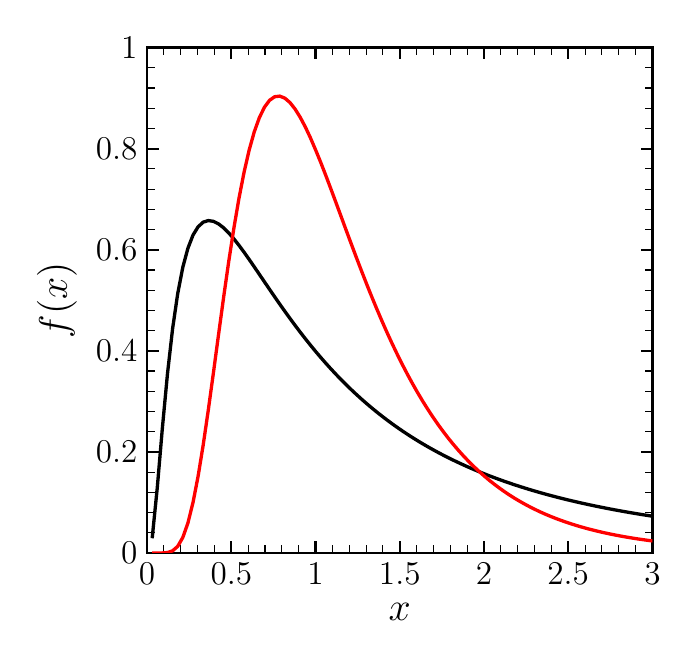
\begin{tikzpicture}
\begin{axis}[xlabel = $x$,
ylabel = {$f(x)$},
samples=100,
xmin=0, xmax=3,
ymin=0, ymax=1,
]

\addplot[color=black, domain=0:3]{1/(1*sqrt(2*pi)*x)*exp(-((ln(x))^2)/(2))};
\addplot[color=red, domain=0:3]{1/(1*sqrt(2*pi)*x*0.5)*exp(-((ln(x))^2)/(0.5))};

\end{axis}
\end{tikzpicture}
\caption{Density of $LN(0,1)$(black and $LN(0,0.5)$(red). Note the positive skewness.}
\end{figure}

\subsubsection{Extension to univariate lognormal distribution}

\begin{definition}\cite{borovkova2007closed}
\hfill
\begin{itemize}
	\item \textbf{regular log-normal distribution} with parameter $(\mu, \sigma^2)$ is given by
	$$f(x) = \frac{1}{x\sigma \sqrt{2\pi}}\exp(-\frac{(\ln x - \mu)^2}{2\sigma^2}),x>0.$$
	\item \textbf{negative log-normal distribution} with parameter $(\mu, \sigma)$, denoted by $NLN(\mu,\sigma^2)$ is given by
	$$f(x) = \frac{1}{x\sigma \sqrt{2\pi}}\exp(-\frac{(\ln -x - \mu)^2}{2\sigma^2}),x<0.$$
	\item \textbf{shifted log-normal distribution} with parameter $(\mu, \sigma,\tau)$,denoted by $SLN(\mu,\sigma^2,\tau)$ is given by
	$$f(x) = \frac{1}{(x-\tau)\sigma \sqrt{2\pi}}\exp(-\frac{(\ln x-\tau - \mu)^2}{2\sigma^2}),x>\tau.$$
	\item \textbf{negative shifted log-normal distribution} with parameter $(\mu, \sigma^2, \tau)$ is given by
	$$f(x) = \frac{1}{(-x-\tau)\sigma \sqrt{2\pi}}\exp(-\frac{(\ln (-x-\tau) - \mu)^2}{2\sigma^2}),x<-\tau.$$
\end{itemize}	
\end{definition}

\begin{figure}[H]
	\centering
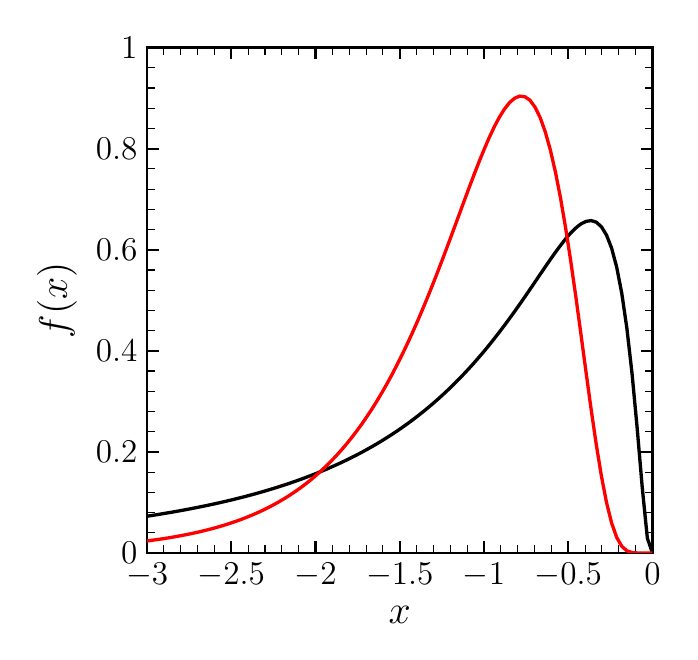
\begin{tikzpicture}
\begin{axis}[xlabel = $x$,
ylabel = {$f(x)$},
samples=100,
xmin=-3, xmax=0,
ymin=0, ymax=1,
]

\addplot[color=black, domain=-3:0]{-1/(1*sqrt(2*pi)*x)*exp(-((ln(-x))^2)/(2))};
\addplot[color=red, domain=-3:0]{-1/(1*sqrt(2*pi)*x*0.5)*exp(-((ln(-x))^2)/(0.5))};

\end{axis}
\end{tikzpicture}
	\caption{Density of $NLN(0,1)$(black and $NLN(0,0.5)$(red). Note the negative skewness.}
\end{figure}

\begin{lemma}
Let $X\sim LN(\mu,\sigma^2)$. It follows that
\begin{itemize}
	\item Let $Y = -X$. Then $Y\sim NLN(\mu, \sigma^2)$.
	\item Let $Z = X+\tau$. Then $Y\sim NLN(\mu, \sigma^2,\tau)$.
	\item Let $W = -X - \tau$. Then $Y\sim NSLN(\mu, \sigma^2, \tau)$.
\end{itemize}	
\end{lemma}
\begin{proof}
Straight forward from definition and transformation.
\end{proof}

\begin{lemma}[basic properties of shifted lognormal distribution]\label{ch:theory-of-statistics:th:BasicPropertyShiftedlognormalRandomVariable}
Let $X\sim SLN(\mu,\sigma^2,\tau)$. Then
\begin{itemize}
	\item $$E[X] = \tau + \exp(\mu+\frac{1}{2}\sigma^2).$$
	\item $$E[X^2] = \tau^2 + 2\tau\exp(\mu+\frac{1}{2}\sigma^2)+\exp(2\mu+2\sigma^2).$$
	\item $$E[X^3] = \tau^3 + 3\tau^2\exp(\mu+\frac{1}{2}\sigma^2)+3\tau\exp(2\mu+2\sigma^2)+\exp(3\mu+\frac{9}{2}\sigma^2).$$
\end{itemize}	
\end{lemma}
\begin{proof}
Note that from \autoref{ch:theory-of-statistics:th:meanVariancelognormalRandomVariable}, we have
if $Y\sim LN(\mu,\sigma^2)$, then $E[Y^m] = \exp(m\mu + \frac{1}{2}m^2\sigma^2)$.
Then, we use
$$E[X] = E[Y+\tau] = E[Y] + \tau,$$
$$E[X^2] = E[(Y+\tau)^2] = E[Y^2] + 2\tau E[Y] + \tau^2,$$
$$E[X^3] = E[(Y+\tau)^3] = E[Y^3] + 3\tau E[Y^2] + 3\tau^2 E[Y] + \tau^3.$$

\end{proof}

\subsubsection{Moment matching approximation}
\begin{lemma}[2 parameter Log-normal approximation via moment matching]\label{ch:theory-of-statistics:th:lognormalApproximationViaMomentMatching}
Suppose we have a random variable $X$ having moments given by
$$E[X] = M_1, E[X^2] = M_2.$$
Let $Y$ be a log-normal random variable defined by
$$Y = M_1\exp(-\frac{1}{2}v^2 + vZ), Z\in N(0,1),$$
where 
$$v^2 = \log(M_2/M_1^2)$$
Then $Y$ has the same first two moments as $X$; that is
$$E[Y] = M_1, E[Y^2] = M_2.$$
\end{lemma}
\begin{proof}
Using moment generating function of $Z$, we know that
$$E[Y] = M_Z(v)M_1\exp(-\frac{1}{2}v^2) = M_1.$$
and
$$E[Y^2] = M_Z(2v)M_1^2\exp(-v^2) = \exp(v^2)M_1^2=\frac{M_2}{M_1^2}M_1^2 = M_2.$$
\end{proof}


\begin{lemma}[3 parameter shifted lognormal approximation via moment matching]\label{ch:theory-of-statistics:th:ShiftedlognormalApproximationViaMomentMatching}
	Suppose we have a random variable $X$ having moments given by
	$$E[X] = M_1, E[X^2] = M_2, E[X^3] = M_3.$$
	Let $Y$ be a  shifted log-normal random variable with parameter $SLN(\mu,\sigma^2,\tau)$ such that
	$$E[Y] = \tau + \exp(\mu+\frac{1}{2}\sigma^2),$$
	$$E[Y^2] = \tau^2 + 2\tau\exp(\mu+\frac{1}{2}\sigma^2)+\exp(2\mu+2\sigma^2),$$
	$$E[Y^3] = \tau^3 + 3\tau^2\exp(\mu+\frac{1}{2}\sigma^2)+3\tau\exp(2\mu+2\sigma^2)+\exp(3\mu+\frac{9}{2}\sigma^2).$$
	
	
If we can find $(\mu,\sigma,\tau)$ such that
$$E[X] = E[Y], E[X^2] = E[Y^2],E[X^3] = E[Y^3],$$
then $X$ and $Y$ have matched moments.

\end{lemma}
\begin{proof}
For moments of $Y$, see \autoref{ch:theory-of-statistics:th:BasicPropertyShiftedlognormalRandomVariable}.
\end{proof}

\begin{note}[choice of approximating distribution]\cite{borovkova2007closed}
We can based on the target distribution's location and skewness to choose the type of lognormal distribution we want to use. The table is good summary.
	
	
\begin{center}
	\begin{tabular}{|c|c|c|c|c|}
		\hline
		skewness                & $\eta > 0$   & $\eta>0$   & $\eta<0$      & $\eta<0$         \\ \hline
		location                & $\tau\geq 0$ & $\tau < 0$ & $\tau \geq 0$ & $\tau < 0$       \\ \hline
		choice of approximation & regular      & shifted    & negative      & negative shifted \\ \hline
	\end{tabular}

\end{center}	
\end{note}

\subsubsection{Multivariate lognormal distribution}

\begin{definition}[multivariate lognormal distribution]\label{ch:theory-of-statistics:def:multivariateLognormalDistribution}
If $X=(X_1,X_2,...,X_n)\sim MN(\mu,\Sigma)$, then $Y=\exp(X)=(\exp(X_1),\exp(X_2),...,\exp(X_n)) \sim MLN(\mu, \Sigma)$,
i.e., $Y$ has multivariate lognormal distribution
\end{definition}

\begin{lemma}[basic properties of multivariate lognormal distribution]\label{ch:theory-of-statistics:th:BasicPropertiesMultivariateLognormal}
Let $X=(X_1,X_2,...,X_n)\sim MN(\mu, \Sigma)$ and $Y = \exp(X)=(\exp(X_1),\exp(X_2),...,\exp(X_n))$. Then
\begin{itemize}
	\item $E[Y_i] = \exp(\mu_i + \frac{1}{2}\Sigma_{ii})$.
	\item $E[Y_iY_j] = \exp(\mu_i+\mu_j + \frac{1}{2}(\Sigma_{ii} + \Sigma_{jj} + 2\Sigma_{ij})) = E[Y_i][Y_i]\exp(\Sigma_{ij}).$
	\item $Var[Y_i] = \exp(2\mu_i + \Sigma_{ii})(\exp(\Sigma_{ii}) - 1).$
	\item $Cov[Y_iY_j] = \exp(\mu_i+\mu_j + \frac{1}{2}(\Sigma_{ii} + \Sigma_{jj}))(\exp(\Sigma_{ij}) - 1).$
\end{itemize}	
	
\end{lemma}
\begin{proof}
(1)Note that $M_X(t) = \exp(t^T\mu + \frac{1}{2}t^T \Sigma t), t\in \R^n$, and $E[Y_i] = M_X(e_i)$.
(2) Let $t = e_i+e_j$. Then $$E[Y_iY_j] = M_X(t) = \exp(\mu_i+\mu_j + \frac{1}{2}(\Sigma_{ii} + \Sigma_{jj} + 2\Sigma_{ij})).$$
(3) $$Var[Y_i] = E[Y_iY_i]- E[Y_i]E[Y_i].$$
(4) $$Cov[Y_i,Y_j] = E[Y_iY_j]- E[Y_i]E[Y_j].$$
\end{proof}



\subsection{Exponential distribution}
\begin{definition}[exponential distribution]\index{exponential distribution}
	A random variable $X$ is said to have an exponential distribution $Exp(\lambda)$ with parameter $\lambda$ if it has pdf given as
	$$p(x|\lambda) = \lambda \exp(-\lambda x)$$
	with $x\in [0,\infty)$.	
\end{definition}

\begin{lemma}[basic properites]
	Let $X$ be a random variable with exponential distribution with parameter $\lambda$, then we have
	\begin{itemize}
		\item $E[X] = 1/\lambda$
		\item $Var[X] = 1/\lambda^2$
		\item memoryless: 
		$$P(X > s+t | X > s) = P(X>t)$$
		(even though $P(X>s+t) < P(X>t)$)
	\end{itemize}
\end{lemma}
\begin{proof}
(1)(2) are straightforward. (3) The cmf is given as
$$F(t) = \int_0^t \lambda\exp(-\lambda \tau) d\tau = 1-\exp(-\lambda t)$$
$$P(X>s+t|X>s) = \frac{P(X>s+t \cap X > s)}{P(X>s)} = \frac{P(X > s+t)}{P(X>s)} = \frac{\exp(-\lambda(s+t))}{\exp(-\lambda t)} = \exp(-\lambda t)$$
\end{proof}


\begin{remark}[interpretation of memorylessness]
Supppose we are waiting for an event to occur, and we model the waiting time as a random variable $X$ with $Exp(\lambda)$. If we already wait for $s$ time, the distribution that we need to wait an extra of $t$ time is the same as the distribution of the waiting time at time 0.
\end{remark}

\begin{remark}
\textbf{Exponential distribution is the only memoryless continuous distribution.}\cite{brzezniak1999basic}.
\end{remark}

\begin{lemma}[Normal approximate sum of Exponential]
	Let $X_1,...,X_n$ be independent iid random variable of $Exp(\lambda)$, then
	$$Y = \sum_{i=1}^n X_i$$
	can be approximated(when $n\to \infty$) by $$\frac{Y - n\mu}{\sqrt{n\sigma}}\sim N(0,1),$$
	where $\mu = n/\lambda$,and $\sigma = n/\lambda^2$.
\end{lemma}
\begin{proof}
	Directly from Central Limit Theorem(\autoref{ch:theory-of-probability:centralLimitTheorem}). Also see Gamma distribution properties, since exponential distribution is a special case of Gamma distribution.
\end{proof}


\subsection{Poisson distribution}
\begin{definition}[Poisson distribution]\index{Poisson distribution}
	A discrete random variable $X$ is said to have a Poisson distribution $Poisson(\lambda)$ with parameter $\lambda$ if it has pmf given as
	$$p(x) = \frac{\lambda^xe^{-\lambda}}{x!}$$
	with $x\in \{0,1,2,...\}$.	
\end{definition}


\begin{lemma}[basic property of Poisson distribution]\cite[154]{hoggintroduction}\label{ch:theory-of-statistics:th:PoissonBasicproperty}
Let $X$ be a random variable with distribution $Poisson(\lambda)$. Then
\begin{itemize}
	\item $M(t) = \exp(\lambda(e^t - 1))$.
	\item $E[X] = \lambda, Var[X] = \lambda.$
\end{itemize}
\end{lemma}
\begin{proof}
(1)
\begin{align*}
M_X(t) &= E[e^{tX}] \\
&= \sum_{n=0}^{\infty} e^{tn}\frac{\lambda^n}{n!}e^{-\lambda}\\
&= e^{-\lambda}\sum_{n=0}^{\infty} \frac{(\lambda e^t)^n}{n!}\\
&= e^{-\lambda}e^{\lambda e^t}.
\end{align*}
(2) $E[X] = M_X'(0) = \lambda, E[X^2] = M_X''(0) = \lambda^2-\lambda$.
\end{proof}


\begin{lemma}[sum of Poisson distribution]\label{ch:theory-of-statistics:th:sumofPoisson}
Assume $X_1,...,X_n$ to be independent random variables, and $X_i \sim Poisson(\theta_i),i=1,...,n$. Then $$Y = \sum_{i=1}^n X_i \sim Poisson(\sum_{i=1}^n \theta_i).$$
\end{lemma}
\begin{proof}
Note that $$M_Y(t) = \prod_{i=1}^n M_{X_i}(t) = \exp{\sum_{i=1}^n \theta_i(e^t - 1)}.$$
\end{proof}

\begin{lemma}[Normal approximate sum of Poisson]
Let $X_1,...,X_n$ be independent iid random variable of $Poisson(\theta)$, then
$$Y = \sum_{i=1}^n X_i$$
can be approximated by $$\frac{Y - n\theta}{\sqrt{n\theta}}\sim N(0,1),$$
or equivalently
$$Y \sim N(n\theta,n\theta).$$
\end{lemma}
\begin{proof}
Directly from Central Limit Theorem(\autoref{ch:theory-of-probability:centralLimitTheorem}).
\end{proof}

\subsection{Gamma distribution}
\begin{definition}[Gamma distribution]\cite[42]{murphy2012machine}\index{Gamma distribution}
A random variable $X$ is said to have a Gamma distribution $Gamma(a,b)$ with parameter $a,b$ if it has pdf given as
$$f(x) = \frac{b^a}{\Gamma(a)}x^{a-1}e^{-bx}$$
with support $x\in (0,\infty)$.	
\end{definition}

\begin{remark}[exponential distribution is a special case ]
An exponential distribution with parameter $b$ is a Gamma distribution $Gamma(1,b)$with 
$$f(x) = be^{-bx}.$$
\end{remark}

\begin{remark}[Application in arrival times of Poisson process]
If $N(t)$ is a Poisson process with rate $\lambda$, then the arrival time $T_1,T_2,...$ have $T_n\sim Gamma(n,\lambda)$ distribution.( See
	\autoref{ch:theory-of-stochastic-process:th:arrivaltimepoissonprocess})
\end{remark}

\begin{mdframed}
\textbf{Caution!}
Gamma distribution is different from Gamma function $\Gamma(t)$, which is given as
$$\Gamma(t) = \int_0^\infty x^{t-1}e^{-x}dx$$
\end{mdframed}

\begin{remark}[conjugate prior for Poisson distribution]
	Gammad distribution conjugate prior for the parameter of Poisson distribution. When integrate out $x$ in $\Gamma(t)$, we have
	$$ \int_0^\infty  x^{a-1}e^{-bx} dx = \Gamma(a)/b^2$$
\end{remark}

\begin{lemma}[mean and variance]
The Gamma distribution $Gamma(a,b)$ has mean $a/b$ and variance $a/b^2$.
\end{lemma}
\begin{proof}
Using the property of$$ \int_0^\infty  x^{a-1}e^{-bx} dx = \Gamma(a)/b^a,$$
we can show the result. 
\end{proof}


\begin{theorem}[sum of Gamma random variables]\cite[163]{hoggintroduction}\label{ch:theory-of-statistics:th:sumofGamma}
Let $X_1,...,X_n$ be independent random variables. Suppose $X_i \sim Gamma(a_i,b),\forall i=1,...,n$. Then
$$Y = \sum_{i=1}^n X_i \sim Gamma(\sum_{i=1}^n a_i,b)$$
\end{theorem}
\begin{proof}
This can be proved using moment generating functions.
\end{proof}

\begin{lemma}[Normal approximate sum of Gamma]
	Let $X_1,...,X_n$ be independent iid random variables of $Gamma(a,b)$, then
	$$Y = \sum_{i=1}^n X_i$$
	can be approximated(when $n\to \infty$) by $$\frac{Y - n\mu}{\sqrt{n\sigma}}\sim N(0,1),$$
	where $\mu = na/b$,and $\sigma = na/b^2$.
\end{lemma}
\begin{proof}
	Directly from Central Limit Theorem(\autoref{ch:theory-of-probability:centralLimitTheorem}).
\end{proof}

\subsection{Geometric distribution}
\begin{definition}[geometric distribution]\index{geometric distribution}
	A discrete random variable $X$ is said to have a geometric distribution $Geo(\theta)$ with parameter $\theta$ if it has pmf given as
	$$p(X=k) = (1-\theta)^{k-1}\theta$$
	with $k\in \{1,2,...\}$.	
\end{definition}

\begin{remark}[relation to Bernoulli trias]
The geometric distribution The probability distribution of the number X of Bernoulli trials needed to get one success, supported on the set { 1, 2, 3, ...}	
\end{remark}


\begin{lemma}[basic statistics of geometric distribution]\label{ch:theory-of-statistics:th:BasicStatistcsGeometricDistribution}
The expected value of a geometrically distributed random variable $X$ with parameter $p$ is $1/p$ and the variance is $(1-p)/p^2$.
\end{lemma}
\begin{proof}
(1)
	$$E[X] = \sum_{k=1}^\infty k(1-p)^{k-1}p $$
	$$(1-p)E[X] = \sum_{k=1}^\infty k(1-p)^{k}p $$
subtract and get $pE[X] = 1$.\\
(2) 	$$Var[X] = \sum_{k=1}^\infty (k-1/p)^2(1-p)^{k-1}p $$
can be proved similarly.
\end{proof}







\subsection{Binomial distribution}
\begin{definition}[binomial distribution]\index{binomial distribution}
	A discrete random variable $X$ is said to have a Binomial distribution $Binomial(n,p)$ with parameter $n,p$ if it has pmf given as
	$$f(X=k) = \binom{n}{k}p^k(1-p)^{n-k}$$
	with $x\in \{0,1,2,...,n\}$.
\end{definition}

\begin{remark}[interpretation]
Binomial distribution represents the probability distribution of the number of successes in a sequence of n independent binary experiments, each of which yields 1 with probability p.
\end{remark}  

\begin{remark}[relation to Bernoulli distribution]
Let $X_i$ be iid random variables with Bernoulli distribution of parameter $p$, then 
$$Y = \sum_{i=1}^n X_i$$ is a random variable of binomial distribution with parameter $(n,p)$. 
\end{remark}


\begin{lemma}[sum of independent binomial random variable]
Let $X_1,X_2,...,X_K$ be the independent binomial random variables with parameter $(n_1,p),(n_2,p),...,(n_K,p)$. Let
$Y = \sum_{i=1}^K X_i $. Then
\begin{itemize}
	\item $M_{X_i}(t) = (1-p + pe^t)^{n_i},i=1,...,K$.
	\item $M_Y(t) = (1-p + pe^t)^{\sum_{i=1}^K n_i}$
	\item $Y \sim Binomial(\sum_{i=1}^K n_i, p).$
\end{itemize}
\end{lemma}
\begin{proof}
(1) Use the mgf of Bernoulli distribution(\autoref{ch:theory-of-statistics:th:Bernoullidistributionproperty}).
(2)(3)
Consider $X_1\sim Binomial(n_1,p)$ and $X_2\sim Binomial(n_2,p)$, each has momemt generating function of $(1-p+pe^t)^{n_1}$ and $(1-p+pe^t)^{n_2}$. $X_1+X_2$ will have mgf of 
$(1-p+pe^t)^{n_1+n_2}$(\autoref{ch:theory-of-probability:th:additionandscalingtheoremformgf}), corresponding to $Binomial(n_1+n_2,p)$. It is straight forward to extend multiple cases. 
\end{proof}


\begin{lemma}[convergence of binomial distribution to Poisson distribution]
Suppose that $p_n\in (0,1)$ for $n\in \cN_+$ and $np_n\to \lambda$ as $n\to \infty$. Then the binomial distribution with parameters $n$ and $p_n$ converges to the Poisson distribution with parameter $\lambda$ \textbf{in distribution}  as $n\to \infty$. That is, for fixed $k\in \cN$, 
$$\binom{n}{k}p_n^k(1-p_n)^{n-k} \to e^{-\lambda}\frac{\lambda^k}{k!}$$
as $n\to \infty$.
\end{lemma}
\begin{proof}
(direct method)Note that
\begin{align*}
\binom{n}{k}p_n^k(1-p_n)^{n-k} &=\frac{n(n-1)(n-2)\cdots(n-k+1)}{k!}(p_n)^k(1-p_n)^{n-k} \\
&=\frac{n(n-1)(n-2)\cdots(n-k+1)}{k!}(\frac{\lambda}{n})^k(1-\frac{\lambda}{n})^{n-k} \\
&\approx\frac{n^k}{k!}(\frac{\lambda}{n})^k(1-\frac{\lambda}{n})^{n-k} \\
&=\frac{\lambda^k}{k!}(1-\frac{\lambda}{n})^{n-k}\\
&\to e^{-\lambda \frac{n-k}{n}} \frac{\lambda^k}{k!}\\
&\approx e^{-\lambda} \frac{\lambda^k}{k!}
\end{align*}

(use generating function)
Note that binomial distribution has probability generating function(\autoref{ch:theory-of-probability:def:probabilitygeneratingfunction})
$$((1-p_n)+p_ns)^n = (1 + (pns-p_n)n/n)^n \to e^{(s-1)a},n\to\infty$$
where $e^{(s-1)a}$ is the generating function of Poisson distribution.
\end{proof}

\begin{remark}[Poisson distribution as an approximate for large $n$ and small $k$]
Note that the lemma requires that $k$ fixed. In other words, when $n\gg k$, we can use Poisson distribution to approximate binomial distribution.
\end{remark}

\subsection{Hypergeometric distribution}
\begin{definition}[hypergeometric distribution distribution]\cite[148]{hoggintroduction}\index{hypergeometric distribution}
	A random variable $X$ is said to have a hypergeometric distribution $HG(N,K,n)$ with parameter $N,K,n$ if it has pmf given as
	$$p(x = k) = \frac{\binom{K}{k}\binom{N-K}{n-k}}{\binom{N}{n}} $$
	with support $x\in \{0,1,...,\min(n,K)\}$. Note that the parameters should be non-negative integers and satisfying $$N\geq K, N\geq n.$$

\end{definition}


\begin{remark}[interpretation]
	$p(x = k)$ describes the probability of  $k$ successes in  $n$ draws, without replacement, from a finite population of size $N$ that contains exactly $K$ successes.
\end{remark}

\begin{lemma}[combinatorial identities]
Assuming $K\geq n$, we have
	$$\sum_{0\leq k\leq n} \frac{\binom{K}{k}\binom{N-K}{n-k}}{\binom{N}{n}} = 1$$
\end{lemma}

\begin{lemma}[mean of a hypergeometric distribution]\cite[148]{hoggintroduction}
Let $X$ be a random variable with $HG(N,K,n)$, then its mean is
$$E[X] = n\frac{K}{N}$$
\end{lemma}



\subsection{Beta distribution}
\begin{definition}[Beta distribution]\cite[43]{murphy2012machine}\index{Beta distribution}
	A random variable $X$ is said to have a Beta distribution $B(a,b)$ with parameter $a,b$ if it has a pdf given as
	$$f(x) = \frac{x^{a-1}(1-x)^{b-1}}{B(a,b)},B(a,b)=\frac{\Gamma(a)\Gamma(b)}{\Gamma(a+b)}$$
	with support $x\in [0,1]$.
\end{definition}





\begin{remark}\hfill
	\begin{itemize}
		\item $$\int_0^1 x^{a-1}(1-x)^{b-1} dx = \frac{\Gamma(a)\Gamma(b)}{\Gamma(a+b)}$$
		\item Beta distribution is commonly \textbf{used as the conjugate prior for binomial distribution}, where
		$$p(y_1,...,y_n|\theta) = \theta^{\sum_i y_i}(1-\theta)^{n-\sum_i y_i},y_i\in \{0,1\}$$
		then the posterior distribution will also be Beta.
	\end{itemize}
\end{remark}



\begin{lemma}[basic property]\label{ch:theory-of-statistics:th:propertyBetaDistribution}
Let $X$ be a random variable with distribution $B(a,b)$.
	\begin{itemize}
		\item $$E[X] = \frac{a}{a+b}.$$
		\item $$E[X^2] = \frac{a(a+1)}{(a+b)(a+b+1)}.$$
		\item $$E[X^r] = \frac{a(a+1)\cdots (a+r-1)}{(a+b)(a+b+1)\cdots(a+b+r-1)}.$$
		\item $$Var[X] = \frac{ab}{(a+b)^2(a+b+1)}.$$
		\item The mode of $X$, i.e., the value $x$ that has the maximum probability is
		$$x^* = \frac{a-1}{a+b-2}.$$
	\end{itemize}
\end{lemma}
\begin{proof}
	(1)This can be proved using properties of Gamma distribution.
\begin{align*}
E[X] &= \int_0^1 xf(x)dx \\
&= \int_0^1 \frac{x^a(1-x)^{b-1}}{B(a,b)} \\
&= \frac{B(a+1,b)}{B(a,b)} \\
&= \frac{\Gamma(a+1)\Gamma(b)}{\Gamma(a+b+1)}/\frac{\Gamma(a)\Gamma(b)}{\Gamma(a+b)} \\
&= \frac{\Gamma(a+1)\Gamma(a+b)}{\Gamma(a+b+1)\Gamma(a)} \\
&= \frac{a}{a+b} 
\end{align*}	
	(2) \begin{align*}
	E[X^2] &= \int_0^1 x^2f(x)dx \\
	&= \int_0^1 \frac{x^{a+1}(1-x)^{b-1}}{B(a,b)} \\
	&= \frac{B(a+2,b)}{B(a,b)} \\
	&= \frac{\Gamma(a+2)\Gamma(b)}{\Gamma(a+b+2)}/\frac{\Gamma(a)\Gamma(b)}{\Gamma(a+b)} \\
	&= \frac{\Gamma(a+2)\Gamma(a+b)}{\Gamma(a+b+2)\Gamma(a)} \\
	&= \frac{a(a+1)}{(a+b)(a+b+1)} 
	\end{align*}
(3) Use $Var[X] = E[X^2] - E[X]^2.$
(4) To find the maximizer for $x^{a-1}(1-x)^{b-1}$, we take the log and maximize it. We have
$$\ln f(x) = (a - 1)\ln x + (b-1)\ln (1-x).$$
Take the derivative with respect to $x$ and set to 0, we have
\begin{align*}
\frac{a-1}{x} &= \frac{b-1}{1-x} \\
(a-1)(1-x) &= x(b-1) \\
\implies x^* = \frac{a-1}{a+b-2}.
\end{align*}
\end{proof}


\subsection{Multinomial distribution}
\begin{definition}\cite[35]{murphy2012machine}
A discrete random vector $X=(X_1,...,X_n)$ is said to have multinomial distribution with parameters $(p_1,...,p_n)$ and $m$ if its pmf is given as
$$f(x_1,x_2,...,x_n)=\frac{m!}{x_1!...x_n!}p_1^{x_1}...p_n^{x_n}$$
where we require $x_i\in \{0,...,m\}$,$\sum x_i = m,\sum p_i=1$.
\end{definition}

\begin{remark}
	Consider $m$ independent experiment, each has $n$ outcomes with probability $p_i$ to occur. The outcome distribution is given as\cite{casella2002statistical}
	$$
	f(x_1,x_2,...,x_n)=\frac{m!}{x_1!...x_n!}p_1^{x_1}...p_n^{x_n}
	$$
	where $\sum x_i = m,\sum p_i=1$.
\end{remark}



\begin{lemma}[basic properties of Multinomial Distribution]\label{ch:theory-of-statistics:th:propertyMultinomialDistribution}
Let $X=(X_1,...,X_n)$ discrete random vector with multinomial distribution with parameters $p=(p_1,...,p_n)$ and $m$.
	\begin{itemize}
		\item 
		\item $$E[X_i] = np_i.$$
		\item $$Var[X_i] = np_i(1-p_i), Cov(X_i,X_j) = np_i(1-p_i),$$
	or in vector form
	$$Var[X] = n(diag(p) = pp^T).$$	
	\end{itemize}
\end{lemma}
\begin{proof}
	(1)This can be proved using properties of Gamma distribution.
	\begin{align*}
	E[X_i] &= \int_0^1 x_if(x)dx \\
	&=  \frac{\prod_{k=1}^K \Gamma(a_k + \delta_{ik})}{\Gamma(a_0+1)}/\frac{\prod_{k=1}^K \Gamma(a_k)}{\Gamma(a_0)}\\
	&= \frac{a_i}{a_0}
	\end{align*}	
	(2) \begin{align*}
	E[X_i^2] &= \int_0^1 x^2_if(x)dx \\
	&=  \frac{\prod_{k=1}^K \Gamma(a_k + 2\delta_{ik})}{\Gamma(a_0+2)}/\frac{\prod_{k=1}^K \Gamma(a_k)}{\Gamma(a_0)}\\
	&= \frac{a_i(a_i+1)}{(a_0+1)a_0}  
	\end{align*}
	(3) Use $Var[X] = E[X^2] - E[X]^2.$
	(4) To find the maximizer for $f(x)$, we take the log and maximize it. The optimality condition requires that $x_i^*\propto a_i-1$ and $\sum_{i=1}^{K}a_i=1$.
\end{proof}

\subsection{Dirichlet distribution}
\begin{definition}\cite[49]{murphy2012machine}
	A random vector $X=(X_1,...,X_K)$ is said to have a Dirichlet distribution distribution with parameter $a=(a_1,...,a_K)$ if it has pdf given as
	$$f(x_1,...,x_K) = \frac{1}{B(a)} \prod_{k=1}^K x_k^{a_k-1}$$
	with support $x\in \{x:0\leq x_k\leq 1,\sum_k x_k = 1,\forall k=1,2...,K\}$, and $B(a)$ is a normalization constant given as
	$$B(a) = \frac{\prod_{k=1}^K \Gamma(a_k)}{\Gamma(\sum_k a_k)},$$
where $\Gamma(\cdot)$ is the Gamma function. 	
\end{definition}


\begin{remark}\hfill
\begin{itemize}
	\item Dirichlet distribution can be viewed as multivariate generalization of Beta distribution.
	\item Dirichlet distribution is usually \textbf{used as the conjugate prior} for multinomial distribution.
\end{itemize}	
\end{remark}


\begin{lemma}[basic properties of Dirichlet Distribution]\label{ch:theory-of-statistics:th:propertyDirichletDistribution}
	Let $X = (X_1,X_2,...,X_K),x_i\in (0,1), \sum_{i=1}^{K} x_i = 1$, be a random vector  with distribution $B(a),a\in \R^K$. Let $a_0 = \sum_{i=1}^{K}a_i$.
	\begin{itemize}
		\item $$E[X_i] = \frac{a_i}{\sum_{i=1}^{K} a_i}.$$
		\item $$E[X^2_i] = \frac{a_i(a_i+1)}{(a_0)(a_0+1)}.$$
		\item 
		$$Var[X_i] = \frac{a_i(a_0-a_i)}{a_0^2(a_0+1)}.$$
		\item The mode of $X$, i.e., the value $x$ that has the maximum probability is
		$$x^*_i = \frac{a_i-1}{a_0-K}.$$
	\end{itemize}
\end{lemma}
\begin{proof}
	(1)This can be proved using properties of Gamma distribution.
	\begin{align*}
	E[X_i] &= \int_0^1 x_if(x)dx \\
	&=  \frac{\prod_{k=1}^K \Gamma(a_k + \delta_{ik})}{\Gamma(a_0+1)}/\frac{\prod_{k=1}^K \Gamma(a_k)}{\Gamma(a_0)}\\
	&= \frac{a_i}{a_0}
	\end{align*}	
	(2) \begin{align*}
	E[X_i^2] &= \int_0^1 x^2_if(x)dx \\
&=  \frac{\prod_{k=1}^K \Gamma(a_k + 2\delta_{ik})}{\Gamma(a_0+2)}/\frac{\prod_{k=1}^K \Gamma(a_k)}{\Gamma(a_0)}\\
&= \frac{a_i(a_i+1)}{(a_0+1)a_0}  
	\end{align*}
	(3) Use $Var[X] = E[X^2] - E[X]^2.$
	(4) To find the maximizer for $f(x)$, we take the log and maximize it. The optimality condition requires that $x_i^*\propto a_i-1$ and $\sum_{i=1}^{K}a_i=1$.
\end{proof}

\subsection{$\chi^2$-distribution}
\subsubsection{Basic properties}
\begin{definition}
A random variable $X$ is said to have a $\chi^2(n)$ distribution with parameter $n\in \Z_+$ if it has pdf given as
$$f(x) = \frac{1}{2^{n/2}\Gamma(n/2)}x^{n/2-1}e^{-y/2}$$
with $x\in (0,+\infty)$	
\end{definition}

\begin{remark}[special case of Gamma distribution]
	$\chi^2(n)$ has the same distribution of Gamma(n/2,2).
\end{remark}

\begin{definition}[alternative]\index{$\chi^2$-distribution}
The $\chi^2$-distribution with $k$ degrees of freedom is the distribution of a sum of squares of $k$ independent standard normal random variables. Mathematically, if $X_1,X_2,..., X_k$ are iid random variable with $X_i\sim N(0,1)$, the random variable $$Q=\sum_{i=1}^k X_i^2$$ is distributed according to the $\chi^2$ distribution with $k$ degrees of freedom, writen as $Q\sim \chi^2(k)$.	
\end{definition}

\begin{lemma}[basic property]\cite[161-163]{hoggintroduction}\label{ch:theory-of-statistics:th:propertychisquare}
	Let $X_1,X_2$ be independent random variables. Suppose $X_1 \sim \chi^2(a_1),X_2\sim \chi^2(a_2)$. Then
	\begin{itemize}
		\item $Y = X_1+X_2 \sim \chi^2(a_1+a_2)$
		\item $\lambda X_1 \sim \lambda^2 \chi^2(a_1)$
		\item The moment generating function is given by
		$$M(t) = (1 - 2t)^{-r/2}.$$
	\end{itemize}
\end{lemma}
\begin{proof}
(1)This can be proved using properties of Gamma distribution.
(2) $\lambda X_1$ can be viewed as the sum of squares of normal random variables $Y_i$ with $N(0,\lambda^2)$.
Then $\sum_{i=1}^n (Y_i/\lambda)^2 \sim \chi^2(n) $. 
 
\end{proof}



\begin{lemma}[expectation and variance]\label{ch:theory-of-statistics:th:chi_expectationvariance}
Let random variable $X$ has distribution of $\chi^2(n)$, then
$$E[X] = n, Var[X] = 2n$$ 
In particular, $$E[X/n] = 1, Var[X/n] = 0 ~as~ n\to \infty.$$
that is the random variable $X/n$ becomes deterministic constant as $n\to \infty$.
\end{lemma}
\begin{proof}
(1)Let $Z\sim \chi^2(1), Z = Y^2, Y\sim N(0,1)$, then $E[Z] = Var[Y] + (E[Y])^2 = 1$.
$Var[Z] = E[Z^2] - (E[Z])^2 = E[Y^4] - 1 = 3 - 1 =2.$
(2) Use linearity of expectation that $E[X/n] = E[X]/n = 1$. Use $Var[X/n] = Var[X]/n^2 = 2/n$.
\end{proof}



\subsubsection{Quadratic forms and chi-square distribution}
\begin{definition}[quadratic forms of random vectors]\cite[485]{hoggintroduction}
Let $X=(X_1,X_2,...,X_n)^T$ be a random vector, we called $$Q = X^T\Sigma X,\Sigma\in \R^{n\times n},$$
a quadratic form of random vector  $X$.

Note that $Q$ is also a random variable.
\end{definition}

\begin{lemma}
Let $X$ be a $m$-dimensional random vector with multivariate Gaussian distribution, i.e., $X\sim N(\mu, \Sigma)$. It follows that
\begin{itemize}
	\item $$\Sigma^{1/2}(x-\mu)\sim N(0, I).$$
	\item $$(x-\mu)\Sigma^{-1}(x-\mu)\sim \chi^2(m).$$
\end{itemize}	
\end{lemma}
\begin{proof}
(1) Directly from affine transformation property of multivariate Gaussian random variable (\autoref{ch:theory-of-statistics:th:affinetransformmultivariatenormal}). 
(2) Use the definition that sum of iid normal random variable square is chi-square random variable.
\end{proof}


\begin{theorem}[chi-square orthogonal decomposition]\label{ch:theory-of-statistics:th:chi-squareOrthogonalDecomposition}
Let $X_1,X_2,...,X_n$ be independent standard normal variables such that 
$$\sum_{i=1}^n X_i^2 \sim \chi^2(n). $$
Denote $X = (X_1,...,X_n)^T$.
If there exists an orthogonal projector	$P\in \R^{n\times n}$ such that $Y = PX, Z = (I-P)X$, then
\begin{itemize}
	\item $Y \sim MN(0,P), Z\sim MN(0, I-P)$, and $Y,Z$ are independent of each other.  
	\item $Y^TY \sim \chi^2(r), r = rank(P)$; or equivalently, the quadratic form $Q = X^TPX\sim \chi^2(r)$.
	\item $Z^TZ \sim \chi^2(n-r)$;or equivalently, the quadratic form $Q = X^T(I-P)X\sim \chi^2(n-r)$
\end{itemize} 
In summary, for a quadratic form $Q = X^T\Sigma X$, if $\Sigma$ is idempotent and symmetric, then $Q\sim \chi^2(rank(\Sigma))$.
\end{theorem}
\begin{proof}
(1) From affine transform of multivariate normal(\autoref{ch:theory-of-statistics:th:affinetransformmultivariatenormal}), $$Y\sim MN(0, P\Sigma_X P^T) = MN(0, P^2) = MN(0,P).$$
To show independence, we have $E[YZ^T] = E[PXX^T(I-P)^T] = E[P(I-P)] = 0$.

(2) Let $U$ be the eigen-decomposition of $P$ such that $P = UU^T$. Let $Z = U^TX, Z\in \R^r, Z\sim MN(0, I_r)$. Let $V$  be the eigen-decomposition of $I-P$ such that $I-P = VV^T$. Let $W = V^TX, W\in \R^{n-r}, W\sim MN(0, I_{n-r})$. We want to show that the characteristic function of the random quantity $Y^TY$ is the same as the characteristic function of $\chi^2(r)$. 
\begin{align*}
&E[\exp(itY^TY)] \\
=&\frac{1}{(2\pi)^{n/2}}\int\int\cdots \int \exp(it(U^TX)^T(U^TX) \exp(-\frac{1}{2}X^T(I-P + P) X))dx_1dx_2\cdots dx_n \\
=&\frac{1}{(2\pi)^{n/2}}\int\int\cdots \int \exp(itZ^TZ) \exp(-\frac{1}{2}(Z^TZ + W^TW))dz_1\cdots dz_r dw_{r+1}\cdots dw_n \\
=&\frac{1}{(2\pi)^{r/2}}\int\int\cdots \int \exp(itZ^TZ) \exp(-\frac{1}{2}(Z^TZ))dz_1\cdots dz_r
\end{align*}
where we change the integral variable such that $$[dz_1\cdots dz_r dw_{r+1}\cdots dw_n]^T = [U~ V](dx_1 dx_2 \cdots dx_n)^T$$. The last line is the characteristic function of  $\chi^2(r)$.
(3) similar to (2).
\end{proof}


\begin{lemma}[moment generating functions for Gaussian quadratic forms]\cite[523]{hoggintroduction}\label{ch:theory-of-statistics:th:momentGeneratingFunctionGaussianQuadraticForm}
Let $X=(X_1,X_2,...,X_n)^T$ where $X_1,X_2,...,X_n$ are iid $N(0,1)$. Consider the quadratic form $Q = X^TAX$ for a symmetric matrix $A$ of rank $r\leq n$. 
It follows that
\begin{itemize}
	\item $Q$ has the moment generating function $M(t) = \prod_{i=1}^r (1 - 2t\lambda_i)^{-1/2} = \abs{I - 2tA}^{-1/2},$
	where $\lambda_1,\lambda_2,...,\lambda_r$ are the nonzero eigenvalues of $A$, $\abs{t} < \frac{1}{\max \abs{\lambda_i}}.$
	\item If $A$ is an orthogonal projector such that $\lambda_1=\lambda_2=\cdots = \lambda_r = 1$, then
	$$M(t) = M_{\chi^2(r)}.$$
\end{itemize}
\end{lemma}
\begin{proof}
(1)Let the eigen-decomposition of $A$ be $$A = U\Lambda U^T, U\in \R^{n\times r}, \Lambda \in \R^{r\times r}.$$
Then 
$$Q = X^TAX = X^TU\Lambda U^TX = X^T(\sum_{i=1}^r \lambda_i u_iu_i^T) X =\sum_{i=1}^r \lambda_i (u_i^T X)^T.$$
Let $Y_i=u_i^T X,i=1,2,...,r$. It can be shown that $Y_i\sim N(0,1), E[Y_iY_j] = u_i^T E[XX^T]u_j^T = \delta_{ij}$; that is $Y_1,Y_2,...,Y_r \sim MN(0,I_r).$ 
Therefore, $Y_i^2 \sim \chi^2(1).$

The moment generating function is given by
\begin{align*}
M(t) &= E[\exp(tQ )] \\
&= E[\exp(t \sum_{i=1}^r \lambda_i Y_i^2 )] \\
&= \prod_{i=1}^r E[\exp(t \lambda_i Y_i^2 )] \\
&= \prod_{i=1}^r M_{\chi^2(1)}(\lambda_it) \\
& = \prod_{i=1}^r (1 - 2\lambda_i t)^{-1/2}
\end{align*}
where we use the moment generating function of $\chi^2(1)$ from \autoref{ch:theory-of-statistics:th:propertychisquare}.
(2) straight forward. 
\end{proof}



\begin{lemma}[independence of quadratic forms]\label{ch:theory-of-statistics:th:independenceOfChiSquareQuadraticForms}\cite[528]{hoggintroduction}
Let $X=(X_1,X_2,...,X_n)$ be a random vector where $X_1,X_2,...,X_n$ are iid $N(0,1)$. For real symmetric matrices $A,B\in \R^{n\times n}$, let $Q_1 = X^TAX$ and $Q_2 = X^TBX$. Then $Q_1$ and $Q_2$ are independent if and only if $AB = 0$.	
\end{lemma}
\begin{proof}
Let $rank(A) = r, rank(B) = s$. Let the eigendecomposition of $A,B$ be such that
$$A = \sum_{i=1}^r \lambda_i u_iu_i^T,A = \sum_{i=1}^s 
\beta_i v_iv_i^T.$$
If $AB = 0$, then $u_1,...,u_r, v_1,...,v_r$ will be orthogonal to each other. Then
$$Q_1+Q_2 = \sum_{i=1}^{r+s} \lambda_i u_iu_i^T,$$
where $u_{r+i} = v_i, \lambda_{r+i} = \beta_i$.

It is easy to see that(\autoref{ch:theory-of-statistics:th:momentGeneratingFunctionGaussianQuadraticForm}) 
$$M_{Q_1,Q_2}(t_1,t_2) = M_{Q_1}(t_1)M_{Q_2}(t_2).$$
Then from independence-from-mgf(\autoref{ch:theory-of-probability:th:IndependenceFromMomentGeneratingFunction}), we can prove $Q_1$ and $Q_2$ are independent.
	
\end{proof}

\subsubsection{Noncentral chi-squared distribution}
\begin{definition}[noncentral chi-squared distribution] Let $(X_1,X_2,...,X_k)$ be $k$ independent, normally distributed random variables with mean $\mu_i$ and unit variances. Then the random variable 
	$$Y = \sum_{i=1}^{k}X_i^2$$
is distributed according to the \textbf{noncentral chi-squared distribution} with parameter $k$ specifying the degree of freedom and $\lambda$, known as the \textbf{noncentrality parameter}, given by
$$\lambda = \sum_{i=1}^k \mu_i^2.$$	
\end{definition}

\subsection{Wishart distribution}\index{Wishrt distribution}
\begin{definition}[Wishart distribution]
	Let $X_1,...,X_n$ be independent $p$ dimensional multivariate normal random vector with distribution $MN(0,V)$. Let $X = [X_1,...,X_n]$. Then $M = XX^T$ is said to have Wishart distribution with parameter $(n,p,V)$.
\end{definition}

\begin{definition}[Wishart distribution]
	A random matrix $M\in \R^{p\times p}$ is said to have the Wishart distribution with parameters $W_p(n,V)$ if it has pdf 
	$$f(M) = \frac{1}{2^{np/2}\Gamma_p(\frac{n}{2}\abs{V}^{n/2})}\abs{M}^{n-p-1/2}\exp(\frac{1}{2}Tr[V^{-1}M]),$$
	with the support $M$ be the set of all symmetric positive definite matrices. Here $\Gamma_p(\alpha)$ is the multivariate gamma function. 	
\end{definition}


\begin{lemma}[basic properties]\hfill
	\begin{itemize}
		\item (reduction to $\chi^2$) If $M\in \R^{1\times 1}$, then
		$$M\sim W_1(n, \sigma^2) = \sigma^2 \chi^2(n).$$
		\item For $M\sim W_p(n,V)$, then $B^TMB \sim W_m(n,B^TVB)$, where $B\in \R^{p\times m}$.
		\item For $M\sim W_p(n,V)$, then $V^{-1/2}MV^{-1/2} \sim W_m(n,I).$
		\item If $M_i$ are independent $W_p(n_i,V)$, then $\sum_{i=1}^k \sim W_p(\sum_{i=1}^k n_i,V)$.
		\item If $M\sim W_p(n,V)$, then $E[M] = nV$.
		\item If $M_1,M_2$ are independent and $M_1+M_2 = M\sim W_p(n,V)$. Further if $M_1\sim W_p(n_1,V)$, then $M_2\sim W_p(n-n_1,V)$.
	\end{itemize}
\end{lemma}


\begin{lemma}[sample covariance]\index{sample covariance}
	The sample covariance
	$$\hat{Cov} = \frac{1}{n-1}\sum_{i=1}^n (X_i - \mean{X})(X_i-\mean{X})^T$$
	where $X_i$ are iid $MN(0,V)$, and $\mean{X} = \frac{1}{n}\sum_{i=1}^n X_i$, has the property of
	$$E[\hat{Cov}] = V.$$
\end{lemma}



\subsection{ $t$-distribution}\label{ch:theory-of-statistics:sec:studentTdistribution}
\subsubsection{Standard $t$ distribution}
\begin{definition}[t distribution]\cite[192]{hoggintroduction}
	A random variable $X$ is said to have a $t(n)$ distribution with parameter $n\in \Z_+$ if it has pdf given as
	$$f(x) = \frac{\Gamma((n+1)/2)}{\Gamma(n/2)\sqrt{\pi n}} (1 + \frac{t^2}{n})^{-(n+1)/2}$$
	with $x\in (-\infty,+\infty)$	
\end{definition}




\begin{definition}[alternative]\index{ $t$-distribution}\label{ch:theory-of-statistics:def:tdistribution}
Let random variable $W \sim N(0,1)$, Let random variable $V\sim \chi^2(n)$ \textbf{independent of} $V$. Define a new random variable $T$ as 
$$T=\frac{W}{\sqrt{V/n}}$$
Then $T$ has a $t$-distribution with degree of freedom $n$, denoted by $T_n$ or $t_n$.	
\end{definition}


\begin{remark}[comparison with normal distribution]\hfill
	\begin{itemize}
		\item $t$ distribution generally have shorter peak and fatter tails than normal distribution.
		\item $t_n \to N(0,1)$ as $n\to \infty$.
	\end{itemize}
\end{remark}

\begin{lemma}[mean and variance of $t$-distribution]
The mean for a $t$-distribution with degree of $n$ is given by
$$E[t_n] = \begin{cases}
0, n > 1 \\
\infty (undefined), n=1
\end{cases}.$$ 

The variance for a $t$-distribution with degree of $n$ is given by
$$Var[t_n] = \begin{cases}
\frac{n}{n-2}, n > 2 \\
\infty, n=1,2
\end{cases}.$$ 
\end{lemma}

\subsubsection{classical t distribution}
\begin{definition}\cite[95]{ruppert2015statistics}
If $Y$ has a standard $t_n$ distribution, then $$Z = \mu + \lambda Y$$
is said to have a $t_n(\mu,\lambda^2)$ distribution.
\end{definition}

\begin{lemma}[mean and variance of classical $t$-distribution]
Let $Z$ be a random variable $t_n(\mu,\lambda^2)$. Then
	$$E[Z] = \begin{cases}
	\mu, n > 1 \\
	\infty (undefined), n=1
	\end{cases},$$ 
and	
	
	$$Var[Z] = \begin{cases}
	\lambda^2\frac{n}{n-2}, n > 2 \\
	\infty, n=1,2
	\end{cases}.$$ 
\end{lemma}

\subsubsection{Multivariate $t$ distribution}
\begin{definition}[multivariate $t$ distribution]\cite{ruppert2015statistics}\label{ch:theory-of-statistics:def:MultivariateTDistribution}\hfill
\begin{itemize}
	\item Let $Z$ be a $d$ dimensional multivariate Gaussian $MN(0,\Sigma)$, and $\mu \in \R^d$. The $d$ dimensional random vector $Y$, defined as, $$X = \mu + \sqrt{\frac{n}{W}}Z,$$
	where $W\sim \chi^2(n)$ and $W$ is \textbf{independent} of $Z$,
	has a $t_n(\mu,\Sigma)$ multivariate distribution.
	\item Let $X \sim t_n(\mu, \Sigma)$. Then $X$ has the density given by
	$$f(x) = \frac{\Gamma((n+d)/2)}{\Gamma(n/2)n^{d/2}\pi^{d/2}\abs{\Sigma}^{1/2}}(1 + \frac{1}{n}(x-\mu)^T\Sigma^{-1}(x-\mu))^{-(n+d)/2}.$$
\end{itemize}	

\end{definition}

\begin{lemma}[mean and variance of multivariate $t$-distribution]
	Let $Z$ be a random variable $t_n(\mu,\Sigma)$. Then
	$$E[Z] = \begin{cases}
	\mu, n > 1 \\
	\infty (undefined), n=1
	\end{cases},$$ 
	and	
	
	$$Cov[Z] = \begin{cases}
	\Sigma\frac{n}{n-2}, n > 2 \\
	\infty, n=1,2
	\end{cases}.$$ 
\end{lemma}


\subsubsection{Student's Theorem}

\begin{theorem}[Student's Theorem]\cite[194]{hoggintroduction}\label{ch:theory-of-statistics:th:studentTheorem}\index{Student's theorem}
	Let $X_1,X_2,...,X_n$ be iid random variables each having a normal distribution with mean $\mu$ and variance $\sigma^2$. Define random variables as:\cite{hoggintroduction}
	$$\bar{X} = \frac{1}{n}\sum_{i=0}^nX_i, S^2=\frac{1}{n-1}\sum_{i=1}^n(X_i-\bar{X})^2 $$
	\begin{enumerate}
		\item $\bar{X}$ has a $N(\mu,\sigma^2/n)$ distribution
		\item $\bar{X}$ and $S^2$ are independent.
		\item $(n-1)S^2/\sigma^2$ has a $\chi^2(n-1)$ distribution
		\item The random variable $$T = \frac{\bar{X}-\mu}{S/\sqrt{n}}$$ has $t$-distribution with $n-1$ degrees of freedom.
	\end{enumerate}	
\end{theorem}
\begin{proof}
	(1)From \autoref{ch:theory-of-statistics:th:basicnormalproperties}. (2)
	We can prove $\mean{X}$ and the random vector $Y=(X_1-\mean{X},...,X_n-\mean{X})$ are independent. Note that
	$$\mean{X} = \frac{1}{n}\bm{1}^TX, Y = (I - \frac{1}{n}\bm{1}\bm{1}^T)X,$$
	and hence $\mean{X}$ and $Y$ are both normal. 
	\begin{align*}
	Cov(\mean{X},Y) &= X^T(\frac{1}{n}\bm{1}^T(I -\frac{1}{n}\bm{1}\bm{1}^T))X \\
	&=X^T\frac{1}{n}(\bm{1}^T - \frac{1}{n}\bm{1}^T\bm{1}\bm{1}^T)X \\
	&=X^T\frac{1}{n}(\bm{1}^T - \bm{1}^T))X = 0
	\end{align*}
	where we use the fact that $\bm{1}^T\bm{1} = n$.
	
	
	
	Then $S^2 = \frac{1}{n-1}Y^TY$ will be independent of $\mean{X}$ because $S^2$ is a function of $Y$(\autoref{ch:theory-of-probability:th:functionCompositionPreservesRandomVariableIndependence}).
	(3) See reference and \autoref{ch:theory-of-statistics:th:samplevariancedistribution}. (4) From the definition of the t distribution, we have
	$$Y=\frac{\bar{X}-\mu}{\sigma/\sqrt{n}}$$
	is the $N(0,1)$. $W=(n-1)S^2/\sigma^2$ has a $\chi^2(n-1)$ distribution. 
	Then 
	$$\frac{Y}{\sqrt{W/n-1}}$$ has $t(n-1)$ distribution.
\end{proof}

\subsection{ $F$-distribution}
\begin{definition}[$F$ distribution]\cite[192]{hoggintroduction}
	A random variable $X$ is said to have a $F(n_1,n_2)$ distribution with parameter $n_1,n_2\in \Z_+$ if it has pdf given as
	$$f(x) = \frac{\Gamma((n_1+n)2)/2)(n_1/n_2)^{n_1/2}y^{n_1/2 - 1}}{\Gamma(n_1/2)\Gamma(n_2/2)[1+(n_1x/n_2)]^{(n_1+n_2)/2}}$$
	with $x\in (0,+\infty)$	
\end{definition}


\begin{definition}[alternative]\index{$F$-distribution}
Given two \textbf{independent} chi-squared random variables $W$ and $V$ having $r_1$ and $r_2$ degrees of freedom. We define a new random variable $$W=\frac{U/r_1}{V/r_2}$$
Then $W$ has a $F$-distribution with parameter $(r_1,r_2)$.	
\end{definition}

\begin{lemma}[inverse relationship]
Let $X$ be a random variable with distribution $F(n_1,n_2)$, then $1/X$ is a random variable with distribution $F(n_2,n_1)$.	
\end{lemma}
\begin{proof}
	Directly from definition.
\end{proof}


\begin{lemma}[relationship to $t$ distribution]
	Let $X$ be a random variable with standard $t$ distribution with $n$ degrees of freedom. Then
	$$X^2 \sim F(1,n).$$
	That is, $X^2$ has the distribution of $F(1,n)$.
\end{lemma}
\begin{proof}
	Directly from definition.
\end{proof}



\begin{definition}[noncentral F distribution]\index{noncentral F distribution} Given two chi-squared random variables $W$ and $V$ such that $V$ is a noncentral chi-squared random variable with non-centrality parameter $\lambda$ and degree of freedom $r_1$, and $W$ is a chi-squared random variable having $r_1$ $r_2$ degrees of freedom. We define a new random variable $$W=\frac{U/r_1}{V/r_2}$$
	Then $W$ has a noncentral $F$-distribution  with parameter $(\lambda, r_1,r_2)$.	.
\end{definition}

\subsection{Empirical distributions}


\begin{definition}[empirical cumulative distribution function(CDF)]
	Given $N$ iid random variables $Y_1,Y_2,...,Y_N$ with common cdf $F(t)$, the empirical CDF is defined by
	$$\hat{F}_N(t) = \frac{number~of~elements~in~the~sample \leq t}{N} = \frac{1}{N}\sum_{i=1}^N \bm{1}_{Y_i \leq t}$$.	
\end{definition}

\begin{lemma}[basic statistic properties]
Let $\hat{F}_N(t)$ be the empirical cdf of a random sample of size $N$. For a fixed $t$, we have
\begin{itemize}
	\item $N\hat{F}_N(t)$ is a binomial random variable with parameter $(N,p)$,where $p = F(t)$.
	\item $N\hat{F}_N(t)$ is an unbiased estimator for $NF(t)$.
	\item $N\hat{F}_N(t)$ has variance $NF(t)(1 - F(t))$.
\end{itemize}	
\end{lemma}
\begin{proof}
(1) Note that based on the definition of $\hat{F}_N(t)	\frac{1}{N}\sum_{i=1}^N \bm{1}_{Y_i \leq t}$, $\bm{1}_{Y_i \leq t}$ is a Bernoulli random variable with parameter $p = F(t)$. Therefore,  $N\hat{F}_N(t) = \sum_{i=1}^N \bm{1}_{Y_i \leq t}$ will follow a binomial distribution of parameter $(N,p)$.
(2) $$E[N\hat{F}_N(t) ] = Np = NF(t).$$ 
(3) $$Var[N\hat{F}_N(t) ] = Np(1 - p) = NF(t)(1-F(t)).$$
\end{proof}

\subsection{Heavy-tailed distributions}
\subsubsection{Basic characterization}
\begin{definition}[Heavy-tailed distribution]\index{Heavy-tailed distribution}
The distribution of a random variable $X$ with distribution function $F$ is said to have a heavy right tail if
$$\lim_{x\to \infty} e^{\lambda x} Pr(X>x) = \infty, \forall \lambda > 0.$$
\end{definition}

\begin{remark}[interpretation]
Heavy-tailed distributions have densities decaying  slower in the tails than the normal. 
\end{remark}

\subsubsection{Pareto and power distribution}

\begin{definition}[Pareto distribution]
A random variable $X$ is said to have Pareto distribution with scale parameter $x_m > 0$ and shape parameter $\alpha > 0$ if its has pdf
$$f_X(x) = \begin{cases*}
\frac{\alpha x_m^\alpha}{ x^{\alpha + 1}}, x\geq x_m,\\
0, x < x_m.
\end{cases*};$$
or cdf
$$f_X(x) = \begin{cases*}
1 - (\frac{\alpha x_m}{ x})^\alpha, x\geq x_m,\\
0, x < x_m.
\end{cases*}.$$	
$X$ has support $[x_m,\infty)$.
\end{definition}



\begin{definition}[power law distribution]\label{ch:theory-of-probability:def:powerLawDistribution}
	A random variable $X$ is said to have power law distribution with parameters $K, \alpha$ if its has probability characterization on its tail given by
	$$Pr(X > x) = Kx^{-\alpha}.$$
\end{definition}

\begin{remark}[Pareto distribution and power law distribution are heavy-tailed distribution]
Note that since power grows much slower than the exponential\autoref{appendix:th:sequenceGrowthRate}, therefore
 $$\lim_{x\to \infty} e^{\lambda x} Pr(X>x) = \infty, \forall \lambda > 0.$$
\end{remark}


\subsubsection{Student t distribution family}
\begin{definition}[Student's t-Distribution family]
The $t$ distribution has a single parameter, $\nu>0$, known as \emph{degrees of freedom}. The density function is given as
$$f_{\nu}(x) = \frac{\Gamma(\frac{\nu+1}{2})}{\sqrt{\nu \pi}\Gamma(\frac{\nu}{2})}(1+\frac{x^2}{\nu})^{-\frac{1}{2}(\nu+1)}$$
The first two members of family are
\begin{enumerate}
	\item $f_1(x) = \frac{1}{\pi(1+x^2)}$
	\item $f_2(x) = \frac{1}{2\sqrt{2}}(1+x^2/2)^{-3/2}$
\end{enumerate}	
The $\nu=1$ density is known as \emph{Cauchy's density}. As $\nu \rightarrow \infty$, the density distribution tends to the standard normal density.
\end{definition}


\begin{definition}[Cauchy distribution]
The Cauchy distribution with parameter $(x_0, \gamma)$ has the probability density function
$$f(x; x_0,\gamma) = \frac{1}{\pi \gamma} (\frac{\gamma^2}{(x-x_0)^2 + \gamma^2}),$$
where $x_0$ is the location parameter, specifying the location of the peak of the distribution, and $\gamma$ is the scale parameter which specifies the half-width at half-maximum.
\textbf{Standard Cauchy distribution} is Cauchy distribution with parameter $(0,1)$.
\end{definition}

\begin{remark}[nonexistence of moments]\hfill
\begin{itemize}
	\item The Cauchy distribution is an example of a distribution which has no mean, variance or higher moments. And therefore the moment generating function does not exist. However, the \textbf{mode and median} are well defined and both equal to $x_0$.  
	\item The nonexistence of expectation is because of the $E[\abs{X}] < \infty$. 
\end{itemize}
\end{remark}


\begin{lemma}[sum of Cauchy distribution]\label{ch:theory-of-statistics:th:sumofstandardCauchydistribution}
If $X_1,...,X_n$ are independent and identically distributed random variables, each with a standard Cauchy distribution, then the sample mean $$\mean{X} = (X_1 + ... + X_n)/n$$ has the same standard Cauchy distribution.	
\end{lemma}
\begin{proof}
Note that we need to use characteristic function to prove, since the moment generating function does not exist.
\end{proof}


\subsubsection{Gaussian mixture distributions}

\begin{definition}[normal scale mixture distribution]\cite[99]{ruppert2015statistics}
The normal scale mixture distribution is the distribution of the random variable 
$$Y = \mu + \sqrt{U}Z,$$
where $\mu$ is constant equal to the mean, and $Z\sim N(0,1)$, $U$ is a positive random variable giving the variance of each component, and $Z$ and $U$ are independent.

If $U$ can assume only a finite number of values, then $Y$ has a \textbf{discrete scale mixture distribution}. If $U$ is continuously distributed, then $Y$ has a \textbf{continuous scale mixture distribution}.
\end{definition}


\begin{example}[discrete Gaussian mixture distribution]
Let $\mu = 0$, and $U$ have the following distribution
$$P(U=25) = 0.1, P(U=1) = 0.9.$$
Then  $$Y = \mu + \sqrt{U}Z,$$
is the mixture of 10\% of $N(0,25)$ and 90\% of $N(0,1)$.
\end{example}

\begin{example}[t distribution]
The $t_n$ distribution with $n$ degrees of freedom is a continuous Gaussian mixture with 
$$\mu = 0, U = \frac{n}{W},$$
where $W\sim \chi^2(n)$.
\end{example}

\begin{definition}[multivariate normal variance mixtures]
The random vector $X$ has a multivariate normal variance mixture distribution if
$$X\triangleq \mu + \sqrt{W}AZ$$
where
\begin{itemize}
	\item $Z\sim MN(0,I_k)$
	\item $W$ is a \textbf{positive} scalar random variable which is independent of $Z$
	\item $A\in \R^{d\times k}$ and $\mu \in \R^d$ are a matrix and a vector of constants 
\end{itemize}
\end{definition}

\begin{remark}[conditional distribution]
	
\end{remark}


\begin{example}[special case: multivariate t distribution]
	The $t_n$ distribution with $n$ degrees of freedom is a continuous Gaussian mixture with 
	$$\mu = 0, U = \frac{n}{W},$$
	where $W\sim \chi^2(n)$.
\end{example}


\section{Characterizing distributions}
\subsection{Skewness and kurtosis}

\begin{definition}[skewness]\index{skewness}
	The skewness of an univariate population for random variable $X$ is defined by 
	$$\gamma_1 = E[(\frac{X-\mu}{\sigma})^3] = \frac{E[(X-\mu)^3]}{(E[(X-\mu)^2])^{3/2}}=\frac{\mu_3}{\mu_2^{3/2}} $$
	where $\mu_2$ and $\mu_3$ are the second and the third \textbf{central moments}. 
\end{definition}

\begin{remark}[interpretation]\hfill
	\begin{itemize}
		\item Intuitively, the skewness is a measure of symmetry. 
		\item \textbf{Negative skewness} indicates that the mean of the data values is less than the median, and the data distribution is \textbf{left-skewed}.
		\item \textbf{Positive skewness} indicates that the mean of the data values is greater than the median, and the data distribution is \textbf{right-skewed}.
	\end{itemize}
\end{remark}

\begin{example}
Let $X\sim N(\mu,\sigma^2)$. Then the skewness of $X$ distribution is
$\gamma_1 = E[(\frac{X-\mu}{\sigma})^3] = E[Z^3] = 0, Z\sim N(0,1),$
where we use the fact the third moment for a standard normal is zero(\autoref{ch:theory-of-statistics:th:MomentsOfStandardNormalDistribution}). 	
\end{example}

\begin{definition}[kurtosis, excess kurtosis]\index{kurtosis}\hfill
\begin{itemize}
	\item 	The \textbf{kurtosis} of a univariate population is defined by 
	$$\gamma_2 = E[(\frac{X-\mu}{\sigma})^4] = \frac{E[(X-\mu)^4]}{(E[(X-\mu)^2])^{2}} = \frac{\mu_4}{\mu_2^2},$$
	where $\mu_2$ and $\mu_4$ are the second and the fourth central moments. 
	\item 	The \textbf{excess kurtosis} of a univariate population is defined by 
	$$\gamma_2^{ex} = \gamma_2 - 3.$$
\end{itemize}	
\end{definition}

\begin{remark}[interpretation]\hfill
	\begin{itemize}
		\item Intuitively, the kurtosis is a measure of tail shape of a distribution.
	\end{itemize}
\end{remark}




\begin{remark}[Three types of kurtosis]\hfill
	\begin{itemize}
		\item \textbf{mesokurtic}: zero kurtosis as standard normal distribution.
		\item \textbf{leptokurtic}: kurtosis greater than 0.  This type of distribution is one with extremely thick tails and a very thin and tall peak.  t-distributions are leptokurtic.
		\item \textbf{platykurtic}:kurtosis smaller than 0. This type of distribution has a short and broad-looking peak. Uniform distributions are platykurtic.
	\end{itemize}
\end{remark}

\begin{example}
	Let $X\sim N(\mu,\sigma^2)$. Then the kurtosis of $X$ distribution is
	$\gamma_2 = E[(\frac{X-\mu}{\sigma})^4] = E[Z^4] = 3, Z\sim N(0,1),$
	where we use the fact the fourth moment for a standard normal is 3(\autoref{ch:theory-of-statistics:th:MomentsOfStandardNormalDistribution}). 	
\end{example}

\subsection{Quantiles and percentiles}
\subsubsection{Basics}

\begin{definition}[percentile of a distribution]
The $\alpha$ \textbf{percentile}($\alpha\in [0,1]$) of a probability distribution of random number $X$ is a  number $p$ in the support $D$ of the support such that
$$Pr(x < p) = \alpha, Pr(x > p) = 1-\alpha.$$

Or equivalently, the $\alpha$ percentile is given by
$$p = F^{-1}_X(\alpha).$$
\end{definition}

\begin{definition}[percentile in a set of sample values]
	The $\alpha$ \textbf{percentile}($\alpha\in [0,1]$) of a set of values is a value in $\R$ that divides them so that $100\alpha\%$ of values lie below and $100(1 - \alpha)\%$ of the values lie above. 
\end{definition}


\begin{definition}[quantiles of a distribution]
	Quantiles are the cutpoints dividing the range of a probability distribution into contiguous intervals with equal probabilities. 	
\end{definition}


\begin{lemma}[linear relationship between percentiles from two distributions]
Let $X$ and $Y$ be two random variables with cdf $F_X$ and $F_Y$. Let $p_X = F_X^{-1}(\alpha)$ and $p_Y = F_Y^{-1}(\alpha)$ for $\alpha\in [0,1]$. It follows that
\begin{itemize}
	\item If $Y = aX + b$, then 
	$$p_Y = ap_X + b$$
	\item If $Y = \alpha X^\beta$, then
	$$p_{\ln Y} = \beta p_{\ln X} + \ln \alpha,$$
	where $p_{\ln Y} = F^{-1}_{\ln Y}(\alpha),p_{\ln X} = F^{-1}_{\ln X}(\alpha),$
\end{itemize}
\end{lemma}
\begin{proof}
(1)	We know that
$$\alpha = F_Y(p_Y) = F_X(p_X).$$
From scale-location transformation(\autoref{ch:theory-of-probability:th:locationScaleTransformation}), we have 
$$p_X = (p_Y-b)/a.$$
(2) From $Y = \alpha X^\beta$, we have $\ln Y = \beta\ln X + \ln \alpha.$
\end{proof}

\begin{remark}[QQplot and applications] \hfill
\begin{itemize}
	\item When we plotting the percentiles from two samples together, an approximate linear relation suggests $Y = aX + b$.
	\item When we plotting the percentiles from two log-value samples  together, an approximate linear relation suggests a power relationship $Y = \alpha X^\beta$.
\end{itemize}	
	
\end{remark}


\subsubsection{Cornish-Fisher expansion}



\begin{theorem}[Cornish-Fisher expansion]\label{ch:theory-of-statistics:th:CornishFisherExpansion}
Consider a distribution with mean $\mu$ and variance $\sigma^2$. Then its $\alpha$ quantile can be approximate by
$$\mu + \sigma z^{cf}_\alpha$$
where	
	$$z^{cf}_\alpha = q_\alpha + \frac{(q_\alpha^2 - 1)S(X)}{6} + \frac{(q_\alpha^3 - 3q_\alpha)K(X)}{24} - \frac{(2q_\alpha^3 - 5q_\alpha)S^2(X)}{36},$$
where $S(X)$ is skewness, $K(X)$ is kurtosis, $z^{cf}_\alpha$ is the Cornish-Fisher approximate quantile value for the confidence level $\alpha$,	and $q_\alpha$ is the quantile value for the standard normal distribution with confidence level $\alpha$.
\end{theorem}

\begin{remark}[motivation]
	The Cornish-Fisher expansion enables us to approximate quantiles of a random variable based only on its skewness and cumulants.	
\end{remark}


\subsection{Exponential families}
\begin{definition}
\cite[111]{casella2002statistical}
A family of pdfs or pmfs is called an exponential family if it can be expressed as
$$f(x|\theta) = h(x)c(\theta)\exp(\sum_{i=1}^k w_i(\theta)t_i(x)),\theta \in \R^n$$
where $h(x) \geq 0$ and $t_1(x),...,t_k(x)$ are real-valued functions of the observations, the $c(\theta)\geq 0$ and $w_1(\theta),...,w_k(\theta)$ are real-valued functions of the vector $\theta$.
\end{definition}

\begin{theorem}[mean and variance of exponential family]
\cite[112]{casella2002statistical}
The mean and variance of the exponential family is
\begin{align}
 E[\sum_{i=1}^k \frac{\partial w_i(\theta)}{\partial \theta_j} t_i(X)] &= -\frac{\partial \log(c(\theta))}{\partial \theta_j}\\
 Var[\sum_{i=1}^k \frac{\partial w_i(\theta)}{\partial \theta_j} t_i(X)] &= -\frac{\partial^2 \log(c(\theta))}{\partial \theta_j^2} - E[\sum_{i=1}^k \frac{\partial^2 w_i(\theta)}{\partial \theta_j^2} t_i(X)]
\end{align}
\end{theorem}
Proof: see \cite[132]{casella2002statistical}
See \cite[622]{casella2002statistical} for a complete review.

\begin{definition}
	A class of distributions is in the exponential family if it can be written in the form 
	$$p(y;\eta) = b(\eta)\exp(\eta^TT(y) - a(\eta))$$
	where $\eta$ is called the natural parameter of the distribution; $T(y)$ is the sufficient statistic; and $a(\eta)$ is the log partition function.
\end{definition}

\iffalse
\subsubsection{Cases studies}

The Bernoulli distribution
\begin{align*}
p(y;\theta) &= \theta^y (1-\theta)^{1-y} \\
			&= \exp(y\log \theta + (1-y)\log(1-\theta))\\
			&= \exp((\log(\frac{\theta}{1-\theta}))y + \log(1-\theta))
\end{align*}
therefore we have natural parameter $\eta = \log(\frac{\theta}{1-\theta})$



determine the sufficient statistic
Exponential

Rayleigh

Poisson

Gaussian

Bionomial
\fi


\section{Notes on bibliography}
For decision theory, \cite{young2005essentials}\cite{moon2000mathematical}
For overall graduate level treatment, see \cite{casella2002statistical}\cite{hoggintroduction}.
For likelihood based methods, see \cite{pawitan2001all}
For large sample theory(asymptote analysis), see \cite{lehmann1999elements}.

For introductory level Bayesian statistics, see \cite{hoff2009first}.

For good treatment on statistical estimation theory, see \cite{kay1993fundamentals}.


For linear regression models, see \cite{kutner2003applied}\cite{seber2012linear}.

For multivariate statistical analysis, see \cite{johnson2007applied}.

For mixed models, see \cite{mcculloch2001generalized}.

For an informal but deep treatment on robust statistics, see \cite{wilcox2010fundamentals}.

For an extensive discussion on statistical distribution, see \cite{forbes2011statistical}\cite{krishnamoorthy2016handbook}.

\printbibliography
\end{refsection}

\begin{refsection}
	\startcontents[chapters]

\chapter{Statistical Estimation Theory}
\section{Estimator theory}

\subsection{Statistic}

\begin{definition}[statistic]\index{statistic}
Let $X_1,X_2,..X_n$ denote a random sample on a random variable $X$. Let 
$T=T(X_1,X_2,...,X_n)$ be a function of the sample. Then $T$ is called a statistic.
\end{definition}

\begin{remark}
$T$ is also a random variable.
\end{remark}

\begin{definition}[common statistic]\index{sample variance}\index{sample mean}\hfill
Given a random sample $X_1,...,X_n$ from $X$, we have following definitions:
\begin{itemize}
	\item Sample mean:
	$$\mean{X} = \frac{1}{n}\sum_{i=1}^n X_i.$$
	\item Sample variance:
	$$S^2 = \frac{1}{n-1}\sum_{i=1}^n (X_i - \mean{X})^2.$$
	\item Sample standard deviation:
	$$S = \sqrt{S^2}.$$
\end{itemize}
\end{definition}

\begin{remark}[another equivalent form of sample variance]
Note that $\sum_{i=1}^n (X_i - \mean{X})^2$ can also be written by $$\frac{1}{2n}\sum_{i=1}^n\sum_{j=1}^n (X_i - X_j)^2$$.

We have
\begin{align*}
\sum_{i=1}^n (X_i - \mean{X})^2 &= \sum_{i=1}^n (X_i^2 - 2\mean{X}X_i + \mean{X}^2) \\
								&= \sum_{i=1}^n X_i^2 - 2\mean{X}n\mean{X} + n\mean{X} \\
								&= \sum_{i=1}^n X_i^2 - n\mean{X}\mean{X}.
\end{align*}


We have
\begin{align*}
\sum_{i=1}^n\sum_{j=1}^n (X_i - X_j)^2 &= \sum_{i=1}^n 2n X_i^2 - \sum_{i=1}^n\sum_{j=1}^n 2X_iX_j \\
&= \sum_{i=1}^n 2n X_i^2 - \sum_{i=1}^n 2X_in\mean{X} \\
&= \sum_{i=1}^n 2n X_i^2 - 2n^2\mean{X}^2 \\
&= 2n(\sum_{i=1}^n X_i^2 - n\mean{X}\mean{X})
\end{align*}

	
\end{remark}


\subsection{Different types of estimators}
\subsubsection{Basic concepts}
\begin{definition}[unbiased Estimator]\index{unbiased estimator}
Let $X_1,X_2,..X_n$ denote a random sample on a random variable $X$ with pdf $f(x;\theta),\theta \in \Omega$. Let $T=T(X_1,X_2,...,X_n)$ be a statistic. We say that $T$ is an unbiased estimator of $\theta$ if $E(T)=\theta$.
\end{definition}


\begin{definition}[consistent Estimator]\index{consistent estimator}
Let $X$ be a random variable with cdf $F(x,\theta)$. Let $X_1,X_2,...,X_n$ be a sample from the distribution of $X$, and let $T_n$ denote a statistic. $T_n$ is a consistent estimator of $\theta$ if
$$T_n \xrightarrow[ ]{P} \theta $$
\end{definition}



\begin{definition}[bias of an estimator]\index{bias of an estimator}
The bias of an estimator $\hat{\theta}$ is $$Bias(\hat{\theta}) = E[\hat{\theta}] - \theta,$$ 
where $\theta$ is the true value. If $Bias(\hat{\theta}) = 0$, then estimator $\hat{\theta}$ is said to be unbiased. 
\end{definition}


\begin{definition}[variance of an estimator]\index{variance of an estimator}
	The variance of an \textbf{unbiased} estimator $\hat{\theta}$ is $$Var(\hat{\theta}) = E[\hat{\theta}] - \theta)^2],$$
	and the covariance is
	$$Var(\hat{\theta}) = E[(\hat{\theta} - \theta)(\hat{\theta} - \theta)^T],$$
	where $\theta$ is the true value. 
\end{definition}

\begin{definition}[mean squared error of an estimator]
The mean squared error(MSE) of an estimator is $$MSE(\hat{\theta}) = E[(\hat{\theta}-\theta)^2].$$
\end{definition}





\subsubsection{Variance-bias decomposition}
\begin{theorem}[variance bias decomposition]\index{variance bias decomposition}
The MSE of an estimator is related to its variance and bias via
\begin{equation}
 MSE(\hat{\theta}) = E[(\hat{\theta}-\theta)^2]=Var[\hat{\theta}] + (Bias(\hat{\theta}))^2
\end{equation}
where $Var[\hat{\theta}] = E[(\hat{\theta} - E[\hat{\theta}])^2]$. Particularly, if the estimator is unbiased (i.e. $Bias(\hat{\theta}) = 0$), we have
$$MSE(\hat{\theta}) =Var[\hat{\theta}]$$
\end{theorem}
\begin{proof}
Make $(\hat{\theta}-\theta) = (\hat{\theta}-E[\hat{\theta}] + E[\hat{\theta}] - \theta)$ and note that $\hat{\theta}$ is a random variable.
Specifically,
\begin{align*}
MSE(\hat{\theta}) & = E[(\hat{\theta}-\theta)^2] \\
				  & = E[((\hat{\theta}-E[\hat{\theta}] + E[\hat{\theta}] - \theta))^2] \\
				  & = E[((\hat{\theta}-E[\hat{\theta}])^2] + 2E[((\hat{\theta}-E[\hat{\theta}])(E[\hat{\theta}] - \theta))] + E[(E[\hat{\theta}] - \theta))^2]\\
				  & = Var[\hat{\theta}] + 2E[((\hat{\theta}-E[\hat{\theta}])](E[\hat{\theta}] - \theta)) + Bias[\hat{\theta}]^2 \\
				  & = Var[\hat{\theta}] + 0 + Bias[\hat{\theta}]^2
\end{align*}	
\end{proof}

\begin{remark}[biasedness can be useful]
At first glance, it may seem that biasedness is always undesired. However, biased estimator might have smaller variance (Figure \autoref{ch:theory-of-statistics:fig:unbiasedbiasedestimatorComparison}). As a consequence, biased estimator can have smaller MSE than unbiased estimator. Also consider the following example. 	
\end{remark}





\begin{figure}[H]
	\centering
	\includegraphics[width=0.6\linewidth]{../figures/statisticalModeling/estimationTheory/unbiasedBiasedEstimatorModified}
	\caption{An example of biased estimator with smaller variance than unbiased estimator}
	\label{ch:theory-of-statistics:fig:unbiasedbiasedestimatorComparison}
\end{figure}

\begin{example}
	Consider a sample $X_1,X_2,...,X_n$ of iid normal random variable with unknown mean and variance. 
	Consider two variance estimator $$S_1^2 = \frac{\sum_{i=1}^{n} (X_i - \mean{X})}{n-1}, S_2^2 = \frac{\sum_{i=1}^{n} (X_i - \mean{X})}{n}.$$
	Then
	\begin{itemize}
		\item The MSE for $S_1^2$ is
		\begin{align*}
		MSE[S_1^2] &= Var[S_1^2] + [Bias]^2 \\
		&= \frac{2\sigma^4}{n-1} + 0 = \frac{2\sigma^4}{n-1}
		\end{align*}
		where we use the fact that 
		$$\frac{(n-1)S^2}{\sigma^2}\sim \chi^2({n-1}),$$
		from \autoref{ch:theory-of-statistics:th:studentTheorem} and
		$$Var[\frac{(n-1)S^2}{\sigma^2}] = \frac{(n-1)^2}{\sigma^4}Var[S^2] = 2(n-1),$$
		where use $Var[\chi^2(n)] = 2n$ in \autoref{ch:theory-of-statistics:th:propertychisquare}.
		\item The MSE for $S_2^2$ is
		\begin{align*}
		MSE[S_2^2] &= (Var[S_2^2] + [Bias])^2 \\
		&= \frac{2(n-1)\sigma^4}{n} + (E[S_2^2] - \sigma^2)^2 \\
		&= \frac{2(n-1)\sigma^4}{n} + (\frac{(n-1)\sigma^2}{n} - \sigma^2)^2 \\
		&= \frac{2n-1}{n^2}\sigma^4
		\end{align*}
		\item $MSE[S_2^2] < MSE[S_1^2]$. That is, the maximum-likelihood estimator has smaller MSE than the unbiased estimator.
		
	\end{itemize}
	
\end{example}



\subsubsection{Consistence} 

\begin{definition}[consistent estimator]
We say $\hat{\theta}$ is a consistent estimator of $\theta$ if $\hat{\theta}$ converges to $\theta$ in probability, i.e., 
$$\lim_{n\to \infty} P(\abs{\hat{\theta}(X_1,X_2,...,X_n)-\theta} < \epsilon) = 1,\forall \epsilon > 0.$$
\end{definition}

\begin{theorem}[MSE criterion for consistent estimator]
An \textbf{unbiased} estimator $\hat{\theta}$ is consistent if $$\lim_{n\to \infty} Var(\hat{\theta}(X_1,X_2,...,X_n)) = 0$$

More generally, an estimator $\hat{\theta}$ is consistent if $$\lim_{n\to \infty} MSE(\hat{\theta}(X_1,X_2,...,X_n)) = 0$$

\end{theorem}
\begin{proof}
Overall, we can use \autoref{ch:theory-of-probability:th:convergenceMSimpliesconvergeninProb} (convergence in mean square implies convergence in probability)

\end{proof}
 
\begin{remark}[consistence vs. unbiasedness]\label{ch:theory-of-statistics:remark:consistentVsUnbiasedEstimator}\hfill
	\begin{itemize}
		\item A consistent estimator is at least \textbf{asymptotically unbiased}.However, some unbiased estimators can be inconsistent(i.e. the variance does not converge to 0).
		\item If the sample size is larger, consistent estimators are consider better than unbiased estimator because consistent estimator ensure that estimator variance is sufficiently smaller. 
		\item Inconsistent estimator usually should be avoided, since increasing the number of samples will not necessarily reduce the variance.
	\end{itemize}
\end{remark}

\begin{theorem}[sample mean estimator is consistent]\cite[1160]{greene2017econometric}
Let $X_1,...,X_n$ be a random sample from any population with finite mean $\mu$ and finite variance $\sigma^2$. 
Let $\mean{X}_n$ be the sample mean. It follows that
\begin{itemize}
	\item $\mean{X}_n$ is the consistent estimator of $\mu$.
	\item For any function $g(x)$, if $E[g(x)]$ and $Var[g(x)]$ are finite, then the quantity
	$$\frac{1}{n}\sum_{i=1}^n g(X_i)$$
	is the consistent estimator of $E[g(X)]$.
\end{itemize}
\end{theorem}
\begin{proof}
Because $E[\mean{X}_n] = \mu$ and $Var[\mean{X}_n]\to 0$, then $\mean{X}_n$ converges to $\mu$ in mean square and thus in probability (\autoref{ch:theory-of-probability:th:MeanSquareConvergenceToAConstant} and \autoref{ch:theory-of-probability:th:convergenceMSimpliesconvergeninProb}).	
\end{proof}



\section{Method of moments}

\begin{definition}[moments of the random sample]\cite[312]{casella2002statistical} Let $X_1,X_2,...,X_n$ be a sample from a population with pdf or pmf $f(x|\theta_1,...,\theta_k)$. The first $k$ moments are given by
	\begin{align*}
	m_1 &= \frac{1}{n}\sum_{i=1}^n X_i \\
	m_2 &= \frac{1}{n}\sum_{i=1}^n X_i^2 \\
	&\cdots \\
	m_k &= \frac{1}{n}\sum_{i=1}^n X_i^k 
	\end{align*}	
\end{definition}


\begin{definition}[moments of the random sample]\cite[312]{casella2002statistical} Let $X_1,X_2,...,X_n$ be a random sample of $X$ from a population with pdf or pmf $f(x|\theta_1,...,\theta_k)$. Define $\mu_i = E[X^i],i=1,2,...,k$. The method of moments is aimed at solving $\theta_1,\theta_2,...,\theta_k$ from the $k$ equations
	\begin{align*}
	m_1 &= \mu_1(\theta_1,...,\theta_k) \\
	m_2 &= \mu_2(\theta_1,...,\theta_k) \\
	&\cdots \\
	m_k &= \mu_k(\theta_1,...,\theta_k) 
	\end{align*}
	where $m_i,i=1,2,...,k$ are the $k$ moments of the sample.			
\end{definition}


\begin{lemma}[estimating normal distribution parameter via method of moments]\cite[312]{casella2002statistical}
	Suppose $X_1,X_2,...,X_n$ are iid random variable with $N(\mu, \sigma^2)$. It follows that
	\begin{itemize}
		\item $m_1 = \mu, \mu^2 + \sigma^2 = m_2$.
		\item The moment of method estimators for $(\mu, \sigma)$ are
		$$\hat{\mu} = m_1, \hat{\sigma}^2 = \frac{1}{n}\sum_{i=1}^n (X_i - \bar{X})^2.$$
	\end{itemize}	
\end{lemma}
\begin{proof}
	(1) note that $E[X^2] = Var[X] + E[X]^2$.
	(2) note that 
	$$\hat{\sigma}^2 = \frac{1}{n}\sum_{i=1}^n X_i^2 - \bar{X}^2 = \frac{1}{n}\sum_{i=1}^n (X_i - \bar{X})^2.$$
\end{proof}



\begin{lemma}[estimating t distribution parameter via method of moments]\label{ch:theory-of-statistics:th:methodOfMomentsStudentTEstimation}
	Suppose $X_1,X_2,...,X_n$ are iid random variable with $t_v(\mu, \sigma^2),v > 2$. It follows that
	\begin{itemize}
		\item $m_1 = \mu, \mu^2 + \sigma^2\frac{v}{v-2} = m_2$.
		\item The moment of method estimators for $(\mu, \sigma)$ are
		$$\hat{\mu} = m_1, \hat{\sigma}^2 = \frac{1}{n}\sum_{i=1}^n (X_i - \bar{X})^2 \frac{v-2}{v}.$$
	\end{itemize}		
	
\end{lemma}
\begin{proof}
	(1)(2)From \autoref{ch:theory-of-statistics:sec:studentTdistribution} note that $E[X] = \mu$, $E[X^2] = Var[X] + E[X]^2 = \sigma^2\frac{v}{v-2} + \mu^2$.
	note that 
	$$\hat{\sigma}^2\frac{v}{v-2} = \frac{1}{n}\sum_{i=1}^n X_i^2 - \bar{X}^2 = \frac{1}{n}\sum_{i=1}^n (X_i - \bar{X})^2.$$
\end{proof}


\subsection{Generalized moment methods}

\begin{remark}[GMM vs. MLE]\hfill
\begin{itemize}
	\item MLE use assumption about the specific families of distribution for the random variables to derive an objective function. 
	\item GMM estimators use assumptions about moments of the random variable to derive the objective function.  Moment conditions are assumed for the population, but we use the data to compute the analogous sample moment conditions.

\end{itemize}	
	
\end{remark}


\section{Maximum likelihood estimation}
\subsection{Basic concepts}
\begin{definition}[estimator]\cite[315]{casella2002statistical}
	A point estimator is any function $W(\bm{X})=W(X_1,X_2,...,X_n)$ of a random sample; that is, any statistic is a point estimator.
\end{definition}

\begin{definition}[likelihood function]\index{likelihood function}
	\cite[22]{pawitan2001all}
	Assuming a statistical model parametrized by a fixed and unknown $\theta$, the likelihood $L(\bm{x}|\theta)$ is the probability of the observations $\bm{x}=(x_1,x_2,...,x_n)$ of iid random samples $X_1,X_2,...,X_n$ as a function of $\theta$. It can be written as
	$$L(\bm{x}|\theta) = \prod_{i=1}^n f(X=x_i|\theta)$$
	And the corresponding log-likelihood function is defined as
	$$\log L(\bm{x}|\theta) = \sum_{i=1}^n f(X=x_i|\theta)$$
	
\end{definition}

\begin{definition}[maximum likelihood estimator and score function]\index{maximum likelihood estimator}
	\cite[316]{casella2002statistical} A maximum likelihood estimator(MLE) of the parameter $\theta$ based on given observations $\bm{x}$ is 
	$$\hat{\theta} = \max_{\theta} \log L(\bm{x}|\theta),$$
Or alternatively,
$\hat{\theta}$ satisfies
 	$$s(\theta,\bm{x}) = \frac{\Pa \log L}{\Pa \theta} = 0,$$
 where $s(\theta,\bm{x})$ is called \textbf{score function}.
\end{definition}




\begin{example}[Bernoulli trial MLE]
Consider a series of independent Bernoulli trials with success probability $\theta$ such that we have probability mass function given by	
$$Pr(Y_i = y) = (1-\theta)^{1-y} \theta^y, y\in \{0,1 \}.$$

\begin{itemize}
	\item 
	The log-likelihood function based on $n$ observations $Y=\{Y_1,...,Y_N\}$ can be written by
	$$\log L(\theta; Y) = \sum_{i=1}^n ((1-y_i) \log(1-\theta) + y_i \log \theta) = n((1-\mean{y})\log(1-\theta) + \mean{y}\log(\theta)),$$
	where $\mean{y}$ is the sample mean.
	\item 
	The MLE is given by
	$$\hat{\theta} = \mean{y}.$$
\end{itemize}
\end{example}

\begin{example}[Normal distribution MLE]

The log-likelihood function for $n$ iid observations $x_1,...,x_n$ drawn from normal distribution is given by
\begin{align*}
\log L(\theta_1,\theta_2) &= \prod_{i=1}^n f(x_i\theta_1,\theta_2) \\
						  &= \theta_2^{-n/2}(2\pi)^{-n/2}\exp(-\frac{1}{2\theta_2}\sum_{i=1}^n(x_i - \theta_1)^2) \\
						  &=-\frac{n}{2}\log \theta_2 - \frac{n}{2}\log(2\pi) - \frac{\sum_{i=1}^n (x_i - \theta_1)^2}{2\theta_2}
\end{align*}
where $\theta_1 = \mu, \theta_2 = \sigma^2$. 
Setting derivatives to zeros, we have
\begin{align*}
\frac{\Pa \log L(\theta_1,\theta_2)}{\Pa \theta_1} = \frac{\sum_{i=1}^n (x_i - \theta_1)}{\theta_2} &= 0 \\
\frac{\Pa \log L(\theta_1,\theta_2)}{\Pa \theta_2} = -\frac{n}{2\theta_2} + \frac{\sum_{i=1}^n (x_i - \theta_1)^2}{\theta_2^2} &= 0 \\
\end{align*}
which produces
$$\hat{\mu} = \hat{\theta}_1 =\frac{\sum_{i=1}^n x_i}{n} = \mean{x}, \hat{\sigma}^2 = \hat{\theta}_2 =\frac{\sum_{i=1}^n (x_i-\mean{x}}{n}.$$




\end{example}


\begin{example}[exponential distribution MLE]
	Consider an exponential distribution with parameter $\alpha$ such that its pdf is given by
	$$f(x;\alpha) = \alpha e^{-\alpha x}, x\geq 0.$$
	
 The MLE for $\alpha$ from an iid random sample $X_1,...,X_n$ is given by $\hat{\alpha} = 1/\mean{X}$ since
		\begin{align*}
		\log L(\alpha) &= n\log \alpha - \alpha \sum_{i=1}^n X_i \\
		\Pa \log L(\alpha) /\Pa \alpha &= \frac{n}{\alpha} - \sum_{i=1}^n X_i \\
		\Pa \log L(\alpha) /\Pa \alpha = 0 &\implies \hat{\alpha} = 1/\mean{X}.
		\end{align*}
\end{example}
\section{Information and efficiency}

\subsection{Fish information}\index{Fisher information}
\begin{assumption}[Fisher information regularity assumption]\label{ch:theory-of-statistics:assumption:FisherInformationRegularityAssumption}
	For a pdf $f(x;\theta)$ of random variable $X$ with parameter $\theta$. We make the following regularity assumptions:
	\begin{itemize}
		\item The set $A = \{x|p(x;\theta) > 0\}$ does not depend on $\theta$. For all $x\in A, \theta\in \Theta$, $\frac{\Pa }{\Pa \theta}\log p(x;\theta)$ exists and is finite. Here $\Theta$ is the parameter space.
		\item If $T$ is any statistic of $X$ such that $E[\abs{T}] < \infty$ for all $\theta\in \Theta$, then integration and differentiation by $\theta$ can be interchanged in the following way:
		$$\frac{\Pa }{\Pa \theta}[\int T(x)f(x;\theta)dx] = \int T(x)\frac{\Pa }{\Pa \theta} f(x;\theta)dx,$$
		whenever the right-hand side is finite.
	\end{itemize}	
\end{assumption}



\begin{definition}[Fisher information]
	For one dimensional parametric family of pdf or pmf $f(x;\theta)$, we define the Fisher information for $\theta\in \R$ as
	$$I(\theta) = E[(\frac{d}{d\theta}\log f(x;\theta))^2],$$
	where the expectation is\textbf{ taken with respect to $x$.}
	In particular, if $\theta \in \R^N$, we have Fisher information matrix defined as
	$$I(\theta)_{ij} =-E[\frac{\Pa^2 \log(f(x;\theta))}{\Pa \theta_i\theta_j}].$$
\end{definition}

\begin{remark}
	This definition holds both for discrete or continuous random variables, as long as $f$  is differentiable respect to $\theta$. 
\end{remark}

\begin{theorem}[Basic properties of Fisher information]\label{ch:theory-of-statistics:th:BasicPropertiesFisherInformation}
	Let $f(x;\theta)$ be a pdf parameterized by $\theta\in \R$ with \autoref{ch:theory-of-statistics:assumption:FisherInformationRegularityAssumption} holds, then 
	\begin{itemize}
		\item $$E[\frac{d}{d\theta} \log f(x;\theta)] = 0$$
		\item $$I(\theta) = Var[\frac{d}{d\theta} \log f(x;\theta)].$$
		\item Further assume $f(x;\theta)$ is twice differentiable and interchange between integration and differentiation is permitted. Then
		$$I(\theta) = E[(\frac{d}{d\theta}\log f(x;\theta))^2] = -E[\frac{\Pa^2 \log(f(x;\theta))}{\Pa \theta^2}].$$
		
		\item For $\theta \in \R^N$, 
		$$I(\theta) = E[\frac{\Pa \log(f(x;\theta))}{\Pa \theta}(\frac{\Pa \log(f(x;\theta))}{\Pa \theta})^T] = -E[\frac{\Pa^2 \log(f(x;\theta))}{\Pa \theta\theta^T}].$$   
	\end{itemize}	
\end{theorem}
\begin{proof}
	(1)	
	The equivalence of these two expressions can be showed as:
	\begin{align*}
	E[\frac{d}{d\theta} \log f(x;\theta)] &= \int \frac{1}{f(x;\theta)} \frac{d}{d\theta} f(x;\theta) f(x;\theta) dx \\
	&= \int  \frac{d}{d\theta} f(x;\theta)  dx \\
	&= \frac{d}{d\theta} \int f(x;\theta)  dx \\
	& = \frac{d}{d\theta} 1 \\
	&= 0
	\end{align*}
	(2) Based on definition, we have
	\begin{align*}
	Var[\frac{d}{d\theta}\log f(x;\theta)] &= E[(\frac{d}{d\theta}\log f(x;\theta))^2] - E[\frac{d}{d\theta}\log f(x;\theta)]^2 \\
	&= E[(\frac{d}{d\theta}\log f(x;\theta))^2] - 0 \\
	&= I(\theta)
	\end{align*}
	
(3)
\begin{align*}
\frac{\Pa^2}{\Pa \theta^2} \log f(x;\theta) &= \frac{\Pa}{\Pa \theta}\frac{1}{f(x;\theta)}\frac{\Pa}{\Pa \theta} f(x;\theta) \\
&= -\frac{\Pa}{\Pa \theta}\frac{1}{f(x;\theta)^2}\frac{\Pa}{\Pa \theta} f(x;\theta) + \frac{1}{f(x;\theta)}\frac{\Pa^2}{\Pa \theta^2} f(x;\theta)  \\
&= -(\frac{\Pa}{\Pa \theta} \log f(x;\theta))^2 + \frac{1}{f(x;\theta)}\frac{\Pa^2}{\Pa \theta^2} f(x;\theta)  
\end{align*}	
Take expectation with respect to $x$ on both sides and note that
$$E[\frac{1}{f(x;\theta)}\frac{\Pa^2}{\Pa \theta^2} f(x;\theta)]=\int \frac{\Pa^2}{\Pa \theta^2} f(x;\theta) dx = \frac{\Pa^2}{\Pa \theta^2} \int  f(x;\theta) dx =   \frac{\Pa^2}{\Pa^2 \theta} 1 = 0
$$
	

	
	
	
	
\end{proof}



\subsection{Information matrix for common distributions}

\subsubsection{Bernoulli distribution}
\begin{lemma}[Fisher information for Bernoulli distribution]
	Let the pmf of Bernoulli distribution parameterized by $f(x;\theta) = \theta^x(1-\theta)^{1-x},x\in\{0,1\}$. Then
	$$I(\theta) =  \frac{1}{\theta(1-\theta)}.$$
\end{lemma}
\begin{proof}
	\begin{align*}
I(\theta) &= -E[\frac{\Pa^2 \log(f(x;\theta))}{\Pa \theta^2}] \\
&= E[\frac{x}{\theta^2} + \frac{1-x}{(1-\theta)^2}]\\
&= \theta (1/\theta^2) + (1-\theta)(1/(1-\theta)^2) \\
&= \frac{1}{\theta(1-\theta)}
\end{align*}
\end{proof}





\subsubsection{Normal distribution}
\begin{lemma}[Fish information matrix for univariate normal distribution]\cite[548]{greene2017econometric}\label{ch:theory-of-statistics:th:FishInformationMatrixForUnivariateNormalDistribution}
Let the pdf of normal distribution parameterized by $$f(x;\theta) = (2\pi\theta_2)^{-1/2}\exp(-\frac{1}{2\theta_2}\sum_{i=1}^n(x - \theta_1)^2).$$ 
	\begin{align*}
	\frac{\Pa^2 \log f}{\Pa \theta_1^2} &= -\frac{1}{\theta_2} = -\frac{1}{\sigma^2} \\
	\frac{\Pa^2 \log f}{\Pa \theta_2^2} &= \frac{1}{2\theta_2^2} - \frac{1}{\theta_2^3}(x - \theta_1)^2 \\
	\frac{\Pa^2 \ln f}{\Pa \theta_1\Pa \theta_2} &= -\frac{1}{\theta^2_2}(x_i - \theta_1)
	\end{align*}	
	
Finally, take expectation with respect to $x$ and we have
$$I(\theta_1,\theta_2) = \begin{bmatrix}
1/\sigma^2 & 0 \\
0 & 1/(2\sigma^4)
\end{bmatrix} $$	

	
\end{lemma}



\subsubsection{Multivariate Gaussian distribution}

\begin{lemma}
	
\end{lemma}


\subsection{Cramer-Rao lower bound}
\subsubsection{Information inequality}

\begin{theorem}[information inequality for statistic]\label{ch:theory-of-statistics:th:InformationInequalityForStatistic}
Let $T(X)$ be any statistic such that $Var[T(X)] < \infty$ for all $\theta$. Denote $E[T(X)]$ by $\phi(\theta)$. Suppose \autoref{ch:theory-of-statistics:assumption:FisherInformationRegularityAssumption} holds and $0 < I(\theta) < \infty$. Then \textbf{for all} $\theta$
$$Var[T(X)] \geq \frac{[\phi'(\theta)]^2}{I(\theta)}.$$	
\end{theorem}
\begin{proof}
Based on the \autoref{ch:theory-of-statistics:assumption:FisherInformationRegularityAssumption}, ,we have
$$\phi'(\theta) = \int T(x)\frac{\Pa }{\Pa \theta} f(x;\theta) dx = \int T(x)\frac{\Pa \log f(x;\theta) }{\Pa \theta} f(x;\theta) dx.$$
Therefore, we can view
$$\phi'(\theta) = E[T(X)\frac{\Pa \log f(x;\theta) }{\Pa \theta}] = Cov[T(X),\frac{\Pa \log f(x;\theta) }{\Pa \theta}],$$
since $E[\frac{\Pa \log f(x;\theta) }{\Pa \theta}] = 0 \implies E[T(X)]E[\frac{\Pa \log f(x;\theta) }{\Pa \theta}] = 0$.

Using Cauchy-Schwartz inequality (\autoref{ch:theory-of-probability:th:Cauchy-SchwarzInequality}), we have
$$\abs{\phi'(\theta)}^2 = Cov[T(X),\frac{\Pa \log f(x;\theta) }{\Pa \theta}]^2 \leq Var[T(X)]Var[\frac{\Pa \log f(x;\theta) }{\Pa \theta}].$$
At last, use the fact (\autoref{ch:theory-of-statistics:th:BasicPropertiesFisherInformation}) that $I(\theta) = Var[\frac{\Pa \log f(x;\theta) }{\Pa \theta}]$, we can get the final result. 	
\end{proof}



\begin{corollary}[information lower bound for general estimators]
Let $T(X)$ be a (generally biased) estimator of $\theta$ such that
$$\phi(\theta) \triangleq E[T(X)] = \theta + \underbrace{b(\theta)}_{bias}.$$
Then
\begin{itemize}
	\item the variance of $T(X)$ is
	$$Var[T(X)] \geq \frac{\abs{1 + b'(\theta)}}{I(\theta)}.$$
	\item the MSE of $T(X)$ is
	$$MSE[T(X)] \geq \frac{\abs{1 + b'(\theta)}}{I(\theta)} + b(\theta)^2.$$
\end{itemize}
\end{corollary}


\subsubsection{Cramer-Rao lower bound: univariate case}

\begin{theorem}[Cramer-Rao lower bound in univariate estimation]\index{Cramer-Rao lower bound}
Let $\hat{\theta}$ be an arbitrary univariate estimator as a function of iid random samples $X_1,...,X_n$, whose distribution is parameterized by single parameter $\theta$. Let $\theta_0$ be the true value.
Then the variance of the estimator $\hat{\theta}$ is bounded by
	$$Var(\hat{\theta}) \geq \frac{(\frac{d}{d\theta}E[\hat{\theta}])^2}{nI_1(\theta^0)},$$
where $I_1(\theta)$ is the Fish information associated with distribution $f(x;\theta)$ and the expectation is taken with respect to $x$.	
	Particularly, if the estimator $\hat{\theta}$ is unbiased (that is $E[\hat{\theta}] = \theta$), we have
	$$Var(\hat{\theta}) \geq \frac{1}{nI_1(\theta^0)}.$$
\end{theorem}
\begin{proof}
Note that the Fisher information $I(\theta)$ associated with the joint distribution of $(X_1,...,X_n)$ can be expressed by $I(\theta) = nI_1(\theta)$, where $I_1(\theta)$ is the Fisher information associated with $f(x;\theta)$. This is because under iid assumption, 
$$E[\log f(x_1,...,x_n;\theta)] = n E[\log f(x;\theta)].$$
Then use the information inequality (\autoref{ch:theory-of-statistics:th:InformationInequalityForStatistic}), we have
$$Var(\hat{\theta}) \geq \frac{(\frac{d}{d\theta}E[\hat{\theta}])^2}{nI_1(\theta)}.$$
\end{proof}

\begin{example}[univariate estimation for normal distributions]\hfill
	\begin{itemize}
		\item Consider an unbiased mean estimator $\hat{\mu}$ and an unbiased variance estimator $\hat{\sigma}^2$  for normal distribution with unknown mean $\mu$ and variance $\sigma^2$. 
		Because the information matrix is given by (\autoref{ch:theory-of-statistics:th:FishInformationMatrixForUnivariateNormalDistribution})
		
		
		
		The mean estimator has bounded variance given by (using information matrix from 
		$$Var[\hat{\mu}] \geq \frac{1}{nI_1(\theta)} = \sigma^2/n.$$
		
		
		\item Consider anfor normal distribution with known mean $\mu$. The mean estimator has bounded variance given by
		$$Var[\hat{\sigma}^2] \geq \frac{1}{nI_1(\theta)} = 2\sigma^4/n.$$
		
		\item 	It is clear that
		\begin{itemize}
			\item Increasing sample size $n$ will reduce the estimator variance.
			\item Mean/variance estimators of random samples drawn from small-variance distributions have inherent smaller variances.
		\end{itemize}
	\end{itemize}	
\end{example}


\begin{figure}[H]
	\centering
	\includegraphics[width=0.5\linewidth]{../figures/statisticalModeling/estimationTheory/fisherInformationDemo}
	\caption{}
	\label{ch:theory-of-statistics:fig:fisherinformationdemo}
\end{figure}




\begin{theorem}[sufficient and necessary condition to achieve Cramer-Rao lower bound]
Under the regularity \autoref{ch:theory-of-statistics:assumption:FisherInformationRegularityAssumption}, there exists an unbiased estimator $\hat{\theta}$ of $\phi(\theta)$ whose variance attains Cramer-Rao lower bound (i.e., there exists a most efficent unbiased estimator $\hat{\theta}$ of $\phi(\theta)$) if and only if the score statistic $S(X)$ can be expressed in the form
$$S(X) = \alpha(\theta)[\hat{\phi(X)} - \phi(\theta)],$$
where $$\alpha(\theta) = \frac{I(\theta)}{\phi'(\theta)};$$
or equivalently if and only if the function 
$$S(X)\frac{\phi'(\theta)}{I(\theta)} + \phi(\theta)$$
is independent of $\theta$ and is only dependent on $X$.	
\end{theorem}



\subsubsection{Cramer-Rao lower bound: multivariate case}

\begin{theorem}[information inequality for statistic: multivariate case]\label{ch:theory-of-statistics:th:InformationInequalityForStatisticMultivariate}
	Let $T(X)$ be any statistic such that $Var[T(X)] < \infty$ for all $\theta$. Denote $E[T(X)]$ by $\phi(\theta)$. Suppose \autoref{ch:theory-of-statistics:assumption:FisherInformationRegularityAssumption} holds and $0 < I(\theta) < \infty$. Then \textbf{for all} $\theta$
	$$Var[T(X)] \geq [\nabla_{\theta}\phi]^T [I(\theta)]^{-1}[\nabla_{\theta}\phi].$$	
\end{theorem}
\begin{proof}
	Based on the \autoref{ch:theory-of-statistics:assumption:FisherInformationRegularityAssumption}, ,we have
	$$\phi'(\theta) = \int T(x)\frac{\Pa }{\Pa \theta} f(x;\theta) dx = \int T(x)\frac{\Pa \log f(x;\theta) }{\Pa \theta}  dx.$$
	Therefore, we can view
	$$\phi'(\theta) = E[T(X)\frac{\Pa \log f(x;\theta) }{\Pa \theta}] = Cov[T(X),\frac{\Pa \log f(x;\theta) }{\Pa \theta}],$$
	since $E[\frac{\Pa \log f(x;\theta) }{\Pa \theta}] = 0 \implies E[T(X)]E[\frac{\Pa \log f(x;\theta) }{\Pa \theta}] = 0$.
	
	Using Cauchy-Schwartz inequality (\autoref{ch:theory-of-probability:th:Cauchy-SchwarzInequality}), we have
	$$\abs{\phi'(\theta)}^2 = Cov[T(X),\frac{\Pa \log f(x;\theta) }{\Pa \theta}]^2 \leq Var[T(X)]Var[\frac{\Pa \log f(x;\theta) }{\Pa \theta}].$$
	At last, use the fact (\autoref{ch:theory-of-statistics:th:BasicPropertiesFisherInformation}) that $I(\theta) = Var[\frac{\Pa \log f(x;\theta) }{\Pa \theta}]$, we can get the final result. 	
\end{proof}
\begin{proof}
Similar to \autoref{ch:theory-of-statistics:th:InformationInequalityForStatisticMultivariate}, we can show that
$$\frac{\Pa \phi(\theta)}{\Pa \theta_j} = Cov(T(X), \frac{\Pa \log f(x;\theta) }{\Pa \theta_j}).$$

For constants $c_1,c_2,...,c_p$, note that
\begin{align*}
Var[T(X) - \sum_{j=1}^p c_j \frac{\Pa \log f(x;\theta) }{\Pa \theta_j}] &= Var[T(X)] + c^TI(\theta)c - 2c^T [\nabla_{\theta}\phi] \\
&\geq 0
\end{align*}
Particularly, the minimum is achieved at $c* = [I(\theta)]^{-1}\delta$. Then
$$Var[T(X) - \sum_{j=1}^p c_j \frac{\Pa \log f(x;\theta) }{\Pa \theta_j}] = Var[T(X)] -  [\nabla_{\theta}\phi]^T [I(\theta)]^{-1}[\nabla_{\theta}\phi] \geq 0. $$
\end{proof}

\begin{theorem}[Cramer-Rao lower bound in multivariate estimation]\index{Cramer-Rao lower bound}\label{ch:theory-of-statistics:th:CramerRaoLowerBoundMultivariateEstimation}
	Let $\hat{\theta}$ be a $p$-dimension \textbf{unbiased} estimator as a function of iid random samples $X_1,...,X_n$, whose distribution is parameterized by parameter vector $\theta\in \R^p, \theta = (\theta_1,...,\theta_p)$. Let $\theta^0$ be the true value.
	
		Then the variance matrix of the estimator $\hat{\theta}_i$ is bounded by
	$$Var(\hat{\theta}) \geq [n[I_1(\theta)]^{-1},$$
	where $I_1(\theta^0)$ is the Fish information maxtrix associated with distribution $f(x;\theta)$ and the expectation is taken with respect to $x$.	
\end{theorem}
\begin{proof}
	Note that the Fisher information $I(\theta)$ associated with the joint distribution of $(X_1,...,X_n)$ can be expressed by $I(\theta) = nI_1(\theta)$, where $I_1(\theta)$ is the Fisher information associated with $f(x,\theta)$. This is because under iid assumption, 
	$$E[\log f(x_1,...,x_n;\theta)] = n E[\log f(x;\theta)].$$
	Then use the information inequality (\autoref{ch:theory-of-statistics:th:InformationInequalityForStatisticMultivariate}), we have
	$$Var(\alpha^T \hat{\theta}) = \alpha^TVar[\hat{\theta}]\alpha \geq [\nabla_{\theta}\alpha^T\hat{\theta}]^T [nI_1(\theta)]^{-1}[\nabla_{\theta}\alpha^T\hat{\theta}] = \alpha^T [nI_1(\theta)]^{-1} \alpha,$$
	where $\alpha\in\R^p$ is an arbitrary vector.
\end{proof}

\begin{example}[multivariate estimation for normal distributions]\hfill
	\begin{itemize}
		\item Consider an unbiased mean estimator $\hat{\mu}$ for normal distribution with known variance $\sigma^2$. The information matrix is given by ( \autoref{ch:theory-of-statistics:th:FishInformationMatrixForUnivariateNormalDistribution})
		$$I(\theta_1,\theta_2) = \begin{bmatrix}
		1/\sigma^2 & 0 \\
		0 & 1/(2\sigma^4)
		\end{bmatrix}. $$
		
		Therefore, 
		
		$$Var[\hat{\mu}] \geq \sigma^2/n, Var[\hat{\sigma}^2] \geq 2\sigma^4/n, $$
			
		\item 	It is clear that
		\begin{itemize}
			\item Increasing sample size $n$ will reduce the estimator variance.
			\item Mean/variance estimators of random samples drawn from small-variance distributions have inherent smaller variances.
		\end{itemize}
	\end{itemize}	
\end{example}

\subsubsection{Uniformly minimum-variance unbiased estimator}
\begin{definition}\index{minimum-variance unbiased estimator}
	Consider a statistic $\theta$ as a function of iid random samples $X_1,X_2,...,X_n$ with pdf $f(x,\theta)$. The estimator is a \textbf{uniformly minimum-variance unbiased estimator(UMVUE)} if 
	\begin{itemize}
		\item it is unbiased, i.e., $\hat{\theta} = \theta$
		\item $\forall \theta \in \Theta$, we have $$var(\hat{\theta}) \leq var(\hat{\theta'})$$ for any other unbiased estimator $\hat{\theta'}$.
	\end{itemize}
\end{definition}

\begin{remark} [interpretation]
	In terms of efficiency in using data to reduce uncertainty, UMVUE has the optimal estimation efficiency.
\end{remark}

\begin{mdframed}
	\textbf{How to find UMVUE?}
	
	There is no simple, general procedure for finding the MVUE
	estimator. Here are some several
	approaches:
	\begin{itemize}
		\item Find a sufficient statistic and apply the Rao-Blackwell theorem.
		\item Determine the so-called Cramer-Rao Lower Bound (CRLB)
		and verify that the estimator achieves it.
		\item Further restrict the estimator to a class of estimators (e.g.,
		linear or polynomial functions of the data)
		\item The existence of UMVUE is in discussed \cite[62]{keener2010theoretical}.
	\end{itemize}
\end{mdframed}



\begin{lemma}[normal distribution estimators]
	For a normal distribution with unknown mean and variance, the sample mean and the unbiased sample variance are the MUVEs for the population mean and population variance.
\end{lemma}
\begin{proof}
	TODO
	
\end{proof}




\begin{definition}[efficient estimator]\index{efficient estimator}
	An estimator $\hat{\theta}$ if variance achieves equality in the Cramer Rao lower bound for all $\theta\in \Theta$.
\end{definition}

\begin{remark}
	An efficient estimator is optimal in the sense of using information to reduce uncertainty.
\end{remark}

\begin{example}
	Let the pmf of Bernoulli distribution parameterized by $f(x;\theta) = \theta^x(1-\theta)^{1-x},x\in\{0,1\}$. Then
	\begin{align*}
	I(\theta) &= -E[\frac{\Pa^2 \log(f(x;\theta))}{\Pa \theta^2}] \\
	&= E[\frac{x}{\theta^2} + \frac{1-x}{(1-\theta)^2}]\\
	&= \theta (1/\theta^2) + (1-\theta)(1/(1-\theta)^2) \\
	&= \frac{1}{\theta(1-\theta)}
	\end{align*}
	
	Consider the estimator $\hat{\theta} = \mean{X}$, then $$E[\hat{\theta}] = E[\mean{X}] = E[\sum_{i=1}^n X_i/n] = \theta$$
	and
	$$Var[\hat{\theta}] = E[\mean{X}^2] - E[\hat{\theta}]^2 = \theta/n + \theta^2(n-1)/n - \theta^2 = \theta(1-\theta)/n$$
	
	Therefore, the variance of the estimator is achieving the lower bound.
\end{example}

\begin{lemma}
	An efficient estimator is UMVUE; that is, an unbiased estimator with variance achieving the Cramer-Rao lower bound is UMVUE. The converse might not be true.
\end{lemma}
\begin{proof}
	If the variance achieve the lower bound, then it has unformly minimum variance, and therefore it is UMVUE. On the other hand, it is likely that for some estimator the lower bounded is not achieved, but it has smaller variance than any other competing estimators.
\end{proof}

\begin{remark}[implications and practical issues]\hfill
	\begin{itemize}
		\item The Cramer-Rao lower Bound enables us to judge whether one estimator is efficient: the closer to lower bound, the more efficient.
		\item Efficient estimators are usually difficult to find in practice.
	\end{itemize}
\end{remark}



\begin{theorem}[Rao-Blackwell theorem]\index{Rao-Blackwell theorem}
	Let $\hat{\theta}(X_1,...,X_n)$ be an estimator, and $T$ be any sufficient statistic. Then the new estimator $\hat{\theta}^* = E[\hat{\theta}(X_1,...,X_n)|T(X_1,...,X_n)]$ will satisfy
	$$MSE(\hat{\theta}^*) \leq MSE(\hat{\theta}),\forall \theta.$$
	Particularly, if both estimators are unbiased, we have
	$$Var(\hat{\theta}^*) \leq Var(\hat{\theta}),\forall \theta .$$
	The process of creating a new improved estimator via conditioning is called \textbf{Rao-Blackwellization}.
\end{theorem}
\begin{proof}
	Since $Var(X) \geq 0$ implies $E[X^2]\geq E[X]^2$, we have
	\begin{align*}
	E[(\hat{\theta} - \theta)^2|T] \geq (E[\hat{\theta - \theta}|T])^2 = (E[\hat{\theta}|T] - \theta)^2 = (\hat{\theta}^* - \theta)^2
	\end{align*}	
	Take expectation on both sides and use the Tower property of conditional expectation, we have
	$$E[(\hat{\theta}^* - \theta)^2] \leq E[(\hat{\theta} - \theta)^2]$$
\end{proof}


\begin{lemma}[unbiasedness inheritance]
	The improved estimator is unbiased if and only if the original estimator is unbiased. 	
\end{lemma}
\begin{proof}
	$$E[E[\hat{\theta}(X_1,...,X_n)|T(X_1,...,X_n)]]=E[\hat{\theta}(X_1,...,X_n)]$$
\end{proof}


\begin{lemma}[idempotent operation]
	Rao-Blackwellization is an idempotent operation. More precisely, let Rao-Blackwellization operator denoted as $R$, let $\hat{\theta}$ be the original estimator, then
	$$R^2[\hat{\theta}] = R[\hat{\theta}]$$	
\end{lemma}
\begin{proof}
	$$E[E[\hat{\theta}|T]|T]=E[\hat{\theta}|T]$$
	via the law of iterated expectation.
\end{proof}


\begin{remark}[Rao-Blackwell theorem vs. Cramer-Rao lower bound]\hfill
	\begin{itemize}
		\item An estimator achieving the Cramer-Rao lower bound is performing better than any other estimators in all the possible $\theta$.
		\item Rao-Blackwellization provides a way to improve current estimator such that the improved estimator is no worst than the current estimator in all the possible $\theta$. The improved estimator cannot guarantee to achieve the Cramer-Rao lower bound, i.e., being better than any other estimators. 
	\end{itemize}
\end{remark}




\subsection{Efficiency}





\begin{definition}[relative efficiency]
	The relative efficiency of two \textbf{unbiased} estimators $\hat{\theta}_1$ and $\hat{\theta}_2$ is the ratio of their variance $$\frac{Var(\hat{\theta}_1)}{Var(\hat{\theta}_2)}$$.
\end{definition}

\begin{remark}
	The more efficient estimator is that: \textbf{given fixed number of samples}, it has a lower MSE/variance. 
\end{remark}






\subsection{Fisher information characterization of MLE}

\subsubsection{Properties of score function}

\begin{lemma}
	$$Es(\theta,\bm{X}) = 0$$
\end{lemma}
\begin{proof}
	This is a restatement of \autoref{ch:theory-of-statistics:th:BasicPropertiesFisherInformation}
\end{proof}

\begin{lemma}[useful properties of score function]\cite[550]{moon2000mathematical}
	Let $t$ be any vector-valued function $\bm{X}$ and $\theta$, then
	$$E[s(\theta,\bm{X})t^T(\theta,\bm{X})] = \frac{\Pa}{\Pa \theta} E[t^T] - E[\frac{\Pa}{\Pa \theta} t^T]$$ 
	And particularly, if $t = s$, we have
	$$E[s(\theta,\bm{X})s^T(\theta,\bm{X})] =  - E[\frac{\Pa}{\Pa \theta} t^T]$$ 	
\end{lemma}
\begin{proof}
	(1)	Use the fact that
	$$E[t^T] = \int t^T f(x,\theta) dx$$
	and differentiate with respect to $\theta$ on both sides.
	(2) use the fact $Es(\theta,\bm{X}) = 0$ in above lemma.
\end{proof}


\subsubsection{Fisher information and MLE}

\begin{definition}[Fisher information]
	The covariance matrix of the score function is called \textbf{Fisher information matrix}, denoted by $I(\theta)$, and is given by
	$$I(\theta) = E[s(\theta,\bm{X})s^T(\theta,\bm{X})],$$
where 	
$$s(\theta,\bm{X}) = \nabla_{\theta}\log L(\bm{x}|\theta) , 
\log L(\bm{x}|\theta) = \sum_{i=1}^n f(X=x_i|\theta).$$
\end{definition}


\subsubsection{MLE efficiency}

\begin{definition}[efficient estimator]
	An estimator $\hat{\theta}$ is said to be \textbf{efficient} if it is \textbf{unbiased} and the covariance of $\hat{\theta}$ achieves the Cramer-Rao lower bound; i.e., it satisfies
	$$E[\hat{\theta}] = \theta, E[(\hat{\theta}-\theta)(\hat{\theta}-\theta)^T] = I^{-1}(\theta).$$	
\end{definition}

\begin{theorem}[sufficient and necessary condition for MLE be efficient]\cite[552]{moon2000mathematical}\label{ch:theory-of-statistics:th:MLEEfficiency}
	An unbiased estimator $\hat{\theta}$ is efficient (i.e., achieving the Cramer-Rao lower bound) if and only if 
	$$I(\theta)(\hat{\theta}-\theta) = s(\theta,\bm{X})$$
	where $J$ is the Fisher information matrix.
	Furthermore, \textbf{any unbiased maximum-likelihood estimator is an efficient estimator.}
\end{theorem}
\begin{proof}
(forward) Suppose $I(\theta)(\hat{\theta}-\theta) = s(\theta,\bm{X})$, then $$I = E[ss^T] = IE[(\hat{\theta}-\theta)(\hat{\theta}-\theta)^T]I$$
	by the definition of $I$. Multiply both sides by $I^{-1}$, and rearrange we get
	$$E[(\hat{\theta}-\theta)(\hat{\theta}-\theta)^T] = I^{-1}.$$
	(converse) Assume $\hat{\theta}$ is efficient (also unbiased).  First we can show
$$E[s(\theta,X)(\hat{\theta} - \theta)^T] = \cI,$$
where $\cI$ is identity matrix and the expectation is taken with respect to $X$. 
 This is because $E[s(\theta,X)\theta^T] = E[s(\theta,X)] \theta = 0,$
 where we use \autoref{ch:theory-of-statistics:th:BasicPropertiesFisherInformation}.
 In addition, 
 \begin{align*}
 E[s(\theta,X)\hat{\theta}^T] &= \int \frac{\Pa \log f(x|\theta)}{\Pa \theta} \hat{\theta}^T f(x|\theta) dx \\
 &=\int \frac{\Pa f(x|\theta)}{\Pa \theta} \hat{\theta}^T  dx \\
 &=\frac{\Pa}{\Pa \theta} E[\hat{\theta}^T] \\
 &=\frac{\Pa}{\Pa \theta} \theta^T \\
 &= \cI. 
 \end{align*}

Now use Cauchy-Schwartz inequality (\autoref{ch:theory-of-probability:th:Cauchy-SchwarzInequality})
\begin{align*}
\cI &= (E[s(\theta,X)(\hat{\theta} - \theta))^T])^2 \\
    &= E[ss^T]E[(\hat{\theta} - \theta)(\hat{\theta} - \theta)^T] \\
    &= IE[(\hat{\theta} - \theta)(\hat{\theta} - \theta)^T] \\
    &= II^{-1} \\
    &= \cI
\end{align*}
Because the equality in Cauchy-Schwartz inequality hold if and only if
$$s(\theta, X) = K(\theta) (\hat{\theta} - \theta),$$
for some $K(\theta)$, which can be $I(\theta)$.	
\end{proof}

\begin{remark}[a maximum-likelihood estimator is not necessary efficient]\hfill
\begin{itemize}
	\item Consider a biased MLE, then
	$$s(\theta,X) = 0 \neq I(\theta) (\hat{\theta} - \theta).$$
	Therefore, the variance of $\hat{\theta}$ does not achieve the Cramer-Rao lower bound (\autoref{ch:theory-of-statistics:th:MLEEfficiency}).	
	\item However, as the sample size becomes sufficiently large, MLE is consistent and asymptotic efficient (\autoref{ch:theory-of-statistics:th:asymptoticPropertiesMLE}) no matter it is unbiased or not.  
\end{itemize}	

\end{remark}



\begin{example}
	Let the pmf of Bernoulli distribution parameterized by $f(x;\theta) = \theta^x(1-\theta)^{1-x},x\in\{0,1\}$. Then
	\begin{align*}
	I(\theta) &= -E[\frac{\Pa^2 \log(f(x;\theta))}{\Pa \theta^2}] \\
	&= E[\frac{x}{\theta^2} + \frac{1-x}{(1-\theta)^2}]\\
	&= \theta (1/\theta^2) + (1-\theta)(1/(1-\theta)^2) \\
	&= \frac{1}{\theta(1-\theta)}
	\end{align*}
\end{example}



\subsection{One sample estimation}


\begin{lemma}[mean and variance estimator of normal samples]\cite{sciacchitano2015collaborative}
	Let $X_1,X_2,...,X_n$ be a random sample from $N(\mu, \sigma^2)$. Define two statistics
	$$\mean{X} = \frac{1}{n}\sum_{i=1}^n X_i, S^2 = \frac{1}{n-1}\sum_{i=1}^n (X_i - \mean{X})^2.$$
	\begin{itemize}
		\item $\mean{X}$ is the \textbf{uniformly minimum variance unbiased }(UMVU) estimator of $\mu$. And
		$$E[\mean{X}] = \mu, Var[\mean{X}] = \frac{\sigma^2}{n}.$$
		\item $S^2$ is the uniformly minimum variance unbiased (UMVU) estimator of $\sigma^2$. And
		$$E[S^2] = \sigma^2, Var[S^2] = \sigma^4\frac{2}{n-1}.$$
	\end{itemize}	
\end{lemma}
\begin{proof}
	(1) To prove UMVU, see reference. Note that from \autoref{ch:theory-of-statistics:th:studentTheorem},
	$$\frac{(n-1)S^2}{\sigma^2}\sim \chi^2({n-1}),$$
	and
	$$Var[\frac{(n-1)S^2}{\sigma^2}] = \frac{(n-1)^2}{\sigma^4}Var[S^2] = 2(n-1),$$
	where use $Var[\chi^2(n)] = 2n$ in \autoref{ch:theory-of-statistics:th:propertychisquare}.
	
	The information matrix is given by
	$$I_1()$$
\end{proof}


\begin{example}
	Consider a sample $X_1,X_2,...,X_n$ of iid normal random variable with unknown mean and variance. 
	Consider two variance estimator $$S_1^2 = \frac{\sum_{i=1}^{n} (X_i - \mean{X})}{n-1}, S_2^2 = \frac{\sum_{i=1}^{n} (X_i - \mean{X})}{n}.$$
	Then
	\begin{itemize}
		\item The MSE for $S_1^2$ is
		\begin{align*}
		MSE[S_1^2] &= Var[S_1^2] + [Bias]^2 \\
		&= \frac{2\sigma^4}{n-1} + 0 = \frac{2\sigma^4}{n-1}
		\end{align*}
		where we use the fact that 
		$$\frac{(n-1)S^2}{\sigma^2}\sim \chi^2({n-1}),$$
		from \autoref{ch:theory-of-statistics:th:studentTheorem} and
		$$Var[\frac{(n-1)S^2}{\sigma^2}] = \frac{(n-1)^2}{\sigma^4}Var[S^2] = 2(n-1),$$
		where use $Var[\chi^2(n)] = 2n$ in \autoref{ch:theory-of-statistics:th:propertychisquare}.
		\item The MSE for $S_2^2$ is
		\begin{align*}
		MSE[S_2^2] &= (Var[S_2^2] + [Bias])^2 \\
		&= \frac{2(n-1)\sigma^4}{n} + (E[S_2^2] - \sigma^2)^2 \\
		&= \frac{2(n-1)\sigma^4}{n} + (\frac{(n-1)\sigma^2}{n} - \sigma^2)^2 \\
		&= \frac{2n-1}{n^2}\sigma^4
		\end{align*}
		\item $MSE[S_2^2] < MSE[S_1^2]$. That is, the maximum-likelihood estimator has smaller MSE than the unbiased estimator.
		
	\end{itemize}
	
\end{example}

\section{Sufficiency and data reduction}

\begin{mdframed}
	\textbf{Motivation for sufficient statistic:}\\
	\begin{itemize}
		\item When we estimate a model parameter $\theta$, \textbf{not all the information in the data are relevant} to the estimation procedure. For example, if we want to estimate the mean, then the order of the sample is irrelevant.
		\item A sufficient statistic for a model parameter $\theta$ represents the \textbf{summary of all information from the data that are useful} for estimation of $\theta$.
		\item \textbf{A statistic sufficient for one parameter $\theta_1$ might not be sufficient for other parameters $\theta_2$.}
	\end{itemize}
\end{mdframed}


\begin{definition}[sufficient statistics]
	Let $X$ be a random sample of size $n$. A statistic $T(X)$ is a sufficient statistic for $\theta$ if the conditional distribution of the sample $X$ given the value of $T(X)$ does not depend on $\theta$; that is
	$$P(X|T,\theta) = P(X|T)$$
	In otherwise, $X$ and $\theta$ are conditional independent given $T$.
\end{definition}


%\begin{theorem}[sufficient criterion]
%\cite[274]{casella2002statistical}\cite[391]{hoggintroduction}
%Let $X$ be a random sample. Let $p(X|\theta)$ be the joint pdf or pmf of $X$ and $p(T(X)|\theta)$ be the pdf or pmf of $T(X)$, then $T(X)$ is a sufficient statistic for $\theta$ if, 
%$$\frac{p(X|\theta}{p(T(X)|\theta} = H(X)$$
%and does not depend on $\theta$.
%\end{theorem}
%proof: 

\begin{remark}[\textbf{sufficient statistic as a lossless data compression}]
	A statistic is sufficient means that $T(X)$ itself can capture all the information useful in estimating $\theta$; the sample $X$ might contain more information than $T(X)$(since $T(X)$ is usually not 1-1), but this additional information does not provide additional usefulness in estimating $\theta$.
\end{remark}

\begin{remark}[\textbf{trivial sufficient statistic}]
	The statistic $T(X_1,...,X_n)=(X_1,...,X_n)$ is always sufficient for any estimation task.
\end{remark}


\begin{theorem}[Neyman-Fisher Factorization theorem]\index{factorization theorem}
	\cite[276]{casella2002statistical} Let $f(\bm{x}|\theta)$ denote the joint pdf or pmf of a sample $\bm{X}$. A statistic $T(\bm{X})$ is a sufficient statistic for $\theta$ if and only if there exist functions $g(T(\bm{x}|\theta))$ such that for all sample points $\bm{x}\in \cX$ and all parameter points $\theta \in\Theta$, we have
	$$f(\bm{x}|\theta) = g(T(\bm{x})|\theta)h(\bm{x})$$
\end{theorem}
\begin{proof}
	(1) Assume $T(\bm{X})$ is sufficient, then we have $f(x|T(x),\theta) = f(x|T(x))$. Then we have
	\begin{align*}
	f(x|\theta) = f(x|\theta) f(T(x)|x,\theta) &= f(x,T(x)|\theta) = f(T(x)|\theta) f(x|T(x),\theta)\\
	&= f(T(x)|\theta)f(x|T(x)) (\text{use sufficiency})\\
	&=h(x) g(T(x)|\theta)
	\end{align*}
	(2)	
	
	
\end{proof}

\cite[451]{moon2000mathematical} for sufficient statistic examples







\begin{definition}[minimal sufficient]\index{minimal sufficient}\cite[48]{keener2010theoretical}
	A sufficient statistic is minimal sufficient if it can be represented as a function of any other sufficient statistic. That is, if $S(X)$ is minimal sufficient, then there exists a function $f$ such that $S(X) = f(T(X))$, where $T(X)$ is another sufficient statistic.
\end{definition}




\begin{remark}\hfill
	\begin{itemize}
		\item The minimal sufficient statistic represents \textbf{the smallest amount of information yet still sufficient for estimation of the parameter.} Therefore, a minimal sufficient statistic can be represented by any other sufficient statistic, which always contains more information.
		\item A minimal sufficient statistic represents the maximal (and hence optimal) lossless compression of data.
	\end{itemize}
\end{remark}

\begin{definition}[complete statistic]\cite[48]{keener2010theoretical}
\end{definition}

\begin{theorem}\cite[49]{keener2010theoretical}
	If statistic $T$ is complete and sufficient, then $T$ is minimal sufficient. 
\end{theorem}


\section{Asympotic properties of estimators}





\subsection{Asymptotic properties of MLE}

\begin{definition}[asymptotic efficiency]\cite[542]{greene2017econometric}
	An estimator is asymptotically efficient if it is consistent, asymptotically normally distributed, and has an asymptotic covariance matrix that is not larger than the asymptotic covariance matrix of any other consistent, asymptotically normally distributed estimators.	
\end{definition}

\begin{theorem}[asymptotic properties of MLE]\cite[553]{moon2000mathematical}\cite[478]{greene2017econometric}\label{ch:theory-of-statistics:th:asymptoticPropertiesMLE} Let $\hat{\theta}$ be the MLE of coefficient associated with distribution $f(x;\theta)$. Let $\theta_0$ be the true value of the parameter. Let $I_1(\theta)$ be the Fisher information matrix associated with distribution $f(x;\theta)$. It follows that
\begin{itemize}
	\item Maximum-likelihood estimators are consistent; that is
	$$\plim_{n\to \infty} \hat{\theta} = \theta_0.$$
	\item Maximum-likelihood estimators are asymptotic normal; that is,
	$$\sqrt{n}(\hat{\theta} - \theta_0) \to MN(0, [I_1(\theta_0)]^{-1})$$
	\item Maximum-likelihood estimators are asymptotic efficient.
\end{itemize}
\end{theorem}
\begin{proof}
(sketch) 
(1) Define a scaled log-likelihood function 
$$L_n(\theta) = \frac{1}{n}\sum_{i=1}^n \log f(X_i|\theta).$$


Consider the function $L(\theta) = \int (\log f(x;\theta) f(x;\theta_0)dx$, we can show that the true parameter $\theta_0$ is the maximizer of $L(\theta)$; that is, for any $\theta$, we have $$L(\theta)\leq L(\theta_0).$$

\begin{align*}
L(\theta) - L(\theta_0) &= E_{\theta_0}[\log f(X;\theta) - \log f(X;\theta_0)] \\
&= E_{\theta_0}[\log \frac{f(X;\theta)}{f(X;\theta_0)}] \\
&\leq E_{\theta_0}[ \frac{f(X;\theta)}{f(X;\theta_0)} - 1] \\
&=  \int (\frac{f(X;\theta)}{f(X;\theta_0)} - 1) f(x;\theta_0) dx \\
&= \int f(x;\theta)dx - \int f(x;\theta_0) dx \\
& = 1 - 1 =0
\end{align*}
where we use inequality $\log x \leq x - 1$. 
From the law of large numbers, $L_n(\theta)$ converge to $L(\theta)$ in probability. 
Since MLE $\hat{\theta}$ is the maximizer for $L_n(\theta)$, $\hat{\theta}$ converges to $\theta_0$ in probability.	
(2) Since as $n\to \infty$, $\hat{\theta} \to \theta_0$ (becomes unbiased), we use \autoref{} to show that $\hat{\theta} - \theta_0$ has the variance reaching the Cramer-Rao lower bound. Further, use central limit theorem can arrive at the conclusion.
(3) It is asymptotic efficient because its variance reaches Cramer-Rao lower bound. 
\end{proof}


\begin{remark}[interpretation and implications]\hfill
For finite-sample MLE, only unbiased MLE is efficient(\autoref{ch:theory-of-statistics:th:MLEEfficiency}). At the large sample limit, MLE is always consistent (asymptotic unbiased) therefore efficient. 	
\end{remark}

\begin{example}
Consider an exponential distribution with parameter $\alpha$ such that its pdf is given by
$$f(x;\alpha) = \alpha e^{-\alpha x}, x\geq 0.$$

\begin{itemize}
	\item The MLE for $\alpha$ from an iid random sample $X_1,...,X_n$ is given by $\hat{\alpha} = 1/\mean{X}$ since
	\begin{align*}
	\log L(\alpha) &= n\log \alpha - \alpha \sum_{i=1}^n X_i \\
	\Pa \log L(\alpha) /\Pa \alpha &= \frac{n}{\alpha} - \sum_{i=1}^n X_i \\
	\Pa \log L(\alpha) /\Pa \alpha = 0 &\implies \hat{\alpha} = 1/\mean{X}.
	\end{align*}
	\item The Fisher information is given by $I(\alpha) = \frac{1}{\alpha^2}$ since 
	\begin{align*}
	\log f(x;\alpha) &= \log \alpha - \alpha x \\
	\Pa^2 \log L(\alpha) /\Pa \alpha^2 &= -\frac{1}{\alpha^2} \\
	I(\alpha) = -E[\Pa^2 \log L(\alpha) /\Pa \alpha^2] = \frac{1}{\alpha^2}.
	\end{align*}
	 \item The MLE $\hat{\alpha} = 1/\mean{X}$ is asymptotic normal and
	 $$\sqrt{n}(\hat{\alpha} - \alpha_0) \to N(0, \alpha_0^2).$$
\end{itemize}	
	
\end{example}

\begin{example}[Fish information matrix for normal distributions]\cite[548]{greene2017econometric}
	
	\begin{align*}
	\frac{\Pa^2 \ln L}{\Pa \mu^2} &= -\frac{n}{\sigma^2} \\
	\frac{\Pa^2 \ln L}{\Pa (\sigma^2)^2} &= \frac{n}{2\sigma^4} - \frac{1}{\sigma^6}\sum_{i=1}^n (x_i - \mu)^2 \\
	\frac{\Pa^2 \ln L}{\Pa \mu \Pa \sigma^2} &= -\frac{1}{\sigma^4}\sum_{i=1}^n (x_i - \mu)
	\end{align*}	
	
	For the asymptotic variance of the maximum likelihood estimator, we need the expectations of these derivatives. Using $E[X_i] = \mu$, we have
	$$[-E_0[\frac{\Pa^2 \ln L(\theta_0)}{\Pa \theta_0 \Pa \theta_0^T}]]^{-1} = \begin{bmatrix}
	\sigma^2/n & 0 \\
	0 & 2\sigma^4/n
	\end{bmatrix}.$$
\end{example}




Let $\hat{\theta}$ be the maximum-likelihood estimator, then the gradient of the log-likelihood function equals zero at $\hat{\theta}$; that is,
$$g(\hat{\theta}) = 0.$$

Expand this equation in a second-order Taylor series around $\theta_0$, we have
$$ 0 = g(\hat{\theta}) = g(\theta_0) + H(\mean{\theta})(\hat{\theta} - \theta_0),$$
where $\theta_0$ is the true value, and $\mean{\theta} = w\hat{\theta} + (1-w)\theta_0$ for some $0<w<1$. Rearranging this function and multiply it by $n$ and we get
$$\sqrt{n}(\hat{\theta} - \theta_0) = [-H(\mean{\theta})]^{-1}(\sqrt{n}g(\theta_0))$$







\section{Interval estimation}
\begin{definition}[interval estimator]
	\cite[418]{casella2002statistical}
	An interval estimator of a real-valued parameter $\theta$ is a pair of statistic $L(\bm{X}$ and $U(\bm{X})$ satisfying $L(\bm{x}) \leq U(\bm{x}),\forall x\in \cX$. If $\bm{X}=\bm{x}$ is observed, then the inference $L(\bm{x}) \leq\theta \leq U(\bm{x})$ is made. The random interval estimator $[L(\bm{X} U(\bm{X})]$ is called interval estimator.  
\end{definition}

\begin{remark}
	It is important to note that the interval estimator is a random quantity.
\end{remark}

\begin{definition}[Confidence interval]
	Let $X_1,X_2,..X_n$ denote a random sample on a random variable $X$, where $X$ has pdf $f(x;\theta)$. Let $\alpha (0 < \alpha < 1)$ be given. Let $L=L(X_1,X_2,..X_n), U = U(X_1,X_2,..X_n)$ be two statistics. We say that the interval $(L,U)$ is a $(1-\alpha)$ confidence interval for $\theta$ if
	$$1-\alpha = P_{\theta}(\theta\in (L,U))$$
\end{definition}




\begin{definition}[interval estimation, decision]
	An interval estimation is a decision rule that assert the parameter to be estimated in the interval $[L(\bm{x}),U(\bm{x})]$ when $\bm{X}=\bm{x}$ is given. 
\end{definition}

\begin{definition}[coverage probability]
	\cite[418]{casella2002statistical} For an interval estimator $[L(\bm{X}),U(\bm{X})]$ of a parameter $\theta$, the coverage probability of $[L(\bm{X}),U(\bm{X})]$ is the probability that the random interval $[L(\bm{X}),U(\bm{X})]$ covers the true parameter $\theta$, i.e., $P(\theta\in [L(\bm{X}),U(\bm{X})]|\theta)$
\end{definition}

\begin{definition}[confidence coefficient]
	\cite[418]{casella2002statistical} For an interval estimator $[L(\bm{X}),U(\bm{X})]$ of a parameter $\theta$, the confidence coefficient of $[L(\bm{X}),U(\bm{X})]$ is
	$$\inf_{\theta\in\Theta} P(\theta\in [L(\bm{X}),U(\bm{X})]|\theta)$$
\end{definition}

\begin{remark}
	Given different $\theta$, we have different coverage probability for $[L(\bm{X}),U(\bm{X})]$. And the confidence coefficient is the lower bound. 
\end{remark}

\begin{theorem}[optimal length for unimodal pdf]
	\cite[441]{casella2002statistical} Let $f(x)$ be a unimodal pdf. If the interval $[a,b]$ satisfies:
	\begin{itemize}
		\item $\int_a^b f(x)dx = 1-\alpha$
		\item $f(a)=f(b) > 0$
		\item $a\leq x^* \leq b$, where $x^*$ is a mode of $f(x)$
	\end{itemize}
	then $[a,b]$ is the shortest length among all intervals that satisfies $\int_a^b f(x)dx = 1-\alpha$.
\end{theorem}
Proof: TODO

\subsection{Evaluating interval estimators}
\begin{definition}[unimodal pdf]\index{unimodal pdf}
	Let $f(x)$ be a pdf. We say $f(x)$ is unimodal if there exist a $x^*$ such that $f(x)$ is nondecreasing for $x\leq x^*$ and nonincreasing for $x \geq x^*$.
\end{definition}


\subsection{Interval estimation for normal distribution}



\begin{lemma}[confidence interval for mean of normal random sample]
Let $X$ be a normal random variable $N(\mu,\sigma^2)$, Let $X_1,...,X_n$ be the random sample, let $S^2$ and $\mean{X}$ be the sample variance and sample mean, then
\begin{itemize}
	\item If $\sigma$ is known, then the $(1-\alpha)$ confidence interval for $\mu$ is
	$$(\mean{X} - \frac{\sigma}{\sqrt{n}}z_{\alpha/2},\mean{X} + \frac{\sigma}{\sqrt{n}}z_{\alpha/2})$$
	\item If $\sigma$ is unknown, then the $(1-\alpha)$ confidence interval for $\mu$ is
	$$(\mean{X} - \frac{S}{\sqrt{n}}t_{\alpha/2}(n-1),\mean{X} + \frac{S}{\sqrt{n}}t_{\alpha/2}(n-1))$$
\end{itemize}
where $z_{\alpha/2},t_{\alpha/2)}(n-1)$ are the upper critical point of $\alpha/2$ for standard normal distribution and $t(n-1)$ distribution.
\end{lemma}
\begin{proof}
(1) Use the fact that 
$$\frac{\mean{X}-\mu}{\sigma/\sqrt{n}} \sim N(0,1)$$
(2) Use the fact that
$$\frac{\mean{X}-\mu}{S/\sqrt{n}} \sim t(n-1)$$
\end{proof}

\begin{remark}[knowing $\sigma$ reduce uncertainty]
Note that $t$ distribution is wider(has big tails) than normal, which suggest larger confidence interval when $\sigma$ is unknown.
\end{remark}



\subsection{Large sample confidence interval}
\begin{lemma}\cite[220]{hoggintroduction}
Let $X_1,...,X_n$ be the random sample of a random variable with mean $\mu$ and variance $\sigma^2$. (Note that $X$ is not necessarily normal). Then the $(1-\alpha)$ confidence interval for $\mu$ for large sample size is given as
	$$(\mean{X} - \frac{S}{\sqrt{n}}z_{\alpha/2},\mean{X} + \frac{S}{\sqrt{n}}z_{\alpha/2})$$
\end{lemma}
\begin{proof}
When $n$ is large, $S \approx \sigma$. Based on central limit theorem \autoref{ch:theory-of-probability:centralLimitTheorem}.
$$\frac{\mean{X} - \mu}{\sigma/\sqrt{n}} \sim N(0,1).$$
\end{proof}




\section{Bayesian estimation theory}
\subsection{Basics}
\begin{definition}[Bayesian statistical model]\index{Bayesian statistical model}
	A Bayesian statistical model is composed of a \textbf{data generation model}, $p(x|\theta)$, and a \textbf{prior distribution model} on the model parameters, $p(\theta),\theta\in \R^n$. 
\end{definition}


\begin{definition}[maximum a posterior estimator]\index{maximum a posterior estimator}
	Maximum A Posteriori estimator is given as
	$$\hat{\theta}_{MAP}(x) = \arg\max_{\theta} p(\theta|x) = \arg\max_{\theta} p(x|\theta)p(\theta)$$
\end{definition}


\begin{lemma}[three rules]\cite[15]{hoff2009first}\hfill
	Let $H_1,...,H_k$ be the partition of the sample space $H$ and $P(H) = 1$, then we have
	\begin{enumerate}
		\item Rule of total probability:
		$$\sum_k P(H_k) = 1$$
		\item Rule of marginal probability:
		$$P(E) = \sum_k P(E\cap H_k) = \sum_k P(E|H_k)P(H_k)$$
		\item Bayes' rule:
		$$Pr(H_k|E) = \frac{P(E|H_k)P(H_k)}{\sum_k P(E|H_k)P(H_k)}$$    
	\end{enumerate}
	
\end{lemma}

\subsection{Conjugate prior}
\begin{definition} [conjugate prior]\index{conjugate prior}
	$p(\theta)$ is a conjugate prior for $p(x|\theta)$ if
	$$p(\theta) \in \cP \Rightarrow p(\theta|x) \in \cP$$
	where $\cP$ is a family of pdf parameterized by $\theta$. In other words, $p(\theta)$ and $p(x|\theta)$ are in the same family.
\end{definition}

\begin{remark}[Benefits of using prior]\hfill
	\begin{itemize}
		\item When prior and posterior distribution are in the same family, it is easy to interpret how the observations $x$ changes the prior distribution
		\item For a comprehensive account of conjugate priors, see \cite{fink1997compendium}\cite{wiki:conjugateprior}.
	\end{itemize}
\end{remark}


\begin{lemma}[Bernoulli]
	Let Bernoulli distribution $p(x|\theta) = \theta^x(1-\theta)^{1-x},x\in \{0,1\}$ be the data generation model, let Beta distribution $B(\alpha,\beta)$ be the prior model, let the observation data be $x_1,x_2,...,x_n \in \{0,1\}$, then the posterior distribution is given as
	$$B(\alpha + \sum_{i=1}^n x_i,\beta + n - \sum_{i=1}^n x_i)$$
\end{lemma}
\begin{proof}
	
\end{proof}



\subsection{Bayesian prediction}
\begin{lemma}[prediction based on observations]
	Given $n$ observations $y_1,y_2,...,y_n$ of an experiment, assuming the underlying statistical model is parameterized by $\theta$, then the prediction for the outcome $y^*$ of a new experiment is
	$$\int p(y^*|y_1,...,y_n,\theta)p(\theta|y_1,...,y_n)d\theta$$
	In particular, if $y^*$ is conditionally independent of $y_1,...,y_n$ given $\theta$(that is, $y_1,...,y_n$ only provides information through $\theta$), then the prediction is
	$$\int p(y^*|\theta)p(\theta|y_1,...,y_n)d\theta$$	
\end{lemma}
\begin{proof}
	(1)
	\begin{align*}
	p(y^*|y_1,...,y_n) &= \int p(y^*,\theta|y_1,...,y_n) d\theta \\
	&=\int p(y^*|\theta, y_1,...,y_n)p(\theta|y_1,...,y_n) d\theta 
	\end{align*}
	where we have used the chain rule(\autoref{ch:theory-of-statistics:th:jointdistributionchainrule},$P(\theta,y)=P(\theta)P(y|\theta)$).
	(2) direct consequence of conditional independence.
\end{proof}




\section{Decision theory framework}
\subsection{The framework}
\cite[4]{young2005essentials} A statistical decision problems involves the following elements:
\begin{itemize}
    \item A \textbf{parameter space $\Theta$}. Usually, $\Theta \in \R^d$. The unknown parameter value $\theta \in \Theta$ is the quantity we wish to make inference about.
    \item A \textbf{sample space $\mathcal{X}$}, the space in which the observation data $x$ lie. Usually, $x\in \R^n, \forall x \in \cX$.
    \item A \textbf{family of probability distributions} on sample space $\cX$, indexed by values $\theta \in \Theta$, written as $\{P_{\theta}(x),x\in \cX, \theta \in \Theta\}$. In practice, we will use probability density function or probability mass function $f(x;\theta)$
    \item An \textbf{action space }$\cA$. The set of actions available to decision maker. For example, in hypothesis testing, the actions might be "accept or reject"; in point estimation, the action is select $\theta \in \Theta$.
    \item A \textbf{Loss funtion} $L:\cA\times \Theta \to \R$. Given a $\theta$ and an action $d$, we use $L$ is assess an action.
    \item A set $\cD$ of \textbf{decision rules}. An element $d:\cX\to \cA, d\in cD$, specifies which action to make when a point $x\in \cX$ is given. 
\end{itemize}

\begin{definition}[risk function]
Let $X$ be a random variable, let observation data $x\in \cX$ be the realized value of $X$. For a parametric value $\theta \in \Theta$, the risk function is defined as
\begin{align}
    R(\theta,d) &= E_{\theta}[L(\theta,d(X))]\\
    &= \begin{cases}
        \int_\cX L(\theta,d(x))f(x;\theta)dx\\
        \sum_{\cX} L(\theta,d(x))f(x;\theta)
        \end{cases}
\end{align}
\end{definition}


\begin{example}[Examples of actions space ]\cite[17]{bickel2015mathematical} \hfill
\begin{itemize}
    \item \textbf{Point estimation}: The action space will usually be $\R^n$
    \item \textbf{Interval estimation}: The action space will be a tuple $\R^2$
    \item \textbf{Prediction}: The action space will be a space of function that gives a prediction when new observation is available. 
\end{itemize}
\end{example}


\begin{remark}\hfill
\begin{itemize}
    \item The density $f(x;\theta)$ gives the distribution of the sample data $x$
    \item The risk function gives the average loss value associated with a decision rule $d$ under $f(\theta,x)$.
    \item In practice, we will select some decision rules,say Bayes rule, then we can use $R(\theta,d)$ to infer the value $\theta$ via $\theta^* = \arg \min R(\theta,d)$.
    \item In practice, there will be no way to find a decision rule $d$ that makes the risk function $R(\theta,d)$ uniformly smallest for all values of $\theta$.
\end{itemize}
\end{remark}

\begin{definition}[dominating rules]
\cite[7]{young2005essentials}
Given two decision rules $d$ and $d'$, $d$ strictly dominates $d'$ if $R(\theta,d)\leq R(\theta,d') \forall \theta\in \Theta$, and $R(\theta,d) < R(\theta,d')$ for at least one value $\theta$. 
\end{definition}

\begin{remark}
The dominance condition can be thought as the optimality condition; however, that might not exist and even exist that will usually difficult to find.   
\end{remark}

\begin{definition}[admissible vs inadmissible]
\cite[7]{young2005essentials} Any decision rule which is strictly dominated by another decision rule is inadmissible; any decision rules not dominated by others are admissible. 
\end{definition}

\begin{remark}
Admissibility can be thought as \textbf{weak} condition for optimality. It represents the lack of negative properties, and does not specify positive properties.
\end{remark}

\begin{definition}[Minimax decision rule]
\cite[8]{young2005essentials}
$d^*\in \cD$ is called the minimax decision rule if
$$d^* = \arg \inf_{d\in \cD} \sup_{\theta \in \Theta} R(\theta,d)$$
\end{definition}

\begin{remark}\hfill
\begin{itemize}
    \item Minimax decision rule is a very conservative rule, which is used to guarantee performance even in the worst cases.
    \item Minimax decision rule might give undesired result if the worst situation only happens with tiny probability.
\end{itemize}
\end{remark}

\begin{definition}[Bayesian decision rule]
\cite[10]{young2005essentials}
The Bayes risk of a decision rule $d$ is defined as
$r(\pi,d) = \int_{\theta \in \Theta} R(\theta,d) \pi(\theta) d\theta$
A decision rule is said to be Bayesian decision rule if
$$d^* = \arg\inf_{d\in \cD} r(\pi,d)$$
\end{definition}


\subsection{General Bayesian methods}
\begin{definition}
The posterior distribution is given as
$$\pi(\theta|x) = \frac{f(x|\theta)\pi(\theta)}{\int_{\Theta}f(x|\theta)\pi(\theta)d\theta}$$
where $\pi(\theta)$ is the prior distribution
\end{definition}

\begin{remark}
In Bayesian statistics, $X$ and $\theta$ are both viewed as random variables, with joint probability given as $\pi(\theta)f(x|\theta)$.
\end{remark}


\begin{align*}
    r(\pi,d) &=\int_{\Theta} \int_{\cX}L(\theta,d(x))f(x|\theta)\pi(\theta)d\theta dx\\
    &= \int_{\Theta} \int_{\cX}L(\theta,d(x))f(x)\pi(\theta|x)d\theta dx \\
    &= \int_{\cX}f(x) [\int_{\Theta}L(\theta,d(x))\pi(\theta|x)d\theta] dx
\end{align*}
Therefore, if we can find $d^*$ that minimizes $\int_{\Theta}L(\theta,d(x))\pi(\theta|x)d\theta$, then $d^*$ is the Bayesian decision rule. 




\section{Cochran's theorem}
\begin{lemma}
	Let $X\sim MN(\mu,\Sigma)$ be a $n$ dimensional random vector, then
	$$(X-\mu)^T\Sigma^{-1}(X-\mu) \sim \chi^2(n)$$
\end{lemma}
\begin{proof}
	Let $Y = \Sigma^{-1/2}(X-\mu)$, then $Y\sim MN(0,I)$. Then $$Y^TY \sim \chi^2(n).$$
\end{proof}

\begin{lemma}
	Let $X_1,X_2,...,X_n$ be real numbers. Suppose that $\sum_{i=1}^n X_i^2$ can be decomposed into a sum of  positive semi-definite quadratic forms, that is
	$$\sum_{i=1}^n X_i^2 = Q_1 + ... + Q_k$$
	where $Q_i = X^TA_iX$ with $rank(A_i) = r_i$. If $\sum_{i=1}^k r_i = n$, then there exists an orthonormal matrix $C$ such that $X = CY$ and
	\begin{align*}
	Q_1 &= Y_1^2 + ... + Y_{r_1}^2\\
	Q_2 &= Y_{r_1+1}^2 + ... + Y_{r_1 + r_2}^2\\
	& \dots
	\end{align*}
\end{lemma}
\begin{proof}
	(informal)Note that when we decompose a matrix, its sum of rank of the decomposed matrix will increase(\autoref{ch:linearalgebra:th:ranksuminequality}), i.e., 
	$$rank(A + B) \leq rank(A) + rank(B)$$
	and the equality only holds when $\cR(A)\cap \cR(B) = \emptyset$. \\
	Since in our case $rank(\sum A_i) = \sum rank(A_i)$, then we must have $\R^n = \cR(A_1)\oplus\cR(A_2)... \oplus\cR(A_k)$. Take the basis of each $\cR(A_i)$ and make it to be orthonormal matrix $C$. Then $Y_i$ are just the orthonormal projection to subspace $\cR(A_j)$.
	An accessible proof is at \autoref{ch:theory-of-statistics:th:chi-squareOrthogonalDecomposition}
\end{proof}



\begin{theorem}[Cochran's theorem]\index{Cochran's theorem}\label{ch:theory-of-statistics:th:cochrantheorem}
	Let $X_1,X_2,...,X_n$ be iid $N(0,\sigma^2)$ random variables.
	Suppose that $\sum_{i=1}^n X_i^2$ can be decomposed into a sum of  positive semi-definite quadratic forms, that is
	$$\sum_{i=1}^n X_i^2 = Q_1 + ... + Q_k$$
	where $Q_i = X^TA_iX$ with $rank(A_i) = r_i$. If $\sum_{i=1}^k r_i = n$, then there exists an orthonormal matrix $C$ such that $X = CY, Y = C^TX$ ($Y_1,Y_2,...,Y_n$ are independent random variables with $N(0,\sigma^2)$)and
	\begin{align*}
	Q_1 &= Y_1^2 + ... + Y_{r_1}^2\\
	Q_2 &= Y_{r_1+1}^2 + ... + Y_{r_1 + r_2}^2\\
	& \dots
	\end{align*}
	Moreover, we have
	\begin{itemize}
		\item $Q_1, Q_2,...,Q_k$ are independent
		\item $Q_i \sim \sigma^2 \chi^2(r_i)$.
	\end{itemize}
\end{theorem}
\begin{proof}
	(1) Use above lemma. Note that $Y_1,Y_2,...,Y_n$ are still independent normal because of \autoref{ch:theory-of-statistics:th:multivariatenormalorthonormaltransformation}. (2) Since $Q_i$ and $Q_j$ have non-overlapping $Y_i$s, they are independent to each other. 
	(3) From properties of $\chi^2$ distribution(\autoref{ch:theory-of-statistics:th:propertychisquare}).
\end{proof}


\begin{corollary}[distribution of sample variance]\index{sample variance distribution}\index{sample variance}\label{ch:theory-of-statistics:th:samplevariancedistribution}
	Let $Y_1,...,Y_n$ be iid random variable with $N(\mu,\sigma^2)$, then
	$$\sum_{i=1}^n (Y_i - \mean{Y})^2 \sim \sigma^2 \chi^2(n-1)$$
	and
	$$\sum_{i=1}^n (Y_i - \mu)^2/n \sim \sigma^2 \chi^2(1)$$
\end{corollary}
\begin{proof}
	$$\sum_{i=1}^n (Y_i- \mu)^2 = \sum_{i=1}^n (Y_i - \mean{Y})^2 + \sum_{i=1}^n (Y_i - \mu)^2/n$$
	And
	$$(Y-\mu)^T(Y-\mu) = (Y-\mu)^T(I - \frac{1}{n}J)(Y-\mu) + (Y^T-\mu)^T(\frac{1}{n}J)(Y-\mu)$$
	and $rank(\frac{1}{n}J)$ has rank 1 and $rank(I - \frac{1}{n}J) = n-1$.
\end{proof}


\begin{remark}\hfill
	\begin{itemize}
		\item The matrix $\frac{1}{n}J$ has rank 1 is because it only has one linearly independent column.
		\item The matrix $I - \frac{1}{n}J$ is because
		$rank(I - \frac{1}{n}J) \geq rank(I) - rank(\frac{1}{n}J) = n-1$(\autoref{ch:linearalgebra:th:ranksuminequality})Also  $I - \frac{1}{n}J$ has eigenvector 1 associated with eigenvalue 0. Therefore, $rank(I - \frac{1}{n}J) < n$. In summary, we have $rank(I - \frac{1}{n}J)=n-1$.
		\item The matrix $I -  \frac{1}{n}J$ has rank $n-1$ because it is orthogonal projector($P^T=P,P^2=P$) and $rank(I -  \frac{1}{n}J)=Tr(I -  \frac{1}{n}J) = n-1$.(\autoref{ch:linearalgebra:th:spectralpropertyorthogonalprojector}).
	\end{itemize}
\end{remark}



\section{Notes on bibliography}
For decision theory, \cite{young2005essentials}\cite{moon2000mathematical}
For overall graduate level treatment, see \cite{casella2002statistical}\cite{hoggintroduction}.
For likelihood based methods, see \cite{pawitan2001all}
For large sample theory(asymptote analysis), see \cite{lehmann1999elements}.

For introductory level Bayesian statistics, see \cite{hoff2009first}.

For good treatment on statistical estimation theory, see \cite{kay1993fundamentals}.


For linear regression models, see \cite{kutner2003applied}\cite{seber2012linear}.

For multivariate statistical analysis, see \cite{johnson2007applied}.

For mixed models, see \cite{mcculloch2001generalized}.

For an informal but deep treatment on robust statistics, see \cite{wilcox2010fundamentals}.

For an extensive discussion on statistical distribution, see \cite{forbes2011statistical}\cite{krishnamoorthy2016handbook}.

\printbibliography
\end{refsection}

\begin{refsection}
\startcontents[chapters]

\chapter{Hypothesis testing}

\section{Hypothesis testing}
\subsection{Basics}
\begin{mdframed}
	Decision making with uncertainty\\
	Given the observation data, we make a finite choice on which partition  $\theta$ lies in. 
	
	Decision is based on $p(\theta|x)$, the posterior distribution can be calculation as $p(x|\theta \in H_i)$\\
	
	We have two hypothesis about how the data $x$ might have been generated; We have two models $p(x|H_0)$ and $p(x|H_1)$. The goal is to decide which model is more appropriate.
	
	
	
\end{mdframed}


\begin{definition}[decision region]
	The range of $X$ is partitioned into regions $R_i$ and we accept $H_i$ when $x\in R_i$. 
\end{definition}


\begin{definition}[hypothesis]
	\cite[371]{casella2002statistical} A hypothesis is a statement about a population parameter $\theta$.
\end{definition}

\begin{definition}[null and alternative hypothesis]
	The two \textbf{complementary} hypothesis in a hypothesis testing problem are called null hypothesis and the alternative hypothesis, denoted as $H_0$ and $H_1$.
\end{definition}

\begin{remark}
	Let $\theta$ denote a population parameter. The general format of the null and alternative hypothesis is $H_0:\theta \in \Theta_0$, and $H_1:\theta \in\Theta_0^C$, where $\Theta_0$ and $\Theta_1$  are disjoint subsets of the parameter space $\Theta$.
\end{remark}

\begin{definition}[hypothesis testing procedure]
	A hypothesis testing procedure or hypothesis test is a \textbf{decision rule} that specifies decisions based on some test statistic $W(\bm{X})$
	\begin{itemize}
		\item For which value of $W(\bm{X})$ accept $H_0$ is true and reject $H_1$
		\item For which value of $W(\bm{X})$  reject $H_0$ and accept $H_1$.
	\end{itemize}
\end{definition}

\begin{mdframed}
	\textbf{Caution!}
	\begin{itemize}
		\item We only test if $H_0$ is true or not.
		\item We \textbf{do not test }$H_1$.
	\end{itemize}
\end{mdframed}

\begin{definition}[Four types of results in binary hopothesis testing]\hfill
	\begin{enumerate}
		\item Detection: $H_0$ true, decide $H_0$
		\item False alarm/ \textbf{type I error:} $H_0$ true, we reject $H_0$, decide $H_1$. 
		\item Miss/ \textbf{type II error:} $H_1$ true, decide $H_0$(or $H_0$ is false, we do not reject $H_0$.)
		\item Correctly rejection: $H_1$ true,decide $H_1$
	\end{enumerate}
\end{definition}

\begin{remark}[general remarks on two types of errors ]\cite[245]{hoggintroduction}\hfill
	\begin{itemize}
		\item Generally, given a fixed size of samples, it is not possible to minimize both types of error(like situations in multi-objective optimization).
		\item We usually consider type I error to be worse and try to minimize or bound type I error first and then minimize type II error.
		\item $H_0$ is usually conservative statement such that reject $H_0$ when it is true will have significant consequence. 	
	\end{itemize}
\end{remark}

\begin{remark}[design of hypothesis]\hfill
	\begin{itemize}
		\item The null hypothesis is usually
		a simple hypothesis \textbf{the contradiction} to what we would like to prove.
		\item The alternative hypothesis is usually 
		a hypothesis what we would like to prove.
	\end{itemize}
\end{remark}

\begin{example}
	In drug clinical trial, it is presumed ineffective($H_0$) until sufficient significant evidence is shown for \textbf{not being ineffective}. Rejecting $H_0$ means the drug is ineffective with probability at most $\alpha$. 
\end{example}


\begin{definition}[critical region]\cite[245]{hoggintroduction}\index{critical region}
	A critical region $C$ is the set of the values taken by the random sample $(X_1,X_2,...,X_n)$ such that the \textbf{null hypothesis $H_0$ will be rejected.} The complement $C^C$ is the region such that $H_0$ will not be rejected.	
\end{definition}

\begin{definition}[size of critical region]
A critical region $C$ is of size $\alpha$ if
$$\max_{\theta \in H_0} P_\theta[(X_1,...,X_n)\in C]$$
that is, under the null hypothesis $H_0$, the probability measure of the critical region where $H_0$ will be rejected.
\end{definition}

\begin{remark}[interpretation, boundedness of type I error]\hfill
	\begin{itemize}
		\item The size of critical region bounds the probability of making type I error. By definition, under the assumption of $H_0$, the probability measure of events rejecting $H_0$ is smaller or equal than $\alpha$. 
		\item The size of critical region is also called significance level.(See below)
	\end{itemize}
\end{remark}


\begin{definition}[significance level]\index{significance level}
The \textbf{significance level} $\alpha$ is a probability threshold below which the \textbf{null hypothesis will be rejected under the assumption that $H_0$ is true}. 
Common values are 0.05 and 0.01.	
\end{definition}

\begin{remark}[significance level and type I error]
\textbf{Significance level is the upper bound of type I error}(note that type I error is the error of rejecting $H_0$ but $H_0$ is true. And significance level is the probability of rejection.)
\end{remark}



\subsection{Power of a statistical test}





%\begin{definition}[power function of a critical region]
%The power function of a critical region is
%	$$\gamma_C = P\theta[(X_1,...,X_n)\in C], \theta\in H_1 $$
%\end{definition}





\begin{definition}[statistical power of a test]\index{statistical power}
The power of a hypothesis test is the probability of making the correct decision if the alternative hypothesis is true. That is, the power of a hypothesis test is the probability of rejecting the null hypothesis $H_0$ is incorrect(or when the alternative hypothesis $H_1$ is true):
$$power = P(reject ~ H_0| H_1 ~ true).$$
\end{definition}

\begin{remark}[motivations]
	Whenever we conduct a hypothesis test, we prefer a test of high quality. One way of quantifying the quality of a hypothesis test is to ensure that it is a "powerful" test, which makes smaller type II error. 
\end{remark}

\begin{remark}[type I,II error, significance level, and power]\hfill
\begin{itemize}
	\item \textbf{Minimize the probability of committing a Type I error.} That, is minimize $\alpha = P(Type I Error)$. Typically, $\alpha \leq 0.1$.
	\item \textbf{Maximize the power, or reduce the type II error} Note that $\beta = P(Type II Error) = 1 - power$, typically $\beta \leq 0.2$.
\end{itemize}
\end{remark}



\begin{remark}[factors affecting statistical power]
	Statistical power may depend on a number of factors. \begin{itemize}
		\item the statistical significance criterion used in the test.
		\item the magnitude of the effect of interest in the population.
		\item the sample size used to detect the effect
	\end{itemize}
\end{remark}

\begin{remark}[applications of power analysis to determine sample size]
Power analysis can be used to calculate the minimum sample size required so that one can be reasonably likely to detect an effect of a given size. For example: “how many times do I need to toss a coin to conclude it is unfair?	
\end{remark}

\begin{definition}[most powerful test]
	For a given size or significance level, the test with the greatest power (probability of rejection) for a given value of the parameter(s) being tested, contained in the alternative hypothesis.	
\end{definition}


\subsection{Test methods}
\subsubsection{Likelihood ratio test statistic}
\begin{definition}[likelihood ratio test statistic]
	The likelihood ratio test statistic for testing $H_0:\theta \in \Theta_0$ vs. $H_1:\theta \in \Theta_0^C$ is
	\begin{equation}
	\lambda(\bm{x}) = \frac{\sup_{\Theta_0} L(\theta|\bm{x})}{\sup_{\Theta} L(\theta|\bm{x})}
	\end{equation}
\end{definition}


\subsubsection{Likelihood ratio test}
\begin{definition}[likelihood ratio test]
	A likelihood ratio test is any test with a decision rule that reject $H_0$ if the test statistic $\lambda(\bm{x}) \leq c, 0\leq c \leq 1$.
\end{definition}



\begin{remark}\hfill
	\begin{itemize}
		\item The likelihood ratio test is in nature a decision strategy.
		\item 
		The larger the likelihood ratio is, the more likely $\theta \in \Theta_0$.\\
		
	\end{itemize}  
\end{remark}

The threshold value selection has consequences.

\begin{definition}[simple hypothesis test]
	A test for $\theta\in \Theta_i,i=0,1,...,k-1$ is said to simple if each $\Theta_i$ consists of exactly one element. Otherwise, the test is said to be \textbf{composite}. 
\end{definition}



\subsection{p value method}
\begin{definition}[p value]\index{p value}
The p value is the probability, assuming the null hypothesis is true, of observing a result at least as extreme as (equal to or "more extreme" than) the observed test statistic. \\
p value can also be interpreted as the smallest significant value that $H_0$ will be reject.
\end{definition}

\begin{remark}[How to use p value]
Given a significance level $\alpha$:
\begin{itemize}
	\item If $p \leq \alpha$, then reject $H_0$.
	\item If $p > \alpha$, then accept $H_0$.
\end{itemize} 	
\end{remark}


\subsection{Likelihood ratio test}

\begin{definition}[likelihood ratio test]
Let
\begin{itemize}
	\item $L(\hat{w})$ denote the maximum of the likelihood function with respect to $\theta$ when $\theta$ is in the null parameter space $\Omega_0$.
	\item $L(\hat{\Omega})$ denote the maximum of the likelihood function with respect to $\theta$ when $\theta$ is in the entire parameter space $\Omega$. 
\end{itemize}	
Then the \textbf{likelihood ratio} is defined by
$$\lambda = \frac{L(\hat{w})}{L(\hat{\Omega})}.$$

The decision rule to reject the null hypothesis with confidence level $\alpha$ is 
$$\lambda  = \frac{L(\hat{w})}{L(\hat{\Omega})} \leq k,$$
where $k$ is a critical number. 
\end{definition}


\section{Hypothesis testing on normal distributions}
\subsection{t Test}
\begin{definition}
	The general form of a test statistic is
	$$test-stat = \frac{observed(or estimated) value - hypothesized value}{standard error of observed}$$
\end{definition}



\begin{definition}[t-Test]
	The t-test is a hypothesis test in which the test statistic follows a Student t-distribution on the subset of the sample space where the null hypothesis $H_0$ is supported.
\end{definition}


\subsection{Normality test}


\subsubsection{Graphical method}

\subsubsection{Jarque–Bera test}

\subsubsection{Shapiro–Wilk test}

\subsubsection{Pearson's chi-squared test}

\subsubsection{D'Agostino's K-squared test}

\subsection{Hypothesis test for normal distribution}

\begin{mdframed}
	Common notations in this sections:
	\begin{itemize}
		\item sample mean $\mean{X}$
		\item sample variance $S^2 = \frac{1}{n-1} \sum_{i=1}^{n} (X_i - E[X])^2$
	\end{itemize}
\end{mdframed}


\subsection{Hypothesis testing on sample mean with known variance}
Consider we have $n$ samples $X_1,...,X_n$ for a random variable with $N(\mu,\sigma^2)$ with $\sigma^2$ known. The hypothesis testing involving the mean can be obtained by using the fact that $$Z = \frac{\mean{X} - \mu}{\sigma/n}$$ is $N(0,1)$. We can summarize the test as:
\begin{table}[H]
	\centering
	\caption{Test on mean with known variance $\sigma^2$}
	\begin{tabular}{|l|l|l|l|}
		\hline
		$H_0$	& test statistic  & $H_1$ & critical(rejection) region \\ \hline
		$\mu \leq \mu_0$ &$Z = \frac{\mean{X} - \mu}{\sigma/n}$ & $\mu > \mu_0$
		&  $z\geq z_\alpha$ \\ \hline
		$\mu \geq \mu_0$ & $Z = \frac{\mean{X} - \mu}{\sigma/n}$ & $\mu < \mu_0$
		& $z\leq -z_\alpha$ \\ \hline
		$\mu = \mu_0$ &  $Z = \frac{\mean{X} - \mu}{\sigma/n}$ & $\mu \neq \mu_0$
		&  $\abs{z}\geq z_\alpha$\\ \hline
	\end{tabular}
\end{table}


\subsection{Hypothesis testing on sample mean with unknown variance}
Consider we have $n$ samples $X_1,...,X_n$ for a random variable with $N(\mu,\sigma^2)$ with $\sigma^2$ being unknown. The hypothesis testing involving the mean can be obtained by using the fact that $$T = \frac{\mean{X} - \mu}{\sigma/n}$$ is $t(n-1)$.(\autoref{ch:theory-of-statistics:th:studentTheorem}) We can summarize the test as:
\begin{table}[H]
	\centering
	\caption{Test on mean with unknown variance $\sigma^2$}
	\begin{tabular}{|l|l|l|l|}
		\hline
		$H_0$	& test statistic  & $H_1$ & critical(rejection) region \\ \hline
		$\mu \leq \mu_0$ &$T = \frac{\mean{X} - \mu}{S/n}$ & $\mu > \mu_0$
		&  $t\geq t_\alpha(n-1)$ \\ \hline
		$\mu \geq \mu_0$ & $T = \frac{\mean{X} - \mu}{S/n}$ & $\mu < \mu_0$
		& $t\leq -t_\alpha(n-1)$ \\ \hline
		$\mu = \mu_0$ &  $T = \frac{\mean{X} - \mu}{S/n}$ & $\mu \neq \mu_0$
		&  $\abs{t}\geq t_\alpha(n-1)$\\ \hline
	\end{tabular}
\end{table}

\subsection{Hypothesis testing on the variance}
Consider we have $n$ samples $X_1,...,X_n$ for a random variable with $N(\mu,\sigma^2)$ with $\sigma^2$ being unknown. The hypothesis testing involving the mean can be obtained by using the fact that $$T = \frac{\mean{X} - \mu}{\sigma/n}$$ is $t(n-1)$.(\autoref{ch:theory-of-statistics:th:studentTheorem}) We can summarize the test as:
\begin{table}[H]
	\centering
	\caption{Test on variance }
	\begin{tabular}{|l|l|l|l|}
		\hline
		$H_0$	& test statistic  & $H_1$ & critical(rejection) region \\ \hline
		$\sigma^2 \leq \sigma_0^2$ &$T = \frac{(n-1)S^2}{\sigma_0^2}$ & $\sigma^2 \leq \sigma_0^2$
		&  $t \geq \chi^2_{\alpha}$ \\ \hline
		$\sigma^2 \geq \sigma_0^2$ & $T = \frac{(n-1)S^2}{\sigma_0^2}$ & $\sigma^2 \leq \sigma_0^2$
		& $t\leq \chi^2_{1-\alpha}$ \\ \hline
		$\sigma^2 = \sigma_0^2$ &  $T = \frac{(n-1)S^2}{\sigma_0^2}$ & $\sigma^2 \neq \sigma_0^2$
		&  $t\leq \chi^2_{1-\alpha}$ or $t \geq \chi^2_{\alpha}$\\ \hline
	\end{tabular}
\end{table}


\subsection{Hypothesis testing on variance comparison}
Consider we have $n$ samples $X_1,...,X_n$ for a random variable with $N(\mu,\sigma^2)$ with $\sigma^2$ being unknown. The hypothesis testing involving the mean can be obtained by using the fact that $$T = \frac{\mean{X} - \mu}{\sigma/n}$$ is $t(n-1)$.(\autoref{ch:theory-of-statistics:th:studentTheorem}) We can summarize the test as:
\begin{table}[H]
	\centering
	\caption{Test on variance comparison between two samples }
	\begin{tabular}{|l|l|l|l|}
		\hline
		$H_0$	& test statistic  & $H_1$ & critical(rejection) region \\ \hline
		$\sigma_1^2 \leq \sigma_2^2$ &$F = \frac{S^2_1}{S^2_2}$ & $\sigma_1^2 \leq \sigma_2^2$
		&  $t \geq \chi^2_{\alpha}$ \\ \hline
		$\sigma^2 \geq \sigma_0^2$ & $F = \frac{S^2_1}{S^2_2}$ & $\sigma_1^2 \leq \sigma_2^2$
		& $t\leq \chi^2_{1-\alpha}$ \\ \hline
		$\sigma_1^2 = \sigma_2^2$ &  $F = \frac{S^2_1}{S^2_2}$ & $\sigma_1^2 \neq \sigma_2^2$
		&  $F\leq \chi^2_{1-\alpha}$ or $F \geq \chi^2_{\alpha}$\\ \hline
	\end{tabular}
\end{table}

\subsection{Person correlation t test}



\begin{lemma}
	
	$$t = \frac{\hat{\rho}}{\sqrt{1-\hat{\rho}^2}}\sqrt{n-2}$$
follows $t$ distribution with degree of freedom $n-2$.	
	
	
\end{lemma}

\subsection{Two sample tests}

\subsubsection{Two-sample z test}
\begin{note}[basic setup of two-sample z test]\hfill
\begin{itemize}
	\item $X_1,X_2,...,X_m$ is a random sample from a distribution with mean $\mu_1$ and variance $\sigma_1^2$.
	\item $Y_1,Y_2,...,Y_n$ is a random sample from a distribution with mean $\mu_1$ and variance $\sigma_1^2$.
	\item $X$ and $Y$ samples are independent of each other. 
\end{itemize}	
\end{note}


\begin{lemma}[mean difference estimator]\cite[363]{devore2015probability}Let $\mean{X}$ and $\mean{Y}$ denote the sample mean.
\begin{itemize}
	\item $E[\mean{X} - \mean{Y}] = \mu_1 - \mu_2$, i.e., $\mean{X} - \mean{Y}$ is the unbiased estimator of $\mu_1-\mu_2$.
	\item $$Var[(\mean{X} - \mean{Y})]=\frac{\sigma_1^2}{m} + \frac{\sigma_2^2}{n}.$$
\end{itemize}	
\end{lemma}
\begin{proof}
(1) Straight forwward. (2) Using independence, we have
$$Var[\mean{X} - \mean{Y}] = Var[\mean{X}] + Var[\mean{Y}] = \frac{\sigma_1^2}{m} + \frac{\sigma_2^2}{n}.$$

\end{proof}


\subsubsection{Two-sample t test}
\begin{note}[basic setup two-sample t test]\hfill
	\begin{itemize}
		\item $X_1,X_2,...,X_m$ is a random sample from a distribution with mean $\mu_1$ and variance $\sigma_1^2$.
		\item $Y_1,Y_2,...,Y_n$ is a random sample from a distribution with mean $\mu_1$ and variance $\sigma_1^2$.
		\item $X$ and $Y$ samples are independent of each other. 
	\end{itemize}	
\end{note}


\subsubsection{Paired Data}



\begin{note}[basic setup for paired data]\hfill
\begin{itemize}
	\item The data consists of $n$ independently selected pairs $(X_1,Y_1), (X_2,Y_2),...,(X_n,Y_n)$, with $E[X_i] = \mu_1$ and $E[Y_i] = \mu_2$. 
	\item Let $D_1 = X_1-Y_1, D_2 = X_2 - Y_2,..., D_n = X_n - Y_n$ so that $D_i's$ are the differences within pairs. 
	\item The $D_i's$ are assumed to be normally distributed within mean value $\mu_D$ and variance $\sigma_D^2$.
\end{itemize}	
\end{note}




\section{Common statistical tests}

\subsection{Chi-square goodness-of-fit test}\index{Chi-square goodness-of-fit test}\index{goodness-of-fit test}



\begin{theorem}[Pearson's theorem]\label{ch:theory-of-statistics:th:PearsonTheorem}
	Consider $r$ boxes $B_1,...,B_r$ and throw $n$ balls $X_1,X_2,...,X_n$ into these boxes independently of each other with probabilities $$P(X_1\in B_1) = p_1,..., P(X_r \in B_r) = p_r,$$
	such that $p_1+...+p_r = 1$. 
	
	Let $v_j$ be the number of balls in the $j$th box, i.e. $v_j = \sum_{i=1}^n \bm{1}_{X_i = B_j}.$
	
	It follows that 
	\begin{itemize}
		\item The random variable
		$$\frac{v_j - np_j}{\sqrt{np_j}} \to N(0,1-p_j) ~in~distribution, as~ n \to \infty $$
		\item The random vector $Y=(Y_1,Y_2,...,Y_r)$, $Y_j = \frac{v_j - np_j}{\sqrt{np_j}}$ will converge to $MN(0,\Sigma)$ in distribution, where
		$$\Sigma_{ii} = 1- p_i, \Sigma_{ij} = -\sqrt{p_ip_j}.$$
		\item The random variable 
		$$\sum_{j=1}^r \frac{(v_j - np_j)^2}{np_j}\to \chi^2(r-1) ~in~distribution, as~ n \to \infty.$$
	\end{itemize}
\end{theorem}
\begin{proof}
	(1) Note that from Bernoulli distribution $$E[\bm{1}(X_1\in B_j)] = p_j, Var[\bm{1}(X_1\in B_j)] = p_j(1-p_j).$$
	By the central limit theorem
	$$\frac{v_j - np_j}{\sqrt{np_j(1-p_j)}} \to N(0,1) ~in~dist \implies \frac{v_j - np_j}{\sqrt{np_j}} \to N(0,1-p_j) ~in~dist.$$
	
	(2)
	\begin{align*}
	E[\frac{v_i - np_i}{\sqrt{np_i}}\frac{v_j - np_j}{\sqrt{np_j}}] &= \frac{1}{n\sqrt{p_ip_j}}(E[v_iv_j] - n^2p_ip_j) \\
	E[v_iv_j] &= E[\sum_{l=1}^n \bm{1}(X_l\in B_i)\sum_{k=1}^n \bm{1}(X_k\in B_i)] \\
	&=E[\sum_{l=1}^n \sum_{k=1,k\neq l}^n\bm{1}(X_l\in B_i) \bm{1}(X_k\in B_i)] \\
	&=2E[\sum_{l=1}^n \sum_{k>1}^n\bm{1}(X_l\in B_i) \bm{1}(X_k\in B_i)] \\
	&=n(n-1)p_ip_j \\
	E[\frac{v_i - np_i}{\sqrt{np_i}}\frac{v_j - np_j}{\sqrt{np_j}}] & = -\sqrt{p_ip_j}.
	\end{align*}
	
	(3) Note that
	$$Y^TY = Z^T(I - UU^T)Z, Z\in MN(0,I_r), U = (\sqrt{p_1},\sqrt{p_2},...,\sqrt{p_r}),$$
	where $UU^T$ is an rank 1 orthogonal projector($U^TU = p_1+p_2+\cdots + p_r = 1$). 
	
	From the chi-square decomposition theorem(\autoref{ch:theory-of-statistics:th:chi-squareOrthogonalDecomposition}), we know that $Y^TY \to \chi^2(r-1) .in.dist$.
\end{proof}


\begin{theorem}[chi-square goodness-of-fit test]\label{ch:theory-of-statistics:th:Chi-squareGoodnessOfFitTest}
	Suppose that we observe an iid sample $X_1,X_2,...,X_n$ of random variable that take a finite number of values $B_1,B_2,...,B_r$ with unknown probabilities $p_1,p_2,...,p_r$. Consider hypotheses
	\begin{align*}
	H_0:& p_i = p_i^0, for~ i=1,2,...,r \\
	H_1:& for~some~i, p_i \neq p_i^0 
	\end{align*}	
	and the test statistic
	$$T = \sum_{i=1}^r \frac{(v_i - np_i^0)^2}{np_i^0},$$
	where $v_j = \sum_{i=1}^n \bm{1}_{X_i = B_j}.$
	
	It follows that
	\begin{itemize}
		\item If $H_0$ is true, then $T\to \chi^2(r)-1 ~in~dist$.
		\item If $H_1$ is true, then $T\to \infty, as ~ n\to \infty$.
		\item The decision rule is reject $H_0$ if $T > c$ where $c = \inf\{z:F(z)\geq 0.99\}.$
	\end{itemize}
\end{theorem}
\begin{proof}
	(1) From Pearson's theorem(\autoref{ch:theory-of-statistics:th:PearsonTheorem}). (2) If we write
	$$\frac{(v_i - np_i^0)}{\sqrt{np_i^0}} = \sqrt{\frac{p_i}{p_i^0}}\frac{(v_i - np_i)}{\sqrt{np_i^0}} + \sqrt{n}\frac{(v_i - n(p_i-p_i^0)}{\sqrt{np_i^0}},$$
	then the second quantity will diverge as $n\to \infty$.
\end{proof}


\begin{note}[p value method for chi-square test]
The $p$-value for a chi-square test is defined as the \textbf{tail area above the calculated test statistic}.

For example, consider an experiment with test statistic result
$$ T = \sum_{i=1}^r \frac{(v_i - np_i^0)^2}{np_i^0}.$$

Then $$p-value = Pr(\chi^2(r-1)\geq T).$$

	Given a significance level $\alpha$:
	\begin{itemize}
		\item If $p \leq \alpha$, then reject $H_0$.
		\item If $p > \alpha$, then accept $H_0$.
	\end{itemize} 	
\end{note}

\subsection{Chi-square test for statistical independence}

\begin{lemma}\href{https://en.wikipedia.org/wiki/Pearson%27s_chi-squared_test}{link}
	




Denote
$$p_i = \sum_{j=1}^{c}\frac{O_{ij}}{N}, q_j = \sum_{i=1}^{r}\frac{O_{ij}}{N}, E_{ij} = Np_iq_j$$
	
	$$\sum_{i=1}^{r}\sum_{j=1}^{c}\frac{(O_{i,j} - E_{ij})^2}{E_{ij}}\sim \chi^2(p),$$
	where $p = (r- 1)(c-1)$.
	
The hypothesis is given by
\begin{itemize}
	\item $H_0$: $U$ is independent of $V$;
	\item $H_1$: there exists an statistical relationship between $U$ and $V$.
\end{itemize}	
	
\end{lemma}

\subsection{Kolmogorov-Smirnov goodness-of-fit test}




\begin{definition}[Kolmogorov-Smirnov(KS) goodness-of-fit test]\index{Kolmogorov-Smirnov goodness-of-fit test}\label{ch:theory-of-statistics:def:KolmogorovSmirnovGoodness-of-fitTest}
The Kolmogorov-Smirnov goodness-of-fit test for a random sample of size $N$ has the following elements:
\begin{itemize}
	\item Hypothesis:
	\begin{itemize}
		\item $H_0$: the data follow a specified \textbf{continuous }distribution with cdf $F(t)$.
		\item $H_1$: the data do not follow the specified distribution.
	\end{itemize}
	\item For \textbf{ascending ordered} sample $Y_1,Y_2,...,Y_N$. KS test statistic is defined as
	$$D = \max_{1\leq i\leq N} (F(Y_i) - \frac{i-1}{N}, \frac{i}{N} - F(Y_i)).$$
	\item The significance level $\alpha$ and critical value $K_\alpha$.
	\item If $D > K_\alpha$, reject $H_0$.
\end{itemize}	
\end{definition}


\begin{remark}[interpretation and usage]\hfill
	\begin{itemize}
		\item The KS test statistic is measuring the distance of proposed distribution $F$ is the empirical cdf given by $(i-1)/N$ and $i/N$.
		\item KS test is used for continuous distribution test. For discrete distribution test, see chi-square goodness-of-fit test(\autoref{ch:theory-of-statistics:th:Chi-squareGoodnessOfFitTest}).
		\item For the KS critical value table, see  \href{http://www.mathematik.uni-kl.de/~schwaar/Exercises/Tabellen/table_kolmogorov.pdf}{link}.
	\end{itemize}
\end{remark}


\section{Resampling methods}
 
\subsection{Bootstrap}
\subsubsection{Motivation and foundations}
\begin{mdframed}
	\textbf{general remarks and motivations}
	\begin{itemize}
		\item Let $\bm{X} = (X_1,X_2,...,X_n)$ be a random sample of size $n$. Let $\hat{\theta}(\bm{X})$ be a statistic of interest. The goal of bootstrap methods is to measure the standard deviation, confidence interval, or even distributions of $\hat{\theta}$. 
		\item In simple cases, we might be able to directly derive the distribution of the estimator. For example, let $\bm{X}$ be random samples of a normal distribution, the sample variance $S^2$ will have $\frac{(n-1)S^2}{\sigma^2} \sim \chi^2(n-1)$.
		\item In complex cases where obtaining  standard deviation, confidence interval or even distributions of $\hat{\theta}$ is difficult, we use bootstrap methods. 
	\end{itemize}
\end{mdframed}


\begin{definition}[Bootstrap sample]\index{Bootstrap sample}
Given a set of $N$ samples, a bootstrap sample is a set of $N$ sample drawn from the original samples with replacement.
\end{definition}


\begin{remark}[Bootstrap sample as a sample drawn from empirical sample distribution]\hfill
We can view the bootstrap sample as a new set of samples drawn from the empirical sample distribution(the joint distribution of $(X_1,...,X_N)$). Further, consider we have $B$ bootstrap samples, let $n_i$ be the frequency of $i$ sample, and $\sum_{i=1}^N n_i = BN$. Then the sample distribution can be approximated as
$$\frac{1}{B}\sum_{i=1}^N n_i.$$
\end{remark}


\begin{lemma}[resampling property]\label{ch:theory-of-statistics:th:resamplingproperty}
Given a sample of size $n$, we re-draw $n$ sample with replacement. Then
\begin{itemize}
	\item The probability that $i$th sample is not being resampled is $(1-\frac{1}{n})$ at the first time. 
	\item The probability that $i$th sample is not being resampled is $(1-\frac{1}{n})^n$ at the new sample of size $n$.
	\item The probability that $i$th sample is not being resampled is $e^{-1}$ at the new sample when $n\to \infty$.
	\item On average, about $ne^{-1}$ of original samples will not show in the new sample as $n\to \infty$. 
\end{itemize}
\end{lemma}
\begin{proof}
(1)(2) straightforward. (3) The definition of $e$(\autoref{appendix:propertyofe}).(4) The expectation of binomial random variable.
\end{proof}


\begin{definition}[general bootstrap estimation]
Let $\hat{\theta}$ be a statistic as a function of $(X_1,...,X_N)$. Let $\theta^*_i$ be the estimation evaluated at bootstrap sample $i$.
Then
$$\frac{1}{B}\sum_{i=1}^B \theta^*_i \approx E[\hat{\theta}].$$
Let $f$ be a function on $\hat{\theta}$, we have
$$\frac{1}{B}\sum_{i=1}^B f(\theta^*_i) \approx E[f(\hat{\theta})].$$
\end{definition}

\begin{remark}
	We can view every bootstrap sample as a sample drawn from the sample distribution. And the theoretical value $Var[\hat{\theta}] = E[(\hat{\theta} - E[\hat{\theta}])^2]$ is taking expectation with respect to the sample distribution(the joint distribution of $(X_1,...,X_N)$).
\end{remark}


\subsubsection{Bootstrap application examples}


\begin{definition}[bootstrap estimation of variance]
	Let $\hat{\theta}$ be a statistic as a function of $(X_1,...,X_N)$. Let $\theta^*_i$ be the estimation evaluated at bootstrap sample $i$. Then
	the estimated variance of the $\hat{\theta}$ is given as
	$$Var[\hat{\theta}] = \frac{1}{B-1}\sum_{i=1}^B (\theta^*_i - \mean{\theta^*})^2,$$
	where
	$$\mean{\theta^*}=\frac{1}{B}\sum_{i=1}^B \theta^*_i$$ 
\end{definition}

\begin{remark}[interpretation]\hfill
	\begin{itemize}
		\item Usually, $B$ is chosen to be $B \approx N^2$. 
		\item No matter how large $B$ is chosen, $Var[\hat{\theta}]$ will not vanish. As $B\approx \infty$, $Var[\hat{\theta}]$ will converge.
		\item The limiting value of $Var[\hat{\theta}]$ is determined by the original sample size. If $N,B\to \infty$, then $Var[\hat{\theta}]\to \infty$.
		\item We can view every bootstrap sample as a sample drawn from the sample distribution. And the theoretical value $Var[\hat{\theta}] = E[(\hat{\theta} - E[\hat{\theta}])^2]$ is taking expectation with respect to the sample distribution(the joint distribution of $(X_1,...,X_N)$)
	\end{itemize}
\end{remark}

\begin{definition}[bootstrap confidence level]
	Let $\hat{\theta}$ be a statistic as a function of $(X_1,...,X_N)$. Let $\theta^*_i$ be the estimation evaluated at bootstrap sample $i$. Let $\theta_1^*,\theta_2^*,...,\theta_B^*$ be sorted.
Denote $k_1 = (int)(B\times \frac{\alpha}{2}),k_2=(int)(B\times (1-\frac{\alpha}{2})).$	
Then $[\theta_{k_1}^*,\theta_{k_2}^*]$ is the $\alpha$ confidence interval such that
$$Pr(\theta_{k_1}^*\leq \theta\leq \theta_{k_2}^*) = 1-\alpha.$$
\end{definition}


\begin{definition}[bootstrap $t$ test]
\end{definition}



\section{Robust statistics}

\begin{definition}[breakdown point]\index{breakdown point}
The finite sample \textbf{breakdown point} of an estimator is the smallest fraction $\alpha$ of data points such that if $[n\alpha]$ points approach $\infty$, then the estimator approach $\infty$.	
\end{definition}

\begin{example}
The sample mean $x_1,x_2,...,x_n$ is
\begin{align*}
\mean{x}_n &= \frac{1}{n}\sum_{i=1}^{n} x_i \\
&=\frac{1}{n}(\sum_{i=1}^{n} x_i + x_n) \\
&=\frac{n-1}{n}(\mean{x}_{n-1}) + \frac{1}{n}x_n \\
\end{align*}	
\end{example}

\begin{example}\hfill
\begin{itemize}
	\item (mean) Given sample size $n$, the breakdown point for the mean using the arithmetic mean is $1/n$; that is one point can ruin the mean.
	\item (median) The sample median, as an estimate of a population median, can tolerate up to 50\% bad values.
\end{itemize}	
\end{example}

\begin{lemma}[minimizing property of mean and median]
\end{lemma}

\begin{definition}[bootstrap standard deviation]
	Let $\bm{X} = (X_1,X_2,...,X_n)$ be a random sample of size $n$. Let $\hat{\theta}(\bm{X})$ be a statistic of interest. Let $\bm{x_1}$ be one realization of the random sample, from which we can have an estimation via $\hat{\theta}(\bm{x_1})$. We can use replacement sampling to draw another $n$ samples of $\bm{x_1}$, which we will denote $\bm{x_2}$ and have an new estimation $\hat{\theta}(\bm{x_2})$. We continue this process until we have $B$ estimations of $\hat{\theta}$, from which, we can have an estimation on the standard deviation as
	$$\sigma(\hat{\theta}(\bm{X})) = \frac{1}{B-1}\sum_{i=1}^B (\hat{\theta}(\bm{x_i}) - \mean{\hat{\theta}}))^2$$
\end{definition}



\begin{definition}[bootstrap confidence interval]
	Let $\bm{X} = (X_1,X_2,...,X_n)$ be a random sample of size $n$. Let $\hat{\theta}(\bm{X})$ be a statistic of interest. Let $\hat{\theta_1},...,\hat{\theta_B}$ be the $B$ bootstrap samples. Order the $B$ samples in increasing order, and take out $k_1( \approx B\alpha/2)$ and $k_2(\approx B(1-\alpha/2))$ values in the ordered sequence. Then the interval
	$$(\hat{\theta}_{k_1},\hat{\theta}_{k_2})$$
	is the confidence interval of confidence level of $\alpha$.
\end{definition}


\begin{definition}[bootstrap empirical distribution for hypothesis testing]
	Let $\bm{X} = (X_1,X_2,...,X_n)$ be a random sample of size $n$. Let $\hat{\theta}(\bm{X})$ be a statistic of interest. Let $\hat{\theta_1},...,\hat{\theta_B}$ be the $B$ bootstrap samples. The empirical distribution can be constructed from these bootstrap samples. 
\end{definition}

\begin{remark}
	Under the assumption of $H_0$, we can calculate the $p$ value of the observation, and then decide whether we can reject $H_0$.
\end{remark}

\subsection{Robust measures of location}

\begin{definition}[$\alpha$ trimmed mean]\index{trimmed mean}
Let $k = n\alpha$ rounded to an integer($k$ is the number of observation removed from both ends for calculation). The \textbf{ $\alpha$-trimmed mean} is defined as
$$\mean{X}_\alpha = \sum_{i=k+1}^{n-k}\frac{X_i}{n-2k}.$$
\end{definition}


\begin{definition}[median absolute deviation]\index{median absolute deviation}\cite[122]{ruppert2015statistics}\label{ch:theory-of-statistics:def:medianabsoluteDeviation}
A robust estimator of standard deviation of iid random sample $X_1,X_2,...,X_n$ is the \textbf{MAD(median absolute deviation)}
	$$\hat{\sigma}^{MAD} = 1.4826\times median\{\abs{X_i - median(X_i)}\}.$$
\end{definition}

\begin{remark}[interpretation]\hfill
\begin{itemize}
	\item For normally distributed data, $median\{\abs{X_i - median(Y_i)}\}$ is the estimator of $\Phi^{-1}(0.75)\sigma = \sigma/1.4826$.
	\item For a iid normal random sample, as sample size $n\to \infty$, the MAD  is the unbiased estimates of $\sigma$.
\end{itemize}
\end{remark}


\section{Information criterion for model selection}

\subsection{Bayesian information criterion (BIC)}

\begin{definition}[Bayesian information criterion(BIC)]
The BIC is formally defined by
$$BIC = k \ln (n) - 2\ln (\hat{L}),$$
where 
\begin{itemize}
	\item $\hat{L}$ is the maximized value of the likelihood function of the model $M$, i.e., $\hat{L} = p(x|\hat{\theta},M)$, where $\hat{\theta}$ are the parameter values that maximize the likelihood function and $x$ is the observed data set.
	\item $n$ is the number of the observation data
	\item $k$ is the number of parameters estimated by the model.
\end{itemize}	
\end{definition}


\begin{lemma}[BIC for multiple linear regression]\label{ch:theory-of-statistics:th:BICFormultipleLinearRegression}
The BIC for a multiple linear regression model is given by
$$BIC(M) = k\log(n) + n\log(RSS/n),$$
where $$RSS = \sum_{i=1}^{n}(Y_i - \hat{beta}^T X_i)^2$$	
\end{lemma}
\begin{proof}
In the linear regression model, we have
$$Y = \beta_0 + \beta_1X_1 + \beta_2 X_2 + \cdots + \beta_n X_n + \epsilon = f(X) + \epsilon,$$
where $\epsilon$ is normal variable with zero mean and a variance of $\sigma$. The likelihood function for parameter $\beta_0,...,\beta_n, \sigma$ is given by
$$L = \prod_{i=1}^n \frac{1}{\sigma\sqrt{2\pi}}\exp(-\frac{(Y_i - f(X_i))^2}{2\sigma^2}).$$
The maximum likelihood will be achieved(\autoref{ch:statistical-models:th:maximumLikelihoodMethodLinearRegression}) at $$\hat{\sigma}^2 = \frac{1}{n}RSS,$$
where $RSS = \sum_{i=1}^{n}  (Y_i - f(X_i))^2$ such that
$$\ln (\hat{L}) = -\frac{n}{2}\ln(RSS/n) - n/2 -\frac{n}{2}\ln 2\pi .$$

Then $-2\ln (\hat{L}) = n\log(RSS/n) + const$.
\end{proof}







\section{Expectation Maximization algorithm}\index{Expectation Maximization algorithm}

\begin{definition}[problem statement]
	Given a random vector that can be partitioned into $(X,Z)$, the observation $x_1,...,x_N$ of $X$, the observation generation model $P(X|\theta, Z)$, the goal is to infer the unobserved $z_i$ associated with each observed $x_i$ and the parameter $\theta$.
\end{definition}



\begin{algorithm}[H]
	\SetAlgoLined
	\KwIn{Data set consists of $x_1,x_2,...,x_N, x_i\in \R^D$}
	Initialize $\theta = \theta^0, n=1$\\
	E-step: 
	Calculate the probability distribution $p(z_i^n|x_i,\theta^n)$ of $z_i^n$ associated with each $x_i$.\\
	
	M-step:
	Update $\theta = \theta^{n+1}$ by maximizing the marginal likelihood function using the distribution on $z_i^n$ in E-step:
	$$L(x,\theta^{n+1}) = \prod P(x_i|z_i^n, \theta^{n+1}) p(z_i^n|x_i,\theta^n)$$\\
	Set $n=n+1$\\
	Iterate between E-step and M-step\\
	\KwOut{The posterior distribution of $z_i$ and $\theta$}
	\caption{General EM algorithm}
\end{algorithm}


\begin{lemma}[non-decreasing in each step]
	Consider the marginal likelihood function 
	$$L(X|Z,\theta) = \prod P(x_i|\theta) = \prod \sum_z P(x_i|z_i = z,\theta) p(z_i = z)$$
	The E-step and the M-step are both maximizing $L$.
\end{lemma}
\begin{proof}
	(1) 
	(2) M-step is just maximizing $L$.
\end{proof}


\begin{remark}
	If $X$ is conditional independent of $Z$ given $\theta$, then E-step is unnecessary. And we can simply do M step alone.
\end{remark}


\begin{remark}\hfill
	\begin{itemize}
		\item The algorithm will converge a stationary point, which can be local maximum, saddle point or global maximum.
		\item The algorithm can be viewed as block coordinate optimization iteration as
		$$(\theta^n, z^{n+1}) = \arg\max_z F(\theta^{n},z^n)$$
		and
		$$(\theta^{n+1}, z^{n+1}) = \arg\max_\theta F(\theta^n,z^{n+1})$$		
	\end{itemize}
\end{remark}





\section{Notes on bibliography}
For decision theory, \cite{young2005essentials}\cite{moon2000mathematical}
For overall graduate level treatment, see \cite{casella2002statistical}\cite{hoggintroduction}.
For likelihood based methods, see \cite{pawitan2001all}
For large sample theory(asymptote analysis), see \cite{lehmann1999elements}.

For introductory level Bayesian statistics, see \cite{hoff2009first}.

For good treatment on statistical estimation theory, see \cite{kay1993fundamentals}.


For linear regression models, see \cite{kutner2003applied}\cite{seber2012linear}.

For multivariate statistical analysis, see \cite{johnson2007applied}.

For mixed models, see \cite{mcculloch2001generalized}.

For an informal but deep treatment on robust statistics, see \cite{wilcox2010fundamentals}.

For an extensive discussion on statistical distribution, see \cite{forbes2011statistical}\cite{krishnamoorthy2016handbook}.

\printbibliography
\end{refsection}

%
\begin{refsection}
	\startcontents[chapters]	

\chapter{Statistical methods and analysis}\label{ch:statistical-models}
%\minitoc
	\printcontents[chapters]{}{1}{}
\section{Multivariate statistical methods}
\subsection{Fundamentals}
\subsubsection{Sample statistics}
\begin{mdframed}
	\textbf{notations:}
	\begin{itemize}
		\item $\bm{1}$ is the vector of all 1.
		\item $J$ is a square matrix with all 1.
	\end{itemize}
\end{mdframed}


\begin{lemma}[sample mean and sample variance operator]\label{ch:statistical-models:th:SampleMeanSampleCovarianceOperator}
Let $\bm{X}$ be the data matrix such that $\bm{X} = [X_1^T X_2^T \dots X_n^T]^T$. It follows that	
\begin{itemize}
	\item (sample mean)$$\bar{X} \triangleq \frac{1}{n}\sum_{i=1}^n X_i = \frac{1}{n}\bm{X}^T$$
	\item $$I - \frac{1}{n}J$$
	is an orthogonal projector.
	\item (sample covariance) 
	$$S \triangleq \frac{1}{n-1}\sum_{i=1}^n (X_i - \bar{X})(X_i - \bar{X})^T = \frac{1}{n}\bm{X}^T(I- \frac{1}{n}J)\bm{X}.$$
	\item (sample correlation)
	$$R = D^{-1/2}SD^{-1/2},$$
	where $D = diag(S).$
\end{itemize}		
\end{lemma}



\begin{lemma}[affine transformation of sample statistics]
Let $Y = AX$ and $Z = BX$. 
\begin{itemize}
	\item $$\bar{Y} = A\bar{X}.$$
	\item $$S_{Y} = AS_XA^T.$$
	\item $$S_{Y,Z} = AS_XB^T.$$
\end{itemize}	
\end{lemma}
\begin{proof}
(1)
$$\bar{Y} = \frac{1}{n}\sum_{i=1}^n Y_i = \frac{1}{n}\sum_{i=1}^n AX_i =  A\bar{X}.$$
(2)
$$S_{Y} = \frac{1}{n-1}\sum_{i=1}^n (Y_i - \bar{Y})(Y_i - \bar{Y})^T=AS_XA^T.$$
(3)
$$S_{Y,Z} = \frac{1}{n-1}\sum_{i=1}^n (Y_i - \bar{Y})(Z_i - \bar{Z})^T=AS_XB^T.$$

\end{proof}

\begin{lemma}
Let a $p$ dimensional random vector $X\sim MN(\mu,\Sigma)$ with $\Sigma$ being nonsingular. Then
\begin{itemize}
	\item $(X-\mu)^T \Sigma^{-1}(X - \mu)$ is distributed as $\chi_p^2$, where $\chi_p^2$ denote the chi-square distribution with $p$ degrees of freedom.
	\item The $MN(\mu,\Sigma)$ distribution assigns probability $1-\alpha$ to the solid ellipsoid $\{x: (x-\mu)^T\Sigma^{-1}(x-\mu) \leq F(1-\alpha)\}$, where $F(x)$ denote the cdf for chi-square distribution with $p$ degrees of freedom.	
\end{itemize}
\end{lemma}
\begin{proof}
\end{proof}


\subsubsection{Spherical and elliptical distribution}
\begin{definition}[spherical distribution]\index{spherical distribution}\cite[89]{mcneil2015quantitative}
	A random vector $Y=(Y_1,Y_2,...,Y_d)$ has a spherical distribution if for every orthonormal matrix $U\in \R^{d\times d}$, we have
	$$Y = UY ~in~distribution,$$
	that is, $Y$ and $UY$ have the same joint cdf. (Note that $Y(\omega) \neq UY(\omega), \omega \in \Omega$.)	
\end{definition}


\begin{lemma}[characterization of a spherical distribution]\cite[89]{mcneil2015quantitative}
	The following are equivalent:
	\begin{enumerate}
		\item $Y = (Y_1,Y_2,...,Y_d)$ is spherical.
		\item There exists a function $\psi$ of a scalar variable such that
		$$\phi_{Y}(t) \triangleq E[e^{it^TY}] = \psi(\norm{t}^2),\forall t\in \R^d$$
		\item For every $a\in \R^d$, 
		$$a^TY = \norm{a}Y_1 ~in~distribution$$
	\end{enumerate}
	We call $\phi$ the characteristic generator of the spherical distribution, denoted as $Y\sim S_d(\psi)$.
\end{lemma}
\begin{proof}
	(1)to (2): Because $Y$ and $UY$ have the same distribution, then the characteristic function must be equal at the same $t\in \R^d$. That is
	$$\phi_Y(t) = \phi_{UY}(t) = E[\exp(i t^TY)] = E[\exp(i t^TUY)]=\phi_Y(U^Tt).$$
	Note that $\norm{U^Tt} = \norm{t}$;therefore $\phi_Y(t)$ must be a function only depends on the length of $t$. 
	(2)to (3): Note that$$t\in \R,\phi_{Y_1}(t) = E[\exp(itY_1)] = \phi_Y(te_1)= \psi(t^2),$$
	and from(2)
	$$\phi_{a^TY}(t) = \psi(t^2\norm{a}^2) = \phi_{\norm{a}Y_1}(t).$$
	(3)to (1):
	$$\phi_{UY}(t) = E[\exp(i t^T(UY))] = E[\exp(i (U^Tt)^TY)] = E[\exp(i \norm{U^Tt}Y_1)]= E[\exp(i \norm{t}Y_1)],$$
	where we use the fact that $$a^TY = \norm{a}Y_1 ~in~distribution~\implies E[\exp(i (U^Tt)^TY)] = E[\exp(i \norm{U^Tt}Y_1)].$$
	
	Further from (3), we have
	$$\phi_{UY}(t) = E[\exp(i \norm{t}Y_1)] = E[\exp(i t^TY)] = \phi_Y(t).$$
\end{proof}








\begin{example}\hfill
	\begin{itemize}
		\item $X\sim MN(0,I_d)$ is spherical, with $\phi_{X}(t) \triangleq E[\exp(it^TX)] = \exp(-\frac{1}{2}t^Tt).$ Then, the generator is $\psi(t) = \exp(-\frac{1}{2}t)$.
		\item $X\sim MN(\mu,I_d), \mu\neq 0$ is not spherical.
		\item $X\sim MN(0,\Sigma), \Sigma\neq I_d$ is not spherical.
	\end{itemize}
\end{example}

\begin{definition}[elliptical distribution]\cite[93]{mcneil2015quantitative}
	A random vector $(X_1,X_2,...,X_d)$ is called elliptical if it is an affine transform of a \textbf{spherical} random vector $(Y_1,Y_2,...,Y_k)$ such that
	$$X \triangleq \mu + AY$$	
	where $\mu\in\R^d$ and $A\in \R^{d\times k}$.
\end{definition}


\begin{remark}[geometric interpretation in low dimensions]
	For 2d or 3d elliptical distributions, the iso-density lines of joint density distribution forms an ellipse or an ellipsoid. Let $\Sigma = AA^T$, the eigenvalues/eigenvectors of $\Sigma$ determine how a sphere is stretched towards an ellipse/ellipsoid.
\end{remark}

\begin{example}\hfill
	\begin{itemize}
		\item $X\sim MN(\mu,\Sigma)$ is a elliptical distribution.
	\end{itemize}
\end{example}

\subsection{Moment estimator}

\subsection{Maximum likelihood estimation}

\begin{lemma}[likelihood function]
Assume $x_1,x_2,...,x_n, \in x_i\in \R^p$ are independent random samples drawn from a multivariate normal distribution $(\mu,\Sigma)$. Then likelihood function is given by
$$L(\mu,\Sigma) = \frac{1}{(2\pi)^{np/2}\abs{\Sigma}^{n/2}}\exp(-Tr(\Sigma^{-1}(\sum_{i=1}^n (x_i - \mu)(x_i-\mu)^T))).$$
\end{lemma}
\begin{proof}
\begin{align*}
L(\mu,\Sigma) &= \frac{1}{(2\pi)^{np/2}\abs{\Sigma}^{n/2}}\exp(-((\sum_{i=1}^n (x_i - \mu)\Sigma^{-1}(x_i-\mu)^T)))\\
& = \frac{1}{(2\pi)^{np/2}\abs{\Sigma}^{n/2}}\exp(-Tr(\Sigma^{-1}(\sum_{i=1}^n (x_i - \mu)(x_i-\mu)^T)))
\end{align*}
Note that we use $Tr(x^TAx) = Tr(Axx^T)$(\autoref{appendix:th:matrixtraceproperty}).
\end{proof}


\begin{lemma}[maximum likelihood estimator]\cite[172]{johnson2007applied}
Let $X_1,X_2,...,X_n$ be a random sample from a multivariate normal distribution with mean $\mu$ and covariance $\Sigma$. Then, 
$$\hat{\mu} = \bar{X}, \hat{\Sigma} = \frac{1}{n}\sum_{i=1}^n (X_i - \bar{X})(X_i - \bar{X})^T = \frac{n-1}{n}S,$$
are the \textbf{maximum likelihood estimator} of $\mu$ and $\Sigma$. That is
$$(\hat{\mu},\hat{\Sigma}) = \arg\max L(\mu,\Sigma) = \arg\max \frac{1}{(2\pi)^{np/2}\abs{\Sigma}^{n/2}}\exp(-Tr(\Sigma^{-1}(\sum_{i=1}^n (x_i - \mu)(x_i-\mu)^T))). $$ 
\end{lemma}
\begin{proof}
(1) Note that
\begin{align*}
\sum_{i=1}^n (X_i - \mu)(X_i - \mu)^T &=\sum_{i=1}^n (X_i - \bar{X} + \bar{X} - \mu)(X_i - \bar{X} + \bar{X} - \mu)^T\\
&=\sum_{i=1}^n (X_i - \bar{X})(X_i - \bar{X})^T + \sum_{i=1}^n (\bar{X} - \mu)(\bar{X} - \mu)^T \\
&=\sum_{i=1}^n (X_i - \bar{X})(X_i - \bar{X})^T + n (\bar{X} - \mu)(\bar{X} - \mu)^T 
\end{align*}
Note that we use $$\sum_{i=1}^n (X_i - \bar{X})(\bar{X} - \mu)^T =  (\sum_{i=1}^n X_i - n\bar{X})(\bar{X} - \mu)^T = 0$$
to eliminate the cross terms.
Then, for the exponent in $L$, we have
$$Tr(\Sigma^{-1}(\sum_{i=1}^n (X_i - \mu)(X_i-\mu)^T)) = Tr(\Sigma^{-1}(\sum_{i=1}^n (X_i - \bar{X})(X_i-\bar{X})^T))+ n (\bar{X} - \mu)\Sigma^{-1}(\bar{X} - \mu).$$
It is easy to see that when $\mu = \bar{X}$, $L$ is maximized \textbf{given any positive definite matrix $\Sigma$}.
(2) See reference.
\end{proof}


\subsection{Simultaneous inference }


\begin{lemma}\cite[258]{johnson2007applied}
Let the constant $c > 0$ and positive definite $p\times p$ matrix $A$ determine the ellipsoid $E=\{z: z^T A^{-1} z \leq c^2\}$. For a given nonzero vector $u\in \R^p$, the projection(shadow) of $E$ on $u$ is given by
$$Proj_{u} E = c\frac{\sqrt{u^TAu}}{u^Tu}u.$$
If $u$ is a unit vector, the length of the projection is $c\sqrt{u^TA^{-1}u}$  
\end{lemma}
\begin{proof}
Finding the projection length is equivalent to the following optimization problem:
$$\max_{x\in\R^p} \frac{x^Tuu^Tx}{u^Tu}, ~st~ x^TA^{-1}x \leq c^2.$$
It is easy to see that the constraint will be tight. Therefore, the Lagrange will be $$L(x) = \frac{x^Tuu^Tx}{u^Tu} - \lambda(x^T A^{-1}x - c^2).$$
The first order KKT condition gives
$$2uu^T x - 2\lambda A^{-1}x = 0 \implies x = \frac{1}{\lambda} Au(u^T x), $$
or optimal $x$  is the in the direction of $Au$. Set $x = kAu$, we have
$$x^TA^{-1}x = k^2 u^T A u  = c^2 \implies k^2 = \frac{c^2}{u^TuA}.$$

Finally, $$\frac{x^Tuu^Tx}{u^Tu} = \frac{c^2 u^T A u}{u^T u}.$$ 
\end{proof}


\begin{lemma}\cite[259]{johnson2007applied}
Suppose that the ellipsoid $\{z: z^TA^{-1}z \leq c^2\}$ is given and that $U = [u_1 u_2]$ is arbitrary but of rank two. Then
$$z^T A^{-1} z \leq c^2 \implies (U^T z)^T(U^T A U)^{-1}(U^Tz)\leq c^2, \forall U.$$	
\end{lemma}



\begin{lemma}\cite[259]{johnson2007applied}
	Given the ellipsoid $\{z: z^TA^{-1}z \leq c^2\}$ and two perpendicular unit vector $u_1$ and $u_2$. Then the projection of $\{z:z^TA^{-1}z\leq c^2\}$ on the $u_1,u_2$ plane results in the two-dimensional ellipse $\{(U^T z)^T(U^T A U)^{-1}(U^Tz)\leq c^2 \}$ is given and where $U = [u_1 u_2]$ is arbitrary but of rank two.
\end{lemma}

\subsection{Parameter estimation}


\paragraph{M-estimator of location and dispersion for ellipsoid distribution}

\begin{algorithm}[H][]\
	\SetAlgoLined
	\KwIn{Sample set consists of $X_1,X_2,...,X_N$}
	
	Initial estimate $\hat{\mu}^(1) = \bar{X}, \hat{\Sigma}^{(1)} = S$.\\
	Set $k=1$.\\
	
	\Repeat{terminal condition is met}{
		For $i=1,2,...,N$, set $$D_i^2 = (X_i - \hat{\mu}^{(1)})^T [\hat{\Sigma}^{(1)}]^{-1}(X_i - \hat{\mu}) .$$\\
		
		Update location estimation using
		$$\hat{\mu}^{(k+1)} = \frac{\sum_{i=1}^N w_1(D_i)X_i}{\sum_{i=1}^N w_1(D_i)},$$
		where $w_1$ is a weight function.\\
		
		Update dispersion matrix estimation using
		$$\hat{\Sigma}^{(k+1)} = \frac{1}{N-1}\sum_{i=1}^N w_2(D_i^2)(X_i - \hat{\mu}^{(k+1)})(X_i - \hat{\mu}^{(k+1)})^T$$
		where $w_2$ is a weight function.\\
		set $k=k+1$
	}
	\KwOut{$\hat{\mu},\hat{\Sigma}$}
	\caption{M-estimation algorithm of location and dispersion for ellipsoid distribution}
\end{algorithm}

\begin{remark}\hfill
	\begin{itemize}
		\item Reference \cite[97]{mcneil2015quantitative}.
		\item The weight function is usually a decreasing function in order to downweight outliers.
	\end{itemize}	
	
\end{remark}



\begin{note}[robust estimation of correlation via Kendall's tau]\cite[97]{mcneil2015quantitative}
	From \autoref{ch:statistical-models:th:RankCorrelationGaussianCopula}, the linear correlation is connected to the Kendall's tau via
	$$\rho_\tau(X_1,X_2) = \frac{2}{\pi} \arcsin \rho. $$
	
	The quantity $\rho_\tau(X_1,X_2)$ can be calculated via \autoref{ch:statistical-models:th:KendallTauForObservations}. 	
\end{note}

\subsection{Inference in jointly Gaussian distributions}

\begin{remark}[background and motivation]
Given a multivariate Gaussian joint distribution, $p(x_1,x_2),x_1\in \R^m, x_2\in \R^n$, it is useful to be able to compute marginals $p(x_1)$ and conditionals $p(x_1|x_2)$. 	
\end{remark}


\begin{theorem}[Marginals and conditionals of an MVN]. Suppose $X=(x_1,x_2)$is jointly Gaussian with parameters
	\begin{equation}
	\mu=\left(\begin{array}{c}\mu_1 \\
	\mu_2\end{array}\right),
	\Sigma=\left(\begin{array}{cc}
	\Sigma_{11} & \Sigma_{12} \\
	\Sigma_{21} & \Sigma_{22} \end{array}\right),
	\Lambda=\Sigma^{-1}=\left(\begin{array}{cc}
	\Lambda_{11} & \Lambda_{12} \\
	\Lambda_{21} & \Lambda_{22} \end{array}\right),
	\end{equation}
	
	Then the marginals are given by
	\begin{equation}
	\begin{split}
	p(x_1)= \mathcal{N}(x_1|\mu_1,\Sigma_{11})\\
	p(\vec{x}_2)= \mathcal{N}(x_2|\mu_2,\Sigma_{22})
	\end{split}
	\end{equation}
	and the posterior conditional is given by
	\begin{equation}\label{eqn:Marginals-and-conditionals-of-an-MVN}
	\boxed{\begin{split}
		p(x_1|x_2)& =\mathcal{N}(x_1|\mu_{1|2},\Sigma_{1|2}) \\
		\mu_{1|2}& = \mu_1+\Sigma_{12}\Sigma_{22}^{-1}(x_2-\mu_2) \\
		& = \mu_1-\Lambda_{11}^{-1}\Lambda_{12}(x_2-\mu_2) \\
		& = \Sigma_{1|2}(\Lambda_{11}\mu_1-\Lambda_{12}(x_2-\mu_2)) \\
		\Sigma_{1|2}& = \Sigma_{11}-\Sigma_{12}\Sigma_{22}^{-1}\Sigma_{21}=\Lambda_{11}^{-1}
		\end{split}}
	\end{equation}
\end{theorem}
\begin{proof}
	
\end{proof}

\subsubsection{Examples}
Below we give some examples of these equations in action, which will make them seem more intuitive.


\paragraph{Marginals and conditionals of a 2d Gaussian}



\section{Linear regression analysis: basics}\label{ch:theory-of-statistics:sec:linear-regression-analysis}\index{linear regression}
\begin{mdframed}
	\textbf{notations:}
	\begin{itemize}
		\item $\bm{1}$ is the vector of all 1.
		\item $J$ is a square matrix with all 1.
	\end{itemize}
\end{mdframed}


\subsection{linear models}
\begin{definition}[simple linear regression]
	The simple linear regression model \textbf{assumes} that a random variable $Y$ has a linear dependency on a non-random variable $X \in \R$ given as
	$$Y = \beta_0 + \beta_1 X + \epsilon$$
	where $\beta_0,\beta_1$ are unknown model parameters, and $\epsilon$ is a random variable. 
	Given the observed sample pairs $(x_1,y_1),(x_2,y_2),..., (x_n,y_n)$ as $y_i = \beta_0 + \beta_1 x_i + \epsilon_i$ and we \textbf{further make the following assumptions on $\epsilon$} as
	\begin{itemize}
		\item $E[\epsilon_i] = 0,\forall i$.
		\item $Var[\epsilon_j] = \sigma^2,\forall i$; and $\sigma^2$ is unknown.
		\item $cov(\epsilon_i,\epsilon_j) =\sigma^2 \delta_{ij},\forall i,j$.
	\end{itemize} 	
\end{definition}


\begin{definition}[multiple linear regression model]\label{ch:statistical-models:def:multipleLinearRegressionModel}
	The multiple linear regression model \textbf{assumes} that a random variable $Y$ has a linear dependency on a non-random vector $X = (X_1,X_2,...,X_{p-1}) \in \R^{p-1}$ given as
	$$Y = \beta_0 + \beta_1 X_1 +\beta_2 X_2 + ... +\beta_{p-1} X_{p-1} + \epsilon$$
	where $\beta_0,\beta_1, ...,\beta_p$ are unknown model parameters, and $\epsilon$ is a random variable. 
	Given the observed sample pairs $(x_1,y_1),(x_2,y_2),..., (x_n,y_n), x\in \R^{p-1}, y\in \R$ as $y_i = \beta_0 + \beta_1 x_{i1} + \beta_2 x_{i2} + ... + \epsilon_i$ and we \textbf{further make the following assumptions on $\epsilon$} as
	\begin{itemize}
		\item $E[\epsilon_i] = 0,\forall i$
		\item $cov(\epsilon_i,\epsilon_j) = \sigma^2\delta_{ij}$ and $\sigma^2$ is unknown.
	\end{itemize} 	
\end{definition}

\begin{note}[understand linear regression from the perspective of approximation]\hfill
\begin{itemize}
	\item In the linear regression model, our ultimate goal is to model the \textbf{conditional distribution} of random variable $Y$ given by the observations of random variables $X_1,X_2,...,X_p$, that is
	$$P(Y|X_1,X_2,...,X_p).$$
	\item  We know that the distribution $P(Y|X_1,X_2,...,X_p)$ is fully determined by all of its moments given by
	\begin{align*}
	&E[Y|X_1,X_2,...,X_p] \\
	&E[Y^2|X_1,X_2,...,X_p] \\
	&E[Y^3|X_1,X_2,...,X_p] \\
	&\cdots
	\end{align*} 
	\item In the linear model, we \textbf{assume} 
	$$Y = \beta_0 + \beta_1 X_1 +\beta_2 X_2 + ... +\beta_{p} X_p + \epsilon, \epsilon \in N(0,\sigma^2).$$
	In this way, the conditional distribution $P(Y|X_1,...,X_p)$ is fully determined by the vector $\beta$ and the variance coefficent $\sigma^2$. 
	In particular
	\begin{itemize}
		\item the first moment
	$$E[Y|X_1,...,X_p] = f(X_1,...,X_p)=\beta_0 + \beta_1 X_1 +\beta_2 X_2 + ... +\beta_{p} X_p.$$ 
	\item the second moment(variance)
	$$Var[Y|X_1,...,X_p] = g(X_1,...,X_p) = \sigma^2.$$ 
		By assuming $E[\epsilon_i\epsilon_j]=\sigma^2\delta_{ij}$ we are assuming $Var[Y|X_1,X_2,...,X_p]$ is homogeneous, i.e., has no dependence on $X_1,X_2,...,X_p$
	\end{itemize} 
	\item In our linear model, we select coefficients $\beta$ to maximize the likelihood of observation $y_1,y_2,...,y_n$ given observations of $X_1,...,X_p$.
\end{itemize}	
\end{note}



\subsection{Least square solutions}
\subsubsection{The least square result}
\begin{theorem}[least square solution: general case ]\label{ch:statistical-models:th:leastSquareSolution}\label{ch:statistical-models:th:OrdinaryLinearRegressionleastSquareSolution}\index{least square}
	The multiple linear regression with n samples can be written as
	\begin{align*}
	\begin{bmatrix}
	y_1\\
	y_2\\
	\vdots\\
	y_n
	\end{bmatrix} = \begin{bmatrix}
	1 & x_{11} & x_{12} & \dots & x_{1(p-1)}\\
	1 & x_{21} & x_{22} & \dots & x_{2(p-1)}\\
	\vdots & \vdots & \vdots & \vdots & \vdots \\
	1 & x_{n1} & x_{n2} & \dots & x_{n(p-1)}\\
	\end{bmatrix}
	\begin{bmatrix}
	\beta_0\\
	\beta_1\\
	\vdots\\
	\beta_{p-1}
	\end{bmatrix}
	+ \begin{bmatrix}
	\epsilon_1\\
	\epsilon_2\\
	\vdots\\
	\epsilon_{n}
	\end{bmatrix}
	\end{align*}
	with matrix form
	$$Y = X\beta + \epsilon$$
	The \textbf{unique minimizer} to the problem 
	$$\min_\beta (Y-X\beta)^T(Y - X\beta)$$
	is given as
	$$\hat{\beta} = (X^TX)^{-1}X^TY,$$
	in particular, $$\hat{\beta}_0 = \mean{y} - \sum_{i=1}^{p-1} \hat{\beta}_i \mean{x}_i$$
	$$\hat{y}_i - \mean{y} =\sum_{i=1}^{p-1} \hat{\beta}_j (x_{ij}-\mean{x}_j) $$
	Moreover, we have
	\begin{itemize}
		\item $E[\hat{\beta}] = \beta$.
		\item If $Cov[Y] = \sigma^2I$, then $Cov[\hat{\beta}] = \sigma^2(X^TX)^{-1}$.($\hat{\beta}$ is not necessarily normal).
		\item To get each individual coefficient, we have 
		$$\hat{\beta}_i = \frac{X_i^T(I - H_{-i})Y}{X_i^T(I-H_{-i})X_i},$$
		where $H_{-i} = X_{-i}(X_{-i}^TX_{-i})^{-1} X_{-i}^T$, $X_{-i}$ is the matrix without column $i$.
	\end{itemize}
\end{theorem}
\begin{proof}
	See \autoref{ch:functional-analysis:th:normalequation}.
	(1) (unbiasedness) $E[\hat{\beta}] = (X^TX)^{-1}X^T E[Y] = (X^TX)^{-1}X^TX\beta = \beta.$
	(2) (variance) $Cov[\beta] = (X^TX)^{-1}X^TCov[Y]((X^TX)^{-1}X^T)^T = \sigma^2(X^TX)^{-1}$.
	(3) See \autoref{ch:functional-analysis:th:normalequation}. We can interpret as first projecting $Y$ into the null space of $(I-H_{-i})X_{-i}$ and project onto $X_i$. 
\end{proof}

\begin{theorem}[least square solution: demean case ]\index{least square}\label{ch:statistical-models:th:leastSquareSolutionDemeanCase}
Consider a multiple linear regression problem where $y$ and $x$ are demeaned; that is, $\sum_i y_i = 0, \sum_{i}x_{i,j} = 0, j=1,2,...,p$. 	The multiple linear regression with n samples can be written as
\begin{align*}
\begin{bmatrix}
y_1\\
y_2\\
\vdots\\
y_n
\end{bmatrix} = \begin{bmatrix}
\beta_0\\
\beta_0\\
\vdots\\
\beta_0
\end{bmatrix}+\begin{bmatrix}
x_{11} & x_{12} & \dots & x_{1(p)}\\
x_{21} & x_{22} & \dots & x_{2(p)}\\
\vdots & \vdots & \vdots & \vdots \\
x_{n1} & x_{n2} & \dots & x_{n(p)}\\
\end{bmatrix}
\begin{bmatrix}
\beta_0\\
\beta_1\\
\vdots\\
\beta_{p}
\end{bmatrix}
+ \begin{bmatrix}
\epsilon_1\\
\epsilon_2\\
\vdots\\
\epsilon_{n}
\end{bmatrix}.
\end{align*}
	with matrix form
	$$Y = \beta_0\bm{1} + X\beta + \epsilon$$
	The \textbf{unique minimizer} to the problem 
	$$\min_\beta (Y-\beta_0\bm{1} -X\beta)^T(Y - \beta_0\bm{1} - X\beta)$$
	is given as
	$$\hat{\beta}_0 = \mean{y} - \sum_{i=1}^{p-1} \hat{\beta}_i \mean{x}_i,$$
	and
	$$\hat{\beta} = (\tilde{X}^T\tilde{X})^{-1}\tilde{X}^T\tilde{Y},$$
	where $\tilde{X}_{ij} = X_{ij} - \mean{x}_j, \tilde{Y} = Y - \mean{y}.$
	
	Eventually, we can write
	$$\hat{y}_i - \mean{y} =\sum_{j=1}^{p-1} \hat{\beta}_j (x_{ij}-\mean{x}_j) $$
	Moreover, we have
	\begin{itemize}
		\item $E[\beta_0] = \beta_0, E[\hat{\beta}] = \beta$.
		\item (to do)If $Cov[Y] = \sigma^2I$, then $Cov[\hat{\beta}] = \sigma^2(X^TX)^{-1}$.($\hat{\beta}$ is not necessarily normal)
	\end{itemize}
\end{theorem}
\begin{proof}
(1)We can use the projection theorem \autoref{ch:functional-analysis:th:normalequation} or use the following optimization method. 

$$\min f = (Y - \beta_0\bm{1} - X\beta)^T(Y - \beta_0\bm{1} - X\beta)$$
over $\beta_0, \beta_1$, we have
\begin{align*}
f(\beta_0,\beta_1) &= Y^TY + n^2\beta_0^2 + (\beta^TX^TX\beta)+ 2n\beta_0\bm{1}^TX\beta - 2n\beta_0\bm{1}^TY- 2Y^TX\beta \\
&= Y^TY + n^2\beta_0^2 + (\beta^TX^TX\beta)+ 2n\beta_0\bm{1}^TX\beta - 2n\beta_0\sum_{i=1}^n y_i - 2Y^TX\beta 
\end{align*} 
The first order condition on $\beta_0$ gives that
$$\beta_0 = \frac{1}{n}\sum_{i=1}^n y_i - \frac{1}{n} \bm{1}^TX\beta;$$
Plug in $\beta_0$(note that $(I - \frac{1}{n}\bm{1}\bm{1}^T)X = \tilde{X}$), we can transform the minimization problem to
$$f(\beta_0,\beta_1) = (\tilde{Y} - \tilde{X}\beta)^T(\tilde{Y} - \tilde{X}\beta).$$
Then we can use the results in the general case(\autoref{ch:statistical-models:th:leastSquareSolution}) to obtain the estimator for $\beta$.
	(2) (unbiasedness) 
	\begin{align*}
	E[\hat{\beta}_0] &= E[ \mean{y} - \sum_{i=1}^{p-1} \hat{\beta}_i \mean{x}_i] \\
	&= E[ \mean{y}] - \sum_{i=1}^{p-1} E[\hat{\beta}_i \mean{x}_i] \\
	&= E[\frac{1}{n}\bm{1}^TY] - \sum_{i=1}^{p-1} E[\hat{\beta}_i ]\mean{x}_i \\
	&= \frac{1}{n}\bm{1}^TE[Y] - \sum_{i=1}^{p-1} \frac{1}{n}\bm{1}X_i\beta_i\\
	&=\frac{1}{n}\bm{1}^T(Y - X\beta)\\
	&=\frac{1}{n}\bm{1}^T(\beta_0\bm{1} + X\beta + \epsilon - X\beta)\\
	& = \frac{1}{n}\bm{1}^T\beta_0\bm{1} \\
	&=\beta_0.
	\end{align*}
where we use the fact that $E[\hat{\beta}] = \beta$ proved later.
	
	$$E[\hat{\beta}] = (\tilde{X}^T\tilde{X})^{-1}\tilde{X}^T E[Y] = (X^TX)^{-1}\tilde{X}^T\tilde{X}\beta = \beta.$$
\end{proof}

\begin{remark}[another way to see the coefficients in the demean case]
From \autoref{ch:statistical-models:th:leastSquareSolution}, we can see that if we want to get the coefficients $\beta = (\beta_1,\beta_2,...,\beta_{p-1})$, we can use
$$\beta = (X^T(I-H_{0})(I-H_{0})X)^{-1}X^T(I - H_{0})(I - H_{0})Y,$$
where $H_{0} = \frac{1}{n}\bm{1}\bm{1}^T$.
Note that $(I - H_{0})Y$ will generate a demeaned $Y$ and $(I - H_{0})X$ will generate a column-wise demeaned $X$. This is because the $I - H_0$ operator will is a demean operator.
\end{remark}



\begin{corollary}[special cases, linear square solution for simple regression]\hfill
	\begin{itemize}
		\item For the zero order model $y = \beta_0 + \epsilon$, $$\hat{\beta}_0 = \frac{\ip{y,\bm{1}}}{\ip{\bm{1},\bm{1}}} = \frac{1}{n}\sum_i y_i$$
		\item For the first order model $y = \beta_0 +\beta_1 x+ \epsilon$, $$\hat{\beta} = [X^TX]^{-1}X^TY$$
		we have $$\hat{\beta}_0 = \mean{y} - \hat{\beta}_1\mean{x}$$ and
		\begin{align*}
		\hat{\beta}_1 &= \frac{\sum_i (x_{i}-\mean{x})(y_i - \mean{y})}{\sum_i (x_{i}-\mean{x})^2} \\
		& = \frac{S_{XY}}{S_{XX}} \\
		& = \frac{\sum_i (x_{i}-\mean{x})y_i }{\sum_i (x_{i}-\mean{x})(x_i)} \\
		& = \frac{\sum_i x_{i}(y_i - \mean{y})}{\sum_i (x_{i}-\mean{x})x_i} 
		\end{align*}
		In summary, $$\hat{y}_i = \mean{y} + \hat{\beta}_1(x_i - \mean{x}).$$
		\item In the first order model, we have conditional mean and  unconditional variance of $y$ given by
		$$E[y|x] = \beta_0+\beta_1x, Var[y] = \sigma^2, Var[\mean{y}]=\frac{\sigma^2}{n}.$$
		\item In the first order model, we have unbiased coefficient estimator
		$$E[\hat{\beta}_1] = \beta_1, E[\beta_0] = \beta_0.$$
		\item In the first order model, we have 
		$$Var[\hat{\beta}_1] = \frac{\sigma^2}{S_{XX}}, Var[\hat{\beta}_0] = \sigma^2(\frac{1}{n} + \frac{\mean{x}^2}{S_{XX}}),Cov(\hat{\beta}_1,\hat{\beta}_0) = -\frac{\sigma^2\mean{x}}{S_{XX}}$$
		where
		$$S_{XX} = \sum_i (x_{i}-\mean{x})^2=\sum_i (x_{i}-\mean{x})x_i.$$
	\end{itemize}
\end{corollary}
\begin{proof}
(2)
$$Var[y] = E[(y-E[y])^2] = E[(y-E[y|x])^2] = E[\epsilon^2] = \sigma^2.$$	
(3)Note that 
\begin{align*}
\sum_i (x_{i}-\mean{x})^2 &= x^T(I-\frac{1}{n}J)(I-\frac{1}{n}J)x \\
&= x^T(I-\frac{1}{n}J)x \\
&= x^T(x-\mean{x}\bm{1}) 
\end{align*}
and
\begin{align*}
\sum_i (x_{i}-\mean{x})(y_i - \mean{y}) &= x^T(I-\frac{1}{n}J)(I-\frac{1}{n}J)y \\
&= x^T(I-\frac{1}{n}J)y \\
&= x^T(y-\mean{y}\bm{1}) \\ 
&= y^T(x-\mean{x}\bm{1})
\end{align*}
(4)
\begin{align*}
E[\hat{\beta}_1] &= E[\frac{\sum_i (x_{i}-\mean{x})y_i }{\sum_i (x_{i}-\mean{x})(x_i)}] \\
&= E[\frac{\sum_i (x_{i}-\mean{x})(\beta_0+\beta_1x_i+\epsilon_i)}{\sum_i (x_{i}-\mean{x})(x_i)}] \\
&=\frac{\sum_i (x_{i}-\mean{x})(\beta_0+\beta_1x_i)}{\sum_i (x_{i}-\mean{x})(x_i)} \\
&=\frac{\sum_i (x_{i}-\mean{x})(\beta_0)}{\sum_i (x_{i}-\mean{x})(x_i)} + \frac{\sum_i (x_{i}-\mean{x})(\beta_1x_i)}{\sum_i (x_{i}-\mean{x})(x_i)} \\
&= 0 + \beta_1 = \beta_1.
\end{align*}
and
\begin{align*}
E[\hat{\beta}_0] &= E[\mean{y} - \hat{\beta}_1\mean{x}] \\
 &= \frac{1}{n}\sum_i E[y_i - \hat{\beta}_1x_i] \\
 &=\frac{1}{n}\sum_i E[\beta_0 + \beta_1x_i - \hat{\beta}_1x_i] \\
 &=\frac{1}{n}\sum_i \beta_0 \\
 &=\beta_0. 
\end{align*}
(5)
\begin{align*}
Var[\hat{\beta}_1] &= Var[\frac{\sum_i (x_{i}-\mean{x})y_i }{\sum_i (x_{i}-\mean{x})^2}] \\
&= Var[\frac{\sum_i (x_{i}-\mean{x})(\beta_0+\beta_1x_i+\epsilon_i)}{\sum_i (x_{i}-\mean{x})^2}] \\
&= Var[\frac{\sum_i (x_{i}-\mean{x})(\epsilon_i)}{\sum_i (x_{i}-\mean{x})(x_i)}] \\
&=\sigma^2 \sum_i \frac{\sum_i (x_{i}-\mean{x})^2}{(\sum_i (x_{i}-\mean{x})^2)^2}\\
&=\sigma^2 \frac{1}{(\sum_i (x_{i}-\mean{x})^2)}
\end{align*}
and
\begin{align*}
Var[\hat{\beta}_0] &= Var[\mean{y} - \hat{\beta}_1\mean{x}] \\
&=Var[\mean{y}] + \mean{x}^2Var[\hat{\beta}_1] -2\mean{x}Cov(\mean{y},\hat{\beta}_1)\\
&= \frac{1}{n}\sigma^2 + \mean{x}^2\sigma^2/S_{XX} + 0 \\
&=\sigma^2(\frac{1}{n} + \frac{\mean{x}^2}{S_{XX}})
\end{align*}
where $Cov(\mean{y},\hat{\beta}_1) = 0$ since
\begin{align*}
Cov(\mean{y},\hat{\beta}_1) & = E[\frac{1}{n}\sum_{i} \epsilon_i (\sum_{i}c_i\epsilon_i -\beta_1)] \\
&=\frac{1}{n}E[\sum_i c_i \epsilon_i^2] \\
&=\frac{1}{n}\sum_i c_i \sigma^2\\
&=0
\end{align*}
where 
$$c_i =\frac{ (x_{i}-\mean{x})}{\sum_i (x_{i}-\mean{x})(x_i)}, \sum_i c_i = 0.$$

To calculate $Cov(\hat{\beta}_1,\hat{\beta}_0)$, we use the fact that
\begin{align*}
\hat{\beta}_0 &= \mean{y} - \hat{\beta}_1\mean{x} \\
\hat{\beta}_0 + \hat{\beta}_1\mean{x} &= \mean{y}  \\
Var[\hat{\beta}_0 + \hat{\beta}_1\mean{x}] &= Var[\mean{y}] = \frac{\sigma^2}{n} \\
Var[\hat{\beta}_0] + Var[\hat{\beta}_1]\mean{x}^2 + 2\mean{x}Cov(\hat{\beta}_1,\hat{\beta}_0) &= \frac{\sigma^2}{n} 
\end{align*}
then we can get 
$$Cov(\hat{\beta}_1,\hat{\beta}_0) = -\frac{\sigma^2\mean{x}}{S_{XX}}.$$
\end{proof}

\begin{remark}[interpretation]\hfill
\begin{itemize}
	\item We can interpret $x_i-\mean{x}$ and $y_i-\mean{y}$ as the part remove the projection (that is, $\mean{x}\bm{1}, \mean{y}\bm{1}$)onto the constant value subspace of $\bm{1}$. To see this, we have
	$$\sum_{i=1}^{n}(x_i - \mean{x})\mean{x} = n\mean{x}^2-n\mean{x}^2 = 0,$$
	and
		$$\sum_{i=1}^{n}(y_i - \mean{y})\mean{y} = n\mean{y}^2-n\mean{y}^2 = 0.$$
	Therefore, the formula 
	$$\hat{\beta}_1 = \frac{\sum_i (x_{i}-\mean{x})(y_i - \mean{y})}{\sum_i (x_{i}-\mean{x})^2}$$
	is consistent with the formula
	$$\hat{\beta}_i = \frac{X_i^T(I - H_{-i})Y}{X_i^T(I-H_{-i})X_i},$$
	where $H_{-i} = X_{-i}(X_{-i}^TX_{-i})^{-1} X_{-i}^T$, $X_{-i}$ is the matrix without column $i$.
	\item The coefficient $\hat{\beta}_j$ represents the additional contribution from $X_j$ after accounting for the contribution from $\bm{1},X_1,...,X_{j-1}, X_{j+1},...,X_p$.
\end{itemize}	

\end{remark}

\subsubsection{Orthogonal input and successive regression}


\begin{corollary}[multiple linear regression with orthogonal input]
Consider a multiple linear regression problem  with n samples can be written as
\begin{align*}
\begin{bmatrix}
y_1\\
y_2\\
\vdots\\
y_n
\end{bmatrix} = \begin{bmatrix}
\beta_0\\
\beta_0\\
\vdots\\
\beta_0
\end{bmatrix}+\begin{bmatrix}
1 & x_{11} & x_{12} & \dots & x_{1(p-1)}\\
1 & x_{21} & x_{22} & \dots & x_{2(p-1)}\\
\vdots & \vdots & \vdots & \vdots & \vdots \\
1 & x_{n1} & x_{n2} & \dots & x_{n(p-1)}\\
\end{bmatrix}
\begin{bmatrix}
\beta_0\\
\beta_1\\
\vdots\\
\beta_{p-1}
\end{bmatrix}
+ \begin{bmatrix}
\epsilon_1\\
\epsilon_2\\
\vdots\\
\epsilon_{n}
\end{bmatrix}.
\end{align*}
with matrix form
$Y = X\beta + \epsilon$.

\textbf{Further assume columns of $X$ are orthogonal.}\footnote{Note that orthogonality implies $y$ and $x$ are demeaned; that is, $\ip{\bm{1},y} = 0\implies\sum_i y_i = 0, \sum_{i}x_{i,j} = 0, j=1,2,...,p$.} 
Then we have 
$$\hat{\beta}_i = \frac{ \ip{X_i,Y}}{\ip{X_i,X_i}},$$
where $X_i$ is the column $i$ of $X$.
\end{corollary}
\begin{proof}

\end{proof}	


\begin{remark}[orthogonalization for linear regression]
We can use QR decomposition to make the input orthogonal to each other; such idea gives the following successive regression method.
\end{remark}



\begin{method}[successive regression method]
Consider a multiple linear regression problem consisting of column input vectors $X_1,...,X_p$ and output vector $Y$.	
\begin{itemize}
	\item Initialize $Z_0 = 1$.
	\item Regress $X_1$ on $Z_0$, and denote $Z_1$ as the residual vector,
	$$Z_1 = X_1 - \frac{\ip{X_1,Z_0}}{\ip{Z_0,Z_0}}Z_0.$$
	\item Similarly, regress $X_i$ on $Z_0,Z_1,...,Z_{i-1}$ for $i=2,...,p$, and denote $Z_i$ as the residual vector,
	$$Z_i = X_i - \sum_{j=0}^{i-1}\frac{\ip{X_1,Z_j}}{\ip{Z_j,Z_j}}Z_j.$$
	
	\item Since $Z_0,Z_1,...,Z_p$ are orthogonal, then 
	$$\hat{\beta}_i =  \frac{ \ip{Z_i,Y}}{\ip{Z_i,Z_i}}.$$
\end{itemize}
\end{method}


\subsubsection{Orthogonal projection and Gauss-Markov theorem}

\begin{lemma}[essential properties of orthogonal projection]\label{ch:theory-of-statistics:th:propertylinearregression}\index{orthogonal projection}
	Let $X$ be a matrix of size $n\times p$. 
	Define $$H = X(X^TX)^{-1}X^T,$$ we have
	\begin{itemize}
		\item $(X^TX)^{-1}$ exists if $X$ has full column rank.
		\item $rank((X^TX)) = p$ and $rank(H) = p$.
		\item $H$ is symmetric and idempotent; in other words, $H$ is an orthogonal projector onto the subspace spanned by columns of $X$.
		\item $I-H$ is symmetric and idempotent; in other words, $I-H$ is an orthogonal projector onto the orthogonal complementary subspace spanned by columns of $X$.
		\item The prediction is given as $HY$
		\item The residual is given as $(I-H)Y$
	\end{itemize}
\end{lemma}
\begin{proof}
	(1) Use the fact that $\cN(X^TX) = \cN(X)$(\autoref{ch:linearalgebra:ranklemmaone}). If $X$ is invertible then $X^TX$ is invertible.
	(2) $X^TX$ is invertible, therefore has full rank of $p$.  Use \autoref{ch:linearalgebra:th:rankOfMatrixProducts}. $$rank(X(X^TX)^{-1}) = rank((X^TX)^{-1}) = p, rank(X(X^TX)^{-1}X^T) = rank((X^TX)^{-1}) = p.$$
	(3) Direct verification. \autoref{ch:linearalgebra:th:characterizationoforthogonalprojector}.
	(4) $(I-H)^T = I - H$, and $(I-H)(I-H) = (I - 2H + H^2) = (I - 2H + H) = I - H$.
	(5) $\hat{Y} = X(X^TX)^{-1}X^TY = HY$.
	(6) $\epsilon = Y - \hat{Y} = Y - HY = (I-H)Y$.
\end{proof}


\begin{theorem}[Gauss-Markov theorem, best linear unbiased estimator]
	Given the statistical model
	$$Y= X\beta + \epsilon, E[\epsilon] = 0, Cov(\epsilon) = \sigma^2 I$$
	with $\beta$ being the model parameter, $y$ being the observations, the \textbf{uniformly minimum variance estimators among all linear unbiased estimators} is given by
	$$\hat{\beta} = (X^TX)^{-1}X^TY.$$
	
	As a summary, we have
	\begin{itemize}
		\item $E[\hat{\beta}] = \beta$.
		\item If $Cov[Y] = \sigma^2I$, then $Cov[\hat{\beta}] = \sigma^2(X^TX)^{-1}$.
	\end{itemize}

Furthermore, if $\epsilon$ is Gaussian noise, i.e., $\epsilon \sim MN(0, \sigma^2 I)$, and $Y,X_1,X_2,...,X_n$ are multivariate Gaussian, then $\hat{\beta}$ is the uniformly minimum variance estimator among all estimators.
\end{theorem}
\begin{proof}
	
	(1) (unbiasedness) $E[\beta] = (X^TX)^{-1}X^T E[Y] = (X^TX)^{-1}X^TX\beta = \beta.$
	(2) Let $\theta' = AY $ be any other unbiased linear estimator, and assume $\theta' = (X^TX)^{-1}X^T + D $ for some matrix $D$. The unbiasedness requires that $$E\theta' = \theta(I + DX) = \theta \Rightarrow DX = 0.$$
	The variance of the estimator is given as
	\begin{align*}
	E[(\theta' - \theta)(\theta' - \theta)^T] &= E[(D + (X^TX)^{-1}X^T)\epsilon\epsilon^T(D+(X^TX)^{-1}X^T)^T]\\
	&=DE[\epsilon\epsilon^T]D^T + (X^TX)^{-1} \sigma^2 I \\
	&=\sigma^2 (DD^T + (X^TX)^{-1}) = \sigma^2 DD^T + Var(\theta) \geq Var(\theta).
	\end{align*} 
	Here the $\geq$ sign is in the semi-positive matrix sense.  
	(3) See \autoref{ch:theory-of-probability:th:BestLinearPredictorForRandomVariables}.
\end{proof}

\begin{remark}[the distribution of noise and its consequence]\hfill
\begin{itemize}
	\item The noise $\epsilon$ does not need to be Gaussian, but required to have zero mean and $\sigma^2$ variance. In this case, we get the best linear estimator among all the linear estimators.
	\item If the noise follows Gaussian distribution and random variable $Y,X_1,X_2,...,X_n$ are multivariate Gaussian, then we get the best estimator among all the estimators.
\end{itemize}	
	
\end{remark}




\subsubsection{The residual and variance estimation}
\begin{definition}[residual of a linear regression]
	The residual of linear regression is defined as
	$$SSE = \sum_{i=1} (y_i - \hat{y}_i)^2 = Y^T(I-H)Y$$
	where $H=X(X^TX)^{-1}X^T$ is the orthogonal projector associated with the linear regression.
\end{definition}

\begin{remark}[derivation]
	The residual is given in matrix form as $$SSE = (Y - HY)^T(Y-HY) = Y^TY - YH^THY - 2Y^THY = Y^TIY - Y^THY$$
	where the orthogonality property of $H$,$H^T = H,H^2 = H$ is used. 
\end{remark}


\begin{theorem}[variance decomposition and property in linear regression]\index{variance decomposition}\label{ch:theory-of-statistics:th:variancedecompositionlinearregression}\cite[76]{montgomery2012introduction}
	In the linear regression(with $p$ coefficients), let $Y$ be the vector of the observations, and let $H$ be the orthogonal projector of rank $p$ and let $\epsilon \sim MN(0,\sigma^2 I)$. Then we have
	\begin{itemize}
		\item $I-\frac{1}{n}J$ is orthogonal projector, and 
		\begin{align*}
		SSTotal &= \sum_{i=1}^{n} (y_i - \mean{y})^2 \\
		&= Y^T(I-\frac{1}{n}J)^T(I-\frac{1}{n}J)Y\\
		&=Y^T(I-\frac{1}{n}J)Y
		\end{align*}
	In particular, if $\beta_i = 0,i=1,2,...,p-1$, then
	$$SSTotal \sim \sigma^2 \chi^2(n-1).$$	
		
		\item $I-H$ is orthogonal projector, and 
		\begin{align*}
		SSE&= \sum_{i=1} (y_i - \hat{y}_i)^2\\
		&=Y^T(I-H)^T(I - H)Y\\
		&=Y^T(I - H)Y \sim \sigma^2 \chi^2(n-p)
		\end{align*}
		and the unbiased variance estimator is given by
		$$\hat{\sigma}^2 = \frac{SSE}{n-p}.$$
		\item $H-\frac{1}{n}J$ is orthogonal projector, and 
		\begin{align*}
		SSRegress &= \sum_{i=1} (\hat{y}_i - \mean{y})^2\\
		&=Y^T(H - \frac{1}{n}J)^T(H - \frac{1}{n}J) Y \\
		&=Y^T(H - \frac{1}{n}J) Y 
		\end{align*}
		In particular, if $\beta_i = 0,i=1,2,...,p-1$, then
		$$SSRegress \sim \sigma^2 \chi^2(p-1).$$	
		\item (independence) If $\beta_i = 0,i=1,2,...,p-1$, then
		$SSE$ and $SSRegress$ are independent.
		\item (partition identity)
		$$SSTotal = SSE + SSRegress$$
		\item $\hat{\beta} = (X^TX)^{-1}X^TY$ and $(I-H)Y$ are mutually independent from each other; moreover, $\hat{\beta}$ and $SSE = Y^T(I-H)Y$ are independent from each other.
	\end{itemize}
\end{theorem}
\begin{proof}
	(1) This is just sample variance when $\beta_i=0,i=1,2,...,p-1$. See \autoref{ch:theory-of-statistics:th:samplevariancedistribution} the distribution of sample variance.
	(2) $H$ has rank $p$(\autoref{ch:theory-of-statistics:th:propertylinearregression}). And $Y^TY = Y^T(I - H)Y + Y^THY$. Use \autoref{ch:theory-of-statistics:th:cochrantheorem}. 
	(3) $\frac{1}{n}J$ has rank 1(\autoref{ch:linearalgebra:th:spectralpropertyorthogonalprojector}). 
	And $Y^TY = Y^T(I - H)Y + Y^T(H -\frac{1}{n}J) Y + Y^T(\frac{1}{n}J) Y$. Use \autoref{ch:theory-of-statistics:th:cochrantheorem}.\\
	(4) We only show $H-\frac{1}{n}J$ is orthogonal projector. Note that $(H-\frac{1}{n}J)(H-\frac{1}{n}J) = H-\frac{2}{n}HJ + \frac{1}{n}J$, and $HJ = J$(since the vector $1$ is one vector in the subspace spanned by the basis of $H$).Then $ H-\frac{2}{n}HJ + \frac{1}{n}J = H-\frac{2}{n}J + \frac{1}{n}J$.
	(5) Note that
	$$Y^T(I-\frac{1}{nJ})Y = Y^T(I-H)Y + Y^T(H-\frac{1}{n}J)Y.$$
	(6) From \autoref{ch:theory-of-statistics:th:independenceOfChiSquareQuadraticForms}, we have
	\begin{align*}
	(I-H)(H-\frac{1}{n}J) &= H - \frac{1}{n}J - H^2 - \frac{1}{n}HJ \\
	&= H - \frac{1}{n}J - H - \frac{1}{n}J \\
	&= 0
	\end{align*}
	where we used the fact that $H\frac{1}{n}J = \frac{1}{n}J$ because the subspace associated with $H$ contains the subspace associated with $\frac{1}{n}J$. 
	(7) Note that under the assumption of $\epsilon\sim MN(0,I)$, $\hat{\beta}$ and $(I-H)Y$ are multivariate normal random vectors. To show independence, we have
	\begin{align*}
	&Cov((X^TX)^{-1}X^TY,(I-X(X^TX)^{-1}X^T)Y)\\
	=& (X^TX)^{-1}X^T Cov(Y,Y)(I-X(X^TX)^{-1}X^T)
	=& (X^TX)^{-1}X^T - (X^TX)^{-1}X^T = 0.
	\end{align*}
	
	Since $\hat{\beta}$ and $(I-H)Y$ are independent, we can directly see
	$\hat{\beta}$ and $Y^T(I-H)(I-H)Y$ are independent.
\end{proof}

\begin{corollary}[residuals and estimation of variance for simple regressions]\label{ch:statistical-models:th:residualAndEstimationVarianceSimpleRegression}
	Let $SSE$ be the residual of a first-order simple regression with $n$ samples, let $\epsilon \sim MN(0,\sigma^2 I)$,  then
	$$ \sum_{i=1} (y_i - \hat{y}_i)^2/\sigma^2 =  \frac{SSE}{\sigma^2} \sim \chi^2(n-2)$$
	from which, we can estimate $\sigma$ via
	$$\hat{\sigma}^2 = \frac{SSE}{n-2},$$
	where we have 
	$$SSE =  \sum_{i=1} (y_i - \hat{y}_i)^2, E[\hat{\sigma}^2] = E[\frac{SSE}{n-2}] = \sigma^2.$$	
\end{corollary}
\begin{proof}
	(1) use \autoref{ch:theory-of-statistics:th:variancedecompositionlinearregression};
	(2) Use the properties of $\chi^2$ (\autoref{ch:theory-of-statistics:th:chi_expectationvariance}).
\end{proof}



\subsubsection{Forecasting analysis}


\begin{lemma}[prediction for simple linear regression]\cite[30]{montgomery2012introduction}\label{ch:statistical-models:th:predictionForSimpleLinearRegression}Assume $\epsilon\sim MN(0,\sigma^2 I)$
\begin{itemize}
	\item Given the regressors value $x_0$, the unbiased mean response is defined to be
	$$\hat{\mu}(y|x_0) = \hat{\beta}_0 + \hat{\beta}_1x_0.$$
	such that $E[\hat{\mu}(y|x_0)] = \beta_0 + \beta_1 x_0.$
	And if $\sigma^2$ is known,
		$$\frac{\hat{\mu}(y|x_0) - E[\hat{\mu}(y|x_0)]}{\sqrt{\sigma^2(1/n + (x_0-\mean{x})^2/S_{XX})}} \sim N(0,1);$$
	If $\sigma^2$ is unknown,	
	$$\frac{\hat{\mu}(y|x_0) - E[\hat{\mu}(y|x_0)]}{\sqrt{\hat{\sigma}^2(1/n + (x_0-\mean{x})^2/S_{XX})}} \sim t(n-2).$$
	where 
	$$\hat{\sigma}^2 = (SSE)/(n-2).$$
	\item The estimation of the response $y_0$ given $x_0$ is
	$$\hat{y}_0 = \hat{\beta}_0 + \hat{\beta}_1x_0,$$
	and 
	$$Var[y_0 - \hat{y}_0] = \sigma^2(1 + \frac{1}{n} + \frac{(x_0-\mean{x})^2}{S_{XX}}).$$
	
	If $\sigma^2$ is known, then
	
	$$\frac{\hat{y}_0 - y_0}{\sqrt{\sigma^2(1 + 1/n + (x_0-\mean{x})^2/S_{XX})}} \sim N(0,1);$$
	
	If $\sigma^2$ is unknown,
	$$\frac{\hat{y}_0 - y_0}{\sqrt{\hat{\sigma}^2(1 + 1/n + (x_0-\mean{x})^2/S_{XX})}} \sim t(n-2).$$
		where 
	$$\hat{\sigma}^2 = (SSE)/(n-2).$$
\end{itemize}	
\end{lemma}
\begin{proof}
(1)(a)Using the results in \autoref{ch:statistical-models:th:residualAndEstimationVarianceSimpleRegression}, we have
\begin{align*}
Var[\hat{\mu}(y|x_0)] &= Var[ \hat{\beta}_0 + \hat{\beta}_1x_0] \\
&=Var[\hat{\beta}_0] + Var[\hat{\beta}_1]x_0^2 + 2x_0Cov(\hat{\beta}_0,\hat{\beta}_1) \\
&=\sigma^2(\frac{1}{n}+ \frac{\mean{x}^2}{S_{XX}})+\frac{\sigma^2x_0^2}{S_{XX}}-2\frac{\sigma^2x_0\mean{x}}{S_{XX}}\\
&=\sigma^2(\frac{1}{n} + \frac{(x_0 - \mean{x})^2}{S_{XX}}).
\end{align*}
(b) Note that
$$\frac{\hat{\sigma}^2}{\sigma^2} \sim \frac{\chi^2(n-2)}{n-2},$$
therefore
$$	\frac{\hat{\mu}(y|x_0) - E[\hat{\mu}(y|x_0)]}{\sqrt{\sigma^2(1/n + (x_0-\mean{x})^2/S_{XX})}}/\frac{\hat{\sigma}^2}{\sigma^2} \sim t(n-2). $$
where we also the independence between $\hat{\beta}$ and $\hat{\sigma}^2$ in \autoref{ch:theory-of-statistics:th:variancedecompositionlinearregression}.
(2) 
Note that $$y_0 - \hat{y}_0 = \beta_0+\beta_1x_0 + \epsilon  - \hat{\beta}_0+\hat{\beta}_1x_0.$$
Then
$$Var[y_0 - \hat{y}_0] = \sigma^2(1 + \frac{1}{n} + \frac{(x_0 - \mean{x})^2}{S_{XX}}).$$
The rest is similar to (1).
\end{proof}


\begin{lemma}[prediction for multiple linear regression]\cite[94,99]{montgomery2012introduction}
Assume $\epsilon\sim MN(0,\sigma^2 I)$
\begin{itemize}
	\item Given the regressors value $x_0$, the unbiased mean response is defined to be
$$\hat{y}_0=x_0^T\hat{\beta}$$
and
$$Var[\hat{y}_0] = \sigma^2x_0^T(X^TX)^{-1}x_0$$
	If $\sigma^2$ is known, then
$$\frac{\hat{y}_0 - E[y|x_0]}{\sqrt{\sigma^2 x_0^T(X^TX)^{-1}x_0}}\sim N(0,1);$$
	If $\sigma^2$ is unknown,
$$\frac{\hat{y}_0 - E[y|x_0]}{\sqrt{\hat{\sigma}^2 x_0^T(X^TX)^{-1}x_0}}\sim t(n-p),$$
where
	$$\hat{\sigma}^2 = \frac{\sum_i (y_i - \hat{y}_i)}{n-p}.$$

\item The estimation of the response $y_0$ given $x_0$ is
$$\hat{y}_0 = \hat{\beta}_0 + \hat{\beta}_1x_0,$$
and 
	If $\sigma^2$ is known, then
$$\frac{\hat{y}_0 -y_0}{\sqrt{\sigma (1+x_0^T(X^TX)^{-1}x_0)}}\sim N(0,1);$$
	If $\sigma^2$ is unknown,
$$\frac{\hat{y}_0 - y_0}{\sqrt{\hat{\sigma}^2 (1 + x_0^T(X^TX)^{-1}x_0)}}\sim t(n-p).$$
\end{itemize}
\end{lemma}
\begin{proof}
Note that	
$$Var[\hat{y}_0] = Var[x_0^T\hat{\beta}] = x_0^T Cov(\hat{\beta})x_0 =  \sigma^2x_0^T(X^TX)^{-1}x_0.$$
The rest is similar to \autoref{ch:statistical-models:th:predictionForSimpleLinearRegression}.
\end{proof}


\subsection{Maximum likelihood method}
\begin{theorem}[maximum likelihood estimation of parameters in multiple linear regression]\label{ch:statistical-models:th:maximumLikelihoodMethodLinearRegression}
The likelihood function for the multiple linear regression problem is given by	
	$$L(\beta, \sigma^2) = \prod_{i=1}^{N} N(y_i;x_i,\beta, \sigma^2) = (2\pi\sigma^2)^{-N/2}\exp(-\frac{1}{2\sigma^2}(Y-X\beta)^T(Y-X\beta)),$$
and the logarithm of this function is
$$l(\beta, \sigma^2) = -\frac{N}{2}\ln(2\pi)-\frac{N}{2}\ln(\sigma^2) -\frac{1}{2\sigma^2}(Y-X\beta)^T(Y-X\beta).$$

We have the following derivatives
\begin{itemize}
	\item 
	$$\frac{\Pa l}{\Pa \beta} = \frac{1}{\sigma^2}(Y-X\beta)^TX.$$
	\item 
	$$\frac{\Pa l}{\Pa \sigma^2} = -\frac{N}{2\sigma^2} + \frac{1}{2\sigma^4}(Y-X\beta)^T(Y-X\beta).$$
	\item 
	$$\frac{\Pa^2 l}{\Pa \beta\Pa \beta^T} = -\frac{1}{\sigma^2}X^TX.$$
	\item 
	$$\frac{\Pa^2 l}{\Pa \sigma^2\Pa \sigma^2} = \frac{N}{2\sigma^4} -\frac{1}{\sigma^6}(Y-X\beta)^T(Y-X\beta).$$
	\item 
	$$\frac{\Pa^2 l}{\Pa \beta\Pa \sigma^2} = -\frac{1}{\sigma^4}X^T(Y-X\beta).$$
\end{itemize}	

The first order condition gives the following MLE
\begin{itemize}
	\item $$\hat{\beta} = (X^TX)^{-1}X^TY,$$
	\item $$\hat{\sigma}^2 = \frac{1}{N}(Y-X\hat{\beta})^T(Y-X\hat{\beta})$$
\end{itemize}
\end{theorem}
\begin{proof}
(1) Note that 
$$\frac{\Pa l}{\Pa \beta} = 0\implies (Y-X\beta)^TX = 0\implies X^TY=X^TX\beta.$$
(2)$$\frac{\Pa l}{\Pa \sigma^2} = 0\implies -\frac{N}{2\sigma^2} + \frac{1}{2\sigma^4}(Y-X\beta)^T(Y-X\beta) = 0\implies \hat{\sigma}^2 = \frac{1}{N}(Y-X\hat{\beta})^T(Y-X\hat{\beta}).$$
\end{proof}


\begin{corollary}[maximum likelihood estimation of parameters in simple linear regression]
The likelihood function for the multiple linear regression problem is given by	
$$L(\beta_0,\beta_1, \sigma^2) = \prod_{i=1}^{N} N(y_i;x_i,\beta_0,\beta_1, \sigma^2) = (2\pi\sigma^2)^{-N/2}\exp(-\frac{1}{2\sigma^2}\sum_{i=1}^{N}(y_i-\beta_0-\beta_1x_i)^2),$$
and the logarithm of this function is
$$l(\beta_0,\beta_1, \sigma^2) = -\frac{N}{2}\ln(2\pi)-\frac{N}{2}\ln(\sigma^2) -\frac{1}{2\sigma^2}\sum_{i=1}^{N}(y_i-\beta_0-\beta_1x_i)^2.$$

We have the following derivatives
\begin{itemize}
	\item 
	$$\frac{\Pa l}{\Pa \beta_1} = -2\sum_{i=1}^{N}(y_i-\beta_0-\beta_1x_i)x_i.$$
	\item
	$$\frac{\Pa l}{\Pa \beta_0} = -2\sum_{i=1}^{N}(y_i-\beta_0-\beta_1x_i).$$
	\item 
	$$\frac{\Pa l}{\Pa \sigma^2} = -\frac{N}{2\sigma^2} + \frac{1}{2\sigma^4}\sum_{i=1}^{N}(y_i-\beta_0-\beta_1x_i)^2 $$
\end{itemize}	

The first order condition gives the following MLE
\begin{itemize}
	\item $$\hat{\beta}_1 = \frac{\sum_{i=1}^{N} (x_i-\mean{x})(y_i-\mean{y})}{\sum_{i=1}^{N}(x_i-\mean{x})},$$
	\item $$\hat{\beta}_0 = \mean{y} - \hat{\beta}_1\mean{x},$$
	\item $$\hat{\sigma}^2 = \frac{1}{N}\sum_{i=1}^{N}(y_i-(\hat{\beta}_0+\hat{\beta}_1x_i))^2.$$
\end{itemize}	
\end{corollary}

\begin{remark}[biased variance estimator]
Note that the unbiased variance estimator is given by(\autoref{ch:theory-of-statistics:th:variancedecompositionlinearregression})
$$\hat{\sigma}^2 = \frac{1}{N-p}(Y-X\hat{\beta})^T(Y-X\hat{\beta})$$
therefore the MLE variance estimator is biased.
\end{remark}

\subsection{Hypothesis testing and analysis of variance}
\begin{mdframed}
	\textbf{notations}
	\begin{itemize}
		\item $SSE = \sum_{i=1}^n (y_i - \mean{y})^2$, where $\mean{y}$ is the sample mean of $y$ values.
		\item $MSE$
		\item $MSR$
		\item $S_{XX} = \sum_i (x_{i}-\mean{x})^2$, where $\mean{x}$ is the sample mean of $x$ values.
	\end{itemize}
\end{mdframed}

\subsubsection{Distribution of coefficients}

\begin{theorem}[distribution of coefficients in linear regression]\cite[93]{montgomery2012introduction}\label{ch:statistical-models:th:distributionOfCoefficientsLinearRegression}
	Assume $\epsilon \sim MN(0,\sigma^2 I)$. Then we have
	\begin{itemize}
		\item For multiple linear regression with $\sigma$ known, $$\hat{\beta} \sim MN(\beta,\sigma^2 X^TX).$$
		\item If $\sigma^2$ is known, then
		$$\frac{\hat{\beta}_j - \beta_j}{\sqrt{\sigma^2C_{jj}}} \sim N(0,1), j=0,1,...,p-1;$$
		if $\sigma^2$ is unknown, then
		$$\frac{\hat{\beta}_j - \beta_j}{\sqrt{\hat{\sigma}^2C_{jj}}}\sim t(n-p),j=0,1,...,p-1,$$
		where $C_{jj}$ is the j diagonal element of $(X^TX)^{-1}$, and $$\hat{\sigma}^2 = \frac{SSE}{n-p}.$$
		\item For simple linear regression with $\sigma$ known, $$\hat{\beta}_1 \sim N(\beta_1,\sigma^2/S_{XX}),$$ where
		$S_{XX} = \sum_{i=1}^n (x_i - \mean{x})^2.$
		\item For simple linear regression with $\sigma$ unknown, $$  \frac{\hat{\beta}_1 - \beta_{1}}{\sqrt{\hat{\sigma}^2/S_{XX}}} = \sqrt{(n-2)S_{XX}}\frac{\hat{\beta}_1 - \beta_{1}}{SSE} = \sim t(n-2),$$
		where $t(n-2)$ is the standard $t$ distribution with $n-2$ degree of freedom, $E[\hat{\beta}_1] = \beta_1$ and 
		$$\hat{\sigma}^2 = \frac{SSE}{n-2}.$$
	\end{itemize}	
\end{theorem}
\begin{proof}
	(1)When $\epsilon \sim MN(0,\sigma^2 I)$, then $Cov(\hat{\beta}) = Cov(HY) = \sigma^2 (X^TX)^{-1}$(\autoref{ch:theory-of-statistics:th:propertylinearregression}). Since $\hat{\beta}$ is the affine transformation of multivariate Gaussian $Y$, $\hat{\beta}$ is also multivariate Gaussian.\\
	Note that 
	$$\hat{\beta}_1 = \frac{\sum_i (x_{i}-\mean{x})(y_i - \mean{y})}{\sum_i (x_{i}-\mean{x})^2}  $$
	and
	$$Var[\hat{\beta}_1] = \sum_{i=1}^n \frac{ (x_{i}-\mean{x})^2}{(\sum_i (x_{i}-\mean{x})^2)^2} Var[y_i] = \sigma^2 \frac{S_{xx}}{S_{xx}^2}= \sigma^2 \frac{1}{S_{xx}}$$
	where $S_{xx} = \sum_i (x_{i}-\mean{x})^2$.
	Therefore, $\hat{\beta}_1 \sim N(\beta_{1}, \sigma^2/S_{XX})$.\\
	(2) Note that
	$$\hat{\beta}_i/\sqrt{\sigma^2 C_{ii}} \sim N(0,1),$$
	(3) Note that $$\frac{SSE}{\sigma^2}\sim \chi^2(n-2).$$
	therefore
	$$ \frac{\hat{\beta}_1 - \beta_{1}}{\sqrt{\sigma^2/S_{XX}}}/\sqrt{\frac{SSE}{\sigma^2(n-2)}} = \sqrt{(n-2)S_{XX}}\frac{\hat{\beta}_1 - \beta_{1}}{SSE} \sim t(n-2)$$
	based of t distribution definition(\autoref{ch:theory-of-statistics:def:tdistribution}).
\end{proof}

\subsubsection{t test and normality test of single coefficients}



\begin{lemma}[t-Test of regression slope for simple linear regression]\cite[261]{chinese2008probability}
\textbf{Assume $\sigma$ is unknown.}	Assume $\epsilon \sim MN(0,\sigma^2 I)$. Consider the hypothesis that the slope of a regression line :
	\begin{align*}
	&H_0: \beta_1 = \beta_{10} (~often ~ \beta_{10} = 0)\\
	&H_1: \beta_1 \neq \beta_{10}
	\end{align*}
	And t-test statistic is
	$$t_0 = \sqrt{(n-2)S_{XX}}\frac{\hat{\beta}_1 - \beta_{10}}{SSE}$$
	is a Student t-distribution with $n-2$ degrees of freedom. 
\end{lemma}
\begin{proof}
\autoref{ch:statistical-models:th:distributionOfCoefficientsLinearRegression}.
\end{proof}

\begin{lemma}[t-Test of single coefficient for multiple linear regression]\cite[261]{chinese2008probability}
	\textbf{Assume $\sigma$ is unknown.}	Assume $\epsilon \sim MN(0,\sigma^2 I)$. Consider the hypothesis that the slope of a regression line :
	\begin{align*}
	&H_0: \beta_1 = \beta_{10} (~often ~ \beta_{10} = 0)\\
	&H_1: \beta_1 \neq \beta_{10}
	\end{align*}
	And t-test statistic:
	$$t_0 = \frac{\hat{\beta}_j - \beta_j}{\sqrt{\hat{\sigma}^2C_{jj}}} $$
	where $C_{jj}$ is the j diagonal element of $(X^TX)^{-1}$, and $$\hat{\sigma}^2 = \frac{SSE}{n-p},$$
	
	is a Student t-distribution with $n-p$ degrees of freedom. 
\end{lemma}
\begin{proof}
	\autoref{ch:statistical-models:th:distributionOfCoefficientsLinearRegression}.
\end{proof}

\begin{lemma}[normality-Test of regression slope for simple linear regression]\cite[261]{chinese2008probability}
	\textbf{Assume $\sigma$ is known.}	Assume $\epsilon \sim MN(0,\sigma^2 I)$. Consider the hypothesis that the slope of a regression line :
	\begin{align*}
	&H_0: \beta_1 = \beta_{10} (~often ~ \beta_{10} = 0)\\
	&H_1: \beta_1 \neq \beta_{10}
	\end{align*}
	And the normality-test statistic is
	$$N_0 = \frac{\hat{\beta}_1 - \beta_{10}}{\sqrt{\sigma^2/S_{XX}}}$$
	is a standard normal distribution $N(0,1)$. 
\end{lemma}
\begin{proof}
	\autoref{ch:statistical-models:th:distributionOfCoefficientsLinearRegression}.
\end{proof}

\begin{lemma}[normality-Test of single coefficient for multiple linear regression]\cite[261]{chinese2008probability}
	\textbf{Assume $\sigma$ is known.}	Assume $\epsilon \sim MN(0,\sigma^2 I)$. Consider the hypothesis that the slope of a regression line :
	\begin{align*}
	&H_0: \beta_1 = \beta_{10} (~often ~ \beta_{10} = 0)\\
	&H_1: \beta_1 \neq \beta_{10}
	\end{align*}
	And the normality test statistic is
	$$N_0 = \frac{\hat{\beta}_j - \beta_{10}}{\sqrt{\sigma^2/C_{jj}}}$$
is a standard normal distribution $N(0,1)$,	where $C_{jj}$ is the j diagonal element of $(X^TX)^{-1}$,
\end{lemma}
\begin{proof}
	\autoref{ch:statistical-models:th:distributionOfCoefficientsLinearRegression}.
\end{proof}

\subsubsection{$\chi^2$ test}



\subsubsection{F lack-of-fit test}


\begin{lemma}[F-Test of simple regression slope]
\textbf{Assume $\sigma$ is unknown.}	
	The hypothesis that the slope of a regression line a constant, $\beta_{10}$:
	\begin{align*}
	&H_0: \beta_1 = \beta_{10} (~often ~ \beta_{10} = 0)\\
	&H_1: \beta_1 \neq \beta_{10}
	\end{align*}
	We have:\\
	(1)
	The F-test statistic is
	$$F_0 = \frac{\sum_{i=1}^n (\hat{y}_i - \mean{y})}{SSR/(n-2)} = \frac{SSRegression}{SSR/(n-2)}$$
	is a F-distribution with $(1,n-2)$ degrees of freedom.\\
	(2)  $$E[\sum_{i=1}^n (\hat{y}_i - \mean{y})^2] = \sigma^2 + \beta_1^2 \sum_{i=1}^n (x_i - \mean{x})^2 = \sigma^2 + \beta_1^2S_{XX}, E[\frac{\sum_{i=1}^n (y_i - \hat{y}_i)^2}{n-2}]=\sigma^2$$
\end{lemma}
\begin{proof}
	(1) From \autoref{ch:theory-of-statistics:th:variancedecompositionlinearregression},  we know that, under null hypothesis,  $SSRegression \sim \chi^2(1), SSR\sim \chi^2(n-2)$. \\
	(2) 
	\begin{align*}
	E[\sum_{i=1}^n (\hat{y}_i - \mean{y})^2] &= E[\sum_{i=1}^n (\hat{\beta_1} (x_i - \mean{x})^2]\\
	&=\sum_{i=1}^n (x_i - \mean{x})^2E[\hat{\beta_1}^2] \\
	&= S_{XX} E[\hat{\beta}^2_1] \\
	&= S_{XX}(Var[\hat{\beta}_1^2] + E[\hat{\beta}_1]^2) \\
	&= S_{XX}(\sigma^2/S_{XX} + \beta_1) \\
	&= \sigma^2 + \beta_1^2S_{XX}.
	\end{align*}
	
\end{proof}

\begin{remark}[Interpretation and hypothesis testing procedure]\hfill
	\begin{itemize}
		\item If $H_0$ is true, then $\beta_0 = 0 $, then $F_0 \approx 1$.
		\item If $\beta_0 \neq 0$, $F_0$ tends to have large values, then $H_0$ should be rejected. 
	\end{itemize}
\end{remark}



\begin{lemma}[lack-of-fit in F-Test of multiple regression slope]\cite[80]{montgomery2012introduction}\label{ch:statistical-models:th:LackOfFitFtestMultipleRegression}
	\textbf{Assume $\sigma$ is unknown.}
	The hypothesis that if there is a linear relationship between response $y$ and any of the regressor variables($x_1,x_2,...,x_{p-1}$) is given by:
	\begin{align*}
	&H_0: \beta_1 = \beta_2 = ... = \beta_{p-1} = 0\\
	&H_1: \text{at least one }\beta_j \neq 0
	\end{align*}
	We have:\\
	(1)
	The F-test statistic is
	$$F_0 = \frac{\sum_{i=1}^n (\hat{y}_i - \mean{y})^2/p-1}{\sum_{i=1}^n (y_i-\hat{y}_i)/(n-p)} = \frac{SSRegression/p-1}{SSR/(n-p)}$$
	is a F-distribution with $(p-1,n-p)$ degrees of freedom.\\
	(2)  $$E[\sum_{i=1}^n (\hat{y}_i - \mean{y})^2] = (p-1)\sigma^2 + \beta^T(X-\mean{X})^T(X-\mean{X})\beta, E[\frac{\sum_{i=1}^n (y_i - \hat{y}_i)^2}{n-2}]=\sigma^2$$ 
	(where $\hat{\beta}$ not includes $\hat{\beta}_0$)
\end{lemma}
\begin{proof}
(1)  From \autoref{ch:theory-of-statistics:th:variancedecompositionlinearregression}, we know that, under null hypothesis,  $$SSRegression \sim \chi^2(p-1), SSR\sim \chi^2(n-p).$$ 
(2)	Use the fact that
	$$\hat{y}_i - \mean{y} =\sum_{i=1}^{p-1} \hat{\beta}_i (x_i-\mean{x}) $$
	and 
	$$E[\sum_{i=1}^n (\hat{y}_i - \mean{y})^2]=E[\hat{\beta}^TX^TX\hat{\beta}^T] = E[(\hat{\beta}-\beta)^TX^TX(\hat{\beta}-\beta)] + E[\hat{\beta}]^TX^TXE[\hat{\beta}]^T = \sigma^2 + \beta X^TX \beta^T.$$
	Also note that
	$$E[(\hat{\beta}-\beta)^TX^TX(\hat{\beta}-\beta)] = E[Tr[X^TX(\hat{\beta}-\beta)(\hat{\beta}-\beta)^T]] = \sigma^2$$
	where $X$ is demean data matrix and cycle rule of trace is used(\autoref{appendix:th:matrixtraceproperty}).
\end{proof}

\subsection{Statistics of disturbance}
\subsubsection{Fundamentals}
\begin{definition}[residual vector]\cite[194]{theil1971principles}
The least square residual vector is defined as
$$e = Y - X\beta = MY,$$
where $M = I-H, H = X(X^TX)^{-1}X^T.$	
\end{definition}

\begin{lemma}[Basic property of residual vector]
Let $e = Y-X\beta$ be the residual vector. 
We have
\begin{itemize}
	\item $$X^Te = 0;$$
	That is, residual vector is orthogonal to the subspace of observations.
	\item $$\hat{Y}^Te = 0;$$
	That is, residual vector is orthogonal to the projection of $Y$.
\end{itemize}	
\end{lemma}
\begin{proof}
(1)	
$$X^Te = X^T(I_H)Y = (X^T - X^TH)Y = (X^T - X^T)Y.$$
(2)
$$\hat{Y}^Te  = (HY)^T(I-H)Y = Y^T(H-H^2)Y = 0.$$
\end{proof}




\subsubsection{Normality test}



\subsection{Partial and multiple correlation}



\begin{definition}[coefficient of determination]\index{coefficient of determination}
	The coefficient of determination $R^2$ is defined as 
	$$R^2 = \frac{SSRegression}{SST} = \frac{\sum_{i=1}^n (\hat{y}_i - \mean{y})}{\sum_{i=1}^n (y_i - \mean{y})} = \frac{SST - SSE}{SST} = 1 -\frac{SSE}{SST}.$$
\end{definition}


\begin{definition}[coefficient of multiple correlation]\cite[164]{theil1971principles}
The \textbf{coefficient of multiple correlation} of the linear regression is defined as
$$R^2 = \frac{\beta^T X^TX \beta}{Y^TY}, 1-R^2 = \frac{e^Te}{Y^TY}.$$
where $e$ is the residual given by
$$e = Y - X^T\beta = (I - H)Y,H = X(X^TX)^{-1}X^T.$$	
\end{definition}


\begin{remark}[Why the equation holds]
We know that
$$Y = X\beta + e.$$
Square both sides we have
$$Y^TY = \beta^TX^TX\beta + 2\beta^TX^Te + \epsilon^T\epsilon,$$
where we use the fact that $X^Te = 0.$	
\end{remark}

\begin{remark}[interpretations and basic properties]\hfill
	\begin{itemize}
		\item $R^2$ is  the proportion of variation in $Y$ explained by the predicator $X$. Obviously, 
		$$0\leq R^2 \leq 1.$$
		\begin{itemize}
			\item $R^2 = 0$ is the case of $\beta_1=0$ in simple regression.
			\item $R^2 = 1$ is all variations is explained by $X$.
			\item Large $R^2$ implies small residual, or good fit.
			\item $R^2$ can be increase by increasing the number of predictors. 
		\end{itemize}
	\end{itemize}
\end{remark}



\begin{definition}[partial correlation coefficients]\cite[173]{theil1971principles}
The partial correlation coefficient for predictor variable $X_h$ is defined by	
	$$r_h = 1 - \frac{1-R^2}{1-R^2_h},$$
	where $R^2_h$ is the coefficent of multiple correlation without using $X_h$.	
\end{definition}


\begin{remark}\hfill
\begin{itemize}
	\item $r_h = 0$ means that $R_h^2 = R^2$ and $X_h$ is not useful.
	\item $r_h = 1 \implies R_h^2 = 1$, and $X_h$ alone can fully explain $Y$.
	\item Larger $r_h$, more important $X_h$ in explaining $Y$.
\end{itemize}	
\end{remark}



\begin{lemma}[calculating partial correlation coefficients]\cite[173]{theil1971principles}
	$$r_1 = \frac{Y^TNX_1}{\sqrt{(Y^TNy)(X_1^TNX_1)}},$$
where $X = [X_1 ~ W], N = I - W(W^TW)^{-1}W^T.$	
\end{lemma}
\begin{proof}
Note that 
$$\frac{1-R^2}{1-R_1^2} = \frac{\frac{Y^TMY}{Y^TY}}{\frac{Y^TNY}{Y^TY}} = \frac{Y^TMY}{Y^TNY} = \frac{Y^T(N - (NX_1)(NX_1)^T/(X_1^TNX_1))Y}{Y^TNY} = 1 -\frac{(Y^TNX_1)^2}{(Y^TNy)(X_1^TNX_1)} = 1-r_1^2 $$	
where we use the fact that
$M = N - \frac{(NX_1)(NX_1)^T}{X_1NX_1}$ from \autoref{ch:linearalgebra:th:lowRankUpdateOfOrthogonalProjector}.
\end{proof}



\subsection{Model selection}

\subsubsection{Adjusted R square method}
\begin{definition}[adjusted R square]
	
	$$R^2_{adj} = 1 - \frac{(1-R^2)(N-1)}{N-K-1},$$
where \begin{itemize}
	\item $N$ is the number of points in the data sample.
	\item $K$ is the number of independent regressors, excluding the constant.
\end{itemize}	
\end{definition}


\begin{remark}[interpretation]\hfill
\begin{itemize}
	\item Increasing number of regressors will increase $R^2$; however, it might decrease $\R^2_{adj}$.
	\item We can choose the optimal number of regressors that has the maximum $\R_{adj}^2$.
\end{itemize}	
\end{remark}

\subsubsection{F test method}
\begin{theorem}[F-Test of different linear models]
	Consider the hypothesis that a smaller model is better: 
	\begin{align*}
	&M_0(small~model, null~hypothesis): y = \beta_0 + \beta_1x_1 + ... + \beta_{q}x_q, \beta_{q+1} = ... = \beta_{p-1} = 0\\
	&M_1(large~model, alternative~hypothesis): \beta_j \neq 0,\forall j=1,...,p.
	\end{align*}
	We have:\\
	(1)  $$SSR(M_1)\sim \sigma^2\chi^2(n-p),SSR(M_0) - SSR(M_1) \sim \sigma^2\chi^2(n-p).$$
	(2)
	The F-test statistic is
	$$F_0 = \frac{(SSR(M_0)-SSR(M_1))/(p-q)}{SSR(M_1)/(n-p)}$$
	is a F-distribution with $(p-q,n-2)$ degrees of freedom.\\

\end{theorem}
\begin{proof}
	Note that $$SSR(M_0) - SSR(M_1) = Y^T(I-H_0)Y - Y^T(I-H_1)Y = Y^T(H_1-H_0)Y,$$
	where $H_0$ and $H_1$ are the hat matrix associated with the model $M_0$ and $M_1$. Then we can show that
	$$(H_1-H_0)^2=H_1^2-H_1H_0-H_0H_1 + H_0^2 = H_1 - 2H_0 + H_0 = H_1-H_0,$$
	therefore $H_1-H_0$ is a orthogonal projector with rank equals $Tr(H_1-H_0) = Tr(H_1)-Tr(H_0) = p-q$. Then, we can use Cochran's theorem(\autoref{ch:theory-of-statistics:th:cochrantheorem}).
\end{proof}



\begin{remark}[Decision rule and implications]\hfill
	\begin{itemize}
		\item If $H_0$ is true, then $F_0 \approx 0$. So we will reject $F_0$ when $F_0$ exceeds certain critical value(for example, 95\% percentile of the F-distribution).
		\item Using larger model will always reduce the residual; however, if the error reduction is insignificant, the increase $p$ will make $F_0$ smaller via $$\frac{n-p}{p-q},$$ indicating that smaller model is better. On the other hand, if $n$ is large, then we are more easy to accept larger model. 
	\end{itemize}	
\end{remark}


\begin{example}[testing all parameters are zero]
Consider the 3-parameter full linear regression model given by
	$$y_i = (\beta_0 + \beta_1 x_{i1} + \beta_2 x_{i2} + \beta_3 x_{i3}) + \epsilon_i;$$
And consider the following hypothesis
\begin{itemize}
	\item $M_0: \beta_1 = \beta_2 = \beta_3 = 0$.
	\item $M_1: at~least~one~\beta_j \neq 0, j=1,2,3$.
\end{itemize}
Then the statistic
$$F = \frac{(SSE(M_0) - SSE(M_1))/(3)}{SSE(M_1)/(n-4)} = \frac{(SST - SSE(M_1))/(3)}{SSE(M_1)/(n-4)} =  \frac{(SSRegression)/(3)}{SSE(M_1)/(n-4)},$$
which recovers results in \autoref{ch:statistical-models:th:LackOfFitFtestMultipleRegression}.	
\end{example}

\begin{example}[testing one slope parameters is zero]
	Consider the 3-parameter full linear regression model given by
	$$y_i = (\beta_0 + \beta_1 x_{i1} + \beta_2 x_{i2} + \beta_3 x_{i3}) + \epsilon_i;$$
	And consider the following hypothesis
	\begin{itemize}
		\item $M_0: \beta_1 =  0$.
		\item $M_1: \beta_1 \neq 0$.
	\end{itemize}
	Then the statistic
	$$F = \frac{(SSE(M_0) - SSE(M_1))/(1)}{SSE(M_1)/(n-4)}$$
	which has F-distribution with $(1,n-4)$ degrees of freedom. 	
\end{example}


\subsubsection{Information criterion methods}
\begin{definition}[Akaike's Infomration Criterion(AIC)]\index{Akaike's Infomration Criterion(AIC)}
	The Akaike's Infomration Criterion(AIC) is defined as
	$$AIC = \log(\hat{\sigma}_k^2) + \frac{n+2k}{n}$$
	where $\hat{\sigma}_k^2 = SSR/(n-k)$ and $k$ is the number of parameters in the model.
\end{definition}

\begin{definition}[Bayesian information criterion(BIC)]\index{Bayesian Infomration Criterion(BIC)}
	The Bayesian Infomration Criterion(BIC)(\autoref{ch:theory-of-statistics:th:BICFormultipleLinearRegression}) is defined as
	$$BIC = \log(\hat{\sigma}_k^2) + \frac{k\log(n)}{n}$$
	where $\hat{\sigma}_k^2 = SSR/(n-k)$ and $k$ is the number of parameters in the model.
\end{definition}

\begin{remark}[decision rule]\hfill
	\begin{itemize}
		\item We will choose the model that maximize the BIC value.
		\item If $n$ is large, then we tend to choose larger model.
		\item When $n$ is fixed, increase $k$ will decrease the first term but increase the second term.
	\end{itemize}
\end{remark}

\subsection{Handling various types of regressors}

\subsubsection{When regressors are random}


\begin{note}\cite[49]{montgomery2012introduction}
Suppose that $x$ and $y$ are jointly distributed random variables but the form of this joint distribution is unknown.

Then all of our previous regression results hold if the following conditions are satisfied.
\begin{itemize}
	\item The conditional distribution of $y$ given $x$ is normal with conditional mean $\beta_0 + \beta_1 x$ and conditional variance $\sigma^2$.
	\item The $x$ are independent random variables whose probability distribution does not involve $\beta_0,\beta_1,$ and $\sigma^2$.
\end{itemize}	
\end{note}


\begin{theorem}[multivariate Gaussian distribution and multiple linear regression]
Suppose $(x_1,x_2,...,x_p)$ and $y$ are jointly distributed	according to multivariate Gaussian distribution with parameter $(\mu,\Sigma)$.
Then 
\begin{itemize}
	\item the conditional distribution of $y$ given $(x_1,x_2,...,x_n)$ is given by	
		$$f(y|x_1,x_2,...,x_n)= \frac{1}{\sqrt{2\pi(\Sigma_{yy} - \Sigma_{yx}\Sigma_{xx}^{-1}\Sigma_{xy})}}\exp(-\frac{1}{2}(\frac{(y - \mu_y - \Sigma_{yx}\Sigma_{xx}^{-1}(x-\mu_x))^2}{(\Sigma_{yy} - \Sigma_{yx}\Sigma_{xx}^{-1}\Sigma_{xy})}),$$
	where we decompose $$\mu = [\mu_y^T ,\mu_x^T]^T,\Sigma = 
	\begin{pmatrix}
	\Sigma_{yy} & \Sigma_{yx} \\
	\Sigma_{xy} & \Sigma_{xx}
	\end{pmatrix}
	,$$ 
	with $\mu_1 \in \R^k,\mu_2\in \R^{n-k}$.
	\item The conditional mean and conditional variance are given by
	$$E[y|x] = \mu_y + \Sigma_{yx}\Sigma_{xx}^{-1}(x-\mu_x) = \mu_y + \beta(x - \mu_x),\beta = \Sigma_{yx}\Sigma_{xx}^{-1}$$
	and, $$Var[y|x]=\Sigma_{yy} - \Sigma_{yx}\Sigma_{xx}^{-1}\Sigma_{xy}.$$	
\end{itemize}
\end{theorem}
\begin{proof}
See 	
\autoref{ch:theory-of-statistics:th:multivariatenormalconditionaldistribution}
\end{proof}

\begin{remark}[connection to the best linear predictor]
The result is closely related best linear predictor(\autoref{ch:theory-of-probability:th:BestLinearPredictorForRandomVariables}). 	
\end{remark}


\begin{corollary}[bivariate Gaussian distribution and linear regression]\cite[49]{montgomery2012introduction}
	Suppose $x$ and $y$ are jointly distributed	according to bivariate distribution with parameter $(\mu_1,\mu_2,\sigma^2_1,\sigma_2^2,\rho)$ such that
	$$f(x,y) = \frac{1}{2\pi \sigma_1\sigma_2 \sqrt{1-\rho^2}}\exp(-\frac{1}{2(1-\rho^2)}[(\frac{y-\mu_1}{\sigma_1})^2 + (\frac{y-\mu_1}{\sigma_1})^2 - 2\rho(\frac{y-\mu_1}{\sigma_1})(\frac{x-\mu_2}{\sigma_2})]). $$
	
	Then 
	\begin{itemize}
		\item the conditional distribution of $y$ given $x$ is	
		$$f(y|x) = \frac{1}{\sqrt{2\pi}\sigma_{1,2}}\exp(-\frac{1}{2}(\frac{(y-\beta_0-\beta_1x)^2}{\sigma_{1,2}^2})$$
		where
		$$\beta_0=\mu_1 - \mu_2\rho\frac{\sigma_1}{\sigma_2},\beta_1 = \rho\frac{\sigma_1}{\sigma_2}, \sigma_{1,2}^2=\sigma_1^2(1-\rho^2),\rho = \frac{\sigma_{1,2}}{\sigma_1\sigma_2}.$$
		\item The conditional mean and conditional variance are given by
		$$E[y|x] = \beta_0 + \beta_1x, Var[y|x]=\sigma_{1,2}^2.$$	
	\end{itemize}
\end{corollary}


\subsubsection{When regressors are categorical types}

\begin{note}[regressor is taking binary value]
	Suppose we have regressor characterizing whether tomorrow is rainy or not. Then we can design a regressor with the following rule
	
	$$x_i = \begin{cases*}
	1, rainy\\
	0, not~rainy
	\end{cases*}$$	
\end{note}


\begin{note}[regressor is taking $K,K\geq 3$ discrete value]
\begin{itemize}
	\item 	Suppose we have regressor taking values from 1 to 6. Then we can design five regressor with the following rule
	$$x_i = \begin{cases*}
	1, if~value~i\\
	0, not~rainy
	\end{cases*}, i=1,2,...,5.$$
	If $x_i=0,\forall i=1,2,...,5$, then the regressor value is 6.
	\item Note that we cannot design six regressors since they are not linearly independent; that is, when five regressor value is known, the six is known.
\end{itemize}	
	
\end{note}





\section{Linear regression analysis: diagnostics \& solutions}



\subsection{Multi-collinearity}
\subsubsection{Detection and characterization}
\begin{definition}[multi-collinearity, collinearity]\index{collinearity}
	Multi-collinearity, or collinearity is the phenomenon that some predictors are linear combinations of the other predictors, or some predictors are highly correlated. As a direct consequence, $X^TX$ is singular or has a large conditional number.
\end{definition}


\begin{remark}[detrimental effects of collinearity]\hfill
	\begin{itemize}
		\item A unique $\hat{\beta}$ cannot be found.
		\item In the case of near singularity, $Var[\hat{\beta}] = \sigma^2(X^TX)^{-1}$ is huge.
		\item The estimation $SSE = Y^T(I-H)Y$ will increase as $H$ becomes rank deficient.
	\end{itemize}
\end{remark}


\begin{remark}[connection with machine learning training procedure]\hfill
	\begin{itemize}
		\item In machine learning, if the training examples are highly linear dependent, then the variance of the model is big, leading to large test error.
		\item Correlated examples do not provide too much new information, and therefore training examples should be uncorrelated examples. 
	\end{itemize}
\end{remark}


\begin{definition}[variance inflation factor]\index{variance inflation factor}\cite[335]{montgomery2012introduction}
	In multivariable linear regression, the variance inflation factor VIF associated with predictor $X_i$ is defined as
	$$VIF = \frac{1}{1-R_{ii}^2}$$
	where $R^2_{ii}$ is the coefficient of determination from regression of $X_i$ on the rest of other predicators.
\end{definition}

\begin{remark}[interpretation]\hfill
	\begin{itemize}
		\item VIF provides a quantitative method to examine the linear dependence between predicators.
		\item  $VIF > 5 $ is considered bad.
	\end{itemize}
	
\end{remark}



\begin{example}\cite[326]{montgomery2012introduction}
$$y = \beta_1 x_1 + \beta_2 x_2 + \epsilon$$
and the least-square normal equation are
$$(X^TX)\hat{\beta} = X^Ty,$$
or equivalently
$$\begin{bmatrix}
1 & r_{12} \\
r_{12} & 1
\end{bmatrix}\begin{bmatrix}
\hat{\beta}_1\\
\hat{\beta}_2
\end{bmatrix} = \begin{bmatrix}
r_{1y}\\
r_{2y}
\end{bmatrix}$$
where $r_{12}$ is the correlation between $x_1$ and $x_2$, and $r_{1y}$ is the correlation between $x_1$ and $y$. 

Then the inverse $(X^TX)$ is
$$(X^TX)^{-1}=\begin{bmatrix}
\frac{1}{1-r_{12}^2} & \frac{-r_{12}}{1-r_{12}^2}  \\
\frac{-r_{12}}{1-r_{12}^2} & \frac{1}{1-r_{12}^2}  
\end{bmatrix},$$
and the estimates of the regression coefficients are
$$\hat{\beta}_1 = \frac{r_{1y} - r_{12}r_{2y}}{1 - r_{12}^2},\hat{\beta}_2 = \frac{r_{2y} - r_{12}r_{1y}}{1 - r_{12}^2}.$$
The variance of estimator $\hat{\beta}_1$ and $\hat{\beta}_2$ are
$$Var[\hat{\beta}_i] = \sigma^2\frac{1}{1-r_{12}^2}.$$

If there is a strong multicollinearity between $x_1$ and $x_2$, then the correlation coefficient $r_12$ will be close to 1.	

As the consequence, 
\begin{itemize}
	\item the variance of estimator $\hat{\beta}$ is large; in other words, the result will be unstable, different sample input will give very different $\hat{\beta}$.
	\item the magnitude of estimator $\hat{\beta}$ also tends to be large. 
\end{itemize}
\end{example}

\subsubsection{Principal component linear regression}


\begin{lemma}[principal component linear regression]\cite[355]{montgomery2012introduction}
	$$y = X\beta + \epsilon$$
is equivalent to transformed model
$$y = Z\alpha + \epsilon,$$
where $Z = XU, \alpha = U^T\beta, U^TX^TXU = Z^TZ = \Lambda$, and $X^TX$ has the eigendecomposition given by
$$X^TX = U\Lambda U^T.$$	
	
In the transformed model, we have the least square estimator $\hat{\alpha}$ given by
$$\hat{\alpha}=(Z^TZ)^{-1}Z^Ty = \lambda^{-1}Z^Ty,$$
and the covariance matrix of $\hat{\alpha}$ is
$$Var[\hat{\alpha}] = \sigma^2(Z^TZ)^{-1} = \sigma^2 \Lambda^{-1}.$$
	
\end{lemma}
\begin{proof}
Note that from eigendecomposition we have
$$X^TX = U\Lambda U^T \implies U^TX^TXU = U^TU\Lambda U^TU = \Lambda.$$	
\end{proof}

\begin{remark}[principal component regression for detecting multi-collinearity]

\end{remark}



\begin{lemma}[principal component regression to handle multicollinearity]\cite[355]{montgomery2012introduction}
	$$y = X\beta + \epsilon$$
	is equivalent to

	
	Suppose take the $q$ eigenvectors with the largest eigenvalues and form matrix	$$U_q = [u_1,u_2,...,u_q].$$
	
	And in the projected model
		$$y = Z_q\alpha_q + \epsilon,$$
	where $Z_q = XU_q, \alpha = U^T_q\beta, U^T_qX^TXU_ = Z^T_qZ_q = \Lambda_q$, and $X^TX$ has the eigendecomposition given by
	$$X^TX = U\Lambda U^T.$$	
	
	
	$$\hat{\alpha}_q = \begin{bmatrix}
	\hat{\alpha}_1\\
	\hat{\alpha}_2\\
	\vdots \\
	\hat{\alpha}_q\\
	\vdots
	\end{bmatrix},$$
	
	and $\hat{\beta}_q = U_q \hat{\alpha}_q$
\end{lemma}
\begin{proof}
	
\end{proof}


\subsection{Heteroscedasticity and weighted least square}
\begin{definition}[multiple linear regression model with structural error]
	The multiple linear regression model \textbf{assumes} that a random variable $Y$ has a linear dependency on a non-random vector $X \in \R$ given as
	$$Y = \beta_0 + \beta_1 X_1 +\beta_2 X_2 + ... +\beta_{p-1} X_1 + \epsilon$$
	where $\beta_0,\beta_1, ...$ are unknown model parameters, and $\epsilon$ is a random variable. 
	Given the observed sample pairs $(x_1,y_1),(x_2,y_2),..., (x_n,y_n), x\in \R^{p-1}, y\in \R$ as $y_i = \beta_0 + \beta_1 x_{i1} + \beta_2 x_{i2} + ... + \epsilon_i$ and we \textbf{further make the following assumptions on $\epsilon$} as
	\begin{itemize}
		\item $E[\epsilon_i] = 0,\forall i$
		\item $cov(\epsilon_i,\epsilon_j) = \sigma^2 \Sigma,\forall i,j$
	\end{itemize} 	
\end{definition}

\begin{remark}[compared with standard linear regression model]
The covariance matrix the error is $\sigma^2 \Sigma$ instead of $\sigma^2I$.	
\end{remark}

\begin{note}[properties of ordinary least square estimator under structural error]
Note that the ordinary least square estimator is given by
$$\hat{\beta} = (X^TX)^{-1}X^TY,$$
which is still unbiased, i.e., $$E[\hat{\beta}] = E[(X^TX)^{-1}X^TX\beta] = \beta.$$

However, it is no longer the minimum variance estimator because
	
\end{note}



\begin{theorem}[generalized least square solution: general case ]\index{generalized least square}\label{ch:statistical-models:th:GeneralizedLeastSquareSolution}
	The multiple linear regression with n samples can be written as
	\begin{align*}
	\begin{bmatrix}
	y_1\\
	y_2\\
	\vdots\\
	y_n
	\end{bmatrix} = \begin{bmatrix}
	1 & x_{11} & x_{12} & \dots & x_{1(p-1)}\\
	1 & x_{21} & x_{22} & \dots & x_{2(p-1)}\\
	\vdots & \vdots & \vdots & \vdots & \vdots \\
	1 & x_{n1} & x_{n2} & \dots & x_{n(p-1)}\\
	\end{bmatrix}
	\begin{bmatrix}
	\beta_0\\
	\beta_1\\
	\vdots\\
	\beta_{p-1}
	\end{bmatrix}
	+ \begin{bmatrix}
	\epsilon_0\\
	\epsilon_1\\
	\vdots\\
	\epsilon_{p-1}
	\end{bmatrix}
	\end{align*}
	with matrix form
	$$Y = X\beta + \epsilon$$
	The \textbf{unique minimizer} to the problem 
	$$\min_\beta J(\beta) = (Y-X\beta)^T\Sigma^{-1}(Y - X\beta)$$
	is given as
	$$\hat{\beta} = (X^T\Sigma^{-1}X)^{-1}X^T\Sigma^{-1}Y,$$
	in particular, $$\hat{\beta}_0 = \mean{y} - \sum_{i=1}^p \hat{\beta}_i \mean{x}$$
	$$\hat{y}_i - \mean{y} =\sum_{i=1}^p \hat{\beta}_i (x_i-\mean{x}) $$
	Moreover, we have
	\begin{itemize}
		\item $E[\hat{\beta}] = \beta$.
		\item If $Cov[Y] = \sigma^2\Sigma$, then $Cov[\hat{\beta}] = \sigma^2(X^T\Sigma X)^{-1}$.($\hat{\beta}$ is not necessarily normal)
	\end{itemize}
\end{theorem}
\begin{proof}
	(1) $J(\beta) = Y^T\Sigma^{-1}Y - \beta^TX^T\Sigma^{-1}X\beta - 2\beta^TX^T\Sigma^{-1}Y$. Set $dJ/d\beta = 0$, we can get the result.
	(2) (unbiasedness) $E[\beta] = (X^T\Sigma^{-1}X)^{-1}X^T\Sigma^{-1} E[Y] = (X^T\Sigma^{-1}X)^{-1}X^T\Sigma^{-1}X\beta = \beta.$
	(3) (variance) $Cov[\beta] = (X^T\Sigma^{-1}X)^{-1}X^T\Sigma^{-1}Cov[Y]((X^T\Sigma^{-1}X)^{-1}X^T\Sigma^{-1})^T = \sigma^2(X^T\Sigma^{-1}X)^{-1}$
\end{proof}


\begin{note}[connection to ordinary least square]
	Let $\Sigma^{-1}$ be symmetric positive definite, and let $\Sigma^{-1} = U\Lambda U^T$. Let $S^{-1} = U\sqrt{\Lambda}, S^{-1}S^{-T}=\Sigma^{-1}$, then the transformed model
	\begin{align*}
	S^{-1}Y &= S^{-1}X\beta + S^{-1}\epsilon \\
	Y^* &= X^*\beta + \epsilon^*
	\end{align*}
	becomes the canonical linear regression model such that
	$$E[\epsilon^*] = E[S^{-1}\epsilon] = S^{-1}E[\epsilon] = 0$$
	and
	$$Var[\epsilon^*] = P^{-1}Var[\epsilon]P^{-T} = S^{-1}\sigma^2 \Sigma S^{-T} = \sigma^2 I.$$
	
	Then we can apply the ordinary least square to the transformed data $Y^*,X^*$.
\end{note}


\begin{remark}[weighted least square as a special generalized least square]\index{weighted least square}
	Weighted least square is the special case that $\Sigma^{-1}=diag(w_1,...,w_p)$.
\end{remark}



\begin{algorithm}[H]
	\SetAlgoLined
	\KwIn{Data set consists of $X,Y$}
	Start with initial weight $w_i\geq 0,i=1,...,p$ and the error model, for example $var(\epsilon_i) = \gamma_0 + \gamma_1x_1$.\\
	Use generalized least square to estimate $\beta$.\\
	Use the residuals to estimate $\gamma$, by regressing $x$ on the residual $\hat{\epsilon}^2$.\\
	Re-compute the weights and go to step 2.\\
	\KwOut{The coefficients $\beta$}
	\caption{EM algorithm for least square with nonconstant variance}
\end{algorithm}


\subsection{Autocorrelation of errors and models}
\subsubsection{Test of autocorrelation of errors}
\begin{definition}[Durbin-Watson test]\index{Durbin-Watson test}
	$$d = \frac{\sum_{t=2}^T (e_t - e_{t-1})^2}{\sum_{t=1}^T e_t^2}$$
	where $e_t = y_t - \hat{y}_t$.
	The decision rule is given as
	\begin{itemize}
		\item 	If $d < d_{L,\alpha}$, there is statistical evidence that the error terms are positively autocorrelated.
		\item 	If $d > d_{U,\alpha}$, there is no evidence of autocorrelation.
		\item 	If $d_{L,\alpha} < d < d_{U,\alpha}$, the test is inconclusive.
	\end{itemize}
\end{definition}

\begin{remark}[noise/error model]
	Durbin-Waston test assumes that the errors
	in the regression model are generated by AR(1) as, that is,
	$$e_{t} = \phi e_{t-1} + \eta,\eta\sim WN(0,\sigma^2),\abs{\phi}<1.$$
\end{remark}

\begin{remark}[interpretation]\hfill
	\begin{itemize}
		\item Durbin Watson test is a test that tests  autocorrelation in the residuals from a statistical regression analysis.
		\item The Durbin Watson statistic has the following approximation:$$d = \frac{\sum_{t=2}^T (e_t - e_{t-1})^2}{\sum_{t=1}^T e_t^2} = \frac{\sum_{t=2}^T e_t^2}{\sum_{t=1}^T e_t^2}+\frac{\sum_{t=2}^T e_t^2}{\sum_{t=1}^T e_t^2} - 2\frac{\sum_{t=2}^T e_te_{t-1}}{\sum_{t=1}^T e_t^2} \approx 1 + 1 - 2\frac{\sum_{t=2}^T e_te_{t-1}}{\sum_{t=1}^T e_t^2}\approx 2(1 - \phi)$$
		where $\phi$ is the AR(1) coefficient.
		\item The Durbin-Watson statistic is always between 0 and 4. A value of 2 means that there is no autocorrelation in the sample. Values approaching 0 indicate positive autocorrelation and values toward 4 indicate negative autocorrelation.
	\end{itemize}
\end{remark}

\begin{remark}[higher order model of errors]
	There are tests for higher order model of errors, such as Breusch-Pagan test.
\end{remark}


\subsubsection{Modeling autocorrelations}



\begin{definition}[linear regression model with AR(1) error]\cite[361]{hill2010principles}
The linear regression model for random variable $y_t$ depending on non-random observation $x$ and correlated error $e_t$ is given by 	
\begin{align*}
y_t &= \beta_0 + \beta_1 x_t + e_t \\
e_t & = \rho e_{t-1} + v_t
\end{align*}
where	
\begin{itemize}
	\item $-1< \rho < 1$
	\item $E[v_t] = 0, Var[v_t] = \sigma_v^2, Cov(v_s,v_t) = 0, \forall t\neq s$.
\end{itemize}
\end{definition}

\begin{remark}[View $y_t$ as a random variable and a random process]

\end{remark}


\begin{lemma}[equivalent form]\cite[361]{hill2010principles}
The model 	
\begin{align*}
y_t &= \beta_0 + \beta_1 x_t + e_t \\
e_t & = \rho e_{t-1} + v_t
\end{align*}
has the following equivalent forms:
\begin{itemize}
	\item $$y_t = \beta_0 + \beta_1 x_t + \sum_{i=0}^\infty \rho^i v_{t-i};$$
	\item $$(1 - \rho B)y_t = \beta_0 + \beta_1(1 - \rho B) x_t  + v_t,$$
	where $B$ is the lag operator;
	\item $$y_t = \beta_0(1 - \rho) + \beta_1 x_t + \rho y_{t-1} - \rho \beta_1 x_{t-1} + v_t.$$
\end{itemize} 
\end{lemma}
\begin{proof}
	(1) Note that 
\begin{align*}
	(1 - \rho B) e_t= v_t \implies e_t  &=(1 - \rho B)^{-1} v_t \\
	& =  \sum_{i=0}^\infty \rho^i v_{t-i}
\end{align*}
(2)(3) Multiply both sides by $(1 - \rho B)$ will get the result.	
\end{proof}


\begin{remark}[alternative models]
We can also model the correlated $e_t$ using MA(q) and ARMA(p,q) model.	
\end{remark}


\subsubsection{Autoregressive transformation}

\begin{lemma}[autoregressive transformation to weighted least square]\cite[254]{theil1971principles}

If the error term satisfying 
$$\epsilon_i = \rho \epsilon_{i-1} + \xi_i, i = 2,3,...,n$$
where $n$ is the number of samples, $\abs{\rho}\leq 1$ is \textbf{known} and $E[\xi_i] = 0, E[\xi_i,\xi_j] = \sigma_0^2\delta_{ij}$. Then
\begin{itemize}
	\item $$E[\epsilon_i] = 0$$
	\item $$E[\epsilon_i\epsilon_j] = \sigma_0^2 \frac{\rho^{\abs{i-j}}}{1- \rho^2}.$$
\end{itemize}
Or equivalently, the $Cov[\epsilon,\epsilon] = \sigma_0^2 V$, where
$$V = \begin{pmatrix}
1 & \rho & \rho^2 & \cdots & \rho^{n-1}\\ 
\rho & 1 & \rho & \cdots & \rho^{n-2} \\ 
\rho^2 & \rho & 1 &  & \rho^{n-3}\\ 
\vdots &  &  & \ddots & \\ 
\rho^{n-1} & \rho^{n-2} & \rho^{n-3} & \cdots & 1 
\end{pmatrix}$$
	
\end{lemma}
\begin{proof}
Use the basic statistical properties in \autoref{ch:time-series-analysis:th:AR(1)processBasicProperties}.
\end{proof}



\begin{remark}[property of $V$ matrix]\hfill
Here we list some properties of $V$, which will be useful when we do weighted least square.	
\begin{itemize}
	\item $$V^{-1} = \frac{1}{1-\rho^2}\begin{pmatrix}
	1 & -\rho & 0 & \cdots & 0 & 0\\ 
	-\rho & 1+\rho^2 & -\rho & \cdots & 0 & 0\\ 
	0 & -\rho & 1+\rho^2 &  & 0 & 0\\ 
	\vdots & \vdots & \vdots &  & \vdots & \vdots\\ 
	0 & 0 & 0 & \cdots & 1+\rho^2 & -\rho\\ 
	0 & 0 & 0 & \cdots & -\rho & 1
	\end{pmatrix}$$
	\item $$V^{-1} = P^TP, P =\frac{1}{\sqrt{1-\rho^2}} \begin{pmatrix}
	\sqrt{1-\rho^2} & 0 & 0 & \cdots & 0 & 0\\ 
	-\rho & 1 & 0 & \cdots & 0 & 0\\ 
	0 & -\rho & 1 & \cdots & 0 & 0\\ 
	\vdots &  &  &  &  & \\ 
	0 & 0 & 0 & \cdots & 1 & 0 \\ 
	0 & 0 & 0 & \cdots & -\rho & 1
	\end{pmatrix}$$
	
\end{itemize}	
	
	
\end{remark}



\begin{remark}[when $\rho$ is unknown]\cite[254]{theil1971principles}
If we do not know $\rho$, we can use least square to estimate  the correlation]\autoref{ch:time-series-analysis:th:leastSquareEstimationOfCorrelationAR(1)}.
		The correlation parameter $\rho$ as a solution to	
		$$\min_{\rho} \sum_{i=2}^N (e_i - \rho e_{i-1})^2$$
		is given by
		$$\hat{\rho} = \frac{\sum_{t=1}^{N-1} e_t e_{t+1}}{\sum_{t=1}^{N-1} e_t^2},$$
		where $e_i$ is the residue from the standard least square solution.	
\end{remark}



\subsection{Rank deficiency and penalized linear regression}

If the number of predicators is exceeding the number of observations, the ordinary linear regression will break down since the matrix $X$ does not have full column rank and $X^TX$ has rank deficiency. In such case, we can use penalized linear regression discussed in \autoref{ch:statistical-learning-linear-models:sec:PenalizedLinearRegression}.

\subsection{Outliers and Robust linear regression}

\subsubsection{Outliers and influential points}

\begin{definition}[outlier, high leverage point, influential point]\hfill
\begin{itemize}
	\item An \textbf{outlier} is a data point whose response y does not follow the general trend of the rest of the data.
	\item A data point has \textbf{high leverage} if it has "extreme" predictor x values.
	\item A data point is \textbf{influential} if it affects the predicted responses significantly via the estimated slope coefficients Outliers and high leverage data points have the potential to be influential, but not necessarily so.
\end{itemize}	
\end{definition}


\begin{definition}[leverage]
Let $H$ be the orthogonal projector matrix in the multiple linear regression. $H_{ii}$ is called the \textbf{leverage point} because $H_ii$ quantifies the influence that the observed response $y_i$ has on the predicted response $\hat{y}_i$ since
$$\hat{y}_i = H_{i1}y_1 + \cdots + H_{ii}y_i + \cdots + H_{in}y_n.$$	
\end{definition}



\begin{note}[interpretation and usage of leverage to identify influential points]\hfill
\begin{itemize}
	\item That is, if $H_{ii}$ is small, then the observed response $y_i$ plays only a small role in the value of the predicted response $\hat{y}_i$; On the other hand, if $H_{ii}$ is large, then the observed response $y_i$ plays a large role in the value of the predicted response $\hat{y}_i$.
	\item $H_{ii}$ is between 0 and 1, inclusively; and $\sum_i H_{ii} = p$.(\autoref{ch:linearalgebra:th:spectralpropertyorthogonalprojector})
	\item If $$H_{ii} > 3\frac{\sum_i H_{ii}}{n} = 3\frac{p}{n},$$
	that is, $H_{ii}$ is more than 3 times larger than the mean leverage value, we identify the pair $(x_i,y_i)$ as the influential points. 
\end{itemize}	
	
\end{note}






\subsubsection{Robust regression}



\begin{lemma}[robust estimator]
The robust estimator for the parameter $\beta$ is obtained by solving the following optimization problem	
$$\min_{\beta \in \R^p} \sum_{i=1}^{n} \rho(e_i) = \min_{\beta} \sum_{i=1}^{n} \rho(y_i - x_i^T\beta),$$
where the function $\rho$ is related the likelihood function for an appropriate choice of the error distribution.

An alternative scale-invariant optimization formulation is given by
$$\min_{\beta \in \R^p} \sum_{i=1}^{n} \rho(\frac{e_i}{s}) = \min_{\beta} \sum_{i=1}^{n} \rho(\frac{y_i - x_i^T\beta}{s}),$$
where $s$ is a robust estimate of scale. A popular choice for $s$ is the median absolute deviation(\autoref{ch:theory-of-statistics:def:medianabsoluteDeviation})
$$s = median[e_i - median[e_i]]/0.6745.$$	
\end{lemma}


\begin{example}[example functions]\hfill
	\begin{itemize}
		\item (least square) $$\rho(z) = \frac{1}{2}z^2, \psi(z) = z.$$
		\item (Huber's t function)
		$$\rho(z) = 
		\begin{cases*}
		\frac{1}{2}z^2, \abs{z} \leq t \\
		0, otherwise
		\end{cases*}.$$
		\item (Cauchy)
		$$\rho(z) = \frac{1}{1+z^2}.$$ 
	\end{itemize}
\end{example}



\begin{lemma}[iteratively reweighted least square approach for parameter estimation]\cite[373]{montgomery2012introduction}
Consider a robust estimator by solving the following problem given by
$$\min_{\beta \in \R^p} \sum_{i=1}^{n} \rho(\frac{e_i}{s}) = \min_{\beta} \sum_{i=1}^{n} \rho(\frac{y_i - x_i^T\beta}{s}).$$
\begin{itemize}
	\item The first order necessary condition for the minimum is given by
	$$\sum_{i=1}^{n} x_{ij}\psi((y_i-x_i^T\beta)/s),$$
where $\psi = \rho'$ and $x_{ij}$ is the i observation on the j regressor and $x_{i0}=1$.	
\item (iterative reweighted algorithm) The iterative reweighted algorithm is formulated using the old estimated $\hat{\beta}_0$ and solve for the new iterate $\beta$ via
	$$\sum_{i=1}^{n} x_{ij}w_{i0}\cdot (y_i-x_i^T\beta) = 0, j=0,1,...,k; (*)$$
where 
$$w_{i0} = \begin{cases*}
\frac{\psi[(y_i-x_i^T\hat{\beta}_0)/s]}{(y_i-x_i^T\hat{\beta}_0)/s}, if~y_i\neq x_i^T\hat{\beta}_0 \\
1
\end{cases*}$$	

In matrix form, $(*)$ is given by
$$X^TW_0X\beta = X^TW_0y,$$
where $W_0$ is an $n\times n$ diagonal matrix of weights with diagonal elements $w_{10},w_{20},...,w_{n0}$. 
And the new minimizer iterate is given by
$$\hat{\beta}_1 = (X^TW_0X)^{-1}X^TW_0y.$$
\end{itemize}
\end{lemma}


\subsubsection{Least absolute deviation (LAD) regression}

\begin{definition}[multiple linear regression with least absolute deviations]\label{ch:statistical-models:th:multipleLinearRegressionLeastAbsoluteDeviation}	The multiple linear regression model \textbf{assumes} that a random variable $Y$ has a linear dependency on a non-random vector $X = (X_1,X_2,...,X_{p-1}) \in \R^{p-1}$ given as
	$$Y = \beta_0 + \beta_1 X_1 +\beta_2 X_2 + ... +\beta_{p-1} X_{p-1} + \epsilon.$$
	Given the observed sample pairs $(x_1,y_1),(x_2,y_2),..., (x_n,y_n), x\in \R^{p-1}, y\in \R$ as $y_i = \beta_0 + \beta_1 x_{i1} + \beta_2 x_{i2} + ... + \epsilon_i$ and we \textbf{further make the following assumptions on $\epsilon$} as
	\begin{itemize}
		\item $E[\epsilon_i] = 0,\forall i$
		\item $cov(\epsilon_i,\epsilon_j) = \sigma^2\delta_{ij}$ and $\sigma^2$ is unknown.
	\end{itemize} 	
	
	The least absolute deviation estimation of the coefficient $\beta_0,\beta_1,...,\beta_p$ is from the optimization
	$$\min_{\beta_0,\beta_1,...,\beta_p} \sum_{i=1}^{n} \abs{y_i - \beta_0 - \beta_1 x_{i1} - \beta_2 x_{i2} - \cdots -\beta_p x_{ip}}.$$
\end{definition}

\begin{remark}[motivation and issues with least absolute deviation optimization]\hfill
\begin{itemize}
	\item LAD regression is robust to outliers, whereas least square regression is not.
	\item LAD regression might give multiple solution due to its linear programming nature.
\end{itemize}	
\end{remark}


\begin{lemma}[solution via linear programming]
The optimization problem given by
$$\min_{a_0,a_1,...,a_k} \sum_{i=1}^{n} \abs{y_i - a_0 - a_1 x_{i1} - a_2 x_{i2} - \cdots -a_k x_{ik}},$$
can be transformed to the following linear programming problem
\begin{align*}
&\min_{a_0,a_1,...,a_k, u_1,...,u_n} \sum_{i=1}^{n} u_i ,\\
s.t. & u_i \geq y_i - a_0 -a_1x_{i1} -a_2x_{i2} - \cdots -a_kx_{ik}, i=1,...,n. \\
& u_i \geq -(y_i - a_0 -a_1x_{i1} -a_2x_{i2} - \cdots -a_kx_{ik}), i=1,...,n. 
\end{align*}
\end{lemma}
\begin{proof}
Todo
\end{proof}


\subsection{Quantile regression}\index{quantile regression}

\begin{lemma}[sample quantile as the solution to an optimization problem]\cite[87]{cameron2005microeconometrics} 
The sample $q$th quantile, denoted by $\hat{\mu}_q$, is also the solution to the following optimization problem
$$\min_{\beta \in \R} \sum_{i:y_i\geq \beta}^{N} q\abs{y_i-\beta} + \sum_{i:y_i < \beta}^{max}(1-q)\abs{y_i-\beta};$$
or equivalently
$$\min_{\beta \in \R} \sum_{i=1}^{N} (q-\bm{1}_{y_i<\beta})\abs{y_i-\beta}.$$

In particular, if $q=0.5$,i.e., median, then the median is the minimum of the following optimization
$$\min_{\beta \in \R} \sum_{i:y_i\geq \beta}^{N} \abs{y_i-\beta}.$$
\end{lemma}


\begin{remark}[the intuition for median]\hfill
\begin{itemize}
	\item 
	Suppose in a sample of 99 observations that the 50th smallest observations,i.e. the median, equals 10 and the 51st smallest observation equals 12. 
	\item 
	If we let $\beta = 12$, then the first 50 ordered observations will increase by 2 and the remaining 49 observations will decrease by 2, leading to an overall net increase of $$50\times 2 - 49\times 2 = 2.$$
	\item Similarly, the 49th smallest observation can be shown to be a worse choice compared with the 50th observation.
\end{itemize}	 	
\end{remark}

\begin{definition}\cite[87]{cameron2005microeconometrics} 
	The multiple linear regression model \textbf{assumes} that a random variable $Y$ has a linear dependency on a non-random vector $X = (X_1,X_2,...,X_{p-1}) \in \R^{p-1}$ given as
	$$Y = \beta_0 + \beta_1 X_1 +\beta_2 X_2 + ... +\beta_{p-1} X_{p-1} + \epsilon.$$
	Given the observed sample pairs $(x_1,y_1),(x_2,y_2),..., (x_n,y_n), x\in \R^{p-1}, y\in \R$ as $y_i = \beta_0 + \beta_1 x_{i1} + \beta_2 x_{i2} + ... + \epsilon_i$ and we \textbf{further make the following assumptions on $\epsilon$} as
	\begin{itemize}
		\item $E[\epsilon_i] = 0,\forall i$
		\item $cov(\epsilon_i,\epsilon_j) = \sigma^2\delta_{ij}$ and $\sigma^2$ is unknown.
	\end{itemize} 	
	
The $q$th \textbf{quantile multiple linear regression estimator $\hat{\beta}_q$} minimizes the following the optimization problem
$$\min_{\beta \in \R^q} \sum_{i:y_i\geq x_i^T\beta}^{N} q\abs{y_i-x_i^T\beta} + \sum_{i:y_i < \beta}^{max}(1-q)\abs{y_i-x_i^T\beta};$$
or equivalently
$$\min_{\beta \in \R^n} \sum_{i=1}^{N} (q-\bm{1}_{y_i<\beta^Tx_i})\abs{y_i-\beta^Tx_i}.$$

\end{definition}

\begin{remark}[special case of least absolute deviation estimator]
When $q = 0.5$, we will get the median, the regression problem becomes the least absolute deviation regression(\autoref{ch:statistical-models:th:multipleLinearRegressionLeastAbsoluteDeviation}). 
\end{remark}


\section{Linear regression analysis: random regressor}


\subsection{Regressor correlation with error}

\subsubsection{Problems with ordinary least square estimator}

\begin{lemma}[ordinary least square estimator is biased]
In the multiple linear regression, the ordinary least square estimator given by
$$\hat{\beta} = (X^TX)^{-1}X^TY,$$
will be biased if $Cov(X,\epsilon) > 0.$
That is
$$E[\hat{\beta}] \neq \beta.$$	
\end{lemma}
\begin{proof}
$$E[\hat{\beta}] = (X^TX)^{-1}X^T(X\beta+\epsilon) = \beta + (X^TX)^{-1}X^T\epsilon\neq \beta.$$	
\end{proof}

\subsubsection{Reasons leading to correlation}

\begin{remark}[correlation due to omitted variables]
\cite[407]{hill2008principles}
Suppose the true model between $Y$ and $X_1,X_2,...,X_n$ is given by
$$Y = \beta_1X_1+\beta_2X_2+...+\beta_nX_n + \epsilon,$$
where $\epsilon$ is independent of $Y$ and $X$s, and $X_1,X_2,...,X_n$ be correlated. If we propose a model of 
$$Y = \alpha_1X_1+\alpha_2X_2+...+\alpha_{n-1}X_{n-1} + \eta,$$
then the $\eta$ will be correlated with $X_1,X_2,...,X_n$.	
\end{remark}


\begin{remark}[correlation due to measurement error]\cite[406]{hill2008principles}
Suppose our true model is given by
$$Y = \beta_1 + \beta_2 X^* + \epsilon,$$
where $\epsilon$ is independent of $X$. Now suppose
our model due to measurement error is given by
$$Y = \beta_1 + \beta_2 X + \eta,$$
where $X = X^* + u$, $u$ is the measurement error independent of $X$, and $\eta = \epsilon - \beta_2 u$.

Then $$Cov(X,\eta) = Cov(X^*+u,\epsilon-\beta_2 u) = -\beta Var[u].$$	
\end{remark}



\subsection{Instrument variable estimator}

\begin{lemma}
$$\hat{\beta} = (Z^TX)^{-1}Z^TY$$
is unbiased.

$$Var[\hat{\beta}] = (Z^TX)^{-1}Z^T\Omega Z(Z^TX)^{-1}.$$
\end{lemma}
\begin{align*}
\hat{\beta} &= (Z^TX)^{-1}Z^TY \\
&=(Z^TX)^{-1}Z^T(X\beta + \epsilon) \\
&=(Z^TX)^{-1}Z^TX\beta + (Z^TX)^{-1}Z^T\epsilon \\
&=\beta + 0\\
&=\beta
\end{align*}



\begin{lemma}
The two-stage least squares estimator can be compactly written as
$$\hat{\beta} = (X^TP_ZX)^{-1}(X^TP_ZY),$$
where $$P_Z = Z(Z^TZ)^{-1}Z^T$$
is the orthogonal projectors such that $P_Z^T=P_Z, P_Z^2 = P_Z.$	
\end{lemma}




\section{Generalized linear model}
\subsubsection{Poisson regression}

\begin{definition}[Poisson regression]
In \textbf{Poisson regression}, the dependent variable $Y$ is an observed count that follows the Poisson distribution.
$$Pr(Y=y|\lambda) = \frac{\exp(-\lambda)\lambda^y}{y!},$$
for $y=0,1,2,...$
 The rate $\lambda$ is determined by a set $p-1$ predictors $X_1,X_2,...,X_{p-1}$. The expression relating these quantities is
 $$\lambda = \exp(X^T\beta),$$
where $X=(1,X_1,X_2,...,X_{p-1}).$ 	
\end{definition}


\begin{lemma}[likelihood function]
Consider a set of random sample given by $(X_1,y_1),(X_2,y_2),...,(X_n,y_n)$.
the likelihood function is given by
$$L(\beta;y,X) = \prod_i^n \frac{\exp(-\exp(X_i^T\beta))\exp(X_i^T\beta)^y_i}{y_i!}.$$

The log-likelihood function is given by
$$l(\beta;y,X) = \sum_{i=1}^n y_iX_i^T\beta - \sum_{i=1}^n \exp(X_i\beta) - \sum_{i=1}^{n}\log(y_i!).$$	
\end{lemma}



\begin{lemma}[goodness-of-fit chi-square test]
Consider a set of random sample given by $(X_1,y_1),(X_2,y_2),...,(X_n,y_n)$.
Let $\hat{\beta}$ be the estimated coefficient.
The \textbf{Person statistic} defined by
$$X^2 = \sum_{i=1}^{n}=\frac{y_i - \exp(X_i^T\hat{\beta})^2}{\exp(X_i\hat{\beta})},$$
is approximately chi-square distributed with $n-p$ degrees of freedom.	
\end{lemma}
\begin{proof}
Use Pearson's theorem in \autoref{ch:theory-of-statistics:th:PearsonTheorem}. To do: show that how $n-p$ arises?
\end{proof}

\section{Covariance structure and factor analysis}\label{ch:statistical-models:sec:FactorAnalysis}
\subsection{The orthogonal factor model}
\subsubsection{The model}
\begin{definition}[orthogonal factor model]\index{factor model}\cite[482]{johnson2007applied}
Consider a $p$ dimensional observable random vector $X$ and a $m$ dimensional observable random vector $F$, called common factors. Let $E[X] = \mu, \mu\in \R^p, Cov(X) = \Sigma,\Sigma\in\R^{p\times p}$. 
In the orthogonal factor model, \textbf{we assume $X$ is related to $F$} via
$$X - \mu = L F + \epsilon,$$
where 
\begin{itemize}
	\item $L\in \R^{p\times m}$ is called matrix of \textbf{factor loadings};
	\item $\epsilon$ is a $p$ dimensional random vector such that $E[\epsilon] = 0_{p\times 1}, Cov(\epsilon) = \psi, Cov(\epsilon)_{ij} = \psi_{i}, i = j, Cov(\epsilon)_{ij} = 0, i\neq j$.
	\item $E[F] = 0_{m\times 1}, Cov(F) = I_{m\times m}.$
	\item $F$ and $\epsilon$ are independent such that $Cov(\epsilon, F) = 0$.
\end{itemize}
\end{definition}


\begin{remark}[parameter summary in factor models]
The original covariance structure $\Sigma\in \R^{p\times p}$ has $p(p+1)/2$ parameters. In the new covariance structure resulted from factor model, we have in total $p(m+1)$ parameters:
\begin{itemize}
	\item $mp$ factor loadings in the matrix $L$.
	\item $p$ specific variance in the matrix $\psi$.
\end{itemize} 	
\end{remark}


\subsubsection{Covariance structure implied by factor model}
\begin{lemma}[covariance structure implied by factor model]\cite[483]{johnson2007applied}
In the factor model, the covariance of $X$  is given by
$$E[(X-\mu)(X-\mu)^T] = LL^T + \psi.$$	

In addition, the covariance matrix between $X$ and $F$ is given by
$$Cov(X,F) \triangleq E[(X - \mu)F^T] = L.$$
\end{lemma}
\begin{proof}
(1)	
\begin{align*}
E[(X-\mu)(X-\mu)^T] &= E[(LF + \epsilon)(LF + \epsilon)^T] \\
&=E[LFF^TL^T + \epsilon (LF)^T + LF\epsilon^T + \epsilon \epsilon^T] \\
&= LIL^T + 0 + 0 + \psi. 
\end{align*}	
(2)
\begin{align*}
E[(X-\mu)F^T] &= E[(LF + \epsilon)F^T] \\
&=E[LFF^T + \epsilon F^T] \\
&= LI + 0 = L. 
\end{align*}
\end{proof}


\begin{remark}[factor model as a low dimensional approximation to high-dimensional covariance matrix]
In the factor model, we use a $L$ matrix of $pm$ elements and $\psi$ matrix of $p$ elements to approximate/reproduce the original covariance matrix $\Sigma$ of $X$, containing $p(p+1)/2$ elements. 	
\end{remark}

\begin{remark}[$L = 0$ if there is no correlation between components of $X$]
Consider the situation that $\Sigma = I$, i.e., there is no correlation between components of $X$. Then, we can set $\psi = \Sigma, L = 0$.	
\end{remark}

\begin{lemma}[non-uniqueness of factor model]\cite[573]{anderson2009introduction}\cite[488,504]{johnson2007applied}
Let $\Sigma, L,F, \psi$ be the results of factorization such that
$$X-\mu = LF + \epsilon,$$
and
$$\Sigma = LL^T + \psi. $$
Let $U \in \R^{m\times m}$ be a orthonormal matrix such that $UU^T = I$. Then the factors and the associated factor loadings can also take form 
$\hat{L} = LU, \hat{F} = U^TF$ also satisfy
$$X-\mu = \hat{L}\hat{F} + \epsilon,$$
and
 	$$\Sigma = \hat{L}\hat{L}^T + \psi. $$
\end{lemma}
\begin{proof}
Note that	
$$\hat{L}\hat{F} = LUU^TF = LUU^TL^T = LL^T$$
and
$$\hat{L}\hat{L}^T = LU(LU)^T = LUU^TL^T = LL^T.$$	
\end{proof}

\subsubsection{Factor model for correlation structure}

\begin{lemma}[condition for correlation structure via factor model]\label{ch:statistical-models:th:ConditionForCorrelationStructureFactorModel}
Consider a $p$ dimensional observable random vector $X$ and a $m$ dimensional observable random vector $F$, called common factors. Let $E[X] = \mu, \mu\in \R^p, Cov(X) = \Sigma,\Sigma\in\R^{p\times p}$. 
In the orthogonal factor model, \textbf{we assume $X$ is related to $F$} via
$$X - \mu = L F + \epsilon,$$
where 
\begin{itemize}
	\item $L\in \R^{p\times m}$ is called matrix of \textbf{factor loadings};
	\item $\epsilon$ is a $p$ dimensional random vector such that $E[\epsilon] = 0_{p\times 1}, Cov(\epsilon) = \psi, Cov(\epsilon)_{ij} = \psi_{i}, i = j, Cov(\epsilon)_{ij} = 0, i\neq j$.
	\item $E[F] = 0_{m\times 1}, Cov(F) = I_{m\times m}.$
	\item $F$ and $\epsilon$ are independent such that $Cov(\epsilon, F) = 0$.
\end{itemize}

It follows that
\begin{itemize}
	\item If 
	$$\sum_{j=1}^m L_{ij}^2 + \psi_i = 1, \forall i,$$
	then $$E[(X-\mu)(X-\mu)^T] = LL^T + \psi$$ will produce a correlation matrix.
	\item In particular for a one factor model, if
	$$ L_{i1}^2 + \psi_i = 1, \forall i,$$
	then $$E[(X-\mu)(X-\mu)^T] = LL^T + \psi$$ will produce a correlation matrix.
\end{itemize}	
\end{lemma}
\begin{proof}
Note that
	$LL^T + \psi_i$ will always be a positive-definite matrix. Therefore, we need to impose the condition of diagonal entry to be 1 to ensure that it is a correlation matrix.
\end{proof}


\begin{example}
	Consider a one factor model given by
$$V_i = a_i Y + \sqrt{1-a_i^2}Z_i, i=1,2,...,n,$$
where $(F,Z_1,Z_2,...,Z_n)$ are independent standard normal variables. 

Then the covariance structure implied by the factor model is given by(\autoref{ch:statistical-models:th:ConditionForCorrelationStructureFactorModel})
\begin{align*}
Cov &= \begin{bmatrix}
a_1\\
a_2\\
\cdots \\
a_n
\end{bmatrix}[a_1, a_2, ..., a_n] + \begin{bmatrix}
1-a_1^2 &  &  & \\ 
& 1-a_2^2 &  & \\ 
&  & \ddots & \\ 
&  &  & 1-a_n^2
\end{bmatrix} \\
&=\begin{bmatrix}
a_1^2 & a_1a_2 & \cdots & a_1a_n\\ 
a_2a_1 & a_2a_2 & \cdots & a_2a_n\\ 
\vdots & \cdots & \ddots & \vdots\\ 
a_na_1 & a_na_2 & \cdots & a_na_n
\end{bmatrix}\begin{bmatrix}
1-a_1^2 &  &  & \\ 
& 1-a_2^2 &  & \\ 
&  & \ddots & \\ 
&  &  & 1-a_n^2
\end{bmatrix}\\
&=\begin{bmatrix}
1 & a_1a_2 & \cdots & a_1a_n\\ 
a_2a_1 & 1 & \cdots & a_2a_n\\ 
\vdots & \cdots & \ddots & \vdots\\ 
a_na_1 & a_na_2 & \cdots & 1
\end{bmatrix}
\end{align*}
which is also a valid correlation matrix.		
\end{example}


\subsection{Parameter estimation}

\subsubsection{Data collection and preparation}

\begin{remark}\hfill
\begin{itemize}
	\item Suppose each data vector $x_i$ has $p$ components. Then we can form a $n\times p$ data matrix $X$.
	\item We can transform the data matrix to sample covariance matrix (\autoref{ch:statistical-models:th:SampleMeanSampleCovarianceOperator})via
	$$S = \frac{1}{n-1}X^T(I-\frac{1}{n}J)X.$$
	\item The sample covariance matrix and sample correlation matrix will then be used to build factor models.
\end{itemize}	
\end{remark}


\subsubsection{PCA method}
\begin{lemma}[PCA method for estimation of factor loadings]\cite[488]{johnson2007applied}
Let $S\in \R^{p\times p}$ be the sample covariance matrix of data matrix $X$. Let $S$ adopt eigendecomposition $$S = \sum_{i=1}^p \lambda_i u_i u_i^T, $$where $\lambda_1\leq \lambda_2 \dots \leq \lambda_p$. 

It follows that
\begin{itemize}
	\item Then an estimation of column $i$ of factor loading matrix $L$ is given by
	$$\hat{L}_i = \sqrt{\lambda_i}u_i$$
	such that
	$$\hat{L}\hat{L}^T = \sum_{i=1}^m \lambda_i u_i u_i^T.$$
	\item An estimation of $\psi$ is given by
	$$\hat{\psi} = diag(S - \hat{L}\hat{L}^T).$$
	\item The factors $F_1,F_2,...,F_m$ are assumed to be independent standard normal random variables estiamted to have samplings given by
	$$$$ 
\end{itemize}

\end{lemma}
\begin{proof}
Note that
$$\hat{L}_i\hat{L}_j^T = 0, \forall i\neq j.$$
Then
$$LL^T = \sum_{i=1}^{m} \hat{L}_i\hat{L}_i^T = \sum_{i=1}^{m} \lambda_i u_iu_i^T.$$
\end{proof}

\begin{remark}[how to determine the number of factors]
We can empirically determine the number of factors based on the following considerations:
\begin{itemize}
	\item $m$ is chosen to explain most of the variance.
	\item $m$ is chosen such that the number of parameters $p(m+1)$ is smaller than the number of parameters $p(p+1)/2$ in the full covariance matrix.
\end{itemize}	
	
\end{remark}

\subsubsection{Maximum likelihood method}

\begin{remark}
Using the Maximum Likelihood Estimation Method we must assume that the data are independently sampled from a multivariate normal distribution with mean vector $\mu$ and variance-covariance structure take the form of
$$\Sigma = LL^T + \psi,$$
where $L\in \R^{p\times m}$ is the factor loadings and $\psi$ is the diagonal matrix of specific variances.
\end{remark}



\begin{lemma}\cite[496]{johnson2007applied}
	
Suppose we have data vectors from $n$ observations $x_1,x_2,...,x_n \in \R^p$. The maximum likelihood estimation involves estimating the mean $\mu$, the matrix of factor loadings, and the specific variance matrix $\psi$.

The likelihood function is given by	
	$$L(\mu,\Sigma)=(2\pi)^{-\frac{np}{2}}\abs{\Sigma}^{-\frac{n}{2}}\exp(-\frac{1}{2}Tr(\Sigma^{-1}(\sum_{j=1}^{n}(x_j-\mu)(x_j-\mu)^T))) $$
where $\Sigma = LL^T + \psi.$
and the log likelihood function is given by
	$$l(\mu,\Sigma)\triangleq \ln L =\frac{np}{2}\ln (2\pi)-\frac{n}{2}\ln \abs{\Sigma} -\frac{1}{2}Tr(\Sigma^{-1}(\sum_{j=1}^{n}(x_j-\mu)(x_j-\mu)^T)).$$	
\end{lemma}

\subsection{Hypothesis testing}

\begin{definition}\cite[495]{johnson2007applied}

\begin{itemize}
	\item Null hypothesis
	$$H_0: \Sigma = LL^T + \psi$$
	\item Alternative hypothesis
	$H_1$: $\Sigma$ is any other positive definite matrix. 
\end{itemize}	
\end{definition}


\subsection{Factor score estimation}

\begin{lemma}[weighted least square method to find factor score]
Suppose we have data vectors from $n$ observations $x_1,x_2,...,x_n \in \R^p$. Further suppose that we have already had the factor model given by
$$X = \mu + Lf + \epsilon,$$
with $\mu\in \R^p, L\in \R^{p\times m}$ being given.
Then the factor scores $f_1,f_2,...,f_n \in \R^m$ associated with data vector can be estimated by minimizing the following optimization problem
$$\min_{f_i\in\R^m} (x_i - \mu - Lf_i)^T\psi^{-1}(x_i - \mu - Lf_i).$$

Furthermore, the minimizer is given by
$$\hat{f}_i = (L^T\psi^{-1}L)^{-1}L^T\psi^{-1}(x_i-\mu).$$
\end{lemma}
\begin{proof}
See the results in the generalized least square(\autoref{ch:statistical-models:th:GeneralizedLeastSquareSolution}).	
\end{proof}

\section{Copulas and dependence modeling}
\subsection{Definitions and properties}
\begin{definition}
A \textbf{copulas} $C:[0,1]^d\to [0,1]$ is a multivariate CDF of a $d-$dimensional random vector on the unit cube whose univariate marginal distributions are all $U(0,1)$.

The \textbf{density of a copulas}, denoted by $c$, is given by,
$$c(u_1,u_2,...,u_d) = \frac{\Pa^d}{\Pa u_1\Pa u_2... \Pa u_d}C(u_1,u_2,...,u_d).$$  
\end{definition}

\begin{note}[marginal distribution function from joint distribution function]
	
	$$F_1(y_1) = \lim_{y_2,...,y_d\to \infty} F(y_1,y_2,...,y_d)$$
\end{note}

\begin{lemma}[basic properties of Copulas]\label{ch:statistical-models:th:basicpropertiesofcopulas}\hfill
\begin{itemize}
	\item 	$$C(u_1,...,u_{i-1},0,u_{i+1},...,u_d) = 0$$
	\item $$C(1,...,1,u,1,...,1) = u$$
	\item $C$ is nondecreasing in each of the $d$ variables.
	\item (marginalization property) Let $C_{1:d}(u_1,u_2,...,u_d)$ be copula(i.e., joint cdf) associated with uniform random variables $U_1,U_2,...,U_d$, then 
	$$C_{1:k}(u_1,u_2,...,u_k) \triangleq C_{1:d}(u_1,u_2,...,u_k,1,...,1),k < d,$$
	is the marginal cdf associated with uniform random variables $U_1,U_2,...,U_k$.
\end{itemize}
\end{lemma}
\begin{proof}
Directly from the property of multivariate cdf.
\end{proof}

\begin{corollary}
	Let $C:[0,1]\times[0,1]\to [0,1]$ be a bivariate copula. Then
	$$C(0,u) = C(u,0) = 0, C(1,u) = C(u,1) = u$$
	and
	$$C(u_2,v_2) - C(u_2,v_1) - C(u_1,v_2) + C(u_1,v_1)\geq 0,\forall 0\leq u_1\leq u_2 \leq 1, 0\leq v_1\leq v_2\leq 1.$$
\end{corollary}

\begin{lemma}[Probability integral transform for a random variable]\label{ch:statistical-models:th:probabilityintegraltransform}
Let $X$ be a random variable with support $\R$ and let $F_X: \R\to [0,1]$ be its cdf. 

It follows that
\begin{itemize}
	\item The new random variable $Y = F_X(X)$ has an uniform distribution.
	\item Let $U$ be a uniform random variable on $[0,1]$, then
	$$X = F^{-1}_X(U).$$   
	\item Let $\phi$ be the cdf of a standard normal, then the random variable defined by
	$$Z = \phi^{-1}(F_X(X)).$$
	is a Gaussian random variable.
\end{itemize} 
\end{lemma}
\begin{proof}
(1)Note that
$$P(Y\leq y) = Pr(F_X(X) \leq y) = Pr(X \leq F_X^{-1}(y)) = F_X[F_X^{-1}(y)] = y.$$
(2) Note that
$Pr(X < x) = Pr(F^{-1}_X(U) < x) = Pr(U < F_X(x)) = F_X(x).$
where we use the fact that $Pr(U < y) = y, \forall y\in [0,1]$.
(3) use (1) and (2).
\end{proof}




\begin{example}
If $X$ has an exponential distribution with unit mean, then 
$$F_X(x) = 1 - \exp(-x).$$
It follows that the random variable $Y$, defined as
$$Y = 1 - \exp(-X)$$
has a uniform distribution.
\end{example}


\begin{lemma}[probability transform for a random vector and its properties]\label{ch:statistical-models:th:ProbababilityTransformForRandomVectorAndProperties}
	Consider a random vector $(X_1,X_2,...,X_d)$. Suppose its marginal cdfs $F_i(x) = P(X_i\leq x)$ are continuous functions. Then the random vector
	$$(Y_1,Y_2,...,Y_d) \triangleq (F_1(X_1),F_2(X_2),...,F_d(X_d))$$
	has uniformly distributed marginals. 
	Moreover, the joint cdf of $(Y_1,Y_2,...,Y_d)$ is the copulas associated with the joint cdf of $(X_1,X_2,...,X_d)$.  
\end{lemma}
\begin{proof}
(1)	Note that from the definition of marginal cdf, we have
	$$P(Y_1 < y_1,Y_2 < \infty, ...,Y_d < \infty) = F_{Y_1,Y_2,...,Y_d}(y_1,\infty,...,\infty) = F_{Y_1}(y_1).$$
	$F_{Y1}(y_1)$ is a uniform distributed cdf, as showed in \autoref{ch:statistical-models:th:probabilityintegraltransform}.
(2)	(a)To show the copula is the same we can use monotone transformation invariance \autoref{ch:statistical-models:th:copulasinvarianceundermonotonetransform} since $F_i$ is increasing;(b) 
\begin{align*}
&Pr(F_1(x_1) < u_1 ,...,F_d(x_d)<u_d) \\
=&Pr(x_1 < F_1^{-1}(u_1),...,x_d < F_d^{-1}(u_d)) \\
=&F_X(F_1^{-1}(u_1),...,F_d^{-1}(u_d))
\end{align*}
That is, the joint cdf of $(Y_1,Y_2,...,Y_d)$is the copulas associated with the joint cdf of $(X_1,X_2,...,X_d)$(\autoref{ch:statistical-models:th:constructCopulaForJointDistribution}).
\end{proof}

\begin{lemma}[Frechet-Hoeffding bounding]\label{ch:statistical-models:th:FrechetHoeffdingBounding}\cite[189]{mcneil2015quantitative}
	$$W(u_1,u_2,...,u_d)\leq C(u_1,u_2,...,u_d) \leq M(u_1,...,u_d)$$
	where
	$$W(u_1,u_2,...,u_d) = \max(1 - d + \sum_{i=1}^du_i,0)$$
	and
	$$M(u_1,u_2,...,u_d) = \min(u_1,u_2,...,u_d)$$
	In particular, for $d=2$, we have
	$$\max(u+v-1,0) \leq C(u,v) \leq \min(u,v).$$
\end{lemma}
\begin{proof}
(1) 

(2) For the lower bound, we have
\begin{align*}
C(u_1,...,u_d) &= Pr(\cap_{1\leq i\leq d}\{U_i\leq u_i\}) \\
&= 1 - Pr(\cup_{1\leq i\leq d}\{U_i > u_i\})\\
&= 1 - \sum_{i=1}^d Pr(U_i > u_i) \\
&=1 -  \sum_{i=1}^d(1 - u_i) \\
&=1 - d + \sum_{i=1}^du_i 
\end{align*}
where we use Demorgan's law (\autoref{ch:sets:th:DemorganLaw}) and union bound.
\end{proof}


\begin{corollary}
For a multivariate joint cdf $F$ with margins $F_1,F_2,...,F_d$, we have
$$\max(1 - d + \sum_{i=1}^d F_i(x_i),0) \leq F(x_1,...,x_d) \leq \min(F_1(x_1),...,F_d(x_d))$$	
\end{corollary}
\begin{proof}
Note that
$$W(F_1(x_1),...,F_d(x_d))\leq C(F_1(x_1),...,F_d(x_d)) \leq M(F_1(x_1),...,F_d(x_d)),$$
and 
$$C(F_1(x_1),...,F_d(x_d)) = F(x_1,...,x_d).$$	
\end{proof}

\begin{example}[Gaussian copula]
$$C_{\rho}(u,v) = \int_{-\infty}^{\Phi^{-1}(u)}\int_{-\infty}^{\Phi^{-1}(v)}\frac{1}{2\pi(1-\rho^2)^{1/2}}\exp(-\frac{x^2-2\rho x y + y^2}{2(1-\rho^2)}) dxdy$$
where $\rho$ is the linear correlation coefficient.
\end{example}



\begin{example}[Student's t copula]
	$$C_{\rho,\nu}(u,v) = \int_{-\infty}^{t^{-1}(u)}\int_{-\infty}^{t^{-1}(v)}\frac{1}{2\pi(1-\rho^2)^{1/2}}\exp(1 + \frac{x^2-2\rho x y + y^2}{\nu (1-\rho^2)})^{-(\nu+2)/2} dxdy$$
	where $\rho$ is the linear correlation coefficient.
\end{example}






\subsection{Copulas and distributions}

\begin{note}
In this section we define inverse function for a cdf as
$$F^{-1}(t) = \inf\{x\in\R: F(x)\geq t\}.$$	
\end{note}


\subsubsection{Fundamentals}
\begin{definition}[copula associated with a distribution]\cite[3]{Ruschendorf2013mathematical}
Let $F(x_1,x_2,...,x_n)$ be a cdf of a random vector $(X_1,X_2,...,X_n)$ with support $\R^n$. Let $F_1,F_2, ...,F_n$ be the corresponding marginal cdf. The copula $C(u_1,u_2,...,u_n)$ associated with $F$ is such that 
$$F(x_1,x_2,...,x_n) = C(F_1(x_1),F_2(x_2),...,F_n(x_n)).$$	
\end{definition}




\begin{theorem}[construct a multivariate cdf from a copulas and margins]\label{ch:statistical-models:th:ConstructMultivariateDistributionFromCopulaAndMargins}
	Consider $d$ random variables $X_1,X_2,...,X_d$ with $F_1,F_2,...,F_d$ being the univariate cdf. Let $C$ be a $d$ dimensional copulas, then we can construct a $d$-dimensional multivariate cdf as
	$$F(x_1,x_2,...,x_n) = C(F_1(x_1),F_2(x_2),...,F_d(x_d))$$
	such that the marginal cdf is given by $F_1,F_2,...,F_d$.
\end{theorem}
\begin{proof}
(1)Use the definition of marginal cdf and \autoref{ch:statistical-models:th:basicpropertiesofcopulas}, we have
\begin{align*}
F_1(x_1) &\triangleq F(x_1,\infty,...,\infty) \\
&=C(F_1(x_1),F_2(\infty),...,F_n(\infty)) \\
&=F_1(x_1).
\end{align*}
\end{proof}

\begin{remark}[back out the copula from constructed cdf]
Note that we construct a new cdf $F$ from a given copula $C(u_1,u_2,...,u_d),u_i\in [0,1]$ via
$$F(x_1,x_2,...,x_n) = C(F_1(x_1),F_2(x_2),...,F_d(x_d)).$$

On the other hand, \autoref{ch:statistical-models:th:constructCopulaForJointDistribution} gives a way to back out the original copula from joint cdf via
\begin{align*}
C_n(u_1,u_2,...,u_d) &= F(F_1^{-1}(u_1),F_2^{-1}(u_2),..., F_d^{-1}(u_d)) \\
&=C_o(F_1F_1^{-1}(u_1),F_2F_2^{-1}(u_2),..., F_dF_d^{-1}(u_d)) \\
&=C_o(F_1F_1^{-1}(u_1),F_2F_2^{-1}(u_2),..., F_dF_d^{-1}(u_d)) \\
&=C_o(u_1,u_2,...,u_d)
\end{align*}
where $u_1,u_2,...,u_d\in [0,1]$ and 
$F$ is given by
$$F(x_1,x_2,...,x_n) = C_o(F_1(x_1),F_2(x_2),...,F_d(x_d)).$$	
\end{remark}

\begin{note}[caution!]\hfill
\begin{itemize}
	\item It is \textbf{incorrect} that univariate margins and correlation matrix will allow the construction of the multivariate joint cdf.
	\item It is \textbf{incorrect} that univariate Gaussian margins and correlation matrix will allow the construction of the multivariate joint cdf.
	\item It is \textbf{only correct} that, \textbf{if we know the joint distribution is multivariate Gaussian}, univariate Gaussian margins and correlation matrix will allow the construction of the multivariate joint cdf.
\end{itemize}	
\end{note}





\begin{theorem}[ construct a copulas for a joint distribution; any continuous multivariate cdf has a copula]\label{ch:statistical-models:th:constructCopulaForJointDistribution}
	Consider a random vector $(X_1,X_2,...,X_d)$ with continuous cdf $F$ and marginal cdf $F_1,...,F_d$. The copula for this random vector $(X_1,X_2,...,X_d)$ is defined as
	\begin{align*}
	C(u_1,u_2,...,u_d) = F(F_1^{-1}(u_1),F_2^{-1}(u_2),..., F_d^{-1}(u_d))
	\end{align*}
where $u_1,u_2,...,u_d\in [0,1]$.	
\end{theorem}
\begin{proof}
Based on the definition of a copula associated with a cdf, we want to show that $F(x_1,x_2,...,x_d) = C(F_1(x_1),F_2(x_2),....,F_d(x_d)).$
We have	
\begin{align*}
C(u_1,u_2,...,u_d) &= F(F_1^{-1}(u_1),F_2^{-1}(u_2),..., F_d^{-1}(u_d)) \\
\implies C(F_1(u_1),F_2(u_2),...,F_d(u_d)) &= F(F_1^{-1}(F_1(u_1)),F_2^{-1}(F_2(u_2)),..., F_d^{-1}(F_d(u_d))) \\
&= F(F_1^{-1}(F_1(u_1)),F_2^{-1}(F_2(u_2)),..., F_d^{-1}(F_d(u_d))) \\
&= F(u_1,u_2,...,u_n).
\end{align*}	
\end{proof}

\begin{lemma}[copula of a uniform distribution]\label{ch:statistical-models:th:CopulaOfUniformDistribution}
For $d$-dimensional uniform cdf $F$, its copulas $C = F$.
\end{lemma}
\begin{proof}
Note that
$$C(u_1,u_2,...,u_d) = F(F_1^{-1}(u_1),F_2^{-1}(u_2),..., F_d^{-1}(u_d))
= F(u_1,u_2,...,u_d).$$
since for all marginals, $F_i(x) = x.$
\end{proof}




\begin{remark}
Given a copula, we can obtain different multivariate cdf by selecting different marginal distribution.
\end{remark}



\begin{theorem}[Sklar's theorem, construct joint cdf and pdf from copula and margins]\label{ch:statistical-models:SklarTheorem}
For every multivariate cumulative distribution function
$$H(x_1,...,x_d) \triangleq P(X_1\leq x_1,...,X_d \leq x_d).$$
of a random vector $(X_1,X_2,...,X_d)$, there exists a copula $C$ such that
$$H(x_1,...,x_d) = C(F_1(x_1),...,F_d(x_d)).$$

If $H$ has a density $h$, then
$$h(x_1,...,x_d) = c(F_1(x_1),...,F_d(x_d))\cdot f_1(x_1)\cdots f_d(x_d),$$
or equivalently, 
$$c(x_1,...,x_d) = \frac{h(F_1(x_1),...,F_d(x_d))}{f_1(x_1)\cdots f_d(x_d)},$$
where $f_1,f_2,...,f_d$ are marginal density functions.
\end{theorem}
\begin{proof}
(1) directly from \autoref{ch:statistical-models:th:constructCopulaForJointDistribution}.(2) Use chain rule. Note that
$$h = \frac{\Pa^d H}{\Pa x_1\Pa x_2 ... \Pa x_d},$$
and $$\frac{\Pa H}{\Pa x_1} =\frac{\Pa C}{\Pa x_1} = \frac{\Pa C}{\Pa F_1}\frac{\Pa F_1}{\Pa x_1}.$$
Therefore, 
$$h = \frac{\Pa^d H}{\Pa x_1\Pa x_2 ... \Pa x_d} = \frac{\Pa^d C}{\Pa F_1\Pa F_2 ... \Pa F_d}\frac{\Pa F_1}{\Pa x_1}\frac{\Pa F_2}{\Pa x_2}...\frac{\Pa F_d}{\Pa x_d} = c(F_1,F_2,...,F_d)f_1\cdot f_2\cdots f_d.$$
\end{proof}

\begin{remark}
	The marginal distribution and the copulas can be modeled and estimated separately and independently. 
\end{remark}


\begin{example}[joint density with Gaussian copula]
Let $c(u_1,u_2,...,u_d)$ be a Gaussian copula given by
	$$c(u_1,u_2,...,u_d) = \frac{1}{\sqrt{det(R)}} \exp(-\frac{1}{2}
	\begin{bmatrix}
	\phi^{-1}(u_1) \\
	\vdots\\
	\phi^{-1}(u_d)
	\end{bmatrix}^T \cdot (R^{-1} - I) \begin{bmatrix}
	\phi^{-1}(u_1) \\
	\vdots\\
	\phi^{-1}(u_d)
	\end{bmatrix}
	),$$
where  $\phi$ is the cdf for a standard normal variable. 	
\begin{itemize}
	\item If we have Gaussian margins all given by $\phi$, then we have the joint pdf given by
	\begin{align*}
	h(x_1,x_2,...,x_d) &= c(\phi(x_1),\phi(x_2),...,\phi(x_d))\phi(x_1)\phi(x_2)\cdots \phi(x_d) \\
	&=\frac{1}{\sqrt{det(R)}} \exp(-\frac{1}{2}
	\begin{bmatrix}
	\phi^{-1}(\phi(x_1)) \\
	\vdots\\
	\phi^{-1}(\phi(x_d))
	\end{bmatrix}^T \cdot (R^{-1} - I) \begin{bmatrix}
	\phi^{-1}(\phi(x_1)) \\
	\vdots\\
	\phi^{-1}(\phi(x_d))
	\end{bmatrix}
	) \frac{1}{(2\pi)^{d/2}}\exp(-\frac{1}{2}\sum_{i=1}^{d} x_i^2) \\
	&=\frac{1}{\sqrt{det(R)}} \exp(-\frac{1}{2}x^TR^{-1}x)
	\end{align*}
	\item Let $\phi(x)$ be the standard Gaussian cdf, then a Gaussian random variable $N(m,\sigma^2)$ has pdf given by $\phi(\frac{x-m}{\sigma})$.
	
	Then,
\begin{align*}
h(x_1,...,x_d) &= c(F_1(x_1),...,F_d(x_d))\cdot f_1(x_1)\cdots f_d(x_d) \\
&= \frac{1}{\sqrt{det(R)}} \exp(-\frac{1}{2}
\begin{bmatrix}
\phi^{-1}(\phi(x_1-m_1/\sigma_1)) \\
\vdots\\
\phi^{-1}(\phi(x_d-m_d/\sigma_d))
\end{bmatrix}^T \cdot (R^{-1} - I) \begin{bmatrix}
\phi^{-1}(\phi(x_1-m_1/\sigma_1)) \\
\vdots\\
\phi^{-1}(\phi(x_d-m_d/\sigma_d))
\end{bmatrix})\\
&\frac{1}{(2\pi)^{d/2}}\exp(\begin{bmatrix}
(x_1-m_1/\sigma_1)) \\
\vdots\\
(x_d-m_d/\sigma_d))
\end{bmatrix}^T \cdot \begin{bmatrix}
(x_1-m_1/\sigma_1)) \\
\vdots\\
(x_d-m_d/\sigma_d))
\end{bmatrix}
)
)\\
&= \frac{1}{\sqrt{det(R)}} \exp(-\frac{1}{2}
\begin{bmatrix}
(x_1-m_1/\sigma_1) \\
\vdots\\
(x_d-m_d/\sigma_d)
\end{bmatrix}^T \cdot (R^{-1}) \begin{bmatrix}
(x_1-m_1/\sigma_1) \\
\vdots\\
(x_d-m_d/\sigma_d)
\end{bmatrix})
\frac{1}{(2\pi)^{d/2}}
\\
&= \frac{1}{\sqrt{det(R)}(2\pi)^{d/2}} \exp(-\frac{1}{2}
\begin{bmatrix}
(x_1-m_1/\sigma_1) \\
\vdots\\
(x_d-m_d/\sigma_d)
\end{bmatrix}^T \cdot (\Sigma^{-1}) \begin{bmatrix}
(x_1-m_1/\sigma_1) \\
\vdots\\
(x_d-m_d/\sigma_d)
\end{bmatrix})
\end{align*}
	where $\Sigma^{-1} = D^{-1}R^{-1}D^{-1}$, $D = diag(\sigma_1,\sigma_2,...,\sigma_d)$.
	
	
	\item If we have pdf margins given by $f_1,f_2,...,f_d$ and cdf margins given by $F_1,F_2,...,F_d$, then we have the joint pdf given by
	\begin{align*}
	h(x_1,x_2,...,x_d) &= c(F_1(x_1),F_2(x_2),...,F_d(x_d))f_1(x_1)f_2(x_2)\cdots f_d(x_d) \\
	&=\frac{1}{\sqrt{det(R)}} \exp(-\frac{1}{2}
	\begin{bmatrix}
	\phi^{-1}(F_1(x_1)) \\
	\vdots\\
	\phi^{-1}(F_d(x_d))
	\end{bmatrix}^T \cdot (R^{-1} - I) \begin{bmatrix}
	\phi^{-1}(F_1(x_1)) \\
	\vdots\\
	\phi^{-1}(F_d(x_d))
	\end{bmatrix}
	) f_1(x_1)f_2(x_2)\cdots f_d(x_d) 
	\end{align*}
	 
\end{itemize}	
	
\end{example}




\begin{lemma}[copula density for random vector with independent components]
If a random vector $(X_1,X_2,...,X_d)$ has independent components, then its copula density is given by
$$c = 1.$$
\end{lemma}
\begin{proof}
From \autoref{ch:statistical-models:SklarTheorem}, we know that	
$$c(x_1,...,x_d) = \frac{h(F_1(x_1),...,F_d(x_d))}{f_1(x_1)\cdots f_d(x_d)} = \frac{f_1(x_1)\cdots f_d(x_d)}{f_1(x_1)\cdots f_d(x_d)} = 1.$$	
\end{proof}


\begin{lemma}[copulas invariance under monotone transform]\label{ch:statistical-models:th:copulasinvarianceundermonotonetransform}
	Let $C$ be the copulas associated with random vector $(X_1,X_2,...,X_d)$ and its cdf $F$. 
	It follows that
	\begin{itemize}
		\item 	Let $T_1,T_2,...,T_d$ be increasing functions. Then
		$C$ is also the copulas associated with random vector $(T_1(X_1),T_2(X_2),...,T_n(X_n)).$
		\item Let $T_1,T_2,...,T_d$ be monotone(either increasing or decreasing) functions. \textbf{If $(X_1,X_2,...,X_n)$ have uniform distribution}, then
		$C$ is also the copulas associated with random vector $(T_1(X_1),T_2(X_2),...,T_n(X_n)).$
	\end{itemize}

	
\end{lemma}
\begin{proof}
(1)Denote $(Y_1,Y_2,...,Y_n) = (T_1(X_1),T_2(X_2),...,T_n(X_n))$. 	
	Note that $(Y_1,Y_2,...,Y_n)$ has marginal $$F_{Y_i}(y_i)=F_{X_i}(T_i^{-1}(y_1)).$$
	and cdf
	$$F_Y(y_1,...,y_2) = F_X(T_1^{-1}(y_1),T_2^{-1}(y_2),...,T_n^{-1}(y_n)).$$
	
	Then 
	\begin{align*}
C_Y(u_1,u_2,...,u_d) &= F_Y(F^{-1}_{Y_1}(u_1),F^{-1}_{Y_2}(u_2),...,F^{-1}_{Y_n}(u_n)) \\
&= F_X(T_1^{-1}(F^{-1}_{Y_1}(u_1)),T_2^{-1}(F^{-1}_{Y_2}(u_2)),...,T_n^{-1}(F^{-1}_{Y_n}(u_n))) \\
&=F_X(F_{X_1}^{-1}(u_1),F_{X_2}^{-1}(u_2),...,F_{X_n}^{-1}(u_n))	\\
&=C_X(u_1,u_2,...,u_d)
	\end{align*}
where we use the relation $F_{Y_i} = F_{X_i}\circ T^{-1}$ such that
$$F_{X_1}^{-1} = (F_{Y_1}\circ T)^{-1} = T^{-1}\circ F_{Y_1}^{-1}.$$
Note that $(F_{Y_1}\circ T)$ is invertible only if $T$ is increasing.

(2) We can replace $F_{X_i} = I$ in the above proof and get the result.

\end{proof}

\begin{remark}[caution!]
	This does not hold for decreasing transform.
\end{remark}

\subsubsection{Survival copula}
\begin{definition}[survival copula]\index{survival copula}\hfill
\begin{itemize}
	\item Consider a uniform random vector $(U_1,U_2,...,U_d)$ with joint cdf/copula $C$. The \textbf{survival copula} associated with $C$ is defined by
	$$C^s(u_1,u_2,....,u_d) \triangleq Pr(U_1>u_1,U_2>u_2,...,U_d>u_d).$$
	\item We have relation
	$$1 - F(U_1 < u_1,U_2 < u_2,..., U_d < u_d) = C^s(1 - F_1(u_1),1-F_2(u_2),...,1 - F_d(u_d)).$$
	or equivalently
	$$S(u_1,u_2,..., u_d) = C^s(S_1(u_1),S_2(u_2),...,S_d(u_d)),$$
	where $S\triangleq 1 - F, S_i \triangleq 1 - F_i, i=1,2,...,d $.	
\end{itemize}	
\end{definition}


\begin{lemma}[conversion between copula and survival copula]\hfill
\begin{itemize}
	\item Let $(U_1,U_2,...,U_n)$ be uniform random variables. Let $C$ be its joint cdf/copula, let $C^s$ be its survival copula. 
	Then 
	$$C(u_1,u_2,...,u_n) = 1- C^s(1-u_1,1-u_2,...,1-u_n).$$
	Or equivalently, 
	$$C^s(u_1,u_2,...,u_n) = 1- C(1-u_1,1-u_2,...,1-u_n).$$
	\item  Let $(X_1,X_2,...,X_n)$ be random variables with margins $F_1,F_2,...,F_n$ and copula $C$. Then the joint cdf
	\begin{align*}
	F_{X_1,X_2,...,X_n}(x_1,x_2,...,x_n) &=C(F_1(x_1),F_2(x_2),...,F_n(x_n))\\
						&= 1- C^s(1-F_1(x_1),1-F_2(x_x),...,1-F_n(x_n)) 
	\end{align*}
	Or equivalently, 
		\begin{align*}
	F^s_{X_1,X_2,...,X_n}(x_1,x_2,...,x_n) &\triangleq Pr(X_1>x_1,X_2>x_2,...,X_n>x_n) \\ &=C(F_1(x_1),F_2(x_2),...,F_n(x_n))\\
	&= 1- C^s(1-F_1(x_1),1-F_2(x_x),...,1-F_n(x_n)) 
	\end{align*}
	$$C^s(u_1,u_2,...,u_n) = 1- C(1-u_1,1-u_2,...,1-u_n).$$
	 
\end{itemize}	

\end{lemma}


\subsubsection{Partial differential and conditional distribution}

\begin{theorem}[partial differential of copula gives conditional distribution of uniform random variables]\label{ch:statistical-models:th:partialDifferentialCopulaGivesConditionalDistributionForUniformRandomVariables}\cite[16]{schmitz2003copulas}
\begin{itemize}
	\item (bivariate case)Let $C(u,v)$ be a copula, i.e., the joint cdf  associated with uniform random variables $(U,V)$. Assume $C(u,v)$ can be differentiated. Then
	$$\frac{\Pa}{\Pa v}C(u,v)$$
	is the conditional cdf given by
	$$\frac{\Pa}{\Pa u}C(v,v) = Pr(U<u|V=v).$$
	\item (multivariate case, multiple conditioning on one)Let $C(u_1,u_2,...,u_n)$ be a differentiable copula, i.e., the joint cdf  associated with uniform random variables $(U_1,U_2,...,U_n)$. Then
	$$\frac{\Pa}{\Pa u_k}C(u_1,u_2,...,u_n)$$
	is the conditional cdf given by
	$$\frac{\Pa}{\Pa u_k}C(u_1,u_2,...,u_n) = Pr(U_i\leq u_i, 1\leq i\leq n,i\neq k|U_k=u_k).$$ 
	\item (multivariate case, one conditioning on multiple)Let $C(u_1,u_2,...,u_n)$ be a differentiable copula, i.e., the joint cdf  associated with uniform random variables $(U_1,U_2,...,U_n)$. Then
the conditional cdf given by
	$$\frac{\frac{\Pa^{n-1}}{\Pa u_1 ... \Pa u_{k-1} ... \Pa u_n} C_{1:n}(u_1,...,u_n)}{\frac{\Pa^{k-1}}{\Pa u_1 ... \Pa u_{k-1}} C_{1:k-1}(u_1,...,u_k-1)} = Pr(U_k\leq u_k|U_i=u_i,1\leq i\leq n,i\neq k).$$
\end{itemize}
\end{theorem}
\begin{proof}
(1) 
\begin{align*}
Pr(U\leq u|V = v) &= \lim_{h\to 0} Pr(U\leq u|v\leq V \leq v+h) \\
&= \lim_{h\to 0} \frac{C(u,v+h) - C(u,v)}{C_V(v+h) - C_V(v)} \\
&= \lim_{h\to 0} \frac{C(u,v+h) - C(u,v)}{h} \\
&= \lim_{h\to 0} \frac{C(u,v+h) - C(u,v)}{h} 
& = \frac{\Pa}{\Pa u}C(u,v)
\end{align*}
where $C_V$ is the marginal distribution of $V$ given by(\autoref{ch:statistical-models:th:basicpropertiesofcopulas})
$$C_V(v) = C(1,v) = v.$$
(2)
\begin{align*}
Pr(U_i\leq u_i,1\leq i\leq n,i\neq k|U_k) &= \lim_{h\to 0} Pr(U_i\leq x_i,1\leq i\leq n,i\neq k|u_k\leq U_k \leq u_k+h) \\
&= \lim_{h\to 0} \frac{C(u_1,...,u_k+h,...,u_n) - C(u_1,...,u_k,...,u_n)}{C_{k}(x_k+h) - C_{k}(x_k)} \\
&= \lim_{h\to 0} \frac{C(u_1,...,u_k+h,...,u_n) - C(u_1,...,u_k,...,u_n)}{h} \\
&= \frac{\Pa }{\Pa u_k}C(u_1,...,u_k,...,u_n)
\end{align*}
where $C_k$ is the marginal distribution of $U_k$ given by(\autoref{ch:statistical-models:th:basicpropertiesofcopulas})
$$C_k(u_k) = C(1,...1,,u_k, 1,...,1) = u_k.$$
(3) informally, we can think of the upper as
$$Pr(U_k\leq u_k, U_i=u_i, 1\leq i\leq n,i\neq k);$$
and the lower as
$$Pr(U_i=u_i, 1\leq i\leq n,i\neq k).$$

\end{proof}



\begin{lemma}[partial differential of copula gives conditional distribution for general random variables, bivariate distribution]\label{ch:statistical-models:th:partialDifferentialCopulaGivesConditionalDistributionBivariateDistribution}\cite[16]{schmitz2003copulas}
Let $C(u,v)$ be a copula, i.e., the joint cdf  associated with uniform random variables $(U,V)$. Assume $C(u,v)$ can be differentiated. Then
$$\frac{\Pa}{\Pa u}C(u,v)$$
is the conditional cdf given by
	$$\frac{\Pa}{\Pa u}C(u,v) = Pr(V<v|U=u).$$
\end{lemma}
\begin{proof}
\begin{align*}
Pr(X\leq x|Y = y) &= \lim_{h\to 0} Pr(X\leq x|y\leq Y \leq y+h) \\
&= \lim_{h\to 0} \frac{F_{XY}(x,y+h) - F_{XY}(x,y)}{F_Y(y+h) - F_Y(y)} \\
&= \lim_{h\to 0} \frac{C(F_X(x),F_Y(y+h)) - C(F_X(x),F_Y(y))}{F_Y(y+h) - F_Y(y)} \\
&= \lim_{h\to 0} \frac{C(F_X(x),F_Y(y) + \Delta(h)) - C(F_X(x),F_Y(y))}{\Delta(h)} \\
&= \frac{\Pa }{\Pa q}C(p,q)|_{p=F_X(x),q=F_Y(y)}
\end{align*}
where $\Delta(h) = F_Y(y+h) - F_Y(y).$
\end{proof}


\begin{lemma}[partial differential gives conditional distribution, multiple conditioned on one]\label{ch:statistical-models:th:partialDifferentialCopulaGivesConditionalDistributionMultipleConditionedOnOne}\cite[19]{schmitz2003copulas}
Let $X_1,X_2,...,X_n$ be real-valued random variables with corresponding copula $C$ and continuous marginals $F_1,...,F_n$. Then for any $k\in\{1,2,...,n\},$
$$Pr(X_i\leq x_i,1\leq i\leq n,i\neq k|X_k) = \frac{\Pa }{\Pa F_k(X_k)}C(F_1(x_1),...,F_k(x_k),...,F_n(x_n)),$$
for all $x_1,x_2,...,x_n \in \R$.
\end{lemma}
\begin{proof}
	\begin{align*}
	Pr(X_i\leq x_i,1\leq i\leq n,i\neq k|X_k) &= \lim_{h\to 0} Pr(X_i\leq x_i,1\leq i\leq n,i\neq k|x_k\leq X_k \leq x_k+h) \\
	&= \lim_{h\to 0} \frac{F_{X_1:X_n}(x_1,...,x_k+h,...,x_n) - F_{X_1:X_n}(x_1,...,x_k,...,x_n)}{F_{k}(x_k+h) - F_{k}(x_k)} \\
	&= \lim_{h\to 0} \frac{C(F_1(x_1),...,F_k(x_k+h),...,F_n(x_n)) - C(F_1(x_1),...,F_k(x_k),...,F_n(x_n))}{F_{k}(x_k+h) - F_{k}(x_k)} \\
	&= \lim_{h\to 0} \frac{C(F_1(x_1),...,F_k(x_k) + \Delta(h),...,F_n(x_n)) - C(F_1(x_1),...,F_k(x_k),...,F_n(x_n))}{\Delta(h)} \\
	&= \frac{\Pa }{\Pa F_k(X_k)}C(F_1(x_1),...,F_k(x_k),...,F_n(x_n))
	\end{align*}
	where $\Delta(h) = F_k(x_k+h) - F_k(x_k).$
\end{proof}


\begin{lemma}[partial differential gives conditional distribution, one conditioned on multiple]\label{ch:statistical-models:th:partialDifferentialCopulaGivesConditionalDistributionOneConditionedOnMultiple}\cite[20]{schmitz2003copulas}
	Let $X_1,X_2,...,X_n$ be real-valued random variables with corresponding copula $C$ and continuous marginals $F_1,...,F_n$. Then for any $k\in\{1,2,...,n\},$
	$$Pr(X_i\leq x_i,1\leq i\leq n,i\neq k|X_k) = \frac{\Pa }{\Pa F_k(X_k)}C(F_1(x_1),...,F_k(x_k),...,F_n(x_n)),$$
	for all $x_1,x_2,...,x_n \in \R$.
\end{lemma}
\begin{proof}
	\begin{align*}
	Pr(X\leq x|Y = y) &= \lim_{h\to 0} Pr(X\leq x|y\leq Y \leq y+h) \\
	&= \lim_{h\to 0} \frac{F_{XY}(x,y+h) - F_{XY}(x,y)}{F_Y(y+h) - F_Y(y)} \\
	&= \lim_{h\to 0} \frac{C(F_X(x),F_Y(y+h)) - C(F_X(x),F_Y(y))}{F_Y(y+h) - F_Y(y)} \\
	&= \lim_{h\to 0} \frac{C(F_X(x),F_Y(y) + \Delta(h)) - C(F_X(x),F_Y(y))}{\Delta(h)} \\
	&= \frac{\Pa }{\Pa q}C(p,q)|_{p=F_X(x),q=F_Y(y)}
	\end{align*}
	where $\Delta(h) = F_Y(y+h) - F_Y(y).$
\end{proof}


\subsection{Common copula functions}\label{ch:statistical-models:sec:commonCopulaFunction}
\subsubsection{Gaussian copula}
\begin{definition}[Gaussian copula]\label{ch:statistical-models:def:GaussianCopula}
A Gaussian copula characterized by correlation matrix $R\in [-1,1]^{d\times d}$ is given by
$$C(u_1,u_2,...,u_d; R) = \Phi(\phi^{-1}(u_1),\phi^{-1}(u_2),...,\phi^{-1}(u_d)),$$
where $u_1,u_2,...,u_d \in [0,1]$, $\Phi$ is the cdf for a multivariate normal distribution with zero mean and covariance matrix $R$, $\phi$ is the cdf for a standard normal variable. 

The copula density function is given by
$$c(u_1,u_2,...,u_d) = \frac{1}{\sqrt{det(R)}} \exp(-\frac{1}{2}
\begin{bmatrix}
\phi^{-1}(u_1) \\
\vdots\\
\phi^{-1}(u_d)
\end{bmatrix}^T \cdot (R^{-1} - I) \begin{bmatrix}
\phi^{-1}(u_1) \\
\vdots\\
\phi^{-1}(u_d)
\end{bmatrix}
).$$	
\end{definition}



\begin{figure}[H]
	\centering
	\begin{subfigure}[b]{0.42\textwidth}
		\includegraphics[width=\textwidth]{figures/statisticalModeling/GaussianCopulaDemo1}
			\end{subfigure}\quad
	\begin{subfigure}[b]{0.42\textwidth}
		\includegraphics[width=\textwidth]{figures/statisticalModeling/GaussianCopulaDemo2}
	\end{subfigure}\quad
	\begin{subfigure}[b]{0.42\textwidth}
		\includegraphics[width=\textwidth]{figures/statisticalModeling/GaussianCopulaDemo3}
		
	\end{subfigure}
		\begin{subfigure}[b]{0.42\textwidth}
		\includegraphics[width=\textwidth]{figures/statisticalModeling/GaussianCopulaDemo4}
		
	\end{subfigure}
	\caption{Gaussian copula with different correlations.}

\end{figure}


\begin{remark}[derivation of copula density function]
From \autoref{ch:statistical-models:SklarTheorem}, we know that	
$$c(x_1,...,x_d) = \frac{h(F_1(x_1),...,F_d(x_d))}{f_1(x_1)\cdots f_d(x_d)}.$$
Note that
$$h(x)= \frac{1}{(2\pi)^{d/2}\abs{det  R}^{1/2}}\exp(-\frac{1}{2}(x)^T R^{-1}(x)),x\in \R^d, $$
and
$$f_1\cdot f_2\cdots f_d= \frac{1}{(2\pi)^{d/2}}\exp(-\frac{1}{2}(x)^T (x)). $$
\end{remark}


\begin{lemma}[the copula associated with multivariate Gaussian distribution is Gaussian copula]\label{ch:statistical-models:th:CopulaOfMultivariateGaussian}\hfill
\begin{itemize}
	\item If $F$ is a multivariate normal distribution $MN(0,R)$, where $R$ is correlation matrix and $\Sigma = R$(that is, the margins are standard normal such that covariance matrix is equal to correlation matrix); then the copula associated with $F$ is the Gaussian copula with correlation matrix $R$
	\item If $F$ is a multivariate normal distribution $MN(0,\Sigma)$, then the copula associated with $F$ is the Gaussian copula with correlation matrix $R = D^{-1/2}\Sigma D^{-1/2}, D = diag(\Sigma).$
	\item If $F$ is a multivariate normal distribution $MN(\mu,\Sigma)$, then the copula associated with $F$ is the Gaussian copula with correlation matrix $R = D^{-1/2}\Sigma D^{-1/2}, D = diag(\Sigma).$
\end{itemize}
\end{lemma}
\begin{proof}
(1)Straight forward(\autoref{ch:statistical-models:th:constructCopulaForJointDistribution}). 
(2)(3) Let $\Phi$ denote the joint cdf $MN(\mu, \Sigma)$ and $\phi_i$ the marginal cdf $N(\mu_i,\sigma_i^2)$.  Let $\Phi^S$ denote the joint cdf $MN(\mu, R)$ and $\phi_i^S$ the marginal cdf $N(0,1)$.

Then,
\begin{align*}
\Phi(u_1,u_2,...,u_d) &= \Phi^S(\frac{u_1 - \mu_1}{\sigma_1^2},\frac{u_2 - \mu_2}{\sigma_2^2},...,\frac{u_d - \mu_d}{\sigma_d}) \\
\phi_i(u_i) &= \phi^S_i(\frac{u_i - \mu_i}{\sigma_i}) \\
\phi_i^{-1}(u_1) &= \sigma_i(\phi^S_i)^{-1} + \mu_i 
\end{align*}

Therefore,
\begin{align*}
&\Phi(\phi^{-1}_i(u_1),\phi^{-1}_2(u_2),...,\phi^{-1}_2(u_d)) \\
=&\Phi^S((\phi^{-1}_i(u_1) - \mu_1)/\sigma_1,(\phi^{-1}_i(u_2) - \mu_2)/\sigma_2,...,(\phi^{-1}_i(u_d) - \mu_d)/\sigma_d) \\
=&\Phi^S((\phi^S_1)^{-1},(\phi^S_2)^{-1},...,(\phi^S_d)^{-1}) 
\end{align*}
\end{proof}


\begin{lemma}[construct a multivariate cdf from Gaussian copulas and margins]\label{ch:statistical-models:th:ConstructMultivariateCDFwithGaussianCopulaAndMargins}
	Consider $d$ random variables $X_1,X_2,...,X_d$ with $F_1,F_2,...,F_d$ being the univariate cdf.
	Let $C$ be a $d$ dimensional Gaussian copulas given by
	$$C(u_1,u_2,...,u_d; R) = \Phi(\phi^{-1}(u_1),\phi^{-1}(u_2),...,\phi^{-1}(u_d)),$$
	where $u_1,u_2,...,u_d \in [0,1]$, $\Phi$ is the cdf for a multivariate normal distribution with zero mean and covariance matrix $R$, $\phi$ is the cdf for a standard normal variable.
	
	Then the joint distribution for $X_1,X_2,...,X_d$ is given by
	$$F(x_1,x_2,...,x_n) = \Phi(\phi^{-1}(F_1(x_1)),\phi^{-1}(F_2(x_2)),...,\phi^{-1}(F_d(x_d)));$$
	and the joint density function is given by
	
	$$f(x)= \frac{1}{(2\pi)^{d/2}\abs{det  R}^{1/2}}\exp(-\frac{1}{2}(x)^T R^{-1}(x))f_1(x_1)f_2(x)\cdots f_d(x_d), $$
	where $$x=(\phi^{-1}(F_1(x_1)),\phi^{-1}(F_2(x_2)),...,\phi^{-1}(F_d(x_d))).$$
	and $f_1,f_2,...,f_d$ are the marginal densities of $X_1,X_2,...,X_n$.
\end{lemma}
\begin{proof}
	(1)See \autoref{ch:statistical-models:th:ConstructMultivariateDistributionFromCopulaAndMargins}.
	(2)See \autoref{ch:statistical-models:SklarTheorem}. 
\end{proof}

\begin{example}[Gaussian margin with Gaussian copula will give multivariate Gaussian]
Note that from \autoref{ch:statistical-models:SklarTheorem}, we know that the joint cdf can be constructed from margins $f_1,f_2,...,f_d$ and $c(u_1,u_2,...,u_d)$ via
$$h(x_1,...,x_d) = c(F_1(x_1),...,F_d(x_d))\cdot f_1(x_1)\cdots f_d(x_d).$$

Let $\phi(x)$ be the standard Gaussian cdf, then a Gaussian random variable $N(m,\sigma^2)$ has pdf given by $\phi(\frac{x-m}{\sigma})$.

Then,
\begin{align*}
h(x_1,...,x_d) &= c(F_1(x_1),...,F_d(x_d))\cdot f_1(x_1)\cdots f_d(x_d) \\
&= \frac{1}{\sqrt{det(R)}} \exp(-\frac{1}{2}
\begin{bmatrix}
\phi^{-1}(\phi(x_1-m_1/\sigma_1)) \\
\vdots\\
\phi^{-1}(\phi(x_d-m_d/\sigma_d))
\end{bmatrix}^T \cdot (R^{-1} - I) \begin{bmatrix}
\phi^{-1}(\phi(x_1-m_1/\sigma_1)) \\
\vdots\\
\phi^{-1}(\phi(x_d-m_d/\sigma_d))
\end{bmatrix})\\
&\frac{1}{(2\pi)^{d/2}}\exp(\begin{bmatrix}
(x_1-m_1/\sigma_1)) \\
\vdots\\
(x_d-m_d/\sigma_d))
\end{bmatrix}^T \cdot \begin{bmatrix}
(x_1-m_1/\sigma_1)) \\
\vdots\\
(x_d-m_d/\sigma_d))
\end{bmatrix}
)
)\\
&= \frac{1}{\sqrt{det(R)}} \exp(-\frac{1}{2}
\begin{bmatrix}
(x_1-m_1/\sigma_1) \\
\vdots\\
(x_d-m_d/\sigma_d)
\end{bmatrix}^T \cdot (R^{-1}) \begin{bmatrix}
(x_1-m_1/\sigma_1) \\
\vdots\\
(x_d-m_d/\sigma_d)
\end{bmatrix})
\frac{1}{(2\pi)^{d/2}}
\\
&= \frac{1}{\sqrt{det(R)}(2\pi)^{d/2}} \exp(-\frac{1}{2}
\begin{bmatrix}
(x_1-m_1/\sigma_1) \\
\vdots\\
(x_d-m_d/\sigma_d)
\end{bmatrix}^T \cdot (\Sigma^{-1}) \begin{bmatrix}
(x_1-m_1/\sigma_1) \\
\vdots\\
(x_d-m_d/\sigma_d)
\end{bmatrix})
\end{align*}
where $\Sigma^{-1} = D^{-1}R^{-1}D^{-1}$, $D = diag(\sigma_1,\sigma_2,...,\sigma_d)$.

\end{example}


\begin{example}[bivariate Gaussian copula]
	$$C_{\rho}(u,v) = \int_{-\infty}^{\Phi^{-1}(u)}\int_{-\infty}^{\Phi^{-1}(v)}\frac{1}{2\pi(1-\rho^2)^{1/2}}\exp(-\frac{x^2-2\rho x y + y^2}{2(1-\rho^2)}) dxdy$$
	where $\rho$ is the linear correlation coefficient.
\end{example}



\subsubsection{t copula}

\begin{definition}[t copula]\label{ch:statistical-models:def:tCopula}\cite[419]{roncalli2016lecture}
A t-copula 	characterized by correlation matrix $R\in [-1,1]^{n\times n}$ and degree of freedom parameter $v$ is the copula associated with the multivariate Student's t probability distribution
$$C(u_1,u_2,...,u_n;\rho,v) = T_n(T_v^{-1}(u_1),T_v^{-1}(u_2),...,T_v^{-1}(u_n);R,v).$$


\end{definition}


\begin{figure}[H]
	\centering
	\begin{subfigure}[b]{0.42\textwidth}
		\includegraphics[width=\textwidth]{figures/statisticalModeling/StudentTCopulaDemo1}
	\end{subfigure}\quad
	\begin{subfigure}[b]{0.42\textwidth}
		\includegraphics[width=\textwidth]{figures/statisticalModeling/StudentTCopulaDemo2}
	\end{subfigure}\quad
	\begin{subfigure}[b]{0.42\textwidth}
		\includegraphics[width=\textwidth]{figures/statisticalModeling/StudentTCopulaDemo3}
		
	\end{subfigure}
	\begin{subfigure}[b]{0.42\textwidth}
		\includegraphics[width=\textwidth]{figures/statisticalModeling/StudentTCopulaDemo4}
		
	\end{subfigure}
	\caption{Student T copula with different correlations.}
	
\end{figure}


\begin{example}[bivariate t copula]
	$$C(u_1,u_2;\rho,v) = \int_{-\infty}^{T^{-1}_v(u_1)}\int_{-\infty}^{T^{-1}_v(u_2)}\frac{1}{2\pi(1-\rho^2)^{1/2}}(1 + \frac{x_1^2+x_2^2-2\rho x_1x_2}{v(1-\rho^2)})dx_1dx_2$$
	where $\rho$ is the linear correlation coefficient.
\end{example}

\cite{cherubini2004copula}

\subsubsection{Common copula functions: other copula}

\begin{definition}[product copula, co-monotonicity copula]\cite[187]{ruppert2015statistics}\cite[190]{mcneil2015quantitative}
	\begin{itemize}
		\item \textbf{(product copula, independence copula)}The d-dimensional product copula is given by
		$$C(u_1,u_2,...,u_d) = u_1u_2\cdots u_d, u_i\in [0,1],\forall i.$$
		The product copula corresponds to independence and it can be viewed as the cdf of $(U_1,...,U_d)$, where $U_1,...,U_d$ are independent uniform random variables.
		\item \textbf{(co-monotonicity copula)} The joint cdf of the random vector $(U_1,U_2,...,U_d)$, where $U$ is a uniform random variable is called a co-monotonicity copula, which characterizes perfect positive correlation. It is given by
		$$C(u_1,u_2,...,u_d) = \min(u_1,u_2,...,u_d).$$
		\item \textbf{two dimensional counter-monotonicity copula} is defined as the joint cdf of $(U,1-U)$.Therefore,
		\begin{align*}
		C(u_1,u_2) \triangleq &Pr(U\leq u_1,(1-U)\leq u_2) \\
		=& Pr(1-u_2\leq U\leq u_1) \\
		=& \max\{u_1+u_2-1,0\}
		\end{align*}
	\end{itemize}	
\end{definition}

\begin{remark}[interpretation]\cite[185]{ruppert2015statistics}\hfill
\begin{itemize}
	\item The co-monotonicity copula is the joint cdf of $\bm{U}=(U,U,...,U)$;that is, $\bm{U}$ contains $d$ copies of $U(0,1)$. The co-monotonicity copula is the upper bound of all copula functions(\autoref{ch:statistical-models:th:FrechetHoeffdingBounding}). 
	\item The two dimensional counter-monotonicity copula is the lower bound of all copula functions.
\end{itemize}
\end{remark}


\begin{definition}[t-copula]
\end{definition}

\subsection{Dependence and copula}

\subsubsection{Linear correlations}

\begin{example}
Consider discrete-valued random variable $V_1$ and $V_2$ given by: 
\begin{itemize}
	\item $V_1$ equally take three different values $-1,0,+ 1$.
	\item If $V_1 = -1 ~or~ + 1$, $V_2 = 1$. If $V_1= 0$, then $V_2 = 0$. 
\end{itemize}

It is clearly that $E[V_1V_2] = 0, E[V_1] = 0 \implies Cov[V_1,V_2] = 0$; however, it is clearly that $V_1$ and $V_2$ are uncorrelated but they are dependent since 
$$Pr(V_2|V_1 = v) \neq Pr(V_2).$$
where $$Pr(V_2 = 1) = Pr(V_2 = 1|V_1 = 1)Pr(V_1 = 1) + Pr(V_2 = 1|V_1 = 1)Pr(V_1 = 1) = 1\times 1/3 + 1\times 1/3 = 2/3;$$
and
$$Pr(V_2 = 0) = Pr(V_2 = 0|V_1 = 0)Pr(V_1 = 0) = 1\times 1/3= 1/3.$$
\end{example}



\begin{definition}[linear correlation, Pearson correlation]\cite[202]{mcneil2015quantitative}\index{linear correlation}\index{Person correlation}
Given two random variables $X$ and $Y$. The linear correlation is defined by	
	$$\rho(X,Y) = \frac{Cov(X,Y)}{\sqrt{Var[X]Var[Y]}}.$$
\end{definition}



\begin{note}[characteristics of linear correlations]\hfill
\begin{itemize}
	\item sensitive to outliers.
	\item measure the 'average dependence' between $X$ and $Y$.
	\item invariant under strictly \textbf{increasing linear transformation}.
	\item May be misleading when multivariate distribution is not elliptical.
\end{itemize}
\end{note}


\begin{lemma}[invariance of correlation under affine transformation]\label{ch:statistical-models:th:CorrelationInvarianceUnderAffineTransformation}\hfill
\begin{itemize}
	\item Let random variables $X$ and $Y$ have correlation $\rho(X,Y)$. Then
	$$\rho(aX+b, cY + d) = \rho(X,Y), \forall a,c >0, b,d\in \R.$$
	\item Let random variables $X$ and $Y$ have correlation $\rho(X,Y)$. Then
	$$\rho(aX+b, cY + d) = \frac{cd}{\abs{cd}}\rho(X,Y), \forall a,b, b,d\in \R.$$
\end{itemize}	
	
\end{lemma}
\begin{proof}
(1)	
$$\rho(aX+b, cY + d) \triangleq  \frac{Cov(aX + b,cY + d)}{\sqrt{Var[aX+b]Var[cY+d]}} = \frac{aCov(X,Y)d}{\sqrt{a^2Var[X]Var[Y]c^2}} = = \rho(X,Y). $$	
(2) straight forward.
\end{proof}

\begin{remark}[generally not invariant under nonlinear transformation]
Let $T:\R \to \R$ be a nonlinear strictly increasing function. Then generally $$\rho(X,Y) \neq \rho(T(X), T(Y)).$$	
\end{remark}


\begin{lemma}[perfect linear correlation and linear function relationship]\label{ch:statistical-models:th:PerfectLinearCorrelationAndLinearFunctionRelationship}\cite[202]{mcneil2015quantitative} Let $X$ and $Y$ be two random variable defined on the same probability space.  It follows that
\begin{itemize}
	\item $\rho(X,Y) = 1$ implies $Y = \alpha  + \beta X$ almost surely for some $\alpha,\beta \in \R, \beta >0$.
	\item $\rho(X,Y) = -1$ implies $Y = \alpha  + \beta X$ almost surely for some $\alpha,\beta \in \R, \beta <0$.
	\item Conversely, if $Y = \alpha + \beta X$, then $\rho(X,Y) = sign(\beta)$.
\end{itemize}	
\end{lemma}
\begin{proof}
(1)(2) Note that the equality holds only when the equality holds in Cauchy inequality(\autoref{ch:theory-of-probability:th:Cauchy-SchwarzInequality}).Then, $X$ and $Y$ must have linear dependence almost everywhere. 
(3)  Use the affine transformation invariance property of correlation(\autoref{ch:statistical-models:th:CorrelationInvarianceUnderAffineTransformation}),
\end{proof}

\subsubsection{Rank correlations}

\begin{definition}[Kendall's tau for observations]\label{ch:statistical-models:th:KendallTauForObservations}\hfill
\begin{itemize}
	\item Let $(x_1,y_1),(x_2,y_2),...,(x_n,y_n)$ be a set of joint observations from two random variables $X$ and $Y$.
	\item A pair of observations $(x_i,y_i)$ and $(x_j,y_j)$ are \textbf{concordant} if both $x_i > x_j$ and $y_i>y_j$ or if both $x_i < x_j$ and $y_i<y_j$; 
	\item They are \textbf{discordant}, if $x_i > x_j$ and $y_i<y_j$ or if $x_i < x_j$ and $y_i>y_j$. 
	\item If $x_i=x_j, y_i=y_j$, the pair is neither concordant nor discordant.
	\item The \textbf{Kendall $\tau$ coefficient} is defined as
	$$\rho_\tau = \frac{num ~concordant~pairs - num ~disconcordant~pairs}{n(n-1)/2}.$$
\end{itemize}	
Note that $n(n-1)/2$ is the total number of pairs to compare.
\end{definition}


\begin{definition}[Kendall's tau for random variables]\index{Kendall's tau}\cite[207]{mcneil2015quantitative}
Let $X_1$ and $X_2$ be two random variables. Then the Kendall's tau is given by
$$\rho_\tau = E[sign((X_1-\tilde{X}_1)(X_2 - \tilde{X}_2))],$$
where $(\tilde{X}_1,\tilde{X}_2)$ is a independent copy of $(X_1,X_2)$; that is,$(\tilde{X}_1,\tilde{X}_2)$ has the same cdf of $(X_1,X_2)$, but they are statistically independent. 	
\end{definition}




\begin{lemma}[Kendall's tau from copula]\cite[207]{mcneil2015quantitative}\label{ch:statistical-models:KendallTauFromCopula}
The $C$ be the copula associated with the joint cdf of $(X,Y)$, then 
\begin{align*}
\rho_{\tau}(X,Y) & = 4\int_0^1\int_0^1 C(u,v)dC(u,v) - 1 \\
&=4E[C(U,V)] - 1
\end{align*}
\end{lemma}
\begin{proof}
From the definition 
\begin{align*}
\rho_\tau &= E[sign((X_1-\tilde{X}_1)(X_2 - \tilde{X}_2))] \\
& =E[\bm{1}((X_1-\tilde{X}_1)(X_2 - \tilde{X}_2)>0)]-E[\bm{1}((X_1-\tilde{X}_1)(X_2 - \tilde{X}_2)<0)] \\
&=Pr((X_1-\tilde{X}_1)(X_2 - \tilde{X}_2)>0)-Pr((X_1-\tilde{X}_1)(X_2 - \tilde{X}_2)<0) \\
&=2Pr((X_1-\tilde{X}_1)(X_2 - \tilde{X}_2)>0) - 1\\
&=2Pr((X_1-\tilde{X}_1)>0,(X_2 - \tilde{X}_2)>0) + 2Pr((X_1-\tilde{X}_1)<0,(X_2 - \tilde{X}_2)<0)- 1 \\
&=4Pr((X_1-\tilde{X}_1)<0,(X_2 - \tilde{X}_2)<0) - 1 \\
&=4\int_{-\infty}^{\infty}\int_{-\infty}^{\infty}Pr((X_1<s_1,X_2 <s_2)f_{\tilde{X}_1,\tilde{X}_2}(s_1,s_2)ds_1ds_2 - 1 \\
&=4\int_{-\infty}^{\infty}\int_{-\infty}^{\infty}F(s_1,s_2)dF(s_1,s_2) - 1 \\
&=4\int_{-\infty}^{\infty}\int_{-\infty}^{\infty}C(F_1(s_1),F_2(s_2))dC(F_1(s_1),F_2(s_2)) - 1 \\
&=4\int_{0}^{1}\int_{0}^{1}C(u_1,u_2)dC(u_1,u_2) - 1
\end{align*}

\end{proof}

\begin{remark}[Kendall's tau is independent of the marginal cdf]
Note that Kendall's tau only depends on the correlation structure characterized by the copula; it is independent of the marginal cdf.	
\end{remark}


\begin{lemma}[Hoffding formula for covariance]\cite[204]{mcneil2015quantitative}\label{ch:statistical-models:th:HoffdingFormuaForCovariance}
If $(X_1,X_2)$ has joint cdf $F$ and marginal cdf $F_1$ and $F_2$, then
\begin{itemize}
	\item $$Cov(X_1,X_2) = \frac{1}{2}E[(X_1-\tilde{X}_1)(X_2 - \tilde{X}_2)],$$
	where $(\tilde{X}_1,\tilde{X}_2)$ is a independent copy of $(X_1,X_2)$; that is,$(\tilde{X}_1,\tilde{X}_2)$ has the same cdf of $(X_1,X_2)$, but they are statistically independent. 
	\item $$Cov(X_1,X_2) = \int_{-\infty}^{\infty}\int_{-\infty}^{\infty} (F(x_1,x_2) - F_1(x_1)F_2(x_2))dx_1dx_2.$$
\end{itemize}
\end{lemma}
\begin{proof}
(1) Directly expand the rhs. Note that $E[X_1\tilde{X}_2] = E[X_1]E[\tilde{X}_2]$ due to independence.
(2)
A useful identity is for any $a\in \R,b\in R$, we have
$$(a-b) = \int_{-\infty}^{\infty} H(x-b) - H(x-a) dx.$$

We have
\begin{align*}
&E[(X_1-\tilde{X}_1)(X_2 - \tilde{X}_2)] \\
=& E[\int_{-\infty}^{\infty} \int_{-\infty}^{\infty} (H(s_1-X_1) - H(s_1-\tilde{X}_1))(  H(s_2-X_2) - H(s_2-\tilde{X}_2)) ds_1ds_2]\\
=&\int_{-\infty}^{\infty} \int_{-\infty}^{\infty} E[(H(s_1-X_1) - H(s_1-\tilde{X}_1))(  H(s_2-X_2) - H(s_2-\tilde{X}_2))] ds_1ds_2 \\
=&2\int_{-\infty}^{\infty} \int_{-\infty}^{\infty} Pr(X_1\leq s_1,X_2\leq s_2) - Pr(X_1\leq s_1)Pr(X_2\leq s_2)ds_1ds_2\\
=&2\int_{-\infty}^{\infty}\int_{-\infty}^{\infty} (F(s_1,s_2) - F_1(s_1)F_2(s_2))ds_1ds_2
\end{align*}
\end{proof}




\begin{definition}[Spearman's rho]\index{Spearman's rho}\cite[207]{mcneil2015quantitative}
Let $X_1$ and $X_2$ be two random variables with marginal cdf $F_1$ and $F_2$. \textbf{Spearman's rho} is defined as
	$$\rho_{S}(X,Y)  = \rho(F_1(X_1),F_2(X_2)).$$
In other words, Spearman's rho is the linear correlation of the transform random variables.	
\end{definition}


\begin{definition}[Spearman's rho for observations]\index{Spearman's rho}\label{ch:statistical-models:def:SpearmanRhoFromObservations}\hfill
\begin{itemize}
	\item Let $(x_1,y_1),(x_2,y_2),...,(x_n,y_n)$ be a set of joint observations from two random variables $X$ and $Y$.
	\item Let $R(x_i)$ denote the rank of $x_i$ among $x_1,x_2,...,x_n$, where $R(x_i)$ will take value from 1 to n. Similarly we denote $R(y_i)$ as the rank of $y_i$. 
	\item The \textbf{Spearman's $\rho$ coefficient} is defined as
	$$\rho_S = \frac{\frac{1}{n}\sum_{i=1}^n (R(x_i) - \bar{R}(x))(R(y_i) - \bar{R}(y))}{\sqrt{\frac{1}{n}\sum_{i=1}^n (R(x_i) - \bar{R}(x))^2\frac{1}{n}\sum_{i=1}^n (R(y_i) - \bar{R}(y))^2 }},$$
	where $\bar{R}(y) = \frac{1}{n}\sum_{i=1}^n R(y_i)$.
	\item It can be showed that 
	$$\rho_S = 1 - \frac{\sum_{i=1}^{n}(R(x_i) - R(y_i))^2}{n^3-n}.$$
\end{itemize}	
\end{definition}

\begin{lemma}[properties of Spearman's rho for observations]
Let $(x_1,y_1),(x_2,y_2),...,(x_n,y_n)$ be a set of joint observations from two random variables $X$ and $Y$. It follows that
\begin{itemize}
	\item $$n\bar{R}(y) = \sum_{i=1}^n R(y_i) = \frac{1}{2}n(n+1).$$
	\item $$\sum_{i=1}^n R(y_i)^2 = \sum_{i=1}^n R(x_i)^2 = \frac{n(n+1)(2n+1)}{6}.$$
	\item $$\rho_S = 1 - \frac{\sum_{i=1}^{n}(R(x_i) - R(y_i))^2}{n^3-n}.$$
\end{itemize}	
\end{lemma}
\begin{proof}
(1)straight forward.(2) this is the sum of squares from 1 to n. (3)
Note that
$$\sum_{i=1}^n (R(x_i) - \bar{R}(x))^2 = \sum_{i=1}^n R(x_i)^2 - (\sum_{i=1}^n R(x_i))^2 = \frac{n(n+1)(2n+1)}{6} - (\frac{1}{2}n(n+1))^2.$$
and
$$\sum (R(x_i) - R(y_i))^2 = \sum R(x_i)^2 + \sum R(y_i)^2 - 2\sum R(x_i)R(y_i)$$
implies 
$$2\sum R(x_i)R(y_i) =\sum R(x_i)^2 + \sum R(y_i)^2 - \sum (R(x_i) - R(y_i))^2. $$ 	
\end{proof}

\begin{lemma}[Spearman's rho from copula]\cite[207]{mcneil2015quantitative}\label{ch:statistical-models:th:SpearmanRhoFromCopula}
\begin{align*}
\rho_{S}(X,Y) = 12\int_0^1\int_0^1 C(u,v)dudv - 3
\end{align*}	
\end{lemma}
\begin{proof}
From definition and use \autoref{ch:statistical-models:th:HoffdingFormuaForCovariance}, we have
\begin{align*}
\rho_{S}(X,Y)  &= \rho(F_1(X_1),F_2(X_2)) \\
& = Cov(F_1(X_1),F_2(X_2))/(\sqrt{Var[F_1[X_1]]Var[F_2[X_2]]}) \\
& = 12 Cov(F_1(X_1),F_2(X_2)) \\
& = 12 \int_{-\infty}^{\infty}\int_{-\infty}^{\infty} \hat{F}(F_1(x_1),F_2(x_2)) - \hat{F}_1(F_1(x_1))\hat{F}_2(F_2(x_2)) dx_1dx_2\\
& = 12 \int_{-\infty}^{\infty}\int_{-\infty}^{\infty} \hat{F}(F_1(x_1),F_2(x_2)) - x_1x_2 dx_1dx_2 \\
& = 12(\int_0^1\int_0^1 C(u,v)dudv - \frac{1}{4})
\end{align*}	
where we use the property $F_1(X_1),F_2(X_2)$ are uniform random variable with variance 1/12, and the joint cdf of $(F_1(X_1),F_2(X_2))$ is the copula associated with joint cdf of $(X_1,X_2)$( 
\autoref{ch:statistical-models:th:ProbababilityTransformForRandomVectorAndProperties}).
\end{proof}


\begin{lemma}[Spearman's rho for monotonic relation]
Let $X$ be a random variable and let $Y$ be a monotonic function of $X$, denoted by $Y = f(X)$. It follows that
\begin{itemize}
	\item If $f$ is a monotonically increasing function, the $\rho_S(X,Y) = 1.$
	\item If $f$ is a monotonically decreasing function, the $\rho_S(X,Y) = -1.$
\end{itemize}	
\end{lemma}
\begin{proof}
(1)Consider the Spearman's rho for observations(\autoref{ch:statistical-models:def:SpearmanRhoFromObservations}). For each sample $(x_i,y_i)$, each component has the same rank.	
(2)For each sample $(x_i,y_i)$, each component has ranks satisfying
$$R(x_i) - \bar{R}(x_i) = -(R(y_i) - \bar{R}(y_i)).$$	

\end{proof}



\begin{lemma}[first quadrant probability of bivariate Gaussian distribution]\cite[215]{mcneil2015quantitative}\label{ch:statistical-models:th:FirstQuadrantProbabilityBivariateGaussain}
Let $(X_1,X-2)$ be a random vector with joint multivariate Gaussian distribution $MN(0,\Sigma)$. Let $\rho = \rho(X_1,X_2)$. Then
$$Pr(X_1>0, X_2>0) = \frac{1}{4}+ \frac{\arcsin \rho}{2\pi}.$$	
\end{lemma}
\begin{proof}
See reference. 
\end{proof}

\begin{lemma}[rank correlation for Gaussian copula]\cite[215]{mcneil2015quantitative}\label{ch:statistical-models:th:RankCorrelationGaussianCopula}
Let $(X_1,X_2)$ be a bivariate random vector with Gaussian copula characterized by correlation coefficient $\rho$ and continuous margins. Then
\begin{itemize}
	\item $$\rho_\tau(X_1,X_2) = \frac{2}{\pi}\arcsin \rho$$	
	\item $$\rho_S(X_1,X_2) = \frac{6}{\pi}\arcsin \frac{1}{2}\rho$$	
\end{itemize}	
\end{lemma}
\begin{proof}
(1) Note that Kendall's tau only depends on the copula; therefore we can assume $(X_1,X_2)$ has bivariate normal distribution($MN(0,2\Sigma)$, correlation $\rho$). From \autoref{ch:statistical-models:KendallTauFromCopula},
\begin{align*}
\rho_\tau &= 4Pr((X_1-\tilde{X}_1)>0,(X_2 - \tilde{X}_2)>0) - 1 \\
&=4Pr(Y_1>0,Y_2>0) - 1 \\
&=4(\frac{1}{4}+ \frac{\arcsin \rho}{2\pi}) - 1\\
&=\frac{2}{\pi}\arcsin \rho
\end{align*}
where $(\tilde{X}_1,\tilde{X}_2)$ is the independent copy of $(X_1,X_2)$, and $Y_1 = X_1-\tilde{X_2}\sim MN(0,2\Sigma)$($Y_1$ has the same correlation $\rho$), we use \autoref{ch:statistical-models:th:FirstQuadrantProbabilityBivariateGaussain}.
(2) From \autoref{ch:statistical-models:th:SpearmanRhoFromCopula}, we have
\begin{align*}
\rho_S(X_1,X_2) &= 12\int_0^1\int_0^1 C(u,v)dudv - 3 \\
&=12\int_0^1\int_0^1 \Phi(\phi^{-1}(u),\phi^{-1}(v))dudv - 3 \\
&=12\int_{-\infty}^{\infty}\int_{-\infty}^{\infty} \Phi(s_1,s_2)d\phi(s_1)d\phi(s_2) - 3 \\
&=12\int_{-\infty}^{\infty}\int_{-\infty}^{\infty} \Phi(s_1,s_2) f(s_1)f(s_2)ds_1ds_2 - 3 \\
&=12 Pr(X_1-S_1<0, X_2-S_2<0) -3 \\
&=12 Pr(Y_1<0,Y_2<0) -3 \\
&=12(\frac{1}{4}+ \frac{\arcsin \rho/2}{2\pi}) - 3\\
&=\frac{6}{\pi}\arcsin \frac{1}{2}\rho
\end{align*}
where $(\tilde{X}_1,\tilde{X}_2)$ is the independent copy of $(X_1,X_2)$, and $Y_1 = X_1-S_1\sim MN(0,\Sigma + I_2)$($Y_1$ has the correlation $\rho/2$), we use \autoref{ch:statistical-models:th:FirstQuadrantProbabilityBivariateGaussain}.
\end{proof}


\begin{remark}[applications in robust correlation estimation for multivariate Gaussian random variables]
Note that multivariate Gaussian distribution has Gaussian copula(\autoref{ch:statistical-models:th:CopulaOfMultivariateGaussian}). Therefore, we can estimate $\rho_\tau, \rho_S$ first(which is robust) and then convert them to linear correlation coefficients.	
\end{remark}



\subsubsection{Tail dependence}

\begin{definition}[tail dependence]
Let $X$ and $Y$ be random variables with marginal cdf $F_X$ and $F_Y$.
\begin{itemize}
	\item The \textbf{coefficient	of upper tail dependence} of $X$ and $Y$ is
	\begin{align*}
	\lambda_u(X,Y) \triangleq &= \lim_{\alpha\to 1} Pr(F_Y(Y) > \alpha | F_X(X) > \alpha) \\
	&= \lim_{\alpha\to 1} Pr(Y > F^{-1}_Y(\alpha)|X > F^{-1}_X(\alpha)).
	\end{align*}
	\item The \textbf{coefficient	of lower tail dependence} of $X$ and $Y$ is
	\begin{align*}
	\lambda_l(X,Y) \triangleq &= \lim_{\alpha\to 0} Pr(F_Y(Y) \leq \alpha | F_X(X) \leq \alpha) \\
	&= \lim_{\alpha\to 0} Pr(Y > F^{-1}_Y(\alpha)|X > F^{-1}_X(\alpha)).
	\end{align*}
\end{itemize}
 

Tail dependence is the probability of observing a large(small) $Y$ given that $X$ is large(small). If $\lambda_u > 0(\lambda_l > 0)$, then we say $(X,Y)$ has an upper(lower) tail dependence. 
\end{definition}

\begin{lemma}[tail dependence from copula]\hfill
\begin{itemize}
	\item 
	$$\lambda_l = \lim_{q\to 0^+} \frac{ Pr(F_Y(Y) \leq q , F_X(X) \leq q)}{Pr(F_X(X) \leq q)} = \lim_{q\to 0^+} \frac{C(q,q)}{q}.$$
	\item 
	$$\lambda_u = \lim_{q\to 1^-} \frac{ Pr(F_Y(Y) > q , F_X(X) > q)}{Pr(F_X(X) > q)} = \lim_{q\to 1^-} \frac{C^s(q,q)}{1-q},$$
	where $C^s$ is the survival copula.
\end{itemize}	
\end{lemma}

\begin{remark}[tail dependence is independent of the marginal cdf]\hfill
\begin{itemize}
	\item 	Note that tail dependence only depends on the correlation structure characterized by the copula; it is independent of the marginal cdf.
	\item The existence of tail will depend on margins.
\end{itemize}	
	
\end{remark}


\begin{lemma}[tail independence of Gaussian copula]
Let $(X,Y)$ be a bivariate random vector with Gaussian copula characterized by correlation coefficient $\rho$ and continuous margins.	Then
	$$\lambda_u=\lambda_l = 2\lim_{x\to \infty} \Phi(x\sqrt{1-\rho}/\sqrt{1+\rho}) = 0.$$
\end{lemma}
\begin{proof}
From definition, we have
\begin{align*}
\lambda_l &= \lim_{q\to 0^+} \frac{ Pr(F_Y(Y) \leq q , F_X(X) \leq q)}{Pr(F_X(X) \leq q)} \\
&=\lim_{q\to 0^+} \frac{ Pr(Y \leq f^{-1}(q) , X \leq \phi^{-1}(q))}{Pr(X \leq f^{-1}(q))} \\
&=\lim_{q\to -\infty} \frac{ Pr(Y \leq q , X \leq q)}{Pr(X \leq q)} \\
&=\lim_{q\to -\infty} \frac{ Pr(Y \leq q , X \leq q)}{Pr(X \leq q)} \\
&= \lim_{q\to -\infty} \frac{ \int_{-\infty}^{q}\int_{-\infty}^{q} f(x,y)dxdy}{\int_{-\infty}^{q} f(x)dx} \\
&=\lim_{q\to -\infty} \frac{ \int_{-\infty}^{q}f(x,q)dx}{ f(q)} + \frac{ \int_{-\infty}^{q}f(q,y)dy}{ f(q)} \\
&=2\lim_{q\to -\infty} \frac{ \int_{-\infty}^{q}f(x,q)dx}{ f(q)} \\
&=2\lim_{q\to -\infty} f(x|y=q)dx
\end{align*}
where $f(x,y)$ is the density of $(X,Y)$, $f(x)$ is the marginal density, and we use L'hospital rule in the derivation.  
Note that $X|y=q \sim N(\rho q, 1-\rho^2)$(\autoref{ch:theory-of-statistics:th:multivariatenormalconditionaldistribution}); therefore, 
$$\lim_{q\to -\infty} f(x|y=q)dx = \Phi(\frac{q-\rho q}{\sqrt{1-\rho^2}}).$$
\end{proof}

\subsection{Estimating copula function}
\subsubsection{Empirical copula method}


\begin{definition}[empirical copula]\cite[424]{roncalli2016lecture}
Suppose we have observation of $n$ iid $d$ dimensional random vectors, $$X^i = (X_1^{(i)},X_2^{(i)},...,X_d^{(i)}),i=1,2,...,n,$$
We can construct its empirical copula associated with the joint distribution of $X$ via the following procedures:	
	\begin{itemize}
		\item (construct empirical marginal cdf)
		$$\hat{F}_k(x) = \frac{1}{n}\sum_{i=1}^{n}\bm{1}(X^{(i)}_k\leq x), k=1,2,...,d$$
		\item (construct transformed uniform sample)
		$$(\hat{U}_1^{(i)},...,\hat{U}_d^{(i)}) = (\hat{F}_1(X_1^i),...,\hat{F}_d(X_d^{(i)})),i=1,...,n$$
		\item (construct empirical copula)$$\hat{C}(u_1,u_2,...,u_d) = \frac{1}{n}\sum_{i=1}^n \bm{1}(\hat{U}_1^{(i)} \leq u_1,...,\hat{U}_1^{(i)} \leq u_d)$$
	\end{itemize}	
\end{definition}


\begin{remark}
	The nature of copula is the cdf of the transformed uniform random vector $(F_1(X_1),F_2(X_2),...,F_n(X_n))$(\autoref{ch:statistical-models:th:ProbababilityTransformForRandomVectorAndProperties}).
\end{remark}


\subsubsection{Maximum likelihood method}


\begin{lemma}[maximum likelihood function and two-stage estimation method]\cite[429]{roncalli2016lecture}
Suppose we have observation of $n$ iid $d$ dimensional random vectors, $$X^i = (X_1^{(i)},X_2^{(i)},...,X_d^{(i)}),i=1,2,...,n.$$
Assume the joint cdf for $X$ is given by
$$F(x_1,x_2,...,x_n) = C(F_1(x_1;\theta_1),...,F_d(x_d;\theta_d)),$$
such that we have two sets of parameters given by
\begin{itemize}
	\item $(\theta_1,...,\theta_d)$ for univariate distribution function $F_1,F_2,...,F_d$;
	\item $\theta_c$ for the copula function $C(u_1,...,u_d)$.
\end{itemize}	
\end{lemma}

The maximum log likelihood function is given by
\begin{align*}
&l(\theta_1,...,\theta_d,\theta_c) \\
&
= \sum_{i=1}^{n} \ln c(F_1(x^{(j)}_1;\hat{\theta}_1),...,F_1(x^{(j)}_d;\hat{\theta}_d) + 
\sum_{i=1}^{n}\sum_{j=1}^{d} 
\end{align*}
The first stage is to estimate univariate parameter $\theta_1,...,\theta_d$ via
$$\hat{\theta}_i = \arg\max \sum_{j=1}^{N} \ln f_i(x^{(j)}_i;\theta_i).$$

The second stage is to estimate the copula parameters $\theta_c$ with the estimated univariate parameters $\hat{\theta}_1,\hat{\theta}_2,...,\hat{\theta}_d$ fixed via
$$\hat{\theta}_c = \arg\max \sum_{j=1}^{N} \ln c(F_1(x^{(j)}_1;\hat{\theta}_1),...,F_1(x^{(j)}_d;\hat{\theta}_d);\theta_c).$$

\subsection{Applications of copula}

\subsubsection{Generating correlated uniform random number}

\begin{lemma}[conditional method for generating bivariate uniform random number with arbitrary joint distribution]\cite[96]{schmitz2003copulas}
Suppose that we want to generate a pair of random variables with marginal uniform $U(0,1)$ and joint cdf given by copula $C(u,v)$. 

We use the following procedures:
\begin{itemize}
	\item Generate $U$ and $T$ independently from $U(0,1)$; 
	\item Set $V = C_u^{-1}(T)$, where
	$C_u = \frac{\Pa}{\Pa u}C(u,v).$
	\item The desired pair is $(U,V)$.
\end{itemize}	
\end{lemma}
\begin{proof}
Note that (\autoref{ch:statistical-models:th:partialDifferentialCopulaGivesConditionalDistributionForUniformRandomVariables})
$$C_u = \frac{\Pa}{\Pa u}C(u,v) = Pr(V<v|U=u),$$
which is the conditional cdf. Then we use inverse transformation method to get $V$.
\end{proof}


\begin{lemma}[conditional method for generating bivariate uniform random number with arbitrary joint distribution]\cite[96]{schmitz2003copulas}
	
	Suppose that we want to generate a set of $n$ random variables with marginal uniform $U(0,1)$ and joint cdf given by copula $C_n(u_1,u_2,...,u_n)$.
	
	Further denote $C_{1:k}(u_1,...,u_k)$ be the copula of $(U_1,U_2,...,U_k), 2\leq k\leq n$ and set $C_1(u_1) = u_1$. 
	
	We use the following procedures:
	\begin{itemize}
		\item Simulate $u_1$ from $U(0,1)$.
		\item Simulate $u_2$ from the conditional distribution function $C_2(u_2|u_1)$.
		\item Simulate $u_3$ from the conditional distribution $C_3(u_3|u_1,u_2)$.
		\item $\cdots$
		\item Simulate $u_n$ from the conditional distribution $C_n(u_n|u_1,u_2,...,u_{n-1})$.
	\end{itemize}	
where
\begin{align*}
C_k(u_k|u_1,...,u_{k-1}) &\triangleq Pr(U_k\leq u_k|U_1=u_1,...,U_{k-1}=u_{k-1}) \\
&=\frac{\frac{\Pa^{k-1}}{\Pa u_1 ... \Pa u_{k-1}} C_{1:k}(u_1,...,u_k)}{\frac{\Pa^{k-1}}{\Pa u_1 ... \Pa u_{k-1}} C_{1:k-1}(u_1,...,u_k-1)}
\end{align*}
\end{lemma}
\begin{proof}
See \autoref{ch:statistical-models:th:partialDifferentialCopulaGivesConditionalDistributionForUniformRandomVariables} for how partial derivative is associated with conditional distribution.	
\end{proof}


\begin{lemma}[generate correlated uniform random variables with Gaussian copula correlation structure]
	Given a Gaussian copula $C$ characterized by correlation matrix  $\Sigma$. 	
	We can generate random vector $(X_1,X_2,...,X_n)$ with uniform distribution and Gaussian copula correlation structure  using the following procedures:
	\begin{itemize}
		\item First generate $(Y_1,Y_2,...,Y_n) \sim MN(0,\Sigma)$.
		\item Then transform $X_1 = \phi(Y_1),X_2 = \phi(Y_2),...,X_n = \phi(Y_n)$, where $\phi$ is standard normal cdf.
	\end{itemize}

\end{lemma}
\begin{proof}
	Note that $Y_1,Y_2$ alone is standard normal variable. Therefore $\phi(Y_1)$ and $\phi(Y_2)$ are uniform random variables(\autoref{ch:statistical-models:th:probabilityintegraltransform}). 
	To show $C$ is the copula associated with the cdf $F$, we have
	\begin{align*}
	F(x_1,x_2) &= Pr(X_1\leq x_1, X_2\leq x_2) \\
	&= Pr(\phi(Y_1) \leq x_1, \phi(Y_2) \leq x_2) \\
	&=Pr(\phi(Y_1) \leq x_1, \phi(Y_2) \leq x_2) \\
	&=Pr(Y_1 \leq \phi^{-1}(x_1),Y_2 \leq \phi^{-1}(x_2)) \\
	&=\Phi(\phi^{-1}(x_1),\phi^{-1}(x_2)) \\
	&= C(x_1,x_2)
	\end{align*}
	where $C(u_1,u_2) = \Phi(\phi^{-1}(u_1),\phi^{-1}(u_2))$,$\Phi$ is the cdf for a multivariate normal distribution with zero mean and covariance matrix $\Sigma$, $\phi$ is the cdf for a standard normal variable. Note that the copula of a uniform distribution is itself(\autoref{ch:statistical-models:th:CopulaOfUniformDistribution}).
\end{proof}

\begin{lemma}[generate correlated uniform random variables with t copula correlation structure]\cite[420]{roncalli2016lecture}
Suppose we have n marginal distribution $F_i:\R\to [0,1], i=1,2,...,n$. Given a $T$ copula $C$ characterized by correlation matrix  $\Sigma$ and degree of freedom $v$. 	
We can generate samples of random vector $(X_1,X_2, ...,X_n)$ characterized by margins $F_1,F_2,...,F_n$ and copula $C$ using the following procedures:
\begin{itemize}
	\item Generate $Z_1,Z_2,...,Z_n$ as iid $N(0,1)$, and let $Z = (Z_1,Z_2,...,Z_n).$
	\item Generate a random $W\sim \chi^2(n)$ independent of $Z$.
	\item Return $X=\sqrt{\frac{v}{W}}CZ$, where $C$ is the Cholesky decomposition of $\Sigma$ such that $\Sigma = CC^T$.
	\item Return $U_i = T_v(X_i),i=1,2,...,n$, where $T_v$ is the univariate student $t$ distribution with $v$ degrees of freedom.
\end{itemize}	
\end{lemma}
\begin{proof}
From 	
\autoref{ch:MonteCarlo-methods--optimization:th:generateMultivariateStudentTRandomVector}, we discuss how to generate multivariate $T$ distribution.
\end{proof}

\subsubsection{Generating correlated random number with Gaussian copula}


\begin{theorem}[generate pair correlated random variables with Gaussian copula correlation structure]
	Suppose we have two univariate marginal distribution $F_1:\R\to [0,1]$ and $F_2:\R\to [0,1]$. Given a Gaussian copula $C$ characterized by correlation matrix  $\Sigma$. 	
	We can generate samples of random vector $(X_1,X_2)$  characterized by margins $F_1,F_2$ and copula $C$ using the following procedures:
	\begin{itemize}
		\item First generate $(Y_1,Y_2) \sim MN(0,\Sigma)$.
		\item Then transform $X_1 = F_1^{-1}(\phi(Y_1)),X_2 = F_2^{-1}(\phi(Y_2))$, where $\phi$ is standard normal cdf.
		\item The random vector $(X_1,X_2)$ has marginal distribution  $(F_1,F_2)$ and cdf
		$$F = C(F_1,F_2).$$
		
	\end{itemize}
\end{theorem}
\begin{proof}
	(1)Note that $Y_1,Y_2$ alone is standard normal variable. Therefore $\phi(Y_1)$ and $\phi(Y_2)$ are uniform random variables(\autoref{ch:statistical-models:th:probabilityintegraltransform}). Therefore $X_1$	and $X_2$ have marginal distribution $(F_1,F_2)$.
	To show $C$ is the copula associated with the cdf $F$, we have
	\begin{align*}
	F(x_1,x_2) &= Pr(X_1\leq x_1, X_2\leq x_2) \\
	&= Pr(F_1^{-1}(\phi(Y_1)) \leq x_1, F_2^{-1}(\phi(Y_2)) \leq x_2) \\
	&=Pr(\phi(Y_1) \leq F_1(x_1), \phi(Y_2) \leq F_2(x_2)) \\
	&=Pr(Y_1 \leq \phi^{-1}(F_1(x_1)),Y_2 \leq \phi^{-1}(F_2(x_2))) \\
	&=\Phi(\phi^{-1}(F_1(x_1)),\phi^{-1}(F_2(x_2))) \\
	&= C(F_1(x_1),F_2(x_2))
	\end{align*}
	where $C(u_1,u_2) = \Phi(\phi^{-1}(u_1),\phi^{-1}(u_2))$,$\Phi$ is the cdf for a multivariate normal distribution with zero mean and covariance matrix $R$, $\phi$ is the cdf for a standard normal variable.
	(2) Alternatively, we can use \autoref{ch:statistical-models:th:transformCorrelatedUniformToArbitraryDistributionWithSameCopula}.
\end{proof}



\begin{corollary}[generate correlated random variables with Gaussian copula correlation structure]\label{ch:statistical-models:th:GenerateCorrelatedRandomNumberWithGaussianCopula}
	Suppose we have n marginal distribution $F_i:\R\to [0,1], i=1,2,...,n$. Given a Gaussian copula $C$ characterized by correlation matrix  $\Sigma$. 	
	We can generate samples of random vector $(X_1,X_2, ...,X_n)$ characterized by margins $F_1,F_2,...,F_n$ and copula $C$ using the following procedures:
	\begin{itemize}
		\item First generate $(Y_1,Y_2,...,Y_n) \sim MN(0,\Sigma)$.
		\item Then transform $X_1 = F_1^{-1}(\phi(Y_1)),X_2 = F_2^{-1}(\phi(Y_2)), ...,X_n  = F_n^{-1}(\phi(Y_n)),$, where $\phi$ is standard normal cdf.
		\item The random vector $(X_1,X_2,...,X_n)$ has marginal distribution  $(F_1,F_2,...,F_n)$ and cdf
		$$F = C(F_1,F_2,...,F_n).$$	
	\end{itemize}
\end{corollary}





\subsubsection{Generating correlated random number with t copula}



\begin{lemma}[generating correlated random number with t copula]\label{ch:statistical-models:th:GenerateCorrelatedRandomNumberWithTCopula}
	Suppose we have n marginal distribution $F_i:\R\to [0,1], i=1,2,...,n$. Given a $T$ copula $C$ characterized by correlation matrix  $\Sigma$ and degree of freedom $v$. 	
We can generate samples of random vector $(X_1,X_2, ...,X_n)$ characterized by margins $F_1,F_2,...,F_n$ and copula $C$ using the following procedures:
	\begin{itemize}
		\item Generate $Z_1,Z_2,...,Z_n$ as iid $N(0,1)$, and let $Z = (Z_1,Z_2,...,Z_n).$
		\item Generate a random $W\sim \chi^2(n)$ independent of $Z$.
		\item Return $X=\sqrt{\frac{v}{W}}CZ$, where $C$ is the Cholesky decomposition of $\Sigma$ such that $\Sigma = CC^T$.
		\item Set $U_i = T_v(X_i),i=1,2,...,n$, where $T_v$ is the univariate student $t$ distribution with $v$ degrees of freedom.
		\item Return $Y_i = F_i^{-1}(U_i),i=1,2,...,n$.
	\end{itemize}	
\end{lemma}
\begin{proof}
From 	
\autoref{ch:MonteCarlo-methods--optimization:th:generateMultivariateStudentTRandomVector}, we discuss how to generate multivariate $T$ distribution.
\end{proof}





\subsubsection{Generating correlated random number with general copula}

\begin{lemma}[transform correlated uniform distribution to arbitrary distribution with same copula structure]\label{ch:statistical-models:th:transformCorrelatedUniformToArbitraryDistributionWithSameCopula}
Let  $(U_1,U_2,...,U_n)$ be a uniform random vector with cdf $F$(or equivalently copula$C$(\autoref{ch:statistical-models:th:CopulaOfUniformDistribution})). Let $F_1,F_2,...,F_n$ be the marginal cdf of a target cdf $F^{target}$.  It follows that
the random vector $(F^{-1}_1(U_1),F^{-1}_2(U_2),...,F^{-1}_n(U_2))$ has marginal cdf $F_1,F_2,...,F_n$ and copula structure $C$; that is, the cdf of $(F^{-1}_1(U_1),F^{-1}_2(U_2),...,F^{-1}_n(U_2))$ is $F^{target}$.
\end{lemma}
\begin{proof}
Let $U_i\sim U(0,1)$, then
$$Pr(F^{-1}_i(u_i) < x_i) = Pr(u_i < F_i(x_i)) = F_i(x_i) ,$$
which implies that $F^{-1}_i(U_i)$ has marginal $F_i$.

The show the cdf of $(F^{-1}_1(U_1),F^{-1}_2(U_2),...,F^{-1}_n(U_2))$ has the same copula as $(U_1,U_2,...,U_n)$, we use the monotone transform invariance property of copula(\autoref{ch:statistical-models:th:copulasinvarianceundermonotonetransform}).
\end{proof}









\subsubsection{Multivariate distribution approximation with Gaussian copula}

\begin{theorem}
Given random variable $X_1,X_2,...,X_n$ with margins $F_{X_1},F_{X_2},...,F_{X_n}$ and pair-correlation matrix $R$. We can construct a multivariate distribution such that recovers the margins and correlation via
$$F(x_1,x_2,...,x_n) = \Phi(\phi^{-1}(F_1(x_1)),\phi^{-1}(F_2(x_2)),...,\phi^{-1}(F_n(x_n))),$$
$\Phi$ is the cdf for a multivariate normal distribution with zero mean and covariance matrix $R$, $\phi$ is the cdf for a standard normal variable.	
\end{theorem}
\begin{proof}
From the theorem of constructing multivariate distribution from margins(\autoref{ch:statistical-models:th:ConstructMultivariateDistributionFromCopulaAndMargins}), we have
	$$F(x_1,x_2,...,x_n) = C(F_1(x_1),F_2(x_2),...,F_d(x_d)).$$
Note that the Gaussian copula with correlation matrix $R$(\autoref{ch:statistical-models:def:GaussianCopula}) is given by
	$$C(u_1,u_2,...,u_d; R) = \Phi(\phi^{-1}(u_1),\phi^{-1}(u_2),...,\phi^{-1}(u_d)),$$
	where $u_1,u_2,...,u_d \in [0,1]$, $\Phi$ is the cdf for a multivariate normal distribution with zero mean and covariance matrix $R$, $\phi$ is the cdf for a standard normal variable. 
\end{proof}

\begin{remark}[implications]\hfill
\begin{itemize}
	\item To fully determine the multivariate distribution, we usually need all the margins and all cross-term moments. 
	\item With only margins and correlations given, we can construct a multivariate Gaussian distribution as an approximation.  
\end{itemize}	
	
\end{remark}



\section{Extreme value theory}
\subsection{Basic order statistics}
\subsubsection{Independent random variables}


\begin{lemma}[distribution of max and min for independent random variables having same distribution]\label{ch:statistical-models:th:distributionMaxMinofRandomVariableOfSameDistribution}
	Let $X$ be a random variable with cdf $F_X(x)$. Let $X_{1:n} = \min(X_1,...,X_n)$ and $X_{n:n} = \max(X_1,...,X_n)$, where $X_1,...,X_n$ are $n$ iid random sample of $X$. Then
	\begin{itemize}
		\item (cdf)			
		$$ F_{1:n}(x) = 1 - (1 - F_X(x))^{n}$$
		and
		$$ F_{n:n}(x) = (F_X(x))^{n}.$$
		\item (density)
			$$ f_{1:n}(x) = nf_X(x)(1 - F_X(x))^{n-1}$$
		and
		$$ f_{n:n}(x) = nf_X(x)(F_X(x))^{n-1}.$$
	\end{itemize}
\end{lemma}
\begin{proof}
	$$P(X_{1:n}\geq x) = (P(X_i\geq x))^n \implies 1 - F_{1:n}(x) = (1 - F_X(x))^n \implies f_{1:n}(x) = nf_X(x)(1 - F_X(x))^{n-1}$$
	and
	$$P(X_{n:n}\leq x) = (P(X_i\leq x))^n \implies  F_{n:n}(x) = (F_X(x))^n \implies f_{n:n}(x) = nf_X(x)(F_X(x))^{n-1}.$$
\end{proof}

\begin{lemma}[distribution of max and min for independent random variables having different distribution]\label{ch:statistical-models:th:distributionMaxMinofRandomVariableOfDifferentDistribution}
	Let $X_1,X_2,...,X_n$ be independent random variables with cdf $F_1(x),F_2(x),...,F_n(x)$. Let $X_{1:n} = \min(X_1,...,X_n)$ and $X_{n:n} = \max(X_1,...,X_n)$, where $X_1,...,X_n$ Then
	\begin{itemize}
		\item (cdf)			
		$$ F_{1:n}(x) = 1 - \prod_{i=1}^n(1 - F_i(x))$$
		and
		$$ F_{n:n}(x) = \prod_{i=1}^n (F_i(x)).$$
	\end{itemize}
\end{lemma}
\begin{proof}
	$$P(X_{1:n}\geq x) = \prod_{i=1}^n(P(X_i\geq x)) \implies 1 - F_{1:n}(x) = \prod_{i=1}^n(1 - F_i(x))$$
	and
	$$P(X_{n:n}\leq x) = \prod_{i=1}^n P(X_i\leq x) \implies  F_{n:n}(x) = \prod_{i=1}^n F_X(x).$$
\end{proof}


\begin{corollary}[order statistics of uniform random variables]
	Let $X$ be a uniform random variable at [0,1]. Let $X_{1:n} = \min(X_1,...,X_n)$ and $X_{n:n} = \max(X_1,...,X_n)$, where $X_1,...,X_n$ are $n$ iid random sample of $X$. Then
	\begin{itemize}
		\item $$F_{1:n}(x) = (1-x)^n, F_{n:n}(x) = x.$$
		\item $$ f_{1:n}(x) = nf_X(x)(1 - F_X(x))^{n-1} = n(1-x)^{n-1}$$
		\item $$ f_{,:n}(x) = nf_X(x)(F_X(x))^{n-1} = nx^{n-1}$$
		\item $$f_j = \frac{n!}{(j-1)!(n-j)!} [x]^{j-1}[1-x]^{n-j} = Beta(j,n-j+1)$$
	\end{itemize}
\end{corollary}
\begin{proof}
	Note that we use the fact that for $U(0,1)$ distribution, $F_X(x) = x, f_X(x) = 1$.
\end{proof}




\subsubsection{Dependent random variables}

\begin{lemma}[distribution of max and min for dependent random samples]\cite[446]{roncalli2016lecture}
	Let $X$ be a random variable with cdf $F_X(x)$. Let $X_{1:n} = \min(X_1,...,X_n)$ and $X_{n:n} = \max(X_1,...,X_n)$, where $X_1,...,X_n$ have joint distribution $F$ and margins $F_1,F_2,...,F_n$. Then
	\begin{itemize}
		\item 			
		$$ F_{1:n}(x) = 1 - C^s(1-F_1(x),1-F_2(x),...,1-F_n(x)).$$
		or equivalently,
		$$ F_{1:n}(x) = 1 - C^s(S_1(x),S_2(x),...,S_n(x)) .$$
		where $S_i$ and $C^s$ are survival function and survival copula.
		
		\item 
		
		$$ F_{n:n}(x) = C(F_1(x),F_2(x),...,F_n(x)).$$
		\end{itemize}
\end{lemma}
\begin{proof}
(1)
\begin{align*}
F_{n:n}(x) &= Pr(X_{n:n} \leq x) \\
&= Pr(X_1 \leq x, X_2\leq x,...,X_n \leq x) \\
&= F(x,x,...,x) \\
&= C(F_1(x),F_2(x),...,F_n(x))
\end{align*}	
(2)	
\begin{align*}
1-F_{1:n}(x) &= 1 - Pr(X_{1:n} \leq x) \\
&= Pr(X_{1:n} \geq x) \\
&= Pr(X_1 \geq x, X_2\geq x,...,X_n \geq x) \\
&= C(1-F_1(x),1-F_2(x),...,1-F_n(x)) \\
&= C^s(S_1(x),S_2(x),...,S_n(x)) 
\end{align*}
\end{proof}

\begin{remark}[reduction to independent case]
The independence copula(\autoref{ch:statistical-models:sec:commonCopulaFunction}) is given by $C(u_1,u_2,...,u_n) = \prod_{i=1}^n u_i$. Then
$$F_{n:n}(x) = (1-x)^n,,F_{n:n}(x) = x^n. $$
 	
\end{remark}



\subsection{Univariate extreme value theory}



\begin{note}[limit distributions of maximum and minimums among iid samples]\cite[442]{roncalli2016lecture}
Note that
\begin{itemize}
	\item $$\lim_{n\to \infty} F_{1:n}(x) = \lim_{n\to \infty} 1 - (1 - F(x))^n= \begin{cases*}
	0, if ~ F(x) = 0\\
	1, if ~ F(x) > 0
	\end{cases*}$$
	\item $$\lim_{n\to \infty} F_{n:n}(x) = \lim_{n\to \infty} 1 - (1 - F(x))^n= \begin{cases*}
	0, if ~ F(x) < 1\\
	1, if ~ F(x) = 1
	\end{cases*}$$	
	
\end{itemize}
	



\end{note}


\section{Graphical models}\label{ch:theory-of-statistics:sec:graphical-models}

\begin{remark}[motivation]\hfill
\begin{itemize}
	\item Graphs are an intuitive way of representing and visualizing the relationships between many variables. 
	\item A graph can help extract the conditional independence relationships among random variables. Thus we can answer questions like "Is A independent from B given that we know the value of C?"
\end{itemize}	
\end{remark}


\begin{definition}[Graph terminology]\cite[309]{murphy2012machine}
	\begin{itemize}
		\item A graph $G = (\cV,\cE)$ consists of a set of nodes or vertices $\cV=\{1,2,...,V\}$, and a set of edges $\cE=\{(s,t):s,t\in \cV \}$. The connectivity between nodes can be represented by a matrix $G$, where $G(s,t) = 1$ if $(s,t)\in \cE$.
		\item directed acyclic graph(DAG) is a directed graph with no directed cycles.
		\item Parent of a node: $Pa(s) = \{t|G(t,s)=1\}$
		\item Child of a node: $ch(s) = \{t|G(s,t)=1\}$
		\item ancestors of a node: $anc(t)$ is the set of nodes $s$ that has a directed path from $s$ to $t$.
		\item descendants of a node: $anc(t)$ is the set of nodes $s$ that has a directed path from $t$ to $s$.
	\end{itemize}
\end{definition}

\begin{lemma}[joint distribution decomposition,chain rule]\index{chain rule}\label{ch:theory-of-statistics:th:jointdistributionchainrule}
	Let $P$ be the joint distribution on random variables $X_1,X_2,...,X_V$, then we can decompose the joint distribution as
	$$P(X_{1:V}) = P(X_1)P(X_2|X_1)P(X_3|X_{1:2}...P(X_V|X_{1:V-1}) = \prod_{i=1}^V P(X_i|X_{1:i-1})$$
	This decomposition still holds if we permute the index of the $X_i$.
\end{lemma}
\begin{proof}
	Use the definition of conditional distribution $$P(X,Y) = P(X)P(Y|X)$$.
\end{proof}

\subsection{Fundamentals}

\begin{definition}[graphical model]\index{graphical model}
	\cite[308]{murphy2012machine}A graphical model is a way to represent a joint distribution with conditional independence assumptions between random variables implicitly encoded. Specifically, the nodes in the graph represent random variable, and the lack of edges represent conditional independence assumptions.
\end{definition}

\begin{definition}[set of independences]
	\cite[60]{koller2009probabilistic}\cite[324]{murphy2012machine}Let $P$ be a distribution over a set of random variables $\cX$. Random variables $X$ and $Y$ are conditional independent given $Z$, denoted as $X\perp Y | Z$, if
	$$P(X,Y|Z) = P(X|Z)P(Y|Z$$
	the set of all such conditional independencies is denoted as $I(P)$.
\end{definition}

\begin{definition}[Independence map,I-map]
	\cite[60]{koller2009probabilistic}\cite[324]{murphy2012machine} A graph model $G$ is an independence map for a joint distribution $P$ if $$I(G)\subseteq I(P)$$
	where $I(G)$ the set of all conditional independence assumptions encoded by $G$.
\end{definition}

\begin{lemma}[fully connected graph]
	A fully connected graph $G$ is the I-map for all distributions $P$ defined over the same random variables. 
\end{lemma}
\begin{proof}
	$I(G) = \emptyset$
\end{proof}


\begin{definition}[minimal I-map]
	We say a graph model $G$ is the minimal I-map for joint distribution $P$ if $I(G)\subseteq I(P)$ and if $G'\subset G$ implies $G'$ is not I-map of $P$.
\end{definition}


\begin{definition}[directed graphical model]\index{directed graphical model}
	\cite[309]{murphy2012machine}
	A directed graphical model $G=(\cV,\cE)$ is a type of graphical model whose graph is a directed acyclic graph(DAG).And the encoded assumptions are: for each $s\in V, X_s \perp X_{ance(s)}\\pa(s)|pa(s)$
	that is, each node is conditional independent of all its ancestor nodes except the parent nodes when conditioned on the parent nodes of $s$.
\end{definition}

\begin{remark}
	Directed graphical model is also called \textbf{Bayes network}(the parameter as a random variable can be represented by a node), \textbf{brief network}, and \textbf{causal network}(because the directed arrows can be interpreted as causal relations.)
\end{remark}


\begin{definition}[d-separation]\cite[324]{murphy2012machine}
In a directed acyclic graphic model, a set of nodes	
$\cV$ d-separates $X$ from $Y$ if \textbf{every undirected path} between $X$ and $Y$ is blocked by $\cV$. A path is blocked by $\cV$ if there is a node $W$ on the path such that either
\begin{itemize}
	\item $W$ has converging arrows along the path $(\rightarrow W \leftarrow)$ and neither $W$ nor its descendants are in $\cV$.
	\item $W$ does not have converging arrows along the path $(\rightarrow W \rightarrow)$ or $\leftarrow W \rightarrow$ and $W\in \cV$.
\end{itemize}	
\end{definition}


\begin{figure}[H]
	\centering
	\begin{subfigure}[b]{0.3\textwidth}
		\includegraphics[width=\textwidth]{../figures/statisticalModeling/d-separationScheme}
		\caption{$X$ and $Y$ are d-separated by $W$}
	\end{subfigure}\quad
	\begin{subfigure}[b]{0.3\textwidth}
		\includegraphics[width=\textwidth]{../figures/statisticalModeling/d-separationSchemeVstructure}
		\caption{$X$ and $Y$ are not d-separated by $W$ and $Z$.}
	\end{subfigure}
	\caption{d-separation examples.}
	\label{ch:statistical-models:fig:d-SeparationExamples}
\end{figure}


\begin{theorem}[d-sepration and conditional independence]
In a directed acyclic graphic model, $X$ is conditional independent from $Y$ given $\cV$ if $\cV$ d-separates $X$ from $Y$.	
\end{theorem}





\begin{theorem}[factorization theorem]\index{factorization theorem}
	If graph $G$ is an I-map of $P$, then
	$$P(X_1...X_n) = \prod_{i}^n P(X_i|Pa(X_i))$$
\end{theorem}
\begin{proof}
	by the chain rule lemma, we have
	$$P(X_1...X_n) = \prod_{i}^n P(X_i|X_1...X_i))$$
\end{proof}


\begin{example}	Consider the following graph models in ch:statistical-models:fig:graphModelExamples.
\begin{itemize}
	\item  For graphical model (A), we can have the following factorization
	$$P(A,B,C,D,E) = P(A)P(B)P(C|A,B)P(D|B,C)P(E|C,D).$$
	\item Consider the graphical model (B). A data set of $N$ points are generated iid from a Gaussian distribution with parameters $\mu$ and $\sigma$. The joint probability is given by
	$$P(X_1,X_2,...,X_N, \mu,\sigma) = P(\mu)P(\sigma) \prod_{n=1}^{N}P(X_n|\mu,\sigma).$$
	\item Consider the graphical model (C) representing a Markov chain.  The joint probability can be decomposed by
		$$P(X_1,X_2,...,X_N) = P(X_N|X_{N-1})P(X_{N-1}|X_{N-2})\cdots P(X_1).$$
	\item Consider the graphical model (D) representing a second-order Markov chain.  The joint probability can be decomposed by
	\begin{align*}
	&P(X_1,X_2,...,X_N) \\
	&= P(X_N|X_{N-1},X_{N-2})P(X_{N-1}|X_{N-2},X_{N-3})\cdots P(X_3|X_1,X_2)P(X_1)P(X_2).
	\end{align*}
	\item Consider the graphical model (E) representing a hidden Markov chain.  The joint probability can be decomposed by
	\begin{align*}
	&P(X_1,...,X_N,Z_1,...,Z_N) \\
	&= P(Z_{N}|Z_{N-1})P(Z_{N-1}|Z_{N-2})\cdots P(Z_1) \prod_{n=1}^N P(X_i|Z_i).
	\end{align*}
\end{itemize}	
\end{example}



\begin{figure}[H]
	\centering
	\begin{subfigure}[b]{0.3\textwidth}
		\includegraphics[width=\textwidth]{../figures/statisticalModeling/graphModelExample}
		\caption{Graphicial model A.}
	\end{subfigure}\quad
	\begin{subfigure}[b]{0.3\textwidth}
		\includegraphics[width=\textwidth]{../figures/statisticalModeling/graphModelExample2}
		\caption{Graphicial model B. $\mu,\sigma$ are model parameters.}
	\end{subfigure}\quad
		\begin{subfigure}[b]{0.4\textwidth}
			\includegraphics[width=\textwidth]{../figures/statisticalModeling/graphModelExample3}
			\caption{Graphical model C for a Markov chain model.}
		\end{subfigure}\\
		\begin{subfigure}[b]{0.5\textwidth}
			\includegraphics[width=\textwidth]{../figures/statisticalModeling/graphModelExample4}
			\caption{Graphical model D for a second-order Markov chain model.}
		\end{subfigure}\\
		\begin{subfigure}[b]{0.45\textwidth}
			\includegraphics[width=\textwidth]{../figures/statisticalModeling/graphModelExample5}
			\caption{Graphical model E for a hidden Markov chain model.}
		\end{subfigure}
	\caption{Graphical model examples.}
	\label{ch:statistical-models:fig:graphModelExamples}
\end{figure}


\begin{example}[efficient inference via factorization]
Consider a joint distribution on random variables $A,B,C,D,E$ has the following factorization given by
	$$P(A,B,C,D,E) = P(A)P(B)P(C|A,B)P(D|B,C)P(E|C,D).$$

To calculate $$P(A|C=c) = \frac{P(A,C=c)}{P(C=c)},$$
we have
\begin{align*}
P(A,C=c) &= \sum_{B,D,E} P(A)P(B)P(C=c|A,B)P(D|B,C=c)P(E|C=c,D) \\
&=\sum_{B} P(A)P(B)P(C=c|A,B)\sum_{D}P(D|B,C=c)\sum_{E}P(E|C=c,D) \\
&=\sum_{B} P(A)P(B)P(C=c|A,B) 
\end{align*}		
	
\end{example}

\subsection{Undirected graphical model}


\begin{theorem}[Hammersley-Clifford theorem, fundamental theorem of random fields]\index{Hammersley-Clifford theorem}\index{fundamental theorem of random fields}
	A positive distribution $P >0$ satisfies the conditional independence of an undirected graph $G$ if and only if $P$ can be represented as a product of factors, one per maximal clique, such that
	$$p(\cX|\theta) = \frac{1}{Z(\theta)}\prod_{c\in \cC} \phi_c(\cX_c|\theta_c)$$
	where $\cC$ is the set of all the maximal cliques of $G$, and $Z(\theta)$ is the partition function given by 
	$$Z(\theta) = \int \prod_{c\in \cC}\phi_c(\cX_c|\theta_c) dP(\cX)$$
\end{theorem}


\begin{remark}
	This theorem guarantee that a distribution $P$ can be factored as distributions on cliques on the graph.
\end{remark}




see \cite{ankan2015mastering}
Risk Assessment and Decision Analysis with Bayesian Networks


\subsubsection{Correlation vs. causation}\index{correlation vs. causation}
\begin{remark}\hfill
	\begin{itemize}
		\item causation will imply correlation.
		\item correlation will \textbf{not} imply causation.
	\end{itemize}
	
For any two correlated events, A and B, the following relationships are possible:
\begin{itemize}
	\item A causes B; (direct causation)
	\item B causes A; (reverse causation)
	\item A and B are \textbf{consequences of a common cause of C}, but do not cause each other; graphically, we have $A\leftarrow C \rightarrow B$;
	\item A causes B and B causes A (bidirectional or cyclic causation);
	\item A causes C which causes B (indirect causation); graphically, we have $A\rightarrow C \rightarrow B$;
\end{itemize}	

	The Bayesian network assumes causation relations. Markov random field assumes correlation relations.	
\end{remark}






\section{Notes on Bibliography}

For linear regression models, see \cite{kutner2003applied}\cite{seber2012linear}. For, linear models with $R$ resources, see \cite{faraway2014linear}.


For multivariate statistical analysis, see \cite{johnson2007applied}\cite{anderson2009introduction}.

For copula, see \cite{Ruschendorf2013mathematical}\cite{lindskog2000modelling}\cite{mcneil2015quantitative}\cite{cherubini2004copula}.

\printbibliography
\end{refsection}


\begin{refsection}
	\startcontents[chapters]	

\chapter{Regression Analysis}\label{ch:regression-analysis}
%\minitoc
	\printcontents[chapters]{}{1}{}


\section{Linear regression analysis: basics}\label{ch:theory-of-statistics:sec:linear-regression-analysis}\index{linear regression}
\begin{mdframed}
	\textbf{notations:}
	\begin{itemize}
		\item $\bm{1}$ is the vector of all 1.
		\item $J$ is a square matrix with all 1.
	\end{itemize}
\end{mdframed}


\subsection{linear regression models}
\begin{definition}[simple linear regression]
	The simple linear regression model \textbf{assumes} that a random variable $Y$ has a linear dependency on a non-random variable $X \in \R$ given as
	$$Y = \beta_0 + \beta_1 X + \epsilon$$
	where $\beta_0,\beta_1$ are unknown model parameters, and $\epsilon$ is a random variable. 
	Given the observed sample pairs $(x_1,y_1),(x_2,y_2),..., (x_n,y_n)$ as $y_i = \beta_0 + \beta_1 x_i + \epsilon_i$ and we \textbf{further make the following assumptions on $\epsilon$} as
	\begin{itemize}
		\item $E[\epsilon_i] = 0,\forall i$.
		\item $Var[\epsilon_j] = \sigma^2,\forall i$; and $\sigma^2$ is unknown.
		\item $cov(\epsilon_i,\epsilon_j) =\sigma^2 \delta_{ij},\forall i,j$.
	\end{itemize} 	
\end{definition}


\begin{definition}[multiple linear regression model]\label{ch:statistical-models:def:multipleLinearRegressionModel}
	The multiple linear regression model \textbf{assumes} that a random variable $Y$ has a linear dependency on a non-random vector $X = (X_1,X_2,...,X_{p-1}) \in \R^{p-1}$ given as
	$$Y = \beta_0 + \beta_1 X_1 +\beta_2 X_2 + ... +\beta_{p-1} X_{p-1} + \epsilon$$
	where $\beta_0,\beta_1, ...,\beta_p$ are unknown model parameters, and $\epsilon$ is a random variable. 
	Given the observed sample pairs $(x_1,y_1),(x_2,y_2),..., (x_n,y_n), x\in \R^{p-1}, y\in \R$ as $y_i = \beta_0 + \beta_1 x_{i1} + \beta_2 x_{i2} + ... + \epsilon_i$ and we \textbf{further make the following assumptions on $\epsilon$} as
	\begin{itemize}
		\item $E[\epsilon_i] = 0,\forall i$
		\item $cov(\epsilon_i,\epsilon_j) = \sigma^2\delta_{ij}$ and $\sigma^2$ is unknown.
	\end{itemize} 	
\end{definition}

\begin{assumption}[standard assumptions of linear regression model]\label{ch:regression-analysis:assumption:LinearRegressionStandardAssumption} \cite[17]{greene2017econometric}
The standard assumption of a linear regression model consists of
\begin{description}
	\item[A1. Linear model assumption] The random variable $Y$ has a linear dependency on $X$ give by
	$$Y = \beta_0 + \beta_1 X_1 +\beta_2 X_2 + ... +\beta_{p-1} X_{p-1} + \epsilon.$$
	\item[A2. Linear independence of regressors] There is no linear dependency exists among regressors $X_1, X_2,...,X_{p-1}$.  
	\item[A3. Indepedence between regressor and noise] The regressors $(X_1,X_2,...,X_{p-1})$ are independent of the noise term $\epsilon$.
	\item[A4. Homoscedaticity] Homoscendaticity refers to that the conditional variance $Var[\epsilon|X_i],i=1,...,p-1$ is a constant given the observation of the regressors. This can be written by
	$$ Var[\epsilon | X_i] = \sigma^2, \forall i.$$  
	\item[A5. Data generation of regressors] The regressor data $(x_1,x_2,...)$ can be either constants from experimental design or realizations of random variables. 
	\item[A6. Normal distribution of noise] The noise random samples $\epsilon_1, \epsilon_2,...$ have normal distribution and independent of each other, which can be written by
	$$\epsilon | X_i \sim N(0, \sigma^2 I), \forall i.$$ 
\end{description}	
\end{assumption}

\begin{table}[H]
	\begin{tabular}{|l|l|}
		\hline
		With non-random $x$                              & With random $x$                                      \\ \hline
		A1: $y = \beta_1 + x^T\beta_2+e$, with $x$ fixed & A1: $y = \beta_1 + x^T\beta_2+e$, with $x, e$ random \\ \hline
		A2: $E[e] = 0$                                   & A2: $E[e] = 0$                                       \\ \hline
		A3: $Var[e] = \sigma^2$                          & A3: $Var[e] = \sigma^2$                              \\ \hline
		A4: $Cov(e_i, e_j) = 0$                          & A4: $Cov(e_i, e_j) = 0$                              \\ \hline
		A5: $x$                                          & A5: $x$                                              \\ \hline
		A6: $e$ is normal                                & A6: $e$ is normal                                    \\ \hline
	\end{tabular}
\end{table}

\begin{remark}[understand data generation process]\cite[25]{greene2017econometric}
In the application of linear regression model, there are usually two types of data generation processses on how we obtain the regressor observations.	
\begin{itemize}
	\item In a physics experiment, the experimentalist will choose different regressor values and observe the output $y$. In this case, regressor values are certainly not sampled from a distribution.
	\item In a social study where social scientist usually cannot design experiments like physicist. In this case, we assume regressors are random variables and regressor observations are sampled from a distribution.  
\end{itemize}
\end{remark}


\begin{note}[understand linear regression from the perspective of approximation]\hfill
\begin{itemize}
	\item In the linear regression model, our ultimate goal is to model the \textbf{conditional distribution} of random variable $Y$ given by the observations of random variables $X_1,X_2,...,X_p$, that is
	$$P(Y|X_1,X_2,...,X_p).$$
	\item  We know that the distribution $P(Y|X_1,X_2,...,X_p)$ is fully determined by all of its moments given by
	\begin{align*}
	&E[Y|X_1,X_2,...,X_p] \\
	&E[Y^2|X_1,X_2,...,X_p] \\
	&E[Y^3|X_1,X_2,...,X_p] \\
	&\cdots
	\end{align*} 
	\item In the linear model, we \textbf{assume} 
	$$Y = \beta_0 + \beta_1 X_1 +\beta_2 X_2 + ... +\beta_{p} X_p + \epsilon, \epsilon \in N(0,\sigma^2).$$
	In this way, the conditional distribution $P(Y|X_1,...,X_p)$ is fully determined by the vector $\beta$ and the variance coefficent $\sigma^2$. 
	In particular
	\begin{itemize}
		\item the first moment
	$$E[Y|X_1,...,X_p] = f(X_1,...,X_p)=\beta_0 + \beta_1 X_1 +\beta_2 X_2 + ... +\beta_{p} X_p.$$ 
	\item the second moment(variance)
	$$Var[Y|X_1,...,X_p] = g(X_1,...,X_p) = \sigma^2.$$ 
		By assuming $E[\epsilon_i\epsilon_j]=\sigma^2\delta_{ij}$ we are assuming $Var[Y|X_1,X_2,...,X_p]$ is homogeneous, i.e., has no dependence on $X_1,X_2,...,X_p$
	\end{itemize} 
	\item In our linear model, we select coefficients $\beta$ to maximize the likelihood of observation $y_1,y_2,...,y_n$ given observations of $X_1,...,X_p$.
\end{itemize}	
\end{note}



\subsection{Least square solutions}
\subsubsection{Orthogonal projection and the least square result}
\begin{lemma}[essential properties of orthogonal projection]\label{ch:theory-of-statistics:th:propertylinearregression}\index{orthogonal projection}
	Let $X$ be a matrix of size $n\times p$. 
	Define $$H = X(X^TX)^{-1}X^T,$$ we have
	\begin{itemize}
		\item $(X^TX)^{-1}$ exists if $X$ has full column rank.
		\item $rank((X^TX)) = p$, $rank(H) = p$ and $rank(I-H) = n-p$.
		\item $H$ is symmetric and idempotent; in other words, $H$ is an orthogonal projector onto the subspace spanned by columns of $X$.
		\item $I-H$ is symmetric and idempotent; in other words, $I-H$ is an orthogonal projector onto the orthogonal complementary subspace spanned by columns of $X$.
		\item The prediction is given as $HY$
		\item The residual is given as $(I-H)Y$
	\end{itemize}
\end{lemma}
\begin{proof}
	(1) Use the fact that $\cN(X^TX) = \cN(X)$(\autoref{ch:linearalgebra:ranklemmaone}). If $X$ is invertible then $X^TX$ is invertible.
	(2) $X^TX$ is invertible, therefore has full rank of $p$.  Use \autoref{ch:linearalgebra:th:rankOfMatrixProducts}. $$rank(X(X^TX)^{-1}) = rank((X^TX)^{-1}) = p, rank(X(X^TX)^{-1}X^T) = rank((X^TX)^{-1}) = p.$$
	(3) Direct verification. \autoref{ch:linearalgebra:th:characterizationoforthogonalprojector}.
	(4) $(I-H)^T = I - H$, and $(I-H)(I-H) = (I - 2H + H^2) = (I - 2H + H) = I - H$.
	(5) $\hat{Y} = X(X^TX)^{-1}X^TY = HY$.
	(6) $\epsilon = Y - \hat{Y} = Y - HY = (I-H)Y$.
\end{proof}


\begin{remark}[change of coefficient value after adding or omitting regressors]
Consider a original linear regression model	given by
$$Y = \beta_0 + \beta_1 X_1 + \cdots + \beta_{k-1} X_{k-1}. $$
Suppose now we add a new regressor $X_k$. Then the coefficient $\hat{\beta}_k$ has the following change after adding the new regressor
\begin{itemize}
	\item If $X_{k}$ is demeaned and uncorrelated with $X_1,X_2,...,X_{k-1}$, then the coefficient $\hat{\beta}_i$ will not change.
	\item If $X_{k}$ has finite mean and uncorrelated with $X_1,X_2,...,X_{k-1}$, then the coefficient $\hat{\beta}_i, i=1,2,...,k-t$ will not change, coefficient $\hat{\beta}_0$ will decrease if $X_k$ is positively correlated with $Y$ and has positive mean (i.e., positively correlated with unit vector $\bm{1}$), and coefficient $\hat{\beta}_0$ will increase if $X_k$ is positively correlated with $Y$ and has negative mean (i.e., negatively correlated with unit vector $\bm{1}$). A simple intuition is
	$$\beta_0 = E[Y] - \beta_1E[X_1] - \cdots - \beta_{k}E[X_k].$$
	\item More generally, if $X_{k}$ is arbitrary, then the coefficient $\hat{\beta}_i$ will decrease if $Corr(X_k,Y)$ and $Corr(X_k,X_i)$ have the same sign (competing effect) and the coefficient $\hat{\beta}_i$ will increase if $Corr(X_k,Y)$ and $Corr(X_k,X_i)$ have the opposite (compensating effect). For example, suppose $Corr(X_k,Y) > 0$, then $\hat{\beta}_k > 0$. Because $Corr(X_k,X_i) < 0$, $\hat{\beta}_i$ needs to increase to compensate the offsetting effects due to $X_k$.
\end{itemize}
\end{remark}


\begin{theorem}[least square solution: general case ]\label{ch:statistical-models:th:leastSquareSolution}\label{ch:statistical-models:th:OrdinaryLinearRegressionleastSquareSolution}\index{least square}
	The multiple linear regression with n samples can be written as
	\begin{align*}
	\begin{bmatrix}
	y_1\\
	y_2\\
	\vdots\\
	y_n
	\end{bmatrix} = \begin{bmatrix}
	1 & x_{11} & x_{12} & \dots & x_{1(p-1)}\\
	1 & x_{21} & x_{22} & \dots & x_{2(p-1)}\\
	\vdots & \vdots & \vdots & \vdots & \vdots \\
	1 & x_{n1} & x_{n2} & \dots & x_{n(p-1)}\\
	\end{bmatrix}
	\begin{bmatrix}
	\beta_0\\
	\beta_1\\
	\vdots\\
	\beta_{p-1}
	\end{bmatrix}
	+ \begin{bmatrix}
	\epsilon_1\\
	\epsilon_2\\
	\vdots\\
	\epsilon_{n}
	\end{bmatrix}
	\end{align*}
	with matrix form
	$$Y = X\beta + \epsilon.$$
Assume the standard assumptions (\autoref{ch:regression-analysis:assumption:LinearRegressionStandardAssumption}) hold.	
	The \textbf{unique minimizer} to the problem 
	$$\min_\beta (Y-X\beta)^T(Y - X\beta)$$
	is given as
	$$\hat{\beta} = (X^TX)^{-1}X^TY,$$
	in particular, $$\hat{\beta}_0 = \mean{y} - \sum_{i=1}^{p-1} \hat{\beta}_i \mean{x}_i$$
	$$\hat{y}_i - \mean{y} =\sum_{i=1}^{p-1} \hat{\beta}_j (x_{ij}-\mean{x}_j) $$
	Moreover, we have
	\begin{itemize}
		\item $E[\hat{\beta}] = \beta$.
		\item If $Cov[Y] = \sigma^2I$, then $Cov[\hat{\beta}] = \sigma^2(X^TX)^{-1}$.($\hat{\beta}$ is not necessarily normal).
		\item To get each individual coefficient, we have 
		$$\hat{\beta}_i = \frac{X_i^T(I - H_{-i})Y}{X_i^T(I-H_{-i})X_i},$$
		where $H_{-i} = X_{-i}(X_{-i}^TX_{-i})^{-1} X_{-i}^T$, $X_{-i}$ is the matrix without column $i$.
	\end{itemize}
\end{theorem}
\begin{proof}
	See \autoref{ch:functional-analysis:th:normalequation}.\\
	(1) (unbiasedness) $E[\hat{\beta}] = (X^TX)^{-1}X^T E[Y] = (X^TX)^{-1}X^TX\beta = \beta.$
	(2) (variance) $Cov[\beta] = (X^TX)^{-1}X^TCov[Y]((X^TX)^{-1}X^T)^T = \sigma^2(X^TX)^{-1}$.
	(3) See \autoref{ch:functional-analysis:th:normalequation}. We can interpret as first projecting $Y$ into the null space of $(I-H_{-i})X_{-i}$ and project onto $X_i$. 
\end{proof}

\begin{theorem}[least square solution: demean case ]\index{least square}\label{ch:statistical-models:th:leastSquareSolutionDemeanCase}
Consider a multiple linear regression problem where $y$ and $x$ are demeaned; that is, $\sum_i y_i = 0, \sum_{i}x_{i,j} = 0, j=1,2,...,p$. 	The multiple linear regression with n samples can be written as
\begin{align*}
\begin{bmatrix}
y_1\\
y_2\\
\vdots\\
y_n
\end{bmatrix} = \begin{bmatrix}
\beta_0\\
\beta_0\\
\vdots\\
\beta_0
\end{bmatrix}+\begin{bmatrix}
x_{11} & x_{12} & \dots & x_{1(p)}\\
x_{21} & x_{22} & \dots & x_{2(p)}\\
\vdots & \vdots & \vdots & \vdots \\
x_{n1} & x_{n2} & \dots & x_{n(p)}\\
\end{bmatrix}
\begin{bmatrix}
\beta_0\\
\beta_1\\
\vdots\\
\beta_{p}
\end{bmatrix}
+ \begin{bmatrix}
\epsilon_1\\
\epsilon_2\\
\vdots\\
\epsilon_{n}
\end{bmatrix}.
\end{align*}
	with matrix form
	$$Y = \beta_0\bm{1} + X\beta + \epsilon$$
	The \textbf{unique minimizer} to the problem 
	$$\min_\beta (Y-\beta_0\bm{1} -X\beta)^T(Y - \beta_0\bm{1} - X\beta)$$
	is given as
	$$\hat{\beta}_0 = \mean{y} - \sum_{i=1}^{p-1} \hat{\beta}_i \mean{x}_i,$$
	and
	$$\hat{\beta} = (\tilde{X}^T\tilde{X})^{-1}\tilde{X}^T\tilde{Y},$$
	where $\tilde{X}_{ij} = X_{ij} - \mean{x}_j, \tilde{Y} = Y - \mean{y}.$
	
	Eventually, we can write
	$$\hat{y}_i - \mean{y} =\sum_{j=1}^{p-1} \hat{\beta}_j (x_{ij}-\mean{x}_j) $$
	Moreover, we have
	\begin{itemize}
		\item $E[\beta_0] = \beta_0, E[\hat{\beta}] = \beta$.
		\item (to do)If $Cov[Y] = \sigma^2I$, then $Cov[\hat{\beta}] = \sigma^2(X^TX)^{-1}$.($\hat{\beta}$ is not necessarily normal)
	\end{itemize}
\end{theorem}
\begin{proof}
(1)We can use the projection theorem \autoref{ch:functional-analysis:th:normalequation} or use the following optimization method. 

$$\min f = (Y - \beta_0\bm{1} - X\beta)^T(Y - \beta_0\bm{1} - X\beta)$$
over $\beta_0, \beta_1$, we have
\begin{align*}
f(\beta_0,\beta_1) &= Y^TY + n^2\beta_0^2 + (\beta^TX^TX\beta)+ 2n\beta_0\bm{1}^TX\beta - 2n\beta_0\bm{1}^TY- 2Y^TX\beta \\
&= Y^TY + n^2\beta_0^2 + (\beta^TX^TX\beta)+ 2n\beta_0\bm{1}^TX\beta - 2n\beta_0\sum_{i=1}^n y_i - 2Y^TX\beta 
\end{align*} 
The first order condition on $\beta_0$ gives that
$$\beta_0 = \frac{1}{n}\sum_{i=1}^n y_i - \frac{1}{n} \bm{1}^TX\beta;$$
Plug in $\beta_0$(note that $(I - \frac{1}{n}\bm{1}\bm{1}^T)X = \tilde{X}$), we can transform the minimization problem to
$$f(\beta_0,\beta_1) = (\tilde{Y} - \tilde{X}\beta)^T(\tilde{Y} - \tilde{X}\beta).$$
Then we can use the results in the general case(\autoref{ch:statistical-models:th:leastSquareSolution}) to obtain the estimator for $\beta$.
	(2) (unbiasedness) 
	\begin{align*}
	E[\hat{\beta}_0] &= E[ \mean{y} - \sum_{i=1}^{p-1} \hat{\beta}_i \mean{x}_i] \\
	&= E[ \mean{y}] - \sum_{i=1}^{p-1} E[\hat{\beta}_i \mean{x}_i] \\
	&= E[\frac{1}{n}\bm{1}^TY] - \sum_{i=1}^{p-1} E[\hat{\beta}_i ]\mean{x}_i \\
	&= \frac{1}{n}\bm{1}^TE[Y] - \sum_{i=1}^{p-1} \frac{1}{n}\bm{1}X_i\beta_i\\
	&=\frac{1}{n}\bm{1}^T(Y - X\beta)\\
	&=\frac{1}{n}\bm{1}^T(\beta_0\bm{1} + X\beta + \epsilon - X\beta)\\
	& = \frac{1}{n}\bm{1}^T\beta_0\bm{1} \\
	&=\beta_0.
	\end{align*}
where we use the fact that $E[\hat{\beta}] = \beta$ proved later.
	
	$$E[\hat{\beta}] = (\tilde{X}^T\tilde{X})^{-1}\tilde{X}^T E[Y] = (X^TX)^{-1}\tilde{X}^T\tilde{X}\beta = \beta.$$
\end{proof}

\begin{remark}[another way to see the coefficients in the demean case]
From \autoref{ch:statistical-models:th:leastSquareSolution}, we can see that if we want to get the coefficients $\beta = (\beta_1,\beta_2,...,\beta_{p-1})$, we can use
$$\beta = (X^T(I-H_{0})(I-H_{0})X)^{-1}X^T(I - H_{0})(I - H_{0})Y,$$
where $H_{0} = \frac{1}{n}\bm{1}\bm{1}^T$.
Note that $(I - H_{0})Y$ will generate a demeaned $Y$ and $(I - H_{0})X$ will generate a column-wise demeaned $X$. This is because the $I - H_0$ operator will is a demean operator.
\end{remark}



\begin{corollary}[special cases, least square solution for simple regression]\label{ch:regression-analysis:th:leastSquareSolutionSimpleLinearRegression}
Define
$$S_{XX} = \sum_i (x_{i}-\mean{x})^2, S_{XY} =  \sum_i (x_{i}-\mean{x})(y_i - \mean{y}, S_{YY} = \sum_i (y_{i}-\mean{y})^2,$$
and
$$S_{X} = \sqrt{S_{XX}}, S_Y = \sqrt{S_{YY}}.$$

It follows that
	\begin{itemize}
		\item For the zero order model $y = \beta_0 + \epsilon$, $$\hat{\beta}_0 = \frac{\ip{y,\bm{1}}}{\ip{\bm{1},\bm{1}}} = \frac{1}{n}\sum_i y_i$$
		\item For the first order model $y = \beta_0 +\beta_1 x+ \epsilon$, $$\hat{\beta} = [X^TX]^{-1}X^TY$$
		we have $$\hat{\beta}_0 = \mean{y} - \hat{\beta}_1\mean{x}$$ and
		\begin{align*}
		\hat{\beta}_1 &= \frac{\sum_i (x_{i}-\mean{x})(y_i - \mean{y})}{\sum_i (x_{i}-\mean{x})^2} \\
		& = \frac{S_{XY}}{S_{XX}} \\
		& = \frac{\sum_i (x_{i}-\mean{x})y_i }{\sum_i (x_{i}-\mean{x})(x_i)} \\
		& = \frac{\sum_i x_{i}(y_i - \mean{y})}{\sum_i (x_{i}-\mean{x})x_i} \\
		& = \hat{\rho} \frac{S_Y}{S_X}
		\end{align*}
	where $\hat{\rho} = S_{XY}/S_XS_Y$ is the sample correlation coefficient between $X$ and $Y$.	
		In summary, $$\hat{y}_i = \mean{y} + \hat{\beta}_1(x_i - \mean{x}).$$
		\item In the first order model, we have conditional mean and  unconditional variance of $y$ given by
		$$E[y|x] = \beta_0+\beta_1x, Var[y] = \sigma^2, Var[\mean{y}]=\frac{\sigma^2}{n}.$$
		\item In the first order model, we have unbiased coefficient estimator
		$$E[\hat{\beta}_1] = \beta_1, E[\beta_0] = \beta_0.$$
		\item In the first order model, we have 
		$$Var[\hat{\beta}_1] = \frac{\sigma^2}{S_{XX}}, Var[\hat{\beta}_0] = \sigma^2(\frac{1}{n} + \frac{\mean{x}^2}{S_{XX}}),Cov(\hat{\beta}_1,\hat{\beta}_0) = -\frac{\sigma^2\mean{x}}{S_{XX}}$$
		where
		$$S_{XX} = \sum_i (x_{i}-\mean{x})^2=\sum_i (x_{i}-\mean{x})x_i.$$
	\end{itemize}
\end{corollary}
\begin{proof}
(2)
$$Var[y] = E[(y-E[y])^2] = E[(y-E[y|x])^2] = E[\epsilon^2] = \sigma^2.$$	
(3)Note that 
\begin{align*}
\sum_i (x_{i}-\mean{x})^2 &= x^T(I-\frac{1}{n}J)(I-\frac{1}{n}J)x \\
&= x^T(I-\frac{1}{n}J)x \\
&= x^T(x-\mean{x}\bm{1}) 
\end{align*}
and
\begin{align*}
\sum_i (x_{i}-\mean{x})(y_i - \mean{y}) &= x^T(I-\frac{1}{n}J)(I-\frac{1}{n}J)y \\
&= x^T(I-\frac{1}{n}J)y \\
&= x^T(y-\mean{y}\bm{1}) \\ 
&= y^T(x-\mean{x}\bm{1})
\end{align*}
(4)
\begin{align*}
E[\hat{\beta}_1] &= E[\frac{\sum_i (x_{i}-\mean{x})y_i }{\sum_i (x_{i}-\mean{x})(x_i)}] \\
&= E[\frac{\sum_i (x_{i}-\mean{x})(\beta_0+\beta_1x_i+\epsilon_i)}{\sum_i (x_{i}-\mean{x})(x_i)}] \\
&=\frac{\sum_i (x_{i}-\mean{x})(\beta_0+\beta_1x_i)}{\sum_i (x_{i}-\mean{x})(x_i)} \\
&=\frac{\sum_i (x_{i}-\mean{x})(\beta_0)}{\sum_i (x_{i}-\mean{x})(x_i)} + \frac{\sum_i (x_{i}-\mean{x})(\beta_1x_i)}{\sum_i (x_{i}-\mean{x})(x_i)} \\
&= 0 + \beta_1 = \beta_1.
\end{align*}
and
\begin{align*}
E[\hat{\beta}_0] &= E[\mean{y} - \hat{\beta}_1\mean{x}] \\
 &= \frac{1}{n}\sum_i E[y_i - \hat{\beta}_1x_i] \\
 &=\frac{1}{n}\sum_i E[\beta_0 + \beta_1x_i - \hat{\beta}_1x_i] \\
 &=\frac{1}{n}\sum_i \beta_0 \\
 &=\beta_0. 
\end{align*}
(5)
\begin{align*}
Var[\hat{\beta}_1] &= Var[\frac{\sum_i (x_{i}-\mean{x})y_i }{\sum_i (x_{i}-\mean{x})^2}] \\
&= Var[\frac{\sum_i (x_{i}-\mean{x})(\beta_0+\beta_1x_i+\epsilon_i)}{\sum_i (x_{i}-\mean{x})^2}] \\
&= Var[\frac{\sum_i (x_{i}-\mean{x})(\epsilon_i)}{\sum_i (x_{i}-\mean{x})(x_i)}] \\
&=\sigma^2 \sum_i \frac{\sum_i (x_{i}-\mean{x})^2}{(\sum_i (x_{i}-\mean{x})^2)^2}\\
&=\sigma^2 \frac{1}{(\sum_i (x_{i}-\mean{x})^2)}
\end{align*}
and
\begin{align*}
Var[\hat{\beta}_0] &= Var[\mean{y} - \hat{\beta}_1\mean{x}] \\
&=Var[\mean{y}] + \mean{x}^2Var[\hat{\beta}_1] -2\mean{x}Cov(\mean{y},\hat{\beta}_1)\\
&= \frac{1}{n}\sigma^2 + \mean{x}^2\sigma^2/S_{XX} + 0 \\
&=\sigma^2(\frac{1}{n} + \frac{\mean{x}^2}{S_{XX}})
\end{align*}
where $Cov(\mean{y},\hat{\beta}_1) = 0$ since
\begin{align*}
Cov(\mean{y},\hat{\beta}_1) & = E[\frac{1}{n}\sum_{i} \epsilon_i (\sum_{i}c_i\epsilon_i -\beta_1)] \\
&=\frac{1}{n}E[\sum_i c_i \epsilon_i^2] \\
&=\frac{1}{n}\sum_i c_i \sigma^2\\
&=0
\end{align*}
where 
$$c_i =\frac{ (x_{i}-\mean{x})}{\sum_i (x_{i}-\mean{x})(x_i)}, \sum_i c_i = 0.$$

To calculate $Cov(\hat{\beta}_1,\hat{\beta}_0)$, we use the fact that
\begin{align*}
\hat{\beta}_0 &= \mean{y} - \hat{\beta}_1\mean{x} \\
\hat{\beta}_0 + \hat{\beta}_1\mean{x} &= \mean{y}  \\
Var[\hat{\beta}_0 + \hat{\beta}_1\mean{x}] &= Var[\mean{y}] = \frac{\sigma^2}{n} \\
Var[\hat{\beta}_0] + Var[\hat{\beta}_1]\mean{x}^2 + 2\mean{x}Cov(\hat{\beta}_1,\hat{\beta}_0) &= \frac{\sigma^2}{n} 
\end{align*}
then we can get 
$$Cov(\hat{\beta}_1,\hat{\beta}_0) = -\frac{\sigma^2\mean{x}}{S_{XX}}.$$
\end{proof}

\begin{remark}[interpretation]\hfill
\begin{itemize}
	\item We can interpret $x_i-\mean{x}$ and $y_i-\mean{y}$ as the part remove the projection (that is, $\mean{x}\bm{1}, \mean{y}\bm{1}$)onto the constant value subspace of $\bm{1}$. To see this, we have
	$$\sum_{i=1}^{n}(x_i - \mean{x})\mean{x} = n\mean{x}^2-n\mean{x}^2 = 0,$$
	and
		$$\sum_{i=1}^{n}(y_i - \mean{y})\mean{y} = n\mean{y}^2-n\mean{y}^2 = 0.$$
	Therefore, the formula 
	$$\hat{\beta}_1 = \frac{\sum_i (x_{i}-\mean{x})(y_i - \mean{y})}{\sum_i (x_{i}-\mean{x})^2}$$
	is consistent with the formula
	$$\hat{\beta}_i = \frac{X_i^T(I - H_{-i})Y}{X_i^T(I-H_{-i})X_i},$$
	where $H_{-i} = X_{-i}(X_{-i}^TX_{-i})^{-1} X_{-i}^T$, $X_{-i}$ is the matrix without column $i$.
	\item The coefficient $\hat{\beta}_j$ represents the additional contribution from $X_j$ after accounting for the contribution from $\bm{1},X_1,...,X_{j-1}, X_{j+1},...,X_p$.
\end{itemize}	

\end{remark}

\subsubsection{Orthogonal input and successive regression}


\begin{theorem}[multiple linear regression with orthogonal input]
Consider a multiple linear regression problem  with n samples can be written as
\begin{align*}
\begin{bmatrix}
y_1\\
y_2\\
\vdots\\
y_n
\end{bmatrix} = \begin{bmatrix}
\beta_0\\
\beta_0\\
\vdots\\
\beta_0
\end{bmatrix}+\begin{bmatrix}
1 & x_{11} & x_{12} & \dots & x_{1(p-1)}\\
1 & x_{21} & x_{22} & \dots & x_{2(p-1)}\\
\vdots & \vdots & \vdots & \vdots & \vdots \\
1 & x_{n1} & x_{n2} & \dots & x_{n(p-1)}\\
\end{bmatrix}
\begin{bmatrix}
\beta_0\\
\beta_1\\
\vdots\\
\beta_{p-1}
\end{bmatrix}
+ \begin{bmatrix}
\epsilon_1\\
\epsilon_2\\
\vdots\\
\epsilon_{n}
\end{bmatrix}.
\end{align*}
with matrix form
$Y = X\beta + \epsilon$.

\textbf{Further assume columns of $X$ are orthogonal.}\footnote{Note that orthogonality implies $y$ and $x$ are demeaned; that is, $\ip{\bm{1},y} = 0\implies\sum_i y_i = 0, \sum_{i}x_{i,j} = 0, j=1,2,...,p$.} 
Then 
\begin{itemize}
	\item we have 
	$$\hat{\beta}_i = \frac{ \ip{X_i,Y}}{\ip{X_i,X_i}},$$
	where $X_i$ is the column $i$ of $X$ and $\ip{\cdot, \cdot}$ is inner product.
	\item Further adding or omitting \textbf{another orthogonal regressor} will not affect other already-determined $\hat{\beta}_i$.
\end{itemize}
\end{theorem}
\begin{proof}
From OLS solution (\autoref{ch:statistical-models:th:OrdinaryLinearRegressionleastSquareSolution}), we have
$$\hat{\beta} = (X^TX)^{-1}X^TY.$$
Under the orthogonality assumption, $X^TX$ will be a diagonal matrix such that the component of $\hat{\beta}$ can be written by
$$\hat{\beta}_i = \frac{ \ip{X_i,Y}}{\ip{X_i,X_i}}.$$
After incorporating new orthogonal regressors, the $\hat{\beta}_i$ remain the same.

\end{proof}	


\begin{remark}[orthogonalization for linear regression]
We can use QR decomposition to make the input orthogonal to each other; such idea gives the following successive regression method.
\end{remark}



\begin{method}[successive regression method]
Consider a multiple linear regression problem consisting of column input vectors $X_1,...,X_p$ and output vector $Y$.	
\begin{itemize}
	\item Initialize $Z_0 = 1$.
	\item Regress $X_1$ on $Z_0$, and denote $Z_1$ as the residual vector,
	$$Z_1 = X_1 - \frac{\ip{X_1,Z_0}}{\ip{Z_0,Z_0}}Z_0.$$
	\item Similarly, regress $X_i$ on $Z_0,Z_1,...,Z_{i-1}$ for $i=2,...,p$, and denote $Z_i$ as the residual vector,
	$$Z_i = X_i - \sum_{j=0}^{i-1}\frac{\ip{X_1,Z_j}}{\ip{Z_j,Z_j}}Z_j.$$
	
	\item Since $Z_0,Z_1,...,Z_p$ are orthogonal, then 
	$$\hat{\beta}_i =  \frac{ \ip{Z_i,Y}}{\ip{Z_i,Z_i}}.$$
\end{itemize}
\end{method}


\subsubsection{Frisch-Waugh-Lovell(FWL) theorem and partial regression}


\begin{theorem}[Frisch-Waugh-Lovell theorem]\index{Frisch-Waugh-Lovell theorem}\label{ch:regression-analysis:th:LinearRegressionPartialRegressionFrisch-Waugh-LovellTheorem}
Consider a linear regression formulation with standard assumptions
$$Y = X_1\beta_1 + X_2\beta_2 + \epsilon,$$
where $Y\in \R^N, X_1\in \R^{N\times k_1}, X_2\in \R^{N\times k_2}, \beta_1\in\R^{k_1}, \beta_2\in \R^{k_2}$. We assume $X_1,X_2$ matrices have full column rank. Let $\hat{\beta}_1,\hat{\beta}_2$ be the least square estimators.
It follows that
\begin{itemize}
	\item $$\hat{\beta}_2 = (X_2^TM_1X_2)^{-1}X_2M_1Y,$$
	where $M_1 = I - H_1, H_1 = X_1(X_1^TX_1)^{-1}X_1^T$.
	\item The estimator $\hat{\beta}_2$ can be viewed as the least square estimator from a modified linear regression problem given by
	$$M_1Y = M_1X_2 \beta + M_1\epsilon.$$
	\item $$Var[\hat{\beta}_2] = \sigma^2 (X_2^TM_1X_2)^{-1}. $$
\end{itemize}	
\end{theorem}
\begin{proof}

(2) If we multiply the null orthogonal projector $M_1$ to both sides of 
$$Y = X_1\beta_1 + X_2\beta_2 + \epsilon$$
and get
$$M_1Y = M1X_2 \beta + M_1\epsilon.$$

Alternatively, directly apply least square solution to $M_1Y = M1X_2 \beta + M_1\epsilon$ we also get
\begin{align*}
\hat{\beta}_2 &= (X_2^TM_1^TM_1X_2)^{-1}X_2^TM_1^TM_1Y \\
			  &= (X_2^TM_1X_2)^{-1}X_2^TM_1Y
\end{align*}
where we use $M_1^T = M_1, M^T_1M_1 = M_1.$
(3)
\begin{align*}
Var{\beta}_2 &= (X_2^TM_1X_2)^{-1}X_2^TM_1Var[Y] ((X_2^TM_1X_2)^{-1}X_2^TM_1Y)^T \\
			 &= (X_2^TM_1X_2)^{-1}X_2^TM_1\sigma^2 I ((X_2^TM_1X_2)^{-1}X_2^TM_1Y)^T \\
			 &= \sigma^2 (X_2^TM_1X_2)^{-1}.
\end{align*}
\end{proof}



\subsubsection{Gauss-Markov theorem}



\begin{theorem}[Gauss-Markov theorem, best linear unbiased estimator]\label{ch:regression-analysis:th:BestLinearUnbiasedEstimator}
	Given the statistical model
	$$Y= X\beta + \epsilon, E[\epsilon] = 0, Cov(\epsilon) = \sigma^2 I$$
	with $\beta$ being the model parameter, $y$ being the observations, the \textbf{uniformly minimum variance estimators among all linear unbiased estimators} is given by
	$$\hat{\beta} = (X^TX)^{-1}X^TY.$$
	
	As a summary, we have
	\begin{itemize}
		\item $E[\hat{\beta}] = \beta$.
		\item $Cov[\hat{\beta}] = \sigma^2(X^TX)^{-1}$.
		\item Furthermore, if $\epsilon$ is Gaussian noise, i.e., $\epsilon \sim MN(0, \sigma^2 I)$, and $Y,X_1,X_2,...,X_n$ are multivariate Gaussian, then $\hat{\beta}$ is the uniformly minimum variance estimator among all estimators.
	\end{itemize}
\end{theorem}
\begin{proof}
	
	(1) (unbiasedness) $E[\beta] = (X^TX)^{-1}X^T E[Y] = (X^TX)^{-1}X^TX\beta = \beta.$
	(2) Let $\theta' = AY $ be any other unbiased linear estimator, and assume $\theta' = (X^TX)^{-1}X^T + D $ for some matrix $D$. The unbiasedness requires that $$E\theta' = \theta(I + DX) = \theta \Rightarrow DX = 0.$$
	The variance of the estimator is given as
	\begin{align*}
	E[(\theta' - \theta)(\theta' - \theta)^T] &= E[(D + (X^TX)^{-1}X^T)\epsilon\epsilon^T(D+(X^TX)^{-1}X^T)^T]\\
	&=DE[\epsilon\epsilon^T]D^T + (X^TX)^{-1} \sigma^2 I \\
	&=\sigma^2 (DD^T + (X^TX)^{-1}) = \sigma^2 DD^T + Var(\theta) \geq Var(\theta).
	\end{align*} 
	Here the $\geq$ sign is in the semi-positive matrix sense.  
	(3) Note that the joint pdf of $y= (y_1,...,y_n)$ can be written by
$$f(y;\beta, \sigma^2) = \prod_{i=1}^{N} N(y_i;x_i,\beta, \sigma^2) = (2\pi\sigma^2)^{-N/2}\exp(-\frac{1}{2\sigma^2}(y_i-x_i^T\beta)^T(y_i-x_i^T\beta)).$$

The Fisher information assoiciated with $f$ is given by
\begin{align*}
\frac{\Pa \log f}{\Pa \beta} &= \frac{1}{\sigma^2}(Y-X\beta)^TX. \\
I(\beta) &= -E[\frac{\Pa^2 \log f}{\Pa \beta\Pa \beta^T}] = \frac{1}{\sigma^2}X^TX.
\end{align*}
It is clear that $Cov[\hat{\beta}] = [I(\beta)]^{-1}$; that is, the variance of $\hat{\beta}$ reaches the Cramer-Rao lower bound (\autoref{ch:theory-of-statistics:th:CramerRaoLowerBoundMultivariateEstimation}). Therefore, $\hat{\beta}$ has the uniformly minimum variance. 
\end{proof}


\begin{corollary}[maximum likelihood estimation of parameters in simple linear regression]
The likelihood function for the multiple linear regression problem is given by	
$$L(\beta_0,\beta_1, \sigma^2) = \prod_{i=1}^{N} N(y_i;x_i,\beta_0,\beta_1, \sigma^2) = (2\pi\sigma^2)^{-N/2}\exp(-\frac{1}{2\sigma^2}\sum_{i=1}^{N}(y_i-\beta_0-\beta_1x_i)^2),$$
and the logarithm of this function is
$$l(\beta_0,\beta_1, \sigma^2) = -\frac{N}{2}\ln(2\pi)-\frac{N}{2}\ln(\sigma^2) -\frac{1}{2\sigma^2}\sum_{i=1}^{N}(y_i-\beta_0-\beta_1x_i)^2.$$

We have the following derivatives
\begin{itemize}
	\item 
	$$\frac{\Pa l}{\Pa \beta_1} = -2\sum_{i=1}^{N}(y_i-\beta_0-\beta_1x_i)x_i.$$
	\item
	$$\frac{\Pa l}{\Pa \beta_0} = -2\sum_{i=1}^{N}(y_i-\beta_0-\beta_1x_i).$$
	\item 
	$$\frac{\Pa l}{\Pa \sigma^2} = -\frac{N}{2\sigma^2} + \frac{1}{2\sigma^4}\sum_{i=1}^{N}(y_i-\beta_0-\beta_1x_i)^2 $$
\end{itemize}	

The first order condition gives the following MLE
\begin{itemize}
	\item $$\hat{\beta}_1 = \frac{\sum_{i=1}^{N} (x_i-\mean{x})(y_i-\mean{y})}{\sum_{i=1}^{N}(x_i-\mean{x})},$$
	\item $$\hat{\beta}_0 = \mean{y} - \hat{\beta}_1\mean{x},$$
	\item $$\hat{\sigma}^2 = \frac{1}{N}\sum_{i=1}^{N}(y_i-(\hat{\beta}_0+\hat{\beta}_1x_i))^2.$$
\end{itemize}		
	
\end{corollary}

\begin{remark}[the distribution of noise and its consequence]\hfill
\begin{itemize}
	\item The noise $\epsilon$ does not need to be Gaussian, but required to have zero mean and $\sigma^2$ variance. In this case, we get the best linear estimator among all the linear estimators.
	\item If the noise follows Gaussian distribution and random variable $Y,X_1,X_2,...,X_n$ are multivariate Gaussian, then we get the best estimator among all the estimators.
\end{itemize}	
	
\end{remark}




\subsubsection{Residual and variance estimation}
\begin{definition}[residual of a linear regression]
	The residual of linear regression is defined as
	$$SSE = \sum_{i=1} (y_i - \hat{y}_i)^2 = Y^T(I-H)Y$$
	where $H=X(X^TX)^{-1}X^T$ is the orthogonal projector associated with the linear regression.
\end{definition}

\begin{remark}[derivation]
	The residual is given in matrix form as $$SSE = (Y - HY)^T(Y-HY) = Y^TY - YH^THY - 2Y^THY = Y^TIY - Y^THY$$
	where the orthogonality property of $H$,$H^T = H,H^2 = H$ is used. 
\end{remark}


\begin{theorem}[variance decomposition and property in linear regression with normality assumption]\index{variance decomposition}\label{ch:theory-of-statistics:th:variancedecompositionlinearregression}\cite[76]{montgomery2012introduction}
	In the linear regression(with $p$ coefficients), let $Y$ be the vector of the observations, and let $H$ be the orthogonal projector of rank $p$ and let $\epsilon \sim MN(0,\sigma^2 I)$. Then we have
	\begin{itemize}
		\item $I-\frac{1}{n}J$ is orthogonal projector, and 
		\begin{align*}
		SSTotal &= \sum_{i=1}^{n} (y_i - \mean{y})^2 \\
		&= Y^T(I-\frac{1}{n}J)^T(I-\frac{1}{n}J)Y\\
		&=Y^T(I-\frac{1}{n}J)Y
		\end{align*}
	Furthermore
	$$SSTotal \sim \sigma^2 \chi^2(n-1).$$	
		
		\item $I-H$ is orthogonal projector, and 
		\begin{align*}
		SSE&= \sum_{i=1} (y_i - \hat{y}_i)^2\\
		&=Y^T(I-H)^T(I - H)Y\\
		&=Y^T(I - H)Y \sim \sigma^2 \chi^2(n-p)
		\end{align*}
		and the unbiased variance estimator is given by
		$$\hat{\sigma}^2 = \frac{SSE}{n-p}.$$
		\item $H-\frac{1}{n}J$ is orthogonal projector, and 
		\begin{align*}
		SSRegress &= \sum_{i=1} (\hat{y}_i - \mean{y})^2\\
		&=Y^T(H - \frac{1}{n}J)^T(H - \frac{1}{n}J) Y \\
		&=Y^T(H - \frac{1}{n}J) Y 
		\end{align*}
		Further more $$SSRegress \sim \sigma^2 \chi^2(p-1).$$	
		\item (independence) 
		$SSE$ and $SSRegress$ are independent.
		\item (partition identity)
		$$SSTotal = SSE + SSRegress$$
		\item $\hat{\beta} = (X^TX)^{-1}X^TY$ and $(I-H)Y$ are mutually independent from each other; moreover, $\hat{\beta}$ and $SSE = Y^T(I-H)Y$ are independent from each other.
	\end{itemize}
\end{theorem}
\begin{proof}
	(1) 
	Since $\epsilon\sim MN(0,\sigma^2I)$, $y_i$ is also normal random variable. 
	$Y^T(I-\frac{1}{n}J)Y$ is just sample variance. See \autoref{ch:theory-of-statistics:th:samplevariancedistribution} the distribution of sample variance.
	(2)(3)(4)(5) $H$ has rank $p$(\autoref{ch:theory-of-statistics:th:propertylinearregression}). And $Y^T(I - \frac{1}{n})Y = Y^T(I - H)Y + Y^T(H - \frac{1}{n})Y$. Then via \autoref{ch:theory-of-statistics:th:cochrantheorem} we know that
	$$SSTotal = SSE + SSRegress, SSE\sim \sigma^2\chi^2(n-p), SSRegress\sim \sigma^2\chi^2(p-1). $$ 
	(6) From \autoref{ch:theory-of-statistics:th:independenceOfChiSquareQuadraticForms}, we have
	\begin{align*}
	(I-H)(H-\frac{1}{n}J) &= H - \frac{1}{n}J - H^2 - \frac{1}{n}HJ \\
	&= H - \frac{1}{n}J - H - \frac{1}{n}J \\
	&= 0
	\end{align*}
	where we used the fact that $H\frac{1}{n}J = \frac{1}{n}J$ because the subspace associated with $H$ contains the subspace associated with $\frac{1}{n}J$. 
	(7) Note that under the assumption of $\epsilon\sim MN(0,I)$, $\hat{\beta}$ and $(I-H)Y$ are multivariate normal random vectors. To show independence, we have
	\begin{align*}
	&Cov((X^TX)^{-1}X^TY,(I-X(X^TX)^{-1}X^T)Y)\\
	=& (X^TX)^{-1}X^T Cov(Y,Y)(I-X(X^TX)^{-1}X^T)\\
	=& (X^TX)^{-1}X^T - (X^TX)^{-1}X^T = 0.
	\end{align*}
	
	Since $\hat{\beta}$ and $(I-H)Y$ are independent, we can directly see
	$\hat{\beta}$ and $Y^T(I-H)(I-H)Y$ are independent.
\end{proof}

\begin{theorem}[residuals and estimation of variance for linear regressions]\label{ch:statistical-models:th:residualAndEstimationVarianceLinearRegression}\cite[114]{theil1971principles}
	Let $SSE = \sum_{i=1} (y_i - \hat{y}_i)^2$ be the residual of a $p$-order (simple linear regression corresponds to $p = 2$) linear regression with $n$ samples.
\begin{itemize}
	\item One unbiased estimator of $\sigma^2$ is given by
	$$\hat{\sigma}^2 = \frac{SSE}{n-p}$$
	\item If $\epsilon \sim MN(0,\sigma^2 I)$,  then
	$$\frac{SSE}{\sigma^2} \sim \chi^2(n-p).$$
	from which, we can estimate $\sigma$ via
	$$\hat{\sigma}^2 = \frac{SSE}{n-p},$$
	where we have 
	$$ E[\hat{\sigma}^2] = E[\frac{SSE}{n-p}] = \sigma^2,$$
	and
	$$ Var[\hat{\sigma}^2] =  \frac{\sigma^4}{n-p}.$$
		
\end{itemize}	
\end{theorem}

\begin{proof}
(1)
Note that
$$SSE = Y^T(I-H)Y = \epsilon^T (I-H)\epsilon,$$
since $(I-H)X = 0$.
Then
$$E[SSE] = E[\epsilon^T (I-H)\epsilon] = E[Tr((I-H)\epsilon\epsilon^T)] = Tr((I-H)E[\epsilon\epsilon^T]) = \sigma^2 Tr(I-H) = \sigma^2 (n-p),$$
where we use the fact that the orthogonal projector $(I-H)$ has rank $n-p$ (\autoref{ch:theory-of-statistics:th:propertylinearregression}).
	(2) use \autoref{ch:theory-of-statistics:th:variancedecompositionlinearregression};
	then use the properties of $\chi^2$ (\autoref{ch:theory-of-statistics:th:chi_expectationvariance}).
\end{proof}



\subsubsection{Forecasting analysis with normality assumption}


\begin{lemma}[prediction for simple linear regression]\cite[30]{montgomery2012introduction}\label{ch:statistical-models:th:predictionForSimpleLinearRegression}Assume $\epsilon\sim MN(0,\sigma^2 I)$
\begin{itemize}
	\item Given the regressors value $x_0$, the unbiased mean response is defined to be
	$$\hat{\mu}(y|x_0) = \hat{\beta}_0 + \hat{\beta}_1x_0.$$
	such that $E[\hat{\mu}(y|x_0)] = \beta_0 + \beta_1 x_0.$
	And if $\sigma^2$ is known,
		$$\frac{\hat{\mu}(y|x_0) - E[\hat{\mu}(y|x_0)]}{\sqrt{\sigma^2(1/n + (x_0-\mean{x})^2/S_{XX})}} \sim N(0,1);$$
	If $\sigma^2$ is unknown,	
	$$\frac{\hat{\mu}(y|x_0) - E[\hat{\mu}(y|x_0)]}{\sqrt{\hat{\sigma}^2(1/n + (x_0-\mean{x})^2/S_{XX})}} \sim t(n-2).$$
	where 
	$$\hat{\sigma}^2 = (SSE)/(n-2).$$
	\item The estimation of the response $y_0$ given $x_0$ is
	$$\hat{y}_0 = \hat{\beta}_0 + \hat{\beta}_1x_0,$$
	and 
	$$Var[y_0 - \hat{y}_0] = \sigma^2(1 + \frac{1}{n} + \frac{(x_0-\mean{x})^2}{S_{XX}}).$$
	
	If $\sigma^2$ is known, then
	
	$$\frac{\hat{y}_0 - y_0}{\sqrt{\sigma^2(1 + 1/n + (x_0-\mean{x})^2/S_{XX})}} \sim N(0,1);$$
	
	If $\sigma^2$ is unknown,
	$$\frac{\hat{y}_0 - y_0}{\sqrt{\hat{\sigma}^2(1 + 1/n + (x_0-\mean{x})^2/S_{XX})}} \sim t(n-2).$$
		where 
	$$\hat{\sigma}^2 = (SSE)/(n-2).$$
\end{itemize}	
\end{lemma}
\begin{proof}
(1)(a)Using the results in \autoref{ch:statistical-models:th:residualAndEstimationVarianceLinearRegression}, we have
\begin{align*}
Var[\hat{\mu}(y|x_0)] &= Var[ \hat{\beta}_0 + \hat{\beta}_1x_0] \\
&=Var[\hat{\beta}_0] + Var[\hat{\beta}_1]x_0^2 + 2x_0Cov(\hat{\beta}_0,\hat{\beta}_1) \\
&=\sigma^2(\frac{1}{n}+ \frac{\mean{x}^2}{S_{XX}})+\frac{\sigma^2x_0^2}{S_{XX}}-2\frac{\sigma^2x_0\mean{x}}{S_{XX}}\\
&=\sigma^2(\frac{1}{n} + \frac{(x_0 - \mean{x})^2}{S_{XX}}).
\end{align*}
(b) Note that
$$\frac{\hat{\sigma}^2}{\sigma^2} \sim \frac{\chi^2(n-2)}{n-2},$$
therefore
$$	\frac{\hat{\mu}(y|x_0) - E[\hat{\mu}(y|x_0)]}{\sqrt{\sigma^2(1/n + (x_0-\mean{x})^2/S_{XX})}}/\frac{\hat{\sigma}^2}{\sigma^2} \sim t(n-2). $$
where we also the independence between $\hat{\beta}$ and $\hat{\sigma}^2$ in \autoref{ch:theory-of-statistics:th:variancedecompositionlinearregression}.
(2) 
Note that $$y_0 - \hat{y}_0 = \beta_0+\beta_1x_0 + \epsilon  - \hat{\beta}_0+\hat{\beta}_1x_0.$$
Then
$$Var[y_0 - \hat{y}_0] = \sigma^2(1 + \frac{1}{n} + \frac{(x_0 - \mean{x})^2}{S_{XX}}).$$
The rest is similar to (1).
\end{proof}


\begin{lemma}[prediction for multiple linear regression]\cite[94,99]{montgomery2012introduction}
Assume $\epsilon\sim MN(0,\sigma^2 I)$
\begin{itemize}
	\item Given the regressors value $x_0$, the unbiased mean response is defined to be
$$\hat{y}_0=x_0^T\hat{\beta}$$
and
$$Var[\hat{y}_0] = \sigma^2x_0^T(X^TX)^{-1}x_0$$
	If $\sigma^2$ is known, then
$$\frac{\hat{y}_0 - E[y|x_0]}{\sqrt{\sigma^2 x_0^T(X^TX)^{-1}x_0}}\sim N(0,1);$$
	If $\sigma^2$ is unknown,
$$\frac{\hat{y}_0 - E[y|x_0]}{\sqrt{\hat{\sigma}^2 x_0^T(X^TX)^{-1}x_0}}\sim t(n-p),$$
where
	$$\hat{\sigma}^2 = \frac{\sum_i (y_i - \hat{y}_i)}{n-p}.$$

\item The estimation of the response $y_0$ given $x_0$ is
$$\hat{y}_0 = \hat{\beta}_0 + \hat{\beta}_1x_0,$$
and 
	If $\sigma^2$ is known, then
$$\frac{\hat{y}_0 -y_0}{\sqrt{\sigma (1+x_0^T(X^TX)^{-1}x_0)}}\sim N(0,1);$$
	If $\sigma^2$ is unknown,
$$\frac{\hat{y}_0 - y_0}{\sqrt{\hat{\sigma}^2 (1 + x_0^T(X^TX)^{-1}x_0)}}\sim t(n-p).$$
\end{itemize}
\end{lemma}
\begin{proof}
Note that	
$$Var[\hat{y}_0] = Var[x_0^T\hat{\beta}] = x_0^T Cov(\hat{\beta})x_0 =  \sigma^2x_0^T(X^TX)^{-1}x_0.$$
The rest is similar to \autoref{ch:statistical-models:th:predictionForSimpleLinearRegression}.
\end{proof}


\subsection{Hypothesis testing and analysis of variance}
\begin{mdframed}
	\textbf{notations}
	\begin{itemize}
		\item $SSE = \sum_{i=1}^n (y_i - \mean{y})^2$, where $\mean{y}$ is the sample mean of $y$ values.
		\item $MSE$
		\item $MSR$
		\item $S_{XX} = \sum_i (x_{i}-\mean{x})^2$, where $\mean{x}$ is the sample mean of $x$ values.
	\end{itemize}
\end{mdframed}

\subsubsection{Distribution of coefficients}

\begin{lemma}[distribution of linear function of coefficients ]\label{ch:statistical-models:th:distributionOfCoefficientsLinearRegressionLemma}
Consider a $p$-degree ($p=2$ corresponds to simple linear regression) linear regression problem. Let $\beta$ be the true parameter and $\hat{\beta}$ be the OLS estimator. 		Assume $\epsilon \sim MN(0,\sigma^2 I)$. Let $w$ be a $p$-dimensional constant vector.
Then 
\begin{itemize}
	\item If $\sigma$ is known, then
	$$w^T\hat{\beta} \sim N(w^T\beta,\sigma^2 w^TX^TXw).$$
	\item If $\sigma$ is unknown, then
	$$\frac{w^T\hat{\beta} - w^T\beta}{\sqrt{w^T(X^TX)^{-1}w \hat{\sigma}^2}}, \hat{\sigma}^2 = \frac{SSE}{n-p}$$
	will follow a Student t distribution with $n-K$ degree.
\end{itemize}
\end{lemma}
\begin{proof}
When $\epsilon \sim MN(0,\sigma^2 I)$, then $Cov(\hat{\beta}) = Cov(HY) = \sigma^2 (X^TX)^{-1}$(\autoref{ch:theory-of-statistics:th:propertylinearregression}). Since $\hat{\beta}$ is the affine transformation of multivariate Gaussian $Y$, $\hat{\beta}$ is also multivariate Gaussian. Therefore the OLS estimator $\hat{\beta}$ has distribution
$$\hat{\beta} \sim MN(\beta,\sigma^2 X^TX).$$
Therefore,
$$w^T\hat{\beta} \sim N(w^T\beta,\sigma^2 w^TX^TXw).$$
From \autoref{ch:theory-of-statistics:th:variancedecompositionlinearregression}, we know that
$SSE/\sigma^2 \sim \chi^2(n-p)$ and $SSE$ is independent of $\hat{\beta}$. 
Therefore, the quantity

$$\frac{\frac{w^T\hat{\beta} - w^T\beta}{\sqrt{\sigma^2 w^TX^TXw}}}{\sqrt{SSE/(\sigma^2 (n-K))}}$$
will follow a Student t distribution with $n-K$ degree.

\end{proof}


\begin{theorem}[distribution of coefficients in linear regression]\cite[93]{montgomery2012introduction}\label{ch:statistical-models:th:distributionOfCoefficientsLinearRegression}
	Assume $\epsilon \sim MN(0,\sigma^2 I)$. Then we have
	\begin{itemize}
		\item For multiple linear regression with $\sigma$ known, $$\hat{\beta} \sim MN(\beta,\sigma^2 X^TX).$$
		\item If $\sigma^2$ is known, then
		$$\frac{\hat{\beta}_j - \beta_j}{\sqrt{\sigma^2C_{jj}}} \sim N(0,1), j=0,1,...,p-1;$$
		if $\sigma^2$ is unknown, then
		$$\frac{\hat{\beta}_j - \beta_j}{\sqrt{\hat{\sigma}^2C_{jj}}}\sim t(n-p),j=0,1,...,p-1,$$
		where $C_{jj}$ is the j diagonal element of $(X^TX)^{-1}$, and $$\hat{\sigma}^2 = \frac{SSE}{n-p}.$$
		\item For simple linear regression with $\sigma$ known, $$\hat{\beta}_1 \sim N(\beta_1,\sigma^2/S_{XX}),$$ where
		$S_{XX} = \sum_{i=1}^n (x_i - \mean{x})^2.$
		\item For simple linear regression with $\sigma$ unknown, $$  \frac{\hat{\beta}_1 - \beta_{1}}{\sqrt{\hat{\sigma}^2/S_{XX}}} = \sqrt{(n-2)S_{XX}}\frac{\hat{\beta}_1 - \beta_{1}}{\sqrt{\sqrt{SSE}}} = \sim t(n-2),$$
		where $t(n-2)$ is the standard $t$ distribution with $n-2$ degree of freedom, $E[\hat{\beta}_1] = \beta_1$ and 
		$$\hat{\sigma}^2 = \frac{SSE}{n-2}.$$
	\end{itemize}	
\end{theorem}
\begin{proof}
	(1)(2)
	Use above lemma \autoref{ch:statistical-models:th:distributionOfCoefficientsLinearRegressionLemma} and set $w$ to be a zero vector with only $j$ entry being 1.
	(3) Note that
	$$\hat{\beta}_i/\sqrt{\sigma^2 C_{ii}} \sim N(0,1),$$
	(4) Note that $$\frac{SSE}{\sigma^2}\sim \chi^2(n-2).$$
	therefore
	$$ \frac{\hat{\beta}_1 - \beta_{1}}{\sqrt{\sigma^2/S_{XX}}}/\sqrt{\frac{SSE}{\sigma^2(n-2)}} = \sqrt{(n-2)S_{XX}}\frac{\hat{\beta}_1 - \beta_{1}}{SSE} \sim t(n-2)$$
	based of t distribution definition(\autoref{ch:theory-of-statistics:def:tdistribution}).
\end{proof}

\subsubsection{t test and normality test of single coefficients}



\begin{method}[t-Test of regression slope for simple linear regression]\cite[261]{chinese2008probability}
	\textbf{Assume $\sigma$ is unknown.}	Assume $\epsilon \sim MN(0,\sigma^2 I)$. Consider the hypothesis that the slope of a regression line :
	\begin{align*}
	&H_0: \beta_1 = \beta_{10} (~often ~ \beta_{10} = 0)\\
	&H_1: \beta_1 \neq \beta_{10}
	\end{align*}
	And t-test statistic is
	$$t_0 = \sqrt{(n-2)S_{XX}}\frac{\hat{\beta}_1 - \beta_{10}}{\sqrt{SSE}}$$
	is a Student t-distribution with $n-2$ degrees of freedom. 
		$H_0$ is rejected when $$\abs{t_0}\geq t_{\alpha/2},$$
	where $\alpha$ is the confidence level, and  $$P(\abs{T} > t_{\alpha/2}) = \alpha. T\sim t(n-2).$$
\end{method}
\begin{proof}
	\autoref{ch:statistical-models:th:distributionOfCoefficientsLinearRegression}.
\end{proof}

\begin{method}[t-Test of single coefficient for multiple linear regression]\cite[261]{chinese2008probability}
	\textbf{Assume $\sigma$ is unknown.}	Assume $\epsilon \sim MN(0,\sigma^2 I)$. Consider the hypothesis that the slope of a regression line :
	\begin{align*}
	&H_0: \beta_1 = \beta_{10} (~often ~ \beta_{10} = 0)\\
	&H_1: \beta_1 \neq \beta_{10}
	\end{align*}
	And t-test statistic:
	$$t_0 = \frac{\hat{\beta}_j - \beta_j}{\sqrt{\hat{\sigma}^2C_{jj}}} $$
	where $C_{jj}$ is the j diagonal element of $(X^TX)^{-1}$, and $$\hat{\sigma}^2 = \frac{SSE}{n-p},$$
	
	is a Student t-distribution with $n-p$ degrees of freedom. 
	
		$H_0$ is rejected when $$\abs{t_0}\geq t_{\alpha/2},$$
	where $\alpha$ is the confidence level, and  $$P(\abs{T} > t_{\alpha/2}) = \alpha. T\sim t(n-p).$$
	
\end{method}
\begin{proof}
	\autoref{ch:statistical-models:th:distributionOfCoefficientsLinearRegression}.
\end{proof}

\begin{method}[normality-Test of regression slope for simple linear regression]\cite[261]{chinese2008probability}
	\textbf{Assume $\sigma$ is known.}	Assume $\epsilon \sim MN(0,\sigma^2 I)$. Consider the hypothesis that the slope of a regression line :
	\begin{align*}
	&H_0: \beta_1 = \beta_{10} (~often ~ \beta_{10} = 0)\\
	&H_1: \beta_1 \neq \beta_{10}
	\end{align*}
	And the normality-test statistic is
	$$N_0 = \frac{\hat{\beta}_1 - \beta_{10}}{\sqrt{\sigma^2/S_{XX}}}$$
	is a standard normal distribution $N(0,1)$. 
		$H_0$ is rejected when $$\abs{N_0}\geq z_{\alpha/2},$$
	where $\alpha$ is the confidence level, and  $$P(\abs{Z} > z_{\alpha/2}) = \alpha. Z\sim N(0,1).$$
	
\end{method}
\begin{proof}
	\autoref{ch:statistical-models:th:distributionOfCoefficientsLinearRegression}.
\end{proof}

\begin{method}[normality-Test of single coefficient for multiple linear regression]\cite[261]{chinese2008probability}
	\textbf{Assume $\sigma$ is known.}	Assume $\epsilon \sim MN(0,\sigma^2 I)$. Consider the hypothesis that the slope of a regression line :
	\begin{align*}
	&H_0: \beta_1 = \beta_{10} (~often ~ \beta_{10} = 0)\\
	&H_1: \beta_1 \neq \beta_{10}
	\end{align*}
	And the normality test statistic is
	$$N_0 = \frac{\hat{\beta}_j - \beta_{10}}{\sqrt{\sigma^2/C_{jj}}}$$
	is a standard normal distribution $N(0,1)$,	where $C_{jj}$ is the j diagonal element of $(X^TX)^{-1}$.
	
	$H_0$ is rejected when $$\abs{N_0}\geq z_{\alpha/2},$$
	where $\alpha$ is the confidence level, and  $$P(\abs{Z} > z_{\alpha/2}) = \alpha. Z\sim N(0,1).$$
	
\end{method}
\begin{proof}
	\autoref{ch:statistical-models:th:distributionOfCoefficientsLinearRegression}.
\end{proof}

\subsubsection{$\chi^2$ test for variance}

\begin{method}[$\chi^2$-Test of variance]\cite[261]{chinese2008probability}
	\textbf{Assume $\sigma$ is unknown.}	Assume $\epsilon \sim MN(0,\sigma^2 I)$. Consider the hypothesis that the slope of a $p$-degree linear regression problem:
	\begin{align*}
	&H_0: \sigma^2 = \sigma^2_{0} \\
	&H_1: \sigma^2 \neq \sigma^2_{0}
	\end{align*}
	And $\chi^2$-test statistic is
	$$X = \frac{SSE}{\sigma^2_0}$$
	is a $\chi^2$ with $n-p$ degrees of freedom. 
	
	$H_0$ is rejected when $X \geq k_1$ or $X\leq k_2$,
	where $\alpha$ is the confidence level, and  $$P(M > k_1) = \alpha/2, P(M \leq k_2) = \alpha/2. M\sim \chi^2(n-p).$$
\end{method}
\begin{proof}
	\autoref{ch:theory-of-statistics:th:variancedecompositionlinearregression}.
\end{proof}

\subsubsection{F lack-of-fit test}

\begin{lemma}[lack-of-fit in F-Test of multiple regression slope]\cite[80]{montgomery2012introduction}\cite[139]{theil1971principles}\label{ch:statistical-models:th:LackOfFitFtestMultipleRegression}
	\textbf{Assume $\sigma$ is unknown.}
	The hypothesis that if there is a specified linear relationship between response $y$ and any of the regressor variables($x_1,x_2,...,x_{p-1}$) is given by\footnote{we can assume $y$ and $x$ are demeaned.}:
	\begin{align*}
	&H_0: \beta_0 = \beta_0^0, \beta_1 = \beta_1^0, \beta_2 = \beta_2^0, ...  \beta_{p-1} = \beta_{p-1}^0~(or \beta = \beta^0)\\
	&H_1: \text{at least one }\beta_j \neq \beta_j^0
	\end{align*}	
	
	We have
	\begin{itemize}
		\item The F-test statistic is 
		$$F_0 = \frac{(\hat{\beta} - \beta^0)^TX^TX(\hat{\beta} - \beta^0)/p-1}{SSE/(n-p)},$$
		and it has a F-distribution with $(p,n-p)$ degrees of freedom if $H_0$ is true.
		\item If the hypothesis is given by 
		\begin{align*}
		&H_0: \beta_1 = \beta_2 = ... = \beta_{p-1} = 0\\
		&H_1: \text{at least one }\beta_j \neq 0
		\end{align*}
		where we leave $\beta_0$ unspecified, then
		the F-test statistic is 
		$$F_0 = \frac{SSRegress/p-1}{SSE/(n-p)},$$
		and it has a F-distribution with $(p-1,n-p)$ degrees of freedom if $H_0$ is true.
	\end{itemize}
\end{lemma}
\begin{proof}
	(1) Suppose $H_0$ is true, then $\hat{\beta} - \beta_0 = \hat{\beta} - \beta = (X^TX)^{-1}X^T\epsilon$. 
	Therefore, 
	$$(\hat{\beta} - \beta_0)^TX^TX(\hat{\beta} - \beta_0) = \epsilon^TH\epsilon.$$
	Since $H$ has rank $p$, $\epsilon^TH\epsilon\sim \chi^2(p)$ based on \autoref{ch:theory-of-statistics:th:chi-squareOrthogonalDecompositio}. 
	Also from \autoref{ch:theory-of-statistics:th:variancedecompositionlinearregression}, we know that, $$SSE\sim \chi^2(n-p).$$
	Finally, use the $F$ distribution definition. 
	
	(2)
	Use \autoref{ch:theory-of-statistics:th:chi-squareOrthogonalDecompositio}. 
	
\end{proof}



\begin{lemma}[F-Test of simple regression slope]
	\textbf{Assume $\sigma$ is unknown.}	
	The hypothesis that the slope of a regression line a constant, $\beta_{10}$:
	\begin{align*}
	&H_0: \beta_1 = \beta_{10} = 0\\
	&H_1: \beta_1 \neq \beta_{10}
	\end{align*}
	We have:\\
	(1)
	The F-test statistic is
	$$F_0 = \frac{\sum_{i=1}^n (\hat{y}_i - \mean{y})}{SSR/(n-2)} = \frac{SSRegression}{SSR/(n-2)}$$
	and it has a F-distribution with $(1,n-2)$ degrees of freedom under hypothesis $H_0$.
\end{lemma}
\begin{proof}
	(1) From \autoref{ch:theory-of-statistics:th:variancedecompositionlinearregression},  we know that, under null hypothesis,  $SSRegression \sim \chi^2(1), SSR\sim \chi^2(n-2)$. \\

\end{proof}

\begin{remark}[Interpretation and hypothesis testing procedure]\hfill
	\begin{itemize}
		\item If $H_0$ is true, then $\beta_1 = 0 $, then $F_0 \approx 1$.
		\item If $\beta_1 \neq 0$, $F_0$ tends to have large values, then $H_0$ should be rejected. 
	\end{itemize}
\end{remark}


\subsubsection{Lagrange multiplier test}

\begin{method}[Lagrange multiplier test for linear regression]\cite[176]{wooldridge2015introductory}
Consider the following hypothesis test for a linear regression model satisfying the standard assumption (\autoref{ch:regression-analysis:assumption:LinearRegressionStandardAssumption}) except for the normality assumption:
\begin{align*}
	H_0:& \beta_{k-q+1} = 0, ..., \beta_k = 0 ~(q~restrictions) \\
	H_1:& \text{at least one }\beta_j \neq 0, j=k-q+1,...,k.	
\end{align*}	


The Lagrange multiplier test has the following procedures:
\begin{itemize}
	\item Regress $y$ based on the \textbf{restricted model}
	$$y = \beta_0 + \beta_1x_1 + ... + \beta_{k-q}x_{k-q} + \epsilon.$$
	\item Regress $\hat{\epsilon}$ on the \textbf{full model}
	$$\hat{\epsilon} = \beta_{1}x_1 + ... + \beta_{k}x_{k} + \epsilon,$$
	and obtain the R-squared $R_u^2$.
	\item Compute the \textbf{Lagrange multiplier test statistic}
	$$LM = nR_u^2,$$
	 where $n$ is the sample size.
	\item Let $c$ be the critical value associated with confidence level $\alpha$  such that
	$$Pr(Z > c) = 1- \alpha, Z\sim \chi^2(q).$$
	If $LM > c$, then the null hypothesis is rejected.
	\item Alternatively, obtain the $p$ value as the probability that a $\chi^2(q)$ random variable exceeds the value of the test statistic. If $p$ value is less than the desired significance level $1-\alpha$.	 
	
\end{itemize}

\end{method}



\subsection{Maximum likelihood method with normality assumption}
\begin{theorem}[maximum likelihood estimation of parameters in multiple linear regression]\label{ch:statistical-models:th:maximumLikelihoodMethodLinearRegression}
The likelihood function for the multiple linear regression problem is given by	
	$$L(\beta, \sigma^2) = \prod_{i=1}^{N} N(y_i;x_i,\beta, \sigma^2) = (2\pi\sigma^2)^{-N/2}\exp(-\frac{1}{2\sigma^2}(Y-X\beta)^T(Y-X\beta)),$$
and the logarithm of this function is
$$l(\beta, \sigma^2) = -\frac{N}{2}\ln(2\pi)-\frac{N}{2}\ln(\sigma^2) -\frac{1}{2\sigma^2}(Y-X\beta)^T(Y-X\beta).$$

We have the following derivatives
\begin{itemize}
	\item 
	$$\frac{\Pa l}{\Pa \beta} = \frac{1}{\sigma^2}(Y-X\beta)^TX.$$
	\item 
	$$\frac{\Pa l}{\Pa \sigma^2} = -\frac{N}{2\sigma^2} + \frac{1}{2\sigma^4}(Y-X\beta)^T(Y-X\beta).$$
	\item 
	$$\frac{\Pa^2 l}{\Pa \beta\Pa \beta^T} = -\frac{1}{\sigma^2}X^TX.$$
	\item 
	$$\frac{\Pa^2 l}{\Pa \sigma^2\Pa \sigma^2} = \frac{N}{2\sigma^4} -\frac{1}{\sigma^6}(Y-X\beta)^T(Y-X\beta).$$
	\item 
	$$\frac{\Pa^2 l}{\Pa \beta\Pa \sigma^2} = -\frac{1}{\sigma^4}X^T(Y-X\beta).$$
\end{itemize}	

The first order condition gives the following MLE
\begin{itemize}
	\item $$\hat{\beta} = (X^TX)^{-1}X^TY,$$
	\item $$\hat{\sigma}^2 = \frac{1}{N}(Y-X\hat{\beta})^T(Y-X\hat{\beta})$$
\end{itemize}
\end{theorem}
\begin{proof}
(1) Note that 
$$\frac{\Pa l}{\Pa \beta} = 0\implies (Y-X\beta)^TX = 0\implies X^TY=X^TX\beta.$$
(2)$$\frac{\Pa l}{\Pa \sigma^2} = 0\implies -\frac{N}{2\sigma^2} + \frac{1}{2\sigma^4}(Y-X\beta)^T(Y-X\beta) = 0\implies \hat{\sigma}^2 = \frac{1}{N}(Y-X\hat{\beta})^T(Y-X\hat{\beta}).$$
\end{proof}

\begin{remark}[why we need normality assumption]
	
\end{remark}

\begin{corollary}[maximum likelihood estimation of parameters in simple linear regression]
The likelihood function for the multiple linear regression problem is given by	
$$L(\beta_0,\beta_1, \sigma^2) = \prod_{i=1}^{N} N(y_i;x_i,\beta_0,\beta_1, \sigma^2) = (2\pi\sigma^2)^{-N/2}\exp(-\frac{1}{2\sigma^2}\sum_{i=1}^{N}(y_i-\beta_0-\beta_1x_i)^2),$$
and the logarithm of this function is
$$l(\beta_0,\beta_1, \sigma^2) = -\frac{N}{2}\ln(2\pi)-\frac{N}{2}\ln(\sigma^2) -\frac{1}{2\sigma^2}\sum_{i=1}^{N}(y_i-\beta_0-\beta_1x_i)^2.$$

We have the following derivatives
\begin{itemize}
	\item 
	$$\frac{\Pa l}{\Pa \beta_1} = -2\sum_{i=1}^{N}(y_i-\beta_0-\beta_1x_i)x_i.$$
	\item
	$$\frac{\Pa l}{\Pa \beta_0} = -2\sum_{i=1}^{N}(y_i-\beta_0-\beta_1x_i).$$
	\item 
	$$\frac{\Pa l}{\Pa \sigma^2} = -\frac{N}{2\sigma^2} + \frac{1}{2\sigma^4}\sum_{i=1}^{N}(y_i-\beta_0-\beta_1x_i)^2 $$
\end{itemize}	

The first order condition gives the following MLE
\begin{itemize}
	\item $$\hat{\beta}_1 = \frac{\sum_{i=1}^{N} (x_i-\mean{x})(y_i-\mean{y})}{\sum_{i=1}^{N}(x_i-\mean{x})},$$
	\item $$\hat{\beta}_0 = \mean{y} - \hat{\beta}_1\mean{x},$$
	\item $$\hat{\sigma}^2 = \frac{1}{N}\sum_{i=1}^{N}(y_i-(\hat{\beta}_0+\hat{\beta}_1x_i))^2.$$
\end{itemize}	
\end{corollary}

\begin{remark}[biased variance estimator]
Note that the unbiased variance estimator is given by(\autoref{ch:theory-of-statistics:th:variancedecompositionlinearregression})
$$\hat{\sigma}^2 = \frac{1}{N-p}(Y-X\hat{\beta})^T(Y-X\hat{\beta})$$
therefore the MLE variance estimator is biased.
\end{remark}

\subsection{Asymptotic properties of least square solutions}

\begin{remark}[Motivation]
In a standard linear regression with assumptions A1-A5 in \autoref{ch:regression-analysis:assumption:LinearRegressionStandardAssumption} hold and finite samples, the least square estimator is the best linear unibiased estimator based on the Gauss-Markov theorem (\autoref{ch:regression-analysis:th:BestLinearUnbiasedEstimator}). If we further assume the error/noise term has normal distribution (A6 in \autoref{ch:regression-analysis:assumption:LinearRegressionStandardAssumption}), then we derive various hypothesis test statistics, such as t-test and F-test. 

The full set of assumptions in \autoref{ch:regression-analysis:assumption:LinearRegressionStandardAssumption} can be difficult to satisfy in the real world; however, in the large sample limit, we can loose some assumptions (e.g., the normal distribution assumption) can still achieve nice properties (e.g., deriving t and F statistics) using central limit theorem.
\end{remark}


\subsubsection{Asymptotic properties of standard OLS}


\begin{theorem}[consistence of standard OLS]\cite[64]{greene2017econometric}
Consider a multiple linear regression under standard assumption (\autoref{ch:regression-analysis:assumption:LinearRegressionStandardAssumption}) except for the normality assumption. Also make the additional assumption
$$\plim_{n\to \infty} \frac{1}{n}X^TX = 0.$$
Then the least square estimator based on $n$ samples (\autoref{ch:statistical-models:th:leastSquareSolution}) given by
$$\hat{\beta}_n = (X^TX)^{-1}X^TY$$
has the following properties:
\begin{itemize}

	\item (Consistence) $\hat{\beta}_n$ is a consistent estimator $\beta$
	$$\plim \hat{\beta}_n = \beta.$$
	\item $\hat{\sigma}^2_n = SSE/(n-p)$ is a consistent estimator of $\sigma^2$.
	\item (Asymptotic normality) $\hat{\beta}_n$ is converging to a normal distribution
	
	$$\sqrt{n}(\hat{\beta}_n - \beta) \xrightarrow[ ]{D} MN(0, \sigma^2Q^{-1}). $$

\end{itemize}
\end{theorem}
\begin{proof}
(1)
Note that
$$\plim_{n\to \infty} \hat{\beta}_n = \plim_{n\to \infty}\beta + (\frac{X^TX}{n})^{-1}(\frac{1}{n}X^Tu) = \beta + Q^{-1}\cdot 0$$
because $\plim_{n\to \infty} \frac{1}{n}X^Tu = 0$ since the sample mean $\frac{1}{n}X^Tu$ will converge in probability to its mean, which is zero.
Note that
$$Var[\hat{\beta}] = \sigma^2 (\sum_{i=1}^N X_iX_i^T)^{-1} = \sigma^2(NQ)^{-1}.$$
(2) Note that $\hat{\sigma}^2_n$ is an unbiased estimator and its variance will converge to zero . Then use convergence in mean square (from (1)) implies convergence in probability(\autoref{ch:theory-of-probability:th:MeanSquareConvergenceToAConstant} and \autoref{ch:statistical-models:th:leastSquareSolution}).
(3) (informal) It is clear that $\plim_{n\to\infty} (\hat{\beta}_n - \beta) = 0$ because of the consistence of $\hat{\beta}_n$. 
The variance of $\sqrt{n}(\hat{\beta}_n - \beta)$ is
\begin{align*}
\sqrt{n}(\hat{\beta}_n - \beta)\sqrt{n}(\hat{\beta}_n - \beta)^T &= (\frac{1}{n}X^TX)^{-1}(\frac{1}{\sqrt{n}}X^Tu)(\frac{1}{\sqrt{n}}X^Tu)^T(\frac{1}{n}X^TX)^{-1} \\
&= (\frac{1}{n}X^TX)^{-1}(\frac{1}{n}X^Tuu^TX)(\frac{1}{n}X^TX)^{-1} \\
&= (\frac{1}{n}X^TX)^{-1}(\frac{1}{n}X^Tuu^TX)(\frac{1}{n}X^TX)^{-1} \\  
&\to Q^{-1}(\frac{\sigma^2}{n}X^TX)Q^{-1} \\
&= \sigma^2Q^{-1} 
\end{align*}	
\end{proof}


\begin{remark}[interpretation]
In the large sample size limit, the OLS estimator is not only unbiased but also consistent, indicating that the estimator variance will decrease to zero.	
\end{remark}

\subsubsection{Asymptotic efficiency of standard OLS}
\begin{remark}[Gauss-Markov theorem and asymptotic efficiency of MLE]\hfill	
\begin{itemize}
	\item If the noises are normally distributed, then the least squares estimator is also the maximum likelihood estimator (MLE). By virtue of being an MLE (\autoref{ch:theory-of-statistics:th:asymptoticPropertiesMLE}), least squares estimator is \textbf{consistent, asymptotically normal and asymptotically efficient. }
	\item However, if the noise terms are not normal, then MLE and least square estimator are usually not the same. \textbf{If MLE is not a linear estimator, MLE is generally more efficient than least sqaure estimator, at least asymptotically. }
	\item The Gauss–Markov theorem claims that least square estimator is the most efficient linear unbiased estimator; The Gauss–Markov theorem is a finite sample theorem requires no assumption of normality but restricts estimators to be linear and unbiased. 
	\item On the hand, asymptotic properties of MLE requires no normality neither and broaden the class of estimators beyond linear and unbiased estimators. 
\end{itemize}	
\end{remark}


\subsection{Statistics of disturbance}
\subsubsection{Fundamentals}
\begin{definition}[residual vector]\cite[194]{theil1971principles}
The least square residual vector is defined as
$$e = Y - X\beta = MY,$$
where $M = I-H, H = X(X^TX)^{-1}X^T.$	
\end{definition}

\begin{lemma}[Basic property of residual vector]
Let $e = Y-X\beta$ be the residual vector. 
We have
\begin{itemize}
	\item $$X^Te = 0;$$
	That is, residual vector is orthogonal to the subspace of observations.
	\item $$\hat{Y}^Te = 0;$$
	That is, residual vector is orthogonal to the projection of $Y$.
\end{itemize}	
\end{lemma}
\begin{proof}
(1)	
$$X^Te = X^T(I_H)Y = (X^T - X^TH)Y = (X^T - X^T)Y.$$
(2)
$$\hat{Y}^Te  = (HY)^T(I-H)Y = Y^T(H-H^2)Y = 0.$$
\end{proof}





\subsection{Partial and multiple correlation}

\subsubsection{Multiple correlation coefficient, $R^2$}

\begin{definition}[coefficient of determination, coefficient of multiple correlation]\index{coefficient of determination}\index{coefficient of multiple correlation}
	The \textbf{coefficient of determination} (or \textbf{coefficient of multiple correlation}) $R^2$ is defined as 
	$$R^2 = \frac{SSRegression}{SST} = \frac{\sum_{i=1}^n (\hat{y}_i - \mean{y})}{\sum_{i=1}^n (y_i - \mean{y})} = \frac{SST - SSE}{SST} = 1 -\frac{SSE}{SST},$$
where	
\begin{align*}
SST &= \sum_{i=1}^{n} (y_i - \mean{y})^2 = Y^T(I-\frac{1}{n}J)Y\\
SSR &= \sum_{i=1} (\hat{y}_i - \mean{y})^2 = Y^T(H - \frac{1}{n}J)Y\\
SSE&= \sum_{i=1} (y_i - \hat{y}_i)^2 = Y^T(I - H)Y
\end{align*}
and we use $SST = SSRegression + SSE$ from \autoref{ch:theory-of-statistics:th:variancedecompositionlinearregression}. 
\end{definition}


\begin{theorem}[properties of coefficient of multiple correlation]\cite[164]{theil1971principles}\label{ch:regression-analysis:th:PropertiesLinearRegressionCoefficientMultipleCorrelation}\hfill
\begin{itemize}
	\item The \textbf{coefficient of multiple correlation} of the linear regression is given by
	$$R^2 = \frac{\hat{\beta}^T X^TX \hat{\beta}}{Y^T(I - \frac{1}{n}J)Y} =\frac{Y^THY}{Y^T(I - \frac{1}{n}J)Y};$$
	Or equivalently,  $$R^2 = 1-\frac{\hat{e}^T\hat{e}}{Y^T(I - \frac{1}{n}J)Y}.$$
	where $\hat{e}$ is the residual given by
	$$\hat{e} = Y - X^T\hat{\beta} = (I - H)Y,H = X(X^TX)^{-1}X^T.$$
	\item For simple linear regression, we have
	$$R^2 = \hat{\rho}^2,$$
	where $\hat{\rho} = S_{XY}/S_XS_Y$ is the sample correlation coefficient between $X$ and $Y$, and 
	$$S_{XX} = \sum_i (x_{i}-\mean{x})^2, S_{XY} =  \sum_i (x_{i}-\mean{x})(y_i - \mean{y}, S_{YY} = \sum_i (y_{i}-\mean{y})^2,$$
			and
			$$S_{X} = \sqrt{S_{XX}}, S_Y = \sqrt{S_{YY}}.$$
\end{itemize}	
	
	
\end{theorem}
\begin{proof}
(1)	
\begin{align*}
R^2 &= \frac{\hat{\beta}^T X^TX \hat{\beta}}{Y^T(I - \frac{1}{n}J)Y} \\
	&= \frac{Y^THHY}{Y^T(I - \frac{1}{n}J)Y} \\
	&= \frac{Y^T(I - (I-H))Y}{Y^T(I - \frac{1}{n}J)Y} \\
	&=  1 - \frac{\hat{e}^T\hat{e}}{Y^T(I - \frac{1}{n}J)Y}
\end{align*}	
where $X\hat{\beta} = X(X^TX)^{-1}X^TY = HY.$
(2)
\begin{align*}
R^2 &=  1 - \frac{\hat{e}^T\hat{e}}{Y^TY} \\
	&=  1 - \frac{\sum_i (y_i - \hat{\beta}_0 - \hat{\beta}_1x_i)^2}{\sum_i (y_i - \mean{y})^2} \\
	&= 1 - \frac{\sum_i (y_i - \mean{y} - \hat{\beta}_1(x_i - \mean{x}))^2}{\sum_i (y_i - \mean{y})^2} \\
	&= 1 - \frac{S_{YY} - 2S_{XY}\hat{\beta}_1 - S_{YY}\hat{\beta}_1^2}{S_{YY}} \\
	&= \frac{\hat{\beta}_1^2 S_{XX}}{S_{YY}} \\
	& = \hat{\rho}^2 
\end{align*}
where use the fact (\autoref{ch:regression-analysis:th:leastSquareSolutionSimpleLinearRegression}) that $$\hat{\beta}_0 = \mean{y} - \hat{\beta}_1\mean{x}, \hat{\beta}_1 = \hat{\rho} \frac{S_Y}{S_X} = \frac{S_{XY}}{S_{XX}}.$$
\end{proof}

\begin{remark}[interpretations and basic properties]\hfill
	\begin{itemize}
		\item $R^2$ is  the proportion of variation in $Y$ explained by the predicator $X$. Obviously, 
		$$0\leq R^2 \leq 1.$$
		\begin{itemize}
			\item $R^2 = 0$ is the case of $\beta_1=0$ in simple regression.
			\item $R^2 = 1$ is all variations is explained by $X$.
			\item Large $R^2$ implies small residual, or good fit.
			\item $R^2$ can be increase by increasing the number of predictors. 
		\end{itemize}
	\end{itemize}
\end{remark}


\subsubsection{Partial correlation coefficient}
\begin{definition}[partial correlation coefficients]\cite[173]{theil1971principles}
The partial correlation coefficient $r_h$ for predictor variable $X_h$ is defined by	
	$$r_h = 1 - \frac{1-R^2}{1-R^2_h},$$
	where $R^2_h$ is the coefficent of multiple correlation without using $X_h$.	
\end{definition}


\begin{remark}\hfill
\begin{itemize}
	\item $r_h = 0$ means that $R_h^2 = R^2$ and $X_h$ is not useful.
	\item $r_h = 1 \implies R_h^2 = 1$, and $X_h$ alone can fully explain $Y$.
	\item Larger $r_h$, more important $X_h$ in explaining $Y$.
\end{itemize}	
\end{remark}



\begin{lemma}[calculating partial correlation coefficients]\cite[173]{theil1971principles}
Consider a standard multiple linear problem. The partial correlation coefficient associated with first regressor $X_1$ is given by
\begin{itemize}
	\item 
	$$R_1^2 = 1 - \frac{Y^TNY}{Y^TY},$$
	where  $X$ is decomposed by $X = [X_1 ~ W], N = I - W(W^TW)^{-1}W^T.$
	\item $$r_1 = \frac{Y^TNX_1}{\sqrt{(Y^TNy)(X_1^TNX_1)}}.$$
\end{itemize}	
\end{lemma}
\begin{proof}
Note that 
$$\frac{1-R^2}{1-R_1^2} = \frac{\frac{Y^TMY}{Y^TY}}{\frac{Y^TNY}{Y^TY}} = \frac{Y^TMY}{Y^TNY} = \frac{Y^T(N - \frac{(NX_1)(NX_1)^T}{X_1NX_1})Y}{Y^TNY} = 1 -\frac{(Y^TNX_1)^2}{(Y^TNy)(X_1^TNX_1)} = 1-r_1^2 $$	
where we use the fact that
$M = X(X^TX)^{-1}X^T = N - \frac{(NX_1)(NX_1)^T}{X_1NX_1}$ from \autoref{ch:linearalgebra:th:lowRankUpdateOfOrthogonalProjector}.
\end{proof}

\begin{remark}[interpretation]\hfill
\begin{itemize}
	\item From the expression of $r_1$, it is clear that if $X_1$ lies in the space spanned by the columns of $W$ then $r_1 = 0$, indicating that $X_1$ is not useful.	
	\item On the other hand, if $X_1$ has some component lies in the space spanned by the columns of $N$ and $X_1$ and $Y$ has some level of correlation, then $r_1 > 0$.
\end{itemize}

\end{remark}


\subsection{Generalized linear regression}
\subsubsection{Basics}
\begin{definition}[multiple linear regression model with structural error]\label{ch:regression-analysis:def:linearRegressionModelWithStructuralError}
	The multiple linear regression model \textbf{assumes} that a random variable $Y$ has a linear dependency on a non-random vector $X \in \R$ given as
	$$Y = \beta_0 + \beta_1 X_1 +\beta_2 X_2 + ... +\beta_{p-1} X_1 + \epsilon$$
	where $\beta_0,\beta_1, ...$ are unknown model parameters, and $\epsilon$ is a random variable. 
	Given the observed sample pairs $(x_1,y_1),(x_2,y_2),..., (x_n,y_n), x\in \R^{p-1}, y\in \R$ as $y_i = \beta_0 + \beta_1 x_{i1} + \beta_2 x_{i2} + ... + \epsilon_i$ and we \textbf{further make the following assumptions on $\epsilon$} as
	\begin{itemize}
		\item $E[\epsilon_i|X] = 0,\forall i$
		\item $Var(\epsilon|X) = \Sigma,\forall i,j$
	\end{itemize} 	
\end{definition}

\begin{remark}[standard linear regression model, heteroscedasticity, and autocorrelated error]\hfill
\begin{itemize}
	\item In the above structure error model, the covariance matrix the error is $\sigma^2 \Sigma$ instead of $\sigma^2I$.
	\item The structure error model covers the heteroscedastic error case where $Var[\epsilon_i|X] \neq Var[\epsilon_j|X], i\neq j$.
	\item The structure error model also covers the case where consecutive errors are correlated, for example, $Cov[\epsilon_i,\epsilon_{i-1}|X] =\rho$.
\end{itemize}	
\end{remark}


\subsubsection{Properties of OLS with structure error}

\begin{note}[properties of ordinary least square estimator under structural error]\cite[302]{greene2017econometric}\label{ch:regression-analysis:remark:propertiesOLSwithStructuralError}
	Note that the ordinary least square estimator is given by
	$$\hat{\beta} = (X^TX)^{-1}X^TY,$$
	which is still unbiased, i.e., $$E[\hat{\beta}] = E[(X^TX)^{-1}X^TX\beta] = \beta.$$
	
	However, it is no longer the minimum variance estimator because
\begin{itemize}
	\item (unbiased)
	$$E[\hat{\beta}_{OLS}] = \beta.$$
	This is because 
	$$E[\hat{\beta}_{OLS}] = E[(X^TX)^{-1}X^TY]=E[(X^TX)^{-1}X^T(X\beta + \epsilon)] = \beta,$$
	which is still unbiased.
	\item 	$$Var[\hat{\beta}_{OLS}] = \sigma^2 (X^TX)^{-1}X^T\Sigma X(X^TX)^{-1}.$$
	\item (finite-sample inefficient)
	However, OLS estimator is no longer an efficient estimator (i.e., minimum variance) as pointed out in \autoref{ch:regression-analysis:th:GaussMarkovTheoremGLS}.
	\item Regular $t, \chi^2, F$ tests will fail as the normality assumption of $\epsilon$ is violated.
	
\end{itemize}	
\end{note}


\subsubsection{GLS solution}
\begin{theorem}[generalized least square solution: general case ]\index{generalized least square}\label{ch:statistical-models:th:GeneralizedLeastSquareSolution}
	The multiple linear regression with n samples can be written as
	\begin{align*}
	\begin{bmatrix}
	y_1\\
	y_2\\
	\vdots\\
	y_n
	\end{bmatrix} = \begin{bmatrix}
	1 & x_{11} & x_{12} & \dots & x_{1(p-1)}\\
	1 & x_{21} & x_{22} & \dots & x_{2(p-1)}\\
	\vdots & \vdots & \vdots & \vdots & \vdots \\
	1 & x_{n1} & x_{n2} & \dots & x_{n(p-1)}\\
	\end{bmatrix}
	\begin{bmatrix}
	\beta_0\\
	\beta_1\\
	\vdots\\
	\beta_{p-1}
	\end{bmatrix}
	+ \begin{bmatrix}
	\epsilon_0\\
	\epsilon_1\\
	\vdots\\
	\epsilon_{p-1}
	\end{bmatrix}
	\end{align*}
	with matrix form
	$$Y = X\beta + \epsilon$$
	The \textbf{unique minimizer} to the problem 
	$$\min_\beta J(\beta) = (Y-X\beta)^T\Sigma^{-1}(Y - X\beta)$$
	is given as
	$$\hat{\beta} = (X^T\Sigma^{-1}X)^{-1}X^T\Sigma^{-1}Y,$$
	in particular, $$\hat{\beta}_0 = \mean{y} - \sum_{i=1}^p \hat{\beta}_i \mean{x}$$
	$$\hat{y}_i - \mean{y} =\sum_{i=1}^p \hat{\beta}_i (x_i-\mean{x}) $$
	Moreover, we have
	\begin{itemize}
		\item $E[\hat{\beta}] = \beta$.
		\item If $Cov[Y] = \sigma^2\Sigma$, then $Cov[\hat{\beta}] = \sigma^2(X^T\Sigma X)^{-1}$.($\hat{\beta}$ is not necessarily normal)
		\item With known $\Sigma$, one unbiased estimator for $\sigma^2$ is
		$$\hat{\sigma}^2 = \frac{1}{n-p}(Y - X\beta)^T\Sigma^{-1}(Y-X\beta)$$
	\end{itemize}
\end{theorem}
\begin{proof}
	(1) $J(\beta) = Y^T\Sigma^{-1}Y - \beta^TX^T\Sigma^{-1}X\beta - 2\beta^TX^T\Sigma^{-1}Y$. Set $dJ/d\beta = 0$, we can get the result.
	(2)(a) (unbiasedness) $$E[\beta] = (X^T\Sigma^{-1}X)^{-1}X^T\Sigma^{-1} E[Y] = (X^T\Sigma^{-1}X)^{-1}X^T\Sigma^{-1}X\beta = \beta.$$
	(3)(b) (variance) $$Cov[\beta] = (X^T\Sigma^{-1}X)^{-1}X^T\Sigma^{-1}Cov[Y]((X^T\Sigma^{-1}X)^{-1}X^T\Sigma^{-1})^T = \sigma^2(X^T\Sigma^{-1}X)^{-1}.$$
\end{proof}


\begin{note}[connection to ordinary least square]
	Let $\Sigma^{-1}$ be symmetric positive definite, and let $\Sigma^{-1} = U\Lambda U^T$. Let $S^{-1} = U\sqrt{\Lambda}, S^{-1}S^{-T}=\Sigma^{-1}$, then the transformed model
	\begin{align*}
	S^{-1}Y &= S^{-1}X\beta + S^{-1}\epsilon \\
	Y^* &= X^*\beta + \epsilon^*
	\end{align*}
	becomes the canonical linear regression model such that
	$$E[\epsilon^*] = E[S^{-1}\epsilon] = S^{-1}E[\epsilon] = 0$$
	and
	$$Var[\epsilon^*] = P^{-1}Var[\epsilon]P^{-T} = S^{-1}\sigma^2 \Sigma S^{-T} = \sigma^2 I.$$
	
	Then we can apply the ordinary least square to the transformed data $Y^*,X^*$.
\end{note}



\begin{theorem}[Gauss-Markov theorem for general least square solution, best linear unbiased estimator]\label{ch:regression-analysis:th:GaussMarkovTheoremGLS}
	Given the statistical model
	$$Y= X\beta + \epsilon, E[\epsilon] = 0, Cov(\epsilon) = \sigma^2 \Sigma$$
	with $\beta$ being the model parameter, $y$ being the observations, the \textbf{uniformly minimum variance estimators among all linear unbiased estimators} is given by
	$$\hat{\beta} = (X^T\Sigma^{-1}X)^{-1}X^T\Sigma^{-1}Y.$$
	
	As a summary, we have
	\begin{itemize}
		\item $E[\hat{\beta}] = \beta$.
		\item $Cov[\hat{\beta}] = \sigma^2(X^TX)^{-1}$.
		\item Furthermore, if $\epsilon$ is Gaussian noise, i.e., $\epsilon \sim MN(0, \sigma^2 \Sigma)$, then $\hat{\beta}$ is the uniformly minimum variance estimator \textbf{among all estimators}.
	\end{itemize}
\end{theorem}
\begin{proof}
(1) (unbiasedness) 
\begin{align*}
E[\hat{\beta}] &= E[(X^T\Sigma^{-1}X)^{-1}X^T\Sigma^{-1}Y]\\
 			   &= E[(X^T\Sigma^{-1}X)^{-1}X^T\Sigma^{-1}(X\beta + \epsilon)] \\
 			   &= \beta + E[(X^T\Sigma^{-1}X)^{-1}X^T\Sigma^{-1}\epsilon] \\
 			   & = \beta
\end{align*}
where we use the independence between $\epsilon$ and $X$.
(2) Let $\theta' = AY $ be any other unbiased linear estimator, and assume $\theta' = (X^T\Sigma^{-1}X)^{-1}X^T\Sigma^{-1} + D $ for some matrix $D$. The unbiasedness requires that $$E\theta' = \beta \Rightarrow DX = 0.$$
	The variance of the estimator is given by
	\begin{align*}
	E[(\theta' - \theta)(\theta' - \theta)^T] &= E[(D + (X^TX)^{-1}X^T)\epsilon\epsilon^T(D+(X^TX)^{-1}X^T)^T]\\
	&=\sigma^2[(X^T\Sigma^{-1}X)^{-1}X^T\Sigma^{-1} + D]\Sigma[\Sigma^{-1}X(X^T\Sigma^{-1}X)^{-1} + A^T] \\
	&=\sigma^2(X^T\Sigma^{-1}X)^{-1} + \sigma^2A\Sigma A^T + \sigma^2(X^TV^{-1}X)^{-1}X^TA^T + \sigma^2AX(X^T\Sigma^{-1}X)^{-1}
	&= \sigma^2(X^T\Sigma^{-1}X)^{-1} + \sigma^2A\Sigma A^T \geq \sigma^2(X^T\Sigma^{-1}X)^{-1}
	\end{align*} 
	where the last two terms zero because the unbiasedness requirement of $DX = 0$ and the $\geq$ sign is in the semi-positive matrix sense.  
	(3) Similar to the proof in \autoref{ch:regression-analysis:th:BestLinearUnbiasedEstimator}.
\end{proof}


\subsubsection{Feasible GLS}

\begin{remark}[motivation]
	
\end{remark}

\begin{method}[feasible GLS]
Consider a linear regression problem with structure error \autoref{ch:regression-analysis:def:linearRegressionModelWithStructuralError}.
The two-step procedure to estimate $\beta$ is
\begin{itemize}
	\item first obtaining estimator $\Omega$ from the OLS residuals.
	\item Either estimate $\hat{\beta}$ using GLS estimator
	$$\hat{\beta}_{FGLS} = (X^T\hat{\Omega}^{-1}X)^{-1}X^T\hat{\Omega}^{-1}Y,$$
	or 
\end{itemize}	
\end{method}


\subsection{Handling various types of regressors}

\subsubsection{When regressors are random}








\begin{note}\cite[49]{montgomery2012introduction}
Suppose that $x$ and $y$ are jointly distributed random variables but the form of this joint distribution is unknown.

Then all of our previous regression results hold if the following conditions are satisfied.
\begin{itemize}
	\item The conditional distribution of $y$ given $x$ is normal with conditional mean $\beta_0 + \beta_1 x$ and conditional variance $\sigma^2$.
	\item The $x$ are independent random variables whose probability distribution does not involve $\beta_0,\beta_1,$ and $\sigma^2$.
\end{itemize}	
\end{note}


\begin{theorem}[multivariate Gaussian distribution and multiple linear regression]
Suppose $(x_1,x_2,...,x_p)$ and $y$ are jointly distributed	according to multivariate Gaussian distribution with parameter $(\mu,\Sigma)$.
Then 
\begin{itemize}
	\item the conditional distribution of $y$ given $(x_1,x_2,...,x_n)$ is given by	
		$$f(y|x_1,x_2,...,x_n)= \frac{1}{\sqrt{2\pi(\Sigma_{yy} - \Sigma_{yx}\Sigma_{xx}^{-1}\Sigma_{xy})}}\exp(-\frac{1}{2}(\frac{(y - \mu_y - \Sigma_{yx}\Sigma_{xx}^{-1}(x-\mu_x))^2}{(\Sigma_{yy} - \Sigma_{yx}\Sigma_{xx}^{-1}\Sigma_{xy})}),$$
	where we decompose $$\mu = [\mu_y^T ,\mu_x^T]^T,\Sigma = 
	\begin{pmatrix}
	\Sigma_{yy} & \Sigma_{yx} \\
	\Sigma_{xy} & \Sigma_{xx}
	\end{pmatrix}
	,$$ 
	with $\mu_1 \in \R^k,\mu_2\in \R^{n-k}$.
	\item The conditional mean and conditional variance are given by
	$$E[y|x] = \mu_y + \Sigma_{yx}\Sigma_{xx}^{-1}(x-\mu_x) = \mu_y + \beta(x - \mu_x),\beta = \Sigma_{yx}\Sigma_{xx}^{-1}$$
	and, $$Var[y|x]=\Sigma_{yy} - \Sigma_{yx}\Sigma_{xx}^{-1}\Sigma_{xy}.$$	
\end{itemize}
\end{theorem}
\begin{proof}
See 	
\autoref{ch:theory-of-statistics:th:multivariatenormalconditionaldistribution}
\end{proof}

\begin{remark}[connection to the best linear predictor]
The result is closely related best linear predictor(\autoref{ch:theory-of-probability:th:BestLinearPredictorForRandomVariables}). 	
\end{remark}


\begin{corollary}[bivariate Gaussian distribution and linear regression]\cite[49]{montgomery2012introduction}
	Suppose $x$ and $y$ are jointly distributed	according to bivariate distribution with parameter $(\mu_1,\mu_2,\sigma^2_1,\sigma_2^2,\rho)$ such that
	$$f(x,y) = \frac{1}{2\pi \sigma_1\sigma_2 \sqrt{1-\rho^2}}\exp(-\frac{1}{2(1-\rho^2)}[(\frac{y-\mu_1}{\sigma_1})^2 + (\frac{y-\mu_1}{\sigma_1})^2 - 2\rho(\frac{y-\mu_1}{\sigma_1})(\frac{x-\mu_2}{\sigma_2})]). $$
	
	Then 
	\begin{itemize}
		\item the conditional distribution of $y$ given $x$ is	
		$$f(y|x) = \frac{1}{\sqrt{2\pi}\sigma_{1,2}}\exp(-\frac{1}{2}(\frac{(y-\beta_0-\beta_1x)^2}{\sigma_{1,2}^2})$$
		where
		$$\beta_0=\mu_1 - \mu_2\rho\frac{\sigma_1}{\sigma_2},\beta_1 = \rho\frac{\sigma_1}{\sigma_2}, \sigma_{1,2}^2=\sigma_1^2(1-\rho^2),\rho = \frac{\sigma_{1,2}}{\sigma_1\sigma_2}.$$
		\item The conditional mean and conditional variance are given by
		$$E[y|x] = \beta_0 + \beta_1x, Var[y|x]=\sigma_{1,2}^2.$$	
	\end{itemize}
\end{corollary}


\subsubsection{When regressors are categorical types}

\begin{note}[regressor is taking binary value]
	Suppose we have regressor characterizing whether tomorrow is rainy or not. Then we can design a regressor with the following rule
	
	$$x_i = \begin{cases*}
	1, rainy\\
	0, not~rainy
	\end{cases*}$$	
\end{note}


\begin{note}[regressor is taking $K,K\geq 3$ discrete value]
\begin{itemize}
	\item 	Suppose we have regressor taking values from 1 to 6. Then we can design five regressor with the following rule
	$$x_i = \begin{cases*}
	1, if~value~i\\
	0, not~rainy
	\end{cases*}, i=1,2,...,5.$$
	If $x_i=0,\forall i=1,2,...,5$, then the regressor value is 6.
	\item Note that we cannot design six regressors since they are not linearly independent; that is, when five regressor value is known, the six is known.
\end{itemize}	
	
\end{note}





\section{Hypothesis Testing and Model selection}


\subsection{Model selection methods}
\subsubsection{Adjusted R square method}
\begin{definition}[adjusted R square]
	
	$$R^2_{adj} = 1 - \frac{(1-R^2)(N-1)}{N-K-1},$$
	where \begin{itemize}
		\item $N$ is the number of points in the data sample.
		\item $K$ is the number of independent regressors, excluding the constant.
	\end{itemize}	
\end{definition}


\begin{remark}[interpretation]\hfill
	\begin{itemize}
		\item Increasing number of regressors will increase $R^2$; however, it might decrease $\R^2_{adj}$.
		\item We can choose the optimal number of regressors that has the maximum $\R_{adj}^2$.
	\end{itemize}	
\end{remark}

\subsubsection{F test method}
\begin{theorem}[F-Test of different linear models]\label{ch:regression-analysis:th:FTestLinearModelSelection}
	Consider the hypothesis that a smaller model is better: 
	\begin{align*}
	&M_0(small~model, null~hypothesis): y = \beta_0 + \beta_1x_1 + ... + \beta_{q}x_q, \beta_{q+1} = ... = \beta_{p-1} = 0\\
	&M_1(large~model, alternative~hypothesis): \beta_j \neq 0,\forall j=1,...,p.
	\end{align*}
	We have:
	\begin{itemize}
		\item  $$SSE(M_1)\sim \sigma^2\chi^2(n-p),SSE(M_0) - SSE(M_1) \sim \sigma^2\chi^2(p-q),$$
		where $$SSE= \sum_{i=1} (y_i - \hat{y}_i)^2 = Y^T(I - H)Y.$$
		\item The F-test statistic is
		$$F_0 = \frac{(SSE(M_0)-SSE(M_1))/(p-q)}{SSE(M_1)/(n-p)}$$
		is a F-distribution with $(p-q,n-p)$ degrees of freedom.\\
		\item The criterion to reject the null hypothesis is $$F_0 > F_\alpha.$$
	\end{itemize}
\end{theorem}
\begin{proof}
	Note that $$SSE(M_0) - SSE(M_1) = Y^T(I-H_0)Y - Y^T(I-H_1)Y = Y^T(H_1-H_0)Y,$$
	where $H_0$ and $H_1$ are the hat matrix associated with the model $M_0$ and $M_1$. Then we can show that
	$$(H_1-H_0)^2=H_1^2-H_1H_0-H_0H_1 + H_0^2 = H_1 - 2H_0 + H_0 = H_1-H_0,$$
	therefore $H_1-H_0$ is a orthogonal projector with rank equals $$Tr(H_1-H_0) = Tr(H_1)-Tr(H_0) = p-q.$$ Then, we can use Cochran's theorem(\autoref{ch:theory-of-statistics:th:cochrantheorem}).
\end{proof}



\begin{remark}[Decision rule and implications]\hfill
	\begin{itemize}
		\item If $H_0$ is true, then $F_0 \approx 0$. So we will reject $F_0$ when $F_0$ exceeds certain critical value(for example, 95\% percentile of the F-distribution).
		\item Using larger model will always reduce the residual; however, if the error reduction is insignificant, the increase $p$ will make $F_0$ smaller via $$\frac{n-p}{p-q},$$ indicating that smaller model is better. On the other hand, if $n$ is large, then we are more easy to accept larger model. 
	\end{itemize}	
\end{remark}


\begin{example}[testing all parameters are zero]
	Consider the 3-parameter full linear regression model given by
	$$y_i = (\beta_0 + \beta_1 x_{i1} + \beta_2 x_{i2} + \beta_3 x_{i3}) + \epsilon_i;$$
	And consider the following hypothesis
	\begin{itemize}
		\item $M_0: \beta_1 = \beta_2 = \beta_3 = 0$.
		\item $M_1: at~least~one~\beta_j \neq 0, j=1,2,3$.
	\end{itemize}
	Then the statistic
	$$F = \frac{(SSE(M_0) - SSE(M_1))/(3)}{SSE(M_1)/(n-4)} = \frac{(SST - SSE(M_1))/(3)}{SSE(M_1)/(n-4)} =  \frac{(SSRegression)/(3)}{SSE(M_1)/(n-4)},$$
	which recovers results in \autoref{ch:statistical-models:th:LackOfFitFtestMultipleRegression}.	
\end{example}

\begin{example}[testing one slope parameters is zero]
	Consider the 3-parameter full linear regression model given by
	$$y_i = (\beta_0 + \beta_1 x_{i1} + \beta_2 x_{i2} + \beta_3 x_{i3}) + \epsilon_i;$$
	And consider the following hypothesis
	\begin{itemize}
		\item $M_0: \beta_1 =  0$.
		\item $M_1: \beta_1 \neq 0$.
	\end{itemize}
	Then the statistic
	$$F = \frac{(SSE(M_0) - SSE(M_1))/(1)}{SSE(M_1)/(n-4)}$$
	which has F-distribution with $(1,n-4)$ degrees of freedom. 	
\end{example}


\subsubsection{Information criterion methods}
\begin{definition}[Akaike's Infomration Criterion(AIC)]\index{Akaike's Infomration Criterion(AIC)}
	The Akaike's Infomration Criterion(AIC) is defined as
	$$AIC = \log(\hat{\sigma}_k^2) + \frac{n+2k}{n}$$
	where $\hat{\sigma}_k^2 = SSR/(n-k)$ and $k$ is the number of parameters in the model.
\end{definition}

\begin{definition}[Bayesian information criterion(BIC)]\index{Bayesian Infomration Criterion(BIC)}
	The Bayesian Infomration Criterion(BIC)(\autoref{ch:theory-of-statistics:th:BICFormultipleLinearRegression}) is defined as
	$$BIC = \log(\hat{\sigma}_k^2) + \frac{k\log(n)}{n}$$
	where $\hat{\sigma}_k^2 = SSR/(n-k)$ and $k$ is the number of parameters in the model.
\end{definition}

\begin{remark}[decision rule]\hfill
	\begin{itemize}
		\item We will choose the model that maximize the BIC value.
		\item If $n$ is large, then we tend to choose larger model.
		\item When $n$ is fixed, increase $k$ will decrease the first term but increase the second term.
	\end{itemize}
\end{remark}


\subsubsection{Test for structure change}

\begin{example}
In economical studies, a time-series model can often contain a structural break, due to a change in policy or the occurrence of major economic event. 

For example, when there is a structure break, the model
$$y_t = \beta_0 + \beta_1 x_t + \epsilon_t,$$
holds in the time period considered. 

Suppose there is a structural break at time $t_1$, then before $t_1$, the model is given by
$$y_t = \beta_0 + \beta_1 x_t + \epsilon_t;$$	
after the structural break, the model is given by
$$y_t = \delta_0 + \delta_1 x_t + \epsilon_t,$$
where $\beta_0\neq \delta_0$ and $\beta_1 \neq \delta_1$. 	
\end{example}


\begin{method}[F test for structural break]\hfill
\begin{itemize}
	\item Let $M_0$ be the null hypothesis model if there is no structural break given by
	$$M_0: y_t = \beta_0 + \beta_1^T x_t + \epsilon_t, \beta_1\in \R^{p-1} $$
	Let $t_1$ be the structural breaking time point. Let $M_1$ be the alternative model given by
	$$M_1: y_t = \beta_0 + \beta_1^T x_t + \alpha_0 \bm{1}(t>t_1) + \alpha_1 x_t \bm{1}(t>t_1)\epsilon_t. $$
	\item The F-test statistic (\autoref{ch:regression-analysis:th:FTestLinearModelSelection}) is
	$$F_0 = \frac{(SSE(M_0)-SSE(M_1))/(p-q)}{SSE(M_1)/(n-p)}$$
	is a F-distribution with $(p,n-2p)$ degrees of freedom.\\
	\item The criterion to reject the null hypothesis is $$F_0 > F_\alpha.$$
\end{itemize}	
\end{method}


\subsection{Model mis-specification}
\subsubsection{Omission of relevant regressors}


\begin{lemma}[least square estimator with omission of relevant regressors]
	Suppose the correct model is given by
	$$y = X_1\beta_1 + X_2\beta_2 + \epsilon,$$
	where $X_1,X_2$ are the data matrices.
	But the assumed model is $y = X_1\beta_1 + \epsilon$. 
	Suppose all other assumptions in \autoref{ch:regression-analysis:assumption:LinearRegressionStandardAssumption} hold.
	Then
	\begin{itemize}
		\item The least square estimator is biased and given by$$\hat{\beta}_1 = \beta_1 +(X_1^TX_1)^{-1}X_1^TX_2.$$
		\item Let $\hat{\beta}_1*$ be the least square estimator of coefficient $\beta_1$ with correctly specified model. Then 
		$$\hat{\beta}_1* = (X_1^TM_2X_1)^{-1}X_1M_2Y,$$
		where $M_2 = I - H_2, H_2 = X_2(X_2^TX_2)^{-1}X_2^T$.
		\item Small model gives a biased estimator with smaller variance; that is,
		$$\sigma^2(X_1^TX_1)^{-1} = Var[\hat{\beta}_1] \leq Var[\hat{\beta}_1*] = \sigma^2(X_1^TM_2X_1)^{-1}.$$
	\end{itemize}	
\end{lemma}
\begin{proof}
	(1)	
	\begin{align*}
	\hat{\beta_1} &= (X_1^TX_1)^{-1}X_1^TY \\
	&= (X_1^TX_1)^{-1}X_1^T(X_1\beta_1 + X_2\beta_2 + \epsilon) \\
	&= \beta_1 + (X_1^TX_1)^{-1}X_1^TX_2\beta_2 + (X_1^TX_1)^{-1}X_1^T\epsilon \\
	&= \beta_1 + (X_1^TX_1)^{-1}X_1^TX_2\beta_2
	\end{align*}	
	(2) From \autoref{ch:regression-analysis:th:LinearRegressionPartialRegressionFrisch-Waugh-LovellTheorem}.
	(3) 
	\begin{align*}
	& Var[\hat{\beta}_1]^{-1} - Var[\hat{\beta}_1*]^{-1} \\
	& = \frac{1}{\sigma^2}(X_1^TX_1 - X_1^TM_2X_1) \\
	& = \frac{1}{\sigma^2}(X_1^T(I-M_2)X_1) \\
	& = \frac{1}{\sigma^2}(X_1^TH_2X_1) \\
	& \geq 0
	\end{align*}
	where it is clear that $$(X_1^TH_2X_1) = (X_1^TH_2^TH_2X_1) = (H_2X_1)^T(H_2X_1)\geq 0.$$
\end{proof}


\begin{example}[a two-variable regression problem]
	
\end{example}


\subsubsection{Inclusion of irrelevant regressors}

\begin{lemma}[least square estimator with inclusion of relevant regressors]
	Suppose the correct model is given by
	$$Y = X_1\beta_1 + \epsilon,$$
	where $X_1$ is the data matrix.
	But the assumed model is $Y = X_1\beta_1 + X_2\beta_2 + \epsilon$, where the data generation process for $X_2$ is independent/irrevelent to $X_1, Y, \epsilon$. 
	Suppose all other assumptions in \autoref{ch:regression-analysis:assumption:LinearRegressionStandardAssumption} hold.
	Then
	\begin{itemize}
		\item The least square estimator is given by $$\hat{\beta}_1 = (X_1^TM_2X_1)^{-1}X_1^TM_2Y,$$
		where $M_2 = I - H_2, H_2 = X_2(X_2^TX_2)^{-1}X_2^T$. And it is unbiased
		$$E[\hat{\beta}_1] = \beta_1.$$
		\item The variance of the estimator is same as the variance of estimator in a correctly specified model. That is
		$$Var[\hat{\beta}_1] = \sigma^2 E[(X_1^TM_2X_1)^{-1}] = \sigma^2. $$		
	\end{itemize}	
\end{lemma}
\begin{proof}
	(1) From \autoref{ch:regression-analysis:th:LinearRegressionPartialRegressionFrisch-Waugh-LovellTheorem}.
	$$E[\hat{\beta}_1] = E[(X_1^TM_2X_1)^{-1}X_1^TM_2Y] = E[(X_1^TX_1)^{-1}X_1^T(X_1\beta_1 + \epsilon)] = \beta_1.$$
	where we use the fact that $E[M_2Y] = Y, E[M_2X_1] = X_1$ (the expectation is taken with respect to $X_2$ distribution) since the data generation process for $X_2$ is independent/irrevelent to $X_1, Y, \epsilon$. 
	(2) Similar to (1) that $E[M_2X_1] = X_1$ (the expectation is taken with respect to $X_2$ distribution).
\end{proof}


\section{Linear regression analysis: diagnostics \& solutions}



\subsection{Multi-collinearity}
\subsubsection{Detection and characterization}
\begin{definition}[multi-collinearity, collinearity]\index{collinearity}
	Multi-collinearity, or collinearity is the phenomenon that some predictors are linear combinations of the other predictors, or some predictors are highly correlated. As a direct consequence, $X^TX$ is singular or has a large conditional number.
\end{definition}


\begin{remark}[detrimental effects of collinearity]\hfill
	\begin{itemize}
		\item A unique $\hat{\beta}$ cannot be found.
		\item In the case of near singularity, $Var[\hat{\beta}] = \sigma^2(X^TX)^{-1}$ is huge.
		\item The estimation $SSE = Y^T(I-H)Y$ will increase as $H$ becomes rank deficient.
	\end{itemize}
\end{remark}


\begin{remark}[connection with machine learning training procedure]\hfill
	\begin{itemize}
		\item In machine learning, if the training examples are highly linear dependent, then the variance of the model is big, leading to large test error.
		\item Correlated examples do not provide too much new information, and therefore training examples should be uncorrelated examples. 
	\end{itemize}
\end{remark}

\begin{remark}[detection and remedy methodology]\hfill
\begin{itemize}
	\item The multi-collinearity can be detected either through a coefficient linear regression approach and through variance inflation factor method, as we will introduce later. 
	\item To remedy multi-collinearity issue, we can either leave out the regressors causing multi-collinearity or we can use principal component linear regression method. 
\end{itemize}
\end{remark}


\subsubsection{Regressor linear regression approach}

\begin{method}[regressor linear regression method to detect multi-collinearity]\hfill
	\begin{itemize}
		\item For every regressor $X_i$, regress it on the rest of regressors.
		\item If the $R^2$ in regression of $X_i$ is large, then it is likely that $X_i$ will cause multi-collinearity.
	\end{itemize}
\end{method}


\subsubsection{Variance inflation factor method}

\begin{definition}[variance inflation factor]\index{variance inflation factor}\cite[335]{montgomery2012introduction}
	In multivariable linear regression, the \textbf{variance inflation factor}(VIF) associated with predictor $X_i$ is defined by
	$$VIF_i = \frac{1}{1-R_{i}^2}$$
	where $R^2_{i}$ is the coefficient of determination from regression of $X_i$ on the rest of other predicators.
\end{definition}


\begin{lemma}[basic properties and relations]
Let $R^2_1$ be the coefficient of determination from regression of $X_1$ on the rest of other predicators.	
It follows that
\begin{itemize}
	\item $$R_1^2 = \frac{X_1^TH_{-1}X_1}{X_1^TX_1}.$$
	\item $$Var[\hat{\beta}_1] = \frac{\sigma^2}{X_1^TX_1}VIF_1 = \frac{\sigma^2}{X_1^TX_1}\frac{1}{1-R_1^2}.$$
\end{itemize}
\end{lemma}
\begin{proof}
(1) From \autoref{ch:regression-analysis:th:PropertiesLinearRegressionCoefficientMultipleCorrelation}.
(2) From \autoref{ch:statistical-models:th:leastSquareSolution}, we have $$\hat{\beta}_1 = \frac{X_1^T(I - H_{-1})Y}{X_1^T(I-H_{-1})X_1},$$
where $H_{-1} = X_{-1}(X_{-1}^TX_{-1})^{-1} X_{-1}^T$, $X_{-1}$ is the matrix without column $i$.
Then
\begin{align*}
Var[\hat{\beta}_1] &= \frac{X_1^T(I - H_{-1})YY^T(I - H_{-1})X_1}{(X_1^T(I-H_{-1})X_1)^2} \\
&= \frac{X_1^T(I - H_{-1})X_1 \sigma^2}{(X_1^T(I-H_{-1})X_1)^2} \\
&=\frac{\sigma^2}{X_1^T(I-H_{-1})X_1} \\
&=\frac{\sigma^2}{X_1^TX_1 - X_1^TX_1R_1^2} \\
&=\frac{\sigma^2}{X_1^TX_1(1 - R_1^2)} \\
&=\frac{\sigma^2}{X_1^TX_1}VIF_1
\end{align*}
\end{proof}


\begin{method}[VIF method to detect multi-collinearity]\hfill
	\begin{itemize}
		\item VIF provides a quantitative method to examine how the linear dependence among predicators can affect the estimator variance.  For example, $VIF_i$ is proportional to the variance of $\hat{\beta}_1$.
		\item $VIF > 5 $ is considered bad.
	\end{itemize}
\end{method}



\begin{example}\cite[326]{montgomery2012introduction}
$$y = \beta_1 x_1 + \beta_2 x_2 + \epsilon$$
and the least-square normal equation are
$$(X^TX)\hat{\beta} = X^Ty,$$
or equivalently
$$\begin{bmatrix}
1 & r_{12} \\
r_{12} & 1
\end{bmatrix}\begin{bmatrix}
\hat{\beta}_1\\
\hat{\beta}_2
\end{bmatrix} = \begin{bmatrix}
r_{1y}\\
r_{2y}
\end{bmatrix}$$
where $r_{12}$ is the correlation between $x_1$ and $x_2$, and $r_{1y}$ is the correlation between $x_1$ and $y$. 

Then the inverse $(X^TX)$ is
$$(X^TX)^{-1}=\begin{bmatrix}
\frac{1}{1-r_{12}^2} & \frac{-r_{12}}{1-r_{12}^2}  \\
\frac{-r_{12}}{1-r_{12}^2} & \frac{1}{1-r_{12}^2}  
\end{bmatrix},$$
and the estimates of the regression coefficients are
$$\hat{\beta}_1 = \frac{r_{1y} - r_{12}r_{2y}}{1 - r_{12}^2},\hat{\beta}_2 = \frac{r_{2y} - r_{12}r_{1y}}{1 - r_{12}^2}.$$
The variance of estimator $\hat{\beta}_1$ and $\hat{\beta}_2$ are
$$Var[\hat{\beta}_i] = \sigma^2\frac{1}{1-r_{12}^2}.$$

If there is a strong multicollinearity between $x_1$ and $x_2$, then the correlation coefficient $r_12$ will be close to 1.	

As the consequence, 
\begin{itemize}
	\item the variance of estimator $\hat{\beta}$ is large; in other words, the result will be unstable, different sample input will give very different $\hat{\beta}$.
	\item the magnitude of estimator $\hat{\beta}$ also tends to be large. 
\end{itemize}
\end{example}

\subsubsection{Principal component linear regression}


\begin{lemma}[principal component linear regression]\cite[355]{montgomery2012introduction}
	$$y = X\beta + \epsilon$$
is equivalent to transformed model
$$y = Z\alpha + \epsilon,$$
where $Z = XU, \alpha = U^T\beta, U^TX^TXU = Z^TZ = \Lambda$, and $X^TX$ has the eigendecomposition given by
$$X^TX = U\Lambda U^T.$$	
	
In the transformed model, we have the least square estimator $\hat{\alpha}$ given by
$$\hat{\alpha}=(Z^TZ)^{-1}Z^Ty = \lambda^{-1}Z^Ty,$$
and the covariance matrix of $\hat{\alpha}$ is
$$Var[\hat{\alpha}] = \sigma^2(Z^TZ)^{-1} = \sigma^2 \Lambda^{-1}.$$
	
\end{lemma}
\begin{proof}
Note that from eigendecomposition we have
$$X^TX = U\Lambda U^T \implies U^TX^TXU = U^TU\Lambda U^TU = \Lambda.$$	
\end{proof}

\begin{remark}[principal component regression for detecting multi-collinearity]

\end{remark}



\begin{lemma}[principal component regression to handle multicollinearity]\cite[355]{montgomery2012introduction}
	$$y = X\beta + \epsilon$$
	is equivalent to

	
	Suppose take the $q$ eigenvectors with the largest eigenvalues and form matrix	$$U_q = [u_1,u_2,...,u_q].$$
	
	And in the projected model
		$$y = Z_q\alpha_q + \epsilon,$$
	where $Z_q = XU_q, \alpha = U^T_q\beta, U^T_qX^TXU_ = Z^T_qZ_q = \Lambda_q$, and $X^TX$ has the eigendecomposition given by
	$$X^TX = U\Lambda U^T.$$	
	
	
	$$\hat{\alpha}_q = \begin{bmatrix}
	\hat{\alpha}_1\\
	\hat{\alpha}_2\\
	\vdots \\
	\hat{\alpha}_q\\
	\vdots
	\end{bmatrix},$$
	
	and $\hat{\beta}_q = U_q \hat{\alpha}_q$
\end{lemma}
\begin{proof}
	
\end{proof}


\subsection{Heteroscedasticity}

\subsubsection{Basics}

\begin{definition}[heteroskedasticity]
	In linear regression, heteroskedasticity is the situation where	the conditional variance of noise $\epsilon_i$ is not a constant across different observed $x_i$, but has a dependence on $x_i$.
\end{definition}

\begin{figure}[H]
	\centering
	\includegraphics[width=0.6\linewidth]{../figures/statisticalModeling/estimationTheory/heteroscedasiticityDemo}
	\caption{Demo of heteroskedasticity in linear regression. The noises are larger at larger $x$ values.}
	\label{fig:heteroscedasiticitydemo}
\end{figure}



\begin{remark}[sources of heteroskedasticity and graphical features]
	
\end{remark}


\begin{remark}[consequences of heteroscedasticity]
OLS estimator is still unbiased. However, it is no longer efficient and t, F tests are no longer valid, as we discussed in \autoref{ch:regression-analysis:remark:propertiesOLSwithStructuralError}.
\end{remark}




\subsubsection{Test for heteroskedasticity}
\begin{remark}[intuition for designing heteroskedasticity test]\hfill
\begin{itemize}
	\item 	In the standard linear regression assumption, we have the homoskedasiticity assumption given by	
	$$Var[\epsilon|X] = E[\epsilon^2|X]= \sigma^2.$$
	\item To test the violation of this assumption, we want to test whether expected value of $u^2$ is related to one or more of the explanatory variables via certain function form (e.g., linear, quadratic, etc). 
	\item Therefore, we can ultimately test the relation by regressing $u^2$ on explanatory variables. 
\end{itemize}	
\end{remark}





\begin{method}[test for heteroskedasticity]\cite[280]{wooldridge2015introductory}
\begin{itemize}
	\item Estimate the model using OLS and obtain the residual estimates $\hat{\epsilon}$ and fitted value $\hat{y}$. 
	\item Run one of the following regression models:
	\begin{itemize}
		\item $\hat{\epsilon}^2 = \delta_0 + \delta_1x_1 + ... + \delta_k x_k + v.$
\item $\hat{\epsilon}^2 = \delta_0 + \delta_1x_1 + ... + \delta_k x_k + \delta_{k+1}x_1^2 + \delta_{k+2}x_1x_2 + ... +\delta_{k^2} x_k^2 + v.$
\item $\hat{\epsilon} = \delta_0 + \delta_1\hat{y} + \delta_2 \hat{y}^2 + v.$
	\end{itemize}
	\item Use $F$ or Lagrange multiplier test to see if $\delta_i, i=1,2,...$ are significantly different from zero. 
\end{itemize}	
\end{method}



\subsubsection{Heteroskedasticity robust estimator}

\begin{remark}[motivation and general remarks]\hfill
\begin{itemize}
	\item For a linear regression model with \textbf{known} structural error characterized by $Var[\epsilon] = \sigma^2 \Sigma$, we can use generalized least square method to estimate the coefficient and its standard error (\autoref{ch:statistical-models:th:GeneralizedLeastSquareSolution}). 
	\item If $\Omega$ is unknown, an 
	
	Robust standard errors is a technique to obtain unbiased standard errors of OLS coefficients under heteroscedasticity.
	\item If $\Omega$, another way is to use feasible GLS or feasible weighted least square. 
\end{itemize}	
\end{remark}



\begin{definition}[heteroscedasticity consistent standard error estimator, robust standard error estimator]
A typical heteroscedasticity consistent standard error estimator for $\beta$ is defined by	
	$$Var[\hat{\beta}] = (X^TX)^{-1}X^T\hat{\Sigma}X(X^TX)^{-1}$$
where $\hat{\Sigma}$ is given by
$$\hat{\Sigma} = \begin{bmatrix}
\hat{\epsilon}_1^2 &  &  & \\ 
& \hat{\epsilon}_2^2 &  & \\ 
&  & \ddots & \\ 
&  &  & \hat{\epsilon}_n^2
\end{bmatrix}, \hat{\epsilon}_i^2 = (y_i - \hat{\beta}x_i)^2.$$
Some variants will multiply $\hat{\Sigma}$ by $n/n-p$ as a degree-of-freedom correction.  
\end{definition}

\begin{remark}
For a linear regression model with structural error characterized by $Var[\epsilon] = \sigma^2 \Sigma$, the OLS estimator is given by (\autoref{ch:regression-analysis:remark:propertiesOLSwithStructuralError})	
	$$Var[\hat{\beta}] = \sigma^2 (X^TX)^{-1}X^T\Sigma X(X^TX)^{-1}.$$
\end{remark}



\subsubsection{Feasible weighted least square}

\begin{remark}[weighted least square as a special generalized least square]\index{weighted least square}
	Weighted least square is the special case that $\Sigma^{-1}=diag(w_1,...,w_p)$.
\end{remark}



\begin{algorithm}[H]
	\SetAlgoLined
	\KwIn{Data set consists of $X,Y$}
	Start with initial weight $w_i\geq 0,i=1,...,p$ and the error model, for example $var(\epsilon_i) = \gamma_0 + \gamma_1x_1$.\\
	Use generalized least square to estimate $\beta$.\\
	Use the residuals to estimate $\gamma$, by regressing $x$ on the residual $\hat{\epsilon}^2$.\\
	Re-compute the weights and go to step 2.\\
	\KwOut{The coefficients $\beta$}
	\caption{EM algorithm for least square with nonconstant variance}
\end{algorithm}


\begin{example}
Consider a simple regression problem for the following observations
\begin{center}
	\includegraphics[width=0.5\linewidth]{../figures/statisticalModeling/regressionAnalysis/WLSDemo}
\end{center}
with is generated from $y = 5 + 0.5x + w(x) Z, Z\sim N(0, 0.25)$ and $w(x) = 1$ if $0 < x < 12$ else $w(x) = 3$. 

The estimated coefficients based on OLS ($\hat{\beta} = (X^TX)^{-1}X^TY$)and WLS  ($\hat{\beta} = (X^T\Sigma^{-1} X)^{-1}X^T\Sigma^{-1}Y$) are given in the following

\begin{Verbatim}[fontsize=\small]


OLS result
				coef    std err          t      P>|t|      
--------------------------------------------------------
const          5.1420      0.141     36.523      0.000  
x1             0.4847      0.012     39.802      0.000  
========================================================


WLS result
				coef    std err          t      P>|t|      
----------------------------------------------------------
const          5.0957      0.082     62.054      0.000    
x1             0.4951      0.010     47.732      0.000    
==========================================================

\end{Verbatim}
	

	
	
	
	
\end{example}



\subsection{Residual normality test}

\subsubsection{Jarque-Bera test}\index{Jarque-Bera test}

\begin{definition}[Jarque–Bera test]
Jarque–Bera test is a goodness-of-fit test of whether sample data have the skewness and kurtosis matching a normal distribution. The test statistic JB is defined as
	$$JB = \frac{n-k-1}{6}(S^2 + \frac{1}{4}(C-3)^2),$$
where $n$ is the number of observations, $S$ is the sample skewness, $C$ is the sample kurtosis, and $k$ is the number of regressors (excluding the constant regressor). Note that for a normal distribution, $S = 0$ and $C = 3$. 	
\end{definition}

\begin{remark}
If the data comes from a normal distribution, the JB statistic asymptotically has a $\chi^2(2)$ distribution, so the statistic can be used to test the hypothesis that the data are from a normal distribution.
\end{remark}


\subsubsection{D'Agostino's $K^2$ test}

\begin{definition}[D'Agostino's $K^2$ test]
D'Agostino's $K^2$ test is a goodness-of-fit test of whether the sample data's distribution deviate from normality. The statistic $K^2$ is defined by
$$K^2 = Z_1(g_1)^2 + Z_2(g_2)^2,$$
where $Z_1, Z_2$ are some transformation functions and $g_1, g_2$ are the sample skewness and sample kurtosis.	
\end{definition}

\begin{remark}
	If the data comes from a normal distribution, the $K^2$ statistic asymptotically has a $\chi^2(2)$ distribution, so the statistic can be used to test the hypothesis that the data are from a normal distribution.
\end{remark}



\subsection{Autocorrelation of errors and models}

\subsubsection{Motivation and general remarks}

\begin{remark}[source of autocorrelated error]
Suppose we have built a linear regression model to explain the GDP $Y$ using capital $K$, labor $L$, and technology $L$ over a period of time. The model is given by
$$\log(Y) = \beta_0 + \beta_1 \cdot K + \beta_2 \cdot L + \beta_3 \cdot L + \epsilon.$$

The unmodeled effects, such as policy effect, is adsorbed into the error term $\epsilon$. However, because policy in previous years usually can have impact on subsequent years, their effects, as included in $\epsilon$, can display autocorrelation effects.		
\end{remark}

\begin{remark}[consequences of autocorrelated error]
	OLS estimator is still unbiased. However, it is no longer efficient and t, F tests are no longer valid, as we discussed in \autoref{ch:regression-analysis:remark:propertiesOLSwithStructuralError}.
\end{remark}
\subsubsection{Test of autocorrelation of errors}



\begin{method}[linear regression coefficient test method for AR(1)]\cite[417]{wooldridge2015introductory}\hfill
\begin{itemize}
	\item Run the OLS regression and obtain the OLS residual $\hat{\epsilon}_i,i=1,2,...,n$.
	\item Run the regression
	$$\hat{\epsilon}_i = C + \hat{\rho}\hat{\epsilon}_{i-1},i=2,...,n.$$
	\item Use t test to test hypothesis $H_0: \rho = 0; H_1: \rho \neq 0$.
\end{itemize}	
\end{method}






\begin{method}[Durbin-Watson test]\index{Durbin-Watson test}
Let $\hat{a}$	
	$$d = \frac{\sum_{t=2}^T (e_t - e_{t-1})^2}{\sum_{t=1}^T e_t^2}$$
	where $e_t = y_t - \hat{y}_t$.
	The decision rule is given as
	\begin{itemize}
		\item 	If $d < d_{L,\alpha}$, there is statistical evidence that the error terms are positively autocorrelated.
		\item 	If $d > d_{U,\alpha}$, there is no evidence of autocorrelation.
		\item 	If $d_{L,\alpha} < d < d_{U,\alpha}$, the test is inconclusive.
	\end{itemize}
\end{method}

\begin{remark}[noise/error model]
	Durbin-Waston test assumes that the errors
	in the regression model are generated by AR(1) as, that is,
	$$e_{t} = \phi e_{t-1} + \eta,\eta\sim WN(0,\sigma^2),\abs{\phi}<1.$$
\end{remark}

\begin{remark}[interpretation]\hfill
	\begin{itemize}
		\item Durbin Watson test is a test that tests  autocorrelation in the residuals from a statistical regression analysis.
		\item The Durbin Watson statistic has the following approximation:
		\begin{align*}
		d &= \frac{\sum_{t=2}^T (e_t - e_{t-1})^2}{\sum_{t=1}^T e_t^2} \\
		  &= \frac{\sum_{t=2}^T e_t^2}{\sum_{t=1}^T e_t^2}+\frac{\sum_{t=2}^T e_t^2}{\sum_{t=1}^T e_t^2} - 2\frac{\sum_{t=2}^T e_te_{t-1}}{\sum_{t=1}^T e_t^2} \\
		  &\approx 1 + 1 - 2\frac{\sum_{t=2}^T e_te_{t-1}}{\sum_{t=1}^T e_t^2}\approx 2(1 - \phi).
		\end{align*}
		where $\phi$ is the AR(1) coefficient.
		\item The Durbin-Watson statistic is always between 0 and 4. A value of 2 means that there is no autocorrelation in the sample. Values approaching 0 indicate positive autocorrelation and values toward 4 indicate negative autocorrelation.
	\end{itemize}
\end{remark}

\begin{remark}[higher order model of errors]
	There are tests for higher order model of errors, such as Breusch-Pagan test.
\end{remark}


\subsubsection{Modeling autocorrelations}



\begin{definition}[linear regression model with AR(1) error]\cite[361]{hill2010principles}
The linear regression model for random variable $y_t$ depending on non-random observation $x$ and correlated error $e_t$ is given by 	
\begin{align*}
y_t &= \beta_0 + \beta_1 x_t + e_t \\
e_t & = \rho e_{t-1} + v_t
\end{align*}
where	
\begin{itemize}
	\item $-1< \rho < 1$
	\item $E[v_t] = 0, Var[v_t] = \sigma_v^2, Cov(v_s,v_t) = 0, \forall t\neq s$.
\end{itemize}
\end{definition}

\begin{remark}[View $y_t$ as a random variable and a random process]

\end{remark}


\begin{lemma}[equivalent form for auto-correlated AR(1) noise  model]\cite[361]{hill2010principles}\label{ch:regression-analysis:th:equivalentFormAR(1)NoiseModel}
The model 	
\begin{align*}
y_t &= \beta_0 + \beta_1 x_t + e_t \\
e_t & = \rho e_{t-1} + v_t
\end{align*}
has the following equivalent forms:
\begin{itemize}
	\item $$y_t = \beta_0 + \beta_1 x_t + \sum_{i=0}^\infty \rho^i v_{t-i};$$
	\item $$(1 - \rho B)y_t = \beta_0 + \beta_1(1 - \rho B) x_t  + v_t,$$
	where $B$ is the lag operator;
	\item $$y_t = \beta_0(1 - \rho) + \beta_1 x_t + \rho y_{t-1} - \rho \beta_1 x_{t-1} + v_t,$$
	or written by
	$$\tilde{y}_t = \beta_0(1 - \rho) + \beta_1 \tilde{x}_t  + v_t,$$
	where $\tilde{y}_t = y_t  - \rho y_{t-1}$ and $\tilde{x}_t = x_t - \rho x_{t-1}$. 
\end{itemize} 
\end{lemma}
\begin{proof}
	(1) Note that 
\begin{align*}
	(1 - \rho B) e_t= v_t \implies e_t  &=(1 - \rho B)^{-1} v_t \\
	& =  \sum_{i=0}^\infty \rho^i v_{t-i}
\end{align*}
(2)(3) Multiply both sides by $(1 - \rho B)$ will get the result.	
\end{proof}


\begin{remark}[alternative models]
We can also model the correlated $e_t$ using MA(q) and ARMA(p,q) model.	
\end{remark}


\subsubsection{Autoregressive transformation}

\begin{lemma}[autoregressive transformation to weighted least square]\cite[254]{theil1971principles}

If the error term satisfying 
$$\epsilon_i = \rho \epsilon_{i-1} + \xi_i, i = 2,3,...,n$$
where $n$ is the number of samples, $\abs{\rho}\leq 1$ is \textbf{known} and $E[\xi_i] = 0, E[\xi_i,\xi_j] = \sigma_0^2\delta_{ij}$. Then
\begin{itemize}
	\item $$E[\epsilon_i] = 0$$
	\item $$E[\epsilon_i\epsilon_j] = \sigma_0^2 \frac{\rho^{\abs{i-j}}}{1- \rho^2}.$$
\end{itemize}
Or equivalently, the $Cov[\epsilon,\epsilon] = \sigma_0^2 V$, where
$$V = \begin{pmatrix}
1 & \rho & \rho^2 & \cdots & \rho^{n-1}\\ 
\rho & 1 & \rho & \cdots & \rho^{n-2} \\ 
\rho^2 & \rho & 1 &  & \rho^{n-3}\\ 
\vdots &  &  & \ddots & \\ 
\rho^{n-1} & \rho^{n-2} & \rho^{n-3} & \cdots & 1 
\end{pmatrix}$$
	
\end{lemma}
\begin{proof}
Use the basic statistical properties in \autoref{ch:time-series-analysis:th:AR(1)processBasicProperties}.
\end{proof}



\begin{remark}[property of $V$ matrix]\hfill
Here we list some properties of $V$, which will be useful when we do weighted least square.	
\begin{itemize}
	\item $$V^{-1} = \frac{1}{1-\rho^2}\begin{pmatrix}
	1 & -\rho & 0 & \cdots & 0 & 0\\ 
	-\rho & 1+\rho^2 & -\rho & \cdots & 0 & 0\\ 
	0 & -\rho & 1+\rho^2 &  & 0 & 0\\ 
	\vdots & \vdots & \vdots &  & \vdots & \vdots\\ 
	0 & 0 & 0 & \cdots & 1+\rho^2 & -\rho\\ 
	0 & 0 & 0 & \cdots & -\rho & 1
	\end{pmatrix}$$
	\item $$V^{-1} = P^TP, P =\frac{1}{\sqrt{1-\rho^2}} \begin{pmatrix}
	\sqrt{1-\rho^2} & 0 & 0 & \cdots & 0 & 0\\ 
	-\rho & 1 & 0 & \cdots & 0 & 0\\ 
	0 & -\rho & 1 & \cdots & 0 & 0\\ 
	\vdots &  &  &  &  & \\ 
	0 & 0 & 0 & \cdots & 1 & 0 \\ 
	0 & 0 & 0 & \cdots & -\rho & 1
	\end{pmatrix}$$
	
\end{itemize}	
	
	
\end{remark}



\begin{remark}[when $\rho$ is unknown]\cite[254]{theil1971principles}
If we do not know $\rho$, we can use least square to estimate  the correlation]\autoref{ch:time-series-analysis:th:leastSquareEstimationOfCorrelationAR(1)}.
		The correlation parameter $\rho$ as a solution to	
		$$\min_{\rho} \sum_{i=2}^N (e_i - \rho e_{i-1})^2$$
		is given by
		$$\hat{\rho} = \frac{\sum_{t=1}^{N-1} e_t e_{t+1}}{\sum_{t=1}^{N-1} e_t^2},$$
		where $e_i$ is the residue from the standard least square solution.	
\end{remark}

\subsubsection{Feasible GLS for unknown correlation}

\begin{method}[feasible GLS for AR(1) ]\cite[425]{wooldridge2015introductory}
\begin{itemize}
	\item Perform OLS estimator and obtain the residual $\hat{\epsilon}_i, i=1,2,...,n$.
	\item Regress $\hat{\epsilon}_i$ on $\hat{\epsilon}_{i-1}$ to obtain $\hat{\rho}$
	\item Construct the estimated $\hat{\Sigma}$, and use GLS estimator
	
	or apply OLS estimation to the equivalent form in \autoref{ch:regression-analysis:th:equivalentFormAR(1)NoiseModel}.
\end{itemize}
\end{method}

\subsection{Rank deficiency and penalized linear regression}

If the number of predicators is exceeding the number of observations, the ordinary linear regression will break down since the matrix $X$ does not have full column rank and $X^TX$ has rank deficiency. In such case, we can use penalized linear regression discussed in \autoref{ch:statistical-learning-linear-models:sec:PenalizedLinearRegression}.

\subsection{Outliers and Robust linear regression}

\subsubsection{Outliers and influential points}

\begin{definition}[outlier, high leverage point, influential point]\hfill
\begin{itemize}
	\item An \textbf{outlier} is a data point whose response y does not follow the general trend of the rest of the data.
	\item A data point has \textbf{high leverage} if it has "extreme" predictor x values.
	\item A data point is \textbf{influential} if it affects the predicted responses significantly via the estimated slope coefficients Outliers and high leverage data points have the potential to be influential, but not necessarily so.
\end{itemize}	
\end{definition}


\begin{definition}[leverage]
Let $H$ be the orthogonal projector matrix in the multiple linear regression. $H_{ii}$ is called the \textbf{leverage point} because $H_ii$ quantifies the influence that the observed response $y_i$ has on the predicted response $\hat{y}_i$ since
$$\hat{y}_i = H_{i1}y_1 + \cdots + H_{ii}y_i + \cdots + H_{in}y_n.$$	
\end{definition}

\begin{figure}[H]
	\centering
	\includegraphics[width=1\linewidth]{../figures/statisticalModeling/regressionAnalysis/influencePointsLinearRegression}
	\caption{Illustration of an outlier, a high-leverage point, and a influential point. Left subfigure shows a red-colored outlier, which does not have high leverage and large influence on the regression result. Middle subfigure shows a red-colored high-leverage point, which is not an outlier or influential point due to its weak influence on the regression result. Right subfigure shows an influential point that is both an outlier and a high-leverage point.}
	\label{fig:influencepointslinearregression}
\end{figure}


\begin{note}[interpretation and usage of leverage to identify influential points]\hfill
\begin{itemize}
	\item That is, if $H_{ii}$ is small, then the observed response $y_i$ plays only a small role in the value of the predicted response $\hat{y}_i$; On the other hand, if $H_{ii}$ is large, then the observed response $y_i$ plays a large role in the value of the predicted response $\hat{y}_i$.
	\item $H_{ii}$ is between 0 and 1, inclusively; and $\sum_i H_{ii} = p$.(\autoref{ch:linearalgebra:th:spectralpropertyorthogonalprojector})
	\item If $$H_{ii} > 3\frac{\sum_i H_{ii}}{n} = 3\frac{p}{n},$$
	that is, $H_{ii}$ is more than 3 times larger than the mean leverage value, we identify the pair $(x_i,y_i)$ as the influential points. 
\end{itemize}	
\end{note}






\subsubsection{Robust regression}



\begin{lemma}[robust estimator]
The robust estimator for the parameter $\beta$ is obtained by solving the following optimization problem	
$$\min_{\beta \in \R^p} \sum_{i=1}^{n} \rho(e_i) = \min_{\beta} \sum_{i=1}^{n} \rho(y_i - x_i^T\beta),$$
where the function $\rho$ is related the likelihood function for an appropriate choice of the error distribution.

An alternative scale-invariant optimization formulation is given by
$$\min_{\beta \in \R^p} \sum_{i=1}^{n} \rho(\frac{e_i}{s}) = \min_{\beta} \sum_{i=1}^{n} \rho(\frac{y_i - x_i^T\beta}{s}),$$
where $s$ is a robust estimate of scale. A popular choice for $s$ is the median absolute deviation(\autoref{ch:theory-of-statistics:def:medianabsoluteDeviation})
$$s = median[e_i - median[e_i]]/0.6745.$$	
\end{lemma}


\begin{example}[example functions]\hfill
	\begin{itemize}
		\item (least square) $$\rho(z) = \frac{1}{2}z^2, \psi(z) = z.$$
		\item (Huber's t function)
		$$\rho(z) = 
		\begin{cases*}
		\frac{1}{2}z^2, \abs{z} \leq t \\
		0, otherwise
		\end{cases*}.$$
		\item (Cauchy)
		$$\rho(z) = \frac{1}{1+z^2}.$$ 
	\end{itemize}
\end{example}



\begin{lemma}[iteratively reweighted least square approach for parameter estimation]\cite[373]{montgomery2012introduction}
Consider a robust estimator by solving the following problem given by
$$\min_{\beta \in \R^p} \sum_{i=1}^{n} \rho(\frac{e_i}{s}) = \min_{\beta} \sum_{i=1}^{n} \rho(\frac{y_i - x_i^T\beta}{s}).$$
\begin{itemize}
	\item The first order necessary condition for the minimum is given by
	$$\sum_{i=1}^{n} x_{ij}\psi((y_i-x_i^T\beta)/s),$$
where $\psi = \rho'$ and $x_{ij}$ is the i observation on the j regressor and $x_{i0}=1$.	
\item (iterative reweighted algorithm) The iterative reweighted algorithm is formulated using the old estimated $\hat{\beta}_0$ and solve for the new iterate $\beta$ via
	$$\sum_{i=1}^{n} x_{ij}w_{i0}\cdot (y_i-x_i^T\beta) = 0, j=0,1,...,k; (*)$$
where 
$$w_{i0} = \begin{cases*}
\frac{\psi[(y_i-x_i^T\hat{\beta}_0)/s]}{(y_i-x_i^T\hat{\beta}_0)/s}, if~y_i\neq x_i^T\hat{\beta}_0 \\
1
\end{cases*}$$	

In matrix form, $(*)$ is given by
$$X^TW_0X\beta = X^TW_0y,$$
where $W_0$ is an $n\times n$ diagonal matrix of weights with diagonal elements $w_{10},w_{20},...,w_{n0}$. 
And the new minimizer iterate is given by
$$\hat{\beta}_1 = (X^TW_0X)^{-1}X^TW_0y.$$
\end{itemize}
\end{lemma}


\subsubsection{Least absolute deviation (LAD) regression}

\begin{definition}[multiple linear regression with least absolute deviations]\label{ch:statistical-models:th:multipleLinearRegressionLeastAbsoluteDeviation}	The multiple linear regression model \textbf{assumes} that a random variable $Y$ has a linear dependency on a non-random vector $X = (X_1,X_2,...,X_{p-1}) \in \R^{p-1}$ given as
	$$Y = \beta_0 + \beta_1 X_1 +\beta_2 X_2 + ... +\beta_{p-1} X_{p-1} + \epsilon.$$
	Given the observed sample pairs $(x_1,y_1),(x_2,y_2),..., (x_n,y_n), x\in \R^{p-1}, y\in \R$ as $y_i = \beta_0 + \beta_1 x_{i1} + \beta_2 x_{i2} + ... + \epsilon_i$ and we \textbf{further make the following assumptions on $\epsilon$} as
	\begin{itemize}
		\item $E[\epsilon_i] = 0,\forall i$
		\item $cov(\epsilon_i,\epsilon_j) = \sigma^2\delta_{ij}$ and $\sigma^2$ is unknown.
	\end{itemize} 	
	
	The least absolute deviation estimation of the coefficient $\beta_0,\beta_1,...,\beta_p$ is from the optimization
	$$\min_{\beta_0,\beta_1,...,\beta_p} \sum_{i=1}^{n} \abs{y_i - \beta_0 - \beta_1 x_{i1} - \beta_2 x_{i2} - \cdots -\beta_p x_{ip}}.$$
\end{definition}

\begin{remark}[motivation and issues with least absolute deviation optimization]\hfill
\begin{itemize}
	\item LAD regression is robust to outliers, whereas least square regression is not.
	\item LAD regression might give multiple solution due to its linear programming nature.
\end{itemize}	
\end{remark}


\begin{lemma}[solution via linear programming]
The optimization problem given by
$$\min_{a_0,a_1,...,a_k} \sum_{i=1}^{n} \abs{y_i - a_0 - a_1 x_{i1} - a_2 x_{i2} - \cdots -a_k x_{ik}},$$
can be transformed to the following linear programming problem
\begin{align*}
&\min_{a_0,a_1,...,a_k, u_1,...,u_n} \sum_{i=1}^{n} u_i ,\\
s.t. & u_i \geq y_i - a_0 -a_1x_{i1} -a_2x_{i2} - \cdots -a_kx_{ik}, i=1,...,n. \\
& u_i \geq -(y_i - a_0 -a_1x_{i1} -a_2x_{i2} - \cdots -a_kx_{ik}), i=1,...,n. 
\end{align*}
\end{lemma}
\begin{proof}
Todo
\end{proof}


\subsection{Quantile regression}\index{quantile regression}

\begin{lemma}[sample quantile as the solution to an optimization problem]\cite[87]{cameron2005microeconometrics} 
The sample $q$th quantile, denoted by $\hat{\mu}_q$, is also the solution to the following optimization problem
$$\min_{\beta \in \R} \sum_{i:y_i\geq \beta}^{N} q\abs{y_i-\beta} + \sum_{i:y_i < \beta}^{max}(1-q)\abs{y_i-\beta};$$
or equivalently
$$\min_{\beta \in \R} \sum_{i=1}^{N} (q-\bm{1}_{y_i<\beta})\abs{y_i-\beta}.$$

In particular, if $q=0.5$,i.e., median, then the median is the minimum of the following optimization
$$\min_{\beta \in \R} \sum_{i:y_i\geq \beta}^{N} \abs{y_i-\beta}.$$
\end{lemma}


\begin{remark}[the intuition for median]\hfill
\begin{itemize}
	\item 
	Suppose in a sample of 99 observations that the 50th smallest observations,i.e. the median, equals 10 and the 51st smallest observation equals 12. 
	\item 
	If we let $\beta = 12$, then the first 50 ordered observations will increase by 2 and the remaining 49 observations will decrease by 2, leading to an overall net increase of $$50\times 2 - 49\times 2 = 2.$$
	\item Similarly, the 49th smallest observation can be shown to be a worse choice compared with the 50th observation.
\end{itemize}	 	
\end{remark}

\begin{definition}\cite[87]{cameron2005microeconometrics} 
	The multiple linear regression model \textbf{assumes} that a random variable $Y$ has a linear dependency on a non-random vector $X = (X_1,X_2,...,X_{p-1}) \in \R^{p-1}$ given as
	$$Y = \beta_0 + \beta_1 X_1 +\beta_2 X_2 + ... +\beta_{p-1} X_{p-1} + \epsilon.$$
	Given the observed sample pairs $(x_1,y_1),(x_2,y_2),..., (x_n,y_n), x\in \R^{p-1}, y\in \R$ as $y_i = \beta_0 + \beta_1 x_{i1} + \beta_2 x_{i2} + ... + \epsilon_i$ and we \textbf{further make the following assumptions on $\epsilon$} as
	\begin{itemize}
		\item $E[\epsilon_i] = 0,\forall i$
		\item $cov(\epsilon_i,\epsilon_j) = \sigma^2\delta_{ij}$ and $\sigma^2$ is unknown.
	\end{itemize} 	
	
The $q$th \textbf{quantile multiple linear regression estimator $\hat{\beta}_q$} minimizes the following the optimization problem
$$\min_{\beta \in \R^q} \sum_{i:y_i\geq x_i^T\beta}^{N} q\abs{y_i-x_i^T\beta} + \sum_{i:y_i < \beta}^{max}(1-q)\abs{y_i-x_i^T\beta};$$
or equivalently
$$\min_{\beta \in \R^n} \sum_{i=1}^{N} (q-\bm{1}_{y_i<\beta^Tx_i})\abs{y_i-\beta^Tx_i}.$$

\end{definition}

\begin{remark}[special case of least absolute deviation estimator]
When $q = 0.5$, we will get the median, the regression problem becomes the least absolute deviation regression(\autoref{ch:statistical-models:th:multipleLinearRegressionLeastAbsoluteDeviation}). 
\end{remark}


\subsection{Regressor correlation with error}

\subsubsection{Problems with ordinary least square estimator}

\begin{lemma}[ordinary least square estimator is biased]
In the multiple linear regression, the ordinary least square estimator given by
$$\hat{\beta} = (X^TX)^{-1}X^TY,$$
will be biased if $Cov(X,\epsilon) > 0.$
That is
$$E[\hat{\beta}] \neq \beta.$$	
\end{lemma}
\begin{proof}
$$E[\hat{\beta}] = (X^TX)^{-1}X^T(X\beta+\epsilon) = \beta + (X^TX)^{-1}X^T\epsilon\neq \beta.$$	
\end{proof}

\subsubsection{Reasons leading to correlation}

\begin{remark}[correlation due to omitted variables]
\cite[407]{hill2008principles}
Suppose the true model between $Y$ and $X_1,X_2,...,X_n$ is given by
$$Y = \beta_1X_1+\beta_2X_2+...+\beta_nX_n + \epsilon,$$
where $\epsilon$ is independent of $Y$ and $X$s, and $X_1,X_2,...,X_n$ be correlated. If we propose a model of 
$$Y = \alpha_1X_1+\alpha_2X_2+...+\alpha_{n-1}X_{n-1} + \eta,$$
then the $\eta$ will be correlated with $X_1,X_2,...,X_n$.	
\end{remark}


\begin{remark}[correlation due to measurement error]\cite[406]{hill2008principles}
Suppose our true model is given by
$$Y = \beta_1 + \beta_2 X^* + \epsilon,$$
where $\epsilon$ is independent of $X$. Now suppose
our model due to measurement error is given by
$$Y = \beta_1 + \beta_2 X + \eta,$$
where $X = X^* + u$, $u$ is the measurement error independent of $X$, and $\eta = \epsilon - \beta_2 u$.

Then $$Cov(X,\eta) = Cov(X^*+u,\epsilon-\beta_2 u) = -\beta Var[u].$$	
\end{remark}



\subsubsection{Instrument variable estimator}

\begin{lemma}
$$\hat{\beta} = (Z^TX)^{-1}Z^TY$$
is unbiased.

$$Var[\hat{\beta}] = (Z^TX)^{-1}Z^T\Omega Z(Z^TX)^{-1}.$$
\end{lemma}
\begin{align*}
\hat{\beta} &= (Z^TX)^{-1}Z^TY \\
&=(Z^TX)^{-1}Z^T(X\beta + \epsilon) \\
&=(Z^TX)^{-1}Z^TX\beta + (Z^TX)^{-1}Z^T\epsilon \\
&=\beta + 0\\
&=\beta
\end{align*}



\begin{lemma}
The two-stage least squares estimator can be compactly written as
$$\hat{\beta} = (X^TP_ZX)^{-1}(X^TP_ZY),$$
where $$P_Z = Z(Z^TZ)^{-1}Z^T$$
is the orthogonal projectors such that $P_Z^T=P_Z, P_Z^2 = P_Z.$	
\end{lemma}





\section{Linear regression case studies}

\subsection{Summary of OLS in different scenarios}
\href{https://www.asc.ohio-state.edu/de-jong.8/note5.pdf}{link}


\begin{description}
	\item[Case 1] OLS with deterministic regressors and iid Gaussian errors.
	\item[Case 2] OLS with stochastic regressors and iid Gaussian errors.
	\item[Case 3] OLS with stochastic regressors and iid Non-Gaussian errors.
	\item[Case 4] OLS with deterministic regressors and non-iid errors.
\end{description}




\subsection{Standard linear regression}



\begin{verbatim}
OLS Regression Results                            
==============================================================================
Dep. Variable:                      y   R-squared:                       0.878
Model:                            OLS   Adj. R-squared:                  0.877
Method:                 Least Squares   F-statistic:                     707.4
Date:                Tue, 30 Oct 2018   Prob (F-statistic):           1.29e-46
Time:                        23:08:39   Log-Likelihood:                 77.109
No. Observations:                 100   AIC:                            -150.2
Df Residuals:                      98   BIC:                            -145.0
Df Model:                           1                                         
Covariance Type:            nonrobust                                         
==============================================================================
                coef      std err       t        P>|t|      [0.025      0.975]
------------------------------------------------------------------------------
const          1.9841      0.022     88.410      0.000       1.940       2.029
x1             1.0312      0.039     26.596      0.000       0.954       1.108
==============================================================================
Omnibus:                        0.886   Durbin-Watson:                   2.028
Prob(Omnibus):                  0.642   Jarque-Bera (JB):                0.914
Skew:                           0.080   Prob(JB):                        0.633
Kurtosis:                       2.560   Cond. No.                         4.35
==============================================================================
\end{verbatim}

basic information about the model fit:
\begin{description}
	\item[Dep. Variable] Which variable is the response in the model
	\item[Model]	What model you are using in the fit
	\item[Method]	How the parameters of the model were calculated
	\item[No. Observations]	The number of observations (examples)
	\item[DF Residuals]	Degrees of freedom of the residuals. Number of observations - number of parameters
	\item[DF Model]	Number of parameters in the model (not including the constant term if present)
\end{description}	

 the goodness of fit
\begin{description}
	\item[R-squared] The coefficient of determination. A statistical measure of how well the regression line approximates the real data points
	\item[Adj. R-squared]	The above value adjusted based on the number of observations and the degrees-of-freedom of the residuals
	\item[F-statistic]	A measure how significant the fit is. The mean squared error of the model divided by the mean squared error of the residuals
	\item[Prob (F-statistic)]	The probability that you would get the above statistic, given the null hypothesis that they are unrelated
	\item[Log-likelihood]	The log of the likelihood function.
	\item[AIC]	The Akaike Information Criterion. Adjusts the log-likelihood based on the number of observations and the complexity of the model.
	\item[BIC]	The Bayesian Information Criterion. Similar to the AIC, but has a higher penalty for models with more parameters.
\end{description}	

each of the coefficients
\begin{description}
	\item[coef]	The estimated value of the coefficient
	\item[std err]	The basic standard error of the estimate of the coefficient. More sophisticated errors are also available.
	\item[t]	The t-statistic value. This is a measure of how statistically significant the coefficient is.
	\item[P > |t|]	P-value that the null-hypothesis that the coefficient = 0 is true. If it is less than the confidence level, often 0.05, it indicates that there is a statistically significant relationship between the term and the response.
	\item[95.0\% Conf. Interval]	
	The lower and upper values of the 95\% confidence interval
\end{description}	
	
	
	Finally, there are several statistical tests to assess the distribution of the residuals
	
\begin{description}
	\item[Skewness]	A measure of the symmetry of the data about the mean. Normally-distributed errors should be symmetrically distributed about the mean (equal amounts above and below the line).
	\item[Kurtosis]	A measure of the shape of the distribution. Compares the amount of data close to the mean with those far away from the mean (in the tails).
	\item[Omnibus]	D'Angostino's test. It provides a combined statistical test for the presence of skewness and kurtosis.
	\item[Prob(Omnibus)]	The above statistic turned into a probability
	\item[Jarque-Bera]	A different test of the skewness and kurtosis
	\item[Prob (JB)]	The above statistic turned into a probability
	\item[Durbin-Watson]	A test for the presence of autocorrelation (that the errors are not independent.) Often important in time-series analysis
	\item[Cond. No]	A test for multicollinearity (if in a fit with multiple parameters, the parameters are related with each other).
\end{description}


\section{Linear regression application examples}


\subsection{Categories of analysis}
\subsubsection{Time series data}

\begin{definition}[time series data]\index{time series data}
Time series data has the following characteristics:
\begin{itemize}
	\item Observations of features (weight, height, revenue, population, GDP) of a single entity (person, firm, country) are collected at multiple time periods.
	\item Order of the data is important and observations are typically not independent over time.
\end{itemize}		
\end{definition}


\begin{example}
Examples of time series data include:
\begin{itemize}
	\item GDP data of China from 1978 to 2008.
	\item Price levels (CPI) of the US from 1900 to 2016.
	\item Daily value of SP500  index from 1990 to 2018.  
\end{itemize}
\end{example}


\subsubsection{Cross-section data}


\begin{definition}[Cross-sectional data]
	Panel data has the following characteristics:
	\begin{itemize}
		\item Observations of features of multiple entities (individuals,firms, countries) at the same point of time (or observed at different point of time but the time difference is not important).
		\item No time dimension, and order of the data does not matter.
	\end{itemize}	
\end{definition}

\begin{example}
	Examples of cross-sectional data include:
	\begin{itemize}
		\item The weights and heights data from a random sample of 1000 people which is used to analyze the obesity level in a population. 
	\end{itemize}
\end{example}



\subsubsection{Panel data analysis}

\begin{definition}[panel data]
Panel data has the following characteristics:
\begin{itemize}
	\item Observations of features of multiple entities (individuals,firms, countries) at multiple points in time.
	\item Can be viewed as the combination of time series data and cross-sectional data.
\end{itemize}	
\end{definition}

\begin{example}
	Examples of panel data include:
	\begin{itemize}
		\item The daily stock price data of 500 preselected NYSE companies from 1990 to 2016.
		\item Price levels (CPI) of G8 countries from 1900 to 2016.
	\end{itemize}
\end{example}


\subsection{Cross-section analysis}



\subsection{Panel data analysis}



\section{Generalized linear model}
\subsubsection{Poisson regression}

\begin{definition}[Poisson regression]
In \textbf{Poisson regression}, the dependent variable $Y$ is an observed count that follows the Poisson distribution.
$$Pr(Y=y|\lambda) = \frac{\exp(-\lambda)\lambda^y}{y!},$$
for $y=0,1,2,...$
 The rate $\lambda$ is determined by a set $p-1$ predictors $X_1,X_2,...,X_{p-1}$. The expression relating these quantities is
 $$\lambda = \exp(X^T\beta),$$
where $X=(1,X_1,X_2,...,X_{p-1}).$ 	
\end{definition}


\begin{lemma}[likelihood function]
Consider a set of random sample given by $(X_1,y_1),(X_2,y_2),...,(X_n,y_n)$.
the likelihood function is given by
$$L(\beta;y,X) = \prod_i^n \frac{\exp(-\exp(X_i^T\beta))\exp(X_i^T\beta)^y_i}{y_i!}.$$

The log-likelihood function is given by
$$l(\beta;y,X) = \sum_{i=1}^n y_iX_i^T\beta - \sum_{i=1}^n \exp(X_i\beta) - \sum_{i=1}^{n}\log(y_i!).$$	
\end{lemma}



\begin{lemma}[goodness-of-fit chi-square test]
Consider a set of random sample given by $(X_1,y_1),(X_2,y_2),...,(X_n,y_n)$.
Let $\hat{\beta}$ be the estimated coefficient.
The \textbf{Person statistic} defined by
$$X^2 = \sum_{i=1}^{n}=\frac{y_i - \exp(X_i^T\hat{\beta})^2}{\exp(X_i\hat{\beta})},$$
is approximately chi-square distributed with $n-p$ degrees of freedom.	
\end{lemma}
\begin{proof}
Use Pearson's theorem in \autoref{ch:theory-of-statistics:th:PearsonTheorem}. To do: show that how $n-p$ arises?
\end{proof}



\section{Generalized moment methods}
\begin{method}[generalized moment method (GMM) estimation]
Consider the following setup:
\begin{itemize}
	\item Let $\beta$ denote a $p\times 1$ parameter vector, $x_i, i=1,2,...,n$ data observations.
	\item Let $g_i(\beta) \triangleq g_i(\{x_i\}, \beta), i=1,2...,m $ be $m$ functions of the data and parameters.
\end{itemize}	

Then the GMM estimator $\hat{\beta}$ for the true paramater $\beta_0$ is such that the $m$ moment conditions
$$E[g_i(\beta_0)] = 0, i=1,2,...,m.$$
are satisfied.

More formally, the GMM estimator $\hat{beta}$ is formulated as the minimizer of
$$\hat{\beta} = \arg\min_{\beta} \hat{g}(\beta)^T$$	
where $A$ denotes an $m\times m$ positive semi-definite matrix,
$$\hat{g}(\beta) = \frac{1}{n}$$	
\end{method}


\begin{example}
Consider the linear regression model
$$Y = X^T\beta_0 + u,$$
where $X = (X_1,...,X_p)^T$ is a random vector of $p$ regressors, $\beta_0$ is the unknown linear regression coefficient vector, and $u$ is the noise term. 
Consider the $p$ population moment condition 
$$E[X_i(Y - X^T\beta_0)] = 0, i=1,2,...,p,$$
which gives the $p$ sample moment condition
$$\frac{1}{n}\sum_{j=1}^n x_i^{(j)} \hat{u}_i = \frac{1}{n}\sum_{j=1}^n x_i^{(j)} (y_i - [x^{(j)}]^T\hat{\beta}) = 0, i=1,2,...,p.$$
\end{example}



\section{Multivariate multiple linear regression (MMLR)}


\subsection{Canonical MMLR}
\begin{definition}
The multivariate multiple linear regression model has the form
$$y_{ik} = \beta_{0k} + \sum_{j=1}^p \beta_{jk}x_{ij} + \epsilon_{ik},$$
for $i\in \{1,...,n\}$ and $k\in \{1,...,m\}$ where
\begin{itemize}
	\item $y_{ik}\in \R$ is the $k$th real-valued response for the $i$th observation.
	\item $\beta_{0k}\in \R$ is the regression intercept for $k$th response
	\item $\beta_{jk}\in \R$ is the $j$th predictor's regression slope for $k$th response
	\item $x_{ij}\in \R$ is the $j$th predictor for the $i$th observation
	\item random vector $(\epsilon_{i1},...,\epsilon_{im})\sim MN(0,\Sigma)$ 
\end{itemize}	

It can be written in the following matrix form
$$Y = XB + E,$$
where 
\begin{itemize}
	\item $Y\in \R^{n\times m}$ is the $n\times m$ response matrix. 
	\item $X = [\bm{1}, x_1,...,x_p] \in \R^{n\times (p+1)}$ is the $n\times (p+1)$ design matrix.
	\item $B$ is $(p+1)\times m$ matrix of coefficients.
	\item $E$ is the error matrix consisting of $n\times m$ random variables. 
\end{itemize}

In the expanded view, we have
$$\begin{pmatrix}
y_{11} & \cdots & y_{1m}\\ 
y_{21} & \cdots & y_{2m}\\
y_{31} & \cdots & y_{3m}\\
\vdots & \ddots & \vdots\\ 
y_{n1} & \cdots & y_{nm}
\end{pmatrix} = \begin{pmatrix}
1 & x_{11} & x_{12} & \cdots & x_{1p}\\ 
1 & x_{21} & x_{22} & \cdots & x_{2p}\\
1 & x_{31} & x_{32} & \cdots & x_{3p}\\
\vdots & \ddots & \vdots\\ 
1 & x_{n1} & x_{n2} & \cdots & x_{np}\\
\end{pmatrix}\begin{pmatrix}
	\beta_{01} & \cdots & \beta_{0m}\\ 
	\beta_{21} & \cdots & \beta_{1m}\\
	\beta_{31} & \cdots & \beta_{2m}\\
	\vdots & \ddots & \vdots\\ 
	\beta_{p1} & \cdots & \beta_{pm}
\end{pmatrix} + \begin{pmatrix}
e_{11} & \cdots & e_{1m}\\ 
e_{21} & \cdots & e_{2m}\\
e_{31} & \cdots & e_{3m}\\
\vdots & \ddots & \vdots\\ 
e_{n1} & \cdots & e_{nm}
\end{pmatrix} $$
\end{definition}


\begin{remark}[interpret the name]\hfill
\begin{itemize}
	\item The model is multivariate because we have $m > 1$ response variables.
	\item The model is multiple because we have $p > 1$ predictors. 
\end{itemize}	
\end{remark}


\begin{assumption}[Fundamental assumptions of the MMLR]\hfill
\begin{itemize}
	\item Relationship between $X_j$ and $Y_k$ is linear (given other predictors)
	\item $x_{ij}$ and $y_{ik}$ are observed random variables
	\item $(\epsilon_{i1},...,\epsilon_{im})\sim MN(0, \Sigma)$ is an unobserved random vector. 
	\item $\beta$s are unknown constants. 
	\item $(y_{ik}|x_{i1},...,x_{ip})\sim N(\beta_{0k} + \sum_{j=1}^p \beta_{jk}x_{ij}, \sigma_{kk})$ for each $k\in \{1,...,m\}$. That is, homogeneity of variance for each response. 
\end{itemize}	
\end{assumption}


\subsubsection{Ordinary least square solution}


\begin{theorem}[OLS problems]

$$\min_{B\in \R^{(p+1)\times m}} \norm{Y - XB}^2_F = \min_{B\in \R^{(p+1)\times m}} \sum_{i=1}^n \sum_{k=1}^m (y_{ik} - \beta_{0k} - \sum_{j=1}^p \beta_{jk}x_{ij})^2,$$
where
\begin{itemize}
	\item The objective function can be written by
	$$OLS(B) = \norm{Y - XB}^2_F = Tr(Y^TY) - 2Tr(Y^TXB) + Tr(B^TX^TXB).$$
	\item The first order derivative respect to $B$ is given by
	$$\frac{\Pa OLS(B)}{\Pa B} = -2X^TY + 2X^TXB.$$
	\item The OLS solution is given by
	$$\hat{B} = (X^TX)^{-1}X^TY;$$
	The $k$ column in $\hat{B}$ is given by
	$$\hat{\beta}_k = (X^TX)^{-1}X^Ty_k.$$
\end{itemize}	
\end{theorem}
\begin{proof}
Note that
$$\norm{Y - XB}^2_F = Tr((Y - XB)^T(Y-XB))$$
\end{proof}



\begin{example}[R example]\hfill
\begin{verbatim}
> head(mtcars)
mpg cyl disp  hp drat    wt  qsec vs am gear carb
Mazda RX4         21.0   6  160 110 3.90 2.620 16.46  0  1    4    4
Mazda RX4 Wag     21.0   6  160 110 3.90 2.875 17.02  0  1    4    4
Datsun 710        22.8   4  108  93 3.85 2.320 18.61  1  1    4    1
Hornet 4 Drive    21.4   6  258 110 3.08 3.215 19.44  1  0    3    1
Hornet Sportabout 18.7   8  360 175 3.15 3.440 17.02  0  0    3    2
Valiant           18.1   6  225 105 2.76 3.460 20.22  1  0    3    1
> mtcars$cyl <- as.factor(mtcars$cyl)
> Y <- as.matrix(mtcars[,c("mpg","disp","hp", "wt")])
> coef(lm(Y ~ cyl + am + carb, data = mtcars))
mpg      disp         hp         wt
(Intercept) 25.320303 134.32487 46.5201421  2.7612069
cyl6        -3.549419  61.84324  0.9116288  0.1957229
cyl8        -6.904637 218.99063 87.5910956  0.7723077
am           4.226774 -43.80256  4.4472569 -1.0254749
carb        -1.119855   1.72629 21.2764930  0.1749132
\end{verbatim}	
\end{example}

\begin{remark}
For discussion in hypothesis testing, see \href{http://users.stat.umn.edu/~helwig/notes/mvlr-Notes.pdf}{link} and \cite{velu1998multivariate}. 
\end{remark}

\subsection{Seemingly unrelated regression model}






\subsection{Reduced rank regression}

\begin{definition}[reduced rank regression]
Consider a multivariate multiple linear regression. Let $X$ and $Y$ be centered predictor $(n\times p)$and response $(n\times q)$ data matrices. Then ordinary least squares (OLS) solution for reduced-rank regression can be formulated as minimizing the following cost function:
$$\min_{B\in \R^{(p)\times m}, rank(B)\leq r} \norm{Y - XB}^2_F = \min_{B\in \R^{(p+1)\times m}} \sum_{i=1}^n \sum_{k=1}^m (y_{ik} - \beta_{0k} - \sum_{j=1}^p \beta_{jk}x_{ij})^2. $$	
\end{definition}


\begin{theorem}[OLS solution to reduced rank regression]
Consider a multivariate multiple linear regression with $X\in \R^{n\times p}$ and $Y\in \R^{n\times m}$. Assume $(X^TX)$ is non-singular. 	
	Then the minimizer for the optimization
	$$\min_{B\in \R^{p\times m}, rank(B)\leq r} \norm{Y - XB}_F^2 = Tr[(Y - XB)^T(Y-XB)]$$
	is given by
	$$\hat{B} = (X^TX)^{-1}X^TYV_rV_r^T,$$
	where $V_r \in \R^{m\times r}$ whose columns are the top $r$ eigenvectors of $Y^TX(X^TX)^{-1}X^TY$
\end{theorem}
\begin{proof}
\begin{align*}
 &\norm{Y - XB}^2 \\
=& Tr[(Y  -XB)^T(Y - XB)] \\
=& Tr[(Y^TY - Y^TXB - B^TX^TY + B^TX^TXB)] \\
=& Tr[Y^TY - Y^TX(X^TX)^{-1}X^TY] + Tr[((X^TX)^{-1/2}X^TY - \\ &(X^TX)^{1/2}B)^T((X^TX)^{-1/2}X^TY - (X^TX)^{1/2}B)] \\
=& Tr[Y^TY - Y^TX(X^TX)^{-1}X^TY] + \norm{(X^TX)^{-1/2}X^TY - (X^TX)^{1/2}B}_F^2 
\end{align*}
Based on low rank approximation results(\autoref{ch:linearalgebra:th:SVDFrobeniusnormlowrankapproximation}), 
$$(X^TX)^{1/2}\hat{B} = (X^TX)^{-1/2}X^TYV_rV_r^T;$$ Or equivalently
$$\hat{B} = (X^TX)^{-1}X^TYV_rV_r^T.$$ 
\end{proof}







\begin{corollary}[OLS solution in random variables]
Suppose the $(m+p)$ dimensional random vector $(Y^T, X^T)^T$ has mean vector 0 and covariance matrix with $\Sigma_{yx} = \Sigma_{xy}' = Cov(Y, X)$, and $\Sigma_{xx} = Var[X]$ non-singular. Then the minimizer for the optimization
$$\min_{B\in \R^{p\times m}, rank(B)\leq r} \norm{E[Y - XB]}_F^2 = Tr[E[(Y - XB)^T(Y-XB)]]$$
is given by
$$\hat{B} = \Sigma_{xx}^{-1}\Sigma_{xy}V_rV_r^T,$$
where $V_r \in \R^{m\times r}$ whose columns are the top $r$ eigenvectors of $\Sigma_{yx}\Sigma_{xx}\Sigma_{xy}$
\end{corollary}


\begin{remark}[motivation for reduced rank regression]\href{https://stats.stackexchange.com/questions/152517/what-is-reduced-rank-regression-all-about}{link}
There can be two reasons to use RRR.
\begin{itemize}
	\item First, one can use it for regularization purposes. Similarly to ridge regression (RR), lasso, etc., RRR introduces some "shrinkage" penalty on B. The optimal rank r can be found via cross-validation. In my experience, RRR easily outperforms OLS but tends to lose to RR. However, RRR+RR can perform (slightly) better than RR alone.
	\item Second, one can use it as a dimensionality reduction / data exploration method. If we have a bunch of predictor variables and a bunch of dependent variables, then RRR will construct "latent factors" in the predictor space that do the best job of explaining the variance of DVs. 	
\end{itemize}
\end{remark}

\section{Notes on Bibliography}

For linear regression models, see \cite{kutner2003applied}\cite{seber2012linear}. For, linear models with $R$ resources, see \cite{faraway2014linear}.


For multivariate statistical analysis, see \cite{johnson2007applied}\cite{anderson2009introduction}.

For copula, see \cite{Ruschendorf2013mathematical}\cite{lindskog2000modelling}\cite{mcneil2015quantitative}\cite{cherubini2004copula}.

For multivariate reduced-rank regression, see \cite{velu1998multivariate}

Computation software and libraries include:
\begin{itemize}
	\item Python linear model estimation library, \href{https://bashtage.github.io/linearmodels/doc/}{linearmodels}.
\end{itemize}

\printbibliography
\end{refsection}

%\input{../chapters/analysisofVariance}

%
\begin{refsection}
\startcontents[chapters]
\chapter{Monte Carlo Methods \& optimization}\label{ch:MonteCarlo-methods--optimization}
	
\printcontents[chapters]{}{1}{}
\section{Generating Random Variables}\label{ch:MonteCarlo-methods--optimization:sec:generateRN}\index{random number generation}
\begin{mdframed}
	\textbf{Assumption:}we are able to generate random variables with uniform distribution.
\end{mdframed}


\subsection{Inverse transform method}\label{ch:MonteCarlo-methods--optimization:sec:inversetransformrandomnumbergeneration}
\begin{method}[inverse transform method]
	Assume the random variable we want to generate has a cdf $F(x)$ strictly increasing. Then we have
	\begin{enumerate}
		\item Generate $X\sim U([0,1])$
		\item Set $Y = F^{-1}(x)$
	\end{enumerate}
	then $Y$ has cdf $F(x)$.
\end{method}

\begin{remark}\hfill
	\begin{itemize}
		\item If $F(x)$ is not strictly increasing, then we define $F^{-1}(u) = \inf\{F^{-1}(x > u)\}$
		\item This method is useful usually when we have explicitly expression for $F^{-1}$.
		\item For Gaussian random variable, we usually use Box-Muller transform.
		\item For discrete distribution, we can also use this method since $F^{-1}$ is easy to construct.
	\end{itemize}
\end{remark}


\begin{remark}[Box muller transformation method for generating standard normal]
To generate standard normal variable, we can use Box-Muller transformation, see \autoref{ch:theory-of-statistics:th:BoxMullerTransformation}.	
\end{remark}

\begin{example}
Given a random variable $U$ drawn from the uniform distribution in the interval $(0,1]$, the random variable
$$X = \mu - b~sgn(U-0.5)\ln (1-2\abs{U-0.5})$$	
will have Laplace distribution with parameter $(\mu,b)$.

Note that we have used the fact that the inverse cdf of Laplace distribution is given by(\autoref{ch:theory-of-statistics:th:PropertiesOfLaplaceDistribution}):
$$F^{-1}(p) = \mu - b\cdot sgn(p-0.5)\ln(1-2\abs{p-0.5}).$$
\end{example}

\begin{lemma}[generalized inverse transform method]\label{ch:MonteCarlo-methods--optimization:th:GeneralizedInverseTransformMethod}
Let $X$ be a random variable with cdf $F_X$. We can use the following ways to sample $X$:
\begin{itemize}
	\item Let $U\sim U([0,1])$ be an uniform random variable. Then the transformed random variable  $W = F_X^{-1}(U)$ has the same distribution of $X$.
	\item  Let $Z\sim N(0,1)$ be a standard normal random variable with cdf $\phi$. Then transformed random variable $W=F_X^{-1}(\phi(Z))$ has the same distribution of $X$.
	\item  Let $Y$ be a normal random variable with cdf $F_Y$. Then transformed random variable $W = F_X^{-1}(F_Y(Y))$ has the same distribution of $X$.
\end{itemize}	
\end{lemma}
\begin{proof}
(1) $$F_W(w) = Pr(F_X^{-1}(U) < w) = Pr(U < F_X(w)) = F_X(w).$$
(2) 
\begin{align*}
F_W(w) &= Pr(F_X^{-1}(\phi(Z)) < w) \\
&= Pr(\phi(Z) < F_X(w))  \\
&= Pr(Z < \phi^{-1}(F_X(w))) \\
&= \phi\circ \phi^{-1}(F_X(w))) \\
&= F_X(w)
\end{align*}
(3) \begin{align*}
F_W(w) &= Pr(F_X^{-1}(F_Y(Y)) < w) \\
&= Pr(F_Y(Y) < F_X(w))  \\
&= Pr(Y < F_Y^{-1}(F_X(w))) \\
&= F_Y\circ F_Y^{-1}(F_X(w))) \\
&= F_X(w)
\end{align*}
\end{proof}

\subsection{Box-Muller method for standard normal random variable}



\begin{lemma}[Box Muller method for standard normal random variable]\autoref{ch:theory-of-statistics:th:BoxMullerTransformation}Suppose we have $U_1,U_2$ being independent uniform on $[0,1]$.
Define $$X=\sqrt{-2\ln(1-U_2)}\cos(2\pi U_1), Y=\sqrt{-2\ln(1-U_2)}\sin(2\pi U_1).$$
Then
  $X,Y\sim N(0,1)$ and $X,Y$ be independent. 
\end{lemma}
\begin{proof}
See \autoref{ch:theory-of-statistics:th:BoxMullerTransformation}.
\end{proof}

\subsection{Acceptance-rejection method}
\iffalse
\begin{theorem}[The fundamental theorem of random number generation]\index{The fundamental theorem of random number generation}
	Simulating $X\sim f(x)$ is equivalent to simulating uniform distribution
	$$(X,U)\sim (x,u)$$
	
\end{theorem}



Suppose $X$ has pdf $p(x)$, and $p(x)$ is bounded as $0\leq p(x) < d$, with support on $[a,b]$. To generate $X$, we have\cite{Holmes-Cerfon2015applied}
\begin{enumerate}
	\item generate $X'\sim U([a,b]),Y\sim U([0,d])$
	\item If $Y \leq p(X')$, \textbf{accept}, $X=X'$
	\item otherwise, reject, go to step 1.
\end{enumerate}
Proof: The joint distribution of $(X',Y)$ (if accepted)is a indicator $I_A$ function on $[a,b]\times[0,d]$ with the set $A=\{(x,y):x\in[a,b],0\leq y<p(x)\}$. The marginal distribution of $p(X')=\int_0^d I_A(x,y)dy = \int_0^{p(x)} dy = p(x)$

\begin{remark}\hfill
	\item this method is inefficient if area of $A$ is very small (for example, $[a,b]$ is very large, $p(x)$ has large peaks etc.)
\end{remark}
\fi

\begin{algorithm}[H]
	\SetAlgoLined
	\KwIn{  the proposal distribution $q(x)$, the target distribution $p(x)$, and $M = \sup_x p(x)/q(x)$}
	Sample $x\sim q(x)$ and $u \sim U([0,1])$\\
	If $u < \frac{p(x)}{Mq(x)}$, then accept $x$, otherwise reject.\\
	Goto step 1.\\
	\KwOut{The sample $x$}
	\caption{Accept-Reject algorithm }
\end{algorithm}

\begin{remark}\hfill
	\begin{itemize}
		\item Reference \cite{andrieu2003introduction}\cite[272]{hoggintroduction}.
		\item The $q(x)$ and $p(x)$ are required to have the same support.
	\end{itemize}
\end{remark}

\begin{example}
	Suppose we want to generate 
	$p(x) = \frac{2}{\sqrt{2\pi}} e^{-x^2/2},x\geq 0$. We can choose $q(x) = e^{-x},x\geq 0$. Then 
	$$M = \frac{p(x)}{q(x)} = e^{x-x^2}\sqrt{2/\pi}$$
	will achieve maximum value at $x=1$. 
	Then the thresholding value is $$\frac{p(x)}{q(x)M} = e^{(y-1)^2/2}.$$
\end{example}


\begin{lemma}[probability of acceptance]
	In the Rejection algorithm, the probability to accept is $1/M$, and the average step needed to generate one accepted random sample $x$ is $M$.
\end{lemma}
\begin{proof}
	$$f(X = x \cap accept) = q(x)\frac{p(x)}{Mq(x)} = p(x)/M $$
	$P(accept) = \int f(X = x \cap accept) dx =1/M$.
	This is a geometric distribution with parameter $1/M$, which has an expected number of $M$.
\end{proof}


\begin{remark}[implication]
	The larger $M$, the lower the acceptance ratio and the simulation efficiency.	
\end{remark}

\begin{lemma}[correctness of algorithm]
	The Accept-Reject algorithm will generate random number $X$ with $p(x)$.
\end{lemma}
\begin{proof}
	\begin{align*}
	P[X \leq x | accept] &= P[X\leq x \cap U < \frac{p(x)}{Mq(x)}]/P[U < \frac{p(x)}{Mq(x)}]\\
	&=\frac{\int_{-\infty}^x \frac{p(y)}{Mq(y)}q(y)dy}{\int_{-\infty}^\infty \frac{p(y)}{Mq(y)}q(y)dy}\\
	& = F_X(x)
	\end{align*}
\end{proof}

\subsection{Composition approach}
\begin{lemma}
	Suppose we want to generate a random variable $X$ with cdf $F_X$. If we can find decomposition such that
	$$F_X(x) = \sum_{i=1}^{N} p_i F_i(x),$$
	where $p_i\geq 0, \forall i, p_1+p_2+ \cdots + p_N = 1$.
	Or equivalently, 
	$$f_X(x) = \sum_{i=1}^{N} p_i f_i(x).$$
	
	Then we can generate $X$ via the following procedures:
	\begin{itemize}
		\item Generate a positive random integer $J$ such that $Pr(J=j) = p_j$.
		\item Return $X$ with cdf $F_j$.
	\end{itemize}
\end{lemma}
\begin{proof}
For a given fixed $x$, we have
\begin{align*}
Pr(X < x) &= \sum_{j=1}^{N} Pr(X\leq x|J=j)Pr(J=j) \\
&=\sum_{j=1}^{N} Pr(X\leq x|J=j)p_j \\
&=\sum_{j=1}^{N} F_j(x)p_j \\
&=F_X(x)
\end{align*}	
where use the law of total probability in the first line ( \autoref{ch:theory-of-probability:th:lawoftotalprobability})
\end{proof}

\begin{example}
Suppose we want to generate a random variable $X$ with density given by
$$f(x) = \begin{cases*}
x+1, -1\leq x \leq 0\\
-x+1, 0\leq x\leq 1\\
0, otherwise
\end{cases*}.$$	
We can have the decomposition as
\begin{align*}
f(x) &= (x+1) \bm{1}_{[-1,0]}(x) + (-x+1)\bm{1}_{[0,1]}(x) \\
&= 0.5 \times 2(x+1) \bm{1}_{[-1,0]}(x) + 0.5\times 2(-x+1)\bm{1}_{[0,1]}(x) \\
&= p_1f_1(x) + p_2f_2(x)
\end{align*}
where $p_1=p_2=0.5$ and $f_1 = 2(x+1) \bm{1}_{[-1,0]}(x)$ and $f_2=2(-x+1)\bm{1}_{[0,1]}(x)$.

We can integrate $f_1$ and $f_2$ to get
$$F_1(x) = x^2+2x+1, F_2(x) = -x^2+2x,$$
and
$$F_1^{-1}(U)=\sqrt{U}-1, F_2^{-1}(U) = 1 - \sqrt{1-U}.$$

Eventually, we can use the following algorithm to generate the desired $X$:
\begin{itemize}
	\item Generate $U_1,U_2 \sim U(0,1)$ independently.
	\item If $U_1<0.5$, return $X = \sqrt{U_2}-1$; else return $X = 1-\sqrt{1-U_2}$.
\end{itemize}

\end{example}


\begin{example}
	Suppose we want to generate a random variable $X$ with density given by
	$$f(x) = \begin{cases*}
	2-a-2(1-a), 0\leq x \leq 1\\
	0, otherwise
	\end{cases*}.$$	
	We can have the decomposition as
	\begin{align*}
	f(x) &= a \bm{1}_{[0,1]}(x) + (1-a)2(1-x)\bm{1}_{[0,1]}(x) \\
	&= p_1f_1(x) + p_2f_2(x)
	\end{align*}
	where $p_1=a,p_2=1-a$ and $f_1 = \bm{1}_{[0,1]}(x)$ and $f_2=(1-a)2(1-x)\bm{1}_{[0,1]}(x)$.
	
	We can integrate $f_1$ and $f_2$ to get
	$$F_1(x) = x, F_2(x) = -x^2+2x,$$
	and
	$$F_1^{-1}(U)=U, F_2^{-1}(U) = 1 - \sqrt{1-U}.$$
	
	Eventually, we can use the following algorithm to generate the desired $X$:
	\begin{itemize}
		\item Generate $U_1,U_2 \sim U(0,1)$ independently.
		\item If $U_1<a$, return $X = U_2$; else return $X = 1-\sqrt{1-U_2}$.
	\end{itemize}
	
\end{example}


\subsection{Generate discrete random variables}


\subsubsection{Generate single discrete random variables}

\begin{lemma}[generate discrete random variable]
	Assume we are given the  distribution function of random variable $X$,
	$$Pr(X=x_i) = p_{i}, i=1,2,...,n.$$
	We can divide the interval $[0,1]$ into $n$ buckets of
	$$[0,p_1),[p_1,p_1+p_2),...,[\sum_{i=1}^{n-1} p_i,1).$$
	Then we generate a uniform random variable $U$: if $U$ falls into bucket $i$, we will produce $X = x_i$.
\end{lemma}
\begin{proof}
It is easy to see that the probability for us to sample $X=x_i$ is $p_i$.
\end{proof}

\subsubsection{Generate correlated discrete random variables}

\begin{lemma}[generate a pair of random variables with arbitrary joint distribution]\label{ch:MonteCarlo-methods--optimization:th:generatePairRandomVariablesWithArbitraryJointDistribution}
	Assume we are given the joint distribution function for random variable $X$ and $Y$ as
	$$Pr(X=x, Y=y) = p_{xy}.$$
	
	Then we have
	$$Pr(X = x) = \sum_y p_{xy}$$
	which can be used to generate $X$; and
	$$Pr(Y=y|X=x)= p_{xy}/Pr(X=x)$$	
	which can be used to generate $Y$ conditioned on the generated $X$.
\end{lemma}


\begin{lemma}[generate two correlated random variables with arbitrary joint distribution]
Assume we are given the marginal distribution function for random variable $X$ and $Y$ as
$$Pr(X=x) = p_x, Pr(Y=y) = p_y.$$

Denote the joint distribution by $Pr(X=x,Y=y) = a_{xy}$.
Then we can solve a joint distribution with correlation $\rho$ via the following equation system
\begin{align*}
\sum_x a_{xy} &= p_y, \forall y \\
\sum_y a_{xy} &= p_x, \forall x \\
\sum_{x,y} a_{xy} &= 1\\
\frac{E[XY]-E[X]E[Y]}{\sqrt{E[X^2]-E[X]^2}\sqrt{E[Y^2]-E[Y]^2}} &=\rho 
\end{align*}

The solved the joint distribution can be used to generate correlated random variables via \autoref{ch:MonteCarlo-methods--optimization:th:generatePairRandomVariablesWithArbitraryJointDistribution}.	
\end{lemma}
\begin{proof}
The equation system is constructed by requiring the satisfaction of margins, sum-to-unit, and correlation.
\end{proof}

\begin{remark}[existence and uniqueness of joint distribution]
Note that the joint distribution satisfying the specified correlation condition might not exist; even exists, that might not be unique. However, each joint distribution satisfying above condition will enable us to get the random variables with desired correlation.
\end{remark}


\begin{lemma}[generate two correlated Bernoulli random variables]
Suppose we want to generate two Bernoulli random variable $X$ and $Y$ with coefficients $p$ and $q$, respectively. Further we want the two random variables have correlation coefficient $\rho$. That is,
$$Pr(X=1) = p, Pr(Y=1) = q.$$

Then the joint distribution for $(X,Y)$ can be uniquely determined, and the correlated random variables $X$ and $Y$ can be generated using \autoref{ch:MonteCarlo-methods--optimization:th:generatePairRandomVariablesWithArbitraryJointDistribution}.
\end{lemma}
\begin{proof}
Note that $$\rho = \frac{E[XY] - E[X]E[Y]}{\sqrt{E[X^2]-E[X]^2}\sqrt{E[Y^2]-E[Y]^2}} = \frac{Pr(X=1,Y=1)-pq}{\sqrt{p(1-p)}\sqrt{q(1-q)}}.$$

Denote the joint distribution $$Pr(X=i,Y=j) = a_{ij},i=0,1;j=0,1,$$
then we can solve the joint distribution via	
\begin{align*}
a_{10} + a_{11} &= p\\
a_{01} + a_{11} &= q\\
a_{11} &= pq + \rho \sqrt{p(1-p)q(1-q)} \\
a_{00} + a_{01} + a_{10} + a_{11} &= 1
\end{align*}
\end{proof}


\subsection{Generate dependent continuous random variables}

\subsubsection{General joint distribution}
\begin{lemma}[generate dependent continuous random variables from joint distribution]
Suppose we know the entire joint distribution $F_X$ for a random vector $X=(X_1,X_2,...,X_N)$. 

Then we can use the following algorithm to generate a random vector $X=(X_1,X_2,...,X_N)$:
\begin{itemize}
	\item Generate $X_1$ from the marginal distribution $F_{X_1}$ via inverse transform(\autoref{ch:MonteCarlo-methods--optimization:sec:inversetransformrandomnumbergeneration}).
	\item Generate $X_2$ from the conditional distribution $F_{X_2|X_1}$via inverse transform.
	\item Generate $X_3$ from the conditional distribution $F_{X_3|X_1,X_2}$via inverse transform.
	\item $\cdots$
	\item Generate $X_N$ from the conditional distribution $F_{X_N|X_1,X_2,...,X_{N-1}}$ via inverse transform.
	\item Finally,  return $X=(X_1,X_2,...,X_N)$.
\end{itemize}
\end{lemma}

\subsubsection{Multivariate normal distribution}
\begin{lemma}[generate multivariate normal random vector]\label{ch:MonteCarlo-methods--optimization:th:generateMultivariateNormalRandomVector}
Suppose we want to generate a random vector $X=(X_1,X_2,...,X_n)\sim MN(\mu, \Sigma)$. We can use the following algorithm to generate $X$:
\begin{itemize}
	\item Generate $Z_1,Z_2,...,Z_n$ as iid $N(0,1)$, and let $Z = (Z_1,Z_2,...,Z_n).$
	\item Return $X= \mu + CZ$, where $C$ is the Cholesky decomposition of $\Sigma$ such that $\Sigma = CC^T$.
\end{itemize}	
\end{lemma}
\begin{proof}
It can be showed via \autoref{ch:theory-of-statistics:th:affinetransformmultivariatenormal} that
$$X\sim MN(\mu, \Sigma).$$
\end{proof}


\subsubsection{Multivariate log-normal distribution}
\begin{lemma}[generate multivariate lognormal random vector]
Suppose we want to generate a random vector $X=(X_1,X_2,...,X_n)\sim LMN(\mu, \Sigma)$. We can use the following algorithm to generate $X$:
\begin{itemize}
	\item Generate $Z=(Z_1,Z_2,...,Z_n)$ as $MN(\mu,\Sigma)$ using \autoref{ch:MonteCarlo-methods--optimization:th:generateMultivariateNormalRandomVector}.
	\item Return $X= (\exp(Z_1),\exp(Z_2),...,\exp(Z_n))$.
\end{itemize}	
\end{lemma}
\begin{proof}
See the definition of multivariate lognormal distribution(\autoref{ch:theory-of-statistics:def:multivariateLognormalDistribution}).
\end{proof}

\subsubsection{Multivariate student t distribution}
\begin{lemma}[generate multivariate student t random vector]\label{ch:MonteCarlo-methods--optimization:th:generateMultivariateStudentTRandomVector}
	Suppose we want to generate a random vector $X=(X_1,X_2,...,X_n)\sim t_n(\mu, \Sigma)$. We can use the following algorithm to generate $X$:
	\begin{itemize}
		\item Generate $Z_1,Z_2,...,Z_n$ as iid $N(0,1)$, and let $Z = (Z_1,Z_2,...,Z_n).$
		\item Generate a random $W\sim \chi^2(n)$ independent of $Z$.
		\item Return $X= \mu + \sqrt{\frac{n}{W}}CZ$, where $C$ is the Cholesky decomposition of $\Sigma$ such that $\Sigma = CC^T$.
	\end{itemize}	
\end{lemma}
\begin{proof}
	It can be showed via the definition of multivariate $t$ distribution(\autoref{ch:theory-of-statistics:def:MultivariateTDistribution}) that
$$X = \mu + \sqrt{\frac{n}{W}}CZ,$$
where $W\sim \chi^2(n)$ and $W$ is \textbf{independent} of $Z$,
has a $t_n(\mu,\Sigma)$ multivariate distribution.
\end{proof}


\section{Simulating random processes}

\subsection{Simulating Brownian motion}
\begin{method}[exact simulation one D Brownian motion]\cite[705]{campolieti2016financial}
Let $0=t_0<t_1<...<t_m$ be a set of dates.
\begin{itemize}
	\item We can simulate a standard Brownian motion $W(t)$ on this set of dates using the following procedure:
	\begin{itemize}
		\item set $W(t_0) = 0$.
		\item generate independent $Z_j\sim N(0,1), j=1,2,...,m$.
		\item set $W(t_j) = W(t_{j-1}) + \sqrt{t_j-t_{j-1}}Z,j=1,2,...,m$.
	\end{itemize}
	\item We can simulate a drifting scaled Brownian motion $$W(t;\mu,\sigma,x_0) = x_0+\mu t + \sigma W(t)$$
	using the following procedure:
	\begin{itemize}
		\item set $W(t_0;\mu,\sigma,x_0) = x_0$.
		\item generate independent $Z_j\sim N(0,1), j=1,2,...,m$.
		\item set $W(t_j;\mu,\sigma,x_0) = W(t_{j-1};\mu,\sigma,x_0) + \mu(t_j-t_{j-1})+\sigma\sqrt{t_j-t_{j-1}}Z,j=1,2,...,m$.
	\end{itemize}
\end{itemize}	

Note that the simulated sequence $W(t)$ and $W(t;\mu,\sigma,x_0)$ has the exact distribution desired.
\end{method}


\subsection{Simulating linear arithmetic SDE}

\begin{method}[simulating linear arithmetic SDE]\cite[104]{glasserman2003monte}
Suppose we want to simulate
$$dx(t) = \mu(t)dt + \sigma(t)dW_t, x(0) = x_0.$$
Let $0=t_0<t_1<...<t_m$ be a set of evenly space dates.

We can simulate a standard Brownian motion $W(t)$ on this set of dates using the following procedure:
	\begin{itemize}
		\item start from $i=1$.
		\item $$x(t_{i}) = x_{t_{i-1}} + \mu(t_i)(t_{i}-t_{i-1}) + \sigma(t_i)\sqrt{t_{i}-t_{i-1}}Z$$
		where $Z\sim N(0,1)$.
		\item Set $i=i+1$.
		\item Repeat step (2)(3) until $i=N$.
	\end{itemize}
\end{method}




\subsection{Simulating linear geometric SDE}

\begin{method}[simulating linear arithmetic SDE]\cite[104]{glasserman2003monte}
	Suppose we want to simulate
	$$dx(t)/x(t) = \mu(t)dt + \sigma(t)dW_t, x(0) = x_0.$$
	Let $0=t_0<t_1<...<t_m$ be a set of evenly space dates.
	
	We can simulate a standard Brownian motion $W(t)$ on this set of dates using the following procedure:
	\begin{itemize}
		\item start from $i=1$.
		\item $$x(t_{i}) = x_{t_{i-1}}\exp(  (\mu(t_i) - \frac{1}{2}\sigma(t_i)^2)(t_{i}-t_{i-1}) + \sigma(t_i)\sqrt{t_{i}-t_{i-1}}Z)$$
		where $Z\sim N(0,1)$.
		\item Set $i=i+1$.
		\item Repeat step (2)(3) until $i=N$.
	\end{itemize}
\end{method}



\subsection{Simulation mean-reversion(OU) process}

\begin{method}[simulating a mean-reversion process]\cite[104]{glasserman2003monte}
	Suppose we want to simulate
$$dx(t) = (\theta(t)-kx_t)dt + \sigma(t)dW_t, x(0) = x_0.$$
Let $0=t_0<t_1<...<t_m$ be a set of evenly space dates.

We can simulate a standard Brownian motion $W(t)$ on this set of dates using the following procedure:
\begin{itemize}
	\item start from $i=1$.
	\item $$x(t_{i}) = x_{t_{i-1}} + (\theta(t_{i-1}) - kx(t_{i-1})(t_i-t_{i-1})  + \sigma(t_i)\sqrt{t_{i}-t_{i-1}}Z$$
	where $Z\sim N(0,1)$.
	\item Set $i=i+1$.
	\item Repeat step (2)(3) until $i=N$.
\end{itemize}	
\end{method}




\subsection{Stochastic interpolation}

\subsubsection{Interpolating Gaussian processes}
\begin{method}[interpolating a Gaussian process]
Let $X_t$ be a Gaussian process with mean function $\mu(t)$ and covariance function $cov(t_i,t_j)$. 

Consider a set of time points $t_a<t_1<t_2<... <t_n< t_b$. Suppose we are given $X(t_a)$ and $X(t_b)$ and we want to sample $X(t_1),X(t_2),X(t_3),...,X(t_n)$. 

Construct a conditional mean vector and a conditional covariance matrix  given by$$m = \mu_1 + \Sigma_{12}\Sigma_{22}^{-1}(x_2 - \mu_2), V = \Sigma_{11} - \Sigma_{12}\Sigma_{22}^{-1}\Sigma_{12}^T, $$
where 
\begin{align*}
&\Sigma_{22} = \begin{bmatrix}
Cov(X_1,X_1) & Cov(X_1,X_2) & \cdots & Cov(X_1,X_n)\\ 
Cov(X_2,X_1) & Cov(X_2,X_2) & \cdots & Cov(X_2,X_n)\\ 
\vdots & \cdots & \ddots & \vdots\\ 
Cov(X_n,X_1) & Cov(X_n,X_2) & \cdots & Cov(X_n,X_n) 
\end{bmatrix},\Sigma_{11} = \begin{bmatrix}
Cov(X_a,X_a) & Cov(X_a,X_b) \\
Cov(X_a,X_b) & Cov(X_b,X_b)  
\end{bmatrix}, \\
&\Sigma_{12} = \begin{bmatrix}
Cov(X_a,X_1) & Cov(X_a,X_2) & \cdots & Cov(X_a,X_n) \\
Cov(X_b,X_1) & Cov(X_b,X_2) & \cdots & Cov(X_b,X_n) 
\end{bmatrix}, \mu_2 = \begin{bmatrix}
\mu(t_1)\\
\mu(t_2)\\
\cdots \\
\mu(t_n)
\end{bmatrix},x_2 = \begin{bmatrix}
X_1\\
X_2\\
\cdots \\
X_n
\end{bmatrix},\mu_1 = \begin{bmatrix}
X_a\\
X_b
\end{bmatrix}
\end{align*}
Then we can generate a multivariate Gaussian random variable with mean $m$ and covariance matrix $V$ using \autoref{ch:MonteCarlo-methods--optimization:th:generateMultivariateNormalRandomVector}.	
\end{method}
\begin{proof}

\end{proof}

\subsubsection{Interpolating one Dimensional Brownian motions}
\begin{lemma}[interpolating a standard Brownian motion]
Let $X_t$ be a standard Brownian motion. Consider three time points $t_a<t_1<t_b$. Then conditioning on values of $X(t_a)$ and $X(t_b)$,
$X(t_1)$ is a Gaussian random variable with mean and variance $$\mu = X(t_a) + \frac{t_1-t_a}{t_b-t_a}(X(t_b)-X(t_a)), \sigma^2 = t_1-t_a - \frac{(t_1-t_a)^2}{(t_b-t_a)}.$$
\end{lemma}
\begin{proof}
Note that the random vector $(X(t_a), X(t_1),X(t_b))$ will follow multivariate Gaussian distribution since $X_t$ is a Gaussian process. Conditioning on $X(t_a)$ and $X(t_b)$, $X(t_1)$ is a Gaussian random variable with conditional mean and variance given by(\autoref{ch:theory-of-statistics:th:multivariatenormalconditionaldistribution}) $$\mu=[t_a ~ t_1]\begin{bmatrix}
t_a & t_a\\
t_a & t_b
\end{bmatrix}^{-1}\begin{bmatrix}
X(t_a)\\
X(t_b)
\end{bmatrix} = X(t_a) + \frac{t_1-t_a}{t_b-t_a}(X(t_b)-X(t_a)),$$
and
variance
$$\sigma^2 = t_1 - [t_a ~ t_1]\begin{bmatrix}
t_a & t_a\\
t_a & t_b
\end{bmatrix}^{-1}\begin{bmatrix}
t_a\\
t_1
\end{bmatrix}= t_1-t_a - \frac{(t_1-t_a)^2}{(t_b-t_a)}$$
\end{proof}

\begin{lemma}[interpolating a scaled Brownian motion]
Let $Y_t$ be a Brownian motion. Let $X_t = vt + \sigma Y_t$. Consider three time points $t_a<t_1<t_b$. Then conditioning on values of $X(t_a)$ and $X(t_b)$,
	$X(t_1)$ is a Gaussian random variable with mean and variance $$\mu = X(t_a) + \frac{t_1-t_a}{t_b-t_a}(X(t_b)-X(t_a)), V^2 = \sigma^2( t_1-t_a - \frac{(t_1-t_a)^2}{(t_b-t_a)}).$$
\end{lemma}
\begin{proof}
	Note that the random vector $(X(t_a), X(t_1),X(t_b))$ will follow multivariate Gaussian distribution since $X_t$ is a Gaussian process. Conditioning on $X(t_a)$ and $X(t_b)$, $X(t_1)$ is a Gaussian random variable with conditional mean and variance given by(\autoref{ch:theory-of-statistics:th:multivariatenormalconditionaldistribution}) $$\mu=vt_1 +  [\sigma^2 t_a ~ \sigma^2 t_1]\begin{bmatrix}
	\sigma^2 t_a & \sigma^2 t_a\\
	\sigma^2 t_a & \sigma^2 t_b
	\end{bmatrix}^{-1}\begin{bmatrix}
	X(t_a) - vt_a\\
	X(t_b) - vt_b
	\end{bmatrix} = X(t_a) + \frac{t_1-t_a}{t_b-t_a}(X(t_b)-X(t_a)),$$
	and
	variance
	$$V^2 = \sigma^2 t_1 - [\sigma^2 t_a ~ \sigma^2 t_1]\begin{bmatrix}
	\sigma^2 t_a & \sigma^2 t_a\\
	\sigma^2 t_a & \sigma^2 t_b
	\end{bmatrix}^{-1}\begin{bmatrix}
	\sigma^2 t_a\\
	\sigma^2 t_1
	\end{bmatrix}= \sigma^2(t_1-t_a) - \sigma^2\frac{(t_1-t_a)^2}{(t_b-t_a)}$$
\end{proof}


\begin{remark}
\textbf{Note that homogeneous drift has no effect on the conditional mean.}	
\end{remark}

\begin{method}[sequential interpolating a scaled Brownian motion]
Let $X_t$ be a scaled Brownian motion with drift parameter $v$ and variance parameter $\sigma$. Consider time points $t_a<t_1<t_2<\cdots < t_n<t_b$. Then conditioning on values of $X(t_a)$ and $X(t_b)$, we can sample $X(t_1),X(t_2),...,X(t_n)$ \textbf{as one sample trajectory} in the following way:
\begin{itemize}
	\item sample $X(t_1)$ as a Gaussian random variable  with mean and variance $$\mu =  X(t_a) + \frac{t_1-t_a}{t_b-t_a}(X(t_b)-X(t_a)), V^2 =\sigma( t_1-t_a - \frac{(t_1-t_a)^2}{(t_b-t_a)}).$$
	\item sample $X(t_2)$ as a Gaussian random variable  with mean and variance $$\mu =  X(t_1) + \frac{t_2-t_1}{t_b-t_1}(X(t_b)-X(t_1)), V^2 =\sigma( t_2-t_1 - \frac{(t_2-t_1)^2}{(t_b-t_1)}).$$
	\item sample $X(t_i),i=3,4,...,n$ as a Gaussian random variable  with mean and variance $$\mu =  X(t_{i-1}) + \frac{t_i-t_{i-1}}{t_b-t_{i-1}}(X(t_b)-X(t_{i-1})), V^2 = \sigma(t_i-t_{i-1} - \frac{(t_i-t_{i-1})^2}{(t_b-t_{i-1})}).$$
\end{itemize}
\end{method}
\begin{proof}
Note that we use conditional independence such that $X(t_i)$ is independence of $X(t_{i-2})$ when conditioning on $X(t_{i-1})$.
\end{proof}


\begin{example}
In \autoref{ch:MonteCarlo-methods--optimization:fig:BrownianMotionInterpolationDemo}(a) we sample $X(5)$ with $X(1) = 1, X(10) = 3$. In (b), we sample $X(2),...,X(9)$ sequentially to produce a sample trajectory.
\end{example}


\begin{figure}[H]
	\centering
	\begin{subfigure}[b]{0.4\textwidth}
		\includegraphics[width=\textwidth]{figures/stochasticProcess/monteCarlo/BrownianInterpolationDemo1}
		\caption{Brownian motion interpolation at a single time point.}
	\end{subfigure}\quad
	\begin{subfigure}[b]{0.4\textwidth}
		\includegraphics[width=\textwidth]{figures/stochasticProcess/monteCarlo/BrownianInterpolationDemo2}
		\caption{Brownian motion interpolation at multiple time points to generate trajectories.}
	\end{subfigure}
	\caption{Brownian motion interpolation Demo.}
	\label{ch:MonteCarlo-methods--optimization:fig:BrownianMotionInterpolationDemo}
\end{figure}

\subsubsection{Interpolating multi-dimensional Brownian motions}


\begin{lemma}[interpolating a standard multi-dimensional Brownian motion]
	Let $X(t) = (X_1(t),...,X_n(t))$ be a $n$-dimensional Brownian motion as the solution to an SDE governed by
	$$dX_i(t) = dW_i(t),i=1,2,...,n,$$
	where $E[dW_i(t)dW_j(s)] = \rho_{ij}\delta(s-t)$. 
 Let Cholesky decomposition of the instantaneous correlation matrix $\rho\in \R^{n\times n}$ be given by $\rho = DD^{T}$. Now consider three time points $t_a<t_1<t_b$. Then conditioning on values of $X(t_a)$ and $X(t_b)$,
	$X(t_1)$ is a Gaussian random variable with mean and variance $$\mu = X(t_a) + \frac{t_1-t_a}{t_b-t_a}(X(t_b)-X(t_a)), \Sigma = (t_1-t_a - \frac{(t_1-t_a)^2}{(t_b-t_a)})\rho.$$
\end{lemma}
\begin{proof}
Note that (\autoref{ch:theory-of-stochastic-process:def:MultiDimensionalCorrelationBrownianMotion}) the covariance matrix for $X(t)$ as $Cov(X(t),X(s)) =  \rho \min(s,t)$. 	
	
	Note that the random vector $(X(t_a), X(t_1),X(t_b))$ will follow multivariate Gaussian distribution. Conditioning on $X(t_a)$ and $X(t_b)$, $X(t_1)$ is a Gaussian random vector with conditional mean and variance given by(\autoref{ch:theory-of-statistics:th:multivariatenormalconditionaldistribution}) 
	\begin{align*}
	\mu&=[t_a \rho ~ t_1 \rho]\begin{bmatrix}
	t_a\rho & t_a\rho\\
	t_a\rho & t_b\rho
	\end{bmatrix}^{-1}\begin{bmatrix}
	X(t_a)\\
	X(t_b)
	\end{bmatrix} \\
	&= D [t_a  ~ t_1 ]\begin{bmatrix}
	D^T & 0\\
	0 & D^T
	\end{bmatrix}(\begin{bmatrix}
	D & 0\\
	0 & D
	\end{bmatrix}\begin{bmatrix}
	t_aI_n & t_aI_n\\
	t_aI_n & t_bI_n
	\end{bmatrix}\begin{bmatrix}
	D^T & 0\\
	0 & D^T
	\end{bmatrix})^{-1}\begin{bmatrix}
	X(t_a)\\
	X(t_b)
	\end{bmatrix} \\
	&= D [t_a  ~ t_1 ]\begin{bmatrix}
	t_aI_n & t_aI_n\\
	t_aI_n & t_bI_n
	\end{bmatrix}^{-1}\begin{bmatrix}
	D^{-1} & 0\\
	0 & D^{-1}
	\end{bmatrix}\begin{bmatrix}
	X(t_a)\\
	X(t_b)
	\end{bmatrix} \\
	&= DD^{-1}X(t_a) + \frac{t_1-t_a}{t_b-t_a}\rho(X(t_b)-X(t_a))\\
	&= X(t_a) + \frac{t_1-t_a}{t_b-t_a}\rho(X(t_b)-X(t_a))\\
	\end{align*}
	and
	variance
	\begin{align*}
	\sigma^2 &= t_1\rho - [t_a\rho ~ t_1\rho]\begin{bmatrix}
	t_a\rho & t_a\rho\\
	t_a\rho & t_b\rho
	\end{bmatrix}^{-1}\begin{bmatrix}
	t_a\rho \\
	t_1\rho
	\end{bmatrix} \\
	&=t_1\rho - D [t_a  ~ t_1](\begin{bmatrix}
	D & 0\\
	0 & D
	\end{bmatrix}\begin{bmatrix}
	t_aI_n & t_aI_n\\
	t_aI_n & t_bI_n
	\end{bmatrix}\begin{bmatrix}
	D^T & 0\\
	0 & D^T
	\end{bmatrix})^{-1}\begin{bmatrix}
	D & 0\\
	0 & D
	\end{bmatrix}\begin{bmatrix}
	t_a \\
	t_1
	\end{bmatrix}D^T \\
	&= D(t_1-t_a - \frac{(t_1-t_a)^2}{(t_b-t_a)})D^T\\
	&= (t_1-t_a - \frac{(t_1-t_a)^2}{(t_b-t_a)})\rho
	\end{align*}
\end{proof}


\begin{method}[sequential interpolating a multidimensional Brownian motion]
	Let $X(t)$ be a n dimensional Brownian motion with instantaneous correlation $\rho\in \R^{n\times n}$. Consider time points $t_a<t_1<t_2<\cdots < t_n<t_b$. Then conditioning on values of $X(t_a)$ and $X(t_b)$, we can sample $X(t_1),X(t_2),...,X(t_n)$ \textbf{as one sample trajectory} in the following way:
	\begin{itemize}
		\item sample $X(t_1)$ as a Gaussian random variable  with mean and variance $$\mu = X(t_a) + \frac{t_1-t_a}{t_b-t_a}\rho(X(t_b)-X(t_a)), \sigma^2 = (t_1-t_a - \frac{(t_1-t_a)^2}{(t_b-t_a)})\rho.$$
		\item sample $X(t_2)$ as a Gaussian random variable  with mean and variance $$\mu = X(t_1) + \frac{t_2-t_1}{t_b-t_1}\rho(X(t_b)-X(t_1)), \sigma^2 = (t_2-t_1 - \frac{(t_2-t_1)^2}{(t_b-t_1)})\rho.$$
		\item sample $X(t_i),i=3,4,...,n$ as a Gaussian random variable  with mean and variance $$\mu = X(t_{i-1}) + \frac{t_i-t_{i-1}}{t_b-t_{i-1}}\rho(X(t_b)-X(t_{i-1})), \sigma^2 = (t_i-t_{i-1} - \frac{(t_i-t_{i-1})^2}{(t_b-t_{i-1})})\rho.$$
	\end{itemize}
\end{method}
\begin{proof}
	Note that we use conditional independence such that $X(t_i)$ is indpendence of $X(t_{i-2})$ when conditioning on $X(t_{i-1})$.
\end{proof}


\section{Monte Carlo integration}\index{Monte Carlo}\index{Monte Carlo integration}


\subsection{Classic approach}
\begin{definition}
	The Monte Carlo integration refers to using
	$$\mean{h}_M = \frac{1}{M}\sum_{i=1}^M h(X_i)$$
	to approximate the integral
	$$E[h(x)] = \int_\cX h(x)f(x)dx$$
	where $\cX$ is the sample space of random variable $X$, $f(x)$ is the pdf, and $X_1,...,X_M$ are random samples of size $M$.
\end{definition}

\begin{example}[probability estimation]
	Probability estimation using $g(\theta) = 1(\theta\in \theta_0)$ which calculates the probability of $P(\theta\in \theta_0)$
\end{example}



\begin{lemma}[properties of approximation]\cite{andrieu2003introduction}\hfill
	\begin{itemize}
		\item The estimator is unbiased: $I_N(h) = E[\mean{h}_M] = I_h$;
		\item $\mean{h}_M $ converges to $I_h$ almost surely.
		\item The error distribution $$\sqrt{N}(\mean{h}_N - I_h)\sim N(0,\sigma_f^2) ~as~ N \to \infty,$$ where $\sigma^2_f = E[(\mean{h}_N - I_h)^2] = E[\mean{h}_N^2] - I_h^2$
	\end{itemize}
\end{lemma}
\begin{proof}
	(1) Linearity of expectation; (2) Strong law of large numbers\autoref{ch:theory-of-probability:th:stronglawlargenumber}; (3) Central limit theorem.
\end{proof}


\begin{remark}[pros and cons of Monte Carlo integration]\hfill
	\begin{itemize}
		\item Ordinary numerical integration over $n$ dimensions requires $~O(m^n)$ if $m$ is the number of divisions on each axis.
		\item Monte Carlo converges with speed $1/\sqrt{N}$ in standard deviation no matter how large dimensionality of the integral domain is.
	\end{itemize}
\end{remark}



\subsection{Importance sampling}\index{importance sampling}
\label{ch:MonteCarlo-methods--optimization:sec:importanceSampling}
\begin{algorithm}[H]
	\SetAlgoLined
	\KwIn{the proposal distribution $q(x)$ and the target distribution $p(x)$, the number $n$ of samples required, and the function $f(x)$ to be integrate}
	Sample $x\sim q(x)$ and calculate the corresponding weight $w(x) = p(x)/q(x)$\\
	Goto step 1 until $n$ samples are collected.\\
	Evaluate 
	$$I(f) = \int_{\cX} f(x) p(x)dx = \frac{1}{n}\sum_{i=1}^n f(x^i)w^i $$
	
	\KwOut{The sequence of sample pair$(x^1,w^1),...(x^n,w^n)$, and evaluted result}
	\caption{Importance sampling for integration }
\end{algorithm}

\begin{remark}
	Reference \cite{andrieu2003introduction}.
\end{remark}

\begin{lemma}[property of estimator]
	Let $I_n = \frac{1}{n}\sum_{i=1}^n f(x^i)w^i$, then we have
	\begin{itemize}
		\item The approximiation is unbiased: $$E_q[\frac{1}{n}\sum_{i=1}^n f(x^i)w^i] = \int_{\cX} f(x) p(x)dx = I(f) $$
		where $w(x) = p(x)/q(x)$.
		\item $I_n$ converges to $\int_{\cX} f(x) p(x)dx$ almost surely as $n\to \infty$.
	\end{itemize}
	
\end{lemma}
\begin{proof}
	(1) use linearity of expectation:
	\begin{align*}
	E[\frac{1}{n}\sum_{i=1}^n f(x^i)w^i] &= E[f(x)w(x)] = \int_{\cX} f(x)w(x)q(x)dx = E[f(x)w(x)]\\
	& = \int_{\cX} f(x)p(x)/q(x)q(x)dx = \int_{\cX} f(x)p(x)dx
	\end{align*}
	(2) Use strong law of large number (\autoref{ch:theory-of-probability:th:stronglawlargenumber}).Let $X_i = f(x^i)w^i = f(x^i)p(x)/q(x)$, then $E_q[X_i] = \mu = \int_{\cX} f(x)p(x)dx$. 
\end{proof}

\begin{lemma}[optimal proposal distribution]\cite{andrieu2003introduction}\cite[95]{robert2013monte}\cite{mcbook}
	In the importance sampling for Monte Carlo integration, we have
	$$I(f) = E_{p(x)}[f(x)] = E_{q(x)}[f(x)w(x)]$$
	where $w(x) = p(x)/q(x)$.
	The variance of $f(x)w(x)$ with respect to $q(x)$ is given by
	$$Var_{q(x)}[f(x)w(x)] = E_{q(x)}[f^2(x)w^2(x)] - I^2(f)$$
	And the variance has the lower bound
	$$E_{q(x)}[f^2(x)w^2(x)] \geq (E_{q(x)}[\abs{f(x)}w(x)])^2$$
	and the equality is achieved at 
	$$q^*(x) = \frac{\abs{f(x)}w(x)}{\int \abs{f(x)}w(x) dx}$$
\end{lemma}
\begin{proof}
	Note that $E_{p(x)}[f(x)]$ is unbiased estimator of $I(f)$. 
\end{proof}


\begin{remark}[interpretation]
	Good sampling estimates can be achieved when we focus on sampling region from $p(x)$ where $\abs{f(x)}p(x)$ is relatively large.
\end{remark}

\begin{remark}[convergence rate and optimal proposal distribution]
	Note that the optimal choice of the proposal distribution will not affect the convergence rate(still $1/\sqrt{N}$ in standard deviation), but will affect the prefactor.
\end{remark}



\begin{example}[tail probability estimation]\cite[93]{robert2013monte}
	Suppose $Z\sim N(0,1)$ and we want to estimate the tail probability as the integral of
	$$I = P(Z > 4.5) \approx \frac{1}{M}\sum_{i=1}^M I(Z^i>4.5)$$
	If we have proposal distribution $q(z) = e^{-(x-4.5)}/\int_{4.5}^\infty e^{-x}dx$, then 
	$$I = P(Z > 4.5) \approx \frac{1}{M}\sum_{i=1}^M I(Z^i>4.5) f(Z^i)/q(Z^i)$$
	where $f(z)$ is the pdf of $N(0,1)$.
	In this importance sampling scheme, we can collect much more samples in regions $Z>4.5$, but we will discount the sample contribution by the factor of $f(Z^i)/q(Z^i) $.
\end{example}



\begin{example}[pricing out-of-money call]
	Consider we price a call $E_Q[\max(S_T-K,0)]$. If $K$ is far from the mean value of $S_T$, then using Monte Carlo method will result in large variance. We can reduce the variance using importance sample via a proposal normal distribution with mean located near $K$.
\end{example}


\section{Monte Carlo variance reduction}\index{variance reduction}
\subsection{Antithetic sampling}
\subsubsection{Basic principles}
\begin{definition}[antithetic variates]\index{basic antithetic variates}\hfill
	\begin{itemize}
		\item Let $X$ be a random variable $X\sim U(0,1)$, then $1-X$ is also $U(0,1)$.
		\item Let $Y$ be a standard normal random variable $N(0,1)$, then $-Y$ is also $N(0,1)$ random variable.  
		\item Let $Z$ be a  normal random variable $N(\mu,\sigma^2)$, then $2\mu-Z$ is also $N(\mu,\sigma^2)$ random variable. 
	\end{itemize}
	The pairs $X$ and $1-X$ or $Y$ and $-Y$ are called \textbf{antithetic variates}. 
\end{definition}

\begin{remark}[negative correlation between antithetic variate pairs]
	The most important property of antithetic variates is that each pair is negatively correlated. For example, $X$ and $1-X$; $Y$ and $-Y$.
\end{remark}


\begin{theorem}[preserving negative correlation via monotone function]\cite[209]{ross2013simulation}\label{ch:MonteCarlo-methods--optimization:th:preservingnegativecorrelationsviamonotonefunction}
	If $h(x_1,...,x_n)$ is a monotone function of each of its arguments, then for a set of independent uniform random variables $U_1,...,U_n$, 
	$$Cov[h(U_1,...,U_n),h(1-U_1),...,1-U_n]\leq 0.$$
	Similarly, if $Z_1,...,Z_n$ is a set of independent standard Gaussian random variables, then
	$$Cov[h(Z_1,...,Z_n),h(1-Z_1),...,1-Z_n]\leq 0.$$
\end{theorem}
\begin{proof}
	See reference.
\end{proof}

\begin{lemma}[preserving negative correlation via linear function]
	Let $X,\hat{X}$ be two iid random variables and negatively correlated,i.e., $Cov(X,\hat{X}) < 0$. Let $f(x)=ax+b$ be a linear function, then
	$$Cov(f(X),f(\hat{X}))  < 0.$$
\end{lemma}
\begin{proof}
	$$Cov(f(X),f(\hat{X})) = a^2 Cov(X,\hat{X}) < 0.$$
\end{proof}

\begin{lemma}[generating antithetic variates of other distributions]\cite[205]{glasserman2003monte}
	Let $F$ be the cdf of the target distribution, let $F^{-1} = \inf\{F^{-1}(x>u)\}$. Then
	\begin{itemize}
		\item $F^{-1}$ is a monotone function.
		\item $F^{-1}(U)$ and $F^{-1}(1-U)$ are a pair antithetic variates with negative correlations.
	\end{itemize}
\end{lemma}
\begin{proof}
	(2) use \autoref{ch:MonteCarlo-methods--optimization:th:preservingnegativecorrelationsviamonotonefunction}.
\end{proof}

\subsubsection{Methods and analysis}
\begin{mdframed}
	\textbf{general principles}\\
	Let $S$ and $S'$ be a pair of antithetic variates random variables.  
	If $C = g(S)$ (where $g$ is a monotone function) is a calculation based on  $S$, then $C'=g(S')$ is negatively correlated with $C$ (\autoref{ch:stochastic-methods--optimization:th:preservingnegativecorrelationsviamonotonefunction}). 
\end{mdframed}

\begin{lemma}
	Considering $n$ iid random sample of $S$ and $n$ antithetic variate iid random sample of $S'$. Suppose we want to estimate the mean value of a function $C$,which is a monotone function of $S$. The estimator for the mean value is given as 
	$$\hat{C} = \frac{1}{2n}(\sum_{k=1}^n C_k + \sum_{k=1}^n C_k') = \frac{1}{n}\sum_{k=1}^n \frac{1}{2}(C_k' + C_k)$$ 
	Then 
	\begin{itemize}
		\item $\hat{C}$ is an unbiased estimator.
		\item $Var[C]$ is smaller than the variance of 2n sample mean estimator $C$; that is, using antithetic variates, smaller estimation variance can be achieved when using the same size of random samples. 
	\end{itemize}
\end{lemma}

\begin{proof}
	Note that the $n$ pairs of $ \frac{1}{2}(C_k' + C_k)$ are independent with each other. Moreover, $$\sigma^2( \frac{1}{2}(C_k' + C_k)) \leq \sigma^2(C_k)$$ since 
	$$\sigma^2( \frac{1}{2}(C_k' + C_k)) \leq \frac{1}{4}(\sigma^2(C_k) + \sigma^2(C_k') + 2cov(C_k,C_k')) \leq \frac{1}{2}\sigma^2(C_k)$$
	since $cov(C_k,C_k') \leq 0$.
	
	Therefore, when using the same number of random samples, antithetic variate samples can have a smaller variance on estimating the expectation.	
\end{proof}


\begin{remark}[caution!]
	Antithetic method can only be used to \textbf{estimate the expectation rather than the variance.}
\end{remark}

\begin{example}
	Suppose we want to estimate the mean value $f(X) = X^2, X\sim N(2,1)$. We can use the following estimator
	$$\frac{1}{n}\sum_{i=1}^n(f(X_i) + f(-X_i))/2.$$ 
	Note that even though $X^2$ is not a monotone function, it is nearly 'monotone' in regions where probability weight concentrates. 
\end{example}



\begin{example}[option pricing]\hfill
	\begin{itemize}
		\item Consider we simulate a Brownian motion by adding up random samples from $N(0,1)$. Let $C=\sum_{i=1}^n S_i$. Then the antithetic path is given as $C'=\sum_{i=1}^n -S_i$. These antithetic paths can be used to reduce variance of Monte Carlo method based option pricing.  
		\item Suppose we want to estimate $$C = E[e^{-rT}\max\{0,S_T-K\}],$$
		where $S_T = S_0e^{(r-\sigma^2/2)T+\sigma\sqrt{T}X},X\sim N(0,1)$. We can use standard normal antithetic variate to estimate $C$ to reduce variance since $S_T$ and $C$ are both monotone functions. 
	\end{itemize}
\end{example}

\begin{lemma}[variance reduction using normal random sample]\cite[208]{glasserman2003monte}
	Let $Y = f(Z)$  with $Z=(Z_1,...,Z_d) \sim N(0,1)$. Define the symmetric and antisymmetric parts of $f$, respectively, by
	$$f_0(z) = \frac{f(z) + f(-z)}{2}, f_1(z) = \frac{f(z) - f(-z)}{2}.$$
	We have
	\begin{itemize}
		\item $$E[f_0(Z)f_1(Z)] = 0, E[f_1(Z)] = 0,$$  $$Cov(f_0(Z),f_1(Z)) = E[f_0(Z)f_1(Z)] - E[f_0(Z)]E[f_1(Z)] = 0. $$
		that is $f_0(Z)$ and $f_1(Z)$ are not correlated.
		\item variance decomposition $$Var[f(Z)] = Var[f_0(Z)] + Var[f_1(Z)].$$
		\item $$Var[\frac{1}{2}(f_1(Z) + f_1(-Z)] = 0$$
		\item Antithetic sampling eliminates all variance if $f$ is antisymmetric($f=f_1$);It eliminates no variance if $f$ is symmetric($f=f_0$).
	\end{itemize}
\end{lemma}
\begin{proof}
	(1) $E[f_1(Z)] = 0$ because of $f_1(x) = -f(-x)$ and $Z$ is symmetric around $0$.
	$$E[f_0(Z)f_1(Z)] = \frac{1}{4}(E[f(Z)^2 + f(-Z)^2]) = 0$$
	because $Z$ is symmetric around $0$. 
	(2) use$$Var[X+Y]=Var[X]^2+Var[Y]^2 + 2Cov(X,Y).$$
	(3) Note that $f_1(Z) = - f_1(-Z)$. (4) Due to the variance decomposition in (2) and (3).
\end{proof}



\subsection{Control variates}\index{control variate}
\subsubsection{Basic principles}
\begin{mdframed}
	\textbf{General principles}\\
	The principle of control variates is to use estimation error of known quantities to improve the estimation of unknown quantities.\\
\end{mdframed}

\begin{lemma}\cite[188]{glasserman2003monte}
	Let $X_1,...,X_n$ be n samples of $X$, let $Y_1,...,Y_n$ be n samples of $Y$ with $E[Y]$ \textbf{known}. Then for any constant $\beta$, the statistic
	$$C(\beta) = \frac{1}{n}\sum_{i=1}^n( X_k - \beta(Y_k - E[Y]))$$
	is a control variate estimator for $E[X]$. Then 
	\begin{itemize}
		\item $C(\beta)$ is an unbiased estimator.
		\item its variance is given as
		$$Var[C(\beta)] = \frac{1}{n}(Var[X] - 2\beta cov(X,Y) + \beta^2Var[Y])$$
		\item If $\beta$ is chosen as 
		$$\beta = \frac{Cov(X,Y)}{Var[Y]}$$
		then $Var[C(\beta)] = Var[C] - \frac{Cov(X,Y)^2}{Var[Y]} \leq Var[C]$. The ratio of the variance is given as
		$$\frac{Var[C(\beta)]}{Var[C]} = 1 - \rho_{XY}^2$$
	\end{itemize}
\end{lemma}
\begin{proof}
	(1)(2) Straight forward. (3) do optimization on $\beta$. 
\end{proof}

\begin{remark}[interpretation]\hfill
	\begin{itemize}
		\item The working of this method relies on that there exist correlations between two random variables.  
		\item The amount of the variance reduction depends on the correlation coefficients of $X$ and $Y$. From (3), if $X$ and $Y$ is uncorrelated, then zero reduction can be achieved; if perfectly correlated, we can achieve complete reduction. 
	\end{itemize}
\end{remark}





\begin{remark}[practical calculation of $\beta$]
	Note that the optimal $\beta$ requires calculation of $Cov(X,Y)$(and $E[X]$), which might not be available. But we can estimate them from the simulation experiment itself. For example,
	$$\hat{\beta} = \frac{\sum_{i=1}^n (X_i - \mean{X})(Y_i - \mean{Y})}{\sum_{i=1}^n (Y_i - \mean{Y})^2}.$$
\end{remark}

\begin{example}[underlying asset as control variate for derivative pricing]\cite[188]{glasserman2003monte} Consider an option on underlying asset $S(t)$. We know that $e^{-rt}S(t)$ is a martingale and $$E[e^{-rt}S(t)] = S(0).$$
	Let the \textbf{discounted} payoff of the option be $Y$, then the control variate estimator for the price will be
	$$\frac{1}{n}\sum_{i=1}^n (Y_i - \beta(S_i(T) - e^{rT}S(0)).$$
	Consider the case that $Y = e^{-rT}\max(S(T)-K,0)$. Then the effectiveness of variance reduction depends on the correlation and $Y$ and $S$, which further depends on the value of $K$. If $K = 0$, then we have perfect correlation to achieve large reduction; if $K$ is large, then the correlation will be small.
\end{example}



\subsubsection{Multiple control variates}

\begin{lemma}\cite[196]{glasserman2003monte}
	Suppose each replication $i$ of a simulation produces outputs $Y_i $ and $X_i = (X_1^{(1)},...,X_i^{(d)})^T$ and suppose the vector of expectations $E[X]$ is known. We assume the covariance matrix $Cov(X,Y)$ is known as
	$$\begin{bmatrix}
	\Sigma_X & \Sigma_{XY}\\
	\Sigma_{XY} & \sigma_Y^2
	\end{bmatrix}$$
	Then the estimator of $Y$ via multiple control variates are given 
	$$\hat{Y}(\beta) = \frac{1}{n}\sum_{i=1}^n (Y_i - \beta^T (X_i - E[X]))$$
	where $\beta\in \R^d$. 
	We have 
	\begin{itemize}
		\item $E[\hat{Y}(\beta)] = E[Y]$.
		\item The variance of $\hat{Y}(\beta)$ is
		$$Var[\hat{Y}(\beta)] = \frac{1}{n}(\sigma^2_Y - 2\beta^T\Sigma_{XY} + \beta^T\Sigma_{X}\beta).$$
		\item The optimal $\beta$ achieving minimal variance is
		$$\beta^* = \Sigma_X^{-1}\Sigma_{XY},$$
		with the minimum variance given as
		$$\sigma_Y^2 - \Sigma_{XY}^T \Sigma_X^{-1}\Sigma_{XY}.$$
	\end{itemize}
	
\end{lemma}
\begin{proof}
	Straight forward.
\end{proof}



\begin{example}[multiple control variates]\hfill
	\begin{itemize}
		\item When we price a derivative that involves $d$ underlying assets, then the $d$ assets simulated results can provide control variates. 
	\end{itemize}	
	
\end{example}










\section{Markov chain Monte Carlo }\index{Markov chain Monte Carlo}


\begin{definition}[Markov chain Monte Carlo]
	Markov chain Monte Carlo(MCMC) methods are a class of algorithms to draw samples from a probability distribution $P$ by construct and simulate an \textbf{irreducible and aperiodic Markov chain} that has the  desired distribution $P$ as the equilibrium distribution of the chain.   
\end{definition}

\begin{remark}[interpretation]\hfill
	\begin{itemize}
		\item If the target distribution $P$ is simple (e.g. one dimensional)and known, we can just use method in \autoref{ch:stochastic-methods--optimization:sec:generateRN}.
		\item MCMC is particularly useful \textbf{if we only know the local conditional distribution, and we want to construct the global joint distribution.} For example, for a linear chain graphic model of $X_1,...,X_n$, we only know $P(X_{j+1}|X_j)$, then we can use MCMC to generate samples from $P(X_1,...,X_n)$.  
	\end{itemize}
\end{remark}

\subsection{Metropolis-Hasting algorithm}\index{Metropolis-Hasting algorithm}

\begin{algorithm}[H]
	\SetAlgoLined
	\KwIn{Initial state $x_0\in \R^d$, $p(x)$ known upto the scale, and number of sampling steps}
	Given a previous state $x$, sample a new state $x'$ based on \textbf{proposal distribution} $g(x'|x)$, a conditional distribution parameterized by two parameters $x$ and $x'$ .\\
	Accepting the new state $x'$ based on \textbf{accepting ratio function}, parameterized by two parameters $x$ and $x'$, $A(x'|x)$. One common choice of accepting ratio function is the Metropolis choice, given as
	$$A(x'|x) = \min(1,\frac{P(x')}{P(x)}\frac{g(x|x')}{g(x'|x)})$$\\
	Go to step 1 until $n$ samples are collected.\\
	\KwOut{The full sequence of sampled states $x_0,x_1,...$The low dimensional coordinate $y_i \in \R^p,i=1,2,...,N$}
	\caption{Metropolis-Hasting algorithm}
\end{algorithm}


\begin{remark}[knowing $P(x)$ is necessary]
	To execute the algorithm, we have to know $P(x)$ up to scale; otherwise $A(x'|x)$ cannot be determined.For example, in Ising model of statistical physics, we have $P(x) \sim \exp(-U(x)/kT),x\in \R^{2N}$ based on Boltzmann distribution.
\end{remark}




\begin{lemma}[transition probability and detailed balance]
	In the Metropolis-Hasting algorithm, the transition probability is given as
	$$P(x'|x) = g(x'|x)A(x'|x)$$
	and detailed balance are satisfied between any pair of states when use Metropolis accepting ratio, that is
	$$P(x'|x)P(x) = P(x|x')P(x')$$	
\end{lemma}
\begin{proof}
	(1) directly from the definition of proposal distribution and accepting ratio function; (2) 
	$$\frac{A(x'|x))}{A(x|x')} = \frac{\min(1,\frac{P(x')}{P(x)}\frac{g(x|x')}{g(x'|x)})}{\min(1,1/\frac{P(x')}{P(x)}\frac{g(x|x')}{g(x'|x)})}$$
	Note that if $$\frac{P(x')}{P(x)}\frac{g(x|x')}{g(x'|x)} >1,$$ we have 
	$$\frac{A(x'|x))}{A(x|x')} = \frac{P(x')}{P(x)}\frac{g(x|x')}{g(x'|x)},$$
	which implies detailed balance given by
	$$P(x)g(x'|x)A(x'|x)=P(x'|x)P(x) = P(x|x')P(x') = P(x')g(x|x')A(x|x')$$
	
	If $$\frac{P(x')}{P(x)}\frac{g(x|x')}{g(x'|x)} \leq 1$$ we get the same conclusion.
\end{proof}

\begin{theorem}
	The Metropolis-Hasting algorithm is constructing and sampling a Markov chain having an unique stationary distribution $P(x)$.
\end{theorem}
\begin{proof}
	Note that the chain construct will satisfy detailed balance, and we can use \autoref{ch:markov-chains:th:detailedbalance}
\end{proof}


\subsection{Biased MCMC: umbrella sampling}


\begin{algorithm}[H]
	\SetAlgoLined
	\KwIn{Initial state $x_0\in \R^d$, $p(x)$ known upto the scale, the biasing function $w(x)$, and number of sampling steps}
	Given a previous state $x$, sample a new state $x'$ based on \textbf{proposal distribution} $g(x'|x)$, a conditional distribution parameterized by two parameters $x$ and $x'$ .\\
	Accepting the new state $x'$ based on \textbf{accepting ratio function}, parameterized by two parameters $x$ and $x'$, $A(x'|x)$. One common choice of accepting ratio function is the Metropolis choice, given as
	$$A(x'|x) = \min(1,\frac{P(x')w(x')}{P(x)w(x)}\frac{g(x|x')}{g(x'|x)})$$\\
	Go to step 1 until $n$ samples are collected.\\
	Construct empirical distribution $p'(x)$ from the samples.\\
	Correct to correct distribution via $p(x) = p(x)'/w(x)$.\\ 
	\KwOut{The corrected distribution $p(x)$.}
	\caption{Umbrella sampling for probability estimation}
\end{algorithm}


\begin{remark}
	Reference \cite{kastner2011umbrella}
\end{remark}

\begin{remark}
	By choosing $w(x)$ to put larger value on low probability region, we have able to generate samples on these low probability region.
\end{remark}



\subsection{Gibbs sampling}

\begin{algorithm}[H]
	\SetAlgoLined
	\KwIn{Initial state $x_0 \in \R^d$, $p(x_i|x_{-i})$, and number of sampling steps}
	Given a previous state $x^{s-1}$, sample a new state $x^{s}$ using the following procedure:
	\begin{itemize}
		\item sample $x^{s}_1 \sim p(x^s_1|x_2^{s-1} ... x_d^{s-1})$
		\item sample $x^{s}_2 \sim p(x^s_2|x_1^s,x_3^{s-1} ... x_d^{s-1})$
		\item $\dots$
		\item sample $x^{s}_d \sim p(x^s_1|x_1^s ... x_{d-1}^{s})$
	\end{itemize}
	Go to step 1 until $n$ samples are collected.\\
	\KwOut{The full sequence of sampled states $x_0,x_1,...$}
	\caption{Gibbs sampling algorithm}
\end{algorithm}

\begin{lemma}[conditional independence property of sample]
	Given the sequence $x^1,x^2,...,x^n$ samples from Gibbs sampling procedure, we have
	\begin{itemize}
		\item The samples are dependent on each other. 
		\item $x^s$ is conditionally independent of $x^1,...,x^{s-2}$ given $x^{s-1}$.
	\end{itemize}
	
\end{lemma}
\begin{proof}
	Note that $x^s$ depends on $x^1,...,x^{s-2}$ only through $x^{s-1}$. From the perspective of graphical model, the sample generation form a chain structure. See \autoref{ch:theory-of-statistics:sec:graphical-models}.
\end{proof}

\section{Monte Carlo estimation of derivatives}

\begin{definition}[setup]\hfill
\begin{itemize}
	\item Suppose we want to estimate the derivative of a function $V(\sigma, Y)$ with resepct to a parameter $\sigma$.
	\item $V(\sigma, Y)$ is a function of both $\sigma$ and the \textbf{random variable }$Y$, where $Y$ is generated via directly sampling on its distribution $f_Y$ or via trajectory $X_0, X_1,...,X_N = Y$ simulated by MCMC. 
	\item Denote $\hat{V}(\sigma, X_N, s, M)$ as the Monte Carlo estimator using seed vector $s\in \N^M$ and $M$ trajectories, defined by
	$$\hat{V} = \frac{1}{M} \sum_{i=1}^M V(\sigma, y_i(s_i)),$$
	where $y_i$ denotes the $i$th realization of $Y$.
\end{itemize}	
\end{definition}


\begin{lemma}[bias and variance of finite difference scheme ]\href{https://quant.stackexchange.com/questions/3329/how-to-get-greeks-using-monte-carlo-for-arbitrary-option}{link}\cite[385]{glasserman2003monte}
Consider using \textbf{the same seed vector} $s$ in evaluating $\hat{V}(\sigma, X_N, s, M)$ and its perturbation. 
\begin{itemize}
	\item The forward difference scheme $$\hat{\Lambda} = \frac{\hat{V}(\sigma+\Delta \sigma, X_N, s, M) - \hat{V}(\sigma-\Delta \sigma, X_N, s, M) }{2\Delta \sigma}$$
	is a \textbf{biased estimator} (bias is due to finite difference scheme) such that
	 $$Bias = E[\hat{\Lambda} - \Pa V /\Pa \sigma] = O(\Delta \sigma),$$
	 and
	 variance (variance is due to finite sampling)
	 $$Var[\hat{\Lambda}] \approx \frac{2}{\Delta \sigma} Var[\hat{V}(\sigma, X_N, s, M)];$$
	 The total 
\end{itemize}




Moreover, assuming central limit theorem holds, the variance of the stimator is given by
	
\end{lemma}
\begin{proof}
(1)	
 By using the same seed, we have
\begin{align*}
\hat{\Lambda} &\triangleq \frac{1}{M \Delta \sigma}\sum_{i=1}^N(V(\sigma + \Delta \sigma, x_i) - V(\sigma - \Delta \sigma, x_i)) \\
&=\frac{1}{\Delta \sigma} (\frac{1}{M }\sum_{i=1}^M(V(\sigma + \Delta \sigma, x_i)) - (\frac{1}{M }\sum_{i=1}^M (V(\sigma - \Delta \sigma, x_i)) \\
&=\frac{\hat{V}(\sigma+\Delta \sigma, X_N, s, M) - \hat{V}(\sigma-\Delta \sigma, X_N, s, M) }{2\Delta \sigma}
\end{align*}
(2)
\end{proof}



\begin{note}[interpretation]\hfill
\begin{itemize}
	\item (\textbf{importance of controlling the seed})
	\item (error sources of derivative estimator)
\end{itemize}
\end{note}



\begin{method}
	
	
	$$\Lambda^{(1)} = \frac{\hat{V}(\sigma+\Delta, X_N, s, M) - \hat{V}(\sigma-\Delta, X_N, s, M) }{2\Delta \sigma},$$
	$$\Lambda^{(1)} = \frac{\hat{V}(\sigma+\frac{1}{2}\Delta \sigma, X_N, s, M) - \hat{V}(\sigma-\frac{1}{2}\Delta \sigma, X_N, s, M) }{\Delta \sigma},$$
	
	such $\abs{\Lambda^{(1)} - \Lambda^{(2)}} < tol$.
\end{method}



\subsection{Path-dependent derivatives}

\begin{lemma}[asset trajectory derivative with respect to spot]\cite[391]{glasserman2003monte}
\begin{itemize}
	\item Assume $S(t)$ is governed by SDE given by
	$$\frac{dS(t)}{S(t)} = \mu(t)dt + \sigma(t)dW(t),$$
	in which $\mu(t)$ and $\sigma(t)$ could be stochastic but have no dependence on $S(0)$. Then the asset price at $T$ is
	$$S(T) = S(0)\exp(\int_{0}^{T}(\mu(t)-\frac{1}{2}\sigma^2(t))dt + \int_0^T\sigma(t)dW(t));$$
	and
	$$\frac{dS(T)}{dS(0)} = \frac{S(T)}{S(0)}.$$
	\item In general, if $S(T) = S(0)\exp(X(T))$ for some (stochastic) process $X(t)$ that does not depend on $S(0)$, then
	$$\frac{dS(T)}{dS(0)} = \frac{S(T)}{S(0)}.$$
\end{itemize}	
\end{lemma}
\begin{proof}
(1)(2) $$\frac{dS(T)}{dS(0)}=X(T) = \frac{S(T)}{S(0)}.$$
\end{proof}


\begin{lemma}[path-dependent delta]\cite[389]{glasserman2003monte}
Consider an Asian option 
$$Y = \exp(-rT)(\mean{S} - K)^+, \mean{S} = \frac{1}{m}\sum_{i=1}^m S(t_i),$$
for some fixed dates $0 < t_1 < \cdots < t_m \leq T$.
Then the pathwise estimator of the option delta is
$$\frac{dY}{dS(0)} = \exp(-rT)\bm{1}(\mean{S}>K)\frac{\mean{S}}{S(0)}$$	
\end{lemma}
\begin{proof}
$$\frac{dY}{dS(0)} = \frac{dY}{d\mean{S}}\frac{d\mean{S}}{dS(0)} = \exp(-rT)\bm{1}(\mean{S}>K)\frac{d\mean{S}}{dS(0)}.$$
Also
$$\frac{d\mean{S}}{dS(0)} = \frac{1}{m}\sum_{i=1}^m \frac{dS(t_i)}{dS(0)} = \frac{1}{m}\sum_{i=1}^m \frac{S(t_i)}{S(0)} = \frac{\mean{S}}{S(0)}.$$

\end{proof}

\begin{lemma}[path-dependent vega]\cite[389]{glasserman2003monte}
	Consider an Asian option 
	$$Y = \exp(-rT)(\mean{S} - K)^+, \mean{S} = \frac{1}{m}\sum_{i=1}^m S(t_i),$$
	for some fixed dates $0 < t_1 < \cdots < t_m \leq T$.
	$$S(t_i) = S(t_{i-1})\exp((r-\frac{1}{2}\sigma^2)(t_i - t_{i-1} + \sigma \sqrt{t_i - t_{i-1}}Z_i), i = 1,...,m.$$
	Then the pathwise estimator of the option delta is
	$$\frac{dY}{dS(0)} = \exp(-rT)\bm{1}(\mean{S}>K)\frac{\mean{S}}{S(0)}$$	
\end{lemma}
\begin{proof}
	$$\frac{dY}{dS(0)} = \frac{dY}{d\mean{S}}\frac{d\mean{S}}{dS(0)} = \exp(-rT)\bm{1}(\mean{S}>K)\frac{d\mean{S}}{dS(0)}.$$
	Also
	$$\frac{d\mean{S}}{dS(0)} = \frac{1}{m}\sum_{i=1}^m \frac{dS(t_i)}{dS(0)} = \frac{1}{m}\sum_{i=1}^m \frac{S(t_i)}{S(0)} = \frac{\mean{S}}{S(0)}.$$
	
\end{proof}
\section{Quasi-Monte Carlo}
\subsection{Basics}
\begin{definition}[discrepancy]\index{discrepancy}\cite[283]{glasserman2003monte} Given a collection $\cA$ of (Lebesgue measurable) subsets of $[0,1)^d$, the discrepancy of the point set $\{x_1,...,x_n\}$ relative to $\cA$ is
	$$D(x_1,...,x_n;\cA) = \sup_{A\in \cA} \abs{\frac{\abs{x_i\in A}}{n} - vol(A)}$$
	where $vol(A)$ denotes the volume(measure) of $A$. 
	Typical $\cA$ can be
	\begin{itemize}
		\item the collection of all rectangles in $[0,1)^d$ of the form 
		$$\prod_{j=1}^d [u_j,v_j), 0 \leq u_j < v_j \leq 1.$$
		\item the collection of all rectangles in $[0,1)^d$ of the form 
		$$\prod_{j=1}^d [v_j,u_j), 0 \leq u_j \leq 1.$$
		In this case, the discrepancy is known as the star discrepancy($D^*$).
	\end{itemize}
\end{definition}

\begin{remark}[interpretation]\hfill
	\begin{itemize}
		\item The discrepancy is the maximum/supremum error in integrating the indicator function of $A$ using the points $x_1,...,x_n$.
		\item Intuitively, the uniformly distributed of the sequence, the lower the integration error, or, discrepancy.
	\end{itemize}	
\end{remark}



\subsection{Integration Error Estimation}

\begin{theorem}[Koksma-Hlawka inequality]\cite[288]{glasserman2003monte}
	
	
	
	$$\abs{\frac{1}{n}\sum_{i=1}^n f(x_i) - \int_{[0,1]}^{d} f(u) du} \leq V(f)D^*(x_1,x_2,...,x_n)$$
\end{theorem}


\begin{remark}[practical usage]\hfill
	\begin{itemize}
		\item Koksma-Hlawka inequality has limited practical application in estimating the error because usually $V(f), D^*$ are difficult to calculate.
	\end{itemize}
\end{remark}


\begin{remark}[comparison with conventional pseudo-random number]
	\begin{itemize}
		\item Use convensional pseudo-random number for integration, we have
		$$\abs{\frac{1}{n}\sum_{i=1}^n f(x_i) - \int_{[0,1]}^{d} f(u) du} \leq z_{\delta/2} \frac{\sigma_f}{\sqrt{n}}$$
		with probability $1-\delta$, with $z_{\delta/2}$ being the $\delta/2$ quantile of the standard normal distribution.
		\item 
		Simulations which use quasi-random
		numbers can achieve faster convergence ($N^{-1}(\log N)^{s-1}$) and
		better accuracy than simulations using conventional
		pseudo-random numbers $O(1/N^{0.5})$.\cite[10]{niederreiter1992random}.
	\end{itemize}
\end{remark}


\section{Stochastic approximation and optimization}

\subsection{Simulated annealing}

\begin{algorithm}[H]
	\SetAlgoLined
	\KwIn{Initial state $x_0\in \R^d$, $p(x)$ known upto the scale, and number of sampling steps $N$, cooling scheme for $T$, proposal transition probability $q(x'|x)$}
	Initialize $x_0$,$i=0$ and set $T_0 = 1$\\
	\Repeat{ i = N}{
		Sample $x^i \sim q(x^i|x^{i-1})$\\
		Accept $x^i$ with probability 
		$$\min\{1,\frac{p(x^i)^{1/T_i} q(x^{i-1}|x^i))}{p(x^{i-1})^{1/T_i} q(x^{i}|x^{i-1}))}\}$$
		Set $T_{i+1}$ accordint to chosen cooling scheme.\\
		i=i+1
	}
	\KwOut{The full sequence of sampled states $x_0,x_1,...$The low dimensional coordinate $y_i \in \R^p,i=1,2,...,N$}
	\caption{Simulating annealing algorithm}
\end{algorithm}

\begin{remark}
	Reference \cite{andrieu2003introduction}\cite{spall2005introduction}.
\end{remark}

\section{Notes on bibliography}

Introductory level Monte Carlo methods, see \cite{dunn2011exploring}.
Intermediate level Monte Carlo methods, see \cite{kroese2013handbook}\cite{robert2013monte}\cite{spall2005introduction}\cite{mcbook}.

For an excellent review on MCMC, see \cite{andrieu2003introduction}.

For advanced Monte Carlo methods in financial applications, see \cite{jackel2002monte}.

For Quasi Monte Carlo methods, see \cite{niederreiter1992random}\cite{jackel2002monte}.
\printbibliography

\end{refsection}


\part{Dynamic Modeling Methods}


%
\begin{refsection}
\startcontents[chapters]
\chapter{Differential Equations I \& Dynamical Systems}\label{ch:dynamical-systems}
	
\printcontents[chapters]{}{1}{}
\section{Difference equation}\index{difference equation}
\subsection{Existence and uniqueness of solutions}
\begin{definition}[difference equation]
A difference equation of $y$ of $n$th order is usually of the form 
$$y(k+n)+f[y(k+n-1),y(k+n-2),...,y(k),k] = 0$$
where $f$ is an arbitrary real-valued function, be defined over \textbf{a finite or infinite sequence of consecutive values of $k=\{k_0,k_0+1,...\}$}.
\end{definition}

\begin{remark}
One key aspect of difference equation is that the domain is $\Z$ or a subset of $\Z$(consecutive). 
\end{remark}


\begin{theorem}[existence and uniqueness of solutions]
\cite[19]{luenberger1979introduction}Let a difference equation of the form 
$$y(k+n)+f[y(k+n-1),y(k+n-2),...,y(k),k] = 0$$
where $f$ is an arbitrary real-valued function, be defined over a finite or infinite sequence of consecutive values of $k$. The equation has one and only one solution corresponding to each arbitrary specification of the $n$ initial values $y(k_0),y(k_0+1)...,y(k_0+n-1)$.
\end{theorem}

\begin{remark}
The theorem essentially says as long as there is no future dependence, we can iterate the equation to get the solution, even if $f$ can be arbitrary(except for taking $\infty$ values).
\end{remark}

\subsection{Linear difference equations}
\begin{definition}[nth order linear difference equation]\cite[26]{luenberger1979introduction}
An nth order linear difference equation is given as the following form:
$$z(k+n)+a_{n-1}(k)z(k+n-1)+...+ a_0(k)z(k)=g(k)$$
If $g = 0$, then this equation is said to be homogeneous, otherwise it is said to be non-homogeneous.
\end{definition}

\begin{lemma}[linearity of solutions to homogeneous equation]
If $z_1(k),z_2(k),...,z_m(k)$ are solutions to the homogeneous linear difference equations(\textbf{without considering the initial conditions}), then any linear combination of these solutions is still a solution:
$$z(k)=\sum_{i=1}^m c_i z_i(k),c_i\in \R$$
\end{lemma}
\begin{proof}
direct plug in.
\end{proof}


\begin{definition}[linear Independence of solutions]
Given a set of solutions $z_1,z_2,...,z_n$  defined for a set of consecutive integers, say $k=1,2,...,N$, to the homogeneous linear difference equation, we say they are linearly independent if
$$\sum_{i=1}^n c_i z_i(k) = 0, \forall k$$
only hold when all $c_i = 0$. 
\end{definition}


\begin{remark}
We can view each solution as a vector of $N$ dimension, with each dimension/component associated with an integer time.
\end{remark}

\begin{theorem}[the vector space of solutions to homogeneous equation]
Given a $K$th order linear difference homogeneous equation defined on $N$ consecutive integer, the solutions form a linear space of dimension $K$.
\end{theorem}
\begin{proof}
The linearity of solution has been proved. We can view each solution is the $N$  component vector, and there are $N-K$ equations(each equation is the 1-step sliding version of the other) for each vector to satisfy. Therefore, the null space of the linear equation is $K$.
\end{proof}


\begin{definition}[fundamental set of solutions]
\cite{luenberger1979introduction}Define $\bar{z}_i(k)$ to be the solution to $n$th order linear homogeneous difference equation with a special initial condition: $z(k_0+i-1)=1$ and others equal 0. Then this set of solutions $\bar{z}_1(k),\bar{z}_2(2),...,\bar{z}_n(k)$ is called fundamental set of solutions, which is also linearly independent set. 
\end{definition}

\begin{remark}
The linear independence can be proved as: the linear combination of any element in the set except $i$ cannot satisfy the $i$th initial condition.
\end{remark}


\begin{remark}\hfill
\begin{itemize}
    \item since we can view the solutions to homogeneous equation as a vector space, then the role of fundamental set is analog as the standard basis. When a initial condition is given, the solution can be immediately constructed from fundamental set.
    \item not any solution to the difference equation itself is an element of the fundamental set, because this solution might not satisfy the special initial condition.
    \item Calculations of the fundamental set is easy: plug in the special initial condition and iterate forward. 
\end{itemize}
\end{remark}


\begin{theorem}[construct solution to arbitrary initial conditions]
Given the fundamental set of solutions to a homogeneous linear difference equation, then the solution to a homogeneous linear difference equation with initial conditions:$z(k_0+i-1)=c_i,\forall i=1,2,...,N$ can be expressed as 
$$z = \sum_{i=1}^n c_i \bar{z}_i$$
\end{theorem}
\begin{proof}
Since the dimension of the solution space is $n$, these solutions form a basis.
\end{proof}


\begin{theorem}[linearly independent set of solutions]
Suppose $z_1(k),z_2(k),...,z_n(k)$ is a linearly independent set of solutions to the homogeneous equations. Then any solution can be decomposed as
$$z(k) = \sum_{i=1}^n c_i z_i$$
\end{theorem}
\begin{proof}
Since the dimension of the solution space is $n$, these solutions form a basis.
\end{proof}








\subsection{Solution to non-homogeneous equation}
\begin{mdframed}
The procedures to find a solution to a non-homogeneous equation are:\cite{luenberger1979introduction}
\begin{itemize}
    \item First find a set of $n$ linearly independent solutions $z_1,z_2,...,z_n$ to the homogeneous equation
    \item Find a particular solution $\bar{y}$ which does not satisfy the initial condition.
    \item Construct the unique solution:
    $$y = \bar{y} + \sum_{i=1}^n c_i z_i$$
    where $c_i$ are coefficients make $y$ satisfy the initial conditions.
\end{itemize}
\end{mdframed}


\begin{remark}
The coefficients can always be found, its existence can be obtained by setting $z_i$ as the fundamental set, and the initial conditions given by $y-\bar{y}$, from above, we know $c_i$ can be calculated. 
\end{remark}

\subsection{Linear equations with constant coefficients}


\begin{definition}[linear difference equation with constant coefficients]\index{linear difference equation with constant coefficients}
A linear difference equation with constant coefficients is defined as
\begin{equation}\label{ch:dynamical-systems:eqn:lineardifferentconst}
    z(k+n) + a_{n-1}z(k+n-1) + ... + a_0z(k) = 0
\end{equation}

\end{definition}


\begin{definition}[characteristic polynomial]\index{characteristic polynomial}
The polynomial 
$$\lambda^n + a_{n-1}\lambda^{n-1} + ... + a_0 = 0$$
is called characteristic equation associated with the linear difference constant coefficients equation\autoref{ch:dynamical-systems:eqn:lineardifferentconst}. 
\end{definition}


\begin{theorem}\cite[32]{luenberger1979introduction}
A necessary and sufficient condition for the geometric sequence $z(k) = \lambda^k$ to be a solution to the linear difference constant coefficients equation \autoref{ch:dynamical-systems:eqn:lineardifferentconst} is that the constant $\lambda$ satisfies the associated characteristic equation.
\end{theorem}
\begin{proof}
Note that plug in $z(k) = \lambda^k$ into \autoref{ch:dynamical-systems:eqn:lineardifferentconst}, we have
$$(\lambda^n + a_{n-1}\lambda^{n-1} + ... + a_0)\lambda^k = 0$$
\end{proof}


\begin{definition}[Casoratian determinant]\cite[149]{jerri2013linear}
The Casoratian determinant $C$ of $n$ sequence function $z_1(k),...,z_n(k)$ is defined as $$C(k) = det(W)$$
where $W$ is given as
$$W=\begin{pmatrix}
z_1(k) & z_2(k) & \dots & z_n(k))\\ 
z_1(k+1) & z_2(k+1) & \dots & z_n(k+n))\\ 
\vdots & \vdots &  & \vdots \\ 
z_1(k+n) & z_2(k+n) & \dots & z_n(k+n)
\end{pmatrix}$$
\end{definition}




\begin{lemma}[linear independence criterion]\cite[149]{jerri2013linear}
Consider $n$ sequence function $z_1(k),...,z_n(k)$ defined on consecutive integers $K_1\leq k \leq K_2$. Then these $n$ sequence functions are linearly independent if and only 
$$C(k) \neq 0,\forall K_1\leq k\leq K_2-n$$
\end{lemma}





\begin{lemma}[linear dependence of geometric sequence]
$z_1(k) = \lambda_1^k$ and $z_2(k) = \lambda_2^k$ are linearly independent.
\end{lemma}




\begin{definition}[forward operator]
We define forward operator $E$ on the function $z(k)$, which is defined on consecutive interge as
$$Ez(k) = z(k+1)$$
and $E^0 = I$.
\end{definition}


\begin{definition}[characteristic polynomial]
The linear difference equation with constant coefficients can be rewritten as
$\Phi(E)z(k) = (E^n + a_{n-1}E^{n-1} + ... + E^0)z(k) = 0$
where $\Phi(E) = E^n + a_{n-1}E^{n-1} + ... + E^0$ is known as \textbf{characteristic polynomial}.
\end{definition}


\begin{lemma}[key identity]
$$\Phi(E)x^k  = x^k\Phi(x)$$
\end{lemma}
\begin{proof}
$\Phi(E)x^k = (x^{n+k} + a_{n-1}x^{n+k-1} + ... + a_0x^k) = x^k\Phi(x)$
\end{proof}



\begin{theorem}
If the polynomial $\Phi(x)$ has a repeated root $\lambda$ with multiplicity of $m$. Then for functions defined as 
\begin{align*}
z(k) &= \lambda^k,\\
z(k) &= k\lambda^{k},\\ z(k)=k(k-1)\lambda^k,\\
&...,\\
z(k) &= k(k-1)...(k-m_i+1)\lambda^k
\end{align*}
all satisfies
$$\Phi(E) z(k) = 0$$
\end{theorem}
\begin{proof}
Using above lemma we have:
\begin{align*}
    \frac{d}{dx}\Phi(E)x^k &= \frac{d}{dx}x^k\Phi(x)\\
    \Phi(E)kx^{k-1} &= kx^{k-1}\Phi(x) + x^k\Phi'(x)
\end{align*}
if $x=\lambda$ and $\lambda$ is the root to $\Phi(x)$ with multiplicity greater then 1, then $\Phi(\lambda)=0,\Phi'(\lambda) = 0$ and therefore $\Phi(E)kx^{k-1} = 0$ \\

We can generalize this procedure easily to roots with other multiplicities.

\end{proof}


\begin{theorem}[solutions to linear difference equation with constant coefficients]\label{ch:dynamical-systems:th:solutiontolineardifferenceequationwithconstantcoefficients}
Let $\lambda_1,\lambda_2,...,\lambda_k$ be the eigenvalues with algebraic multiplicity of $m_i,i=1,2,...,k$ to the characteristic equation such that $\sum_i m_i = n$, then the following functions form a linearly independent set
\begin{align*}
z(k) &= \lambda_i^k,\\
z(k) &= k\lambda_i^{k},\\ z(k)=k(k-1)\lambda_i^k,\\
&...,\\
z(k) &= k(k-1)...(k-m_i+1)\lambda_i^k,\\
for~&i=1,2,...,k.
\end{align*}
\end{theorem}








\begin{example}\cite[35]{luenberger1979introduction}
Consider the difference equation 
$$y(k+2)=y(k+1) + y(k)$$ with initial condition $y(1)=y(2)=1$. 
The characteristic equation is 
$$\lambda^2 - \lambda - 1 = 0$$
we have the solution of
$\lambda_1 = 1+\sqrt{5}/2, \lambda_2 = 1-\sqrt{5}/2$.\\
Then we assume the solution will take the form 
$$y(k)=A\lambda_1^k + B\lambda_2^k$$
From initial condition we can get
$$y(k)= (\lambda_1^k - \lambda_2^k)\frac{1}{\sqrt{5}}$$
\end{example}



\section{Differential equations}
\subsection{Existence \& uniqueness of solution}
\begin{theorem}
(Local existence and uniqueness \cite[91]{khalil1996nonlinear}
Let $f(t,x)$ be a piece-wise continuous function and satisfies the Lipschitz condition:
$$\abs{f(t,x)-f(t,y)} \leq L\abs{x-y}$$
$\forall x,y\in B=\{x\in \R^n| \norm{x-y} \leq b\},\forall t\in[t_0,t_1]$. Then there exist some $\delta > 0$ such that the equation $\dot{x}=f(t,x)$ with $x(0)=x_0$ has a unique solution over $[t_0,t_0+\delta]$.
\end{theorem}
\begin{example}\hfill
\begin{itemize}
    \item the ODE $\dot{x}=x^{1/3}$ with $x(0)=0$ has non-unique solutions: $x(t) = 0$ and $x(t)=(2t/3)^{3/2}$. It can be verified that at $x=0$ it does not satisfy above Lipschitz condition.($f(x)=x^{1/3},f'=1/3(x^{-2/3})$, therefore $f(x)$ has unbounded derivative at $x=0$, and therefore it is not locally Lipschitz, since the necessary condition is bounded derivatives.)
\end{itemize}
\end{example}


\begin{example}
	Consider the differential equation 
	$$\frac{dy}{dt} = \frac{4y}{t}, y(1) = 1.$$
	
	Since $t$ cannot equal 0, we first consider the situation of $t \in (0,+\infty)$. By assuming $y\neq 0$ for $t\in (0,+\infty)$, we have
	$$\frac{dy}{y} = \frac{4dt}{t} \implies \ln y = 4 \ln t + C \implies y = ke^{4\ln t}=kt^4.$$
	The initial condition implies $k=1$, also $y\neq 0 \forall t > 0$.
	
	For $t < 0$, we have
	$$\frac{dy}{y} = \frac{4d-t}{-t} \implies \ln y = 4 \ln (-t) + C \implies y = ke^{4\ln (-t)}=k(-t)^4.$$
	
	However, no initial condition can be used to determine $k$ when $t < 0$. That is, when $t<0$, there is no unique solution.
	
	\textbf{Note that for any $k$, $y$ is continuous at $t=0$, but may take different form for $t\in (-\infty,0)$. This nonuniqueness is due to the fact that at$t=0$, $dy/dt $ not well defined.}
\end{example}

\begin{theorem}[alternative, for linear differential equations]
\cite[40]{luenberger1979introduction} Given a linear differential equation
$$\frac{\partial^n y}{\partial t^n} + a_{n-1}(t)\frac{\partial^{n-1} y}{\partial t^{n-1}} + ... + a_0(t) y = g(t)$$
satisfying the initial conditions 
$$\frac{\partial^i y}{\partial t^i} = b_i, \forall i = 0,1,...,n-1$$
If all $a_i$s and $g(t)$ are continuous on an interval $0 \leq t \leq T$, then there exists an unique solution.
\end{theorem}


\subsection{Linear differential equations}
\subsubsection{Concepts}
\begin{definition}[order n linear differential equation]
An order n linear differential equation is given by $$\frac{\partial^n y}{\partial t^n} + a_{n-1}(t)\frac{\partial^{n-1} y}{\partial t^{n-1}} + ... + a_0(t) y = g(t)$$
If $g(t) = 0$, then it is called homogeneous; otherwise it is called non-homogeneous.
\end{definition}

\begin{remark}[caution!]
Note that the coefficients $a_0,a_1,...,a_{n-1}$ can be a constant or a function of $t$; however, it cannot be a function of $y$, which is call \textbf{nonlinear differential equation}.	
\end{remark}

\begin{example}\hfill
\begin{itemize}
	\item The ODE
	$$y'' - y' -2y = 0$$
	is an second order linear homogeneous differential equation.
	\item The ODE
	$$y'' - y' -2y = \exp(2t)$$
	is an second order linear non-homogeneous differential equation.
	\item The ODE
	$$(1+t^2)y'' - 2ty' + 2y = 0$$
	is an second order linear homogeneous differential equation.
\end{itemize}	
\end{example}


\begin{theorem}[linearity of solutions]\label{ch:dynamical-systems:th:linearityOfSolutionsLinearHomogeneousODE}
If $z_1(t),z_2(t),...z_m(t)$ are all solutions of a linear homogeneous differential equation, then the linear combination 
$$z(t) = \sum_{i=1}^m c_i z_i(t),c_i\in \C,$$
is also the solution.

Note that the coefficients can be complex constants.
\end{theorem}
\begin{proof}
direct plug in to verify.
\end{proof}


\subsubsection{Wronskian and linear independence}

\begin{definition}[linear independence of solutions]\cite[40]{luenberger1979introduction}
	Given a set of solutions $y_1,y_2,...,y_n$ on the interval $[t_0,t_1]$  to the homogeneous linear differential equation, we say they are linearly independent if
	$$\sum_{i=1}^n c_i y_i(t) = 0, \forall t\in[t_0,t_1]$$
	only hold when all $c_i = 0$. 
\end{definition}

\begin{remark}
	To check linear independence, we need to check the condition holds for all $t \in  [t_0,t_1]$, not just at a single $t$.
\end{remark}





\begin{definition}[Wronskian of a set of solutions]\index{Wronskian}
Given $n$ solutions $z_1(t),z_2(t),...,z_n(t)$, the \textbf{Wronskian} associated with the n solutions is defined to be a determinant of the fundmental matrix 
$$W[z_1,z_2,...,z_n](t) = det~Z = det \begin{pmatrix}
z_1(t) & z_2(t) & \cdots & z_n(t)\\ 
z_1'(t) & z_2'(t) & \cdots & z_n'(t)\\ 
\vdots & \vdots & \ddots & \vdots\\ 
z_1^{(n-1)}(t) & z_2^{(n-1)}(t) & \cdots & z_n^{(n-1)}(t)
\end{pmatrix}$$
where $Z_{ij} = z_j^{i-1}$(the $i-1$ derivative of $j$th solution).
\end{definition}

\begin{note}[motivation of Wronskians and the initial value problem]
Suppose we have n different solutions $z_1,z_2,...,z_n$ to the order n linear homogeneous ODE on the interval $[t_L,t_R]$. We want the solution $z(t) = \sum_{i=1}^{n} c_iz_i(t)$ to satisfy the initial value conditions given by
$z(t_I) = b_0, z'(t_I) = b_1,...,z^{(n-1)}(t_I) = b_{n-1},t_I\in [t_L,t_R]$. 
To solve for the coefficients $c_1,c_2,...,c_n$, we have	
	\begin{align*}
	b_0 &= c_1z_1(t_I) + c_2z_2(t_I) + \cdots + c_nz_n(t_I) \\
	b_1 &= c_1z_1'(t_I) + c_2z_2'(t_I) + \cdots + c_nz_n'(t_I) \\
	\vdots &= \vdots\\
	b_{n-1} &= c_1z_1^{(n-1)}(t_I) + c_2z_2^{(n-1)}(t_I) + \cdots + c_nz_n^{(n-1)}(t_I). 
	\end{align*}

$c_1,c_2,...,c_n$ can be uniquely solved if and only if 
$$det \begin{pmatrix}
	z_1(t_I) & z_2(t_I) & \cdots & z_n(t_I)\\ 
	z_1'(t_I) & z_2'(t_I) & \cdots & z_n'(t_I)\\ 
	\vdots & \vdots & \ddots & \vdots\\ 
	z_1^{(n-1)}(t_I) & z_2^{(n-1)}(t_I) & \cdots & z_n^{(n-1)}(t_I)
\end{pmatrix} \neq 0.$$	
\end{note}


\begin{theorem}[Abel's Wronskian theorem and its properties]\label{ch:dynamical-systems:th:AbelWronskianTheoremAndItsProperties}
\cite[32]{sanchez1968ordinary}\hfill
\begin{itemize}
	\item If $z_1,z_2,...,z_n$ are solutions to the order n linear homogeneous ODE, then the Wronskian satisfies the following first order linear system:
	$$\frac{d}{dt}W[z_1,z_2,...,z_n](t) + a_{n-1}(t)W[z_1,z_2,...,z_n](t) = 0.$$
	\item The Wronskian can be solved to get
	$$W(t) = W(t_0)\exp[-\int_{t_0}^t a_{n-1}(s)ds].$$
	\item The Wronskian is either always zero or never zero. 
\end{itemize}
\end{theorem}
\begin{proof}
(1) see reference. (2) solve ODE in (1). (3)Since $\exp[\int_{t_0}^t a_{n-1}(s)ds] \neq 0$, the Wronskian has the property of \textbf{once zero at a point, all zero; once nonzero at a point, all nonzero}.	
\end{proof}

\begin{example}
$z_1(t) = \exp(2t)$ and $z_2(t) = \exp(-t)$ are solutions of 
$$z''-z'-2z = 0.$$
Their Wronskian is given by
$$W[z_1,z_2](t) = det \begin{pmatrix}
z_1(t)& z_2(t) \\
z_1'(t)& z_2'(t)
\end{pmatrix} = det \begin{pmatrix}
\exp(2t)& \exp(-t) \\
2\exp(2t)& -\exp(-t)
\end{pmatrix} = -3\exp(t)\neq 0.$$	
\end{example}

\begin{theorem}[linear independence and nonzero Wronskian]\label{ch:dynamical-systems:th:LinearIndependenceAndNonzeroWronskianForlinearHomogeneousODE}Let $z_1,z_2,...,z_n$ be the solutions of a linear homogeneous ODE of order $n$ within the interval $(t_L,t_R)$. Then the following properties are equivalent.
\begin{itemize}
	\item the Wronskian $W[z_1,z_2,...,z_n]$ is nonzero everywhere in $(t_L,t_R)$.
	\item the Wronskian $W[z_1,z_2,...,z_n]$ is nonzero somewhere in $(t_L,t_R)$.
	\item $z_1,z_2,...,z_n$ are linearly independent.
\end{itemize}	
\end{theorem}
\begin{proof}
(1) is equivalent to (2): directly from \autoref{ch:dynamical-systems:th:AbelWronskianTheoremAndItsProperties}. (1) implies (3): suppose at $t_I\in (t_L,t_R)$,  $W[z_1,z_2,...,z_n](t_I)\neq 0$. This implies that the following linear algebraic system
 	\begin{align*}
 0 &= c_1z_1(t_I) + c_2z_2(t_I) + \cdots + c_nz_n(t_I) \\
 0 &= c_1z_1'(t_I) + c_2z_2'(t_I) + \cdots + c_nz_n'(t_I) \\
 \vdots &= \vdots\\
 0 &= c_1z_1^{(n-1)}(t_I) + c_2z_2^{(n-1)}(t_I) + \cdots + c_nz_n^{(n-1)}(t_I). 
 \end{align*}
have solution $c_1=c_2=...=c_n= 0$.  That is, the equation
$$\sum_{i=1}^n c_i z_i(t) = 0, \forall t\in[t_L,t_R]$$
only hold when all $c_i = 0$.
(3)implies (1): suppose $z_1,z_2,...,z_n$ are linearly independent but $W[z_1,z_2,...,z_n](t_I) = 0$ for some $t_I\in (t_L,t_R)$.
This implies that
that the following linear algebraic system
\begin{align*}
0 &= c_1z_1(t_I) + c_2z_2(t_I) + \cdots + c_nz_n(t_I) \\
0 &= c_1z_1'(t_I) + c_2z_2'(t_I) + \cdots + c_nz_n'(t_I) \\
\vdots &= \vdots\\
0 &= c_1z_1^{(n-1)}(t_I) + c_2z_2^{(n-1)}(t_I) + \cdots + c_nz_n^{(n-1)}(t_I). 
\end{align*}
have a nonzero solution $c_1,c_2,...,c_n$ such that
$$z(t) = \sum_{i=1}^n c_i z_i(t).$$
The algebraic system also implies that $z(t)$ satisfies the following initial conditions
$$z(t_I) = 0,z'(t_I) = 0,...,z^{(n-1)}(t_I) = 0.$$
In other words, $z(t)$ is a constant value function of zero. Or equivalently,
$$z(t) = 0 = \sum_{i=1}^n c_i z_i(t).$$
This contradicts the fact that $z_1,z_2,...,z_n$ are linear independent.
\end{proof}

\begin{corollary}[linear independence and nonzero Wronskian]Let $z_1,z_2,...,z_n$ be the solutions of a linear homogeneous ODE of order $n$ within the interval $(t_L,t_R)$. Then the following properties are equivalent.
	\begin{itemize}
		\item the Wronskian $W[z_1,z_2,...,z_n]$ is zero everywhere in $(t_L,t_R)$.
		\item the Wronskian $W[z_1,z_2,...,z_n]$ is zero somewhere in $(t_L,t_R)$.
		\item $z_1,z_2,...,z_n$ are linearly dependent.
	\end{itemize}	
\end{corollary}

\begin{remark}[Wronskian and linear independence of functions might not hold for general functions]
\begin{itemize}
	\item Only when the functions are solutions of the order n linear homogeneous ODE, \autoref{ch:dynamical-systems:th:LinearIndependenceAndNonzeroWronskianForlinearHomogeneousODE} holds.
	\item For general functions, above theorem might not hold. For example $Y_1(t) = t^2,Y_2(t) = \abs{t}t, t\in(-\infty,\infty)$. We can show that
	\begin{align*}
	W[Y_1,Y_2](t) &= det \begin{pmatrix}
	Y_1(t) & Y_2(t) \\
	Y_1'(t) & Y_2'(t)
	\end{pmatrix} \\
	&= det \begin{pmatrix}
	t^2 & \abs{t}t \\
	2t & 2\abs{t}
	\end{pmatrix} \\
	&= 0
	\end{align*}
	However, it is clearly that $Y_1(t)$ and $Y_2(t)$ are not proportional to each other;i.e., they are linearly independent.
\end{itemize}	
\end{remark}


\subsubsection{General solution theory}


\begin{definition}[fundamental systems]
	\cite[30]{sanchez1968ordinary} A collection of $n$ linearly independent solutions $z_1(t),z_2(t),...,z_n(t)$ is called \textbf{fundamental system.} 
\end{definition}

\begin{theorem}[construct arbitrary solution from fundamental set]
Suppose $z_1(t),z_2(t),...,z_n(t)$ is a linearly independent set of solutions to the linear homogeneous differential equations of order $n$, then \textbf{any} solution can be decomposed as the linear combination of the $$F(t) = [z_1(t)~z_2(t)~...~z_n(t)].$$ 
\end{theorem}
\begin{proof}	
Consider an arbitrary solution denoted by $Y(t)$. We can generate $n$ initial conditions at $t_I$ by differentiation; that is
$$Z(t_I) = Y(t_I),Z'(t_I) = Y'(t_I),...,Z^{(n-1)}(t_I) = Y^{(n-1)}(t_I).$$
To show that $Y(t)$ can be actually decomposed via
$$Y(t) = \sum_{i=1}^{n} c_i z_i(t),$$
we want to solve for $c$ from the linear system
	\begin{align*}
Y(t_I) &= c_1z_1(t_I) + c_2z_2(t_I) + \cdots + c_nz_n(t_I) \\
Y'(t_I) &= c_1z_1'(t_I) + c_2z_2'(t_I) + \cdots + c_nz_n'(t_I) \\
\vdots &= \vdots\\
Y(t_I)^{(n-1)} &= c_1z_1^{(n-1)}(t_I) + c_2z_2^{(n-1)}(t_I) + \cdots + c_nz_n^{(n-1)}(t_I). 
\end{align*}

Because \textbf{linear independence implies nonzero  Wronskian}(\autoref{ch:dynamical-systems:th:LinearIndependenceAndNonzeroWronskianForlinearHomogeneousODE}), then $c_1,c_2,...,c_n$ can be uniquely solved.	
\end{proof}


\begin{remark}[implication for initial value problem]
	The solution to an initial value problem is just one solution satisfies both the ODE and the initial conditions; therefore it can be constructed via linear combination of the fundamental set. 
\end{remark}

\begin{theorem}[necessary and sufficient conditions for fundamental system and the solution method]The necessary and sufficient conditions for $z_1,z_2,...,z_n$ to be a fundamental system is
	that there exists a $t_0 \in (r_1,r_2)$, such that $W(t_0)\neq 0$.
	Note that $(t_L,t_R)$ is the interval where the conditions for existence and uniqueness of solutions are satisfied. 
\end{theorem}
\begin{proof}
(a) forward: use the property of Wronskian that \textbf{ nonzero Wronskian implies linear independence}.(b) converse: a fundamental system is linearly independent and the Wronskian will be nonzero.
\end{proof}

\begin{theorem}[natural fundamental set of solution]
Let $N_i(t),i=0,1,...,n-1$ be a set of solutions to the linear homogeneous differential equations with special initial conditions given as
$$\frac{\partial^n y}{\partial t^n} = \begin{cases} 
1, n=i-1\\
0, otherwise\\
\end{cases}.$$
This set of solutions are called \textbf{natural fundamental set of solutions}, and the solution to linear homogeneous differential equations with arbitrary initial conditions can be constructed via
$$z = \sum_{i=1}^{n} c_iN_i(t)$$
with $c_i=b_i$. \\
Moreover, \textbf{the natural fundamental set are linearly independent.} 
\end{theorem}
\begin{proof}
directly use the existence and uniqueness theorem plus the vector space nature of the solutions. 
We can calculate the Wronskian for the natural fundamental set of solutions given by	
\begin{align*}
W[N_1,N_2,...,N_n](t_I) &= det \begin{pmatrix}
N_1(t_I) & N_2(t_I) & \cdots & N_n(t_I)\\ 
N_1'(t_I) & N_2'(t_I) & \cdots & N_n'(t_I)\\ 
\vdots & \vdots & \ddots & \vdots\\ 
N_1^{(n-1)}(t_I) & N_2^{(n-1)}(t_I) & \cdots & N_n^{(n-1)}(t_I)
\end{pmatrix} \\
&=det \begin{pmatrix}
1 & 0 & \cdots & 0\\ 
0 & 1 & \cdots & 0\\ 
\vdots & \vdots & \ddots & \vdots\\ 
0 & 0 & \cdots & 1
\end{pmatrix} = 1 \neq 0.
\end{align*}	
therefore, the natural fundamental set is linearly independent.
\end{proof}

\begin{example}
Consider the ODE
$$y'' - y' - 2y =0,$$
with initial conditions $y(0) = b_0, y'(0) = b_1.$

The natural fundamental set of solutions are
$$N_0(t) = \frac{\exp(2t)+2\exp(-t)}{3},N_1(t) = \frac{\exp(2t)-\exp(-t)}{3}.$$

It can be verify that $N_0(t)$ solves
$$y'' - y' - 2y =0,$$
with initial conditions $y(0) = b_0, y'(0) = 0.$

And $N_1(t)$ solves
$$y'' - y' - 2y =0,$$
with initial conditions $y(0) = 0, y'(0) = b_1.$
\end{example}



\subsection{Linear homogeneous differential equations with constant coefficients}
\subsubsection{The key identity}
\begin{definition}[differential operators and polynomials]\hfill
\begin{itemize}
	\item The \textbf{differential operator} $D:C^\infty \to C^{\infty}$ is defined as
	$$D[\phi] = \phi'$$
	where $\phi\in C^\infty$.
	\item Let $$L(D)=a_0D^n + a_1D^{n-1} + ... + a_n$$ with polynomial $L$ defined as
	$$L(x) = a_0x^n + a_1x^{n-1} + ... + a_n $$
	then $L(D)$ is called a \textbf{differential operator polynomial.}
\end{itemize}	
\end{definition}

\begin{definition}[characteristic polynomial]
Consider a linear homogeneous differential equation with constant coefficients given by
\end{definition}


\begin{theorem}[key identity for linear homogeneous ODE]\label{ch:dynamical-systems:th:keyIdentityLinearHomogeneousODE}
Consider a differential operator polynomial given by $$L(D)=a_0D^n + a_1D^{n-1} + ... + a_n.$$
Then we have the \textbf{key identity} $$L(D)e^{rx} = L(r)e^{rx},$$
where $$L(r) = (a_0r^n + a_1r^{n-1} + ... + a_n)$$
is known as the characteristic polynomial.
\end{theorem}
\begin{proof}
Direct differentiate $e^{rx}$ and can verify the correctness.
\end{proof}


\begin{theorem}[characteristic solution to linear homogeneous differential equation]\label{ch:dynamical-systems:th:characteristicSolutiontolinearhomogeneousODE}
Let $\lambda \in \C$ be a root to the characteristic polynomial $L(x) = 0$, then
$$L(D)e^{\lambda x} = 0.$$
That is, $e^{\lambda x}$ is one solution to the differential equation $L(D)e^{rx} = 0$. Particularly if $\lambda = 0$, then constant function $1$ is the solution.
\end{theorem}
\begin{proof}
 $L(D)e^{\lambda x} = L(\lambda)e^{\lambda x} = 0$ from above lemma.
\end{proof}

\subsubsection{The case of real roots}
\begin{theorem}[solutions associated with characteristic polynomial roots with multiplicity]\cite[49]{sanchez1968ordinary}
Let $\lambda$ be a root to polynomial $L(x) = 0$ with multiplicity $m$, then the function 
$$x^re^{\lambda x}, r\in \{0,1,2,...,m-1\}$$
satisfies
$L(D)x^re^{\lambda x} = 0$.
That is, $x^re^{\lambda x}$ is the solution to the differential equation $L(D)f(x) = 0$
\end{theorem}
\begin{proof}
Consider the key identity(\autoref{ch:dynamical-systems:th:keyIdentityLinearHomogeneousODE}) $$ L(D)e^{sx} = e^{sx}L(s)$$( where $D$ is the differential operator with respect to $x$). Take the derivative with respect to $s$ we have
\begin{align*}
    \frac{d}{ds}L(D)e^{sx} &= \frac{d}{ds}e^{sx}L(s) \\
    sL(D)e^{st} &= e^{st}(sL(s) + dL(s)/ds)
\end{align*}
where we have used the fact that exchange the partial differential operator is legitimate. 
We can see then if $s=\lambda$ is root to $L(x)$ with multiplicity of 2, then we can write $L(x)=(x-\lambda)^2Q(x)$, and we have $$L(\lambda) = 0, \frac{dL}{dx}|_{x=\lambda} = 0.$$
Therefore, 
$$L(D)t\exp(\lambda t) = e^{\lambda t}(\lambda L(\lambda) + dL(\lambda)/ds) = 0,$$
and $x\exp(\lambda x)$ is a solution. 

More generally, we have
\begin{align*}
   \frac{d^r(L(D)e^{sx}}{ds^r} &= L(D)x^re^{sx} =  \frac{d^r e^{st}L(s)}{ds^r} \\
    &= e^{st}(L^{(r)}(s) + rtL^{(r-1)}(s) + ... + t^rL(s))
\end{align*}
where we have the binomial expression for differentiate products(general leibniz rule).If $s=\lambda$ is root to $L(x)$ with multiplicity greater than $r$, then
$L(D)x^re^{\lambda x} = 0$.
That is, $x^r\exp(\lambda x)$ is a solution.
\end{proof}

\subsubsection{The case of complex roots}

\begin{lemma}[complex roots comes as conjugate pairs for real-valued ODE]
Consider a linear homogeneous differential equation given by
$$L(D)y = 0$$	
where $L(x)$ is a polynomial with real-valued coefficients. 
If $a+bi,a,b\in \R$ is a root to $L(x) = 0$ such that $\exp((a+bi)t)$ is a solution, then
 $a-bi,a,b\in \R$ is also a root to $L(x) = 0$ such that $\exp((a-bi)t)$ is also a solution.
\end{lemma}
\begin{proof}
Use	
\autoref{ch:dynamical-systems:th:characteristicSolutiontolinearhomogeneousODE} and \autoref{ch:topics-in-abstract-algebra:th:PairedComplexRootsForRealCoefficientPolynomials}
\end{proof}



\begin{lemma}[conversion between trigonometric functions and complex exponential functions]\label{ch:dynamical-systems:th:ConversionTrigonometricFunctionsAndComplexExponentialsHomogeneousEquations} 
Let
$$y_1(t)=\exp((a+ib)t),y_2=\exp((a-ib)t),a,b\in \R$$	
be the solutions to 
$$Ly = 0,$$
then
$$u_1(t) =\Re(y_1(t))= \exp(at)\cos(bt), u_2(t)= \Im(y_2(t)) = \exp(at)\sin(bt),$$
are also the solutions.	
\end{lemma}
\begin{proof}
Use the linearity of solutions in \autoref{ch:dynamical-systems:th:linearityOfSolutionsLinearHomogeneousODE}, we have
$$u_1(t) = \frac{y_1(t) + y_2(t)}{2},u_2(t) = \frac{y_1(t) - y_2(t)}{2i}.$$
\end{proof}

\subsubsection{The complete solution set}
\begin{theorem}[construct the complete solution set]\cite[49]{sanchez1968ordinary}
Let $\lambda_1,\lambda_2,...,\lambda_k \in \C$,with multiplicity $\mu_1,\mu_2,...,\mu_k, \sum \mu_i = n$, be the roots to order $n$ polynomial $L(x) = 0$, then the complete linear independent solution set is given by
\begin{align*}
	&x^re^{\lambda_1 x}, r\in \{0,1,2,...,\mu_1-1\} \\
	&x^re^{\lambda_2 x}, r\in \{0,1,2,...,\mu_2-1\} \\
	&\cdots \\
	&x^re^{\lambda_k x}, r\in \{0,1,2,...,\mu_k-1\} \\
\end{align*} 
The solution to the differential equation $L(D)y = 0$ can be written by
$$y = \sum_{i=0}^{\mu_1-1} c_{1i} x^r\exp(\lambda_1 x) + \sum_{i=0}^{\mu_2-1} c_{2i} x^r\exp(\lambda_2 x) + \cdots + \sum_{i=0}^{\mu_k-1} c_{2i} x^r\exp(\lambda_k x).$$
\end{theorem}

\begin{example}[two distinct real roots]
The general solution of 
$$y'' - y' -2y = 0$$
is given by $$y = c_1\exp(-t) + c_2\exp(2t).$$
This is because the characteristic polynomial is given by
$$p(r) = r^2-r-2 = (r+1)(r-2).$$
Its two roots are $-1$ and $2$, with associated solutions $\exp(-t)$ and $\exp(2t)$.	
\end{example}

\begin{example}[real roots with multiplicity]
	The general solution of 
	$$u'' + 6u + 9 = 0$$
	is given by $$u = c_1\exp(-3t) + c_2t\exp(-3t).$$
	This is because the characteristic polynomial is given by
	$$p(r) = r^2+6r+9 = (r+3)^2.$$
	Its root is -3 with multiplicity of 2, with associated solutions $\exp(-3t)$ and $t\exp(-3t)$.	
\end{example}

\begin{example}[distinct complex roots]
	The general solution of 
	$$u'' +  9u = 0$$
	is given by $$u = c_1\exp(-3it) + c_2t\exp(-3it) = c3\cos(3t) + c4\sin(3t).$$
	This is because the characteristic polynomial is given by
	$$p(r) = r^2+9 = (r+3i)(r-3i).$$
	Its root is -3i and 3i, with associated solutions $\exp(-3it)$ and $t\exp(3it)$.	
\end{example}

\begin{example}[complex roots with multiplicity]
	The general solution of 
	$$u^{(4)} + 8u^{(2)} + 16u = 0$$
	is given by 
	\begin{align*}
	u &= c_1\exp(-2it) + c_2\exp(2it) + c_3t\exp(-2it) + c_4t\exp(2it) \\
	&= c_5\cos(-2t) + c_6\sin(2it) + c_7t\cos(-2t) + c_8t\sin(2t) 
	\end{align*}
	This is because the characteristic polynomial is given by
	$$p(r) = r^4+8r^2+16 = (r^2+4)^2.$$
	Its roots are $\pm 2i,\pm 2i$, with associated solutions $\exp(-2t),\exp(2t)$ and $t\exp(2it),t\exp(-2it)$.	
\end{example}

\begin{example}[a complete example]
	The general solution of 
	$$(D^3-2D^2)(D^2-2D+10)^3(D^2+4D+29)y = 0, D \triangleq \frac{d}{dt},$$
	is given by 
	\begin{align*}
	u &= c_1 + c_2t + c_3\exp(2t) + c_4\exp(t)\cos(3t)+c_5\exp(t)\sin(3t) + c_6t\exp(t)\cos(3t) + c_7t\exp(t)\sin(3t)\\
	&+ c_8t^2\exp(t)\cos(3t) + c_9t^2\exp(t)\sin(3t) + c_{10}\exp(-2t)\cos(5t) + c_{11}\exp(-2t)\sin(5t) 
	\end{align*}
	This is because the characteristic polynomial is given by
	\begin{align*}
	p(r) & = (r^3-2r^2)(r^2-2r+10)^3(r^2+4r+29)\\
	& = r^2(r-2)((r-1)^2+9)^3((r+2)^2+25)
	\end{align*}
	Its 11 roots are $0,0,2,1\pm 3i,1\pm3i,1\pm 3i,-2\pm i5$.	
\end{example}


\subsection{Solution to non-homogeneous ODEs}
\subsubsection{General principles}
\begin{theorem}[general principle for linear non-homogeneous ODEs]
	Consider a linear differential equation
	$$\frac{\partial^n y}{\partial t^n} + a_{n-1}(t)\frac{\partial^{n-1} y}{\partial t^{n-1}} + ... + a_0(t) y = g(t).$$
The solution space is given by the vector space of the solution $\{c_1y_1+c_2y_2 + ... + c_ny_n, c_1,...,c_n\in \R^n \}$to the associated homogeneous solution plus a particular solution $y_p$ satisfy
	$$\frac{\partial^n y_p}{\partial t^n} + a_{n-1}(t)\frac{\partial^{n-1} y_p}{\partial t^{n-1}} + ... + a_0(t) y_p = g(t).$$

Moreover, when given the initial conditions 
$$\frac{\partial^i y}{\partial t^i} = b_i, \forall i = 0,1,...,n-1,$$
we can uniquely determine $c_1,...,c_n$.
\end{theorem}
\begin{proof}
	Directly plug in to verify.
\end{proof}

\begin{remark}\hfill
\begin{itemize}
	\item The particular solution $y_P$ does not need to satisfy the initial condition. The coefficients associated with the homogeneous solution needs to satisfy the initial condition.
\end{itemize}	

\end{remark}



\begin{lemma}[decomposition of particular solution]
Let $y_{P,1}(t),y_{P,2}(t),...,y_{P,k}(t)$ be the particular solutions such that
$$Ly_{P,i} = g_i(t), i=1,2,...,k.$$
Then
$$L(y_{P,1} + y_{P,2} + ... + y_{P,k}) = g_1(t) + g_2(t) + ... + g_k(t).$$	
\end{lemma}
\begin{proof}
Using the linearity of the operator $L$.
\end{proof}

\subsubsection{Key identity approach}
\begin{lemma}
	If $z$ is a root to $L(x) = 0$ with multiplicity $m$, then
	$$L[t^m\exp(zt)] = L(z)^{(m)}\exp(zt).$$	
	and
	$$L[t^r\exp(zt)] = 0, \forall r<m.$$	
	$$L[t^s\exp(st)] = L(z)^{(m)}t^{s-m}\exp(zt), \forall s>m.$$
\end{lemma}
\begin{proof}
If $z$ is a root to $L(x) = 0$ with multiplicity $m$, then we can write
$$L(x) = (x-z)^m Q(x).$$

For $r = m$, we have 
$$L[t^r\exp(zt)] = \frac{d}{dx}L[\exp(xt)]_{x=z} = [\frac{d}{dx}L(x)\exp(xt)]_{x=z} = L(z)^{(m)}\exp(zt).$$
\end{proof}

\begin{example}
	Consider $$y''-6y'+9y = 4\exp(3t).$$
	3 is the root to $L(z)=z^2-6z+9$ with multiplicity of 2.
	We have
	\begin{align*}
	L[\exp(3t)] &= L(3)\exp(3t) = 0 \\
	L[t\exp(3t)] &= L'(3)\exp(3t) + 3L(3)\exp(3t) = 0 \\
	L[t^2\exp(3t)] &= L''(3)\exp(3t) + 2tL'(3)\exp(3t) + t^2L(3)\exp(3t) = L''(3)\exp(3t) =  2\exp(3t) \\
	L[t^3\exp(3t)] &= tL''(3)\exp(3t) = 2t\exp(3t) 
	\end{align*}
\end{example}


\begin{theorem}[key identity approach to particular solution for non-homogeneous linear ODE]\label{ch:dynamical-systems:th:KeyIdentityApproachParticularSolutionNonhomogeneouslinearODE}
Consider linear non-homogeneous equation given by $$L(D)y = f(t),$$
where $f(t)$ has the form of
$$f(t)=(h_0 t^d+h_1t^{d-1}+...+h_d)\exp(u t)\cos(vt) + (g_0 t^d+g_1t^{d-1}+...+g_d)\exp(u t)\sin(vt).$$
We say $f$ has characteristic form with degree $d$ and characteristic $u+i v$.

Then we can find coefficients $\beta_0,\beta_1,\beta_2,... \in \C$ such that
$$f(t) = L[\sum_{i=1} \beta_i t^{i}\exp((u+iv)t)]$$ and the particular solution is given by
$$y_P = \sum_{i=1} \beta_i  t^{i}\exp((u+iv)t).$$
\end{theorem}
\begin{proof}
It is straight forward to see that $$L[y_P] = f(t).$$
\end{proof}

\begin{remark}
The key identity approach only works for the cases where $f(t)$ take the particular forms.
\end{remark}




\begin{lemma}[conversion between trigonometric functions and complex exponential functions]\label{ch:dynamical-systems:th:ConversionTrigonometricFunctionsAndComplexExponentialsForcingTerms} 
	Let
	$$y_1(t)=\exp((a+ib)t),y_2=\exp((a-ib)t),a,b\in \R$$	
	be the solutions to 
	$$Ly = 0,$$
	then
	$$u_1(t) =\Re(y_1(t))= \exp(at)\cos(bt), u_2(t)= \Im(y_2(t)) = \exp(at)\sin(bt),$$
	are also the solutions.	
\end{lemma}
\begin{proof}
	Use the linearity of solutions in \autoref{ch:dynamical-systems:th:linearityOfSolutionsLinearHomogeneousODE}, we have
	$$u_1(t) = \frac{y_1(t) + y_2(t)}{2},u_2(t) = \frac{y_1(t) - y_2(t)}{2i}.$$
\end{proof}

\begin{example}
Consider the ODE given by	
	$$Ly = y''-2y'+5y = te^t = f(t).$$
The characteristic polynomial roots are $1\pm 2$, and therefore we have homogeneous solution
$$y_H(t) = c_1\exp(t)\cos(2t) + c_2\exp(t)\sin(2t).$$

We then use key identity approach to find the particular solution. We have
\begin{align*}
L(\exp(zt)) &= (z^2-2z+5)\exp(zt)\\
L(t\exp(zt)) &= \frac{d}{dt}[(z^2-2z+5)\exp(zt)]=(z^2-2z+5)t\exp(zt) + (2z-2)\exp(zt)
\end{align*}
Plug in $z = 1$, we have
$$L(\exp(t)) =  4\exp(t), L(t\exp(t)) = 4t\exp(t).$$

Therefore, we can construct a particular solution as 
$$y_P(t) = \frac{1}{4}t\exp(t),$$
such that $$L(\frac{1}{4}t\exp(t)) = t\exp(t)= f(t).$$
\end{example}



\begin{example}
	Consider the ODE given by	
	$$Ly = y''-2y'+5y = te^t = f(t).$$
	The characteristic polynomial roots are $1\pm 2$, and therefore we have homogeneous solution
	$$y_H(t) = c_1\exp(t)\cos(2t) + c_2\exp(t)\sin(2t).$$
	
	We then use key identity approach to find the particular solution. We have
	\begin{align*}
	L(\exp(zt)) &= (z^2-2z+5)\exp(zt)\\
	L(t\exp(zt)) &= \frac{d}{dt}[(z^2-2z+5)\exp(zt)]=(z^2-2z+5)t\exp(zt) + (2z-2)\exp(zt)
	\end{align*}
	Plug in $z = 1$, we have
	$$L(\exp(t)) =  4\exp(t), L(t\exp(t)) = 4t\exp(t).$$
	
	Therefore, we can construct a particular solution as 
	$$y_P(t) = \frac{1}{4}t\exp(t),$$
	such that $$L(\frac{1}{4}t\exp(t)) = t\exp(t)= f(t).$$
\end{example}


\begin{example}
	Consider the ODE given by	
	$$Ly = y''-3y'-10 = te^{-2t} = f(t).$$
	The characteristic polynomial roots are $5,-2$, and therefore we have homogeneous solution
	$$y_H(t) = c_1\exp(5t) + c_2\exp(-2t).$$
	
	We then use key identity approach to find the particular solution. We have
	\begin{align*}
	L(\exp(zt)) &= (z^2-3z-10)\exp(zt)\\
	L(t\exp(zt)) &= \frac{d}{dt}[(z^2-3z-10)\exp(zt)]=(z^2-3z-10)t\exp(zt)+(2z-3)\exp(t)\\
	L(t^2\exp(zt)) &= \frac{d}{dt}[(z^2-3z-10)\exp(zt)]=(z^2-3z-10)t^2\exp(zt)+2(2z-3)t\exp(t)+2\exp(t)
	\end{align*}
	Plug in $z = -2$, we have
	$$L(\exp(-2t)) = 0, L(t\exp(-2t)) =  -7\exp(-2t), L(t\exp(-2t)) = -14t\exp(-2t)+2\exp(-2t).$$
	
	Therefore, we can construct a particular solution $y_P$ such that 
	$$L(y_P(t)) = L(-\frac{1}{14}t^2\exp(-2t)-\frac{2}{98}t\exp(-2t)) =  te^{-2t} = f(t),$$
	where 
	$$y_P(t)=-\frac{1}{14}t^2\exp(-2t)-\frac{2}{98}t\exp(-2t). $$
\end{example}

\begin{corollary}
	Given $$y'' + by' + cy = G(x)$$ with $G(x)$ given by $P_n(x)$, a polynomial of degree $n$. Denote $L(x) = x^2+bx+c$.
It follows that
\begin{itemize}
	\item if $0$ is not a root to $L(x)$, then the particular solution will also be a polynomial of degree $n$. The coefficients of the solution can be determined by substituting. 
	\item if $0$ is a root to $L(x)$ with multiplicity of 1, then the particular solution will be a polynomial of degree $n+1$. The coefficients of the solution can be determined by substituting.
	\item if $0$ is a root to $L(x)$ with multiplicity of 2, then the particular solution will be a polynomial of degree $n+2$. The coefficients of the solution can be determined by substituting.
\end{itemize}
\end{corollary}
\begin{proof}
(1)	Use \autoref{ch:dynamical-systems:th:KeyIdentityApproachParticularSolutionNonhomogeneouslinearODE} with characteristic equals 0.
(2) Note that  
\end{proof}


\begin{example}\hfill
\begin{itemize}
	\item The equation
	$$y'' + y' + y = 1$$
	has a particular solution of 1.
	\item The equation
	$$y'' + y' + y = x$$
	has a particular solution of the form $ax + b$.
	We can determine $a,b$ by
	$$a + b = 0, a = 1.$$
	\item The equation
	$$y'' + y' + y = dx^2 + ex + f$$
	has a particular solution of the form $ax^2 + bx + c$.
	We can determine $a,b,c$ by
	$$a= d, 2a+b = e, 2a+b + c = f.$$
\end{itemize}	
\end{example}

\begin{corollary}
	Given $$L(D)y = y'' + by' + cy = G(x)$$ with $G(x)$ given by $e^{kx}P_n(x)$, a polynomial of degree $n$.
	 Denote $L(x) = x^2+bx+c$.
	 and $k$ is not a solution of the characteristic equation.It follows that
	\begin{itemize}
		\item if $k$ is not a root to $L(x)$, then the particular solution will be the form $e^{kx}Q(x)$, $Q(x)$ is a polynomial of degree $n$. The coefficients of the solution can be determined by substituting. 
		\item if $k$ is a root to $L(x)$ with multiplicity 1, then the particular solution will be the form $e^{kx}Q(x)$, $Q(x)$ is a polynomial of degree $n+1$. The coefficients of the solution can be determined by substituting. 
		\item if $k$ is not a root to $L(x)$ with multiplicity 2, then the particular solution will be the form $e^{kx}Q(x)$, $Q(x)$ is a polynomial of degree $n+2$. The coefficients of the solution can be determined by substituting. 
	\end{itemize}
\end{corollary}

\begin{example}
	The equation
	$$y'' + 4y = e^{3x}$$
	has a particular solution of the form $ae^{3x}$.
	We can determine $a$ by
	$$9a + 4a = 1, a = 1/13.$$
\end{example}



\subsection{First order linear differential equation}
\begin{theorem}[general solution to first order linear differential equation]\label{ch:dynamical-systems:th:GeneralSolutionFirstOrderLinearODE}
The equation of the form
$$\frac{dy}{dx} + p(x)y = Q(x),y(0) = y_0$$
has the solution
$$y(x) = \exp(\int_0^x -p(t)dt)y_0 + \int_0^x \exp(\int_t^x -p(\tau)d\tau) Q(t)dt.$$
\begin{itemize}
	\item If we introduce $\Phi(t,\tau) = \exp(-\int_{\tau}^{t}p(u)du)$, then
	$$y = \Phi(x,0)y_0 + \int_0^x \Phi(x,t)Q(t)dt.$$
	\item If $p(x) = p$, then
	$$y(x) = \exp(-p(t)x)y_0 + \int_0^x \exp(-p(x-t)) Q(t)dt.$$
\end{itemize}
\end{theorem}
\begin{proof}
This is a special case of \autoref{ch:dynamical-systems:th:generalsolutionlinearsystem}.
\end{proof}

\begin{example}
Given the example
$$y' + \frac{y}{x} = \frac{1}{x^2},y(1)=1,$$
we can calculate the state transition function 
$$\Phi(t_1,t_2) = \exp(-\int_{t_1}^{t_2}\frac{1}{x}dx) = \frac{t_1}{t_2}.$$
Then
$$y(x) = \Phi(x,1)y(1) + \int_1^x \Phi(x,\tau)\frac{1}{\tau^2}d\tau = \frac{1}{x} + \frac{\ln x}{x}. $$
\end{example}


\begin{example}
Consider the differential equation 
$$\frac{dy}{dt} = \frac{4y}{t}, y(1) = 1.$$

Since $t$ cannot equal 0, we first consider the situation of $t \in (0,+\infty)$. By assuming $y\neq 0$ for $t\in (0,+\infty)$, we have
$$\frac{dy}{y} = \frac{4dt}{t} \implies \ln y = 4 \ln t + C \implies y = ke^{4\ln t}=kt^4.$$
The initial condition implies $k=1$, also $y\neq 0 \forall t > 0$.

For $t < 0$, we have
$$\frac{dy}{y} = \frac{4d-t}{-t} \implies \ln y = 4 \ln (-t) + C \implies y = ke^{4\ln (-t)}=k(-t)^4.$$

However, no initial condition can be used to determine $k$ when $t < 0$. That is, when $t<0$, there is no unique solution.

	
\end{example}


\section{Linear system}
\begin{definition}[discrete-time linear system]
A discrete-time linear system is given as:
$$x(k+1) = A(k)x(k) + w(k)$$
where $x(k),w(k) \in \R^n, A\in \R^{n\times n}$.
If $w(k) = 0$, then it is called \textbf{homogeneous system};otherwise it is called \textbf{non-homogeneous system}. 
\end{definition}



\subsection{Solution space for linear homogeneous system}
\begin{mdframed}
\textbf{Note}\\
In this subsection, we discuss the solution property for the linear homogeneous equation of dimension $n$:
$$\dot{x} = A(t)x, x\in \R^n, A(t)\in \R^{n\times n}.$$
\end{mdframed}
\begin{theorem}[Existence and uniqueness of solutions]\cite[8]{sanchez1968ordinary}\label{ch:dynamical-systems:th:existenceUniquenessLinearHomogeneousSystems} \hfill
\begin{itemize}
	\item Let the equation $$\dot{x}=f(t,x),x\in\R^n$$ be given, where $f(t,x)$ is defined in some domain $B$ in $\R^{n=1}$. Suppose both $f$ and $\Pa f/\Pa x_i,i=1,2...,n$ are \textbf{defined and continuous} in $B$. Then for every point $(t_0,x_0)\in B$, there exists a unique solution $x=\phi(t)$ satisfying $\phi(t_0) = x_0$ and defined in some neighborhood of $(t_0,x_0)$.
	\item Particularly for $$\dot{x}=f(t,x) = A(t)x(t),, x\in \R^n, A(t)\in \R^{n\times n},$$
	if $A(t)$ is \textbf{continuous} over some domain $B$ in $\R^{n=1}$,Then for every point $(t_0,x_0)\in B$, there exists a unique solution $x=\phi(t)$ satisfying $\phi(t_0) = x_0$ and defined in some neighborhood of $(t_0,x_0)$.
\end{itemize}	
\end{theorem}


\begin{remark}[consequences]\hfill
\begin{itemize}
    \item Suppose we have two solutions satisfying $\dot{x}=f(t,x)$ and initial conditions, then two the solution must be equal. This property can be summarized as: \textbf{once agreeing on a point, they will agree on a neighborhood.}
    \item If we have two solutions \textbf{only} satisfying $\dot{x}=f(t,x)$, and the two solutions need not be equal.
\end{itemize}
\end{remark}



\begin{lemma}[linearity of solutions to linear homogeneous systems]\label{ch:dynamical-systems:th:linearityOfSolutionToLinearHomogeneousSystems}
Suppose $z_1(t),z_2(t),...,z_k(t)$ is a linearly dependent set of solutions to the linear homogeneous differential equations,given by,
$$\dot{x}=f(t,x) = A(t)x(t), x\in \R^n, A(t)\in \R^{n\times n},$$
then $$z(t) \triangleq \sum_{i=1}^k c_iz_i(t)$$ is also a solution. 
\end{lemma}
\begin{proof}
Directly from the linearity of the differential operator. 
\begin{align*}
\frac{d}{dt}z(t) &= \sum_{i=1}^k c_i \frac{d}{dt}z_i(t) \\
&= \sum_{i=1}^k c_i Az_i(t) \\
&= A\sum_{i=1}^k c_i z_i(t) \\
&= Az
\end{align*}
\end{proof}

\begin{theorem}[fundamental solution property of linear homogeneous system]\label{ch:dynamical-systems:th:FundamentalSolutionPropertyLinearHomogeneousSystem}
\cite[18]{sanchez1968ordinary}There exists a set $F$ of $n$ linearly independent solution to the linear homogeneous system of dimension $n$ given by
$$\dot{x}=f(t,x) = A(t)x(t), x\in \R^n, A(t)\in \R^{n\times n},$$
Moreover, any solution can be decomposed as the linear combination of $F$. 
\end{theorem}
\begin{proof}
(1) Consider n 1-of-n hot spot initial conditions, each initial condition combined with the differential equation itself will have a unique solution $\phi_i$, as guaranteed by the uniqueness and existences theorem(\autoref{ch:dynamical-systems:th:existenceUniquenessLinearHomogeneousSystems}). Moreover, this set of solution $\{\phi_1,\phi_2,...,\phi_n\}$ must be linearly independent of each other since they disagree on the point $t=t_0$(i.e. the initial conditions). (2) For any other solution $\psi$ to the equation, let $c=(c_1,c_2,...,c_n)$ be the value of $\psi$ at $t'$, then we can find a linear combination of $\{\phi_1,\phi_2,..,\phi_n\}$ that agree with $\psi$ at $t'$. Again the uniqueness theorem(\autoref{ch:dynamical-systems:th:existenceUniquenessLinearHomogeneousSystems}) will guarantee that this linear combination and $\psi$ are equal to each other. 
\end{proof}

\begin{remark}[implications]\hfill \\
This theorem implies that if we can find $n$ linearly independent solutions, we can construct any other solutions to satisfy any initial conditions. In otherwise, once found $n$ linearly independent solutions, we completely solve the problem.
\end{remark}

\begin{corollary}
The solutions to the linear homogeneous equation form a $n$ dimensional linear space.
\end{corollary}


\subsection{Linear independence and the Wronskian}

\begin{definition}[linear independence of solutions]\cite[40]{luenberger1979introduction}
	Given a set of solutions $x_1,x_2,...,x_k \in \R$ on the interval $[t_0,t_1]$  to the homogeneous linear differential equation $\dot{x}= A(t)x(t)$, we say they are linearly independent if
	$$\sum_{i=1}^k c_i y_i(t) = 0, \forall t\in[t_0,t_1]$$
	only hold when all $c_i = 0$. 
\end{definition}

\begin{definition}[fundamental system/matrix]\label{ch:dynamical-systems:def:fundamentalmatrix}
Let $\phi_1,...\phi_n$ be the solutions to the linear homogeneous system $\dot{x}= A(t)x(t)$ . If they are linearly independent , then they are called the \textbf{fundamental system}. The matrix $\Phi=[\phi_1,...\phi_n]$ is called \textbf{fundamental matrix}.
\end{definition}



\begin{definition}[The Wronskian]\index{The Wronskian}
\cite[22]{sanchez1968ordinary}The Wronskian $W$ is defined as a scalar function for the fundamental matrix given by
$$W[\Phi](t) = det(\Phi(t)).$$
\end{definition}

\begin{lemma}[Wronskian and linear independence]
Give  a set of solutions $x_1,x_2,...,x_k \in \R$ on the interval $[t_0,t_1]$  to the homogeneous linear differential equation $\dot{x}= A(t)x(t)$, we say they are linearly independent if and only if
its Wronskian $W[x_1,x_2,...,x_k](t)\neq 0$, for all $t\in[t_0,t_1]$.
\end{lemma}
\begin{proof}
Based on the definition of linear independence, they are linearly independent if
$$\sum_{i=1}^k c_i y_i(t) = 0, \forall t\in[t_0,t_1]$$
only hold when all $c_i = 0$. This is equivalent to say that 
$$W\triangleq det [x_1,x_2,...,x_k] \neq 0$$
for all $t\in[t_0,t_1]$.
\end{proof}

\begin{remark}
This theorem is not easy to use; the following Liouvilles' formula provides an easy way to check linear independence among solutions.
\end{remark}

\begin{lemma}[Liouvilles' formula for Wronskian]\index{Liouvilles' formula}
\cite[22]{sanchez1968ordinary}\cite[481]{meyer2000matrix}\hfill
\begin{itemize}
	\item Let $W[\Phi]$ be the Wronskian associated with the fundamental matrix of a linear homogeneous system, then
	$$W(t) = W(t_0)\exp[\int_{t_0}^t Tr(A(s))]ds.$$
	\item The Wronskian has the property of: once zero, always zero; once nonzero, always nonzero.
\end{itemize}
\end{lemma}
\begin{proof}
(1) see reference; (2) Since $\exp[\int_{t_0}^t Tr(A(s)ds] \neq 0$, the Wronskian has the property of \textbf{once zero at a point, all zero; once nonzero at a point, all nonzero}.
\end{proof}



\begin{theorem}[necessary and sufficient conditions for fundamental system]
A necessary and sufficient condition for $\phi_1,\phi_2,...,\phi_n$ to be a \textbf{fundamental system} is
that there exists a $t_0 \in (r_1,r_2)$, such that $W(t_0)\neq 0$.
where $(r_1,r_2)$ is the interval where the conditions for existence and uniqueness of solutions are satisfied. 
\end{theorem}
\begin{proof}
Use the above two lemma.
\end{proof}

\begin{example}
The vector-valued function
$$x_1(t) = \exp(5t)\begin{bmatrix}
1\\
1
\end{bmatrix},x_2(t) = \exp(t)\begin{bmatrix}
1\\
-1
\end{bmatrix},$$
are solutions of the differential system
$$\frac{d}{dt}\begin{bmatrix}
x_1\\
x_2
\end{bmatrix} = \begin{bmatrix}
3 & 2\\
2 & 3
\end{bmatrix}\begin{bmatrix}
x_1\\
x_2
\end{bmatrix}.$$
The associated Wronskian is given by
$$W(t)=det\begin{bmatrix}
\exp(5t) & \exp(t) \\
\exp(5t) & -\exp(t) 
\end{bmatrix} = -2\exp(6t) \neq 0.$$	
Therefore, $x_1$ and $x_2$ constitute a fundamental system.
\end{example}



\subsection{The fundamental system and solution method}

\begin{theorem}[solution to initial value problem via fundamental system/matrix property]\label{ch:dynamical-systems:th:propertyoffundamentalmatrixLinearHomogeneousSystem}\hfill
	\begin{itemize}
		\item Let $\Phi(t)$ be the fundamental system, then $$\dot{\Phi}(t) = A(t)\Phi(t), A(t) = \dot{\Phi}(t)\Phi(t)^{-1}.$$
		\item Further more, any solution $x(t)$ satisfying the initial condition $x(t_0)=x_0$ is given as
		$$x(t) = \Phi(t)\Phi^{-1}(t_0)x_0.$$
		\item In particular, if $\Phi(t_0)=I$(i.e., the solution of $\phi_i$ satisfies initial condition of $e_i$), then
		$$x(t) = \Phi(t)x_0.$$
	\end{itemize}	
\end{theorem}
\begin{proof}
	(1) Each column of $\Phi$ is a solution satisfies the equation. (2) First, any solution is a linear combination of the basis solutions(\autoref{ch:dynamical-systems:th:FundamentalSolutionPropertyLinearHomogeneousSystem}), i.e., $x(t) = \Phi(t)c,c\in \R^n$, note that $$x_0 = \Phi(t_0)c\Rightarrow c = \Phi^{-1}(t_0)x_0$$.
\end{proof}

\begin{example}
	The vector-valued function
	$$x_1(t) = \exp(5t)\begin{bmatrix}
	1\\
	1
	\end{bmatrix},x_2(t) = \exp(t)\begin{bmatrix}
	1\\
	-1
	\end{bmatrix},$$
	are solutions of 
Consider the differential system
	$$\frac{d}{dt}\begin{bmatrix}
	x_1\\
	x_2
	\end{bmatrix} = \begin{bmatrix}
	3 & 2\\
	2 & 3
	\end{bmatrix}\begin{bmatrix}
	x_1\\
	x_2
	\end{bmatrix},$$
	with initial condition $x_0 = (4,-2)^T.$
	It has the fundamental matrix given by
	$$\Phi = \begin{bmatrix}
	\exp(5t) & \exp(t) \\
	\exp(5t) & -\exp(t) 
	\end{bmatrix}.$$
Its solution can be written by
\begin{align*}
x(t) &= \Phi(t)\Phi(0)^{-1}x_0 \\
&= \begin{bmatrix}
\exp(5t) & \exp(t) \\
\exp(5t) & -\exp(t) 
\end{bmatrix}\begin{bmatrix}
1 & 1 \\
1 & -1 
\end{bmatrix}^{-1}\begin{bmatrix}
4\\
-2
\end{bmatrix}
\end{align*}
\end{example}



\subsection{The non-homogeneous linear equation}
\begin{mdframed}
\textbf{Note}\\
In this subsection, we discuss the solutions for the linear non-homogeneous equation of dimension $n$:
$$\dot{x} = A(t)x + B(t), x\in \R^n, A(t)\in \R^{n\times n},B(t) \in \R^n.$$
\end{mdframed}


\begin{definition}[state transition matrix]\index{state transition matrix}\cite[114]{luenberger1979introduction}\label{ch:dynamical-systems:def:statetransitionmatrix}
	The state transition matrix for linear system
	$$\dot{x}(t) = A(t)x(t)$$
	is a $n\times n$ matrix function satisfying
	$$\frac{d}{dt}\Phi(t,\tau) = A(t)\Phi(t,\tau), \Phi(\tau,\tau) = I.$$
\end{definition}

\begin{lemma}[state transition matrix derived from fundamental matrix]\label{ch:dynamical-systems:th:linearSystemStateTransitionMatrixViaFundamentalMatrix}
	The state transition matrix for linear system
	$$\dot{x}(t) = A(t)x(t)$$
	is 
	$$\Phi(t,\tau) = X(t)X(\tau)^{-1}$$
	where $X(t)$ is the fundamental matrix.
	Moreover, let $x(t)$ be the solution, then
	$$x(t) = \Phi(t,\tau) x(\tau).$$ 
\end{lemma}
\begin{proof}
(1) We can verify that $\Phi(\tau,\tau) = I$ and 
$$\frac{d}{dt}\Phi(t,\tau) = \frac{d}{dt}X(t)X(\tau)^{-1} = AX(t)X(\tau)^{-1}  = A\Phi(t,\tau).$$
(2)	See \autoref{ch:dynamical-systems:th:propertyoffundamentalmatrixLinearHomogeneousSystem}.
\end{proof}

\begin{example}[state transition matrix for linear system with constant coefficients]
	The linear system with constant coefficients
	$$\dot{x} = Ax$$
	has state transition matrix given as
	$$\Phi(t,\tau) = e^{A(t-\tau)}.$$

It can be verified that $$\Phi(\tau,\tau) = I, \frac{d}{dt}\Phi(t,\tau) =\frac{d}{dt}e^{A(t-\tau)} = Ae^{A(t-\tau)}  = A(t)\Phi(t,\tau).$$	
\end{example}

\begin{theorem}[general solution principle for linear non-homogeneous systems]
	Consider a linear system
$$\dot{x} = A(t)x + B(t), x\in \R^n, A(t)\in \R^{n\times n},B(t) \in \R^n,$$
	The solution is given by the  homogeneous solution $y_H(t)$ satisfying
	$$\dot{y}_H = A(t)y_H$$
	 plus a particular solution $y_P$ satisfy
	$$\dot{y}_P = A(t)y_P + B(t).$$
\end{theorem}
\begin{proof}
	Directly plug in to verify.
\end{proof}

\begin{theorem}[solution to linear non-homogeneous systems via state transition matrix]\label{ch:dynamical-systems:th:generalsolutionlinearsystem}
The solution $x(t)$ to
$$\dot{x} = A(t)x + B(t), x\in \R^n, A(t)\in \R^{n\times n},B(t) \in \R^n,$$
satisfying $x(t) = x_0, r_1<t_0<r_2$, is given by
$$x(t) = \Phi(t,0)x_0 + \int_{t_0}^t \Phi(t,s)B(s)ds, r_1<t<r_2$$
where $\Phi(t,\tau)$ is the state transition matrix.

Particularly, $$y_H(t) = \Phi(t,0)x_0$$ is homogeneous solution, and $$y_P(t) =\int_{t_0}^t \Phi(t,s)B(s)ds .$$
\end{theorem}
\begin{proof}
Take the time derivative, and we get
\begin{align*}
\dot{y}_H(t) &= \frac{d}{dt}\Phi(t,0)x_0 \\
 &= A\Phi(t,0)x_0 \\
 &= Ax(t)
\end{align*}
and
\begin{align*}
\dot{y}_P(t) &= \frac{d}{dt}(\int_{0}^t \Phi(t,\tau)B(\tau)d\tau), r_1<t<r_2 \\
&= \int_0^t \frac{d}{dt} \Phi(t,\tau)B(\tau)d\tau + \Phi(t,t)B(t), r_1<t<r_2 \\
&= \int_0^t  A\Phi(t,\tau)B(\tau)d\tau + \Phi(t,t)B(t), r_1<t<r_2 \\
&= A(t)\int_0^t \Phi(t,\tau)B(\tau)d\tau + \Phi(t,t)B(t), r_1<t<r_2 \\
&= A(t)y_P(t) + B(t), r_1<t<r_2 
\end{align*}
where we use the properties of state transition matrix(\autoref{ch:dynamical-systems:def:statetransitionmatrix}) that
$$\frac{d}{dt}\Phi(t,0)x_0 = A(t)\Phi(t,0)x_0.$$
\end{proof}


\begin{example}
	Consider the differential system
	$$\frac{d}{dt}\begin{bmatrix}
	x_1\\
	x_2
	\end{bmatrix} = \begin{bmatrix}
	2 & -1\\
	3 & -2
	\end{bmatrix}\begin{bmatrix}
	x_1\\
	x_2
	\end{bmatrix} + \begin{bmatrix}
	\exp(t)\\
	\exp(-t)
	\end{bmatrix},$$
	with initial condition $x_0 = (4,-2)^T.$
	It has the fundamental matrix given by
	$$X(t) = \begin{bmatrix}
	\exp(t) & \exp(-t) \\
	\exp(t) & 3\exp(-t) 
	\end{bmatrix}.$$
	Its transition matrix is given by
	$$\Phi(t,0)=X(t)X(0)^{-1} =\begin{bmatrix}
	\exp(t) & \exp(-t) \\
	\exp(t) & 3\exp(-t) 
	\end{bmatrix}\begin{bmatrix}
	1 & 1 \\
	1 & 3 
	\end{bmatrix}^{-1}$$
	The
	solution can be written by
	\begin{align*}
	x(t) = \Phi(t,0)^{-1}x_0 + \int_0^t \Phi(t,\tau)\begin{bmatrix}
	\exp(\tau)\\
	\exp(-\tau)
	\end{bmatrix}d\tau. 
	\end{align*}
\end{example}

\begin{remark}
\textbf{Note on the practical solutions}\\
In practice, the fundamental matrix and state transition matrix are usually difficult to obtain since $A(t),B(t)$ depends on time. If independent of time, then it is possible to solve, as showed in the following sections. 
\end{remark}


\subsection{Conversion of linear differential/difference equation to linear systems}
\begin{note}[conversion of linear difference equation]
Given high order linear difference equation, given as
$z(k+n)+a_{n-1}y(k+n-1)+...+ a_0(k)z(k)=g(k),k=0,1,2,...$,we can use the following procedure to convert to linear system. In particular, let
$$x_i(k) = z(k+i-1), i=1,2,...,n-1$$ and $$x_n = -\sum_{i=0}^{n-1}a_i x_{i+1} + g(k)$$
Then the state vector has $n$ components. 
See \cite[96]{luenberger1979introduction}.
Also, the resulting matrix $A$ is known as \emph{companion matrix}

The matrix $A$ will be
$$\begin{pmatrix}
0 & 1 & 0 & \dots &  & 0\\ 
0 & 0 & 1 & \dots &  & 0\\ 
\vdots &  &  &  &  & \\ 
 &  &  &  &  & \\ 
0 &  &  & \dots & 0 & 1\\ 
-a_n(t)) & -a_{n-1}(t) &  &  &  & -a_1(t)) 
\end{pmatrix}$$
\end{note}


\begin{note}[conversion of linear differential equation]
	Given high order linear differential equation, given as
$$\frac{d^n y}{dt^n} + a_1(t)\frac{d^{n-1} y}{dt^{n-1}} + \cdots + a_1(t)\frac{d^{n-1} y}{dt^{n-1}} + a_n(t)y = f(t) $$	
	,we can use the following procedure to convert to linear system. In particular, let
	$$x = \begin{bmatrix}
	x_1\\
	x_2\\
	\vdots
	x_n
	\end{bmatrix} = \begin{bmatrix}
	y\\
	y'\\
	\vdots
	y^{(n-1)}
	\end{bmatrix}, g(t) = \begin{bmatrix}
	0\\
	0'\\
	\vdots
	f(t)
	\end{bmatrix}$$
	and
	$$A(t)=\begin{bmatrix}
	0 & 1 & 0 & \cdots & 0\\ 
	0 & \ddots & \ddots & \ddots & \vdots\\ 
	\vdots & \ddots & 0 & 1 & 0\\ 
	0 & \cdots & 0 & 0 & 1\\ 
	-a_n(t) & \cdots & -a_3(t) & -a_2(t) & -a_1(t)
	\end{bmatrix}.$$
	then we have
	$$\frac{dx}{dt} = A(t)x + g(t).$$
\end{note}


\subsection{Solution method for discrete system}
\begin{definition}[free/homogeneous system]
A free system is given as 
$$x(k+1)=A(k)x(k)$$
which can be solved recursively once an initial value of the state is given.
\end{definition}

\begin{definition}[state-transition matrix]
\cite[100]{luenberger1979introduction} The state-transition matrix of the homogeneous system is
$$\Phi(k,l) = A(k-1)A(k-2)...A(l),k>l$$
$$\Phi(k,k) = I$$
\end{definition}

\begin{remark}
With the state-transition matrix, the solution to the homogeneous system can be written as $x(k) = \Phi(k,0)x(0)$.
\end{remark}

\begin{theorem}[solution to forced system]
\cite[109]{luenberger1979introduction}Consider the forced system $x(k+1)=A(k)x(k)+B(k)u(k)$, the general solution can be written as
$$x(k) = \Phi(k,0)x(0) + \sum_{i=1}^{k-1} \Phi(k,i+1)B(i)u(i)$$
\end{theorem}
\begin{proof}
It is easy to see that $x(0)=x(0)$, also it can be verified the solution satisfies the original equation by
$$x(k+1)-x(k) = A(k)x(k)-x(k) + B(k)u(k)$$
via subtracting.
\end{proof}


\section{Linear system with constant coefficients}
\subsection{General solutions}
\begin{theorem}[general solution to linear system]\label{ch:dynamical-systems:th:generalsolutionlinearsystemconstantcoeff}
The linear system with constant coefficients
$$\dot{x} = Ax$$
has state transition matrix given as
$$\Phi(t,\tau) = e^{A(t-\tau)}.$$
Then the general solution to  linear system with constant coefficients
$$\dot{x} = Ax + B(t)$$
is given as
$$x(t) = \Phi(t,0)x(0) + \int_0^t \Phi(t,\tau)B(\tau)d\tau.$$	
\end{theorem}
\begin{proof}
(1) It can be showed that $$\frac{d}{dt}e^{A(t-\tau)} = Ae^{A(t-\tau)},\Phi(\tau,\tau)=I,$$ which satisfies the definition of state transition matrix(\autoref{ch:dynamical-systems:def:statetransitionmatrix}).(2) See \autoref{ch:dynamical-systems:th:generalsolutionlinearsystem}.
\end{proof}


\subsection{System eigenvector method: continuous-time system}
\subsubsection{Diagonalizable system}

\begin{lemma}[eigenpair and solutions to linear systems]\label{ch:dynamical-systems:th:EigenPairAndSolutionToLinearSystem}
Consider the system
$$\frac{dx}{dt} = Ax, x\in \R^n, A\in \R^{n\times n}.$$
If $(\lambda, v),v\in \C^n, \lambda\in \C$ is an eigenpair of $A$, then 
$$x(t) = \exp(\lambda t) v$$	
is a solution to the system.
\end{lemma}
\begin{proof}
Note that	
$$\frac{dx}{dt} = \frac{d}{dt}(\exp(\lambda t)v)= \exp(\lambda t)\lambda v = \exp(\lambda t)Av = A\exp(\lambda t)v = Ax,$$
where we use the fact that $\lambda v = Av$.
\end{proof}

\begin{lemma}[conjugate pair for real-value systems]
Consider the system
$$\frac{dx}{dt} = Ax, x\in \R^n, A\in \R^{n\times n}.$$
\begin{itemize}
	\item If $(\lambda, v),v\in \C^n, \lambda\in \C$ is an eigenpair of $A$, then 
	$(\cong{\lambda}, \cong{v})$ is also an eigenpair of $A$.
	\item Denote $\lambda = a + bi, a,b\in \R$, then
	$$x_1 = \exp(at+bit), x_2=\exp(at - bit)$$	
	are both solutions to the system.
	\item Denote $\lambda = a + bi, a,b\in \R$, then
	$$u_1 = \exp(at)\cos(bt), u_2=\exp(at)\sin(bt)$$	
	are both solutions to the system.
\end{itemize}
\end{lemma}
\begin{proof}


(3) Use linearity of solutions(\autoref{ch:dynamical-systems:th:linearityOfSolutionToLinearHomogeneousSystems}). Note that
$$u_1 = \frac{1}{2}(x_1+x_2),u_1 = \frac{1}{2i}(x_1-x_2).$$
\end{proof}

\begin{theorem}[construct complete solution set for diagonalizable system]
	Consider the system
	$$\frac{dx}{dt} = Ax, x\in \R^n, A\in \R^{n\times n},$$
	with $A$ being diagonalizable, i.e.,
	$$A = V\Lambda V^{-1}.$$
It follows that
\begin{itemize}
	\item The fundamental matrix is given by
	$$X(t) = V\exp(t\Lambda).$$
	\item The transition matrix is given by
	$$\Phi(t,\tau) = \exp((t-\tau)A)= V\exp((t-\tau)\Lambda)V^{-1},$$
	particularly, $\Phi(t,0) = V\exp((t)\Lambda)V^{-1}.$
	\item The solution to the system with initial condition $x(\tau)$ is given by
	$$x(t) =\Phi(t,\tau)x(\tau) =V\exp((t-\tau)\Lambda)V^{-1} x(\tau).$$
\end{itemize}	
\end{theorem}
\begin{proof}
(1) Note that
$$\frac{d}{dt}X(t) = \frac{d}{dt}V\exp(t\Lambda) = V\Lambda\exp(t\Lambda) = AV\exp(t\Lambda) = AX(t),$$
plus the fact that $X(t)$ are linearly independent, we have that $X(t)$ is the fundamental matrix.
(2) Note that transition matrix is related to fundamental matrix(\autoref{ch:dynamical-systems:th:linearSystemStateTransitionMatrixViaFundamentalMatrix}) via
$$\Phi(t,\tau) = X(t)X(\tau)^{-1}.$$
(3)	Directly from the property of state transition matrix(\autoref{ch:dynamical-systems:th:linearSystemStateTransitionMatrixViaFundamentalMatrix}).
\end{proof}

\begin{note}[the solution recipe summary]
By solving the characteristic equation associated with the linear system $Ly = 0$, we have
\begin{itemize}
	\item each real simple root $r$ yields the solution 
	$$\exp(rt).$$
	\item each real root $r$ of multiplicity $m$ yields $m$ solutions 
	$$\exp(rt), t\exp(rt), t^2\exp(rt),...,t^{m-1}\exp(rt).$$
	\item each conjugate pair of complex simple root $a\pm bi$ yields two solutions 
	$$\exp(at)\cos(bt), \exp(at)\sin(bt).$$
	\item each conjugate pair of complex root $a\pm bi$ yields $2m$ solutions
	\begin{align*}
	&\exp(at)\cos(bt),t\exp(at)\cos(bt),\cdots,t^{m-1}exp(at)\cos(bt) \\
	&\exp(at)\sin(bt),t\exp(at)\sin(bt),\cdots,t^{m-1}exp(at)\sin(bt)
	\end{align*} 
\end{itemize}	
\end{note}


\begin{example}
Consider the linear system 
$$\dot{x} = Ax, A = \begin{bmatrix}
3 & 2\\
2 & 3
\end{bmatrix}.$$
We have the following decomposition for $A$:
$$A = V\Lambda V^{-1}, V=\begin{bmatrix}
1 & 1\\
-1 & 1
\end{bmatrix},\Lambda=\begin{bmatrix}
1 & 0\\
0 & 5
\end{bmatrix},V^{-1}=\frac{1}{2}\begin{bmatrix}
1 & -1\\
1 & 1
\end{bmatrix}.$$

The transition matrix is given by
$$\Phi(t,0) = \exp(tA) = V\exp(t\Lambda)V^{-1} = \frac{1}{2}\begin{bmatrix}
\exp(5t)+\exp(t) & \exp(5t)-\exp(t)\\
\exp(5t)-\exp(t) & \exp(5t) + \exp(t)
\end{bmatrix}$$	
\end{example}


\begin{example}
	Consider the linear system 
	$$\dot{x} = Ax, A = \begin{bmatrix}
	3 & 2\\
	-2 & 3
	\end{bmatrix}.$$
	We have the following decomposition for $A$:
	$$A = V\Lambda V^{-1}, V=\begin{bmatrix}
	1 & 1\\
	i & -i
	\end{bmatrix},\Lambda=\begin{bmatrix}
	3+i2 & 0\\
	0 & 3-i2
	\end{bmatrix},V^{-1}=\frac{1}{2}\begin{bmatrix}
	1 & -i\\
	1 & i
	\end{bmatrix}.$$
	Note that
	$$\exp(t\Lambda) = \begin{bmatrix}
	\exp((3+i2)t) & 0\\
	0 & \exp((3-i2)t)
	\end{bmatrix} = \exp(3t)\begin{bmatrix}
	\exp(i2t) & 0\\
	0 & \exp(i2t)
	\end{bmatrix}.$$
	The transition matrix is given by
	\begin{align*}
	\Phi(t,0) &= \exp(tA) \\
	& = V\exp(t\Lambda)V^{-1} \\
	& = \frac{1}{2}\begin{bmatrix}
	1 & 1\\
	i & -i
	\end{bmatrix}\exp(3t)\begin{bmatrix}
	\exp(i2t) & 0\\
	0 & \exp(i2t)
	\end{bmatrix}\begin{bmatrix}
	1 & -i\\
	1 & i
	\end{bmatrix} \\
	&=\frac{1}{2}\exp(3t)\begin{bmatrix}
	\exp(i2t)+\exp(-i2t) & -i\exp(i2t)+i\exp(-i2t)\\
	i\exp(i2t)-i\exp(-i2t) & \exp(i2t)+\exp(-i2t)
	\end{bmatrix} \\
	&=\exp(3t)\begin{bmatrix}
	\cos(2t) & \sin(2t)\\
	-\sin(2t) & \cos(2t)
	\end{bmatrix}
	\end{align*}
\end{example}


\begin{theorem}[transformation to uncoupled system for homogeneous system]	Consider the system
	$$\frac{dx}{dt} = Ax, x\in \R^n, A\in \R^{n\times n},$$
	with $A$ being diagonalizable, i.e.,
	$$A = V\Lambda V^{-1}.$$
Let $y = V^{-1}x,$, then
$$\frac{dy}{dt} = \Lambda y,$$
or explicitly in each component,
\begin{align*}
\dot{y}_1 &= \lambda_1 y_1\\
\dot{y}_2 &= \lambda_2 y_2\\
\vdots&\\
\dot{y}_n &= \lambda_n y_n
\end{align*}

The solution to the transformed system is given by
$$y_i(t) = \exp(\lambda_it)y_i(0),i=1,2,...,n.$$

The solution to the original system is given by	
$$x=Vy.$$	
\end{theorem}
\begin{proof}
Note that
\begin{align*}
\frac{dx}{dt} &= Ax \\
\frac{dx}{dt} &= V\Lambda V^{-1}x \\
V^{-1}\frac{dx}{dt} &= \Lambda V^{-1}x \\
\frac{dV^{-1}x}{dt} &= \Lambda V^{-1}x \\
\frac{dy}{dt} &= \Lambda y 
\end{align*}
\end{proof}

\begin{theorem}[confining dynamics in eigenspaces]
	\cite[136]{luenberger1979introduction}
Consider the system
$$\frac{dx}{dt} = Ax, x\in \R^n, A\in \R^{n\times n},$$
with $A$ being diagonalizable, i.e.,
$$A = V\Lambda V^{-1}.$$
\begin{itemize}
	\item If the state vector $x(0)$ is initially lying within subspace of $span(v_1,v_2,...,v_k)$, then it continuous to be the subspace in subsequent time periods.
	\item If the state vector $x(0)$ is initially lying within one-d subspace of $span(v_1)$, then it continuous to be the subspace in subsequent time periods.The solution is given by
	$$x(t) = \exp(\lambda_1 t)y_1(0)v_1.$$
\end{itemize}
\end{theorem}
\begin{proof}
(1) Note that if $x(0)$ is lying within	$span(v_1,v_2,...,v_k)$, then $x(0) = \sum_{i=1}^{k} y_i(0)v_i$. And $x(t) = \sum_{i=1}^{k} y_i(t)v_i$.
(2) Note that
$x(0) =  y_1(0)v_1$. And $$x(t) = y_1(t)v_1 = \exp(\lambda_1 t)y_1(0)v_1.$$
\end{proof}

\begin{theorem}[transformation to uncoupled system for non-homogeneous system]	Consider the system
	$$\frac{dx}{dt} = Ax + g(t), x\in \R^n, A\in \R^{n\times n}, g(t)\in\R^n,$$
	with $A$ being diagonalizable, i.e.,
	$$A = V\Lambda V^{-1}.$$
	Let $y = V^{-1}x, h = V^{-1}g,$ then
	$$\frac{dy}{dt} = \Lambda y,$$
	or explicitly in each component,
	\begin{align*}
	\dot{y}_1 &= \lambda_1 y_1 + h_1(t)\\
	\dot{y}_2 &= \lambda_2 y_2 + h_2(t)\\
	\vdots&\\
	\dot{y}_n &= \lambda_n y_n + h_n(t)
	\end{align*}
	
	The solution to the transformed system is given by
	$$y_i(t) = \exp(\lambda_i t)y_i(0) + \int_0^t \exp(\lambda_i (t-s))h_i(s) ds .$$
	
	The solution to the original system is given by	
	$$x=Vy.$$	
\end{theorem}
\begin{proof}
Note that
\begin{align*}
\frac{dx}{dt} &= Ax + g(t)\\
\frac{dx}{dt} &= V\Lambda V^{-1}x + g(t)\\
V^{-1}\frac{dx}{dt} &= \Lambda V^{-1}x + V^{-1}g(t)\\
\frac{dV^{-1}x}{dt} &= \Lambda V^{-1}x + h(t)\\
\frac{dy}{dt} &= \Lambda y + h(t). 
\end{align*}	
To solve the first order ODE, we use \autoref{ch:dynamical-systems:th:GeneralSolutionFirstOrderLinearODE}.
\end{proof}


\subsubsection{two-by-two non-diagonalizable system }
\begin{lemma}[two-by-two linear system with Jordan matrix]
	The general solution of the system
	$$\frac{dy}{dt} = Jy, J = \begin{bmatrix}
	\lambda & 1\\
	0 & \lambda
	\end{bmatrix}$$	
	is given by	
	$$y = c_1\exp(\lambda t)(tv_1 + v_2) + c_2\exp(\lambda t) v_2,$$
	where
	$$v_1 = \begin{bmatrix}
	1\\
	0
	\end{bmatrix},v_2 = \begin{bmatrix}
	0\\
	1
	\end{bmatrix}.$$
Note that $A$ is a non-diagonalizable matrix with eigenvalue $\lambda$.	
\end{lemma}
\begin{proof}
Note that $v_1$ is the eigenvector associated with the eigenvalue $\lambda$. From \autoref{ch:dynamical-systems:th:EigenPairAndSolutionToLinearSystem}, we know that
$$c_1\exp(\lambda t) v_1$$ will constitute one solution.
 	
To show  $c_1\exp(\lambda t)(tv_1 + v_2)$ is also the solution, we have
\begin{align*}
\frac{d}{dt}(c_1\exp(\lambda t)(tv_1 + v_2)) &= (c_1\exp(\lambda t)\lambda(tv_1 + v_2)) + c_1\exp(\lambda t)\lambda v_1 \\
& = c_1\exp(\lambda t)(\lambda t v_1 + \lambda v_2 +  v_1 ) \\
& = c_1\exp(\lambda t)(\lambda t v_1 + Av_2 - Av_1 + \lambda v_1 ) \\
& = c_1\exp(\lambda t)(A t v_1 + Av_2) \\
& = Ac_1\exp(\lambda t)(t v_1 + v_2)
\end{align*}	
where we use the relation 
$$(A - \lambda I )v_2 = v_1 \implies \lambda v_2 = Av_2 - v_1$$
\end{proof}


\begin{theorem}[two-by-two linear system fundamental matrix]
	Consider the system
	$$\frac{dy}{dt} = Ay, A\in\R^{2\times 2}.$$
	Suppose we have eigenvalue $\lambda$ and vector $v_1$ and $v_2$ satisfying
\begin{align*}
(A-\lambda I)v_1 &= 0 \\
(A-\lambda I)v_2 &= v_1, 
\end{align*}	
then the solution is given by
	$$y = c_1\exp(\lambda t)(tv_1 + v_2) + c_2\exp(\lambda t) v_1.$$	
\end{theorem}
\begin{proof}
	Note that $v_1$ is the eigenvector associated with the eigenvalue $\lambda$. From \autoref{ch:dynamical-systems:th:EigenPairAndSolutionToLinearSystem}, we know that
	$$c_1\exp(\lambda t) v_1$$ will constitute one solution.
	
	To show  $c_1\exp(\lambda t)(tv_1 + v_2)$ is also the solution, we have
	\begin{align*}
	\frac{d}{dt}(c_1\exp(\lambda t)(tv_1 + v_2)) &= (c_1\exp(\lambda t)\lambda(tv_1 + v_2)) + c_1\exp(\lambda t)\lambda v_1 \\
	& = c_1\exp(\lambda t)(\lambda t v_1 + \lambda v_2 +  v_1 ) \\
	& = c_1\exp(\lambda t)(\lambda t v_1 + Av_2 - Av_1 + \lambda v_1 ) \\
	& = c_1\exp(\lambda t)(A t v_1 + Av_2) \\
	& = Ac_1\exp(\lambda t)(t v_1 + v_2)
	\end{align*}	
	where we use the relation 
	$$(A - \lambda I )v_2 = v_1 \implies \lambda v_2 = Av_2 - v_1$$
\end{proof}

\subsubsection{Non-diagonalizable system}








\begin{remark}
	For non-diagonalizable system, see \cite[148]{luenberger1979introduction} and below.
\end{remark}
\begin{note}
	\textbf{Procedures for non-diagonalizable system}\\
	\begin{itemize}
		\item Find the eigenvalues (we are assuming they are real).
		\item For each eigenvalue $\lambda_i$ with multiplicity $\mu_i$, look for $\mu_i$ generalized eigenvectors $v_0,v_1,...,v_{\mu_i}$ by solving $(A-\lambda_i)^\mu_i v = 0$.(The theory on generalized eigenspace guarantees that $\mu_i$ eigenvectors can be found.)
		\item For each generalized eigenvector, we have corresponding solutions of
		$$e^{\lambda_i t}v_0,e^{\lambda_i t}(v_0 t + v_1), e^{\lambda_i t}(v_0 t^2/2! + v_1 t + v_2)...$$
		\item note that by construction, these $n$ solutions are linearly independent, and therefore will span the solution space.
	\end{itemize}
\end{note}

\begin{theorem}[generalized eigenpair as a solution]\label{ch:dynamical-systems:th:generalizedEigenpairSoluitontoLinearSystems}
Consider the system
$$\frac{dx}{dt} = Ax, x\in \R^n, A\in \R^{n\times n},$$
where $A$ might not be \textbf{diagonalizable}. Let $(\lambda, v)$ be a generalized eigenpair of degree $k$ such that
$$(A - \lambda I)^k v = 0.$$

Then $$x(t) = \exp(\lambda t)(v + t(A-\lambda I)v + \cdots + \frac{t^{k-1}}{(k-1)!}(A-\lambda I)^{k-1}v)$$
is a solution.
\end{theorem}
\begin{proof}
Note that
\begin{align*}
(A-\lambda I)x(t) &=\exp(\lambda t)((A-\lambda I)v + t(A-\lambda I)^2v + \cdots + \frac{t^{k-1}}{(k-1)!}(A-\lambda I)^{k}v) \\
&=\exp(\lambda t)((A-\lambda I)v + t(A-\lambda I)^2v + \cdots + \frac{t^{k-2}}{(k-1)!}(A-\lambda I)^{k-1}v) 
\end{align*}

To show it is the solution, we have
\begin{align*}
\frac{dx}{dt} &= \frac{d}{dt}(\exp(\lambda t)((A-\lambda I)v + t(A-\lambda I)^2v + \cdots + \frac{t^{k-2}}{(k-1)!}(A-\lambda I)^{k-1}v)) \\
&=\lambda\exp(\lambda t)((A-\lambda I)v + t(A-\lambda I)^2v + \cdots + \frac{t^{k-2}}{(k-1)!}(A-\lambda I)^{k-1}v) \\
&+ \exp(\lambda t)((A-\lambda I)v + t(A-\lambda I)^2v + \cdots + \frac{t^{k-2}}{(k-1)!}(A-\lambda I)^{k-1}v) \\
&=\lambda x(t) + (A - \lambda I) x(t) \\
&= Ax(t).
\end{align*}
\end{proof}

\begin{theorem}[construct a solution set using a chain of generalized eigenpairs]
	Consider the system
	$$\frac{dx}{dt} = Ax, x\in \R^n, A\in \R^{n\times n},$$
	where $A$ might not be \textbf{diagonalizable}. Let the vectors $v_1,v_2,...,v_k,v_1\neq 0$ be a \textbf{chain of generated eigenvectors of length k} such that
	\begin{align*}
	v_{r-1} &= (A - \lambda I)v_r\\
	v_{r-2} &= (A - \lambda I)v_{r-1}\\
	&\vdots\\
	v_{1} &= (A - \lambda I)v_{2}\\
	0 &= (A - \lambda I)v_{1}.
	\end{align*}	
	
	Then 
	\begin{align*}
	x_1(t) &= \exp(\lambda t)v_1 \\
	x_2(t) &= \exp(\lambda t)(tv_1+v_2) \\
	\vdots & \\
	x_k(t) &= \exp(\lambda t)(v_k + tv_{k-1} + \cdots + \frac{t^{k-1}}{(k-1)!}v_1)
	\end{align*}
	form $k$ linearly independent solutions.
\end{theorem}
\begin{proof}
\autoref{ch:dynamical-systems:th:generalizedEigenpairSoluitontoLinearSystems}	shows that $x_i$ is a solution. And \autoref{linearIndependenceChainofGeneralizedEigenvectors} shows the independence.
\end{proof}


\subsection{System eigenvector method: discrete-time system}
\subsubsection{Discrete-time system}
\begin{theorem}[discrete-time dynamic in one-d eigenspace]
\cite[136]{luenberger1979introduction}Given a homogeneous discrete-time system
$$x(k+1) = Ax(k)$$
If the state vector $x(0)$ is initially aligned with an eigenvector $e_i,x(0)=z_i(0) $of $A$, it continuous to be aligned in subsequent time periods. And evolves as
$$z_i(k+1) = \lambda_i z_i(k) $$
\end{theorem}
\begin{proof}
$x(k+1) = Az_i(k)e_i$ therefore, once initiated in the eigenvector state, it will continue to do so.	
\end{proof}


\begin{remark}
This will hold no matter $A$ can be diagonalized or not. For any matrix, there always exist at least one eigenvector. 
\end{remark}

\begin{theorem}
Given a homogeneous discrete-time system
$$x(k+1) = Ax(k)$$
If $A$ can be diagonalized as
$$A = M\Sigma M^{-1}$$
then
$$x(k) = A^k x(0) = M\Sigma^k M^{-1}x(0)$$
\end{theorem}





\subsection{Equilibrium point}
\subsubsection{Discrete-time system}
\begin{definition}[equilibrium point]\index{equilibrium point}
A vector $\bar{x}$ is an \textbf{equilibrium point} for a dynamic system if
$$\bar{x}(k+1) = f(\bar{x}(k),k)$$
for discrete time system or
$$d\bar{x}/dt = f(\bar{x}(k),k) = 0$$
\end{definition}

\begin{lemma}[equilibrium of linear homogeneous system]
\cite[151]{luenberger1979introduction}
The discrete time system $x(k+1)=Ax(k)$ always has the $x=0$ as an equilibrium point. And if $A$ has eigenvalue of 1, the associated eigenspace are all equilibrium points. 
\end{lemma}
\begin{proof}
(1) $0 = A0$ (2) $Ax = \lambda x,\lambda = 1$.	
\end{proof}


\begin{corollary}[equilibrium of non-homogeneous system]
\cite[151]{luenberger1979introduction}
The dynamical system
$$x(k+1) = Ax(k) + b$$
has equilibrium point $\bar{x}$ given by
$$\bar{x} = (I-A)^{-1}b.$$
If $I-A$ is non-singular, then the equilibrium point is unique; otherwise, there are infinitely many equilibrium point forming an affine subspace.
\end{corollary}

\begin{remark}
We can easily extend to continuous-time system(	\cite[151]{luenberger1979introduction}).
\end{remark}

\subsubsection{Continuous-time system}
\begin{definition}[equilibrium point]\index{equilibrium point}
	A vector $\bar{x}$ is an \textbf{equilibrium point} for a dynamic system if
	$$\bar{x}(k+1) = f(\bar{x}(k),k)$$
	for discrete time system or
	$$d\bar{x}/dt = f(\bar{x}(k),k) = 0$$
\end{definition}

\begin{lemma}[equilibrium of linear homogeneous system]
	\cite[151]{luenberger1979introduction}
	The discrete time system $x(k+1)=Ax(k)$ always has the $x=0$ as an equilibrium point. And if $A$ has eigenvalue of 1, the associated eigenspace are all equilibrium points. 
\end{lemma}
\begin{proof}
	(1) $0 = A0$ (2) $Ax = \lambda x,\lambda = 1$.	
\end{proof}


\begin{corollary}[equilibrium of non-homogeneous system]
	\cite[151]{luenberger1979introduction}
	The dynamical system
	$$x(k+1) = Ax(k) + b$$
	has equilibrium point $\bar{x}$ given by
	$$\bar{x} = (I-A)^{-1}b.$$
	If $I-A$ is non-singular, then the equilibrium point is unique; otherwise, there are infinitely many equilibrium point forming an affine subspace.
\end{corollary}




\subsection{Stability}
\begin{definition}[stability of equilibrium point]\index{stability}
\cite[155]{luenberger1979introduction}
Consider a linear time-invariant system 
$$x(k+1) = Ax(k) + b$$ 
or 
$$\dot{x}(t) = Ax(t) + b.$$
\begin{itemize}
	\item An equilibrium point $\hat{x}$ of 
	is \textbf{stable} if, for \textbf{any} solution $\phi(t)$ and any $\epsilon > 0$, there exists a $\delta > 0$ satisfying: if 
	$$\norm{\phi(0) - \hat{x}} < \delta,$$
	then for all $t>0$,
	$$\norm{\phi(t) - \hat{x}} <\epsilon.$$
	\item An equilibrium point $\hat{x}$ of 
	is \textbf{asymptotically stable} if, for \textbf{any} solution $\phi(t)$, there exists a $\delta > 0$ satisfying: if 
	$$\lim_{t\to \infty}\norm{\phi(t) - \hat{x}} = 0.$$
	\item The equilibrium  point $\hat{x}$ is \textbf{unstable} if there exists a solution $\phi(t)$ such that
	$$\lim_{t\to \infty}\norm{\phi(t)} = \infty.$$ 
\end{itemize}
\end{definition}

\begin{remark}[interpretation]\hfill
\begin{itemize}
	\item 'stable' means that if a solution starts off close to $\hat{x}$, then stays close to $\hat{x}$ for all positive $t$.
	\item 'asymptotic stable' means that if a solution starts off close to $\hat{x}$, then it will eventually stay arbitrarily close to $\hat{x}$ for sufficiently large $t$.
	\item 'asymptotic stable' and 'stable' are neither inclusive nor mutual exclusive concepts. 
\end{itemize}	
\end{remark}





\begin{theorem}[stability condition]
\cite[156]{luenberger1979introduction}A necessary and sufficient condition for an equilibrium point of the system $x(k+1) = Ax(k) + b$ to be asymptotically stable is that the eigenvalues of $A$ all have magnitude less than 1(that is, the eigenvalues must all lie inside the unit circle in the complex plane). If \textbf{at least one eigenvalue has magnitude greater than 1, the equilibrium point is unstable.}
\end{theorem}
\begin{proof}
Let $\hat{x}$ be the equilibrium point,i.e., $\hat{x} = A\hat{x} + b$. We write the dynamical equation as $x(k+1)-\hat{x} = A(x(k) - \hat{x})$, then
$x(k+1)-\hat{x} = A^k(x(0) - \hat{x}).$ From Jordan decomposition and its related theorems, we know that if all eigenvalues of $A$ have $\abs{\lambda_i} < 1$, then $A^m \to 0$, as $m \to \infty$.	
\end{proof}



\begin{theorem}
\cite[157]{luenberger1979introduction}A necessary and sufficient condition for an equilibrium point of the system $\dot{x}(t) = Ax(t) + b$ to be asymptotically stable is that the eigenvalues of $A$ all have negative real parts. If \textbf{at least one eigenvalue has positive real part, the equilibrium point is unstable.}
\end{theorem}
\begin{proof}
Same from Jordan decomposition and its related theorems.
because $e^{tA}$ can be written as power series of $tA$, if every ${tA}^m \to 0$ as $t\to \infty$ (\autoref{ch:linearalgebra:th:convergenceofmatrixpower}). 	
\end{proof}

\begin{theorem}[stability analysis of $2\times 2$ linear homogeneous system]
Consider a $2\times 2$ linear homogeneous system with constant coefficients given by
$$\dot{x} = Ax.$$
It follows that
\begin{itemize}
	\item $\hat{x} = 0$ is the only equilibrium point.
	\item If $A$ has two real eigenvalues $r_1,r_2$, then $r_1,r_2<0$ ensures that $\hat{x} = 0$ be the asymptotically stable point.
	\item If $A$ has two complex eigenvalues $a\pm bi$, then $a<0$ ensures that $\hat{x} = 0$ be the asymptotically stable point.
	\item If $A$ is non-diagonalizable with a single eigenvalue $r\in \R$, then $r<0$ ensures that $\hat{x} = 0$ be the asymptotically stable point.
\end{itemize}	
\end{theorem}
\begin{proof}
(1)  (2) The general solution takes the form
$$x(t) = c_1\exp(r_1t)v_1 + c_2\exp(r_2t)v_2.$$
Only when both $r_1,r_2<0$, we have asymptotically stable $\hat{x}= 0$.
(3) The general solution takes the form
$$x(t) = c_1\exp(at)\cos(bt) + c_2\exp(at)\sin(bt).$$
Only when both $a<0$, we have asymptotically stable $\hat{x}= 0$.
(4) The general solution takes the form
$$x(t) = c_1\exp(rt)v_1 + c_2(t\exp(rt)v_1 + \exp(rt)v_2 ),$$
where $v_1$ is eigenvector associated with the eigenvalue $r$, and $v_2$ is the solution of 
$$(A - rI)v_2 = v_1.$$
Only when $r<0$, we have asymptotically stable $\hat{x}= 0$.
\end{proof}



\subsection{Complex eigenvalues/eigenvectors}
For diagonalizable \textbf{real-valued }system, it might happens that there are complex eigenvalues and complex eigenvectors. We can convert them to real-valued basis vectors and $2\times 2$ block matrix. See the linear algebra chapter for more details.


\subsection{Boundedness  of linear systems}


\begin{lemma}[boundedness of linear systems]\cite[344]{chirikjianstochastic}
Let $A\in \R^{n\times n}$ be a constant matrix and $x(t),g(t)\in\R^n$ be vector-valued function of time. Then,
\begin{itemize}
	\item The solution to 
	$$\frac{dx}{dt} = Ax + g(t), x(0) = x_0$$
	is
	$$x(t) = \exp(At)x_0 + \int_0^t \exp(A(t-\tau))g(\tau)d\tau.$$
	\item If $0>-a>Re(\lambda_i(A)),\forall i$, then there exists some positive constant scalar $c$ such that
	$$\norm{x(t)} \leq ce^{-at}\norm{x_0} + c\int_0^t e^{-a(t-\tau)}\norm{g(\tau)}d\tau.$$
	\item If $\norm{g(\tau)}\leq \gamma,\forall \tau$ for some scalar constant $\gamma$, then $\norm{x(t)}$ will be bounded.
	\item If $$f(t) = \int_0^t e^{a\tau} \norm{g(\tau)} d\tau$$
	is bounded by a constant, then $\norm{x(t)}$ will decay to zero as $t\to \infty$.
\end{itemize}
\end{lemma}
\begin{proof}
(1) see \autoref{ch:dynamical-systems:th:generalsolutionlinearsystemconstantcoeff}. (2)
	\begin{align*}
	\norm{x(t)} &= \norm{\exp(At)x_0 + \int_0^t \exp(A(t-\tau))g(\tau)d\tau} \\
	&\leq \norm{\exp(At)x_0} + \norm{\int_0^t \exp(A(t-\tau))g(\tau)d\tau} \\
	&\leq \norm{\exp(At)x_0} + \int_0^t\norm{ \exp(A(t-\tau))}\norm{g(\tau)}d\tau \\
    &\leq ce^{-at}\norm{x_0} + c\int_0^t e^{-a(t-\tau)}\norm{g(\tau)}d\tau
	\end{align*}
where we have use properties of norm \autoref{ch:functional-analysis:th:operatornormproperties}. 
(3)(4) easy.
\end{proof}

\section{Nonlinear system analysis}


\subsection{One dimensional dynamical system analysis}


\begin{definition}[fixed point, equilibrium point and stability classification]\cite[18]{strogatz2014nonlinear}
Consider a one-dimensional dynamical system given by
$$\dot{x} = f(x).$$
The solution $x^*$ such that $f(x^*) = 0$ is called the \textbf{fixed point} or \textbf{equilibrium point}.

An equilibrium point $x^*$ is \textbf{locally stable} if a small deviation from $x^*$ will decay to zero;  An equilibrium point $x^*$ is \textbf{globally stable} if arbitrary deviation from $x^*$ will decay to zero; An equilibrium point is not locally stable is called \textbf{unstable}.
\end{definition}


\begin{lemma}[linear stability analysis]\cite[18]{strogatz2014nonlinear}\label{ch:dynamical-systems:th:linearStabilityAnalysisNonlinearOneDimensional}
	Consider a one-dimensional dynamical system given by
	$$\dot{x} = f(x).$$
Let $x^*$ be an equilibrium point. Assume $f'(x^*) \neq 0$. 
Then if $f'(x^*) < 0$, $x^*$ is locally stable; if $f'(x^*) > 0$, $x^*$ is unstable.

The quantity $1/\abs{f'(x^*)}$ is called \textbf{characteristic time scale}, describing how fast a deviation decays when the system being disturbed from $x^*$.
\end{lemma}
\begin{proof}
Consider the dynamics of deviation $y$ such that
$$d(x^* + y)/dt = dy / dt= f(x^* + y) = f(x^*) + f'(x^*)y + O(y^2) = f'(x^*)y + O(y^2).$$
When $y$ is small, we have approximation 
$$\dot{y} \approx f'(x^*)y,$$
with solution $y(0) = \exp(f'(x^*)t)y(0)$.
If $f'(x^*) > 0$, the small deviation will grow; if $f'(x^*) < 0$, vice versa.
\end{proof}

\begin{remark}[the vanishing first order derivative]
If the first order derivative is zero, then we need to conduct higher order nonlinear stability analysis to determine the stability of the equilibrium point. 
\end{remark}


\begin{example}\cite[327]{luenberger1979introduction}
Consider the 1D system
$$\dot{x}(t) = ax(t) + cx(t)^2.$$
$x = 0$ is an equilibrium point. Linearize about $x = 0$, we have
$$\dot{y} = ay.$$
Therefore, 
\begin{itemize}
	\item $a<0$, $x=0$ is locally stable.
	\item $a>0$, $x = 0$ is unstable.
	\item $a=0$, cannot tell from linear analysis.
\end{itemize}
\end{example}




\section{Notes on bibliography}

For an introduction, see \cite{luenberger1979introduction}.
For an excellent mathematical treatment on linear differential equation, see\cite{hirsch1974differential}


For dynamical system(with mathematical theory), see\cite{hirsch2012differential}\cite{perko2013differential}.

For high order linear differential equations, see \cite{Earl1989introduction}.
For advanced level treatment in ordinary differential equations, see \cite{coddington1955theory}.

For a concise yet deep treatment, see \cite{sanchez1968ordinary}.

For deep treatment in linear ordinary differential equations, see \cite{coddington1955theory}.

For financial applications, see \cite{zhu2004derivative}.


For excellent treatment on linear difference equation, see \cite{jerri2013linear}.
\printbibliography


\end{refsection}
\begin{refsection}

\chapter{Optimal Estimation in Dynamical systems}\label{ch:estimation-in-dynamical-systems}
\minitoc
\section{Least square estimation of constant vectors}\index{least square}
\subsection{linear static estimation from single measurement with no prior information}
\begin{definition}[linear static estimation with no prior information]
Considering a random variable $X$ taking values in $\R^n$, the problem of estimating $x$ given measurement of $X$ taking values in $\R^k$ using proposed linear model
$$z = Hx + v$$
where $H$ is known, $v$ is the measurement error, is known as linear static estimation problem.
\end{definition}

\begin{theorem}\cite[302]{stengel2012optimal}
Given a linear static estimation problem with no prior information, by minimizing
$$\min_{\hat{x}} J = \frac{1}{2}(z - H\hat{x})^T(z - H\hat{x}^T)$$
we can obtain the least square estimate of
$$\hat{x} = (H^TH)^{-1}H^Tz$$
under the sufficient condition of $\nabla^2 J = H^TH$ being positive definite.	
\end{theorem}
\begin{proof}
It is easy to show that first order necessary condition of the optimization problem requires
$$\hat{x} = (H^TH)^{-1}H^Tz$$ and $\nabla^2 J = H^TH$.
\end{proof}

\begin{lemma}[condition for $H^TH$ to be positive definite]
$H$ is a $k\times n$ matrix. For the definiteness of $H^TH$, we have following situations:
\begin{itemize}
	\item $k \geq n$ and $rank(H) = n$($H$ has full column rank)
	\item If $k < n$,  then $H^TH$ cannot be positive definite.
\end{itemize}
\end{lemma}
\begin{proof}
(1) If $k \geq n$ and $rank(H) = n$, then from \autoref{ch:linearalgebra:ranklemmatwo}, we have $rank(H^TH) = rank(H)$. Therefore $H^TH$ is full rank, $H^TH$ must be positive definite.
(2) since $rank(H^TH) = rank(H) \leq k < n$, $H^TH$ must be singular. 
\end{proof}

\begin{remark}[interpretation]\hfill
\begin{itemize}
	\item The situation $k < n$ means that the measurement process will cause the lost of information, and therefore the true values cannot be recovered.
\end{itemize}
\end{remark}



\subsection{linear static estimation from single measurement with prior information}
\begin{definition}[linear static estimation withs prior information]
	Considering a random variable $X$ taking values in $\R^n$, the problem of estimating $x$ given one measurement $z$ of $X$ taking values in $\R^k$ with prior information about $X$ given as
	$$E[X] = x_0, E[(X-EX)(X-EX)^T] = P_0$$
	and prior information about measure error
	$$E[v]= 0, E[vv^T] = R$$
		 using proposed linear model
	$$z = Hx + v$$
	where $H$ is known, $v$ is the measurement error, is known as linear static estimation problem.
\end{definition}


\begin{theorem}\cite[308]{stengel2012optimal}
	Given a linear static estimation problem with prior information, by minimizing
	
	
	$$\min_{\hat{x}} J = \frac{1}{2}(x - x_0)^TP_0^{-1}(x - x_0) + \frac{1}{2}(z-Hx)^TR^{-1}(z - Hx)$$
	we can obtain the least square estimate of
	$$\hat{x} = (H^TR^{-1}H + P_0^{-1})^{-1}(H^TR^{-1}z + P_0^{-1}x_0)$$
	under the sufficient condition of $\nabla^2 J = H^TR^{-1}H + P_0^{-1}$ being positive definite.
\end{theorem}
\begin{proof}
	It is easy to show that first order necessary condition of the optimization problem gives
	$$P^{-1}_0(\hat{x} - x_0) + H^TR^{-1}(z - H\hat{x}) = 0$$
	then we can solve
		$$\hat{x} = (H^TR^{-1}H + P_0^{-1})^{-1}(H^TR^{-1}z + P_0^{-1}x_0)$$
	It can also be showed that $\nabla^2 J = H^TR^{-1}H + P_0^{-1}$.
\end{proof}

\begin{remark}[least square solution as Maximum a posteriori estimation in Bayesian statistics]
Let $$p(x) \propto \exp(-\frac{1}{2}(x-x_0)^TP_0^{-1}(x-x_0))$$ be the prior model and data generation model is given as $$p(z|x)\propto \exp(-\frac{1}{2}(z-Hx)^TR^{-1}(z-Hx)) $$
then 
$$\hat{x} = \max_x p(x|z) = \max_x p(x)p(z|x)$$
(using log function)\\

Moreover, if prior information is not available, which is equivalent to set $p(x)$ as uniform distribution, then least square solution with no prior information gives
$$\hat{x} = \max_x p(x|z) = \max_x p(x)p(z|x) =  \max_x p(z|x)$$

\end{remark}


\subsection{Batch least square with multiple measurements}
\begin{mdframed}
	\begin{itemize}
		\item When we are given $m(m\geq 1)$ measurements $z_i\in\R^k$ of one single $x\in\R^n$, one can concatenate $z=[z_1^T, z_2^T, ..., z_m^T ]^T$ and measurement model matrix $H=[H_1;H_2;...;H_m]$, and then estimate $x$ using $H$ and $z$.
		\item When we are given $m(m\geq 1)$ measurements $z_i\in\R^k$ of $m$ different $x_i\in\R^n$, there are two special cases in the estimation problem:
		\begin{itemize}
			\item Each $x_i$ is independent of the other. In this case, we can individually estimate $x_i$ using single measurement method.
			\item $x_i$ are generated from a first-order dynamical model, then we can estimate $x_i$ using Kalman filter.
		\end{itemize}
	\end{itemize}
\end{mdframed}



\subsection{Recursive least square algorithms}\index{recursive least square}\label{ch:estimation-in-dynamical-systems:th:sec:recursiveleastsquare}
 When we are given $m(m\geq 1)$ measurements $z_i\in \R^k$ of one single $x\in \R^n$, one can estimate $x$ using following recursive algorithm:\cite[313]{stengel2012optimal}
 
\begin{algorithm}[H]
	\SetAlgoLined
	\KwIn{Given prior on $X$ with $EX = x_0, Cov(X) = P_0$}
	For each new measurement $z_i = H_ix + v_i$, where $V_i\sim N(0,R_i)$ is known
	
	$$\hat{x}_i = \hat{x}_{i-1} + K_i(z_i - H_i\hat{x}_{i-1})$$
	$$P_i = (P_{i-1}^{-1} + H_i^TR_i^{-1}H_i)^{-1}$$
	$$K_i = P_iH_i^TR_i^{-1}$$
	(note that update of $P_i$ can be made efficient by using matrix inversion lemma.)
	
		\caption{Recursive linear least square}
	\KwOut{The final estimate $x_m$}
\end{algorithm}

\begin{lemma}[Fundamental lemma of recursive least squares]\index{Fundamental lemma of recursive least squares}\cite[160]{bertsekas2016nonlinear}
Let $y_1,y_2$ be given vectors, and $A_1,A_2$ be given matrices such that $A_1^TA_1$ is positive definite. Then the vectors
$$z_1 = \arg\min_{x\in \R^n} \norm{y_1 - A_1x}^2$$
and 
$$z_2 = \arg\min_{x\in \R^n} (\norm{y_1 - A_1x}^2 + \norm{y_2-A_2x})$$
are also given by 
$$z_1 = z_0 + (A_1^TA_1)^{-1}A_1^T(y_1 - A_1z_0)$$
and
$$z_2 = z_1 + (A_1^TA_1 + A_2^TA_2)^{-1}A_2^T(y_1 - A_1z_1)$$
\end{lemma}
\begin{proof}
(1) use the result of normal equation $z_1 = (A_1^TA_1)^TA_1^T $ (\autoref{ch:functional-analysis:th:normalequation}) can verify the alternative form of $z_1$ is equivalent.	
(2) Again use normal equation and splitting technique, we have
$$z_2 = (A_1^TA_1 + A_2^TA_2)^{-1}(A_1^Ty_1 + A_2^Ty_2)$$
Use $Ay_1 = A_1^TA_1z_1$ and we can get the result.
\end{proof}




\begin{remark}[interpretation and significance]\hfill
\begin{itemize}
		\item For a multidimensional least square problem, we can always split into smaller least square problems. For example, we can split
		$$y = Ax$$ into
		$$\begin{bmatrix}
		y_1\\
		y_2
		\end{bmatrix} = \begin{bmatrix}
		A_1\\
		A_2
		\end{bmatrix} x$$
		\item \textbf{solutions to smaller least square problems are reusable} by correcting the existing results.(see how $z_2$ is obtained from $z_1$.)
\end{itemize}

\end{remark}



\begin{lemma}[Equivalence between batch  and recursive least square]\cite[160]{bertsekas2016nonlinear}
	Given $m(m\geq 1)$ measurements $z_i\R^k$ of one single $x\in \R^n$ and the measurement model $z_i = H_ix_i + v_i$, one can estimate $x$ using batch least square and recursive least square will give the same result.(Therefore the recursive algorithm is correct.)
\end{lemma}
\begin{proof}
The recursive method is equivalent to solve the following series of least square problems:
\begin{align*}
x_1 = \arg \min_x & \norm{z_1 - Hx}^2 + (x - x_0)^TP_0^{-1}(x - x_0) \\
x_2 = \arg \min_x & \norm{z_1 - Hx}^2 + \norm{z_2 - Hx}^2+ (x - x_0)^TP_0^{-1}(x - x_0) \\
\dots & \dots \\
\end{align*}
Then $x_n$ is equivalent to the minimizer of the batch least square problem.
\end{proof}

\begin{remark}[advantages of recursive method]\hfill
	\begin{itemize}
		\item Recursive method has the advantage of avoiding inversion of large matrix $H^TH$. 
		\item Recursive method can have fast convergence rate when the measurement data $z_i$ are 'similar'. (That is, extra measurements does not provide new information.)
	\end{itemize}
\end{remark}




\subsection{Nonlinear least square estimation}


\begin{algorithm}[H]
	\SetAlgoLined
	\KwIn{Given prior on $X$ with $EX = x_0, Cov(X) = P_0$}
	For each new measurement $z_i = h_i(x) + v_i$, where $V_i\sim N(0,R_i)$ is known
	
	$$\hat{x}_i = \hat{x}_{i-1} + K_i(z_i - H_i\hat{x}_{i-1})$$
	$$P_i = (P_{i-1}^{-1} + H_i^TR_i^{-1}H_i)^{-1}$$
	$$K_i = P_iH_i^TR_i^{-1}$$
	where $H_i = \frac{\Pa h_i}{\Pa x}|_{x=\hat{x}_{i-1}}$(note that update of $P_i$ can be made efficient by using matrix inversion lemma.)\\
	\KwOut{The estimation $\hat{x}_i,i=1,2,...,N$}
	\caption{Recursive nonlinear least square}
\end{algorithm}

\begin{remark}[multiple cycles can improve estimation results]\hfill
\begin{itemize}
	\item For nonlinear system, multiple cycles are needed. For example, the second cycle will use the filtered results from first cycle. Every new cycle can improve the result until cannot be improved. Moreover, multiple cycles cannot guarantee global optimal result can be achieved.
	\item For linear system, one cycle will guarantee optimal results to be achieved. 
\end{itemize}
\end{remark}

\section{Error Propagation in linear systems}\index{error propagation}
\subsection{Discrete-time system}
\begin{theorem}[Error propagation theorem]\label{ch:estimation-in-dynamical-systems:th:errorpropogation}\cite[318]{stengel2012optimal}
Given a discrete-time linear system,  
$$x_k = \Phi_{k-1}x_{k-1} + \Gamma_{k-1}u_{k-1} + \Lambda_{k-1}w_{k-1}$$
where $E[w_k] = 0, E[w_kw_k^T] = Q_k$, and the noise vector is independent. If $x_{k-1} \sim MN(\hat{x}_{k-1},P_{k-1})$, 
 Then
the distribution of $x_k$ is still multivariate normal with mean and covariance given as
$$\hat{x}_k = \Phi_{k-1}\hat{x}_{k-1} + \Gamma_{k-1}u_{k-1}$$
$$P_k = \Phi_{k-1}P_{k-1}\Phi_{k-1}^T + \Lambda_{k-1}Q_{k-1}\Lambda_{k-1}^T$$
\end{theorem}
\begin{proof}
Directly from \autoref{ch:theory-of-statistics:th:affinetransformmultivariatenormal} and \autoref{ch:theory-of-statistics:th:sumofmultivariatenormalwithjointnormality}, the new covariance matrix is the affine transformation of the origin covariance matrix plus the error convariance matrix.
\end{proof}

\subsection{Continuous-time system}
\begin{lemma}[discrete-time approximation and error propagation]\cite[326,336]{stengel2012optimal}
Given a continuous-time linear system
$$\dot{x}(t) = F(t)x(t) + G(t)u(t) + L(t)w(t)$$
its discrete-time approximation is given as
$$x(t_k) = \Phi(t_{k-1},t_k)x(t_{k-1}) + \int_{t_{k-1}}^{t_{k} }\Phi(t_{k-1},\tau)(\Gamma(\tau)u(\tau) + L(\tau)w(\tau)) d\tau,$$
where $\Phi(t_{k-1},t_k)$ is the state-transition matrix(\autoref{ch:dynamical-systems:def:statetransitionmatrix}).  

Note that 
$$\hat{x}_k = E[x_{k}] = \Phi(t_{k-1},t_k)\hat{x}_{k-1} + \int_{t_{k-1}}^{t_{k} }\Phi(t_{k-1},\tau)\Gamma(\tau)u(\tau) d\tau.$$
\end{lemma}
%$$\Phi_{k-1} = \Phi(t_{k-1},t_{k-1}+\Delta t)$$


%$$\int_{t_{k-1}}^{t_{k-1}+\Delta t}$$ 

\section{Kalman filer}
\subsection{Kalman filter for linear system}\index{Kalman filter}
Consider the observation $z_i \in \R^k$ is generalized from the following model:
$$x_{k} = \Phi_{k-1} x_{k-1} + \Gamma_{k-1}u_{k-1} + \Lambda_{k-1}w_{k-1}$$
$$z_k = H_kx_k + n_k$$
where $x_i\in \R^n$, $w_k\sim MN(0,Q_k),n_k\sim MN(0,R_k)$. We can use following Kalman filtering algorithm to infer $x_i$.\cite[342]{stengel2012optimal}

\begin{algorithm}[H]
	\SetAlgoLined
	\KwIn{Given prior on $X$ with $EX = x_0, Cov(X) = P_0$}
	For each new measurement $z_i$\\
	Prediction:
	$$\hat{x}_{k|k-1} = \Phi_{k-1}\hat{x}_{k-1} + \Gamma_{k-1}u_{k-1}$$
	$$P_{k|k-1} = \Phi_{k-1}P_{k-1}\Phi_{k-1}^T + \Lambda_{k-1}Q_{k-1}\Lambda_{k-1}^T$$
	
	Correction:
	$$\hat{x}_k = \hat{x}_{k|k-1} + K_k(z_i - H_k \hat{x}_{k|k-1})$$
	$$P_k = (P_{k|k-1}^{-1} + H_k^TR_k^{-1}H_k)^{-1}$$
	$$K_k = P_kH_k^TR_k^{-1}$$


	note that update of $P_i$ can be made efficient by using matrix inversion lemma.
	
	\KwOut{The estimation $\hat{x}_i,i=1,2,...,N$}
	\caption{Kalman filtering}
\end{algorithm}


\begin{remark}[Bayesian interpretation of Kalman filtering]
	The goal is to obtain 
	$$p(x_k|z_k,x_{k-1}) \propto p(z_k|x_k) p(x_k|x_{k-1})$$
	Since $p(z_k|x_k)$ and $p(x_k|x_{k-1})$ are all multivariate normal distribution, the prediction step is perform estimation of $x_k$ by maximizing $p(x_k|x_{k-1})$ using error propagation theorem(\autoref{ch:estimation-in-dynamical-systems:th:errorpropogation}).\\ 
	The correction step is maximizing $p(x_k|z_k,x_{k-1})$ with prior information. 
\end{remark}

\begin{remark}[optimality of Kalman filter] Kalman filter is the best linear filter in terms of norm-2.
\end{remark}



\begin{remark}[Kalman smoother]\index{Kalman smoother}
	The measurement obtained later can also be used to smooth previous $x$ estimations. This is known as Kalman smoother.\cite{sarkka2013bayesian}
\end{remark}

\subsection{Extended Kalman filter for nonlinear system}\index{extended Kalman filter}
Consider the observation $z_i \in \R^k$ is generalized from the following model:
$$x_{k} = \Phi_{k-1} x_{k-1} + \Gamma_{k-1}u_{k-1} + \Lambda_{k-1}w_{k-1}$$
$$z_k = h_k(x_k) + n_k$$
where $$x_i\in \R^n, w_k\sim MN(0,Q_k),n_k\sim MN(0,R_k).$$ We can use following Kalman filtering algorithm to infer $x_i$:\cite[342]{stengel2012optimal}
\begin{algorithm}[H]
	\SetAlgoLined
	\KwIn{Given prior on $X$ with $EX = x_0, Cov(X) = P_0$}
		For each new measurement $z_i$\\
		Prediction:
		$$\hat{x}_{k|k-1} = \Phi_{k-1}\hat{x}_{k-1} + \Gamma_{k-1}u_{k-1}$$
		$$P_{k|k-1} = \Phi_{k-1}P_{k-1}\Phi_{k-1}^T + \Lambda_{k-1}Q_{k-1}\Lambda_{k-1}^T$$
		
		Correction:
		$$\hat{x}_k = \hat{x}_{k|k-1} + K_k(z_i - H_k \hat{x}_{k|k-1})$$
		$$P_k = (P_{k|k-1}^{-1} + H_k^TR_k^{-1}H_k)^{-1}$$
		$$K_k = P_kH_k^TR_k^{-1}$$
	where $H_i = \frac{\Pa h_i}{\Pa x}|_{x=\hat{x}_{i-1}}$	
	(note that update of $P_i$ can be made efficient by using matrix inversion lemma.)\\

	\KwOut{The estimation $\hat{x}_i,i=1,2,...,N$}
	\caption{Extended Kalman filter}
\end{algorithm}

\begin{remark}[multiple cycles can improve estimation results]\hfill
	\begin{itemize}
		\item For nonlinear system, multiple cycles are needed. For example, the second cycle will use the filtered results from first cycle. Every new cycle can improve the result until cannot be improved. Moreover, multiple cycles cannot guarantee global optimal result can be achieved.
		\item For linear system, one cycle will guarantee optimal results to be achieved. 
	\end{itemize}
\end{remark}


\section{Particle filer}\index{paritcle filter}
\begin{mdframed}
\textbf{general remarks}
\begin{itemize}
	\item Particle filter is a sequential Monte Carlo algorithm for online Bayesian inference task.
	\item The dynamic model will not be limited to linear model and Gaussian distribution.
	\item The computation is expensive.
\end{itemize}
\end{mdframed}



\section{Notes on bibliography}

For optimization point of view on least square, see chapter 1 of \cite{bertsekas2016nonlinear}.

For systematic treatment, see \cite{kailath2000linear}\cite{crassidis2011optimal}.

For sequential Monte Carlo and particle filtering, see \cite{bruno2013sequential}.

For treatment from Bayesian point of view, see \cite{sarkka2013bayesian}

\printbibliography

\end{refsection}


%
\begin{refsection}
\startcontents[chapters]	
\chapter{Differential Equations II \& Numerical methods}\label{ch:numerical-methods}	
\printcontents[chapters]{}{1}{}
\section{Numerical difference and analysis}

\subsection{Basic numerical difference approximation}
\begin{definition}[consistence of numerical difference approximation]
	An numerical difference approximation is consistent if it approaches $f(x_i)$ as $h\to 0$
\end{definition}

\begin{table}[h!]
	\centering
	%\caption{Numerical difference formula}
	
	\begin{tabular}{|l|l|l|}
		\hline
		Type & Difference formula & truncation error \\ \hline
		forward& $f'(x_i) = \frac{f(x_{i+1}) - f(x_i)}{h} + \tau_i$ & $\tau_i = -h/2f''(\eta_i)$ \\ \hline
		backward& $f'(x_i) = \frac{f(x_{i}) - f(x_{i-1})}{h} + \tau_i$ & $\tau_i = h/2f''(\eta_i)$ \\ \hline
		centered& $f'(x_i) = \frac{f(x_{i+1}) - f(x_{i-1})}{2h} + \tau_i$ & $\tau_i = -h^2/6f'''(\eta_i)$ \\ \hline
		one-sided& $f'(x_i) = \frac{-f(x_{i+2}) +4 f(x_{i+1}) - 3f(x_i)}{2h} + \tau_i$ & $\tau_i = -h^2/3f'''(\eta_i)$ \\ \hline
		one-sided& $f'(x_i) = \frac{3f(x_{i}) -4f(x_{i-1}) + f(x_{i-2})}{2h} + \tau_i$ & $\tau_i = h^2/3f'''(\eta_i)$ \\ \hline
		centered & $f'(x_i) = \frac{f(x_{i+1}) -2f(x_i) + f(x_{i-1})}{h^2} + \tau_i$ & $\tau_i = -h^2/12f''''(\eta_i)$ \\ \hline
	\end{tabular}
	\caption{Numerical difference formula}
\end{table}

\begin{remark}[Application of one-sided difference scheme]
	The one-sided numerical scheme can be use for boundary points of $y$.
\end{remark}


\begin{remark}
	\textbf{Derivation via Taylor expansion}\\
	\begin{itemize}
		\item Forward\&backward. We have $$f(x_{i+1)} = f(x_i) + f'(x_i)h + h^2/2 f''(\eta_i)$$
		\item centered(first order). We have $$f(x_{i+1)} = f(x_i) + f'(x_i)h + h^2/2 f''(x_i) + h^3/6 f'''(\eta1_i)$$ and 
		$$f(x_{i-1)} = f(x_i)  -f'(x_i)h + h^2/2 f''(x_i) - h^3/6 f'''(\eta2_i)$$ Subtract two equations and we can get the desired formular with truncation terms of $\tau_i = h^3/12 (f'''(\eta1_i) + f'''(\eta2_i))$. Further use intermediate value theorem for the existence of $f'''(\eta_i) = 1/2(f'''(\eta1_i) + f'''(\eta2_i))$ 
	\end{itemize}
\end{remark}

\begin{remark}
	\textbf{Derivation via Method of Undetermined Coefficients}. See here \href{http://www2.math.umd.edu/~dlevy/classes/amsc466/lecture-notes/differentiation-chap.pdf}{link}.\\
	General strategy:
	\begin{itemize}
		\item Assume that the derivative can be written as a linear combination of the values of the function at certain points.
		\item Write the Taylor expansions of the function at the approximation points.
		\item Equate the coefficients of the function and its derivatives on both sides.
	\end{itemize}
	
	
\end{remark}
\begin{example}
	\begin{align*}
	f'(x_i) &= Af(x_{i+2}) + Bf(x_{i+1}) + Cf(x_i)\\
	&= A(f(x_i) + f'(x_i)2h + 2h^2 f''(x_i) + 8h^3/6 f'''(\eta1))\\& + B(f(x_{i}) + hf'(x_i) + +h^2/2f''(x_i) +  h^3/6f'''(\eta2)) + C(f(x_i))\\
	& = (A + B + C)f(x_i) + (A2h + Bh)f'(x_i) \\&+ (A2h^2 + Bh^2/2) f''(x_i) + (Ah^3/6+B8h^3/6) f'''(\eta)\\
	\end{align*}
	Let $A+B+C=0, 2A + B = 1/h, 2A + B/2 = 0$
	We have $A = -1/2h, B = 4/2h, C=-3/2h$
\end{example}



\begin{remark}
	For a complete account on numerical difference formula, see here \href{https://en.wikipedia.org/wiki/Finite_difference_coefficient}{link}
\end{remark}

\subsection{A general approach for explicit scheme}
\begin{mdframed}
\textbf{notation:}\\
\begin{itemize}
	\item $E^n u_i = u_{i+n}$
	\item $\delta^+u_i = u_{i+1}-u_i \implies \delta^+ = E-1$
	\item $\delta^-u_i = u_{i}-u_{i-1} \implies \delta^+ = 1-E^{-1}$
	\item $\mean{\delta}u_i = \frac{1}{2}(u_{i+1} - u_{i-1})\implies \mean{\delta} = \frac{1}{2}(E - E^{-1})$
	\item $Du = \frac{\Pa u}{\Pa x}$
\end{itemize}
\end{mdframed}

\begin{lemma}[connections between operators]\cite[287]{karniadakis2003parallel}
The operator $E$ and the differential operator $D$ is connected via
$$ E = e^{\Delta x D} $$
or equivalently, 
$$ \Delta x D = \ln(E).$$
\end{lemma}
\begin{proof}
Note that 
$Eu(x) = u(x+\Delta x) = [u(x) + \Delta x u_x + \frac{\Delta x^2}{2!} u_{xx} + \frac{\Delta x^3}{3!} u_{xxx} + \dots]$.
The corresponding operator form is
$$Eu(x) = (1 + \Delta x D + \frac{(\Delta x D)^2}{2!} + \frac{(\Delta x D)^3}{3!} + \dots) u(x)$$
or
$$Eu(x) = e^{\Delta x D} u(x) \implies E = e^{\Delta x D} \implies \Delta x D = \ln(E).$$	
\end{proof}



\begin{lemma}[first order derivative]\cite[288]{karniadakis2003parallel}
Using $\Delta x D = \ln E$, we can derive:
\begin{itemize}
	\item Forward scheme:
	$$D = \frac{1}{\Delta x}(\delta^+ - \frac{\delta^{+2}}{2} - \frac{\delta^{+3}}{3}  - \frac{\delta^{+4}}{4} + ...).$$
	\item Backward scheme:
	$$D = \frac{1}{\Delta x}(\delta^- + \frac{\delta^{-2}}{2} + \frac{\delta^{-3}}{3}  + \frac{\delta^{-4}}{4} + ...).$$
	\item Central scheme:
	$$D = \frac{1}{\Delta x}(\mean{\delta} - \frac{\mean{\delta}^{3}}{6} + \frac{\mean{\delta}^{5}}{40} + ...).$$
\end{itemize}
\end{lemma}
\begin{proof}
(1) 
Using Taylor expansion(\autoref{ch:functional-analysis:th:commonTaylorSeries})
\begin{align*}
\Delta x D &= \ln (E) = \ln(1 + \delta^+)\\
		&= \delta^+ - \frac{\delta^{+2}}{2} + \frac{\delta^{+3}}{3} + ... 
\end{align*}
We can similarly prove (2)(3).
\end{proof}

\begin{remark}[forward and backward scheme to handle boundary condition]
The forward and backward scheme can be used to handle boundary condition on spatial variables. 
\end{remark}

\begin{corollary}[second order forward/backward numerical scheme]\label{ch:numerical-methods:th:secondorderforwardbackwardscheme}\hfill
\begin{itemize}
		\item $(u_{x})_i = \frac{1}{2\Delta x}(-3u_i + 4u_{i+1} -u_{i+2}) + o(x^3)$
		\item $(u_{x})_i = \frac{1}{2\Delta x}(3u_i - 4u_{i-1} -u_{i-2})$
\end{itemize}
\end{corollary}
\begin{proof}
(1)
Take the first two terms,
\begin{align*}
\Delta x(Du)_i &= \delta^+ u_i - \frac{\delta^{+2}}{2}u_i\\
			   &= u_{i+1} - u_i - \frac{1}{2}(E^2 -2E + 1)u_i \\
			   &= (u_{i+1} - u_i) - \frac{1}{2}(u_{i+2} -2u_{i+1} + u_i) \\
			   &= \frac{-3u_i + 4u_{i+1} -u_{i+2}}{2\Delta x}
\end{align*} 
(2)
Take the first two terms,
\begin{align*}
\Delta x(Du)_i &= \delta^- u_i + \frac{\delta^{-2}}{2}u_i\\
&= u_{i} - u_{i-1} + \frac{1}{2}(E^{-2} -2E^{-1} + 1)u_i \\
&= (u_{i} - u_{i-1}) + \frac{1}{2}(u_{i-2} -2u_{i-1} + u_i) \\
&= \frac{3u_i - 4u_{i-1} -u_{i-2}}{2\Delta x}
\end{align*} 
\end{proof}

\begin{lemma}[high order derivatives]\cite[288]{karniadakis2003parallel}
Using $(\Delta x D)^2 = (\ln E)^2$, we can derive:
\begin{itemize}
	\item Forward scheme:
	$$D^2 = \frac{1}{(\Delta x)^2}(
	\delta^{+2} - \delta^{+3} + \frac{11}{12}\delta^{+4} ...)$$
	\item Backward scheme:
	$$D^2 = \frac{1}{(\Delta x)^2}(
	\delta^{-2} - \delta^{-3} + \frac{11}{12}\delta^{-4} ...)$$
	\item Central scheme:
	$$D^2 = \frac{1}{(\Delta x)^2}(
\mean{\delta}^{2} - \frac{1}{12}\mean{\delta}^{4} + \frac{1}{90}\mean{\delta}^{6} ...)$$
\end{itemize}
\end{lemma}
\begin{proof}
Using Taylor expansion(\autoref{ch:functional-analysis:th:commonTaylorSeries})
\begin{align*}
(\Delta x D)^2 &= (\ln(1 + \delta^+))^2\\
			   &= (\delta^+ - \frac{\delta^{+2}}{2} + \frac{\delta^{+3}}{3} + ...)(\delta^+ - \frac{\delta^{+2}}{2} + \frac{\delta^{+3}}{3} + ...) \\
			   &=\delta^{+2} - \delta^{+3} ...
\end{align*}	
\end{proof}



\begin{corollary}\hfill
\begin{itemize}
	\item $(u_{xx})_i = \frac{1}{\Delta x^2}(2u_i - 5u_{i+1} + 4u_{i+2} -u_{i+3}) + \frac{11}{12}\Delta x^2 (\frac{\Pa^4 u}{\Pa x^4})$
	\item $(u_{xx})_i = \frac{1}{\Delta x^2}(2u_i - 5u_{i-1} + 4u_{i-2} -u_{i-3}) + \frac{11}{12}\Delta x^2 (\frac{\Pa^4 u}{\Pa x^4})$
	\item $(u_{xx})_i = \frac{1}{\Delta x^2}(-u_{i+2} + 16u_{i+1} - 30u_i + 16u_{i-1} - u_{i-2}) + \frac{\Delta x^4}{90}(\frac{\Pa^6 u}{\Pa x^6})$
\end{itemize}
\end{corollary}

\begin{remark}[extension to higher order scheme]
It is straight forward to extend higher order schemes using Taylor expansion.
\end{remark}


\subsection{A general approach for implicit scheme}\cite[288]{karniadakis2003parallel}\hfill
\begin{remark}[explicit vs. implicit numerical scheme]\hfill
\begin{itemize}
	\item In explicit schemes, we express a derivative
	at one grid point in terms of function values of nearby grid points. 
	\item In implicit schemes, we express a derivative
	at one grid point in terms of \textbf{function values as well as derivative values} at adjacent grid points (spatial discretization) or in terms of previous and current time levels (temporal discretization). 
	\item In implicit schemes, matrix inversion is usually needed to obtain the solution.
\end{itemize}

	
\end{remark}


\subsection{Von Neumann analysis}
\begin{definition}
Von Neumann stability analysis  is a procedure used to check the stability of finite difference schemes in linear partial differential equations based on Fourier component evolutions.
\end{definition}



\begin{remark}[difficulties with nonlinear PDE]
In general, it is difficult to investigate Von Neumann stability for nonlinear PDE.
\end{remark}




\begin{example}[two time level analysis]
	Consider
$$y_{n+1,m} = y_{n,m+1} + y_{n,m-1} - y_{n-1,m}$$
where the $n$ is temporal coordinate and $m$ is the spatial coordinate. 

Substitute $Y_n(k)e^{ik m \Delta x}$ for $y_{n,m}$, where $k$ is the wave length, $i$ is the imaginary number, then we have

$$Y_{n+1}(k) = (e^{ik\Delta x} + e^{ik\Delta x})Y_n(k) - Y_{n-1}(k) = 2\cos(k\Delta x)Y_n(k) - Y_{n-1}(k).$$

Note that this is a linear difference equation, and its growth is bounded if the characteristic equation
$$\lambda^2 - 2\cos(k\Delta x) \lambda + 1 = 0$$ 
have all roots $\abs{\lambda} < 1$ (\autoref{ch:dynamical-systems:th:solutiontolineardifferenceequationwithconstantcoefficients}). 
\end{example}


\begin{example}[one time level analysis]
$$y_{n+1,m} = (1-\lambda) y_{n,m} + \lambda y_{n,m-1}$$
Substitute $Y_n(k)e^{ik m \Delta x}$ for $y_{n,m}$ and $Y_{n+1} = G(k)Y_n(k)$, then
$$G(k)Y_{n}(k) = (1-\lambda)Y_n(k) + \lambda Y_n(k) e^{-ik\Delta x}.$$
To achieve stability, we require $$\abs{G(k)}\leq 1,$$
where $G(k) = (1-\lambda) + \lambda e^{-ik\Delta x}$.
\end{example}


\section{Initial value problem}
\begin{definition}[initial value problem]\index{initial value problem}
A general form of initial value problem(IVP) is given as
$$y'(t) = f(t,y),y\in \R^m,t\in \R, \forall 0<t$$
where the initial condition is $y(0) = a$.
\end{definition}



\subsection{Numerical method for IVP}
\begin{table}[h]
\centering
\caption{Finite difference method for IVP \cite[16]{holmes2007introduction}}
\begin{tabular}{|l|l|l|l|}
\hline
\multicolumn{4}{|l|}{ Methods for solving the differential equation
$\frac{d}{dt}y(t) = f(t,y)$, $k=\Delta t $} \\ \hline
 Method    &  Difference formula &  $\tau_j$   &    Properties \\ \hline
Euler     &  $y_{j+1} = y_j + kf_j$    &    $O(k)$ &    Explicit. conditionally A-stable \\ \hline
Backward Euler     & $y_{j+1} = y_j + kf_{j+1}$     & $O(k)$    &    Implicit. A-stable \\ \hline
Trapezoidal     &   $y_{j+1} = y_j + k(f_j+f_{j+1})/2$  &   $O(k^2)$  &   Implicit. A-stable  \\ \hline
Runge-Kutta (RK4)     &      &  $O(k^4)$   &  Explicit. conditionally A-stable   \\ \hline
\end{tabular}
\end{table}

\begin{lemma}[accuracy analysis]\label{ch:numerical-methods:th:initalvalueproblemnumericalschememaccuracyanalysis}\hfill
\begin{itemize}
	\item (explicit scheme)Using Taylor expansion, we have
	$$y_{j+1} - y_{j} = \frac{dy_j}{dt}k + \frac{1}{2}\frac{d^2y_j}{dt^2}(k)^2 + O(k^3).$$
	Then
	$$\frac{dy}{dt} = \frac{y_{j+1} - y_{j}}{k} + O(k) = f_j.$$
	\item (implicit scheme)Using Taylor expansion, we have
	$$y_{j} = y_{j+1} - \frac{dy_{j+1}}{dt}k + \frac{1}{2}\frac{d^2y_{j+1}}{dt^2}k^2 + O(k^3).$$
	Then
	$$\frac{dy}{dt} = \frac{y_{j+1} - y_{j}}{k} + O(k) = f(t_j,y(t_{j})).$$
	
	\item (trapezoidal scheme)We have
	$$y_{j+1} - y_{j} = \frac{1}{2}(f_j + f_{j+1}) k + O(k^3).$$
\end{itemize}
\end{lemma}
\begin{proof}
(1)(2)Straight forward.
(3) Using numerical integration (\autoref{appendix:numericalintegralTrapezoidruleerrorbound} \cite[19]{holmes2007introduction})
$$y_{j+1} - y_j=\int_{t_j}^{t_{j+1}} f(y)dy = \frac{1}{2}(f_{j+1} + f_j)k + O(k^3).$$
\end{proof}


\begin{remark}[Trapezoidal method vs Backward Euler]
Trapezoidal method is better than Backward Euler in accuracy,i.e., truncation error.	
\end{remark}

\begin{remark}[Implicit schemes involve finding roots]
In the backward Euler scheme, we have
$$y_{j+1} = y_j + k f(t_{j+1},y_{j+1}).$$
If $f$ is a linear function on $y$, then we can solve $y_{j+1}$ by solving linear equations; if $f$ is a nonlinear function on $y$, then we can solve $y_{j+1}$ via Newton root finding method.
\end{remark}


\FloatBarrier
\subsection{Stability of numerical scheme}

\begin{theorem}[Lax equivalence theorem]\index{Lax equivalence theorem}\cite[32]{strikwerda2004finite}
Given a consistent finite difference method for a well-posed linear initial value problem, the method is convergent if and only if it is stable.	
\end{theorem}



\begin{remark}[stability vs. consistence]\hfill
\begin{itemize}
    \item Consistence in the numerical difference approximation alone cannot guarantee the convergence to the exact solution.
    \item Stability is also needed. And stability is about how the error is propagated during the iterative solution process.
\end{itemize}
\end{remark}

\begin{definition}[A-stable]\cite[13]{holmes2007introduction}\index{A-stable}
Given a IVP, known as A-stable test problem, as
$$dy/dt = -ry,y(0) = a,r>0$$
If the method applied to this problem producing a bounded solution, irrespective of the $r$ and $\delta t$, then the method is said to be \textbf{A-stable}. If boundedness occurs only when $k$ is small then the method is \textbf{conditionally A-stable}. Otherwise, the method is \textbf{unstable}.
\end{definition}


\begin{remark}[why this $A$-stable test problem?]\hfill
\begin{itemize}
	\item The $A$-stable test problem will be globally asymptotically stable at 0. If any numerical method cannot obtain stable numerical solution, then such numerical method is unstable. 
	\item The $A$-stable test problem is the linearized problem at fixed point. Consider 
	$y' = f(y,t)$ with fixed point $y^*$. Then any perturbation around $y^*$ is
	$$(y^* + \delta y)' = f(y^* + \delta y,t) \approx f(y^*,t) + f'(y^*)\delta y$$
	use $(y^*)' = f(y^*)$, we have the dynamics for perturbation as
	$$(\delta y)' = f'(y^*)\delta y = -r\delta y$$
	where $r = -f'(y^*)$(If $y' = f(y,t)$ has a stable fixed point, then $f'(y^*)\leq $ to ensure stability.). 
\end{itemize}
\end{remark}



\begin{lemma}[Euler method stability]
The Euler method for the $A$-stable test problem is
$$y_{j+1} = (1 - rk)y_j$$
where $k = \Delta t$. And Euler method is conditionally $A$ stable when $k$ is such that
$$\abs{1-rk}\leq 1,$$
or equivalently, $k\leq 2/ r.$
\end{lemma}
\begin{proof}
In Euler scheme, we have
 $$\frac{y_{j+1} - y_j}{\Delta t} = -ry_j$$
 then we get
 $$y_{j+1} = (1-rk)y_j = (1-rk)^j y_0.$$
 Therefore, $y_n$ will be bounded if $$\abs{1-rk}\leq 1.$$
\end{proof}

\begin{lemma}[Backward Euler method stability]
	The backward Euler method for the $A$-stable test problem is
	$$y_{j+1} = (1 + rk)y_j$$
	where $k = \Delta t$. And Backward Euler method is $A$-stable.
\end{lemma}
\begin{proof}
	In Euler scheme, we have
	$$\frac{y_{j+1} - y_j}{\Delta t} = -ry_{j+1}$$
	then we get
	$$(1+rk)y_{j+1} = y_j \implies y_{j+1} = \frac{y_j}{(1+rk)} =  \frac{y_0}{(1+rk)^j}.$$
	Therefore, given $r>0$, backward Euler method is unconditionally stable for any $k>0$.
\end{proof}


\subsection{Stiffness}
\begin{definition}[stiffness of linear systems, stiffness ratio]\index{stiffness}
Given a linear constant system
$$y' = Ay + f(x)$$
where $y,f\in \R^n, A\in \R^{n\times n}$. Assuming $A$ can be diagonalized as $A = V\Lambda V^{-1}$ and all $Re(\lambda_i) < 0$, then we can define that \textbf{stiffness ratio} as
$$R = \frac{Re(\lambda_{min})}{Re(\lambda_{max})}$$
(note that all $Re(\lambda_i) < 0$.)	
\end{definition}

\begin{remark}[issues with stiff linear system]\hfill
	\begin{itemize}
		\item A linear system has a \textbf{large stiffness ratio} is called stiff system. In such system, there are both fast and slow evolving dynamical mode. When we use conditionally stable method to numerically and stably solve such problem, we are forced to time step size $$k \leq -\frac{2}{Re(\lambda_{min})},$$ which will be a small number. 
		\item For stiff problem, we can use backward Euler method.
	\end{itemize}
\end{remark}

\begin{example}
Consider a linear system with 
$$A = \begin{bmatrix}
0 & 1\\
-1000 & -1001
\end{bmatrix}$$
which has $\lambda=-1000,-1$.The system has a large stiffness ratio of 1000.
\end{example}








\section{First-order linear PDE(wave equation)}
\subsection{Basic definitions and numerical schemes}
\begin{definition}[first-order linear PDE]\index{first-order linear PDE}
The first-order linear PDE is given as
$$\frac{\Pa u(x,t)}{\Pa t} + a(x)\frac{\Pa u(x,t)}{\Pa x} = 0, a(x) > 0$$
with initial condition of $u(x,0) = g(x)$.
\end{definition}

\begin{remark}[linearity of the solution]
\end{remark}

\begin{lemma}[solution to constant first-order linear PDE]\cite[132]{holmes2007introduction}
The solution to $$\frac{\Pa u(x,u)}{\Pa t} + a\frac{\Pa u(x,t)}{\Pa x} = 0,a>0$$
with initial condition of $u(x,0) = g(x)$, is $u(x,t) = g(x-at)$
\end{lemma}
\begin{proof}
directly verified.	
\end{proof}

\begin{remark}[property of solutions]\hfill
	\begin{itemize}
		\item The initial shape is preserved, including jumps.
		\item The information/shape travels at a speed $a$.
	\end{itemize}
\end{remark}

\subsubsection{Upwind scheme in space}
\begin{definition}[upwind scheme]\index{upwind scheme}
Let $u_{i,j}$ represent the solution at $i\Delta x =ik, j\Delta t = jh$, then the upwind scheme is defined as
$$\frac{u_{i,j+1} - u_{i,j}}{k} + a \frac{u_{i,j} - u_{i-1,j}}{h} = 0.$$

Rearrange and we have
$$u_{i,j+1} = (1 - \lambda)u_{i,j} + \lambda u_{i-1,j},$$
where $\lambda = ak/h$.
\end{definition}

\begin{remark}[interpretation via mass flow]
We can write the update formula for spatial point $i$ as
$$u_{i,j+1} = u_{i,j} + \lambda u_{i-1,j} - \lambda u_{i,j},$$
which can be interpreted as the mass flow out from $u_{i,j}$ and \textbf{mass flow in from the downstream} $u_{i-1,j}$.
\end{remark}


\begin{definition}[second order upwind scheme]
In the second order upwind scheme, we use the following spatial difference scheme as
$$\frac{\Pa u}{\Pa x} = \frac{3u_{n,i}-4u_{n,i-1}+u_{n,i-2}}{2\Delta x},$$
which follows  \autoref{ch:numerical-methods:th:secondorderforwardbackwardscheme}.	
\end{definition}


\subsubsection{Downwind scheme in space}
\begin{definition}[downwind scheme]
Let $u_{i,j}$ represent the solution at $i\Delta x =ik, j\Delta t = jh$, then
$$\frac{u_{i,j+1} - u_{i,j}}{k} + a \frac{u_{i+1,j} - u_{i,j}}{h} = 0.$$

Rearrange and we have
$$u_{i,j+1} = (1 + \lambda)u_{i,j} - \lambda u_{i+1,j}$$
where $\lambda = ak/h$.
\end{definition}

\begin{remark}[interpretation via mass flow]
We can write the update formula for spatial point $i$ as
$$u_{i,j+1} = u_{i,j} - \lambda u_{i-1,j} + \lambda u_{i,j},$$
which can be interpreted as the mass flow out from $u_{i,j}$ and \textbf{mass flow in from the upstream} $u_{i+1,j}$.
\end{remark}


\subsection{Stability}
%\begin{definition}[Von Neumann stability]\cite[259]{griffiths2015essential}

%\end{definition}


\begin{definition}[Courant-Friedrichs-Lewy condition]
\cite[134]{holmes2007introduction}\index{Courant-Friedrichs-Lewy condition}
\textbf{CFL(Courant-Friedrichs-Lewy) condition}: The numerical domain of dependence must bound, or contain the domain of dependence for the problem. 
\end{definition}

\begin{remark}\hfill
\begin{itemize}
    \item The CFL condition cannot completely guarantee a stable solution(\textbf{we still need to check Von Neumann stability}). But it gives a quick way to judge whether the discretion parameter is proper.
    \item The CFL can \textbf{only apply to wave problem, it cannot apply to heat/diffusion equation, which has infinite propagation speed}.
    \item The CFL makes no statement about accuracy.
\end{itemize}
\end{remark}



\begin{lemma}[stability of upwind scheme]
	\cite[138]{holmes2007introduction}
	Consider the upper wind scheme is 
	$$u_{i,j+1} = (1 - \lambda)u_{i,j} + \lambda u_{i-1,j}$$
	where $\lambda = ak/h$, 
	we have
	\begin{itemize}
		\item It will satisfy CFL condition if $0 \leq \lambda \leq 1$;
		\item It is Von Neumann stable if $0 \leq \lambda \leq 1$.
	\end{itemize}
\end{lemma}
\begin{proof}
(1)The numerical dependence of $u_{i,j+1}$ includes $u_{i,j}, u_{i-1,j}$, whereas the problem dependence includes $u_{i-\left \lceil{\lambda}\right \rceil,j},\lambda > 0$. Therefore, we require $\lambda \leq 1$.\\
(2) Consider the propagation of a Fourier basis of spatial frequency $r$, $w(t)e^{rxI}$, where $I$ is the imaginary number. Let $$u_{ij} = w_j e^{rx_i I},$$ then
\begin{align*}
w_{j+1}e^{rx_i I} = (1-\lambda)w_j e^{rx_i I} + \lambda w_j e^{rx_i I}e^{rhI} \\
w_{j+1} = ((1-\lambda) + \lambda e^{rhI} )w_j  \\
\end{align*}
The \textbf{magnitude} of the wave is $w_j$ and will grow with a factor
 $$\frac{w_{j+1}}{w_j} = \kappa = ((1-\lambda) + \lambda e^{rhI}).$$ By requiring $\abs{\kappa}^2 \leq 1$ can lead to $0 \leq \lambda \leq 1$.	
\end{proof}


\begin{remark}[intuition]
When the transport speed is large, i.e., $a$ is large, then we need to choose smaller time step(to reduce to the problem numerical dependence) and increase the spatial step(to increase the numerical dependence).
\end{remark}

\begin{lemma}[downwind scheme is not stable]
	The downwind scheme, 
	$$u_{i,j+1} = (1 + \lambda)u_{i,j} - \lambda u_{i+1,j}$$
	where $\lambda = ak/h$,
	does not satisfy CFL condition.	
	
	Moreover, it is \textbf{Von Neumann unstable} for all $\lambda > 0$.
\end{lemma}
\begin{proof}
(1)The numerical dependence of $u_{i,j+1}$ only includes $u_{i,j}, u_{i+1,j}$, whereas the problem dependence includes $u_{i-\left \lceil{\lambda}\right \rceil,j},\lambda > 0$.
(2)(2) Consider the propagation of a Fourier basis of spatial frequency $r$, $w(t)e^{rxI}$, where $I$ is the imaginary number. Let $$u_{ij} = w_j e^{rx_i I},$$ then
\begin{align*}
w_{j+1}e^{rx_i I} = (1+\lambda)w_j e^{rx_i I} - \lambda w_j e^{rx_i I}e^{-rhI} \\
w_{j+1} = ((1+\lambda) - \lambda e^{-rhI} )w_j  \\
\end{align*}
The \textbf{magnitude} of the wave is $w_j$ and will grow with a factor
$$\frac{w_{j+1}}{w_j} = \kappa = ((1+\lambda) - \lambda e^{rhI}).$$ We now show that $$\abs{\kappa}^2\geq 1,\forall \lambda \geq 0.$$
\begin{align*}
\kappa &=  (1+\lambda - \lambda C) - I\lambda S\\
\kappa &= (1+\lambda - \lambda C)^2 + \lambda ^2 S^2 \\
&= (1 + \lambda)^2 - 2 \lambda(1+\lambda) C + \lambda^2\\
&=(1+\lambda)(1+\lambda - 2\lambda C) + \lambda^2 \geq 1,\forall \lambda \geq 0.
\end{align*}
where $C=cos(-rh),S=sin(-rh)$.
\end{proof}


\begin{remark}[explicit vs. implicit scheme in time]\hfill
	\begin{itemize}
		\item For explicit scheme, usually the numerical dependence domain is smaller than implicit scheme(see more on heat equation stability); and therefore, the explicit scheme will require $\lambda$ to be smaller in order to satisfy CFL condition.
	\end{itemize}
\end{remark}


\subsubsection{Summary of numerical schemes}

Numerical solutions for solving $$\frac{\Pa u}{\Pa t} + a \frac{\Pa u}{\Pa x} = 0,a > 0 $$ can be all rearranged to an unified form:
$$u_{i,j+1} = Au_{i+1,j} + Bu_{i+1,j} + Cu_{i-1,j}$$

The properties of various numerical schemes are summarized in \autoref{}\cite[138]{holmes2007introduction}.

\begin{sidewaystable}
\centering
\caption{Numerical method for linear PDE \cite[136]{holmes2007introduction}}
\label{ch:numerical-methods:table:numericalschemefirstorderpde}
\begin{tabular}{|l|l|l|l|l|l|}
\hline
\multicolumn{6}{|l|}{} \\ \hline
method   & coefficients   & truncation error  & CFL  & stability  & monotone  \\ \hline
upperwind   & $A=0,B=1-\lambda,C=\lambda$  & $O(h)+O(k)$  &  $\lambda \leq 1$ & conditional $\lambda \leq 1$  &  Yes \\ \hline
Lax-Friedrichs   & $A=\frac{1}{2}(1-\lambda),B=0,C=\frac{1}{2}(1+\lambda)$  & $O(h^2)+O(k) + O(h^2/k)$  & $\lambda \leq 1$  &  conditional $\lambda \leq 1$ &  Yes \\ \hline
Lax-Wendroff   & $A=-\frac{\lambda}{2}(1-\lambda),B=1-\lambda^2,C=\frac{\lambda}{2}(1+\lambda)$  & $O(h^2)+O(k^2)$  & $\lambda \leq 1$  & conditional $\lambda \leq 1$  & No  \\ \hline
Center   & $A=-\frac{\lambda}{2},B=1,C=\frac{\lambda}{2}$  &  $O(h^2)+O(k)$ & $\lambda \leq 1$  & unstable  &  No \\ \hline
\end{tabular}
\end{sidewaystable}



\subsubsection{Remarks on implicit schemes}

\begin{remark}\cite[146]{holmes2007introduction}
	\begin{itemize}
		\item Implicit scheme is much more often used in diffusion problem than wave problem. In explicit scheme, for diffusion problem, we require $\Delta t \leq h^2/D$ whereas in wave problem $\Delta t\leq \Delta x / a$. The time step in diffusion problem is much  smaller in explicit scheme. 
		\item Even though implicit scheme in wave problem can increase the numerical dependence, but it might lose the capability to preserve discontinuities.
	\end{itemize}
\end{remark}





\section{Parabolic equation}
\subsection{Diffusion problem}
\begin{definition}
	A typical diffusion equation is given as
	$$\frac{\Pa u}{\Pa t} = D\frac{\Pa^2 u}{\Pa x^2 }$$
	where $0<x<l,t>0$ with boundary condition $u(0,t) = u_L,u(l,t)=u_R,0<t$ and initial condition $u(x,0) = g(x)$.
\end{definition}


\begin{remark}[Properties of diffusion equation solution]:
\begin{itemize}
	\item \textbf{smoothness}: Even the initial condition is discontinuous, the solution at $t>0$, no matter how small $t>0$ is, will be smooth, i.e., in $C^\infty$.
	\item \textbf{instant messaging}: Consider the initial condition is a delta spiking function, the solution at $t>0$, no matter how small $t>0$ is, will be nonzero at the whole domain. 
	\item \textbf{maximum and minimum principle}: the maximum and minimum of the solution occur on the boundary.
\end{itemize}	
\end{remark}




\begin{remark}[instant messaging and explicit/implicit method]
	The instant messaging property of diffusion equation solution suggest that implicit method is usually better at maintaining this property; whereas explicit method can only pass the message to nearby region. 
\end{remark}

\begin{theorem}[maximum principle for heat equation]\cite[120]{griffiths2015essential}
	Let $k > 0$, suppose that the function $u(x,t)$ satisfies the inequality 
	$$-ku_{xx}+u_t \leq 0$$
	for $(x,t) \in \Omega_{\tau}$, where
	$$\Omega_{\tau} =\{(x,t):0<x<1,0<t<\tau\}$$
	then $u(x,t)$ is either constant or else attains its maximum value on $\Gamma_{\tau}$, which is the boundary of $\Omega_{\tau}$ excluding the side $t= \tau$.
\end{theorem}

\subsubsection{Explicit scheme}
\begin{definition}
Consider the inhomogeneous heat equation:
$$D\frac{\Pa u}{\Pa x^2} = \frac{\Pa u}{\Pa t} + f(x,t)$$
for $0<x<l,0<t$, where the boundary conditions are
$$u(0,t)=0,u(l,t)=0$$ and initial conditions are
$$u(x,0) =g(x)$$

The explicit numerical difference scheme is
\begin{align*}
D\frac{u(x_{i+1},t_j) - 2u(x_i,t_j) + u(x_{i-1},t_j)}{h^2}  =\\ \frac{u(x_i,t_{j+1})-u(x_i,t_{j})}{k} + f(x_i,t_j).    
\end{align*}

Let $\lambda = Dk/h^2$ and we have
\begin{align*}
u_{i,j+1} &= \lambda u_{i+1,j} + (1-2\lambda) u_{ij} + \lambda u_{i-1,j} - kf_{i,j} \\
		  &= u_{ij} + \lambda u_{i+1,j} - 2\lambda u_{ij} + \lambda u_{i-1,j} - kf_{i,j} \\
\end{align*}
for $i=1,2,...,N,j=0,1,....,M-1$.

More compactly, we can write as
$$\bm{u}_{j+1} = \bm{Au}_j - k\bm{f}_j.$$
\end{definition}


\begin{remark}[interpretation via mass flow]
We can write the update formula for spatial point $i$ as
$$u_{i,j+1} = u_{ij} + \lambda u_{i+1,j} + -2\lambda u_{ij} + \lambda u_{i-1,j} - kf_{i,j} $$
which can be interpreted as the mass flow out from $u_{i,j}$ and \textbf{mass flow in from the near by sites}  $u_{i+1,j}$ and $u_{i-1,j}$.
\end{remark}

\begin{remark}[lack of instant messaging property of explicit scheme]
Note that explicit scheme does not have instant messaging property in the solutions; that is, the solution at current step at a specified position $x$ does not depend on values of all the positions at the previous steps.
\end{remark}


\subsubsection{Implicit scheme}
\begin{definition}
\cite[101]{holmes2007introduction}
Consider the inhomogeneous heat equation:
$$D\frac{\Pa^2 u}{\Pa x^2} = \frac{\Pa u}{\Pa t} + f(x,t)$$
for $0<x<l,0<t$, where the boundary conditions are
$$u(0,t)=0,u(l,t)=0$$ and initial conditions are
$$u(x,0) =g(x).$$

The implicit numerical difference scheme is given by
\begin{align*}
D\frac{u(x_{i+1},t_{j+1}) - 2u(x_i,t_{j+1}) + u(x_{i-1},t_{j+1})}{h^2} =\\ \frac{u(x_i,t_{j+1})-u(x_i,t_{j})}{k} + f(x_i,t_j)    
\end{align*}

Let $\lambda = Dk/h^2$, then we have

$$ \lambda u_{i+1,j+1} - (1+2\lambda) u_{i,j+1} + \lambda u_{i-1,j+1} = -u_{i,j} + kf_{i,j}$$
for $i=1,2,...,N,j=0,1,....,M-1$.

We need to solve linear equations to calculate $u_{i,j+1},\forall i$ from $u_{i,j},\forall i$, given as
$$B\bm{u_j} = \bm{u}_{j-1} - k\bm{f}_j, j=1,2,...,M$$
where
$$B = \begin{pmatrix}
1+2\lambda & -\lambda &  &  &  & \\ 
-\lambda & 1+2\lambda & -\lambda &  & 0 & \\ 
&  -\lambda & 1+2\lambda & -\lambda   &  & \\ 
&  &  \ddots & \ddots & \ddots & \\ 
& 0 &  &  -\lambda & 1+2\lambda & -\lambda  \\ 
&  &  &  &  -\lambda & 1+2\lambda
\end{pmatrix}$$
\end{definition}




\begin{lemma}[nonsingularity of matrix B]
The matrix $B$ is nonsingular, and therefore $\bm{u}_j$ can be solved uniquely from $\bm{u}_{j-1}$
\end{lemma}
\begin{proof}
$B$ is diagonally dominant, and therefore nonsingular(\autoref{ch:linearalgebra:th:diagonallydominantmatrixproperty}).
\end{proof}

\begin{remark}[instant messaging property of implicit scheme]
	Note that implicit scheme has instant messaging property in the solutions; that is, the solution at current step at a specified position $x$ depends on values of all the positions at the previous steps. This can be showed using recursive expansion: $u_1$ depends on $u_2$, $u_2$ depends on $u_3$ ...
\end{remark}


\subsubsection{Crank-Nicholson scheme}\index{Crank-Nicholson scheme}
\begin{definition}[Crank-Nicholson scheme]
The Crank-Nicholson scheme for the diffusion equation without sources is given as
$$\frac{1}{2}D(\frac{u_{i+1,j+1} - 2u_{i,j+1} + u_{i-1,j+1}}{h^2} + \frac{u_{i+1,j} - 2u_{i,j} + u_{i-1,j}}{h^2} ) = \frac{u_{i,j+1}-u_{i,j}}{k}.$$
\end{definition}

\begin{lemma}[second order accuracy in time and space]
The Crank-Nicholson scheme is second order accuracy in time. 
\end{lemma}
\begin{proof}
Similar to \autoref{ch:numerical-methods:th:initalvalueproblemnumericalschememaccuracyanalysis}.
Note that $(\frac{u_{i+1,j} - 2u_{i,j} + u_{i-1,j}}{h^2})$ is spatial derivative approximation at time $t_j$ and $(\frac{u_{i+1,j+1} - 2u_{i,j+1} + u_{i-1,j+1}}{h^2})$ is the spatial derivative approximation at time $t_{j+1}$.
\end{proof}


\begin{remark}[advantages and issues]\hfill
	\begin{itemize}
		\item  It is a second-order method in time; whereas implicit and explicit methods are first order in time. 
		\item The Crank-Nicholson scheme is unconditionally stable.
	\end{itemize}	
\end{remark}

\subsubsection{Stability analysis}

%\begin{definition}[von Neumann stability]
%\end{definition}


\begin{lemma}[Von Neumann stability analysis for explicit scheme]\cite[95]{holmes2007introduction}\index{Von Neumann stability}
	The explicit scheme is stable
	$$u_{i,j+1} = \lambda u_{i+1,j} + (1-2\lambda) u_{ij} + \lambda u_{i-1,j}$$
	 if $\lambda = Dk/h^2 < 0.5$.
\end{lemma}
\begin{proof}
	Consider a Fourier basis at the frequency $r$ given as $w(r)e^{rxI}$, where $I = \sqrt{-1}$. We investigate how this basis evolves under the explicit scheme. We have
	\begin{align*}
	w_{j+1}e^{rx_iI} &= \lambda w_j e^{rx_{i+1}I} + (1-2\lambda) w_j e^{rx_i I} + \lambda w_j e^{rx_{i-1}I} \\
	& = (\lambda e^{rhI} + 1 - 2\lambda + \lambda e^{-rhI}) w_j )e^{rx_i I} \\
	& = (1-4\lambda sin^2(\frac{rh}{2})) w_j e^{rx_i I}
	\end{align*}
	Therefore, if the growth factor
	$$\abs{\kappa} = \abs{\frac{w_{j+1}}{w_j}} = \abs{(1-4\lambda sin^2(\frac{rh}{2}))}<1,\forall r,$$ the iteration process will not explode.
We have
$$-1\leq 1-4\lambda \sin^2(\frac{rh}{2}) \leq 1,$$
which gives
$$0\leq \lambda \leq 2/\sin^2(\frac{rh}{2}),$$

\end{proof}

\begin{remark}
	The proof uses the fact that any continuous initial condition can be approximated by Fourier series.
\end{remark}


\begin{lemma}[Von Neumann stability analysis for implicit scheme]
	The implicit scheme 
	$$\lambda u_{i+1,j+1} - (1+2\lambda) u_{i,j+1} + \lambda u_{i-1,j+1} = -u_{i,j}$$
	is unconditionally stable for all $\lambda \geq 0$.
\end{lemma}
\begin{proof}
Similar to the explicit scheme, the growth rate
$$G = \frac{1}{(1+4\lambda sin^2(\frac{rh}{2}))}$$
and $\abs{G}\leq 1$ for any $\lambda \geq 0$.
\end{proof}

\begin{lemma}[Von Neumann stability analysis for Crank-Nicholson scheme]
	The Crank-Nicholson scheme 
	$$\frac{1}{2} \lambda(u_{i+1,j+1} - 2u_{i,j+1} + u_{i-1,j+1}) + \frac{1}{2}\lambda(u_{i+1,j} - 2u_{i,j} + u_{i-1,j}) = u_{i,j+1}-u_{i,j}, \lambda = D\frac{k}{h^2}$$
	is unconditionally stable for all $\lambda\geq 0$.
\end{lemma}
\begin{proof}
	Similar to the explicit scheme, the growth factor be $G$, we have
	$$\frac{1}{2} G\lambda(e^{Irh} - 2 + e^{-Irh}) + \frac{1}{2}\lambda(e^{Irh} - 2 + e^{-Irh}) = G -1.$$
	Then, we have
	$$G = \frac{1 - \lambda (1-\cos(rh))}{1 + \lambda(1-\cos(rh))}$$
	and $\abs{G}\leq 1$ for any $\lambda > 0, r$.
\end{proof}

\subsection{Black-Scholes equation}
\begin{definition}[Black-Scholes equation]\index{Black-Scholes equation}
The Black-Scholes equation is given as \autoref{ch:mathematical-finance-theory:th:Black-ScholesEquation}\index{Black-Scholes equation}
$$\frac{\Pa V}{\Pa t} + \frac{1}{2}\sigma^2 S^2 \frac{\Pa^2 V}{\Pa S^2} + rS\frac{\Pa V}{\Pa S} - rV = 0$$
with final condition $V(S(T),T) = V_T(S(T))$ and boundary condition $V(S,t) = V_a(t)$ on $S = a$ and $V(S,t) = V_b(t)$ on $S=b$. 
\end{definition}

\subsubsection{Implicit scheme}
\begin{definition}[implicit scheme]
Suppose $T$ is the maturity of the option and $S_{max}$ is the maximum stock price. Let $M\Delta S = S_{max}$ and $N\Delta t = T$. $f_{i,j}$ denotes the option value $(i\Delta t, j\Delta S)$
We use the following finite difference approximations:
\begin{itemize}
	\item $$\frac{\Pa f}{\Pa s} = \frac{f_{i,j+1}-f_{i,j-1}}{2\Delta S}$$
	\item $$\frac{\Pa f}{\Pa t} = \frac{f_{i+1,j}-f_{i,j}}{\Delta t}$$
	\item $$\frac{\Pa^2 f}{\Pa S^2} = \frac{f_{i,j+1}-2f_{i,j}+f_{i,j-1}}{\Delta S^2}$$
	
\end{itemize}




The discrete form B-S equation gives

$$\frac{f_{i+1,j}-f_{i,j}}{\Delta t} + rj\Delta S \frac{f_{i,j+1}-f_{i,j-1}}{2\Delta S} + \frac{1}{2}\sigma^2j^2\Delta S^2 \frac{f_{i,j+1}-2f_{i,j}+f_{i,j-1}}{\Delta S^2} = rf_{i,j}$$

By rearranging, we have
$$a_j f_{i,j-1} + b_jf_{i,j} + c_j f_{i,j+1} = f_{i+1,j}, i=1,...,N-1, j=1,...,M-1$$
where
\begin{align*}
a_j & = \frac{1}{2}rj\Delta t - \frac{1}{2}\sigma^2j^2\Delta t\\
b_j &= 1 + \sigma^2 j^2 \Delta t + r\Delta t\\
c_j &= -\frac{1}{2}rj\Delta t - \frac{1}{2}\sigma^2 j^2 \Delta t
\end{align*}
\end{definition}

\begin{remark}[boundary and final conditions for an European put]
Consider the boundary and final conditions for an European put option:
\begin{itemize}
	\item $f_{N,j} = \max(K-j\Delta S,0),j=0,1,...,M$
	\item $f_{i,0} = Ke^{-r(T-t)},i=0,1,...,N$
	\item $f_{i,M}= 0$ ($f\to 0$ as $S \to \infty$).
\end{itemize}

With calculated $f_{i+1,j},j=0,...,M$, we use linear equation to solve $f_{i,j},j=0,...,M$.	
\end{remark}



\begin{remark}[European call option]\cite[47]{Lalley2001mathematical}
the boundary and final condition for an European put option:
\begin{itemize}
	\item $f_{N,j} = \max(j\Delta S - K,0),j=0,1,...,M$
	\item $f_{i,0} = 0,i=0,1,...,N$
	\item $f_{i,M}= S(or ~ S-Ke^{-r(T-t)})$ ($f\to S$ as $S \to \infty$).
\end{itemize}
\end{remark}


\begin{remark}[stability]
Since implicit method is stable for both the wave equation and the diffusion equation, implicit method is also stable for Black-Scholes equation.
\end{remark}



\begin{remark}[American option]
For American call options, we add one more step in calculating the value on each node: $f_{i,j} = \max(j\Delta S - K, f_{i,j})$.
\end{remark}


\subsubsection{Explicit scheme}
\begin{definition}[explicit scheme]
For explicit form, we have the finite difference approximations as:
\begin{itemize}
	\item $$\frac{\Pa f}{\Pa s} = \frac{f_{i+1,j+1}-f_{i+1,j-1}}{2\Delta S}$$
	\item $$\frac{\Pa f}{\Pa t} = \frac{f_{i+1,j}-f_{i,j}}{\Delta t}$$
	\item $$\frac{\Pa^2 f}{\Pa S^2} = \frac{f_{i+1,j+1}-2f_{i+1,j}+f_{i+1,j-1}}{\Delta S^2}$$
\end{itemize}

The discrete form B-S equation gives

$$\frac{f_{i+1,j}-f_{i,j}}{\Delta t} + rj\Delta S \frac{f_{i+1,j+1}-f_{i+1,j-1}}{2\Delta S} + \frac{1}{2}\sigma^2j^2\Delta S^2 \frac{f_{i+1,j+1}-2f_{i+1,j}+f_{i+1,j-1}}{\Delta S^2} = rf_{i+1,j}$$
\end{definition}

\begin{remark}[stability]
The explicit scheme is usually unstable for large time step $\Delta t$. See wave equation and diffusion equation for the guidance on how to choose $\Delta t$.
\end{remark}


\subsubsection{Crank-Nicholson scheme}\index{Crank-Nicholson scheme}
\begin{definition}[Crank-Nicholson scheme]
We have implicit scheme
$$\frac{f_{i+1,j}-f_{i,j}}{\Delta t} + rj\Delta S \frac{f_{i,j+1}-f_{i,j-1}}{2\Delta S} + \frac{1}{2}\sigma^2j^2\Delta S^2 \frac{f_{i,j+1}-2f_{i,j}+f_{i,j-1}}{\Delta S^2} = rf_{i,j}$$
and explicit scheme
$$\frac{f_{i+1,j}-f_{i,j}}{\Delta t} + rj\Delta S \frac{f_{i+1,j+1}-f_{i+1,j-1}}{2\Delta S} + \frac{1}{2}\sigma^2j^2\Delta S^2 \frac{f_{i+1,j+1}-2f_{i+1,j}+f_{i+1,j-1}}{\Delta S^2} = rf_{i+1,j}.$$

Add these two schemes together and divide by 2, we get
the Crank-Nicholson scheme as:
$$a f_{i,j-1} + b f_{i,j} + cf_{i,j+1} = d f_{i+1,j+1} + e f_{i+1,j} +g f_{i+1,j+1}$$
where
\begin{align*}
a &= \frac{\sigma^2 j^2}{2} - \frac{rj}{2}\\
b &= \frac{-2}{\Delta t} -\sigma^2j^2- 2r\\
c &= \frac{\sigma^2 j^2}{2} + \frac{rj}{2}\\
d &= -\frac{\sigma^2 j^2}{2} + \frac{rj}{2}\\
e &= \frac{-2}{\Delta t} -\sigma^2j^2\\
f &= -\frac{\sigma^2 j^2}{2} - \frac{rj}{2}
\end{align*}
\end{definition}

\begin{remark}[accuracy and stability]\hfill
	\begin{itemize}
		\item  It is a second-order method in time; whereas implicit and explicit methods are first order in time. 
		\item Since  Crank-Nicholson method is stable for both the wave equation and the diffusion equation, implicit method is also stable for Black-Scholes equation.
	\end{itemize}	
\end{remark}


\section{Elliptic problem}
\begin{definition}
A two-D elliptic equation is given as
$$\nabla \cdot (a \nabla u) + b \cdot \nabla u + cu = f,\forall x,y \in D$$
with Dirichlet boundary condition given as
$$u = g(x,y), \forall x,y\in \Pa D$$
\end{definition}


\subsection{Laplace equation on rectangular domain}
\begin{definition}
A two-D Laplace equation is given as
$$\nabla^2 u = 0,\forall x,y \in D$$
with Dirichlet boundary condition given as
$$u = g(x,y), \forall x,y\in \Pa D$$
\end{definition}


\subsubsection{Finite difference method}
\begin{definition}[finite difference scheme for 2D Laplace equation]
Let $u_{i,j}$ represent the solution at $x = ih, y = jk$, then using centered difference, we have
$$\frac{u_{i+1,j}-2u_{i,j} + u_{i-1,j}}{h^2} + \frac{u_{i,j+1}-2u_{i,j} + u_{i,j-1}}{k^2} = 0$$

Rearrange, and we have
$$-\lambda^2 u_{i+1,j} + 2(1+\lambda^2)u_{ij} - \lambda^2 u_{i-1,j} - u_{i,j+1} - u_{i,j-1} = 0,i=1,...,N,j=1,...,M$$
with boundary conditions given as 
\begin{itemize}
	\item $u_{0,j} = g_L(jk),j=1,...,M$
	\item $u_{N+1,j} = g_R(jk),j=1,...,M$
	\item $u_{i,0} = g_B(ih),j=1,...,M$
	\item $u_{i,M+1} = g_T(ih),j=1,...,M$
\end{itemize}

In matrix form, we have 
$$Au = b$$
where $u$ is the vector form the solution $u_{i,j}$.
\end{definition}

\begin{remark}[implications]\hfill
\begin{itemize}
    \item The unknowns vector $x$ only contains the interior points in Dirichlet boundary condition.
    \item $A$ will be symmetric positive definite (See below)
\end{itemize}
\end{remark}

\begin{lemma}\cite[190]{holmes2007introduction}
The matrix $A$ is symmetric positive definite.
\end{lemma}
\begin{proof}
$A$ is symmetric because when $A(i,j)$ has value $A(j,i)$ has the same value. $A$ is positive definite because its eigenvalues $\lambda > 0$.(\autoref{ch:linearalgebra:th:GerschgorinTausskytheorem})
\end{proof}



\subsection{Poisson equation}
\begin{definition}[Poisson equation]\index{Poisson equation}
A two-D Poisson equation is given as
$$\nabla^2 u = f,\forall x,y \in D$$
with Dirichlet boundary condition given as
$$u = g(x,y), \forall x,y\in \Pa D$$
\end{definition}

\begin{example}[Poisson's equation for electrostatics]
	$$\nabla \psi = -\frac{\rho_f}{\epsilon}$$
is the Poisson's equation for electrostatics, where $\psi$ is the electrostatic potential, $\rho_f$ is the charge density, and $\epsilon$ is the permittivity. 
\end{example}



\begin{theorem}[Maximum principle for Poisson problem]\cite[122]{griffiths2015essential}
Suppose that the function $u(x,y)$ satisfies the inequality
$$-u_{xx} - u_{yy} \leq 0$$
for $(x,y)\in \Omega$ then $u(x,y)$ is either constant or else attains its maximum value on $\Pa \Omega$, the boundary of $\Omega$.
\end{theorem}


\begin{corollary}[Maximum principle for Laplace's equation]\cite[122]{griffiths2015essential}
If $u_{xx} + u_{yy} = 0$ in $\Omega$, then $u$ attains its maximum and minimum value of the boundary $\Pa \Omega$
\end{corollary}


\begin{remark}[intuition]
We can understand Laplace equation of the steady state solution of a diffusion equation. Therefore, any maximum value or minimum value point will diffuse away when research steady state.
\end{remark}

\section{Boundary value problem theory}\index{boundary value problem}
\subsection{Boundary value problem}

\begin{definition}[Boundary value problem and its solution]\index{boundary value problem}
A boundary value problem is a differential equation together with a set of additional constraints, called the boundary conditions. A solution to a boundary value problem is a solution to the differential equation which also satisfies the boundary conditions.
\end{definition}

\begin{example}
Examples of BVP(without boundary conditions) are:\\
Wave equation:
$$u_{tt} = c^2u_{xx}$$
heat equation:
$$u_t = ku_{xx}$$
Black-Scholes equation:
$$u_t + \frac{1}{2}\sigma^2 x^2 u_{xx} + rxu_x -ru = 0$$
\end{example}



\begin{remark}
The initial value problem can also be viewed as boundary value problem since it has a initial boundary at time domain.
\end{remark}

\begin{definition}[BVP operator]\index{boundary value problem operator}\cite[15]{griffiths2015essential}
A Boundary value problem operator $\mathscr{L}$ is operator such that $\mathscr{L}:V(\cB) \to V(\cB)$, which maps a function space $V$ to itself on both the interior of $\cB$ but also the the boundary of $\cB$.
\end{definition}

\begin{example}
Consider the PDE $\nabla^2 u = 0, x\in \Omega = (0,1)\times(0,1)$ and $u=0,x\in \Pa\Omega$. Then we can define a BVP operator as
$$\mathscr{L}u = \begin{cases}
\nabla^2 u, x\in \Omega\\
u,x\in \Pa\Omega
\end{cases}$$
\end{example}



\subsection{Linear boundary value problems}\index{linear boundary value problem}

\begin{definition}[linearity of BVP operator]\cite[17]{griffiths2015essential}
	A BVP $\sL:V(\cB)\to V(\cB)$ is linear if 
	$$\sL(au+bv)=a\sL u+ b\sL v$$
	where $a,b\in \R,u,v \in V(\cB)$ 
\end{definition}

\begin{remark}
	We check whether an BVP operator is linear, \textbf{We also need to consider linearity of Boundary conditions}. 
\end{remark}

\begin{example}\cite[18]{griffiths2015essential}
Examples of linear BVPs includes:
\begin{itemize}
	\item Laplace's equation.
	\item Black-Scholes equation.
	\item linear first-order equation.
\end{itemize}
\end{example}

\begin{remark}[implications of linearity]
When the BVP operator is linear, we can possibly linearly superposition of solutions, where each solution is the solution corresponding to a specific boundary condition.
\end{remark}



\begin{definition}[Homogeneous linear BVP]
	A linear homogeneous BVP is given as
	$$\sL u = 0$$
	where $\sL$ is required to be linear operator.
\end{definition}

\begin{remark}[nonhomogeneous linear BVP]
	Note that nonhomogeneous linear BVP is like 
$$\sL u = \cF$$
where $\sL$ is required to be linear operator and $\cF$ is non-zero.
\end{remark}


\begin{lemma}[principle of superposition]\cite[18]{griffiths2015essential}\hfill
\begin{itemize}
	\item Suppose $u_1,u_2$ are two solutions of $\sL u = 0$, then
	$$\sL(\alpha u_1 + \beta u_2) = 0, \alpha,\beta\in\R.$$
	\item Suppose $u^*$ is a particular solution to $\sL u = \cF$, and that $v$ is a solution $sL v = 0$, then
	$w = u^* + v$ is the solution to $\sL u = \cF$.
\end{itemize}
\end{lemma}
\begin{proof}
Directly from linearity of BVP operator.
\end{proof}



\begin{lemma}[conditions for unique solution of linear homogeneous BVP]
	A linear homogeneous BVP has an unique solution $v$ if and only if
	$$\sL v = 0 \Rightarrow v=0$$
	that is, $v=0$ is only unique solution or $\cN(\sL)=\{0\}$.
\end{lemma}

\begin{corollary}[solution properties to a linear homogeneous BVP]
	The solution to a linear homogeneous BVP $\sL u =0$can only have two possibilities:
	\begin{itemize}
		\item $u=0$
		\item infinitely many solutions that form a vector space.
	\end{itemize}
\end{corollary}

\begin{example}\hfill
	\begin{itemize}
		\item The heat equation with Dirichlet condition of 0 can only have $v=0$ as the solution.
		\item The heat equation with Neumann condition of 0 can have infinitely many solution of the form $v=const$.
	\end{itemize}
\end{example}


\begin{corollary}[unique solution to linear non-homogeneous BVP]\cite[20]{griffiths2015essential}
A linear non-homogeneous BVP $\sL u = \cF$ will have a unique solution if and only if $v = 0$ is the only solution to $\sL u = 0$.
\end{corollary}


\subsection{Classification of boundary value problem}

\begin{definition}[well-posed BVP]\cite[21]{griffiths2015essential}
A boundary value problem which has a unique solution that varies continuously with the initial and boundary data is said to be \textbf{well posed}. A problem that is not well-posed is ill-posed.
\end{definition}

\begin{example}[ill-posed problem]\cite[22]{griffiths2015essential}
The backward heat equation
$$u_t = - u_{xx}$$
with the initial condition $u(x,0) = 0$ is a ill-posed problem. When the initial condition is perturbed, the solution will vary dramatically.
\end{example}


\iffalse

\begin{theorem}[sufficient condition for well-posedness]

\end{theorem}


\begin{definition}
If the linear operator $\mathscr{L}$ is inverse monotone, then the equation $\mathscr{L}u = \mathscr{F}$ has a unique solution.
\end{definition}
\fi

\begin{theorem}[maximum principle for heat equation]\cite[120]{griffiths2015essential}
Let $k > 0$, suppose that the function $u(x,t)$ satisfies the inequality 
$$-ku_{xx}+u_t \leq 0$$
for $(x,t) \in \Omega_{\tau}$, where
$$\Omega_{\tau} =\{(x,t):0<x<1,0<t<\tau\}$$
then $u(x,t)$ is either constant or else attains its maximum value on $\Gamma_{\tau}$, which is the boundary of $\Omega_{\tau}$ excluding the side $t= \tau$.
\end{theorem}

\subsection{Two-point Boundary value problem}
\begin{definition}
	The two-point boundary value problem is given as
	$$\frac{d^2y}{dx^2} + p(x)\frac{dy}{dx} + q(x)y = f(x)$$
	for $0<x<l$, where $y(0)=\alpha, y(l) = \beta$ as one example of boundary conditions. All types boundary conditions include
	\begin{itemize}
		\item \textbf{Dirichlet condition}: the value of $y$ is specified.
		\item \textbf{Neumann condition}: the value of $y'$ is specified
		\item \textbf{Robinson condition}: A linear combination of $y'$ and $y$ is specified.
	\end{itemize}
\end{definition}



\begin{remark}
	When use Neumann and Robinson condition, we can use one-sided numerical difference approximation for first order derivatives. As a consequence, we have added one equation in order to solve one unknown $u$ at the boundeary.  
\end{remark}


\iffalse
\section{Burger's equation}

\section{Sturm-Liouville problem}
\subsection{Definition: Sturm-Liouville equation}
An equation of the form
$$\frac{\partial}{\partial x} p(x)\frac{\partial y}{\partial x} + [q(x) + \lambda r(x)]y = 0$$ 
We can introduce a linear differential operator $L$, defined as
$$Ly = \frac{\partial}{\partial x} p(x)\frac{\partial y}{\partial x} + q(x)y$$
then we have $$Ly + \lambda ry = 0$$
The space of all functions $y$ that satisfies the boundary conditions $BC^2[a,b]$ is the subspace of $C^2[a,b]$

\subsection{Definition: self-adjoint operator}
When $f,g$ satisfy the one of following boundary conditions at both ends
\begin{enumerate}
\item $y=0$
\item $dy/dx = 0$
\item $y+ady/dx = 0$
\end{enumerate}
then $L$ will have $(Lf|g)=(f|Lg)$, which is self-adjoint in $BC^2[a,b]$


\fi
\section{Notes on bibliography}

For a good introduction on PDE, see \cite{strauss1992partial}. For advanced treatment on theoretical PDE, see

For a good introduction on numerical PDE, see \cite{holmes2007introduction}.
For general treatment of numerical PDE, see \cite{larsson2008partial}\cite{griffiths2015essential}\cite{leveque2007finite}.
For general numerical methods, see \cite{sauer2012numerical}.

For analysis and application of finite difference schemes, see \cite{strikwerda2004finite}\cite{leveque2007finite}\cite{karniadakis2003parallel}.
 
For finite element method, see \cite{bickford1990first}\cite{larson2013finite}.

For computational fluid dynamics, see \cite{zikanov2010essential}.

For Stokes flow, see \cite{barthes2012microhydrodynamics}.

For PDE financial applications, see \cite{zhu2004derivative}\cite{duan2011handbook}\cite{platen2010numerical}\cite{seydel2006tools}.
\printbibliography
\end{refsection}

%
\begin{refsection}
\startcontents[chapters]	
\chapter{Stochastic Process}\label{ch:theory-of-stochastic-process}
\minitoc
	
\printcontents[chapters]{}{1}{}

\section{Stochastic process}\index{stochastic process}

\subsection{Basic definition and concepts}
\begin{definition}[stochastic process]\cite{dineen2013probability}
A stochastic process $X$ is a collection of random variables $\{X_t\}_{t\in T}$ on some fixed probability triple $(\Omega,\mathcal{F},P)$, indexed by a subset $T$ of the real numbers. 

If the index set is the positive integers, we call $X$ a \textbf{discrete-time stochastic process}. If the $T$ is an open interval on $\R$, it is called a \textbf{continuous-time stochastic process}

\end{definition}



\begin{definition}[sample path]\index{sample path}
\cite[45]{brzezniak1999basic} For a discrete-time stochastic process, the sequence of numbers $X_1(\omega),X_2(\omega),...$ for any fixed $\omega \in \Omega$ is called a sample path. For continuous stochastic process, the mapping $$t\in T \rightarrow X_t(\omega) \in \R$$
is a sample path. 
\end{definition}

\begin{remark}[interpretation]
	A stochastic process involves two variables, $t\in T,\omega \in \Omega$. For each fixed $t$, the mapping
	$$\omega \in \Omega \rightarrow X_t(\omega) \in \R$$
	is a random variable, and for each fixed $\omega$, the mapping $$t\in T \rightarrow X_t(\omega) \in \R$$
	is a sample path. 
\end{remark}

\begin{remark}[sample path examples]\hfill
\begin{itemize}
    \item One trivial case is that $X_1,X_2,...$ are the same mapping from sample space, then the sample path associated with a $\omega$ will be a horizontal line. However, if $X_1,X_2$ are different mapping from the sample space, then the sample path will not be a horizontal line. 
    \item For a non-trivial case: consider $X_t(\omega) = Z(\omega)\sin(t)$. If $Z(\omega)=0.5$, then $X_t = 0.5\sin(t)$
    \item For another non-trivial case: consider $X_t(\omega) = \omega^t$ assuming $\Omega=[0,1]$
\end{itemize}
\end{remark}

\begin{note}[interpretation on sample space and $\sigma$ algebra]\cite[97]{shreve2004stochastic2}\label{ch:theory-of-stochastic-process:remark:interpretationonsamplespaceandsigmaalgebra}\hfill
	Use random walk as example.
	\begin{itemize}
		\item Let $\omega \in \Omega$. One way to think of $\omega$ is as the random sample path. A random experiment is performed, and its outcome is the path of the random walk of horizon $T$. This random experiment outcome can be thought as a long sequence coin-toss outcome such that we map this long sequence coin-toss outcome to a random walk path, a function parameterized by time. See \autoref{ch:theory-of-stochastic-process:fig:randomWalkPaths}.
		\item If time index is from 0 to $T$, then total number of sample points in $\Omega$ is $2^T$.
		\item Some example random events in $\Omega$ are: (1) coin-toss sequences starting with H; (2) coin-toss sequence starting with HT.
		\item Then the $\sigma$-algebra is the $\sigma$-algebra on the sample-path space such that some 'suitable' subsets of all possible paths can be evaluated. For example, we can evaluate $P(W_t < 0.5)$ for some $t\geq 0$.
	\end{itemize}
\end{note}


\begin{figure}[H]
\centering
\includegraphics[width=0.7\linewidth]{figures/stochasticProcess/stochasticProcess/randomWalkPaths}
\caption{An illustration of a random walk mapping a sample point, $\omega$, to a trajectory parameterized by time, where red trajectory sample point HHT, and blue trajectory has sample point THT.}
\label{ch:theory-of-stochastic-process:fig:randomWalkPaths}
\end{figure}




\subsection{Filtration and adapted process}
\begin{definition}[filtration]
The collection $\{\cF_t,t\geq 0\}$ of $\sigma$-field on sample space $\Omega$ is called a filtration if
$$\cF_s \subseteq \cF_t,\forall 0 \leq s \leq t.$$
\end{definition}

\begin{remark}
	A filtration represents an increasing stream of information.
\end{remark}

\begin{definition}[adapted process]\index{adapted process}
\cite[77]{mikosch1998elementary}Consider a stochastic process $\{X_t\}_{t\in I}$ with a filtration $\{\cF_t\}_{t\in I}$ on its $\sigma$ field. The process is said to be \textbf{adapted to the filtration $\{\cF_t\}_{t\in I}$} if the random variable $X_t$ is $\cF_t$ measurable for all $t\in I$, or equivalently, $\sigma(X_t) \subseteq \cF_t$.
\end{definition}

\begin{remark}\cite{williams1991probability}\hfill
\begin{itemize}
    \item Examples of 'non-adapted' process. Consider a stochastic process $X$ with $I=\{0,1\}$. Let $\cF_0,\cF_1$ be $\sigma$ field generated by $X_0,X_1$. And $\cF_0$ and $\cF_1$ are independent to each other, i.e. $\cF_0 \nsubseteq \cF_1$.
    \item For a discrete stochastic process $\{X_n\}$, let $F_n = \sigma(X_0,X_1,...,X_n)$, then $\{X_n\}$ is an adapated process. Here $\sigma(X_0,X_1,...,X_n)$ is the smallest $\sigma$ algebra on $\Omega$ such that $X_0,X_1,...,X_n$ is measurable.
\end{itemize}
\end{remark}


\begin{remark}
	
\end{remark}

\subsection{Natural filtration of a stochastic process}\index{natural filtration}
\begin{definition}[natural filtration generated by a stochastic process]\label{ch:theory-of-stochastic-process:def:NaturalFiltrationGeneratedByStochasticProcesses}
Let $(S,\Sigma)$ be a measurable space. Let $X_t$ be a stochastic process such that $X:I\times\Omega \rightarrow S$, then natural filtration of $\cF$ with respect to $X$ is the filtration $\{\cF_t\}_{t\in I}$ given by
$$\cF_t = \sigma(X^{-1}_t(A)|s\in I,s \leq t, A \in \Sigma)$$
here $\sigma$ is the $\sigma$ field generation operation.
Or equivalently, we write
$$\cF_t = \sigma(X_s,s\leq t).$$	
\end{definition}

\begin{remark}\hfill
	\begin{itemize}
		\item In discrete setting, we have $\cF_n = \sigma(X_0,X_1,...,X_n)$.
		\item \textbf{Any stochastic process $X_t$ is an adapted process with respect to its natural filtration $\cF_t$ because $\sigma(X_t)\subseteq \cF_t$}.
	\end{itemize}
\end{remark}

\begin{remark}[interprete natural filtration]\cite[43]{bjork2009arbitrage}\hfill
\begin{itemize}
	\item Let the symbol $\cF_t^X$ denotes the $\sigma$-algebra (i.e., information) generated by $X_t$ on the interval $[0, t]$, or alternatively 'what has happened to X over the interval $[0, t]$'. Note that $\cF_t^X$ is one element in the natural filtration.
	\item (\textbf{interpretation of adaptivity}) Informally, if, based upon observations of the trajectory $\{X(s); 0 \leq s \leq t\}$, it is possible to decide whether a given \textbf{event} $A$ has occurred or not, then we write this as $\sigma(A) \in F^X_t$, or say that '$A$ is $F_t^X$-measurable'. 
	\item If the value of a given \textbf{random variable} $Z$ can be completely determined by given observations of the trajectory $\{X(s); 0 \leq s \leq t\}$, then we also write $\sigma(Z) \in F_t^X.$
	\item If $Y_t$ is a stochastic process such that we have $\sigma(Y(t))\in \cF_t^X, \forall t \geq 0$, then we say that $Y$ is adapted to the filtration $\{\cF_t^X, t\geq 0\}$.
\end{itemize}	

We have the following simple examples:
\begin{itemize}
	\item If we define the event $A$ by $A = \{X(s) \leq 3.14,\forall s\leq 9\}$, then we have $A\in \cF_9^X$.
	\item For the event $A=\{X(10) >8\}$, we have $A\in \cF_{10}^X$ but not $A\notin \cF_9^X$ since it is impossible to decide $A$ has occured or not based on the trajectory of $X_t$ over the interval $[0,9]$.
	\item For the random variable $Z$ defined by
	$$Z = \int_0^5 X(s)ds,$$
	we have $\sigma(Z)\in \cF_5^X.$
\end{itemize}
\end{remark}



\begin{example}[Trivial adaptive process: single Bernoulli experiment]
Consider a stochastic process $\{X_n\}$ represents a single toss experiment. We then have a trivial adapted process by defining $\cF_1 =\cF_2 =...=\cF_n = \cF = \sigma(X_1)$. For this filtration, the stochastic process $Z_n=\sum_{i=1}^n X_i$ is not adapted to it.	
\end{example}

\begin{example}[Infinite coin toss process(infinite Bernoulli experiments)]
Consider the probability space for tossing a coin infinitely many time. We can define the sample space as $\Omega_\infty = \text{the set of infinite sequences of Hs and Ts}$. A generic element of $\Omega_\infty$ will be denoted as $\omega=\omega_1\omega_2....$, where $\omega_n$ indicates the result of the $n$th coin toss.

We can define a stochastic process $\{X_n\}, X_n=f(W_1,W_2,...,W_n)$, and its filtration $\cF_n=\sigma(W_1,W2,...,W_n)$. Then every $X_n$ is $\cF_n$ measurable. A simple event in $\cF_n$ is the random experiment value of $W_1,W_2,...,W_n$. Note that as $n$ increase, $\cF_n$ becomes finer and finer, and $\cF_n$ can measure any previous $X_m,m<n$.	
\end{example}


\begin{remark}[$\sigma$ algebra for a stochastic process]
From \autoref{ch:theory-of-stochastic-process:remark:interpretationonsamplespaceandsigmaalgebra}, we know that $\cF$ is the $\sigma$ algebra for the set of all possible sample paths. And $\cF_t$ can be viewed as the $\sigma$ algebra for the set of all possible sample paths upto $t$. 	
	
\end{remark}


\subsection{Continuity of sample path}
\begin{definition}[continuity of sample path]
	A stochastic process with almost all sample paths continuous is called a continuous process. Similarly, a stochastic process is said to be right-continuous if almost all of its sample paths are right-continuous functions.
\end{definition}

\begin{example}\hfill
	\begin{itemize}
		\item The Brownian motion is a stochastic process with continuous sample path.
		\item The white noise process has discontinuous sample path. 
		\item The Poisson process has discontinuous sample path.
	\end{itemize}
\end{example}

\begin{definition}[right-continuous with left limit, cadlag]\hfill
	\begin{itemize}
		\item A sample path $X_t: [0,\infty) \to \R$ is called a right-continuous with left limit if for every $t\in [0,\infty)$ if
		\begin{itemize}
			\item the left limit $\lim_{s\to t^-} X(s)$ exists;
			\item the right limit $\lim_{s\to t^+ }X(s)$ exists and $\lim_{s\to t^+ }X(s) = f(t)$.
		\end{itemize}
		\item A stochastic process with almost all sample paths being right-continuous with left limit is called a cadlag stochastic process.
	\end{itemize}
\end{definition}

\begin{example}
	The sample path of a Poisson process is cadlag.	
\end{example}

\subsection{Predictable process}

\begin{definition}[predictable process]\index{predictable process}\index{previsible process}\hfill
\begin{itemize}
	\item Given a probability space $(\Omega, \cF, P)$ and a filtration $\{\cF_n\}_{n\in \N}$, a discrete-time stochastic process $\{X_n\}_{n\in \N}$ is \textbf{predictable} if $X_{n+1}$ is measurable with respect to $\cF_n$ for each $n$.
	\item  Consider a probability space $(\Omega, \cF, P)$ and a filtration $\{\cF_t\}_{t\geq 0}$. Let $\cP$ denote the predictable/previsible $\sigma$-algebra, i.e. the $\sigma$-algebra generated by all left-continuous process adapted to $\{\cF_t\}_{t\geq 0}$. If a process $X_{t}$ is measurable with respect to $\cP$ for all $t$, then $X_t$ is a predictable process.
\end{itemize}	
\end{definition}


\begin{figure}[H]
	\centering
	\begin{subfigure}[b]{0.4\textwidth}
		\includegraphics[width=\textwidth]{figures/mathFundamentals/LeftContinuousFunctionDemo}
		\caption{A left continuous function.}
	\end{subfigure}\quad
	\begin{subfigure}[b]{0.4\textwidth}
		\includegraphics[width=\textwidth]{figures/mathFundamentals/RightContinuousFunctionDemo}
		\caption{A right continuous function.}
	\end{subfigure}
	\caption{An illustration of left and right continuous functions.}
\end{figure}

\begin{example}\hfill
\begin{itemize}
	\item Every deterministic process is a predictable process.
	\item Every continuous-time stochasti process with continuous smaple path (e.g., Brownian motion) is adapted to and predictable with respect to its natrual filtration.
\end{itemize}	
\end{example}


\begin{example}[trading strategies as predictable processes]
\end{example}


\section{Stationary process}
\subsection{Stationarity concepts}
\begin{definition}[strictly stationary process]\index{strictly stationary process}\cite[231]{koralov2007theory}\cite[30]{lindgren2013stationary}
	A random process $\{X_t\}_{t\in T}$ over probability space $(\R, \cB(\R), P)$ is called strictly stationary if for any $t_1,t_2,...,t_k\in T$ and $A_1,...,A_k \in \cB(\R)$
	the probabilities
	$$P(X_{t_1 + t}\in A_1,...,X_{t_k + t}\in A_k)$$
	do not depend on arbitrary $t$, where $t\in T$.
\end{definition}

\begin{example}[a sequence of iid random variables]
	A sequence of independent identically distributed random variables is a strictly stationary process.
\end{example}

\begin{lemma}[A Markov chain starting from stationary distribution is strictly stationary process]\cite[231]{koralov2007theory}
	Consider a finite state, irreducible and aperiodic Markov chain characterized by matrix $P$. Let the initial state distribution be $\pi_0$. If the stationary distribution $\pi = \pi_0$, then the Markov chain $P$ is a strictly stationary process.
\end{lemma}
\begin{proof}
	The stationary distribution will exist(\autoref{ch:markov-chains:th:basiclimittheoremmarkovchain}). By iteration, we know that the distribution at every time step is $\pi$. 
\end{proof}




\begin{definition}[weakly stationary process]\index{weakly stationary process}\cite[209]{koralov2007theory}\cite[32]{lindgren2013stationary}
	A random process $\{X_t\}_{t\in T}$ is called a weakly stationary process if there exist a constant $m$ and $b(t),t\in T$ function, such that
	$$E[X_t] = m, Var[X_{t_1}] = \sigma^2 ,cov(X_{t_1},X_{t_2}) = r(t_1 - t_2),\forall t_1\neq t_2 \in T,$$
	where $b(0) = \sigma^2.$ 
	
	That is, the mean and the covariance structure a weakly stationary process can be fully characterized by a constant mean parameter and a covariance function $r: \R\to \R$.
\end{definition}


\begin{lemma}[properties of a covariance function]\cite[35]{lindgren2013stationary}
	For a weakly stationary stochastic process, the covariance function $r(t_1-t_2) \triangleq Cov(X(t_1),X(t_2))$ has the following properties:
	\begin{itemize}
		\item $r(0) = Var[X(t)] \geq 0,\forall t$
		\item $Var[X(t+h)\pm X(t)] = E[(X(t+h)\pm X(t))^2] = 2(r(0)\pm r(h))$
		\item (even function)$r(\tau) = r(-\tau)$.
		\item $\abs{r(\tau)} \leq r(0)$.
		\item If $\abs{r(\tau)}= r(0)$, for some $\tau \neq 0$, then $r$ is periodic. In particular,
		\begin{itemize}
			\item If $r(\tau) = r(0)$, then $X(t+\tau) = X(t), \forall t$.
			\item If $r(\tau) = -r(0)$, then $X(t+\tau) = -X(t) = X(t-\tau), \forall t$(periodicity of $2\pi$).
		\end{itemize}
		\item If $r(\tau)$ is continuous for $\tau = 0$, then $r(\tau)$ is continuous everywhere.  
	\end{itemize}	
\end{lemma}
\begin{proof}
	(1)(2)(3) Straight forward.
	
	(4) Use Cauchy inequality for random variables(\autoref{ch:theory-of-probability:th:Cauchy-SchwarzInequality})
	$$E[\abs{X(t) - \mu}\abs{X(t+\tau) - \mu}] \leq \sqrt{Var[X(t)]Var[X(t+\tau)]} = \sqrt{r(0)^2} = r(0).$$
	(5)
	
	(a) If $r(\tau)=r(0)$, then from (2) we have $E[(X(t+\tau)-X(t))^2] = 0$. It can be showed via contradiction that having $E[(X(t+\tau)-X(t))^2] = 0$ implies $X(t+\tau) = X(t)$(that is the two maps are exactly the same).
	(b) If $r(\tau)=-r(0)$, then from (2) we have $E[(X(t+\tau)+X(t))^2] = 0$. It can be showed via contradiction that having $E[(X(t+\tau)+X(t))^2] = 0$ implies $X(t+\tau) = -X(t)$(that is the two maps are exactly the same). 
	(6) For any $t$, consider
	\begin{align*}
	(r(t+h) - r(t))^2 &= (Cov(X(0),X(t+h)) - Cov(X(0),X(t)))^2 \\
	&= (Cov(X(0),X(t+h) - X(t)))^2 \\
	&\leq Var[X(0)]Var[X(t+h) - X(t)] = 2r(0)(r(0) - r(h))
	\end{align*}
	If $h\to 0$, then $r(0) - r(h)\to 0^+$ due to the continuity of $r(\tau)$ at $\tau(0)$,which implies $r(t+h)\to r(t)$(that is, $r(t)$ is continuous for any $t$).
\end{proof}

\begin{lemma}[a strictly stationary process is a weakly stationary process]
	A strictly stationary process $X_t$ will be a weakly stationary process.
\end{lemma}
\begin{proof}
	For mean, use translation invariant property of of marginal distribution. For covariance, use translational invariant property of two variable joint distribution.
\end{proof}


\begin{lemma}\label{ch:theory-of-stochastic-process:weaklystationaryGaussianisstationary}A weakly stationary Gaussian process is a strictly stationary Gaussian process.
\end{lemma}
\begin{proof}
	To a process is strictly stationary, we need to show $(X_{t_1+\tau},X_{t_2+\tau},...,X_{t_n+\tau}),\forall \tau \in \R$ has the same distribution as 	$(X_{t_1+\tau},X_{t_2+\tau},...,X_{t_n+\tau})$. Because the full distribution of a multivariate Gaussian can be constructed from its pair distribution(\autoref{ch:theory-of-statistics:th:MultivariateGaussainFulldistributionFromPairdistribution}), we only need to show that $(X_{t_1+\tau},X_{t_2+\tau}),\tau \in \R$ has the same distribution as $(X_{t_1},X_{t_2})$. From weak stationarity, we know that the mean vector and covariance matrix are the same; that is, their joint distribution are the same.
	Note that for a Gaussian distribution, mean and covaraince matrix fully determines the joint distribution.
\end{proof}



\subsection{Random phase and amplitude}
\begin{definition}[random harmonic function]\index{random harmonic function}\cite[35]{lindgren2013stationary}
	Let $A > 0$ and $\phi$ be independent random variable, with $\phi$ uniform over $[0,2\pi]$. The stochastic process $X(t)$ defined by
	$$X(t) = A \cos(2\pi f_0 t + \phi).$$	
\end{definition}



\begin{lemma}[random harmonic function]\cite[36]{lindgren2013stationary}
	The random harmonic function $X(t) = A\cos(2\pi f_0 t + \phi)$ is a \textbf{stationary process} if $A$ and $\phi$ are independent and $\phi$ is uniformly distributed in $[0,2\pi]$. Then
	\begin{itemize}
		\item $E[X(t)] = 0$
		\item $Var[X(t)] = \frac{1}{2}E[A^2] = \sigma^2$
		\item $r(\tau) = \sigma^2 \cos (2\pi f_0 \tau)$ 
	\end{itemize}	
\end{lemma}
\begin{proof}
	(1) $$E[X(t)] = E[A\cos(2\pi f_0 t + \phi)] =  E[A]E[\cos(2\pi f_0 t + \phi)]$$
	\begin{align*}
	E[\cos(2\pi f_0 t + \phi)] & = \int_0^{2\pi} \cos(2\pi f_0 t + x)\frac{1}{2\pi}dx \\
	&=\frac{1}{2\pi}(\sin(2\pi f_0 t + 2\pi) - \sin(2\pi f_0 t + x)) \\
	&= 0.
	\end{align*}	
	(2) $$Var[X(t)] = E[X(t)^2] = E[A^2\cos(2\pi f_0 t + \phi)^2] = E[A^2]E[\cos(2\pi f_0 t + \phi)^2].$$
	Note that
	\begin{align*}
	E[\cos(2\pi f_0 t + \phi)^2] & = \int_0^{2\pi} \cos(2\pi f_0 t + x)^2\frac{1}{2\pi}dx \\
	&=\frac{1}{2\pi}(\pi) \\
	&= 1/2.
	\end{align*}
	(3) $$Cov(X(t),X(s)) = E[X(t)X(s)] = E[A^2]E[\cos(2\pi f_0 t + \phi)\cos(2\pi f_0 s + \phi)].$$
	Note that
	\begin{align*}
	E[\cos(2\pi f_0 t + \phi)\cos(2\pi f_0 s + \phi)] & = \frac{1}{2\pi}\int_0^{2\pi} \frac{1}{2}(\cos(2\pi f_0 (s + t) + 2x) + \cos(2\pi f_0(s - t)) )dx \\
	&=\frac{1}{2} \cos(2\pi f_0(s - t))
	\end{align*}
\end{proof}



\begin{lemma}[linear supposition of random harmonic function]\cite[38]{lindgren2013stationary}
	The linear supposition of random harmonic functions	
	$$X(t) = A_0 + \sum_{k=1}^n A_k \cos(2\pi f_k t + \phi_k)$$
	with deterministic constants $A_0, A_1,...,A_k$ and independent uniform random variables $\phi_1,\phi_2,...,\phi_k$ has the following properties:
	\begin{itemize}
		\item $E[X(t)] = A_0.$
		\item $r(\tau) = \sigma_0^2 + \sum_{k=1}^n \sigma_k^2 \cos (2\pi f_k \tau)$.
	\end{itemize}	
\end{lemma}
\begin{proof}
	(1) 
	$$E[ A_0 + \sum_{k=1}^n A_k \cos(2\pi f_k t + \phi_k)] = E[A_0] + 0.$$
	(2)
	Note that
	\begin{align*}
	& E[\sum_{k=1}^n A_j \cos(2\pi f_k t + \phi_k) \sum_{k=1}^n A_k \cos(2\pi f_k (t+\tau) + \phi_k)] \\
	&= E[\sum_{j=1}^n A_j \cos(2\pi f_j t + \phi_j) \sum_{k=1}^n A_k \cos(2\pi f_k (t+\tau) + \phi_k)] \\
	&= \sum_{k=1}^n E[ A_k^2] E[ \cos(2\pi f_k t + \phi_k) \cos(2\pi f_k (t+\tau) + \phi_k)] \\
	&= \sum_{k=1}^n \sigma_k^2 \cos (2\pi f_k \tau)
	\end{align*}
\end{proof}




\begin{lemma}[power and average power]\cite[39]{lindgren2013stationary}
	Consider the linear supposition of random harmonic functions	
	$$X(t) = A_0 + \sum_{k=1}^n A_k \cos(2\pi f_k t + \phi_k)$$
	with deterministic constants $A_0, A_1,...,A_k$ and independent uniform random variables $\phi_1,\phi_2,...,\phi_k$.
	
	Then the average power is given by
	$$E_T = \lim_{T\to \infty} \frac{1}{T}\int_0^T X(t)^2 dt = A_0^2 + \frac{1}{2}\sum_{k=1}^n A_k^2.$$	
\end{lemma}
\begin{proof}
	Note that	
	\begin{align*}
	E_T &= \frac{1}{T}\int_0^T X(t)^2 dt \\
	&= \frac{1}{T}\{TA_0^2 + 2\sum_{k=1}^n A_0A_k\int_0^T \cos(2\pi f_k t + \phi_k) dt \\
	& + \sum_{k=1}^n A_k^2 \int_0^T \cos^2(2\pi f_k t + \phi_k)dt \\
	& + 2\sum_{k=1}^n\sum_{l = k+1}^n  A_kA_l \int_0^T \cos(2\pi f_k t + \phi_k)\cos(2\pi f_l t + \phi_l)dt 
	\}.
	\end{align*}
	
	Further note that:
	$$\lim_{T\to \infty} \frac{1}{T} \int_0^T \cos(2\pi f_k t + \phi_k) dt = 0$$
	since $\int_0^T \cos(2\pi f_k t + \phi_k) dt$ is bounded. 
	
	
	$$\lim_{T\to \infty} \frac{1}{T} \int_0^T \cos(2\pi f_k t + \phi_k)\cos(2\pi f_l t + \phi_l)dt = 0$$
	since $\int_0^T \cos(2\pi f_k t + \phi_k)\cos(2\pi f_l t + \phi_l)dt$ is bounded. 
	
	$$\lim_{T\to \infty} \frac{1}{T} \int_0^T \cos^2(2\pi f_k t + \phi_k)dt = \frac{1}{2}$$
	since $\int_0^T \cos^2(2\pi f_k t + \phi_k)dt = \frac{T}{2}$ is bounded. 
	
\end{proof}


\begin{remark}[average power is independent of sample path]
Note that the integral is independent of $\phi_1,...,\phi_k$. That is, no matter what values  $\phi_1,...,\phi_k$ are taking in a sample path, we get the same average power.	
\end{remark}


\subsection{Ergodicity}




\subsection{Spectral analysis}

\begin{definition}[spectral distribution, spectral density]
If a stationary stochastic process $X_t$ has autocovariance function $\gamma(\tau)$ satisfying $\int_{-\infty}^{\infty} \abs{\gamma(\tau)}d\tau$, then we define the \textbf{spectral density function} as
$$f(\omega) = \int_{-\infty}^{\infty} \gamma(\tau) \exp(-2\pi i \omega \tau) d\tau,$$
where $-\infty < \omega < \infty$.	
\end{definition}


\begin{lemma}[properties of spectral density function]\hfill
\begin{itemize}
	\item $f(\omega)$ is real-valued.
	\item $f(\omega) > 0$.
	\item $f(\omega)$ is even.
	\item $f(\omega)$ is periodic with period 1.
	\item $\gamma(\tau) = \int_{=1/2}^{1/2} f(\omega) \exp(2\pi i \omega \tau) d\omega$.
\end{itemize}	
\end{lemma}


\begin{theorem}[Wiener-Khintchine Theorem]
	
\end{theorem}


\subsection{Monte carlo simulation}


\section{Gaussian process and Finite dimension distributions}
\subsection{One-dimensional Gaussian process}
\subsubsection{Definitions and properties}
\begin{definition}[One-dimensional Gaussian process]\index{Gaussian process}
	A stochastic process $\{X_t\}_{t\in T}$ is Gaussian process if for any $t_1,t_2,...,t_n\in T$, the joint distribution on $(X_{t_1},...,X_{t_n})$ is Gaussian, i.e., $$p(x_1,x_2,...,x_n)=\frac{1}{(2\pi)^{n/2}}\frac{1}{\abs{det \Sigma}^{1/2}}\exp(-\frac{1}{2}(x-\mu)^T\Sigma^{-1}(x-\mu)).$$
\end{definition}

\begin{definition}[One-dimensional Gaussian process, alternative]\cite[19]{lindgren2012stationary}
	A stochastic process $\{X_t\}_{t\in T}$ is Gaussian process if every linear combination $$S = \sum_k a_k x(t_k),t_k\in T, a_k\in \R$$
	has a Gaussian distribution. 	
\end{definition}


\begin{remark}[equivalence of two definitions]\hfill
\begin{itemize}
	\item The first definition can imply the second by affine transformation \autoref{ch:theory-of-statistics:th:affinetransformmultivariatenormal}.
	\item The second can imply the first by using the multivariate Gaussian definition via linear combination(\autoref{ch:theory-of-statistics:th:MultivariateGaussianDefinitionViaLinearCombination}).
\end{itemize}	
\end{remark}

\begin{lemma}[affine transformation of a Gaussian process is a Gaussian process]
Let $X_t$ be a Gaussian process, then $aX_t + b, a, b\in \R$ is also a Gaussian process. 
\end{lemma}
\begin{proof}
Directly from definitions.
\end{proof}




\begin{note}[Gaussian processes can be stationary or non-stationary]
	A Gaussian process can be stationary(white noise process) or non-stationary(Wiener process).
\end{note}


\subsubsection{Stationarity}

\begin{lemma}
If $X(t)$ is a stationary Gaussian process with mean $m$ and covariance function $r(\tau)$.
Then
\begin{itemize}
	\item For all $t$, $X(t)\sim N(m, r(0)^2)$.
	\item For all $t_1,t_2$, $(X(t_1),X(t_2)) \sim MN(\mu, \Sigma)$,
	where
	$$\mu = \begin{bmatrix}
	m\\
	m
	\end{bmatrix}, \Sigma = \begin{bmatrix}
	r(0) & r(t_1 - t_2) \\
	r(t_1-t_2) & r(0) 
	\end{bmatrix}$$
\end{itemize}	
\end{lemma}
\begin{proof}
Straight forward.
\end{proof}


\subsubsection{Examples}

\begin{example}[white noise process]
A white noise process $W_t$ is a Gaussian process with zero mean and $cov(W_t,W_s) = \sigma^2\delta(s-t).$
\end{example}

\begin{example}[a discrete random walk is not a Gaussian process]
A random walk $B_n$ is not a Gaussian process. For example, $B_1$ is a Bernoulli distribution, not a Gaussian.
\end{example}

\begin{example}[Ornstein-Uhlenbeck process is stationary Gaussian process in the long run]
An OU process is a Gaussian process.
As $t\to \infty$, the OU process becomes a stationary Gaussian process(\autoref{ch:theory-of-stochastic-process:th:OUprocesssolution}).
\end{example}



\begin{example}[a Wiener process(Brownian motion) is a Gaussian process]
From \autoref{ch:theory-of-stochastic-process:th:Brownianmotionbasicproperty}, a Wiener process is the integral of a white noise Gaussian process. It is not stationary, but it has stationary increments.
\end{example}

\begin{example}[a geometric Brownian motion is not a Gaussian process]
Let $X_t$ be a geometric Brownian motion process, then $X_t$ is not Gaussian, thus not a Gaussian process.
\end{example}

\begin{example}[a stable AR(1) process]
A stable AR(1) process of $X_k$ can be written as
$$X_k = \sum_{i=0}^\infty \beta^i W_{k-i},$$
where $W_k = w(t_k)$ is the discrete sampling of wiener process $w(t)$.

Because any linear combination of samples of a Gaussian process $w(t)$ is a normal random variable, $X_k$	has a normal distribution.
\end{example}





\subsection{finite dimensional distribution}

\begin{definition}\index{finite dimensional distribution}
The finite dimensional distribution of a stochastic process $X$ is the joint distribution of $X_{t_1},X_{t_2},...,X_{t_k}$, where $t_1,t_2,...,t_k \in \mathcal{I}$, we represent the probability measure as
$$\mu_{t_1,t_2,...,t_k}(F_1\times F_2 \times ... F_k) = P(X_{t_1}\in F_1 ... X_{t_k}\in F_k)$$
where $F_i$ are measurable events/subsets in $\R$.
\end{definition}


\begin{remark}[purpose]
We usually characterize a stochastic process by studying the joint distribution of a finite set of random variables in the stochastic process. 	
\end{remark}


\begin{mdframed}
\textbf{consistence of finite-dimensional distributions}\\
Given a set of finite-dimensional distributions on different index set, to make sure that these fdd are derived from the same stochastic process, \textbf{we require these fdd to be consistent based on two criteria:}\cite[lec 4]{Holmes-Cerfon2015applied}
\begin{itemize}
    \item Invariant under permutations, i.e., two probability measure on two different set of $X_1,X_2,...,X_k$ and $X_{\pi(1)},..,X_{\pi(k)}$, then the measure should be the same given the same measurable subset.
    \item Marginal distribution are consistent,i.e., marginalizing different probability measure to the marginal measure to the same subset of random variables should be the same.
\end{itemize}
\end{mdframed}

\begin{theorem}[Kolmogorov Extension theorem] If the family of measures $\{\mu_{t_1,...,t_k}\}$ satisfies the consistent condition, then there exists a stochastic process with the corresponding finite-dimensional distribution.
\end{theorem}


\subsection{Gaussian process generated by Brownian motin}
\begin{lemma}[Gaussian process stochastic differential equation]\label{ch:theory-of-stochastic-process:th:GaussianprocessSDE}
	A stochastic process $X_t$ governed by 
	$$dX_t = a(t)dt + b(t)dW_t,$$
	where $W_t$ is a Wiener process, is a Gaussian process.
\end{lemma}
\begin{proof}
	It can be showed that $X(t) \sim N(\mu(t),\int_0^t b(s)^2ds)$(\autoref{ch:theory-of-stochastic-process:th:arithmeticSDE}). Also note that the increment is independent and Gaussian; that is $X(t_1)-X(t_2)$ is independent of $X(t_2)-X(t_3),t_1>t_2>t_3$. Therefore, the random vector $(X(t_1),X(t_2),...,X(t_n))$ is multivariate normal since it can be constructed by affine transformation of $(X(t_1)-X(t_2),X(t_2)-X(t_3),..., X(t_n)$(\autoref{ch:theory-of-statistics:th:affinetransformmultivariatenormal}).
\end{proof}


\begin{theorem}[linear combination of multiple Brownian-motion-generated Gaussian processes is a Gaussian process]\label{ch:theory-of-stochastic-process:th:linearCombinationOfBrownianMotionGeneratedGaussainProcess}
Consider $N$ stochastic processes generated by $M$ Brownian motions, given by
$$dX_i(t) = \mu_i(t) dt + \sum_{j=1}^M \sigma_{ij}(t) dW_j,$$
where $W_1,W_2,...,W_M$ are independent Brownian motion, $\mu_i(t), \sigma_{ij}(t)$ are state-independent deterministic function of $t$. 


Then 
\begin{itemize}
	\item the joint distribution of $X_1,X_2,...,X_N$ is multivariate Gaussian.
	\item for any linear combination of $X_1(t),X_2(t),...,X_N(t)$, given by
	$$Y(t) = \sum_{i=1}^M a_iX_i(t), a_i\in \R,$$
	$Y(t)$ is a Gaussian process. 
\end{itemize}
\end{theorem}
\begin{proof}
(1) We only show a zero drift 2 by 2 case.
Consider 
$$X_1 = \int_0^t \sigma_{11}(s) dW_1 + \int_0^t \sigma_{12}(s)dW_2, X_2 = \int_0^t \sigma_{21}(s)dW_1 + \int_0^t \sigma_{22}(s) dW_2.$$

Denote
$$A = \int_0^t (\lambda_1 \sigma_{11}(s) + \lambda_2 \sigma_{21}(s)) dW_1(s)$$
$$B = \int_0^t (\lambda_1 \sigma_{12}(s) + \lambda_2 \sigma_{22}(s)) dW_2(s).$$

And we can see immediately that
$$E[A] = E[B] = 0, Var[A] = \int_0^t (\lambda_1 \sigma_{11}(s) + \lambda_2 \sigma_{21}(s))^2 ds, Var[B] = \int_0^t (\lambda_1 \sigma_{12}(s) + \lambda_2 \sigma_{22}(s))^2 ds.$$
More important, $A + B$ is a Gaussian random variable.

To show $(X_1,X_2)$ is joint Gaussian, we can check its mgf, given by
\begin{align*}
\phi(\lambda_1,\lambda_2)& = E[\exp(\lambda_1X_1+\lambda_2X_x)] \\
& = E[\exp(A + B)]\\
& = E[\exp(E[A+B] + \frac{1}{2}Var[A+B])] \\
& = E[\exp(\frac{1}{2}(Var[A] + Var[B]))] \\
& = E[\exp(\frac{1}{2}(\int_0^t (\lambda_1 \sigma_{11}(s) + \lambda_2 \sigma_{21}(s))^2 ds + \int_0^t (\lambda_1 \sigma_{12}(s) + \lambda_2 \sigma_{22}(s))^2 ds) )] 
\end{align*}
where we eventually will get a quadratic form of $\lambda_1$ and $\lambda_2$. Then using \autoref{ch:theory-of-statistics:th:multivariateGaussianMGF}, we can show $(X_1,X_2)$ are joint normal.

We can similarly prove cases containing multiple variables and drifting terms. 


(2) Directly use affine transformation of multivariate Gaussian vector.
\end{proof}


\begin{corollary}
	Consider $N$ stochastic processes generated by $M$ Brownian motions, given by
	$$dX_i(t) = \mu_i(t) dt + \sigma_i(t) dW_j,$$
	where $W_1,W_2,...,W_M$ are \textbf{correlated Brownian motions} such that $E[dW_idW_j] = \rho_{ij}dt$, $\mu_i(t), \sigma_{ij}(t)$ are state-independent deterministic function of $t$. 
	
	Then 
	\begin{itemize}
		\item the joint distribution of $X_1,X_2,...,X_N$ is multivariate Gaussian.
		\item for any linear combination of $X_1(t),X_2(t),...,X_N(t)$, given by
		$$Y(t) = \sum_{i=1}^M a_iX_i(t), a_i\in \R,$$
		$Y(t)$ is a Gaussian process. 
	\end{itemize}
\end{corollary}
\begin{proof}
use the fact that the two forms are equivalent(\autoref{ch:theory-of-stochastic-process:remark:multiDimensionalItoSDEequivalenceandredundancyRerepresentation}).
\end{proof}



\begin{remark}[\textbf{Caution!}] 
Note that if $X_1,X_2,...,X_N$	are more general Gaussian processes not generated by Brownian motion, then $Y$ is not necessarily Gaussian, since $X_1,X_2,...,X_N$ are not necessarily joint normal.
\end{remark}





\section{Markov process}
\begin{definition}[Markov process]
\cite{shreve2004stochastic2}Let $(\Omega,\cF,P)$ be a probability space, let $T$ be a fixed positive number, and let $\cF(t)$ be a filtration of $\cF$. Consider an adapated stochastic process $X(t)$, assume that for all $0\leq s \leq t$ and for every nonnegative, Borel-measurable function $f$, there is another Borel-measurable function $g$ such that
$$E[f(X(t))|\cF(s)] = g(X(s))$$
then we say $X(t)$ is a Markov process.  
\end{definition}

\begin{definition}[Alternative definition]
\cite{wiki:markovprocess}Let $(\Omega,\cF,P)$ be a probability space, let $T$ be a fixed positive number, and let $\cF(t)$ be a filtration of $\cF$. Consider an adapated stochastic process $X(t):\Omega \to S$,for all $0\leq s \leq t$, for each $A\in \mathcal{S}$, then
$$P(X_t \in A|\cF(s)) = P(X_t\in A| X_s)$$
A Markov process is stochastic process satisfies above Markov property with respect to its natural filtration.
\end{definition}

\begin{remark}\hfill
\begin{itemize}
    \item The above two definition emphasizes that in a Markov process, only \emph{the most immediate history} is useful when we make predictions on the future based on the past history.
    \item For discrete-time Markov chains, we have alternative definition as
    $$P(X_n = x_n | X_{n-1}=x_{n-1},...,X_0 = x_0) = P(X_n=x_n | X_{n-1}=x_{n-1}).$$
    \item A martingale is not necessarily a Markov process. See \href{http://math.stackexchange.com/questions/503245/stochastic-process-that-is-martingale-but-not-markov}{link}.
    \item Examples of non-Markovian include long memory auto-regressive processes. 
\end{itemize}
\end{remark}


\begin{remark}[Gaussian processes, stationary processes and Markov processes are different characterization of stochastic process.] We have:
	\begin{itemize}
		\item A Gaussian process is not necessarily a Markov process. 
		\item A stationary is not necessarily a Markov process. 
	\end{itemize}
	
\end{remark}

\section{Martingale theory}
\subsection{Basics}
\begin{definition}[martingale]\index{martingale}
Let $(\Omega,\cF,P)$ be a probability space and $\{\cF_t\}$ be a filtration on $\cF$.	Let $X_t$ be a stochastic process. $X_t$ is called a  $\cF_t$-martingale, if 
\begin{itemize}
	\item $X_t$ is adapted to $\{\cF_t\}$;
	\item $E[\abs{X(t)}] < \infty,\forall t$; 
	\item $E[X_t|\cF_s] = X_s$ almost surely, for all $0\leq s \leq t$.
\end{itemize}
\end{definition}

\begin{definition}[supermartingale, submartingale]\index{supermartingale}\index{submartingale}
	Let $(\Omega,\cF,P)$ be a probability space and $\{\cF_t\}$ be a filtration on $\cF$.	Let $X_t$ be a stochastic process. 
\begin{itemize}
	\item $X_t$ is called a  $\cF_t$-supermartingale, if $X_t$ is adapted to $\{\cF_t\}$;$E[\abs{X(t)}] < \infty,\forall t$;  $E[X_t|\cF_s] \leq X_s$ almost surely, for all $0\leq s \leq t$.
	\item $X_t$ is called a  $\cF_t$-submartingale, if $X_t$ is adapted to $\{\cF_t\}$;$E[\abs{X(t)}] < \infty,\forall t$;  $E[X_t|\cF_s] \geq X_s$ almost surely, for all $0\leq s \leq t$.
\end{itemize}	
\end{definition}


\begin{remark}\hfill
\begin{itemize}
    \item Martingale is always an adapted process with respect to some filtration.
    \item Note that for discrete setting, we have $E[X_n|\cF_{n-1}] = X_{n-1}$. 
\end{itemize}
\end{remark}

\begin{definition}[discrete-time martingale]\cite[49]{brzezniak1999basic}
A sequence $X_1,X_2,...$ of random variables is called a martingale with respect to a filtration $\cF_1,\cF_2,...$ if 
\begin{enumerate}
\item $E[\abs{X_n}] < \infty$;
\item $X_1,X_2,...$ is adapted to $\cF_1,\cF_2,...$; 
\item $E[X_{n+1}|\cF_n] = X_n$
\end{enumerate}
\end{definition}

\begin{example}[Sum of independent zero-mean RVs as martingale]
	Let $X_1,X_2,...$ be a sequence of independent integrable RVs with $E[\abs{X_k}] < \infty$, and 
	$$E[X_k] = 0,\forall k.$$
	Define $$S_n = \sum_{i=1}^n X_i,$$ such that
	$$E[\abs{S_n}] = E[\abs{X_1+X_2+...+X_n}] \leq E[\abs{X_1} +E[\abs{X_2}]+...+E[\abs{X_n}]] < \infty;$$
	and
	$$\cF_n = \sigma(X_1,X_2,...,X_n),\cF_0 = \{\emptyset,\Omega\}$$
	Then the sequence $S_1,S_2,...,S_n$ is a martingale with respect to $\cF_1,\cF_2,...$.
	Note that a simple event in $\cF_n$ should specify the value of $X_1,X_2,...,X_n$, otherwise we cannot measure $S_n$.
\end{example}



\begin{definition}[continous-time martingale]\cite[49]{brzezniak1999basic}
	A sequence stochastic process $X_t$ is called a martingale with respect to a filtration $\{\cF_t\}$ if 
	\begin{enumerate}
		\item $E[\abs{X_t}] < \infty$;
		\item $\{X_t\}$ is adapted to $\{\cF_t\}$; 
		\item $E[X_{t}|\cF_s] = X_s, s\leq t.$
	\end{enumerate}
\end{definition}

\begin{lemma}[martingales have constant expectation]\label{ch:theory-of-stochastic-process:th:martingaleconstantexpectation}\hfill
\begin{itemize}
	\item A discrete-time martingale $X_n$ has the property that its expectation $E[X_t]$ is constant $E[X_1]$.
	\item  A continuous-time martingale $X_t$ has the property that its expectation $E[X_t]$ is constant $E[X_0]$.
\end{itemize}	

\end{lemma}
\begin{proof}
From property (2), using iterated expectation($E[E[X|\cF]]=E[X]$,\autoref{ch:theory-of-probability:th:conditionalexpectationproperty}), we can have $E[X_{n+1}] = E[E[X_{n+1}|\cF_n]] = E[X_n] = ... = E[X_1]$. 
\end{proof}




\begin{theorem}[conditional expectation process as Martingale]\label{ch:theory-of-stochastic-process:th:conditionalexpectationasMartingale}
Let $(\Omega, P,\cF)$ be a probability space, and let $\{\cF_t\}$ be a filtration on $(\Omega, P,\cF)$. Let $Z$ be a random variable defined on $(\Omega, P,\cF)$. 

Define $Z(t) = E[Z|\cF_t]$, then 
$Z(t)$ is a martingale with respect to $\cF_t$. 
\end{theorem}
\begin{proof}
	$$E[Z(t)|\cF_s] = E[E[Z|\cF_t]|\cF_s] = Z(s).$$
\end{proof}





\subsection{Martingales with continuous path}
\begin{definition}[continuous martingale]
	A martingale $M_t $with respect to $\cF_t$ is a continuous martingale if almost all sample paths are continuous. 	
\end{definition}

\begin{example}\hfill
	\begin{itemize}
		\item The Brownian motion is a stochastic process with continuous sample path.
		\item The white noise process has discontinuous sample path. 
		\item The Poisson process has discontinuous sample path.
	\end{itemize}
\end{example}

\begin{definition}[right-continuous with left limit, cadlag]\hfill
	\begin{itemize}
		\item A sample path $X_t: [0,\infty) \to \R$ is called a right-continuous with left limit if for every $t\in [0,\infty)$ if
		\begin{itemize}
			\item the left limit $\lim_{s\to t^-} X(s)$ exists;
			\item the right limit $\lim_{s\to t^+ }X(s)$ exists and $\lim_{s\to t^+ }X(s) = f(t)$.
		\end{itemize}
		\item A martingale with almost all sample paths being right-continuous with left limit is called a cadlag martingale.
	\end{itemize}
\end{definition}

\begin{example}
	The sample path of a compensated Poisson process(\autoref{ch:theory-of-stochastic-process:compensatedPoissonProcessIsAMartingale}) is cadlag.	
\end{example}


\subsection{Exponential martingale}
\begin{lemma}[Exponential martingale]\label{ch:theory-of-stochastic-process:th:exponentialmartingalelemma}\index{exponential martingale}\hfill
\begin{itemize}
	\item 	
Let $W(t)$ be the Wiener process, define $Z(t) = \exp(\sigma W(t) - \frac{1}{2}\sigma^2 t)$.
Then $Z(t)$ is martingale; moreover, $E[Z(t)] = E[Z(0)] = 1$.

	\item Let $X\sim N(0,\sigma^2)$, then
	$$E[\exp(\pm X - \frac{1}{2}\sigma^2)] = 1.$$
	\item Let $X\sim MN(0, \Sigma), \Sigma \in \R^{n\times n}, t\in \R^n $, then
	$$E[\exp(\pm t^TX - \frac{1}{2}t^T\Sigma t)] = 1.$$
	\item Let $W(t)$ be a n-dimensional correlated Wiener process with $dW(t)dW(t)^T = \rho(t) dt \in \R^{n\times n} $. Let $\{\cF_t\}$ be the filtration generated by $W(t)$. Let $\theta(t)\in \R^n$ be a process adapted to $\cF_t$.  It follows that
	$$Z(T) = \exp(\pm \int_0^T \theta(u)^T dW(u) -\frac{1}{2}\int_0^T \theta(u)^T \rho(u) \theta(u) du)$$
	is martingale such that
	
	$$Z(t) = E[Z(T)|\cF_t], E[Z(t)] = E[Z(T)] = 1.$$
	 
\end{itemize}
\end{lemma}
\begin{proof}
(1)	(a)
\begin{align*}
    E[Z(t)|\cF_s] &= E[\exp(\sigma (W(t)-W(s)) \exp(\sigma W(s) -  \frac{1}{2}\sigma^2 t)|\cF_s] \\
    & = E[\exp(\sigma (W(t)-W(s)) |\cF_s] \exp(\sigma W(s)  - \frac{1}{2}\sigma^2 t) \\
    & = \exp(\frac{1}{2}\sigma^2 (t-s)) \exp(\sigma W(s)  - \frac{1}{2}\sigma^2 t)\\
    & = Z(s)
\end{align*}
where we use by the fact that $$E[\exp(\sigma (W(t)-W(s)) |\cF_s] = \int \exp(\sigma x) f(x) dx = \exp(\frac{1}{2}\sigma^2 (t-s)), X\sim N(0,(t-s)).$$
To calculate the expectation, we have
$$E[Z(t)] = \exp(-1/2\sigma^2 t) E[\exp(\sigma W(t))] = \exp(-1/2\sigma^2 t) M_X(\sigma \sqrt{t}) = 1 $$
where $M_X$ is the moment generating function of standard normal random variable $X$.
(b)
We can also use conclusion from (2). Note that $\sigma W(t) \sim N(0, \sigma^2 t)$. 

(2)
\begin{align*}
E[\exp(-X - \frac{1}{2}\sigma^2)] &=\int_{-\infty}^{\infty} \frac{1}{\sqrt{2\pi}\sigma} \exp(-\frac{x^2}{2\sigma^2})\exp(-x - \frac{1}{2}\sigma^2) dx\\
&=\int_{-\infty}^{\infty} \frac{1}{\sqrt{2\pi}\sigma} \exp(-\frac{(x - \sigma^2)}{2\sigma^2}) dx) \\
&= 1 
\end{align*}
(3) Note that $t^TX \sim N(0, t^T\Sigma t)$(\autoref{ch:theory-of-statistics:th:affinetransformmultivariatenormal})
(4) 
Introduce $$Y_t \triangleq \pm \int_0^t \theta(u)^T dW(u) -\frac{1}{2}\int_0^t \theta(u)^T \rho(u) \theta(u) du, Z_t = \exp(Y_t).$$
Then
$$dY_t = -\frac{1}{2} \theta(t)^T \rho(t) \theta(t) dt \pm \theta(t)^T dW(t),$$
and
$$dZ_t = \exp(Y_t)dY_t + \frac{1}{2}\exp(Y_t)(\theta(t)^T\theta(t)) dt = \pm Z_t\theta(t)^T dW(t).$$

Note that $Z_0 = 1$, $Z_t$ can be written in integral form as
$$Z_t = 1 \pm \int_0^t Z_s\theta(s)^T dW(s).$$
Because the expectation of Ito integral is zero, we have
$$E[Z_T] = E[Z_t] = 1.$$

To show $Z_t = E[Z_T|\cF_t]$, we have
\begin{align*}
&E[Z_T|\cF_t] \\
=&E[Z_t \pm \int_t^T Z_s\theta(s)^T dW(s)|\cF_t] \\
=&Z_t
\end{align*}

\end{proof}


\begin{note}[understanding $\theta(t)$ process]
Note that we said $\theta(t)$ is adapted to $\cF_t$ generally means that it is governed by SDE
$$d\theta(t) = \mu(\theta,t)dt + \Sigma(\theta)dW(t).$$
This representation includes the following cases. 	
\begin{itemize}
	\item $\theta(t)$ is a deterministic process. In this case, we can prove in this way:Note that $\int_0^T \theta(u)^TdW(u) \sim (0, \int_0^T \theta^T(u) \rho(u)\theta(u)du)$ from \autoref{ch:theory-of-stochastic-process:th:arithmeticSDE}. Note that
	$$E[(\int_0^T \theta^T dW(u))(\int_0^T \theta^T dW(v))^T] = \int_0^T\int_0^T \theta^T(u) \rho(u)\delta(u-v)\theta(u)dudv.$$
	\item $\theta(t)$ is a stochastic process driven by $W(t)$. Note that
	\begin{align*}
		dY_t &= -\frac{1}{2} \theta(t)^T \rho(t) \theta(t) dt \pm \theta(t)^T dW(t) -\int_0^t (\rho(t) \theta(t))^T d(\theta)dt \pm \int_0^t [d\theta(t)]^T dW(t) \\
		&= -\frac{1}{2} \theta(t)^T \rho(t) \theta(t) dt \pm \theta(t)^T dW(t) 
	\end{align*}
 where we use the fact that $d\theta(t) \sim O((dt)^{1/2})$ to ignore the higher order terms.
\end{itemize}	
\end{note}



\begin{example}[application in finance]
Under risk-neutral measure, the stock price is given as
$$S_t = S_0 \exp((r-\sigma^2/2)t + \sigma W_t)$$
where $r$ is risk-free rate, $\sigma$ is the volatility and $W_t$ is the Brownian motion. 
It can be showed that $\exp(-rt)S_t = \exp(\sigma W_t -\sigma^2 t/2)$ is an martingale(exponential martingale).
\end{example}



\subsection{Martingale transformation}\index{martingale transform}
\begin{definition}[Predictable/previsible process]\index{predictable process}\index{previsible process}
Let $\{Y_t\}$ be a sequence random variables adapted to filtration $\{\cF_t\}$. The sequence $Y_t$ is said to be predictable if for every $t\geq 1$, the random variable $Y_t$ is $\cF_{t-1}$ measurable, or equivalently, $\sigma(Y_{t})\subseteq \cF_{t-1}$
\end{definition}

\begin{definition}[Martingale transform]\index{martingale transform}\cite[83]{mikosch1998elementary}
Let $\{X_t\}$ be a martingale, let $\{Y_t\}$ be a predictable sequence. The martingale transform $\{(Y\cdot X)_t\}$ is the 
$$(Y\cdot X)_t = X_0 + \sum_{j=1}^{t} Y_j (X_{j}-X_{j-1})$$
\end{definition}

\begin{lemma}[Martingale transformation is a martingale]\label{ch:theory-of-stochastic-process:th:martingaletransform}
Assume that $\{X_t\}$ is an adapted sequence and $\{Y_t\}$ a predictable sequence, both relative to a filtration $\{\cF_t\}$. If $\{X_t\}$ is a martingale, then the martingale transform $\{(Y_t\cdot X_t)\}$ is a martingale with respect to $\{\cF_t\}$ if $E[X^2_j] < \infty,\forall j$
\end{lemma}
\begin{proof}
$E[(Y\cdot X)_t - (Y\cdot X)_{t-1}|cF_{t-1}] = E[Y_{t}(X_{t}-X_{t-1})|\cF_{t-1}] = 0$
\end{proof}

\begin{lemma}[connection to Ito integral]
Let $S_n = X_1 + ... + X_n$ be a random walk, then the new random process
\begin{itemize}
	\item $Y_n = \sum_{i=1}^n X_{i-1}(X_i-X_{i-1})$ is a martingale. Moreover, $E[Y_n] = 0$.
	\item $Z_n = \sum_{i=1}^n f(X_{i-1})(X_i-X_{i-1})$ is a martingale for any function $f(y)$.Moreover, $E[Z_n] = 0$.
\end{itemize}
\end{lemma}
\begin{proof}
	It is easy to see that $X_{i-1}$ is measurable respect to $\cF_i$. Therefore they are martingale transformation and they are martingales. 
\end{proof}


\begin{remark}[interpretation as discrete version of Ito integral]
	Later we will see these two examples are discrete version of Ito integral of $\int_0^t W_t dW_t, \int_0^t f(W_t) dW_t$.
\end{remark}


\section{Stopping time}
\begin{definition}[stopping time, continuous version] \index{stopping time}
Let $(\Omega, \cF, \{\cF_t\}_{t\in I},P)$, $I=[0,\infty)$ be a filtered probability space. Then a random variable $\tau: \Omega \rightarrow I$ is called a $\cF_t$ stopping time if $$\{\omega \in \Omega: \tau(\omega) \leq t)\}\in \cF_t,$$
that is, the subset of $\Omega$, $\{\omega \in \Omega: \tau(\omega) \leq t)\}$ is measurable respect to $\cF_t$.
\end{definition}

\begin{definition}[stopping time, discrete version]\cite{Sigman2009stochastic}
Let $X=\{X_n,n\geq 0\}$ be a stochastic process. A stopping time $\tau$ with respect to $X$ is a discrete random variable on the same probability space of $X$, taking values in the set $\{0,1,2,...\}$, such that for each $n \geq 0$, the event $\{\tau = n\}$ is completed determined by the information up to $n$,i.e., the values of $\{X_0,X_1,...,X_n\}$, or equivalently, the subset in $\Omega$: $\{\omega \in \Omega: \tau(\omega) \leq n\}$ is $\cF_n$ measurable. 
\end{definition}

\begin{remark}
If $X_n$ denote the price of the stock at time $n$, $\tau$ denotes the time at which we will sell it. If our selling decision is based on past information, then $\tau$ will be a function of past 'states' characterized by $\{X_0,X_1,X_2,...,X_{\min(\tau,n)}\}$. Moreover, the amount of past information it depends on is restricted by $\tau$.
\end{remark}

\subsection{Stopping time examples}

\subsubsection{First passage time}
\cite{Sigman2009stochastic}Let stochastic process $X$ has a discrete state space, and let $i$ be a fixed state, then the first passage time defined as
$$\tau =\min\{n\geq 0:X_n=i\}$$
is stopping time. 
At first, $\tau$ is a random variable; second, the event $\{\tau = n\}$ is completely determined by the value of $\{X_0,X_1,....,X_n\}$, i.e., the information up to $n$. Therefore, it is a stopping time.

\subsubsection{Trivial stopping time}
Let $X$ be any stochastic process, and let $\tau$ be a deterministic function. The real world example is that a gambler decides that he will only play 10 games regardless of the outcome. $\tau$ is a stopping time. 

\subsubsection{Counter example: last exit time}
Consider the rat in a open maze, a stochastic process $X$, taking discrete values representing states. Let $\tau$ denote the last time the rat visits state $i$:
$$\tau = \max\{n\geq 0: X_n = i\}$$
Clearly, we need to know the future to determine the value of $\tau$.

\subsection{Wald's equation}
\begin{theorem}[Wald's equation]\index{Wald's equation}
If $\tau$ is a stopping time with respect to an iid sequence $\{X_n:n\geq 1\}$, and if $E[\tau] <\infty, E[\abs{X_n}] <\infty$, then
$$E[\sum_{n=1}^\tau X_n] = E[\tau]E[X_1]$$
\end{theorem}
\begin{proof}
$$E[\sum_{n=1}^\tau X_n] = E[\sum_{n=1}^\infty X_n I(\tau > n-1)]=E[\sum_{n=1}^\infty X_n I(\tau > n-1)]=E[X_1]E[\tau]$$
where $I(\tau > n-1)$ is an indicator function. Note that the event $\{\tau > n-1\}$ only depends on the values of $\{X_1,X_2,...,X_{n-1}\}$ since its complement event $\{\tau \leq n-1\}$ only depends on the values of $\{X_1,X_2,...,X_{n-1}\}$. And we have
\begin{align*}
    E[I(\tau > n-1)] &= \sum_{n=1}^\infty P(\tau > n-1) \\
    &=\sum_{n=0}^\infty P(\tau > n) \\
    &=\sum_{n=0}^\infty \sum_{i=n+1}^{\infty}P(\tau = i)\\
    &= \sum_{i=0}^{\infty} \sum_{n=0}^i P(\tau = i) \\
    &= \sum_{i=0}^{\infty} i P(\tau = i) = E[\tau]
\end{align*}
\end{proof}

\subsection{Optional stopping}
\begin{theorem}[optional stopping theorem]\index{optional stopping}\label{ch:theory-of-stochastic-process:th:optionalstoppingtheorem}
Let $X=\{X_n,n\geq 0\}$ be a martingale, let $\tau$ be a stopping time with respect to $X$. Define a stochastic process $\bar{X}=\{X_{n\wedge \tau}\}$, then $\bar{X}$ is a martingale. 
\end{theorem}
\begin{proof}
Let $\cF_n = \sigma(X_0,X_1,...X_n)$,we can rewrite $\bar{X}_{n+1} = \bar{X}_n + I(\tau > n)(X_{n+1}-X_n)$ (this can be verified by consider events of $\{\tau > n\}$ and $\{\tau \leq n\}$),then $E[\bar{X}_{n+1}|\cF_n] = \bar{X}_n+0 = \bar{X}_n$.	
\end{proof}


\begin{remark}[stopping time strategy in fair game is still fair]
Since $\bar{X}_0 = X_0, E[\bar{X}_n]=X_0$, the implication is using any stopping time as a
gambling strategy yields on average, no benefit; the game is still fair. 
\end{remark}


\section{Random walk}
\subsection{Basic concepts and properties}
\begin{definition}[random walk]\index{random walk}
The stochastic process $\{B_n,n\in \Z_+\}$ is called a random walk $S_n = X_1 + X_2 + ... + X_n$ and $X_i$s are iid discrete random variables taking $\sigma$ and $-\sigma, \sigma > 0$ with probability $p$ and $1-p$ respectively. If $p=1/2$, then $B_n$ is called symmetric random walk. 
\end{definition}

\begin{lemma}[basic properties]\label{ch:theory-of-stochastic-process:randomwalkbasicproperty}
Let $B_n$ be a random walk with step size $\sigma$, then
\begin{itemize}
	\item $E[B_n]  =0 $
	\item $Var[B_n] = n\sigma^2$.
	\item $cov(B_t,B_s) = \min(s,t)\sigma^2$
\end{itemize}
\end{lemma}
\begin{proof}
Note that $B_n = \sum_{i=1}^n X_n$ with $E[X_n] = 0$ and $Var[X_n] = \frac{1}{2}\sigma^2 + \frac{1}{2}\sigma^2$. Then use linearity of expectation, we can get (1)(2). For (3), let $s<t$, then $$cov(B_s,B_t) = cov(B_s,B_s +\sum_{i=s+1}^t X_i) = Var[B_s] = s\sigma^2.$$
\end{proof}




\begin{lemma}[martingale property]\label{ch:theory-of-stochastic-process:th:randomwalkmartingaleproperty}
Let $\cF_n$ be the filtrations associated with the random walk(i.e., $\cF_n = \sigma(X_1,...,X_n)$). Then we have
\begin{itemize}
	\item $B_n$ is a martingale.
	\item $B_n^2 - n$ is a martingale
\end{itemize}
\end{lemma}
\begin{proof}
(1) $E[B_{n+1}|\cF_n] = E[B_n + X_{n+1}|\cF_n] = B_n$
(2)	similar to (1).
\end{proof}


\subsection{Persistent random walk}

\begin{definition}[persistent random walk]\index{persistent random walk}
	The stochastic process $\{B_n,n\in \Z_+\}$ is called a random walk $S_n = X_1 + X_2 + ... + X_n$ and $X_i$s are discrete random variables with properties
	$$E[X_i] = 0, Var[X_i] = \sigma^2, Cov(X_i,X_j) = \sigma^2\rho^{\abs{i-j}}, \abs{\rho}<1.$$
	$X_i$ will take $\sigma$ and $-\sigma, \sigma > 0$ with equal probability. $\rho$ is called step size correlation coefficient and $\sigma$ is called step size.
\end{definition}

\begin{lemma}[basic properties of persistent random walk]\label{ch:theory-of-stochastic-process:persistentRandomWalkBasicProperty}
	Let $B_n$ be a persistent random walk with correlation coefficient $\rho,\abs{\rho} < 1$ and step size $\sigma$, then
	\begin{itemize}
		\item $E[B_n]  =0 $
		\item $$Var[B_n] = \sigma^2(n + \frac{2\rho(n-1)}{1-\rho} - \frac{2\rho^2(1-\rho^{n-1})}{(1-\rho)^2})$$.
		\item $$cov(B_n,B_{n+h}) = Var[B_n] + \sum_{j=1}^h \rho^j (\frac{\rho^{n+1} - \rho}{\rho - 1}), h > 0$$
	\end{itemize}
\end{lemma}
\begin{proof}
Note that $B_n = \sum_{i=1}^n X_n$ with $E[X_n] = 0$. Then use linearity of expectation, we can get (1).(2)
\begin{align*}
Var[B_n] &= \sum_{i=1}^n Var[X_i] + 2\sum_{i=1}^{n-1}\sum_{j>i}^n Cov(X_i,X_j) \\
&= n\sigma^2 + 2\sum_{i=1}^{n-1}\sum_{j>i}^n \sigma^2\rho^{j-i} \\
&= n\sigma^2 + 2\sigma^2\sum_{i=1}^{n-1} (n-i)\rho^{i} \\
&=\sigma^2(n + \frac{2\rho(n-1)}{1-\rho} - \frac{2\rho^2(1-\rho^{n-1})}{(1-\rho)^2}).
\end{align*}

(3)
\begin{align*}
Cov(B_n,B_{n+h}) &= Cov(B_n,B_n + \sum_{i=n+1}^{n+h}X_i) \\
&= Cov(B_n,B_n) + Cov(B_n,\sum_{i=n+1}^{n+h}X_i) \\
&= Var[B_n] + \sigma^2 \sum_{j=1}^h \rho^j(\rho + \rho^2 + ... + \rho^n) \\
&= Var[B_n] + \sum_{j=1}^h \rho^j (\frac{\rho^{n+1} - \rho}{\rho - 1})
\end{align*}
\end{proof}

\subsection{Asymptotic properties}
\begin{lemma}[unboundedness of random walk]
	With probability 1 (i.e. almost surely)
	$$\lim \sup_n \abs{B_n} = \infty$$
\end{lemma}
\begin{proof}
One intuitive way to prove: given any number $M$, we can find a $N$, such that when $n > N$, any trajectories that contains $3/4n$ of up steps will be greater than $M$. And these trajectories have $\binom{3/4n}{n}/2^n > 0$ probability to happen. 
\end{proof}


\begin{corollary}[finiteness of first passage time]
Define $T_a = \inf\{t:B_n = a,a\in \Z\}$. $T_a < \infty$ almost surely.(Note that the expected first passage time will be infinite.)
\end{corollary}


\subsection{Gambler's ruin problems}\index{Gambler's ruin}
\begin{definition}
	A player with some initial money plays a game.  He get 1 if he wins and loses 1 otherwise. He will continue to play the games until he reach a total fortune of N, or he gets ruined(running out of money). 
\end{definition}

\begin{lemma}[winning probability]
	Let $P_i$ being probability he will reach fortune N without being ruined with initial money $i$. The probability he wins a single game is $p$; the probability he loses a single game is $q=1-p$. Then
	$$P_i = \begin{cases}
	0, if ~ i = 0\\
	1, if ~ i = N\\
	pP_{i+1} + (1-p)P_{i-1}, if ~ 0 < i < N
	\end{cases}$$
	Moreover, solving this recurrence equation, we have
	$$P_i = \begin{cases}
	\frac{1 - r^i}{1 - r^N}, if ~ p\neq q\\
	i/N, if ~ p = q = 0.5
	\end{cases}$$
	where $r = q/p$. 
\end{lemma}
\begin{proof}
	We can rewrite the recurrence relationship as
	$$P_{i+1}- P_i = q/p(P_i - P_{i-1})$$
	and we have
	$$P_{i+1}- P_i = r^i P_1$$
	Add equations of different $i$, we have
	$$P_{i+1} - P_1 = \sum_{k=1}^i r^k P_1$$
	Use the boundary condition of $P_N = 1$, and we can solve it.
\end{proof}

\begin{lemma}[winning probability for symmetric case, martingale method]\cite[220]{privault2013understanding}
	Let $P_i$ being probability he will reach fortune $N$ without being ruined with initial money $i$. The probability he wins a single game is $p=0.5$; the probability he loses a single game is $q=1-p=0.5$.Further let $M_n$ be the money he has after $n$ steps, then
	\begin{itemize}
		\item $M_n$ is a martingale.
		\item $M_\tau$ is a martingale, where $\tau$ is the stopping time.
		\item The winning probability is $i/N$.
	\end{itemize}
\end{lemma}
\begin{proof}
	(1) Straight forward. (2) using optional stopping theorem.(\autoref{ch:theory-of-stochastic-process:th:optionalstoppingtheorem}). (3) $$E[M_\tau] = N P_i + 0 (1 - P_i) = M_0 = i \implies P_i = i/N.$$
\end{proof}

\begin{lemma}[winning probability for asymmetric case, martingale method]\cite[220]{privault2013understanding}
	Let $P_i$ being probability he will reach fortune $N$ without being ruined with initial money $i$. The probability he wins a single game is $p$; the probability he loses a single game is $q=1-p$.Further let $X_n$ be the money he has after $n$ steps, and let
	$$M_n = (\frac{q}{p})^{X_n}.$$
	\begin{itemize}
		\item $M_n$ is a martingale.
		\item $M_\tau$ is a martingale, where $\tau$ is the stopping time.
		\item The winning probability is $\frac{r^i-1}{r^N-1},r=q/p$.
	\end{itemize}
\end{lemma}
\begin{proof}
	(1) 
$$E[M_{n+1}|\cF_n] = E[(\frac{q}{p})^{X_n}(\frac{q}{p})^{X_{n+1}-X_n}|\cF_n] = (\frac{q}{p})^{X_n}E[(\frac{q}{p})^{X_{n+1}-X_n}|\cF_n] = (\frac{q}{p})^{X_n} ((q/p) p + (q/p)^{-1}q) = M_n.$$	
 (2) using optional stopping theorem.(\autoref{ch:theory-of-stochastic-process:th:optionalstoppingtheorem}). (3) $$E[M_\tau] = r^N P_i +  (1 - P_i) = M_0 = r^i \implies P_i = \frac{r^i-1}{r^N-1}.$$
\end{proof}

\begin{lemma}[mean game duration, symmetric case]\cite[220]{privault2013understanding}
Consider the case $p=q=0.5$. Let $X_n$ be the money he has after $n$ steps. Let $M_i$ be the mean game duration with initial wealth $i$. Let $P_i$ being probability he will reach fortune $N$ without being ruined with initial money $i$. We have:
\begin{itemize}
	\item $X_n^2 - n$ is a martingale.
	\item $X_\tau^2 -- \tau$ is a martingale, where $\tau$ is the stopping time.
	\item $M_i = i(N-i)$.
\end{itemize}
\end{lemma}
\begin{proof}
	(1) from \autoref{ch:theory-of-stochastic-process:th:randomwalkmartingaleproperty}.	
(2) using optional stopping theorem.(\autoref{ch:theory-of-stochastic-process:th:optionalstoppingtheorem}). (3) $$E[X_\tau^2 - \tau] = (N^2) P_i +  (0)(1 - P_i) - M_i = i^2 \implies M_i = i(N-i),$$
where $P_i = i/N$ is used. 	
\end{proof}


\begin{lemma}[mean game duration, asymmetric case]\cite[220]{privault2013understanding}
	Consider the case $p\neq q$. Let $X_n$ be the money he has after $n$ steps. Let $M_i$ be the mean game duration with initial wealth $i$. Let $P_i$ being probability he will reach fortune $N$ without being ruined with initial money $i$. We have:
	\begin{itemize}
		\item $X_n - n(p-q)$ is a martingale.
		\item $X_\tau - \tau(p-q)$ is a martingale, where $\tau$ is the stopping time.
		\item $$M_i = \frac{1}{p-q}(N\frac{r^i - 1}{r^N - 1} - i)$$.
	\end{itemize}
\end{lemma}
\begin{proof}
	(1) from \autoref{ch:theory-of-stochastic-process:th:randomwalkmartingaleproperty}.	
	(2) using optional stopping theorem.(\autoref{ch:theory-of-stochastic-process:th:optionalstoppingtheorem}). (3) $$E[X_\tau - \tau(p-q)] = (N) P_i +  0(1 - P_i) - M_i(p-q) = i \implies M_i = \frac{1}{p-q}(N\frac{r^i - 1}{r^N - 1} - i),$$
	where $P_i = i/N$ is used. 	
\end{proof}


\begin{corollary}[asymptotic properties]\hfill
	\begin{itemize}
		\item If $p > 0.5, r < 1$, then
		$$\lim_{N\to \infty} P_i = 1 - r^i > 0$$
		That is, the player has non-zero probability to get infinitely rich.
		\item If $p \leq 0.5, r \geq 1$, then
		$$\lim_{N\to \infty} P_i = 0 $$
		That is, the player will go broke with probability 1.
	\end{itemize}
\end{corollary}
\begin{remark}[interpretation]\hfill
	\begin{itemize}
		\item When $N\to \infty$, we are considering the case that the player does not set a winning criterion and he will continue to play until he is ruined. 
		\item If $p \leq 0.5$, and if \textbf{the player does not set a winning criterion}, then he will definitely go broke, with no chances of being infinitely rich.
	\end{itemize}
\end{remark}


\begin{corollary}[lose probability]
	Let $P_i$ being probability he will go bankrupt without reaching fortune N with initial money $i$. Then
	$$P_i = \begin{cases}
	1, if ~ i = 0\\
	0, if ~ i = N\\
	pP_{i+1} + (1-p)P_{i-1}, if ~ 0 < i < N
	\end{cases}$$
	Moreover, solving this recurrence equation, we have
	$$P_i = \begin{cases}
	\frac{1 - r^{N-i}}{1 - r^N}, if ~ p\neq q\\
	1-i/N, if ~ p = q
	\end{cases}$$
	where $r = q/p$. 
\end{corollary}
\begin{proof}
	Use symmetry.
\end{proof}

\begin{remark}
	\textbf{Gambler's ruin problem is just special cases of absorbing Markov chain problem.}
\end{remark}





\begin{lemma}[asymptotic behavior]
	Let $T$ denote the first time the player's fortune reaches finite $N$ or gets ruined. Then $T < \infty$ almost surely, that is, the player will stop playing (because either he wins $N$ or gets ruined)after finite number of games. 
\end{lemma}
\begin{proof}
	(informal idea) in the finite state absorbing chain, the expected number of step to adsorbing state cannot be infinite.	
\end{proof}

\begin{remark}[finite money is impossible in a finite state game in the long run]
	If $N$ is finite, then the player must hit $N$ or 0 in the long run, the player cannot have finite money if he play infinitely.
\end{remark}


\begin{lemma}
	Let $S$ denotes the number of games the player played when his fortune first reach $N$ or gets ruined. Then the expected time to win or lose given we start with $o$ dollars is
	$$E_i = \begin{cases}
	0, if ~ i=0\\
	0, if ~ i=N\\
	1 + pE_{n+1} + (1-p)E_{n-1}, if ~ 0 < i < T
	\end{cases}$$	
\end{lemma}
\begin{proof}
Use conditional expectation.	
\end{proof}

\begin{remark}
	Even though the player will definitely stop after finite number of games. The expected number of games played might be infinite.
\end{remark}


\begin{lemma}
	If you start with $n$ dollars and $p=1/2$, and you play until you go broke, then for all $n > 0$, $P(go broke)=1$(that is, eventually, you will go broke no matter how rich you are initially).However, the \textbf{expected number of games played} is infinity.
\end{lemma}

















\section{Random field theory}\index{random field theory}

\begin{definition}[random field]\cite[216]{lindgren2012stationary}\index{random field}
A random field is a stochastic process $X(\bm{t}),\bm{t}\in \R^p$ with multi-dimensional parameter $$\bm{t} = (t_1,...,t_p).$$	
\end{definition}


\begin{example}\cite[216]{lindgren2012stationary}\hfill
\begin{itemize}
	\item If $\bm{t} = (t_1,t_2)$ is a two-dimensional, then $X(t_1,t_2)$ is a random variable for every pair of $(t_1,t_2)$. We the think of $(t_1,t_2,X(t_1,t_2))$ as a random surface with height $X(t_1,t_2)$ at location with coordinates $(t_1,t_2)$.
	\item A time-dependent random surface is a field $(t,s_1,s_2,X(t,s_1,s_2))$ with $\bm{t} = (t,s_1,s_2)$, where $t$ is the time and $(s_1,s_2)\in \R^2$ is the location.
\end{itemize}	
\end{example}


\begin{definition}[homogeneous fields, isotropic fields]\cite[217,221]{lindgren2012stationary}\hfill
\begin{itemize}
	\item A random field is a \textbf{homogeneous field} is $m(\bm{t}) = E[X(\bm{t})]$ is a constant, and the covariance function $r(\bm{t},\bm{u}) = Cov(X(\bm{t}),X(\bm{u})$	depends only on the differences $\bm{t}-\bm{u}$(a vector having direction and magnitude), that is
	$$r(\bm{t},\bm{u}) = r(\bm{t}-\bm{u}).$$
	\item A homogeneous random field is \textbf{isotropic} if the covariance function is given by
	$$r(\bm{t},\bm{u}) = r(\norm{\bm{t}-\bm{u}}).$$
	
\end{itemize}	

\end{definition}

\section{Notes on bibliography}

For elementary level treatment on stochastic process, see \cite{brzezniak1999basic}\cite{mikosch1998elementary}\cite{wiersema2008brownian} and intermediate level \cite{klebaner2005introduction}.
For general SDE, see \cite{oksendal2013stochastic}\cite{klebaner2005introduction}.
For treatment on forward and backward SDE, see \cite{ma1999forward}.

For numerical algorithm for SDE, see \cite{higham2001algorithmic}.

For Fokker-Planck equation, see \cite{risken2012fokker}.

For comprehensive and advanced treatment of stochastic methods, see \cite{gardiner2009stochastic} and \cite{gardiner1994handbook}.

For martingale, see \cite{ladd2011some}. For application of martingale theory to probability theory, see \autoref{ladd2011some}.



For stationary stochastic process, see \cite{lindgren2012stationary}\cite{lindgren2013stationary}.


A good source on simulating SDE with code is at \cite{iacus2009simulation}.

For treatment on Levy processes, see \cite{schoutens2003levy}\cite{applebaum2009levy}\cite{Manuge2015levy}\cite{tankov2003financial}\href{http://www.applebaum.staff.shef.ac.uk/ovron1.pdf}{link}.
\printbibliography

\end{refsection}



\begin{refsection}
	\startcontents[chapters]	
	\chapter{Wiener process and stochastic calculus}\label{ch:theory-of-stochastic-process}
	\minitoc
	
	\printcontents[chapters]{}{1}{}
	
	
	
	

\section{Wiener process (Brownian motion)}
\subsection{Basics}
\begin{definition} [Brownian motion]
	A stochastic process $W(t)$ is a called a Wiener process or a Brownian motion if:
	\begin{itemize}
		\item $W(0) = 0$
		\item each sample path is continuous almost surely
		\item $W(t)\sim N(0,t)$
		\item for all $0<t_1<t_2<...$ the random variables:
		$$W(t_1),W(t_2)-W(t_1),...$$ are independent and have $W(t_2)-W(t_1) \sim N(0,t_2-t_1)$
	\end{itemize}
\end{definition}


\begin{lemma}[basic properties of one-D  Brownian motion]\label{ch:theory-of-stochastic-process:th:Brownianmotionbasicproperty}
	Let $W(t)$ be a Brownian motion, then we have:
	\begin{itemize}
		\item $E[W(t)] = 0$;
		\item $Var[W(t)] = t$;
		\item $cov(W(s),W(t)) = \min(s,t)$;
		\item $$\rho(t,s) = \sqrt{1 - \frac{\tau}{t}}, t \geq s, \tau = t-s$$; therefore, $W(t)$ is a nonstationary Gaussian process.
	\end{itemize}
\end{lemma}
\begin{proof}
	(1)(2) directly from definition. (3) Let $s<t$, and $cov(W(s),W(t)) = cov(W(s),W(t)-W(s)+W(s)) = cov(W(s),W(s)) = \min(s,t).$ (4) The joint distribution of $W(s),W(t),t>s$ can be constructed from joint distribution of $W(s),W(t)-W(s)$, which are Multivariate Gaussian,via affine transformation. We can similarly extend to arbitrary joint distributions. It is nonstationary because the autocorrelation function depends both on $t$ and $\tau$.
\end{proof}



\begin{definition} [multi-dimensional independent Brownian motion]
	A stochastic process $W(t)=(W_1(t),W_2(t),...,W_n(t))$ is a called a $n$-dimensional Wiener process or Brownian motion if:
	\begin{itemize}
		\item Each $W_i(t)$ is a Wiener process.
		\item If $i\neq j$, then $W_i(t)$ and $W_j(t)$ are independent.
	\end{itemize}
\end{definition}


\begin{lemma}[basic properties of multidimensional independent Brownian motion]
	Consider the vector $W(t) = (W_1(t),W_2(t),...,W_m(t))^T$ denotes an $m-$dimensional independent Brownian motion/Wiener process, each component is uncorrelated with other components for all values of time $t$. We have
	$$cov(W_i(s)W_j(t))=\delta_{ij}\min(s,t)$$ and
	$$cov(dw_i(t_i) dw_j(t_j))=\sigma^2_i\delta_{ij}dt_j=\sigma^2_i \delta(t_i-t_j)dt_idt_j\delta_{ij}$$ where $dw(t)=w(t+dt)-w(t)$,Dirac delta function can be viewed as having a value of $1/dt$.	
\end{lemma}

\begin{definition} [multi-dimensional correlated Brownian motion]\label{ch:theory-of-stochastic-process:def:MultiDimensionalCorrelationBrownianMotion}
	A stochastic process $W(t)=(W_1(t),W_2(t),...,W_n(t))$ is a called a $n$-dimensional Wiener process or Brownian motion with constant instantaneous correlation matrix $\rho$ if:
	\begin{itemize}
		\item Each $W_i(t)$ is a Wiener process.
		\item $$cov(W_i(s)W_j(t))=\rho_{ij}\min(s,t).$$
		or in matrix form $$Cov(W(s),W(t)) = \rho \min(s,t).$$
	\end{itemize}
\end{definition}

\begin{remark}[interpreting correlation Brownain motion]
	Let $X(t)=(X_1(t),X_2(t),...,X_n(t))$ be a $n$-dimensional Brownian motion with constant instantaneous correlation matrix $\rho$. Then we can view $X(t)$ as the solution to the following SDE:
	$$dX_i(t) = dW_i(t), X_i(0) = 0, i=1,2,...,n,$$
	where $W_i$s are Brownian motions and 
	$$E[dW_i(t)dW_j(s)] = \rho_{ij}dt \delta(s-t).$$ 
\end{remark}

\subsection{Filtration for Brownian motion}
\begin{definition}[Brownian motion filtration]
	\cite{shreve2004stochastic2}\cite{Holmes-Cerfon2015applied}Let $W_t$ be a Brownian motion, the filtration for the Brownian motion can be defined as $\cF_t=\sigma(\{\cF_s\}_{s\leq t})$.
\end{definition}

\begin{remark}\hfill
	\begin{itemize}
		\item This filtration is also the natural filtration.
		\item $W_t$ is $\cF_t$ adapted, but $W_{2t}$ is not $\cF_t$ adapted.
		\item Any stochastic process $S_t$ as solution  of Ito SDE is also $\cF_t$ adapted, which, intuitively,means that given the values of $\{W_s\}_{s\leq t}$, $S_t$ is known.
	\end{itemize}
\end{remark}


\begin{remark}[stochastic process adapted to Brownian filtration]\hfill
	Let $B_t,t\geq 0$ be a Brownian motion and $\{\cF_t\}$ be the Brownian filtration. 
	\begin{itemize}
		\item The stochastic process $X_t = f(t,B_t),t\geq 0$, where $f$ is a function of two variables, are adapted to the Brownian filtration.
		\begin{itemize}
			\item $X_t = B_t$, $X_t = B_t^2 - t$
			\item $X_t = \max_{0\leq s \leq t} B_s$ and $X_t = \max_{0\leq s\leq t} B_s^2$
		\end{itemize}
		\item Examples that are not adapted to the Brownian motion filtration are: $X_t = B_{t+1}$ and $X_t = B_t + B_T, T>0$.
	\end{itemize}
\end{remark}


\subsection{Quadratic variation}\index{quadratic variation}
\begin{remark}[purpose]
	We introduce the concept of \textbf{quadratic variation} to measure how jagged the paths of a Brownian motion are. 	
\end{remark}

\begin{definition}[quadratic variation]\cite[101]{joshi2003concepts}
	The quadratic variation of a function $f:[0,T]\rightarrow \R$is defined to be 
	$$Q^*=\lim_{l(\Delta)\rightarrow 0} \sum_{i=0}^{n-1}(f(t_{i+1}-f_i))^2$$
	where $\Delta$ is a partition of the interval $[0,T]$ with $0=t_0<t_1...<t_n =T$, and $l(\Delta)=\max_i(t_{i+1}-t_i)$.
\end{definition}


\begin{theorem}[continuously differentiable functions have zero quadratic variations]\cite[101]{joshi2003concepts}\hfill
	Given a continuously differentiable function on a closed interval, then its quadratic variation is zero.
\end{theorem}
\begin{proof}
	Using the mean value theorem, $f(t_{i+1})-f(t_i)=f'(x)(t_{i+1}-t_i)$ for some $x\in (t_i,t_{i+1})$.
	Because $|f'(x)|\leq M$, then
	$$(f(t_{i+1})-f(t_i))^2 \leq M^2(t_{i+1}-t_i)^2$$
	As $l(\Delta)\rightarrow 0$, we have $Q^* = 0$.	
\end{proof}

\begin{theorem}[Brownian motion quadratic variation]\cite[102]{joshi2003concepts}
	The Brownian motion $W$ on the interval $[0,T]$ has quadratic variation of $T$ in the sense of convergence in mean square.\cite{shreve2004stochastic2}
\end{theorem}
\begin{proof}
	We first prove that
	$$EQ(\Delta) = E\sum_{i=0}^{n-1}(W_{i+1}-W_i))^2 =\sum_{i=0}^{n-1} (t_{i+1}-t_i)=T  $$
	Then we can show $VarQ(\Delta) = 0$, as $l(\Delta)\rightarrow 0$. 
\end{proof}

\begin{lemma}
	Let $W(t)$ be a Brownian motion, then
	$$dW(t)dW(t)=dt, dt\to 0$$
	by which we mean
	$$E[W(t+dt)-W(t))(W(t+dt)-W(t))] = dt$$ and
	$$Var[W(t+dt)-W(t))(W(t+dt)-W(t))] = 2(dt)^2 = o(dt) $$ (that is, the variance will vanish as $dt \rightarrow 0$).
\end{lemma}
\begin{proof}
	Let $X=dW(t) = W(t+dt)-W(t)$. Then $X \sim N(0,dt)$. Therefore, 
	$$E[X^2] = dt, Var[X^2] = E[X^4] - E[X^2]^2 = 2(dt)^2,$$
	where we use the moment property of Gaussian random variable(\autoref{ch:theory-of-statistics:sec:normaldistribution}). 
	Note that
	$dW(t)dW(t)$ is just a random variable with mean $dt$, and variance approaches 0 .	
\end{proof}

\begin{remark}[implications]\hfill
	\begin{itemize}
		\item Here the conclusion holds in statistical sense, not every sample path holds. 
	\end{itemize}
\end{remark}


\subsection{Symmetries and scaling laws}
\begin{lemma}
	Let $W(t)$ be a standard Brownian motion, then the following are also Brownian motions:
	\begin{enumerate}
		\item $-W(t)$
		\item $W(t+s)-W(s)$
		\item $aW(t/a^2)$
		\item $tW(1/t)$
	\end{enumerate}
\end{lemma}
\begin{proof}
	(3) $Var(a(W(s/a^2)-W(t/a^2)))=a^2(t-s)/a^2=(t-s);$ (4)Assume $t>s$, then $ Var(tW(1/t)-sW(1/s))) = Var((t-s)W(1/t)+s(W(1/t)-W(1/s))))=(t-s)^2/t-s^2/t+s=t-s$. 	
\end{proof}

\subsection{Non-differentiability and unbounded variation of path}
\begin{theorem}
	The Brownian path $W(t)$ is almost surely not differentiable at $t\geq 0$.
\end{theorem}
\begin{proof}
	(informal) consider the differential at $t=0:\lim_{t\to 0} W(t)/t = \lim_{s\to \infty} sW(1/s) = \lim_{t\to \infty} \tilde{W_t} = \infty$, where $sW(1/s)$ is another Brownian motion. (For formal proof for non-differentiability anywhere, check \cite{Holmes-Cerfon2015applied}).	
\end{proof}


\begin{theorem}
	\cite[189]{mikosch1998elementary} For almost all Brownian sample path, 
	$$\sup_{\tau} \sum_{i=1}^n \abs{B_{t_i}(\omega) - B_{t_{i-1}}(\omega)} = \infty$$
	where the supremum is taken over all possible partitions
\end{theorem}

\begin{remark}
	Here use almost all is because there is some path, e.g. a path that $B_t(\omega) = const$, that variation will be zero; however, such path has zero probability measure. 
\end{remark}


\subsection{The reflection principle}
\subsubsection{Driftless case}
\begin{lemma}[reflection principle]\label{ch:theory-of-stochastic-process:th:BrownianmotionReflectionPrinciple}\cite[208]{joshi2003concepts}
	Let $W_t$ be a Brownian motion. Let $m_T$ denote the minimum value of $W_t$ over the interval $[0,T]$(the minimum value might occur at any time between $[0,T]$). Then
	$$P(W_T \geq x, m_T \leq y) = P(W_T \leq 2y -  x),$$
	where $x\geq y$ and $y<0$.
	Moreover, 
	$$P(W_T \geq x, m_T\geq y) = P(W_T \geq x) - P(W_T\leq 2y - x)$$
\end{lemma}
\begin{proof}
	Consider all trajectories hitting $y$ at some time $\tau \in [0,T]$ and finally reaching $[x,x+dx]$. There are same number of trajectories that hit $y$ at some time $\tau \in [0,T]$ and finally reaching $[2y-x, 2y-x+dx]$, that is
	$$P(W_T \geq x, m_T \leq y) = P(W_T \leq 2y - x, m_T \leq y).$$
	Note that $W_T \leq 2y - x \implies W_T \leq y$ since $x\geq y$. Therefore, 
	$$P(W_T \geq x, m_T \leq y) = P(W_T \leq 2y - x).$$
\end{proof}

\begin{remark}[interpretation]
	Let $y$ be a barrier level, then 
	\begin{itemize}
		\item $P(W_T \geq x, m_T \leq y)$ represents the probability that a random walker hitting the barrier and finally reaching above $x$.
		\item  $P(W_T \geq x, m_T \leq y)$ represents the probability that a random walker \textbf{successfully avoid the barrier} and finally reaching above $x$.
	\end{itemize}
\end{remark}


\begin{lemma}[path excursion  distribution]\label{ch:theory-of-stochastic-process:th:BrownianMotionPathexcursiondistribution}
	Let $W_t$ be a driftless Brownian motion. Let $m_T$ denote the minimum value of $W_t$ over the interval $[0,T]$(the minimum value might occur at any time between $[0,T]$). Then
	$$P(m_T \leq y) = 2P(W_T \leq y) = 2N(\frac{y}{\sigma \sqrt{T}}), y\leq 0,$$
	$$P(m_T \geq y) = 1 - 2N(\frac{y}{\sigma \sqrt{T}})$$
	where $W_T$ is zero mean Gaussian with variance $\sigma^2 T$.
	In particular, if $T\to \infty$, the $P(m_T \leq y) \to 1$; that is, the Brownian motion will hit any level $y$ with probability 1.
\end{lemma}
\begin{proof}
	Use reflection principle(\autoref{ch:theory-of-stochastic-process:th:BrownianmotionReflectionPrinciple}), we have
	\begin{align*}
	P(m_T\leq y) = P(m_T\leq y, W_T\leq y) + P(m_T\leq y, W_T\geq y) \\
	= P(m_T\leq y, W_T\leq y) + P(m_T\leq y, W_T\leq y) = 2P(m_T\leq y, W_T\leq y) = 2P(W_T\leq y).
	\end{align*}
\end{proof}

\begin{remark}[interpretation \& maximum excursion]
	\begin{itemize}
		\item Given a time $T$, this lemma gives the probability distribution of the excursion of a trajectory during time $T$.
		\item It is not possible to know exactly maximum excursion for all possible trajectories. We only know that the larger the excursion, the smaller the probability. 
	\end{itemize}
\end{remark}


\subsubsection{Drifting case}
\begin{lemma}[reflection principle with drift]\cite[213]{joshi2003concepts}
	Let stochastic process $Z_t$ be governed by 
	$$dZ_t = vdt + \sigma dW_t,$$
	where $W_t$ is the Brownian motion. Let $m_t$ denotes the minimum value of $Z_t$ up to time $t$. Then, for $y < 0$ and $x > y$, we have
	$$P(Z_t \geq x, m_t \leq y) = e^{2vy/\sigma^2}P(Z_t \leq 2y-x + 2vt)$$
\end{lemma}
\begin{proof}
	
\end{proof}


\begin{lemma}[path excursion with drift]\cite[213]{joshi2003concepts}
	Let stochastic process $Z_t$ be governed by 
	$$dZ_t = vdt + \sigma dW_t,$$
	where $W_t$ is the Brownian motion. Let $m_t$ denotes the minimum value of $Z_t$ up to time $t$. Then, for $y < 0$, and we have
	$$P(m_t \leq y) = P(Z_t \leq y) + P(m_t \leq y, Z_t\geq y) = P(Z_t \leq y) +  e^{2vy/\sigma^2}P(Z_t \leq 2y-x + 2vt).$$
\end{lemma}
\begin{proof}
	Use the fact that
	$$P(m_t \leq y) = P(m_t \leq y, Z_t \leq y) + P(m_t \leq y, Z_t\geq y)$$
	and note $P(m_t \leq y, Z_t \leq y) = P(Z_t \leq y)$
\end{proof}



\subsection{First passage time and stopping time}
\subsubsection{Minimum and maximum of a Wiener process}

\begin{lemma}\cite[88,214]{chin2017problems}
	Let $W_t$ be a Wiener process and let $M_t = \max_{0\leq s\leq t} W_s$ be the maximum level reached by $W_t$ during hte time interval $[0,t]$ and let $m_t = \min_{0\leq s\leq t} W_s$ be the minimum level reached by $W_t$ during the time interval $[0,t]$.
	
	Then for all $t\geq 0$, we have
	\begin{itemize}
		\item $$P(M_t\leq a, W_t\leq x) = \begin{cases*}
		\Phi(\frac{x}{\sqrt{t}}) - \Phi(\frac{x - 2a}{\sqrt{t}}), a\geq 0, x\leq a\\
		\Phi(\frac{x}{\sqrt{t}}) - \Phi(-\frac{a}{\sqrt{t}}), a\geq 0, x\geq a\\
		0, a\leq 0
		\end{cases*},$$
		the associated joint density function is 
		$$f_{M_t,W_t}(a,x) = \begin{cases*}
		\frac{2(2a - x)}{t\sqrt{2\pi t}} \exp(-\frac{1}{2}(\frac{(2a-x)^2}{t})), a\geq 0, x\leq a\\
		0, ~otherwise
		\end{cases*}.$$
		\item $$P(m_t\geq b, W_t\geq x) = \begin{cases*}
		\Phi(-\frac{x}{\sqrt{t}}) - \Phi(\frac{2b - x}{\sqrt{t}}), b\leq 0, x\geq b\\
		\Phi(-\frac{b}{\sqrt{t}}) - \Phi(-\frac{b}{\sqrt{t}}), b\leq 0, x\leq b\\
		0, b\geq 0
		\end{cases*},$$
		the associated joint density function is 
		$$f_{m_t,W_t}(b,x) = \begin{cases*}
		\frac{2(2b - x)}{t\sqrt{2\pi t}} \exp(-\frac{1}{2}(\frac{(2b-x)^2}{t})), b\leq 0, x\geq b\\
		0, ~otherwise
		\end{cases*}.$$
		\item 
		$$P(M_t \leq a) = \Phi(\frac{a}{\sigma \sqrt{t}}) - \Phi(\frac{-a }{\sigma \sqrt{t}}), a\geq 0.$$
		\item
		$$P(m_t \leq b) = \Phi(\frac{b}{\sigma \sqrt{t}}) + \Phi(\frac{-b}{\sigma \sqrt{t}}), b\leq 0.$$
	\end{itemize}	
\end{lemma}


\begin{note}[common pitfall in extending to non-standard Wiener process]\hfill
	\begin{itemize}
		\item Consider a new process $Y_t$ is defined by 
		$Y_t = \mu t + W_t$. It is \textbf{wrong} to use
		$M_t^Y = \mu t + M_t$ to derive the distribution associated with the process $Y_t$. Becuase
		$$M_t^Y = \max_{0\leq s\leq t} (\mu t + W_t) \neq \mu t +\max_{0\leq s\leq t}  W_t = \mu t + M_t.$$
		Instead, we need to use change of measure to derive the results associated with $Y_t$.
		\item However, for process $Y_t$ defined by 
		$Y_t = Y_0 + \sigma W_t$, we can use the relation
		$M_t^Y = Y_0 + M_t$ to derive the distribution associated with the process $Y_t$.
		
	\end{itemize}	
\end{note}


\begin{lemma}[running min and maximum of a Wiener Process]\cite[214]{chin2017problems}\label{ch:theory-of-stochastic-process:th:RunningMinMaxOfWienerProcess}
	Let $W_t$ be a Wiener process and let 
	$$X_t = X_0 + \mu t + \sigma W_t.$$
	let $M_t^X = \max_{0\leq s\leq t} X_s$ be the maximum level reached by $X_t$ during hte time interval $[0,t]$ and let $m_t^X = \min_{0\leq s\leq t} W_s$ be the minimum level reached by $X_t$ during the time interval $[0,t]$. 
	Then
	\begin{itemize}
		\item 
		$$P(M_t^X \leq x) = \Phi(\frac{x - X_0 - \mu t}{\sigma \sqrt{t}}) - \exp(\frac{2\mu(x-X_0)}{\sigma^2})\Phi(\frac{-x + X_0 - \mu t}{\sigma \sqrt{t}}), x\geq X_0.$$
		\item
		$$P(m_t^X \leq x) = \Phi(\frac{x - X_0 - \mu t}{\sigma \sqrt{t}}) + \exp(\frac{2\mu(x-X_0)}{\sigma^2})\Phi(\frac{-x + X_0 - \mu t}{\sigma \sqrt{t}}), x\leq X_0.$$
		
	\end{itemize}
	
\end{lemma}

\begin{lemma}[running min and maximum of a geometric Brownian Process]\label{ch:theory-of-stochastic-process:th:RunningMinMaxOfGeometricBrownianMotion}
	Let $W_t$ be a Wiener process and let 
	$$S_t = S_0\exp(\mu t + \sigma W_t).$$
	Let $M_t^S = \max_{0\leq u\leq t} S_u$ be the maximum level reached by $S_t$ during hte time interval $[0,t]$ and let $m_t^X = \min_{0\leq u\leq t} W_u$ be the minimum level reached by $S_t$ during the time interval $[0,t]$. 
	Then
	\begin{itemize}
		\item 
		$$P(M_t^S \leq x) = \Phi(\frac{\ln(x/S_0) - \mu t}{\sigma \sqrt{t}}) - \exp(\frac{2\mu(\ln(x/S_0))}{\sigma^2})\Phi(\frac{-\ln(x/S_0) - \mu t}{\sigma \sqrt{t}})., x\geq S_0.$$
		\item
		$$P(m_t^S \leq x) = \Phi(\frac{\ln(x/S_0) - \mu t}{\sigma \sqrt{t}}) + \exp(\frac{2\mu(\ln(x/S_0))}{\sigma^2})\Phi(\frac{-\ln(x/S_0) - \mu t}{\sigma \sqrt{t}}), x\leq S_0.$$
	\end{itemize}
\end{lemma}
\begin{proof}
	(1)Note that 
	$S_t =S_0 \exp(X_t), X_t = \mu t + \sigma W_t$. 
	Therefore
	$$M_t^S = S_0 \exp(M^X_t),$$
	and then use \autoref{ch:theory-of-stochastic-process:th:RunningMinMaxOfWienerProcess}:
	$$P(M_t^S \leq x) = P(M^X_t \leq \ln(\frac{x}{S_0})) = \Phi(\frac{\ln(x/S_0) - \mu t}{\sigma \sqrt{t}}) - \exp(\frac{2\mu(\ln(x/S_0))}{\sigma^2})\Phi(\frac{-\ln(x/S_0) - \mu t}{\sigma \sqrt{t}}).$$
	(2) similar to (1).	
\end{proof}

\subsubsection{Martingale method}
\begin{lemma}[first hitting time in bounded region]\label{ch:theory-of-stochastic-process:th:Brownianmotionfirstfittingtimeboundedregion}
	Let $X_t$  be a Brownian motion with no drift. Consider two levels $\alpha > 0$ and  $ - \beta, \beta > 0$. Then 
	\begin{itemize}
		\item The probability $p_\alpha$ hitting $\alpha$ before hitting $-\beta$ is $\frac{\beta}{\alpha+\beta}$;  The probability $p_\beta$ hitting $-\beta$ before hitting $\alpha$ is $\frac{\alpha}{\alpha+\beta}$
		\item the expected time to reach level $\alpha$, or level $\beta$ is $\alpha\beta$. 
	\end{itemize}
\end{lemma}
\begin{proof}
	(1) Let $B_\tau$ be process with $\tau$ being the stopping time hitting $\alpha$ or $-\beta$. $B_\tau$ is a martingale by optional stopping theorem(\autoref{ch:theory-of-stochastic-process:th:optionalstoppingtheorem}). Then we have
	$$E[B_\tau] = p_\alpha \alpha + p_\beta (-\beta) = 0, p_\alpha + p_\beta = 1.$$
	We can solve to get $p_{\alpha} = \beta/(\alpha + \beta)$,and $p_{\beta} = \alpha/(\alpha + \beta)$.
	(2) $E[B_t^2 - t] = 0 \implies E[\tau] = E[B_\tau^2] = p_\alpha \alpha^2 + p_\beta \beta^2 = \alpha\beta.$
\end{proof}

\begin{lemma}[first hitting time of single level in unbounded region]\cite[112]{shreve2004stochastic2}\label{ch:theory-of-stochastic-process:th:Brownianmotionfirstfittingtimesinglelevel}
	Let $X_t$  be a Brownian motion with no drift. Consider one level $\alpha > 0$. Then 
	\begin{itemize}
		\item The probability density of stopping time $\tau$ is $$\frac{\alpha \exp(-\alpha^2/2\tau)}{\tau\sqrt{2\pi \tau}}$$ 
		\item The probability $p_\alpha$ hitting $\alpha$ before hitting $-\infty$ is 1
		\item The expected time to reach level $\alpha$ is $\infty$.
	\end{itemize}
\end{lemma}
\begin{proof}
	Let $\tau$ be the stopping time, $\tau = \min\{t:X(t) = \alpha\}$.
	(1) $P(\tau < t) = P(\tau <t, X(t) \geq \alpha) + P(\tau <t, X(t) < \alpha) = 2P(\tau < t, X(t) \geq x) = 2P(X(t) \geq \alpha)$. 
	Note that the event $X(t) \geq x$ already contains $\tau < \alpha$
	(2) $P(\tau < \infty) = 1$.
	(3) $$E[\tau] = \int_0^\infty \frac{\alpha \exp(-\alpha^2/2t)}{t\sqrt{2\pi t}}dt $$
	and the integral will diverge.
	Another proof: 
	We can use results from \autoref{ch:theory-of-stochastic-process:th:Brownianmotionfirstfittingtimeboundedregion} and set $\beta = \infty$.
\end{proof}



\subsubsection{General method via Feyman Kac formula}
\begin{lemma}[General method via Feyman Kac formula, fixed boundary and infinite time horizon]\label{ch:theory-of-stochastic-process:th:FeymanKacmethodFirstPassageTime}\index{first passage time}
	Consider stochastic process given by 
	$$dX(t) = mdt + \sigma dW(t),X(0) = 0$$
	where $W(t)$ is the Brownian motion. Then given two levels $a>0$ and $-b,b>0$, and let the probability $P(t,x)$ denote the probability that the process starting at $X(t)=x$ hits $a$ before hitting $-b$. Then we have
	\begin{itemize}
		\item $P(t,x)$ is independent of time $t$.
		\item  The governing equation for $P(x)$ is given by
		$$ m\frac{\Pa P}{\Pa x} + \frac{1}{2}\sigma^2 \frac{\Pa^2 P}{\Pa x^2} = 0,$$
		with boundary condition $P(x=a,t) = 1, P(x=-b) = 0$.
	\end{itemize}
\end{lemma}
\begin{proof}
	(1) Note that this is a Markov process, therefore $P(t,x)$ will be depend on time.
	(2)
	Consider a value function $P(x,t) = E[P_T|X(t) = x]$ with final condition $P(x,T) = P_T$($P_T$ will take value 1 at target sites and take 0 elsewhere). Then from Feyman Kac theorem(\autoref{ch:theory-of-stochastic-process:th:oneDFeymanKac}), $P(x,t)$ is also the solution of
	$$\frac{\Pa P}{\Pa t} + m\frac{\Pa P}{\Pa x} + \frac{1}{2}\sigma  \frac{\Pa^2 P}{\Pa x^2} = 0,$$
	with boundary condition $p(t,x) = P_T$. 
\end{proof}

\begin{remark}[generalization to high dimensional]
	This method can be easily generalized to high dimensional state space first passage time problem(\autoref{ch:theory-of-stochastic-process:th:multiDFeymanKac}).
\end{remark}

\begin{example}
	Let $a = 3,b=5,\sigma=1$, then we have
	$$m\frac{\Pa P}{\Pa x} + \frac{1}{2}\frac{\Pa^2 P }{\Pa x^2}, P(3)=1,P(-5) =0.$$
	The general solution gives 
	$$P(x) = c_1 e^{0x} + c_2 e^{-2mx} = c_1 + c_2e^{-2mx}.$$
	With boundary condition, we can solve $c_1,c_2$ therefore any $P(x)$ can be evaluated.
\end{example}

\begin{example}
	Let $m = 0,\sigma = 1$. Then
	$$P(x)=\frac{x+b}{a+b},x\in[-b,a].$$
\end{example}

\begin{example}
	Let $a = \infty,b=1,m=\sigma=1$, then we have
	$$m\frac{\Pa P}{\Pa x} + \frac{1}{2}\frac{\Pa^2 P }{\Pa x^2}, P(\infty)=0,P(-1) =1.$$
	The general solution gives 
	$$P(x) = c_1 e^{0x} + c_2 e^{-2mx} = c_1 + c_2e^{-2mx}.$$
	With boundary condition, we can solve $c_1,c_2$ as
	$$c_1 + c_2e^{2} = 1, c_1 + c_2e^{-\infty} = c_1 = 0 $$
	resulting $c_1 = 0, c_2 = e^{-2}, P(x) = e^{-2(x+1)}$.
\end{example}

\begin{example}[boundary condition issue]
	\textbf{warning!}\\
	Let $a = 1,b=\infty,m=\sigma=1$, then we have
	$$m\frac{\Pa P}{\Pa x} + \frac{1}{2}\frac{\Pa^2 P }{\Pa x^2}, P(1)=1,P(-\infty) =?.$$
	Note that because the $X$ is upward drifting, $P(-\infty)$ is not clear which value to set.
\end{example}


\begin{lemma}[General method via Feyman Kac formula, fixed boundary, dynamic boundary and finite time horizon]\label{ch:theory-of-stochastic-process:th:FeymanKacmethodFirstPassageTimeDynamicBoundaryFinteTime}\index{first passage time}
	Consider stochastic process given by 
	$$dX(t) = mdt + \sigma dW(t),X(0) = 0$$
	where $W(t)$ is the Brownian motion. Then given one level $a(t)$ as a function of time. Let the probability $P(t,x)$ denote the probability that the process starting at $X(t)=x$ hits $a(t)$. Then the governing equation for $P(x,t)$ is given by
	$$\frac{\Pa P}{\Pa t} +m\frac{\Pa P}{\Pa x} + \frac{1}{2}\sigma^2 \frac{\Pa^2 P}{\Pa x^2} = 0,$$
	with boundary condition $P(x(t)=a(t),t\leq T) = 1, P(x,T) = 0$.
\end{lemma}
\begin{proof}
	Let $\tau$ be an arbitrary time satisfying $\tau \leq T$. Then,
	$$P(x(\tau) = a(\tau)| x(t) = x) = E[\bm{1}_{x(\tau) = a(\tau)}|x(t) = x].$$
	Then from Feyman Kac theorem(\autoref{ch:theory-of-stochastic-process:th:oneDFeymanKac}), $P(x,t)$ is also the solution of
	$$\frac{\Pa P}{\Pa t} + m\frac{\Pa P}{\Pa x} + \frac{1}{2}\sigma  \frac{\Pa^2 P}{\Pa x^2} = 0,$$
	with boundary condition $P(\tau ,x(\tau) = a(\tau),\tau \leq T) = 1$. 
	Since we limit the time horizon to $T$, we have $P(x,T) = 0$. 
\end{proof}



\subsection{Asymptotic behaviors}
\begin{theorem}[law of iterated logarithms]\label{ch:theory-of-stochastic-process:th:lawofiteratedlogarithms}
	As $t\to \infty$, we have with probability 1 (i.e. almost surely):
	\begin{itemize}
		\item $\lim_{t\to \infty} W_t/t = 0$
		\item $\limsup_{t\to \infty} W_t/\sqrt{t} = \infty$
		\item $\limsup_{t\to \infty} W_t/\sqrt{2t\log(\log t)} = 1$
		\item $\liminf_{t\to \infty} W_t/\sqrt{2t\log(\log t)} = 1$
	\end{itemize}
\end{theorem}
\begin{proof}
	See \cite{Holmes-Cerfon2015applied} for proofs.	
\end{proof}




\begin{corollary}[unboundedness of Brownian motion]
	With probability 1 (i.e. almost surely)
	$$\lim \sup_t \abs{W_t} = \infty$$
\end{corollary}
\begin{proof}
	Use contradiction. If it does not hold, then the law of iterated logarithm cannot hold.
\end{proof}


\begin{corollary}[finiteness of first passage time]
	Define $T_a = \inf\{t:W_n > a\}$. $T_a <= \infty$ almost surely(but the mean first passage time will be infinite).
\end{corollary}

\begin{remark}
	\autoref{ch:theory-of-stochastic-process:th:Brownianmotionfirstfittingtimesinglelevel} also shows that the hitting probability is 1 given infinite amount of time.
\end{remark}


\subsection{Levy characterization of Brownian motion}
\begin{lemma}
	Let $M(t),t\geq 0$ be a stochastic process adapted to a filtration $\{\cF_t\}$. Assume that
	\begin{itemize}
		\item $M(t),t\geq 0$, be a martingale with respect to a filtration $\cF_t$.
		\item $M(0) = 0$, $M(t)$ has continuous paths.
		\item quadratic variation $[M,M](t) = t,\forall t\geq 0$, or $dM_t dM_t = dt$
	\end{itemize}
	Then for all $0\leq s < t$ and a $C^2$ function $f$, we have
	$$E[f(X_t)|\cF_s] = X_s + \frac{1}{2}\int_s^t E[f''(X_u)|\cF_u]$$ 	
\end{lemma}


\begin{theorem}[Levy characterization, one dimension]\index{Levy characterization}\cite[87]{wiersema2008brownian}\cite[168]{shreve2004stochastic2}
	Let $M(t),t\geq 0$ be a stochastic process adapted to a filtration $\{\cF_t\}$. Assume that
	\begin{itemize}
		\item $M(t),t\geq 0$, be a martingale with respect to a filtration $\cF_t$.
		\item $M(0) = 0$, $M(t)$ has continuous paths.
		\item quadratic variation $[M,M](t) = t,\forall t\geq 0$, or $dM_t dM_t = dt$
	\end{itemize}
	Then $M(t)$ is a Brownian motion. 
\end{theorem}
\begin{proof}
	(idea) Calculate the moment generating function and show $M(t)-M(s)\sim N(0,t-s)$.
	
	Consider the function $\exp(\lambda M_t)$. We have (from Ito lemma)
	$$d \exp(\lambda M_t) = \exp(\lambda M_t)\lambda dM_t + \frac{1}{2} \exp(\lambda M_t) \lambda^2 dt,$$
	where we use the assumption $dM_tdM_t = dt$.
	
	Therefore, 
	$$\exp(\lambda M_T) = 1 + \int_0^T \exp(\lambda M_t)dM_t + \frac{1}{2} \lambda^2\int_0^T\exp(\lambda M_t)  dt.$$
	Take expectation, we have
	$$E[\exp(\lambda M_T)] = 1  + \frac{1}{2} \lambda^2\int_0^TE[\exp(\lambda M_t)]  dt,$$
	where we use the fact that $E[\int_0^T \exp(\lambda M_t)dM_t] = 0$ from \autoref{ch:theory-of-stochastic-process:th:ItoIntegralBasicProperties}. 
	
	Set $g(T) = E[\exp(\lambda M_T)] $, we have $dg = \frac{1}{2}\lambda g(t)dt$, therefore, $g(t) = \exp(\frac{1}{2}\lambda^2 t), g(0) = 1$. 
	
	That is, $M_t \sim N(0,t)$. 
	
	Similarly, we can show $M_t - M_s \sim N(0, t-s)$.
\end{proof}


\begin{remark}[implication]\hfill
	\begin{itemize}
		\item \textbf{continuous path requirement is essential}, because Brownian motion has continuous paths.
		\item Given a stochastic process $X(t)$, Levy characterization enables to test whether $X(t)$ is a Brownian motion.
		\item Normality can be resulted even no Gaussian distribution is explicitly involved.
	\end{itemize}	
\end{remark}

\begin{theorem}[Levy characterization, multiple dimension]\index{Levy characterization}\cite[168]{shreve2004stochastic2}
	Let $M_1(t),...,M_n(t),t\geq 0$ be stochastic processes. Assume that
	\begin{itemize}
		\item $M_i(t),t\geq 0,\forall i$, be a martingale with respect to a filtration $\cF_t$.
		\item $M_i(0) = 0$, $M_i(t)$ has continuous paths for $i$.
		\item quadratic variation $[M_i,M_j](t) = t\delta_{ij},\forall t\geq 0$, or $dM_{it} dM_{jt} = dt\delta_{ij}$
	\end{itemize}
	Then $[M_1(t),...,M_n(t)]$ is a multi-dimensional Brownian motion. 
\end{theorem}




\subsection{Discrete-time approximations}

\begin{lemma}[discrete-time approximation of white noise]\index{white noise}\index{discrete-time white noise}
	Consider a white noise $w(t)$ satisfying
	$$E[w(t)] = 0, E[w(t)w(\tau)] = \sigma^2\delta(t-\tau)$$
	Then its discrete-time approximation white noise process $\{w_1,w_2,...,\}$ is given as
	$$E[w_i] = 0, E[w_iw_j] = \frac{1}{\Delta t} \sigma^2 \delta_{ij}$$
	where $w_i$ approximate the $w(t),t\in [t_0 + k\Delta t, t_0 + (k+1)\Delta t]$.
	Note that $\delta(x)$ is the Dirac delta function, whereas $\delta_{ij}$ is the Kronecker delta function.
	
	Moreover, the random walk $$S_N = \sum_{i=1}^N w_i,$$ 
	where $N = \frac{T}{\Delta t}$, has the distribution of $N(0,T\sigma^2)$, which is the same as the Brownian motion distribution at time $T$, given as $B(T)\sim  N(0,\sigma^2 T)$.
\end{lemma}
\begin{proof}
	Note that as $\Delta t \to 0$, we recover the covariance for the while noise process. For the distribution $S_N$, use $N(0, N \frac{1}{\Delta t}\sigma^2) = N(0,T\sigma^2)$ and central limit theorem.
\end{proof}


\begin{remark}[implications]
	The approximation scheme is important in simulating stochastic differential equations.
\end{remark}



\subsection{Geometric Brownian motion}
\begin{definition}[geometric Brownian motion]\index{geometric Brownian motion}
	Suppose $Z_t$ is standard Brownian motion and $\mu\in \R, \sigma > 0$, then 
	$$X_t = X_0\exp((\mu - \frac{1}{2}\sigma^2)t + \sigma Z_t), t\in [0,\infty)$$ 
	is a stochastic process called geometric Brownian motion with drift $\mu$ and volatility parameter $\sigma$.
	Moreover, $X_t$ is the solution to the Ito stochastic differential equation given as
	$$dX_t = \mu X_t dt + \sigma X_t dZ_t$$
\end{definition}

\begin{lemma}[distribution]
	The geoemtric Brownian motion has the lognormal distribution with parameter $(\mu-\frac{1}{2}\sigma^2)t$ and $\sigma \sqrt{t}$. The pdf is given as
	$$f_t(x) = \frac{1}{\sqrt{2\pi t}\sigma x} \exp(-\frac{(\ln(x/x_0) - (\mu - \sigma^2/2)t)^2}{2\sigma^2 t})$$
\end{lemma}

\begin{lemma}[expectation and variance]
	Let $S_t$ be a geometric Brownian motion with initial condition $S_0$, then
	\begin{itemize}
		\item $E[S_t] = S_0e^{\mu t}$
		\item $Var[S_t] = S_0^2 e^{2\mu t}(e^{\sigma^2 t} - 1)$
	\end{itemize}
\end{lemma}
\begin{proof}
	See \autoref{ch:theory-of-statistics:def:lognormaldistribution}.
\end{proof}

\begin{remark}[martingale property]\hfill
	\begin{itemize}
		\item If $\mu\neq 0$, then Geometric Brownian motion is \textbf{not} a martingale since $E[X_t]$ is not a constant.
		\item If $\mu = 0$, then it is an exponential martingale(\autoref{ch:theory-of-stochastic-process:th:exponentialmartingalelemma}).
	\end{itemize}
\end{remark}

\begin{remark}
	The geometric Brownian motion is \textbf{Not a Gaussian process.}
\end{remark}

\section{Ito integral}\index{Ito integral}
\subsection{Construction of Ito integral}
\begin{definition}[simple process]\index{simple process}
	The stochastic process $C_t, t\in [0,T]$ is said to be simple if:
	there exista a partition
	$$\tau_n: 0 =t_0 < t_1 < ... < t_n = T$$
	and a sequence of random variables $Z_i,i=1,2,...,n$ such that 
	$$C_t = \begin{cases} Z_n, if ~ t=T,\\
	Z_i, if ~ t_{i-1} \leq t < t_i, i=1,2,...,n
	\end{cases}$$
	The sequence $Z_i$ is adapted to $\cF_{t_{i-1}}$ and $E[Z_i^2] < \infty$,i.e., the sequence $Z_i$ is a previsible process.
\end{definition}

\begin{definition}[Ito integral for simple processes]
	Let $C_t$ be a simple process on $[0,T]$, the Ito integral is defined as
	$$\int_0^T C_s dB_s = \sum_{i=1}^n C_{t_{i-1}}(B_{t_{i}}-B_{t_{i-1}})$$
\end{definition}


\begin{theorem}[Ito integral as martingale transform]\label{ch:theory-of-stochastic-process:th:ItointegralasMartingale}
	The sequence of Ito integral
	$$\int_0^{t_k} C_s dB_s,k=0,1,2,...,n$$
	of a simple process $C_s$ is a martingale transform with respect to the Brownian filtration $\cF_{t_k}$. And the stochastic process $I_t(C) =\int_0^t C_sdB_s$ is a martingale with respect to the Brownian filtration $\cF_t$.
\end{theorem}
\begin{proof}
	directly from martingale transformation in discrete time.(\autoref{ch:theory-of-stochastic-process:th:martingaletransform})
\end{proof}



\begin{theorem}[Isometry for simple process]\index{Isometry}
	The Ito stochastic integral satisfies the isometry property:
	$$E[(\int_0^t C_sdB_s)^2] = E[\int_0^T C_s^2 ds]$$
\end{theorem}
\begin{proof}
	By definition, for simple process: $$\int_0^t C_sdB_s = \sum_{i=1}^n Z_i \Delta_i B$$
	where $\Delta_i B = B(t_i) - B(t_{i-1})$. Then
	\begin{align*}
	E[(\int_0^t C_sdB_s)^2] &= E[\sum_{i=1}^n \sum_{j=1}^n Z_i \Delta_i B Z_j \Delta_j B] = E[\sum_{j=1}^n (Z_i)^2 (\Delta_i B)^2] \\&= \sum_{j=1}^n E[(Z_i)^2](t_i - t_{i-1}) = \int_0^t E[C_s^2]dt 
	\end{align*}
	where we use $E[(\Delta_i B)^2]=t_i-t_{i-1}$ 
\end{proof}

\begin{corollary}
	Consider the stochastic process $X_t$ defined as the Ito integral of a simple process:
	$$X_t = \int_0^t C_s dB_s$$
	Then we have
	\begin{itemize}
		\item $E[X_t] = 0$ 
		\item $E[X_t^2] = Var[X_t]= E[\int_0^2 C_s^2 dB_s]$
	\end{itemize}
\end{corollary}


\begin{theorem}[existence of approximating simple process]
	Let $C$ be a stochastic process that (1) adapted to Brownian filtration on $[0,T]$ and $\int_0^T E[C^2]dt$ is finite. Then there exist a sequence of simple process $C_s^n$ such that
	$$\lim_{n\to \infty}\int_0^T E[(C_s^n - C)]dt = 0$$
\end{theorem}
\begin{proof}
	see\cite[109]{mikosch1998elementary}.
\end{proof}


\begin{definition}[Ito integral of general process]
	Let $C$ be a stochastic process that (1) adapted to Brownian filtration on $[0,T]$ and (2) $\int_0^T E[C^2]dt$ is finite. Then
	$$\int_0^T CdB = \lim_{n\to\infty} \int_0^T C_s^n dB$$
	where $C_s^n$ is a sequence of simple process approximating $C$ in the mean square sense.
\end{definition}


\subsection{Properties of Ito integral}
\begin{definition}[non-anticipating process]
	A stochastic process $F_t$ is said to be a non-anticipating process with respect to the Brownian motion $W_t$ if $F_t$ is independent of $B_{t'}-B_t$ with $t' > t$.
\end{definition}

\begin{lemma}[basic properties]\label{ch:theory-of-stochastic-process:th:ItoIntegralBasicProperties}
	\begin{itemize}\hfill
		\item $\int_0^T cdW_t = cW_T$, where $c$ is a constant.
		\item $I_s = \int_0^s W_tdW_t = 0.5(W_s^2 - s)$ is a martingale, and $E[I_s]=E[I_0] = 0$.
		\item Let $g$ be an square-integrable adapted process to the Brownian filtration $\{\cF_t\}$ generated by Brownian motion $W(s)$. Then $I(t) = \int_0^t g(s)dW(s)$ is a continuous square-integrable martingale. \footnote{an adapted process means either deterministic process or stochastic process represented by $dg_t = \mu(g(t),t)dt + \sigma(g(t),t)dW(t)$.}
	\end{itemize}
\end{lemma}
\begin{proof}
	(1) recognize that this is a Wiener integral(\autoref{ch:theory-of-stochastic-process:th:wienerintegral}) on the left, which will produce a normal distribution of $N(0,\int_0^T c^2dt)$. The Right side has the exact same distribution.
	(2) Let $Y_t = W_t^2$, and then 
	$$dY_t = 2W_tdW_t + dt$$
	Integrate both sides, we have $$W_T^2 = 2\int_0^T W_tdW_t + T.$$
	(3) 
	$$dI_t = g(t)dW(t) + \int_0^t dg(s) dW(s) = g(t)dW(t)$$
	where we ignore $\int_0^t dg(s) dW(s)$ since it is of order $(O(t))$.
	
\end{proof}




\begin{theorem}[Properties of Ito integral]\cite[100]{calin2012introduction}\label{ch:theory-of-stochastic-process:th:Itointegralproperty}
	Let $f(W_t,t), g(W_t,t)$ be nonanticipating processes and $c\in \R$, then we have
	\begin{enumerate}
		\item partition property: $$\int_S^T fdW_t = \int_S^u fdW_t + \int_u^T fdW_t$$ if $S<u<T$
		\item linearity: $$\int_S^T (cf + dg)dW_t = c\int_S^T fdW_t +d\int_S^T gdW_t$$
		\item zero mean:
		$$E[\int_S^T f(W_t,t)dW_t ] = 0$$
		\item Isometry:
		$$E[(\int_a^b f(W_t,t)dW_t)^2] = E[\int_a^b f(W_t,t)^2dt]$$
		\item Convariance:
		$$E[(\int_a^b f(W_t,t)dW_t)(\int_a^b g(W_t,t)dW_t)] = E[\int_a^b f(W_t,t)g(W_t,t)dt]$$
		
	\end{enumerate}
\end{theorem}

\begin{remark}\hfill
	\begin{itemize}
		\item See \cite{Holmes-Cerfon2015applied}\cite{mikosch1998elementary}
		\item (3) does not hold for Stratonvich integral.  
		\item all properties hold for both simple process and general process, since general process is defined via simple process.
	\end{itemize}
\end{remark}




\subsection{Wiener integral and Riemman integral with Wiener process}


\begin{lemma}[Wiener integral]\cite[112]{calin2012introduction}\label{ch:theory-of-stochastic-process:th:wienerintegral}\index{Wiener integral}
	Suppose $g:[0,\infty) \to \R$ is a bounded, piecewise continuous function in $L^2$. Let $B_t$ be a Brownian motion, then
	$$\int_0^t g(s)dB_s$$
	is a random variable which has a 
	$$N(0,\int_0^t g^2(s)ds)$$ 
	distribution. This integral is also known as \textbf{Wiener integral}.
	In particular, 
	$$\int_0^t dB_s = B_t\sim N(0,t) $$
\end{lemma}
\begin{proof}
	(informal)	Directly from zero mean and Isometry properties(see \autoref{ch:theory-of-stochastic-process:th:Itointegralproperty}). The resulting process is Gaussian can be derived from the sum of independent Gaussian random variables is Gaussian.
\end{proof}

\begin{example}
	Consider stochastic process $$X_t = \int_0^t \frac{1}{1-s}dW_s,$$
	where $W_t$ is the Wiener process.
	Then we have
	\begin{itemize}
		\item $X_t$ is a Gaussian process.
		\item $E[X_t] = 0$.
		\item $Var[X_t] = E[X_t^2] - E[X_t]^2 = E[X_t^2]$, and
		$$E[X_t^2] = \int_0^t \frac{1}{(1-s)^2}ds$$
		via Ito Isometry.
	\end{itemize}
\end{example}



\begin{lemma}[linearity of Wiener integral]\label{ch:theory-of-stochastic-process:th:linearityofWienerintegral}
	let $B(t)$ be the Wiener process, let $g,h,m:[0,\infty) \to \R$ be a bounded, piecewise continuous function in $L^2$. Then
	$$\alpha \int_0^t g(s)dB_s + \beta \int_0^t h(s)dB_s = \int_0^t \alpha g(s) + \beta h(s) dB_s.$$
	In particular, 
	$$m(t)B_t - \int_0^t h(s) dB_s = \int_0^t (m(t)-h(s))dB_s \sim N(0,\int_0^t (m(t)-h(s))^2ds)$$	
\end{lemma}
\begin{proof}
	The linearity can be derived directly from the linearity of Ito integral.	
\end{proof}

\begin{mdframed}
	\textbf{caution!}\\
	We know that $$ Z_t=\int_0^t \alpha g(s) + \beta h(s) dB_s \sim N(0,\int_0^t (\alpha g(s) + \beta h(s))^2dt)$$
	however, 
	$$X_t=\alpha \int_0^t g(s)dB_s \sim N(0,\alpha^2 \int_0^t g(s)^2ds), Y_t=\beta \int_0^t h(s)dB_s \sim N(0,\beta^2 \int_0^t h(s)^2ds)$$
	Note that $X_t$ and $Y_t$ are \textbf{not independent to each other because they are generated from the same Wiener process.}
\end{mdframed}


\begin{theorem}[Riemann integral with Wiener process]\index{Riemann integral with Wiener process}\label{ch:theory-of-stochastic-process:th:RiemannIntegralWithWienerProcess}
	Let $g$ be a smooth function, and let $W(t)$ be the Wiener process, then
	$$\int_0^t g(W(s))ds = g(W(t))t - \int_0^t sg'(W(s))dW_s - \int_0^t \frac{1}{2}g''(W(s))ds.$$
	In particularly, if $g(x)=x$, then
	$$\int_0^t W(s)ds = W(t)t - \int_0^t sdW_s \sim N(0,\int_0^t (t-s)^2 ds).$$
\end{theorem}
\begin{proof}
	(1)Consider $f(W_t,t) = g(W_t)t$ and apply Ito rule (\autoref{ch:theory-of-stochastic-process:th:itolemma}), we will get
	$$d(g(W_t)t) = g(W_t)dt + tg'(W_t)dW_t + \frac{1}{2}tg''(W_t)dt$$
	where $dW_tdW_t = dt$ is used. Then we integrate both sides.
	(2) To show $$\int_0^t W(s)ds = W(t)t - \int_0^t sdW_s \sim N(0,\int_0^t (t-s)^2 ds),$$
	note that $W(t) = \int_0^t dW_s$ and then use linearity of Wiener integral(\autoref{ch:theory-of-stochastic-process:th:linearityofWienerintegral}).
\end{proof}


\begin{corollary}
	Let $W(t)$ be the Wiener process, then
	\begin{itemize}
		\item $$\int_0^1 W(s)ds = W(1) - \int_0^1 sdW_s \sim N(0,\int_0^1 (1-s)^2 ds) = N(0,\frac{1}{3}).$$
		\item $$\int_0^T W(s)ds = \frac{T}{\sqrt{3}}W(T) \sim N(0,\frac{T^3}{3})$$
		\item $$\int_0^t g'(s)W_s ds \sim N(0,\int_0^t [g(t)-g(s)]^2ds)$$
		\item $$\int_0^1 s^n W_s ds \sim N(0,\frac{2}{(2n+3)(n+2)}),n=0,1,2,...$$
	\end{itemize}	
\end{corollary}
\begin{proof}
	(2)
	Since
	$$d(sW(s)) = W_s ds + s dW_s,$$
	we have
	$$TW_T) = \int_0^T W_s ds + \int_0^Ts dW_s.$$
	Rearrange, we have
	$$\int_0^T W_s ds = \int_0^T (T-s)dW_s \sim N(0, \int_0^T (T-s)^2ds) = N(0, \frac{T^3}{3}).$$
	
	(3) Let $f(W_t,t) = g(t)W_t$.(4) from (2).
\end{proof}

\subsection{Quadratic variations}\index{quadratic variations}
\begin{lemma}[Quadratic variations for Ito process]
	Consider an Ito process given by $dX_t = a(t,X_t)dt + b(t,X_t)dB_t$, then
	the quadratic variation of a process given by
	$$\int_0^T dX_tdX_t = \int_0^T b^2 dt = b^2t.$$
\end{lemma}
\begin{proof}
	Directly compute $dX_tdX_t$ and ignore $o(dt)$ terms. 
\end{proof}

\section{Stochastic differential equations}
\subsection{Ito Stochastic differential equations}
\begin{definition}[Ito SDE]\index{stochastic differential equations}
	\cite[137]{mikosch1998elementary}An Ito stochastic differential equation is defined as
	$$dX_t = a(t,X_t)dt + b(t,X_t)dB_t$$
	which could be interpret as
	$$X_t = X_0 + \int_0^t a(s,X_s)ds + \int_0^t b(s,X_s)dB_s$$
	where the first integral is Riemann integral, the second is Ito integral.
\end{definition}

\begin{remark}
	The integral equation is \textbf{Not} a solution, because it contains $X(t)$ itself.
\end{remark}

\begin{theorem}[existence]
	\cite[138]{mikosch1998elementary}
	Assume the initial condition $X_0$ has a finite second moment: $EX_0^2<\infty$, and is independent of $(B_t,t\geq 0)$. Assume that, for all $t\in [0,T],x,y\in \R$, the coefficient functions $a(t,x)$ and $b(t,x)$ satisfy the following conditions:
	\begin{itemize}
		\item They are continuous
		\item They satisfy a Lipschitz condition with respect to the second variable:
		$$\abs{a(t,x) - a(t,y)} + \abs{b(t,x) - b(t,y)} \leq K\abs{x-y}$$
	\end{itemize}
	Then the Ito stochastic differential equation has a unique solution $X$ on $[0,T]$.
\end{theorem}


\begin{theorem}
	[linear stochastic differential equation]
	$$X_t = X_0 = \int_0^t (c_1 X_s + c_2)ds +\int_0^t(\sigma_1 X_s +\sigma_2) dB_s$$
	for constants $c_i$ and $\sigma_i$ is called linear SDE. The Linear SDE has an unique solution.
\end{theorem}
\begin{proof}
	It is easy to show that the continuous condition and Lipschitz condition are satisfied. 
\end{proof}





\subsection{Ito's lemma}
\subsubsection{one-dimensional version}
\begin{lemma}\cite[79]{wiersema2008brownian}\index{Ito's lemma}\label{ch:theory-of-stochastic-process:th:itolemma}
	Let $f(B_t,t)$ be a function of Brownian motion $B_t$, then
	$$df = \frac{\Pa f}{\Pa t}dt + \frac{\Pa f}{\Pa B_t}dB_t + \frac{1}{2}\frac{\Pa^2 f}{\Pa B_t^2}dt$$
\end{lemma}

\begin{lemma}
	Let $f(X_t,t)$ be a function of stochastic process $X_t$ governed by $dX_t = \mu(X_t,t)dt + \sigma(X_t,t)dB_t$, then
	\begin{align*}
	df &= \frac{\Pa f}{\Pa t}dt + \frac{\Pa f}{\Pa X_t}dX_t + \frac{1}{2}\frac{\Pa^2 f}{\Pa X_t^2}(dX_t)^2 \\
	&= (\frac{\Pa f}{\Pa t} + \frac{1}{2}\frac{\Pa^2 f}{\Pa X_t^2}\sigma^2 + \frac{\Pa f}{\Pa X_t}\mu)dt + \frac{\Pa f}{\Pa X_t}\sigma dB_t
	\end{align*}
\end{lemma}


\begin{example}
	$X_t = W_t^3$, then $dX_t = 3W_t^2 dW_t + 3W_t dW_tdW_t = 3W_t^2 dW_t + 3W_t dt$
\end{example}


\begin{example}
	$Y_t = \ln(W_t)$, then $dY_t = dW_t/W_t - \frac{1}{2} dt/W_t^2$
\end{example}
\subsubsection{Multi-dimensional version}
\begin{lemma}
	Let $f(B_{1,t},B_{2,t},...,B_{n,t},t)$ be a function of Brownian motion $B_{1,t},B_{2,t}, ...,B_{n,t}$, then
	$$df = \frac{\Pa f}{\Pa t}dt + \sum_{i=1}^n\frac{\Pa f}{\Pa B_{i,t}}dB_{i,t} + \sum_{i}\sum_j\frac{1}{2}\frac{\Pa^2 f}{\Pa B_{i,t}\Pa B_{j,t}}D_{ij}dt$$
	where we assume $E[dB_{i,t}dB_{j,t}] = D_{ij}dt$.
\end{lemma}


\subsubsection{Product rule and quotient rule}
\begin{lemma}[product rule and quotient rule]\cite[79]{wiersema2008brownian}\label{ch:theory-of-stochastic-process:th:ItoRuleProductRuleQuotientRule}
	Consider
	\begin{align*}
	dX_t/X_t &= r_1dt + \sigma_1dW_1\\
	dY_t/Y_t &= r_2dt + \sigma_2dW_2\\
	dW_1dW_2 &= \rho dt
	\end{align*}
	
	It follows that
	
	\begin{itemize}
		\item Given $Z_t = X_t Y_t$, we have 
		\begin{align*}
		dZ_t = d(X_tY_t) &= X_tdY_t + Y_tdX_t + dX_tdY_t \\
		&= X_tY_t( (r_1+r_2 + \rho \sigma_1 \sigma_2)dt + (\sigma_1dW_1 + \sigma_2dW_2))
		\end{align*}
		\item Given $Z_t = X_t/Y_t$, we have 
		\begin{align*}
		dZ_t = d(X_t/Y_t) &=dX_t/Y_t - X_tdY_t/(Y_t)^2 - dX_tdY_t/(Y_t)^2 + X_t(dY_t)^2/(Y_t)^3 \\
		&= (X_t/Y_t)((r_1-r_2 - \rho \sigma_1 \sigma_2 + \sigma^2_2)dt + (\sigma_1dW_1 - \sigma_2dW_2))
		\end{align*}
		\item Given $Z_t = 1/X_t$, we have
		\begin{align*}
		dZ_t = d(1/X_t) &= -dX_t/(X_t)^2 + (dX_t)^2/(X_t)^3 \\
		&= (1/X_t)(( - r_1 + \sigma_1^2)dt - \sigma_1dW_1)
		\end{align*}
		
		Note that we have to calculate the Hessian for $f(x,y)=x/y$, and there are two terms for the cross-term.
	\end{itemize}
\end{lemma}
\begin{proof}
	(1)$$dZ_t = \frac{\Pa Z}{\Pa X}dX + \frac{\Pa Z}{\Pa X}dX +\frac{1}{2}\frac{\Pa^2 Z}{\Pa X^2}dXdX + \frac{1}{2}\frac{\Pa^2 Z}{\Pa Y^2}dYdY + \frac{\Pa^2 Z}{\Pa X \Pa Y}dXdY.$$
	(2)(3) Same as (1).
\end{proof}

\subsubsection{Logorithm and exponential}
\begin{lemma}[Ito lemma applied to logorithm and exponential]\label{ch:theory-of-stochastic-process:th:ItoLemmaLogorithmAndExponential}
	Let $X(t)$ be an Ito stochasti process. 
	\begin{itemize}
		\item If $Y_t = \exp(X(t))$, then
		$$dY_t = Y_tdX_t + \frac{1}{2}Y_tdX_tdX_t.$$
		\item If $Z_t = \ln(X(t))$, then
		$$dZ_t = \frac{1}{X_t}dX_t - \frac{1}{2}\frac{1}{X_t^2}dX_tdX_t.$$
	\end{itemize}
\end{lemma}
\begin{proof}
	(1)
	\begin{align*}
	dY_t &= \exp(X_t)dX_t + \frac{1}{2}\exp(X_t)dX_tdX_t \\
	&= Y_tdX_t + \frac{1}{2}Y_tdX_tdX_t.
	\end{align*}
	(2)
	$$dZ_t = \frac{1}{X_t}dX_t - \frac{1}{2}\frac{1}{X_t^2}dX_tdX_t.$$
	
\end{proof}



\subsubsection{Integrals of Ito process}

\begin{lemma}[integrand is an Ito stochastic process]
	Let $r(t)$ be an Ito stochasti process.
	\begin{itemize}
		\item If $X_t = \int_0^t r(s)ds$, then
		$$dX_t = r(t) dt.$$
		\item If $Y_t = \exp(X_t)$, then
		$$dY_t = Y_t r(t)dt.$$
	\end{itemize}	
\end{lemma}
\begin{proof}
	(1) Let $\Omega$ be the sample space associated with the stochastic process $r(t)$. Then for each sample path $\omega\in \Omega$, we have
	$X_t(\omega) = \int_0^t r(s,\omega)ds$ and
	$dX_t(\omega)= r(t,\omega)ds$. 
	Since $dX_t(\omega) \triangleq \lim_{dt\to 0} X(t+dt,\omega)  - X(t,\omega)$ and $r(t,\omega)ds$ are both random variables for fixed $t$, if they are equal for each $\omega \in\Omega$, we can write
	$$dX_t = r(t) dt.$$
	(2) 
	$$dY_t = \exp(X_t)dX_t = \exp(X_t) r(t)dt = Y_t r(t)dt.$$
\end{proof}

\begin{remark}[common pitfalls]\hfill
	\begin{itemize}
		\item It is worth noting that when $X_t = \int_0^t r(s)ds$ and $r(t)$ is an Ito stochastic process,  $X_t$ is not an Ito integral process.
		\item Similarly, for $Y_t = \exp(X_t)$, $Y_t$ is not an Ito integral, and the Ito lemma does not apply.
	\end{itemize}	
\end{remark}

\begin{lemma}[Ito lemma applied to integral of Ito processes]
	Let $X(t)$ be an Ito stochasti process. Let $r(t)$ be a deterministic function.	
	\begin{itemize}
		\item If $Y_t = \int_0^t r(s)dX(s)$, then
		$$dY_t = r(t) dX(t).$$
		\item If $Z_t = \exp(Y_t)$, then
		$$dZ_t = Z_t r(t)dX(t) + \frac{1}{2}Z_t r(t)^2 dX(t)dX(t) .$$
	\end{itemize}
\end{lemma}
\begin{proof}
	(1) by definition.
	(2) Using Ito rule (\autoref{ch:theory-of-stochastic-process:th:ItoLemmaLogorithmAndExponential}), we have
	\begin{align*}
	dZ_t &= Z_tdY_t + \frac{1}{2}Z_tdY_tdY_t \\
	&=Z_t r(t)dX(t) + \frac{1}{2}Z_t r(t)^2 dX(t)dX(t) 
	\end{align*}
\end{proof}


\subsubsection{Ito Integral by parts}
\begin{lemma}\cite[79]{wiersema2008brownian}
	Let $X(t),Y(t)$ be two Ito processes. Then
	$$\int_s^u Y(t)dX(t) = X(u)Y(u) - X(s)Y(s) - \int_s^u X(t)dY(t) - \int_s^u dX(t)dY(t)$$
\end{lemma}
\begin{proof}
	From the product rule, we have
	\begin{align*}
	\int_s^u d[X(t)Y(t)] &= \int_s^u Y(t)dX(t) + \int_s^u X(t)dY(t) + \int_s^u dX(t)dY(t)  \\
	X(u)Y(u) - X(s)Y(s) &=  \int_s^u Y(t)dX(t) + \int_s^u X(t)dY(t) + \int_s^u dX(t)dY(t) \\
	\int_s^u Y(t)dX(t) &= X(u)Y(u) - X(s)Y(s) - \int_s^u X(t)dY(t) - \int_s^u dX(t)dY(t) 
	\end{align*}
	
	Note that This integral-by-part formula is the same as Riemann integral except for the extra term $\int_s^u dX(t)dY(t)$.	
\end{proof}


\subsubsection{Fundamental theorem of Ito stochastic calculus}
\begin{theorem}[Fundamental theorem of Ito stochastic calculus]\index{Fundamental theorem of Ito stochastic calculus}
	\cite[79]{chang2004stochastic} 
	Let $h(W_t)$ be a function on $W(t)$, then
	$$h(W_t)-h(W_0) = \int_{0}^t h'(W_s)dW_s + \frac{1}{2}\int_{0}^t h''(W_s)ds.$$	
\end{theorem}
\begin{proof}
	Note that $$dh = h'dW_t + \frac{1}{2} h'' dt.$$
\end{proof}


\begin{example}
	If $h(x)=0.5x^2$, we have
	$$\frac{1}{2}(W_t^2 - W_0^2) = \int_{t_0}^t W_sdW_s + \frac{1}{2}\int_{t_0}^t sds$$
\end{example}

\subsection{Solutions to Ito stochastic differential equations}

\begin{definition}[strong solution to SDE]
	\cite[136]{mikosch1998elementary}A strong solution to the Ito SDE is a stochastic process $X_t$ which satisfies the following conditions:
	\begin{itemize}
		\item $X_t$ is adapted to the Brownian motion filtration, i.e., $X_t$ is a function of $B_s,s\leq t$.
		\item $X$ is a function of the underlying Brownian motion sample path and of the coefficient functions $a(t,x)$ and $b(t,x)$.
	\end{itemize}
\end{definition}

\begin{example}[solution to geometric Brownian motion]
	The solution to the GBM SDE:
	$$X_t = X_0 + c\int_0^t X_s ds + \sigma \int_0^t X_sdB_s$$
	or
	$$dX_t = cX_tdt + \sigma X_t dB_t$$
	is 
	$$X_t = X_0 \exp((c-0.5\sigma^2)t + \sigma B_t)$$
	Verification: Let $X_t = f(t,B_t)$, then
	$$dX_t = f_tdt + f_{B_t}dB_t + \frac{1}{2}f_{B_tB_t}dB_tdB_t = (c-0.5\sigma^2)X_tdt + \sigma X_tdB_t + \frac{1}{2}\sigma^2X_tdt$$
\end{example}

\begin{example}[solution to Ornstein-Uhlenbeck process]
	\cite[141]{mikosch1998elementary} The Ornstein-Uhlenbeck process SDE is:
	$$dX_t = cX_tdt + \sigma dB_t$$
	and it has solution:
	$$X_t=e^{ct}X_0 + \sigma \int_0^t \exp(c(t-s))dB_s$$
\end{example}

\begin{example}[solution to mean reversion with square-root diffusion]\cite[112]{wiersema2008brownian}
	The SDE is $$dr(t)=-\lambda(r(t)-\bar{r}) + \sigma \sqrt{r(t)}dB(t)$$
	This SDE has no closed form expression, for its mean and variance property, we can refer to \cite[112]{wiersema2008brownian}.
\end{example}


\subsection{Solution method to linear SDE}
\subsubsection{State-independent linear arithmetic SDE}
\begin{lemma}[state independent/general arithmetic SDE]\label{ch:theory-of-stochastic-process:th:arithmeticSDE}
	\cite[146]{calin2012introduction}\cite[116]{wiersema2008brownian}The solution $X_t$ of the stochastic differential equation $$dX_t = a(t)dt + b(t)dW(t)$$
	is given by
	$$X_t =  X_0 + \int_0^ta(s)ds + \int_0^tb(s)dW(s),$$
	which is a \textbf{Gaussian distribution} with mean $X_0+\int_0^ta(s)ds$ and variance $\int_0^t b^2(s)ds.$
	
	Moreover, $X_t$ is a Gaussian process(\autoref{ch:theory-of-stochastic-process:th:GaussianprocessSDE}). 
\end{lemma}
\begin{proof}
	The integral form is 
	$$X_t - X_0 = \int_0^ta(s)ds + \int_0^tb(s)dW(s).$$
	$X_t$ is a Gaussian because it is a deterministic term plus a Gaussian random process $\int_0^tb(s)dW(s)$. The mean is $$E[X_t] = X_0 + \int_0^ta(s)ds$$
	where the fact of expectation of Ito integral is zero is used.
	For the calculation of variance, we use
	$$E[(\int_0^tb(s)dW(s))^2]=\int_0^t b^2(s)ds$$
	via Ito isomery. 	
\end{proof}


\subsubsection{State-independent linear geometric SDE}

\begin{lemma}[general geometric SDE]\index{geometric SDE}\label{ch:theory-of-stochastic-process:th:geometricSDEsolution}
	\cite[116]{wiersema2008brownian} Consider the SDE
	$$dX(t) = \mu(t)X(t)dt + \sigma(t)X(t)dB(t).$$
	
	It follows that
	\begin{itemize}
		\item It has the equivalent form
		\begin{align*}
		Y_t &= \ln X_t \\
		dY_t & = (\mu - \frac{1}{2}\sigma^2)dt + \sigma dB_t 
		\end{align*}
		\item The solution for $X(t)$ is given by
		$$X(t)=X(0)\exp(\int_0^t[\mu(s)-\frac{1}{2}\sigma(s)^2]ds + \int_0^t \sigma(s)dB(s)).$$
		\item Particularly, if $\mu(t) = 0$ and $\sigma(t)$ is a constant, then
		$$X(t) = X(0)\exp(-\frac{1}{2}\sigma^2t + \sigma B(t))$$
		is a martingale.
	\end{itemize}
\end{lemma}
\begin{proof}
	(1)(2) use $Y_t = f(X_t)\ln(X_t)$ and Ito rule, we have 
	\begin{align*}
	dY_t &= \frac{\Pa f}{\Pa X_t} dX_t + \frac{1}{2}\frac{\Pa^2 f}{\Pa X_t^2} dX_tdX_t \\
	&= \frac{1}{X_t}dX_t - \frac{1}{2} \frac{1}{X_t^2} (\sigma X_t)^2 dt \\
	&= (\mu - \frac{1}{2}\sigma^2)dt + \sigma dB_t 
	\end{align*}
	Then $Y_t$ will have solution
	$$Y_t = Y_t + \int_0^t (\mu - \frac{1}{2}\sigma^2)ds + \int_0^t \sigma dB_s.$$
	
	(3) We want to prove $E[X(t)|\cF_s] = X(s)$, where $\cF_t$ is the filtration associated with Brownian motion. See \autoref{ch:theory-of-stochastic-process:th:exponentialmartingalelemma}.
\end{proof}

\begin{corollary}[state independent geometric SDE, conversion to driftless SDE]\label{ch:theory-of-stochastic-process:SolutionToStateIndpendentGeometricSDE}
	Consider SDE for $X$
	$$dX(t) = \mu X(t)dt + \sigma X(t)dB(t)$$
	with constant $\mu,\sigma$, and let $Y=\exp(-\mu t)X$, then the SDE for $Y$ is
	$$dY = \sigma Y(t) dB(t)$$
	with solution of $Y(t)$ being an exponential martingale as
	$$Y(t) = Y(0)\exp(-\frac{1}{2}\sigma^2t + \sigma B(t)).$$
	Then, $X(t)$ is given by 
	$$X(t) = X(0)\exp(\mu t -\frac{1}{2}\sigma^2t + \sigma B(t))$$
\end{corollary}
\begin{proof}
	From Ito lemma, we have
	$$dY = -\mu \exp(-\mu t) X dt + \exp(-\mu t) dX = \sigma Y(t) dB(t).$$
	The rest can be proved using above lemma.
\end{proof}


\begin{corollary}[mean and variance of a state-independent geometric SDE]
	Consider SDE for $X$
	$$dX(t) = \mu X(t)dt + \sigma X(t)dB(t)$$
	with constant $\mu,\sigma$.	
	Then, 
	\begin{itemize}
		\item $E[X(t)] = X(0)e^{\mu t}$
		\item $Var[X(t)] = X(0)^2e^{2\mu t}(e^{\sigma^2t}-1) $
	\end{itemize}
\end{corollary}
\begin{proof}
	Note that $$\ln(\frac{X(t)}{X(0)}) = (\mu - \frac{\sigma^2}{2})t + \sigma W_t.$$
	That is, $\frac{X(t)}{X(0)}\sim LN((\mu - \frac{\sigma^2}{2})t, \sigma^2t)$.Then we can use
	\autoref{ch:theory-of-statistics:def:lognormaldistribution}.
\end{proof}

\begin{remark}[some implications]\hfill
	\begin{itemize}
		\item For geometric Brownian motion, once discounted with drift term, it becomes a martingale.
		\item This result is consistent with the finance in which the stock price $S$ under martingale measure has the same drift $r$ as risk free rate. As a consequence, when $S$ is discounted with the risk-free rate, it becomes a martingale. In otherwise, martingale measure is the measure that make $S$ a martingale when discounted.   
	\end{itemize}
\end{remark}

\subsubsection{Integral of state-independent linear arithimetic SDE}

\begin{lemma}[Integral of state independent arithmetic SDE]\label{ch:theory-of-stochastic-process:th:IntegralarithmeticSDE} Let $X_t$ be governed by stochastic differential equation $$dX_t = a(t)dt + b(t)dW(t).$$
	Further define a integral $$I(t,T) = \int_t^T X(s)ds.$$
	It follows that
	\begin{itemize}
		\item $$X_s =  X_t + \int_t^sa(u)du + \int_t^sb(u)dW(u),$$
		which is a Gaussian distribution with mean $X_0+\int_0^ta(s)ds$ and variance $\int_0^t b^2(s)ds.$
		\item $I(t,T)$ has explicit form
		$$I(t,T) = X_t(T-t) + \int_t^T (T-u)a(u)du + \int_t^T(T-u)b(u)dW(u).$$
		\item $I(t,T)$ is a Gaussian distribution with mean and variance given by
		$$M(t,T) = X_t(T-t) + \int_t^T (T-u)a(u)du, $$
		$$V(t,T) = \int_t^T (T-u)^2b^2(u)du. $$
		\item If $b(u) = b_0, a(u) = a_0$, then
		$$M(t,T) = X_t(T-t) + \frac{1}{2}a_0(T-t)^2, $$
		$$V(t,T) = \frac{1}{3}b_0 (T-t)^2. $$
	\end{itemize}	
\end{lemma}
\begin{proof}
	(1) See \autoref{ch:theory-of-stochastic-process:th:arithmeticSDE}.	
	(2)
	\begin{align*}
	&\int_t^T X_s ds \\
	=& \int_t^T X_t ds + \int_t^T\int_t^s a(u)duds + \int_t^T\int_t^s b(u) dW(u)ds \\
	=& X_t(T-t) + \int_t^T\int_u^T a(u)dsdu + \int_t^T\int_u^T a(u)ds dW(u) \\
	=& X_t(T-t) + \int_t^T (T-u)a(u)du + \int_t^T(T-u)b(u)dW(u)
	\end{align*}
	where we changed the order of integral.
	(3)(4) Use \autoref{ch:theory-of-stochastic-process:th:arithmeticSDE} again, we can see that $I(t,T)$ is actually a Gaussian process.	
\end{proof}


\begin{lemma}[Integral of sum of two state independent arithmetic SDE]\label{ch:theory-of-stochastic-process:th:IntegralTwoarithmeticSDE} Let $X_1(t),X_2(t)$ be governed by stochastic differential equations 
	\begin{align*}
	dX_1(t) &= a_1(t)dt + b_1(t)dW_1(t) \\
	dX_2(t) &= a_2(t)dt + b_2(t)dW_2(t) \\
	E[dW_1dW_2] &= \rho dt 
	\end{align*}	
	Further define a integral $$I(t,T) = \int_t^T X_1(s) + X_2(s)ds.$$
	It follows that
	\begin{itemize}
		\item $$X_1(s) + X_2(s) =  X_1(t) + X_2(t) + \int_t^sa_1(u) + a_2(u)du + \int_t^sb_1(u)+b_2(u)dW(u),$$
		\item $I(t,T)$ has explicit form
		$$I(t,T) = (X_1(t)+X_2(t))(T-t) + \int_t^T (T-u)a(u)du + \int_t^T(T-u)b(u)dW(u),$$
		where
		$$a(u)= a_1(u) + a_2(u), b(u) = \sqrt{b_1(u)^2 + b_2(u)^2 + 2\rho b_1(u)b_2(u)}$$
		\item $I(t,T)$ is a Gaussian distribution with mean and variance given by
		$$M(t,T) = X_t(T-t) + \int_t^T (T-u)a(u)du, $$
		$$V(t,T) = \int_t^T (T-u)^2b^2(u)du. $$
		\item If $b_1(u) = b_{10},b_2(u) = b_{20}, a_1(u) = a_{10},a_2(u) = a_{20}$, then
		$$M(t,T) = X_t(T-t) + \frac{1}{2}a_0(T-t)^2, $$
		$$V(t,T) = \frac{1}{3}b_0 (T-t)^2, $$
		where
		$$a_0= a_{10} + a_{20}, b_0 = \sqrt{b_{10}^2 + b_{20}^2 + 2\rho b_{10}b_{20}}$$
	\end{itemize}	
\end{lemma}
\begin{proof}
	
	Note that
	\begin{align*}
	d(X_1(t)+X_2(t)) &= (a_1(t)+a_2(t))dt + b_1(t)dW_1(t)+b_2(t)dW_2(t) \\
	dZ(t) &= a(t)dt + \sqrt{b_1(u)^2 + b_2(u)^2 + 2\rho b_1(u)b_2(u)}dW_3
	\end{align*}
	where $Z(t)\triangleq X_1(t) + X_2(t)$, the $W_3$ is a new Brownian motion. We arrive at
	$$b_1(t)dW_1(t)+b_2(t)dW_2(t) = \sqrt{b_1(u)^2 + b_2(u)^2 + 2\rho b_1(u)b_2(u)} dW_3,$$
	via the fact that two independent Gaussian random variable will sum to another Gaussian random variable.
	Then we use \autoref{ch:theory-of-stochastic-process:th:IntegralarithmeticSDE}.	
\end{proof}

\begin{lemma}[Integral of sum of multiple state independent arithmetic SDE]Let $X_1(t),X_2(t),...,X_n$ be governed by stochastic differential equations 
	\begin{align*}
	dX_1(t) &= a_1(t)dt + b_1(t)dW_1(t) \\
	dX_2(t) &= a_2(t)dt + b_2(t)dW_2(t) \\
	\cdots & \cdots \\
	dX_n(t) &= a_n(t)dt + b_n(t)dW_n(t) \\
	E[dW_idW_j] &= \rho_{ij} dt 
	\end{align*}	
	Further define a integral $$I(t,T) = \int_t^T X_1(s) + X_2(s) + \cdots + X_n(s) ds.$$
	It follows that
	\begin{itemize}
		\item $$X_1(s) + X_2(s) + \cdots + X_n(s)=  \sum_{i=1}^n X_i(t) + \int_t^s\sum_{i=1}^n a_i(u)du + \int_t^s \sum_{i=1}^n b_i(u) dW(u),$$
		\item $I(t,T)$ has explicit form
		$$I(t,T) = (\sum_{i=1}^n X_i(t))(T-t) + \int_t^T (T-u)a(u)du + \int_t^T(T-u)b(u)dW(u),$$
		where
		$$a(u)= \sum_{i=1}^n a_i(u), b(u) = \sqrt{\sum_{i=1}^n b_i(u)^2 +  2\sum_{1\leq i <j\leq n}\rho_{ij} b_i(u)b_j(u)}$$
		\item $I(t,T)$ is a Gaussian distribution with mean and variance given by
		$$M(t,T) = X_t(T-t) + \int_t^T (T-u)a(u)du, $$
		$$V(t,T) = \int_t^T (T-u)^2b^2(u)du. $$
	\end{itemize}	
\end{lemma}

\subsubsection{Multiple dimension extension}
\begin{lemma}[multi-dimensional state independent/general arithmetic SDE]\label{ch:theory-of-stochastic-process:th:MultidimensionalarithmeticSDE}
	\cite[146]{calin2012introduction}\cite[116]{wiersema2008brownian}Consder a $N$ dimensional stochastic differential equation(SDE) given by
	$$dX_i = a_i(t)dt + b_i(t)dW_i(t),$$
	where $E[dW_i dW_j] = \rho_{ij}dt, E[dWdW^T] = \Sigma dt$.
	It follows that
	\begin{itemize}
		\item The solution for $X_i(t),i = 1, 2,..., N$ is given by
		$$X_i(t) =  X_i(0) + \int_0^ta_i(s)ds + \int_0^tb_i(s)dW_i(s),$$
		which is a \textbf{Gaussian distribution} with mean $X_i(0)+\int_0^ta_i(s)ds$ and variance $\int_0^t b^2_i(s)ds.$
		\item The covariance structure for different $X_i(t),X_j(s), s\geq t$ is given by
		$$Cov(X_i(t),X_j(s)) = \int_0^t b_i(u)b_j(u)\rho_{ij}du.$$
	\end{itemize}
\end{lemma}
\begin{proof}
	(1) See \autoref{ch:theory-of-stochastic-process:th:arithmeticSDE}. 
	(2) 
	\begin{align*}
	Cov(X_i(t),X_j(s)) &= \int_0^t\int_0^s b_i(u)b_j(v)dW_i(u)dW_j(v) \\
	&= \int_0^t\int_0^s b_i(u)b_j(v)\rho_{ij}\delta(u-v)du \\
	&=\int_0^t b_i(u)b_j(u)\rho_{ij}du
	\end{align*}		
\end{proof}

\begin{lemma}[general multi-dimensional geometric SDE]\index{geometric SDE}\label{ch:theory-of-stochastic-process:th:MultidimensionalGeometricSDEsolution}
	\cite[116]{wiersema2008brownian} Consider a $N$-dimensional SDE
	$$dX_i(t) = \mu_i(t)X_i(t)dt + \sigma_i(t)X_i(t)dW_i(t),$$
	where 
	It follows that
	\begin{itemize}
		\item The solution for $X_i(t), i=1,2,...,N,$ is given by
		$$X_i(t)=X_i(0)\exp(\int_0^t[\mu_i(s)-\frac{1}{2}\sigma_i(s)^2]ds + \int_0^t \sigma_i(s)dW_i(s)).$$
		\item Particularly, if $\mu_i(t) = 0$ and $\sigma_i(t)$ is a constant, then
		$$X_i(t) = X_i(0)\exp(-\frac{1}{2}\int_0^t\sigma^2_i(s)ds + \int_0^t \sigma_i(s) dW_i(s))$$
		is a martingale.
		\item The covariance structure for different $X_i(t),X_j(s), s \geq t$ is given by
		$$Cov(X_i(t),X_j(s)) = X_i(0)X_j(0)\exp(m_i(t)+m_j(s) + \frac{1}{2}(\Sigma_{ii}(t,t) + \Sigma_{jj}(s,s)))(\exp(\Sigma_{ij}(t,s)) - 1),$$
		
		where $$m_i(t) = \int_0^t[\mu_i(u)-\frac{1}{2}\sigma_i(u)^2]du, $$
		$$\Sigma_{ij}(t,s) = \int_0^t \sigma_i(u)\sigma_j(u)dt.$$
		\item Particularly, if $\mu_i(t) = 0$ and $\sigma_i(t)$ is a constant, then
		$$Cov(X_i(t),X_j(s)) = X_i(0)X_j(0)\exp(\Sigma_{ij}(t,s)) - 1.$$
		$$E(X_i(t),X_j(s)) = X_i(0)X_j(0)\exp(\Sigma_{ij}(t,s)),$$
		
	\end{itemize}
\end{lemma}
\begin{proof}
	(1)(2) See \autoref{ch:theory-of-stochastic-process:th:geometricSDEsolution}.
	(3) \autoref{ch:theory-of-statistics:th:BasicPropertiesMultivariateLognormal}
	(4) Note that when $\mu_i = 0$, we have $m_i(t) + \frac{1}{2}\Sigma_{ii}(t,t) = 0.$
\end{proof}

\subsection{Exact SDE}
\begin{definition}[exact SDE]
	\cite[151]{calin2012introduction} The SDE
	$$dX_t = a(t,W_t)dt + b(t,W_t)dW_t$$
	is called exact if there is a differentiable function $f(t,W_t)$ such that
	$$a(t,W_t)=f_t + \frac{1}{2}f_{WW},b(t,W_t)=f_W$$
\end{definition}

\begin{lemma}
	The solution to an exact SDE is given as $$X_t = f(t,W_t) + C$$
\end{lemma}
\begin{proof}
	Use Ito's lemma, we have
	$$dX_t = df = f_tdt + f_W dW_t +\frac{1}{2}f_{WW}dt$$
\end{proof}



\begin{remark}
	Not every SDE is exact. With $a,b$ given, we can try to first solve for $f$(not necessarily solvable). If we can get $f$ then obtain an easy way to solve SDE.
\end{remark}

\begin{example}
	\cite[151]{calin2012introduction} We have
	$$dX_t = e^t(1+W_t^2)dt + (1+2e^tW_t)dW_t$$
	We can find $f(t,W_t) = W_t + e^t W_t^2$
	
\end{example}

\begin{theorem}[exact SDE criterion,necessary condition]
	\cite[152]{calin2012introduction} If SDE is exact, then
	$$a_x = b_t + \frac{1}{2}b_{xx}$$
\end{theorem}
\subsection{Calculation mean and variance from SDE}
\begin{theorem}[Fubini's theorem]
	\cite[53]{klebaner2005introduction}Let $X(t)$ be a stochastic process with continuous sample paths, then
	$$\int_0^T E[\abs{X(t)}]dt = E[\int_0^T\abs{X(t)}dt]$$
	furthermore if this quantity is finite, then
	$$\int_0^T E[X(t)]dt = E[\int_0^T X(t)dt]$$
	
\end{theorem}

\begin{remark}
	This theorem gives us the condition to exchange expectation and integral.
\end{remark}

Given a SDE 
$$X_t = X_0 = \int_0^t a(X_s,s)ds + \int_0^t b(X_s,s)dW_s$$
we are just interested in the mean and variance of $X_t$. We can use the fact that \textbf{expectation of Ito integral is zero} to simplify our calculation:
$$E[X_t] = X_0 + \int_0^tE[a(X_s,s)]ds$$
where the integral of expectation and integral is justified by \textbf{Fubini's theorem}.

Using the fundamental theorem of calculus, we know that $$\frac{d E[X_t]}{dt} = E[a(X_t,t)]$$


\begin{lemma}\cite[142]{calin2012introduction}
	Let $dX_t = a(t)X_t dt + c(t)dt + b(t) dW(t)$, then
	$$E[X_t] = \Phi(t,0)X_0 + \int_0^t \Phi(t,\tau) c(\tau)d\tau,$$
	where $$\Phi(t,s) = \exp(\int_s^t a(u)du)$$
\end{lemma}
\begin{proof}
	It is easy to find the governing equation for $E[X_t]$ is
	$$dE[X_t]/dt = a(t)E[X_t] + c(t),$$ then use solution methods in linear dynamical system to solve. 
\end{proof}



\begin{lemma}\cite[142]{calin2012introduction}
	Let $dX_t = a(t)X_t dt + b(t) dW(t)$, then 
	$$E[X_t] = \Phi_1(t,0) X_0$$
	$$Var[X_t] = \int_0^t \Phi_2(t,\tau) b(\tau)^2d\tau$$
	where $$\Phi_1(t,s) = \exp(\int_s^t a(u)du),\Phi_2(t,s) = \exp(\int_s^t 2a(u)du)$$
\end{lemma}
\begin{proof}
	Let $Y_t = X_t^2$, then $$dY_t = 2X_tdX_t + b(t)^2dt = 2aY_tdt + b^2(t)dt + bdW(t),$$ use the above lemma, we have
	$$E[Y_t]=E[X_t^2] =  \Phi_2(t,0))X_0^2 + \int_0^t \Phi_2(t,\tau) b(\tau)^2d\tau$$
	Use $Var[X_t] = E[X_t^2] - E[X_t]^2 = \int_0^t \Phi_2(t,\tau) b(\tau)^2d\tau$.
\end{proof}
\begin{remark}
	We can also obtain the result using solutions to Ornstein-Uhlenbeck process \autoref{ch:theory-of-stochastic-process:th:OUprocesssolution}. 
\end{remark}



\subsection{Multi-dimensional Ito stochastic differential equations}

\begin{definition}[Multi-dimensional Ito SDE]
	A system of $N$-dimensional Ito SDEs is defined as
	$$dx_i(t)=\mu_i(\bm{x}(t),t)dt+\sum_{j=1}^M\sigma_{ij}(\bm{x}(t),t)dw_j(t),\forall i=1,...,d$$
	where the dynamical system is driven by $M$ Wiener process, and $dw_i(t_1)dw_j(t_2) = \delta_{ij} dt \delta(t_1-t_2)$.
\end{definition}


\begin{note}[equivalence of two forms and redundancy of Brownian motion]\label{ch:theory-of-stochastic-process:remark:multiDimensionalItoSDEequivalenceandredundancyRerepresentation}\hfill
	\begin{itemize}
		\item Consider the system of $N$-dimensional Ito SDEs:
		$$dx_i(t)=\mu_i(\bm{x}(t),t)dt+ h_j(\bm{x}(t),t)dz_j(t),\forall i=1,...,N$$
		where the dynamical system is driven by $N$ Wiener process, and $dz_i(t_1)dz_j(t_2) = \rho_{ij}dt \delta(t_1-t_2)$.
		
		To ensure the equivalence of the two forms, we have the following identity:
		
		$$\sigma\sigma^T = H\rho H^T$$
		
		If we know $H\rho H^T$, then we can calculate $\sigma$ using Cholesky decomposition or eigendecomposition. If we know $\sigma\sigma^T$, then it is exactly the covariance matrix of $N$ dimensional random vector $d\bm{z}$. It is possible that the covariance matrix is non-singular.
		\item If $M > N$(more Brownian motions than Ito process) and assume $\sigma$ has full row rank, then there are redundant Brownian motion, and we can restructure such that the system is driven by $N$ independent Brownian motion. 
	\end{itemize}
\end{note}









\subsection{Ito vs. Stratonovich stochastic differential equations}
Consider the system of $d$ SDEs:
$$dx_i(t)=h_i(x_1(t),...,x_d(t),t)dt+\sum_{j=1}^mH_{ij}(x_1(t),...,x_d(t),t)dw_j(t),\forall i=1,...,d$$
where the dynamical system is driven by $m$ Wiener process. When we say this is the Ito SDE, we mean that when we are doing the integral, we use the Ito version of the integral. And we can directly use the Euler-Maruyama method to do the numerical integration. \\

If we write it as Stratonovich version, we have
$$dx_i(t)=h_i(x_1(t),...,x_d(t),t)-\frac{1}{2}\sum_{j=1}^m\sum_{k=1}^d\frac{\partial H_{ij}}{\partial x_k}H_{kj} + \sum_{j=1}^mH_{ij}(x_1(t),...,x_d(t),t)dw_j(t),\forall i=1,...,d$$


Usually, Stratonovich SDE is used to describe/formulate a physical process, and then convert to Ito SDE when we want to numerically integrate it. 

\section{Ornstein-Uhlenbeck(OU) process}\label{ch:theory-of-stochastic-process:sec:OUProcesses}
\subsection{OU process}
\subsubsection{Constant coefficient OU process}
\begin{definition}[Ornstein-Uhlenbeck process]\index{Ornstein-Uhlenbeck process}
	A stochastic process 
	$$X_t = e^{-at}x_0 + \sigma \int_0^t e^{-a(t-s)}dB_s,$$
	where $a, \sigma,x_0$ are constant parameters and $B_t$ is the Brownian motion,
	is called Ornstein-Uhlenbeck process with parameter $(a,\sigma)$ and initial value $x_0 $.
	
	The differential form of the OU process is given by
	$$dX_t = \sigma dB_t - aX_t dt, X_0 = x_0.$$
\end{definition}


\begin{lemma}[OU process solution]\index{Ornstein-Uhlenbeck process}\label{ch:theory-of-stochastic-process:th:OUprocesssolution}
	Consider	the SDE
	$$dX_t = \sigma dB_t - aX_t dt$$
	with $\sigma > 0, a > 0$, and initial condition $X_0 = x_0$.
	
	It follows that
	\begin{itemize}
		\item It has  the solution 
		$$X_t = x_0 e^{-at} + \int_0^t \exp(-a(t-s))\sigma dB_s.$$
		\item $X_t$ has Gaussian distribution, i.e.,  
		$$X_t \sim N(x_0 e^{-at}, \frac{\sigma^2(1- e^{-2at})}{2a}).$$
		\item $X_t$ has the stationary distribution given by
		$$X_t \sim N(0, \frac{\sigma^2}{2a}).$$
	\end{itemize}
\end{lemma}
\begin{proof}
	(1)(2)	
	Use $Y_t = X_te^{at}$, then Ito rule gives
	$$dY_t = aY_t + e^{at}dX_t = e^{at}\sigma dB_t$$
	We have
	$$Y_T - Y_0 = \int_0^Te^{at} \sigma dB_t \Leftrightarrow X_T = \exp(-aT)X_0 + \int_0^Te^{-a(T-t)}dB_t.$$
	Use \autoref{ch:theory-of-stochastic-process:th:wienerintegral}, we have
	$$Y_T - Y_0 \sim N(0, \int_0^T(e^{at} \sigma)^2 dt).$$
	Then
	$$X^T \sim e^{-aT}N(X_0, \int_0^T(e^{at} \sigma)^2 dt)$$
	simplifies to
	$$X^T \sim N(X_0, e^{-2aT}\int_0^T(e^{at} \sigma)^2 dt).$$
	(3) Take $t\to \infty$ will get the result.
\end{proof}


\begin{figure}
	\centering
	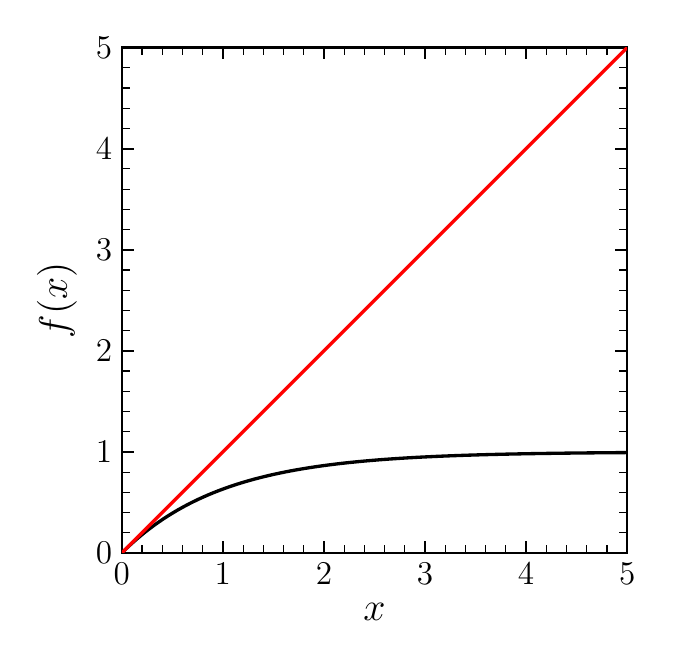
\begin{tikzpicture}
	\begin{axis}[xlabel = $x$,
	ylabel = {$f(x)$},
	samples=100,
	xmin=0, xmax=5,
	ymin=0, ymax=5,
	]
	
	\addplot[color=black, domain=0:5]{(1-exp(-x)};
	\addplot[color=red, domain=0:5]{x};
	
	\end{axis}
	\end{tikzpicture}
	\caption{The variance function $Var[X(t)]$ for \textcolor{red}{Brownian motion (red)} and OU process(black) with $a=0.5, \sigma=1$.}
\end{figure}


\begin{lemma}[constant shifted OU process]
	Consider the constant shifted OU process
	$$dX_t = \sigma dB_t - a(X_t - \mu) dt$$
	with $\sigma > 0, a > 0$, and initial condition $X_0 = x_0$.
	\begin{itemize}
		\item It has the solution 
		$$X_t \sim N((x_0-\mu) e^{-at} + \mu, \frac{\sigma^2(1- e^{-2at})}{2a})$$
		and the stationary distribution is given as
		$$X_t \sim N(\mu, \frac{\sigma^2}{2a}).$$
		\item the constnat shifted OU process can be re-written as
		\begin{align*}
		X_t & = Z_t + \mu \\
		dZ_t &= \sigma dB_t - a Z_t dt
		\end{align*} 
	\end{itemize}	
\end{lemma}
\begin{proof}
	(1)	Use $Y_t = (X_t - \mu)e^{at}$. The rest is similar to \autoref{ch:theory-of-stochastic-process:th:OUprocesssolution}.
	(2) Note that $dZ_t = dX_t + d\mu = dX_t$. Therefore
	\begin{align*}
	dZ_t &= \sigma dB_t - a Z_t dt \\
	\implies dX_t &= \sigma dB_t - a (X_t - \mu) dt 
	\end{align*}
	It can also be verified that:
	$$X_t = \mu + Z_t, x_0 = \mu + z_0,  Z_t \sim N(z_0 e^{-at}, \frac{\sigma^2(1- e^{-2at})}{2a})$$
	gives
	$$X_t  \sim N(\mu + (x_0-\mu) e^{-at}, \frac{\sigma^2(1- e^{-2at})}{2a}).$$
\end{proof}


\begin{lemma}[scaling property of OU process]
	Consider the SDE	
	$$dX(t) = \sigma dB(t) - a(X(t) - \mu) dt,$$
	and let $X(t)$ be the solution. Then
	$Y(t) = \lambda X(mt)$	is the solution for
	$$dY(t) = \sqrt{m}\lambda\sigma dB(t) - ma(Y(t) - \lambda\mu) dt.$$
	
	Note that we interpret $m$ as the time scaling factor and $\lambda$ the spatial scaling factor.	
\end{lemma}
\begin{proof}
	Note that $X(mt)$ will satisfy
	$$dX(mt) = \sigma dB(mt) - a(X(mt) - \mu) dmt,$$
	or equivalently
	$$dX(mt) = \sqrt{m}\sigma dB(t) - ma(X(mt) - \mu) dt.$$
	Multiply both sides by $\lambda$, we have
	$$d\lambda X(mt) = \sqrt{m}\lambda \sigma dB(t) - ma(\lambda X(mt) - \lambda \mu) dt.$$
	Plug in $\lambda X(mt) = Y(t)$, we have
	$$dY(t) = \sqrt{m}\lambda\sigma dB(t) - ma(Y(t) - \lambda\mu) dt.$$
\end{proof}

\begin{remark}[applications of scaling property]
	Suppose we have the dynamics of an asset with time unit day and value unit dollar, we can use the scaling property to find out the coefficients associated with time unit year and value unit JPY.
\end{remark}	

\begin{lemma}[Stationary Gaussian process]
	An Ornstein-Uhlenbeck process $(a,\sigma)$ with Gaussian initial distribution $\eta \sim N(0, \sigma^2/2a)$(i.e., stationary distribution) is a strictly/weakly stationary Gaussian process.
\end{lemma}
\begin{proof}
	(1)$$E[X_t] = E[e^{-at}\eta + \sigma \int_0^t e^{-a(t-s)}dW_s] = 0$$
	since $E[\eta] = 0$ and $\int_0^t e^{-a(t-s)}dW_s$ is Ito integral(\autoref{ch:theory-of-stochastic-process:th:Itointegralproperty}).
	(2) Let $s < t$, we have
	\begin{align*}
	cov(X_t,X_s) &= E[X_tX_s] = e^{-a(s+t)}E[\eta^2] + \sigma^2E[\int_0^s e^{-a(t-s)}dW_u\int_0^s e^{-a(t-m)}dW_m]\\
	&=e^{-a(s+t)}\frac{\sigma^2}{2a} + \sigma^2\int_0^t e^{-2a(t-s)}dt\\
	&=e^{-a(s+t)}\frac{\sigma^2}{2a} + \frac{\sigma^2}{2a}(e^{-2as} - 1) \\
	&=e^{-a(s+t)}e^{-2as} \frac{\sigma^2}{2a}= \frac{\sigma^2}{2a}e^{-a(t-s)}
	\end{align*}
	Note that a weakly stationary Gaussian process is strictly Gaussian process(\autoref{ch:theory-of-stochastic-process:weaklystationaryGaussianisstationary}).
\end{proof}

\subsubsection{Time-dependent coefficient OU process}

\begin{definition}[Time-dependent coefficient Ornstein-Uhlenbeck process]\index{Ornstein-Uhlenbeck process}
	A stochastic process with differential form 
	$$dX_t = (\phi(t) - \lambda X_t) dt + \sigma dW_t,$$
	
	where $\psi(t)$ is time dependent coefficient, $a, \sigma,x_0$ are constants, and $W_t$ is Brownian motion.,
	is called time-dependent coefficient Ornstein-Uhlenbeck process with parameter $(a,\sigma)$ and initial distribution $x_0$.
\end{definition}

\begin{lemma}
	Consider a stochastic process with differential form 
	$$dX_t = (\psi(t) - \lambda X_t) dt + \sigma dW_t, X_t = x_0$$
	where $\psi(t)$ is time dependent coefficient, $a, \sigma$ are constants, and $W_t$ is Brownian motion.
	It follows that
	\begin{itemize}
		\item It has the equivalent form 
		\begin{align*}
		X_t &= Y_t + \int_0^t \exp(-a(t-s))\psi(s)ds \\
		dY_t &= -a Y_t dt + \sigma dW_t
		\end{align*}
		\item It has solution
		$$X_t = x_0\exp(-at) + \int_0^t \exp(-a(t-s))\psi(s)ds  + \int_0^t \sigma \exp(-a(t-s)) dW_t.$$
		\item $X_t$ has mean and covariance given by
		$$E[X_t] =x_0\exp(-at) + \int_0^t \exp(-a(t-s))\psi(s)ds $$
		$$Var[X_t] = \frac{\sigma^2(1- e^{-2at})}{2a}$$
		\item $X_t$ has Gaussian distribution at any $t$, we have
		$$X_t\sim N(x_0\exp(-at) + \int_0^t \exp(-a(t-s))\psi(s)ds,\frac{\sigma^2(1- e^{-2at})}{2a})$$
		\item $X_t, t\to\infty$ is generally not a stationary process since its mean depends on $t$.
		
	\end{itemize}
	
\end{lemma}
\begin{proof}
	(1)Note that
	$$\frac{d}{dt}\int_0^t \exp(-a(t-s))\psi(s)ds = -a\int_0^t \exp(-a(t-s)) + \psi(t);$$
	Therefore,
	$$dX_t = dY_t + \frac{d}{dt}\int_0^t \exp(-a(t-s))\psi(s)ds = (\psi(t) - aX_t)dt + \sigma dW_t.$$
	(2)(3)
	Note that $Y_t$ has solution and distribution
	$$Y_t = x_0 e^{-at} + \int_0^t \exp(-a(t-s))\sigma dB_s,$$
	$$Y_t \sim N(x_0 e^{-at}, \frac{\sigma^2(1- e^{-2at})}{2a}).$$
	Then we use relation in (1).
\end{proof}


\begin{lemma}
	Let $\psi(t) = \phi_n, t_n\leq t < t_{n+1}, t_0 = 0$, then
	$$E[X(t_n)] \triangleq \mu(t_n) = x_0\exp(-at_n) + \exp(-at_n)\sum_{k=1}^{n} \frac{\exp(at_k) - \exp(at_{k-1})}{a}\psi_{k-1}, n\geq 1$$	
\end{lemma}


$$\exp(at)\mu_n = x(0) + \sum_{k=1}^{n} \frac{\exp(at_k) - \exp(at_{k-1})}{a}\psi_{k-1}, n\geq 1$$
\begin{align*}
\exp(at)\mu_n &= x(0) + \sum_{k=1}^{n} \frac{\exp(at_k) - \exp(at_{k-1})}{a}\psi_{k-1}, n\geq 1\\
a\exp(at)\mu_n &= a x(0) + \sum_{k=1}^{n} \exp(at_k) - \exp(at_{k-1})\psi_{k-1}\\
a\exp(at)\mu_{n-1} &= a x(0) + \sum_{k=1}^{n-1} \exp(at_k) - \exp(at_{k-1})\psi_{k-1}, \\
\implies \psi_{n-1} &= \lambda \frac{\exp(at_n)\mu_n - \exp(\lambda t_{n-1})\mu_{n-1}}{\exp(at_n) - \exp(at_{n-1})}
\end{align*}

\subsubsection{Integral of OU process}

\begin{lemma}[integral of OU process]
	Consider an OU process given by
	$$dx(t) = -a x(t)dt + \sigma dW(t), x(0) = x_{0}$$
	where $a \sigma$ are constants,$W$ is a Brownian motion.	
	For each $t,T$, the random variable
	$$I(t,T) = \int_t^T x(u) du$$
	conditioned to the $\sigma$ field $\cF_t$ is normally distributed with mean $M(t,T)$ and variance $V(t,T)$, respectively given by
	$$M(t,T) = \frac{1-\exp(-a(T-t))}{a} x(t),$$
	and variance 
	$$V(t,T) = \frac{\sigma^2}{a^2}(T-t + \frac{2}{a}\exp(-a(T-t))-\frac{1}{2a}\exp(-2a(T-t))-\frac{3}{2a} ).$$
\end{lemma}
\begin{proof}
	See the proof of \autoref{ch:theory-of-stochastic-process:th:IntegralOfSumOfTwoOUProcesses}.	
\end{proof}

\begin{lemma}[integral of sum of two OU process]\cite[145]{brigo2007interest}\cite[64]{mcinerney2015stochastic}\label{ch:theory-of-stochastic-process:th:IntegralOfSumOfTwoOUProcesses}
	Consider two OU processes given by
	\begin{align*}
	dx_1(t) &= -a_1 x_1(t)dt + \sigma_1 dW_1(t), x_1(0) = x_{10}\\
	dx_2(t) &= -a_2 x_2(t)dt + \sigma_2 dW_1(t), x_2(0) = x_{20}
	\end{align*} 
	where $a_1,a_2, \sigma_1,\sigma_2$ are constant, $\psi(t)$ is a time-dependent function, and $W_1, W_2$ are correlated Brownian motion such that
	$$dW_1(t)dW_2(t) = \rho dt.$$	
	For each $t,T$, the random variable
	$$I(t,T) = \int_t^T (x_1(u) + x_2(u)) du$$
	conditioned to the $\sigma$ field $\cF_t$ is normally distributed with mean $M(t,T)$ and variance $V(t,T)$, respectively given by
	$$M(t,T) = \frac{1-\exp(-a_1(T-t))}{a_1} x_1(t) + \frac{1-\exp(-a_2(T-t))}{a_2} x_2(t),$$
	and variance 
	\begin{align*}
	V(t,T) &= \frac{\sigma_1^2}{a_1^2}(T-t + \frac{2}{a_1}\exp(-a_1(T-t))-\frac{1}{2a_1}\exp(-2a_1(T-t))-\frac{3}{2a_1} ) \\
	&+ \frac{\sigma_2^2}{a_2^2}(T-t + \frac{2}{a_2}\exp(-a_1(T-t))-\frac{1}{2a_2}\exp(-2a_2(T-t))-\frac{3}{2a_2} ) \\
	&+ \frac{2\rho\sigma_1\sigma_2}{a_1a_2}(T-t +\frac{\exp(-a_1(T-t))-1}{a_1}+\frac{\exp(-a_1(T-t))-1}{a_1}+\frac{\exp(-(a_1+a_2)(T-t))-1}{a_1+a_2}) \\
	\end{align*}
\end{lemma}
\begin{proof}
	(1)Note that given the observation $x_1(t)$ at $t$, we have
	$$x_1(u) = x_1(t)\exp(-a_1(u-t)) + \int_t^u \sigma \exp(-a_1(u-s))dW(s)$$	
	Therefore,
	\begin{align*}
	&\int_t^T x_1(u) du \\
	&=\int_t^T x_1(t)\exp(-a_1(u-t))du + \int_t^T\int_t^u \sigma \exp(-a_1(u-s))dW(s)du\\
	&=x_1(t)\frac{1-\exp(-a_1(T-t))}{a_1} + \int_t^T\int_s^T \sigma \exp(-a_1(u-s))dudW(s)\\
	&=x_1(t)\frac{1-\exp(-a_1(T-t))}{a_1} + \int_t^T\frac{\sigma_1}{a_1}(1-\exp(-a_1(T-s)))dW_1(s)
	\end{align*}
	where we changed the order of integration.
	From this, we note that
	$$E[\int_t^T x_1(u) du] = x_1(t)\frac{1-\exp(-a_1(T-t))}{a_1}.$$
	Similarly, we can get eh expectation for $\int_t^Tx_2(u)du$.
	
	(2) To get the variance, we have
	$$Var[\int_t^T x_1(u)+x_2(u)du] = Var[\int_t^T x_1(u)du] + Var[\int_t^T x_1(u)du] + 2Cov(\int_t^T x_1(u)du,\int_t^T x_1(u)du).$$
	
	For $Var[\int_t^T x_1(u)du]$, we have
	\begin{align*}
	& Var[\int_t^T x_1(u)du \\
	&= E[\int_t^T\frac{\sigma_1}{a_1}(1-\exp(-a_1(T-s)))dW_1(s) \int_t^T\frac{\sigma_1}{a_1}(1-\exp(-a_1(T-s)))dW_1(s)] \\
	&= \frac{\sigma_1^2}{a_1^2}(\int_t^T ds + \int_t^T \exp(-2a_1(T-s))ds- 2\int_t^T \exp(-a_1(T-s))ds) \\
	&=\frac{\sigma_1^2}{a_1^2}(T-t + \frac{2}{a_1}\exp(-a_1(T-t))-\frac{1}{2a_1}\exp(-2a_1(T-t))-\frac{3}{2a_1} ).
	\end{align*}
	We can similarly evaluate $Var[\int_t^T x_2(u)du]$.
	
	For $Cov[\int_t^T x_1(u)du,\int_t^T x_2(u)du]$, we have
	\begin{align*}
	& Cov[\int_t^T x_1(u)du,\int_t^T x_2(u)du] \\
	&= E[\int_t^T\frac{\sigma_1}{a_1}(1-\exp(-a_1(T-s)))dW_1(s) \int_t^T\frac{\sigma_1}{a_1}(1-\exp(-a_1(T-s)))dW_2(s)] \\
	&= \frac{\rho\sigma_1\sigma_2}{a_1a_2}(\int_t^T (1 - \exp(-a_1(T-s) - \exp(-a_1(T-s)) + \exp(-(a_1+a_2)(T-s))))ds  \\
	&=\frac{2\rho\sigma_1\sigma_2}{a_1a_2}(T-t +\frac{\exp(-a_1(T-t))-1}{a_1}+\frac{\exp(-a_2(T-t))-1}{a_2}+\frac{\exp(-(a_1+a_2)(T-t))-1}{a_1+a_2}) .
	\end{align*}
	
\end{proof}


\begin{lemma}[integral of sum of multiple OU process]\cite[145]{brigo2007interest}\cite[64]{mcinerney2015stochastic}\label{ch:theory-of-stochastic-process:th:IntegralOfSumOfMultipleOUProcesses}
	Consider $n$ OU processes given by
	\begin{align*}
	dx_1(t) &= -a_1 x_1(t)dt + \sigma_1 dW_1(t), x_1(0) = x_{10}\\
	dx_2(t) &= -a_2 x_2(t)dt + \sigma_2 dW_1(t), x_2(0) = x_{20} \\
	\cdots & \cdots \\
	dx_n(t) &= -a_n x_2(t)dt + \sigma_n dW_1(t), x_2(0) = x_{n0} \\
	\end{align*} 
	where $a_1,...,a_n, \sigma_1,...,\sigma_n$ are constants, and $W_1, W_2,...,W_n$ are correlated Brownian motions such that
	$$dW_i(t)dW_j(t) = \rho_{ij} dt.$$	
	For each $t,T$, the random variable
	$$I(t,T) = \int_t^T (x_1(u) + x_2(u) + ... + x_n(u)) du$$
	conditioned on the $\sigma$ field $\cF_t$ is normally distributed with mean $M(t,T)$ and variance $V(t,T)$, respectively given by
	$$M(t,T) = \sum_{i=1}^n \frac{1-\exp(-a_i(T-t))}{a_i} x_i(t),$$
	and variance 
	\begin{align*}
	V(t,T) &= \sum_{i=1}^n \frac{\sigma_i^2}{a_i^2}(T-t + \frac{2}{a_i}\exp(-a_i(T-t))-\frac{1}{2a_i}\exp(-2a_i(T-t))-\frac{3}{2a_i} ) \\
	&+ \sum_{1\leq i <j\leq n}\frac{2\rho\sigma_i\sigma_j}{a_ia_j}(T-t +\frac{\exp(-a_i(T-t))-1}{a_i}+\frac{\exp(-a_j(T-t))-1}{a_j}+\frac{\exp(-(a_i+a_j)(T-t))-1}{a_i+a_j}) \\
	\end{align*}
\end{lemma}
\subsection{Exponential  OU process}

\begin{definition}[exponential constant coefficient Ornstein-Uhlenbeck process]\index{Ornstein-Uhlenbeck process}
	A stochastic process with differential form 
	$$d(\ln X_t) = -a \ln X_t dt + \sigma dB_t,X_0 = x_0,$$
	where $a, \sigma,x_0$ are constant parameters and $B_t$ is the Brownian motion,
	is called exponential constant coefficient Ornstein-Uhlenbeck process with parameter $(a,\sigma)$ and initial distribution $x_0$.
	
	It also has the equivalent form
	\begin{align*}
	X_t &= \exp(Y_t) \\
	dY_t &= -a Y_t dt + \sigma dB_t, Y_0 = \ln x_0
	\end{align*}
\end{definition}


\begin{lemma}[exponential OU process solution]\index{Ornstein-Uhlenbeck process}\label{ch:theory-of-stochastic-process:th:ExponentialOUprocesssolution}
	Consider the SDE
	$$d(\ln X_t) = -a \ln X_t dt + \sigma dB_t,X_0 = x_0,$$
	with $\sigma > 0, a > 0$, and initial condition $X_0 = x_0$.
	
	It follows that
	\begin{itemize}
		\item It has the solution 
		$$X_t = \exp(Y_t), Y_t\sim \sim N(\ln(x_0) e^{-at}, \frac{\sigma^2(1- e^{-2at})}{2a}).$$
		and the stationary distribution is given as
		$$X_t = \exp(Y_t), Y_t \sim N(0, \frac{\sigma^2}{2a}).$$
		\item (mean and variance property)
		\begin{align*}
		E[X_t] &= \exp(\mu_Y + \sigma^2_Y/2)\\
		Var[X_t] &= (\exp(\sigma_Y^2)-1)\exp(2\mu_Y + \sigma^2_Y)
		\end{align*}
		where $$\mu_Y = \ln(x_0) e^{-at}, \sigma_Y^2 = \frac{\sigma^2(1- e^{-2at})}{2a}. $$
	\end{itemize}	
\end{lemma}
\begin{proof}
	(1)	
	Let $Y_t = \ln X_t$, then we have
	$$dY_t = -a Y_t dt + \sigma dB_t, Y_0 = \ln x_0.$$
	From \autoref{ch:theory-of-stochastic-process:th:OUprocesssolution}, we know that
	$$Y_t \sim N(Y_0 e^{-at}, \frac{\sigma^2(1- e^{-2at})}{2a}).$$ 	
	(2) Use the property of log normal distribution(\autoref{ch:theory-of-statistics:th:meanVariancelognormalRandomVariable})	
\end{proof}

\begin{remark}[sanity check with Ito rule]
	Note that the SDE 
	$$d(\ln X_t) = -a \ln X_t dt + \sigma dB_t,X_0 = x_0,$$
	will give the SDE for $X_t$ via the equivalent form
	\begin{align*}
	X_t &= f(Y_t) = \exp(Y_t) \\
	dY_t &= -a Y_t dt + \sigma dB_t, Y_0 = \ln x_0.
	\end{align*}
	
	Using Ito rule, we have
	\begin{align*}
	dX_t &= \frac{\Pa f}{\Pa Y_t} dY_t + \frac{1}{2}\frac{\Pa^2 f}{\Pa Y_t^2} dY_tdY_t \\
	&=\exp(Y_t)dY_t + \frac{1}{2}\exp(Y_t) \sigma^2 dt\\
	\implies dX_t/X_t&= dY_t + \frac{1}{2}\sigma^2 dt\\
	dX_t/X_t&= (-a \ln X_t + \frac{1}{2}\sigma^2 )dt + \sigma dB_t\\
	\end{align*}
	
\end{remark}

\begin{lemma}[solving $\psi$ from imposed term structure mean]
	
	$$\psi_{n-1} = \lambda \frac{\exp(\lambda t_n)\ln \mu_n - \exp(\lambda t_{n-1})\ln \mu_{n-1} - \frac{\sigma^2}{4\lambda}(\exp(\lambda t_n) - \exp(-\lambda t_n)-\exp(\lambda t_{n-1})+\exp(-\lambda t_{n-1})}{\exp(\lambda t_n) - \exp(\lambda t_{n-1})}$$
\end{lemma}


\subsection{Parameter estimation for OU process}

\begin{note}
	The OU process
	$$dX_t = k(\theta - X_t)dt + \sigma dW_t,$$
	can be discretized at times $n\Delta t, n = 1,2,...,\infty$ which gives
	$$X_{k+1}-X_k = k\theta \Delta t - kX_k\Delta t + \sigma(W_{k+1}-W_k),$$
	or equivalently, 
	$$X_{k+1} = k\theta \Delta t - (k\Delta t - 1)X_k + \sigma \sqrt{\Delta t}\epsilon_k,$$
	where $\epsilon_k \sim WN(0,1)$.
	
	The discrete-time form can be viewed as an AR(1) process, and least square method can be used to estimate $k, \theta, \sigma$.
	
	
\end{note}

\subsection{Multiple factor extension}

\begin{definition}[two-factor OU process]
	The two-factor OU process is given by the following SDE
	\begin{align*}
	r(t) &= x_1(t) + x_2(t) + \psi(t), r(0) = r_0\\
	dx_1(t) &= -a_1 x_1(t)dt + \sigma_1 dW_1(t), x_1(0) = x_{10}\\
	dx_2(t) &= -a_2 x_2(t)dt + \sigma_2 dW_1(t), x_2(0) = x_{20}
	\end{align*} 
	where $a_1,a_2, \sigma_1,\sigma_2, r_0$ are constant, $\psi(t)$ is a time-dependent function, and $W_1, W_2$ are correlated Brownian motion such that
	$$dW_1(t)dW_2(t) = \rho dt.$$
\end{definition}

\begin{lemma}[basic properties]
	Consider a The two-factor OU process is given by the following SDE
	\begin{align*}
	r(t) &= x_1(t) + x_2(t) + \psi(t), r(0) = r_0\\
	dx_1(t) &= -a_1 x_1(t)dt + \sigma_1 dW_1(t), x_1(0) = x_{10}\\
	dx_2(t) &= -a_2 x_2(t)dt + \sigma_2 dW_1(t), x_2(0) = x_{20}
	\end{align*} 
	where $a_1,a_2, \sigma_1,\sigma_2, r_0$ are constant, $\psi(t)$ is a time-dependent function, and $W_1, W_2$ are correlated Brownian motion such that
	$$dW_1(t)dW_2(t) = \rho dt.$$	
	
	It follows that
	\begin{itemize}
		\item It has solution given by
		\begin{align*}
		r(t) &= x_{10}\exp(-a_1t) + x_{20}\exp(-a_2t) \\
		&+ \sigma_1 \int_0^t \exp(-a_1(t-s)) dW_1(s) + \sigma_2 \int_0^t \exp(-a_2(t-s)) dW_2(s) + \psi(t).
		\end{align*}
		\item 
		$$E[r(t)] = x_{10}\exp(-a_1t) + x_{20}\exp(-a_2t) + \psi(t).$$
		$$Var[r(t)] = \frac{\sigma_1^2}{2a_1}(1-\exp(-2a_1t)) + \frac{\sigma_2^2}{2a_2}(1-\exp(-2a_2t)) + \frac{2\rho \sigma_1\sigma_2}{a_1+a_2}(1-\exp(-(a_1+a_2)t)).$$
		\item 
		$r(t)$ has Gaussian distribution; that is, 
		$$r(t)\sim N(E[r(t)], Var[r(t)]).$$
	\end{itemize}	
\end{lemma}
\begin{proof}
	(1)	From single factor OU process result(\autoref{ch:theory-of-stochastic-process:th:OUprocesssolution}), we know that
	$$x_1(t) = x_{10}\exp(-a_1t) + \sigma_1 \int_0^t \exp(-a_1(t-s)) dW_1(s).$$
	Similarly, we can evaluate $x_2(t)$ and eventually $r(t)$.
	(2)
	The expectation can be easily evaluated based on the fact that Ito integral has zero mean. 
	To evaluate the variance we have
	\begin{align*}
	Var[r(t)] &= Var[\sigma_1 \int_0^t \exp(-a_1(t-s)) dW_1(s)] + Var[ \sigma_2 \int_0^t \exp(-a_2(t-s)) dW_2(s)] \\
	& + 2Cov(\sigma_1 \int_0^t \exp(-a_1(t-s)) dW_1(s), \sigma_2 \int_0^t \exp(-a_2(t-s)) dW_2(s)) \\
	&=\int_0^t \sigma_1^2 \exp(-2a_1(t-s)) ds + \int_0^t \sigma_2^2 \exp(-2a_1(t-s)) ds + \int_0^t \sigma_1\sigma_2\rho \exp(-a_1(t-s))\exp(-a_2(t-s)) ds \\
	&= \frac{\sigma_1^2}{2a_1}(1-\exp(-2a_1t)) + \frac{\sigma_2^2}{2a_2}(1-\exp(-2a_2t)) + \frac{2\rho \sigma_1\sigma_2}{a_1+a_2}(1-\exp(-(a_1+a_2)t))
	\end{align*}
	where we use Ito isometry in the evaluation, for example,
	\begin{align*}
	&E[\sigma_1 \int_0^t \exp(-a_1(t-s)) dW_1(s) \cdot \sigma_2 \int_0^t \exp(-a_2(t-s)) dW_2(s)] \\
	&=E[\sigma_1\sigma_2 \int_0^t\int_0^t \exp(-a_1(t-s))\exp(-a_2(t-u)) dW_1(s)dW_2(u)] \\
	&=E[\sigma_1\sigma_2  \int_0^t\int_0^t \exp(-a_1(t-s))\exp(-a_2(t-u)) \rho dt \delta(u-s) ] \\
	&=E[\sigma_1\sigma_2 \rho \int_0^t \exp(-(a_1+a_2)(t-s)) \rho dt \delta(u-s) ] \\
	&= \frac{\rho \sigma_1\sigma_2}{a_1+a_2}(1-\exp(-(a_1+a_2)t))
	\end{align*}
	
	(3) The random variable $r(t) = x_1(t) + x_2(t)$ is a Gaussian process has been discussed in \autoref{ch:theory-of-stochastic-process:th:linearCombinationOfBrownianMotionGeneratedGaussainProcess}.	
\end{proof}


\section{Brownian bridge}
\subsection{Constructions}
\begin{definition}[standard Brownian bridge]
	A Brownian bridge is a stochastic process $\{X_t,t\in[0,1]\}$ with state space $\R$ that satisfies the following properties:
	\begin{itemize}
		\item $X_0 = 0, X_1 = 0$ almost surely.
		\item $X_t$ is a Gaussian process.
		\item $E[X_t] = 0$.
		\item $Cov(X_s,X_t) = \min(s,t)-st,\forall s,t\in [0,1]$.
		\item $Var[X_s] = s -s^2.$
		\item $X_t$ is almost surely continuous.
	\end{itemize}
\end{definition}

\begin{remark}[calculate covariance using conditional distribution]
	The joint distribution of $(X_t,X_1)$ is a multivariate Gaussian with mean $$\mu=(0,0)^T, \Sigma = \begin{bmatrix}
	t &t\\
	t & 1
	\end{bmatrix}$$ based on the property of standard Brownian motion(\autoref{ch:theory-of-stochastic-process:th:Brownianmotionbasicproperty}). Then $$(X_t|X_1) \sim MN(0,t-t^2)$$
	from \autoref{ch:theory-of-statistics:th:multivariatenormalconditionaldistribution}.
	Similarly, the joint distribution of $(X_s,X_t,X_1)$ is normal, and $(X_s,X_t|X_1) \sim MN(0,\min(s,t)-st)$.	
\end{remark}


\begin{figure}
	\centering
	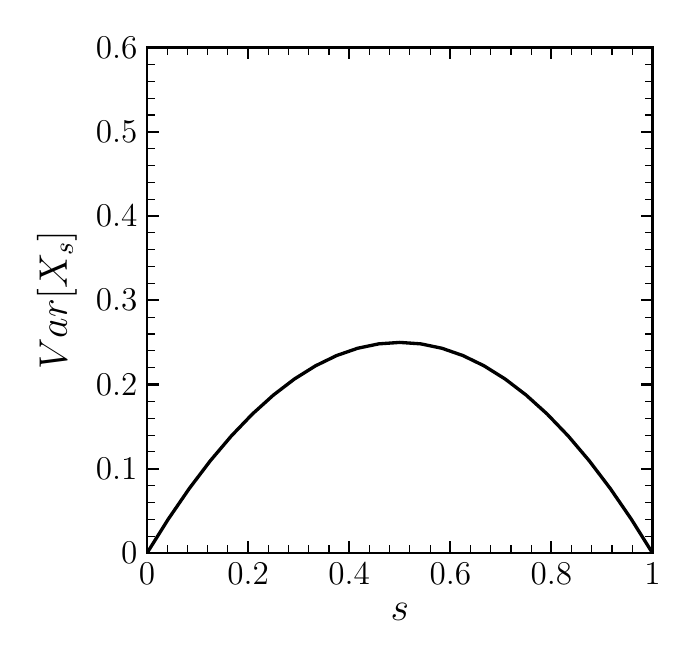
\begin{tikzpicture}
	\begin{axis}[xlabel = $s$,
	ylabel = {$Var[X_s]$},
	xmin=0, xmax=1,
	ymin=0, ymax=0.6,
	]
	
	\addplot[color=black, domain=0:1]{x*(1-x)};
	\end{axis}
	\end{tikzpicture}
	\caption{Variance of $X_t$ in a Brownian bridge}
\end{figure}



\begin{definition}[Brownian bridge, general state space]
	A Brownian bridge is a stochastic process $\{X_t,t\in[0,1]\}$ with state space $\R$ that satisfies the following properties:
	\begin{itemize}
		\item $X_0 = a, X_1 = b$ almost surely.
		\item $X_t$ is a Gaussian process.
		\item $E[X_t] = (1-t)a+tb$.
		\item $Cov(X_s,X_t) = \min(s,t)-st,\forall s,t\in [0,1]$.
		\item $X_t$ is almost surely continuous.
	\end{itemize}
\end{definition}


\begin{definition}[Brownian bridge, general  temporal space]
	A Brownian bridge is a stochastic process $\{X_t,t\in[p,q]\}$ with state space $\R$ that satisfies the following properties:
	\begin{itemize}
		\item $X_p = 0, X_q = 0$ almost surely.
		\item $X_t$ is a Gaussian process.
		\item $E[X_t] = 0$.
		\item $$Cov(X_s,X_t) = \min(s-p,t-p)-\frac{(s-p)(t-p)}{q-p},\forall s,t\in [p,q]$$.
		\item $X_t$ is almost surely continuous.
	\end{itemize}
\end{definition}

\begin{definition}[Brownian bridge, general state space and temporal space]
	A Brownian bridge is a stochastic process $\{X_t,t\in[p,q]\}$ with state space $\R$ that satisfies the following properties:
	\begin{itemize}
		\item $X_p = a, X_q = b$ almost surely.
		\item $X_t$ is a Gaussian process.
		\item $E[X_t] = (1-\frac{t-p}{q-p})a+\frac{t-p}{q-p}b$.
		\item $$Cov(X_s,X_t) = \min(s-p,t-p)-\frac{(s-p)(t-p)}{q-p},\forall s,t\in [p,q]$$.
		\item $X_t$ is almost surely continuous.
	\end{itemize}
\end{definition}



\begin{lemma}[construction of standard Brownian bridge]\hfill
	\begin{itemize}
		\item Suppose $Z_t$ is a standard Brownian motion. Let $X_t = Z_t - tZ_1,t\in [0,1]$.Then $X_t$ is a Brownian bridge process.
		\item Suppose that $\{Z_t,t\in[0,\infty)\}$ is standard Brownian motions. Define $X_1=0$, and
		$$X_t = (1-t)\int_0^t\frac{1}{1-s}dZ_s,t\in [0,1).$$
		Then $X_t$ is a Brownian Bridge. Moreover, the stochastic process has the differential form as
		$$dX_t = dZ_t - \frac{X_t}{1-t}dt.$$ 
		
	\end{itemize}	
\end{lemma}
\begin{proof}
	(1)(a)$X_0 = X_1 = 0$. (b) The random vector $(X_{t_1},X_{t_2},...,X_{t_n})$ can be constructed using affine transformation using random vector $(Z_{t_1},Z_{t_2},...,Z_{t_n},Z_1)$. Therefore, $X_t$ is also a Gaussian process.(\autoref{ch:theory-of-statistics:th:affinetransformmultivariatenormal}). (c) $E[X_t] = 0$. (d) $Cov(Z_s-sZ_1,Z_t-tZ_1) = \min(s,t)-st$.(e) $X_t$ is continuous since $Z_t, tZ_1$ is continuous. 	
	
	(2)	
	(d)Note that $X_t$ is a zero Gaussian process(\autoref{ch:theory-of-stochastic-process:th:wienerintegral},\autoref{ch:theory-of-stochastic-process:th:GaussianprocessSDE}). Then
	$$Cov(X_t,X_s) = (1-t)(1-s)\int_0^s \frac{1}{(1-u)^2}du = s-st.$$
	
	To prove the differential form, we have
	\begin{align*}
	X_t &= (1-t)\int_0^t\frac{1}{1-s}dZ_s \\
	dX_t &= \int_0^t\frac{1}{1-s}dZ_s d(1-t) + (1-t) d(\int_0^t\frac{1}{1-s}dZ_s) \\
	&= -\int_0^t\frac{1}{1-s}dZ_s + (1-t)\frac{1}{1-t}dZ_t \\
	&= - \frac{X_t}{1-t} + dZ_t
	\end{align*}
\end{proof}


\begin{lemma}[construction generalized Brownian bridge]
	Let $W(t)$ be a standard Brownian motion. 
	\begin{itemize}
		\item Fix $ a\in \R, b\in \R$. We can construct the Brownian bridge from $a$ to $b$ on $[0,1]$ to be the process 
		$$Y(t) = a + (b-a)t + X(t),$$
		where $X(t)$ is a standard Brownian bridge from 0 to 0 in time $[0,1]$.
		\item Fix $p, q\in \R$. We can construct the Brownian bridge from $0$ to $0$ on $[p,q]$ to be the process 
		$$Y(t) = X(\frac{t-p}{q-p}),$$
		where $X(t)$ is a standard Brownian bridge from 0 to 0 in time $[0,1]$.
		
		\item Fix $ a,b, p,q\in \R$. We can construct the Brownian bridge from $a$ to $b$ on $[p,q]$ to be the process 
		$$Y(t) = a + (b-a)\frac{t-p}{q-p} + X(\frac{t-p}{q-p}),$$
		where $X(t)$ is a standard Brownian bridge from 0 to 0 in time $[0,1]$.
	\end{itemize}
\end{lemma}
\begin{proof}
	(1) straight forward.(2)
\end{proof}



\subsection{Simulation}
\begin{remark}[simulation of Brownian bridge]
	We can simulate a Brownian bridge by first simulating a Wiener process $W_t$ and then using 
	$$X_t = W_t - tW_1$$
	to construct.\cite[27]{iacus2009simulation}	
\end{remark}
\subsection{Applications}

\begin{remark}[general remarks]
	A Brownian bridge is used when you know the values of a Wiener process at the beginning and end of some time period, and want to understand the probabilistic behavior in between those two time periods.	
\end{remark}

\begin{remark}[Brownian bridge as interpolation method]
	Suppose we have generated a number of points $W(0), W(1), W(2), W(3)$, etc. of a Wiener process path by computer simulation. We can use Brownian bridge simulation will interpolate path between $W(1)$ and $W(2)$.
\end{remark}

\begin{remark}[applications of Brownian bridge in bond]
	In the case of a long-term discount bond with known payoff at final term, we need to simulate values of the asset over a longer period of time such that the stochastic process is conditional on reaching a given final state. For example, take the case of a discount bond such as a 10 year Treasury bond. If we model a discount bond price as a stochastic process, then this process should be tied to the final state of the process.
\end{remark}





\section{Martingale representation theorem}
\begin{theorem}\index{martingale representation theorem}
	\cite[221]{shreve2004stochastic2}Let $W(t)$ be a Brownian motion, and let $\cF(t)$ be the Brownian motion filtration. Let $M(t)$ be a martingale with respect to $\cF(t)$, then there is \textbf{a stochastic process $h(t)$ adapted to $\cF(t)$} such that
	$$M(t) = M(0) + \int_0^t h(u)dW(u)$$
\end{theorem}

\begin{remark}[interpretation]\hfill
	\begin{itemize}
		\item If Brownian motion is the only source of randomness, then a continuous martingale, say $M$, can be expressed as a driftless SDE driven by Brownian motion, i.e., $$dM(t) = h(t,\omega)dB(t)$$
		or
		$$M(t) = M(0) + \int_0^t h(s,\omega)dB(s)$$
		where $h(s,\omega)$ is a random process.
		\item Similarly, if a stochastic process is represented by 
		$$dM(t) = h(t,\omega)dB(t)$$
		then $M(t)$ is a martingale.
	\end{itemize}
\end{remark}


\begin{remark}
	Due to the martingale property of Ito integral, we can show that $E[M(t)] = M(0)$.
\end{remark}

\begin{example}
	If the random process $M$ is known to be a martingale which is a function of $t$ and random process $X$, whose SDE is $dX(t)=\mu(t,X_t)dt + \sigma(t,X_t)dB(t)$
	then by taking derivative using Ito formula $dM(t) = df(t,X_t)$, we can get $$dM(t) = \sigma(t,X_t)\frac{\partial M}{\partial X}dB(t)$$
	and $$h(t,\omega) = \sigma(t,X_t)\frac{\partial M}{\partial X}$$
	where we have setting the drift term to zero.
\end{example}



\section{Change of measure}

\subsubsection{Change of measure concepts for probability space}
\begin{definition}[absolute continuity] \index{absolute continuity}\cite[34]{wu2009interest}
	Let $(\Omega,\cF)$ be a measurable space. Let $P$ and $Q$ be two different probability measures. We say $Q$ is \textbf{absolutely continuous} with respect to $P$ if for any subset $A\in\cF$, 
	$$P(A) = 0 \implies Q(A) = 0,$$
	and it is denoted as $Q\ll P$.
\end{definition}

\begin{definition}[equivalent probability measure]
	\cite[35]{shreve2004stochastic2}Let $(\Omega,\cF)$ be a measurable space. Let $P$ and $\tilde{P}$ be two different probability measures. We say these two probability measure are equivalent if they agree which sets in $\cF$ have probability zero.
	
	In other words, $P$ and $Q$ are equivalently if $P \ll Q$ and $Q \ll P$. 
\end{definition}

\begin{remark}
	Equivalent probability measure means that for $A\in \cF$, if $P(A) > 0$ then $\tilde{P}(A) > 0$; if $P(A) = 0$ then $\tilde{P}(A) = 0$. 
\end{remark}

\begin{theorem}[existence of Radon-Nikodym derivatives]\cite[39]{shreve2004stochastic2}
	Let $P$ and $\tilde{P}$ be two equivalent probability measure. Then there exist an almost surely positive random variable $Z$ such that $E[Z]=1$ and 
	$$\tilde{P}(A)=\int_A Z(\omega)dP(\omega)$$
\end{theorem}




\subsection{Change of measure for random variables}
\begin{theorem}[generating new probability measure and equivalence]\label{ch:theory-of-stochastic-process:th:generateNewProbabilityMeasureAndEquivalence}
	\cite[33]{shreve2004stochastic2}Let $(\Omega,\cF,P)$ be a probability space, let $Z$ be an almost non-negative random variable with $E[Z]=1$, for $A\in \cF$, define
	$$Q(A)=\int_A Z(\omega)dQ(\omega)$$
	then 
	\begin{itemize}
		\item $Q$ is a probability measure.
		\item For any random variable $X$, we have
		$$E_Q[X] = E_P[XZ].$$
		\item If $Z >0$ almost surely, we also have
		$$E_P[Y] = E_Q[\frac{Y}{Z}].$$
		
		\item If $Z > 0$ almost surely, then 
		$P$ and $Q$ are equivalent.
	\end{itemize}
	
	
\end{theorem}
\begin{proof}
	(1)(2)(3) See reference. (4) 
	Suppose $A\in \cF$ and $P(A) = 0$. Then
	$$\tilde{P}(A) = \tilde{E}[\bm{1}_A A] =  \int \bm{1}_A Z(\omega) dP(\omega) = \int_A Z(\omega) dP(\omega) = 0,$$
	since $P(A) = \int_A dP(\omega) = 0, Z(\omega) \geq 0$.
	On the other hand, suppose $B\in \cF, \title{P}(B) = 0$, then
	$$P(B) = E[\frac{\bm{1}_B}{Z}] = 0.$$	
\end{proof}



\begin{remark}\hfill
	\begin{itemize}
		\item For a measurable space, different probability measure can be defined, as long as they satisfy the requirement of probability measure (\autoref{ch:theory-of-probability:def:ProbabilitySpace}). Different probability measures only differ at assigning different values to measurable sets, i.e., elements in $\cF$.
		\item On a measurable space, different random variables can be defined. In nature, random variables are just measurable maps, and are not associated with a particular probability measure. Therefore, when taking the expectation of a random variable, we can specify which probability measure is with respect to.
		\item This theorem provides a way to take expectation with respect to different probability measures.
	\end{itemize}
\end{remark}





\begin{theorem}[change of measure for Gaussian variables]\label{ch:theory-of-stochastic-process:th:changeOfMeasureGaussianRandomVariable}
	Let $X = \mu + \sigma W, W\sim N(0,1)$, and $Z = \exp(\sigma_YY - \frac{1}{2}\sigma_Y^2),Y\sim N(0,1)$. Let $W$ and $Y$ be jointly normal with correlation be $\rho$.
	It follows that
	\begin{itemize}
		\item $E[Z] = 1$.
		\item Under the equivalent measure $Q$ generated by $Z$ and for a  function $g$, we have
		$$E_Q[g(X)] = E[Zg(X)] = E[g(X')],$$
		where $X' \sim N(\mu + \rho \sigma_Y\sigma,\sigma^2)$.
		\item Particularly, if $Y = W$, then under the equivalent measure $Q$ generated by $Z$, $X\sim N(\mu + \sigma_Y,\sigma_Y^2)$.
	\end{itemize}
\end{theorem}
\begin{proof}
	(1) $E[Z] = E[\exp(\sigma_YY - \frac{1}{2}\sigma_Y^2)] = M_Y(\sigma_Y)\exp(-\frac{1}{2}\sigma_Y^2) = 1$,
	where $M_Y(t) = \exp(\frac{1}{2}t^2)$ is the mgf of $Y$.
	(2)
	The measure is equivalent because $Z > 0$ almost surely(\autoref{ch:theory-of-stochastic-process:th:generateNewProbabilityMeasureAndEquivalence}).
	We want to the mgf of $X$ under measure generated from $Z$, we have
	\begin{align*}
	M_X(t) &= E_Q[\exp(tX)] \\
	&= E[Z\exp(tX)] \\
	&=E[\exp(\sigma_YY - \frac{1}{2}\sigma_Y^2) \exp(t\mu + t\sigma W)] \\
	&= E[\exp((\sigma_Y Y + t\sigma W)]\exp( - \frac{1}{2}\sigma_Y^2 + t\mu)\\
	&= M_{Y,W}(\sigma_Y, t\sigma))\exp( - \frac{1}{2}\sigma_Y^2 + t\mu)\\
	&= \exp(\frac{1}{2}(\sigma_Y^2 + 2\rho t\sigma_Y\sigma +t^2\sigma^2))\exp( - \frac{1}{2}\sigma_Y^2 + t\mu)\\
	&=\exp(t(\mu + \rho\sigma\sigma_Y) + \frac{1}{2}t^2\sigma^2)
	\end{align*}
	where $M_{Y,W}(t_1,t_2) = \exp(\frac{1}{2}(t_1^2+2\rho t_1t_2 +t_2^2))$ is the moment generating function for joint Gaussian. From the above, we can see, under the measure generated by $Z$, $X\sim N(\mu + \rho\sigma_Y\sigma,\sigma^2)$.
	(3) Take $\sigma_Y = \sigma, \rho = 1$.
\end{proof}



\begin{lemma}[change of measure for Bivariate Gaussian variables]\label{ch:theory-of-stochastic-process:th:changeOfMeasureBivariateGaussian}
	Let $X\sim N(\mu_X,\sigma_X^2), Y\sim N(\mu_Y,\sigma_Y^2)$ and $(X,Y)$ has correlation coefficient $\rho$. Then for function $g$, we have
	$$E[\exp(X)g(Y)] = E[\exp(X)]E[g(Y')],$$
	where $Y'\sim N(\mu_Y + \rho \sigma_X\sigma_Y,\sigma_Y^2)$
\end{lemma}
\begin{proof}
	Let $X = \mu_X + \sigma_X\rho Z_2 + \sigma_X\sqrt{1-\rho^2}Z_1, Y = \mu_Y + \sigma_YZ_2$, where $Z_1,Z_2$ are independent standard normals. Then
	\begin{align*}
	E[\exp(X)g(Y)] &= E[\exp(\mu_X + \sigma_X\rho Z_2 + \sigma_X\sqrt{1-\rho^2}Z_1)g(\mu_Y + \sigma_YZ_2)] \\
	&=E[\exp(\mu_X + \sigma_X\rho Z_2 + \sigma_X\sqrt{1-\rho^2}Z_1)]E[\exp(\sigma_X\rho Z_2)g(\mu_Y + \sigma_YZ_2)] \\
	&=E[\exp(\mu_X + \sigma_X\sqrt{1-\rho^2}Z_1)]E[\exp(\sigma_X\rho Z_2)g(\mu_Y + \sigma_YZ_2)] \\
	&=\exp(\mu_X + \frac{1}{2}\sigma_X^2(1-\rho^2))]E[\exp(\sigma_X\rho Z_2)g(\mu_Y + \sigma_YZ_2)] \\
	&=\exp(\mu_X + \frac{1}{2}\sigma_X^2)]E[\exp(\sigma_X\rho Z_2 - \frac{1}{2}\sigma_X\rho^2)g(\mu_Y + \sigma_YZ_2)] \\
	&= E[\exp(X)]E[\exp(\sigma_X\rho Z_2 - \frac{1}{2}\sigma_X\rho^2)g(\mu_Y + \sigma_YZ_2)] \\
	&= E[\exp(X)]E[g(Y')], Y'\sim N(\mu_Y+\rho \sigma_X\sigma_Y,\sigma_Y^2) 
	\end{align*}
	where in the last line we use the change of measure for Gaussian random variable(\autoref{ch:theory-of-stochastic-process:th:changeOfMeasureGaussianRandomVariable}).
\end{proof}

\subsection{Change of measure for stochastic process}
\begin{definition}[Radon-Nikodym derivative]
	\cite[37]{shreve2004stochastic2}Let $(\Omega,\cF,P)$ be a probability space, let $\tilde{P}$ be another probability measure on $(\Omega,\cF)$ that is equivalent to $P$, and let $Z$ be an \textbf{almost surely positive} random variable such that $E[Z]=1$ and relates $P$ and $\tilde{P}$ via
	$$\tilde{P}(A)=\int_A Z(\omega)dP(\omega)$$
	then $Z$ is called a Radon-Nikodym derivatives of $\tilde{P}$ with respect to $P$, and we write
	$$Z = \frac{d\tilde{P}}{dP}.$$
\end{definition}

\begin{definition}[Radon-Nikodyn derivative process]\cite[211]{shreve2004stochastic2}
	Let $Z$ be an almost surely positive random variable satisfying $EZ = 1$, then the stochastic process
	$$Z(t) = E[Z|\cF_t]$$
	is called the Radon-Nikodyn derivative process.
\end{definition}

\begin{lemma}
	If $P$ and $Q$ are equivalent measures, and $X_t$ is an $\cF_t$ adapted process, then 
	$$E_Q[X_t] = E_P[\frac{dQ}{dP}X_t].$$
\end{lemma}
\begin{proof}
	$$E_Q[X_t] = \int_{\Omega} X_t dQ = \int_{\Omega} X_t \frac{dQ}{dP} dP.$$
\end{proof}

\begin{remark}
	This is the foundation of importance sampling in Monte Carlo methods (\autoref{ch:stochastic-methods--optimization:sec:importanceSampling}).
\end{remark}


\begin{theorem}[Radon-Nikodyn derivative process applied to change of measure]\cite[212]{shreve2004stochastic2}\label{ch:theory-of-stochastic-process:th:Radon-NikodynDerivativeProcessAppliedToChangeOfMeasure}
	Let $Z$ be an almost surely positive random variable satisfying $EZ = 1$. It follows that
	\begin{itemize}
		\item  The stochastic process defined via conditional expectation, which is the Radon-Nikodyn derivative process, 
		$$Z(t) = E[Z|\cF_t]$$
		is a martingale.
		\item $Z(t)$ is almost surely positive and $E[Z(t)] = 1$.
		\item The probability measure $Q$ generated by $Z$ and the probability measure $Q_t$ generated by $Z(t)$ agree on the $\cF_t$; that is
		$$Q_t(A) = Q(A), \forall A\in \cF_t.$$
		\item If $Y$ is $\cF_t$ measurable random variable, then
		$$E_Q[Y] = E[YZ] = E[YZ(t)],$$
		that is, we can evaluate the expectation under measure $Q$ generated by $Z$ or under measure $Q(t)$ generated by $Z(t)$.
	\end{itemize}
\end{theorem}
\begin{proof}
	(1) Note the conditional expectations are martingales (\autoref{ch:theory-of-stochastic-process:th:conditionalexpectationasMartingale}). Briefly,
	$$E[Z(t)|\cF(s)] = E[E[Z|\cF_t]|\cF_s] = E[Z|\cF_s] = Z(s).$$
	Also, see \autoref{ch:theory-of-stochastic-process:th:conditionalexpectationasMartingale}.
	(2)$E[Z(t)] = E[E[Z|\cF_t]] = E[Z] = 1.$ Because $Z > 0$ almost surely, its partial averaging $$0< E[Z|\cF_t] = \int_{A} Z(\omega)dP(\omega), \forall A\in \cF_t, P(A) > 0.$$
	(3) The new measure $Q_t$ generated by $Z(t)$ and the new measure generated by $Z(T)$ agrees on the sets in $\cF_t$.
	Let $A \in \cF_t \subset \cF_T, t\leq T$,  and use $Z(t) = E[Z(T)|\cF_t]$, we have
	\begin{align*}
	Q_t(A) &= \int_{\Omega} I_A Z(t)dP = E[Z(t)I_A] \\
	&= E[I_A E[Z(T)|\cF_t]] \\
	&= E[E[I_AZ(T)|\cF_t]]\\
	&= E[I_AZ(T)] = \int_{\Omega}I_A Z(T)dP = Q_T(A)
	\end{align*}
	Note that we use the fact that the random variable $I_A$ is $\cF_t$ measurable(i.e. $I_A^{-1}(1) = A \in \cF_t, I_A^{-1}(0) = A^C \in \cF_t$).
	(4)
	$$E_Q[Y] = E[YZ] = E[E[YZ|\cF_t]] = E[YE[Z|\cF_t]] = E[YZ(t)],$$
	where we use the fact that $Y$ is $\cF_t$ measurable and can be taken out of expectation.
\end{proof}

\begin{theorem}[Bayes theorem for conditional expectation, change of measure for conditional expectation]
	\cite[212]{shreve2004stochastic2}\label{ch:theory-of-stochastic-process:th:BayesTheoremForConditionalExpectation}
	Let $Z$ be an almost surely positive random variable satisfying $E[Z] = 1$. Let $Q$ be a new probability measure generated by $Z$. Let $Y$ be a $\cF_t$ measurable random variable, then
	$$E_Q[Y|\cF_s] =E[YZ|\cF_s]  =\frac{E[YZ(t)|\cF_s]}{E[Z(t)|\cF_s]}  = \frac{1}{Z(s)} E[YZ(t)|\cF_s]$$
	where $s\leq t$.
	
	Particularly, if $\cF_0 = \{\emptyset,\Omega\}$, we have
	$$E_Q[Y|\cF_s] =E[YZ|\cF_s] = E[YZ(t)|\cF_s]$$
\end{theorem}
\begin{proof}
	First, $E_Q[Y|\cF_s]$ and $\frac{E[YZ(t)|\cF_s]}{E[Z(t)|\cF_s]}$ are both $\cF_s$ measurable random variables. To show that these two random variables are equal, we need to check for every $A\in \cF_s$, we have
	$$E_Q[Y|\cF_s](A) = \frac{E[YZ(t)|\cF_s]}{E[Z(t)|\cF_s]}(A).$$
	
	We have
	\begin{align*}
	\frac{E[YZ(t)|\cF_s]}{E[Z(t)|\cF_s]}(A)&= E_Q[I_A\frac{E[YZ(t)|\cF_s]}{E[Z(t)|\cF_s]}]\\
	&=E_Q[I_A\frac{E[YZ(t)|\cF_s]}{Z(s)}]\\
	&=E[I_AE[YZ(t)|\cF_s]]\\
	&=E[I_AYZ(t)]\\
	&=E[I_AYZ] ~(*)\\
	&=E_Q[I_AY]\\
	&=E_Q[Y](A) \\
	&=\int_A Y(\omega)dQ(\omega)\\
	&= E_Q[Y|\cF_s](A) 
	\end{align*}
	where in line *, we use \autoref{ch:theory-of-stochastic-process:th:Radon-NikodynDerivativeProcessAppliedToChangeOfMeasure} and the fact that $Y$ is $\cF_t$ measurable.
\end{proof}

\begin{example}\cite[37]{shreve2004stochastic2}
	Let $P$ be a probability measure, let $X$ be a random variable and it has normal distribution under $P$. Let $Y=X+\theta$, where $\theta$ is a positive constant. Under probability measure $P$, $E[Y]=\theta$, $Var[Y]=1$, and therefore $Y$ has a shifted normal distribution. We can introduce a new probability measure $\tilde{P}$, which assign less weight to subsets $X^{-1}(X(\omega)>0)$, such that $Y$ is normal under $\tilde{P}$. 
	
	The probability density function under the $P$ measure is $f(x) = \frac{1}{\sqrt{2\pi}}\exp(-\frac{1}{2}x^2)$. Let $Z(\omega) = \exp(-\theta X(\omega) - \frac{1}{2}\theta^2)$, the probability density function for the new probability measure is $$\tilde{f}(x) = Zf(x) = \exp(-\theta x - \frac{1}{2}\theta^2)\frac{1}{\sqrt{2\pi}}\exp(-\frac{1}{2}x^2) = \exp(-\frac{1}{2}(\theta + x)^2)$$
	Under this new probability density function for $X$, we have
	$$E[X] = \int_{-\infty}^\infty (x+\theta)\tilde{f}(x)dx = \theta$$
	note that $f_Y(y) = \tilde{f}(y-\theta)\frac{dY}{dX}=\tilde{f}(y-\theta)$,
	$E[Y] = \int_{-\infty}^\infty (y)f_Y(y)dy = \int_{-\infty}^\infty y\exp(-\frac{1}{2}(\theta + y - \theta)^2)dy = 0$
\end{example}
\subsection{Change of measure for Brownian motions: Girsanov's theorem}


\begin{theorem}[Girsanov's theorem for 1d Brownian motion]\index{Girsanov's theorem}\label{ch:theory-of-stochastic-process:th:Girsanovtheorem}
	\cite[212]{shreve2004stochastic2} Let $W(t),0\leq t \leq T$, be a Brownian motion on a probability space $(\Omega,\cF,P)$, and let $\cF(t)$ be the Brownian motion filtration. Let $\theta(t)$ be an adapted process. For a \textbf{drifting} stochastic process defined as
	$$\tilde{W}(t) = W(t) + \int_0^t \theta(s)ds,$$
	and a stochastic process given as
	$$Z(t) = \exp(-\int_0^t \theta(s)dW(s) - \frac{1}{2}\int_0^t \theta^2(s)ds),$$
	we can change $\tilde{W}(t)$ to be a driftless Brownian motion under a new equivalent\footnote{The measure is equivalent because $Z > 0$ almost surely(\autoref{ch:theory-of-stochastic-process:th:generateNewProbabilityMeasureAndEquivalence}).} probability measure $Q$ generated by $Z(T)  \triangleq Z$. Specifically, we have
	\begin{itemize}
		\item $Z > 0$ almost surely, $E[Z] = 1$  such that $Z(t) = E[Z|\cF_t]$ is Radon-Nikodyn derivative process and a martingale.
		\item $\tilde{W}(t)Z(t)$ is a martingale under the original probability measure.
		\item  $\tilde{W}$ is a martingale under the new probability measure  $Q$. That is
		$$E_Q[\tilde{W}(t)|\cF_s] = \tilde{W}(s)$$
		
	\end{itemize}
\end{theorem}
\begin{proof}
	(1) $Z(t)$ is an exponential martingale such that $E[Z(t)] = 1$ \autoref{ch:theory-of-stochastic-process:th:exponentialmartingalelemma}.
	We can also show that
	$E[Z(T)|\cF_t] = E[Z(t)\exp(-\int_t^T \theta(s)dW(s) - \frac{1}{2}\int_t^T \theta^2(s)ds)|\cF_t] = Z(t)$.
	(2)
	Let $X(t) = -\int_0^t \theta(s)dW(s) - \frac{1}{2}\int_0^t \theta^2(s)ds$, then $dX(t) = -\theta(t)dW(t) - \frac{1}{2} \theta^2(t)dt$, $Z(t) = e^{X(t)}$, $$dZ(t) = Z(t)dX_t + \frac{1}{2}Z(t)\theta(t)^2 dt = -Z(t)\theta(t)dW(t). $$
	Note that
	$$d\tilde{W}(t)Z(t) = \tilde{W}(t)dZ(t) + Z(t)d\tilde{W}(t) + d\tilde{W}(t) dZ(t)$$
	Then use  $d\tilde{W} = dW(t) + \theta(t)dt$ and $ dZ(t) = -Z(t)\theta(t)dW(t).$
	Note that
	$$d(\tilde{W}(t)Z(t)) = \tilde{W}(t)dZ(t) + Z(t)d\tilde{W}(t) + d\tilde{W}(t) dZ(t)$$
	Then use  $d\tilde{W} = dW(t) + \theta(t)dt$ and $ dZ(t) = -Z(t)\theta(t)dW(t).$
	We have
	$$d(\tilde{W}(t)Z(t)) = (-\tilde{W}(t)\theta(t) + 1)Z(t)dW(t)$$, which indicates that $\tilde{W}(t)Z(t)$ is a martingale.
	(3) 
	Use the properties of change of measure with conditional expectation(\autoref{ch:theory-of-stochastic-process:th:Radon-NikodynDerivativeProcessAppliedToChangeOfMeasure})
	$$E_Q[\tilde{W}(t)|\cF_s] = \frac{1}{Z(s)} E[\tilde{W}(t)Z(t)|\cF_s] = \frac{1}{Z(s)}\tilde{W}(s)Z(s) = \tilde{W}(s),$$
	where we use the fact that $\tilde{W}(t)Z(t)$ is martingale with respect to $\cF_t$.
	
	
	
	(moment generating function method)
	Consider the moment generating function of $\tilde{W}(t)$ under the measure $Q$:
	\begin{align*}
	& ~E_Q[\exp(\lambda\tilde{W}_t)] \\
	& = E[\exp(\lambda \tilde{W}_t)Z] \\
	&=E[E[\exp(\lambda\tilde{W}_t)Z|\cF_t] \\
	&=E[\exp(\lambda\tilde{W}_t)Z(t)] \\
	&=E[\exp(\lambda\tilde{W}_t  -\int_0^t \theta(s)dW(s) - \frac{1}{2}\int_0^t \theta^2(s)ds)]\\
	&=E[\exp(\int_0^t (\lambda-\theta(s))dW(s) +\int_0^t \lambda\theta(s)ds - \frac{1}{2}\int_0^t \theta^2(s)ds)]\\
	&=E[\exp(\int_0^t (\lambda-\theta(s))dW(s) +\int_0^t \lambda\theta(s)ds - \frac{1}{2}\int_0^t (\lambda-\theta(s))^2ds) \\
	&+ \frac{1}{2}\int_0^t (\lambda-\theta(s))^2ds)- \frac{1}{2}\int_0^t \theta^2(s)ds)]\\
	&=E[\exp(\int_0^t (\lambda-\theta(s))dW(s) - \frac{1}{2}\int_0^t (\lambda-\theta(s))^2ds)]\\
	&E[\exp(\int_0^t \lambda\theta(s)ds+ \frac{1}{2}\int_0^t (\lambda-\theta(s))^2ds- \frac{1}{2}\int_0^t \theta^2(s)ds)] \\
	&=E[\exp(\int_0^t \lambda\theta(s)ds+ \frac{1}{2}\int_0^t (\lambda-\theta(s))^2ds- \frac{1}{2}\int_0^t \theta^2(s)ds))] \\
	&=E[\exp(\frac{1}{2}\int_0^t \lambda^2ds)] \\
	&=E[\exp(\frac{1}{2}\lambda^2t)] 
	\end{align*}
	where we use the fact that $E[\exp(\int_0^t (\lambda-\theta(s))dW(s) - \frac{1}{2}\int_0^t (\lambda-\theta(s))^2ds)]$ is a martingale(\autoref{ch:theory-of-stochastic-process:th:exponentialmartingalelemma}). 
	That is, the moment generating function shows that $\tilde{W}(t)$ is a Brownian motion following $N(0,t)$.
\end{proof}



\begin{remark}\hfill
	\begin{itemize}
		\item $\tilde{W}(t)$ can be thought as the SDE given as
		$$d\tilde{W} = \theta(t)dt + dW(t)$$
	\end{itemize}
\end{remark}

\begin{remark}[implications]\hfill
	\begin{itemize}
		\item Via Girsanov's theorem, we can change \textbf{any drifting }Ito SDE to a driftless SDE, i.e., martingale, which has many nice properties. Girsanov's theorem tells us how to construct the new measure $Q$ via Radon-Nikodyn derivative. 
		\item For example, if we make the dynamics of an asset a martingale, then we can relate this current price(the goal) to its future expected payoff with respect to the new probability measure $Q$, which is known from Girsanov's theorem. 
	\end{itemize}
\end{remark}

\begin{note}
	The new measure $Q_t$ generated by $Z(t)$ and the new measure generated by $Z(T)$ agrees on the sets in $\cF_t$. See \autoref{ch:theory-of-stochastic-process:th:Radon-NikodynDerivativeProcessAppliedToChangeOfMeasure}.
	
	Consider an Ito process $X(t)$ driven by the Brownian $W(t)$, then the distribution $X(t)$ under the measure $Q_t$ will be the same as under the measure $Q_T$. Therefore, for a drifting Brownian motion, we only need a final time $Z(T)$ to change the measure.
\end{note}



\begin{corollary}[one Dimension Girsanov theorem with constant drift]
	\cite[155]{wiersema2008brownian}\cite[221]{steele2001stochastic}Given a SDE as:
	$$dX_t = bdt + dW_t$$
	define $$Z_t = \exp(-bW(t) - \frac{1}{2}b^2 t),$$ then the $dX_t$ is a driftless Brownian motion under the new probability measure $Q$ generated by the Radon-Nikodym derivative $Z_T$. More specifically, under $Q$, we have
	\begin{itemize}
		\item $dX_t = d\tilde{W}_t, d\tilde{W}_t = dW_t - bdt$, where $\tilde{W}(t)$ is a Brownian motion under $Q$ at time $[0,T]$.
		\item Given function $f(X_t)$, we can evaluate its expectation under $Q$ via $$E_Q[f(X_t)] = E[f(X_t)Z_T] = E[f(X_t)Z_t].$$
	\end{itemize}
\end{corollary}
\begin{proof}
	(2) Let $\{\cF_t\}$ be the natural filtration associated with $W(t)$. Use the fact that $f(X_t)$ is $\cF_t$ measurable, $Z(t) = E[Z_T|\cF_t]$, and \autoref{ch:theory-of-stochastic-process:th:Radon-NikodynDerivativeProcessAppliedToChangeOfMeasure}. 	
\end{proof}




\subsection{Multi-dimensional Girsanov theorem}
\begin{theorem}\cite[224]{shreve2004stochastic2}\label{ch:theory-of-stochastic-process:th:Girsanovtheoremmultipledimension}\cite[37]{wu2009interest}
	Let $T$ be fixed positive time, let $\theta(t) = (\theta_1(t),...,\theta_d(t))$ be a $d$ dimensional adapted process. Define
	$$Z(t) = \exp(-\int_0^t \theta(u)\cdot dW(u) - \frac{1}{2} \int_0^t \norm{\theta(u)}^2 du)$$
	$$\tilde{W}(t) = W(t) + \int_0^t \theta(u)du.$$
	where $W(t)$ is a d-dimensional uncorrelated Brownian motion such that $dW_tdW_t^T = I_d dt\in \R^{d\times d}$.
	Further assume that 
	$$E[\int_{0}^T \norm{\theta(u)}^2Z^2(u)du] < \infty$$
	Set $Z = Z(T)$. Then $E[Z] = 1$, and under the new equivalent\footnote{The measure is equivalent because $Z > 0$ almost surely(\autoref{ch:theory-of-stochastic-process:th:generateNewProbabilityMeasureAndEquivalence}).} probability measure $Q$ given by
	$$Q(A) = \int_A Z(\omega)dP(\omega), \forall A\in \cF$$
	the process $\tilde{W}(t)$ is a $d$-dimensional Brownian motion.	
\end{theorem}
\begin{proof}
	(moment generating function method)
	Consider the moment generating function of $\tilde{W}(t)$ under the measure $Q$:
	\begin{align*}
	& ~E_Q[\exp(\lambda^T\tilde{W}_t)] \\
	& = E[\exp(\lambda^T \tilde{W}_t)Z] \\
	&=E[E[\exp(\lambda^T\tilde{W}_t)Z|\cF_t] \\
	&=E[\exp(\lambda^T\tilde{W}_t)Z(t)] \\
	&=E[\exp(\lambda^T\tilde{W}_t  -\int_0^t \theta(s)^TdW(s) - \frac{1}{2}\int_0^t \theta^T\theta(s)ds)]\\
	&=E[\exp(\int_0^t (\lambda-\theta(s))^TdW(s) +\int_0^t \lambda^T\theta(s)ds - \frac{1}{2}\int_0^t \theta^T\theta(s)ds)]\\
	&=E[\exp(\int_0^t (\lambda-\theta(s))^TdW(s) +\int_0^t \lambda^T\theta(s)ds - \frac{1}{2}\int_0^t \norm{(\lambda-\theta(s))}^2ds) \\
	&+ \frac{1}{2}\int_0^t \norm{(\lambda-\theta(s))}^2ds)- \frac{1}{2}\int_0^t \theta^T
	\theta(s)ds)]\\
	&=E[\exp(\int_0^t (\lambda-\theta(s))^TdW(s) - \frac{1}{2}\int_0^t \norm{(\lambda-\theta(s))}^2ds)]\\
	&E[\exp(\int_0^t \lambda\theta(s)ds+ \frac{1}{2}\int_0^t \norm{(\lambda-\theta(s))}^2ds- \frac{1}{2}\int_0^t \theta^T\theta(s)ds)] \\
	&=E[\exp(\int_0^t \lambda\theta(s)ds+ \frac{1}{2}\int_0^t \norm{(\lambda-\theta(s))}^2ds- \frac{1}{2}\int_0^t \theta^T\theta(s)ds)] \\
	&=E[\exp(\frac{1}{2}\int_0^t \lambda^T\lambda ds)] \\
	&=E[\exp(\frac{1}{2}\lambda^T\lambda t)] 
	\end{align*}
	where we use the fact that $$E[\exp(\int_0^t (\lambda-\theta(s))^TdW(s) - \frac{1}{2}\int_0^t \norm{(\lambda-\theta(s))}^2ds)]$$ is a martingale(\autoref{ch:theory-of-stochastic-process:th:exponentialmartingalelemma}). 
	That is, the moment generating function shows that $\tilde{W}(t)$ is a Brownian motion following $N(0,I_dt)$.
\end{proof}

\begin{remark}[interpretation]\hfill
	\begin{itemize}
		\item Under the original probability measure $P$, $\hat{W}$ will not a martingale because it contains a drift $\int_0^t \theta(u)du$.
		\item Under the new probability measure $Q$, $\hat{W}$ will be a martingale. And \textbf{the Girsanov theorem provides a method to find such measure}.
	\end{itemize}
\end{remark}




\begin{corollary}[Girsanov theorem for correlated Brownian motion]\label{ch:theory-of-stochastic-process:th:changeOfMeasureCorrelatedBrownianMotion}
	Let $T$ be fixed positive time. Let $W(t)$ is a d-dimensional uncorrelated Brownian motion such that $dW_tdW_t^T = \Sigma dt\in \R^{d\times d}$. Let $\theta(t) = (\theta_1(t),...,\theta_d(t))$ be a $d$ dimensional adapted process. Define
	$$Z(t) = \exp(-\int_0^t \theta(u)\cdot dW(u) - \frac{1}{2} \int_0^t \theta(u)^T \Sigma \theta(u) du).$$
	
	Then under the new equivalent\footnote{The measure is equivalent because $Z > 0$ almost surely(\autoref{ch:theory-of-stochastic-process:th:generateNewProbabilityMeasureAndEquivalence}).}  probability measure $Q$ generated by $Z\triangleq Z(T)$:
	\begin{itemize}
		\item $W(t)\sim MN(-\int_0^t \Sigma(u) \theta(u)du, \int_0^t \Sigma(u) du).$
		\item $W(t)$ becomes a drifting Brownian motion following 
		$$dW(t) = d\tilde{W}(t) - \Sigma \theta(t)dt,$$
		where $\tilde{W}(t)$ is a Brownian motion under $Q$. 
	\end{itemize}	
\end{corollary}
\begin{proof}
	(moment generating function method)
	Consider the moment generating function of $\tilde{W}(t)$ under the measure $Q$:
	\begin{align*}
	& ~E_Q[\exp(\lambda^TW_t)] \\
	& = E[\exp(\lambda^T W_t)Z] \\
	&=E[E[\exp(\lambda^TW_t)Z|\cF_t] \\
	&=E[\exp(\lambda^TW_t)Z(t)] \\
	&=E[\exp(\lambda^TW_t  -\int_0^t \theta(s)^TdW(s) - \frac{1}{2}\int_0^t \theta^T\Sigma\theta(s)ds)]\\
	&=E[\exp(\int_0^t (\lambda-\theta(s))^TdW(s) - \frac{1}{2}\int_0^t \theta^T\Sigma\theta(s)ds)]\\
	&=E[\exp(\int_0^t (\lambda-\theta(s))^TdW(s)  - \frac{1}{2}\int_0^t \norm{(\lambda-\theta(s))}^2ds) \\
	&+ \frac{1}{2}\int_0^t \norm{(\lambda-\theta(s))}^2ds)- \frac{1}{2}\int_0^t \theta^T\Sigma
	\theta(s)ds)]\\
	&=E[\exp(\int_0^t (\lambda-\theta(s))^TdW(s) - \frac{1}{2}\int_0^t \norm{(\lambda-\theta(s))}^2_\Sigma ds)]\\
	&E[\exp(\frac{1}{2}\int_0^t \norm{(\lambda-\theta(s))}^2_\Sigma ds- \frac{1}{2}\int_0^t \theta^T\Sigma\theta(s)ds)] \\
	&=E[\exp( \frac{1}{2}\int_0^t \norm{(\lambda-\theta(s))}^2_\Sigma ds- \frac{1}{2}\int_0^t \theta^T\Sigma\theta(s)ds)] \\
	&=E[\exp(\frac{1}{2}\int_0^t \lambda^T\Sigma\lambda ds) - \int_0^t \lambda^T(\Sigma \theta(s)) ds)]
	\end{align*}
	where we use the fact that $$E[\exp(\int_0^t (\lambda-\theta(s))^TdW(s) - \frac{1}{2}\int_0^t \norm{(\lambda-\theta(s))}^2_\Sigma ds)]$$ is a martingale(\autoref{ch:theory-of-stochastic-process:th:exponentialmartingalelemma}). 
	That is, the moment generating function shows that $W(t)$ is a Brownian motion following $MN(-\int_0^t \Sigma(u) \theta(u)du, \int_0^t \Sigma(u) du)$.
\end{proof}


\begin{remark}[calculate the $\theta$ function given target drift]
	Suppose we want to change a driftless Brownian motion to a Brownian motion with drift $\mu$, then we should choose $\theta = \Sigma^{-1}\mu$.	
\end{remark}


\begin{corollary}[correlation invariance under change of measure]\label{ch:theory-of-stochastic-process:th:CorrelationInvarianceUnderChangeOfMeasure}
	Let $W = (W_1,W_2,...,W_n)^T$ be a correlated Brownian motion ($dW_tdW_t^T = \Sigma dt$) under measure $Q_1$. Let $Q_2$ be an equivalent measure generated by
	$$Z = \exp(-\int_0^T \theta(u)\cdot dW(u) + \frac{1}{2} \int_0^T \theta(u)^T\Sigma \theta(u) du),$$
	where $\theta(t) = (\theta_1,\theta_2,...,\theta_n)^T$, 
	Then under the new measure $Q_2$, we have
	$$dW_tdW_t^T = \Sigma dt.$$
\end{corollary}



\section{Fractional Brownian motion}
\begin{definition}[fractional Brownian motion]\index{fractional Brownian motion}\cite[16]{pavliotis2014stochastic}
	A normalized fractional Brownian motion $W_t^H,t\geq 0$, with Hurst parameter $H\in (0,1)$ is a zero mean Gaussian process with continuous sample paths whose covariance is given by
	$$E[W_t^HW_s^H] = \frac{1}{2}(s^{2H} + t^{2H} - \abs{t-s}^{2H}).$$
\end{definition}

\begin{remark}[interpretation]\hfill
	\begin{itemize}
		\item The Hurst exponent controls the correlations between increments of a fractional Brownian motion as well as the regularity of the paths: they become smoother as $H$ increases.
		\item If $H=0.5$, then the process is in fact a Brownian motion.
		\item If $H > 0.5$, then the increments of the process are positively correlated.
		\item If $H < 0.5$, then the increments of the porcess are negatively correlated.
	\end{itemize}
	
\end{remark}

\begin{lemma}\cite[17]{pavliotis2014stochastic}
	A fractional Brownian motion has the following properties
	\begin{itemize}
		\item When $H = \frac{1}{2}$, then $W_t^{\frac{1}{2}}$ becomes standard Brownian motion.
		\item $W_0^H = 0, EW_t^H = 0, E[(W_t^H)^2] = \abs{t}^{2H},t\geq 0$.
		\item It has the zero mean stationary increments, and $E[(W_t^H - W_s^H)^2] = \abs{t-s}^{2H}$.
	\end{itemize}
\end{lemma}
\begin{proof}
	Straight forward.
\end{proof}

\section{Notes on bibliography}

	
	For treatment on Stratonovich integral, see \cite{mikosch1998elementary}.
	
	
	For treatment on calculating mean and various from SDE, see \cite{calin2012introduction}.
	
	For treatment on the techniques for solving SDE, see \cite{calin2012introduction}\cite{mikosch1998elementary}\cite{wiersema2008brownian}. 
	
	For finance related treatment, see \cite{wiersema2008brownian}.
	
	See \cite{steele2001stochastic} for treatment on Girsanov theory and Feynman-Kac connection.
	
	

	\chapter{Jump-diffusion process}\label{ch:theory-of-stochastic-process}
	\minitoc
	
	\printcontents[chapters]{}{1}{}
	
	
	
	
\section{Poisson process}
\subsection{Basics}
\begin{definition}[Poisson process]\index{Poisson process}
	Let $\lambda > 0$ be fixed. The stochastic process $\{N(t),t\in [0,\infty)\}$ is called a Poisson process with rates $\lambda$ if all the following conditions hold:
	\begin{itemize}
		\item $N(0) = 0$.
		\item $N(t)$ has independent increments.
		\item The number of arrivals in any interval of length $N(t_2)-N(t_1)\sim Poisson(\lambda(t_2-t_1))$.
	\end{itemize}
\end{definition}


\begin{figure}[H]
\centering
\includegraphics[width=0.7\linewidth]{../figures/stochasticProcess/stochasticProcess/poissonProcessTrajectory}
\caption{A typical realized trajectory from the Poisson process with jumps at $T_1,T_2,$ and $T_3$.}
\label{fig:poissonProcessTrajectory}
\end{figure}


\begin{lemma}[basic properties of Poisson process]\label{ch:theory-of-stochastic-process:th:PoissonProcessbasicproperties}
	Let $N(t)$ be a Poisson process with rate $\lambda$, then:
	\begin{itemize}
		\item $N(t) \sim Poission(\lambda t)$, that is
		$$P(N(t) = k) = \frac{e^{\lambda t}(\lambda t)^k}{k!}$$
		\item $N(t_2)-N(t_1) = N(t_2-t_1) \sim Poisson(\lambda(t_2-t_1))$
		\item $$E[N(t)] = \lambda t, Var[N(t)] = \lambda t, M_{N(t)}(s) = \exp(\lambda t(e^s-1))$$
		\item Jump probability within $[t,t+\Delta t]$: let $\Delta N = N(t+\Delta t) - N(t)$, we have
		$$Pr(\Delta N = n) = \frac{(\lambda\Delta t)^n}{n!} \exp(-\lambda \Delta t) = \frac{(\lambda\Delta t)^n}{n!}(1 - \lambda\Delta t + \frac{(\lambda \Delta t)^2}{2} + \cdots),$$
		or explicitly
		$$Pr(\Delta N = n) = \begin{cases*}
		1 - \lambda\Delta t + O((\Delta t)^2, n = 0\\
		\lambda\Delta t + O((\Delta t)^2, n = 1\\
		O((\Delta t)^2, n\geq 2
		\end{cases*}.$$
	\end{itemize}
\end{lemma}
\begin{proof}
	Directly from definition and the sum property of independent Poisson distribution(\autoref{ch:theory-of-statistics:th:sumofPoisson})and basic property of Poisson distribution(\autoref{ch:theory-of-statistics:th:PoissonBasicproperty}).
\end{proof}

\begin{lemma}[additivity of Poisson process]
	Let $N_1(t)$ and $N_2(t)$ be independent Poisson processes with rate $\lambda_1$ and $\lambda_2$, then
	$N(t) = N_1(t) + N_2(t)$ is a Poisson process with rate $\lambda_1 + \lambda_2$.
\end{lemma}
\begin{proof}
	Use the moment generating function for $N_1(t)$ and $N_2(t)$.(\autoref{ch:theory-of-statistics:th:sumofPoisson}).
\end{proof}

\subsection{Arrival and Inter-arrival Times}
\begin{lemma}[waiting time distribution]
	Let $N(t)$ be a Poisson process with rate $\lambda$. Let $X_1$ be the time of the first arrival. Then 
	$$P(X_1 > t) = \exp(-\lambda t), f_{X_1}(t) = \lambda \exp(-\lambda t)$$
	Similarly, let $X_n$ be the waiting time between the arrival of $n$ after the $n-1$ arrival, then
	$$P(X_n > t) = \exp(-\lambda t)$$
\end{lemma}
\begin{proof}
	(1)From the definition of Poisson process, the $N(t)-N(0) \sim Poisson(\lambda t)$. Then
	$$P(X_1 > t) = P(N(t)-N(0) = 0 ) = (\lambda t)^0 e^{-\lambda t}/0! = e^{-\lambda t}$$
	(2) Using the independent increment property of Poisson process.
\end{proof}

\begin{remark}
	Note that the waiting time distribution is an exponential distribution with parameter $\lambda$, whose mean is $1/\lambda$.
\end{remark}


\begin{lemma}[Arrival times for Poisson processes]\label{ch:theory-of-stochastic-process:th:arrivaltimepoissonprocess}
	If $N(t)$ is a Poisson process with rate $\lambda$, then the arrival time $T_1,T_2,...$ have $T_n\sim Gamma(n,\lambda)$ distribution:
	$$f_{T_n}(t) = \frac{\lambda^nt^{n-1}e^{-\lambda t}}{(n-1)!}$$
	Moreover, we have $E[T_n] = n/\lambda, Var[T_n] = n/\lambda^2$.
\end{lemma}
\begin{proof}
	Let random variables $X_1,X_2,...$ be the interarrival time, then
	\begin{align*}
	T_1 &= X_1 \\
	T_2 & = X_1 +X_2\\
	T_2 & = X_1 +X_2 + X_3\\
	\dots & \dots
	\end{align*}
	Since $X_i$ has exponential distribution(which is $Gamma(1,\lambda)$), the $T_n$ will be $Gamma(n,\lambda)$ distribution(which can be showed that the $n$th power of mgf of exponential function equal to the mgf of Gamma distribution.) Also see property of Gamma distribution(\autoref{ch:theory-of-statistics:th:sumofGamma}.) 
\end{proof}




\begin{mdframed}
	\begin{remark}[Simulating a Poisson process]
		We first generate iid random variables $X_1,X_2,X_3,...$, where $X_i\sim Exp(\lambda)$. Then the arrival times are given as
		\begin{align*}
		T_1 &= X_1 \\
		T_2 & = X_1 +X_2\\
		T_2 & = X_1 +X_2 + X_3\\
		\dots & \dots
		\end{align*}	
	\end{remark}
\end{mdframed}

\begin{lemma}\cite[468]{shreve2004stochastic2}
	Let $N(t)$ be a Poisson process with intensity $\lambda$. We define the \textbf{compensated Poisson process} as $$M(t) = N(t) - \lambda t.$$
	Then $M(t)$ is a martingale.
\end{lemma}
\begin{proof}
	\begin{align*}
	E[M(t)|\cF_s] &= E[M(t)-M(s)|\cF_s] + E[M(s)|\cF_s]\\
	&= E[N(t) - N(s) -\lambda(t-s)|\cF_s] + M(s)\\
	&= E[N(t) - N(s)] -\lambda(t-s) + M(s) \\
	&= M(s).
	\end{align*}
\end{proof}


\subsection{Compound Poisson process}
\begin{definition}[compound Poisson process]\index{compound Poisson process}
	A compound Poisson process, parameterized by a rate $\lambda > 0$ and jump size distribution $G$, is a \textbf{continuous-time} process $\{Y(t),t\geq 0\}$ given by
	$$Y(t) = \sum_{i=1}^{N(t)} D_i,$$
	where $\{N(t),t\geq 0\}$ is a Poisson process with rate $\lambda$, and $\{D_i:i\geq 1\}$ are iid random variables, with distribution $G$, which are also independent of $\{N(t)\}$.
\end{definition}


\begin{figure}[H]
\centering
\includegraphics[width=0.7\linewidth]{../figures/stochasticProcess/stochasticProcess/compensatedPoissonProcessTrajectory}
\caption{A typical realized trajectory from the compensated Poisson process with jumps at $T_1,T_2,$ and $T_3$.}
\label{fig:compensatedPoissonProcessTrajectory}
\end{figure}


\begin{remark}[interpretation]
	The jump arrival time distribution and waiting time distribution between two jump events is the same of simple Poisson process; compound Poisson distribution only differs from simple Poisson process in the jump size. 	
\end{remark}




\begin{remark}[reduction to simple Poisson process]
	If we take $D_i$ to be constant 1, then
	$$Y(t)-Y(s) = N(t) - N(s),$$
	that is, $Y(t)$ is the Poisson process.
\end{remark}

\begin{definition}[simple-scaling compound Poisson process]
	Let $N(t)$ be a simple Poisson process, then $Y(t) = \alpha N(t), \alpha \in \R$ is called a simple-scaling compound Poisson process with parameter $\alpha$. 	
	Or equivalently, 
	$$Y(t) = \sum_{i=1}^{N(t)} \alpha.$$	
\end{definition}
\begin{example}
	
\end{example}

\begin{example}[real-world compound Poission process]
	Assume in the stock exchange, the coming of orders follows a compound Poission distribution with strength $\lambda$. For every order, the amount of buying $Z_i$ is iid random sample from random variable $Z$ such that $E[Z] = \mu, Var[Z] = \sigma^2$. Then, the total amount of buying as a function of time is the compound Poission process. 
\end{example}

\begin{lemma}[jump probability within an interval]
	
\end{lemma}



\begin{definition}[compound Poisson distribution]
	Suppose that 
	$N\sim Poisson(\lambda)$ and $X_1,X_2,...$ are iid random variables independent of $N$. Let $Y|N = \sum_{n=1}^N X_n$, then the compound Poisson distribution is distribution of $Y$, which can be obtained by marginalizing the joint distribution $(Y,N)$ over $N$. 
\end{definition}

\begin{lemma}
	$E_Y[Y] = E_N[E_{Y|N}[Y|N]] = E_N[\sum_{i=1}^N E_X[X_i]] = E_N[NE_X[X]] = E_N[N]E_X[X]$.
	
	$$Var[Y] = E_N[Var[Y|N]] + Var_N[E[Y|N]]$$
\end{lemma}

\begin{lemma}[basic properties of compound Poisson process]\label{ch:theory-of-stochastic-process:th:BasicPropertiesOfCompoundPoissonProcess}
	For a compound Poisson process given as
	$$Y(t) = \sum_{i=1}^{N(t)}D_i.$$
	We have
	\begin{itemize}
		
		\item $$E[Y(t)] = E[E[Y(t)|N(t)]] = E[N(t)E[D]] = E[N(t)]E[D] = \lambda t E[D].$$
		\item $$Var[Y(t)] = \lambda t E[D^2].$$
		In particular, if $E[D] = 0$, $$Var[Y(t)] = \lambda t Var[D].$$	
		\item The moment generating function $$M_Y(s) = \exp(\lambda t(M_D(s)-1)),$$
		where $M_D(s)$ is the moment generating function of random variable $D$.
		\item If $Y$ is a simple-scaling compound Poisson process with parameter $\alpha$, then
		$$M_Y(s) = \exp(\lambda t(e^\alpha s-1)).$$
		\item Jump probability within $[t,t+\Delta t]$: let $\Delta N = N(t+\Delta t) - N(t)$, we have
		$$Pr(\Delta N = n) = \frac{(\lambda\Delta t)^n}{n!} \exp(-\lambda \Delta t) = \frac{(\lambda\Delta t)^n}{n!}(1 - \lambda\Delta t + \frac{(\lambda \Delta t)^2}{2} + \cdots),$$
		or explicitly
		$$Pr(\Delta N = n) = \begin{cases*}
		1 - \lambda\Delta t + O((\Delta t)^2, n = 0\\
		\lambda\Delta t + O((\Delta t)^2, n = 1\\
		O((\Delta t)^2, n\geq 2
		\end{cases*}.$$
	\end{itemize}
\end{lemma}
\begin{proof}
	(1)
	$$E[Y(t)] = E[E[Y(t)|N(t)]] = E[N(t)E[D]] = E[N(t)]E[D] = \lambda t E[D].$$
	(2)
	\begin{align*}
	Var[Y(t)] &= E[Var[Y(t)|N(t)]] + Var[E[Y(t)|N(t)]]\\
	&=E[N(t)Var[D]] + Var[N(t)E[D]]\\
	&=Var[D]E[N(t)] + E[D]^2Var[N(t)]\\
	&=Var[D]\lambda t + E[D]^2\lambda t\\
	&=\lambda t(Var[D] + E[D]^2)\\
	&=\lambda t E[D^2]
	\end{align*}	
	(3)
	\begin{align*}
	E[e^{sY}] &= \sum_{i} e^{si}Pr(Y(t) = i) \\
	&=\sum_{i} e^{si}\sum_{n}Pr(Y(t) = i|N(t) = n)Pr(N(t) = n)\\
	&=\sum_n Pr(N(t) = n)\sum_{i} e^{si}\sum_{n}Pr(Y(t) = i|N(t) = n)\\
	&=\sum_n Pr(N(t) = n)\sum_{i} e^{si}Pr(D_1+D_2+...+D_n = i)\\
	&=\sum_n Pr(N(t) = n)(M_D(s))^n\\
	&=\sum_n Pr(N(t) = n)e^{n\ln(M_D(s))}\\
	&=M_{N(t)}(\ln(M_D(s))) \\
	&=\exp(\lambda t(M_D(s)-1))
	\end{align*}
	where we use the fact (\autoref{ch:theory-of-probability:th:additionandscalingtheoremformgf})that the moment generating of $D_1+D_2+...+D_n$ is $(M_D(s))^n$.
	Further, we can use the fact that the Poisson process has moment generating function(\autoref{ch:theory-of-stochastic-process:th:PoissonProcessbasicproperties}) given as
	$$M_{N(t)}(s) = \exp(\lambda t(e^s-1)).$$
	(4)
	For a simple-scaling Poisson compound process, we know that $$M_D(u) = E[\exp(u\alpha)] = \exp(u\alpha). $$
\end{proof}


\begin{lemma}\cite[470]{shreve2004stochastic2}\label{ch:theory-of-stochastic-process:compensatedPoissonProcessIsAMartingale}
	Let $Q(t)$ be a compound Poisson process and let $0 \leq t_0 < t_1 < \dots < t_n$ be given. The increments
	$$Q(t_1)-Q(t_2),Q(t_2)-Q(t_1),\dots,Q(t_n)-Q(t_{n-1}),$$
	are independent and stationary. In particular, the distribution of $Q(t_j) - Q(t_{j-1})$ is the same as the distribution of $Q(t_j - t_{j-1})$.
\end{lemma}
\begin{proof}
	
\end{proof}







\begin{lemma}[decomposition of compound Poisson process when jump size is discrete random variable]\cite[473]{shreve2004stochastic2}
	Assume the jump size $Y$ is a discrete random variable can take finite set of nonzero numbers given by $y_1,\dots,y_M$, and let $p(y_1),...,p(y_M)$ be the associated probability mass. Let $Y_1,\dots$ be a iid random sample of $Y$. Let $N(t)$ be a Poisson process and define the compound Poisson process
	$$Q(t) = \sum_{i=1}^{N(t)} Y_i.$$
	For $m = 1,\dots,M$ let $N_m$ denote the number of jumps in $Q$ of size $y_m$ up to and including $t$. Then,
	$$N(t) = \sum_{m=1}^M N_m(t), Q(t) = \sum_{m=1}^M y_m N_m(t).$$
	The processes $N_m(t), m=1,\dots,M$ defined this way are independent simple Poisson processes with intensity $\lambda p(y_m)$, and $y_1N_1(t),\dots,y_mN_m(t)$ are independent simple-scaling compound Poisson processes. 
\end{lemma}
\begin{proof}
	Note that the moment generating function for $Y$ is given by
	$$M_Y(u) = \sum_{i=1}^m p(y_i)\exp(uy_i).$$
	And the moment generating function for $Q(t)$ is given by
	$$M_{Q(t)}(u) = \exp(\lambda t (\sum_{i=1}^m p(y_i)\exp(uy_i) -1)).$$
	
	On the other hand, the moment generating function for $y_m N_m(t)$ is
	$$M_m(u) = \exp(\lambda p(y_m) t (\exp(u y_m) - 1)).$$
	
	It is easy to see
	$$M_{Q(t)}(u) = \prod_{i=1}^M M_m(u).$$
\end{proof}


\begin{remark}[interpretation]
	For a compound Poisson process with finite jump size space, we can decompose it into the summation of 'simple' compound Poisson processes, each with constant jump size. 
\end{remark}

\subsection{Compensated Poisson process}

\begin{definition}[compensated Poisson process]\index{compensated Poisson process}\hfill
	\begin{itemize}
		\item Let $N(t)$ be a Poisson process with intensity $\lambda$. The compensated Poisson process is defined by
		$$M(t) = N(t) - \lambda t.$$
		\item 	Let $Q(t)$ be the compound Poisson process. Then the \textbf{compensated compound Poisson process} is defined as $$M_Q = Q(t) - \beta \lambda t,$$
		where $\beta = E[D]$, is a martingale. 
	\end{itemize}	
	
\end{definition}

\begin{lemma}[compensated Poisson process is a martingale]\cite[467]{shreve2004stochastic2}
	Let $N(t)$ be a Poisson process with intensity $\lambda$. The compensated Poisson process $M(t) = N(t) - \lambda t$ is a martingale.
\end{lemma}
\begin{proof}
	Let $0\leq s < t$ be given. 
	\begin{align*}
	E[M(t)|\cF(s)] &= E[M(t)- M(s) + M(s)|\cF(s)] \\
	&= E[M(t)- M(s)|\cF(s)] + M(s)\\
	&= E[N(t)- N(s) + \lambda(t-s)|\cF(s)] + M(s)\\
	& = 0 + M(s) \\
	&=M(s)
	\end{align*}
\end{proof}

\begin{lemma}[compensated compound Poisson process is a martingale]\cite[470]{shreve2004stochastic2}
	Let $Q(t)$ be the compound Poisson process. Then the \textbf{compensated compound Poisson process} $$Q(t) - \beta \lambda t$$
	where $\beta = E[D]$, is a martingale. 
\end{lemma}
\begin{proof}
	
\end{proof}

\section{Jump process}

\begin{definition}[right-continuous pure jump process]\index{pure jump process}\cite[475]{shreve2004stochastic2}
	We assume $J$ does not jump at $t=0$ and has only finitely many jumps on each finite interval, and is constant between jumps.
\end{definition}




\begin{remark}[right-continuous vs. left continuous]\hfill \label{ch:theory-of-stochastic-process:remark:purejumpprocess}
	\begin{itemize}
		\item 	By right-continuous, we mean $J(t) = \lim_{s\to t^+}(s)$(but not $J(t) = \lim_{s\to t^-}(s)$) for all $t\geq 0$. The left-continuous counterpart of $J(t)$, denoted as $J(t-)$ can be constructed/modified from $J(t)$ such that at all jumps $J(t) = \lim_{s\to t^-}(s)$ but not $J(t) = \lim_{s\to t^+}(s)$. 
		\item 	If $J$ has a jump at time $t$, then $J(t)$ is the value of $J$ immediately after the jump, and $J(t-)$ is the value immediately before the jump. 
	\end{itemize}
\end{remark}

\begin{example}\hfill
	\begin{itemize}
		\item A Poisson process and a compound Poisson process are pure jump processes because of the Constancy between jumps.
		\item A compensated Poisson process is not a pure jump process because it is decreasing between jumps.
	\end{itemize}	
\end{example}


\begin{definition}[jump difference operator]
	Given a stochastic process $X(t)$, we define the jump difference operator $\Delta$ as
	$$\Delta X(t)  = X(t) - X(t-).$$
	
	If $X(t)$ is a right-continuous process containing jumps at $t_1,t_2,...,t_N$ with jump size $D_1,D_2,...,D_N$, then
	$$\Delta X(t) = \begin{cases*}
	D_i, t=t_i,i=1,2,...,N\\
	0, otherwise
	\end{cases*}$$	
	
	Note that for a continuous process $R(t)$, $\Delta R(t) = 0.$
\end{definition}



\begin{lemma}
	Let $J(t)$ be a right-continuous pure jump process, let $X$ be a left-continuous process(possibly contains jumps), then
	$$\int_0^t X(s-)dJ(s) = \int_0^t X(s)dJ(s) + \int_0^t \Delta X(s) dJ(s),$$
	where $\Delta X(s) = X(s) - X(s-)$.
	In particular, 
	$$\int_0^t J(s-)dJ(s) = \int_0^t J(s)dJ(s) + \int_0^t \Delta J(s) dJ(s).$$
	
	$$\int_0^t X(s)dJ(s-) = 0.$$
	$$\int_0^t X(s-)dJ(s-) = 0.$$
	
	$$\int_0^t J(s)dX^c = 0, \int_0^t J(s-)dX^c = 0 $$
\end{lemma}
\begin{proof}
	(1)Based on definition, we have
	$$X(s) = \Delta X(s) + X(s-).$$
	$$\int_0^t X(s-)dJ(s) = \sum_{0<s\leq t} (X^c(s-) + J(s-))\Delta J(s) = \sum_{0<s\leq t} X^c(s-)\Delta J(s),$$
	where we use the fact that at any jump time $\tau$, $J(\tau-) = 0$, $\Delta J(\tau) \neq 0$.
	(2)From the definition, 
	$$\int_0^t X(s)dJ(s-) = \sum_{0<s\leq t} X(s)\Delta J(s-) = \sum_{0<s\leq t} X(s)(J(s-) - J(s-)) = 0.$$
	(3) From Riemann integral, to integrate a function with finitely many jumps is equivalent to integrate the continuous portion of the integral. Since the continuous portion of $J$ is zero, therefore $\int_0^t J(s)dX^c = 0$. The same arguments apply to $\int_0^t J(s-)dX^c = 0$.
\end{proof}



\begin{definition}[jump process]\index{jump process}\cite[475]{shreve2004stochastic2}
	A stochastic process $X(t)$ defined as
	$$X(t) = X(0) + I(t) + R(t) + J(t),$$
	is called a \textbf{jump process},
	where $X(0)$ is a nonrandom initial condition, $I(t) = \int_0^t \Gamma(s)dW(s)$ is the Ito integral of an adapted process $\Gamma(s)$ with respect to a Brownian motion $W(t)$. $R(t)$ is a Riemann integral given as
	$R(t) = \int_0^t \theta(s)ds$ for some adapted process $\theta(t)$ with respect to the Brownian motion.
	And $J(t)$  is an adapted, \textbf{right-continuous} pure jump process with $J(0) = 0$.
	The continuous part of $X(t)$ is denoted by $X^c(t)$, given by
	$$X^c(t) = X(0) + I(t) + R(t).$$
\end{definition}


\begin{remark}[understand continuity]
	A jump process $X(t)$ is a right-continuous and adapted. The left-continuous counterpart is defined as
	$$X(t-) = X(0) + I(t)  + R(t) + J(t-).$$
	The jump size of $X$ at time $t$ is denoted as
	$$\Delta X(t) = X(t) - X(t-) = J(t) - J(t-) = \Delta J.$$
	If $X(t)$ is continuous, then $\Delta X(t) = 0$. If $X(t)$ has a jump at $t$, then $\Delta X(t)$ is the size of the jump, which equals $\Delta X(t)= J(t) - J(t-)$. 
	We always assume there is no jump at $t = 0$; therefore $\Delta X(0) = 0.$
\end{remark}

\begin{definition}[stochastic integral respect to jump process]\cite[475]{shreve2004stochastic2}
	Let $X(t)$ be a jump process given by
	$$X(t) = X(0) + I(t) + R(t) + J(t).$$
	Let $\Phi(s)$ be an adapted process. The stochastic integral of $\Phi$ respect to $X$ is defined as
	$$\int_0^t \Phi(s)dX(s) = \int_0^t \Phi(s)\Gamma(s)dW(s) + \int_0^t \Phi(s)\theta(s)ds + \sum_{0< s\leq t} \Phi(s)\Delta J(s).$$
	In differential form, we have
	$$\Phi(t)dX(t) = \Phi(t)dI(t) + \Phi(t)dR(t) + \Phi(t) dJ(t)$$
	where
	$$\Phi(t)dI(t) = \Phi(t)\Gamma(t)dW(t), \Phi(t)dR(t) = \Phi(t)\Theta(t)dt.$$
\end{definition}


\begin{remark}[interpretation]\hfill
	\begin{itemize}
		\item $dJ(t)$ should be interpreted as $dJ(t) = J(t+\Delta t) - J(t)$, which is a random variable. If there is a jump at $\tau\in [t,t+\Delta t]$, then $dJ(t) = J(\tau) - J(\tau-)$; If there is no jumps, then $dJ(t) = 0$; moreover, the probability of one jump increment is given by $\lambda d t$, the probability of no jump is $1- \lambda d t$; more than one jump is zero as $\Delta t\to 0$(See the definition of Poisson process in terms of rate functions \autoref{ch:theory-of-stochastic-process:th:BasicPropertiesOfCompoundPoissonProcess}).
		\item The summation $\sum_{0< s\leq t} \Phi(s)\Delta J(s)$ is equivalent to summation of finite terms since there are only finitely many jumps in the interval $[0,t]$. 
	\end{itemize}
\end{remark}




\begin{lemma}[basic properties stochastic integral with jump process]\hfill
	
	\begin{itemize}
		\item Let $N(t)$ be a simple Poisson process. let $\theta(t)$ be a continuous function. Then
		$$\int_0^t \theta(s) dN(t) = \sum_{0<s\leq t} \theta(s)\Delta N(s),$$
		where $\Delta N(s) = 1$ if there is a jump at time $s$.
		
		
		\item Let $N(t)$ be a simple Poisson process, then we have
		$$\int_0^t \Delta N(s)dN(s) = N(t)$$
		$$\int_0^t \Delta(N(s) + \theta(s))dN(s) = N(t)$$
		where $\theta(t)$ is a continuous nonrandom function.
		\item Let $J(t)$  be a compound Poisson process $J(t) = \sum_{i=1}^{N(t)} D_i$, then
		$$\int_0^t \Delta(J(s) + \theta(s))dJ(s) = G(t),$$
		where $G(t)$ is the new compound Poisson process $G(t) = \sum_{i=1}^{N(t)} D_i^2$.	 
	\end{itemize}
\end{lemma}
\begin{proof}
	(1)Note that $\Delta N(t)$ is a jump  indicator process: it takes value 1 when there is a jump; otherwise 0. Therefore, $\int_0^t \Delta N dN = \sum_{0<s\leq t} \Delta N(s)\Delta N(s) = N(t)$ is counting the total jump up to $t$. In addition, use $\Delta \theta = 0$.
	(2) $$\int_0^t \Delta(J(s) + \theta(s))dJ(s) = \sum_{0<s\leq t} \Delta J(s) \Delta J(s)  = \sum_{i=1}^{N(t)} D_i^2.$$
	
\end{proof}

\begin{example}
	Let $X(t) = N(t) - \lambda t$, where $N(t)$ is a Poisson process with intensity $\lambda$. In this case, we have $I(t) = 0, R(t) = -\lambda t$ and $J(t) = N(t)$. Let $\Phi(s) = N(s)$(i.e., $\Phi(s)$ is 1 if $N$ has a jump at time $s$ and $\Phi(s) = 0$ otherwise). Then
	$$\int_0^t \Phi(s)dN(s) = \sum_{0<s\leq t} \Phi(s)\Delta J = \sum_{0<s\leq t} \Delta N\Delta N = N(t),$$
	where use the fact that $\Delta R = 0.$
	Note that $\Delta N(t)$ is a jump  indicator process: it takes value 1 when there is a jump; otherwise 0. Therefore, $\int_0^t \Delta N dN = \sum_{0<s\leq t} \Delta N(s)\Delta N(s) = N(t)$ is counting the total jump up to $t$.
\end{example}



\begin{theorem}[Martingale property for left-continuous integrand]\cite[477]{shreve2004stochastic2}\label{ch:theory-of-stochastic-process:th:leftcontinuousintegrandMartingale}
	Assume that the jump process $X(t) = X(0) + I(t) + R(t) + J(t)$ is a martingale, the integral $\Phi(s)$ is \textbf{left-continuous} and adapted, and 
	$$E[\int_0^t\Gamma^2(s)\Phi(s)^2 ds < \infty, \forall t \geq 0],$$
	then the stochastic integral $\int_0^t \Phi(s)dX(s)$ is also a martingale. That is
	$$E[\int_0^t \Phi(s)dX(s)|\cF_h] = \int_0^h \Phi(s)dX(s)$$
	$$E[\int_0^t \Phi(s)dX(s)] = \Phi(0)X(0).$$
\end{theorem}



\begin{remark}[generalization of Ito integral property]
	We know that the Ito integral 
	$$I(t) = E[\int_0^t\Phi(s)dW(s)]$$
	is a martingale(\autoref{ch:theory-of-stochastic-process:th:ItointegralasMartingale}). 
\end{remark}



\subsection{Quadratic variations}
\begin{lemma}\cite[481]{shreve2004stochastic2}
	Let  $X(t) = X(0) + I(t) + R(t) + J(t)$ be the jump process, then
	$$dXdX = dIdI + dJdJ = \Gamma^2dt + dJdJ, dJdI = 0$$
	The quadratic variation is given as
	$$\int_0^t dX(s)dX(s) = \int_0^t\Gamma^2ds + \sum_{0<s\leq t} (\Delta J_1(s))^2$$
\end{lemma}
\begin{proof}
	To show $dJdI = 0$, we can partition the interval $[0,t]$ into $n$ intervals, then 
	\begin{align*}
	&\abs{\sum_{j=0}^{n-1} (I(t_{j+1}) - I(t_j))(J(t_{j+1})-J(t_j)} \\
	&\leq \max_{0\leq j\leq n-1} \abs{I(t_{j+1}) - I(t_j)} \cdot \sum_{j=0}^{n-1} \abs{J(t_{j+1}) - J(t_j)}\\
	&\leq \max_{0\leq j\leq n-1} \abs{I(t_{j+1}) - I(t_j)} \cdot \sum_{0<s\leq T}\abs{\Delta J(s)}
	\end{align*}
	Note that as $n \to \infty$, $\max_{0\leq j\leq n-1} \abs{I(t_{j+1}) \to 0}$ due to continuity, but $\sum_{0<s\leq T}\abs{\Delta J(s)}$ remains finite.
\end{proof}


\begin{lemma}\cite[481]{shreve2004stochastic2}
	Let  $X_1(t) = X_1(0) + I_1(t) + R_1(t) + J_1(t)$ and $X_2(t) = X_2(0) + I_2(t) + R_2(t) + J_2(t)$  be the jump processes. We further assume $I_1$ and $I_2$ are driven by different Brownian motions with correlation coefficient $\rho_{12}$. Then
	$$dX_1dX_2 = dI_1dI_2 + dJ_1dJ_2 = \Gamma_1\Gamma_2\rho_{12}dt + dJ_1dJ_2.$$
	The quadratic variation is given as
	$$\int_0^t dX(s)dX(s) = \int_0^t\Gamma_1(s)\Gamma_2(s)\rho_{12}ds + \sum_{0<s\leq t} \Delta J_2(s)\Delta J_1(s)$$
\end{lemma}


\begin{remark}[interpretation]
	Note that $\Delta J_1(s) \Delta J_2(s)$ has value only if the two pure jump process has the same jump time.
	
\end{remark}


\subsection{Ito rule}
\begin{lemma}[1D Ito rule]\cite[484]{shreve2004stochastic2}
	Let $X(t)$ be a jump process and $f(x,t)$ a function for which $\frac{\Pa}{\Pa t}f$, $\frac{\Pa}{\Pa x}f$ and $\frac{\Pa^2}{\Pa x^2}f$ are defined and continuous. Then
	$$df = \frac{\Pa}{\Pa t}f dt + \frac{\Pa}{\Pa x}fdX^c + \frac{1}{2}\frac{\Pa^2}{\Pa x^2}f dX^cdX^c + \Delta f(X(t),t)$$
	where $\Delta f(X(t),t) = f(X(t),t) - f(X(t-),t-)$ and $X^c(t) = X^c(0) + I(t) + R(t)$.
	In the integral form, we have
	\begin{align*}
	f(X(t)) &= f(X(0)) + \int_0^t\frac{\Pa}{\Pa s}f ds +\\
	&\int_0^t\frac{\Pa}{\Pa x}dX^c + \frac{1}{2}\int_0^t \frac{\Pa^2}{\Pa x^2}f dX^cdX^c + \sum_{0<s\leq t} f(X(s),s) - f(X(s-),s-).
	\end{align*}
	
\end{lemma}


\begin{remark}[interpretation]
	If the process $X(t)$ does not contain any jumps, or discontinuities, then $$\sum_{0<s\leq t} f(X(s),s) - f(X(s-),s-) = 0.$$
	As a consequence, the Ito rule reduce to the canonical Ito rule for continuous processes.
\end{remark}

\begin{remark}[differentiation]
	$\frac{\Pa}{\Pa x}f(t,x)$ is equivalent to $\frac{\Pa}{\Pa x^c}f(t,x)$;that is, we only take the differential for the continuous process part. This is because for pure jump process will take constant value except at finitely many values, and such effect has been taken care by the final summation.
\end{remark}


\begin{example}[geometric Poisson process]
	Consider the geometric Poisson process 
	$$S(t)  = S(0)\exp(N(t)\log(\sigma+1) - \lambda \sigma t) = S(0)e^{-\lambda\sigma t}(\sigma+1)^{N(t)},$$
	where $\sigma > -1$. We can show the geometric Poisson process is a martingale.
	Then,
	\begin{align*}
	S(t) &= S(0) + \int_0^t S_t ds + \sum_{0<u\leq t}[S(u) - S(u-)]\\ 
	&= S(0) - \lambda\sigma \int_0^t S(u)du + \sum_{0<u\leq t} \sigma S(u-) \\
	&= S(0) - \lambda\sigma \int_0^t S(u-)du + \int_0^t \sigma S(u-) dN(u) \\
	& = S(0) - \int_0^t S(u-)dM(u), M(u) = N(u) - \lambda\sigma t.
	\end{align*}
	
	
	
	Note that we use the fact that $\Pa_{X^c} S = 0$ and $S(u) - S(u-) = S(0)e^{-\lambda \sigma t} = \sigma S(u-)$, where $S(u-) = S(0)e^{-\lambda \sigma t}$ since $N(t-) = 0$(\autoref{ch:theory-of-stochastic-process:remark:purejumpprocess}).
	
	Then, we can show
	$$E[S(t)] = S(0) + E[\int_0^t S(u-)dM(u)] = S(0)$$
	due to \autoref{ch:theory-of-stochastic-process:th:leftcontinuousintegrandMartingale}.
\end{example}

\begin{lemma}[2D Ito rule]\cite[489]{shreve2004stochastic2}
	Let $X(t)$ be a jump process and $f(x,t)$ a function for which $\frac{\Pa}{\Pa t}f$, $\frac{\Pa}{\Pa x}f$ and $\frac{\Pa^2}{\Pa x^2}f$ are defined and continuous. Then
	$$df = \frac{\Pa}{\Pa t}f dt + \frac{\Pa}{\Pa x}dX^c + \frac{1}{2}\frac{\Pa^2}{\Pa x^2}f dX^cdX^c + \Delta f(X(t),t)$$
	where $\Delta f(X(t),t) = f(X(t),t) - f(X(t-),t-)$ and $X^c(t) = X^c(0) + I(t) + R(t)$.
	In the integral form, we have
	\begin{align*}
	f(t,X_1(t),X_2(t))& = f(0,X_1(0),X_2(0)) + \int_0^t f_t ds + \\ &\int_0^tf_{x_1}dX^c_1 +\int_0^tf_{x_2}dX^c_2 + \frac{1}{2}\int_0^t f_{x_1,x_1} dX^c_1dX^c_1 + \frac{1}{2}\int_0^t f_{x_2,x_2}\\ &dX^c_2dX^c_2+\int_0^t f_{x_1,x_2} dX^c_1dX^c_2 + \\
	&\sum_{0<s\leq t} f(s,X_1(s),X_2(s)) - f(s-,X_1(s-),X_2(s-)).
	\end{align*}
\end{lemma}


\begin{lemma}[Ito product rule]
	\begin{align*}
	X_1(t)X_2(t) &= X_1(0)X_2(0) + \int_0^t X_2(s)dX_1^c + \int_0^t X_1(s)dX_2^c(s) + \int_0^t dX_1^c(s)dX_2^c(s) +\\ 
	&\sum_{0<s\leq t}[X_1(s)X_2(s) - X_1(s-)X_2(s-)]\\
	&=X_1(0)X_2(0) + \int_0^t X_2(s-)dX_1 + \int_0^t X_1(s-)dX_2(s) + \int_0^t dX_1(s)dX_2(s)
	\end{align*}
\end{lemma}





\section{Levy processes}
\begin{definition}[infinitely divisible]
	A random variable $X$ is infinitely divisible if its law $p_x$ is infinitely divisible; that is, $X = Y_1^{(n)}+Y_2^{(n)}+\cdots+Y_n^{(n)}$, where $Y_1^{(n)},...,Y_n^{(n)}$ are iid random variables for each $n\in \cN$. In other words, the characteristic function of $X$ can be written as
	$$\Psi_X(u) = (\Phi_{Y_1^{(n)}}(u))^n.$$
\end{definition}

\begin{remark}
	The superscript $(n)$ does not represent any power exponent; it just means when we choose different $n$ to divide the Levy process, we need to have different $Y$ as building blocks.
\end{remark}

\begin{example}[Gaussian random variable]
	Let $X$ have distribution $N(\mu,\sigma^2)$. Then $X$ has characteristic function 
	$$\Phi_X(u) = \exp(i\mu t - \frac{1}{2}\sigma^2u).$$
	$X$ is infinitely divisible with $Y^{(n)}_j\sim N(\mu/n,\sigma^2/n)$, with 
	$$\Phi_Y(u) = \exp(i\mu t/n - \frac{1}{2}\sigma^2u/n) = \Phi_X(u)^{1/n}.$$ 
\end{example}

\begin{example}[Poisson random variable]
	Let $X$ have distribution $Poisson(\lambda)$. Then $X$ has characteristic function 
	$$\Phi_X(u) = \exp(\lambda (e^{iu} - 1)).$$
	$X$ is infinitely divisible with $Y^{(n)}_j\sim Poisson(\lambda/n$, with 
	$$\Phi_Y(u) = \exp(\lambda (e^{iu} - 1)/n) = \Phi_X(u)^{1/n}.$$ 
\end{example}


\begin{definition}[Levy symbol, characteristic exponent]
	Let $X$ be a random variable, let $\Psi_X(u)$ be its characteristic function, then 
	$$\eta = \ln(\Psi_X(u))$$
	is called the Levy symbol or Characteristic exponent. 
\end{definition}


\begin{definition}[cadlag]\index{cadlag}
	Let $(M,d)$ be a metric space, and let $E\subseteq \R$. A function $f: E\to M$ is called a cadlag function if, for every $t\in E$,
	\begin{itemize}
		\item the left limits $f(t^-) = \lim_{s\to t^-}$ exists;
		\item the right limits $f(t^+) = \lim_{s\to t^+}$ exists and equals $f(t)$.
	\end{itemize}
	That is, $f$ is right-continuous with left limits. 
\end{definition}



\begin{definition}[Levy process]\index{Levy process}
	Let $X_t$ be a stochastic process. Then $X_t$ is a Levy process if the following condition are satisfied:
	\begin{enumerate}
		\item $X_0 = 0$.
		\item $X_t$ has independent increments: $L_t - L_s$ is independent of $\cF_s, 0\leq s < t <\infty$.
		\item $L$ has stationary increments: $P(L_t-L_s \leq x) = P(L_{t-s}\leq x), 0 \leq s < t <\infty.$
		\item $L_t$ is continuous in probability: $\lim_{t\to s} L_t = L_s$; that is
		for all $\epsilon > 0$ and for all $s\geq 0$, 
		$$\lim_{t\to s} P(\abs{X(t) - X(s)} > a) = 0.$$ 
	\end{enumerate}
\end{definition}

\begin{remark}[continuity of sample path]\hfill
	\begin{itemize}
		\item Note that in the Levy processes, the sample path is continuous in probability, while in Wiener process, the sample path is almost surely continuous.
		\item If $X_t$ is a Levy process, then one may show that the sample path is almost surely right continuous with left limits(cadlag). 
	\end{itemize}
\end{remark}


\begin{remark}[Levy process is infinitely divisible]
	From property(2)(3) in the definition, we know that a Levy process $X_t$ is infinitely divisible.
\end{remark}

\begin{lemma}
	If $X_t$ is a Levy process, then $X_t$ is infinitely divisible for each $t\geq 0$. Furthermore,
	$$\Psi_{X(t)}(u) = e^{t\eta(u)}$$
	where $\eta$ is the Levy symbol of $X(1)$, i.e., $\eta = \ln(\Psi_{X(1)}(u)$.
\end{lemma}
\begin{proof}
	From property(2)(3) in the definition, we know that a Levy process $X_t$ is infinitely divisible.
\end{proof}


\begin{definition}[compound Poisson process]\index{compound Poisson process}
	A compound Poisson process, parameterized by a rate $\lambda > 0$ and jump size distribution $G$, is a process $\{Y(t),t\geq 0\}$ given by
	$$Y(t) = \sum_{i=1}^{N(t)} D_i,$$
	where $\{N(t),t\geq 0\}$ is a Poisson process with rate $\lambda$, and $\{D_i:i\geq 1\}$ are iid random variables, with distribution $G$, which are also independent of $\{N(t)\}$.
\end{definition}

\begin{definition}[compound Poisson distribution]
	Suppose that 
	$N\sim Poisson(\lambda)$ and $X_1,X_2,...$ are iid random variables independent of $N$. Let $Y|N = \sum_{n=1}^N X_n$, then the compound Poisson distribution is distribution of $Y$, which can be obtained by marginalizing the joint distribution $(Y,N)$ over $N$. 
\end{definition}

\begin{lemma}
	$E_Y[Y] = E_N[E_{Y|N}[Y|N]] = E_N[\sum_{i=1}^N E_X[X_i]] = E_N[NE_X[X]] = E_N[N]E_X[X]$.
	
	$$Var[Y] = E_N[Var[Y|N]] + Var_N[E[Y|N]]$$
\end{lemma}


\begin{lemma}
	Let $\{Z_n,n\in \cN \}$ be a sequence of iid random variables taking values in $\R^d$ with common law $\mu_Z$ and let $N\sim Poisson(\lambda)$. Let 
	$X = \sum_{i=1}^N Z_i.$ 
	Then, for each $u\in \R^d$, 
	$$\Psi_X(u) = E[e^{iuX}] = \exp(\int_{\R^d} (e^{iu^Ty}-1)\lambda \mu_Z(dy)).$$
\end{lemma}
\begin{proof}
	\begin{align*}
	\Psi_X(u) &= \sum_{n=0}^\infty E[e^{iu^TX}|N=n]P(N=n)\\
	&=\sum_{n=0}^\infty E[e^{iu^TX}|N=n]e^{-\lambda} \frac{\lambda^n}{n!}\\
	&=e^{-\lambda}\sum_{n=0}^\infty \frac{(\lambda\Psi_Z(u))^n}{n!}\\
	&=\exp(\lambda(\Psi_Z(u)-1))
	\end{align*}
	where
	$$\Psi_Z(u) = \int_{\R^d} (e^{iu^Ty}-1) \mu_Z(dy).$$
\end{proof}



\begin{theorem}
	Suppose that $\mu\in \R, \sigma \geq 0$, and $\nu$ is a measure concentrated on $\R/\{0\}$ such that $\int_{\R}\min(1,x^2)\nu(dx) < \infty$. A probability law of a real-valued random variable $L$ has characteristic exponent $\Psi(u) = -\frac{1}{t}\log(E[e^{iuL_t}])$ given by
	$$\Psi(u;t) = \int_{\R} e^{iux}\eta(dx) = e^{-t\Psi(u)},\forall u\in \R$$
	if and only if there exists a triple $(\mu,\sigma,\nu)$ such that
	$$\Psi(u) = i\mu u + \frac{1}{2}\sigma^2 u^2 + \int_R (1-e^{iux} + iux \bm{1}_{\abs{x}<1}) \nu(dx)$$
	for every $u\in\R$.
\end{theorem}

\begin{definition}[Levy measure]
	Levy measure is a measure $\nu$ on $\R^d/\{0\}$ such that
	$$\int\min(\abs{y}^2,1)\nu(dy) < \infty$$
\end{definition}


\begin{remark}[interpretation]\cite{Manuge2015levy}
	The theorem says that there exists a probability space where $L = L^{(1)}+L^{(2)}+L^{(3)}$; $L^{(1)}$ is the standard Brownian motion with drift, $L^{(2)}$ is a compound Poisson process, and $L^{(3)}$ is a square integrable martingale with countable number of jumps of magnitude less than 1(almost surely).
\end{remark}


\begin{example}[Brownian motion]
	Let $B(t)$ be a standard Brownian motion in $\R^d$. Then, $C(t) = bt + \sigma B(t), b\in \R^d, \sigma\in \R^{d\times d}$ is a Levy process with its characteristic function given by 
	$$\Psi_{B(t)}(u) = \exp(t\eta_C(u)),$$
	where $\eta_C(u)$ is Levy symbol of $C(1)$ of the form
	$$\eta_C(u) = ib^T - \frac{1}{2} u^T \sigma^T\sigma u.$$
\end{example}



	\section{Notes on bibliography}
	
	
	For Fokker-Planck equation, see \cite{risken2012fokker}\cite{gardiner2009stochastic}.
	
	\printbibliography
\end{refsection}

\begin{refsection}
	\startcontents[chapters]


\chapter{Fokker-Planck Equation}\label{ch:fokker-planck-equation}	
\printcontents[chapters]{}{1}{}
\section{Fokker-Planck equations}

\subsection{Formulations: one dimension}
\begin{lemma}[one dimensional Fokker-Planck equation]\cite[121]{chirikjian2011stochastic1}\cite[79]{clark2011foreign}\label{ch:theory-of-stochastic-process:th:oneDFokkerPlanckEquation}\label{ch:theory-of-stochastic-process:th:1DFokkerPlanckEquationAssociatedWithItoSDE}
	The Fokker-Planck equation is associated with an Ito SDE
	$$dx = \mu(x,t) dt + \sigma(x,t) dW_t,$$
	where $W_t$ is a Wiener process, is given as
	$$\frac{\Pa p}{\Pa t} = -\frac{\Pa}{\Pa x}(\mu(x)p)  + \frac{1}{2}\frac{\Pa^2}{\Pa x^2}(\sigma(x,t)^2p),$$
	note that $\mu,\sigma$ can have dependence on both $x$ and $t$.
\end{lemma}
\begin{proof}
	Let $f(x)$ be an arbitrary smooth function of $x$, then
	$$\int f(x)p(x,t) dx = \ip{f} \implies \int f(x)\frac{\Pa p}{\Pa t} dx = \ip{\frac{d f}{d t}}.$$
	Note that from Ito rule, we have
	\begin{align*}
	df &= \frac{df}{dx} dx + \frac{1}{2}\frac{d^2f}{dx^2} \sigma^2 dt \\
	df &= \frac{df}{dx} (\mu(x,t) dt + \sigma(x,t) dW_t) + \frac{1}{2}\frac{d^2f}{dx^2} \sigma^2 dt \\
	\implies \ip{df} &= (\frac{df}{dx} \mu(x,t)  + \frac{1}{2}\frac{d^2f}{dx^2} \sigma^2 )dt
	\end{align*}
	Then
	\begin{align*}
	\int f(x)\frac{\Pa p}{\Pa t} dx &= \ip{\frac{d f}{d t}} \\&= \ip{\frac{df}{dx} \mu(x,t)  + \frac{1}{2}\frac{d^2f}{dx^2} \sigma^2}\\
	&=\int (\frac{df}{dx} \mu(x,t)  + \frac{1}{2}\frac{d^2f}{dx^2} \sigma^2) p(x,t)dx
	\end{align*}
	Integrating by parts(twice) and drop out the surface terms($p(x\to\infty) = 0$), we have
	$$\int f(x)\frac{\Pa p}{\Pa t} dx = \int f(x)(-\frac{\Pa \mu p}{\Pa x} + \frac{1}{2}\frac{\Pa^2 \sigma^2 p}{\Pa x^2})dx$$
	Because $f(x)$ is an arbitrary function, we have
	$$\frac{\Pa p}{\Pa t} = -\frac{\Pa \mu p}{\Pa x} + \frac{1}{2}\frac{\Pa^2 \sigma^2 p}{\Pa x^2}$$
	using fundamental lemma of calculus of variations(\autoref{ch:calculus-of-variations:th:fundamentallemmaofcalculusofvariations}).
\end{proof}

\begin{remark}
	Fokker-Planck equation is also known as Kolmogorov forward equation. 	
\end{remark}

\begin{remark}[common boundary conditions]\cite[92]{pavliotis2014stochastic}\hfill
\begin{itemize}
	\item Adsorbing boundary condition. For example at interval $[0,1]$, we have $p(x=0,t|x_0,t_0) = p(x=1,t|x_0,t_0) = 0$.
	\item Reflecting boundary condition. For example at interval $[0,1]$, we have $\Pa_x p(x=0,t|x_0,t_0) = \Pa_x p(x=1,t|x_0,t_0) = 0$, which are interpreted as zero flux at the boundary.
	\item Periodic boundary condition. For example at interval $[0,1]$, we have $ p(x=0,t|x_0,t_0) = p(x=1,t|x_0,t_0)$.
\end{itemize}

	
\end{remark}

\subsubsection{Formulations: multiple dimension}

\begin{lemma}[multi-dimensional Fokker-Planck equation]\cite[121]{chirikjian2011stochastic1}\cite[83]{clark2011foreign}\label{ch:theory-of-stochastic-process:th:multiDFokkerPlanckEquation}
	The Fokker-Planck equation is associated with a $d$ dimensional Ito SDE
	$$dx_i = \mu_i(x,t) dt + \sum_{j=1}^{m}\sigma_{ij}^2(x,t) dW_j(t),i=1,2,...,d$$
	where $W_i(t),i=1,...,d$ is are multiple dimensional independent Wiener process, is given as
	$$\frac{\Pa p}{\Pa t} = -\sum_{i=1}^d \frac{\Pa}{\Pa x_i}(\mu_i(x) p)  + \frac{1}{2}\sum_{i=1}^d\sum_{j=1}^d \frac{\Pa^2}{\Pa x_i\Pa x_j}(\sum_{k=1}^m \sigma_{ik}\sigma_{jk}p).$$
\end{lemma}
\begin{proof}
Let $G_t$ be a function of $x=(x_1,x_2,...,x_d)$ given by $G_t = g(x_1,x_2,...,x_d)$. From Ito rule, we have
\begin{align*}
dG_t &= \sum_{i=1}^{d} \frac{\Pa g}{\Pa x_i} dx_i + \frac{1}{2}\sum_{i=1}^{d}\sum_{j=1}^{d}\frac{\Pa^2 g}{\Pa x_i\Pa x_j} dx_idx_j \\
&=\sum_{i=1}^{d} \frac{\Pa g}{\Pa x_i} (\mu_i(x,t) dt + \sum_{j=1}^{m}\sigma_{ij}^2(x,t) dW_j(t)) + \frac{1}{2}\sum_{i=1}^{d}\sum_{j=1}^{d}\frac{\Pa^2 g}{\Pa x_i\Pa x_j} \sum_{k=1}^m \sigma_{ik}\sigma_{jk} dt \\
&=(\sum_{i=1}^{d} \frac{\Pa g}{\Pa x_i} \mu_i(x,t) + \frac{1}{2}\sum_{i=1}^{d}\sum_{j=1}^{d}\frac{\Pa^2 g}{\Pa x_i\Pa x_j} \sum_{k=1}^m \sigma_{ik}\sigma_{jk})dt + \sum_{i=1}^{d}\frac{\Pa g}{\Pa x_i} \sum_{j=1}^{m}\sigma_{ij}^2(x,t) dW_j(t) .
\end{align*}

Note that
$$\frac{d}{dt} E[G_t] = \frac{d}{dt}\int_{\R^d} p(x,t)g(x)dx = \int_{\R^d} \frac{d}{dt}p(x,t) g(x)dx.(*)$$

From another aspect, we have
\begin{align*}
\frac{d}{dt}E[G_t] &= E[\frac{d}{dt}G_t] \\
&=E[(\sum_{i=1}^{d} \frac{\Pa g}{\Pa x_i} \mu_i(x,t) + \frac{1}{2}\sum_{i=1}^{d}\sum_{j=1}^{d}\frac{\Pa^2 g}{\Pa x_i\Pa x_j} \sum_{k=1}^m \sigma_{ik}\sigma_{jk})] \\
&=\int_{\R^d}p(x,t)(\sum_{i=1}^{d} \frac{\Pa g}{\Pa x_i} \mu_i(x,t) + \frac{1}{2}\sum_{i=1}^{d}\sum_{j=1}^{d}\frac{\Pa^2 g}{\Pa x_i\Pa x_j} \sum_{k=1}^m \sigma_{ik}\sigma_{jk})]dx \\
&=\int_{\R^d}p(x,t)(\sum_{i=1}^{d} \frac{\Pa g}{\Pa x_i} \mu_i(x,t) + \frac{1}{2}\sum_{i=1}^{d}\sum_{j=1}^{d}\frac{\Pa^2 g}{\Pa x_i\Pa x_j} \sum_{k=1}^m \sigma_{ik}\sigma_{jk})]dx \\
&=\int_{\R^d} [-\sum_{i=1}^{d}\frac{\mu_i(x,t)p(x,t)}{dx_i} + \frac{1}{2} \sum_{i=1}^{d}\sum_{j=1}^{d} \frac{\Pa^2}{\Pa x_i\Pa x_j} \sum_{k=1}^m \sigma_{ik}\sigma_{jk} \sigma_{ik}\sigma_{jk} p(x,t) ] g(x)dx \\
\end{align*}

Combine with $(*)$, we have
$$\int_{\R^d}[\frac{d}{dt}p(x,t)-\sum_{i=1}^{d}\frac{\mu_i(x,t)p(x,t)}{dx_i} + \frac{1}{2} \sum_{i=1}^{d}\sum_{j=1}^{d} \frac{\Pa^2}{\Pa x_i\Pa x_j} \sum_{k=1}^m \sigma_{ik}\sigma_{jk} \sigma_{ik}\sigma_{jk} p(x,t) ] g(x)dx $$
holds for any function $g(x)$. Therefore
	$$\frac{\Pa p}{\Pa t} = -\sum_{i=1}^d \frac{\Pa}{\Pa x_i}(\mu_i(x) p)  + \frac{1}{2}\sum_{i=1}^d\sum_{j=1}^d \frac{\Pa^2}{\Pa x_i\Pa x_j}(\sum_{k=1}^m \sigma_{ik}\sigma_{jk}p).$$
\end{proof}




\subsection{Steady state \& detailed balance}
\begin{lemma}[1d steady state solution]
Given a 1d Fokker-Planck 	$$\frac{\Pa p}{\Pa t} = -\frac{\Pa}{\Pa x}(\mu(x)p)  + \frac{1}{2}\frac{\Pa^2}{\Pa x^2}(\sigma(x,t)^2p),$$
the steady state distribution $p^{eq}$ will satisfy 
$$-\frac{\Pa}{\Pa x}(\mu(x)p)  + \frac{1}{2}\frac{\Pa^2}{\Pa x^2}(\sigma(x,t)p) =0.$$
Let $J = up - \frac{1}{2}\frac{\Pa}{\Pa x}(\sigma(x,t)^2p), $ then the steady state solution is satisfying 
$$\frac{\Pa}{\Pa x} J = 0.$$
In particular, 
\begin{itemize}
	\item If domain $D = [a,b]$, and the boundary are reflecting, then
	we have stronger result of $J = 0$.
	\item If domain $D = [a,b]$, and the boundary are periodic, then
we have stronger result of $J = const $, $const$ might not be zero.
\end{itemize}
\end{lemma}
\begin{proof}
On 1D, $\Pa_x J = 0 \implies J = const.$
\end{proof}


\begin{lemma}[2d/3d steady state solution]
Given a 2d/3d Fokker-Planck equation
$$\frac{\Pa p}{\Pa t} = -\sum_{i=1}^d \frac{\Pa}{\Pa x_i}(\mu_i(x) p)  + \frac{1}{2}\sum_{i=1}^d\sum_{j=1}^d \frac{\Pa^2}{\Pa x_i\Pa x_j}(\sum_{k=1}^m \sigma_{ik}\sigma_{jk}p),$$
the steady state solution is given as
$$-\sum_{i=1}^d \frac{\Pa}{\Pa x_i}(\mu_i(x) p)  + \frac{1}{2}\sum_{i=1}^d\sum_{j=1}^d \frac{\Pa^2}{\Pa x_i\Pa x_j}(\sum_{k=1}^m \sigma_{ik}\sigma_{jk}p)$$
Let $Q_i = \sum_{k}\sigma^{-1}_{ik}(2\mu_k - 2\sum_j \frac{\Pa}{\Pa x_j} \sigma_{kj})$
\end{lemma}


\subsection{Averages and adjoint operator}
\begin{lemma}
In the function space of square-integrable functions and the scalar product is defined by 
$$\ip{f,g} = \int_a^b f(x)\bar{g(x)}dx.$$
Consider a linear differential operator $T$ given as
$$Tu = \sum_{k=0}^n a_k(x)\frac{d^k}{dx^k} u.$$
If $f$ or $g$ vanishes for $x\to a, b$, then the adjoint of $T$ is
$$T^\dagger u = \sum_{k=0}^n (-1)^k \frac{d^k}{\conj{a_k(x)}dx^k} u$$
\end{lemma}
\begin{proof}
Use integration-by-parts.
\end{proof}



\begin{example}
The Sturm-Liouville operator is defined as
$$Lu = -(pu')' + qu.$$
It can be showed that $Lu = L^\dagger u, L = L^\dagger.$
\end{example}

\begin{corollary}[adjoint operators]\hfill
	\begin{itemize}
		\item $$Af = b(x)\frac{d}{dx}f(x), A^{\dagger}f=-\frac{d}{dx}b(x)f(x)$$
		that is,$$\int_{-\infty}^{\infty} g(x)b(x)\frac{d}{dx}f(x) dx = -\int_{-\infty}^{\infty} f(x)\frac{d}{dx}b(x)f(x) dx$$
		\item $$Af = D(x)\frac{d^2}{dx^2}f(x), A^{\dagger}f=\frac{d^2}{dx^2}D(x)f(x)$$
		\item $$Af = \frac{d}{dx}D(x)\frac{d}{dx}f(x), A^{\dagger}f=\frac{d}{dx}D(x)\frac{d}{dx}f(x)c$$
	\end{itemize}
\end{corollary}
\begin{proof}
	(1) use integration by parts, note that $\lim_{x\to\infty} f(x) = 0$.(2)(3) use integration by parts, note that $\lim_{x\to\infty} f(x) = 0$, $\lim_{x\to\infty} \frac{d}{dx}f(x) = 0$.
\end{proof}

\begin{corollary}[Adjoint of Fokker-Planck operator]
	Define 
	$$Af = \sum_{i} b_i(x) \frac{\Pa }{\Pa x}f(x) + \frac{1}{2}\sum_{i,j}(\sigma(x)\sigma(x)')_{ij}\frac{\Pa^2 }{\Pa x_i\Pa x_j}f(x)$$
	and its adjoint is
	$$A^{\dagger}f = -\sum_{i}  \frac{\Pa }{\Pa x}b_i(x)f(x) + \frac{1}{2}\sum_{i,j}\frac{\Pa^2 }{\Pa x_i\Pa x_j}(\sigma(x)\sigma(x)')_{ij}f(x)$$
\end{corollary}

\iffalse
\begin{lemma} Given a Fokker-Planck equation on the probability density of $x$, 
	$$\frac{\Pa}{\Pa t} P(x,t) = -LP(x,t)$$
	with
	$$L = \frac{\Pa}{\Pa x}v(x) - \frac{\Pa}{\Pa x} D \frac{\Pa}{\Pa x},$$
	the solution is
	$$P(x,t) = e^{Lt}P(x,0).$$
Define the average of any dynamic property $A(x(t))$ as

	$$\ip{A(x(t))} = \int dx A(x(t))P(x,t) = \int dx A(x)e^{-Lt}P(x,0)$$
	The adjoint operator is
	$$L^{\dagger} = -v(a)\frac{\Pa}{\Pa t} - - \frac{\Pa}{\Pa x} D \frac{\Pa}{\Pa x}$$
	then
	$$\frac{\Pa}{\Pa t} A(x,t) = -L^{\dagger}A(x,t)$$
	with solution $A(x(t)) = e^{-L^{\dagger}t}A(x(0))$.
\end{lemma}
\begin{proof}
	\begin{align*}
	\ip{A(x(t))} &= \int dx A(x)e^{-Lt}P(x,0) = \sum_{n=0}^\infty \frac{(-t)^n}{n!}\int dx A(x(t))L^n P(x,0) \\
	&= \sum_{n=0}^{\infty} \frac{(-t)^n}{n!} \int dx ((L^\dagger)^nA(x(t))) P(x,0) = \int dx e^{-L^\dagger t}A(x(0)) P(x,0) 
	\end{align*}
\end{proof}


\begin{corollary}
	Define 
	$$G(t|x_0,t_0) = \int_{\Omega} dx P(x,t|x_0,t_0)$$
	where $\Omega$ is the survival region, then
	$$\frac{\Pa }{\Pa t}G(t|x,0) = -\cL_{FP}^{\dagger}G(t|x,0)$$
\end{corollary}

\fi

\subsection{Backward equation}
\begin{lemma}
The backward Fokker-Planck equation is given as
$$\frac{\Pa}{\Pa t_1}P(t_2,y_2|t_1,y_1) = - A(y_1,t_1)\frac{\Pa}{\Pa y_1}P(t_2,y_2|t_1,y_1) - \frac{1}{2}B(y_1,t_1)\frac{\Pa^2}{\Pa y_1^2} P(t_2,y_2|t_1,y_1),$$
where $$\int (z-y_1)P(t_1,z|t-\Delta t,y_1)dz = \Delta t A(y_1,t_1-\Delta t)$$ and $$\int (z-y_1)^2P(t_1,z|t-\Delta t,y_1)dz = \Delta t B(y_1,t_1-\Delta t)$$.
\end{lemma}
\begin{proof}
From Chapman-Kolmogorov equation, we have
	$$P(t_2,y_2|t-\Delta t,y_1) = \int P(t_2,y_2|t_1,z)P(t_1,z|t_1-\Delta t,y_1)dz.$$
	
	Using Taylor expansion, we have
	
	$$P(t_2,y_2|t_1,z) = P(t_2,y_2|t_1,y_1)+\frac{\Pa}{\Pa y_1}P(t_2,y_2|t_1,y_1) (z-y_1) +\frac{1}{2}\frac{\Pa^2}{\Pa y_1^2} (z-y_1)^2 + O(\int(z-y_1)^3. $$
	
	Plug in, we have
	\begin{align*}
	P(t_2,y_2|t_1-\Delta t,y_1) &= P(t_2,y_2|t_1,y_1) - \Delta t \frac{\Pa}{\Pa t_1}P(t_2,y_2|t_1,y_1)\\
	&+ \frac{\Pa}{\Pa y_1}P(t_2,y_2|t_1,y_1)\int (z-y_1)P(t_1,z|t-\Delta t,y_1)dz\\
	&+\frac{1}{2}\frac{\Pa^2}{\Pa y_1^2}\int(z-y_1)^2P(t_1,z|t_1-\Delta t,y_1)dz + \\
	&+O(\int(z-y_1)^3P(t_1,z|t-\Delta t,y_1)dz)
	\end{align*}
	
	
	Let $\int (z-y_1)P(t_1,z|t-\Delta t,y_1)dz = \Delta t A(y_1,t_1-\Delta t)$ and $\int (z-y_1)^2P(t_1,z|t-\Delta t,y_1)dz = \Delta t B(y_1,t_1-\Delta t)$, we have
	$$\frac{\Pa}{\Pa t_1}P(t_2,y_2|t_1,y_1) = - A(y_1,t_1)\frac{\Pa}{\Pa y_1}P(t_2,y_2|t_1,y_1) - \frac{1}{2}B(y_1,t_1)\frac{\Pa^2}{\Pa y_1^2} P(t_2,y_2|t_1,y_1)$$ 
\end{proof}

\begin{remark}[interpretation]\hfill
\begin{itemize}
	\item The backward Fokker-Planck equation describes the dependence of $P(y_2,t_2|y_1,t_1)$ on the initial condition $(y_1,t_1)$.
	\item To be well-posed, the backward Fokker-Planck equation needs a final condition rather than an initial condition.	
\end{itemize}
\end{remark}


\begin{lemma}[Backward equation using adjoint operator]
If 
$$\frac{\Pa }{\Pa t} P(x,t|x_0,t_0) = \cL_x P,$$
then
$$\frac{\Pa }{\Pa t_0} P(x,t|x_0,t_0) = \cL_{x_0} P,$$
\end{lemma}
\begin{proof}
From Chapman-Kolmogorov equation, we have
$$P(x_1,t_1|x_0,t_0) = \int P(x_1,t_1|x,t)P(x,t|x_0,t_0)dx,$$
where $t_0 < t < t_1$. Take the derivative with respect to $t$, then
\begin{align*}
\int [\frac{\Pa}{\Pa t}P(x_1,t_2|x,t)]P(x,t|x_0,t_0) + \int P(x_1,t_2|x,t)\frac{\Pa}{\Pa t}P(x,t|x_0,t_0) = 0\\
\int [\frac{\Pa}{\Pa t}P(x_1,t_2|x,t)]P(x,t|x_0,t_0) + \int P(x_1,t_2|x,t)\cL_{x}P(x,t|x_0,t_0) = 0\\
\int [\frac{\Pa}{\Pa t}P(x_1,t_2|x,t) - \cL_{x}^\dagger P(x_1,t_2|x,t)]P(x,t|x_0,t_0) = 0
\end{align*}
where $\cL^\dagger_x$ is the adjoint operator satisfying

$$\int P(x_1,t_1|x,t)\cL_{x}P(x,t|x_0,t_0) dx = \int [\cL_x^\dagger P(x_1,t_1|x,t)]P(x,t|x_0,t_0)dx. $$
Then
$$\frac{\Pa}{\Pa t}P(x_1,t_2|x,t) - \cL_{x}^\dagger P(x_1,t_2|x,t) = 0.$$
\end{proof}




\begin{lemma}[Backward equation on expectation quantity]\label{ch:fokker-planck-equation:th:FokkerPlanckBackwardEquationOnExpectationQuantity}
Let $u(t,x) = E[g(X_T)|X(t) = x]$. Assume $$\int P(t,y|t-h,x)(y-x)dy = b(x,t)h + o(h)$$ and
$$\int P(t,y|t-h,x)(y-x)^2dy = \sigma(x,t)h + o(h),$$
and higher moment vanish as $h\to 0.$ 
 Then $u$ satisfy 
$$\frac{\Pa u}{\Pa t} + b(x)\frac{\Pa u}{\Pa x} + \frac{1}{2}\sigma^2(x)\frac{\Pa^2 f}{\Pa x^2},$$
with final condition $u(T,x) = g(x)$.
\end{lemma}
\begin{proof}
Note that 
$$u(t,x) = E[g(X_T)|X(t) = x] = \int g(X_T)P(T,X_T|t,x) dX_T$$ and
$$u(t-h,x) = \int E[g(X_T)|X(t) = y]P(t,y|t-h,x) dy$$
$$u(t,x) = \int E[g(X_T)|X(t) = x]P(t,y|t-h,x) dy$$

Therefore,
\begin{align*}
\frac{u(t) - u(t-h)}{h} & = \frac{\int P(t,y|t-h,x)(u(t,y) - u(t,x)}{h}\\
&= \frac{1}{h}\int P(t,y|t-h,x)[(y-x)\frac{\Pa u}{\Pa x} +\frac{1}{2} (y-x)^2\frac{\Pa^2 u}{\Pa x^2}]
\end{align*}
\end{proof}

\begin{remark}
Backward equation can also be derived using Feyman Kac theorem by assuming the stochastic process of $X(t)$(see \autoref{ch:fokker-planck-equation:th:FeymanKacBackwardEquation}).
\end{remark}

\begin{lemma}[Backward equation on expectation quantity using adjoint operator]\label{ch:fokker-planck-equation:th:FokkerPlanckBackwardEquationOnExpectationQuantityUsingAdjointOperator}
	Let $u(t,x) = E[g(X_T)|X(t) = x]$. Assume
	$$\frac{\Pa }{\Pa t} P(x,t|x_0,t_0) = \cL_x P(x,t|x_0,t_0).$$
	Then
	$$\frac{\Pa u}{\Pa t} = \cL_x^\dagger u$$
	with final condition $u(T,x) = g(x)$.
\end{lemma}
\begin{proof}
	Note that 
	$$u(t,x) = E[g(X_T)|X(t) = x] = \int g(X_T)P(T,X_T|t,x) dX_T$$ and
	Therefore,
	\begin{align*}
	\frac{\Pa u(t,x)}{\Pa t} & = \int g(X_T) \frac{\Pa}{\Pa t} P(T,X_T|t,x) dX_T \\
	&= \int g(X_T) \cL_x^\dagger P dX_T = \cL_x^\dagger \int g(X_T)  P dX_T = \cL_x^\dagger u(x,t).
	\end{align*}
\end{proof}

\begin{remark}[analog in Markov chain]
For analog in discrete-time Markov chain, see \autoref{ch:markov-chains:th:KolmogorovbackwardequationDiscreteTimeMarkovChain}.
\end{remark}


\subsection{Mean first passage time problem}



\iffalse
\begin{lemma}
	Given a Stratonovich stochastic differential equation 
	$$dx(t) = v(x) dt + \sqrt{2D}dw(t),$$
	its Fokker-Planck equation is given as
	$$\frac{\Pa}{\Pa t}P(x,t|x_0,t_0) = -\frac{\Pa}{\Pa x}(v(x)P(x,t|x_0,t_0) + \frac{\Pa}{\Pa x}D\frac{\Pa}{\Pa x}P(x,t|x_0,t_0) $$
	
	Note that for \textbf{Markovian system}, we also have
	$$\frac{\Pa}{\Pa t} P(x,t|x_0,t_0) = \frac{\Pa}{\Pa t_0} P(x,t|x_0,t_0).$$
\end{lemma}
\begin{proof}
	(2)
	$$\frac{\Pa}{\Pa t} P(x,t|x_0,t_0) = \frac{\Pa}{\Pa t} P(x,t-t_0|x_0,0) = -\frac{\Pa}{\Pa t_0} P(x,t-t_0|x_0,0) = -\frac{\Pa}{\Pa t_0}P(x,t|x_0,t_0).$$	
\end{proof}
\fi



\begin{definition}[survival probability]
	The survival probability up to $t$ in domain $\Omega$ is given as
	$$G(t|x_0,t_0) = \int_{\Omega} dx P(x,t|x_0,t_0).$$
	Or equivalently, 
	$$G(t|x_0,0) = Pr(\tau > t) = \int_t^{\infty} \rho(\tau|x_0,0)$$
	where $\rho(\tau|x_0,0)$ is the probability density for the first passage time $\tau$ starting from $x_0$ at $t = 0$.
\end{definition}

\begin{lemma}[survival probability governing equation]
Assume
$$\frac{\Pa }{\Pa t} P(x,t|x_0,t_0) = -\cL_x P(x,t|x_0,t_0).$$
Then
	$$\frac{\Pa }{\Pa t}G(t|x,0) = -\cL_{x}^{\dagger}G(t|x,0),$$
where $\cL_x^\dagger$ is the adjoint operator of $\cL_x$.
\end{lemma}
\begin{proof}
Use the theorem(\autoref{ch:fokker-planck-equation:th:FokkerPlanckBackwardEquationOnExpectationQuantityUsingAdjointOperator}) and define $g(X_T)$ as the indicator function. 
\end{proof}

\begin{lemma}
Define $T(x)$ be the mean first passage time, we have
$$T(x) = -\int_0^\infty t \Pa_t G(t|x_0=x,t_0=0) dt = \int_0^\infty G(t|x,0)dt.$$
The governing equation for $T(x)$ is
$$\cL^\dagger T = -1$$
with boundary condition $T(\Pa D) = 0$.
\end{lemma}
\begin{proof}
Use integration by parts, we have
$$T(x) =  \int_0^\infty G(t|x,0)dt.$$
Then
\begin{align*}
\cL^\dagger T = \cL^\dagger\int_0^\infty G(t|x,0) = \int_0^\infty \cL^\dagger G(t|x,0) = \int_0^\infty \Pa_t G(t|x,0) dt \\ = G(\infty|x,0) - G(0|x,0) = 0 - 1 = -1.
\end{align*}
\end{proof}

\begin{remark}
	For the mean first passage time calculation using adjoint Fokker-Planck equation, see \cite{liu2016adjoint}.
\end{remark}

\section{Smoluchowski/advection-diffusion equation}
\begin{definition}[Smoluchowski/advection-diffusion equation]\index{advection-diffusion equation}\index{Smoluchowski equation}
	The advection-diffusion for density $p(x,t), x\in \R^N$ is given as $$\frac{\Pa p}{\Pa t} = -\nabla \cdot (vp) + \nabla\cdot D\nabla p$$
	where $v\in \mathbb{R}^N,D\in \mathbb{R}^{N\times N}$. Note that we can interpret the flux vector as $j = vp-D\nabla p$.
\end{definition}

\begin{remark}[Relation to computational fluid mechanics]
	We can use the PDE to describe the solute transport in the flowing solutions. The $v$ is the velocity field of the solution, which is further determined by the Navier-Stokes equation. When the velocity field describes an incompressible flow, i.e. $\nabla \cdot v = 0$, we can have simplification as $\nabla \cdot (vp) = v\cdot \nabla p$.	
\end{remark}

\begin{remark}[Relation to advection equation]
	
\end{remark}
The advection equation for a conserved quantity described by a scalar field $\phi$ is expressed mathematically by a continuity equation $$\phi_t + \nabla \cdot (\phi u) =0$$where $u$ is the flow vector field. If we assume the flow is incompressible, we have $$\phi_t + u \cdot \nabla \phi = 0. $$
In particular, if the flow is steady, we have $$u\cdot \nabla \phi = 0.$$

\begin{lemma}[Relation to Fokker-Planck equation]
	The equation
	$$\frac{\Pa p}{\Pa t} = \frac{\Pa }{\Pa x}(\frac{D(x)}{kT} \frac{d U(x)}{d x} p)+\frac{\Pa }{\Pa x}D(x)\frac{\Pa p}{\Pa x}$$	
	has the following equilibrium solution
	$$p \propto \exp(-\frac{U}{kT}).$$
	
	This PDE can also be written as the form of Fokker-Planck equation as
	$$\frac{\Pa p}{\Pa t}  = \frac{\Pa}{\Pa x}(\frac{D(x)}{kT} \frac{d U}{d x}p -p\frac{\Pa D(x)}{\Pa  x})+\frac{\Pa^2}{\Pa x^2} (D(x)p)$$
	with the associated Ito SDE as
	$$dx(t)=(-\frac{D(x)}{kT} \frac{d U}{d x} + \frac{\Pa D(x)}{\Pa x })dt + \sqrt{2D(x)}dw(t)$$
\end{lemma}
\begin{proof}
	Set $\frac{\Pa p}{\Pa t} = 0$, then we have
	\begin{align*}
	0 &= \frac{\Pa }{\Pa x}(\frac{D(x)}{kT} \frac{\Pa U}{\Pa x} p)+\frac{\Pa }{\Pa x}D(x)\frac{\Pa p}{\Pa x} \\
	0 &=\frac{\Pa}{\Pa x}(\frac{D(x)}{kT} \frac{\Pa U}{\Pa x} p + D(x)\frac{\Pa p}{\Pa x}) \\
	0 &=(\frac{D(x)}{kT} \frac{d U}{d x} p + D(x)\frac{\Pa p}{\Pa x}) \\
	\implies  0&=\frac{D(x)}{kT} \frac{\Pa U}{\Pa x} p + D(x)\frac{\Pa p}{\Pa x}\\
	\frac{d \ln p}{dx} &= -\frac{1}{kT}\frac{dU}{dx}\\
	p &\propto \exp(-\frac{U}{kT})
	\end{align*}
\end{proof}





\section{Feyman Kac theorem and backward equation}
\subsection{Feyman Kac theorem}
\begin{theorem}[Feyman Kac theorem]\index{Feyman Kac theorem}\label{ch:theory-of-stochastic-process:th:oneDFeymanKac}
	Consider the 1D parabolic 
	$$\frac{\Pa V}{\Pa t} + \frac{1}{2}\sigma^2(S,t) \frac{\Pa^2 V}{\Pa S^2} + m(S,t)\frac{\Pa V}{\Pa S} - rV = 0.$$
	The solution is given as
	$$V(S_t,t) = E_Q[e^{\int_t ^T -r(\tau) d\tau}V(S_T,T)|\cF_t]$$
	
	where $S_t$ is a stochastic process, and $Q$ is probability measure, under which the dynamics of $S$ is given as
	$$dS = m dt + \sigma dW_t$$ 
	where $W_t$ is the Wiener process.
	Moreover, $$e^{\int_0^t r(\tau) d\tau}V(S_t,t)$$
	is a martingale under the measure $Q$.
\end{theorem}

\begin{proof}
	\begin{align*}
	d(e^{\int_0^t r(\tau) d\tau}V(S_t,t)) & = d (e^{\int_0^t r(\tau) d\tau}) V(t) + e^{\int_0^t r(\tau) d\tau} dV(t) + d(e^{\int_0^t r(\tau) d\tau}) dV \\
	& = -e^{\int_0^t -r(\tau) d\tau} r(t) V dt + e^{-\int_0^t r(\tau) d\tau} dV.\\ 
	\end{align*}
	Use the fact that
	$$dV = \frac{\Pa V}{\Pa t} dt + \frac{\Pa V}{\Pa S} dS + \frac{1}{2} (dS)^2 \frac{\Pa^2 V}{\Pa S^2} = \frac{\Pa V}{\Pa t} dt + \frac{\Pa V}{\Pa S} mdt + \sigma \frac{\Pa V}{\Pa S} dW_t + \frac{1}{2} (\sigma)^2 \frac{\Pa^2 V}{\Pa S^2} dt.$$
	
	Then plug in $dV$, we have
	
	\begin{align*}
	d(e^{\int_0^t r(\tau) d\tau}V(S_t,t)) &= e^{\int_0^t -r(\tau) d\tau}( -r(t) V dt + \frac{\Pa V}{\Pa t} dt + \frac{\Pa V}{\Pa S} mdt + \sigma \frac{\Pa V}{\Pa S} dW_t + \frac{1}{2} (\sigma)^2 \frac{\Pa^2 V}{\Pa S^2} dt) \\
	&=e^{\int_0^t -r(\tau) d\tau} \sigma \frac{\Pa V}{\Pa S} dW_t
	\end{align*}
	Therefore, $e^{\int_0^t r(\tau) d\tau}V(S_t,t))$ is a martingale.
	Then we can easily show using martingale property:
	$$V(s) = E_Q[e^{-\int_s^t r(\tau) d\tau}V(S_t,t)|\cF_s].$$
\end{proof}


\begin{remark}[interpretation and financial applications in path-independent derivatives]\hfill
	\begin{itemize}
		\item Feyman Kac theorem shows that certain types of parabolic equation can be solved using stochastic differential equation method(by simulating trajectories and take expectations.) \textbf{Note that in parabolic differential equation $S$ is not a random variable, $S$ is simply a variable.}
	\end{itemize}
\end{remark}



\begin{remark}[special case of $r = 0$]
	When $r = 0$, the dynamics of $S$ will not change(i.e. $Q$ will not change), then $V(S_t,t)$ is a martingale. And the parabolic equation becomes Kologorov backward equation.
\end{remark}


\begin{theorem}[Feyman Kac theorem, multi-dimensional]\index{Feyman Kac theorem}\label{ch:theory-of-stochastic-process:th:multiDFeymanKac}
	Consider the multidimensional parabolic 
	$$\frac{\Pa V}{\Pa t} + \sum_{i=1}^N \mu_i \frac{\Pa V}{\Pa S} + \frac{1}{2}\sum_{i=1}^N \sum_{j=1}^N \gamma_{ij} \frac{\Pa^2 V}{\Pa S_i\Pa S_j} +  - rV = 0$$
	where $\gamma_{ij} = \sum_{k=1}^N \sigma_{ik}\sigma_{jk}$.
	The solution is given as
	$$V(s,t) = E_Q[e^{\int_s^t r(\tau) d\tau}V(S_t,t)|\cF_s]$$
	
	where $S_t$ is a $N$ dimensional stochastic process, and $Q$ is probability measure, under which the dynamics of $S$ is given as
	$$dS_i = \mu_i dt + \sum_{j=1}^N \sigma_{i,j} dW_j(t), i=1,2,...,N $$ 
	where $W_t$ is the Wiener process.
	Moreover, $$e^{\int_0^t r(\tau) d\tau}V(S_t,t)$$
	is a martingale under the measure $Q$.
\end{theorem}
\begin{proof}
	Similar to 1D case.
\end{proof}



\begin{theorem}[Feyman-Kac formula for PDE with source term]
	Consider the PDE
	$$\frac{\Pa u(x,t)}{\Pa t} +\mu(x,t) \frac{\Pa u(x,t)}{\Pa x} + \frac{1}{2}\sigma^2 \frac{\Pa^2 u(x,t)}{\Pa x^2} - V(x,t)u(x,t) + f(x,t) = 0$$
	with $x\in \R,t\in [0,T]$ and terminal condition of $$u(x,T) = \psi(x)$$ then the solution to the PDE is
	$$u(x,t) = E^Q[\int_t^T e^{-\int_t^r V(X_\tau,\tau} d\tau] f(X_r,r)dr - e^{-\int_t^T V(X_{\tau},\tau} d\tau \psi(X_T) | X_t = x]$$
	under the probability measure $Q$ such that $X$ is an Ito process driven by the equation
	$$dX = \mu(X,t)dt + \sigma(X,t)dW^Q$$
	with $W^Q$ being the a Wiener process under $Q$. 
\end{theorem}



\begin{remark}[solving PDE by simulation]\hfill
	\begin{itemize}
		\item It offers a method of solving certain PDEs by simulating random paths of a stochastic process. The procedure for simulating a trajectory will be:
		simulate $X_t$ from $t$ to $T$ using $dX = \mu(X,t)dt + \sigma(X,t)dW^Q$
		with this trajectory we can evaluate
		$$e^{-\int_t^r V(X_\tau,\tau} d\tau$$
		and 
		$$\int_t^T e^{-\int_t^r V(X_\tau,\tau) d\tau } f(X_r,r)dr$$
		to obtain one sample. 
		\item The simulation evaluation approach clearly demonstrates the expectation will depends on $X_t=x$, i.e., $x$ and $t$.
	\end{itemize}
\end{remark}


\begin{remark}
	an important class of expectations of random processes can be computed by deterministic methods.
\end{remark}


\begin{corollary}[Black-Scholes equation]
	The Black-Scholes equation given as
	$$\frac{\Pa V(s,t)}{\Pa t} + rs\frac{\Pa V(s,t)}{\Pa s} + \frac{1}{2}\sigma^2 s^2 \frac{\Pa^2 V(s,t)}{\Pa s^2} - rV(s,t) = 0$$
	with $s\in \R,t\in [0,T]$ and terminal condition of $V(s,T) = \psi(S_T)$
	has the solution in conditional expectation form as
	$$V(s,t) = E^Q[\psi(S_T)\exp(-r(T-t)) |S_t = s]$$
	under probability measure $Q$ such that $S_t$ is an Ito process given by
	$$dS = rSdt + \sigma S dW.$$
	Moreover, under probability measure $Q$, $S$ has solution given as
	$$S(T) = S(t)\exp((r-\frac{1}{2}\sigma^2)(T-t) + \sigma(B(T)-B(t)))$$
	and therefore
	$$V(s,t) = \int_{-\infty}^\infty \psi(S_T)\exp(-r(T-t)) f(B(T)-B(t) = x)dx$$
\end{corollary}





\begin{remark}[simulation approach to Black-Scholes equation]
	We can evaluate the expectation by simulating trajectories of $S_t$. More precisely, starting with initial condition $S_t = s$ and use Euler algorithm to integrate 
	$$dS = rSdt + \sigma S dW.$$
\end{remark}

\subsection{Backward equation}
\begin{theorem}[Kolmogorov backward equation, expectation pricing]\index{Kologorov backward equation}\label{ch:fokker-planck-equation:th:FeymanKacBackwardEquation}
	Assume $X_t$ is governed by the following SDE
	$$dX_t = \mu dt + \sigma dW_t. $$
	Suppose we are given a payoff $V(X_T)$ at time $T$. Define $f(x,t) = E[V(X_T)|X_t = x]$ for all $t\leq T$. Then $f(x,t)$ is governed by the \textbf{Kolmogorov backward equation} given as
	$$-\frac{\Pa }{\Pa t} f(x,t) = \mu \frac{\Pa}{\Pa x} f(x,t) + \frac{1}{2}\sigma^2 \frac{\Pa^2}{\Pa x^2} f(x,t)$$
	for $t \leq T$, subject to the final condition $f(x,T) = V(X_T)$.
\end{theorem}
\begin{proof}
	Note that
	$$E[dX_t|cF_t] = E[dX_t|X_t=x] = a(X_t,t)dt$$
	and
	$$E[dX_t^2|cF_t] = E[dX_t^2|X_t=x] = b^2(X_t,t)dt.$$
	then we have
	(use the notation $E[f(X_s,s)|X_t = t] = E_{x,t}[f(X_s,s)]$)
	\begin{align*}
	E_{x,t}[f(X_{t+dt},t+dt)] &= E_{x,t}[f(x + dX_t, t+dt)]\\
	&\approx E_{x,t}[f(x,t) + \Pa_x f(x,t)dX_t + \frac{1}{2}\Pa_x^2 f(x,t)dX_t^2 + \Pa_t f(x,t)dt]\\
	&= f(x,t) + \Pa_x f(x,t) E_{x,t}[dX_t] + \frac{1}{2}\Pa_x^2 f(x,t) E_{x,t}[dX_t^2] + \Pa_t f(x,t) dt \\
	&= f(x,t) + dt(\Pa_t f(x,t) + \mu(x,t)\Pa_x f(x,t) + \frac{\sigma^2(x,t)}{2} \Pa_x^2 f(x,t))\\
	E_{x,t}[f(X_{t+dt},t+dt)] = f(x,t) &\implies  \Pa_t f(x,t) + \mu(x,t)\Pa_x f(x,t) + \frac{\sigma^2(x,t)}{2} \Pa_x^2 f(x,t) = 0
	\end{align*}
\end{proof}

\begin{remark}[interpretation]\hfill
	\begin{itemize}
		\item We can interpret $f(x,t)$ as the price at $t$ and the state is at $x$. When we cannot hedge the risk, we can price the asset by the expected value of payoff with respect to the real probability. Note that such pricing method does not take into account of the risk-aversion.  
		\item The only difference to Black-Scholes is the extra source decreasing term. 
	\end{itemize}
\end{remark}

\begin{theorem}[Kolmogorov backward equation with discount]\index{Kologorov backward equation}
	Assume $X_t$ is governed by the following SDE
	$$dX_t = \mu dt + \sigma dW_t. $$
	Suppose we are given a payoff $V(X_T)$ at time $T$. Define $f(x,t) = E[e^{-\int_t^T r(tau) d\tau}V(X_T)|X_t = x]$ for all $t\leq T$. Then $f(x,t)$ is governed by the \textbf{Kolmogorov backward equation} given as
	$$-\frac{\Pa }{\Pa t} f(x,t) = \mu \frac{\Pa}{\Pa x} f(x,t) + \frac{1}{2}\sigma^2 \frac{\Pa^2}{\Pa x^2} f(x,t) - rf$$
	for $t \leq T$, subject to the final condition $f(x,T) = V(X_T)$.
\end{theorem}
\begin{proof}
	Note that
	$$E[dX_t|cF_t] = E[dX_t|X_t=x] = a(X_t,t)dt$$
	and
	$$E[dX_t^2|cF_t] = E[dX_t^2|X_t=x] = b^2(X_t,t)dt.$$
	then we have
	(use the notation $E[f(X_s,s)|X_t = t] = E_{x,t}[f(X_s,s)]$)
	\begin{align*}
	E_{x,t}[(1 - rdt)f(X_{t+dt},t+dt)] &= E_{x,t}[(1-rdt)f(x + dX_t, t+dt)]\\
	\approx (1-rdt)E_{x,t}[f(x,t) + &\Pa_x f(x,t)dX_t + \frac{1}{2}\Pa_x^2 f(x,t)dX_t^2 + \Pa_t f(x,t)dt]\\
	= f(x,t) -rf(x,t)dt + &\Pa_x f(x,t) E_{x,t}[dX_t] + \frac{1}{2}\Pa_x^2 f(x,t) E_{x,t}[dX_t^2] + \Pa_t f(x,t) dt \\
	= f(x,t) -rf(x,t)dt+ &dt(\Pa_t f(x,t) + \mu(x,t)\Pa_x f(x,t) + \frac{\sigma^2(x,t)}{2} \Pa_x^2 f(x,t))\\
	E_{x,t}[(1-rdt)f(X_{t+dt},t+dt)] = f(x,t) \\
	\implies  \Pa_t f(x,t) + \mu(x,t)\Pa_x f(x,t)& + \frac{\sigma^2(x,t)}{2} \Pa_x^2 f(x,t) -rf(x,t)= 0
	\end{align*}
\end{proof}

\begin{theorem}[Kolmogorov backward equation, multi-dimensional version]
	Assume $X_1,X_2$ is governed by the following SDE
	$$dX_1(t) = \mu_1 dt + \sigma_1 dW_1(t). $$
	and
	$$dX_2(t) = \mu_2 dt + \sigma_2 dW_2(t). $$
	Suppose we are given a payoff $V(X_1(T),X_2(T))$ at time $T$. Define $$f(x_1,x_2,t) = E[e^{-\int_t^T r(\tau) d\tau}V(X_1(T),X_2(T)|X_1(t) = x_1,X_2(t)=x_2]$$
	for all $t\leq T$. Then $f(x_1,x_2,t)$ is governed by the \textbf{Kolmogorov backward equation} given as
	$$-\frac{\Pa }{\Pa t} f(x_1,x_2,t) = \mu_1 \frac{\Pa}{\Pa x_1} f +\mu_2\frac{\Pa}{\Pa x_2} f + + \frac{1}{2}\sigma^2_1 \frac{\Pa^2}{\Pa x^2_2} f + \frac{1}{2}\sigma^2_2 \frac{\Pa^2}{\Pa x^2_2} f+\sigma_1\sigma_2 \frac{\Pa^2}{\Pa x_1\Pa x_2} f- rf$$
	for $t \leq T$, subject to the final condition $f(x_1,x_2,T) = V(X_1(T),X_2(T))$.
\end{theorem}
\begin{proof}
	Similar to 1D case.
\end{proof}



\begin{remark}[Kolmogorov forward and backward equation]\hfill
	\begin{itemize}
		\item the Kolmogorov forward equation addresses the following problem: We have information about the state $x$ of the system at time t as $P(x,t)$, we want to know $P(x,s),s>t$. 
		\item The Kolmogorov backward equation addresses the problem: at time t in whether at a future time s the system will be in a given subset of states B, sometimes called the target set. The target is described by a  indicator function for the set B. We want to know for every state x at time $t,(t<s)$ what is the probability of ending up in the target set at time $s$ (sometimes called the hit probability). In this case $u_{s}(x)$ serves as the final condition of the PDE, which is integrated backward in time, from $s$ to $t$.
	\end{itemize}
\end{remark}




\subsection{Application to first hitting probability}
\begin{lemma}[General method via Feyman Kac formula]\label{ch:theory-of-stochastic-process:th:FeymanKacmethodFirsthittingprobability}\index{first hitting prability}
	Consider stochastic process given by 
	$$dX(t) = mdt + \sigma dW(t),X(0) = 0$$
	where $W(t)$ is the Brownian motion. Then given two levels $a>0$ and $-b,b>0$, and let the probability $P(t,x)$ denote the probability that the process starting at $X(t)=x$ hits $a$ before hitting $-b$. Then we have
	\begin{itemize}
		\item $P(t,x)$ is independent of time $t$.
		\item  The governing equation for $P(x)$ is given by
		$$m\frac{\Pa P}{\Pa x} + \frac{1}{2}\sigma^2 \frac{\Pa^2 P}{\Pa x^2} = 0,$$
		with boundary condition $P(x=a) = 1, P(x=-b) = 0$.
	\end{itemize}
\end{lemma}
\begin{proof}
	(1) Note that this is a Markov process, therefore $P(t,x)$ will be depend on time.
	(2)
	Consider a value function $P(x,t) = E[P_T|X(t) = x]$ with final condition $P(x,T) = P_T$($P_T$ will take value 1 at target sites and take 0 elsewhere). Then from Feyman Kac theorem(\autoref{ch:theory-of-stochastic-process:th:oneDFeymanKac}), $P(x,t)$ is also the solution of
	$$\frac{\Pa P}{\Pa t} + m\frac{\Pa P}{\Pa x} + \frac{1}{2}\sigma  \frac{\Pa^2 P}{\Pa x^2} = 0,$$
	with boundary condition $p(t,x) = P_T$. 
\end{proof}





\section{Advanced analysis for Brownian motion}
\begin{lemma}[Kramers equation]\index{Kramers equation}
	The following SDE for a particle subject to Brownian force 
	\begin{align*}
	dv &= -\gamma v dt + \sigma dW_t \\
	dx &= vdt
	\end{align*}
	is associated with the Fokker-Planck equation on $p(x,v,t)$, given as 
	$$\frac{\Pa p}{\Pa t} = -\frac{\Pa }{\Pa x} (vp) + \frac{\Pa}{\Pa v}(\gamma v p) + \frac{1}{2}\sigma \frac{\Pa^2 p}{\Pa v^2}.$$
\end{lemma}
\begin{proof}
	Direct from \autoref{ch:theory-of-stochastic-process:th:multiDFokkerPlanckEquation}. Note that the variance coefficient for $x$ is zero.
\end{proof}




\begin{theorem}[fluctuation-dissipation theorem]\index{fluctuation-dissipation theorem}\cite[3]{risken2012fokker}\label{ch:theory-of-stochastic-process:fluctuation-dissipationtheoremRandomforce}
	Consider the SDE for velocity
	$$dV = -\gamma V dt + \sigma dW_t.$$
	Under the assumption $\frac{1}{2}m\ip{V(t)^2} = \frac{1}{2}kT$, the coefficient $\sigma$ and $\gamma$ are connected via
	$$\sigma = \sqrt{2\gamma kT/m}.$$
\end{theorem}
\begin{proof}
	From the solution of OU process(\autoref{ch:theory-of-stochastic-process:th:OUprocesssolution}), we know that $$\ip{V(t)^2} = \frac{\sigma^2}{2\gamma } \implies \frac{\sigma^2}{2\gamma } = \frac{1}{m}kT.$$
\end{proof}


\begin{lemma}[auto-correlation of velocities]\cite[34]{risken2012fokker}
	Suppose $v$ is governed by 
	$$dv = -\gamma v dt + \sigma dW_t.$$
	Then
	$$\ip{v(t_1)v(t_2)} = v_0^2 e^{-\gamma(t_1+t_2)} + \frac{\sigma}{2\gamma}(e^{-\gamma\abs{t_1-t_2}} - e^{-\gamma(t_1+t_2)}).$$
	For large $t_1,t_2$ such that $\gamma t_1 \gg 1, \gamma t_2\gg 1$, we have
	$$\ip{v(t_1)v(t_2)} =  \frac{\sigma}{2\gamma}e^{-\gamma\abs{t_1-t_2}}.$$
\end{lemma}
\begin{proof}
	Note that from \autoref{ch:theory-of-stochastic-process:th:multiDFokkerPlanckEquation}, then
	$$v(t_1) = v_0e^{-\gamma t_1} + \int_0^{t_1}e^{-\gamma(t_1-t)}\sigma dW_t.$$
	We can then proceed.
\end{proof}


\begin{lemma}[mean displacement analysis and fluctuation-dissipation theorem for colloidal particles]\label{ch:theory-of-stochastic-process:fluctuation-dissipationtheoremRandomdisplacement}
	For a colloidal particle with hydrodynamic drag given as
	$$\gamma = \frac{6\pi \mu a}{m}$$
	And the equation of motion is given as
	\begin{align*}
	dv &= -\frac{\gamma}{m} v dt + \frac{\sigma}{m}dW_t\\
	dx &= vdt.
	\end{align*}
	Then, it can be showed that
	$$\ip{(x(t)-x(0)^2} = \frac{\sigma^2}{\gamma^2}t = 2Dt$$
	where $$D = \frac{kT}{\gamma} = \frac{kT}{6\pi\mu a}.$$
	
\end{lemma}
\begin{proof}
	Using \autoref{ch:theory-of-stochastic-process:fluctuation-dissipationtheoremRandomforce}.
	\begin{align*}
	\ip{(x(t)-x(0)^2} &= \int_0^t\int_0^t \ip{v(t_1)v(t_2)}dt_1dt_2 \\
	&= \ip{v_0(t)^2}\frac{2}{\gamma}t = \frac{\sigma^2}{\gamma^2} = \frac{2kT}{\gamma}t = 2Dt
	\end{align*}
\end{proof}




\begin{remark}
	There are two versions of fluctuation-dissipation theorem(\autoref{ch:theory-of-stochastic-process:fluctuation-dissipationtheoremRandomforce},\autoref{ch:theory-of-stochastic-process:fluctuation-dissipationtheoremRandomdisplacement})
	Note that The variance of random forces is fundamentally different from the variance of the random displacements.
\end{remark}




\begin{lemma}[Maxwell distribution]
	Consider the SDE for velocity 
	$$dv = -\gamma v dt + \sigma dW_t.$$
	Assume the fluctuation-dissipation theorem holds. 
	The equilibrium distribution of the velocity is given as
	$$p(v) = \sqrt{\frac{m}{2\pi kT}} \exp(-\frac{mv^2}{2kT}).$$
	This distribution is also known as Maxwell distribution.
\end{lemma}
\begin{proof}
	From the solution of OU process(\autoref{ch:theory-of-stochastic-process:th:OUprocesssolution}), we know that $$\ip{V(t)^2} =  \frac{1}{m}kT.$$	
\end{proof}



\begin{theorem}[microscopic  to continuum description,Green-Kubo formula]\cite[177]{weinan2011principles}\index{Green-Kubo formula}
	From \autoref{ch:theory-of-stochastic-process:fluctuation-dissipationtheoremRandomdisplacement}, we can claim that at the long time limit, the probability distribution of a Brownian particle is given by
	$$\frac{\Pa p}{\Pa t} = D \frac{\Pa^2 p}{\Pa x^2}.$$
	From which we can show 	
	$$\frac{d}{dt} \ip{\norm{x(t)}^2} = 2D$$
	$$D = \frac{1}{2} \int_0^\infty \ip{v(t)v(0)} dt$$
\end{theorem}
\begin{proof}
	(1)From SDE in \autoref{ch:theory-of-stochastic-process:fluctuation-dissipationtheoremRandomdisplacement}, we know that the probability distribution of $x(t)$ is Gaussian, which is also the solution to this equation in this theorem.
	(2)
	\begin{align*}
	\frac{d}{dt} \ip{\norm{x(t)}^2} &= \frac{d}{dt} \norm{x(t)}^2 \rho(x,t)dx = D\int \norm{x}^2\nabla^2 \rho(x,t)dx\\
	&=D\int \nabla \cdot (\norm{x}^2 \nabla \rho) dx - D\int (\nabla \norm{x}^2) \cdot \nabla \rho dx\\
	&=-2D\int x\cdot \nabla \rho dx \\
	&=2D \int (\nabla \cdot x) \rho dx = 2D
	\end{align*}
	
	
	
	Using $x(t) = \int_0^t v(t_1)dt_1$, we have
	\begin{align*}
	\ip{\norm{x(t)}^2} &= \ip{\int_0^t\int_0^t v(t_1)v(t_2)dt_1dt_2}\\
	&= \int_0^t\int_0^t \ip{v(t_1-t_2)v(0)}dt_1dt_2\\
	\implies \frac{d}{dt} \ip{\norm{x(t)}^2} &= \int_0^t \ip{v(t)v(0)}dt.
	\end{align*}
\end{proof}


\begin{remark}[interpretation]
	This equation relates a macroscopic transport coefficient $D$ to a quantity in microscopic system. Note that the velocity autocorrelation function $g(t) =
	\ip{v(t)v(0)}$ can be calculated using microscopic
	simulations such as molecular dynamics. Similar expressions can be found for viscosity,
	heat conductivity, etc.
\end{remark}


\subsection{Kramers problem: barrier escape}
\begin{lemma}
	$$\frac{dx}{dt} = -\frac{1}{\gamma}U' + \frac{1}{\gamma}\xi$$
The corresponding Fokker-Planck equation is given as
$$\frac{\Pa}{\Pa t} P(x,t|x_0,0) = \frac{\Pa}{\Pa x} \frac{1}{\gamma} U'P + \frac{\Pa^2}{\Pa x^2} DP.$$
Let $T(x)$ be the mean first passage time, we have
$$-\frac{1}{\gamma} U' \frac{d}{dx} T(x) + D\frac{d^2}{dx^2}T(x) = -1$$
with boundary condition given as $T(x_{target}) = 0$.
\end{lemma}


\begin{proof}
Multiply both sides by $\exp(-\beta U)$, we have
$$(\frac{d}{dx}e^{-\beta U}) \frac{d}{dx} T + e^{-\beta U}\frac{d^2}{dx^2}T(x) = -\frac{1}{D}e^{-\beta U}$$
or
$$\frac{d}{dx}[e^{-\beta U} \frac{d}{dx}T(x)] = -\frac{1}{D}e^{-\beta U}.$$
Integrating from $-\infty $ to $x$ we have
$$\frac{d}{dx}T(x) = -\frac{1}{D}e^{\beta U}\int_{-\infty}^{x}dz e^{-\beta U(z)}.$$
Finally, integrating from $x_{target}$ to $x$, we have
$$T(x) = \int_{x_{target}}^x\frac{1}{D}dy e^{\beta U(y)}\int_{-\infty}^{x}dz e^{-\beta U(z)}.$$
\end{proof}


\begin{remark}[approximate solution]
In the first integral, the integrand is largest around the barrier top $x_b$, and we expand the external potential aournd this point as
$$U(y) = U_b-\frac{1}{2}mw_b^2(y-x_b)^2.$$
In the second integral, the integrand is largest around $x_a$ and 
$$U(z) = U_a + \frac{1}{2}m w_b^2(z-x_{target})^2.$$
Further assume $D$ is a constant, then the mean time from a valley to another valley over the barrier is
$$\tau = \frac{1}{D}\int_{-\infty}^{\infty} dy e^{\beta U_b}e^{-\frac{1}{2}\beta m w_b^2(y-x_b)^2}\int_{-\infty}^{\infty}e^{-\beta U_{target}} e^{-\frac{1}{2}\beta m w_{target}^2(z-x_{target})^2} = \frac{1}{D}\frac{2\pi k_BT}{m w_{target}w_b}e^{\beta(U_b-U_{target})}.$$
\end{remark}




\section{Notes on bibliography}


For Fokker-Planck equation, see \cite{risken2012fokker}\cite{gardiner2009stochastic}.

\printbibliography
\end{refsection}





%
\begin{refsection}
\startcontents[chapters]
\chapter{Markov Chains}\label{ch:markov-chains}
	
\printcontents[chapters]{}{1}{}
\section{Discrete-time Markov chain }
\begin{definition}[Markov chain]\index{Markov chain}
Consider a discrete stochastic process $\{X_n\}$ with a countable state space $E$; that is for $\omega \in \Omega, X_n(\omega) \in E$.
The discrete stochastic process $\{X_n\}$ is called a Markov chian if
$$P(X_{n+1}=j|X_0,X_1,...X_n) = P(X_{n+1}=j|X_n)$$
\end{definition}
\begin{remark}
A Markov chain is a sequence of random variables such that for any $n$, $X_{n+1}$ is conditionally independent of $X_0,X_1,...X_{n-1}$ given $X_n$. Note that this is simply conditionally independence, because $X_{n+1}$ is generally not independent of any $X_{i},i\leq n$.
\end{remark}


\begin{definition}[Markov chain, stochastic matrix]
A stationary finite-state Markov chain can also be denoted as a pair $(S,P)$, where $S$ is the finite state space, $P$ is the transition probability matrix with $P_{i,j} = P(X_{n+1}=j|X_n=i), X_i\in S$. $P$ is also known as the \textbf{stochastic matrix}, with row sum equals 1.
\end{definition}


\begin{remark}[The stochastic matrix can be quite 'irregular']
The stochastic matrix $P$ associated with a Markov chain can have: 
	\begin{itemize}
	\item Eigenvalues  can be positive and negative, zero and even complex.
	\item The matrix might not be diagonalized.
	\item 	Absolute values of the eigenvalues must be bounded by 1. 
\end{itemize}. See \autoref{ch:markov-chains:sec:spectral-properties} for more details.
\end{remark}



\section{Evolution of discrete chain}
\subsection{Chapman-Kolmogov Equation}\index{Chapman-Kolmogov Equation}
\begin{lemma}[Chapman-Kolmogov Equation]\label{ch:markov-chains:th:Chapman-KolmogovEquation}
Let $P$ be the transition matrix of a Markov chain with state space $S$.
$$P(X_n = j| X_0=i) = \sum_k P(X_n=j|X_m=k)P(X_m=k|X_0=i)$$
where $1\leq m \leq n-1$.	
\end{lemma}
\begin{proof}
Use the law of total probability(\autoref{ch:theory-of-probability:th:lawoftotalprobability}).
\end{proof}

\begin{corollary}
	
\end{corollary}



\subsection{Kolmogorov forward \& backward  Equation}

\begin{lemma}[Kolmogorov forward equation]\index{Kolmogorov forward equation}
Let $x(n)$ be the probability row vector at step $n$, we have 
$$x(n+1)=x(n)P \Leftrightarrow x(n)=x(0)P^n$$
\end{lemma}
\begin{proof}
Straight forward.
\end{proof}


\begin{lemma}[Kolmogorov backward equation]\index{Kolmogorov backward equation}\label{ch:markov-chains:th:KolmogorovbackwardequationDiscreteTimeMarkovChain}
Define $v(k,t) = E[f(X_T)|X(t) = k]$. Then
$$v(k,t-1) =\sum_m P_{km}v(m,t).$$
More compactly,
$$v(\cdot,t-1) = Pv(\cdot,t).$$	
\end{lemma}
\begin{proof}
\begin{align*}
v(k,t) &= E[f(X_T)|X(t) = k] \\
v(k,t-1) &=E[f(X_T)|X(t-1) = k] \\
&= \sum_{m}E[f(X_T)|X(t) = m] P(X(t)=m|X(t-1)=k) 
\end{align*}
\end{proof}

\begin{remark}
For analog in Fokker-Planck equation, see \autoref{ch:fokker-planck-equation:th:FokkerPlanckBackwardEquationOnExpectationQuantityUsingAdjointOperator}. 	
\end{remark}





\section{Matrix structure and absorption}
\subsection{General results}
\begin{definition}[canonical form of Markov chain]\cite[239]{luenberger1979introduction} By ordering closed class states and followed by transient class states, we can write the transition matrix in the partitioned form as
	$$P = \begin{pmatrix}
	P_1 & 0 \\ R & Q
	\end{pmatrix}$$
	where $P_1 \in \R^{r\times r}$ is the stochastic matrix between $r$ states within closed class, $R \in \R^{(n-r)\times r}$ is the stochastic matrix for $n-r$ transient states to $r$ states in closed class, $Q \in \R^{(n-r)\times r}$ is the stochastic matrix between $n-r$ states within closed class.
\end{definition}

\begin{remark}\hfill
	\begin{itemize}
		\item The (left) eigenvectors corresponding to the eigenvalue 1 must have the form $p^T=[p_1^T, 0]$, where $p_1^T$ is $r$ dimensional probability vector, representing that \textbf{only states in closed class can occur with positive probability in equilibrium}. 
		\item The number of eigenvectors corresponding to the eigenvalue 1 equal the number of closed classes. The closed classes act like separate Markov chain and have equilibirium distributions. \textbf{Transient classes cannot sustain an equilibrium.}
	\end{itemize}
\end{remark}

\begin{lemma}[existence of fundamental matrix]\index{fundamental matrix}
	\cite[240]{luenberger1979introduction} The matrix $M = I + Q +Q^2 + Q^3 + ... $ exists and is positive, and $M = (I-Q)^{-1}$. $M \in \R^{r\times r}$ is known as the fundamental matrix. 
\end{lemma}
\begin{proof}
	Because $Q$ is the transition probability for \textbf{transient states}, which means $Q^m\to 0,m\to \infty$. Also, because $I-Q$ is a non-negative matrix with some row sum less than 1 and irreducible, we can use \autoref{ch:linearalgebra:th:GerschgorinTausskytheorem} to show that the eigenvalues of $I-Q$ are bounded away from 0.
\end{proof}



\begin{theorem}[mean absorption time]\cite[240]{luenberger1979introduction}\label{ch:markov-chains:th:generalabsorptionmeantime}
	The element $m_{ij}$ in $M$ is equal to the mean number of times the system state is in transient state $S_j$ if it is initiated in transient state $S_i$.
\end{theorem}
\begin{proof}
	From the definition, we know that $$M_{ij} = I_{ij}+Q_{ij} + Q_{ij}^2 + ... + Q_{ij}^k + ...$$
	where we interpret $Q_{ij}^k$ as the probability at time $k$ to time $k+1$, the system is at $j$ state. Therefore, the summation will equal to the total time it spends at $j$ state.
\end{proof}

\begin{remark}[relationship to the power of $P$]
	\begin{itemize}
		\item Note that $P^n$ is still a lower triangle block matrix.
		\item In $P^n$ the lower right block is given by $Q^n$
	\end{itemize}
\end{remark}

\begin{corollary}\cite[240]{luenberger1979introduction}
	The summation of the $i$th row of $M$ is equal to the mean number of steps before entering a closed class when the process is initiated in transient state $S_i$.
\end{corollary}




\begin{theorem}[absorption probability]\label{ch:markov-chains:th:generalabsorptionprobability}\cite[241]{luenberger1979introduction}
	Let $B=MR,B\in \R^{(n-r)\times r}$, the $b_{ij}$ is the probability that if a Markov chain starting in transient state $S_i$, it will first enter a closed class via $S_j$ in closed class.
\end{theorem}
Proof: $B = R + QB$
A state $S_i$ in transient class has two possibiliy to enter closed class via $S_j$: (1) it directly enter via $R_{ij}$; (2) it indirectly enter, where $(QB)_{ij}$ is the the system starts at $S_i$ via some intermediate system state $S_k$, and then reach state $j$.

Alternative proof: $B = IR + QR + Q^2R + Q^3R + ...$ gives the probability of entering using 1 step, 2 steps, 3 steps, 4 steps....

\subsection{Absorbing Markov chains}
\begin{definition}
	A Markov chain is absorbing if it have at least one absorbing state and if from every state it is possible to go to an absorbing state. An absorbing state $i$ is characterized by $p_{ii} = 1, p_{ij}=0,j\neq i$. 
\end{definition}

\begin{lemma}[matrix structure]
	By ordering absorbing states and followed by transient states, we can write the transition matrix in the partitioned form as
	$$P = \begin{pmatrix}
	I_r & 0 \\ R & Q
	\end{pmatrix}$$
	where $I_r \in \R^{r\times r}$ is the stochastic matrix between $r$ absorbing states, $R \in \R^{(n-r)\times r}$ is the stochastic matrix for $n-r$ transient states to $r$ states in closed class, $Q \in \R^{(n-r)\times r}$ is the stochastic matrix between $n-r$ transient states and absorbing states.
\end{lemma}



\begin{lemma}\cite[96]{privault2013understanding}
	Consider the $M$ state Markov chain. The probability  to reach a specific adsorbing state $i$ is given by $a_1,...,a_M$ such that
	\begin{itemize}
		\item $a_i = 1$ for $i$ being an absorbing state.
		\item $a_i = \sum_{j=1}^m a_jp_{ij}$ for $i$ being a transient state. 
		\item If we partition the $a$ vector as $a = [a_{ab} ~a_{tran}]$, then we have
		$$\begin{bmatrix}
		a_{ab}\\
		a_{tran}
		\end{bmatrix} =\begin{bmatrix}
		I_r & 0 \\ R & Q
		\end{bmatrix} \begin{bmatrix}
		a_{ab}\\
		a_{tran}
		\end{bmatrix}$$
		and
		$$a_{tran} = (I-Q)^{-1}Ra_{ab} = ([(I-Q)^{-1}R]_i)^T$$
	\end{itemize}
\end{lemma}
\begin{proof}
	(1)(2) 
	We can use Chapman-Kolmogov Equation(\autoref{ch:markov-chains:th:Chapman-KolmogovEquation}) such that
	$$P(X_n = i|X_0 = j) = \sum_{k=1}^m P(X_n = i|X_1 = j)P(X_1 = j|X_0 = i).$$
	Let $A$ be the event of starting from $j$ and arriving $i, i\neq j$, then
	$$P(A|X_0=j) = \sum_{n=1}^\infty P(X_n = i|X_0 = j) = \sum_{n=1}^\infty P(X_n = i|X_1 = j)$$
	since $P(X_1=i|X_1=j)=\delta_{ij}$. 
	Then we have
	$$P(A|X_0 = j) =a_j= \sum_j a_jp_{ij} = \sum_k P(A|X_0 = a_j)p_{ij} $$
	(3)\textbf{This is a special case of \autoref{ch:markov-chains:th:generalabsorptionprobability}}.
\end{proof}



\begin{corollary}[expected time to adsorption]\cite[99]{privault2013understanding}
	Consider the $M$ state Markov chain. The expected time  to reach a specific adsorbing state $s$ is given by $u_1,...,u_M$ such that
	\begin{itemize}
		\item $u_i = 0$ for $i$ being an absorbing state.
		\item $u_i = 1 + \sum_{j}^m u_jp_{ij}$ for $i$ being a transient state. 
		\item If we partition the $u$ vector as $u = [u_{ab} ~u_{tran}]$ with $u_{ab} = 0$, then we have
		$$\begin{bmatrix}
		u_{ab}\\
		u_{tran}
		\end{bmatrix} =\begin{bmatrix}
		I_r & 0 \\ R & Q
		\end{bmatrix} \begin{bmatrix}
		a_{ab}\\
		a_{tran}
		\end{bmatrix} + \begin{bmatrix}
		0\\
		\bm{1}
		\end{bmatrix}$$
		and
		$$u_{tran} = (I-Q)^{-1}\bm{1}$$
		i.e. the row sum of $(I-Q)$
	\end{itemize}
\end{corollary}



\begin{remark}
	\textbf{This is a special case of \autoref{ch:markov-chains:th:generalabsorptionmeantime}}.
\end{remark}


\subsection{Return time analysis}
\begin{definition}
First return time $T^r_j$ to state $j\in S$ is defined as
$$T_j^r = \inf\{n\geq 1:X_n = j\},$$
and the mean (first) return time starting from $i$ is defined as
$$\mu_j(i) = E[T_j^r|X_0 = i].$$

	
	
First hitting time probability $f_{i,j}^{(n)}$ si defined as
$$f_{i,j}^{(n)} = P(T_{j}^r = n|X_0 = i) = P(X_n=j,X_{n-1}\neq j, \dots, X_1 \neq =j|X_0 = i).$$
\end{definition}


\begin{lemma}[governing equation for first return time]\cite[104]{privault2013understanding}\label{ch:markov-chains:th:governingequationreturntime}
Let $i$ be the starting state and $j$ be the finishing state. Then
$$\mu_j(i) = 1 + \sum_{l\in S,l\neq i}P_{i,l}\mu_j(l),\forall i,j\in S.$$
\end{lemma}
\begin{proof}
Using conditional expectation.
\end{proof}


\begin{remark}[mean first hitting time vs. mean first return time]\cite[104]{privault2013understanding}\hfill
Let $i$ be the starting state and $j$ be the finishing state. Let $h_j(i)$ and $\mu_j(i)$  be the hitting time and return time. Then
\begin{itemize}
	\item If $i \neq j$, then $h_j(i) = \mu_j(i)$.
	\item If $i = j$, then $$\mu_j(j) = 1 + \sum_{l\neq j}P_{j,l}h_j(l), \forall j\in S.$$
\end{itemize}
\end{remark}


\begin{lemma}
The return probability is related to first hitting time probability via
$$p_{ij} = \sum_{n=1}^\infty P(X_n=j,X_{n-1}\neq j, \dots, X_1 \neq =j|X_0 = i) = \sum_{n=1}^\infty f_{i,i}^{(n)}.$$
\end{lemma}






\subsection{Example: consecutive coin toss game}\index{consecutive coin toss}

\begin{example}[consecutive coin toss]A fair coin is tossed repeatedly until 5 consecutive heads occurs. What is the expected number of coin tosses?\\
	Solution: Let $e$ be the expected number of tosses. 
	We have the following situations:
	\begin{itemize}
		\item If we get a tail immediately, the expected number is $e+1$.
		\item If we get a head and then a tail, the expected number is $e+2$.
		\item If we get two heads and then a tail, the expected number is $e+3$ 
		\item If we get 3 heads and then a tail, the expected number is $e+4$ 
		\item If we get 4 heads and then a tail, the expected number is $e+4$
		\item If we get 5, the expected number is $5$  
	\end{itemize}
	Then, we have
	$$e = \frac{1}{2}(e+1) + \frac{1}{2^2}(e + 2) + \cdots + \frac{1}{2^5}(e+5) + \frac{1}{2^5}5,$$
	which gives $e = 62$.
\end{example}

\begin{remark}\hfill
	\begin{itemize}
		\item The different scenarios cannot contain same 'substring'
		\item This can generalize the biased coin straight forward. 
	\end{itemize}
\end{remark}

\begin{lemma}
	Let $p$ be the probability of flipping a head. Let $x$ be the number of flips needed to to achieve $h$ consecutive heads. Then 
	$$E[x] = \frac{1-p^h}{p^h(1-p)}.$$
\end{lemma}

\begin{remark}
	For excellent examples, see \cite[110]{zhou2008practical}.
\end{remark}


\section{Classification of states}
\subsection{Elmentary approach}
\begin{definition}[accessibility and communicate]
\cite[235]{luenberger1979introduction}Given a Markov chain $(S,P)$, we say that state $i$ can \textbf{access} $j$ if there exist a positive integer $m$ such that $P^m_{ij} >0$. We say two states $i$ and $j$ \textbf{communicate} if there exist two positive integers $k_1$ and $k_2$ such that $p^{k_1}_{ij} > 0$ and $p^{k_2}_{ji} > 0$, i.e., $i$ and $j$ can access each other.
\end{definition}
\begin{remark}\hfill
\begin{itemize}
    \item In other words, states $i$ and $j$ can communicate if both can be reached from the other with positive possibility. 
    \item The property of accessibility is not symmetric: if state $i$ can access state $j$, $j$ not necessarily can access $i$.
\end{itemize}
\end{remark}
\smallskip


\begin{lemma}[partition the state space via communication relationship]
Communication is a equivalence relationship; The state space of a Markov chain can be divided into communicating classes. Each state within a class communicating with every other state in the class, and with no other state. 
\end{lemma}
\begin{proof}
It is easy to show that communication satisfies the transitivity, reflectivity and symmetric conditions.(We only show transitivity, if $A$ can access $B$ in $k$ step, $B$ can access $C$ in $m$ step, then we must have $A$ can access $C$ in $m+k$ step using the Chapman-Kolmogov equation.)  
\end{proof}


\begin{remark}\hfill
\begin{itemize}
\item A communicating class can contains only one state.    
\item There are \textbf{only two types of communicating classes: adsorbing class and transient class}. When system enters into an adsorbing class, it will never get out.When system enters into a transient class, it will eventually get out.  
\end{itemize}
\end{remark}



\begin{definition}[recurrent/closed/adsorbing class of states] Let $\tilde{S}\subset S$ such that 
\begin{itemize}
    \item All states in $\tilde{S}$ communicate
    \item If $i\in \tilde{S},j \notin \tilde{S}$, then $p^k_{ij} = 0 \forall k$
\end{itemize} 
then we say $\tilde{S}$ form a \textbf{recurrent/closed/adsorbing} class of states.
\end{definition} 

\begin{remark}[interpretation]\hfill
\begin{itemize}
    \item states in a closed class have zero probability to access states outside.
    \item states outside might access state inside, and once entering into this class, it has no chance of leaving; therefore it is also called adsorbing class. 
\end{itemize}
\end{remark}

\begin{definition}[transient class of states]
\cite[237]{luenberger1979introduction} A communicating class $C$ is transient if some state outside of $C$ is accessible from $C$, or equivalently, there must exist at least one path from one of its members to some state outside the class.
\end{definition}

\iffalse
\begin{definition}[transient states, alternative] A states belongs to some recurrent class is a recurrent state; otherwise it is transient states. We have
$$\lim_{k\rightarrow \infty} p^k_{ii} = 0 ~ \text{if and only if i is transient}$$
State $j$ is absorbing if and only if $P(j,j)=1$.
\end{definition}
\fi

\begin{example}
Consider a random walk defined on $\cN$ with walking property $p\neq 0.5$. Then all of its states are transient, because the recurrent probability for any state is less than 1.\cite[70]{privault2013understanding} 
\end{example}


\begin{lemma}\cite[237]{luenberger1979introduction}
Every finite state Markov chain must have at least one closed communicating class.
\end{lemma}
\begin{proof}
Suppose there is no closed class, then there are only transient classes. By definition, every transient class has at least one path pointing outside. Because every class is transient, which means eventually there is zero probability in it. However, total probability has to sum to 1, therefore contradiction. 
\end{proof}



\begin{lemma}\cite[237]{luenberger1979introduction}
The system state of a finite Markov chain will eventually with probability 1 enter some closed communicating class.
\end{lemma}
\begin{proof}
As the step $k \to \infty$, the probability of system state lying in transient state will be 0 (by definition). Therefore, the probability of system state can only accumulate at some closed class.
\end{proof}


\begin{definition}
[irreducible] If $S$ is itself a recurrent class of state(i.e. all states in $S$ communicate), then the Markov chain is irreducible.
\end{definition}


\subsection{Classification using recurrence}
\begin{definition}[period of a state in a Markov chain]\index{period in Markov chain}\index{aperiodic Markov chain}\cite[165]{gallager2013stochastic}\cite[125]{privault2013understanding}
	The period of a state $i$, denoted by $d(i)$, is the greatest common divisor of values of $n$ such that $P^n_{ii} > 0$. If the period is 1, the state is \textbf{aperiodic}; if the period is 2 or more, the state is periodic. 
\end{definition}

\begin{remark}
	By definition, a state with $P_{ii} > 0$ is an aperiodic state.
\end{remark}

\begin{theorem}\cite[166]{gallager2013stochastic}
	For any Markov chain(with either finite or countable infinite states), all states in the same class have the same period.
\end{theorem}







\begin{remark}
Note that if $\{n\geq 1: P^n_{ii} > 0\}$ contains two distinct numbers that are relatively prime to each other, then the state $i$ is aperiodic.
\end{remark}


\begin{remark}[why aperiodicity is necessary]
	If a Markov has periodicity of 2, then $P^{2k+1}_{ii} = 0$ for some states, therefore, no matter how large is $k$, $P$ will still have zero entries. 
\end{remark}


\begin{remark}
	The significance of this theorem is a specific estimation of iteration step $m$ is given such that every state can jump to any other states. 
\end{remark}

\begin{definition}[recurrent state, transient state]\index{recurent state}\index{transient state}\cite[121]{privault2013understanding}
	\begin{itemize}
		\item A state $i\in S$ is recurrent if starting from state $i$, the chain will return to $i$ within a finite (random) time, with probability 1. Formally, $P(T_i^r<\infty|X_0 = i) = 1.$
		\item A state $i$ is transient if it is not recurrent. Formally, 
		$P(T_i^r<\infty|X_0 = i) < 1$ or $P(T_i^r=\infty|X_0 = i) > 0.$
	\end{itemize}
\end{definition}



\begin{definition}[positive recurrent, null recurrent]\index{positive recurrent}\index{null recurrent}\cite[125]{privault2013understanding}
	A \textbf{recurrent} state $i\in S$ is said to be \textbf{positive recurrent} if the mean recurrent time
	$$\mu_i = E[T_i^r|X_0=i] < \infty,$$
	and \textbf{null recurrent} if
	$$\mu_i = E[T_i^r|X_0=i] = \infty.$$
\end{definition}

\begin{remark}[why distinguish positive recurrent and null recurrent]
	For a finite state Markov chain, there is not null recurrent states. However, in the infinite state Markov chains, there exist both positive recurrent and null recurrent.
\end{remark}


\begin{example}
	All states of a  simple random walk defined on $\N$ are \textbf{recurrent and null recurrent}. 
\end{example}

\begin{lemma}[finite state space chain are positive recurrent]\cite[125]{privault2013understanding}\hfill
	\begin{itemize}
		\item If a Markov chain has a finite state space, then all of its recurrent states are positive recurrent.
		\item An irreducible Markov chain with finite state space have all its states being positive recurrent.
	\end{itemize}
\end{lemma}
\begin{proof}
	Use the governing equation for mean return time \autoref{ch:markov-chains:th:governingequationreturntime} we know that all mean return time have to finite; otherwise, all of them will be infinite.
\end{proof}


\begin{definition}[ergodic class of states, ergodicity]\index{ergodic train}
	A recurrent state $i\in S$ is said to be ergodic if it is both positive recurrent and aperiodic. 
	For a finite-state Markov chain, an ergodic class of states is a class that is both recurrent and aperiodic. A Markov chain consisting entirely of one ergodic class is called an\textbf{ergodic chain.}
\end{definition}

\begin{definition}[unichain]\cite[169]{gallager2013stochastic}
	A unichain is a finite-state Markov chain that contains a single recurrent class plus, perhaps, some transient states. An ergodic unichain is a unichain for which the recurrent class is ergodic(i.e. aperiodic). 
\end{definition}


\begin{theorem}\cite[167]{gallager2013stochastic}
	For an ergodic $M$ state Markov chain, $P^m_{ij} > 0$ for all $i,j$ and all $m > (M-1)^2 + 1$
\end{theorem}



\begin{table}[H]
	\centering
	\caption{Summary of Markov chain state property\cite[140]{privault2013understanding}}
	\label{ch:markov-chains:table:summaryofmarkovchain}
	\begin{tabular}{|l|l|}
		\hline
		\textbf{Property}         & \textbf{Definition}                              \\ \hline
		absorbing(state)          & $P_{i,i}=1$                                      \\ \hline
		recurrent(state)          & $P(T_i^r < \infty|X_0=i)=1$                      \\ \hline
		transient(state)          & $P(T_i^r < \infty|X_0=i)<1$                      \\ \hline
		positive recurrent(state) & recurrent and $E[T_i^r|X_0=i]<\infty$            \\ \hline
		null recurrent(state)     & recurrent and $E[T_i^r|X_0=i]=\infty$            \\ \hline
		aperiodic(state or chain) & period = 1                                       \\ \hline
		ergodic(state or chain)   & positive recurrent and aperiodic                 \\ \hline
		irreducible(chain)        & all states communicate                           \\ \hline
		regular                   & all coefficients of $P^n > 0$ for some $n\geq 1$ \\ \hline
	\end{tabular}
\end{table}



\section{Limiting behavior \& distributions}
\subsection{Limiting theorem}
\begin{theorem}
\cite[238]{luenberger1979introduction} Any state of a finite Markov chain is with probability 1 to eventually enter some closed communicating class.
\end{theorem}
\begin{proof}
Directly from the definitions of transient class and adsorbing/closed classes.
\end{proof}

\begin{theorem}
Let $P$ be a stochastic matrix corresponding to a Markov chain, then it has a eigenvalue of largest \emph{absolute} value 1.
\end{theorem}
\begin{proof}
directly from the boundedness of Frobienius-Perron eigenvalue.
\end{proof}


\begin{definition}[stationary distribution, invariant distribution]\index{stationary distribution}\index{invariant distribution}
	Consider a discrete Markov chain characterized by transition matrix $P$. A stochastic vector $\pi$ is called stationary distribution, or invariant distribution if $$\pi P = \pi$$
\end{definition}
\begin{remark}[existence and uniqueness of stationary distribution]
The stationary distribution might not exists(such as periodic chains); even if it exists, it might not be unique(for example, a chain that is not irreducible might have multiple stationary distribution.)
\end{remark}

\begin{theorem}[Basic limit theorem for Markov chain(aperiodic, irreducible and positive recurrent)]
\cite[230]{luenberger1979introduction}\label{ch:markov-chains:th:basiclimittheoremmarkovchain}\cite[133]{privault2013understanding}Let $P$ be the transition matrix of an irreducible and aperiodic Markov chain with all states being positive recurrent. Then:
\begin{enumerate}
\item There is an unique probability vector(which is the stationary distribution) $\pi > 0$ such that
$$\pi^T P = \pi^T$$
\item $p^T = \lim_{m \to \infty} e_i^T P^m$
\item $\lim_{m \to \infty} P^m = \bar{P}$, where $\bar{P}$ is a matrix with each row equals $p^T$.
\item $\pi_i = \frac{1}{\mu_i(i)}$, where $\mu_i(i)$ is the mean return time to state $i$ from state $i$.
\end{enumerate}
\end{theorem}
\begin{proof}
(1) directly from Frobenius-Perron theorem that there exists an eigenvalue of 1(\autoref{ch:linearalgebra:th:Frobeniusperroneigenvalue}); (2) since $\lambda_0$ is the dominant eigenvalue, any initial distribution is converge to it; (3) This is a restatement of (2): let $P^m = P^{m-1} P$ and view $P^{m-1}$ as a collection of row probability vectors. (4)(informal) large mean return time means the chain visit the state less frequently. 
\end{proof}

\begin{remark}[interpretation and extensions]\cite[170]{gallager2013stochastic}
\begin{itemize}
	\item If there are $c$ recurrent classes, then we will have $c$ linearly independent equilibrium probability vector, each non-zero only over the elements of the corresponding recurrent class.
	\item If the Markov chain has one or more periodic recurrent classes, then $P^n$ does not converge.
\end{itemize}
\end{remark}

\begin{theorem}[Limit theorem for Markov chain(aperiodic, irreducible and recurrent)]
	\cite[130]{privault2013understanding}Let $P$ be the transition matrix of an irreducible and aperiodic Markov chain with all states being positive recurrent. Then:
	\begin{enumerate}
		\item $\lim_{n \to \infty} P(X_n=i|X_0=j) = 1/\mu_i(i)$, where $\mu_i(i)$ is the mean recurrent time starting from state $i$ to $i$.
	\end{enumerate}
\end{theorem}


\begin{remark}[consequence of null recurrent states]
When the chain is just recurrent but not positive recurrent, there might exist null recurrent states such that the chain does not have stationary distribution.
\end{remark}

\begin{remark}[implications for existence of null recurrent state]
For a aperiodic and irreducible Markov chain that has infinite state space, it must contain null recurrent state such that their mean recurrent time is zero. Otherwise, the sum of the limiting jump probability will exceed 1. 
	
\end{remark}


\begin{example}
Consider a random walk defined on $\N$. This Markov chain is aperiodic, irreducible and recurrent. Its limiting distribution is 0, and it does not have stationary distribution.
\end{example}



\subsection{Detailed balance}
\begin{definition}[detailed balance]\index{detailed balance}\cite[230]{robert2013monte}
A discrete Markov chain $X$ with transition matrix $P$ is said to satisfy the detailed balance condition with respect to $\pi$ if there exists a row vector $\pi$ (not necessarily sum to 1) such that
$$\pi_i P_{ij} = \pi_j P_{ji}$$ 	
\end{definition}





\begin{theorem}[detailed balance implies existence of unique  stationary distribution]\label{ch:markov-chains:th:detailedbalance}\cite[230]{robert2013monte}
If an irreducible, positive recurrent, and aperiodic Markov chain $X$ with transition matrix $P$  satisfies the detailed balance condition with respect to a stochastic vector $\pi$, then $\pi$ is the stationary distribution; that is
$$\pi P = \pi$$
\end{theorem}
\begin{proof}
From detailed balance, we have
$$\pi_i P_{ij} = \pi_j P_{ji}$$
Sum up each side, we have
\begin{align*}
\sum_i \pi_i P_{ij} &= \sum_i\pi_j P_{ji}\\
\Rightarrow (\pi P)_j &= \pi_j
\end{align*}
Uniqueness is guaranteed by the fact that stationary distribution is unique.
\end{proof}

\begin{remark}[detailed balance is sufficient but not necessary]
It is not necessary, for example, for the cyclic chain $X_1\to X_2\to X_3\to X_1$, which has stationary distribution of $(1/3,1/3,1/3)$, but it does not satisfy detailed balance condition.
\end{remark}


\begin{remark}[How to check detailed balance]\hfill
\begin{itemize}
	\item For an irreducible, positive recurrent, and aperiodic chain, we know that there exists an unique stationary distribution $\pi$. Then we can verify whether $\pi$ satisfy $\pi_i P_{ij} = \pi_j P_{ji}$.
	\item Usually it is difficult to check if there exists a detailed balanced distribution from observation of matrix structure.
\end{itemize}
 
\end{remark}



\section{Reversibility}
\subsection{Concepts}
\begin{definition}[reversible process]\index{reverisble process}\cite[5]{kelly2011reversibility}
	A stochastic process $X(t), t\in \R$ is reversible if $(X(t_1),X(t_2),...,X(t_n)$ has the same distribution as
	$(X(\tau-t_1),X(\tau-t_2),...,X(\tau - t_n))$ for all $t_1,t_2,...,t_n,\tau \in \R$.	
\end{definition}


\begin{lemma}[necessary condition for reversible processes]\cite[5]{kelly2011reversibility}\label{ch:markov-chains:th:reversibleprocessisstationary}
	A reversible process is strictly stationary.
\end{lemma}
\begin{proof}
	Since $X(t)$ is reversible, then both $X(t_1,...,X(t_n))$ and $(X(t_1 + \tau), ...,X(t_n + \tau))$ have the same distribution as
	$(X(-t_1),...,X(-t_n))$. 
\end{proof}

\begin{lemma}[sufficient and necessary condition for reversible chain]\cite[6]{kelly2011reversibility}\label{ch:markov-chains:th:detailedbalanceequivalenttoreversibility}
	A stationary Markov chain is reversible if and only if there exists a stationary measure $\pi$ such that
	$$\pi_i P_{ij} = \pi_j P_{ji}.$$
\end{lemma}
\begin{proof}
(1) First suppose the process is reversible, then we have joint probability equality from the definition of reversible process
$$P(X(t) = j,X(t+1) = k) = P(X(t)=k,X(t+1)=j).$$
Since the process is stationary(\autoref{ch:markov-chains:th:reversibleprocessisstationary}), we have $P(X(t) = j)$ does not depend on $t$. Let $\pi_j = P(X(t)=j)$, then
$$\pi_j P_{jk} = \pi_k P_{kj},$$
which is detailed balance.
(2) conversely. Suppose we have detailed balance, then
$$P(X(t)=j_0,X(t+1)=j_1,...,X(t+m)=j_m) = \pi_{j_0}P_{j_0,j_1}P_{j_1,j_2}\cdots P_{j_{m-1},j_m}$$
and
$$P(X(t)=j_m,X(t+1)=j_{m-1},...,X(t+m)=j_0) = \pi_{j_m}P_{j_{m},j_{m-1}}P_{j_{m-1},j_{m-2}}\cdots P_{j_{1},j_0}$$
are equal. Therefore, they are reversible chain.
\end{proof}

\begin{remark}[interpretation]
Given a Markov chain satisfying detailed balance such that there exist a stationary distribution. If we start the chain from this stationary distribution, then we get a reversible chain/process, which is strictly stationary.
\end{remark}


\subsection{Entropy \& irreversibility}
\begin{definition}[entropy productionc]
Given a Markov chain with stationary distribution $\pi$, we define
$$S(i,j) = \ln\frac{\pi_i P_{ij}}{\pi_j P_{ji}}$$
as the entropy production for system transit from $i$ to $j$. 

\end{definition}

\begin{remark}[interpretation]\hfill
\begin{itemize}
	\item If $S(i,j) =0, \forall i$, then detailed balance is satisfied and the chain is reversible.
	\item The larger $S(i,j)$, the more irreversible from $i$ to $j$.
\end{itemize}
\end{remark}



\section{Spectral properties}\label{ch:markov-chains:sec:spectral-properties}
\begin{lemma}[eigenvalues of stochastic matrix]
	The stochastic matrix $P$ of a Markov chain always has eigenvalue 1. And all other eigenvalues $\abs{\lambda} \leq 1$		
\end{lemma}
\begin{proof}
	Directly from \autoref{ch:linearalgebra:th:Frobeniusperroneigenvalue} and \autoref{ch:linearalgebra:th:boundednessFrobeniusperroneigenvalue}. Another proof: since row sum is 1, then we always have right eigenvalue of 1 with eigenvector $\bm{1}$. Since left and right eigenvalues are the same. We always have eigenvalue of 1. Let $\eta$ be a left eigenvector with eigenvalue $\lambda$. Then
	$$\lambda \eta_i = \sum_j \eta_j p_{ij}.$$
	So
	$$\abs{\lambda}\sum_i \abs{eta_i} \leq \sum_i\abs{\sum_j \eta_j p_{ij}} \leq \sum_{ij}\abs{\eta_j}p_{ij} = \sum_j \abs{\eta_j}.$$
	therefore, $$\abs{\lambda} \leq 1.$$
\end{proof}

\begin{example}[eigenvalue can be 0]
The stochastic matrix $$A = \begin{pmatrix}
0 & 1\\
0 & 1
\end{pmatrix}$$
have eigenvalue 1 and 0, with associated eigenvector $[0, 1]$ and $[\sqrt{2}/2, -\sqrt{2}/2]$. \textbf{Note that the eigenvector can contain positive and negative entries at the same time}. Usually, these types of eigenvector does not have meaningful interpretation in terms of probability flow, but only have mathematical interpretation.
\end{example}


\begin{example}[eigenvalue can be negative]
	The stochastic matrix $$A = \begin{pmatrix}
	0 & 1\\
	1 & 0
	\end{pmatrix}$$
	have eigenvalue 1 and -1, with associated eigenvector $[\sqrt{2}/2, \sqrt{2}/2]$ and $[\sqrt{2}/2, -\sqrt{2}/2]$. \textbf{Note that the eigenvalues can contain negative values and it is difficult to interpret its meaning in terms of probability flow}.
\end{example}

\begin{example}[eigenvalues can have multiple 1]
	The stochastic matrix $$A = \begin{pmatrix}
	1 & 0\\
	0 & 1
	\end{pmatrix}$$
	have eigenvalue 1 and 1.
\end{example}

\begin{example}[eigenvalue might be complex number]
	The stochastic matrix $$A = \begin{pmatrix}
	0 & 0 & 1\\
	1 & 0 & 0\\
	0 & 1 & 0
	\end{pmatrix}$$
	have eigenvalue 1 and $-\frac{1}{2}\pm i \sqrt{3}/2$.
\end{example}

\begin{example}[stochastic matrix might not be diagonalized]
	The stochastic matrix $$A = \begin{pmatrix}
	5/12 & 5/12 & 1/6\\
	1/4 & 1/4 & 1/2\\
	1/3 & 1/3 & 1/3
	\end{pmatrix}$$
	cannot be diagonalized.
\end{example}

\begin{remark}[possible value range of eigenvalues]\hfill
	\begin{itemize}
		\item Eigenvalues of a Markov chain can be positive and negative, zero and even complex.
		\item The matrix might not be diagonalized.
		\item 	Absolute values of the eigenvalues must be bounded by 1. 
	\end{itemize}
\end{remark}

\begin{remark}[interpretation in terms of probability mass flow]
\begin{itemize}
	\item For an eigenvector associated with eigenvalue 1, components of the eigenvector must all be positive or all be negative. 
	\item For an eigenvector associated with real number not equal 1, component must contain both negative and positive. If all be positive or all be negative, then the probability mass is not conserved.
\end{itemize}
\end{remark}

\begin{theorem}[spectral decomposition of Markov chain satisfying detailed balance]\label{ch:markov-chains:th:detailedbalancechainspectrum}
Let $P$ be the stochastic matrix associated with a Markov chain. Further assumes that $P$ satisfies detailed balance. Then 
\begin{itemize}
	\item $P$ can be symmetrized via
	$V = \Pi P \Pi^{-1}$
	where $\Pi$ is the diagonal matrix with entries $\sqrt{\pi_1},...,\sqrt{\pi_n}$($\pi = (\pi_1,...,\pi_n)$ is the equilibrium probability vector).
	\item Let $\lambda_1,...,\lambda_n$ and $w_1,...,w_n$ be the \textbf{real eigenvalues} and unit eigenvectors of $V$. Then $P$ has the \textbf{same real eigenvalues}. The left eigenvectors of $P$ are given as
	$$\psi_j = \Pi w_j$$
	The right eigenvectors of $P$ are given as 
	$$\phi_j = \Pi^{-1} w_j$$
	\item $P$ has the following spectral decomposition:
	$$P = \sum_{k=1}^n \lambda_k \phi_k\psi_k^T = \sum_{k=1}^n \lambda_k \Pi^2\phi_k\phi_k^T$$
	\item Except for the first eigenvalue having value 1, then all other eigenvalues with their absolute value strictly less than 1.
\end{itemize}
\end{theorem}
\begin{proof}
(1)(2)(3)
Since $V$ is symmetric, it will have real eigenvalues. Moreover, 
we have $V = \Pi P \Pi^{-1}, V = W\Lambda W^{-1}$, then
it can be showed that
$$(\Pi W)^T P = W^T\Pi \Pi^{-1} W \lambda W^TPi = \Lambda (\Pi W)^T$$
that is, $\Pi W$ are the left eigenvector matrix. Similarly, we can prove the rest.
(4) Because \autoref{ch:markov-chains:th:detailedbalance}.
\end{proof}

\begin{remark}[How to check detailed balance]\hfill
	\begin{itemize}
		\item For an irreducible, positive recurrent, and aperiodic chain, we know that there exists an unique stationary distribution $\pi$. Then we can verify whether $\pi$ satisfy $\pi_i P_{ij} = \pi_j P_{ji}$.
		\item Usually it is difficult to check if there exists a detailed balanced distribution from observation of matrix structure.
	\end{itemize}	
\end{remark}


\begin{mdframed}
\textbf{Caution!}:
\begin{itemize}
	\item Usually, most of stochastic matrices(including irreducible matrices) cannot be diagonalized.
	\item Detailed balance is one sufficient condition that enables the matrix to be diagonalized.
\end{itemize}
\end{mdframed}

\begin{corollary}[kinetics on a detailed balance Markov chain]
On a detailed balance Markov chain of $M$ states,denoted by stochastic matrix $P$, we can decompose a given probability vector $v$ as
$$v = \sum_{i=1}^{M} a_i^{(0)} w_i$$
where $w_i$ are the left eigenvalues of $P$. The coefficients $a_i$ evolves as
$$a_i^{(n+1)} = \lambda_i a_i^{(n)},i=1,2,...,M$$
where $\lambda_i$ are the eigenvalues of $P$.

\end{corollary}

\begin{remark}[interpretation]
The first $k$ slowest non-trivial kinetics is characterized by the first $k$ largest non-trivial eigenvalues.That is, the smaller the eigenvalue, the faster the kinetics.	
\end{remark}


\section{Random walk on Graph}
\begin{definition}
Random walk on an undirected graph $G(V,E)$ is given by the transition matrix $$P_{ij} = \begin{cases}
1/deg(i), if ~ (i,j)\in E\\
0, otherwise
\end{cases}$$
\end{definition}

\begin{lemma}
For random walk on an undirected graph, its transition matrix $P$ will satisfy 
\begin{itemize}
	\item $P$ is irreducible if and only if $G$ is connected.
	\item $P$ is aperiodic if and only if $G$ is non-bipartite.
	\item $P$ is reversible with respect to $\pi(i) = deg(i)/2\abs{E}$.
\end{itemize}
\end{lemma}
\begin{proof}
It can be showed that $\pi(i) = deg(i)/2\abs{E}$ is stationary and satisfies detailed balance. Therefore, it is reversible from theorem(\autoref{ch:markov-chains:th:detailedbalanceequivalenttoreversibility}).
\end{proof}

\begin{example}[Pagerank algorithm as random walk on directed graph]\index{Pagerank}
Consider a \textbf{directed graph}. Further assume the graph is connected. Let the transition matrix $$P_{ij} = \begin{cases}
1/deg(i), if ~ (i,j)\in E\\
0, otherwise
\end{cases}.$$
Because this is an irreducible, finite state, and aperiodic Markov chain, there exists an unique stationary distribution. The value of the stationary distribution will simply be the rank(importance) of the web/node. 
\end{example}

\begin{example}[Modified Pagerank algorithm for disconnected nodes]\index{Pagerank}
	Consider a \textbf{directed graph}.  Let the transition matrix $$P_{ij} = \begin{cases}
	1/deg(i), if ~ (i,j)\in E\\
	0, otherwise
	\end{cases}.$$
	Let $M = (1-\lambda)P + \lambda J$
	where $J_{ij} = \frac{1}{n}$.
	Then $M$ will be an irreducible, finite state, and aperiodic Markov chain, there exists an unique stationary distribution. The value of the stationary distribution will simply be the rank(importance) of the web/node. 
\end{example}



\section{Notes on bibliography}
For detailed description of non-negative matrix theory,see \cite{meyer2000matrix}\cite{cinlar2013introduction}.

For elementary treatment on Markov chains, see \cite{privault2013understanding}\cite{Holmes-Cerfon2015applied}\cite{luenberger1979introduction}. In particular, for hitting time analysis in Markov chain, see \cite{privault2013understanding}.

For in-depth treatment on Markov chains, see \cite{gallager2013stochastic}\cite{sericola2013markov}\cite{He2007stochastic}.

For treatment of Markov chains from the perspective of non-negative matrix theory, see \cite{seneta2006non}.

For Markov process, see\cite{pavliotis2014stochastic}.

For random walks on graph, see \cite{lovasz1993random}.

\printbibliography
\end{refsection}
\begin{refsection}
\startcontents[chapters]	
\chapter{Continuous-time Markov chain}\label{ch:continuous-time-markov-chain}
%\minitoc
\printcontents[chapters]{}{1}{}
\section{Continuous-time Markov chain}
\begin{definition}[continuous-time Markov chain]\index{continuous-time Markov chain}
Let $X(t)$ be a stochastic process with continuous time and a finite or countable state space $S$, which can be represented as a subset of integers. $X(t)$ is called a continuous-time Markov chain if $$P(X_{t_n}|X_{t_{n-1}},...,X_{t_{1}}) = P(X_{t_n}|X_{t_{n-1}})$$
for any sequence $t_1 < t_2 < ...< t_n$ of times.
\end{definition}

\begin{definition}[transition probability family]
The transition probability for a homogeneous continuous-time Markov chain is a family of stochastic process parameterized by time lag $t$, $P(t) \in \R^{\abs{S}\times \abs{S}}$
\end{definition}

\begin{remark}
For a homogeneous continuous-time Markov chain the transition probability is parameterized by $s,t, P(s,t) \in \R^{\abs{S}\times \abs{S}}$
\end{remark}

\begin{theorem}[semigroup of transition probability family]
The transition probability famility $P_t= P(t)$ is a stochastic semigroup: that is it satisfies the following
\begin{itemize}
    \item $P_0 = I$
    \item $P_t$ is a stochastic matrix
    \item $P_{s+t}=P_sP_t$
    \item $P_s$ and $P_t$ commute, i.e., $P_sP_t = P_tP_s$
\end{itemize}
\end{theorem}

\begin{lemma}[non-singularity of transition matrix ]
	The transition matrix $P(t)$ of a continuous-time Markov chain is nonsingular; moreover $det(P(t)) > 0$.
\end{lemma}
\begin{proof}
(1)First method: $P(t) = \exp(Qt) \implies P(t)\exp(-Qt) = I$, therefore $det(P(t))\neq 0$. We know that $P(t) = (P(t/2))^2. Det(P(t)) = Det(P(t/2))^2 > 0$.
\end{proof}




\begin{definition}[generator]\cite[180]{privault2013understanding}
The generator of the Markov chain is 
$$Q = \lim_{h\to 0+} \frac{P(h)-I}{h}$$
\end{definition}

\begin{lemma}[property of generator]
The row of the generator $Q$ always sum up to 0. As a consequence, $Q$ has an eigenvalue 0 with eigenvector 1.
\end{lemma}
\begin{proof}
(finite case) use the exchange of limits and summation because of linearity of limits.
\end{proof}





\subsection{Governing equations for transition matrix}



\begin{lemma}
Let $P_t$ be the transition probability matrix, let $Q$ be the generator, then
\begin{itemize}
	\item governing equation $P'(t) = QP(t) = P(t)Q$
	\item $P$ commute with $Q$.
	\item $P(t) = e^{Qt}P(0) = e^{Qt}$.
\end{itemize}
\end{lemma}
\begin{proof}
\begin{align*}
P'(t) = \lim_{h\to0+} \frac{P(t+h)-P(t)}{h}&=\lim_{h\to0+} \frac{P(h)-P(0)}{h}P(t)\\
&=\lim_{h\to0+} P(t)\frac{P(h)-P(0)}{h} = QP(t)=P(t)Q   
\end{align*}

$$\dot{P}(t) = P(t)Q \Rightarrow P(t) = \exp(Qt)P(0) = \exp(Qt).$$
\end{proof}


\begin{corollary}[discrete-time approximation]
Given a generator $Q$ of a Markov chain, then the short-time interval $h$ approximation for the transition matrix,
	$$P(h) \approx I + \sum_{n=0}^k \frac{h^n}{n!}Q^n,$$
	where $h$ is the time step.
\end{corollary}
\begin{proof}
	Use $P(t) = \exp(Qt)$ and Taylor expansion.
\end{proof}
\subsection{Kolmogorov Equations}
\begin{lemma}[forward Kolmogorov equation, master equation]\index{forward Kolmogorov equation}\index{master equation}
Let $\mu(t)$ be the probability row vector, then
$$\frac{d\mu}{dt} = \mu Q $$
with solution
$$\mu(t) = \mu(0)\exp(Qt)$$
\end{lemma}
\begin{proof}
	$$\frac{d\mu}{dt} = \lim_{h\to 0^+} \frac{\mu(t+h) - \mu(t)}{h} = \lim_{h\to 0^+} \mu(t)\frac{P(h) - I}{h} = \mu(t)Q.$$
\end{proof}

\begin{remark}
This forward Kolmogorov equation also known as master equation.
\end{remark}


\begin{lemma}[backward Kolmogorov equation]\index{backward Kolmogorov equation}\cite[39]{pavliotis2014stochastic}
	Consider the function $u(x,t) = (P_tf)(x) = E[f(X_t)|X_0=x]$.Then the time derivative gives
	$$\frac{\Pa u}{\Pa t} = \frac{d}{dt}(P_tf) = \frac{d}{dt}(e^{t\cL}f) = \cL u.$$
	with the in condition $u(x,0) = f(x)$.
	Let $u(t)$ be the probability row vector, then
	$$\frac{du}{dt} = Qu \Rightarrow u(t) = \mu(t)Q$$
	with solution
	$$\mu(t) = \mu(0)\exp(Qt)$$
\end{lemma}
\begin{proof}
	$$\frac{d\mu}{dt} = \lim_{h\to 0^+} \frac{\mu(t+h) - \mu(t)}{h} = \lim_{h\to 0^+} \mu(t)\frac{P(h) - I}{h} = \mu(t)Q.$$
\end{proof}


\begin{lemma}[mean first passage time]Let $S$ be the state space, let $A\subset S$, and let $T_A = \min\{n\geq 0:X(t)\in A\}$. Let $\tau_j = E[T_A|X_0 = j]$ be the mean first passage time. 
	Then
	$$\begin{cases}
	\tau_j = 0, j\in A\\
	1 + \sum_{k} q_{jk}\tau_k = 0, j\notin A
	\end{cases}$$
which can also be written as
$$Q\tau = -1, \tau(A) = 0.$$
	
\end{lemma}




\section{Birth \& death processes}
\subsection{Canonical birth and death processes}
\begin{definition}[birth process]\cite[180]{privault2013understanding} Let state space $S=\{0,1,2,...\}$
A continuous-time Markov chain $X_t$ such that 
\begin{align*}
P(X_{t+h} - X_t = 1| X_t = i) &= \lambda_i h + o(h)\\
P(X_{t+h} - X_t = 0| X_t = i) &= 1 - \lambda_i h + o(h)
\end{align*}
is a pure birth process with state-dependent birth rate $\lambda_i\geq 0$.

\end{definition}

\begin{lemma}
	The pure birth process has a generator matrix $Q$ is given as
	$$Q = \begin{pmatrix}
	-\lambda_0 & \lambda_0 & 0 & 0 & \dots\\ 
	0 & -\lambda_1 & \lambda_1 & 0 & \dots\\ 
	0 & 0 & -\lambda_2 & \lambda_2 & \dots\\ 
	\vdots & \vdots & \vdots & \vdots & \vdots 
	\end{pmatrix}.$$
\end{lemma}
\begin{proof}
Directly from definition $$Q = \lim_{h\to 0}\frac{P(h) - I}{h}.$$
\end{proof}

\begin{lemma}[waiting time distribution]
Consider a pure birth process with initial state $X_0 = i$. The waiting time $\tau_i$ for a new birth following exponential distribution 
$$p(\tau_i = t) = \lambda_i \exp(-\lambda_i t).$$
\end{lemma}
\begin{proof}
Note that $$p(\tau_i > t+h) - p(\tau_i > t)=  (- \lambda_i h)p(\tau_i > t).$$
Both sides divided by $h\to 0$ and we can get an ODE to solve.
\end{proof}


\begin{definition}[death process]\index{death process}\cite[180]{privault2013understanding} Let state space $S=\{0,-1,-2,...\}$
	A continuous-time Markov chain $X_t$ such that 
	\begin{align*}
	P(X_{t+h} - X_t = -1| X_t = i) &= \mu_i h + o(h)\\
	P(X_{t+h} - X_t = 0| X_t = i) &= 1 - \mu_i h + o(h)\\
	\end{align*}
	is a pure death process with state-dependent death rate $\mu_i\geq 0$.
\end{definition}


\begin{definition}[birth and death process]\index{birth and death process}\cite[176]{privault2013understanding} Let state space $S=\Z$
	A continuous-time Markov chain $X_t$ such that 
	\begin{align*}
	P(X_{t+h} - X_t = -1| X_t = i) &= \mu_i h + o(h)\\
	P(X_{t+h} - X_t = 1| X_t = i) &= \lambda_i h + o(h)\\	
	P(X_{t+h} - X_t = 0| X_t = i) &= 1 - \mu_i h + o(h)\\
	\end{align*}
	is a birth and death process with state-dependent death rate $\mu_i\geq 0$ and birth rate $\lambda_i\geq 0$.
\end{definition}

\begin{lemma}
	The birth and death process has a generator matrix $Q$ is given as
	$$Q=\begin{pmatrix}
	-\lambda_0 & \lambda_0 & 0 & 0 & 0 & \dots \\ 
	\mu_1 & -\lambda_1-\mu_1 & \lambda_1 & 0 & 0 & \dots\\ 
	0 & \mu_2 & -\lambda_2-\mu_2 & \lambda_2 & 0 & \dots\\ 
	0 & 0 & \mu_3 & -\lambda_3-\mu_3  & \lambda_3 & \dots\\ 
	\vdots & \vdots & \vdots  & \ddots & \ddots & \ddots\\ 
	\vdots & \vdots  & \vdots &\vdots  & \ddots & \ddots
	\end{pmatrix}.$$
\end{lemma}
\begin{proof}
	Directly from definition $$Q = \lim_{h\to 0}\frac{P(h) - I}{h}.$$
\end{proof}

\subsection{Poisson process}\index{Poisson process}\label{ch:continuous-time-markov-chain:def:Poissonprocess}
\begin{definition}[Poisson process]Let state space $S=\{0,1,2,...\}$
	A continuous-time Markov chain $X_t$ such that 
	\begin{align*}
	P(X_{t+h} - X_t = 1| X_t = i) &= \lambda h + o(h)\\
	P(X_{t+h} - X_t = 0| X_t = i) &= 1 - \lambda h + o(h)
	\end{align*}
	is a Poisson process with  rate $\lambda\geq 0$.
\end{definition}

\begin{remark}
Poisson process is a special case of birth process.	
\end{remark}

\begin{lemma}[Poisson process as a continuous-time Markov chain]
	The Poisson process with rate $\lambda$ is defined as a Markov chain on $S=\{0,1,2,...\}$ with generator
	$$\begin{pmatrix}
	-\lambda & \lambda & 0 & 0 & \dots\\ 
	0 & -\lambda & \lambda & 0 & \dots\\ 
	0 & 0 & -\lambda & \lambda & \dots\\ 
	\vdots & \vdots & \vdots & \vdots & \vdots 
	\end{pmatrix}$$
\end{lemma}
\begin{proof}
	Directly from definition $$Q = \lim_{h\to 0}\frac{P(h) - I}{h}.$$
\end{proof}

\begin{lemma}[transition matrix]
The Poisson process with rate $\lambda$ has the following transition matrix
$$P(t) = \exp(Qt) = \begin{pmatrix}
e^{-\lambda t} & \lambda te^{-\lambda t} & \frac{\lambda^2t^2}{2}e^{-\lambda t} & \dots\\ 
0 & e^{-\lambda t} & \lambda te^{-\lambda t} & \dots \\ 
0 & 0 & e^{-\lambda t} & \dots \\ 
\vdots & \vdots & \vdots & \ddots
\end{pmatrix}$$	
\end{lemma}
\begin{proof}
Use
$$\exp(Qt) = I + Qt + \frac{1}{2}(Qt)^2 + \cdots.$$
Another method is to calculate the generalized eigendecomposition of $Q$.
\end{proof}

\section{Limiting behavior}
\begin{definition}[stationary distribution]\cite[191]{privault2013understanding}
A probability distribution $\pi$ is said to be stationary for $P(t)$ if
$$\pi P(t) = \pi,t\in \R_+.$$
\end{definition}

\begin{theorem}[sufficient and necessary condition for stationary distribution]
Given a continuous-time Markov chain characterized by the generator $Q$, a probability distribution $\pi,\sum_i \pi_i$ is stationary if and only if
	$$\pi Q = 0.$$
\end{theorem}
\begin{proof}
(1) forward.
$$\pi P(t) = \pi \exp(Qt) = \pi \sum_{n=0}^\infty \frac{t^n}{n!}Q^n = \pi$$
(2) converse.differentiate the relation $\pi P(t)=\pi $ at $t = 0$, we have
$$\pi P'(0) = 0 \implies \pi QP(0) = \pi Q I = 0.$$
\end{proof}

\begin{remark}[interpretation and detailed balance issue]\hfill
\begin{itemize}
	\item Note that $d\pi/dt = \pi Q$,$\pi Q =0$ means the net probability flow into any state is zero.
	\item $\pi Q =0$ does not guarantee detailed balance, which is required $\pi_iQ_{ij} = \pi_j Q_{ji}$. 
\end{itemize}
\end{remark}



\begin{lemma}[calculation of stationary distribution]\hfill
\begin{itemize}
	\item $Q$ must have eigenvalue of 0,i.e., $Q$ is singular.
	\item $\pi$ is a left eigenvector of $Q$ corresponding to eigenvalue 0.
\end{itemize}
\end{lemma}
\begin{proof}
Because row sum of $Q$ is zero, then $Q$ has an right eigenvector of 1 associated with eigenvalue of 0. Because left and right eigenvalues are the same(\autoref{ch:linearalgebra:th:leftrighteigenvalue}).
\end{proof}



\begin{remark}[stationary distribution is not unique]
The dimensionality of the eigenspace corresponding to eigenvalue 0 might be greater than 1.  
\end{remark}

\begin{example}[stationary probability for birth-death process]
Consider a birth and death process defined on $\cN$ with generator
	$$Q=\begin{pmatrix}
	-\lambda_0 & \lambda_0 & 0 & 0 & 0 & \dots \\ 
	\mu_1 & -\lambda_1-\mu_1 & \lambda_1 & 0 & 0 & \dots\\ 
	0 & \mu_2 & -\lambda_2-\mu_2 & \lambda_2 & 0 & \dots\\ 
	0 & 0 & \mu_3 & -\lambda_3-\mu_3  & \lambda_3 & \dots\\ 
	\vdots & \vdots & \vdots  & \ddots & \ddots & \ddots\\ 
	\vdots & \vdots  & \vdots &\vdots  & \ddots & \ddots
	\end{pmatrix}.$$
Let $\pi = (\pi_0,\pi_1,...)$ be the stationary distribution, we have
\begin{align*}
0 &= -\lambda_0\pi_0 + \mu_1\pi_1 \\
0 &= \lambda_0\pi_0 -(\lambda_1+\mu_1)\pi_1 + \mu_2\pi_2 \\
\vdots
\end{align*}
with constraint $\sum_i \pi_i = 1$.
\end{example}


\begin{lemma}[detailed balance implies stationary, not converse]
Let $Q$ be the generator of a Markov chain, if a probability vector $\pi$ satisfying 
$\pi_iQ_{ij} = \pi_j Q_{ji}$, then
$\pi$ is stationary distribution. 
\end{lemma}
\begin{proof}
	$\sum_j \pi_i Q_{ij} = 0 = \sum_j \pi_j Q_{ji},\forall i$, that is $\pi Q = 0$.
\end{proof}

\section{Reversibility}


\section{Discrete time embedded chain}
\begin{definition}[jump time]\cite[200]{privault2013understanding}
Consider the sequence $T_n$ as the sequence of jump times of the continuous-time Markov chain $X_t$, defined recursively by 
\begin{align*}
T_0 &= 0\\
T_1 &=\inf\{t>0:X_t\neq X_0\}\\
T_{n+1} &= \inf\{t>T_n: X_t\neq X_{T_n}\}, n\in \N.
\end{align*}
\end{definition}

\begin{lemma}[jump time interval distribution, stay time]
Let $Q$ be the generator of a continuous-time Markov chain. The interval $\tau$ for a jump from state $i$ to occur is a exponential distribution with parameter $\theta = \sum_{j\neq i}q_{ij}$ with mean 
$1/\theta$.
\end{lemma}
\begin{proof}
The jump can be viewed as the sum of independent Poisson process.
\end{proof}


\begin{definition}[discrete time embedded chain]\index{discrete time embedded chain}
The discrete time embedded chain of a continuous-time Markov chain $X_t$ is the discrete-time Markov chain $Z_n$ defined by $$Z_0 = X_0, Z_n = X_{T_n}, n\geq 1.$$
\end{definition}

\begin{lemma}[transition matrix of embedded chain]\cite[218]{He2007stochastic}
Let $Q$ be the generator of a continuous-time Markov chain, let $S$ be the stochastic matrix of the embedded Markov chain. Then,
$$S = I - (diag Q)^{-1}Q.$$
More explicitly, 
$$S_{ij} = \begin{cases}
\frac{q_{ij}}{\sum_{k\neq i} q_{ik}}, i\neq j, q_{ii} > 0\\
0, i = j, q_{ii} > 0.\\
1, i=j,q_{ii} = 0
\end{cases}$$
\end{lemma}

\begin{remark}
The transition probability to different states is proportional their rates. 
\end{remark}

\begin{example}
	$$P(t) = \frac{1}{5}\begin{pmatrix}
	2+3e^{-3t} & 1-e^{-3t} & 2-2e^{-3t}\\ 
2-2e^{-3t} & 1+4e^{-3t} &2-2e^{-3t} \\ 
2-2e^{-3t} & 1-e^{-3t} & 2+3e^{-3t}
\end{pmatrix}$$
Then,
\begin{itemize}
	\item The generator $Q$ is given as
	$$Q = P'(0) = \frac{1}{5}\begin{pmatrix}
	-9 & 3 & 6\\ 
	6 & -12 & 6\\ 
	6 & 3 & -9
	\end{pmatrix}.$$
	\item The mean time for staying at states $1,2,3$ are
	$$\frac{1}{q_{11}} = 5/9,\frac{1}{q_{22}} = 5/12,\frac{1}{q_{33}} = 5/9.$$
	\item The transition matrix for the embedded chain is
	$$\begin{pmatrix}
	0 & 1/3 & 2/3\\ 
	1/2 & 0 & 1/2\\ 
	2/3 & 1/3 & 0
	\end{pmatrix}$$
\end{itemize}

\end{example}



\begin{remark}[adsorbing probability \& time]\cite[200]{privault2013understanding}
\begin{itemize}
	\item The adsorbing probability of the continuous-time Markov chain can be calculated using the embedded chain. 
	\item The mean adsorbing time can be calculated using the embedded chain to set up linear equations except that the waiting time for jumps is $1/\sum_{j\neq i}q_{ij}$ instead of $1$. 
\end{itemize}
\end{remark}

\section{Master equation}\index{master equation}
\begin{definition}
	Consider a stationary process. \textbf{Assume} 
	$$P(n,t+\Delta t|n',t) = \begin{cases}
	1 - k(n)\Delta t + o(\Delta t), if ~ n=n'\\
	T(n|n')\Delta t + o(\Delta t), if ~ n\neq n'
	\end{cases}$$
	where $k(n)$ the jump out probability, $k(n) = \sum_{n'\neq n}T(n'|n)$. Then
	$$\frac{dP(n,t)}{dt} = \sum_{n'\neq n}T(n|n')P(n',t) - \sum_{n'\neq n} T(n'|n) P(n,t)$$
\end{definition}


\begin{definition}[master equation in matrix form]
	$$\frac{dP}{dt} = PA$$
	where $P$ is a row vector(element $i$ represents state $i$), and $A$ is the transition rate matrix with entry $(i,j)$ representing transition rate from $i$ to $j$.
\end{definition}

\begin{remark}[structure of $A$]
	If only neighboring states are transitioning to each other, then $A$ is sparse; If every pair of states may have a connection, then $A$ is dense.
\end{remark}

\begin{remark}[master equation vs. Markov chain]
	The master equation is a Markov chain in the limit where time is continuous.
\end{remark}


\begin{definition}[generalized master equation]
	$$\frac{dP}{dt} = \int_0^t P(\tau)A(t-\tau)d\tau,$$
	where $P$ is a column vector(element $i$ represents state $i$), and $A$ is the transition rate matrix. 
\end{definition}


\begin{example}
	$$\frac{dP(n,t)}{dt} = (n+1)P(n+1,t) - nP(n,t),n\in \cN$$
	where on the right hand side, the first term is the death from $n+1$, and the second term is the birth from $n$.
\end{example}


\subsection{Kramers-Moyal expansions}

\begin{lemma}
The master equation is
$$\frac{\Pa P(y,t)}{\Pa t} = \int dr W(y-r;r)P(y-r,t) - \int dr W(y;-r)P(y,t),$$
where the first term is the probability flowing into $y$ and the second term is the probability flowing out of $y$,and $W(y;r)$ is the transition rate at $y$ with step size $r$. 
\end{lemma}



\begin{lemma}[Kramers-Moyal expansion]
The Kramers-Moyal expansion of the master equation
$$\frac{\Pa P(y,t)}{\Pa t} = \sum_{m=1}^\infty \frac{(-1)^m}{m!} \frac{\Pa^m}{\Pa y^m}[a^{(m)}(y,t)P(y,t)],$$
where 
$a^{(m)}(y,t) = \int dr r^m W(y;r)$, and $W(y;r)$ is the transition rate at $y$ with step size $r$. 
\end{lemma}
\begin{proof}
From the master equation 
$$\frac{\Pa P(y,t)}{\Pa t} = \int dr W(y-r;r)P(y-r,t) - \int dr W(y;-r)P(y,t),$$
we expand the first term
$$\int dr W(y-r;r)P(y-r,t) = \int dr W(y;r)P(y,t) + \sum_{m=1}^\infty \frac{(-1)^m}{m!} \frac{\Pa^m}{\Pa y^m}[\int dr r^m W(y;r)P(y,t)].$$
\end{proof}



\begin{remark}[interpretation]\hfill
\begin{itemize}
	\item $a^{(m)}(y,t) = \int dr r^m W(y;r)$ is the moment of displacements/jumps.
	\item Master equation is more general than Fokker-Planck equation. The expansion truncated at second order (when the noise is Gaussian, higher moments will vanish when $\Delta t\to 0$.) will gives the Fokker-Planck equation.
\end{itemize}
\end{remark}


\section{Notes on bibliography}
For detailed description of non-negative matrix theory,see \cite{meyer2000matrix}\cite{cinlar2013introduction}.

For elementary treatment on Markov chains, see \cite{privault2013understanding}\cite{Holmes-Cerfon2015applied}\cite{luenberger1979introduction}. In particular, for hitting time analysis in Markov chain, see \cite{privault2013understanding}.

For in-depth treatment on Markov chains, see \cite{gallager2013stochastic}\cite{sericola2013markov}\cite{He2007stochastic}.

For treatment of Markov chains from the perspective of non-negative matrix theory, see \cite{seneta2006non}.

For Markov process, see\cite{pavliotis2014stochastic}.



\printbibliography
\end{refsection}

%\startcontents[chapters]
\chapter{Time Series Analysis}\label{ch:time-series-analysis}
	
\printcontents[chapters]{}{1}{}
\section{Overview of time series analysis}
\subsection{Types of variations}
The source of variations can be classified as: \cite[10]{chatfield2003analysis}
\begin{itemize}
    \item \textbf{seasonal effect}:\cite{wiki:seasonality} When there are patterns that repeat over \textbf{known, fixed periods} of time within the data set it is considered to be seasonality, seasonal variation, periodic variation, or periodic fluctuations. 
    \item \textbf{trend}: long term change in the mean. The 'long' here can be quite surjective.
    \item \textbf{irregular fluctuations}.
\end{itemize}


\subsection{General strategies to transform data for stationarity}
\begin{mdframed}
\begin{enumerate}
\item Transform data so that the residuals are \textbf{stationary}
\begin{itemize}
    \item estimate and subtract trend and seasonal effect. A general trend and seasonal model can be represented as
    $$X_t = T_t + S_t + E_t = \beta_0 + \beta_1 t + \sum_i (m \cos(\lambda_i t) + \gamma_i \sin(\lambda_i t)) + E_t$$
    \item differencing
    \item nonlinear transformation
\end{itemize}
\item Fit model to residuals.
\end{enumerate}
\end{mdframed}


\begin{example} [Use backshifting/differencing to remove trend]
\begin{itemize}
    \item If $X_t = \beta_0 + \beta_1 t + E_t$, then
    $$\nabla X_t = \beta_1 + \nabla E_t$$
    \item If $X_t = \sum_{i=0}\beta_i t^i + E_t$, then
    $$\nabla^k X_t = k! \beta_k + \nabla^k E_t$$
\end{itemize}
\end{example}

\section{Foundations}
\subsection{Time series and its statistics}
\begin{definition}[time series]
\cite[1]{brockwell2002introduction}
A time series is a set of observations, $x_t$, each one being recorded at a specific time. A \textbf{discrete time series} is one in which the indexing set is a discrete set. A \textbf{continuous time series} is one in which the indexing set is an interval on the real line. 
\end{definition}

\begin{definition}[time series model]
\cite[7]{brockwell2002introduction} A time series model for the observed data $\{x_t\}$ is a specification of the joint distributions(or possibly only the means and covariance) of a sequence of random variables $\{X_t\}$ of which $\{x_t\}$ is postulated to be a realization.
\end{definition}

\begin{remark}
A complete model is proposing a parametric form of 
$$P(X_1\leq x_1,...,X_n\leq x_n)$$
which however,contains far too many parameters to estimated; Therefore, we usually only specify lower order moments of the joint distribution, such as $E[X_t],E[X_tX_{t+h}]$.
\end{remark}

\begin{definition}[mean and covariance function]
Let $\{X_t\}$ be a discrete time series with $E[X_t^2] < \infty$. The mean function of $\{X_t\}$ is $$\mu_X(t) = E[X_t]$$
The covariance function of $\{X_t\}$ is
$$\gamma_X(r,s) = Cov(X_r,X_s) = E[(X_r-\mu_X(r))(X_s-\mu_X(s))]$$
for all integer $r,s$.
\end{definition}


\begin{lemma}[Basic property of $\gamma(h)$]
\cite[47]{brockwell2002introduction}For a stationary $\{X_t\}$, its autocovariance function
\begin{itemize}
    \item $\gamma(0) \geq 0$
    \item $\abs{\gamma(h)}\leq \gamma(0),\forall h$
    \item $\gamma(h)$  is even, i.e., $\gamma(h) = \gamma(-h), \forall h$.
\end{itemize}
\end{lemma}
\begin{proof}
	(1) It is variance. (2) From Cauchy inequality(\autoref{ch:theory-of-probability:th:Cauchy-SchwarzInequalityBoundsOnCorrelations}). (3) $\gamma(h) = Cov(X_t,X_{t+h}) = Cov(X_{t+h},X_t) = \gamma(-h)$.
\end{proof}





\begin{definition}[non-negative definite function]
\cite[46]{brockwell2002introduction}
A real-valued function $k$ defined on integers is non-negative definite if
$$\sum_{i,j=1}^n a_i k(i-j)a_j \geq 0$$
for all positive integers $n$ and vectors $a=(a_1,a_2,...,a_n)$.
\end{definition}


\begin{theorem}[non-negative of covariance matrix]
\cite[47]{brockwell2002introduction}A real-valued function defined on the integers is the autocovariance function of a stationary time series if and only if it is even and non-negative definite.
\end{theorem}
Proof: (1) Let $a$ be any vector of size $n$, let $X=(X_1,X_2,...,X_n)^T$ The covariance matrix of random variable $a^TX$ is $a^TCov(X)a = Var(a^TX) = \sum_{i,j=1}^n a_i \gamma(i-j)a_j \geq 0$, where we have use the facts (1) $Cov(X)_{i,j} = \gamma(i-j)$; (2) The transformation rule for covariance matrix transformation for multi-dimensional random vectors. (2) The other direction see reference. 


\begin{lemma}[demean operation for stationary process]
Given a stationary process $X_t$ with mean $\mu$ and autocovariance function $\gamma_X$, then the process
	$$Y_t = X_t-\mu$$ has mean zero and same autocovariance function.
\end{lemma}
\begin{proof}
	Straight forward.
\end{proof}
\subsection{Stationarity}

\begin{definition}[weakly stationary]
	\cite[15]{brockwell2002introduction}$\{X_t\}$ is weakly stationary if 
	\begin{itemize}
		\item $\mu_X(t)$ is independent of $t$.
		\item $\gamma_X(t+h,t)$ is independent of $t$ for each $h$.
	\end{itemize}
\end{definition}



\begin{remark}
	A stationary process will not contain periodic/seasonal change and trends.
\end{remark}

\begin{definition}[strictly stationary]
	\cite[49]{brockwell2002introduction} $\{X_t\}$ is a strictly stationary time series if the joint distributions of $(X_1,...,X_n)$ and joint distribution of $(X_{1+h},...,X_{n+h})$ are equal for all integers $h$ and $n \geq 1$. Or we write
	$$P(X_1,...,X_n) = P(X_{1+h},...,X_{n+h})$$
\end{definition}

\begin{lemma}[properties of strictly stationary process]
	\cite[49]{brockwell2002introduction} Let $\{X_t\}$ be a strictly stationary time series, then we have
	\begin{enumerate}
		\item The random variable $X_t$ are identically distributed;
		\item $P(X_t,X_{t+h}) = P(X_1,X_{1+h}$ for all integers $t$ and $h$;
		\item $\{X_t\}$ is weakly stationary if $E[X_t^2] < \infty $ for all $t$;
		\item Weak stationarity does not imply strict stationarity
		\item All iid sequence is strictly stationary.
	\end{enumerate}
\end{lemma}
Proof: (1)(2)(3) Directly from definition, joint distribution equal implies marginal distribution equal.

\begin{remark}
	A stationary process will not contain trends and periodic trends.
\end{remark}


\begin{definition}
	Let $\{X_t\}$ be a stationary time series. The autocovariance function of $\{X_t\}$ at lag $h$ is
	$$\gamma_X(h) = Cov(X_{t+h},X_t)$$
	The autocorrelation function of $\{X_t\}$ at lag $h$ is
	$$\rho_X(h) = \frac{Cov(X(h),X(0)}{\sqrt{Cov(X(h),X(h)}\sqrt{Cov(X(0),X(0))}} =  \frac{\gamma_X(h)}{\gamma_X(0)} = Cor(X_{t+h},X_t)$$
\end{definition}


\subsection{Partial autocorrelation function}\label{ch:time-series-analysis:sec:PartialAutocorrelationFunction}



\begin{definition}[partial autocorrelation function, PACF]\cite[100]{subbaRao2017timeSeries}
Let $\{X_t\}$ be a zero mean stationary process. The partial autocorrelation at lag $h$ for $h\geq 1$, denoted by $\pi_X(h)$, is defined as the direct correlation between $X_t$ and $X_{t+h}$ with the \textbf{linear dependence} between the intermediate variables $X_s, t<s<t+h$ removed. Specifically, we have  
	$$PACH(X_t,X_{t+h}) = Cov(X_t - Var[Y]^{-1}E[YX_i]Y,X_{t+h}-Var[Y]^{-1}E[YX_{t+h}]]Y),$$
where $Y = (X_{t+1},X_{t+2},...,X_{t+h-1}).$	
\end{definition}




\begin{theorem}[computation of PACF]\label{ch:time-series-analysis:th:ComputePACFViaLinearRegression}
	Let $\{X_t\}$ be a zero-mean stationary process.
\begin{itemize}
	\item The partial autocorrelation at lag $h$ for $h\geq 2$, denoted by $\pi_X(h)$, is equal to the coefficient $a_h$ from the optimal linear prediction of $X_{t+h}$ on the observations $X_{t}, X_{t+1},...,X_{t+h-1}$ given by
	$$X_{t+h} = a_h X_t + \beta_1 X_{t+1} + ... + \beta_{h-1} X_{t+h-1}.$$
	For $h=0$, $\pi_X(0) = 1$;$h = 1$, $\pi_X(1) = \rho_X(1)$.
	\item The partial autocorrelation at lag $h$ for $h\geq 2$, denoted by $\pi_X(h)$, is given by the partial correlation conditioned on $(X_{t+1},X_{t+2},...,X_{t+h-1})$,i.e.,
	\begin{align*}
	\pi_X(h) &= corr(X_{t+h} - P_Y(X_{t+h}),X_t - P_Y(X_{t})) \\
	&= \frac{Cov(X_{t+h} - P_Y(X_{t+h}),X_t - P_Y(X_{t}))}{\sqrt{Var[(X_{t+h} - P_Y(X_{t+h}))]}\sqrt{Var[X_t - P_Y(X_{t})]}}
	\end{align*}
where $Y = (X_{t+1},X_{t+2},...,X_{t+h-1})$, and $P_Y(X_{t+h})$ is the projection of $X_{t+h}$ onto the subspace spanned by $(X_{t+1},X_{t+2},...,X_{t+h-1})$.	
\end{itemize}	
\end{theorem}
\begin{proof}
From the Hilbert space approximation theory(\autoref{ch:functional-analysis:th:normalequation}) and best linear predictor theory(\autoref{}), we know that the coefficient $a_h$ is given by
$$\pi_X(h) = \frac{Cov(X_{t+h} - P_Y(X_{t+h}),X_t - P_Y(X_{t}))}{\sqrt{Var[(X_{t} - P_Y(X_{t}))]}\sqrt{Var[X_t - P_Y(X_{t})]}}.$$
From the definition partial correlation coefficient(\autoref{}), we have
$$	\pi_X(h) = \frac{Cov(X_{t+h} - P_Y(X_{t+h}),X_t - P_Y(X_{t}))}{\sqrt{Var[(X_{t+h} - P_Y(X_{t+h}))]}\sqrt{Var[X_t - P_Y(X_{t})]}}.$$

To show these two are equivalent, our goal is to show
$Var[(X_{t} - P_Y(X_{t}))]$
and $Var[(X_{t+h} - P_Y(X_{t+h}))]$
are equivalent. We note that (\autoref{}) $Var[(X_{t} - P_Y(X_{t}))]$ is fully determined by $Var[X(t)]$, the covariance structure $Cov[Y]$, and the covariance structure of $Cov[Y,X(t)]$. Due to the weak stationarity, $Var[X(t)] = Var[X(t+h)]$, the $Cov[Y,X(t)], Cov[Y,X(t+h)]$ only differ at the labeling. 
\end{proof}


\begin{note}[caution on calculating PACF and its application]\hfill
\begin{itemize}
	\item Suppose we have stationary time series given by
	$$X_{t+1} = \beta_0 X_t + \beta_1 X_{t-1} + \beta_2 X_{t-2} + ... + \beta_q X_{t-q} Z_t,$$
	when we use linear regression model	to compute 
	$$X_{t+h} = a_h X_t + a_1 X_{t+1} + ... + a_{h-1} X_{t+h-1}.$$
	where $1<h \leq q$, only when $h = q$, the coefficient $\pi(h) = a_h = \beta_q$; when $h > q$, $a_h = 0$, when $h < q$,  $a_h$ is not equivalent to $\beta_h$.
	\item Therefore, PACF $\pi(h)$ is the method to estimate the order of AR process; it cannot be used to estimate the coefficient in the AR model; The estimation of the coefficient usually rely on maximum likelihood or least square.  
\end{itemize}	
	
 
\end{note}




\begin{lemma}[bounded variance of sample partial autocorrelation function]\cite[66]{box2015time}\hfill
\begin{itemize}
	\item The partial autocorrelation function of leg $h$, denoted by $\hat{\pi}(h)$, with for a single random sample,  can be viewed as a random variable with support $[-1,1]$ and bounded variance of $Var[\hat{\pi}] \leq 1$. 
	\item If $n$ is the number of samples used in the calculation of PACF $\hat{\pi}$, then   $Var[\hat{\pi}] \leq 1/n$.
\end{itemize}	
	
\end{lemma}
\begin{proof}
	(1) $\abs{\hat{\rho}} \leq 1$ is showed in Cauchy inequality(\autoref{ch:theory-of-probability:th:Cauchy-SchwarzInequalityBoundsOnCorrelations}).
	(2) The boundedness the variance is at
	\autoref{ch:theory-of-probability:th:PopoviciuUpperBoundForVariance}.
\end{proof}


\begin{remark}[interpretation of PACF as conditional correlation]\hfill
	\begin{itemize}
		\item Consider a regression context in which $y$ is the response variable and $x_1,x_2,x_3$ as predictor variables. The partial correlation between $y$ and $x_3$ is given by
		$$\frac{Cov(y,x_3|x_1,x_2)}{\sqrt{Var(y|x_1,x_2)}\sqrt{Var(x_3|x_1,x_2)}}.$$
		\item We can find out the partial correlation between $y$ and $x_3$ by constructing an optimal linear regression
		$$y = \beta_1 x_1 + \beta_2 x_2 + \beta_3 x_3,$$
		and take $\beta_3$ as the PCAF.
	\end{itemize}	
\end{remark}


\begin{lemma}[PACF for AR and MA process]\label{ch:time-series-analysis:th:PACFforARandMA}\hfill
\begin{itemize}
	\item Consider a AR(p) process given by
	$$X_t = a_1 X_{t-1} + a_2 X_{t-2} + ... + a_p X_{t-p} + Z_t, Z_t \sim WN(0, \sigma^2),$$
	then
	$$\pi_X(h) = \begin{cases*}
	a_h, h = 1,2,..,p \\
	0, otherwise
	\end{cases*}.$$
	\item Consider a MA(1) process given by
	$$X_t = Z_t + \theta_1 Z_{t-1}, Z_t \sim WN(0, \sigma^2),$$
	then
	$$\pi_X(h) = \begin{cases*}
	a_h, h = 1,2,..,p \\
	0, otherwise
	\end{cases*}.$$
	
\end{itemize}	
	
\end{lemma}
\begin{proof}
(1)From \autoref{ch:time-series-analysis:th:ARRerepresentationMA(1)Process} directly.
(2)\autoref{ch:time-series-analysis:th:ARRerepresentationMA(1)Process}
\end{proof}

\begin{note}[ACF vs. PACF for application in order identification]\hfill
\begin{itemize}
	\item PACF is useful in identifying the order of AR process; however, ACF has nonzero coefficient for all lags.
	\item ACF is useful in identifying the order of MA process; however, PACF has nonzero coefficient for all lags.
\end{itemize}	
\end{note}


\subsection{Statistical tests}
\subsubsection{Common statistics}
\begin{definition}
	\cite[19]{brockwell2002introduction} Let $x_1,...,x_n$ be observations of a time series. The \textbf{sample mean} is
	$$\bar{x} = \frac{1}{n}\sum_{i=1}^nx_i$$
	The \textbf{sample autovariance function} is
	$$\hat{\gamma}(h) = \frac{1}{n}\sum_{i=1}^n(x_i-\bar{x})( x_{i+h} - \bar{x})$$
	The \textbf{sample autocorrelation function} is
	$$\hat{\rho}(h)=\hat{\gamma}(h)/\hat{\gamma}(0)$$
\end{definition}

\begin{remark}
	Note that the divisor in the covariance is 1/n.
\end{remark}


\begin{lemma}[bounded variance of sample autocorrelation function]\label{ch:time-series-analysis:th:BoundedVarianceOfSampleAutocorrelationFunction}\hfill
\begin{itemize}
	\item The sample autocorrelation function of leg $h$ defined by $\hat{\rho}(h)=\hat{\gamma}(h)/\hat{\gamma}(0)$ is random variable with support $[-1,1]$ and bounded variance of $Var[\hat{\rho}] \leq 1$.
	\item If $n$ is the number of samples used in the calculation of ACF $\hat{\rho}$, then   $Var[\hat{\rho}] \leq 1/n$. 
\end{itemize}	
	
\end{lemma}
\begin{proof}
(1) $\abs{\hat{\rho}} \leq 1$ is showed in Cauchy inequality(\autoref{ch:theory-of-probability:th:Cauchy-SchwarzInequalityBoundsOnCorrelations}).
(2) The boundedness the variance is at
\autoref{ch:theory-of-probability:th:PopoviciuUpperBoundForVariance}.
\end{proof}


\subsubsection{Rolling analysis}

\begin{remark}[motivation for rolling analysis]
	Consider the analysis of a univariate time series $y_t$ over a sample from $t = 1,...,T$. We want to assess \textbf{parameter(mean, variance) constancy over the entire sample} let $n$ denote the 	
\end{remark}

\begin{definition}
	Consider the analysis of a univariate time series $y_t$ over a sample from $t=1,2,...,T$. Let $n$ denote the width of a sub-sample or window and defien the \textbf{rolling} sample means, variances and standard deviation 
	\begin{align*}
	\hat{\mu}_t(n) &=\frac{1}{n}\sum_{i=0}^{n-1} y_{t-i}\\
	\hat{\sigma}^2_t(n) &=\frac{1}{n}\sum_{i=0}^{n-1} (y_{t-i} - \hat{\mu}_t(n))^2\\
	\hat{\sigma}_t(n) &=\sqrt{\hat{\sigma}^2_t(n)}
	\end{align*}	
\end{definition}


\begin{definition}[exponentially weighted moving averages(EWMA)]\index{exponentially weighted moving averages} An $n$ period EWMA of a time series $y_t$ is defined as
	$$\hat{\mu}_t(n) =\sum_{i=0}^{n-1} w_i y_{t-i}, w_i = \frac{\lambda^{i-1}}{\sum_{i=0}^{n-1}\lambda^{i-1}},$$
	where $0<\lambda < 1$ is the decay parameter.	
\end{definition}

\begin{remark}
	In the EWMA, we put more weight on the most recent observations.
\end{remark}

\subsubsection{Test for correlation}
\begin{definition}[Ljung and Box serial correlation test]\cite[32]{tsay2005analysis}\label{ch:time-series-analysis:def:LjungBoxSerialCorrelationTest}
Let $\rho_i$ be the autocorrelation function of a time series $\{X_t\}$. Consider the null hypothesis and alternative hypothesis
\begin{itemize}
	\item null hypothesis $H_0: \rho_1 = \cdots = \rho_m = 0.$
	\item alternative hypothesis $H_1: \rho_i\neq 0, for~some~ i\in \{1,2,...,m\}$.
\end{itemize}
 The test statistic for the hypothesis is given by	
	$$Q(m) = T(T+2)\sum_{i=1}^m \frac{\hat{\rho}_l^2}{T-l}.$$

The decision rule is to reject $H_0$ if $Q(m) > \chi^2_\alpha$(where $\chi^2_\alpha$ denote the $\alpha$ percentile of a chi-squared distribution). 	
\end{definition}

\begin{remark}[interpretation]
If there exists correlation, $Q(m)$ tends to be large.	
\end{remark}


\subsection{Best linear predictor}
\begin{definition}[linear predictor]
	The linear predictor for $X_{n+h}$ given $X_1,X_2,...,X_n$ is given as
	$$P_nX_{n+h} = a_0 + a_1X_1 + ... + a_nX_n$$
\end{definition}

\begin{mdframed}
	\textbf{Determine coefficients for linear predictor} with known $\mu$ and $\gamma$ for stationary process $X_t$ \cite[62]{brockwell2002introduction}\\
	\begin{itemize}
		\item Our goal is to find
		$$a = \arg\min E[(X_{n+h} - P_nX_{n+h})^2]$$
		\item Solve this optimization problem, we have: 
		$$a_0 = \mu(1 - \sum_{i=1}^n a_i)$$
		$$ a = \Gamma^{-1} \gamma_n(h)$$
		where $a=(a_1,a_2,...,a_n)^T$, $\Gamma$ is the matrix with $\Gamma_{i,j} = \gamma(i-j)$, $\gamma_n(h) = (\gamma(h), \gamma(h+1),...,\gamma(n+h-1))$
	\end{itemize}
\end{mdframed}

\begin{lemma}[properties of best linear predictor]
	The predictor $P_nX_{n+h}$ will satisfy:
	\begin{itemize}
		\item $P_nX_{n+h} = \mu + \sum_{i=1}^n a_i(X_i - \mu)$
		\item $E[(X_{n+h}-P_nX_{n+h})^2] = \gamma(0)-a^T\gamma_n(h)$
		\item $E[X_{n+h} - P_nX_{n+h}] = 0$
		\item $E[(X_{n+h} - P_nX_{n+h})X_j] = 0, j=1,2,...,n$
	\end{itemize}
\end{lemma}
\begin{proof}

\end{proof}


\begin{remark}[interpretation]\hfill
	\begin{itemize}
		\item The variance reduction is important, because $a^T\gamma_n(h)$ is non-negative, which suggest that if more previous data (correlated) $X_i$ are use, the more uncertainty is reduced. 
		\item If $\gamma(h) = 0,\forall h>0$, then the best prediction is $\mu$, with variance $\gamma(0)$; that is, no previous information can be exploited. For example, we cannot predict white noise.
	\end{itemize}
\end{remark}

\section{The lag operator and polynomial}
\begin{definition}[lag operator and lag polynomial]\index{lag operator}\index{lag polynomial}
A lag operator is defined as $Lx_t = x_{t-1}$. A lag polynomial is defined as
$$P(L) = a_0 + a_1L + a_2L^2 + ... + a_pL^p.$$
An inverse of a lag polynomial is defined as as$$P^{-1}(L)P(L)=P(L)P^{-1}(L)=1.$$
\end{definition}

\begin{remark}\hfill
\begin{itemize}
    \item The lag operator can operate(addition,subtraction,multiplication, division) like integers.
\end{itemize}
\end{remark}

\begin{lemma}[inverse of factor]\label{ch:time-series-analysis:th:inverselagpolynomialfactor}
The inverse of $P(L)=1-aL,a\in \C$ exists when $\abs{a}< 1$and the inverse is given as
$$ P^{-1}(L) = 1 + aL +a^2L^2 + a^3L^3 + ... $$
\end{lemma}
\begin{proof}
	directly use the definition to verify $P(L)P^{-1}(L)=1$ based on the fact of $a^\infty = 0$.
\end{proof}

\begin{lemma}[factoring lag polynomial]
Any lag polynomial of degree $q$ can be written as
$$P(L) = (1-\beta_1 L)(1-\beta_2 L)...(1-\beta_q L)$$
where $\beta_1,\beta_2,...,\beta_q \in \C$ are the $q$ roots of $P(x)=0$.
\end{lemma}
\begin{proof}
Directly from fundamental theorem of algebra \autoref{ch:topics-in-abstract-algebra:th:fundamentalthalgebra}
\end{proof}


\begin{lemma}[inverse of general lag polynomial]\label{ch:time-series-analysis:th:inverselagpolynomial}
A lag polynomial $P(L)$ of degree $q$ has its inverse if all its roots $\beta_i\in \C$ satisfying 
$$\abs{\beta_i} < 1,i=1,...,q$$
and the inverse is given as:
 $$P^{-1}(L)=(1-\beta_1 L)^{-1}...(1-\beta_q L)^{-1}$$
where $\beta_1,\beta_2,...,\beta_q$ are the $q$ roots of $P(x)=0$.
\end{lemma}
\begin{proof}
	Based on the assumption, each factor exists and can be inverted(
 \autoref{ch:time-series-analysis:th:inverselagpolynomialfactor})). Then the finite product of these factor will exist.
\end{proof}


\begin{definition}[difference operator]
The difference operator $\Delta$ is $1-L$, i.e., $\Delta x_t = x_t - x_{t-1}$. $\Delta^2 = (1-L)^2 = 1-2L+L^2$,i.e., $\Delta^2 x_t = x_t - 2x_{t-1} + x_{t-2}$
\end{definition}

\begin{example}
Let $y_t = \nabla x_t = (1-L)x_t$, we can solve $x_t = (1-L)^{-1}y_t = \sum_{-\infty}^t y_{i}$, or $x_t - x_0 = \sum_{i=1}^t y_{i}$
\end{example}

\section{Linear stationary process}
\subsection{Linear process}
\begin{definition}[linear process]
\cite[51]{brockwell2002introduction} The time series $\{X_t\}$ is a linear process if it has the representation 
$$X_t = \mu + \sum_{j=-\infty}^\infty \phi_j Z_{t-j}$$
for all $t$, where $\{Z_t\}~WN(0,\sigma^2)$ and $\{\phi_j\}$ is a sequence of constants with absolute summability $\sum_{j=-\infty}^\infty \abs{\phi_j} < \infty$.
\end{definition}

\begin{lemma}[basic property of linear process, stationarity]\label{ch:time-series-analysis:th:BasicPropertyOfLinearProcess}
A linear process $$X_t = \mu + \sum_{j=-\infty}^\infty \phi_j Z_{t-j}$$
with  $\sum_{j=-\infty}^\infty \abs{\phi_j} < \infty$ has the following properties:	
\begin{itemize}
	\item $E[X_t] = \mu$.
	\item stationary covariance $$Cov[X_t,X_{t+\tau}] = \sigma^2\sum_{i = -\infty}^{\infty} \phi_i\phi_{i-\tau}.$$
\end{itemize}

That is, a linear process is weakly stationary.
\end{lemma}
\begin{proof}
(1) We are able to exchange the summation and the integral due to \autoref{ch:calculus:th:ExchangeSumAndLebesgueIntegral}. To apply this theorem, note that $E[\abs{Z_t}] = \sigma\sqrt{2/\pi}$ and  $\sum_{j=-\infty}^\infty \sigma\sqrt{2/\pi}\abs{\phi_j} < \infty.$
(2)The convergence of $\sum_{i = -\infty}^{\infty} \phi_i\phi_{i-\tau}$ is discussed in \autoref{ch:sequences-series:th:importantseriesconvergenceresult}
\end{proof}

\begin{definition}[causality]
A linear process $\{X_t\}$ is causal(strictly, a causal function of $\{W_t\}$) if there exists a 
$$\phi(B) = \phi_0 + \phi_1 B + \phi_2 B^2 + ...$$
with $\sum_{i=1}^\infty \abs{\phi_i} < \infty$ and $X_t = \phi(B)W_t$, where $B$ is the lag operator.
\end{definition}

\begin{definition}[invertibility]\label{ch:time-series-analysis:def:invertibility}
A linear process $\{X_t\}$ is invertible(strictly, an invertible function of $\{W_t\}$) if there exists a $$\pi(B) = \pi_0 + \pi_1 B + \pi_2 B^2 + ...$$
with $\sum_{i=1}^\infty \abs{\phi_i} < \infty$ and $W_t = \phi(B)X_t$, where $B$ is the lag operator.
\end{definition}





\begin{theorem}[linear combination of stationary process is stationary]\label{ch:time-series-analysis:th:linearcombinationstationary}\cite[52]{brockwell2002introduction}
Let $Y_t$ be a stationary time series with mean 0 and covariance function $\gamma_Y$. If $\sum_{j=-\infty}^\infty \abs{\psi_j} < \infty$, then the time series
$$X_t = \sum_{j=-\infty}^\infty \psi_j Y_{t-j} = \psi(L)Y_t$$
is stationary with mean 0 and autocovariance function
$$\gamma_X(h) = \sum_{j=-\infty}^\infty\sum_{k=-\infty}^\infty \psi_j\psi_k\gamma_Y(h+k-j)$$
In particular, if $Y(t)$ is the white noise process, then
$$\gamma_X(h) = \sum_{j=-\infty}^\infty \psi_j\psi_{j+h}\sigma^2$$
\end{theorem}
\begin{proof}
(1) We are able to exchange the summation and the integral due to \autoref{ch:calculus:th:ExchangeSumAndLebesgueIntegral}. To apply this theorem, note that $E[\abs{Y_t}] = 0$ and  $\sum_{j=-\infty}^\infty \abs{\psi_j} < \infty.$
(2)
(3) \autoref{ch:time-series-analysis:th:BasicPropertyOfLinearProcess}.
\end{proof}

\subsection{MA processes}
\subsubsection{Basics}
\begin{definition}[moving average operator of order $q$]
\cite[10]{box2015time} A moving average operator of order $q$ can be defined as
$$\theta_q(B) = 1+\theta_1B+\theta_2B+...+\theta_qB^q.$$
\end{definition}


\begin{definition}[MA(q) process]
\cite[50]{brockwell2002introduction}
A time series $\{X_t\}$ is a moving-average process of order $q$ if
$$X_t = Z_t + \theta_1 Z_{t-1} + \theta_2 Z_{t-2} + ... + \theta_q Z_{t-q}$$
where $\{Z_t\}\sim WN(0,\sigma^2)$, and $\theta_1,\theta_2,...,\theta_q$ are constants.
\end{definition}



\begin{theorem}[basic statistics of MA(q)]\cite[33]{chatfield2003analysis}
Given a MA process of order $q$,
$$X_t = Z_t + \theta_1 Z_{t-1} + \theta_2 Z_{t-2} + ... + \theta_q Z_{t-q},$$
 we have 
$$E[X_t] = 0$$
$$Var(X_t) = \sigma^2 \sum_{i=0}^q \theta_i^2$$
and
$$\gamma(k) = \begin{cases} 
0,k>q\\
\sigma^2 \sum_{i=0}^{q-k}\theta_i\theta_{i+k},k=0,1,...,q\\
\gamma(-k),k<0
\end{cases},$$
and
$$\rho(k) = \begin{cases} 
1, k=0\\
0,k>q\\
\sigma^2 \sum_{i=0}^{q-k}\theta_i\theta_{i+k}/\sum_{i=0}^q \theta_i^2,k=1,...,q\\
\gamma(-k),k<0
\end{cases},$$
where $\theta_0 = 1$ is used.
\end{theorem}
\begin{proof}
(1) 
$$E[X_t] = E[Z_t + \theta_1 Z_{t-1} + ... + \theta_q Z_{t-q}] = E[Z_t] + \theta_1 E[Z_{t-1}] +  ... + \theta_q E[Z_{t-q}] = 0.$$
(2) $$Var[X_t] = Var[Z_t] + Var[\theta_1Z_{t-1}] + ... + Var[\theta_q Z_{t-q}] + .cross.terms = \sigma^2+\theta_1\sigma^2 + ... + \theta_q^2\sigma^2.$$
(3) $$Cov(X_t,X_{t+k}) = Cov(Z_t + \theta_1 Z_{t-1} + ... + \theta_q Z_{t-q},Z_t + \theta_1 Z_{t-1 + k} + ... + \theta_q Z_{t-q + k})$$
\end{proof}

\begin{corollary}[basic statistics of MA(1)]
Given a MA process of order $1$,
$$X_t = Z_t + \theta_1 Z_{t-1},$$
we have 
$$E[X_t] = 0$$
$$Var(X_t) = \sigma^2(1 + \theta_1) $$
$$\gamma(1) = \sigma^2 \theta_1$$
$$\rho(1) = \theta_1/(1 + \theta_1^2)$$
\end{corollary}


\begin{theorem}[MA Representation Theorem]\index{MA Representation Theorem}
\cite[50]{brockwell2002introduction} If $\{X_t\}$ is a stationary $q$ correlated time series with mean $0$, then it can be represented as $MA(q)$ process.
\end{theorem}
\begin{proof}
First, An $MA(q)$ process has exactly $q+1$ unknown parameters ($\sigma,\theta_1,...,\theta_q$), which can be determined from the autocovariance function of the given $q$ correlated time series. 
Note that we can first uniquely determine $\theta_q$ by matching $\gamma(q)$, and then $\theta_{q-1}$, and so on.  
\end{proof}


\begin{lemma}[sufficient condition for equivalent AR representation]\label{ch:time-series-analysis:th:ARRerepresentationMA(1)Process}
An $MA(1)$ process $X_t = W_t + \theta W_{t-1}$ can be represented as an AR process of infinite terms: 
$$X_t = \sum_{j=1}^\infty -(-\theta)^j X_{t-j} + W_t$$
if $\abs{\theta}<1$.
\end{lemma}
\begin{proof}
$$X_t = W_t + \theta W_{t-1} = (1+\theta B)W_t$$
then if $\abs{\theta} < 1$, 
we have
$$W_t = (1+\theta B)^{-1}X_t = \sum_{j=0}^\infty (-\theta)^j B^j X_t$$
\end{proof}


\subsubsection{Stationarity and invertibility}
\begin{lemma}[invertibility of MA]
An $MA(q)$ process given as
$$X_t = \theta_q(B)W_t$$
is invertible, if $\theta_q(x) \neq 0, \forall \abs{x} \leq 1$. That is, the polynomial $\theta_q(x)$ having all root lying outside unit circile.
\end{lemma}

\begin{remark}[invertibility and uniqueness]
Consider $X_t = W_t + 0.5W_{t-1},W_t \sim WN(0,25)$ and $Y_t = V_t+5V_{t-1},V_t \sim WN(0,1)$
are the same, but one is invertible, but one is not.
\end{remark}


\begin{lemma}[MA process is always weakly stationary]\label{ch:time-series-analysis:th:MAprocessisstationary}\cite[59]{tsay2005analysis}
The $MA$ process is stationary for any value of $\theta_1,\theta_2,...,\theta_q$.
\end{lemma}
\begin{proof}
See linear combination of white noise process is still stationary process \autoref{ch:time-series-analysis:th:linearcombinationstationary}. Note that any MA process can be viewed as a linear combination of stationary process $Z_1,Z_2,...$
\end{proof}


\begin{remark}
For an MA process, we are not concerned with its stationarity property but concerned with its invertibility.
\end{remark}

\subsubsection{Identification and parameter estimation}


\begin{lemma}[order identification for MA processes]
Suppose we have random sample from the MA time series $\{X_t\},t=1,2,...,n$. The  ACF of order $h$ is zero with 95\% confindence level if
$$\abs{\hat{\rho}(h)} \leq \frac{2}{\sqrt{n}}.$$		
\end{lemma}
\begin{proof}
Consider the null hypothesis that $\rho(h) = 0$. Note that the calculation $\hat{\rho}$ is given by

$$\hat{\rho}(h)=\hat{\gamma}(h)/\hat{\gamma}(0)$$
The \textbf{sample autovariance function} is
 $$\hat{\gamma}(h) = \frac{1}{n}\sum_{i=1}^n(x_i-\bar{x})( x_{i+h} - \bar{x}).$$
The null hypothesis ensures that each term $(x_i-\bar{x})( x_{i+h} - \bar{x})$ is independent and the Cauchy inequality ensures that it is random variable with support $[-1,1]$, mean 0, and variance $\sigma^2$ bounded by $1$.

From central limit theorem(\autoref{ch:theory-of-probability:centralLimitTheorem}), $\hat{\rho} \sim N(0,\frac{\sigma^2}{n}).$ 
Take 95\% confidence level, when $$\abs{\hat{\rho}} \geq \frac{2}{\sqrt{n}}\geq \frac{2\sigma}{\sqrt{n}},$$ we reject the null hypothesis. 
\end{proof}

\begin{remark}[order identification]
	We cannot use the PACF to identify the order of MA process, because PACF has non-zero value extending to infinity\autoref{ch:time-series-analysis:th:PACFforARandMA}.
\end{remark}

\begin{definition}[maximum likelihood estimation of the coefficients in invertible MA(q)]Consider an invertible $MA(q)$ 
	$$X_t = \mu + Z_t + \beta_1 Z_{t-1} + \beta_2Z_{t-2}+\cdots + \beta_q Z_{t-q},$$
	where $Z_t\sim WN(0, \sigma^2)$.
	
	Let $(X_1,X_2,...,X_n)$ be the observations. Then the MLE is given by
	$$L(\mu, \beta_1,...\beta_q, \sigma^2) = \frac{1}{\sqrt{(2\pi)^n \abs{\Sigma}}} \exp(-\frac{1}{2}(X-\mu)^T\Sigma^{-1}(X-\mu)),$$
	where  	
	$$\Sigma_{ij} = Var[X_t]\rho(i-j),\rho(k) = \begin{cases} 
	1, k=0\\
	0,k>q\\
	\sigma^2 \sum_{i=0}^{q-k}\beta_i\beta_{i+k}/\sum_{i=0}^q \beta_i^2,k=1,...,q\\
	\gamma(-k),k<0
	\end{cases},$$
	where $\beta_0 = 1$ is used.
\end{definition}


\begin{example}[MLE for invertible MA(1)]
Consider an invertible $MA(1)$ 
$$X_t = \mu + Z_t + \beta_1 Z_{t-1},$$
where $Z_t\sim WN(0, \sigma^2)$ and $\abs{\beta_1}\leq 1$.

Let $(X_1,X_2,...,X_n)$ be the observations. Then the MLE is given by
$$L(\mu, \beta_1, \sigma^2) = \frac{1}{\sqrt{(2\pi)^n \abs{\Sigma}}} \exp(-\frac{1}{2}(X-\mu)^T\Sigma^{-1}(X-\mu)),$$
where  	
$$\Sigma = \sigma^2(1 + \beta_1^2)\begin{bmatrix}
1 & \rho & 0 & \cdots & 0\\ 
\rho & 1 & \rho & \cdots & 0\\ 
0 & \rho & 1 & \cdots & 0\\ 
\vdots & \vdots & \vdots & \ddots & \vdots\\ 
0 & 0 & 0 & \cdots & 1
\end{bmatrix}, \rho = \frac{\beta_1}{\sigma^2(1 + \beta_1^2)}.$$	
\end{example}


\begin{remark}[model checking]
	Let $x_t$ be the time series observation and $\hat{x}_t$ be the linear optimal prediction. Let $r_t = x_t - \hat{x}_t$ be the residual. 	
	We can use the serial correlation(\autoref{ch:time-series-analysis:def:LjungBoxSerialCorrelationTest}) to check whether the residual is correlated or not. If the model we use is proper, then there should be no correlation among the residuals.
\end{remark}

\subsubsection{Forecasting}

\begin{definition}[best least square forecast]\cite[54]{tsay2005analysis}
Consider a time series $\{X_t\}$. Suppose we are currently at time index $h$. Let $\hat{X}_{h+l}$ be the forecast of $X_{t+h}$, where the positive integer $l$ is the forecast horizon. Let $\cF_t$ be a $\sigma$ algebra representing all the information upto $t$. 
We say $\hat{X}_{h+l}$ is the \textbf{best least square forecast} of $X_{h+l}$ if
$$E[(X_{h+l} - \hat{X}_{h+l})^2|\cF_h] = \min_{g} E[(X_{h+l} - g)^2|\cF_h], $$
where $g$ is all the random variables measurable with respect to $\cF_h$.   	
\end{definition}


\begin{remark}[interpretation]
Note that the forecast $\hat{X}_{h+l}$ is random variable instead of a single number. 
\end{remark}

\begin{lemma}[best least square forecasting for MA(1) with observed shocks]\cite[62]{tsay2005analysis}
Consider an MA(1) process given by $$X_t = Z_t + \theta_1 Z_{t-1} + c_0, Z_t\sim WN(0,\sigma^2).$$
Let $\cF_t$ denote the information available upto $t$. It follows that
\begin{itemize}
	\item the 1-step ahead best least-square forecast is
	$$\hat{X}_{t+1}\triangleq E[X_{t+1}|\cF_t] = c_0 + \theta_1Z_t,$$
	and the error is $E[(X_{t+1} - \hat{X}_{t+1})^2|\cF_t] = \sigma^2.$	
	\item the 2-step ahead best least-square forecast is
	$$\hat{X}_{t+2} \triangleq E[X_{t+2}|\cF_t]= c_0,$$
	and the error is $E[(X_{t+2} - \hat{X}_{t+2})^2|\cF_t] = (1 + \theta_1^2)\sigma^2.$	
	
	\item the m-step($m > 2$) ahead best least-square forecast is
	$$\hat{X}_{t+m} \triangleq E[X_{t+m}|\cF_t] = c_0,$$
		and the error is $E[(X_{t+m} - \hat{X}_{t+m})^2|\cF_t] = (1 + \theta_1^2)\sigma^2.$
\end{itemize}
\end{lemma}
\begin{proof}
We use the least-square minimizing property of conditional expectation(\autoref{ch:theory-of-probability:th:leastSquareMinimizingConditionalExpectation}). We have	
(1) 
\begin{align*}
\hat{X}_{t+1} &= E[Z_{t+1} + \theta_1 Z_{t} + c_0|\cF_t] \\
			 &= E[Z_{t+1}|\cF_t] + E[\theta_1 Z_{t}|\cF_t] + E[c_0|\cF_t] \\
			 &=0 + \theta_1 Z_{t} + c_0 \\
			 &=\theta_1 Z_{t} + c_0
\end{align*}
where we use the property of taking-out-known of conditional expectation(\autoref{ch:theory-of-probability:th:conditionalexpectationproperty}).
To get the error, we have
$$E[(X_{t+1} - \hat{X}_{t+1})^2|\cF_t] = E[Z_{t+1}^2|\cF_t] = \sigma^2.$$
(2) 
\begin{align*}
\hat{X}_{t+2} &= E[Z_{t+2} + \theta_1 Z_{t+1} + c_0|\cF_t] \\
&= E[Z_{t+2}|\cF_t] + E[\theta_1 Z_{t+1}|\cF_t] + E[c_0|\cF_t] \\
&=0 + 0 + c_0 \\
&= c_0
\end{align*}
where we use the property of taking-out-known of conditional expectation(\autoref{ch:theory-of-probability:th:conditionalexpectationproperty}).
To get the error, we have
$$E[(X_{t+2} - \hat{X}_{t+2})^2|\cF_t] = E[(Z_{t+2} + \theta_1Z_{t+1})^2|\cF_t] = (1 + \theta_1^2)\sigma^2.$$
(3) same as (1)(2). 
To get the error, we have
$$E[(X_{t+m} - \hat{X}_{t+m})^2|\cF_t] = E[Z_{t+m}|\cF_t] = E[(Z_{t+m} + \theta_1 Z_{t+m-1})^2|\cF_t] = (1 + \theta_1^2)\sigma^2.$$
\end{proof}


\begin{lemma}[best least square forecasting for MA(q) with observed shocks]\cite[62]{tsay2005analysis}
	Consider an MA(q) process given by $$X_t = Z_t + \theta_1 Z_{t-1} + \theta_2 Z_{t-2} + ... + \theta_q Z_{t-q} + c_0, Z_t\sim WN(0,\sigma^2).$$ 
	Let $\cF_t$ denote the information available upto $t$. It follows that
	\begin{itemize}
		\item the 1-step ahead best least-square forecast is
		$$\hat{X}_{t+1} \triangleq E[X_{t+1}|\cF_t] = c_0 + \theta_1Z_t + ... + \theta_q Z_{t-q+1},$$
		and the error is $E[(X_{t+1} - \hat{X}_{t+1})^2|\cF_t] = \sigma^2.$	
		\item the 2-step ahead best least-square forecast is
		$$\hat{X}_{t+2} \triangleq E[X_{t+2}|\cF_t] = \theta_2 Z_{t} + ... + \theta_q Z_{t-q+2} + c_0,$$
		and the error is $E[(X_{t+2} - \hat{X}_{t+2})^2|\cF_t] = (1 + \theta_1^2)\sigma^2.$	
		\item the m-step($3\leq m \leq q$) ahead best least-square forecast is
		$$\hat{X}_{t+m} \triangleq E[X_{t+m}|\cF_t] = c_0 + \sum_{i=m}^q \theta_i Z_{t-i+m},$$
		and the error is $E[(X_{t+m} - \hat{X}_{t+m})^2|\cF_t] = \sigma^2(\sum_{i=1}^{m-1} \theta_i^2),\theta_0 = 1.$
		
		\item the m-step($m > q$) ahead best least-square forecast is
		$$\hat{X}_{t+m}\triangleq E[X_{t+m}|\cF_t] = c_0,$$
		and the error is  $E[(X_{t+m} - \hat{X}_{t+m})^2|\cF_t] = \sigma^2(\sum_{i=1}^{q} \theta_i^2),\theta_0 = 1.$
	\end{itemize}
\end{lemma}
\begin{proof}
	We use the least-square minimizing property of conditional expectation(\autoref{ch:theory-of-probability:th:leastSquareMinimizingConditionalExpectation}). We have	
	(1) 
	\begin{align*}
	\hat{X}_{t+1} &= E[Z_{t+1} + \theta_1 Z_{t} + ... + \theta_q Z_{t-q+1} + c_0|\cF_t] \\
	&= E[Z_{t+1}|\cF_t] + E[\theta_1 Z_{t}|\cF_t] + E[\theta_2 Z_{t-1} + ... +\theta_q Z_{t-q+1} + c_0|\cF_t] \\
	&=0 + \theta_1 Z_{t} + ... + \theta_q Z_{t-q+1} + c_0 \\
	&=\theta_1 Z_{t} + ... + \theta_q Z_{t-q+1} + c_0
	\end{align*}
	where we use the property of taking-out-known of conditional expectation(\autoref{ch:theory-of-probability:th:conditionalexpectationproperty}).
	To get the error, we have
	$$E[(X_{t+1} - \hat{X}_{t+1})^2|\cF_t] = E[Z_{t+1}^2|\cF_t] = \sigma^2.$$
	(2) 
	\begin{align*}
\hat{X}_{t+2} &= E[Z_{t+2} + \theta_1 Z_{t+1} + ... + \theta_q Z_{t-q+2} + c_0|\cF_t] \\
&= E[Z_{t+2} + \theta_1 Z_{t+1}|\cF_t] + E[\theta_2 Z_{t}|\cF_t] + E[(\theta_3 Z_{t-1} + ... +\theta_q Z_{t-q+2} + c_0)^2|\cF_t] \\
&=0 + \theta_2 Z_{t} + ... + \theta_q Z_{t-q+2} + c_0 \\
&=\theta_2 Z_{t} + ... + \theta_q Z_{t-q+2} + c_0
\end{align*}
	where we use the property of taking-out-known of conditional expectation(\autoref{ch:theory-of-probability:th:conditionalexpectationproperty}).
	To get the error, we have
	$$E[(X_{t+1} - \hat{X}_{t+1})^2|\cF_t] = E[Z_{t+2} + \theta_1Z_{t+1}|\cF_t] = (1 + \theta_1^2)\sigma^2.$$
	(3)
	(4) same as (1)(2).
\end{proof}

\begin{lemma}[best least square forecasting for MA(q) without observed shocks]\cite[62]{tsay2005analysis}
	Consider an MA(q) process given by $$X_t = Z_t + \theta_1 Z_{t-1} + \theta_2 Z_{t-2} + ... + \theta_q Z_{t-q} + c_0, Z_t\sim WN(0,\sigma^2).$$ 
	Let $\cF_t$ denote the information available upto $t$ but not including the information about the shocks It follows that
	\begin{itemize}
		\item the 1-step ahead best least-square forecast is
$$\hat{X}_{t+1} \triangleq E[X_{t+1}|\cF_t] = c_0,$$
and the error is $E[(X_{t+1} - \hat{X}_{t+1})^2|\cF_t] = \sigma^2.$	
\item the m-step($m \geq 1$) ahead best least-square forecast is
$$\hat{X}_{t+m}\triangleq E[X_{t+m}|\cF_t] = c_0,$$
and the error is  $E[(X_{t+m} - \hat{X}_{t+m})^2|\cF_t] = \sigma^2(\sum_{i=1}^{m} \theta_i^2),\theta_0 = 1.$
	\end{itemize}
\end{lemma}
\begin{proof}
	We use the least-square minimizing property of conditional expectation(\autoref{ch:theory-of-probability:th:leastSquareMinimizingConditionalExpectation}). We have	
	(1) 
	\begin{align*}
	\hat{X}_{t+1} &= E[Z_{t+1} + \theta_1 Z_{t} + ... + \theta_q Z_{t-q+1} + c_0|\cF_t] \\
	&= E[Z_{t+1}|\cF_t] + E[\theta_1 Z_{t}|\cF_t] + E[\theta_2 Z_{t-1} + ... +\theta_q Z_{t-q+1} + c_0|\cF_t] \\
	&=0 + 0 + ... + 0 + c_0 
	\end{align*}
	To get the error, we have
	$$E[(X_{t+1} - \hat{X}_{t+1})^2|\cF_t] = E[(Z_{t+1} + \theta_1 Z_{t} + ... + \theta_q Z_{t-q+1})^2|\cF_t] = \sigma^2(\sum_{i=1}^{m} \theta_i^2),\theta_0 = 1.$$

	(2) same as (1).
\end{proof}

\begin{remark}[practical consideration of observability of shocks]
In reality, we cannot observe shocks; we can only observe $X_t$.	
\end{remark}

\subsection{AR process}
\subsubsection{Basic properties}
\begin{definition}[autoregressive operator of order $q$]
\cite[11]{box2015time}The autoregressive operator of order $q$ is defined as
$$\phi_q(B) = 1 - \phi_1 B - \phi_2 B^2 - ... - \phi_q B^q$$
where $\phi_i$ are constants.
\end{definition}

\begin{definition}[AR process of order $p$]\cite[36]{chatfield2003analysis}\index{AR process}\index{autoregressive process}\index{AR(1) process}
\begin{itemize}
	\item A process $\{X_t\}$ is called an autoregressive(AR) process of order $p$ if
	$$X_t = a_1 X_{t-1} + a_2 X_{t-2} + ... + a_p X_{t-p} + Z_t, Z_t\sim WN(0,\sigma^2)$$
	or
	$$\theta_p(B)X_t = Z_t.$$
	\item Specifically, 
	$AR(1)$ process has the following form
	$$X_t = a_1X_{t-1} + Z_t.$$
\end{itemize}	
\end{definition}



\begin{lemma}[$AR(1)$ properties]\label{ch:time-series-analysis:th:AR(1)processBasicProperties}
The first order autoregressive process $AR(1)$, given by,
	$$X_t = a_1X_{t-1} + Z_t, Z_t\sim WN(0,\sigma^2), X_0=x_0, \abs{a}<1,$$
 has the following property:
\begin{itemize}
    \item It has solution
    $$X_t = a^t X_0 + \sum_{i=1}^{t} a^{i-1}Z_{t-i+1}  $$
    \item Mean and variance
    \begin{align*}
    E[X_t] &= 0 \\
    Var[X_t] &= \sigma^2(1+a^2+a^4 + \cdots + a^{2(t-1)}) = \sigma^2\frac{1-a^{2t}}{1-a^2} \\ 
    Var[X_t] &\to \sigma^2/(1-a^2), as~t\to\infty
    \end{align*}
    \item covariance
    $$Cov[X_tX_s] = a^{t-s}Var[X_s], t\geq s$$.
    \item $$\gamma(k) = \triangleq  = \begin{cases} a^k Var(X_t), k\geq 0\\
        \gamma(-k), k<0
    \end{cases}$$
    \item $$\rho(k) = \begin{cases} a^k , k\geq 0\\
    \rho(-k), k<0
    \end{cases}$$
\end{itemize}
\end{lemma}
\begin{proof}
(1)
\begin{align*}
X_t &= aX_{t-1}+Z_t \\
&= a(aX_{t-2}+Z_{t-1})+Z_t\\
&= a^2 X_{t-2} + a Z_{t-1} + Z_t\\
&= a^3 X_{t-3} + a^2Z_{t-2} + a Z_{t-1} + Z_t\\
&= a^t X_0 + \sum_{i=1}^{t} a^{i-1}Z_{t-i+1} 
\end{align*}

(2) Directly from (1). Use the result of variance of sum of normal random variables; (3)(4)(5)
\begin{align*}
&Cov[X_tX_s] \\
=& Cov[(a^{t-s}X_s + \sum_{j=1}^{t-s} a^{t-s-j}Z_{s+j}),X_s] \\
=& Cov[a^{t-s}X_s,X_s] \\
=& a^{t-s}Var[X_s] \\
\end{align*}
\end{proof}


\begin{remark}[stationarity]
Only when $\abs{a}<1$, such process can be stationary, otherwise will blow up.
\end{remark}

\begin{remark}[connection with Ornstein-Uhlenbeck process]
Note that a stationary AR(1) process can be viewed as a discrete-time version of OU processes(\autoref{ch:theory-of-stochastic-process:sec:OUProcesses}).
\end{remark}


\subsubsection{stationarity and invertibility condition}
\begin{lemma}[stationarity condition for AR(1)]
\cite[54]{box2015time}The AR(1) process $X_t = \phi_1 X_{t-1} + Z_t$ has the necessary condition of stationarity of the roots of $1-\phi_1 t = 0$ has roots lying outside the unit circle, i.e., $\abs{t^*} > 1$; or equivalently, $\abs{\phi_1} <1$.
\end{lemma}
\begin{proof}
In lag polynomial form, we have $$(1-\phi_1 B)X_t = Z_t \Rightarrow X_t = (1-\phi_1 B)^{-1}Z_t = \sum_{i=0}^\infty \phi^i_1 B^i Z_t$$
where we know that $\abs{\phi_1}<1$ is necessary for the variance to be finite, which is equivalent to the condition of $\abs{t}=\abs{\phi_1^{-1}} > 1$  from $\abs{t\phi_1}=1$, where $t$ is the root of $1-\phi_1 t = 0$. 
\end{proof}


\begin{remark}
One example for $AR(1)$ to be nonstationary is the random walking process $X_t = X_{t-1} + W_t$; Even though the mean is 0, but its variance,i.e., $\gamma(0)$ is changing with time.
\end{remark}


\begin{lemma}[condition of stationarity]\label{ch:time-series-analysis:th:ARstationarycondition}
\cite[54]{box2015time} \hfill
\begin{itemize}
	\item The $AR(q)$ process $X_t = \phi_1 X_{t-1} + \phi_2 X_{t-2} + ... + \phi_q X_{t-q} + Z_t$ is stationary of the roots of polynomial $\phi(t) = 1-\phi_1 t - \phi_2 t^2 - \phi_3 t^3 ... = 0$ must all lying outside the unit circle,i.e., $\abs{t^*} > 1$.
	\item Another necessary condition for stationary is
	$$\abs{\phi_i}\leq 1, \forall i=1,2,...,q.$$
\end{itemize}
\end{lemma}
\begin{proof}
(1)	
From \autoref{ch:time-series-analysis:th:inverselagpolynomial}. The condition ensures that AR(q) can be represented as a MA process, and further MA process are stationary(\autoref{ch:time-series-analysis:th:MAprocessisstationary}).
(2) 
\end{proof}
 


\begin{lemma}[AR process is always invertible]
\cite[57]{box2015time}An AR(q) process $X_t = \phi_1 X_{t-1} + \phi_2 X_{t-2} + ... + \phi_q X_{t-q} + Z_t$ is alway intertible.
\end{lemma}
\begin{proof}
From the definition of invertible process(\autoref{ch:time-series-analysis:def:invertibility}).
\end{proof}


\subsubsection{Yule-Walker equation}

\begin{theorem}[Yule-Walker equation for AR(q) process]\label{ch:time-series-analysis:YuleWalderEquationForAR(q)}
Given an zero-mean $AR(p)$ model,
$$X_t = a_1 X_{t-1} + a_2 X_{t-2} + ... + a_p X_{t-p} + Z_t, Z_t\sim WN(0,\sigma^2).$$
The autocovariance and the coefficients $a_1,a_2,...,a_q$ are related in the following ways:
\begin{itemize}
	\item $$\gamma(h) = a_1\gamma(h-1) + a_2\gamma(h-2) + \cdots + a_q \gamma(h-q), ~for~ h=1,...,q;$$
	or in matrix form
	$$
	\begin{bmatrix}
	\gamma(1)\\
	\gamma(2)\\
	\vdots\\
	\gamma(q)
	\end{bmatrix} = \underbrace{\begin{bmatrix}
	\gamma(0) & \gamma(1) & \cdots & \gamma(q-1)\\ 
	\gamma(1) & \gamma(0) & \cdots & \gamma(q-2)\\ 
	\vdots & \vdots & \ddots & \cdots\\ 
	\gamma(q-1) & \gamma(q-2) & \cdots & \gamma(0) 
	\end{bmatrix}}_\Gamma \begin{bmatrix}
	a_1\\
	a_2\\
	\vdots\\
	a_q
	\end{bmatrix}.$$
	In particular, the matrix $\Gamma$ is symmetric positive definite when $X_t$s are not perfectly correlated. 
	\item If both sides divided by $\gamma(0)$, we have
	$$
	\begin{bmatrix}
	\rho(1)\\
	\rho(2)\\
	\vdots\\
	\rho(q)
	\end{bmatrix} = \begin{bmatrix}
	1 & \rho(1) & \cdots & \rho(q-1)\\ 
	\rho(1) & 1 & \cdots & \rho(q-2)\\ 
	\vdots & \vdots & \ddots & \cdots\\ 
	\rho(q-1) & \rho(q-2) & \cdots & 1 
	\end{bmatrix} \begin{bmatrix}
	a_1\\
	a_2\\
	\vdots\\
	a_q
	\end{bmatrix}.$$
	\item $$\gamma(0) = a_1\gamma(1) + a_2\gamma(2) + \cdots + a_p\gamma(q) + \sigma^2.$$
	\item 
\end{itemize} 	
\end{theorem}
\begin{proof}
(1)(2)Given the zero mean $AR(q)$ model,
$$X_t = a_1 X_{t-1} + a_2 X_{t-2} + ... + a_p X_{t-p} + Z_t,(*)$$	
we can multiply both sides by $X_{t-h}$ for $h=1,...,p$, and get
$$X_tX_{t-h} = a_1 X_{t-1}X_{t-h} + a_2 X_{t-2}X_{t-h} + ... + a_p X_{t-p}X_{t-h} + Z_tX_{t-h}.$$
Take expectation and we get
$$\gamma(h) = a_1\gamma(h-1) + a_2\gamma(h-2) + \cdots + a_q \gamma(h-q).$$

The positive definiteness of $\Gamma$ can be seen from the fact that $$\Gamma = E[XX^T],X = (X_1,X_2,...,X_q),$$
and for any nonzero $p\in \R^q$, $q^T\Gamma q = Var[q^TX] > 0. $
(3)If we take $h = 0$, we will get
$$X_tX_{t} = a_1 X_{t-1}X_{t} + a_2 X_{t-2}X_{t} + ... + a_p X_{t-p}X_{t} + Z_tX_{t}.$$
Take expectation, we get
$$\gamma(0) = a_1\gamma(1) + a_2\gamma(2) + \cdots + a_p\gamma(q) + \sigma^2.$$
\end{proof}

\begin{example}
Consider the AR(2) process given by
$$X_n = Z_n + a_1 X_{n-1} + a_2 X_{n-2}.$$
The Yule-Walker equations are 
$$\begin{bmatrix}
1 ~ \rho_1 \\
\rho_1 ~ 1
\end{bmatrix}\begin{bmatrix}
a_1 \\
a_2
\end{bmatrix} = \begin{bmatrix}
\rho_1 \\
\rho_2
\end{bmatrix}.$$

Solving the Yule-Walker equation, we obtain
$$\rho_1 = \frac{a_1}{1 - a_2}, \rho_2 = \frac{a_1^2}{1 - a_2} + a_2.$$	
\end{example}

\subsubsection{Identification and parameter estimation}

\begin{remark}[order identification]
We can use the PACF(\autoref{ch:time-series-analysis:sec:PartialAutocorrelationFunction}) to identify the order of AR process.	
\end{remark}

\begin{theorem}[method of moments parameter estimation via Yule-Walker equation]
Given an zero-mean $AR(p)$ model,
$$X_t = a_1 X_{t-1} + a_2 X_{t-2} + ... + a_p X_{t-p} + Z_t, Z_t\sim WN(0,\sigma^2).$$
The autocovariance and the coefficients $a_1,a_2,...,a_q$ are related in the following ways:
\begin{itemize}
	\item Let $\hat{\rho} = (\hat{\rho}(1),\hat{\rho}(2),...,\hat{\rho}(q))^T$, $a = (a_1,a_2,...,a_q)$, and $\hat{\Gamma}$ be the matrix of
	$$\begin{bmatrix}
	1 & \hat{\rho}(1) & \cdots & \hat{\rho}(q-1)\\ 
	\hat{\rho}(1) & 1 & \cdots & \hat{\rho}(q-2)\\ 
	\vdots & \vdots & \ddots & \cdots\\ 
	\hat{\rho}(q-1) & \hat{\rho}(q-2) & \cdots & 1 
	\end{bmatrix},$$
	then $\hat{a} = (\hat{\Gamma})^{-1}\hat{\rho}.$
	\item 
	$$\hat{\sigma}^2 = \hat{\gamma}(0) - \hat{a}_1\hat{\gamma}(1) - \hat{a}_2\hat{\gamma}(2) - \cdots \hat{a}_q\hat{\gamma}(q)$$
\end{itemize}
\end{theorem}



\begin{theorem}[least square estimation for AR(q)]\label{ch:time-series-analysis:th:LeastSquareParameterEstimationAR(q)}
	Consider the AR(q) process given by
	
	\begin{itemize}
		\item The correlation parameter $\beta = (\beta_1,\beta_2,..,\beta_q)^T$ 
		$$Y = \begin{bmatrix}
		x_{q+1}\\
		x_{q+2}\\
		\vdots \\
		x_N
		\end{bmatrix}, X = \begin{bmatrix}
		x_q & x_{q-1} & \cdots & x_1 \\
		x_{q+1} & x_q & \cdots & x_2\\
		\vdots & \vdots & \ddots & \vdots\\
		x_{N-1} & x_{N-2} & \cdots & x_{N-q}
		\end{bmatrix},$$
		and the $Y = X\beta $ model gives the least square estimator 
		$$\hat{\beta} = (X^TX)^{-1}X^TY.$$
		\item The estimation of $\sigma$ is given by
		$$\hat{\sigma}^2 = \frac{SSE}{n-p-1}.$$		
	\end{itemize}	
\end{theorem}
\begin{proof}
See \autoref{ch:statistical-models:th:leastSquareSolution}	
\end{proof}

\begin{remark}[connection of least square approach to conditional likelihood approach]
	\begin{itemize}
		\item Note that we can decompose a full distribution as the product of conditional distributions given by 
		$$f(X_N,X_{N-1},...,X_1) = f(X_N|X_{N-1},...,X_{N-q})f(X_{N-1}|X_{N-2},...,X_{N-q-1})\cdots f(X_{q+1}|X_{q},...,X_{1}).$$
		If the conditional distribution is Gaussian, then the maximum likelihood will give the same formula as the least square solution.
		\item In contrast, full distribution likelihood approach requires the auto-covariance structure of an $AR(q)$ process, which is difficult to obtain. 
	\end{itemize}
\end{remark}


\begin{lemma}[least square estimation of the correlation for AR(1)]\cite[53]{chatfield2003analysis}\cite[46]{tsay2005analysis}\label{ch:time-series-analysis:th:leastSquareEstimationOfCorrelationAR(1)}
Consider the AR(1) process given by
\begin{itemize}
	\item The correlation parameter $\rho$ as a solution to	
	$$\min_{\rho} \sum_{i=2}^N (x_i - \rho x_{i-1})^2$$
	is given by
	$$\hat{\rho} = \frac{\sum_{t=1}^{N-1} x_t x_{t+1}}{\sum_{t=1}^{N-1} x_t^2}.$$	
	Alternatively, 
	$$Y = \begin{bmatrix}
	x_2\\
	x_3\\
	\vdots\\
	x_N
	\end{bmatrix}, X = \begin{bmatrix}
	x_1\\
	x_2\\
	\vdots\\
	x_{N-1}
	\end{bmatrix},$$
	and the $Y = X\rho $ model gives the least square estimator 
	$$\hat{\rho} = (X^TX)^{-1}X^TY.$$
	\item The estimation of $\sigma$ is given by
\end{itemize}
\end{lemma}
\begin{proof}
Use the least square solution(\autoref{ch:statistical-models:th:leastSquareSolution}).	
\end{proof}


\begin{example}[least square estimation for AR(2)]
	Consider the AR(2) process given by
	
	\begin{itemize}
		\item The correlation parameter $\beta = (\beta_1,\beta_2)^T$ 
		$$Y = \begin{bmatrix}
		x_3\\
		x_4\\
		\vdots\\
		x_N
		\end{bmatrix}, X = \begin{bmatrix}
		x_2 & x_1\\
		x_3 & x_2\\
		\vdots & \vdots\\
		x_{N-1} & x_{N-2}
		\end{bmatrix},$$
		and the $Y = X\beta $ model gives the least square estimator 
		$$\hat{\beta} = (X^TX)^{-1}X^TY.$$
		\item The estimation of $\sigma$ is given by
		
	\end{itemize}	
\end{example}






\begin{remark}[model checking]
Let $x_t$ be the time series observation and $\hat{x}_t$ be the linear optimal prediction. Let $r_t = x_t - \hat{x}_t$ be the residual. 	
	We can use the serial correlation(\autoref{ch:time-series-analysis:def:LjungBoxSerialCorrelationTest}) to check whether the residual is correlated or not. If the model we use is proper, then there should be no correlation among the residuals.
\end{remark}

\subsubsection{Forecasting}
\begin{lemma}[best least square forecasting for AR(1)]\cite[55]{tsay2005analysis}
	Consider an AR(1) process given by $$X_t = a_1 X_{t-1} + Z_t + c_0, Z_t\sim WN(0,\sigma^2).$$ Let $\cF_t$ denote the information available upto $t$. It follows that
	\begin{itemize}
		\item the 1-step ahead best least-square forecast is
		$$\hat{X}_{t+1} \triangleq E[X_{t+1}|\cF_t]= c_0 + a_1X_t,$$
		and the error is $E[(X_{t+1} - \hat{X}_{t+1})^2|\cF_t] = \sigma^2.$	
		\item the 2-step ahead best least-square forecast is
		$$\hat{X}_{t+2}\triangleq E[X_{t+2}|\cF_t] = c_0 + a_1\hat{X}_{t+1},$$
		and the error is $E[(X_{t+2} - \hat{X}_{t+2})^2|\cF_t] = (1 + a_1^2)\sigma^2.$	
		
		\item the m-step($m > 2$) ahead best least-square forecast is
		$$\hat{X}_{t+m}\triangleq E[X_{t+m}|\cF_t] = c_0 + a_1 \hat{X}_{t+m-1},$$
		and the error is $$E[(X_{t+m} - \hat{X}_{t+m})^2|\cF_t] = \sigma^2 + a_1^2E[(X_{t+m-1} - \hat{X}_{t+m-1})^2|\cF_t] = \sigma^2 \frac{a_1^m - 1}{a_1 - 1} .$$
	\end{itemize}
\end{lemma}
\begin{proof}
	We use the least-square minimizing property of conditional expectation(\autoref{ch:theory-of-probability:th:leastSquareMinimizingConditionalExpectation}). We have	
	(1) 
	\begin{align*}
	\hat{X}_{t+1} &= E[Z_{t+1} + a_1 X_{t} + c_0|\cF_t] \\
	&= E[Z_{t+1}|\cF_t] + E[a_1 X_{t}|\cF_t] + E[c_0|\cF_t] \\
	&=0 + a_1 X_{t} + c_0 \\
	&=a_1 X_{t} + c_0
	\end{align*}
	where we use the property of taking-out-known of conditional expectation(\autoref{ch:theory-of-probability:th:conditionalexpectationproperty}).
	To get the error, we have
	$$E[(X_{t+1} - \hat{X}_{t+1})^2|\cF_t] = E[Z_{t+1}^2|\cF_t] = \sigma^2.$$
	(2) 
	\begin{align*}
	\hat{X}_{t+2} &= E[Z_{t+2} + a_1 X_{t+1} + c_0|\cF_t] \\
	&= E[Z_{t+2}|\cF_t] + E[a_1 X_{t+1}|\cF_t] + E[c_0|\cF_t] \\
	&= 0 + a_1\hat{X}_{t+1} + E[c_0|\cF_t] \\
	&=0 + a_1(a_1X_t + c_0) + c_0 \\
	&= a_1^2 X_t + a_1c_0 + c_0
	\end{align*}
	where we use the property of taking-out-known of conditional expectation(\autoref{ch:theory-of-probability:th:conditionalexpectationproperty}).
	To get the error, we have
	$$E[(X_{t+2} - \hat{X}_{t+2})^2|\cF_t] = E[(Z_{t+2} + a_1(X_{t+1} - \hat{X}_{t+1}))^2|\cF_t] = (1 + a^2)\sigma^2.$$
	(3) same as (1)(2). 
	To get the error, we have
	$$E[(X_{t+m} - \hat{X}_{t+m})^2|\cF_t] = E[(Z_{t+m} + a_1(X_{t+m-1} - E[X_{t+m-1}|\cF_t])^2|\cF_t] =\sigma^2 + a_1^2E[(X_{t+m-1} - \hat{X}_{t+m-1})^2|\cF_t] .$$
	Continue the recursive relation and we will get the result.
\end{proof}

\begin{lemma}[best least square forecasting for AR(q)]\cite[55]{tsay2005analysis}
	Consider an AR(q) process given by $$X_t = a_1 X_{t-1} + ... + a_q X_{t-q} + Z_t + c_0, Z_t\sim WN(0,\sigma^2).$$ Let $\cF_t$ denote the information available upto $t$. It follows that
	\begin{itemize}
		\item the 1-step ahead best least-square forecast is
		$$\hat{X}_{t+1} \triangleq E[X_{t+1}|\cF_t] = c_0 + a_1X_t + ... + a_q X_{t-q+1},$$
		and the error is $$E[(X_{t+1} - \hat{X}_{t+1})^2|\cF_t] =E[Z_{t+1}^2|\cF_t] = \sigma^2.$$	
		\item the 2-step ahead best least-square forecast is
		$$\hat{X}_{t+2} \triangleq E[X_{t+2}|\cF_t] = c_0 + a_1\hat{X}_{t+1} + a_2 X_t + ... +a_q X_{t-q+2},$$
		and the error is $E[(X_{t+2} - \hat{X}_{t+2})^2|\cF_t] = (1 + a_1^2)\sigma^2.$	
		\item the 3-step ahead best least-square forecast is
		$$\hat{X}_{t+3}\triangleq E[X_{t+3}|\cF_t] = c_0 + a_1\hat{X}_{t+2} + a_2\hat{X}_{t+1} + a_3X_{t} + ... + a_q X_{t-q+3},$$
		and the error is $E[(X_{t+3} - \hat{X}_{t+3})^2|\cF_t] = (1 + a_1^2 + (a_1^2 + a_2)^2)\sigma^2.$
		\item the m-step($m > q$) ahead best least-square forecast is
		$$\hat{X}_{t+m}\triangleq E[X_{t+m}|\cF_t] = c_0 + a_1 \hat{X}_{t+m-1}+...+a_q \hat{X}_{t+m-q}.$$

	\end{itemize}
\end{lemma}
\begin{proof}
	We use the least-square minimizing property of conditional expectation(\autoref{ch:theory-of-probability:th:leastSquareMinimizingConditionalExpectation}). We have	
	(1) 
	\begin{align*}
	\hat{X}_{t+1} &= E[Z_{t+1} + a_1 X_{t} + c_0|\cF_t] \\
	&= E[Z_{t+1}|\cF_t] + E[a_1 X_{t}|\cF_t] + E[c_0|\cF_t] \\
	&=0 + a_1 X_{t} + c_0 \\
	&=a_1 X_{t} + c_0
	\end{align*}
	where we use the property of taking-out-known of conditional expectation(\autoref{ch:theory-of-probability:th:conditionalexpectationproperty}).
	To get the error, we have
	$$E[(X_{t+1} - \hat{X}_{t+1})^2|\cF_t] = E[Z_{t+1}^2|\cF_t] = \sigma^2.$$
	(2) 
	\begin{align*}
	\hat{X}_{t+2} &= E[Z_{t+2} + a_1 X_{t+1} + c_0|\cF_t] \\
	&= E[Z_{t+2}|\cF_t] + E[a_1 X_{t+1}|\cF_t] + E[c_0|\cF_t] \\
	&= 0 + a_1\hat{X}_{t+1} + E[c_0|\cF_t] \\
	&=0 + a_1(a_1X_t + c_0) + c_0 \\
	&= a_1^2 X_t + a_1c_0 + c_0
	\end{align*}
	where we use the property of taking-out-known of conditional expectation(\autoref{ch:theory-of-probability:th:conditionalexpectationproperty}).
	To get the error, we have
	$$E[(X_{t+2} - \hat{X}_{t+2})^2|\cF_t] = E[(Z_{t+2} + a_1(X_{t+1} - \hat{X}_{t+1}))^2|\cF_t] = (1 + a^2_1)\sigma^2.$$
	(3)(4) same as (1)(2). 
	To get the error, we have
\begin{align*}
E[(X_{t+3} - \hat{X}_{t+3})^2|\cF_t] &= E[(Z_{t+3} + a_1(X_{t+2} - \hat{X}_{t+2}) + a_2 (X_{t+1} - \hat{X}_{t+1}))^2|\cF_t] \\
&= E[(Z_{t+3} + a_1 Z_{t+2} + a_1(a_1(X_{t+1} - \hat{X}_{t+1})) + a_2 (X_{t+1} - \hat{X}_{t+1}))^2|\cF_t] \\
&= (1 + a_1^2 + (a_1^2 + a_2)^2 )\sigma^2 
\end{align*}	
\end{proof}

\subsection{ARMA process}
\subsubsection{Basic properties}
\begin{definition}[ARMA process]
An $ARMA(p,q)$ model can be represented as
$$\theta_p(L) X_t = \phi_q(L)W_t$$
where $\theta_p$ is the AR operator of order $p$,$\phi_q$ is the MA operator of order $q$.
\end{definition}


\begin{remark}[Parameter redundancy in ARMA]
When $\theta$ and $\phi$ share a common factor, the model can be simplified. For example, $(1-0.5L)(1-1/3L)X_t = (1-0.5L)W_t \Rightarrow (1-1/3B)X_t = W_t$.
\end{remark}

\begin{lemma}[stationarity of ARMA process]\cite[95]{shumway2010time}
The $ARMA(p,q)$ process is stationary if the roots of $\theta_q(z) = 0$ satisfies $\abs{z}>1$.
\end{lemma}
\begin{proof}
See \autoref{ch:time-series-analysis:th:ARstationarycondition}.
\end{proof}

\begin{lemma}[invertibility of ARMA process]\cite[95]{shumway2010time}
An $ARMA$ model is \textbf{invertible}, i.e.,
$W_t = \phi_q(L)^{-1}\theta_p(L)X_t =  \pi(L)W_t = \sum_{j=0}^\infty \pi_j X_{t-j}$
if and only if $\phi_p(z)\neq 0$ for $\abs{z}<1$.
\end{lemma}
\begin{proof}
When $\phi_q$ is invertible, then we have $W_t = \phi_q^{-1}(L)\theta_p(L)X_t$. Therefore, it is invertible.
\end{proof}

\begin{lemma}[causal form, moving average representation of AR process]\cite[95]{shumway2010time}
An $ARMA$ model can be written as a \textbf{causal form}, i.e.
$X_t = \theta_p(L)^{-1}\phi_q(L)W_t = \psi(L)W_t = \sum_{j=0}^\infty \psi_j W_{t-j}$
if and only if $\theta_p(z)\neq 0$ for $\abs{z}<1$.
\end{lemma}
\begin{proof}
See \autoref{ch:time-series-analysis:th:ARstationarycondition} and \autoref{ch:time-series-analysis:th:inverselagpolynomial}.
\end{proof}


\subsubsection{Forcasting}




\section{Wold Representation theorem}
\begin{definition}[orthogonal projection ]
Let $X_t,t\in \Z$ be a covariance-stationary process. The random variable
$$T[X_{t+h}|X_{t-1},...,X_{t-N}] = a_0 + a_1X_{t-1} + ... + a_Nx_{t-N}$$
where coefficient $a_1,...,a_N$ are such that 
$$E[(X_{t+h} - T[X_{t+h}|X_{t-1},...,X_{t-N}])^2]$$ is minimun, is called \textbf{orthogonal projection} of $X_{t+h}$ on $X_{t-1},...,X_{t-N}$.
$$T[X_{t+h}|X_{t-1},X_{t-2},...] = a_0 + a_1X_{t-1} + a_Nx_{t-2} + ...$$
\end{definition}


\begin{definition}[linearly deterministic process]\index{linearly deterministic process}
A covariance-stationary process, $X_t$, is called (linearly) deterministic if 
$$T[X_{t}|X_{t-1},X_{t-2},...] = X_t.$$
\end{definition}


\begin{remark}[implications]\hfill
\begin{itemize}
\item A stationary process $X_t$ is deterministic if $X_t$ can be predicted correctly (with zero error) using the entire past $X_{t-1},X_{t-2},...$
\item For a deterministic process, the one-step linear prediction error is zero.
\item A \textbf{nonlinear dynamical system might not be linearly deterministic}. 
\end{itemize}
\end{remark}


\begin{example}
The process $X_t = A\cos(t) + Bcos(t)$ is deterministic process because $A,B$ can be determined from past history and then the future can be predicted with zero error.
\end{example}


\begin{theorem}[Wold Representation theorem, Wold decomposition theorem]\index{Wold Representation theorem}\index{Wold decomposition theorem}\label{ch:time-series-analysis:th:wolddecompositionsingleD}
Any zero-mean nondeterministic covariance stationary time series $X_t$ can be \textbf{uniquely} decomposed as
$$X_t = V_t + S_t$$
where 
\begin{itemize}
\item $V_t$ is a linearly determinstic process
\item $S_t$ is an infinitely moving average process given as
$$S_t = \phi_\infty(L)W_t, \phi_\infty(L) = I + \phi_1 L + ...$$
$$\sum_{i=1}^\infty \phi_i^2 < \infty$$
\item $W_t \sim WN(0,\sigma^2)$
\item $E[V_t W_s] = 0,\forall t,s$
\end{itemize}
\end{theorem}

\begin{definition}[purely deterministic process]\index{purely deterministic process}
zero-mean nondeterministic covariance stationary time series $X_t$ is called \textbf{purely nondeterministic process} if in this Wold decomposition, the deterministic process component is zero, i.e. $V_t = 0$. 
\end{definition}




\begin{theorem}[multivariate Wold decomposition]\index{Wold decomposition theorem}\label{ch:time-series-analysis:th:wolddecompositionmultiD}
Any $m$ dimensional convariance stationary time series $X_t$ can be decomposed as
\begin{align*}
X_t &= V_t + \eta_t + \psi_1 \eta_{t-1} + \psi_2 \eta_{t-2} + ... \\
& = V_t + \sum_{k=0}^\infty \psi_k \eta_{t-k}
\end{align*} 
where
\begin{itemize}
\item $V_t \in \R^m$ an $m$ dimensional linearly deterministic process.
\item $\eta_t \in \R^m$ is multivariate white noise process, i.e. $E[\eta_t] = 0, E[\eta_t\eta_s^T] = \Sigma \delta_{st}$
\item $cov(\eta_t,V_s) = 0,\forall t,s$
\item $\psi_k \in \R^{m\times m}$ and $\psi_0 = I_m$, $\sum_{i=0}^\infty \psi_i\psi_i^T $ converges.
\end{itemize}
\end{theorem}

\section{Spectral analysis for stationary process}
\subsection{Spectral theory}
\begin{theorem}[spectral representation of ACF]
\cite[181]{shumway2010time} If the autocovariance function, $\gamma(h),h\in \cZ$, of a stationary process satisfies 
$$\sum_{h=-\infty}^{\infty} \abs{\gamma(h)} < \infty$$
then $\gamma(h)$ has the representation, 
$$\gamma(h) = \int_{1/2}^{1/2}e^{2\pi i \omega h f(\omega) d\omega}$$
as the inverse transform of the \textbf{spectral density}, which is defined as
$$f(\omega) = \sum_{-\infty}^{\infty} \gamma(h)e^{-2\pi i \omega h}, -1/2 \leq \omega \leq 1/2$$
\end{theorem}
Proof: (1) first the convergence of series $\sum_{-\infty}^{\infty} \gamma(h)e^{-2\pi i \omega h}$ is guaranteed by the M-test. (2) It can be verified
\begin{align*}
    \gamma(h) &= \int_{1/2}^{1/2}e^{2\pi i \omega h} f(\omega) d\omega\\
        &= \int_{1/2}^{1/2}e^{2\pi i \omega h}  \sum_{-\infty}^{h'\infty} \gamma(h')e^{-2\pi i \omega h'}d\omega \\
        &=\gamma(h')\delta(h-h')=\gamma(h)
\end{align*}
where we have use the fact or (1) uniformly convergent series can be integrated term-by-term and (2) $$\sum_{h'=-\infty}^{\infty}\int_{1/2}^{1/2}e^{2\pi i \omega (h-h')}  d\omega =\delta(h-h')$$ based on orthnormality.


\begin{remark}
Here because the $\gamma$ only take value at discrete $h$, therefore its spectral density only span on a closed interval. 
\end{remark}

\begin{remark}
This is not discrete Fourier transform, which will provide the spectral reprentation of a specific trajectory. 
\end{remark}

\begin{lemma}[white noise spectrum density]
The white noise has the spectrum density given as $f(\omega) = 1$.
\end{lemma}
Proof: for white noise, we have $\gamma(h)=\delta(h)$, plug into the definition $f(\omega)$ and get the result.



\subsection{Periodogram and discrete Fourier transform}
\cite[187]{shumway2010time} Given data $x_1,x_2,...,x_n$, we define the periodogram to $$I(\omega_j) = \abs{d(\omega_j)}^2,\omega_j = j/n$$
where
$$d(\omega_j) = n^{-1/2}\sum_{t=1}^n x_t e^{-2\pi i \omega_j t}$$
where $j=0,1,2...,n-1$.


\section{Linear nonstationary process}
\subsection{ARIMA models}
\begin{definition}[integrated process]
A series $\{X_t\}$ is integrated of order $d$, denoted as $I(d)$, if $$\nabla^d X_t = W_t$$
or 
$$(1-L)^d X_t= W_t.$$
\end{definition}


\begin{definition}[ARIMA]
An $ARIMA(p,d,q)$ model can be represented as
$$\theta_p(L)(1-L)^d X_t = \phi_q(L)W_t$$
where $\theta_p$ is the AR operator of order $p$,$\phi_q$ is the MA operator of order $q$.
If $p=0$, we get model $IMA(d,q) = ARIMA(0,d,q)$; If $q=0$, we get model $ARI(p,d)=ARIMA(p,d,q)$.
\end{definition}

\begin{remark}[How to fit the data] One idea to fit the data to the model is to first assume some $d$, take the differencing on the data, then then fit a ARMA model to the differenced data.
\end{remark}


\begin{example}\cite[140]{cowpertwait2009introductory} The model $$X_t = X_{t-1}+W_t + \beta W_{t-1} \Leftrightarrow (1-B)X_t = (1+\beta B)W_t$$
is $ARIMA(0,1,1)$.
\end{example}

\begin{example}\cite[140]{cowpertwait2009introductory} The model $$X_t = (1+\alpha)X_{t-1}-\alpha X_{t-2}+W_t \Leftrightarrow (1-B)(1-\alpha B)X_t = W_t$$
is $ARIMA(1,1,0)$.
\end{example}


\begin{remark}
This $ARIMA$ model cannot handle seasonal effect, but can handle general polynomial trends. 
\end{remark}

\begin{definition}[seasonal ARIMA]
If $d$ and $D$ are non-negative integers, then $\{X_t\}$ is a seasonal $ARIMA(p,d,q)\times (P,D,Q)_s$ process with period $s$ if the differenced series $Y_t = (1-B)^d(1-B^s)^DX_t$ is a causal $ARMA$ process defined by 

$$\phi$$
\end{definition}


\begin{definition}[seasonal operator]
The \textbf{seasonal autoregressive  operator $\Phi_P(B^s)$} with order $P$ and season $s$ is defined as
$$\Phi_P(B^s) = 1- \Phi_1 B^s -- \Phi_2 B^2s ... - - \Phi_P B^Ps$$
The \textbf{seasonal moving average  operator $\Theta_P(B^s)$} with order $Q$ and season $s$ is defined as
$$\Theta_Q(B^s) = 1- \Theta_1 B^s -- \Theta_2 B^2s ... - - \Theta_Q B^Qs$$

\end{definition}

\begin{definition}[pure seasonal ARMA]
A pure seasonal $ARMA(P,Q)_s$ process is given as
$$\Phi_P(B^s)X_t = \Theta_Q(B^s)W_t$$
\end{definition}

\begin{example}[A seasonal AR(1)]
A pure $SAR(1)_{12}$ can be written as
$$X_t = \Phi X_{t-12} + W_t$$
\end{example}

\begin{definition}[mixed seasonal ARMA]
A mixed seasonal $ARMA(p,q)\times(P,Q)_s$ process is given as
$$\Phi_P(B^s)\phi_p(B)X_t = \Theta_Q(B^s)\theta_q(B)W_t$$
\end{definition}

\begin{remark}\hfill
\begin{itemize}
    \item Note that these polynomials are commute.
    \item By setting $P,Q=0$, we can recover non-seasonal $ARMA$ model.
\end{itemize}
\end{remark}

\begin{example}[A mixed seasonal model]
Consider an $ARMA(0,1)\times(1,0)_{12}$ model:
$$X_t -\theta X_{t-12} = W_t + \phi W_{t-1}$$
\end{example}


\subsection{Unit root nonstationary process}
\subsubsection{Unit root process}

\begin{definition}[AR(p) process as a unit root process]\hfill
\begin{itemize}
	\item An AR(p) process 
	$$y_t = a_1y_{t-1} + a_2y_{t-2} + ... + a_p y_{t-p} + \epsilon_t,\epsilon_t\sim WN(0,1)$$
	is a unit root process, if the characteristic polynomial 
	$$p(z) = 1-a_1z - a_2z^2 - \cdots - a_p z^p$$
	has at least one unit root(a root equal to 1) and all other roots are outside the complex unit circle. That is, if $p(z)$ has a unit root, then
	$$p(1)=1 - a_1 - a_2 - \cdots - a_p = 0.$$
	\item An AR(1) process
		$$y_t = y_{t-1} + \epsilon_t, \epsilon_t\sim WN(0,1)$$
	is a unit root process
\end{itemize}	
\end{definition}

\begin{example}
A random walk $$y_t = y_{t-1} + \epsilon_t,\epsilon_t\sim WN(0,1)$$
is a $AR(1)$ process with unit root to the characteristic polynomial $1-z = 0$. 
\end{example}

\begin{lemma}[basic properties of AR(1) unit root process]
Consider an AR(1) process given by
		$$y_t = y_{t-1} + \epsilon_t, \epsilon_t\sim WN(0,\sigma^2),$$
		where initial condition $y_0$.
It follows that
	\begin{itemize}
		\item The solution is
		$$y_t = y_0 + \sum_{j=1}^{t}\epsilon_j.$$
		\item The mean and variance is
		$$E[y_t] = y_0, Var[y_t] = \sigma^2 t$$
		\item The long-run correlation is given by
		$$corr(y_t,y_{t+h}) = \frac{E[(\sum_{i=1}^t u_i)(\sum_{i=1}^{t+h} u_i)]}{(t\sigma^2(t+h)\sigma^2)^{0.5}} = \frac{t}{\sqrt{t(t+h)}} \to 1$$
		as $t\to \infty$.
	\end{itemize}	
\end{lemma}
\begin{proof}
(1) Just repeat substitution. (2)(3) Use (1).
\end{proof}





\begin{remark}[ in random walks]
Let $y_t = y_{t-1} + z_t,z_t\sim N(0,\sigma^2)$ be a random walk. 

\end{remark}


\subsubsection{Trend stationarity vs. unit root process}

\begin{note}[deterministic trend vs. stochastic trend]
Many time series are trending. It is important to distinguish between two important cases:
\begin{itemize}
	\item A stationary process with a deterministic trend: shocks have \textbf{transitory} effects.
	\item A process with a stochastic trend or a unit root: shocks have \textbf{permanent} effects.	
\end{itemize}
\end{note}

\begin{example}[deterministic trend vs. stochastic trend]
\begin{itemize}
	\item Consider a stationary AR(1) model with a deterministic linear trend term
	$$Y_t = \theta Y_{t-1} + a_0 + a_1 t + \epsilon_t, \epsilon_t\sim WN(0,\sigma^2),$$
	where $\abs{\theta} < 1$, and $Y_0$ is an initial value.
	\begin{itemize}
		\item 	Note that the mean and variance is given by
		$$E[Y_t] = \theta^t Y_0 + \mu + \mu_1t \to \mu + \mu_1t, as~ t\to\infty,$$
		and
		$$Var[Y_t] = \frac{\sigma^2}{1-\theta},$$
		where $\mu = a_0/(1-\theta), \mu_1=a_1/(1-\theta)$.
		
		\item $Y_t$ is not a stationary process since its mean is time dependent.However, the process $Y_t - E[Y_t]$ is a stationary process, called trend-stationary.
		\item Also note that stochastic part of $Y_t$ is stationary and shocks have transitory effects. We say that the process is mean reverting to its long-run $ \mu + \mu_1t$.
	\end{itemize}
	\item 

	
\end{itemize}	
	
\end{example}



\subsubsection{Unit root test}
\begin{definition}[Dickey-Fuller $\rho$ test]\index{Dickey-Fuller $\rho$ test} \cite[574]{hayashi2000econometrics}
Consider the AR(1) model
$$y_t = \theta y_{t-1} + \epsilon_t$$ with $T+1$ observations $\{y_0,y_1,...,y_T\}$ and the hypothesis
$$H_0: \theta = 1; H_1: \theta < 1.$$
The test statistic,known as Dickey-Fuller $\rho$ statistic, is given as
$$DF = T(\hat{\theta} - 1)$$
where $\hat{\theta}$ is the least square estimation of $\theta$ from linear regression.
\end{definition}


\begin{definition}[Dickey-Fuller $t$ test]\index{Dickey-Fuller $t$ test} \cite[574]{hayashi2000econometrics}
Consider the AR(1) model
$$y_t = \theta y_{t-1} + \epsilon_t$$ with $T+1$ observations $\{y_0,y_1,...,y_T\}$ and the hypothesis
$$H_0: \theta = 1; H_1: \theta < 1.$$
The test statistic,known as Dickey-Fuller $t$ statistic, is given as
$$DF_t = \frac{\hat{\theta} - 1}{SSE[\hat{\theta}/(n-2)]}$$
where $\hat{\theta}$ is the least square estimation of $\theta$ from linear regression, such that
$$\hat{\theta} = \frac{\sum_{i=1}^T y_{i-1}y_i}{\sum_{i=1}^T y_i^2}$$
\end{definition}

\begin{definition}[augmented Dickey-Fuller test]\index{augmented Dickey–Fuller test} 

\end{definition}



\section{Autoregressive conditional heteroscedastic model}
\subsection{ARCH models}
\subsubsection{The motivation}

\subsubsection{The model}
\begin{definition}[autoregressive conditional heteroscedastic model, general case]\index{autoregressive conditional heteroscedastic model}
	Let $a_t$ denotes the error terms. The ARCH(q) model assumes
	$$a_t = \sigma_t \epsilon_t$$
	where $\epsilon_t\sim WN(0,1)$, 
	and $$\sigma_t^2 = \alpha_0 + \sum_{i=1}^q \alpha_i a_{t-i}^2, \alpha_i\geq 0,\forall i=0,...,q$$
\end{definition}

\begin{definition}[autoregressive conditional heteroscedastic model, order 1, ARCH(1)]\index{autoregressive conditional heteroscedastic model}
Let $a_t$ denotes the error terms. The ARCH(1) model assumes
$$a_t = \sigma_t \epsilon_t$$
where $\epsilon_t\sim WN(0,1)$, 
and $$\sigma_t^2 = \alpha_0 + \alpha_1 a_{t-1}^2, \alpha_0,\alpha_1 \geq 0.$$

We also require $\alpha_1<1$ for stationarity.
\end{definition}

\begin{remark}[characteristics]\hfill
\begin{itemize}
	\item $a_t$ can be simply viewed as a 'special' white noise process in which the variance $E[a_t^2]$ is correlated with previous history.
	\item Note that $a_t$ is uncorrelated with previous history $a_{t-1}$ even though $\sigma_t$ is correlated, i.e. 
	$$E[a_ta_{t-1}] = E[\sigma_t\sigma_{t-1}\epsilon_t\epsilon_{t-1}] = E[\sigma_t\sigma_{t-1}]E[\epsilon_t\epsilon_{t-1}] = 0.$$
	\item $a_t$ is stationary if $\sigma_t$ is stationary. It can be showed that when $\alpha_0 > 0, 0 < \alpha_1 < 1$, $\sigma_t$ is stationary. Since $\epsilon_t$ and $\sigma_t$ are both stationary and independent, then $\sigma_t\epsilon_t$ is stationary.
\end{itemize}
\end{remark}

\begin{lemma}[weak stationarity of ARCH(1)]\label{ch:time-series-analysis:th:weakStationaryARCH(1)}
The ARCH(1) model given by
$$a_t = \sigma_t \epsilon_t, \sigma_t^2 = \alpha_0 + \alpha_1a_{t-1}^2, \alpha_1 \in [0,1)$$
has the following properties:
\begin{itemize}
	\item It has the constant mean $E[a_t] = 0$, and $$Var[a_t] = \frac{\alpha_0}{1 - \alpha_1},Cov(a_t,a_s) = \delta(s,t) \frac{\alpha_0}{1 - \alpha_1}.$$
	
	That is, ARCH(1) with $\alpha_1\in [0,1)$ is a weakly stationary process. 
	\item (stationary fourth moment) If $\alpha_1 < \sqrt{1/3}$, then $a_t$ has stationary fourth moment given by
	$$E[a_t^4] = 3\frac{\alpha_0^2 (1 + \alpha_1)}{(1-\alpha_1)(1-3\alpha_1^2)}.
	$$
	
\end{itemize}
\end{lemma}
\begin{proof}
(1)(a) $$E[a_t] = E[\sigma_t\epsilon_t]=E[\sigma_t]E[\epsilon_t] = 0.$$	
(b) 
Note that 
$$Cov(a_t,a_s) = E[a_t^2a_{s}^2] = E[\sigma_t\sigma_{s}\epsilon_t\epsilon_{s}] =E[\sigma_t\sigma_{s}]E[\epsilon_t^2]E[\epsilon_{s}^2] = 0, ~if~ t\neq s.$$
If $t=s$, $Cov(a_t,a_s) = E[\sigma_t^2]$
In the following we will calculate $E[\sigma_t^2]$.
Note that we can also write ARCH(1) as $$\sigma_t^2 = \alpha_0 + \alpha_1\epsilon_{t-1}^2 \sigma_{t-1}^2.$$
Then
\begin{align*}
E[\sigma_t^2] &= \alpha_0 + \alpha_1 E[\sigma_{t-1}^2] \\
&= \alpha_0 + \alpha_1(\alpha_0 + \alpha_1 E[\sigma_{t-2}^2]) \\
&= \alpha_0 + \alpha_1\alpha_0 + \alpha_1(\alpha_0 +  \alpha_1E[\sigma_{t-3}^2]) \\
&= \alpha_0(1 + \alpha_1 + \alpha_1^2 + ...)\\
&= \frac{\alpha_0}{1 - \alpha_1 }
\end{align*}
(2)
\begin{align*}
E[a_t^4] &= E[E[a_t^4|\cF_{t-1}]] \\
&=E[E[\epsilon_t^4(\alpha_0 + \alpha_1 a_{t-1}^2)^2|\cF_{t-1}]] \\
&=E[\epsilon_t^4E[(\alpha_0 + \alpha_1 a_{t-1}^2)^2|\cF_{t-1}]] \\
&=3E[E[(\alpha_0 + \alpha_1 a_{t-1}^2)^2|\cF_{t-1}]] \\
&=3E[(\alpha_0^2 + 2\alpha_0\alpha_1 a_{t-1}^2 + \alpha_1^2a_{t-1}^4)] \\
&=3(\alpha_0^2 + 2\alpha_0\alpha_1 E[a_{t-1}^2] + \alpha_1^2E[a_{t-1}^4] \\
&=3(\alpha_0^2 + 2\alpha_0\alpha_1 \frac{\alpha_0}{1 - \alpha_1} + \alpha_1^2E[a_{t-1}^4] \\
&= 3K + \beta E[a_{t-1}^4],K = \alpha_0^2 + 2\alpha_0\alpha_1 \frac{\alpha_0}{1 - \alpha_1} = \frac{\alpha_0(1 + \alpha_1)}{1 - \alpha_1},\beta = 3\alpha_1^2 \\
&= 3K + 3K\beta + \beta^2E[a_{t-2}^4] \\
&= 3K(1 + \beta + \beta^2 + ...) \\
&= \frac{3K}{1-\beta} 
\end{align*}
where we use $E[\epsilon_t^4] = 3$ .
\end{proof}






\begin{theorem}[basic statistical properties of ARCH(1)]\cite[118]{tsay2005analysis}\label{ch:time-series-analysis:th:BasicStatisticalProperitesARCH(1)}
	Consider an ARCH(1) model given by
	$$a_t = \sigma_t \epsilon_t, \sigma_t^2 = \alpha_0 + \alpha_1a_{t-1}^2, \alpha_1 \in [0,1).$$
Let $\cF_{t-1}$ denote the information up to time $t-1$. It follows that
\begin{itemize}
	\item (unconditional mean and variance)
	$$E[a_t] = 0, Var[a_t] = E[a_t^2] = \frac{\alpha_0}{1-\alpha_1},Cov(a_t,a_s) = \delta(s,t) \frac{\alpha_0}{1 - \alpha_1}.$$
	As a result, we can write
	$$\sigma_t^2 = (1-\alpha_1)Var[a_t] + \alpha_1 a_{t-1}^2.$$
	\item (conditional mean and variance) $a_t$ has conditional mean and variance given by
	$$E[a_t|\cF_{t-1}] = 0$$
	$$ E[a_t^2|\cF_{t-1}]  = Var[a_t|\cF_{t-1}] = \sigma_t^2 = (\alpha_0 + \alpha_1 a_{t-1}^2).$$
	$$ E[a_t^2|\cF_{t-2}]  = Var[a_t|\cF_{t-1}] = \sigma_t^2 = (\alpha_0 + \alpha_1 a_{t-1}^2).$$
	
	\item (covariance structure of squares)
	$$E(a_t^2,a_s^2) = $$
	$$Cov(a_t^2,a_s^2) = $$
	
	In particular$\alpha_0 = 0$, 
	\item (heavy tail property)
	$$kurt(a_t) = \frac{E[a_t^4]}{(E[a_t^2])^2} = 3\frac{1-\alpha_1^2}{1 - 3\alpha_1^2} > 3.$$
\end{itemize}
\end{theorem}
\begin{proof}
(1)(a) $$E[a_t] = E[\sigma_t\epsilon_t]=E[\sigma_t]E[\epsilon_t] = 0.$$
(b) \begin{align*}
Var[a_t] &= E[a_t^2] - (E[a_t])^2\\
&=E[a_t^2] \\
&=E[\sigma_t^2\epsilon_t^2]\\
&=E[\sigma_t^2]\\
&=\alpha_0 + \alpha_1E[a_{t-1}^2]
\end{align*}
use the fact that $a_t$ is a stationary process, thus $E[a_{t-1}^2] = E[a_t^2]$, we have $Var[a_t] = \frac{\alpha_0}{1-\alpha_1}$.\\
(2)
(a)
\begin{align*}
E[a_t|\cF_{t-1}] &= E[\epsilon_{t}\sqrt{\alpha_0 + \alpha_1 a_{t-1}^2}|\cF_{t-1}] \\
&= E[\epsilon_t|\cF_{t-1}]E[\sqrt{\alpha_0 + \alpha_1 a_{t-1}^2}|\cF_{t-1}] \\
&= 0
\end{align*}
(b)
\begin{align*}
Var[a_t|\cF_{t-1}] &= E[a_t^2|\cF_{t-1}] - (E[a_t|\cF_{t-1}])^2 \\
&= E[\epsilon_t^2|\cF_{t-1}](\alpha_0 + \alpha_1 a_{t-1}^2) - 0 \\
&= (\alpha_0 + \alpha_1 a_{t-1}^2)
\end{align*}
(3)
\begin{align*}
E[a_t^2a_s^2] &= E[\epsilon_t^2\epsilon_s^2\sigma_t^2\sigma_s^2] \\
&= E[\epsilon_t^2]E[\epsilon_s^2]E[\sigma_t^2\sigma_s^2] \\
&=E[(\alpha_0 + \alpha_1 a_{t-1}^2)(\alpha_0 + \alpha_1 a_{s-1}^2)]\\
&=E[(\alpha_0^2 + \alpha_1^2a_{t-1}^2a_{s-1}^2 + \alpha_0\alpha_1a_{t-1}^2 + \alpha_0\alpha_1a_{s-1}^2)]\\
&=\alpha_0^2 + 2\alpha_0\alpha_1\frac{\alpha_0}{1-\alpha_1} + \alpha_1^2E[a_{t-1}^2a_{s-1}^2] \\
&= K + \alpha_1^2  E[a_{t-1}^2a_{s-1}^2],K = \alpha_0^2 + 2\alpha_0\alpha_1\frac{\alpha_0}{1-\alpha_1} = \frac{\alpha_0^2(1+\alpha_1)}{1-\alpha_1}\\
& = \frac{K}{1-\alpha_1^2} \\
& = \frac{\alpha_0^2}{(1-\alpha_1)^2} 
\end{align*}


(4)Note that $E[a_t^2] = Var[a_t^2] = \alpha_0/(1-\alpha_1)$ and 
 $$E[a_t^4] = 3\frac{\alpha_0^2 (1 + \alpha_1)}{(1-\alpha_1)(1-3\alpha_1^2)},$$
 from \autoref{ch:time-series-analysis:th:weakStationaryARCH(1)}.
\end{proof}

\begin{remark}[interpretation]\cite[116]{tsay2005analysis}\hfill
\begin{itemize}
	\item (predictability) $a_t$ cannot be predicted based on history because of zero covariance; $a_t^2$ can be predicted from history because 
	$$E[a_t^2|\cF_{t-1}] = Var[a_t|\cF_{t-1}] = \sigma_t^2 = (\alpha_0 + \alpha_1 a_{t-1}^2). $$
	\item From $$\sigma_t^2 = (1-\alpha_1)Var[a_t] + \alpha_1 a_{t-1}^2,$$
	large variations in $a_t$ tend to be followed by large variations and small variations tend to be followed by small variations.
	\item $$kurt(a_t) = \frac{E[a_t^4]}{(E[a_t^2])^2} = \frac{E[\sigma_t^4]E[\epsilon_t^4]}{(E[\sigma_t^2]E[\epsilon_t^2])^2} = \frac{3E[\sigma_t^4]}{(E[\sigma_t^2])^2} > 3$$
	where we use the fact that $E[\sigma_t^4] > (E[\sigma_t^2])^2$ due to
	$$Var[a_t^2] = E[a_t^4] - (E[a_t^2])^2 > 0.$$
	\item  Intuitively, we can view $a_t$ as a mixture of Gaussian, which has fat tails.
\end{itemize}	
\end{remark}


\begin{theorem}[basic statistical properties of ARCH(q)]\cite[118]{tsay2005analysis}
	Consider a weakly stationary ARCH(q) model given by
	$$a_t = \sigma_t \epsilon_t, \sigma_t^2 = \alpha_0 + \alpha_1a_{t-1}^2 + \alpha_2 a_{t-2}^2 + \cdots + \alpha_q a_{t-q}^2.$$
	Let $\cF_{t-1}$ denote the information up to time $t-1$. It follows that
	\begin{itemize}
		\item (unconditional mean and variance)
		$$E[a_t] = 0, Var[a_t] = E[a_t^2] = \frac{\alpha_0}{1 - \sum_{i=1}^q\alpha_i},Cov(a_t,a_s) = \delta(s,t) \frac{\alpha_0}{1 - \sum_{i=1}^q\alpha_i}.$$
		\item (conditional mean and variance) $a_t$ has conditional mean and variance given by
		$$E[a_t|\cF_{t-1}] = 0, E[a_t^2|\cF_{t-1}]  = Var[a_t|\cF_{t-1}] = \sigma_t^2 = (\alpha_0 + \sum_{i=1}^q\alpha_i a_{t-i}^2).$$
		\item (mean prediction) Let $t < s$, then 
		$$E[a_t|\cF_s] = 0,$$
		that is, $a_t$ is unpredictable.
	\end{itemize}
\end{theorem}
\begin{proof}
	(1)(a) $$E[a_t] = E[\sigma_t\epsilon_t]=E[\sigma_t]E[\epsilon_t] = 0.$$
	(b) \begin{align*}
	Var[a_t] &= E[a_t^2] - (E[a_t])^2\\
	&=E[a_t^2] \\
	&=E[\sigma_t^2\epsilon_t^2]\\
	&=E[\sigma_t^2]\\
	&=\alpha_0 + \sum_{i=1}^q\alpha_i E[a_{t-i}^2]
	\end{align*}
	use the fact that $a_t$ is a stationary process, thus $E[a_{t-i}^2] = E[a_t^2]$, we have $Var[a_t] = \frac{\alpha_0}{1-\sum_{i=1}^q\alpha_i}$.\\
	(2)
	(a)
	\begin{align*}
	E[a_t|\cF_{t-1}] &= E[\epsilon_{t}\sqrt{\alpha_0 + \sum_{i=1}^q\alpha_i a_{t-i}^2}|\cF_{t-1}] \\
	&= E[\epsilon_t|\cF_{t-1}]E[\sqrt{\alpha_0 \sum_{i=1}^q\alpha_i a_{t-i}^2}|\cF_{t-1}] \\
	&= 0
	\end{align*}
	(b)
	\begin{align*}
	Var[a_t|\cF_{t-1}] &= E[a_t^2|\cF_{t-1}] - (E[a_t|\cF_{t-1}])^2 \\
	&= E[\epsilon_t^2|\cF_{t-1}](\alpha_0 + \sum_{i=1}^q\alpha_i a_{t-i}^2) - 0 \\
	&= (\alpha_0 + \sum_{i=1}^q\alpha_i a_{t-i}^2)
	\end{align*}
	(3) 
	$$E[a_t|\cF_s] = E[\sigma_t \epsilon_t|\cF_s] = E[\sigma_t|\cF_s]E[ \epsilon_t|\cF_s] = 0,$$
	note that $\sigma_t$ and $\epsilon_t$ are independent because $\sigma_t$ depends on the previous shocks that are independent of $\epsilon_t$.
\end{proof}


\subsubsection{Variance forecasting}

\begin{lemma}[conditional expectation equivalence between variance and square innovations for ARCH(q)]\label{ch:time-series-analysis:th:ConditionalExpectationEquivalenceVarianceSquareInnovationARCH(q)}
	Consider an ARCH(q) model given by
$$a_t = \sigma_t \epsilon_t, \sigma_t^2 = \alpha_0 + \sum_{i=1}^{q} \alpha_i a_{t-i}^2, \sum_{i=1}^{q}\alpha_i \in [0,1).$$	
		Let $\cF_t$ denote the information available up to time $t$. 
	Then
		$$E[\sigma_{t}^2|\cF_s] = E[a_{t}^2|\cF_s],s < t.$$
\end{lemma}
\begin{proof}
Note that $$a_t^2 = \sigma_t^2 \epsilon_t^2.$$
Take conditional expectation on both sides and get
	$$E[a_t^2|\cF_s] = E[\sigma_t^2 \epsilon_t^2|\cF_s] = E[\sigma_t^2|\cF_s] E[\epsilon_t^2|\cF_s] = E[\sigma_t^2|\cF_s].$$
where we used the fact that $E[\epsilon_t^2|\cF_s] = 1$ and the independence between $\sigma_t$ and $\epsilon_t$.	
\end{proof}


\begin{theorem}[variance prediction in ARCH(1)]
	Consider an ARCH(1) model given by
	$$a_t = \sigma_t \epsilon_t, \sigma_t^2 = \alpha_0 + \alpha_1a_{t-1}^2,\alpha_1 \in [0,1).$$
	
	Let $\cF_t$ denote the information available up to time $t$. Then,
	\begin{align*}
	E[a_{t+1}^2|\cF_t] = E[\sigma_{t+1}^2|\cF_t] \triangleq 
	\sigma^2_{t+1} &= \alpha_0 + \alpha_1 a_{t}^2 \\ 
	E[a_{t+2}^2|\cF_t] = E[\sigma_{t+2}^2|\cF_t]\triangleq \hat{\sigma}_{t+2}^2 
	&=\sigma^2 + (\alpha_1)(\sigma_{t+1}^2 - \sigma^2)\\
	E[a_{t+3}^2|\cF_t] = E[\sigma_{t+3}^2|\cF_t]\triangleq \hat{\sigma}_{t+3}^2 &= \sigma^2 + (\alpha_1)^2(\sigma_{t+1}^2 - \sigma^2)\\
	\vdots & \\
	E[a_{t+l}^2|\cF_t] = E[\sigma_{t+l}^2|\cF_t]\triangleq\hat{\sigma}_{t+l}^2 &= \sigma^2 + (\alpha_1)^{l-1}(\sigma_t^2 - \sigma^2)
	\end{align*}
	where $\sigma^2$ is the unconditional variance $$\sigma^2 = \frac{\alpha_0}{1 - \alpha_1}.$$	
\end{theorem}
\begin{proof}
Note that the equivalence between square innovation and variance is discussed in \autoref{ch:time-series-analysis:th:ConditionalExpectationEquivalenceVarianceSquareInnovationARCH(q)}. 	
Further note that $\sigma_{t+1}^2$ given $\cF_t$ is actually deterministic quantity. For the rest, we have
\begin{align*}
	\sigma_{t+1}^2 &= \alpha_0 + \alpha_1 a_{t}^2 \\
	E[\sigma_{t+2}^2|\cF_t]\triangleq \hat{\sigma}_{t+2}^2 &= \alpha_0 + \alpha_1 E[a_{t+1}^2|\cF_{t}] \\
	&=\alpha_0 + \alpha_1\sigma_{t+1}^2 \\
	&=\sigma^2 + (\alpha_1)(\sigma_{t+1}^2 - \sigma^2)\\
	E[\sigma_{t+3}^2|\cF_t]\triangleq \hat{\sigma}_{t+3}^2 &= \alpha_0 + \alpha_1 E[a_{t+2}^2|\cF_{t}] \\
	&=\alpha_0 + \alpha_1 \hat{\sigma}_{t+2}^2\\
	&=\sigma^2 + \alpha_1(\hat{\sigma}^2_{t+2}-\sigma^2)\\
	&=\sigma^2 + (\alpha_1)^2(\sigma_{t+1}^2 - \sigma^2)
	\end{align*}
where we use the fact of conditional variance(\autoref{ch:time-series-analysis:th:BasicStatisticalProperitesARCH(1)}) that
$$E[a_{t+1}^2|\cF_{t}] = \sigma_{t+1}^2 = (\alpha_0 + \alpha_1 a_{t}^2).$$
and the fact that $$E[a_{t+2}^2|\cF_t] = E[\sigma_{t+2}^2|\cF_t]\triangleq \hat{\sigma}_{t+2}^2$$.

	
Others can be proved similarly.	
\end{proof}

\begin{remark}[implication for convergence rate]
	We can see that $\hat{\sigma}_{t+l}^2 \to \sigma$ as $l\to \infty$. If the variance spikes up during a crisis, then the number of the period before the variance restore to equilibrium value $\sigma$ can be estimated using the value of $(\alpha_1+\beta_1)$(the larger the longer).
\end{remark}

\begin{theorem}[variance prediction in ARCH(q)]
	Consider an ARCH(q) model given by
	$$a_t = \sigma_t \epsilon_t, \sigma_t^2 = \alpha_0 + \sum_{i=1}^{q} \alpha_i a_{t-i}^2, \sum_{i=1}^{q}\alpha_i \in [0,1).$$
	
	Let $\cF_t$ denote the information available up to time $t$. Then,
	\begin{align*}
	E[a_{t+1}^2|\cF_t] = E[\sigma_{t+1}^2|\cF_t] \triangleq 
\sigma^2_{t+1} &= \alpha_0 + \sum_{i=1}^{q}\alpha_i a_{t-i+1}^2 \\ 
E[a_{t+2}^2|\cF_t] = E[\sigma_{t+2}^2|\cF_t]\triangleq \hat{\sigma}_{t+2}^2 
&=\alpha_0 + \alpha_1 \hat{\sigma}_{t+1}^2 + \sum_{i=2}^{q}\alpha_i a_{t-i+2}^2\\
E[a_{t+3}^2|\cF_t] = E[\sigma_{t+3}^2|\cF_t]\triangleq \hat{\sigma}_{t+3}^2 &= \alpha_0 + \sum_{i=1}^{2}\alpha_i \hat{\sigma}_{t-i+3}^2 + \sum_{i=3}^{q}\alpha_i a_{t-i+3}^2\\
\vdots & \\
E[a_{t+l}^2|\cF_t] = E[\sigma_{t+l}^2|\cF_t]\triangleq\hat{\sigma}_{t+l}^2 &= \alpha_0 + \sum_{i=1}^{l-1}\alpha_i \hat{\sigma}_{t-i+l}^2 + \sum_{i=l}^{q}\alpha_i a_{t-i+l}^2\\
\vdots & \\
E[a_{t+\infty}^2|\cF_t] = E[\sigma_{t+\infty}^2|\cF_t]\triangleq \hat{\sigma}_{t+\infty}^2 &= \frac{\alpha_0}{1 - \sum_{i=1}^{q}\alpha_i} 
	\end{align*}
	where note that the unconditional variance $$\sigma^2 = \frac{\alpha_0}{1 - \sum_{i=1}^{q}\alpha_i}.$$	
\end{theorem}
\begin{proof}
	\begin{align*}
	\sigma_t^2 &= \alpha_0 + \sum_{i=1}^{q}\alpha_i a_{t-i}^2 \\
	E[\sigma_{t+1}^2|\cF_t]\triangleq \hat{\sigma}_{t+1}^2 &= \alpha_0 + \sum_{i=1}^{q}\alpha_i E[a_{t-i+1}^2|\cF_{t}] \\
	&=\alpha_0 + \sum_{i=1}^{q}\alpha_i a_{t-i+1}^2 \\
	E[\sigma_{t+2}^2|\cF_t]\triangleq \hat{\sigma}_{t+2}^2 &= \alpha_0 + \alpha_1 E[a_{t-i+2}^2|\cF_{t}] +\sum_{i=2}^{q}\alpha_i E[a_{t-i+2}^2|\cF_{t}] \\
	&= \alpha_0 + \alpha_1 \hat{a}_{t-i+1}^2 +\sum_{i=2}^{q}\alpha_i a_{t-i+1}^2 \\
	E[\sigma_{t+3}^2|\cF_t]\triangleq \hat{\sigma}_{t+3}^2 &= \alpha_0 + \sum_{i=1}^{2}\alpha_i E[a_{t-i+3}^2|\cF_{t}] +\sum_{i=3}^{q}\alpha_i E[a_{t-i+3}^2|\cF_{t}] \\
	&= \alpha_0 + \sum_{i=1}^{2}\alpha_i \hat{\sigma}_{t-i+3}^2 +\sum_{i=3}^{q}\alpha_i a_{t-i+3}^2 
	\end{align*}
	Others can be proved similarly.	
	
	To calculate the variance prediction for $l\to\infty$, we use the result of unconditional variance.
\end{proof}

\subsubsection{Detect ARCH effect}


\begin{lemma}[order determination in ARCH process via linear regression]
	
	$$\sigma_t^2 = \alpha_0 + \alpha_1 a_{t-1}^2 + \cdots + \alpha_m a_{t-m}^2$$
	
	
\end{lemma}
\begin{proof}
Note that in our $ARCH(m)$ model, we have	
	$$\sigma_t^2 = \alpha_0 + \alpha_1 a_{t-1}^2 + \cdots + \alpha_m a_{t-m}^2.$$
Because $a_t^2$ is the unbiased estimator of $\sigma_t^2$, i.e. 
$$E[a_t^2] = E[\sigma_t^2\epsilon_t^2] = E[\sigma_t^2]$$	

\end{proof}


\subsubsection{Parameter estimation}
\begin{lemma}[conditional likelihood estimation ]\cite[120]{tsay2005analysis}
	
The conditional log-likelihood function is given by
$$L = \sum_{t=m+1}^T[-\frac{1}{2}\ln (2\pi) - \frac{1}{2}\ln (\sigma_t^2) - \frac{1}{2}\frac{a_t^2}{\sigma_t^2}]$$	
\end{lemma}

\subsection{GARCH models}
\subsubsection{The model}
\begin{definition}[generalized autoregressive conditional heteroscedastic model, general case]\index{autoregressive conditional heteroscedastic model}\cite[132]{tsay2005analysis}
	Let $a_t$ denotes the error terms. The GARCH(p,q) model assumes
	$$a_t = \sigma_t \epsilon_t$$
	where $\epsilon_t\sim WN(0,1)$, 
	and $$\sigma_t^2 = \alpha_0 + \sum_{i=1}^p \alpha_i a_{t-i}^2 + \sum_{i=1}^q \beta_i \sigma_{t-i}^2, \alpha_i, \beta_j \geq 0,\forall i,j \geq 1$$
\end{definition}


\begin{definition}[generalized autoregressive conditional heteroscedastic model, order 1, GARCH(1,1)]\index{autoregressive conditional heteroscedastic model}
	Let $a_t$ denotes the error terms. The GARCH(q) model assumes
	$$a_t = \sigma_t \epsilon_t$$
	where $\epsilon_t\sim WN(0,1)$, 
	and $$\sigma_t^2 = \alpha_0 + \alpha_1 a_{t-1}^2+ \beta_1 \sigma_{t-1}^2, \alpha_0,\alpha_1,\beta_1 \geq 0.$$
	
	We also require $\alpha_1 + \beta_1<1$ for stationarity.
\end{definition}


\begin{lemma}[weak stationarity of GARCH(1,1)]	\label{ch:time-series-analysis:th:weakStationaryGARCH(1)}
	Consider a GARCH(1,1) model given by
	$$a_t = \sigma_t \epsilon_t, \sigma_t^2 = \alpha_0 + \alpha_1a_{t-1}^2 + \beta_1 \sigma_{t-1}^2, \alpha_1 + \beta_1 \in [0,1).$$
	
	It follows that
	\begin{itemize}
		\item It has the constant mean $E[a_t] = 0$, and $$Cov(a_t,a_s) = \delta(s,t) \frac{\alpha_0}{1 - \alpha_1 - \beta_1}.$$
		That is, GARCH(1,1) with $\alpha_1+\beta_1\in [0,1)$ is a weakly stationary process. 
		\item (stationary fourth moment) 
	\end{itemize}
\end{lemma}
\begin{proof}
	(1) $$E[a_t] = E[\sigma_t\epsilon_t]=E[\sigma_t]E[\epsilon_t] = 0.$$	
	(2) 
	Note that 
	$$Cov(a_t,a_s) = E[a_ta_{s}] = E[\sigma_t\sigma_{s}\epsilon_t\epsilon_{s}] =E[\sigma_t\sigma_{s}]E[\epsilon_t]E[\epsilon_{s}] = 0, ~if~ t\neq s.$$
	where we use the independence between $\epsilon_t$ and $\sigma_t$.
	If $t=s$, $Cov(a_t,a_s) = E[\sigma_t^2]E[\epsilon_t^2] = E[\sigma_t^2]$.
	In the following we will calculate $E[\sigma_t^2]$.
	Note that we can also write GARCH(1,1) as $$\sigma_t^2 = \alpha_0 + \alpha_1\epsilon_{t-1}^2 \sigma_{t-1}^2+\beta_1\epsilon_{t-1}^2 \sigma_{t-1}^2.$$
	Then
	\begin{align*}
	E[\sigma_t^2] &= \alpha_0 + (\alpha_1 + \beta_1) E[\sigma_{t-1}^2] \\
	&= \alpha_0 + (\alpha_1+\beta_1)(\alpha_0 + (\alpha_1+\beta_1) E[\sigma_{t-2}^2]) \\
	&= \alpha_0 + (\alpha_1+\beta_1)\alpha_0 + (\alpha_1+\beta_1)(\alpha_0 +  (\alpha_1+\beta_1)E[\sigma_{t-3}^2]) \\
	&= \alpha_0(1 + (\alpha_1+\beta_1) + (\alpha_1+\beta_1)^2 + ...)\\
	&= \frac{\alpha_0}{1 - \alpha_1 - \beta_1}
	\end{align*}
	
	
\end{proof}

\begin{theorem}[basic statistical properties of GARCH(1,1)]\cite[132]{tsay2005analysis}\label{ch:time-series-analysis:th:basicStatisticalPropertiesGARCH(1,1)}
	The GARCH(1,1) model given by
	$$a_t = \sigma_t \epsilon_t, \sigma_t^2 = \alpha_0 + \alpha_1a_{t-1}^2 + \beta_1\sigma_{t-1}^2,\alpha_1+\beta_1\in [0,1)$$
	has the following property:
\begin{itemize}
	\item (unconditional mean and variance) 
		$$E[a_t] = 0$$
	and
	$$Var[a_t] = \frac{\alpha_0}{1-\alpha_1-\beta_1}.$$
	\item (conditional mean and variance) $a_t$ has conditional mean and variance given by
	$$E[a_t|\cF_{t-1}] = 0,$$ 
	$$E[a_t^2|\cF_{t-1}] = Var[a_t|\cF_{t-1}] = \sigma_t^2 = (\alpha_0 + \alpha_1 a_{t-1}^2 + \beta_1 \sigma_{t-1}^2).$$
		\item (mean prediction) Let $t < s$, then 
$$E[a_t|\cF_s] = 0,$$
that is, $a_t$ is unpredictable.
\end{itemize}	
\end{theorem}
\begin{proof}
(1) $$E[a_t] = E[\sigma_t\epsilon_t]=E[\sigma_t]E[\epsilon_t] = 0.$$
 \begin{align*}
Var[a_t] &= E[a_t^2] - (E[a_t])^2\\
&=E[a_t^2] \\
&=E[\sigma_t^2\epsilon_t^2]\\
&=E[\sigma_t^2]\\
&=\alpha_0 + \alpha_1E[a_{t-1}^2] + \beta_1\sigma_{t-1}^2\\
&=\alpha_0 + (\alpha_1 + \beta_1)E[a_{t-1}^2]
\end{align*}
use the fact that $a_t$ is a stationary process, thus $E[a_{t-1}^2] = E[a_t^2]$, we have $Var[a_t] = \frac{\alpha_0}{1-\alpha_1-\beta_1}$.	
(2)
(a)
\begin{align*}
E[a_t|\cF_{t-1}] &= E[\epsilon_{t}\sqrt{\alpha_0 + \alpha_1 a_{t-1}^2 + \beta_1 \sigma_{t-1}^2}|\cF_{t-1}] \\
&= E[\epsilon_t|\cF_{t-1}]E[\sqrt{\alpha_0 + \alpha_1 a_{t-1}^2 + \beta_1 \sigma_{t-1}^2}|\cF_{t-1}] \\
&= 0
\end{align*}
(b)
\begin{align*}
Var[a_t|\cF_{t-1}] &= E[a_t^2|\cF_{t-1}] - (E[a_t|\cF_{t-1}])^2 \\
&= E[\epsilon_t^2|\cF_{t-1}](\alpha_0 + \alpha_1 a_{t-1}^2 + \beta_1 \sigma_{t-1}^2) - 0 \\
&= (\alpha_0 + \alpha_1 a_{t-1}^2 + \beta_1 \sigma_{t-1}^2)
\end{align*}
	(3) 
$$E[a_t|\cF_s] = E[\sigma_t \epsilon_t|\cF_s] = E[\sigma_t|\cF_s]E[ \epsilon_t|\cF_s] = 0,$$
note that $\sigma_t$ and $\epsilon_t$ are independent because $\sigma_t$ depends on the previous shocks that are independent of $\epsilon_t$.
\end{proof}


\begin{note}[$ARCH(\infty)$ representation of $GARCH(1,1)$]
\begin{align*}
\sigma_t^2 &= \alpha_0 + \alpha_1 a_{t-1}^2 + \beta_1\sigma_{t-1}^2\\
&=\alpha_0 + \alpha_1 a_{t-1}^2 + \beta_1(\alpha_0 + \alpha_1 a_{t-2}^2 + \beta_1\sigma_{t-2}^2) \\
&=\alpha_0 + \alpha_1 a_{t-1}^2 + \beta_1\alpha_0 + \beta_1\alpha_1 a_{t-2}^2 + \beta_1^2\sigma_{t-2}^2\\
&=\alpha_0 + \alpha_1 a_{t-1}^2 + \beta_1\alpha_0 + \beta_1\alpha_1 a_{t-2}^2 + \beta_1^2(\alpha_0 + \alpha_1 a_{t-2}^2 + \beta_1\sigma_{t-2}^2) \\
&\vdots \\
&=\frac{\alpha_0}{1 - \beta_1} + \alpha_1\sum_{i=0}^{\infty} a_{t-1-i}^2\beta_1^i
\end{align*}
Therefore, $\sigma_t^2$ contains history back to infinity, even though the strength decreases geometrically. 
\end{note}


\subsubsection{Variance forecasting}
\begin{lemma}[conditional expectation equivalence between variance and square innovations for ARCH(q)]\label{ch:time-series-analysis:th:ConditionalExpectationEquivalenceVarianceSquareInnovationGARCH(p,q)}
	Consider an GARCH(p,q) model given by
		$$a_t = \sigma_t \epsilon_t$$
	where $\epsilon_t\sim WN(0,1)$, 
	and $$\sigma_t^2 = \alpha_0 + \sum_{i=1}^p \alpha_i a_{t-i}^2 + \sum_{i=1}^q \beta_i \sigma_{t-i}^2, \alpha_i, \beta_j \geq 0,\forall i,j \geq 1.$$	
	Let $\cF_t$ denote the information available up to time $t$. 
	Then
	$$E[\sigma_{t}^2|\cF_s] = E[a_{t}^2|\cF_s],s < t.$$
\end{lemma}
\begin{proof}
	Note that $$a_t^2 = \sigma_t^2 \epsilon_t^2.$$
	Take conditional expectation on both sides and get
	$$E[a_t^2|\cF_s] = E[\sigma_t^2 \epsilon_t^2|\cF_s] = E[\sigma_t^2|\cF_s] E[\epsilon_t^2|\cF_s] = E[\sigma_t^2|\cF_s].$$
	where we used the fact that $E[\epsilon_t^2|\cF_s] = 1$ and the independence between $\sigma_t$ and $\epsilon_t$.	
\end{proof}

\begin{theorem}[variance prediction in GARCH(1,1)]
Consider a GARCH(1,1) model given by
$$a_t = \sigma_t \epsilon_t, \sigma_t^2 = \alpha_0 + \alpha_1a_{t-1}^2 + \beta_1\sigma_{t-1}^2,\alpha_1+\beta_1\in [0,1).$$

	
	Let $\cF_t$ denote the information available up to time $t$. Then,
	\begin{align*}
	E[\sigma_{t+1}^2|\cF_t]\triangleq \sigma_{t+1}^2 
	&=\alpha_0 + \alpha_1 a_{t}^2  + \beta_1 \sigma_{t}^2\\
	E[\sigma_{t+2}^2|\cF_t]\triangleq \hat{\sigma}_{t+2}^2 
	&=\sigma^2 + (\alpha_1+ \beta_1)(\sigma_{t+1}^2 - \sigma^2)\\
	E[\sigma_{t+3}^2|\cF_t]\triangleq \hat{\sigma}_{t+2}^2 &= \sigma^2 + (\alpha_1+ \beta_1)^2(\sigma_{t+1}^2 - \sigma^2)\\
	\vdots & \\
	E[\sigma_{t+l}^2|\cF_t]\triangleq\hat{\sigma}_{t+l}^2 &= \sigma^2 + (\alpha_1+ \beta_1)^{l-1}(\sigma_{t+1}^2 - \sigma^2)
	\end{align*}
where $\sigma^2$ is the unconditional variance $$\sigma^2 = \frac{\alpha_0}{1 - \alpha_1 - \beta_1}.$$	
\end{theorem}
\begin{proof}
Note that the equivalence between square innovation and variance is discussed in \autoref{ch:time-series-analysis:th:ConditionalExpectationEquivalenceVarianceSquareInnovationARCH(q)}.

Further note that $\sigma_{t+1}^2$ given $\cF_t$ is actually deterministic quantity. For the rest, we have
\begin{align*}
\sigma_{t+1}^2 &= \alpha_0 + \alpha_1 a_{t}^2  + \beta_1 \sigma_{t}^2 \\
E[\sigma_{t+2}^2|\cF_t]\triangleq \hat{\sigma}_{t+2}^2 &= \alpha_0 + \alpha_1 E[a_{t+1}^2|\cF_{t}] + \beta_1 \sigma_{t+1}^2 \\
&=\alpha_0 + \alpha_1\sigma_{t+1}^2 + \beta_1\sigma_{t+1}^2\\
&=\alpha_0 + (\alpha_1+ \beta_1)\sigma_{t+1}^2\\
&=\sigma^2 + (\alpha_1+ \beta_1)(\sigma_{t+1}^2 - \sigma^2)\\
E[\sigma_{t+3}^2|\cF_t]\triangleq \hat{\sigma}_{t+3}^2 &= \alpha_0 + \alpha_1 E[a_{t+2}^2|\cF_{t}] + \beta_1 \hat{\sigma}_{t+2}^2 \\
&=\alpha_0 + \alpha_1 \hat{\sigma}_{t+2}^2 + \beta_1\hat{\sigma}_{t+2}^2\\
&=\alpha_0 + (\alpha_1+ \beta_1)\hat{\sigma}_{t+2}^2\\
&=\sigma^2 + (\alpha_1+ \beta_1)(\hat{\sigma}_{t+2}-\sigma^2)\\
&=\sigma^2 + (\alpha_1+ \beta_1)^2(\sigma_{t+1}^2 - \sigma^2)
\end{align*}	
where we use the fact(\autoref{ch:time-series-analysis:th:basicStatisticalPropertiesGARCH(1,1)}) that
	$$E[a_{t+1}^2|\cF_{t}] = \sigma_{t+1}^2 = (\alpha_0 + \alpha_1 a_{t}^2 + \beta_1 \sigma_{t}^2).$$

Others can be proved similarly.
\end{proof}

\begin{remark}[implication for convergence rate]
	We can see that $\hat{\sigma}_{t+l}^2 \to \sigma$ as $l\to \infty$. If the variance spikes up during a crisis, then the number of the period before the variance restore to equilibrium value $\sigma$ can be estimated using the value of $(\alpha_1+\beta_1)$(the larger the longer).
\end{remark}



\subsubsection{Detect GARCH effect}


\subsubsection{Parameter estimation}


\subsection{ARMA-GARCH model}

\begin{definition}[ARMA(1,1)-GARCH(1,1) model]
	
	$$X_t = \mu + \phi X_{t-1} + $$
\end{definition}



see here for parameter estimation \href{https://en.wikipedia.org/wiki/Autoregressive_conditional_heteroskedasticity}{link}

\section{Notes on Bibliography}


Introductory level treatment, see \cite{chatfield2003analysis}.
Intermediate level treatment, see \cite{brockwell2002introduction}\cite{hamilton1994time}\cite{shumway2010time}\cite{enders2014applied}\cite{subbaRao2017timeSeries}.
Advanced level treatment, see \cite{brockwell1991time}


For multivariate time series and cointegration, see \cite{tsay2013multivariate}\cite{pfaff2008analysis}\cite{lutkepohl2005new}.

For finanical time series, see \cite{tsay2005analysis}\cite{tsay2013multivariate}\cite{hayashi2000econometrics}.


Analysis of Integrated and Cointegrated Time Series with R




\printbibliography

\chapter{Time series analysis II}

\section{Multivariate time series}
\begin{definition}[multivariate time series]\index{multivariate time series}
A $K$ dimensional \textbf{multivariate time series }$\{X_t\}_{t\in T}$ is a collection of $K$ dimensional random vectors $X_t$ taking values in $\R^K$ whose the indexing set $T$ is the set of integers.
\end{definition}


\begin{definition}[mean vector, covariance matrix, cross-correlation matrix]\index{mean vector}\index{covariance matrix}\index{cross-correlation matrix}
Given a $K$ dimensional multivariate time series, 
the mean vector is defined as
$$\mu(t) = E[X_t],\mu(t)\in \R^K.$$
The covariance matrix is defined as
$$\Gamma_0(t) = E[(X_t - \mu)(X_t - \mu)^T], \Gamma_0(t) \in \R^{K\times K}.$$
And the cross-correlation matrix
$$\Gamma_k(t) = Cov(X_t,X_{t-k}) = E[(X_t - \mu)(X_{t-k} - \mu)^T],\Gamma_k(t) \in \R^{K\times K}.$$
\end{definition}


\begin{definition}[weakly stationary]\index{weakly stationary}
The multivariate time series $X_t$ is weakly stationary if
$\mu(t)$ is constant and $\Gamma_k(t)$ does not depend on $t$.
\end{definition}

\begin{definition}[Matrix polynomial of lag operator]
A matrix polynomial  of lag operator of order $p$is defined as
$$\Theta_p(B) = I_k + \Theta_1B + \Theta_2 B^2 + ... + \Theta_p B^p$$
where $B$ is the lag operator(we can view as a special scalar), $I_k,\Theta_i \in \R^{k\times k}$
\end{definition}


\begin{definition}[invertibility]\cite[7]{tsay2013multivariate}
A multivariate(m dimension) time series $z_t$ is said to be \textbf{invertible} if it can be written as
$$z_t = c + a_t + \sum_{j=1}^\infty \pi_j z_{t-j},$$
where
\begin{itemize}
	\item $c\in \R^m $ is a constant vector;
	\item $\pi_i \in \R^{m\times m}, i=1,2,...$ are matrices;
	\item $\{a_t\}$ is a white noise process with $Var[a_t] = \Sigma_a \in \R^{m\times m}$. 
\end{itemize}

To ensure convergence, we also require $\pi_i\to 0$ as $i\to \infty$.
\end{definition}


\section{Vector autoregressive models}
\subsection{Models}



\subsubsection{VAR(1) model}
\begin{definition}[VAR(1)]
An $m$ dimensional multivariate time series $X_t$ is called $VAR(1)$ process if 
$$X_t = C + \Phi_1 X_{t-1} + \eta_t$$
where $X_t\in \R^m,\Phi_i\in \R^{m\times m}, \eta_t\sim MN(0,\Sigma),\Sigma \in \R^{m\times m}, \eta_t, C \in \R^m$.

\end{definition}

\begin{example}
A bivariate VAR(1) model is given explicitly by
$$\begin{bmatrix}
X_{1,t} \\
X_{2,t}
\end{bmatrix} = \begin{bmatrix}
C_1\\
C_2
\end{bmatrix} + \begin{bmatrix}
\Phi_{1,11} & \Phi_{1,12}\\
\Phi_{1,21} & \Phi_{1,22}
\end{bmatrix}\begin{bmatrix}
X_{1,t-1}\\
X_{2,t-1}  
\end{bmatrix}$$	
\end{example}

\begin{lemma}[mean-adjusted of VAR(1)]
	A stable VAR(1) process $X_t = C + A X_{t-1} + u_t$  can be written as
	$$X_t - \mu = A(X_{t-1} - \mu) + u_t$$
	where $\mu = (I_K - A)^{-1}C$.
\end{lemma}
\begin{proof}
	$$X_t - \mu = A(X_{t-1} - \mu) + u_t \implies X_t - (I - A)\mu = AX_{t-1} + u_t.$$
	Therefore, we can set $(I-A)\mu = C$. 
\end{proof}







\begin{lemma}[stationary condition for VAR(1) process]\cite[32]{tsay2013multivariate}\label{ch:time-series-analysis:th:stationaryConditionForVAR(1)}
A VAR(1) process $$X_t = C + A X_{t-1} + u_t$$
is stationary if all eigenvalues of $A$ satisfy $
\abs{\lambda} < 1$. 	
Or equivalent 
$$det(I_K - Az) \neq 0, \forall z\in \C,  \abs{z} \leq 1. $$

Such VAR(1) process is said to be \textbf{stationary or stable}.
\end{lemma}
\begin{proof}
(1)
\begin{align*}
X_t &= AX_{t-1} + u_t \\
&= A(AX_{t-2} + u_{t-1}) + u_t \\
&= \vdots \\
&= A^{t-v}X_{v} + \sum_{i=0}^{t-1} A^i u_{t-i}
\end{align*}
As $v\to -\infty$, $A^\infty$ will have a limit if the spectral radius of $A$ is smaller than 1(\autoref{ch:linearalgebra:th:convergenceofmatrixpower}). 
(2)
To show that equivalence, suppose there exists a $z_0$ such that $\abs{z_0} \leq 1$ and $det(I_K - Az_0) = 0$. 
Then
$$det(I_K - Az_0) = z_0^K det(I_k/z_0 - A) = 0;$$
that is, there exists $1/z_0 = \lambda_0, \abs{\lambda_0} \geq 1$ as the eigenvalue of $A$.
\end{proof}

\begin{note}[implications of stability]
From \autoref{ch:linearalgebra:singularityfromspectralradius}, a stable VAR(1) process will ensure
$(I_K - A)^{-1}$
exist; and
$$(I_K - A)^{-1} = I_K + A + A^2 + ...$$
Then
$$X_t = (I_K-AB)^{-1}(C + u_t),$$
where $B$ is the lag operator.
\end{note}

\begin{lemma}[Vector moving averaging representation of stable VAR(1)]\label{ch:time-series-analysis:th:VectorMARepresentationStableVAR(1)}\cite[36]{tsay2013multivariate}
	A stable $K$ dimensional VAR(1) process 
	$$X_t = C + A X_{t-1} + u_t$$
	has the moving averaging representation as
	$$X_t = (I_K + A + A^2 + ... )C + (I_Ku_t + Au_{t-1} + A^2u_{t-2} + ...),$$
	or equivalently,
	$$X_t = (I_K -A)^{-1}C + (I_K-AB)^{-1}u_t,$$
where $B$ is the lag operator.	
\end{lemma}
\begin{proof}
	Directly recursively expand the original equation.
\end{proof}



\begin{lemma}[basic properties of a stable VAR(1)]\cite[16]{lutkepohl2005new}
A \textbf{stable} $K$ dimensional VAR(1) process 
$$X_t = C + A X_{t-1} + u_t$$
has
\begin{itemize}
\item constant mean $\mu = (I_K - A)^{-1}C$.
\item constant covariance variance: $Cov(X_t,X_t) = E[(X_t - \mu)^2] = (I_K - A)^{-1}Cov(\mu_t,\mu_t)(I_K - A)^{-T} = \sum_{i=0}^\infty A^{h+i} Cov(u_t,u_t) (A^i)^T.$
\item shift-invariant cross-covariance matrix: $$\Gamma(h) = \sum_{i=0}^\infty A^{h+i} \Sigma_u (A^i)^T.$$

\item it is a weakly stationary process; moreover, since $u_t$ is multivariate Gaussian, it is also a strongly stationary process. 
\end{itemize}
\end{lemma}
\begin{proof}
(1)(2) use moving average representation (\autoref{ch:time-series-analysis:th:VectorMARepresentationStableVAR(1)}) to prove. 
\begin{align*}
X_t &= (I_K + A + A^2 + ... )C + (I_Ku_t + Au_{t-1} + A^2u_{t-2} + ...) \\
X_t &= (I_K-A)^{-1}C + (I_K-A)^{-1}u_t \implies E[X_t] = (I_K-A)^{-1}C
\end{align*}

(3)
Note that
$$X_t - \mu = (I_K - AB)^{-1}u_t.$$

Then,
$$Cov(X_{t+h},X_t) = E[(X_{t+h} - \mu)(X_t - \mu)^T] = A^hE[(X_t - \mu)^(X_t - \mu)^T].$$
(4) directly from (1)(2)(3).
\end{proof}


\subsubsection{VAR(2) model}
\begin{definition}[VAR(2)]
	An $m$ dimensional multivariate time series $X_t$ is called $VAR(2)$ process if 
	$$X_t = C + \Phi_1 X_{t-1} + \Phi_2 X_{t-2} + \eta_t$$
	where $X_t\in \R^m,\Phi_1,\Phi_2 \in \R^{m\times m}, \eta_t\sim MN(0,\Sigma),\Sigma \in \R^{m\times m}, \eta_t, C \in \R^m$.
\end{definition}


\begin{lemma}[VAR(1) representation of VAR(2) process]
	Every $m$ dimensional $VAR(2)$ process $X_t$ is equivalent to a $2m$ dimensional $VAR(1)$ process by using the following transformation procedures:
	Define
	\begin{align*}
	Z_t &= (X_t^T,X_{t-1}^T)^T\\
	Z_{t-1} &= (X_{t-1}^T,X_{t-2}^T)^T
	\end{align*}
	where $Z_t \in \R^{2m}$. Then
	$$Z_t = D + AZ_{t-1} + F$$
	where $D\in \R^{2m},A\in \R^{2m\times 2m},F\in \R^{2m}$ are given as
	$$
	D = \begin{bmatrix}
	C\\ 0_m 
	\end{bmatrix}
	,
	A = \begin{pmatrix}
	\Phi_1 & \Phi_2 \\ 
	I_m & 0 
	\end{pmatrix}
	,
	F = \begin{bmatrix}
	\eta_t\\ 0_m 
	\end{bmatrix}
	$$ 
\end{lemma}


\begin{lemma}[stability condition for VAR(2) process]\cite[38]{tsay2013multivariate}
	The stability condition for a VAR(2) process is
	$$det(I_{2m} - \phi_1z - \phi_2 z^2) \neq 0, \forall \abs{z} \leq 1.$$
\end{lemma}
\begin{proof}
Use the equivalent representation VAR(1) of VAR(2) and stability condition for VAR(1) \autoref{ch:time-series-analysis:th:stationaryConditionForVAR(1)}.
We have
\begin{align*}
det(I_{2m} - Az) &= \begin{vmatrix}
I_m - \phi_1 z & -\phi_2 z\\
-I_m z  & I_m
\end{vmatrix} \\
& =  \begin{vmatrix}
I_m - \phi_1 z - \phi_2 z^2 & -\phi_2 z\\
0  & I_m
\end{vmatrix} \\
& = \abs{I_m - \phi_1 z - \phi_2 z^2}
\end{align*}
where we multiply the second column block matrix by $z$ and add to the first column(which will not change the determinant value(\autoref{appendix:th:matrixDeterminantProperties})).
\end{proof}




\subsubsection{VAR(p) model}
\begin{definition}[VAR operator]\index{VAR operator}
	A VAR operator of order $q$ is a matrix polynomial of lag operator given as
	$$\Phi_p(B) = I_k - \Phi_1B - \Phi_2 B^2 - ... - \Phi_p B^p$$
	where $B$ is the lag operator, $\Theta_i \in \R^{k\times k}$
\end{definition}





\begin{definition}[VAR(p) process]\cite[27]{tsay2005analysis}
	An $m$ dimensional multivariate time series $X_t$ is called $VAR(p)$ process if 
	$$X_t = C + \Phi_1 X_{t-1} + \Phi_2 X_{t-2} + ... + \Phi_pX_{t-p} + \eta_t$$
	where $X_t\in \R^m,\Phi_i\in \R^{m\times m}, \eta_t\sim MN(0,\Sigma),\Sigma \in \R^{m\times m}, \eta_t, C \in \R^m$.
	Using VAR operator, we have
	$$\Phi_p(B) X_t = C + \eta_t$$
\end{definition}


\begin{lemma}[VAR(1) representation of VAR(p) process]
Every $m$ dimensional $VAR(p)$ process $X_t$ is equilvalent to a $mp$ dimensional $VAR(1)$ process by using the following transformation procedures:
Define
\begin{align*}
Z_t &= (X_t^T,X_{t-1}^T,...,X_{t-p+1}^T)^T\\
Z_{t-1} &= (X_{t-1}^T,X_{t-2}^T,...,X_{t-p}^T)^T
\end{align*}
where $Z_t \in \R^{m\times p}$. Then
$$Z_t = D + AZ_{t-1} + F$$
where $D\in \R^{mp},A\in \R^{mp\times mp},F\in \R^{mp}$ are given as
$$
D = \begin{bmatrix}
	C\\ 0_m \\ 0_m \\ \vdots \\ 0_m \\0_m
\end{bmatrix}
,
A = \begin{pmatrix}
	\phi_1 & \phi_2 & \phi_3 & \dots & \dots & \phi_p\\ 
	I_m & 0 & 0 & \dots & \dots & 0 \\ 
	0 & I_m & 0 & \dots & \dots & 0 \\ 
	\vdots & \ddots & \ddots &  &  & 0\\ 
	0 & 0 & \ddots & I_m & 0 & 0\\ 
	0 & 0 &  \dots & 0 & I_m & 0
\end{pmatrix}
,
F = \begin{bmatrix}
	\eta_t\\ 0_m \\ 0_m \\ \vdots \\ 0_m \\0_m
\end{bmatrix}
$$ 
\end{lemma}


\begin{lemma}[stability condition for VAR(p) process]
The stability condition for a VAR(p) process is
$$det(I_m - \phi_1z - ... - \phi_p z^p) \neq 0, \forall \abs{z} \leq 1.$$
or equivalently, $$det(I_{mp} - \bm{A}z)\neq 0, \forall \abs{z} \leq 1.$$
\end{lemma}
\begin{proof}
Use the VAR(1) representation and stability condition for VAR(1) process. Note that
\begin{align*}
det(I_{mp} - Az) &= \begin{vmatrix}
I_m-\phi_1 z & -\phi_2 z & -\phi_3 z& \dots & \dots & -\phi_p z\\ 
-I_m z & I_m & 0 & \dots & \dots & 0 \\ 
0 & -I_m z& I_m & \dots & \dots & 0 \\ 
\vdots & \ddots & \ddots &  &  & 0\\ 
0 & 0 & \ddots & -I_m z& I_m & 0\\ 
0 & 0 &  \dots & 0 & -I_m z & I_m
\end{vmatrix} \\
&=\begin{vmatrix}
I_m-\phi_1 z -\phi_2 z^2 - \cdots \phi_p z^p & -\phi_2 z - \phi_3z^2 -\cdots & -\phi_3 z& \dots & \dots & -\phi_p z\\ 
0 & I_m & 0 & \dots & \dots & 0 \\ 
0 & & I_m & \dots & \dots & 0 \\ 
\vdots & \ddots & \ddots &  &  & 0\\ 
0 & 0 & \ddots & 0& I_m & 0\\ 
0 & 0 &  \dots & 0 & 0 & I_m
\end{vmatrix} \\
&= \abs{I_m-\phi_1 z -\phi_2 z^2 - \cdots \phi_p z^p} 
\end{align*}
Note that we iterative eliminate the off-diagonal entries in the lower triangle matrix(starting from the p-1 column, then p-2 column, until the first column).
\end{proof}


\begin{lemma}[invertibility of VAR(p) operator and MA representation]\cite[23]{lutkepohl2005new}
Consider the VAR(p) process given as
$$y_t = C + (A_1B + ... + A_pB^p)y_t + u_t$$
and define 
$$A(B) = I_K - A_1B - ... - A_pB^p.$$
We have
\begin{itemize}
\item If $det(I_K - A_1z - ... - A_p z^p) \neq 0, \forall \abs{z} \leq 1 $, then $A(B)$ is invertible.
\item If $A(B)$ is invertible, let $\Phi(B)$ denote its inverse such that $\Phi(B)A(B) = I_K$, then 
$$\Phi(B) = \sum_{i=1}^\infty \Phi_i B^i$$
where
\begin{align*}
I_K &= \Phi_0\\
0 &=\Phi_1 - \Phi_0A_1\\
0 &=\Phi_2 - \Phi_1A_1 - \Phi_0A_2\\
\vdots & \\
0 &=\phi_i - \sum_{j=1}^i \Phi_{i-j}A_j
\vdots &
\end{align*}
\end{itemize}
\end{lemma}

\begin{corollary}[ MA representation]
A stable $VAR(p)$ process has its moving average representation as
$$y_t = \Phi(B)C + \Phi(B)u_t$$
where $\Phi(B) = (I_K - A_1B - ... - A_pB^p)^{-1}$.
\end{corollary}


\begin{remark}[connection with Wold decomposition]
The MA representation is an example of the Wold decomposition for stationary multivariate time series(\autoref{ch:time-series-analysis:th:wolddecompositionmultiD}).
\end{remark}


\begin{lemma}[mean of VAR(p), and mean-adjusted form]
For a stable Var(p) process $X_t$, we have
\begin{itemize}
\item $\mu = \Phi(B)C$, where $\Phi(B) = (I_K - A_1B - ... - A_pB^p)^{-1}$.
\item It can be written as
$$X_t - \mu = A_1(X_{t-1} - \mu) + A_2(X_{t-2} - \mu) + ... + A_p(X_{t-p} - \mu) + \eta_t.$$
\end{itemize} 
\end{lemma}

\subsection{Parameter estimation}


\section{Vector autoregressive moving-average(VMA) model}
\subsection{Vector moving-average model }
\begin{definition}[VMA operator]
A VAR operator of order $q$ is a matrix polynomial of lag operator given as
$$\Theta_p(B) = I_k - \Theta_1B - \Theta_2 B^2 - ... - \Theta_p B^p$$
where $B$ is the lag operator, $\Theta_i \in \R^{k\times k}$
\end{definition}


\begin{definition}[VMA(q) model]\cite[106]{tsay2013multivariate}
A VMA model of order $q$ for a m dimensional time series $z_t$ is given by
$$z_t = \mu + a_t - \sum_{i=1}^q \theta_i a_{t-i},$$
where
\begin{itemize}
	\item $\mu\in \R^m$ is a constant vector;
	\item $\theta_i \in \R^{m\times m}, i=1,2,...,q$ are matrices and $\theta_q \neq 0$;
	\item $\{a_t\}$ is a white noise process with $Var[a_t] = \Sigma_a \in \R^{m\times m}$. 
\end{itemize}

Using VMA operator, the VMA(q) model can also be written as
$$z_t = \mu + \Theta_q a_t.$$	
\end{definition}


\begin{lemma}[properties of VMA(q) model]\cite[110]{tsay2013multivariate}
Consider a VMA(q) model of a time series $z_t$. It follows that
\begin{itemize}
	\item $E[z_t] = \mu$.
	\item $Var[z_t] = \Gamma_0 = \Sigma_a + \sum_{i=1}^q \theta_i \Sigma_a \theta_i^T$.
	\item $$Cov(z_t, z_{t-j}) = \Gamma_j = \sum_{i=j}^q \theta_j \Sigma_a \theta_{i-j}^T,$$
	where $\theta_0 = -I_k, \forall j=1,...,q$.
	\item $\Gamma_j  \triangleq Cov(z_t, z_{t-j}) = 0, \forall j > q$.
\end{itemize}
\end{lemma}
\begin{proof}
(1) $$E[z_t] = E[\mu + a_t - \sum_{i=1}^q \theta_i a_{t-i}] = \mu + 0.$$
(2)	
\begin{align*}
Var[z_t] &= E[(z_t - \mu)(z_t - \mu)^T] \\
& =  E[\Theta_qa_t a_t^T\Theta_q^T] \\
& = E[a_t a_t^T] + \sum_{i=1}^q \theta_i \Sigma_a \theta_i^T 
\end{align*}
(3)(4) Note that
\begin{align*}
Var[z_t] &= E[(z_t - \mu)(z_t - \mu)^T] \\
& =  E[\Theta_q B^j a_t a_t^T\Theta_q^T] 
\end{align*}
\end{proof}


\subsection{Vector ARMA model}

\begin{definition}[VARMA(p,q) model]\cite[127]{tsay2013multivariate}
A m-dimensional time series $z_t$ is a VARMA(p,q) process if
$$\Phi_p z_t = C + \Theta_q a_t,$$
where
\begin{itemize}
	\item $C \in \R^m$ is a constant vector;
	\item $\Phi_p = I_m - \sum_{i=1}^p \phi_i B^i, \phi_i\in \R^{m\times m}$;
	\item $\Theta_p = I_m - \sum_{i=1}^q \theta_i B^i, \theta_i \in \R^{m\times m}$;
	\item $\{a_t\}$ is a white noise process with $Var[a_t] = \Sigma_a \in \R^{m\times m}$. 	
\end{itemize}	
\end{definition}


\begin{remark}
identifiability issue (TODO) \cite[128]{tsay2013multivariate}.
\end{remark}

\section{Structural analysis}

\begin{definition}[Granger casualty based on linear predictor]\cite[42]{lutkepohl2005new}\index{Granger causalty}
Let $\Omega_t = \{z_s,x_s|s\leq t\}$, let $T(z_{t+h}|\Omega_t)$ be the optimal linear prediction of $z_{t+h}$ based on $\Omega_t$. Then $x_t$ is said to Granger cause $z_t$ if the MSE of the predictor $T(z_{t+h}|\Omega_t)$ is less than the MSE of the predictor $T(z_{t+h}|\Omega_{t} \\ \{x_s|s\leq t\}\})$.
\end{definition}


\begin{remark}[interpretation]\hfill
\begin{itemize}
\item If a variable, or a group of variables, $y_1$ is found to be helpful for predicting another variable, or group of variables $y_2$, then $y_1$ is said to Granger-cause $y_2$.
\item The notation of Granger causality does not imply true causality. Granger causality is a statistical concept of causality that is based on prediction. 
\end{itemize}
\end{remark}



\section{Cointegration}
\subsection{Concepts and basics}
\subsubsection{order of integration}
\begin{definition}[integrated of order]\index{integrated of order}\cite[559]{hayashi2000econometrics}
An $m$-dimensional time series $\bm{X}_t = (x_{1,t},...,x_{m,t})$ is \textbf{integrated of order }$d$,denoted by $I(d)$, if
for each component 
$$\nabla^d \bm{X}_t = (1-L)^d\bm{X}_t$$
is stationary.
\end{definition}

\begin{definition}[integrated of order 0 process]\cite[563]{hayashi2000econometrics}
A time series $X_t$ is integrated of order 0, denoted $I(0)$, if it admits a moving average representation 

with 
$$\sum_{k=0}^\infty \abs{b_k^2} < \infty$$
\end{definition}

\begin{definition}[integrated of order 0 process, alternative]
A time series $X_t$ is integrated of order 0, denoted $I(0)$, if it admits a moving average representation with 
$$\sum_{k=0}^\infty \abs{b_k^2} < \infty$$
\end{definition}

\begin{remark}[interpretation]
This implies that the autocovariance is decaying to 0 sufficiently quickly. This is a necessary, but not sufficient condition for a stationary process. Therefore, all stationary processes are I(0), but not all I(0) processes are stationary.
\end{remark}

\begin{lemma}[integration order of AR(p) process ]\cite[238]{lutkepohl2005new}
Consider an AR(p) process $\Phi_p X_t = Z_t$. If its characteristic polynomial has $m$ unit root and the rest of roots lying outside the unit disk, then it is $I(m)$.
\end{lemma}
\begin{proof}
Note that $\Phi_p^{-1}$ contains $m$ factors $(I-L)^{-1}$. When we apply $(1-L)^m$ to $\Phi^{-1}$, 
$$X_t = (1-L)^m \Phi_p^{-1} Z_t$$
 will be a stationary process.  
\end{proof}

\begin{example}
Consider $X_t$ is given by
$$X_t = X_{t-1} + \epsilon_t,\epsilon_t \in WN(0,1).$$

$X_t$ is integrated of order 1 since 
$$X_t - X_{t-1} = \epsilon_t \sim I(0).$$	
\end{example}



\begin{lemma}[construct high order integrated process]
Given a $I(d-1)$ time series $X_t$, the process
$$Z_t = \sum_{k=0}^t X_k$$
is $I(d)$.
\end{lemma}
\begin{proof}
$\nabla Z_t =  \sum_{k=0}^t \nabla X_k = X_t \sim I(d-1)$
\end{proof}




\subsubsection{cointegration}
\begin{definition}[cointegration]\index{cointegration}
Consider an $m$-dimensional time series $\bm{X}_t = (x_{1,t},...,x_{m,t})$ of integrated of order 1. $\bm{X}_t$ is called cointegrated if there exists $\beta \in \R^m$ such that
$$\beta^T \bm{X_t}$$
is a stationary process.
\end{definition}

\begin{example}
For instance, a stock market index and the price of its associated futures contract move through time, each roughly following a random walk. Testing the hypothesis that there is a statistically significant connection between the futures price and the spot price could now be done by testing for the existence of a cointegrated combination of the two series.
\end{example}

\begin{remark}[cointegration vs. correlation]
Consider two time series $X_1(t)$ and $X_2(t)$, 
\begin{itemize}
\item The correlation specifies co-movement of fluctuations around the mean (i.e., $X_1(t)-E[X_1]$ and $X_2(t)-E[X_2]$); the correlation tends to be a short-term relationship.
\item The cointegration specifies co-movement of values,i.e., $X_1(t)$ and $X_2(t)$; the cointegration tends to be a long-term relationship.
\end{itemize}
\end{remark}



\begin{definition}[trend stationary process]\index{trend stationary process}
A process $Y_t$ is said to be trend stationary if
$$Y_t = f(t) + e_t$$
where $t$ is the time index, $f$ is the function mapping from time index to $\R$, and $e_t$ is a stationary process.
\end{definition}

\begin{example}\hfill
\begin{itemize}
\item $Y_t = at + b +e_t$ is a stationary process with linear trend.
\item $Y_t = e^t + e_t$ is a stationary process with exponential trend.
\end{itemize}
\end{example}

\subsubsection{Test of cointegration}



\subsubsection{Cointegration parameter estimation}





\subsection{Vector error correction model}


\begin{definition}[vector error correction model]\cite[248]{lutkepohl2005new}
Denote $\Delta y_t = y_t - y_{t-1}$. Let $w_t$ be a $K$-dimensional Brownian motion, $A_i\in \R^{K\times K}$	
\begin{itemize}
	\item Let $y_t$ be a $K$-dimensional VAR(1) process, given by
	$$y_t = A_1y_{t-1} + w_t$$
	
	subtracting $y_{t-1}$ on both sides, we get the VECM as
	
	$$\Delta y_t = \Pi y_{t-1} + w_t$$
	where
	$$\Pi = - (I_K - A_1)$$
	\item Let $y_t$ be a $K$-dimensional VAR(2) process, given by
	$$y_t = A_1y_{t-1} + A_2y_{t-2} + w_t$$
	
	The VECM is given by
	
	$$\Delta y_t = \Pi y_{t-1} + \Gamma\Delta y_{t-1} + w_t$$
	where
	$$\Pi = - (I_K - A_1), \Gamma = -A_{2}.$$
	\item 	Let $y_t$ be a $K$-dimensional VAR(p) process, given by
	$$y_t = A_1y_{t-1} + \cdots + A_py_{t-p} + w_t.$$
	
	The VECM is given by
	
	$$\Delta y_t = \Pi y_{t-1} + \Gamma_1\Delta y_{t-1} + \cdots + \Gamma_{p-1}\Delta y_{t-p+1} + w_t$$
	where
	$$\Pi = - (I_K - A_1 - \cdots - A_p)$$
	and
	$$\Gamma_i = -(A_{i+1}+\cdots + A_p), i=1,...,p-1$$
\end{itemize}	 
\end{definition}

\begin{remark}[verification of the equivalence]
To verify the equivalence of VECM to the original form, we have(take VaR(2) as an example)
\begin{align*}
\Delta y_t &= \Pi y_{t-1} + \Gamma\Delta y_{t-1} + w_t \\
y_t - y_{t-1} &= (-I_k+A_1+A_2)y_{t-1} - A_2(y_{t-1}-y_{t-2})+w_t \\
y_t &= A_1y_{t-1} + A_2y_{t-2} + w_t
\end{align*}	
\end{remark}


\begin{lemma}[identify cointegration vector vector error correction form]\cite[248]{lutkepohl2005new}
Let $y_t$ be a $K$-dimensional VAR(p) process, given by
$$y_t = A_1y_{t-1} + \cdots + A_py_{t-p} + w_t$$
with
$$\Delta y_t = \Pi y_{t-1} + \Gamma_1\Delta y_{t-1} + \cdots + \Gamma_{p-1}\Delta y_{t-p+1} + w_t$$
where
$$\Pi = - (I_K - A_1 - \cdots - A_p)$$
and
$$\Gamma_i = -(A_{i+1}+\cdots + A_p), i=1,...,p-1$$

Let $rank(\Pi) = r$.
It follows that
\begin{itemize}
	\item If $r = 0$, or equivalently $\Pi = 0$, then $y_t$ is not cointegrated.
	\item if $0<r <K$ and let the singular decomposition of $\Pi$ be $\Pi = UV^T$, where $U\in \R^{K\times m}, V\in \R^{K\times m}$, and each column in $V$ is one possibility of cointegration vector. 
	\item if $r=K$, then $y_t$ is not unit-root process.
\end{itemize}


\end{lemma}
\begin{proof}	
Because the left-hand side and the right-hand side are both $I(0)$(stationary), we must have $\Pi y_{t-1}$ to be $I(0)$(otherwise, suppose $\Pi y$ is not, then the equality cannot hold).	
Suppose the of $rank(\Pi) = m < K$, then based on the singular value theory(\autoref{ch:linearalgebra:th:SVD}), we can decompose $\Pi = UV^T$, where $U\in \R^{K\times m}, V\in \R^{K\times m}$, and each column in $V$ is one possibility of cointegration vector. 

\end{proof}


\begin{note}[non-uniqueness of cointegration vector]\cite[249]{lutkepohl2005new}
\end{note}

\section{State space models}
\begin{definition}[state space model]\index{state space model}
A state space model is given as
\begin{align*}
z_t &= A_tz_{t-1} + \epsilon_t\\
y_t &=C_tz_t + \delta_t
\end{align*}
where $z_t\in \R^d,A\in \R^{d\times d}, \epsilon_t \sim MN(0,Q), Q\in \R^{d\times d}, y_t \in \R^p, C_t\in \R^{p\times d}, \delta_t \sim MN(0,R).$
If $A_t, C_t$ are indepedent of time $t$, then it is called time-invariant state space model.
\end{definition}


\begin{remark}[non-uniqueness of representation]
Consider any nonsingular matrix $M\in \R^{d\times d}$, then
\begin{align*}
Mz_t = MA_tM^{-1}Mz_{t-1} + M\epsilon_t &\implies z_t^* = A_t^* z_{t-1}^* + \epsilon_t^*\\
y_t = C_tM^{-1}Mz_{t-1} + \delta_t &\implies y_t = G_t^* z_{t}^* + \delta_t\\
\end{align*}
That is, $y_t$ will still be the same.
\end{remark}

\begin{remark}[dimension of state and minimal dimension]
One can increase the dimension of the state vector without 'adding information'. For example, let $M\in \R^{k\times d},k>d$($M$ is required to have full column rank), and let $M* = (M^TM)^{-1}M^T \in \R^{d\times k}$ be its pseudo inverse, then
 \begin{align*}
 Mz_t = MA_tM^*Mz_{t-1} + M\epsilon_t &\implies z_t^* = A_t^* z_{t-1}^* + \epsilon_t^*\\
 y_t = C_tM^*Mz_{t-1} + \delta_t &\implies y_t = G_t^* z_{t}^* + \delta_t\\
 \end{align*}
That is, we increase the dimensionality of the state vector $z_t$ to higher dimension; however, $y_t$ remains the same.\\
\textbf{note:}
If $k<d$ or $M$ does not have full column rank, then 
$(M^TM)^{-1}$ does not exist due to \autoref{ch:linearalgebra:ranklemmaone}. Then we cannot do such transformation without losing information.
\end{remark}


\section{Notes on Bibliography}


Introductory level treatment, see \cite{chatfield2003analysis}.
Intermediate level treatment, see \cite{brockwell2002introduction}\cite{hamilton1994time}\cite{shumway2010time}.
Advanced level treatment, see \cite{brockwell1991time}


For multivariate time series and cointegration, see \cite{tsay2013multivariate}\cite{pfaff2008analysis}\cite{lutkepohl2005new}.

For finanical time series, see \cite{tsay2005analysis}\cite{tsay2013multivariate}\cite{hayashi2000econometrics}.


Analysis of Integrated and Cointegrated Time Series with R


\printbibliography

\part{Optimal Control}
%
\begin{refsection}
\startcontents[chapters]
\chapter{Calculus of variations}\label{ch:calculus-of-variations}
	
\printcontents[chapters]{}{1}{}
\section{Fundamentals}
\subsection{Basic concepts}
\begin{definition}[functional]
\cite[109]{kirk2012optimal}
A functional $J$ is a function mapping from a set of functions defined on a common domain to $\R$.
\end{definition}

\begin{example}
$$J(x) = \int_{a}^b x(t)dt$$
where $x(t)$ is a continuous function defined as $[a,b]$. $J$ is a functional with the domain of all continuous functions defined on $[a,b]$.
\end{example}

\begin{definition}[variations of a functional]
\cite[117]{kirk2012optimal} 
If the increment of a functional $J$ can be written as
$$\Delta J(x,\delta x) = J(x+\delta x) - J(x) = \delta J(x,\delta x) + g(x,\delta x)\norm{\delta x}$$ 
where $\delta J$ is \textbf{linear} in $\delta x$ and $$\lim_{\norm{\delta x}\to 0} g(x,\delta x) = 0$$
then $J$ is said to be differentiable on $x$ and $\delta J$ is variation of $J$ at $x$.
\end{definition}

\begin{remark}
The variation of $x$ is written as $\delta x$, which is also an element in the original function spaces. 
\end{remark}


\begin{definition}[Gateaux differential]\index{Gateaux differential}
\cite[172]{luenberger1969optimization}Let $T$ be a functional defined on $D\subset X$, let $x\in D$, let $h\in X$. If the limit 
$$\delta T(x;h) = \lim_{a\to 0}\frac{1}{a}(T(x+ah) - T(x)$$
exists, it is called the Gateaux differential of $T$ at $x$ with increment $h$. If the limit exists for each $h\in X$, $T$ is said to be Gateaux differentiable at $x$.
\end{definition}

\begin{remark}
The Gateaux differential generalize the concept of directional derivative in finite dimensional space.
\end{remark}

\begin{remark}
The Gateaux differential enables a way to calculate differentials for functionals.
\end{remark}

\begin{example}
Let $X = C^0[0,1]$ and let $f(x) = \int_0^1 g(x(t),t)dt$ and it is assumed that the function $g, g_x$ continuous. Then
$$\delta f(x;h) = \lim_a\to 0 \frac{1}{a} \int_0^1 (g(x + ah(t),t) - g) / a dt|_{\alpha = 0}  = \int_0^1 g_x h(t) dt$$
where we exchange the integral and differentiation based on conditions given.
\end{example}


\subsection{Optimality of functionals}
\begin{theorem}[fundamental theorem of calculus of variations, necessary condition]
\cite[121]{kirk2012optimal}
If $x^*$ is an extremal, then $$\delta J(x^*,\delta x) = 0 ~\text{for all admissible } ~\delta x$$
\end{theorem}
Proof: Suppose $x^*$ is a maximal but there is an admissible $\delta x$ such that $\delta J(x^*,\delta x) > 0 $. Then $J(x^*+a\delta x) = J(x^*) + a\delta J(x^*,\delta x) + g(x^*,a \delta x)\norm{a\delta x}$
When $a>0$ is small enough, the second terms dominates, and we have $J(x^*+a\delta x) > J(x^*)$, which is contradiction. 


\begin{lemma}[fundamental lemma of calculus of variations]\label{ch:calculus-of-variations:th:fundamentallemmaofcalculusofvariations}
\cite[126]{kirk2012optimal}If a functional $h$ is continuous and 
$$\int_{t_0}^{t_f} h(t)\delta x(t) dt = 0$$
for every function $x(t)$ that is continuous in the interval $[t_0,t_f]$, then $h$ must be zero everywhere.
\end{lemma}
Proof: assume $h(t_0) > 0$, then because of the continuity of the $h$, there will be a neighborhood $B(t_0,\delta)$ such that $h(t)>0,t\in B(t_0,\delta)$. Therefore, we can construct a function $x(t)$ which is greater than 0 at $B(t_0,\delta)$, then we have contradiction of $\int_{t_0}^{t_f} h(t)\delta x(t) dt \neq 0$


\begin{theorem}[Euler Equation]
Let $$J(x(t))=\int_{t_0}^{t_f} g(x(t),\dot{x}(t),t)dt$$
the necessary condition for extreme is
$$\delta J(x^*,\delta x) = 0 \Rightarrow \frac{\partial }{\partial x}g - \frac{\partial}{\partial t}[\frac{\partial}{\partial \dot{x}}g] = 0 $$
if $x(t_0)$ and $x(t_f)$ are fixed. 
\end{theorem}
Proof:
\begin{align*}
    \delta J(x^*,\delta x) &= \int_{t_0}^{t_f} \frac{\partial }{\partial x}g \delta x dt + \int_{t_0}^{t_f} \frac{\partial }{\partial \dot{x}}g \delta \dot{x} dt \\
    & = \int_{t_0}^{t_f} \frac{\partial }{\partial x}g \delta x dt + \frac{\partial }{\partial \dot{x}}g \delta x |^{\delta x(t_f)}_{\delta x(t_0)} - \int_{t_0}^{t_f} \frac{\partial}{\partial t}[\frac{\partial}{\partial \dot{x}}g] \delta x dt = 0
\end{align*}
Use the fundamental lemma and the condition $\delta x(t_f) = \delta x(t_0) = 0$ to prove.  


\begin{remark}The important facts in the derivation:
\begin{itemize}
    \item $\delta x$ is a function parameterized by $t$;
    \item $\delta \dot{x}$ is not independent of $\delta x$, and they are related via
    $$\frac{d}{dt} \delta x = \delta \dot{x}$$
    \item $\int_{t_0}^{t_f} \frac{\partial }{\partial x}g \delta x dt$ can be view as dot product between $\frac{\partial }{\partial x}g $ and $\delta x$
\end{itemize}
\end{remark}



\subsection{Convex analysis for functionals}
\begin{definition}[convex functional]
A real-valued functional $f$ defined a convex subset $C$ of a linear vector space is convex if $$f(\lambda x_1 + (1-\lambda)x_2) \leq \lambda f(x_1) + (1-\lambda) f(x_2) \forall x_1,x_2 \in C, \lambda \in [0,1]$$
\end{definition}

\begin{example}
On $L^2[0,1]$, the functional 
$$f(x) = \int_0^1 x^2(t) dt$$
is convex. It can be showed that
$$\int_0^1 (\lambda x_1 + (1 - \lambda) x_2)^2 dt - \lambda \int_0^1 x_1^2 dt - (1 - \lambda) (1- \lambda) \int_0^1 x_2^2 dt \leq 0 $$
\end{example}


\section{Constrained minimization of functionals}
\subsection{Equality constraint optimization}
\begin{definition}[Equality constrained minimization of functional]
The target problem is to seek a function $w(t)$ to minimize
$$\min_{w(t)} J(w) = \int_{t_0}^{t_f} g(w(t),\dot{w}(t),t)dt$$	
where $w(t)\in\R^{n+m}$ is required to satisfy $n$ relationships of the form
$$f_i(w(t),\dot{w}(t),t) = 0, i = 1,2,...,n.$$
\end{definition}

\begin{lemma}[first-order necessary condition]\cite[171]{kirk2012optimal}\label{ch:calculus-of-variations:th:firstOrderNecessaryConditionEqualityConstraint}
Let $\dot{w}(t)$ be the minimizer of the functional optimization problem. Then there exists a function $p^*(t)$ such that 	
	\begin{align*}
	&f(w^*(t),\dot{w^*}(t),t) = 0, \forall t\in [t_0,t_f]\\
	&\frac{\Pa g}{\Pa w}(w^*(t),\dot{w^*}(t),t) + [\frac{\Pa f}{\Pa w}(w^*(t),\dot{w^*}(t),t)]^Tp^*(t) \\
	& - \frac{d}{dt}[\frac{\Pa g}{\Pa \dot{w}}(w^*(t),\dot{w^*}(t),t) + [\frac{\Pa f}{\Pa \dot{w}}(w^*(t),\dot{w^*}(t),t)]^Tp^*(t)]  
	\end{align*}

The second equation can be equivalently written as
$$\frac{\Pa g_a}{\Pa \dot{w}}(w^*(t),\dot{w^*}(t),t) -\frac{d}{dt}[\frac{\Pa g_a}{\Pa w}(\dot{w}(t),\dot{w^*}(t),t)]^Tp^*(t) = 0,$$
where
$$g_a(w^*(t),\dot{w^*}(t),t) \triangleq g(w^*(t),\dot{w^*}(t),t) + p^T(t)[f(w^*(t),\dot{w^*}(t),t)]$$
\end{lemma}

 
\begin{remark}[some simplifications]
If $g$ and $f$ does not depend on $\dot{w}(t)$, then the second equation can be simplified as
$$\frac{\Pa g}{\Pa w}(w^*(t),\dot{w^*}(t),t) + [\frac{\Pa f}{\Pa w}(w^*(t),\dot{w^*}(t),t)]^Tp^*(t) = 0 
$$	
\end{remark} 
 
\section{Notes on bibliography}
For introductory materials, see \cite{luenberger1969optimization}\cite{kirk2012optimal}.


\printbibliography
\end{refsection}


\begin{refsection}
\startcontents[chapters]
\chapter{Classical Optimal Control Theory}\label{ch:deterministic-optimal-control-theory}
	
\printcontents[chapters]{}{1}{}
\section{Basic problem}
\begin{definition}[admissible control and trajectory]

\end{definition}

\begin{definition}[basic problem]
Given a dynamic system $\dot{x}(t) = a(x(t),u(t),t),x(0)=x_0$, the basic optimal control problem is to maximize the performance measure
$$\max_{u(x,t)} J(x_0,u(x,t)) = h(x_{t_f},t_f) + \int_{t_0}^{t_f} g(x(t),u(x,t),t) dt$$
The functional relationship $u^*(x,t)=f(x(t),t)$ that maximize $J$ is called \textbf{optimal control policy} .
\end{definition}

\begin{definition}[optimal control problem infinite horizon under discount]\index{infinite horizon optimal control}
Given a dynamic system $\dot{x}(t) = a(x(t),u(t),t),x(0)=x_0$, the optimal control problem for infinite horizon is to maximize the performance measure
$$\max_{u(x)} J(x_0,u(x_0)) = \int_{t_0}^{\infty} e^{-\gamma (t-t_0)}g(x(t),u(x),t) dt,$$
where $\gamma \in (0,1)$ is the discount factor, and the functional relationship $u^*(x)=f(x)$ that maximize $J$ is called \textbf{optimal control policy}.
\end{definition}

\begin{remark}[interpretation]\hfill
\begin{itemize}
	\item For different concrete types of performance measure function $g$, see \cite[30]{kirk2012optimal}.
	\item For infinite horizon problem, the optimal control policy does not have time dependence.
\end{itemize}
\end{remark}


\begin{definition}[open-loop control]\index{open-loop control}
If the optimal control is a function of initial state $x_0$ and $t$, that is $u^*(t)=f(x_0,t)$, then the optimal control is open-loop control.
\end{definition}

\section{Controllability \& observability}\index{controllability}\index{observability}
\begin{definition}[controllability for discrete-time linear system]
A $n$ dimensional discrete-time system
$$x(k+1) = Ax(k) + Bu(k)$$
is said to be completely controllable if for $x(0) = 0$ and given $x_1$, there exists a finite index $N$ and sequence of control inputs $u(0),u(1),...,u(N-1)$ such that this input sequence will yield $x(N)=x_1$.
\end{definition}

\begin{remark}[interpretation]\hfill
\begin{itemize}
    \item The intuition is that we can use finite steps of control to reach any states.
    \item The choice of the initial condition $x(0) = 0$ will not lose generality, because for other initial condition we can always arrive at that state using finite steps.
\end{itemize}
\end{remark}

\begin{theorem}[controllability criterion]
\cite[278]{luenberger1979introduction}A discrete-time linear system is completed controllable if and ony if the $n\times nm$ controllability matrix
$$M=[B,AB,...,A^{n-1}B]$$
has rank $n$.
\end{theorem}
\begin{proof}
Suppose a sequence of inputs $u(0),u(1),...,u(N-1)$ is applied to the system, with $x(0) = 0$. It follows
$$x(N) = A^{N-1}Bu(0) + A^{N-2}Bu(1)+\cdots+Bu(N-1).$$
From here, we can see points in the state space can be reached if and only if they can be expressed as linear combinations of columns of $M$.
It can be showed that $N = n$ will suffice(see reference).
\end{proof}

\begin{remark}[caution when $u$ is constrained]
The above theorem assumes that admissible $u$ is a vector space. If $u$ is constrained, it will not apply. 
\end{remark}



\iffalse
\begin{definition}[observability for discrete-time system] The discrete-time system
$$x(k+1) = Ax(k),y(k) =Cx(k)$$
is completely observable if there is a finite index $N$ such that the knowledge of the output $y(0),y(1),...,y(N-1)$ is sufficient to determine the value of the initial state $x(0)$.
\end{definition}

\begin{theorem}[observability criterion]
\cite{luenberger1979introduction}The discrete-time linear system is completely observable if and only if the $pn \times n$ observability matrix:
$$
\begin{pmatrix}C\\CA\\CA^2\\CA^3\\ \vdots \\CA^{n-1} \end{pmatrix}
$$
has rank $n$
\end{theorem}


\fi

%\subsection{Pontryagin's Minimum Principle}


\section{Dynamic programming principle}
\subsection{Principle of optimality}
\begin{lemma}
\cite[54]{kirk2012optimal}Let $a-b-e$ be an optimal trajectory in the state space from $a$ to $e$ with associated cost $J_{abc}*$, then $b-e$ is the optimal path from $b$ to $e$.
\end{lemma}
Proof: Suppose there is another path $b-f-e$ with less cost than the cost of $b-e$, then the total cost for $a-b-e$ can be reduced, which is a contradiction.


\subsection{The Hamilton-Jacobi-Bellman equation (finite horizon)}
\begin{theorem}[HJB for infinite horizon process]\label{ch:deterministic-optimal-control-theory:th:HJBfinitehorizon} \cite[88]{kirk2012optimal}
	Let $$V(x(t),t)=\min_{u(\tau),t\leq \tau \leq t_f}[ \int_t^{t_f} g(x(\tau),u(\tau),\tau) d\tau + h(x(t_f),t_f) ].$$
	Then the HJB equation is given as
	$$0 = V_t + \min_{u(t)}[ g(x(t),u(t),t) + V_x\dot{x}] $$
	with boundary condition 
	$$V(x(t_f),t_f) = h(x(t_f),t_f)$$
	
\end{theorem}

\begin{proof}
Let $$V(x(t),t)=\min_{u(\tau),t\leq \tau \leq t_f}[ \int_t^{t_f} g(x(\tau),u(\tau),\tau) d\tau + h(x(t_f),t_f) ]$$By subdividing the interval, we have
\begin{align*}
    V(x(t),t) &=\min_{u(\tau),t\leq \tau \leq t_f}[ \int_t^{t_f} g(x(\tau),u(\tau),\tau) d\tau + h(x(t_f),t_f) ]\\
    &= \min_{u(\tau),t\leq \tau \leq t_f}[ \int_t^{t + dt} g(x(\tau),u(\tau),\tau) d\tau \\+  & \int_{t+dt}^{t_f} g(x(\tau),u(\tau),\tau) d\tau + h(x(t_f),t_f) ]\\
    &= \min_{u(t)}[ g(x(t),u(t),t) dt + V(x(t+dt),t+dt)]\\
    & = \min_{u(t}[ g(x(t),u(t),t) dt + V(x(t),t) + V_t dt + V_x \dot{x}dt]
\end{align*}
Then, we have the HJB equation 
$$0 = V_t + \min_{u(t)}[ g(x(t),u(t),t) + V_x\dot{x}] $$
with boundary condition 
$$V(x(t_f),t_f) = h(x(t_f),t_f)$$
\end{proof}

\begin{remark}
The function $V(x(t),t)$ is not a function of $u$ since it is the already the minimum value. 
\end{remark}

\subsection{The Hamilton-Jacobi-Bellman equation (infinite horizon)}
\begin{lemma}[time independence of value function]
Define the value function $$V(x(t),t)=\min_{u(\tau),t\leq \tau }[ \int_t^{\infty} \exp(-\gamma (\tau-t)) g(x(\tau),u(\tau),\tau) d\tau ]$$
then $V$ only depends on $x(t_0)$.
\end{lemma}
\begin{proof}
\begin{align*}
V(x(t),t)&=\min_{u(\tau),t\leq \tau }[ \int_t^{\infty} \exp(-\gamma (\tau-t))g(x(\tau),u(\tau),\tau) d\tau ]\\
&=\min_{u(s),0\leq s }[ \int_0^{\infty}\exp(-\gamma s) g(x(s+t),u(s+t),s+t) ds ]\\
&=\min_{u(s),0\leq 0 }[ \int_0^{\infty}\exp(-\gamma s) g(x(s),u(s),s) ds = V(x(0),0)
\end{align*}
where we use variable substitution and the time invariance of $g$.	
\end{proof}

\begin{theorem}[HJB for infinite horizon process]\label{ch:deterministic-optimal-control-theory:th:HJBinfinitehorizon}
Let $$V(x(t),t)=\min_{u(\tau),t\leq \tau }[ \int_t^{\infty} \exp(-\gamma (\tau-t)) g(x(\tau),u(\tau),\tau) d\tau ],$$	
then HJB equation 
$$0 = \min_{u(t)}[ g(x(t),u(t),t) -\gamma V+ V^T_x \dot{x}] $$
with boundary condition $V(x(t),t) = C, \forall x\in X$
\end{theorem}

\begin{proof}
Let $$V(x(t),t)=\min_{u(\tau),t\leq \tau }[ \int_t^{\infty} \exp(-\gamma (\tau-t)) g(x(\tau),u(\tau),\tau) d\tau ]$$By subdividing the interval, we have

\begin{align*}
    V(x(t),t) &=\min_{u(\tau),t\leq \tau }[ \int_t^{t_f} \exp(-\gamma (\tau-t) g(x(\tau),u(\tau),\tau) d\tau ]\\
    &= \min_{u(\tau),t\leq \tau }[ \int_t^{t + dt}  \exp(-\gamma dt) g(x(\tau),u(\tau),\tau) d\tau \\  & + \exp(-\gamma dt) \int_{t+dt}^{\infty} \exp(-\gamma (\tau-t-dt) g(x(\tau),u(\tau),\tau) d\tau  ]\\
    &= \min_{u(t)}[ g(x(t),u(t),t) dt +  \exp(-\gamma dt) V(x(t+dt),t+dt)]\\
    & = \min_{u(t)}[ g(x(t),u(t),t) dt + \exp(-\gamma dt) V(x(t),t) + V_x \dot{x}dt]\\
\end{align*}
Then, we have the HJB equation 
$$0 = \min_{u(t)}[ g(x(t),u(t),t) -\gamma V+ V_x \dot{x}] $$
with boundary condition $V(x(t),t) = C, \forall x\in X$
where we have used the time independence property of $V$, and $\exp(-\gamma dt) = 1-\gamma dt$
\end{proof}

\begin{remark}
If $\gamma = 0$, then there is no discount.
\end{remark}


\section{Deterministic linear quadratic control}
\subsection{Linear quadratic control (finite horizon)}

\begin{definition}[finite horizon linear quadratic control]
Consider the system state equation given as
$$\dot{x}(t) = A(t)x(t) + B(t)u(t)$$
and we want to minimize
$$J = \frac{1}{2}x^T(t_f)Hx(t_f) + \frac{1}{2}\int_{t_0}^{t_f} x^T(t)Qx(t) + u^T(t)R(t)u(t) dt$$
where $H$ and $Q$ are real symmetric positive semi-definite matrices, $R$ is a real symmetric positive definite matrix.
\end{definition}

\begin{remark}
Note that matrix $R$ has to be positive definite to eliminate the situation that $u(t)$ blows up in order to minimize $J$.
\end{remark}


\begin{theorem}[HJB equation for finite horizon linear quadratic control]
	Define the value function $$V(x(t),t)=\min_{u(\tau),t\leq \tau \leq t_f}[\frac{1}{2}x^T(t_f)Hx(t_f) + \frac{1}{2}\int_{t_0}^{t_f} x^T(t)Qx(t) + u^T(t)R(t)u(t) dt]$$
	
	
	The HJB equation is given as
	$$0 = V_t + \frac{1}{2}x^TQx- \frac{1}{2}V^{T}_xBR^{-1}B^TV_x+V^{T}_xAx$$ with boundary condition $V(x(t_f),t_f) = \frac{1}{2}x^T(t_f)Hx(t_f)$.
\end{theorem}
\begin{proof}
Use theorem(\autoref{ch:deterministic-optimal-control-theory:th:HJBfinitehorizon}), we have
$$0 = V_t + \min_{u(t)}[ g(x(t),u(t),t) + V_x^T\dot{x}].$$
Note that $\dot{x} = Ax + Bu$, the minimize 
$$\frac{1}{2}x^T(t)Qx(t) + \frac{1}{2}u^T(t)R(t)u(t) + V_x^T(Ax+Bu)$$
over $u$.
The minimizer is given by $u^* = -R^{-1}B^TV_x$.
Plug in $u^*$ and we will get the result.
	
	
	
\end{proof}

\begin{remark}[solution to HJB]
We can propose a solution with quadratic form $V(x(t),t) = \frac{1}{2}x^TH(t)x$ and solve the form of $H(t)$.
 Also see \cite[93]{kirk2012optimal} for details. 	
\end{remark}



\subsection{Linear quadratic control(infinite horizon)}

\begin{definition}[infinite horizon linear quadratic control]
Consider the system state equation given as
$$\dot{x}(t) = Ax(t) + Bu(t)$$
and we want to minimize
$$J = \frac{1}{2}\int_{t_0}^{\infty}\exp(-\gamma t)[ x^T(t)Qx(t) + u^T(t)R(t)u(t)] dt$$
where $H$ and $Q$ are real symmetric positive semi-definite matrices, $R$ is a real symmetric positive definite matrix, and $\gamma$ is the discount factor($\gamma = 0$ means no discount).	
\end{definition}


\begin{remark}
Note that $R$ has to be positive definite to eliminate the situation that $u(t)$ blows up in order to minimize $J$.
\end{remark}



\begin{theorem}
The HJB equation for the infinite horizon linear quadratic control problem is given as
$$\gamma V = \frac{1}{2}x^TQx- \frac{1}{2}V^{T}_xBR^{-1}B^TV_x+V^{T}_xAx$$ with boundary condition $V(x(t_0) = 0 ,t_0) = 0$.  
\end{theorem}
\begin{proof}
	Use theorem(\autoref{ch:deterministic-optimal-control-theory:th:HJBinfinitehorizon}), we have
	$$\gamma V =\min_{u(t)}[ g(x(t),u(t),t) + V_x^T\dot{x}].$$
	Note that $\dot{x} = Ax + Bu$, the minimize 
	$$\frac{1}{2}x^T(t)Qx(t) + \frac{1}{2}u^T(t)R(t)u(t) + V_x^T(Ax+Bu)$$
	over $u$.
	The minimizer is given by $u^* = -R^{-1}B^TV_x$.
	Plug in $u^*$ and we will get the result.	
\end{proof}

\begin{remark}[solution methods]\hfill
	\begin{itemize}
		\item See \cite[213]{kirk2012optimal}\cite{wiki:algebraicRiccati} for details on how to solve this nonlinear algebraic equations.
		\item For infinite horizon case will give a ordinary differential equation instead of a partial differential equation in finite horizon case. 
		\item We can use finite difference method to solve this ODE.Note that in every interior node, we have a algebraic equation.
	\end{itemize}

\end{remark}

\section{Continuous-time stochastic optimal control}
\subsection{HJB equation for general nonlinear systems}
\begin{definition}[general nonlinear system control]\cite[421]{stengel2012optimal}\hfill
	\begin{itemize}
		\item We are given a continuous-time $n-$dimensional dynamic system
		$$\dot{x}(t)  =  f(x(t),u(t),t) + L(t)w(t),x(0) = x_0$$
		where $L(t)\in \R^{n\times s}$, and random disturbance $w(t)$ satisfying 
		$$E[w(t)] = 0, E[w(t)w(\tau)^T] = W(t)\delta(t-\tau)$$
		\item The goal is to minimize
		$$J = E[\phi(x(t_f),t_f) + \int_{t_0}^{t_f} \cL(x(t),u(t),t) dt]$$
		by choosing $u(t)$ as the control input. The $\phi$ is the terminal cost and $\cL(x,u,t)$ is the instantaneous cost function.
	\end{itemize}
\end{definition}

\begin{definition}[value function]
The value function $V(x,t)$ is defined over the state space and the time interval $[t,t_f]$,given as
$$V(x(t),t) = \min_{u(t),t\in [t,t_f]} E[\int_t^{t_f} \cL(x(\tau),u(\tau),\tau) d\tau ]$$
\end{definition}

\begin{remark}[interpretation]
The value function is a deterministic function and  is the expected optimal cost for the system starting at $x(t)$ at time $t$. 
\end{remark}

\begin{theorem}[Hamilton-Jacobi-Bellman (HJB) equation]\index{Hamilton-Jacobi-Bellman (HJB) equation}\label{ch:stochastic-optimal-control:HJBequaiton}
Under optimal control, the value function of the optimal trajectories must satisfy the following HJB equation given as:
$$\Pa_t V(x,t) = \min_{u(t)} \{\cL(x,u,t) + \nabla_x V(x,t)^T f(x,u) + \frac{1}{2} Tr[\nabla_x^2 V(x,t) L(t)W(t)L(t)^T]  \}$$ 
\end{theorem}
\begin{proof}
\begin{align*}
V(x+\Delta x, t + \Delta t) &= V(x,t) + \Pa_t V(x,t) \Delta t + \nabla_x V(x,t)^T \Delta x + \frac{1}{2} \Delta x^T \nabla^2_x V(x,t) \Delta x + o(\Delta t) \\
&=V + \Pa_t V \Delta t + \nabla_x V^T (f + Lw)\Delta t + (f + Lw)^T\nabla^2_x V(x,t)(f + Lw)(\Delta t)^2 + o(\Delta t) \\
&=V + \Pa_t V \Delta t + \nabla_x V^T (f + Lw)\Delta t + (f + Lw)^T\nabla^2_x V(x,t)(f + Lw)(\Delta t)^2 + o(\Delta t)
\end{align*}
where we use $\Delta x = (f + Lw)\Delta t $, the trace of a scalar is the scalar itself and the cyclic rule of matrix trace(\autoref{appendix:th:matrixtraceproperty}).
\end{proof}



\subsection{Linear Gaussian quadratic system}\index{linear Gaussian quadratic control}

\begin{definition}[linear Gaussian quadratic control]\cite[421]{stengel2012optimal}\hfill
	\begin{itemize}
		\item We are given a continuous-time $n-$dimensional dynamic system
		$$\dot{x}(t)  =  Fx + Gu + Lw$$
		where $L(t)\in \R^{n\times s}$, and random disturbance $w(t)$ satisfying 
		$$E[w(t)] = 0, E[w(t)w(\tau)^T] = W(t)\delta(t-\tau)$$
		\item The goal is to minimize
		$$J = \frac{1}{2}E[x^T(t_f)S_fx(t_f) + \int_{t_0}^{t_f}[x(t)^T ~ u(t)^T]\begin{bmatrix}
		Q(t) & M(t)\\
		M(t)^T & R(t)
		\end{bmatrix} \begin{bmatrix}
		x(t)\\
		u(t)
		\end{bmatrix}$$
		by choosing $u(t)$ as the control input. The $R(t),Q(t)$ are symmetric matrices and $R(t)$ is required to be positive definite. 
	\end{itemize}
\end{definition}


\begin{theorem}[Hamilton-Jacobi-Bellman (HJB) equation]
	Under optimal control, the value function of the optimal trajectories must satisfy the following HJB equation given as:
	$$\Pa_t V(x,t) = -\min_{u(t)} \frac{1}{2}\{x^TQx + 2x^TMu + u^TRu + x^TS(Fx + Gu) + Tr(SLWL^T) \}$$ 
\end{theorem}
\begin{proof}
(use \autoref{ch:stochastic-optimal-control:HJBequaiton}).	
\end{proof}


\section{Stochastic dynamic programming}

\subsection{Discrete-time Stochastic dynamic programming: finite horizon }
\begin{definition}[basic problem of finite horizon]\cite[12]{bertsekas2012dynamic}\hfill
	\begin{itemize}
		\item We are given a discrete-time dynamic system
		$$x_{k+1}  =  f_k(x_k,u_k,w_k)$$
		where the state $x_k$ is an element of a space $S_k$, the control $u_k$ is an element in the control space $C_k$, and random disturbance $w_k$ is an element of a space $D_k$.
		\item A control policy $\pi$ is consisting of a sequence of functions
		$$\pi = \{\mu_0,\mu_1,...,\mu_N\}$$
		where $\mu_k:S_k\to C_k$ is a function  maps states $x_k$ to $u_k = \mu_k(x_k)$.
		\item For given reward function $g_k,k=0,1,...,N$, the expected cost of $\pi$ starting at $x_0$ is
		$$J_\pi(x_0) = E[g_N(x_N) + \sum_{k=0}^{N-1} g_k(x_k,\mu_k(x_k),w_k)]$$
		where the expectation is taken over the joint distribution of all $w_k$ and $x_k$.
		\item The goal is to find an optimal control policy $\pi^*$ such that 
		$$J_{\pi^*}(x_0) = \min_{\pi} J_\pi(x_0)$$
	\end{itemize}
\end{definition}


\begin{theorem}[Principle of Optimality]\index{Principle of Optimality}
	\cite[18]{bertsekas2012dynamic}
	Let $\pi^* = \{\mu_0^*,\mu_1^*,...,\mu_N^*\}$ be a optimal policy for the basic problem, and assume that when using $\pi^*$, a given state $x_i$ has positive probability. Then the truncated policy $\{\mu_i^*,\mu_{i+1}^*,...,\mu_N^*\}$ is optimal for the subproblem starting at $x_i$
	$$E[g_N(x_N) + \sum_{k=i}^{N-1} g_k(x_k,\mu_k(x_k),w_k)]$$
\end{theorem}

\begin{lemma}[dynamic programming algorithm for basic problem of finite horizon]\index{dynamic programming}
	The optimal cost function $J^*$ and its associated optimal control policy $\pi^* = \{\mu_0^*,\mu_1^*,...,\mu_{N-1}^*\}$ can be calculated using the following backward induction procedures:
	$$J^*_N(x_N) = g_N(x_N)$$
	$$J^*_k(x_k) = \min_{\mu_k(x_k)} E_{w_k}[g_k(x_k,u_k,w_k) + J^*_{k+1}(f_k(x_k,\mu_k(x_k),w_k))],k=0,1,...,N-1$$
\end{lemma}
\begin{proof}
	Directly from principle of optimality.	
\end{proof}


\begin{remark}[interpretation]
	The lemma provides a way to calculate the optimal control policy.
\end{remark}

\begin{lemma}[monotonicity property of dynamic programming I]
	If we change the final cost $g_N$ to an uniformly larger cost function $g_N'$(i.e. $g_N'(x) \geq g_N(x),\forall x$), then all optimal cost function $J_k^*$ will be uniformly increasing(at least not decreasing).
	
	Similar situation holds when $g_N$ is changed to an uniformly smaller one.
\end{lemma}
\begin{proof}
	Obviously $J_N^{*'} = g_N'$ will uniformly increase. For other $k$ with induction, 
	$$J_k^{*'} = \min E[g_k + J_{k+1}^{*'}] \geq \min E[g_k + J_{k+1}^*] = J^*_k$$
\end{proof}

\begin{lemma}[monotonicity property of dynamic programming II]\cite[60]{bertsekas2012dynamic}
	Consider the basic problem with all functions and sets being time-invariant($S_k=S,g_k=g,f_k = f,...$).
	If in the dynamic programming algorithm we have 
	$$J_{N-1}^*(x) \leq J_N^*(x),\forall x\in S$$
	then
	$$J_{k}^*(x) \leq J_{k+1}^*(x), \forall x\in S, \forall k.$$
	Similarly, if 
	$$J_{N-1}^*(x) \geq J_N^*(x),\forall x\in S$$
	then
	$$J_{k}^*(x) \geq J_{k+1}^*(x), \forall x\in S, \forall k.$$
\end{lemma}

\subsection{Discrete-time stochastic dynamic programming: infinite horizon}
\subsubsection{Fundamentals}
\begin{definition}[basic problem of infinite horizon]\cite[3]{bertsekas2012dynamic2}\hfill
	\begin{itemize}
		\item We are given a \textbf{stationary} discrete-time dynamic system
		$$x_{k+1}  =  f(x_k,u_k,w_k)$$
		where the state $x_k$ is an element of a space $S$, the control $u$ is an element in the control space $C$, and random disturbance $w_k$ is an element of a space $D$.
		\item A \textbf{stationary} control policy $\pi$ is consisting of a sequence of functions
		$$\pi = \{\mu,\mu,...\}$$
		where $\mu:S\to C$ is a function  maps states $x_k$ to $u_k = \mu(x_k)$.
		\item For given cost function $g,k=0,1,...,N$, the expected cost of $\pi$ starting at $x_0$ is
		$$J_\pi(x_0) = \lim_{N\to\infty}E_{w_k,k=1,...,N}[\sum_{k=0}^N \alpha^k g(x_k,\mu(x_k),w_k)]$$
		where $\alpha\in [0,1)$ is the discount factor, the expectation is taken over the joint distribution of all $w_k$ and $x_k$.
		\item The goal is to find an optimal control policy $\pi^*$ such that 
		$$J_{\pi^*}(x_0) = \min_{\pi} J_\pi(x_0)$$
	\end{itemize}
\end{definition}

\begin{remark}[what stationarity means?]\hfill
	\begin{itemize}
		\item Compared to finite horizontal problem, infinite horizon problem requires the dynamical system to be time invariant. 
		\item If $f(x_k,u_k,w_k)$ is state dependent but not time dependent, then the dynamic system is still time-invariant. For example, we can have $f(x_k,u_k,w_k) = A(x_k)x_k + B(x_k)u_k + L(x_k)w_k$, or write as $f(x,u,w) = A(x)x + B(x)u + L(x)w$
	\end{itemize}	
\end{remark}


\begin{definition}[dynamic programming operator]\hfill
	\begin{itemize}
		\item $(TJ)(x) = \min_{u\in U(x)} E[g(x,u,w) + \alpha J(f(x,u,w))]$
		\item $(T_\mu J)(x) =  E[g(x,u,w) + \alpha J(f(x,\mu(x),w))]$
	\end{itemize}
\end{definition}


\subsubsection{Convergence analysis}

\begin{lemma}[Monotonicity lemma]\cite[9]{bertsekas2012dynamic2}
	For any functions $J,J':X\to \R$ such that for all $x\in X$,
	$$J(x) \leq J'(x)$$ 
	and any stationary policy $\mu:X\to U$, we have
	$$(T^kJ)(x) \leq (T^kJ')(x)$$
	and
	$$(T^kJ)(x) \leq (T^kJ')(x)$$
	for all $x\in X$ and all $k=1,2,...$
\end{lemma}
\begin{proof}
	For $k=1$, we can show its correctness. For other $k$ use induction.
\end{proof}


\begin{lemma}[constant shift lemma]\cite[9]{bertsekas2012dynamic2}
	For every $k$, function $J:X\to \R$, stationary policy $\mu$, scalar $r\in \R$, and $x\in X$, we have
	\begin{align*}
	(T^k(J+r))(x) &= (T^kJ)(x) + \alpha^k r\\
	(T^k_\mu(J+r))(x) &= (T^k_\mu J)(x) + \alpha^k r
	\end{align*}
\end{lemma}
\begin{proof}
	For $k=1$, we can show that 
	\begin{align*}
	(T(J+r))(x) &= (T^kJ)(x) + \alpha r\\
	(T_\mu(J+r))(x) &= (T^k_\mu J)(x) + \alpha r
	\end{align*}
	Then we can use induction for other $k$.
\end{proof}



\begin{theorem}[dynamic programming operator as a contraction mapping]\index{dynamic programming operator}\cite[18]{bertsekas2012dynamic}\label{ch:stochastic-optimal-control:dynamicprogrammingcontracting}
	The following two operators defined as the space of bounded functions of $J:X\to \R$
	\begin{itemize}
		\item $(TJ)(x) = \min_{u\in U(x)} E[g(x,u,w) + \alpha J(f(x,u,w))]$
		\item $(T_\mu J)(x) =  E[g(x,u,w) + \alpha J(f(x,\mu(x),w))]$	
	\end{itemize}
	are	contracting mappings with respect to the sup-norm/max-norm. Note that the expectation is taken respect to distribution of $w$.
\end{theorem}
\begin{proof}
	Denote $$c = \max_{x\in X}\abs{J(x) - J'(x)},$$
	so that for all $x\in X$, we have
	$$J(x) - c \leq J'(x) \leq J(x) + c$$
	Apply $T$ and use Monotonicity and constant shift lemma, we have
	$$TJ - \alpha c \leq TJ' \leq J +\alpha c, \forall x\in X$$
	Therefore
	$$\abs{TJ - TJ'} \leq \alpha c$$
	and 
	$$\max \abs{TJ - TJ'} \leq \alpha \max \abs{J - J'}$$
\end{proof}

\begin{corollary}[convergence rate]\cite[18]{bertsekas2012dynamic2}
	For any two bounded functions $J,J':X\to \R$, we have
	$$\max_{x\in X} \abs{(T^k J)(x) -(T^k J')(x) } \leq \alpha^k \max_{x\in X} \abs{(J)(x) -(J')(x) }$$
\end{corollary}

\begin{corollary}[convergence rate]\cite[18]{bertsekas2012dynamic2}
	For any two bounded functions $J,J':X\to \R$ and any stationary policy $\mu$, we have
	$$\max_{x\in X} \abs{(T^k_\mu J)(x) -(T^k_\mu J')(x) } \leq \alpha^k \max_{x\in X} \abs{(J)(x) -(J')(x) }$$
\end{corollary}


\begin{remark}[interpretation of convergence]\hfill
	\begin{itemize}
		\item Any initial $J$ is guaranteed to converge.
		\item The convergence rate depends on the initial distance between $J$ and $J^*$, and the discount factor. In the extreme case of $\alpha = 0$, convergence is one single step.
	\end{itemize}	
\end{remark}

\section{Notes on bibliography}
For introductory treatment, see \cite{luenberger1979introduction}\cite{kirk2012optimal}.

For applications in finance, see \cite{miranda2004applied}.

For advanced treatment, see \cite{fleming2006controlled}

For introduction to calculus of variations, see \cite{kirk2012optimal}.

numerical solution hamilton jacobi bellman

For treatment of linear state space control, see \cite{williams2007linear}.

For certainty equivalence, see \cite[160]{bertsekas2012dynamic}

For dynamic programming theory, see abstract dynamic programming.

For reinforcement learning, see \cite{wiering2012reinforcement}.

For applications in finance, see \cite{chang2004stochastic}\cite{pham2009continuous}\cite{bertsekas2012dynamic}.


\printbibliography


\chapter{Optimal control and reinforcement learning}\label{ch:reinforcement-learning}

\section{Preliminaries}

\subsection{Notations}

\textbf{Notation for problem definitions}
\begin{itemize}
	\item[] $S_t$ \tabto{2cm} state at time $t$
	\item[] $a_t$ \tabto{2cm} action at time $t$
	\item[] $R_t$ \tabto{2cm} reward at time $t$
	\item[] $\gamma$ \tabto{2cm} discount rate (where $0 \leq \gamma \leq 1$)
	\item[] $G_t$ \tabto{2cm} discounted return at time $t$ ($\sum_{k=0}^\infty \gamma^k R_{t+k+1}$)
	\item[] $\mathcal{S}$ \tabto{2cm} set of all states, also known as state space
	\item[] $\mathcal{S}^T$ \tabto{2cm} set of all terminal states
	\item[] $\mathcal{A}$ \tabto{2cm} set of all actions, also known as action space 
	\item[] $\mathcal{A}(s)$ \tabto{2cm} set of all actions available in state $s$
	\item[] $\mathcal{R}$ \tabto{2cm} set of all rewards
	\item[] $p(s'|s,a)$ \tabto{2cm} transition probability to reach next state $s'$, given current state $s$ and current action $a$ 
\end{itemize}

\textbf{Notation for solution definitions}

\begin{itemize}
	\item[] $\pi$ \tabto{2cm} policy 
	\item[] \tabto{2.5cm} \textit{if deterministic}: $\pi(s) \in \mathcal{A}(s)$ for all $s \in \mathcal{S}$ 
	\item[] \tabto{2.5cm} \textit{if stochastic}: $\pi(a|s) = \mathbb{P}(A_t=a|S_t=s)$ for all $s \in \mathcal{S}$ and $a \in \mathcal{A}(s)$
	\item[] $v_\pi$ \tabto{2cm} state-value function for policy $\pi$ ($v_\pi(s) \doteq \mathbb{E}[G_t|S_t=s]$ for all $s\in\mathcal{S}$)
	\item[] $q_\pi$ \tabto{2cm} action-value function for policy $\pi$ ($q_\pi(s,a) \doteq \mathbb{E}[G_t|S_t=s, A_t=a]$ for all $s \in \mathcal{S}$ and $a \in \mathcal{A}(s)$)
	\item[] $v_*$ \tabto{2cm} optimal state-value function ($v_*(s) \doteq \max_\pi v_\pi(s)$ for all $s \in \mathcal{S}$)
	\item[] $q_*$ \tabto{2cm} optimal action-value function ($q_*(s,a) \doteq \max_\pi q_\pi(s,a)$ for all $s \in \mathcal{S}$ and $a \in \mathcal{A}(s)$)
\end{itemize}



\subsection{Finite state Markov decision process}\index{Markov decision process}
\begin{definition}[Finite state Markov decision process]
A finite state Markov decision process is characterized by a tuple $(\mathcal{S}, \mathcal{A}, \mathcal{P})$ where $\mathcal{S}$ is the state space, $\mathcal{A}$ is the action space, and $\mathcal{P} = \{p(s'|s, a), s,s'\in \mathcal{S}, a\in \mathcal{A}\}$ is the state transition probability. We require $\mathcal{S}, \mathcal{A}$ to have finite number of elements.  
The goal is compute an optimal control policy $\pi^*: \mathcal{S}\to \mathcal{A}$ such that the expected  total reward in the process
	\begin{equation*}J = \mathbf{E}[\sum_{t=0}^\infty \gamma^t R(s_{t+1}, a_t)]\end{equation*}
	is maximized, where $R(s,a):\mathcal{S}\times\mathcal{A}\to\mathbf{R}$ is the one-step reward function and $\gamma$ is the discount factor.
\end{definition}

\begin{example}[examples of reward functions]\hfill
	\begin{itemize}
		\item In a navigation task, we can set $r(s_t,a_t) = \bm{1}(s_t \in S_{target})$.
		\item In a game, the state of gaining scores has reward 1 and other states have reward 0. 
	\end{itemize}	
\end{example}


\begin{definition}[value functions]\hfill
\begin{itemize}
	\item Let $\pi$ be a given control policy and we can define a value function associated with this policy by
	$$V^\pi(s) = \mathbf{E}^\pi[\sum_{n=0}^N \gamma^n R(s_{t+1}, a_t)|s_0 = s, \pi],$$
	which is the expected total rewards by following a given policy $\pi$ starting from initial state $s$.
	\item Given a value function associated with a policy $\pi$, we can obtain $\pi$ via
	$$\pi(s) = \max_{a\in\mathcal{A}(s)}\sum_{s' \in \mathcal{S}}p(s'|s,a)(r + \gamma V(s'))$$
	
	\item The optimal value function $V^*$ and the optimal policy $\pi^*$ are connected via
	$$V^*(s) = \max_{\pi} V^\pi(s), \pi^*(s) = \max_{\pi} V^\pi(s).$$
\end{itemize}	


\end{definition}


\begin{lemma}[recursive relationship of value functions]
Given a value function $V^\pi$ associated with control policy $\pi$. We have 
	The value functions satisfy the following backward relationship:
	$$V^\pi(s) = \mathbf{E}_{s'\sim P(s'|s, a = \pi(s))}[R(s',a)+ \gamma V^\pi(s')].$$
	
Particularly, we have the Bellman's equation saying that
		$$V^*(s) = \max_a\mathbf{E}_{s'\sim P(s'|s, a ))}[R(s',a)+ \gamma V^*(s')].$$

\end{lemma}
\begin{proof}
The definition of $V^\pi$ says
\begin{align*}
V^\pi(s) &= \mathbf{E}^\pi[\sum_{n=0}^N \gamma^n R(s_{t+1}, a_t)|s_0 = s, \pi]\\
&=\mathbf{E}_{s_1\sim P(s_1|s_0, a = \pi(s))} [R(s_{1}, a_0) + \mathbf{E}^\pi[\sum_{n=1}^N \gamma^n R(s_{t+1}, a_t)|s_1 = s', \pi]|s_0 = s, \pi]\\
&=\mathbf{E}_{s_1\sim P(s_1|s_0, a = \pi(s))} [R(s_{1}, a_0) + V(s_1)|s_0 = s, \pi]
\end{align*}
where we use the tower property of conditional expectation.
\end{proof}


\subsection{Policy iteration and value iteration}


\subsubsection{Policy iteration}
%%%%%%%%%%%% 3 POLICY IMPROVEMENT

\begin{definition}[iterative policy evaluation procedure]
	Given a policy $\pi$, we can evaluate the policy via calculating $V^\pi$ 
	using the following iterative procedure:
	$$V^{k+1}(s) = \sum_{s' \in \mathcal{S}}p(s'|s,a = \pi(s))(r + \gamma V^{k}(s')), \forall s\in \mathcal{S}$$
	where superscript $k$ is the iteration index.
	
$V^{k}(s)$ will converge to value function $V^\pi$. 
\end{definition}

\begin{theorem}[convergence property of iterative policy evaluation]
For finite state MDP, we can write the value function recursive relationship explicitly as
	$$V^\pi(s) = \sum_{s'\in \mathcal{S}}P(s'|s, a = \pi(s))[R(s',a)+ \gamma V^\pi(s')].$$

We can express the recursive relationship as a matrix form given by
$$V = T(R + \gamma V),$$
where $R,V \in \R^{|\mathcal{S}|}, T\in \R^{|\mathcal{S}|\times |\mathcal{S}|}$. 

We further define $H(V) \triangle T(R + \gamma V)$ as the policy evaluation operator. 

We have
\begin{itemize}
	\item $H$ is a contraction mapping.
	\item In iterative policy evaluation, $V^{k}(s)$ will converge to value function $V^\pi$. Or equivalently, $V^\pi$ is the fixed point of $H$, and
	$$\lim_{n\to\infty} H^{n}(V) = V^\pi.$$
	\item (error bound) If $\norm{H^k(V) - H^{k-1}(V)}_\infty \leq \epsilon,$ then
	$$\norm{H^k(V) - V^\pi}_\infty \leq \frac{\epsilon}{1 - \gamma}$$
\end{itemize}

\end{theorem}
\begin{proof}
(1)
\begin{align*}
\begin{array}{l}{\|H(\tilde{V})-H(V)\|_{\infty}} \\ {=\| TR+\gamma T \tilde{V}-TR-\gamma T V||_{\infty} \text { (by definition) }} \\ {=|| \gamma T(\tilde{V}-V)||_{\infty} \quad \text { (simplification) }} \\ {\left.\leq \gamma|| T||_{\infty}|| \tilde{V}-V||_{\infty} \quad \text { (since }\|A B\| \leq\|A\|\|B\|\right)} \\ {\left.=\gamma|| \tilde{V}-V||_{\infty} \quad \text { (since } \max _{s} \sum_{s^{\prime}} T\left(s, s^{\prime}\right)=1\right)}\end{array}
\end{align*}
(2) 
Note that from \autoref{ch:functional-analysis:th:BanachFixedPointTheorem}, we have 
$$\norm{H^{n}(V) - V^\pi}_\infty \leq \gamma^n \norm{V - V^\pi}_\infty.$$
Therefore, 
$$\lim_{n\to\infty} H^{n}(V) = V^\pi.$$
(3)
\begin{align*}
& \norm{H^k(V) - V^\pi}_\infty \\
=& \norm{H^k(V) - H^\infty(V)}_\infty \\
=& \norm{\sum_{t=1}^\infty H^{t+k}(V) - H^{t+k + 1}(V)}_\infty \\
\leq& \sum_{t=1}^\infty \norm{H^{t+k}(V) - H^{t+k + 1}(V)}_\infty \\
\leq& \sum_{t=1}^\infty \gamma^t \norm{H^{k}(V) - H^{k + 1}(V)}_\infty \\
\leq& \sum_{t=1}^\infty \gamma^t\epsilon
\end{align*}
\end{proof}

\begin{remark}[error estimation and stopping criterion]
The third property can be used as a stopping criterion during iterations. Suppose the tolerance is $Tol$, then we should iterate until the maximum change during consecutive iteration is small than $(1 - \gamma)\times Tol$.
\end{remark}



\begin{definition}[policy improvement procedure]
Given a value function $V$, we can improve the policy implicitly associated with the value function via two steps:
\begin{itemize}
	\item First calculate an intermediate function
	$$Q(s,a) =  \sum_{s' \in \mathcal{S}}p(s'|s,a)(r+\gamma V(s')), \forall s, a.$$
	\item The improved policy is first given by
	$$\pi'(s) = \arg\max_{a\in\mathcal{A}(s)}Q(s,a)$$
\end{itemize}
\end{definition}



%%%%%%%%%%%% 4 POLICY ITERATION 
\begin{algorithm}[H]
	\KwIn{MDP, small positive number $\theta$}
	\KwOut{policy $\pi \approx \pi_*$}
	Initialize $\pi$ arbitrarily (e.g., $\pi(a|s)=\frac{1}{|\mathcal{A}(s)|}$ for all $s \in \mathcal{S}$ and $a \in \mathcal{A}(s)$)\\
	$policy\text{-}stable \leftarrow false$\\
	\Repeat{$policy\text{-}stable = true$}{
		$V \leftarrow \textbf{Policy\_Evaluation}(\text{MDP}, \pi, \theta)$\\
		$\pi' \leftarrow \textbf{Policy\_Improvement}(\text{MDP}, V)$\\
		\If{$\pi= \pi'$}{
			$policy\text{-}stable \leftarrow true$\\
		}
		$\pi \leftarrow \pi'$
	}
	\KwRet{$\pi$}
	\caption{Policy Iteration Algorithm}
\end{algorithm}


\subsubsection{Value iteration}

\begin{theorem}[convergence property of iterative policy evaluation]
	For finite state MDP, we can write the optimal value function recursive relationship explicitly as
	$$V^*(s) = \max_a\sum_{s'\in \mathcal{S}}P(s'|s, a )[R(s',a)+ \gamma V^*(s')].$$
	
	We can express the recursive relationship as a matrix form given by
	$$V = T(R + \gamma V),$$
	where $R,V \in \R^{|\mathcal{S}|}, T\in \R^{|\mathcal{S}|\times |\mathcal{S}|}$. 
	
	We further define $H(V) \triangle \max_a T(R + \gamma V)$ as the value iteration operator. 
	
	We have
	\begin{itemize}
		\item $H$ is a contraction mapping.
		\item In iterative policy evaluation, $V^{k}(s)$ will converge to value function $V^*$. Or equivalently, $V^*$ is the fixed point of $H$, and
		$$\lim_{n\to\infty} H^{n}(V) = V^*.$$
		\item (error bound) If $\norm{H^k(V) - H^{k-1}(V)}_\infty \leq \epsilon,$ then
		$$\norm{H^k(V) - V^*}_\infty \leq \frac{\epsilon}{1 - \gamma}$$
	\end{itemize}
	
\end{theorem}
\begin{proof}
(1) Without loss of generality, for each $s$, we assume $H(V')(s) \geq H(V)(s)$ and let 
$$a_s^* = \arg\max_{a}\sum_{s'\in \mathcal{S}}P(s'|s, a )[R(s',a)+ \gamma V^\pi(s')]. $$

Then
\begin{align*}
0 \leq & H(V'(s) - H(V)(s) \\
	\leq & \sum_{s'\in \mathcal{S}}P(s'|s, a ) (R(s',a) + \gamma V'(s') - R(s',a) - \gamma V(s')) \\
	\leq & \gamma \sum_{s'\in \mathcal{S}}P(s'|s, a ) (V'(s') - V(s')) \\
	\leq & \gamma \sum_{s'\in \mathcal{S}}P(s'|s, a ) \norm{V'(s') - V(s')}_\infty \\
	= & \gamma \norm{V'(s') - V(s')}_\infty
\end{align*}

Similarly, we can prove the case of $H(V')(s) \leq H(V)(s)$.
	
	(2) 
	Note that from \autoref{ch:functional-analysis:th:BanachFixedPointTheorem}, we have 
	$$\norm{H^{n}(V) - V^\pi}_\infty \leq \gamma^n \norm{V - V^\pi}_\infty.$$
	Therefore, 
	$$\lim_{n\to\infty} H^{n}(V) = V^\pi.$$
	(3)
	\begin{align*}
	& \norm{H^k(V) - V^\pi}_\infty \\
	=& \norm{H^k(V) - H^\infty(V)}_\infty
	=& \norm{\sum_{t=1}^\infty H^{t+k}(V) - H^{t+k + 1}(V)}_\infty
	\leq \sum_{t=1}^\infty \norm{H^{t+k}(V) - H^{t+k + 1}(V)}_\infty
	\leq \sum_{t=1}^\infty \gamma^t \norm{H^{k}(V) - H^{k + 1}(V)}_\infty
	\leq \sum_{t=1}^\infty \gamma^t\epsilon
	\end{align*}
	
	
\end{proof}


\begin{theorem}[value iteration theorem]\label{ch:reinforcement-learning:th:valueIteration}
Given any initial value function $V$, the following iteration 

$$V^{k+1}(s) = \max_{a\in\mathcal{A}(s)}\sum_{s' \in \mathcal{S}}p(s'|s,a)(r + \gamma V^{k}(s')), \forall s\in \mathcal{S}$$
where superscript $k$ is the iteration index,
will converge to optimal value function $V^*$. 
\end{theorem}
\begin{proof}
	Use the fact that the dynamic programming operator is a contraction mapping. See \autoref{ch:stochastic-optimal-control:dynamicprogrammingcontracting} and \autoref{ch:functional-analysis:sec:contraction-mapping-and-fixed-point-theorems}.
\end{proof}


A direct application of the value iteration theorem gives the following value iteration algorithm \autoref{ch:reinforcement-learning:alg:valueIterationAlg}.


\begin{algorithm}\label{ch:reinforcement-learning:alg:valueIterationAlg}
	\KwIn{MDP, small positive number $\theta$}
	\KwOut{policy $\pi \approx \pi_*$}
	Initialize $V$ arbitrarily (e.g., $V(s)=0$ for all $s \in \mathcal{S}^+$)\\
	\Repeat{$\Delta < \theta$}{
		$\Delta \leftarrow 0$\\
		\For{$s \in \mathcal{S}$}{
			$v \leftarrow V(s)$\\
			$V(s) \leftarrow \max_{a\in\mathcal{A}(s)}\sum_{s' \in \mathcal{S}}p(s'|s,a)(r + \gamma V(s'))$\\
			$\Delta \leftarrow \max(\Delta, |v-V(s)|)$
		}
	}
	Output the resulting policy
	$\pi(s) = \max_{a\in\mathcal{A}(s)}\sum_{s' \in \mathcal{S}}p(s'|s,a)(r + \gamma V(s'))$ \\
	\KwRet{$\pi$}
	\caption{Value Iteration Algorithm for MDP}
\end{algorithm}

\section{Q-learning Theory}

\subsection{state-action value function}


\begin{definition}[state-action value function]\index{state-action value function}\cite[16]{wiering2012reinforcement}
	\begin{itemize}
		\item The state-action value function $Q^\pi:S\times A\to \R$ associated with a policy $\pi$ is defined as the expected return starting from state $s$, taking action $a$ and thereafter following the policy $\pi$, given as
		$$Q^\pi(s,a) = E^\pi \{\sum_{k=0}^\infty \gamma^k r_{t+1}|s_0 = s,a_t = a\}.$$
		\item The optimal state-action value function $Q^*:S\times A\to \R$  is defined as the expected return starting from state $s$, taking action $a$ and thereafter following an optimal policy $\pi^*$, such that
		$$Q^*(s,a) = \max_{\pi} Q^\pi(s,a) $$
		\item The optimal policy $\pi^*$ is related to $Q^*$ as
		$$\pi^*(s) = \arg \max_a Q^*(s,a).$$  
		\item The value function associated with a policy $\pi$, 
		$$V^\pi(s) = \mathbf{E}^\pi \{\sum_{k=0}^\infty \gamma^k r_{k}|s_0 = s,a_t = a\}.$$
		\item The value function $V(s)$ is connected with $Q(s,a)$ via
		$$V^\pi(s) = Q(s, \pi(s)).$$
		\item The optimal state-action value function is connected to value function via
		$$V^*(s) = \max_{a} Q^*(s,a).$$	
	\end{itemize}
\end{definition}

\begin{lemma}[recursive relations]\hfill
\begin{itemize}
	\item The state-action value function will satisfy
	$$Q^\pi(s,a) = \mathbf{E}^\pi_{s'\sim p(s'|s,\pi(s))} [r + \gamma Q^\pi(s',\pi(s'))],$$
where the expectation is taken with respect to the distribution of $s'$(the state after taking $a$ at $s$).	
	\item The optimal state-action value function will satisfy
	$$Q^*(s,a) = \mathbf{E}^{\pi^*}_{s'\sim p(s'|s,\pi(s))}[r + \gamma \max_{a\in A(s')} Q(s',a')],$$
	where the expectation is taken with respect to the distribution of $s'$(the state after taking $a$ at $s$). 
\end{itemize}
\end{lemma}
\begin{proof}
(1)
From the definition $Q^\pi(s, a)$, we have
\begin{align*}
Q^\pi(s,a) &= E^\pi \{\sum_{k=0}^\infty \gamma^k r_{t+1}|s_0 = s,a_t = a\} \\
		   &= E^\pi \{r_{1} + \sum_{k=1}^\infty \gamma^k r_{t+1}|s_0 = s,a_t = a\} \\
		   &= E^\pi \{r_{1} + E^{\pi}[\sum_{k=1}^\infty \gamma^k r_{t+1}|s_1 = s, a_1 = \pi(s_1)]|s_0 = s,a_t = a\} \\
		   &= E^\pi \{r_{1}|s_0 = s,a_t = a\} + Q^\pi(s_1,\pi(s_1))|s_0 = s,a_t = a\} 
\end{align*}
where we have used the tower property of conditional expectation.
(2)
From (1) we have
	$$Q^*(s,a) = \mathbf{E}^*_{s'\sim p(s'|s,\pi(s))} [r + \gamma Q^*(s',\pi^*(s'))].$$
Further note that $\pi^*(s') = \arg\max_{a\in A(s')} Q(s',a')$
\end{proof}



%%%%%%%%%%%% 2 ESTIMATION OF ACTION VALUES
\begin{algorithm}
	\KwIn{MDP, state-value function $V$}
	\KwOut{action-value function $Q$}
	
	\For{$s \in \mathcal{S}$}{
		\For{$a \in \mathcal{A}(s)$}{
			$Q(s,a) \leftarrow  \sum_{s' \in \mathcal{S}, r\in\mathcal{R}}p(s',r|s,a)(r+\gamma V(s'))$
		}
	}
	\KwRet{$Q$}
	\caption{Estimation of Action Values}
\end{algorithm}


\subsection{Monte-Carlo method}


\subsubsection{On-policy value estimation}

The key steps of Monte-Carlo method to estimate the value function associated with a policy are the following
\begin{itemize}
	\item generate trajectories $(s_0, a_0, r_1, s_1), (s_1, a_1, r_2, s_2), ..., (s_{T-1}, a_{T-1}, r_{T}, s_T)$ based on the policy. 
	\item estimate value function based on the definition
	$$V(s) = \sum_{n=1}^{T} r_n$$
\end{itemize}

The algorithm is showed in \autoref{ch:reinforcement-learning:alg:valueEstimateMonteCarlo}. 
Note that Monte-Carlo method usually applies to episodic tasks, where each episodes eventually terminate no matter what actions are
selected. Since we use averaging as the estimator, the estimation is unbiased and the estimation error falls as $1/\sqrt{n}$, where $n$ is the first-visit samples at state $s$.



%%%%%%%%%%%% 8 FIRST-VISIT MC PREDICTION (STATE VALUES)
\begin{algorithm}[H]\label{ch:reinforcement-learning:alg:valueEstimateMonteCarlo}
	\KwIn{policy $\pi$, positive integer $num\_episodes$}
	\KwOut{value function $V$ ($\approx v_\pi$ if $num\_episodes$ is large enough)}
	Initialize counter $N(s) = 0$ for all $s\in\mathcal{S}$ \\
	Initialize $returns\_sum(s) = 0$ for all $s\in\mathcal{S}$ \\
	\For{$i = 1 \textbf{ to } num\_episodes$}{
		Generate an episode $s_0, a_0, r_1, \ldots, s_T$ using $\pi$\\
		$G = 0$
		\For{$t = T-1 \textbf{ to } 0$}{
			\uIf{$S_t$ is a first visit (i.e., $s_t$ does not appear in $s_0, a_0,...,s_{t-1}, a_{t-1}$)}{
				$N(s_t) = N(s_t) + 1$\\
				$returns\_sum(s_t) = returns\_sum(s_t) + G$
			}
		}
	}
	$V(s) \leftarrow returns\_sum(s)/N(s)$ for all $s\in\mathcal{S}$\\
	\KwRet{$V$}
	\caption{First-Visit MC value function estimation)}
\end{algorithm}

%%%%%%%%%%%% 9 FIRST-VISIT MC PREDICTION (ACTION VALUES)
\begin{algorithm}
	\KwIn{policy $\pi$, positive integer $num\_episodes$}
	\KwOut{value function $Q$ ($\approx q_\pi$ if $num\_episodes$ is large enough)}
	Initialize counter $N(s,a) = 0$ for all $s\in\mathcal{S}, a\in\mathcal{A}(s)$ \\
	Initialize $returns\_sum(s,a) = 0$ for all $s\in\mathcal{S}, a\in\mathcal{A}(s)$ \\
	\For{$i \leftarrow 1 \textbf{ to } num\_episodes$}{
		Generate an episode $S_0, s_0, r_1, \ldots, s_T$ using $\pi$\\
		\For{$t \leftarrow 0 \textbf{ to }T-1$}{
			\uIf{$s_t, a_t$ is a first visit (i.e., $S_t, a_t$ does not appear in $s_0, a_0,...,S_{t-1}, A_{t-1}$}{
				$N(s_t, a_t) \leftarrow N(s_t, a_t) + 1$\\
				$returns\_sum(s_t, a_t) \leftarrow returns\_sum(s_t, a_t) + G_t$
			}
		}
	}
	$Q(s,a) \leftarrow returns\_sum(s,a)/N(s,a)$ for all $s\in\mathcal{S}$, $a\in\mathcal{A}(s)$\\
	\KwRet{$Q$}
	\caption{First-Visit MC Prediction (\textit{for action values})}
\end{algorithm}

\subsubsection{Off-policy value estimation}







\begin{lemma}[MC off-policy estimation via importance-sampling]
Given a starting state $s_t$, the probability of the subsequent state-action trajectory, $a_t, s_{t+1}, a_{t+1},...,s_T$ generated via following policy $\pi$. We have
\begin{itemize}
	\item 
$$Pr\{a_{t}, s_{t+1}, a_{t+1}, \ldots, s_{T} | s_{t}, a_{t: T-1} \sim \pi\} = \prod_{k=t}^{T-1} \pi\left(a_{k} | s_{k}\right) p\left(s_{k+1} | s_{k}, a_{k}\right).$$
\item Suppose we want to use trajectories generated under policy $\beta$ to estimate value function $V^\pi$, we have
	$$E^\beta[G_t \rho_{t:T-1} | s_t = s] = V^\pi(s)$$
where $G_t = \sum_{n=t}^{T-1} R_{t+1},$ and
	$$\rho_{t: T-1} = \frac{\prod_{k=t}^{T-1} \pi\left(A_{k} | s_{k}\right) p\left(s_{k+1} | s_{k}, a_{k}\right)}{\prod_{k=t}^{T-1} \beta\left(A_{k} | s_{k}\right) p\left(s_{k+1} | S_{k}, a_{k}\right)}=\prod_{k=t}^{T-1} \frac{\pi\left(a_{k} | s_{k}\right)}{\beta\left(A_{k} | s_{k}\right)}$$
\end{itemize}	
\end{lemma}
\begin{proof}
(1)
\begin{align*}
&Pr\{a_{t}, s_{t+1}, a_{t+1}, \ldots, s_{T} | s_{t}, a_{t: T-1} \sim \pi\} 
\\ 
&=\pi\left(a_{t} | s_{t}\right) p\left(s_{t+1} | s_{t}, a_{t}\right) \pi\left(a_{t+1} | s_{t+1}\right) \cdots p\left(s_{T} | s_{T-1}, a_{T-1}\right) \\ 
&=\prod_{k=t}^{T-1} \pi\left(a_{k} | s_{k}\right) p\left(s_{k+1} | s_{k}, a_{k}\right)
\end{align*}
(2) Note that 
$$V^\pi(s) = E^\pi[G_t|s_t = s] = E^\beta[G_t\rho_{t:T-1} | s_t = s]$$
	
\end{proof}





%%%%%%%%%%%% 10 GLIE MC CONTROL
\begin{algorithm}
	\KwIn{positive integer $num\_episodes$, GLIE $\{\epsilon_i\}$}
	\KwOut{policy $\pi$ ($\approx \pi_*$ if $num\_episodes$ is large enough)}
	Initialize $Q(s,a) = 0$ for all $s\in\mathcal{S}$ and $a\in\mathcal{A}(s)$ \\
	Initialize $N(s,a) = 0$ for all $s\in\mathcal{S}, a\in\mathcal{A}(s)$ \\
	\For{$i \leftarrow 1 \textbf{ to } num\_episodes$}{
		$\epsilon \leftarrow \epsilon_i$\\
		$\pi \leftarrow \epsilon\text{-greedy}(Q)$\\
		Generate an episode $S_0, A_0, R_1, \ldots, S_T$ using $\pi$\\
		\For{$t \leftarrow 0 \textbf{ to }T-1$}{
			\uIf{$(S_t,A_t)$ is a first visit (with return $G_t$)}{
				$N(S_t,A_t) \leftarrow N(S_t,A_t) + 1$\\
				$Q(S_t, A_t) \leftarrow Q(S_t, A_t) + \frac{1}{N(S_t,A_t)}(G_t - Q(S_t, A_t))$
			}
		}
	}
	\KwRet{$\pi$}
	\caption{First-Visit GLIE MC Control}
\end{algorithm}


%%%%%%%%%%%% 11 CONSTANT-ALPHA MC CONTROL
\begin{algorithm}
	\KwIn{positive integer $num\_episodes$, small positive fraction $\alpha$, GLIE $\{\epsilon_i\}$}
	\KwOut{policy $\pi$ ($\approx \pi_*$ if $num\_episodes$ is large enough)}
	Initialize $Q$ arbitrarily (e.g., $Q(s,a) = 0$ for all $s\in\mathcal{S}$ and $a\in\mathcal{A}(s)$) \\
	\For{$i \leftarrow 1 \textbf{ to } num\_episodes$}{
		$\epsilon \leftarrow \epsilon_i$\\
		$\pi \leftarrow \epsilon\text{-greedy}(Q)$\\
		Generate an episode $S_0, A_0, R_1, \ldots, S_T$ using $\pi$\\
		\For{$t \leftarrow 0 \textbf{ to }T-1$}{
			\uIf{$(S_t,A_t)$ is a first visit (with return $G_t$)}{
				$Q(S_t, A_t) \leftarrow Q(S_t, A_t) + \alpha(G_t - Q(S_t, A_t))$
			}
		}
	}
	\KwRet{$\pi$}
	\caption{First-Visit Constant-$\alpha$ (GLIE) MC Control}
\end{algorithm}


\subsection{TD(0) learning}

\subsubsection{On-policy Q learning}

The on-policy Q learning involves two steps:
the first step is to learn an state-action value function $Q^\pi(s, a)$ for the current behavior
policy $\pi$ for all states s and actions a. The learning target is given by
$$(r_{t+1} + \gamma Q(s_{t+1}, \pi(s_{t+1},a))).$$
The second is a policy improvement step, where we can get an improved policy at state $s$ via
$\pi(s) = \arg\max^{a} Q(s,a)$.

The resulting algorithm, contains $\epsilon$ greedy exploration, is given by \autoref{ch:reinforcement-learning:alg:SarsaAlg}.

%%%%%%%%%%%% 13 Sarsa
\begin{algorithm}\label{ch:reinforcement-learning:alg:SarsaAlg}
	\KwIn{policy $\pi$, positive integer $num\_episodes$, small positive fraction $\alpha$, GLIE $\{\epsilon_i\}$}
	\KwOut{value function $Q$ ($\approx q_\pi$ if $num\_episodes$ is large enough)}
	Initialize $Q$ arbitrarily (e.g., $Q(s,a) = 0$ for all $s\in\mathcal{S}$ and $a\in\mathcal{A}(s)$, and $Q(terminal\text{-}state, \cdot)=0$) \\
	\For{$i \leftarrow 1 \textbf{ to } num\_episodes$}{
		$\epsilon \leftarrow \epsilon_i$\\
		Observe $S_0$\\
		Choose action $a_0$ using policy derived from $Q$ (e.g., $\epsilon$-greedy)\\
		$t\leftarrow 0$\\
		\Repeat{$S_t$ is terminal}{
			Take action $a_{t}$ and observe $r_{t+1}, s_{t+1}$\\
			Choose action $a_{t+1}$ using policy derived from $Q$ (e.g., $\epsilon$-greedy)\\
			$Q(s_t, a_t) \leftarrow Q(s_t, a_t) + \alpha (r_{t+1} + \gamma Q(s_{t+1}, a_{t+1}) - Q(s_t, a_t))$\\
			$t \leftarrow t+1$
		}
	}
	\KwRet{$Q$}
	\caption{Sarsa}
\end{algorithm}


\subsubsection{Off-policy Q learning}

The off-policy Q learning involves two iterative steps:
the first step is to directly learn/approximate the optimal state-action value function $Q^^*(s, a)$ (based on current estimated $Q(s,a)$) independent of the current behavior
policy $\pi$ for all states s and actions a. The learning target is given by
$$(R_{t+1} + \gamma \max_{a}Q(S_{t+1}, a)).$$

The second is a policy improvement step, where we can get an improved policy at state $s$ via
$\pi(s) = \arg\max^{a} Q(s,a)$.

The resulting algorithm, contains $\epsilon$ greedy exploration, is given by \autoref{ch:reinforcement-learning:alg:SarsaAlg}.

\begin{algorithm}[H]
	\SetAlgoLined
	\KwIn{discount factor $\gamma$ and learing rate $\alpha$}
	
	\Repeat{convergence}{
		\For{i $\leq$ maxStep}{
			choose an action $a\in A(s)$ based on the rule:
			$a = \arg\max_a Q(s,a)$
			
			execute the action $a$, observe the new state $s'$ and receive the reward $r$.\\
			Update Q function estimate via
			$$Q(s,a) = (1-\alpha) Q(s,a) + \alpha(r + \gamma \max_{a\in A(s')} Q(s',a'))$$			
			$s = s'$
		}
	}
	\KwOut{The $Q$ function}
	\caption{Q-learning algorithm}
\end{algorithm}


\begin{algorithm}\label{ch:reinforcement-learning:alg:QLearningAlg}
	\KwIn{policy $\pi$, positive integer $num\_episodes$, small positive fraction $\alpha$, GLIE $\{\epsilon_i\}$}
	\KwOut{value function $Q$ ($\approx q_\pi$ if $num\_episodes$ is large enough)}
	Initialize $Q$ arbitrarily (e.g., $Q(s,a) = 0$ for all $s\in\mathcal{S}$ and $a\in\mathcal{A}(s)$, and $Q(terminal\text{-}state, \cdot)=0$) \\
	\For{$i \leftarrow 1 \textbf{ to } num\_episodes$}{
		$\epsilon \leftarrow \epsilon_i$\\
		Observe $S_0$\\
		$t\leftarrow 0$\\
		\Repeat{$S_t$ is terminal}{
			Choose action $A_t$ using policy derived from $Q$ (e.g., $\epsilon$-greedy)\\
			Take action $A_{t}$ and observe $R_{t+1}, S_{t+1}$\\
			$Q(S_t, A_t) \leftarrow Q(S_t, A_t) + \alpha (R_{t+1} + \gamma \max_{a}Q(S_{t+1}, a) - Q(S_t, A_t))$\\
			$t \leftarrow t+1$
		}
	}
	\KwRet{$Q$}
	\caption{Sarsamax (Q-Learning)}
\end{algorithm}

\begin{remark}
	The convergence of $Q$ learning algorithm has been addressed at \cite[495]{bertsekas2012dynamic2}. Essentially, there are two requirements:
	\begin{itemize}
		\item All state control pairs $(s,a)$ must be generated infinitely often within the infinitely long sequence $\{(s_k,a_k)\}$.
		\item The stepsize/learning rate should be diminishing and satisfying the following conditions:
		$$\alpha_k > 0, \forall k, \sum_{k=1}^\infty \alpha_k = \infty, \sum_{k=1}^\infty \alpha_k^2 < \infty$$
		One choice would be $\alpha_k = \frac{1}{n}$.
	\end{itemize}
\end{remark}

\begin{remark}[on-policy learning vs. off-policy learning]
	First of all, there's no reason that an agent has to do the greedy action; Agents can explore or they can follow options. This is not what separates on-policy from off-policy learning.
	
	The reason that Q-learning is off-policy is that it updates its Q-values using the Q-value of the next state $s'$ and the greedy action $a′$. In other words, it estimates the return (total discounted future reward) for state-action pairs assuming a greedy policy were followed despite the fact that it's not following a greedy policy.
	
	The reason that SARSA is on-policy is that it updates its Q-values using the Q-value of the next state $s′$ and the current policy's action $a′′$. It estimates the return for state-action pairs assuming the current policy continues to be followed.
	
	The distinction disappears if the current policy is a greedy policy. However, such an agent would not be good since it never explores.
	
	On-policy methods attempt to evaluate or improve the
	policy that is used to make decisions, whereas o↵-policy methods evaluate or improve
	a policy di↵erent from that used to generate the data.
\end{remark}

\subsection{Value based learning}


\begin{remark}[interpretation of model free]\hfill
	\begin{itemize}
		\item Compared to Markov decision process, which requires a transition matrix $P$ as the model, Q learning does not requires a explicit model.
		\item The update step can be viewed as approximating a target given by
		$$r + \gamma \max_{a\in A(s')} Q(s', a).$$ 
	\end{itemize}
\end{remark}


\section{Policy gradient learning}

Policy gradient methods aim to learn a parameterized policy to directly select actions without using value functions. Specifically, we will parameterize the policy by $\theta$ such that a stochastic policy is given by
$$\pi(a|s, \theta) = Pr(a_t = a| s_t = s, \theta),$$
and a deterministic policy is given by $\mu(a|s,\theta)$.

The policy parameter is then optimized to maximize some scalar performance measure.

\subsection{Fundamentals}
\subsubsection{Theoretical framework}
\begin{definition}
We assume finite state Markov decision process and the Markov chain can reach equilibrium under arbitrary stochastic policy. 	
	\begin{itemize}
		\item (stochastic policy) A (stochastic) policy $\pi_\theta$ is a differential function parameterized by $\theta$, given by
		$$\pi(a|s,\theta) = Pr(A_t = a, \theta_t = \theta), \theta\in \R^d.$$
		\item  stationary distribution under stochastic policy $\pi$, denoted by $d^\pi(s)$, is the stationary distribution of Markov chain under policy $\pi$. Mathematically, 
		$$d^\pi(s) = \lim_{t\to\infty} P(s_t = s|s_0, \pi).$$
		Note that $d^\pi(s)$ is independent of initial state.
		\item The stationary reward function $J(\theta)$ is defined by
		$$J(\theta) = \sum_{s\in \mathcal{S}} d^\pi(s) V^\pi(s) = \sum_{s\in \mathcal{S}} d^\pi(s) \sum_{a\in \cA} \pi_\theta(a| s) Q^\pi(s, a),$$		
		where we use the relation
		$$\sum_{a\in \cA} \pi_\theta(a| s) Q^\pi(s, a) = V^\pi(s).$$
		
		\item Discounted reward-to-go function associated with policy $\pi$:
		$$J(\pi) = \mathbf{E}[\sum_{k=1}^\infty \gamma^{k-1}r(s_k,a_)|\pi].$$
		\item State-action value function associated with policy $\pi$, which is defined as the expected return starting from state $s$, taking action $a$ and \textbf{thereafter following} the policy $\pi$. It is given by
		$$Q^\pi(s,a) = E[\sum_{k=1}^\infty \gamma^{k-1}r(s_k,a_k)|S_1=s,A_1=a;\pi].$$
		\item Value function associated with policy $\pi$:
		$$V^\pi(s) = E[\sum_{k=1}^\infty \gamma^{k-1}r(s_k,a_)|S_1=s;\pi],$$
		which the total expected return  starting from state $s$, taking actions specified by the policy $\pi$. 
		\item Discounted state distribution functions
		$$\rho(s') = \int_{\cS} \sum_{k=1}^\infty \gamma^{k-1}p_1(s)p(s\to s',t,\pi),$$
		and we can write
		$$J(\theta) = \int_{\cS} \rho(s)\int_{\cA} \pi(a|s,\theta) r(s,a)dads = E_{s\sim \rho(s),a\sim\pi(s)}[r(s,a)].$$
	\end{itemize}
\end{definition}

\begin{definition}[discounted state distribution]\hfill
\begin{itemize}
\item $\rho_0(s)$ initial distribution over states.	
\item $k$ step transition probability $\rho^\pi(s\to s',k)$ characterizes the probability distribution for a Markov chain, starting from state $s$, after moving $k$ steps according to policy $\pi$. 
\item Discounted state distribution 
$$\rho^\pi(s') = \int_{\cS} \sum_{k=1}^\infty \gamma^{k-1}\rho_0(s)\rho(s\to s',t,\pi),$$
and we can write
$$J(\theta) = \int_{\cS} \rho(s)\int_{\cA} \pi(a|s,\theta) r(s,a)dads = E_{s\sim \rho(s),a\sim\pi(s)}[r(s,a)].$$	
\item discounted stationary reward function is given by
$$J(\theta) = \int_{s\in \cS} \rho^\pi(s) \int_{a\in \cA} Q(s, a)\pi_\theta(a|s) ds da = \mathbf{E}_{s\sim \rho^\pi}[\int_{a\in \cA} Q^\pi(s,a)\pi_{\theta}(a|s)].$$	
\end{itemize}	
\end{definition}


\begin{theorem}[policy gradient theorem on distributions]\cite[325]{sutton2018reinforcement}
\begin{align*}
\nabla_\theta J(\theta) &= \nabla_{\theta} \sum_{s \in S} d^{\pi}(s) \sum_{a \in \mathcal{A}} Q^{\pi}(s, a) \pi_{\theta}(a | s)\\
 &\propto \sum_{s \in S} d^{\pi}(s) \sum_{a \in \mathcal{A}} Q^{\pi}(s, a) \nabla_{\theta} \pi_{\theta}(a | s)\\
 &= \mathbf{E}_{s \sim d^\pi}[\sum_{a \in \mathcal{A}} Q^{\pi}(s, a) \nabla_{\theta} \pi_{\theta}(a | s)] 
\end{align*}	

note that both $Q$ and $\pi$ are functions of $\theta$.
\end{theorem}
\begin{proof}
\begin{align*} 
& \nabla_{\theta} V^{\pi}(s) \\
=& \nabla_{\theta}\left(\sum_{a \in \mathcal{A}} \pi_{\theta}(a | s) Q^{\pi}(s, a)\right) \\
=& \sum_{a \in \mathcal{A}}\left(\nabla_{\theta} \pi_{\theta}(a | s) Q^{\pi}(s, a)+\pi_{\theta}(a | s) \nabla_{\theta} Q^{\pi}(s, a)\right) 
\\
=& \sum_{a \in \mathcal{A}}\left(\nabla_{\theta} \pi_{\theta}(a | s) Q^{\pi}(s, a)+\pi_{\theta}(a | s) \sum_{s^{\prime}} P\left(s^{\prime} | s, a\right) \nabla_{\theta} V^{\pi}\left(s^{\prime}\right)\right) \\
=& \sum_{a \in \mathcal{A}}\left(\nabla_{\theta} \pi_{\theta}(a | s) Q^{\pi}(s, a)+\pi_{\theta}(a | s) \sum_{s^{\prime}} P\left(s^{\prime} | s, a\right) \nabla_{\theta} V^{\pi}\left(s^{\prime}\right)\right) 
\end{align*}
where in the third line we remove $r$ since it does not depend on $\theta$.


Therefore, the gradient has the following recursive form
$$\nabla_{\theta} V^{\pi}(s)=\sum_{a \in \mathcal{A}}\left(\nabla_{\theta} \pi_{\theta}(a | s) Q^{\pi}(s, a)+\pi_{\theta}(a | s) \sum_{s^{\prime}} P\left(s^{\prime} | s, a\right) \nabla_{\theta} V^{\pi}\left(s^{\prime}\right)\right).$$

Denote $\phi(s)=\sum_{a \in \mathcal{A}} \nabla_{\theta} \pi_{\theta}(a | s) Q^{\pi}(s, a)$, we have


\begin{align*} 
& \nabla_{\theta} V^{\pi}(s) \\
=& \phi(s)+\sum_{a} \pi_{\theta}(a | s) \sum_{s^{\prime}} P\left(s^{\prime} | s, a\right) \nabla_{\theta} V^{\pi}\left(s^{\prime}\right) \\
=& \phi(s)+\sum_{s^{\prime}} \sum_{a} \pi_{\theta}(a | s) P\left(s^{\prime} | s, a\right) \nabla_{\theta} V^{\pi}\left(s^{\prime}\right) \\
=& \phi(s)+\sum_{s^{\prime}} \rho^{\pi}\left(s \rightarrow s^{\prime}, 1\right) \nabla_{\theta} V^{\pi}\left(s^{\prime}\right) \\
=& \phi(s)+\sum_{s^{\prime}} \rho^{\pi}\left(s \rightarrow s^{\prime}, 1\right)\left[\phi\left(s^{\prime}\right)+\sum_{s^{\prime \prime}} \rho^{\pi}\left(s^{\prime} \rightarrow s^{\prime \prime}, 1\right) \nabla_{\theta} V^{\pi}\left(s^{\prime \prime}\right)\right] \\
=& \phi(s)+\sum_{s^{\prime}} \rho^{\pi}\left(s \rightarrow s^{\prime}, 1\right)\left[\phi\left(s^{\prime}\right)+\sum_{s^{\prime \prime}} \rho^{\pi}\left(s^{\prime} \rightarrow s^{\prime \prime}, 1\right) \nabla_{\theta} V^{\pi}\left(s^{\prime \prime}\right)\right] \\
=& \phi(s)+\sum_{s^{\prime}} \rho^{\pi}\left(s \rightarrow s^{\prime}, 1\right) \phi\left(s^{\prime}\right)+\sum_{s^{\prime \prime}} \rho^{\pi}\left(s \rightarrow s^{\prime \prime}, 2\right) \nabla_{\theta} V^{\pi}\left(s^{\prime \prime}\right) \\
=& \sum_{x \in \mathcal{S}} \sum_{k=0}^{\infty} \rho^{\pi}(s \rightarrow x, k) \phi(x)
\end{align*}

Note that we interpret $\sum_{k=0}^{\infty} \rho^{\pi}(s \rightarrow x, k)$ as a scalar proportional to the stationary distribution at $x$, independent of $s$. 
Therefore
  	$$\nabla_\theta J(\theta) = \nabla_{\theta} V^\pi(s) \propto \sum_{s \in S} d^{\pi}(s) \sum_{a \in \mathcal{A}} Q^{\pi}(s, a) \nabla_{\theta} \pi_{\theta}(a | s)$$

\end{proof}


\subsubsection{Estimate policy gradient}

\begin{definition}
	Assume Markov model for the state transition dynamics. Consider a finite-length trajectory defined by $\tau = \{s_0,a_0, s_1,...,a_{T-1}, s_T\}$ whose probability is given by
	$$p_\theta(\tau) = p(s_1)\prod_{t=1}^T \pi_{\theta}(a_t|s_t)p(s_{t+1}|s_t,a_t).$$
	
	The goal is to seek $\theta^*$ such that
	$$\theta^* = \arg\max_{\theta} \mathbf{E}_{\tau\sim p_\theta(\tau)} [\sum_{t=0}^{T-1} R(s_{t+1},a_t)].$$	
	

	For an infinite horizon task, we assume $(s_t,a_t)$ will achieve stationary distribution. We write $(s,a)\sim p_\theta(s,a)$. Then the goal can be written by
	$$\theta^* = \arg\max_{\theta} \mathbf{E}_{(s,a)\sim p_\theta(s,a)}[r(s,a)].$$	
\end{definition}

\begin{remark}[unbiased estimator of total expected rewards]
	Suppose we have used policy $\pi_{\theta}$ to generate $N$ sample trajectories $\tau_1,...,\tau_N$ of length $T$. Let $s_{i,t}, a_{i,t}$ represent the sample value of state and action at trajectory $i$ and time $t$. Then we can estimate 
	$$\mathbf{E}_{\tau\sim p_\theta(\tau)} [\sum_{t=0}^{T-1} r(s_{t+1},a_t)]$$
	via
	$$\frac{1}{N}\sum_{i=1}^N\sum_{t=0}^{T-1} r(s_{i,t+1}, a_{i,t})$$
\end{remark}


\begin{theorem}[stochastic policy gradient identity via on trajectories]
	With the reward-to-go function given by
	$$J(\theta) = E_{\tau\sim p_\theta(\tau)}[r(\tau)] = \int r(\tau)p_\theta(\tau) d\tau ,$$
	it gradient is 
	\begin{align*}
	\nabla_{\theta}J(\theta) &= \int r(\tau)\nabla_{\theta}   p_\theta(\tau) d\tau \\
	&= E_{\tau\sim p_\theta(\tau)}[(\sum_{t=0}^{T-1} \nabla_{\theta} \ln \pi_{\theta}(a_t|s_t))(\sum_{t=0}^{T-1}R(s_{t+1},a_t))] 
	\end{align*}
	
\end{theorem}
\begin{proof}
	\begin{align*}
	\nabla_{\theta}J(\theta) &= \int r(\tau)\nabla_{\theta}  p_\theta(\tau) d\tau \\
	&= \int r(\tau)\nabla_{\theta} p_\theta(\tau) d\tau \\
	&= \int r(\tau) p_\theta(\tau) \nabla_{\theta} \ln p_\theta(\tau) d\tau \\ 
	&= E_{\tau\sim p_\theta(\tau)}[r(\tau) \nabla_{\theta} \ln p_\theta(\tau)]
	\end{align*}
	Note that 
	\begin{align*}
	p_\theta(\tau) &= p(s_1)\prod_{t=1}^T \pi_{\theta}(a_t|s_t)p(s_{t+1}|s_t,a_t) \\
	\implies \ln p_\theta(\tau) &= \ln p(s_1) + (\sum_{t=1}^T( \ln \pi_{\theta}(a_t|s_t) + \ln p(s_{t+1}|s_t, a_t)) \\
	\implies \nabla_{\theta}\ln p_\theta(\tau) &=\sum_{t=1}^T \nabla_{\theta} \ln \pi_{\theta}(a_t|s_t)
	\end{align*}
\end{proof}


\begin{remark}[connections between stochastic gradient based on distribution vs. trajectories]
So far we have derived two stochastic gradient theorems. One is based on stationary distribution and one is based on trajectories. 
Their connections can be seen from the following aspects
\begin{itemize}
	\item $d^\pi$ contains productions $\pi_\theta(a_t|s_t)$
	\item distributions based has remove a scaling factor equals the average eposide length, which is the $T$ here.
	\item note that the log trick $\pi \nabla \pi = E[\nabla \ln \pi]$.
\end{itemize}	
	

\end{remark}


\begin{remark}[unbiased estimator of policy gradient]
	Suppose we have used policy $\pi_{\theta}$ to generate $N$ sample trajectories $\tau_1,...,\tau_N$ of length $T$. Let $s_{i,t}, a_{i,t}$ represent the sample value of state and action at trajectory $i$ and time $t$. Then we can estimate 
	$$\nabla_{\theta}J(\theta)$$
	via
	$$\frac{1}{N}\sum_{i=1}^N[( \nabla_{\theta} \ln \pi_\theta(a_{i,t}|s_{i,t}))(\sum_{t=0}^{T-1} R(s_{i,t+1}, a_{i,t}))].$$
\end{remark}

\begin{algorithm}
	\KwIn{A policy differential function parameterized $\pi(a|s,\theta)$, learning rate $\alpha > 0$.}
	\KwOut{Improved policy $\pi(a|s,\theta^*)$ parameterized by $\theta^*$}
	Initialize policy parameter $\theta\in \R^d$\\
	\Repeat{ sufficient iterations}{
		Using current policy $\pi(\cdot|\cdot,\theta)$ to generate $N$ sample trajectories.\\
		Estimate policy gradient
		$$\nabla_{\theta}J(\theta) \approx \frac{1}{N}\sum_{i=1}^N[( \nabla_{\theta} \ln \pi_\theta(a_{i,t}|s_{i,t}))(\sum_{t=1}^T r(s_{i,t}, a_{i,t}))].$$
		Update $\theta = \theta + \alpha \nabla_{\theta}J(\theta)$.
	}
	\KwRet{$V$}
	\caption{A generic policy-gradient algorithm (REINFORCE)}
\end{algorithm}


\begin{remark}[connection maximum likelihood estimation]
	In the policy gradient method, we have
	$$\nabla_{\theta}J(\theta) \approx \frac{1}{N}\sum_{i=1}^{N}\nabla_{\theta} \ln p_\theta(\tau_i)r(\tau_i).$$	
	
	Similarly, the gradient for the log-likelihood function based on trajectories $\tau_1,...,\tau_N$ is given by
	$$\nabla_{\theta}L(\theta) \approx \frac{1}{N}\sum_{i=1}^{N}\nabla_{\theta} \ln p_\theta(\tau_i).$$	
	
	Therefore, policy gradient is similar to a weighted version of log-likelihood function. The weight is given by the trajectory reward. The policy gradient method thus maximizes the likelihood of trajectories with high rewards and minimizes the likelihood of trajectories with low rewards.
\end{remark}


\begin{remark}[variance reduction via causal relationship]
	\begin{align*}
	\nabla_{\theta}J(\theta) &= E_{\tau\sim p_\theta(\tau)}[(\sum_{t=0}^{T-1} \nabla_{\theta} \ln \pi_{\theta}(a_t|s_t))(\sum_{t=0}^{T-1}R(s_{t+1},a_t))] \\
	&= E_{\tau\sim p_\theta(\tau)}[(\sum_{t=0}^{T-1} \nabla_{\theta} \ln \pi_{\theta}(a_t|s_t))(\sum_{t'=t}^{T}R(s_{t'+1},a_{t'}))] 
	\end{align*}	
	This is because for every $t$, the quantity
	$$E_{\tau\sim p_\theta(\tau)}[( \nabla_{\theta} \ln \pi_{\theta}(a_t|s_t))(\sum_{t'=1}^{t-1}R(s_{t'+1},a_{t'}))]$$
	does not depend on $\theta$. Intuitively, past trajectories does not depend on $\pi_\theta(a_t|s_t)$. Because we have fewer summation terms, the variance will tend to decrease. 
	
	If we denote $\hat{Q}_{i,t} = \sum_{t'=t}^T r(s_{t'},a_{t'})$
\end{remark}


\begin{remark}[variance reduction via baseline]
	\begin{align*}
	\nabla_{\theta}J(\theta) &= E_{\tau\sim p_\theta(\tau)}[(\sum_{t=1}^T \nabla_{\theta} \ln \pi_{\theta}(a_t|s_t))(\sum_{t=1}^{T}r(s_t,a_t))] \\
	&= E_{\tau\sim p_\theta(\tau)}[(\sum_{t=1}^T \nabla_{\theta} \ln \pi_{\theta}(a_t|s_t))(\sum_{t'=t}^{T}r(s_{t'},a_{t'}))] 
	\end{align*}	
	This is because for every $t$, the quantity
	$$E_{\tau\sim p_\theta(\tau)}[( \nabla_{\theta} \ln \pi_{\theta}(a_t|s_t))(\sum_{t'=1}^{t-1}r(s_{t'},a_{t'}))]$$
	does not depend on $\theta$. Intuitively, past trajectories does not depend on $\pi_\theta(a_t|s_t)$. Because we have fewer summation terms, the variance will tend to decrease. 
	
	If we denote $\hat{Q}_{i,t} = \sum_{t'=t}^T r(s_{t'},a_{t'})$
\end{remark}
\subsubsection{A generic policy gradient algorithm}






\subsection{Deterministic policy gradient}


$$J(\theta)=\int_{S} \rho^{\mu}(s) Q\left(s, \mu_{\theta}(s)\right) d s$$

\begin{align*} 
\nabla_{\theta} J(\theta) &=\left.\int_{S} \rho^{\mu}(s) \nabla_{a} Q^{\mu}(s, a) \nabla_{\theta} \mu_{\theta}(s)\right|_{a=\mu_{\theta}(s)} d s \\
\
&=\mathbb{E}_{s \sim \rho^{\mu}}[ \nabla_{a} Q^{\mu}(s, a) \nabla_{\theta} \mu_{\theta}(s)|_{a=\mu_{\theta}(s)}] 
\end{align*}

\subsection{Monte Carlo implementation} 


\begin{align*}
\nabla_{\theta} J(\theta) &= \int_{\cS}\rho(s)\int_{\cA}\nabla_{\theta}\pi(a|s,\theta)Q^\pi(s,a)dads \\
&= \int_{\cS}\rho(s)\int_{\cA}\pi(a|s,\theta)\frac{\nabla_{\theta}\pi(a|s,\theta)}{\pi(a|s,\theta)}Q^\pi(s,a)dads \\
&= \int_{\cS}\rho(s)\int_{\cA}\pi(a|s,\theta)\nabla_{\theta}\ln \pi(a|s,\theta)Q^\pi(s,a)dads \\
&= E_{s\sim \rho(s),a\in\pi(s)}[\nabla_{\theta}\ln \pi(a|s,\theta)Q^\pi(s,a)] 
\end{align*}



\begin{algorithm}
	\KwIn{A policy differential function parameterized $\pi(a|s,\theta)$, learning rate $\alpha > 0$.}
	\KwOut{Improved policy $\pi(a|s,\theta^*)$ parameterized by $\theta^*$}
	Initialize policy parameter $\theta\in \R^d$\\
	\Repeat{ sufficient iterations}{
		Using current policy $\pi(\cdot|\cdot,\theta)$ to generate an episode $(S_1, A_1, R_1),...,(S_T,A_T,R_T)$.\\
		\For{ each step in the episode $t\in \{1,...,T\}$}{
			$G = $ return from step $t$\\
			$\theta = \theta + \alpha \gamma^t G \nabla_{\theta}\ln \pi(A_t|S_t,\theta)$\\
		}
	}
	\KwRet{$V$}
	\caption{A Monte-Carlo Policy-Gradient Method}
\end{algorithm}

\begin{remark}[interpretation]\hfill
	\begin{itemize}
		\item R(tau) is like a scalar value score:
		
		If R(tau) is high, it means that on average we took actions that lead to high rewards. We want to push the probabilities of the actions seen (increase the probability of taking these actions).
		On the other hand, if R(tau) is low, we want to push down the probabilities of the actions seen.
		
		\item Severe drawbacks: Because we only calculate $R(\tau)$ at the end of the episode, we average all actions. Even if some of the actions taken were very bad, if our score is quite high, we will average all the actions as good.
	\end{itemize}	
	
\end{remark}



\begin{remark}[pros and cons of policy gradient method]\hfill
	\begin{itemize}
		\item Policy-based methods usually have better convergence properties.
		\item Policy gradients are more effective in high dimensional action spaces, especially when using continuous actions.
		\item Policy gradient method can learn a stochastic policy, while value-function-based method cannot.
	\end{itemize}	
	
\end{remark}



\subsection{Policy gradient with baseline}

\begin{align*}
\nabla_{\theta} J(\theta) &= E_{s\sim \rho(s),a\in\pi(s)}[(Q^\pi(s,a) - b(s))\nabla_{\theta}\ln \pi(a|s,\theta)] \\
\theta_{t+1} &= \theta_t + \alpha(G_t - b(S_t))\nabla_{\theta}\ln \pi(A_t|S_t,\theta)  
\end{align*}

Baseline can be any fucntion or even a random function as long as it is not related to action. Note that
$$\int_{\cA} b(s)\nabla_{\theta}\pi(a|s,\theta)da = \nabla_{\theta}\int_{\cA} b(s)\pi(a|s,\theta)da = \nabla_{\theta} 1  = 0 $$

One commone choice of baseline is a state-value function $\hat{v}(s;w)$ parameterized by $w$. 

In the algorithm, $\hat{v}(s;w)$ will also be updated. If $\hat{v}(s;w)$ is the optimal state value function, then $\nabla_w \hat{v}(S_t;w) = 0$.

\begin{algorithm}
	\KwIn{A policy differential function parameterized $\pi(a|s,\theta)$, a differentiale state-value parameterization $\hat{v}(s,w)$, learning rate $\alpha_1,\alpha_2 > 0$.}
	\KwOut{Improved policy $\pi(a|s,\theta^*)$ parameterized by $\theta^*$}
	Initialize policy parameter $\theta\in \R^d$\\
	\Repeat{ sufficient iterations}{
		Using current policy $\pi(\cdot|\cdot,\theta)$ to generate an episode $(S_0, A_0, R_1),...,(S_T,A_T,R_T)$.\\
		\For{ each step in the episode $t\in \{1,...,T\}$}{
			$G = $ return from step $t$\\
			$\delta = G_t - \hat{V}(S_t,w)$\\
			$w = w + \alpha_2\gamma^t \delta \nabla_w \hat{V}(s_t;w)$ \\
			$\theta = \theta + \alpha \gamma^t \delta \nabla_{\theta}\ln\pi(A_t|S_t,\theta)$\\
		}
	}
	\KwRet{$V$}
	\caption{A Policy-Gradient Method with Baseline}
\end{algorithm}


\subsection{Actor-Critic methods}

The Actor-Critic method can be viewed as a special case of baseline method where the baseline is a fitted value function. 

\begin{remark}[motivation]
	\begin{itemize}
		\item In the policy gradient method, we show that using causal relationship, the gradient estimator can be written by
		$$\nabla_{\theta}J(\theta) \approx \frac{1}{N}\sum_{i=1}^N[( \nabla_{\theta} \ln \pi_\theta(a_{i,t}|s_{i,t}))\hat{Q}_{i,t}], $$
		where
		$\hat{Q}_{i,t} = \sum_{t=1}^T r(s_{i,t}, a_{i,t}).$
		We can view $\hat{Q}_{i,t}$ is one sample from state-action value function defined by $$Q^\pi(s_t,a_t) = \sum_{t'=t}^T E_{\pi_{\theta}}[r(s_{t'},a_{t'})|s_t,a_t]$$
		
		Because $\hat{Q}_{i,t}$ is just one sample, it will have large variance. If we can improve the estimation of $Q$, we can achieve better estimation of policy gradient.
		\item 
		$$Q^\pi(s_t,a_t) \approx r(s_t,a_t) + V^\pi(s_{t+1})$$
		using  $V^\pi(s_{t})$ as the baseline function, we have
		The parameter update rule is then given by
		$$\theta_{t+1} = \theta_t + \alpha(R_t + \gamma \hat{V}(s_{t+1};w) - \hat{V}(s_t;w))\nabla_{\theta}\ln \pi(a_t|s_t,\theta) $$
		where $w$ is the parameter for $\hat{V}$
	\end{itemize}	
\end{remark}



\begin{algorithm}
	\KwIn{A policy differential function parameterized $\pi(a|s,\theta)$, a differentiale state-value parameterization $\hat{v}(s,w)$, learning rate $\alpha_1 > 0,\alpha_2 > 0$,, trace-decay rates $\lambda_1,\lambda_2\in [0,1]$.}
	\KwOut{Improved policy $\pi(a|s,\theta^*)$ parameterized by $\theta^*$}
	Initialize policy parameter $\theta\in \R^d, w\in \R^m$\\
	\Repeat{ sufficient iterations}{
		Initialize initial state $S_1$ \\
		$z^\theta = 0$\\
		$z^w = 0$ \\
		$I = 1$ \\
		\Repeat{ $S$ is not terminal}{
			$A \sim \pi(\cdot|S,\theta)$ \\
			Take action $A$, observe $S', R$\\
			$\delta = R + \gamma \hat{v}(S',w) - \hat{v}(S,w)$ (If $S'$ is terminal, then $\hat{S',w} = 0$.)\\
			$z^w = \gamma \lambda^w z^w + I\nabla_w \hat{v}(S,w)$ \\
			$z^\theta = \gamma \lambda^\theta z^\theta + I\nabla_\theta \ln \pi(A|S,\theta)$ \\
			$w  = w + a_2\delta z^w$ \\
			$\theta = \theta + a_1 \delta z^\theta$ \\
			$I = \lambda I$ \\
			$S = S'$	
		}
	}
	\KwRet{$V$}
	\caption{Actor-Critic Policy-Gradient Method}
\end{algorithm}



\section{Algorithm zoo}



\subsection{Neural Fitted Q Iteration}




\subsection{Canonical framework}

\begin{figure}
	\centering
	\includegraphics[width=0.5\linewidth]{../figures/optimalControl/reinforcementLearning/CanonicalDQN}
	\caption{The network architecture for canonical deep Q learning.}
	\label{fig:canonicaldqn}
\end{figure}

\begin{remark}[network archtecture]\hfill
\begin{itemize}
	\item The input is a high-dimensional state vector, the output is finite number of nodes. Each output (indexed by action $i$) represents the $Q$ value of taking action $i$. 
\end{itemize}	
	
\end{remark}


In the DQN framework, we use deep neutral network approximate the optimal action-value function
$$Q^{*}(s, a)=\max _{\pi} \mathbb{E}\left[r_{t}+\gamma r_{t+1}+\gamma^{2} r_{t+2}+\cdots | s_{t}=s, a_{t}=a, \pi\right],$$
which is maximizing accumulated discounted rewards in the process over all possible policy $\pi$ after achieving state $s$ and taking an action $a$, where $r_t$ is the one step reward function, $\gamma$ is the discount factor. 
With the optimal $Q*$, the optimal action at state $s$ is given by $a^* = \arg\max_{a} Q^*(s, a)$.  

Alternatively, using $\pi^*$ to denote the optimal policy $\pi^*(s) = \arg\max_{a} Q^*(s, a)$, we can re-write optimal $Q$ function by
$$Q^*(s, a) = \mathbb{E}\left[r_{t}+\gamma r_{t+1}+\gamma^{2} r_{t+2}+\cdots | s_{t}=s, a_{t}=a, \pi^*\right],$$
which is further connected to optimal state-value function by
$$V^*(s) = \mathbb{E}\left[r_{t}+\gamma r_{t+1}+\gamma^{2} r_{t+2}+\cdots | s_{t}=s, \pi^*\right] = \max_{a} Q^*(s, a).$$



Algorithm is from \cite{mnih2015human}

\begin{algorithm}

	Initialize replay memory $\cB$ to capacity $N$.\\
	Initialize action-value function $Q$ with random weights $\theta$.\\
	Initialize target action-value function $Q'$ with weights $\theta^- = \theta$. \\
	\For{ episode = 1, M}{
		Initialize sequence $s_1 = \{x_1\}$. \\
		\For{ $t = 1,T$}{
			With probability $\epsilon$ select a random action $a_t$, otherwise select $a_t = \arg\max_a Q(s_t, a; \theta)$. \\
			Execute action $a_t$ in emulator and observe reward $r_t$ and state $x_{t+1}$. \\
			Set $s_{t+1} = s_t, a_t, x_{t+1}$ and preprocess $s_{t+1}$.\\
			Store transition $(s_t,a_t,r_t,s_{t+1})$ in $\cB$.\\
			Sample random minibatch of transitions $(s_j,a_j,r_j,s_{j+1})$ from $\cB$. \\
			
			Set 
			$$y_j = \begin{cases*}
			r_j, \text{if episode terminates at step} j+1 \\
			r_j + \gamma \max_{a'}Q'(s_{j+1},a';\theta^-), \text{otherwise}
			\end{cases*}$$
			Every $C$ steps reset $Q' = Q$. 
		}
	}
	\caption{Deep Q-learning with experience replay}
\end{algorithm}

\begin{remark}[procedures to improve the stability of training]
	\begin{itemize}
		\item Before deep Q learning, target value used to train $Q$ network was
		$$r_j + \gamma \max_{a'}Q(s_{j+1},a';\theta),$$
		which leads to unstable training process. In deep Q learning, the target use is generated by a target network $Q'$, whose parameters are slowly updated, given by,
		$$r_j + \gamma \max_{a'}Q'(s_{j+1},a';\theta^-).$$
		\item Before deep Q learning, directly using consecutively generated samples also cause instability in the training process. This is because these samples are correlated and correlated samples applied to stochastic gradient method can lead to divergence. By using a replay buffer to randomly sample experience to learn, we decorrelate the sample and reuse samples.
		\item A helpful trick is to clip the error term
		$$y -  Q(s,a;\theta)$$
		between $[-1,1]$ or other more proper intervals. Such clipping corresponding to a more robust error function, like Huber loss function.  
	\end{itemize}
\end{remark}






\subsection{DQN variants}

\subsubsection{Overview}

Although Deep Q learning algorithm has achieved remarkable performance on various challenging tasks, there has been extensive discussion on its possible weaknesses? 

For example, 
\begin{itemize}
	\item The Q value is calculated using bootstrapped approach. Is such method accurate or biased?
	\item Is random sampling of experience is best option? Some experiences might be more important in contributing to the learning processes.
	\item Q network is directly learning state-action function. Will it be better to learn state value and action value separately?
	\item Is there any better approach to explore the state space beside $\epsilon$ greedy approach.
	\item The network structure is not suitable to handle tasks with long memory state dynamics. How to equip Q network with RNN structure?
	\item Deep Q learning usually takes a long time to converge.    
\end{itemize} 

Since the invention of the Deep Q learning algorithm, there have been various approaches to improve the canonical Deep Q learning algorithm (\href{https://zhuanlan.zhihu.com/p/21547911}{link}).


\subsubsection{Double Q learning}

In the canonical deep Q learning, 
$$y_t^{Q} = r_{t+1} + \gamma \max_{a'}Q'(\phi_{j+1},a';\theta^-),$$
the maximization operator can proporgate noise and overestimate Q values. 
In double Q-learning (\cite{van2016deep}), we use two networks to generate the target value
$$y_t^{DoubleQ} = r_{t+1} + \gamma Q'(s_{t+1}, \arg\max_{a}Q(s_{t+1},a;\theta_t);\theta_t')$$
where $Q'$ is used to generate target and $Q$ is used to generate action. 


\begin{algorithm}
	\KwIn{minibatch $k$, step-size $\eta$, replay period $K$ and size $N$, exponents $\alpha$ and $\beta$, budget $T$}
	Initialize replay memory $\cB = \emptyset$, $\Delta = 0, p_1 = 1$.\\
	Initialize action-value function $Q$ with random weights $\theta$.\\
	Initialize target action-value function $Q'$ with weights $\theta^- = \theta$. \\
	\For{ episode = 1, M}{
		Initialize sequence $s_1 = \{x_1\}$. \\
		\For{ $t = 1,T$}{
			With probability $\epsilon$ select a random action $a_t$, otherwise select $a_t = \arg\max_a Q(s_t, a; \theta)$. \\
			Execute action $a_t$ in emulator and observe reward $r_t$ and state $x_{t+1}$. \\
			Set $s_{t+1} = s_t, a_t, x_{t+1}$ and preprocess $s_{t+1}$.\\
			Store transition $(s_t,a_t,r_t,s_{t+1})$ in $\cB$.\\
			Sample random minibatch of transitions $(s_j,a_j,r_j,s_{j+1})$ from $\cB$. \\
			
			Define $a^* = \arg\max_{a}Q(s_{t+1},a;\theta_t)$. Set 
			$$y_j = \begin{cases*}
			r_j, \text{if episode terminates at step} j+1 \\
			r_j + \gamma Q'(s_{j+1},a^*;\theta^-), \text{otherwise}
			\end{cases*}$$
			Every $C$ steps reset $Q' = Q$. 
		}
	}
	\caption{Double Deep Q-learning with experience replay}
\end{algorithm}


Sample transition $j \sim P(j) = \frac{p_j^\alpha}{\sum_{i=1}^{N} p_i^\alpha}$. \\
Compute importance-sampling weight $w_j = (N\cdot P(j))$


\subsubsection{Double Q with prioritized experience replay}


\begin{algorithm}
	\KwIn{A randomly initialized critic network $Q(s,a|\theta^Q)$ and an actor network $\mu(s|\theta^\mu)$ with weights $\theta^Q,\theta^\mu$.}
	\KwOut{Optimal critic and actor networks}
	Initialize replay memory $\cB$ to capacity $N$.\\
	Initialize action-value function $Q$ with random weights $\theta$.\\
	Initialize target action-value function $Q'$ with weights $\theta^- = \theta$. \\
	\For{ episode = 1, M}{
		Initialize sequence $s_1 = \{x_1\}$ and preprocessed sequence $\phi_1 = \phi(s_1)$. \\
		\For{ $t = 1,T$}{
			With probability $\epsilon$ select a random action $a_t$, otherwise select $a_t = \arg\max_a Q(\phi(s_t), a; \theta)$. \\
			Execute action $a_t$ in emulator and observe reward $r_t$ and image $x_{t+1}$. \\
			Set $s_{t+1} = s_t, a_t, x_{t+1}$ and preprocess $\phi_{t+1} = \phi(s_{t+1})$.\\
			Store transition $(\phi_t,a_t,r_t,\phi_{t+1})$ in $\cB$.\\
			Sample random minibatch of transitions $(\phi_j,a_j,r_j,\phi_{j+1})$ from $\cB$. \\
			
			Set 
			$$y_j = \begin{cases*}
			r_j, \text{if episode terminates at step} j+1 \\
			r_j + \gamma \max_{a'}Q'(\phi_{j+1},a';\theta^-), \text{otherwise}
			\end{cases*}$$
			Every $C$ steps reset $Q' = Q$. 
		}
	}
	\caption{Deep Q-learning with experience replay}
\end{algorithm}








\subsubsection{Dueling network}




\subsubsection{Deep Recurrent Q-Learning }

\cite{hausknecht2015deep}


\subsubsection{Asynchronous Methods}
\cite{mnih2016asynchronous}


\begin{algorithm}
	\KwIn{minibatch $k$, step-size $\eta$, replay period $K$ and size $N$, exponents $\alpha$ and $\beta$, budget $T$}
	For each thread, initialize thresh step counter $t = 0$ \\
	Initialize target network parameters $\theta' = \theta$ \\
	Get initial state $s$
	\Repeat{ episode = 1, M}{
		With probability $\epsilon$ select a random action $a_t$, otherwise select $a_t = \arg\max_a Q(s_t, a; \theta)$. \\
		Execute action $a_t$ and observe reward $r_t$ and state $x_{t+1}$. \\
		Set $s_{t+1} = s_t, a_t, x_{t+1}$.\\
		 Set 
			$$y_j = \begin{cases*}
			r_j, \text{if episode terminates at step} j+1 \\
			r_j + \gamma \arg\max_a Q(s_{j+1},a^*;\theta'), \text{otherwise}
			\end{cases*}$$
		
		Every $C$ steps reset $Q' = Q$. 
	}
	
	\caption{Asynchronous Deep Q-Learning for each thread}
\end{algorithm}


\begin{remark}[interpretation]
\begin{itemize}
	\item Since agents are running different exploration policies at different state sub-regions, experiences are less likely to be correlated. Hence a replay memory is not necessary.
	\item No lock is used when update  
\end{itemize}
	
\end{remark}


\subsection{Hierachical deep Q learning}


\begin{remark}\cite{kulkarni2016hierarchical}
	
\end{remark}


\begin{align*}
Q_{1}^{*}(s, a ; g)&=\max _{\pi_{a g}} \mathrm{E}\left[\sum_{t^{\prime}=t}^{\infty} \gamma^{t^{\prime}-t} r_{t^{\prime}} | s_{t}=s, a_{t}=a, g_{t}=g, \pi_{a g}\right] \\
&=\max _{\pi_{a g}} \mathrm{E}\left[r_{t}+\gamma \max _{a_{t+1}} Q_{1}^{*}\left(s_{t+1}, a_{t+1} ; g\right) | s_{t}=s, a_{t}=a, g_{t}=g, \pi_{a g}\right]
\end{align*}

where g is the agent's goal in state s and $\pi_{ag}$ is the action policy.

$$Q_{2}^{*}(s, g)=\max _{\pi_{g}} \mathrm{E}\left[\sum_{t^{\prime}=t}^{t+N} f_{t^{\prime}}+\gamma \max _{g^{\prime}} Q_{2}^{*}\left(s_{t+N}, g^{\prime}\right) | s_{t}=s, g_{t}=g, \pi_{g}\right]$$
where $N$ denotes the number of time steps until low-level controller halts with current goal, $g'$ is the agent's goal in state $s_{t+N}$, and $\pi_g$ is the policy for selecting goals. Note that the dynamics $(s_t, g_t, f_t, s_{t+N})$ associated with $Q_2$ occurs at a time scale much faster than the transitions $(s_t, a_t, g_t, r_t, s_{t+1})$ associated with $Q_1$.


\subsection{Deterministic policy gradient algorithm}
\cite{silver2014deterministic}


In the stochastic policy gradient (SPG) approach, the action function is a parameterized probability distribution over the action space given by
$$\pi_{\theta}(a|s),$$
where $\theta$ is the parameter of the distribution, $a\in \cA$ is the action, and $s\in \cS$ is the state.

Deterministic policy gradient (DPG) approach differs from SPG in the following aspects:
\begin{itemize}
	\item It will map a state $s$ deterministically to an action $a$.
	\item DPG can be viewed as a special case of SPG where action variance is zero.
	\item 
\end{itemize}


\subsection{Deep deterministic policy gradient (DDPG) algorithm}

\begin{remark}[motivation]
	\begin{itemize}
		\item Deep Q network solves problems with high-dimensional observation space and it can only handle discrete and low dimensional action spaces.
		\item DDPG is developed to cope with both high-dimensional observation space and continuous, high dimensional action space. 
	\end{itemize}
\end{remark}



\begin{algorithm}
	\KwIn{A randomly initialized critic network $Q(s,a|\theta^Q)$ and an actor network $\mu(s|\theta^\mu)$ with weights $\theta^Q,\theta^\mu$.}
	\KwOut{Optimal critic and actor networks}
	Initialize target networks $Q'$ and $\mu'$ with weights $\theta^{Q'} = \theta^Q$ and $\theta^{\mu'} = \theta^\mu$. \\
	Initialize replay buffer $\cB$.
	Initialize policy parameter $\theta\in \R^d, w\in \R^m$\\
	\Repeat{ sufficient iterations}{
		Initialize a random process $\cN$ for action exploration. \\
		Initialize initial state $s_1$.\\
		\For{ $t = 1,T$}{
			Select action $a_t = \mu(s_t|\theta^\mu) + \cN_t$ according to current actor network and exploration noise.\\
			Execute action $a_t$ and observe reward $r_t$ and new state $s_{t+1}$. \\
			Store transition $(s_t,a_t,r_t,s_{t+1})$ in $\cB$.\\
			Sample a random minibatch of $N$ transitions $(s_i,a_i,r_i,s_{i+1})$ from $\cB$.\\
			Set $y_i = r_i + \gamma Q'(s_{i+1},\mu'(s_{i+1}|\theta^{\mu'})|\theta^{Q'})$. \\
			Update the critic network by minimizing the loss $$L = \frac{1}{N}\sum_{i}^N (y_i - Q(s_i,a_i|\theta^Q))^2.$$
			Update the actor policy network using the sampled policy graident:
			$$\nabla_{\theta^\mu} J \approx \frac{1}{N}\sum_{i=1}^N \nabla_a Q(s,a|\theta^Q)|_{s=s_i,a=\mu(s_i)}\nabla_{\theta^\mu}\mu(s|\theta^\mu)|_{s_i}.$$
			
			Update the target network
			$$\theta^{Q'} = \tau \theta^Q + (1-\tau)\theta^{Q'}$$ 
			$$\theta^{\mu'} = \tau \theta^Q + (1-\tau)\theta^{\mu'}$$
		}
	}
	\caption{Deep deterministic policy gradient algorithm}
\end{algorithm}

\begin{remark}[interpretation]DDPG (\cite{lillicrap2015continuous}) uses several techniques from DQN network(\cite{mnih2015human}) and double Q network (\cite{van2016deep}):
	\begin{itemize}
		\item experience replay to increase sample efficiency.
		\item target network $Q'$ and $\mu'$ to stabilize the training process. 
		\item 
	\end{itemize}
	
\end{remark}



\begin{remark}[implementation details]
	\begin{itemize}
		\item 
	\end{itemize}	
\end{remark}


\subsection{TD3}
The Q-learning algorithm is commonly known to suffer from the overestimation of the value function. This overestimation can propagate through the training iterations and negatively affect the policy. This property directly motivated Double Q-learning and Double DQN: the action selection and Q-value update are decoupled by using two value networks.

Twin Delayed Deep Deterministic (short for TD3; Fujimoto et al., 2018) applied a couple of tricks on DDPG to prevent the overestimation of the value function:

(1) Clipped Double Q-learning: In Double Q-Learning, the action selection and Q-value estimation are made by two networks separately. In the DDPG setting, given two deterministic actors (μθ1,μθ2) with two corresponding critics (Qw1,Qw2), the Double Q-learning Bellman targets look like:
However, due to the slow changing policy, these two networks could be too similar to make independent decisions. The Clipped Double Q-learning instead uses the minimum estimation among two so as to favor underestimation bias which is hard to propagate through training:

\begin{align*}
y_{1}&=r+\gamma \min _{i=1,2} Q_{w_{i}}\left(s^{\prime}, \mu_{\theta_{1}}\left(s^{\prime}\right)\right) \\
 y_{2}&=r+\gamma \min _{i=1,2} Q_{w_{i}}\left(s^{\prime}, \mu_{\theta_{2}}\left(s^{\prime}\right)\right)
\end{align*}

(2) Delayed update of Target and Policy Networks: In the actor-critic model, policy and value updates are deeply coupled: Value estimates diverge through overestimation when the policy is poor, and the policy will become poor if the value estimate itself is inaccurate.

To reduce the variance, TD3 updates the policy at a lower frequency than the Q-function. The policy network stays the same until the value error is small enough after several updates. The idea is similar to how the periodically-updated target network stay as a stable objective in DQN.

(3) Target Policy Smoothing: Given a concern with deterministic policies that they can overfit to narrow peaks in the value function, TD3 introduced a smoothing regularization strategy on the value function: adding a small amount of clipped random noises to the selected action and averaging over mini-batches.

\begin{align*}y&=r+\gamma Q_{w}\left(s^{\prime}, \mu_{\theta}\left(s^{\prime}\right)+\epsilon\right) \\ 
\epsilon &\sim \operatorname{clip}(\mathcal{N}(0, \sigma),-c,+c)
\end{align*}

clipped random noises.
This approach mimics the idea of SARSA update and enforces that similar actions should have similar values.


\begin{algorithm}
	\KwIn{A randomly initialized critic network $Q(s,a|\theta^Q)$ and an actor network $\mu(s|\theta^\mu)$ with weights $\theta^Q,\theta^\mu$.}
	\KwOut{Optimal critic and actor networks}
	Initialize target networks $Q'$ and $\mu'$ with weights $\theta^{Q'} = \theta^Q$ and $\theta^{\mu'} = \theta^\mu$. \\
	Initialize replay buffer $\cB$.
	Initialize policy parameter $\theta\in \R^d, w\in \R^m$\\
	\Repeat{ sufficient iterations}{
		Initialize a random process $\cN$ for action exploration. \\
		Initialize initial state $s_1$.\\
		\For{ $t = 1,T$}{
			Select action $a_t = \mu(s_t|\theta^\mu) + \cN_t$ according to current actor network and exploration noise.\\
			Execute action $a_t$ and observe reward $r_t$ and new state $s_{t+1}$. \\
			Store transition $(s_t,a_t,r_t,s_{t+1})$ in $\cB$.\\
			Sample a random minibatch of $N$ transitions $(s_i,a_i,r_i,s_{i+1})$ from $\cB$.\\
			Set $y_i = r_i + \gamma Q'(s_{i+1},\mu'(s_{i+1}|\theta^{\mu'})|\theta^{Q'})$. \\
			Update the critic network by minimizing the loss $$L = \frac{1}{N}\sum_{i}^N (y_i - Q(s_i,a_i|\theta^Q))^2.$$
			Update the actor policy network using the sampled policy graident:
			$$\nabla_{\theta^\mu} J \approx \frac{1}{N}\sum_{i=1}^N \nabla_a Q(s,a|\theta^Q)|_{s=s_i,a=\mu(s_i)}\nabla_{\theta^\mu}\mu(s|\theta^\mu)|_{s_i}.$$
			
			Update the target network
			$$\theta^{Q'} = \tau \theta^Q + (1-\tau)\theta^{Q'}$$ 
			$$\theta^{\mu'} = \tau \theta^Q + (1-\tau)\theta^{\mu'}$$
		}
	}
	\caption{Deep deterministic policy gradient algorithm}
\end{algorithm}

\section{Algorithm summary}

\begin{remark}\hfill
\begin{itemize}
	\item For large state space $\cS$, it can take a lot of iteration to converge. 
	\item Changes of $V(s)$ will be started at states that leads to states with nonzero rewards $r$. Then the changes will spread out.
\end{itemize}	
	
\end{remark}




\begin{remark}\hfill
	\begin{itemize}
		\item Here we assume the value function (associated with a policy, not necessarily the optimal policy) is known. And the summation over $r$ and $s$ can calculate $Q(s,a)$.
	\end{itemize}	
	
\end{remark}




\section{Temporal-Difference Methods}

%%%%%%%%%%%% 15 Expected Sarsa
\begin{algorithm}
	\KwIn{policy $\pi$, positive integer $num\_episodes$, small positive fraction $\alpha$, GLIE $\{\epsilon_i\}$}
	\KwOut{value function $Q$ ($\approx q_\pi$ if $num\_episodes$ is large enough)}
	Initialize $Q$ arbitrarily (e.g., $Q(s,a) = 0$ for all $s\in\mathcal{S}$ and $a\in\mathcal{A}(s)$, and $Q(terminal\text{-}state, \cdot)=0$) \\
	\For{$i \leftarrow 1 \textbf{ to } num\_episodes$}{
		$\epsilon \leftarrow \epsilon_i$\\
		Observe $S_0$\\
		$t\leftarrow 0$\\
		\Repeat{$S_t$ is terminal}{
			Choose action $A_t$ using policy derived from $Q$ (e.g., $\epsilon$-greedy)\\
			Take action $A_{t}$ and observe $R_{t+1}, S_{t+1}$\\
			$Q(S_t, A_t) \leftarrow Q(S_t, A_t) + \alpha (R_{t+1} + \gamma \sum_{a}\pi(a|S_{t+1})Q(S_{t+1}, a) - Q(S_t, A_t))$\\
			$t \leftarrow t+1$
		}
	}
	\KwRet{$Q$}
	\caption{Expected Sarsa}
\end{algorithm}


\section{Notes on bibliography}


For certainty equivalence, see \cite[160]{bertsekas2012dynamic}

For dynamic programming theory, see abstract dynamic programming.

For reinforcement learning, see \cite{wiering2012reinforcement}.

For applications in finance, see \cite{chang2004stochastic}\cite{pham2009continuous}\cite{bertsekas2012dynamic}.

Playing Atari with Deep Reinforcement Learning, Mnih et al., 2013 \\
Human-level control through deep reinforcement learning, Mnih et al., 2015 \\
Deep Reinforcement Learning with Double Q-learning, van Hasselt et al., 2015 \\
Continuous control with deep reinforcement learning, Lillicrap et al., 2015 \\
Asynchronous Methods for Deep Reinforcement Learning, Mnih et al., 2016 \\
Continuous Deep Q-Learning with Model-based Acceleration, Gu et al., 2016 \\
Learning Tetris Using the Noisy Cross-Entropy Method, Szita et al., 2006 \\
Deep Reinforcement Learning (MLSS lecture notes), Schulman, 2016 \\
Dueling Network Architectures for Deep Reinforcement Learning, Wang et al., 2016 \\
Reinforcement learning: An introduction, Sutton and Barto, 2011 \\
Proximal Policy Optimization Algorithms, Schulman et al., 2017 \\
\printbibliography

\end{refsection}

%
\begin{refsection}
\startcontents[chapters]	
\chapter{Game theory \& multiobjective optimization}\label{ch:game-theory}	
\printcontents[chapters]{}{1}{}
\section{Static games with complete information}
\subsection{Normal form game concepts}
\begin{definition}[normal-form game]\index{normal-form game}  
\cite[3]{leyton2008essentials}A (finite, n-person) normal-form game is a tuple $(N,A,u)$, where
\begin{itemize}
    \item N is the number of players, indexed by $i=1,2,...,N$;
    \item $A=A_1\times A_2 ...\times A_N$, where $A_i$ is the action/strategy space for player i. An element $a = (a_1,a_2,...,a_N) \in A$ is called the action profile;
    \item $u=(u_1,u_2,...,u_n)$ where $u_i = u_i(a_1,a_2,...,a_N)$ is the \textbf{utility/payoff function} for player $i$. 
\end{itemize}
\end{definition}

\begin{definition}[common-payoff games, coordinated games]
\cite[4]{leyton2008essentials}A common-payoff game is a normal-form game in which for \textbf{all} action profiles $a\in A$ and \textbf{any} pair of agents,i,j,$u_i(a) = u_j(b)$.
\end{definition}

\begin{remark}\hfill
\begin{itemize}
    \item Common-payoff games are also called \emph{pure coordination or team games}, in which there is no interest conflict between any pair of players.  
    \item In such game, the goal of any single player is to achieve what is maximally beneficial to all.
\end{itemize}
\end{remark}


\begin{definition}[constant sum game, zero-sum game]\index{constant sum game}\index{zero-sum game}
\cite[5]{leyton2008essentials} A two-player normal form game is constant-sum if there exists a constant $c$ such that for each strategy profile $a\in A_1\times A_2$ it is the case that $u_1(a)+u_2(a) = c$. When $c=0$, it is called zero-sum game.
\end{definition}


\begin{remark}\hfill
\begin{itemize}
    \item zero-sum game represents situations of pure competition; one player's gain must come at the expense of the other player.
\end{itemize}
\end{remark}


\subsection{Pure strategy and equilibrium}
\subsubsection{Solution concepts}
\begin{definition}[strictly dominated strategy, strictly inferior strategy]\cite[5]{gibbons1992game} In a normal-form game $(N,A,u)$, let $a_i'$ and $a_i''$ denote two feasible strategies of player $i$. We say \textbf{$a_i'$ is strictly dominated by (or strictly inferior to) $a_i''$} if
	$$u_i(a_i',a_{-i} )< u_i(a_i'',a_{-i}), \forall a_{-i}.$$ 
	
That is, $a_i'$ is strictly inferior to $a_i''$ for player $i$ if the payoff is strictly smaller for all other players' strategies. 	
\end{definition}

\begin{definition}[best response to other players' fixed strategies]
	\cite[11]{leyton2008essentials} In a normal-form game $(N,A,u)$, player $i$'s \textbf{best response} to other players' fixed strategy profile $a_{-i}$ is a strategy $a_i^*(a_{-i}), a_i^*(a_{-i}) \in A_i$ such that $$u_i(a_i^*,a_{-i}) \geq u_i(a_i,a_{-i}) \forall a_i\in A_i.$$
\end{definition}

\begin{definition}[dominant pure strategy for a single player]\hfill
\begin{itemize}
	\item In a normal-form game $(N,A,u)$, if strategy $a_i^*\in A_i$ is called \textbf{dominant strategy} if
	$$u(a_i^*,a_{-i}) \geq u(a_i(a_{-i}),a_{-i}), \forall a_{-i},$$
	where $a_i(a_{-i})$ is the best response for player $i$ when facing other players strategy $a_{-i}$.
	In other words, \textbf{a dominant strategy is the best strategy among all possible situations.}
	\item A dominant strategy is called \textbf{strictly dominant strategy} if
	$$u(a_i^*,a_{-i}) > u(a_i,a_{-i}), if ~ a_i\neq a_i^*,$$
	$\forall a_{-i}$.
\end{itemize}	 

	
\end{definition}


\begin{note}[interpretation]\hfill
\begin{itemize}
	\item The best response of player $i$ is the best strategy he can do when facing other players' fixed strategies; it is the best among a particular situation.
	\item The best response of player $i$ is the best strategy he can do when facing other players' fixed strategies; it is the best among all possible situations.
	\item \textbf{(existence issue)} The best response always exist; the dominant response not necessarily exists.
\end{itemize}	
\end{note}

\begin{theorem}[Rational decision for a single player]\cite[6]{gibbons1992game}\hfill
\begin{itemize}
	\item Any strictly inferior strategy will not be chosen by a rational player.
	\item A dominant strategy (if exists) will be chosen by a rational player.
\end{itemize}	 
\end{theorem}
\begin{proof}
(1) A rational player will have no incentive to stay in a inferior strategy.
(2) If a dominant strategy exists, then a rational player will choose it since it is the best among all possible situations.	
\end{proof}


\begin{definition}[Nash equilibrium for pure strategies]\index{Nash equilibrium}
	\cite[11]{leyton2008essentials}\cite[8]{gibbons1992game}\hfill
	\begin{itemize}
		\item A strategy profile $a^*=(a_1^*,a_2^*,...,a_n^*)$ is called a \textbf{Nash equilibrium} if, for all players $i$, $a_i^*$ is a best response to $a_{-i}^*$. In other words, for every player $i$,
		$a_i^*$ solves
		$$\max_{a_i \in A_i} u_i(a_i, a_{-i}^*).$$
		\item  A \textbf{strict Nash equilibrium} strategy $a$ satisfies: for all agents $i$ and for all strategies $a_i' \neq a_i^*, u_i(a_i^*,a_{-i}^*) > u_i(a_i',a_{-i}^*)$; A \textbf{weak Nash equilibrium} strategy $s$ satisfies: for all agents $i$ and for all strategies $a_i' \neq a_i^*, u_i(a_i^*,a_{-i}^*) \geq u_i(a_i',a_{-i}^*)$ and $a$ is not strict Nash equilibrium.
	\end{itemize}
\end{definition}


\begin{theorem}[rational players will reach Nash equilibrium(if the equilibrium exists)]\cite[9]{gibbons1992game}
Assume there exists a Nash equilibrium $a^*$ in a normal-form game $(N,A,u)$. All rational players will not have the incentive to deviate from the equilibrium strategy individually.
\end{theorem}
\begin{proof}
If a player deviates individually whereas all other players remain the same. Then the player is deviating from his best response therefore he has no incentive to deviate.
\end{proof}

\begin{theorem}[Nash equilibrium of dominant pure strategies and uniqueness]\hfill
\begin{itemize}
	\item In a normal-form game $(N,A,u)$, a strategy profile $a$ consisting of dominant strategies for every player must be a Nash equilibrium;
	\item If the equilibrium is associated with strictly dominant strategies, then it must be a unique Nash equilibrium.
\end{itemize}	
\end{theorem}
\begin{proof}
(1) A dominant strategy is the best response for each individual player. When all the players play the dominant strategy, it is the Nash equilibrium by definition.
(2) Suppose $a'$ and $a''$ are both Nash equilibrium such that there exists at least one component $a_i'\neq a_i''$. 
Then $u(a_i',a_{-i}') > u(a_i'',a_{-1}')$ because $a_i'$ is a strictly dominant strategy; however,we also have $u(a_i',a_{-i}') < u(a_i'',a_{-1}')$ because $a_i''$ is a strictly dominant strategy. This leads to contradiction.   
\end{proof}



\begin{example}[the prisoners' dilemma]
In the game of prisoners' dilemma showed below, we first identity the best response(which always exists) at different strategies chosen by the counter-player. The equilibrium is at (betray, betray), which are best responses of the two players at the same time.
	\begin{center} % Each letter of htbp stands for h=here; t=top; b=bottom; p=page of float
		
		%		\captionof*{table}{The Prisoners' Dilemma}  %The use of the star * after caption is to remove the text "Table" from the title
		
		\begin{game}{2}{2}[Player 1][Player 2]
			&  Silent      &  Betray     \\
			Silent  &  $-1, -1$ & $-9, \underline{0}$  \\
			Betray  &  $\underline{0}, -9$ & $\underline{-6}, \underline{-6}$\\
		\end{game}
	\end{center}
\end{example}


\begin{note}[existence and uniqueness]\hfill
\begin{itemize}
	\item In a finite-player game where only pure strategies are allowed, there are no guarantees on both existence and uniqueness. See the following examples.
	\item However, In a finite-player game where only pure strategies are allowed, the existence but not the uniqueness can be guaranteed(\autoref{ch:game-theory:th:existenceNashEquilibriumFinitePlayerMixedStrategy}).
\end{itemize}	
	
\end{note}


\begin{example}[the battle fo the sexes, existence of multiple Nash equilibrium]\cite[11]{gibbons1992game}
The battle fo the sexes game, the two players have two Nash equilibra.
\begin{center} % Each letter of htbp stands for h=here; t=top; b=bottom; p=page of float

%	\captionof*{table}{The Prisoners' Dilemma}  %The use of the star * after caption is to remove the text "Table" from the title

	\begin{game}{2}{2}[Player 1][Player 2]
		&  Opera      &  Fight     \\
		Opera  &  $\underline{2}, \underline{1}$ & $0, 0$  \\
		Fight  &  $0, 0$ & $\underline{1}, \underline{2}$\\
	\end{game}
\end{center}
\end{example}



\begin{example}[matching pennies, nonexistence of Nash equilibrium for pure strategies]\cite[29]{gibbons1992game}
In the following matching pennies, we see that there does not exist Nash equilibrium.
	
	\begin{center} % Each letter of htbp stands for h=here; t=top; b=bottom; p=page of float
		
	%	\captionof*{table}{Matching Pennies}  %The use of the star * after caption is to remove the text "Table" from the title
		
		\begin{game}{2}{2}[Player 1][Player 2]
			&  Heads      &  Tails     \\
			Heads  &  $-1, \underline{1}$ & $\underline{1}, -1$  \\
			Tails  &  $\underline{1}, -1$ & $-1, \underline{1}$\\
		\end{game}
	\end{center}
\end{example}

\subsubsection{Solution methods}



\subsubsection{Cash studies}








\subsection{Mixed strategy and equilibrium}
\begin{definition}[Mixed strategy and support]\index{mixed strategy}
\cite[7]{leyton2008essentials} Let $(N,A,u)$ be a normal-form game, and for any set $X$ let $\Pi(X)$ be the set of all probability distributions over $X$. Then the set of mixed strategies for player $i$ is $S_i = \Pi(A_i)$. $s_i \in S_i$ is a probability measure on sample space $A_i$, with $s_i(a),a\in A_i$ represents the probability of taking $a$. The set of \textbf{Mixed strategy profiles} is $S=S_1\times S_2 ... \times S_n $. The \textbf{support} of a mixed strategy $s_i$ for the player $i$ is the set of the pure strategies $\{a_i|s_i(a_i) > 0\}$.
\end{definition}


\begin{definition}[utility of a mixed strategy]
Given a normal form game $(N,A,u)$, the expected utility $u_i$ for player $i$ is
\begin{equation}
 u_i(s) = \sum_{a\in A} u_i(a) \prod_{j=1}^N s_j(a_j)
\end{equation}
where $s\in S,s=(s_1,s_2,...,s_N), a=(a_1,a_2,...,a_N)$
\end{definition}


\begin{remark} \hfill
\begin{itemize}
    \item $S_i$ is the \textbf{set} of all possible stochastic strategies for player $i$.
    \item A \textbf{pure} strategy is a 'degenerate' case of mixed strategy.
\end{itemize}

\end{remark}

\begin{definition}[best response of mixed strategy]
\cite[11]{leyton2008essentials} Player $i$'s best response to the strategy profile $s_{-i}$ is a mixed strategy $s_I^* \in S_i$ such that $u_i(s_i^*,s_{-i}) \geq u_i(s_i,s_{-i}) \forall s_i\in S_i$.
\end{definition}

\begin{remark}[uniqueness]

\end{remark}

\begin{definition}[Nash equilibrium for mixed strategies]\index{Nash equilibrium}\label{ch:game-theory:def:NashEquilibriumMixedStrategiesStaticGames}
\cite[11]{leyton2008essentials} A strategy profile $s=(s_1,s_2,...,s_n)$ is a \textbf{Nash equilibrium} if, for all agents $i$, $s_i$ is a best response to $s_{-i}$. A \textbf{strict Nash equilibrium} strategy $s$ satisfies: for all agents $i$ and for all strategies $s_i' \neq s_i, u_i(s_i,s_{-i}) > u_i(s_i',s_{-i})$;A \textbf{weak Nash equilibrium} strategy $s$ satisfies: for all agents $i$ and for all strategies $s_i' \neq s_i, u_i(s_i,s_{-i}) \geq u_i(s_i',s_{-i})$ and $s$ is not strict Nash equilibrium.
\end{definition}



\begin{remark} \hfill
\begin{itemize}
    \item At Nash equilibrium $s^*$, no agent has the incentive to change his own strategy, because every agent is already at the best response. 
    \item At a strict Nash equilibrium, any change of individual's strategy will cause his utility loss.
\end{itemize}

\end{remark}

\begin{definition}[dominance ]
\cite[20]{leyton2008essentials}
$s_i$ strictly dominates $s_i'$ if $\forall s_{-i}\in S_{-i}, u_i(s_i,s_{-1}) > u_i(s_i',s_{-1})$.$s_i$ weakly dominates $s_i'$ if $\forall s_{-i}\in S_{-i}, u_i(s_i,s_{-1}) \geq u_i(s_i',s_{-1})$.  
\end{definition}

\begin{definition}[dominant strategy]
If strategy $s_i$ strictly(weakly) dominates all other strategies, then $s_i$ is called strictly(weakly) dominant strategy.
\end{definition}

\begin{remark}\hfill
\begin{itemize}
    \item A dominant strategy is usually better than an usual Nash equilibrium strategy
    \item A dominant strategy associated Nash equilibrium might not exist.
\end{itemize}
\end{remark}

\begin{theorem}[Nash equilibrium of dominant strategies]
A strategy profile consisting of dominant strategies for every player must be a Nash equilibrium; The equilibrium associated with a strictly dominant profile must be unique in the strategy profile.
\end{theorem}

\begin{remark}
The proof is directly from definition since dominant strategy implies best response.
\end{remark}


\begin{theorem}[existence of Nash equilibrium]\label{ch:game-theory:th:existenceNashEquilibriumFinitePlayerMixedStrategy}
Every game with a finite number of players and action profiles has at least one Nash equilibrium.
\end{theorem}

\begin{definition}[Pareto domination]
\cite[10]{leyton2008essentials} Strategy profile $s\in S$ Pareto dominates $s'$ if for all $i\in N, u_i \geq u_i(s')$, and there exists some $j\in N$ for which $u_j(s) > u_j(s')$
\end{definition}

\begin{definition}[Pareto optimal]\index{Pareto optimal}
\cite[10]{leyton2008essentials}
A strategy profile $s$ is Pareto optimal if there does not exist $s'$ that Pareto dominates $s$.
\end{definition}

\begin{remark}[intuition and uniqueness]\hfill
\begin{itemize}
    \item A Pareto optimal is a strategy that if someone wants to make his utility better, he has to hurt other people's utility.
    \item Every game must have at least one Pareto optimal strategy, and it is not necessarily unique.
    \item A Pareto optimal strategy can be obtained by optimizing each agent's strategy one-by-one sequentially without hurting other agent's utility.
    \item In a zero-sum game, every pure strategies are Pareto optimal,i.e., any changes in the strategy will lead to the cost of other player's utility.
\end{itemize}
\end{remark}

\begin{remark}[Pareto optimal vs. Nash equilibrium] \hfill
\begin{itemize}
    \item A Pareto optimal strategy is not necessarily a Nash equilibrium, because there might exist someone to increase his own interest at the cost of other people's utility.A Nash equilibrium is not necessarily Pareto optimal.For example, in the canonical Prisoner's dilemma formulation, the Nash equilibrium is not Pareto optimal, because the Pareto optimal is both cooperate. 
    \item Nash equilibrium is the optimal under unilateral changes; The total utility of a game can be improved from the Nash equilibrium by enabling multi-lateral moves.
\end{itemize}
 
\end{remark}

\begin{definition}[maxmin strategy]
\cite[15]{leyton2008essentials} The maxmin strategy for player $i$ is $\arg \max_{s_i}\min_{s_{-i}} u_i(s_i,s_{-i})$
\end{definition}

\begin{remark}\hfill
\begin{itemize}
    \item The maxmin strategy allows player to achieve good payoff in the worst case scenario.
\end{itemize}
\end{remark}


\subsection{Zero-sum matrix game}
\subsubsection{Fundamentals}
\begin{definition}[zero-sum matrix game]\index{zero-sum matrix game}
	A \textbf{zero-sum game} is defined by a \textbf{payoff matrix} $A$, where $a_{ij}$ represents the payoff to the \textbf{row player R} if R chooses option $i$ and \textbf{column players C} chooses option $j$.
	A number $a_{ij} > 0$ is the gain of row player;$a_{ij} < 0$ is the gain of the column player.	
\end{definition}




\begin{definition}[strategy in a zero-sum matrix game]\hfill
	\begin{itemize}
		\item In a zero-sum matrix game, a \textbf{strategy} for a player consists of a probability vector representing the probability of each option being chosen.
		\item Let be $A\in \R^{m\times n}$ be the payoff matrix. The strategy for the row player is a row vector $p\in \R^m$; the strategy for the column player is a column vector $q\in \R^m$; 
		\item A \textbf{pure strategy} is represented by a standard basis vector $e_i$.
		\item A non-pure strategy is called \textbf{mixed strategy}.
	\end{itemize}	
\end{definition}


\begin{example}[the Rock, Paper, Scissors game]
	In the game of Rock, Paper, Scissors we have the following bi-matrix representation showed below.
	\begin{center} % Each letter of htbp stands for h=here; t=top; b=bottom; p=page of float
		
		%		\captionof*{table}{The Prisoners' Dilemma}  %The use of the star * after caption is to remove the text "Table" from the title
		
		\begin{game}{3}{3}[Player 1][Player 2]
			&  Rock      &  Paper & Scissors     \\
			Rock  &  $0, 0$ & $-1,1$ & $1,-1$  \\
			Paper  &  $1, -1$ & $0,0$ & $-1,1$\\
			Scissors  &  $-1,1$ & $1,-1$ & $0,0$\\
		\end{game}
	\end{center}

Alternatively, we can also use the following matrix representation.

	\begin{center} % Each letter of htbp stands for h=here; t=top; b=bottom; p=page of float
	
	%		\captionof*{table}{The Prisoners' Dilemma}  %The use of the star * after caption is to remove the text "Table" from the title
	
	\begin{game}{3}{3}[Player 1][Player 2]
		&  Rock      &  Paper & Scissors     \\
		Rock  &  $0$ & $-1$ & $1$  \\
		Paper  &  $1$ & $0$ & $-1$\\
		Scissors  &  $-1$ & $1$ & $0$\\
	\end{game}
\end{center}
\end{example}

\begin{definition}[expected value of a pair of strategies, utilities]\hfill
\begin{itemize}
	\item 	Let $A\in \R^{m\times n}$ be the payoff matrix. The expected value of a row strategy $p$ and a column strategy $q$ is given by
	$$E(p,q) = \sum_{i=1}^m \sum_{j=1}^n p_i a_{ij} q_j = p^TAq.$$
	\item When the players are taking $(p,q)$ strategies, the utility for the row player is represented by
	$$u_r(p,q) =  \sum_{i=1}^m \sum_{j=1}^n p_i a_{ij} q_j.$$
	The utility for column player is represented by
	$$u_c(p,q) =  -\sum_{i=1}^m \sum_{j=1}^n p_i a_{ij} q_j.$$
	
	That is, the expected gain the row player receives is what the column player loses.
\end{itemize}	
\end{definition}


\subsubsection{Optimal strategy and Nash equilibrium}
\begin{definition}[optimal strategies for zero-sum matrix game]
	In the zero-sum matrix game, a pair of strategies $(p^*,q^*)$ is called \textbf{optimal strategies} if 	
	for \textbf{any} strategies $p$ and $q$ such that
	$$E(p^*,q) \geq E(p^*,q^*) \geq E(p,q^*).$$
\end{definition}


\begin{lemma}[optimal strategies are Nash equilibrium]\label{ch:game-theory:th:OptimalStrategiesAreNashEquilibriumZeroSumMatrixGame}
	Let a pair of strategies $(p^*,q^*)$ be the optimal strategies in the zero-sum matrix game. The $(p^*,q^*)$ is the Nash equilibrium. Conversely, if the pair of strategies $(p^*,q^*)$ is Nash equilibrium, then they are optimal strategies.   	
\end{lemma}
\begin{proof}
(1) To prove optimal strategies are Nash equilibrium we are going to show that the strategies are best responses for each player. For row player, $ E(p^*,q^*) \geq E(p,q^*)$ implies $u_r(p^*,q^*) \geq u_r(p,q^*)$; that is $p^*$ is the best response of row player when column player takes $q^*$. Similarly, 	$E(p^*,q) \geq E(p^*,q^*)$ implies $u_c(p^*,q^*) \geq u_c(p^*,q)$; that is $q^*$ is the best response of column player when row player takes $p^*$.
(2) Conversely, if $(p^*,q^*)$ are Nash equilibrium, we have $u_c(p^*,q^*) \geq u_c(p^*,q)$ and $u_r(p^*,q^*) \geq u_r(p,q^*)$, which together implies 
$$E(p^*,q) \geq E(p^*,q^*) \geq E(p,q^*).$$
\end{proof}

\begin{remark}\hfill
	\begin{itemize}
		\item $E(p^*,q^*) \geq E(p^*,q)$ shows that $E(p^*,q^*)$ is the maximum on the row player can gain when the column player plays $q^*$.
		\item $E(p^*,q) \geq E(p^*,q^*)$ shows that $E(p^*,q^*)$ is the minimum on the column player can lose when the the row player plays $p^*$. 
	\end{itemize}	
\end{remark}

\begin{theorem}[fundamental theorem of matrix games, existence of Nash equilibrium/optimal strategies for zero-sum games]
	A zero-sum matrix game always has at least one Nash equilibrium or at least one pair of optimal strategies. 
\end{theorem}
\begin{proof}
\autoref{ch:game-theory:th:existenceNashEquilibriumFinitePlayerMixedStrategy}.	
\end{proof}

\begin{definition}[saddle point in payoff matrix]
	Let $A\in \R^{m\times n}$ be a payoff matrix. The element $a_{rc}$ is called a \textbf{saddle point} if the following conditions are satisfied:
	\begin{itemize}
		\item $a_{rj}\geq a_{rc}, \forall j$.
		\item $a_{ic}\leq a_{rc}, \forall i$.
	\end{itemize}	

We say the \textbf{saddle point is strict} if the inequality holds.
\end{definition}

\begin{remark}[existence, uniqueness and usage of saddle points]\hfill
	\begin{itemize}
		\item For a given matrix $A$, the saddle point might not exists; if exists, there might exist multiple saddle points.
		\item When the saddle points exists, the optimal strategy can be readily found. See the following theorem(\autoref{ch:game-theory:th:SaddlePointEquilibriumZeroSumMatrixGame}).
		\item When exists, the saddle point might not be unique.
	\end{itemize}	
\end{remark}


\begin{theorem}[saddle points implies optimal pure strategy and Nash equilibrium]\label{ch:game-theory:th:SaddlePointEquilibriumZeroSumMatrixGame}Let $A\in \R^{m\times n}$ be a payoff matrix with a saddle point $a_{rs}$. It follows that $e_r \in \R^m $ and $e_c \in \R^n$ will be the optimal strategy and Nash equilibrium. 
\end{theorem}
\begin{proof}
Note that the strategies $(e_r,e_c)$ will give
$$a_{ic}\leq a_{rc}, \forall i \implies E(e_r,r_c) \geq E(p,e_c) $$
and
$$a_{rj}\geq a_{rc}, \forall j \implies E(e_r,q) \geq E(e_r,e_c) $$

That is 
$$E(e_r,q) \geq E(e_r,e_c) \geq E(p,e_c).$$

Therefore, $(e_r,e_c)$ are optimal strategies and thus the Nash equilibrium(\autoref{ch:game-theory:th:OptimalStrategiesAreNashEquilibriumZeroSumMatrixGame}).
\end{proof}

\subsubsection{Maxmin strategies and Nash equilibrium}

\begin{lemma}
For any zero-sum matrix game with payoff matrix $A\in \R^{m\times n}$, 
$$\min_{q\in \R^n} \max_{p\in \R^m} p\cdot Aq \geq  \max_{p\in \R^m}  \min_{q\in \R^n} p\cdot Aq, $$
		where $p_i \geq 0, \sum_{i=1}^m p_i = 1,q_i \geq 0, \sum_{i=1}^n q_i = 1.$	
\end{lemma}
\begin{proof}
For \textbf{any} $p\in \R^m,q\in \R^n$, we always have
$$p\cdot Aq \geq \min_{q'} p\cdot Aq' .$$
Note that both sides are a function of $p$. By maximizing both sides on $p$, we also have
$$\max_{p'} p'\cdot Aq \geq \max_{p'} \min_{q'} p'\cdot Aq' .$$
Note that left side is a function of $q$ and the right side is a constant. Since the inequality holds for all $q$, we also have
$$\min_{q'}\max_{p'} p'\cdot Aq' \geq \max_{p'} \min_{q'} p'\cdot Aq'.$$
\end{proof}


\begin{theorem}[equivalence between minmax and maxmin]\label{ch:game-theory:th:EquivalenceBetweenMinmaxMaxminZeroSumMatrixGame}
	For any zero-sum matrix game with payoff matrix $A\in \R^{m\times n}$, 
	$$\min_{q\in \R^n} \max_{p\in \R^m} p\cdot Aq =  \max_{p\in \R^m}  \min_{q\in \R^n} p\cdot Aq.$$	
			where $p_i \geq 0, \sum_{i=1}^m p_i = 1,q_i \geq 0, \sum_{i=1}^n q_i = 1.$
\end{theorem}
\begin{proof}
Because the zero-sum matrix game always has Nash equilibrium $(p^*,q^*)$(\autoref{ch:game-theory:th:existenceNashEquilibriumFinitePlayerMixedStrategy}), we have 
$$p^*\cdot A q^* \geq p \cdot A q^*, \forall p \in \R^m,$$ 	
and
$$p^*\cdot A q \geq p^* \cdot A q^*, \forall q \in \R^n.$$ 	
Combine together we have
$$p^*\cdot A q \geq  p \cdot A q^*, \forall p, q.$$
Minimizing both sides on $q$, we have
$$\min_{q}p^*\cdot A q \geq  p \cdot A q^*, \forall p.$$
Note that the inequality holds for all $p$, we therefore have
$$\min_{q}p^*\cdot A q \geq  \max_{p} p \cdot A q^*.(*)$$

We then have (using eq.(*) in the second line)

\begin{align*}
\max_p\min_q p\cdot A q &\geq \min_q p^* \cdot A q \\
						&\geq \max_p p \cdot A q^* \\
						&\geq \min_q\max_p p \cdot A q
\end{align*}

From above lemma we have $$\min_{q\in \R^n} \max_{p\in \R^m} p\cdot Aq \geq  \max_{p\in \R^m}  \min_{q\in \R^n} p\cdot Aq.$$
Put together, we have
$$\min_{q\in \R^n} \max_{p\in \R^m} p\cdot Aq =  \max_{p\in \R^m}  \min_{q\in \R^n} p\cdot Aq .$$

\end{proof}



\begin{theorem}[minmax(maxmin) solution is Nash equilibrium for zero-sum matrix game]\label{ch:game-theory:th:MinmaxSolutionIsNashEquilibrium}
	For any zero-sum matrix game with payoff matrix $A\in \R^{m\times n}$. The solution $(p^*,q^*)$ solving  
	$$\min_{q\in \R^n} \max_{p\in \R^m} p\cdot Aq$$ or $$  \max_{p\in \R^m}  \min_{q\in \R^n} p\cdot Aq, $$
			where $p_i \geq 0, \sum_{i=1}^m p_i = 1,q_i \geq 0, \sum_{i=1}^n q_i = 1,$
	is the Nash equilibrium.	
\end{theorem}
\begin{proof}
Denote the Nash equilibrium by $(p^*,q^*)$. We have in the above theorem proof (\autoref{ch:game-theory:th:EquivalenceBetweenMinmaxMaxminZeroSumMatrixGame})
\begin{align*}
\max_p\min_q p\cdot A q &\geq \min_q p^* \cdot A q \\
&\geq \max_p p \cdot A q^* \\
&\geq \min_q\max_p p \cdot A q
\end{align*}
Because $\min_{q\in \R^n} \max_{p\in \R^m} p\cdot Aq =  \max_{p\in \R^m}  \min_{q\in \R^n} p\cdot Aq $, therefore
\begin{align*}
\max_p\min_q p\cdot A q &= \min_q p^* \cdot A q \\
&= \max_p p \cdot A q^* \\
&= \min_q\max_p p \cdot A q.
\end{align*}
We have $q^*$ solves $\min_q p^* \cdot A q$; that is, $q^*$ is the best response of the column player when the row player plays $p^*$. Similarly, we have $p^*$ solves $\max_q p \cdot A q^*$; that is, $q^*$ is the best response of the row player when the column player plays $q^*$.
\end{proof}



\subsubsection{Linear programming approach to optimal strategy}

\begin{definition}[optimization problem for zero-sum matrix game] From the equivalence of minmax solution to Nash equilibrium(\autoref{ch:game-theory:th:MinmaxSolutionIsNashEquilibrium}), we can define the following optimization problem:
	\begin{itemize}
		\item The row player's optimization problem is
		$$ \max_{p\in \R^m} \min_{q\in \R^n} p^TAq,$$
		where $p_i \geq 0, \sum_{i=1}^m p_i = 1,q_i \geq 0, \sum_{i=1}^n q_i = 1.$
		\item The column player's optimization problem is
		$$ \min_{q\in \R^n} \max_{p\in \R^m} p^TAq.$$
		where $p_i \geq 0, \sum_{i=1}^m p_i = 1,q_i \geq 0, \sum_{i=1}^n q_i = 1.$
	\end{itemize}	
\end{definition}


\begin{lemma}\hfill
	\begin{itemize}
		\item For any $q\in \R^n$, we have
		$$\max_{p\in \R^m} p^TAq = \max_{1\leq i\leq m} e_i^TAq,$$
		where $p_i \geq 0, \sum_{i=1}^m p_i = 1$.
		\item For any $p\in \R^m$, we have
		$$\min_{q\in \R^n} p^TAq = \min_{1\leq i\leq n} p^TAe_i,$$
		where $q_i \geq 0, \sum_{i=1}^n q_i = 1.$
	\end{itemize}	
\end{lemma}
\begin{proof}
	(1)(a) It is easy to see that we always have
	$\max_{p\in \R^m} p^TAq \geq \max_{1\leq i\leq m} e_i^TAq.$	
	(b) Let $i^*$ be the index maximize $e_i^TAq$, then
	$p_i e_iA q \leq p_ie_{i^*} A q, i=1,2,...,m$
	then
	$$pAq =\sum_{i=1}^m p_i e_i^TA q  = p^TAq \leq \sum_{i=1}^mp_ie_{i^*} A q = e_{i^*} A q = \max_{1\leq i\leq m} e_i^TAq.$$	
	Therefore, 
	$$\max_{p\in \R^m} p^TAq = \max_{1\leq i\leq m} e_i^TAq.$$
	(2) Similar to (1).
\end{proof}




\begin{theorem}[alternative formulation for zero-sum matrix game optimization problems]\hfill
	\begin{itemize}
		\item The row player's optimization problem given by
		$$ \max_{p\in \R^m} \min_{q\in \R^n} p^TAq,$$
		where $p_i \geq 0, \sum_{i=1}^m p_i = 1,q_i \geq 0, \sum_{i=1}^n q_i = 1,$
		can be formulated by	
		\begin{align*}
		&\max_{v, p\in \R^m} v\\
		s.t.~ &~ v \leq p^T A e_j, j=1,2,...,n\\
		& p_i \geq 0, i=1,2,...,m\\
		& \sum_{j=1}^n p_i = 1 .
		\end{align*}
		\item The column player's optimization problem given by
		$$ \min_{q\in \R^n} \max_{p\in \R^m} pAq.$$
		where $p_i \geq 0, \sum_{i=1}^m p_i = 1,q_i \geq 0, \sum_{i=1}^n q_i = 1,$
		can be formulated by
		\begin{align*}
		&\min_{v, q\in \R^n} v\\
		s.t. & v \geq e_i^T A q, i=1,2,...,m\\
		& q_j \geq 0, j=1,2,...,n\\
		& \sum_{j=1}^n q_j = 1 .
		\end{align*}
	\end{itemize}	
\end{theorem}
\begin{proof}
(1) The constraints $$ v \leq p A e_j, j=1,2,...,n$$ imply $$v  \leq \min_{1\leq j\leq n} p^T A e_j = \min_{q\in \R^n} p^TAq,$$
where the second equality is from above lemma. 
Now we are going to show $$\max_{p,v} v, s.t. ~v \leq \min_q p^TAq$$ is equivalent to 
$$\max_p \min_q \min_q p^TAq. $$

Since $v \leq \min_q p^TAq \forall v, p$, we have (by maximizing both sides on $p$)
$$\max_p v \leq \max_p \min_q p^TAq \implies v \leq \max_p \min_q p^TAq. $$
Note that the right side is a constant and the left side is a function on $v$, we have(by maximizing on $v$)
$$\max_v v = v \leq \max_p \min_q p^TAq.$$
If we maximize $v$ first and then maximize $p$, we get the same result. Eventually, we can have the equivalence.



Therefore, the row player problem can be written as
$$ \max_{p\in \R^m} \min_{q\in \R^n} p^TAq,$$
where $p_i \geq 0, \sum_{i=1}^m p_i = 1,q_i \geq 0, \sum_{i=1}^n q_i = 1,$
can be formulated by	
\begin{align*}
&\max_{v, p\in \R^m} v\\
s.t.~ &~ v \leq \min_{q\in \R^n} p^TAq\\
& p_i \geq 0, i=1,2,...,m\\
& \sum_{j=1}^n p_i = 1 .
\end{align*}

(2) Similar to (1).	
\end{proof}

\section{Sequential dynamic games}

\subsection{Foundation}
\begin{remark}[sequential games vs. static simultaneous games]\hfill
\begin{itemize}
	\item Sequential games are games in which players choose their strategies in some pre-determined order. And players who move later in the game knows the decision/strategy history of the counter-player and can condition their
	choices on observed moves made earlier in the game.
	\item The static simultaneous
	games implies that players must all choose their own strategies without knowing what strategies are chosen
	by other players.	
\end{itemize}		
\end{remark}


\begin{note}[no need to consider mixed strategy in sequential games]
Since players take
turns, and everyone gets to see everything that happened thus far before making a move, it is
never necessary to introduce randomness into action selection in order to find an equilibrium.	
\end{note}











\begin{example}[matching pennies, nonexistence of Nash equilibrium for pure strategies]\cite[29]{gibbons1992game}
	In the following matching pennies, we see that there does not exist Nash equilibrium.
	
	\begin{center} % Each letter of htbp stands for h=here; t=top; b=bottom; p=page of float
		
			\captionof*{figure}{Matching Pennies}  %The use of the star * after caption is to remove the text "Table" from the title
		
		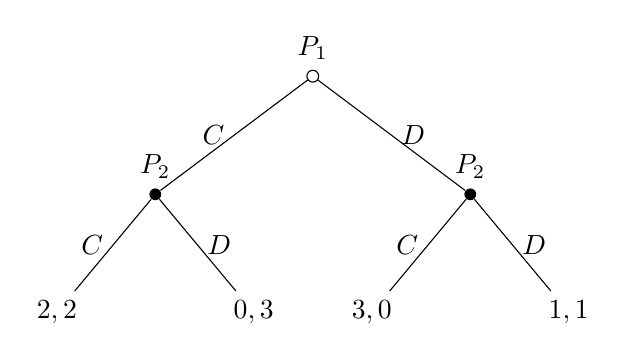
\begin{tikzpicture}[thin,
		level 1/.style={sibling distance=40mm},
		level 2/.style={sibling distance=25mm},
		level 3/.style={sibling distance=15mm},
		every circle node/.style={minimum size=1.5mm,inner sep=0mm}]
		
		\node[circle,draw,label=above:$P_{1}$] (root) {}
		child { node [circle,fill,label=above:$P_{2}$] {}
			child { 
				node {$2,2$}
				edge from parent
				node[left] {$C$}}
			child { 
				node {$0,3$} % [double] specifies the double line
				edge from parent
				node[right] {$D$}}
			edge from parent
			node[left] {$C$}}
		child { node [circle,fill,label=above:$P_{2}$] {}
			child { 
				node {$3,0$}
				edge from parent
				node[left] {$C$}}
			child { 
				node {$1,1$}
				edge from parent
				node[right] {$D$}}
			edge from parent
			node[right] {$D$}};
		\end{tikzpicture}
	\end{center}
\end{example}



\begin{theorem}[existence of pure strategy Nash equilibrium]
Every (finite) perfect-information game in extensive form has at least one pure-strategy Nash equilibrium.	
\end{theorem}

\subsection{Backward induction algorithm}

\section{Dynamic games with complete information}

\section{Multiobjective optimization}
\subsection{Basic concepts}
\begin{definition}\cite[18]{collette2013multiobjective}\index{multiobjective optimization}
A multiobjective optimization problem is defined as
\begin{align*}
    \min_{x\in \R^n} f(x) &= (f_1(x),f_2(x),...,f_k(x)),k\geq 2\\
    \text{subject to} ~ & g_i(x)\leq 0,i=1,2...,p \\
    & h_i(x)=0,i=1,2...,q
\end{align*}
\end{definition}

\begin{definition}[ideal objective vector]\cite[39]{collette2013multiobjective}\index{ideal point}
The ideal point of the objective function vector is a vector with each component minimized separately. The ideal point represents the best situation in optimizing the multiobjective function.
\end{definition}


\subsection{Pareto optimality}
\begin{definition}[domination relation]\index{domination}
In the multiojective optimization problem, a vector $x_1$ dominates $x_2$ if
\begin{itemize}
    \item $f_i(x_1) \leq f_i(x_2),\forall i$
    \item there exist one $i$ such that $f_i(x_1) < f_(x_2)$
\end{itemize}
\end{definition}

\begin{remark}
The domination relation express the intuitive meaning of 'better'.
\end{remark}

\begin{definition}[local optimality in the Pareto sense]\cite[19]{collette2013multiobjective}\index{local Pareto optimal}
A vector $x^*\in \R^n$ is locally optimal in the Pareto sense if there exists a real $\delta > 0$ such that for all $x \in \{x:\norm{x-x^*}\leq \delta\}$, $x$ does not dominate $x^*$.
\end{definition}


\begin{definition}[global optimality in the Pareto sense]\cite[19]{collette2013multiobjective}\index{global Pareto optimal}
A vector $x^*\in \R^n$ is locally optimal in the Pareto sense if there exists a real $\delta > 0$ such that for all $x \in \{x:\norm{x-x^*}\leq \delta\}$, $x$ does not dominate $x^*$.
\end{definition}


\section{Notes on bibliography}

A good resource on zero-sum game is at \href{http://math.ucr.edu/home/baez/games/}{link}.

\cite{gibbons1992game}\cite{fudenberg1991game}
For introduction to multiobjective optimization, see \cite{collette2013multiobjective}.
For good treatment on theory and method, see \cite{miettinen2012nonlinear}.
\printbibliography
\end{refsection}



\part{Statistical Learning}
\begin{refsection}
	\startcontents[chapters]	
\chapter{Supervised learning principles and methods}\label{ch:statistical-learning}
%\minitoc
	\printcontents[chapters]{}{1}{}
\section{The supervised learning problem}


\subsection{Definitions and concepts}

\begin{mdframed}
	\textbf{Notation}\cite[12]{mohri2012foundations}
	\begin{itemize}
		\item $\cX$: input space, the set of all possible examples or instances.
		\item $\cY$: the set of all possible labels or target values. For example $\cY=\{-1,1\}$ in binary classification.
		\item $\cD$: a the distribution of examples defined on $cX$ that are used to draw samples
		\item $S$: training samples drawn independently according to distribution $\cD$.  
		\item $\cH$: hypothesis space or hypothesis set
	\end{itemize}
\end{mdframed}


\begin{definition}[hypothesis,hypothesis space]\index{hypothesis}\index{hypothesis space}
A hypothesis $h$ is a mapping from $\cX$ to $\cY$. The set of all hypothesis in a learning task form the hypothesis set/space $\cH$.
\end{definition}

\begin{definition}[hypothesis space, alternative]
\cite{mitchell1997machine}A hypothesis space $H$ is a predefined space of all potential hypotheses, often implicitly defined by the hypothesis representation(i.e. by some parameters).  
\end{definition}


\begin{definition}[concept, concept class]\index{concept}
\cite[12]{mohri2012foundations}A concept $c$ is a mapping from $\cX$ to $\cY$. The training sample pair $(x,y),x\in \cX,y\in \cY$ is connected via $y = c(x)$.A concept class is a set of concepts we may wish to learn and is denoted by $C$.
\end{definition}


\begin{definition}[consistent hypothesis]
A hypothesis $h$ is consistent with a set of training examples $S=\{(x,c(x))\}$ if and only if $h(x) = c(x)$ for each example pair.
\end{definition}


\begin{definition}[generalization error/risk, true error]\index{generalization error}
Given a hypothesis $h\in H$, a target concept $c\in C$, and an underlying distribution $D$, the generalization error or generalization risk of $h$ is defined by
$$R(h) = Pr_{x\sin \cD}[h(x)\neq c(x)] = E_{x\sin \cD}[1_{h(x)\neq c(x)}]$$
where $1_w$ is the indicator function of event $w$.
\end{definition}


\begin{definition}[empirical error/risk,training error ]\index{empirical error}\index{training error}
Given a hypothesis $h\in H$, a target concept $c\in C$, and an underlying distribution $D$, a set $S$ of training sample pairs $\{(x_i,c(x_i))\}$, the generalization error or generalization risk of $h$ is defined by
$$\hat{R}(h) = \sum_{i=1}^m 1_{h(x_i)\neq c(x_i)}/m$$
where $1_w$ is the indicator function of event $w$.
\end{definition}

\begin{remark}
The \textbf{true error} of a hypothesis $h$ is the probability that it will misclassify a single randomly drawn instance from the distribution $\mathcal{D}$.
\end{remark}

\begin{lemma}[empirical error vs true error]
Consider a hypothesis $h$, we have
$$E[\hat{R}(h)] = R(h)$$
that is empirical error is the unbiased estimator of true error.
\end{lemma}
Proof: use linearity of expectation.


\begin{mdframed}
\textbf{\large The learning problem}\cite[12]{mohri2012foundations}\\

The learner is given a set $S$ of sample pairs $\{x_i,c(x_i)\}, c\in C$ drawn from an unknown distribution $\cD$. His task is to find a hypothesis $h$ in $\cH$ such that the generalization error/true error is minimized.
\end{mdframed}

\begin{remark}
Note that the goal for the learner is to minimize \textbf{true error instead of empirical error}. However, because usually $c$ and $\cD$ is unknown to the learner, the true error cannot be calculated from training sample. 
\end{remark}


\subsection{Function approximation as machine learning task}
Problem setting:
\begin{itemize}
	\item Set of possible instance $X$
	\item Unknown target function $f:X\rightarrow Y$
	\item Set of function hypotheses $H=\{h|h:X\rightarrow Y\}$
\end{itemize}

Input:
\begin{itemize}
	\item Training examples $\{<x^{(i)},y^{(i)}>\}$ of unknown target function $f$
\end{itemize}

Output:
\begin{itemize}
	\item Hypothesis $h\in H$ that best approximates target function $f$
\end{itemize}



\subsection{Overfitting}
Consider error of hypothesis $h$ over
\begin{itemize}
    \item training data
    \item entire distribution $\mathcal{D}$ of data, or simply the input $X$ has a distribution of $\mathcal{D}$
\end{itemize}
Hypothesis $h\in H$ over-fits training data if there is an alternative hypothesis $h'\in H$ such that
$$error_{train}(h) < error_{train}(h')$$
and
$$error_{\mathcal{D}}(h) > error_{\mathcal{D}}(h')$$




\subsection{True error vs. training error}
The \textbf{sample error}, $error_S(h)$ of hypothesis $h$ with respect to target function $f$ and data sample $S$ is given as:
$$error_S(h)=\frac{1}{n}\sum_{x\in S}\delta(f(x),h(x))$$
where $n$ is the number of examples in $S$.\\
 mathematically, we have
$$error_D(h) = Pr_{x \in \mathcal{D}}(f(x)\neq h(x))$$
where $Pr_{x \in \mathcal{D}}$ denotes that the probability is taken over the instance distribution $\mathcal{D}$



\subsection{Generative classifier vs. discriminative classifier }\cite{jordan2002discriminative}
\textbf{Generative classifier} learn a model of the joint probability, $p(x,y)$, of the inputs $x$ and the label $y$, and make their prediction using Bayes rules to calculate $p(y|x)$, then picking the most likely label $y$.\\
\textbf{Discriminative classifiers} model the posterior $p(y|x)$ directly, or learn a direct map from inputs $x$ to the class labels $y$, which avoid the intermediate step in generative classifiers. 

\iffalse











\subsubsection{Hypothesis space size for decision trees}



\fi


\subsection{Different input data types}

\begin{figure}[H]
\centering
\includegraphics[width=0.5\linewidth]{../figures/statisticalLearning/supervisedLearningPrinciples/SupervisedLearningClassificationDataTypeExample}
\caption{Input data type examples.}
\label{fig:SupervisedLearningClassificationDataTypeExample}
\end{figure}


\section{Variance bias tradeoff}

\subsection{Overfitting and underfitting phenomenon}

\begin{figure}
	\centering
	\includegraphics[width=0.6\linewidth]{../figures/statisticalLearning/supervisedLearningPrinciples/underFittingOverfittingDemo}
	\caption{The commonly observed phenomenon of overfitting and underfitting in machine learning. }
	\label{fig:underfittingoverfittingdemo}
\end{figure}





\subsection{Fundamentals}

\begin{lemma}[variance-bias tradeoff]\cite[34]{james2013introduction}
Suppose our training examples $(x,y)$ are generated via
$$y = h(x) + \epsilon$$
where $\epsilon$ is \textbf{an independent random variable with zero mean}. Let $\hat{f}$ be our proposed model with model parameters needs to be estimated from training examples $\cD$. Let us measure our learning performance via $E_\cD[(y_0 - \hat{f}(x_0|\cD))^2]$, that is the mean square error between the trained model and the real model \textbf{when given training examples with a finite number $N$.}
$$E_{\cD}[(y_0 - \hat{f}(x_0))^2] = Var_\cD[\hat{f}(x_0|\cD)] + [Bias(\hat{f}(x_0|\cD))]^2 + Var[\epsilon]$$
where
$Bias(\hat{f}(x_0|\cD)) = E[\hat{f}(x_0|\cD) - f(x)]$, $(x_0,y_0)$ is a training example drawn randomly from the population, and all the expectations are respect to the population distribution $\cD$.
\end{lemma}
\begin{proof}
(1)Use the following decomposition:
\begin{align*}
 &E_{\cD}[(y - \hat{f}(x|\cD))^2] \\
=&E_\cD[(y - h(x) + h(x) - \hat{f}(x|\cD))^2] \\
=&E_\cD[(y - h(x))^2] + 2E_\cD[(h(x) - \hat{f}(x|\cD))(y - h(x))] + E_\cD[(h(x) - \hat{f}(x|\cD))^2] \\
=&E_\cD[(y - h(x))^2] + 2E_\cD[(h(x) - \hat{f}(x|\cD))\epsilon] + E_\cD[(h(x) - \hat{f}(x|\cD))^2] \\
=&\underbrace{E_\cD[(y - h(x))^2]}_{noise~term}+ 0 + \underbrace{E_\cD[(h(x) - \hat{f}(x|\cD))^2]}_{model~estimation~error}. 
\end{align*}
where the noise term is without our control and the model estimation error is what we want to minimize.
(2)

\end{proof}



\begin{remark}[interpretation of Variance term]\hfill
\begin{itemize}
	\item $Var[\hat{f}(x_0)]$ represents the amount by which $\hat{f}$ would change if we estimate the model parameter using a different set of training examples of fixed size $n$. 
	\item If this term is large, then we are likely to have large test error.
	\item When increasing the number training examples, this term will be reduced. 
	\item Given a fixed number of training examples, a more flexible model(model with more parameters) will tend to have large variance since each parameter will be estimated poorly.
\end{itemize}
\end{remark}

\begin{remark}[interpretation of Bias term]\hfill
	\begin{itemize}
		\item $E[\hat{f}]$ is the resulting trained model when given infinitely number of training examples. Therefore, $(E[\hat{f}] - f)^2$ reflect the fundamental error associated with model proposal/assumption. For example, if $f$ is nonlinear model and $\hat{f}$ is a linear model, then no matter how hard we train, we cannot eliminate this error. 
		\item A less flexible model(such as linear model) will tend to have large bias. When using "universal approximation" models, like neural network and decision tree, the bias term could be reduced, however, at the risk of increasing Variance term.
	\end{itemize}
\end{remark}


\begin{remark}[interpretation of noise term]\hfill
	\begin{itemize}
		\item Even we have perfect model, that is $Bias[\hat{f}] = 0$, and perfect estimation of the model $Var[\hat{f}]=0$, we will cannot reduce 
		$E[(y_0 - \hat{f}(x_0))^2]$ to zero because the $y_0$ always contains a noise that cannot be predicted.
	\end{itemize}
\end{remark}

\begin{method}[estimating error]
Fix the test example $(x_0,y_0)$, we can do the following experiment:
\begin{itemize}
	\item Draw a training examples $D_1$ of size $N$, $D_1=\{(x_1,y_1),(x_2,y_2),...,(x_N, y_N)\}$.
	\item Train linear regression $\hat{f}(x|D_1)$ using $D_1$.
	\item Calculate the squared error
	$$err(D_1) = (\hat{f}(x_0|D_i) - y_0)^2.$$
	\item Repeat the above procedures by drawing different training examples $D_i,i=2,...,M$, and get the mean squared error via
	$$err = \frac{1}{M}\sum_{i=1}^M err(D_i).$$ 
\end{itemize}	
\end{method}



\subsection{Linear regression}
\begin{lemma}
Assume the true model is $h(x) = x^T\beta$ and the prediction model is $$\hat{f}(x|\cD) = x^T\hat{\beta},$$
where $\hat{\beta} = (X^TX)^{-1}X^TY$.
It follows that
\begin{itemize}
	\item Unbiasedness:
	$$E_\cD[\hat{f}(x)|\cD] = h(x) = x^T\beta.$$
	\item Variance:
	$$Var\triangleq E_{\cD}[(\hat{f}(x)|\cD - E_\cD[\hat{f}(x)|\cD])^2] = \sigma^2 x^T(X^TX)^{-1}x.$$
	\item If inputs $X$ are standardized and $x$ is a random vector with distribution $MN(0,I_{p\times p})$, then
	$$Var\approx \sigma^2 \frac{p}{n}.$$
\end{itemize}	
\end{lemma}
\begin{proof}
	
	



(3)
\begin{align*}
E_{x}[Var] &=  E_{x}[\sigma^2 x^T(X^TX)^{-1}x] \\
&=  \sigma^2E_{x}[Tr( x^T(X^TX)^{-1}x)] \\
&=  \sigma^2E_{x}[Tr( (X^TX)^{-1}xx^T)] \\
&=  \sigma^2 E_{x}[Tr( xx^T(X^TX)^{-1})] \\
&=  \sigma^2 Tr(E_{x}[xx^T] (X^TX)^{-1})\\
&=  \sigma^2 Tr(I_{p\times p} )
\end{align*}


\end{proof}


\subsection{K-nearest neighbor}




\section{Model evaluation}
\subsection{Regression metric}

\begin{definition}
Denote $\hat{y}$ as the estimated target output, $y$ the corresponding (correct) target output, $\hat{y}_i$  the predicted value of the $i$-th sample, and $y_i$ the corresponding true value
\begin{itemize}
	\item (explained variance) The \textbf{explained variance} is estimated as follow:	
	$$explained_variance(y,\hat{y}) = 1 - \frac{Var[y-\hat{y}]}{Var[y]}.$$
	\item (mean absolute error)the mean absolute error (MAE) estimated over $N$ samples is defined as	
	$$MAE(y,\hat{y}) = \frac{1}{N}\sum_{i=1}^{N} \abs{y_i - \hat{y}_i}.$$
	\item (mean squared error) If $\hat{y}_i$ is the predicted value of the $i$-th sample, and $y_i$ is the corresponding true value, then the mean squared error (MSE) estimated over $N$ samples is defined as	
	$$MSE(y,\hat{y}) = \frac{1}{N}\sum_{i=1}^{N} (y_i - \hat{y}_i)^2.$$
	\item (median absolute error) If $\hat{y}_i$ is the predicted value of the $i$-th sample, and $y_i$ is the corresponding true value, then the mean squared error (MSE) estimated over $N$ samples is defined as	
	$$MadAE(y,\hat{y}) = median(\abs{y_1 - \hat{y}_1},...,\abs{y_N - \hat{y}_N},)^2.$$
\end{itemize}	
\end{definition}


\section{Model selection methods}

\subsection{Basic idea}
To prevent overfitting in supervised learning algorithms, it is common practice to split the data to training set and testing data where the model parameters are estimated based on the training data and the performance evaluation is conducted on the testing data set. 

For a set of models parameterized by hyperparameters (e.g., the regularizer parameter in the penalized linear regression), using performance evaluation on the testing data set to determine the optimal hyperparameters has the risk of  overfitting on the testing data set (i.e., the model might still perform bad for samples never seen before.). This is because the during the hyperparameter searching process, knowledge about the testing data set can 'leak' into the model and evaluation metrics no longer report on generalization performance. To solve this problem, commond practice is to dividend the data set into \textbf{training set, validation set, and testing set}. 
In such way, training proceeds on the training set, after which hyperparametering tuning is done on the validation set. In the end, final evaluation of the model is done on the test set.

\subsection{Cross-validation}

As our previous discussion, training a model with hyperparameters requires the partitioning of the available data into three sets. This procedure has the following drawbacks:
\begin{itemize}
	\item The number of samples used for training will be draticaly reduced.
	\item The result will be that the results can depend on a particular choice for the pair of (train, validation) sets.
\end{itemize} 

One solution to these issues is a procedure called \textbf{cross-validation (CV)}. 
\begin{method}[$K$-fold CV procedure]
\begin{itemize}
	 \item training set is split into k smaller sets (other approaches are described below, but generally follow the same principles). The following procedure is followed for each of the k “folds”:
	 
	 \item A model is trained using k-1 of the folds as training data;
	 \item the resulting model is validated on the remaining part of the data (i.e., it is used as a test set to compute a performance measure such as accuracy).
	 \item The performance measure reported by k-fold cross-validation is then the average of the values computed in the loop.
\end{itemize}	
\end{method}


A test set should still be held out for final evaluation, but the validation set is no longer needed when doing CV. In the basic approach, called k-fold CV, the

A model is trained using k-1 of the folds as training data;
the resulting model is validated on the remaining part of the data (i.e., it is used as a test set to compute a performance measure such as accuracy).
 This approach can be computationally expensive, but does not waste too much data (as it is the case when fixing an arbitrary test set), which is a major advantage in problem such as inverse inference where the number of samples is very small.
 
 
\subsection{Statistical comparison}
 



\subsubsection{Occam's razor}
The simplest hypothesis that fits the data is preferred.


\section{Data preprocessing}




\subsection{Handle missing values}


For various reasons, many real world datasets contain missing values, often encoded as blanks, NaNs or other placeholders. Such datasets however are incompatible with most of the machine learning algorithms.  

One basic strategy to handle incomplete data matrix $X$ is to discard entire rows (i.e., discard the example) and/or columns (i.e., discard the feature) containing missing values. However, this comes at the price of losing data which may be valuable (even though incomplete). A better strategy is to impute the missing values, i.e., to infer them from the known part of the data based on some assumed distributions on missing values.

In practice, some ad hoc strategy is to impute missing values using either the mean, the median or the most frequent value of the row or column in which the missing values are located. The code example is in 


\subsection{Data standardization}







\subsection{Handle categorical data}

\href{https://www.analyticsvidhya.com/blog/2015/11/easy-methods-deal-categorical-variables-predictive-modeling/}{link}


\begin{table}[H]
	\begin{tabular}{cccc}
		Categorical Value & $x_1$ & $x_2$ & $x_3$ \\
		Married           & 1     & 0     & 0     \\
		Single            & 0     & 1     & 0     \\
		Divorced          & 0     & 0     & 1    
	\end{tabular}
\end{table}











\section{Information theory}


\subsection{Concept of entropy}

\begin{definition}[entropy of a random variable]\index{entropy}\hfill
	\begin{itemize}
		\item 	Let $X$ be a discrete random variable taking values $x_k,k=1,2...$ with probability mass function 
		$$Pr(X = x_k) = p_k, k=1,2,...$$ 
		Then the entropy of $X$ is defined by
		$$H(X) = - \sum_{k\geq 1}p_k\ln p_k.$$
		\item If $X$ is a continuous random variable with pdf $f(x)$, then entropy of $X$ is defined by
		$$H(X) = -\int_{-\infty}^{\infty} f(x)\ln f(x) dx.$$
	\end{itemize}	
	
\end{definition}

\begin{remark}[entropy, information and probability distribution]\hfill
	\begin{itemize}
		\item Entropy is a measure of the uncertainty of a random variable: the larger the value, the uncertainty the random variable is.
		\item When the random variable is deterministic, the entropy is at the minimum.
	\end{itemize}	
\end{remark}


\begin{example}\hfill
	\begin{itemize}
		\item The entropy of the Gaussian density on $\R$ with mean $\mu$ and variance $\sigma^2$ is
		\begin{align*}
		H &= -\int_{\R} \frac{1}{\sqrt{2\pi}\sigma} \exp(-1/2((x-\mu)^2/\sigma^2))(-\ln(\sqrt{2\pi}\sigma) -1/2((x-\mu)^2/\sigma^2))dx \\
		&= \frac{1}{2} + \ln(\sqrt{2\pi}\sigma).
		\end{align*}
		Note that the mean $\mu$ does not enter the entropy; therefore the entropy for Gaussian distribution is translational invariant.
		\item The entropy of the exponential distribution with mean $\lambda$ and pdf
		$$f(x) = \frac{1}{\lambda}\exp(-x/\lambda)$$
		is
		$$H = -\int_0^\infty \frac{1}{\lambda} \exp(-x/\lambda)(-\ln \lambda -x/\lambda) dx = \ln \lambda + 1.$$
	\end{itemize}	
\end{example}



\begin{lemma}[basic properties of entropy]\hfill
	\begin{itemize}
		\item $H(X) \geq 0$.
		\item $H(X) = 0$ if and only if there exists a $x_0$ such that $P(X=x_0) = 1$.
		\item If $X$ can take on finite number $n$ values, then $H(X) \leq \log(n)$. $H(X) = \log(n)$ if and only if $X$ is uniformly distributed. 
		\item Let $X_1,X_2,...,X_n$ be discrete valued random variables on a common probability space. Then
		$$H(X_1,X_2,...,X_n) = H(X_1) + \sum_{i=2}^n H(X_n|X_1,...,X_{n-1}).$$
		\item $H(X) + H(Y) \geq H(X,Y)$, with equality if and only if $X$ and $Y$ are independent.
	\end{itemize}
\end{lemma}
\begin{proof}
	(1) note that every term $\log(p)$ is non-positive, therefore $H(X) \geq 0$. (2) direct verification. (3)  direct verification. (4) It can be showed that $H(X,Y) = H(X|Y) + H(Y)$. (5) $H(X,Y) = H(X|Y) + H(Y) \leq H(X) + H(Y)$(using chain rule and conditioning entropy). 
\end{proof}


\subsection{Entropy maximizing distributions}



\begin{theorem}[continuous distribution with maximum entropy]\label{ch:statistical-learning:th:continuousDistributionWithMaximumEntropy}
	Suppose $S$ is a closed subset of $\R$. Let $X$ be a random variable with support $S$ and pdf $f(x)$.
	
	Then, the probability density function $f(x)$ maximizing the entropy
	$$H(X) = -\int_{-\infty}^{\infty} f(x)\ln f(x) dx,$$
	and satisfying the following $n$ constraints
	$$E[g_j(X)] = a_j, \forall j=1,2,...,n.$$
	and sum-to-unit constraint
	$$\int_S f(x) dx = 1,$$
	has the form
	$$f(x) = c\exp(\sum_{j=1}^{n} \lambda_j g_j(x)), \forall x\in S,$$
	where the constant $c$ and the $n$ multipliers $\lambda_i$ are determined by the above $n+1$ constraints.
\end{theorem}
\begin{proof}
	Note that our constraints can be written as
	$$\int_{-\infty}^{\infty} g_j(x)f(x) dx = a_j,j = 1,2,...,n $$	
	$$\int_{-\infty}^{\infty} f(x) dx = 1,j = 1,2,...,n.$$	
	
	The Lagrange of our minimizing problem is given by
	$$J[p(x)] = \int_{-\infty}^{\infty} f(x)\ln f(x) dx - \lambda_0(\int_{-\infty}^{\infty} f(x) dx - 1) - \sum_{j=1}^{n} \lambda_j(\int_{-\infty}^{\infty} g_j(x)f(x) dx - a_j).$$
	where $\lambda_i,i=0,1,2,...,n$ are Lagrange multipliers.
	
	The first order optimality condition gives
	$$\frac{\delta J}{\delta f(x)} = \ln f(x) + 1 - \lambda_0 - \lambda_j g_j(x),$$
	or equivalently 
	$$f(x) = \exp(-1+\lambda_0) \exp(\sum_{j=1}^{n} \lambda_j g_j(x)) = c\exp(\sum_{j=1}^{n} \lambda_j g_j(x)).$$
	
	Note that the second order conditions gives $\frac{\delta^2 J}{\delta f(x)^2} = 1/f(x) > 0$, which ensures we have unique global minimum solution. 
\end{proof}


\begin{corollary}\hfill
	\begin{itemize}
		\item The uniform distribution on the interval $[a,b]$ is the maximum entropy distribution among all continuous distribution supported on $[a,b]$.
		\item The exponential distribution, for which the density function with parameter $\lambda$ is
		$$f(x|\lambda) = \begin{cases*}
		\lambda \exp(-\lambda x), x\geq 0\\
		0, x < 0
		\end{cases*}$$
		is the maximum entropy distribution among all continuous distributions supported in $[0,\infty]$ that have a specified mean of $1/\lambda$.
		\item The normal distribution with parameter $\mu$ and $\sigma$, for which the density function is
		$$f(x|\mu, \sigma) = \frac{1}{\sqrt{2\pi}\sigma} \exp(-\frac{(x-\mu)^2}{2\sigma^2}),$$
		has the maximum entropy among all distributions supported on $\R$ with a specified mean $\mu$ and variance $\sigma^2$.
	\end{itemize}	
\end{corollary}
\begin{proof}
	(1) from \autoref{ch:statistical-learning:th:continuousDistributionWithMaximumEntropy}, we know that the $f(x)$ should have the following form
	$$f(x) = c.$$
	and $c$ is determined by
	$$\int_{a}^b f(x)dx = c(b-a) = 1 \implies c = \frac{1}{b-a}.$$
	Therefore, 
	$$f(x) = \frac{1}{b-a},x\in [a,b].$$
	(2)Similarly,
	we know that the $f(x)$ should have the following form
	$$f(x) = c\exp(\mu x),$$
	where $\mu$ is the Lagrange multiplier
	and $c$ is determined by
	$$\int_{0}^\infty f(x)dx = \frac{c}{\mu} = 1 \implies c = \mu.$$
	and then
	$$\int_{0}^\infty xf(x)dx = -\frac{1}{\mu} = 1/\lambda \implies \mu = -\lambda.$$
	(3)Similarly,
	we know that the $f(x)$ should have the following form
	$$f(x) = c\exp(\lambda_1 x + \lambda_2(x-\mu)^2).$$
	Then we can determine $c,\lambda_1,\lambda_2$ using constraints.
\end{proof}


\begin{theorem}[discrete distribution with maximum entropy]\label{ch:statistical-learning:th:discreteDistributionWithMaximumEntropy}
	Suppose $S = \{x_1,x_2,...\}$ is a (finite or infinite) discrete subset of  of $\R$. Let $X$ be a random variable with support $S$ and probability mass function given by
	$Pr(X = x_k)$.
	
	Then, the probability mass function $Pr(X)$ maximizing the entropy
	$$H(X) = -\sum_{k\geq 1} Pr(X=x_k)\ln Pr(X=x_k),$$
	and satisfying the following $n$ constraints
	$$E[g_j(X)] = a_j, \forall j=1,2,...,n.$$
	and sum-to-unit constraint
	$$\sum_{k\geq 1} Pr(X=x_k) = 1,$$
	has the form
	$$Pr(X=x_k) = c\exp(\sum_{j=1}^{n} \lambda_j g_j(x_k)), \forall x_k \in S,$$
	where the constant $c$ and the $n$ multipliers $\lambda_i$ are determined by the above $n+1$ constraints.
\end{theorem}
\begin{proof}
	Note that our constraints can be written as
	$$\int_{-\infty}^{\infty} g_j(x)f(x) dx = a_j,j = 1,2,...,n $$	
	$$\int_{-\infty}^{\infty} f(x) dx = 1,j = 1,2,...,n.$$	
	
	Let $p_k = Pr(X = x_k)$. The Lagrange of our minimizing problem is given by
	$$L = \sum_{i=1}^{n} p_k\ln p_k - \lambda_0(\sum_{i\geq 1} p_k - 1) - \sum_{j=1}^{n} \lambda_j(\sum_{i\geq 1} g_j(x_i)p_i - a_j).$$
	where $\lambda_i,i=0,1,2,...,n$ are Lagrange multipliers.
	
	The first order optimality condition for $p_i$ gives
	$$\frac{\Pa L}{\Pa p_i} = \ln p_i + 1 - \lambda_0 - \lambda_j g_j(x_i),i\geq 1$$
	or equivalently 
	$$Pr(X=x_i) = p_i = \exp(-1+\lambda_0) \exp(\sum_{j=1}^{n} \lambda_j g_j(x_i)) = c\exp(\sum_{j=1}^{n} \lambda_j g_j(x_i)).$$
	
	Note that the second order conditions gives $\frac{\Pa^2 L}{\Pa p_i} = 1/p_i > 0$, which ensures we have unique global minimum solution.	
\end{proof}


\begin{corollary}\hfill
	For a probabilistic mass function $p$ on a finite set $\{x_1,x_2,...,x_n\}$, the entropy $H$ is bounded by
	$$H \leq \ln n$$
	with equality holds if and only if $p$ is uniform, i.e., $p(x_i) = 1/n, \forall i$.
\end{corollary}
\begin{proof}
	From \autoref{ch:statistical-learning:th:discreteDistributionWithMaximumEntropy}, we know that the $p(x)$ should have the following form
	$$p(x_i) = c.$$
	and $c$ is determined by
	$$\sum_{i=1}^n c = 1 \implies c = \frac{1}{n}.$$
	Therefore, 
	$$p(x_i)=1/n, \forall i.$$
\end{proof}

\subsection{KL divergence}

\begin{definition}[Kullback-Leibler divergence, KL divergence]\index{KL divergence}
	Given two discrete probability distribution $P$ and $Q$ defined on the same set $\cX$, the KL divergence from $Q$ to $P$ is defined as
	$$D_{KL}(P||Q) = \sum_{x\in\cX} P(x)\log \frac{P(x)}{Q(x)}$$ 
\end{definition}

\begin{lemma}[non-negativeness of KL divergence]
	Given two discrete probability distribution $P$ and $Q$ defined on the same set $\cX$,
	$$D_{KL}(P||Q)\geq 0.$$
	And the equality holds if $P=Q$.
\end{lemma}
\begin{proof}
	$$D_{KL}(P||Q) = -\sum_{x\in\cX} P(x)\log \frac{Q(x)}{P(x)}\geq - \log (\sum_{x\in\cX} \frac{Q(x)}{P(x)} P(x)) = 0$$
	where the fact that $-\log(x)$ is a convex function and Jensen's inequality has been used(\autoref{ch:theory-of-probability:th:Jenseninequality}).
\end{proof}

\subsection{Conditional entropy and mutual information}


\begin{definition}[conditional entropy]\index{conditional entropy}\hfill
	\begin{itemize}
		\item \textbf{Specific conditional entropy} $H(X|Y=v)$ of $X$ given $Y=v$:
		$$H(X|Y=v) = - \sum_{i=1}^n P(X=i|Y=v)\log P(X=i|Y=v).$$
		\item \textbf{Conditional entropy} $H(X|Y)$ of $X$ given $Y$:
		$$H(X|Y) = \sum_{v\in Val(Y)}P(Y=v)H(X|Y=v).$$
	\end{itemize}
\end{definition}


\begin{definition}[mutual information]\index{mutual information}\cite{cover2012elements}
	Consider two discrete random variables $X$ and $Y$ taking values in $\cX$ and $\cY$. The \textbf{mutual information, or information gain)} of $X$ and $Y$ is given as:
	$I(X,Y) = H(X) - H(X|Y) = H(Y) - H(Y|X)$
\end{definition}

\begin{lemma}
	$$I(X,Y) \geq 0$$
	where $I(X,Y) = 0$ if $X$ and $Y$ are independent.
\end{lemma}
\begin{proof}
	(1)
	\begin{align*}
	I(X,Y)&=H(X)-H(X|Y)\\
	&=-\sum_{x\in \cX}\sum_{y\in \cY}p(x,y)\log(p(x)) + \sum_{x\in \cX}\sum_{y\in \cY} p(x|y)p(y)\log(p(x|y))\\
	& = -\sum_{x\in \cX}\sum_{y\in \cY}p(x,y)\log(p(x)) + \sum_{x\in \cX}\sum_{y\in \cY} p(x,y)\log(\frac{p(x,y)}{p(y)})\\
	& = \sum_{x\in \cX}\sum_{y\in \cY} p(x,y)\log(\frac{p(x,y)}{p(x)p(y)}) = DL(p(x,y)||p(x)p(y)) \geq 0.
	\end{align*}
	(2) When $X$ and $Y$ are independent, we have
	$$H(X|Y) = \sum_{v\in \cY}(Y=v)H(X|Y=v) = \sum_{v\in \cY}P(Y=v)H(X) = H(x).$$
\end{proof}




\begin{corollary}[conditioning reduce entropy]
	Given discrete random variables $X$ and $Y$, we have
	$$H(X|Y) \leq H(X),$$ which is also known as conditioning reduces entropy (i.e., conditioning provides information); and this equality holds if and only if $X$ and $Y$ are independent.\\	
\end{corollary}


\textbf{Chain rule}: $H(X,Y)=H(X)+H(Y|X)$ can be proved using $P(X,Y)=P(X|Y)P(Y)$.



\subsection{Cross-entropy}

\begin{definition}[cross-entropy of two probability distributions]
	Consider a probability distribution on $N$ value with probability $y_i, i=1,2,...,N$. Consider another distribution on the same support and probabilities $y_i', i = 1,2,...,N$. Then the cross-entropy of the two distributions is defined by
	$$H(y,y') = \sum_{i=1}^N y_i \log \frac{1}{y_i'} = -\sum_{i=1}^N y_i \log y_i'.$$ 	
\end{definition}


\begin{lemma}[properties of cross entropy]
	Consider two discrete distributions, characterized by probability mass vectors $y$ and $y'$, on the same $N$ values. 
	\begin{itemize}
		\item The KL divergence on the two distributions is the difference between cross entropy and entropy; that is
		$$KL(y||y') = \sum_{i=1}^{N} y_i \log \frac{y_i}{y_i'} = \underbrace{\sum_{i=1}^N y_i\log \frac{1}{y_i'}}_{cross~entropy} - \underbrace{\sum_{i=1}^N y_i\log \frac{1}{y_i}}_{entropy}.$$
		\item Cross entropy is no smaller than entropy 
		$$H(y,y') \geq H(y).$$
	\end{itemize} 	
\end{lemma}
\begin{proof}
	(1) Straight forward. (2) Use the fact that
	$$KL(y||y') = H(y,y') - H(y) \geq 0.$$
\end{proof}


\begin{remark}[cross entropy, maximum likelihood, and classificiation accuracy]
	Consider a $K$-class classification problem with $N$ training examples. The target of each example is represented by a $K$-dimensional one-hot vector. The classification output generated by the classifier can be represented by a discrete distribution vector. 
	
	For example, let $y^{(1)} = (1,0,0,)$ be the target vector of example 1 and $\hat{y}^{(1)} = (0.4,0.1,0.5)$ be a prediction output based on input of example 1. 
	
	Note that the likelihood for example $i$ is given by
	$$L(y^{(i)};\hat{y}^{(i)}) = \prod_{k=1}^K [\hat{y}^{(i)}_j]^{y^{(i)}},$$
	whose the logarithm form is
	$$\log L(y^{(i)};\hat{y}^{(i)}) = \sum_{k=1}^K y^{(i)}_k \log \hat{y}^{(i)}_k = -H(y^{(i)},\hat{y}^{(i)}).$$
	
	For overall $N$ examples, the overall negative log likelihood is
	$$-\log L = - \sum_{n=1}^N \log L(y^{(n)};\hat{y}^{(n)}) =\sum_{n=1}^N H(y^{(i)},\hat{y}^{(i)}).$$
	
	Therefore, \textbf{minimizing the negative log likelihood is equivalent to minimizing the cross-entropy.}
	
	
\end{remark}


\section{Kernel methods}
\subsection{Basic concepts of kernels and feature maps}
\begin{mdframed}
	\textbf{\cite[481]{murphy2012machine} General motivations:}
	\begin{itemize}
		\item for some data(such at text document, colloidal structure) it is not easy to represent the data as a vector in $\R^d$
		\item By assuming that we have some way to measure the similarity between different input example, we design algorithms using similarity as input for classification and regression. Such similarity measure is the kernel function.
	\end{itemize}
\end{mdframed}


\begin{definition}[kernel] \index{kernel}
	\cite[90]{mohri2012foundations}A function $K:X\times X \to \F$ is called a kernel over $X$.
\end{definition}


\begin{definition}[feature map, feature, feature space]\index{feature map}\index{feature space}\index{feature}
	In machine learning, a \textbf{feature map} is usually an embedding:
	$$\phi:R^D\to\R^M$$
	with $M \gg D$. The point $\phi(x) \in \R^M$ is called the \textbf{feature} of data point $x\in \R^D$.
	The space $\R^M$ is called the \textbf{feature space}.
\end{definition}

\begin{remark}[relations between kernel and feature map]
	\begin{itemize}\hfill
		\item For general kernels, usually there is no connection between the two.
		\item When the kernel satisfies certain conditions, say Mercer's condition, one can show that the kernel is implicitly associated with a feature map. \textbf{This association is significant, it enables us to use some implicitly complex feature maps to do machine learning tasks by only doing calculation using relatively 'simple' kernels.}
	\end{itemize}
\end{remark}



\begin{example}[\textbf{linear kernel}]
	\cite[484]{murphy2012machine} If the original data is already in $\R^d$, we can use $\phi(x) = x,k(x,x')= x^Tx'$. \textbf{This kernel is useful only when (1) $x$ is high dimensional (2) every individual dimension is informative(providing useful information)}. In the example of image recognition, linear kernel will be a bad choice since not every pixel is informative.  
\end{example}


\begin{remark}
	More complex feature(high-dimensional) space usually enable us to distinguish distributions with different means.
\end{remark}





\subsection{Mercer's theorem}

\begin{definition}[positive definite symmetric kernel]\index{positive definite symmetric kernel}\index{Gram matrix}
	\cite[92]{mohri2012foundations}\cite[30]{scholkopf2002learning}A kernel $k:X^2\to \F$ is said to be positive definite symmetric(PDS) if for any $x_1,x_2,...,x_m \in X$, the matrix $K_{ij} = k(x_i,x_j)$ is symmetric semi-positive definite matrix. The matrix $K$ is called \textbf{Gram matrix} of $k$ with respect to $x_1,x_2,...,x_m$.
\end{definition}

\begin{lemma}[Cauchy-Schwarz inequality for PDS kernel]
	If $k$ is a PDS kernel, then
	$$\abs{k(x_1,x_2)} \leq k(x_1,x_1)k(x_2,x_2)$$
\end{lemma}
Proof: from $det K \geq 0$, where $K$ is the Gram matrix.


\begin{remark}[interpretation]
	In studying approximation theory in vector space using basis functions, we also define Gram matrix with entries being the dot product of basis function. Here, we view the \textbf{input data vectors as the basis of the input vector space}.
\end{remark}


\begin{definition}[Mercer's condition]\index{Mercer's condition}
	A real-valued function $k:X\times X \to \R$ is said to fulfill Mercer's condition if for \textbf{all square integrable functions} $g(x)$ one has
	$$\int_X\int_X g(x)K(x,y)g(x) dxdy \geq 0$$
	Or in discrete case, the $k$ is replaced by a matrix $K\in \R^{N\times N}$, such that for all vectors $g\in \R^N$ such that
	$$\ip{g,Kg} = g^T K g \geq 0$$
\end{definition}


\begin{theorem}[Mercer's theorem]\index{Mercer's theorem}
	\cite{wiki:Mercer}\cite[64]{shawe2004kernel}
	Suppose $k:X\times X\to \R$ is a continuous symmetric non-negative definite kernel, that is, it satisfies Mercer's condition. Then there is an orthonormal basis $e_i(x)$ of $L^2(X)$ such that
	$$k(s,t) = \sum_{j=1}^\infty \lambda_i e_j(s)e_j(t)$$
	where $\lambda_i \geq 0$
\end{theorem}

\begin{remark}[interpretation \& significance]\hfill
	\begin{itemize}
		\item The mercer's theorem enables us to interpret that: for symmetric semi-positive definite kernels, there exist feature maps given as $\phi(x) =\sum_i \sqrt{\lambda_i}e_i(x) $ such that $k(s,t) = \ip{\sum_i \sqrt{\lambda_i}e_i(s),\sum_i \sqrt{\lambda_i}e_i(s)}$
		note that it would be difficult to recover the underlying functions $e_i(x)$ and $\lambda_i$.
		\item The mercer's theorem enables us to connect kernel to feature maps when mercer's condition holds. \textbf{Note that for an arbitrary kernel, the concept of kernel and feature map might be unrelated.} 
	\end{itemize}
\end{remark}



\begin{remark}[the underlying feature map]
	Given a kernel function $k$ satisfying Mercer's condition,\textbf{the feature map and the feature space are implicitly defined}, and it is usually hard to find the underlying feature map $\phi(x)$ is(because of the uniqueness issue for example).
	But if we are given a feature map $\phi(x)$, calculating a 'canonical' kernel $k$ is straight forward via $k(x,x')=\ip{\phi(x),\phi(x')}$.
\end{remark}


\begin{remark}[information in kernel matrix]
	We do not have access to the feature vectors, but only to its norms,i.e. $k(x,x)$, and the inner product between feature vectors, i.e., $k(x,x')$.
\end{remark}




\begin{remark}[projection onto subspaces spanned by input vectors]
	Given a new input vector $x$, we want to measure how similar $x$ is to the training input vectors $x_1,x_2,...,x_m$. We can achieve this by solving coefficients $p\in \R^m$, via $Kp = q$, where $K\in \R^{m\times m}, K_{ij} = k(x_i,x_j), q_i=k(x,x_i)$. As a result, the projection coefficient is given as $$p = K^{-1}q.$$
	Note that we can calculate the projection with merely usage of kernel function.
\end{remark}


\subsection{Reproducing kernel Hilbert space}

\begin{definition}[feature map]
	\cite[32]{scholkopf2002learning}Let $k$ be a real-valued positive definite kernel, and $X$ a nonempty set. A feature map $\Phi: X\to \R^X$ is defined as a mapping from $X$ to \textbf{the space of functions }$\R^X = \{X\to \R\}$, given as
	$$\Phi(x) = k(\cdot,x)$$
\end{definition}


\begin{remark}
	Via this feature map, we map each element $x\in X$ to a function $k(\cdot,x)$ defined on $X$. So we are \textbf{representing $x$ via an 'infinite-dimensional' object $k(\cdot,x)$}. This representation is desirable because it enables us to distinguish different $x$ in a much larger dimensional space.
\end{remark}


\begin{definition}[vector space from sample representations]
	Let $k$ be a real-valued positive definite kernel, and $X$ a nonempty set. Let $x_1,x_2,...,x_m \in X$ be training samples, then $k(\cdot,x_1),k(\cdot,x_2),...,k(\cdot,x_m)$ span a linear vector space $V$, where for any $f\in V$, $f$ has the representation of $f = \sum_{i=1}^m a_i k(\cdot,x_i)$, the inner product between $f,g\in V$ is defined as
	$$\ip{f,g} = \sum_{i=1}^m\sum_{j=1}^m a_ia_j \ip{k(\cdot,x_i),k(\cdot,x_j)} = \sum_{i=1}^m\sum_{j=1}^m a_ia_j k(x_j,x_i)$$
\end{definition}

\begin{remark}
	It can be verified that inner product defined this way satisfied the property of an inner product: For example, (1) $\ip{f,f} \geq 0$; (2) linearity in the first slot. 
\end{remark}

\begin{remark}
	The vector space from the sample representations is a \textbf{subspace of $\cH$}
\end{remark}


\begin{definition}[reproducing kernel Hilbert space]\index{reproducing kernel Hilbert space}
	Let $\cH$ be a Hilbert space of \textbf{$\R$-valued functions} defined on $X$, and $\cH$ is \textbf{repreducing kernel Hilbert space}, if there exist a kernel function $k:X\times X\to \R$, called \textbf{reproducing kernel} of $\cH$, such that
	\begin{itemize}
		\item $\forall x \in X, k(\cdot,x) \in \cH$
		\item $\forall x \in X,\forall f \in \cH, \ip{f,k(\cdot,x)} = f(x)$ (the reproducing property)
		\item $\forall x,y \in X, k(x,y) = \ip{k(\cdot,x),k(\cdot,y)}$
		\item $k$ spans $\cH$, i.e., $H = \conj{span\{k(\cdot,x),x\in X\}}$, where the bar denotes completion.
	\end{itemize}
\end{definition}

\begin{remark}
	Note that the \textbf{third point is a direct consequence of the second point}(it can be showed by directly replacing $f\in \cH$ by $k(\cdot,y) \in \cH$)
\end{remark}



\begin{remark}
	\begin{itemize}
		\item the reproducing kernel Hilbert space is \textbf{first a Hilbert space of functions(possibly infinite dimensional)}.
		\item $k(\cdot,x),x\in X$ is a family of functions parameterized by $x$.
		\item the reproducing kernel is associated with a special property that inner product of any $f\in \cH$ with $k(\cdot,x)$ equals $f(x) \in \R$. 
	\end{itemize}
\end{remark}


\subsection{Common kernels}
\subsubsection{Gaussian kernel}
\begin{definition}[Gaussian kernel]\index{Gaussian kernel}
	\cite[482]{murphy2012machine}Gaussian kernel $k:\R^d\times \R^d \to \R$ is defined as
	$$k(x_i,x_j) = \exp(-\frac{\norm{x_i-x_j}^2}{2\sigma^2})$$
\end{definition}


\begin{remark}[when to use Gaussian kernel]
	Gaussian kernel has the effect of penalizing large dissimilarity between samples and only maintains similarity measure resulting from 'close/nearby' samples in the feature space. 
\end{remark}


\begin{lemma}[Gram matrix of Gaussian kernel has full rank]
	\cite[47]{scholkopf2002learning}Suppose that $x_1,x_2,...,x_m \in X$ are distinct points and $\sigma \neq 0$, then the Gram matrix $K_{ij} = k(x_i,x_j)$ has full rank.
	In other words, the functions $k(\cdot,x_i)$ are linearly independent.
\end{lemma}

\begin{remark}
	It can be verified that $\ip{k(\cdot,x_i),k(\cdot,x_j)}$
\end{remark}

\subsubsection{Polynomial kernel}
\begin{definition}[polynomial kernel]\index{Polynomial kernel}
	\cite[482]{murphy2012machine}\cite[293]{shawe2004kernel}Polynomial kernel $k:\R^d\times \R^d \to \R$ of degree $k$ is defined as
	$$k(x_i,x_j) = (\ip{x_i,x_j} + c)^d = \sum_{s=0}^d \binom{d}{s}c^{d-s}\ip{x_i,x_j}^s$$
	where $c\in \R$
\end{definition}

\begin{remark}
	We can see that a relatively simple polynomial kernel is actually associated with a rather complex feature map. 
\end{remark}

\begin{remark}[adjust weighting on feature map] We can see that by changing the value of $c$, we can adjust weight on terms of the associated polynomial. The larger value of $c$, the heavier weight is on higher order terms.
\end{remark}

\begin{lemma}[dimension of induced feature space]\cite[293]{shawe2004kernel}
	The dimension of the feature space for the polynomial kernel of degree $d$ is $\binom{n+d}{d}$
	where $n$ is the dimension of the input space.
\end{lemma}
\begin{proof}
	For $n=1$, the number is correctly computed as $d=1$ from the binomial expansion. The correctness of the expression can be proved by induction. Note that for $n=2$, the inner product $\ip{x,z} = (x_1,x_2)^T(z_1,z_2)=x_1z_1 + x_2z_2$, and the power on this will significantly increase number of terms and the dimension of feature space.
\end{proof}


\subsection{Kernel trick and elementary algorithms using kernels}
\subsubsection{Kernel trick}
\begin{mdframed}
	\textbf{"kernel trick"}
	\cite[34]{scholkopf2002learning}
	
	Given an algorithm formulated in terms of \textbf{positive definite kernel }$k$, then one can construct an alternative algorithm by replacing $k$ by another positive definite kernel $k'$.
\end{mdframed}

\begin{remark}[dot product to kernel]
	If the original $k$ is the dot product (which is a linear kernel) between input vectors, then we can replace the dot product by other positive definite kernel(for example, nonlinear kernel). 
\end{remark}

\begin{remark}[positive definiteness]
	We require the kernel to be positive definite because the algorithm usually use convex optimization and dual optimization.
\end{remark}

\subsubsection{Algorithms}
\begin{theorem}[elementary algorithms]
	\cite[114]{shawe2004kernel}
	Given a finite subset $S=\{x_1,x_2,...,x_n\}$ of an input space $X$ and a kernel $k:X^2\to \R$ satisfying $k(x,x')=\ip{\phi(x),\phi(x')}$ for some feature map $\phi:X\to H$: we are able to calculate the following quantity using kernels alone:
	\begin{itemize}
		\item The norm of feature vector: $\norm{\phi(x)}_2 = k(x,x)$
		\item The norm of linear combination of feature vector: $$\norm{\sum_{i} \alpha_i \phi(x_i)}^2 = \sum_{i}\sum_j \alpha_i\alpha_j k(x_i,x_j)$$
		\item Distance between feature vectors: 
		$\norm{\phi(x) - \phi(z)} = k(x,x) + k(z,z) - 2k(x,z)$
		\item The norm of the center mass: 
		$$\norm{\phi_S}_2^2 = \frac{1}{n^2} \sum_i \sum_j k(x_i,x_j)$$
		where $\phi_S = \frac{1}{n}\sum_i \phi(x_i)$
		\item The average distance from the center mass 
		$$\frac{1}{n}\sum_{i=1}^n \norm{\phi(x_s) - \phi_S}^2 = \frac{1}{n}\sum_{i=1}^n k(x_i,x_i) - \frac{1}{n^2} \sum_{i=1}^n \sum_{j=1}^n k(x_i,x_j)$$
	\end{itemize}
\end{theorem}
Proof: these can be proved directly by replacing $\ip{\phi_i,\phi_j} = k(x_i,x_j)$



\begin{lemma}[centering the feature vectors ]
	\cite[496]{murphy2012machine}\cite[115]{shawe2004kernel}Given a finite subset $S=\{x_1,x_2,...,x_n\}$ of an input space $X$ and a kernel $k:X^2\to \R$ satisfying $k(x,x')=\ip{\phi(x),\phi(x')}$ for some feature map $\phi:X\to H$: we can centering $K_{ij} = \ip{\phi(x_i),\phi(x_j)}$ to $K'_{ij} = \ip{\phi(x_i) - \phi_S,\phi(x_j)-\phi_S}$ via
	$$K' = HKH,H = I-1_n1_n^T/N$$
\end{lemma}
\begin{proof}
	\begin{align*}
	K'_{ij} &= \ip{\phi_i - \phi_S,\phi_j-\phi_S} \\
	&= \ip{\phi_i,\phi_j} - \ip{\phi_i,\phi_S} - \ip{\phi_j,\phi_S} + \ip{\phi_S,\phi_S}\\
	&= k(x_i,x_j) - \frac{1}{n}\sum_k k(x_i,x_k) - \frac{1}{n} \sum_k k(x_j,x_k) + \frac{1}{n^2}\sum_k \sum_l k(x_k,x_l)
	\end{align*}	
\end{proof}


\section{Note on bibliography}

For Gaussian process, see \cite{rasmussen2006gaussian}.


For generalized linear model, see \cite{dobson2008introduction}, https://onlinecourses.science.psu.edu/stat504/node/216.


For kernel method, see \cite{shawe2004kernel}.



\end{refsection}
\begin{refsection}
	\startcontents[chapters]	
	\chapter{Geneartive models}\label{ch:statistical-learning}
	%\minitoc
	\printcontents[chapters]{}{1}{}

\section{Generative model for discrete data}

\section{Foundations of Bayesian concept learning}
Psychological research has shown that people can learn concepts from positive examples alone (Xu and Tenenbaum 2007).

We can think of learning the meaning of a word as equivalent to \textbf{concept learning}, which in turn is equivalent to binary classification. To see this, define $f(\vec{x})=1$ if x is an example of the concept $C$, and $f(\vec{x})=0$ otherwise. Then the goal is to learn the indicator function $f$, which just defines which elements are in the set $C$.


\subsection{Likelihood}
\begin{equation}
p(\mathcal{D}|h) \triangleq \left(\dfrac{1}{\text{size}(h)}\right)^N=\left(\dfrac{1}{|h|}\right)^N
\end{equation}

This crucial equation embodies what Tenenbaum calls the \textbf{size principle}, which means the model favours the simplest (smallest) hypothesis consistent with the data. This is more commonly known as \textbf{Occam’s razor}\footnote{\url{http://en.wikipedia.org/wiki/Occam\%27s_razor}}.


\subsection{Prior}
The prior is decided by human, not machines, so it is subjective. The subjectivity of the prior is controversial. For example, that a child and a math professor will reach different answers. In fact, they presumably not only have different priors, but also different hypothesis spaces. However, we can finesse that by defining the hypothesis space of the child and the math professor to be the same, and then setting the child’s prior weight to be zero on certain “advanced” concepts. Thus there is no sharp distinction between the prior and the hypothesis space.

However, the prior is the mechanism by which background knowledge can be brought to bear on a problem. Without this, rapid learning (i.e., from small samples sizes) is impossible.


\subsection{Posterior}
The posterior is simply the likelihood times the prior, normalized.
\begin{equation}
p(h|\mathcal{D}) \triangleq \dfrac{p(\mathcal{D}|h)p(h)}{\sum_{h' \in \mathcal{H}}p(\mathcal{D}|h')p(h')}=\dfrac{\mathbb{I}(\mathcal{D} \in h)p(h)}{\sum_{h' \in \mathcal{H}}\mathbb{I}(\mathcal{D} \in h')p(h')}
\end{equation}
where $\mathbb{I}(\mathcal{D} \in h)p(h)$ is 1 \textbf{iff}(iff and only if) all the data are in the extension of the hypothesis $h$.

In general, when we have enough data, the posterior $p(h|\mathcal{D})$ becomes peaked on a single concept, namely the MAP estimate, i.e.,
\begin{equation}
p(h|\mathcal{D}) \rightarrow \hat{h}^{MAP}
\end{equation}
where $\hat{h}^{MAP}$ is the posterior mode,
\begin{equation}\begin{split}
\hat{h}^{MAP} & \triangleq \arg\max\limits_h p(h|\mathcal{D})=\arg\max\limits_h p(\mathcal{D}|h)p(h) \\
& =\arg\max\limits_h [\log p(\mathcal{D}|h) + \log p(h)]
\end{split}\end{equation}

Since the likelihood term depends exponentially on $N$, and the prior stays constant, as we get more and more data, the MAP estimate converges towards the \textbf{maximum likelihood estimate} or \textbf{MLE}:
\begin{equation}
\hat{h}^{MLE} \triangleq \arg\max\limits_h p(\mathcal{D}|h)=\arg\max\limits_h \log p(\mathcal{D}|h)
\end{equation}

In other words, if we have enough data, we see that the \textbf{data overwhelms the prior}.


\subsection{Posterior predictive distribution}
The concept of \textbf{posterior predictive distribution}\footnote{\url{http://en.wikipedia.org/wiki/Posterior_predictive_distribution}} is normally used in a Bayesian context, where it makes use of the entire posterior distribution of the parameters given the observed data to yield a probability distribution over an interval rather than simply a point estimate. 
\begin{equation}
p(\tilde{\vec{x}}|\mathcal{D}) \triangleq \mathbb{E}_{h|\mathcal{D}}[p(\tilde{\vec{x}}|h)] = \begin{cases}
\sum_h p(\tilde{\vec{x}}|h)p(h|\mathcal{D}) \\
\int p(\tilde{\vec{x}}|h)p(h|\mathcal{D})\mathrm{d}h
\end{cases}
\end{equation}

This is just a weighted average of the predictions of each individual hypothesis and is called \textbf{Bayes model averaging}(Hoeting et al. 1999). 


\section{Beta-binomial model}

\subsection{The model}
\begin{definition}[Beta-binomial model]
A Beta-binomial model with pre-specified parameter $n$ has parameter $a$ and $b$, and can be represented by the following Hierachical model 
$$Y|\theta \sim Binom(n,\theta), \theta\sim Beta(a,b).$$
In particular, 
 the density functions for $Y|\theta$ and $\theta$ given by 
	$$Pr_{Y|\theta}(Y = y|\theta) = \binom{n}{y} \theta^y(1-\theta)^{(n-y)}, y=0,1,...,n;$$
	$$f(\theta) = \frac{1}{B(a,b)}\theta^{a-1}(1-\theta)^{b-1},a>0,b>0;$$
where $$B(a,b) = \int_0^1 \theta^{a-1}(1-\theta)^{b-1} d\theta.$$
\end{definition}



\begin{lemma}[density functions for Beta-binomial model]
Let $(Y,\theta)$ follow  a Beta-binomial model with parameter $(a,b)$, we have
\begin{itemize}
	\item the joint density function is given by
	$$Pr_{Y, \theta}(Y = y, \theta) = \binom{n}{y} \theta^y(1-\theta)^{(n-y)}\frac{1}{B(a,b)}\theta^{a-1}(1-\theta)^{b-1}, y=0,1,...,n;$$
	\item the marginal density function for $y$ is given by
	$$Pr_Y(Y=y)=\binom{n}{y} \frac{B(y+a,n-y+b)}{B(a,b)}.$$
\end{itemize}	
where $$B(a,b) = \int_0^1 \theta^{a-1}(1-\theta)^{b-1} d\theta.$$
\end{lemma}
\begin{proof}
(1) the joint density function is given by
$$Pr_{Y, \theta}(Y = y, \theta) = \binom{n}{y} \theta^y(1-\theta)^{(n-y)}\frac{1}{B(a,b)}\theta^{a-1}(1-\theta)^{b-1}, y=0,1,...,n;$$
(2)the marginal density function for $y$ is given by
$$Pr_Y(Y=y)=\binom{n}{y} \frac{B(y+a,n-y+b)}{B(a,b)}.$$	
\end{proof}





\begin{lemma}[basic statistical properties of Beta-binomial model]\label{ch:statistical-learning:th:BasicStatisticalPropertiesOfBetaBinomialModel}
Let $(Y,\theta)$ follow a Beta-binomial model with parameter $(a,b)$, we have
\begin{itemize}
	\item $$E[Y|\theta] = n\theta, E[\theta] = \frac{a}{a+b}, E[Y] = n\frac{a}{a+b}.$$
	\item $$Var[Y|\theta] = n\theta(1-\theta), Var[Y] = n\mu_{\theta}(1-\mu_\theta)(1 + (n-1)\frac{1}{a+b+1}),$$
	where $\mu_\theta = a/(a+b)$.
\end{itemize}	
\end{lemma}
\begin{proof}
(1) $$E[Y] = E[E[Y|\theta]] = E[n\theta] = nE[\theta] = n\frac{a}{a+b}.$$
(2) Note that 
\begin{align*}
Var[Y] &= E[Var[Y|\theta]] + Var[E[Y|\theta]] \\
&= E[n\theta(1-\theta)] + Var[n\theta] \\
&= E[n\theta] - nE[\theta^2] + n^2 Var[\theta] \\
&= n(E[\theta] - E[\theta]^2 + nVar[\theta]) ]
\end{align*}
where we use the property of conditional variance(\autoref{ch:theory-of-probability:th:conditionalVarianceIdentity}).
then we use the following facts(\autoref{ch:theory-of-statistics:th:propertyBetaDistribution}),
\begin{itemize}
	\item $$E[\theta] = \frac{a}{a+b}.$$
	\item $$E[\theta^2] = \frac{a(a+1)}{(a+b)(a+b+1)}$$
	\item $$Var[\theta] = \frac{ab}{(a+b)^2(a+b+1)}.$$
\end{itemize}
\end{proof}


\subsection{Parameter inference}

\begin{theorem}[posterior distribution and estimation of $\theta$]\cite[75]{murphy2012machine}\label{ch:statistical-learning:th:PosteriorDistributionAndEstimationInBetaBionomialModel}
Given an iid random experiment data set $\cD$ consisting of $N_1$ results of labeling 1 and $N_0$ results of the labeling 0. Consider a Beta-binomial model with parameter $(a,b)$. It follows that
\begin{itemize}
	\item The posterior distribution of parameter $\theta$ given the data $\cD$ is
	$$\theta|\cD \sim Beta(N_1+a,N_0+b),$$
	that is
	$$f_{\theta|\cD} = \frac{1}{B(a+N_1,b+N_0)}\theta^{a+N_1-1}(1-\theta)^{b+N_0-1}.$$
	\item The mean and variance of the posterior $\theta$ is given by
	$$E[\theta|\cD] = \frac{a + N_1}{a + b + N_1 + N_0},$$
	$$Var[\theta|\cD] = \frac{(a + N_1)(b + N_0)}{(a + N_1 + b + N_0)^2(a+b+1 + N_1 + N_0)},$$
	\item The maximum likelihood function is given by
	$$L(\cD|\theta) \propto \theta^{N_1}(1-\theta)^{N_0}  $$
	and the maximum likelihood estimation of $\theta$ is given by
	$$\theta_{MLE} = \frac{N_1}{ N_1 + N_0 }.$$
	\item The maximum a posterior estimation of $\theta$ is given by
	 $$\theta_{MAP} = \frac{a+ N_1 - 1}{a + b + N_1 + N_0 -2},$$
	 when $a = b = 1$, $\theta_{MAP} = \theta_{MLE}.$
\end{itemize} 	
\end{theorem}
\begin{proof}
(1)
Note that
\begin{align*}
p(\theta|\cD) &\propto p(\cD|\theta)p(\theta) \\
 &\propto \theta^{N_1}(1-\theta)^{N_0}\theta^{a-1}(1-\theta)^{b-1} \\
 &=\theta^{N_1+a-1}(1-\theta)^{N_0+b-1} 
\end{align*}
After normalization, we can show $\theta|\cD$ follows $Beta(N_1+a,N_0+b)$.
(2)\autoref{ch:theory-of-statistics:th:propertyBetaDistribution}.
(3)(4)\autoref{ch:theory-of-statistics:th:propertyBetaDistribution}.
\end{proof}

\begin{lemma}[sequential learning property]
Suppose we have two data sets $\cD_1$ and $\cD_2$ with sufficient statistics $N_1',N_0'$ and $N_1'', N_0''$. And denote $N_1 = N_1' + N_1''$ and $N_0 = N_0' + N_0''$.
In batch mode, we have
$$p(\theta|\cD',\cD'') \propto Beta(\theta|N_1+a,N_0 + b).$$
and in sequential mode, we also have
$$p(\theta|\cD',\cD'') \propto Beta(\theta|N_1+a,N_0 + b).$$ 	
\end{lemma}
\begin{proof}
Use \autoref{ch:statistical-learning:th:PosteriorDistributionAndEstimationInBetaBionomialModel}, we have
\begin{align*}
p(\theta|\cD',\cD'') &\propto p(\cD''|\theta)p(\theta|\cD') \\
&\propto Bin(N_1''|\theta,N_1''+N_0'')Beta(\theta|N_1'+a,N_0'+b) \\
&\propto Bin(\theta| N_1'+ N_2'' + a,N_0'+N_0''+b) \\
=Beta(N_1+ a, N_0+b) 
\end{align*}
where we used the conditional Bayesian law(\autoref{ch:theory-of-probability:th:BayesianLawForRandomVariables}).
\end{proof}

\subsection{Forecasting}

\begin{lemma}[posterior prediction for future outcomes]\cite[80]{murphy2012machine}
Suppose we have observations of data set $\cD$ with sufficient statistic $N_1$ and $N_0$. Now for the new $M$ experiments, the number of results with label 1, denoted by random variable $Y$, has the following prediction.
\begin{itemize}
	\item It follows the Beta-binomial model 
	$$Y|\theta \sim Binom(M,\theta), \theta\sim Beta(N_1+a,N_0+b).$$
	In particular, 
	the density functions for $Y|\theta$ and $\theta$ given by 
	$$Pr_{Y|\theta}(Y = y|\theta) = \binom{M}{y} \theta^y(1-\theta)^{(M-y)}, y=0,1,...,M;$$
	$$f(\theta) = \frac{1}{B(N_1+a,N_0 + b)}\theta^{N_1+a-1}(1-\theta)^{N_0+b-1},a>0,b>0;$$
	where $$B(N_1+a,N_0 + b) = \int_0^1 \theta^{N_1+a-1}(1-\theta)^{N_0+ b-1} d\theta.$$
	\item 
	\begin{align*}
	P(Y=y|\cD,M) &= \binom{M}{y}\frac{1}{B(N_1+a,N_0+b)}\int_0^1 \theta^y(1-\theta)^{M-y}\theta^{N_1+a-1}(1-\theta)^{N_0+b-1}\\
	& = \binom{M}{y}\frac{B(N_1+a+y,N_0+b+M-y)}{B(N_1+a,N_0+b)}.
	\end{align*}
	\item the posterior prediction for $Y$ has mean and variance given by
		 $$E[Y] = M\theta,Var[Y|\theta] = n\theta(1-\theta),$$
		 where $\theta = \frac{a+N_1}{a+b+N_1+N_0}$.
\end{itemize}
\end{lemma}
\begin{proof}
(1)Directly from \autoref{ch:statistical-learning:th:BasicStatisticalPropertiesOfBetaBinomialModel}.
(2) Use
$$P(Y|\cD,M)= P(Y|\theta,M) P(\theta|\cD).$$
\end{proof}


\section{Dirichlet-multinomial model}
\subsection{The model}
\begin{definition}[Dirichlet-multinomial model]
	A Dirichlet-multinomial model with pre-specified parameter $N$(total counts) and $K$(number of classes) has parameters $\alpha = (\alpha_1,\alpha_2,...,\alpha_K)$, and can be represented by the following Hierachical model 
	$$Y|\theta \sim Mulnom(n,\theta), \theta\sim Dir(\theta).$$
	In particular, 
	the density functions for $Y|\theta$ and $\theta$ given by 
	$$Pr_{Y|\theta}(Y = (n_1,n_2,...,n_K)|\theta) = \dbinom{N}{n_1\cdots n_K} \theta^y(1-\theta)^{(n-y)}, y=0,1,...,n;$$
	$$f(\theta|\alpha)=Dir(\theta|\alpha) = \dfrac{1}{B(\alpha)}\prod_{k=1}^K \theta_k^{\alpha_k-1}$$
	with support $\theta\in \{\theta_k:0\leq \theta_k\leq 1,\sum_k x_\theta = 1,\forall k=1,2...,K\}$, and $B(a)$ is a normalization constant given as
	$$B(a) = \frac{\prod_{k=1}^K \Gamma(a_k)}{\Gamma(\sum_k a_k)},$$
	where $\Gamma(\cdot)$ is the Gamma function. 
\end{definition}

\begin{example}
Consider tossing a tie with 6 faces. The count on the each distinct faces from a total number count $N$ can be modeled by the Dirichlet-multinomial model.	
\end{example}

\begin{lemma}[density functions for Dirichlet-Multinomial model]
	Let $(Y,\theta)$ follow  a Beta-binomial model with parameter $(a,b)$, we have
	\begin{itemize}
		\item the joint density function  for $(Y,\theta)$ with parameter $\alpha$ is given by
		\begin{align*}
		Pr_{Y, \theta}(Y = (y_1,y_2,...,y_K), \theta) &= \dbinom{N}{N_1\cdots N_K}\prod_{k=1}^K \theta_k^{\alpha_k+y_k-1} \frac{1}{B(\alpha)}\\
		&=\prod_{k=1}^K \theta_k^{\alpha_k+y_k-1} \frac{1}{B(\alpha')}
		\end{align*}
		where $\alpha'=\alpha+(y_1,y_2,...,y_K).$
		\item the marginal density function for $Y_i$ with parameter $\alpha$ is given by
		$$Pr_Y(Y_i=y)=\binom{N}{y_i} \frac{B(y+\theta_i,N-y+(\alpha_0-\alpha_i))}{B(\alpha_i,\alpha_0-\alpha_i)}.$$
	\end{itemize}	
	where $$B(a,b) = \int_0^1 x^{a-1}(1-x)^{b-1} dx.$$
\end{lemma}
\begin{proof}
	(1) the joint density function is given by
	$$Pr_{Y, \theta}(Y,\theta) = Pr(Y|\theta)f(\theta).$$
	(2)the marginal density function for $y$ is given by
	$$Pr_Y(Y=y)=\binom{n}{y} \frac{B(y+a,n-y+b)}{B(a,b)}.$$	
\end{proof}


\begin{remark}[connections between Dirichlet-multinomial model and Beta-binomial model]
In the Dirichlet-multinomial model, we have multiple classes. However, if we are only interested in the counts in one particular class(i.e., the marginal distribution of one types of result), we can convert it to an equivalent Beta-binomial model. 	
\end{remark}


\begin{lemma}[basic statistical properties of Dirichlet-Multinomial model]\label{ch:statistical-learning:th:BasicStatisticalPropertiesOfDirichletMultinomialModel}
	Let $(Y,\alpha),Y=(Y_1,Y_2,...,Y_K),\alpha=(\alpha_1,...,\alpha_K)$ follow a Dirichlet-Multinomial model with parameter $\alpha$. Further denote $\alpha_0=\sum_{i=1}^{K}\alpha_i=1$. Then we have
	\begin{itemize}
		\item $$E[Y_i|\alpha] = N\alpha_i, E[\alpha_i] = \frac{\alpha_i}{\alpha_0}, E[Y] = n\frac{a}{a+b}.$$
		\item $$Var[Y|\theta] = n\theta(1-\theta), Var[Y] = n\mu_{\theta}(1-\mu_\theta)(1 + (n-1)\frac{1}{a+b+1}),$$
		where $\mu_\theta = a/(a+b)$.
	\end{itemize}	
\end{lemma}
\begin{proof}
	(1) $$E[Y_i] = E[E[Y_i|\theta_i]] = E[N\theta_i] = NE[\theta_i] = N\frac{\alpha_i}{\alpha_0}.$$ 
	(2) Note that 
	\begin{align*}
	Var[Y] &= E[Var[Y|\theta]] + Var[E[Y|\theta]] \\
	&= E[n\theta(1-\theta)] + Var[n\theta] \\
	&= E[n\theta] - nE[\theta^2] + n^2 Var[\theta] \\
	&= n(E[\theta] - E[\theta]^2 + nVar[\theta]) ]
	\end{align*}
	where we use the property of conditional variance(\autoref{ch:theory-of-probability:th:conditionalVarianceIdentity}).
	then we use the following facts(\autoref{ch:theory-of-statistics:th:propertyBetaDistribution}),
	\begin{itemize}
		\item $$E[\theta] = \frac{a}{a+b}.$$
		\item $$E[\theta^2] = \frac{a(a+1)}{(a+b)(a+b+1)}$$
		\item $$Var[\theta] = \frac{ab}{(a+b)^2(a+b+1)}.$$
	\end{itemize}
\end{proof}

\begin{remark}
Note that once $\theta_i$ is known, we can have the marginal distribution of $Y_i$, even without knowing other $\theta_{-i}$.
\end{remark}


\subsection{Parameter inference}

\begin{lemma}
\begin{itemize}
	\item (likelihood)Suppose we observe $N$ dice rolls, $\mathcal{D}=\{x_1,x_2,\cdots,x_N\}$, where $x_i \in \{1,2,\cdots,K\}$. The likelihood has the form
	\begin{equation*}
	p(\mathcal{D}|\theta) = \dbinom{N}{N_1 \cdots N_k} \prod\limits_{k=1}^K\theta_k^{N_k} \quad \text{where } N_k=\sum\limits_{i=1}^N \mathbb{I}(y_i=k)
	\end{equation*}
	\item (Prior)\begin{equation*}
	\text{Dir}(\theta|\alpha) = \dfrac{1}{B(\alpha)}\prod_{k=1}^K \theta_k^{\alpha_k-1}\mathbb{I}(\theta \in S_K)
	\end{equation*}
	\item (Posterior)
	\begin{align}
	p(\vec{\theta}|\mathcal{D})& \propto p(\mathcal{D}|\theta)p(\theta) \\
	& \propto \prod\limits_{k=1}^K\theta_k^{N_k}\theta_k^{\alpha_k-1} = \prod\limits_{k=1}^K\theta_k^{N_k+\alpha_k-1}\\
	& =\text{Dir}(\vec{\theta}|\alpha_1+N_1,\cdots,\alpha_K+N_K)
	\end{align}
	
	From Equation \ref{eqn:Dirichlet-properties}, the MAP estimate is given by
	\begin{equation*}\label{eqn:Dir-MAP}
	\hat{\theta}_k=\dfrac{N_k+\alpha_k-1}{N+\alpha_0-K}
	\end{equation*}
	
	If we use a uniform prior, $\alpha_k=1$, we recover the MLE:
	\begin{equation*}\label{eqn:Dirichlet-multinomial-posterior-MLE}
	\hat{\theta}_k=\dfrac{N_k}{N}
	\end{equation*}
\end{itemize}	
\end{lemma}




\subsection{Posterior predictive distribution}
The posterior predictive distribution for a single multinoulli trial is given by the following expression:
\begin{align}
p(X=j|\mathcal{D})& =\int p(X=j|\vec{\theta})p(\vec{\theta}|\mathcal{D})\mathrm{d}\vec{\theta} \\
& =\int p(X=j|\theta_j)\left[\int p(\vec{\theta}_{-j}, \theta_j|\mathcal{D})\mathrm{d}\vec{\theta}_{-j}\right]\mathrm{d}\theta_j \\
& =\int \theta_jp(\theta_j|\mathcal{D})\mathrm{d}\theta_j=\mathbb{E}[\theta_j|\mathcal{D}]=\dfrac{\alpha_j+N_j}{\alpha_0+N}
\end{align}
where $\vec{\theta}_{-j}$ are all the components of $\vec{\theta}$ except $\theta_j$.

The above expression avoids the zero-count problem. In fact, this form of Bayesian smoothing is even more important in the multinomial case than the binary case, since the likelihood of data sparsity increases once we start partitioning the data into many categories.



\section{Naive Bayes classifier}



Let a $n$ dimensional discrete random vector $X$ represent $n$ input attributes. Assume each component $X_i$ of $X$ will take $J$ possible discrete values. Let a discrete random variable $Y$ represent the output, taking $K$ possible discrete values. 

The parameters for the conditional distribution



Consider a supervised learning problem in which we want to approximate an unknown target function $f:\bm{X}\rightarrow Y$, or equivalently $P(Y|\bm{X})$.$Y$ is binary random variable, and $\bm{X}=(X_1,X_2,...,X_n)$ is binary random variable vector. Applying Bayes rule, we see that $P(Y=y_i|\bm{X})$ can be written as
\begin{equation}
 P(Y=y_i|\bm{x_k}) = \frac{P(\bm{X=x_k}|P(Y=y_i))P(Y=y_i)}{\sum_j P(\bm{X=x_k}|P(Y=y_i))P(Y=y_i)}   
\end{equation}

where we use $\bm{x_k}$ to represent $k$ instance/realization of $\bm{X}$, $y_j$ for $j$ of $Y$.

\subsubsection{Sample complexity}
To use the Bayes classifier equation, we need to estimate $P(\bm{X}|Y)$ and $P(Y)$ first. The sample complexity refers to the number of training samples needed to obtain a good estimation with good confidence interval. 100 independently drawn training samples will suffice to obtain a good estimation of the $P(Y)$

Assume the features are \textbf{conditionally independent} given the class label, then the class conditional density has the following form
\begin{equation}
p(\vec{x}|y=c,\vec{\theta})=\prod\limits_{j=1}^D p(x_j|y=c,\vec{\theta}_{jc})
\end{equation}

The resulting model is called a \textbf{naive Bayes classifier}(NBC).

The form of the class-conditional density depends on the type of each feature. We give some possibilities below:
\begin{itemize}
	\item{In the case of real-valued features, we can use the Gaussian distribution: $p(\vec{x}|y,\vec{\theta})=\prod_{j=1}^D \mathcal{N}(x_j|\mu_{jc},\sigma_{jc}^2)$, where $\mu_{jc}$ is the mean of feature $j$ in objects of class $c$, and $\sigma_{jc}^2$ is its variance.}
	\item{In the case of binary features, $x_j \in \{0,1\}$, we can use the Bernoulli distribution: $p(\vec{x}|y,\vec{\theta})=\prod_{j=1}^D \text{Ber}(x_j|\mu_{jc})$, where $\mu_{jc}$ is the probability that feature $j$ occurs in class $c$. This is sometimes called the \textbf{multivariate Bernoulli naive Bayes} model. We will see an application of this below.}
	\item{In the case of categorical features, $x_j \in \{a_{j1},a_{j2},\cdots, a_{jS_j}\}$, we can use the multinoulli distribution: $p(\vec{x}|y,\vec{\theta})=\prod_{j=1}^D \text{Cat}(x_j|\vec{\mu}_{jc})$, where $\vec{\mu}_{jc}$ is a histogram over the $K$ possible values for $x_j$ in class $c$.}
\end{itemize}

Obviously we can handle other kinds of features, or use different distributional assumptions. Also, it is easy to mix and match features of different types.


\subsection{Optimization}
\label{sec:NBC-Optimization}
We now discuss how to “train” a naive Bayes classifier. This usually means computing the MLE or the MAP estimate for the parameters. However, we will also discuss how to compute the full posterior, $p(\vec{\theta}|\mathcal{D})$.

\subsubsection{MLE for NBC}
The probability for a single data case is given by
\begin{equation}\begin{split}
p(\vec{x}_i,y_i|\vec{\theta}) & =p(y_i|\vec{\pi})\prod\limits_j p(x_{ij}|\vec{\theta}_j) \\
& =\prod\limits_c \pi_c^{\mathbb{I}(y_i=c)} \prod\limits_j\prod\limits_c p(x_{ij}|\vec{\theta}_{jc})^{\mathbb{I}(y_i=c)}
\end{split}\end{equation}

Hence the log-likelihood is given by
\begin{equation}
p(\mathcal{D}|\vec{\theta})=\sum\limits_{c=1}^C{N_c\log\pi_c}+ \sum\limits_{j=1}^D{\sum\limits_{c=1}^C{\sum\limits_{i:y_i=c}{\log p(x_{ij}|\vec{\theta}_{jc})}}}
\end{equation}
where $N_c \triangleq \sum\limits_i \mathbb{I}(y_i=c)$ is the number of feature vectors in class $c$.

We see that this expression decomposes into a series of terms, one concerning $\vec{\pi}$, and $DC$ terms containing the $\theta_{jc}$’s. Hence we can optimize all these parameters separately.

From Equation \ref{eqn:Dirichlet-multinomial-posterior-MLE}, the MLE for the class prior is given by
\begin{equation}
\hat{\pi}_c=\dfrac{N_c}{N}
\end{equation}

The MLE for $\theta_{jc}$’s depends on the type of distribution we choose to use for each feature. 

In the case of binary features, $x_j \in \{0,1\}$, $x_j|y=c \sim \text{Ber}(\theta_{jc})$, hence
\begin{equation}
\hat{\theta}_{jc}=\dfrac{N_{jc}}{N_c}
\end{equation}
where $N_{jc} \triangleq \sum\limits_{i:y_i=c} \mathbb{I}(y_i=c)$ is the number that feature $j$ occurs in class $c$.

In the case of categorical features, $x_j \in \{a_{j1},a_{j2},\cdots, a_{jS_j}\}$, $x_j|y=c \sim \text{Cat}(\vec{\theta}_{jc})$, hence
\begin{equation}
\hat{\vec{\theta}}_{jc}=(\dfrac{N_{j1c}}{N_c},\dfrac{N_{j2c}}{N_c}, \cdots, \dfrac{N_{jS_j}}{N_c})^T
\end{equation}
where $N_{jkc} \triangleq \sum\limits_{i=1}^N \mathbb{I}(x_{ij}=a_{jk}, y_i=c)$ is the number that feature $x_j=a_{jk}$ occurs in class $c$.


\subsubsection{Bayesian naive Bayes}
\label{sec:Bayesian-naive-Bayes}
Use a Dir$(\vec{\alpha})$ prior for $\vec{\pi}$.

In the case of binary features, use a Beta$(\beta0,\beta1)$ prior for each $\theta_{jc}$; in the case of categorical features, use a Dir$(\vec{\alpha})$ prior for each  $\vec{\theta}_{jc}$. Often we just take $\vec{\alpha}=\vec{1}$ and $\vec{\beta}=\vec{1}$, corresponding to \textbf{add-one} or \textbf{Laplace smoothing}.


\subsection{Using the model for prediction}
The goal is to compute
\begin{equation}\begin{split}
y=f(\vec{x}) & =\arg\max\limits_{c}{P(y=c|\vec{x},\vec{\theta})} \\
& =P(y=c|\vec{\theta})\prod_{j=1}^D P(x_j|y=c,\vec{\theta})
\end{split}\end{equation}

We can the estimate parameters using MLE or MAP, then the posterior predictive density is obtained by simply plugging in the parameters $\bar{\vec{\theta}}$(MLE) or $\hat{\vec{\theta}}$(MAP). 

Or we can use BMA, just integrate out the unknown parameters.


\subsection{The log-sum-exp trick}
when using generative classifiers of any kind, computing the posterior over class labels using Equation \ref{eqn:Generative-classifier} can fail due to \textbf{numerical underflow}. The problem is that $p(\vec{x}|y=c)$ is often a very small number, especially if $\vec{x}$ is a high-dimensional vector. This is because we require that $\sum_{\vec{x}}p(\vec{x}|y)=1$, so the probability of observing any particular high-dimensional vector is small. The obvious solution is to take logs when applying Bayes rule, as follows:
\begin{equation}
\log p(y=c|\vec{x},\vec{\theta})=b_c-\log\left(\sum\limits_{c'}e^{b_{c'}}\right)
\end{equation}
where $b_c \triangleq \log p(\vec{x}|y=c,\vec{\theta})+\log p(y=c|\vec{\theta})$.

We can factor out the largest term, and just represent the remaining numbers relative to that. For example,
\begin{equation}\begin{split}
\log(e^{-120}+e^{-121}) & =\log(e^{-120}(1+e^{-1})) \\
& =\log(1+e^{-1})-120
\end{split}\end{equation}

In general, we have
\begin{equation}
\sum\limits_{c}e^{b_{c}}=\log\left[(\sum e^{b_c-B})e^B\right]=\log\left(\sum e^{b_c-B}\right)+B
\end{equation}
where $B \triangleq \max\{b_c\}$.

This is called the \textbf{log-sum-exp} trick, and is widely used. 


\subsection{Feature selection using mutual information}
Since an NBC is fitting a joint distribution over potentially many features, it can suffer from overfitting. In addition, the run-time cost is $O(D)$, which may be too high for some applications. 

One common approach to tackling both of these problems is to perform \textbf{feature selection}, to remove “irrelevant” features that do not help much with the classification problem. The simplest approach to feature selection is to evaluate the relevance of each feature separately, and then take the top K,whereKis chosen based on some tradeoff between accuracy and complexity. This approach is known as \textbf{variable ranking}, \textbf{filtering}, or \textbf{screening}.

One way to measure relevance is to use mutual information (Section \ref{sec:Mutual-information}) between feature $X_j$ and the class label $Y$
\begin{equation}
\mathbb{I}(X_j,Y)=\sum\limits_{x_j}{\sum\limits_{y}{p(x_j,y)\log \dfrac{p(x_j,y)}{p(x_j)p(y)}}}
\end{equation}

If the features are binary, it is easy to show that the MI can be computed as follows
\begin{equation}
\mathbb{I}_j = \sum\limits_c \left[\theta_{jc}\pi_c\log{\dfrac{\theta_{jc}}{\theta_j}}+(1-\theta_{jc})\pi_c\log{\dfrac{1-\theta_{jc}}{1-\theta_j}}\right]
\end{equation}
where $\pi_c=p(y=c)$, $\theta_{jc}=p(x_j=1|y=c)$, and $\theta_j=p(x_j=1)=\sum_{c} \pi_c\theta_{jc}$.


\subsection{Classifying documents using bag of words}
\textbf{Document classification} is the problem of classifying text documents into different categories.


\subsubsection{Bernoulli product model}
One simple approach is to represent each document as a binary vector, which records whether each word is present or not, so $x_{ij} =1$ iff word $j$ occurs in document $i$, otherwise $x_{ij}=0$. We can then use the following class conditional density:
\begin{equation}\begin{split}
p(\vec{x}_i|y_i=c,\vec{\theta}) & =\prod\limits_{j=1}^D \mathrm{Ber}(x_{ij}|\theta_{jc}) \\
& =\prod\limits_{j=1}^D \theta_{jc}^{x_{ij}}(1-\theta_{jc})^{1-x_{ij}}
\end{split}\end{equation}

This is called the \textbf{Bernoulli product model}, or the \textbf{binary independence model}.

\subsubsection{Multinomial document classifier}
However, ignoring the number of times each word occurs in a document loses some information (McCallum and Nigam 1998). A more accurate representation counts the number of occurrences of each word. Specifically, let $\vec{x}_i$ be a vector of counts for document $i$, so $x_{ij} \in \{0,1,\cdots,N_i\}$, where $N_i$ is the number of terms in document $i$(so $\sum\limits_{j=1}^D x_{ij}=N_i$). For the class conditional densities, we can use a multinomial distribution:
\begin{equation}\label{eqn:Multinomial-document-classifier}
p(\vec{x}_i|y_i=c,\vec{\theta})=\text{Mu}(\vec{x}_i|N_i,\vec{\theta}_c)=\dfrac{N_i!}{\prod_{j=1}^D x_{ij}!}\prod\limits_{j=1}^D \theta_{jc}^{x_{ij}}
\end{equation}
where we have implicitly assumed that the document length $N_i$ is independent of the class. Here $θ_{jc}$ is the probability of generating word $j$ in documents of class $c$; these parameters satisfy the constraint that $\sum_{j=1}^D \theta_{jc}=1$ for each class c.

Although the multinomial classifier is easy to train and easy to use at test time, it does not work particularly well for document classification. One reason for this is that it does not take into account the \textbf{burstiness} of word usage. This refers to the phenomenon that most words never appear in any given document, but if they do appear once, they are likely to appear more than once, i.e., words occur in bursts.

The multinomial model cannot capture the burstiness phenomenon. To see why, note that Equation \ref{eqn:Multinomial-document-classifier} has the form $\theta_{jc}^{x_{ij}}$, and since $\theta_{jc} \ll 1$ for rare words, it becomes increasingly unlikely to generate many of them. For more frequent words, the decay rate is not as fast. To see why intuitively, note that the most frequent words are function words which are not specific to the class, such as “and”, “the”, and “but”; the chance of the word “and” occuring is pretty much the same no matter how many time it has previously occurred (modulo document length), so the independence assumption is more reasonable for common words. However, since rare words are the ones that matter most for classification purposes, these are the ones we want to model the most carefully.

\subsubsection{DCM model}
Various ad hoc heuristics have been proposed to improve the performance of the multinomial document classifier (Rennie et al. 2003). We now present an alternative class conditional density that performs as well as these ad hoc methods, yet is probabilistically sound (Madsen et al. 2005).

Suppose we simply replace the multinomial class conditional density with the \textbf{Dirichlet Compound Multinomial} or \textbf{DCM} density, defined as follows:
\begin{equation}\begin{split}
p(\vec{x}_i|y_i=c,\vec{\alpha}) & =\int \text{Mu}(\vec{x}_i|N_i,\vec{\theta}_c)\text{Dir}(\vec{\theta}_c|\vec{\alpha}_c) \\
& =\dfrac{N_i!}{\prod_{j=1}^D x_{ij}!}\prod\limits_{j=1}^D\dfrac{B(\vec{x}_i+\vec{\alpha}_c)}{B(\vec{\alpha}_c)}
\end{split}\end{equation}

(This equation is derived in Equation TODO.) Surprisingly this simple change is all that is needed to capture the burstiness phenomenon. The intuitive reason for this is as follows: After seeing one occurence of a word, say wordj, the posterior counts on θj gets updated, making another occurence of wordjmore likely. By contrast, ifθj is fixed, then the occurences of each word are independent. The multinomial model corresponds to drawing a ball from an urn with Kcolors of ball, recording its color, and then replacing it. By contrast, the DCM model corresponds to drawing a ball, recording its color, and then replacing it with one additional copy; this is called the \textbf{Polya urn}.

Using the DCM as the class conditional density gives much better results than using the multinomial, and has performance comparable to state of the art methods, as described in (Madsen et al. 2005). The only disadvantage is that fitting the DCM model is more complex; see (Minka 2000e; Elkan 2006) for the details.



\section{Note on bibliography}







\end{refsection}

\begin{refsection}
	\startcontents[chapters]	
	\chapter{Tree methods}
	\printcontents[chapters]{}{1}{}


\section{Decision tree learning}

\begin{mdframed}
\textbf{General remarks}:
\begin{itemize}
	\item Decision tree essentially performs a greedy search in the hypothesis space, based on some metric on each greedy step(e.g., maximum mutual information gain), to find a hypothesis, i.e., a decision tree that sort the data.
	\item If there is no contradictory examples(i.e. two examples with the same $x$ yet produce different $y$), there will exist a decision tree perfectly predict $y$ based on $x$.
\end{itemize}
\end{mdframed}

\subsection{Basic concepts}

\begin{figure}[H]
	\centering
	\includegraphics[width=0.7\linewidth]{../figures/statisticalLearning/treeMethods/decisionTreeClassifierScheme}
	\caption{}
	\label{fig:decisiontreeclassifierscheme}
\end{figure}


\subsection{Classification tree}

\subsubsection{Basics}


\begin{method}[decision tree classifier splitting methods]
Consider a set of items of $K$ classes. Let $p_i$ be the fraction of items labeled with class $i$. 


\begin{itemize}
	\item Gini impurity: 
	$$Gini(p_1,...,p_K) = 1 - \sum_{i=1}^K p_i^2.$$
	\item Information gain
	$$IG = H(T) - H(p|a) = -\sum_{i=1}^K p_i\log(p_i) - \sum_a p(a)\sum_{i=1}^K(-Pr(i|a))$$
\end{itemize}	
\end{method}

\begin{remark}[interpret Gini impurity]
Gini impurity is a measure of how often a randomly chosen element from the set would be incorrectly labeled if it was randomly labeled according to the distribution of labels in the subset.	
\begin{align*}
I_G &= \sum_{i=1}^K p_i \sum_{j\neq i}p_k\\
&=\sum_{i=1}^K p_i(1-p_i) \\
&=\sum_{i=1}^K p_i-p_i^2 \\
&=1 - \sum_{i=1}^K p_i^2
\end{align*}	
\end{remark}


\begin{remark}[the Iris dataset]\index{Iris dataset}
The Iris dataset contains attributes, Petal Length, Petal Width, Sepal Length and Sepal width and three classes, setosa, versicolor and virginica.	

\end{remark}




\begin{remark}[perfect classification tree]
If the input variables in a classification problems are all categorical, then there exist a classificiation tree perfectly classify all the training examples.	
\end{remark}



\begin{remark}[classification tree stop growing criterion]
A classification tree can grow until all the leave node are pure. Additional parameters controlling the stopping criterion are
\begin{itemize}
	\item maximum depth: the maximum depth of the tree.
	\item minimum sample size for splitting: the minimum sample number in a node for splitting.
	\item information gain threshold: the minimum information gain when splitting a node. 
	\item Gini impurity decreasing threshold: the minimum Gini impurity decreasing when splitting a node.
\end{itemize}	
\end{remark}



\subsubsection{Examples}


\begin{figure}[H]
	\centering
	\includegraphics[width=0.8\linewidth]{../figures/statisticalLearning/treeMethods/IrisDecisionTree_Gini}
	\caption{The visualization of the decision tree classifier for Iris data set. The tree grows until all examples are classified correctly. The splitting criterion is Gini impurity. }
	\label{fig:irisdecisiontreegini}
\end{figure}

\begin{figure}[H]
	\centering
	\includegraphics[width=0.7\linewidth]{../figures/statisticalLearning/treeMethods/IrisDecisionTree_minSamplesGini}
	\caption{The visualization of the decision tree classifier for Iris data set. The tree grows until examples in each node is smaller than 10. The splitting criterion is Gini impurity.}
	\label{fig:irisdecisiontreeminsamplesgini}
\end{figure}

\begin{figure}[H]
	\centering
	\includegraphics[width=0.7\linewidth]{../figures/statisticalLearning/treeMethods/IrisDecisionTree_minSamplesEntropy}
	\caption{The visualization of the decision tree classifier for Iris data set. The tree grows until examples in each node is smaller than 10. The splitting criterion is entropy and information gain.}
	\label{fig:irisdecisiontreeminsamplesentropy}
\end{figure}



\subsection{Regression tree}

\begin{definition}[tree splitting]
Consider the predicators $X_1,...,X_p$, we want to select the $j$ predicator and a value $s$, such that for the pair of half-planes:
$$R_1(j,s) = \{X|X_j < s\}, R_2(j,s) = \{X|X_j \geq s\},$$
the equation
$$\sum_{i:x_i\in R_1(j,s)} (y_i - \hat{y}_{R_1})^2 + \sum_{i:x_i\in R_2(j,s)} (y_i - \hat{y}_{R_2})^2$$
is minimized. In here, $\hat{y}_{R_1}$ is the mean response for the training observations in $R_1$ and $\hat{y}_{R_2}$ is the mean response for the training observations in $R_2$.
\end{definition}


\begin{remark}[another equivalent formulation on variance reduction]
The variance reduction of a node is defined as the total reduction of the variance of the target variable $y$ due to the split at this node. The change of variance is given by
\begin{align*}
\Delta V = \frac{1}{\abs{S_N}^2} \sum_{i \in S_N}\sum{j\in S_N}\frac{1}{2}(x_i-x_j)^2
\end{align*}	
	
\end{remark}


\begin{remark}[technical procedures of tree splitting]
Loop through every predicator $X_i$, to choose optimal $s$ based on two situations:
\begin{itemize}
	\item If $X_i$ is discrete variable(such as, 0 and 1), then we simply loop through the discrete values to select the best one.
	\item If $X_i$ is a continuous variable, then we can first sort the training examples based on $X_i$, and test all possible splits using all values for variable $X_i$ to select the optimal value.\footnote{Depending on the number of examples, more efficient splitting based on sorting, binary search, etc. will be considered.}
\end{itemize}	
\end{remark}



The regression tree assume a model of the form
$$f(X) = \sum_{m=1}^M c_m 1(X\in R_m)$$
where $R_1,...,R_m$ represent a partition of the feature space $\cX$.



\begin{figure}[H]
\centering	
\begin{subfigure}[b]{0.42\textwidth}
	\centering
\includegraphics[width=0.7\linewidth]{../figures/statisticalLearning/treeMethods/2DInputSpacePartitionDemo}
\caption{Demonstration of a partition of a 2D input space.}
\end{subfigure}\quad
\begin{subfigure}[b]{0.42\textwidth}
	\centering
\includegraphics[width=0.7\linewidth]{../figures/statisticalLearning/treeMethods/2DInputSpacePartitionRecursiveTreeDemo}
\caption{A recursive tree representation of the partition.}
\label{fig:2DInputSpacePartitionRecursiveTreeDemo}
\end{subfigure}
\caption{Demonstration of a tree and input space partition.}
\end{figure}



\begin{remark}[splits, depths, and the number of output levels]\hfill
\begin{itemize}
	\item Let the number of splits be $S$, then the number of output levels $M$ is given by
	$$M = S + 1.$$
	\item Let the number of depth be $M$, then the number of output levels $M$ is bounded by
	$$D+ 1 \leq  M \leq 2^D.$$
\end{itemize}	
\end{remark}


\begin{figure}[H]
	\centering	
	\begin{subfigure}[b]{0.45\textwidth}
		\centering
		\includegraphics[width=0.7\linewidth]{../figures/statisticalLearning/treeMethods/2DInputSpacePartitionFailureExampleOne}
		\caption{A partition of 2D input space that cannot be represented by a recursive tree. However, it can be represented after a linear transformation to the input space.}
	\end{subfigure}\quad
	\begin{subfigure}[b]{0.45\textwidth}
		\centering
		\includegraphics[width=0.7\linewidth]{../figures/statisticalLearning/treeMethods/2DInputSpacePartitionFailureExampleTwo}
		\caption{A partition of 2D input space that cannot be represented by a recursive tree. No linear transformation can make it representable.}
		\label{fig:2DInputSpacePartitionRecursiveTreeFailure}
	\end{subfigure}
	\caption{2D input space partitions cannot be represented by a recursive tree.}
\end{figure}


\begin{figure}[H]
	\centering
\begin{subfigure}[t]{0.45\textwidth}
	\centering
	\includegraphics[width=1\linewidth]{../figures/statisticalLearning/treeMethods/decisionTreeRegressionExample}
	\caption{Decision tree regression for training examples generated by $y = \cos(2x)$ plus large deviation at some points. Decision trees used have maximum depth of 2 and 5. Code: decisionTreeRegressionExample.py}
\end{subfigure}\quad
	\begin{subfigure}[t]{0.45\textwidth}
	\centering
	\includegraphics[width=1\linewidth]{../figures/statisticalLearning/treeMethods/RegressionTree_maxdepth2}
	\caption{Rendering of the regression tree with maximum depth of 2.}
\end{subfigure}
\caption{Regression tree demonstration.}
	\label{fig:decisiontreeregressionexample}
\end{figure}

\subsubsection{Examples}


\subsection{Tree pruning}

\begin{remark}[motivation for tree pruning]\hfill
\begin{itemize}
	\item Decision tree algorithms usually generate a tree that is too large and overfits the training data.
	\item However, it is hard to decide when the tree growing steps should stop because the addition of an extra node might give dramatic error reduction.
\end{itemize}	
	
\end{remark}

\href{http://faculty.cs.tamu.edu/ioerger/cs633-spr10/pruning.ppt}{link}

\begin{method}[reduced-error pruning for classification/regression tree]
\begin{itemize}
	\item Classify examples in the validation set.
	\item From root to leaf for each node
	\begin{itemize}
		\item Sum the errors over entire subtree
		\item Calculate the error if the subtree is converted to a leaf node with major class label (or the mean of the subtree in a regression tree).
		\item Record the error reduction.
	 \item Replace subtree with leaf node with highest reduction in error.
	 \item Repeat until error no longer reduced.
	\end{itemize}
\end{itemize}	
\end{method}




\section{Tree ensemble methods}



\begin{definition}[random forest]\index{random forest}\cite[320]{james2013introduction}\hfill
\begin{itemize}
	\item Given a set of training samples $B_1$ of size $n$, we can use bootstrap to create samples $B_1,...,B_K$. 
	\item From each sample $B_i$, we can train a decision tree model $\hat{f}^i(x)$. \textbf{When a split is considered, we randomly select $m$ predicators for splitting}.
	\item The averaging method for regression
	$$\hat{f}_{avg}(x) = \frac{1}{K}\sum_{i=1}^K \hat{f}^i(x).$$
	and the voting method for classification
	$$\hat{f}_{avg}(x) = \arg\max_{y\in \cY} \sum_{i=1}^K \bm{1}(\hat{f}^i(x) = y).$$
	
\end{itemize}
 
\end{definition}


\begin{remark}[interpretation]\hfill
\begin{itemize}
	\item The only difference of bagging and random forest is in the splitting. The random forest only randomly select a subset of predictors for splitting.
	\item The subset selection procedure will de-correlate different trees trained from bootstrapped samples. If there is one strong predicator in the $X$, then all trees will choose it as a first split and as a result all trees are similar. 
\end{itemize}
\end{remark}

\begin{remark}[advantages of random forest]\hfill
\begin{itemize}
	\item Accuracy- Random Forests is competitive with the best known
	machine learning methods (but note the "no free lunch"
	theorem).
	\item Stability- if we change the data a little, the individual trees
	may change but the random forest is relatively stable because it is a
	combination of many trees.
\end{itemize}	
\end{remark}


\subsection{Tree bagging}
\begin{definition}[bagging]\index{bagging}
	Given a set of training samples $B_1$ of size $n$, we can use bootstrap to create samples $B_1,...,B_K$. From each sample $B_i$, we can train a decision tree model $\hat{f}^1(x)$. The average model 
	$$\hat{f}_{avg}(x) = \frac{1}{K}\sum_{i=1}^K \hat{f}^i(x).$$
\end{definition}


\begin{remark}[motivations of bagging]\hfill
	\begin{itemize}
		\item Decision trees suffer from \textbf{high variance}. For example, if we split the training data into two parts at random, and train two separate trees. Then the predictions from the two tree can be quite different. 
		\item By averaging models trained from different portion (around 2/3, see (\autoref{ch:theory-of-statistics:th:resamplingproperty}) of the original sample, we can reduce the variance. 
		\item Increase $K$ will not result in overfitting, and ususally large $K$ is used. 
	\end{itemize}
\end{remark}


\begin{figure}[H]
	\centering	
	\begin{subfigure}[b]{0.42\textwidth}
		\centering
		\includegraphics[width=1\linewidth]{../figures/statisticalLearning/treeMethods/BaggingTreeRegressorExampleOneTree}
		\caption{Bagging tree regressor result with one tree.}
	\end{subfigure}\quad
\begin{subfigure}[b]{0.42\textwidth}
	\centering
	\includegraphics[width=1\linewidth]{../figures/statisticalLearning/treeMethods/BaggingTreeRegressorExampleOneThousandTrees}
	\caption{Bagging tree regressor result with 1000 trees.The predictions from 1000 trees are less oscillated. }
\end{subfigure}\quad
	\begin{subfigure}[b]{0.42\textwidth}
		\centering
		\includegraphics[width=1\linewidth]{../figures/statisticalLearning/treeMethods/BaggingTreeRegressorExampleAccuracy}
		\caption{Mean squared error as a function of bagging size. The intrinsic error is 0.01.}
		\label{fig:BaggingTreeRegressionDemo}
	\end{subfigure}
	\caption{Demonstration of a bagging tree regressor. The training and testing data set are generated by $y = \exp(-x^2) + 1.5\exp(-(x-2)^2) + sin(x) + \epsilon, \epsilon\sim N(0,0.01)$. Code: treeBaggingRegressorExample.py}
\end{figure}

\subsection{Boosting}



\begin{algorithm}[H]
	\SetAlgoLined
	\KwIn{Initial guess $x_0$}
	Set $k = 0$. Set $\hat{f}(x) = 0$ and $r_i = y_i, \forall i$.
	\Repeat{ k = B}{
		Fit a tree $\hat{f}^b$ with $d$ splits to the training data $(X,r)$.\\
		Update $\hat{f}$ by 
		$$\hat{f} = \hat{f} + \lambda \hat{f}^b$$\\
		Update the residual
		$$r_i = r_i - \lambda\hat{f}^b$$\\
		Set $k = k + 1$\\
	}
	Construct the boosted model,
	$$\hat{f}(x) = \sum_{b=1}^B \lambda \hat{f}^b(x)$$\\
	\KwOut{the boosted model}
	\caption{Boost regression tree}
\end{algorithm}


\begin{remark}
Reference \cite[322]{james2013introduction}.
\end{remark}

\begin{remark}[training parameters]\hfill
\begin{itemize}
	\item The number of trees $B$. If $B$ is too large, then it tends to overfit. We can use cross-validation to select $B$.
	\item The learning parameter $\lambda$. Small $\lambda$ will learn slowly and require a large $B$.
	\item The number $d$ of splits in each tree, which controls the complexity of the boosted ensemble. Often $d=1$ is chosen. 
\end{itemize}
\end{remark}



\subsection{Gradient tree boosting }

\begin{algorithm}[H]
	\SetAlgoLined
	\KwIn{Initial guess $f_0(x) = \arg\min_{\gamma} \sum_{i=1}^N L(y_i,\gamma)$}.\\
	Set $m = 1$. \\
	\Repeat{ m = M}{
		For $i=1,2,...,N$ compute
		$$r_{im} = -\frac{\Pa L(y_i,f(x_i))}{\Pa f(x_i)}_{f = f_{m-1}}$$\\
		Fit a regression tree to the targets $r_{im}$ givin terminal regions $R_{jm},j=1,2,...,J_m$\\
		For $j=1,2,...,J_m$, compute
		$$\alpha_{jm} = \arg\min_{\alpha} \sum_{x_i\in R_{jm}} L(y_i,f_{m-1}(x_i) + \gamma).$$\\
		Update $f_m(x) = f_{m-1}(x) + \sum_{j=1}^{J_m} \alpha_{jm} I(x\in R_{jm})$.\\
	}
	Construct the boosted model,
	$$\hat{f}(x) = f_M$$\\
	\KwOut{the boosted model}
	\caption{Gradient Tree Boosting Algorithms}
\end{algorithm}


\begin{remark}[interpretation]\hfill
	\begin{itemize}
		\item The initial $f_0$ is a constant that minimizes the loss function.
		\item 
	\end{itemize}
\end{remark}

\subsubsection{Comparison of different ensemble methods}


\section{Case studies}


\section{Note on bibliography}

\end{refsection}

\begin{refsection}
	\startcontents[chapters]	
	\chapter{Linear models for regression}\label{ch:statistical-learning-linear-models}
	\printcontents[chapters]{}{1}{}

\section{Penalized linear regression}\label{ch:statistical-learning-linear-models:sec:PenalizedLinearRegression}

\subsection{Motivation and ovewview}

\subsubsection{Review of canonical linear regression}
In the canonical linear regression model (\autoref{ch:theory-of-statistics:sec:linear-regression-analysis}), we usually we have the following setup:

\begin{definition}[multiple linear regression model, recap]\autoref{ch:statistical-models:def:multipleLinearRegressionModel}
	The multiple linear regression model \textbf{assumes} that a random variable $Y$ has a linear dependency on a non-random vector $X = (X_1,X_2,...,X_{p-1}) \in \R^{p-1}$ given as
	$$Y = \beta_0 + \beta_1 X_1 +\beta_2 X_2 + ... +\beta_{p-1} X_{p-1} + \epsilon$$
	where $\beta_0,\beta_1, ...,\beta_p$ are unknown model parameters, and $\epsilon$ is a random variable. 
	Given the observed sample pairs $(x_1,y_1),(x_2,y_2),..., (x_n,y_n), x\in \R^{p-1}, y\in \R$ as $y_i = \beta_0 + \beta_1 x_{i1} + \beta_2 x_{i2} + ... + \epsilon_i$ and we \textbf{further make the following assumptions on $\epsilon$} as
	\begin{itemize}
		\item $E[\epsilon_i] = 0,\forall i$
		\item $cov(\epsilon_i,\epsilon_j) = \sigma^2\delta_{ij}$ and $\sigma^2$ is unknown.
	\end{itemize} 	
\end{definition}

The task of finding coefficients $\beta$ and $\sigma$ can be formulated as a least square minimization problem (\autoref{ch:statistical-models:th:OrdinaryLinearRegressionleastSquareSolution}) given by
$$\min \norm{Y-X\beta}^2$$
where the coefficient vector is $\beta = (\beta_0,\beta_1,...,\beta_{p-1})^T$, the design matrix $X$ is row stack every sample(each row is an observation on $X_1,X_2,...,X_n$), the minimizer $\beta$ is given by
$$\hat{\beta} = (X^TX)^{-1}X^TY.$$

When the number of predictors exceeding the number of samples, as we call \textbf{high-dimensional regression}, several issues arise, as we note:
\begin{remark}[classical statistical tools will not be valid]\cite[241]{james2013introduction}
	\begin{itemize}
		\item 	Suppose $p \geq n$ (dimensionality of input equals or greater then the number of samples). We can achieve perfect fitting (i.e., zero training error) when there are no contradictory training examples. In other words, we can usually find $\beta$ to satisfy the underdetermined linear system $Y=X\beta$, even $\beta$ might not be unique (If $p>n$, it will have zero or infinite solutions, see \autoref{ch:linearalgebra:th:solutionunderterminedsystem}).
		\item When the fitting residual is zero,  $t,F$ tests will not give meaningful results. Therefore, in high dimensional regression, we evaluate the regression quality by testing on test examples.
	\end{itemize}
\end{remark}


\begin{remark}[high dimensional data lying approximately in lower dimensional linear space]\hfill
	\begin{itemize}
		\item If high dimensional data is lying approximately in lower dimensional linear space, then we can use PCA to select out principal directions before we do the linear regression.
		\item When $n$ is not very large, directly fitting with ordinary least square or ridge regression with small regularization will result in overfitting. This is because the noise in the input will strong distort the model at finite $n$; or in other words, the variance associated with $\beta$ estimator is large.
	\end{itemize}
\end{remark}



\begin{remark}[interpretation]\hfill
\begin{itemize}
    \item We can use projection theorem in Hilbert space to interpret the result. We can treat the the observation $Y$ as a vector in $\R^N$, and the observations of $1,X_1,X_2,..,X_k$ form a linear subspace. And we are trying to find the minimizing vector $w$ as the projection of $Y$ onto the subspace. 
    \item The Gramm matrix $X^TX$ is always semi-positive definite but might be ill-conditioned due to the linear dependence of columns(which suggests some features are unnecessary). The linear dependence of columns can be checked using sample correlations. We can also use SVD to reduce dimensionality.
\end{itemize}
\end{remark}


\subsubsection{Overview}

\begin{remark}[necessary for data preprocessing]\hfill
	\begin{itemize}
		\item The data preprocessing procedure:  Each column of $X$ data should be centered and divided by standard deviation, such that each column has zero sample mean and unit sample variance.
		\item For canonical linear regression, we do not need to preprocess the data in prediction(the $X\hat{\beta} = X(X^TX)^{-1} X^TY$ from preprocessed data and original data make no difference. Note that scaling amounts to times a diagonal matrix)
		\item For ridge regression, we need to preprocess that data, because the shrinkage effect depends on the scale of the predicators.  
		\end{itemize}
\end{remark}


\subsection{Subset selection}

\subsubsection{Best subset selection}




\begin{lemma}[best subset selection when inputs are orthogonal]
	
\end{lemma}

\subsubsection{Forward selection}



\begin{method}
\begin{itemize}
	\item The forward stepwise selection starts with an empty active set $A_0 = \emptyset$.
	\item  For $k=1,2,...,\min(n,p)$, select the variable indexed by
	$$j_k = \arg\min_{j\in A_{k-1}} \norm{Y- P_{A_{k-1}\cup \{j_k\}}Y}_2^2 = \arg\max_{j\in A_{k-1}}\frac{X_j^TP^{\perp}_{A_{k-1}}Y}{\norm{P^{\perp}_{A_{k-1}}Y}_2}.$$
\end{itemize}	
	
\end{method}

\subsubsection{Beackward selection}


\subsection{Ridge regression}
\subsubsection{Basics}
\begin{definition}[ridge regression]\index{ridge regression}
	Consider \textbf{centered} data in the linear regression model. The ridge regression is to estimate $\hat{\beta}_{ridge}$ by minimizing
	$$\min_{\beta} \norm{Y - X\beta}_2^2 + \lambda \norm{\beta}_2^2.$$
\end{definition}

\begin{remark}
	We need to center the data $X$ and $Y$ first before performing ridge regression. Such that $\hat{\beta}_0$ are the same in both ridge regression and canonical regression.
\end{remark}

\begin{remark}[a constraint optimization interpretation]\cite[352]{montgomery2012introduction}
	The estimator $\beta$ solve from standard ridge regression can also be viewed as a solution to
	$$\min_{\beta} \norm{Y - X\beta}_2^2  $$
	subject to $$\beta^T\beta \leq d^2,$$
	where $d$ depends on the parameter $\lambda$.	
\end{remark}



\begin{theorem}[solution and properties in ridge regression]\footnote{code: ridgeRegression.py}\hfill
	\begin{itemize}
		\item The solution to the ridge regression is
		$$\hat{\beta}_{ridge} = (X^TX + \lambda I)^{-1}X^TY.$$
		\item The ridge estimator for $\beta$ is biased
		$$E[\hat{\beta}_{ridge}]=(X^TX + \lambda I)^{-1}X^TX\beta \neq \beta \beta_{OLS} ,$$
		whereas in the ordinary linear regression $\hat{\beta}_{OLS}=\beta$. 
		Particularly if we denote the eigen-decomposition $X^TX = U\Sigma U^T$, then
		$$E[\hat{\beta}_{ridge}] = U(\Sigma + \lambda I)^{-1}\lambda I \beta.$$
		\item The covariance of the 
		and
		$$ Cov[\hat{\beta}_{ridge}]=\sigma^2(X^TX + \lambda I)^{-1}X^TX(X^TX + \lambda I)^{-1}$$
		\item Further, let $X^TX = U^TD^2U, X=DU$(via SVD, \autoref{ch:linearalgebra:th:SVD}), where $U=[u_1,...,u_p]$ is orthogonal basis of the subspace spanned by $X$, $D = diag(d_1,d_2,...,d_p)$, then the fitted response is given as
		$$\hat{y} = X\hat{\beta}_{ridge} = \sum_{j=1}^p u_j\frac{d_j^2}{d_j^2 + \lambda} u_j^Ty.$$
		(Note that $u_j^Ty$ is the projection on the basis vector $u_j$.)
	\end{itemize}
\end{theorem}
\begin{proof}
	(1)(2) Direct optimization. \\(3)
	\begin{align*}
	\hat{y} &= X\hat{\beta}_{ridge}\\
	&=X(X^TX + \lambda I)^{-1}X^Ty\\
	&=UD(D^2 + \lambda I)^{-1}DU^Ty\\
	&=\sum_{j=1}^p u_j\frac{d_j^2}{d_j^2 + \lambda} u_j^Ty 
	\end{align*} 
\end{proof}


\begin{remark}[choice of $\lambda$: bias and variance reduction]\hfill
	\begin{itemize}
		\item If $\lambda > 0$, the estimation of $\hat{\beta}$ from ridge regression is \textbf{lower biased}; and the variance of $\hat{\beta}$ is reduced(smaller than that of canonical linear regression.)
		\item In high-dimensional regression, the canonical linear regression ($\lambda = 0$) will usually end up with a better fit to the training data, but will perform worse fit to the new data.
		\item The $\lambda$ will chosen to yield best prediction result in the testing set. 
	\end{itemize}
\end{remark}


\begin{remark}[necessary for data preprocessing]\hfill
	\begin{itemize}
		\item The data preprocessing procedure:  Each column of $X$ data should be centered and divided by standard deviation, such that each column has zero sample mean and unit sample variance.
		\item For canonical linear regression, we do not need to preprocess the data in prediction(the $X\hat{\beta} = X(X^TX)^{-1} X^TY$ from preprocessed data and original data make no difference. Note that scaling amounts to times a diagonal matrix)
		\item For ridge regression, we need to preprocess that data, because the shrinkage effect depends on the scale of the predicators.  
	\end{itemize}
\end{remark}


\begin{remark}[effect of shrinkage]\hfill
	\begin{itemize}
		\item Note that in canonical linear regression, the projection coordinate of $y$ is $u_j^Ty$ (i.e.$ \hat{y} = \sum_{j=1}^p u_ju_j^Ty$), whereas in the ridge regression, the projection coordinate is $\frac{d_j^2}{d_j^2 + \lambda} u_j^Ty$. 
		\item The shrinkage effect is such that the basis with \textbf{smaller variance(i.e. smaller $d_j^2$) will shrink more.}
		\item If $X^TX$ is diagonal, i.e., $X^TX = diag(n_1,...,n_p)$, then 
		$$\hat{\beta}_{ridge,i} = \frac{n_i}{n_i + \lambda} \hat{\beta}_i.$$
	\end{itemize}
\end{remark}



\begin{remark}[interpretation from Bayesian point of view]
	Assume $\epsilon \sim MN(0,\sigma^2 I)$.If we are doing MAP estimation from Bayesian statistics by minimizing the log function 
	$$-\log P(\beta|X,Y) = -\log P(Y|X,\beta) - \log P(\beta).$$
	If $\beta$ is assumed to have prior distribution of $MN(0,\sigma^2/\lambda)$, then the optimization problem is the same the least square problem of the ridge regression.
\end{remark}


\begin{figure}[H]
\centering
\includegraphics[width=0.6\linewidth]{../figures/statisticalLearning/linearModelRegression/ridgeCoefficientPath}
\caption{Values of $\beta$ as we decreasing the regularizer parameter $\lambda$. code: ridgeRegressionPath.py}
\label{fig:ridgeCoefficientPath}
\end{figure}


\subsubsection{The primal and dual form of ridge regression}

\begin{lemma}[the primal problem]
\cite[494]{murphy2012machine}Let $x\in \R^D$ be some feature vector, and $X$ be the $N\times D$ design matrix. The goal is
$$\min_{w} (y - Xw)^T(y - Xw) + \lambda \norm{w}^2,\lambda > 0$$
with the optimal solution given as
$$w = (X^TX + \lambda I)^{-1} X^Ty = (\sum_i x_ix_i^T + \lambda I)^{-1} X^Ty$$
\end{lemma}
\begin{proof}
see \autoref{ch:theory-of-statistics:sec:linear-regression-analysis}.	
\end{proof}


\begin{lemma}[the dual problem]
\cite[494]{murphy2012machine}\index{dual problem}
Using matrix inversion lemma, $w = X^T(XX^T + \lambda I_N)^{-1}y$. Define $\alpha = (XX^T + \lambda I_N)^{-1}y$, then $w = X^T\alpha$. Moreover, given a new input $x$, 
the prediction is $y = w^T x = \alpha^T X^T x = \sum_{i} \alpha_i x^T_i x$
\end{lemma}
\begin{proof}
using the matrix inversion lemma can prove it.	
\end{proof}
 

\begin{remark}[advantages  of dual problems]\hfill
\begin{itemize}
    \item The dual problem has advantage when $D\gg N$ in calculating $(XX^T + \lambda I_N)^{-1}$, which takes $O(N^3)$ whereas in primal form $(X^TX + \lambda I)^{-1}$ takes $O(D^3)$.
    \item The dual problem uses inner product in the formulation, which is useful when using kernel methods/tricks. 
\end{itemize}
\end{remark}


%\subsection{Non-parametric method for regression}

\subsection{Lasso regression}

\begin{definition}[The Lasso regression]\index{Lasso regression}
	Consider \textbf{centered} data in the linear regression model. The ridge regression is to estimate $\hat{\beta}_{ridge}$ by minimizing
	$$\min_{\beta} \norm{Y - X\beta}_2^2 + \lambda \abs{\beta}.$$
\end{definition}


\begin{remark}[necessary of data preprocessing]\hfill
	\begin{itemize}
		\item Each column of $X$ data should be centered and divided by standard deviation.  
	\end{itemize}
\end{remark}

\begin{remark}[Effect of shrinkage]\hfill
	\begin{itemize}
		\item Let $X_j$ be the $j$ predicator. When $X_j$ is weakly related with $Y$, the Lasso pulls $\beta_j$ to zero faster than ridge regression.
	\end{itemize}
\end{remark}








\begin{lemma}[Lasso regression when inputs are orthogonal]
	
\end{lemma}










\subsection{Linear Gaussian systems}
Suppose we have two variables, $\vec{x}$ and $\vec{y}$.Let $\vec{x} \in \mathbb{R}^{D_x}$ be a hidden variable, and $\vec{y} \in \mathbb{R}^{D_y}$ be a noisy observation of $\vec{x}$. Let us assume we have the following prior and likelihood:
\begin{equation}\label{eqn:Linear-Gaussian-system}
\boxed{\begin{split}
	p(\vec{x})&=\mathcal{N}(\vec{x}|\vec{\mu}_x,\vec{\Sigma}_x) \\
	p(\vec{y}|\vec{x})&=\mathcal{N}(\vec{y}|\vec{W}\vec{x}+\vec{\mu}_y,\vec{\Sigma}_y)
	\end{split}}
\end{equation}
where $\vec{W}$ is a matrix of size $D_y \times D_x$. This is an example of a \textbf{linear Gaussian system}. We can represent this schematically as $\vec{x} \rightarrow \vec{y}$, meaning $\vec{x}$ generates $\vec{y}$. In this section, we show how to “invert the arrow”, that is, how to infer $\vec{x}$ from $\vec{y}$. We state the result below, then give several examples, and finally we derive the result. We will see many more applications of these results in later chapters.


\subsubsection{Statement of the result}
\begin{theorem}(\textbf{Bayes rule for linear Gaussian systems}). 
	Given a linear Gaussian system, as in Equation \ref{eqn:Linear-Gaussian-system}, the posterior $p(\vec{x}|\vec{y})$ is given by the following:
	\begin{equation}\label{eqn:Linear-Gaussian-system-posterior}
	\boxed{\begin{split}
		p(\vec{x}|\vec{y})&=\mathcal{N}(\vec{x}|\vec{\mu}_{x|y},\vec{\Sigma}_{x|y}) \\
		\vec{\Sigma}_{x|y}&=\vec{\Sigma}_x^{-1}+\vec{W}^T\vec{\Sigma}_y^{-1}\vec{W} \\
		\vec{\mu}_{x|y}&=\vec{\Sigma}_{x|y}\left[\vec{W}^T\vec{\Sigma}_y^{-1}(\vec{y}-\vec{\mu}_y)+\vec{\Sigma}_x^{-1}\vec{\mu}_x\right]
		\end{split}}
	\end{equation}
	In addition, the normalization constant $p(\vec{y})$ is given by
	\begin{equation}\label{eqn:Linear-Gaussian-system-normalizer}
	\boxed{
		p(\vec{y})=\mathcal{N}(\vec{y}|\vec{W}\vec{\mu}_x+\vec{\mu}_y,\vec{\Sigma}_y+\vec{W}\vec{\Sigma}_x\vec{W}^T)
	}
	\end{equation}
\end{theorem}

For the proof, see Section 4.4.3 TODO.


\section{Penalized linear regression: case studies}


\section{The exponential family}
\label{sec:exponential-family}

Before defining the exponential family, we mention several reasons why it is important:
\begin{itemize}
	\item{It can be shown that, under certain regularity conditions, the exponential family is the only family of distributions with finite-sized sufficient statistics, meaning that we can compress the data into a fixed-sized summary without loss of information. This is particularly useful for online learning, as we will see later.}
	\item{The exponential family is the only family of distributions for which conjugate priors exist, which simplifies the computation of the posterior (see Section \ref{sec:Bayes-for-the-exponential-family}).}
	\item{The exponential family can be shown to be the family of distributions that makes the least set of assumptions subject to some user-chosen constraints (see Section \ref{sec:Maximum-entropy-derivation-of-the-exponential-family}).}
	\item{The exponential family is at the core of generalized linear models, as discussed in Section \ref{sec:GLMs}.}
	\item{The exponential family is at the core of variational inference, as discussed in Section TODO.}
\end{itemize}


\subsection{Definition}
A pdf or pmf $p(\vec{x}|\vec{\theta})$,for $\vec{x} \in \mathbb{R}^m$ and $\vec{\theta} \in \mathbb{R}^D$, is said to be in the \textbf{exponential family} if it is of the form
\begin{align}
p(\vec{x}|\vec{\theta}) & =\dfrac{1}{Z(\vec{\theta})}h(\vec{x})\exp[\vec{\theta}^T\phi(\vec{x})] \\
& = h(\vec{x})\exp[\vec{\theta}^T\phi(\vec{x})-A(\vec{\theta})] \label{eqn:exponential-family}
\end{align}
where
\begin{align}
Z(\vec{\theta}) & =\int h(\vec{x})\exp[\vec{\theta}^T\phi(\vec{x})]\mathrm{d}\vec{x} \\
A(\vec{\theta}) & =\log Z(\vec{\theta})
\end{align}

Here $\vec{\theta}$ are called the \textbf{natural parameters} or \textbf{canonical parameters}, $\phi(\vec{x}) \in \mathbb{R}^D$ is called a vector of \textbf{sufficient statistics}, $Z(\vec{\theta})$ is called the \textbf{partition function}, $A(\vec{\theta})$ is called the \textbf{log partition function} or \textbf{cumulant function}, and $h(\vec{x})$ is the a scaling constant, often 1. If $\phi(\vec{x})=\vec{x}$, we say it is a \textbf{natural exponential family}.

Equation \ref{eqn:exponential-family} can be generalized by writing
\begin{equation}
p(\vec{x}|\vec{\theta}) = h(\vec{x})\exp[\eta(\vec{\theta})^T\phi(\vec{x})-A(\eta(\vec{\theta}))]
\end{equation}
where $\eta$ is a function that maps the parameters $\vec{\theta}$ to the canonical parameters $\vec{\eta}=\eta(\vec{\theta})$.If $\mathrm{dim}(\vec{\theta})<\mathrm{dim}(\eta(\vec{\theta}))$, it is called a \textbf{curved exponential family}, which means we have more sufficient statistics than parameters. If $\eta(\vec{\theta})=\vec{\theta}$, the model is said to be in \textbf{canonical form}. We will assume models are in canonical form unless we state otherwise.


\subsection{Examples}


\subsubsection{Bernoulli}
The Bernoulli for $x \in \{0,1\}$ can be written in exponential family form as follows:
\begin{equation}\begin{split}
\mathrm{Ber}(x|\mu)& =\mu^x(1-\mu)^{1-x} \\
& =\exp[x\log\mu+(1-x)\log(1-\mu)]
\end{split}\end{equation}
where $\phi(x)=(\mathbb{I}(x=0),\mathbb{I}(x=1))$ and $\vec{\theta}=(\log\mu,\log(1-\mu))$. 

However, this representation is \textbf{over-complete} since $\vec{1}^T\phi(x)=\mathbb{I}(x=0)+\mathbb{I}(x=1)=1$. Consequently $\vec{\theta}$ is not uniquely identifiable. It is common to require that the representation be \textbf{minimal}, which means there is a unique $\theta$ associated with the distribution. In this case, we can just define
\begin{align}
\mathrm{Ber}(x|\mu) & =(1-\mu)\exp\left(x\log\dfrac{\mu}{1-\mu}\right) \\
\text{where } \phi(x) & =x, \theta=\log\dfrac{\mu}{1-\mu}, Z=\dfrac{1}{1-\mu}  \nonumber
\end{align}

We can recover the mean parameter $\mu$ from the canonical parameter using
\begin{equation}
\mu=\mathrm{sigm}(\theta)=\dfrac{1}{1+e^{-\theta}}
\end{equation}


\subsubsection{Multinoulli}
We can represent the multinoulli as a minimal exponential family as follows:
\begin{equation*}\begin{split}
& \mathrm{Cat}(\vec{x}|\vec{\mu}) = \prod\limits_{k=1}^K = \exp\left(\sum\limits_{k=1}^K x_k\log\mu_k\right) \\
& = \exp\left[\sum\limits_{k=1}^{K-1} x_k\log\mu_k+  (1-\sum\limits_{k=1}^{K-1} x_k)\log(1-\sum\limits_{k=1}^{K-1} \mu_k)\right] \\
& = \exp\left[\sum\limits_{k=1}^{K-1} x_k\log\dfrac{\mu_k}{1-\sum_{k=1}^{K-1} \mu_k} + \log(1-\sum\limits_{k=1}^{K-1} \mu_k) \right] \\
& = \exp\left[\sum\limits_{k=1}^{K-1} x_k\log\dfrac{\mu_k}{\mu_K}+\log\mu_K\right] \text{, where } \mu_K \triangleq 1-\sum\limits_{k=1}^{K-1} \mu_k
\end{split}\end{equation*}

We can write this in exponential family form as follows:
\begin{align}
\mathrm{Cat}(\vec{x}|\vec{\mu}) & = \exp[\vec{\theta}^T\phi(\vec{x})-A(\vec{\theta})] \\
\vec{\theta} & \triangleq (\log\dfrac{\mu_1}{\mu_K},\cdots,\log\dfrac{\mu_{K-1}}{\mu_K}) \\
\phi(\vec{x}) & \triangleq (x_1,\cdots,x_{K-1})
\end{align}

We can recover the mean parameters from the canonical parameters using
\begin{align}
\mu_k & = \dfrac{e^{\theta_k}}{1+\sum_{j=1}^{K-1} e^{\theta_j}} \\
\mu_K & = 1- \dfrac{\sum_{j=1}^{K-1} e^{\theta_j}}{1+\sum_{j=1}^{K-1} e^{\theta_j}}=\dfrac{1}{1+\sum_{j=1}^{K-1} e^{\theta_j}}
\end{align}
and hence
\begin{equation}
A(\vec{\theta]} = -\log\mu_K=\log(1+\sum\limits_{j=1}^{K-1} e^{\theta_j})
\end{equation}


\subsubsection{Univariate Gaussian}
The univariate Gaussian can be written in exponential family form as follows:
\begin{align}
\mathcal{N}(x|\mu,\sigma^2) & =\dfrac{1}{\sqrt{2\pi}\sigma}\exp\left[-\dfrac{1}{2\sigma^2}(x-\mu)^2\right] \nonumber \\
& = \dfrac{1}{\sqrt{2\pi}\sigma}\exp\left[-\dfrac{1}{2\sigma^2}x^2+\dfrac{\mu}{\sigma^2}x-\dfrac{1}{2\sigma^2}\mu^2\right] \nonumber \\
& = \dfrac{1}{Z(\vec{\theta})}\exp[\vec{\theta}^T\phi(x)]
\end{align}
where
\begin{align}
\vec{\theta} & = (\dfrac{\mu}{\sigma^2}, -\dfrac{1}{2\sigma^2}) \\
\phi(x) & =(x,x^2) \\
Z(\vec{\theta}) & =\sqrt{2\pi}\sigma\exp(\dfrac{\mu^2}{2\sigma^2})
\end{align}


\subsubsection{Non-examples}
Not all distributions of interest belong to the exponential family. For example, the uniform distribution,$X \sim U(a,b)$, does not, since the support of the distribution depends on the parameters. Also, the Student T distribution (Section TODO) does not belong, since it does not have the required form.


\subsection{Log partition function}
An important property of the exponential family is that derivatives of the log partition function can be used to generate \textbf{cumulants} of the sufficient statistics.\footnote{The first and second cumulants of a distribution are its mean $\mathbb{E}[X]$ and variance $\mathrm{var}[X]$, whereas the first and second moments are its mean $\mathbb{E}[X]$ and $\mathbb{E}[X^2]$.} For this reason, $A(\vec{\theta})$ is sometimes called a \textbf{cumulant function}. We will prove this for a 1-parameter distribution; this can be generalized to a $K$-parameter distribution in a straightforward way. For the first derivative we have

For the second derivative we have
\begin{align}
\dfrac{\mathrm{d} A}{\mathrm{d} \theta} & = \dfrac{\mathrm{d}}{\mathrm{d} \theta}\left\{\log\int\exp\left[\theta\phi(x)\right]h(x)\mathrm{d}x\right\} \nonumber \\
& = \dfrac{\frac{\mathrm{d}}{\mathrm{d} \theta}\int\exp\left[\theta\phi(x)\right]h(x)\mathrm{d}x}{\int\exp\left[\theta\phi(x)\right]h(x)\mathrm{d}x} \nonumber \\
& = \dfrac{\int\phi(x)exp\left[\theta\phi(x)\right]h(x)\mathrm{d}x}{\exp(A(\theta))} \nonumber \\
& = \int \phi(x)\exp\left[\theta\phi(x)-A(\theta)\right]h(x)\mathrm{d}x \nonumber \\
& = \int \phi(x)p(x)\mathrm{d}x=\mathbb{E}[\phi(x)]
\end{align}

For the second derivative we have
\begin{align}
\dfrac{\mathrm{d}^2 A}{\mathrm{d} \theta^2} & = \int \phi(x)\exp\left[\theta\phi(x)-A(\theta)\right]h(x)\left[\phi(x)-A'(\theta)\right]\mathrm{d}x \nonumber \\
& = \int \phi(x)p(x)\left[\phi(x)-A'(\theta)\right]\mathrm{d}x \nonumber \\
& = \int \phi^2(x)p(x)\mathrm{d}x-A'(\theta)\int \phi(x)p(x)\mathrm{d}x \nonumber \\
& = \mathbb{E}[\phi^2(x)]-\mathbb{E}[\phi(x)]^2=\mathrm{var}[\phi(x)]
\end{align}

In the multivariate case, we have that
\begin{equation}
\dfrac{\partial^2 A}{\partial \theta_i \partial \theta_j}=\mathbb{E}[\phi_i(x)\phi_j(x)]-\mathbb{E}[\phi_i(x)]\mathbb{E}[\phi_j(x)]
\end{equation}
and hence
\begin{equation}
\nabla^2A(\vec{\theta}) = \mathrm{cov}[\phi(\vec{x})]
\end{equation}

Since the covariance is positive definite, we see that $A(\vec{\theta})$ is a convex function (see Section \ref{sec:Convexity}).


\subsection{MLE for the exponential family}
The likelihood of an exponential family model has the form
\begin{equation}
p(\mathcal{D}|\vec{\theta})=\left[\prod\limits_{i=1}^N h(\vec{x}_i)\right]g(\vec{\theta})^N\exp\left[\vec{\theta}^T\left(\sum\limits_{i=1}^N \phi(\vec{x}_i)\right)\right]
\end{equation}

We see that the sufficient statistics are $N$ and
\begin{equation}
\phi(\mathcal{D})=\sum\limits_{i=1}^N \phi(\vec{x}_i)=(\sum\limits_{i=1}^N \phi_1(\vec{x}_i),\cdots,\sum\limits_{i=1}^N \phi_K(\vec{x}_i))
\end{equation}

The \textbf{Pitman-Koopman-Darmois theorem} states that, under certain regularity conditions, the exponential family is the only family of distributions with finite sufficient statistics. (Here, finite means of a size independent of the size of the data set.)

One of the conditions required in this theorem is that the support of the distribution not be dependent on the parameter.


\section{Kernel regression}
\subsection{Smoothing kernels}
\begin{definition}[smoothing kernel]\index{smoothing kernel}\cite[509]{murphy2012machine}
A smoothing kernel is a function of one argument which satisfies the following properties:
\begin{itemize}
	\item $\int k(x) dx= 1$
	\item (symmetric property)$\int xk(x) dx = 0$
	\item $\int x^2k(x) dx > 0$
\end{itemize}
\end{definition}

\begin{lemma}[basic shift and scaling property of smoothing kernel]
Given a smoothing kernel $k$, we have:
\begin{itemize}
	\item $\int k(y-y_0)dy = 1$
	\item $\int yk(y - y_0)dy = y_0$
	\item $$k_h = \frac{1}{h^D}k(\frac{x}{h})$$ is a also a smoothing kernel with bandwidth parameter $h$, where $D$ is the dimensionality. 
\end{itemize}
\end{lemma}


\begin{example}\hfill
\begin{itemize}
	\item (Gaussian kernel)
	$$k_h(x) = \frac{1}{h^D(2\pi)^{D/2}} \prod_{j=1}^D \exp(-\frac{1}{2h^2}x_j^2),x\in \R^D$$
	\item (boxcar kernel)
	$$k(x) = I(\abs{x} \leq 1)$$
	\item (tri-cube kernel)
	$$k(x) = \frac{70}{81}(1 - \abs{x}^3)^3I(\abs{x}\leq 1)$$
\end{itemize}
\end{example}




\subsection{Kernel regression}
$$f(x) = E[y|x] = \int y p(y|x) dy = \frac{\int y p(x,y)dy}{\int p(x,y)dy}$$

Using kernel density estimation to approximate $p(x,y)$, we have

$$p(x,y) \approx \frac{1}{N} \sum_{i=1}^N k_h(x-x_i)k_h(y-y_i)$$

Then
\begin{align*}
f(x) &= \frac{\frac{1}{N} \sum_{i=1}^N k_h(x-x_i)\int yk_h(y-y_i)dy}{\frac{1}{N} \sum_{i=1}^N k_h(x-x_i)\int k_h(y-y_i)dy}\\
&= \frac{\frac{1}{N} \sum_{i=1}^N k_h(x-x_i)y_i}{\frac{1}{N} \sum_{i=1}^N k_h(x-x_i)}\\
&=\sum_{i=1}^N w_i(x)y_i
\end{align*}
where
$$w_i = \frac{k_h(x-x_i)}{ \sum_{i=1}^N k_h(x-x_i)}.$$



The polynomial model is given as
$$P_x(u,a) = a_0 + a_1(u-x) + \frac{a_2}{2!}(u-x)^2 + ... + \frac{a_p}{p!}(u-x)^p$$
and the prediction at $u=x$ is $a_0$.


$$X_x = \begin{pmatrix}
1 & x_1-x & \dots & \frac{(x_1-x)^p}{p!}\\ 
1 & x_2-x & \dots & \frac{(x_2-x)^p}{p!}\\ 
\vdots & \vdots & \ddots & \vdots \\ 
1 & x_n-x & \dots & \frac{(x_n-x)^p}{p!}
\end{pmatrix}$$
By minimizing the weighted cost
$$(Y-X_x a(x))^TW_x(Y - X_x a(x))$$
where $$W_x = diag(w_1(x),...,w_N(x),w_i = \frac{k_h(x-x_i)}{ \sum_{i=1}^N k_h(x-x_i)}.$$
we get
$$\hat{a}(x) = (X_x^TW_xX_x)^{-1}X_x^TW_xY$$
and
$$\hat{a}_0 = e_1^T(X_x^TW_xX_x)^{-1}X_x^TW_xY$$


\begin{remark}[interpretation]
In kernel regression, we have a family of polynomials parameterized by $x$. For every $x$, we need to solve the weighted least square to get a new polynomial.
\end{remark}

\begin{remark}[how prediction works?]\hfill
Consider we use kernel regression to predict response at a new $x$: if $x = x_i,i\in \{1,...,N\}$, then $\hat{y} = y_i$; otherwise, $\hat{y} = \hat{a}_0 = e_1^T(X_x^TW_xX_x)^{-1}X_x^TW_xY. $
\end{remark}



\section{Note on bibliography}


\printbibliography
\end{refsection}




\begin{refsection}
	\startcontents[chapters]	
	\chapter{Linear models for classification}\label{ch:StatisticalLearning-linear-models}
	\printcontents[chapters]{}{1}{}


\section{Gaussian discriminate analysis}





\subsection{Linear Gaussian discriminant model}
\subsubsection{The model}
\begin{definition}[linear discriminant model]\index{linear discriminant model}\cite[139]{james2013introduction}
	Let the training data consists of $N$ pairs $(x_1,y_1),(x_2,y_2),...,(x_N,y_N)$, with $x_i \in \R^p, y_i \in \{1,...,K\}$. Then the \textbf{linear Gaussian discriminant model} models the pdf as
	\begin{align*}
	f(X|Y=1)&\sim MN(\mu_1,\Sigma),\\
	f(X|Y=2)& \sim MN(\mu_2,\Sigma),\\
	\cdots & \\
	f(X|Y=K)& \sim MN(\mu_K,\Sigma).
	\end{align*}
	where $\mu_1,...,\mu_K\in \R^p, \Sigma\in \R^{p\times p}$ and prior probabilities of classes $\pi_1,...,\pi_K$ are model parameters.
	Based on Bayes rule, we have the posterior probability
	$$Pr(Y = k|X=x) = \frac{f(X=x|Y=k)\pi_k}{\sum_{k=1}^K f(X=x|Y=k)\pi_k}.$$
\end{definition}




\begin{lemma}[Bayesian inference for classification]\cite[106]{murphy2012machine}
	Consider a Gaussian linear discriminant model with $K$ classes. Let $f_k$ denote $f(X|y=k)$. Then
	\begin{itemize}
		\item the distribution of class label $Y$ given $x$ is given by
		$$P(Y=k|X=x) = \frac{\pi_k f_k(x)}{\sum_{i=1}^{k}\pi_k f_k(x)},$$
		which can be use to predict $y$ label given $x$. Here $\pi_1,...,\pi_K$ are the prior probabilities on $Y$. 
	\end{itemize}	
\end{lemma}



\begin{remark}[Probability comparison and the linearity?]
Denote $f_k(x) = f(X|Y=k)$.	
	Consider we want to compare $P(Y=1|x) > P(Y=2|x)$ via
	\begin{align*}
	\ln \frac{P(Y=1|x)}{P(Y=2|x)} &= \ln \frac{f_1(x)\pi_1}{f_2(x)\pi_2}\\
	&= \ln \frac{\pi_1}{\pi_2} + \frac{1}{2}((x-\mu_2)^T\Sigma^{-1}(x-\mu_2) - (x-\mu_1)^T\Sigma^{-1}(x-\mu_1)) \\
	&= \ln \frac{\pi_1}{\pi_2} + x\Sigma^{-1}(\mu_2-\mu_1) + \frac{1}{2}\mu_2^T\Sigma^{-1}\mu_2 - \frac{1}{2}\mu_1^T\Sigma^{-1}\mu_1)
	\end{align*}
	where quadratic terms of $x$ are canceled out.
\end{remark}


\begin{method}[linear discriminate functions for classification]
Suppose model parameters $\mu, \Sigma, \pi$ are given. Given a new input $x$, we can use following way to classify $x$.
\begin{itemize}
	\item Define \textbf{linear discriminate functions} for each class $K$ as
	$$\delta_k(x) = x^T\Sigma^{-1}\mu_k - \frac{1}{2}\mu_k^T\Sigma^{-1}\mu_k + \log \pi_k.$$
	\item $x$ belongs to class $C$ that has the largest $\delta_k(x)$. 
\end{itemize}
\end{method}


\subsubsection{Model parameter estimation}


\begin{lemma}[maximum likelihood estimator]
\begin{itemize}
	\item $$\hat{\pi}_k = \frac{N_k}{N}, N_k = \sum_{i=1}^N \bm{1}(y_i = k).$$
	\item $$\hat{\mu}_k = \frac{\sum_{i:y_i =k} x_i}{N_k}.$$
	\item $$\hat{\Sigma} = \sum_{k=1}^K\sum_{i:y_i=k}\frac{(x_i - \hat{\mu}_k)(x_i - \hat{\mu}_k)^T}{N-K}.$$
\end{itemize}	
\end{lemma}




\begin{corollary}[Estimation of parameters]\cite[108]{murphy2012machine}
	For the case $p = 1$, we can estimate $\hat{\mu}, \hat{\sigma}^2$ using following procedures:
	\begin{itemize}
		\item $$\hat{\mu}_k = \frac{1}{n_k}\sum_{i:y_i =k} x_i.$$ 
		\item $$\hat{\sigma}^2 = \frac{1}{n-K}\sum_{k=1}^K \sum_{i:y_i =k} (x_i - \hat{\mu}_k)^2.$$ 
	\end{itemize}
\end{corollary}


\subsubsection{Geometry of decision boundary}

\begin{remark}[geometry of decision boundary]\hfill
	\begin{itemize}
		\item For two-class classification problem, the decision boundary determined by $\delta_1(x) = \delta_2(x)$ is a hyperplane given by 
		$$	x^T\Sigma^{-1}(\mu_2-\mu_1) + \ln \frac{\pi_1}{\pi_2} +  \frac{1}{2}\mu_2^T\Sigma^{-1}\mu_2 - \frac{1}{2}\mu_1^T\Sigma^{-1}\mu_1) = 0.$$
		This hyperplane has normal vector $\Sigma^{-1}(\mu_2-\mu_1)$ and passing $\frac{\mu_1 + \mu_2}{2}$ when $\pi_1 = \pi_2$ since $$\delta_1(\frac{\mu_1 + \mu_2}{2}) = \delta_2(\frac{\mu_1 + \mu_2}{2}).$$
		\item Similarly, for multiple-class classification problem, the decision boundary between any pair of Gaussian distributions are hyperplane; all hyperplanes will intersect at the same point (or line, plane, depending on dimensionality of input space.) 
		\item For a three-class classification problem with 2D input space. Three decision boundaries will intersect at the same point; it can be showed:
		Suppose $x_0$ satisfies 
		$$\delta_1(x_0) = \delta_2(x_0), \delta_1(x_0) = \delta_3(x_0),$$
		then $x_0$ also satisfies
		$$\delta_2(x_0) = \delta_3(x_0).$$
		
	\end{itemize}	
\end{remark}

\begin{figure}[H]
	\centering
	\begin{subfigure}[t]{0.45\textwidth}
		\centering
		\includegraphics[width=1\linewidth]{../figures/statisticalLearning/linearModelClassification/linearGaussianDiscriminateDecisionBoundaryDemo2DOneOverlay}
		\caption{Decision boundary of a two-class classification problem. The conditional distributions are represented by the contours of the Gaussian distribution.}
	\end{subfigure}\quad
	\begin{subfigure}[t]{0.45\textwidth}
		\centering
		\includegraphics[width=1\linewidth]{../figures/statisticalLearning/linearModelClassification/linearGaussianDiscriminateDecisionBoundaryDemo3DOne}
		\caption{ A 3D view of the conditional distributions.}
	\end{subfigure}\quad
	\begin{subfigure}[t]{0.45\textwidth}
		\centering
		\includegraphics[width=1\linewidth]{../figures/statisticalLearning/linearModelClassification/linearGaussianDiscriminateDecisionBoundaryDemo2DTwoOverlay}
		\caption{Decision boundary of a three-class classification problem. The conditional distributions are represented by the contours of the Gaussian distribution.}
	\end{subfigure}\quad
	\begin{subfigure}[t]{0.45\textwidth}
		\centering
		\includegraphics[width=1\linewidth]{../figures/statisticalLearning/linearModelClassification/linearGaussianDiscriminateDecisionBoundaryDemo3DTwo}
		\caption{A 3D view of the conditional distributions.}
	\end{subfigure}
	\caption{Geometry of decision boundary.}
	\label{fig:linearGaussianDiscriminateModeDecisionBoundaryDemo}
\end{figure}


\subsection{Quadratic Gaussian discriminant model}
\subsubsection{The model}
\begin{definition}[quadratic discriminant model]\index{quadratic discriminant model}\cite[146]{james2013introduction}
	Let the training data consists of $N$ pairs $(x_1,y_1),(x_2,y_2),...,(x_N,y_N)$, with $x_i \in \R^p, y_i \in \{1,...,K\}$. Then the Gaussian Quadratic discriminant model models the pdf as
	\begin{align*}
	f(X|Y=1)&\sim MN(\mu_1,\Sigma_1),\\
	f(X|Y=2)&\sim MN(\mu_2,\Sigma_2),\\
	\cdots&\\
	f(X|Y=K)& \sim MN(\mu_2,\Sigma_K)
	\end{align*}
	where $\mu_1,...,\mu_K\in \R^p, \Sigma_1,\Sigma_2,...,\Sigma_K \in \R^{p\times p}$ and prior probabilities of classes $\pi_1,...,\pi_K$ are model parameters are model parameters.
	Based on Bayes rule, we have
	$$P(Y=k|X=x) = \frac{\pi_k f_k(x)}{\sum_{i=1}^{k}\pi_k f_k(x)},$$
	which can be use to predict $y$ label given $x$. Here $\pi_1,...,\pi_K$ are the prior probabilities on $Y$. 
\end{definition}


\begin{remark}[difference between linear model and quadratic model]
	In quadratic model, we assume each class also has its own covariance matrix as model parameters; whereas in linear model, we assume all classes share the same covariance matrix. 
\end{remark}


\begin{remark}[probability comparison and quadratic discriminate function]
	Denote $f_k(x) = f(X|Y=k)$.	
	Consider we want to compare $P(Y=1|x) > P(Y=2|x)$ via
	$$\ln \frac{P(Y=1|x)}{P(Y=2|x)} = \delta_1(x) - \delta_2(x),
	$$
	where $$\delta_k(x) = -\frac{1}{2}\ln \abs{\Sigma_k} - \frac{1}{2}(x-\mu_k)^T\Sigma_k^{-1}(x-\mu_k) + \ln \pi_k,$$ is called quadratic discriminate function.
\end{remark}


\begin{method}[classification via discriminate function]
	Suppose model parameters $\mu, \Sigma, \pi$ are given. Given a new input $x$, we can use following way to classify $x$.
	\begin{itemize}
		\item Define \textbf{linear discriminate functions} for each class $K$ as
		$$\delta_k(x) = -\frac{1}{2}\ln \abs{\Sigma_k} - \frac{1}{2}(x-\mu_k)^T\Sigma_k^{-1}(x-\mu_k) + \ln \pi_k.$$
		\item $x$ belongs to class $C$ that has the largest $\delta_k(x)$. 
	\end{itemize}
\end{method}



\subsubsection{Model parameter estimation}


\begin{lemma}[maximum likelihood estimator]
	\begin{itemize}
		\item $$\hat{\pi}_k = \frac{N_k}{N}, N_k = \sum_{i=1}^N \bm{1}(y_i = k).$$
		\item $$\hat{\mu}_k = \frac{\sum_{i:y_i =k} x_i}{N_k}.$$
		\item $$\hat{\Sigma} = \sum_{k=1}^K\sum_{i:y_i=k}\frac{(x_i - \hat{\mu}_k)(x_i - \hat{\mu}_k)^T}{N-K}.$$
	\end{itemize}	
\end{lemma}




\begin{corollary}[Estimation of parameters]\cite[108]{murphy2012machine}
	For the case $p = 1$, we can estimate $\hat{\mu}, \hat{\sigma}^2$ using following procedures:
	\begin{itemize}
		\item $$\hat{\mu}_k = \frac{1}{n_k}\sum_{i:y_i =k} x_i.$$ 
		\item $$\hat{\sigma}^2 = \frac{1}{n-K}\sum_{k=1}^K \sum_{i:y_i =k} (x_i - \hat{\mu}_k)^2.$$ 
	\end{itemize}
\end{corollary}




\subsection{Regularized LDA}





\section{Linear discriminate analysis (LDA) }


Fisher linear discriminants are derived with the goal to find a low dimensional representation of the origin data that maximizes the class separability. As a result, classification rules can be constructed more naturally on the basis of the low dimension representation instead of the original data.
 

\subsection{One dimensional linear discriminant}
\subsubsection{Basics}
\begin{definition}[Fisher linear discriminant problem]\index{Fisher linear discriminant}
Consider a set of input data $x_1,...,x_N\in \R^D$ being classified as two classes such that $y_i\in \{1,2\}$ and the following definition	
\begin{itemize}
	\item Between-class scatter matrix
	$$S_B = (\mu_2 - \mu)(\mu_2-\mu)^T, \mu_i = \frac{1}{N_i}\sum_{j:y_j=i} x_j.$$
	\item Within-class scatter matrix
	$$S_W = \underbrace{\sum_{i:y_i=1} (x_i - \mu_1)(x_i - \mu_1)^T}_{S_1,  class~1~scatter~matrix} + \underbrace{\sum_{i:y_i=2} (x_i - \mu_2)(x_i - \mu_2)^T}_{S_2, ~class~2~scatter~matrix}.$$
\end{itemize}


The goal is to seek $w\in \R^D$ such that the projection of $x$ onto $w$ maximize the separability of the projections $w^Tx_1, w^Tx_2,..., w^Tx_N$. The vector $w$ is known as \textbf{linear discriminant}. 

Or equivalently, the goal is to maximize projected mean distance over total within-class \textbf{projected scattering} via maximizing the following \textbf{Fisher criterion function}:
	$$J(w) = \frac{\abs{w^T(\mu_2-\mu_1)}^2}{w^T(S_1+S_2)w} =\frac{w^TS_Bw}{w^TS_ww}.$$
\end{definition}


\begin{figure}[H]
	\centering
	\includegraphics[width=0.8\linewidth]{../figures/statisticalLearning/linearModelClassification/linearDiscriminateVectorDemo}
	\caption{The linear discriminants that maximizing the separability for 2D sample points belonging to two classes. }
	\label{fig:lineardiscriminatevectordemo}
\end{figure}


\begin{lemma}[optimality condition for Fisher criterion function]\cite[186]{bishop2006pattern}\label{ch:statistical-learning:th:OptimalityConditionFisherCriterion}
	The optimal $w^*$, known as linear Fisher discriminant, that maximizes
	$$J(w) = \frac{w^TS_Bw}{w^TS_Ww}$$
	has following properties (assuming $S_W$ is invertible)
\begin{itemize}
	\item The first-order optimality condition gives $S_w^{-1}S_Bw^* = Jw^*$
	\item The direction of $w^*$ is given by\footnote{note that here we mean $w^* = c S_W^{-1}(\mu_2 - \mu_1)$; $c$ is chosen such that $S_w^{-1}S_Bw^* = Jw^*$. However, the value $J$ is scale invariant.}
	$$w^* \propto S_W^{-1}(\mu_2 - \mu_1).$$
	\item Let $v$ be the eigenvector of $S_w^{-1}S_B$ and $\lambda$ be the associated eigenvalue\footnote{$S_w^{-1}S_B$ is of rank 1; therefore it only has one eigen-pair.}, then 
	$$w^* = v, J^*=\lambda.$$
\end{itemize}	
\end{lemma}
\begin{proof}
(1)	
	Take the derivative of $J(w)$ with respect to $w$, we have
	$$\frac{\Pa J}{\Pa w} = -\frac{2S_Ww(w^TS_Bw)}{(w^TS_Ww)^2} + \frac{2S_Bw}{(w^TS_Ww)} = 0,$$
	which gives
	\begin{align*}
	&2S_ww(w^TS_Bw) - 2S_Bw(w^TS_Ww) = 0 \\
	\implies& S_Bw = JS_Ww \\
	\implies& S_w^{-1}S_Bw = Jw
	\end{align*}
(2)	
Note that
\begin{align*}
Jw &= S_W^{-1}S_Bw\\
   &= S_W^{-1}(m_2 - m)\underbrace{(\mu_2-\mu)^Tw}_{c\in\R}\\
\implies w &=  S_W^{-1}(\mu_2 - \mu)c/J   \propto S_W^{-1} (\mu_2-\mu_1).
\end{align*}
(3)
Based on the eigenvector/eigenvalue definition, we have
$$S_W^{-1}S_B w^* = \lambda w^* \implies S_B w^* = \lambda S_W w^*.$$
Then, 
$$J^* = \frac{[w^*]^TS_Bw^*}{[w^*]^TS_Ww^*} = \frac{[w^*]^T\lambda S_W w^*}{[w^*]^TS_Ww^*} = \lambda. $$

All items can also be proved using generalized Rayleigh quotients (\autoref{ch:linearalgebra:th:GeneralizedRaylleighquotient}).
\end{proof}

\begin{remark}[interpretation]\hfill
	\begin{itemize}
		\item The linear Fisher discriminant is a direction that has the maximum between-class variance over within-class variance. The idea is similar in calculating top principal eigenvectors in PCA(\autoref{ch:statistical-learning:sec:PCA}).
		\item Given an optimal $w$, the discriminant function is $$y = w^Tx + w_0,$$
		where $w_0\in\R$ is such a value that minimizes the classification error.
	\end{itemize}
\end{remark}




\subsubsection{Application in classification}

\begin{lemma}[distance metric in the projected coordinates]
Let $w$ be the Fisher linear discriminant and $x\in\R^D$ be a new input.	It follows that
\begin{itemize}
	\item 	$w = S_W^{-1/2}e$, $e$ is the unit eigenvector of $S_W^{-1/2}S_BS_W^{-1/2}$.
	\item  The distance to mean in the projected coordinates is
	$$d_1(x) = \abs{w^T(x - \mu_1)}^2 = (x-\mu_1)^TS_W^{-1}(x-\mu_1)^T,$$
	$$d_2(x) = \abs{w^T(x - \mu_2)}^2 = (x-\mu_2)^TS_W^{-1}(x-\mu_2)^T.$$
\end{itemize}	
\end{lemma}
\begin{proof}
(1)	From \autoref{ch:statistical-learning:th:OptimalityConditionFisherCriterion}, we know that $w$ is the eigenvector of $S_W^{-1}S_B$ such that
\begin{align*}
S_W^{-1}S_B w &= \lambda w \\
S_W^{-1}S_B S_W^{-1/2}e &= \lambda S_W^{-1/2}e \\
S_W^{-1/2}S_B S_W^{-1/2}e &= \lambda e 
\end{align*}
(2) 
\begin{align*}
d_1 &= \abs{w^T(x - \mu_1)}^2 \\
    &= (x-\mu_1)^TS_W^{-1/2}e^TeS_W^{-1/2}(x-\mu_1)^T \\
    &= (x-\mu_1)^TS_W^{-1}(x-\mu_1)^T 
\end{align*}
\end{proof}



\begin{method}[Binary classification using Fisher linear discriminant]
Consider a set of input data $x_1,...,x_N\in \R^D$ being classified as two classes $\cC_1$ and $\cC_2$. Let $w$ be the Fisher linear discriminant. The classification rule is to assign $x$ to the class $i$ if the projected distance $w^T(x-\mu_i)$ is the smallest.

More formally, 
\begin{itemize}
	\item  Define the distance to mean in the projected coordinates as
	$$d_1(x) = \abs{w^T(x - \mu_1)}^2 = (x-\mu_1)^TS_W^{-1}(x-\mu_1)^T,$$
	$$d_2(x) = \abs{w^T(x - \mu_2)}^2 = (x-\mu_2)^TS_W^{-1}(x-\mu_2)^T.$$
	\item The classification rule is: if $d_1(x)\leq d_2(x)$, then $x$ belongs to class 1; otherwise class 2.
\end{itemize}	
\end{method}


\begin{remark}[connection to Gaussian discriminant method] Consider the situation that the individual within-class scattering matrix $S_1 = S_2 = \Sigma$.
In the Gaussian discriminant model, the \textbf{linear discriminate functions} for each class $k$ as
$$\delta_k(x) = x^T\Sigma^{-1}\mu_k - \frac{1}{2}\mu_k^T\Sigma^{-1}\mu_k + \log \pi_k,$$
or equivalently, 
\begin{align*}
\delta_k(x) - \frac{1}{2}x^T\Sigma^{-1}x  &= -\frac{1}{2}(x-\mu_k)^T\Sigma^{-1}(x-\mu_k) + \log \pi_k \\
&= -\frac{1}{2}(x-\mu_k)^T(\frac{1}{2}S_W)^{-1}(x-\mu_k) + \log \pi_k \\
&= -d_k(x) + \log \pi_k \\
\end{align*}

Therefore, when all the priors are equal; that is, $\pi_k = 1/2$, the linear discriminate function and the distance function give the same classification result.
\end{remark}




\subsubsection{Possible issues}



\begin{figure}[H]
	\centering
	\includegraphics[width=0.9\linewidth]{../figures/statisticalLearning/linearModelClassification/linearDiscriminateComplexStructureDemo}
	\caption{Fisher linear discriminate will fail to achieve class separability for complex data structures.}
	\label{fig:lineardiscriminatecomplexstructuredemo}
\end{figure}



\begin{remark}[rank deficiency for high-dimensional input]
Another complication in applying LDA and Fisher's discriminant to real data occurs when the number of measurements of each sample (i.e., the dimensionality of each data vector) exceeds the number of samples in each class.[4] In this case, the covariance estimates do not have full rank, and so cannot be inverted. There are a number of ways to deal with this. One is to use a pseudo inverse instead of the usual matrix inverse in the above formula. However, better numeric stability may be achieved by first projecting the problem onto the subspace spanned by $\Sigma_{b}$. Another strategy to deal with small sample size is to use a shrinkage estimator of the covariance matrix, which can be expressed mathematically as

$$\Sigma =(1-\lambda )\Sigma +\lambda I \Sigma =(1-\lambda )\Sigma +\lambda I,$$
where $I$ is the identity matrix, and $ \lambda $ is the shrinkage intensity or regularisation parameter. This leads to the framework of regularized discriminant analysis or shrinkage discriminant analysis	
	
\end{remark}


\subsection{Multi-dimensional linear discriminate}

\subsubsection{Basics}

\begin{definition}[multi-dimensional linear discriminate]\label{ch:statistical-learning:ch:statistical-learning:th:OptimalityConditionFisherCriterionMultiDimensional}\cite[654]{johnson2007applied}
Consider a set of input data $x_1,...,x_N\in \R^D$ being classified as two classes such that $y_i\in \{1,2\}$ and the following definition	
\begin{itemize}
		\item Within-class scatter matrix
	$$S_W = \sum_{i=1}^C \sum_{j:y_j = i} (x_i - \mu_i)(x_i - \mu_i),$$
	where $\mu_i = \frac{1}{N_i}\sum_{j:y_j = i} x_i$.
	\item Between-class scatter matrix
	$$S_B = \sum_{i=1}^C N_i(\mu_i - \mu)(\mu_i - \mu)^T,$$
	where $\mu = \frac{1}{N}\sum_{i=1} x_i = \frac{1}{N}\sum_{i = i}^C N_i\mu_i$.
\end{itemize}


The goal is to seek $w_1,...,w_s\in \R^D$ such that the projection of $x$ onto the subspace spanned by $W=[w_1,...,w_s]$ maximize the separability of the projections $W^Tx_1, W^Tx_2,..., W_Tx_N$. The vectors $w_1,...,w_s$ are known as \textbf{linear discriminants}. 

Or equivalently, the goal is to maximize projected mean distance over total within-class \textbf{projected scattering} via maximizing the following \textbf{Fisher criterion functions}:
\begin{itemize}
	\item $$J_1(w_1) =\frac{w^T_1S_Bw_1}{w^T_1S_Ww_1},$$
	\item $$J_1(w_2) =\frac{w^T_2S_Bw_2}{w^T_2S_Ww_2}, ~s.t.~ Cov(w_1^TX,w_2^TX) = 0 ,$$
	where $X$ is the data matrix consisting of $x_1,...,x_N$.
	\item $$J_k(w_k) =\frac{w^T_2S_Bw_2}{w^T_2S_Ww_2}, ~s.t.~ Cov(w_1^TX,w_k^TX) = 0,...,Cov(w_{k-1}^TX,w_k^TX), k=3,...,s.$$
\end{itemize}
\end{definition}

\begin{lemma}
The discriminants $w_1,w_2,...,w_s$	are given by $S_W^{-1/2}u_1,S_W^{-1/2}u_2,...,S_W^{-1/2}u_s$, where $u_1,u_2,...,u_s$ are the eigenvectors of the matrix $S_W^{-1/2}S_BS_W^{-1/2}$ associated with eigenvalues $\lambda_1\geq \lambda_2 \geq \cdots \geq \lambda_s$.
\end{lemma}
\begin{proof}
(1) Using generalized Rayleigh quotient theorem (\autoref{}) and one-dimensional LDA result, we have 
$w_1  = S_W^{-1/2}u_1$.
For $w_2$, we have  	
\end{proof}


\subsubsection{Dimensional reduction via LDA}

\begin{method}
	The dimension reduction via LDA has the following steps:
	\begin{itemize}
		\item Compute the mean vectors for each classes
		$$m_i = \frac{1}{N_i}\sum_{j:y_j=i} x_j.$$
		\item Compute the within-class scatter matrix
		$$S_W = \sum_{i=1}^K\sum_{j:y_j=i}  (x_j - m_i)(x_j - m_i)^T.$$
		\item Compute the between-class scatter matrix
		$$S_B = \sum_{i=1}^K N_i (m_i - m)(m_i - m)^T,$$
		where $m$ is the overall mean.
		\item Solve the eigenvalue problem for the matrix $S_W^{-1}S_B$ such that
		$$S_W^{-1}S_B$$
		\item Construct the new low dimensional feature space.
		
	\end{itemize}	
\end{method}


\begin{remark}[eigenvalue properties of the matrix $S_W^{-1}S_B$]
Let $S_B$ be the between-class scatter matrix of $K$ classes. Then the matrix $S_W^{-1}S_B$ has at most $K-1$ non-zero eigenvalues.

This is because:
\begin{itemize}
	\item $S_B$ is the sum of $K$ rank 1 matrices like $(\mu_i - \mu)(\mu_i - \mu)^T$; therefore $S_B$ has at most $K$ ranks. And from \autoref{ch:linearalgebra:th:rankOfMatrixProducts}, $$rank(S_W^{-1}S_B)\leq \min(rank(S_W^{-1}),rank(S_B)) = \min(D, K)$$
	\item $S_B$ is a matrix that has been demeaned via projection, i.e., 
	$$S_B = U(I - \frac{1}{K}J)U^T, U = [\mu_1,...,\mu_K]$$
	where $UU^T$ has rank at most $K$. Therefore, $S_B$ has rank at most $K-1$ (use \autoref{ch:linearalgebra:rankPropertyofXTXmatrix}). 
	\item In conclusion, 
	$$rank(S_W^{-1},S_B) = \min(D, K-1).$$
\end{itemize} 		
\end{remark}



\begin{remark}[PCA vs. LDA]
	\begin{itemize}
		\item PCA is not optimal for classification task since class label information is not used in searching principal components.
		\item PCA keeps dimensions with largest variance but might throw out dimensions with discriminant information (i.e., class label information).
		\item LDA tries to keep dimensions that contains the most variance between classes using class label information.
	\end{itemize}	
\end{remark}


\begin{example}
	Consider the following classification task on Iris data. 
	
	
\end{example}

\subsubsection{Application in classification}
\begin{lemma}[distance metric in the projected coordinates]
	Let $w_1,w_2,...,w_p$ be the Fisher linear discriminant and $x\in\R^D$ be a new input.	It follows that
	\begin{itemize}
		\item $w_i = S_W^{-1/2}e_i$, $e_i$ is the unit eigenvector of $S_W^{-1/2}S_BS_W^{-1/2}$.
		\item  The distance to mean in the projected coordinates is
		$$d_i(x) = \norm{w^T(x - m_i)}^2 = (x-m_1)^TS_W^{-1}(x-m_i)^T, i=1,2,...,K.$$
	\end{itemize}	
\end{lemma}
\begin{proof}
	(1)	From \autoref{ch:statistical-learning:th:OptimalityConditionFisherCriterion}, we know that $w_i$ is the eigenvector of $S_W^{-1}S_B$ such that
	\begin{align*}
	S_W^{-1}S_B w_i &= \lambda w_i \\
	S_W^{-1}S_B S_W^{-1/2}e_i &= \lambda S_W^{-1/2}e_i \\
	S_W^{-1/2}S_B S_W^{-1/2}e_i &= \lambda e_i 
	\end{align*}
	(2) 
	\begin{align*}
	d_1 &= \norm{W^T(x - m_1)}^2 \\
	&= \sum_{i=1}^s \abs{w_i^T(x-m_1)}^2 \\
	&= \sum_{i=1}^s(x-m_1)^TS_W^{-1/2}e^T_ie_iS_W^{-1/2}(x-m_1) \\
	&= \sum_{i=1}^s(x-m_1)^TS_W^{-1/2}S_W^{-1/2}(x-m_1) \\
	&= \sum_{i=1}^s(x-m_1)^TS_W^{-1}(x-m_1) 
	\end{align*}
\end{proof}


\section{Logistic regression}


\subsection{Logistic linear model}


\begin{definition}[logistic regression model for $K$ classies]\index{logistic regression}
	Let the training data consists of $N$ pairs $(x_1,y_1),(x_2,y_2),...,(x_N,y_N)$, with $x_i \in \R^{p}, y_i \in \{1,2,...,K\}$. Then the \textbf{logistic model} models the probabilities as
	\begin{align*}
	P(Y = k|X=x) &= \frac{\exp(\beta_{k0} + \beta_k^Tx)}{1 + \sum_{l=1}^{K-1}\exp(\beta_{l0}+\beta_l^Tx)}, k=1,2,...,K-1, \\
	P(Y = K|X=x) &= \frac{1}{1 + \sum_{l=1}^{K-1}\exp(\beta_{l0}+\beta_l^Tx)} \\
	\end{align*}
	where $\beta_{10},\beta_{20},...,\beta_{K0} \in \R$ and vectors $\beta_1,...,\beta_K\in\R^p$ are model parameters.
\end{definition}


\begin{definition}[logistic regression model for two classes]\index{logistic regression}
	Let the training data consists of $N$ pairs $(x_1,y_1),(x_2,y_2),...,(x_N,y_N)$, with $x_i \in \R^{p}, y_i \in \{1,2,...,K\}$. Then the \textbf{logistic model} models the probabilities as
	$$P(Y=1|X=x) = \frac{\exp(\beta_0 + x^T\beta)}{1 + \exp(\beta_0 + x^T\beta)},$$
	and
	$$P(Y=2|X=x) = 1- P(Y=1|X) = \frac{1}{1 + \exp(\beta_0 + x^T\beta)},$$ 
	where $\beta_0 \in \R$ and $\beta\in\R^p$ are model parameters.
\end{definition}


\begin{remark}[probabilities for comparison]\hfill
\begin{itemize}
	\item For $K$ class classification problem,
	\begin{align*}
	\log \frac{P(Y = i|X=x)}{P(Y = j|X=x)} &= \frac{\beta_{i0} + \beta_i^Tx}{\beta_{j0} + \beta_i^Tx}, i\neq K, j\neq K \\
	\log \frac{P(Y = i|X=x)}{P(Y = K|X=x)} &= \beta_{K0} + \beta_K^Tx, i\neq K \\
	\end{align*}
	\item For binary class classification problem,
	$$\log \frac{P(Y = 1|X=x)}{P(Y = 2|X=x)} = \beta_{0} + \beta^Tx.$$
\end{itemize}	
\end{remark}


\begin{figure}[H]
	\centering
	\begin{subfigure}[t]{0.45\textwidth}
		\centering
		\includegraphics[width=1\linewidth]{../figures/statisticalLearning/linearModelClassification/logisticRegressionIrisDemo1}
		\caption{Decision boundary of a two-class classification problem. The conditional distributions are represented by the contours of the Gaussian distribution.}
	\end{subfigure}\quad
	\begin{subfigure}[t]{0.45\textwidth}
		\centering
		\includegraphics[width=1\linewidth]{../figures/statisticalLearning/linearModelClassification/logisticRegressionIrisDemo2}
		\caption{ A 3D view of the conditional distributions.}
	\end{subfigure}
	\caption{Geometry of decision boundary.}
	\label{fig:linearGaussianDiscriminateModeDecisionBoundaryDemo}
\end{figure}


\subsection{Parameter estimation}
\subsubsection{Maximum likelihood estimation(MLE) for binary classification}

\begin{lemma}[likelihood function, gradient and Hessian for binary logistic regression]\label{ch:statistical-learning:th:LikelihoodFunctionOfLogisticRegression}
	The log-likelihood function for \textbf{binary logistic regression} with $N$ observations is given by
	$$L(\beta) = \sum_{i=1}^{N} (y_i\beta^Tx_i - \log(1 + \exp(\beta^Tx_i))),$$
	where $y_i\in \{0,1\}, x_i\in \R^p,\beta \in \R^p$.	
	
	The gradient and Hessian of the log-likelihood function are given by the following
	\begin{align*}
	g(\beta) &= \frac{d L(\beta)}{d \beta} = \sum\limits_{i=1}^N x_i(y_i - p_i(x_i;\beta))  = X^T(y - p), y\in \R^n, p\in \R^n, X\in \R^{n\times p}.\\
	H(\beta) &= \frac{d g^T(\beta)}{\mathrm{d} \beta}= -\sum_{i=1}^{N} x_ix_i^T p(x_i;\beta)(1-p(x_i;\beta)) = -X^TWX
	\end{align*}
	where $p_i(x_i;\beta)$ is the probability of being 1 for input $x_i$ and parameter $\beta$, $W$ is an $N\times N$ diagonal matrix of weights with 
	$$W_{ii} = p(x_i;\beta)(1 - p(x_i;\beta)),i=1,2,...,N.$$
\end{lemma}
\begin{proof}
	(1)	
	\begin{align*}
	L(\beta) &= \sum_{i=1}^{N}(y_i\log p_i + (1- y_i)\log(1-p_i)) \\
	&=\sum_{i=1}^{N} (y_i\beta^Tx_i - y_i \log(1 + \exp(\beta^T x_i) + (1-y_i)\log 1 - (1-y_i)\log(1 + \exp(\beta^Tx))\\
	&=\sum_{i=1}^{N} (y_i\beta^Tx_i - \log(1 + \exp(\beta^Tx_i)))
	\end{align*}	
	(2)
	\begin{align}
	\vec{g}(\beta) &= \frac{d L(\beta)}{d \beta} \\
	&= \frac{d}{d\beta}(\sum_{i=1}^{N} (y_i\beta^Tx_i - \log(1 + \exp(\beta^Tx_i))))\\
	&=\sum_{i=1}^{N} (y_ix_i - \frac{x_i \exp(\beta^Tx_i)}{1 + \exp(\beta^Tx_i)})\\
	&=\sum_{i=1}^{N} (y_ix_i - x_ip_i) \\
	&= \sum\limits_{i=1}^N x_i(y_i - p_i(x_i;\beta)) \\
	& = X^T(y - p)
	\end{align}
	and
	\begin{align}
	\vec{H}(\beta) &= \frac{d \vec{g}^T(\beta)}{\mathrm{d} \beta} \\
	&=\frac{d}{d\beta} \sum\limits_{i=1}^N x_i(y_i - p_i(x_i;\beta))\\
	&=  \sum\limits_{i=1}^N -x_i(\frac{d}{d\beta} p_i(x_i;\beta))\\
	&=  \sum\limits_{i=1}^N -x_i(x_i^Tp_i - x_i^Tp_i^2)\\
	&= \sum_{i=1}^{N} -x_ix_i^Tp_i(1-p_i) \\
	& = -X^TWX
	\end{align}
\end{proof}



\begin{lemma}[Iteratively reweighted least squares (IRLS) for logistic regression]\cite[250]{murphy2012machine}
	Let $\beta_{old}$ be the current iterate of $\beta$ in maximizing $L(\beta)$ and $W$ be the weighting matrix associated with $\beta_{old}$. Then the Newton-Raphson step is obtained by solving the following optimization problem given by	
	$$\beta^{new} = \arg\min_{\beta}(z-X\beta)^TW(z-X\beta).$$
	where 	$z \triangleq (X\beta^{old} + W^{-1}(y-p))$.
	
	Moreover, the iterative $\beta$ will finally converge since $L(\beta)$ is a concave function.
\end{lemma}
\begin{proof}
	(1)	
	\begin{align*}
	\beta^{new} &= \beta^{old} + (X^TWX)^{-1}X^T(y-p) \\
	&=(X^TWX)^{-1}X^TW(X\beta^{old} + W^{-1}(y-p))\\
	&=(X^TWX)^{-1}X^TWz
	\end{align*}
	where $z \triangleq (X\beta^{old} + W^{-1}(y-p))$.
	(2)The convexity of $L(\beta)$ can be seen from 
	$$H(\beta) = \frac{d g^T(\beta)}{\mathrm{d} \beta} = -X^TWX<0$$
\end{proof}

\begin{algorithm}[H]
	\SetAlgoLined
	\KwIn{Data set consists of $(x_1,y_1),(x_2,y_2),...,(x_N,y_N)$}
	Set $\beta=0$, and compute $p$ by setting its components to
	$$p(x_i;\beta) = \frac{\exp(\beta^Tx_i)}{1 + \exp(\beta^Tx_i)},i=1,2,...,N.$$
	
	Compute the diagonal matrix $W$ with diagonal element being $$W_{ii} = p(x_i;\beta)(1 - p(x_i;\beta)),i=1,2,...,N.$$
	
	\Repeat{stopping criteria is met}{
		$z = X\beta + W^{-1}(y-p)$\\
		$\beta = (X^TWX)^{-1}X^TWz$.
	}
	
	\KwOut{the optimalized value $\beta$.}
	\caption{Iteratively reweighted least squares for logistic regression}
\end{algorithm}


\subsection{Multinomial logistic regression}


\subsubsection{Representation}
\begin{definition}
	\textbf{Multinomial logistic regression} model is also called a \textbf{maximum entropy classifier}, which has the following form
	\begin{align}
	p(y=c|\vec{x},\vec{W}) & =\dfrac{\exp(\vec{w}_c^T\vec{x})}{\sum_{c=1}^C \exp(\vec{w}_c^T\vec{x})}
	\end{align}
\end{definition}

\subsubsection{MLE}
Let $\vec{y}_i=(\mathbb{I}(y_i=1),\mathbb{I}(y_i=1),\cdots, \mathbb{I}(y_i=C))$, $\vec{\mu}_i=(p(y=1|\vec{x}_i,\vec{W}),p(y=2|\vec{x}_i,\vec{W}),\cdots, p(y=C|\vec{x}_i,\vec{W}))$, then the log-likelihood function can be written as
\begin{align}
\ell(\vec{W}) & =\log\prod\limits_{i=1}^N\prod\limits_{c=1}^C \mu_{ic}^{y_{ic}}=\sum\limits_{i=1}^N\sum\limits_{c=1}^C y_{ic}\log \mu_{ic} \\
& = \sum\limits_{i=1}^N\left[\left(\sum\limits_{c=1}^C y_{ic}\vec{w}_c^T\vec{x}_i\right)-\log\left(\sum\limits_{c=1}^C \exp(\vec{w}_c^T\vec{x}_i)\right)\right]
\end{align}

Define the objective function as NLL
\begin{equation}
J(\vec{W})=\mathrm{NLL}(\vec{W})=-\ell(\vec{W})
\end{equation}

Define $\vec{A} \otimes \vec{B}$ be the \textbf{kronecker product} of matrices $\vec{A}$ and $\vec{B}$.If $\vec{A}$ is an $m \times n$ matrix and $\vec{B}$ is a $p \times q$ matrix, then $\vec{A} \otimes \vec{B}$ is the $mp \times nq$ block matrix
\begin{equation}
\vec{A} \otimes \vec{B} \triangle \left(\begin{array}{ccc}
a_{11}\vec{B} & \cdots & a_{1n}\vec{B} \\
\vdots & \vdots & \vdots \\
a_{m1}\vec{B} & \cdots & a_{mn}\vec{B}
\end{array}\right)
\end{equation}

The gradient and Hessian are given by
\begin{align}
\vec{g}(\vec{W}) & =\sum\limits_{i=1}^N (\vec{\mu}-\vec{y}_i) \otimes \vec{x}_i \\
\vec{H}(\vec{W}) & =\sum\limits_{i=1}^N (\mathrm{diag}(\vec{\mu}_i)-\vec{\mu}_i\vec{\mu}_i^T) \otimes (\vec{x}_i\vec{x}_i^T)
\end{align}
where $\vec{y}_i=(\mathbb{I}(y_i=1),\mathbb{I}(y_i=1),\cdots, \mathbb{I}(y_i=C-1))$ and $\vec{\mu}_i=(p(y=1|\vec{x}_i,\vec{W}),p(y=2|\vec{x}_i,\vec{W}),\cdots, p(y=C-1|\vec{x}_i,\vec{W}))$ are column vectors of length $C-1$.

Pass them to any gradient-based optimizer.


\begin{remark}[deriving gradient the Hessian]
	\begin{itemize}
		\item Note that $$l = \sum_{n=1}^{N}\sum_{k=1}^{C}y_{nk}\ln \mu_{nk},$$
		then
		\begin{align*}
		\frac{\Pa l}{\Pa w_j} = & -\sum_{n=1}^{N}\sum_{k=1}^{C}y_{nk}\frac{1}{\mu_{nk}}\frac{\Pa \mu_{nk}}{w_j} \\
		=&-\sum_{n=1}^{N}\sum_{k=1}^{C}y_{nk}\frac{1}{\mu_{nk}}\frac{\exp(w_k^Tx_n)}{(\exp(w_k^Tx_n))^2}(-\exp(w_k^Tx_n)x_n+x_n\delta_{ij}) \\
		=&-\sum_{n=1}^{N}\sum_{k=1}^{C}y_{nk}\frac{1}{\mu_{nk}}\mu_{nk}\mu_{nj}x_n + x_n\delta_{jk}\mu_{nk}
		=&\sum_{n=1}^{N}\sum_{k=1}^{C} (y_{nk}\mu_{nj}x_n + y_{nk}\frac{1}{\mu_{nk}}x_n\delta_{jk})\\
		=&\sum_{n=1}^{N} x_n(\mu_{nj}-y_{nj})
		\end{align*}
	\end{itemize}	
	
\end{remark}



\subsubsection{MAP}
The new objective
\begin{align}
J'(\vec{W}) & =\mathrm{NLL}(\vec{w})-\log{p(\vec{W})} \\
& \quad \text{, where } p(\vec{W}) \triangleq \prod\limits_{c=1}^C \mathcal{N}(\vec{w}_c|\vec{0},\vec{V}_0) \nonumber \\
& = J(\vec{W})+\dfrac{1}{2}\sum\limits_{c=1}^C \vec{w}_c\vec{V}_0^{-1}\vec{w}_c \\
\end{align}

Its gradient and Hessian are given by
\begin{align}
\vec{g}'(\vec{w}) & =\vec{g}(\vec{W})+\vec{V}_0^{-1}\left(\sum\limits_{c=1}^C \vec{w}_c\right) \\
\vec{H}'(\vec{w}) & =\vec{H}(\vec{w})+\vec{I_C} \otimes \vec{V}_0^{-1}
\end{align}

This can be passed to any gradient-based optimizer to find the MAP estimate. Note, however, that the Hessian has size $((CD)×(CD))$, which is $C$ times more row and columns than in the binary case, so limited memory BFGS is more appropriate than Newton’s method.







\subsection{Logistic regression with regularization}
\subsubsection{$L^2$ regularization}
\begin{lemma}[MLE with $L^2$ regularization]
	The maximum likelihood problem for the parameter $\beta$ under $L^2$ regularization is given by \footnote{$\beta_0$ is not penalized.}
	\begin{align*}
 &	\max_{\beta} L_r(\beta,\lambda) \triangleq L(\beta) - \lambda \beta^T\beta \\
 & \max_{\beta} \sum_{i=1}^{N} (y_i\beta^Tx_i - \log(1 + \exp(\beta^Tx_i))) - \lambda \beta^T\beta 
	\end{align*}
	and the gradient and Hessian are given by
	\begin{align}
	g_r(\beta) &= g(\beta)+\lambda\beta \\
	H_r(\beta) &= H(\beta)+\lambda\bm{I}
	\end{align}
	where $L(\beta), g(\beta),$ and $H(\beta)$ are the original likelihood function, gradient and Hessian(\autoref{ch:statistical-learning:th:LikelihoodFunctionOfLogisticRegression}).
\end{lemma}
\begin{proof}
	Directly use linearity of differentiation.
\end{proof}

\begin{remark}[optimization aspect for MLE with regularization]
	We can pass these modified equations into any gradient-based optimizer to find the optimizer.	
\end{remark}

\subsubsection{$L^1$ regularization}
\begin{lemma}[MLE with $L^1$ regularization]
	The maximum likelihood problem for the parameter $\beta$ under $L^1$ regularization is given by \footnote{$\beta_0$ is not penalized.}
	\begin{align*}
	&	\max_{\beta} L_r(\beta,\lambda) \triangleq L(\beta) - \lambda \sum_{j=1}^p \abs{\beta_j} \\
	& \max_{\beta} \sum_{i=1}^{N} (y_i\beta^Tx_i - \log(1 + \exp(\beta^Tx_i))) - \lambda \sum_{j=1}^p \abs{\beta_j}
	\end{align*}
	and the gradient and Hessian are given by
	\begin{align}
	g_r(\beta) &= g(\beta)+\lambda\beta \\
	H_r(\beta) &= H(\beta)+\lambda\bm{I}
	\end{align}
	where $L(\beta), g(\beta),$ and $H(\beta)$ are the original likelihood function, gradient and Hessian(\autoref{ch:statistical-learning:th:LikelihoodFunctionOfLogisticRegression}).
\end{lemma}



\section{Generalized linear model}
See \cite[290]{murphy2012machine}

The linear classification problem:\\
Let the training data consist of $N$ pairs $(x_1,y_1),(x_2,y_2),...,(x_N,y_N)$, with $x_i \in \R^p, y_i \in \{1,-1\}$. 
Perform a classification based on probability given as $$P(y=1|x) = \frac{1}{1 + \exp(-(x^Tw + w_0))}$$


\begin{mdframed}
	Assumptions:
	\begin{itemize}
		\item The data Y1, Y2, ..., Yn are independently distributed
		\item The dependent variable Yi does NOT need to be normally distributed, but it typically assumes a distribution from an exponential family (e.g. binomial, Poisson, multinomial, normal,...)
		\item GLM does NOT assume a linear relationship between the dependent variable and the independent variables, but it does assume linear relationship between the transformed response in terms of the link function and the explanatory variables; e.g., for binary logistic regression logit(π) = w0 + 2X.
		Independent (explanatory) variables can be even the power terms or some other nonlinear transformations of the original independent variables.
		\item Errors need to be independent but NOT normally distributed.
		It uses maximum likelihood estimation (MLE) rather than ordinary least squares (OLS) to estimate the parameters, and thus relies on large-sample approximations.
		\item The homogeneity of variance does NOT need to be satisfied.	
	\end{itemize}
\end{mdframed}


\begin{definition}
	The pdf of output variable $Y$ has a distribution in exponential family, with $EY$ being a linear combinations of input variables $1,x_1,x_2,...,x_n$ ($w^Tx$), passing through a nonlinear function, that is
	$$EY = f(w^Tx)$$
	\begin{itemize}
		\item The mean function is a invertible monotonic function of the linear combination, denoted as $g^{-1}$, such that
		$$EY=\mu = g^{-1}(w^Tx)$$
		\item The inverse of the mean function, $g$, is called the link function.
	\end{itemize}
\end{definition}


\begin{remark}\hfill
	\begin{itemize}
		\item In the logistic regression, the mean function is $$g^{-1} = sigmoid(t) = \frac{1}{1+e^{-t}}$$
		\item Logistic regression can be viewed as $Y$(with sample space $\{0,1\}$), has density of bindary distribution $Y\sim Binary(\mu) = Binary(sigmoid(w^Tx))$. That is
		$$P(Y=1 |x ) =  \frac{1}{1 + \exp(-(x^Tw))}$$ 
	\end{itemize}
\end{remark}

\begin{remark}[linear regression as a trivial generalized linear model]
	The linear regression can be viewed as the mean function is $EY = \mu = g^{-1}(x) = x$ and the density of $Y$ is $Y\sim N(\mu,\sigma^2)$
\end{remark}

\begin{remark}[Poisson regression]
	For Poisson regression, we have
	$$p(y) = \frac{\mu^y}{y!}e^{-\mu}$$
	where $y \in \{0, 1, 2, ... \}$, $EY = \mu = \exp(w^Tx)$, $θ = \log(\mu) = w^Tx$, and $\sigma^2 = 1$.
	where the mean function is $g^{-1}(t) = \exp(t)$, the density of $Y$ is $Y\sim Poisson(\mu)$.	
\end{remark}


\begin{remark}[Extension to multi-class classification]
	For k classes, use k discriminant functions, use 1-vs-all scheme.	
\end{remark}



\section{Support vector machine classifier}


\subsection{Motivation and formulation}


\begin{definition}[The support vector machine classification problem]Let the binary classification training data consist of $N$ pairs $(x_1,y_1),(x_2,y_2),...,(x_N,y_N)$, with $x_i \in \R^p, y_i \in \{1,-1\}$. Assuming training data are linearly separable.\footnote{That is, there exist a hyperplane that can correctly classify all training sample.} 

The SVM classification problem consist of the following two steps:	 
	\begin{itemize}
		\item define a hyperplane by, which gives a classification rule of $$y = sign(x^T\beta + \beta_0)$$
		for training and future data.
		\item The hyperplane we find is such that it has biggest distance from the closest $x$ to the hyperplane, as showed in Figure \autoref{ch:StatisticalLearning-linear-models:fig:SVMOptimalHyperplaneDemo}.   
	\end{itemize}
	The optimization problem is formulated as
	$$\max_{\beta,\beta_0,\norm{\beta} = 1} M$$
	subject to
	$$y_i(x_i^T\beta + \beta_0) \geq M,i=1,2,...,N$$
\end{definition}


\begin{figure}[H]
	\centering
	\includegraphics[width=0.9\linewidth]{../figures/statisticalLearning/linearModelClassification/SVMOptimalHyperplaneDemo}
	\caption{}
	\label{ch:StatisticalLearning-linear-models:fig:SVMOptimalHyperplaneDemo}
\end{figure}


\begin{remark}[interpretation]\hfill
	\begin{itemize}
		\item The constraint requires that every point $x$ must be on the correct side(from the multiplier $y_i$), and its distance to the hyperplane has to be at least $M$, with the closest distance to be $M$.
		\item The goal is to maximize the distance from the closest $x$ to the hyperplane.
	\end{itemize}
\end{remark}

\begin{lemma}[reformulation of optimization]
	The optimization problem is formulated as
	$$\max_{\beta,\beta_0,\norm{\beta} = 1} M$$
	subject to
	$$y_i(x_i^T\beta + \beta_0) \geq M,i=1,2,...,N$$
	can be reformulated as
	$$\min_{\beta,\beta_0} \frac{1}{2}\norm{\beta}^2$$
	subject to
	$$y_i(x_i^T\beta + \beta_0) \geq 1,i=1,2,...,N$$
\end{lemma}
\begin{proof}
In the first formulation, the maximum distance is $M$ such that $y_i(x_i^T\beta + \beta_0) = M$ for some $i$. Let $\beta = 1/M$ in the second formulation, the constraint becomes 
$$y_i(x_i^T\beta + \beta_0) \geq 1,i=1,2,...,N.$$	
\end{proof}







\begin{lemma}
	Let $f(x) =\{x\in\R^d | w^Tx + b = 0,w\in \R^d,b\in \R\}$ be a hyperplane in $\R^d$, given a point $x_1 \in \R^d$, its signed distance is given as $$(wx_1 + b)/\norm{w}$$
\end{lemma}
\begin{proof}
	Let $x_0 \in \R^d$ be a point on the hyperplane,i.e. $w^Tx_0 + b =0$, then the signed distance is given by projection formula as $w^T(x_1-x_0)/\norm{w} = (w^Tx_1 - w^Tx_0)/\norm{w} = (wx_1 + b)/\norm{w}$.	
\end{proof}

\subsection{Optimality condition and dual form}

\begin{lemma}[KKT condition for primal form]\cite[328]{bishop2006pattern}
	The Lagrangian function is given as
	$$L(w,b,\lambda) = \frac{1}{2}\norm{w}^2 - \sum_{i=1}^N \lambda_i(y_i(x_i^Tw + b) - 1),$$
	with KKT condition as:
	\begin{align*}
	\lambda_i &\geq 0,i=1,...,N \\
	\frac{\Pa L}{\Pa b} = 0 \implies 0 &= \sum_{i=1}^N \lambda_iy_i\\
	\frac{\Pa L}{\Pa w} = 0 \implies w &= \sum_{i=1}^N \lambda_iy_ix_i\\
	\end{align*}
\end{lemma}
\begin{proof}
	See \autoref{ch:constrained-nonlinear-optimization:th:secondorderKKTequalitynecessary}.
\end{proof}


\begin{remark}[conditions for existence of solutions]
	Note that only when data are linearly separable, there are feasible solutions. 	
\end{remark}


\begin{theorem}[dual form optimization problem]
	The dual form of the optimization problem is
	$$\max_{\lambda} \tilde{f}(\lambda) = \sum_{i=1}^N \lambda_i - \frac{1}{2}\sum_{i=1}^N\sum_{j=1}^N \lambda_i\lambda_j y_iy_j x_i\cdot x_j$$
	with constraints:
	\begin{align*}
	\lambda_i &\geq 0, i = 1,...,N\\
	0 &= \sum_{i=1}^N \lambda_iy_i
	\end{align*}
\end{theorem}
\begin{proof}
Based on the dual problem definition (\autoref{ch:convex-analysis:def:PrimalAndDualProblem}), we have
$$\tilde{f}(\lambda) = \inf_{w,b} L(w,b,\lambda).$$
Set first derivatives to zeros, we have
	\begin{align*}
\frac{\Pa L}{\Pa b} = 0 \implies 0 &= \sum_{i=1}^N \lambda_iy_i\\
\frac{\Pa L}{\Pa w} = 0 \implies w &= \sum_{i=1}^N \lambda_iy_ix_i
\end{align*}
Then
\begin{align*}
\tilde{f}(\lambda) &=\frac{1}{2}\sum_{i=1}^N\sum_{j=1}^N \lambda_i\lambda_j y_iy_j x_i\cdot x_j - \sum_{i=1}^N \lambda_i y_i(x_i^Tw)  + \sum_{i=1}^N \lambda_iy_ib + \sum_{i=1}^N \lambda_i\\
&= -\frac{1}{2}\sum_{i=1}^N\sum_{j=1}^N \lambda_i\lambda_j y_iy_j x_i\cdot x_j + \sum_{i=1}^N \lambda_i
\end{align*}
The dual problem constraints are the constraints on the Lagrangian multipliers. 
\end{proof}


\begin{remark}[prediction and support vectors]
	\begin{itemize}
		\item If we replace plug $\beta = \sum_{i=1}^N \lambda_iy_ix_i$ into $y = \beta^Tx + w_0$, we get
		$$y = \sum_{i=1}^N \lambda_i y_ix_i^T x + w_0.$$
		\item \textbf{support vectors are $x_i$ with} $\lambda_i > 0$.
	\end{itemize}
\end{remark}



\begin{remark}[advantages of dual form, link to kernel methods]\hfill
	\begin{itemize}
		\item The dual form involves optimizing over $N$ dual variables, whereas the primal form involves optimization over $D$ variables; the dual form is beneficial when $D\gg N$.
		\item The dual form only requires the inner product between $x_i$ and $x_j$, which can be extended to other kernels using kernel trick.
	\end{itemize}	
\end{remark}

\subsection{Soft margin SVM}
\subsubsection{Basics}
\begin{definition}
	The \textbf{soft margin SVM classification} is formulated as minimization as
	$$\min_{w,b,\eta} \frac{1}{2}\norm{w}^2 + C\sum_{i=1}^n \eta_i$$
	under the constraints:
	\begin{align*}
	y_i(x_i^Tw + b) &\geq 1 - \eta_i,i=1,2,...,N\\
	\eta_i &\geq 0, i=1,...,N
	\end{align*}
	where the $C$ is the regulation parameter.  
\end{definition}

\begin{remark}[interpret regularization parameter]\hfill
	\begin{itemize}
		\item When $C\to \infty$, the soft margin optimization problem will converge to the hard margin SVM.
		\item $C$ is a regularization parameter that controls the trade-off between maximizing the margin and minimizing the training error. Small $C$ tends to emphasize the margin while ignoring the outliers in the training data, while large $C$ may tend to overfit the training data.
	\end{itemize}	
\end{remark}



\begin{figure}[H]
	\centering
	\includegraphics[width=0.7\linewidth]{../figures/statisticalLearning/linearModelClassification/softSVMClassificationExample}
	\caption{}
	\label{fig:softsvmclassificationexample}
\end{figure}





\subsubsection{Optimality condition*}

\begin{lemma}[KKT condition for primal form]\cite[332]{bishop2006pattern}
	The Lagrangian function is given as
	$$L(w,w_0,\eta,\lambda, \mu) = \frac{1}{2}\norm{w}^2 + C\sum_{i=1}^N \eta_i - \sum_{i=1}^N \lambda_i(y_i(x_i^Tw + w_0) - 1) - \sum_{i=1}^N \mu_i\eta_i,$$
	with KKT condition as:
	\begin{align*}
	\lambda_i &\geq 0,i=1,...,N ~(dual~ feasible)\\
	\mu_i &\geq 0,i=1,...,N ~(dual~feasible)\\
	y_i(x_i^Tw + w_0) &\geq 1 - \eta_i,i=1,2,...,N ~(primal~feasible)\\
	\eta_i &\geq 0, i=1,...,N ~(primal~feasible)\\
	\lambda_i(y_i(x_i^Tw + w_0) - 1 + \eta_i) &= 0,i=1,2,...,N ~(complementrary~slackness)\\
	\frac{\Pa L}{\Pa w_0} = 0 \implies 0 &= \sum_{i=1}^N \lambda_iy_i\\
	\frac{\Pa L}{\Pa w} = 0 \implies w &= \sum_{i=1}^N \lambda_iy_ix_i\\
	\frac{\Pa L}{\Pa \eta_i} = 0 \implies 0 &= C-\lambda_i-\mu_i, i=1,2,...,N.
	\end{align*}
\end{lemma}
\begin{proof}
	See \autoref{ch:constrained-nonlinear-optimization:th:secondorderKKTequalitynecessary}.
\end{proof}

\begin{theorem}[dual form optimization problem]\cite[333]{bishop2006pattern}
	The dual form of the optimization problem is
	$$\max_{\lambda}\tilde{L}(\lambda) = \sum_{i=1}^N \lambda_i - \frac{1}{2}\sum_{i=1}^N\sum_{j=1}^N \lambda_i\lambda_j y_iy_j x_i^Tx_j$$
	with constraints:
	\begin{align*}
	C\geq \lambda_i &\geq 0, i = 1,...,N\\
	0 &= \sum_{i=1}^N \lambda_iy_i
	\end{align*}
\end{theorem}
\begin{proof}
Based on the dual problem definition (\autoref{ch:convex-analysis:def:PrimalAndDualProblem}), we have
$$\tilde{f}(\lambda, \mu) = \inf_{w,b} L(w,b,\eta,\lambda,\mu).$$
Set first derivatives to zeros, we have
\begin{align*}
\frac{\Pa L}{\Pa b} = 0 \implies 0 &= \sum_{i=1}^N \lambda_iy_i\\
\frac{\Pa L}{\Pa w} = 0 \implies w &= \sum_{i=1}^N \lambda_iy_ix_i \\
\frac{\Pa L}{\Pa \eta_i} = 0 \implies 0 &= C-\lambda_i-\mu_i, i=1,2,...,N.
\end{align*}
Then
\begin{align*}
\tilde{L}(\lambda,\mu) &=\frac{1}{2}\sum_{i=1}^N\sum_{j=1}^N \lambda_i\lambda_j y_iy_j x_i\cdot x_j - \sum_{i=1}^N \lambda_i y_i(x_i^Tw)  + \sum_{i=1}^N \lambda_iy_ib + \sum_{i=1}^N \lambda_i + \sum_{i=1}^N \eta_i (C - \lambda_i-\mu_i)\\
&= -\frac{1}{2}\sum_{i=1}^N\sum_{j=1}^N \lambda_i\lambda_j y_iy_j x_i\cdot x_j + \sum_{i=1}^N \lambda_i
\end{align*}
The dual problem constraints are the constraints on the Lagrangian multipliers. In summary, we have
	$$\tilde{L}(\lambda) = \sum_{i=1}^N \lambda_i - \frac{1}{2}\sum_{i=1}^N\sum_{j=1}^N \lambda_i\lambda_j y_iy_j x_i^Tx_j$$
with constraints:
\begin{align*}
\lambda_i &\geq 0, i = 1,...,N\\
 \mu_i &\geq 0, i = 1,...,N\\
 C &= \lambda_i + \mu_i , i = 1,...,N\\
0 &= \sum_{i=1}^N \lambda_iy_i.
\end{align*}
Note that the first three conditions can be simplified to 
$$0\leq \lambda_i\leq C, i =1,2...,N.$$
\end{proof}

\subsubsection{Algorithm}


\begin{algorithm}[H]
	\SetAlgoLined
	\KwIn{Training data $(x_1,y_1),...,(x_N,y_N)$ where $x_i\in X$, $y_i\in Y = \{-1,1\}$}
	Initialize regularizer parameter $C>0$ and construct the dual form convex optimization problem:
	\begin{align*}
	& \min_{\lambda} \frac{1}{2}\sum_{i=1}^N\sum_{j=1}^N \lambda_i\lambda_j y_iy_j(x_i\cdot x_j) - \sum_{i=1}^N \lambda_i \\
	s.t. &  \sum_{i=1}^N \lambda_i y_i = 0\\
	& 0 \leq \lambda_i \leq C, i=1,2,...,N
	\end{align*}\\
	Solve the optimization problem $\lambda^*=(\lambda_1^*,...,\lambda_N^*)$.\\
	Compute $w^* = \sum_{i=1}^N \lambda_i^* y_ix_i$ based on KKT condition.\\
	Select \textbf{any} $\lambda_i^*$ satisfying $0<\lambda_i^*<C$, and compute
	$$b^* = y_i - \sum_{i=1}^N y_i \lambda_i^* (x_i\cdot x_j).$$
	
	Compute the separating hyperplane via
	$$x^Tw^* + b^* = 0.$$

	Get the decision function
	$$f(x) = sign(x^Tw^* + b^*)$$
	
	\KwOut{$f(x)$}
	\caption{Soft margin SVM algorithm}
\end{algorithm}


\begin{remark}[the value of $b^*$]
From the KKT condition that if $\lambda_i$ is not binding to the constraints $0$ and $C$, i.e., $0<\lambda_i<C$, then the constraint $	y_i(x_i^Tw + b^*) = 1$ is satisfied.

Therefore, we have
\begin{align*}
y_i(x_i^Tw + w_0) = 1 \\
b^* = \frac{1}{y_i} - x_i^Tw^* \\
b^* = y_i - x_i^Tw^* \\
b^* = y_i - \sum_{i=1}^N y_i \lambda_i^* (x_i\cdot x_j) 
\end{align*}
	
Note that $b^*$ is not necessarily unique.	In reality, we can take the average vlaue of all qualified $b^*$.
\end{remark}


\subsection{SVM with kernels}
\subsubsection{Basics}
\begin{lemma}[Kernel SVM problems]\cite[333]{bishop2006pattern}
	The dual form of the optimization problem is
	$$\tilde{L}(\lambda) = \sum_{i=1}^N \lambda_i - \frac{1}{2}\sum_{i=1}^N\sum_{j=1}^N \lambda_i\lambda_j y_iy_j k(x_i,x_j)$$
	with constraints:
	\begin{align*}
	C\geq \lambda_i &\geq 0, i = 1,...,N\\
	0 &= \sum_{i=1}^N \lambda_iy_i
	\end{align*}
\end{lemma}
\begin{proof}
	Directly substitute the constraints in the primal form.
\end{proof}

Classifier:
$$f(x) = \sum_{i=1}^N \lambda_i y_i k(x_i,x) + b.$$


\subsubsection{Algorithms}
\begin{algorithm}[H]
	\SetAlgoLined
	\KwIn{Training data $(x_1,y_1),...,(x_N,y_N)$ where $x_i\in X$, $y_i\in Y = \{-1,1\}$}
	Initialize regularizer parameter $C>0$, select a kernel $k(x_1,x_2)$, and construct the dual form convex optimization problem:
	\begin{align*}
	& \min_{\lambda} \frac{1}{2}\sum_{i=1}^N\sum_{j=1}^N \lambda_i\lambda_j y_iy_j(x_i\cdot x_j) - \sum_{i=1}^N \lambda_i \\
	s.t. &  \sum_{i=1}^N \lambda_i y_i = 0\\
	& 0 \leq \lambda_i \leq C, i=1,2,...,N
	\end{align*}\\
	Solve the optimization problem $\lambda^*=(\lambda_1^*,...,\lambda_N^*)$.\\
	Compute $w^* = \sum_{i=1}^N \lambda_i^* y_ix_i$ based on KKT condition.\\
	Select \textbf{any} $\lambda_i^*$ satisfying $0<\lambda_i^*<C$, and compute
	$$b^* = y_i - \sum_{i=1}^N y_i \lambda_i^* (x_i\cdot x_j).$$
	
	Compute the separating hyperplane via
	$$x^Tw^* + b^* = 0.$$
	
	Get the decision function
	$$f(x) = sign(x^Tw^* + b^*)$$
	
	\KwOut{$f(x)$}
	\caption{Soft margin SVM algorithm}
\end{algorithm}


\begin{figure}[H]
	\centering
	\includegraphics[width=0.5\linewidth]{../figures/statisticalLearning/linearModelClassification/SVMKernelClassificationExample}
	\caption{SVM classification using Gaussian kernel. The original problem cannot be separated by linear kernel.}
	\label{fig:svmkernelclassificationexample}
\end{figure}




\subsection{Compare with logistic regression}


\begin{remark}[Comparison between logistic regression and SVM]
There are 2 differences to note:

Logistic loss diverges faster than hinge loss. So, in general, it will be more sensitive to outliers.
Logistic loss does not go to zero even if the point is classified sufficiently confidently. This might lead to minor degradation in accuracy.
So, you can typically expect SVM to perform marginally better than logistic regression.



SVM try to maximize the margin between the closest support vectors while LR the posterior class probability. Thus, SVM find a solution which is as fare as possible for the two categories while LR has not this property.

LR is more sensitive to outliers than SVM because the cost function of LR diverges faster than those of SVM. So putting an outlier on above picture would give below picture:

Logistic Regression produces probabilistic values while SVM produces 1 or 0. So in a few words LR makes not absolute prediction and it does not assume data is enough to give a final decision. This maybe be good property when what we want is an estimation or we do not have high confidence into data.	
\end{remark}


\section{Note on bibliography}



\printbibliography
\end{refsection}

\begin{refsection}
	\startcontents[chapters]
\chapter{Ensemble and boosting methods}
	\printcontents[chapters]{}{1}{}

\section{Overview}



Building an ensemble usually consists of two steps:
\begin{itemize}
	\item Construct base learners using varying models, samples, model parameters, partitions of the input space.
	\item Combining base learners together by voting.
\end{itemize}


\begin{remark}[model averaging method]\cite[5]{seni2010ensemble}
	
\end{remark}
\begin{itemize}
	\item Bayesian model avearging sums estimates of possible models, weighted by their posterior probabilities.
	\item Bagging bootstraps the training data set and build different model. Then majority vote is taken.
	\item Random forest consists of models built from subsets randomly sampled from data sets. 
	\item AdaBoost iteratively build models by varying case weights (up-weighting cases with large current errors and down-weighting those accurately estimated) 
\end{itemize}


\subsection{Benefits of major vote}

\begin{figure}
\centering
\includegraphics[width=0.6\linewidth]{../figures/statisticalLearning/ensembleMethods/majorVoteAccuracyProbabilityVsSingleVote}
\caption{Code: majorVoteProbabilityCompare.m. }
\label{fig:majorVoteAccuracyProbabilityVsSingleVote}
\end{figure}

\section{Bagging}

\begin{algorithm}[H]
	\SetAlgoLined
	\KwIn{Training data $(x_1,y_1),...,(x_m,y_m)$ where $x_i\in X$, $y_i\in Y = \cY$; Base learning alogorithm $\cL$; Number of base learners $T$.}
	Initialize $t = 1$.
	\Repeat{ $t = T$ }{
		Generate bootstrapped sample $D_t$ from $D$ via sampling with replacement.\\
		Train weak learner using bootstrapped sample $D_t$. \\
		Set $t = t + 1.$
	}
	Construct the final classifier/regressors $H$: 
	The averaging method for regression
	$$H(x) = \frac{1}{K}\sum_{i=1}^K h_i(x).$$
	and the voting method for classification
	$$H(x) = \arg\max_{y\in \cY} \sum_{i=1}^K \bm{1}(h_i(x) = y).$$
	\KwOut{$H(x)$}
	\caption{Bagging algorithm}\index{Bagging}
\end{algorithm}



\section{Adaboost}

\subsection{Basics}


\begin{algorithm}[H]
	\SetAlgoLined
	\KwIn{Training data $(x_1,y_1),...,(x_m,y_m)$ where $x_i\in X$, $y_i\in Y = \{-1,1\}$}
	Initialize sample $w_1(i) = 1/m$ and set $t = 1$. \\
	\Repeat{ $t = T$ }{
		Train weak learner using distributin $D_t$.\\
		Get weak classifier $h_t: X\to \R.$\\
		Choose $\alpha_t \in \R, \alpha_t > 0$.\\
		Update sample weights:
		$$w_{t+1}(i) = \frac{w_t(i)\exp(-\alpha_t y_i h_t(x_i))}{Z_t}$$
		where
		$$Z_t = \sum_{i=1}^N w_t(i)\exp(-\alpha_t y_i h_t(x_i))$$
		is the normalization factor.\\
		$t = t+1.$
	}
	Construct the final classifier:
	$$H(x) = sign(\sum_{t=1}^T \alpha_t h_t(x)).$$	\\
	\KwOut{$H(x)$}
	\caption{Adaboost algorithm}\index{Adaboost}
\end{algorithm}


\begin{remark}[weight increasing for misclassified examples]
	If an classifier is doing wrong at example $i$, then $y_i h_t(x_i) < 0$, and the weight of example $i$ will be up-weighted.
\end{remark}



\begin{lemma}
$$\frac{1}{m}\sum_{i=1}^m \delta(H(x_i)\neq y_i) \leq \frac{1}{m}\exp(-y_i f(x_i)) = \prod_t Z_t$$
where $f(x) = \sum_t \alpha_t h_t(x), H(x) = sign(f(x)).$

Let $\epsilon_t$ be the weighted training error given as
$$\epsilon_t = \sum_{i=1}^m D_t(i) \delta(h_t(x_i) \neq y_i).$$
If $\epsilon_t < 0.5$, then
$$\frac{1}{m}\sum_{i=1}^m \delta(H(x_i)\neq y_i) \leq  \prod_{t=1}^T Z_t \leq \exp(-2\sum_{t=1}^T(1/2 - \epsilon_t)^2)$$
\end{lemma}


\begin{remark}[interpretation]
The training error upper bound will decrease exponentially fast.
\end{remark}


\begin{figure}[H]
	\centering
	\includegraphics[width=1\linewidth]{../figures/statisticalLearning/ensembleMethods/boostingLearningScheme}
	\caption{}
	\label{fig:boostinglearningscheme}
\end{figure}



\subsection{Additive model framework}



Consider a forward stagewise additive model with
\begin{itemize}
	\item loss function set to 
	$$L(y,h(x)) = \exp(-yh(x))$$
	\item the total loss is
	$$\sum_{i=1}^N L(y_i, \sum_{m=1}^M \beta_Mh_m(x_i)),$$
	\item optimal solution at step $m$ is
	$$(\beta_m,h_m) = \arg\min_{\beta,h} \sum_{i=1}^N \exp(-y_i(f_{m-1}(x_i)+\beta h(x_i))$$
\end{itemize}

The minimizing method
Note that
\begin{align*}
(\beta_m,h_m) &= \arg\min_{\beta,h} \sum_{i=1}^N \exp(-y_i(f_{m-1}(x_i)+\beta h(x_i)) \\
&= \arg\min_{\beta,h} \sum_{i=1}^N w_i^{(m)}\exp(-y_i\beta h(x_i))
\end{align*}
where 
$$w_i^{(m)} = \exp(-y_i(f_{m-1}(x_i).$$


Minimizing with respect to $h$:
Note that $y_i,h(x_i)\in\{-1,1\}$, we have
\begin{align*}
\sum_{i=1}^N w_i^{(m)}\exp(-y_i\beta h(x_i)) &= \sum_{y(i)=h(x_i)} w_i^{(m)}e^{-\beta} + \sum_{y(i)\neq h(x_i)} w_i^{(m)}e^{\beta} \\
&= e^{-\beta}\sum_{i=1}^N w_i^{(m)} + (e^\beta - e^{-\beta})\sum_{i=1}^N w_i^{(m)}I(y_i\neq h(x_i))
\end{align*}
If $\beta > 0$\footnote{we show will that this is always true.}, then the minimizer $h$ is given by
$$h_m(x) = \arg\min_{h} \sum_{i=1}^N w_i^{(m)}I(y_i\neq h(x_i)).$$

Minimizing with respect to $\beta$:
We can rearrange the cost by
$$\sum_{i=1}^N w_i^{(m)}\exp(-y_i\beta h(x_i)) = (\sum_{i=1}^N w_i^{(m)})(e^{-\beta}-(e^{-\beta}+e^\beta) err_m),$$
where
$$err_m = \frac{\sum_{i=1}^N w_i^{(m)}I(y_i\neq h(x_i))}{err_m}.$$
Then setting
$$\Pa_\beta  (\sum_{i=1}^N w_i^{(m)})(e^{-\beta}+(e^{-\beta}-e^\beta) err_m) =  (\sum_{i=1}^N w_i^{(m)})(-e^{-\beta}+(e^{-\beta}+e^\beta) err_m) =0, $$
gives 
$$\beta_m = \frac{1}{2}\log(\frac{1-err_m}{err_m}).$$


\begin{remark}
This step	
\begin{align*}
(\beta_m,h_m) = \arg\min_{\beta,h} \sum_{i=1}^N w_i^{(m)}\exp(-y_i\beta h(x_i))
\end{align*}	
has the idea of get a base learner using weighted samples. 
\end{remark}


\begin{algorithm}[H]
	\SetAlgoLined
	\KwIn{Training data $(x_1,y_1),...,(x_m,y_m)$ where $x_i\in X$, $y_i\in Y = \{-1,1\}$}
	Initialize $D_1(i) = 1/m$, set $t = 1$.
	\Repeat{ $t = T$ }{
		Train weak learner using distributin $D_t$.\\
		Get weak classifier $h_t: X\to \R.$\\
		Choose $\alpha_t \in \R, \alpha_t > 0$.\\
		Update:
		$$D_{t+1}(i) = \frac{D_t(i)\exp(-\alpha_t y_i h_t(x_i))}{Z_t}$$
		where
		$$Z_t = \sum_{i=1}^N D_t(i)\exp(-\alpha_t y_i h_t(x_i)).$$
	}
	Construct the final classifier:
	$$H(x) = sign(\sum_{t=1}^T \alpha_t h_t(x)).$$	\\
	\KwOut{$H(x)$}
	\caption{Additive model algorithm}\index{Adaboost}
\end{algorithm}


\section{Notes on Bibliography}
For ensemble learning methods, see \cite{seni2010ensemble}.




\printbibliography
\end{refsection}




\begin{refsection}
\startcontents[chapters]	
\chapter{Unsupervised statistical learning}
\printcontents[chapters]{}{1}{}	

\section{Principal component analysis (PCA)}\index{Principal component analysis}\label{ch:statistical-learning:sec:PCA}
\begin{mdframed}
\textbf{general remarks}\\
Principal component analysis can be stated as the problem of fitting a low dimensional affine subspace $S$ to a set of points $\bm{X}=\{x_1,x_2,...,x_N\},x_i\in \R^D$.\cite[19]{ma2002generalized}
\end{mdframed}

\subsection{PCA from different perspectives}
\subsubsection{Geometric approach}
\begin{mdframed}
Assuming the dimensionality $d$ of the low dimensional affine subspace is known, then every point in the affine space can be written as
$$x_i = x_0 + U_d y_i$$
where $x_0 \in \R^D, U_d \in \R^{D\times d}$ is a matrix with columns as the orthonormal basis, $y_i \in \R^d$ is the linear combination coefficients with the constraint that $\sum y_i = 0$ (to make sure uniqueness in the representation).

The goal is to find $x_0,U_d,\{y_i\}$ via the following optimization formulation
\end{mdframed}


\begin{definition}[PCA as geometric projection]
$$\min_{U} \norm{X-UY}^2_F = \norm{X - UU^TX}^2_F$$
where $X = UY $ implies $U^TX = U^TUY= Y$
\end{definition}



\begin{theorem}[PCA via SVD]
\cite[21]{ma2002generalized}Let $X = [x_1,x_2,...,x_N] \in \R^{D\times N}$ be the data matrix. Let $X = U\Sigma V^T$ be the singular value decomposition (SVD) of $X$. Then for any given $d < D$, a solution to PCA is the first $d$ columns of$U$, given as $U_d = [u_1,u_2,...u_d]$ and $\{y_i\}$ is the top $d\times N$ sub matrix $\Sigma_d V_d^T$ of the matrix $\Sigma V^T$ (each column of length $d$ is one $y_i$ and in $y_i$ each row is scaled in $\sqrt{\lambda_i}$). 
\end{theorem}
\begin{proof}
\begin{align*}
    \norm{X - UU^TX}^2_F &= Tr((X - UU^TX)^T(X - UU^TX))\\
            &=Tr(X^TX) - Tr(XUU^TX) - Tr(UU^TX^TX) + Tr(X^TUU^TUU^TX)\\
            &=Tr(X^TX) - 2Tr(XUU^TX) + Tr(X^TUU^TX)\\
            &=Tr(X^TX) - Tr(X^TUU^TX)\\
\end{align*}
$Tr(XUU^TX) = Tr(U^TXX^TU)\sum_{i=1}^d u_i^T XX^T u_i$
From Rayleigh quotient theorem, we know that maximum is attained when $u_i$ are the top $d$ eigenvectors. 

\end{proof}



\begin{remark}[kernelizing PCA]\cite[142]{shawe2004kernel}\hfill
\begin{itemize}
    \item Note that in the kernel PCA, we only have access to $X^TX$, instead of $XX^T$, therefore, we can \textbf{only directly calculate the projected coordinates (projection into the eigenspace), and cannot calculate the eigenvector.}
    \item However, we can still project new data point via the following dual form method. 
\end{itemize}
\end{remark}






\begin{lemma}[projection of new data points, primal form]
Given given a new input data $x\in \R^D$ (assuming it is sampled from a distribution has zero mean), we can find its coordinates in the subspace given as $U_d^T x = [u_1^Tx,u_2^Tx,...,u_d^Tx]^T$.
\end{lemma}


\begin{lemma}[projection of new data points, dual form]
From the working mechanism of $SVD$, we know that eigenvectors in $U$ and $V$ are related.
The eigenvector $u_i = Xv_i/\sqrt{\lambda_i} = X\alpha_i$, and then the projection a new data point will have coordinate in the subspace given as
$[\alpha_i^T X^Tx]$
\end{lemma}


\subsubsection{Statistical approach}
\begin{definition}
Given a \textbf{zero mean}   random  vector $x\in \R^D$. The PCA problem is that we want to find $d$ principle components $u_i,u_i\in \R^D, i=1,2,...,d$ such that random variable $y_i = u_i^T x_i$ are uncorrelated to each other, and satisfying
\begin{align*}
    u_1 &= \arg \max u^T\Sigma_x u, ~s.t.~  u^Tu = 1  \\
    u_2 &= \arg \max u^T\Sigma_x u, ~s.t.~ u^Tu=1,u^Tu_1 = 0\\
    \dots & \dots
\end{align*}
\end{definition}

\begin{theorem}
The solution to the PCA problem in the statistical approach is given by the top $d$ eigenvectors of $\Sigma_X$.
\end{theorem}
\begin{proof}
(1) Use Reyleigh quotient theorem (\autoref{ch:linearalgebra:th:Raylleighquotient}) and quadratic form maximization theorem (\autoref{ch:linearalgebra:th:MaximizingQuadraticFormsOnUnitSpheres}). 
\end{proof}


\begin{remark}[implications]
The statistical point of view enables to construct a new random variable that exhibits the most significant variations. Such new random variable can be further used in classification, regression and optimal control.
\end{remark}


\subsubsection{PCA via rank approximation}
\begin{theorem}
Let $X$ be the data matrix partitioned as $X=[x^(1),x^(2),...,x^(N)],x^(i)\in \R^p$. Assuming the SVD of $X$ is $X=\sum_{i=1}^r \sigma_i u_iv_i^T$. The PCA problem can be formulated as a rank minimization problem as
$$\min_{A\in \R^{p\times N}, rank(A)=d} \norm{X-A}^2_F$$
whose optimal solution is $A = \sum_{i=1}^d \sigma_i u_iv_i^T$. Note that the principle components are in $U$, and the corresponding loadings are $U^TX = \Sigma V^T$.
\end{theorem}
\begin{proof}
Directly from the rank approximation property of SVD.
\end{proof}



\subsection{Properties of PCA}
\subsubsection{Representation in principle component space}

\begin{lemma}[representation in the principal component space]
Let $X = [x_1,x_2,...,x_N] \in \R^{D\times N}$ be the data matrix. Let $X = U\Sigma V^T$ be the singular value decomposition (SVD) of $X$. 
\begin{itemize}
	\item Then the coordinate vector of $x_i$ in the basis of $U\in \R^{D\times p}$ is given by
	$$y_i = U^Tx_i, y_i\in \R^p.$$
	\item The matrix $P=UU^T$ is an orthonormal projection matrix that projects a vector in $\R^D$ to a subspace $S\subseteq \R^D$, where $S$ has the basis $U$. We have recovery representation
	$$Uy_i = UU^Tx_i = x_i.$$
	\item If $X$ has $D$ independent columns, then $U\in \R^{D\times D}$, then $P = I$
\end{itemize}
\end{lemma}
\begin{proof}

(2) Since $X = U\Lambda V^T$, then $x_i \in S$. ($x_i$ can be written as a linear combination of columns vectors of $U$, and the coefficients are the $i$ column of the matrix $\Lambda V^T$). Therefore $x_i = Px_i$. 	
\end{proof}


\subsubsection{Distance preserving properties}


\begin{theorem}[distance preserving properties]
	Let $X = [x_1,x_2,...,x_N] \in \R^{D\times N}$ be the data matrix. Let $X = U\Sigma V^T$ be the singular value decomposition (SVD) of $X$. For each data point $x_i$. Let $y_i = U^Tx_i = x_i$ be the (new) coordinates projected on the eigen-basis. 
It follows that
\begin{itemize}
	\item (total distance preservation)
	$$\norm{y_i' - y_j'}^2 = \norm{x_i - x_j}^2.$$
	\item (total distance along principal component $k$ )  
	$$ \sum_{i=1}^N (u_k^Tx_i)^2 = \sigma_k^2.$$
	\item (total distance)  
	$$ \sum_{i=1}^N x_i^Tx_i = \sum_{k=1}^D \sigma_k^2.$$
\end{itemize}
\end{theorem}
\begin{proof}
(1)
\begin{align*}
\norm{y_i' - y_j'}^2 &= (y_i - y_j)^T(y_i-y_j) \\
					 &= (U^Tx_i-U^Tx_j)^T(U^Tx_i-U^Tx_j)\\
					 &= (x_i-x_j)^TUU^T(x_i-x_j)\\
					 &= (x_i-x_j)^T(x_i-x_j)
\end{align*}	
where we used the factor that $x_i, x_j, x_i-x_j$ are all lying inside the subspace $S$ spanned by $U$, and the orthogonal projection matrix to $S$ is $P=UU^T$. Therefore $P(x_i-x_j) = (x_i-x_j)$. 
(2)
\begin{align*}
\sum_{i=1}^N (u_k^Tx_i)^2 &= u_k^T(\sum_{i=1}^N x_ix_i^T) u_k \\
                          &= u_k^T XX^T u_k \\
                          &= u_k^T U\Sigma^2 U^T u_k \\
                          &= \sigma_k^2 
\end{align*}
(3) Note that $$ \sum_{i=1}^N x_i^Tx_i = \sum_{i=1}^N \sum_{k=1}^D (x_i^Tu_k)^2.$$
Then we use (2).
\end{proof}

\subsubsection{Variance preserving properties}


\section{Robust PCA}
\subsection{Robust PCA with outliers}
\subsubsection{Iteratively reweighted least square method}
\begin{algorithm}[H]
	\SetAlgoLined
	\KwIn{Data matrix $X\in\R^{D\times N}$, dimension $d$, and parameter $\epsilon_0>0$}
	Initialize low dimensional subspace $U$, mean vector $\mu$, and projection $Y$ from canonical PCA.\\
	\Repeat{convergence of $\mu 1^T + UY$}{
	$\epsilon_j = \norm{x_j - \mu - Uy_j}_2, w_j = \frac{\epsilon_0^2}{\epsilon_0^2+\epsilon_j^2}$\\
	Construct weighted mean and scatter matrix 
	$$\mu = \frac{\sum_{j=1}^N w_j(x_j - Uy_j)}{\sum_{j=1}^N w_j}, \Sigma = \frac{\sum_{j=1}^N w_j(x_j - \mu)(x_j-\mu)^T}{\sum_{j=1}^N w_j}$$	\\
	Calculate the top eigenvectors $U$ of $\Sigma$.\\
	$$Y = U^T(X-\mu 1^T)$$\\
	}
	
	\KwOut{The low dimensional subspace $U,Y,\mu$}
	\caption{Iterative reweighted least square PCA with outliers algorithm}
\end{algorithm}

\begin{remark}
	Reference \cite[105]{vidal2016generalized}.
\end{remark}

\begin{remark}[interpretation]
The weights of outliers are adjusted to smaller value relative to weights of inliers.
\end{remark}


\subsubsection{Random sample consensus(RANSAC) method}

\begin{algorithm}[H]
	\SetAlgoLined
	\KwIn{Data set $\cX$ consists of $x_1,x_2,...,x_N, x_i\in \R^D$, maximum number of iterations $k$, threshold on fitting error $\tau$, threshold on minimum number of inliers $N_{min}$}
	Initialize $i=0$\\
	\Repeat{i = k}{
		Get subsample $cX_i$ from $\cX$.\\
		Construct the subspace $U_i$ by using PCA on $\cX_i$.\\
		Find out $\cX_{inlier} = \{x\in\AA: dist(x,U_i)\leq \tau \}.$\\
		If $\abs{\cX_{inlier}} \geq N_{min}$, break.\\
		
		Set $i=i+1.$\\
	}
	\KwOut{The estimated subspace $U_i$}
	\caption{Random sample consensus PCA with outliers algorithm}
\end{algorithm}

\begin{remark}
	Reference \cite[107]{vidal2016generalized}.
\end{remark}

\begin{lemma}[random sample property]\cite[508]{vidal2016generalized}
Assume the given $N$ data points contain $p$ portion inliers and $1-p$ portion of outliers. We need to sample $k$ points with replacement to estimate the model.
\begin{itemize}
	\item In one sample of size $k$, the probability that all $k$ samples are inlier is $p^k$.
	\item In $m$ trials, the probability that there is at least one sample are all inliers is $1 - (1 - p^k)^m$.
	\item The number of trials needed to guarantee the probability of at least one trial samples are all inliers is at least $q$ is
	$$m\geq \frac{\log(1-q)}{\log(1-p^k)}$$
\end{itemize}
\end{lemma}
\begin{proof}
Straight forward.
\end{proof}

\begin{remark}[interpretation]
This lemma gives an estimate of how many iterations the algorithm needs to run.
\end{remark}

\begin{remark}[RANSAC is tolerant to outliers]
RANSAC usually can tolerate up to 50 percent of outliers.
\end{remark}


\section{Non-negative matrix factorization}

\begin{definition}[Non-negative matrix factorization, NMF]\cite{lee1999learning}\index{non-negative matrix factorization}
Let $X$ be the data matrix partitioned as $X=[x^(1),x^(2),...,x^(N)],x^(i)\in \R^p$, the non-negative matrix factorization problem is to 
$$\min_{F_{ij}\geq 0, G_{ij}\geq 0} \norm{X-FG}^2_F$$
where $F\in \R^{p\times k}, G\in \R^{k\times N}$
\end{definition}

\begin{remark}[interpretation]\hfill
\begin{itemize}
    \item In the ideal case, we want to decompose each data vector as the 'additive'/positive linear combination of $k$ basis vectors(in each column of $F$), given as
        $$x^(i)_{j} = \sum_{m=1}^k F_{jm}G_{mi}$$
    and each column of $G$ is the loading/coefficient for the $k$ basis.
    \item Usually $p \gg k$ such that we can learn low dimension representations.
\end{itemize}
\end{remark}


\begin{remark}[NMF vs. PCA]\hfill
\begin{itemize}
    \item PCA can also be viewed a decomposition of each data vector as linear combination of $k$ basis vectors, given as
    $$x^(i)_{j} = \sum_{m=1}^k U_{jm}\sigma_mV_{mi}$$
    where $X = U\Sigma V$ is obtained from SVD. And the order of the basis are sorted based on importance. 
    \item PCA allows negative coefficients and basis vectors can cancel with each other.
    \item PCA basis vectors are usually used for NMF initialization.
\end{itemize}
\end{remark}






\section{Manifold learning}
\subsection{Kernel PCA}\index{kernel PCA}


\begin{algorithm}[H]
\SetAlgoLined
\KwIn{Data set consists of $x_1,x_2,...,x_N, x_i\in \R^D$}
 Define a semi-positive symmetric kernel $k(x,y)$ and construct a kernel matrix $K$ such that $K_{ij} = k(x_i,x_j)$ and \textbf{center} $K$;\\
 
 Compute the eigenvectors $u^i$ and eigenvalues $\lambda_i$ centered kernel matrix $K$ such
 $$Ku^i = \lambda_i u^i$$
 
 The low dimensional coordinate $y_i \in \R^p, D\gg p$ is given as
 $$y_i=\begin{pmatrix}
        u^1_{i}\sqrt{\lambda_1}\\
        u^2_{i}\sqrt{\lambda_2}\\
        \dots\\
        u^p_{i}\sqrt{\lambda_2}\\
 \end{pmatrix}
 $$
 
 \KwOut{The low dimensional coordinate $y_i \in \R^p,i=1,2,...,N$}
 \caption{Kernel PCA algorithm}
\end{algorithm}


\begin{lemma}[\textbf{best low rank approximation to kernel matrix}]
Let $M_{ij} = \ip{y_i,y_j}$, then $M$ is the optimal solution to the low rank approximation to the kernel problem, given as
$$\min_{rank(M)=p} \norm{K-M}_F^2$$
More compactly
$$M = Y^TY,Y=[y_1,y_2,...,y_N]$$ and $M$ is the approximated kernel matrix constructed from low dimensional coordinates.
\end{lemma}
\begin{proof}
directly from the low rank approximation property of SVD. Moreover, 
$$M_{ij} = \ip{y_i,y_j} = \sum_{n=1}^p \sqrt{\lambda_n}u^n_i \sqrt{\lambda_n} u^n_j =\sum_{n=1}^p y_{in}y_{jn}$$
\end{proof}

\begin{remark}
Reference \cite[132]{vidal2016generalized}.
\end{remark}

\begin{remark}[eigendecompostion always exist]
Note that eigendecompostion always exist since $K$ is a symmetric positive definite matrix. 
\end{remark}



\begin{remark}
\textbf{PCA is a particular example of kernel PCA} with kernel being $k(x,y)=x^Ty$.
\end{remark}




\subsection{Multidimensional scaling and Isomap}
\begin{mdframed}
\textbf{General remark}:
The working mechanism of kernel PCA, Multidimensional scaling and isomap are quite similar except how the kernel is constructed. The low dimensional coordinates have the same property of approximating the kernel matrix or the distance matrix. 
\end{mdframed}


\begin{definition}[distance matrix associated with a set of points]\cite[398]{borg2005modern}
Consider a set of $N$ points $z_1,z_2,...,z_N \in \R^M$. The \textbf{distance matrix} $D\in \R^{N\times N}$ associated with the data $z$s is defined by $$D_{ij} = \norm{z_i-z_j} =\sqrt{ z_i^Tz_i - 2z_i^Tz_j + z_j^Tz_j}.$$
\end{definition}





\begin{definition}[multidimensonal scaling problem]\index{multidimensional scaling}
Consider a set of $N$ points $z_1,z_2,...,z_N \in \R^M$ and its associated distance matrix $D\in \R^{N\times N}$.  The goal of the multidimensional scaling problem is to find a set of low-dimensional representation of $y_1,y_2,...,y_N, y_i\in \R^D, D\ll M$ for $z$s such that we maximally preserving the distance matrix:
$$\min_{Y} \norm{D_Y - D}_F^2$$
where $D_Y$ is the distance matrix from lower dimensional representation $Y$.
\end{definition}

\begin{remark}
The MDS problem does not have analytical solutions and require iterative method to solve it. 
Another way to solve MDS problem is to convert distance matrix matrix to inner product matrix and minimize the reconstruct inner products.
\end{remark}


\begin{lemma}[The distance matrix to inner product conversion operator]\cite[398]{borg2005modern}\hfill
\begin{itemize}
	\item Given a distance matrix $D\in \R^{N\times N}$ where $D_{ij} = \norm{z_i-z_j} =\sqrt{ z_i^Tz_i - 2z_i^Tz_j + z_j^Tz_j}$, then the operator $\tau$ defined as $$\tau(D) = Y -\frac{1}{2}HSH,$$ 
	where $Y_{ij} = (z_i - \mean{z})^T(z_j - \mean{z})$, known as \textbf{centered inner product matrix}, and $H_{ij} = \delta_{ij} - 1/N,S_{ij}=D_{ij}^2.$
	\item The distance matrix is invariant to translation and rotation. 
	The centered inner product matrix is invariant to translation and rotation.
\end{itemize}	

\end{lemma}
\begin{proof}
It can be showed that
$$D_{ij}^2=z_i^2+z_j^2-2z_iz_j$$
$$\frac{1}{N}\sum_{i}^n D_{ij}^2 = \sum_i z_i^2/n + z_j^2 - 2z_j\mean{z}$$
$$\frac{1}{N}\sum_{j}^n D_{ij}^2 = z_i^2 + \sum_j z_j^2/n - 2z_i\mean{z}$$
$$\frac{1}{N^2}\sum_{i}^n\sum_{j}^n D_{ij}^2 = \sum_iz_i^2/n + \sum_jz_j^2/n - 2\mean{z}\mean{z}$$
The centered inner product $Y_{ij}$ has
$$Y_{ij}=z_iz_j - z_j\mean{z} - z_i\mean{z} +\mean{z}\mean{z}$$
then we have
\begin{align*}
Y_{ij} = -\frac{1}{2}(D_{ij}^2 - \frac{1}{n}\sum_{j}^n D_{ij}^2)-\frac{1}{n}\sum_{j}^n D_{ij}^2-
+\frac{1}{n^2}\sum_{i}^n\sum_{j}^n D_{ij}^2
\end{align*}
\end{proof}


\begin{definition}[MDS in alternative inner product matrix form]
The Multidimensonal scaling problem:
Given a distance matrix/dissimilarity measure matrix $D\in \R^{N\times N}$, the goal is to find a matrix $Y=[y_1,y_2,...,y_N], y_i\in \R^D$ ($Y_i$ is usually lower dimensional) to maximally preserving the distance/dissimilarity:
$$\min_{Y} \norm{\tau(D_Y) - \tau(D)}_F^2$$
where $D$ is the distance matrix from lower dimensional representation $Y$, $\tau$ is the distance matrix to centered inner product matrix operator.
\end{definition}


\begin{theorem}[Solution to MDS via SVD]
Given a MDS problem in inner product matrix form, the optimal solution is $$y_{ij} = \sqrt{\sigma_j}U_{ij},i=1,2,...N,j=1,2...,D$$
where $\tau(D) = U\Sigma U^T$ from SVD.
\end{theorem}
\begin{proof}
Directly from the low rank approximation property of SVD(\autoref{ch:linearalgebra:th:SVDFrobeniusnormlowrankapproximation}).
\end{proof}


\begin{remark}[explicit feature map is not available]
Note that since directly construct low dimensional embeddings from the kernel matrix, the explicit feature map $\phi: \R^p \to \R^D $ is not available.
\end{remark}

\begin{remark}[Euclidean MDS cannot capture nonlinear structure]\hfill
\begin{itemize}
\item When use Euclidean distance in the MDS, large distances and small distances are weighted equally. And note that large distances between data points provide little information on the global structure of the data set compared to small distances between neighboring data points. 
\item When use different distance measure, we can make MDS for nonlinear structure; For example, in isomap, we use geodesic distance between data points as distance measure. 
\end{itemize}
\end{remark}


\subsection{Isomap}
\begin{definition}[Isomap cost function]\cite{tenenbaum2000global}\label{}
The Isomap cost function minimization problem is
$$\min_{Y} \norm{\tau(D_G) - \tau(D_Y)}^2_F$$
where $D_G$ is the distance matrix calculated using shortest path, $Y = [y_1,...,y_N],y_i\in \R^D$ is the low dimensional embedding vector, $D_Y$ is the distance matrix from $Y$.
\end{definition}


\begin{lemma}\label{ch:statistical-learning:th:SVDsolutiontoIsomap}
The Isomap cost function minimization problem can be use SVD, that is
$$y_{ij} = \sqrt{\sigma_j}U_{ij},i=1,2,...N,j=1,2...,D$$
where $\tau(D_G) = U\Sigma U^T, \tau(D_G)\in \R^{N\times N}, U\in \R^{N\times D}, \Sigma \in \R^{D\times D}$ from SVD for symmetric matrix; that is, each row represents one low dimensional representation.
\end{lemma}
\begin{proof}
Directly from the low rank approximation property of SVD(\autoref{ch:linearalgebra:th:SVDFrobeniusnormlowrankapproximation}).
\end{proof}


\begin{algorithm}[H]
	\SetAlgoLined
	\KwIn{Data set consists of $x_1,x_2,...,x_N$}
	Construct a distance matrix $D_G$ based on geodesic distance(shortest path distance in graphs).\\
	
	Solve the Isomap cost function minimization problem
	$$\min_{Y} \norm{\tau(D_G) - \tau(D_Y)}^2_F$$ using SVD(\autoref{ch:statistical-learning:th:SVDsolutiontoIsomap})\\

	
	\KwOut{the low dimensional coordinates $y_1,...,y_N\in\R^D$.}
	\caption{Isomap algorithm}
\end{algorithm}


\subsection{Laplacian eigenmap}




\begin{definition}[Laplacian matrix]\index{Laplacian matrix}
Let $W\in \R^{N\times N}_+$ be a symmetric matrix, let $D\in \R^{N\times N}$ be a diagonal matrix with $d_{jj}=\sum_{i=1}^N w_{ij}$, then the symmetric matrix $L=D-W$ is called Laplacian matrix.
\end{definition}

\begin{lemma}[elementary property of Lapacian matrix]
\cite[140]{vidal2016generalized}\cite{von2007tutorial}Let $L$ be a Laplacian matrix, then
\begin{itemize}
    \item $L$ is positive semi-definite.
    \item The vector of all ones $\bm{1}$ is the eigenvector associated with zero eigenvalue, that is $L\bm{1} = 0$
    \item $L$ is diagonalizable but $L$ is singular matrix.
    \item $L$ has $n$ non-negative, real-valued eigenvalues $$0 = \lambda_1 \leq \lambda_2 \leq \dots \leq \lambda_n.$$
\end{itemize}
\end{lemma}
\begin{proof}
(1) Let $y\in \R^N$ be a nonzero vector, we have
$$y^TDy = \sum_{i}y^i(y_i\sum_j w_{ji})=\sum_{i}\sum_{j}y^2_i w_{ji} = \sum_{i}\sum_{j}y^2_j w_{ij}$$
$$y^TWy=\sum_{i}\sum_{j}y_iy_j w_{ij}$$
where we use the fact that $W$ is symmetric. Then we have
$$y^T(D-W)y=y^TLy = \frac{1}{2}\sum_{i}\sum_{j}w_{ij}(y_i-y_j)^2 \geq 0.$$
We can also directly prove (1) using \autoref{ch:linearalgebra:th:GerschgorinTausskytheorem}\autoref{ch:linearalgebra:th:Gerschgorintheorem}.

(2) Directly from the definition of $L$
(3) $L$ is real symmetric and therefore diagonalzable. $L$ is singular since it has eigenvalue 0.
\end{proof}  


\begin{lemma}[number of connected components from spectrum of $L$]\cite{von2007tutorial}
Let $G$ be an undirected graph with non-negative weights with Laplacian $L$. Then multiplicity $k$ of eigenvalue 0 of $L$ equals the number of connected components $A_1,...,A_k$ in the graph. The eigenspace associated eigenvalue 0 has dimensionality $k$ spanned by the indicator vectors $1_{A_1},...,1_{A_k}$ of these components.  
\end{lemma}
\begin{proof}
It is easy to show that $1_{A_1},...,1_{A_k}$ satisfy $L1_{A_i} = 0$. Note that from  \autoref{ch:linearalgebra:th:symmetricdecomposition}, we note that the geometric multiplicity is the same as the algebraic multiplicity. Therefore,  $1_{A_1},...,1_{A_k}$ will span the eigenspace. 
\end{proof}

\begin{remark}[eigenvectors]
The eigenvector calculated from software will usually be scaled version of the indicator vectors. 
\end{remark}


\begin{definition}[normalized graph Laplacian]\cite{von2007tutorial}
Given a Laplacian $L$ associated with a graph $G$, we can defined normalized Laplacian as:
\begin{itemize}
	\item $L_{sym} = D^{-1/2}LD^{-1/2} = I - D^{-1/2}WD^{-1/2}$
	\item $L_{rw} = D^{-1}L = I - D^{-1}W.$
\end{itemize}
where $D=diag(d_1,...,d_N), d_i = \sum_{ij}w_j$.
\end{definition}


\begin{remark}[connection to Markov chain transition matrix]
	The transition matrix $P$ of a Markov chain is given as
	$$P = D^{-1}W = I - L_{rw}.$$
\end{remark}


\begin{theorem}[spectrum properties of normalized Laplacian]
The normalized Laplacians satisfy the following properties:
\begin{itemize}
	\item For every $v\in \R^N$, we have
	$$v^TL_{sym}v = \frac{1}{2}\sum_{i,j} w_{ij}(\frac{v_i}{\sqrt{d_i}}-\frac{v_j}{\sqrt{d_j}}).$$
	\item $\lambda$ is an eigenvalue of $L_{rw}$ with eigenvector $u$ if and only if $\lambda$ is an eigenvalue of $L_{sym}$ with eigenvector $w = D^{1/2}u$.
	\item $\lambda$ is an eigenvalue of $L_{rw}$ with eigenvector $u$ if and only if $\lambda$ and $u$ satisfy $$Lu = \lambda Du.$$
	\item 0 is an eigenvalue $L_{rw}$ with has the eigenvector of the constant one vector $1$. 0 is an eigenvalue of $L_{sym}$ with eigenvector $D^{1/2}1$.
	\item $L_{sym}$ and $L_{rw}$ are positive semi-definite and have $n$ non-negative real-valued eigenvalues $0\leq \lambda_1\leq...\leq \lambda_n.$
\end{itemize}
\end{theorem}
\begin{proof}
Straight forward from definitions of normalized graph Laplacian.
\end{proof}
\begin{remark}[short summary]\hfill
\begin{itemize}
	\item $L_{sym}$ and $L_{rw}$ have exactly the same eigenvalues.
	\item $L$ has different nonzero eigenvalues from $L_{sym}$ and $L_{rw}$. However, they have the same number of zero eigenvalues.
\end{itemize}	
\end{remark}


\begin{corollary}[number of connected components from spectrum of $L$]\cite{von2007tutorial}
	Let $G$ be an undirected graph with non-negative weights with Laplacian $L$. Then multiplicity $k$ of eigenvalue 0 of $L,L_{sym},L_{rw}$ equals the number of connected components $A_1,...,A_k$ in the graph. The eigenspace associated eigenvalue 0 of $L,L_{rw}$ has dimensionality $k$ spanned by the indicator vectors $1_{A_1},...,1_{A_k}$ of these components. The eigenspace associated eigenvalue 0 of $L_{sym}$ has dimensionality $k$ spanned by the indicator vectors $D^{1/2}1_{A_1},...,D^{1/2}1_{A_k}$ of these components.   
\end{corollary}


\begin{definition}[The Laplacian eigenmap problem]\index{Laplacian eigenmap}\cite[140]{vidal2016generalized}
Let $x_1,...,x_N$ be the data lying on a high dimensional manifold $M$. Let $W\in \R^{N\times N}$ be the matrix such that $W_{ij}$ characterized the affinity/similarity of between the data $x$.  The Laplacian eigenmap problem is to find a low dimensional embedding $Y = [y_1,...,y_N], y_i\in \R^D$, such that if $x_i$ and $x_j$ are closed to each other, then so are $y_i$ and $y_j$. The goal is formulated as
$$\min \sum_{i,j} w_ij\norm{y_i-y_j}^2$$
with constraint $YD1 = 0$ and $YDY^T = I$. 	
\end{definition}



\begin{lemma}
	
Let $y_1,...,y_N,y_i\in \R^D$ be $N$ data vectors, the weighted distance between data vectors is given as
$$\phi(y) = \sum_{i=1}^N\sum_{j=1}^N \norm{y_i-y_j}^2w_{ij} = 2Tr(Y^TWY)$$
where $Y=[y_1,...,y^T]$
\end{lemma}
\begin{proof}
Note that if $y_i$ is scalar, then from previous lemma we see that $y^TWy = \sum_i\sum_j(y_i-y_j)^2w_{ij}$
The Trace operator is the direct counterpart.
\end{proof}


\begin{remark}[implications]
	
\end{remark}



\begin{algorithm}[H]
	\SetAlgoLined
	\KwIn{Data set consists of $x_1,x_2,...,x_N$ on a manifold $M$}
	Find the $K$ nearest neighbors of each data point $x_i,i=1,...,N$ according to some distance function $d(x_i,x_j)$ defined on $M$.\\
	Construct similarity matrix $W$, where
	$$W_{ij} = \begin{cases}
	e^{-d(x_i,x_j)^2/\sigma^2}, ~if~ i,j ~ are ~ neighbors\\
	0,~otherwise
	\end{cases}$$\\
	Construct the graph Laplacian $L = D - W$.\\
	Solve the second to top $(d+1)$ smallest generalized eigenvalues and eigenvectors of $Lu = \lambda Du$.\\
		Assign each data point $i$ with the new lower dimensional coordinate $y_i = (u_{1,i},u_{2,i},...,u_{d,i})$.\\
	
	\KwOut{The low dimensional coordinates $y_i\in \R^d, i=1,...,N$}
	\caption{Laplacian Eigenmaps algorithm}
\end{algorithm}


\begin{remark}[We ignore eigenvectors associated with zero eigenvalue]\hfill
	\begin{itemize}
		\item Note that in diffusion mapping and Laplacian eigenmap, we will ignore the top eigenvector, because the top eigenvector (the multiplicity is  1 usually)is constant 1 vector that does not provide extra information.
	\end{itemize}
\end{remark}



\subsection{Diffusion map}\index{diffusion map}
\begin{algorithm}[H]
\SetAlgoLined
\KwIn{Data set consists of $x_1,x_2,...,x_N$}
 Define a semi-positive symmetric kernel $k(x,y)$ and construct a kernel matrix $K$ such that $K_{ij} = k(x_i,x_j)$;\\
 
 Construct the diagonal matrix $D$ with $D_{jj}=\sum_{i=1}^N K_{ij}$\\
 
 Normalize each row of $K$, given as $M = D^{-1}K$;(now $M$ has the row sum 1, which is also called stochastic matrix.)
 
 Compute the second to $k+1$ largest eigenvalues and eigenvectors of $M$)\\
 
 The representation of each data point $x_i$ is the diffusion space is given as
 $$\Phi(i) = \begin{bmatrix}
 &\lambda \phi_1(i)\\ 
 &\lambda \phi_2(i)\\
 &\lambda \phi_3(i)\\
 &\dots
 \end{bmatrix}$$
 
 \KwOut{the coordinate in the diffusion space.}
 \caption{Diffusion map algorithm}
\end{algorithm}


\begin{remark}[We ignore eigenvectors associated with zero eigenvalue]\hfill
	\begin{itemize}
		\item Note that in diffusion mapping and Laplacian eigenmap, we will ignore the top eigenvector, because the top eigenvector (the multiplicity is  1 usually)is constant 1 vector that does not provide extra information.
	\end{itemize}
\end{remark}



\begin{lemma}
The transition matrix $M$ satisfying detailed balance. Moreover, we have
\begin{itemize}
	\item $M$ can be symmetrized via
	$V = \Pi M \Pi^{-1}$
	where $\Pi$ is the diagonal matrix with entries $\sqrt{\pi_1},...,\sqrt{\pi_n}$($\pi = (\pi_1,...,\pi_n)$ is the equilibrium probability vector).
	\item Let $\lambda_1,...,\lambda_n$ and $w_1,...,w_n$ be the \textbf{real eigenvalues} and unit eigenvectors of $V$. Then $M$ has the \textbf{same real eigenvalues}. The left eigenvectors of $P$ are given as
	$$\psi_j = \Pi w_j$$
	The right eigenvectors of $P$ are given as 
	$$\phi_j = \Pi^{-1} w_j$$
	\item $M$ has the following spectral decomposition:
	$$M = \sum_{k=1}^n \lambda_k \phi_k\psi_k^T = \sum_{k=1}^n \lambda_k \Pi^2\phi_k\phi_k^T$$
	\item Except for the first eigenvalue having value 1, then all other eigenvalues with their absolute value strictly less than 1.
\end{itemize}
\end{lemma}
\begin{proof}
Directly from \autoref{ch:markov-chains:th:detailedbalancechainspectrum}. 
\end{proof}


\begin{lemma}[stationary/equilibrium probability]
The stationary/equilibrium probability of the $M$ matrix is given as
$$\pi_i = \frac{d_i}{\sum_k d_k}, d_i = \sum_{j}K_{ij}$$
\end{lemma}
\begin{proof}
\begin{align*}
\pi_i &= \sum_{j}\pi_jM_{ji} \\
&= \sum_{j}\pi_j\frac{K_{ji}}{d_j} \\
& = \sum_{j} \frac{d_j}{\sum_k d_k}\frac{K_{ji}}{d_j}\\
& = \sum_{j} \frac{K_{ji}}{\sum_k d_k} = \pi_i
\end{align*}
Therefore $\pi$ is an invariant/stationary/equilibrium vector.
\end{proof}


\begin{definition}[diffusion distance]
In a Markov chain $P$ satisfying detailed balance, we can define the diffusion distance on a time step $N$ between different state $i$ and $j$ as
$$D(i,j) = \norm{P(i,\cdot) - P(j,\cdot)}^2_{1/\pi} = [\sum_k \frac{(P_{i,k} - P_{j,k})^2}{\pi_k}]^{0.5}$$
\end{definition}

\begin{remark}[interpretation]\hfill
	\begin{itemize}
		\item The distance between nodes $i,j$ is given by starting the Markov chain at each node $i,j$ let them evolve after a fixed time step and computing the mean square distance between the two resulting distributions.
		\item The distance computation is weighted by the inverse equilibrium density $1/\pi$. 
	\end{itemize}
\end{remark}

\begin{lemma}[preserving diffusion distance]\cite{de2008introduction}\cite{Holmes-Cerfon2015applied}
The diffusion distance $D(i,j)$on a time step $N$ between different state $i$ and $j$ is given as
$$[D(i,j)]^2 = \sum_{k=1}^n \lambda_k^{2} (\phi_k(i) - \phi_k(j))^2$$
where $\phi_k$ is the $k$th right eigenvector of $P$. 
In other words, the representation in Euclidean space
 $$\Phi(i) = \begin{bmatrix}
 &\lambda_1 \phi_1(i)\\ 
 &\lambda_2 \phi_2(i)\\
 &\lambda_3 \phi_3(i)\\
 &\dots
 \end{bmatrix}$$
preserves the diffusion distance.
\end{lemma}
\begin{proof}
	Note that $P_{i,j} = \sum_{k=1}^n \lambda_k \phi_k(i)\phi_k(j)\pi_k$.
	Then $$D(k,m)^2 = \sum_i\sum_j \lambda_i \phi_i(k)\phi_i(j) - \sum_i\sum_j \lambda_i \phi_i(m)\phi_i(j)$$
	where orthonormality is needed to prove.
\end{proof}


\begin{remark}[out of sample extension]
For out-of-sample extensions, see \cite{bengio2004out}\cite{laing2007coarse}.
\end{remark}



\section{Clustering}

\subsection{K-means}\index{K-means}
\subsubsection{Canonical K-means}

\begin{remark}[motivation]
k-means clustering aims to partition $n$ observations into $k$ clusters in which each observation belongs to the cluster with the nearest mean, serving as a prototype of the cluster. This results in a partitioning of the data space into Voronoi cells.	
\end{remark}


\begin{definition}[K-means optimization problem]\cite{Kanungo2002efficient}
Given a set of $N$ points $x_1,...,x_p \in \R^p$, the K-means optimization problem is to solve  
$$\arg\min_{Z,A} \sum_{i=1}^N \norm{x_i - z_{A(x_i)}}^2_2$$
where $Z = \{z_1,z_2,...,z_M \in \R^p\}$, $A$ is assignment function $A:\R^p\to \{1,2,...,M\}$.
\end{definition}


\begin{algorithm}[H]
	\SetAlgoLined
	\KwIn{Data set consists of $x_1,x_2,...,x_N$}
	Set $n=0$, and set initial values $z_1^0,...,z_M^0$.\\
	
	M step: fix $z_1^n,...,z_M^n$ and update the optimal assignment function $$A^n(x_i) = \arg\min_{j\in \{1,...,M\}}\norm{x_i - z_i}_2^2.$$
	
	E step: Given a fixed $A^n$, update $Z$ as
	$$z_j^{n+1} = \frac{\sum_{i\in \{j:A(x_j)=i\}} x_i}{\abs{\{j:A(x_j)=i\}}},\forall j$$
	
	set $n = n+1$.
	
	\KwOut{the optimalized value $\theta$.}
	\caption{K-means EM algorithm}
\end{algorithm}


\begin{remark}[convergence to local optimal point]
The algorithm will just converge to local minimum, not global minimum.
\end{remark}

\begin{remark}[advantages]\hfill
\begin{itemize}
	\item Fast, robust and easier to understand.
	\item  Relatively efficient: $O(tknd)$, where $n$ is the number of objects, $k$ is the number of clusters, $d$ is the dimension of each object, and $t$  is number of iterations. Normally, $k, t, d \ll n$.
\item  Gives best result when data set are distinct or well separated from each other.
\end{itemize}	
\end{remark}

\begin{remark}[disadvantages]\hfill
\begin{itemize}
	\item The learning algorithm requires apriori specification of the number of  cluster centers.
	\item The use of  Exclusive Assignment -If  there are two highly overlapping data then k-means will not be able to resolve that there are two clusters.
	\item The learning algorithm is not invariant to non-linear transformations i.e. with different representation of data we get 	different results (data represented in form of cartesian co-ordinates and polar co-ordinates will give different results).
	\item Euclidean distance measures can unequally weight underlying factors.
	\item The learning algorithm provides the local optima of the squared error function.
	\item Randomly choosing of the cluster center cannot lead us to the fruitful result.
	\item Applicable only when mean is defined i.e. fails for categorical data.
	\item Unable to handle noisy data and outliers.
	\item Algorithm fails for non-linear data set.
\end{itemize}	
\end{remark}

\begin{figure}
\centering
\includegraphics[width=0.5\linewidth]{../figures/statisticalLearning/unsupervisedLearning/kmeansExample}
\caption{Demonstration of k-means clustering on a data set with two blobs. Code: kmeansExample.py}
\label{fig:kmeansExample}
\end{figure}


\subsubsection{K means ++}

k means ++ 

\subsubsection{Kernel K means}

\href{https://sites.google.com/site/dataclusteringalgorithms/kernel-k-means-clustering-algorithm}{link}

\subsection{Gaussian mixture models}

\begin{definition}[Gaussian mixture model problems]\index{Gaussian mixture model}
Given a set of points $x_1,...,x_T \in \R^D$, the goal is to find a data generation model 
$$p(x|\theta) = \sum_{i=1}^M w_i g_i(x|\mu_i,\Sigma_i),$$ where the mixture weights satisfying $\sum_{i=1}^M w_i = 1$,
parameterized by $\theta=\{w_i,\mu_i, \Sigma_i,i=1,...,M\},$ given as 

	$$g(x|\mu_i,\Sigma_i) = \frac{1}{(2\pi)^{D/2}\abs{ \Sigma_i}^{1/2}}\exp(-(x-\mu_i)^T\Sigma_i^{-1}(x-\mu_i))$$

such that likelihood for the observed data
$$L = \prod_{i=1}^T p(x_i|\theta)$$
is maximized.
\end{definition}


\begin{algorithm}[H]
	\SetAlgoLined
	\KwIn{Data set consists of $x_1,x_2,...,x_N$}
	Set $n=0$, and set initial values $\lambda$.\\
	
	M step: 
	$$Pr(i|x_t,\lambda)=\frac{w_i g(x_t|\mu_t,\Sigma_t)}{\sum_{k=1}^M w_k g_i(x_k|\mu_k, \Sigma_k)},\forall i\in\{1,...,M\}, \forall t\in \{1,...,T\}$$
	
	
	E step: update $\lambda$ as

	$$w_i = \frac{1}{T} \sum_{i=t}^T Pr(i|x_t,\lambda),\forall i$$
	
	$$\mu_i = \frac{\sum_{t=1}^T Pr(i|x_t,\lambda) x_i}{\sum_{t=1}^T Pr(i|x_t,\lambda)},\forall i$$
	
	
	$$\sigma_i^2 = \frac{\sum_{t=1}^T Pr(i|x_t,\lambda) x_t^2}{\sum_{t=1}^T Pr(i|x_t,\lambda)} - \mu_i^2,\forall i$$
	
	
	\KwOut{the optimalized value $\theta$.}
	\caption{Gaussian mixture model EM algorithm}
\end{algorithm}

\begin{remark}[applications]
GMMs have been used recently for feature extraction from speech data for use in speech recognition systems[4]. They have also been used extensively in object tracking of multiple objects, where the number of mixture components and their means predict object locations at each frame in a video sequence[5]. The EM algorithm is used to update the component means over time as the video frames update, allowing object tracking.	
\end{remark}


\subsection{Spectral clustering}


\begin{algorithm}[H]
	\SetAlgoLined
	\KwIn{Data set consists of $x_1,x_2,...,x_N$}
	Construct a similarity graph. Let $W$ be the weighted adjacency matrix.\\
	Compute a Laplacian $L$ or $(L_{sys},L_{rw})$.\\
	Compute the first top $k$ eigenvectors $u_1,..,u_k \in \R^N$ of $L$.\\
	Assign each data point $i$ with the new lower dimensional coordinate $y_i = (u_{1,i},u_{2,i},...,u_{k,i})$.\\
	Use $K$-means algorithms to do clustering on the lower dimensional coordinates.
	
	\KwOut{clustered results}
	\caption{General spectral clustering algorithm}
\end{algorithm}

\begin{remark}[We do not ignore eigenvectors associated with zero eigenvalue]\hfill
\begin{itemize}
	\item Note that in diffusion mapping and Laplacian eigenmap, we will ignore the top eigenvector, because the top eigenvector (the multiplicity is  1 usually)is constant 1 vector that does not provide extra information.
	\item In spectral clustering, the eigenvector associated with zero eigenvalues(the multiplicity is greater than 1 usually) will provide information on distance.
\end{itemize}
\end{remark}



\begin{remark}[which Laplacian to use?\cite{von2007tutorial}]\hfill
\begin{itemize}
	\item If the graph is very regular and most vertices have approximately the same degree, then all Laplacians are very similar to each other.
	\item If the graph is not regular, then use $L_{rw}$. 
\end{itemize}
\end{remark}






\section{Notes on Bibliography}
Excellent treatment on PCA and its generalization, see \cite{vidal2016generalized}.

For machine learning theory, see \cite{mitchell1997machine}.
For multidimensional scaling, see\cite{borg2005modern}.
For spectral clustering, see \cite{von2007tutorial}.
For ensemble methods, see \cite{zhou2012ensemble}.
For boosting, see \cite{schapire2012boosting}.

\printbibliography
\end{refsection}


\part{Neural Network and Deep Learning}
\input{../chapters/neuralNetwork}
\begin{refsection}
	\startcontents[chapters]	
\chapter{Natural Language Analysis}
%\minitoc
	\printcontents[chapters]{}{1}{}


\section{Word representation}

\subsection{Language prepossessing}

\begin{definition}[one-hot encoding, one-hot vector]
In one-hot encoding, every word is represented as an $\R^{|V|}$ vector with all 0s and one 1 at the location corresponding to the index of word.	
\end{definition}

In the one-hot encoding, words are represented as completely independent entities. 






\section{Topic modeling}

\begin{definition}[TF-IDF]
Term frequency $tf(t,d)$ is the count of a term $t$ in a document $d$. Inverse document frequency $idf(t, \cD)$ is defined as the logarithmically scaled inverse fraction of the documents that contain the terms $t$, given by
$$idf(t,\cD)\triangleq \log {|\cD|}{|\{d\in \cD: t\in d|},$$
where $\cD$ is the set of all documents.	
\end{definition}

\begin{remark}[interpretation]\hfill
\begin{itemize}
	\item a word appears frequently in one document but not the other documents will have a large $tf$ value and large $idf$ value. Then the $tf\times idf$ value will indicates that this word is an import feature of the document. 
	\item a word appears frequently in all documents, like stop words 'the', 'a', 'is', etc, will have a large $tf$ value but small $idf$ value. Then $tf\times idf$ value will be a small value indicating that this word is not an import feature of the document. 
\end{itemize}	
\end{remark}


\section{Sentiment Analysis}




\section{Semantic analysis}	









\section{Notes on Bibliography}
For Gaussian process, see \cite{rasmussen2006gaussian}.


For generalized linear model, see \cite{dobson2008introduction}, https://onlinecourses.science.psu.edu/stat504/node/216.


For kernel method, see \cite{shawe2004kernel}.

\printbibliography
\end{refsection}






\appendix

\begin{refsection}
\startcontents[chapters]	
\chapter{Common notations and facts}\label{appendix}

\printcontents[chapters]{}{1}{}
\section{Some common spaces}\label{appendix:sec:some-common-spaces}
The metric space $(\R^n,d_2)$ is the set $\R^n$ with metric $d_2(x,y) = \sqrt{\sum_{i=1}^n (x_i - y_i)^2}$.

\cite[122]{johnsonbaugh2010foundations}The metric space $l^2$ is the set of all infinite sequence of real or complex numbers $\{x_1,x_2,...\}$ such that $\sum_{i=1}\infty x_i^2 < \infty$,i.e., $\sum_{i=1}\infty x_i^2$ converges. The metric is usually defined as $$d_2(\{x_n\},\{y_n\}) = \sqrt{\sum_{k=1}^\infty (x_i-y_i)^2}$$ 

The metric space $l^p, 1\leq p < \infty$,is the set of all infinite sequence of real or complex numbers $\{x_1,x_2,...\}$ such that $\sum_{i=1}\infty \abs{x_i}^p < \infty$,i.e., $\sum_{i=1}\infty \abs{x_i}^p$ converges. The metric is usually defined as $$d_p(\{x_n\},\{y_n\}) = \sqrt[p]{\sum_{k=1}^\infty (x_i-y_i)^p}$$

The metric space $l^\infty$, is the set all infinite sequence of real or complex numbers $\{x_1,x_2,...\}$ such that every $x_i$ is bounded. The metric is defined as
$$d_\infty(\{x_n\},\{y_n\}) = \sup_n \abs{x_n-y_n}$$


\cite[75]{moon2000mathematical}.The metric space $C[a,b] = (C[a,b],d_\infty)$ denote the set of real-valued(or complex valued) functions defined on the interval $[a,b]$. The metric $d_\infty$ is given as
$$d_\infty(x,y) = \sup_t \abs{x(t)-y(t)}$$


\begin{remark}
\textbf{Caution!} Sometimes $C[a,b]$ refers to only continuous functions.\cite[23]{luenberger1969optimization}
\end{remark}

The metric space $(C[a,b],d_p)$ denote the set of real-valued(or complex valued) functions defined on the interval $[a,b]$. The metric $d_p$ is given as
$$d_p(x,y) = [\int_a^b\abs{x(t)-y(t)}^pdt]^{1/p}$$
where $1 \leq p < \infty$.\cite[75]{moon2000mathematical}.



The vector space $\mathcal{L}(V,W)$ usually denotes the set of all linear operators from $V$ into $W$.

\subsection{Notations on continuously differentiable functions}
\begin{itemize}
    \item $C^0$ refers to continuous function
    \item $C^1$ refers to functions having continuous first derivatives, also called continuously differentiable functions.
    \item $C^2$ refers to functions having continuous second derivatives
    \item $C^\infty$ refers to smooth functions
\end{itemize}

\section{Different modes of continuity}
Chain of inclusions for functions over a closed and bounded subset of the real line
$$continuouslyDifferntiable \subseteq LipschitzContinouous\subseteq UniformlyContinuous $$

\begin{remark}\hfill
\begin{itemize}
    \item Continuously differentiable on a closed interval indicates the derivative is bounded $f' \leq M$, then we have
    $$\abs{f(x)-f(y)} = f'(s)\abs{x-y} \leq M \abs{x-y}$$
    hence Lipschitz continuous.
    \item $f(x)=\abs{x}$ is Lipschitz continuous but is not  differentiable everywhere except at $x=0$, therefore it is not continously differentiable.
    \item Lipschitz continuous $\to$ continous: 
    $$\abs{f(x)-f(y)} \leq L\abs{x-y} \to 0$$ as $\abs{x-y} \to 0$
\end{itemize}
\end{remark}


\begin{lemma}[differentiable implies continuous]
If $f$ is differentiable on $[a,b]$, then it is continuous on $[a,b]$.
\end{lemma}
Proof: 
\begin{align*}
   \lim_{y\to x} f(y)-f(x) = \lim_{y\to x} (y-x)(f(y)-f(x))/(y-x)= \\
   \lim_{y\to x} (y-x)\lim_{y\to x}(f(y)-f(x))/(y-x) = 0 
\end{align*}
where we have use the property that if two limits exist then they can multiply.\cite[42]{johnsonbaugh2010foundations}.

\begin{remark}
This lemma indicates that a function differentiable everywhere will be continous everywhere.
\end{remark}

\begin{lemma}[differentiable everywhere NOT implies continuously differentiable]
A function is differentiable everywhere NOT implies it is continuously differentiable function.
\end{lemma}
The standard example is
$$f(x) = \begin{cases} x^2\sin(\frac{1}{x}),x\neq 0\\
0,x=0 \end{cases}$$
This function can be differentiated every where and $f'(0) = 0$, but $\lim_{x\to 0} f'(x) $ does not exist. See \href{http://math.stackexchange.com/questions/724716/does-a-differentiable-everywhere-function-have-a-continuous-derivative}{link}.


\subsection{continuity vs. uniform continuity}
\begin{definition}
A function $f:X\rightarrow Y$ is \emph{uniformly continuous} if for every $\epsilon > 0$ there exist a $\delta > 0$ such that for every $x,x_0 \in X$,
$$\rho(x,x_0) \leq \delta \Rightarrow \rho(f(x),f(x_0)) < \epsilon $$
\end{definition}


\begin{theorem}
\cite[154]{johnsonbaugh2010foundations} If $f$ is a continuous function from a compact metric space $M_1$ into a metric space $M_2$, then $f$ is uniformly continuous on $M_1$.
\end{theorem}

\begin{corollary}\cite[154]{johnsonbaugh2010foundations}
If $f$ is a continuous real-value function on a closed and bounded subset $X$ of $\R^n$, then $f$ is uniformly continuous on $X$.
\end{corollary}

\begin{example}
The function $f(x)=x^2$ is continuous but not uniformly continuous on the interval $(0,\infty)$.
\end{example}

\begin{lemma}[sufficient condition]
Let $S=\R$. if $f$ is global Lipschitz continuous, i.e.
$$\abs{f(x_1)-f(x_2)} < M \abs{x_1-x_2}$$
$\forall x_1,x_2 \in S$, then $f$ is uniformly continuous.
\end{lemma}
Proof: $\abs{f(x_1)-f(x_2)} < M \abs{x_1-x_2} \to 0$


\section{Exchanges of limits}
\subsection{Overall remark}
\begin{remark}\hfill
\begin{itemize}
    \item Usually, the necessary conditions for exchanging limits is difficult to find, therefore only sufficient conditions are given. 
    \item Many operations are in nature taking limits, for example, summing infinite terms is taking limits on partial sums; integrals is taking limits on both summation and partitions; derivative is taking limits on quotient expressions. 
\end{itemize}

\end{remark}

\subsection{exchange limits with infinite summations}
Let $\lim_{m\to \infty}\sum_{n=1}^\infty f(m,n) = \sum_{n=1}^\infty \lim_{m\to \infty} f(m,n)$
Based on dominated convergence, if there is a $g(n)$ such that $f(m,n) < g(n),\forall m$ and $\sum_{n=1}^\infty g(n)$ exists, then we can exchange. 

To use the dominated convergence theorem in Lebesgue integral, we can define a simple function $s_n$on $[0,\infty]$ take $f(m,n)$ on the interval $[m-1,m)$. Then the integral of $s_n$ with respect to Legesbue measure on real lime will give the $\int_{[0,\infty)} s_n d\mu = \sum_{m=1}^\infty f(m,n)$



\begin{theorem}
\cite[94,373]{johnsonbaugh2010foundations}Let $a_{m,n}$ be non-negative and $\sum_m^\infty \sum_n^\infty a_{m,n}$ exists, 
then
$$\sum_m^\infty \sum_n^\infty a_{m,n} = \sum_n^\infty \sum_m^\infty a_{m,n}$$
\end{theorem}


\begin{corollary}
Let $a_{m,n}$ be increasing on both $m,n$ and $\lim_{m\to \infty}\lim_{n\to\infty} a_{m,n}$ exists, 
then
$$\lim_{m\to \infty}\lim_{n\to\infty} a_{m,n} = \lim_{n\to \infty}\lim_{m\to\infty} a_{m,n}$$
\end{corollary}
Proof: by constructing partial sums.

\subsection{Exchange limits with integration and differentiation}
\begin{theorem}
\cite[249]{johnsonbaugh2010foundations} Let $\alpha$ be a function of bounded variation on $[a,b]$ and let $f_n$ be a sequence of functions in $\mathcal{R}_\alpha [a,b]$ which converges uniformly to a function $f$. Then $f \in \mathcal{R}_\alpha [a,b]$ and
$$\lim_{n\to \infty} \int_a^b f_n d\alpha = \int_a^b \lim_{n \to \infty} f d\alpha$$
\end{theorem}


\begin{theorem}
\cite[249]{johnsonbaugh2010foundations} Let $\{f_n\}$ be a sequence of differentiable functions on $(a,b)$. Suppose that
\begin{itemize}
    \item $f'_n$ is continuous on $(a,b)$
    \item $\{f_n\}$ converges pointwise to $f$
    \item $\{f'_n\}$ converges uniformly
\end{itemize}
then $f$ is differentiable on $(a,b)$ and $f'_n$ converges uniformly to $f'$.
\end{theorem}


\subsection{Exchange differentiation with integration}
\begin{theorem}
Let $f(x,y)$ be continuous on $[a,b]\times [c,d]$. Then $$\phi(y) = \int_a^b f(x,y) dx$$ defined above is continuous function on $[c,d]$
\end{theorem}
Proof: for any $\epsilon > 0$, there exist $\delta$, such that 
$$\abs{\phi(y)-\phi(y')} \leq \int_a^b \abs{f(x,y)-f(x,y')} dx \leq \epsilon (b-a) \forall \abs{y-y'} <\delta$$
where we have the fact of $f(x,y)-f(x,y)$ is bounded (since continuous function on a compace set is uniformly continuous and will have maximum and minimum)
which shows $\phi(y)$is uniformly continuous. 


\begin{theorem}
Let $f$ and $f_y$ be continuous on $[a,b]\times [c,d]$. Then $\phi$ is differentiable and 
$$\phi_y = \int_a^b f_y(x,y) dx$$
\end{theorem}

Proof: 
$$\frac{\phi(y+h)-\phi(y)}{h} = \frac{1}{h}\int_a^b f(x,y+h) - f(x,y) dx = \int_a^b f_y(x,z)$$
due to Taylor theorem, where $z \in [y,y+h]$.
Then
$$\abs{\frac{\phi(y+h)-\phi(y)}{h} - \int_a^b f_y(x,y) dx} \leq \int_a^b \abs{f_y(x,z) - f_y(x,y)} dx$$

Because $f_y$ is continuous on compact set, then it is uniformly continuous. Therefore given $\epsilon > 0$, there exists $\delta$ such that
$$\abs{f_y(x,y') - f_y(x,y)} < \epsilon/(b-a), \forall \abs{y-y'}<\delta$$

Taking $h < \delta$, we have 
$$\abs{\frac{\phi(y+h)-\phi(y)}{h} - \int_a^b f_y(x,y) dx} < \epsilon.
$$ Take the limit on $h$ and we get the result. 


\subsection{Exchange limit and function evaluations}
\begin{lemma}
Let $\{x_n\}$ be a sequence with limit $x$, let $f$ be a continuous function
$$\lim_{n\to \infty} f(x_n) = f(\lim_{n\to\infty} x_n) = f(x)$$
\end{lemma}
Proof: from the definition of continuous function.

\section{useful inequalities}

\begin{lemma}[arithmetic-geometric mean inequality]
For $x_1,...,X_n \geq 0$, we have
$$(x_1x_2...x_n)^{1/n} \leq \sum_{i=1}^n x_i/n.$$
Specifically,
$$\frac{x_1+x_2}{x} \geq \sqrt{x_1x_2}$$
\end{lemma}
\begin{proof}
use $y = \ln(x)$ and concavity of $\ln(x)$	
\end{proof}


\subsection{Gronwall's inequality}
see \cite{wiki:Gronwall}

\subsection{Inequality for norms}
\begin{lemma}
 \cite{wiki:Lpspace}For $L^p$ normed space, we have
$$\norm{x}_2 \leq \norm{x}_1$$
where
$$\norm{x}_2 = (\int_{-\infty}^\infty \abs{f(x)}^2 d\mu(x))^{0.5}$$
and
$$\norm{x}_1 = \int_{-\infty}^\infty \abs{f(x)} d\mu(x)$$
\end{lemma}
Proof: for finite dimensional normed space cases: we need to prove
$$\sqrt{x_1^2 + x_2^2 + ... + x_n^2} \leq \abs{x_1} + \abs{x_2} + ... + \abs{x_n}$$
By squaring both sides, we can get the result. For continuous case, TODO


\begin{theorem}
 \cite{wiki:Lpspace}For $L^p$ normed space, we have
$$\norm{x}_q \leq \norm{x}_q$$ whenever $p\leq q$
where
$$\norm{x}_q = (\int_{-\infty}^\infty \abs{f(x)}^q d\mu(x))^{1/q}$$
\end{theorem}
Proof: todo


\begin{remark}
For complete description on $L^p$ norms, see \cite{wiki:Lpspace}
\end{remark}


\subsection{Young's inequality for product}
\begin{lemma}
If $a,b \geq 0$, and $p,q >1, 1/p+1/q = 1$, then
$$ab\leq a^p/p + b^q/q$$
\end{lemma}
Proof: $$\log(a^p/p + b^q/q) \geq \log(a^p)/p + \log(a^q)/q = \log(a)+\log(b) = \log(ab)$$
where we use the fact of $\log$ is concave.



\section{Basic logic for proof}


\cite[60]{hammack2013book}The negation of 
\begin{mdframed}
for any $\epsilon > 0$, there exist $N>0$, such that for all $n > N$, we have $\abs{a_n - a} < \epsilon$
\end{mdframed}
is
\begin{mdframed}
there exist an $\epsilon > 0$, such that for every $N>0$, such that for all $n > N$, we have $\abs{a_n - a} > \epsilon$.
\end{mdframed}


\cite[60]{hammack2013book}The negation of 
\begin{mdframed}
for any $\epsilon > 0$, there exist $\delta>0$, such that for all $\abs{x-x_0} < \delta$, we have $\abs{f(x) - f(x_0)} < \epsilon$
\end{mdframed}
is
\begin{mdframed}
there exist an $\epsilon > 0$, such that for every $\delta>0$, such that for all $\abs{x-x_0} < \delta$, we have $\abs{f(x) - f(x_0)} > \epsilon$.
\end{mdframed}

\section{Common series summation}

\begin{lemma}\cite[1]{gradshteyn2014table}\hfill
\begin{itemize}
	\item $$\sum_{k=1}^n k = \frac{n(n+1)}{2} $$
	\item $$\sum_{k=1}^n k^2 = \frac{n(n+1)(2n+1)}{6} $$
	\item $$\sum_{k=1}^n k^3 = [\frac{n(n+1)}{2}]^2 $$
	
\end{itemize}	
\end{lemma}


\begin{lemma}\cite[1]{gradshteyn2014table}\hfill
Assume $q\neq 1$.	
	\begin{itemize}
		\item $$\sum_{k=1}^n aq^{k-1} = a\frac{q^n-1}{q-1} $$
		\item $$\sum_{k=0}^{n-1} kq^{k} = \frac{(n-1)q^n}{q-1} + \frac{(q-q^n)}{(q-1)^2}$$
		\item $$\sum_{k=0}^{n-1} (n-1-k)q^{k} = -(n-1)\frac{1}{q-1}- \frac{(q-q^n)}{(q-1)^2}$$

	\end{itemize}	
\end{lemma}
\begin{proof}
(3) use (1)(2), we have
$$\sum_{k=0}^{n-1} (n-1-k)q^{k} = (n-1)\frac{q^n-1}{q-1}-\frac{(n-1)q^n}{q-1} - \frac{(q-q^n)}{(q-1)^2}$$

\end{proof}
\section{Some common limits}

\begin{lemma}[Stirling approximation]
	\href{https://en.wikipedia.org/wiki/Stirling%27s_approximation}{link} \hfill
\begin{itemize}
	\item For positive integer $n$,	
	$$\ln n! = n\ln n - n + O(\ln n).$$
	\item 
	$$\sqrt{2\pi} n^{n+1/2}e^{-n} \leq n! \leq e n^{n+1/2}e^{-n}, \forall n > 0.$$
\end{itemize}	
\end{lemma}

\begin{lemma}[common limits summary]\label{appendix:th:commonLimitssummary}\hfill
\begin{itemize}
	\item $$\lim_{n\to \infty} \frac{\ln n}{n} = 0.$$
	\item 
	$$\lim_{n\to \infty} \frac{x^n}{n!} = 0, \forall x\in \R.$$
	\item 	$$\lim_{n\to\infty} \frac{n!}{n^n} = 0.$$
	\item $$\lim_{n\to \infty} M^{1/n} = 1$$ for any $M > 0$.
	\item $$\lim_{n\to\infty} \frac{\ln n!}{n} = \infty,\lim_{n\to\infty} (n!)^{1/n} = \infty.$$
\end{itemize}
\end{lemma}
\begin{proof}
(2)see \autoref{ch:functional-analysis:th:commonTaylorSeries} and \autoref{ch:sequences-series:th:squeezeTheorem}.(3)\autoref{ch:sequences-series:th:squeezeTheorem}.(4) \autoref{ch:sequences-series:th:limitOfExponent}.
(5) (a)Use Stirling approximation $\ln n! = n\ln n - n + O(\ln n)$ and $\ln n!/n = n - 1 + O(\ln n / n) \to \infty.$(b) Note that
 $(n!)^{1/n} = \exp(\ln (n!)^{1/n}) = \exp(\frac{\ln n!}{n}).$
\end{proof}

\begin{note}\label{appendix:th:sequenceGrowthRate}
A helpful and general summary, as $n\to \infty$

$$\ln n \ll n^r(r>0) \ll a^n (a>1) \ll n! \ll n^n.$$	
\end{note}


\begin{lemma}[property of e]\label{appendix:propertyofe}
Define
$$\lim_{n\to \infty} (1 + 1/n)^n = e$$
and then
$$\lim_{n\to \infty} (1 + x/n)^n = e^{x}$$
for any real $x$.
\end{lemma}
\begin{proof}
 $$\lim_{n\to \infty} ((1 + x/n)^{n/x})^x = e^{x}$$
use the fact the $f(y) = y^x$ is continuous, such that function evaluation and limit can be exchanged.	
\end{proof}



\section{Some useful identity for matrix}
\begin{remark}[references]
	The most important reference for this section is the "The Matrix Cookbook".\cite{petersen3274matrix}
\end{remark}

\begin{itemize}
    \item $\norm{A}_F^2 = Tr(AA^T)$
\end{itemize}

\begin{mdframed}
For $A\in \R^{m\times n},x\in \R^n$, we have:
$$\frac{\Pa a^Tx}{\Pa x} = \frac{\Pa x^Ta}{\Pa x} = a$$
$$\frac{\Pa Ax}{\Pa x} = A $$
$$\frac{\Pa BAx}{\Pa x} = BA $$
$$\frac{\Pa x^TAx}{\Pa x} = (A+A^T)x $$
$$\frac{\Pa x^TAx}{\Pa x} = 2A $$


\end{mdframed}

\begin{lemma}
	If $f(x) = g(Ax), A\in \R^{n\times n},x\in \R^n$ for some differentiable function $g(y)$, then 
	$$\nabla f = A^T \nabla g$$
	In particularly, $a\in \R^n$, then
	$$\nabla a^TAx = A^Tx $$
	
\end{lemma}



\begin{lemma}[matrix inversion lemma]
\cite[120]{murphy2012machine}
\begin{itemize}
    \item $(E-FH^{-1}G)^{-1} = E^{-1} + E^{-1}F(H-GE^{-1}F)^{-1}GE^{-1}$
    \item $(E-FH^{-1}G)^{-1}FH^{-1} = E^{-1}F(H-GE^{-1}F)^{-1}$
\end{itemize}
\end{lemma}
Proof: (1) can be verified (2) expand the parenthesis using (1).

\begin{lemma}[matrix trace]\index{matrix trace}\label{appendix:th:matrixtraceproperty}\hfill
	\begin{itemize}
		\item (linearity)$Tr(aA + bB) = aTr(A) + bTr(B)$
		\item (commutative) $Tr(AB) = Tr(BA)$
		\item (invariance under transposition) $Tr(A) = Tr(A^T)$		
		\item (cyclic rule) $Tr(ABCD) = Tr(DABC)  = Tr(CDAB)= Tr(BCDA) $ or
		$Tr(ABC) = Tr(CAB) = Tr(BCA)$
	\end{itemize}
\end{lemma}
\begin{proof}
(1)(2)(3) can be proved directly from definition. (4) We can group three elements together and commute with the fourth. For example, we can group $(ABC)$ together and commute with $D$ to prove the first equality.
\end{proof}

\begin{corollary}\hfill
		\begin{itemize}
			\item (invariance under similar transformation) $Tr(PAP^{-1}) = Tr(A)$
			\item $Tr(X^TY)=Tr(XY^T) = Tr(Y^TX) = Tr(XY^T)$
		\end{itemize}
\end{corollary}
\begin{proof}
(1) Use cyclic rule. (2) Use invariance under transposition and commutative rule.
\end{proof}

\begin{lemma}[elementary operator matrix]\index{elementary matrix} Left multiply a matrix $A$ by an elementary matrix is equivalent to performing row operation. The elementary operator matrix is given by	
	
\begin{itemize}
	\item (Interchange row $i$ and $j$) For example, exchange  row 2 and row 3:
	$$R_1=\begin{bmatrix}
	1 &  &  & \\ 
	& 0 & 1 & \\ 
	& 1 & 0 & \\ 
	&  &  & 1
	\end{bmatrix}$$
	\item (Multiply row $i$ by $s$) For example
		$$R_2=\begin{bmatrix}
	1 &  &  & \\ 
	& s &  & \\ 
	&  & 1 & \\ 
	&  &  & 1
	\end{bmatrix}$$
	\item (Add $s$ times row $i$ to row $j$) For example, add s times row 2 to row 3
	$$R_3=\begin{bmatrix}
	1 &  &  & \\ 
	& 1 & 0 & \\ 
	& s & 1 & \\ 
	&  &  & 1
	\end{bmatrix}.$$
	Note that $R_3 = R_1R_2 \neq R_2R_1.$
\end{itemize}	
\end{lemma}


\begin{lemma}[elementary operator matrix] Right multiply a matrix $A$ by an elementary matrix is equivalent to performing row operation. The elementary operator matrix is given by	
	\begin{itemize}
		\item (Interchange column $i$ and $j$) For example, exchange  row 2 and row 3:
		$$C_1=\begin{bmatrix}
		1 &  &  & \\ 
		& 0 & 1 & \\ 
		& 1 & 0 & \\ 
		&  &  & 1
		\end{bmatrix}$$
		\item (Multiply column $i$ by $s$) For example
		$$C_2=\begin{bmatrix}
		1 &  &  & \\ 
		& s &  & \\ 
		&  & 1 & \\ 
		&  &  & 1
		\end{bmatrix}$$
		\item (Add $s$ times column $i$ to column $j$) For example, add s times column 2 to column 3
		$$C_3=\begin{bmatrix}
		1 &  &  & \\ 
		& 1 & s & \\ 
		&  & 1 & \\ 
		&  &  & 1
		\end{bmatrix}.$$
		Note that $C_3 = C_1C_2 \neq C_2C_1.$
	\end{itemize}	
\end{lemma}


\begin{lemma}[properties of determinant]\label{appendix:th:matrixDeterminantProperties} \hfill
\begin{itemize}
	\item All elementary operator matrix has determinant 1.
	\item For matrix $A\in \R^{n\times n}$, $$det(kA) = k^n det(A).$$
	\item $det(AB) = det(A)det(B)$.
	\item All elementary operation on a matrix will not change its determinant. 
\end{itemize}	
\end{lemma}





\section{Numerical integration}
\begin{definition}[Newton-Cotes Formula]
Suppose we want to evaluate $\int_a^b f(x)dx$. We can evaluate $f(x)$ at $n+1$ equally spacing points $x_i = a + i(b-a)/n$, and then we approximate $f(x)$ by $n$ degree of Lagrange polynomial and do the integral. Specifically, we have
	$$\int_a^b f(x)dx \approx \int_a^b L(x)dx = \int_a^b (\sum_{i=0}^n f(x_i)l_i(x)) = \sum_{i=1}^n f(x_i)\int_a^b l_i(x)dx = \sum_{i=1}^n f(x_i)w_i$$
where $L$ is the Lagrange polynomial of degree $n$, and $l_i(x),i=0,...,n$ is the (n+1) Lagrange polynomial basis, given as \autoref{ch:functional-analysis:th:Lagrangepolynomialapproximation}.
\end{definition}

\begin{example}
Consider we use degree 1 Lagrange polynomial to approximate $f(x)$, then
$$L(x) = f(a)\frac{x-a}{b-a} + f(b)\frac{x-b}{a-b}$$
where $l_0(x) = \frac{x-a}{b-a}$ and $l_1(x) = \frac{x-b}{a-b}$. Then
$$w_0 = \int_a^b l_0(x)dx = \frac{1}{2},w_1 = \int_a^b l_1(x)dx=\frac{1}{2}.$$	
\end{example}




\begin{table}[H]
	\centering
	\caption{Closed Newton-Cotes Formula}
	\label{integral}
	\begin{tabular}{|l|l|l|l|}
	\hline
		\multicolumn{4}{|l|}{Notation:	$\int_a^b f(x)dx$, $f_i = f(x_i), x_i = a + i(b-a)/n$} \\ \hline
Degree	&  Name   &  Formula   &  Error term   \\ \hline
	1	&  Trapezoid rule   &  $\frac{b-a}{2}(f_0 + f_1)$   &  $-\frac{(b-a)^3}{12}f^{(2)}(\eta)$   \\ \hline
	2	&  Simpson's rule   & $\frac{b-a}{6}(f_0 + 4f_1 +  f_2)$    &   $-\frac{(b-a)^5}{2880}f^{(4)}(\eta)$   \\ \hline
	3	&  Simpson's 3/8 rule   &  $\frac{b-a}{8}(f_0 + 3f_1 + 3f_2 + f_3)$   &   $-\frac{(b-a)^3}{6480}f^{(5)}(\eta)$   \\ \hline
	\end{tabular}
\end{table}

\begin{remark}[Error analysis]
For detailed error analysis, see \cite[252]{atkinson1989introduction}.
\end{remark}

\begin{remark}[how to use]
	Usually, given the integral $\int_a^b f(x)dx$, we will first divide into smaller intervals and do the numerical integral on each interval and add them up. For example
	$$\int_a^b f(x)dx = \int_a^{a+h} f(x)dx + \int_{a+h}^{a+2h}f(x)dx ... + \int_{b-h}^b f(x)dx.$$
\end{remark}

\begin{lemma}[Trapezoid rule and the error bound]\label{appendix:numericalintegralTrapezoidruleerrorbound}
Given the integral $\int_a^b f(x)dx$, we have
$$\int_a^b f(x)dx \approx \frac{b-a}{n}(\frac{f(a)}{2} + \sum_{k=1}^{n-1}(f(a + k\frac{b-a}{n})) + \frac{f(b)}{2} )$$
where we divide $b-a$ into $n$ subintervals, and we do the Trapezoid rule on each subinterval.
And the error bound is
$$\frac{(b-a)^3}{12n^2} \max_{x\in [a,b]} f^{(2)}(x) $$
\end{lemma}
\begin{proof}
Note that on each subinterval, the error is $-\frac{(b-a/n)^3}{12}f^{(2)}(\eta)$. Sum up $n$ terms, and we have upper bound
$$\frac{(b-a)^3}{12n^3} n \max_{x\in [a,b]} f^{(2)}(x) $$
\end{proof}

\begin{lemma}[Midpoint rule and the error bound]
	Given the integral $\int_a^b f(x)dx$, we have
	$$\int_a^b f(x)dx \approx \frac{b-a}{n}( \sum_{k=1}^{n}(f(a + (k-0.5)\frac{b-a}{n})) )$$
	where we divide $b-a$ into $n$ subintervals, and we do the Trapezoid rule on each subinterval.
	And the error bound is
	$$\frac{(b-a)^3}{n^2} K $$
\end{lemma}


\subsection{Gaussian quadrature}

$$\int_a^b w(x)f(x)dx \approx \sum_{i=1}^n w_i f(x_i)$$
which is exact when $f$ is a polynomial.

\begin{remark}
In Newton-Cotes formulas, we fix nodes and try to find suitable weights; in Gaussian quadrature, we use a weighted sum of function values at specified points within the domain of integration.
\end{remark}

\section{vector calculus}
\begin{lemma}[divergence theorem]\label{appendix:th:divergencetheorem}
	\begin{align*}
	\iiint\limits_V(\nabla \cdot \mathbf{F}) dV
	& = \oiint \limits_{S(V)} \mathbf{F \cdot \hat{n}} dS \\      \iiint\limits_V(\nabla \times \mathbf{F}) dV
	& = \oiint \limits_{S(V)} \mathbf{\hat{n} \times F} dS \\      \iiint\limits_V(\nabla f) dV
	& = \oiint\limits_{S(V)}\mathbf{\hat{n}}f dS
	\end{align*}
\end{lemma}


\begin{lemma}[Lapacian product rule]
Given functions $u: \R^n\to \R$ and $v:\R^n \to \R$, we have 
	$$\nabla^2 (uv) = u\nabla v + 2\nabla u \cdot \nabla v + v\nabla^2 u.$$
\end{lemma}
\begin{proof}
Directly use product rule. 
\end{proof}



\section{Pigeon Hole principle}
\begin{lemma}\hfill
\begin{itemize}
	\item If there are $n$ holes and the number of pigeons $N \geq n+1$, then at least 2 pigeons have to share one of the holes.
	\item If there are $n$ and the number of pigeons $N \geq mn+1$, then at least $m+1$ pigeons have to share one of the holes.
\end{itemize}
\end{lemma}



\begin{example}
Problem : Prove that in any party there will be at least two persons who have shaken hands with equal number of people.\\

Solution : Let us say there are n persons attending the party. Obviously, this problem makes sense only when n $\geq$ 2. If no two person have shaken hands with equal number of people then there handshake count must differ at least by 1. So the possible choices for hand shake count would be 0,1,...,n-1. There are exactly n choices and n people. But the catch is that if there exist a person with n-1 handshake count, there can't be a person with 0 handshake count. Thus reducing the possible choices to n-1. Now, due to pigeon hole principle, we have that at least two person will have the same number of handshake count.
\end{example}

\section{Numerical linear algebra computation complexity}

\begin{note}\cite[606]{nocedal2006numerical}
	\begin{itemize}
		\item For a $m\times n$ matrix multiplying a $n$ dimensional vector, $mn$.
		\item For a $n\times n$ matrix multiplying a $n\times n$ matrix, $n^3$(without optimization).
		\item For a $n\times n$ matrix, $LU$ decomposition $2n^3/3$ (for symmetric matrix $n^3/3$).
		\item For a $m\times n$ matrix, Cholesky decomposition $4m^2n/3$ (for square matrix $4n^3/3$).
		\item For a $m\times n$ matrix, QR decomposition $4m^2n/3$ (for square matrix $4n^3/3$).
	\end{itemize}	
\end{note}


\begin{note}[solving triangular linear system]
	Let $L$ be a $n\times n$ lower triangle matrix, the forward substitution algorithm for solving
	$$Ly = d,$$
	is given by
	\begin{verbatim}
	y(1) = d(1) / L(1,1);
	for i=2:n
	y(i) = (d(i) - L(i,1:i-1)* y(1:i-1))/L(i,i)
	end
	\end{verbatim}
	This algorithm has complexity of $O(n^2)$.
	
	
	Let $U$ be a $n\times n$ upper triangle matrix, the backward substitution algorithm for solving
	$$Ux = d,$$
	is given by
	\begin{verbatim}
	x(n) = d(n)/U(n,n);
	for i = n - 1: -1 :1
	x(i) = (d(i) - U(i,i + 1:n)*x(i + 1:n) )/U(i,i)
	end
	\end{verbatim}
	This algorithm has complexity of $O(n^2)$.	
\end{note}


\section{Distributions}

\begin{lemma}\label{appendix:th:propertiesDeltaFunctionStepFunction}\cite[579]{prosperetti2013advanced} Let $K$ be an externally given parameter. We have
\begin{itemize}
	\item $$\int_{-\infty}^{\infty} \delta(x)dx = 1, x\delta(x) = 0, \int_{-\infty}^{\infty} f(x)\delta(x-K)dx = f(K).$$
	\item $\delta(g(x)) = \sum_{i} \frac{\delta(x-x_i)}{\abs{g'(x_i)}},$
	where $x_i,i=1,2,...$ are the zeros of the function $g(x)$.
	\item $\delta(\lambda x) = \frac{\delta(x)}{\abs{\lambda}}, \delta(x-K) = \delta(K-x)$.
	\item (step function definition) $$H(x)\triangleq \frac{d}{dx}\max\{x,0\}, H(x- A)\triangleq \frac{d}{dx}\max\{x-A,0\}$$
	\item $H(x-K) +  H(K-x) = 1$.
	\item $$\frac{dH(x-K)}{dx} = \delta(x-K), \frac{dH(K-x)}{dx} = -\delta(x-K).$$	
\end{itemize}
\end{lemma}
\begin{proof}
Use $H(x-K) +  H(K-x) = 1$ to prove $\frac{dH(K-x)}{dx}$.
\end{proof}

\section{Common integrals}

\begin{lemma}\hfill
\begin{itemize}
	\item $$\int_0^\infty e^{-ax^2}dx = \frac{1}{2}\sqrt{\frac{\pi}{a}},\int_{-\infty}^\infty e^{-ax^2}dx = \sqrt{\frac{\pi}{a}}$$
	\item  $$\int_0^\infty xe^{-ax^2}dx = \frac{1}{2a},\int_{-\infty}^\infty xe^{-ax^2}dx = 0$$
	\item  $$\int_0^\infty x^2e^{-ax^2}dx = \frac{1}{4a}\sqrt{\frac{\pi}{a}}$$
	\item $$\int_0^\infty x^n e^{-ax}dx = \frac{n!}{a^{n+1}}$$
	\item $$\int_0^\infty x^m e^{-ax^2} = \frac{\Gamma((m+1)/2)}{2a^{(m+1)/2}}$$	
\end{itemize}	
	
\end{lemma}


\section{Nonlinear root finding}
\subsection{Bisection method}

\begin{definition}\hfill
\begin{itemize}
	\item \textbf{(Goal)}: We want to find a $x^*\in \R$ such that $f(x^*) = 0$.
	\item \textbf{(Initial input)}: Initial guess of $l_0$ and $r_0$ such that 
	$$f(l_0) < 0, f(r_0) > 0; ~or~ f(l_0) > 0, f(r_0) < 0.$$
	\item \textbf{Repeat ($i$) is the iteration index}: 
	\begin{itemize}
		\item Let $m = \frac{r_i + l_i}{2}$.
		\item If $f(l_i)f(m) < 0$, then $l_{i+1} = l_i, r_{i+1} = m$.
		\item If $f(l_i)f(m) > 0$(then we must have $f(r_i)f(m)<0$), then $l_{i+1} = m, r_{i+1} = r_i$.
		\item If $f(l_i)f(m) = 0$, then $m$ is the root.
	\end{itemize}
\end{itemize}	
	
\end{definition}


 \subsection{Newton method}
 
 \begin{definition}\hfill
 	\begin{itemize}
 		\item \textbf{(Goal)}: We want to find a $x^*\in \R$ such that $f(x^*) = 0$. $f$ is assumed to be differentiable.
 		\item \textbf{(Initial input)}: Initial guess of $x_0$.
 		\item \textbf{Repeat}($i$ is the iteration index): 
 		\begin{itemize}
 			\item Let $x_{i+1} = x_i - \frac{f(x_i)}{f'(x_i)}$.
 			\item If $f(x_{i+1}) = 0$, then $x_{i+1}$ is the root.
 		\end{itemize}
 	\end{itemize}	
 \end{definition}
 
 
 \subsection{Secant method}
 
  \begin{definition}\hfill
 	\begin{itemize}
 		\item \textbf{(Goal)}: We want to find a $x^*\in \R$ such that $f(x^*) = 0$. $f$ is assumed to be differentiable.
 		\item \textbf{(Initial input)}: Initial guess of $x_0, x_1$.
 		\item \textbf{Repeat}($i$ is the iteration index): 
 		\begin{itemize}
 			\item Let $$x_{i+1} = x_i - f(x_i)\frac{x_{i} - x_{i-1}}{f(x_i) - f(x_{i-1})}$$.
 			\item If $f(x_{i+1}) = 0$, then $x_{i+1}$ is the root.
 		\end{itemize}
 	\end{itemize}	
 \end{definition}

\begin{remark}[derivation]
Starting with initial guesses $x_0,x_1$, we construct a first order approximation of $f(x)$ via
$$y = \frac{f(x_1)-f(x_0)}{x_1-x_0}(x-x_1) + f(x_1).$$
And we solve the root for the first-order approximation problem via
$$\frac{f(x_1)-f(x_0)}{x_1-x_0}(x-x_1) + f(x_1) = 0\implies x_{2} = x_1 - f(x_1)\frac{x_{1} - x_{0}}{f(x_1) - f(x_{0})}.$$

Then we continue the process with $x_1,x_2$.
\end{remark}

\begin{remark}[convergence property]\hfill
\begin{itemize}
	\item There is no guarantee on the global convergence to the root of $f$.
	\item Only when the initial values $x_0$ and $x_1$ are sufficiently close to the root, the iterates $x_n$ will converge to the root. 
\end{itemize}		
	
\end{remark}

\section{Interpolation}


\subsection{cubic interpolation}\label{appendix:sec:cubicSplineLine}

\begin{definition}[the cubic spine line functional form]\cite{hagan2006interpolation}
\begin{itemize}
	\item Suppose $x_1,x_2,...,x_n$ and $y_1,y_2,...,y_n$ are known. 
	\item A cubic spine line is given by
	$$y(x) = a_i + b_i(x - x_i) + c_i(x-x_i)^2 + d_i(x-x_i)^3, x_i\leq x \leq x_{i+1}, i=1,2,...,n-1.$$
	\item There are $4n-4$ unknowns.
	\item Note that
\begin{align*}
y'(x) &= b_i + 2c_i(x-x_i) + 3d_i(x-x_i)^2, x_i < x < x_{i+1} \\
y''(x) &= 2c_i + 6d_i(x-x_i), x_i < x < x_{i+1} \\
y'''(x) &= 6d_i, x_i < x < x_{i+1} 
\end{align*}
\end{itemize}	
\end{definition}



\begin{definition}[natural cubic spline condition]\cite{hagan2006interpolation}\hfill
Let $h_i = x_{i+1}-x_i$
\begin{itemize}
	\item \textbf{(spline line passing data points)}: for $i=1,2,...,n-1$, $a_i = y_i$; $a_{n-1} + b_{n-1}h_{n-1} + c_{n-1}h_{n-1}^2 + d_{n-1}h_{n-1}^3= y_n.$
	
	\item \textbf{(interpolating function is continuous)}; that is, $$\lim_{x\to x_i-} y(x) = \lim_{x\to x_i+} y(x)\implies a_i+b_ih_i + c_ih_i^2 + d_ih_i^3 = a_{i+1}, \forall i=1,2,...,n-2.$$
	
	\item \textbf{(interpolating function is differentiable)}; note that the interpolating function is differentiable on interval, therefore we require that, $$\lim_{x\to x_i-} y'(x) = \lim_{x\to x_i+} y'(x)\implies b_i + 2c_i h_i +  3d_ih_i^2 = b_{i+1}, \forall i=1,2,...,n-2$$:
	\item \textbf{(interpolating function is twice differentiable and the second derivative at each endpoint is 0)}; that is, $$\lim_{x\to x_i-} y''(x) = \lim_{x\to x_i+} y''(x) \implies c_i + 3d_ih_i = c_{i+1}, \forall i=1,2,...,n-2,$$ 
	and $y''(x_1+) = y''(x_n-) = 0.$
	\item these $4n-4$ equations will solve the $4n-4$ unknowns.
\end{itemize}
	
\end{definition}



\section{Finance resources}

\subsection{Book resources}

\subsubsection{General advice}

The website of Mark Joshi, see \href{http://www.markjoshi.com/}{link}.


Recommended books on quantitative finance, see \href{http://www.markjoshi.com/RecommendedBooks.html}{link}.


General advice for becoming a quant, see \href{http://www.markjoshi.com/downloads/advice.pdf}{link}.


\subsubsection{Quantitative investment}
Factor Investing and Asset Allocation: A Business Cycle Perspective

Quantitative Equity Investing: Techniques and Strategies

Asset Management: A Systematic Approach to Factor Investing

Beyond Smart Beta: Index Investment Strategies for Active Portfolio
Management

Your Complete Guide to Factor-Based Investing: The Way Smart
Money Invests Today

Quantitative Investment Portfolio Analytics In R: An Introduction To R
For Modeling Portfolio Risk and Return

A Quantitative Primer on Investments with R

\subsubsection{Softwares}

Pyfolio: pyfolio is a Python library for performance and risk analysis of financial portfolios developed by Quantopian Inc. It works well with the Zipline open source backtesting library.

Zipline: Zipline is a Pythonic algorithmic trading library. It is an event-driven system for backtesting. Zipline is currently used in production as the backtesting and live-trading engine powering Quantopian – a free, community-centered, hosted platform for building and executing trading strategies.

PyAlgoTrade: PyAlgoTrade is a Python Algorithmic Trading Library with focus on backtesting and support for paper-trading and live-trading. Let’s say you have an idea for a trading strategy and you’d like to evaluate it with historical data and see how it behaves. PyAlgoTrade allows you to do so with minimal effort.

backTrader: https://github.com/backtrader/backtrader

\subsubsection{Commodity}

Natural gas trading in north America

Trading Natural Gas: Cash, Futures, Options and
Swaps

Valuation and Risk Management in Energy Markets

Energy and Power Risk Management: New Developments in Modeling, Pricing, and Hedging

Managing Energy Risk: An Integrated View on Power and Other Energy Markets
\subsection{People to follow}

Stefan Andreer (\href{https://www.linkedin.com/in/stefan-andreev-7b136332/}{linkin})

Cristian Homescu (\href{https://www.linkedin.com/in/cristianhomescu/}{linkedin})


Xuan Che (\href{https://www.linkedin.com/in/xuan-che-51260b136/}{linkedin})




\printbibliography



\end{refsection}




















%\printbibliography[title={Whole bibliography}]
\printindex
\end{document}